\PassOptionsToPackage{unicode=true}{hyperref} % options for packages loaded elsewhere
\PassOptionsToPackage{hyphens}{url}
%
\documentclass[
  12pt,
  twoside,
  banjiao]{ctexbook}
\usepackage{lmodern}
\usepackage{amssymb,amsmath}
\usepackage{ifxetex,ifluatex}

\usepackage{unicode-math}
\defaultfontfeatures{Scale=MatchLowercase}
\defaultfontfeatures[\rmfamily]{Ligatures=TeX,Scale=1}

% use upquote if available, for straight quotes in verbatim environments
\IfFileExists{upquote.sty}{\usepackage{upquote}}{}
\IfFileExists{microtype.sty}{% use microtype if available
  \usepackage[]{microtype}
  \UseMicrotypeSet[protrusion]{basicmath} % disable protrusion for tt fonts
}{}

\usepackage[table]{xcolor}
\usepackage{xurl} % add URL line breaks if available
\usepackage{bookmark}
\usepackage{hyperref}
\usepackage{placeins}
\hypersetup{
  pdftitle={内科疾病鉴别诊断学},
  pdfauthor={github},
  pdfborder={0 0 0},
  breaklinks=true,
  bookmarksdepth=4}
\urlstyle{same}  % don't use monospace font for urls
\usepackage{longtable,booktabs}
% Allow footnotes in longtable head/foot
\IfFileExists{footnotehyper.sty}{\usepackage{footnotehyper}}{\usepackage{footnote}}
\makesavenoteenv{longtable}
\usepackage{graphicx,grffile}
\makeatletter
\def\maxwidth{\ifdim\Gin@nat@width>\linewidth\linewidth\else\Gin@nat@width\fi}
\def\maxheight{\ifdim\Gin@nat@height>\textheight\textheight\else\Gin@nat@height\fi}
\makeatother
% Scale images if necessary, so that they will not overflow the page
% margins by default, and it is still possible to overwrite the defaults
% using explicit options in \includegraphics[width, height, ...]{}
\setkeys{Gin}{width=\maxwidth,height=\maxheight,keepaspectratio}

\setlength{\emergencystretch}{3em}  % prevent overfull lines
% Redefines (sub)paragraphs to behave more like sections
\ifx\paragraph\undefined\else
  \let\oldparagraph\paragraph
  \renewcommand{\paragraph}[1]{\oldparagraph{#1}\mbox{}}
\fi
\ifx\subparagraph\undefined\else
  \let\oldsubparagraph\subparagraph
  \renewcommand{\subparagraph}[1]{\oldsubparagraph{#1}\mbox{}}
\fi

% set default figure placement to htbp
\makeatletter
\def\fps@figure{htbp}
\makeatother

\sloppy
\usepackage[version=4]{mhchem}
\usepackage{framed}
\usepackage{multirow}
\usepackage{ctex}
\usepackage{rotating}
\usepackage{tablefootnote}
\usepackage{caption}
\setCJKmainfont{仓耳明黑}
\setCJKfallbackfamilyfont{\CJKrmdefault}{仓耳明黑}
\setmainfont{仓耳明黑}
\usepackage[a4paper,top=1in, bottom=1in, left=0.8in, right=0.8in]{geometry}
\setlength{\parindent}{2em}
\setlength{\parskip}{0em}
%\usepackage[table, dvipsnames]{xcolor}
%\newfontfamily\apostrophefont[Ligatures=TeX,Color=FF0000]{Liberation Serif}
\newfontfamily\apostrophefont[Ligatures=TeX]{Liberation Serif}
\XeTeXinterchartokenstate=1
\newXeTeXintercharclass \apostrophe

% Assign the new class to all Latin capital letters
\makeatletter
\@tempcnta=`'
\loop\unless\ifnum\@tempcnta>`'
  \XeTeXcharclass \@tempcnta \apostrophe
  \advance \@tempcnta by 1
\repeat
\makeatother

% Setup font change
\XeTeXinterchartoks 0 \apostrophe   = {\begingroup\apostrophefont}
\XeTeXinterchartoks \apostrophe 0   = {\endgroup}
\XeTeXinterchartoks 4095 \apostrophe = {\begingroup\apostrophefont}
\XeTeXinterchartoks \apostrophe 4095 = {\endgroup}

\renewcommand {\thetable} {\arabic{chapter}-\arabic{table}}
\renewcommand {\thefigure} {\arabic{chapter}-\arabic{figure}}
\usepackage{chngcntr}
\counterwithin*{figure}{chapter}
\counterwithin*{table}{chapter}
\setcounter{secnumdepth}{0}
\title{内科疾病鉴别诊断学}
\author{scienceasdf | 韩暮秋 \\ 项目主页:\url{https://github.com/muqiuhan/medical-books}}


\begin{document}
\maketitle

{
\setcounter{tocdepth}{1}
\tableofcontents
\addcontentsline{toc}{chapter}{目录}
}
\newpage
{
\listoftables
\addcontentsline{toc}{chapter}{表格}
}
\newpage

\chapter{细胞和组织的适应、损伤}

\chapterabstract{本章主要介绍组织细胞在病理因素刺激下所出现的适应性改变、变性、异常物质沉积、坏死、凋亡和损伤机制等内容。要求掌握细胞水肿、脂变及透明变性的形态学特征及其对机体的影响,坏死的形态变化和后果,以及各型坏死的形态学及鉴别点;熟悉各种类型萎缩的形态变化及其对机体的影响,凋亡的概念以及与坏死的鉴别;了解各种色素沉着的形态学特征以及组织细胞损伤的机制。}

正常细胞和组织不断受到内外因子的刺激,其物质代谢、形态结构和功能会因此出现相应改变。若刺激在细胞能承受的有限范围内,则表现为适应,属轻度损伤。若刺激时间长强度大,细胞将发生连续反应,表现为适应、损伤,最终导致细胞死亡。严重损伤可以直接导致细胞死亡。正常细胞、适应细胞、损伤细胞和死亡细胞,这四种状态之间界限不清,在形态结构和代谢、功能上的变化是连续的。活体内细胞死亡发生后,机体将给予修复,最大限度地恢复原有细胞和组织的形态结构和功能。

\section{细胞和组织的适应}

在环境发生变化时,机体的细胞和由其构成的组织、器官为了避免损伤,可通过改变自身的代谢、功能和形态结构以适应变化的环境,这种与之协调的过程称为适应。例如当机体突然进入寒冷环境时会全身发抖,这是对环境适应的表现。“发抖”使肌肉活动加强,糖代谢加速,产热增多,以补偿体表丧失的热量。在病理情况下,如高血压病,左心室心肌纤维肥大,收缩力增强,以克服增高的外周阻力,维持血循环正常进行。这些皆属适应性反应。通过适应反应,机体能维持正常的功能,因此适应是正常细胞和损伤细胞的中间状态,在形态学上的改变表现为萎缩、肥大、增生和化生。

\subsection{萎缩}

发育正常的实质细胞、组织或器官体积缩小称为萎缩(atrophy)。通常是由于该器官的实质细胞体积缩小所致,有时也可因细胞数目减少引起,或二者兼有。萎缩有生理性和病理性之分。生理性萎缩与年龄有关,例如青春期胸腺组织萎缩,妇女绝经后卵巢、子宫、乳腺组织萎缩等属于生理性萎缩。病理性萎缩有的表现为全身性,有的表现为局部组织器官萎缩。

\subsubsection{类型}

常见的病理性萎缩按其发生原因分为以下几种类型:

\paragraph{营养不良性萎缩}
有全身性和局部性两种。消化道慢性梗阻(食管癌)和慢性消耗性疾病(如结核病、晚期癌症患者)引起全身性萎缩。这种萎缩首先发生于对生命不太重要的脂肪组织,其次为肌肉、脾、肝、肾等器官,心、脑等生命重要器官萎缩发生最晚,这样的顺序有一定的代偿适应意义。局部营养不良性萎缩见于局部缺血,如动脉粥样硬化使管壁增厚、管腔狭窄、血流减少,引起心、脑、肾等相应器官萎缩。

\paragraph{压迫性萎缩}
常见于尿路结石,阻塞输尿管,引起尿潴留,不断增加的尿液压迫肾组织,使肾实质逐渐萎缩、变薄,最后,整个肾变为充满液体的薄壁巨囊。
这种萎缩除了压迫的直接作用外,还与压迫引起局部血供不良、废用等因素有关。

\paragraph{废用性萎缩}
亦称失用性萎缩。肢体、器官、组织长期不活动,或只担负轻微的活动,功能减退所引起的萎缩。如骨折后肢体长期固定,肌肉、骨组织萎缩。
这种萎缩的发生还与器官停止活动后,向心性或离心性神经刺激减少或消失有关,以致局部血循环和物质代谢降低。

\paragraph{去神经性萎缩}
因运动神经元或轴突损害导致正常神经调节功能丧失,引起效应组织器官营养障碍或血液循环调节异常,并伴有组织功能减低或丧失等综合因素,导致相应部位萎缩。
例如小儿麻痹症(脊髓前角灰质炎)患者由于脊髓前角运动神经细胞死亡,结果受这些细胞支配的肢体肌肉发生麻痹,逐渐萎缩,同时患肢骨小梁变细,钙盐减少,骨质疏松,肢体变得细短。

\paragraph{内分泌性萎缩}
内分泌功能低下时,它所作用的靶器官发生萎缩。如席蒙病(Simmond's
disease)时,由于垂体受到损伤,各种促激素分泌减少,常引起甲状腺、肾上腺、性腺等靶器官萎缩。
老年性萎缩虽然是一种生理现象,也属老年病。
发生机制复杂,与老年期内分泌功能低下、血管硬化、供血不良及运动量减少等众多因素有关。
临床上,某种萎缩可由多种因素所致。

\subsubsection{病理形态}

肉眼观:萎缩的细胞、组织、器官体积变小,重量减轻,颜色变深常呈褐色。
心肌萎缩时冠状动脉在心外膜下呈蛇行弯曲(图\ref{fig1-1}a)。
脑萎缩时,脑回变窄,脑沟变深加宽。镜下观:萎缩的细胞体积变小,或数目减少或两者兼有。
胞浆常深染,核浓缩。心肌萎缩时,其胞浆内可出现棕褐色颗粒,即脂褐素(图\ref{fig1-1}b)。
\begin{figure}[!htbp]
	\centering
	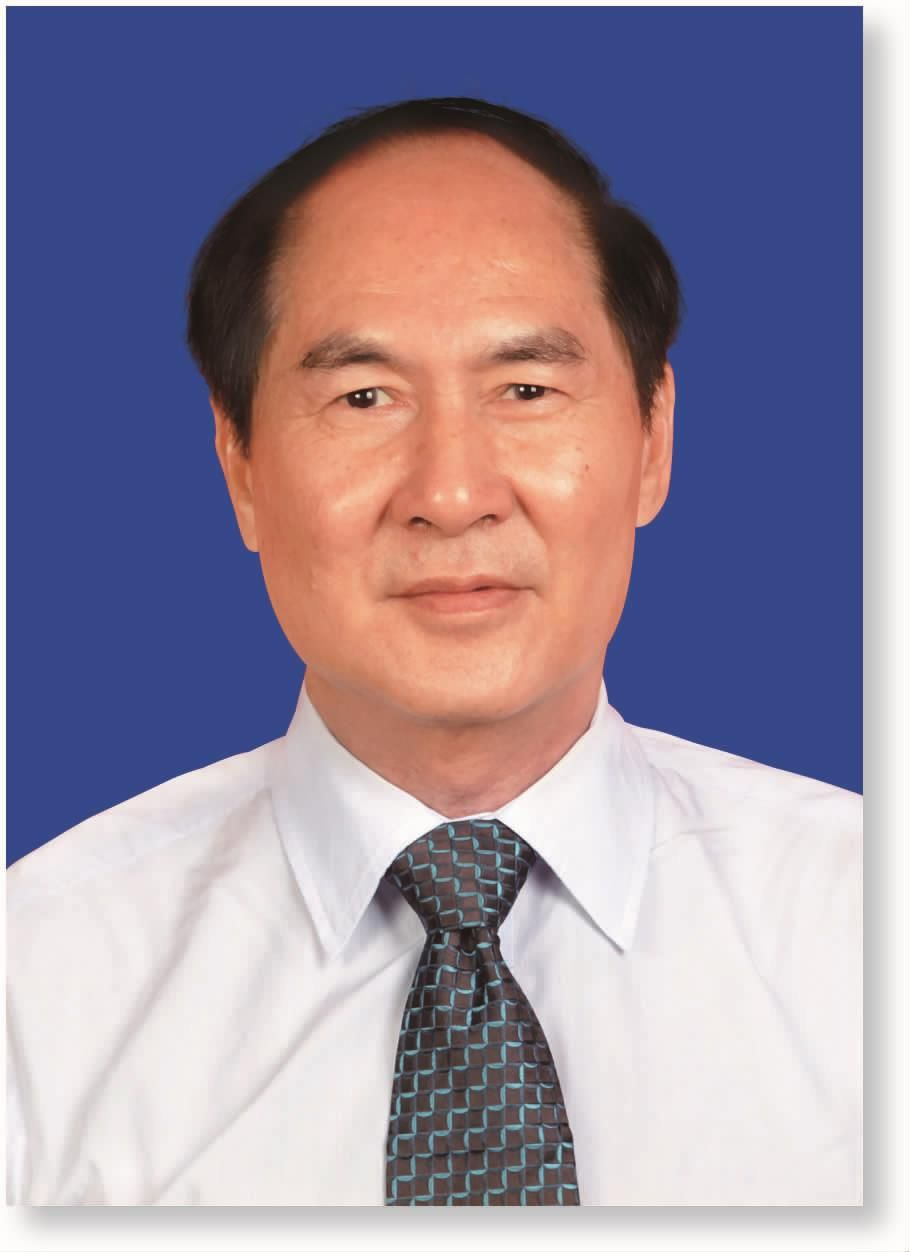
\includegraphics[width=.8\textwidth]{./images/Image00002.jpg}
	\caption{心肌萎缩}
	\label{fig1-1}
\end{figure}
%\FloatBarrier

萎缩的机制尚未完全搞清,蛋白合成少于分解可能为主要原因。

萎缩的器官、组织、细胞功能常降低,但一般是可复性的。原因消除后,萎缩的器官也可恢复正常。如原因持续存在,萎缩的实质细胞最后消失,间质结缔组织和脂肪细胞可以增生,甚至造成器官和组织体积增大,此时称假性肥大。

\subsection{肥大}

由于功能增加、合成代谢旺盛,细胞体积增大,使该器官、组织体积增大,称为肥大(hypertrophy)。肥大多发生于无分裂增殖能力或增殖能力较弱的细胞,如心肌、骨骼肌等。一般可分为生理性肥大和病理性肥大两类。如举重运动员上臂和胸部肌肉的粗壮肥大,妊娠子宫平滑肌细胞肥大属生理性肥大。病理情况下,也可发生肥大。例如高血压病,左心功能负荷加重,心肌纤维体积增大,一侧肾切除后另一侧肾体积增大,皆属代偿性肥大。而成人脑垂体前叶嗜酸细胞瘤分泌过多生长激素,导致的肢端肥大症,则属内分泌性肥大。肥大的细胞除了体积增大外,其内细胞器和微丝明显增多,蛋白合成旺盛。

有时实质细胞萎缩,间质增生也可使该器官、组织体积增大,这种假性肥大与前述的真性肥大有本质的区别。

\subsection{增生}

实质细胞数量增多,使该组织、器官体积增大,称为增生(hyperplasia)。增生可分为生理性和病理性增生两类。妇女在青春期、妊娠期和哺乳期乳腺上皮增生属生理性增生。病理情况下,例如溶血性贫血时骨髓的红细胞系增生,长期缺碘引起甲状腺组织增生,慢性鼻炎黏膜增生肥厚形成息肉等属于病理性增生。由于引起细胞、组织和器官增生与肥大的原因往往十分相似或相同,故两者常同时出现。这种现象见于雌激素过多时引起的子宫内膜增生、乳腺增生,以及老年男性因雄激素代谢障碍导致的前列腺增生。

\subsection{化生}

化生(metaplasia)是指一种已分化成熟的细胞由于适应环境改变而被另一种分化成熟细胞所代替的过程。化生并不是由一种成熟的细胞直接转变为另一种成熟的细胞,而是由该处具有分裂增殖和多向分化能力的幼稚细胞增生,向另一种类型的细胞分化、成熟,也就是所谓的异向分化,是环境因素引起细胞某些基因活化或受到抑制而重新编程表达的结果。化生常发生于同源细胞间,如一种上皮细胞与另一种上皮细胞间。化生是一种可复性病变,原因去除后大多可恢复。常见的化生有:

\subsubsection{鳞状上皮化生}

慢性支气管炎或长期吸烟者,气管及支气管的纤毛上皮转变为鳞状上皮。慢性胆囊炎及胆石症时,胆囊黏膜上皮发生鳞状上皮化生。慢性宫颈炎、子宫内膜炎时,黏膜上皮发生鳞状化生,在妇产科极为常见(图\ref{fig1-2})。肾盂结石时,肾盂黏膜的移行上皮也可转变为鳞状上皮。
\begin{figure}[!htbp]
	\centering
	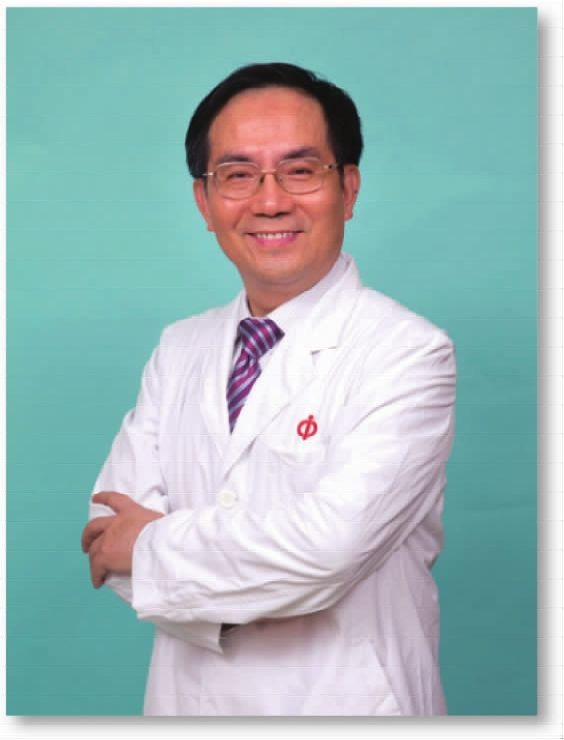
\includegraphics{./images/Image00003.jpg}
	\caption{子宫内膜鳞状上皮化生(HE染色,高倍) \\ {\small 子宫内膜的纤毛柱状上皮化生为鳞状上皮}}
	\label{fig1-2}
\end{figure}
%\FloatBarrier

\begin{framed}
	{案例1-1}

	{【病例摘要】}

	患者,男,55岁,因醉酒后呕吐、误吸,呛咳、呼吸困难入院。全麻下行支气管镜检查,从右主支气管中取出少量未消化米粒和菜叶,症状缓解;术中发现支气管黏膜充血、粗糙,征得家属同意后,夹取2块黏膜组织送病理检查。患者有吸烟史30年,反复咳嗽、咳痰史10年,否认其他病史。病理报告为“送检组织为少量鳞状上皮及其下疏松结缔组织、腺体,伴小血管充血和淋巴细胞、浆细胞浸润。符合慢性支气管炎。”

	{【问题】}

	(1)该患者支气管黏膜出现鳞状上皮,此属何种病理现象?

	(2)试分析病变形成机制和意义。
\end{framed}

\subsubsection{肠上皮化生}

慢性胃炎时,部分胃黏膜上皮转变为含有杯状细胞、潘氏细胞及具有纹状缘的吸收上皮,与小肠黏膜上皮相似;或在柱状上皮中,间有杯状细胞,与大肠黏膜上皮相似,均称为肠上皮化生(简称肠化)。类似的化生也常发生于腺体,由一种腺上皮转变为另一种腺上皮,故又称腺性化生。

\subsubsection{结缔组织和支持组织化生}

纤维组织化生为脂肪组织或肌细胞,成纤维细胞转变为骨母细胞或软骨母细胞,分别化生为骨或软骨(图\ref{fig1-3})。
\begin{figure}[!htbp]
	\centering
	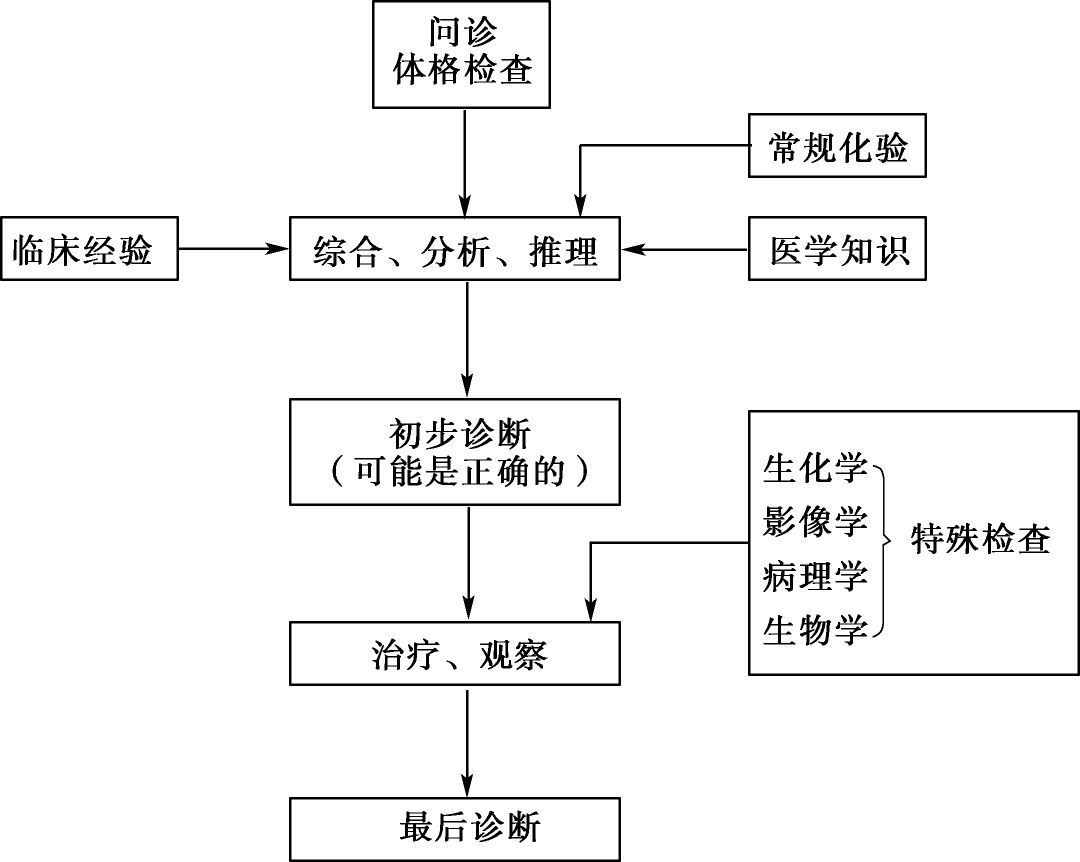
\includegraphics{./images/Image00004.jpg}
	\caption{心瓣膜软骨化生(HE染色,高倍) \\ {\small 心瓣膜结缔组织出现软骨化生}}
	\label{fig1-3}
\end{figure}
%\FloatBarrier

\begin{center}
	\textbf{知识链接}
\end{center}
\chapterabstract{上皮间质转分化(epithelial-mesenchymal
transition)为近年研究热点,其实也是一种化生现象。它是指上皮细胞在某些因素刺激下,逐渐失去上皮细胞表型(如E钙黏蛋白、细胞骨架蛋白等的表达)而呈现间质细胞表型(如波形蛋白、平滑肌肌动蛋白、纤维连接蛋白等的表达)。该现象可见于多种生理病理过程,如胚胎发育、组织重塑、肿瘤侵袭转移、慢性炎症和器官纤维化等。}

化生是机体对环境中不良因子发生防御反应的一种形式,对机体是有利的,但也有其局限性和不完善性。例如支气管黏膜鳞状化生后,失去纤毛,削弱了黏膜的自净能力。在化生、增生的基础上,还可能发展为肿瘤。例如支气管鳞状上皮化生和胃黏膜肠上皮化生,分别与肺鳞状细胞癌和胃腺癌的发生有一定的关系。

综上所述,组织细胞为了适应内外环境的变化,可出现萎缩、肥大、增生和化生等形态学改变(图\ref{fig1-4})。若刺激因素使发育正常的组织或器官内实质细胞体积缩小或数目减少即称为萎缩;实质细胞体积增大,即称为肥大;实质细胞数量增多,即称为增生;已分化成熟的细胞被另一种分化成熟细胞所代替即称为化生。

\begin{figure}[!htbp]
	\centering
	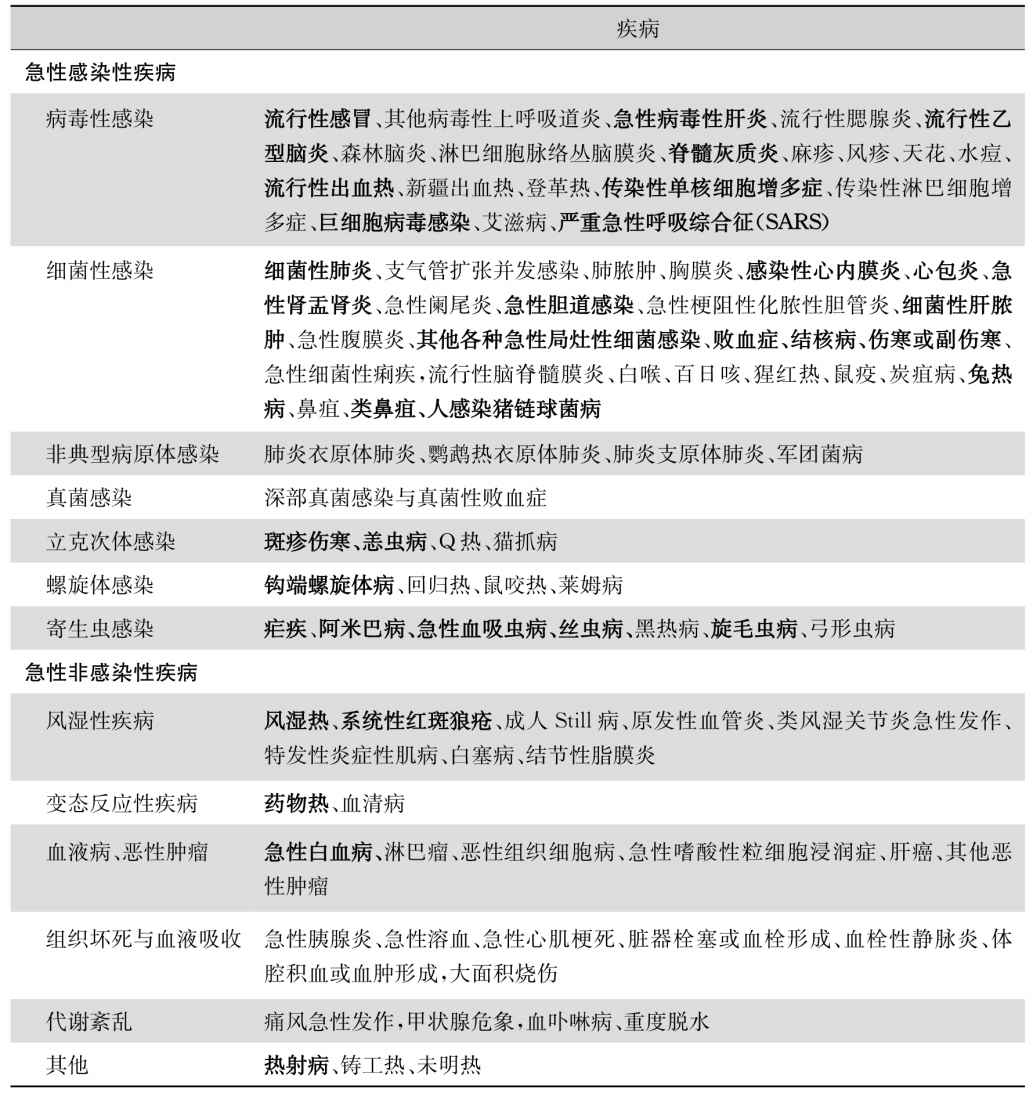
\includegraphics{./images/Image00005.jpg}
	\caption{四种适应性改变示意图}
	\label{fig1-4}
\end{figure}
%\FloatBarrier

\section{细胞和组织的损伤}

当损伤因素超出机体的适应能力,则引起细胞和组织的损伤。在一定程度内这种损伤为可复性,形态上表现为变性和物质异常沉积。重度损伤则引起细胞和组织的死亡。

\subsection{细胞和组织损伤的原因与发生机制}

\subsubsection{缺氧}

缺氧是引起组织细胞损伤常见而重要的原因。缺氧常见于:各种原因造成动脉供血不足或静脉回流障碍,或由于呼吸、循环障碍使血氧含量不足,也可见于严重贫血或中毒(如CO中毒)使红细胞携氧能力降低等情况。缺氧首先影响细胞的需氧呼吸,即线粒体的氧化磷酸化功能,使ATP产生减少或停止,导致细胞膜的钠泵功能障碍,Na{+}
及水在细胞内集聚,K{+}
从细胞外溢,造成急性细胞肿胀。缺氧也使无氧酵解过程增强,通过糖原分解产生ATP,以维持细胞的能量,但在无氧酵解的过程中细胞内乳酸、酮体、氨基酸和无机酸等氧化不全的代谢产物大量积聚,使pH下降。随之粗面内质网核蛋白体脱失、裂解,并出现线粒体肿胀,内质网扩张等一系列超微结构改变。以上改变是可复性的,随缺氧的恢复而恢复正常。如缺氧持续存在,ATP供应耗竭,细胞酶系统广泛损伤,细胞膜功能严重受损,细胞外Ca{2+}
不断进入细胞内,甚至进入线粒体内,使其基质中出现无定形的富于钙的致密区,线粒体发生不可复性改变,以至参与代谢的某些酶活性受抑,并使蛋白变性,细胞死亡。细胞内pH进一步下降将导致溶酶体膜的损伤,其内多种酶进入细胞浆内并被激活,其中酸性水解酶可引起细胞自溶死亡。

不同组织细胞对缺氧的耐受程度不同。结缔组织对缺氧耐受时间最长,而神经细胞对氧极为敏感,缺氧长于5~10分钟,细胞则发生不可复性损伤。

\subsubsection{物理因子}

物理因子包括机械性、高温、低温、电流、放射线等刺激因子。机械性损伤能使细胞组织破裂;高温使细胞内蛋白质(包括酶)变性,低温可使血管收缩引起组织缺血性损伤,或造成局部血流停滞、凝血,甚至细胞内水分形成冰晶而损伤细胞;电流通过组织时引起高温灼伤局部组织;放射线作用于机体能直接或间接造成大分子损伤,使水分被激发电离,产生大量具有强毒力的自由基,损伤组织细胞。物理因子引起损伤的严重程度主要决定于该物理因子的作用性质、强度和持续时间的长短,而很少和机体的反应性有关。

\subsubsection{化学因子}

许多化学物质进入人体,在组织细胞内发生化学反应,可破坏正常的生理功能。化学物质造成组织损伤前提是它们必须能经口、呼吸道、皮肤或黏膜进入体内才能引起中毒。化学因子引起损伤的机制是多方面的:①直接损伤:如强酸、强碱可直接灼伤皮肤或黏膜,引起局部炎症或坏死;②抑制酶的活性:如有机磷农药能抑制胆碱酯酶的活性,引起损伤。氯化汞和体内的巯基结合,从而使许多酶蛋白失去活性或破坏膜蛋白结构;③通过代谢形成毒性代谢产物而发挥作用:例如,四氯化碳经肝细胞滑面内质网所含的细胞色素P-450混合功能氧化酶类的作用,裂解生成毒性物质CCl{3}
和Cl自由基,后者可引起肝细胞发生脂肪变性和坏死。

自由基(free
radical)又称游离基,是指一类含有未配对电子的化学基团,如H{+} 、OH{-}
、HOO、O{2-}
,其化学活性高而不稳定,它与细胞内各种有机或无机化合物,如脂质、蛋白质、核酸等,发生过氧化、交联或断裂,从而造成细胞的损伤。但在正常人体内,自由基在细胞外液中的浓度极低,不构成对细胞的威胁,而在吞噬细胞杀灭病原生物或抗肿瘤细胞过程中自由基却起重要防御作用。但是如果体内生成过多,或清除障碍,如在上述的化学性、放射性、炎症损伤过程中,或随着年龄的增长,机体抗氧化活性递减,逐级降低对自由基的防御能力,均可引起组织细胞损伤或机体衰老。自由基可在正常新陈代谢中产生,是普遍存在于生物系统的代谢中间产物,种类多,数量大,活性高。

\subsubsection{生物性因子}

生物性因子是引起细胞损伤最常见的原因,包括病毒、细菌、立克氏体、真菌、寄生虫等引起的各种感染。其作用机制有下列几方面:①直接作用损伤细胞和组织:病毒寄生于细胞内干扰细胞的代谢活动,使细胞变性坏死。②通过内外毒素的作用或产生的毒性代谢产物:如白喉外毒素自由基能抑制细胞的氧化过程和蛋白质的合成。溶血性链球菌产生的透明质酸酶和链激酶引起间质损伤。③生物因子具有抗原性,能引起变态反应:肝炎病毒有嗜肝细胞的特性并产生病毒蛋白,后者可通过变态反应引起肝细胞损伤。

\subsubsection{免疫反应}

免疫反应是机体的正常防御功能,通过免疫反应排斥异己物质,以维持内环境的稳定。但这种反应结果并非均对机体有利,例如病毒性肝炎,在机体T细胞致敏清除肝炎病毒的过程中也造成肝细胞的损伤;在某些情况下对病原生物产生的抗体与体内组织抗原发生交叉反应,形成抗原抗体复合物沉积于组织,引起损伤,如风湿性心肌炎,急性肾小球肾炎,通过变态反应对自身组织抗原发生反应,引起组织细胞的损伤;甚至针对自身组织发生自身免疫反应,如红斑性狼疮,类风湿关节炎等。

\subsubsection{其他}

遗传缺陷、营养失衡、内分泌异常、衰老、心理和社会因素等也能导致组织细胞的损伤。

综上所述,引起组织细胞损伤的因子很多,它们主要通过以下几个途径造成细胞损伤(图\ref{fig1-5}):①ATP耗竭,细胞需要能量的生理活动受阻;②细胞膜完整性破坏、渗透性缺陷,导致细胞内容物流失或物质交换和电生理活动异常;③细胞内钙离子浓度升高,多种酶被激活,使ATP耗竭或细胞结构的破坏;④自由基产生增多;⑤其他代谢活动异常等。一种因子可通过多种途径损伤细胞,几种因子亦可共用一条途径使细胞受累。
\begin{figure}[!htbp]
	\centering
	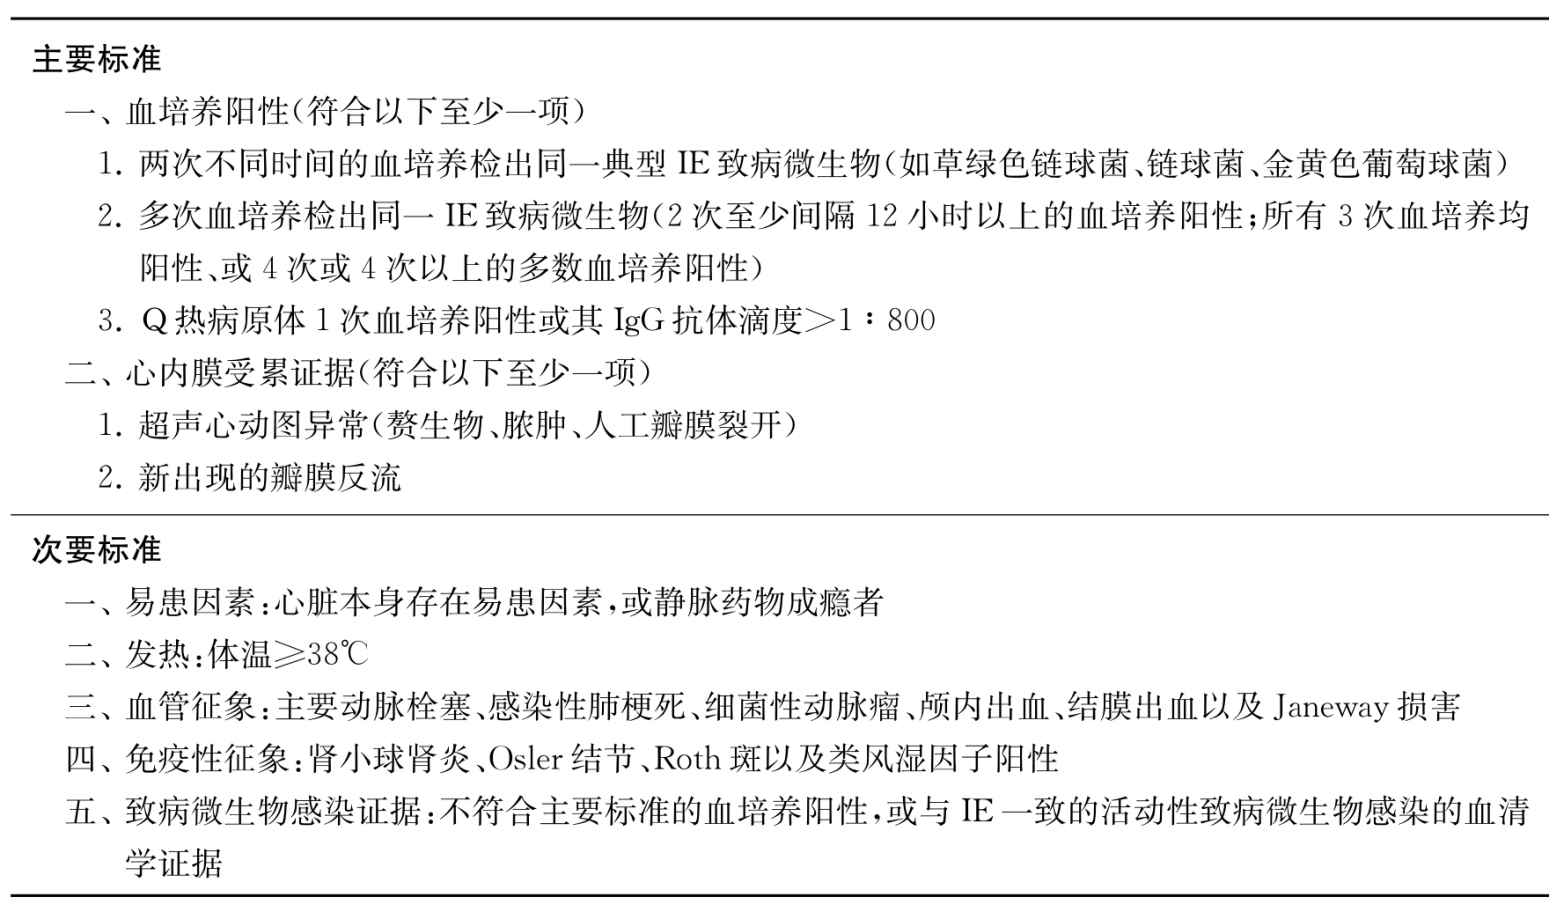
\includegraphics{./images/Image00006.jpg}
	\caption{组织细胞损伤机制示意图}
	\label{fig1-5}
\end{figure}
%\FloatBarrier 

\subsection{细胞和组织损伤的形态学变化}

组织细胞损伤有轻重之别,损伤因子强度弱、作用时间短,细胞的损伤可恢复,即为可逆性损伤;若损伤因子持续刺激和过于剧烈,细胞将会死亡,则表现为不可逆性损伤。

\subsubsection{可逆性损伤}

可逆性损伤(reversible
injury),旧称变性(degeneration),是指新陈代谢障碍时,细胞或细胞间质内出现一些异常物质或正常物质异常蓄积。变性的组织细胞功能下降,但通常为可复性,严重者可发展为坏死。变性的种类繁多,下面介绍比较常见的几种变性。

\paragraph{细胞水肿}
细胞水肿(cellular edema)或称水变性(hydropic
degeneration)即细胞内水钠积聚过多,引起细胞体积肿大,胞浆疏松、透明淡染。常见于缺氧、感染、中毒时的心、肝、肾等脏器的实质细胞。

病理上,轻度的细胞水肿,胞浆内出现许多细小的伊红染颗粒,此乃水肿时肿大的线粒体和扩张的内质网,这种变化致相应器官肉眼观时体积轻度增大,包膜紧张,颜色较正常淡,显得混浊而无光泽,在电镜技术问世之前称之为颗粒变性(granular
degeneration)或混浊肿胀,此名词现已弃用。随细胞内水钠积聚增多,细胞水肿进一步发展,线粒体和内质网高度扩张,囊泡变,此时镜下观:胞浆透明、空泡状,故又有空泡变性或水样变性之称(图\ref{fig1-6})。病毒性肝炎和四氯化碳中毒时,肝细胞水肿,严重者细胞肿大如圆球状,特称为气球样变(图\ref{fig1-7})。
\begin{figure}[!htbp]
	\centering
	\begin{minipage}[b]{0.45\textwidth}
		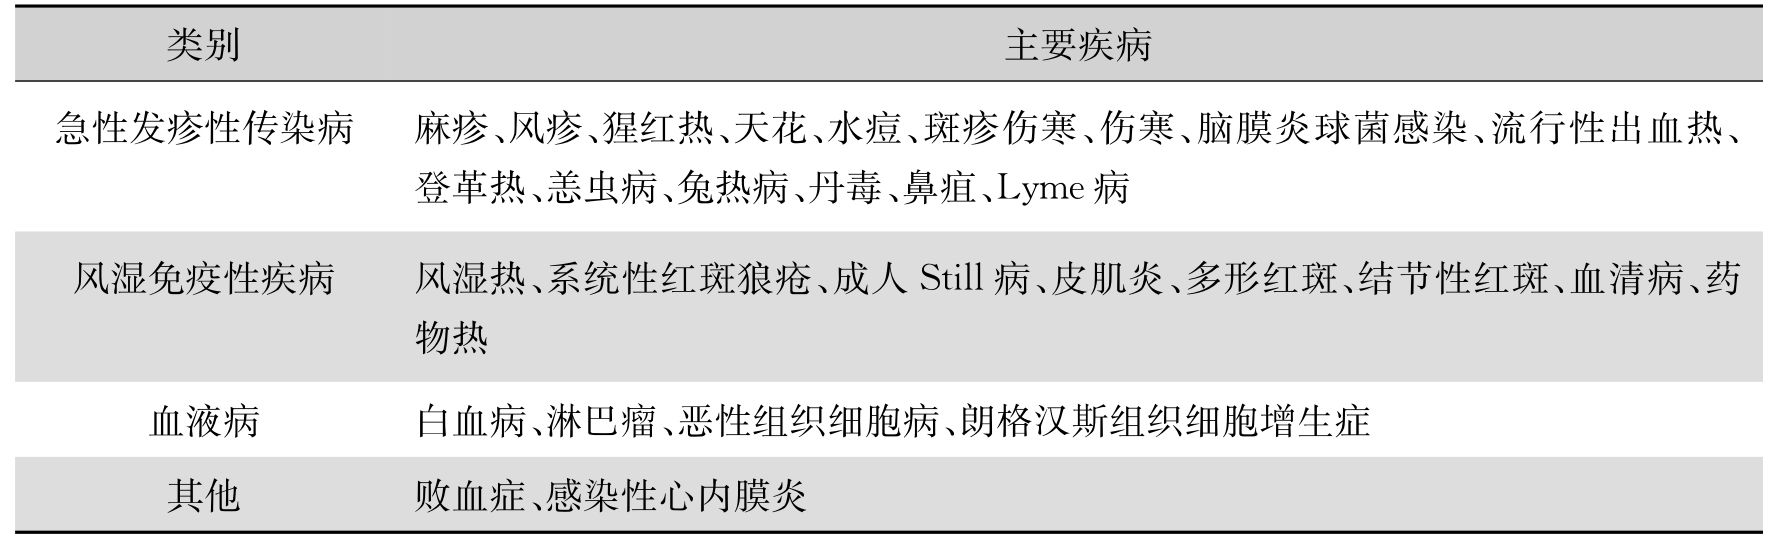
\includegraphics{./images/Image00007.jpg}
		\caption{肾小管上皮细胞水肿(HE染色,高倍) \\ {\small 细胞体积增大,胞浆内出现红染的颗粒状物}}
		\label{fig1-6}
	\end{minipage}
	%	\end{figure} 
	%\FloatBarrier
	%\begin{figure}[!htbp]
	%    \centering
	\hspace{0.04\textwidth}%
	\begin{minipage}[b]{0.45\textwidth}
		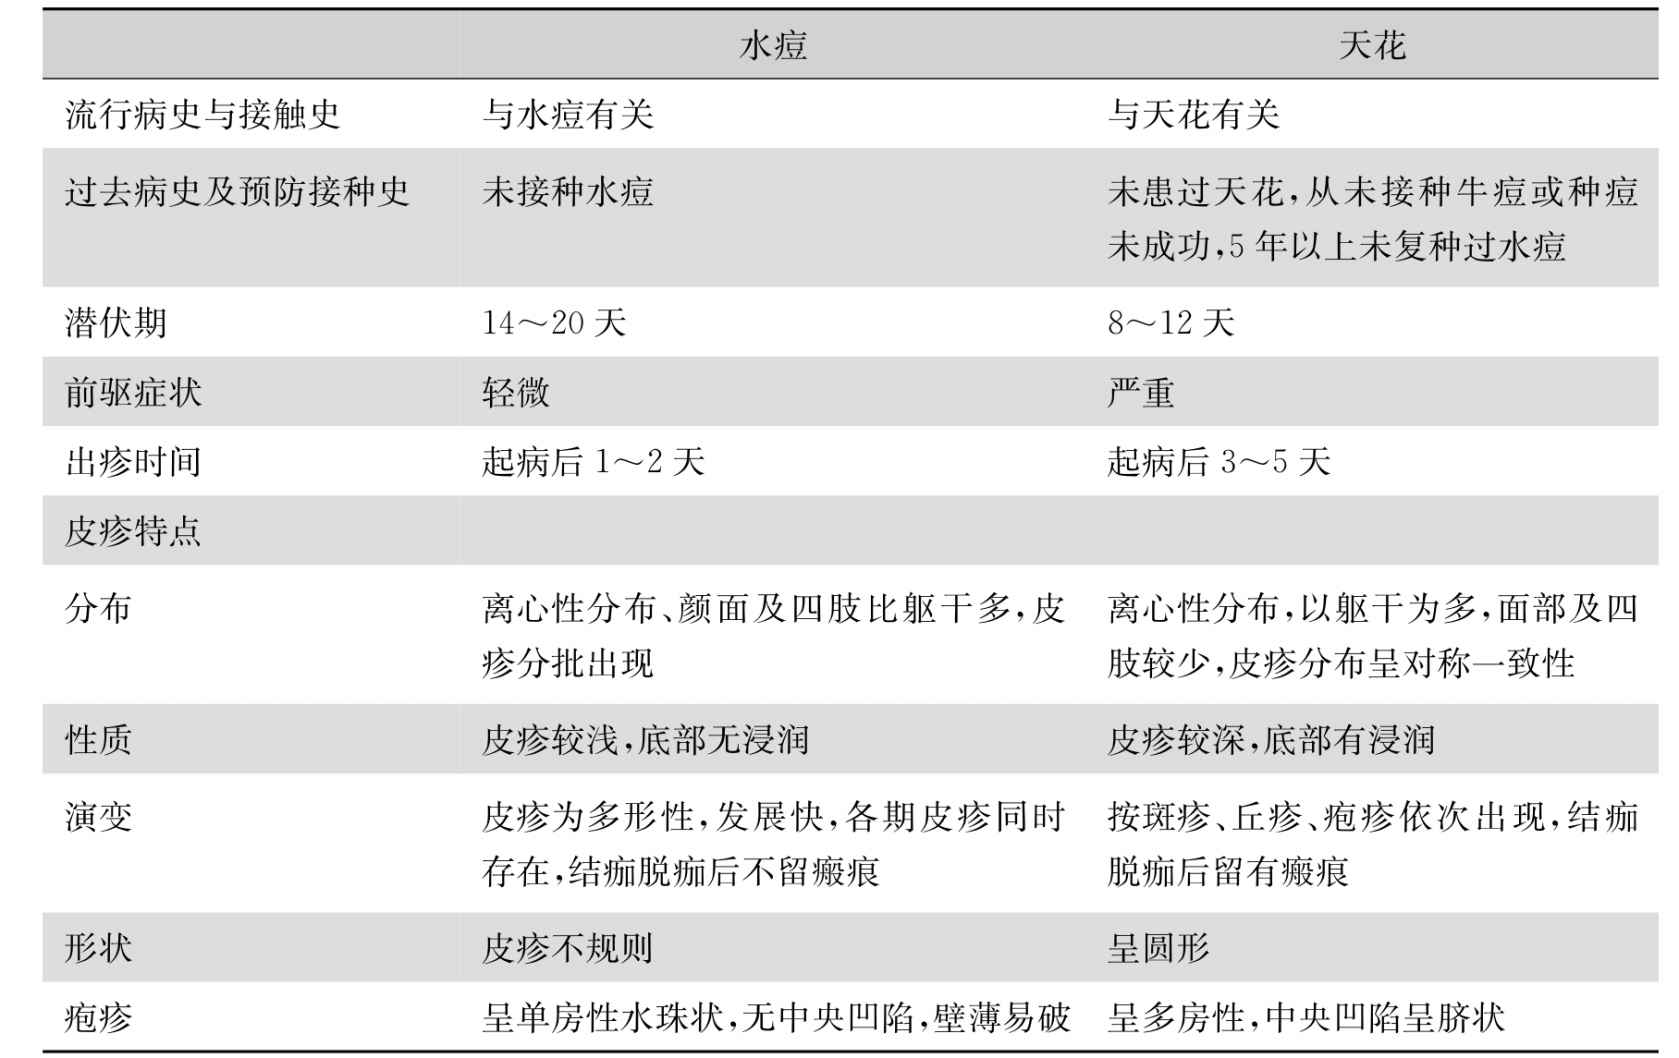
\includegraphics{./images/Image00008.jpg}
		\caption{肝细胞水肿(HE染色,中倍) \\ {\small 肝细胞明显肿胀,细胞浆疏松}}
		\label{fig1-7}
	\end{minipage}
\end{figure}
%\FloatBarrier

引起细胞水肿的原因很多,在急性感染、缺氧、中毒等有害因素的作用下,线粒体产能机制受损,ATP生成减少,使细胞膜的钠泵功能障碍,导致细胞内水、钠增加,细胞水肿。或由于细胞膜直接受损,通透性增高所致。

细胞水肿是一种轻度或中度损伤的表现,在原因消除后,仍可恢复正常。若病因持续存在,水肿细胞的胞浆内可出现脂滴空泡。严重水肿可引起细胞坏死。

\paragraph{脂肪变性}
除脂肪细胞外,其他细胞胞浆内出现脂滴或脂滴明显增多称为脂肪变性(fatty
degeneration),简称脂变。脂变常发生于心、肝、肾等代谢旺盛或耗氧较多的器官。脂变中的脂滴,主要成分为中性脂肪,也可有磷脂及胆固醇等成分,在常规石蜡包埋的切片中,中性脂肪被制片过程中所使用的乙醇、二甲苯等脂溶剂溶解,所以HE染色的切片,光镜下细胞中的脂滴呈空泡状。在冰冻切片苏丹Ⅲ染色时显示脂肪滴为橘红色,锇酸染色时呈黑色。

(1)肝脂肪变性:由于肝脏在脂肪代谢中起重要作用,故肝脂变最多见,且常较严重。肉眼观:轻度脂变时肝脏无明显改变,脂变广泛时肝脏均匀性肿大,包膜紧张,边缘钝,色淡黄,切面有油腻感,苏丹Ⅲ染色后变成红色(图\ref{fig1-8}a)。镜下观:HE染色切片可见早期脂变表现为核周围出现小的脂肪空泡,以后渐增大,散布于胞浆中,严重时融合成一个大空泡,将核推挤到包膜下,状似脂肪细胞(图\ref{fig1-8}b)。脂变在肝小叶内的分布与病因有一定的关系。如肝淤血时,小叶中央区淤血明显,缺氧较重,脂变首先发生于此处。长期淤血,小叶周边区肝细胞也因缺氧而发生脂变,而小叶中央区的肝细胞大多已萎缩或消失。磷中毒时,脂变主要发生在小叶周边区,可能与该区肝细胞代谢较为活跃,对磷中毒更为敏感所致。此外,小叶周边的肝细胞接触到的毒物浓度较高也使此处的肝细胞易受损伤。
\begin{figure}[!htbp]
	\centering
	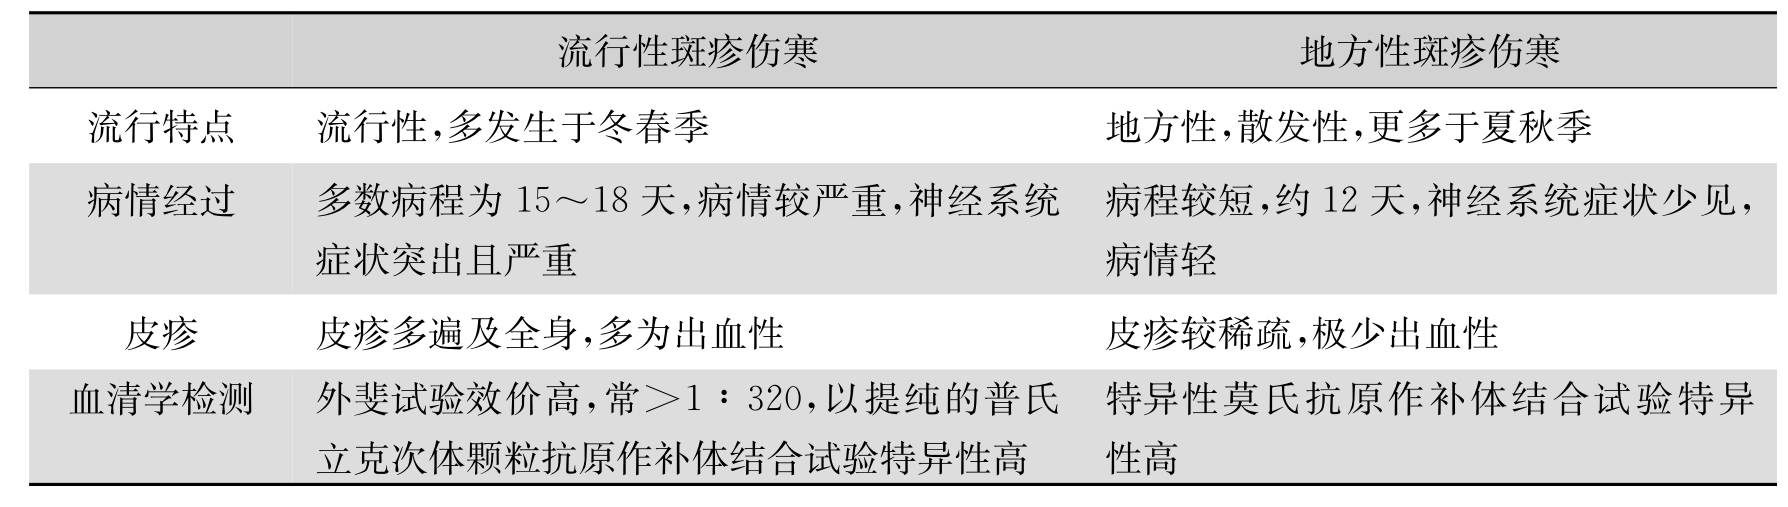
\includegraphics{./images/Image00009.jpg}
	\caption{肝脂肪变性}
	\label{fig1-8}
\end{figure}
%\FloatBarrier 



肝脂变是可复性损伤,病因消除后,脂变细胞可恢复正常,一般无明显的临床表现。重度弥漫性肝脂变称为脂肪肝,体检时肝可在右季肋下触及,常规B超可进行诊断。病变持续发展,肝细胞逐渐坏死,纤维组织增生,可发展为肝硬化。

(2)心肌脂肪变性:多见于贫血。肉眼观:轻度脂变一般无明显异常,但在严重贫血时,常在心内膜下,尤其是左心室乳头肌处出现红黄相间的条纹,如虎皮斑纹,称为“虎斑心”。这是由于心肌内血管分布不均,心肌缺氧轻重程度不一所致,血管末梢分布区心肌缺氧较重,脂变明显而呈黄色,缺氧较轻部位脂变较轻,心肌呈红色。镜下观:脂肪空泡常较细小,呈串珠状排列。有时心外膜增生的脂肪组织可沿间质深入心肌细胞间,称为心肌脂肪浸润(图\ref{fig1-9})。
\begin{figure}[!htbp]
	\centering
	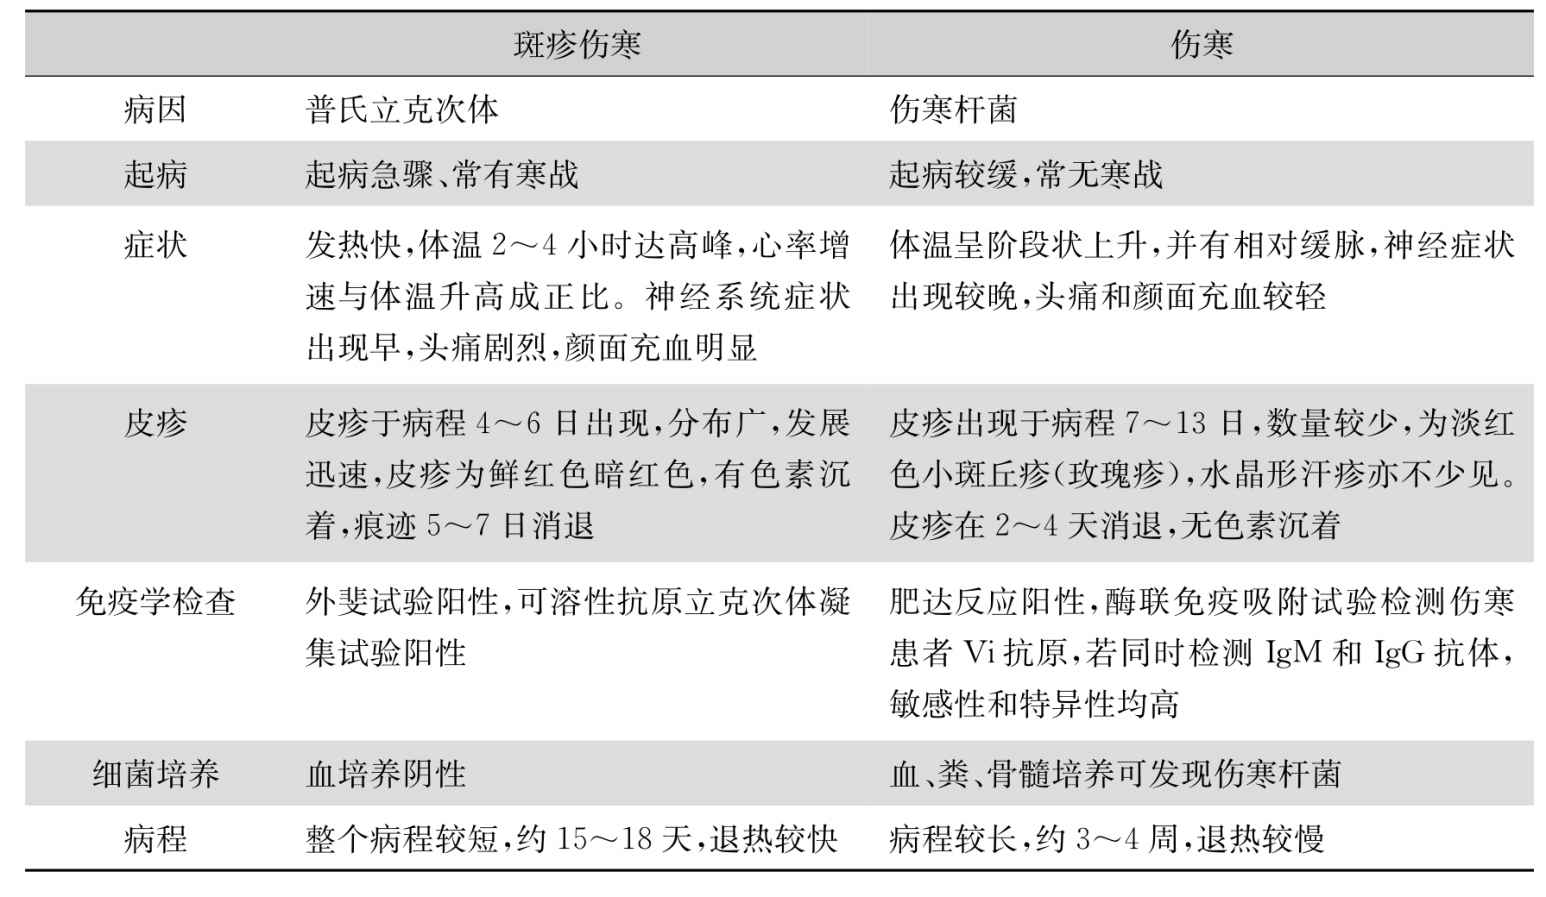
\includegraphics[width=0.7\textwidth]{./images/Image00010.jpg}
	\caption{心外膜脂肪组织增生及心肌脂肪浸润}
	\label{fig1-9}
\end{figure}
%\FloatBarrier 

(3)肾脂肪变性:贫血、缺氧、中毒和一些肾脏疾病时,肾曲管上皮细胞可发生脂肪变性。这是因为在上述疾病时肾小球毛细血管通透性增加,肾曲管特别是近曲小管上皮吸收漏出的脂蛋白,在细胞内分解成脂滴。脂滴空泡多位于近曲小管上皮细胞基底部或核周围。

脂肪变性发生的机制尚未完全清楚。一般认为与感染、中毒、缺氧等因素干扰或破坏细胞的脂肪代谢有关。具体作用途径则因病因不同而异。肝脂变的机制大致如下:①脂蛋白合成障碍,使脂肪堆积在肝细胞内不能转运出去。其原因常是缺乏合成脂蛋白的原料,如磷脂或组成磷脂的胆碱,或由于化学物或其他毒素破坏了内质网(蛋白合成部位)或抑制了某些酶的活性,使脂蛋白合成障碍。②脂肪酸氧化障碍。由于缺氧、感染、中毒,使线粒体受损,干扰β-氧化,使肝细胞含脂肪量增加。③进入肝细胞脂肪酸过多。例如饥饿或某些疾病造成饥饿状态,或糖尿病患者对糖的利用障碍,机体动用大量体脂,其中大部分以脂肪酸的形式进入肝脏,超过肝细胞将其氧化和合成脂蛋白的能力,于是在肝细胞内储积。

\paragraph{玻璃样变性}
玻璃样变性(hyaline
degeneration)又称透明变性,是指在HE染色情况下,细胞外间质或细胞质内出现伊红染、均质半透明、无结构的玻璃样物质。玻璃样变性其实为一组物理性状相同,但其发生原因、化学成分及机制各不相同的病理变化的统称。常见的玻璃样变性有三类:

(1)细胞内玻璃样变性:指细胞浆内出现大小不等、圆形、均质的红染小滴。细胞内玻璃样变性可由多种原因引起,如肾小球肾炎或其他疾病伴有明显蛋白尿时,肾近曲小管上皮细胞胞浆内可出现大小不等的圆形红染小滴,这是血浆蛋白经肾小球滤出而又被肾小管上皮细胞吞饮、融合而成的玻璃样小滴(图\ref{fig1-10}a)。慢性乙醇中毒时,由于细胞中间丝前角蛋白变性,肝细胞核周围的胞浆内可出现圆形或形状不甚规则的均质红染玻璃样物质,称为Mallory小体。

(2)结缔组织玻璃样变性:常发生在增生的纤维结缔组织,为胶原纤维老化的表现。肉眼观病变处呈灰白色,半透明,质地致密而坚韧(图\ref{fig1-10}b)。光镜下胶原蛋白交联、变性、融合,胶原纤维增粗并互相融合成索带状或片状的半透明均质物,纤维细胞明显减少。见于瘢痕组织、纤维化的肾小球、动脉粥样硬化的纤维斑块等。

(3)血管壁玻璃样变性:常发生于高血压病时的肾、脑、脾及视网膜的细动脉。这是由于细动脉持续痉挛,使内膜通透性增大,血浆蛋白渗入内膜,在内皮细胞下凝固成均匀红染玻璃样物质。如病变继续发展,血管壁平滑肌组织均被玻璃样物质替代而消失,再加上基底膜样物质增多,使病变血管壁增厚、变硬,管腔狭窄甚至闭塞,此即细动脉硬化症(图\ref{fig1-10}c),可引起肾、脑等器官缺血。
\begin{figure}[!htbp]
	\centering
	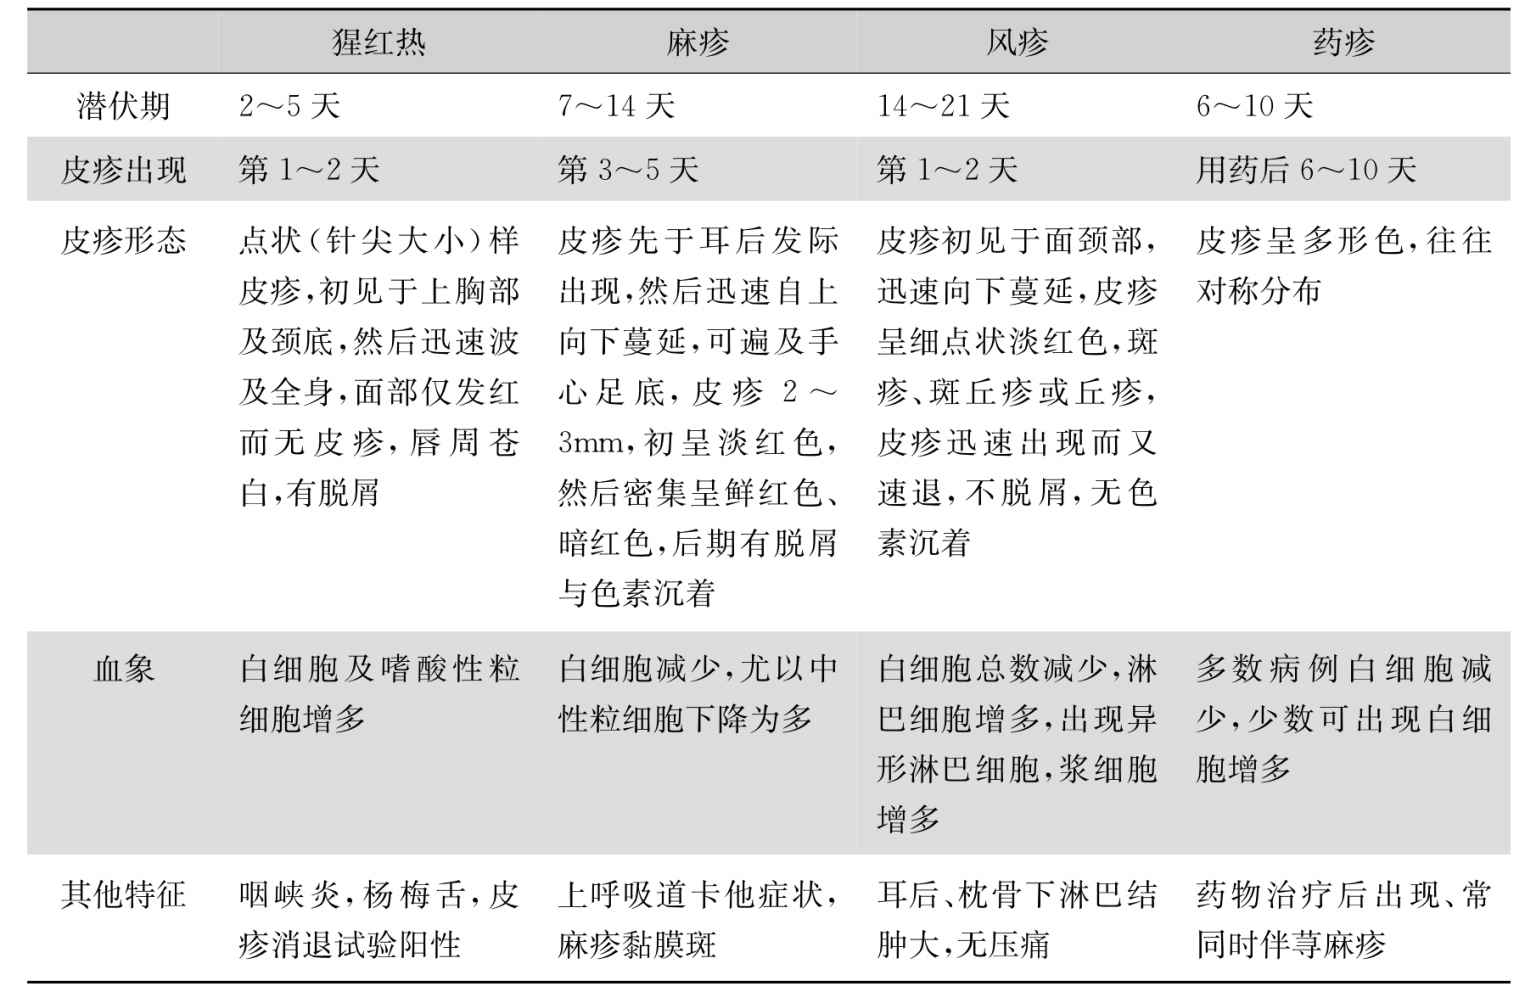
\includegraphics[width=0.7\textwidth]{./images/Image00011.jpg}
	\caption{不同类型玻璃样变性}
	\label{fig1-10}
\end{figure}
%\FloatBarrier

上述3种类型中,细胞内玻璃样变在病因去除后多能恢复,而后两者较难恢复。

\paragraph{黏液样变性}
组织间质内出现类黏液(黏多糖和蛋白质)的积聚称为黏液样变性(mucoid
degeneration)。镜下观:病变处细胞间质疏松,充以淡蓝色的胶状液体,其间散布一些多角形,星芒状的细胞,并以突起互相连缀。黏液样变性常见于间叶性肿瘤、急性风湿病时的心血管壁、动脉粥样硬化的血管壁。在甲状腺功能低下时,透明质酸酶活性受抑,含有透明质酸的黏液样物质及水分在皮下蓄积,形成黏液水肿。

\paragraph{淀粉样变}
组织内有淀粉样物质沉着称为淀粉样变(amyloid
degeneration)。淀粉样物质是蛋白质,其遇碘时可被染成棕褐色,再加硫酸后则变为蓝色,与淀粉染色特性相似,故称之为淀粉样变。此种病变可见于慢性炎症、内分泌系统肿瘤、老年性痴呆(Alzheimer病)等多种疾病。淀粉样物质的沉积可为局部性,亦可为全身性,常分布于细胞间或沉积在小血管基底膜下,还可沿组织纤维支架分布。镜下观:淀粉样物质呈淡伊红染色、均匀一致、云雾状。刚果红染色为橘红色(图\ref{fig1-11})。尽管形态相似,但在不同疾病时,淀粉样物质的化学本质不同,有的为免疫球蛋白,有的为激素,还有的为β{2}
淀粉样蛋白,等等。

\begin{figure}[!htbp]
	\centering
	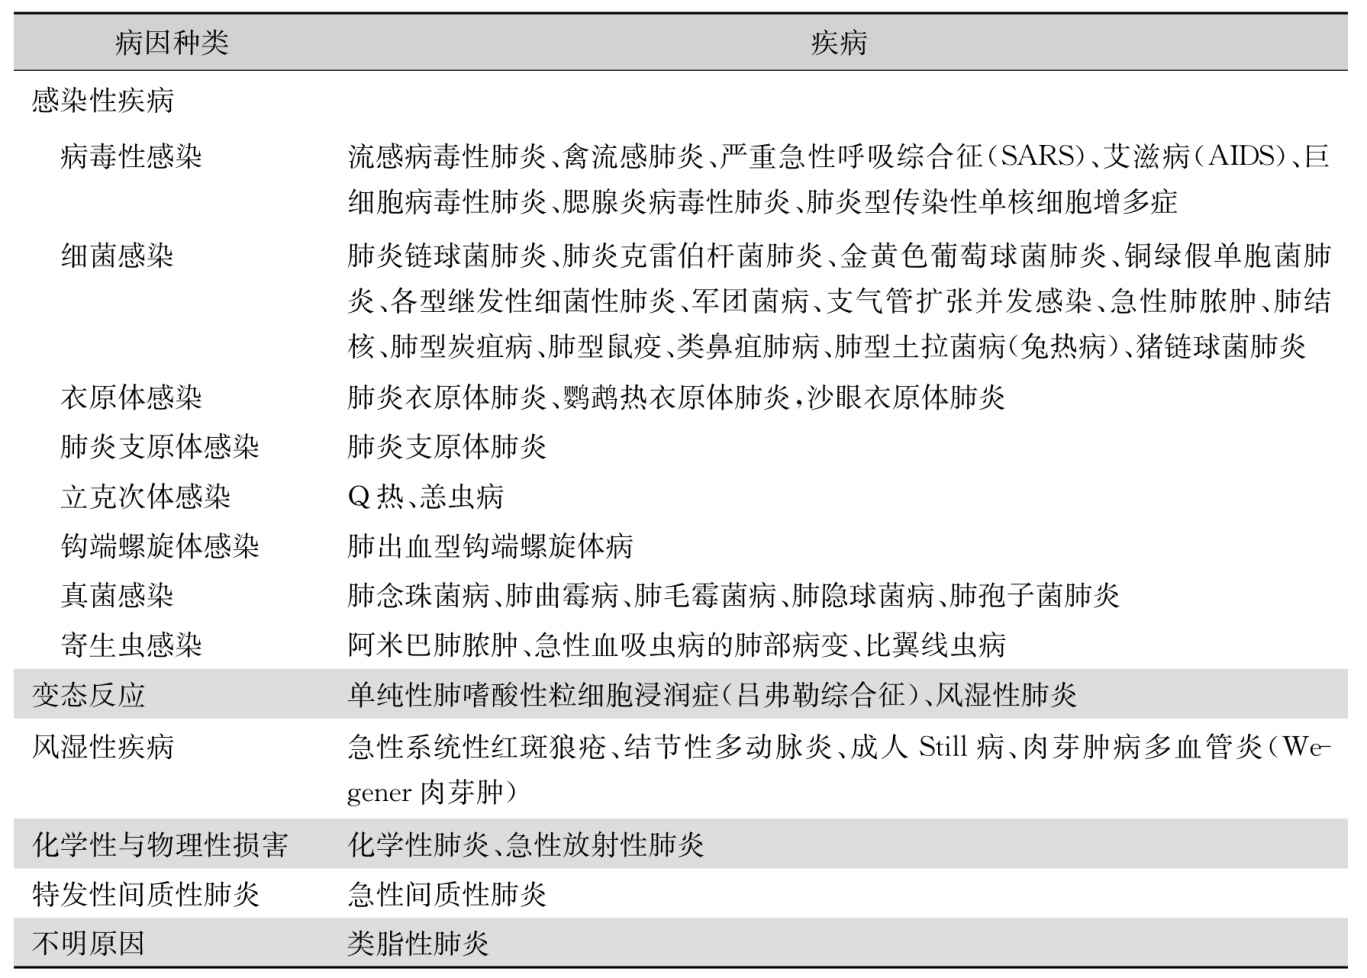
\includegraphics[width=0.7\textwidth]{./images/Image00012.jpg}
	\caption{肾小球淀粉样变}
	\label{fig1-11}
\end{figure}
%\FloatBarrier

\paragraph{病理性色素沉积}
细胞或组织内可有各种来自体内、体外的色素沉积,在病理情况下某些色素在体内会过量沉积。常见的病理性色素沉积有含铁血黄素、胆红素、脂褐素、黑色素。

(1)含铁血黄素(hemosiderin):系由铁蛋白微粒积聚而成的色素,颗粒状,棕黄或金黄色,具有折光性。此色素为血红蛋白被吞噬细胞溶酶体分解而成,如巨噬细胞破裂,则色素逸出于间质中。正常的骨髓组织或脾内可有少量含铁血黄素出现,在全身溶血性疾病时,含铁血黄素可沉积在全身的单核巨噬细胞系统内,组织出血时含铁血黄素常出现在出血灶附近。当左心衰竭导致肺淤血时,红细胞自肺泡壁毛细血管漏出于肺泡中,被巨噬细胞吞噬,肺泡腔内可出现吞噬含铁血黄素的巨噬细胞,又称为心力衰竭细胞。

(2)胆红素(bilirubin):也是在巨噬细胞内形成的一种血红蛋白衍生物,棕黄色或黄绿色。生理情况下,胆红素是衰老的红细胞被单核吞噬细胞分解后所形成。血中胆红素过多时,可将组织和体液染成黄色,称黄疸。因有血脑屏障,胆红素通常不能进入脑和脊髓,但在新生儿由于血脑屏障尚不完善,溶血性黄疸时,大量胆红素可进入脑细胞内,使其氧化磷酸化过程受损,能量产生受抑制,导致细胞变性,出现相应的神经症状。肉眼见豆状核、下丘脑、海马回等多处神经核明显黄染,故称之为核黄疸。胆红素一般呈溶解状态,但在胆道阻塞及某些肝脏疾病时也可为黄褐色折光性颗粒或团块,出现于肝细胞、Kupffer细胞、毛细胆管、小胆管等组织细胞内。

(3)脂褐素(lipofuscin):为一种黄褐色细颗粒状色素。其组成成分的50%为脂质,其余为蛋白质及其他物质。脂褐素系细胞内自噬溶酶体中的细胞器碎片发生了某种理化改变,不能被溶酶体酶消化而形成的一种不溶性残存小体。老年人及一些慢性消耗性疾病患者的肝细胞、肾上腺皮质网状带细胞和心肌细胞核两端的胞浆中可见到脂褐素,故又有消耗性色素之称。

(4)黑色素(melanin):为棕褐色或黑褐色的颗粒状色素,大小形状不一。正常人黑色素多存在于皮肤、毛发、虹膜及脉络膜的黑色素细胞内。它是由酪氨酸在黑色素细胞内的酪氨酸酶的作用下氧化、聚合而形成的一种不溶性聚合体。人脑垂体所分泌的ACTH能刺激黑色素细胞,促进黑色素形成。在肾上腺皮质功能低下时,对垂体的反馈抑制作用减弱,致使ACTH分泌增多,患者全身皮肤黑色素增多。局部黑色素增多常见于黑色素痣或恶性黑色素瘤等。

\paragraph{病理性钙化}
在病理情况下,骨和牙以外的组织内有固体钙盐的沉积,称为病理性钙化(pathologic
calcification)。主要成分为磷酸钙、碳酸钙及少量铁镁等物质。肉眼观:少量钙盐沉积难以辨认,仅在刀切组织时有砂粒感;量多时表现为白色石灰样颗粒或团块,质地坚硬。镜下观:HE染色切片中,钙盐呈蓝色颗粒状。病理性钙化可分为两种类型:

(1)营养不良性钙化:指钙盐沉积于变性、坏死的组织中或异物内,如结核坏死灶、脂肪坏死灶、动脉粥样硬化斑块的变性坏死区(图\ref{fig1-12}a),血栓、寄生虫体和虫卵。患者无全身钙、磷代谢障碍,血钙不高。这是一种较常见的病理性钙化,可能与局部碱性磷酸酶(来自坏死细胞及其周围组织内)升高有关。

\begin{figure}[!htbp]
	\centering
	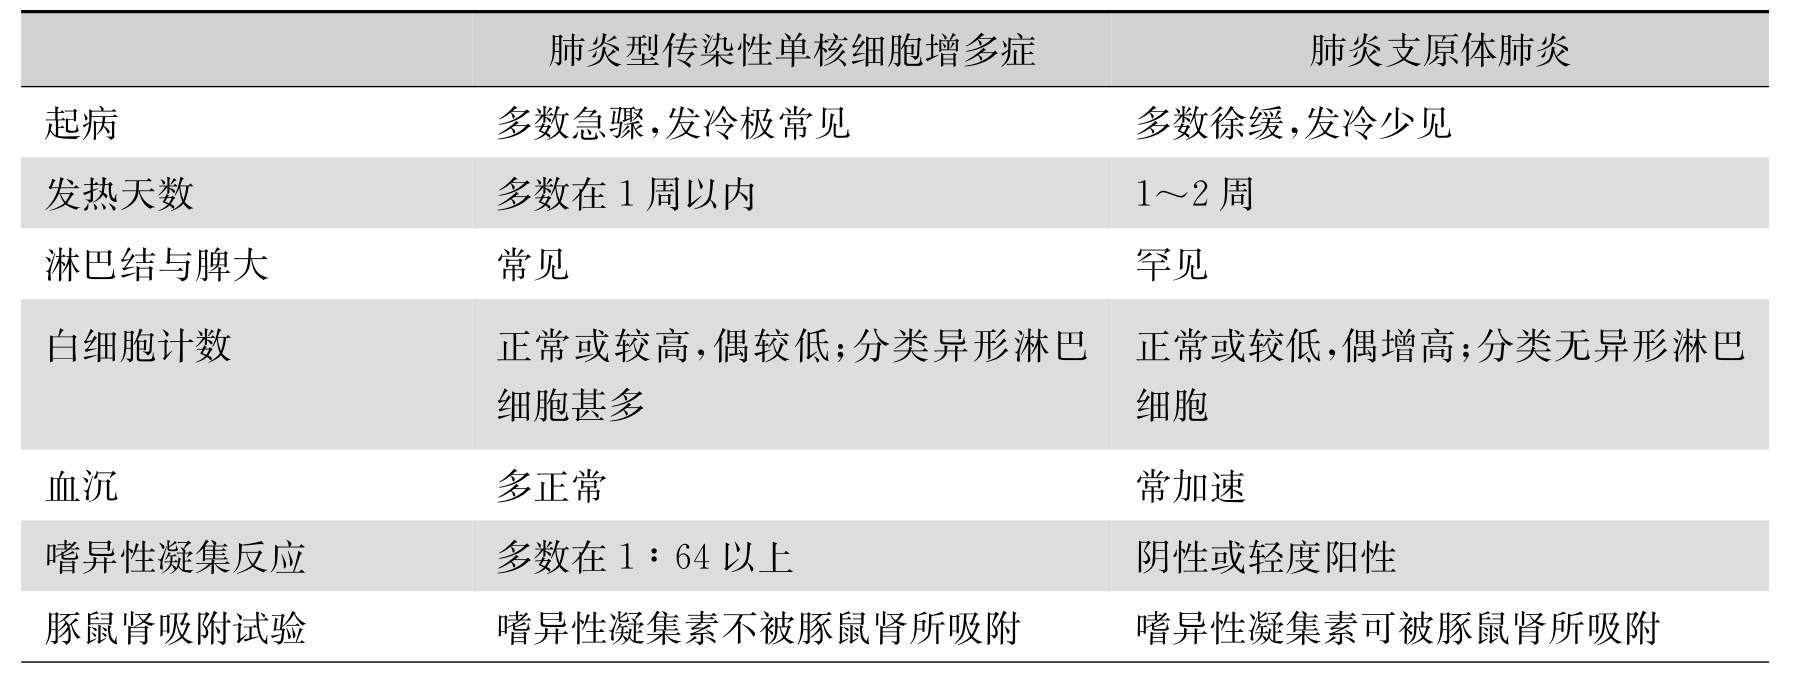
\includegraphics[width=0.7\textwidth]{./images/Image00013.jpg}
	\caption{动脉壁钙化}
	\label{fig1-12}
\end{figure}
%\FloatBarrier

(2)转移性钙化:较少见,是指由于全身钙、磷代谢障碍,血钙和(或)血磷升高,钙盐沉积于未受损的组织中。如甲状腺功能亢进或骨肿瘤造成骨组织破坏时,大量骨钙进入血液,使血钙升高,并沉积于肾小管、肺泡、胃黏膜和动脉壁中层(图\ref{fig1-12}b)。接受超剂量维生素D时,由于肠道对钙磷吸收明显增加,也可引起钙化。

钙化对机体的影响视具体情况而异。坏死组织钙化常是病灶愈合的表现,而血管壁的钙化则使管壁失去弹性、变硬、变脆,容易破裂出血。转移性钙化的危害性主要决定于原发病。

\subsubsection{不可逆性损伤-细胞死亡}

当细胞发生不可逆性代谢、结构和功能障碍,则引起细胞死亡(cell
death)。细胞死亡是病理学核心问题,其表现有两种方式:坏死与凋亡。坏死是细胞受到严重损伤时的病理性死亡过程,而凋亡多属生理性情况下发生的死亡,由细胞基因编程调控,在某些病理情况下,细胞死亡也可以凋亡形式出现。

\paragraph{坏死}
坏死(necrosis)是细胞受到严重损伤,以酶溶性变化为特点的活体内局部组织细胞的死亡。坏死可迅速发生,但在多数情况下由可逆性损伤逐渐发展而来。基本表现为细胞肿胀、细胞器崩解和蛋白质变性。

(1)坏死的基本病变

1)细胞核的改变:这是细胞坏死在形态学上的主要标志,表现为:①核浓缩(pyknosis),由于核脱水使染色质浓缩,嗜碱性染色增强,核体积缩小。②核碎裂(karyorrhexis),核染色质崩解为小碎片,核膜破裂,染色质碎片分散在胞质中。③核溶解(karyolysis),在DNA酶的作用下,染色质DNA分解,核乃失去对碱性染料的亲和力,因而染色变淡,仅见核轮廓,最后核消失(图\ref{fig1-13})。

\begin{figure}[!htbp]
	\centering
	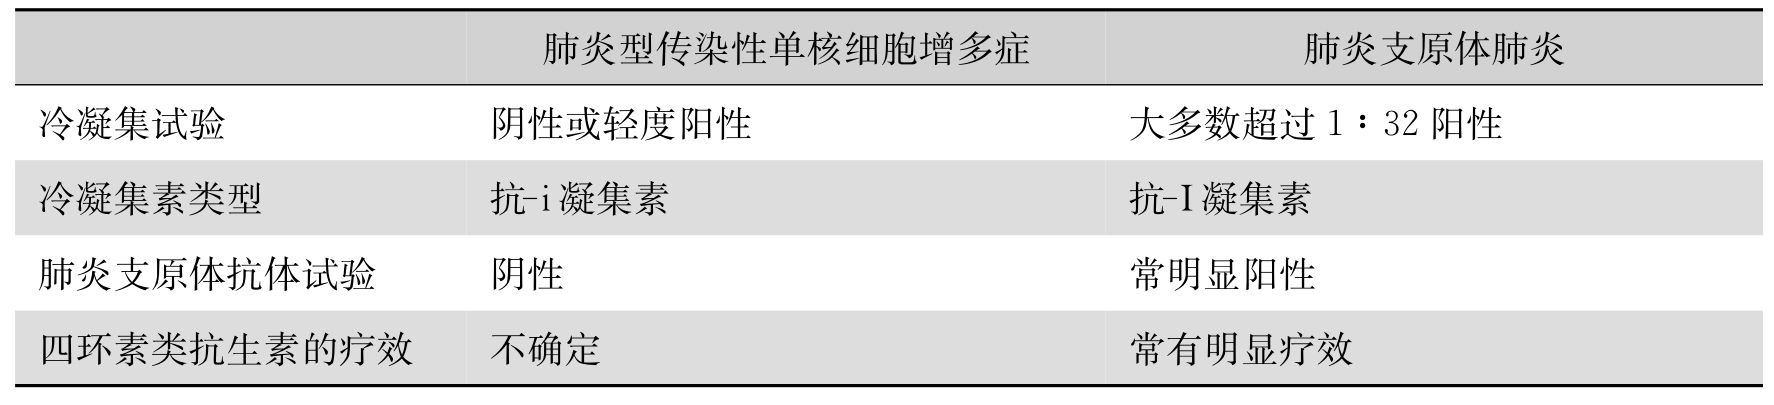
\includegraphics[width=0.7\textwidth]{./images/Image00014.jpg}
	\caption{细胞坏死时核的变化}
	\label{fig1-13}
\end{figure}

2)细胞浆的改变:由于细胞浆内嗜碱性核蛋白体减少或丧失,胞质变性蛋白质增多、糖原颗粒减少,使胞质对碱性染料苏木素的亲和力减少,而与酸性染料伊红的亲和力增强,致胞浆红染,坏死后期细胞浆崩解。

3)间质的改变:在实质细胞坏死后一段时间内,间质常无改变,以后在溶解酶的作用下,基质崩解,胶原纤维肿胀、断裂,继而崩解、液化。最后坏死的实质细胞和间质融合成一片无结构的颗粒状、红染物质,其内有时可见少量淡染的细胞核碎片。

由于坏死时细胞膜通透性增加,细胞内乳酸脱氢酶、琥珀酸脱氢酶、肌酸激酶、门冬氨酸氨基转移酶、丙氨酸氨基转移酶等被释放入血,造成细胞内酶活性降低而血浆中相应的酶活性升高,分别可作为诊断某些细胞(如肝、心肌、胰)坏死的参考指标。细胞内和血浆中酶活性的变化在坏死初即可检出,有助于细胞损伤早期诊断。

(2)坏死的病理类型:组织坏死后,由于酶的分解和蛋白质变性等因素综合作用的结果,使坏死组织出现不同的形态学变化,总体上可分为凝固性坏死、液化性坏死和特殊类型坏死等三个基本类型。

1)凝固性坏死(coagulation
necrosis):组织坏死后,蛋白质变性凝固且溶酶体酶水解作用较弱时,坏死区呈灰黄、干燥、质实状态,称为凝固性坏死。这种坏死多由缺血引起,常在心、肾、脾等器官的缺血性坏死时出现。
坏死灶周围常有暗红色出血带,与健康组织分界(图\ref{fig1-14}a)。
镜下特点:早期坏死灶细胞微细结构消失,但细胞组织的结构轮廓仍可保留一段时间(图\ref{fig1-14}b)。
最终坏死细胞崩解成碎片,被吞噬细胞吞噬或被游走进入的白细胞释放的溶解酶溶解。
凝固性坏死的发生机制仍不很清楚,可能是组织坏死后蛋白变性过程占优势,而水解酶的作用较少。

\begin{figure}[!htbp]
	\centering
	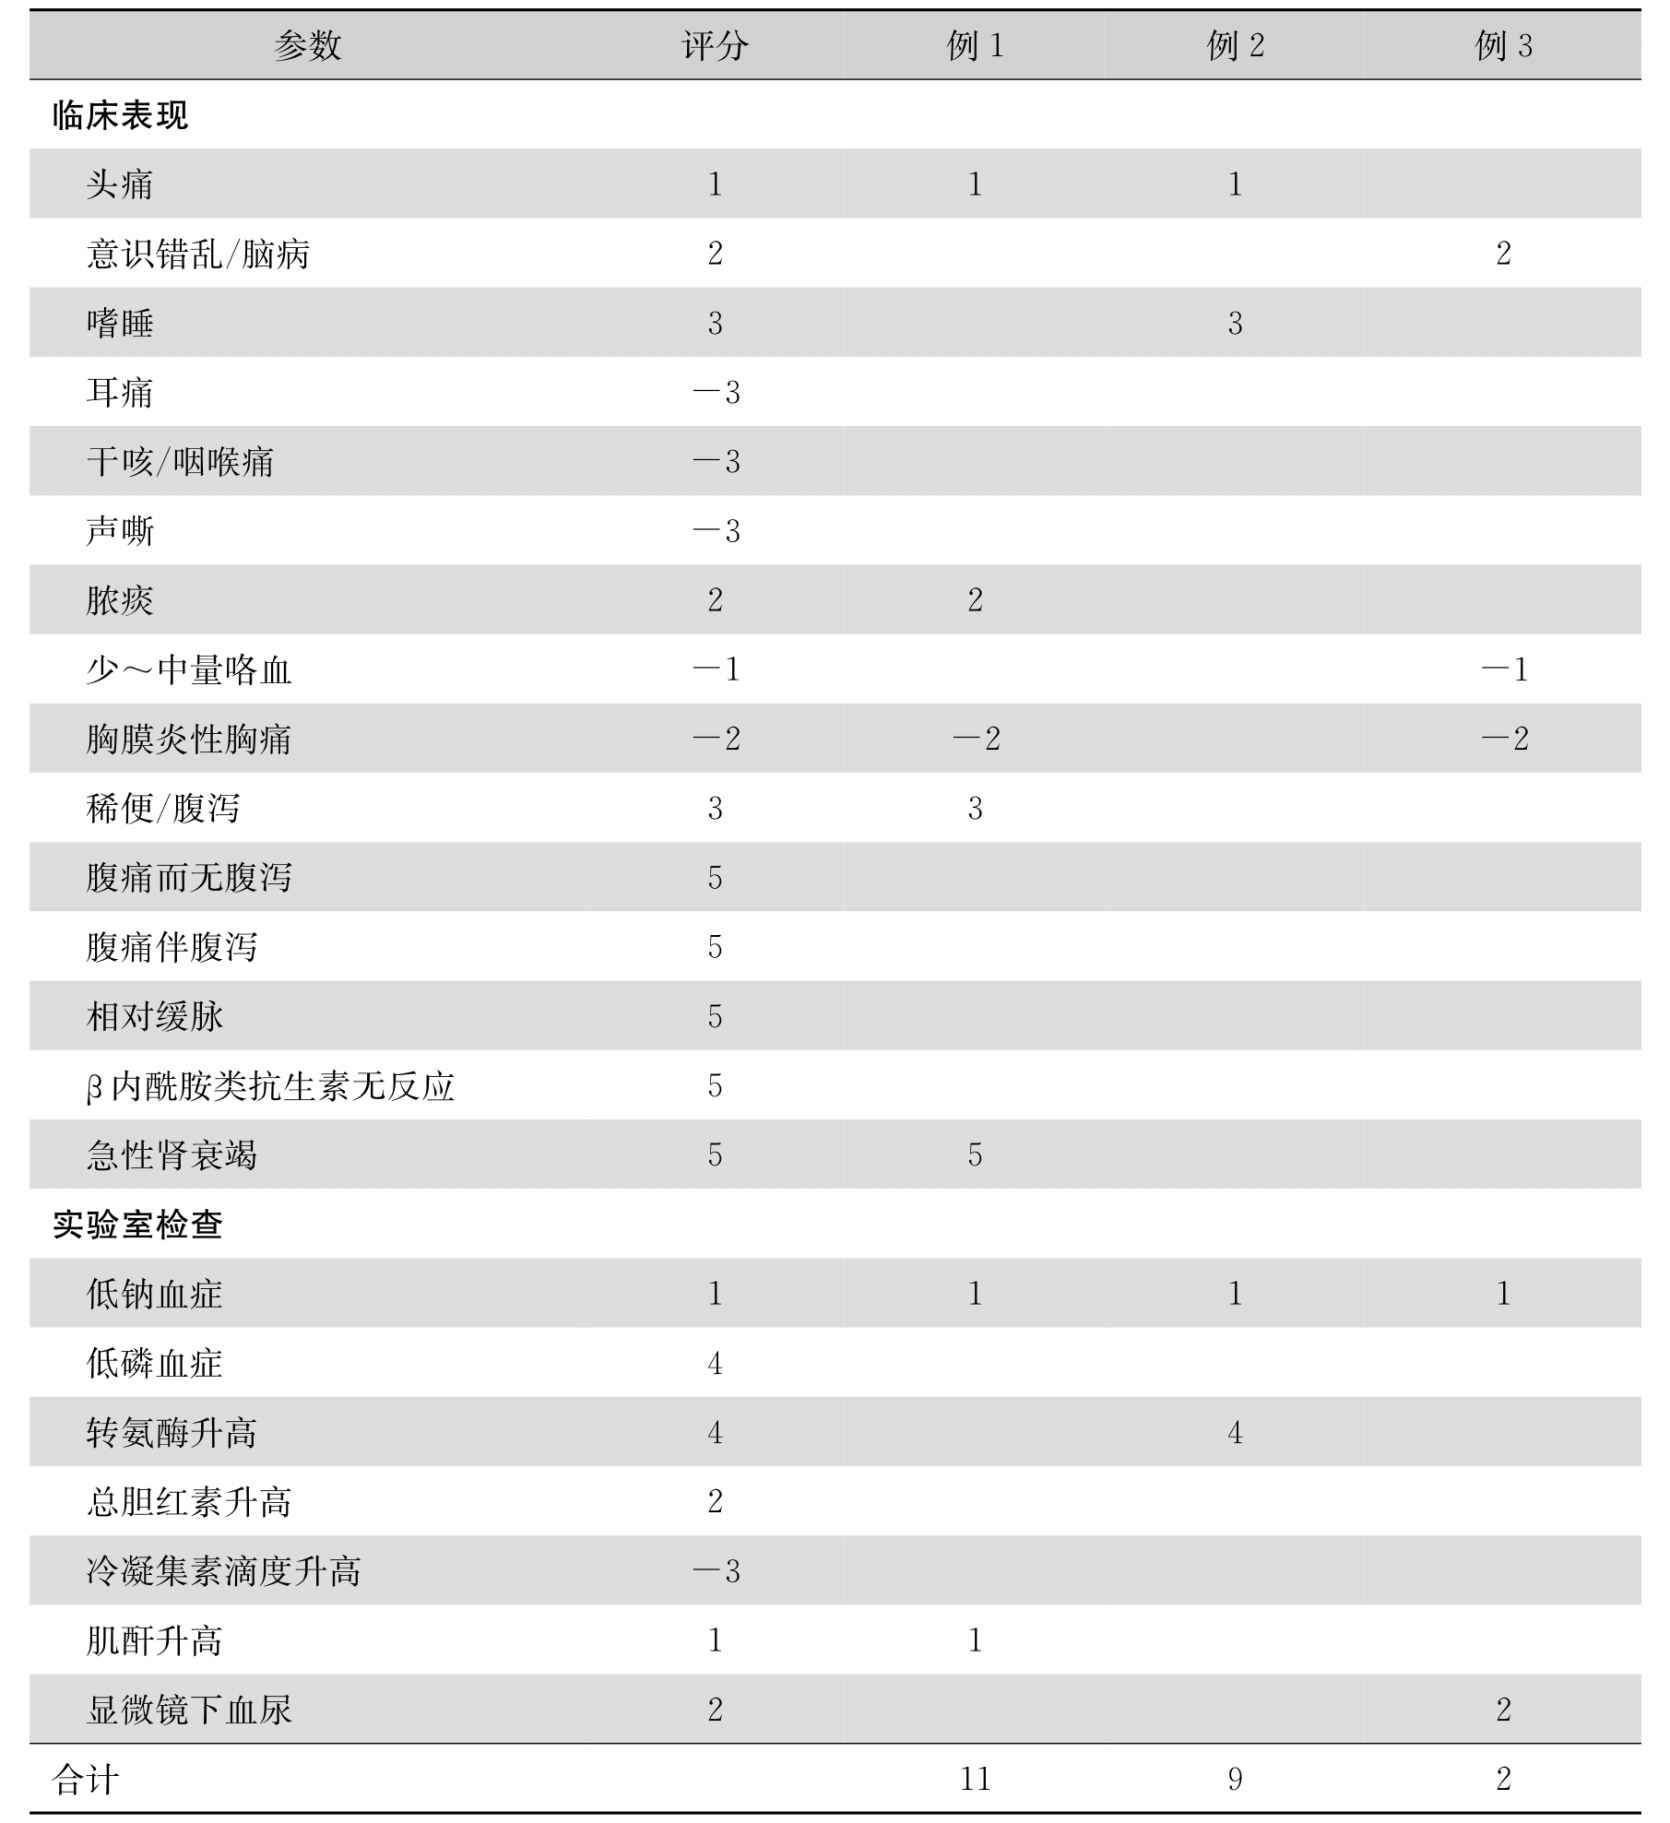
\includegraphics[width=.7\textwidth]{./images/Image00015.jpg}
	\caption{凝固性坏死}
	\label{fig1-14}
\end{figure}

2)液化性坏死(liquefaction
necrosis):组织坏死后分解、液化而呈液体状,有时还形成含有液体的腔。
如脑组织,坏死后分解成半流体状物质,又称为脑软化。
这种变化与脑组织水分和磷脂含量多,蛋白质含量少有关,故组织坏死后不易凝固而液化。
在某些病原体如化脓性细菌或溶组织阿米巴原虫能释放或产生蛋白溶解酶,可使组织发生液化性坏死。

3)特殊类型坏死

①干酪样坏死(caseous
necrosis):结核病时,坏死区内脂质较多,颜色带黄,质地松软,状似干酪,故称为干酪样坏死。
镜下观:坏死组织分解比较彻底,原有组织轮廓消失,呈现为一片红染、无定形的颗粒状物质(图\ref{fig1-15})。
梅毒性的坏死组织具有相似的形态,但其中的弹力纤维及血管结构仍可保留,致使坏死组织质地坚韧如树胶,故名树胶肿。
干酪样坏死不易吸收,一旦形成将存留较长时间。

\begin{figure}[!htbp]
	\centering
	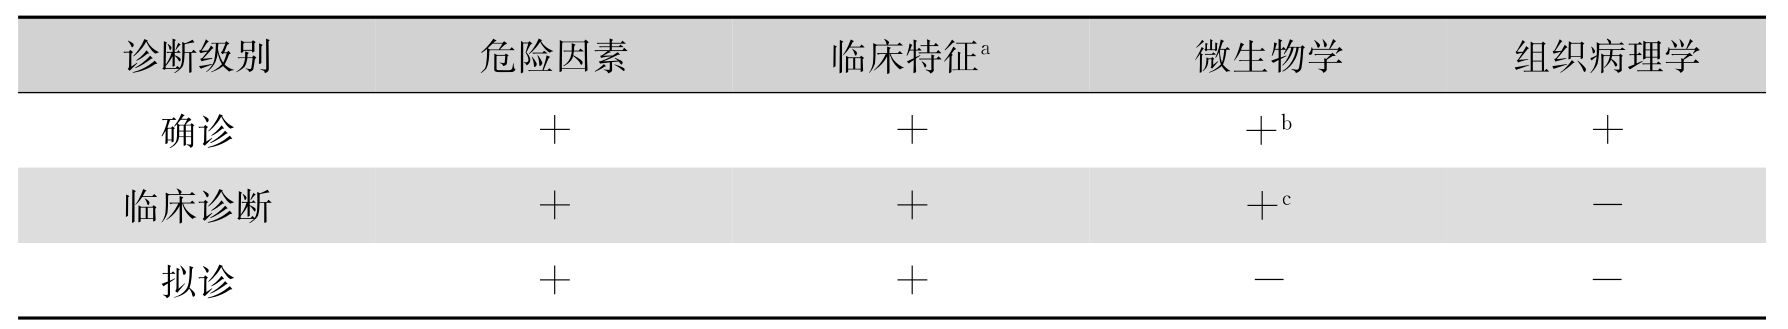
\includegraphics{./images/Image00016.jpg}
	\caption{肾干酪样坏死 \\ {\small 肾剖面可见多个黄白色干酪样坏死灶。}}
	\label{fig1-15}
\end{figure}

②纤维素样坏死(fibrinoid necrosis):旧称纤维素样变性(fibrinoid
degeneration)为发生于结缔组织胶原纤维和小血管壁的一种坏死。病变部位组织结构逐渐消失,变为一片境界不清的颗粒状、小条状或小块状无结构物质,经伊红染成深红色,由于其与纤维素染色性质相似,故名。常见于风湿病、结节性多动脉炎、新月体性肾小球肾炎、系统性红斑性狼疮等变态反应性疾病(图\ref{fig1-16})。也可见于恶性高血压病时的细动脉和胃溃疡底部动脉壁。其发生机制与抗原-抗体复合物引发的胶原纤维肿胀崩解、结缔组织免疫球蛋白沉积或血液纤维蛋白渗出变性有关。

\begin{figure}[!htbp]
	\centering
	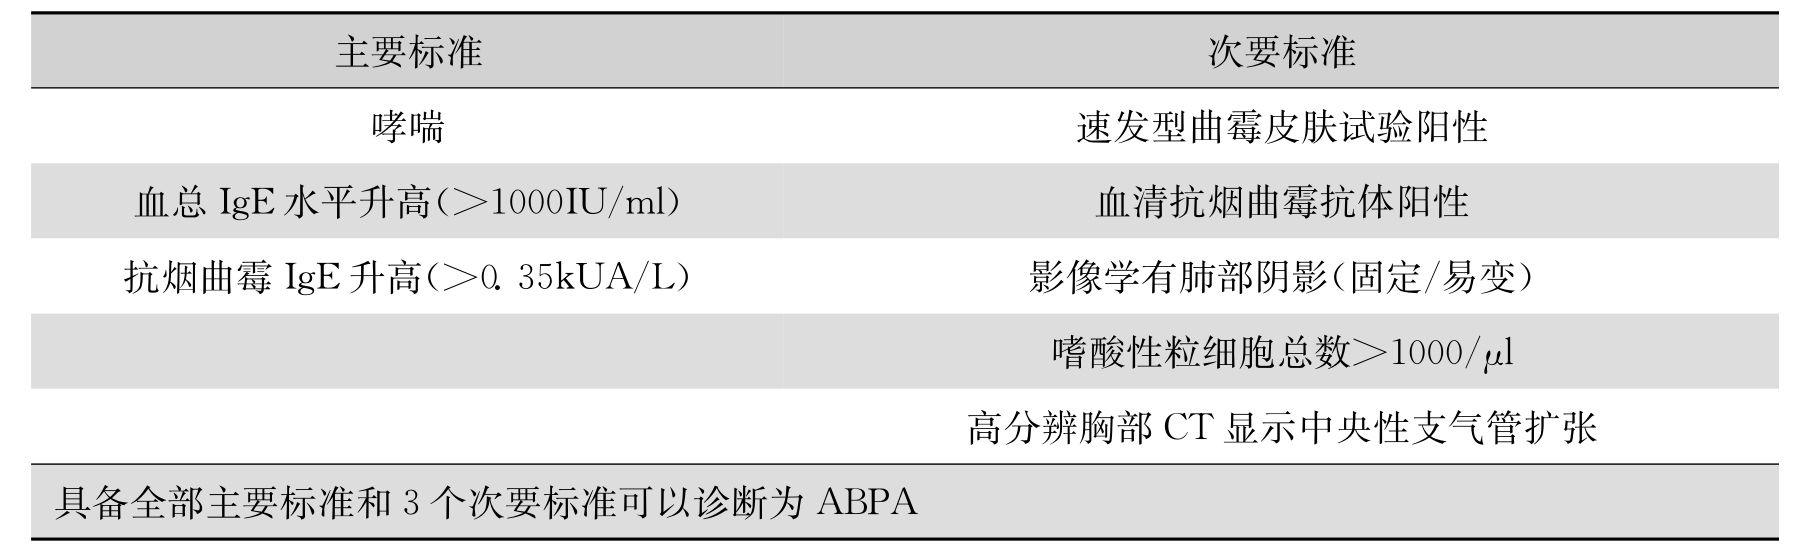
\includegraphics{./images/Image00017.jpg}
	\caption{肾小动脉壁纤维素样坏死(HE染色,高倍) \\ {\small 箭头所示深伊红染区为小动脉壁纤维素样坏死。}}
	\label{fig1-16}
\end{figure}


③脂肪坏死(fatty
necrosis):为液化性坏死的一种特殊类型,又可分为酶解性脂肪坏死和外伤性脂肪坏死。
前者常见于急性胰腺炎,由于胰脂酶外逸并被激活,对胰腺自身及腹腔的脂肪组织发生分解作用,形成的脂肪酸与组织内钙盐结合,在大网膜、后腹壁及肠系膜表面形成灰白色、质硬的不透明斑点或斑块,称为皂钙。
外伤性脂肪坏死常发生于富于脂肪组织的部位,乳腺尤其多见,有外伤史,局部表现为增大的肿块。镜下为大量的泡沫细胞及异物巨细胞。

④坏疽(gangrene):大块组织坏死后继发腐败菌感染,出现不同程度的腐败性变化。
腐败菌在分解坏死组织的过程中产生大量的硫化氢,并与血红蛋白分解释出的铁离子结合,形成硫化亚铁,致使坏死组织臭而发黑。
根据坏疽发生的部位、原因及形态特征不同,可分为干性、湿性、气性等类型。
干性坏疽(dry
gangrene)多发生于动脉阻塞而静脉回流仍然通畅的四肢末梢,坏死局部干燥、皱缩,呈黑色,与周围组织分界清楚(图\ref{fig1-17}),腐败性变化较轻。
湿性坏疽(moist
gangrene)常发生于与体外相连的内脏,如肠、阑尾等器官,也可发生于四肢。
形成的原因除动脉阻塞外,同时伴有局部淤血,坏死组织含水量多,适合腐败菌生长。
坏死区局部明显肿胀,呈深黄、暗绿或污黑,与周围组织无明显分界线,可引起严重的全身中毒症状。气性坏疽(gas
gangrene)也属于湿性坏疽。系深达肌肉的开放性创伤合并产气荚膜杆菌、腐败弧菌等厌氧菌感染。
细菌在分解液化组织的过程中产生大量气体,使坏死组织呈蜂窝状,压之有捻发感。
病变发展迅猛,沿肌束迅速蔓延。由于大量毒素被吸收,患者中毒症状十分严重,常需要紧急处理。

\begin{figure}[!htbp]
	\centering
	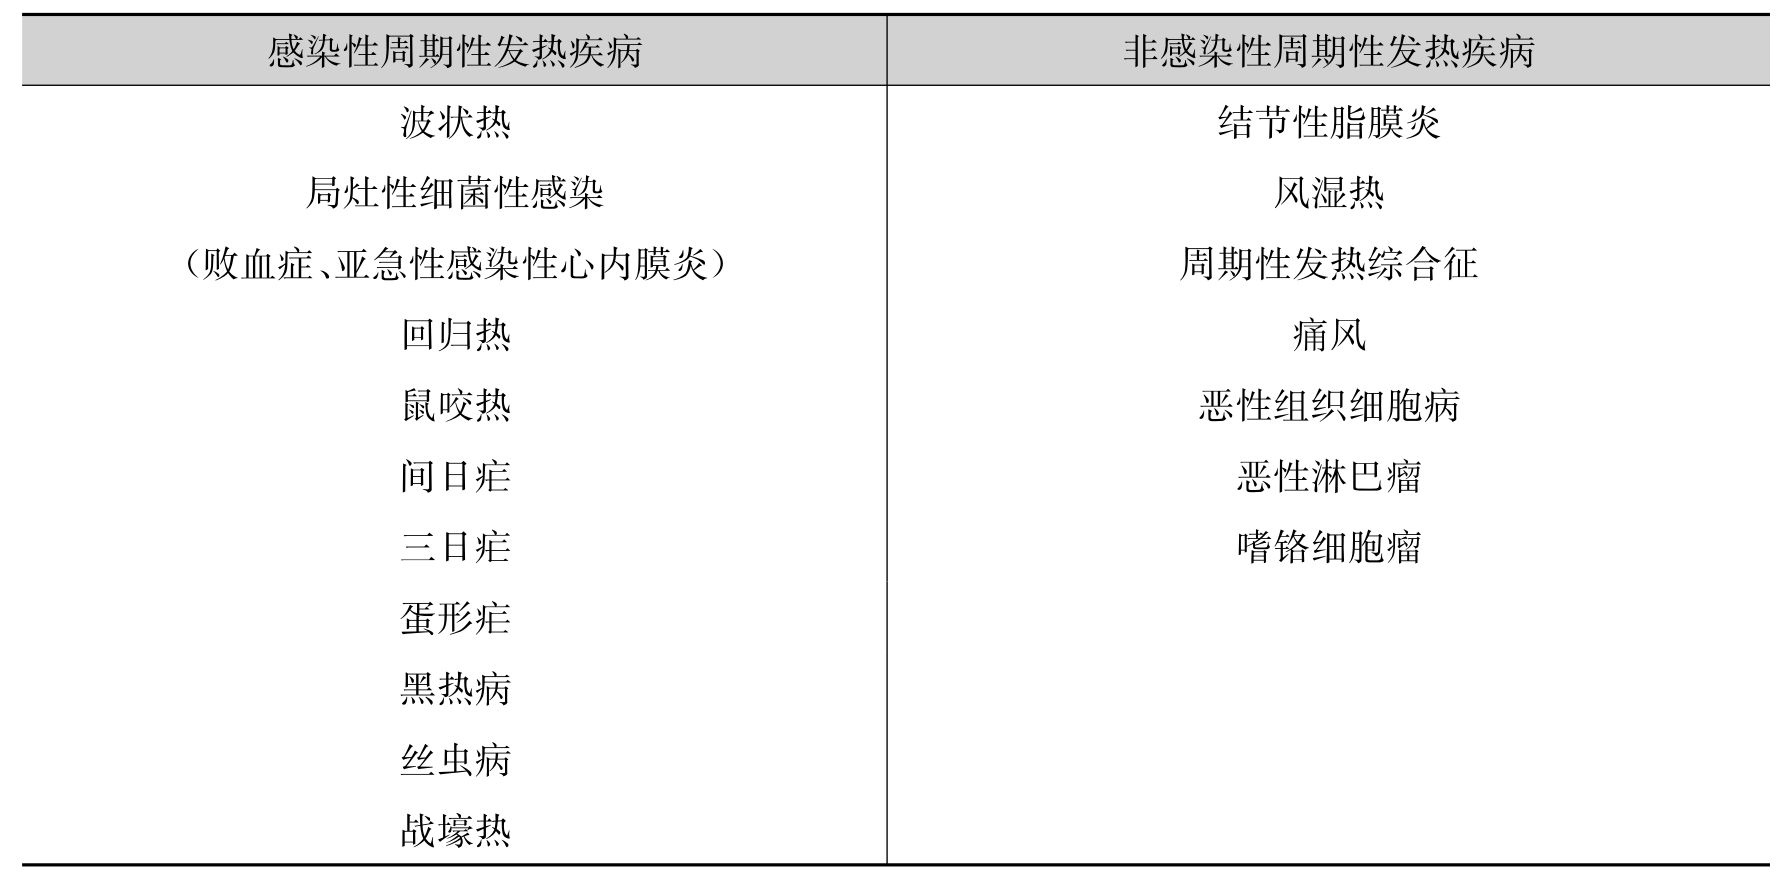
\includegraphics{./images/Image00018.jpg}
	\caption{足(干性)坏疽}
	\label{fig1-17}
\end{figure}

(3)坏死的结局:组织坏死后成了机体的异物,刺激周围组织,引起局部反应。不同的坏死组织结局不尽相同。

1)溶解吸收:坏死细胞自身或周围的炎细胞释放的溶解酶将坏死组织分解、液化,然后由淋巴管或小血管吸收,未被完全分解的组织碎片由吞噬细胞吞噬清除。坏死范围较大可形成囊腔。留下的组织缺损通过再生修复,这是机体处理坏死组织的基本方式。

2)分离排出:较大的坏死灶不易完全吸收,由于其周围发生炎症反应,其中的白细胞释放的溶解酶加速周边坏死组织溶解、吸收,使坏死灶与健康组织分离。位于皮肤、黏膜的坏死组织分离后脱落,留下局部缺损,浅者称为糜烂,深者称为溃疡。肾和肺脏的坏死组织分离后经自然管道排出,留下的空腔称为空洞。

3)机化与纤维包裹:坏死组织如不能被溶解吸收或分离排出,则由周围新生的毛细血管和成纤维细胞(合称肉芽组织)逐渐长入,取代坏死组织,最后形成瘢痕组织。这种由肉芽组织取代坏死组织(或其他异物、血凝块、血栓及渗出物等)的过程称为机化(organization)。如果坏死灶较大,难以吸收、机化,周边部增生的肉芽组织可将坏死灶包围,尔后肉芽组织转变为纤维组织,称为纤维包裹。机化和包裹的肉芽组织最终形成纤维瘢痕。

4)钙化:坏死组织和细胞碎片若未被及时清除,则日后易发生钙盐及其他矿物质沉积,引起营养不良性钙化。陈旧性干酪样坏死病灶或坏死的脂肪组织常有明显的钙化。

\paragraph{细胞凋亡}
细胞凋亡(apoptosis)也称程序性细胞死亡,是真核细胞在一定条件下通过启动其自身内部机制,主要是激活内源性核酸内切酶而发生的细胞主动性死亡方式。与细胞坏死不同,凋亡是一种主动过程,通常为单个细胞或小灶性细胞死亡,而不是大片实质细胞同时死亡。凋亡细胞周围无炎症反应,故有人借用希腊词“apoptosis”来形容其像秋天枯萎的树叶,从树干上悄无声息地飘零下来。

(1)形态特征:凋亡细胞有独特的形态特征。早期表现为细胞变圆,微绒毛及细胞突起消失,同时胞质浓缩,内质网扩张呈泡状,并与细胞膜融合形成细胞质小泡,向外隆起但无膜破裂;核染色质浓缩、凝聚于核膜下呈半月形。而后细胞膜内陷,自行分割为数个由胞膜包裹的、表面光滑的凋亡小体,其中含有大小不等的染色质片断、结构尚保持完整的细胞器和胞质成分(图\ref{fig1-18})。凋亡小体可与周围细胞分离,很快被邻近的细胞或巨噬细胞吞噬,在胞质溶酶体内迅速降解。

\begin{figure}[!htbp]
	\centering
	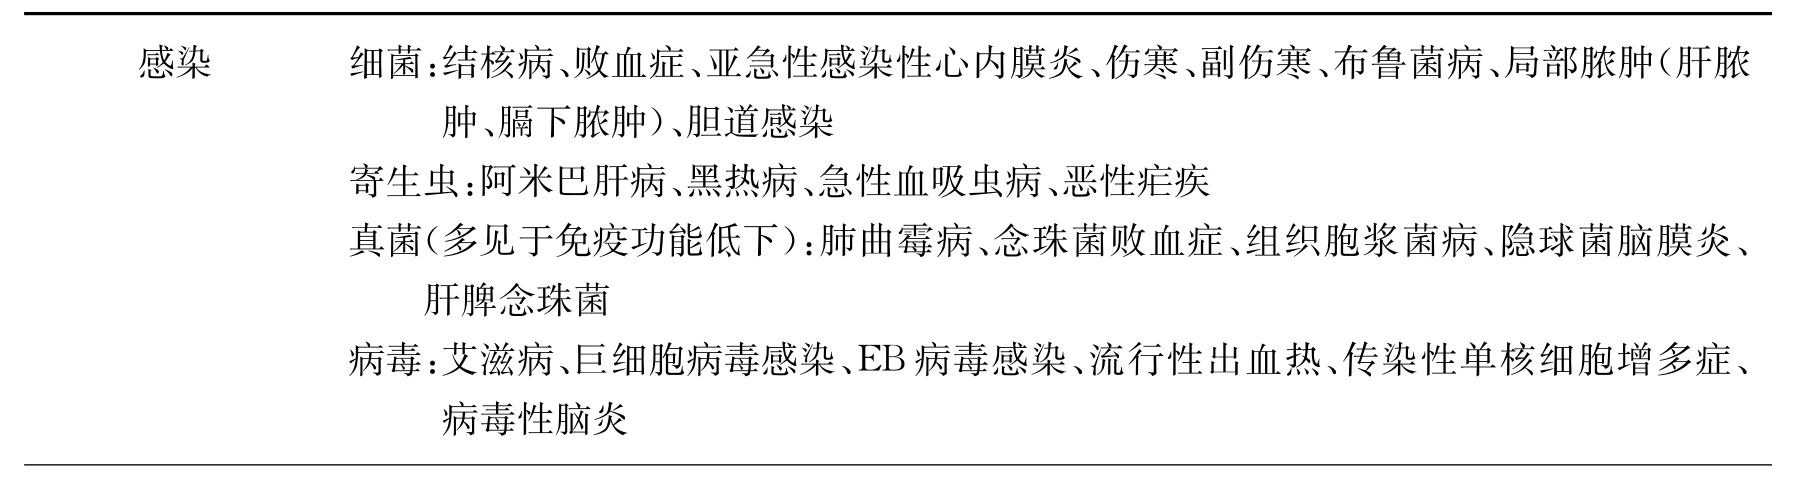
\includegraphics[width=.7\textwidth]{./images/Image00019.jpg}
	\caption{凋亡示意图}
	\label{fig1-18}
\end{figure}

(2)发生机制:细胞凋亡的发生机制十分复杂,它是一种由某些刺激因子启动、内在基因调控,并依赖能源的连锁分子事件,其中有信号传导、特异性调节分子作用、共同蛋白酶(caspases,半胱氨酸天冬氨酸蛋白酶,亦称胱冬肽酶)家族活化及死亡细胞的被噬和移去等过程,故曾有程序性死亡(programmed
cell death)之称。

刺激因子不同,其信号通路、调节分子种类不尽相同。目前已知,在人体各种病理过程中,发生细胞凋亡的主要通路有两条(图\ref{fig1-19}):一是线粒体通路或内源通路;二是死亡受体通路或外源通路。

\begin{figure}[!htbp]
	\centering
	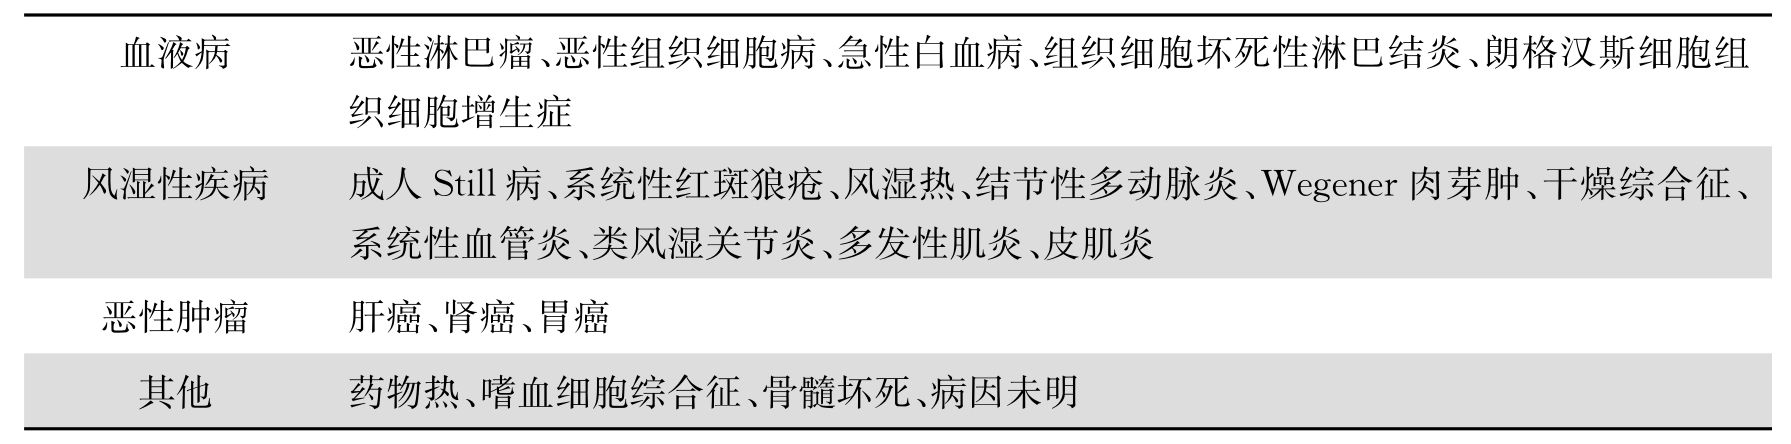
\includegraphics[width=.7\textwidth]{./images/Image00020.jpg}
	\caption{细胞凋亡机制示意图}
	\label{fig1-19}
\end{figure}

线粒体通透性决定细胞是否凋亡,而通透性受控于含20个以上蛋白成员的Bcl-2家族。当细胞失去生长因子或生存信号、暴露于DNA损伤因子(如紫外线、放射线、活性氧和细胞毒药物等)以及细胞内堆积过多的错误折叠蛋白时,Bcl-2家族感应分子即被活化,继之活化该家族另外两个成员(效应分子)-Bax和Bak,它们形成二聚体并插入线粒体膜,使后者通透性增加,细胞色素C和其他蛋白分子逸出线粒体进入胞浆,令激发性胱冬肽酶(caspase
9)活化,后者再使效应性胱冬肽酶(caspase
3、6、7)活化,最终导致细胞骨架蛋白崩解、核酸内切酶活化和凋亡小体形成。Bcl-2、Bcl-x{L}
抑制Bax和Bak活化,故可阻断凋亡。

细胞凋亡的死亡受体通路涉及肿瘤坏死因子(TNF)及其受体(TNFR)、FAS-FAS配体作用等。受体的胞内段为死亡功能区(dead
domain)。一旦受体配体结合,死亡信号即通过死亡功能区和相关的适配蛋白(adapter
protein)传递至激发性胱冬肽酶(caspase
8),并使之活化。后续反应与线粒体通路相同。

(3)细胞凋亡与坏死的区别:细胞凋亡的发生机制与前述的坏死不同,有相关基因调节。其中Fas、Bax、P53等基因有促进作用,Bcl-2、Bcl-x{L}
等有抑制凋亡作用。凋亡细胞内源性Ca{2+} 、Mg{2+}
依赖DNA内切酶的激活,从而切割核小体间DNA,形成不连续的180~200
bp或其倍数的DNA片断。被切割的DNA片断在琼脂糖凝胶电泳时表现为阶梯状电泳条带,这种现象被认为是细胞凋亡的可靠指标。凋亡的细胞质膜完整,无细胞内容物溢出,不引起细胞周围炎症反应,也不诱发周围细胞的增生修复。细胞凋亡和细胞坏死的区别见表\ref{tab1-1}。

\begin{table}[ht]
	\caption{细胞凋亡和细胞坏死的区别}
	\label{tab1-1}
	\centering
	\begin{tabular}{lp{5cm}p{5cm}}
		\toprule
		         & 细胞凋亡                                                                           & 细胞坏死                       \\
		\midrule
		形态特征 & 细胞固缩,核染色质边集、细胞膜及各细胞器膜完整,膜可发泡出芽,形成调亡小体
		         & 细胞显著肿胀,核染色质絮状或边集,细胞膜及各细胞器膜溶解破裂,溶酶体释放,细胞溶解                                  \\
		生化特征 & 核酸内切酶活化,半胱氨酸蛋白酶活化,谷氨酰谷氨酰转移酶活性增高
		         & 核酸内切酶无活化,半胱氨酸蛋白酶、转移酶活性无变化                                                                  \\
		DNA电泳  & 阶梯状条带                                                                         & 弥散分布的电泳拖带             \\
		炎症反应 & 无                                                                                 & 有                             \\
		机制     & 由凋亡相关基因调控主动进行(自杀性)                                                 & 与基因调控无关被动进行(他杀性) \\
		发生条件 & 多为生理性                                                                         & 病理性                         \\
		\bottomrule
	\end{tabular}
\end{table}


(4)细胞凋亡的生理、病理意义:细胞凋亡是最基本的生物现象,是机体生存和发育的基础。大量研究材料显示它涉及生命活动中的许多领域,包括发育、生长、造血、免疫、肿瘤发生等。通过凋亡可以清除多余的、无用的细胞。胚胎发育过程中,一些遗迹如人胚的尾芽和鳃随发育定期消亡,就是通过凋亡的方式进行的。细胞凋亡也可作为机体的自身保护机制,以清除发育不正常及对机体有害的细胞,畸胎瘤就是未彻底凋亡的残留胚层结构存留所致。B和T细胞发育成熟过程中本该发生凋亡的细胞保留下来将形成自身抗原,导致自身免疫病;细胞凋亡的异常改变包括凋亡不足或凋亡过度都可引起一些疾病。T辅助细胞($\text{CD}^+_4$
)在人类免疫缺陷病毒(HIV)感染后,发生凋亡,从而导致获得性免疫缺陷病。细胞凋亡的调控失常与肿瘤的发生关系密切,当机体某个基因发生突变而导致凋亡信号下调凋亡不足时,可引起细胞异常增生而发生肿瘤。目前临床上已开始用药物或放射线来诱导肿瘤细胞凋亡以达到治疗肿瘤的目的。

\begin{center}
	\textbf{知识链接}
\end{center}
\chapterabstract{自噬(autophagy)是细胞对自身细胞器或胞内聚集的变性蛋白等大分子物质进行包裹以及降解消化的现象。近年发现自噬不足或过度均可导致细胞死亡,所以被称为第三种细胞死亡方式。}

生理状态下,细胞通过自噬来清除受损、衰老和失去功能的细胞器及各种大分子物质,最终降解产物再循环利用,为细胞重建和再生提供原料。病理状态下,自噬不仅能保护细胞免受毒物损伤,而且能抵御病原体的侵害。在机体的免疫、感染、炎症、肿瘤、心血管病和神经退行性疾病的发生发展过程中均发挥重要作用。自噬和凋亡有相似之处,如二者共享某些调节蛋白,如胱冬肽酶。某些刺激因素既可诱导自噬亦可引起凋亡。

总之,疾病源于组织细胞的损伤,内外因子的刺激强度不同,损伤程度不同(图\ref{fig1-20})。若刺激在细胞能承受范围内,则表现为适应,属轻度损伤,细胞可出现萎缩、增生、肥大和化生等形态学改变。若刺激时间长强度大,细胞将发生显著损伤,出现细胞内外异常物质沉积,甚至坏死;若刺激因素激活特殊信号系统,细胞可发生凋亡。

\begin{figure}[!htbp]
	\centering
	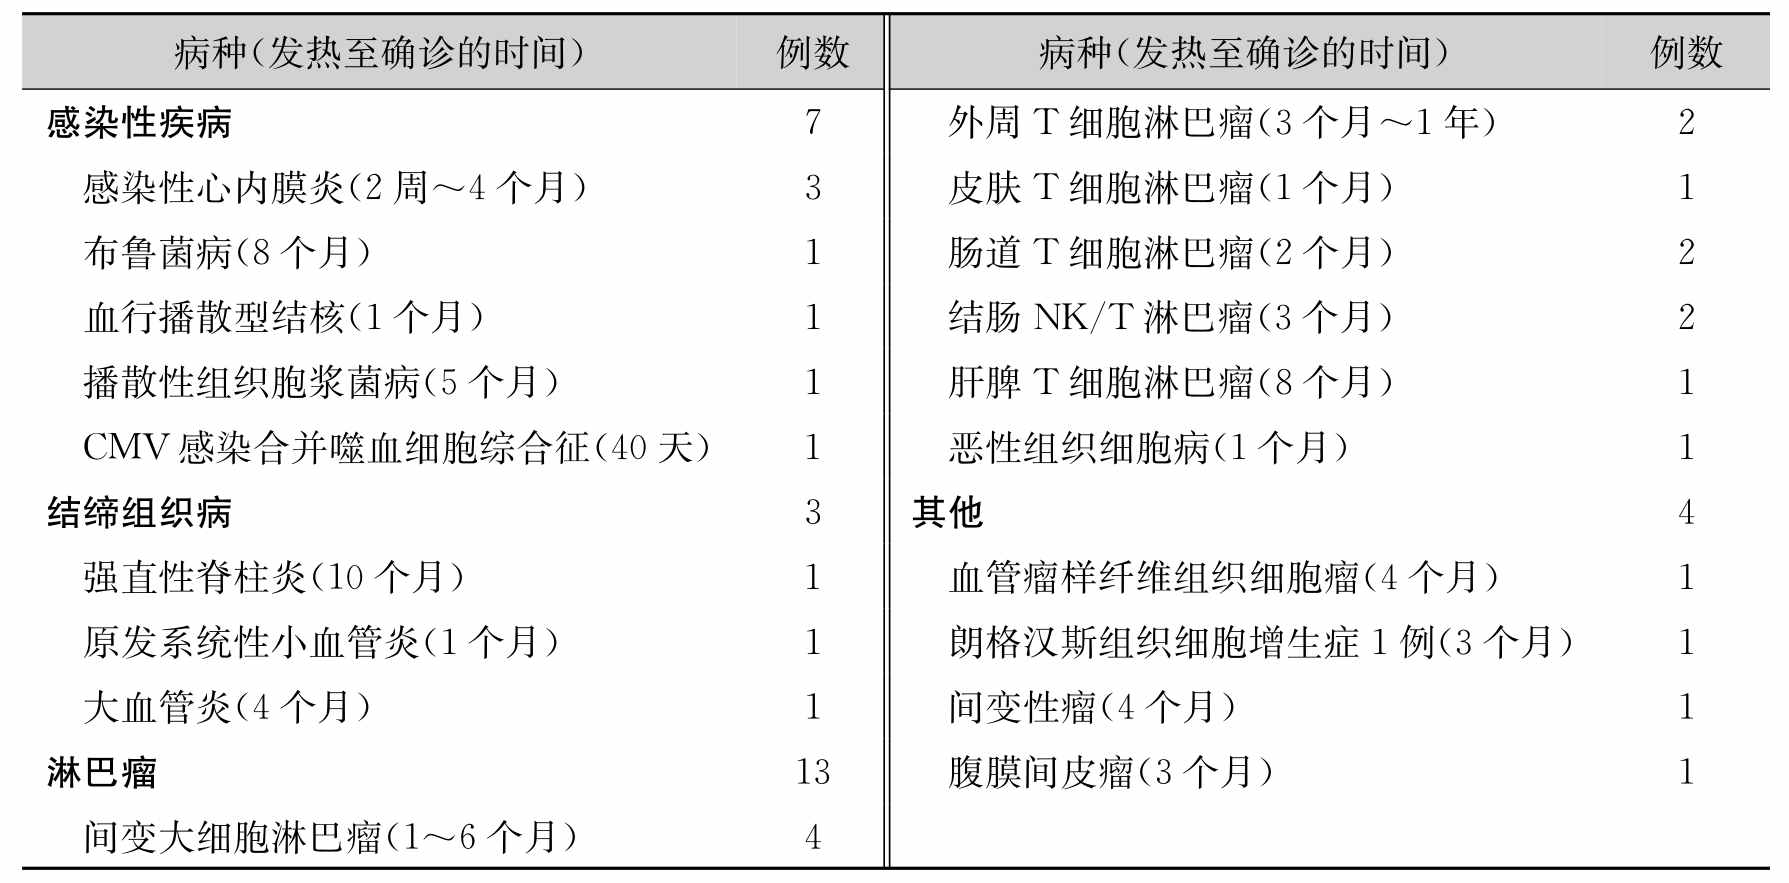
\includegraphics{./images/Image00023.jpg}
	\caption{组织细胞适应、损伤概览}
	\label{fig1-20}
\end{figure}

\section*{复习与思考}

{一、名词解释}

适应 萎缩 肠上皮化生 细胞水肿 脂肪变性 虎斑心 病理性钙化 凝固性坏死 干酪样坏死 液化性坏死 脑软化 坏疽 细胞凋亡

{二、问答题}

1. 机体组织细胞可出现哪几种适应性改变?

2. 久病卧床后肢体变细属于哪种类型的萎缩?为什么?

3. 试述肝脂变的原因和病变。

4. 何谓玻璃样变?好发于哪些部位?

5. 体内常见的色素有哪些?光镜下的特点是什么?

6. 试述坏死的镜下特点及结局。

7. 细胞的坏死和凋亡如何区别?


\chapter{免疫系统}
\begin{framed}
\noindent\textbf{【知识体系】}

\begin{center}
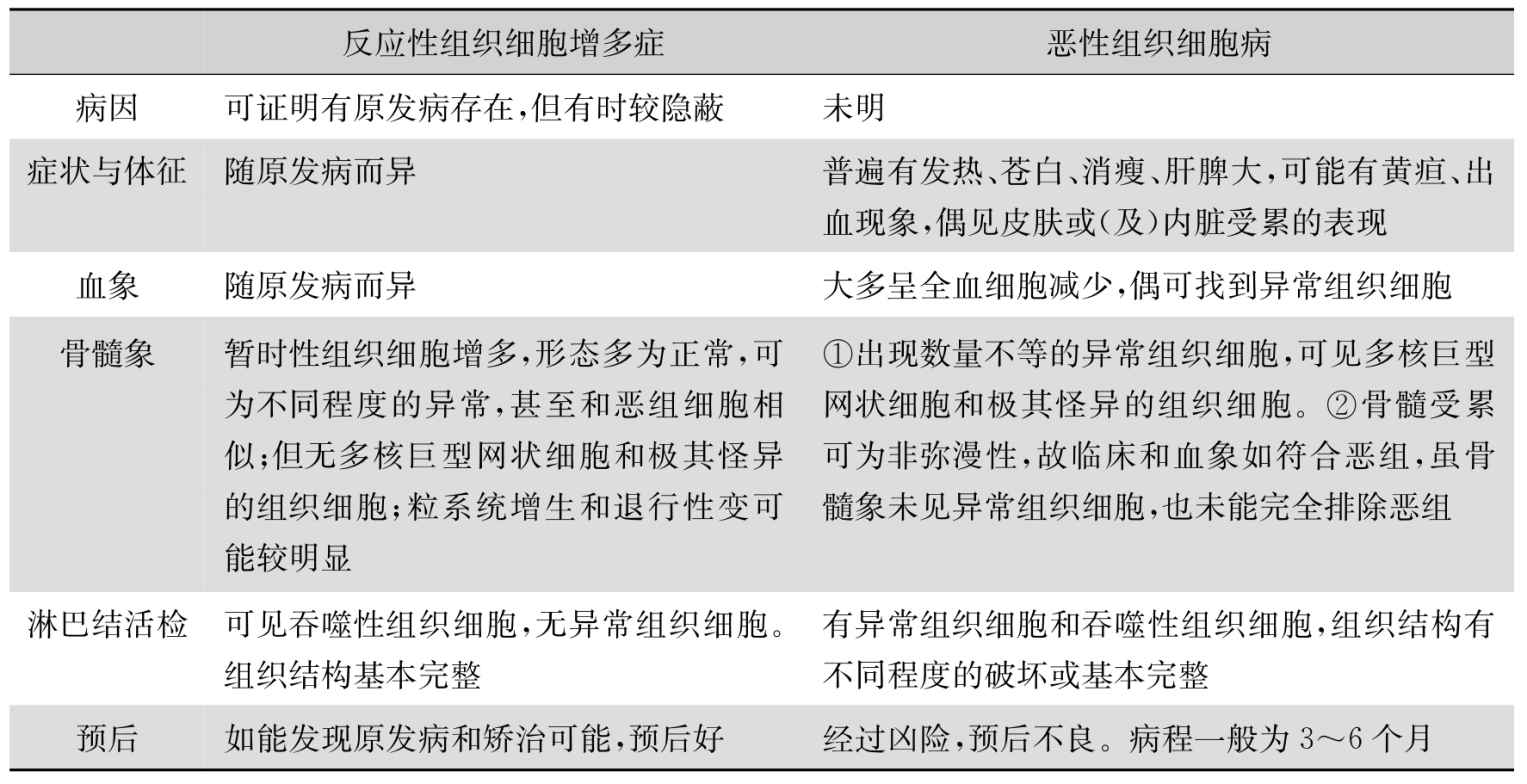
\includegraphics[width=.66\textwidth]{./images/Image00025.jpg}
\end{center}

\noindent\textbf{【课前思考】}

与机体的其他组织系统一样,免疫系统由哪些组织、器官、细胞组成?各种器官、细胞有何特征?在维护我们机体健康中各自起到怎样的作用?当有病原微生物入侵时,机体的各种免疫细胞是怎样各司其职又相互协调的?机体的免疫系统与国家的防御体系有何相似之处?

\noindent\textbf{【本章重点】}

1.免疫系统的构成;

2.免疫器官、免疫细胞的功能。

\noindent\textbf{【教学目标】}

1.掌握免疫系统组成:免疫器官(中枢免疫器官、外周免疫器官)、免疫细胞、免疫分子;

2.掌握中枢免疫器官的组成:骨髓、胸腺的主要免疫功能;

3.掌握外周免疫器官与组织的组成:淋巴结、脾脏的主要免疫功能。
\end{framed}
机体抵御外界病原微生物的入侵有三道防卫系统:

1.皮肤、黏膜及其分泌物

皮肤黏膜的机械阻挡作用和附属物(如纤毛)的清除作用,皮肤黏膜分泌物(如汗腺分泌的乳酸、胃黏膜分泌的胃酸等)的杀菌作用,体表和与外界相通的腔道中寄居的正常微生物丛对入侵微生物的拮抗作用等,属于机体第一道防线。其次是内部屏障。抗原物质一旦突破第一道防线进入机体后,即遭到机体内部屏障的清除,包括:淋巴和单核吞噬细胞系统屏障、正常体液中的一些非特异性杀菌物质、血脑屏障和胎盘屏障等(图\ref{fig2-1})。

\begin{figure}[!htbp]
 \centering
 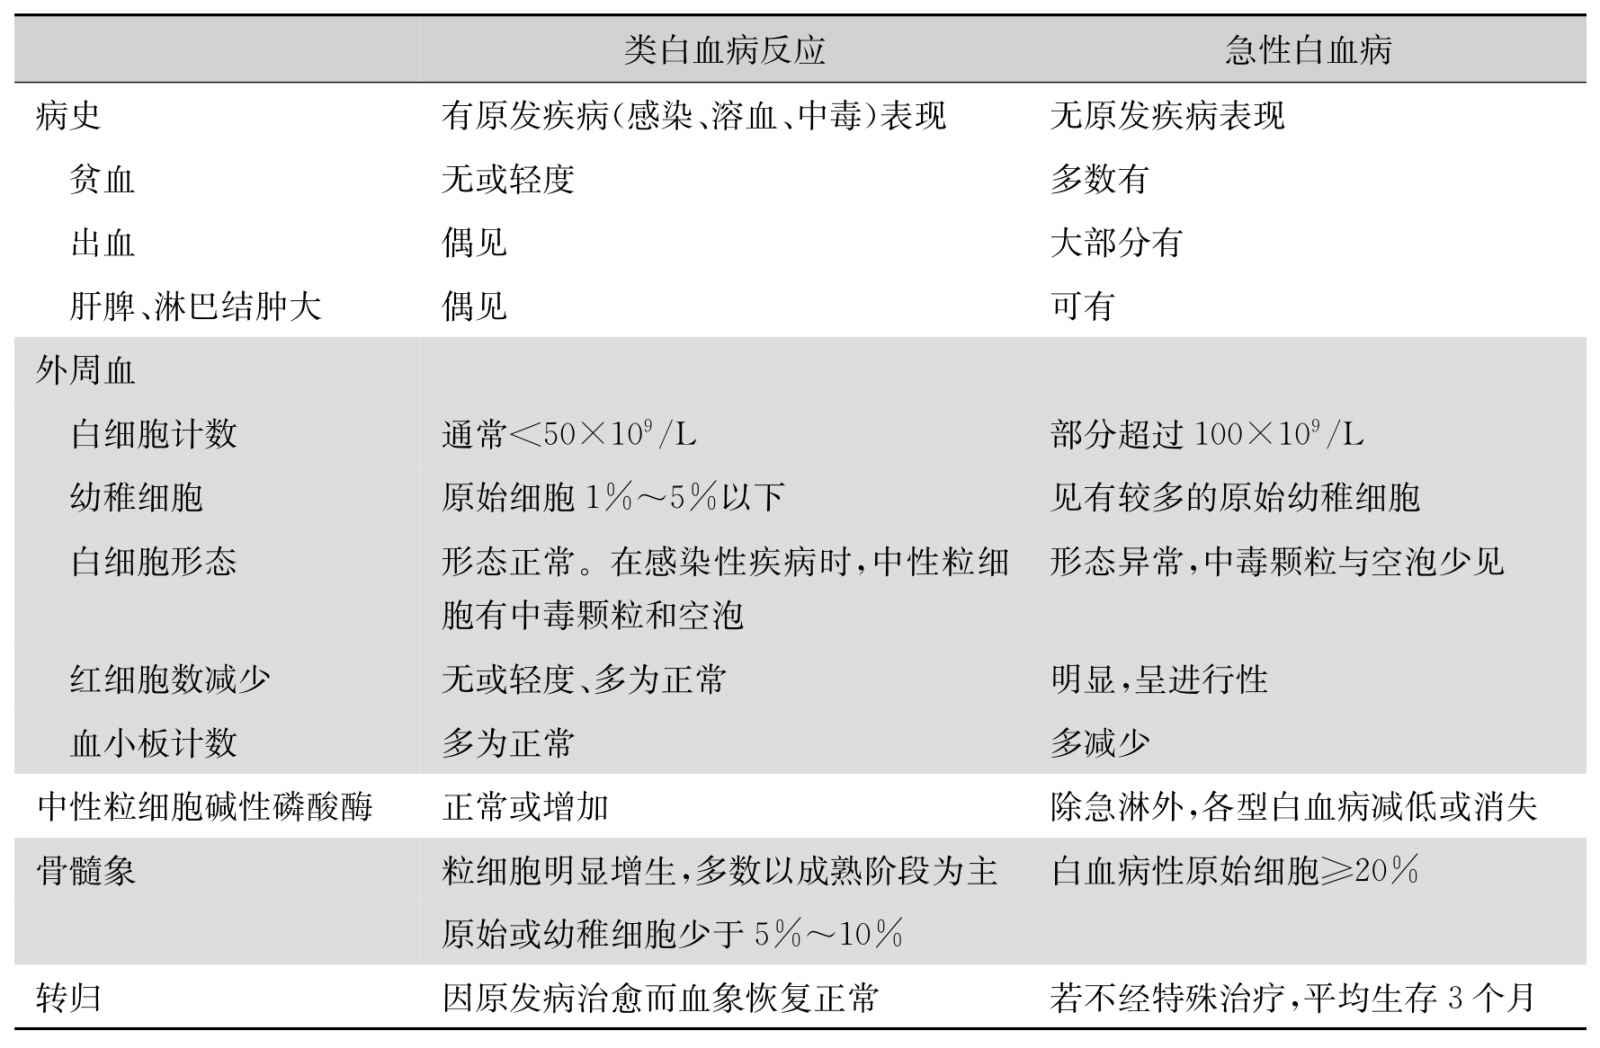
\includegraphics[width=.6\textwidth]{./images/Image00026.jpg}
 \caption{机体第一道防线}
 \label{fig2-1}
  \end{figure} 

2.吞噬细胞、NK细胞、抗菌蛋白、炎症应答------淋巴系统

微生物进入机体组织以后,多数沿组织细胞间隙的淋巴液经淋巴管到达淋巴结,但淋巴结内的巨噬细胞会消灭它们,阻止它们在机体内扩散,这就是淋巴屏障作用。如果微生物数量大、毒力强,就有可能冲破淋巴屏障,进入血液循环,扩散到组织器官中去。这时,它们会受到单核吞噬细胞系统屏障的阻挡。这是一类大的吞噬细胞。机体内还有一类较小的吞噬细胞,其中主要的是中性粒细胞和嗜酸性粒细胞。它们不属于单核吞噬细胞系统,但与单核吞噬细胞系统一样,分布于全身,对入侵的微生物和大分子物质有吞噬、消化和消除的作用。

在正常体液中的一些非特异性杀菌物质,如补体、调理素、溶菌酶、干扰素、乙型溶素、吞噬细胞杀菌素等,也与淋巴和单核吞噬细胞系统屏障一样,是机体的第二道防线,有助于消灭入侵的微生物(图\ref{fig2-2})。

\begin{figure}[!htbp]
 \centering
 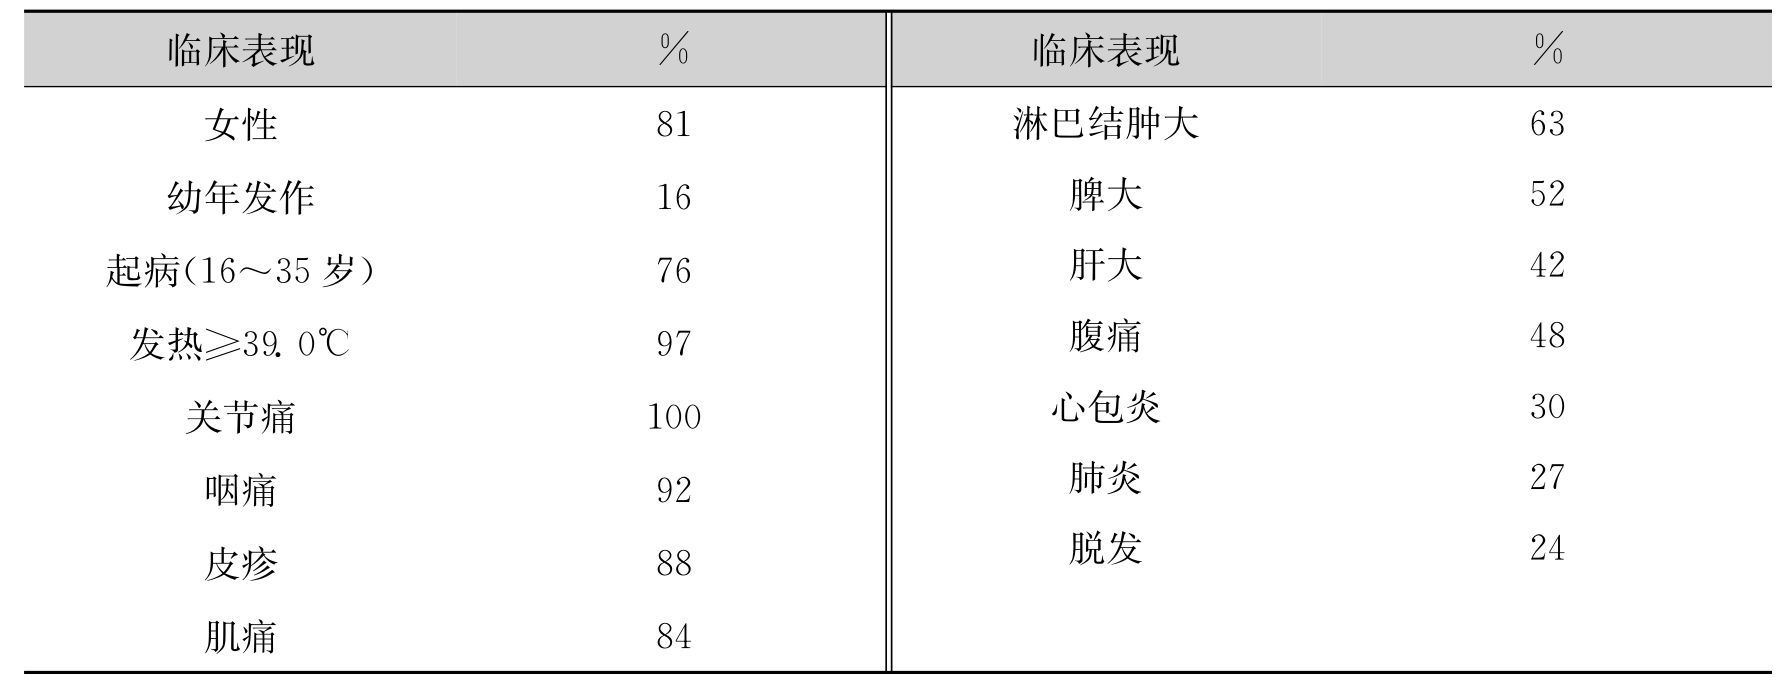
\includegraphics[width=.6\textwidth]{./images/Image00027.jpg}
 \caption{机体的第二道防线}
 \label{fig2-2}
  \end{figure} 

3.免疫系统:淋巴细胞、抗体;特点:特异性、多样性、记忆性、识别自我与非我(图\ref{fig2-3})。

\begin{figure}[!htbp]
 \centering
 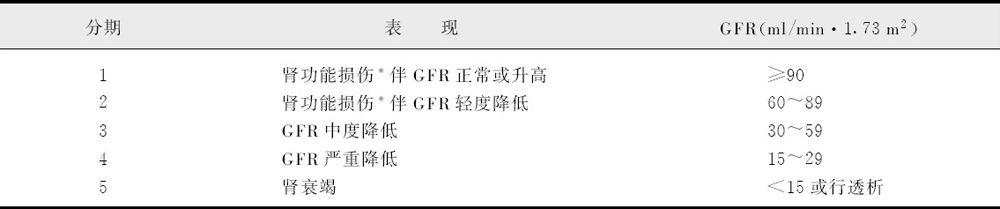
\includegraphics[width=.5\textwidth]{./images/Image00028.jpg}
 \caption{机体的第三道防线------免疫系统}
 \label{fig2-3}
  \end{figure} 

我们主要讲授免疫系统。

免疫系统(immune
system)乃承担免疫功能的组织系统,是机体对抗原刺激产生应答、执行免疫效应的物质基础。从宏观至微观进行描述,免疫系统包括免疫器官(中枢免疫器官和外周免疫器官)、免疫细胞(造血干细胞、淋巴细胞、单核吞噬细胞及其他免疫细胞)和免疫分子(抗体、补体、细胞因子)。

\section{中枢免疫器官}

中枢免疫器官(central immune
organ)是免疫细胞发生、分化、发育、成熟的场所,并对外周免疫器官的发育起主导作用,某些情况下(如再次抗原刺激或自身抗原刺激)也是产生免疫应答的场所。人和其他哺乳类动物的中枢免疫器官包括骨髓、胸腺,鸟类腔上囊(法氏囊)的功能相当于骨髓。


\subsection{骨髓}

骨髓(bone
marrow)是重要的中枢免疫器官,可分为红骨髓和白骨髓。红骨髓由结缔组织、血管、神经和实质细胞组成,呈海绵样存在于骨松质的腔隙中,具有活跃的造血功能。骨髓功能的发挥与其微环境有密切关系。骨髓微环境指造血细胞周围的微血管系统、末梢神经、网状细胞、基质细胞以及它们所表达的表面分子和所分泌的细胞因子。这些微环境组分是介导造血干细胞黏附、分化发育、参与淋巴细胞迁移和成熟的必需条件。骨髓是人和哺乳动物的造血器官(图\ref{fig2-4})。它具有如下功能:

1.各类免疫细胞发生的场所:骨髓造血干细胞具有分化成不同血细胞的能力,故被称为多能造血干细胞(multiple
hematopoietic stem
cell,HSC)。在骨髓微环境中,HSC首先分化为髓样前体细胞(myeloid
progenitor)和淋巴样前体细胞(lymphoid
progenitor)。髓样前体细胞最终分化成为粒细胞、单核细胞、红细胞、血小板;淋巴样前体细胞分化为T淋巴细胞(简称T细胞)、B淋巴细胞(简称B细胞)和自然杀伤细胞(NK细胞)。

\begin{figure}[!htbp]
 \centering
 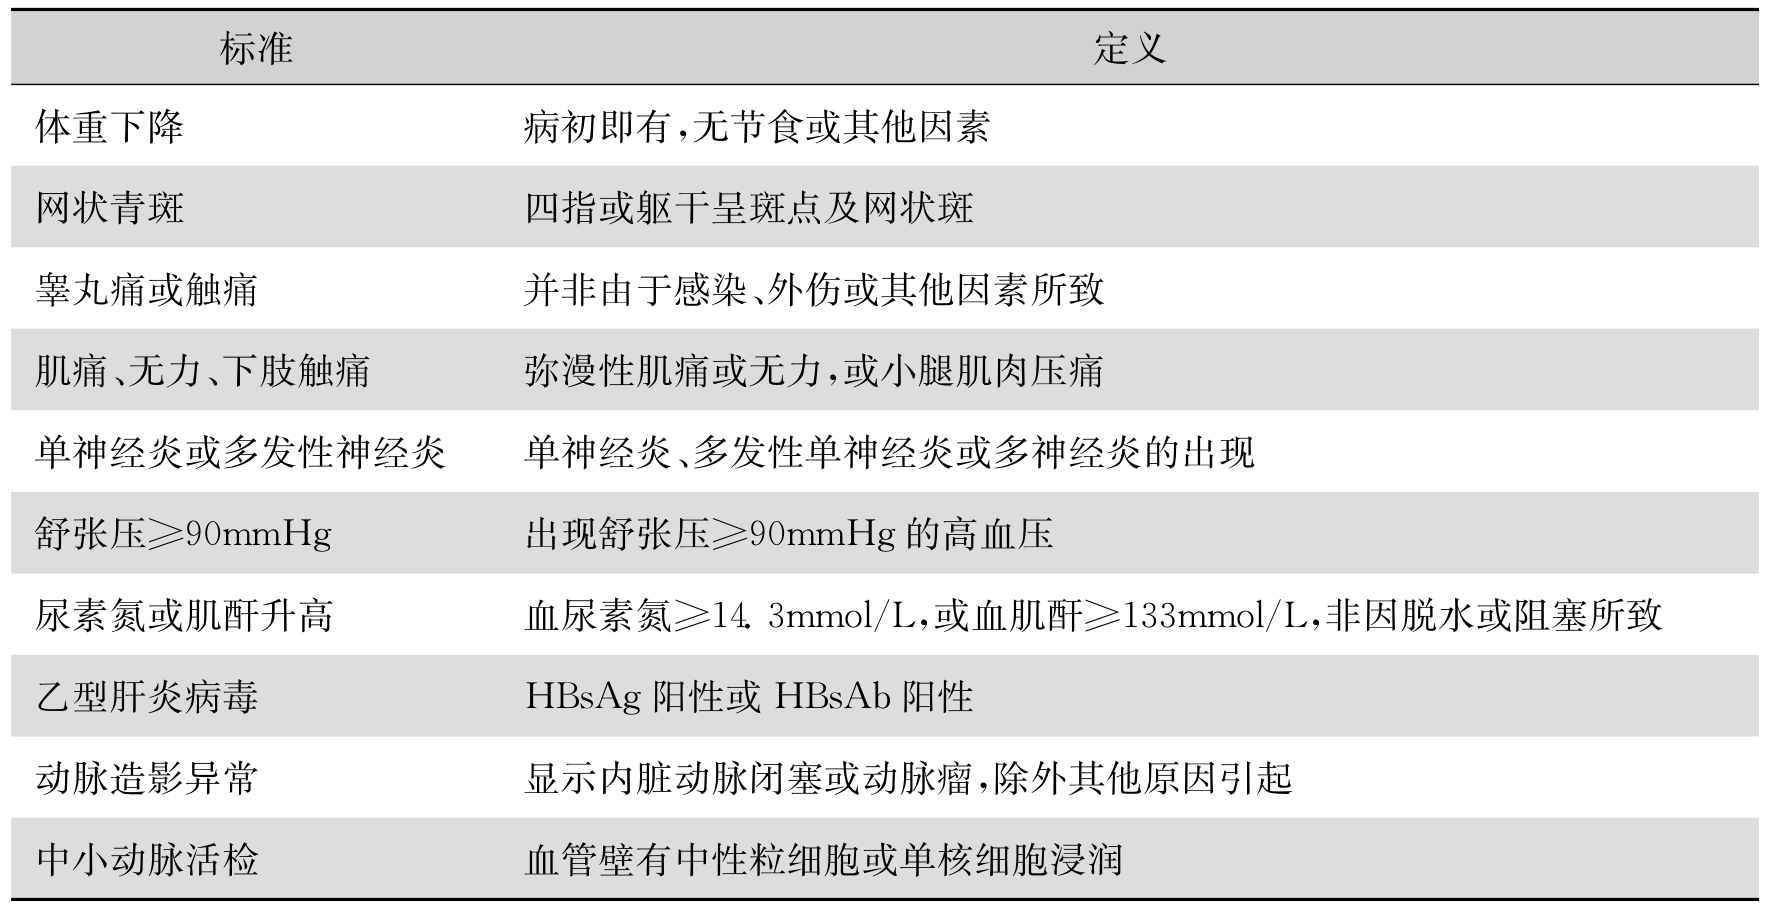
\includegraphics[width=.6\textwidth]{./images/Image00029.jpg}
 \caption{血细胞发育示意图}
 \label{fig2-4}
  \end{figure} 

2.B细胞分化成熟的场所:骨髓中产生的淋巴样前体细胞循不同的途径分化发育:一部分经血液迁入胸腺,发育成熟为成熟的T细胞;另一部分则在骨髓内继续分化为成熟B细胞。与T细胞在胸腺中分化的过程类似,B细胞在骨髓中也发生抗原受体(B
cell
receptor,BCR)等表面标志的表达、选择性发育或凋亡等。成熟的B细胞进入血循环,最终也定居在外周免疫器官。

3.发生B细胞应答的场所:骨髓是发生再次体液免疫应答的主要部位,外周免疫器官中的记忆性B细胞在抗原刺激下被活化,经淋巴液和血液进入骨髓后分化成熟为浆细胞,并产生大量抗体释放至血液循环。外周免疫器官中所发生的再次应答,其产生抗体的速度快,但持续时间短;而骨髓中所发生的再次应答,其产生抗体的速度慢,但可缓慢、持久地产生大量抗体,从而成为血清抗体的主要来源。

最新研究成果表明:在一定的微环境中,骨髓中的造血干细胞和基质干细胞还可分化为其他组织的多能干细胞(如神经干细胞、心肌干细胞等),这一突破性的进展开拓了骨髓生物学作用的全新领域,并可望在组织工程和临床医学中得到广泛应用。


\subsection{胸腺}

\begin{figure}[!htbp]
 \centering
 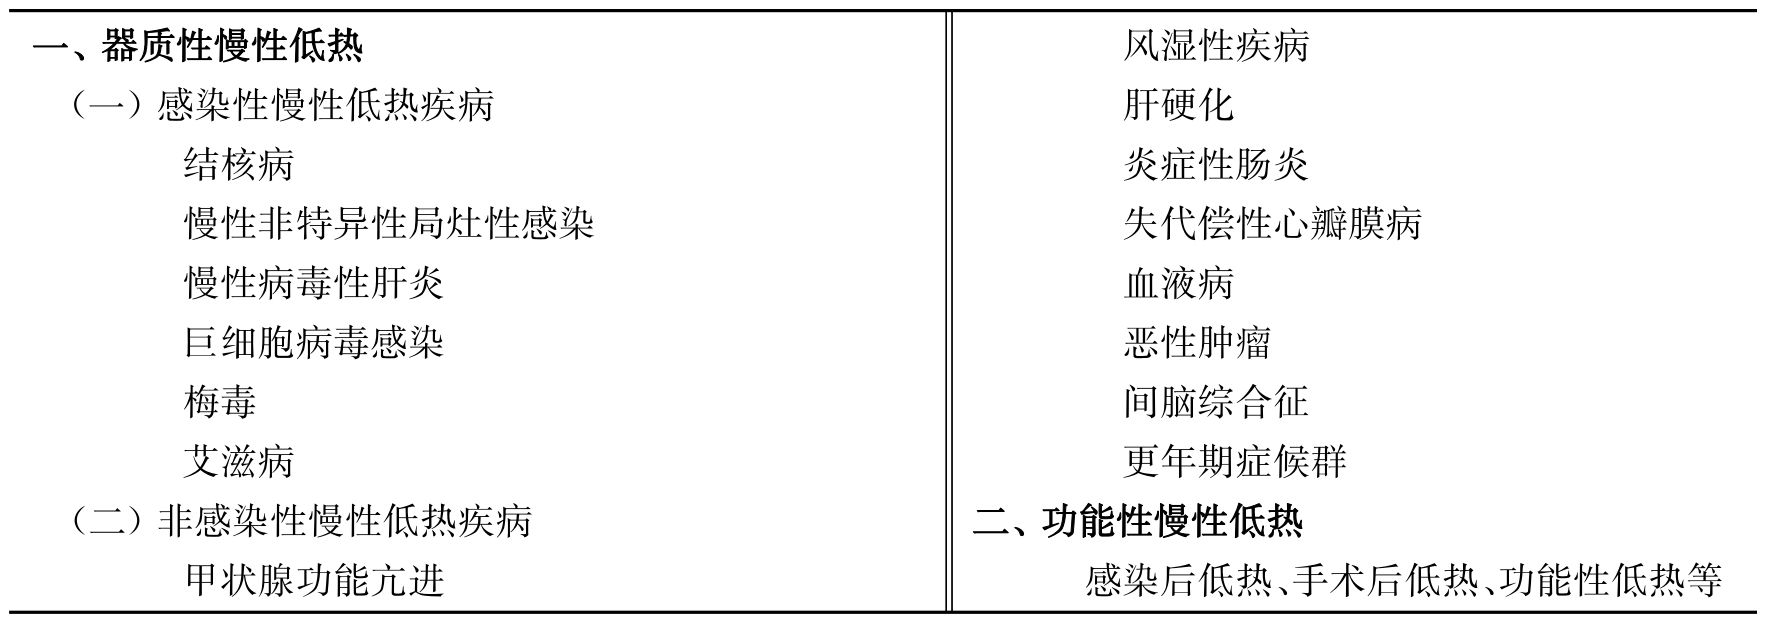
\includegraphics[width=0.5\textwidth]{./images/Image00030.jpg}
 \caption{人的胸腺}
 \label{fig2-5}
  \end{figure} 

人的胸腺(thymus)随年龄不同而有明显差别(图\ref{fig2-5})。新生期胸腺重量约15~20g;以后逐渐增大,青春期可达30~40g,其后随年龄增长而逐渐萎缩退化;老年期胸腺明显缩小,大部分被脂肪组织所取代。胸腺是T细胞分化、成熟的场所,其功能状态直接决定机体细胞免疫功能,并间接影响体液免疫功能。

(一)胸腺的解剖结构

胸腺的结构如图\ref{fig2-6}所示。一结缔组织被膜覆盖胸腺表面,并深入胸腺实质将其分隔成许多小叶。小叶的外层为皮质(cortex),内层为髓质(medulla),皮髓质交界处含大量血管,皮质内85\%~90\%的细胞为未成熟T细胞(即胸腺细胞),也存在少量上皮细胞、巨噬细胞(macrophage,Mφ)和树突状细胞(dendritic
cell,DC)等。胸腺浅皮质内发育早期的胸腺上皮细胞也称抚育细胞(nurse
cell),其在胸腺细胞分化中发挥重要作用。髓质内含大量上皮细胞和疏散分布的胸腺细胞、Mφ和DC。

\begin{figure}[!htbp]
 \centering
 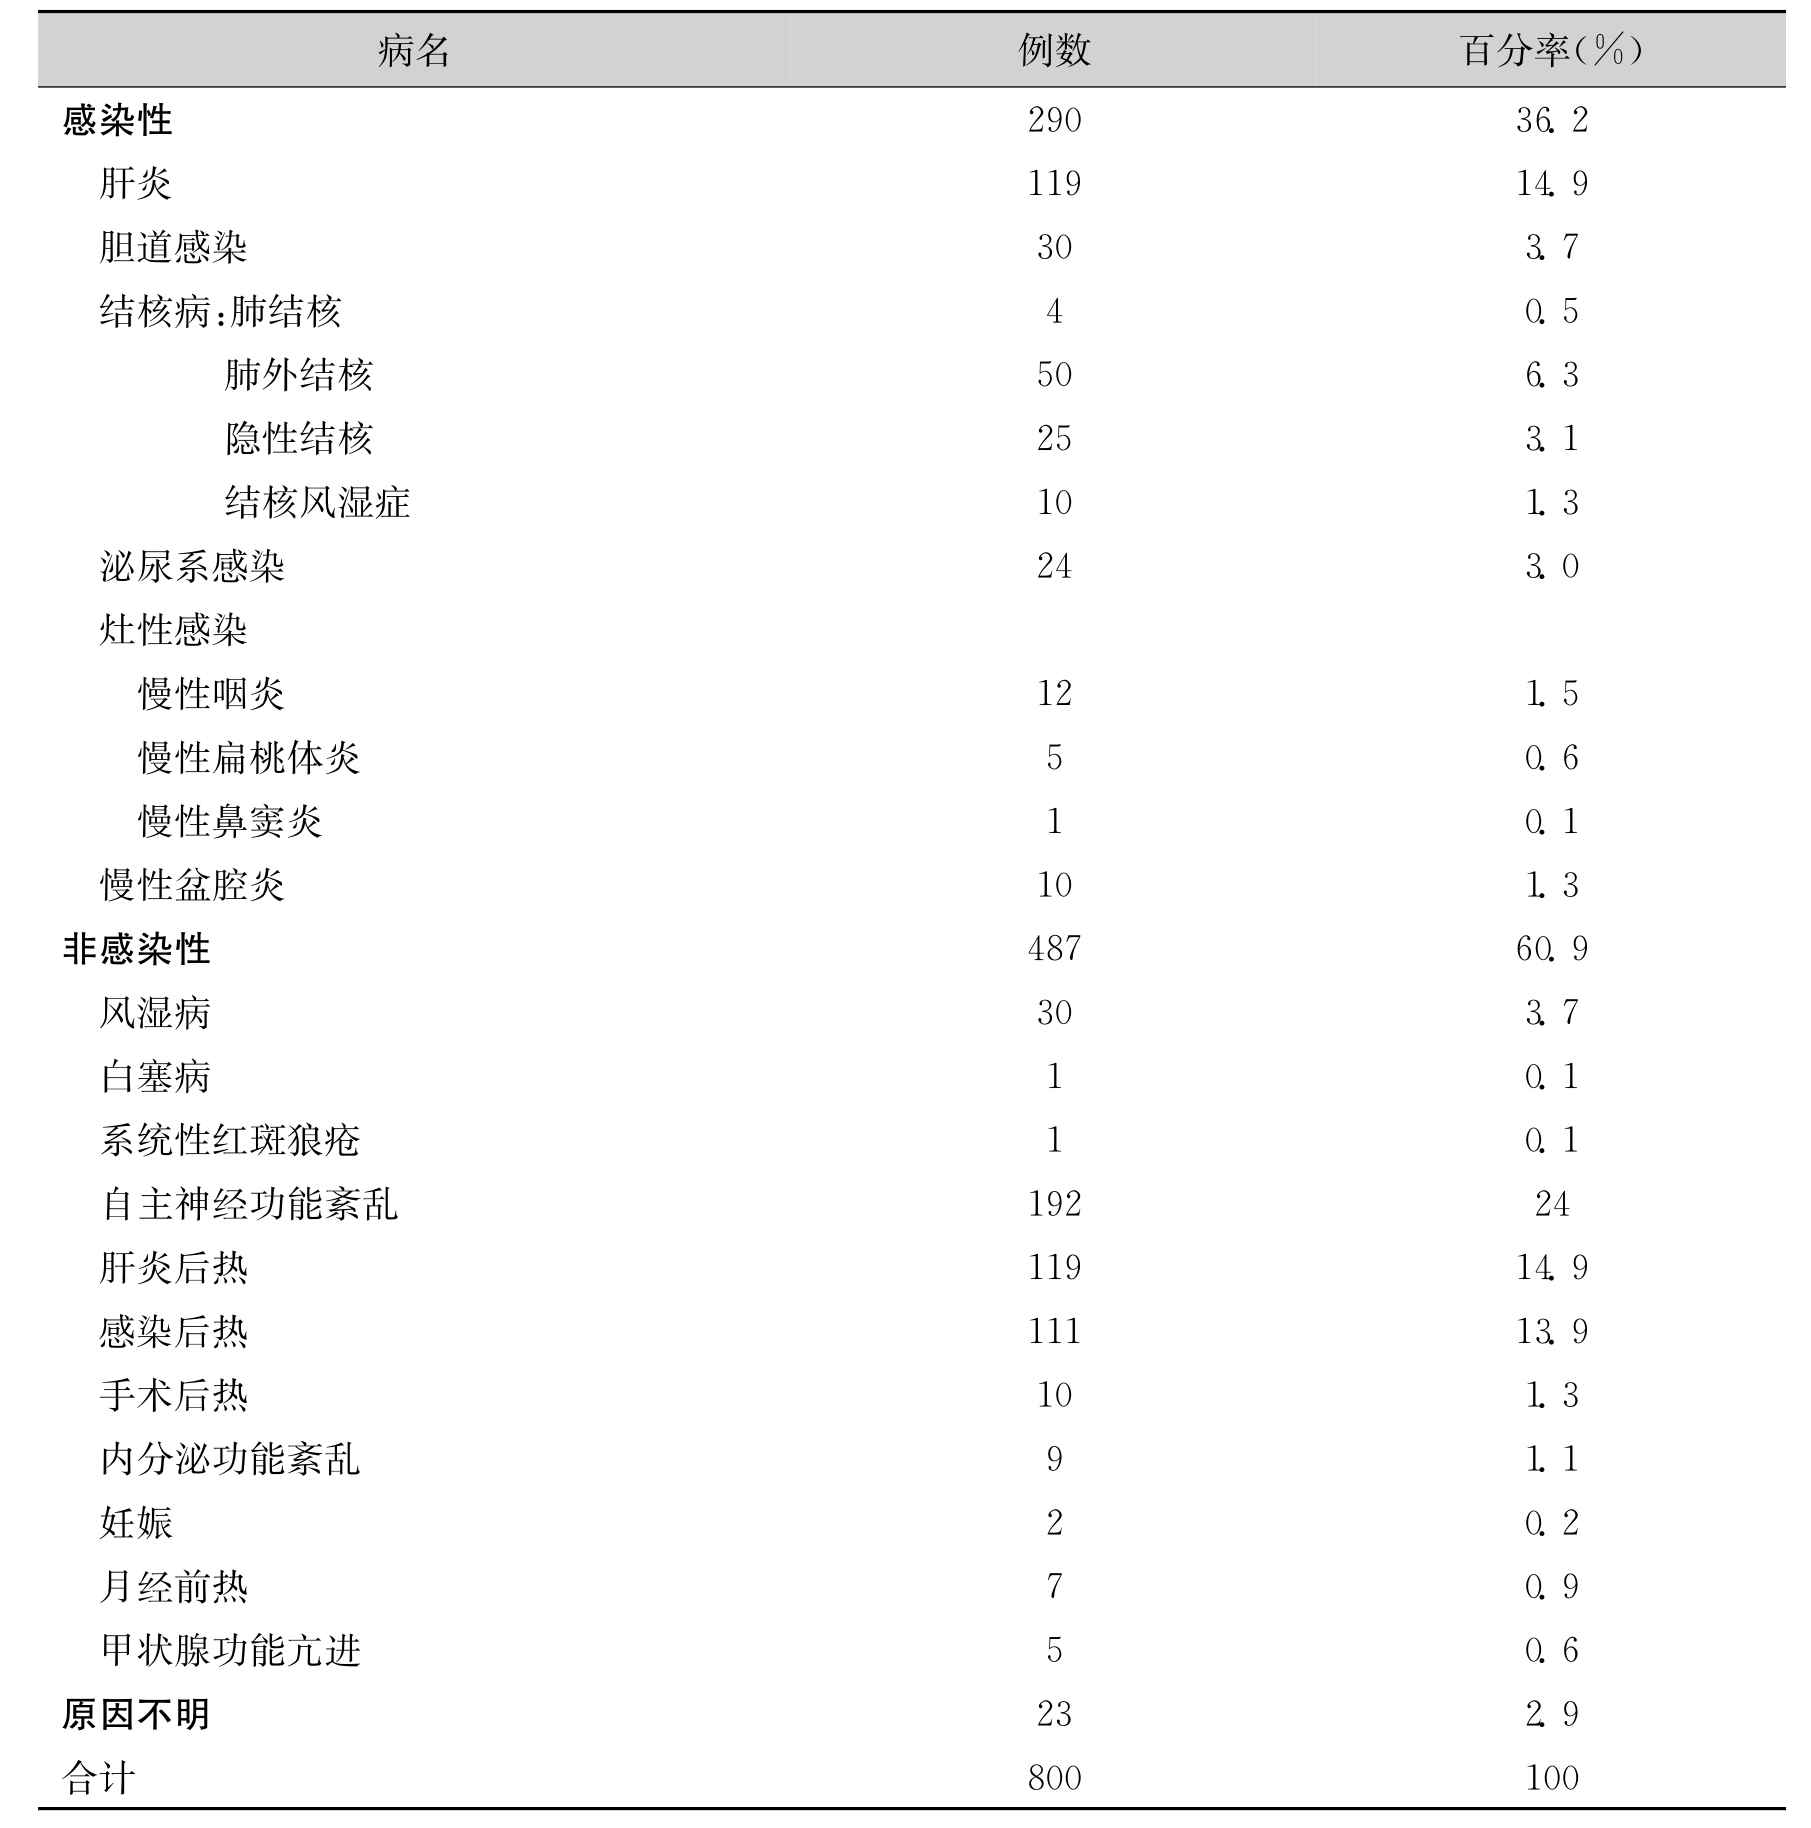
\includegraphics[width=0.7\textwidth]{./images/Image00031.jpg}
 \caption{胸腺结构示意图}
 \label{fig2-6}
  \end{figure} 

(二)胸腺的细胞组成:主要由胸腺基质细胞和胸腺细胞组成

1.胸腺基质细胞(thymic stromal cell,TSC):TSC以胸腺上皮细胞(thymus
epithelial
cell,TEC)为主,还包括巨噬细胞、DC及成纤维细胞等。TSC互相连接成网,并表达多种表面分子和分泌多种胸腺激素,从而构成重要的胸腺内环境。其中,抚育细胞与胸腺细胞通过各自表达的黏附分子密切接触,为胸腺细胞的发育提供必需的信号。

2.胸腺细胞:骨髓产生的前T细胞经血循环进入胸腺,即成为胸腺细胞。不同分化阶段的胸腺细胞其形态学、表面标志等各异,并可按其CD4、CD8表达情况分为4个亚群,即:CD4\textsuperscript{-}
CD8\textsuperscript{-} 、CD4\textsuperscript{+} CD8\textsuperscript{+}
、CD4\textsuperscript{+} CD8\textsuperscript{-} 、CD4\textsuperscript{-}
CD8\textsuperscript{+} 。

(三)胸腺微环境

胸腺微环境由TSC、细胞外基质及局部活性物质组成,其在胸腺细胞分化过程的不同环节均发挥重要作用。胸腺上皮细胞是胸腺微环境的最重要组分,其参与胸腺细胞分化的机制为:

1.分泌胸腺激素和细胞因子:主要的胸腺激素有胸腺素(thymosin)、胸腺刺激素(thymulin)、胸腺体液因子(thymic
humoral factor)、胸腺生成素(thymopoietin,TP)、血清胸腺因子(serum
thymic
factor)等。它们分别具有促进胸腺细胞增殖和分化、发育等功能。胸腺基质细胞还可产生多种细胞因子,它们通过与胸腺细胞表面相应受体结合,调节胸腺细胞发育和细胞间相互作用。上述胸腺激素和细胞因子是诱导胸腺细胞分化为成熟T细胞的必要条件。

2.与胸腺细胞相互接触:此乃通过上皮细胞与胸腺细胞间表面黏附分子及其配体、细胞因子及其受体、抗原肽-MHC分子复合物与TCR等相互作用而实现。

细胞外基质(extracellular
matrix)也是胸腺微环境的重要组成部分,它们可促进上皮细胞与胸腺细胞接触,并参与胸腺细胞在胸腺内移行成熟。

(四)胸腺的功能

1.T细胞分化、成熟的场所:胸腺是T细胞发育的主要场所。在胸腺产生的某些细胞因子作用下,来源于骨髓的前T细胞被吸引至胸腺内成为胸腺细胞。胸腺细胞循被膜下转移到皮质再向髓质移行,并经历十分复杂的选择性发育。在此过程中,约95\%的胸腺细胞发生以凋亡(apoptosis)为主的死亡而被淘汰,仅不足5\%的细胞分化为成熟T细胞。其特征为:表达成熟抗原受体(TCR)的CD4或CD8单阳性细胞;获得MHC限制性的抗原识别能力;获得自身耐受性。发育成熟的T细胞进入血循环,最终定居于外周免疫器官。

近期研究证实,胸腺并非T细胞分化发育的唯一场所。例如T细胞可在胸腺外组织(如肠道黏膜上皮、皮肤组织及泌尿生殖道黏膜组织等)中发育成熟。另外,肝脏也可能是某些T细胞分化发育的场所。

2.免疫调节功能:胸腺基质细胞可产生多种肽类激素,它们不仅促进胸腺细胞的分化成熟,也参与调节外周成熟T细胞。

3.屏障作用:皮质内毛细血管及其周围结构具有屏障作用,阻止血液中大分子物质进入,此为血-胸腺屏障(blood-thymus
barrier)。


\subsection{腔上囊}

腔上囊又称法氏囊(bursa of
fabricius),是鸟类动物特有的淋巴器官,位于胃肠道末端泄殖腔的后上方(图\ref{fig2-7})。与胸腺不同,腔上囊训化B细胞成熟,主导机体的体液免疫功能。将孵出的雏鸡去掉腔上囊,会使血中γ球蛋白缺乏,且没有浆细胞,注射疫苗亦不能产生抗体。人类和哺乳动物没有法氏囊,其功能由相似的组织器官代替,称为法氏囊同功器官;曾一度认为同功器官是阑尾、扁桃体和肠集结淋巴结,现在已证明是骨髓。

\begin{figure}[!htbp]
 \centering
 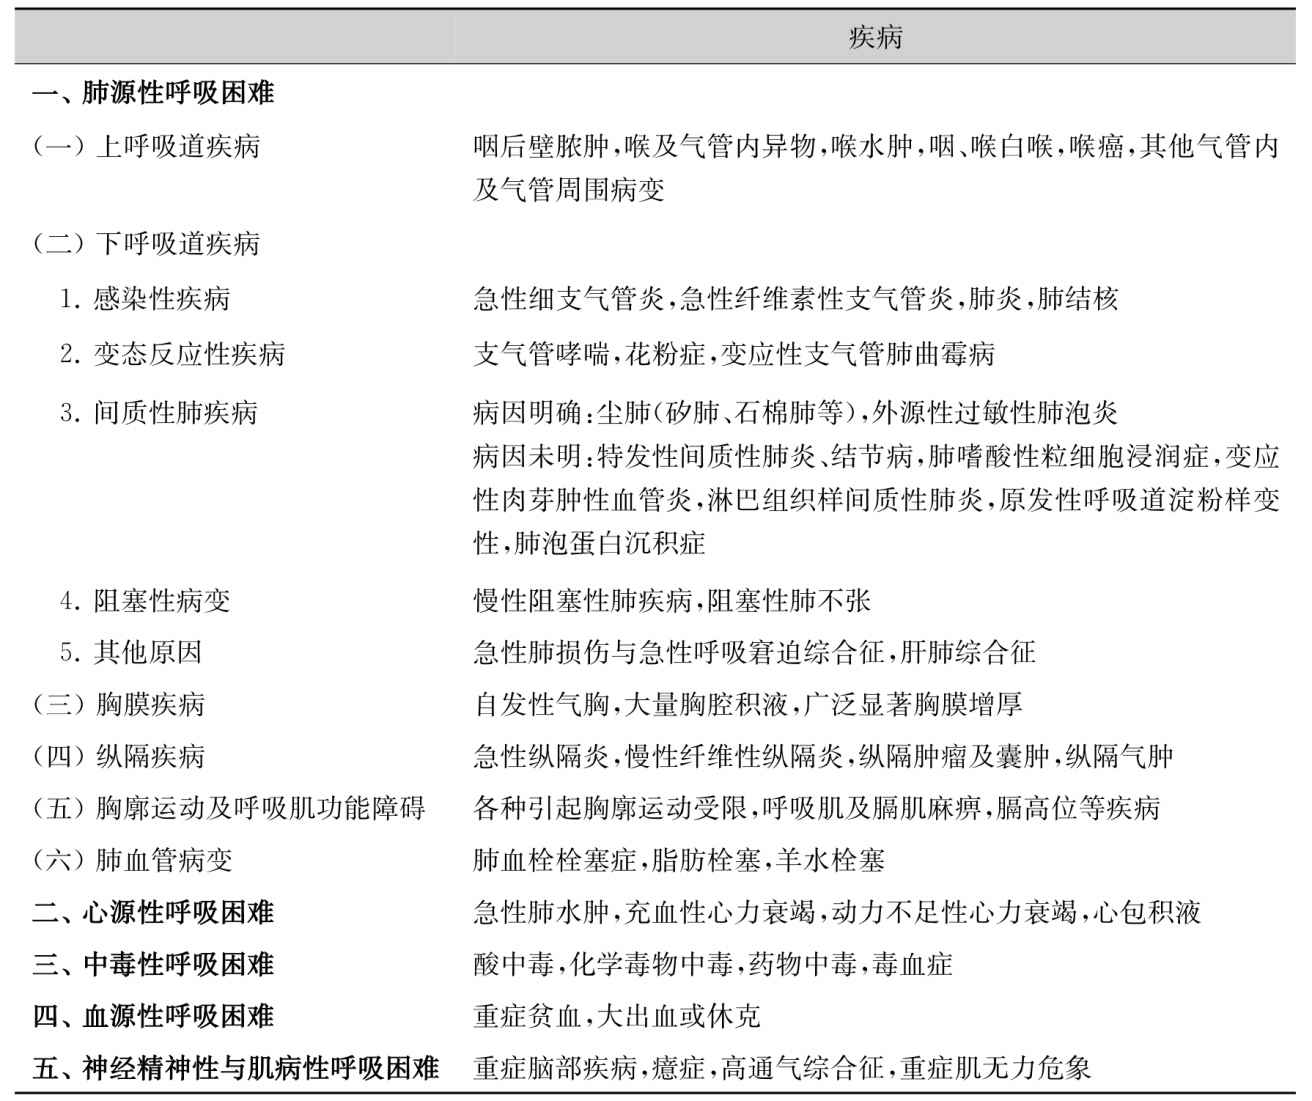
\includegraphics[width=.5\textwidth]{./images/Image00032.jpg}
 \caption{鸡的胸腺和法氏囊}
 \label{fig2-7}
  \end{figure} 

\section{外周免疫器官}

外周免疫器官(peripheral immune
organ)包括脾、淋巴结、淋巴样小结、扁桃体、阑尾等,这些器官内富含能捕捉和处理抗原的巨噬细胞和树突状细胞,以及能介导免疫反应的T细胞和B细胞。


\subsection{淋巴结}

淋巴结(lymph node)广泛分布于全身非黏膜部位的淋巴通道上。

(一)淋巴结的结构

淋巴结的结构如图\ref{fig2-8}所示,淋巴结表面覆盖有结缔组织被膜,后者深入实质形成小梁。淋巴结分为皮质和髓质两部分,彼此通过淋巴窦相通。被膜下为皮质,包括浅皮质区、副皮质区和皮质淋巴窦。

浅皮质区又称为非胸腺依赖区(thymus-independent
area),是B细胞定居的场所,该区内有淋巴滤泡(或称淋巴小结)。未受抗原刺激的淋巴小结无生发中心,称为初级滤泡(primary
follicle),主要含静止的成熟B细胞;受抗原刺激的淋巴小结内出现生发中心(germinal
center),称为次级滤泡(secondary
follicle),内含大量增殖分化的B淋巴母细胞,此细胞向内转移至淋巴结中心部髓质,即转化为可产生抗体的浆细胞。

副皮质区又称胸腺依赖区(thymus-dependent
area),位于浅皮质区和髓质之间,为深皮质区,是T细胞(主要是CD\textsuperscript{+}
\textsubscript{4}
T细胞)定居的场所。该区有许多由内皮细胞组成的毛细血管后微静脉,也称高内皮细胞小静脉(high
endothelial venule,HEV),在淋巴细胞再循环中起重要作用。

髓质由髓索和髓窦组成。髓索内含有
B细胞、T细胞、浆细胞、肥大细胞及Mφ。髓窦内Mφ较多,有较强滤过作用。

\begin{figure}[!htbp]
 \centering
 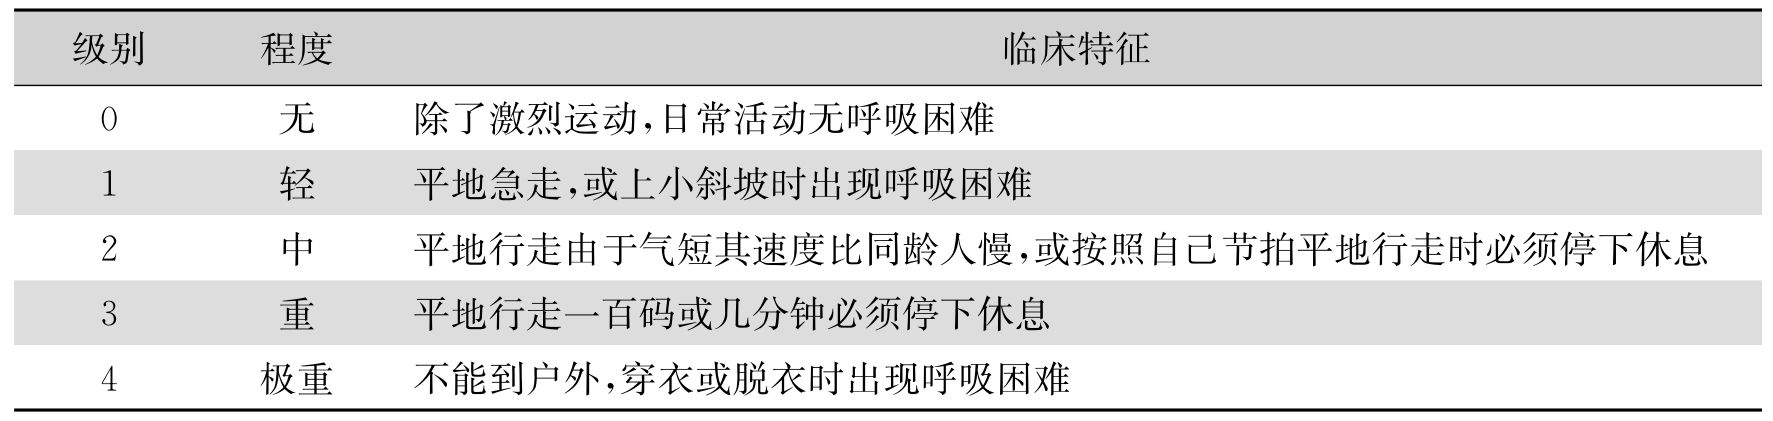
\includegraphics[width=.6\textwidth]{./images/Image00033.jpg}
 \caption{淋巴结的结构}
 \label{fig2-8}
  \end{figure} 

(二)淋巴结的功能

1.T 细胞及
B细胞定居的场所:分别在胸腺和骨髓中分化成熟的T、B细胞,均可定居于淋巴结。其中,T细胞占淋巴结内淋巴细胞总数的75\%,B细胞占25\%。

2.免疫应答发生的场所:抗原递呈细胞携带所摄取的抗原进入淋巴结,将已被加工、处理的抗原递呈给淋巴结内的T细胞和B细胞,使之活化、增殖、分化,故淋巴结是发生细胞免疫和体液免疫应答的主要场所。

3.参与淋巴细胞再循环:淋巴结深皮质区的HEV在淋巴细胞再循环中发挥重要作用,血循环中的淋巴细胞穿越HEV壁进入淋巴结实质,然后通过输出淋巴管进入胸导管或右淋巴管,再回到血液循环。

4.过滤作用:组织中的病原微生物及毒素等进入淋巴液,其缓慢流经淋巴结时,可被Mφ吞噬或通过其他机制被清除。因此,淋巴结具有重要的滤过作用。


\subsection{脾脏}

(一)脾脏的结构

脾脏的结构如图\ref{fig2-9}所示,脾脏(spleen)是人体最大的淋巴器官,可分为白髓、红髓和边缘区三部分。白髓由密集的淋巴组织构成,包括动脉周围淋巴鞘和淋巴小结。动脉周围淋巴鞘为T细胞居住区;鞘内的淋巴小结为B细胞居住区,未受抗原刺激为初级滤泡,受抗原刺激后出现生发中心,为次级滤泡。红髓分布于白髓周围,包括髓索和髓窦:前者主要为B细胞居留区,也含Mφ和DC;髓窦内为循环的血液。白髓与红髓交界处为边缘区(marginal
zone),是血液及淋巴细胞进出的重要通道。

\begin{figure}[!htbp]
 \centering
 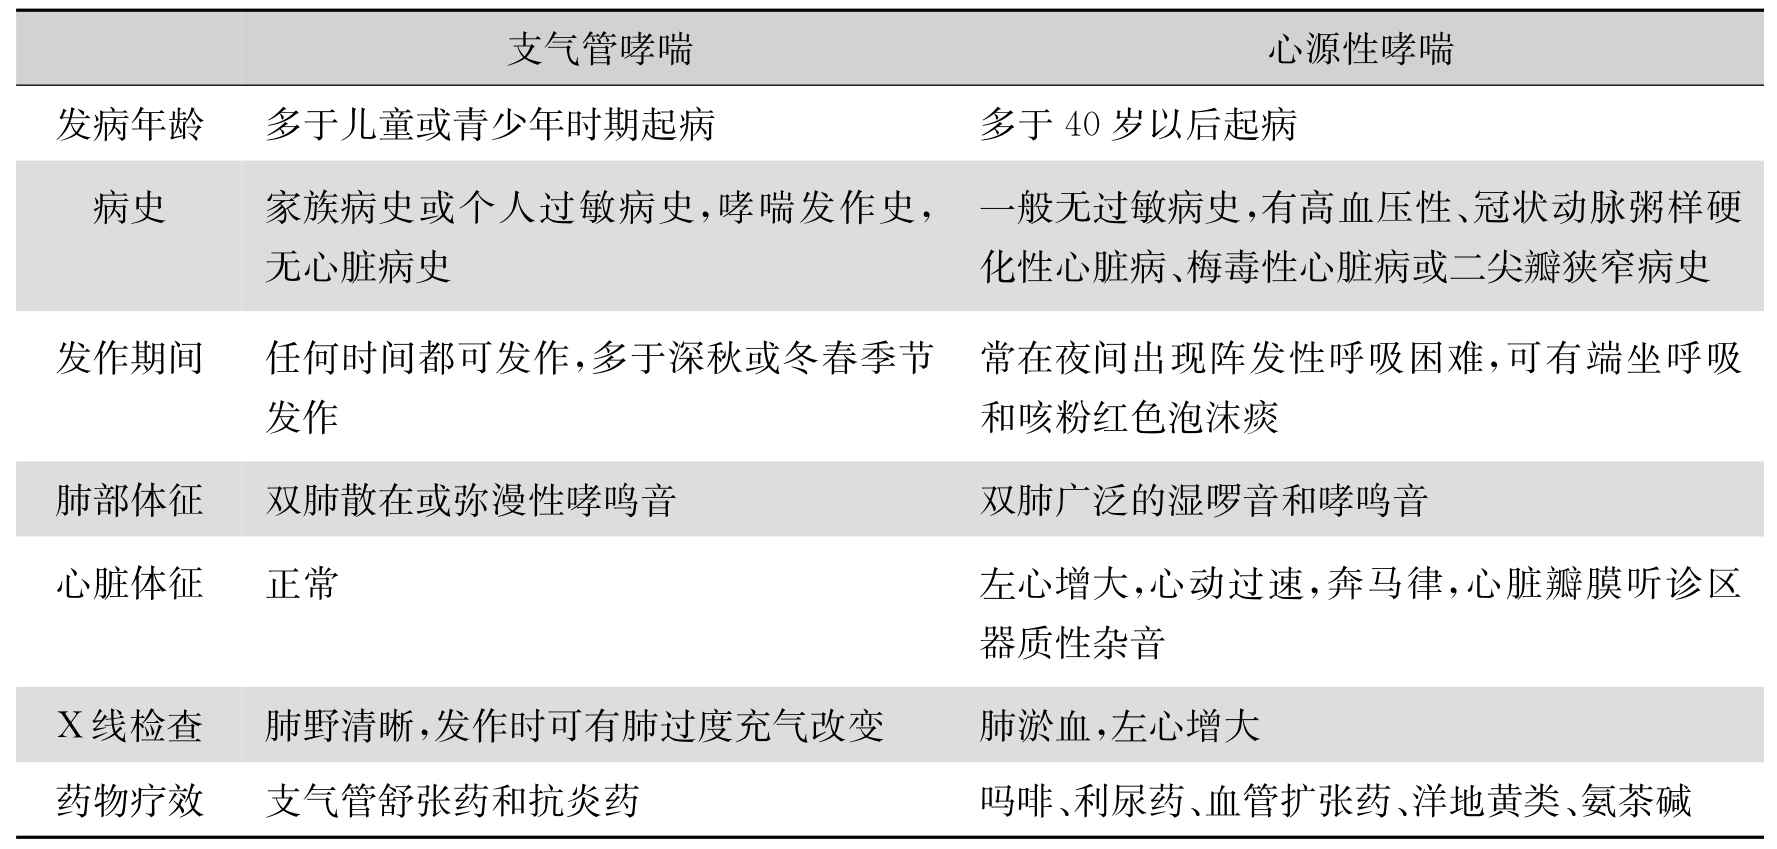
\includegraphics[width=.5\textwidth]{./images/Image00034.jpg}
 \caption{脾脏的结构}
 \label{fig2-9}
  \end{figure} 

(二)脾脏的功能

脾脏是重要的外周免疫器官,脾切除的个体其免疫防御功能可发生障碍。

1.免疫细胞定居的场所:成熟的淋巴细胞可定居于脾脏。B细胞约占脾脏中淋巴细胞总数的60\%,T细胞约占40\%。

2.免疫应答的场所:脾脏也是淋巴细胞接受抗原刺激并发生免疫应答的重要部位。同为外周免疫器官,脾脏与淋巴结的差别在于:脾脏是对血源性抗原产生应答的主要场所。

3.合成生物活性物质:脾脏可合成并分泌如补体、干扰素等生物活性物质。

4.滤过作用:脾脏可清除血液中的病原体、衰老死亡的自身血细胞、某些蜕变细胞及免疫复合物等,从而使血液得到净化。

此外,脾脏也是机体贮存红细胞的血库。


\subsection{黏膜相关淋巴组织}

黏膜相关淋巴组织(mucosal-associated lymphoid
tissue,MALT)亦称黏膜免疫系统(mucosal lymphoid
system,MIS),主要指呼吸道、肠道及泌尿生殖道黏膜固有层和上皮细胞下散在的无被膜淋巴组织以及某些带有生发中心的器官化淋巴组织,如扁桃体、小肠的派氏集合淋巴结(Peyer
patche)、阑尾等。

黏膜系统在机体免疫防疫机制中的重要作用表现为:①人体黏膜的表面积约400平方米,乃阻止病原微生物等入侵机体的主要物理屏障;②机体近一半的淋巴组织存在于黏膜系统,故MALT被视为执行局部特异性免疫功能的主要部位。

(一)MALT的组成

1.鼻相关淋巴组织(nasal-associated lymphoid
tissue,NALT):包括咽扁桃体、腭扁桃体、舌扁桃体及鼻后部其他淋巴组织,其主要作用是抵御经空气传播的微生物感染。

2.肠相关淋巴组织(gut-associated lymphoid
tissue,GALT):GALT包括集合淋巴结、淋巴滤泡和固有层淋巴组织等,其主要作用是抵御侵入肠道的病原微生物感染(图\ref{fig2-10})。肠道黏膜上皮间还散布一种扁平上皮细胞,即M细胞(membranous
cell or microfold
cell,膜性细胞或微皱褶细胞),又称特化的抗原转运细胞(specialized
antigen transporting
cell),是散布于肠道黏膜上皮细胞间的一种特化的抗原运转细胞。它不表达MHCⅡ类分子,胞质内溶毛体很少,在肠黏膜表面有短小不规则毛刷样微绒毛。M细胞的基底部凹陷成小袋,其中容纳T细胞、B细胞、巨噬细胞、DC等。M细胞具有高度的非特异性脂酶活性,病原菌等外来抗原性物质可通过对M细胞表面的毛刷状微绒毛的吸附,或经M细胞表面蛋白酶作用后被摄取,并将未降解的抗原转运给小袋中的巨噬细胞,由后者携带抗原至集合淋巴结,引发黏膜免疫应答,肠道淋巴系统免疫应答如图\ref{fig2-11}所示。

\begin{figure}[!htbp]
 \centering
 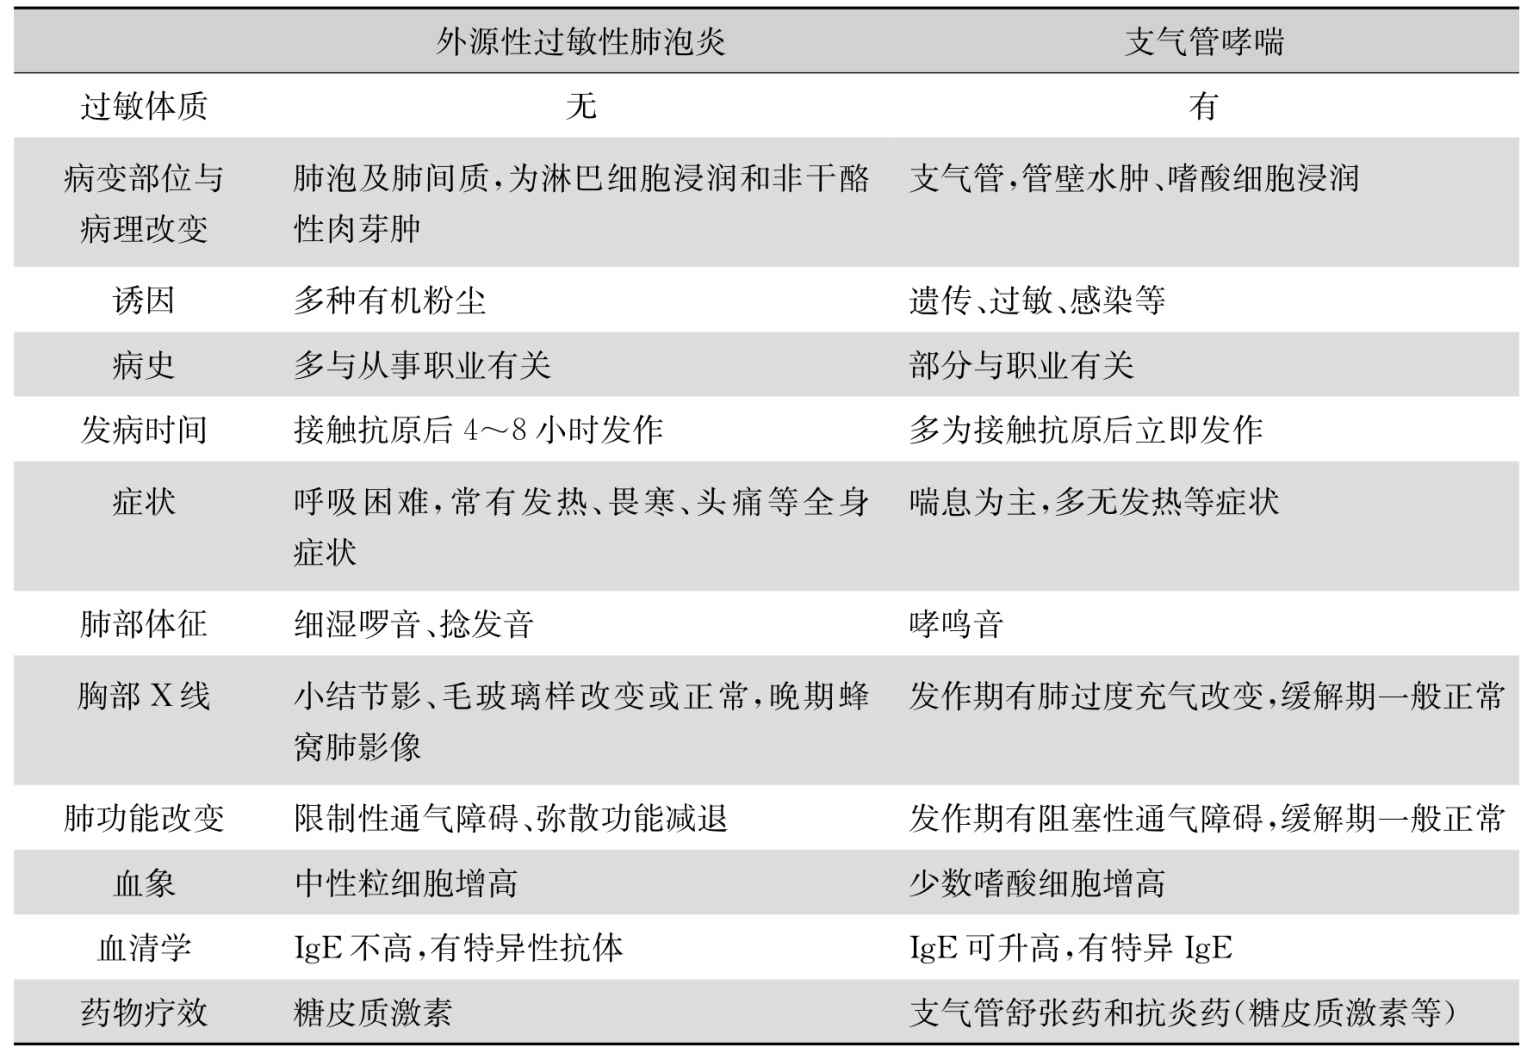
\includegraphics[width=.5\textwidth]{./images/Image00035.jpg}
 \caption{消化道集合淋巴滤泡}
 \label{fig2-10}
  \end{figure} 

\begin{figure}[!htbp]
 \centering
 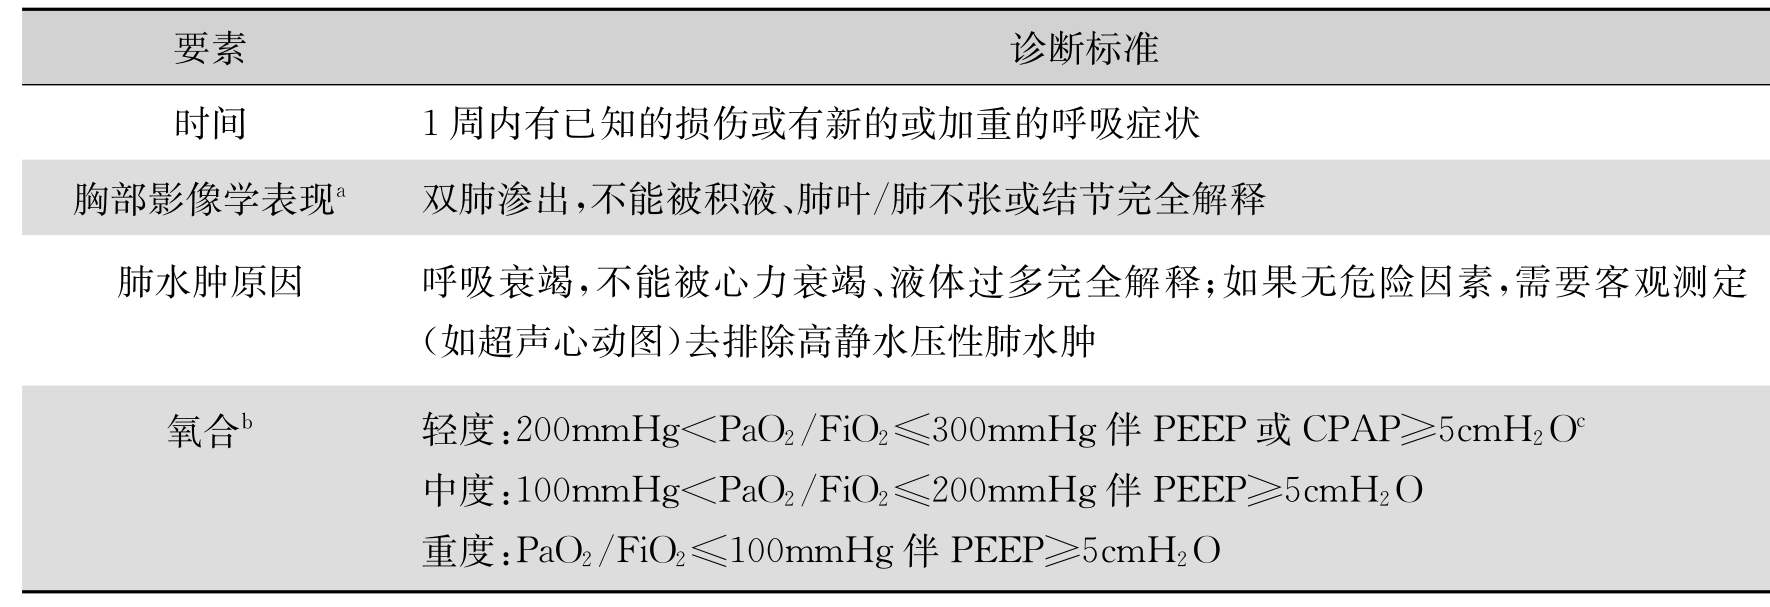
\includegraphics[width=.6\textwidth]{./images/Image00036.jpg}
 \caption{肠道M细胞的转运功能及M细胞包围住大肠杆菌}
 \label{fig2-11}
  \end{figure} 

黏膜免疫系统在保护黏膜表面不受病原体侵害、促进与共生微生物群落共生中都起主要作用。要激发黏膜免疫反应,黏膜表面上的抗原必须首先穿过不可透过的上皮障碍,进入“派伊尔小结”这样的淋巴结构。这一功能(被称为“转胞吞作用”)被认为主要由M细胞调控,它们是“派伊尔小结”中专门的上皮细胞。对由M-细胞调控的抗原“转胞吞作用”的机制所做的一项研究表明,在小肠M细胞顶面表达的糖蛋白-2是表达FimH抗原的细菌的转胞吞受体。由于M-细胞被认为是各种口服免疫药物的一个很有希望的目标,所以这项工作表明,依赖于糖蛋白-2的“转胞吞作用”是一个可能的免疫目标。

3.支气管相关淋巴组织(bronchial-associated
tissue,BALT):主要分布于各肺叶的支气管上皮下,其结构与派氏集合淋巴结相似,滤泡中淋巴细胞受抗原刺激常增生成生发中心,其中主要是B细胞。

(二)MALT的功能及其特点

1.参与局部免疫应答:分布在不同部位的MALT均是参与局部特异性免疫应答的主要场所,从而在消化道、呼吸道和泌尿生殖道的局部免疫防御中发挥关键作用。

2.分泌型IgA(secretory
IgA,SIgA):以消化道黏膜为例,口服抗原被吸收进入集合淋巴结后,可引发B细胞应答,使之转化为产生抗体的浆细胞,其中可分泌SIgA的浆细胞主要定居于集合淋巴结或迁移至固有层。SIgA在抵御病原体侵袭消化道、呼吸道和泌尿生殖道中发挥重要作用。

3.参与口服抗原介导的免疫耐受:口服蛋白抗原刺激黏膜免疫系统后,常可导致免疫耐受,其机制尚未阐明。口服抗原诱导耐受的生物学意义在于:①可阻止机体对肠腔内共栖的正常菌群产生免疫应答,而这些菌群的存在乃正常消化和吸收功能所必需;②通过口服抗原诱导机体对该抗原形成特异性无反应性,可能为治疗自身免疫病提供新途径。

\begin{center}
\textbf{\Large 附:淋巴细胞再循环}
\end{center}

各种免疫器官中的淋巴细胞并不是定居不动的群体,而是通过血液和淋巴液的循环进行有规律的迁移,这种规律性的迁移为淋巴细胞再循环(lymphocyterecirculation)。通过再循环,可以增加淋巴细胞与抗原接触的机会,更有效地激发免疫应答,并不断更新和补充循环池的淋巴细胞。

1.再循环的细胞淋巴干细胞从骨髓迁移至胸腺和腔上囊或其功能器官,分化成熟后进入血液循环的定向移动过程不属于再循环范围。再循环是成熟淋巴细胞通过循环途径实现淋巴细胞不断重新分布的过程。再循环中的细胞多是静止期细胞和记忆细胞,其中80%以上是T细胞。这些细胞最初来源于胸腺和骨髓;成年以后,主要靠外周免疫器官进行补充。受抗原刺激而活化的淋巴细胞很快定居于外周免疫器官,不再参加再循环。

2.再循环的途径血液中的淋巴细胞在流经外周免疫器官(以淋巴结为例)时,在副皮质区与皮质区的连接处穿过高内皮毛细血管后静脉(HEV)进入淋巴结;T细胞定位于副皮质,B细胞主要定位于皮质区;以后均通过淋巴结髓窦迁移至输出淋巴管,进入高一级淋巴结;经过类似的路径,所有外周免疫器官输出的细胞最后都汇集于淋巴导管;身体下部和左上部的汇集到胸导管,从左锁骨下静脉角返回血循环;右侧上部的汇集到右淋巴管,从右锁骨下静脉返回血循环。再循环一周约需24~48小时。

3.细胞定居选择淋巴细胞从血循环进入淋巴组织具有高度的选择性,这是因为淋巴细胞上具有特殊的受体分子,称为归巢受体(homingreceptor)。现已发现的归巢受体包括CD44、LFA-1、VLA-4和MEL-14/LAM-1等;其中MEL-14/LAM-1是定居淋巴结的受体,识别淋巴结内的高内皮细胞;VLA-4的α亚单位是定居MALT的受体,识别黏膜表面的配体。

淋巴细胞再循环的意义:带有不同特异性抗原受体的各种淋巴细胞不断在体内各处巡游,增加了与抗原以及抗原递呈细胞接触的机会;许多免疫记忆细胞也参与淋巴细胞再循环,一旦接触到相应抗原,可立即进入淋巴组织发生增殖反应,产生免疫应答。淋巴细胞再循环如图\ref{fig2-12}所示。

\begin{figure}[!htbp]
 \centering
 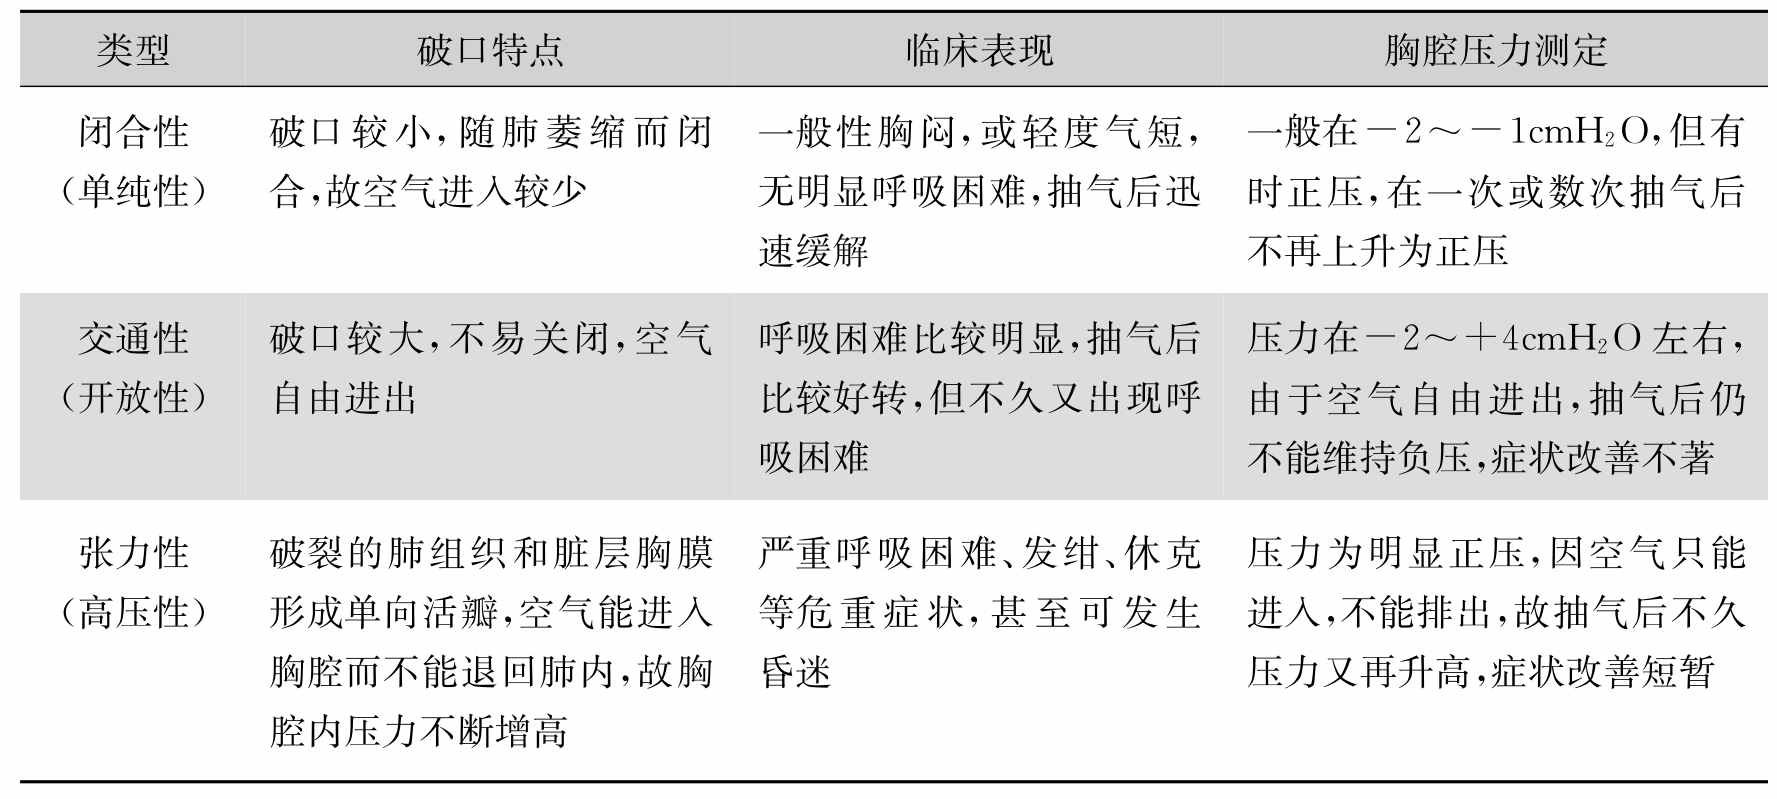
\includegraphics[width=.6\textwidth]{./images/Image00037.jpg}
 \caption{淋巴细胞再循环示意图}
 \label{fig2-12}
  \end{figure} 

\section{免疫细胞}

免疫细胞乃泛指所有参与免疫应答或与免疫应答有关的细胞及其前体,包括造血干细胞、淋巴细胞、专职抗原递呈细胞(树突状细胞、单核-巨噬细胞)及其他抗原递呈细胞、粒细胞、肥大细胞和红细胞等,如图\ref{fig2-13}所示。

\begin{figure}[!htbp]
 \centering
 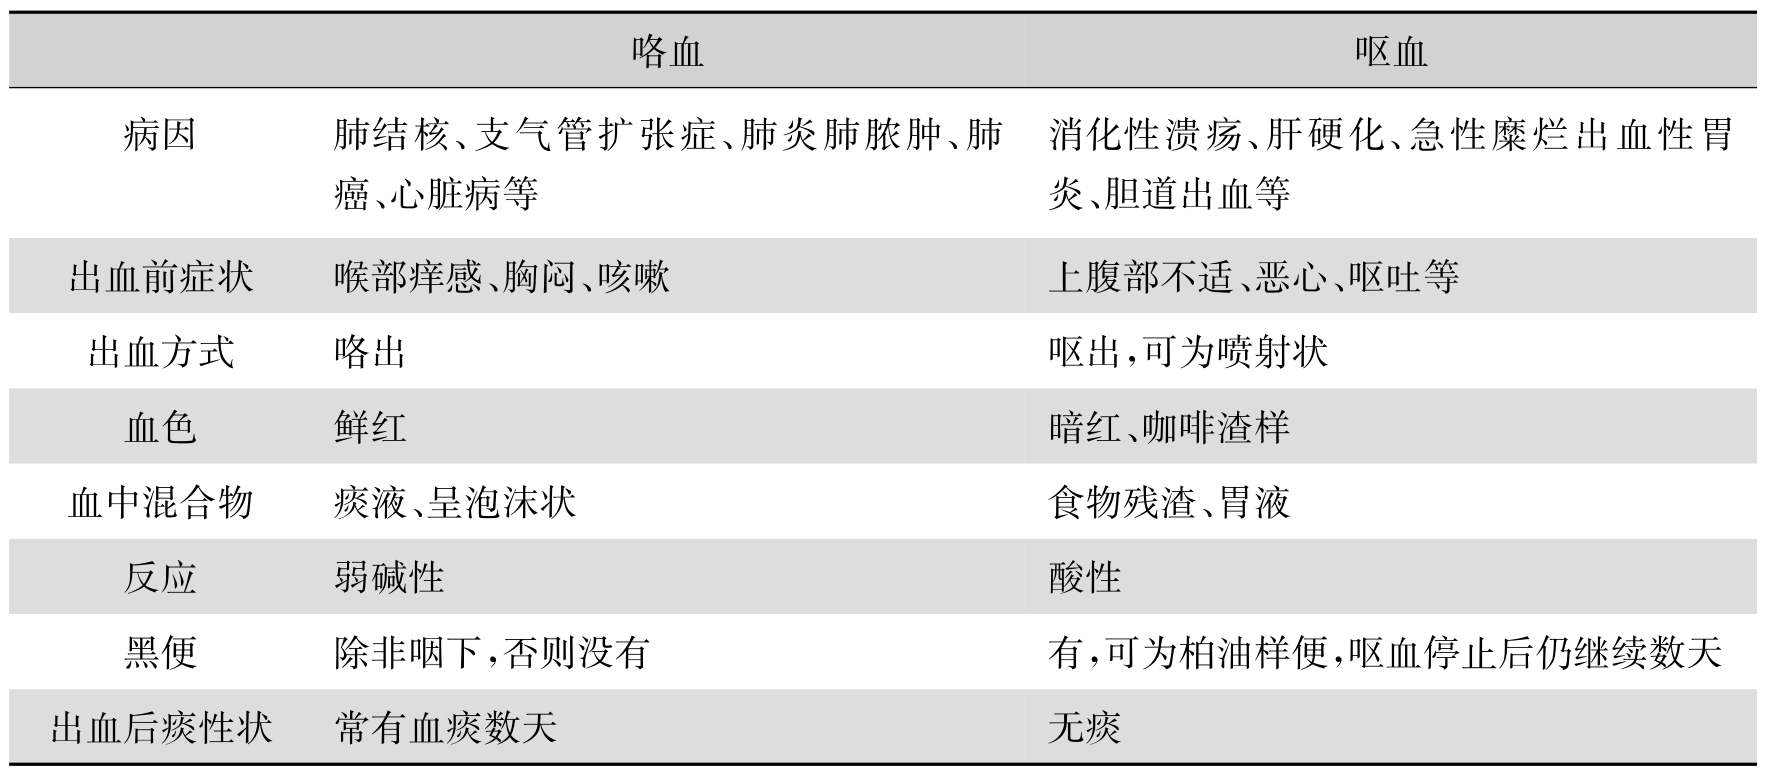
\includegraphics[width=.6\textwidth]{./images/Image00038.jpg}
 \caption{各种免疫细胞}
 \label{fig2-13}
  \end{figure} 


\subsection{造血干细胞}

造血干细胞(hemopoietic stem
cell,HSC)又称多能干细胞,是存在于造血组织中的一群原始造血细胞。也可以说,它是一切血细胞(其中大多数是免疫细胞)的原始细胞。由造血干细胞定向分化、增殖为不同的血细胞系,并进一步生成血细胞。人类造血干细胞首先出现于胚龄第2~3周的卵黄囊,在胚胎早期(第2~3月)迁至肝、脾,第5个月又从肝、脾迁至骨髓。在胚胎末期一直到出生后,骨髓成为造血干细胞的主要来源,具有多潜能性,即具有自身复制和分化两种功能。


\subsection{淋巴细胞}

淋巴细胞(lymphocyte)是构成免疫系统的主要细胞类别,占外周血白细胞总数的20%~45%,成年人体内约有10\textsuperscript{12}
个淋巴细胞。淋巴细胞可分为许多表型与功能均不同的群体,如T细胞、B细胞、NK细胞等;T细胞和B细胞还可进一步分为若干亚群。这些淋巴细胞及其亚群在免疫应答过程中相互协作、相互制约,共同完成对抗原物质的识别、应答和清除,从而维持机体内环境的稳定。

其特点是:未活化淋巴细胞在抗原的刺激下转变为淋巴母细胞,再进一步转变为效应T细胞与记忆细胞。可分群为:
\begin{itemize}
\item T细胞:细胞膜上表达CD3分子和TCR
\item B细胞:细胞膜上表达BCR
\item NK细胞:细胞膜上表达CD56和CD16
\end{itemize}

(一)T淋巴细胞

T淋巴细胞(T
lymphocyte)简称T细胞,其介导细胞免疫应答,并在机体针对TD抗原的体液免疫应答中发挥重要的辅助作用。骨髓中的淋巴样前体细胞(lymphoid
precursor)进入胸腺,经历一系列有序的分化过程,才能发育为成熟T细胞。T细胞乃高度异质性的细胞群,依据其表面标志及功能特征,可分为若干亚群。在免疫应答过程中,各亚群T细胞相互协作,共同发挥重要的免疫学功能。

1.T细胞的表面标志

T细胞表面标志即其膜分子(如图\ref{fig2-14}所示),是T细胞识别抗原、与其他免疫细胞相互作用、接受信号刺激并产生应答的物质基础,亦是鉴别和分离T细胞的重要依据。在诸多表面标志中,TCR、CD3分子是外周血成熟T细胞各亚群的共有标志。

(1)T细胞表面受体(surface antigen):T细胞抗原受体(T cell antigen
receptor,TCR)、细胞因子受体(cytokine receptor,CKR)、丝裂原受体。

(2)T细胞表面抗原(surface antigen):MHC抗原、分化抗原(CD分子)等。

\begin{figure}[!htbp]
 \centering
 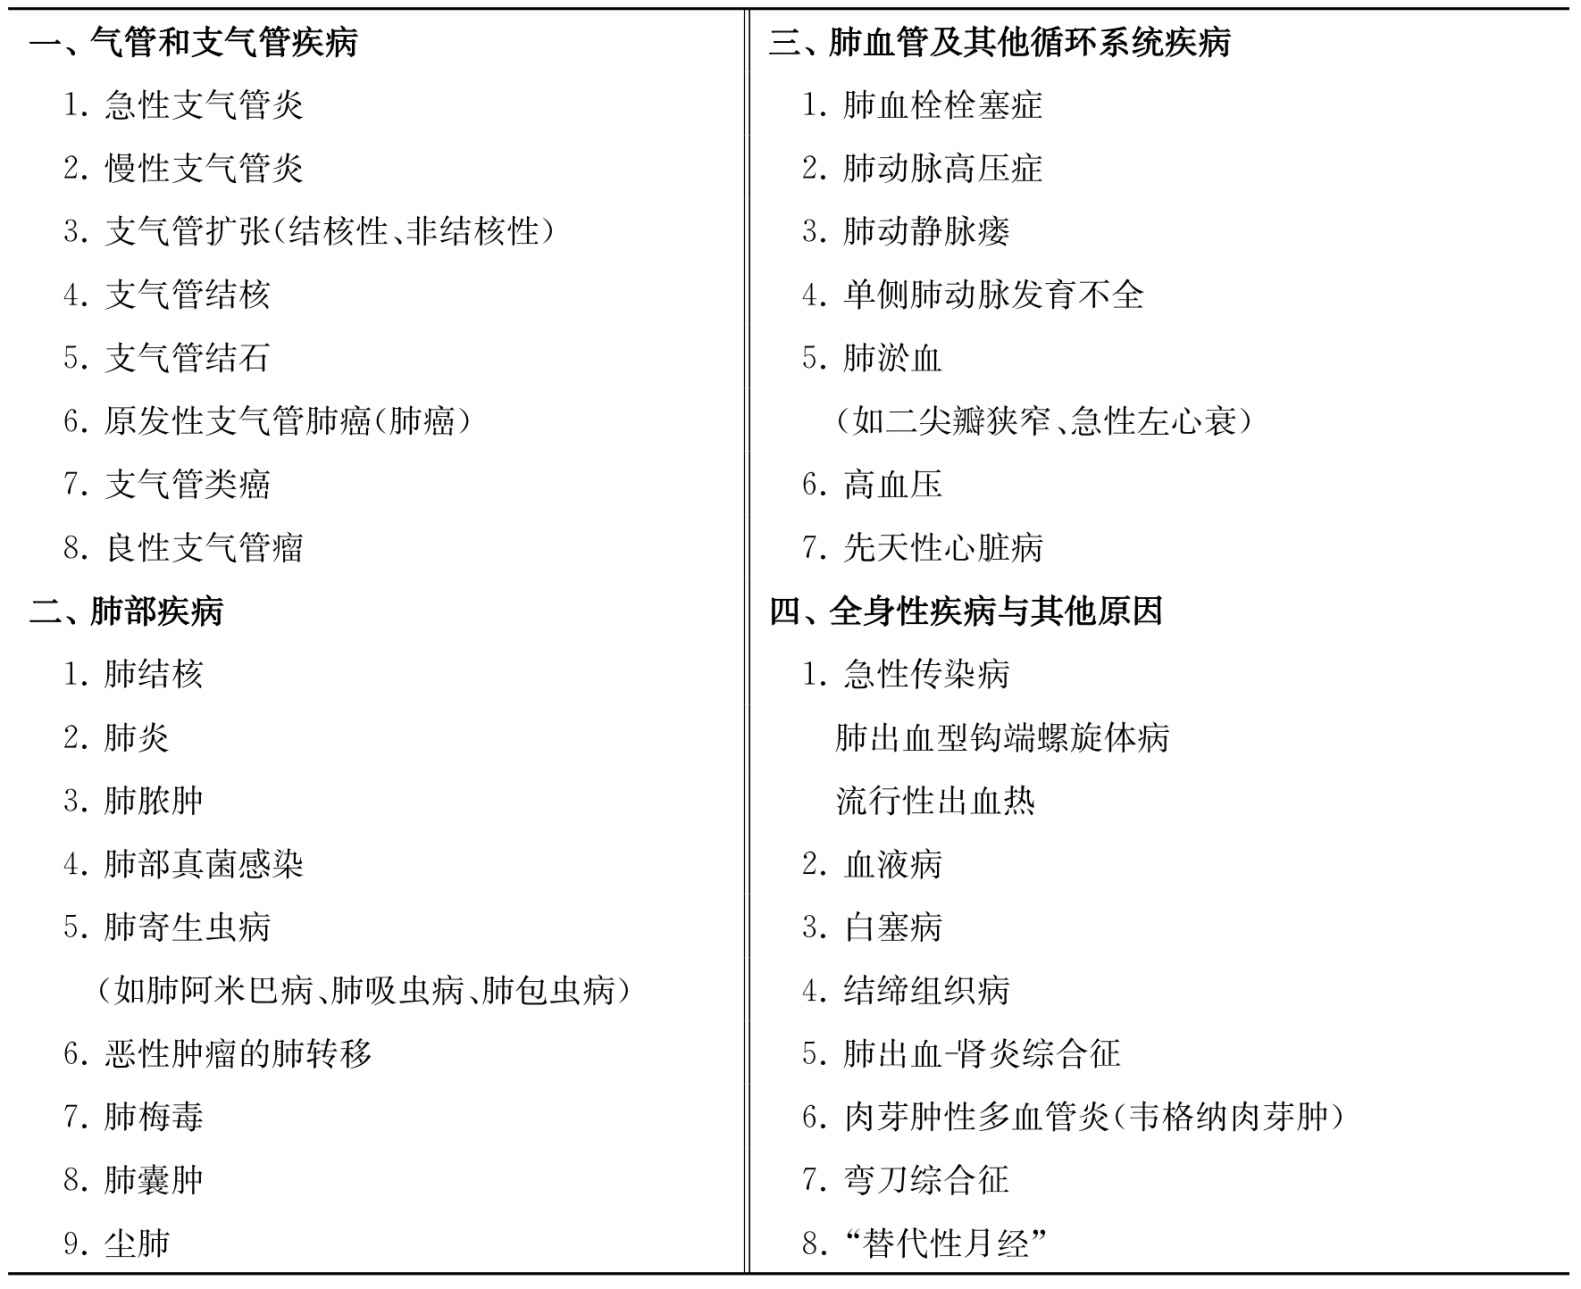
\includegraphics{./images/Image00039.jpg}
 \caption{T细胞表面标志}
 \label{fig2-14}
  \end{figure} 

2.T细胞亚群及其功能

人类的T细胞不是均一的群体,根据表面标志和功能可为五个亚群:

CD4\textsuperscript{+}
T(初始T细胞,Th1细胞,Th2细胞):占T细胞的65\%左右,它的重要标志是表面有CD4抗原。Th细胞能识别抗原,分泌多种淋巴因子,它既能辅助B细胞产生体液免疫应答,又能辅助T细胞产生细胞免疫应答,是扩大免疫应答的主要成分,它还具有某些细胞免疫功能。

CD8\textsuperscript{+}
T(杀伤性T细胞,抑制性T细胞):杀伤性T细胞占T细胞的20%~30%,表面也有CD8抗原。杀伤性T细胞能识别结合在MHC-Ⅰ类抗原上的异抗原,在异抗原的刺激下可增殖形成大量效应性杀伤性T细胞,能特异性地杀伤靶细胞,是细胞免疫应答的主要成分。抑制性T细胞占T细胞的10%左右,表面有CD8抗原。抑制性T细胞常在免疫应答的后期增多,它分泌的抑制因子可减弱或抑制免疫应答。

(1)初始T细胞(naive T
cell):指未完全分化的Th细胞,是Th1、Th2细胞的前体,分泌低水平的IL-4和IFN-γ。

功能:调节体液免疫应答和细胞免疫应答,分化产生Th1、Th2细胞,T细胞的分化如图\ref{fig2-15}所示。

\begin{figure}[!htbp]
 \centering
 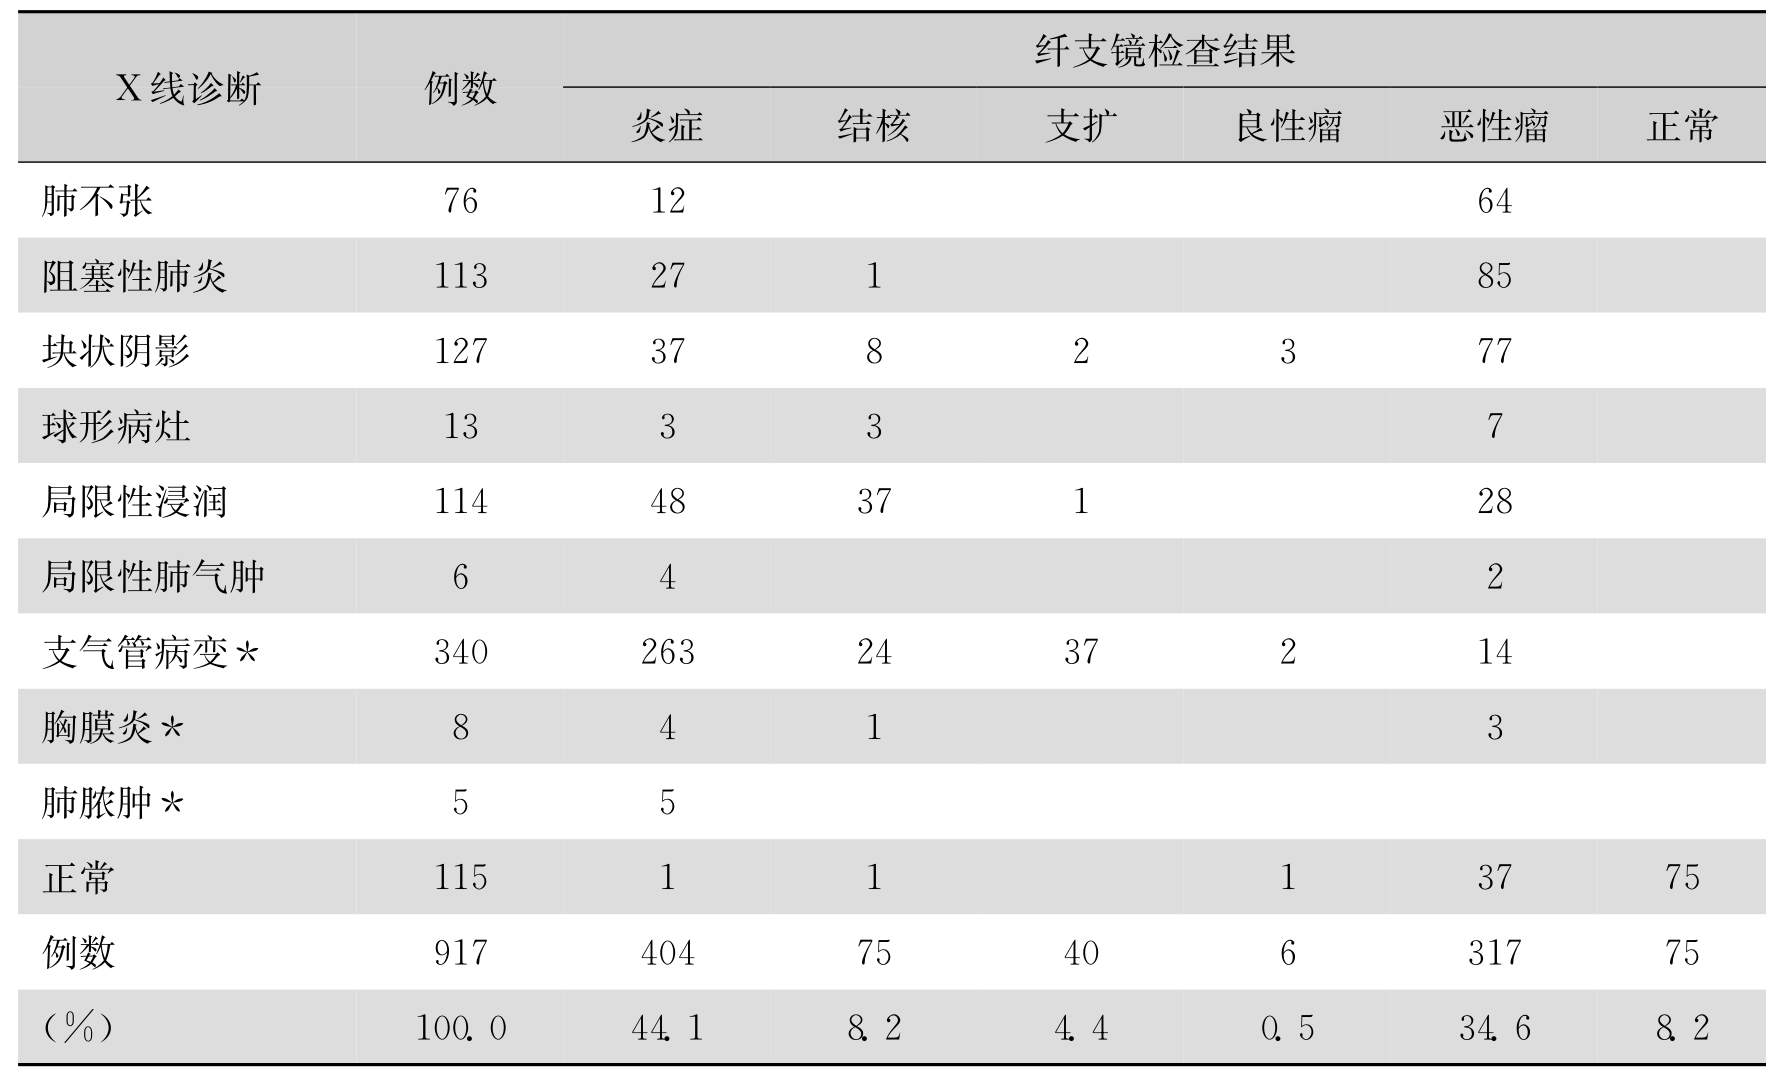
\includegraphics{./images/Image00040.jpg}
 \caption{T细胞的分化}
 \label{fig2-15}
  \end{figure} 

按分泌的细胞因子不同可将Th细胞分为两个不同的亚群:分泌IFN-γ、IL-2的称为TH1细胞,分泌IL-4、IL-5的称为Th2细胞。

(2)Th1细胞:初始T细胞在IL-12作用下转变为Th1细胞。

Th1细胞功能:释放IL-2、IFN-γ和TNF,引起炎症反应或迟发型超敏反应,称为炎症性T细胞。参与细胞免疫应答及迟发型超敏反应。在抗胞内病原微生物等感染中起重要作用。Th1细胞持续性强应答,可能与器官特异性自身免疫病、接触性皮炎、不明原因的慢性炎症性疾病、迟发型超敏反应性疾病、急性同种异体移植排斥反应等的发生有关。

(3)Th2细胞:初始T细胞在IL-4作用下转变为Th2细胞。

释放IL-4、5、6、10,诱导B细胞增殖分化、合成并分泌抗体,引起体液免疫应答或速发型超敏反应(图\ref{fig2-16})。

\begin{figure}[!htbp]
 \centering
 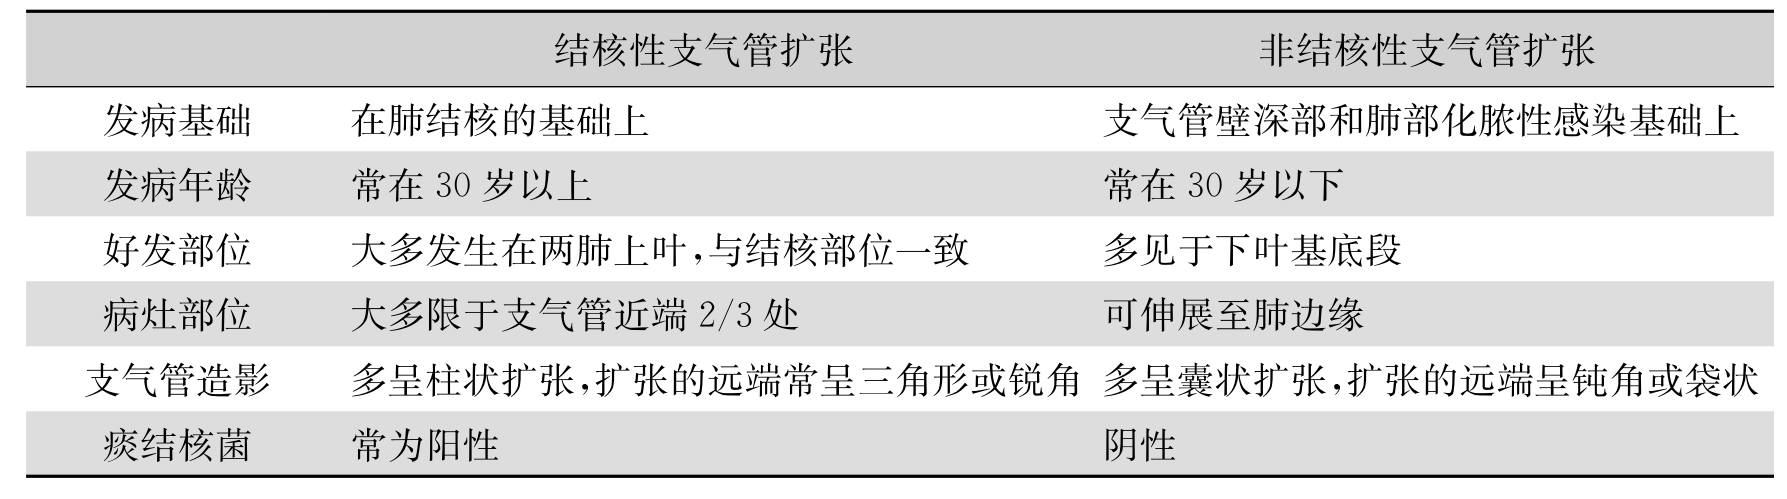
\includegraphics[width=.5\textwidth]{./images/Image00041.jpg}
 \caption{Th1、Th2淋巴细胞的功能}
 \label{fig2-16}
  \end{figure} 

(4)杀伤性T细胞(CTL):也叫细胞毒性T细胞,是效应T细胞,经抗原致敏后,CTL
的TCR特异性识别靶细胞(如病毒感染细胞、肿瘤细胞、同种异体移植物细胞等)表面的抗原肽/MHC-I类分子复合物。活化CTL
杀伤效应的主要机制为:①分泌穿孔素(perforin)、颗粒酶(granzyme)或淋巴毒素等直接杀伤靶细胞;②通过高表达FasL导致Fas阳性的靶细胞凋亡。CTL参与的免疫效应为抗病毒感染、抗肿瘤和介导同种异体移植排斥反应等(图\ref{fig2-17})。

\begin{figure}[!htbp]
 \centering
 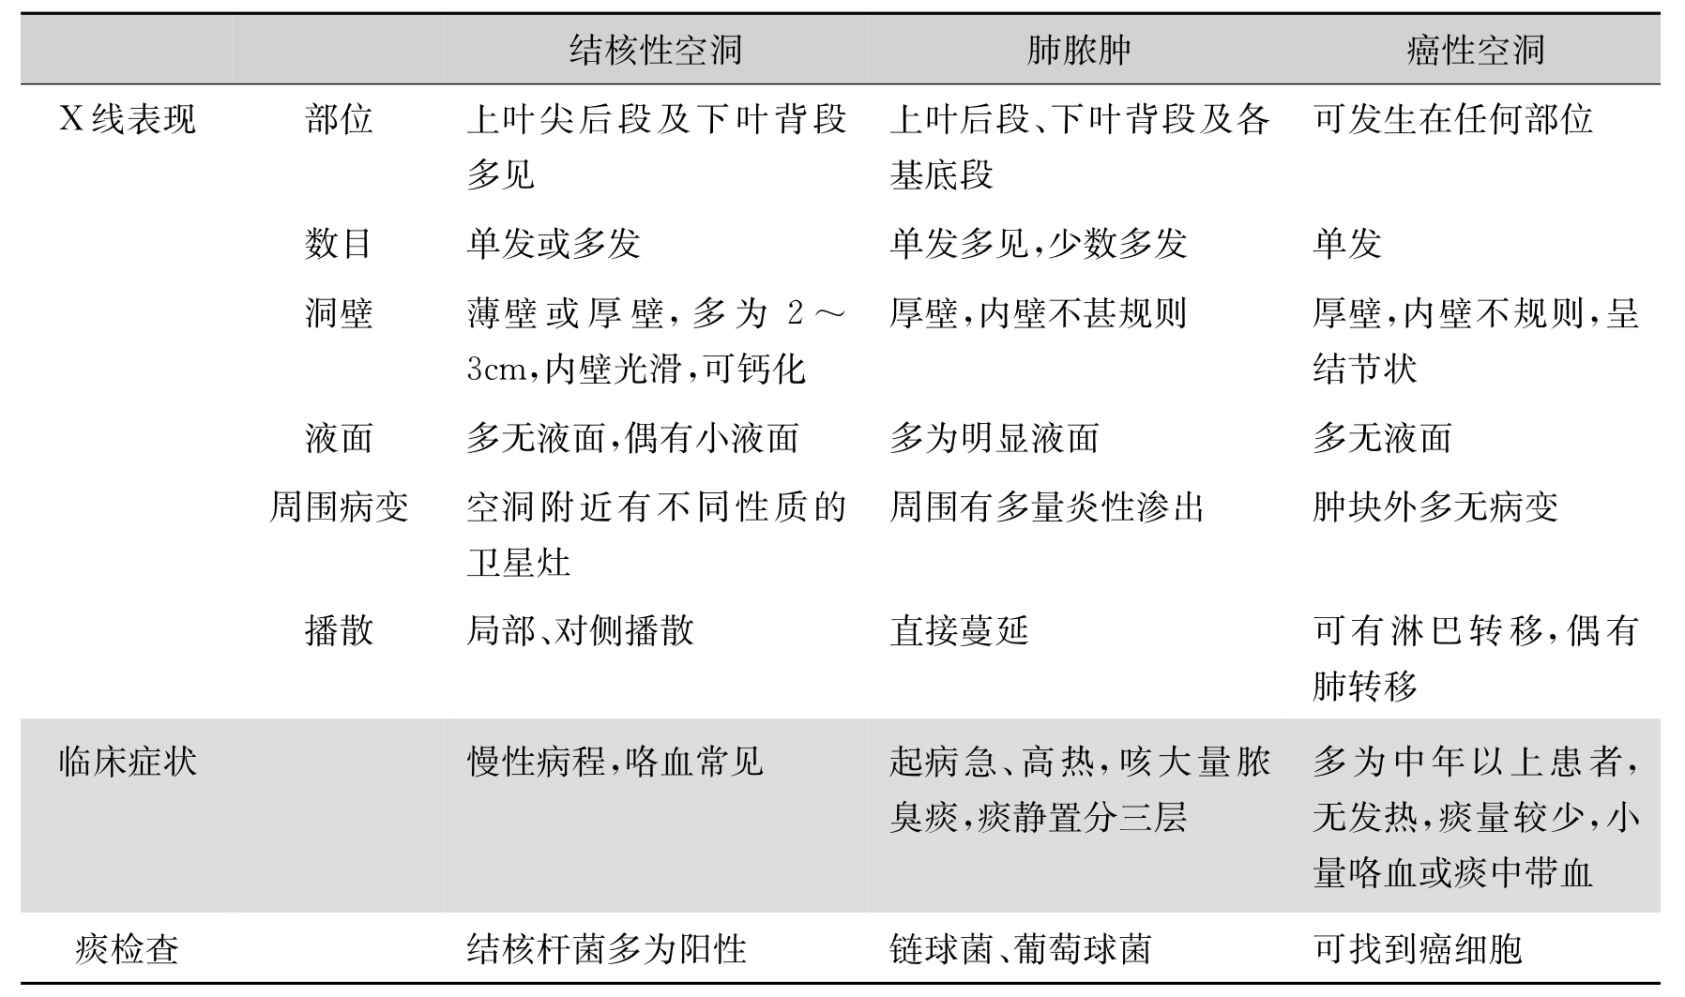
\includegraphics[width=.5\textwidth]{./images/Image00042.jpg}
 \caption{CTL的免疫效应}
 \label{fig2-17}
  \end{figure} 

(5)Ts细胞(suppressor T cell,Ts):具有抑制体液免疫和细胞免疫的功能。

(二)B淋巴细胞

B淋巴细胞(B
lymphocyte)是始祖B淋巴细胞在骨髓(人、动物)、法氏囊(禽)中发育、分化、成熟,产生抗体,也称骨髓或囊依赖性细胞,是体内唯一能产生抗体(Ig)的细胞,主要执行体液免疫,也具有抗原递呈功能。外周血中占淋巴细胞总数10\%~15\%,简称B细胞,是由哺乳动物骨髓或鸟类法氏囊中的淋巴样前体细胞分化成熟而来。

1.B细胞的表面标志

B细胞表面标志如图\ref{fig2-18}所示。

\begin{figure}[!htbp]
 \centering
 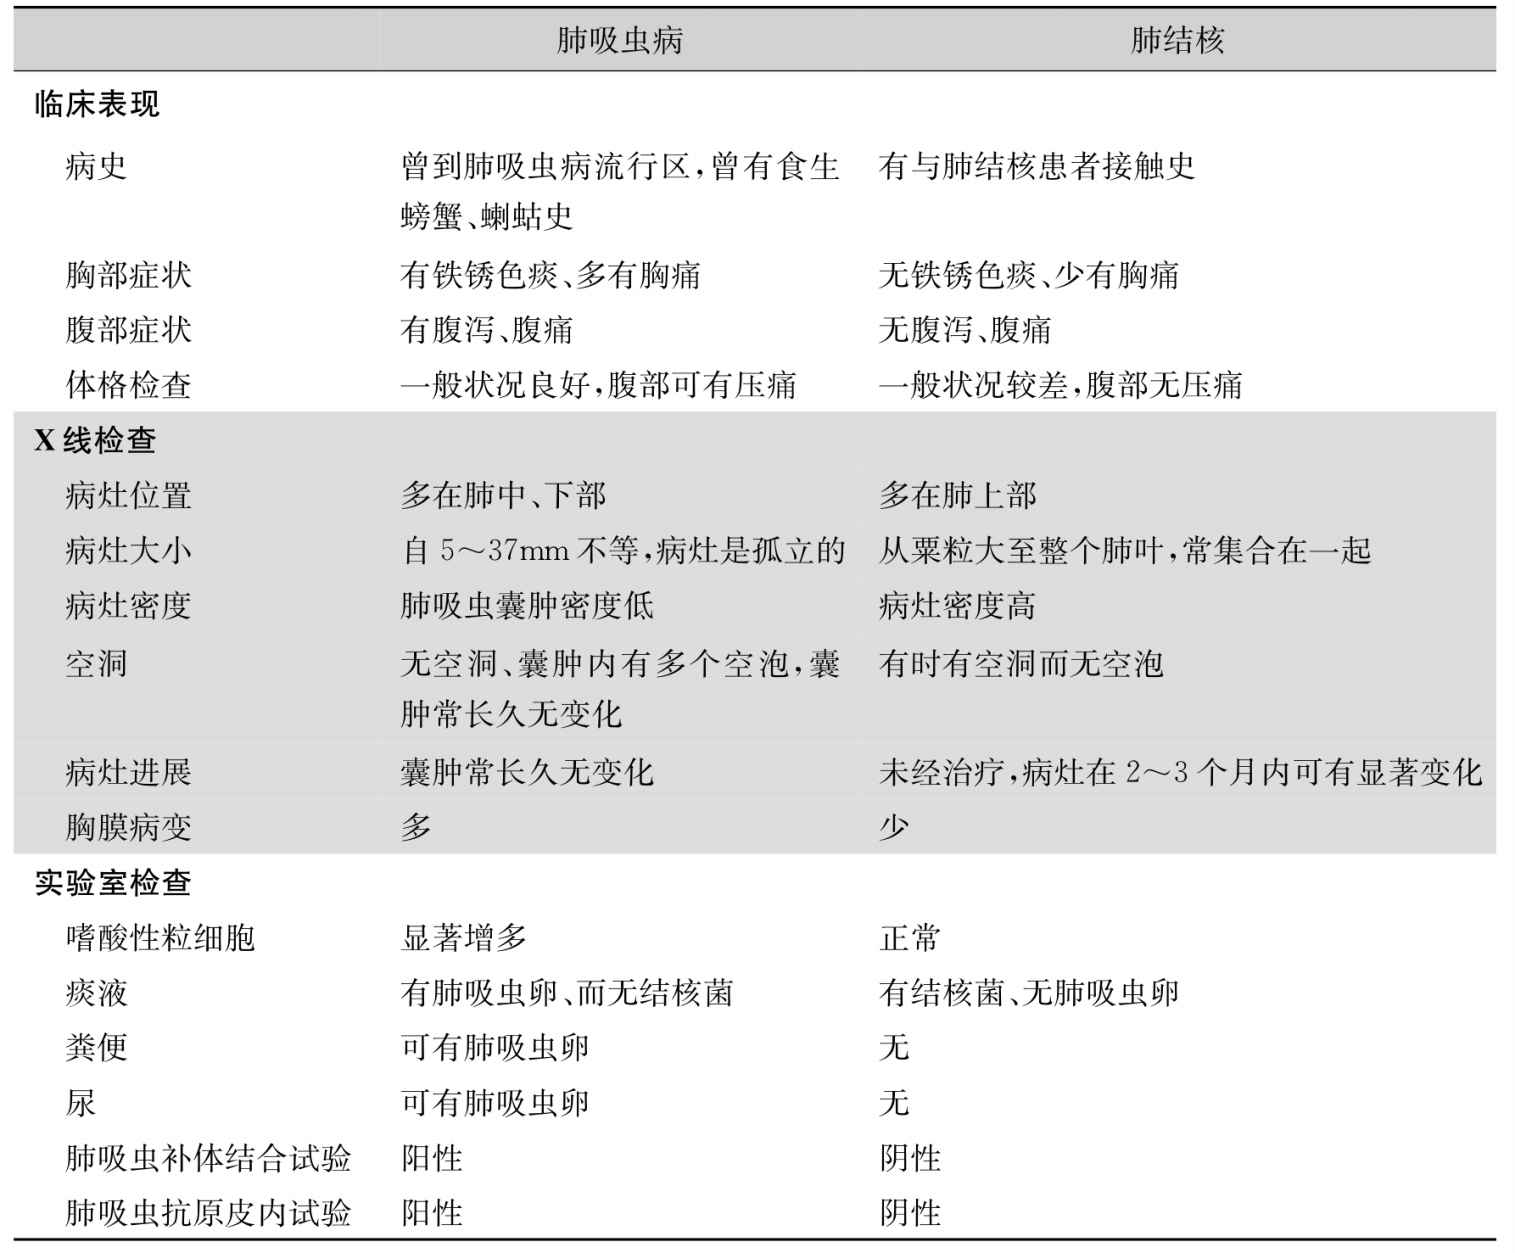
\includegraphics[width=.5\textwidth]{./images/Image00043.jpg}
 \caption{B细胞表面标志}
 \label{fig2-18}
  \end{figure} 

(1)B细胞抗原受体(B-cell antigen
receptor,BCR):BCR是嵌入细胞膜类脂分子中的膜表面免疫球蛋白(mIg),乃B细胞的特征性表面标志,也是B细胞特异性识别不同抗原表位的分子基础。

(2)细胞因子受体:B细胞表面表达IL-1R、IL-2R、IL-4R、IL-5R、IL-6R、IL-7R及IFN-γR等多种细胞因子受体。细胞因子通过与B细胞表面相应受体结合而参与或调节B细胞活化、增殖和分化。

(3)补体受体(CR):多数B细胞表面表达CR1和CR2(即CD35和CD21)。CR1主要见于成熟B细胞,其在B细胞活化后表达增高。CR1与相应配体结合可促进B细胞活化。CR2(CD21)是EB病毒受体,在体外应用EB病毒感染B细胞可使之转化为B淋巴母细胞系,从而达到永生化(immortalized)。

(4)Fc受体:多数B细胞表达IgG Fc受体Ⅱ(FcγRⅡ),可与免疫复合物中的IgG
Fc段结合,有利于B细胞捕获和结合抗原,并促进B细胞活化和抗体产生。

(5)丝裂原受体:某些丝裂原通过与B细胞表面相应受体结合,使其被激活并增殖分化为淋巴母细胞,可用于检测B细胞功能状态。美洲商陆(PWM)对T细胞和B细胞均有致有丝分裂作用;脂多糖(LPS)是常用的小鼠B细胞丝裂原。

2.细胞表面抗原

(1)MHC抗原:B细胞可表达MHC-Ⅰ类和MHC-Ⅱ类抗原。MHC-Ⅱ类抗原可与Th细胞表面CD4结合,增强B细胞与Th细胞间的黏附作用,并参与抗原递呈和淋巴细胞激活。

(2)CD抗原:B细胞分化发育的不同阶段,其CD抗原的表达各异,有CD19、CD20、CD21、CD40/CD40L、CD80(B7-1)/CD86(B7-2)。

3.B细胞亚群及功能

根据是否表达CD5分子,可将人B细胞分为B1(CD\textsuperscript{+}
\textsubscript{5} )和B2(CD\textsuperscript{-} \textsubscript{5}
)细胞。

(1)B1细胞亚群:B1细胞在个体发育过程中出现较早,是由胚胎期或出生后早期的前体细胞分化而来,其发生不依赖于骨髓细胞。B1细胞产生后,成为具有自我更新(self-renewal)能力的长寿细胞,主要分布于胸腔、腹腔和肠壁固有层中。B1细胞的抗原识别谱较窄,主要针对属于TI-2抗原的多糖类物质,尤其是某些菌体表面共有的多糖抗原(如肺炎球菌荚膜多糖等)。B1细胞的功能特点是:主要产生IgM类的低亲和力抗体;不发生抗体类别转换;无免疫记忆。

(2)B2细胞亚群:B2细胞即通常所称的B细胞,是参与体液免疫应答的主要细胞类别。它是由骨髓中多能造血干细胞分化而来,属形态较小、比较成熟的B细胞,在体内出现较晚,定位于外周淋巴器官。B2细胞的主要生物学功能为:参与体液免疫应答、抗原递呈、免疫调节。

(三)自然杀伤细胞

自然杀伤细胞(natural
killer,NK)是一类独立的淋巴细胞群,其不同于T细胞和B细胞,不表达特异性抗原识别受体(图\ref{fig2-19})。NK细胞胞浆内有许多嗜苯胺颗粒,故又称为大颗粒淋巴细胞(large
granular
lymphocyte)。NK细胞无须抗原预先致敏即可直接杀伤某些靶细胞,包括肿瘤细胞、病毒或细菌感染的细胞以及机体某些正常细胞(图\ref{fig2-20})。
\begin{figure}[!htbp]
    \centering
    \begin{minipage}[b]{0.45\textwidth} 
      \centering
        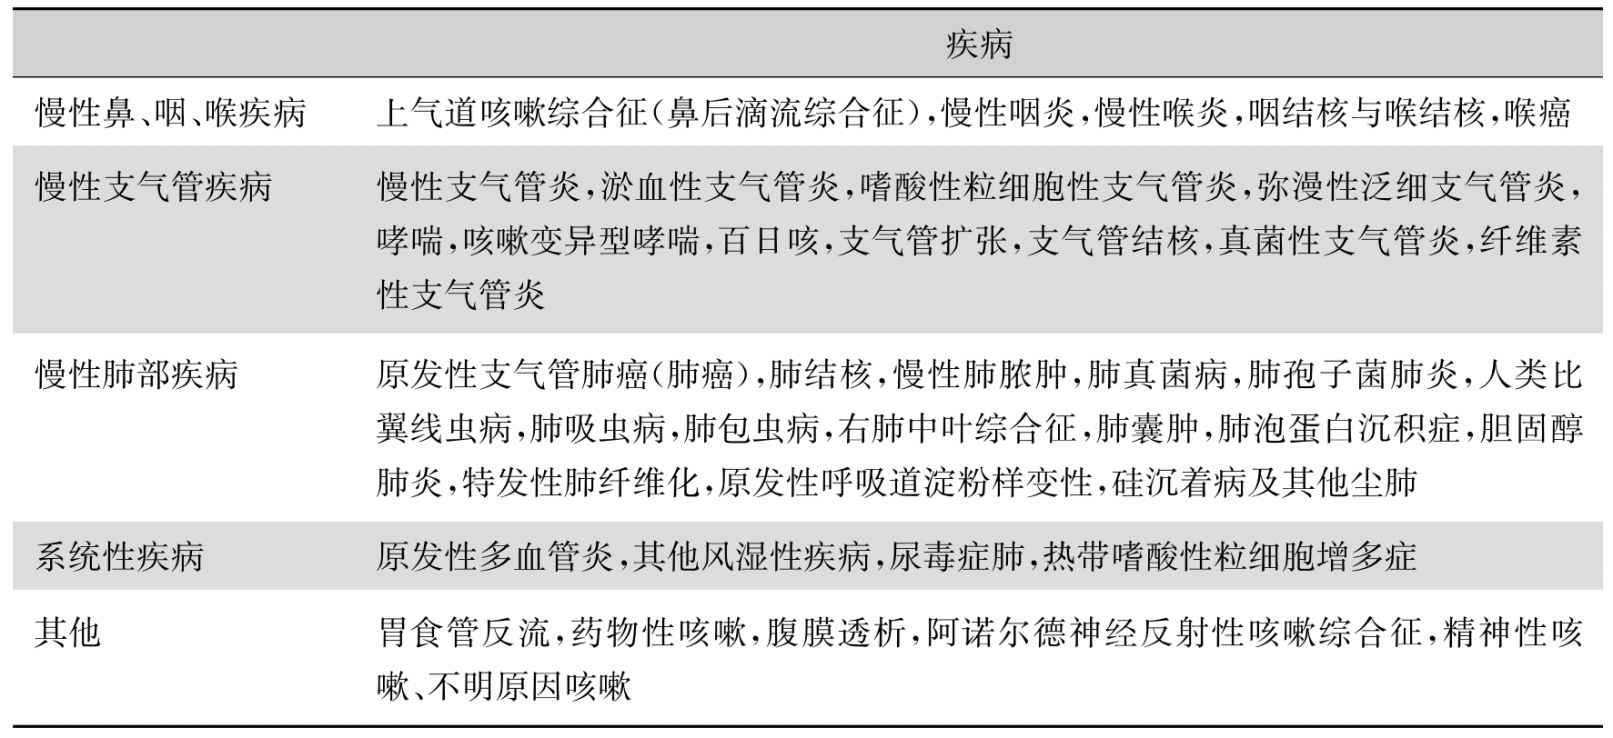
\includegraphics[height=0.12\textheight]{./images/Image00044.jpg}
        \captionsetup{justification=centering}
        \caption{自然杀伤细胞}
        \label{fig2-19}
    \end{minipage}
%	\end{figure} 
	%\FloatBarrier
%\begin{figure}[!htbp]
%    \centering
%\hspace{0.04\textwidth}%
\begin{minipage}[b]{0.45\textwidth} 
  \centering
    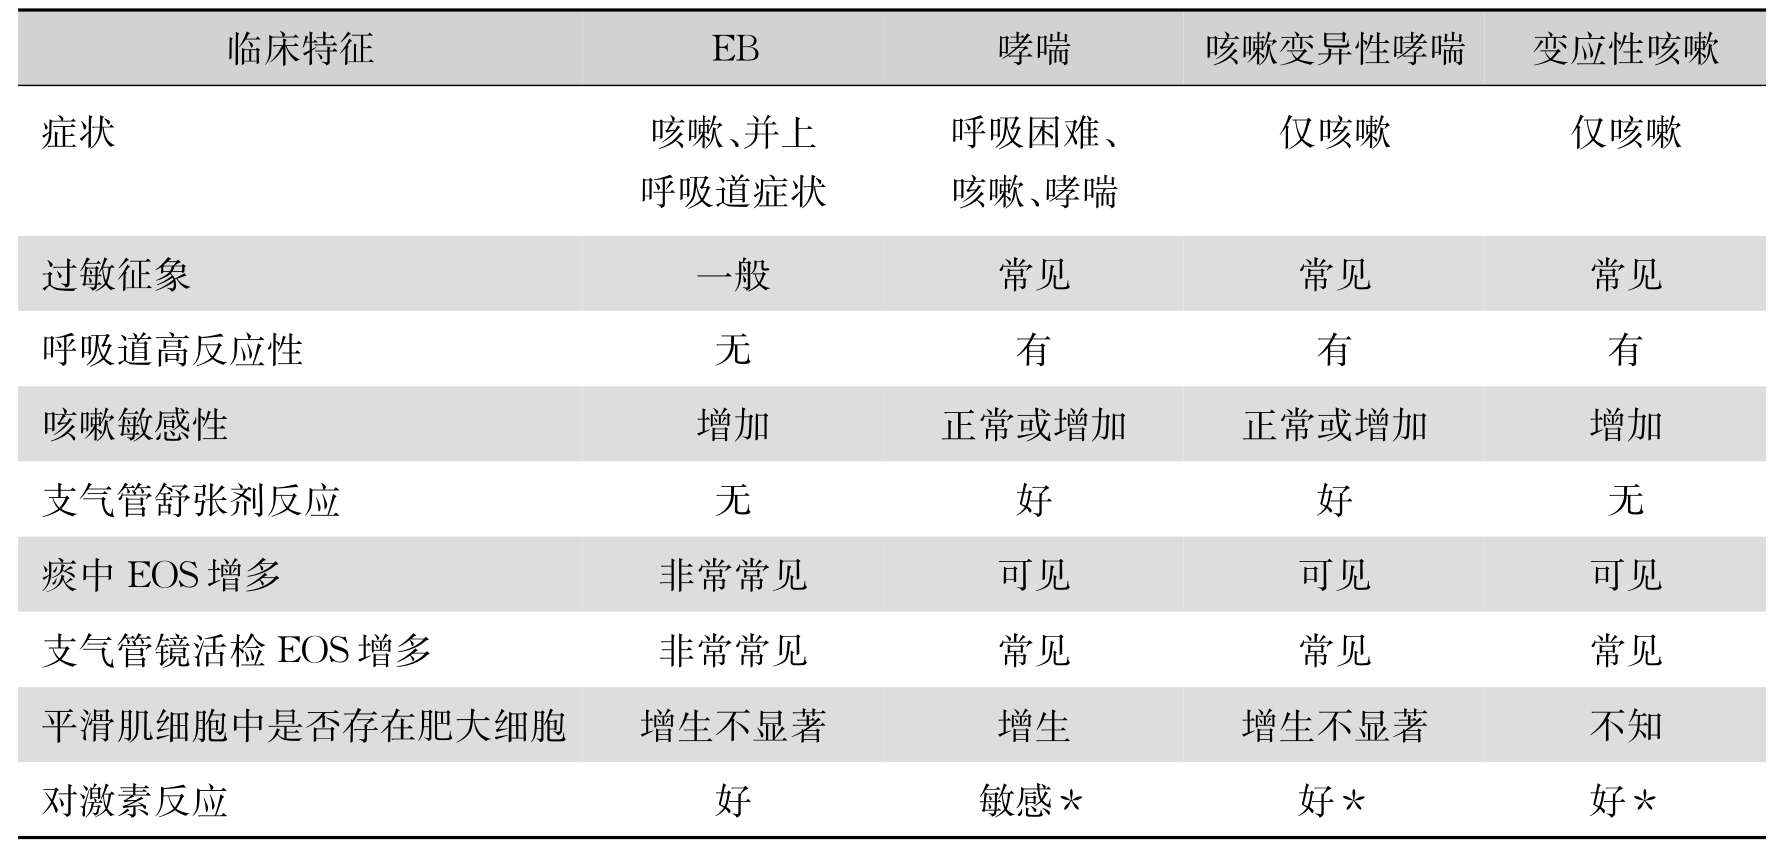
\includegraphics[height=0.2\textheight]{./images/Image00045.jpg}
    \captionsetup{justification=centering}
    \caption{NK细胞杀死癌细胞}
    \label{fig2-20}
\end{minipage}
\end{figure} 

1.来源及分布

NK细胞是由骨髓中的共同淋巴样祖细胞(commen lymphoid
progenitor,CLP)分化而来,其发育、成熟可能循骨髓途径或胸腺途径。人类和小鼠NK细胞主要分布于脾脏(占脾细胞总数3\%~4\%)和外周血(占淋巴细胞总数5%~7%),在淋巴结以及其他组织内(如肺脏等)也有少量NK细胞存在。近年发现,肝脏中NK细胞占淋巴细胞总数50\%以上,其生物学意义有待阐明。

2.功能

(1)能非特异性杀伤某些肿瘤细胞和病毒感染的靶细胞,具有抗肿瘤、抗感染的功能。

(2)NK细胞可产生IL-1、IFN-r、TNF等,有免疫调节作用。

(3)参与移植排斥反应、自身免疫病、超敏反应的发生。


\subsection{单核吞噬细胞系统}

单核吞噬细胞系统(mononuclear phagovyte
system,MPS)包括单核细胞、巨噬细胞,是体内具有最活跃生物学功能的细胞类型之一(图\ref{fig2-21})。

\begin{figure}[!htbp]
 \centering
 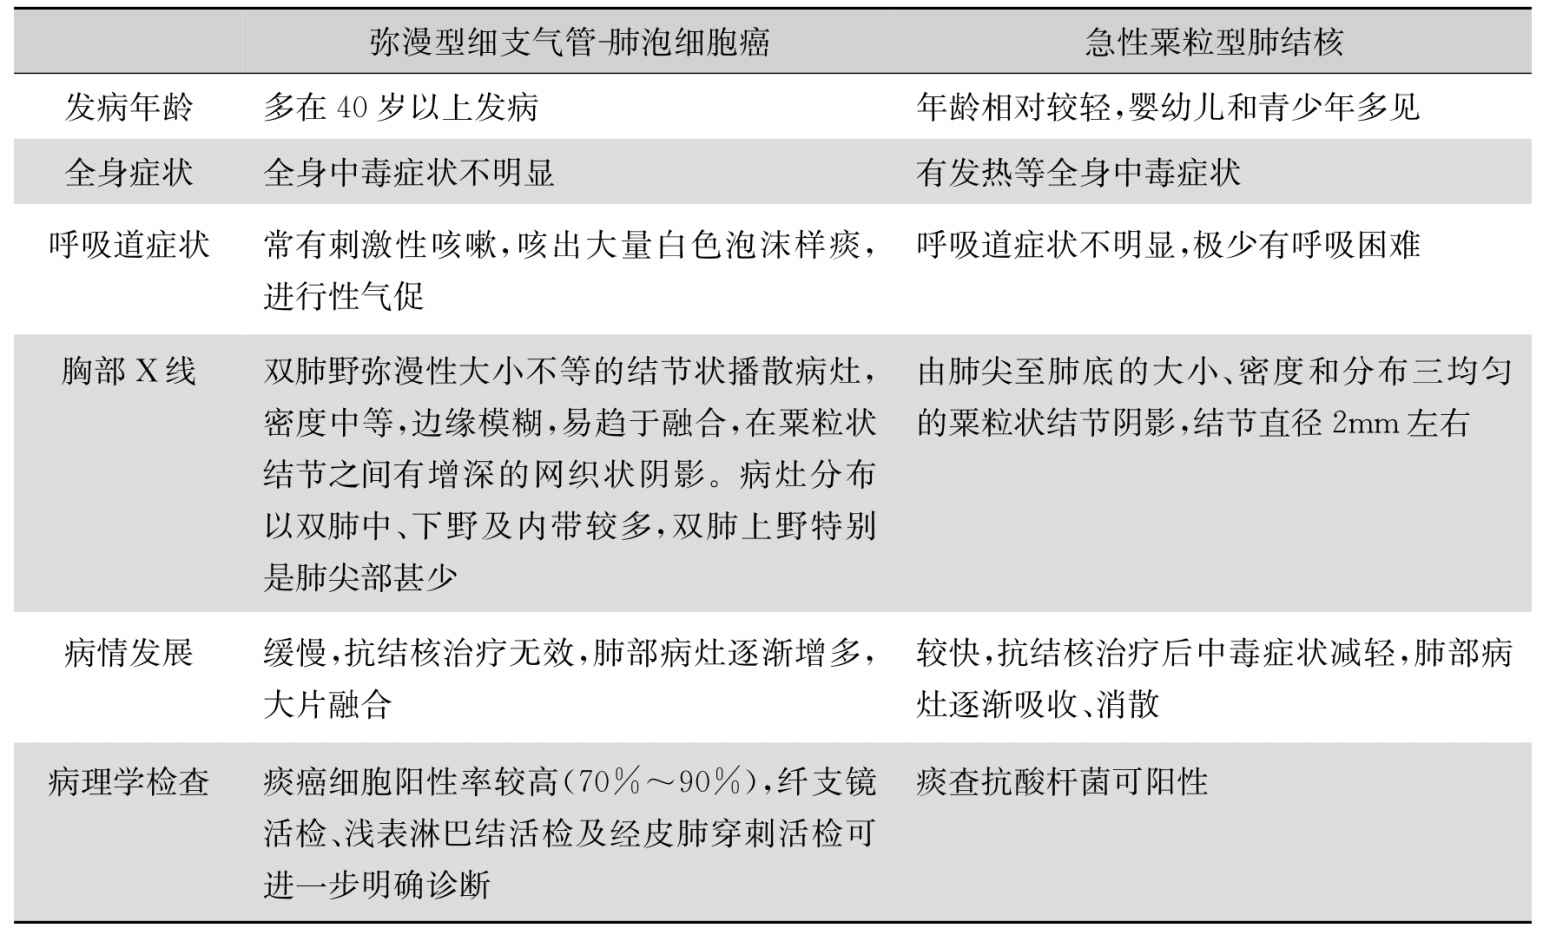
\includegraphics[width=.7\textwidth]{./images/Image00046.jpg}
 \caption{单核吞噬细胞}
 \label{fig2-21}
  \end{figure} 

1.表面标志:表达多种表面标志,并借此发挥各种生物学功能,如MHC分子、黏附分子等。这些表面标志不仅参与细胞黏附及对颗粒抗原的摄取、递呈,也介导相应配体触发的跨膜信号转导,并影响细胞分化和发育等。

2.产生多种酶及分泌产物:单核吞噬细胞能产生各种溶酶体酶、溶菌酶、髓过氧化物酶等,还能产生和分泌近百种生物活性物质,如细胞因子(IL-1、IL-6、IL-12等)、补体成分(C1、P因子等)、凝血因子,以及前列腺素、白三烯、血小板活化因子、ACTH、内啡肽等活性产物。

3.功能:具有抗感染、抗肿瘤、免疫调节的作用。


\subsection{其他免疫细胞}

(一)中性粒细胞

中性粒细胞表面具有IgFc受体和C3b受体,具有高度趋化性和非特异性功能,有抗感染作用(图\ref{fig2-22})。

\begin{figure}[!htbp]
 \centering
 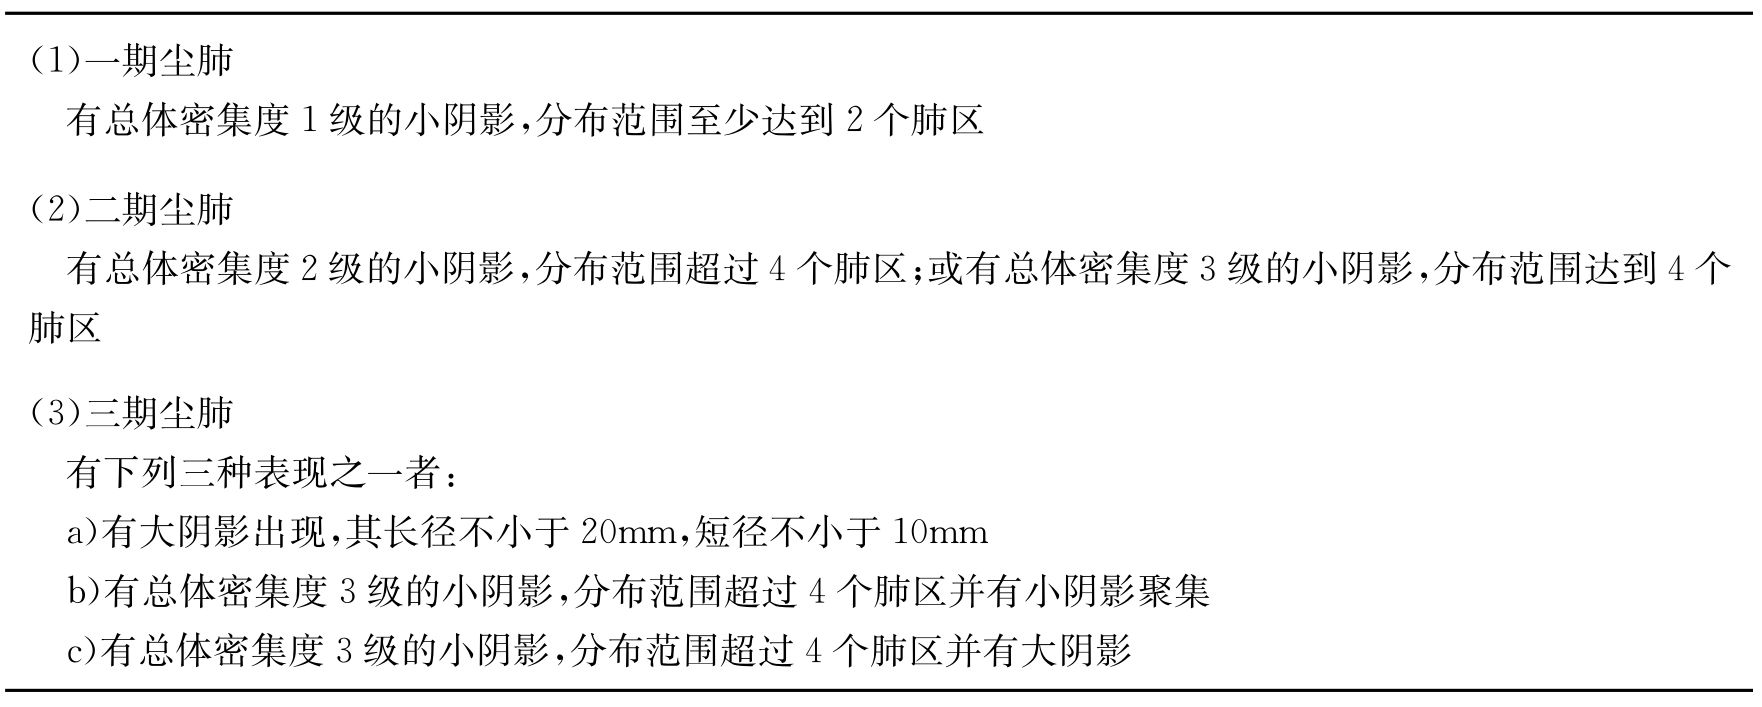
\includegraphics[width=.7\textwidth]{./images/Image00047.jpg}
 \caption{中性粒细胞的吞噬作用}
 \label{fig2-22}
  \end{figure} 

(二)嗜酸性粒细胞

嗜酸性粒细胞具有IgFc受体,参与IgE介导的ADCC效应;具有吞噬作用,抗寄生虫和对I型超敏反应的负调节作用。

(三)嗜碱性粒细胞与肥大细胞

嗜碱性粒细胞与肥大细胞表面具有IgE的Fc受体,能参与I型超敏反应、抗肿瘤作用(图\ref{fig2-23})。

\begin{figure}[!htbp]
 \centering
 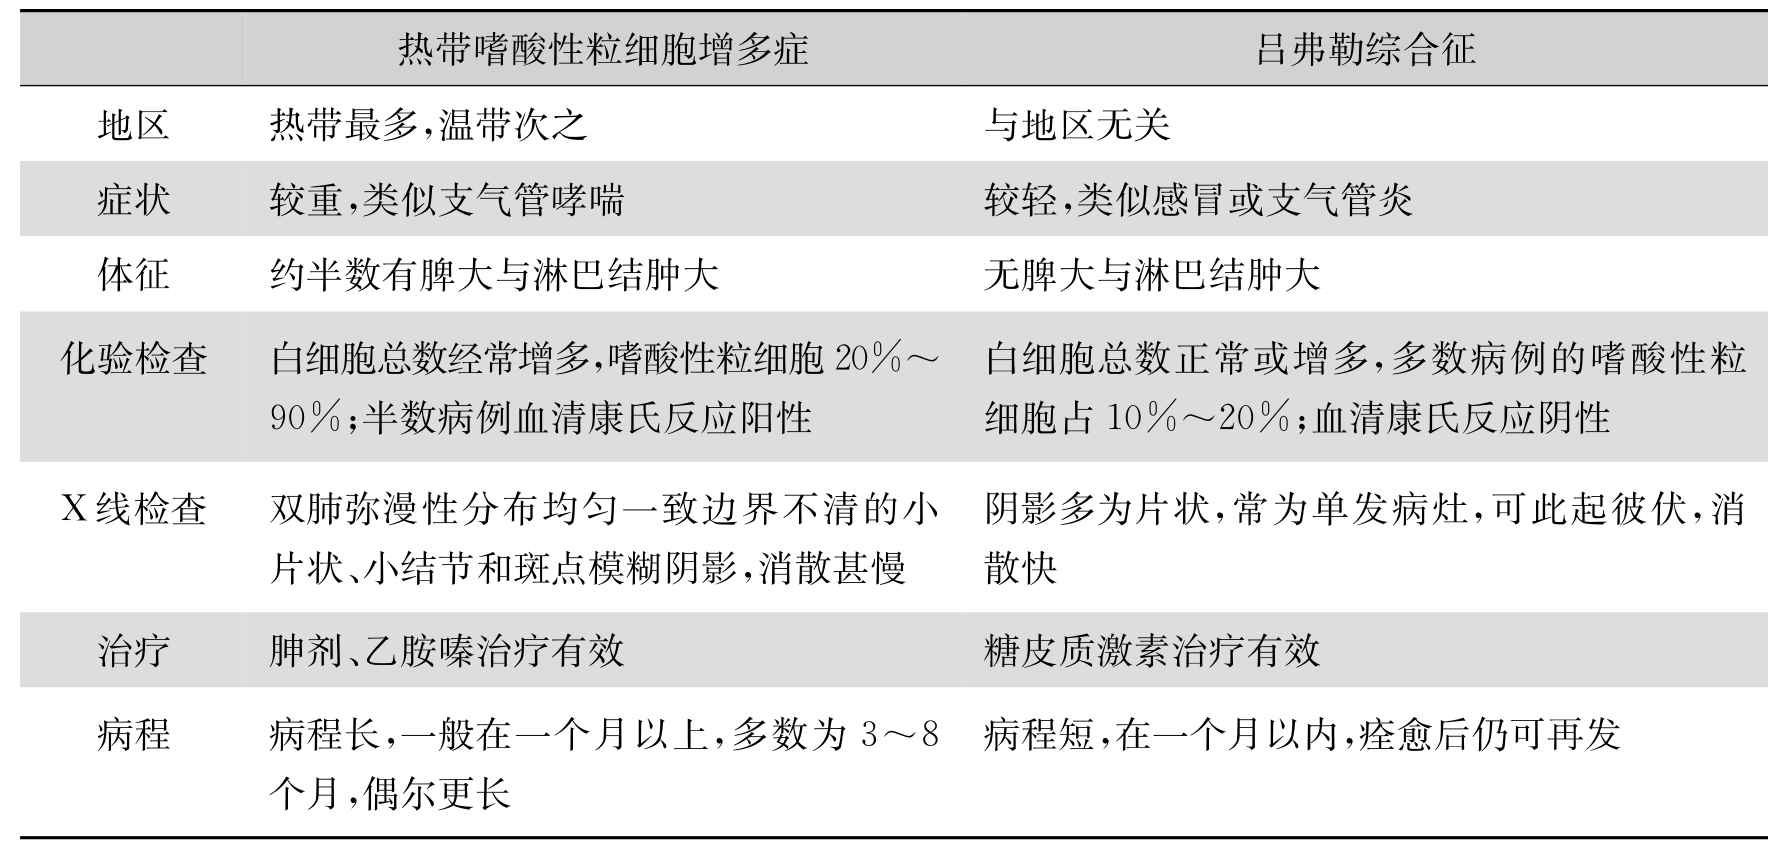
\includegraphics[width=.6\textwidth]{./images/Image00048.jpg}
 \caption{肥大细胞参与Ⅰ型超敏反应}
 \label{fig2-23}
  \end{figure} 

(四)红细胞

1.红细胞免疫的物质基础

① 红细胞CR1分子------结合C3b/C4b;

② 红细胞CD58分子------即LFA-3,与CD2互为配体和受体;

③ 红细胞CD59分子------阻止C9与C5B678结合,促进T细胞有丝分裂;

④ 红细胞CD55分子------即衰变加速因子DAF;

⑤ 红细胞CD44分子------参与T、B的分化、成熟、活化,细胞黏附;

⑥ 红细胞NK细胞增强因子------增强NK细胞的毒性;

⑦ 红细胞趋化因子受体------参与调控炎症反应。

2.红细胞在整体免疫反应中的作用

① 增强吞噬作用;

② 清除循环免疫复合物;

③ 识别和携带抗原;

④ 免疫调节作用;

⑤ 效应细胞的作用。

\section{思考练习与课外阅读}
\noindent\textbf{【理解与思考】}

1.你能向一位没有免疫学知识的人,形象地解说机体免疫系统的构成及其作用吗?

2.你能描绘出体内淋巴细胞的一生历程吗?

3.如果你是一病原微生物,进入机体后你能遭遇哪些危险?

4.如果你是一免疫细胞,你又是如何保证机体健康的?

5.以红细胞的口气,向别人叙述一下你在人体内的贡献。

\noindent\textbf{【课外拓展】}

1.白血病中,为何某一种白细胞数量过度增加?其分化机理如何?

2.淋巴细胞的阴性选择、阳性选择是如何进行的?有何意义?

3.造血干细胞的分化过程如何?在哪些因素作用下发生的?

4.与红细胞等比较,为何白细胞类都是“短命细胞”?

5.自然杀伤细胞在肿瘤防治中有哪些作用?目前用免疫的方法治疗肿瘤有哪些方法?

\noindent\textbf{【课程实验与研究】}

1.设计一个检测淋巴细胞活性的实验。要求分类定量。

2.设计一种诱导造血干细胞分化为NK细胞的实验方法。

3.白血病的种类有哪些?设计一种通过阻断细胞的分化途径来预防某种类型的白血病方案,并分析可行性。

4.设计一种方案,检测免疫细胞能释放哪些生物活性物质,并实施实验,完成实验报告。

5.设计检测饲喂蜂蜜对小鼠机体免疫力影响的三种以上指标,并设计实验方案,完成实验,写出小论文。

6.Nature最近报道发现“自然杀伤(NK)细胞的一个新亚类”,请问如何鉴别其为新的发现?

\noindent\textbf{【课程研讨】}

1.为何机体免疫细胞对自身的成分不产生排斥?

2.整个免疫系统与一个国家的防御力量有什么相似之处?请加以比较说明。

3.免疫系统与机体别的系统一样,各自负起使命,你认为机体是如何抵御病原微生物入侵的?如果病原微生物进入机体,机体又是如何清除的?

4.如何区别不同的淋巴细胞?

5.查阅资料,阐述淋巴细胞当今的研究进展。

\noindent\textbf{【课后思考】}

1.详细叙述免疫系统的构成及其作用。

2.骨髓、胸腺、淋巴结、脾脏的主要免疫功能。

3.T、B淋巴细胞的分类及其作用。

\noindent\textbf{【课外阅读】}

\begin{center}
\textbf{\Large 红细胞免疫发展史}
\end{center}

红细胞免疫和其他自然科学一样,它的发展也经历着三个阶段,即经验、实验、理论阶段。在发展中各阶段难以截然分开,反复循环,不断深入,不断提高。

\begin{center}
{\large 一、经验阶段}
\end{center}

我国劳动人民在长期与疾病的斗争中体会到血液的重要,往往将血与生命联系在一起,事实上血液特别是红细胞是机体生命活动的物质基础。祖国医学云:“气血是人体生命活动的物质基础”,“离开了气血,则整体不能联系,人身无有依附”。在20世纪初,Landsteiner
用免疫学方法在人类红细胞与血液混合实验中,观察到凝聚现象,后来通过多次反复试验观察,发现了人类ABO
血型系统,认识了红细胞表面存在许多能与血清中相应抗体凝集的抗原,如Mn、P
型、Rn、Lutheran、Lewis、Kell、Duffy、Kidd
等。除目前已知的数十种血型抗原外,发现红细胞还含有其他抗原。20世纪30年代,杜克(L
.H.Duke)首先发现锥虫在抗血清及补体存在时可黏附到人类红细胞上,推测在人的红细胞膜上存在有一种与免疫有关的物质。在临床上,人们对某些疑难病、原因不明性疾病等患者,采用输新鲜血液的办法,往往可得到满意的治疗效果。但究其原因,过去人们并不很清楚,自红细胞免疫问世以来,人们对上述现象的解释有了理论依据。如
G-BS
现已证实属红细胞免疫缺陷症;有些疾病,由于输注红细胞后,机体免疫功能得到了改善,即给了机体以
“气血”,“气血相依,循环不已”,“防治百病莫不以气血为本”。

\begin{center}
{\large 二、实验阶段}
\end{center}

实验阶段即将人们观察到的现象,进行科学实验的过程。1953年,R.A.Nelson用正常人的红细胞、白细胞与相应抗体致敏的
I
型肺炎双球菌进行培养,发现肺炎双球菌可黏附于正常人的红细胞表面并被白细胞吞噬,其吞噬率可达60\%,远远高于未加相应抗体组和未加相应红细胞组,作者推测红细胞膜存在免疫黏附受体,将此命名为免疫黏附现象。1963年,Nishioka证实红细胞这种免疫黏附现象是通过红细胞膜
C3受体实现的。1980年,Fearon从红细胞膜分离到这一受体,并详细研究了CR1的性质,是分子量190
000~250
000的多态性膜糖蛋白。1986年,郭峰通过体外对比实验证明红细胞可黏附补体调理过的各种肿瘤细胞,并发现红细胞可黏附未经调理过的肿瘤细胞,其机理不明。1992年,刘景田等证实这种直接免疫黏附的机理与红细胞上
CR1 和肿瘤细胞上 C3b分子有关。

\begin{center}
{\large 三、理论阶段}
\end{center}

1981年,美国生殖免疫学家Siegel在前人研究的基础上发现红细胞有多种免疫功能,红细胞可黏附胸腺细胞,并发现血清中存在有红细胞免疫黏附抑制因子,预见了血清中存在有红细胞免疫调节系统,推测红细胞在阻止肿瘤细胞血行转移中有作用。他综合看待以往对红细胞免疫的研究成果,提出了
“红细胞免疫系统” 的新概念,冲破了传统上划分血细胞功能的
“界限”,更新了人们对红细胞功能的认识。20 世纪 80
年代,我国学者郭峰教授在红细胞免疫的基础理论和应用研究方面取得了许多突破性进展,如发现血清中存在有红细胞免疫黏附促进因子、红细胞有增强各类免疫细胞的免疫功能,建立了许多红细胞免疫功能的监测方法等,大大推动了我国红细胞免疫的发展。1994
年,刘景田在证实血清中确实存在有正负两种红细胞调节因子的基础上,发现了这两种因子对粒细胞、淋巴细胞(主要指B
淋巴细胞)都有相同调节作用,推测这种因子对具有
CR1的细胞都有调节作用,故将这种因子称为 CR1 免疫调节因子(Complement
recepor 1 immuneregalation factors,CR1FR)。其中具有正调节作用者称为
CR1免疫黏附促进因子(Complement recepor 1 immune regalation enhance
factors,CR1FER);具有负调节作用者称为 CR1 免疫黏附抑制因子(Complement
recepor 1 immune regalation inhibitor factors,CR1FIR)。

(资料来源:刘景田,党小军.红细胞作为免疫细胞的事实及意义[J].深圳中西医结合杂志,2002,12(1):10-12)

\begin{center}
\textbf{\Large 红细胞免疫功能研究进展}
\end{center}

红细胞是血液中最主要的细胞成分。传统认为,红细胞结构简单,功能单一,仅运输氧和二氧化碳。随着科技的发展,人们对红细胞免疫功能的认识不断深入。1930年,Duck发现人类红细胞膜上存在与免疫有关的物质;1953年,Nelson首次提出红细胞不仅具有免疫黏附功能还能促进白细胞的吞噬作用;1963年,Nishioka证实红细胞免疫黏附的物质基础是红细胞膜上补体C3b受体(C3breceptor,C3bR);1980年,Fearon进一步从红细胞膜上分离出受体CR1(complementreceptor1,CR1)。1981年,Siegel在前人研究的基础上提出了“红细胞免疫系统(redcellimmunesystem,RCIS)”新概念,成为红细胞免疫研究的里程碑,促进了红细胞免疫研究工作的迅速发展。医学工作者研究发现,红细胞具有很多与免疫有关的物质,包括补体受体CR1、CR3、淋巴细胞功能相关抗原-3(CD58)、CD44、人类补体膜辅助因子蛋白(MCP)、降解加速因子(DAF)、过氧化物歧化酶(SOD)、阿片肽受体、NK细胞激活因子(NKAF)以及红细胞趋化因子受体等。红细胞不仅具有识别、存储、递呈抗原,清除免疫复合物,促进吞噬细胞功能等作用,自身还存在完整的自我调节控制系统,是机体免疫系统的重要组成部分。

\begin{center}
{\large 一、红细胞免疫功能的分子学基础}
\end{center}

1981年,Siegel提出了“红细胞免疫系统”概念,并指出红细胞免疫黏附(redcellimmuneadhesion,RCIA)是红细胞发挥免疫功能的主要手段,RCIA的分子基础则是红细胞膜上的补体受体(complementreceptor,CR)。目前,已明确红细胞膜上的补体受体有I型(CR1)和Ⅲ型(CR3),主要为CR1,其基因结构、分子结构及生物学功能已部分明确。CR1属于补体调控蛋白,分子量为160~260kd,是一种单链膜结合蛋白,能与补体系统中C3b、C4b高亲和性地结合。就单个红细胞而言,膜上CR1受体密度仅为白细胞110~150,但红细胞数量庞大,在体内约90\%C3b受体存在于红细胞膜上。CR1与血液循环中带有C3b的免疫复合物(immnunecomplex,IC)结合,并运送至肝脏及脾脏内皮系统予以清除,即为红细胞免疫黏附(RCIA)机制。随着国内外研究的深入,发现CR1参与机体免疫功能的机制远比上述复杂得多。红细胞能携带抗原抗体复合物,还能主动地将抗原抗体复合物传递给单核巨噬细胞并使之激活,增强单核巨噬细胞对抗原抗体复合物的摄取并加工递呈给T细胞。此外红细胞在类孢子病、溶血性贫血、病毒性肝炎、系统性红斑狼疮、肾病、疟疾等疾病中的作用也得到证实。红细胞上CR1表达降低或红细胞黏附功能下降会引起机体免疫功能低下,研究红细胞CR1介导的免疫黏附功能对评价机体天然免疫功能状况乃至特异性细胞或体液免疫可能都具有十分重要的意义。目前,CR应用热点是对双特异性单抗异聚体(heteropolymer,HP)的研究。Taylor以红细胞CR1分子为桥梁,建立了抗CR1单抗与抗致病原单抗交叉连接的HP清除循环中致病原的方法,引起了广泛关注。HP结合红细胞时,还可结合循环中病原体,形成异聚体复合物(E-HP-Ag),并迅速将EHPAg移至肝脏彻底销毁,红细胞本身数量却无减少。此外可溶性CR的应用也有所突破,Yazdanhakhsh等报道使用基因重组的可溶性CR1在动物实验中成功阻断了补体活化。

\begin{center}
{\large 二、红细胞免疫功能}
\end{center}

(一)清除循环免疫复合物

研究表明,红细胞膜上补体受体具有免疫黏附、携带及清除循环液相中抗原异物的功能,清除循环免疫复合物(circleimmunecomplex,CIC)是红细胞主要的免疫功能。目前认为,大多数C3b-免疫复合物(C3b-IC)通过CR1连接。CR1存在于红细胞、多形核白细胞、巨噬细胞及淋巴细胞的膜表面。红细胞膜上CR1分布有两种形式:散在和集簇分布。约50\%红细胞膜上CR1呈集簇分布,多形核白细胞上CR1集簇分布率小于15\%。CR1集簇分布方式使它与C3b-IC的结合位点呈多价性,连接更牢固。实验证明,单个白细胞表面CR1受体较红细胞多,但在细胞浓度相同时,两种细胞的免疫复合物结合率相同。血液中红细胞总数远远超过白细胞,循环系统中约95\%C3b受体位于红细胞上,与CIC结合机会为白细胞的500~1000倍。因此,体内清除CIC起主要作用的是红细胞,不是白细胞。Nedaf体外实验结果证明了这一推测。红细胞清除免疫复合物的机理是:红细胞通过表面CR1受体与循环中C3b-IC结合(即发生黏附),形成的复合物被血流带到肝、脾等器官,这些器官的固定吞噬系统捕获红细胞结合的IC,通过巨噬细胞膜表面的Fc受体与IC中的抗体Fc段结合,此时红细胞从IC上解离,再度进入循环,而捕获IC的巨噬细胞则通过膜表面CR1受体再与IC补体C3b结合,Fc受体与CR1受体的协同作用使巨噬细胞的吞噬作用加强,而将IC吞噬并清除到体外。Sherwood实验研究发现:红细胞表面所黏附的循环免疫复合物被转运到吞噬细胞,吞噬细胞所接受CIC的多少与红细胞CIC的浓度呈平行关系,红细胞无任何损伤或被吞噬。有实验证明,肝脏内巨噬细胞表面的Fc受体和CR1受体密度较高,且Fc受体比红细胞膜上CR1受体活性强,致使肝、脾内巨噬细胞对免疫复合物(IC)有更强的作用,可以从CR1密度低的红细胞上夺取IC。

(二)增强吞噬细胞的吞噬功能

1953年,Nelson将经抗体、补体调理过的肺类球菌复合物注入猴体,发现球菌几乎全部黏附于红细胞上。实验证明,血浆中被红细胞黏附的复合物(IC)较未被黏附的更容易被吞噬。1982年,Forslod进一步证实了上述现象作用机理,用C3b及IgG(兔抗酵母菌IgG)调理过的酵母菌与吞噬细胞一起孵育,加入红细胞后,吞噬细胞对酵母菌的吞噬率比未加入红细胞组增加了34\%;给予红细胞溶解产物后,吞噬率增加75\%。用过氧化氢酶及超氧化物歧化酶代替红细胞后,吞噬率增加程度相似。可能是红细胞首先黏附酵母菌,然后红细胞酵母菌复合物与吞噬细胞作用,红细胞内含有高浓度的过氧化氢酶(Cat)及超氧化物歧化酶(SOD),并具有强力的抗氧化作用,清除吞噬过程中产生的氧化代谢产物(ROM),促进吞噬作用。近年来,人们将红细胞作为SOD的载体以延长其在体内的存活时间,提高血液相容性,防治缺氧、缺血过程中活性氧造成的组织损伤,取得了良好的效果。

(三)对T淋巴细胞和淋巴因子的调控作用

实验表明,红细胞通过CD58、CD59与T辅助细胞CD2的黏附激活T淋巴细胞免疫功能,与B细胞作用亦能促使增殖、分化产生免疫球蛋白。红细胞还可调控淋巴细胞产生γ-干扰素,增加淋巴细胞转化率和培养液中IgG、IgA的含量。CD58分子即淋巴细胞功能相关抗原23(LFA-3),是一种分子量为55~70kd的糖蛋白,属于免疫球蛋白超家族成员,广泛表达于人体内各种免疫细胞和红细胞上,结构与CD2(LFA-2)相似,故CD58与CD2分子可以相互结合。表达CD58抗原递呈细胞(APC)或靶细胞通过与表达CD2分子的T细胞相互黏附,促进T细胞识别抗原,CD58与CD2结合后又参与细胞信号转导,此信号为T细胞活化的一种重要协同(辅助)刺激信号。相对于T细胞活化时TCR识别性结合MHC一抗原肽复合物的T细胞活化第一信号,CD58与CD2的结合又被称为T细胞活化第二信号。有证据表明,结合抗原抗体复合物(IC)的红细胞通过膜表面CR分子介导的免疫黏附作用将免疫复合物传递给巨噬细胞,又经膜表面CD58分子与辅助性T细胞膜表面CD2分子结合间接起到类似于抗原递呈细胞(antigenpresentingcell,APC)的递呈抗原作用,促进外周血T细胞活化与细胞周期改变,从而间接调控免疫应答。CD59分子即攻膜复合体(membraneattackcomplex,MAC)抑制物,是一种分子量为18~20kd的糖蛋白。CD59可阻碍C7、C8与C5b~6复合物结合,抑制MAC形成。CD59除广泛参与补体调节,还能与CD2分子结合,是继CD58之后发现的又一CD2配体。CD59与CD2结合也能发挥类似CD58与CD2结合的协同刺激信号的作用,CD58和CD59与T细胞黏附时具有协同作用,同时表达CD58与CD59的靶细胞更有利于T细胞的激活。近年来的研究发现,CD59缺陷还常伴随CD55缺陷,提示其功能可能为一种广泛参与红细胞免疫调节的协同蛋白。

(四)识别、储存和递呈抗原

红细胞对自我和非我抗原具有识别功能,且具有储存抗原的能力。1982年Garvey将\textsuperscript{3}
H标记的牛血清清蛋白(BSA)注入新生兔,放射自显影发现外周血液和肝血管内红细胞表面均黏附有\textsuperscript{3}
HBSA,并持续存在4~6周以上。若将兔血清清蛋白注入新生兔体内,则不出现上述现象,由此证实了上述观点。红细胞的抗原递呈能力表现为红细胞免疫黏附特性具有双重性,即红细胞上CR1与IC相黏附时,可同时黏附自身胸腺细胞和T细胞,形成自身玫瑰花环,IC中抗原与T淋巴细胞紧密靠拢,红细胞将抗原递呈给T淋巴细胞,使其俘获抗原能力增强,从而增强了免疫应答。

(资料来源:夏佐中.红细胞免疫功能研究进展[J].重庆医学,2008,37(20):2365-2367)

\begin{center}
\textbf{\Large 天然免疫反应需要T细胞参与}
\end{center}

先天性免疫和获得性免疫虽是不同的概念,具有不同机制,但在对付入侵的病原体时,它们并不各自为政或分庭抗礼,而是互相配合协同作战的。例如,当伤寒杆菌侵入后,首先由先天性免疫(如补体、吞噬细胞等)对付,等到体内产生抗伤寒抗体和免疫淋巴细胞(获得性免疫因素),就与补体和吞噬细胞(先天免疫因素)协同作用,清除体内伤寒杆菌。

2009年1月,中科院生物物理所感染免疫中心唐宏研究员和傅阳心教授在《免疫学趋势》(Trends
in Immunology)杂志上以《Do adaptive immune cells suppress or activate
innate
immunity》为题,系统阐述了他们近来提出的“天然免疫反应需要T细胞参与”的新理论。经典的免疫学理论认为,天然免疫反应启动获得性免疫,而获得性免疫随后进一步放大天然免疫效应,二者的合作与平衡才能清除入侵病原,起到免疫保护的作用。该实验室近期的研究结果表明(原文见Nature
Medicine,2007;Nature Reviews in Immunology,2007; Nature
China,2008),原先关于区分天然免疫和获得性免疫的界限可能并不那么清楚,T细胞其实也参与天然免疫反应并维持其稳态。经典理论认为天然免疫和获得性免疫反应的双重低下是早产儿容易死于急性感染的主要原因。该实验室的研究发现,实际上,在感染早期获得性免疫细胞对于天然免疫反应具有负调控的作用,从而有效地将天然免疫反应的强度控制在一定的水平内而不至于对机体造成免疫损伤。新生鼠或早产儿由于获得性免疫低下,天然免疫炎性反应无法得到有效控制,这种“炎性因子风暴”才是致死原因。因此,获得性免疫一方面抑制感染早期的炎症反应,另一方面在感染后期行使病原特异性清除功能,两者缺一不可。

这个新理论对于深入了解病毒性感染的炎症反应和病毒清除机理,控制免疫低下病人(新生儿、老年人、放化疗癌症病人、器官移植患者或艾滋病人)机会性感染具有极高的指导价值。

(资料来源:http://www.bioon.com/biology/Immunology/383575.shtml)

\begin{center}
\textbf{\Large Immunity:嗜中性粒细胞通过群集抵抗寄生物}
\end{center}

嗜中性粒细胞在抵抗病原体的免疫响应中扮演了一个重要角色,但是它们调节自身保护效应的机制却一直没有搞清。最近发表在《免疫学》上的一项研究显示,在嗜中性粒细胞转移到淋巴结的过程中------它们在这里形成了动态分子团,就像蜂群一样,这些细胞扮演了抵抗胞内寄生物的一个重要角色。

为了研究嗜中性粒细胞与淋巴结之间的关系,美国加利福尼亚大学伯克利分校的Tatyana
Chtanova等使用了嗜中性粒细胞表达绿色荧光蛋白质的小鼠,并使它们传染上胞内寄生物------弓形虫,同时利用荧光显微镜方法检测淋巴结组织切片。研究人员观察到,在感染后,嗜中性粒细胞迅速转移到淋巴结中,并且这一过程依赖于它们的适应物蛋白质MyD88(骨髓差别主要响应基因88)的表达。此外,渗透的嗜中性粒细胞被发现形成了群集,并且这些群集与寄生虫在淋巴结中所处的位置相符合。

利用完整无损的淋巴结的双光子激光扫描显微镜,研究人员随后调查了嗜中性粒细胞群集形成的动力学原因。他们观察到,在被弓形虫感染后,嗜中性粒细胞形成两种群集:瞬时群集,即规模较小且溶解迅速;持久群集,即规模较大(由于嗜中性粒细胞的连续转移和与附近群集的合并)且在成像期间内持续存在。基于这些,研究人员推断,一旦一个群集达到一定的规模,由嗜中性粒细胞产生的信号将会压倒周围群集的信号,形成一个稳定的群集中心。嗜中性粒细胞同时被发现以直接的方式以及一连串地向这些群集迁移,这意味着这里的细胞之间可能存在着信息传递。

研究人员继续研究了群集如何在感染后被组合起来,并且观察到它们能够被嗜中性粒细胞与从淋巴结被感染的细胞中溢出的寄生虫之间的合作行为所激活。更特别的是,小分子团最初是由少数“先驱”嗜中性粒细胞所形成的,并且这些分子团诱导其他细胞向群集中迁移。

一个嗜中性粒细胞已知能够通过分泌酶使组织退化,研究人员随后调查了是否群集的出现与淋巴结中被感染细胞的破坏相一致。实际上,他们观察到,CD\textsuperscript{+}
\textsubscript{169}
巨噬细胞的连续层------通常被发现在淋巴结的囊下窦------在被弓形虫传染后被破坏,这一区域的缺口与嗜中性粒细胞群集的位置相一致。这意味着,随着寄生虫的传染,嗜中性粒细胞群集通过除去囊下窦巨噬细胞从而破坏了淋巴结的结构。

研究人员认为,这些数据表明,寄生虫在从被感染的细胞中游出的过程中所释放的信号,以及由先驱嗜中性粒细胞导致的动态群集的形成,去除了淋巴结囊下窦中被感染的巨噬细胞。

(资料来源:Immunity,19 September 2008
doi:10.1016/j.immuni.2008.07.012)

\begin{center}
    \textbf{\Large Nature:发现NK细胞新特征}
\end{center}

加州大学微生物免疫系与癌症研究中心的研究人员发现自然杀伤细胞的一种新的特征,这一成果公布在1月11日Nature在线版上。

自然杀伤细胞(natural killer
cell,NK)是机体重要的免疫细胞,不仅与抗肿瘤、
抗病毒感染和免疫调节有关,而且在某些情况下参与超敏反应和自身免疫性疾病的发生。由于NK细胞的杀伤活性无MHC限制,不依赖抗体,因此称为自然杀伤活性。
NK细胞胞浆丰富,含有较大的嗜天青颗粒,颗粒的含量与NK细胞的杀伤活性呈正相关。NK细胞作用于靶细胞后杀伤作用出现早,在体外1小时、体内4小时即可见到杀伤效应。NK细胞的靶细胞主要有某些肿瘤细胞(包括部分细胞系)、病毒感染细胞、某些自身组织细胞(如血细胞)、寄生虫等,因此NK细胞是机体抗肿瘤、抗感染的重要免疫因素,也参与第Ⅱ型超敏反应和移植物抗宿主反应。

在获得性免疫应答机制中,感染发生后未致敏的T细胞会开始复制增殖,免疫系统会生成具有长期记忆性的细胞,在经历第二次相同病毒的感染时,免疫细胞就能迅速地调动起来,发挥免疫功能。

在现在的理论中,自然杀伤细胞被归为天然免疫细胞,它与细胞毒性T细胞具有诸多相似的特点。研究者以小鼠为模型,让其感染巨细胞病毒,与细胞毒性T细胞相似的特性出现了,脾脏中表达病毒特异性的Ly49H受体的自然杀伤细胞数量增高100倍,在肝脏中高达1000倍。经历收缩期后,Ly49H阳性的自然杀伤细胞定居在淋巴组织或是非淋巴器官中长达数月之久。这些能自我更新的有记忆性的自然杀伤细胞再次遭遇相同的病原后能迅速反应,脱颗粒,释放细胞因子发挥免疫功能。如果将这些有记忆性的自然杀伤细胞转移到年幼的动物体内,自然杀伤细胞能在年幼动物首次遭遇相应病原的时候发挥杀伤作用,也就是说这些记忆性的自然杀伤细胞能拿来即用。

这些研究结果证明,自然杀伤细胞其实不仅是天然免疫系统中的重要作用成分,它同样具有获得性免疫细胞的一些特征(有记忆性)。

研究者认为,在免疫系统中,NK细胞反应的速度比T细胞或B细胞要快,因此,NK细胞的这种记忆性能可能有助于设计更有效、反应更迅速的疫苗。

(资料来源:Nature advance online publication 11 January
2009|doi:10.1038/nature07665)

\begin{center}
\textbf{\Large 发现嗜酸性粒细胞对免疫系统发育有重要作用}
\end{center}

澳大利亚Alberta大学研究人员发现在免疫发育过程中,嗜酸性粒细胞(eosinophil)有重要的作用。这项研究结果发表在11月版的《American
Journal of Pathology》杂志上。

当免疫系统对环境中无害的物质如花粉或霉菌产生不正常应答时,常常导致哮喘或过敏性疾病发生。常见的过敏性疾病有湿疹、荨麻疹、花粉热、哮喘、食物过敏等。

根据接受刺激后产生炎症的类型和分泌物,可以将免疫应答分为Th1型和Th2型。Th1免疫应答一般针对细胞内感染,如细菌或病毒感染。而Th2免疫应答则针对较大的寄生虫,如线虫感染。而哮喘和过敏性疾病通常是由于产生了不正常的Th2免疫应答。

虽然嗜酸性粒细胞作为一种免疫细胞,一直被认为可以调节过敏反应以及哮喘Th2免疫应答,同时也可能是控制Th1
和Th2免疫应答的重要开关。因此,研究人员对儿童胸腺中嗜酸性粒细胞发育进行研究。胸腺是人体的免疫器官,也是早期Th1/Th2分化的场所,随着年龄的增长会逐渐萎缩。研究表明,胸腺IDO\textsuperscript{+}
嗜酸性粒细胞(Thymic Indoleamine 2,3-Dioxygenase Positive
Eosinophils)在人类婴儿期或许对Th2免疫应答具有免疫调节作用。

(资料来源:http://www.med66.com/new/27a562a2009/20091111dongni9540.shtml)

\begin{center}
\textbf{\Large T细胞记忆机制}
\end{center}

澳大利亚国立大学医学研究所、化学研究所的科学家发现新的免疫理论,相关成果公布在最新一期的Immunity上,并列为封面文章。

众所周知,B细胞具有记忆性,一般来说B细胞的记忆性的形成与DNA序列的改变有联系,B细胞通过改变DNA序列来维持细胞的记忆性。但是,免疫细胞的记忆性机制研究比较多的是B细胞,相比之下,T细胞研究比较少。

研究小组发现,记忆性T细胞的分化过程中,RNA重排起重要作用。研究小组以小鼠的研究模型,通过沉默一个记忆性T细胞分化的关键基因ptprc(是产生记忆性T细胞CD45RO的重要基因),结果发现记忆性T细胞的比例发生改变,并且RNA结合蛋白hnRNALL发生改变,会导致RNA的识别区域变得不稳定。

研究者发现,hnrpll突变会导致T细胞不在外周淋巴结聚集,但不影响增殖。对这些突变细胞进行外显子检测分析,结果发现记忆性T细胞的mRNA连接过程发生广泛的改变,并且相同的变化还出现在神经组织中,这可能是引发记忆性T细胞发生变化的原因。

(资料来源:Immunity,19 December 2008
doi:10.1016/j.immuni.2008.11.004)

\begin{center}
\textbf{\Large 发现参与免疫细胞形成的关键因子MAZR}
\end{center}

奥地利研究人员日前报告说,他们发现了参与免疫细胞------T细胞形成的一种关键因子。这一研究成果刊登在新一期英国《自然•免疫学》杂志上。

T细胞是淋巴细胞的一种,在免疫反应中扮演着重要角色。按照功能的不同,T细胞可以分成细胞毒T细胞和辅助T细胞等很多种类。其中细胞毒T细胞能够消灭感染细胞,而辅助T细胞可通过增生扩散来激活其他可产生直接免疫反应的免疫细胞。细胞毒T细胞和辅助T细胞都产生于共同先驱细胞,即双阳性胸腺细胞。

维也纳医科大学病理生理学专家维尔弗里德•艾梅尔领导的研究小组发现,一种名为MAZR的转录因子参与了双阳性胸腺细胞、细胞毒T细胞以及辅助T细胞的形成过程。

艾梅尔说,如果MAZR缺失,双阳性胸腺细胞就会转化成辅助T细胞,反之就会形成细胞毒T细胞。

(资料来源:Nature Immunology doi:10.1038/ni.1860)

\begin{center}
\textbf{\Large NK细胞敌我识别机制}
\end{center}

人体中的NK(Natural
killer)细胞可自行识别并杀死发生病变的细胞,英国一项最新研究揭示了这种免疫细胞的敌我识别机制,解答了长期以来人们对其作用机制的疑惑。

英国帝国理工学院的研究人员在新一期美国《公共科学图书馆•生物卷》月刊上报告说,他们使用高速显微镜成像技术,观测到NK细胞对所捕获细胞作出“杀与不杀”抉择的全过程。

报告说,NK细胞表面有许多受体感应器,这些受体分为“激活”和“抑制”两种。当它在人体内捕获一个可疑细胞后,两种受体将传回不同的信号,如果是病变细胞,“激活”信号大大增强,免疫细胞的“杀手本能”将被激活,从而杀死病变细胞;反之,如果捕获的是一个健康细胞,“抑制”信号将占主导地位,该细胞将会被释放。

NK细胞在杀伤靶细胞时不需要抗体参加,也不需要抗原预先致敏。此前人们已经知道它能够在病变细胞和健康细胞之间作出“杀与不杀”的抉择,但并不了解其作用机制。

(资料来源:PLoS Biol 7(7):
e1000159.doi:10.1371/journal.pbio.1000159)

\begin{center}
\textbf{\Large Th17细胞在免疫反应中的作用}
\end{center}

来自上海葛兰素史克研究中心与美国Baylor医学院的科学家最近在Th17的研究方面取得新的进展,相关成果文章公布在最新一期的《Nature
Medicine》上。

2005年,Th17概念提出,由于其表达的细胞因子和生物学功能、分化过程完全不同于Th1、Th2细胞,且Th17在慢性感染和自体免疫疾病过程中发挥重要的作用,因此,一经发现Th17就引起了研究者们浓厚的兴趣。

Th17细胞能够分泌产生IL-17A、IL-17F、IL-6以及肿瘤坏死因子α(tumor
necrosis factor
α,TNF-α)等,其功能主要体现在它分泌的这些细胞因子集体动员、募集及活化中性粒细胞的能力上。Th17细胞产生的最重要的效应因子是IL-17,其受体在体内广泛表达。虽然Th17细胞在自身免疫病中的病理性作用得到了证实,但研究者们认为这并不是它们的主要的原始功能。当出现感染或炎症等严重伤害的早期,机体都需要中性粒细胞参与阻止组织坏死或者脓血症。而Th17细胞产生的IL-17能有效地介导中性粒细胞动员的兴奋过程,从而有效地介导了前炎症反应。

研究发现,过量的Th17细胞会引发严重的自体免疫疾病,比如多发性硬化症(multiple
sclerosis)。了解Th17在自体免疫疾病的发生发展过程中的作用机制对治疗自体免疫疾病具有重要的意义。

Jingwu
Zhang等人发现,一种关键的细胞因子IL-7是维持Th17细胞存活与扩散的关键因子。他们研究发现,用IL-7受体拮抗剂可有效地抑制多发性硬化症的发病过程,经过IL-7受体拮抗剂的应用,过量的Th17细胞更易进入凋亡状态,有助于减少有害的Th17细胞。

研究人员深入地分析IL-7与IL-7R(IL-7
receptor)对Th17发育的关键机制。他们发现,患有实验性自身免疫性脑脊髓炎的小鼠与患有多发性硬化症的人类在接受IL-7后Th17细胞的数量显著增多。

而,对小鼠或是人类给予IL-7R拮抗剂治疗后,分化后的Th17细胞变得更易进入细胞凋亡程序,这可以有效地缓解自体免疫疾病的发展过程。

研究者还发现IL-7对其他类型的辅助性T细胞和调节性T细胞没有类似的功效。

研究者认为,IL-7可能是治疗多发性硬化症的一个潜在靶位。

(资料来源:Nature Medicine 10 January 2010 \textbar{}
doi:10.1038/nm.2077)


\chapter{胆道影像解剖}

胆道包括肝内外胆管、胆囊、胆囊管以及胰管等一系列管道结构,它是胆汁和胰液运输至十二指肠的管道,了解正常胆道结构具有十分重要的意义。

\section{检查方法}

诊断胆胰疾病的影像学检查手段有常规X线、超声、CT、血管造影和MRI等,各种检查方法各有其临床使用特点和限度。超声在临床上常作为胆系疾病诊断的首选检查方法,CT与超声相结合能对大多数胆胰疾病作出正确诊断。磁共振水成像技术是近年来磁共振成像重大进展之一,其中以磁共振胆胰管成像(MR
cholangiopancreatography,MRCP)应用最早、最广泛。MRCP自20世纪90年代初德国学者首次提出并应用以来,引起了广泛的关注,是一种发展较快,简便、安全、有效的观察胆胰管系统解剖和诊断胆胰管疾病的影像学检查技术,临床上可作为诊断胆胰管疾病的初筛检查手段。MRCP不需特殊的插管技术,也不必注射造影剂,是一种无创伤性检查,兼有横断面成像和造影检查的长处,既可提供与超声和CT相似的信息,又具有与ERCP类似的造影图像。MRCP与ERCP起着互补的作用,当上消化道手术和改建后,或食管、十二指肠严重狭窄时难以插管,不能作ERCP,这些病例就只能作MRCP检查。MRCP是利用胰液、胆液这些天然的对比剂,通过重建图像后处理,突出含液体的胆胰管结构影像。MRCP技术包括梯度回波(GRE)、快速自旋回波(TSE)以及由其衍化而来的快速采集驰豫增强(RARE)和单次激发快速自旋回波半傅立叶采集序列,采用最大信号强度(MIP)作三维立体重建,可显示胆系全貌,运用工作站中三维成像的连续性和旋转功能可显示胆胰管关系,并可直接观察病变形态,最后结合常规MR图像作出综合诊断。

\section{重建影像}

目前对于胆道最有效的无创成像方法就是MRCP,以下2幅图像即为MRCP图像。由于正常人胰管较细,因此部分正常人的胰管在MRCP上无法显示。
\begin{figure}[!htbp]
 \centering
 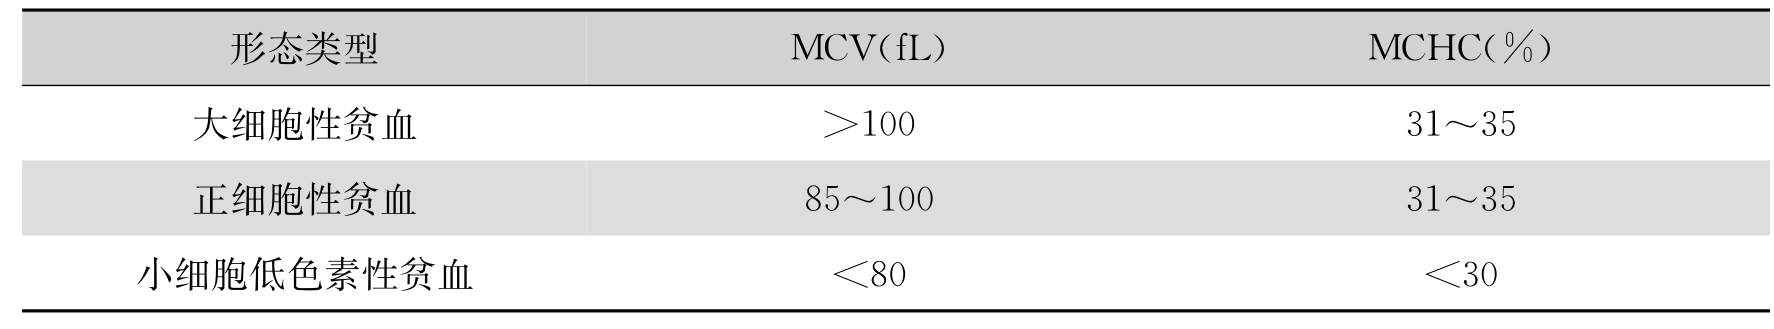
\includegraphics{./images/Image00164.jpg}
  \end{figure} 
 \FloatBarrier

\begin{figure}[!htbp]
 \centering
 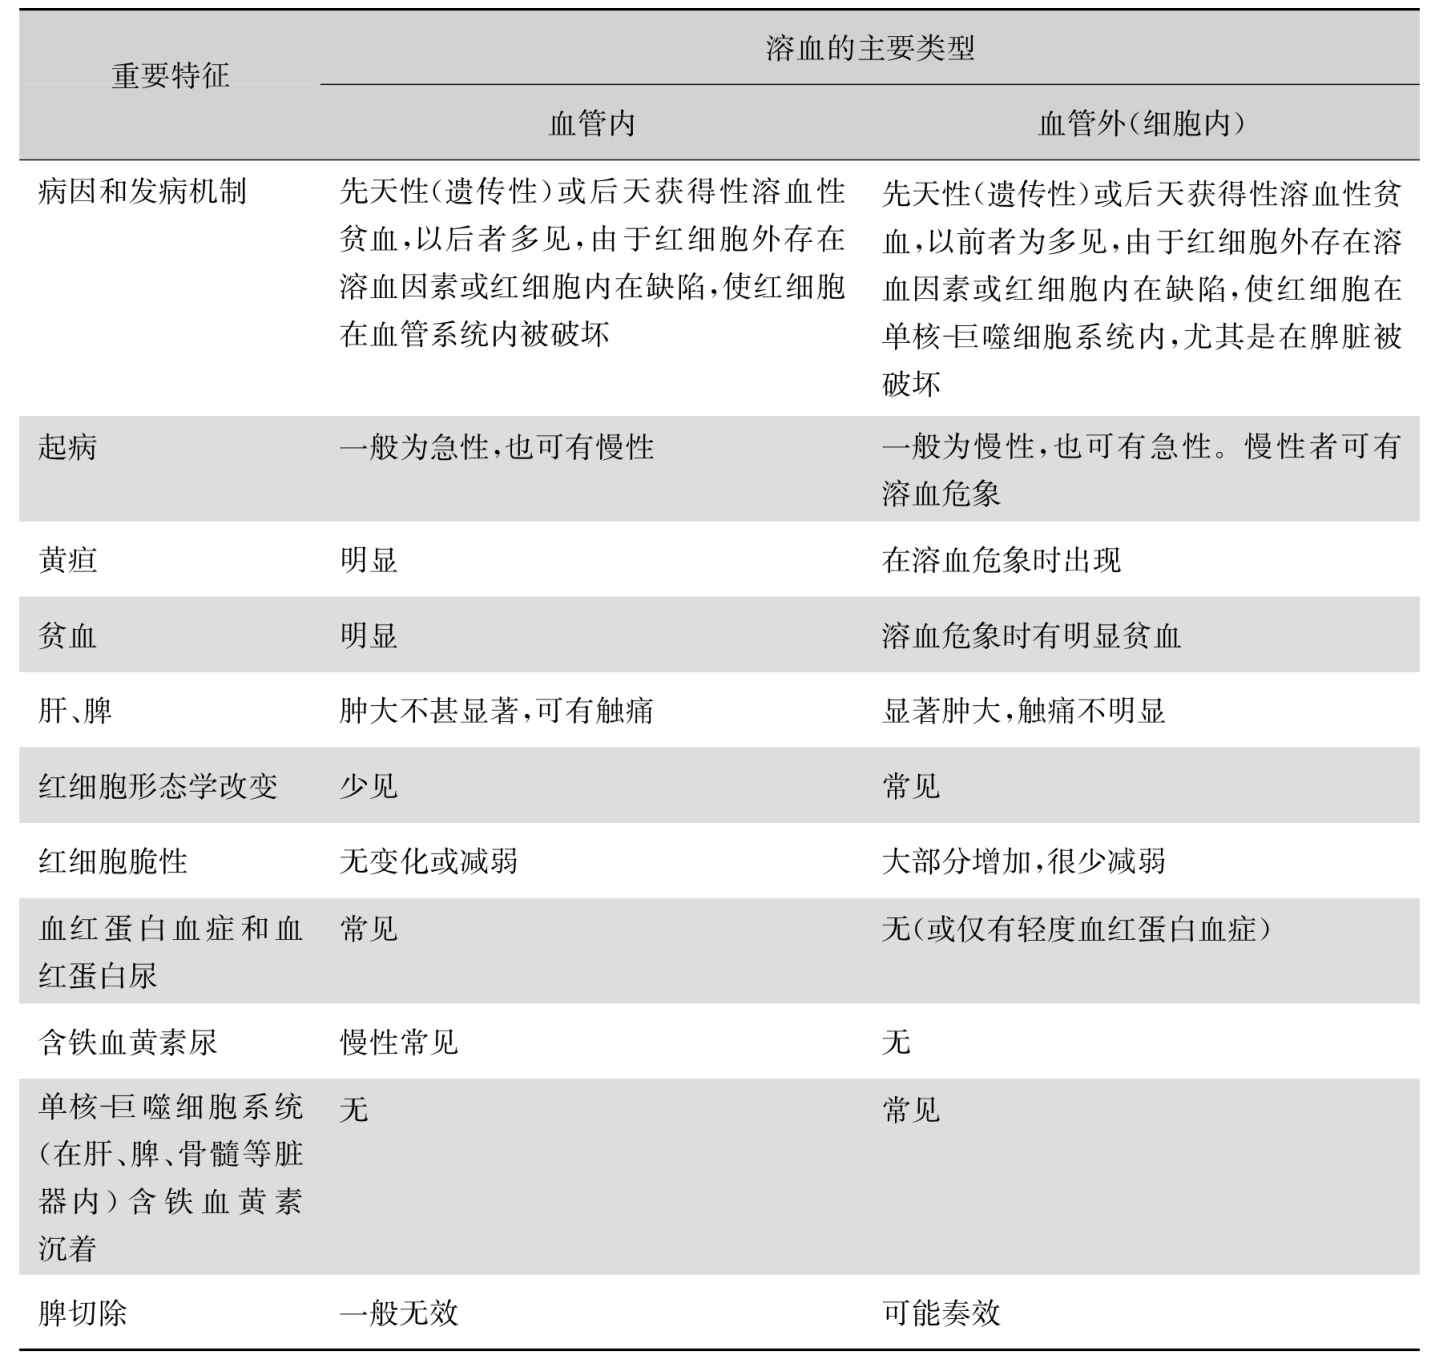
\includegraphics{./images/Image00165.jpg}
  \end{figure} 
 \FloatBarrier


\chapter{咯 血}

\section{12 咯血}

咯血是指喉及喉以下呼吸道或肺组织任何部位的出血,经口腔咳出者。咯血大多数为呼吸系统及(或)循环系统疾病所致,口腔、鼻腔或上消化道的出血有时易和咯血混淆。鼻腔出血多从前鼻孔流出,并常在鼻中隔前下方发现出血灶,较易诊断。有时鼻后部的出血量较多,特别是在睡眠时不自觉地坠入气道而于清晨咳出,较易误诊为咯血;如见血液从后鼻孔沿软腭或咽后壁下流,用鼻咽镜检查可以确诊。此外,还须检查有无鼻咽癌、喉癌、口腔溃疡、咽喉炎及牙龈出血的可能性。

呕血为上消化道出血,经口腔呕出,出血灶多位于食管、胃及十二指肠。咯血和呕血可根据病史、体征及其他检查方法进行鉴别,参见表\ref{tab4-1}。

\begin{table}[htbp]
\centering
\caption{咯血与呕血的鉴别}
\label{tab4-1}
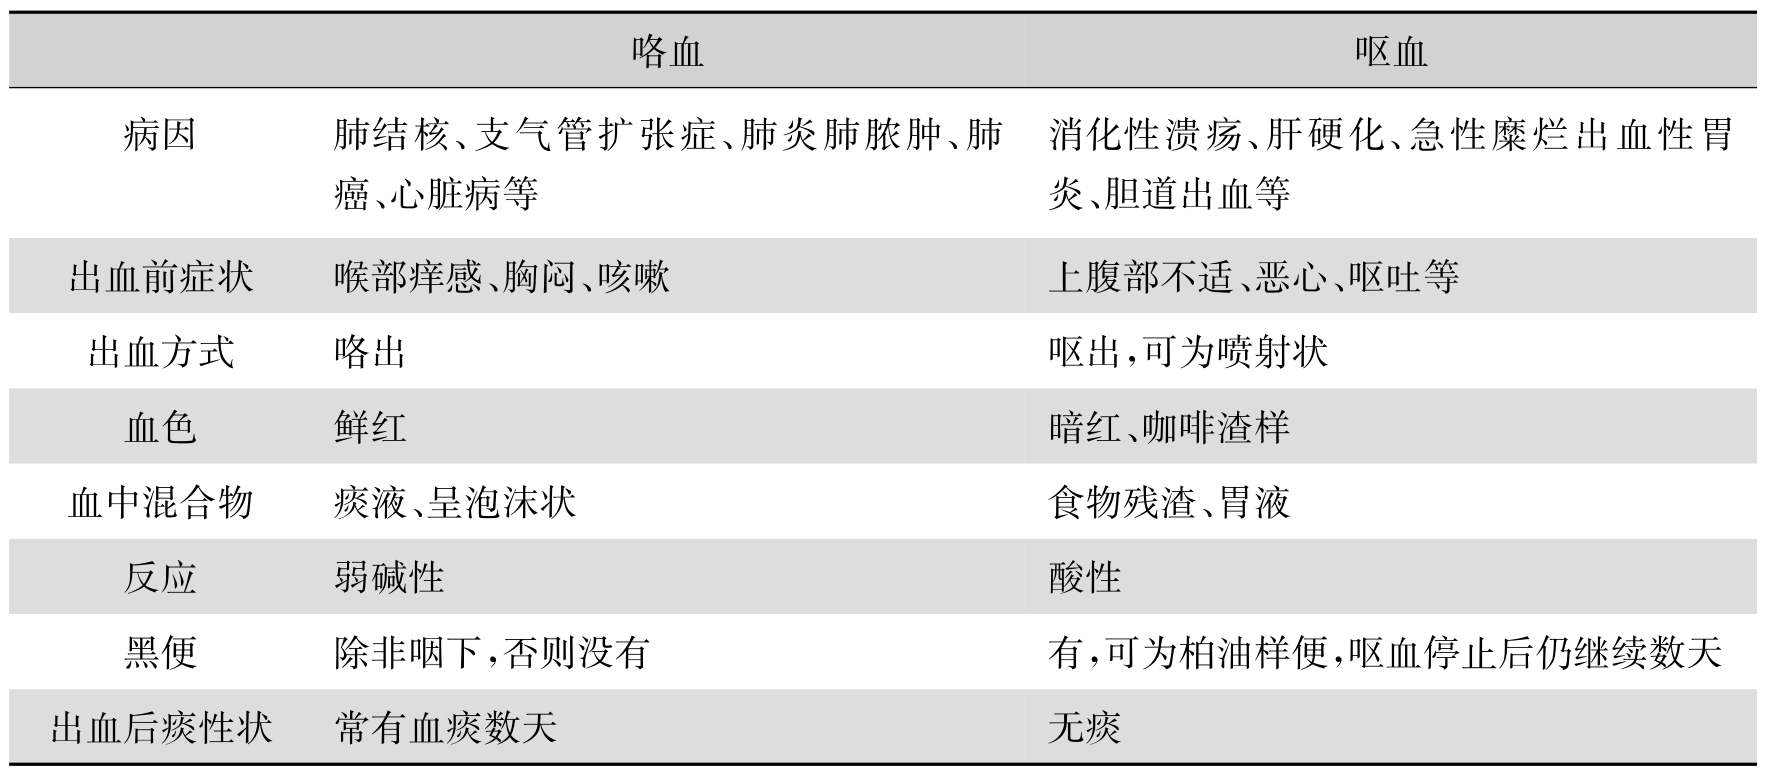
\includegraphics[width=5.89583in,height=2.59375in]{./images/Image00038.jpg}
\end{table}

区别咯血和呕血一般不难,但如患者出血急骤,量多或病史诉说不清时,有时鉴别并不容易;因此须详细询问有关病史,作细致的体格检查,及时作出诊断。

如已明确为咯血,须进一步探索其原因。引起咯血的原因很多(表\ref{tab4-2}),其中最常见的疾病是肺结核、支气管扩张、肺脓肿、支气管肺癌。此外支气管结石、肺寄生虫病、心血管疾病(特别是二尖瓣狭窄)、结缔组织病、钩端螺旋体病等也可引起咯血。

\begin{table}[htbp]
\centering
\caption{引起咯血的常见疾病分类}
\label{tab4-2}
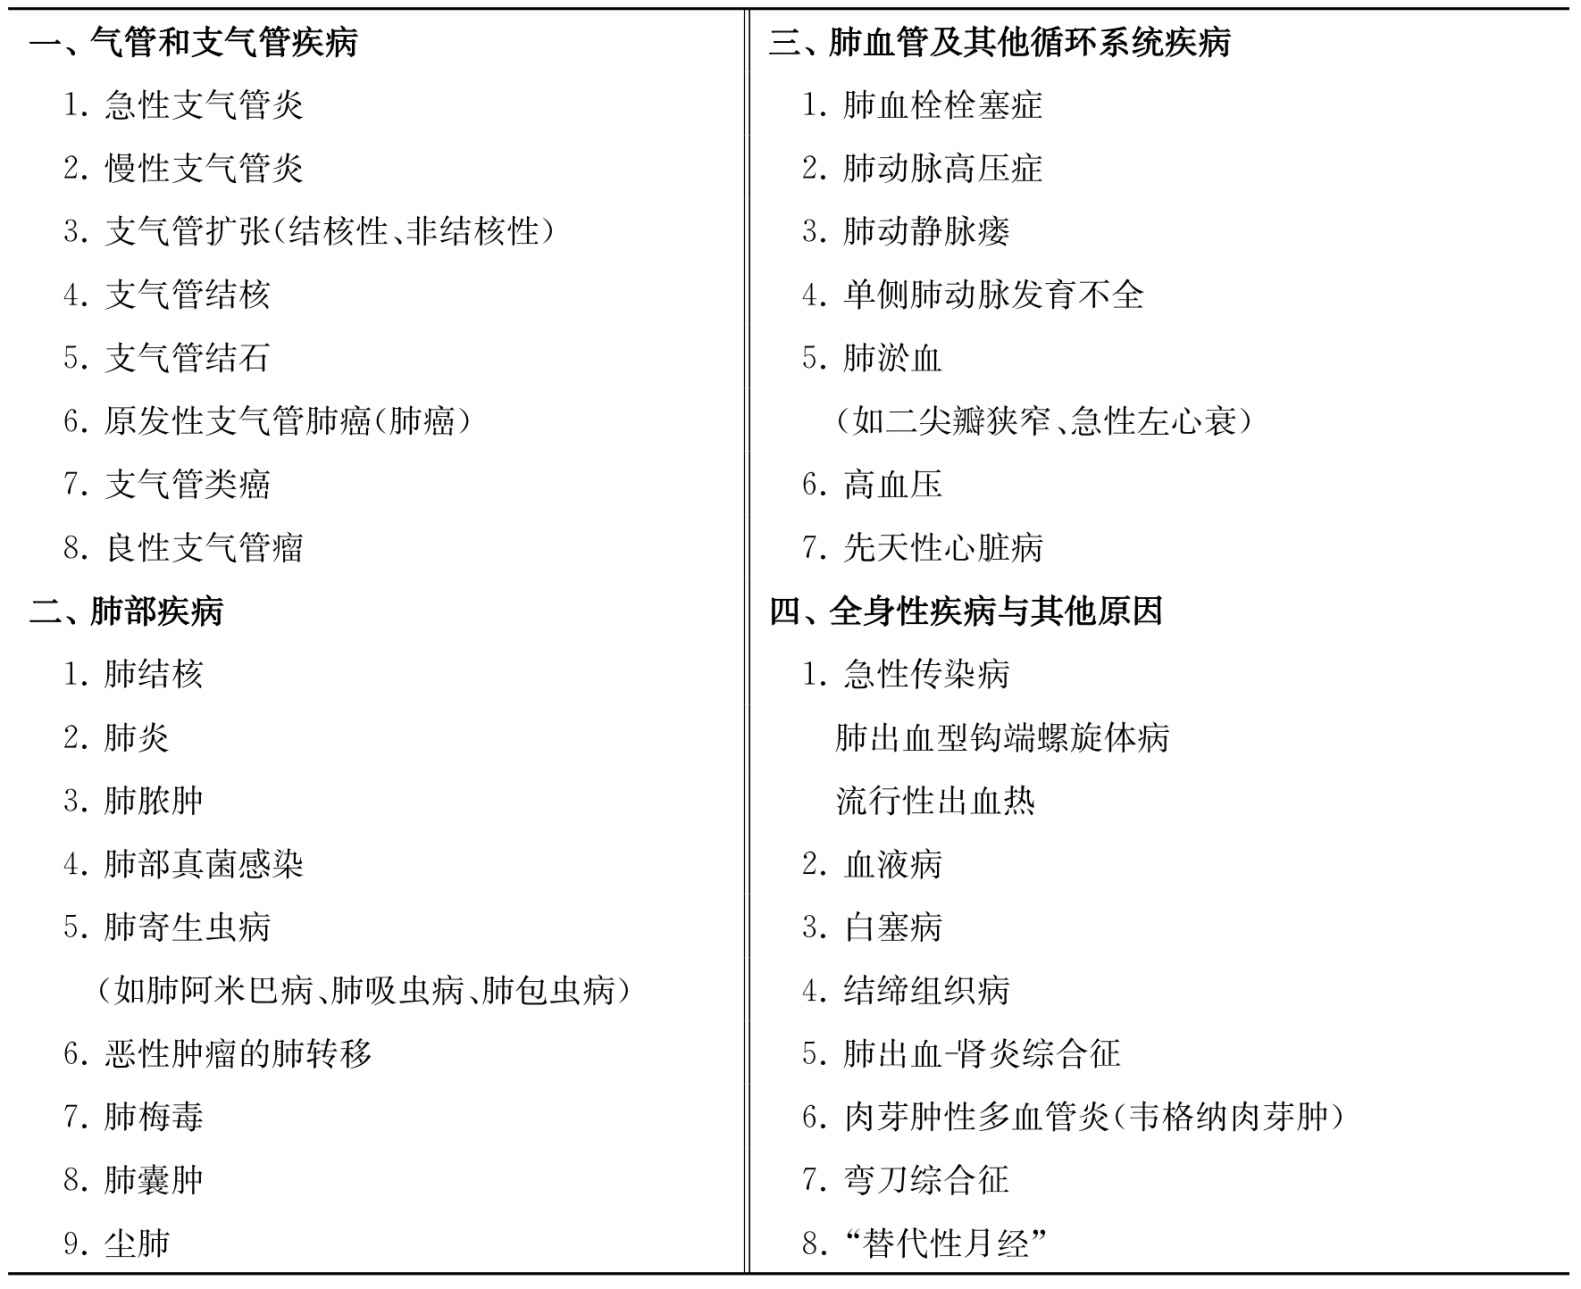
\includegraphics[width=5.89583in,height=4.80208in]{./images/Image00039.jpg}
\end{table}

如咯血量较大,应即采取急救措施,以尽早确定出血的部位。当X线检查的条件未具备时,可应用听诊法以确定。如咯血开始时一侧肺部呼吸音减弱或(及)出现湿啰音,而对侧肺野呼吸音良好,常提示出血即在该侧。气管和支气管疾病所致出血,全身症状一般不严重,胸部X线检查基本正常,或仅有肺纹理增粗;肺部病变所致出血,有比较明显的全身症状,胸部X线检查常发现病变阴影;必须指出,咯血可为全身疾病表现的一部分,临床医生必须对咯血患者做全身检查,以作出正确的诊断。

对于咯血患者,全面分析病史资料常可对咯血原因做出初步估计,同时还需要进一步做下列有关检查:

\subsection{1.病史}

须询问出血为初次或多次。如为多次,与以往有无不同。发生于幼年可见于先天性心脏病;儿童少年慢性咳嗽伴小量咯血和低色素性贫血,须注意特发性肺含铁血黄素沉着症;青壮年咯血多注意肺结核、支气管扩张等疾病;40岁以上有长期大量吸烟史(纸烟20支/
日×20年以上)者,要高度警惕支气管肺癌的可能性;年轻女性反复咯血也要考虑支气管结核和支气管腺瘤。在既往史上需注意幼年是否曾患麻疹、百日咳。在个人史中须注意结核病接触史、多年吸烟史、职业性粉尘接触史、生食螃蟹与蝲蛄史、月经史等。

细致观察咯血的量、颜色,有无带痰。肺结核、支气管扩张、肺脓肿、支气管结核、出血性疾病咯血颜色鲜红;肺炎球菌大叶性肺炎、肺卫氏并殖吸虫病和肺泡出血可见铁锈色血痰;烂桃样血痰为肺卫氏并殖吸虫病最典型的特征;肺阿米巴病可见脓血样痰呈棕褐色,带腥臭味;砖红色胶冻样血痰主要见于克雷伯杆菌肺炎;二尖瓣狭窄肺淤血咯血一般为暗红色;左心衰竭肺水肿时咳浆液性粉红色泡沫样血痰;并发肺梗塞时常咳黏稠暗红色血痰。大量咯血常由于空洞型肺结核、支气管扩张、慢性肺脓肿、动脉瘤破裂等所致;国内文献报告,无黄疸型钩端螺旋体病也有引起致命的大咯血。而痰中带血持续数周或数月应警惕支气管肺癌;慢性支气管炎咳嗽剧烈时可偶有血性痰。

详细询问伴随症状如发热、胸痛、咳嗽、痰量等。咯血伴有急性发热、胸痛常为肺部炎症或急性传染病,如肺出血性钩端螺旋体病、流行性出血热;咯血、发热同时伴咳嗽、咳大量脓痰多见于肺脓肿;长期低热、盗汗、消瘦的咯血应考虑肺结核;反复咳嗽、咳脓痰不伴有发热多见于支气管扩张。

\subsection{2.体格检查}

活动期肺结核和肺癌患者常有明显的体重减轻,而支气管扩张患者虽反复咯血而全身情况往往较好。有些慢性心、肺疾病可伴有杵状指(趾)。锁骨上淋巴结肿大在中老年患者要注意肺内肿瘤的转移。肺部闻及局限性哮鸣音提示支气管有狭窄、阻塞现象,常由肿瘤引起。肺部湿性啰音可能是肺部炎症的体征,也应考虑是否为血液存积在呼吸道所致。对咯血患者还应注意有无全身的出血表现。

\subsection{3.实验室检查}

痰检查有助于发现结核杆菌、真菌、癌细胞、肺吸虫卵等。出血时间、凝血时间、凝血酶原时间、血小板计数等检查,有助于出血性疾病的诊断。外周血红细胞计数与血红蛋白测定可推断出血的程度。外周血中嗜酸性粒细胞增多提示寄生虫病的可能性。

\subsection{4.X线检查}

对于咯血患者,除个别紧急情况不宜搬动外,均应做胸部X线检查。肺实质病变一般都能在X线胸片上显示阴影,从而及时作出诊断。如疑有空洞、肿块,或见肺门、纵隔淋巴结肿大,可加做胸部X线体层摄片或CT检查,CT还有助于发现细小的出血病灶。对疑有支气管扩张者,可做高分辨CT检查等协助诊断。对疑为支气管动脉性出血所致大咯血,必要时可行CT支气管动脉造影(CTA)或数字减影血管成像(DSA)检查,明确出血部位,后者尚可同时进行栓塞介入治疗。

\subsection{5.纤维支气管镜检查}

原因未明的咯血,尤其伴有支气管阻塞者,应考虑纤维支气管镜检查,可发现气管和支气管黏膜的非特异性溃疡、黏膜下层静脉曲张、结核病灶、肿瘤等病变,并可在直视下钳取标本作病理组织检查,吸取分泌物或灌洗液送细菌学和细胞学检查。

\subsection{6.其他检查}

先天性心脏病的诊断往往借助右心导管检查。放射性核素67镓对恶性肿瘤组织较健康组织有更大的亲和力,因而枸橼酸67镓肺部扫描可能有助于肺癌与其他肺部肿物的鉴别诊断。PET/CT对肺部肿瘤引起的咯血的诊断也有帮助。

咯血量的多少视病因和病变性质而不同,但与病变的严重程度并不完全一致,少则痰中带血,多则大口涌出,一次可达数百或上千毫升。临床上常根据患者咯血量的多少,将其分为少量咯血、中量咯血和大量咯血。但界定这三种情况的咯血量多少的标准尚无明确的规定,但一般认为24小时内咯血量少于100ml者为小量咯血;100~500ml/d者为中量咯血;>500ml或一次咯血量>100ml者为大量咯血。

临床上无异常肺部X线征象的咯血病例并不少见,诊断较为困难,其主要原因可能为:①气管或大支气管的非特异性溃疡,一般表现为小量咯血或血痰,支气管镜检查可以发现。②气管或支气管的静脉曲张,多见于右上叶支气管开口处或隆突部分,常引起大咯血,无痰,可经支气管镜检查而发现。③肺动脉瘤、支气管小动脉粥样硬化破裂,肺动静脉瘘破裂。④小块肺栓塞,常不易发现,一般有心脏病、下肢深静脉血栓形成、外伤史、长时间卧床或处于产褥期病史。⑤钩虫蚴、蛔虫蚴、血吸虫毛蚴、比翼线虫在肺内游移引起咯血。⑥早期支气管肿瘤,轻度支气管扩张、支气管结核,肺结核早期等。纤维支气管镜的广泛应用,结合胸部X线检查大大提高咯血病因的确诊率,国内一组917例经胸部X线与纤维支气管镜检查而确定的咯血病因如表\ref{tab4-3}所示:\footnote{*既有临床表现又有X线表现}

\begin{table}[htbp]
\centering
\caption{917例咯血的病因分析(X线诊断与纤支镜诊断比较)}
\label{tab4-3}
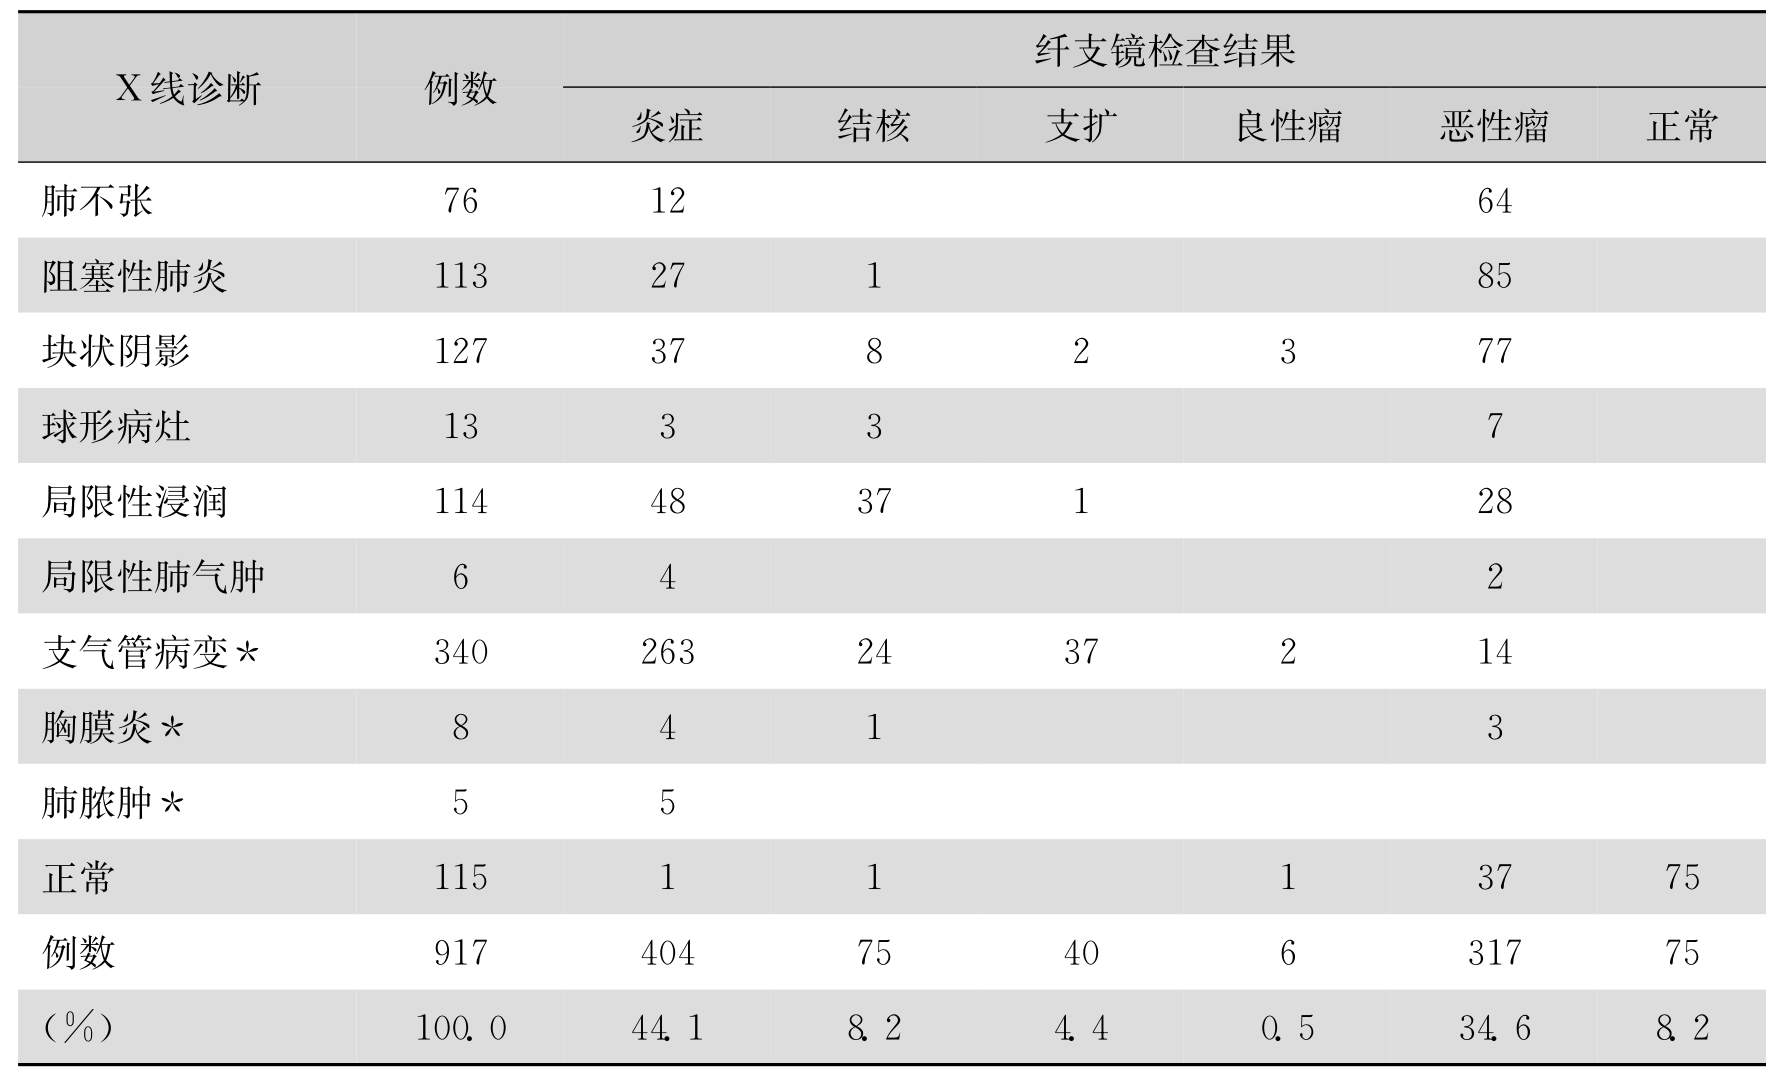
\includegraphics[width=5.91667in,height=3.58333in]{./images/Image00040.jpg}
\end{table}

由表\ref{tab4-3}所示,有部分咯血患者虽经X线和纤维支气管镜检查,仍未能发现阳性结果,且患者亦无引起咯血的全身性疾病,此类咯血可称为特发性咯血。但仍有可能在以后随诊中,在这类“特发性咯血”患者的一部分中,检出呼吸系统疾病。

国内曾有报告一组390例胸片无明显异常的咯血患者,作纤维支气管镜检查,结果发现肺癌16例(4.1\%)、支气管结核2例、支气管腺瘤1例,支气管囊性静脉曲张出血l例。作者认为咯血患者40岁以上,吸烟指数(吸烟年限×每天吸烟支数)>400,咯血时间长,且为痰血而非纯咯血者,尤须警惕肺癌的可能性。

X线胸片是咯血患者的常规检查,但可能无阳性发现。X线胸片正常的咯血患者应进一步作病因学诊断。有作者推荐应先作CT检查,以期发现潜在的肺部病灶,并有助于以后做纤维支气管镜检查时,有目标地进行刷检、活检取材,提高咯血的病因学诊断率。

\protect\hypertarget{text00057.html}{}{}

\subsection{12.1 气管和支气管疾病}

\subsubsection{一、急、慢性支气管炎}

急、慢性支气管炎患者有时也可咯血,一般为小量或痰中带血,不需治疗,可在数天内自行停止,但易于再发。如出血量大,需注意其他原因。本病的咯血与支气管炎症加剧有一定的关系,故咯血前常有病情加重的表现。慢性支气管炎患者发生持续的小量咯血时,须小心寻找其他原因,特别是支气管肺癌。

\subsubsection{二、非结核性支气管扩张}

非结核性支气管扩张可分为原发性与继发性。继发性者是由于支气管内或支气管外阻塞,引起支气管腔与支气管壁的感染,从而损害支气管壁的各层组织所引起。原发性支气管扩张则无明显的引起支气管阻塞的因素,但多数有肺炎病史,特别是麻疹、百日咳、流感等所继发的支气管肺炎史。

咯血是非结核性支气管扩张的常见症状,文献报告约90\%患者有不同程度的咯血,并作为提示诊断的线索。咯血可从童年即开始,常伴有杵状指(趾)。

此病的咯血有两种不同表现:

\paragraph{1.小量咯血}

在经常有慢性咳嗽、脓痰较多情况下,同时有小量咯血;有时在咯血前先有咳嗽较剧烈的一段感染加重阶段。因感染导致支气管内肉芽组织充血及损伤小血管而出现咯血。

\paragraph{2.大咯血}

由于支气管有炎症病变,血管弹性纤维被破坏,管壁厚薄不匀或形成假血管瘤,加上炎症影响,易破裂引起大咯血。咯血量每次达300~500ml以上,色鲜红,常骤然止血(因此类出血常来自支气管动脉系统,压力高,而动脉血管壁弹性好,收缩力强,故可较快止血)。

患者病程虽长,但全身情况尚好。咳嗽和咳痰也为常有的症状,咳嗽可轻微,也可相当剧烈;咳嗽和咳痰常与体位改变有关,如在晨起或卧床后咳嗽可加剧,咳痰增多。痰量可为大量,每天达数百毫升(湿性型)。痰液静置后可分为三层:上层为泡沫状黏液,中层为较清的浆液,下层为脓液及细胞碎屑沉渣。有些患者痰量甚少(干性型),如合并感染,痰量随之增多,并有发热、咯血等。

支气管扩张的好发部位是下肺,以左下叶较右下叶为多见,最多累及下叶基底段,病灶可延伸至肺边缘。病变部位出现呼吸音减弱和湿性啰音,位置相当固定,体征所在的范围常能提示病变范围的大小。

胸部X线平片检查不易确诊本病。国内一组84例非结核性支气管扩张中,只1/3病例在胸部X线平片上有少许的征象,大部分甚至没有任何改变。胸部X线平片检查对排除慢性肺脓肿及慢性纤维空洞型肺结核颇有帮助。如患者有支气管扩张的临床表现,X线胸片又显示一侧或双侧下肺纹理增粗、紊乱以及蜂窝状小透亮区,或见有液平面则支气管扩张的可能性最大,胸部CT检查可确定诊断,并对明确病变部位及决定治疗方案有重要意义。

全内脏转位、支气管扩张、鼻窦病变三联症,又称Kartagener综合征,国内有少数病例报告。此综合征有咳嗽、咳痰、咯血等症状。咯血可从童年开始,反复发作,量不多。

\subsubsection{三、结核性支气管扩张}

结核性支气管扩张的症状因肺内结核病灶的情况而定,如肺结核病灶不严重,则可无明显症状。有时或可闻及少许干、湿性啰音。X线胸片上显示病灶似已硬结,而患者仍有或多或少的咯血,应考虑结核性支气管扩张的可能性。国内一组64例患者中,发病大多在30岁以上,90\%有咯血(痰中带血或大量咯血)。病灶部位大都在两肺上叶,尤以右上叶的后段、左上叶的尖后段多见。

结核性支气管扩张与非结核性支气管扩张的鉴别见表\ref{tab4-4}。

\subsubsection{四、支气管结核}

支气管结核一般为继发性,原发性者罕见。患者大多有咯血,其他常见症状为阵发性剧烈咳嗽、喘鸣、阵发性呼吸困难等。有时轻度动作即可引起呼吸困难与发绀。如发生支气管阻塞,则引起突然的发热、痰量减少,而阻塞解除后痰量突然增加,体温也下降。

\begin{table}[htbp]
\centering
\caption{结核性与非结核性支气管扩张的鉴别要点}
\label{tab4-4}
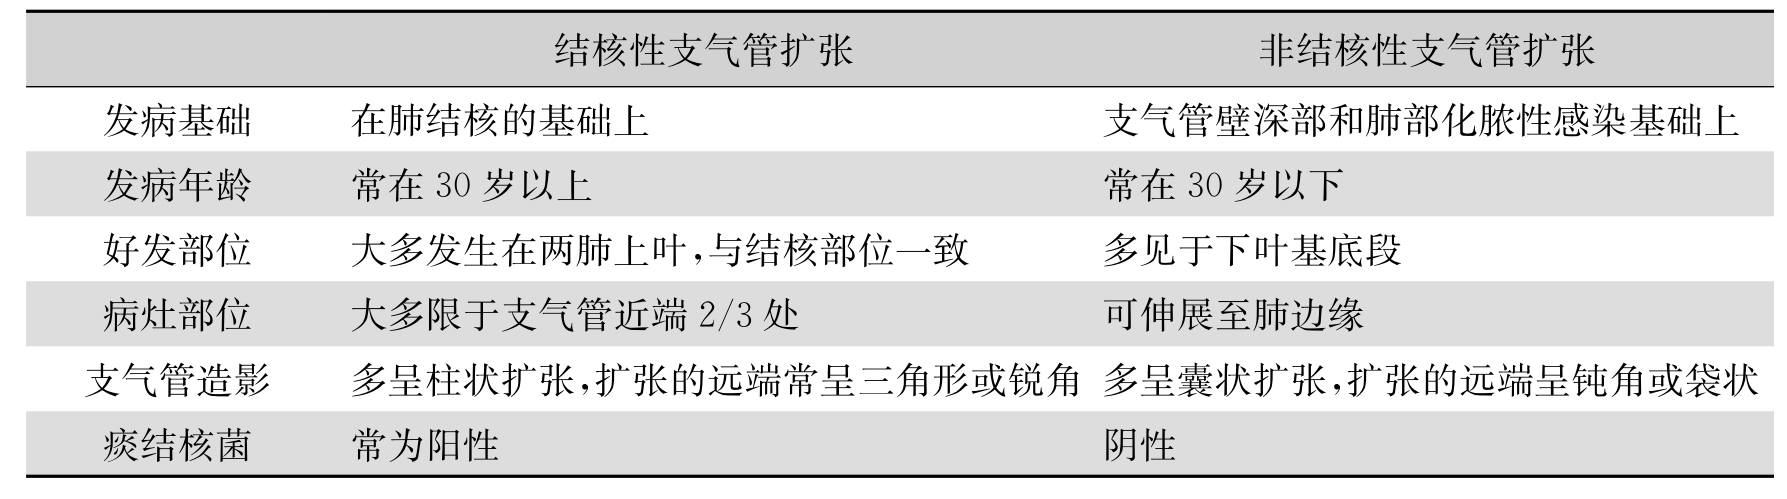
\includegraphics[width=5.94792in,height=1.65625in]{./images/Image00041.jpg}
\end{table}

支气管结核是发生于气管、支气管黏膜或黏膜下层的结核病变。据国内报告,肺结核合并支气管结核者占23.6\%~57.1\%。患者以青壮年为多,文献报告女性罹患多于男性,常发生于慢性纤维空洞型肺结核、慢性血行播散型肺结核、支气管淋巴结结核、浸润型肺结核及干酪样肺炎等基础之上。这些患者有下列情况提示有支气管结核的可能:①反复小量咯血或血痰而X线胸片未见明显病变者;②药物难以控制的刺激性咳嗽;③有喘鸣音;④有不同程度的呼吸困难而不能用肺实质病变解释者;⑤肺无明显病变而痰结核菌屡为阳性;⑥肺内有新播散病灶而不能用其他原因解释;⑦肺结核并发肺不张;⑧某些肺野空洞:在萎陷疗法后产生的张力性空洞;空洞时大时小;出现圆形、薄壁空洞;肺门附近的空洞等。

支气管结核的确诊须依靠纤维支气管镜检查。如临床症状典型,虽纤维支气管镜检查阴性,也不能除外此病的存在。

近年国内一组单纯气管、支气管结核病28例报道,误诊颇多,原因为:①胸片无异常发现;②胸片虽出现局限性肺气肿、肺纹理密集、肺纹理粗乱、叶间胸膜影移位等异常表现,但又非特异性而未加注意。作者建议对干咳、胸闷、喘息、咳黏液痰或咯血患者,经抗感染及对症治疗2周未见好转时.应及早作纤维支气管镜检查,镜下刷检涂片染色找抗酸杆菌,或钳取组织做病理检查。镜下所见仍疑似结核而实验室检查阴性时,2周后应再做纤维支气管镜检查。

目前将刷检标本或支气管肺泡灌洗液进行PCR检测结核分枝杆菌,可大大提高病原学诊断率。

结核感染T细胞斑点(T-SPOT.TB)试验是近年来的一项新诊断技术,通过检测外周血分泌γ-干扰素的T淋巴细胞数量来诊断结核感染,具有较高的特异性和敏感性,且不受卡介苗接种和环境分枝杆菌感染的影响,在肺结核的筛查和诊断中有较好的应用价值。

\subsubsection{五、支气管结石}

本病的特点为反复咯血,而肺部除有钙盐沉积之外,无其他原因可解释。患者或曾有咳出结石史。咯血通常为小量,但有些患者可有大咯血。X线检查发现有支气管结石阴影,以右中叶根部较为多见,结石远端可发现有阻塞性肺不张或肺部感染,CT检查可见支气管阻塞远端有钙化影。纤维支气管镜检查可帮助诊断。支气管结石常由肺结核病灶钙化引起。X线胸片上如炎症病变相应部位有钙化结节,在炎症消退后而咯血不断者,则支气管结石的可能性甚大。

据国内一组20例的报告中,以咯血为主要症状者占95\%,其中威胁生命的大咯血占40\%。误诊率60\%。并发症(占85\%)表现为肺不张、支气管扩张、阻塞性肺炎等。但手术治疗效果好。X线断层摄片、胸部CT和纤维支气管镜检查等综合检查对诊断有较大帮助。

\subsubsection{六、原发性支气管肺癌(肺癌)}

本病大多见于40岁以上男性,文献报告有咯血者占50\%~70\%,国内一组141例报告中,第一个月内出现咯血者有38.3\%。中央型肺癌较周围型肺癌易引起咯血。癌组织内小血管较多,患者又常有刺激性咳嗽,易引起癌组织损伤而致出血。其特点是痰中带血或小量咯血多见,而大量咯血少见,但晚期可有致命性大咯血。咳嗽是较常见的早期症状,无痰或有少量的白色黏液痰,可伴有胸痛。间断的或持续的小量咯血,对提示此病的诊断有重要意义。痰中可混有小颗粒状灰白色坏死组织,其中较易找到癌细胞。X线胸片、纤维支气管镜、胸部CT及活组织病理检查有助于诊断。

国内一组确诊肺癌患者1105例中,纤维支气管镜下直接见到肿瘤病灶(直接征象)者638例(57.7\%),只见肿瘤间接征象,即支气管黏膜改变者412例(37.3\%)。肺癌多见于段以上的支气管(中央型肺癌约占3/4),有些病例第一次活检及刷检均未能确诊,需做第二次,偶尔还要第3~4次检查。当发现有间接征象的可疑病例,应尽可能多部位活检多取标本,甚至看到癌体也应多点活检。

\subsubsection{七、支气管类癌}

支气管类癌罹患多为中年人,男女性别无差异,生长慢,具有恶性程度低和较少发生转移的特点。早期症状常为咯血,术后长期生存率较高。国内一组17例报告中,患者40岁以下者占64.7\%,中央型12例,周围型5例,2例有支气管旁淋巴结转移,主要临床表现为咳嗽、咳痰、咯血或痰中带血、发热和反复发作肺部炎症。临床上本病易误诊为肺癌、结核球或良性支气管肿瘤。X线检查与纤维支气管镜下活检对诊断帮助较大。

\subsubsection{八、良性支气管瘤}

良性支气管瘤少见,发病多在30~40岁之间。全身情况良好的中年患者如有反复的小量咯血或痰中带血,或类似哮喘发作,或屡次发作的呼吸道阻塞及感染症状,应考虑此病的可能。由于肿瘤生长缓慢,临床症状可延续多年。早期可无症状,或仅有气喘、干咳,有时甚至被误诊为支气管哮喘。肿瘤逐渐增大而堵塞支气管时,可发生相应肺叶的肺不张,并在肿瘤的远侧发生感染与支气管扩张。X线体层摄片、胸部CT,可了解较大的支气管内肿瘤的范围及部位,气道阻塞情况及继发性支气管扩张,对诊断有重要帮助。由于良性瘤多发生于较大的支气管内,纤维支气管镜检查的检出率可达85\%~90\%。

良性支气管瘤有腺瘤、平滑肌瘤、乳头状瘤等,此外较罕见的有纤维瘤、软骨瘤、脂肪瘤等。其中腺瘤比较多见,典型X线征象为肺门附近有圆形或类圆形阴影,密度均匀一致,边缘锐利,体层摄片或胸部CT检查更易于发现;由于多数腺瘤位于主支气管或肺叶支气管内,纤维支气管镜检查易作出诊断。

\protect\hypertarget{text00058.html}{}{}

\subsection{12.2 肺部疾病}

\subsubsection{一、肺结核}

咯血是肺结核患者常见的症状,且常为提示此病诊断的线索。咯血量多寡不一,少可仅为痰中带血,多则一次可达500ml以上,血色鲜红。咯血与结核病变的类型有一定关系,多见于浸润型肺结核、慢性纤维空洞型肺结核、干酪样肺炎,而少见于原发综合征(原发型肺结核)和急性血行播散型肺结核。咯血严重程度并不一定与病灶大小成正比,小的病灶可有较多的咯血,而病灶广泛的也可无咯血。出血量常和血管损害程度有关,血管壁渗透性增高所致的咯血,出血量少,但持续时间较长;小血管的破裂则多引起小量出血,这往往由于慢性活动性肺结核所致;大咯血多为肺动脉分支破损所致,其中以空洞内形成的动脉瘤破裂所致的大咯血多见,此类出血来势甚急,而由于洞壁纤维化不易收缩止血,或血凝块虽能填塞空洞压迫血管暂时止血,但又可因血块溶解而再次出血。

肺结核患者以青壮年占大多数,不少患者以咯血为初发症状而就诊。咯血之后常有发热,是由于病灶播散及病情发展所致。患者常同时出现疲乏、纳差、体重减轻、午后潮热、盗汗、脉快和心悸等全身中毒症状。

肺结核的诊断主要依靠症状、体征、X线胸片和痰结核菌检查。如在青壮年人一侧肺尖部经常听到湿性啰音,又有上述全身性中毒症状,则支持活动性肺结核的诊断。X线胸片是诊断肺结核的重要方法,可以发现早期轻微的结核病变,确定病灶的范围、部位、形态、密度、与周围组织的关系,判断病变的性质、有无活动性、有无空洞、空洞大小和洞壁特点等。因此,定期进行胸部X线检查能及早发现病灶,有助于早期治疗。

痰结核菌检查阳性可确诊为肺结核,且可肯定病灶为活动性。但痰结核菌阴性并不能否定肺结核的存在,对可疑病例需反复多次痰液涂片检查,如有需要,可采用浓集法、培养法、PCR法等,在咯血前后,因常有干酪性坏死物脱落,此时的痰菌阳性率较高。

长期被误诊为肺结核咯血的肺部疾病并非少见,文献报道有支气管扩张、支气管囊肿、肺癌、肺脓肿、肺吸虫病等。

年轻患者反复咯血,痰结核菌检查阴性,全身情况较好,而病灶又处于中、下肺野,用一般抗菌药物治疗能改善炎症表现者,则可认为是非结核性支气管扩张,胸部CT检查有助于确定诊断。支气管囊肿在胸部平片及透视下一般可确定诊断。非结核性支气管扩张或支气管囊肿合并普通细菌感染时,其症状的出现通常较早,可追溯到童年时期,特别是在患麻疹、百日咳之后常有咯血及呼吸道炎症症状,其与肺结核病的鉴别是前两者在长期的病患过程中,全身一般状况仍较好,无结核病的全身中毒症状,可伴有杵状指(趾),痰结核菌阴性。

肺癌被误诊为肺结核者颇为常见。在下列情况下,应考虑肺癌的可能:①年龄在40岁以上,尤其是长期重度吸烟的男性患者,新近出现反复的咯血或持续的痰中带血,或近肺门处有致密的异常阴影,或出现肺不张合并感染,而多次痰液检查未发现结核菌者,应首先考虑肺癌的可能;但痰中结核菌阳性也不能除外肺结核与肺癌并存。②肺癌组织内部发生坏死破溃,坏死组织排出后形成空洞,其X线征象可酷似结核性空洞。但癌性空洞常呈偏心性,其内侧壁凹凸不平,外缘多呈毛刺状、分叶状,常无病灶周围卫星灶,多次痰结核菌检查阴性,经规律的抗结核治疗无效,病灶逐渐增大,这些均可与肺结核鉴别。③肺癌和肺结核并存,肺癌可发生在陈旧性肺结核瘢痕的基础上,而肺癌又能促使结核病灶恶化。如在陈旧性或活动性结核病灶处出现新的、致密的圆形病灶,且经积极抗结核治疗一个月后,病灶仍逐渐增大,或出现肺不张、肺门阴影增大,癌性空洞等改变,应考虑并存肺癌的可能。

\subsubsection{二、肺 炎}

在急性肺炎时,肺实质处于高度充血状态,小血管通透性增加并可发生破裂而致咯血。由于小血管可发生血栓性脉管炎,致血管腔闭塞,通常不易引起大量咯血。

肺炎链球菌肺炎的患者,痰中混有血液者并不少见,有时血量可达20~30ml,病期第2、3天转为铁锈色痰。在整个病程中均呈血性痰的甚少。

肺炎杆菌性肺炎多为砖红色稠胶样痰;化脓性链球菌肺炎咳粉红色稀痰;葡萄球菌肺炎可为血性痰、脓性痰;绿脓杆菌肺炎咯血少见,典型者咳翠绿色脓痰。军团菌肺炎少量黏液痰中可带血丝,并有发热、咳嗽、肌痛、关节痛、腹泻、蛋白尿、转氨酶升高、直接荧光抗体阳性或间接荧光抗体1∶256。肺炎支原体肺炎约1/4病例有血性痰,但绝无铁锈色痰;流感病毒性肺炎常引起反复的小量咯血。

\subsubsection{三、肺脓肿}

肺脓肿多由于吸入感染或血源性感染所引起,约50\%患者伴有咯血,常伴有大量脓痰或脓血样痰。急性肺脓肿的早期可有大量的咯血而无脓痰,但此时有寒战、高热、胸痛、血白细胞和中性粒细胞增高,提示急性细菌性感染,1周后可出现大量脓性痰。慢性肺脓肿常有大量的脓痰或脓血痰,痰量每天可达300~500ml,带臭味,痰静置分层,多数患者伴有杵状指。慢性肺脓肿常被误诊为肺结核病,前者可根据急性发病史、X线胸片见大片浓密模糊浸润阴影,脓腔内出现圆形透亮区及气液平面,痰培养可有致病菌生长以及抗菌治疗有效,一般鉴别不难。慢性肺脓肿与肺癌的区别,可根据肺脓肿过去的急性发病史、空洞的特点及痰中癌细胞检查等加以鉴别,X线胸片、纤维支气管镜、胸部CT扫描有利于诊断。癌性空洞与肺脓肿空洞、结核性空洞的鉴别参见表\ref{tab4-5}。

\begin{table}[htbp]
\centering
\caption{癌性空洞与肺脓肿空洞、结核性空洞的鉴别}
\label{tab4-5}
\includegraphics[width=5.97917in,height=3.53125in]{./images/Image00042.jpg}
\end{table}

\subsubsection{四、肺部真菌感染}

肺部真菌感染是最常见的深部真菌病,主要由念珠菌、曲霉、毛霉、新型隐球菌等真菌感染所致。老年、幼儿及体弱者易患此病,多为痰中带血或小量咯血。常见症状有发热、乏力、盗汗、纳差、消瘦、咳嗽、胸痛;痰的特点是量少,不同种类的真菌感染时,其痰的性状不一。肺白念珠菌感染,为胶样黏稠痰,带乳块或血丝;肺曲霉病反复咯血或咳出大量泡沫痰(可带酒味);肺新型隐球菌病则咳小量黏液性痰或血丝痰。病原学检查可找到致病菌,胸部X线检查,肺组织病理检查有助于诊断。

\subsubsection{五、肺寄生虫病}

\paragraph{1.肺阿米巴病}

阿米巴性肺脓肿为肝阿米巴病并发症之一,也可来自肠道病灶。多数起病较慢,常有发热、乏力、消瘦、咳嗽、咳痰、右下胸痛并放射至右肩,少数呈急性发病,高热、胸痛、呼吸困难等,可有肝脏肿大体征。典型的痰液呈棕褐色而带腥臭味,有助于此病的诊断。如合并出血或混合感染,可呈血性或黏液脓血痰。痰液、胸腔积液或纤维支气管镜取病变坏死组织中查找到溶组织阿米巴滋养体可确诊。

\paragraph{2.肺吸虫病}

本病有严格的地区性,患者都曾有在疫区进食未煮熟的含有肺吸虫囊蚴的石蟹或蝲蛄史。病程中常反复的小量咯血,痰血混合多呈特殊的棕黄色或铁锈色,烂桃样血痰是肺吸虫病最典型特征。早期症状有畏寒、发热、脐周隐痛、腹泻,并有乏力、盗汗、纳差,2~3周后出现咳嗽、胸痛、咯血等,患者虽有长期的反复咯血,但全身情况尚好,胸部体征多不明显,可有皮下结节。常有血嗜酸性粒细胞增多,痰中发现肺吸虫卵即能确诊,阳性率90\%以上。粪便虫卵检查、肺组织病理检查、免疫学检查、X线检查等有助于诊断。

胸部X线检查有较特别的征象,病灶多位于中、下肺野及内侧带,因病变的不同时期而有下列的表现:①早期呈边缘模糊的弥漫阴影,大小约为1~2cm;②中间期为边缘清楚、多房或单房的、实质或囊状的大小不等的阴影,多房性囊状阴影是本病的X线特征;③晚期为纤维增殖性变及硬结钙化阴影。此外,可有肺门增大、肺纹理增粗紊乱、胸腔积液或胸膜增厚等征象。对一些疑难的、不典型的病例,流行病学调查和免疫学检查,在诊断上有重要意义。

如患者有上述的流行病学史和胸痛、咳铁锈色痰等症状,血嗜酸性粒细胞增多,痰中虽未发现肺吸虫卵,而肺吸虫抗原皮内试验阳性,并已除外血吸虫病、华支睾吸虫等感染时,则大致可作出肺吸虫病的临床诊断,并应进行特效药物(如吡喹酮)的诊断性治疗;如疗效显著,可进一步确立诊断。肺吸虫病主要须与肺结核相鉴别(表\ref{tab4-6})。

\begin{table}[htbp]
\centering
\caption{肺吸虫病与肺结核鉴别}
\label{tab4-6}
\includegraphics[width=5.94792in,height=4.91667in]{./images/Image00043.jpg}
\end{table}

在四川及福建发现的肺吸虫病,临床表现较特别,其症状轻,咯血量较小,痰中虫卵检出率较低,有游走性皮下结节者甚多(多分布于胸壁及上腹壁),血中嗜酸性粒细胞显著增多。

国内报道肺吸虫病误诊率较高。主要原因是由于肺吸虫病临床表现及X线胸片大多无特异性,且典型的游走性皮下结节,肺空泡、结节和隧道线条等X线表现又少见。一组报道34例肺吸虫病在入院前全部误诊为肺结核。

由于肺吸虫病免疫学诊断的敏感性和特异性高,且简便易行,在流行区内患者有生食石蟹或蝲蛄史,而反复出现咳嗽、咯血或痰中带血、发热等症状,应即作肺吸虫抗原皮内试验,上述一组误诊为肺结核的34例患者,肺吸虫抗原皮内试验全部为1∶2000以上阳性。应用混合单抗双抗体夹心ELISA法诊断疑难肺吸虫病,效果更佳。

\paragraph{3.肺包虫病}

肺包虫病是棘球绦虫的幼虫(棘球蚴)寄生于人体肺内所引起,主要流行于畜牧区,以青壮年农民和牧民为主,早期可无症状。当包囊肿大破裂时可出现咯血或痰中带血,并可咳出类似粉皮样的角皮膜;合并感染时则出现咳嗽、咳痰、胸部不适,或胸痛及劳力后气促等症状。可有肝脏或其他部位囊肿征象。囊肿破裂,囊液亦可阻塞气管而引起窒息。X线胸片或CT扫描有助于诊断,可显示包虫圆形或卵圆形,略呈分叶状阴影,边缘清晰,密度均匀,壁可钙化,阴影随呼吸而变形;包虫囊壁破裂,空气进入,则顶部呈现半月形透亮带。包虫抗原皮内试验及补体结合试验对本病有重要的诊断意义,阳性率可达90\%以上。此外,痰检查、B超检查、放射性核素扫描等对诊断也有帮助。

\subsubsection{六、恶性肿瘤的肺转移}

恶性肿瘤转移至肺部时,可引起咯血。较常发生肺部转移的恶性肿瘤有鼻咽癌、乳腺癌、食管癌、胃癌、肝癌、结肠直肠癌、前列腺癌、睾丸畸胎瘤、精原细胞瘤、绒毛膜上皮细胞癌、恶性葡萄胎及类癌等。以绒毛膜上皮细胞癌、睾丸畸胎瘤和恶性葡萄胎的肺转移的咯血发生率最高。对成年女性原因未明的咯血,患者阴道曾排出水泡样胎块,或兼有流产后持续的不规则阴道出血,应考虑恶性葡萄胎或绒毛膜上皮细胞癌的可能性,尿妊娠诊断试验有助于此病的诊断。

转移性肺恶性肿瘤常为多发,但也可为单发,后者较少见。X线胸片显示多发性肺转移肿瘤的形态多为圆形、卵圆形或粟粒状阴影,大小相仿,边缘不整,发展较快。转移性肺恶性肿瘤原发病灶的诊断有时不易,须设法寻找。

\subsubsection{七、肺梅毒}

本病极为少见,国内仅有二例感染报告,均有咯血。病程进展缓慢,往往有咳嗽、咯血、胸痛等症状,虽然X线胸片显示下肺野呈大片状实质模糊阴影,但全身情况良好。诊断须依据梅毒感染史、梅毒血清反应阳性与驱梅治疗的疗效。肺梅毒须与其他肺部疾病相鉴别,特别是肺结核病。

\subsubsection{八、肺囊肿}

肺囊肿可区分为先天性与后天性两类,以前者较为多见,后者是由肺部感染性疾病或寄生虫所引起。多发性先天性肺囊肿常伴有支气管扩张,多在儿童期出现症状,其临床表现与支气管扩张相似,患者往往因突然小量咯血或痰中带血而就诊,由于病变多位于中、上肺,引流较好,较少出现发热。X线胸片检查呈圆形透亮影,其壁菲薄而整齐;多发者大小不一,可分布于任何肺野,但以中、上肺野较多见。

多发性先天性肺囊肿需与支气管扩张鉴别。肺囊肿继发感染时可出现大片状模糊阴影,类似浸润性肺结核,但经抗生素治疗后感染较快消退,而有别于肺结核。肺囊肿合并感染时,其临床症状和X线胸片的改变与肺脓肿相似,需加以鉴别。

国内曾报告一组82例的成年患者中,52例(63.4\%)有咯血,多数在200ml以下,认为如有下列情况应考虑本病:①肺部阴影长期存在;②阴影在同一部位反复出现;③无播散灶;④阴影新旧程度一致;⑤肺门及纵隔淋巴结不大。患者虽反复咯血而无结核中毒症状。胸部CT检查有助于对本病的诊断。

近年肺囊肿有一组38例报告,发病常在青少年期,5例初发年龄在10岁以下。全部患者(38例)在院外均被误诊为肺结核。初发症状以咯血或痰中带血多见(21/38),咳嗽、咳痰、发热次之。6例无症状患者经体检而发现本病。21例有长期反复出现咯血或痰中带血史,最长者达20年。

肺囊肿的胸部X线表现常缺乏特征性。作者认为以下几点有利于肺囊肿的早期诊断:①发病年龄在30岁以下,特别是男性,有反复咯血或痰中带血、咳嗽、发热史。②动态观察X线胸片阴影的形态变化不大,无肿瘤的淋巴结、淋巴道远处转移的改变。③结核菌素试验阴性或经积极的抗结核治疗无效。④胸部X线显示其病变虽无固定部位但与支气管走向有关;虽经反复感染但病变部位固定不变;在非囊肿部位不出现新的病灶。⑤有条件时应作高分辨胸部CT检查加以鉴别。⑥经上述不能确诊时应考虑肺活检或外科手术探查。

\subsubsection{九、尘 肺}

包括硅沉着病和其他尘肺,是由于长期吸入某种粉尘所致的以肺实质弥漫性纤维病变为主的疾病。主要发生于从事粉尘作业的工人,可有慢性、顽固性咳嗽,咳泡沫状痰、咯血或痰中带血,气短和胸痛。早期症状不明显,常为干咳或带黏稠痰,晚期咳嗽加重,痰多,如合并肺结核或支气管扩张,可反复大咯血。晚期病情重,有发绀、杵状指、肺气肿、肺源性心脏病等表现。胸片可见中、下肺野呈网状、条索状或结节状阴影改变,肺门淋巴结肿大。其诊断主要依据为职业病史、临床表现、胸部X线征象及肺功能检查。

硅沉着病合并肺结核比无硅沉着病的发病率高4~5倍,其特点是肺结核的发生率和严重程度与硅沉着病的发展程度成正比,硅沉着病愈严重,其并发肺结核的可能性愈大,肺结核病的病变发展也愈迅速,病情愈严重。石棉肺合并肺结核比较少见,但合并肺癌者却较多。

\protect\hypertarget{text00059.html}{}{}

\subsection{12.3 肺血管及其他循环系统疾病}

\subsubsection{一、肺血栓栓塞症}

肺血栓栓塞症是肺栓塞的最常见类型,占肺栓塞中的绝大多数,多继发于右心或体循环深静脉系统的血栓形成,偶尔也见于肺动脉炎、感染性心内膜炎等病例中,是以各种栓子阻塞肺动脉系统为其发病原因的一组疾病或临床综合征。主要症状为呼吸困难及气促、胸痛、小量咯血(大咯血少见)、咳嗽、心悸、发热等。心瓣膜病(特别是合并心房颤动)患者发生咯血、未能解释的短期发热时,须考虑肺血栓栓塞症的可能。X线胸片可显示区域性肺纹理变细、稀疏或消失,肺野透亮度增加;也可显示肺组织的继发改变,如肺野局部的片状阴影,尖端指向肺门的楔形阴影,肺不张或膨胀不全,有肺不张侧可见横膈抬高。X线胸片对鉴别其他胸部疾病有重要帮助。螺旋CT、放射性核素肺通气/血流灌注扫描、磁共振显像(MRI)及肺动脉造影都是肺血栓栓塞症的重要确诊方法。

\subsubsection{二、肺动脉高压}

肺动脉高压可由许多心、肺和肺血管疾病引起,根据发病的原因是否明确,曾被习惯性分为“原发性”和“继发性”肺动脉高压。2008年世界卫生组织第4届肺动脉高压会议重新修订了肺动脉高压分类,目前按照病因或发病机制、病理与病理生理学特点分为五个大类:①动脉性肺动脉高压;②左心疾病所致肺动脉高压;③肺部疾病及(或)低氧所致肺动脉高压;④慢性血栓栓塞性肺动脉高压;⑤未明多因素机制所致肺动脉高压。继发性肺动脉高压较原发性肺动脉高压常见,早期临床表现以基础疾病如慢性支气管炎、COPD等的临床表现为主,晚期以右心功能不全的表现为主。原发性肺动脉高压是一少见病,被世界卫生组织改称为“特发性肺动脉高压”,是一种不明原因的肺动脉高压。早期通常无症状,仅在剧烈活动时感到不适;随着肺动脉压力的增高,可逐渐出现呼吸困难、胸痛、头晕或晕厥、咯血。咯血量通常较少,有时也可因大咯血而死亡。其他症状还包括疲乏、无力,雷诺现象,声嘶(Ortner综合征)等。胸部X线检查、超声心动图和多普勒超声检查、放射性核素肺通气/灌注扫描、右心导管术、肺活检都对诊断有重要的作用。

\subsubsection{三、肺动静脉瘘}

肺动静脉瘘是先天性肺血管的血管瘤样畸形,也可为获得性,临床上少见。可有咳嗽、间歇小量咯血、发绀、杵状指(趾)及红细胞增多症。体格检查可发现在相应胸壁部位触及震颤,闻及来回性血管杂音。X线胸片和胸部CT在诊断上起重要作用,可见边缘整齐、密度均匀的圆形或卵圆形阴影,多位于中下肺野,且与肺门之间有条索状阴影,病变无钙化,无空洞形成。肺动静脉瘘发病常与遗传性出血性毛细血管扩张症有关,可误诊为肺结核球或支气管肺癌,肺动脉造影可协助明确诊断。

\subsubsection{四、单侧肺动脉发育不全}

本病少见,患者大多有不同程度的咳嗽、咳痰、痰中带血、胸痛、气促等表现,体格检查可发现患侧胸廓扩张稍受限、语颤及呼吸音减弱、多可听到干、湿性啰音,可被误诊为肺气肿、气胸、支气管扩张等。诊断主要依靠胸部X线检查,尤其是胸部CT的肺动脉造影对诊断极有帮助。

\subsubsection{五、肺淤血}

常见于风湿性心脏病二尖瓣狭窄,且多发生在较严重的瓣口狭窄的慢性充血期,也可见于急性左心衰、复张后肺水肿、高原性肺水肿等,多表现为痰带血丝、小量咯血或咳出粉红色泡沫样痰。结合心脏病史、胸腔快速抽液(气)及快速登山等病史,心尖部舒张期隆隆样杂音,超声心动图和多普勒超声检查等可作出诊断。二尖瓣关闭不全较少引起咯血。

\subsubsection{六、高血压}

在恶性或急进型高血压,由于血压持续增高时,可引起肺毛细血管破裂而出现咯血。也可由于并发急性肺水肿而咳粉红色泡沫样痰。

\subsubsection{七、先天性心脏病}

某些有血液分流的先天性心血管病如房间隔缺损、室间隔缺损、艾森曼格综合征等,均可伴有显著的肺动脉高压,由此可引起咯血。

\protect\hypertarget{text00060.html}{}{}

\subsection{12.4 全身性疾病及其他原因}

\subsubsection{一、急性传染病}

1.肺出血型钩端螺旋体病
肺出血型钩端螺旋体病也称钩端螺旋体性出血性肺炎,是钩端螺旋体病的严重类型,如不注意常易误诊。钩端螺旋体病以夏秋季多发,以青壮年为主,从事牧、渔业劳动者发病率高,大多起病急骤,症状主要有畏寒或寒战、高热、头痛、全身肌肉酸痛、衰弱无力、眼结膜充血、腓肠肌疼痛、淋巴结肿大,多在毒血症过程中出现心悸、烦躁、呼吸和心律逐渐增快。初为痰中带血,以后咯血量增多。严重的肺弥漫性出血型者,可引起致命的大咯血,其特点是发生突然、发展迅猛,临终时多数患者出现从口鼻涌出大量血液,立即窒息而死。X线胸片和胸部CT显示双侧肺野斑片状模糊阴影,以中、下肺野尤其显著。需与其他原因的肺炎、肺结核鉴别。病原学和血清学检查有助于明确诊断。

2.流行性出血热
由汉坦病毒引起,经呼吸道、消化道、母婴、虫媒及动物源传播,流行季节以3~5月份或5~7月份以及11月份至次年1月份间为高峰,青壮年多见,主要损害全身小动脉和毛细血管。患者起病急,典型病例具有发热、出血与肾损害三大主要特征以及发热期、低血压休克期、少尿期、多尿期和恢复期五期经过。其主要临床表现为发热、头痛、腰痛、眼眶痛、口渴、呕吐、酒醉貌、球结膜充血水肿,皮肤和黏膜广泛出血、鼻出血、咯血、呕血、便血、血尿,软腭及腋下有出血点,肾区有叩击痛。早期外周血白细胞正常或偏低,有尿蛋白,尿红、白细胞及管型改变;肾功能损害,约有半数出现肝功能损害。特异性血清学试验有助于确诊。

\subsubsection{二、血液病}

某些血液病如血小板减少性紫癜、白血病、再生障碍性贫血、血友病等均可出现咯血,与原发病有关。除咯血外,尚伴有其他部位的出血倾向。血常规、骨髓细胞学检查、血小板功能与凝血因子检查可确诊。

\subsubsection{三、白塞病(Behcet disease)}

本病由病毒感染、遗传因素、免疫功能及体内微量元素异常等因素引起。初发年龄主要是16~40岁的青壮年,以女性多见。基本病变是血管炎,可累及毛细血管和细小动静脉,可因肺部血管受累而反复咯血,多为小量咯血,也有因肺脉管炎而引起多发性肺栓塞。主要的临床表现为反复发作的口腔黏膜、舌尖及其边缘、齿龈、上下唇内侧等处的痛性小溃疡;外生殖器损害与口腔基本相似;眼部损害主要为结膜炎、角膜炎、虹膜炎、视网膜炎,其他表现有皮肤损害、消化道损害、关节损害及神经系统损害等。活动期多有血沉、黏蛋白、唾液酸、α2球蛋白增高,部分患者血浆铜蓝蛋白及冷球蛋白阳性。本病并发肺脉管炎引起咯血时的胸部X线表现,可类似肺炎支原体肺炎、肺部转移癌,或出现大片密度增高的圆形阴影。病理学检查及有关脏器病变的相应检查有助于诊断。针刺反应阳性是一特征性表现,若能同时检查HLA-B5,对本病的诊断更有帮助。

\subsubsection{四、结缔组织病}

该类疾病如系统性红斑狼疮、结节性多动脉炎、重叠综合征等,其发病与遗传、某些药物、物理因素、病毒感染、内分泌因素、免疫异常等有关,多见于20~40岁的女性。可有小量咯血,如伴有肺动脉受侵害,可发生大咯血。若患者有多个器官系统功能的损害,胸部X线检查见肺部有阴影,而抗菌药物治疗效果不佳时,应考虑结缔组织病伴有肺部损害的可能性。诊断结缔组织病所致的咯血时,须认真除外肺结核、支气管扩张、肺肿瘤等疾病。实验室检查和肺组织病理检查有助于诊断。

\subsubsection{五、肺出血-肾炎综合征}

国外文献曾有多例重度肺出血合并肾小球性肾炎报告,并命名为Goodpasture综合征,病因未明,也有将此病归入结缔组织病,临床上少见。此病多见于20~40岁男性,病程数月至数年,预后不良。临床经过可分为两个阶段:①肺部病变阶段,87\%~96\%以上的病例的首发症状表现为间歇的咯血,轻者为血痰,重者出现大咯血,反复出血可致贫血;病变广泛者可有呼吸困难、发绀与胸痛,X线胸片上显示短暂的弥漫性细小或大片状阴影,但X线检查也可呈阴性。②肾脏病变阶段:多数患者在咯血后数周或数月出现肾炎症状,肾脏病变表现为肾小球性肾炎,起病隐袭,当肺部病变显著时,尿检查发现蛋白尿、镜下血尿与管型尿,早期肾功能正常,当肾脏病变为进行性,尿毒症症状迅速出现,并掩盖肺部症状。X线、痰涂片、尿常规、血液检查、免疫学检查、肺功能检查都有助于诊断。肾组织活检免疫荧光检查,发现抗肾小球基底膜抗体则可明确诊断。通常由于尿毒症导致死亡。

除肺、肾两脏器之外,其他脏器很少受累。高血压少见。

\subsubsection{六、肉芽肿性多血管炎(韦格纳肉芽肿)}

是一种原因未明的综合征,被认为是机体对未知抗原的异常超敏反应所致。以30~50岁男性多见,具有上下呼吸道坏死性肉芽肿性血管炎,肾小球肾炎和小血管炎的临床表现。常有小量咯血,严重者可发生大量肺泡性出血,患者可伴有发热、乏力、纳差、关节痛、肌痛;上呼吸道症状有鼻分泌物增多、口咽部溃疡、声嘶;肺部症状有咳嗽、胸痛、呼吸困难;肾损害表现有不同程度的蛋白尿、镜下血尿或红细胞管型;其他表现可有皮肤黏膜损害、血疱、结节、红斑、结膜角膜炎、多发性神经炎、心肌炎、耳部损害。胸部X线检查表现为肺单侧或双侧多发或孤立结节影,大小不等,边界清楚,多有空洞形成,空洞壁薄而形态不规则,罕有液平存在。口咽、肺、肾组织活检及实验室检查有助于诊断,典型病例胞浆型抗中性粒细胞胞浆抗体(c-ANCA)阳性。

\subsubsection{七、弯刀综合征}

弯刀综合征为一种罕见的先天性血管畸形,其特征为右肺静脉开口于下腔静脉,X线胸片显示血管形态类似古代土耳其武土佩带的弯刀。患者常有反复咳嗽、咯血、右肺感染,易被误诊为“支气管扩张”。胸部X线检查为:①右肺发育不全;②X线检查沿右心缘的肺静脉呈弯刀样阴影;③心脏向右移位,状似右位心,据此可作出诊断。

\subsubsection{八、替代性月经}

成年女性发生与月经期相应的周期性咯血,须考虑为“替代性月经”。国内文献报告一例每次咯血都在月经周期前2~3天开始,待月经过后即能自行停止。此种异常现象罕见,原因未明,有人认为体内雌激素的周期性浓度增高,引起肺毛细血管充血、出血所致。部分患者在咯血周期前1周,应用黄体酮治疗可预防出血。此外,气管或支气管子宫内膜异位也可引起此现象,但罕见。

对此类与月经周期有明显关系的周期性咯血,须经细致检查与长期观察,而不能发现咯血

的其他原因时,方可下“替代性月经”的诊断。

(周燕斌 谢灿茂)

\protect\hypertarget{text00061.html}{}{}

\section{参考文献}

1.孙书明,等.138例咯血患者的胸部X线检查与纤维支气管镜检查对照分析.中华结核和呼吸杂志,1995,18(4):226

2.来孺牛.纤维支气管镜、螺旋CT对咯血的诊断价值.现代中西医结合杂志,2004,6:352

3.姜静波,等.CTA与DSA对支气管动脉性咯血临床应用价值的比较.医学临床研究,2012,29(7):1334-1337

4.宋美君,等.多层螺旋CT支气管动脉造影与数字减影下经股动脉支气管动脉造影在咯血诊治中的对比.中国呼吸与危重监护杂志,2012,11(4):378-381

5.胡华成,等.X线胸片正常咯血患者病因的进一步诊断.中华结核和呼吸杂志,1994,17(6):377

6.陈志烈,等.胸片无明显异常的支气管扩张症青年患者咯血的诊断与鉴别.宁夏医学院学报,2001,23
(1):28

7.林金学,等.单纯气管、支气管结核病28例临床分析.中华结核和呼吸杂志,1997,20(6):368

8.杨远,等.纤维支气管镜检讨胸片正常的支气管内膜结核.中华结核和呼吸杂志,1995,18(1):12

9.陈文彬,等.酷似肺癌的支气管结核六例.中华结核和呼吸杂志,1995,18(4):246

10.张立华,等.T-SPOT与结核菌素试验对结核病患者的临床诊断价值.中华临床医师杂志(电子版),2012,6(14):4107-4108

11.高明乐,季卫星.支气管壁内结石致大出血介入治疗1例.临床荟萃,1998,13(22):1040

12.林耀广,等.肺癌在支气管镜下的特征.中华内科杂志,1998,37(4):235

13.张逊,等.支气管类癌外科治疗11例报告.中华结核和呼吸杂志,1995,18(1):40

14.张兵,雷发国.34例肺吸虫病误诊临床分析.中华传染病杂志,1998,16(1):54

15.刘云霞,等.混合单抗双抗体夹心ELISA法诊断疑难肺吸虫病二例.中华内科杂志,1997,36(6)420

16.王维山,等.38例支气管囊肿临床及X线形态分析.中华结核和呼吸杂志,1994,17(5):314

17.易善国,等.弯刀综合征一例.中华内科杂志,1992,31(3):176

18.陈庆荣,等.Goodpasture综合征(附7例)报告及文献复习.中华肾脏病杂志,1991,7(2):93

19.毕经瑞.支气管子宫内膜异位症引起咯血1例报告.吉林医学,1998,19(6):333

\protect\hypertarget{text00062.html}{}{}


\chapter{急性呼吸衰竭与急性呼吸窘迫综合征}

\section{前沿学术综述}

\subsubsection{历史发展}

急性呼吸窘迫综合征(ARDS)是急性呼吸衰竭最常见的类型。1967年Ashbaugh观察到12例重症患者(7例严重创伤、1例急性胰腺炎、1例病毒性肺炎、1例吉兰-巴雷综合征合并肺炎、2例药物中毒合并误吸),在原发病治疗过程中,均出现类似急性呼吸衰竭表现:呼吸频速、低氧血症、肺顺应性明显降低、肺泡表面张力明显升高。X线胸片早期为双肺斑片状浸润阴影,随病情进展,浸润阴影进一步扩大。最后9例患者死亡,其中7例尸检,发现肺重量明显增加,而且变硬,肺切面类似肝脏。光镜检查显示肺毛细血管充血、扩张,广泛肺泡萎陷,并有大量中性粒细胞浸润,肺泡内有透明膜形成。部分尸检标本有明显的间质纤维化。患者的低氧血症不能被吸氧等传统治疗手段纠正,但呼气末正压(PEEP)能够部分纠正低氧血症。鉴于上述患者有类似临床表现、病理结果和治疗反应,Ashbaugh将其归结为“成人呼吸窘迫综合征(亦为ARDS)”。4年后,“成人呼吸窘迫综合征”被正式推广采用。根据病因和病理特点不同,ARDS还被称为休克肺、灌注肺、湿肺、白肺、成人透明膜病变等。

近年来,许多学者认识到“成人呼吸窘迫综合征”这一名称并不合适。并非仅发生在成人,儿童亦可发生。ARDS的特点在于急性起病。因此,为澄清并统一概念,1992年欧美危重病及呼吸疾病专家召开了ARDS联席会议
\protect\hyperlink{text00011.htmlux5cux23ch1-10}{\textsuperscript{{[}1{]}}}
,将ARDS中的“A”由成人(adult)改为急性(acute),称为“急性呼吸窘迫综合征”。以往认为,ARDS是肺部遭受直接损伤的结果,目前认为各种原因导致机体失控的炎症反应才是ARDS的根本原因,急性肺损伤与ARDS是连续的病理生理过程,ARDS并不是孤立的疾病,而是多脏器功能障碍综合征(MODS)在肺部的表现。

\subsubsection{流行病学}

流行病学调查显示,ARDS是临床常见危重症。根据1994年欧美联席会议提出的ALI/ARDS诊断标准
\protect\hyperlink{text00011.htmlux5cux23ch1-10}{\textsuperscript{{[}1{]}}}
,ALI发病率为每年18/10万,ARDS为每年(13~23)/10万。2005年的研究显示,ALI/ARDS发病率分别在每年79/10万和59/10万
\protect\hyperlink{text00011.htmlux5cux23ch2-10}{\textsuperscript{{[}2{]}}}
,提示其发病率明显增高,甚至可与胸部肿瘤、AIDS、哮喘或心肌梗死等相提并论
\protect\hyperlink{text00011.htmlux5cux23ch3-10}{\textsuperscript{{[}3{]}}}
,显著增加了社会和经济负担。

虽然不同研究对ARDS病死率的报道差异较大,但总体来说,目前ARDS的病死率仍较高。自1994年达成ARDS诊断共识以来,ARDS总体病死率并无明显降低。对1994~2006年国际正式发表的ARDS临床研究进行荟萃分析,18900例ARDS患者的病死率为44.3%,与1967~1994年病死率(30%~50%)相比并无明显降低
\protect\hyperlink{text00011.htmlux5cux23ch4-10}{\textsuperscript{{[}4{]}}}
。中国上海市15家成人重症医学科2001年3月至2002年3月ARDS患者的病死率也高达68.5%
\protect\hyperlink{text00011.htmlux5cux23ch5-10}{\textsuperscript{{[}5{]}}}
。不同研究中,ARDS的病因构成、疾病状态和治疗条件的不同可能是导致其病死率不同的主要原因。

\subsubsection{治疗进展}

在治疗过程中不应把ARDS孤立对待,而应该将其视为多脏器功能障碍综合征的一部分。在呼吸支持治疗的同时,应特别重视对于原发病的治疗和其他脏器功能支持治疗。近年来,体外膜氧合技术的应用为进一步降低重症ARDS患者的病死率带来了新的希望。此外,针对ARDS肺损伤本质的干细胞治疗也受到越来越多的关注,可能为ALI/ARDS的治疗开辟新的途径,但目前仍处于动物实验阶段。

(1)原发病治疗 及时去除或控制致病因素是ARDS病因治疗的重要环节,根据ARDS的病因不同,主要包括充分引流感染灶、有效地清创和合理使用抗生素等。机体过度的炎症反应是导致ARDS的根本原因,调控机体的炎症反应是ARDS病因治疗的关键。虽然在动物实验中,应用单克隆抗体或拮抗剂可明显减轻肺损伤,但多数临床试验却获得阴性结果。目前,在调控机体炎症反应方面尚未取得突破性进展,但调控炎症反应仍然是降低ARDS患者病死率的希望。呼吸支持治疗从本质上来说,不可能从根本上改善ARDS患者的预后,因此,对调控机体炎症反应进行更深入研究非常必要。

(2)呼吸支持治疗 机械通气是ARDS呼吸支持治疗的主要方法,也是目前发展较为迅速的领域。近年来,基于对ARDS的病理生理和呼吸机相关性肺炎的新认识,一些新的通气策略逐步应用于ARDS的临床治疗,体外膜氧合技术的应用使保证气体交换的同时减缓肺损伤成为可能,为患者呼吸功能的修复赢得了时间。

肺保护性通气策略:由于ARDS患者大量肺泡塌陷,肺容积明显减少,常规或大潮气量通气易导致肺泡过度膨胀加重肺损伤,因此,为避免或减轻机械通气所致的肺损伤,主张对ARDS患者进行机械通气时应采用小潮气量(一般4~7ml/kg)通气,即肺保护性通气。近年来,人们逐步意识到小潮气量并非是避免肺损伤的关键因素,而气道平台压力能够客观反映肺泡内压,气道平台压力过度升高可导致呼吸机相关肺损伤。目前认为,ARDS肺保护性通气策略的关键是将气道平台压限制在30cm
H\textsubscript{2} O(1cm H\textsubscript{2} O=0.098kPa)以下。

肺开放策略:限制气道平台压往往不利于已塌陷的肺泡复张,采用肺保护性通气策略的同时,实施肺开放策略是非常必要,其核心是采用各种方法促进塌陷的肺泡复张,即“开放肺”,并应用最佳呼气末正压保持肺泡处于开放状态,即“维持肺开放”。促进肺复张的方法有多种,除了以往常用的叹息和控制性肺膨胀外,近年又提出了压力控制法和呼气末正压递增法等肺复张手法
\protect\hyperlink{text00011.htmlux5cux23ch6-10}{\textsuperscript{{[}6{]}}}
。此外,近年也有学者主张采用气道压力释放通气或高频振荡通气来实施肺开放。改变患者的体位,如俯卧位等,可改善患者胸腔内的压力梯度,也是促进肺复张的有效方法。

最佳呼气末正压的选择方法一直存在争议,以往有学者提出采用氧合法、最大氧输送法或依据肺静态压力-容积曲线低位转折点压力来选择呼气末正压。近年来,有学者提出了采用静态压力-容积曲线第三拐点压力,最大肺顺应性、肺牵张指数法及根据跨肺压等呼气末正压选择的新方法,但仍需大规模临床试验加以证实。

体外膜氧合治疗:体外膜氧合治疗适用于病因可逆且传统治疗无效的重症ARDS患者。重症ARDS患者进行体外膜氧合治疗的根本目的是在保障二氧化碳和氧交换的基础上,避免高潮气量和高气道压导致的肺损伤,为肺部病变的修复赢得时间。对于重症ARDS患者,可通过静脉静脉体外膜氧合或体外二氧化碳排出等方式改善气体交换,同时结合肺保护性的通气策略减缓肺损伤。自2009年体外膜氧合成功用于抢救H1N1流感导致的重症ARDS患者以来,全球体外膜氧合的关注度及治疗例数明显升高,2009年《柳叶刀》杂志发表英国CESAR研究报告,通过对180例ARDS患者的随机对照研究发现,体外膜氧合+传统治疗方法结合组生存率(63%)明显高于单纯传统治疗组(47%)
\protect\hyperlink{text00011.htmlux5cux23ch7-10}{\textsuperscript{{[}7{]}}}
。我国体外膜氧合治疗重症ARDS尚处于起步阶段,如何统筹并规范地开展体外膜氧合治疗仍需要进一步探讨。

体外膜氧合是在机械通气维持氧合的效果差、呼吸功能在短期内又无法纠正的情况下,可应用体外膜氧合进行呼吸支持,有助于降低呼吸机条件,减轻呼吸机相关肺损伤,并为患者呼吸功能恢复争取时间。

(3)肺外器官功能支持治疗 肺外器官的功能支持和全身营养支持是ARDS治疗不可忽视的重要环节。以往由于呼吸支持手段不足,ARDS患者往往死于顽固的低氧血症,近年来,早期有力的呼吸支持使患者不再死于低氧血症,主要的病死原因是继发的多脏器功能衰竭。ARDS的恶化可能诱发或加重其他器官发生功能障碍,而肺外器官的衰竭反过来又可加重ARDS。因此,加强肺外器官功能支持,防止多脏器功能衰竭的发生、发展可能是当前改善ARDS患者预后的重要手段。在保证脏器充分灌注的基础上实施限制性液体管理策略减轻脏器水肿是非常必要的。早期营养支持也值得重视,尽早开始肠内营养,有助于恢复肠道功能和保持肠黏膜屏障功能,防止细菌及毒素移位引起多脏器功能衰竭。此外,循环功能、肾功能、肝功能等器官功能的支持也不可忽视。总之,在呼吸支持治疗的同时,应尽量避免损害并保护其他器官,只有这样,才有望最终改善ARDS患者的预后。

(4)细胞修复治疗 ALI/ARDS的主要病理改变为肺泡上皮细胞和毛细血管内皮细胞受损,促进损伤肺有效修复可能是ALI/ARDS治疗的关键所在。干细胞通过直接修复及其旁分泌作用可促进肺损伤的修复。此外,干细胞还可以作为基因治疗的载体,使得保护性基因在肺组织选择性和持久的表达,针对损伤局部提供治疗蛋白。虽然目前干细胞治疗的研究还处于动物实验阶段,但针对疾病本质的干细胞治疗,为ALI/ARDS的治疗提供了新的思路和希望。

\subsubsection{问题与前景}

目前认为,全身炎症反应是导致ARDS的共同途径,但一系列针对炎症反应调控的治疗(如糖皮质激素和细胞因子抗体或拮抗剂等)尚未取得满意效果,治疗上的进展多局限于呼吸或其他脏器功能的支持治疗,真正针对病因的治疗手段还很贫乏,难以从根本上解决ARDS的治疗问题。但这并不意味着其前景渺茫。近期体外膜氧合治疗广泛开展,在保证重症ARDS患者气体交换的同时,为肺损伤的修复赢得时间,已经在一定程度上减低了ARDS患者的病死率。干细胞治疗技术针对ARDS肺损伤的修复正逐步趋于成熟,为ARDS的治疗带来了新的希望。此外,ARDS发病的异质性也越来越引起人们的关注,目前研究显示,肺表面活性蛋白基因
\protect\hyperlink{text00011.htmlux5cux23ch8-10}{\textsuperscript{{[}8{]}}}
\textsuperscript{,}
\protect\hyperlink{text00011.htmlux5cux23ch9-10}{\textsuperscript{{[}9{]}}}
、血管紧张素转换酶基因
\protect\hyperlink{text00011.htmlux5cux23ch10-10}{\textsuperscript{{[}10{]}}}
\textsuperscript{,}
\protect\hyperlink{text00011.htmlux5cux23ch11-10}{\textsuperscript{{[}11{]}}}
、肿瘤坏死因子基因
\protect\hyperlink{text00011.htmlux5cux23ch12-10}{\textsuperscript{{[}12{]}}}
及白细胞介素-6
\protect\hyperlink{text00011.htmlux5cux23ch13-10}{\textsuperscript{{[}13{]}}}
等基因的差异可能与ARDS的易感性和预后相关。相信随着人们对ARDS发病机制更深入的了解,遗传学与分子生物学领域的研究也会在未来的治疗中发挥重要作用。

\section{临床问题}

\subsection{急性呼吸衰竭}

\subsubsection{何谓呼吸衰竭?如何诊断?}

呼吸衰竭(respiratory
failure)指外呼吸功能严重障碍导致的动脉血氧分压(PaO\textsubscript{2}
)降低或伴有动脉血二氧化碳分压(PaCO\textsubscript{2}
)增高的病理过程。呼吸衰竭按发病急缓分为急性呼吸衰竭和慢性呼吸衰竭,急性呼吸衰竭系指没有基础呼吸系统疾病的患者在短时间内发生的呼吸衰竭;慢性呼吸衰竭则指慢性呼吸系统疾病患者经过较长时间发展成的呼吸衰竭。慢性呼吸衰竭的患者由于各种诱因导致病情在短时间内急性加重者称为慢性呼吸衰竭急性加重(acute-on-chronic),其病理生理学改变和临床情况兼有急性呼吸衰竭的特点,临床上的处理措施也与急性呼吸衰竭相似。

低氧血症和高碳酸血症的临床表现并不特异,呼吸衰竭往往须进行血气分析方可确诊。诊断呼吸衰竭的主要血气标准是在海平面、标准大气压下,静息和吸空气时动脉血氧分压低于60mmHg(1mmHg=0.133kPa),伴或不伴有动脉血二氧化碳分压高于50mmHg。正常人动脉血氧分压随年龄、运动及所处的海拔高度而异,成年人在海平面静息时动脉血氧分压的正常范围为(13.3-0.043×年龄)±0.066kPa。动脉血二氧化碳分压极少受年龄影响,正常范围为40±5mmHg。当吸入气的氧浓度(FiO\textsubscript{2}
)增加时,可将氧合指数(respiratory failure
index,RFI)作为诊断呼吸衰竭的指标,RFI=动脉血氧分压/FiO\textsubscript{2}
,如≤300可诊断为呼吸衰竭。

\subsubsection{呼吸衰竭可分为哪些类型?}

呼吸衰竭必定有动脉血氧分压的降低。根据动脉血二氧化碳分压是否升高,可将其分为低氧血症型(Ⅰ型)和伴有低氧血症的高碳酸血症型(Ⅱ型)呼吸衰竭。根据主要发病机制不同,可分为通气性和换气性呼吸功能衰竭。根据病因的不同,可分为肺衰竭和泵衰竭。根据原发病变部位不同,可分为中枢性和外周性呼吸衰竭。根据发病的缓急,可分为慢性和急性呼吸衰竭。

\subsubsection{急性呼吸衰竭的常见病因有哪些?}

肺气体交换涉及两个环节,首先为通气(依赖“通气泵”作用),其次为肺换气(肺泡和血液之间的气体交换过程)。根据气体交换的两个环节,急性呼吸衰竭可分为肺衰竭和泵衰竭。

(1)引起肺衰竭的常见病因 肺衰竭是各种原因引起的肺泡气体交换不足的病理状态,主要表现为动脉血氧合不足,而无明显的二氧化碳潴留。动脉血二氧化碳可通过增加通气泵做功而排出。引起肺衰竭的主要病因包括:①呼吸道气流受限,包括喉头水肿、喉痉挛、异物、肿瘤、外伤、感染等上呼吸道梗阻,以及支气管哮喘严重发作、慢性支气管炎、阻塞性肺气肿和肺心病等广泛和严重的下呼吸道阻力增加;②肺实质疾病,主要包括严重肺部感染、毛细支气管炎、间质性肺疾病、肺水肿、肺栓塞和各种原因引起的肺实质损伤及急性呼吸窘迫综合征(ARDS)等。肺衰竭均伴有呼吸功增加,可导致呼吸肌疲劳,进一步恶化可引起泵衰竭。

(2)引起泵衰竭的常见病因 通气泵由胸廓、呼吸肌以及调节呼吸肌收缩和舒张的神经系统组成,其主要功能是保持一定的跨肺压梯度。引起泵衰竭常见病因包括------①呼吸肌疲劳或衰竭:气道阻力增加和肺顺应性降低导致呼吸肌过负荷;②胸廓和胸膜病变:严重气胸、大量胸腔积液、连枷胸、脊柱侧后凸、血胸、上腹部和胸部术后;③神经肌接头病变:重症肌无力、药物阻滞作用;④运动神经病变:脊髓损伤、脊髓灰质炎、吉兰-巴雷综合征、肌萎缩侧索硬化;⑤中枢神经系统抑制或功能紊乱:脑血管意外、病毒性脑炎、细菌性脑膜炎、药物中毒、脑水肿、颅脑外伤、中枢性通气不足综合征等。

\subsubsection{肺通气功能障碍的机制是什么?有何临床意义?}

外呼吸包括肺通气和肺换气,前者指肺泡与外界气体交换的过程,后者指肺泡气与血液之间的气体交换过程。呼吸衰竭是肺通气和(或)肺换气功能障碍的结果。

肺通气不足导致肺泡通气量不足会使肺泡气氧分压下降和肺泡气二氧化碳分压升高,因而流经肺泡毛细血管的血液不能被充分动脉化,导致动脉血氧分压下降和动脉血二氧化碳分压增高,最终出现Ⅱ型呼吸衰竭。此时,动脉血二氧化碳分压的增值与动脉血氧分压降值成一定比例关系,其比值相当于呼吸商(R)。P\textsubscript{A}
O\textsubscript{2} =PiO\textsubscript{2} -P\textsubscript{A}
CO\textsubscript{2} /R,其中PiO\textsubscript{2}
为吸入气氧分压,在海平面吸空气时大约为150mmHg。当肺泡通气量减少一半时,肺泡气二氧化碳分压由正常40mmHg增加至80mmHg,在R为0.8时,肺泡气氧分压就由正常的100mmHg降低至50mmHg,两变化值之商为0.8,等于呼吸商,这是单纯肺低通气时血气变化的特点。

肺泡气二氧化碳分压与动脉血二氧化碳分压无明显差异,动脉血二氧化碳分压是反映总肺泡通气量变化的最佳指标。但动脉血二氧化碳分压与总肺泡通气量之间的关系并非为线性。相同肺泡通气量变化值,在通气不足或通气过度时对动脉血二氧化碳分压的影响比较显著。肺泡通气量低于正常时,肺泡气氧分压随通气量增加而升高,但当通气量高于4L/分钟以上时,肺泡气氧分压增加趋势变缓。在轻度通气不足时,动脉血氧饱和度仍较高;但严重通气不足时动脉血氧饱和度显著降低。

肺通气功能障碍包括限制性和阻塞性通气不足。

限制性通气不足是指吸气时肺泡的扩张受限引起的肺泡通气不足。其原因有:①呼吸肌活动障碍,包括中枢或周围神经的器质性病变如脑外伤、脑血管意外、脊髓灰质炎等;由于镇静、安眠和麻醉剂过量引起的呼吸中枢抑制;呼吸肌本身的收缩功能障碍如呼吸肌疲劳及呼吸肌萎缩;由低钾、缺氧和酸中毒等导致的呼吸肌无力等;②胸廓顺应性降低,如严重胸廓畸形、胸膜纤维化等;③肺顺应性降低,如严重肺纤维化或肺泡表面活性物质减少可使肺顺应性降低;④大量的胸腔积液或张力性气胸使肺扩张受限。

阻塞性通气不足指气道狭窄或阻塞所致的通气障碍。影响气道阻力最主要的因素是气道内径。气管痉挛、管壁肿胀或纤维化,管腔被黏液、渗出物、异物等阻塞,肺组织弹性降低以致对气道管壁的牵引力减弱等,均可使气道内径变窄或不规则而增加气流阻力,从而引起阻塞性通气不足。气道阻塞可分为中央性与外周性,中央性气道阻塞指气管分叉处以上的气道阻塞,若阻塞位于胸外,吸气时气体流经病灶引起压力降低,可使气道内压明显低于大气压,导致气道狭窄加重,而呼气时则相反,故患者表现为明显吸气性困难;如阻塞位于胸内,呼气时胸腔内压升高而压迫气道,使气道狭窄加重,而吸气时则相反,故患者表现为呼气性呼吸困难。外周性气道阻塞多见于慢性阻塞性肺疾病时,主要表现为呼气性呼吸困难。

\subsubsection{何谓肺通气/血流比例失调?有何临床意义?}

肺通气/血流比例失调是肺换气功能障碍的一种形式。肺内气体交换有赖于单位时间内肺泡通气量和肺泡血流灌注量之间一定的比例。正常情况下肺通气/血流之比为0.8。当病变引起局部肺通气发生变化而血流未相应变化,或局部血流变化而通气未相应变化时,即发生肺通气/血流比例失调。即使在健康人体,肺各部分肺通气/血流比例也并非均匀分布,直立位时,由于重力作用血流量自肺尖到肺底逐步递增,而胸腔内负压上部比下部大,故肺尖部的肺泡扩张程度较大,从而使肺通气/血流比例自上而下递减。

肺通气/血流比例失调是呼吸衰竭最常见和最重要的机制。急性呼吸窘迫综合征(ARDS)患者严重的低氧血症主要与肺通气/血流比例失调有关。病理状态下,肺通气/血流比例失调常见的原因如下。

(1)部分肺泡通气不足 慢性阻塞性肺疾病、哮喘、肺水肿、肺纤维化等往往引起肺泡通气严重不均匀。病变部分通气明显减少,而血流未相应减少,使肺通气/血流比例显著降低,以致流经这部分肺泡的静脉血未能充分动脉化便掺入动脉血内,故称静脉血掺杂,又称功能性分流。此时动脉血氧分压往往降低,如代偿性通气足够强,尚可使动脉血二氧化碳分压正常或降低,如代偿不足,使总肺泡通气量低于正常,则动脉血二氧化碳分压高于正常。

(2)部分肺泡血流不足 肺动脉栓塞、弥散性血管内凝血、肺血管痉挛等,都可使肺部分血流减少或中断,肺通气/血流比例可显著高于正常或为无穷大,肺泡通气不能被充分利用,称为死腔样通气。此时,流经病变区血液的动脉血氧分压显著升高,但其动脉血氧含量却增加很少,健康肺区却因血流量明显增加而使这部分血液不能充分动脉化,其动脉血氧分压和动脉血氧含量均显著降低。最终混合而成的动脉血之动脉血氧分压降低,动脉血二氧化碳分压的变化则取决于代偿性呼吸增强的程度,可以降低、正常或升高。

(3)真性分流 正常情况下,一部分静脉血经支气管静脉和极少的肺动-静脉交通支直接流入肺静脉,即为解剖分流。由于这部分血液完全未经气体交换过程,故属于真性分流。病变导致肺动静脉短路开放,真性分流增加。此外,在肺实变和肺不张时,病变肺完全失去通气功能,但仍有血流,肺通气/血流比例为0,也属于真性分流。由真性分流导致的呼吸衰竭的特征是动脉血氧分压降低,且吸入高浓度氧动脉血氧分压不能提高,而功能性分流时吸入高浓度氧动脉血氧分压往往可提高,用这种方法可对二者进行鉴别。

\subsubsection{弥散障碍的机制是什么?对动脉血气有何影响?}

弥散障碍是肺换气功能障碍的一种形式,指肺泡膜面积减少或肺泡膜异常增厚和弥散时间缩短而引起的气体交换障碍。常见的原因包括:①肺泡膜面积减少。正常成人肺泡总面积约为80m\textsuperscript{2}
,面积减少一半以上时,才会发生换气功能障碍。肺泡膜面积减少常见于肺实变、肺不张和肺叶切除等;②肺泡膜厚度增加。肺泡膜的薄部为气体交换的部位,它是由肺泡上皮、毛细血管内皮及两者共有的基底膜所构成,其厚度不到1μm,是气体交换的部位。虽然气体从肺泡腔到达红细胞内还需经过肺泡表面的液体层、血管内血浆和红细胞膜,但正常情况下总厚度不到5μm,故正常气体交换很快。当肺水肿、肺泡透明膜形成、肺纤维化及肺泡-毛细血管扩张或稀血症导致血浆层变厚时,可因弥散距离增宽而使弥散速度减慢。

单纯肺泡膜病变患者在静息时一般不出现血气异常。因为正常静息时,血液流经肺泡-毛细血管的时间约为0.75秒,而血液氧分压只需0.25秒就可升至肺泡气氧分压水平。肺泡膜病变时,虽然弥散速度减慢,但在静息时气体交换在0.75秒内仍可达到血气与肺泡气的平衡而不发生血气异常。在体力负荷增加等使心输出量增加和肺血流加快时,血液和肺泡接触时间过于缩短,导致低氧血症。但肺泡膜病变加上肺血流增快一般不会引起动脉血二氧化碳分压增高。因为二氧化碳在水中的溶解度比氧气大,弥散速度比氧快,能较快地弥散入肺泡,故只要患者肺泡通气量正常,就可保持动脉血二氧化碳分压正常。

\subsubsection{低氧血症和缺氧有何不同?}

低氧血症(hypoxemia)和缺氧(hypoxia)是两个不同的概念,不能等同视之。低氧血症是指血氧含量降低,而缺氧是指因氧供减少、氧耗增加或利用氧障碍引起细胞发生代谢、功能和形态结构异常变化的病理过程。缺氧又根据其原因不同分为4种类型。

(1)低张性缺氧 是以动脉血氧分压降低为基本特征的缺氧。低张性缺氧时,动脉血氧分压降低,与血红蛋白结合的氧量减少,造成动脉血氧含量降低。

(2)血液性缺氧 是由于血红蛋白质或量的改变,以致血液携带氧的能力降低而引起的缺氧。血液性缺氧时,动脉血氧分压及SaO\textsubscript{2}
正常,但因血红蛋白质或量的改变,造成动脉血氧含量的降低。

(3)循环性缺氧 是指因组织血流量减少引起的组织氧供不足。由于缺氧是由组织灌注减少引起的,动脉血氧分压和氧含量正常,因此,循环性缺氧不能归于低氧血症的范畴。

(4)组织性缺氧 是指在组织氧供正常的情况下,因细胞不能有效利用氧而导致的缺氧。由于缺氧的原因是组织利用氧障碍,动脉血氧分压和氧含量正常,因此,组织性缺氧也不能归于低氧血症的范畴。

总之,缺氧是比低氧血症范畴更广的概念,将缺氧简单的理解为低氧血症是不全面的。

\subsection{急性呼吸窘迫综合征}

\subsubsection{何谓急性呼吸窘迫综合征?}

急性呼吸窘迫综合征(ARDS)是发生于严重感染、休克、创伤及烧伤等疾病过程中,由于肺毛细血管内皮细胞和肺泡上皮细胞损伤引起弥漫性肺间质及肺泡水肿,以进行性低氧血症、呼吸窘迫为特征的临床综合征。X线胸片呈现斑片状阴影为其影像学特征;肺容积减少、肺顺应性降低和严重的通气/血流比例失调为其病理生理特征。

\subsubsection{急性呼吸窘迫综合征的常见病因和危险因素有哪些?有何临床意义?}

多种病因均可导致急性呼吸窘迫综合征(ARDS)。根据肺损伤的机制,可将ARDS的病因分为直接肺损伤因素和间接肺损伤因素。

直接肺损伤因素主要包括:①严重肺部感染,包括细菌、真菌、病毒及肺囊虫感染等;②误吸,包括胃内容物、烟雾及毒气等误吸;③肺挫伤;④淹溺;⑤肺栓塞,包括脂肪、羊水、血栓栓塞等;⑥放射性肺损伤;⑦氧中毒等。

间接肺损伤因素主要包括:①严重感染及感染性休克;②严重非肺部创伤;③急性重症胰腺炎;④体外循环;⑤大量输血;⑥大面积烧伤;⑦弥散性血管内凝血;⑧神经源性(见于脑干或下丘脑)损伤等。

病因不同ARDS的患病率也明显不同,严重感染时ARDS患病率可高达25%~50%,大量输血可达40%,多发性创伤时达到11%~25%,严重误吸ARDS患病率也可达9%~26%。同时存在两或三个发病危险因素时,ARDS患病率进一步升高。另外,暴露于危险因素的时间越久,ARDS的患病率越高,危险因素持续24、48及72小时时,ARDS患病率分别为76%、85%和93%。目前认为,各种致病因素导致的全身炎症反应是ARDS的根本原因。在ARDS的防治过程中,积极控制原发病,遏制其诱导的全身失控性炎症反应,是预防和治疗ARDS的必要措施。

\subsubsection{急性呼吸窘迫综合征主要有哪些病理生理特征?}

急性呼吸窘迫综合征(ARDS)的基本病理生理改变,是肺泡上皮和肺毛细血管内皮通透性增加所致弥漫性肺间质及肺泡水肿。由于肺泡及间质水肿、肺泡表面活性物质减少及肺泡塌陷导致的肺容积减少、肺顺应性降低和严重的通气/血流(V/Q)比例失调,特别是肺内分流明显增加,是ARDS的病理生理特征。

(1)肺容积减少 ARDS患者早期就存在肺容积减少,表现为肺总量、肺活量、潮气量和功能残气量明显低于正常。由于ARDS患者的肺容积明显减少,实际参与通气的肺泡减少,常规或大潮气量机械通气易导致肺泡过度膨胀和气道平台压力过高,加重肺及肺外器官的损伤。

(2)肺顺应性降低 肺顺应性降低是ARDS的特征之一,表现为需要较高的气道压力,才能达到所需的潮气量。肺顺应性降低主要与肺泡表面活性物质减少引起的表面张力增高和肺不张、肺水肿导致的肺容积减少有关。ARDS亚急性期,肺组织如出现广泛的纤维化,可使肺顺应性进一步降低。

(3)肺通气/血流比例失调 肺通气/血流比例失调是导致ARDS患者严重低氧血症的主要原因。间质性肺水肿压迫小气道,表面活性物质减少导致肺泡部分萎陷,均可引起相应肺单位通气不足,导致肺通气/血流比例降低,即功能性分流
\protect\hyperlink{text00011.htmlux5cux23ch8-10}{\textsuperscript{{[}8{]}}}
,而广泛的肺不张和肺泡水肿引起局部肺单位只有血流而无通气,即真性分流,是导致顽固低氧血症的主要原因。研究显示,ARDS早期的肺内分流率可高达30%以上。ARDS机械通气时应用肺复张手法及一定水平的呼气末正压(PEEP),可使部分肺泡通气增加,减少肺内分流,进而改善氧合。ARDS时,肺微血管痉挛或狭窄、肺栓塞及血栓形成可使部分肺单位周围毛细血管血流量明显减少或中断,肺通气/血流比例升高,即导致死腔样通气。ARDS后期死腔率可高达60%。

\subsubsection{急性呼吸窘迫综合征的主要病理生理过程是什么?}

大量的临床活检和尸检资料表明,急性呼吸窘迫综合征(ARDS)病理形态学改变大致分为3个阶段。

(1)渗出期(exudative
phase) 发病后24~96小时。该期的主要特点是肺水肿、出血和充血性肺不张,肺血管内有中性粒细胞扣留和微血栓形成,有时可见脂肪栓子,肺间质内中性粒细胞浸润。电镜下,可见肺泡表面活性物质层出现断裂、聚集或脱落到肺泡腔。Ⅰ型上皮细胞发生变性,其薄区出现坏死;Ⅱ型上皮细胞空泡化,板层小体减少或消失。在上皮细胞破坏明显处有透明膜形成,透明膜由坏死细胞碎片、纤维蛋白以及血浆渗出物组成,在呼吸性细支气管和肺泡管处尤为明显。

(2)增生期(proliferative
phase) 发病后3~7天。此期主要表现为Ⅱ型上皮细胞大量增生,在某些部位几乎覆盖整个肺泡表面,肺水肿减轻,肺泡膜因Ⅱ型上皮细胞增生、间质中性粒细胞和成纤维母细胞浸润而增厚,毛细血管数目减少。

(3)纤维化期(fibrotic
phase) 发病后7~10天。肺泡间隔内纤维组织增生显著,透明膜可弥漫分布于全肺,此后透明膜中纤维母细胞浸润,逐渐转化为纤维组织。肺泡管的纤维化是晚期ARDS患者的典型病理变化。

总的来说,肺实质细胞损伤是ARDS的主要病理特点。早期ARDS或急性肺损伤是以肺毛细血管内皮细胞损伤和功能障碍导致水和蛋白向间质渗出增加为特点,而肺毛细血管内皮细胞损伤后进一步损伤肺泡上皮细胞,使肺泡内水增加,肺泡塌陷,导致肺不张。由于ARDS发病急、进展快,多数患者在渗出期或增生期死亡,肺的纤维化是ARDS最严重的后遗症。ARDS的病理过程具有不均一性的特点,即在不同区域的肺组织可能处于不同的病理阶段,因此,临床上往往很难就肺部病变的整体进行具体的病理阶段区分。

\subsubsection{如何评价机体炎症反应在急性呼吸窘迫综合征发病中的地位?}

过去认为急性呼吸窘迫综合征(ARDS)是感染或组织损伤对肺直接打击的结果。目前认为,感染、创伤后的全身炎症反应失控是导致ARDS的根本原因。大量研究显示:①细菌、内毒素或损伤刺激后,机体异常释放大量炎症介质;②给动物注射炎症介质,能复制ARDS模型;③注射炎症介质单克隆抗体,可防止动物发生ARDS。这些证据似乎已阐明了ARDS的发病机制,但研究显示,单纯应用某种炎症介质的单克隆抗体往往并不能取得良好的疗效。感染或创伤导致ARDS等器官功能损害的过程表现为两种极端:一是大量炎症介质瀑布样释放,而内源性抗炎介质又不足以抵消其作用,结果导致全身炎症反应综合征;另一个是内源性抗炎介质释放过多,结果导致代偿性抗炎反应综合征。全身炎症反应综合征和代偿性抗炎反应综合征失衡的后果是炎症反应的扩散和失控,不但损伤局部组织细胞,同时打击远隔的器官,导致肺功能损伤。因此,就本质而言,ARDS是全身炎症反应综合征和代偿性抗炎反应综合征失衡的结果,也就是机体炎症反应失控的结果。在ARDS的防治过程中,积极控制原发病,遏制其诱导的全身失控性炎症反应,是预防和治疗ARDS的必要措施。

\subsubsection{急性呼吸窘迫综合征的诊断标准是什么?}

自从1967年急性呼吸窘迫综合征(ARDS)概念提出以来,曾制定过多个诊断标准,但均未被广泛采用。1988年Murray等提出了ARDS的评分法诊断标准,对ARDS做量化诊断。该标准需满足3个条件:①急性起病;②致病因素明确;③达到一定程度的肺损伤(轻、中、重度损伤)。其中肺损伤程度由氧合指数、呼气末正压水平、X线胸片中受累象限数及肺顺应性变化评分决定。评分>2.5分为重度肺损伤,即ARDS;评分0.1~2.5为轻中度肺损伤。该标准强调了肺损伤从轻到重的连续发展过程,对肺损伤做了量化评价。

Murray等提出的标准尽管有利于科研,但应用过于繁琐,难以在临床上推广。目前临床上广泛采用1994年欧美联席会议提出的ARDS诊断标准------ARDS需满足:①急性起病;②氧合指数≤200mmHg(不管呼气末正压水平);③正位X线胸片显示双肺均有斑片状阴影;④肺动脉嵌顿压≤18mmHg,或无左心房压力增高的临床证据。如氧合指数≤300mmHg且满足上述其他标准则诊断为急性肺损伤(ALI),反映了ARDS是ALI的严重阶段,二者是连续的病理生理过程。该标准与以往标准的主要区别是:①呼气末正压的氧合改善效应具有时间依赖性,且呼气末正压水平的提高与氧合改善并非正相关,故诊断时不再考虑呼气末正压水平;②机械通气受医师的经验等多种因素影响,故也未把机械通气作为诊断ARDS的条件;③将肺动脉嵌顿压≤18mmHg或无左心房压力增高的临床证据列入诊断条件,有利于排除心源性肺水肿;④反映了ARDS和ALI是连续的病理生理过程,有利于早期诊断和治疗。欧美联席会议的ARDS诊断标准较易实施,对临床价值更大,目前已被广泛采用。

虽然欧美联席会议的ARDS诊断标准广泛应用于临床,但研究显示其准确性不高,存在诸多需要改进之处。2011年10月在德国柏林举行的第23届欧洲危重病医学年会上,ARDS标准再次被推陈出新,形成柏林标准
\protect\hyperlink{text00011.htmlux5cux23ch14-10}{\textsuperscript{{[}14{]}}}
,该标准基于当前流行病学证据、生理学概念以及相关临床研究结果,由欧美等国重症医学专家协商制定,主要从起病时间、低氧血症程度、肺水肿来源、X线胸片及其他生理学紊乱5个方面进行描述(表\ref{tab5-1})。该标准是对之前各个标准的总结,相对较为全面。Gattinoni等对柏林标准进行了验证,发现其能有效区别出ARDS的严重程度,并且有助于较为准确地判断预后。但是这样的结论仍需要后续的临床研究予以验证。

\begin{table}[htbp]
{\centering
\caption{ARDS柏林诊断标准}
\label{tab5-1}
\includegraphics{./images/Image00046.jpg}}

\footnotesize
* 如果没有危险因素,需要客观指标的评估;

**
通过专业影像学培训后阅读胸片,浸润影不能被胸腔积液、结节、肿块、肺叶塌陷所完全解释。
\end{table}



\subsubsection{如何对急性呼吸窘迫综合征的肺损伤程度进行定量评价?}

对肺损伤程度的临床评价,主要有以下指标。

(1)1988年Murray等提出的肺损伤程度评分法 此方法对急性呼吸窘迫综合征(ARDS)的肺损伤程度做量化分析。Murray急性肺损伤评分包括3方面内容(表\ref{tab5-2}):①肺损伤程度的定量评分;②具有ARDS患病的危险因素;③合并肺外器官功能不全。根据氧和指数、呼气末正压水平、X线胸片中受累象限数及肺顺应性变化的评分评价肺损伤程度。评分>2.5分为重度肺损伤,即ARDS;0.1~2.5分者为轻中度肺损伤。该标准强调了肺损伤从轻到重的连续发展过程,对肺损伤做量化评价。Owens等研究显示肺损伤评分与肺脏受累范围呈显著正相关(\emph{r}
=0.75,\emph{P} <0.01),而且也与肺血管通透性密切相关(\emph{r}
=0.73,\emph{P}
<0.01)。可见,该标准可较准确地评价肺损伤程度,目前在临床中应用最为广泛。

\begin{table}[htbp]
{\centering
\caption{Murray肺损伤评分\textsuperscript{*}}
\label{tab5-2}
\includegraphics{./images/Image00047.jpg}}

\footnotesize *
上述4项或3项(除肺顺应性)评分的总和除以项目数(分别为4或3),就得到肺损伤评分结果。
\end{table}



(2)气体交换障碍的程度 氧合指数可反映ARDS早期肺损伤程度,部分研究认为该指标与ARDS患者的预后具有相关性。

(3)急性生理和既往健康状况评分(APACHE)Ⅱ和ⅢAPACHE评分系统并非是专门为ARDS患者设计的,但其对ARDS患者的预后有一定预测价值。

\subsubsection{急性呼吸窘迫综合征如何进行临床分期?有何意义?}

目前对于急性呼吸窘迫综合征(ARDS)的临床分期仍沿用1968年Bone提出的创伤后ARDS分期方法------①创伤早期:创伤或感染后数天内,往往表现为呼吸偏快,轻度鼻翼扇动,动脉血二氧化碳分压降低,但动脉血氧分压多正常;②相对稳定期:持续1~3天,该期患者呼吸逐渐平稳,X线胸片正常;③急性呼吸衰竭期:出现于创伤感染后1周左右,呼吸窘迫明显、呼吸频速、紫绀,动脉血氧分压明显降低,二氧化碳分压亦下降,X线胸片有非对称斑片状阴影;④终末期:表现为严重呼吸窘迫和紫绀,动脉血氧分压明显降低,二氧化碳分压明显升高,X线胸片有较多斑片状阴影,往往引起其他器官的功能损害或衰竭。

虽然部分ARDS患者病情进展迅速,临床分期表现并不明显,但ARDS的临床分期仍有助于ARDS的早期诊断和早期预防。首先,严重创伤、感染、手术或休克等本身是急性肺损伤的高危因素,应高度警惕可能发生ARDS;其次,患者在创伤或手术后可能出现短暂的稳定期,临床医生不应被患者暂时的稳定所迷惑,应采取积极措施,防止ARDS发生;第三,ARDS的临床诊断不应硬搬诊断标准,对于有危险因素和早期临床表现的患者,即使不符合ARDS诊断标准,也应该按ARDS处理。

\subsubsection{急性呼吸窘迫综合征与心源性肺水肿或心衰在临床上如何鉴别?}

急性呼吸窘迫综合征(ARDS)与心源性肺水肿的临床表现有很多相似之处,但临床治疗手段相差甚远,如不能及时鉴别,往往会延误病情,导致严重后果。

ARDS与心源性肺水肿的不同临床特点见表\ref{tab5-3}。

\begin{table}[htbp]
\centering
\caption{ARDS与心源性肺水肿的鉴别诊断}
\label{tab5-3}
\includegraphics{./images/Image00048.jpg}
\includegraphics{./images/Image00049.jpg}
\end{table}



\subsection{急性呼吸窘迫综合征的病因与呼吸支持治疗}

\subsubsection{急性呼吸窘迫综合征有哪些病因治疗手段?}

(1)控制致病因素 及时去除或控制致病因素是急性呼吸窘迫综合征(ARDS)病因治疗的重要环节,主要包括充分引流感染灶、有效清创和合理使用抗生素。当然,腹腔或肺部等处感染的蔓延、急性胰腺炎的发展都会使病因治疗相当困难。

(2)调控机体的炎症反应 调控机体的炎症反应是ARDS病因治疗的关键。机体过度的炎症反应是导致ARDS的根本原因,调控机体的炎症反应不但是ARDS病因治疗的重要手段,也可能是控制ARDS、降低病死率的关键。虽然在动物实验中,应用单克隆抗体或拮抗剂中和肿瘤坏死因子、白介素-1和白介素-8等细胞因子可明显减轻肺损伤,但多数临床试验获得阴性结果。两项大样本临床试验观察了抗肿瘤坏死因子单克隆抗体(Afelimomab)治疗严重感染的临床疗效,尤其是对于白介素-6水平升高患者的疗效,结果也不一致。其中MONARCS研究(\emph{n}
=2634)显示,无论在白介素-6高水平还是低水平的严重感染患者,Afelimomab治疗组的病死率明显降低
\protect\hyperlink{text00011.htmlux5cux23ch2-10}{\textsuperscript{{[}2{]}}}
。但另一项研究并不降低病死率
\protect\hyperlink{text00011.htmlux5cux23ch1-10}{\textsuperscript{{[}1{]}}}
。细胞因子单克隆抗体或拮抗剂是否能够用于ARDS的治疗,目前尚缺乏临床研究证据。此外,糖皮质激素、布洛芬等环氧化酶抑制剂、N-乙酰半胱氨酸和丙半胱氨酸等抗氧化剂、己酮可可碱和前列腺素E\textsubscript{1}
等均可用于调控ARDS炎症反应。但临床研究显示,应用上述药物治疗均未能改善ARDS患者预后。因此,目前还没有足够证据支持上述药物可用于ARDS常规治疗。

虽然在调控机体炎症反应方面尚未取得突破性进展,但调控炎症反应仍然是控制ARDS发展的必经之路,是降低ARDS患者病死率的希望。呼吸支持治疗从本质上来说,不可能从根本上改善ARDS患者的预后,对调控机体炎症反应进行更深入研究显得非常必要。

\subsubsection{无创通气在急性呼吸窘迫综合征治疗中有何价值?}

无创通气可以避免气管插管和气管切开引起的并发症,近年来得到了广泛的推广应用。尽管随机对照试验证实无创通气治疗慢性阻塞性肺疾病和心源性肺水肿导致的急性呼吸衰竭的疗效肯定,但是无创通气在急性低氧性呼吸衰竭中的应用却存在很多争议。迄今为止,仅有少量研究证实无创通气可能降低急性肺损伤患者气管插管率,尚无足够的资料显示无创通气可以作为急性呼吸窘迫综合征(ARDS)导致的急性低氧性呼吸衰竭的常规治疗方法。

不同研究中,无创通气对急性低氧性呼吸衰竭的治疗效果差异较大,可能与低氧性呼吸衰竭的病因不同有关。2004年一项荟萃分析显示,在不包括慢性阻塞性肺疾病和心源性肺水肿的急性低氧性呼吸衰竭患者中,与标准氧疗相比,无创通气可明显降低气管插管率,并有降低重症医学科住院时间及住院病死率的趋势。但分层分析显示无创通气对急性肺损伤(ARDS)的疗效并不明确。对无创通气治疗54例急性肺损伤或ARDS患者的临床研究显示,70%患者应用无创通气治疗无效。逐步回归分析显示,休克、严重低氧血症和代谢性酸中毒是ARDS患者无创通气治疗失败的预测指标。近期我国的一项多中心随机对照研究显示,无创通气可明显降低改良氧合指数在200~300mmHg之间的急性肺损伤患者气管插管的比例,并有降低其病死率的趋势
\protect\hyperlink{text00011.htmlux5cux23ch15-10}{\textsuperscript{{[}15{]}}}
。因此,对于病情尚未进展到ARDS阶段的患者,无创通气可能是有益的尝试。

当ARDS患者神志清楚、血流动力学稳定,并能够得到严密监测和随时可行气管插管时,可以尝试无创通气治疗。Sevransky等建议,在治疗全身性感染引起的ARDS时,如果预计患者的病情能够在48~72小时内缓解,可以考虑应用无创通气。应用1~2小时后,低氧血症及全身情况不能缓解则应及时转为有创机械通气。此外,无创通气还可以应用于部分降低治疗要求的ARDS患者。

应用无创通气可使部分合并免疫抑制的ARDS患者避免有创机械通气,从而避免呼吸机相关性肺炎的发生,并可能改善预后。目前两个小样本随机对照研究和一个回顾性研究结果均提示,因免疫抑制导致的急性低氧性呼吸衰竭患者可以从无创通气中获益。对40名实体器官移植的急性低氧性呼吸衰竭患者的随机对照研究显示,与标准氧疗相比,无创通气组气管插管率、严重并发症的发生率、入住重症医学科时间和重症医学科病死率明显降低,但住院病死率无差别。而对52名免疫抑制合并急性低氧性呼吸衰竭患者(主要是血液系统肿瘤)的随机对照研究也显示,与常规治疗方案比较,无创通气联合常规治疗方案可明显降低气管插管率,而且重症医学科病死率和住院病死率也明显减低。对237例机械通气的恶性肿瘤患者进行回顾性分析显示,无创通气可以改善预后。因此,免疫功能低下的患者发生ARDS,早期可首先试用无创通气。

一般认为,ARDS患者在以下情况时不适宜应用无创通气:①神志不清;②血流动力学不稳定;③气道分泌物明显增加而且气道自洁能力不足;④因脸部畸形、创伤或手术等不能佩戴鼻面罩;⑤上消化道出血、剧烈呕吐、肠梗阻和近期食管及上腹部手术;⑥危及生命的低氧血症。应用无创通气治疗ARDS时应严密监测患者的生命体征及治疗反应。如无创通气治疗1~2小时后,低氧血症和全身情况得到改善,可继续应用无创通气;若低氧血症不能改善或全身情况恶化,提示无创通气治疗失败,应及时改为有创通气。

\subsubsection{急性呼吸窘迫综合征患者为何要采用肺保护通气策略?近年来肺保护通气策略有何进展?}

急性呼吸窘迫综合征(ARDS)的病理生理特征决定了ARDS的肺保护性机械通气策略。由于ARDS患者大量肺泡塌陷,肺容积明显减少,常规或大潮气量通气易导致肺泡过度膨胀和气道平台压力过高,加重肺及肺外器官的损伤。因此,为避免或减轻机械通气所致的肺损伤,主张对ARDS患者进行机械通气时应采用小潮气量(4~6ml/kg)通气,即肺保护性通气。目前有5项多中心随机对照研究比较了常规潮气量与小潮气量通气对ARDS病死率的影响,其中Amato和ARDSnet的研究显示,与常规潮气量通气组比较,小潮气量通气组ARDS患者病死率显著降低,提示应用小潮气量的肺保护性通气可能改善ARDS患者的预后。进一步分析显示,3项阴性结果的研究中常规潮气量组和小潮气量组的潮气量差别较小,可能是导致阴性结果的主要原因之一。

近年来,随着研究的不断深入,人们逐步意识到小潮气量并非是避免肺损伤的关键因素,而气道平台压力能够客观反映肺泡内压,气道平台压力过度升高可导致呼吸机相关肺损伤。上述5项多中心随机对照研究中,所有5项研究小潮气量组的气道平台压力均<30cm
H\textsubscript{2} O(1cm H\textsubscript{2}
O=0.098kPa),其中小潮气量降低病死率的两项研究中,对照组气道平台压>30cm
H\textsubscript{2}
O,而不降低病死率的3项研究中,对照组的气道平台压均<30cm
H\textsubscript{2} O
\protect\hyperlink{text00011.htmlux5cux23ch2-10}{\textsuperscript{{[}2{]}}}
\textsuperscript{,}
\protect\hyperlink{text00011.htmlux5cux23ch3-10}{\textsuperscript{{[}3{]}}}
。若按气道平台压力分组(<23、23~27、27~33、>33cm H\textsubscript{2}
O),随气道平台压的升高,患者病死率显著升高(\emph{P}
=0.002)。若以气道平台压力进行调整,不同潮气量通气组(5~6、7~8、9~10、11~12ml/kg)患者病死率无显著差异(\emph{P}
=0.18),而随气道平台压力升高,病死率显著增加(\emph{P}
<0.001)。说明在实施肺保护性通气策略时,限制气道平台压力可能比限制潮气量更为重要。因此,目前认为,ARDS患者肺保护性通气策略的关键是将气道平台压限制在30cm
H\textsubscript{2}
O以下,而不是单纯采用小潮气量。在一些ARDS患者,将气道平台压限制在30cm
H\textsubscript{2} O以下并不需要降低潮气量。

\subsubsection{何谓“允许性高碳酸血症”,有哪些禁忌证?}

由于急性呼吸窘迫综合征(ARDS)肺容积明显减少,实施肺保护性通气策略时,为限制气道平台压力,有时不得不将潮气量降低,允许动脉血氧分压高于正常,即所谓的“允许性高碳酸血症”。允许性高碳酸血症是肺保护性通气策略的结果,并非ARDS的治疗目标。只有在必须降低潮气量才能使气道平台压力<30~35cm
H\textsubscript{2}
O时,方能允许降低潮气量、接受动脉血氧分压高于正常。如在正常潮气量和动脉血氧分压水平下,气道平台压力<30~35cm
H\textsubscript{2}
O,则不可为了实施所谓“允许性高碳酸血症”而故意降低潮气量。

急性二氧化碳升高导致酸血症可能产生一系列病理生理学改变,包括脑血管及外周血管扩张、心率加快、血压升高和心输出量增加等。但有研究证实,实施肺保护性通气策略时,一定程度的高碳酸血症是安全的。近期发生的脑血管意外、脑水肿和颅内压增高是应用允许性高碳酸血症的禁忌证。另外,清醒患者多不能耐受,往往需应用镇静甚至肌松剂,使临床处理复杂化。酸血症往往限制了允许性高碳酸血症的应用,目前尚没有明确的二氧化碳分压上限值,一般主张保持动脉血pH>7.20~7.25,否则可考虑输注碳酸氢钠。

\subsubsection{急性呼吸窘迫综合征机械通气为何要实施肺开放?}

限制气道平台压往往不利于已塌陷的肺泡复张,因此,在采用肺保护性通气策略的同时,实施肺开放的策略是非常必要的。充分复张急性呼吸窘迫综合征(ARDS)塌陷肺泡是纠正低氧血症和保证呼气末正压效应的前提。为限制气道平台压而被迫采取的小潮气量通气往往不利于ARDS塌陷肺泡的膨胀,而呼气末正压维持塌陷肺泡复张的功能依赖于吸气期肺泡的膨胀程度,吸气期肺泡膨胀越充分,呼气末正压维持塌陷肺泡复张的可能性越高。目前采用的肺复张手法包括控制性肺膨胀(sustained
inflation,SI)、呼气末正压递增法及压力控制法
\protect\hyperlink{text00011.htmlux5cux23ch16-10}{\textsuperscript{{[}16{]}}}
。临床和实验研究均证实上述肺复张手法能有效促进塌陷肺泡复张,改善氧合,降低肺内分流。一项随机对照研究也显示,与常规潮气量通气比较,采用控制性肺膨胀合并小潮气量通气患者病死率显著降低
\protect\hyperlink{text00011.htmlux5cux23ch2-10}{\textsuperscript{{[}2{]}}}
。因此,ARDS患者进行机械通气时,应实施肺复张手法促进塌陷肺泡复张,改善氧合。

肺开放策略除了肺复张手法的应用外,还包括保留患者自主呼吸及改变患者体位(如俯卧位)等促进肺复张的方法,其核心是促进塌陷的肺泡复张,并应用适当的呼气末正压保持肺泡处于开放状态。

\subsubsection{如何判断急性呼吸窘迫综合征患者肺的可复张性?}

Gattinoni通过CT检查发现,急性呼吸窘迫综合征(ARDS)患者对肺复张和高呼气末正压的反应是不一致的,若患者存在大量可复张塌陷肺泡,则通过积极的肺复张和适当水平呼气末正压,可出现氧合改善、顺应性增加。反之,对于可复张区域比较小的患者,反复肺复张和过高水平呼气末正压可能会导致气压伤,反而加重呼吸机相关肺损伤
\protect\hyperlink{text00011.htmlux5cux23ch3-10}{\textsuperscript{{[}3{]}}}
。Gattinoni等认为气道压力由5cm H\textsubscript{2} O升至45cm
H\textsubscript{2}
O时,CT检测复张的肺组织超过全肺组织重量9%的ARDS患者的肺具有高可复张性,此类患者应采取积极的肺复张手法,并应用较高水平的呼气末正压(>15cm
H\textsubscript{2}
O)维持肺泡开放。反之,对于低可复张性的ARDS患者(可复张肺组织<9%),高水平呼气末正压可能无益。

\subsubsection{目前常用的肺复张手法有哪些?其效应受何种因素影响?}

肺复张手法(recruitment
maneuver,RM)是在可接受的气道峰值压范围内,间歇性的给予较高的复张压,以期促使塌陷的肺泡复张进而改善氧合。除了传统的叹气外,目前常用的肺复张手法方式主要包括控制性肺膨胀、呼气末正压递增法及压力控制法
\protect\hyperlink{text00011.htmlux5cux23ch6-10}{\textsuperscript{{[}6{]}}}
。控制性肺膨胀的实施是在机械通气时采用持续气道内正压的方式,一般设置正压水平30~45cm
H\textsubscript{2} O(1cm H\textsubscript{2}
O=0.098kPa),持续30~40秒,然后调整到常规通气模式。呼气末正压递增法的实施是将呼吸机调整到压力模式,首先设定气道压上限,一般为35~40cm
H\textsubscript{2} O,然后将呼气末正压每30秒递增5cm H\textsubscript{2}
O,气道高压也随之上升5cm H\textsubscript{2} O,为保证气道压不大于35cm
H\textsubscript{2} O,高压上升到35cm H\textsubscript{2}
O时,可只每30秒递增呼气末正压5cm H\textsubscript{2}
O。直至呼气末正压为35cm H\textsubscript{2}
O,维持30秒。随后每30秒递减呼气末正压和气道高压各5cm H\textsubscript{2}
O,直到实施肺复张前水平。压力控制法的实施是将呼吸机调整到压力模式,同时提高气道高压和呼气末正压水平,一般高压40~45cm
H\textsubscript{2} O,呼气末正压15~20cm H\textsubscript{2}
O,维持1~2分钟,然后调整到常规通气模式(图\ref{fig5-1})。临床上肺复张手法的实施应考虑到患者的耐受性,可予以充分的镇静以保证肺复张手法的顺利实施。此外,急性呼吸窘迫综合征(ARDS)患者存在程度不等的肺不张,因此,打开塌陷肺泡所需的跨肺压也不同。实施肺复张手法时,临床医师需结合患者具体情况选择合适的肺复张压力。

\begin{figure}[!htbp]
 \centering
 \includegraphics{./images/Image00050.jpg}
 \captionsetup{justification=centering}
 \caption{肺复张手法实施过程压力-时间波形}
 \label{fig5-1}
  \end{figure} 

肺复张手法的效应受多种因素影响。实施肺复张手法的压力和时间设定对肺复张的效应有明显影响,不同肺复张手法效应也不尽相同。另外,ARDS病因不同,对肺复张手法的反应也不同,一般认为,肺外源性的ARDS对肺复张手法的反应优于肺内源性的ARDS;ARDS病程也影响肺复张手法的效应,早期ARDS肺复张效果较好。

\subsubsection{肺复张手法对呼吸和循环系统有何影响?}

在实施肺复张手法的过程中,由于采用了较高复张压力,胸腔内压也随之增加,在短时间内可能产生以下病理生理学影响:①部分肺泡过度膨胀导致局部肺血管阻力增加,产生死腔样通气,同时血液流入充气不良或塌陷的肺泡区域,又导致肺内分流增加;②胸腔内压增加压迫心脏,导致右心房压升高,回心血量减少,心输出量随之下降;③膈肌下移,腹内压增加,阻碍肝脏血流回心。虽然肺复张手法在实施过程中可能产生一些不利的病理生理学改变,但由于肺复张手法实施时间较短,实施肺复张手法后上述病理生理学变化很快消失,所以往往并不产生不良临床后果。

临床上,实施肺复张手法须注意的并发症主要有血流动力学波动及气压伤等。实验及临床研究均显示,肺复张手法实施过程中可导致短时间的血流动力学波动。Lim等的实验研究显示,3种肺复张手法实施过程中均可导致心输出量和平均动脉压的明显下降,但在5~15分钟内可恢复到基础水平
\protect\hyperlink{text00011.htmlux5cux23ch6-10}{\textsuperscript{{[}6{]}}}
。因此,对于基础血流动力学不稳定的患者实施肺复张手法时应格外慎重,必须首先保证充足容量状态。此外,对于肺部感染导致的急性呼吸窘迫综合征,控制性肺膨胀(SI)对心输出量的影响明显高于压力控制通气法,提示对于此类ARDS患者应尽量避免使用控制性肺膨胀方法进行肺复张
\protect\hyperlink{text00011.htmlux5cux23ch6-10}{\textsuperscript{{[}6{]}}}
。复张压力过高可能会导致气压伤,临床上应注意避免复张压力过高,但由肺复张导致的气压伤并不常见。临床上,实施肺复张手法的过程中,如动脉收缩压降低到90mmHg或比复张前下降30mmHg,心率增加到140次/分钟,或比复张前增加20次/分,经皮动脉血氧饱和度降低到90%或比复张前降低5%以上,以及出现新发生心律失常时,应及时终止肺复张。

\subsubsection{急性呼吸窘迫综合征患者机械通气时如何选择适当的呼气末正压?}

肺复张后肺开放效应持续时间主要取决于肺复张后的呼气末正压(PEEP)水平。充分肺复张后,最佳呼气末正压的选择一直是学术界争论的焦点。急性呼吸窘迫综合征(ARDS)广泛肺泡塌陷不但可导致顽固的低氧血症,而且部分可复张的肺泡周期性塌陷开放而产生剪切力,会导致或加重呼吸机相关肺损伤。充分复张塌陷肺泡后应用适当水平呼气末正压可防止呼气末肺泡塌陷,改善低氧血症,并避免剪切力,减轻呼吸机相关肺损伤。因此,ARDS患者机械通气时,应采用能防止肺泡塌陷的最低呼气末正压。

ARDS最佳呼气末正压的选择目前仍存在争议。荟萃分析比较了不同呼气末正压对ARDS患者生存率的影响,结果表明,ARDS早期采用呼气末正压>12cm
H\textsubscript{2} O、尤其是>16cm H\textsubscript{2}
O时明显改善生存率。提示对于ARDS早期患者应采用较高水平的呼气末正压。有学者建议可参照肺静态压力-容积曲线低位转折点压力来选择呼气末正压。Amato及Villar的研究显示,在小潮气量通气的同时,以静态压力-容积曲线低位转折点压力+2cm
H\textsubscript{2}
O作为呼气末正压,结果与常规通气相比ARDS患者的病死率明显降低。因此,若有条件,可根据静态压力-容积曲线低位转折点压力+2cm
H\textsubscript{2}
O来确定呼气末正压。除此之外,还有多种呼气末正压选择方法,如氧合法、最大顺应性法、肺牵张指数法、氧输送法、CT法、依据静态压力-容积曲线吸气支低位拐点或呼气支拐点选择呼气末正压以及根据跨肺压选择呼气末正压等方法。目前,尚无足够的证据支持应采用何种方法选择肺复张后的最佳呼气末正压更为合适,呼气末正压的选择在很大程度上还依赖于临床医师的经验。

\subsubsection{如何描绘肺静态压力-容积曲线?}

常用的肺静态/准静态压力-容积曲线的描绘方法主要分为采点法和连续法。采点法又包括大注射器法和阻塞法等,连续法主要包括体积描记仪法和目前广泛应用的低流速法等。低流速法测定准静态压力-容积曲线是采用非常缓慢的流速描记连续的压力容积曲线,具有简便省时,不需要断开呼吸机等优点。有研究证实,低流速法与经典的大注射器法测定压力-容积曲线一致性良好
\protect\hyperlink{text00011.htmlux5cux23ch17-10}{\textsuperscript{{[}17{]}}}
。低流速法测定压力-容积曲线时,首先应将患者充分镇静和肌松以消除自主呼吸的影响。充分供氧后,将呼吸机调整为容量控制模式,采用高潮气量(如15ml/kg)、低流速(如5~10L/分钟)、低呼吸频率(5次/分钟左右)通气一次或数次,用呼吸机或呼吸功能监护仪描记压力-容积曲线,即为准静态压力-容积曲线。

\subsubsection{如何测定肺静态压力-容积曲线的低位转折点?有何临床意义?}

急性呼吸窘迫综合征(ARDS)患者的肺静态压力-容积曲线吸气支通常为“S”形,低位转折点(lower
inflection
point,LIP)是压力-容积曲线吸气支的低肺容积处出现的一个转折点(图\ref{fig5-2})。传统认为低位转折点表示大部分肺泡开放时对应的压力和容积,现在认为低位转折点可能反映呼气末塌陷的肺泡自此压力开始复张。一些学者主张可用低位转折点对应的压力+2cm
H\textsubscript{2}
O,作为ARDS患者肺复张后的最佳呼气末正压(PEEP)。Amato及Villar的研究显示,在小潮气量通气的同时,以静态压力-容积曲线低位转折点压力+2cm
H\textsubscript{2} O作为PEEP,结果与常规通气相比ARDS患者的病死率明显降低
\protect\hyperlink{text00011.htmlux5cux23ch18-10}{\textsuperscript{{[}18{]}}}
。可见,以低位转折点+2cm H\textsubscript{2}
O确定呼气末正压水平,是ARDS患者肺复张后最佳呼气末正压选择的一种良好方法。

\begin{figure}[!htbp]
 \centering
 \includegraphics{./images/Image00051.jpg}
 \captionsetup{justification=centering}
 \caption{ARDS患者P-V曲线上低、高拐点及第三拐点}
 \label{fig5-2}
  \end{figure} 

低位转折点的测定包括目测法、顺应性法和双向回归法。目测法最简单但误差较大。顺应性法是将描记压力容积曲线吸气支,依次计算肺顺应性,当顺应性增加了20%提示出现低位转折点。双向回归法是利用计算机软件,用压力-容积曲线上的每一组数据向前和向后做双向直线回归求出相应的回归系数乘积(Ra×Rb),再求出Ra×Rb最大的那一组数据,就是转折点相应的原始数据,然后由这一点分别向前和向后做直线回归,求出它们的斜率(Sa、Sb),再计算出Sb/Sa。下一步求出直线a和直线b的截距,然后计算出各自交点的X和Y值即转折点对应的压力和容积。双向回归法测定低位转折点虽然比较准确,但需要呼吸功能监护仪及特定软件,临床实施有一定难度。

\subsubsection{如何应用氧合法选择最佳呼气末正压?}

氧合法选择最佳呼气末正压(PEEP)是以保持最佳氧合为导向的PEEP选择方法,反映了急性呼吸窘迫综合征(ARDS)机械通气治疗最根本的要求,有学者主张将其作为肺复张后呼气末正压选择的金标准。选择呼气末正压前,应首先进行充分的肺复张,肺复张充分的标准是实施肺复张手法后氧合指数>400mmHg,或两次肺复张后氧合指数的变化<5%。肺复张后直接将呼气末正压设置到较高的水平(如20cm
H\textsubscript{2} O),然后每隔一段时间将呼气末正压降低2cm
H\textsubscript{2}
O,直至氧合指数的降低>5%(提示肺泡重新塌陷),然后重新肺复张后将呼气末正压水平调至氧合指数降低>5%时的呼气末正压+2cm
H\textsubscript{2} O,即为最佳呼气末正压
\protect\hyperlink{text00011.htmlux5cux23ch1-10}{\textsuperscript{{[}1{]}}}
。氧合法选择最佳呼气末正压原理比较简单,但在临床操作上需要反复进行血气分析,在没有持续动脉血氧分压监测的情况下,可行性可能会受到一定限制。

\subsubsection{如何应用最大顺应性法选择最佳呼气末正压?}

最近Henzler等通过CT观察肺复张的效果发现,肺顺应性的变化比动脉氧合和肺内分流能更好地反映复张后肺通气区域与非通气区域的变化。因此,提出以保持最佳肺顺应性为导向的呼气末正压选择方法
\protect\hyperlink{text00011.htmlux5cux23ch19-10}{\textsuperscript{{[}19{]}}}
。具体方法也是在充分肺复张的基础上,首先设定较高的呼气末正压水平(如20cm
H\textsubscript{2}
O),然后逐步缓慢降低呼气末正压水平,同时观察每次呼气末正压调整后的肺动态顺应性变化,直到肺动态顺应性突然下降,然后重新肺复张后将呼气末正压水平调至肺动态顺应性突然下降前的水平。最大顺应性法的实施要求呼吸机具有监测肺动态顺应性的功能,最好能监测每次呼吸肺动态顺应性的变化曲线。

\subsubsection{什么是跨肺压,如何应用跨肺压滴定呼气末正压?}

跨肺压是呼吸运动过程中,扩张肺组织的真正力量。Mead将其定义为在静态条件下作用于胸膜腔表面的对抗肺组织回缩的力量,数值上等于肺组织的弹性回缩力,即肺泡内压与胸膜腔内压的差值。目前临床上多是通过测定食管内压来计算跨肺压。由于静态条件下,气道压等同于肺泡内压,因而,跨肺压的准确测定依赖于胸膜腔内压的测量。胸膜腔内压的测定可以通过将压力传感器放置于胸腔从而直接测量,但是在临床上更多的是通过测量食管内压来代表胸膜腔内压。食管内压的测定是应用带有10cm长气囊的聚氯乙烯导管。通常,食管气囊导管的位置的确定是通过呼气末屏气时自主吸气努力的方法,以确保气囊位于下1/3食管;气囊的充气量则为0.5~1.0ml。已有研究表明,对于直立位的健康志愿者,食管内压可以准确代表胸膜腔内压,从而可以用来计算跨肺压。

当前跨肺压主要用来指导呼气末正压(PEEP)的滴定。食管置管成功后,通过呼气屏气,计算出总呼气末正压与食管内压的差值即跨肺压。因此,如果前次出现的跨肺压<0,通过增加呼气末正压,可使跨肺压逐渐增高,直到跨肺压达到零或者以上,此时对应的呼气末正压就是根据跨肺压滴定出的结果。Talmor初步研究表明,通过测定食管内压控制呼气末跨肺压>0,可以使氧合改善,死腔样通气降低,呼吸系统顺应性改善,甚至出现降低病死率的趋势
\protect\hyperlink{text00011.htmlux5cux23ch20-10}{\textsuperscript{{[}20{]}}}
。因此,通过监测呼气末跨肺压可能有助于急性呼吸窘迫综合征患者个体化的设置呼气末正压水平。

\subsubsection{何为肺牵张指数?有何临床意义?}

肺牵张指数(stress
index)是近年来提出的一项指标,指取容量控制通气恒流的压力-时间曲线吸气支,用曲线回归法算得方程Y=a×t
\textsuperscript{\emph{b}} +c,此\emph{b}
值即为肺牵张指数。肺牵张指数可以反映随着呼气末正压(PEEP)增加,肺泡是不断复张还是过度膨胀。Ranieri等在动物实验中发现,\emph{b}
<1时反映随着吸气潮气量增加,肺泡不断复张,肺顺应性持续增加;\emph{b}
>1时代表随着吸气潮气量增加肺泡过度膨胀,肺顺应性持续降低;\emph{b}
=1对应的是肺泡一直处于开放状态,没有肺泡的塌陷再复张和过度膨胀,避免了塌陷肺泡和细支气管的周期性开放形成的剪切力损伤和肺泡过度扩张导致的过度牵张。此外,Perrot等对移植肺患者的研究显示,用\emph{b}
=1时的呼气末正压进行机械通气,肺损伤程度和局部炎症反应最轻。因此有学者提出,可通过\emph{b}
=1来确定急性呼吸窘迫综合征(ARDS)的患者的呼气末正压水平。

应用肺牵张指数法选择呼气末正压前仍需充分的肺复张。Grasso等用CT证实了肺牵张指数的大小与肺泡塌陷复张和过度膨胀的程度明显相关,但若不用肺复张手法进行肺开放,直接选择肺牵张指数\emph{b}
=1的呼气末正压进行机械通气,此时的呼气末正压明显低于用肺复张手法进行肺开放后选择肺牵张指数\emph{b}
=1的呼气末正压水平,且CT提示仍有大量塌陷的肺泡没有复张
\protect\hyperlink{text00011.htmlux5cux23ch21-10}{\textsuperscript{{[}21{]}}}
。有学者主张,在给予充分复张后,采用较高水平呼气末正压(如20cm
H\textsubscript{2} O)进行容量控制通气,逐渐降低呼气末正压每次2cm
H\textsubscript{2} O,同时测算\emph{b} ,直至\emph{b}
=1,此时的呼气末正压水平即为ARDS患者的最佳呼气末正压。

精确测算\emph{b}
值需用呼吸功能监护仪记录吸气过程的所有压力及其所对应时间,并应用计算机软件计算出\emph{b}
值,步骤繁琐。临床上也可根据容量控制通气压力-时间曲线吸气支的形状来粗略判断\emph{b}
值。如该曲线为一直线则\emph{b} 约为1;如该曲线微向上突起则\emph{b}
<1,反映随着吸气潮气量增加肺泡不断复张,提示呼气末正压可能不足;若该曲线微向下凹陷,则\emph{b}
>1,代表随着吸气潮气量增加肺泡过度膨胀,提示呼气末正压可能过高(图\ref{fig5-3})。此种方法目测\emph{b}
值虽然不够准确,但可操作性好,利于临床应用。

\begin{figure}[!htbp]
 \centering
 \includegraphics{./images/Image00052.jpg}
 \captionsetup{justification=centering}
 \caption{容量控制通气吸气支形状与肺牵张指数的关系}
 \label{fig5-3}
  \end{figure} 

\subsubsection{什么是肺静态压力-容积曲线第三拐点?意义如何?}

急性呼吸窘迫综合征(ARDS)患者静态压力-容积曲线吸气支通常为“S”形,在低肺容积处和高肺容积处出现的转折分别是低和高拐点,呼气支上出现的转折称为第三拐点(\protect\hyperlink{text00010.htmlux5cux23ck001}{图\ref{fig4-2}}
)。第三拐点测定一般是用大注射器法描记呼气支的曲线,用回归方程计算出第三拐点,而新一代的呼吸机可通过限制呼气流速法描记准静态压力-容积曲线的呼气支,使第三拐点的测定更为简便。目前认为,第三拐点是ARDS呼气时肺泡大量塌陷的开始,反映肺泡的闭合压,而呼气末正压(PEEP)的主要生理学目标是防止ARDS患者呼气末大量的肺泡塌陷,因此,有学者主张应根据第三拐点对应的压力水平设置ARDS患者肺复张后最佳呼气末正压。近期对照实验显示,第三拐点方法选择的呼气末正压水平较氧合法高,平台压有所升高,顺应性有所降低,氧合无明显改变。Takeuchi等研究也提示第三拐点法选择的呼气末正压水平较氧合法高。提示第三拐点方法选择的呼气末正压水平能够维持肺泡持续张开状态,但也可能因气道压过高而导致部分肺泡过度膨胀。目前,第三拐点方法选择最佳呼气末正压受到越来越多学者的关注,但还缺少临床研究证实这种方法的有效性和安全性。

\subsubsection{急性呼吸窘迫综合征患者机械通气时是否需要保留自主呼吸?}

自主呼吸过程中,膈肌主动收缩可增加急性呼吸窘迫综合征(ARDS)患者肺重力依赖区的通气,促进重力依赖区塌陷的肺泡复张,改善通气血流比例失调,进而改善氧合。在患者循环功能稳定,人机协调性较好的情况下,保留自主呼吸的机械通气能更好地改善通气血流比例,从而有可能明显地改善氧合。前瞻对照研究显示,与控制通气相比,保留自主呼吸患者的镇静剂使用量、机械通气时间和住重症医学科时间均明显减少。同时,保留自主呼吸也有利于延缓呼吸机相关的膈肌功能不全的发生。需要注意的是,如果重症ARDS患者自主呼吸很强,吸气时由此产生的胸膜腔内负压增加可能导致跨肺压明显升高,并加重肺损伤。近期研究表明,重症ARDS患者早期(48小时内)在充分镇静剂基础上应用肌松剂可降低患者90天病死率,推测其机制可能与肌松剂减少了人机不同步导致的肺损伤有关
\protect\hyperlink{text00011.htmlux5cux23ch22-10}{\textsuperscript{{[}22{]}}}
。因此,临床上需根据ARDS患者具体情况决定是否应该保留自主呼吸。

\subsubsection{哪些急性呼吸窘迫综合征患者适合应用俯卧位通气?}

俯卧位通气能明显改善急性呼吸窘迫综合征(ARDS)患者的氧合,其机制包括降低胸腔内压力梯度、促进分泌物引流和促进肺内液体移动等。一项随机研究采用每天7小时俯卧位通气,连续7天,结果表明俯卧位通气明显改善大部分ARDS患者氧合,但俯卧位通气对患者病死率无明显影响。然而若依据氧合指数对患者进行分层分析结果显示,氧合指数<88mmHg的患者俯卧位通气后病死率明显降低。此外,依据简化急性生理评分Ⅱ进行分层分析显示,简化的急性生理评分Ⅱ高于49分的患者采用俯卧位通气后病死率显著降低。最近,另外一项每天20小时俯卧位通气的随机对照研究显示,俯卧位通气有降低严重低氧血症患者病死率的趋势。虽然俯卧位通气尚未作为ARDS常规的治疗手段,但对于采用小潮气量通气后气道平台压仍>30cm
H\textsubscript{2}
O的患者应考虑采用俯卧位通气。ARDS患者采用俯卧位通气是比较安全的。在俯卧位前,应考虑患者有否严重的低血压、室性心律失常、颜面部创伤及未处理的不稳定性骨折等俯卧位通气的相对禁忌证。研究报道,体位改变过程中可能发生如气管插管及中心静脉导管意外脱落等并发症,需要予以预防,但严重并发症并不常见。

\subsubsection{半卧位对机械通气急性呼吸窘迫综合征患者有何益处?}

急性呼吸窘迫综合征(ARDS)患者如合并呼吸机相关性肺炎,往往使肺损伤进一步恶化,预防呼吸机相关性肺炎具有重要的临床意义。由于气管插管或气管切开导致声门的关闭功能丧失,平卧位时,机械通气患者胃肠内容物更易反流误吸进入下呼吸道,而导致呼吸机相关性肺炎。研究表明,低于30°角的平卧位是院内获得性肺炎的独立危险因素。前瞻性随机对照研究显示,机械通气患者平卧位和半卧位(头部抬高45°以上)呼吸机相关性肺炎的患病率分别为34%和8%(\emph{P}
=0.003),经微生物培养确诊的呼吸机相关性肺炎患病率分别为23%和5%(\emph{P}
=0.018)。可见,半卧位可显著降低机械通气患者呼吸机相关性肺炎的发生。因此,除非有脊髓损伤等体位改变的禁忌证,机械通气患者均应保持30°~45°的半卧位,以预防呼吸机相关性肺炎的发生
\protect\hyperlink{text00011.htmlux5cux23ch23-10}{\textsuperscript{{[}23{]}}}
。

\subsubsection{气道压力释放通气对急性呼吸窘迫综合征治疗有何价值?}

气道压力释放通气是通过周期性地释放压力以减少肺容量而排出二氧化碳,当释放活瓣重新关闭后,呼吸机迅速充气恢复至预置的高气道压水平,此时患者在较高水平的功能残气量位自主呼吸。气道压力释放通气的通气目标是限制气道峰压,减少气压伤和心血管受损,改善氧合和通气/血流比例。急性呼吸窘迫综合征(ARDS)患者实施气道压力释放通气过程中,由于气道压力释放的时间较短,避免了肺泡塌陷,可能有助于改善氧合和通气/血流比例,进而改善ARDS患者的氧合。研究证实,与压力控制通气相比,气道压力释放通气可明显改善ARDS患者的氧合。因此,对常规肺保护性通气仍不能维持氧合的ARDS患者,可考虑应用气道压力释放通气。

\subsubsection{高频振荡通气在急性呼吸窘迫综合征治疗中有何优势?}

高频振荡通气通过往复运动的活塞泵、扬声器隔膜或旋转球的方式产生正弦波,使气管内气体产生高频往返运动,将气体主动送入和吸出气道。急性呼吸窘迫综合征(ARDS)患者实施高频振荡通气过程中,应用一定水平的驱动压(即气道平均压),可保持肺泡持续处于膨胀状态,避免了常规通气模式呼气时的肺泡塌陷,避免了肺泡反复塌陷复张导致的肺损伤,同时也避免了由于部分肺泡塌陷所致的肺内分流,有助于改善ARDS患者氧合。动物实验显示,在气道平均压相同的情况下,与传统通气模式相比,高频振荡通气时,气道抽吸物中炎症介质水平明显降低。非随机临床研究显示,常规通气无效的严重ARDS患者改用高频振荡通气后,氧合明显改善,心输出量和氧输送无明显改善,提示对于严重ARDS患者,高频振荡通气是一种有效且安全的通气模式。2002年一项多中心随机对照研究显示,与常规通气相比,高频振荡通气的ARDS患者的氧合改善更早(机械通气16小时以内),但在24小时时两种通气模式的氧合无显著差异,高频振荡通气组30天病死率有下降趋势(37%对比52%,\emph{P}
=0.102)。

高频振荡通气是重症ARDS肺保护性通气方式的选择之一,有利于采用更小的潮气量,控制平台压力,改善严重低氧血症患者的氧合,但对重症ARDS患者病死率的影响仍需大规模的临床研究。高频振荡通气尚不能作为ARDS的常规通气模式,对于积极的肺复张实施后仍难以改善其低氧血症,且采用小潮气量通气后气道平台压仍>30cm
H\textsubscript{2} O的患者可考虑应用高频振荡通气。

\subsubsection{何为液体通气?对急性呼吸窘迫综合征的治疗效果如何?}

以液体作为携氧介质输入肺内进行机械通气即为液体通气,其研究始于20世纪60年代。1966年Clark等发现强大携氧能力的高氟碳化合物,并将实验动物浸没其中进行气体交换取得成功,从而揭开了液体通气技术研究的新篇章。1996年Hirsch首次将液体通气技术应用于成人的急性呼吸窘迫综合征(ARDS)患者,在使用液体通气技术后生理分流平均值从0.72降至0.46,同时肺顺应性从0.16增至0.27ml/cm
H\textsubscript{2}
O,50%患者存活,开始了部分液体通气在ARDS患者中的治疗研究。

高氟碳化合物的比重较高,达到11.9kg/cm\textsuperscript{3}
,表面张力仅相当于水的1/4,携氧能力强,极少量通过肺泡吸收入血,在体内几乎不被代谢,而通过肺部蒸发为气体呼出,高氟碳化合物对人体没有任何副作用,这些独特的物理性质是发挥它作为呼吸介质的理论基础。

液体通气治疗ARDS的主要原理为------①改善气体交换:高氟碳化合物具有较高的携氧和二氧化碳的能力,可起到“液态(PEEP)”效应,使萎陷的肺泡得以重新开放,降低肺泡表面张力、减少死腔,此外,高氟碳化合物比重较高,在重力作下用,使肺内上下区域的血流得到重新分布,尤其是使肺下垂部位的血流相对减少,改善肺内通气/血流比例,进而改善氧合;②改善肺顺应性:高氟碳化合物能使原来的气液-界面改变成液-液界面,从而降低了表面张力,加上高氟碳化合物本身就具有较低的表面张力,有类似表面活性物质作用可以使肺泡复张并降低肺泡表面张力,改善顺应性;③抗炎作用:高氟碳化合物有直接抗炎作用,研究发现,暴露在高氟碳化合物中的巨噬细胞产生的过氧化氢和氧自由基减少。高氟碳化合物也有间接抗炎作用。高氟碳化合物因其密度高且不与亲水性物质相溶,沉积于肺泡内炎性渗出物与肺泡上皮之间,可形成一层保护屏障,有利于炎性渗出物排出。

部分液体通气是在常规机械通气的基础上经气管插管向肺内注入相当于功能残气量的全氟碳化合物,以降低肺泡表面张力,促进肺重力依赖区塌陷肺泡复张。研究显示,部分液体通气72小时后,ARDS患者肺顺应性可以得到改善,并且改善气体交换,对循环无明显影响,但患者预后均无明显改善,病死率仍高达50%左右。近期对90例ARDS患者的随机对照研究显示,与常规机械通气相比,部分液体通气既不缩短机械通气时间,也不降低病死率;进一步分析显示,对于年龄<55岁的患者,部分液体通气有缩短机械通气时间的趋势。总之,部分液体通气能改善ARDS患者气体交换,增加肺顺应性,可作为严重ARDS患者常规机械通气无效时的一种选择。

\subsubsection{重症ARDS危及生命低氧血症治疗的策略是什么?}

2010年Janet等在《Critical Care
Medicine》杂志发表继续教育综述,将重症ARDS危及生命低氧血症治疗的策略总结为6个步骤,有学者称之为ARDS治疗六步法(图\ref{fig5-4})
\protect\hyperlink{text00011.htmlux5cux23ch24-10}{\textsuperscript{{[}24{]}}}
。包括如下步骤:

\begin{figure}[!htbp]
 \centering
 \includegraphics{./images/Image00053.jpg}
 \captionsetup{justification=centering}
 \caption{重症急性呼吸窘迫综合征治疗六步法}
 \label{fig5-4}
  \end{figure} 

步骤1.测量气道平台压力,如果<30cm H\textsubscript{2}
O,进入步骤2a。如果>30cm H\textsubscript{2} O,进入步骤2b。

步骤2a.实施肺复张和(或)使用高呼气末正压。

步骤2b.实施俯卧位通气或高频振荡通气。

步骤3.评价氧合改善效果、静态顺应性和死腔通气,如果改善明显则继续治疗;如果改善不明显,则进入下一步。

步骤4.给予吸入一氧化氮治疗,如果几小时内没有反应,则进入下一步。

步骤5.给予糖皮质激素治疗,个体化评价患者的风险与收益。

步骤6.考虑实施体外生命支持,入选者高压通气时间须短于7天。

每一步骤实施后,都应仔细评价氧合改善效果、静态顺应性和死腔通气。如果改善明显则继续治疗。如果改善不明显,则进入下一步。

\subsection{急性呼吸窘迫综合征的药物治疗}

\subsubsection{哪些急性呼吸窘迫综合征患者适于应用糖皮质激素治疗?}

全身和局部的炎症反应是急性呼吸窘迫综合征(ARDS)发生和发展的重要机制,研究显示,血浆和肺泡灌洗液中的炎症因子浓度升高与ARDS病死率呈正相关。长期以来,大量的研究试图应用糖皮质激素控制炎症反应,预防和治疗ARDS。早期的3项多中心随机对照研究观察了大剂量糖皮质激素对ARDS的预防和早期治疗作用,结果糖皮质激素既不能预防ARDS的发生,对早期ARDS也没有治疗作用。ARDS患者是否常规应用应激剂量的糖皮质激素仍有争议,但对于过敏原因导致的ARDS患者,早期应用糖皮质激素经验性治疗可能有效。此外,感染性休克并发ARDS的患者,或合并有肾上腺皮质功能不全,也可考虑应用替代剂量的糖皮质激素。对于H1N1流感病毒感染导致的ARDS,激素治疗可能并无益处。

持续的过度炎症反应和肺纤维化是导致ARDS晚期病情恶化和治疗困难的重要原因。糖皮质激素能抑制ARDS晚期持续存在的炎症反应,并能防止过度的胶原沉积,从而有可能对晚期ARDS有保护作用。小样本随机对照试验显示,对于治疗1周后未好转的ARDS患者,糖皮质激素治疗组的病死率明显低于对照组,感染发生率与对照组无差异,高血糖发生率低于对照组。然而,最近ARDSnet的研究观察了糖皮质激素对晚期ARDS(患病7~24天)的治疗效应
\protect\hyperlink{text00011.htmlux5cux23ch25-10}{\textsuperscript{{[}25{]}}}
,结果显示,糖皮质激素治疗(甲基泼尼松龙每天2mg/kg,分4次静脉点滴,14天后减量)并不降低60天病死率,但可明显改善低氧血症和肺顺应性,缩短患者的休克持续时间和机械通气时间。进一步亚组分析显示,ARDS发病>14天应用糖皮质激素会明显增加病死率。可见,对于晚期ARDS患者不宜常规应用糖皮质激素治疗。

\subsubsection{急性呼吸窘迫综合征患者为何要实施限制性液体管理的策略?}

高通透性肺水肿是急性呼吸窘迫综合征(ARDS)的病理生理特征,肺水肿的程度与ARDS的预后呈正相关,因此,通过积极的液体管理,改善ARDS患者的肺水肿具有重要的临床意义。

研究显示液体负平衡与感染性休克患者病死率的降低显著相关,且对于创伤导致的ARDS患者,液体正平衡使患者病死率明显增加。应用利尿剂减轻肺水肿可能改善肺部病理情况,缩短机械通气时间,进而减少呼吸机相关性肺炎等并发症的发生。但是利尿减轻肺水肿的过程可能会导致心输出量下降,器官灌注不足。因此,ARDS患者的液体管理必需考虑到二者的平衡,必须在保证脏器灌注的前提下进行。

最近,ARDSnet完成的不同ARDS液体管理策略的研究显示
\protect\hyperlink{text00011.htmlux5cux23ch21-10}{\textsuperscript{{[}21{]}}}
,尽管限制性液体管理与非限制性液体管理组病死率无明显差异,但与非限制性液体管理相比,限制性液体管理(利尿和限制补液)组患者第1周的液体平衡为负平衡(-136ml对比+6992ml),氧合指数明显改善,肺损伤评分明显降低,而且重症医学科住院时间明显缩短。特别值得注意的是,限制性液体管理组的休克和低血压的发生率并无增加。可见,在维持循环稳定、保证器官灌注的前提下,限制性的液体管理策略对ARDS患者是有利的。

\subsubsection{急性呼吸窘迫综合征患者应采用晶体液还是胶体液进行复苏?}

急性呼吸窘迫综合征(ARDS)患者采用晶体液还是胶体液进行液体复苏一直存在争论。ARDS的基本病理生理改变是高通透性肺水肿,有学者认为,用胶体液进行复苏可提高血浆胶体渗透压,缓解肺血管渗漏和肺水肿,可能对ARDS患者有益。但最近的大规模随机对照研究显示,应用白蛋白进行液体复苏,在改善生存率、脏器功能保护、机械通气时间及重症医学科住院时间等方面与生理盐水无明显差异。因此,目前尚无证据支持在ARDS患者液体复苏时采用胶体液优于晶体液。

值得注意的是,胶体渗透压是决定毛细血管渗出和肺水肿严重程度的重要因素。研究证实,低蛋白血症是严重感染患者发生ARDS的独立危险因素,而且低蛋白血症可导致ARDS病情进一步恶化,并延长机械通气时间,病死率也明显增加。因此,对低蛋白血症的ARDS患者,有必要输入白蛋白或人工胶体,提高胶体渗透压。最近两个多中心随机对照研究显示,对于存在低蛋白血症(血浆总蛋白<50~60g/L)的ARDS患者,与单纯应用呋塞米(速尿)相比,尽管白蛋白联合速尿治疗未能明显降低病死率,但可明显改善氧合、增加液体负平衡,并缩短休克时间。因此,对于存在低蛋白血症的ARDS患者,在补充白蛋白等胶体溶液的同时联合应用呋塞米,有助于实现液体负平衡,并改善氧合。人工胶体对ARDS是否也有类似的治疗效应,需进一步研究证实。

\subsubsection{吸入一氧化氮纠正急性呼吸窘迫综合征低氧血症的机制是什么?}

一氧化氮吸入可选择性扩张肺血管,而且吸入一氧化氮分布于肺内通气良好的区域,可扩张该区域的肺血管,显著降低肺动脉压,减少肺内分流,改善通气/血流比例失调,并且可减少肺水肿形成,已成为急性呼吸窘迫综合征(ARDS)重要的呼吸支持治疗措施之一。一氧化氮改善低氧血症的主要机制包括:①ARDS导致的低氧血症可引起肺毛细血管痉挛,一氧化氮吸入治疗时,通气正常或接近正常的肺泡中一氧化氮浓度较高,使其周围痉挛的毛细血管扩张,灌注改善,通气不佳区域的血流向该区域转移,结果是通气好的区域通气/血流比例改善,通气不良区域肺内分流减少,进而改善氧合;②通气不良的肺泡中一氧化氮浓度较低,一氧化氮对肺毛细血管的影响较小,不会引起肺内分流增加;③一氧化氮可部分改善小气道痉挛,改善肺泡通气,进一步减少肺内分流。

临床上一氧化氮吸入可使约60%的ARDS患者氧合改善,同时肺动脉压、肺内分流明显下降,但对平均动脉压和心输出量无明显影响。氧合改善效果一般仅限于开始一氧化氮吸入治疗的24~48小时内。两个随机对照研究证实一氧化氮吸入并不能改善ARDS的病死率。目前,吸入一氧化氮并不是ARDS的常规治疗手段,鉴于吸入一氧化氮能改善顽固性低氧血症,降低呼吸机条件和吸入氧浓度,在一般治疗无效的严重低氧血症时可应用,可能减少医源性肺损伤,并为治疗赢得宝贵的时间。

\subsubsection{如何评价肺泡表面活性物质对急性呼吸窘迫综合征的治疗价值?}

急性呼吸窘迫综合征(ARDS)患者存在肺泡表面活性物质减少或功能丧失,故而易引起肺泡塌陷。肺泡表面活性物质能降低肺泡表面张力,减轻肺炎症反应,阻止氧自由基对细胞膜的氧化损伤。因此,补充肺泡表面活性物质可能成为ARDS的治疗手段。但是,早期的随机对照研究显示,应用肺泡表面活性物质后,ARDS患者的血流动力学指标、动脉氧合、机械通气时间、重症医学科住院时间和30天生存率并无明显改善。有学者认为阴性结果可能与表面活性物质剂量不足有关。随后的小样本剂量对照研究显示,与安慰剂组及肺泡表面活性物质50mg/kg应用4次组比较,100mg/kg应用4次和8次,有降低ARDS28天病死率的趋势(43.8%、50%对比18.8%、16.6%,\emph{P}
=0.075)。2004年有两个中心参加的随机对照研究显示,补充肺泡表面活性物质能够短期内(24小时)改善ARDS患者的氧合,但并不影响机械通气时间和病死率。最近一项针对心脏手术后发生ARDS补充肺泡表面活性物质的临床研究显示,与既往病例比较,治疗组氧合明显改善,而且病死率下降。目前肺泡表面活性物质的应用仍存在许多尚未解决的问题,如最佳用药剂量、具体给药时间、给药间隔和药物来源等。因此,尽管早期补充肺表面活性物质有助于改善氧合,但目前还不能将其作为ARDS的常规治疗手段。如今进一步研究肺泡表面活性物质的用法,并明确其对ARDS预后的影响显得非常必要。

\subsubsection{β2 受体激动剂治疗急性呼吸窘迫综合征患者有效吗?}

β\textsubscript{2}
受体激动剂治疗急性呼吸窘迫综合征(ARDS)患者的理论依据包括:①减少中性粒细胞的激活和聚集,并且减少炎症因子的产生;②通过激活Ⅰ型和Ⅱ型肺泡上皮细胞β\textsubscript{2}
受体,增加细胞内环磷腺苷(cAMP),促进细胞内外钠离子的转移,从而达到清除肺水的目的。

2007年美国ARDSnet进行的前瞻性、随机、双盲对照研究(ALTA研究)采用吸入β\textsubscript{2}
受体激动剂治疗ARDS,在2009年因无效被数据监测委员会终止。而在英国进行的另一项多中心、双盲、随机平行对照研究(BALTI-2研究),观察静脉注射沙丁胺醇是否能降低ARDS患者28天病死率,发现虽然治疗组无机械通气时间和无器官功能衰竭时间明显减少,但沙丁胺醇引起的重症医学科住院患者病死率增加8.4%(95%CI-1.7-18.3),住院病死率也增加6%(95%CI-4.4-16.2)
\protect\hyperlink{text00011.htmlux5cux23ch26-10}{\textsuperscript{{[}26{]}}}
。目前研究显示雾化吸入或静脉使用沙丁胺醇并不能使早期ARDS患者受益,反而可能会增加病死率,所以对于机械通气的ARDS患者不推荐常规使用β\textsubscript{2}
受体激动剂治疗。

\subsubsection{重症急性呼吸窘迫综合征患者如何应用神经肌肉阻滞剂?}

神经肌肉阻滞药(neuromuscular blocking
agents,NMBAs)亦称骨骼肌松弛药(muscular
relaxants),简称肌松药。近期20个研究中心通过前瞻性随机双盲对照试验证实,与安慰剂组比较,重症急性呼吸窘迫综合征(ARDS)患者早期(48小时内)在充分镇静剂基础上应用顺式阿库溴铵治疗可降低90天病死率,缩短机械通气时间,减缓器官功能衰竭的发生,缩短90天内重症医学科住院日并降低气胸发生率。肌松剂改善重症ARDS患者预后可能的机制包括:促进人机协调;改善氧合;拮抗肺部和全身炎症反应;降低氧消耗;预防或减轻呼吸机诱导性肺损伤。应用肌松药的主要安全担忧是导致获得性肌病。但上述研究结果显示
\protect\hyperlink{text00011.htmlux5cux23ch22-10}{\textsuperscript{{[}22{]}}}
,肌松药与安慰剂组间的重症医学科获得性肌无力发生率无显著差别。对于重症ARDS患者的早期阶段,可考虑短期应用神经肌肉阻滞剂以利于肺保护性通气策略的实施。

\subsection{急性呼吸窘迫综合征的预防}

\subsubsection{术中限制性液体管理可预防急性呼吸窘迫综合征的发生吗?}

感染、手术、创伤等激活炎症反应,导致高通透性肺水肿,是急性呼吸窘迫综合征(ARDS)发生发展的重要病理生理机制。通过合理的液体管理预防高危患者发生急性肺损伤逐步受到关注。

限制性液体管理有助于预防ARDS的发生。近期Christopher
G等发表回顾性队列研究,旨在探讨术中液体管理与ARDS发生间的关系。研究纳入术后一周内发生急性呼吸衰竭需要机械通气的患者89例,25例发展为ARDS。结果显示术中液体的输注量与ARDS的发生显著相关。与输液量每小时10mL/kg的患者相比,术中接受每小时10~20mL/kg输液量患者的ARDS发生风险增加2.4倍(\emph{P}
<0.14),而>每小时20mL/kg输液量则使ARDS发生风险进一步增加,达3.8倍(\emph{P}
<0.04)
\protect\hyperlink{text00011.htmlux5cux23ch27-10}{\textsuperscript{{[}27{]}}}
。提示临床治疗中需关注液体复苏量对高危患者发生ARDS的影响。在维持循环稳定、保证器官灌注的前提下,限制性的液体管理策略有利于预防高危患者ARDS的发生和发展。

\subsubsection{抗血小板聚集可预防急性呼吸窘迫综合征的发生吗?}

免疫细胞的聚集和活化导致肺泡-毛细血管损伤是急性呼吸窘迫综合征(ARDS)发生发展的根本机制。细胞聚集和损伤激活凝血系统进一步促进肺损伤的发生和发展。

抗血小板聚集抑制凝血系统和血栓形成,有利于维持肺泡毛细血管的通畅性,发挥肺保护作用。阿司匹林是冠心病患者抗凝治疗的常用药物,不仅有助于预防心血管事件的发生,可能还有助于预防ARDS。新近发表的队列研究以入住内科重症医学科、存在ARDS高危因素的患者为研究对象,比较是否服用阿司匹林(住院前及住院时)抗凝与ARDS发生的关系。研究纳入患者161例,79例(49%)接受抗凝治疗。发生急性肺损伤/ARDS的患者共33例(21%),进行抗血小板聚集治疗的患者显著低于无抗凝治疗的患者(12.7%对比28.0%,\emph{P}
<0.02)
\protect\hyperlink{text00011.htmlux5cux23ch28-10}{\textsuperscript{{[}28{]}}}
。提示抗血小板聚集治疗有助于预防ARDS的发生。

\subsubsection{他汀类药物对急性呼吸窘迫综合征有何影响?}

他汀类药物是临床常规使用的降脂药物。近些年来,他汀类药物降脂以外的作用越来越受到重视,尤其值得关注的是其对炎症反应的调控作用、对血管内皮的保护作用和抑制血栓形成的作用。失控的炎症反应和血管内皮损伤是急性呼吸窘迫综合征(ARDS)发生和发展的根本机制,他汀类药物对ARDS的预防和治疗作用成为新近研究的重要方向之一。

近年来,动物和临床实验研究显示他汀类药物具有肺保护作用。动物实验表明他汀类药物通过抑制内皮细胞一氧化氮合酶活性、抑制白细胞粘附和自由基生成预防急性肺损伤的发生和发展
\protect\hyperlink{text00011.htmlux5cux23ch29-10}{\textsuperscript{{[}29{]}}}
\textsuperscript{,}
\protect\hyperlink{text00011.htmlux5cux23ch30-10}{\textsuperscript{{[}30{]}}}
。近期的临床研究观察服用他汀类药物和阿司匹林对ARDS的预防作用,研究纳入患者575例,结果显示服用药物组严重的全身性感染、ARDS发生率和病死率均明显降低
\protect\hyperlink{text00011.htmlux5cux23ch31-10}{\textsuperscript{{[}31{]}}}
,显示他汀类药物和阿司匹林具有肺保护作用。

\subsubsection{胺碘酮与急性呼吸窘迫综合征的发生有何关系?}

胺碘酮是经典的Ⅲ类抗心律失常药物,主要用于治疗室上性和室性快速性心律失常。在发挥治疗作用的同时,临床治疗中必须关注其对肺、甲状腺、皮肤、肝脏等的副作用。

胺碘酮可导致包括急性呼吸窘迫综合征(ARDS)在内的多种肺部并发症。最早认识的胺碘酮肺部并发症是肺纤维化。上世纪90年代,有观察和研究显示合并高浓度氧疗的心胸外科术后患者,应用胺碘酮治疗后ARDS的发生率明显增高。胺碘酮的急性肺损伤/ARDS并发症开始受到关注。随后的研究报道胺碘酮并发ARDS的发生率达9%~50%。

多种高危因素影响胺碘酮肺部ARDS并发症的发生和发展。年龄是发生胺碘酮肺部并发症的独立危险因素。与60岁以下的患者相比,>60岁的患者,年龄每增长10岁,胺碘酮肺部并发症的发生增加3倍。另一影响因素是胺碘酮的使用时间、使用剂量和累积剂量。近年研究表明,胺碘酮持续应用6~12个月、维持剂量200mg/天以上、累积剂量达到10~15g患者随时有出现肺部并发症的风险。维持剂量500mg/天肺部并发症的风险明显高于300mg/天;连续应用1、3、5年,随着累积剂量的增加,肺部并发症的发生率从4.2%、7.8%到10.6%逐步增加。大多研究显示,已存在肺部疾病的患者易出现胺碘酮的肺部并发症,但对患者的病死率没有明显影响
\protect\hyperlink{text00011.htmlux5cux23ch32-10}{\textsuperscript{{[}32{]}}}
。

因此,对于采用胺碘酮抗心律失常治疗的高危患者,须关注药物使用时间、使用剂量和累积剂量对肺损伤的影响,尤其对于存在基础肺疾病的患者,须控制胺碘酮的使用时间、使用剂量和累积剂量,以预防ARDS的发生和发展。

\subsubsection{潮气量设置对急性呼吸窘迫综合征的发生有何影响?}

机械通气是呼吸支持或呼吸治疗的重要手段,但应用不当,尤其是潮气量设置不当,可产生呼吸机相关肺损伤,其本质即为急性呼吸窘迫综合征(ARDS)。防止潮气量损伤成为预防ARDS发生的一个重要环节。

非ARDS机械通气患者的潮气量设置,近年来不断受到关注。荟萃分析表明,围手术期的机械通气患者采用较小潮气量通气,ARDS的发生率显著降低。除此之外,机械通气的呼吸频率影响肺损伤的产生。以Ⅰ型肺泡上皮细胞为研究对象,观察不同牵张幅度和牵张频率的影响,结果显示牵张幅度过高,增加牵张频率加重机械通气所致肺损伤;而牵张幅度较小,即使增加牵张频率也不产生机械通气损伤
\protect\hyperlink{text00011.htmlux5cux23ch33-10}{\textsuperscript{{[}33{]}}}
。新近的RCT研究进一步比较了10ml/kg和6ml/kg理想体重的潮气量对非急性肺损伤(ALI)患者炎症反应和急性肺损伤发生的影响。共纳入患者150例,10ml/kg潮气量组全身和肺部炎症反应明显增加,研究由于该组ARDS的发生率显著升高而被迫提前终止。多元回归分析显示潮气量和呼气末正压的设置是发生急性肺损伤的独立危险因素
\protect\hyperlink{text00011.htmlux5cux23ch34-10}{\textsuperscript{{[}34{]}}}
。上述研究均显示较小潮气量通气对正常肺组织的肺保护作用。

可见,对于非ARDS患者,即使应用常规潮气量通气也不能防止ARDS的发生。采用低于常规潮气量进行机械通气、并防止通气期间的肺泡塌陷,是预防ARDS的重要环节和手段。

临床治疗中,应关注液体管理、机械通气潮气量、药物治疗等对ARDS发生发展的影响。限制性液体管理、较小潮气量通气、抗血小板聚集和他汀类药物发挥肺保护作用,是预防ARDS的关键因素,应用胺碘酮期间,须监测药物对ARDS的影响。

\begin{center}\rule{0.5\linewidth}{\linethickness}\end{center}

参考文献

\protect\hyperlink{text00011.htmlux5cux23ch1-10-back}{{[}1{]}} .Bernard
GR,Artigas A,Brigham KL,et al.The American-European Consensus
Conference on ARDS,definitions,mechanisms,relevant outcomes,and
clinical trial coordination.Am J Respir Crit Care
Med,1994,149:818-824.

\protect\hyperlink{text00011.htmlux5cux23ch2-10-back}{{[}2{]}}
.Rubenfeld GD,Caldwell E,Peabody E,et al.Incidence and outcomes of
acute lung injury.N Engl J Med,2005,353:1685-1693.

\protect\hyperlink{text00011.htmlux5cux23ch3-10-back}{{[}3{]}}
.Lewandowski K,Lewandowski M.Epidemiology of ARDS.Minerva
Anestesiol,2006,72:473-477.

\protect\hyperlink{text00011.htmlux5cux23ch4-10-back}{{[}4{]}} .Phua
J,Badia JR,Adhikari NKJ,et al.Has Mmortality from acute respiratory
distress syndrome decreased over time?:A systematic
review.Am.J.Respir.Crit.Care Med,2009;179:220-227.

\protect\hyperlink{text00011.htmlux5cux23ch5-10-back}{{[}5{]}} .Lu
Y,Song Z,Zhou X,et al.A 12-month clinical survey of incidence and
outcome of acute respiratory distress syndrome in Shanghai intensive
care units.Intensive Care Med,2004,30:2197-2003.

\protect\hyperlink{text00011.htmlux5cux23ch6-10-back}{{[}6{]}} .Lim
SC,Adama AB,Simonson DA,et al.Intercomparison of recruitment
maneuver efficacy in three models of acute lung injury.Crit Care
Med,2004,32:2371-2377.

\protect\hyperlink{text00011.htmlux5cux23ch7-10-back}{{[}7{]}} .Peek
GJ,Mugford M,Tiruvoipati R,et al.Efficacy and economic assessment of
conventional ventilatory support versus extracorporeal membrane
oxygenation for severe adult respiratory failure(CESAR):a multicentre
randomised controlled trial.Lancet.2009,374:1351-1363.

\protect\hyperlink{text00011.htmlux5cux23ch8-10-back}{{[}8{]}} .Gong
MN,Wei Z,Xu LL,et al.Polymorphism in the surfactant protein-B
gene,gender,and the risk of direct pulmonary injury and
ARDS.Chest,2004,125:203-211.

\protect\hyperlink{text00011.htmlux5cux23ch9-10-back}{{[}9{]}} .Quasney
MW,Waterer GW,Dahmer MK,et al.Association between surfactant protein
B+1580 polymorphism and the risk of respiratory failure in adults with
community acquired pneumonia.Crit Care Med,2004,32:1115-1159.

\protect\hyperlink{text00011.htmlux5cux23ch10-10-back}{{[}10{]}} .Lmai
Y,Kuba K,Rao S,et al.Angiotensin-converting enzyme 2 protects from
sever acute lung failure.Nature,2005,436:112-116.

\protect\hyperlink{text00011.htmlux5cux23ch11-10-back}{{[}11{]}}
.Marshall RP,Webb S,Bellingan GJ,et al.Angiotensin converting
enzyme insertion/deletion polymorphism is associated with susceptibility
and outcome in acute respiratory distress syndrome.Am J Crit Care
Med,2002,166:646-650.

\protect\hyperlink{text00011.htmlux5cux23ch12-10-back}{{[}12{]}} .Mira
JP,Cariou A,Grall F,et al.Association of TNF\textsubscript{2} ,a
TNF-alpha promoter polymorphism with septic shock susceptibility
mortality:A multicenter study.JAMA,1999,282:561-568.

\protect\hyperlink{text00011.htmlux5cux23ch13-10-back}{{[}13{]}}
.Marshall RP,Webb S,Hill MR,et al.Genetic polymorphisms associated
with susceptibility and outcome in ARDS.Chest,2002,121:s68-s69.

\protect\hyperlink{text00011.htmlux5cux23ch14-10-back}{{[}14{]}} .The
ARDS Definition Task Force.Acute respiratory distress syndrome the
Berlin definition.JAMA,2012;307:doi:10.1001/jama.2012.5669

\protect\hyperlink{text00011.htmlux5cux23ch15-10-back}{{[}15{]}} .Zhan
Q,Sun B,Liang L,et al Early use of noninvasive positive pressure
ventilation for acute lung injury:A multicenter randomized controlled
trial.Crit Care Med 2012,40:455-460.

\protect\hyperlink{text00011.htmlux5cux23ch16-10-back}{{[}16{]}}
.郭凤梅,邱海波,谭焰,等.低流速法测定急性呼吸窘迫综合征静态肺压力容积曲线的比较性实验研究.中华结核和呼吸杂志,2001,12:728-731.

\protect\hyperlink{text00011.htmlux5cux23ch17-10-back}{{[}17{]}}
.Villar J,Kacmarek RM,Perez-Mendez L,et al.A high positive
end-expiratory pressure,low tidal volume ventilatory strategy improves
outcome in persistent acute respiratory distress syndrome:a
randomized,controlled trial.Crit Care Med,2006,34:1311-1318.

\protect\hyperlink{text00011.htmlux5cux23ch18-10-back}{{[}18{]}}
.Henzler D,Pelosi P,Dembinski R,et al.Respiratory compliance but
not gas exchange correlates with changes in lung aeration after a
recruitment maneuver:an experimental study in pigs with saline lavage
lung injury.Crit Care,2005,9:R471-482.

\protect\hyperlink{text00011.htmlux5cux23ch19-10-back}{{[}19{]}}
.Grasso S,Terragni P,Mascia L,et al.Airway pressure-time curve
profile(stress index)detects tidal recruitment/hyperinflation in
experimental acute lung injury.Crit Care Med,2004,32:1018-1027.

\protect\hyperlink{text00011.htmlux5cux23ch20-10-back}{{[}20{]}}
.Talmor D,Sarge T,Malhotra A,et al.Mechanical ventilation guided by
esophageal pressure in acute lung injury.N Engl J
Med.2008,359:2095-2104.

\protect\hyperlink{text00011.htmlux5cux23ch21-10-back}{{[}21{]}}
.American Thoracic Society and the Infectious Diseases Society of
American.Guidelines for the management of adults with
hospital-acquired,ventilator-associated,and healthcare-associated
pneumonia.Am J Respir Crit Care Med,2005,171:388-416.

\protect\hyperlink{text00011.htmlux5cux23ch22-10-back}{{[}22{]}}
.Papazian L,Forel JM,Gacouin A,et al.Neuromuscular Blockers in
Early Acute Respiratory Distress Syndrome N Engl J
Med,2010;363:1107-1116.

\protect\hyperlink{text00011.htmlux5cux23ch23-10-back}{{[}23{]}}
.Steinberg KP,Hudson LD,Goodman RB,et al. Efficacy and safety of
corticosteroids for persistent acute respiratory distress syndrome.N
Engl J Med,2006,354:1671-1684.

\protect\hyperlink{text00011.htmlux5cux23ch24-10-back}{{[}24{]}} .Diaz
JV,Brower R,Calfee CS,et al.Therapeutic strategies for severe acute
lung injury.Crit Care Med,2010;8:1644-1650.

\protect\hyperlink{text00011.htmlux5cux23ch25-10-back}{{[}25{]}} .The
National Heart,Lung,and Blood Institute acute respiratory distress
syndrome(ARDS)clinical trials network.Comparison of two
fluid-management strategies in acute lung injury.N Engl J
Med,2006,354:2564-2575.

\protect\hyperlink{text00011.htmlux5cux23ch26-10-back}{{[}26{]}} .Smith
FG,Perkins GD,Gates S,et al.Effect of intravenous β-2 agonist
treatment on clinical outcomes in acute respiratory distress
syndrome(BALTI-2):a multicentre,randomised controlled
trial.Lancet,2012;379:229-235.

\protect\hyperlink{text00011.htmlux5cux23ch27-10-back}{{[}27{]}}
.Hughes CG,Weavind L,Banerjee A,et al.Intraoperative risk factors
for acute respiratory distress syndrome in critically ill
patients.Anesth Analg 2010,111(2):464-467.

\protect\hyperlink{text00011.htmlux5cux23ch28-10-back}{{[}28{]}}
.Erlich JM,Talmor DS,Cartin-Ceba R,et al.Pre-hospitalization
antiplatelet therapy is associated with a reduced incidence of acute
lung injury:A populationbased cohort study.Chest
2011,139(2):289-295.

\protect\hyperlink{text00011.htmlux5cux23ch29-10-back}{{[}29{]}} .Pirat
A,Zeyneloglu P,Aldemir D,et al.Pretreatment with simvastatin reduces
lung injury related to intestinal ischemia-reperfusion in rats.Anesth
Analg 2006,102:225-232.

\protect\hyperlink{text00011.htmlux5cux23ch30-10-back}{{[}30{]}}
.Christensen S,Thomsen RW,Johansen MB,et al.Preadmission statin use
and one-year mortality among patients in intensive care A cohort
study.Crit Care 2010,14:R29.

\protect\hyperlink{text00011.htmlux5cux23ch31-10-back}{{[}31{]}}
.O'Neal HR Jr,Koyama T,Koehler EA,et al.Prehospital statin and
aspirin use and the prevalence of severe sepsis and acute lung
injury/acute respiratory distress syndrome.Crit Care Med
2011.39(6):1343-1350.

\protect\hyperlink{text00011.htmlux5cux23ch32-10-back}{{[}32{]}}
.Papiris SA,Triantafillidou C,Kolilekas L,et al.Amiodarone:review
of pulmonary effects and toxicity.Drug Saf 2010,33(7):539-558.

\protect\hyperlink{text00011.htmlux5cux23ch33-10-back}{{[}33{]}} .Cohen
TS,Cavanaugh KJ,Margulies SS.Frequency and peak stretch magnitude
affect alveolar epithelial permeability.Eur Respir
J,2008,32:854-861.

\protect\hyperlink{text00011.htmlux5cux23ch34-10-back}{{[}34{]}}
.Determann RM,Royakkers A,Wolthius EK,et al.Ventilation with lower
tidal volumes as compared to conventional tidal volumes for patients
without acute lung injury:a preventative randomized controlled
trial.Crit Care 2010,14:R1.

\protect\hypertarget{text00012.html}{}{}


\chapter{特殊人群用药}

\section{妊娠期和哺乳期妇女用药}

\subsection{妊娠期临床用药}

妊娠期由于母体变化、胎儿胎盘的存在及激素的影响,药物代谢和转运与非妊娠时期有很大差别。在全妊娠过程中,母体、胎盘、胎儿三者相互关联组成一个生物学、药物代谢动力学的组合单位。除极少数药物(例如胰岛素、肝素)不通过胎盘到胎儿,大多数药物均能通过胎盘进入胎儿体内。因此,孕妇用药必须了解药物的药代动力学,了解药物经胎盘到胎儿体内对胎儿及新生儿的药理作用,选择安全有效的药物,适时、适量地用药。

\subsubsection{药物在胎盘的转运与代谢}

胎盘由羊膜、属于子体部分的绒毛膜和属于母体部分的底蜕膜构成,将母血与胎儿血分开,称“胎盘屏障”。胎盘通透性与一般的血管生物膜相似,相当多的药物能够通过“胎盘屏障”进入胎儿体内。感染、缺氧常能破坏“胎盘屏障”,能使正常情况下不易通过“胎盘屏障”的抗生素容易通过。
\paragraph{影响药物通过胎盘的因素}

药物多以被动转运方式经胎盘转运,其速度受以下因素影响。①药物脂溶性高低。脂溶性药物,如安替比林及硫喷妥钠,能很快地以扩散方式通过胎盘。②药物分子的大小。较小分子量药物比大分子量药物扩散速度快。③药物离子化程度。④与蛋白结合能力。药物与蛋白质结合能力的高低与通过胎盘的药量成反比。⑤胎盘血流量。合并先兆子痫、糖尿病等全身性疾病的孕妇,麻醉或脐带受压迫时引起子宫胎盘血流量的改变,也可以使胎盘输送功能受到不同程度的影响,减缓药物转运。
\paragraph{药物在胎盘的代谢}

有些药物需要在胎盘经过代谢转化,才能成为容易输送的物质。胎盘有无数有活力的酶系统,具有生物合成及降解药物的功能。有些药物通过胎盘代谢降低活性,有些药物则增加活性。如天然或人工合成的肾上腺皮质激素,皮质醇及泼尼松通过胎盘转化为失活的11-酮衍化物;地塞米松通过胎盘则不需要经过代谢就能进入胎儿体内。因此,为了治疗孕妇疾病可用泼尼松,治疗胎儿疾病宜应用地塞米松。胎盘能代谢的仅限于几类酶所作用的物质,主要承担甾体类及多环碳氢化合物的代谢。

\subsubsection{母体药代动力学}
\paragraph{药物吸收}

妊娠期因孕激素影响胃肠系统的张力及活动力减弱,胃酸分泌减少,使口服药物的吸收延缓,达峰时间延长。但难溶性药物(如地高辛)因药物通过肠道的时间延长而生物利用度提高。

妊娠妇女由于肺潮气量和每分通气量明显增加,心排出量和肺血流量也增加,可使呼吸道吸入给药经肺泡摄取的药量增加。在妊娠妇女吸入麻醉时麻醉药的剂量通常应减少。
\paragraph{药物分布作用}

药物吸收后进入较非孕期增多的血浆、体液及脂肪组织中,使药物的分布容积增大,血药浓度低于非妊娠期。
\paragraph{药物与蛋白结合}

妊娠期虽然生成白蛋白的速度加快,但因血浆容积增加,形成生理性血浆蛋白低下。同时妊娠期很多蛋白结合部位被内泌素等物质所占据,所以使妊娠期药物蛋白结合能力下降,游离药物增多,药效和不良反应增强。
\paragraph{肝的代谢作用}

肝微粒体酶降解的药物可能减少,妊娠期高雌激素水平使胆汁在肝脏郁积,药物从胆汁排出减慢,从而使药物在肝脏清除减慢。
\paragraph{药物排出}

肾血流量及肾小球滤过率均增加,肾排泄药物或代谢产物加快,使主要以原形从尿中排出的药物消除加快,血药浓度不同程度降低(妊高征除外)。晚期妊娠期仰卧位时肾血流量减少而使由肾排出的药物作用延长,孕妇可采用侧卧位以促进药物的消除。

\subsubsection{药物在胎儿体内的转运与代谢}

胎儿体内的药物大部分经胎盘转运而来,也有少量药物经羊膜转运进入羊水中,而被胎儿吞饮经胃肠道吸收,或直接经皮肤吸收。
\paragraph{肝脏中的代谢}

药物通过胎盘经脐静脉进入胎儿血循环中。胎儿肝脏中酶的水平为成年人的30%~50%,胎儿对药物代谢能力较成年人低,所以胎儿体内药物浓度较母体高。因胎儿肝细胞缺乏催化葡萄糖醛酸苷类生成的酶,对药物解毒能力很差,如巴比妥、水杨酸类和激素等,易在胎儿体内达到毒性浓度。
\paragraph{肝外的代谢}

胎儿肝脏以外的代谢部位为肾上腺,胎儿肾上腺有很高活性的细胞色素P-450,在胎儿肾上腺内代谢的酶作用物质可能与肝脏是相同的。
\paragraph{排泄}

胎儿的肾小球滤过率甚低,肾排泄药物功能极差。许多药物在胎儿体内排泄缓慢,容易造成蓄积,如氯霉素、四环素等药物在胎儿体内排泄速度较母体明显减慢。胎儿进行药物消除的主要方式是将药物或其代谢物经胎盘返运回母体,由母体消除。

\subsubsection{胎儿治疗学}

胎儿治疗学指妊娠期孕妇用药,其目的不为治疗孕妇,而是为了给胎儿用药。胎儿治疗学所选用药物应注意其药代动力学,必须是经胎盘转运到胎儿,未经胎盘代谢,保持原有药效作用。已证实有效的治疗药物,如预计要早产的孕妇,妊娠期用肾上腺皮质类固醇促使胎儿肺提前成熟,选用肾上腺皮质类固醇时用地塞米松而不用泼尼松。

\subsubsection{妊娠期合理用药的条件}

鉴于许多药物可以通过胎盘,故在用药前应考虑以下几点。

(1)采用疗效肯定、不良反应小且对于药物代谢有清楚说明的药物,避免使用尚难确定有无不良影响的新药。

(2)已证明药物对灵长目动物胚胎是无害的。但没有任何一种药物对胎儿的发育是绝对安全的。

(3)用药时需清楚地了解妊娠周期。因为很难确定何时是胚胎器官形成的最终时刻,所以用药最好能在妊娠足4个月以后开始,在怀孕的前3个月内应避免应用任何药物。

(4)用药需有明确指征。用可能对胎儿有影响的药物时,要权衡利弊后给药,只有药物对母亲的益处多于对胎儿的危险时才考虑在孕期用药。

\subsubsection{FDA颁布的药物对妊娠的危害等级标准}

(1)A级:在有对照组的研究中,妊娠3个月的妇女未见到对胎儿有危害的迹象(并也没有在其后的6个月有危害性的证据),可能对胎儿的影响甚微。

(2)B级:在动物繁殖性研究中(并未进行孕妇的对照研究),未见到对胎儿的不良影响。在动物繁殖性研究中发现有不良反应,但这些不良反应并未在妊娠3个月的妇女得到证实(也没有对其后6个月的危害性证据)。

(3)C级:动物研究证明对胎儿有危害性(致畸或杀死胚胎),但并未对对照组妇女进行研究,或没有对妇女和动物平行地进行研究。本类药物只有在权衡了对孕妇的好处大于对胎儿的危害后方可应用。

(4)D级:对胎儿的危害性有明确的证据,尽管有危害性,但孕妇用药后有绝对好处。例如孕妇受到死亡的威胁或患有严重疾病,应用其他药物虽然安全但无效,因此需要用此类药物。

(5)X级:在动物或人的研究中均表明它可造成胎儿异常,或根据经验认为对人或动物是有危害性的,给孕妇应用这类药显然无益。本类药物禁用于妊娠或即将妊娠的患者。

\subsection{哺乳期临床用药}

大部分药物均能从乳汁排出并能测出药物浓度,一般药物由乳汁排出的浓度低,不超过母体1d内药量的1%。如果哺乳期需要用药,而且是一种比较安全的药,应在婴儿哺乳后(即下次哺乳前3~4h)用药。个别药物在乳汁中可达到较高浓度,如甲硝唑、异烟肼、红霉素及磺胺类等药物,它们在乳汁中的浓度可达到乳母血药浓度的50%。有时也可利用药物进入乳汁来治疗乳儿疾病。如用苯海拉明治疗婴儿皮肤过敏性疾患时,可让母亲服用常用量(25~50mg),通过哺乳,乳儿可获得治疗量的药物。

\section{老年人用药}

老年人由于年龄的增长,其生理功能处于逐渐衰退的状况,肌体对于药物的吸收、生物转化和排泄功能等各项指标都在下降,对药物处置能力及药物的反应性相应降低。在用药过程中由于多种疾病的存在使药物的体内过程复杂化,且多种疾病的并存往往需要同时使用多种药物治疗,由此产生的药物相互作用不仅影响老年人的药物治疗效果,同时药物不良反应所带来的用药风险性也随之增加。

\subsection{老年人药代动力学改变}

\subsubsection{吸收}

老年人胃肠吸收功能减退,药物吸收减少。但由于胃肠蠕动减慢,药物在胃肠中停留时间及与肠道吸收表面接触时间均延长,故对大多数药物(被动转运吸收的药物)总吸收的影响不明显,老年人和成年人相比无明显差异。但对靠主动转运来吸收的药物(如铁、木糖、钙以及维生素B{1}
、B{2} 、B{12}
、C等),由于老年人吸收这些药物所需的酶和糖蛋白等载体分泌减少,故吸收机能减弱。由于药物在胃肠内滞留时间延长,对胃肠道刺激增加,胃肠道反应增加。

\subsubsection{分布}

老年人机体组成成分发生改变,细胞内液减少,身体总水量减少,脂肪组织增加。故水溶性药物分布容积减少,血药浓度增加,如吗啡、乙醇、水杨酸盐、青霉素等;脂溶性药物分布容积增大,作用持续较久,半衰期延长,易在体内蓄积中毒。如老年人使用利多卡因时毒性反应明显增加,70岁以上者发病率为80%。

老年人血浆白蛋白含量减少,病情严重或极度虚弱的老年人下降尤为明显。应用血浆白蛋白结合率高的药物时,血中游离型药物浓度增大,易出现不良反应。如华法林,老年人用成人剂量时不良反应大,有引起出血的危险。此类药物还有普萘洛尔、苯妥英钠、安定、保泰松、地高辛和水杨酸盐,用时应注意减量。

\subsubsection{代谢}

老年人肝细胞减少,肝微粒酶的活性降低,肝血流量减少,使代谢能力下降,药物代谢减慢,造成药物蓄积,引起不良反应。对肝清除率高、首过效应明显的药物影响尤为显著。如老年人服用利多卡因、咖啡因、氨基比林、普萘洛尔等,要注意减少用量,或延长服药的间隔时间。

\subsubsection{排泄}

老龄所致的最大药代动力学改变在于药物的排泄,是老年人发生药物中毒反应的最重要因素。人的年龄达到40岁后,肾小球滤过率和肾小管排泄能力按每年1%的速度降低。因此,老年人药物清除率降低,即使无肾脏疾病,使用主要经肾排泄的药物时,易在体内蓄积而造成中毒。如地高辛、氨基糖苷类抗生素、青霉素G、苯巴比妥、西咪替丁及磺酰脲类降糖药等,都可因肾功能减退而排泄减少,半衰期显著延长,并有蓄积中毒的危险,均应相应减少用量或延长给药间隔时间。

\subsection{与增龄相关的系统改变}

\subsubsection{药物的相互作用}

老年人多病,常多药并用,药物的相互作用不仅影响老年人的药物治疗效果,同时使不良反应发生率上升,用药风险性随之增加。

\subsubsection{疾病因素}

老年人某些疾病的发病率亦迅速增加,使药物在体内过程复杂化。

(1)神经系统:衰老时中枢神经有某种病理变化的缓慢发展,对用药的影响表现在:①因记忆力差,引起服药的差错增多,对需要有稳态血药浓度的药物易因漏服而出现症状或因过量而出现不良反应;②应慎用对神经有毒性的药物,以防毒性叠加;③对药物的反应性有变化,如服用地西泮有引起脑功能失调的报道。

(2)心血管系统:老年人应激时调节最大心律的能力下降;平均收缩压较高,对血压调节功能降低,易出现体位性低血压。应慎用降压药和利尿药,避免引起体位性低血压;应注意控制甲状腺功能亢进、感染(特别是肺部)等疾病和输液用量,避免加重充血性心力衰竭。

(3)肾脏:主要由肾脏消除的药物应调整剂量,同时应关注体液和电解质平衡的紊乱。

(4)消化系统:肝脏清除药物减慢,主要经肝脏消除的药物必要时需调整剂量;慎用易引起便秘的药物。

(5)血液系统:造血组织的总量有所减少,但血液成分的变化不明显。对用药的影响主要为慎用有骨髓抑制不良反应的药物。

\subsection{老年人在临床治疗中需特别注意的常用药物}

\subsubsection{抗菌药物}

(1)青霉素类:主要经肾清除,老年人肾功能减退引起其消除半衰期延长,血药浓度增高,易出现神经精神症状,如幻觉、抽搐、昏睡、知觉障碍等。当控制感染需较大剂量青霉素类时,必须减少剂量或延长给药间隔时间。肌酐清除率可以作为其可靠的衡量指标。老年人处理电解质平衡的能力低,要注意避免处方含钠青霉素类而致钠过多,而处方羧苄西林或替卡西林时应注意有无血钾过低。

(2)头孢菌素类:所有头孢菌素都会抑制肠道菌群产生维生素K,因此具有潜在的致出血作用。服用阿司匹林、华法林等抗凝药物的老年人在给予头孢菌素类药物抗感染时,尤其需密切监测凝血酶原时间的变化,以免发生出血等严重不良反应。

(3)氨基糖苷类:均有不可逆的耳毒性和不同程度的肾毒性,肌酐清除率降低,使药物排泄受到一定限制;对耳毒药物更为敏感,更易发生上述毒性反应。65岁以上老年人应慎用此类药物,临床上对确需使用氨基糖苷类药物的老年患者应考虑采用每日1次的给药方案,以减小其耳肾毒性。同时注意避免与呋塞米、依他尼酸、顺铂等其他耳、肾毒性药物联合应用。

(4)喹诺酮类:该类药物具有脂溶性,脑脊髓中浓度高,并抑制脑内抑制性递质γ-氨基丁酸与其受体的结合,从而增加中枢神经系统的兴奋性。老年人存在不同程度的脑萎缩或脑动脉硬化,且肾清除药物的能力降低,因此老年人静脉滴注喹诺酮类药物,引起精神紊乱或中枢神经系统兴奋等不良反应的发生率较年轻人高。

\subsubsection{地高辛}

地高辛是临床上治疗充血性心力衰竭的常用药物,但治疗窗窄,中毒反应严重。地高辛中毒的发生率随年龄增加而增高,因此,老年人使用地高辛时,需监测地高辛血药浓度,且老年人的地高辛血药浓度的治疗范围可适当降低(<2.0ng/mL)。

\subsubsection{镇静催眠药}

老年人感觉较为迟钝,智力反应减低,应用镇静催眠药更易发生不良反应。老年人使用巴比妥类药物会发生兴奋激动,不宜常规应用。老年人对地西泮的中枢抑制作用比年轻人更敏感,应用时需谨慎,给药的时间间隔要加长。

\subsubsection{氨茶碱}

氨茶碱是慢性支气管炎和心源性哮喘患者的常用药,被肝脏的混合功能酶代谢。老年人肝功能都有不同程度的降低,半衰期因此延长。所以老年人服用氨茶碱后容易出现氨茶碱中毒,表现出烦躁、呕吐、忧郁、记忆力减退、定向力差、心律失常、血压急剧下降等现象乃至死亡。静脉注射速度过快或浓度太高可引起心悸、惊厥等严重反应。因此,对于急性心肌梗死、低血压、甲状腺功能亢进的患者禁用。老年人应用氨茶碱一定要慎重,开始用药要小剂量试用,询问氨茶碱的用药史。一旦发现有胃部不适或兴奋失眠,可用安定、复方氢氧化铝等药物来对抗或停药。氨茶碱主要通过肝药酶CYP1A2代谢,当与CYP1A2酶抑制剂(如环丙沙星等喹诺酮类抗菌药物)联合用药时,适当减少茶碱给药剂量或调整给药间隔,并密切监测茶碱血药浓度,以避免茶碱血药浓度过高而引起不良反应。

\subsubsection{HMG-CoA还原酶抑制剂(他汀类)}

他汀类药物是目前最强有力的调脂药物,肌病和横纹肌溶解是他汀类的最严重不良反应。他汀类通过CYP3A4药酶代谢(普伐他汀类除外),如果联用CYP3A4抑制剂,如大环内酯类的红霉素或克拉霉素、唑类抗真菌药(伊曲康唑、氟康唑、酮康唑等)、贝特类调脂药,可潜在地引起肌病和随后的横纹肌溶解。应控制剂量,对高龄老人慎用或减量,尽量避免与CYP3A4酶抑制剂或贝特类药物联用,如必须与CYP3A4酶抑制剂合用可选择普伐他汀。用药期间定期检测肝肾功能及血清肌酸激酶,他汀类药物也是可以安全使用的。

\subsection{老年人临床合理用药原则}

\subsubsection{不应当随意加服药物}

如因情绪不稳定、过度紧张、过度疲劳、睡前用脑过度而影响睡眠,出现失眠的情况,可以通过改变生活方式、心理慰藉来改善睡眠障碍,不应滥用安眠药。

\subsubsection{减少用药数量和剂量}

《中国药典》规定60岁以上老年人用药剂量为成年人的3/4,中枢神经系统抑制药应当以成年剂量的1/2或1/3作为起始剂量。

\subsubsection{加强宣传教育}

加强对老年人合理用药的宣传教育,应告知其按医师嘱咐合理用药。

\subsubsection{必要的血药浓度监测指导用药}

一些安全范围很窄的药物,应当做血药浓度监测,以调整用药剂量或更换药物治疗,并做到给药方案的个体化,如抗心律失常药普鲁卡因胺。

\subsubsection{合理使用抗生素}

老年人抗生素应用频率很高,但由于老年人肾功能呈生理性退行性改变,药物排出减少,血药浓度易在体内增高,易产生不良反应,一般用正常治疗剂量的2/3~1/2为宜,包括头孢菌素、青霉素等β-内酰胺类,应尽量减少用毒性大的抗菌药物如万古霉素及氨基糖苷类等品种。

\subsubsection{传统医药的应用}

老年人常服用补虚扶正中成药,但也不应太过或随意服用,一般提倡应用调补药品。但所用补药剂量不应过大。老年人用中药也宜从小剂量开始,因人、因时、因地不同而辨证论治。

\subsubsection{中西药的相互作用问题}

临床配合应用中西药物的现象很多,但对其相互作用研究不多。如在中药汤药中,习惯用甘草调和诸药,如果患者同时用呋塞米等利尿药,血钾浓度可能下降;并用降糖药者,其效用可能减低。

\section{儿科用药}

从胎儿到青春期(14岁)为儿科范围,药物治疗是儿科防病治病的主要手段。因小儿正处于生长发育的重要时期,所以用药时须特别注意。小儿时期具体包括新生儿期(出生至生后28d)、婴儿期、幼儿期、学龄前期、学龄期和少年期,应注意不同年龄分期,结合儿童的具体情况,如营养状况、体质等,根据药物的性质、用药方式作调整,才能取得满意效果。给药途径取决于病情的轻重缓急、用药目的及药物本身性质。一般情况下,有小儿剂型的药物不使用成人剂量分成几等份后服用。

\subsection{小儿药代动力学特点}

小儿时期,其器官和组织均处在不断发育和成熟的过程,新生儿期尤其是一个特殊阶段。为保证用药安全,应根据小儿生理的特征及药物在体内的药动学和药效学特点合理选择药物。

\subsubsection{吸收}

新生儿胃排空时间长,通过胃肠道吸收的药物比成人慢,肠壁相对长而薄,通透性高,可使一些药物的吸收增加。各种消化液分泌量少,胃液及酶的浓度小,消化能力弱。胃酸pH值较高,对遇酸不稳定的青霉素分解少,吸收好;对弱酸性药物,由于在胃液中解离增加,吸收少。

\subsubsection{分布}

小儿的体液总量和细胞外液量较成人比例高,可影响药物的分布。新生儿体脂含量低,脂溶性药物不能充分与之结合,因而分布容积小,游离药物浓度高,易出现中毒。同时,新生儿脑组织占身体比重较大,血脑屏障发育不完善,使脂溶性药物易进入大脑,出现神经系统反应。新生儿药物血浆蛋白的结合力低于成年人,营养不良和低蛋白血症的新生儿更低,对某些药物的敏感性增加。因此,在成人被认为是安全的、很低的血浆药物浓度,对新生儿可能引起不良反应。

\subsubsection{代谢}

新生儿肝容积与体重的比例较成人大,部分酶类较成人多,使一些完全在肝脏代谢的药物血浆半衰期缩短。同时,新生儿肝内混合功能氧化酶和化合酶代谢药物的活性比成人低得多,又使很多药物代谢缓慢,血浆半衰期延长。除了代谢程度,新生儿药物代谢与成人相比还有本质上的差别,如新生儿使用茶碱,将有一部分代谢为咖啡因,还需考虑咖啡因的药理作用。所以,对新生儿用药时,应考虑品种和剂量的选择,以防药物蓄积中毒。

\subsubsection{排泄}

新生儿的肾小球滤过功能和肾小管的分泌功能均不足,对主要在肾脏排泄的药物清除慢,引起中毒的危险,药物剂量需进行调整。

\subsection{小儿用药的特殊反应}

\subsubsection{药物敏感性和耐受性改变}

新生儿对酸、碱和水电解质平衡的调节能力差,过量水杨酸类药物可致酸中毒,利尿剂可致缺钠或缺钾,氯丙嗪易引起麻痹性肠梗死,氯霉素致灰婴综合征和再生障碍性贫血,长期使用皮质激素易引起胰腺炎等。

儿童对铁盐耐受性很差,成年人可耐受50g之多,而婴儿口服1g即可引起严重中毒反应,2g以上可致死,原因是可溶性铁盐引起婴幼儿肠道黏膜的损伤,甚至严重呕吐、腹泻、胃肠出血导致失水、休克。

小儿应用解热镇痛药后,可因体温骤降、出汗引起虚脱。应注意的是,阿司匹林、吲哚美辛可收缩血管,使新生儿动脉导管迅速关闭,致肺动脉高压,使新生儿病死率增加。解热镇痛药之间有交叉过敏反应,如对阿司匹林过敏,应用吲哚美辛、萘普生等也可能过敏。所以,在用药的过程中,要密切观察,防止少数患儿因过敏致死。

儿童因苯巴比妥过敏反应较多,故很少用。使用苯妥英钠常见的不良反应是癫痫
发作频率增加,如果此时未检测血药浓度,则往往认为是剂量不足,再增加剂量则症状更显著,所以使用也相对较少。通常用丙戊酸钠,其不良反应发生率较低,但有肝毒性,2岁以下儿童在合用其他抗癫痫
药时较易发生,用药期间应注意监测肝功能。

\subsubsection{溶血反应}

主要发生在红细胞G-6-PD缺乏的新生儿,使用维生素K、磺胺类、噻嗪类、利尿类、萘啶类、呋喃唑酮等有氧化性的药物时,可使红细胞膜发生破裂,引起溶血。

已知在妊娠后期,临床应用容易引起新生儿溶血或黄疸的药物包括较大剂量的解热镇痛药,如非那西丁、阿司匹林、氨基比林、安替比林、辛克芬;抗疟疾药,如奎宁、伯氨喹等;抗微生物药物,如头孢菌素类、青霉素、新生霉素、金霉素、氯霉素、四环素;中枢神经系统抑制剂,如吩噻嗪类、地西泮、苯巴比妥、苯妥英、乙醇、氯仿、水合氯醛;洋地黄毒苷类;性激素类等。其中,可引起免疫性溶血的药物包括青霉素、头孢菌素、磺胺药、异烟肼、奎宁、甲基多巴、非那西丁等。

\subsubsection{核黄疸}

新生儿本来就有黄疸的因素,在使用一些与胆红素竞争血浆蛋白的药物时,血中游离的胆红素升高,进入脑内与基底核结合导致胆红素脑病或核黄疸。维生素K{3}
、磺胺类、新生霉素都能影响胆红素代谢,加重新生儿黄疸,故慎用。

\subsubsection{神经系统反应}

新生儿血脑屏障发育不成熟,药物易透过血脑屏障直接作用于脆弱的中枢神经系统,引起神经系统反应。如阿片类药物易引起呼吸抑制;抗组胺药、苯丙胺、氨茶碱、阿托品可致昏迷及惊厥;皮质激素易引起手足抽搐;氨基糖苷类抗生素易引起听神经损伤等。

\subsubsection{牙色素沉着}

四环素、多西环素、米诺环素等可沉积于骨组织和牙齿,引起永久性色素沉着,如牙齿发黄,四环素还可抑制骨的生长发育。故妊娠4个月后,哺乳期妇女和8岁以下儿童除眼科局部用药外,不得应用四环素。
\chapter{会诊-联络精神病学}

随着医学模式向生物-心理-社会模式转变,综合医院内的精神卫生问题日益得到关注。心理社会因素在躯体疾患的预后、康复和生活质量方面具有重要的意义。但是,基层医疗保健、综合医院的临床医护人员由于缺乏本学科领域的相关专业知识,大多数躯体疾病患者的精神卫生问题没有得到早期诊断和及时有效的治疗。会诊-联络精神病学(consultation-liaison
psychiatry,
CLP)就是为解决躯体疾病患者的精神卫生问题以及综合医院精神障碍的临床诊断和处理而诞生并逐步发展的一门学科。其属于综合医院交叉学科、精神病学的亚专科,其学科架构与知识内涵来源于传统精神病学、其他医学学科、心理学和社会学等学科。随着综合医院中精神卫生服务的拓展,会诊-联络精神病学的概念范畴更为明确,服务范围不断扩大,专科发展日益受到重视。

\section{概  述}

\subsection{概念}

会诊-联络精神病学是以精神病学为基础,研究躯体疾病患者的社会心理因素、生物学因素与精神障碍之间相互关系的一门学科。会诊联络精神病学的主要工作是为临床各科医师提供联络和会诊服务,提高他们对各科患者所伴有的心理和精神科问题的识别和处理能力;为患者提供多维诊断和治疗;研究躯体疾病与心理反应的相互关系以及心理和行为治疗对躯体疾病的疗效。会诊精神病学是精神科医生应其他科医生的邀请,对该科患者提出精神病学诊断、治疗和处理建议,提供咨询服务;而联络精神病学则是精神病学与其他学科之间进行联合,共同协作研究和处理躯体疾病。

由于历史原因,我国精神卫生服务的重点长期偏重于精神病院的重性精神病患者。近年来,我国精神卫生事业迅速发展,对生活方式相关疾病,如厌食、病理性赌博、慢性酒精依赖以及心身疾病如哮喘、瘙痒症、肠易激综合征等心理因素的认识也逐渐增加。会诊-联络精神病学也得到了极大的发展。

\subsection{综合医院的心理问题}

根据世界卫生组织1997年报告,综合医院门诊未确诊的患者中有20%~30%有精神卫生问题;已在各科确诊的患者中15%~20%有精神科问题;在全科医生、家庭医生的工作中,40%~60%的患者需进行精神科处理。经校正年龄和性别因素后,慢性躯体疾病患者中精神障碍患病率为25%,无慢性疾病患者为17.5%;慢性躯体疾病患者精神障碍的终身患病率为42%(最常见的是物质依赖、心境障碍、焦虑障碍)。所以,非精神科的临床领域实际上是一个筛查、处理精神科问题,缓解患者心理痛苦的重要场所。

我国调查发现,在1010例综合医院门诊患者中,伴发情绪抑郁和焦虑者,内科为41.5%和34.78%,外科为34.32%和25.66%,妇科为23.96%和15.63%,其他科为25.33%和30%;门诊各科中神经症患者的比例:神经科为40%、外科为18%、妇科为25%、内科为20%、中医科为50%。在1002例住院患者中,伴发抑郁和焦虑者,内科为39.64%和35.11%,外科为20.23%和19.68%,妇科为21.57%和20.59%,其他科为27.66%和23.40%。综合医院精神疾病比例依次为:非精神病性精神障碍、器质性(脑和躯体疾病)精神障碍和重性精神病。研究发现,需要精神卫生干预的人群中约有85%初诊都在社区医疗站和综合医院;综合医院中至少有1/3的患者伴有精神障碍。

\subsection{会诊-联络精神病学的意义}

研究发现,医疗资源过度使用者一半有精神科问题。其中,重性抑郁或心境恶劣障碍占40%、焦虑障碍占21.8%、躯体化障碍占20%、惊恐障碍占12%、酒精或其他物质依赖占5%。此类患者大多在非精神科门诊或病房诊治。而与单纯躯体病患者相比,住在非精神科的抑郁症患者消耗医疗资源多2倍,费用多1倍,曾被送往急诊科的次数高出7倍。有惊恐发作症状的患者,在急诊科看病的次数是单纯躯体病患者的10倍;其中70%的患者在确诊前曾看过10个以上医生。伴焦虑症状的哮喘患者,短期住院的次数比无焦虑者高3倍。酒精滥用或依赖者的总体医疗费用比单纯躯体病患者高2倍,但1/4~1/2的患者收治在急诊内科或外科时未被识别。与躯体疾病共患的精神障碍是医疗费用增加的主要因素,原因之一是临床信息复杂化,提高了诊断难度,导致多余检查;二是治疗复杂化,常在实施躯体治疗方案时出现非预期的治疗后果,或由于合用精神药物而有副作用;三是容易出现医患间交流、沟通困难,影响治疗关系和依从性;四是医务人员对精神疾病的认识水平不高,忽视了精神疾病的诊断和治疗;五是患者对精神疾病的病耻感而不到精神科就诊。这些因素直接导致日均费用增加、住院时间延长。

综合医院门诊中约1/3患者有不同类型、不同程度的精神障碍,而其中仅有极少数患者得到专科治疗。建立和发展CLP的意义在于,更加强调心身整合的疾病概念,以适应人们对精神卫生服务的需求,同时使精神病学重返医学主流,克服“非医疗问题医疗化”的缺陷,促进“医学的社会-心理学化”。

综上所述,通过会诊-联络,可使患者缩短住院天数,提高病床周转率,这是综合医院医生最为关心的问题之一;预防、杜绝事故的纠纷隐患,如自杀、外逃、伤人毁物和医患冲突等;及时转诊和处理有关患者,为其解决求医无门、诊治无方的痛苦,减轻临床各科困难;通过医嘱和会诊行为,传播新医学模式的理论和操作方法,影响临床各科在服务态度、发展建设性人际关系方面的观念和做法。与此同时,也提高精神科医师对于躯体性问题的处理水平。

\section{会诊-联络精神病学的工作范畴}

\subsection{会诊-联络精神病学的任务}

CLP的任务主要涉及以下方面:①相关医护人员的精神科知识和技能的再培训,包括精神科和非精神科的医生、护理人员;②患者相关知识的教育;③躯体疾病患者的精神症状或精神障碍的识别及治疗;④心理、社会因素以及精神症状在躯体疾病发生、临床表现、疗效、依从性、预后等因素的影响的研究,以及在临床实践中提高对于相关疾病的生物、心理和社会层面的综合治疗水平。

\subsection{会诊-联络精神病学的服务模式}

我国目前精神科没有在综合医院普及,CLP服务不系统。国内外CLP服务模式大概有以下几种:

1.以非精神科医生为主的服务模式 目前在综合医院承担联络咨询临床工作的主要是非精神科医生,如神经内科、消化内科或通科医生等。随着精神卫生专业知识的教育培训以及临床工作经验的积累,现在从事这方面工作的有关人员的理论水平和临床技能得到明显的提高。这种模式的优点是临床医生在短时间内在边接受培训、边进行临床实践的基础上开展相应的工作,使更多的患者能够享受到精神卫生服务,同时对精神卫生知识在综合医院的迅速普及也起到了积极的作用。其不利的方面是临床医生兼职对这项工作的专门化和提高带来影响,同时亦影响该领域研究工作的开展。

2.综合医院精神科为主的服务模式 由于对精神卫生以及精神疾病的认识水平的提高,国内许多大型综合医院,甚至是中、小型综合医院都在积极建立或已经建立精神科或提供精神卫生服务的专业部门。这种模式的优点在于精神卫生工作者熟悉综合医院工作程序,并且受到综合医学理论与实践的良好培训,有比较牢固的临床医学知识基础。但是目前国内许多综合医院,甚至有的医学院校的教学医院也没有精神科,即使是建立了精神科,有关人员理论水平的提高以及临床实践经验的积累也需要较长的过程。因此短期内这种模式仅能在少数医院运行。

3.专科精神病院为主的服务模式 以精神科医院或相应的精神卫生专门机构为主体,综合医院可以请求会诊、专题讨论、共同坐诊等方式让精神卫生专业人员加入到识别和治疗躯体疾病患者的精神症状和心理问题中来。这种模式的关键在于建立良好的信息传递机制,特别是建立良好的城市内部或城市及地区之间的院际沟通,或建立专业学会之间的良好沟通。这种模式的优点在于能够充分利用现有的精神卫生人力资源,将精神卫生服务介入到综合医院的医疗工作中,既解决了人力资源的问题,又解决了精神病学融入大医学中的学科结合问题。这种模式运行的困难在于精神科专科医院的医生多数还需要熟悉综合医院的工作模式,同时多数还需要接受有关精神病学以外的其他医学知识的再培训,甚至需要重新接受有关心理学知识的培训。

4.会诊-联络中心的服务模式 由精神卫生专业人员以及其他相关医学领域的专业人员(如内科医生、神经内科医生、心理咨询及保健人员等)建立一个会诊-联络机构来执行这项任务。这种模式的优势在于各类人员之间可以直接交流,知识可以相互补充。此外由于专门机构的建立,容易在此基础上使这项工作逐步发展成新兴分支交叉学科。这种机构可以在卫生行政管理层面,也可以在专业学会的层面上建立。但这种模式运行的前提是人员的专门化程度要求较高,同时协调工作会面临一定的困难。

由于各地区发展不平衡和原有的条件不同,在今后相当长的时间内应该逐步形成多元的工作模式。

\subsection{会诊-联络精神病学的工作类型}

综合医院不同的会诊联络服务,要求的重点、方法、步骤和工作范围是不一样的。通常分为三种类型:

\subsubsection{以患者为中心的会诊}

患者的躯体状态、心理行为有问题(如患者企图自伤),在这种情况下精神科医生则成为处理责任承担者,这是最常见的一种会诊类型。会诊要求做到以下四点:①要求对患者的问题作出明确分析或诊断。②应该回答请求会诊者提出的问题,如患者是否有精神疾病,患者的人格特征是否影响其病情,是否情绪因素或应激发疾病,疾病对患者的意义如何,疾病给患者在人际关系及社会生活方面带来什么样的变化,与患者关系密切的人,如家属、同事等对患者患病的态度和反应如何,会不会有精神方面的残留症状,患者是否进行精神科的特殊治疗等等。③确定会诊者在治疗计划中担任什么角色,如果一些工作要交给邀诊者去做,应该明确告知如何去实施,明确责任。如果治疗涉及会诊者,则应按时随访,如果有些活动必须让患者参加,还应该明确告诉患者并向他说明原因。④治疗计划的实施,必须征得邀诊者或患者家属的同意和在患者能接受的情况下进行。

\subsubsection{以邀诊医生为中心的会诊}

一般涉及:①邀诊者与患者之间关系遭到破坏;②患者不同意其疾病性质和程度的判断;③患者的情感反应危及医生;④其他工作人员不同意对患者的处理;⑤患者拒绝实施治疗项目。

对于这种类型的会诊,会诊者处于中间人的角色,就必须了解双方的意见,分析矛盾发生和形成的原因。必要时还应邀请有关领导参加,因为他们同时了解医生和患者。在与双方交谈时应保持中间立场,尊重双方意见,表示同情和理解,不要马上给予肯定或否定的答复。在处理上也分为四个步骤:①了解双方,重点应该了解双方交往的过程和形式、患者的诊断;②会诊意见应包括整个情况,特别是患者的行为,导致关系更坏的第一次原因,最好对双方都提出意见;③治疗处理方案中会诊角色为中间人;④实施治疗计划,会诊者要与双方接触、交谈,包括说服、解释,要委婉而恳切地提出应该怎么办,使双方建立新的关系。

\subsubsection{以整个医疗小组为中心的会诊}

会诊医生作出建议时应考虑到参与护理患者有关的全组成员人与人之间的情况,这常在监护病房中应用。

\subsection{会诊-联络精神病学的主要内容}

从国内医院会诊服务的情况看,所有设置住院部的科室均有会诊申请,中医科及内科会诊率最高。申请会诊的主要问题具有“广谱”性,由轻到重可以是适应不良、人际关系危机(包括医患沟通障碍、医源性障碍、依从性低)、神经症症状、重症抑郁、焦虑恐惧、中毒、自杀、兴奋躁动、谵妄、厌食后恶病质。会诊后的诊断:器质性精神障碍为36.45%,神经症为32.9%,有精神病史者(包括现患)伴躯体疾病为10.64%,躯体疾病引起焦虑抑郁状态为6.77%,精神活性物质所致精神障碍为2.58%,其他(如手术恐怖、疼痛、医患关系问题等)为3.55%,无精神障碍为7.10%。主要为临床各科因诊治、转科、鉴定等缘故,需精神科提出排除精神疾病的诊断意见,或对手术、药物治疗和护理措施的心理社会及神经精神效应提供咨询意见。

1.临床各科需要与精神科共同处理的情况 综合医院各科室住院或门诊的患者中,往往既有躯体症状,又有精神症状,需要精神病学科与非精神病学科的共同处理。临床各科需要与精神科共同处理的四种情况:一是躯体疾病患者患病后出现的心理行为反应,如手术患者的术前焦虑和术后抑郁等;二是躯体疾病或治疗过程如药物导致的精神症状;三是患者的躯体功能障碍或不适是精神障碍的表现;四是躯体疾病与精神疾病的共病状态,即患者既有躯体疾病又有精神疾病,如抑郁症患者共患心肌梗死。

2.综合医院中常见精神卫生问题具体内容 在综合医院中,精神卫生问题涉及面非常广,遍布各科室的所有患者。具体内容包括:①一般心理问题,如轻度的烦恼、恐惧、焦虑、抑郁等。有些患者的心理反应严重,如各科危重患者、慢性病患者、创伤者、癌症患者、器官移植患者等。也可能是躯体疾病比较轻,但患者的心理承受能力差,同样会出现严童心理问题。②诊治过程中的心理问题。患者在医院中所接触的一切,如医院环境,医务人员的言语、行为举止、服务态度、各种仪器检查、各种收费、治疗(药物治疗、手术治疗、理疗、化疗、放疗、透析)等,都可引起患者的各种心理问题。③心身障碍和心身疾病。④神经症性障碍(如焦虑症、强迫症、恐惧症、躯体形式障碍、神经衰弱)、非精神病性精神障碍(如各种疾病引起的情绪障碍:焦虑综合征、抑郁综合征等)。⑤不良生活方式与行为所致的精神障碍。⑥心理因素相关的生理障碍。⑦人格特征突出与人格障碍及性心理障碍。⑧器质性精神障碍,包括脑和躯体疾病引起的精神障碍。⑨精神病性障碍,如原本患有精神病的患者又并发了躯体某系统疾病而到综合医院门诊就诊或住院治疗的患者,往往需要躯体疾病和精神病同时治疗。⑩其他精神障碍,如儿童少年期精神障碍、精神发育迟滞等。

\section{会诊-联络精神病学的临床应用}

\subsection{会诊-联络精神病学的服务职能}

以国内现有的医疗工作模式为基础,在CLP临床实践中,涉及综合医院各类会诊-联络服务人员的职能。

\subsubsection{精神科医生}

精神科医生的主要职能是对非精神病学专业的临床医生进行相关精神病学、医学心理学和心身医学知识的培训,特别是对常见精神病症状识别和治疗的培训,还包括对躯体疾病和中枢神经系统疾病患者精神症状的会诊,提出诊断、评估和治疗意见。

\subsubsection{非精神卫生专业的医生}

通科医生是诊治躯体疾病的主体,在CLP实践中的主要职能是:①对患者精神状态初步评估;②识别患者存在的精神症状或精神卫生问题;③对患者进行初步治疗;④就存在精神症状或精神卫生问题进行分诊(尤其应该成为综合医学急诊科和通科医生、社区保健医生的重要职能);⑤请精神科医生对较为复杂的精神症状或精神卫生问题申请会诊,或及时转诊。

\subsubsection{心理工作者}

目前国内许多医院的临床职能科室尚未设立专业心理工作者的岗位,甚至精神科也是如此。在CLP中,心理工作者的职能应该包括参与对患者精神状态的评估,参与对患者存在的心理社会因素与躯体疾病或中枢神经系统疾病关系的评估,对患者的心理卫生问题进行心理干预和心理保健,尤其是对患者所患躯体疾病的心理保健问题提出建议等。

\subsection{会诊-联络精神病学的服务场所}

\subsubsection{病房}

精神科医生应其他科医生的请求,对会诊患者进行检查,提供诊断和治疗意见。有时可能面对一组同类患者(如同时收治一组急性中毒伴有精神障碍的患者),此时精神科医生就不是以患者为中心的方式发挥作用,而是以联络精神科医生角色参加医疗小组,进行讨论,巡视病房,共同参与患者的诊断和治疗及其有关心理、社会问题的研究。

\subsubsection{急诊室与ICU}

精神科医生向其他科室急症患者的诊疗问题提供会诊和治疗服务,其中以各类急性中毒,兴奋状态及自杀、自伤急症为多见。

\subsubsection{门诊或联合门诊}

据粗略统计,神经内科、内科门诊患者中约有1/4是神经症患者,此时可在门诊或联合门诊进行检查、诊断和治疗,也可转往精神科门诊处置。

\subsection{会诊-联络精神病学基本技能}

CLP的基本技能包括:病例筛查、诊断、干预、治疗和沟通。

\subsubsection{病例筛查}

发现病例可通过以下方法完成:①在躯体检查或门诊时病史询问;②结构式访谈;③自评测查。结构式访谈和自评调查是筛查和确认内科患者中多数精神障碍的主要手段。指导非精神科医生进行结构访谈和使用简易的调查量表成为精神科医生在CLP领域的一项重要工作,当然这种指导也包含了和非精神科专业医务人员的沟通。结构式访谈一般由数个结构访谈问题组成。结构访谈对于非精神科医生在临床实践中了解和发现患者的精神问题是行之有效的。

\subsubsection{诊断与鉴别}

精神科医生的会诊-联络诊断中,面临两方面的困难:一是患者多是躯体疾病与精神障碍并存,治疗上较为复杂棘手;二是情况紧急,必须快速、正确而有效地作出决断。这就要求会诊医生既熟悉本科业务,又要了解各种躯体疾病可能发生精神症状及各种药物所致的精神障碍。因此,可在会诊前对患者所患疾病,各项检查结果,会诊的目的及要求解决的问题等进行了解,以便心中有数。精神科诊断所要求的病史资料常常收集困难,检查时间有限,加上疾病分类、诊断标准的不一致,都会给诊断带来一定困难。精神科的诊断,不论资料是否完全,精神科医生应根据一般状态、认知、情感及意志行为活动对患者的主要症状、检查所见及精神状态等予以综合分析,其中要特别注意患者的意识状态,如有无意识障碍,是哪种意识障碍等,因为这对诊断有无器质性精神障碍至关重要。患者的记忆力及智能情况如何,有无自知力,现实检验能力如何,可据此确定患者的精神状态属于精神病性抑或是神经症性障碍。对有些患者还要进行某些心理测验,尤真是智力测验,有助于鉴别诊断。此外,病前个性特征,各种实验室辅助检查,也可作为诊断及鉴别诊断的参考。

会诊医生在确定主要症候群症状后,要根据患者的实际情况分析精神症状与躯体疾病之间的关系。可根据二者起病时间关系设想可能有以下几种情况:精神障碍在前,躯体疾病在后;两者同时发生或者躯体疾病在前,精神障碍在后。若精神障碍发生在前,当然使我们想到患者原有某种精神疾病,现在又患躯体疾病,二者可能没有直接关系。如果二者同时出现,虽然二者发展过程、表现严重程度并不一致,其精神障碍是躯体疾病的一部分,属于器质性精神障碍。至于精神障碍发生在躯体疾病之后,这种情况就应该考虑两种诊断的可能性:一是精神症状是器质性疾病的心理反应或是由于严重的躯体疾病的应激结果;二是要考虑躯体疾病治疗过程中药物的影响,许多药物都可引起精神障碍,其症状也多种多样。

1.精神症状发现与判断 一般可分四种情况:第一是大脑结构的病变所致,如脑血管病变导致的多发梗死性痴呆症;第二是大脑功能障碍导致精神异常,如癫痫
发作,可以有明显的脑电波病变;第三是大脑代谢或生化病变所致的精神症状,如生化代谢病变(为某种酶缺乏)所致的精神发育不全;第四是病因或发病机制未明的所谓“功能性”精神病的症状,虽说目前对其病变机制不十分明了,但可以肯定有其病理基础,有待我们发现。

本书的第二章、第三章较为详细地描述了如何判断一个人的精神活动或行为表现是否为精神疾病的症状和精神症状检查手段与技巧,可以参考。

2.症状梯级概念与等级诊断制 精神症状是大脑的病理产物,不同的精神症状反映出大脑不同广度与不同严重程度的病理生理变化。大脑损害范围广、程度重时所产生的症状较之大脑损害程度轻、范围窄时所产生的症状等级要高,而越是等级高的症状越具特异性;相反,越是低等级的症状越具普遍性,其特异性就差。

精神症状在精神疾病诊断中的地位远远高于内科疾病症状在内科病诊断中的地位。如内科的发热症状常常无法使医师做出某一疾病的诊断,而需进一步检查以寻找某一疾病诊断的客观依据;而精神科的许多症状,如妄想、幻觉则往往是医师赖以作出精神病诊断的重要依据。比起内外科疾病的生化学或实验室诊断指标(如血糖值对糖尿病的诊断价值)来,精神科的症状诊断其特异性仍较低,任何一种精神病至今尚无独特的症状。一般来说,精神症状的特异性以脑器性症状群最高(如意识障碍、痴呆、遗忘等),因为它只见于脑器质性精神障碍;精神病性症状群次之(如幻觉、妄想),因为它可见于器质性精神障碍与“功能性”精神障碍;而神经症症状群特异性最差(如焦虑、头痛、失眠、疲劳等),因为它可见于任一精神疾病中。即如果一个患者有神经症症状和精神症性症状,肯定不考虑神经症的诊断;一个患者有器质性症状群和精神病性症状群,肯定考虑器质性精神障碍而不考虑“功能性”精神障碍。所以,临床上一旦发现患者有意识障碍、痴呆、遗忘、器质性人格改变等,就要考虑器质性精神障碍的可能性而做进一步检查。如果实验室检查能发现器质性病因(如感染、中毒等)以及这些病因与精神症状之间存在着互为消长的关系,诊断并不困难。然而,不少侵犯脑的疾病早期仅表现为精神病性症状(如幻觉、妄想)或神经症性症状,而无神经系统体征或意识、智能等方面的改变,就容易造成诊断的混淆甚至延误治疗。因此,临床医师要带着鉴别诊断的观念来检查、诊断每一位具有精神病性症状或神经症性症状的患者,以防漏诊“潜伏”在这些精神症状后面的器质性精神障碍。

3.躯体检查与特殊检查 精神症状可以由精神疾病所致,也可以是躯体疾病的伴发症状。精神病患者也可以伴有躯体疾病,因此进行体格检查、神经系统检查、实验室检查、脑影像学检查和神经电生理检查对精神障碍的诊断及鉴别诊断十分重要,也是拟定治疗方案的依据。面对任何一个具有精神症状的患者,第一假设应该是“他可能患有躯体疾病”,在这个假设的前提下进行排查。对住院患者均应按体格检查的要求系统地进行。对门诊或急诊患者也应根据病史,重点地进行体检。只重视精神症状而忽略体格检查往往会导致误诊。

神经科与精神科是两个关系密切的学科,不少神经科疾病可伴有精神症状,反之亦然。因此,对精神患者进行仔细的神经系统检查是特别重要的。

实验室检查对确定某些症状性精神病及脑器质性精神病的诊断,能提供可靠的依据。应根据病史结合临床所见,有针对性地进行某些辅助检查或特殊检验,如脑脊液及异常代谢产物的测定;对智能障碍、人格障碍等患者进行心理测验,如韦氏智力测验、人格测验和神经心理测验是必要的。

4.临床多维诊断 整体论的医学观要求临床医师具有一种在所观察到的现象间建立普遍联系,并对这些联系赋以意义的能力。例如,观察、诊断和治疗疾病时,常需考虑心-身、过去-现在-将来、个体-环境、社会人文-心理行为-自然科学等关系。我们需要由宏观到微观的不同观察视野。

(1)社会-文化背景:社会文化背景因素对某些疾病有重要的影响,如汽车文化与交通事故的增多、酒文化与肝硬化,均存在较直接的因果联系。所以,应设法了解患者的价值观、对待事物的态度、社会经济地位、性别角色、自我意识、受教育水平,还应熟悉相关的风俗习惯、国家政策、法律、传媒等等。

(2)人际系统:社会文化大背景的影响,常常要通过个体所在的密切交流网络才能实现。一个能从中获取情感支持或资源的“社会支持系统”(social
support
system)尤其重要,许多对于疾病过程有影响的积极因素或消极因素皆是起源于此。例如应激性处境或事件,它通常包括家庭、社区、工作单位、亲属网络、朋友-伙伴圈子,以及各种社会群众组织。

(3)个体心理特征、体验与行为:社会环境因素与躯体过程之间互动的结果,一定程度上取决于个体心理中介机制(mediate
mechanism)的加工过程。

(4)机体的生物学过程与病理生理方面:用生物医学的理论和方法探查、处理机体结构和功能方面的问题,是临床各专科会诊医生的基本工作内容。

综合多个层面的信息,临床医师可以较全面地对患者的处境作出评价,并提出有针对性的解决方案。

5.诊断思维步骤 在诊断思维过程中应予避免常见几种极端的形式:①过于自信,主观武断,强调直觉,即使证据不足,也轻易作出诊断;②过分的谨慎小心,遇事犹豫不决,反复权衡,这种疾病有可能,那种疾病亦不能排除,结果罗列多个可能的诊断,似乎是面面俱到,却解决不了实际问题,也不可能制定明确的治疗计划;③强调以往个人实际经验,沿引类推,针对患者某些个别症状与个别转归而提出自己独特的诊疗见解,走进了狭隘的死胡同而不能回头。以上几种情况不仅会造成误诊或延误治疗,同时束缚了自己的思维,限制了自己医疗水平的提高。为反映诊断思维的程序,现介绍临床实用的联络-会诊诊断步骤。

(1)收集资料:①临床病史:区别可靠与存疑的事实;②体格检查:包括躯体检查和神经系统检查;③精神状况检查:获取主要精神症状;④实验室检查:包括常规检查、EEG、CT、MRI、CSF检查等;⑤病程观察:疾病的演变情况。

(2)分析资料:①如实评价所收集的上述资料;②根据资料价值,排列所获重要发现的顺序;③选择至少一个,最好2~3个重要症状与体征;④列出主要症状存在于哪几种疾病,从器质性到重性精神疾病再到轻性精神疾病的等级逐一考虑;⑤在几种疾病中选择可能性最大的一种;⑥以最大可能性的一种疾病建立诊断,回顾全部诊断依据、正面指征与反面指征,最好能用一种疾病的诊断解释全部事实,否则考虑与其他疾病并存;⑦说明鉴别诊断与排除其他诊断的过程。

(3)随访患者、观察治疗反应,进一步确定诊断或否定诊断。

\subsubsection{治疗原则}

治疗原则应根据患者具体病情,做出恰当的处理建议,同时要考虑到邀请会诊科室的设施、管理条件,是否需要转至精神科治疗。如一个有强烈自杀企图的患者或极度兴奋的患者,在躯体疾病无严重后果的状况下,转精神科治疗为好。如果患者躯体情况不允许转诊,可由会诊-联络医生、护士协助处理。有时情况不甚明朗,会诊医生应权衡利弊妥善处理。治疗应该首先处理原发病,然后是对症处理精神症状。由于患者往往躯体情况不好,精神药物的剂量宜小,缓慢增量,密切观察药物反应及副作用,特别是对高龄患者。心理治疗的选择有很大余地,通常会诊医生只能提供时间有限的短期整合心理治疗及危机干预等方式。需要长期治疗的患者则由心理治疗师来进行。

\subsection{常见会诊-联络的临床问题}

综合医院,会诊-联络精神科医生常见到各种各样的患者,如器质性精神障碍(包括脑器质性精神障碍和躯体疾病所致精神障碍)、躯体疾病伴发精神障碍(伴发精神分裂、躁狂抑郁症及智能低下等)、心身疾病,其他特殊精神卫生问题(如监护室综合征,血液透析,濒死状态患者管理问题、疼痛、物质滥用和相关法律问题等)。现将较为常见者简介如下:

\subsubsection{脑器质性综合征}

脑器质性综合征包括以谵妄等意识障碍为主要症状的急性精神障碍和以痴呆为主的慢性病症。轻度的意识障碍和轻度智能低下常被忽略。如果中等度以上,出现行为异常致使无法进行有效躯体疾病治疗,病房管理困难。当躯体症状较重,又不能转往精神科,两科医生的密切协作就十分必要。随着人口老龄化,此种情况老年病房中常见。

\subsubsection{抑郁症、神经症性疾病和心身疾病}

抑郁症或抑郁状态、焦虑症及躯体形式障碍等患者,常首先到其他科就诊,而后转到精神料,也有的患者以躯体不适症状为主诉,但又无相应躯体体征时,往往请精神科医生会诊。值得注意的是难以理解的躯体形式障碍,分别占门诊患者的50%以上和住院患者的30%以上。这种异常情况可分为两类:一类是没有器质性病变,但由于有不适感,来寻求医疗帮助;另一类为对已有的躯体疾病,经过治疗或康复效果不佳,希望进行心理治疗者。还有一些既往有精神疾病史,而现时未发现精神障碍,从预防角度出发要求会诊者。

\subsubsection{外科手术前后的心理反应}

手术前主要是对麻醉剂的恐惧,手术的痛苦,手术失败的可能性,手术后遗症,社会康复及意外等的不安和担心,从而要求精神科医生干预。一般手术前的情绪压抑、不安和紧张焦虑较严重。术前的不安易对术中及术后过程产生影响。所以大手术前,有可能需要精神科医师参与。必要时应将手术的内容,手术与疾病的关系等在术前向患者解释说明,使其充分放松。

\subsubsection{监护室综合征}

监护室综合征指收治在监护室(ICU,
CCU)内的患者出现精神异常。当患者需要送入监护病房时,大部分患者的焦虑已构成极大的情绪压力。对监护病房的陌生感、其他危重病友的不良影响、医护人员忙碌、紧张的医疗措施、单调的器械声,加之装置各种导管,行动与饮食都受限制,难以与人交流等因素,都给患者带来极大的压力和不快感。对于一位意识清楚的患者,面对上述种种情景,可产生一系列强烈反应。另外,死亡威胁带来的恐惧,极度的焦虑、抑郁、急性梦样状态等,常常需要精神科会诊。此时患者对原有疾病肯定已使用过多种药物,可能形成药物之间相互作用,增加了精神障碍的复杂性。而对精神科医生的要求是,必须快速、正确而有效地作出诊断和治疗建议,这时需要全面而仔细地进行处理。

\subsubsection{人工透析及脏器移植}

肾病后期,由于肾功能不全而进行人工透析的患者,长期不能恢复工作,治疗时间长,依赖器械生存并时刻面临死亡的威胁,因此普遍存在心理问题,甚至发生精神障碍。器官移植问题也是当今的焦点之一。器官提供者的家属,接受器官移植的患者都有较大的心理负担,忧虑担心,判断障碍,有时有严重的心理障碍。精神科医生应该对器官提供者及接受者的心理危机有所评估,双方都有术后脆弱性,加上手术排异反应,都可导致精神障碍。

\subsubsection{癌症}

由于诊疗技术的进步,癌症患者的存活期有所延长,而患者的长期精神压力并未缓解,医务人员对患者的情感支持也就需要延长。精神科会诊的重点是患者与严重威胁生命的疾病争斗过程中所承受的痛苦、压力,这些磨难不仅影响患者,也波及家属。对大多数癌症患者而言,诊断之后的时间最关键。患者最初的反应往往是震惊,将信将疑,心情矛盾;接着是拒绝接受事实;随后可能是愤怒和忧郁。有时患者的不良反应可能会导致拒绝治疗,认为死亡不可避免,治不治都是一样。另一个常见的反应是寻找其他医生或其他方面的帮助,寄希望于“特效治疗”。如果患者能得到家人及医护人员强有力支持,往往能安然度过诊断、手术、放射治疗、化学治疗等阶段。对癌症患者最难忍受的是在病情显著好转之后又再度恶化,此时患者会有焦虑、忧郁、烦躁、食不甘味、失眠等,他们可能怀疑过去及未来的治疗是否有效,预感到死亡的来临,也可能变得多疑,不再信任医务人员。精神科医生往往因此被邀以评价患者身心状态,提出适当的建议,对患者施以心理治疗。
\chapter{白细胞分化抗原和黏附分子}
\begin{framed}

\noindent\textbf{【知识体系】}

\begin{center}
\includegraphics[width=.6\textwidth]{./images/Image00110.jpg}
\end{center}
\noindent\textbf{【课前思考】}

如同一个人体表有许多结构,起到不同的作用,参与免疫应答的免疫细胞膜表面也有许多特殊的结构,其到底有哪些分子结构?各有哪些作用?如何介导、参与细胞免疫应答、体液免疫应答?其他种类的免疫细胞膜分子还有哪些?

\noindent\textbf{【本章重点】}

1.白细胞分化抗原和黏附分子的概念、种类与作用;

2.参与T、B淋巴细胞分化的CD分子。

\noindent\textbf{【教学目标】}

1.掌握白细胞分化抗原和黏附分子的概念、种类与作用;

2.熟悉参与T、B淋巴细胞分化的CD分子。
\end{framed}

机体免疫系统是由中枢淋巴器官、外周淋巴器官、免疫细胞和免疫分子所组成。免疫应答过程有赖于免疫系统中细胞间的相互作用,包括细胞间直接接触和通过释放细胞因子或其他介质的相互作用。免疫细胞间或细胞与介质间相互识别的物质基础是免疫细胞膜分子,包括细胞表面的多种抗原、受体和其他分子。细胞膜分子通常也称为细胞表面标记(cell
surface
marker)。免疫细胞膜分子的种类相当繁多,主要有T细胞受体、B细胞识别抗原的膜免疫球蛋白、主要组织相容性复合体抗原、白细胞分化抗原、黏附分子、结合促分裂素的分子、细胞因子受体、免疫球蛋白Fc段受体以及其他受体和分子,不仅参与识别、捕捉抗原、免疫细胞与抗原、免疫分子间的相互作用,还能介导免疫细胞间、免疫细胞与基质间的黏附作用,在免疫应答的识别、活化及效应阶段均发挥重要作用。免疫细胞膜分子的研究有助于在分子水平认识免疫应答的本质,对疾病的诊断、预防、治疗和机制探讨具有重要意义。

\section{白细胞分化抗原}


\subsection{概述}

白细胞分化抗原(leukocyte differentiation
antigen,LDA)是白细胞(还包括血小板、血管内皮细胞等)在分化成熟为不同谱系(lin-eage)和分化不同阶段以及活化过程中,出现或消失的细胞表面标记。它们大都是穿膜的蛋白或糖蛋白,含胞膜外区、穿膜区和胞浆区;有些白细胞分化抗原是以糖基磷脂酰肌醇(glyco-sylphosphatidylinositol,GPI)连接方式“锚”在细胞膜上,少数白细胞分化抗原是碳水化合物半抗原。

白细胞分化抗原种类繁多,分布广泛,除表达于白细胞之外,还广泛分布于不同分化阶段的红细胞系、巨核细胞/血小板谱系和非造血细胞(如血管内皮细胞、成纤维细胞、上皮细胞、神经内分泌细胞等)表面。

白细胞分化抗原参与机体重要的生理和病理过程:(1)免疫应答过程中免疫细胞的相互识别,免疫细胞抗原识别、活化、增殖和分化,免疫效应功能的发挥;(2)造血细胞的分化和造血过程的调控;(3)炎症发生;(4)细胞的迁移如肿瘤细胞的转移等。本章仅介绍参与免疫细胞识别、信号转导以及活化与效应的CD分子。

早期各实验室多借助自制的特异性抗体对白细胞分化抗原进行分析和鉴定,故同一分化抗原可能有不同命名。20世纪80年代初以来,由于单克隆抗体,分子克隆、基因转染细胞系等技术在白细胞分化抗原研究中得到广泛深入的应用,有关白细胞分化抗原的研究和应用进展相当迅速。在世界卫生组织(WHO)和国际免疫学会联合会(IUIS)的组织下,自1982年至1993年已先后举行了五次有关人类白细胞分化抗原的国际协作组会议(International
workshop on human leukocyte differentiation
antigens),并应用以单克隆抗体鉴定为主的聚类分析法,将识别同一分化抗原的来自不同实验室的单克隆抗体归为一个分化群,简称CD(cluster
of
differentiation),以CD代替以往的命名。迄今,人CD的序号已从CD1命名至CD339。在许多场合下,抗体及其识别的相应抗原都用同一个CD序号。


\subsection{参与T细胞抗原识别与活化的CD分子}

T细胞是一类重要的免疫活性细胞,除直接介导细胞免疫功能外,对机体免疫应答的调节起关键作用。T淋巴细胞本身的识别活化及效应功能的发挥,不仅与外来抗原、丝裂原和多种细胞因子密切相关,而且有赖于T细胞相互之间、T细胞与抗原递呈细胞(APC)之间以及T细胞与靶细胞之间的直接接触。T淋巴细胞识别抗原的受体是T细胞受体(T
cell
receptor,TCR)与CD3所组成的复合物(TCR-CD3)。在识别过程中还有赖于抗原非特异性的其他细胞表面分子的辅助,这些辅助分子(accessory
molecules)主要包括CD4、CD8、CD2、CD28、CD40L、CD58、CD80、CD86和CD152等(图\ref{fig8-1})。

\begin{figure}[!htbp]
 \centering
 \includegraphics{./images/Image00111.jpg}
 \captionsetup{justification=centering}
 \caption{参与T细胞抗原识别与活化的CD分子}
 \label{fig8-1}
  \end{figure} 

1.CD3

CD3由γ、δ、ε、ζ、η五种肽链组成,通过盐桥与T细胞受体TCR形成TCR-CD3复合体,分布于所有成熟T细胞和部分胸腺细胞表面。

CD3的主要功能是转导TCR特异性识别抗原所产生的活化信号,促进T细胞活化。CD3分子胞浆区含免疫受体酪氨酸活化基序(immunoreceptor
tyrosine-based activation
motif,ITAM),TCR识别或结合由MHC分子递呈的抗原肽后,导致ITAM所含酪氨酸磷酸化,通过活化相关激酶,将识别信号转入T细胞内(图\ref{fig8-2})。CD3是参与TCR信号转导的关键分子,CD3肽链缺陷或缺失,可导致T细胞活化缺陷。

\begin{figure}[!htbp]
 \centering
 \includegraphics{./images/Image00112.jpg}
 \captionsetup{justification=centering}
 \caption{活化信号}
 \label{fig8-2}
  \end{figure} 

2.CD4

CD4为单链跨膜糖蛋白,属免疫球蛋白超家族(IgSF)成员,分布于胸腺细胞和成熟TH细胞,也存在于巨噬细胞、脑细胞。在外周血和淋巴器官中,CD4\textsuperscript{+}
T细胞主要为辅助性T细胞(helper T
cell,Th)。功能:(1)作为TH与APC之间的黏附分子,CD4/MHC-II类。(2)信号转导作用:细胞内传导。CD4分子也是人类免疫缺陷病毒(HIV)受体。

3.CD8

CD8也属IgSF成员,分布于部分T细胞、胸腺细胞和NK细胞表面,通常作为判别T细胞的表面标志。功能:(1)介导细胞间黏附作用:CD8与MHC-I类结合,激活CTL。(2)信号传导:CD8-MHC-I
结合,启动T细胞免疫应答。

4.CD28与CD80(B7-1)/CD86(B7-2)

CD28分子乃借二硫键相连的同源二聚体,属IgSF成员。在外周血淋巴细胞中,几乎所有CD4\textsuperscript{+}
T细胞和50%CD8\textsuperscript{+}
T细胞表达CD28。此外,浆细胞和部分活化B细胞也可表达CD28。一般而言,活化T细胞CD28表达水平升高。

CD28分子胞浆区可与多种信号分子相连,能转导T细胞活化的共刺激信号。CD28的配体是表达于B细胞和APC表面的B7家族分子,包括CD80(B7-1)和CD86(B7-2)。CD28/B7-1、B7-2是一组最重要的共刺激分子,它们之间结合提供T细胞活化所必需的共刺激信号,即第二信号。

5.CD2 /CD58

\begin{figure}[!htbp]
 \centering
 \includegraphics[width=.6\textwidth]{./images/Image00113.jpg}
 \captionsetup{justification=centering}
 \caption{E花环}
 \label{fig8-3}
  \end{figure} 

CD2 又称淋巴细胞功能相关抗原2(lymphocyte function associated antigen
2,LFA-2)或绵羊红细胞受体(sheep red cell
receptor,SRBC),表达于T细胞、胸腺细胞和NK细胞等。人CD2的配基是CD58(LFA-3)分子,二者结构相似,且均属IgSF成员。

CD58分布较广,包括多种血细胞和某些非造血细胞。CD2与CD58结合能增强T细胞与APC或靶细胞间黏附,促进T细胞对抗原识别和CD2所介导的信号转导。此外,人T细胞还能通过CD2与SRBC表面的CD58类似物结合形成花环,称为E花环(图\ref{fig8-3}),可用于体外检测和分离T细胞。


\subsection{参与B细胞识别Ag与活化的CD分子}

B细胞抗原受体(BCR、SmIg)、CD19/CD21/CD81、CD40与CD40L等(图\ref{fig8-4})。

\begin{figure}[!htbp]
 \centering
 \includegraphics{./images/Image00114.jpg}
 \captionsetup{justification=centering}
 \caption{参与B细胞抗原识别与活化的CD分子}
 \label{fig8-4}
  \end{figure} 

1.B细胞抗原受体(BCR、SmIg)

B细胞抗原受体是B细胞特异性应答的关键分子(图\ref{fig8-5})。BCR特异性识别并结合抗原。BCR也有两种辅助成分,即Ig-I(CD79a)和Ig-I(CD79b)。在人类B细胞中,与mIgM相关的Igα和Igβ分别为47kDa和37kDa糖蛋白,属于免疫球蛋白超家族成员,通过非共价键成为BCR-Igα/Igβ复合体。Igα和Igβ胞膜外区氨基端处均有一个Ig样结构域。Igα和Igβ均可作为蛋白酪氨酸激酶的底物,可能与BCR信号转导有关,因为mIgM和mIgD胞浆区只有3个氨基酸(KVK),不可能单独把胞膜外的刺激信号传递到细胞内。

\begin{figure}[!htbp]
 \centering
 \includegraphics{./images/Image00115.jpg}
 \captionsetup{justification=centering}
 \caption{B细胞抗原受体结构示意图}
 \label{fig8-5}
  \end{figure} 

2.CD19/CD21/CD81

CD19、CD21、CD81构成的复合物是B细胞活化的共受体,通过CD19分子胞浆区与多种激酶的结合,能加强跨膜信号转导,促进B细胞活化。CD19/CD21/CD81信号复合物可调节BCR活化的阈值,其中CD21(CR2)借助补体C3片段而介导CD19与BCR交联,从而促进B细胞活化,这对B细胞初次应答尤为重要(图\ref{fig8-6})。

\begin{figure}[!htbp]
 \centering
 \includegraphics{./images/Image00116.jpg}
 \captionsetup{justification=centering}
 \caption{B细胞信号复合物示意图}
 \label{fig8-6}
  \end{figure} 

CD19分布于除浆细胞外不同发育阶段的B细胞表面,是鉴定B细胞的重要标志之一。CD21是CR2、C3dR、EB病毒的受体,仅表达于静止的成熟的B细胞表面,B细胞一旦活化即消失,是B细胞的重要标志。CD81广泛分布于B细胞、T细胞、巨噬细胞、树突状细胞、NK细胞和嗜酸粒细胞表面。CD81是丙型肝炎病毒(HCV)受体,可能参与HBV感染。

3.CD40与CD40L

CD40分子属肿瘤坏死因子超家族,主要分布于B细胞、树突状细胞以及某些上皮细胞、内皮细胞、成纤维细胞和活化的单核细胞表面。

CD40L即CD40配体,属IgSF家族成员。人CD40L主要表达在活化CD4\textsuperscript{+}
T细胞、部分CD8\textsuperscript{+}
T细胞和γδT细胞表面。CD40L与B细胞表面CD40结合是B细胞再次免疫应答和生发中心形成的必要条件。T细胞表面CD40L与B细胞表面CD40结合,能提供B细胞活化所需的共刺激信号,这是B细胞对TD抗原产生应答的重要条件。CD40L也能激活单核/巨噬细胞。CD40与CD40L的相互作用还参与淋巴细胞发育的阴性选择过程和外周免疫耐受的形成。此外,CD40L还表达于活化的嗜碱粒细胞、肥大细胞、NK细胞、单核细胞以及活化B细胞表面。

\section{黏附分子}

黏附分子(adhesion
molecule,AM)是一类介导细胞与细胞间或细胞与细胞外基质(extracell
matrix,ECM)间相互接触和结合的分子,多为跨膜糖蛋白。黏附分子广泛分布于几乎所有细胞表面,某些情况下也可从细胞表面脱落至体液中,成为可溶性黏附分子(soluble
adhesion
molecule)。黏附分子以配体-受体结合的形式发挥作用,参与细胞识别、信号转导以及细胞活化、增殖、分化与移动等,是免疫应答、炎症反应、凝血、创伤愈合以及肿瘤转移等一系列重要生理与病理过程的分子基础。

黏附分子与CD分子是根据不同角度命名的膜分子:黏附分子乃以黏附功能归类;CD分子是借助单克隆抗体鉴定、归类而命名。一大类CD分子具有黏附作用,大部分黏附分子也属CD分子。


\subsection{黏附分子的类别及其特征}

根据黏附分子的结构特点可将其分为整合素、选择素、黏蛋白样、免疫球蛋白超家族及钙黏蛋白5个家族,此外还有一些尚未归类的黏附分子。

(一)整合素家族(integrin family)

整合素乃因其主要介导细胞与细胞外基质(ECM)的黏附,使细胞附着以形成整体而得名(图\ref{fig8-7})。整合素参与细胞活化、增殖、分化、吞噬与炎症形成等多种功能。

\begin{figure}[!htbp]
 \centering
 \includegraphics{./images/Image00117.jpg}
 \captionsetup{justification=centering}
 \caption{典型整合素分子结构示意图}
 \label{fig8-7}
  \end{figure} 

整合素家族成员均为α、β两条多肽链(或亚单位)组成的异源二聚体。目前已知整合素家族中至少有14种α链亚单位和8种β链亚单位。迄今已发现20余个整合素家族成员,按β链亚单位的不同,可将其分为β1~β8共8个组。同一组成员的β链均相同,而α链各异。多数α链亚单位仅能与一种β链亚单位结合,而多数β链亚单位则可结合数种不同α链亚单位。

整合素家族是介导细胞与ECM相互黏附的重要分子,其配体主要是ECM蛋白(如纤连蛋白、血纤蛋白原、玻连蛋白等)。某些整合素配体是细胞表面分子,可介导细胞间相互作用。

(二)选择素家族(selectin family)

参与炎症发生、淋巴细胞归巢、凝血以及肿瘤转移等,包括L-选择素(CD62L)、P-选择素(CD62P)和E-选择素(CD62E)3个成员,L、P、E分别代表最初发现此3种选择素的白细胞、血小板和血管内皮细胞(图\ref{fig8-8})。选择素分子的配体是一些寡糖基团,主要是唾液酸化的路易斯寡糖(sialyl
Lweis,sLex
或CD15s)或具有类似结构的分子。此类配体主要分布于白细胞、血管内皮细胞及某些肿瘤细胞表面。

\begin{figure}[!htbp]
 \centering
 \includegraphics{./images/Image00118.jpg}
 \captionsetup{justification=centering}
 \caption{选择素家族黏附分子}
 \label{fig8-8}
  \end{figure} 

(三)免疫球蛋白超家族(immunoglobulin superfamily,IgSF)

这是一类具有类似于IgV区或C区折叠结构、氨基酸组成也与Ig有一定同源性的分子。IgSF成员极多,包括抗原特异性受体(如TCR
与BCR)、非抗原特异性受体及其配体(如CD2与LFA-3)、IgFc受体、某些黏附分子及MHC-Ⅰ、Ⅱ类分子等(表\ref{tab8-1})。属于IgSF成员的黏附分子,其识别的配体多为IgSF分子或整合素分子,主要介导T细胞-APC/靶细胞、T细胞-B细胞间的相互识别与作用。

\begin{longtable}[]{@{}lll@{}}
    \caption{IgSF黏附分子的种类、分布和配体}
    \label{tab8-1}\\
\toprule
IgSF 黏附分子 & 分  布 & 配  体\tabularnewline
\midrule
\endhead
L FA‐2(CD2) & T 细胞、胸腺细胞、NK 细胞 & L FA‐3(IgSF
)\tabularnewline
L FA‐3(CD58) & 广泛 & L FA‐2(IgSF )\tabularnewline
ICAM‐1(CD54) & 广泛 & L FA‐1(整合素家族)\tabularnewline
ICAM‐2(CD102) & 内皮细胞、T 细胞、B 细胞、髓样细胞 & L
FA‐1(整合素家族)\tabularnewline
ICAM‐3(CD50) & 白细胞 & L FA‐1(整合素家族)\tabularnewline
CD4 & 辅助性T细胞亚群 & MHC‐II(IgSF)\tabularnewline
CD8 & 杀伤性T细胞亚群 & MHC‐I(IgSF)\tabularnewline
MHC‐I & 广泛 & CD8(IgSF )\tabularnewline
MHC‐II & B 细胞、活化T 细胞、活化内皮细胞、巨噬细胞、树突状细胞 &
CD4(IgSF )\tabularnewline
CD28 & T细胞、活化B细胞 & B7‐1(IgSF)\tabularnewline
B7‐1(CD80) & 活化B 细胞、活化单核细胞 & CD28(IgSF )\tabularnewline
NCAM‐1(CD56) & NK 细胞、神经元 & NCAM‐1(IgSF )\tabularnewline
VCAM‐1(CD106) & 内皮细胞、树突状细胞、巨噬细胞 & VL
A‐4(整合素家族)\tabularnewline
PECAM‐1(CD31) & 白细胞、血小板、内皮细胞 & PECAM‐1(IgSF
)\tabularnewline
\bottomrule
\end{longtable}

(四)黏蛋白样家族(mucin-like family)

这是一组富含丝氨酸和苏氨酸的糖蛋白,为新归类的一类黏附分子。该家族包括CD34、糖酰化依赖的细胞黏附分子-1(glycosylation-dependent
cell adhesion molecule-1,GlyCAM-1)和P选择素糖蛋白配体(P-selectin
glycoprotein
ligand-1,PSGL-1)3个成员。此类黏附分子膜外区均可为选择素提供唾液酸化的糖基配位,故可与选择素结合。

CD34是L-选择素的配体,主要分布于造血干细胞(HSC)、定向祖细胞、骨髓基质细胞和某些淋巴结的血管内皮细胞表面,参与早期造血的调控和淋巴细胞归巢。此外,部分急性非淋巴细胞白血病细胞、急性B细胞白血病细胞及血管来源的肿瘤细胞也表达CD34。

(五)钙黏蛋白家族(Ca\textsuperscript{2+} dependent adhesion molecule
family)

这是一类钙离子依赖的黏附分子家族。钙黏蛋白家族成员在体内有各自独特的组织分布,且可随细胞生长、发育状态不同而改变。钙黏蛋白为单链糖蛋白,多数钙黏蛋白膜外区结构相似,能介导相同分子的黏附,称同型黏附作用。

钙黏蛋白家族成员至少有20多个,其中与免疫学关系密切的主要是E-Cadherin、N-Cadherin和P-Cadherin三种,E、N、P分别表示上皮、神经和胎盘。钙黏蛋白在调节胚胎形态发育和实体组织形成与维持中具有重要作用。此外,肿瘤细胞钙黏蛋白表达改变与肿瘤细胞浸润和转移有关。

除上述五类黏附分子家族外,还有一些尚未归类的黏附分子,如外周淋巴结地址素(PNAd)、皮肤淋巴细胞相关抗原(CLA)、CD36和CD44等,它们分别具有介导炎症和淋巴细胞归巢等功能。


\subsection{黏附分子的特性}

1.受体与配体的结合是可逆性,也非高度特异性,同一黏附分子可与不同配体结合,与抗原---抗体结合不同。

2.同一种属不同个体的同类黏附分子基本相同,无多态性。

3.同一细胞表面可表达多种不同类型黏附分子。

4.黏附分子的作用往往通过多对受体-配体共同完成。

5.同一黏附分子,在不同细胞表面其功能不一。


\subsection{黏附分子的功能}

黏附分子参与机体多种重要的生理功能和病理过程,主要有免疫细胞识别中的辅助受体和辅助活化信号、炎症过程中白细胞与血管内皮细胞黏附和淋巴细胞归巢等。

(一)淋巴细胞活化的辅助信号分子

辅助受体和辅助活化信号是指免疫细胞在接受抗原刺激的同时,还必须有辅助的受体接受辅助活化信号才能被活化。辅助受体的种类很多,在不同的环境中发挥的作用也不相同,最为常见的提供辅助刺激信号的T细胞上黏附分子结合抗原递呈细胞(APC)上相应黏附分子有:CD4/MHC-Ⅱ类分子、CD8/MHC-Ⅰ类分子、CD28/CD80及CD86、CD2/CD58、LFA-1/ICAM-1等(图\ref{fig8-9})。T细胞识别APC细胞递呈的抗原后,如缺乏CD80(或CD86)提供的辅助刺激信号,则T细胞的应答处于无能状态。

\begin{figure}[!htbp]
 \centering
 \includegraphics{./images/Image00119.jpg}
 \captionsetup{justification=centering}
 \caption{T细胞与APC间的主要黏附分子}
 \label{fig8-9}
  \end{figure} 

(二)介导白细胞与血管内皮细胞黏附

炎症过程的重要特征之一是白细胞与血管内皮细胞的黏附、穿越血管内皮细胞并向炎症部位渗出。该过程的重要分子基础是白细胞与血管内皮细胞间黏附分子的相互作用(图\ref{fig8-10})。不同白细胞的渗出过程或在渗出的不同阶段,其所涉及的黏附分子不尽相同。例如:炎症发生初期,中性粒细胞表面CD15s(SLex)可与血管内皮细胞表面E-选择素结合而黏附于管壁;随后,在血管内皮细胞表达的膜结合型IL-8诱导下,已黏附的中性粒细胞LFA-1和Mac-1等整合素分子表达上调,同内皮细胞表面由促炎因子诱生的ICAM-1相互结合,对中性粒细胞与内皮细胞紧密黏附和穿越血管壁到炎症部位均发挥关键作用。淋巴细胞的黏附、渗出过程与中性粒细胞相似,但参与的黏附分子有所不同。

\begin{figure}[!htbp]
 \centering
 \includegraphics{./images/Image00120.jpg}
 \captionsetup{justification=centering}
 \caption{白细胞与血管内皮细胞黏附及渗出示意图}
 \label{fig8-10}
  \end{figure} 

(三)参与淋巴细胞归巢

淋巴细胞可借助黏附分子从血液回归至淋巴组织,此为淋巴细胞归巢(lymphocyte
homing)(图\ref{fig8-11})。介导淋巴细胞归巢的黏附分子称为淋巴细胞归巢受体(lymphocyte
homing
receptor,LHR),包括L-选择素、LFA-1、CD44等。LHR的配体称为地址素(addressin),主要表达于血管(尤其是淋巴结高内皮小静脉,HEV)内皮细胞表面,如外周淋巴结地址素(PNAd)、黏膜地址素细胞黏附分子(MadCAM-1)、ICAM-1、ICAM-2等。通过LFA-1/ICAM-1、L-选择素/PNAd、CD44/MadCAM-1等相互作用,介导淋巴细胞黏附并穿越HEV管壁回归至淋巴结中,继而再经淋巴管、胸导管进入血液,进行淋巴细胞再循环。

\begin{figure}[!htbp]
 \centering
 \includegraphics[width=.6\textwidth]{./images/Image00121.jpg}
 \captionsetup{justification=centering}
 \caption{参与淋巴细胞归巢}
 \label{fig8-11}
  \end{figure} 

(四)其他作用

IgSF等黏附分子参与诱导胸腺细胞分化与成熟;gpⅡb/Ⅲa、VNR-β3等整合素分子参与凝血及伤口修复过程;胚胎发育过程中,Cadherin等黏附分子参与细胞黏附及有序组合,对胚胎细胞发育形成组织和器官至关重要;黏附分子还参与细胞迁移和细胞凋亡的调节;等等。

\section{其他免疫细胞膜分子}


\subsection{促有丝分裂原受体}

\begin{figure}[!htbp]
 \centering
 \includegraphics[width=.6\textwidth]{./images/Image00122.jpg}
 \captionsetup{justification=centering}
 \caption{促有丝分裂原受体}
 \label{fig8-12}
  \end{figure} 

有丝分裂原来自植物的糖蛋白或细菌产物,能与多种细胞膜糖类分子结合(受体)促进细胞活化、诱导分裂(图\ref{fig8-12})。

\begin{figure}[!htbp]
 \centering
 \includegraphics[width=.6\textwidth]{./images/Image00123.jpg}
 \captionsetup{justification=centering}
 \caption{各类Ig的Fc受体}
 \label{fig8-13}
  \end{figure} 


\subsection{IgFc受体}

体内多种细胞表面可表达IgFc受体,并通过二者结合,参与Ig
的功能。属于CD分子的Fc受体包括FcγR、FcαR和FcεR。其中FcγR分为FcγRⅠ、FcγRⅡ和FcγRⅢ三类;FcεR分为FcεRⅠ和FcεRⅡ两类,受体是糖蛋白,胞外都有Ig
样功能区,能与IgFc
结合(图\ref{fig8-13})。其功能为介导Ag识别,吞噬功能,Ag递呈,免疫细胞活化等。


\subsection{CK受体}

根据细胞因子受体cDNA序列以及受体胞膜外区氨基酸序列的同源性和结构征,可将细胞因子受体主要分为四种类型:免疫球蛋白超家族(IgSF)、造血细胞因子受体超家族、神经生长因子受体超家族和趋化因子受体。此外,还有些细胞因子受体的结构尚未完全搞清,如IL-10R、IL-12R等;有的细胞因子受体结构虽已搞清,但尚未归类,如IL-2Rα链(CD25)。免疫细胞表面表达多种CK受体,参与调节T、B细胞、单核吞噬细胞的生物学功能。

\begin{figure}[!htbp]
 \centering
 \includegraphics{./images/Image00124.jpg}
 \captionsetup{justification=centering}
 \caption{细胞因子受体超家族结构图}
 \label{fig8-14}
  \end{figure} 

细胞因子受体主要包括免疫球蛋白受体超家族(IgR---SF)、I型细胞因子受体家族、Ⅱ型细胞因子受体家族(干扰素受体家族)、Ⅲ型细胞因子受体家族(肿瘤坏死因子受体家族,TNFR---F)和七次跨膜受体家族(又称G---蛋白耦联受体家族),如图\ref{fig8-14}所示。


\subsection{补体受体}

中性粒细胞和单核-巨噬细胞高度表达补体受体,与吞噬功能有关(图\ref{fig8-15})。其配体为iC3b,但针对其他补体受体的单克隆抗体不能阻断CR4与iC3b的结合,证明CR4的存在。CR4与gp150/95为同一分子,对其功能尚有诸多不明之处。据认为CR4在排除组织内与iC3b结合的颗粒上起作用。它和CR3一样,与配体结合时需有二价离子的存在。

\begin{figure}[!htbp]
 \centering
 \includegraphics{./images/Image00125.jpg}
 \captionsetup{justification=centering}
 \caption{补体受体}
 \label{fig8-15}
  \end{figure} 


\subsection{内分泌激素、神经递质、神经肽受体}

免疫细胞表面可具有多种激素、神经递质和神经肽的受体,如雌激素、甲状腺素、肾上腺皮质激素、肾上腺素、前列腺素E、生长激素、胰岛素等激素的受体,内啡肽、脑啡肽、P物质等神经肽受体,组胺、乙酰胆碱、5-羟色胺、多巴胺等神经递质受体。免疫细胞表面的激素、神经肽和神经递质受体是机体神经内分泌免疫网络中的一个重要环节。

\noindent\textbf{【理解与思考】}

1.你能形象地解说机体免疫细胞膜分子的构成及其作用吗?

2.你就是一个免疫细胞,请从如何接受外界信号刺激,传递到内部产生作用作一表述。

3.当某一局部受到病原微生物的侵袭,请形象地描述淋巴细胞是如何到达病原微生物入侵部位的。

\noindent\textbf{【课外拓展】}

1.参与细胞凋亡的CD分子有哪些?

2.黏附分子与疾病有何关系?

3.黏附分子结合时,其结构有何变化?

4.参与T、B淋巴细胞抗原识别与活化的CD分子是如何互相影响的?

\noindent\textbf{【课程实验与研究】}

1.如何检测新出现的免疫细胞膜分子与其活性?

2.能够识别病原相关分子的模式识别受体是如何去鉴别的?

3.免疫负相调控机制与CD分子有何关联?

\noindent\textbf{【课程研讨】}

1.阐述某一种白细胞分化抗原的研究进展。

2.免疫细胞膜缺失会导致什么样的结果?

3.黏附分子与肿瘤的发生有何关联?

4.目前,黏附分子的研究热点是什么?你认为将来的研究方向是什么?要解决什么难题?

5.免疫识别的结构基础与相关机制研究能解决什么问题?

\noindent\textbf{【课后思考】}

1.CD分子、黏附分子的概念。

2.简述与T细胞识别、黏附及活化有关的主要CD分子与其作用。

3.简述与B细胞识别、黏附及活化有关的主要CD分子与其作用。

\noindent\textbf{【课外阅读】}

\begin{center}
 \textbf{\Large CD45在淋巴细胞活化中的研究}
 \end{center}

CD45又称为白细胞共同抗原(LCA),是一种单链跨膜糖蛋白,是蛋白酪氨酸磷酸酶(PTPase)家族成员,它广泛地存在于造血系细胞,如T细胞、B细胞、自然杀伤细胞和巨噬细胞表面。CD45通过对蛋白酪氨酸激酶(PTKs)的调节,在淋巴细胞的发育和活化中起重要作用。

CD45至少有9个变构体(如CD45RA、CD45RB、CD45RC、CD45RO等),由4~6个外显子(常见的有A、B、C等)交替剪接而成。这些变构体的胞外结构不同,但有共同的胞浆结构。单个淋巴细胞可同时表达多个变构体。CD45变构体在T细胞和B细胞上的表达有所不同,在T细胞各功能亚群上以及在T细胞发育和活化的各阶段也存在不同。

\begin{center}
 {\large 一、CD45对Src家族蛋白酪氨酸激酶的调节作用}
 \end{center}

PTKs是淋巴细胞活化信号传递过程中的重要介质,主要包括3个家族:Src家族、Syr家族和Jak家族。CD45通过对Src家族PTKs的调节而在淋巴细胞活化中起重要作用。其分子结构上有两个关键的调节性酪氨酸磷酸化位点,一个位于激酶结构域,另一个位于C末端尾,前者的磷酸化可增强激酶的活性,称为活化位点;后者的磷酸化则抑制激酶活性,称为抑制位点。

CD45可以同时使活化位点和抑制位点去磷酸化从而控制Src激酶的活性,因此CD45同时具备阴性调节和阳性调节作用。在静止细胞,CD45可以和磷酸根竞争抑制位点同时使活化性位点去磷酸化,其综合效应是使Src激酶处于非活化状态。当受体和抗原结合后,膜蛋白的位置发生改变,Src激酶向抗原受体方向位移,从而使Src激酶和CD45分离,活化位点磷酸化而使Src激酶活化,此时CD45是阳性调节。在整合素介导的细胞黏附过程中,Src激酶和CD45同时向黏附位点位移,此时CD45仍使活化位点去磷酸化,从而发挥阴性调节作用。

\begin{center}
 {\large 二、CD45对抗原-受体信号的调节作用}
 \end{center}

TCR复合体包括一个异二聚体(TCRαβ或TCRγδ)、CD3复合体和一个ζ链同二聚体。同样,BCR复合体也包含多个亚单位。无论是TCR或BCR,其信号传导均以PTKs的活化而开始。

研究显示,缺乏CD45的细胞接受抗原刺激后,不能产生有效的活化信号。通过分析发现,这种抗原-受体信号的传导异常是由于缺乏Src激酶的调节而引起的,缺乏CD45的T细胞,Src激酶抑制性位点的磷酸化程度增高,故不能形成有效的信号传导,说明CD45在淋巴细胞的抗原-受体信号传导中起着关键作用。

\begin{center}
 {\large 三、CD45在调节细胞黏附中的作用}
 \end{center}

抗原被抗原特异性受体识别以及T细胞和抗原递呈细胞之间的黏附是T细胞活化的两个同等重要的过程。由于TCR与抗原的亲合力较低,需要其他的蛋白质(如整合素)来稳定细胞间的接触才能有效地使T细胞活化。当整合素和配体结合后,Src家族激酶和CD45分子均向黏附位点移位,Src家族激酶由于其高度亲和力的结合位点与黏附分子上的黏附位点结合而活化,此时尽管CD45仍使抑制位点去磷酸化,但其作用是次要的,不足以抑制激酶的活化,可见CD45对细胞间的黏附起阴性调节作用。

\begin{center}
 {\large 四、CD45胞外结构在信号传导中的作用}
 \end{center}

Robert等研究发现,在缺乏CD45跨膜和胞外结构的情况下,CD45的胞内结构仍可以参与TCR的信号传导,提示CD45胞内结构的酶活性对TCR的信号传导是必要和充分的。那么,CD45的胞外结构在信号传导中起什么作用呢?研究表明,某些CD45变构体的表达与淋巴细胞的成熟及活化存在密切联系,从而提示不同的CD45变构体可能与T细胞的功能有关。向CD45阴性细胞内转染不同的CD45变构体cDNA,发现对TCR的信号传导的影响也不同。说明不同的变构体对T细胞活化的调节不同。Dianzani等认为,这可能是由于不同的变构体与细胞表面上不同分子选择性结合的结果。也就是说,CD45的胞外部分可能提供信号传导的特异性,胞内部分参与信号的传导。

\begin{center}
 {\large 五、CD45分子在淋巴细胞发育中的作用}
 \end{center}

CD45分子可能对T细胞在胸腺内的选择和发育起着非常重要的作用。Deans等研究发现,CD45RA阳性的胸腺细胞可以分化为T细胞,而CD45RO阳性的胸腺细胞则在胸腺内被清除。早期的研究显示,CD4\textsuperscript{+}
CD45RA\textsuperscript{+} T细胞是抑制-诱导亚群,而CD4\textsuperscript{+}
CD45RA\textsuperscript{-}
T细胞是辅助-诱导亚群。然而事实远比这复杂得多,因为有研究显示,活化T细胞仍保留CD45RA\textsuperscript{+}
,而且CD45RA\textsuperscript{-} 和CD45RA\textsuperscript{+}
T细胞之间也可以相互转换。

敲除小鼠CD45基因后,发现其胸腺细胞的发育被严重阻断,从而使CD4\textsuperscript{-}
CD8\textsuperscript{-} 胸腺细胞增多,CD4\textsuperscript{+}
CD8\textsuperscript{+}
胸腺细胞减少,结果外周T细胞急剧减少,T细胞TCR对抗原刺激无反应,也不能产生细胞毒性反应。此时B细胞的数量虽然正常,但外周未成熟细胞明显增多。可见,CD45对T细胞和B细胞的发育和功能都非常重要。

\begin{center}
 {\large 六、CD45调节淋巴细胞的活性}
 \end{center}

研究显示,缺乏CD45的CD4\textsuperscript{+} 、CD8\textsuperscript{+}
T细胞,其抗原特异性增殖能力、分泌IFN-γ能力以及溶解靶细胞能力均降低。如果使CD4\textsuperscript{+}
、CD8\textsuperscript{+}
T细胞重新表达CD45,则可恢复这些能力。但Irie-Sasaki等的研究发现,CD45对细胞因子受体介导的信号传导起阴性调节作用,并且发现破坏CD45基因则可以增强细胞因子和IFN-γ受体介导的细胞活化。

淋巴细胞活化是一个复杂过程,包括PTKs的活化、某些细胞蛋白酪氨酸的磷酸化、细胞内Ca\textsuperscript{2+}
浓度的增加、磷酸肌醇的水解、蛋白激酶C和Ras的活化等。缺乏CD45分子的淋巴细胞在TCR受体抗原刺激后,酪氨酸激酶活性降低,磷酸肌醇及细胞内Ca\textsuperscript{2+}
代谢也降低,因而不能有效地传导活化信号。如通过转基因技术使T细胞重新表达CD45分子,则可恢复TCR的信号传导能力,说明CD45分子在TCR的信号传导中是非常重要的。

\begin{center}
 {\large 七、CD45结合蛋白的作用}
 \end{center}

CD45结合蛋白(CD45AP)又称为淋巴细胞磷酸酶结合蛋白(LPAP),是一个包含有198个氨基酸的蛋白质。CD45AP主要表达在T细胞和B细胞表面,CD45AP的表达与CD45的表达密切相关。在CD45阴性细胞,细胞表面检测不到CD45AP的表达,而CD45AP
mRNA仍有表达。研究发现,此时CD45AP仍有合成,但合成后很快降解。用CD45cDNA转染CD45阴性细胞,结果可以恢复CD45AP的表达,提示CD45AP和CD45结合可防止其降解。CD45AP的功能尚不清楚,鉴于CD45AP的表达受CD45的严格调节,所以认为CD45AP在CD45介导的淋巴细胞信号传导中发挥重要作用。但也有学者发现,缺乏CD45AP的小鼠,其胸腺细胞及脾细胞的分化发育是正常的,而且这些细胞的P56\textsuperscript{Lck}
的活性与正常细胞没有区别,因而认为CD45AP在CD45对Src激酶活性的调节过程中并不是必需的。

CD45是一个重要的跨膜分子,它以其蛋白酪氨酸磷酸酶活性使蛋白酪氨酸激酶的抑制位点的酪氨酸去磷酸化从而使其活化,进而在T细胞活化的信号传递中起重要作用。近年来,随着对CD45认识的不断深入,人们试图利用单克隆抗体或药物阻断CD45介导的信号传导来阻断淋巴细胞的活化,进而应用于诱导免疫耐受和逆转移植排斥反应的研究,并取得了较好的效果。但CD45及其结合蛋白在淋巴细胞的发育、增殖和活化过程中的确切作用机制仍不甚清楚,CD45及其阻断措施在调节淋巴细胞活化中的作用,特别是在诱导免疫耐受及逆转排斥反应中的应用还需要进一步研究。

\begin{center}
 \textbf{\Large 改造T细胞受体限制HIV扩散}
 \end{center}

通过基因改革工程,研究人员让“杀手”T细胞更好地限制了HIV在培养液中的扩散。他们在日前在线出版的《自然---医学》期刊中说,这种能力升高的T细胞还能识别已经发生变异并试图逃过免疫反应的病毒。

T细胞受体(TCR)能够识别病毒蛋白质碎片,并在受感染细胞表面发出警告信息,T细胞因此得知了HIV的出现。目前,分离这种能够识别HIV的特别T细胞的方法主要基于克隆取自HIV患者的细胞,这是一个缓慢而费力的过程,而且,这些细胞中的TCR鉴别受感染细胞的能力很弱。病毒能够通过变异而逃脱探测。

James
Riley和同事利用噬菌体表面展示技术,从取自HIV患者的T细胞分离出TCR,这种TCR能很好地鉴别出HIV的存在。然后,他们通过基因工程改造这种TCR,让它能更好地探寻病毒。将这种TCR置入T细胞中,结果产生出力量更大的“杀手”细胞,能够在培养液中更好地限制HIV的扩散。

(资料来源:Nature Medicine,doi:10.1038/nm.1779,Bent K
Jakobsen,James L Riley)


\chapter{精神分裂症及其他精神病性障碍}

\section{精神分裂症}

\subsection{概念}

精神分裂症(schizophrenia)是一种常见的病因尚未完全阐明的精神疾病。多在青壮年起病,临床上以基本个性改变,思维、情感、行为的分裂,精神活动与环境的不协调为主要特征。本病患者一般无意识和智能方面的障碍,病程多迁延并呈进行性发展,部分患者可最终出现衰退和精神残疾。

\subsection{流行病学}

精神分裂症的发病年龄一般在15~45岁,多见于青壮年。男、女两性间发病没有明显的差异。根据世界卫生组织(WHO)1992年公布的资料,该病时点患病率为1‰~11‰;估计全球精神分裂症的终身患病率大概为3.8‰~8.4‰。我国于1982年进行的12地区精神疾病流行病学调查结果,精神分裂症的终生患病率为5.69‰。1994年进行的12年随访,上升为6.55‰,城市患病率高于农村,前者为7.11‰,后者为4.26‰。

\subsection{病因和发病机制}

\subsubsection{遗传}

家系调查、孪生子和寄养子调查资料以及分子遗传学研究证明,遗传因素在精神分裂症的发生中起一定作用。

1.家系调查 国内外不同地区的家系调查,发现精神分裂症患者近亲中的患病率,比一般居民高数倍。与患者血缘关系越近,患病率愈高。最早的家系调查是由Ernst
Rubin(1916)在慕尼黑进行的,他发现病人的兄弟姐妹中,该病的患病率最高。Kallmann(1938)调查了1087名精神分裂症先证者家属中的发病率,发现不但是兄弟姐妹,而且子女父母的患病率也较高。各级亲属中发病概率为4.3%~16.4%,其中子女16.4%,同胞11.5%~14.3%,父母9.2%~10.3%。上海(1958)对1198例精神分裂症患者的54576名家属成员进行调查,发现父母及同胞的精神分裂症患病率最高。患者亲属中精神病的患病率比一般人口高6.2倍。

2.双生子研究 在医学遗传学中,孪生子法是一种有效的方法。单卵孪生子(MZ)所获得的遗传信息几乎完全相同,而双卵孪生子(DZ)所获得的遗传信息并不完全相同。最早的孪生子研究是Luxenberger(1928)在慕尼黑进行的,他发现在19对MZ中,同病率为58%;而在13对DZ中,竟无一对同病。国内方惠泰(1982)报道50对精神分裂症孪生子研究结果,MZ同病率为46.4%,DZ同病率为18.2%。尽管上述资料的具体数字有差别,但均发现MZ同病率比DZ同病率高3~6倍。

3.寄养子研究 寄养子研究是为了区别遗传因素与环境因素的作用。家系调查和孪生子研究支持遗传因素的作用。但环境因素的作用尚不能完全排除,发病率较高可能是由于家庭成员异常精神行为的影响。寄养子研究可进一步澄清。为排除本病的发生是受家庭环境的影响,Heston(1966)将本病患者母亲的47名子女自幼寄养出去,由健康父母抚养,与50名双亲健康者的子女作对照。至成年后,实验组有5人患精神分裂症(患病率为10.6%,校正年龄后为16%),22人有病态人格;对照组无精神分裂症病人,9人有病态人格,差别有显著性。

4.分子遗传学研究 基因组扫描及候选基因筛查为目前主要的研究手段。研究发现具有独立重复的阳性区域主要集中在6p、22q和8p,候选基因的阳性结果主要涉及5-HT\textsubscript{2A}
受体、多巴胺D\textsubscript{3} 受体(DRD\textsubscript{3}
)及神经营养因子3(neurotropin-3, NT-3)等。

\subsubsection{生化}

1.多巴胺(DA)能假说 多巴胺活性过度假说是最被广泛接受的精神分裂症病因假说,主要源于精神药理方面的研究。拟精神病药物苯丙胺可以产生类精神分裂症的症状,并且可以使分裂症患者的病情恶化;抗精神病药物的药理作用是通过阻滞DA受体的功能而发挥治疗作用。近年来关于在纹状体处DA释放的正电子发射断层显像(PET)研究表明,精神分裂症患者这些区域的细胞外的DA浓度较正常人群为高。有的研究者认为精神分裂症患者DA受体敏感性增高,会导致精神分裂症发病,但这一研究目前只有间接的证据支持。

2.5-羟色胺假说 5-羟色胺(5-HT)神经源于中脑被盖核和中缝核,这两个核投射到皮质、纹状体、海马和其他边缘系统区域。5-HT是中枢神经系统中最丰富的神经递质,在大脑功能的许多方面起作用,尤其是控制觉醒水平和睡眠-觉醒周期。与心境抑郁、自杀行为也有密切关系。5-HT受体亚型至少有15种,其中5-HT\textsubscript{2}
受体与精神分裂症关系密切,如致幻剂麦角酸二乙酰胺(LSD)和仙人掌毒碱是吲哚类物质,对5-HT\textsubscript{2}
起激动作用,能引起精神病性症状,从而提出了分裂症的5-HT假说。5-HT\textsubscript{2}
拮抗剂利坦色林(ritanserin)能改善分裂症的阴性症状和情感症状,但不能改善阳性症状。

3.谷氨酸假说 有许多研究显示精神分裂症患者脑脊液中谷氨酸功能降低,而谷氨酸能活性的降低是由于谷氨酸受体N-甲基-d-天门冬氨酸(NMDA)受体含量下降所致。另外非竞争性NMDA受体措抗剂苯环己哌啶(phencyclidine,
PCP)在正常人群及精神分裂症病人中均可引起阳性症状、阴性症状及认知损害症状。抗精神病药物可阻断苯环己哌啶的某些临床作用,所以可改善阳性症状、阴性症状及认知损害症状。

\subsubsection{脑结构和脑影像学的异常}

精神分裂症患者尸检证明脑内存在异常,包括边缘系统和颞叶结构萎缩。杏仁核、海马、海马旁回等,海马不同区域均有不同程度的体积减小,但这些异常均不是精神分裂症患者的特征性改变,也并不是所有的精神分裂症病人都存在这样的改变。

计算机断层扫描(CT)和核磁共振(MRI)研究表明,精神分裂症较为一致的发现是脑室增大,脑沟回增宽。但这些变化与病程长短及是否接受治疗无关。精神分裂症的功能磁共振成像(functional
magnetic resonance imaging,
fMRI)研究自20世纪90年代以来飞速发展。静息状态fMRI研究的初步报道显示,患者存在脑区功能连接异常和区域一致性下降。任务状态下fMRI研究大部分显示,在幻听(尤其是言语性幻听)的精神分裂症患者可见双侧或左侧与听觉相关脑区激活(包括颞横回、颞中回和颞上回皮层以及右侧颞中回)。但也有相反的结果。

\subsubsection{心理、社会因素}

不少学者发现,精神分裂症可在各种各样的精神因素影响下诱发,诸如恋爱失败,婚姻破裂,学习、工作受挫等。调查资料表明,精神分裂症发病前有精神诱因者占44%~77%。但多数学者认为,精神因素对精神分裂症发病的作用,是建立在个体心理承受能力的基础之上。在实际生活中,我们常常看到,有些人在生活中遇到极大不幸,生活的道路极为坎坷,但他们并未患精神病;反之,有的人在微不足道的、几乎是很多人都可能遇到的一些挫折面前,表现情绪沮丧,以至精神失常。

调查显示,精神分裂症患者的生活事件明显多于一般人群,但生活事件是发病的原因还是结果还不能确定。美国的调查发现,生活贫困、经济条件低劣和居住在贫民区的最低社会阶层的人群,精神分裂症的患病率较高。我国的调查也得出类似的结果,即经济水平低、无职业的人群中,精神分裂症的患病率明显高于经济水平高的职业人群的患病率。

\subsubsection{病前个性}

许多学者注意到,精神分裂症患者中的50%~60%在得病前具有某种特殊的个性特征,其表现为孤僻、内向性格、怕羞、多疑、敏感、思考问题缺乏逻辑性、好想入非非等。在精神病学中,有的学者把这种个性特征称为“分裂性人格”。根据这一现象,一般认为精神分裂症的发病与病前个性特征有一定关系。

\subsection{临床表现}

\subsubsection{早期症状}

认识精神分裂症的早期症状是十分重要的,可以早发现及早治疗。急性起病者病前很难发现或者根本就不存在早期症状。大部分患者是在无明显诱因下缓慢起病,仔细观察分析一般都能发现有一些早期精神症状。Hafner(1992)对德国232例首次发病的精神分裂症病人在其入院后3~5周症状有所缓解后进行症状评定及知情人提供资料,以测定回顾性的发病和早期症状,发现非特异性前驱症状在精神病性症状出现之前已有数年之久;大多数(73%)很长时期的前驱症状是非特异性的或阴性症状,出现率在10%以上的早期症状为:不安,抑郁,焦虑,思考和注意力集中困难,担心,缺乏自信,无力、迟钝,完成工作困难,社会退缩、不信任,社会退缩、交往减少。1999年,Hafner统计德国、美国、加拿大8位作者对初次入院精神分裂症病人早期症状出现时间,发现其在2.1~5年之间。

\subsubsection{临床症状}

1.思维联想障碍 思维联想过程缺乏连贯性和逻辑性,是本病具有特征性的症状。其特点是病人在意识清楚的情况下,思维联想散漫或分裂,缺乏具体性和现实性。交谈时可表现对问题的回答不切题,对事物叙述不中肯,使人感到不易理解,称为“思维松弛”。

有时病人可在无外界原因影响下,思维突然中断,或涌现出大量思维并伴有明显不自主感,称强制性思维。有些病人用一些很普通的词或动作,表示某些特殊的,除病人自己以外别人无法理解的意义,称病理象征性思维,或将两个或几个完全无关的词拼凑起来,赋予特殊意义,称语词新作。

2.情感障碍 情感淡漠,情感反应与思维内容以及外界刺激不配合,是精神分裂症的重要特征。最早涉及的是较细腻的情感,如对同事欠关心、同情,对亲人欠体贴等。以后,病人对周围事物的情感反应变得迟钝,对生活和学习的兴趣减少。随着疾病的发展,病人的情感日益淡漠,最后病人可丧失与周围环境的任何情感联系。

在情感淡漠的同时,可出现情感反应与环境的不协调,与思维内容不配合。病人可为琐事而勃然暴怒,或含笑叙述自己不幸的遭遇,后者称为情感倒错。

3.意志行为障碍 病人的活动减少,缺乏主动性,行为变得孤僻、被动、退缩,即意志活动减退。病人对社交、工作和学习缺乏要求,表现为不主动与人交往,无故旷课或旷工等。严重时行为极端被动,对生活的基本要求亦如此。病人不注意清洁卫生,长期不洗澡,不梳头,生活懒散,终日无所事事,呆坐或卧床。部分病人的行为与环境完全不配合,吃一些不能吃的东西(如肥皂、污水),伤害自己的身体等,称意向倒错。

4.其他常见症状

(1)感知觉障碍:幻觉见于半数以上的病人,其特点是内容荒谬,脱离现实。最常见的是幻听,主要是言语性幻听。具有特征性的是听见两个或几个声音在谈论病人,彼此争吵,或以第三人称评论病人(评论性幻听);幻听也可以是命令性的。有时声音重复病人的思想,病人想什么、幻听就重复什么(思维鸣响)。

此外,精神分裂症还可以出现视幻觉,幻视的形象往往很逼真,颜色、大小、形状清晰可见,内容多单调离奇。幻嗅、幻触、幻味较少见。

(2)妄想:妄想是精神分裂症最常见的症状之一。在部分病例中,妄想可非常突出。精神分裂症妄想的主要特点是:①内容离奇,逻辑荒谬。②妄想所涉及范围人的一举一动是针对他的。③病人对妄想的内容多不愿主动暴露,并往往企图隐蔽它。有的病人坚信有外力在控制、干扰和支配他的思想和行为(被控制感),甚至认为有某些特殊仪器、电波、电子计算机在操纵或控制他(影响妄想)。有时则坚信自己的内心体验,所想的事已尽人皆知(被洞悉感),影响妄想和被洞悉感是精神分裂症的特征症状。

原发性妄想在本病出现的频率并不高,但在诊断上有重要意义,也是本病的特征性症状。这种妄想发生突然,完全不能用病人当时的处境和心理背景来解释。例如一病人从外地回来,一下火车突然感到环境变了,看到周围的人态度也变了,谈话中都在议论与他有关的事等。继发性妄想常发生于幻觉基础之上。

\subsection{临床类型}

\subsubsection{偏执型}

该型以妄想为主,常伴有幻觉,以幻听较多见,是最为常见的精神分裂症类型。起病年龄较其他各型为晚,以青壮年和中年为主。病初表现为敏感多疑,逐渐发展成妄想,并有不断泛化趋势,妄想内容日益脱离现实、荒谬离奇。妄想种类常见的有关系妄想、被害妄想、被培养妄想和非血统妄想。有时可伴有幻觉和感知觉综合障碍。情感和行为常受幻觉和妄想支配,表现多疑、恐惧,甚至出现自伤及伤人行为。此型病程发展较其他类型缓慢,精神衰退现象较不明显,预后相对较好。

【\textbf{病例}
】 {患者感到过去的女友买通了自己父母,对自己进行监视,家中有窃听器、摄像头,街上有特务在跟踪,包括修自行车的、皮匠都在监视他(被害妄想),这些特务分成两种人,一种人是过去的女友派来害他的,另一种人是中央派来保护他的,为什么要保护他呢?因为他是大学教师、有学历、有理论、有培养前途,中央组织部正在有心培养他(被培养妄想)。他和父亲回到老家,乡亲们对他们热情款待,他感悟到自己不是现在父母生的,而是中央某高级领导人的儿子,是哪个领导人的儿子,他也不清楚,但从乡亲们的脸上看,他们心里都清楚,只是自己不清楚(非血统妄想)。}

\subsubsection{青春型}

本型也较为多见。多发病于青春期,起病较急,病情发展较快。主要症状是思维内容离奇,难以理解,思维破裂,情感喜怒无常,行为幼稚、愚蠢、零乱。以“三乱”、“两症”和一过性为特征。

“三乱”是指思维破裂、情感倒错和意向倒错。思维破裂是指在意识清晰的前提下说话句与句之间缺乏联系;情感倒错是指情感体验与思维内容相反(倒)或不一致(错),所谓情感不协调,通常指的是后者;意向倒错是指与本能有关的活动(即意向,包括食欲、性欲和无条件防御反射)与常人相反(倒)或不一致(错)。“两症”是指行为怪异症状和色情症状,行为怪异症状是指患者突然做出一些古怪动作,让人无法理解,如突然钻到床下,学狗叫;色情症状则表现为当着异性的面脱裤子,触摸异性,纠缠异性。“一过性”是指这种患者的幻觉妄想是一过性的。

【\textbf{病例}
】 {男性,18岁,冲动毁物,说话前言不搭后语1个月而住院。检查时答不切题,问他年龄,答“百分之百,张国荣没死,因为眼睛里长眼睛,眼睛看他,看蔡亦银,他是我老婆,你不知道我多喜欢她(思维破裂)”。问到是否有人对他不好时,答“他要害我,比我高,比我白,比我净,我好渴哎,我心里一切的一切都是为中国人着想,不为美国人着想,美国人要想让我们的国土变小,变得像蚂蚁一样小(一过性妄想)”。患者的母亲在一旁急得流泪,患者却轻松地嘻嘻直笑(情感倒错)。他用手指抠肛门,然后送进嘴里吮,喝痰盂里的痰(意向倒错),一只脚套着痰盂走路(怪异行为),当众脱裤子,玩弄生殖器(色情症状)。诊断为精神分裂症青春型。}

\subsubsection{紧张型}

大多数起病于青壮年时期,起病较急,病程多呈发作性,主要表现为紧张性木僵和紧张性兴奋,两者交替出现,或单独发生。患者可出现紧张性木僵、蜡样屈曲、刻板言语和动作等紧张症状。有时会从木僵状态突然转变为难以遏制的兴奋状态,这时行为冲动,常有毁物伤人,一般数小时后可缓解,或回复进入木僵状态。此型有可能自动缓解,治疗效果较其他型好。

\subsubsection{单纯型}

本型较为少见,常在青少年时期起病,起病隐袭,缓慢发展,病程至少2年。表现为孤僻、被动、活动减少等情形日益加重,并日益脱离现实生活。临床症状主要为逐渐发展的人格衰退。一般无幻觉和妄想,以阴性症状为主。此型患者由于早期症状不典型,常不被人注意,往往经过数年的病情发展到较严重时才被发现。该型自动缓解者少,治疗效果和预后较差。

【\textbf{病例}
】 {某男,16岁,上小学时就好着急,受不得委屈,对学习不感兴趣。2年前表现更突出,觉得上学无乐趣,高兴就去上课,不高兴就称病不去。上课不听讲,作业也不做,遇有难度的问题干脆放弃,连看也不看一眼,学习成绩由前10名降至倒数第10名。与同学关系疏远,“别人不主动找我,我也没必要找人,井水不犯河水”。常在家睡懒觉,叫他起床就发脾气。平时听不得家里人劝他读书的话题,一听就生气,踢桌椅,拿东西就砸,用头撞墙,“我没用,是你们的负担”。2个月前干脆不上学了,成天抱着一本《故事会》或《少年文艺》来回翻,根本看不进去。诊断为精神分裂症单纯型。}

此外,由于在临床上无法归类于上述哪一个类型,临床上将之定为未定型。另外,根据临床残留症状、病期、社会功能状态等,可以分为精神分裂症残留型、衰退型,精神分裂症后抑郁等类型。还有根据阳性症状和阴性症状进行分型,Ⅰ型精神分裂症以阳性症状为特征,主要表现幻觉、妄想,明显的思维形式上障碍等。Ⅱ型精神分裂症以阴性症状为主,主要表现思维贫乏、情感淡漠、意志减退等。前者对抗精神病药物反应良好,后者相对较差。

\subsection{认知症状}

1.注意障碍 注意是让意识聚焦于刺激而不是其他(注意的选择性),并且维持一定的时间长度,以允许信息在更高的层面上进行加工(注意的维持性)。精神分裂症可有明显的注意障碍,如一位17岁男患者治疗后说:“我好像是变了一个人,以前不在意妈妈做事的细节,视而不见,只觉得妈妈永远穿那几件衣服,一点新鲜感也没有。她一讲话我就嫌烦,啰里啰嗦。现在我开始注意到妈妈经常在换衣服,有生活情调,妈妈讲的话,我能将心比心了”。

精神分裂症的注意选择性障碍,监视说话意图的能力减退,易出现思维散漫;监视情感表达的能力减退,故易出现情感不协调。精神分裂症患者的注意选择性下降,分不清重要和不重要的信息(如把注意投向街上无关的人),注意的维持性下降,妨碍信息在更高层面上进行加工,以致不能良好地判断和推理,易出现妄想(如认为街上的人都在议论自己)。精神分裂症患者有的注意障碍是素质性标志,即使病情缓解时,注意障碍仍存在,这可能是缓解后易复发的基础。但有的注意障碍是状态指标,经治疗可以缓解。在人际交流中,注意听讲是人际交流的良好开端;相反,不注意听讲会使人感到缺乏兴趣和没有礼貌。精神分裂症患者有注意障碍,在人际交流中不注意听讲,从而妨碍了社交能力。

2.操作性记忆障碍 操作性记忆是指刺激数秒钟后短时间内使用该信息的能力,如看过电话号码后立即拨号。精神分裂症患者的操作性记忆能力降至正常人的4个标准差以下,难以记住刚才说过的话和意图,易出现思维散漫,甚至思维破裂;不易记住新朋友的名字,故难以发展友谊;不易将事情做得完整,如洗完衣服总有1~2件衣服忘了晾,洗衣机插头也忘了拔。

3.长期记忆障碍 长期记忆是从既往经历的事件中获得信息的能力。精神分裂症患者迅速从提示性回忆中获益比健康人少,故精神分裂症复发时又再次相信曾被否定的妄想内容是真实的。长期记忆损害可能记不起与朋友共同经历的事件,故难以维持友谊。长期记忆损害不易记住工作程序,给工作带来不便;不能记住生活琐事,给生活带来不便。

4.实施功能 是使用抽象思维去解决问题的能力,如解数学题。精神分裂症的实施功能差,从而促进了阴性症状(如逻辑减退、情感迟钝、意志减退和社交退缩)和自知力缺乏(对自己精神状态的认识缺乏)的发生。而自知力缺乏导致服药不合作,增加自伤和伤人危险性,最终导致预后差。实施功能减退导致不善于计划自己的工作日,不知该优先做什么,不能使用已知技术解决问题,因此降低职业成功的可能性。

5.认知与康复训练 在康复训练中,警觉性、操作性记忆、长期记忆和实施功能差的精神分裂症患者疗效最差,因为其学习技术能力最差。

\subsection{预后}

精神分裂症患者约有1/4的人痊愈、1/4的人轻度缺损、1/4的人明显缺损、1/4的人痴呆。痊愈是指精神症状消失,自知力恢复,完全或部分恢复工作。精神分裂症患者后来仅有10%的人可参加竞争性全日制工作(如大学教师),20%的可参加非竞争性的工作。轻度缺损是指尽管尚有精神症状,多少也影响学习、生活和工作,但无大碍。如一患者恢复期残留一症状,即怕上课时在黑板上写字手抖,尽管时轻时重,但教学任务均能完成,还受到好评。明显缺损是指精神症状明显影响学习、生活和工作。如某患者病后学习成绩差,感到同学歧视他(可能确实如此),因而不肯上学,长期在家,无动力、无亲情、无打算。痴呆是一种分裂性痴呆,这种患者感到脑中空洞,想不出东西(思维贫乏),对亲人不关心,冷漠(情感淡漠),自己卫生不能自理,不洗澡,不理发,不换衣,甚至自己的经期卫生也不能自理(意志缺乏),非但不能工作,反而需要人照顾。

\subsection{影响预后的因素}

影响预后的因素很多,但没有一种是特异性的,将这些因素综合起来,往往能大体判定预后。

1.一般情况

(1)性别、年龄:男性、发病年龄小者预后差,反之则好。发病年龄越小,预后相对越差。

(2)婚姻:独身、分居、守寡和离婚者预后差,已婚者预后好。

(3)经济和环境:经济地位高的患者预后好,住在非工业城市较工业城市的预后好,住在发展中国家比发达国家的预后好。

2.家族史和个人史

(1)家族史:家族有精神分裂症且预后差者,患者的预后也差;家族有精神分裂症且预后好者,患者的预后也好;家族有情感性障碍者,患者病程又呈间歇发作者预后好。

(2)产后并发症:有严重产后并发症的患者预后比无严重产后并发症的差。

(3)社会支持:社会对精神病的态度影响预后。家庭照顾好、与家属关系好的患者预后好,反之,家属高情感表达(经常批评责骂、显示敌意以及情绪激动等)的患者预后差。社会隔离者预后最差。

(4)病前能力和人格:病前工作能力强、人格健全者,因为社会适应性好,故预后好;相反,病前工作能力差,呈分裂性人格、偏执性人格、反社会人格者,因为社会适应性差,故预后差。

3.其他

(1)诱发因素:起病时无明显的精神因素或躯体因素作为诱因者,预后较差。

(2)疾病经过:缓慢起病、病程长、持续病程、多次复发、无精神因素者预后差,反之则好。病情自发缓解,每次缓解均无残留症状者预后好。

(3)阳性、阴性和认知症状:阳性症状预后好;相反,原发性阴性症状和认知障碍明显的预后差。

(4)其他症状:出现一级症状者预后差(一级症状包括争论性幻听、评论性幻听、思维鸣响、思维被扩散、思维被撤走、思维阻塞、思维插入、躯体被动体验、情感被动体验、冲动被动体验及妄想知觉);有假性幻觉、嗅幻觉或生殖器触幻觉的预后差。情感活跃(包括躁狂、抑郁、内疚、焦虑、紧张)、心身症状和意识障碍者预后好。

(5)诊断类型:单纯型预后最差,青春型次之;紧张型较好,偏执型最好。

4.检查和治疗的反应

(1)CT检查结果:脑室正常者预后好,脑室扩大者预后差。

(2)治疗机会:从未治疗过,愿意接受治疗,治疗及时合理,缓解后能坚持服药者预后好;反之则差。

\subsection{诊断}

中国精神疾病障碍分类与诊断标准(第3版)(CCMD-3)的精神分裂症诊断标准为:

1.症状标准 至少有下列2项,并非继发于意识障碍、智能障碍、情感高涨或低落。单纯型分裂症另规定。

(1)反复出现的言语性幻听。

(2)明显的思维松弛、思维破裂、言语不连贯,思维贫乏或思维内容贫乏。

(3)思维被插入、被撤走、被播散、思维中断,或强制性思维。

(4)被动、被控制,或被洞悉体验。

(5)原发性妄想(包括妄想知觉、妄想心境),或其他荒谬的妄想。

(6)思维逻辑倒错、病理性象征性思维,或语词新作。

(7)情感倒错或明显的情感淡漠。

(8)紧张综合征,怪异行为,或愚蠢行为。

(9)明显的意志减退或缺乏。

2.严重标准 自知力障碍,并有社会功能严重受损,或无法进行有效交谈。

3.病程标准

(1)符合症状标准和严重标准至少已持续1个月。单纯型病程至少持续2年。

(2)若同时符合分裂症和情感性精神障碍的症状标准,当情感症状减轻到不能满足情感性精神障碍症状标准时,分裂症状需继续满足分裂症的症状标准至少2周以上,方可诊断为分裂症。

4.排除标准 排除器质性精神障碍、精神活性物质和非成瘾物质所致精神障碍。尚未缓解的分裂症患者,若又罹患器质性精神障碍、精神活性物质和非成瘾物质所致精神障碍,应并列诊断。

\subsection{鉴别诊断}

1.神经衰弱 精神分裂症患者自知力不完整,情感反应不强烈,治疗要求不迫切;相反,神经衰弱患者自知力完整,情感反应强烈,治疗要求迫切。精神分裂症患者可有思维离奇、情感迟钝和兴趣减退,而神经衰弱患者则没有这些症状。

2.抑郁症 精神分裂症紧张型木僵患者不管医生尽多大努力,均无情感反应,患者表现情感淡漠,有时还伴有违拗。相反,抑郁性木僵患者在医生的耐心询问下,回答简短但切题,即使不能回答,其眼神和表情仍可与医生进行情感交流。

精神分裂症的自杀特征是计划不周,隐蔽性差,成功率低。如一女患者耳中听到声音骂她是“痴子”、“二五”,心里不能接受,将绳子挂在窗子上上吊,一只脚悬空,当感到颈子勒得难过时,另一只脚踮在床上。这是一种冲动性自杀,故计划不周;站在病床上自杀,隐蔽性差;上吊时还留一只脚踮在床上,成功率低。

相反,抑郁症患者的自杀特征是计划性强,隐蔽性好,成功率高。如一男性患者住院时抑郁严重,4周后“突然好转”,称想回家看看,家属也坚决要求假出院。傍晚时一到家,家属忙着烧菜,患者进厕所即插门,遂从5楼跳下,当场死亡,其实他在住院期间抑郁并未好转,当他打定主意自杀时,暗自庆幸自己找到出路,反而显出轻松愉快的神态,有计划地骗过医生和家属(计划性强),在所有人都察觉不到的情况下(隐蔽性好),以坚决和突然的方式自杀(成功率高)。

3.躁狂症 精神分裂症患者可有兴奋躁动,但不伴有情感高涨,情感变化与思维内容和环境不相配合,动作较单调刻板。而躁狂症患者情感活跃、生动、有感染力,情感变化与思维内容和环境相配合,洞察反应较敏捷。

4.反应性精神障碍 由精神因素促发的精神分裂症,在疾病早期思维和情感障碍均可带有浓厚的反应色彩,但随着病情的发展,其妄想越来越荒谬,离精神因素越来越远,并缺乏相应的情感反应,不主动暴露其内心体验。而反应性精神障碍即使有妄想,其内容也不荒谬,且紧紧围绕精神因素,情感反应强烈而鲜明,能主动叙述其内心体验,以求得支持和同情。

\subsection{治疗}

\subsubsection{药物治疗}

20世纪50年代,第一个抗精神病药物氯丙嗪问世,以后又有多种抗精神病药物被用来治疗精神分裂症。目前常用抗精神病药物分为传统的抗精神病药物和非典型抗精神病药物两大类。前者包括氯丙嗪、奋乃静、氟奋乃静、三氟拉嗪、氟哌啶醇、舒必利、泰尔登等,以及长效药物如五氟利多、氟奋乃静葵酸酯、氟哌啶醇葵酸酯、哌普嗪棕榈酸酯;后者包括氯氮平、利培酮、奥氮平、喹硫平、齐拉西酮、阿立哌唑以及长效利培酮注射液。

1.急性期治疗

(1)肌内注射:对兴奋躁动或拒绝服药的患者,可肌内注射氟哌啶醇10mg,每日2次。病情改善后用口服药物治疗。肌内注射因引起局部疼痛、硬块和无菌性脓肿,故使用常不超过3天。

(2)治疗量:以疗效好和不良反应小为准。一般成人剂量氯丙嗪为每日300~600mg,奋乃静每日20~60mg,氟哌啶醇每日12~20mg,氯氮平每日300~400mg,利培酮每日2~6mg,奥氮平每日5~20mg,喹硫平每日300~800mg,齐拉西酮每日120~160mg,阿立哌唑每日15~30mg。

(3)选药法:典型和非典型抗精神病药物对阳性症状均有效,而对阴性症状非典型的抗精神病药物优于典型的抗精神病药物。非典型药物目前临床使用相对较多,因为它的不良反应较小,对患者工作、生活、学习影响较小,故已为患者所接受。虽然其价格相对较贵,但患者的生活质量明显提高了,而且可以恢复他们原有的社会功能。典型抗精神病药物,因相对不良反应较大,临床使用量渐下降。因它的价格比较低,故仍有使用的市场。氯氮平为非典型药,疗效较好,但由于不良反应较大,作为首发患者,不要作为首选治疗药。在国外本品是限制使用的药物。治疗以单一药物为最佳。

(4)加药和服法:口服药一般采用渐增法,药物从小剂量开始(例如氯丙嗪每日100mg,分2次服用)。住院时,以2周左右时间逐渐增至治疗量(例如氯丙嗪增至每日300~600mg,分2次服用);门诊则需要更长时间(如4周以上)增至治疗量。如剂量不大,可睡前顿服;如剂量较大,应分次服用。

(5)起效时间和换药:一般来说,兴奋躁动在1周内起效,幻觉妄想在4~8周起效。如既无疗效也无锥体外系反应,可能是剂量不足。急性病例使用治疗量4~8周无效即考虑换药,慢性病例使用治疗量3~6个月无效才考虑换药。

(6)继续治疗:精神分裂症药物治疗应系统而规范,强调早期、足量、足疗程的“全病程治疗”。目前对急性症状控制后,原剂量维持多长时间仍有不同的看法,大多数人的观点是至少维持2~6个月,然后考虑减量,至维持剂量。

2.维持治疗

(1)维持时间:精神分裂症患者缓解后,不维持抗精神病药的复发率比维持的至少高2倍。首发精神分裂症患者停药1年的复发率为41%~57%,而复发精神分裂症患者则为74%~80%。有人推荐前者至少维持治疗1~2年,后者至少维持治疗5年乃至终生。

(2)维持剂量:在治疗剂量范围内,维持剂量与复发率呈负相关。维持剂量越高,复发率越低,但不良反应越多;相反,维持剂量越低,复发率越高,但不良反应越少。因此,只要病情稳定,应将药物减至最低有效量。所谓最低有效量,就是能控制病情,但不良反应小得基本上看不出来。维持治疗的剂量应个体化,一般为急性期治疗剂量的1/2~2/3。

\subsubsection{物理治疗}

物理治疗主要是目前开展的无抽搐电休克或电休克治疗,对精神分裂症的急性症状,如冲动、伤人、拒食、自杀、紧张性木僵等有较好的疗效。而且采用无抽搐电休克治疗方法已明显减少了原治疗的不良反应,消除患者与家人的紧张恐惧心理,治疗的适应证已明显放宽。其主要的不良反应有短期的记忆障碍,少数患者可以出现头痛和牙齿松动等,治疗是比较安全的。

\subsubsection{心理与康复治疗}

心理治疗是精神科常用的治疗方法,对精神分裂症也适用,特别在患者的恢复期,通过心理治疗,不但可以改善患者的精神症状,同时让患者提高对疾病的认识能力,增加治疗依从性,帮助患者增加与人和社会接触交流的技巧,提高他们的自信心,面对可能遇到的各种困难和机遇。康复对恢复期患者是非常重要的,鼓励他们多参加社会活动和相关的训练活动及康复活动,可改善他们的日常生活能力和人际关系。详见康复章节。

\subsection{难治性精神分裂症的治疗}

难治性精神分裂症系指诊断正确,过去5年内用过两类结构不同的3种抗精神病药,足量、足程治疗(氯丙嗪等价剂量每日600mg以上,至少治疗8周)仍无效者。

\subsubsection{难治性阳性症状的治疗}

1.抗精神病药

(1)足量:如服药起初6周毫无改善,应测定血药浓度,浓度低可能说明患者依从性差,或为快代谢型,或是药物吸收不完全。这时可改用长效注射制剂。血药浓度过高非但引起不良反应,而且疗效也下降,减药反而会有改善症状。

(2)足程:抗精神病药显效前6周较快,以后逐渐变慢,提示治疗前6~8周只要稍有改善,继续治疗3~6个月时病情可获进一步改善。

(3)加药:Kimon等曾把口服氟奋乃静每日20mg无效的患者随机分成3组,一组将氟奋乃静加至每日80mg,另一组换成氟哌啶醇,第三组继续以氟奋乃静每日20mg治疗,结果发现3组疗效无显著差别。

(4)联合治疗:当典型抗精神病药中的高效价药和低效价药联用时,有的改善明显,有的改善不明显。当两种不典型抗精神病药联用时,部分症状可得到改善。一些医生提倡用利培酮加氯氮平治疗,但一般不作为一线治疗。

(5)改用氯氮平:Kane等报道,氯氮平治疗6周后,30%的难治性患者改善,而氯丙嗪仅有4%的改善。如果延长疗程,其改善率还会增加。Meltzer(1992年)发现,对住院的难治性精神分裂症患者,用氯氮平治疗前6周内有30%的显效,3个月时又有20%的显效。4~6个月有10%~20%的显效。

(6)改用新型抗精神病药:对不能耐受氯氮平的患者可选用新型抗精神病药,但新型抗精神病药的效果也是参差不齐,喹硫平对阳性、阴性和情感症状与氟哌啶醇等效;奥氮平每日15mg对阴性症状的疗效比氟哌啶醇(每日10~20mg)好,每日10~15mg对情感症状疗效较好,但对阳性症状无更多优势;利培酮每日6mg(为美国人剂量,中国人为每日2~4mg)对阳性、阴性和抑郁症状均优于氟哌啶醇(每日20mg)。它们的疗效都不能与氯氮平相比,证据是氯氮平有效的患者换成利培酮或奥氮平时,4周复发率均高于80%。

2.非抗精神病药

(1)联合碳酸锂:一些研究提示,抗精神病药加碳酸锂对有情感症状的难治性患者有效,也能缓解精神分裂症的核心症状,另一些研究未能证实这一点。

(2)联合抗抽搐药:卡马西平对有脑电图异常或明显兴奋冲动的患者有效,但因能降低抗精神病药血药浓度,故应慎用。因本品能降低白细胞,故不可与氯氮平联用。丙戊酸钠对难治性精神分裂症的疗效虽有报道,但未得到重复。

(3)联合苯二氮䓬
类药物:加用苯二氮䓬
类药物可改善其激越及阳性症状。但只有中度改善,持续时间亦短,且易造成药物滥用或停药后症状反跳。

(4)联合电休克:许多个案和小样本结果提示,抗精神病药合并电休克治疗对部分难治性患者有一定疗效,对阳性或情感症状疗效较好,但对慢性难治性患者的效果则不肯定。

\subsubsection{难治性阴性症状的治疗}

应将原发性阴性症状与继发性阴性症状(锥体外系症状、心绪不良或封闭环境所致的阴性症状)区别开来。当未经治疗的猜疑引起情绪退缩时,阴性症状似乎很突出,但用典型抗精神病药即有效;锥体外系症状引起的阴性症状可减药或改服锥体外系症状少的药物或加用苯海索治疗有效;继发于抑郁和焦虑的阴性症状用抗精神病药加抗抑郁药或抗焦虑药有效;继发于环境剥夺的阴性症状用心理社会治疗有效。

1.抗5-HT\textsubscript{2A}
受体药物 ①氯氮平:Kane等报道,氯氮平改善精神分裂症患者的简明精神病量表阴性症状因子分比氯丙嗪更明显。但该组的阳性症状分也很高,有可能是通过改善阳性症状而改善继发性阴性症状。故氯氮平对原发性阴性症状是否有效尚有待研究。②利培酮:北美两项研究指出,利培酮比氟哌啶醇能显著改善阴性症状。但目前不能肯定该药是否对原发性阴性症状有效。

2.抗抑郁药 ①丙米嗪:Sinis等给精神分裂症或分裂情感性患者开始服抗精神病药,在排除药物所致静坐不能后,随机加用丙米嗪或安慰剂,第1周每日50mg,第2周每日100mg,第3周每日150~200mg。结果发现,丙米嗪比安慰剂显著改善阴性症状。②麦普替林:针对32例慢性精神分裂症患者的阴性症状,Yamagami等用常规抗精神病药联合麦普替林治疗,治疗2周后发现,自发性运动减少和缺乏活力改善70%以上,情感退缩和不合作改善50%以上。③氟西汀:Goff等给9例精神分裂症或分裂情感性患者使用氟西汀20mg,治疗第6周时难治性精神分裂症患者显效,其中阴性症状改善23%。

\textbf{(孙 静)}

\section{偏执性精神障碍}

偏执性精神障碍(paranoid mental
disorders)是指一组以系统性妄想为主要症状而病因未明的精神障碍,若有幻觉则历时短暂且不突出。在不涉及妄想的情况下,不表现明显的精神异常。本病的妄想常具有系统化的倾向。病程进展缓慢,一般不出现人格与智能衰退,并有一定的工作和社会适应能力。

在既往的疾病分类中,偏执性精神障碍分为偏执狂(paranoia)与偏执状态(paranoid
state)两种并列的疾病。1994年的CCMD-2-R、2001年的CCMD-3以及ICD-10把这两个疾病合并为一个诊断,使用同一编码。

\subsection{病因}

本病病因不明,多于30~40岁缓慢起病。患者病前大多具有特殊的性格缺陷,表现为主观、固执、敏感多疑,对他人怀有戒心,自我中心,自命不凡,遇事专断、不能冷静面对现实等。当遇到某种心理社会因素时不能妥善应付,而将事实加以曲解,进而形成妄想。生活环境的改变如拘役、移民、受到不公正待遇、被隔绝等容易诱发本病。

\subsection{临床表现}

本病起病缓慢,多不为周围人所察觉,逐步发展成一种或一整套相互关联妄想,内容可为被害、嫉妒、钟情、夸大、疑病等。妄想多持久,有时持续终生,很少出现幻觉,也不出现精神分裂症的典型症状,如被控制感、思维被广播等。妄想不泛化,内容不十分荒谬,结构层次与条理分明,推理过程有一定的逻辑性。多与患者的亲身经历与处境等密切相关,并根据环境变化,赋予一些新的解释。

被害妄想较多见。患者认为人身受到迫害,受到跟踪与监视,名誉受到玷污,个人权利受到了侵犯。被害常与诉讼相伴随,一旦诉讼失败,患者多不断地扩大自己的对立面,甚至认为某个部门乃至全社会的人都在迫害他,他会不惜一切代价、不择手段地反复上告,不达目的决不罢手。

嫉妒妄想多见于男性。患者无端怀疑配偶的忠贞,千方百计地质问、检查、跟踪配偶,常常偷偷检查配偶的信件和提包搜集证据。有时患者会在妄想支配下产生伤害行为。

钟情妄想多见于未婚中年女性,她所认定的爱人多具有较高的社会地位、名声,虽然对方已有配偶,也不认识患者,但患者仍坚信其以暗示的方式表达情意,即使遭到当面拒绝,也深信对方是爱自己的,只不过不敢公开恋情而已。

夸大妄想,患者声称自己才华出众,定会有重大发明与创造,也可能成为国内乃至国际首富,或者具有先知先觉的能力。

\subsection{诊断与鉴别诊断}

偏执性精神障碍是以内容相对固定的系统性妄想为主要临床相,妄想内容与患者本人经历与处境密切相关,具有一定的现实性,有些内容不经深入了解,难辨真伪。只要不涉及妄想内容,患者的情感、行为、言语与态度等均正常。社会功能受损,病程持续3个月以上,自知力丧失,并排除相关疾病即可诊断本病(CCMD-3)。

本病主要与偏执型分裂症鉴别。精神分裂症以原发性妄想为主,内容不固定、不系统,并且荒诞离奇,有泛化趋势,常见幻觉。随着病程进展晚期往往导致精神衰退。

\subsection{治疗与预后}

本病患者往往拒绝治疗,也难以随访。当出现兴奋、激越造成社会性危害时,可选用低剂量抗精神病药物治疗,必要时应用注射剂,镇静情绪与缓解妄想。

心理治疗可试用,但难以建立有效的医患关系。由于患者依从性极差,药物与心理治疗均难以进行,总体疗效差。

绝大部分患者病程呈持续性,终生不愈,直至年老体衰,妄想与相应的情绪行为可有所缓解。极少部分病例经治疗可以缓解。

\section{急性短暂性精神病}

急性短暂性精神病(acute and transient
psychosis)指一组起病急骤,以精神病性症状为主的短暂精神障碍。它们具有以下共同特点:①起病急;②以精神病性症状为主,至少具有以下一项:片断的或多种妄想,片断的或多种幻觉,言语紊乱,行为紊乱或紧张症;③病程短暂,一般在数小时至1个月;④预后良好,多数能够完全缓解或基本缓解。

本组疾病包括分裂样精神病、旅途性精神病、妄想阵发(CCMD-3)。

1.分裂样精神病 符合精神分裂症的症状学标准、严重程度标准、排除标准,但是病程不超过1个月。

2.旅途性精神病 指在旅行途中,由于有综合性应激因素而急性起病的精神障碍。患者一般文化水平较低,具有不良的个性,如性格内向等。患者在起病前,多有明显的精神应激,在长途旅行中,由于车船内过分拥挤,造成过度疲劳、慢性缺氧、缺乏睡眠、水分与营养缺乏,患者又可能由于背井离乡,到陌生的地方谋生,对未来充满担心、忧虑,或者携带财物,担心被抢被骗等,是其发病的主要原因。临床主要表现为轻度意识障碍,片断的妄想、幻觉,如认为周围的人想谋财害命,或者认为周围的人跟踪迫害自己,因而情绪紧张、恐惧,往往伴有行为紊乱,如伤害周围的人或者企图砸坏车窗逃跑等。本病病程短暂,停止旅行、经过适当处理与充分休息之后可完全缓解,不遗留后遗症。

3.妄想阵发 又称急性妄想发作,是一种以生动多样的妄想性体验为特征的发作性精神病。在我国,此病名初见于CCMD-2。本病多见于青壮年,不发生于儿童,罕见于50岁以上者。本病多无发病诱因,常突然急性起病,以突然产生多种结构松散、变幻不定的妄想为主,如被害、夸大、嫉妒、影响妄想、被控制感及神秘体验,妄想常混合存在。在妄想背景上,患者常沉溺于丰富、生动的幻觉之中。情感变化多端,随着妄想的变化起伏不定,可有情感高涨、抑郁、焦虑、激越等。意识具有双重性,患者一方面表现为定向良好,与人接触正常且能与环境相适应;另一方面,又表现为恍惚,有一种梦样感觉。行为异常,常有大喊大叫,多与妄想及情感变化相关联。

本病病程短暂,最长不超过3个月。预后良好,多数完全恢复正常,少数有复发倾向。

本病的诊断需排除器质性、心因性精神障碍、分裂样精神病及分裂情感性精神病。治疗可选用小剂量不良反应小的抗精神病药物如利培酮、奥氮平等,疗程结束后根据具体情况给予短期维持治疗。另外,合并心理治疗可提高效果,对预防复发亦有益处。
\chapter{机械通气与撤机}

\section{前沿学术综述}

急性呼吸衰竭是以低氧血症为特征的急性起病的呼吸衰竭,是威胁危重病人生命的常见危重症。20世纪50年代以来,机械通气逐渐成为急性呼吸衰竭最重要的支持治疗手段。

\subsubsection{机械通气的生理与临床目标}

机械通气的临床应用中,往往存在两个突出问题,一是过分强调机械通气的指征,而有关指征又局限于呼吸生理指标,对于危重病人来说,难以确定恰当的机械通气时机,使不少患者痛失早期治疗的有利时机,这在严重急性呼吸综合征(SARS)呼吸衰竭的处理上表现得尤为突出;二是机械通气的目的不明确,导致治疗缺乏个体化,使机械通气未能获得积极的疗效。因此,合理的机械通气首先必须明确机械通气的目标。明确有创机械通气的生理和临床目标,既有助于解决指征问题,以免延误治疗,同时又能使机械通气治疗实现个体化,获得最佳疗效。机械通气的生理目标主要包括
\protect\hyperlink{text00016.htmlux5cux23ch1-15}{\textsuperscript{{[}1{]}}}
\textsuperscript{,}
\protect\hyperlink{text00016.htmlux5cux23ch2-15}{\textsuperscript{{[}2{]}}}
:

(1)改善或维持动脉氧合 改善低氧血症,提高氧输送是机械通气最重要的生理目标。吸入氧浓度适当条件下,动脉血氧饱和度>90%或动脉氧分压>60mmHg(1mmHg=0.133kPa)是保证氧输送的前提。由于组织氧输送是由动脉血氧饱和度(或动脉血氧分压)、血红蛋白浓度和心输出量共同决定,过分强调动脉氧分压达到正常水平对机体并无益处。

(2)支持肺泡通气 使肺泡通气量达到正常水平,将动脉二氧化碳分压水平维持在基本正常的范围内,是机械通气的基本生理目标之一。但对于颅内高压患者,往往需要提高肺泡通气量,使动脉二氧化碳分压低于正常以降低颅内压;对于ARDS患者,由于肺泡容积明显减少,为防止呼吸机相关性肺损伤,需采用小潮气量,允许动脉二氧化碳分压有所升高。

(3)维持或增加肺容积 维持或增加肺容积是机械通气中常被忽视的生理目标。肺泡容积明显减少主要见于肺不张、ARDS、肺部感染、肺水肿等,是患者出现呼吸窘迫、低氧血症和肺顺应性明显降低的主要原因。通过应用控制性肺膨胀、间歇性高水平呼气末正压(PEEP)、叹息、俯卧位通气等肺泡复张手段,可明显增加呼气末肺泡容积(功能残气量),改善呼吸窘迫和低氧血症。

(4)减少呼吸功 机械通气替代患者呼吸肌肉做功,降低呼吸肌氧耗,有助于改善其他重要器官或组织的氧供。正常情况下,呼吸肌氧需占全身氧需的1%~3%,呼吸困难或呼吸窘迫时,氧需骤增,使得氧需增加到全身氧需的20%~50%。呼吸氧需的明显增加,势必造成其他器官的缺氧,可能导致或加重多器官功能障碍综合征(MODS),上消化道出血常常是发生MODS的先兆。及时的机械通气治疗,改善呼吸困难,能明显降低呼吸肌氧需,防止MODS。

强调机械通气的生理目标无疑是很重要的,但机械通气的临床目标对机械通气的指导更直接、更具可操作性。临床目标主要包括:①纠正低氧血症,通过改善肺泡通气量、增加功能残气量、降低氧耗,可纠正低氧血症和组织缺氧;②纠正急性呼吸性酸中毒,但动脉二氧化碳分压并非一定要降至正常水平;③缓解呼吸窘迫,缓解缺氧和二氧化碳潴留引起的呼吸窘迫;④防止或改善肺不张;⑤防止或改善呼吸肌疲劳;⑥保证镇静剂和肌松剂使用的安全性;⑦减少全身和心肌氧耗;⑧降低颅内压,通过控制性的过度通气,降低颅内压;⑨促进胸壁的稳定,胸壁完整性受损的情况下,机械通气可促进胸壁稳定,维持通气和肺膨胀
\protect\hyperlink{text00016.htmlux5cux23ch1-15}{\textsuperscript{{[}1{]}}}
\textsuperscript{,}
\protect\hyperlink{text00016.htmlux5cux23ch2-15}{\textsuperscript{{[}2{]}}}
。

\subsubsection{机械通气实施中遵循的原则}

(1)个体化原则 不同疾病和不同病程,机械通气的设置应有所不同。随病情改变,也需随时调整机械通气的支持条件。重度ARDS肺容积明显降低,需要采用小潮气量,即允许性高碳酸血症。对于轻度ARDS患者,肺容积接近正常,可采用接近正常的潮气量
\protect\hyperlink{text00016.htmlux5cux23ch3-15}{\textsuperscript{{[}3{]}}}
。

(2)氧输送原则 机械通气的根本目的是保证全身氧输送,改善组织缺氧。因此,单纯强调提高动脉氧分压是片面的。过高的通气条件干扰循环,使动脉氧分压的提高以心排出量下降为代价,则降低氧输送,加重组织缺氧,将使呼吸治疗得不偿失。血流动力学监测及氧输送监测对机械通气的重症患者是非常必要的。

(3)肺保护原则 机械通气不当可引起呼吸机相关性肺损伤等严重并发症,不但可加重肺损伤,而且也可导致正常肺组织损伤。因此,机械通气时坚持肺保护原则就显得很重要。不应把正常生理指标作为机械通气的目标,如ARDS肺容积明显减少,应采取允许性高碳酸血症的通气策略,为防止肺泡跨壁压过高,应保证气道平台压力低于35cm
H\textsubscript{2} O(1cm H\textsubscript{2}
O=0.098kPa),防止呼吸机相关性肺损伤
\protect\hyperlink{text00016.htmlux5cux23ch4-15}{\textsuperscript{{[}4{]}}}
。

(4)动态监测原则 机械通气过程中,应动态监测潮气量、气道压力、呼吸频率、分钟通气量、PEEP及内源性PEEP等呼吸生理参数。气体闭陷或内源性PEEP导致的动态肺过度充气常见于哮喘、慢支等气道阻塞患者,常被忽视。监测内源性PEEP,才有可能及时发现和防止动态肺过度充气,避免其不良影响。监测上述参数的同时,应监测经皮血氧饱和度(SpO\textsubscript{2}
)、呼气末二氧化碳等,确保机械通气能够有效的改善通气和换气功能。

(5)MODS防治原则 机械通气不当不但可加重肺损伤,而且可引起或加重肺外的多器官功能衰竭(即MODS)。以往认为,机械通气对肺外器官的影响主要与循环干扰有关。一般情况下,机械通气对循环功能的影响不明显,但对于血容量明显不足或休克的患者,正压通气对循环具有一定抑制作用。表现为静脉回心血量减少和心输出量降低,导致循环更不稳定和肠道等内脏器官灌注降低。当然,影响程度与机械通气条件和患者代偿能力等因素有关
\protect\hyperlink{text00016.htmlux5cux23ch2-15}{\textsuperscript{{[}2{]}}}
。

近年来,ARDS机械通气研究结果令人瞩目,使机械通气对急性呼吸衰竭的治疗影响从肺部扩展到全身各器官,特别是注意到不适当的机械通气激活和放大肺部炎症反应,并导致炎症介质向循环系统移位,可能导致或加重MODS。10年前我们就注意到,仅有13%的ARDS死于呼吸衰竭,而绝大多数患者死于肺外器官衰竭或MODS,但机制不清楚。目前基本证实,以大潮气量和低PEEP为特征的传统机械通气策略,不但明显加重ARDS肺部炎症反应,而且可导致正常肺组织中炎症细胞激活和炎症介质释放,肺泡和间质中炎症介质和毒素向毛细血管移位,介导或加重MODS
\protect\hyperlink{text00016.htmlux5cux23ch5-15}{\textsuperscript{{[}5{]}}}
。可见,不合理的机械通气治疗可使ARDS向MODS发展,增加ARDS病死率,这一认识是近10年来急性呼吸衰竭机械通气治疗的最显著的进步。

更令人兴奋的是,最近美国国立卫生研究所(NIH)组织的多中心随机研究显示,与传统大潮气量(11.8ml/kg)比较,小潮气量(6.2ml/kg)+最佳PEEP明显缩短ARDS患者机械通气时间,而且病死率显著降低(分别为39.8%和31.0%)
\protect\hyperlink{text00016.htmlux5cux23ch6-15}{\textsuperscript{{[}6{]}}}
。Villar的研究进一步证实了肺保护性通气可降低ARDS的病死率
\protect\hyperlink{text00016.htmlux5cux23ch5-15}{\textsuperscript{{[}5{]}}}
。这一结果标志着ARDS治疗策略的根本性突破。应用小潮气量+最佳PEEP为主要内容的肺保护性通气策略,不仅是重要的肺支持性治疗措施,也成为ARDS病因性治疗及MODS防治的重要手段。可见,采用适当的机械通气策略,防止呼吸机相关性肺损伤及其介导的全身炎症反应,进而防止MODS,是机械通气实施中必须重视的问题。

\subsubsection{机械通气模式选择}

(1)压力控制与容量控制的选择 容量控制通气和压力控制通气都是常用的控制通气模式,均为时间切换。潮气量稳定,但也有局限性:①恒速气流,吸气早期的流速不足,使患者感觉“空气饥饿”,需额外做功,自主呼吸较强的患者尤为突出;②控制通气,清醒患者常不耐受,需镇静剂使患者与呼吸机同步;③气道阻力升高或胸肺顺应性降低时,气道峰值压力和平台压力升高,易导致气压伤。

压力控制通气采用减速气流,较符合生理需要,降低吸气早期的呼吸功,同时吸气早期流速较高,有助于使塌陷肺泡复张。气道压力能够限制在一定范围,减少气压伤发生。但压力控制通气潮气量不稳定,潮气量不仅与压力控制通气压力有关,还与胸肺顺应性和气道阻力有关,应用压力控制通气时应持续监测潮气量。对于气道阻力和顺应性不稳定的患者,宜采用控制通气;而对于吸气流速要求较高的患者,以及容易发生气压伤,需要限制气道压力的患者(如ARDS),应采用压力控制通气。

(2)反比通气中压力和容量控制模式的选择 生理状态时,吸气时间较呼气时间长,通常吸呼比为1∶1.5~1∶3。反比通气是延长吸气时间的一种通气方式,吸气时间较呼气时间长,通常吸呼比为1~2∶1,最高可达4∶1。反比通气通过延长吸气时间,提高平均气道压力,促进肺泡复张,同时呼气时间缩短,产生内源性PEEP,有利于增加功能残气量,改善低氧血症。

反比通气包括压力控制反比通气和容量控制反比通气。治疗严重低氧血症的急性呼吸衰竭时是否应采用反比通气,以及应采用压力控制反比通气还是容量控制反比通气,一直存在争议。以往认为压力控制反比通气优于容量控制反比通气,可避免气道峰值压过高而防止气压伤,同时吸气时间延长而产生内源性PEEP,明显改善氧合。但临床和实验研究显示,与传统的控制通气或压力控制通气相比,压力控制反比通气明显改善ARDS低氧血症。但若测定内源性PEEP,调整外源性PEEP,使总PEEP水平和潮气量等相同时,压力控制反比通气/容量控制反比通气与压力控制通气或容量控制通气在改善氧合方面并无明显优势,而且压力控制反比通气与容量控制反比通气也无明显差异。以往研究中反比通气改善氧合优于正比通气,可能与反比通气导致内源性PEEP,加上外源性PEEP,使总PEEP水平提高有关。如未监测内源性PEEP,则造成反比通气改善氧合的假象。说明反比通气改善氧合并不优于正比通气,其关键在于总PEEP水平是否适当。

(3)气道双相正压通气 气道双相正压通气是一种定时改变持续气道内正压水平的系统,呼吸机按照预设的两种不同压力水平进行通气。气道压力在高压与低压之间周期性地转换,存在自主呼吸的患者,自主呼吸可在双压力水平上进行
\protect\hyperlink{text00016.htmlux5cux23ch7-15}{\textsuperscript{{[}7{]}}}
。

气道双相正压通气包括了从压力控制通气到自主呼吸或持续气道内正压通气各种不同辅助程度的通气模式。无自主呼吸时,气道双相正压通气实际上就是压力控制通气,如果高压时间比低压时间长,则为压力控制反比通气;有自主呼吸时,自主呼吸可在高、低压两个水平上进行,其中高压水平的自主呼吸相当于持续气道内正压通气,当设置压力支持通气时,在低压水平上按压力支持通气的压力水平给予支持,保持了自主呼吸,减少了人机对抗。当高压与低压水平相同时,即持续气道内正压通气。

与容量控制反比通气比较,气道双相正压通气能够更好的改善氧合和肺内分流,而且具有较低的平均气道压力,全身氧输送略有升高。

气道双相正压通气具有明显的优势:①平均气道压力低,防止气压伤;②保持不同水平的持续气道内正压通气,可有效促进塌陷肺泡复张,改善氧合;③双相压力和时间可随意调整,包括了不同辅助程度的通气模式,使用范围广;④通气系统完全开放,高压与低压水平均可进行自主呼吸,循环干扰小,而且人机对抗少,有利于呼吸肌功能锻炼和撤机。目前认为气道双相正压通气是实施肺保护性通气的最佳模式之一。

\subsubsection{机械通气的参数设置}

(1)PEEP的设置 PEEP通过呼气末肺泡内正压的支撑作用防止肺泡塌陷,改善气体交换。其效应与PEEP水平密切相关。最佳PEEP可以消除塌陷肺泡反复复张产生的剪切力,减轻肺损伤,同时增加功能残气量,改善通气/血流比例,从而改善低氧血症。

选择最佳PEEP,既可防止呼气末肺泡萎陷,又能避免肺泡过度膨胀。静态压力-容积曲线低位转折点法和最大氧输送法是ARDS选择最佳PEEP常用的临床方法,但实用性均较差。最近应用低流速法(<8L/分钟)测定动态肺压力-容积曲线,获得准静态压力-容积曲线,与静态压力-容积曲线高度相关,使床边选择最佳PEEP成为可能。一般以高于准静态压力-容积曲线低位转折点压力2~3cm
H\textsubscript{2}
O作为最佳PEEP。对于胸部或上腹部手术患者,术后采用3~5cm
H\textsubscript{2} O的PEEP,有助于防止肺不张和低氧血症。

(2)潮气量设置 容量控制通气时,潮气量设置的目标是保证足够的通气,并使患者较为舒适。成人潮气量一般为8~12ml/kg。应考虑胸肺顺应性、气道阻力、氧合状态、通气功能和发生气压伤的危险性。气压伤等呼吸机相关性肺损伤与潮气量过大或气道压力过高有关。设置潮气量一般要求气道平台压力不超过30~35cm
H\textsubscript{2} O。

(3)压力上升时间的调整 以往应用压力支持通气或压力控制通气时,吸气压力上升速度不能根据患者需要进行调整。近年来,一些新型呼吸机能够对吸气压力上升时间进行调整。一般来说,压力上升时间越短,呼吸机提供的气流流速越大。研究显示,压力上升时间越短,吸气峰值流速越大,明显降低呼吸功。与长压力上升时间(40%吸气时间)比较,采用最短压力上升时间时,压力支持通气5和15cm
H\textsubscript{2}
O的吸气做功分别降低23%和38%,但对潮气量和呼吸频率无明显影响。对慢性阻塞性肺疾病急性发作患者,较短的吸气压力上升时间同样能明显降低吸气做功。因此,若需进一步降低呼吸功,可将吸气压力上升时间缩短。

(4)呼气灵敏度 呼气灵敏度是吸气向呼气切换的灵敏度。一般认为,当呼吸机管道有微量漏气时,将呼气灵敏度调高可防止吸气过长。与40%峰值流速的呼气灵敏度比较,5%峰值流速呼气灵敏度时吸气时间明显延长,呼吸频率降低,潮气量增加,但呼吸功和吸气峰值流速无明显变化。因此,对于需降低呼吸频率、增加潮气量的患者,可适当降低呼气灵敏度,而需减少吸气时间的患者,可适当提高呼气灵敏度。

(5)气管插管补偿 辅助通气时,患者不但需克服自身负荷做功,还需克服气管插管及呼吸机等器械阻力而额外做功,即附加功。附加功使总呼吸功明显增加,患者易出现呼吸频速等脱机困难假象。气管插管补偿理论上能够完全克服气管插管的附加阻力,使患者只需克服自身的呼吸负荷。气管插管补偿对附加功的降低程度是其效率的主要决定因素
\protect\hyperlink{text00016.htmlux5cux23ch7-15}{\textsuperscript{{[}7{]}}}
。近来的研究表明,呼吸机补偿比例100%前提下,气管插管附加阻力的补偿并不能达到100%。一般情况下,气管插管补偿只能补偿50%~68%的吸气附加阻力,1%~26%的呼气附加阻力。虽然气管插管补偿能够一定程度的降低附加阻力,但不能完全补偿,需对其客观评价。

\section{临床问题}

\subsection{机械通气的指征与对器官功能的影响}

\subsubsection{出现哪些情况应考虑开始机械通气治疗?}

在出现较为严重的呼吸功能障碍时,应考虑机械通气。如果实施机械通气过晚,患者会因严重低氧和二氧化碳潴留而出现多脏器功能受损,此时机械通气的疗效显著降低。因此,机械通气宜早实施。符合下述条件应实施机械通气:①经积极治疗后病情仍继续恶化;②意识障碍;③呼吸形式严重异常,如呼吸频率>35~40次/分钟或<6~8次/分钟,或呼吸节律异常,或自主呼吸微弱或消失;④血气分析提示严重通气和(或)氧合障碍:动脉血氧分压<50mmHg,尤其是充分氧疗后仍<50mmHg;⑤动脉血二氧化碳分压进行性升高;⑥pH动态下降。

从呼吸生理指标来看,符合以下任何1项时,即需开始机械通气治疗:①自主呼吸频率高于正常3倍或低于正常1/3;②潮气量低于正常1/3;③生理死腔通气量/潮气量高于60%;④肺活量低于10~15ml/kg;⑤动脉血二氧化碳分压高于50mmHg(慢性阻塞性肺病除外),并且有继续升高的趋势或出现精神症状;⑥动脉血氧分压低于正常的1/3,或肺泡动脉氧分压差>50mmHg(吸空气者)或>300mmHg(吸纯氧);⑦最大吸气负压低于25cm
H\textsubscript{2}
O。这些指标虽然是很重要的,但患者是否需要机械通气治疗,关键还要根据患者的病情结合医师的临床经验来综合判断。

\subsubsection{机械通气有哪些禁忌证?}

一般认为,机械通气没有绝对禁忌证,但有一些特殊疾病,应首先做必要的处理才能进行机械通气,或需采用特殊机械通气手段,否则可能会给患者带来不良影响。因此,对于这些特殊疾病,可归结为机械通气的相对禁忌证,以提醒临床医师采取适当的处理手段。这类疾病主要包括:

(1)张力性气胸或气胸 气胸患者接受机械通气治疗,易发生张力性气胸,而张力性气胸患者如接受机械通气治疗,则病情会进一步恶化。因此,这类患者在接受机械通气前或同时,必须采取胸腔闭式引流。

(2)大咯血或严重误吸引起的窒息性呼吸衰竭 大咯血或严重误吸引起的窒息,不宜立即用呼吸机进行正压通气,因为气道被血块或误吸物阻塞,正压通气会把血块或误吸物压入小支气管而易发生肺不张,对以后的治疗和恢复不利。应首先采取措施,将血块或误吸物清除,再进行正压通气。当然,不能一味地强调清除血块或误吸物而导致患者通气不足和缺氧,在清除误吸物的同时,应保证供氧。

(3)伴肺大疱的呼吸衰竭 肺大疱患者接受机械通气时,大疱内压力可升高而引起大疱破裂,引起张力性气胸。这类患者使用呼吸机时应注意患者肺大疱的程度、范围及是否有气胸病史,正压通气的压力应尽可能低,而且在机械通气过程中,应密切注意观察患者生命体征和肺部体征,以防发生气胸。一旦发生气胸,应立即进行胸腔闭式引流。

(4)严重心衰继发性的呼吸衰竭 目前认为严重心衰患者如并发呼吸衰竭,也应实施机械通气,但机械通气有可能影响心脏前后负荷,因此需要选择适当的机械通气模式,将机械通气对循环的影响降到最低限度,并密切观察循环的改变,必要时应持续监测血流动力学变化。

\subsubsection{机械通气对循环功能有何影响?}

机械通气对循环功能的影响程度与机械通气条件和患者代偿能力等多方面因素有关。机械通气对循环的影响主要取决于以下两个因素:

(1)胸内压力升高 机械通气使胸腔内压升高,导致静脉回流减少,心脏前负荷降低,其综合效应往往是心输出量降低,血压降低。血管容量相对不足或对前负荷较依赖的患者尤为突出。常在机械通气开始时、增加呼气末正压水平或延长吸气时间时出现血压降低,快速输液或通过调整通气模式降低胸腔内压,多能使低血压改善。另外,由于机械通气使患者胸腔内压力与胸腔外的压力差增大,导致心脏后负荷降低。对于某些充血性心衰患者,机械通气一方面可降低前负荷,同时又可降低后负荷,可见,机械通气有助于改善这类患者的心功能。

(2)肺血管阻力升高 当肺容积接近功能残气量时,肺血管阻力最低。肺容积高于功能残气量(见于肺过度膨胀)或低于功能残气量(见于肺萎陷),均可导致肺血管阻力增加。如采用通气模式适当,既可使塌陷的肺泡复张,又能避免肺泡过度膨胀,则可能使肺血管阻力降低;否则,可导致肺血管阻力增加、肺动脉压力升高、右室压力升高,影响右室功能,同时,由于左心室充盈不足,结果导致室间隔左偏,又损害左心室功能。对于存在肺动脉高压或右心室功能不全的患者,上述情况尤为突出。

\subsubsection{机械通气对重症患者肾功能有什么影响?}

缺氧可引起肾功能损害,经机械通气治疗,纠正缺氧后,肾功能损害可好转。但机械通气对肾脏功能有明显影响,主要表现为以下两方面:

(1)水钠潴留 机械通气引起患者胸腔内压力升高,使静脉回流减少,刺激心房的容量感受器,导致抗利尿激素释放增加,致肾脏集合管对水的重吸收增加,导致机体水钠潴留。

(2)肾脏灌注减少 机械通气导致静脉回流减少,使心脏前负荷降低,而肺血管阻力增加,又使右心后负荷增加,结果导致心排出量降低,导致肾脏血流灌注减少。

对于肾脏功能不全的患者或肾脏灌注已明显减少的患者,实施机械通气时,应注意机械通气的上述影响,避免肾脏功能的恶化。

\subsubsection{机械通气对中枢神经系统功能有何影响?}

机械通气主要通过影响动脉血二氧化碳分压和颈内静脉回流而影响中枢神经系统功能。脑动脉血管对动脉血二氧化碳敏感,当通气过度引起动脉血二氧化碳分压低于正常时,可引起脑动脉血管痉挛,使脑血流量减少。当动脉血二氧化碳分压低于20mmHg时,脑血流量可减少60%,因此,短时的过度通气使动脉血二氧化碳分压低于正常,有助于暂时性地改善脑水肿、降低颅内压,可作为颅高压患者的临时性应急治疗措施。当然,长时间过度通气,脑血流持续降低,可加重脑组织缺血缺氧,加重脑损伤。

当机械通气引起患者通气不足时,动脉血二氧化碳分压升高,结果可引起脑血管扩张,脑血流增加,可引起或加重脑水肿,使颅内压增高。

机械通气引起胸腔内压升高,特别是应用呼气末正压(PEEP)时,胸腔压力增加更为明显,可导致颈内静脉回流障碍,亦增加颅内压。因此,脑血管意外的患者及颅脑手术后的患者接受机械通气治疗时,应特别注意通气量和PEEP的调节。

\subsection{机械通气的参数设置和模式选择}

\subsubsection{重症患者接受机械通气应注意的基本问题有哪些?}

应用机械通气主要应注意以下原则:

(1)呼吸机条件的设置必须与病情相结合。不同疾病、不同病程,机械通气的模式和设置应有所不同,随病情改变,随时调整机械通气的支持条件。

(2)机械通气可引起多种并发症或不良影响,机械通气应用不当时尤为突出,因此,应采取相应措施,减少机械通气相关的并发症或不良影响。

(3)不应把正常生理指标作为机械通气的目标。一般把患者平素的呼吸状况作为机械通气的目标。对于ARDS患者为避免气压伤,甚至可允许动脉血二氧化碳分压高于正常,而不把动脉血二氧化碳分压接近正常水平作为机械通气的目标。

(4)肺泡过度膨胀、肺泡跨壁压过高是导致气压伤的重要原因,应采取措施防止肺泡跨壁压过高。一般认为,吸气末气道压力即平台压力,可作为估计肺泡跨壁压的临床指标,气道平台压>35cm
H\textsubscript{2}
O易导致气压伤,其肺损害程度远超过吸入高浓度氧。因此,避免气道平台压>35cm
H\textsubscript{2} O是十分必要的。

(5)气体闭陷或内源性呼气末正压(PEEP)等导致的动态肺过度充气常见于气道阻塞患者,但往往被忽视,临床必须关注这一问题,测定内源性PEEP,才有可能及时发现和防止动态肺过度充气,避免其不良影响。

(6)纠正低氧血症是机械通气的首要任务之一,但其根本目的是保证全身氧输送,改善组织缺氧。因此,单纯强调提高动脉氧分压是片面的,过高通气条件则干扰循环,使动脉氧分压的提高以心排出量下降为代价,继而降低氧输送,加重组织缺氧,使呼吸治疗得不偿失。肺动脉漂浮导管监测血流动力学及氧输送监测对机械通气的重症患者有时是非常必要的。

\subsubsection{重症患者接受机械通气治疗的主要准备工作和基本步骤有哪些?}

对于准备接受机械通气的患者,应按以下步骤作准备工作:

(1)首先明确患者是否具有机械通气的指征。

(2)如具有机械通气指征,那么就要判断患者是否具有机械通气的相对禁忌证并进行必要处理。

(3)根据病情确定患者需要控制呼吸或是辅助呼吸。对于呼吸完全停止或虽存在自主呼吸,但自主呼吸不能维持氧合者,应采用控制通气,主要包括容量控制通气和压力控制通气以及高频通气等;对于存在自主呼吸,但通气量不足或氧合部分障碍的患者,可采用辅助通气,视病情不同,可分别采用同步间歇指令通气、同步间歇指令通气+压力支持通气、容量支持通气、分钟指令通气、压力支持通气、持续气道内正压等。

(4)确定机械通气的每分通气量。一般情况下,按8~10ml/kg计算预设潮气量和每分通气量,动脉血二氧化碳分压维持在40mmHg左右。但每分通气量的设置应考虑到患者肺部疾病情况。严重ARDS患者,为防止气压伤,应降低每分通气量,允许动脉血二氧化碳分压高于40mmHg(允许性高碳酸血症)。慢性阻塞性肺疾病患者,每分通气量亦应降低,但目的是为了防止肺大疱破裂而引起气胸;另外,患者的代谢情况也影响每分通气量的调整,术后高代谢患者,二氧化碳生成量较大,需适当增加每分通气量,而低温体外循环术后患者,复温阶段的代谢率很低,应降低每分通气量,不过,复温后代谢率又可能高于正常,则需将每分通气量调高。

(5)根据预设的每分通气量和患者情况,设置呼吸频率、潮气量和吸呼比。部分呼吸机还需调整吸气流速和气流模式。

(6)确定呼气末正压(PEEP)水平,外科术后患者具有急性肺损伤的危险因素,应常规加用低水平PEEP。严重低氧血症患者,应根据病情,采用适当水平的PEEP。PEEP的调节原则是从小到大,逐步增加,每次增加2~3cm
H\textsubscript{2} O,以避免干扰循环。

(7)调节触发灵敏度,根据患者病情决定是否需要患者触发。对于需要触发呼吸的患者,一般将触发灵敏度设置在2cm
H\textsubscript{2} O或2L/分。

(8)确定吸入氧浓度,初始机械通气时,由于患者氧合情况不明,设置100%纯氧,一旦确定患者动脉血氧饱和度在可接受的范围,应尽快降低吸入氧浓度,并根据动脉血氧分压,调整吸入氧浓度。吸入氧浓度不宜超过50%~60%。

(9)设定气道压力、每分通气量、吸入氧浓度的报警限,气道峰值压力的报警上限应维持在气道峰值压力之上5~10cm
H\textsubscript{2} O,但一般不应高于35~45cm H\textsubscript{2}
O。每分通气量的报警范围应设置在预设水平±15%范围内。吸入氧浓度的报警范围应设置在预设水平±5%的范围内。

(10)检查湿化器是否加水、是否打开,温度是否适当设置。

(11)将呼吸机与模拟肺连接,检查呼吸机是否正常工作,管道是否漏气。

完成以上设置和准备后,才可将呼吸机与患者相连,而且与患者连接后,应密切注意患者呼吸情况和呼吸机监测指标,并综合动脉血气随时调节呼吸机参数。

\subsubsection{呼吸机的潮气量如何设置?}

潮气量的设定是机械通气时首先要考虑的问题。容量控制通气时,潮气量设置的目标是保证足够的通气,并使患者较为舒适。成人潮气量一般为5~15ml/kg,8~10ml/kg是最常用的范围。潮气量大小的设定应考虑以下因素:胸肺顺应性、气道阻力、呼吸机管道的可压缩容积、氧合状态、通气功能和发生气压伤的危险性。气压伤等呼吸机相关的损伤是机械通气应用不当引起的,潮气量设置过程中,为防止发生气压伤,一般要求气道平台压力不超过30cm
H\textsubscript{2}
O。对于压力控制通气,潮气量的大小主要决定于预设的压力水平、吸气时间、患者的吸气力量及气道阻力和弹性阻力。一般情况下,潮气量水平亦不应高于8~10ml/kg。

\subsubsection{呼吸机的机械通气频率如何设置?}

设定呼吸机的机械通气频率应考虑通气模式、潮气量、死腔率、代谢率、动脉血二氧化碳分压目标水平和患者自主呼吸能力等因素。对于成人,机械通气频率可设置到8~20次/分钟。机械通气15~30分钟后,应根据动脉血氧分压、二氧化碳分压和pH值,进一步调整机械通气频率。另外,机械通气频率的设置不宜过快,以避免肺内气体闭陷、产生内源性呼气末正压(PEEP)。一旦产生内源性PEEP,将影响肺通气/血流比值,增加患者呼吸功,并使气压伤的危险性增加。

\subsubsection{呼吸机的吸呼比应如何设置?}

机械通气时,呼吸机吸呼比的设定应考虑机械通气对患者血流动力学的影响、氧合状态、自主呼吸水平等因素。存在自主呼吸的患者,呼吸机辅助呼吸时,呼吸机送气应与患者吸气相配合,以保证两者同步,一般吸气需要0.8~1.2秒,吸呼比为1∶2~1∶1.5。对于控制通气的患者,一般吸气时间较长、吸呼比较高,可提高平均气道压力,改善氧合,但延长吸气时间,应注意监测患者血流动力学的改变。吸气时间过长,患者不易耐受,往往需要使用镇静剂,甚至肌松剂。而且,呼气时间过短可导致内源性呼气末正压,加重对循环的干扰,临床应用中需注意。

\subsubsection{呼吸机的吸入氧浓度如何设置?}

机械通气时,呼吸机吸入氧浓度的设置一般取决于动脉氧分压的目标水平、呼气末正压(PEEP)水平、平均气道压力和患者血流动力学状态。由于吸入高浓度氧可产生氧中毒性肺损伤,一般要求吸入氧浓度低于50%~60%。但是,在吸入氧浓度的选择上,不但应考虑到高浓度氧的肺损伤作用,还应考虑气道和肺泡压力过高对肺的损伤作用。对于氧合严重障碍的患者,应在充分镇静肌松、采用适当水平PEEP的前提下,设置吸入氧浓度,使动脉血氧饱和度>88%~90%。

\subsubsection{呼吸机的触发灵敏度如何设置?}

目前,呼吸机吸气触发机制有压力触发和流量触发两种。由于呼吸机和人工气道可产生附加阻力,为减少患者的额外做功,应将触发灵敏度设置在较为敏感的水平上。一般情况下,压力触发的触发灵敏度设置在-0.5~-1.5cm
H\textsubscript{2}
O,而流量触发的灵敏度设置在1~3L/分钟。临床研究显示,与压力触发相比,采用流量触发能够进一步降低患者的呼吸功,患者更为舒适。值得注意的是,触发灵敏度设置过于敏感时,气道内微小的压力和流量改变即可引起误触发,反而令患者不适。

\subsubsection{呼吸机如何设置呼气末正压?}

应用呼气末正压(PEEP)的主要目的是增加肺容积、提高平均气道压力、改善氧合。另外,PEEP还能抵销内源性PEEP,降低内源性PEEP引起的吸气触发功。但是PEEP可导致胸腔内压升高,导致静脉回流减少、左心前负荷降低。PEEP水平的设置理论上应选择最佳PEEP,即获得最大氧输送的PEEP水平,临床应用较为困难。对于ARDS患者,PEEP水平的选择应结合吸入氧浓度、吸气时间、动脉氧分压水平及目标水平、氧输送水平等因素综合考虑。肺力学监测(压力-容积环)的开展,使PEEP选择有据可依。一般认为,在急性肺损伤早期,PEEP水平应略高于肺压力-容积环低位转折点的压力水平。对于胸部或上腹部手术患者,术后机械通气时采用3~5cm
H\textsubscript{2} O的PEEP,有助于防止术后肺不张和低氧血症。

\subsubsection{呼吸机如何监测和设置气道压力?}

呼吸机通过不同部位监测气道压力,其根本目的是监测肺泡内压力。常见的测压部位有呼吸机内、Y管处和隆突。测压部位离肺泡越远,测定压力与肺泡压力的差异就可能越大。当患者吸气触发时,呼吸机内压力、Y管压力、隆突压力和肺泡压力依次降低,而当呼吸机送气时,呼吸机内压力、Y管压力、隆突压力和肺泡压力依次升高。只有当气流流速为零时,各个部位的压力才趋于相同。多数呼吸机的测压部位在呼吸机内,部分呼吸机的测压部位在Y管处。

呼吸机对气道压力的监测包括:

(1)峰值压力 峰值压力是呼吸机送气过程中的最高压力。容量控制通气时,峰值压力的高低取决于肺顺应性、气道阻力、潮气量、峰值流速和气流模式。肺顺应性和气道阻力类似的情况下,峰值流速越高,峰值压力越高。一般来说,其他参数相同的情况下,采用加速气流时的峰值压力比其他气流模式高。压力控制通气时,气道峰值压力水平与预设压力水平接近。但是,由于压力控制为减速气流,吸气早期为达到预设压力水平,呼吸机提供的气体流速很高,气道压力可能略高于预设水平1~3cm
H\textsubscript{2} O。

(2)平台压力 平台压力为吸气末屏气(吸气和呼气阀均关闭,气流为零)时的气道压力,与肺泡峰值压力较为接近。压力控制通气时,预设压力即为平台压力。

(3)平均压力 平均压力为整个呼吸周期的平均气道压力,可间接反映平均肺泡压力。由于呼气阻力多高于吸气阻力,平均气道压力往往低于肺泡平均压。

(4)呼气末压力 呼气末压力为呼气即将结束时的压力。呼气末正压(PEEP)为零时,等于大气压,而应用PEEP时,呼气末压力相当于PEEP。

\subsubsection{容量控制/辅助通气有何特点?}

大多数呼吸机均具有容量控制/辅助通气模式。使用该模式时,患者的每一次呼吸均被呼吸机支持,患者呼吸频率可高于设置的机械通气频率。应用容量控制/辅助通气模式需设置以下参数:潮气量、吸气流速、气流模式、触发灵敏度、机械通气频率等。吸气向呼气的切换为时间切换(或容量切换)。该模式的优点为既具有控制通气安全性的特点,又使呼吸机与患者呼吸同步,支持患者的每一次呼吸。

当然,容量控制/辅助通气也具有不少不足:①由于峰值流速不足、触发灵敏度低,使患者额外做功,总呼吸功增加,在自主呼吸较强的患者尤为突出;②清醒、非镇静患者往往不能耐受,需用镇静剂使患者与呼吸机协调同步;③常发生过度通气和呼吸性碱中毒;④慢性阻塞性肺疾病患者应用容量控制/辅助通气模式不当,有可能使肺内气体闭陷加重;⑤当同时有压力限制时,患者气道阻力增加、自主呼吸加强或人机对抗时,潮气量就难以保证。

\subsubsection{同步间歇指令通气有何特点?}

同步间歇指令通气是呼吸机强制指令通气与患者自主呼吸相结合的通气模式,大多数呼吸机均具有该通气模式。呼吸机强制指令通气的送气方式与容量控制/辅助通气类似,一般在触发窗内如患者有吸气触发,则按预设的潮气量、气体流速、吸气时间给患者送气;如在触发窗内患者无吸气触发,则在该指令通气周期结束后,呼吸机按预设的条件强制送气。在触发窗外患者吸气触发,呼吸机不予支持,则这次呼吸为自主呼吸。

同步间歇指令通气模式需设置下列参数:指令通气的潮气量、吸气流速/吸气时间、频率及触发灵敏度。同步间歇指令通气的主要优点包括:①既保证指令通气,又使患者不同程度地通过自主呼吸做功;②通过调节同步间歇指令通气频率,既可减少患者做功,也可增加患者做功;③同步间歇指令通气是常用的撤机手段。

当然,同步间歇指令通气也存在不少不足:①与容量控制/辅助通气类似,常常引起过度通气和呼吸性碱中毒;②由于按需阀反应较迟钝、呼吸机管道阻力及气体流速不能满足患者吸入需要等因素,患者往往需要额外做功,使呼吸功明显增加;③慢性阻塞性肺疾病患者应用同步间歇指令通气时,可能使肺内气体闭陷加重。

\subsubsection{压力控制通气有何特点?}

压力控制通气模式是一种预设压力、时间切换的控制通气模式。使用该模式时,患者的每一次呼吸均被呼吸机支持,患者呼吸频率可高于设置的机械通气频率。应用压力控制通气模式需设置以下参数:压力控制水平、触发灵敏度、机械通气频率、吸气时间或吸呼比等参数。吸气向呼气切换为时间切换。

该模式具有以下优点:①具有控制通气安全性的特点;②气流模式为减速气流,吸气早期流速较高,有助于使塌陷肺泡复张,同时该气流模式也较符合患者的生理需要。

当然,压力控制通气也具有不少不足:①潮气量不稳定是应用压力控制通气最需注意的问题,潮气量不仅与压力控制通气压力水平有关,还与肺顺应性、气道阻力等因素有关,因此,应持续监测潮气量;②清醒、非镇静的患者往往不能耐受,需用镇静剂使患者与呼吸机同步;③易发生过度通气和呼吸性碱中毒。

\subsubsection{压力支持通气有何特点?}

压力支持通气是一种预设压力、流速切换的辅助通气模式,对患者的每一次呼吸均给予支持。吸气向呼气的切换为流速切换,大多数呼吸机是在吸入流速降低到峰值流速的20%~25%时切换到呼气。压力支持通气既可作为自主呼吸较稳定患者的一种辅助通气模式,也可作为一种撤机手段。压力支持通气需设置的呼吸机参数包括预设压力水平和触发灵敏度。部分呼吸机还可设置吸气时的压力上升速度。

压力支持通气具有下列优点:①呼吸主要由患者自己控制,人机对抗比同步间歇指令通气和控制或辅助通气少,患者较为舒适;②压力支持通气水平越高,呼吸机做功越多,患者做功就越少,随着压力支持通气支持水平的增加,潮气量逐渐增加,而呼吸频率逐渐降低,因此,可根据患者的潮气量和呼吸频率来选择压力支持通气的支持水平;③应用5~12cm
H\textsubscript{2}
O的压力支持通气时,呼吸机做功可完全克服气管插管和按需阀的附加阻力,减少患者做功;④通过调节压力支持通气支持水平,患者可完全不做功,也可逐渐增加做功水平,有利于呼吸肌的锻练;⑤压力支持通气有助于撤机困难的患者尽早撤机。

压力支持通气最大的缺陷是潮气量不固定,影响因素多。潮气量不仅与压力支持通气压力水平有关,还与肺顺应性、气道阻力、患者吸气力量、人机协调性等因素有关。因此,对于呼吸功能不稳定的患者,应持续监测潮气量。为保证患者的安全,应设置后备通气(back-up)。

\subsubsection{持续气道内正压有何特点?}

持续气道内正压指通过按需阀或持续气流,在气道内形成持续正压,以增加肺容积、改善氧合。持续气道内正压通气完全靠患者自主呼吸,因此,应用持续气道内正压通气的患者必须具有正常的呼吸驱动功能。持续气道内正压通气可通过两种系统实施:

(1)按需阀系统 大多数呼吸机通过按需阀和呼气末正压(PEEP)实现持续气道内正压通气。按需阀为压力触发或流量触发。该系统的优点是呼吸机的监测系统能够对持续气道内正压通气进行监测,但其缺点十分突出,由于患者需要打开按需阀,呼吸功明显增加。

(2)持续高流量系统 该系统为独立的持续气道内正压通气装置,通过持续的高流量气流,在系统内形成正压。该系统明显降低患者呼吸功,但往往缺乏监测。

使用持续气道内正压通气时需要设置的参数包括:按需阀系统需设置压力水平和触发灵敏度,持续高流量系统需设置气流阈值和基础气流。持续气道内正压通气的优点为增加肺容积、促进塌陷的肺泡复张、减少呼吸功、改善氧合,也能抵销内源性PEEP或动态肺过度充气。值得注意的是,持续高流量系统可减少患者呼吸功,而按需阀系统有可能增加呼吸功。

持续气道内正压通气也有其不足:①持续气道内正压通气压力水平过高,可引起肺过度充气和呼气功增加;②当患者存在肺过度充气时,如患者不耐受,则可明显增加吸气功;③如使用按需阀系统,PEEP阀的气流阻力高,则增加呼气做功。

\subsubsection{何谓气道压力释放通气?}

气道压力释放通气是Down等1987年对持续气道内正压通气系统进行改进而形成的通气模式,由持续气道内正压通气系统中呼气端增加一压力释放阀构成。通过周期性的短暂终止持续气道内正压通气而增加肺泡通气量。气道压力释放通气时,肺泡通气量由压力释放时的释放容积和气道压力释放通气频率决定。释放容积量由压力释放水平、肺顺应性和气道阻力决定。气道压力释放通气既可以是控制通气,也可是自主呼吸。气道压力释放通气具有以下优点:①较长时间保持较高的气道压力,有助于保持肺泡开放;②压力释放时间短或呼气时间短,使顺应性低的肺泡易于保持充张状态(通过内源性呼气末正压),防止其塌陷;③可保留自主呼吸,减少对镇静剂和肌松剂的需要;④气道压力接近平均气道压力,变化幅度小,有助于减少气压伤;⑤保留了自主呼吸,气道压力释放后通气压力水平可降低,减少对肺循环的影响。

\subsubsection{何谓气道双相正压通气?}

气道双相正压通气是对气道压力释放通气改进而形成的、可保留自主呼吸的压力控制通气模式,是一种定时改变持续气道内正压水平的持续气道内正压通气系统。可调节吸气、呼气时间(T\textsubscript{high}
、T\textsubscript{low} )和高压、低压水平(P\textsubscript{high}
、P\textsubscript{low}
)。高水平持续气道内正压通气使肺扩张,持续气道内正压通气的压力梯度、肺顺应性、气道阻力及转换频率决定肺泡通气量。在无自主呼吸情况下,气道双相正压通气实际上就是压力控制通气,但有自主呼吸时,自主呼吸可在高、低两个水平持续气道内正压通气上进行。Sydow等对中重度的急性呼吸窘迫综合征(ARDS)患者进行研究,患者在容量控制通气条件下,吸入氧浓度100%、呼气末正压5cm
H\textsubscript{2}
O、吸呼比1∶2时,肺泡-动脉氧分压差均>300mmHg,观察容量控制反比通气和气道双相正压通气对呼吸及循环的影响,结果显示气道双相正压通气组在通气8小时后,患者肺泡-动脉氧分压差和肺内分流显著改善。机械通气24小时后,气道双相正压通气组患者平均气道压力明显降低,全身氧输送略有升高。气道双相正压通气的优越性显而易见。

气道双相正压通气具有以下优点:①平均气道压力低,可防止气压伤发生;②通过保持不同水平的持续气道内正压通气,能更有效地促进塌陷肺泡复张,改善氧合;③由于双向压力和吸呼比可随意调整,具有更大的使用范围;④可保留自主呼吸,对循环干扰较小,并能减少肌松剂和镇静剂使用。

\subsubsection{何谓神经电活动辅助通气,有何特点?}

神经电活动辅助通气(neural adjusted ventilatory
assist,NAVA)是一种全新的通气模式,其工作原理是通过监测膈肌电活动,感知患者的实际通气需要,并提供合适的通气支持。神经电活动辅助通气的工作流程可以描述为对膈肌电活动信号的感知、传输和反馈的过程。在实施神经电活动辅助通气之前,必须在合适的位置安放探测膈肌电极导管,收集患者膈肌电活动信号,并通过传感器将信号传送至安装有神经电活动辅助通气相应软件的呼吸机,呼吸机在感知到这些信号以后,根据预设的触发范围和支持水平,给予通气支持。整个机械通气周期的启动,是直接基于患者的呼吸中枢驱动,也就是患者本身实际的通气需要,而不是传统意义上的流速或压力的改变。从理论上讲,神经电活动辅助通气可以保证呼吸机对患者合理通气水平的支持,最大限度地提高人机协调性。

与传统的机械通气比较,神经电活动辅助通气的工作原理发生了根本性变化,无需设置压力、流量触发以及压力、容量支持水平等参数,取而代之的是膈肌电触发(Edi
trigger)和神经电活动辅助通气支持水平。当患者的膈肌电活动强度达到预设的触发水平时,就启动一次通气,此时呼吸机根据预设的神经电活动辅助通气支持水平给予压力驱动。整个呼吸过程的维持和转换均由患者控制,实际获得的潮气量视患者呼吸驱动的大小而定。

\subsection{疾病特异性的机械通气模式选择}

\subsubsection{急性心肌梗死患者接受机械通气治疗应注意哪些问题?}

急性心肌梗死或心绞痛患者存在心肌氧供与氧需失衡,氧供不能满足心肌氧需,导致心肌缺血缺氧。急性心肌梗死患者接受机械通气,往往发生人机对抗或不能耐受气管插管,导致全身氧耗增加,加重心肌缺氧。因此,对于急性心肌梗死或严重心绞痛患者,机械通气时应采取适当通气模式,减少呼吸功,并给予适当镇静剂,使患者处于安静状态,避免加重心肌缺血。

\subsubsection{机械通气对严重心衰患者有何影响?应注意哪些问题?}

对于严重心衰患者,机械通气产生的胸内正压可引起静脉回流减少,降低右心前负荷;但正压通气可通过增加肺容积和减少肺内分流,提高动脉氧分压。特别值得注意的是,机械通气对心衰患者和心功能正常者心排出量的影响不同。心功能正常者,由于正压通气引起静脉回流减少,左心前负荷降低,而导致心排出量降低;而心衰患者接受机械通气时,胸腔内正压压迫扩张的心室,同时导致主动脉跨壁压降低,结果降低了左室壁张力和左心后负荷,最终可能导致心排出量增加。

鉴于机械通气对心衰患者的影响,严重心衰患者接受机械通气时应注意以下原则:①严重心衰导致严重低氧血症者,应尽早开始机械通气,以改善和纠正低氧血症,减少心脏前负荷;②尽可能通过血流动力学监测,指导机械通气的调整和容量负荷及后负荷的调整;③采用适当的通气模式,并应用镇静剂,减少呼吸功和全身氧耗,降低心脏负担。

\subsubsection{慢性阻塞性肺疾病患者接受机械通气治疗应注意哪些原则?}

慢性阻塞性肺疾病(COPD)的主要病理生理特点是气道狭窄和阻塞,表现为呼气性呼吸困难和肺过度充气。针对COPD的病理生理特点和临床特征,机械通气应注意下列原则:

(1)通气模式的选择 目前尚无临床研究说明COPD使用何种通气模式更为优越,临床医师应选择自己较熟悉的呼吸机,使用较了解的通气模式,一般常采用容量控制通气或同步间歇指令通气。

(2)延长呼气时间 减少呼气末肺容积和内源性呼气末正压(PEEP),防止过度肺充气引起的血流动力学干扰。

(3)提高吸气峰值流速 可降低呼气末肺容积和内源性PEEP,防止肺过度充气。当然,吸气峰值流速过高可引起气道峰值压力和平台压力升高,有可能增加气压伤的危险性。一般要求吸气平台压力不高于35~40cm
H\textsubscript{2} O。

(4)监测和抵销内源性PEEP 通过呼吸机压力表或呼吸功能监测仪,监测内源性PEEP。根据内源性PEEP水平,应用适当水平的外源性PEEP(内源性PEEP的80%),以抵销内源性PEEP,改善过度肺充气。当然,外源性PEEP过高,又有可能加重过度肺充气。

(5)降低每分通气量 为防止肺过度充气,应适当降低每分通气量,必要时可允许动脉血二氧化碳分压高于正常(允许性高碳酸血症),但动脉血pH应高于7.20。对于COPD患者,需结合平时非发作期的动脉血二氧化碳分压水平决定机械通气的每分通气量,而不应以正常动脉血二氧化碳分压为目标。

(6)镇静与肌松 COPD和哮喘患者,机械通气往往与患者出现人机不同步,即出现人机对抗。此时可考虑使用镇静剂,以降低患者主动呼气效应,缓解主动呼气引起的气道闭陷。同时,镇静可减少机体二氧化碳生成量,降低通气负担。当然,COPD患者使用镇静剂和肌松剂,应注意某些肌松剂可能诱发和加重哮喘发作,而且影响患者的撤机。

\subsubsection{支气管胸膜瘘患者接受机械通气应注意哪些原则?}

支气管胸膜瘘的发生率并不高,但对呼吸功能影响较大。机械通气期间发生支气管胸膜瘘,则需要调整和改变机械通气的设置。导致支气管胸膜瘘的常见原因包括:肺或气道的创伤性损伤,如创伤、手术或中心静脉置管引起的损伤;弥漫性肺部疾病的并发症,如ARDS、卡氏肺囊虫病引起的肺损伤。

一旦发生支气管胸膜瘘,将对机体产生不良影响,造成患侧肺不张或通气不足,健侧肺过度通气或通气不足,严重影响肺气体交换,也易导致胸腔感染的扩散。另外,支气管胸膜瘘的发生,往往使患者机械通气时间延长。只有部分支气管胸膜瘘患者需要手术修复,如支气管瘘的结扎和坏死性肺炎的切除,而大多数患者主要依赖原发病的改善。因此,支气管胸膜瘘患者接受机械通气,不仅要纠正气体交换障碍,还必须考虑到对支气管胸膜瘘的影响。

支气管胸膜瘘患者接受机械通气须注意以下原则:

(1)保证充分的气体交换 机械通气应当保证非受累区充分膨胀,维持充足的气体交换。过去认为,压力控制通气是较理想的维持通气量的模式。但目前认为,与其他通气模式相比,压力控制通气并无明显优势。

(2)漏气量较大的支气管胸膜瘘的处理 当支气管胸膜瘘漏气量较大时,要求呼吸机必须能够提供较大的潮气量和较高的吸气流速。

(3)促进支气管胸膜瘘愈合 首先,在维持足够通气的条件下采用较小的潮气量;其次,维持足够通气的前提下调节通气模式和设置,使峰值气道压力和平台压力保持较低水平。可采用允许性高碳酸血症,以降低吸气压力和容积;呼气末正压水平应保持较低水平。

(4)特殊通气模式的应用 在漏气量过大,机械通气不能维持健侧肺通气的情况下,可考虑采用分肺通气或高频通气。

(5)胸腔闭式引流 支气管胸膜瘘患者接受机械通气必须放置胸腔闭式引流,防止发生张力性气胸,对闭式引流的观察将有助于判断漏气量的变化。

\subsubsection{颅脑外伤术后或颅脑出血患者实施机械通气治疗应注意哪些问题?}

颅脑外伤术后或颅脑出血患者接受机械通气时,为降低颅内压,以往常规应用较大的每分通气量,造成控制性过度通气,使动脉血二氧化碳分压维持在25~30mmHg之间,使脑血管处于轻度收缩状态,以达到降低颅内压的目的。但是,目前认为并非所有脑部创伤患者均需要实施控制性过度通气,甚至控制性过度通气可能是有害的,其原因包括:

(1)过度通气导致脑血管痉挛,加重脑缺氧。

(2)对于颅内压正常的脑部创伤患者,不必采用控制性过度通气,应保持正常的动脉血二氧化碳水平。

(3)过分强调过度通气,就必然增加每分通气量,结果可能导致胸腔内压升高,颅内静脉回流受阻,反而降低脑灌注压,使脑灌注量降低,加重脑缺血缺氧。

颅脑外伤术后或颅脑出血患者接受机械通气时,应注意以下原则:

(1)颅内压正常的患者没有必要采用控制性过度通气,动脉血二氧化碳分压维持在正常水平。

(2)严重颅内高压患者,特别是出现脑疝者可暂时性采用控制性过度通气,使动脉血二氧化碳分压保持在25~30mmHg。如果有颅内压监测,应根据颅内压的变化,调整每分通气量。

(3)采用控制性过度通气的患者,颅内高压改善后,应逐渐降低每分通气量(至少24~48小时),使动脉血二氧化碳分压逐渐恢复正常。应避免每分通气量和动脉血二氧化碳分压的快速改变。

\subsubsection{神经肌肉性疾病导致呼吸衰竭的患者机械通气应注意哪些问题?}

易导致呼吸衰竭的神经肌肉性疾病主要包括颈椎损伤、吉兰-巴雷(格林-巴利)综合征、重症肌无力等疾病,其特点是通气功能衰竭,但具有正常的中枢呼吸驱动,换气功能也基本正常。也就是说,呼吸衰竭主要是呼吸肌无力的后果。除通气功能衰竭外,呼吸肌无力对患者还具有不少危害。首先,肺不能充分膨胀,易发生肺不张;其次,咳嗽反射和黏膜清洁功能受损,使患者易发生肺部感染。因此,这类患者接受机械通气时,不但要保证通气和肺充分膨胀,还要加强呼吸道管理。

应用机械通气时须注意下列原则:

(1)采用较大的潮气量 由于这类患者发生气压伤的危险性比狭窄性或阻塞性肺疾病患者要低,而且潮气量较大时,患者才比较舒适,因此,往往采用12~15ml/kg的潮气量及较高的吸气峰值流速,以缓解患者的呼吸困难,使患者较为舒适。

(2)应用呼气末正压(PEEP) 为防止肺不张,往往应用5~10cm
H\textsubscript{2} O的PEEP。

(3)通气模式 控制呼吸和辅助呼吸的选择,主要根据患者自主呼吸力量来决定。例如高位截瘫(C\textsubscript{1}
、C\textsubscript{2}
损伤)患者多需应用控制呼吸,而恢复期患者或有自主呼吸者,采用辅助呼吸更为舒适、合理。

\subsection{外科术后并发呼吸功能不全及机械通气治疗}

\subsubsection{外科术后患者呼吸功能有哪些改变?有何临床意义?}

外科术后患者呼吸功能异常发生率很高(其中腹部外科术后肺功能异常的发生率为22%),是最常见的术后并发症之一,而且也是术后患者死亡的重要原因。Pasteuer在1910年报道了腹部手术后患者发生肺不张。到1933年,Beecher等第一次认识到开腹术后发生呼吸衰竭的主要原因是肺容积降低。目前认为在术后肺容量降低中,功能残气量降低最为重要,其临床后果是发生低氧血症和肺不张等并发症。近年来,尽管对术后肺功能异常认识和处理明显进步,但其发生和病死率依然很高。

外科术后患者许多因素均能导致呼吸功能改变,主要包括:①麻醉药物(吸入和静脉麻醉药)、气管插管、机械通气等;②手术类型、切口、操作方式和体位等;③患者年龄、麻醉ASA分级及既往健康情况等(尤其是呼吸功能疾患)。

外科术后呼吸功能的改变主要表现为以下几个方面。

(1)呼吸中枢调节的改变 呼吸中枢调节的改变直接影响术后呼吸功能,主要表现为肺泡低通气。呼吸中枢改变早期主要受麻醉药物和方法影响,而后期则主要受阿片类镇痛药影响。

正常情况下,呼吸中枢根据中枢和外周化学感受器获得的动脉血氧分压、二氧化碳分压和pH值调节呼吸频率和通气量。临床和动物实验中发现,麻醉药物不仅明显减少肺泡通气,而且使呼吸中枢对缺氧和高碳酸血症的反应明显降低。亚麻醉量的吸入性麻醉就能使呼吸中枢对酸中毒的反应性降低50%以上。因此,术后麻醉药物的残余效应直接影响肺泡通气量和呼吸中枢的敏感性。

阿片类镇痛药抑制呼吸中枢对缺氧和高碳酸血症的反应,减少肺泡通气,导致二氧化碳潴留,同时可导致呼吸方式改变,抑制周期性叹息样呼吸,促进肺不张发生。吗啡对呼吸的抑制可持续至少7小时。因此,术后阿片类镇静药的残余效应能引起呼吸功能异常。

麻醉、肌松、镇静药物的残余效应,使术后近期一段时间内易出现低通气倾向,而舌根后坠、气道分泌物潴留及声门水肿等上呼吸道梗阻因素常加重通气不足,使患者容易发生意外。低通气问题主要发生在术后12小时内,基本为术后恢复时须注意的问题。

(2)肺机械特征的改变 全麻及胸腹部手术后肺机械特征改变主要是限制性肺功能改变。表现为功能残气量和肺活量明显降低,潮气量降低,最大吸气和呼气流速降低,呼吸浅快和死腔通气量增加。术后潮气量可降至术前的50%~60%,而功能残气量一般降至术前的70%~80%。潮气量下降先于功能残气量下降,功能残气量下降程度较前者轻,但功能残气量降低被认为最有意义。有研究报道胆囊切除术后2小时,患者用力肺活量降低到术前的45%±23%,术后24小时为术前的56%±13%。Craig报道上腹部术后功能残气量降低到术前的70%,并持续大约1周。

功能残气量降低可能与下列因素有关:①吸气和呼气肌活动改变,特别是吸气肌张力消失,同时肺弹性回缩力增加,使呼吸系统顺应性降低;②小气道关闭引起气体闭陷和不张;③腹压增高使膈肌向头侧移位;④胸廓横切面积减少,胸腹血容量增加。另外,麻醉期间及术后吸入纯氧或高浓度氧,可发生吸收性肺不张,亦可引起功能残气量降低。

(3)气体交换的改变 全麻及胸腹部手术后常发生严重气体交换障碍,主要表现为低氧血症,一般分为两个阶段。第一阶段是麻醉和手术结束即刻产生的早期低氧血症,可持续至术后2小时。主要与麻醉残余效应引起肺泡低通气、弥散性缺氧、肺内分流等有关,也与心排出量下降、寒战所致氧耗增加有关。Knill等报道0.1MAC的氨氟醚、异氟醚就能明显抑制呼吸中枢对低氧的反应。术后麻醉药物的残留量足以达到该水平,使低氧血症恶化。一般认为术前无肺功能异常又无全麻并发症的小手术,气体交换异常在术后2小时可恢复正常。第二阶段是持续存在的后期低氧血症,可持续两周仍不完全恢复。主要与心肺功能异常有关,也与手术类型有关。如胸部和上腹部手术者,低氧血症特别严重。当然,Craig认为后期低氧也与阿片类镇痛药有关。另外,腹胀、卧床等因素影响患者呼吸能力,促进肺不张、感染的发生,也使后期低氧血症加重。如伴动脉血二氧化碳分压升高,提示呼吸肌储备能力耗竭。

\subsubsection{麻醉能够导致哪些术后气体交换障碍?}

(1)顺应性降低 麻醉诱导及全麻均可导致肺和胸廓的压力容积曲线向右下移动,斜率变小,即顺应性明显降低,其中肺顺应性降低更显著。胸廓与膈肌运动和位置改变,肌松剂引起膈肌下部运动幅度降低,功能残气量降低,均使肺顺应性下降,同时,胸廓完整性破坏、膈肌上升,使下肺形成高于大气压的胸腔内压,产生负跨肺压,引起小气道狭窄或关闭,亦使顺应性降低,其净效应是受累区通气降低,通气/血流比例降低。

(2)通气/血流比例失调 通气血流比例失调是导致气体交换障碍、低氧血症的根本原因。麻醉药物抑制代偿性缺氧性肺血管收缩,使血流向肺下垂区域分布增加,使下垂部位容易发生不张、水肿,高龄伴有肺疾患者尤为严重,而机械通气引起肺上部肺泡跨壁压增加,使非依赖区肺血管灌注减少,最终导致通气分布于肺上部,下垂部位通气明显低于上部,血流分布却趋于下垂部,引起严重的通气/血流比例失调,表现为低氧血症。

\subsubsection{外科术后呼吸功能改变的主要病理生理机制是什么?}

术后呼吸功能改变的后果主要表现为低氧血症、肺不张和高碳酸血症,严重者可发生呼吸衰竭,其病理生理机制主要与以下3方面有关。

(1)肺泡通气量减少 肺泡通气由呼吸中枢控制,受内、外源刺激影响。内在因素包括动脉血氧分压、二氧化碳分压、pH及电解质(钙、钾、镁离子和磷酸盐浓度)等。神经肌肉结构的改变也影响肺泡通气量。肺容积降低刺激肺牵张感受器,引起呼吸频率和潮气量改变,可见于多种肺部疾病,其中以ARDS最突出。挥发性麻醉剂、镇痛药等引起呼吸抑制的药物,肌松剂、刺激性或毒性药物的吸入等是导致肺泡通气减少的外源性因素。

(2)肺不张(气道关闭和气体闭陷) 麻醉和手术后功能残气量下降,使功能残气量小于闭合气量,肺下垂部小气道关闭导致肺不张,是引起低氧血症的重要原因。

术后麻醉药残留、腹胀、外科包扎等造成功能残气量降低,同时麻醉造成的肺间质水肿、弹性回缩力增加,也使功能残气量降低。当功能残气量低于闭合气量时,肺远端小气道闭陷发生肺不张,导致通气/血流比例失调和真性分流增加,其后果是低氧血症。当然,高龄、肥胖、平卧等是肺不张的高危因素。青年人闭合气量近于残气量,老年人肺弹性降低,气道闭合在较高容积时发生,65岁者闭合气量可超过功能残气量。由于仰卧位功能残气量比直立位减少20%,而闭合气量不变,故平均44岁健康人卧位闭合气量与功能残气量几乎相等,大于44岁闭合气量高于功能残气量。因此,高龄和平卧等常导致功能残气量低于闭合气量,使患者易并发肺不张。

(3)间质性肺水肿 麻醉、机械通气等因素使小气道闭陷和肺不张,可引起肺毛细血管通透性增加和肺泡表面活性物质减少,促进肺间质水肿发生。另外,酸性胃内容物的误吸、全身严重感染、过量输液、充血性心衰等亦可导致血管内液向间质移动,加重间质水肿,严重时可导致肺泡水肿。

间质及肺泡水肿均可导致肺泡表面张力增加,肺顺应性降低,压力容积曲线向右下移动,同时水肿引起的通气/血流比例失调及真性分流可导致低氧血症恶化。

\subsubsection{外科术后发生低通气有哪些防治措施?}

麻醉术后呼吸功能异常以限制性肺容积改变和低通气为常见表现。可采取多种手段,预防其发生。

术后低通气的防治措施如下:

(1)麻醉镇痛药物的拮抗剂 术后发生呼吸抑制引起低通气,如怀疑是阿片类镇痛药物的影响,可试用短效阿片类镇痛药物的拮抗剂纳洛酮0.2~0.4mg。如果呼吸抑制症状改善,可反复多次使用。如纳洛酮无效,应行呼吸机辅助通气。

(2)肌松剂的拮抗剂 肌松剂残余效应是术后低通气的原因之一。通过外周神经刺激器(4个成串刺激)观察受刺激肌肉收缩情况,可判断肌松剂作用。如考虑其残余作用与低通气有关,可静脉注射抗胆碱酯酶药新斯的明1mg,但新斯的明有降低心率、使分泌物增加的缺点。当然,肌松剂残余效应导致的呼吸抑制也可采用呼吸机短期支持。

(3)术后辅助呼吸 由于麻醉药物的残余效应常导致患者意识状态波动很大,有些麻醉药物会引起患者术后烦躁,加之手术创伤、疼痛的打击,常使患者在术后12小时内不能获得满意休息。对于循环呼吸很脆弱的患者,术后早期的低氧血症和肺不张常常是不能耐受的。因此,提倡在术后早期给予呼吸机支持和充分镇痛镇静,一般为术后6~12小时。以利于麻醉恢复,改善功能残气量降低和肺不张,防止肺间质水肿,纠正低氧血症,帮助患者渡过危险期。

\subsubsection{外科术后的肺不张与低氧血症有哪些防治措施?}

功能残气量降低是术后肺功能改变的主要特点,也是导致肺不张和低氧血症的主要原因。因此,恢复足够的功能残气量是防治术后肺功能异常最重要的治疗目的。

(1)镇痛 疼痛引起的肌肉紧张和对活动、咳嗽逃避影响术后肺功能的恢复。镇痛有利于患者活动、咳嗽,并避免单一的呼吸方式,一定程度上具有防止呼吸并发症的作用。但吗啡、度冷丁等镇痛药物,特别是过量使用时,常导致意识淡漠、中枢抑制、抑制叹息等后果,反而增加并发症。因此,应注意镇痛药物的类型、剂量和应用方法,以防得不偿失,一般要求镇痛药既充分止痛,又不影响意识状态和咳嗽反射。

许多研究评价了镇痛方法、剂量等对呼吸功能的影响。术后静脉或肌肉使用阿片类药物镇痛与硬膜外镇痛相比,后者效果更好。有人采用硬膜外镇痛和局麻,与静脉吗啡镇痛者相比,患者第一秒用力呼气量恢复早,用力肺活量和呼气峰值流速高。有人随机比较硬膜外导管麻醉、术后镇痛与全麻、术后静脉镇痛两组患者的呼衰发生率和气管插管时间,结果前者明显优于后者。从镇痛效果来看,硬膜外镇痛优于静脉镇痛,但技术较复杂,有呼吸抑制的危险,不宜常规使用。

(2)手术方式 改进手术方式是防止术后肺功能异常的手段之一。开腹手术横切口比正中垂直切口对术后肺功能的损害小,而胸部及腹部双切口行食管切除术的患者术后肺功能异常程度比行胸腹联合切口者要重。开腹和腹腔镜胆囊切除术比较,术后均发生肺容积降低和气体交换异常,但腹腔镜手术组肺功能异常明显轻,而且恢复快。

(3)呼吸治疗 深呼吸器是扩张肺的最常用方法。美国大约有95%的医院采用深呼吸器防治术后肺不张。理论上它能够使患者吸气至肺总量位,促进塌陷的肺泡复张、防止肺不张,但临床研究结果并不优于间歇气道正压呼吸。持续气道内正压用于急性肺水肿治疗已有40年历史,目前应用范围更广泛。持续气道内正压通过增加功能残气量、改善通气/血流比例失调防治肺不张、间质水肿、改善低氧血症,它具有不需气管插管和间断实施的优点,而且设备简单。但采用持续气道内正压通气要求患者呼吸中枢功能正常,具有自主呼吸能力,而且持续气道内正压通气提供的高速气流应满足患者吸气的需要。压力支持通气是一种辅助呼吸模式,对患者每次自主吸气均给予支持,使气道压力达到预置水平。通过调整支持压力,改变患者呼吸肌做功水平,可使呼吸功完全由呼吸机完成,亦可部分由呼吸机完成,能防治术后低通气及肺不张。但压力支持通气时患者必须有自主呼吸触发呼吸机,而且如压力支持通气支持水平过低,患者需克服的呼吸功过高,则对患者亦不利。对于已拔除气管插管的患者,间断间歇正压呼吸可防止肺泡萎陷、增加肺泡通气,防止肺不张等并发症。此外,鼓励患者早活动、下床、翻身、咳嗽、深呼吸,并及时给予拍背及体位引流,对防治肺不张及肺部感染等并发症有积极作用。

\subsection{机械通气的并发症与防治}

\subsubsection{呼吸机气道压力高压报警的常见原因有哪些?}

为防止气道压力过高,呼吸机常常装备有多个压力感受器和报警装置。在吸气过程中,如气道压力高于预置的高压报警限,则会触发高压报警,同时呼吸机立即停止送气,其后果是患者获得气体量减少。频繁的高压报警,应寻找原因,及时处理。引起高压报警的常见原因有以下3方面。

(1)气道阻力升高 ①呼吸机相关因素:呼吸机吸气管路积水堵塞、管路扭曲;②气管插管或气管切开导管相关因素:气管插管或切开管管径过细、分泌物潴留引起导管管腔狭窄或堵塞、气囊疝出堵塞导管开口处、气管插管插入右侧主支气管;③患者相关因素:气管内新生物、狭窄或异物堵塞,气道内分泌物潴留堵塞,支气管痉挛或哮喘发作。

(2)肺和胸廓的顺应性降低 顺应性指单位压力引起的肺容积改变。顺应性降低亦可引起气道压力升高。常见于心源性肺水肿、ARDS、动态肺过度充气(主要见于产生较高内源性呼气末正压的疾病或情况,如哮喘持续状态、反比通气等)和肺炎进行性加重。机械通气患者肺不张时,其余的肺组织过度膨胀,可引起顺应性降低。胸部手术或创伤后使用胸带固定,可使胸廓扩张受限,亦可引起顺应性降低。

(3)胸腔内压迫 许多原因可导致胸腔内压力升高、导致气道压力升高,其中气胸是最严重的,有可能威胁患者生命。气胸可能是气压伤的结果,即肺泡气体漏入胸腔,也可能与胸心外科手术、颈静脉或锁骨下静脉穿刺操作、胸腔穿刺引流、经支气管镜肺活检等手术或操作有关。一旦发生,需立即处理。

除了气胸外,急性胸腔积液、血胸等也可压迫肺脏,引起气道压力升高。此外,腹胀、肠梗阻、胃胀气及大量腹水对膈肌的压迫,亦可引起气道压力升高。

\subsubsection{机械通气患者发生气胸的常见原因有哪些?}

张力性气胸是机械通气患者最严重的并发症之一,如不紧急处理,可能危及患者生命。其常见原因主要包括:

(1)气压伤的后果 机械通气应用不当或顺应性明显降低时,肺泡跨壁压过高,肺泡过度膨胀,导致肺泡破裂,气体漏入纵隔或胸腔。常见于重度ARDS。

(2)肺大疱破裂 慢性阻塞性肺疾病患者实施机械通气时,由于小气道狭窄,阻力较大。吸气时呼吸机通过正压将气体送入肺泡及肺大疱,呼气时肺大疱内的气体不易呼出,导致肺大疱内空气闭陷、跨壁压升高,超过肺大疱的耐受极限时,肺大疱破裂,引起气胸。

(3)创伤或创伤性胸部操作 多发性创伤引起胸部损伤、纤维支气管镜活检或胸腔穿刺引起肺损伤,均可引起气胸。另外,机械通气患者,特别是使用呼气末正压者,吸气末及呼气末肺容积增大,实施颈内静脉或锁骨下静脉穿刺置管时,易损伤胸膜和肺脏,引起气胸。总之,由于机械通气时,吸气期肺泡内持续保持正压状态,一旦发生气胸,多为张力性气胸,常常威胁患者生命,因此,快速诊断、及时处理就显得非常重要。

\subsubsection{机械通气患者并发气胸时有哪些表现?应如何处理?}

发生气胸的机械通气患者,临床表现多样。可仅有胸部X线改变而无症状,也可有机械通气监测异常,严重者可表现为循环衰竭,甚至心脏停搏。机械通气患者一旦发生气胸,特别是张力性气胸,可能具有以下临床特点:

(1)临床症状 气道压力突然升高或进行性升高;出现低血压或循环衰竭;患者突然烦躁、呼吸窘迫,常常出现人机对抗。

(2)体征 气管向健侧偏移,颈静脉充盈,患侧胸部叩诊呈鼓音,听诊呼吸音减弱或消失,血压降低。

(3)胸部X线特点 一侧胸腔容积增加;一侧胸腔或部分肺叶的放射密度降低;肋膈角变钝。

(4)以下患者尤其容易发生气胸 ①潮气量较大(>12ml/kg),对于急性肺损伤或慢性阻塞性肺疾病患者尤为危险;②使用较高水平的呼气末正压;③峰值气道压力过高(>50~60cm
H\textsubscript{2}
O);④ARDS,特别是晚期(2~3周);⑤严重的慢性阻塞性肺疾病;⑥肺部感染合并ARDS。

机械通气患者一旦发生气胸,特别是张力性胸腔,需紧急处理。最常用的紧急处理方法为:用一大针头,在患侧锁骨中线第二肋间穿刺,使气胸与外界交通,此举可立即改善张力性气胸导致的胸腔内高压力状态。之后,应放置胸腔引流管。

\subsubsection{机械通气患者发生肺不张的常见原因有哪些?如何处理?}

机械通气患者发生肺不张的常见原因包括:①通气量严重不足;②气管插管过深,插入右主支气管,导致左肺无通气而发生萎陷;③气道分泌物潴留,而咳嗽反射又减弱或消失,患者极易发生肺不张;④肺部感染导致肺不张;⑤吸入纯氧时间过长,导致吸收性肺不张;⑥发生气胸,导致患侧肺压缩性不张。

机械通气患者发生肺不张的防治措施:①监测和调整通气量;②应用叹息通气,防止肺萎陷;③气道抽吸后,用简易呼吸囊以较大的潮气量鼓肺3~5次;④避免长时间吸入氧浓度过高气体;⑤检查气管插管的位置,避免插入过深;⑥加强呼吸道抽吸、湿化等管理;⑦加强胸部物理治疗,翻身、拍背、体位引流。

\subsubsection{何谓人机对抗?常见原因有哪些?}

机械通气患者与呼吸机对抗,即患者呼吸与呼吸机不同步,称为人机对抗,这是常见的临床问题。

造成患者与呼吸机对抗的原因较多,归纳起来主要包括以下几个方面。

(1)呼吸机相关因素 呼吸机相关因素是人机对抗最常见的原因,约占人机对抗的1/3。具体因素主要包括:①呼吸机发生故障,不能正常工作;②呼吸机或空气压缩机电源中断;③氧气源压力不足或中断;④呼吸机模式设置不当;⑤呼吸机触发灵敏度调节不当或失灵,导致触发困难,或触发过度灵敏而反复触发;⑥呼吸机管道连接错误,或湿化罐连接到呼气管路中;⑦管道积水过多;⑧管道漏气或脱落等。

(2)气管插管或气管切开管相关因素 ①气管插管插入右侧主支气管,导致右肺过度充气,而左肺发生萎陷;②气管插管或气管切开管气囊漏气,或气囊疝出而堵塞插管开口;③气管插管或切开管被分泌物堵塞;④气管插管脱出到咽部,或气管切开管脱出到气管外皮下组织。

(3)患者本身的因素 ①机械通气时患者咳嗽引起气流对抗;②气道分泌物潴留、支气管痉挛等导致气道阻力增加;③发生肺不张、肺水肿;④发生动态肺过度膨胀或产生高水平的内源性呼气末正压;⑤发生气胸或张力性气胸;⑥体位改变引起腹肌和胸肺顺应性改变,使吸气压力增加;⑦镇痛或镇静不足,患者烦躁而引起人机对抗;⑧患者代谢率增加,耗氧量和二氧化碳生成量增加,原先设定的通气量不能满足患者需要。

\subsubsection{机械通气患者与呼吸机对抗的常见表现有哪些?}

机械通气患者与呼吸机对抗的常见表现包括:

(1)患者呼吸与呼吸机不同步 患者自主呼气,而呼吸机送气,结果导致气道压力升高,常常超过气道压力报警上限,引起呼吸机报警;若呼吸机送气过程中患者出现自主吸气,可使气道压力明显降低,若达不到气道压力的报警下限,则亦引起气道低压报警;若呼吸机进入呼气周期,但患者出现自主吸气,结果患者无空气吸入,即发生“空气饥饿”,患者往往表现为烦躁。气道压力表上可表现为指针摆动明显。

(2)潮气量波动 潮气量突然很小或很大,很不稳定。

(3)呼出气二氧化碳监测 呼出气二氧化碳波形不稳定、不规则、有切迹。严重不协调时,可出现冰山样改变。

(4)情绪改变 清醒患者往往出现烦躁、躁动、焦虑,不耐受机械通气或气管插管,严重者可出现呼吸频速、肋间肌等呼吸辅助肌参与呼吸动作、胸部与腹部出现矛盾运动、心动过速,甚至出现低血压和心律失常。

\subsubsection{人机同步性怎么进行临床评估?}

床旁呼吸波形的监测是识别人机不同步的重要方法。尽管有经验的临床医师可通过患者生理学指标、情绪或行为的异常变化发现人机不同步的存在,但评估的特异性不强,且不能明确人机不同步的具体类型和原因。通过呼吸机的压力-时间及流速-时间波形的不匹配,可能发现一些临床表现并不明显的人机不同步。例如在流速-时间波形上观察到吸气流速,而相应压力时间波形上没有压力的上升提示可能存在无效触发,紧邻的双峰的吸气流速波形提示可能双触发,没有相应压力下降直接出现的吸气流速波形可能提示误触发。如果结合相应食管内压的变化,上述人机不同步的表现会更加明显,还可能发现触发延迟及吸呼气转换不同步的情况。但食管内压监测的临床应用并不普遍。

依据呼吸波形评估人机不同步受到临床医师知识及经验的限制。近期研究显示,临床医师依据呼吸波形变化实时评估人机不同步的敏感性仅为22%,专家报告人机不同步的敏感性提高到63%
\protect\hyperlink{text00016.htmlux5cux23ch8-15}{\textsuperscript{{[}8{]}}}
。这提示,根据床旁呼吸波形评估人机不同步的现状不容乐观,仍有赖于临床医师技能的不断提高。

经食管膈肌电活动监测是识别隐匿性人机不同步有效的手段。床旁呼吸波形监测并不能提示隐匿性人机不同步,即使在患者平静呼吸且呼吸波形完美的情况下,也可能存在呼吸机通气与患者呼吸中枢驱动不同步的现象,特别是吸呼气转换与神经呼气在时相上的不同步,往往难以通过呼吸波形识别。膈肌电活动反映呼吸中枢对膈肌的驱动,通过膈肌电位与流速或压力波形时相的对比,任何形式的人机不同步形均无所遁形
\protect\hyperlink{text00016.htmlux5cux23ch9-15}{\textsuperscript{{[}9{]}}}
。通过膈肌电位波幅(反应呼吸驱动的强度)与呼吸机支持压力变化的对比,可以评估呼吸支持力度是否与呼吸中枢驱动同步。因此,床旁经食管膈肌电活动监测是评估人机不同步最有效的手段,即使在传统通气模式下,监测膈肌电位对于人机同步的评估及呼吸机设置的调整仍具有积极意义。

\subsubsection{发生严重的人机对抗时,应如何进行紧急处理?}

机械通气是重症患者重要的呼吸支持治疗措施,目的在于改善患者通气和氧合,减少呼吸氧耗。如患者自主呼吸与机械通气不协调或发生对抗,则往往不但不能减少患者呼吸做功,反而使呼吸氧耗增加,也加重循环负担,有可能使缺氧和二氧化碳潴留恶化,甚至导致休克和窒息。因此,及时发现患者自主呼吸与机械通气不协调或对抗的表现,采取适当的措施使之协调,对于保证机械通气治疗的成功具有重要意义。

当机械通气患者发生严重的人机对抗时,特别是患者出现剧烈烦躁、呼吸困难、氧饱和度降低,甚至出现血压降低时,应立即处理。紧急处理步骤如下:①立即脱开呼吸机;②利用简易呼吸囊给予患者人工辅助呼吸,吸入气体应当为纯氧;③进行快速的体格检查,特别是心肺功能检查;④注意生命体征监测指标的改变;⑤如果患者生命垂危,则立即处理可能的原因,如气道梗阻或张力性气胸;⑥如果患者情况改善,则就有关原因逐项分析,并针对病因处理。

\subsubsection{机械通气患者发生通气不足的原因有哪些?}

通气不足是机械通气的常见并发症,其常见原因包括:①气管插管或气管切开管气囊充气不足或漏气,引起气囊封闭不严;或呼吸机管道连接不紧,从而导致患者实际吸入的潮气量降低;②呼吸机潮气量设定水平过低或呼吸机故障,致送气量减少;③高热、严重感染、创伤或手术应激等因素,使机体代谢率明显增加,二氧化碳生成增加,但潮气量和每分通气量未相应提高;④同步间歇指令通气和持续气道内正压通气时,患者病情加重,自主呼吸浅,每分通气量降低,而呼吸机支持水平未相应提高;⑤压力支持通气或压力控制通气时,胸肺顺应性降低、气道阻力增加、气道分泌物潴留、呼吸机管道积水或扭曲等可导致潮气量降低;⑥严重的人机对抗,影响通气功能。

\subsubsection{机械通气患者发生通气不足有哪些表现?如何处理?}

通气不足可导致二氧化碳潴留,引起患者头痛、外周血管扩张、出汗、意识淡漠,严重者可呈现昏迷。严重通气不足还可能引起低氧血症。胸廓运动幅度较小,胸部听诊双肺呼吸音明显降低。动脉血气显示二氧化碳分压升高、pH降低、碳酸氢根代偿性升高。

一旦发现患者通气不足,应立即寻找原因,并针对病因进行处理。

\subsubsection{机械通气患者发生过度通气的常见原因有哪些?如何处理?}

通气过度或呼吸性碱中毒也是机械通气常见的并发症之一。主要原因包括:①控制通气时,每分通气量设置过高;②容量辅助/控制通气时,自主呼吸频率过快;③在体外循环后低温、体温不升、镇静和肌松、甲状腺功能减低、阿迪森病等情况下,患者代谢率很低,此时按常规设置每分通气量,往往会导致过度通气;④同步间歇指令通气或压力支持通气时,遇患者病情改善、自主呼吸增强、气道阻力减低或顺应性改善时,均可导致每分通气量增加。

过度通气的患者出现兴奋、谵妄、震颤、肌肉痉挛等神经系统兴奋症状,严重时可出现昏迷。动脉血气显示二氧化碳分压明显降低,pH值升高,碳酸氢根代偿性降低。

机械通气患者一旦发生过度通气,应根据动脉血气分析结果,调整每分通气量和辅助呼吸水平。降低每分通气量后,如动脉二氧化碳分压仍然很低,则可延长气管导管,增加无效腔。对于中枢性通气过度患者,可给予镇静剂,以抑制自主呼吸。

\subsubsection{应用镇静剂与肌松剂治疗机械通气患者可能出现哪些并发症?}

当机械通气患者不耐受气管插管、人机对抗明显或自主呼吸效应明显加重氧合障碍时,常应用镇静剂和肌松剂,使患者较舒适、能够与呼吸机协调同步或完全抑制患者自主呼吸。但镇静剂和肌松剂的应用也会带来不少问题,这些问题包括:

(1)镇静剂的应用可导致血管扩张和心排出量降低,导致血压降低、心率加快。

(2)肌松剂使患者处于肌肉松弛状态,如患者处于清醒状态,将会非常恐惧,因此,应用肌松剂时,必须首先给予镇静治疗,使患者处于充分的镇静状态,禁止单用肌松剂。

(3)某些肌松剂可引起组织胺释放,诱发或加重支气管痉挛或哮喘,因此,对于哮喘患者应选用组织胺释放作用较弱的肌松剂。

(4)由于膈肌的神经末梢与肌肉纤维的比例是3∶1,而四肢骨骼肌的神经的比例为1∶1,因此,应用肌松剂时,四肢骨骼肌首先被松弛,而膈肌最后松弛。临床上应注意观察四肢活动,判断肌松剂的效果。

(5)应用镇静剂和肌松剂后,完全抑制了患者活动,也抑制了咳嗽反射,使气道分泌物易发生潴留而导致肺不张和肺部感染。

(6)肌松剂对呼吸肌的抑制易导致呼吸肌的废用和萎缩,引起呼吸机依赖。

(7)应用镇静剂和肌松剂的患者,通气完全依赖呼吸机,一旦发生呼吸机管道与气管插管脱开或呼吸机发生故障,患者将处于完全无通气的“窒息”状态,如不能及时发现和处理,将威胁患者生命。因此,对于应用镇静剂和肌松剂的患者,必须重点护理。

\subsubsection{机械通气对患者的精神状态有何影响?}

精神紧张在机械通气患者中极为常见,主要与睡眠差、疼痛、恐惧、交流困难有关,也与对呼吸治疗的恐惧、对治疗的无知及呼吸道管理造成的强烈刺激有关。因此,对于精神紧张的机械通气患者,应做耐心细致的说明工作,每次吸痰时,应先给患者说明其必要性和不适感。必要时,可应用镇静剂和抗焦虑药物。

\subsection{呼吸机相关性肺损伤}

\subsubsection{何谓呼吸机相关性肺损伤?有哪些临床表现?}

呼吸机相关性肺损伤(ventilator-associated lung
injury)是机械通气最严重的并发症之一。所谓呼吸机相关性肺损伤指机械通气对正常肺组织的损伤或使已损伤的肺组织损伤加重,主要包括气压伤、肺水肿、系统性气体栓塞等,发生率为5%~15%,其中以气压伤最为常见。

(1)气压伤 所谓气压伤是指患者由于呼吸机治疗,导致肺泡气体进入肺泡以外的部位。临床表现可因程度不同表现为肺间质气肿、气胸、皮下气肿、心包积气、张力性肺大疱等。

国内气压伤报道很少,此与诊断困难有关。呼吸机治疗的重症患者不能搬动,只能做床边X线胸片,而采取仰卧位摄片,胸腔内气体多位于前胸部而不能反映出。CT对于明确诊断很有价值,但患者情况往往不允许做CT检查。

(2)肺水肿 指由于机械通气导致的非心源性肺水肿或使已存在的肺水肿加重,这种情况与原发病导致的急性肺损伤难于区别。机械通气吸气相引起肺泡扩张,导致较大的牵拉肺泡毛细血管的纵向张力,使毛细血管内皮细胞及上皮细胞损伤,通透性增加,富含蛋白的血浆成分漏出,导致肺水肿。

(3)系统性气体栓塞 气体通过损伤的肺泡壁进入疏松的支气管血管鞘内,如果鞘内血管因炎症或剪切力而损伤,鞘内气体借助较高压力即可进入肺静脉,导致组织器官的广泛栓塞,即系统性气体栓塞。临床上可表现为不明原因的多个器官的功能损害或衰竭,诊断十分困难。

\subsubsection{呼吸机相关性肺损伤的发生与哪些机械通气因素有关?}

肺泡容积或肺泡的跨壁压力是导致呼吸机相关性肺损伤最重要的因素。从本质上说,气压伤实际上是容积伤。气道平均压力最接近肺泡压力,一定程度上反映肺泡容积。气道峰值压力、呼气末正压(PEEP)水平尽管也很重要,但主要通过影响肺泡跨壁压、肺泡容积发挥作用。

(1)气道峰值压力 正常情况下,肺泡上皮细胞之间通过紧密连接保持上皮细胞的屏障作用,防止气体从肺泡漏向间质、液体从间质向肺泡腔内漏出。当气道峰值压力过高,使跨肺压力过高时,上皮细胞断裂,导致肺泡气进入间质,形成间质气肿。当气道峰值压力>35cm
H\textsubscript{2}
O时,肺泡上皮细胞将出现损伤,而且随肺总容积增加而加重。

高气道峰值压力同时更易引起内皮细胞及基底膜破坏,使毛细血管通透性明显增加。Parker等通过研究机械通气的狗,发现气道压力高于42cm
H\textsubscript{2}
O时,肺毛细血管内皮细胞的通透性系数明显增高。通过电镜发现内皮细胞、上皮细胞断裂明显;而气道峰值压力较低时,断裂不明显。

因此,高气道峰值压力可能通过损伤肺泡上皮细胞和毛细血管内皮细胞等,而引发间质气肿、肺水肿等。

(2)潮气量 潮气量过高比气道峰压高更易引起气压伤。肺泡容积过高是导致呼吸机相关性肺损伤的本质原因。气道峰压过高通过影响肺泡容积发挥作用。

(3)PEEP 适当水平的PEEP可防止呼气期肺泡塌陷,消除或减轻肺单位再开放所产生的剪切力,防止呼吸机相关性肺损伤发生。当然,PEEP水平不适当或过高,特别是同时伴有高潮气量或高气道峰值压力时,可增加发生肺损伤的机会,其本质同样是高PEEP使肺泡过度膨胀。

(4)平均气道压力 平均气道压力越高,肺毛细血管通透性增加、上皮细胞损伤越明显,呼吸机相关性肺损伤越重。这是由于平均气道压力反映肺泡压力,间接反映肺泡容积,因此,平均气道压力是反映呼吸机相关性肺损伤发生可能性的重要指标。

\subsubsection{哪些疾患的患者在接受机械通气时易发生呼吸机相关性肺损伤?}

呼吸机相关性肺损伤的发生不仅与机械通气有关,也与患者肺病理损害有关。

(1)肺和胸壁发育不良 这类情况可引起肺、胸廓顺应性降低或增加,机械通气时易发生呼吸机相关性肺损伤。儿童胸廓顺应性较成人高,亦易发生肺损伤,值得注意。

(2)表面活性物质不足或缺乏 表面活性物质不足的肺单位通气时,肺泡上皮、内皮通透性明显增加,是发生呼吸机相关性肺损伤的易感因素。

(3)肺组织损害性改变 ①坏死性肺炎或吸入性肺炎:坏死性肺炎导致肺组织坏死,机械通气时易导致呼吸机相关性肺损伤。气道峰值压力<30cm
H\textsubscript{2}
O时,气压伤发生率仍为89%。吸入性肺炎合并肺组织坏死者,气压伤发生率高达50%。而非坏死性肺炎患者,气压伤发生率仅4%。②ARDS:ARDS病理改变与呼吸机相关性肺损伤难于区分。但ARDS患者气道峰值压力>40cm
H\textsubscript{2} O通气30小时,88%发生肺间质气肿;气道峰值压力>70cm
H\textsubscript{2}
O时,77%发生气胸。③慢性阻塞性肺疾病,特别是合并哮喘:由于慢性阻塞性肺疾病合并哮喘患者气道阻力高,为保证足够的潮气量,气道压力常很高;同时气道狭窄和痉挛导致呼气末有气体闭陷,即存在内源性呼气末正压,使肺泡压力增高,容积过大,导致呼吸机相关性肺损伤。

\subsubsection{呼吸机相关性肺损伤对重症患者的预后有何影响?}

由于机械通气的患者病情多较危重,影响其预后的因素很多,评价呼吸机相关性肺损伤(气压伤)对患者预后的影响较困难。一般来说,间质气肿及纵隔气肿等气压伤对肺功能影响较小,但它是肺损伤严重和治疗疗效差的一个危险信号,往往预示患者预后凶险。当然发生气胸和气管胸膜瘘病死率高达67%,气管胸膜瘘者,每次呼吸漏气量>500ml,病死率为100%。张力性气胸、张力性心包积气如未能及时诊断、处理,病死率也极高。因此,发生气压伤的患者病死率高,而气压伤是原发病及肺部损害恶化的预警信号。

\subsubsection{如何预防机械通气患者发生呼吸机相关性肺损伤?}

预防呼吸机相关性肺损伤的发生,决定了机械通气策略需要相应做出调整。

(1)限制平台压或小潮气量通气策略 呼吸机相关性肺损伤高危患者(特别是严重ARDS)应限制气道平台压力,可防止肺泡容积及跨壁压过高,降低呼吸机相关性肺损伤的发生。

临床判断肺泡跨壁压或肺泡容积的指标有:①肺泡跨壁压。气道平台压力(肺泡压力)减去胸腔内压力即为肺泡跨壁压,与肺泡容积直接相关。肺泡跨壁压>35cm
H\textsubscript{2}
O极易导致气压伤,调整呼吸机气道平台压应以此为上限。②压力-容积环。吸气相早期的低位转折点反映塌陷肺单位开始复张,可产生剪切力,引起气压伤;而吸气相后期顺应性降低的转折点反映吸气末容积过大,易导致气压伤。潮气量、气道平台压力及呼气末正压(PEEP)的调整应以取消吸气低位转折点、同时不出现吸气末转折点为目标。

若常规潮气量通气时气道平台压力不能控制在35cm H\textsubscript{2}
O以下,则应降低潮气量,允许动脉血二氧化碳分压高于正常,出现一定程度的高碳酸血症(动脉血二氧化碳分压<100~120mmHg),这种通气方式称为允许性高碳酸血症(permissive
hypercapnic ventilation)。

采用允许性高碳酸血症时应注意:①保持动脉血pH>7.20。如动脉血pH<7.20,应输入5%碳酸氢钠纠正;②为减少二氧化碳生成,可使用肌松、镇静、低温等手段;③采用气管内吹气以促进二氧化碳排除,可使动脉血二氧化碳分压降低5~10mmHg;④可结合使用体外膜肺、体外二氧化碳清除、血管内膜氧合等手段。

允许性高碳酸血症的缺点为:①高碳酸血症可引起许多不良反应,如脑血管扩张,导致脑水肿及颅内压升高;外周血管扩张、心肌收缩力降低,当血容量不足时导致血压下降;严重酸中毒影响细胞功能等;②清醒患者多不能耐受允许性高碳酸血症,需要使用镇静剂、肌松剂等。

允许性高碳酸血症禁忌证包括颅内高压和严重的心功能不全等。

(2)压力控制通气 与传统的容量控制模式相比,压力控制、时间切换的通气模式可以有效地控制气道峰压和气道平均压力(气道平均压力能间接反映肺泡跨壁压),并保证足够的肺泡通气量。因此,压力控制通气更有利于肺保护。

(3)最佳PEEP 适当水平的PEEP对防止肺泡塌陷、保持肺泡膨胀状态十分重要。当PEEP水平不足时,部分肺泡在呼气期间歇塌陷,吸气期再开放产生的剪切力是导致呼吸机相关性肺损伤的重要原因。因此,PEEP水平的调节不应单纯以气体交换改善为目的,应以最大程度地减少肺泡塌陷、最多肺单位保持膨胀状态为目标。当PEEP过高时,可引起肺过度膨胀,顺应性降低,增加呼吸机相关性肺损伤的发生机会。寻找达到上述目标的最佳PEEP显得非常重要。

尽管限制潮气量、限制气道压力是防治呼吸机相关性肺损伤的基本原则,但不同阶段肺损伤的特点要求随时调整呼吸治疗方式。如ARDS早期,由于肺水肿、肺泡萎陷,如PEEP过低,每个呼吸周期肺泡均发生萎陷和再复张,则复张产生的剪切力极易导致肺损伤;ARDS后期,水肿消退,肺间质结构重建及炎症导致间质结构不均一损害,高潮气量及高气道峰值压力易导致肺大疱等肺损伤。高水平PEEP常常是无效的,而且可能是引起气道峰值压力过高的原因,应尽可能降低其水平。

总之,呼吸治疗不应简单地套用一般的治疗原则,应强调呼吸治疗的个体化,以患者肺损伤的病理生理改变为基础,结合呼吸治疗原则,调整呼吸治疗模式。

\subsection{机械通气期间的床边呼吸功能监测}

\subsubsection{机械通气患者应监测哪些通气功能指标?}

(1)潮气量 潮气量是患者每次呼吸所吸入的气体量。潮气量监测分为吸气潮气量和呼气潮气量,多数呼吸机可直接监测,也可通过呼吸功能监测仪进行监测。

潮气量反映患者通气功能,而吸气潮气量与呼气潮气量的差异可反映呼吸机及气管插管是否漏气。

(2)每分通气量 每分通气量是患者每分钟呼吸所吸入的气体量,为潮气量和呼吸频率的乘积。正常值范围为6~8L/分钟。可通过呼吸机直接监测,也可通过床边呼吸功能监测仪监测。每分通气量的监测可反映患者通气功能,并指导呼吸机调整。

(3)呼吸频率 呼吸频率是指患者每分钟的呼吸次数。正常值为12~20次/分。呼吸机可直接监测呼吸频率,也可通过监护仪以阻抗法监测呼吸频率,另外,床边呼吸功能监测仪可直接监测呼吸频率。呼吸频率反映患者通气功能及呼吸中枢的兴奋性。

(4)呼气末二氧化碳 呼气末二氧化碳分压监测属于无创监测方法,能够反映患者通气功能及循环功能和肺血流情况。

目前的床边呼气末二氧化碳监测均采用红外线法。根据红外感受器位置不同,分为主流式和旁流式:主流式二氧化碳感受器直接连接于气管导管与Y管连接处;而旁流式二氧化碳感受器位于主机内,通过采样管将气体样本送入红外感受器中。

呼气末二氧化碳分压的正常范围是35~45mmHg。呼出气二氧化碳监测不但需监测呼气末二氧化碳分压,还需监测二氧化碳波形及其趋势图。

监测重症患者呼出气二氧化碳及呼气末二氧化碳分压能够反映术后患者通气功能、确定气管插管位置,及时发现呼吸机故障、调整呼吸机参数指导撤机、监测体内二氧化碳的生成量、了解肺泡无效腔和肺血流情况并评价患者循环情况。

(5)动脉血二氧化碳 通过动脉血气分析测定动脉血二氧化碳分压,正常值为35~45mmHg。动脉血二氧化碳分压可反映患者通气功能状态,并可评价和指导机械通气模式的选择和调整。

(6)死腔率 死腔率是患者死腔通气量占潮气量的百分比。正常值<0.3。死腔率可通过呼吸功能监测仪直接监测,也可通过计算获得。常常通过监测呼出气平均二氧化碳分压和动脉血二氧化碳分压来计算死腔率。

死腔率的监测有助于评价死腔对术后患者通气功能的影响,并寻找死腔增加的原因。

\subsubsection{机械通气患者应监测哪些氧合及换气功能指标?}

(1)动脉氧分压 该指标反映肺换气功能。动脉氧分压的正常值是标准条件下,即在海平面、平静条件下,吸空气时,高于90mmHg。动脉血氧分压可通过动脉血气分析获得。动脉血氧分压的监测可指导术后患者的氧疗和呼吸道管理,也是呼吸机模式和吸入氧浓度调整的重要依据。

(2)经皮血氧饱和度 经皮血氧饱和度监测是一种无创性连续动脉氧饱和度监测方法,该方法根据氧合血红蛋白与还原血红蛋白在两个不同波长的光吸收作用不同,而且两个波长的光吸收作用都有一个脉搏波部分,利用可见光和红外光的吸收光量不同推算出经皮血氧饱和度。正常值>94%。

持续经皮血氧饱和度监测有助于及时发现重症患者出现的低氧血症,指导重症患者机械通气的模式和吸入氧浓度的调整。

(3)吸入氧分压与吸入氧浓度 吸入氧分压与吸入氧浓度是指吸入气中的氧分压或浓度。呼吸机可直接监测吸入气氧浓度,也可通过氧监测仪监测。

吸入氧分压可根据吸入氧浓度推算。吸入氧分压=吸入氧浓度×(大气压-水蒸气压)。常用的吸入氧浓度为21%~40%。

监测吸入氧浓度的主要目的是保证呼吸机吸入氧浓度的准确性,一方面防止氧浓度过高引起氧中毒,同时可避免氧浓度过低,引起重症患者缺氧。

(4)肺内分流 肺内分流是指心排血量中不经过肺毛细血管直接进入体循环的血流。肺内分流速可根据肺毛细血管氧含量和动脉血氧含量差值与肺毛细血管氧含量和混合静脉氧含量差值之比计算。正常值为3%~5%。

肺内分流反映肺内通气与血流灌注比例,并能指导机械通气模式的调整。

\subsubsection{机械通气患者应监测的呼吸力学参数有哪些?有何临床意义?}

(1)气道压力 呼吸机通过不同部位监测气道压力,其根本目的是监测肺泡内压力。常见的测压部位有呼吸机内、Y管处和隆突。测压部位离肺泡越远,测定压力与肺泡压力的差异就可能越大。

气道压力的监测项目包括:①峰值压力,即呼吸机送气过程中的最高压力,一般不宜超过35~40cm
H\textsubscript{2}
O;②平台压力,为吸气末屏气(吸气和呼气阀均关闭,气流为零)时的气道压力,与肺泡峰值压力较为接近;③平均压力,为整个呼吸周期的平均气道压力,可间接反映平均肺泡压力;④呼气末压力,为呼气即将结束时的压力,等于大气压或呼气末正压;⑤内源性呼气末正压,是患者自身因素或机械通气应用不当引起的,在呼气末肺泡内产生一定程度的正压。

(2)气道阻力 气道阻力是气体在气道内活动所产生的摩擦阻力,为气道压力差与气体流速的比值。机械通气时,患者的气道阻力为患者气道阻力和气管导管、呼吸机管道阻力的总和。气道阻力可根据呼吸机监测参数(气道峰值压力、吸气平台压力和吸气流速)计算,也可由床边呼吸监测仪直接测定。正常值为3~7cm
H\textsubscript{2} O·s/L。

评价术后患者气道阻力,有助于指导撤机和呼吸治疗,并能够对支气管扩张药物的疗效进行客观评价。

(3)肺顺应性 肺顺应性指单位压力改变所引起相应肺容积的改变,反映肺组织的弹性。肺顺应性分为动态顺应性和静态顺应性。肺动态和静态顺应性均可由床边呼吸功能监测仪直接测定,也可通过呼吸机监测参数计算。动态顺应性正常值为0.2L/cm
H\textsubscript{2} O。

肺顺应性监测可评价重症患者肺组织弹性,评价和指导机械通气模式的调整和呼气末正压的应用。

\subsubsection{机械通气患者呼吸肌功能如何评估?}

可通过以下指标评估机械通气患者呼吸肌功能:

(1)最大吸气压和最大呼气压 最大吸气压和最大呼气压是患者平静呼吸几次后,最大吸气或呼气时的气道压力。为反映全部吸气肌和呼气肌强度的指标。

最大吸气压正常值男性为130±32cm H\textsubscript{2} O,女性为98±25cm
H\textsubscript{2} O;最大呼气压正常值男性为230±47cm H\textsubscript{2}
O,女性为165±29cm H\textsubscript{2} O。

可利用床边呼吸功能监测仪直接测定,也可利用呼吸机的吸气和呼气保持键,测定最大吸气压和最大呼气压。患者吸气时,按住呼吸机吸气保持键,同时要求患者做最大吸气努力,气道压力下降的最大水平,即为最大吸气压;患者呼气时,按住呼气保持键,同时要求患者做最大呼气努力,气道压力下降的最大水平,即为最大呼气压。

最大吸气压的监测有助于评价患者吸气肌功能和指导患者撤机。最大吸气压降低提示吸气肌功能减弱,见于神经肌肉疾病及慢性阻塞性肺疾病等。最大呼气压的监测可评价患者呼气肌功能及咳嗽、排痰能力。

(2)跨膈压 跨膈压为腹内压与胸内压之差,反映膈肌收缩强度。经鼻腔插入双气囊胃管,远端气囊至于胃内,测定胃内压力,相当于腹腔内压,近端气囊置于食管下1/3处,测定食管内压,相当于胸腔内压,两者之差为跨膈压。最大跨膈压的正常值为90~215cm
H\textsubscript{2} O。

跨膈压的监测可评价膈肌的收缩功能,指导机械通气患者撤机,最大跨膈压明显降低提示膈肌疲劳。

\subsubsection{何谓呼吸阻力?}

呼吸运动需要克服阻力。呼吸阻力分为弹性阻力和非弹性阻力。测量呼吸阻力可以判断气道病变的严重性。

(1)弹性阻力 弹性组织在外力作用下发生变形时,有对抗变形和复位的能力,称为弹性阻力。肺和胸廓都具有弹性,在呼吸运动时产生弹性阻力。平静呼吸时,肺和胸廓的弹性阻力占呼吸阻力的70%。测量弹性阻力时需达到静态(或近似静态)状态,即在呼吸过程中暂时阻断气流,使肺的弹性回缩力成为唯一的阻力。

(2)非弹性阻力 非弹性阻力包括气道阻力、惯性阻力和组织的黏滞阻力。气道阻力来自气流经过呼吸道时气体分子之间、气体分子与气道壁之间的摩擦。惯性阻力是气流在发动、变速、转向时,因气流和组织惯性产生的阻止气流运动的力。呼吸频率较慢时,气流流速缓慢,可以忽略。组织的黏滞阻力来自呼吸时组织相对移位产生的摩擦。非弹性阻力是在气体流动时产生的,又称动态阻力,占呼吸阻力的30%。

\subsubsection{何谓顺应性?呼吸系统的顺应性如何测定?}

顺应性指单位压力改变时引起的容积改变,单位是L/cm H\textsubscript{2}
O或L/kPa。弹性阻力可以用顺应性来衡量。弹性阻力大,不易扩张,顺应性小;反之则弹性阻力小,顺应性大。因此,弹性阻力与顺应性呈反比。呼吸系统的顺应性是呼吸力学的一个重要部分,可分为肺顺应性、胸壁顺应性和总顺应性。

(1)肺顺应性=肺容积的改变/跨肺压的改变 跨肺压是肺泡压和胸内压之差。肺泡压指肺泡内的压力。在静态、声门开放、呼吸道通畅时,肺泡压等于气道开放的压力。胸内压指胸膜腔内的压力。

(2)胸壁顺应性=胸腔容积的改变/跨胸壁压的改变 跨胸壁压是胸内压与大气压之差。胸廓顺应性可因肥胖、胸廓畸形、胸膜增厚和膈肌抬高而降低。

(3)总顺应性=总胸腔容积的改变/(肺泡压-大气压) 总顺应性、肺顺应性和胸壁顺应性三者之间的关系为:1/总顺应性=1/肺顺应性+1/胸壁顺应性。总顺应性综合反映了肺和胸壁的弹性。在肺实质病变时,静态总顺应性主要反映肺的弹性,它是研究呼吸力学的重要指标。

\subsubsection{静态和动态顺应性有何不同?}

静态顺应性指在呼吸周期中,气流暂时阻断时测得的肺顺应性;动态顺应性则指在呼吸周期中,气流未阻断时测得的肺顺应性。前者相当于肺组织的弹性,后者还受气道阻力的影响。

\[
\begin{array}{l}
    \text{动态顺应性}=\text{潮气量}/(\text{吸气峰值压}-\text{呼气末正压})\\
    \text{静态顺应性}=\text{潮气量}/(\text{平台压}-\text{呼气末正压})
\end{array}    
\]

\subsubsection{何谓肺的时间常数?有何临床意义?}

肺的时间常数是气道阻力与顺应性的乘积,反映了肺泡充满气体和排空所需要的时间,是重要的肺力学参数。以相同的压力给肺泡充气,在相同时间内时间常数大的肺泡进气量少,因为吸气时间短,肺泡不能充分扩张。

肺是由大小不同的肺泡组成的,各部分肺泡的顺应性和阻力不尽相同,因此肺各部分的时间常数也不一致,这是肺泡通气不均匀的原因之一,也是动态和静态顺应性不同的基础。

\subsubsection{如何根据床边呼吸波形监测判断人机同步性?}

机械通气时,监测呼吸波形有助于判断患者与呼吸机的同步性。

(1)流速-时间波形 容量控制通气时,吸气或呼气波形出现锯齿状,提示呼吸回路中有分泌物或积水。压力控制通气时,到达峰值吸气流速过快,提示患者有不适和吸气终止过早。呼气时如果出现自主呼吸,会干扰呼气流速的波形。自主呼吸很弱时,它仅使呼气流速波形发生偏移;当它大到足以改变气流方向时,那么新的呼吸周期则开始了。

(2)压力-时间波形 容量控制通气时,峰值吸气压出现波动和有自主呼吸触发,提示患者和呼吸机之间不同步。压力控制通气时,吸气压力如不能达到呼吸机设定的压力水平,提示呼吸回路漏气。压力出现波动,提示患者有自主呼吸,波动的程度反映了自主呼吸的强弱。如到达设定吸气压力的速度过慢,提示流速不足,反之提示流速过高。

(3)容积-时间波形 吸气开始时,波形突然回到基线提示呼吸回路漏气。

(4)流速-容积环 环开放提示呼吸回路漏气。自主呼吸时,波形出现锯齿状提示有分泌物。

\subsection{呼吸压力-容积曲线监测}

\subsubsection{肺压力-容积曲线有何特点?}

肺压力-容积曲线又称呼吸系统的顺应性曲线,反映了呼吸系统的力学特征,常指呼吸系统的总顺应性曲线。监测肺压力-容积曲线,有助于机械通气的患者选择最佳呼气末正压和潮气量。在重症肺部疾病患者,尤其在急性肺损伤或ARDS的患者,监测肺压力-容积曲线具有重要的临床意义。

肺压力-容积曲线的吸气支和呼气支形成一个环,吸气支呈“S”形。曲线上气道压力为零时对应的容积是呼吸系统的静息容积,主要是对抗肺和胸壁弹性阻力。正常情况下,它相当于平静呼气末的肺容积,即功能残气量。在部分机械通气和自主呼吸患者,呼气末的压力无法降至零,此时的呼气末肺容积与功能残气量不同,称为呼气末肺容积。正常的肺完全复张大约需要30~35cm
H\textsubscript{2} O的压力,因此,一般认为压力高于30~35cm
H\textsubscript{2} O可能会导致肺泡过度膨胀,损伤肺组织。

肺压力-容积曲线具有低位和高位转折点。

低位转折点是肺压力-容积曲线吸气支的低肺容积处出现的一个转折点,表示肺泡开始开放时对应的压力和容积。正常人的肺压力-容积曲线低位转折点低于功能残气量,功能残气量以上部分为直线。肺压力-容积曲线的起点(或呼气的终点)是影响低位转折点的主要因素。当呼气末存在气体滞留时,呼气末肺容积或压力增加,低位转折点消失。

高位转折点是肺压力-容积曲线吸气支在接近肺总容积的高肺容积处出现转折,提示部分肺泡和(或)胸壁过度膨胀。某些疾病(如ARDS)易出现高位转折点。

\subsubsection{如何应用采点法描记肺静态压力-容积曲线?}

采点法描记静态肺压力-容积曲线,即吸气至不同的肺容积时闭合气道,记录对应的压力,然后以压力为横坐标,容积为纵坐标,每一组压力和容积对应一个点,连接不同的点获得静态肺压力-容积曲线。常用的采点法有大注射器法、阻塞法和呼吸机法。

(1)大注射器法 采用一个1.5~2L带刻度的大注射器和压力传感器。让患者平静呼气,此时呼气末对应的肺容积为功能残气量,假设此时的气道压力为零,吸入的气体量由50ml逐渐增加至200ml,每次吸气末暂停1~5秒,记录相应的容积和压力,直至气道压力达到40~50cm
H\textsubscript{2}
O或容积为25ml/kg。呼气时采用同样的方法记录相应的容积和压力。连接压力和容积点获得静态曲线。

大注射器法通常需要60~70秒,操作繁琐,而且注射器内被压缩的气体进入胸腔后,会出现温度和湿度的改变、氧耗增加和二氧化碳产生增加等。此外,测定功能残气量需要脱机,部分患者由于严重低氧血症难以实施。因此,肺压力-容积曲线的形状可能会受到影响。

(2)阻塞法 最早是用来测量气道阻力的方法。在机械通气患者,这方法也可以用来描记静态肺压力-容积曲线。方法为用一个可以连续闭合气道的活塞,每隔8~10个呼吸周期将患者与呼吸机脱开,在吸气末阻塞气道,记录阻塞前的平台压和相应的容积,分析几个呼吸周期,得到静态肺压力-容积曲线。同时还可以测出气道阻力。但阻塞法需要额外的设备,临床应用受到限制。

(3)呼吸机法 吸气流量恒定时,在不同的吸气容积时闭合气道,记录相应的容积和压力,这种方法称为呼吸机法。具体方法为测量前先标准肺容积状态,确保没有漏气的情况下,采用容量控制通气,每次送气前用呼气末暂停法测量内源性呼气末正压,保证吸气末的容积和压力稳定,然后通过改变吸气时间(或呼吸频率)送入不同容积的气体。吸气末闭合气道后,记录相应的压力,解除闭合后,从呼吸机的监视屏可读出相应的容积,连接不同的压力和容积点,得到静态肺压力-容积曲线的吸气支。用同样的方法,可获得曲线的呼气支。

呼吸机法无需脱机,不影响气体交换,操作简便省时,但需要使用呼吸机的两个控制按钮和频率设置,同时还要监测压力和容积。因此,操作人员在描记曲线前需要训练,最好是两个人同时操作。

\subsubsection{如何连续描记静态压力-容积曲线?}

(1)体积描记仪法 体积描记仪法是采用特定的标尺在体外测量胸腔容积,评估患者的呼吸力学,与注射器法非常相似。由于肌松时患者的胸廓固定,仅需测量单圈胸围。利用人体体积描记仪可以监测连续的静态肺压力-容积曲线,但需要特殊的仪器,且准确性差。

(2)低流速法 低流速法是采用非常缓慢的流速描记连续的肺压力-容积曲线,简便省时。低流速法描记的肺压力-容积曲线与采点法相似,并具高度的可重复性,而且曲线的起始部分更清楚。部分患者在高肺容积处略有不同,可能与肺损伤的不均一性有关,但此时肺容积常高于潮气量范围,临床意义不大。

低流速法的优点:①用现代的呼吸机可以完成;②不需要脱机,呼吸机的报警和监测功能可以保持不变;③能合理评估气道阻力,测量气道压力和肺泡压力;④描记肺压力-容积曲线吸气支时不受湿度、温度和因时间过短造成容积减少等干扰;⑤利用低流速法可描绘不同呼吸参数设置和呼气末正压水平时的肺压力-容积曲线。

描记静态压力-容积曲线时应注意以下问题:①描记曲线时,患者通常需要充分镇静和肌松。②描记曲线之前,应标准肺容积史------记录曲线前让患者深吸气,或用简易呼吸囊实施几次鼓肺,并去除记录的第一条肺压力-容积曲线。③随着病情的变化,肺压力-容积曲线也会发生改变,应动态监测肺压力-容积曲线。④某些患者,如慢性阻塞性肺病或肥胖患者,气道压力会突然增加,提示存在内源性呼气末正压。有时内源性呼气末正压不易识别,可能会把它看作一个转折点。

\subsubsection{肺静态压力-容积曲线的低位和高位转折点如何确定?}

肺压力-容积曲线转折点的确定没有金标准,易受观察者的主观干扰。目前常用的方法有以下几种:

(1)目测法 沿着肺压力-容积曲线低位和高位转折点之间的线性部分做一条直线,目测曲线开始偏离直线的第一个点作为转折点,但这一方法误差较大。

(2)顺应性法 肺压力-容积曲线低位和高位转折点之间的线性部分顺应性最好,低位转折点以下和高位转折点以上部分顺应性降低。描记肺压力-容积曲线,计算肺顺应性,当顺应性增加了20%或开始比最大顺应性降低20%时,提示曲线出现转折点。

(3)双向回归法 利用有关计算机软件,对肺压力-容积曲线上的每个点分别向前向后做双向直线回归,每组数据都得到两条回归线,两个回归系数乘积最大的那一组数据对应的点即为转折点。

\subsubsection{监测压力-容积曲线有何临床意义?}

(1)选择最佳呼气末正压(PEEP) 压力-容积曲线的低位转折点对选择最佳PEEP水平有重要意义。PEEP应接近低位转折点对应的压力,但PEEP水平过高,会导致肺泡过度膨胀,引起气压伤。目前认为最佳PEEP为高于低位转折点2~3cm
H\textsubscript{2} O对应的压力。

由于ARDS的肺损伤高度不均一性,病变不同的肺组织,需要不同的PEEP,肺压力-容积曲线的低位转折点不能反映不同开放压共存时的多个“转折点”,而应把它看作平均开放压。Gattinoni等用CT观察了ARDS患者不同区域的肺对PEEP的反映。研究发现,PEEP高于低位转折点时,可复张区塌陷的肺泡迅速减少,开放压从非重力依赖区到重力依赖区逐渐增加,重力依赖区的开放压要远高于肺压力-容积曲线的低位转折点。因此,最佳PEEP与肺压力-容积曲线低位转折点的关系还有待进一步探讨。

(2)选择潮气量 肺压力-容积曲线出现高位转折点是肺泡过度膨胀的标志。因此,高位转折点对应的容积可作为潮气量的高限。正常人肺压力-容积曲线高位转折点约位于85%~90%的肺总容积处,ARDS患者由于其特殊的病理生理特点,更易出现高位转折点。Roupie研究了42例急性呼吸衰竭或ARDS患者,通过目测或自动曲线定位,判断是否存在高位转折点。结果显示,常规潮气量通气时,仅ARDS患者出现高位转折点,高位转折点处的平均压力为26cm
H\textsubscript{2}
O。可见,ARDS患者采用肺保护性通气策略是十分必要的,但气道平台压低于35cm
H\textsubscript{2}
O并不能作为防止气压伤的界限,应根据每一个患者的肺压力-容积曲线来调节呼吸机参数,避免曲线出现高位转折点。

(3)判断ARDS患者的病程 ARDS患者静态肺压力-容积曲线的形状、滞后现象与其病程有关。发病最初1~3天,肺压力-容积曲线吸气支存在低位转折点,顺应性轻度降低,呼气支顺应性正常,曲线出现滞后;第3~5天,肺泡广泛水肿和塌陷,部分肺泡腔内出现透明膜,曲线呼气支顺应性降低,滞后更明显;疾病晚期(2周或更长),肺泡间质内纤维组织增生,透明膜弥散分布于全肺,此时肺顺应性显著降低,肺压力-容积曲线低位转折点和滞后现象消失。因此,根据肺压力-容积曲线的形状,可以判断ARDS患者的病程。

总之,肺压力-容积曲线监测简单、无创,较容易获得,诊断的准确性可通过患者对治疗的反应迅速得到证实。可指导PEEP水平和潮气量的设置。

\subsection{内源性呼气末正压的监测与临床意义}

\subsubsection{何谓内源性呼气末正压?如何利用呼吸机的波形监测判断?}

内源性呼气末正压(PEEP)是指呼气末由于气体陷闭在肺泡内而产生的正压。产生的原因有两方面,一是机械通气参数设置不当,呼气时间过短;二是气道阻力及肺顺应性的改变,使呼气流速减慢,同时气道受压后狭窄、陷闭,如慢性阻塞性肺疾病和哮喘。因此,当呼吸机参数设置正常时,出现内源性PEEP可用于筛选阻塞性肺部疾病患者。监测内源性PEEP最好采用食管气囊导管,但临床应用较困难。容量控制时,流速-时间波形为床边监测内源性PEEP提供了帮助。

(1)流速-时间波形 正常人从呼气开始到呼气至功能残气量不超过2秒,呼气末流速接近零。当呼气时有持续的气流存在,呼气末气流不能降至零时,提示存在内源性PEEP。同时,呼气流速峰值提前,但不随时间呈指数下降。

(2)压力-时间波形 ①存在内源性PEEP伴有动态过度膨胀时,呼气末压力-时间波形不能回到基线,或高于设置的外源性PEEP水平;②存在内源性PEEP但不伴动态过度膨胀,呼气末压力可以回到基线;③如果增加外源性PEEP不能使气道峰值压或平台压同步增加,也提示存在内源性PEEP。内源性PEEP可以通过呼气末暂停时对应的压力来测量。

\subsubsection{有哪些原因可导致内源性呼气末正压?}

呼气末肺容积处于功能残气位时,肺组织弹性回缩压与胸廓弹性回缩压相等,肺泡内压等于大气压。存在呼气流速受限等原因时,呼气末肺容积高于功能残气量,产生内源性呼气末正压(PEEPi)。一般认为,PEEPi的产生与以下机制有关。

(1)气道阻力增加 气道阻力明显增高是引起PEEPi的重要原因之一。气道阻力增加可减慢肺泡气体排空的速度,呼气末肺容积达到功能残气量所需呼气时间延长,结果产生呼气不完全。在这种情况下,呼气末气体流速未减小至零、呼气末肺容积没有达到功能残气量即开始下一次吸气,患者呼气末肺容积稳定在高于功能残气量水平,产生PEEPi。气道阻力除患者气道和肺组织阻力外,还包括气管插管、呼吸机管道、呼吸回路和附加装置产生的阻力。上述任一环节阻力升高均可产生PEEPi。尤其在管道压缩、扭曲和分泌物堵塞的情况下,气道阻力增加更为明显,从而更容易产生PEEPi。

(2)呼吸系统顺应性降低 呼吸系统的顺应性降低也可产生PEEPi。呼吸系统顺应性降低,肺组织弹性回缩能力增加,使呼气驱动压降低,呼气流速减慢,产生PEEPi。这种情况主要见于肺水肿和ARDS患者。通常由顺应性降低产生的PEEPi水平较低,如同时合并气道阻力增高,易于产生高水平PEEPi。

(3)呼气流速受限 呼气流速受限是慢性阻塞性肺疾病(COPD)患者产生PEEPi的主要原因。COPD患者除支气管黏膜炎症反应产生的分泌物堵塞和气道痉挛增加气道阻力产生PEEPi外,肺实质破坏,使支撑小气道的肺泡间隔毁损,同时严重肺过度膨胀使整个呼气过程中胸膜腔内为正压,呼气过程中失去支撑的小气道逐步被压缩,气道阻力随之逐渐增加,导致呼气流速受限,也参与产生PEEPi。严重COPD患者,呼气尚未结束气道已完全闭合,引起气体陷闭,形成PEEPi。

(4)机械通气模式和参数设置 控制通气时产生PEEPi最常见的情况是反比通气。通常,反比通气模式用于容量控制通气不能维持满意动脉血氧分压的低氧血症和呼吸衰竭患者。反比通气时,吸气时间延长而呼气时间缩短,容易产生呼气不完全而导致PEEPi。

此外,控制通气时为提高氧合而设置吸气末暂停(通常<0.4秒)是导致PEEPi的另一个原因。呼吸频率恒定情况下,吸气末暂停虽然使吸气时间延长,有利于改善患者氧合,但同时使呼气时间缩短,并且吸气暂停期间肺组织的弹性回缩压降低,导致呼气驱动压降低,呼气流速减慢,产生PEEPi。

辅助通气(如间歇指令控制通气)时,除患者呼吸系统顺应性降低和气道阻力增加产生PEEPi以外,当出现人机对抗时,患者无规律、不稳定的吸气可突然触发呼吸机送气,使呼气提前中止,产生PEEPi。采用压力支持通气时,对于浅快呼吸患者,由于呼气时间缩短,同样可产生呼气不完全而导致PEEPi。

\subsubsection{内源性呼气末正压对机体有哪些影响?}

(1)对血流动力学的影响 内源性呼气末正压(PEEPi)对患者血流动力学可能产生明显影响。首先,PEEPi使肺泡压和胸腔内压增高,阻碍心脏充盈,降低心脏前负荷,使心排出量降低;其次,高水平PEEPi可导致严重心律失常;第三,忽略PEEPi的作用,解释血流动力学结果时会产生偏差,可导致对患者容量状态的错误判断。

(2)对机械通气患者气压伤的影响 气压伤是机械通气的严重并发症。PEEPi可阻止呼气末肺泡萎陷,减少不同膨胀程度的肺单位之间的剪切力,防止或减轻气压伤;但是PEEPi合并常规水平潮气量(10~15ml/kg)通气,使通气过程在肺容积-压力曲线吸气支的高位转折点水平进行,终末呼吸性支气管和肺泡容易发生过度膨胀和断裂,产生气压伤。因此,为避免气压伤,存在PEEPi时,应采用小潮气量通气。

(3)对呼吸系统顺应性测定的影响 忽略PEEPi测定呼吸系统静态顺应性会产生错误的测定结果。呼吸系统静态顺应性通常通过以下公式来计算:

\[C_{st,rs}=V_T/(P_{plat}-PEEP)\]

存在PEEPi时,计算公式变为:

\[C_{st,rs}=V_T/(P_{plat}-PEEP-PEEPi)\]

其中Cst,rs为呼吸系统静态顺应性,V\textsubscript{T}
指呼气潮气量,Pplat是通过吸气末气道闭合方法测定的气道平台压。研究表明,若不考虑PEEPi,慢性阻塞性肺疾病和急性呼吸衰竭患者的呼吸系统静态顺应性将比实际值低30%~100%。呼吸系统静态顺应性错误测定影响对患者病情进展和转归的正确评价,同时不能准确设定机械通气所需呼气末正压水平。目前使用的配备有微处理器的呼吸机显示屏上测定的呼吸系统静态顺应性没有考虑PEEPi,因此这个结果是不准确的。

(4)PEEPi对辅助通气和脱机拔管患者呼吸功的影响 PEEPi对辅助通气和脱机拔管的急性呼吸衰竭患者呼吸功产生明显影响。辅助通气时,压力和流量触发一般设置在较低水平,呼吸过程中呼吸功主要由呼吸机完成,患者的呼吸肌做功很少,通常忽略不计。产生PEEPi时,PEEPi增加吸气前负荷,患者必须通过吸气肌收缩抵消PEEPi,产生肺泡和大气压的压差,才能触发呼吸机送气,因此患者呼吸肌做功明显增加,PEEPi水平较高时,甚至可产生不可逆的呼吸肌衰竭,导致患者脱机拔管延迟甚至难以脱机。存在PEEPi时,患者吸气触发呼吸机送气的计算公式为:

\[P_{appl}(t)=PEEPi+[V_T(t)/C_{dyn}]+[R_{TOT}\cdot V_1(t)]\]

其中Pappl为触发呼吸机送气所需总压力,V\textsubscript{T}
为潮气量,Cdyn为动态呼吸系统顺应性,R\textsubscript{TOT}
为总气流阻力,V\textsubscript{1} 为吸气开始瞬间的气体流速。

\subsubsection{静态和动态内源性呼气末正压有何不同?如何测定?}

内源性呼气末正压(PEEPi)分为静态PEEPi和动态PEEPi。不同肺单位的时间常数存在差异,气道和肺实质病变患者产生的PEEPi在不同肺单位之间的分布不均一,表现为时间常数高而呼气流速慢的肺单位高于时间常数低而呼气流速快的肺单位。静态PEEPi为呼气末气道平台压,反映时间常数不均一的肺单位通过呼气末暂停达到平衡状态时的压力,动态PEEPi为吸气开始前气道压力,反映时间常数较短的肺单位PEEPi水平,此时,时间常数较长的肺单位仍在排空,由此可见动态PEEPi低于静态PEEPi。

常用的测定静态PEEPi的方法主要有呼气末气道闭合法,测定动态PEEPi的方法主要有持续记录气体流速和气道压力法以及食管气囊法。

(1)静态PEEPi测定方法 呼气末气道闭合法的步骤如下:通过按下呼气末暂停键闭合气道,测定气道平台压获得PEEPi。由于气道闭合后需要1~5秒才能使不同时间常数的肺单位之间达到平衡,以测定气道平台压,因此临床上需要1~5秒的闭合时间测定PEEPi。临床上可应用呼气末暂停键测定PEEPi。

(2)动态PEEPi测定方法

持续记录气体流速和气道压力法:这是一种间接测定PEEPi的方法,该方法通过同步记录气体流速和气道压力测定PEEPi。气体流速由呼气转变为吸气时对应的气道压力即为PEEPi,反映吸气开始前患者或呼吸机需要克服以触发气体流动的压力。该方法同时可用于持续监测PEEPi,如呼吸机设置模式或参数改变或采用舒张支气管治疗情况下连续监测PEEPi的变化。而且,对于没有呼气末暂停键的呼吸机,持续记录气体流速和气道压力是评估PEEPi快速简便的唯一方法。

食管气囊法:食管气囊方法也是测定自主呼吸患者PEEPi和肺力学特征的重要方法。这种方法将与压力传感器连接的食管气囊导管在压力波形导引下,放置于食管中、下1/3处,同时监测气体流速、肺容积和食管压力的变化。呼气末气体流速突然改变方向时,测定相应食管压力,该压力为PEEPi。这种方法测定的PEEPi为动态PEEPi,与持续记录气体流速和食管压的测定结果一致,明显低于静态PEEPi。

食管气囊方法已经用于监测重症患者和稳定的慢性阻塞性肺疾病患者PEEPi,只要呼气末患者呼吸肌处于肌松状态,测定结果即准确可靠。如果呼气过程中呼气肌肉收缩,则吸气早期食管内压的降低是呼气肌松弛而不是吸气肌收缩的结果。

\subsubsection{如何缓解或消除内源性呼气末正压?}

(1)延长呼气时间 ①设置机械通气参数时,在满足气体交换的基础上,适当延长呼气时间。例如通过降低呼吸频率(15次/分钟减少到12~10次/分钟)、缩短吸气时间、提高吸气流速等延长呼气时间。②为加快呼气流速,采用与患者气管配套的内径尽可能大的气管插管,经常吸痰并清洁气管插管和呼吸机管道,防止分泌物聚集在管腔内使气流阻力增高而降低呼气流速。③气道阻力严重升高的患者,呼气流速极其缓慢,需要约20秒的呼气时间才可使呼气完全,机械通气中不适于设置如此长的呼气时间,呼气时间延长到3秒而内源性呼气末正压(PEEPi)降低不明显,此时必须联合应用其他方法。

(2)降低通气需求 ①调整营养支持方案,减轻二氧化碳对呼吸中枢的刺激,降低患者通气需求。因此,临床治疗中应防止过度营养支持和(或)摄入过多碳水化合物,以减少二氧化碳的生成,降低通气需求,缓解或消除PEEPi。②尽可能缩短气管插管近端与呼吸机管道Y管间的距离,减少死腔通气,降低通气需求。③调整机械通气模式,改善患者与呼吸机之间的协调性和同步性,缓解患者的通气需求,降低PEEPi。如将某一慢性阻塞性肺疾病患者的通气模式由间歇指令控制通气改为压力限制通气后,呼吸频率减少,PEEPi降低,PEEPi过高引起的心血管系统的并发症也随之消失。

(3)药物治疗 支气管扩张剂对于降低或消除患者PEEPi也具有重要作用。该药物不仅能松弛支气管平滑肌、降低气道阻力、加快呼气流速,而且改善膈肌纤维的长度张力效应,增强患者吸气肌收缩力,最终使PEEPi降低或消除。应用支气管扩张剂时,其疗效与给药方式有关,例如,albuterol雾化吸入可以明显降低气道阻力,比小剂量吸入(总量相同)疗效好。

静脉类麻醉剂不仅具有麻醉效应,而且能松弛支气管平滑肌。重症哮喘危及生命时,需要及时降低PEEPi。支气管扩张剂不能够迅速逆转严重的气道痉挛和阻塞,应用静脉类麻醉剂合用高于常规剂量的支气管扩张剂,可使患者处于深度镇静状态,同时明显舒张支气管平滑肌,降低PEEPi。

糖皮质激素可抑制支气管黏膜炎症反应、降低气道反应性,减少支气管腔内分泌物,扩张气道,消除或降低PEEPi。

(4)应用外源性呼气末正压(PEEP) 外源性PEEP可支撑气道,缓解呼气流速受限,防止气道闭合和气体陷闭,降低或消除PEEPi。但PEEP疗效与其设置水平相关。研究表明,产生PEEPi时,所应设置的PEEP水平为80%~90%的静态PEEPi。临床上,可通过测定静态PEEPi来设定PEEP。另外,还可逐步增加PEEP水平,直至应用PEEP后的呼气末肺容积稍低于PEEPi对应的呼气末肺容积为止,来确定PEEP水平。应用PEEP后,总PEEP水平低于PEEPi,气道峰值压较应用PEEP前降低,有利于患者的肺保护;而且呼气过程中气道处于开放状态,呼气末肺容积逐渐降低,PEEPi逐步降低。需强调的是,临床治疗中随PEEPi的降低,需不断依据PEEPi及时调整PEEP水平。

当患者没有呼气流速受限时,应用PEEP会增加肺过度膨胀的程度,并加重其不良影响。

\subsection{呼吸功监测及其临床意义}

\subsubsection{何谓呼吸功?由哪几部分构成?}

呼吸功是指呼吸肌克服阻力(肺及胸廓的弹性回缩力、气道阻力、组织阻力)维持通气量所做的功。正常人平静呼吸时,吸气过程是主动、耗能的;呼气过程是依靠肺和胸廓的弹性回缩力,使扩张的肺回归到功能残气量位,是被动、无能耗的过程。因此,呼吸肌仅在吸气时做功。正常呼吸功为0.4~0.6J/L,占全身氧耗量的1%~2%。气道阻力增加、肺及胸廓顺应性降低时,呼吸功可增加50倍。如重度ARDS患者,呼吸氧耗可占机体总氧耗的50%。因此,对于呼吸功能异常的重症患者,监测呼吸功具有重要意义。

患者呼吸功主要由以下几部分构成。

(1)吸气功 ①顺应性功或弹性阻力功:克服肺及胸廓弹性回缩力所做的功为顺应性功。肺容积处于功能残气量位时,肺的弹性回缩力与胸廓弹性回缩力大小相等、方向相反。肺容积越大,顺应性越小,则弹性回缩力越大。肺扩张时,必须克服其弹性回缩力做功。在平静吸气时,胸廓弹性回缩力是向外的,与肺弹性回缩力方向相反,不需做功。当肺容积过高时,胸廓产生向内的弹性回缩力,扩张胸廓就需克服其弹性回缩力做功。平静呼吸时,顺应性功是构成呼吸功的主要部分。顺应性功可通过胸腔内压力变化与肺容积改变的乘积计算出。②气道阻力功:克服气道阻力所做的功为气道阻力功。气道阻力功为吸气时克服气道阻力使气体进入肺内所做的功。对于平静呼吸的正常人,气道阻力功为呼吸功的第二个重要组成部分。但在气道阻力增高、气流速度过快时,气道阻力功成为呼吸功的主要部分。③组织阻力功:组织阻力功是指吸气时克服肺和胸廓的黏滞力所做的功。在呼吸功中占的比重最小。但在肺纤维化等疾病情况下,组织阻力明显增大。

(2)呼气功 平静呼吸时,呼气过程被动、不耗能,呼吸肌不做功。当气道阻力、组织阻力明显增加及深呼吸时,呼气过程需呼吸肌参与而做功,有时甚至超过吸气功;呼气肌主动收缩亦可使呼气功增加。

\subsubsection{以压力-容积环评价呼吸功有何局限性?}

以压力-容积(P-V)环评价呼吸功有明显的局限性,其表现为:

(1)无容积改变就无呼吸功 无肺容积改变,P-V环上就不能计算出呼吸功。当气道明显阻塞、高水平内源性呼气末正压等情况时,吸气早期尽管呼吸肌剧烈收缩,有大量能量消耗,但所引起的容积改变很小,P-V环计算的呼吸功亦很小。理论上只有当呼吸肌后负荷及收缩效率恒定时,P-V环才能准确反映呼吸功。

(2)压力测定部位 由于气道不同部位压力不同,测压部位直接影响呼吸功计算。一般认为越靠近肺部测压,其P-V环越能反映呼吸功。胸腔内压(通过食管气囊压力)是较准确的压力测定部位,但它不能准确反映胸壁弹力功。隆突压力(气管插管远端压力)是另一个较准确的测压部位,较易监测,但同样不能准确反映胸壁弹力功。多数呼吸机测Y管压力及呼气管道压力,用以监测呼吸功最为简单。但气管插管导致明显的压力降,Y管压力不能反映肺内压力改变,特别是不能反映克服气管插管阻力所做的功。

\subsubsection{如何根据临床表现判断患者呼吸功增加?}

临床评价:清醒患者呼吸功明显增高时,往往出现呼吸困难,呼吸频速,血压升高,出汗,肋间肌收缩及呼吸辅助肌收缩等。

呼吸肌运动:膈肌疲劳可表现为胸腹矛盾运动,膈肌电图表现为高频与低频波比率改变。已脱机的患者如出现膈肌疲劳,提示呼吸功>8~10J/分钟。

\subsubsection{何谓口腔闭合压力?能反映呼吸功吗?}

口腔闭合压力(P\textsubscript{0.1}
)指气道关闭时,吸气0.1秒时的口腔压力或胸腔内压力,又称口腔闭合压。测胸腔内压力较气道压力更为敏感准确,它与膈神经及膈肌电图的改变呈线性相关,反映呼吸中枢的兴奋性。正常值:2~4cm
H\textsubscript{2} O,P\textsubscript{0.1} >6cm H\textsubscript{2}
O时脱机困难。

口腔闭合压力增高的原因与呼吸肌机械负荷过重、呼吸中枢代偿性活动增强有关,也与呼吸肌功能未完全恢复有关,产生一定收缩力需较大的中枢驱动。

\subsubsection{呼吸机做功、患者呼吸功、器械附加功和生理呼吸功有何不同?}

呼吸机做功指机械通气或辅助通气时,呼吸机输送潮气量至患者肺内所做的功,反映机械通气对患者的支持程度。呼吸机做功=吸气时平均气道压力×潮气量。床边呼吸功能监测仪可直接监测呼吸机做功。

患者呼吸功是指自主呼吸或机械通气时,患者呼吸肌收缩将一定量的气体送入肺内所做的功。反映患者的呼吸负荷。计算或测定方法为食管内压与气流流速改变的积分,再加上胸壁所做的功。床边呼吸功能监测仪可直接计算患者呼吸功。

器械附加功为患者呼吸功的一部分,是患者克服气管插管、呼吸机管道及阀门阻力所做的功。器械附加功是气道隆突压力与气流流速改变的积分。床边呼吸功能监测仪可直接计算器械附加功。

患者生理呼吸功是指患者克服自身气道阻力和弹性阻力所做的功。生理呼吸功为患者总呼吸功去除器械附加功的剩余部分,能够估计和评价患者撤机拔管后的呼吸负荷。床边呼吸功能监测仪可直接计算生理呼吸功。生理呼吸功正常值为<0.75J/L。

\subsubsection{导致重症患者呼吸功增加的常见病理因素有哪些?}

患者肺部自身病理因素是重症患者呼吸功增加的最主要原因,包括以下因素。

(1)气道阻力增高 慢性阻塞性肺部疾病(COPD)、哮喘、气道分泌物贮留,气道痉挛等。

(2)肺胸廓顺应性降低 肺纤维化、肺部感染、肺水肿、气胸、胸廓畸形等。

(3)内源性呼气末正压 指呼气末由于气体闭陷在肺泡内产生的正压。形成机制包括:①呼吸机参数调节不当,呼气时间过短,呼气尚未结束,下一次吸气已开始,造成肺内气体闭陷;②气道阻力增加,呼气流速减慢,同时狭窄的气道在呼气时易塌陷。见于慢性阻塞性肺疾病、哮喘等。

\subsubsection{有哪些呼吸机相关因素导致危重病人呼吸功明显增加?}

除了患者肺部自身病理因素可能导致呼吸功增加外,呼吸机相关因素也可导致危重病人呼吸功增加。

(1)呼吸机回路的阻力过高 见于管道扭曲,管道内积水,细菌过滤器堵塞。不同呼吸机管路、湿化器及细菌过滤器具有不同阻力,正常时对呼吸功影响不大,但当管理不当,导致管道内积水、管道扭曲、细菌过滤器堵塞等情况时,管路阻力明显增加,可引起呼吸功明显增加。

(2)持续气道内正压系统 持续气道内正压治疗时,如气道压力有明显降低,说明患者呼吸功增加。气道压力降低的原因见于:①吸气流速不足是主要原因;②系统阻力过高或按需活瓣灵敏度低,吸气需克服其阻力。

(3)呼吸机触发机制及压力或流量测定部位 气管插管及连接管阻力较大,气流经过插管有明显压力降。当隆突压力已下降达到触发水平时,Y管处压力仅有轻度下降或无明显下降。患者为触发按需活瓣,必须使气道压力降低,达到触发水平。因此,隆突压力下降触发吸气消耗呼吸功较小,以Y管或呼气管道压力降低触发吸气,同样触发灵敏度则做功较多。流量触发比压力触发灵敏,采用流量触发有可能进一步减少呼吸功。

\subsubsection{哪些气管插管因素与机械通气病人呼吸功增加有关?}

机械通气患者气管插管及连接管的阻力是气道总阻力的重要构成部分。气管插管阻力与其内径4次方(层流)或5次方(湍流)呈反比,与气体流速和气管插管长度呈正比,亦受弯度影响。气管切开管较短,但弯曲度较大,也同样增加阻力。

研究表明:①气管插管内径越小,气流阻力越大;流速为30L/分时,6号、8.5号气管插管的阻力分别为每秒12cm
H\textsubscript{2} O/L和3cm H\textsubscript{2}
O/L;②气管插管内径不变时,气体流速越高,气流阻力越大;③气管插管内径、气流速相同时,在体气管插管的气流阻力明显高于体外测定值。气流速50L/分时,8号气管插管的气流阻力为每秒4.8cm
H\textsubscript{2} O/L;当流速为80L/分时,阻力为每秒6.3cm
H\textsubscript{2} O/L。而体外测定结果分别为每秒3.3cm H\textsubscript{2}
O/L和每秒5.3cm H\textsubscript{2}
O/L。这可能与在体气管插管较弯曲、腔内分泌物附着、气流由层流转为湍流等有关。与经口插管相比,经鼻插管具有较长、弯曲度大、分泌物引流困难等缺点,阻力增加更为明显。

\subsubsection{监测呼吸功对机械通气患者有何意义?}

监测呼吸功的意义:①选择和评价呼吸支持模式。②调整机械通气的支持水平。③指导患者脱机。④评价气管插管、呼吸机等对呼吸功的影响,寻找呼吸功增加的原因。

患者呼吸功的正常值是0.3~0.6J/L,<0.75J/L,脱机多能成功;>0.75J/L,可导致呼吸肌疲劳;介于0.85~1.15J/L,是典型的运动负荷增加;>1.25J/L是严重呼吸肌疲劳的高负荷状态。

\subsubsection{对于患者自身肺部病理损害引起的呼吸功增加,应采取哪些对策?}

针对不同病因,可采取以下不同的措施:①减轻气道阻塞。减轻气道阻塞是减少呼吸功的重要措施。手段包括支气管扩张药改善气道痉挛、及时清除气道分泌物和改善气管黏膜水肿。②去除内源性呼气末正压(PEEPi)。PEEPi明显增加呼吸功,应积极处理。措施包括支气管扩张剂改善气道痉挛;减少每分通气量,延长呼气时间,减少肺内气体闭陷;调整外源性呼气末正压对抗PEEPi。③改善肺及胸壁顺应性降低。肺及胸廓顺应性降低增加呼吸功,应注意改善降低顺应性的因素。可采取的措施包括改善腹胀、胸带约束过紧等降低胸廓顺应性的因素;及时引流胸腔内积气、积液;调整呼气末正压水平,使肺顺应性处于最佳水平。④增加呼吸肌血流量。安静时膈肌血流量占心排出量3%,能满足膈肌运动需要。休克时膈肌血管扩张使血流量高达20%,仍不能满足膈肌运动需要,并使其他器官缺血加重。应积极纠正休克,同时应辅助通气,减少呼吸功,降低呼吸肌对血流的需要量。

\subsubsection{降低器械附加功的主要措施有哪些?}

器械附加功是患者克服气管插管、呼吸机管道及阀门阻力所做的功。气管插管及连接管的阻力是气道总阻力的重要构成部分。有时气管插管及连接管阻力过高以至于需要辅助通气,减轻患者呼吸负荷。因此,临床上应注意:①气管插管内径尽可能大,长度尽可能短。但内径>8.0mm并无优点,反而增加声门、气管损伤的机会,插管也困难。②防止气管插管扭曲。③防止分泌物在管腔内附着,导致内径减小、甚至堵塞。④连接管尽可能短,并不应是直角。⑤患者病情较差时,如气管插管阻力过高,应给予适当水平的呼吸支持,克服气管插管阻力,减少患者呼吸负荷。

呼吸机及持续气道内正压系统的阻力也是器械附加功的重要构成部分。减少持续气道内正压系统阻力可采取以下措施:①使用低阻、高流速(高于患者每分通气量2~3倍)的按需持续气道内正压系统;②带有高顺应性贮气囊的持续供气系统,以满足患者最大吸气流速。

对于呼吸机管道,应加强呼吸机管路、湿化器、细菌过滤器的管理,保持呼吸管路的低阻状态。对于呼吸机触发机制及压力或流量测定部位,为减少呼吸功,可采取以下措施:①测压部位靠近肺,最好测隆突压力;②提高触发灵敏度;③使用按需活瓣较灵敏的呼吸机;④压力传感器应靠近患者,以减少气体压力传递时间,减少气流滞后。

\subsubsection{如何根据呼吸功监测指导机械通气呼吸模式的调整?}

重症患者机械通气的目标是既防止支持过度导致呼吸肌废用性萎缩,又防止支持不足导致呼吸肌疲劳,呼吸氧耗增加。为此,较为合理的设想是正常水平的呼吸功(0.5J/L)应由患者呼吸肌完成,而疾病导致的呼吸功增加及呼吸机系统、气管插管等导致的呼吸功应通过适当水平的辅助呼吸由呼吸机克服。

(1)辅助/控制通气和同步间歇指令通气 控制通气能减少患者呼吸功,但过度支持能导致呼吸肌废用性萎缩。当然管道阻力、吸气早期流量不足等可增加呼吸功及患者不适感。同步间歇指令通气时,指令通气频率越高,呼吸机做功越多,患者做功越少,因此,可通过调整指令通气频率,调整患者做功水平。

(2)压力支持 压力支持是最常用的一种通气方式,其潮气量由预设压力支持水平和患者呼吸力量共同决定。通过调整压力支持水平,可改变呼吸机做功比例,呼吸功可完全由呼吸机完成,也可大部分由患者完成。因此,压力支持是脱机的最好模式之一,能防止呼吸机过度支持和呼吸肌废用,是实现机械通气目标的最佳方式之一。

\subsection{呼吸机的撤离}

\subsubsection{何为机械通气患者的撤机过程?}

当需要呼吸机支持的病因被去除,患者恢复自主呼吸能力时,及时撤离呼吸机对于患者恢复和减少并发症同样十分重要。目前,缺乏对脱机的系统认识一直是临床医生面临的难题,脱机指标带有相当的盲目性和危险性,过早脱机会加重呼吸负担,导致呼吸肌疲劳及再次呼吸衰竭,而延迟脱机可能导致呼吸机依赖和产生多种并发症。

所谓撤机过程(也称脱机)是指逐渐降低机械通气水平,逐步恢复患者自主呼吸,最终脱离呼吸机的过程。目前对脱机的理解并不是过去那种严格意义的脱机,即患者完全脱离呼吸机,而是把降低呼吸机支持条件到完全脱机拔管的全部过程理解为脱机。这种认识更符合脱机的病理生理过程。

当然,临床上要指出明确的脱机开始时间就比较困难。过去只有辅助/控制模式,脱机只是简单的停止辅助/控制通气,改为T管,脱机开始时间是很明确的。近10余年来,压力支持通气、同步间歇指令通气等辅助呼吸模式出现,使呼吸治疗和脱机都可采用辅助呼吸模式,确定脱机开始时间十分困难。理论上可以认为需要呼吸治疗的原发病得到基本控制后,辅助呼吸即可认为是脱机过程,但没有生理或临床指标作为界限。

\subsubsection{怎样对困难脱机定义与分层?}

当患者首次自主呼吸测试试验未通过或患者脱机拔管后48小时需再插管即定义为脱机失败。根据脱机困难程度及脱机所需时间将脱机的患者分为简单脱机、困难脱机和延长脱机3类
\protect\hyperlink{text00016.htmlux5cux23ch10-15}{\textsuperscript{{[}10{]}}}
:简单脱机指患者顺利通过首次自主呼吸测试并成功脱机拔管,约占所有脱机患者的69%;困难脱机指至多行3次自主呼吸测试或距离首次自主呼吸测试7天内成功脱机拔管的患者;延长脱机指至少行3次自主呼吸测试或距首次自主呼吸测试超过7天成功脱机拔管的患者。通过对脱机患者的分类,对临床医师判断患者的预后,及早采取措施解除导致脱机失败的病因有一定的帮助。

\subsubsection{困难脱机的ABCDE临床对策}

对于困难脱机的患者,首先应该寻找导致脱机困难的因素,并尽可能的将可逆性因素逆转。2010年Heunks等发表综述将困难脱机的因素归结为ABCDE等5个步骤,以便于记忆及处理
\protect\hyperlink{text00016.htmlux5cux23ch11-15}{\textsuperscript{{[}11{]}}}
。A(airwary/lung):气道和肺;B(brain):脑;C(cardiac)心脏;D(diaphragm)膈肌;E(endocrine)内分泌。具体处理流程见表\ref{tab10-1}。

\begin{longtable}{c}
    \caption{困难脱机的ABCDE处理原则}
    \label{tab10-1}
    \endfirsthead
    \caption[]{困难脱机的ABCDE处理原则}
    \endhead
\includegraphics[width=\textwidth,height=\textheight,keepaspectratio]{./images/Image00082.jpg}\\
\includegraphics[width=\textwidth,height=\textheight,keepaspectratio]{./images/Image00083.jpg}
\end{longtable}

\subsubsection{哪些因素影响重症患者呼吸肌的做功能力?}

影响患者呼吸肌的做功能力的因素包括:

(1)呼吸中枢的兴奋性 呼吸中枢兴奋性降低,即呼吸中枢的传出冲动减少,导致呼吸肌做功能力下降。主要见于颅脑损伤引起的延髓呼吸中枢损害、高位脊髓损伤、膈神经损伤、吉兰-巴雷综合征等神经系统损害以及慢性阻塞性肺病导致的高二氧化碳抑制呼吸中枢等。在脱机困难中,呼吸中枢兴奋性降低是较少见的原因。

(2)呼吸肌收缩功能 呼吸肌收缩功能包括收缩强度和持久力,是决定患者是否能够脱机的主要因素。呼吸肌收缩功能降低主要见于肌肉疾病(重症肌无力、周期性麻痹等)、休克导致呼吸肌血供下降、严重营养不良、呼吸机过度支持导致的呼吸肌废用性萎缩、各种原因引起呼吸肌负荷过高导致呼吸肌疲劳、酸碱及电解质紊乱(酸中毒、低血钾等)及药物(肌松剂)对呼吸肌功能的抑制。

在治疗上应积极治疗原发病、纠正休克及酸碱平衡电解质紊乱、早期积极营养支持,同时应把握呼吸支持的水平,防止呼吸肌废用性萎缩。

\subsubsection{哪些因素可导致重症患者呼吸负荷明显增加?}

呼吸肌负荷增加是导致脱机困难最常见的原因。主要见于以下几个原因:

(1)呼吸系统本身因素导致的呼吸负荷增加 气道阻力增加、肺及胸廓顺应性降低及内源性呼气末正压是增加呼吸负荷的常见原因,可明显增加呼吸功。积极治疗原发性肺损害,改善肺的机械特征是十分重要的。

(2)气管插管或气管切开管及连接管的阻力过高 气管插管内径过细、插管腔内分泌物粘附或堵塞、插管过长及弯度过大均明显增加阻力,使呼吸肌需额外克服这部分阻力做功。6.5mm气管插管的阻力与正常气道阻力大致相等,而克服气管插管阻力所需的额外做功大约为正常呼吸功的20%~30%。这一点须引起临床重视。

(3)呼吸机及持续气道内正压系统的阻力过高 呼吸机阻力主要由管道阻力和按需活瓣灵敏度决定,正常情况下很低,但管理不当引起管道积水、管道扭曲、过滤器堵塞时,阻力明显增加。持续气道内正压系统气体流速不能满足患者吸气需要时,可引起患者呼吸功增加。加强呼吸机管理、使用高流量持续气道内正压系统可减少器械阻力。

\subsubsection{哪些指标可反映机械通气患者的呼吸中枢兴奋性?}

反映呼吸中枢兴奋性的指标包括:

(1)平均吸气流速 平均吸气流速是较好反映呼吸驱动的指标,但受肺机械特征影响较大,限制了其应用。

(2)口腔闭合压力(P\textsubscript{0.1}
) 口腔闭合压力为气道关闭时,吸气0.1秒钟时的口腔压力或胸腔内压力。测胸腔内压力较气道压力更为准确,它不受气道阻力等机械因素的影响,但受呼吸肌收缩功能的影响,口腔闭合压力与膈神经及膈肌肌电图的改变呈线性相关,是反映呼吸中枢兴奋性的常用手段。正常值为2~4cm
H\textsubscript{2}
O。口腔闭合压力增高见于:①呼吸肌机械负荷过重,呼吸中枢代偿性活动增强;②呼吸肌功能未完全恢复,产生一定收缩力需较大的中枢驱动。当口腔闭合压力>6cm
H\textsubscript{2} O时,脱机困难。

\subsubsection{哪些指标可反映机械通气患者的呼吸肌功能?}

反映呼吸肌功能的指标包括呼吸肌收缩强度指标和呼吸肌持久力指标。

呼吸肌收缩强度指标包括:

(1)最大吸气负压 是反映呼吸肌力量的指标,为最大吸气时,胸腔内或气道内压力的变化。正常值为>20cm
H\textsubscript{2} O。最大吸气压低于20cm H\textsubscript{2}
O说明呼吸肌收缩储备力下降,呼吸肌疲劳。大多数机械通气的患者最大吸气压低于40~50cm
H\textsubscript{2}
O,甚至其中一部分患者是呼吸机依赖者,因此,最大吸气压很难作为评价呼吸肌功能的可靠指标。

(2)肺活量 也是反映呼吸肌力量的指标,但测定肺活量需要患者的合作,这在重症医学科的重症患者常常难以做到。

反映呼吸肌持久力指标包括:

(1)机械力储备 每分通气量/最大每分通气量和潮气量/肺活量是反映呼吸肌功能储备的指标,用于评价和指导脱机、拔管。正常值均<50%。

(2)膈肌肌电图 膈肌电图高频波(50~100Hz)与低频波(0~25Hz)的比率是非特异性的反映呼吸肌疲劳的敏感指标。该方法需电极插入膈肌,为有创性,而非创伤性的体表膈肌电图可靠性差。

反映膈肌效能的指标为:

(1)神经机械效能 可反映膈肌的收缩效能。呼吸中枢发放冲动至膈神经,膈肌产生电兴奋后,通过电-机械耦连使膈肌收缩,胸腔内压下降。随着膈肌电活动的增加胸腔内负压也不断增加。但就不同患者而言,由于膈肌收缩能力不同,胸腔内负压随膈肌电活动增加的程度也不同,如能同时监测膈肌电活动及其产生的胸腔内压变化,计算单位膈肌电活动所产生胸腔内压即为神经机械效能(neuro-mechanical
efficiency,NME),可反映膈肌收缩效能。神经机械效能的测定是在呼气屏气的情况下,计算吸气时气道压力下降与对应的膈肌电活动比值,神经机械效能=压力下降/膈肌电活动。

(2)神经通气效能 反映呼吸中枢驱动下,膈肌产生通气的效能。在同一患者中,随着膈肌电活动增加,潮气量也明显增加。与正常人相比,慢性阻塞性肺疾病及脊髓前角灰质炎病人产生相同潮气量时的膈肌电活动明显增高。反之,就不同患者而言,由于其神经传导、膈肌功能及呼吸负荷不同,潮气量随膈肌电活动增加的程度也不同,潮气量与膈肌电活动密切相关。如能同时监测膈肌电活动及其产生潮气量,用潮气量除以膈肌电活动是神经通气效能最为简便的计算方法,当然比较神经机械效能更为准确的方法,是在确定的膈肌电活动下比较其产生潮气量的大小。神经机械效能的床边测定也非常简便。在没有额外呼吸支持的情况下(如持续气道内正压通气模式),同时记录膈肌电活动极其产生潮气量的大小,计算单位膈肌电活动产生的潮气量变化即可,神经机械效能=潮气量/膈肌电活动。其他指标:平均吸气压力、吸气时间占整个呼吸周期的百分比(Ti/Ttot)、平均吸气压力与最大吸气压力的百分比(P/Pmax)、压力-时间指数(PTI=P/PmaxX
Ti/Ttot)可用于判断呼吸肌的持久力。研究认为,当压力时间指数=0.40时,膈肌最大吸气压力百分比>40%或压力时间指数>0.15提示患者无力克服呼吸负荷,不能脱机。在临床上作为脱机的指标,需进一步研究和评价。

上述反映呼吸肌收缩强度和持久力的指标虽然有一定的临床价值,但采集资料常常很困难,在重症患者中使用往往受限。

\subsubsection{如何评价成比例辅助通气在机械通气撤机中的应用?}

比例辅助通气是采用正反馈原理,由呼吸机将患者吸气努力按预设比例放大的一种辅助通气模式。比例辅助通气可应用于撤机过程,当患者具备了撤机基本条件后,可逐步降低比例辅助通气辅助比例以增加患者做功比例,直至撤机。目前比例辅助通气辅助比例降至何种程度是撤机的合适标准尚无定论,有学者主张在患者具备撤机的基本条件后可先将比例辅助通气辅助比例设为70%,并根据患者呼吸及各项生理指标情况每1~2小时降低辅助比例10%~20%,指导辅助比例降至10%~20%或呼气末正压≤5cm
H\textsubscript{2} O时可考虑拔除气管插管。

由于比例辅助通气通气原理的特殊性,比例辅助通气与其他常用的撤机模式(如压力支持通气、同步间歇指令通气)相比,具有一定的优势
\protect\hyperlink{text00016.htmlux5cux23ch7-15}{\textsuperscript{{[}7{]}}}
:①比例辅助通气通气时,呼吸机与患者呼吸中枢的同步性更好。研究证实,压力支持通气及同步间歇指令正压通气通气时的呼气不同步往往导致无效触发或双触发等现象,呼吸频率明显受呼气不同步的影响。而比例辅助通气通气时,由于神经性吸气的结束即链接呼吸机送气的结束,不会出现呼气不同步现象,人机协调性更好,对及时撤机有利。②比例辅助通气通气呼吸机适应患者通气需求的能力更好。由于比例辅助通气是将患者呼吸努力放大的正反馈系统,因此,能随着患者呼吸努力的变化而改变支持的力度,能更好地适应患者通气需求的变化。研究证实,压力支持通气及比例辅助通气通气过程中,当束缚患者胸腹部致呼吸阻力增加,或急性二氧化碳潴留导致呼吸需求增加时,虽然此时压力支持通气通气患者呼吸肌做功明显高于比例辅助通气,但压力支持通气模式潮气量明显下降,主要通过增加呼吸频率来保证分钟通气量,而比例辅助通气模式潮气量下降及呼吸频率增加不明显。证实了与压力支持通气相比,比例辅助通气能更好的适应患者通气需求的变化。③镇静剂的用量减少。比例辅助通气患者舒适度高,人机对抗减少
\protect\hyperlink{text00016.htmlux5cux23ch5-15}{\textsuperscript{{[}5{]}}}
,也同时降低了因人机对抗导致的镇静剂用量。不适当的镇静往往导致撤机的延误,因此镇静剂的用量减少对及时撤机有利。④比例辅助通气可提高睡眠质量,良好的睡眠质量对撤机过程至关重要。睡眠时呼吸中枢兴奋性下降,呼吸频率的维持很大程度上依靠动脉血二氧化碳分压水平。如呼吸支持过度,可能会导致动脉血二氧化碳分压水平下降,患者呼吸中枢得不到有效刺激,导致呼吸暂停,待动脉血二氧化碳分压上升后才出现呼吸触发,并如此往复形成周期性呼吸暂停。睡眠中呼吸暂停可导致动脉血氧分压下降及睡眠中断,睡眠质量下降。研究显示,在压力支持通气及辅助控制模式通气时,患者夜间均会出现周期性呼吸暂停,而比例辅助通气时则无此现象。因此,理论上比例辅助通气应该是优于同步间歇指令正压通气及压力支持通气的一种撤机模式,但仍需要随机对照实验的证实。

\subsubsection{如何评价Smart care在呼吸机撤机中的地位?}

Smart
care是一种由机算计控制的自动化撤机系统。呼吸机可通过监测的潮气量、自主呼吸频率及呼气末二氧化碳分压水平自动尝试降低压力支持水平,直至压力支持水平降低到一定程度后患者呼吸仍稳定,呼吸机自动提示临床医师考虑撤机。近期的临床研究显示,150例患者随机分成传统撤机组(临床医师根据经验撤机)、撤机方案组和Smart
care撤机组,结果显示,与传统撤机组比较,Smart
care撤机组和撤机方案组能明显降低患者的机械通气时间、撤机时间(患者具备撤机条件到真正撤机的时间)、重症医学科住院时间及呼吸机相关性肺炎的发生率,但再插管率及住院病死率无显著差异。Lellouche等进行的多中心随机对照研究也显示,与应用本地方的传统撤机方案比较,Smart
care指导撤机能明显降低机械通气时间、撤机时间及重症医学科住院时间,同时再插管、气管切开及机械通气时间超过14或21天等并发症无显著差异。均提示Smart
care可能是一种更有效且安全的撤机方式。此外,由于Smart
care撤机过程由呼吸机自行控制,大大减轻了撤机过程中医生繁琐的工作,并使撤机步骤更加客观和程序化,是撤机方法的一大进步。

值得注意的是,Smart
care撤机过程仅依靠监测的呼吸参数来指导撤机,对患者其他脏器及全身情况缺乏全面的判断。因此,即使呼吸机提示撤机,最后是否撤机的决定也应由临床医师结合患者其他情况做出综合判断,不能完全依赖呼吸机,Smart
care起到的作用主要是提醒临床医师患者的呼吸功能已达到撤机标准。

\subsubsection{机械通气的患者符合哪些条件后应考虑进入撤机程序?}

导致机械通气的病因好转或去除后应开始进行撤机的筛查试验,筛查试验包括客观和主观评估两部分(表\ref{tab10-2}),具体内容包括下列4项:

\begin{table}[htbp]
\centering
\caption{撤机常用的筛查标准}
\label{tab10-2}
\includegraphics{./images/Image00084.jpg}
\end{table}

(1)导致机械通气的病因好转或去除;

(2)氧合指数>150~200mmHg;呼气末正压≤5~8cm H\textsubscript{2}
O;吸入氧浓度≤40%~50%;动脉血pH≥7.25;慢性阻塞性肺疾病患者动脉血pH>7.30,动脉血氧分压>50mmHg,吸入氧浓度<0.35;

(3)血流动力学稳定,没有心肌缺血动态变化,临床上没有显著的低血压,不需要血管活性药治疗或只需要小剂量血管活性药物如多巴胺或多巴酚丁胺每分钟<5~10μg/kg;

(4)有自主呼吸的能力。

医师的经验影响撤机的过程及结果,临床常发生过早撤机或延迟撤机,增加再插管率。可接受的再插管率应该在5%~15%之间。再插管使患者的院内获得性肺炎增加8倍,死亡风险增加6~12倍,而不必要延长机械通气可增加患者感染和其他并发症的风险,因此,尽早开始呼吸机撤机的筛查试验就显得很有必要。

\subsubsection{何谓自主呼吸试验?如何实施?}

自主呼吸试验(spontaneous breathing
trial,SBT)是临床上判断患者自主呼吸功能的有效方法。其基本方法是短期降低呼吸机支持水平或断开呼吸机后,观察患者自主呼吸情况及各项生理指标的变化,以对患者的自主呼吸能力做出判断,并为撤机提供参考。大量研究证实,SBT可为临床判断患者能否成功撤机提供信息,能耐受SBT的患者撤机成功率高,可考虑撤机。Esteban等对546名患者研究显示,有84%耐受SBT的患者撤机成功。其他研究也证实了能耐受SBT的患者撤机成功率在96%到77%之间
\protect\hyperlink{text00016.htmlux5cux23ch12-15}{\textsuperscript{{[}12{]}}}
。此外,SBT的实施非常安全,目前尚无数据显示SBT可直接导致任何的不良后果。因此,具备撤机条件的患者均应进行SBT。

SBT的实施可采用以下3种方式:①T管,直接断开呼吸机,并通过T管吸氧;②低水平持续气道内正压,将呼吸机调整至持续气道内正压模式,压力一般设为5cm
H\textsubscript{2}
O;③低水平的压力支持通气:将呼吸机调整至压力支持通气模式,支持压力一般设为5~7cm
H\textsubscript{2}
O。目前研究显示,采用上述3种方法进行SBT的效果基本一致,临床医师可结合患者具体情况选用SBT的方式。

\subsubsection{如何评估自主呼吸试验?}

符合筛查标准的患者并不一定能够成功的撤机,因此,需要对患者自主呼吸的能力做出进一步的判断,即自主呼吸试验(SBT)。目前较准确的预测撤机的方法是三分钟SBT,包括三分钟T管试验和持续气道内正压/压力支持通气试验。实施三分钟SBT时,应在患者床旁密切观察患者的生命体征,当患者出现超出下列指标时,应终止SBT,转为机械通气:①呼吸频率/潮气量(呼吸浅快指数)<105;②呼吸频率>8或<35次/分钟;③自主呼吸潮气量>4ml/kg;④心率应<140次/分或变化<20%,无新发的心律失常;⑤动脉血氧饱和度>90%。

三分钟SBT通过后,继续自主呼吸30~120分钟,如患者能够耐受可以确定撤机成功,可准备拔除气管插管。据文献报道,观察30分钟与120分钟的拔管成功率无差异,在SBT阶段进行监测评估,可以得到最有用的撤机信息以帮助临床决策。研究发现,通过SBT30~120分钟的患者至少有77%可以成功撤机
\protect\hyperlink{text00016.htmlux5cux23ch13-15}{\textsuperscript{{[}13{]}}}
\textsuperscript{,}
\protect\hyperlink{text00016.htmlux5cux23ch14-15}{\textsuperscript{{[}14{]}}}
。导致SBT失败的原因有多种,须注意的是气管插管引起的不适或持续气道内正压通气自动供气阀不敏感/触发不良等医源性因素。

\subsubsection{通过自主呼吸试验的患者是否就能立即拔除气管插管?}

通过自主呼吸试验的患者并不意味着就能成功拔除气管插管,决定拔除气管插管前还必须做气道的评估
\protect\hyperlink{text00016.htmlux5cux23ch15-15}{\textsuperscript{{[}15{]}}}
。拔管失败的原因与撤机失败的原因不同。上气道梗阻或患者气道保护能力差、气道分泌物清除能力不足,常常是拔管失败的原因。

(1)气道通畅程度的评价 机械通气时,把气管插管的气囊放气,可以用来评估上气道的开放程度(气囊漏气试验)。出现拔管后喘鸣的患者,可以使用类固醇和(或)肾上腺素,也可用无创通气和(或)氦氧混合气治疗,而不需重新插管。如果患者气囊漏气量较低,也可在拔管前24小时使用类固醇和(或)肾上腺素预防拔管后喘鸣。还应注意,气囊漏气量变低可能是由于分泌物在气管插管周围结痂形成外皮所致而非上气道水肿狭窄。在气囊漏气量低的患者拔管时,应将再插管的设备(包括气管切开设备)准备好。

(2)气道保护能力的评价 患者的气道保护能力对拔管成功是至关重要的。对患者的气道评估包括吸痰时咳嗽的力度、有无过多的分泌物和需要吸痰的频率(吸痰频率应>2小时/次或更长)。在神经肌肉病变和脊髓损伤的患者中,咳嗽时的峰流速>160L/分钟,预示可以拔管。

\subsubsection{自主呼吸试验失败的机械通气患者,应如何处理?}

自主呼吸试验(SBT)失败后应立即寻找原因。包括镇痛、镇静剂是否合理应用、血容量是否过多或不足、是否需要支气管扩张剂和存在心肌缺血等。

当SBT失败的原因纠正后每日进行一次SBT,没有必要一天内多次反复进行SBT。呼吸系统异常很少在数小时内恢复,一天内频繁的SBT对患者没有帮助。研究表明,SBT失败的原因常是呼吸系统机械力学的异常,而这些异常不能迅速恢复。

SBT失败后,机械通气应选择恒定的支持水平,以保证患者的呼吸肌充分休息,这可以大大缩短训练的时间。所以在SBT失败后的24小时,应该让肌肉休息、舒适(包括使用镇静剂)和避免并发症,而不是积极地降低通气支持的水平。

因此,若SBT失败,应给予充分的通气支持以缓解呼吸肌疲劳,并查找原因。

\subsubsection{何谓长期机械通气?应采取何种机械通气撤机策略?}

除非有明确的不可逆疾病的证据(例如,高位脊髓损伤或晚期的肌萎缩性脊髓侧索硬化),撤机失败3个月,为长期机械通气(permanent
mechanical ventilation,PMV)
\protect\hyperlink{text00016.htmlux5cux23ch11-15}{\textsuperscript{{[}11{]}}}
。

在20世纪80年代以前,这类患者长期在重症医学科中治疗,消耗了大量资源。对于长期机械通气患者,重症医学科不是适宜的治疗场所,应在医院内或医院外建立专门的撤机康复病房。部分长期机械通气的患者通过有计划的锻炼仍有撤机的希望,不能撤机的患者应制定终身的机械通气方案。

长期机械通气的患者很少采用每日自主呼吸试验,常使用辅助通气模式并逐步降低呼吸机条件以锻炼患者的呼吸肌。通常大约在通气支持条件降低到一半时,患者可转换到自主呼吸试验步骤。撤机锻炼的过程中,医务人员应留在患者身边,给予心理支持,并避免不必要的肌肉疲劳。

总的来说,长期机械通气患者应采用逐步降低机械通气水平和逐步延长自主呼吸时间的撤机策略。

\subsubsection{什么是序贯机械通气?}

机械通气患者撤机后常常需要无创通气进行序贯机械通气的辅助。序贯机械通气的目的主要在于缩短有创通气时间并辅助呼吸功能进一步恢复。无创、有创通气的根本区别在于呼吸机与患者的连接方式不同,无创通气以口/鼻面罩和患者相连,而有创通气需建立有创人工气道(气管插管或气管切开)。无创通气的应用使序贯通气的实施具有可操作性,并已经成功应用于一些类型的急性呼吸衰竭。随机对照的研究结果表明,慢性阻塞性肺病以及慢性呼吸衰竭基础上急性加剧的患者中,无创通气能显著缩短有创机械通气时间,减少并发症和死亡率。但是撤机失败导致的再插管延长插管时间,或者增加死亡率,通常这个过程并不能在应用无创通气后改善。因此,应慎重客观评估有创通气转变为无创通气的时机和指征。应用无创通气的患者一旦出现不能耐受或者病情反复应及时再插管
\protect\hyperlink{text00016.htmlux5cux23ch16-15}{\textsuperscript{{[}16{]}}}
。

\begin{center}\rule{0.5\linewidth}{\linethickness}\end{center}

参考文献

\protect\hyperlink{text00016.htmlux5cux23ch1-15-back}{{[}1{]}} .Slutsky
AS.Consensus conference on mechanical ventilation.Intensive Care
Med,1994,20:150-162.

\protect\hyperlink{text00016.htmlux5cux23ch2-15-back}{{[}2{]}} .Tobin
MJ.Advances in mechanical ventilation.N Engl J
Med,2001,344:1986-1996.

\protect\hyperlink{text00016.htmlux5cux23ch3-15-back}{{[}3{]}} .Pierson
DJ.Indications for mechanical ventilation in adults with acute
respiratory failure.Respir Care,2002,47:249-262.

\protect\hyperlink{text00016.htmlux5cux23ch4-15-back}{{[}4{]}}
.Dellinger RP,Carlet JM,Masur H,et al.Surviving sepsis campaign
guidelines for management of severe sepsis and septic shock.Intensive
Care Med,2004,30:536-555.

\protect\hyperlink{text00016.htmlux5cux23ch5-15-back}{{[}5{]}}
.Sevransky JE,Levy MM,Marini JJ.Mechanical ventilation in
sepsis-induced acute lung injury/acute respiratory distress syndrome:An
evidence-based review.Crit Care Med,2004,32:s548-s553.

\protect\hyperlink{text00016.htmlux5cux23ch6-15-back}{{[}6{]}} .Villar
J,Kacmarek RM,Perez-Mendez L,et al.A high positive end-expiratory
pressure,low tidal volume ventilatory strategy improves outcome in
persistent acute respiratory distress syndrome:a randomized,controlled
trial.Crit Care Med,2006,34:1311-1318.

\protect\hyperlink{text00016.htmlux5cux23ch7-15-back}{{[}7{]}} .Tassaux
D,Dalmas E,Gratadour P,et al.Patient-ventilator interactions during
partial ventilatory support:a preliminary study comparing the effects
of adaptive support ventilation with synchronized intermittent mandatory
ventilation plus inspiratory pressure support.Crit Care
Med,2002,30:801-807.

\protect\hyperlink{text00016.htmlux5cux23ch8-15-back}{{[}8{]}} .Kondili
E,Akoumianaki E,Alexopoulou C,et al.Identifying and relieving
asynchrony during mechanical ventilation.Expert Rev Respir
Med.2009;3:231-243.

\protect\hyperlink{text00016.htmlux5cux23ch9-15-back}{{[}9{]}}
.Piquilloud L,Vignaux L,Bialais E,et al.Neurally adjusted
ventilatory assist improves patient-ventilator interaction.Intensive
Care Med.2011;37:263-271.

\protect\hyperlink{text00016.htmlux5cux23ch10-15-back}{{[}10{]}} .Boles
JM,Bion J,Connors A,et al.Weaning from mechanical ventilation.Eur
Respir J,2007,29(5):1033-1056.

\protect\hyperlink{text00016.htmlux5cux23ch11-15-back}{{[}11{]}}
.Heunks LM,Hoeven JG.Clinical review:the ABC of weaning failure ---
a structured approach.Critical Care,2010,14:245.

\protect\hyperlink{text00016.htmlux5cux23ch12-15-back}{{[}12{]}}
.Esteban A,Alia I,Gordo F,et al.Extubation outcome after
spontaneous breathing trials with T-Tube or pressure support
ventilation.Am J Respir Crit Care Med,1997,156:459-465.

\protect\hyperlink{text00016.htmlux5cux23ch13-15-back}{{[}13{]}}
.Vallverdu I,Tobin MJ,Subiran M,et al.Clinical
characteristics,respiratory functional parameters,and outcome of a
two-hour T-piece trial in patients weaning from mechanical
ventilation.Am J Respir Crit Care Med,1998,158:1855-1862.

\protect\hyperlink{text00016.htmlux5cux23ch14-15-back}{{[}14{]}}
.Macintyre NR,Cook DJ,Ely EW,et al.Evidence-based guidelines for
weaning and discontinuing ventilatory
support.Chest,2001,120:375s-395s.

\protect\hyperlink{text00016.htmlux5cux23ch15-15-back}{{[}15{]}}
.Perren A,Domenighetti G,Mauri S,et al.Protocol-directed weaning
from mechanical ventilation:clinical outcome in patients randomized for
a 30-min or 120-min trial with pressure support ventilation.Intensive
Care Med,2002,28:1058-1063.

\protect\hyperlink{text00016.htmlux5cux23ch16-15-back}{{[}16{]}}
.Epstein,S.K.and C.G.Durbin,Jr.Should a patient be extubated and
placed on noninvasive ventilation after failing a spontaneous breathing
trial?Respiratory care,2010,55(2):198-206;discussion 207-208.

\protect\hypertarget{text00017.html}{}{}


\chapter{急性肾衰竭}

\section{前沿学术综述}

急性肾衰竭(acute renal
failure,ARF)是严重威胁重症患者生命的常见疾病。流行病学调查显示,重症医学科中急性肾衰竭的患病率高达31%~78%。对需要肾脏替代治疗的重症患者的研究也显示,在疾病严重程度类似的情况下,伴有急性肾衰竭患者的死亡风险增高4倍。急性肾衰竭成为影响和决定重症患者预后的关键性因素之一。加强重症医学科中急性肾衰竭的早期诊断、积极防治、逆转急性肾衰竭的发生发展,对改善重症患者的预后至关重要。

\subsubsection{急性肾衰竭的早期诊断与分级标准}

早期诊断是防治急性肾衰竭的关键。目前,急性肾衰竭已受到临床广泛的重视,诊断标准多达30多个,治疗措施也取得长足进步,但尚缺乏统一的诊断标准,尤其缺乏早期诊断标准。例如以需要肾脏替代治疗作为诊断标准,这类患者的肾衰竭实际上已达到终末阶段,使早期治疗无从谈起,造成治疗延误。

诊断标准不统一不但造成诊断和治疗的延误,且造成流行病学研究结果不具可比性。文献报道,重症医学科中急性肾衰竭的患病率为1%~31%,而病死率也从19%到83%不等。诊断标准中肾功能损害程度与病死率明显相关,若以轻度肾功能损害为标准,则病死率明显降低,而以严重肾功能损害为标准,则病死率明显增加。

因此,急性肾衰竭理想的诊断标准应既能实现急性肾衰竭早期诊断,又能准确反映其严重程度,并在临床能够易于理解和施行。同时,对急性肾衰竭应进行不同阶段的动态观察与诊治。早期诊断有助于早期防治,是降低急性肾衰竭重症患者病死率的关键,但对急性肾衰竭终末阶段的研究和观察同样是重要的,如肾脏替代性治疗的疗效评估、终末期肾衰竭对其他器官的影响与治疗,这也是目前存在众多不同诊断标准的原因之一。

目前诸多的诊断标准具有以下特点:①常用溶质清除能力间接反映肾功能,如血肌酐浓度;②用单位时间的尿量反映肾功能的急剧恶化,通常以24小时尿量<400~500ml,或每小时尿量<0.5ml/kg持续24小时为诊断标准;③对既往有肾脏损害病史者,采取不同标准。这些特点对于建立新的诊断标准仍具有借鉴意义。

鉴于急性肾衰竭诊断标准中存在的诸多问题,由危重病和肾脏病专家组成的急性透析质量控制倡议组织(acute
dialysis quality initiative
group,ADQI)在2004年第二次国际共识会议中,提出了急性肾衰竭的共识性分层诊断标准(表\ref{tab11-1})
\protect\hyperlink{text00017.htmlux5cux23ch1-16}{\textsuperscript{{[}1{]}}}
,该标准试图涵盖从存在急性肾损伤危险性开始,到急性肾损伤的最严重阶段------肾衰竭的全过程,包括急性肾损伤危险(risk,R)、急性肾损伤(injury,I)、急性肾衰竭(failure,F)三个阶段,同时这一标准也包括了肾功能丧失(loss,L)和终末期肾功能丧失(end-stage
kidney
disease,E)两个终末肾损害阶段,将这5个层次的英文第一个字母连在一起,即RIFLE,因此,该急性肾损伤的分层诊断标准也称为RIFLE分层标准。

\begin{table}[htbp]
\centering
\caption{急性肾功能损伤的RIFLE分层诊断标准}
\label{tab11-1}
\includegraphics{./images/Image00085.jpg}
\end{table}

RIFLE分层诊断标准首先解决了急性肾衰竭的早期诊断问题,使临床早期诊断成为可能。该标准同时也包含了急性肾损害最严重的阶段------急性肾衰竭的诊断,并对终末期的肾功能丧失进行了定义。

当然,RIFLE分层诊断标准的价值,还取决于其对急性肾损害的分层是否能够准确反映重症患者的预后。研究发现若以RIFLE标准对重症患者进行预后评估,67%的重症患者发生急性肾损害,其中急性肾损伤危险、急性肾损伤和急性肾衰竭分别占12%、27%和28%。未合并急性肾功能损害的患者病死率仅5.5%,而发生急性肾功能损害者病死率明显增加,根据RIFLE标准对肾损害程度进行分层,急性肾损伤危险、急性肾损伤和急性肾衰竭的病死率依次显著增加,分别为8.8%、11.4%和26.3%。可见,RIFLE分层标准能够有效反映重症患者的预后,且有助于急性肾损害的早期诊断,值得在重症患者中推广应用。

自RIFLE诊断标准发表至今,全球已有超过55万人使用了该标准,引用该标准的原始文献超过17万篇,已达到对急性肾损伤诊断标准化的目的。

随着RIFLE标准的广泛使用,其缺陷也逐渐暴露出来,引起人们的关注:RIFLE标准忽视了肌酐和尿量的轻微改变,然而近年来越来越多的研究认为肌酐值升高150%过于保守,轻微肌酐值变化对预后也有极大的影响。基于这些原因,2005年9月急性肾损伤网络(acute
kidney injury
network,AKIN)专家组在阿姆斯特丹召开会议对RIFLE标准进行了讨论和修正,并于2007年发布了新的标准(AKIN标准)。根据该标准,将急性肾损伤定义为:不超过3个月的肾脏功能或结构方面的异常,包括血、尿、组织检测或影像学方面的肾损伤标志物的异常,其诊断要点为:肾功能突然减退,患者在48小时内血清肌酐升高绝对值≥26.4μmol/L(0.3mg/dl);或血清肌酐值较基线升高≥50%;或每小时尿量<0.5ml/kg、时间超过6小时。具体分级标准见表\ref{tab11-2}。

\begin{table}[htbp]
\centering
\caption{急性肾功能损伤的AKIN分层诊断标准}
\label{tab11-2}
\includegraphics{./images/Image00086.jpg}
\end{table}

与RIFLE诊断标准相比较,AKIN诊断标准做了5个方面的修改:①保留了RIFLE诊断标准的3个急性期变化,但取消了R、I和F分期名称,改为数字分期,1、2、3期基本对应于RIFLE的R、I和F分期;②取消了肾小球率过滤变化标准,单纯采用肌酐标准;③在1期诊断标准中增加了血清肌酐绝对值升高≥26.4μmol/L(0.3mg/dl),肌酐变化值更小,可能提高了诊断的敏感性;④将所有接受肾脏替代治疗的患者划分为急性肾损伤3期,相当于RIFLE标准的衰竭期(failure);⑤取消了RIFLE诊断标准中判断预后分级的两个分期(L期和E期)。

AKIN标准将诊断时限限制在48小时以内,强调了血肌酐的动态变化,这样改动是考虑可能会带来以下好处:①排除了肾功长期缓慢改变带来的误诊;②采用肌酐绝对值变化作为诊断标准,肌酐变化值更小,同时避免了基础值无法确定所带来的诊断困难,为临床上急性肾损伤的早期诊断和干预提供了可能性;③对于造成肌酐和尿量短期急剧改变的可早期纠正的“可逆性”病因,如容量不足或尿路梗阻,提供了充足的复苏和纠正时间,有助于提供更准确的诊断。

基于现有的关于RIFLE和AKIN诊断标准的比较研究,还无法得出AKIN标准优于RIFLE标准的结论
\protect\hyperlink{text00017.htmlux5cux23ch2-16}{\textsuperscript{{[}2{]}}}
,仍需大规模的前瞻性研究评估不同分层标准对急性肾衰竭的早期诊断价值及预后价值。

\subsubsection{重症医学科中急性肾衰竭的早期防治}

鉴于急性肾衰竭是导致重症患者预后凶险的重要原因,重症医学科的重症患者是急性肾衰竭的高危人群,早期预防急性肾衰竭显得十分重要。针对重症医学科中导致急性肾衰竭的常见原因,采取目标导向性的预防策略,有可能降低急性肾衰竭的患病率。

(1)严重感染导致的急性肾衰竭 严重感染和感染性休克是导致急性肾衰竭的常见原因。严重感染者中有9%~40%的患者最终发生急性肾衰竭,感染的严重程度明显影响急性肾衰竭发生率,反之,发生急性肾衰竭也进一步增加严重感染患者的病死率。Bagshaw等对33375名全身感染患者调查发现,42.1%的患者并发急性肾损伤;全身感染所致的急性肾损伤往往病情更重,住重症医学科时间更长,死亡率更高
\protect\hyperlink{text00017.htmlux5cux23ch3-16}{\textsuperscript{{[}3{]}}}
。严重感染的患者并发急性肾衰竭的病死率高达70%,明显高于其他原因所致急性肾衰竭的病死率。可见早期防治严重感染导致的急性肾衰竭,对于最终改善严重感染的预后具有重要临床价值。

缺血和炎症性损伤是严重感染导致急性肾衰竭的主要机制。内毒素诱发的复杂炎症和免疫网络反应等多个方面,参与了感染性急性肾损伤的发病,并可能成为其主要机制。有研究证实,感染性急性肾损伤的肾脏局部会释放TNF-α等炎症因子,并引起肾小管细胞凋亡
\protect\hyperlink{text00017.htmlux5cux23ch4-16}{\textsuperscript{{[}4{]}}}
。上世纪90年代以来,针对控制炎症反应的炎性细胞因子单克隆抗体或阻断剂的研究一度给严重感染的治疗和急性肾衰竭的预防带来希望,然而,不仅单克隆抗体价格昂贵,且所有的临床研究均以失败告终,看来试图单纯阻断少数炎性介质来控制复杂的炎症反应网络,进而控制严重感染、预防急性肾衰竭的目标目前仍难以实现。积极纠正严重感染的低血容量状态,逆转肾脏缺血,成为急性肾衰竭防治的希望。

严重感染时肾脏低灌注是导致急性肾衰竭的重要原因,早期强化的目标性血流动力学管理是纠正肾脏低灌注的有效途径。Rivers等学者在严重感染或感染性休克发生6小时内,通过积极液体复苏使中心静脉压达到8~12mmHg(1mmHg=0.133kPa),以纠正有效循环血容量不足,若平均动脉压仍低于65mmHg,则加用血管活性药物,恢复有效组织灌注。监测每小时尿量,使每小时尿量>0.5ml/kg。同时监测中心静脉血氧饱和度或混合静脉血氧饱和度,若中心静脉血氧饱和度<70%,补充红细胞悬液,使血细胞比容>30%,以此重建和维持氧需与氧供的平衡。若6小时内实现早期目标导向治疗,严重感染的病死率可从46.5%降至30.5%,且急性肾衰竭的发生率也明显降低
\protect\hyperlink{text00017.htmlux5cux23ch5-16}{\textsuperscript{{[}5{]}}}
。早期有效的改善肾脏灌注成为预防严重感染患者发生急性肾衰竭的有效途径。至于早期液体复苏中液体种类对急性肾衰竭发生的影响,目前尚无确切的证据说明胶体溶液和晶体溶液孰优孰劣,但是就恢复有效循环血量的速度和效率而言,胶体溶液明显优于晶体溶液。

近年来,不同血管活性药物在急性肾衰竭防治中的地位备受关注。以往认为,多巴胺具有选择性肾血管扩张和增加尿量的作用,肾脏剂量(小剂量)的多巴胺长期在临床上被广泛用于急性肾衰竭的防治。但大量的研究表明,每分钟3~5μg/kg多巴胺对肾脏血管并无血管扩张作用,甚至有轻度的缩血管作用;小剂量多巴胺增加尿量与其轻度抑制近曲小管钠的重吸收有关,并不增加肌酐清除率;小剂量多巴胺既不能预防重症患者发生急性肾衰竭,对病死率也无影响;另外,多巴胺也存在明显不良作用,除引起心动过速外,还对垂体前叶激素具有抑制作用,抑制T细胞功能,抑制呼吸中枢兴奋性,并可减少肠道灌注。总的来讲,小剂量多巴胺并无肾脏保护作用,临床上不应常规应用。

去甲肾上腺素越来越多地应用于感染性休克的治疗,其有可能对急性肾衰竭具有预防作用。在正常人和动物中,去甲肾上腺素明显减少肾血流量和尿量,但在严重感染的情况下,去甲肾上腺素能够明显改善感染性休克患者的肾小球滤过率,并增加尿量。前瞻性研究显示,去甲肾上腺素组的病死率明显低于多巴胺组,但目前尚缺乏去甲肾上腺素对感染性休克急性肾衰竭预防效应的直接依据。

血管加压素一般用于大剂量常规升压药无效的顽固性感染性休克。最近的研究显示,血管加压素对肾脏可能具有保护作用。肾小球滤过率主要由入球小动脉和出球小动脉的压力差决定,血管加压素收缩出球小动脉更明显,使肾小球滤过压明显增加,进而增加肾小球滤过率和尿量,发挥肾保护作用。已有小样本临床研究显示,血管加压素能够预防感染性休克患者发生急性肾衰竭,并明显优于其他血管活性药物,但仍需要多中心的随机对照研究进一步证实。

(2)药物导致的急性肾衰竭 具有肾毒性药物易于引起或加重肾功能损害,如氨基糖苷类、万古霉素和两性霉素B等常用药物。避免应用肾毒性药物或采用更为合理的用药方法,有可能预防急性肾衰竭的发生。

重症患者应用氨基糖苷类药物导致肾功能损害的发生率高达10%。氨基糖苷类药物主要通过肾小球滤过,在肾小管中部分被重吸收,并积聚在小管上皮细胞溶酶体中,其肾损害主要与溶酶体破坏和肾小管上皮细胞膜损伤导致小管细胞坏死有关。氨基糖苷类药物是否导致肾损害,不仅与肾小管中药物浓度与作用时间有关,还与治疗疗程、既往是否具有肾损害病史有关。

(3)造影剂导致的急性肾衰竭 影像学诊断应用的造影剂或增强剂可诱导急性肾衰竭,占医院获得性急性肾衰竭的10%。尽管肾功能正常者应用造影剂后急性肾损害的发生率很低,但已有轻度肾损害者应用造影剂后急性肾损害的发生率可达5%,而已有明显肾功能损害或糖尿病者,应用造影剂后急性肾损害的发生率可高达50%。可见,基础肾功能状态也是决定造影后是否发生急性肾损害的重要因素。

总之,重症患者一旦发生急性肾衰竭,预后凶险,应用RIFLE及AKIN标准有助于实现急性肾损伤的早期诊断和治疗,并利于对高危患者采取积极措施,预防急性肾衰竭的发生,有可能最终改善重症患者的预后。

\section{临床问题}

\subsection{急性肾衰竭的病因与临床特征}

\subsubsection{重症患者发生急性肾衰竭的危险因素有哪些?}

一般认为,低血压/休克、充血性心衰、全身性感染、糖尿病、氨基糖苷类抗生素应用、造影剂应用、高胆红素血症、机械通气、外科大手术、肾移植等因素是发生急性肾衰竭的独立危险因素。

(1)全身性感染 全身性感染是急性肾衰竭患病最重要的独立危险因素。Brivet的研究显示急性肾衰竭的主要患病因素中,48%为全身性感染。不但院内感染与急性肾衰竭的发病有关,社区获得性感染也与急性肾衰竭患病密切相关。Rayner报道了239例社区获得性全身性感染患者,其中有24%的患者血清肌酐浓度升高1倍以上。

(2)肾毒性药物的应用 肾毒性药物的应用也是重要的独立危险因素。肾毒性药物引起的急性肾衰竭约占各种病因的35%。肾毒性药物很多,不同的肾毒性药物具有不同的肾损伤机制------①高张力性损害:葡聚糖、甘露醇等可导致肾脏发生高张性损伤;②缺血性损害:利尿剂、血管紧张素转换酶抑制剂、降压药等导致血容量不足和血压降低,使肾脏灌注减少而导致肾脏损害;③肾小管毒性损害:氨基糖苷类药物、万古霉素、两性霉素B、放射造影剂、重金属等对肾小管具有直接损害作用,Ⅳ型免疫球蛋白、葡聚糖、麦芽糖、蔗糖、甘露醇等可导致肾小管肿胀;④肾血管内皮细胞损害:环胞素A、丝裂霉素C、可卡因、雌激素、奎宁等药物可导致肾脏毛细血管内皮细胞损伤;⑤入/出球小动脉舒缩异常:非甾体抗炎药、放射造影剂、两性霉素B等可导致入球小动脉痉挛,降低肾小球滤过率。血管紧张素转换酶抑制剂、血管紧张素Ⅱ受体拮抗剂等药物可导致出球小动脉扩张,降低肾小球滤过率;⑥结晶尿:磺胺药物、无环鸟苷、蛋白酶抑制剂等药物可在肾小管内结晶,导致肾小管功能损害;⑦肾小球损害:金制剂、青霉胺、非甾体抗炎药等可直接损伤肾小球;⑧间质性肾炎:多种药物可导致间质性肾炎;⑨色素性肾小管功能损害:肌红蛋白尿和血红蛋白尿可导致肾小管损害。

(3)重大手术 重大手术也是急性肾衰竭患病的高危因素之一。Liano报道的748例急性肾衰竭患者中,有27%为术后患者。研究显示心脏术后患者急性肾衰竭患病率为0.4%~7.5%,而非心脏大手术患者的急性肾衰竭患病率为0.6%。心脏术后的肾功能障碍是影响患者生存的独立因素,其比值是无肾功能障碍的7.9倍,因此重大手术患者应特别注意急性肾衰竭的早期预防和治疗。

重大手术后患者易发生急性肾衰竭的原因,主要与下列因素有关:①患者具有糖尿病、高血压、血管性疾病、充血性心衰等慢性疾病,导致患者肾脏功能贮备降低,基础肾小球滤过率下降;②麻醉和手术应激导致肾小球入球小动脉收缩,肾小球滤过率降低;③术后并发全身性感染、休克、心衰等并发症,或应用肾毒性药物,或二次手术,构成对肾脏的二次打击,极易导致急性肾衰竭。

\subsubsection{急性肾衰竭的主要病因分型有哪几类?}

急性肾衰竭的病因复杂,根据致病因素在肾脏直接作用的部位,可分为肾前性因素、肾性因素和肾后性因素。

(1)肾前性急性肾衰竭 主要与血容量不足和心脏泵功能明显降低导致肾脏灌注不足有关,在急性肾衰竭中最为常见,占30%~60%。反映了当前重症患者治疗中,对容量状态或肾脏灌注缺乏足够的重视,或对容量估计严重不足。肾前性肾衰是医院获得性肾衰的主要原因之一。

各种肾前性因素引起血管内有效循环血量减少,肾脏灌注量减少,肾小球滤过率降低,并使肾小管内压力低于正常;流经肾小管的原尿减少,速度减慢,因此尿素氮、水及钠的重吸收相对增加,从而引起血尿素氮升高,尿量减少及尿比重增高的现象,称为肾前性氮质血症。因肾小管对钠的重吸收相对增加,使尿钠排出减少,钠排泄比例明显降低、肾衰竭指数降低(<1mmol/L),因尿少、尿素氮重吸收相对增加,出现尿素氮和血肌酐浓度不成比例的增高(即球管间不平衡现象),血尿素氮可高达37.5mmol/L(100mg/dl)以上,而血肌酐则仅稍高于正常,尿与血的肌酐比例明显升高。

引起肾前性急性肾衰竭的原因常常包括:①低血容量,由于严重外伤、烧伤、挤压综合征、大出血、外科手术、脱水、胰腺炎、呕吐、腹泻或大量应用利尿剂所致;②有效血容量减少,由于肾病综合征、肝衰竭、全身性感染、休克、应用血管扩张剂或麻醉药所致;③心输出量减少,由于心源性休克、心肌梗死、严重心律紊乱、充血性心功能衰竭、心包填塞及急性肺梗死所致;④肾血管阻塞,由于肾静脉或肾动脉栓塞,或动脉粥样变所致;⑤肾血管的自身调节紊乱,由于前列腺素抑制剂、血管紧张素转化酶抑制剂、环孢菌素A的作用所致。

(2)肾性急性肾衰竭 肾性急性肾衰竭是肾实质疾患所致,或由于肾前性病因未能及时解除而发生肾实质病变,占急性肾衰竭的20%~40%。在考虑急性肾衰竭的肾性因素时,应考虑到肾脏的各个解剖结构是否发生病变,不但应考虑到肾血管、肾小球的病变,还应注意肾间质和肾小管等解剖结构的病变。当然,需要注意的是,尽管急性肾脏血管病变(如动脉栓塞、血管炎、血栓形成等)、肾小球病变(如肾小球肾炎等)、间质性病变(如过敏性间质性肾炎等)均是急性肾衰竭的病因之一,但急性肾衰竭、特别是医院获得性急性肾衰竭最重要的病因仍然是急性肾小管损伤。急性肾小管坏死往往与肾脏缺血和肾毒性药物的应用有关。

归纳起来,急性肾性肾衰的病因主要包括:①肾小管疾患,为急性肾衰竭的主要病因,其中以急性肾小管坏死最为常见,肾缺血、肾中毒(药物、造影剂、重金属、有机溶剂、蛇毒、中草药)及高钙血症等均可引起肾小管损伤,导致急性肾衰竭;②肾小球疾患,多数患者表现为少尿型肾衰,占87.5%,非少尿型占14.3%;③急性肾间质性疾患,主要因严重感染、全身性感染及药物过敏或由于淋巴瘤、白血病或肉瘤病变侵及肾间质所致;④肾脏血管疾病,肾脏的小血管炎或大血管疾患;⑤慢性肾脏疾病急性恶化,某些诱因致使病情急剧恶化,肾功能急骤减退也可导致急性肾衰竭。

(3)肾后性急性肾衰竭 各种原因引起的急性尿路梗阻(如腔内阻塞或外部压迫等),导致急性肾衰竭,归结为肾后性急性肾衰竭,临床上较为少见,占急性肾衰竭的1%~10%。如诊断和治疗及时,这类肾衰竭往往可恢复。

肾以下尿路梗阻使梗阻上方的压力增高,甚至发生肾盂积水,肾实质受压使肾功能急剧下降。肾后性急性肾衰竭可见于:①结石、肿瘤、血块、坏死肾组织或前列腺增生所致的尿路梗阻;②肿瘤蔓延、转移或腹膜后纤维化所致的粘连、压迫输尿管而引起梗阻。

\subsubsection{急性肾衰竭少尿期有哪些临床特征?}

急性肾小管坏死病因不一,起始表现也不同,一般起病较急骤,全身症状明显。根据临床表现和病程的共同规律,一般分为少尿期、多尿期和恢复期3期。少尿期的临床特征主要包括:

(1)尿量减少 尿量骤减或逐渐减少,每日尿量持续少于400ml者为少尿,少于100ml者为无尿。急性肾小球坏死患者罕见完全无尿,持续无尿者预后极差。由于致病原因不同,病情轻重不一,少尿持续时间不一致,一般为1~2周,但可短至数小时或长达3个月以上。一般认为肾中毒者持续时间短,而缺血性者持续时间较长。若少尿持续4周以上应重新考虑急性肾小管坏死的诊断,有可能存在肾皮质坏死、原有肾疾患或肾乳头坏死等。

非少尿型急性肾小管坏死,指患者在氮质血症期每日尿量持续在500ml以上,甚至1000~2000ml。非少尿型的发病率近年有增加趋势,高达30%~60%。

(2)进行性氮质血症 由于肾小球滤过率降低引起少尿或无尿,致使排出氮质和其他代谢物质减少,血浆肌酐和尿素氮升高,其升高速度与体内蛋白分解状态有关。在无并发症且治疗恰当的病例,每日血尿素氮上升速度较慢,为3.6~7.1mmol/L(10~20mg/dl),血浆肌酐浓度上升仅为44.2~88.4μmol/L(0.5~1.0mg/dl)。但在高分解状态时,如伴广泛组织创伤、全身性感染等,每日尿素氮可升高10.1~17.9mmol/L(30~50mg/dl),肌酐每日升高176.8μmol/L(2mg/dl)或以上。促进蛋白分解的因素尚有热量供给不足、肌肉坏死、血肿、胃肠道出血、感染、发热、应用糖皮质激素等。

(3)水、电解质紊乱和酸碱平衡紊乱 包括水中毒、高钾血症、代谢性酸中毒、低钙血症、高磷血症、低钠血症和低氯血症等。

水过多:见于水分控制不严,摄入量或补液量过多,失水量如呕吐、出汗、伤口渗液量等估计不准确以及液体补充时忽略计算内生水。随少尿期延长,易发生水过多,表现为稀释性低钠血症,软组织水肿、体重增加、高血压、急性心功能衰竭和脑水肿等。

高钾血症:①由于尿液排钾减少,如同时体内存在高分解状态,导致细胞内钾离子释放入血;②挤压时肌肉坏死、血肿和感染等或酸中毒时细胞内钾转移至细胞外,有时可在几小时内发生严重高钾血症;③静脉内滴注大剂量的青霉素钾盐(每100万单位青霉素钾盐1.6mmol);④大量库存血(库存10天血液每升含钾可达22mmol);⑤摄入含钾较多食物或饮料,均可引起或加重高钾血症。无并发症者每日血钾上升不到0.5mmol/L。高钾血症有时隐匿,可无特征性临床表现,或仅出现恶心、呕吐、手麻、心率减慢,直到后期出现室内、房室传导阻滞或心脏停搏。高钾对心肌毒性作用尚受体内钠、钙浓度和酸碱平衡的影响,当同时存在低钠、低钙血症或酸中毒时,高钾血症临床表现较显著,且易诱发各种心律失常。值得一提的是,血清钾浓度与心电图之间可存在不一致现象。高钾血症是常见的死因之一,早期透析可预防其发生。

代谢性酸中毒:正常人每日固定酸性代谢产物为50~100mmol。急性肾衰竭时,由于酸性代谢产物排出减少,肾小管泌酸能力和保存\ce{HCO3-}
能力下降等原因,致使每日血浆\ce{HCO3-}
浓度下降1~2mmol/L;在高分解状态时降低更多、更快。内源性固定酸大部分来自蛋白分解,少部分来自糖和脂肪氧化。\ce{HCO3-}
和其他有机阴离子均释放和堆积在体液中,导致本病患者阴离子间隙增高。酸中毒可降低心室颤动阈值。高钾血症、严重酸中毒和低钙低钠是急性肾衰竭的严重状况,在已接受透析治疗的病例较少见,但对严重肌肉组织坏死病例,特别是深部肌肉坏死者仍应警惕。

低钙血症、高磷血症:少尿2天后即可发生低钙血症。由于常同时伴有酸中毒,使细胞外液离子钙增多,故多不发生低钙常见的临床表现。高磷血症较常见,但罕见明显升高。

低钠血症和低氯血症:两者多同时存在,低钠血症主要是由于水过多所致稀释性低钠血症。严重低钠血症时,血浆渗透浓度降低,导致水分向细胞内渗透,出现细胞水肿,表现为急性水中毒和脑水肿症状,并进一步加重酸中毒。低氯血症除稀释性外,尚可因呕吐、腹泻等加重,可出现腹胀或呼吸表浅、抽搐等代谢性碱中毒表现。

(4)心血管系统表现 主要包括高血压、心功能衰竭等。

高血压:除肾缺血、肾素分泌增多因素外,水过多引起容量负荷过多可加重高血压。急性肾小管坏死早期高血压不多见,但若持续少尿,约1/3患者发生轻、中度高血压,血压一般在140~180/90~100mmHg,有时可更高,甚至出现高血压脑病,伴有妊娠者尤易发生。

心功能衰竭:主要为液体潴留引起,但高血压、严重心律失常和酸中毒等为影响因素。早年发生率较高,在采取严格控制水分和早期透析等措施后发生率已明显下降。

心律失常:除高钾血症引起窦性停搏、窦房传导阻滞、不同程度房室传导阻滞和束支传导阻滞、室性心动过速、心室颤动外,尚可因病毒感染和洋地黄应用等而引起室性早搏等心律失常的发生。

心包炎:早年发生率为18%,采取早期透析后降至1%。多表现为心包摩擦音和胸痛,罕见大量心包积液。

\subsubsection{急性肾衰竭多尿期和恢复期有何特点?}

进行性尿量增多是肾功能恢复的一个标志,每日尿量可成倍增加。一般认为,24小时尿量增加到400ml以上,提示急性肾衰竭进入多尿期。进入多尿期后,肾功能并不立即恢复,存在高分解代谢的患者血浆肌酐和尿素氮仍上升,当肾小球滤过率明显增加时,血氮质逐渐下降。多尿期早期仍可发生高钾血症,多尿期后期易发生低钾血症。另外,此期仍易发生感染、心血管并发症和上消化道出血等并发症。多尿期持续时间多为1~3周或更长。

恢复期患者自我症状缓解,血尿素氮和肌酐接近正常,尿量逐渐恢复正常。除少数外,肾小球滤过功能多在3~12个月内恢复正常,但部分病例肾小管浓缩功能不全可持续1年以上。若肾功能持久不恢复,提示肾脏遗留永久性损害。

\subsection{急性肾衰竭的临床诊断}

\subsubsection{急性肾衰竭的临床诊断思路是什么?}

急性肾衰竭的早期诊断对重症患者十分重要。要做到对急性肾衰竭迅速诊断,应首先排除肾前性和肾后性因素,然后确定肾脏本身的原因。一般可采用以下“四步法”进行急性肾衰竭的诊断。

第一步:了解既往病史和现病史,进行体格检查,导尿(特别是无尿患者),做尿液分析。

第二步:

(1)分析尿液检查结果(表\ref{tab11-3});

\begin{table}[htbp]
{\centering
\caption{肾前性氮质血症与急性肾衰竭(急性肾小管坏死)的尿液分析比较}
\label{tab11-3}
\includegraphics{./images/Image00090.jpg}}

\footnotesize
* 钠排泄分数=(尿钠×血肌酐)/(血钠×尿肌酐)×100%;

** 肾衰指数=尿钠×血肌酐/尿肌酐。
\end{table}



(2)评价尿路情况,排除尿路梗阻。可采用B超等检查手段;

(3)如需进一步了解患者血管内容量状态和心脏功能状态,可通过有创动脉压监测、中心静脉压监测、肺动脉漂浮导管监测及超声心动图(特别是食管超声)检查,对患者容量状态和心功能状态进行评价;

(4)如考虑肾小球肾病或血液系统恶性肿瘤,则应进一步进行血液学检查;

(5)如考虑肾脏血管病变,应通过同位素扫描、超声多普勒或血管造影,对肾血管情况进行评价。

第三步:根据急性肾衰竭病因,确定初步治疗方案。包括血容量补充、正性肌力药物的应用、解除尿路梗阻等措施。

第四步:为进一步明确诊断,可行肾脏活检,并根据初步诊断,采取经验性治疗。

一般情况下,通过“四步法”诊断步骤中的第一步,可初步明确急性肾衰竭的病因。通过了解现病史和既往史,可明确患者是否应用肾毒性药物、是否应用放射造影剂、是否有血容量不足、低血压等肾脏缺血因素、是否有大手术等肾脏损害的危险因素。

明确患者的容量状态,早期纠正低血容量状态或低心排状态,具有重要的价值。对于肾前性氮质血症患者,早期纠正肾脏的低灌注状态,可逆转氮质血症,防止急性肾衰竭发生。即使对于急性肾衰竭的患者,积极纠正低灌注状态,也有利于防止肾脏功能的进一步恶化,促进肾功能早期恢复。详细的体格检查,结合有关病史,往往可以得到患者容量状态的证据。

当患者容量状态判断较为困难时,放置肺动脉漂浮导管,监测心输出量、肺动脉嵌顿压和中心静脉压,可较准确地评价患者的容量状态和心脏功能状态,同时,可指导容量复苏/正性肌力药物等治疗措施的调整。在容量复苏或应用正性肌力药物时,应同时观察尿量和尿液分析的变化。

尿液分析是急性肾衰竭的重要诊断手段。肾前性和肾后性氮质血症患者的尿液检查往往是正常的。尿液镜检中发现大量的色素颗粒管型或上皮细胞管型,常提示肾缺血或肾毒性药物引起的急性肾衰竭。

显微镜下如发现血色素,而且与红细胞不成比例,提示患者的急性肾衰竭与横纹肌溶解或溶血引起的色素尿有关。

当患者有明显的蛋白尿、血尿,尿液检查中发现大量的红细胞管型,提示急性肾衰竭与急性肾小球肾炎或血管炎有关。

尿液出现大量白细胞管型,见于急性肾盂肾炎、间质性肾炎或肾小球肾炎。

尿液沉渣Hansel染色发现嗜酸性粒细胞,则为嗜酸性粒细胞尿,急性肾衰竭并非是肾小管损害的结果。

当患者无发热、皮疹、外周血嗜酸性粒细胞增加等全身性过敏反应表现时,应首先考虑嗜酸性粒细胞尿与药物引起的间质性肾炎有关。

对于动脉造影后出现急性肾衰竭的患者或存在周围血管病变的急性肾衰竭患者,如发现嗜酸性粒细胞尿,提示急性肾衰竭与动脉栓塞性肾血管病变有关。

尿比重、渗透压、尿钠浓度及钠排泄分数等尿液指标是诊断和评价急性肾衰竭的重要指标(表\ref{tab11-3})。肾前性氮质血症导致少尿的患者,往往具有正常的肾小管功能,而急性肾衰竭患者的肾小管功能明显受损,肾小管对溶质和水的重吸收功能明显减低,由此可通过尿液诊断指标对急性肾衰竭与肾前性氮质血症进行鉴别。

当然,尿液诊断指标并不是完全可靠的。尿液中电解质的结果受许多因素的影响。病情不同、治疗干预不同,尿液电解质就可能出现不同的结果。对于接受利尿剂治疗的患者,葡萄糖、尿酸、放射造影剂等可导致碳酸氢钠尿和渗透性利尿。而对于原发性肾上腺皮质功能不全的患者,容量不足引起肾前性氮质血症时,尽管患者存在血容量不足,尿钠排泄分数仍然明显升高。另外,由于慢性肾脏功能不全或间质性肾炎患者肾小管对钠的重吸收功能降低,当容量不足引起肾前性氮质血症时,尿钠的排泄仍然很多。还需注意的是,尿钠和尿钠排泄分数降低也并非肯定是肾前性氮质血症。全身性感染、放射造影剂、横纹肌溶解等原因导致的间质性肾损害,早期肾小管就具有正常功能。这应引起重症医学科医师的高度重视,以免延误诊断和治疗。在尿路梗阻、急性肾小球肾炎、急性间质性肾炎等情况下,尿液诊断指标的结果往往也是不可靠的。

\subsubsection{何谓肾小球滤过率?}

肾小球滤过率即在单位时间内(分钟)从双肾滤过的血浆的毫升数,为测定肾小球滤过功能的重要指标。实际上当某种存在于血中的溶质,如果能从肾小球滤过,肾小管内不被重吸收也不分泌,此时肾小球滤过率=尿液中溶质浓度×单位时间尿量/血浆溶质浓度。在这种情况下的肾小球滤过率就是每分钟有多少毫升血中的溶质被肾小球清除。

可见,用于评价肾小球滤过率的溶质应具备以下条件:①能够从肾小球滤过;②溶质不被肾小管吸收;③肾小管也不分泌或排泄该溶质。

\subsubsection{何为菊粉清除率?有何意义?}

菊粉是一种不带电荷的果糖聚合物,分子量5200道尔顿,无毒,不参与任何化学反应。可从静脉注入人体,不与血浆蛋白结合,主要分布于细胞外液。清除方式是只从肾小球滤过而不被肾小管重吸收或分泌,在体内既不能合成亦不能分解。可见,菊粉符合测定肾小球滤过率的要求,菊粉清除率可以准确反映肾小球滤过功能,是测定肾小球滤过率的“金标准”。

测定方法:患者于清晨空腹,静脉滴注10%的菊粉溶液,同时放置导尿管。到血浆中菊粉的浓度稳定在10mg/L水平,每分钟尿量稳定后,测尿中的菊粉浓度,代入公式:菊粉清除率=尿菊粉浓度×单位时间尿量/血浆菊粉浓度,就是患者的肾小球滤过率。菊粉清除率虽然精确,但测定时程序繁杂,不适于临床应用。

\subsubsection{为什么肌酐清除率可以评价肾功能?有何临床意义?}

肌酐清除率是评价肾脏功能最常用的方法,但在临床应用时,必须了解其生理代谢情况及其与肾脏功能的关系,才有可能对肾脏功能做出合理的评价。

(1)肌酐的代谢与生理 肌酐是人体内肌酸的代谢产物,肌酸量与肌肉量成正比。正常情况下,机体以比较稳定的速度产生肌酐,并释放入血液循环。再由血液循环带到肾脏,从尿中排出到体外。正常人肌酐的排泄主要通过肾小球的滤过作用,原尿中的肌酐不被肾小管重吸收,而且,正常情况下肾小管几乎不分泌肌酐。当然,正常情况下人体内的肌酐来源包括内生肌酐(体内肌酸分解而来)和外生肌酐(来自摄入的鱼、肉类食物),由于外源性肌酐不足以影响清晨空腹时的血肌酐测定,所以空腹时血肌酐水平是比较稳定的。正常人每日肌酐的产生量和排出量是相等的。

肌酐的分子量为113道尔顿,不被肾脏代谢,不与蛋白质结合,可以自由通过肾小球,不被肾小管重吸收,在血肌酐无异常增高时亦不为肾小管分泌,所以可用肌酐清除率代替菊粉清除率检测肾小球滤过率。

(2)肌酐清除率的测定方法 肌酐主要从肾小球滤过,但亦有时从肾小管排泌,故肌酐清除率并非十分理想的代表肾小球滤过率的指标,它高于肾小球滤过率的实际值,尤其在肾功能减退时。但检测方便,目前仍较广泛地应用来表示肾小球滤过率。

常规方法:以往的做法是素食3天后,收集24小时的全部尿液,在收集尿液结束时取血,测定血、尿中肌酐浓度,然后计算肌酐清除率。因收集24小时尿液较麻烦,全天血肌酐水平也有波动,在同一个人测多次肌酐清除率的结果,其误差可达25%,而且,少量外源性肌酐不影响次日清晨空腹血肌酐浓度。因此,目前多采取测清晨空腹血及取血前后共4小时全部尿量进行肌酐清除率测定,以减少误差,而且测量前不必素食。正常值为:80~120ml/分。

Cockcroft推算法:1976年Cockcroft和Gault提出以血肌酐值推算肌酐清除率的公式(性别不同,公式略有不同),但此公式对老年人、儿童及肥胖者不适用。

\[
\begin{array}{l}
    \text{男性肌酐清除率(ml/分)}=\frac{(140-\text{年龄}\times \text{体重(kg)}}{72\times \text{血肌酐(md/dl)}}\\
    \text{男性肌酐清除率(ml/分)}=\frac{(140-\text{年龄}\times \text{体重(kg)}}{85\times \text{血肌酐(md/dl)}}
\end{array}    
\]

1991年Giovannetti和Barsotti报道以菊粉清除率为标准评价肌酐清除率,包括肾功能正常及慢性肾衰竭者在内,其结果发现肌酐清除率的敏感性不比菊粉清除率差。而Desanto等亦以菊粉清除率为标准,将测定的肌酐清除率和用Cockcroft公式计算出的肌酐清除率进行比较,他们认为计算的肌酐清除率较实际测定的肌酐清除率更能真实反映肾小球滤过率。

西米替丁改良法:1996年Zaitzman等提出西米替丁改良法测定肌酐清除率,主要利用西米替丁竞争性强烈抑制肾小管对肌酐的分泌,使尿中肌酐完全来源于肾小球滤过,从而改善肌酐清除率作为肾小球滤过率标志的可靠性------口服西米替丁800mg,收集服药后45分钟内的尿液,同时在尿液收集结束时采血,测定尿液和血浆中肌酐浓度,计算肌酐清除率。

Zaitzman的研究显示西米替丁改良法测定的肌酐清除率与\textsuperscript{125}
I碘酞酸盐测定的肾小球滤过率(与菊粉清除率测定方法类似)比较,两者比值1.12±0.02。如不使用西米替丁,则比值为1.33±0.08。西米替丁改良法测定的肌酐清除率能够较准确的反映肾小球滤过率。

由于口服西米替丁的生物利用度为60%,口服后30分钟血浆浓度达到峰值,半衰期为2小时,因此,在口服西米替丁800mg后的3小时内均可较准确的测定肌酐清除率。

西米替丁改良法不但适用于肾脏功能轻度降低的重症患者,还特别适用于肾小球滤过率显著降低的急性肾衰竭患者。

\subsubsection{为什么要监测血肌酐?有何临床意义?}

血肌酐浓度是反映肾脏肾小球滤过率的常用指标之一。正常情况之下,体内肌酐产生的速度约为1mg/分。肌酐只从肾小球滤过并以同样速度清除。当肾小球滤过功能下降时,血肌酐即可上升。但研究证实,只有当肾小球滤过率下降到正常1/3时,血肌酐才明显上升,所以血肌酐测定并非敏感的测定肾小球过滤功能的指标。只有在肾功能不全失代偿时,血肌酐值才升高。

血肌酐的正常值应<1.5mg/dl(133μmol/L)。

性别、肌肉容积均在正常值范围内影响血肌酐的数值。当肌肉萎缩性病变的患者肌肉代谢减少时,血肌酐的浓度亦可稍低。

\subsubsection{血尿素氮异常能否说明患者肾功能异常?}

血尿素氮也是反映肾小球滤过率的常用指标之一。血中尿素氮是人体蛋白质代谢的终末产物。尿素的生成量取决于饮食中的蛋白质的摄入量,组织蛋白质的分解代谢及肝功能的情况。血液中的尿素全部从肾小球滤过,正常情况下约30%~40%被肾小管重吸收,肾小管亦可排泌少量的尿素,严重的肾衰竭时排泌量增加。血中的尿素氮的测定虽可以反映肾小球的滤过功能,但肾小球的滤过功能必须下降到正常的1/2以上时,尿素氮才会升高。故尿素氮的测定并非敏感的反映肾小球的滤过功能的指标。血尿素氮的正常值为8~21mg/dl(2.9~7.5mmol/L),其血液水平受多种因素的影响,如感染、高热、脱水、消化道出血、进食高蛋白饮食等均可影响血中尿素氮。血中尿素氮的上升不一定是肾小球的滤过功能受损的结果,临床上必须认真分析原因,鉴别真正导致血尿素氮上升的病因。

\subsubsection{血尿素氮/肌酐的临床意义如何?}

肾功能正常时,血尿素氮/肌酐通常为10。当血尿素氮>25mg/dl(8.9mmol/L)时即可诊断为氮质血症。当发生氮质血症且尿素氮/肌酐增高时,常说明此氮质血症是由于肾前因素引起(即由于各种原因引起的肾血流量的下降)。当氮质血症同时伴尿素氮/肌酐下降时,多为肾脏本身的实质性疾病引起所致,所以这一比值有助于鉴别氮质血症是由于肾前性因素还是肾性的因素引起。

\subsubsection{血β2 微球蛋白能够反映肾小球滤过功能吗?}

β\textsubscript{2}
微球蛋白是体内有核细胞,包括淋巴细胞、血小板、多形核白细胞产生的一种小分子球蛋白。其分子量为11800道尔顿,广泛存在于血浆、尿、脑脊液、唾液及初乳中,正常人血中的β\textsubscript{2}
微球蛋白浓度很低,平均约为1.5mg/dl。正常情况下可以自由通过肾小球,然后在近端肾小管内几乎全部被重吸收,当肾小球滤过功能下降时,血中的β\textsubscript{2}
微球蛋白水平上升,所以血β\textsubscript{2}
微球蛋白是反映肾小球滤过功能一个极好指标,与年龄无关,但当体内有炎症或肿瘤时,血中β\textsubscript{2}
微球蛋白增高,应注意鉴别。

\subsubsection{蛋白质负荷试验能够反映肾脏储备功能吗?}

正常肾脏在无特殊情况时,并未发挥其最大的滤过功能。国内1990年报告正常青年男性于清晨做肌酐清除率监测后按体重顿服0.8g/kg鸡蛋清蛋白,以后再做肌酐清除率,结果进食蛋白后的肌酐清除率较空腹肌酐清除率增加41.4%,而在中老年健康人测得的结果只增加了6.7%,与国外报道结果近似,这说明青年健康人肾脏具有储备功能。青年肾脏病患者肌酐清除率正常者,蛋白质负荷后肌酐清除率也只上升了9.9%~14.3%。这些结果说明肌酐清除率正常者,蛋白质负荷后如肌酐清除率上升不明显,则提示患者的肾脏储备功能有所下降。

\subsubsection{如何评价近端肾小管功能?}

(1)肾小管最大重吸收量的测定 通过肾小管葡萄糖最大重吸收量(TmG)来反映肾小管最大重吸收量。正常人血中葡萄糖从肾小球全部滤过后,在近曲小管主动的全部重吸收。随着血中葡萄糖浓度增加,原尿中葡萄糖浓度超过肾小管对葡萄糖的最大吸收极限时,尿中将有葡萄糖排出。正常人的TmG为340.0±18.2mg/分。此种方法可以反映近曲小管的重吸收功能。正常人的尿糖是阴性的,当血糖在160~180mg/dl(8.9~10mmol/L)时,可以出现尿糖。如血糖正常、糖耐量试验正常而尿糖阳性,称为肾性糖尿,提示近端肾小管重吸收功能减退。由于其测定方法比较繁琐,目前临床上已不经常采用。

(2)肾小管最大排泌量测定 肾小管最大排泌量通过肾小管对氨马尿酸最大排泌量(TmPAH)来反映。血液中的对氨马尿酸可经肾小球滤过并由肾小管排泌,在肾小管内不被重吸收。当血液中的对氨马尿酸的浓度达到一定高度时,从肾小管排泌对氨马尿酸的绝对值已达最高峰,即使血中的浓度再增高,其排泌量亦不能再增加,此即为肾小管对氨马尿酸排泌极量,用此量减去肾小球滤过量(以菊粉清除率测得),则可得到肾小管排泌对氨马尿酸的最大数值。

TmPAH成人正常值为60~90mg/分。因该测定方法繁琐,临床上不常采用。

(3)尿氨基酸测定 血中氨基酸经肾小球滤过,在近端肾小管内绝大部分被重吸收。如在同样饮食的情况下,患者尿中的氨基酸排出异常增多,则考虑为近端肾小管重吸收功能减退。此方法可以用氨基酸分析仪做尿中各种氨基酸的定量检查。

(4)尿中溶菌酶及β\textsubscript{2}
微球蛋白的测定 溶菌酶的分子量在14000~17000道尔顿,β\textsubscript{2}
微球蛋白的分子量为11800道尔顿,二者均为小分子量的蛋白质,均可经肾小球自由滤过,并且它们的绝大部分都在近端肾小管被重吸收,所以在尿中的含量甚微。正常人尿内的溶菌酶<3μg/ml,尿β\textsubscript{2}
微球蛋白<0.2μg/ml。如果血中的含量正常,而尿中的含量增多,则说明近端肾小管的重吸收功能受损。

\subsubsection{远端肾小管功能如何评价?}

远端肾小管、髓袢和集合管共同组成了远端肾单位,其作用是保持机体的内环境相对稳定,并且在决定最终尿液的质和量方面,起了非常重要的作用。临床上通常应用以下方法检查远端肾小管功能。

(1)尿比重 尿比重反映单位容积的尿中溶质的质量,它既受溶质克分子浓度影响,又受溶质克分子量影响。因此,蛋白质、糖、矿物质、造影剂都可使尿比重升高。蛋白对比重的影响是10g/L尿可增加比重0.003,糖对比重的影响是10g/L尿可增加尿比重0.004。

正常人24小时总尿比重为1.015~1.030。单次最高与最低尿比重之差应>0.008,而且必须有一次尿比重>1.018。如果患者的尿比重持续在1.010左右,称为固定低比重尿,说明肾小管浓缩功能极差,尿比重的测定方法极为简单易行,但应注意的是尿内的糖、蛋白质均可影响尿比重。

(2)尿浓缩稀释试验 尿浓缩试验是观察机体在缺水的情况下远端肾小管浓缩水的能力。实施方法简单且较为敏感,通过准确测量尿比重就可以了解远端肾小管的浓缩功能。具体方法是:试验前日晚6时饭后禁食禁饮,睡前排尿,夜尿也弃去。试验日晨6、7、8点各留尿1次,正常人此3次尿的标本中至少有1次尿比重在1.026以上(老年人可能在1.020),如果尿比重<1.020则表示肾浓缩功能差,实际上是反映了远端肾小管的功能。尿的稀释功能的测定亦反映远端肾小管的功能,但因需要在较短的时间内大量饮水,可引起不良反应、甚至发生水中毒,又受肾外因素影响较多,故不够敏感,临床上目前已经很少采用。

(3)尿渗透压的测定 尿渗透压是反映单位容积尿中溶质分子和离子的颗粒数。单位为mOsm/(kg·H\textsubscript{2}
O),它仅与溶质克分子浓度相关,并不受溶质分子量的影响。最常采用冰点下降法,以mmol/kg·H\textsubscript{2}
O为单位来表示尿糖10g/L可使渗透压增加60mmol/(kg·H\textsubscript{2}
O),而蛋白对渗透压影响较小。正常情况下24小时尿渗透压与尿比重的关系是:渗透压40mmol/(kg·H\textsubscript{2}
O)=比重0.001。

成人普通膳食时每日从尿中排出600~700mOsm的溶质,因此,24小时尿量为1000ml时,尿渗透压约600mOsm/(kg·H\textsubscript{2}
O)。24小时尿量为1500ml时,尿渗透压约400mOsm/(kg·H\textsubscript{2}
O)。总之,尿渗透压均应高于血渗透压。在禁食水8小时后的晨尿渗透压应>700~800mOsm/(kg·H\textsubscript{2}
O)。尿中的蛋白质含量对渗透压的影响较小,但尿糖却可以使尿的渗透压明显增加。

(4)无溶质水清除率(自由水清除率) 自由水清除率是单位时间(1分钟或1小时)从血浆中清除到尿中不含溶质的水量。正常人由于排出的均为含有溶质的浓缩尿,所以无溶质水清除率为负值。正常人在禁水8小时后晨尿无溶质水清除率是-25~-120ml/小时。无溶质水清除率可用于了解远端肾小管浓缩功能状态。在急性肾小管坏死的患者,无溶质水清除率常为正值。在其恢复过程中,可以作为追踪观察了解肾小管恢复情况的指标,也可用作发现移植肾早期排异的监测项目。

\subsubsection{肾血流量如何测定?有何临床意义?}

肾血流量或肾血浆流量是指单位时间内流经肾脏的血浆量。整个肾脏血流量在肾皮质是4~6ml/(g·分),在肾髓质外层是1ml/g·分,肾乳头为0.1~0.4ml/(g·分)。肾脏的氧需并不很高,主要集中于近曲小管和亨氏袢的升支粗段。监测肾脏血流量有助于了解肾脏的灌注情况,但临床上很少应用。

(1)染料稀释法 应用Indocyanine等染料注入肾动脉,然后从肾静脉内取样,计算肾脏血流量。但肾动脉、静脉内插管可能会影响肾脏血流量。

(2)动脉造影及肾静脉造影 当急性肾衰竭是由血管意外引起时,必要时可应用动脉或静脉造影,观察肾脏动脉或静脉血流情况。该方法一般作为诊断,不能用作监测肾血流。

(3)热稀释法 经股静脉向肾静脉插入带热敏电阻的导管,导管头端置于肾静脉,可反复测定肾脏血流量。

(4)超声多普勒法 无创伤性的超声多普勒可用来评价肾动脉和肾静脉的开放性,但超声多普勒不能精确评价肾血流,其临床应用受到限制。

\subsubsection{影响血肌酐浓度的因素有哪些?有何临床价值?}

血肌酐和肌酐清除率是反映急性肾脏改变,特别是肾小球滤过率的重要临床指标。但急性肾衰竭时,许多因素影响血肌酐和肌酐清除率的结果,导致检验结果与肾功能改变并不同步。因此,正确评价血肌酐和肌酐清除率,对急性肾衰竭的早期诊断和防治具有重要意义。

血肌酐浓度由机体肌酐的生成量、分布容量及排泄量3方面的因素决定。

(1)肌酐生成明显增加 急性肾衰竭时肌酐生成明显增加,主要包括以下来源:①机体处于高分解状态,蛋白分解,内源性肌酐生成明显增加;②患者营养支持,摄入蛋白类食物或静脉营养输注氨基酸等,使外源性肌酐生成增加;③合并感染的患者,感染加重机体高分解状态和负氮平衡,亦增加内源性肌酐的生成。机体肌酐生成增加,往往导致血肌酐浓度增加。

(2)肌酐分布容积增加 急性肾衰竭导致机体水钠潴留,细胞外液增加,使肌酐的分布容积增加,结果导致血肌酐浓度降低。因此,分布容积增加时,血肌酐浓度正常,并不意味着肾脏具有正常的滤过功能,往往会掩盖肾脏功能的降低。

(3)肌酐的排泄 正常情况下肾小管对肌酐不吸收,也很少分泌排泄,但在急性肾衰竭肾小球滤过率降低的情况下,肾小管分泌排泄肌酐明显增加,而且肾小球滤过率降低越明显、血肌酐浓度越高,肾小管分泌越多。当肾小球滤过率降低到15ml/分以下时,尿肌酐中有50%以上的肌酐并非是肾小球滤过的,而是由肾小管分泌排泄的。也就是说,测定获得的肌酐清除率比实际肾小球滤过率要高得多(50%~100%)。

\subsubsection{急性肾衰竭时血肌酐改变与肾小球滤过率的关系如何?有何临床意义?}

虽然血肌酐和肌酐清除率与肾小球滤过率的改变是不同步的,但两者之间还是有规律可循。

(1)血肌酐改变与肾小球滤过率的关系 ①急性肾衰竭早期:首先肾小球滤过率迅速降低,并可能达到一个低水平的稳态,而血肌酐浓度缓慢升高。血肌酐升高的速度不仅与肾小球滤过率有关,还与肌酐的生成量及肌酐的分布容量有关。②急性肾衰竭中期:肌酐的生成速度接近肌酐的排泄速度,处于平衡状态,血肌酐浓度不再上升。③急性肾衰竭恢复期:肾小球滤过率在较短时间内恢复到一个稳定的水平上,但血肌酐浓度缓慢降低。

由此可见,血肌酐浓度的改变与肾小球滤过率的改变总是不同步的,而且血肌酐浓度的改变总是滞后于肾小球滤过率的改变。

(2)临床意义 肌酐生成与排泄处于非平衡状态时,血肌酐浓度无法反映患者的肾小球滤过率。在急性肾损害早期,血浆肌酐的缓慢升高,并不意味着肾脏功能的进行性恶化,仅能提示肌酐生成与排泄尚未达到平衡。而在急性肾衰竭恢复期,血肌酐的缓慢降低也不表示肾脏功能的逐渐恢复,仍然仅提示肌酐生成与排泄尚未达到平衡。可见,血肌酐与肾小球滤过率并非呈线性关系,肾小球滤过率是血肌酐升高速度、基础肌酐浓度、肌酐的分布容积及肌酐排泄速度的复杂函数。

在急性肾损害早期(1~2天内),患者肾小球滤过率急剧降低,但临床上仅表现为血肌酐的轻微改变。当患者存在营养不良或限制营养支持时,血肌酐的升高速度会更为缓慢。这一结果提示以血肌酐作为急性肾衰竭的诊断依据,则会明显延误诊断,进而可能延误治疗。

只有当肌酐的生成和排泄处于平衡状态时,血肌酐浓度才能反映肾脏功能损害的程度。但一般来说,急性肾损害一周后,肌酐的生成和排泄才可能达到平衡。

总之,以血肌酐和肌酐清除率评价急性肾衰竭肾脏功能的改变,存在不少问题。应积极探索准确、可靠的早期肾脏功能评价指标,以指导急性肾衰竭的早期诊断和防治。

\subsection{急性肾衰竭的预防与治疗}

\subsubsection{如何预防肾毒性损害?}

在医院获得性急性肾衰竭中,至少有25%与一种或多种肾毒性损害有关。因此,避免肾毒性损害是医院获得性急性肾衰竭最重要的预防策略。防止肾毒性损害主要包括以下措施。

(1)避免使用具有明确肾毒性的药物 感染患者的抗生素选择,应尽可能避免使用具有明确肾脏毒性作用的氨基糖苷类抗生素。术后患者应用非甾体抗炎药的肾毒性并不高,但必须牢记的是,这类药物具有明显的收缩肾血管作用,可能引起肾脏损害,特别是对于全身性感染、心脏衰竭、肝硬化、肾病、血容量不足和低蛋白血症的重症患者,肾脏损害可能非常突出。

(2)药物的正确使用方法和适当剂量 许多药物肾毒性与剂量或血药浓度直接相关,采用正确使用方法和适当的剂量,是降低药物肾毒性的重要手段。氨基糖苷类抗生素、两性霉素B、放射造影剂等药物的剂量与肾毒性直接相关。严格、仔细的限制放射造影剂的剂量,是防止造影剂相关肾损害的最佳手段。氨基糖苷类抗生素的肾毒性与药物的谷浓度有关,而抗菌活性与药物峰值浓度有关,因此,氨基糖苷类抗生素的用药方法从以往的一日多次给药,改为一日1次给药,既可提高峰值浓度使抗菌作用增强,同时又使药物谷浓度降低,使药物的肾毒性降低。动物实验和临床研究均已证实这一效果。

(3)改善肾毒性药物的剂型 改变某些药物的剂型,可明显降低其肾脏毒性作用。放射造影剂和两性霉素B均具有强烈的肾毒性,如将放射造影剂改造为非离子性造影剂、将两性霉素B改造成两性霉素B脂质体后,两药的肾损害作用均明显降低。

(4)增加细胞外液容量和尿量 由于放射造影剂、两性霉素B、磺胺等药物易在肾小管内结晶,堵塞肾小管而损害肾功能。应用该类药物时,应特别注意适当增加细胞外容量,增加尿量,避免药物在肾小管内结晶而引起的肾损害。

(5)建立防止肾毒性损害的临床预警系统 建立防止肾毒性损害的临床预警系统也是防止肾毒性损害的重要手段。利用现代信息管理网络系统,将电子病历、实验室数据库、药物数据库联系在一起,建立肾毒性损害的临床预警系统。当患者的血清肌酐浓度有轻度升高或医师开出具有明显肾毒性药物时,系统将会报警,提醒临床医师给予充分的重视。

\subsubsection{抗菌药物导致的急性肾功能损害如何预防?}

重症患者应用氨基糖苷类药物导致肾功能损害的发生率高达10%。氨基糖苷类药物主要通过肾小球滤过,在肾小管中部分被重吸收,并积聚在小管上皮细胞溶酶体中,其肾损害主要与溶酶体破坏和小管上皮细胞膜损伤,导致小管细胞坏死有关。氨基糖苷类药物是否导致肾损害,不仅与肾小管中药物浓度与作用时间有关,还与治疗疗程、既往是否具有肾损害病史有关。

为降低肾毒性、预防急性肾衰竭的发生,氨基糖苷类药物的应用可遵循下列原则。

(1)延长给药间隔,降低药物谷浓度 氨基糖苷类药物是浓度依赖性抗菌药物,疗效主要与药物的峰浓度有关,而肾毒性主要与谷浓度有关。将药物的给药间隔延长,并不影响疗效,但有可能降低肾毒性。Olsen等
\protect\hyperlink{text00017.htmlux5cux23ch6-16}{\textsuperscript{{[}6{]}}}
的前瞻性观察了等剂量的妥布霉素不同给药间隔对重症医学科危重病患者肾脏功能的影响,与一日多次给药相比,每日一次给药组肾小管功能损伤明显减轻。对于肾功能正常的患者应用氨基糖苷类药物的荟萃分析显示,将一日3次给药改为一日1次给药,急性肾损害的发生率降低13%。也有研究显示,一日1次给药的急性肾损害发生率可降低50%(40%对比20%)。根据重症患者的肾功能情况,尽可能的将氨基糖苷类药物的给药间隔延长,有可能预防急性肾衰竭的发生。

(2)适当缩短疗程 氨基糖苷类药物疗程<5天很少发生急性肾损害。临床研究显示,作为联合用药之一的氨基糖苷类药物,疗程>5天与5天相比,疗效并不会进一步改善,故在美国胸科学会和感染病学会(ATS/IDSA)医院获得性肺炎治疗指南中,明确推荐氨基糖苷类药物应用5天后可停用。

(3)碱化尿液 存在肾损害高危因素的患者,应用氨基糖苷类药物时,可用碳酸氢钠碱化尿液,减少肾小管对药物的吸收。

(4)监测血药浓度 有条件的情况下,监测氨基糖苷类药物的峰、谷浓度,以调整用药剂量。

另外,万古霉素也可导致急性肾功能损害,2011年美国感染病学会指南推荐在治疗严重耐甲氧西林的金黄色葡萄球菌感染时,万古霉素的血药谷浓度应维持在15~20μg/ml
\protect\hyperlink{text00017.htmlux5cux23ch6-16}{\textsuperscript{{[}6{]}}}
。但最近亦有研究发现,当万古霉素血药浓度>15μg/ml时,肾功能损害发生的几率增加3倍
\protect\hyperlink{text00017.htmlux5cux23ch7-16}{\textsuperscript{{[}7{]}}}
。因此,重症患者应用万古霉素时,应监测血药浓度,同时需密切监测与评估患者肾功能。

\subsubsection{如何预防造影剂诱导急性肾损害?}

造影剂诱导急性肾损害的机制包括:①造影剂在肾小管浓缩(常常浓缩100倍)引起渗透性利尿,通过管球平衡反馈导致肾小球滤过率明显降低,高渗性造影剂的刺激效应明显强于低渗或等渗造影剂;②造影剂刺激肾小球毛细血管痉挛,导致组织细胞缺氧;③造影剂诱导氧化应激性损伤,导致肾间质损伤,高渗性、离子型造影剂的肾损害发生率更高。

造影剂诱导急性肾损害应当积极预防,目前认为有效的措施包括:

(1)积极水化,促进造影剂的排泄 应用造影前后积极补充等渗生理盐水,一般在注射造影剂前静脉输注生理盐水250~500ml,之后12~24小时给予1~2L生理盐水。积极的水化可使冠状动脉造影患者的急性肾损害发生率从2%降至0.7%。

(2)碱化尿液 造影剂在酸性环境下易离子化,导致肾小管损伤。造影前1小时静脉输注碳酸氢钠2ml/kg,之后6小时每小时给予1ml/kg,可使重症患者急性肾损害的发生率从13.6%显著降至1.7%。

(3)预防性应用N-乙酰半胱氨酸
\protect\hyperlink{text00017.htmlux5cux23ch8-16}{\textsuperscript{{[}8{]}}}
 可预防造影剂造成的氧化应激性肾损伤。造影前静注N-乙酰半胱氨酸600~1200mg,造影后2天给予600~1200mg口服,2次/天,可使血流动力学不稳定的重症患者造影后急性肾损害的发生率明显降低,且N-乙酰半胱氨酸对急性肾损害的预防效应具有剂量依赖性。N-乙酰半胱氨酸适用于大量补充生理盐水或使用碳酸氢钠受限的重症患者。

对于已存在明显肾功能损害的重症患者,造影后立即做一次血液滤过,也能够显著的预防急性肾衰竭的发生。

\subsubsection{围手术期急性肾衰竭的预防应注意哪些问题?}

重大手术是急性肾衰竭的重要的危险因素,围手术期采取积极措施,有可能达到预防急性肾衰竭发生的目的(表\ref{tab11-4})。

\begin{table}[htbp]
\centering
\caption{医院获得性急性肾衰竭的预防策略}
\label{tab11-4}
\includegraphics{./images/Image00092.jpg}
\end{table}

(1)术前及术后使患者血流动力学处于理想状态 围手术期肾脏灌注减少是导致术后发生急性肾衰竭的重要原因,防止围手术期肾脏灌注降低,对预防肾衰具有重要意义。由于肾脏的灌注与全身血流动力学状态直接相关,围手术期使患者血流动力学处于理想状态,就有可能防止肾脏低灌注引起的缺血。若在患者实施大血管手术前,先放置肺动脉漂浮导管,监测患者的血流动力学参数,通过补充液体、血浆和全血,使患者处于较理想的血流动力学状态,手术后,同样根据监测结果,指导循环容量的管理,则术后急性肾衰竭患病率和病死率均明显降低。说明围手术期使患者血流动力学处于理想状态,有可能避免肾脏低灌注和缺血,达到防止急性肾衰竭发生的目的。

(2)增加氧输送 氧输送主要由心脏泵功能(心输出量)、动脉血氧饱和度和血红蛋白浓度3个因素决定,是了解和改善全身组织氧供的重要指标。提高氧输送是重症患者治疗的重要目标。通过增加氧输送,可能达到改善组织灌注,纠正组织缺氧的目的。在急性肾衰竭的防治中,围手术期,特别是手术后,通过提高氧输送,有可能达到避免肾灌注减少和肾脏缺血缺氧,防止急性肾衰竭的目的。目前探讨增加氧输送对急性肾衰竭的预防作用的临床研究结果并不一致。因此,增加氧输送对急性肾衰竭的预防作用仍需进一步研究探索。

\subsubsection{利尿剂与甘露醇在急性肾衰竭防治中有何地位?}

呋塞米是一种袢利尿剂,并具有轻度血管扩张作用,是急性肾衰竭治疗中最常用的利尿剂。

近年来认为,呋塞米在急性肾衰竭治疗中主要具有以下作用:①降低髓袢升支粗段的代谢,使之氧耗降低,避免上皮细胞损伤加重;②冲刷肾小管,清除管型和结晶等肾小管腔内阻塞物,保持肾小管通畅;③降低肾小管中血红蛋白、肌红蛋白的浓度,防止蛋白阻塞肾小管;④促进少尿型肾衰转变为多尿型肾衰。当然,肾衰由少尿型转变为多尿型后,液体管理和治疗较为容易,但并不改变肾衰的病程。

大剂量应用呋塞米有明显副作用,主要表现为耳毒性,但也有呋塞米加重造影剂相关急性肾衰竭的报道。另外,也有报道无尿患者反复大剂量应用呋塞米,导致容量负荷增加,引起肺水肿。

呋塞米的使用剂量应逐步增加。初始剂量20mg,1小时后无效,可静脉推注呋塞米40mg。1小时后如仍无效,则静脉注射呋塞米200mg,每小时1次,连用3次。尿量仍无明显增加,则可改为呋塞米持续静脉泵入,剂量为1~4mg/分,可持续使用2~3天。

甘露醇不但具有渗透性利尿作用,还具有清除细胞外氧自由基的作用。在肾移植中,甘露醇作为移植肾的保护剂。甘露醇在急性肾衰竭的防治中应用并不广泛。在挤压综合征引起肌红蛋白尿性急性肾衰竭中,早期应用甘露醇对急性肾衰竭具有治疗作用。其他病因引起的急性肾衰竭中,甘露醇无治疗作用。对于造影剂引起的急性肾衰竭,应用甘露醇反而加重急性肾衰竭。因此,甘露醇在急性肾衰竭的救治中不应常规应用。

\subsubsection{肾脏剂量的多巴胺在急性肾衰竭的防治中还有地位吗?}

一般认为,多巴胺具有选择性肾血管扩张和增加尿量的作用,肾脏剂量的多巴胺(小剂量多巴胺)在临床上被广泛用于急性肾衰竭的防治,但多巴胺上述作用缺乏充分的临床和实验研究证据。研究认为1μg/(kg·分)多巴胺具有肾脏血管扩张作用,而常规应用的剂量为3~5μg/(kg·分),主要表现为缩血管作用,并无血管扩张作用。在安慰剂对照的临床试验中,多巴胺并不能降低急性肾衰竭患者的病死率,而且也不能使透析时间缩短。虽然小剂量多巴胺能够增加患者的尿量,但并不增加肌酐清除率。

对于肾前性肾脏功能损害患者,小剂量多巴胺可通过正性肌力作用,增加心脏输出量,使肾脏灌注部分改善。但是,对这类患者应特别注意有效循环血量不足对肾脏灌注的影响,低灌注状态应及时纠正。否则,应用多巴胺早期或许尿量有所增加,但因有效循环血量和肾脏灌注不足,可导致肾脏损害进一步恶化。

临床研究显示对于肾脏功能轻度受损的重症患者(肌酐清除率70~80ml/分),多巴酚丁胺并不增加患者尿量,但明显增加肌酐清除率,而多巴胺增加尿量,并不增加肌酐清除率,提示多巴酚丁胺能够改善肾脏灌注,而多巴胺仅具有利尿作用。

多巴胺和多巴酚丁胺具有正性肌力作用,通过增加感染性休克和心衰患者的心输出量,改善器官组织灌注,其中肾脏的灌注也可部分改善。但是需注意以下问题:

(1)正性肌力药物结合液体复苏,将氧输送提高到超常水平(supernormal),并不能改善全身性感染及多器官功能障碍综合征患者的预后,提示多巴胺与多巴酚丁胺提高心输出量并不一定能够改善急性肾衰竭患者的预后。

(2)多巴胺的剂量过高将会导致肾脏血管痉挛,使肾脏灌注减少,进一步加重肾缺血和肾损伤。

总之,肾脏剂量的多巴胺并不能改善肾脏灌注。多数学者对多巴胺的肾脏保护作用持怀疑或否定观点。因此,在急性肾衰竭的防治中,肾脏剂量的多巴胺不应常规使用。

\subsubsection{心房利钠肽在急性肾衰竭治疗中可否改善预后?}

心房利钠肽(atrial natriure
ticpeptide,ANP)是近年来治疗急性肾衰竭有一定疗效的药物,主要作用包括:①扩张入球小动脉、收缩出球小动脉,使肾小球滤过率增加;②抑制肾小管对钠的重吸收,总的效应表现为尿量增加。

在动物实验中,ANP能够明显改善缺血性和肾毒性因素引起的急性肾衰竭,甚至在肾脏缺血和肾毒性损害2天内用药,也能改善急性肾衰竭。临床研究初步显示ANP对急性肾衰竭有明显疗效。包括53例急性肾衰竭患者的一个开放性研究显示,应用ANP后,患者肾小球滤过率提高1倍,而需要透析治疗的患者减少了50%。一项多中心随机对照双盲临床试验纳入504例急性肾衰竭的重症患者,结果显示ANP对21天的患者生存率、病死率和血浆肌酐水平无明显影响,ANP治疗组患者21天生存率为43%,对照组为45%。但对其中120例少尿型急性肾衰竭患者进行亚组分析发现,ANP治疗组(60例)患者21天生存率为27%,而对照组(60例)为8%(\emph{P}
=0.008)。可见,ANP能够明显降低少尿型急性肾衰竭患者病死率。另外,有报道认为ANP能够将少尿型急性肾衰竭转变为非少尿型急性肾衰竭,ANP能够减轻肾脏的缺血再灌注损伤
\protect\hyperlink{text00017.htmlux5cux23ch8-16}{\textsuperscript{{[}8{]}}}
,这可能是ANP改善急性肾衰竭患者预后的原因。

总之,ANP可能是能够改善急性肾衰竭预后,并能将少尿型肾衰转变为多尿型肾衰的有效药物之一,值得临床医师重视。ANP具体使用方法是0.2μg/(kg·分)持续静脉泵入,至少连续使用24小时,并根据疗效进行调整。

\subsubsection{胰岛素样生长因子-1是否可用于急性肾衰竭的治疗?}

胰岛素样生长因子(Insulin-like Growth
Factor,IGF)-1也是近年来治疗急性肾衰竭的试验性药物之一。IGF-1在发育的肾脏中具有极高的浓度,其主要作用是刺激细胞增殖和分化。理论上,IGF-1能够促进急性肾衰竭后的损伤细胞功能修复。

在急性肾脏损害的动物模型中,肾脏损伤后24小时给予IGF-1,动物的肾脏损害明显改善。在狗肾移植模型中,IGF-1能够明显防止肾移植后的肾脏损害。最近的研究发现,大鼠动物模型中刺激IGF-1生成,亦可减少肾脏缺血再灌注损伤
\protect\hyperlink{text00017.htmlux5cux23ch9-16}{\textsuperscript{{[}9{]}}}
。提示IGF-1可能能够改善急性肾衰竭患者的预后。但进一步的临床研究并未发现对手术、创伤、低血压、全身性感染等原因导致的急性肾衰竭患者的肾功能、需要透析的比例以及病死率有明显改善作用。目前IGF-1在急性肾衰竭的治疗仍未进入临床,仍需进一步的研究探讨其机制,评价临床疗效。

\subsubsection{发生急性肾衰竭的重症患者代谢有何异常?}

近年来,通过临床和实验研究,人们对重症患者的能量代谢和蛋白质代谢有了较为深入的认识。急性肾衰竭合并多器官功能障碍综合征的患者不但具有一般重症患者的应激代谢反应,还具有其特殊的改变,例如,液体过负荷、肺水肿、代谢性酸中毒、电解质紊乱等。急性肾衰竭的代谢改变主要表现为以下几方面:

(1)内分泌状态的改变 急性应激状态下的内分泌改变主要表现为胰岛素释放增加,同时胰高血糖素、儿茶酚胺、皮质醇等胰岛素拮抗激素释放明显增加,结果导致以血糖增高为主要表现的“胰岛素抵抗状态”,这是急性应激患者的主要代谢改变。急性应激状态下,还常常出现低T3综合征和睾酮水平降低,但胰岛素样生长因子(IGF)常常升高。急性肾衰竭引起的机体应激状态亦可引起上述改变,但急性肾衰竭本身对大多数激素的改变无明显影响。

(2)能量代谢 应激使重症患者的能量代谢明显增加,常常成为“高代谢状态”,但这种“高代谢状态”常常被过高的估计。近年来,通过代谢车在床边常规开展能量代谢测定以来,发现处于应激状态的重症患者的能量消耗,仅比预计的静息能量消耗高20%~30%。

单纯急性肾衰竭患者的能量消耗与正常健康人类似。但对于合并多器官功能障碍综合征的患者或处于应激状态的患者,其能量消耗较预计的静息能量消耗高15%~20%。另外,间歇性血液透析可使代谢率增加15%~30%。

当然,对于严重程度类似的重症患者,合并急性肾衰竭者的能量消耗要略低于非急性肾衰竭患者,其原因主要与急性肾衰竭导致肾脏的能量消耗减少有关(正常肾脏占体重的0.5%,占全身能耗的10%)。

(3)糖代谢 高血糖是最常见的代谢改变,是应激导致胰岛素抵抗的后果。从另一角度来看,血糖增加实际上是机体代偿机制的一部分,保证依赖于血糖浓度的组织代谢需要,如巨噬细胞、内皮细胞、免疫和炎症细胞等。

生理条件下,血糖升高导致胰岛素释放增加,使骨骼肌和脂肪组织对糖的摄取和利用增加。但在胰岛素抵抗状态下,骨骼肌和脂肪组织无法利用糖,而且还需分解氨基酸合成糖。

急性肾衰竭患者糖的氧化利用能力明显降低,糖代谢仅占全身代谢需要的23%,而正常健康人可达39%,慢性肾衰患者也可达到36%。

(4)脂肪代谢 应激及急性肾衰竭状态下,患者三酰甘油及含三酰甘油的脂蛋白的血浆浓度升高,而胆固醇,尤其高密度脂蛋白胆固醇浓度正常或降低。血浆三酰甘油浓度增加与极低密度脂蛋白浓度增加有关,主要与肝脏合成增加及外周脂蛋白脂酶和肝三酰甘油酶的活性降低(约50%)导致脂肪分解与清除率下降有关,即患者对脂肪的廓清能力降低。

尽管脂蛋白脂酶活性降低,但急性肾衰竭患者对外源性脂肪能够很好地代谢利用,加上脂肪具有较低呼吸商,因此,脂肪依然是急性肾衰竭患者的主要能量来源。

(5)蛋白代谢 应激状态及急性肾衰竭时,蛋白代谢受到很大影响。一方面,蛋白质分解代谢明显增强而合成下降;另一方面,蛋白质的代谢转换明显增加,主要表现为蛋白在器官之间转换和器官内的不同蛋白的转换,如骨骼肌蛋白分解增加,肝脏利用氨基酸合成炎症蛋白。氨基酸动力学研究也表明,骨骼肌内支链氨基酸分解增强,亦有研究认为,代谢性酸中毒可诱导肌肉蛋白溶解酶的基因转录(器官内不同蛋白的转换)。另外,代谢性酸中毒及透析治疗本身均可加剧净蛋白分解,最终导致氮丢失增加和负氮平衡。

导致急性肾衰竭的蛋白高分解状态的原因主要包括:①应激导致的激素状态改变,特别是胰岛素抵抗状态;②酸中毒激活蛋白代谢酶。

(6)微量元素和维生素的代谢 由于肾功能障碍,使机体对水分、尿素氮、肌酐及钾、镁、磷等排泄困难而造成水中毒、氮质潴留,高钾、高镁、高磷血症及代谢性酸中毒,机体内环境紊乱。

间歇性或持续性肾脏替代治疗可导致机体的许多营养成分、微量元素和维生素的丢失。硒和维生素E等抗氧化剂水平的降低,使机体处于低抗氧化状态。肾脏羟化酶活性降低,导致维生素D\textsubscript{3}
浓度降低。

\subsubsection{肾脏替代治疗对急性肾衰竭患者代谢有影响吗?}

(1)透析器/血滤器滤过膜对代谢的影响 血液透析器/血滤器滤过膜的生物相容性对机体的影响已受到广泛重视。对于生物相容性差的滤过膜,当血液通过滤器时,不但可激活补体,还可激活粒细胞和血小板,合成和释放细胞因子、蛋白酶等炎症性介质,可使急性肾衰竭的高分解状态进一步恶化。因此,选用生物相容性较好的滤过膜,实施肾脏替代治疗,具有明显的临床价值。

(2)肾脏替代治疗对营养物质的清除 实施肾脏替代治疗时,滤器不但清除尿酸、肌酐等代谢产物,同时也能清除葡萄糖、氨基酸等营养物质,因此,急性肾衰竭患者实施肾脏替代治疗时,应考虑到营养物质的清除问题。营养物质的浓度越高,被清除的量可能就越多。当然,营养物质的清除量不仅与血浆中营养物质的浓度有关,还与滤器的通透性有关。血液透析时,透析器孔径较小,主要通过弥散机制,清除小分子物质;相反,血液滤过或血液滤过透析时,血滤器孔径较大,主要通过对流机制,可清除较大分子量的溶质。因此,需根据肾脏替代治疗手段的不同,分析对营养物质的清除作用。

①对葡萄糖的清除 葡萄糖的分子量较小,可自由通过透析器膜和血滤器膜,因此,血液透析和血液滤过时,葡萄糖的丢失是类似的,为25~50g/天。但是血液透析滤过时,葡萄糖的丢失量可能更多,需予补充。

②对脂肪的清除 由于脂肪在循环中仅以脂蛋白的形式存在,或以与清蛋白结合形式(脂肪酸)存在,脂蛋白颗粒或清蛋白的分子量较大,均无法通过透析器或血滤器膜,因此,肾脏替代治疗时,不考虑脂肪的丢失。

③对氨基酸的清除 氨基酸的分子量较小,血液透析和血液滤过均能清除氨基酸。当使用高流量血液滤过时,氨基酸的丢失尤为显著。对于血滤期间接受静脉营养的患者,静脉营养中大约10%的氨基酸可能经血液滤过丢失。

\subsubsection{急性肾衰竭患者实施营养代谢支持治疗应如何选择营养途径?}

肠道功能基本正常的急性肾衰竭患者,应尽早开始胃肠营养支持,而对于无法利用肠道的患者,应在休克纠正后,立即给予肠外营养支持。

肠内营养支持应使用要素营养液,如爱伦多、能全力、安素等,能量密度为4.184kJ/ml。对于重症患者,可肠道内补充特殊的氨基酸-谷氨酰胺,以促进和改善肠道黏膜绒毛的功能。

对于肠道功能障碍的患者,可采用肠外营养,而对于肠道功能部分受限的患者,可采取肠外营养为主,辅以少量的肠内营养。即使是很少量的肠内营养液,也有助于刺激肠道蠕动,增加肠黏膜血流,改善肠内菌群和黏膜绒毛的功能。

\subsubsection{急性肾衰竭患者实施营养代谢支持治疗的注意事项}

(1)营养液的热量 不同疾病状态的能量消耗量不同,间接测能仪可使能量供给达到较理想水平及实现个体化,一般可在104.6~125.5kJ/(kg·天),但有学者推荐此类患者能量供给在75%静息能量消耗量即可。亦有认为,对透析患者可按125.5~146.4kJ/(kg·天)补充能量。

(2)非蛋白热量 糖、脂双能源可提供非蛋白质热量。临床研究显示,肾功能减退时,机体对外源性脂肪的清除率并未降低,表明对其有较好的耐受力。中长链脂肪乳剂血浆清除快,对糖代谢干扰小,但在其他方面并未显示出更大的优势。此外,血滤或透析同时输注脂肪乳剂,对于滤膜及透析效果并无影响。

肾移植术后患者,由于创伤与大剂量糖皮质激素应用,使葡萄糖耐量下降,血糖升高,甚至出现继发性糖尿病,故应适当限制碳水化合物摄入量。此外,糖皮质激素与环孢素A的作用可使血脂、尤其胆固醇升高。输注ω-3聚不饱和脂肪酸有降低炎症反应、提高移植物存活率作用。

由于肾衰竭时合并水潴留,须限制液体入量,而20%~30%的脂肪乳剂具有小体积提供高能量的优点,尤其是对于非透析的不能耐受较大容量肠外营养液的急性肾衰竭患者,可提高其能量的补充量。脂肪乳剂的热量补充量可达非蛋白热量补充量的40%~50%。

鉴于肾衰时脂肪清除能力下降,在输注脂肪乳剂时应常规进行血脂代谢方面的监测。

(3)氮的供给 在肾衰竭及应激状态下,机体对蛋白质的需要量也是增加的,但由于肾脏排泄障碍限制了蛋白的补充。目前认为,增加氮源的补充量有助于减少体内蛋白质分解及改善肾功能,特别是对于接受血透与血滤的患者蛋白质摄入>1.2g/(kg·天)才可达到氮平衡状态,但具体应根据代谢情况而定。对于未进行透析或血滤的患者应限制蛋白的入量,以免加重氮质血症。

在氮源的选择上,普遍认为宜以补充必需氨基酸为主以及酮类似物等。因为内源性的氮可由酮类似物经转氨作用合成非必需氨基酸而减少体内氮的积蓄。近年来亦有研究认为,输注氨基酸液中必需氨基酸与非必需氨基酸的组分对于肾衰竭的预后并无明显影响。

此外,氨基酸、葡萄糖、维生素与微量元素均可通过透析膜而部分滤出。持续血液滤过时氨基酸丢失明显,无糖透析时有少量葡萄糖丢失,而使用含糖透析液时,有35%~40%的葡萄糖被吸收入体内。脂肪与整蛋白不被滤出,维生素与微量元素的丢失量尚不清楚。所以,应根据透析的具体情况,确定提供的营养素种类及用量。

(4)电解质、微量元素和维生素的补充 应注意在补充能量及胰岛素、纠正酸中毒后,可使钠、钾、镁、磷向细胞内转运而使血浆浓度降低。肾衰竭使调节钙磷代谢的维生素D在肾脏的活化过程受影响,从而影响体内的钙磷代谢,引起骨钙丢失,故应注意钙与维生素D的补充。尤其肾移植术后,糖皮质激素的应用使钙的吸收减少、排出增加,有人认为此类患者每日钙的入量应达800~1200mg。因此,急性肾衰竭患者营养支持中,水、电解质与酸碱平衡的监测是非常重要的。

(5)营养液的容量 补充高浓度的葡萄糖液、氨基酸液与脂肪乳剂,从而减少营养液的总量,以免加重水中毒。

\subsubsection{早期请肾脏科会诊在重症病人急性肾衰竭治疗中有何作用?}

临床流行病学调查显示,肾脏科医师的早期会诊和协助处理,能够明显改善急性肾衰竭患者的预后。最近的研究亦证实,重症医学科急性肾衰竭患者中,高达62.3%的患者肾脏科会诊被延迟或超过48小时,而延迟会诊导致患者的重症医学科病死率明显增高(未延迟会诊组65.4%,延迟会诊组88.2%,P<0.001)
\protect\hyperlink{text00017.htmlux5cux23ch10-16}{\textsuperscript{{[}10{]}}}
。可见,早期邀请肾脏科会诊有助于改善急性肾衰竭患者的预后。

肾脏科会诊的延迟往往与临床医师对急性肾衰竭的认识不足有关。当患者血清肌酐浓度未达到4.5mg/dl或尿量高于400ml时,往往会认为患者肾功能基本正常。较低的血肌酐浓度可能与容量负荷过高引起血浆肌酐稀释及严重营养不良引起肌酐生成减少有关。但这一问题在重症医学科可获得较好的解决。重症医学科医师往往将急性肾衰竭看作是多器官功能障碍综合征的一部分,根据多器官功能障碍综合征的诊断标准,血清肌酐浓度高于2mg/dl就被认为发生肾衰,就会引起重症医学科医师的高度重视,而给予积极处理。

\subsubsection{急性肾衰竭进入多尿期治疗上应注意哪些问题?}

(1)早期 治疗原则为防止补液过多,注意适当补充电解质。

虽然尿量逐渐增多,但患者体内仍处于水中毒的高峰。大量排尿,水分来自于过剩的细胞外液。如果大量补液,势必造成循环负担过重,引起心功能不全、肺水肿,甚至脑水肿。必须防止补液过快、过多,更不可尿多少,补多少。原则上,补液按少尿期处理。当尿量>2000ml/d时,补液量=尿量的1/3~1/2+显性丢失。

如尿量增加不明显,不要立即停止使用多巴胺、呋塞米等药物。

多尿早期血尿素氮仍进行性升高,酸中毒也继续加重,并持续3~4天,应补充足够热量,减少蛋白摄入,给予蛋白合成激素,尽量缩短多尿早期的持续时间,使血尿素氮尽快下降。

由于氮质血症加重,仍可并发严重感染、消化道出血等并发症。如果发生消化道出血,应补充新鲜血,使血细胞比容达到25%左右、血红蛋白>60g/L。

由于大量利尿,应严密监测血电解质的变化,注意适当补充电解质。

(2)中期 治疗原则为适当补液,防止水电解质大量丢失。

此期尿量明显增加,可达4000~5000ml/天以上,甚至>10000ml。补液量应根据监测指标,大约为尿量的2/3。以后随尿量减少,逐渐使入量等于出量。

电解质补充非常重要。主要根据临床生化监测结果补充,临床生化监测有时需要4~6小时进行1次。原则上每1000ml尿量,可补充钾2~3g、补钠3~5g,并同时注意补充钙、镁、维生素等。

随着氮质血症的减轻,临床症状逐渐好转,消化道功能开始恢复,加之尿量增多,应尽早开始口服补充水电解质及热量,逐渐减少肠外营养。但仍需供给足够热量,以利于尿素氮下降,防止感染。

(3)后期 治疗原则为保持水平衡。

随着饮食恢复,应增加饮水,适当控制静脉入量。减少肠外营养,增加胃肠的热量摄入。

恢复期无需特殊治疗,应避免使用肾毒性药物。如必须使用,应根据血浆肌酐清除率适当调整药物使用剂量及给药时间。每1~2个月复查肾功能1次,持续1年以上。

\begin{center}\rule{0.5\linewidth}{\linethickness}\end{center}

参考文献

\protect\hyperlink{text00017.htmlux5cux23ch1-16-back}{{[}1{]}} .Bellomo
R,Ronco C,Kellum JA,et al.The ADQI workgroup:Acute renal failure
--- definition,outcome measures,animal models,fluid therapy and
information technology needs:the Second International Consensus
Conference of the Acute Dialysis Quality Initiative(ADQI).Group.Crit
Care.2004,8:R204-R212.

\protect\hyperlink{text00017.htmlux5cux23ch2-16-back}{{[}2{]}} .Bagshaw
SM,George C,Bellomo R.A comparison of the RIFLE and AKIN criteria for
acute kidney injury in criticallyill patients.Nephrol Dial
Transplant,2008,23(5):1569-1574.

\protect\hyperlink{text00017.htmlux5cux23ch3-16-back}{{[}3{]}} .Bagshaw
SM,George C,Bellomo R;ANZICS Database Management Committee.Early
acute kidney injury and sepsis:a multicentre evaluation.Crit
Care.2008,12(2):R47.

\protect\hyperlink{text00017.htmlux5cux23ch4-16-back}{{[}4{]}} .Lerolle
N,Nochy D,Guerot E,et al.Histopathology of septic shock induced
acute kidney injury:Apoptosis and leukocytic infiltration.Intensive
Care Med.2010,36:471.

\protect\hyperlink{text00017.htmlux5cux23ch5-16-back}{{[}5{]}} .Rivers
E,Nguyen B,Havstad S,et al.Early-directed therapy in the treatment
of severe sepsis and septic shock.N Engl J Med,2001,345:1368-1377.

\protect\hyperlink{text00017.htmlux5cux23ch6-16-back}{{[}6{]}} .Liu
C;Bayer A;Cosgrove SE,et al.Clinical practice guidelines by the
infectious diseases society of America for the treatment of
methicillin-resistant Staphylococcus aureus infections in adultsand
children.Clin Infect Dis.2011,52(3):e18-55.

\protect\hyperlink{text00017.htmlux5cux23ch7-16-back}{{[}7{]}} .Bosso
JA,Nappi J,Rudisill C,et al.Relationship between Vancomycin Trough
Concentrations and Nephrotoxicity:a Prospective Multicenter Trial
Antimicrob.Agents Chemother.2011,55(12):5475.

\protect\hyperlink{text00017.htmlux5cux23ch8-16-back}{{[}8{]}} .Koga
H,Hagiwara S,Kusaka J,et al. Human Atrial Natriuretic Peptide
Attenuates Renal Ischemia-Reperfusion Injury.J Surg Res.2010.

\protect\hyperlink{text00017.htmlux5cux23ch9-16-back}{{[}9{]}} .Harada
N,Zhao J,Kurihara H,Nakagata N,Okajima K.Stimulation of Fc gamma RI
on primary sensory neurons increases insulin-likegrowth factor-I
production,there by reducing reperfusion-induced renal injury in
mice.J Immunol.2010.185(2):1303-1310.

\protect\hyperlink{text00017.htmlux5cux23ch10-16-back}{{[}10{]}} .Ponce
D,Zorzenon CP,dos SNY,Balbi AL.Early nephrology consultation can
have an impact on outcome of acute kidneyinjury patients.Nephrol Dial
Transplant.2011.26(10):3202-3206.

\protect\hypertarget{text00018.html}{}{}


\chapter{内分泌系统疾病}

\chapterabstract{本章介绍了单纯性甲状腺肿、弥漫性毒性甲状腺肿、甲状腺肿瘤、糖尿病等常见内分泌疾病,要求掌握单纯性甲状腺肿、弥漫性毒性甲状腺肿、糖尿病的概念和病理变化;熟悉甲状腺肿瘤的常见类型及其病理变化;能联系弥漫性毒性甲状腺肿的病因、病理变化与临床表现之间的关系。}

内分泌系统(endocrine
system)包括内分泌腺、内分泌组织(如胰岛)和散在于各系统或组织内的内分泌细胞。内分泌系统与神经系统共同调节机体的生长发育和代谢,维持体内平衡或稳定。由内分泌腺或散在的内分泌细胞所分泌的高效能的生物活性物质,经组织液或血液传递而发挥其调节作用,此种化学物质称为激素(hormone)。按激素的化学性质可分为含氮激素和类固醇激素两大类,前者主要在粗面内质网和高尔基复合体内合成,其分泌颗粒有膜包绕;后者在滑面内质网内合成,不形成有膜包绕的分泌颗粒。激素传递的方式主要有:①远距离分泌(telecrine):激素释放后直接进入毛细血管,经血液运输至远距离的靶细胞组织而发挥作用,大多数激素的传递采用这种传递途径发挥作用;②旁分泌(paracrine):某些激素可不经血液运输,仅由组织液扩散而作用于邻近细胞,这种方式称为旁分泌;③自分泌(autocrine):有的作用于分泌激素细胞的本身,称为自分泌;④胞内分泌(endocellular
secretion):还有的内分泌细胞的信息物质不分泌出来,原位作用该细胞浆内的效应器上,称为胞内分泌。

内分泌系统的组织或细胞发生病变,如增生、肿瘤、炎症、血液循环障碍、遗传等疾病均可引起激素分泌增多或减少,导致功能的亢进或减退,使相应靶组织或器官增生、肥大或萎缩。内分泌系统疾病很多,本章主要介绍部分常见、多发的内分泌系统疾病。

\begin{framed}
{案例12-1}

{【病例摘要】}

患者,女,28岁,因心悸、多汗怕热、食欲增加、消瘦、双眼球前突,来我院就诊入院。体格检查:体温37.3℃,脉搏104次/分,呼吸20次/分。双侧甲状腺弥漫性对称性肿大,可闻及血管杂音。双眼球前突,手掌心潮湿,有明显的手震颤。心尖区第一心音亢进。实验室检查:血清游离三碘甲状腺原氨酸(FT3)37
pmol/L,血清游离甲状腺素(FT4)19 pmol/L,TRH兴奋实验无反应。

正常值:体温36.5~37.5℃,脉搏60~100次/分,呼吸16~20次/分,血压90~140/60~90
mmHg,FT3 9~25 pmol/L,FT4 3~9 pmol/L。

{【问题】}

(1)该病人患何种疾病?诊断依据是什么?

(2)主要脏器可能有何病变?
\end{framed}

\section{甲状腺疾病}

\subsection{单纯性甲状腺肿}

单纯性甲状腺肿(simple goiter)亦称弥漫性非毒性甲状腺肿(diffuse
nontoxic
goiter),是以缺碘、致甲状腺肿物质或相关酶缺陷等原因所致的甲状腺素分泌不足,促甲状腺素(TSH)分泌增多,甲状腺滤泡上皮增生,滤泡内胶质堆积而使甲状腺代偿性肿大,不伴有明显的甲状腺功能亢进或减退。本型甲状腺肿常常是地方性分布,又称地方性甲状腺肿(endemic
goiter),也可为散发性。据报道,目前全世界约有10亿人生活在碘缺乏地区,我国病区人口超过3亿,大多位于内陆山区及半山区,全国各地均有散发。本病主要表现为甲状腺肿大,不伴有肿瘤和炎症,病程初期甲状腺多为弥漫性肿大,以后可发展为多结节性肿大。一般无临床症状,部分病人后期可引起压迫、窒息、吞咽困难和呼吸困难,少数患者可伴甲状腺功能亢进或低下等症状,极少数可癌变。

\subsubsection{病因及发病机制}

大多数单纯性甲状腺肿患者没有明显的病因,部分患者的发病可能与下列因素有关:

\paragraph{碘缺乏}
碘是合成甲状腺激素的必需元素,地方性水、土、食物中缺碘及机体青春期、妊娠和哺乳期对碘需求量增加而相对缺碘,机体不能合成足够的甲状腺激素,反馈刺激垂体TSH分泌增多,甲状腺滤泡上皮增生,摄碘功能增强,达到缓解。如果持续长期缺碘,一方面滤泡上皮增生,另一方面所合成的甲状腺球蛋白没有碘化而不能被上皮细胞吸收利用,则滤泡腔内充满胶质,使甲状腺肿大。用碘化食盐和其他富含碘的食品可治疗和预防本病。我国是碘缺乏严重的国家,国家推行的“全民加碘盐”政策是防止碘缺乏病的最有效的措施。

\paragraph{致甲状腺肿物质的作用}
①水中大量钙和氟可引起甲状腺肿,因其影响肠道碘的吸收,且使滤泡上皮细胞浆内钙离子增多,从而抑制甲状腺素分泌。②某些食物(如卷心菜、萝卜、木薯、菜花、大头菜等)可致甲状腺肿。如木薯内含氰化物,抑制碘化物在甲状腺内运送。③硫氰酸盐及过氯酸盐妨碍碘向甲状腺聚集,如:吸烟者因吸入物中含硫氰酸盐,可导致其血清甲状腺球蛋白水平要高于非吸烟者。④药物如硫脲类药、磺胺药、锂、钴及高氯酸盐等,可抑制碘离子的浓集或碘离子有机化,最终影响甲状腺激素合成,反馈引起TSH升高,导致甲状腺肿。

\paragraph{高碘}
常年饮用含碘高的水,因碘摄食过高,过氧化物酶的功能基团过多地被占用,影响了酪氨酸氧化,使碘有机化过程受阻,甲状腺呈代偿性肿大。

\paragraph{酶缺陷}
甲状腺激素合成过程中某些酶的先天性缺陷或获得性缺陷可引起单纯性甲状腺肿,如碘化物运输酶缺陷、过氧化物酶缺陷、去卤化酶缺陷、碘酪氨酸耦联酶缺陷等。

\paragraph{遗传因素}
有研究曾对非地方性甲状腺肿流行地区的5
000多例单卵双生和双卵双生的同性别孪生子进行研究,发现单纯性甲状腺肿的遗传易感性占82%,18%归因于环境因素,该研究结果是散发性甲状腺肿可由遗传因素引起的重要证据。目前发现染色体14q、3q26、Xp22异常以及多结节性甲状腺肿基因-1、甲状腺球蛋白基因等与散发性甲状腺肿发病有关。流行病学资料表明,甲状腺肿常常有家族聚集性。

\paragraph{其他}
皮质醇增多症、肢端肥大症及终末期肾脏疾病患者可发生单纯性甲状腺肿。

\subsubsection{病理变化}

根据单纯性甲状腺肿的发生、发展过程和病变特点,一般分为三个时期。

\paragraph{增生期}
又称弥漫性增生性甲状腺肿(diffuse hyperplastic
goiter)。肉眼观:甲状腺弥漫性对称性中度增大,一般不超过150
g(正常20~40
g),表面光滑;镜下观:滤泡上皮增生呈立方或低柱状,伴小滤泡和小假乳头形成,胶质较少,间质充血。甲状腺功能无明显改变。

\paragraph{胶质贮积期}
又称弥漫性胶样甲状腺肿(diffuse colloid
goiter)。因长期持续缺碘,胶质大量贮积。肉眼观:甲状腺弥漫性对称性显著增大,重200~300
g,有的可达500
g以上,表面光滑,切面呈淡或棕褐色,半透明胶冻状;镜下观:部分上皮增生,可有小滤泡或假乳头形成,大部分滤泡上皮复旧变扁平,滤泡腔高度扩大,腔内大量胶质贮积(图\ref{fig12-1})。

\paragraph{结节期}
又称结节性甲状腺肿(nodular
goiter),本病后期滤泡上皮局灶性增生、复旧或萎缩不一致,分布不均,形成结节。肉眼观:甲状腺呈不对称结节状增大,结节大小不一,有的结节境界清楚(但无完整包膜),切面可有出血、坏死、囊性变、钙化和瘢痕形成;镜下观:部分滤泡上皮呈柱状或乳头样增生,小滤泡形成;部分上皮复旧或萎缩,胶质贮积;间质纤维组织增生、间隔包绕形成大小不一的结节状病灶(图\ref{fig12-2})。


  \begin{figure}[!htbp]
	\centering
	\begin{minipage}[b]{0.45\textwidth}
		\includegraphics{./images/Image00208.jpg}
 \captionsetup{justification=centering}
 \caption{单纯性甲状腺肿(胶质贮积期,HE染色,低倍)}
 \label{fig12-1}
	\end{minipage}
	%	\end{figure} 
	%\FloatBarrier
	%\begin{figure}[!htbp]
	%    \centering
	\hspace{0.04\textwidth}%
	\begin{minipage}[b]{0.45\textwidth}
		\includegraphics{./images/Image00209.jpg}
 \captionsetup{justification=centering}
 \caption{单纯性甲状腺肿(结节期,HE染色,中倍)}
 \label{fig12-2}
	\end{minipage}
\end{figure}

\subsection{弥漫性毒性甲状腺肿}

弥漫性毒性甲状腺肿(diffuse toxic
goiter)是一种自身免疫性疾病,临床表现并不限于甲状腺,而是一种多系统的临床综合征,包括高代谢症候群、弥漫性甲状腺肿、眼征、皮损和甲状腺肢端病。由于多数患者同时有高代谢症和甲状腺肿大,故称为弥漫性毒性甲状腺肿,又称Graves病,亦有弥漫性甲状腺肿伴功能亢进症、突眼性甲状腺肿、原发性甲状腺肿伴功能亢进症、Basedow病等之称。临床上主要表现为甲状腺肿大,基础代谢率和神经兴奋性升高,T3、T4高,吸碘率高,心悸、多汗、烦热、脉搏快、手震颤、多食、消瘦、乏力、突眼等。本病多见于女性,男女之比为1∶4~6,以20~40岁最多见。

\subsubsection{病因及发病机制}

目前一般认为本病与下列因素有关:

\paragraph{免疫系统异常}
本病为自身免疫性疾病,其根据:一是血中球蛋白增高,并有多种抗甲状腺的自身抗体,且常与一些自身免疫性疾病并存;二是血中存在与TSH受体结合的抗体,具有类似TSH的作用。

\paragraph{遗传因素}
家族中常可见到先后发病的病例,且多为女性。约有15%的患者有明显的遗传因素。患者的亲属约有一半血中存在甲状腺自身抗体。甲亢的发生与人白细胞抗原(HLAⅡ类抗原)显著相关。

\paragraph{精神创伤}
各种原因导致的精神过度兴奋,或过度抑郁,均可导致甲状腺激素的过度分泌,其机制可能是高度应激时肾上腺皮质激素的分泌急剧升高从而改变抑制性T淋巴细胞(Ts)或辅助性T淋巴细胞(Th)的功能,增强了免疫反应而促进自身免疫疾病的发生。

\subsubsection{病理变化}

肉眼观:甲状腺弥漫性对称性增大,为正常的2~4倍,表面光滑,血管充血,质地较软,切面呈分叶状灰红色,胶质少,质如肌肉。镜下观:①滤泡上皮增生呈高柱状,有的呈乳头样增生,并有小滤泡形成;②滤泡腔内胶质稀薄,滤泡周边胶质出现许多大小不一的上皮细胞的吸收空泡(图\ref{fig12-3});③间质血管丰富、充血,淋巴组织增生。电镜下:滤泡上皮细胞浆内质网丰富、扩张,高尔基体肥大、核糖体增多,分泌活跃。免疫荧光:滤泡基底膜上有IgG沉着。甲亢手术前往往须经碘治疗,治疗后甲状腺病变有所减轻,甲状腺体积缩小,质变实,镜下观见上皮细胞变矮,增生减轻,胶质增多变浓,吸收空泡减少,间质血管减少,充血减轻,淋巴细胞也减少。

\begin{figure}[!htbp]
 \centering
 \includegraphics{./images/Image00210.jpg}
 \captionsetup{justification=centering}
 \caption{弥漫性毒性甲状腺肿(HE染色,高倍)\\ {\small 滤泡上皮增生,腔内胶质稀薄,滤泡周边胶质出现吸收空泡;间质血管丰富、充血}}
\label{fig12-3}
  \end{figure}

除甲状腺病变外,全身可有淋巴组织增生、胸腺和脾脏增大,心脏肥大、扩大,心肌和肝细胞可有变性、坏死及纤维化。眼球外突的原因是眼球外肌水肿、球后纤维脂肪组织增生、淋巴细胞浸润和黏液水肿。

\subsection{甲状腺肿瘤}

甲状腺发生的肿瘤和瘤样病变种类较多,组织学分类也不一致,现就常见的甲状腺肿瘤进行简要介绍。

\subsubsection{甲状腺腺瘤}

甲状腺腺瘤(thyroid
adenoma)是起源于甲状腺滤泡上皮的一种常见的良性肿瘤,好发于甲状腺功能的活动期,患者往往在无意中发现,中青年女性多见。肿瘤生长缓慢,随吞咽活动而上下移动。肉眼观:多为单发,圆或类圆形,直径一般3~5
cm,切面多为实性,色暗红或棕黄,可并发出血、囊性变、钙化和纤维化。有完整的包膜,常压迫周围组织。根据肿瘤组织形态学特点分类分别介绍如下:

\paragraph{单纯型腺瘤(simple adenoma)}
又称正常大小滤泡型腺瘤(normol-follicular
adenoma),肿瘤包膜完整,肿瘤组织由大小较一致、排列拥挤、内含胶质、与成人正常甲状腺相似的滤泡构成(图\ref{fig12-4})。

\paragraph{胶样型腺瘤(colloid adenoma)}
又称巨滤泡型腺瘤(macrofollicular
adenoma),肿瘤组织由大滤泡或大小不一的滤泡组成,滤泡内充满胶质,并可互相融合成囊。肿瘤间质少(图\ref{fig12-4})。

\begin{figure}[!htbp]
 \centering
 \includegraphics{./images/Image00211.jpg}
 \captionsetup{justification=centering}
 \caption{甲状腺腺瘤组织形态}
 \label{fig12-4}
  \end{figure} 

\paragraph{胚胎型腺瘤(embryonal adenoma)}
又称梁状和实性腺瘤(trabecular
and solid
adenoma),瘤细胞小,大小较一致,分化好,呈片状或条索状排列,偶见不完整的小滤泡,无胶质,间质疏松呈水肿状(图\ref{fig12-4})。

\paragraph{胎儿型腺瘤(fetal adenoma)}
又称小滤泡型腺瘤(microfollicular
adenoma),主要由小而一致、仅含少量胶质或没有胶质的小滤泡构成,上皮细胞为立方形,似胎儿甲状腺组织(图\ref{fig12-4}),间质呈水肿、黏液样,此型易发生出血、囊性变。

\paragraph{嗜酸细胞型腺瘤(acidophilic cell type adenoma)}
又称
Hürthle(许特莱)细胞腺瘤。较少见,瘤细胞大而多角形,核小,胞浆丰富嗜酸性,内含嗜酸性颗粒。电镜下见嗜酸性细胞内有丰富的线粒体,即Hürthle细胞。瘤细胞排列成索网状或巢状,很少形成滤泡。

\paragraph{非典型腺瘤(atypical adenoma)}
瘤细胞丰富,生长较活跃,有轻度非典型增生,可见核分裂象。瘤细胞排列成索或巢片状,很少形成完整滤泡,间质少,但无包膜和血管侵犯。本瘤应追踪观察,并与甲状腺髓样癌和转移癌鉴别,可作降钙素(calcitonin)、上皮膜抗原(epithelial
membrane
antigen,EMA)和角蛋白(keratin)等免疫组织化学检查,髓样癌Calcitonin阳性,转移癌EMA、keratin等阳性。

\subsubsection{甲状腺癌}

甲状腺癌(thyroid
carcinoma)是一种较常见的恶性肿瘤,约占所有恶性肿瘤的1%,约占甲状腺原发性上皮性肿瘤的1/3,男女之比约2∶3,任何年龄均可发生,但以40~50岁多见。多数甲状腺癌患者甲状腺功能正常,仅少数引起甲状腺功能亢进或低下。根据肿瘤组织形态学特点将甲状腺癌分为4种。

\paragraph{乳头状癌(papillary carcinoma)}
最常见的类型,约占60%,青少年、女性多见,约为男性的3倍,肿瘤生长慢,恶性程度较低,预后较好,10年存活率达80%以上。肉眼观:肿瘤一般为圆形,直径为2~3
cm,无包膜,质地较硬,切面灰白,常伴有出血、坏死、纤维化和钙化。镜下观:乳头分枝多,乳头中心有纤维血管间质,间质内常见呈同心圆状的钙化小体,即砂砾体(psammoma
bodies)(图\ref{fig12-5}),有助于诊断。乳头上皮可呈单层或多层,癌细胞可分化程度不一,核染色质少,常呈透明或毛玻璃状,无核仁。

\begin{figure}[!htbp]
 \centering
 \includegraphics{./images/Image00212.jpg}
 \captionsetup{justification=centering}
 \caption{甲状腺乳头状癌(HE染色,中倍)\\ {\small 局部钙盐沉积,形成砂砾体}}
\label{fig12-5}
  \end{figure}

\paragraph{滤泡癌(follicular carcinoma)}
一般比乳头状癌恶性程度高、预后差,较常见,仅次于甲状腺乳头状癌而居第2位。多发于40岁以上女性,早期易发生血道转移,癌组织侵犯周围组织或器官时可引起相应的症状。肉眼观:结节状,包膜不完整,境界较清楚,切面灰白、质软。镜下观:可见不同分化程度的滤泡,有时分化好的滤泡癌很难与腺瘤区别,须多处取材、切片,注意是否有包膜和血管侵犯加以鉴别;分化差的呈实性巢片状,瘤细胞异型性明显,滤泡少而不完整(图\ref{fig12-6})。

\begin{figure}[!htbp]
 \centering
 \includegraphics{./images/Image00213.jpg}
 \captionsetup{justification=centering}
 \caption{甲状腺滤泡癌(HE染色,低倍)\\ {\small 癌性滤泡侵犯包膜}}
\label{fig12-6}
  \end{figure}

\paragraph{髓样癌(medullary carcinoma)}
又称C细胞癌(C-cell
carcinoma),是由滤泡旁细胞(即C细胞)发生的恶性肿瘤,占甲状腺癌的5%~10%,40~60岁为高发期,部分为家族性常染色体显性遗传,90%的肿瘤分泌降钙素,产生严重腹泻和低钙血症,有的还同时分泌其他多种激素和物质。肉眼观:单发或多发,可有假包膜,直径1~11
cm,切面灰白或黄褐色,质实而软。镜下观:瘤细胞圆形或多角、梭形,核圆或卵圆,核仁不明显。瘤细胞呈实体片巢状或乳头状、滤泡状排列,间质内常有淀粉样物质沉着(可能与降钙素分泌有关)。

\paragraph{未分化癌(undifferentiated carcinoma)}
又称间变性癌(anaplastic
carcinoma)或肉瘤样癌(sarcomatoid
carcinoma),较少见,多发生在50岁以上,女性较多见,生长快,早期即可发生浸润和转移,恶性程度高,预后差。肉眼观:肿块较大,病变不规则,无包膜,广泛浸润、破坏,切面灰白,常有出血、坏死。镜下观:癌细胞大小、形态、染色深浅不一,核分裂象多。组织学上可分为小细胞型、梭形细胞型、巨细胞型和混合细胞型。

\section{糖尿病}

\begin{framed}
{案例12-2}

{【病例摘要】}

患者,男,59岁,多饮多食多尿,消瘦,易感染,血糖升高多年,曾间断性服用降糖药,近期出现肾衰竭,失明。

{【问题】}

1. 请做出诊断并提出诊断依据。

2. 试述胰岛、血管、肾脏、视网膜病变。
\end{framed}

糖尿病(diabetes
mellitus)是一种体内胰岛素相对或绝对不足或靶细胞对胰岛素敏感性下降,或胰岛素本身存在结构上的缺陷而引起的碳水化合物、脂肪和蛋白质代谢紊乱的一种慢性疾病。其主要特点是高血糖和糖尿。临床上典型表现为多饮、多食、多尿和体重减少(即“三多一少”),糖尿病时长期存在的高血糖,导致各组织,特别是眼、肾、心脏、血管、神经的慢性损害、功能障碍。本病发病率日益增高,已成为世界性的常见病、多发病。

\subsection{分类}

糖尿病一般分为原发性糖尿病(primary diabetes
mellitus)和继发性糖尿病(secondary diabetes
mellitus)。原发性糖尿病(即日常所俗称的糖尿病)又分为胰岛素依赖型糖尿病(insulin-dependent
diabetes mellitus,IDDM)和非胰岛素依赖型糖尿病(non-insulin-dependent
diabetes
mellitus,NIDDM)两种。继发性糖尿病,指已知原因造成胰岛内分泌功能不足所致的糖尿病。

\includegraphics{./images/Image00214.jpg}

\subsection{病因及发病机制}

不同类型的糖尿病其病因和发病机制不尽相同。

\paragraph{原发性糖尿病}
(1)胰岛素依赖型:又称1型糖尿病,约占糖尿病的10%,多发生在儿童和青少年,起病急,病情重,进展快,胰岛B细胞严重受损,细胞数目明显减少,胰岛素分泌绝对不足,血中胰岛素降低,引起糖尿病,易出现酮症,治疗依赖胰岛素。目前认为本型是在遗传易感性的基础上由病毒感染等诱发的针对B细胞的一种自身免疫性疾病。

(2)非胰岛素依赖型:又称2型糖尿病,多发生于成年人,肥胖者多见,多在35~40岁之后发病,占糖尿病患者90%以上。起病缓慢,病情较轻,发展较慢,不易出现酮症,胰岛数目正常或轻度减少,2型糖尿病患者体内产生胰岛素的能力并非完全丧失,有的患者体内胰岛素甚至产生过多,但胰岛素的作用效果较差,因此患者体内的胰岛素是一种相对缺乏,可以通过某些口服药物刺激体内胰岛素的分泌,一般可以不依赖胰岛素治疗。本型病因、发病机制不清楚,认为是与遗传、环境、年龄、种族、生活方式等有关的胰岛素相对不足及组织对胰岛素不敏感所致。

\paragraph{继发性糖尿病}
指已知原因造成胰岛内分泌功能不足所致的糖尿病,如炎症、肿瘤,手术或其他损伤和某些内分泌疾病(如肢端肥大症、Cushing综合征、甲亢、嗜铬细胞瘤和类癌综合征)等。

不同类型糖尿病造成的长期并发症相同,其发生机制极为复杂。持续高血糖是关键,而糖基化终产物形成、炎症因子释放、自由基产生增多、蛋白激酶C激活和多元醇通路紊乱等均与发病有关。

\subsection{病理变化}

糖尿病的损害并不仅仅局限于胰岛,而是累及多器官多系统。

\paragraph{胰岛病变}
不同类型、不同时期病变不同。1型糖尿病早期为非特异性胰岛炎,继而胰岛B细胞颗粒脱失、空泡变性、坏死、消失,胰岛变小、数目减少,纤维组织增生、玻璃样变;2型糖尿病早期病变不明显,后期B细胞减少,常见胰岛淀粉样变性(图\ref{fig12-7})。

\begin{figure}[!htbp]
 \centering
 \includegraphics{./images/Image00215.jpg}
 \captionsetup{justification=centering}
 \caption{2型糖尿病胰岛淀粉样变性(HE染色,中倍)}
 \label{fig12-7}
  \end{figure} 

\paragraph{血管病变}
糖尿病病人从毛细血管到大中动脉均可有不同程度的病变,且病变发病率较一般人群高,发病早,病变严重。

(1)毛细血管和细、小动脉:毛细血管和细、小动脉内皮细胞增生,基底膜明显增厚,有的比正常厚几倍乃至十几倍,血管壁增厚、玻璃样变性、变硬,血压增高;有的血管壁发生纤维素样变性和脂肪变性,血管壁通透性增强;有的可有血栓形成或管腔狭窄,导致血液供应障碍,引起相应组织或器官缺血、功能障碍和病变。电镜下:内皮细胞增生,基底膜高度增厚,有绒毛样突起,突向管腔,内皮细胞间联结增宽,可见窗孔形成,内皮细胞饮液小泡增加,有的管壁有纤维素样坏死,有的地方有血小板聚集,血栓形成。

(2)大、中动脉:大、中动脉有动脉粥样硬化或中层钙化,粥样硬化病变程度重。临床表现为主动脉、冠状动脉、下肢动脉、脑动脉和其他脏器动脉粥样硬化,引起冠心病、心肌梗死、脑萎缩、肢体坏疽等。

\paragraph{肾脏病变}
(1)肾脏体积增大:由于糖尿病早期肾血流量增加,肾小球滤过率增高,导致早期肾脏体积增大,通过治疗可恢复正常。

(2)结节性肾小球硬化:表现为肾小球系膜内有结节状玻璃样物质沉积,即K-W结节,结节增大可使毛细血管腔阻塞(图\ref{fig12-8})。

(3)弥漫性肾小球硬化:约见于75%的病人,同样在肾小球内有玻璃样物质沉积,分布弥漫,主要损害肾小球毛细血管壁和系膜,肾小球基底膜普遍增厚,毛细血管腔变窄或完全闭塞,最终导致肾小球缺血和玻璃样变性。

(4)肾小管---间质性损害:肾小管上皮细胞出现颗粒样和空泡样变性(属退行性变),晚期肾小管萎缩。肾间质病变包括纤维化、水肿和淋巴细胞、浆细胞和多形核白细胞浸润。

(5)血管损害:糖尿病累及所有的肾血管,多数损害的是肾动脉,引起动脉硬化,特别是入球和出球小动脉硬化。至于肾动脉及其主要分支的动脉粥样硬化,在糖尿病人要比同龄的非糖尿病人出现得更早、更常见。

(6)肾乳头坏死:常见于糖尿病人患急性肾盂肾炎时,肾乳头坏死是缺血并感染所致。

\begin{figure}[!htbp]
 \centering
 \includegraphics{./images/Image00216.jpg}
 \captionsetup{justification=centering}
 \caption{糖尿病肾病(PAS染色,中倍)\\ {\small 结节性肾小球硬化,K-W结节形成(箭头所示);肾小管基底膜增厚;肾间质增生}}
\label{fig12-8}
  \end{figure}

\paragraph{视网膜病变}
早期表现为微小动脉瘤和视网膜小静脉扩张,继而渗出、水肿、微血栓形成、出血等非增生性视网膜病变。还可因血管病变引起缺氧,刺激纤维组织增生、新生血管形成等增生性视网膜性病变。视网膜病变可造成白内障或失明。

\paragraph{神经系统病变}
周围神经可因血管病变引起缺血性损伤或症状,如肢体疼痛、麻木、感觉丧失、肌肉麻痹等,脑细胞也可发生广泛变性。

\paragraph{其他组织或器官病变}
可出现皮肤黄色瘤、肝脂肪变和糖原沉积、骨质疏松、糖尿病性外阴炎及化脓性和真菌性感染等。

\begin{center}
    \textbf{知识链接}
\end{center}
\chapterabstract{目前尚无根治糖尿病的方法,但通过多种治疗手段可以控制好糖尿病。主要包括5个方面,通常称之为糖尿病治疗的五驾马车,即:糖尿病患者的健康教育、自我监测血糖、饮食治疗、运动治疗和药物治疗。

1. 健康教育

教育糖尿病患者懂得糖尿病的基本知识,树立战胜疾病的信心,如何控制糖尿病,控制好糖尿病对健康的益处。根据每个糖尿病患者的病情特点制定恰当的治疗方案。

2. 自我监测血糖

随着小型快捷血糖测定仪的逐步普及,病人可以根据血糖水平随时调整降血糖药物的剂量。1型糖尿病进行强化治疗时每天至少监测4次血糖(餐前),血糖不稳定时要监测8次(三餐前后、晚睡前和凌晨3:00)。

3. 药物治疗

目前糖尿病治疗的药物主要有磺脲类药物、双胍类、α葡萄糖苷酶抑制剂、胰岛素增敏剂、格列奈类和胰岛素。

4. 运动治疗

增加体力活动可改善机体对胰岛素的敏感性,降低体重,减少身体脂肪量,增强体力,提高工作能力和生活质量。运动的强度和时间长短应根据病人的总体健康状况来定,运动形式可多样,如散步、快步走、健美操、跳舞、打太极拳、跑步、游泳等。

5. 饮食治疗

饮食治疗是各种类型糖尿病治疗的基础,一部分轻型糖尿病患者单用饮食治疗就可控制病情。}

\section*{复习与思考}

{一、名词解释}

单纯性甲状腺肿 弥漫性毒性甲状腺肿 砂砾体 糖尿病

{二、思考题}

1. 试述弥漫性非毒性甲状腺肿的病理变化。

2. 试述糖尿病血管的病理变化。
\chapter{消化系统疾病的药物治疗}

\section{消化性溃疡}

消化性溃疡(peptic
ulcer,PU)指胃肠道黏膜被胃酸和胃蛋白酶消化而发生的溃疡,好发于胃和十二指肠,也可发生在食管下段、小肠、胃肠吻合术后吻合口及异位的胃黏膜。溃疡的黏膜坏死缺损超过黏膜肌层,有别于糜烂。胃溃疡(gastric
ulcer,GU)和十二指肠溃疡(duodenal
ulcer,DU)是最常见的消化性溃疡,故一般所谓的消化性溃疡,是指GU与DU。

\subsection{流行病学}

男性患消化性溃疡病的人数多于女性,男女之比GU为(4.4~6.8)∶1,DU为(3.6~4.7)∶1。DU比GU多见,在胃癌高发区则GU多于DU。DU多见于青壮年,GU多见于中老年。DU发病高峰比GU早10年。本病具有显著的地理环境差异性,我国南方患病率高于北方,城市高于农村,这可能与饮食习惯、工作节奏有关。发作有季节性,秋冬和冬春之交是高发季节。

\subsection{病因与发病机制}

胃十二指肠黏膜除了经常接触高浓度胃酸外,还受到胃蛋白酶、微生物、胆盐、乙醇、药物和其他有害物质的侵袭。但在正常情况下,胃十二指肠黏膜能够抵御这些侵袭因素的损害作用,维持黏膜的完整性。这是因为胃十二指肠黏膜具有一系列防御和修复机制,包括黏液/碳酸氢盐屏障、黏膜屏障、丰富的黏膜血流、上皮细胞更新、前列腺素和表皮生长因子等。消化性溃疡的发生是由于对胃十二指肠黏膜有损害作用的侵袭因素与黏膜自身防御修复之间失去平衡的结果。

\subsubsection{胃酸和胃蛋白酶}

胃酸与胃蛋白酶的自身消化是形成消化性溃疡的主要原因。盐酸是胃液的主要成分,由壁细胞分泌。胃蛋白酶原由胃体和胃底部的主细胞分泌,胃蛋白酶原经盐酸激活转化成胃蛋白酶,pH值1~3时胃蛋白酶最活跃,能水解食物蛋白、胃黏液中糖蛋白,甚至自身组织蛋白,pH值>4时活性迅速下降。胃酸和胃蛋白酶水平升高均可引起消化性溃疡,但胃蛋白酶原激活依赖胃酸的存在,因此胃酸的存在是溃疡发生的决定性因素。

\subsubsection{幽门螺杆菌}

大多数研究已证实消化性溃疡与幽门螺旋杆菌({H} .pylori,{HP}
)有密切相关性。约70%GU及95%~100%DU均感染{Hp} 。{Hp}
感染导致消化性溃疡的发病机制尚未完全阐明,{Hp}
造成的胃炎和胃黏膜屏障的损害是促使消化性溃疡发生和难于愈合的重要因素。

\subsubsection{非甾体类抗炎药}

非甾体类抗炎药(non-steroidal anti-inflammatory
drugs,NSAIDs)近年来临床应用越来越广泛,是引起消化性溃疡另一个重要的因素,常见的药物有阿司匹林、吲哚美辛、舒林酸、吡罗昔康、乙酰氨基酚和保泰松等。大约15%~30%应用NSAID的患者会发生消化性溃疡,其中2%~4%的患者可能发生溃疡出血或穿孔。NSAID溃疡并发症的危险因素包括既往消化道并发症、年龄(>65岁)、同时应用抗凝剂、糖皮质激素和其他NSAIDs,以及慢性病特别是心血管疾病。

由于胃黏膜接触摄入NSAIDs时间较十二指肠黏膜长,故溃疡好发于胃窦部和幽门前区,GU发病率为10%~20%,DU发病率为2%~5%。溃疡形态多样,大小为0.2~3.0cm不等,呈多发、浅表性溃疡。

\subsubsection{其他危险因素}
\paragraph{其他药物}

如糖皮质激素、抗肿瘤药物和抗凝药的广泛使用也可诱发消化性溃疡病,亦是上消化道出血不可忽视的原因之一。尤其应重视目前已广泛使用的抗血小板药物,能增加消化道出血的风险性,如噻吩吡啶类药物氯吡格雷等,该类药物通过阻断血小板膜上的ADP受体发挥抗血小板作用。与阿司匹林不同,ADP受体拮抗剂并不直接损伤消化道黏膜,但可抑制血小板衍生的生长因子和血小板释放的血管内皮生长因子,从而阻碍新生血管生成和影响溃疡愈合,即阻碍已受损消化道黏膜的愈合。当阿司匹林与氯吡格雷联合应用时危险性更高。
\paragraph{吸烟}

烟草刺激胃酸分泌增加,抑制胰液和胆汁的分泌而减弱其在十二指肠内中和胃酸的能力;使幽门括约肌张力减低,胆汁反流,破坏胃黏膜屏障。
\paragraph{不良的饮食和生活习惯}

咖啡、浓茶、烈酒、辛辣食品等,以及偏食、饮食过快等不良饮食习惯,均易引起消化不良症状,但尚无确切资料证明可增加溃疡的发病率。高盐可损伤胃黏膜,增加GU发生的危险性。
\paragraph{胃十二指肠运动异常}

部分DU患者的胃排空比正常人快,使十二指肠球部的酸负荷量增大,黏膜易遭损伤。部分GU表现为胃排空延缓和十二指肠-胃反流,刺激胃窦部G细胞分泌胃泌素,增加胃酸的分泌。
\paragraph{心理因素}

长期精神紧张、焦虑或情绪波动者易罹患消化性溃疡。应激事件往往可引起应激性溃疡或促发消化性溃疡急性穿孔。心理因素可能通过迷走神经兴奋影响胃十二指肠分泌、运动及黏膜血流的调节。

\subsection{临床表现}

本病患者临床表现不一,多数表现为中上腹反复发作性节律性疼痛,少数患者无症状,或以出血、穿孔等并发症发生作为首发症状。近年来由于抗酸剂、抑酸剂的广泛应用,症状不典型患者日益增多。

\subsubsection{疼痛}

(1)部位:大多数患者以中上腹疼痛为主要症状。少部分患者无疼痛表现,特别是老年人溃疡、维持治疗中复发性溃疡和NSAIDs相关性溃疡。胃或十二指肠后壁溃疡,特别是穿透性溃疡可放射至背部。

(2)程度和性质:隐痛、钝痛、灼痛或饥饿样痛,持续性剧痛提示溃疡穿透或穿孔。

(3)节律性:DU疼痛好发于两餐之间,持续不减直至下餐进食或服制酸药物后缓解,即“空腹痛”。部分DU患者,由于夜间的胃酸较高,可发生半夜痛。GU疼痛常在餐后0.5h内发生,经1~2h后逐渐缓解,直至下餐进食后再复出现,即“餐后痛”。

(4)周期性:反复周期性发作是消化性溃疡的特征之一,尤以DU更为突出。上腹疼痛发作可持续几天、几周或更长,继以较长时间的缓解。以秋末至春初较冷的季节更为常见。有些患者经过反复发作进入慢性病程后,可失去疼痛的节律性和周期性特征。

(5)影响因素:疼痛常因精神刺激、过度疲劳、饮食不慎、药物影响和气候变化等因素诱发或加重。可因休息、进食、服制酸药、以手按压疼痛部位、呕吐等方法而减轻或缓解。

\subsubsection{其他症状}

可伴有非特异性症状,如唾液分泌增多、胃灼热、反胃、嗳酸、嗳气、恶心、呕吐等其他胃肠道症状。

\subsection{特殊类型的消化性溃疡}

\subsubsection{无症状型溃疡}

约15%~30%消化性溃疡者无明显症状。这类消化性溃疡可见于任何年龄,但以老年人尤为多见。NSAIDs溃疡占无症状性溃疡的30%~40%。

\subsubsection{幽门管溃疡}

幽门管位于胃远端,与十二指肠交接。与DU相似,幽门管溃疡常伴胃酸分泌过高,餐后可立即出现中上腹疼痛,程度较为剧烈而无节律性,抑酸疗效差。由于幽门管易痉挛和瘢痕形成,常引起梗阻而呕吐,或出现穿孔和出血。

\subsubsection{难治性溃疡}

通常指经正规治疗(DU治疗8周,GU治疗12周)后,仍有腹痛、呕吐和体重减轻等症状的消化性溃疡。可能为穿透性溃疡或特殊部位的溃疡,如球后和幽门管溃疡,应与其他疾病如胃泌素瘤、克罗恩病、消化道淀粉样变性、淋巴瘤等鉴别。

\subsubsection{应激性溃疡}

指在严重烧伤、颅脑外伤、脑肿瘤、严重外伤和大手术、严重的急性或慢性内科疾病(如脓毒血症)等应激情况下,在胃或十二指肠、食管产生的急性黏膜糜烂和溃疡。严重烧伤引起的急性应激性溃疡称为Curling溃疡;颅脑外伤、脑肿瘤或颅内神经外科手术引起的溃疡称为Cushing溃疡。

\subsection{诊断}

根据本病具有慢性病程、周期性发作和节律性中上腹疼痛等特点,可作初步诊断。内镜检查是确诊的手段,对于内镜检查阴性仍然怀疑者,可行X线钡餐检查,钡剂填充溃疡的凹陷部分所造成的龛影是诊断溃疡的直接征象。

\subsection{治疗}

一般治疗为避免过度紧张与劳累。溃疡活动期伴并发症时,需卧床休息。戒烟酒,避免食用咖啡、浓茶、辛辣等刺激性食物;不过饱,避免可诱发溃疡病的药物,如NSAIDs、肾上腺皮质激素、利舍平等。常用治疗药物如下。

\subsubsection{降低胃酸药物}
\paragraph{碱性制酸药}

碱性制酸药可中和胃酸,降低胃蛋白酶活性,缓解疼痛,促进溃疡愈合。此类药物曾是治疗溃疡主要药物之一,但因为愈合溃疡的疗效低,目前仅作为止痛的辅助药物,如碳酸氢钠、氢氧化铝、氢氧化镁及其复方制剂等。
\paragraph{H$_{2}$ 受体阻断药(H$_2$ RA)}

H$_2$ RA选择性竞争结合H$_{2}$ 受体,使胃酸分泌明显减少,促进溃疡愈合。H$_2$
RA价格低廉,DU治疗需要8周,GU治疗时间应当更长。常用药物有西咪替丁、雷尼替丁、法莫替丁。

(1)西咪替丁:可抑制基础胃酸分泌5h。常用剂量为每次0.4g,每日2次口服,餐后服用或睡前1次服0.8g。注意西咪替丁有轻度抗雄性激素作用,用药剂量较大时可引起男性乳房发育、女性溢乳、性欲减退、阳痿、精子计数减少等,停药后消失;可抑制细胞色素P450催化的氧化代谢途径,与其他药物合用时可降低这些药物的代谢,致其药理活性或毒性增强,这些药物包括苯二氮䓬
类药、华法林、苯妥英钠、普萘洛尔、美托洛尔、甲硝唑、茶碱、咖啡因、氨茶碱、维拉帕米(异搏定)、利多卡因、三环类抗抑郁药等;制酸药可能会影响西咪替丁的吸收,故若合用,两者应至少相隔1h服用;肾功能不全者剂量减量。

(2)雷尼替丁:抑制胃酸作用为西咪替丁的5倍,常用剂量为每次0.15g,每日2次口服,不建议用于儿童特别是8岁以下者。

(3)法莫替丁:抑制胃酸分泌效果比西咪替丁强40倍,作用可维持12h以上,常用剂量为每次20mg,每日2次口服。该药物不与肝脏细胞色素P450酶作用,故不影响茶碱、苯妥英、华法林及地西泮等药物的代谢。
\paragraph{质子泵抑制药(proton pump inhibitions,PPI)}

是一种苯丙咪唑硫氧化物,需酸性环境才能被激活,吸收入血后进入壁细胞,在分泌小管的酸间隙内质子化,转化为活性物质次磺酰胺,后者与质子泵管腔面上的2个巯乙胺共价结合,对ATP酶产生不可逆的抑制作用,从而阻断酸分泌的最后步骤,待新的ATP酶合成后,酸分泌才能恢复,明显减少任何通路引起的酸分泌,抑酸作用较H$_2$
RA更强且作用持久。消化性溃疡通常采用标准剂量的PPI,每日1次,早餐前0.5h服药。治疗十二指肠溃疡疗程4周,胃溃疡为6~8周,通常胃镜下溃疡愈合率均在90%以上。对于存在高危因素及巨大溃疡的患者建议适当延长疗程。对胃泌素瘤的治疗,通常应用双倍标准剂量的PPI,分为每日2次用药。常用的PPI主要有以下5种。

(1)奥美拉唑:第一代PPIs。奥美拉唑在肝脏中经细胞色素P450(CYP)酶系完全代谢,其中主要依赖特异的同功型CYP2C19。治疗溃疡的标准剂量为每日20mg。

(2)兰索拉唑:第一代PPIs。兰索拉唑主要通过肝药物代谢酶CYP2C19和CYP3A4进行代谢,生物利用度较奥美拉唑提高30%。治疗溃疡的标准剂量为每日30mg。

(3)泮托拉唑:第一代PPIs。泮托拉唑具有独特的代谢途径,可通过肝细胞内的细胞色素P450酶系的第Ⅰ系统与第Ⅱ系统进行代谢。当与其他通过P450酶系代谢的药物合用时,泮托拉唑可通过第Ⅱ酶系统进行代谢,从而不易发生药物代谢酶系的竞争性作用,减少体内药物间的相互作用。其生物利用度比奥美拉唑提高7倍。治疗溃疡的标准剂量为每日40mg。

(4)雷贝拉唑:第二代PPIs。在CYP2C19抑制剂中,雷贝拉唑最弱,故个体差异小,与其他药物的相互作用较少。治疗溃疡的标准剂量为每日10mg。

(5)埃索美拉唑:第二代PPIs。奥美拉唑的S异构体,完全经细胞色素P450酶系统代谢,比奥美拉唑的抑酸更强且持久,疗效较稳定,个体差异低于奥美拉唑、兰索拉唑。治疗溃疡的标准剂量为每日20mg。

\subsubsection{胃黏膜保护药}

对于老年人消化性溃疡、难治性溃疡、巨大溃疡、复发性溃疡建议在抗酸、抗{Hp}
治疗同时,应用胃黏膜保护剂。

(1)铋剂:在酸性环境下与溃疡面的黏蛋白形成螯合剂,覆盖于胃黏膜上发挥治疗作用,促进胃上皮细胞分泌黏液,抑制胃蛋白酶活性,促进前列腺素的分泌,对胃黏膜起保护作用。能干扰{Hp}
的代谢,可用于根除{Hp}
的联合治疗。有舌苔、牙齿黑染、黑便等不良反应,慢性肾功能不全者慎用,为避免铋在体内过量积聚引起脑病,不宜长期使用。常用者如胶体果胶铋,每次100~200mg,每日3或4次,餐前0.5h服用。当患者同时口服铋剂及抑酸剂时,铋剂会因为失去酸性环境而不能发挥有效作用,而抑酸剂也会因黏膜保护剂而影响其药效,故需分时服用。

(2)硫糖铝:在酸性胃液中,凝聚成糊状黏稠物,附着于黏膜表面,阻止胃酸、胃蛋白酶侵袭溃疡面,有利于黏膜上皮细胞的再生和阻止氢离子向黏膜内逆弥散,促进内源性前列腺素合成。每次1g,每日4次,饭前1h及睡前空腹嚼碎服用。不良反应主要为便秘,甲状腺功能亢进、佝偻病等低磷血症患者不宜长期服用,因为可能会造成体液中磷的缺乏。

(3)米索前列醇(Misoprostol):能抑制胃酸分泌,增加胃十二指肠黏膜黏液/碳酸氢盐分泌,增加黏膜血流量,加速黏膜修复。主要用于NSAIDs溃疡的预防。不良反应主要是腹泻、皮疹等,能引起子宫收缩,孕妇慎用。

(4)铝碳酸镁:是抗酸抗胆汁的胃黏膜保护剂,每次0.5~1g,每日3或4次,饭后1~2h嚼服。大剂量服用可导致软糊状便和大便次数增多。

(5)替普瑞酮:可促进胃黏膜中高分子糖蛋白与磷脂的合成,增加胃黏膜中前列腺素的合成,促进胃黏液分泌和黏膜上皮细胞的复制能力,提高黏膜的防御能力。每次50mg,每日3次,饭后服用。可能出现便秘、口渴、肝酶升高或胆固醇升高等不良反应。

(6)瑞巴派特:增加胃黏膜中前列腺素的含量,抑制中性粒细胞产生过氧化酶,清除活性氧对胃黏膜上皮的损伤,抑制{Hp}
黏附与化学趋化因子的产生而发挥黏膜保护作用。每次0.1g,早、晚及睡前口服。可能出现便秘等胃肠道症状、月经异常、肝肾功能异常、过敏等反应。

\subsubsection{胃肠动力药物}

当部分患者出现恶心、呕吐和腹胀等症状,提示有胃潴留、排空迟缓、胆汁反流或胃食管反流者,可予促进胃动力药物,如甲氧氯普胺、多潘立酮、莫沙必利、伊托比必利等。

(1)甲氧氯普胺(胃复安):多巴胺D{2}
受体拮抗剂,同时还具有5-羟色胺第4(5-HT{4}
)受体激动效应,作用于延髓催吐化学感受区(CTZ)中的多巴胺受体,具有中枢性镇吐作用;还可促进胃及上部肠段的运动。每次5~10mg,口服,每日3次。静脉制剂每次10~20mg,每日剂量不超过0.5mg/kg。可能会出现昏睡、烦躁不安、疲怠无力等反应;因为阻断下丘脑多巴胺受体,抑制催乳素抑制因子,促进泌乳素的分泌,故有一定的催乳作用,可能引起溢乳与男性乳房发育;大剂量长期应用可能因阻断多巴胺受体,使胆碱能受体相对亢进而导致锥体外系反应,如肌震颤、发音困难、共济失调等,肾功能衰竭者更易发生。禁用对象:对普鲁卡因过敏者;癫痫
患者;嗜铬细胞瘤患者;因行化疗和放疗而呕吐的乳癌患者;胃肠道出血、机械性肠梗阻或穿孔患者,可因用药使胃肠道的动力增加,病情加重。

(2)多潘立酮:为外周多巴胺受体阻滞剂,直接作用于胃肠壁,可增加食道下部括约肌张力,防止胃-食道反流,增强胃蠕动,促进胃排空,协调胃与十二指肠运动,不易透过血脑屏障。每次10mg,每日3次,饭前15~30min口服。抑制胃酸的分泌药物会降低多潘立酮的口服生物利用度,故不宜同时服用;由于垂体位于血脑屏障外,多潘立酮可能会引起催乳素水平升高;多潘立酮主要经肝脏CYP3A4酶代谢,不宜与其他可能会延长Q-T间期的CYP3A4酶强效抑制剂合用,如氟康唑、伏立康唑、克拉霉素、胺碘酮;不建议大剂量长时间应用,特别是对于肝功能中度或重度受损者,已经存在心电活动异常或心律异常者,以及出现上述情况风险较高的患者应该慎用。

(3)莫沙必利:选择性5-HT{4}
受体激动剂,通过兴奋胃肠道胆碱能中间神经元及肌间神经丛的5-HT{4}
受体,促进乙酰胆碱的释放,从而增强上消化道的运动。每次5mg,餐前口服,每日3次。可能出现腹泻、腹痛、口干、皮疹、倦怠、头晕、肝酶升高等症状,无锥体外系不良反应。

(4)伊托必利:具有拮抗多巴胺D{2}
受体和乙酰胆碱酯酶抑制活性,通过两者的协同作用发挥胃肠促动力作用,由于有拮抗多巴胺D{2}
受体活性的作用,尚有一定的抗呕吐作用。每次50mg,餐前口服,每日3次。可能会产生腹泻、腹痛、过敏、肝功能异常等不良反应。

\subsection{消化性溃疡病的抗Hp 治疗}

\subsubsection{根除Hp 适应证和推荐强度}

消化性溃疡是根除{Hp} 最重要的适应证,对消化性溃疡{Hp}
阳性者,无论是溃疡初发或复发,活动或静止,有无并发症都应行{Hp}
感染治疗已得到国际上的共识。根除{Hp}
可促进溃疡愈合,显著降低溃疡复发率和并发症发生率。

应注意依据根除适应证进行{Hp}
检测,不应任意扩大检测对象(表\ref{tab13-1})。治疗所有{Hp}
阳性者,但如无意治疗,就不要进行检测。

\begin{longtable}[]{@{}lll@{}}
    \caption{根除{Hp} 适应证和推荐强度}
    \label{tab13-1}                                                                                     \\
    \toprule
    \endhead
    {Hp} 阳性疾病                                                      & 强烈推荐 & 推荐\tabularnewline
    \midrule
    消化性溃疡(不论是否活动和有无并发症史)                           & √        & \tabularnewline
    胃MALT淋巴瘤                                                       & √        & \tabularnewline
    慢性胃炎伴消化不良                                                 &          & √\tabularnewline
    慢性胃炎伴胃黏膜萎缩、糜烂                                         &          & √\tabularnewline
    早期胃肿瘤已行内镜下切除或手术胃次全切除                           &          & √\tabularnewline
    长期服用PPI                                                        &          & √\tabularnewline
    胃癌家族史                                                         &          & √\tabularnewline
    计划长期服用NSAIDs(包括低剂量阿司匹林)                           &          & √\tabularnewline
    不明原因的缺铁性贫血                                               &          & √\tabularnewline
    特发性血小板计数减少性紫癜                                         &          & √\tabularnewline
    其他{Hp} 相关性疾病(如淋巴细胞性胃炎、增生性胃息肉、Ménétrier病) &          &
    √\tabularnewline
    个人要求治疗                                                       &          & √\tabularnewline
    \bottomrule
\end{longtable}

\subsubsection{Hp 感染的治疗}
\paragraph{根除{Hp} 抗菌药物的选择}

流行病学调查表明,推荐用于根除治疗的抗菌药物中,甲硝唑耐药率达60%~70%,克拉霉素达20%~38%,左氧氟沙星达30%~38%,耐药显著影响根除率,治疗失败后易产生耐药(原则上不可重复应用)。阿莫西林、呋喃唑酮(痢特灵)和四环素的耐药率仍很低(1%~5%),治疗失败后不易产生耐药(可重复应用)。在选择抗菌药物时应充分考虑药物的耐药特性。
\paragraph{三联疗法}

详见表\ref{tab13-2},PPI或铋剂+表中抗菌药物中选择两种。

\begin{table}
    \centering
    \caption{三联疗法的剂量和疗程}
    \label{tab13-2}
    \begin{tabular}{ccccc}
        \toprule
        PPI        & PPI剂量    & 抗菌药物   & 抗菌药物剂量  & 疗程   \\
        \midrule
        奥美拉唑   & 20 mg bid  & 克拉霉素   & 0.5 bid       &        \\
        兰索拉唑   & 30mg bid   & 阿莫西林   & 1.0 bid       &        \\
        泮托拉唑   & 40mg bid   & 甲硝唑     & 0.4 bid       &        \\
        雷贝拉唑   & 10 mg bid  & 替硝唑     & 0.5 bid       & 7~14d \\
        埃索美拉唑 & 20 mg bid  & 四环素     & 0.75 bid      &        \\
        铋剂       & 铋剂剂量   & 呋喃唑酮   & 0. 1 bid      &        \\
        枸橼酸铋钾 & 220 mg bid & 左氧氟沙星 & 0.5qd或0.2bid &        \\
        \bottomrule
    \end{tabular}
\end{table}

\paragraph{四联疗法}

PPI+铋剂+抗菌药物中的两种(剂量同三联方案)。疗程为10~14d。以下为2012年我国江西井冈山{Hp}
共识会议推荐的根除方案。

(1)抗菌药物4种组成方案:①阿莫西林+克拉霉素;②阿莫西林+左氧氟沙星;③阿莫西林+呋喃唑酮;④四环素+甲硝唑或呋喃唑酮。这4种抗菌药物组成方案中,3种治疗失败后易产生耐药的抗菌药物(甲硝唑、克拉霉素和左氧氟沙星)分别属于不同方案,仅不易耐药的阿莫西林、呋喃唑酮有重复。这些方案的优点:均有相对较高的根除率;任何一种方案治疗失败后,即使不行药敏试验,亦可再选择一种其他方案治疗。方案③和④疗效稳定、价廉,潜在的不良反应发生率可能稍高。

(2)青霉素过敏者推荐的抗菌药物组成方案:①克拉霉素+左氧氟沙星;②克拉霉素+呋喃唑酮;③四环素+甲硝唑或呋喃唑酮;④克拉霉素+甲硝唑。需注意的是,青霉素过敏者初次治疗失败后的抗菌药物选择余地小,应尽可能提高初次治疗根除率。
\paragraph{方案的选择}

在克拉霉素高耐药率(>15%)地区,一线方案首先推荐铋剂四联方案;在克拉霉素低耐药率地区,除推荐标准三联疗法外,亦推荐铋剂四联疗法作为一线方案。对铋剂有禁忌者或经证实{Hp}
耐药率仍较低的地区,可选用非铋剂方案,包括标准三联方案等。在我国多中心随机对照研究中,序贯疗法(前5d为PPI+阿莫西林,后5d为PPI+克拉霉素+甲硝唑,共10d)与标准三联疗法相比并未显示优势。伴同疗法(同时服用PPI+克拉霉素+阿莫西林+甲硝唑)我国缺乏相应资料不予推荐,且后者需同时服用3种抗菌药物,不仅有可能增加抗菌药物的不良反应,还使治疗失败后抗菌药物的选择余地减小。

在四联方案中,如初次治疗失败,可在剩余方案中再选择一种方案进行补救治疗。如果经过上述四联方案中的两种方案治疗失败后再次治疗时,再失败的可能性很大。在这种情况下,需再次评估根除治疗的风险-获益比。胃MALT淋巴瘤、有并发症史的消化性溃疡、有胃癌危险的胃炎(严重全胃炎、胃体为主胃炎或严重萎缩性胃炎等)或有胃癌家族史者,根除{Hp}
获益较大。
\paragraph{后续治疗}

对于{Hp} 阳性的消化性溃疡常规行{Hp}
根除治疗结束后,仍应继续使用PPI至疗程结束。再予2~4周DU或4~6周GU抑酸分泌治疗。

\subsection{难治性溃疡的治疗}

首先需排除{Hp}
感染、服用NSAIDs和胃泌素瘤的可能,排除其他病因如克罗恩病所致的良性溃疡及早期溃疡型恶性肿瘤。难治性溃疡去除病因后(如根除{Hp}
感染、停服NSAIDs等),使用PPI或加倍剂量后大多数溃疡均可愈合。如果药物治疗失败者宜考虑手术。

\section{胃食管反流病}

胃食管反流病(gastroesophageal reflux
disease,GERD)系指胃内容物反流入食管,引起不适症状和(或)并发症的一种疾病。GERD可分为非糜烂性反流病(non-erosive
reflux disease,NERD)、糜烂性食管炎(erosive
esophagitis,EE)和Barrett食管(barrett's
esophagus,BE)三种类型。在GERD的三种类型中,NERD约占70%;EE可合并食管狭窄、溃疡和消化道出血;BE有可能发展为食管腺癌。

\subsection{流行病学}

GERD的发病率有明显的地理差异。西方国家较为常见,但亚洲的发病率正在逐年上升。

\subsection{病因与发病机制}

GERD的主要发病机制是抗反流防御机制减弱和反流物对食管黏膜攻击作用的结果。

\subsubsection{食管抗反流防御机制减弱}

抗反流防御机制包括抗反流屏障、食管对反流物的清除及黏膜对反流攻击作用的抵抗力。
\paragraph{抗反流屏障}

是指在食管和胃交接的解剖结构,包括食管下括约肌(lower esophageal
sphincter,LES)、膈肌脚、膈食管韧带、食管与胃底间的锐角(His角)等,上述各部分的结构和功能上的缺陷均可造成胃食管反流,其中最主要的是LES的功能状态。

LES是指食管末端约3~4cm长的环形肌束。正常人静息时LES压为10~30mmHg,为一高压带,防止胃内容物反流入食管。LES部位的结构受到破坏时可使LES压下降,如贲门失弛缓症手术后易并发反流性食管炎。某些因素可导致LES压降低,如某些激素(如胆囊收缩素、胰高糖素、血管活性肠肽等)、食物(如高脂肪、巧克力等)、药物(如钙拮抗药、地西泮)等。腹内压增高(如妊娠、腹水、呕吐、负重劳动等)及胃内压增高(如胃扩张、胃排空延迟等)均可引起LES压相对降低而导致GERD流。

一过性LES松弛(transient LES
relaxation,TLESR)是近年研究发现引起GERD的一个重要因素。正常情况下当吞咽时,LES即松弛,食物得以进入胃内。TLESR是指非吞咽情况下LES自发性松弛,其松弛时间明显长于吞咽时LES松弛的时间。TLESR既是正常人生理性GERD的主要原因,也是LES静息压正常的胃食管反流病患者的主要发病机制。
\paragraph{食管清除作用}

正常情况下,一旦发生GERD,大部分反流物通过1或2次食管自发和继发性蠕动性收缩将食管内容物排入胃内,即容量清除,是食管廓清的主要方式,剩余的则由唾液缓慢地中和。故食管蠕动和唾液产生的异常也参与发病机制。
\paragraph{食管黏膜屏障}

反流物进入食管后,食管还可以凭借食管上皮表面黏液、不移动水层和表面\ce{HCO3-}
、复层鳞状上皮等构成的上皮屏障,以及黏膜下丰富的血液供应构成的上皮屏障,发挥其抗反流物对食管黏膜损伤的作用。因此,任何导致食管黏膜屏障作用下降的因素(长期吸烟、饮酒以及抑郁等),将使食管黏膜不能抵御反流物的损害。

\subsubsection{反流物对食管黏膜的攻击作用}

在食管抗反流防御机制下降的基础上,胃酸与胃蛋白酶是反流物中损害食管黏膜的主要成分,胆汁反流时,非结合胆盐和胰酶也参与损害食管黏膜。

\subsubsection{裂孔疝和GERD}

裂孔疝是部分胃经膈食管裂孔进入胸腔的疾病,可引起GERD并降低食管对酸的清除,导致GERD病。不少GERD患者伴有裂孔疝,但裂孔疝并不都合并GERD,两者之间的病因关系还不明确。

\subsection{临床表现}

GERD的临床表现可分为典型症状、非典型症状和消化道外症状。典型症状有胃灼热、反流;非典型症状为胸痛、上腹部疼痛和恶心、反胃等;消化道外症状包括口腔、咽喉部、肺及其他部位(如脑、心)的一些症状。

\subsubsection{胸骨后烧灼感或疼痛}

本病的主要症状,多在餐后1h左右发生;半卧位、前屈位或剧烈运动可诱发,而过热、过酸食物则可使之加重,口服制酸剂后症状多可消失。但胃酸缺乏者烧灼感主要由胆汁反流所致,故服用制酸剂效果不显著。烧灼感的严重程度与病变的轻重不平行。严重食管炎尤其是瘢痕形成者可无或仅有轻微烧灼感。但注意烧心和(或)反流症状并不是GERD所特有,烧心症状也可见于消化性溃疡、功能性烧心、嗜酸性细胞性食管炎等,少数食管癌或胃癌患者也可有烧心和(或)反流症状。

\subsubsection{胃、食管反流}

每于餐后、躯体前屈或夜间卧床睡觉时,有酸性液体或食物从胃、食管反流至咽部或口腔,此症状多在胸骨后烧灼感或烧灼痛发生前出现。

\subsubsection{咽下困难}

初期常可因食管炎引起继发性食管痉挛而出现间歇性咽下困难。后期由于食管瘢痕形成狭窄,烧灼感或烧灼痛减轻,而出现永久性咽下困难,进食固体食物时可在剑突处引起堵塞感或疼痛。

\subsubsection{消化道外症状}

反流的胃液尚可侵蚀咽部、声带和气管而引起慢性咽炎、慢性声带炎和气管炎,临床上称之Delahunty综合征。胃液反流及胃内容物吸入呼吸道尚可致吸入性肺炎。近年来研究表明GERD与部分反复发作的哮喘、咳嗽、声音嘶哑、夜间睡眠障碍、咽炎、耳痛、龈炎、癔球症、牙釉质腐蚀等有关。婴儿LES尚未发育,易发生GERD并引起呼吸系统疾病甚至营养、发育不良。

\subsection{诊断}

反复胃灼热是GERD的特征性症状。胃灼热频率、程度及时间与内镜检查病变的轻重无关。对于伴有典型反流综合征又缺乏报警症状(吞咽困难、吞咽痛、出血、体重减轻或贫血)的患者,可行PPI诊断性治疗。PPI试验:服用标准剂量PPI,例如奥美拉唑20mg每日2次,疗程1~2周,服药后若症状消失或明显改善则为PPI试验阳性,支持GERD的诊断;若停药后症状复发,复治再次取得阳性效果,则比监测食管pH值更可信。反之,如症状未见改善,并非是选择抗反流手术的指征,而是需鉴别其他可引起胃灼热的疾病。PPI试验已被证实是GERD诊断简便、无创、敏感的方法,缺点是特异性较低。

对于PPI治疗无效或具有报警症状以及症状长期持续易造成BE危险的患者应该做进一步的检查。若内镜发现食管下段有明显黏膜破损及病理支持GERD的炎症表现,则EE诊断明确。对NERD的诊断,有限的资料显示大多数NERD在其演进过程中并不发展为EE。患者以胃灼热症状为主诉时,如能排除可能引起胃灼热症状的其他疾病,且内镜检查未见食管黏膜破损,可做出NERD的诊断。

\subsection{治疗}

\subsubsection{调整生活方式}

(1)体位:是减少反流的有效方法,如餐后保持直立,避免过度负重,不穿紧身衣,抬高床头等。

(2)饮食:肥胖者应减肥。睡前2~3h勿进食,以减少夜间食物刺激的胃酸分泌。饮食宜少量、高蛋白、低脂肪和高纤维素,限制咖啡因、酸辣食品、巧克力等。

(3)药物:许多药物能降低LES的压力,使抗反流屏障失效,如黄体酮、茶碱、PGE{1}
、PGE{2}
、抗胆碱药、β受体激动药、α受体阻滞药、多巴胺、地西泮和钙拮抗药等。

\subsubsection{药物治疗}

(1)质子泵抑制药(PPI):能持久抑制基础与刺激后胃酸分泌,是治疗GERD最有效的药物。目前临床应用的有奥美拉唑、兰索拉唑、泮托拉唑、雷贝拉唑、埃索美拉唑等,药物剂量分别为每次20、30、40、10、20mg,每日1或2次口服。PPI治疗仅部分有效的患者,增加至双倍剂量或更换不同的PPI可进一步缓解症状。PPI常规或双倍剂量治疗8周后,多数患者症状完全缓解,甚至愈合。但由于PPI只是减轻反流物刺激,患者LES张力未能得到根本改善,不能防止反流,故停药后约80%的病例在6个月内复发。所以推荐在愈合治疗后继续维持治疗1个月。若停药后仍有复发,建议在再次取得缓解后给予按需维持治疗。按需维持治疗即在PPI中任选一种,当有症状出现时及时用药控制症状,可节省患者的治疗费用。

(2)H$_2$
受体拮抗药:可缓解烧心症状,治疗GERD的疗效显著低于PPI,可用于NERD患者的维持治疗。有夜间反流客观证据者,如需要可在PPI日间治疗的基础上睡前加服H$_2$
RA,但有可能在服用1个月后出现快速耐药,疗效会有所降低。夜间酸突破的定义是PPI每日2次饭前服用,夜间(22∶00---06∶00)胃内pH值<4.0的连续时间>60min。

(3)抗酸药和黏膜保护药:近来较常用的有铝碳酸镁,尤其适用于非酸反流相关GERD患者。

(4)促动力药:如多潘立酮、莫沙必利等。

(5)用药个体化:不同患者用药要个体化。可根据临床分级,轻度GERD及反流性食管炎(RE)可单独选用PPI或促动力药;中度GERD及RE宜采用PPI和促动力药联用;重度GERD宜加大PPI口服剂量,或PPI与促动力药联用。对久治不愈或反复发作伴有明显焦虑或抑郁者,应加用抗抑郁或抗焦虑治疗。5-羟色胺再摄取抑制药(如氟西丁)或5-羟色胺及去甲肾上腺素再摄取抑制药(如文拉法辛)可用于伴有抑郁或焦虑症状的GERD患者的治疗。根除{Hp}
是否增加GERD发生危险性的问题尚有争议,我国第四次全国幽门螺杆菌感染处理共识报告支持对长期需要PPI治疗的患者根除{Hp}
。

\subsubsection{GERD的内镜治疗}

美国食品药品监督管理局批准两种新的内镜手术治疗GERD,即Stretta和EndoCinc法,初步结果提示两者可使GERD患者对药物治疗的依赖性降低30%~50%,但长期安全性及有效性仍然有待随访。对于并发食管狭窄的患者,应当首选扩张治疗;在进行内镜手术之前也宜先行扩张治疗。

\section{消化道出血}

消化道出血(gastrointestinal
bleeding)根据出血部位分为上消化道出血和下消化道出血。上消化道出血是指Treitz韧带以上的食管、胃、十二指肠和胰胆等病变引起的出血,包括胃空肠吻合术后的空肠上段病变。Treitz韧带以下的肠道出血称为下消化道出血。根据失血量与速度将消化道出血分为慢性隐性出血、慢性显性出血和急性出血。根据出血病因可分为非静脉曲张性与静脉曲张性出血两类。短时间内消化道大量出血称急性大出血,常伴有急性周围循环障碍,病死率约占10%。不明原因消化道出血占消化道出血的3%~5%,指常规消化内镜检查(包括上消化道内镜、结肠镜)和X线小肠钡剂检查(口服钡剂或钡剂灌肠造影)不能明确病因的持续或反复发作的出血。

\subsection{部位与病因}

\subsubsection{上消化道出血的病因}

临床上最常见的出血病因是消化性溃疡、食管胃底静脉曲张破裂、急性糜烂出血性胃炎和胃癌,这些病因约占上消化道出血的80%~90%。

\subsubsection{下消化道出血病因}

(1)大肠癌和大肠息肉:最常见。

(2)肠道炎症性疾病:细菌性感染、寄生虫感染、非特异性肠炎、抗生素相关性肠炎、缺血性肠炎等。

(3)血管病变:作为下消化道出血病因的比例在上升,如毛细血管扩张症、血管畸形、肠血管瘤及血管畸形。

(4)肠壁结构异常:如肠套叠等。

(5)肛管疾病:痔疮、肛裂等。

\subsection{临床表现}

消化道出血的临床表现取决于出血病变的性质、部位、失血量与速度,与患者的年龄、心肾功能等全身情况也有关。

\subsubsection{呕血、黑便和便血}

呕血与黑便是上消化道出血特征性表现。出血部位在幽门以上者常伴有呕血;幽门以下出血,若出血量大、速度快,亦可因为血反流入胃腔引起恶心呕吐而表现为呕血。呕血多棕褐色呈咖啡渣样,若出血速度快而出血量多,未与胃酸充分混合即呕出,则为鲜红色或血块。若少量出血则表现为黑便、柏油样便(黏稠发亮)或粪便隐血试验阳性。出血速度过快,在肠道停留时间短,则解暗红色血便。下消化道出血一般为血便或暗红色大便,一般不伴呕血。右半结肠出血时,粪便颜色为暗红色;左半结肠及直肠出血,粪便颜色为鲜红色。在空回肠及右半结肠病变引起小量渗血时,也可有黑便。

\subsubsection{失血性周围循环衰竭}

消化道出血因循环血容量迅速减少可致急性周围循环衰竭,多见于短时期内出血超过1000mL者。临床上可出现头昏、乏力、心悸、出冷汗、黑矇或晕厥、皮肤湿冷;严重者呈休克状态。

\subsubsection{贫血与血象变化}

慢性消化道出血在常规体检中发现小细胞低色素性贫血。急性大出血后早期因有周围血管收缩与细胞重新分布等生理调节,血红蛋白、红细胞和血细胞压积的数值可无变化,一般需经3~4h以上才出现贫血。此后,大量组织液渗入血管内以补充失去的血浆容量,血红蛋白和红细胞因稀释而降低。出血后24~72h,血红蛋白可稀释到最大限度。失血会刺激骨髓代偿性增生,外周血网织红细胞增多。

\subsubsection{氮质血症}

在大量消化道出血后,血液蛋白分解产物在肠道内被吸收,以致血中氮质升高,称肠源性氮质血症。一般出血后1或2d达高峰,出血停止后3或4d恢复。

\subsubsection{发热}

大量出血后,多数患者在24h内出现低热,持续数日至1周。发热的原因可能由于血容量减少、贫血、血分解蛋白的吸收等因素导致体温调节中枢的功能障碍。分析发热原因时要注意寻找其他因素,例如有无并发肺炎等。

\subsection{诊断}

\subsubsection{确定消化道出血}

必须排除消化道以外的出血因素。首先应与口、鼻、咽部出血区别;也需与呼吸道和心脏疾病导致的咯血相鉴别。此外,口服动物血液、骨炭、铋剂和某些中药也可引起粪便发黑,应注意鉴别。

\subsubsection{消化道出血的部位}

呕血和黑便多提示上消化道出血,血便大多来自下消化道。上消化道大出血可表现为暗红色血便,如不伴呕血,常难以与下消化道出血鉴别。而慢性下消化道出血也可表现为黑便,常难以判别出血部位,应在病情稳定后急诊内镜检查。

\subsubsection{出血严重程度的估计和周围循环状态的判断}

成人每日出血量达5~10mL时,粪隐血试验可呈现阳性;每日出血量达50~100mL时,可出现黑便;胃内积血量达250mL时,可引起呕血。1次出血量<400mL时,因轻度血容量减少可由组织液及脾脏贮血所补充,多不引起全身症状。出血量>400mL时,可出现头昏、心悸、乏力等症状。短时间内出血量>1000mL,可出现休克表现。

对于上消化道出血量的估计,主要应动态观察周围循环状态,特别是血压、心率。如果患者由平卧者位改为坐位血压下降幅度(>15mmHg)、心率加快(>10次/min),提示血容量明显不足,是紧急输血的指征。患者血红细胞计数、血红蛋白及血细胞比容测定,也可作为估计失血程度的参考。休克指数(心率/收缩压)也是判断失血量的重要指标,轻度出血为0.5,中度出血为1.0,重度出血为1.5以上。

\subsubsection{出血是否停止的判断}

有下列临床表现应认为有继续出血或再出血,需及时处理:①反复呕血,黑便次数增多,粪便稀薄,伴有肠鸣音亢进。②周围循环衰竭的表现经积极补液输血后未见明显改善,或虽有好转而又恶化。③红细胞计数、血红蛋白测定与血细胞比容持续下降,网织红细胞计数持续增高。④补液与尿量足够的情况下,血尿素氮再次增高。⑤管抽出物有较多新鲜血。

\subsubsection{出血病因诊断}

消化性溃疡患者多有慢性、周期性、节律性上腹疼痛或不适史。服用非甾体类抗炎药或肾上腺皮质激素类药物或处于严重应激状态者,其出血可能为急性胃黏膜病变。有慢性肝炎、酗酒、血吸虫等病史,伴有肝病、门脉高压表现者,以食管胃底静脉曲张破裂出血为最大可能。应当指出的是,肝硬化患者出现上消化道出血,有部分患者出血可来自于消化性溃疡、急性糜烂出血性胃炎、门脉高压性胃病。45岁以上慢性持续性粪便隐血试验阳性,伴有缺铁性贫血、持续性上腹痛、厌食、消瘦者,应警惕胃癌的可能性。50岁以上原因不明的肠梗阻及便血者,应考虑结肠肿瘤。60岁以上有冠心病、心房颤动病史的腹痛及便血者,缺血性肠病可能性大。

\subsection{治疗}

\subsubsection{一般治疗}

卧床休息,严密监测患者生命体征,必要时行中心静脉压测定。观察呕血及黑便情况。定期复查血红蛋白浓度、红细胞计数、血细胞比容与血尿素氮。意识障碍、排尿困难及所有休克患者留置尿管,记录每小时尿量。意识障碍的患者要将头偏向一侧,避免呕血误吸。

\subsubsection{补充血容量}

立即查血型与配血,尽快建立有效的静脉输液通道补充血容量,改善周围循环,防止微循环障碍引起脏器功能障碍,酌情输血,对于严重出血的患者,应当开放两条甚至以上的通畅静脉通路。在配血同时可先用葡萄糖酐或其他血浆代用品。紧急输血指征:改变体位出现血压下降、心率增快、晕厥;失血性休克;Hb<70g/L,血细胞比容<25%。应避免输血、输液量过多而引起急性肺水肿;对肝硬化门静脉高压患者,门静脉压力的增加会诱发再出血;肝硬化患者宜用新鲜血。需要注意的是,不宜单独输血而不输晶体液或胶体液,因患者急性失血后血液浓缩,此时单独输血并不能有效改善微循环缺血、缺氧状态。在积极补液的前提下如果患者的血压仍然不能提升到正常水平,为了保证重要脏器的血液灌注,可以适当地选用血管活性药物(如多巴胺),以改善重要脏器的血液灌注。

\subsubsection{急性上消化道出血的止血治疗}

(1)PPI:抑酸药物能提高胃内pH值,既可促进血小板聚集和纤维蛋白凝块的形成,避免血凝块过早溶解,有利于止血和预防再出血,又可治疗消化性溃疡。大出血者推荐大剂量PPI治疗。如奥美拉唑80mg静脉推注后,以8mg/h输注持续72h;埃索美拉唑80mg静脉推注后,以8mg/h的速度持续静脉泵入(滴注);泮托拉唑的使用方法为每次40mg,每日1或2次,静脉滴注。

(2)H$_2$
RA:止血效果较PPI差,注射剂有法莫替丁、雷尼替丁等。法莫替丁的使用方法为20mg缓慢静脉推注或滴注,每日2次。

(3)止血药物:疗效尚未证实,不推荐作为一线药物使用,对没有凝血功能障碍的患者,应避免滥用此类药物。对有凝血功能障碍者,可静脉注射维生素K{1}
。

(4)洗胃:对插入胃管者可用冰冻去甲肾上腺素溶液(去甲肾上腺素8mg,加入冰生理盐水100~200mL)。

(5)生长抑素及其类似物。生长抑素是由14个氨基酸组成的环状活性多肽,能够减少内脏血流、降低门静脉压力、抑制胃酸和胃蛋白酶分泌、抑制胃肠道及胰腺肽类激素分泌等,是肝硬化急性食道胃底静脉曲张出血的首选药物之一,也被用于急性非静脉曲张出血的治疗。生长抑素静脉注射后在1min内起效,15min内即可达峰浓度,半衰期为3min左右,有利于早期迅速控制急性上消化道出血。使用方法:首剂量250μg缓慢推注作为负荷剂量,继以250μg/h静脉泵入(或滴注),疗程5d。因其半衰期极短,滴注过程中不能中断,若中断超过5min,应重新注射首剂。对于高危患者(Child-Pugh
B、C级或红色征阳性等),选择高剂量(500μg/h)生长抑素持续静脉泵入(滴注),在改善患者内脏血流动力学、控制出血和提高存活率方面均优于常规剂量。难以控制的急性上消化道出血,可根据病情重复250μg冲击剂量快速静脉滴注,最多可达3次。少数患者用药后产生恶心、眩晕、脸红等反应,当滴注速度高于50μg/min时,患者会出现恶心和呕吐现象。由于生长抑素抑制胰岛素及胰高血糖素的分泌,在治疗初期会引起短暂的血糖水平下降。

生长抑素类似物保留了生长抑素的多数效应,也可作为急性静脉曲张出血的常用治疗药物,其在非静脉曲张出血方面的治疗作用尚待进一步研究证实。奥曲肽是人工合成的8肽生长抑素类似物。皮下注射后吸收迅速而完全,30min血浆浓度可达到高峰,消除半衰期为100min,常用剂量每次0.1mg,每8h皮下注射1次。静脉注射后其消除呈双相性,半衰期分别为10min和90min。使用方法:首剂静脉滴注100μg,继以25~50μg/h持续静脉泵入(滴注),必要时剂量加倍。最常见的不良反应为腹泻、腹痛、胃肠胀气以及注射部位局部疼痛或刺激。

(6)血管升压素及其类似物。垂体后叶素:对平滑肌有强烈收缩作用,尤对血管及子宫作用更强。剂量为0.2IU/min静脉持续滴注,可逐渐增加剂量至0.4IU/min。该药可致腹痛、血压升高、心律失常、心绞痛等不良反应,严重者甚至可发生心肌梗死,故对患有肾炎、心肌炎、血管硬化、骨盆过窄等患者不宜应用,对老年患者应同时使用硝酸甘油,以减少该药的不良反应。

特利加压素是合成的血管升压素类似物,是一种前体药物,本身无活性,在体内经氨基肽酶作用,脱去其N末端的3个甘氨酰残基后,缓慢“释放”出有活性的赖氨酸加压素,主要作用是收缩内脏血管平滑肌,减少内脏血流量(如减少肠系膜、脾、子宫等的血流),从而减少门静脉血流、降低门静脉压,同时也可作用于食道和子宫等平滑肌。与血管加压素相比,它作用持久,不引起危险性并发症,包括促纤维蛋白溶解以及心血管系统方面的严重并发症。

(7)抗菌药物:主要用于肝硬化急性静脉曲张破裂出血者,无论有无腹水,短期内预防性使用抗菌药物有助于减少感染,提高存活率。

\subsubsection{气囊压迫术}

使用三腔二囊管对胃底和食管下段作气囊填塞,常用于药物止血失败者,可有效控制出血,但患者痛苦大,复发率高,并发症多,如吸入性肺炎、窒息、食管黏膜坏死、心律失常等,严重者可致死亡。目前已很少单独应用,仅作为过渡性疗法,以获得内镜或介入手术止血的时机。

\subsubsection{内镜治疗}

经过抗休克和药物治疗血流动力学稳定者应立即行急诊内镜检查,以明确上消化道出血原因及部位。经内镜直视下局部喷洒5%孟氏液(碱式硫酸铁溶液)、8%去甲肾上腺素液、凝血酶。也可在出血病灶注射1%乙氧硬化醇、1∶10000肾上腺素或血凝酶。内镜直视下应用高频点灼、激光、热探头、微波、止血夹等。对于门脉高压者,如果仅有食管静脉曲张,还在活动性出血者,可予以内镜下注射硬化剂止血,止血成功率为90%。如果在做内镜检查时,食管中下段曲张的静脉已无活动性出血,可用皮圈进行套扎。胃底静脉出血,宜注射组织黏合剂。

\subsubsection{介入治疗(选择性血管造影及栓塞治疗)}

急性大出血无法控制的患者应当及早考虑行介入治疗。临床推荐等待介入治疗期间可采用药物止血,如持续静脉滴注生长抑素+PPI控制出血,提高介入治疗成功率,降低再出血发生率。选择性胃左动脉、胃十二指肠动脉、脾动脉或胰十二指肠动脉血管造影,针对造影剂外溢或病变部位经血管导管滴注血管加压素或去甲肾上腺素,使小动脉和毛细血管收缩,进而使出血停止。无效者可用明胶海绵栓塞。

经颈静脉肝内门体静脉支架分流术主要适用于出血保守治疗(药物、内镜治疗等)效果不佳、外科手术后再发静脉曲张破裂出血或终末期肝病等待肝移植术期间静脉曲张破裂出血等待处理。经颈静脉肝内门体静脉支架分流术对急诊静脉曲张破裂出血的即刻止血成功率高,但远期(≥1年)疗效不满意。

\subsubsection{外科手术}

药物、内镜及介入治疗仍不能止血、持续出血将危及患者生命时,需不失时机进行手术。而对于食管胃底静脉曲张破裂者,若患者肝脏储备功能为Child-pugh
A级可行断流术,但并发症多,病死率较高。

\subsubsection{下消化道大量出血的处理}

基本措施是输血、输液、纠正血容量不足引起的休克。再针对下消化道出血的定位及病因诊断做出相应治疗。

对于炎症及免疫性病变(如重型溃疡性结肠炎、Crohn病、过敏性紫癜等),应通过抗炎达到止血的目的。

(1)糖皮质激素:大出血时,应予琥珀酸氢化可的松每日300~400mg或甲强龙每日40~60mg静脉滴注。病情缓解后可改口服泼尼松每日20~60mg。

(2)生长抑素或奥曲肽:大出血时使用方法同前,少量慢性出血,可皮下注射奥曲0.1mg,每日1~3次。

(3)5-氨基水杨酸类:适用于少量慢性出血。

肠息肉多在内镜下切除,痔疮可通过局部药物治疗、注射硬化剂及结扎疗法止血。

对于血管畸形如有条件可在内镜下止血治疗。各种病因引起的动脉性出血,若内镜下不能止血,可行肠系膜上、下动脉血管介入栓塞治疗。对于弥漫出血、血管造影检查无明显异常征象者或无法选择性插管的消化道出血患者,可经导管动脉内注入止血药物,使小动脉收缩,血流量减少,达到止血目的。

经内科保守治疗仍出血不止,危及生命,无论出血病变是否确诊,均是紧急手术的指征。

对弥漫性血管扩张病变所致的出血,内镜下治疗或手术治疗有困难,或治疗后仍反复出血,可考虑雌激素和孕激素联合治疗。

\section{炎症性肠病}

炎症性肠病(inflammatory bowel
disease,IBD)是一种病因不清的慢性非特异性肠道炎症性疾病,包括溃疡性结肠炎(ulcerative
colitis,UC)和克罗恩病(crohn's
disease,CD)。溃疡性结肠炎是结肠黏膜层和黏膜下层连续性炎症,通常先累及直肠,逐渐向全结肠蔓延。克罗恩病为可累及全消化道的肉芽肿性炎症,非连续性,最常累及部位为末端回肠、结肠和肛周。

\subsection{流行病学}

IBD在西方国家较为常见,目前我国发病率也逐年上升,UC和CD的发病率分别为11.6/10万和1.4/10万。据我国IBD协作组调查,我国IBD发病率男性高于女性。青春后期或成年初期是IBD主要的发病年龄段。

\subsection{病因与发病机制}

\subsubsection{环境因素}

近年来,IBD的发病率在社会经济较发达的地区持续升高,如北美、北欧,继之西欧、日本、南美等。移民学研究提示,南亚裔发病率低,但移居至英国后IBD发病率增高,表明环境因素起着重要作用。流行病学研究提出不少与IBD相关的环境因素。目前确切的是吸烟对UC者起保护作用,被动吸烟者中发病率也明显降低,而吸烟却促进CD者恶化。

\subsubsection{遗传因素}

IBD一级亲属中发病率是普通人群的30~100倍。目前认为IBD不仅是多基因疾病,也是一种遗传异质性疾病,患者在一定环境因素作用下由于遗传易感性而发病。

\subsubsection{感染因素}

至今尚未发现直接特异性微生物感染与IBD的确切关系。肠道感染可能是疾病的一种诱发因素,特别是菌群的改变可能通过抗原刺激、肠上皮细胞受损、黏膜通透性增加,引起肠黏膜持续性炎症。肠道黏膜免疫反应异常激活是导致IBD肠道炎症持续性发生、发展和转归的直接因素。

目前,对于IBD的病因尚未完全明确。认为其发病机制可能为:环境因素作用于遗传易感者,在肠腔内菌丛或食物等抗原参与下,启动了肠道的免疫系统,引起肠道免疫炎症反应过度亢进且持续发展。UC和CD是同一疾病的不同亚型,均为免疫调节紊乱引起肠黏膜难以自限的炎症反应,由于致病因素和参与免疫的炎症因子不同,最终导致不同的组织损伤。

\subsection{临床表现}

一般起病缓慢,少数急骤。病情轻重不一。易反复发作,发作的诱因有精神刺激、过度疲劳、饮食失调、继发感染等。

\subsubsection{腹部症状}

(1)腹泻:血性腹泻是UC最主要的症状,粪中含血、脓和黏液。轻者每日2~4次,严重者可达10~30次,呈血水样。CD腹泻为常见症状,多数每日大便2~6次,糊状或水样,一般无脓血或黏液;与UC相比,便血量少,鲜红色少。

(2)腹痛:UC常局限于左下腹或下腹部,阵发性痉挛性绞痛,疼痛后多有便意,排便后疼痛暂时缓解。绝大多数CD均有腹痛,性质多为隐痛、阵发性加重或反复发作。部位以右下腹多见,与末端回肠病变有关,其次为脐周或全腹痛。餐后腹痛与胃肠反射有关。少数首发症状以急腹症手术,发现为克罗恩病肠梗阻或肠穿孔。

(3)里急后重:因直肠炎症刺激所致。

(4)腹块:部分CD可出现腹块,以右下腹和脐周多见,多由于肠粘连、肠壁和肠系膜增厚、肠系膜淋巴结肿大所致,内瘘形成以及腹内脓肿等均可引起腹块。

(5)肛门症状:CD偶有肛门内隐痛,可伴肛旁周围脓肿、肛瘘管形成。

\subsubsection{全身症状}

(1)贫血:常有轻度贫血,疾病急性暴发时因大量出血致严重贫血。

(2)发热:急性重症病例常伴有发热及全身毒血症状。1/3CD者有中度热或低热,间歇出现,为活动性肠道炎症及组织破坏后毒素吸收引起。

(3)营养不良:肠道吸收障碍和消耗过多,常引起患者消瘦、贫血、低蛋白血症等表现。年幼时患病者伴有生长发育迟缓的表现。

(4)肠外表现:包括口腔、眼部、皮肤、肝胆、骨关节、泌尿、血液系统都可出现相关病变。

\subsection{诊断}

主要手段包括病史采集、体格检查、实验室检查、影像学、内窥镜检查和组织细胞学特征。

\subsubsection{UC诊断标准}

若有典型临床表现为疑诊UC患者,应安排进一步检查;根据临床表现和结肠镜或钡剂灌肠检查中一项,可为拟诊者,若有病理学特征性改变,可以确诊;初发病例、临床表现和结肠镜改变均不典型,应列为“疑诊”随访;对结肠镜检查发现的轻度直肠、乙状结肠炎症不能等同于UC,需认真检查病因,观察病情变化。诊断包括疾病类型、病情程度、活动性、病变范围、并发症和肠外表现,以便选择治疗方案、用药途径和评估预后。
\paragraph{临床类型}

分为初发型、慢性复发型、慢性持续型和暴发型。
\paragraph{临床病情程度}

UC病情分为活动期与缓解期,活动期按照严重程度分为轻度、中度、重度。

(1)轻度:最常见,起病缓慢,排便次数增加不多,粪便可成形,血、脓和黏液较少,腹痛程度较轻,全身症状和体征少。

(2)中度:介于轻度和重度之间。但可在任何时候发展为重度。

(3)重度:起病急骤,有显著腹泻、便血、贫血、发热、心动过速、厌食和体重减轻,甚至发生失水和虚脱等毒血症状。常有严重腹痛、全腹压痛,发展成中毒性巨结肠。血白细胞计数增多,ESR加速,低白蛋白血症。改良的Truelove和Witts严重程度分型标准临床较实用,如表13-3所示\footnote{ESR表示红细胞沉降率(erythrocyte sedimentation rate)。}。

\begin{table}
    \centering
    \caption{改良的Truelove和Witts严重程度分型标准}
    \label{tab13-3}
    \begin{tabular}{ccccccc}
        \toprule
        严重程度分型 & 排便/(次/d) & 便血   & 脉搏/(次/min) & 体温/°C & 血红蛋白     & ESR  \\
        \midrule
        轻度         & <4          & 轻或无 & 正常          & 正常    & 正常         & < 20 \\
        重度         & ≥6          & 重     & > 90          & >37. 8  & < 75\%正常值 & >30  \\
        \bottomrule
    \end{tabular}
\end{table}

\paragraph{病变范围}

分为直肠炎、直肠乙状结肠炎、左半结肠炎、广泛性结肠炎以及全结肠炎。
\paragraph{肠外表现}

(1)皮肤黏膜:表现为口腔溃疡、结节性红斑、多型红斑、坏疽性脓皮病等。

(2)眼损害:虹膜炎、巩膜炎、葡萄膜炎等。

(3)骨关节损害:可有一过性游走性关节痛,骨质疏松和骨化。偶尔有强直性脊椎炎。

(4)肝胆系统:脂肪肝、慢性活动性肝炎、胆管周围炎、硬化性胆管炎等。

(5)血液系统:可有贫血、血液高凝致血栓栓塞。

(6)泌尿系统:盆腔瘘管、肾盂肾炎和肾石病。
\paragraph{疗效标准}

结合临床症状与内镜检查。

(1)临床疗效评定:

① 缓解:临床症状消失,结肠镜复查见黏膜大致正常或无活动性炎性反应。

② 有效:临床症状基本消失,结肠镜复查见黏膜轻度炎性反应。

③ 无效:临床症状、结肠镜复查均无改善。

(2)与糖皮质激素治疗相关的特定疗效评价:

①
激素无效:经泼尼松或相当于泼尼松每日0.75mg/kg治疗超过4周,疾病仍处于活动期。

②
激素依赖:虽能保持缓解,但激素治疗3个月后,泼尼松仍不能减量至每日10mg;在停用激素3个月内复发。

\subsubsection{CD诊断标准}

有典型临床表现为疑诊CD,若符合结肠镜或影像学检查中一项,可为拟诊;若有非干酪样性肉芽肿、裂隙状溃疡和瘘管及肛门部病变特征性改变之一,可以确诊;初发病例、临床表现和结肠镜改变均不典型,应列为“疑诊”随访。
\paragraph{临床类型}

分为狭窄型、穿透型和炎症型(非狭窄型和非穿透型),各型间有交叉或互相转化。
\paragraph{临床病情程度}

可分为缓解期、轻度、中度、重度。

(1)轻度:无全身症状、腹部压痛、包块与梗阻者为轻度。

(2)重度:有腹痛、腹泻及全身症状和并发症者。

(3)中度:介于两者间。

临床上用简化克罗恩病活动指数(CDAI)计算法评估疾病活动的严重程度,如表\ref{tab13-4}所示。

\begin{longtable}[]{@{}ll@{}}
    \caption{CDAI计算法评估疾病活动的严重程度}
    \label{tab13-4}\\
    \toprule
    \endhead
    项目        & 评分\footnote{≤4分为缓解期;5~8分为中度活动期;≥9分为重度活动期。}\tabularnewline
    \midrule
    一般情况    &
    良好(0分);稍差(1分);差(2分);不良(3分);极差(4分)\tabularnewline
    腹痛        & 无(0分);轻(1分);中(2分);重(3分)\tabularnewline
    腹块        & 无(0分);可疑(1分);确定(2分);伴触痛(3分)\tabularnewline
    腹泻        & 稀便每日1次记1分\tabularnewline
    伴随疾病\footnote{伴随疾病包括关节痛、虹膜炎、结节性红斑、坏疽性脓皮病、阿弗他溃疡、裂沟、瘘管、脓肿。} & 每种症状记1分\tabularnewline
    \bottomrule
\end{longtable}

\paragraph{病变范围}

分为小肠型、结肠型、回结肠型,此外消化道其他部位也可累及,如食管、十二指肠等。
\paragraph{肠外表现}

常见关节痛(炎)、口疱疹性溃疡、结节性红斑、坏疽性脓皮病、炎症性眼病、慢性活动性肝炎、脂肪肝、胆石症、硬化性胆管炎和胆管周围炎、肾结石、血栓性静脉炎、强直性脊椎炎、淀粉样变性、骨质疏松和杵状指等。

\subsection{治疗}

\subsubsection{一般治疗}

慢性疾病常伴有营养不良,主张高糖、高蛋白、低脂饮食,少渣饮食能减少排便次数。适当补充叶酸、维生素和微量元素,全肠外营养适用于重症患者及中毒性巨结肠、肠瘘、短肠综合征等并发症者。必要时予以输血。戒烟在CD患者中有益于疾病控制。应用止泻剂(洛哌丁胺)可减轻肠道蠕动,缓解便意窘迫。但严重结肠炎时,止泻剂、解痉剂、阿片制剂、NSAID等需禁忌,有诱发中毒性巨结肠的可能。对于中毒症状明显者可考虑静脉用广谱抗菌药物。因疾病反复发作,迁延终生,患者常见抑郁和焦虑情绪,需予心理问题的防治。

\subsubsection{治疗常用药物}
\paragraph{氨基水杨酸制剂}

5-氨基水杨酸(5-Aminosalicyliacid,5-ASA)是治疗的有效成分,几乎不被吸收,其作用机制是通过对肠黏膜局部花生四烯酸代谢多个环节进行调节,抑制前列腺素、白三烯的合成,清除氧自由基,抑制免疫反应。由于5-ASA在胃酸内多被分解失效,因此常通过下述给药系统进入肠道,发挥其药理作用。

1)柳氮磺吡啶(SASP)

5-ASA通过偶氮键连接于磺胺吡啶,使之能通过胃,进入肠道。在结肠释放,SASP的偶氮键被细菌打断,5-ASA得以释放,发挥其抗炎作用,是治疗轻、中度或经糖皮质激素治疗已有缓解的重度UC常用药物。服用SASP者需补充叶酸,多饮水,保持高尿流量,以防结晶尿的发生。不良反应主要分为两类,一类是剂量相关的不良反应,如恶心、呕吐、食欲减退、头痛、可逆性男性不育等,餐后服药可减轻消化道反应;另一类不良反应属于过敏,有皮疹、粒细胞减少、自身免疫性溶血、再生障碍性贫血等,因此服药期间应定期复查血象,一旦出现此类不良反应,应改用其他药物。对磺胺及水杨酸盐过敏者、肠梗阻或泌尿系梗阻患者、急性间歇性卟啉症患者、2岁以下小儿应避免使用。

2)5-ASA前体药

主要在结肠释放。

(1)巴柳氮:巴柳氮钠是一种前体药物,是5-ASA与P氨基苯甲酰丙氨酸偶氮化合物,口服后以原药到达结肠,在结肠细菌的作用下释放出5-ASA和4-氨基苯甲酰-β-丙氨酸。每日4~6g,分次服用。

(2)奥沙拉秦:是两分子5-ASA的偶氮化合物,到达结肠部位后其偶氮键在细菌作用下断裂,分解为两分子5-氨基水杨酸并作用于结肠炎症黏膜。每日2~4g,分次进餐时口服。

3)5-ASA

(1)美沙拉嗪(结构特点:甲基丙烯酸酯控释pH值依赖):释放特点是pH值依赖,药物释放部位在回肠末端和结肠。

(2)美沙拉嗪(结构特点:乙基纤维素半透膜控释时间依赖):释放特点是纤维素膜控释时间依赖,药物释放部位在远段空肠、回肠、结肠。美沙拉嗪一般活动期病变使用剂量为每日3~4g,维持期予每日2g,分3或4次口服。以5-ASA含量计,SASP、巴柳氮、奧沙拉嗪1g分别相当于美沙拉嗪0.4、0.36和1g。

(3)美沙拉嗪栓:每次0.5~1g,每日1或2次是治疗UC直肠炎的有效措施。
\paragraph{糖皮质激素}

通过抑制T细胞激活及细胞因子分泌发挥抗炎作用。经过多年循证医学已证明其无维持缓解作用,由于存在较多不良反应,限制了其长期应用。适用于IBD急性活动且对足量5-ASA无反应尤其是病变广泛者,治疗CD时可在初期即开始使用糖皮质激素。起始剂量需足量,否则疗效降低。常用剂量:泼尼松每日0.75~1mg/kg,达到症状缓解后开始逐渐缓慢减量至停药,若快速减量会导致早期复发,完全缓解后可每周减5mg。宜同时补充钙剂与维生素D。重症患者可先予大剂量静脉滴注,如甲泼尼龙每日40~60mg,或氢化可的松每日300~400mg,剂量再大不会增加疗效,但剂量不足会降低疗效。

局部用激素如氢化可的松琥珀酸钠盐(禁用酒石酸制剂)每晚100~200mg;布地奈德泡沫剂每次2mg、每日1或2次,适用于病变局限在直肠者,该药激素的全身不良反应少。

对急性重度活动性UC,静脉用糖皮质激素为首选治疗。在静脉用足量糖皮质激素治疗大约5d仍然无效,应转换治疗方案。转换治疗方案,一是转换药物的所谓“拯救”治疗,依然无效才手术治疗;二是立即手术治疗。转换治疗方案的选择取决于病情、内外科沟通和医患沟通。环孢素是“拯救”治疗的主要药物。
\paragraph{免疫调节剂}

通过阻断淋巴细胞增殖、活化或效应机制而发挥作用。适用于激素依赖或无效及激素诱导缓解后的维持治疗,能有效维持撤离激素的临床缓解或在维持症状缓解下减少激素用量。应用AZA和6-巯基嘌呤(Mercaptopurine,6-MP)对CD活动期及维持缓解期均有效,对UC也有一定疗效。

(1)AZA:欧美治疗剂量为每日1.5~2.5mg/kg,有认为亚裔人种剂量偏低,如每日1mg/kg,但尚未达成共识。AZA存在量效关系,剂量不足会影响疗效,剂量太大不良反应严重又不能接受,因此,在AZA治疗过程中应根据疗效和不良反应进行剂量调整。使用AZA维持撤离激素缓解有效的患者,疗程一般不少于4年,如继续使用,其获益与风险应与患者商讨。需要严密监测AZA的不良反应,不良反应以服药3个月内常见,又尤以1个月内最常见。但是骨髓抑制可迟发,甚至有发生在1年及以上者。用药期间应全程监测定期随诊。第1个月内每周复查1次全血细胞,第2、3个月内每2周复查1次全血细胞,之后每月复查全血细胞,半年后全血细胞检查间隔时间可视情况适当延长,但不能停止;前3个月每月复查肝功能,之后视情况复查。欧美推荐在使用AZA前检查硫嘌呤甲基转移酶基因型,对基因突变者避免使用或减量严密监测下使用,硫嘌呤甲基转移酶基因型检查预测骨髓抑制的特异度很高,但敏感度低(尤其在汉族人群),有一定局限性。

(2)6-MP:欧美剂量为每日0.75~1.5mg/kg。由于该类药物需3~4个月才能达到稳态血药浓度,不能单独用于诱导缓解,治疗时可与激素联用,待免疫调节剂起效后,激素再逐渐减量。

临床上,UC的治疗时常会将氨基水杨酸制剂与硫嘌呤类药物合用,但氨基水杨酸制剂会增加硫嘌呤类药物骨髓抑制的不良反应,应特别注意。

AZA不能耐受者可试换用6-MP。硫嘌呤类药物无效或不能耐受者,可考虑换用MTX。

环孢素(Cyclosporin,CsA)起效迅速,多小于1周,每日2~4mg/kg静脉滴注,因不良反应大,适于短期治疗严重UC且激素治疗无效患者,可缓解症状,避免急诊手术,使用期间需定期监测血药浓度,严密监测不良反应。有效者,临床症状缓解后可改为口服CsA治疗(4~6mg/kg)一段时间(不超过6个月),逐步过渡到硫嘌呤类药物维持治疗。不能耐受者改为MTX。
\paragraph{生物制剂}

(1)英夫利昔单抗(Infliximab,IFX):是目前治疗IBD应用时间较长的生物制剂,能使大部分IBD患者(包括儿童)得到长期维持缓解、组织愈合的作用。IFX是一种人-鼠嵌合型单克隆抗体肿瘤坏死因子(TNF-α)抑制剂,主要适用于CD者,经传统治疗即激素及免疫抑制剂治疗无效或不能耐受者;合并瘘管经传统治疗(抗生素、免疫抑制剂和外科引流)无效者,激素抵抗的顽固性重度UC者的治疗药物。静脉推荐注射5mg/kg,在第0、2、6周作为诱导缓解,随后每隔8周给予相同剂量作长期维持治疗。规律用药的缓解率优于间断给药,当治疗反应欠佳时,剂量可增至10mg/kg,或者缩短给药间期。单次使用IFX
5mg/kg的有效率可达58%,对瘘管者使用IFX
3次后,55%的CD者瘘管可愈合。在使用IFX前正在接受激素治疗时应继续原来治疗,在取得临床完全缓解后将激素逐步减量至停用。对原先已使用免疫抑制剂无效者无必要继续合用免疫抑制剂。对IFX治疗前未接受过免疫抑制剂治疗者,IFX与AZA合用可提高撤离激素缓解率及黏膜愈合率,但两药长期合用可增加机会感染和淋巴瘤的发生风险,尤其应避免年轻患者长期两药合用。目前尚无足够资料提出何时可以停用IFX。对IFX维持治疗达1年,保持撤离激素缓解伴黏膜愈合及CRP正常者,可以考虑停用IFX继续以免疫抑制剂维持治疗。对停用IFX后复发者,再次使用IFX可能仍然有效。

(2)阿达木单抗(Adalimumab):是一种全人重组人IgG{1}
抗TNF单抗,赛妥珠单抗(Certolizumab
Pegol)是人源化抗TNF单抗Fab段,两者分别通过每2周和每4周皮下注射给药。若对一种抗TNF药物无反应或不耐受,仍可尝试另一种抗TNF药物。
\paragraph{抗生素类}

抗生素常用于CD并发症的治疗,即肛周病变、瘘管、炎性包块及肠道狭窄时细菌过度增长等。甲硝唑和环丙沙星是最常用于CD的一线治疗抗生素,部分患者症状可缓解,但停药后会复发。尚无数据显示抗生素对UC有效,仅用于暴发性结肠炎。使用抗生素将增加艰难梭状芽孢杆菌相关疾病的风险。

\subsubsection{治疗原则和方案选择}

治疗前,首先应对病情进行综合评估,包括病变累积范围、部位,病程的长短、疾病严重程度以及患者的全身情况,给予个体化、综合化的治疗。原则上应尽早控制疾病的症状,维持缓解,促进黏膜愈合,防止复发,防治并发症和掌握手术治疗时机(见表\ref{tab13-5})。

\begin{longtable}{cp{4cm}p{4cm}p{4cm}}
    \caption{UC和CD的治疗原则和方案}
    \label{tab13-5}\\
        \toprule
               & 远端UC                                  & 广泛性UC                          & CD                                    \\
        \midrule
        轻度   & 直肠或口服5-ASA、直肠GCS                & 局部十口服5-ASA                   &
        无并发症时仅可给予5-ASA、肛周病变时予抗生素、回肠和(或)右半结肠病变时给予GCS                                                 \\
        中度   & 直肠或口服5-ASA、直肠GCS                & 局部+口服5-ASA                    & 口服GCS、AZA/6- MP、MTX抗TNF          \\
        重度   & 直肠或口服5-ASA、口服或静脉GCS、直肠GCS & 静脉GCS、静脉CsA或静脉IFX         & 口服或静脉GCS、皮下或肌肉MTX、静脉IFX \\
        顽固性 & 口服或静脉GCS+ AZA/6-MP                 & 口服或静脉GCS+ AZA/6-MP或IFX或CsA & 静脉IFX                               \\
        静止期 & 直肠或口服5-ASA、口服AZA/6- MP          & 口服5-ASA、口服AZA/6- MP          & AZA/6-MP或MTX                         \\
        肛瘘   & -                                       & -                                 & 口服抗生素、AZA/6-MP、静脉IFX         \\
        \bottomrule
\end{longtable}

UC首次发病时治疗效果较好,此后病情长期缓解和持续者各占10%,余者病情缓解与反复间歇发作常交替。而CD以慢性渐进型多见,部分自行缓解,常有反复,大多数患者经治疗后,可获得某种程度的缓解。急性重症病例常有严重毒血症和并发症,预后较差。

对所有患者一般均推荐长期或终生维持缓解。5-ASA每日1~2g常用于缓解期UC的维持治疗,对CD则作用有限;当5-ASA治疗无效时,免疫抑制剂可用于UC和CD维持缓解。CD术后给予5-ASA或6-MP/AZA口服,以减轻复发的频率及严重程度。GCS不用于维持疗法。

对病变局限在直肠或直肠乙状结肠者,强调局部用药(病变局限在直肠用栓剂、局限在直肠乙状结肠用灌肠剂),口服与局部用药联合应用疗效更佳。


\chapter{传染病}

\chapterabstract{本章主要介绍结核病、伤寒、细菌性痢疾和性传播疾病。要求掌握结核病的基本病变及其转归、原发性和继原发性肺结核病的区别,伤寒、细菌性痢疾的基本病变;熟悉结核病、细菌性痢疾、伤寒的临床病理联系、性传播疾病的病因、传播途径及基本病变;了解结核病、伤寒、细菌性痢疾的病因及发病机制。}

传染病是由某些病原微生物通过传播途径侵入人体后引起的一类疾病,具有传染性,在一定条件下,能在人群中造成局部或广泛的流行。传染病具有传染源、传染途径和易感人群三个基本环节。因此,预防和控制传染病必须做到控制传染源,切断传染途径和提高易感人群的免疫力。

传染病曾在世界各地流行,严重威胁人们的健康。随着社会发展和科技进步,有些传染病已经被消灭和接近消灭,如天花、麻风、脊髓灰质炎、丝虫病等。但是,自20世纪70年代以来,全世界新发现的传染病就有十多种,其中艾滋病、禽流感、SARS、艾波拉出血热等最为引人注目。在我国,结核病、性传播疾病等疾病一度得到控制或消灭,但近年又有死灰复燃、蔓延抬头之势,防治工作因而任重道远。

传染病的基本病理变化属于炎症,除具有炎症的一般规律外,各种传染病均有其自身的特殊规律,可借此诊断和鉴别诊断。

\section{结核病}
\begin{framed}
    {案例14-1}

    {【病例摘要】}

    患者,女,20岁。身倦体乏,午后低热半月,咳嗽、咳痰、痰中带血10天,呼吸困难、高热1天。入院胸部X线片示双肺弥漫粟粒性大小的结节,左上肺有一直径4
    cm灰白色云絮状阴影,边界不清。

    {【问题】}

    (1)该患者最有可能患有哪种疾病?病因是什么?

    (2)患者的病变之间有什么关系?

    (3)如果不及时治疗,后果如何?
\end{framed}

\subsection{概述}

结核病(tuberculosis)是由结核杆菌引起的一种慢性传染病。全身各器官均可发病,但以肺结核病最为多见。其特征性病理变化是在组织内形成结核结节和干酪样坏死。临床上常表现为发热、乏力、盗汗、食欲不振、消瘦等全身中毒症状和受累器官的相应表现。

\subsubsection{病因及发病机制}

结核病的病原菌是结核分枝杆菌。对人有致病作用的主要是人型、牛型结核杆菌。结核病主要经呼吸道传染,吸入带结核杆菌的微滴、飞沫或尘埃,即可造成肺感染。也可经消化道感染(食入带菌的食物,包括含菌的牛奶)。少数经皮肤伤口感染。

结核杆菌并无内、外毒素,其致病力主要与菌体含有的脂质、蛋白质和糖类三种成分有关。特别是与类脂成分,其中以糖脂更为重要。索状因子是糖脂的衍生物之一,与肉芽肿形成有关。另一种称为蜡质D的糖脂可加强结核杆菌菌体蛋白的抗原性,引起强烈的变态反应,造成机体损伤,导致干酪样坏死和全身中毒症状。脂质还可以保护菌体不易被吞噬细胞消化,延长细菌在巨噬细胞内生存时间。磷脂还能使炎症灶中的巨噬细胞转变为类上皮细胞,因而形成结核结节;结核杆菌的蛋白成分具有抗原性,与蜡质D结合后能使机体产生变态反应,引起组织坏死和全身中毒症状。结核杆菌中的核糖核酸蛋白复合物,可使机体产生较强免疫反应,增强机体对结核杆菌抵抗力,并在形成结核结节中发挥一定作用;多糖物质可引起机体局部中性白细胞反应,并可作为半抗原参与免疫反应。

结核病的发生和发展取决于很多因素,其中最重要的是感染菌量及其毒力大小和机体的反应性(免疫反应或变态反应)。特别是机体反应性在结核病的发病学上起着重要作用。

结核病的免疫反应以细胞免疫为主。免疫反应中,T淋巴细胞(T细胞)起主要作用,在初次受到结核杆菌的抗原刺激后,T细胞可转化为致敏淋巴细胞,再次接触结核杆菌时,致敏淋巴细胞可很快分裂、增殖并释放出多种淋巴因子,如巨噬细胞趋化因子、移动抑制因子和激活因子等,这些因子使巨噬细胞活化并在感染部位聚集形成肉芽肿------结核结节,它具有抵抗结核杆菌,使病变局限的作用。

在上述保护性免疫发生的同时,机体组织对结核杆菌及其代谢产物发生的超敏反应称为变态反应,如果细菌数量多、毒力较强、释放大量菌体蛋白,则可发生剧烈的变态反应,造成广泛的组织坏死和全身中毒症状。机体呈现组织结构和功能损伤明显。结核病时免疫反应和变态反应常同时发生并相伴出现,贯穿在结核病的病程中(图\ref{fig14-1})。其基本病变与机体的免疫状态有关系(表\ref{tab14-1})。

\begin{figure}[!htbp]
    \centering
    \includegraphics{./images/Image00224.jpg}
    \captionsetup{justification=centering}
    \caption{结核病发病机制模式图}
    \label{fig14-1}
\end{figure}
 
\begin{table}[ht]
	\caption{结核病基本病变与机体的免疫状态}
	\label{tab14-1}
	\centering
	\includegraphics{./images/Image00225.jpg}
\end{table}


\subsubsection{结核病的基本病理变化}

结核杆菌在体内引起的病变具有一般炎症的变质、渗出和增生三种基本变化,但也有其特殊性。由于机体的免疫力和变态反应,细菌数量、毒力和组织特性的不同,结核病可有以下不同病变类型。

\paragraph{渗出为主的病变}
出现于结核性炎症早期或机体免疫力低下,细菌数量多、毒力强或变态反应较强时。好发于肺、浆膜、滑膜及脑膜等处。表现为浆液性或浆液纤维素性炎症。早期有中性白细胞浸润,继而由巨噬细胞取代。在渗出液和巨噬细胞内易查见结核杆菌。渗出性病变较不稳定,当机体抵抗力增强时,病变可完全吸收不留痕迹或转变为以增生为主的病变。恶化时较易转变为变质为主的病变。

\paragraph{增生为主的病变}
当细菌数量少,毒力较弱,或机体免疫反应较强时,则发生以增生为主的病变,形成特征性的结核结节(Tubercle,结核性肉芽肿)。结核结节是在细胞免疫的基础上形成的。当结核杆菌侵入人体后,最初出现的反应是中性白细胞浸润,它能活跃地吞噬但不能杀灭结核杆菌,24小时内即由巨噬细胞所取代。巨噬细胞主要来源于血液循环中的单核细胞,也可来源于结缔组织中的组织细胞,它能吞噬和杀灭结核杆菌。在结核杆菌菌体破坏后释放出的磷脂作用下,巨噬细胞体积增大,逐渐转变为类上皮细胞,其胞体呈梭形或多角形,胞浆丰富,淡伊红染,细胞境界不清,常以胞浆突起互相联络成片。多个类上皮细胞互相融合,或单个类上皮细胞经多次分裂形成多核巨细胞,称朗格汉斯巨细胞(Langhans'
giant
cell),细胞体积大,胞浆丰富,核数目多,排列在胞体的周边部呈花环状、马蹄形,或密集在胞体一端。典型的结核结节,由类上皮细胞、朗格汉斯巨细胞、外围淋巴细胞和少量反应性增生的成纤维细胞构成,中央有干酪样坏死(图\ref{fig14-2})。单个结核结节肉眼不易看见,当数个结节融合在一起,才形成肉眼可见的粟粒大小结节,其境界分明,灰白色,半透明,干酪样坏死多时呈现淡黄色,常隆起于脏器表面。

\begin{figure}[!htbp]
    \centering
    \includegraphics{./images/Image00226.jpg}
    \captionsetup{justification=centering}
    \caption{结核结节(HE染色,低倍)}
    \label{fig14-2}
\end{figure}

\paragraph{变质为主的病变}
在结核杆菌数量多,毒力强,机体抵抗力低下或变态反应较强烈等情况下,上述渗出性和增生性病变均可发生干酪样坏死,少数病变一开始就发生干酪样坏死。坏死组织因富含脂质而呈淡黄色、均匀细腻、质地松软、状似奶酪,故称干酪样坏死。镜下,坏死组织原组织结构轮廓消失,呈红染无结构的颗粒状物。新鲜干酪样坏死物中常会有数量不等的结核杆菌,而陈旧性病灶很难找到细菌。干酪样坏死的形态特征,特别是肉眼所见,对结核病的病理诊断具有一定的意义。

干酪样坏死灶内有多量抑制酶活性物质,因此可长期保持凝固性坏死状态。但有时在多种水解酶作用下,干酪样坏死灶也可发生软化和液化,形成半流体物质。液化有利于干酪样坏死排出,但更重要的是可成为结核杆菌在体内蔓延扩散来源,是结核病恶化进展的原因。

上述三种病变并不是孤立的,往往同时存在而以某一种病变为主,而且可互相转化。如以渗出为主的病变可因适当治疗和机体抵抗力增强而转化为增生为主的病变;反之,在机体抵抗力下降或变态反应增强时,原来增生为主病变可转化为渗出或变质为主病变,或原来渗出性病变转化为变质性病变。因此,结核病的受累器官或组织的病变常是复杂多样的。

\subsubsection{结核病基本病理变化的转化规律}

结核病的发展和结局取决于机体抵抗力和结核杆菌致病力之间的矛盾关系。在机体抵抗力增强时,结核杆菌被抑制、杀灭,病变转向愈合;反之,则转向恶化。

\paragraph{转向愈合}
(1)吸收消散:为渗出性病变的主要愈合方式,渗出物通过淋巴道和血道吸收,使病灶缩小或消散。较小范围干酪样坏死或增生性病变,经积极治疗,也可以吸收消散。X线检查时,可见边缘模糊、密度不匀、呈云絮状的渗出性病变的阴影,逐渐缩小或被分割成小片状,以至完全消失。临床称为吸收好转期。

(2)纤维化及钙化:增生性病变和小范围干酪样坏死灶可逐渐纤维化,最后形成瘢痕而愈合,较大的干酪样坏死则由其周边纤维组织增生形成纤维包裹,其中坏死物质逐渐干燥和钙化。但在被包裹、钙化的坏死灶中可有少量结核杆菌残留,当机体抵抗力下降时仍可复发进展。X线检查可见纤维化病灶呈边缘清楚、密度升高的条索状阴影,钙化为密度更高、边缘清晰的阴影。临床称为硬结钙化期。

\paragraph{转向恶化}
(1)浸润进展:结核病恶化时,病灶周围出现渗出性病变,病灶范围不断扩大,并继发干酪样坏死。X线检查,原病灶周围出现絮状阴影,边缘模糊。临床上称为浸润进展期。

(2)溶解播散:当病情继续恶化时,干酪样坏死物质可溶解液化,形成半流体物质,可经体内的自然管道排出,形成单个或多个、大小不一的空洞。坏死物中含有大量结核杆菌,既可通过自然管道播散到邻近部位而引起新的病灶,又可通过淋巴道和血道播散到全身,引起多个器官的结核病变。X线检查,可见病灶阴影密度深浅不一,出现透亮区(空洞)及大小不等的新的播散病灶阴影。临床称为溶解播散期。

\subsection{肺结核病}

结核病中最常见的是肺结核,主要是因结核分枝杆菌通过呼吸道感染。机体初次感染和再次感染结核菌的反应不同,肺部病变的发生和发展各有特点,所以肺结核病可分为原发性和继发性两大类。

\subsubsection{原发性肺结核病}

原发性肺结核病(primary pulmonary
tuberculosis)是指机体初次感染结核分枝杆菌后引起的肺部病变。儿童多见,故又称初染型肺结核病或儿童型肺结核病。偶见于未感染过结核杆菌的青少年或成人。

\paragraph{病理变化}
原发性肺结核病的病理形态特征是原发综合征形成。结核杆菌经呼吸道进入肺内,最先引起的肺部病变称为原发灶,原发灶多位于肺内通气较好肺上叶下部或下叶上部,靠近胸膜处,右侧肺更为多见。肉眼观:原发灶通常只有一个,呈圆形,直径多为1~1.5
cm,色灰黄。镜下观:初起为渗出性病变,继而发生干酪样坏死,周围形成结核性肉芽组织。由于是初次感染,机体缺乏对结核杆菌的免疫力,所以肺部结核病变不易局限,细菌可沿淋巴管播散到肺门淋巴结,引起结核性淋巴管炎和肺门淋巴结结核。后者表现为淋巴结肿大、干酪样坏死。

肺原发灶、结核性淋巴管炎和肺门淋巴结结核三者称为原发综合征(primary
complex)(图\ref{fig14-3})。X线检查呈哑铃状阴影。

\begin{figure}[!htbp]
    \centering
    \includegraphics{./images/Image00227.jpg}
    \captionsetup{justification=centering}
    \caption{原发综合征\\ {\small 从左至右、白箭头分别指示原发灶、结核性淋巴管炎、肺门淋巴结结核}}
    \label{fig14-3}
\end{figure}

\paragraph{病变转归}
(1)痊愈:绝大多数(95%)原发性肺结核病,由于机体免疫力逐渐增强而自然痊愈,小的病灶可完全吸收或钙化,较大的病灶可发生纤维包裹或钙化。一般肺门淋巴结病变愈合较慢,有时肺内原发灶已愈合,而肺门淋巴结病变仍继续发展,蔓延到支气管淋巴结,形成支气管淋巴结结核,但经过适当治疗,这些病灶仍可被包裹、钙化或纤维化而痊愈。

(2)恶化:少数患者肺内和肺门的病灶恶化,通过支气管、淋巴道和血道而发生播散。病人常出现明显的低热、疲乏、盗汗、咳嗽等中毒症状。①支气管播散:肺原发病灶或肺门淋巴结的干酪样坏死范围不断扩大和液化后侵蚀了附近的支气管,通过支气管播散至同侧或对侧肺叶,形成干酪性肺炎(图\ref{fig14-4})。②淋巴道播散:肺门淋巴结结核,可沿淋巴管播散到支气管、气管分叉处、气管旁、纵隔、锁骨上下的淋巴结和颈部的淋巴结等。③血道播散:当机体免疫力较差,结核杆菌可直接侵入肺静脉及其分支,引起血行播散性结核病。大量结核杆菌在短时间内侵入肺静脉,经左心至大循环,播散到全身各器官,如肺、肝、脑、脾、肾和骨髓等处,全身各器官均匀密布粟粒大小、灰白色、境界清楚的圆形小结节(直径为1~2
mm),称急性全身性粟粒性结核病。临床上病情危重,有高热、寒战等中毒症状。如结核杆菌少量多次进入血流,先后在全身不同组织、器官发生大小不等、新旧不一的病变,称慢性全身性粟粒性结核病。偶尔病变也可仅局限于肺内。当干酪样坏死液化后破入附近体静脉系统,或因含有大量结核杆菌的淋巴液由胸导管回流,经静脉入右心,沿肺动脉播散于两肺。如大量结核杆菌在短时间内侵入肺内,则为急性粟粒性肺结核,它常是急性全身性粟粒性结核病的一部分。如结核杆菌小量多次进入肺内,则为慢性粟粒性肺结核。后者多发生于有一定免疫力的成人,原发灶已痊愈,结核杆菌由肺外器官的结核病灶间歇入血,播散于肺内,形成新旧不一、大小不等的病灶,以增生性病变为主。临床病程较长。

\begin{figure}[!htbp]
    \centering
    \includegraphics{./images/Image00228.jpg}
    \captionsetup{justification=centering}
    \caption{原发性肺结核沿支气管播散}
    \label{fig14-4}
\end{figure}

\subsubsection{继发性肺结核病}

继发性肺结核病(secondary pulmonary
tuberculosis)是指机体再次感染结核杆菌所致的肺结核病。多见于成人,故又称为成人型肺结核病。再次感染的细菌可能有两种来源:一是外源性感染,由体外分枝结核杆菌再次感染所致,与原发性肺结核无关;二是内源性感染,即分枝结核杆菌潜伏在体内的原有病灶中,当机体抵抗力下降时,病灶发展为继发性肺结核病。

继发性肺结核病患者对结核分枝杆菌已有一定的免疫力,故病变一般局限,因而其病变与原发性肺结核病有以下不同特点:①病变多从肺尖开始,尤以右肺尖多见。这可能与人体直立时肺尖的动脉压较低,血循环较差,通气不畅,而使局部组织抵抗力减弱,细菌易在该处繁殖有关;②病变以干酪样坏死及增生为主。由于变态反应,病变发展迅速而且剧烈,易发生干酪样坏死,同时机体已产生较强免疫力,坏死周围病变多以增生为主,形成结核结节;③播散方式主要通过支气管播散。结核杆菌不易侵入血道或淋巴道,因此,肺门淋巴结一般无明显病变,经血道播散引起全身性粟粒性结核病也较少见;④病程长病变复杂。病变常随机体抵抗力的消长而变化,时好时坏,有时以增生为主,有时以渗出、变质为主。因此,肺内病变轻重不一,新旧病变交错存在。

继发性肺结核病根据其病变特点和临床经过,可分为以下几种主要类型。

\paragraph{局灶型肺结核}
是继发性肺结核的早期病变,病变多位于肺尖下2~4
cm处,直径一般为0.5~1
cm。病灶可为一个或数个,多以增生性病变为主,中央可发生干酪样坏死。多数情况下,病灶易局限,发生纤维化、钙化而愈合。X线检查显示肺尖部有单个或多个境界清楚的结节状阴影。临床上患者常无明显自觉症状,多在体检时发现,属非活动性肺结核病。当患者抵抗力下降时,可发展为浸润型。

\paragraph{浸润型肺结核}
此型是成人结核病中最常见的类型,也是临床上最常见的活动性肺结核病。大多数是由局灶型肺结核发展而来,少数一开始即为浸润型。病灶常位于肺尖部或肺尖下部,右肺多见。病变多以渗出性改变为主。镜下观:肺泡腔内有大量浆液、纤维素、淋巴细胞、单核细胞和少量中性白细胞,病灶中央可有不同程度的干酪样坏死。X线检查,可见肺上部锁骨下区出现边缘模糊的片状云絮状阴影,亦称锁骨下浸润。临床上本病多见于青年人,常有午后低热、盗汗、乏力、咳嗽、咯血等症状,痰中可查见结核分枝杆菌。如及时适当治疗,渗出性病变可完全或部分吸收,病灶缩小,或转变为增生性病变,通过纤维化,包裹和钙化而愈合。如病人抵抗力差或未能及时治疗,病情继续发展,渗出性病灶和干酪样坏死灶不断扩大,液化的干酪样坏死经支气管排出后可形成急性空洞。如空洞壁不规则,内表面及洞壁均为干酪样坏死物质者称为无壁空洞,如果外有薄层结核性肉芽组织形成者称为薄壁空洞。空洞一般较小,内壁坏死层中有大量结核杆菌,经支气管播散可引起干酪性肺炎;如经及时有效的抗结核治疗,洞壁内肉芽组织增生,可使洞腔逐渐缩小,最终形成瘢痕组织而愈合;空洞也可塌陷,形成索状瘢痕组织而愈合;急性空洞经久不愈,则可发展为慢性纤维空洞型肺结核。

\paragraph{慢性纤维空洞型肺结核}
多由浸润型肺结核经久不愈发展而来,是成人慢性肺结核病的常见类型。病变有以下特点:①肺内有一个或多个厚壁空洞形成,多位于肺上叶,大小不等,形状不规则。壁厚可达1
cm以上。镜下空洞壁分三层:内层为干酪样坏死物,其中有大量结核菌;中层为结核性肉芽组织;外层为纤维结缔组织。②单侧或双侧肺组织内,由于空洞内的干酪样坏死液化物不断地通过支气管在肺内播散,形成新旧不一、大小不等、病变类型不同的病灶,病变呈复杂多样化(图\ref{fig14-5})。因空洞壁厚而且长期存在,空洞与支气管相通,咳出含菌的痰经过呼吸道时可引起气管或喉结核,被咽下可引起肠结核,排出体外又成为结核病传染源,故此型又称开放性结核。如肺内血管被侵蚀,可咯血。③严重的慢性纤维空洞型肺结核,由于病变长期迁延反复,肺组织遭受严重破坏,引起广泛纤维化,使肺体积缩小、变形、变硬,胸膜广泛增厚并与胸壁粘连,成为硬化型肺结核,严重影响肺功能。肺广泛纤维化还可导致肺循环阻力增高,肺动脉高压,进而引起肺源性心脏病。

近年来,广泛采用多药联合抗结核治疗及增加机体抵抗力的措施,较小的空洞可被纤维组织充填,最后瘢痕愈合。较大的空洞内壁坏死组织脱落净化、洞壁的结核性肉芽组织逐渐转变为纤维瘢痕组织,并通过邻近支气管上皮增生或化生为鳞状上皮,覆盖空洞内壁,形成空洞仍存在的所谓“开放性愈合”。

\begin{figure}[!htbp]
    \centering
    \includegraphics{./images/Image00229.jpg}
    \captionsetup{justification=centering}
    \caption{慢性纤维空洞型肺结核}
    \label{fig14-5}
\end{figure}

\paragraph{干酪性肺炎}
是浸润型肺结核最严重的一类,常发生在机体抵抗力差,对结核杆菌敏感性过高的病人。多由浸润型肺结核恶化进展而来,或由空洞内液化的干酪样坏死物经支气管播散所致。病变处为广泛性渗出性改变,并很快发生干酪样坏死。按病变范围可分为大叶性或小叶性干酪性肺炎。肉眼观:病变肺叶肿大实变,切面呈黄色干酪样,常见多个薄壁空洞,并可互相融合。镜下观:肺泡腔内有显著的浆液、纤维素性渗出物,内含大量巨噬细胞、淋巴细胞,并见广泛的干酪样坏死物,其中可查见大量抗酸染色阳性的结核杆菌。患者常有严重的中毒症状,表现为长期高热、寒战、咯血等。病情发展迅猛,病死率高,故有“百日痨”或“奔马痨”之称。本型目前已经罕见。

{5.结核球(tuberculoma)}
又称结核瘤,是孤立的、有纤维组织包裹的、境界分明的球形干酪样坏死灶,直径为2~5
cm。常位于肺上叶,多为单个。切面灰白色、质松软,常呈同心圆状结构,并可见点状钙化灶(图\ref{fig14-6})。结核球可来自:①浸润型肺结核的干酪样坏死灶纤维包裹发展而成;②空洞引流的支气管阻塞后,干酪样坏死物充填空洞形成;③或是多个干酪样坏死病灶融合而成。结核球是相对静止的病变,可保持多年无进展;或发生机化或钙化而愈合;亦可恶化进展,如干酪样坏死灶扩大、液化,包膜溃破,甚至形成空洞。因结核球有纤维组织包裹,药物不易发挥作用,故临床上多采取手术切除治疗。

\begin{figure}[!htbp]
    \centering
    \includegraphics{./images/Image00230.jpg}
    \captionsetup{justification=centering}
    \caption{结核球}
    \label{fig14-6}
\end{figure}

\paragraph{结核性胸膜炎}
在原发性或继发性肺结核病的不同时期均可发生,多见于青年人,结核性胸膜炎按病变性质常分为湿性和干性两种。

(1)湿性结核性胸膜炎(又称渗出性结核性胸膜炎):较为多见,大多发生于原发性肺结核病的过程中,为肺内原发病灶或肺门淋巴结病灶的结核菌播散至胸膜引起,或是对弥散至胸膜的菌体蛋白发生的变态反应。病变主要为浆液、纤维素性炎。胸膜充血,胸膜腔内有浆液、淋巴细胞和纤维素渗出,有时有较多的红细胞及脱落的间皮细胞,但结核杆菌难以查见。临床上常表现为胸痛,出现胸膜摩擦音及胸腔积液的体征。经适当治疗,一般渗出性胸膜炎可完全吸收而痊愈。如渗出物中纤维素过多不易吸收,则可发生机化,使胸膜增厚并发生粘连。

(2)干性结核性胸膜炎(又称增生性结核性胸膜炎):较为少见,多由靠近胸膜的肺结核病灶直接蔓延所致。常发生于肺尖,病变比较局限,以增生改变为主,浆液渗出较少,一般通过纤维化而痊愈,并常使局部胸膜增厚和粘连。

原发性肺结核与继发性肺结核既有联系又有区别,在许多方面有不同的特征(表\ref{tab14-2},图\ref{fig14-7})。

\begin{table}[ht]
	\caption{原发性和继发性肺结核病比较表}
	\label{tab14-2}
	\centering
	\begin{tabular}{lll}
	\toprule
	&原发性肺结核病&继发性肺结核病\\
	\midrule
	结核杆菌感染&初次&再次\\
发病人群&儿童&成人\\
对结核杆菌的免疫力或过敏性&无&有\\
病理特征&原发综合征&病变多样化,新旧病灶复杂,较局限\\
起始病灶&上叶下部、下叶上部近胸膜处&肺尖部\\
主要播散途径&淋巴道或血道&支气管\\
病程&短,大多自愈&长,需治疗\\
	\bottomrule
	\end{tabular}
\end{table}




\begin{figure}[!htbp]
    \centering
    \includegraphics{./images/Image00232.jpg}
    \captionsetup{justification=centering}
    \caption{原发性肺结核与继发性肺结核主要发展变化过程示意图}
    \label{fig14-7}
\end{figure}

\subsection{肺外器官结核病}

肺外器官结核病(extrapulmonary
tuberculosis)是指肺以外各器官所发生的结核病。大多为原发性肺结核病的结核分枝杆菌经血行播散和淋巴道播散到肺外器官引起。常见有肠、腹膜、肾、生殖腺、脑膜、骨和关节等脏器。

\subsubsection{肠结核病}

肠结核病(intestinal
tuberculosis)可分为原发性和继发性两种类型。原发性肠结核较少见,多见于儿童,一般因食入含结核杆菌牛奶或乳制品而感染。细菌进入肠壁,在肠黏膜形成原发性结核病灶,继而细菌侵入淋巴管循淋巴流到达肠系膜淋巴结,形成与原发性肺结核病相似的肠原发综合病灶。绝大多数肠结核继发于活动性空洞型肺结核,由于反复咽下含菌痰液而引起。好发于回盲部,这可能是因为结核杆菌易侵犯淋巴组织,而回盲部肠壁淋巴组织较丰富;加之食物在回盲部滞留时间较长,此处肠管蠕动与逆蠕动较强,易引起肠组织机械性损伤,从而使结核杆菌有更多机会进入肠壁,引发肠结核病。继发性肠结核根据病变特点可分为溃疡型和增生型两种。

\paragraph{溃疡型}
此型较多见。早期结核杆菌由胸壁黏膜上皮进入肠壁淋巴组织,引起结核结节形成并互相融合,以后发生干酪样坏死,溃破脱落而形成溃疡。由于细菌沿肠壁环形淋巴管蔓延,病变不断扩大,因此溃疡常呈环形腰带状,与肠管长轴垂直。溃疡一般较浅,边缘参差不齐如鼠咬状(图\ref{fig14-8})。底部附着有干酪样坏死物,其下为结核性肉芽组织。浆膜面充血,常有纤维素渗出,并可见有灰白色的结核结节沿肠壁淋巴管呈线形排列,受累的浆膜层常与邻近组织粘连。临床上表现为慢性腹痛、腹泻、营养障碍等。溃疡愈合后,由于瘢痕组织收缩可引起肠腔狭窄。

\paragraph{增生型}
较为少见。以增生性病变为主,病变特征是肠壁内有大量结核性肉芽组织形成和纤维组织显著增生,使肠壁增厚、变硬、肠腔狭窄。黏膜表面可有浅溃疡及息肉形成。临床上表现为慢性不完全性低位肠梗阻症状,右下腹常可触及肿块,应与肿瘤鉴别。

\begin{figure}[!htbp]
    \centering
    \includegraphics{./images/Image00233.jpg}
    \captionsetup{justification=centering}
    \caption{肠结核\\ {\small 可见与肠管长轴垂直之溃疡,边缘不整齐}}
    \label{fig14-8}
\end{figure}

\subsubsection{结核性腹膜炎}

结核性腹膜炎(tuberculous
peritonitis)多见于青少年。感染途径以腹腔内结核病灶直接蔓延为主。通常继发于肠结核、肠系膜淋巴结结核或输卵管结核。由腹膜外结核灶经血行播散至腹膜者少见。根据病变特点可分为干性和湿性两型,但大多为混合型。典型的湿性型常有大量的腹腔积液,积液为浆液纤维素,有时亦可是血性。干性结核性腹膜炎因有大量纤维素渗出机化而引起腹腔脏器粘连。

\subsubsection{结核性脑膜炎}

结核性脑膜炎(tuberculous
meningitis)多见于儿童,成人少见。主要是原发性肺结核病血道播散所致,常为全身粟粒性结核病的一部分。成人的肺及肺外结核病的晚期亦可经血行播散引起。部分病例也可由脑实质内的结核病灶液化、破溃,大量结核杆菌直接进入蛛网膜下腔所致。

病变以脑底部最明显,在桥脑、脚间池、视神经交叉及大脑外侧裂等处之蛛网膜下腔内,可见有大量灰黄色混浊的胶冻样渗出物积聚。脑室脉络丛及室管膜有时也有灰白色结核结节形成。病变严重者可累及脑皮质而引起脑膜脑炎。病程长者则可发生闭塞性血管内膜炎,从而可引起多发性脑软化。未经适当治疗致病程迁延的病例,由于蛛网膜下腔渗出物的机化而发生粘连,可使第四脑室中孔和外侧孔堵塞,引起脑积水并发症。

\subsubsection{泌尿生殖系统结核病}

\paragraph{肾结核病}
患者常为男性青壮年(20~40岁)。肾结核发病多为单侧,病原菌来自于肺结核病灶的血道播散所致。病变大多起始于肾皮质、髓质交界或肾锥体乳头处。最初为局灶性结核病变,继而发生干酪样坏死,然后破坏肾乳头,崩溃入肾盂,形成结核性空洞。随着病变的不断扩展蔓延,肾内形成多个结核空洞,最终使肾脏全部被毁仅剩一空壳,肾功能丧失。同时,干酪样坏死物随尿液下行,使输尿管和膀胱相继感染受累。输尿管黏膜可发生溃疡,结核性肉芽组织形成并纤维化,使输尿管管壁增厚变硬、管腔狭窄,甚至阻塞而引起肾积水或积脓。病变进一步累及膀胱三角区,黏膜发生结核性溃疡,最后累及整个膀胱,膀胱因纤维化而容积缩小,并引起对侧肾盂积水。在男性尚可累及前列腺、精索等。临床上可出现尿频、尿急、血尿、脓尿等症状。如两侧肾脏严重受损,可引起肾功能不全。

\paragraph{生殖系统结核病}
男性生殖系统结核病与泌尿系统结核病有密切关系,结核杆菌可使前列腺、精囊感染,并可蔓延波及输精管、附睾等处,血道感染少见。病变部位有结核结节形成和干酪样坏死,最常见于附睾,表现为附睾肿大变硬、疼痛,并可与阴囊粘连,溃破后引起长期不愈的窦道。

女性生殖系统结核病,主要由血道或淋巴道播散而来,亦可由邻近器官结核病直接蔓延而来,多见于输卵管,其次为子宫内膜、卵巢,是导致女性不孕的重要原因。

\subsubsection{骨与关节结核}

骨及关节结核病多由原发综合征病灶的血道播散而来,多见于儿童和青少年,因此时正处骨发育的旺盛时期,骨内血管丰富,感染机会较多。骨结核多侵犯脊椎骨、指骨及长骨骨骺(如股骨下端和胫骨上端)。关节结核以髋、膝、踝、肘等处关节多见。

\paragraph{骨结核}
病变常起始于骨骺松质骨内,以后病变继续发展成为干酪样坏死型和增生型。以干酪样坏死型多见,其特点是病变部位干酪样坏死明显,骨质被破坏形成死骨,周围软组织亦常受累,形成结核性肉芽组织及干酪样坏死。坏死物液化可在骨旁形成“结核性脓肿”,由于此脓肿局部无红、热、痛表现,故名“冷脓肿”(cold
abscess)。脓肿穿破皮肤,可形成经久不愈的窦道。增生型较少见,主要形成结核性肉芽组织,病灶内骨小梁被侵蚀、吸收和消失,无明显干酪样坏死及死骨形成。

脊椎结核病是骨结核病中最常见一种,多发生于第10胸椎至第2腰椎,椎体常发生干酪样坏死,并累及椎间盘和邻近椎体。由于病变椎体不能负重,从而引起椎体塌陷造成脊椎后凸畸形(图\ref{fig14-9})。如病灶穿破骨皮质,侵犯周围软组织,干酪样坏死物液化后可在局部形成结核性脓肿,其液化的干酪样坏死物亦可沿筋膜间隙向下流注,在远隔部位形成“冷脓肿”。如腰椎结核可在腰大肌鞘膜下、腹股沟韧带下及大腿部形成“冷脓肿”。由于脊椎后凸和椎旁结核性肉芽组织或“冷脓肿”压迫脊髓,可致截瘫。

\begin{figure}[!htbp]
    \centering
    \includegraphics{./images/Image00234.jpg}
    \captionsetup{justification=centering}
    \caption{脊椎结核}
    \label{fig14-9}
\end{figure}

\paragraph{关节结核}
常继发于骨结核,病变通常开始于骨骺或干骺端,发生干酪样坏死。累及关节软骨及滑膜时即成为关节结核。病变形成结核性肉芽组织,关节软骨破坏,滑膜增厚,关节腔内有浆液、纤维素性渗出物。关节周围软组织炎性水肿和慢性炎症,致关节肿胀。如病变累及软组织和皮肤,穿破皮肤形成窦道。病变愈合时,关节因纤维化而粘连,从而使关节僵直、畸形、失去正常的运动功能。

\subsubsection{淋巴结结核病}

淋巴结结核病常见于儿童和青年。病变常累及颈部、肺门、支气管和肠系膜淋巴结,尤以颈部淋巴结结核(俗称瘰疬)最为多见。病原菌可来自肺门淋巴结结核或口腔、咽喉部感染灶播散。受累淋巴结体积肿大,并相互融合形成团块与皮肤粘连。淋巴结成群受累,有干酪样坏死和结核结节形成,淋巴结结构多遭到严重破坏。当颈部淋巴结结核干酪样坏死物液化后可穿破皮肤,在颈部形成多个经久不愈的窦道。

\section{伤寒}

伤寒(typhoid
fever)是由伤寒杆菌引起的一种急性传染病。病变特征是全身单核巨噬细胞系统细胞增生,形成伤寒肉芽肿。病变以回肠下段集合和孤立淋巴小结的病变最为多见和明显,故有肠伤寒之称。临床主要症状为持续性高热、相对缓脉、脾肿大、血中白细胞减少和皮肤玫瑰疹等。

\subsection{病因及发病机制}

伤寒杆菌属沙门菌属中的D族,革兰阴性杆菌,菌体裂解后释放出强烈的内毒素为致病的主要因素。伤寒杆菌的菌体(O)抗原、鞭毛(H)抗原和表面(Vi)抗原能使人体产生相应的抗体,其中以“O”和“H”抗原较强,故可用血清凝集实验(肥大反应,Widal
reaction)来测定血清中抗体的增高,辅助临床诊断。

伤寒患者和带菌者是本病的传染源,细菌随排泄物(粪、尿、胆汁)排出体外,经污染的水源和食物由消化道侵入人体,苍蝇是传播本病的媒介。伤寒杆菌进入人体后,如菌量少,可被胃酸杀灭。如菌量多、机体抵抗力低下或胃酸杀菌力减弱时,部分细菌可进入小肠。并穿过肠黏膜进入肠壁淋巴组织,尤其是回肠末端集合淋巴小结和孤立淋巴小结。同时沿淋巴管扩散到肠系膜淋巴结。淋巴组织中的伤寒杆菌被巨噬细胞吞噬并在其中生长繁殖,又可经胸导管进入血流,引起毒血症。血液中的细菌很快就被单核巨噬细胞系统的细胞所吞噬,并在其中大量繁殖,使肝、脾、淋巴结肿大。此阶段患者无症状,相当于伤寒病的潜伏期,一般为10天左右。此后,细菌在淋巴组织内不断繁殖和菌体裂解释放内毒素,再次入血,引起败血症和毒血症,出现明显全身中毒症状和病理改变。由于胆囊中大量的伤寒杆菌随胆汁再次入肠,重复侵入已致敏的淋巴组织,使其发生强烈的过敏反应致肠黏膜坏死、脱落及溃疡形成(图\ref{fig14-10})。

\begin{figure}[!htbp]
    \centering
    \includegraphics{./images/Image00235.jpg}
    \captionsetup{justification=centering}
    \caption{伤寒病发病机制示意图}
    \label{fig14-10}
\end{figure}

\subsection{病理变化及临床病理联系}

伤寒病变特征为全身单核巨噬细胞增生为主的急性增生性炎。增生的巨噬细胞体积大,具有活跃的吞噬能力,胞浆中常吞噬有伤寒杆菌、红细胞、淋巴细胞和坏死细胞的碎屑等,这种细胞称为伤寒细胞(typhoid
cell)。伤寒细胞常聚集成团,形成境界清楚的结节样病灶,称为伤寒小结或伤寒肉芽肿(typhoid
granuloma)(图\ref{fig14-11}),具有病理诊断价值。

\begin{figure}[!htbp]
    \centering
    \includegraphics{./images/Image00236.jpg}
    \captionsetup{justification=centering}
    \caption{伤寒肉芽肿:由吞噬了伤寒杆菌、衰老红细胞、淋巴细胞和组织碎屑的伤寒细胞组成(HE染色,中倍)}
    \label{fig14-11}
\end{figure}

\subsubsection{肠道病变}

病变主要发生在回肠下段孤立和集合淋巴小结。按病变自然发展过程分为四期,每期大约持续一周(图\ref{fig14-12})。

\begin{figure}[!htbp]
    \centering
    \includegraphics[width=.6\textwidth]{./images/Image00237.jpg}
    \captionsetup{justification=centering}
    \caption{伤寒病肠道病变发展与临床表现的关系}
    \label{fig14-12}
\end{figure}

\paragraph{髓样肿胀期}
起病第一周,肉眼观:肠壁充血、水肿、增厚。孤立与集合淋巴小结增生、肿胀,呈圆形隆起于黏膜表面,灰红色,质软,表面凹凸不平,形似脑回故称“髓样肿胀”,以集合淋巴小结最为典型,愈近回盲部病变愈显著(图\ref{fig14-13})。镜下观:肠壁淋巴组织中有大量增生的伤寒细胞并形成伤寒肉芽肿。此外,肠壁水肿、充血,有淋巴细胞及浆细胞弥漫浸润,但无中性白细胞浸润,这是伤寒杆菌所致炎症的特点。

\begin{figure}[!htbp]
    \centering
    \includegraphics{./images/Image00238.jpg}
    \captionsetup{justification=centering}
    \caption{肠伤寒髓样肿胀期\\ {\small 回肠集合淋巴小节肿胀呈草鞋底样外观}}
    \label{fig14-13}
\end{figure}

此期由于毒血症逐渐加重,病人体温呈阶梯状上升,数日内即达40℃以上,伴有头痛、咽痛、四肢酸痛乏力、全身不适、食欲减退。因巨噬细胞增生,故淋巴结、肝、脾肿大。血及骨髓细菌培养阳性率高。

\paragraph{坏死期}
相当于起病后第二周。由于肠壁淋巴组织发生强烈的过敏反应,加之细菌内毒素作用和伤寒细胞大量增生,压迫毛细血管或血管内有血栓形成,阻塞血流,使局部缺血,导致髓样肿胀的淋巴组织从中心开始发生小灶性坏死,并逐渐扩大融合。坏死表面粗糙,高低不平,灰白色无光泽,有时也可被胆汁染成黄色。

此期患者毒血症状加剧,高热持续不退,稽留在40℃左右。由于病原菌内毒素作用于中枢神经系统,可出现嗜睡、表情淡漠、反应迟钝的无欲貌(伤寒面容),重者更有谵妄、神志不清、昏迷或脑膜刺激症状。肝、脾肿大,粪尿细菌培养可出现阳性,补体结合凝集效价逐渐升高,血象中白细胞减少,嗜酸性粒细胞减少或消失,贫血较常见。部分患者一般在发病10日内,在胸、背和腹部分批出现淡红色、直径在2~4
mm、压之褪色的斑丘疹即玫瑰疹,主要是皮肤的毛细血管被伤寒杆菌栓塞,引起小灶性炎症和毛细血管扩张充血所致,皮疹中可查见或培养出伤寒杆菌。玫瑰疹经3~5天即自行隐退。

\paragraph{溃疡期}
相当于起病后第三周。坏死肠黏膜逐渐崩解脱落形成溃疡。溃疡常为多灶性,边缘隆起,底部高低不平,在集合淋巴小结发生的溃疡较大,呈椭圆形,溃疡长轴与肠的长轴平行。孤立淋巴小结溃疡小,呈圆形。溃疡深浅不一,常达黏膜下层,严重者可达肌层甚至浆膜层可引起穿孔,如累及血管引起肠出血。

此期随着人体免疫力增强,机体逐渐产生抗体,肥达反应滴定度逐渐升高,血培养渐转阴性,但粪、尿培养常常呈阳性。临床体温明显波动呈弛张热型,中毒症状减轻。但此期肠道病变的严重程度与临床症状轻重不完全一致,容易引起并发症,体温骤降或脉率增快为危险并发症(如出血、穿孔)的先兆。

\paragraph{愈合期}
相当于起病第四周。随坏死组织完全脱落,从底部长出肉芽组织,将溃疡逐渐填平,并由溃疡边缘的上皮再生覆盖而愈合。一般不留瘢痕,较大而深的溃疡虽形成瘢痕,一般不会造成肠腔狭窄。

此期患者病情好转,体温呈阶梯状下降,临床症状消失,一般在一个月左右完全恢复。

\subsubsection{其他组织病变}

\paragraph{肠系膜}
淋巴结、脾、肝及骨髓内巨噬细胞增生活跃而致相应组织器官增大,伤寒肉芽肿形成,严重者可有灶状坏死。

\paragraph{心肌}
心肌纤维水样变性,严重的病例可发生心肌坏死及中毒性心肌炎,心肌收缩力减弱。临床上出现重脉或相对缓脉,可能是由于内毒素对心肌的影响和迷走神经兴奋性增高所致。

\paragraph{中枢神经系统}
细菌可引起脑的小血管内膜炎,脑神经细胞变性、坏死以及胶质细胞增生。

\paragraph{其他}
肾脏、皮肤可出现水样变性及玫瑰疹;膈肌、腹直肌和股内收肌常发生凝固性坏死(蜡样变性),可出现肌痛和皮肤知觉过敏。

\subsection{结局和并发症}

\subsubsection{结局}

在无并发症的情况下,一般经过4~5周的自然病程即可痊愈。病后可获得较强的免疫力。自从应用抗生素治疗伤寒以来,典型伤寒病变已较少见,临床表现减轻,病程缩短,并发症减少,但复发率却有所增加。这可能是由于治疗不彻底或免疫力不稳固,尤其是细胞免疫功能不足时,体内没有完全杀死的病原菌,可再度繁殖并侵入血流而引起复发。

\subsubsection{并发症}

伤寒如不出现并发症,一般经过4~5周即可痊愈。严重的毒血症、肠出血和肠穿孔是本病的主要死亡原因。

\paragraph{肠穿孔}
多发生于溃疡期,是伤寒最重要的并发症。肠穿孔可大可小,常为多个,有时为单个,穿孔后可导致弥漫性腹膜炎。

\paragraph{肠出血}
是伤寒常见的并发症。常发生于坏死期或溃疡期,严重者可发生出血性休克。

\paragraph{支气管肺炎}
以小儿患者多见,常是由于机体抵抗力降低,肺炎球菌或其他呼吸道细菌感染所致,极少由伤寒杆菌本身引起。

\section{细菌性痢疾}

细菌性痢疾(bacillary
dysentery)是由痢疾杆菌引起的一种肠道传染病,简称菌痢。基本病理变化为结肠纤维素性炎。临床表现有腹痛、腹泻、里急后重、黏液脓血便和全身毒血症状。本病全年都可发生,以夏秋季为多见,多为散发,也可引起流行。儿童发病率较高。

\subsection{病因及发病机制}

痢疾杆菌为革兰染色阴性杆菌,分为福氏(Flexner)、宋氏(Sonne)、鲍氏(Bogd)和志贺氏(Shiga)痢疾杆菌。所有痢疾杆菌均能产生内毒素,志贺菌还可产生外毒素。我国流行的菌痢主要由福氏菌和宋氏菌引起。

患者和带菌者是传染源。含菌的粪便可直接或间接(通过苍蝇等)污染食物、饮水、用具和手,再经口传染给健康人。多散发,偶可引起暴发流行。

痢疾杆菌进入人体后是否发病,是与细菌的数量多少和毒力大小、肠道防御功能和全身抵抗力的强弱有关。经口入胃的痢疾杆菌可被胃酸杀灭不发病。只有少量细菌进入肠道后,机体全身或局部抵抗力降低时,如过度疲劳、暴饮暴食和胃酸缺乏等,痢疾杆菌才能侵入肠黏膜上皮细胞内生长繁殖,然后通过基底膜进入黏膜固有层,并在该处继续生长繁殖,产生毒素,迅速引起肠黏膜炎症和全身毒血症。

\subsection{病理变化及临床病理联系}

菌痢的主要病理变化在结肠,尤以直肠和乙状结肠为重。病变严重者可波及整个结肠甚至回肠下段。根据病变和临床经过不同可把菌痢分为以下三种类型。

\subsubsection{急性细菌性痢疾}

急性菌痢的典型病变是初期为急性卡他性炎,随后是特征性假膜性炎。

\paragraph{病理变化}
病变初期为急性卡他性炎,表现为结肠黏膜及黏膜下层充血、水肿、中性粒细胞浸润和黏液分泌增多,整个肠壁增厚,并伴有黏膜出血。病变进一步发展形成本病特征性假膜性炎,表现为黏膜表层坏死,有大量纤维蛋白渗出,坏死组织同渗出的纤维蛋白和中性白细胞、红细胞、细菌在黏膜表面形成灰白色糠皮样假膜(图\ref{fig14-14})。发病一周左右,假膜开始脱落,形成大小不等、形状不规则的地图状浅表溃疡。炎症消退后,溃疡由黏膜上皮再生修复愈合,不留明显瘢痕,不引起肠腔狭窄。

\begin{figure}[!htbp]
    \centering
    \includegraphics{./images/Image00239.jpg}
    \captionsetup{justification=centering}
    \caption{细菌性痢疾}
    \label{fig14-14}
\end{figure}

\paragraph{临床病理联系}
由于毒血症,可引起发热、全身不适、食欲减退、白细胞增高等全身症状。由于局部炎症刺激,肠蠕动亢进、肠肌痉挛、腺体分泌亢进以及对水分吸收障碍,引起阵发性腹痛、腹泻等症状。初起为水样便和黏液便,系肠黏膜的卡他性炎,由于分泌大量黏液和浆液所致;随着肠道炎症变化,以后转为黏液脓血便,系假膜脱落形成溃疡,导致黏膜出血和脓性渗出的结果;因直肠和乙状结肠病变较重,故腹痛主要在左下腹;炎症刺激直肠内的神经末梢及肛门括约肌,导致里急后重和排便次数频繁。急性菌痢的病程一般1~2周,经适当治疗大多数痊愈。并发出血、肠穿孔少见,少数可转为慢性。

\subsubsection{慢性细菌性痢疾}

急性菌痢未及时彻底治疗,病程超过两个月以上者称为慢性菌痢。以福氏菌感染转变为慢性者多见。有的病程可长达数月或数年。病变特点是肠道病变新旧并存,原有病变尚未完全愈合,而新的病变又可发生。肠道溃疡一般不规则、较深、可达肌层,底部凹凸不平,有肉芽组织和瘢痕形成,溃疡边缘黏膜常过度增生形成息肉。由于溃疡和修复反复交替进行,使肠壁不规则增厚、变硬。严重者可造成肠腔狭窄。

临床上由于肠道慢性炎症引起肠功能紊乱,可出现腹痛、腹胀、腹泻或腹泻与便秘交替出现,粪便中常带有黏液或少量脓血便。在急性发作时可出现急性菌痢症状。有少数患者可无明显症状或体征,但大便培养持续阳性,成为慢性带菌者,是菌痢传播的重要传染源。

\subsubsection{中毒性细菌性痢疾}

多见于2~7岁儿童,成人很少见。其特征是起病急骤,全身中毒症状重而肠道病变和症状相对轻微。患者于发病后数小时即可出现中毒性休克,导致脑组织微循环障碍、脑缺氧、脑淤血和脑水肿改变,引起颅内压升高,甚至脑疝形成,致使呼吸、循环衰竭而死亡;肠道病变不明显,很少形成假膜和溃疡,故临床上常无明显腹痛、腹泻和脓血便。

中毒性菌痢常由毒力较低的福氏或宋氏痢疾杆菌引起,而毒力强的志贺氏菌反而少见。其发病机制尚未明确,可能与患者特异体质或小儿的神经系统发育不完全、功能不稳定而对细菌毒素呈强烈的过敏反应有关。可见其发病主要取决于机体的反应性。

\subsection{结局及并发症}

急性菌痢经治疗后大多能痊愈。部分慢性菌痢可反复发作或成为慢性带菌者。极少数患者出现肠出血、肠穿孔、肠狭窄及支气管性肺炎。中毒性菌痢死亡率较高,必须及时抢救。

\section{性传播疾病}

性传播疾病(sexually transmitted
disease,STD)是以性接触为主要传播途径的一类传染病。传统的性疾病包括梅毒、淋病、软下疳、性病性淋巴肉芽肿和腹股沟肉芽肿五种。近十年STD谱增宽,其病种已多达20余种。本节主要叙述尖锐湿疣、淋病、梅毒和艾滋病。

\begin{framed}
    {案例14-2}

    {【病例摘要】}

    某男,65岁。搬重物时,突然死亡。尸体解剖发现:升主动脉根部膨隆,局部有一0.5
    cm破裂口,胸腔大量积血;主动脉瓣关闭不全;肝、脾切面见散在结节状病灶,直径0.5~2
    cm不等,质韧。镜下见主动脉壁弹力纤维断裂,肝、脾有树胶样肿形成,病变组织易见动脉内膜炎及血管周围炎改变,伴淋巴细胞、巨噬细胞和浆细胞浸润。根据所给病史和尸检结果,回答下述问题。

    {【问题】}

    (1)该患者最有可能患哪种疾病?病因是什么?

    (2)传播途径是什么?疾病的发展过程如何?
\end{framed}

\subsection{尖锐湿疣}

尖锐湿疣(condyloma
acuminatum)是由人乳头状瘤病毒(HPV)感染引起的性传播疾病。发病年龄高峰在20~40岁。免疫组化法检测乳头状瘤病毒核壳抗原及运用原位杂交技术检测HPV的DNA,阳性者有助诊断。

\subsubsection{病因及发病机制}

本病主要由HPV
6型、11型引起。HPV属DNA病毒,只侵袭人体皮肤和黏膜。主要通过性传播,也可通过间接途径,如浴巾、浴盆传染,潜伏期通常为3个月。

\subsubsection{病理变化及临床病理联系}

病变部位,男性常见于阴茎冠状沟、龟头、尿道口或肛门附近。女性常发生在阴蒂、阴唇、会阴、尿道口、宫颈和肛门周围。

肉眼观:早期形成散在小而尖的乳头,逐渐增大增多,呈淡红色或灰白色,质较软,湿润;晚期表面凹凸不平,互相融合形成鸡冠状突起,呈暗红色或污灰色,顶端可因感染而溃烂,根部有蒂,触之易出血。

镜下观:表皮呈疣状或乳头状增生,上皮脚延长、增宽甚至呈假上皮瘤样改变。表皮角化层细胞增生并角化不全,棘层细胞层次增厚。最具有诊断价值的是颗粒层和棘层上部出现大量上皮细胞的核增大,染色质深染,核边缘不整齐,呈轻度异型性,核周有空晕,整个细胞呈空泡状的凹空细胞(挖空细胞)(图\ref{fig14-15})。真皮层毛细血管扩张,有不等量的慢性炎细胞浸润。临床表现局部瘙痒、烧灼痛等。

\begin{figure}[!htbp]
    \centering
    \includegraphics{./images/Image00240.jpg}
    \captionsetup{justification=centering}
    \caption{尖锐湿疣组织形态(HE染色,高倍)\\ {\small 图中可见较多凹空细胞}}
    \label{fig14-15}
\end{figure}

\subsection{淋病}

淋病(gonorrhea)是由淋球菌引起的一种最常见的性传播疾病。以侵犯泌尿生殖系统黏膜为主的一种急性化脓性炎,多发生于15~30岁年龄段,以20~24岁多见。男性的病变开始于前尿道,可逆行蔓延至后尿道,波及前列腺、精囊和附睾。女性的病变常累及外阴和阴道的腺体、子宫颈黏膜、输卵管及尿道。人是淋球菌唯一天然宿主。

\subsubsection{病因及发病机制}

淋病的病原体是淋球菌,淋球菌为革兰阴性双球菌,菌体和荚膜蛋白具有特异性抗原,菌毛还有侵袭黏膜细胞和抗吞噬作用。本病主要通过直接接触传染,成人的淋病几乎全部通过性交而传染。间接传染很少见,主要是通过患者用过的衣物等传染。患淋病产妇,其胎儿经产道娩出时,可被感染而患淋病性眼结膜炎。淋球菌主要侵犯泌尿生殖系,对单层柱状上皮细胞和移行上皮细胞有特别的亲和力。其侵入过程包括与生殖道上皮的黏附和侵入两个步骤。被柱状上皮细胞吞噬的淋球菌,进入细胞后大量繁殖,导致细胞损伤崩解,然后转致黏膜下层引起炎症反应。这个过程与淋球菌菌体成分以及所分泌的蛋白酶、内毒素和抑制噬中性白细胞、补体等作用有关。

\subsubsection{病理变化和临床病理联系}

成人外阴和阴道鳞状上皮能抗拒淋球菌侵入,但淋球菌易侵犯泌尿生殖系黏膜柱状上皮和移行上皮,一般在感染后第2~7天,局部出现急性化脓性炎;脓性渗出物中有大量中性白细胞,胞质内找到革兰阴性双球菌是诊断的主要依据。

\paragraph{局部病变}
(1)男性淋病:初起病为尿道感染,病变主要位于前尿道,表现为尿道口有脓性渗出物流出,充血水肿,有尿道刺激症状和排尿困难,继而病变上行波及后尿道、膀胱、前列腺、精囊、附睾等。如治疗不彻底或反复感染,机体抵抗力下降,淋球菌产生抗药性等因素可转化为慢性化脓性炎,使组织损伤加重,久之尿道炎性瘢痕形成,可引起尿道狭窄、尿路梗阻、排尿困难等。

(2)女性淋病:主要表现为淋球菌性尿道炎和宫颈炎。尿道炎的症状轻、病程短,但易累及尿道旁腺、前庭大腺而发生急性化脓性炎和脓肿形成,病变部位充血、水肿,有大量脓性渗出物。尿道口有溢脓,甚至脓痂堵塞尿道口。炎症可向上蔓延到宫颈、子宫内膜、输卵管和卵巢,患者表现为阴道分泌物增多及下腹坠胀痛、外阴红肿等。

(3)婴儿淋病:最常见为新生儿淋球菌性眼结膜炎,一般于出生后4天以内出现症状。起病急,可双眼同时受累,多为新生儿经母体产道感染引起的。严重时炎症可穿通角膜导致失明。

\paragraph{全身播散}
淋病除发生泌尿生殖系统病变外,还可通过生活接触污染,或经血行播散引起身体其他部位病变。有1%~3%的患者发生淋球菌性败血症,可伴发急性心内膜炎和脑膜炎。

\subsection{梅毒}

梅毒(syphilis)是由梅毒螺旋体引起的一种慢性传染病。一般通过性交传染,流行于世界各地,是一种常见的STD。新中国成立后,采取了一系列的防治措施,曾基本消灭了梅毒,但近年来,随着国内外人口流动量剧增,在全国各地本病时有发现,尤其在沿海城市有流行趋势,应提高警惕,予以重视。

梅毒病原体侵入机体后,经淋巴管迅速播散全身引起多器官病变,也可以通过胎盘传染给胎儿引起先天性梅毒。本病特点是病程长,呈慢性经过,可侵犯任何器官,其病理变化和临床表现复杂多样,也可隐匿多年而毫无临床表现。基本病理特点是闭塞性动脉内膜炎和结核样肉芽肿(树胶肿)形成。晚期患者可因心、脑血管等重要脏器病变而死亡。

\subsubsection{病因及发病机制}

梅毒的病原体是苍白螺旋体(亦称梅毒螺旋体),在暗视野显微镜下观察,其外形显示均匀螺旋状,在组织切片上不能用常规染色法显示,需要特殊的镀银染色法或免疫荧光检查。梅毒螺旋体在体外的活力低,对理化因素的抵抗力弱,对青霉素、四环素、汞、砷、铋剂敏感。

梅毒患者为唯一的传染源,主要通过性接触方式传染,少数可因输血、接吻或皮肤直接接触传染。此外,梅毒螺旋体可经患病孕妇的血液经胎盘传染给胎儿引起先天性梅毒。

机体在感染梅毒后6周可产生特异性抗体,具有血清学诊断价值。随着抗体的产生,机体对螺旋体的免疫力增强,使病变部位的螺旋体数减少,以至早期梅毒病变可不治自愈的倾向。然而未经治疗或治疗不彻底者,播散在全身的螺旋体常难以完全消灭,这就是复发梅毒及晚期梅毒发生的原因。少数人感染梅毒螺旋体后,在体内可终身潜伏,表现为血清反应阳性,而无病变和临床症状,或在二、三期梅毒时局部病变消失而血清反应阳性者,均称为隐性梅毒。

\subsubsection{基本病理变化}

\paragraph{闭塞性动脉内膜炎及血管周围炎}
小动脉内皮细胞及成纤维细胞增生,管壁向心性增厚,管腔狭窄或闭塞,血管周围炎是指血管周围有单核细胞、淋巴细胞、浆细胞浸润,血管壁可发生坏死,可见于各期梅毒(图\ref{fig14-16})。

\paragraph{树胶肿(gumma)}
病灶为灰白色、境界清楚、大小不等、质地坚韧、略有弹性如树胶故称树胶肿,又称梅毒瘤,是梅毒的特征性病变。镜下结构类似结核肉芽肿,中央为凝固性坏死,类似干酪样坏死,不同于结核结节是坏死不彻底,弹力纤维可保存,类上皮细胞和Langhans巨细胞较少。其周围的小动脉内膜炎和血管周围炎较明显。树胶肿可被吸收、纤维化和瘢痕形成但很少钙化。树胶肿可累及任何器官,是晚期梅毒的特征性病变,最常见于皮肤、黏膜、肝(图\ref{fig14-17})、骨和睾丸。

% here how to make two the graphics aligned at the top?
\begin{figure}[!htbp]
    \centering
    \begin{minipage}[t]{0.48\textwidth}
    \includegraphics[height=.2\textheight]{./images/Image00241.jpg}
    \captionsetup{justification=centering}
    \caption{梅毒性小动脉炎及血管周围炎(HE染色,中倍)}
    \label{fig14-16}
    \end{minipage}
    %\hspace{0.04\textwidth}%
    \begin{minipage}[t]{0.48\textwidth}
        \includegraphics[height=.2\textheight]{./images/Image00242.jpg}
        \captionsetup{justification=centering}
        \caption{肝脏梅毒(白箭头所示为树胶样肿)}
        \label{fig14-17}
    \end{minipage}
\end{figure}

\subsubsection{临床病理类型}

\paragraph{后天性梅毒}
按病变发展过程一般分为三期。其中第一、二期梅毒称早期梅毒,有传染性。第三期梅毒称为晚期梅毒,因常累及内脏,故又称内脏梅毒。

(1)第一期梅毒:梅毒螺旋体侵入人体后三周左右,在侵入部位发生炎症反应,形成下疳。下疳常为单个,直径为1~2cm,表面可有糜烂或溃疡的无痛性硬块,即硬下疳(chancre)。病变多见于阴茎头、子宫颈和阴唇,亦可发生在口唇、舌、肛周等处。镜下为病变处血管周围有大量淋巴细胞和浆细胞浸润,小血管内膜单核细胞浸润,成纤维细胞反应性增生,内皮细胞肿胀,形成闭塞性小动脉内膜炎,病灶内用特殊染色(镀银染色或免疫荧光染色)可查见螺旋体。30%~50%的患者,其下疳太小不易被察觉,或从未发现明显溃疡。下疳出现1~2周后,局部淋巴结肿大,呈非化脓性增生反应。经1个月左右,由于患者产生免疫反应,硬下疳和肿大淋巴结均可不治自愈。临床上处于静止状态,但体内螺旋体仍继续繁殖,如及时治疗可阻止病变向第二期梅毒发展。

(2)第二期梅毒:第一期梅毒如不治愈,在下疳发生7~8周,体内螺旋体大量繁殖进入血循环,引起全身广泛性皮肤黏膜病变,形成各种类型的梅毒疹(syphilid),表现为躯干、四肢弥漫性分布的红色斑疹和丘疹,全身淋巴结肿大。在口唇、会阴或肛周等部位出现暗红色突起的扁平湿疣。梅毒疹镜检所见为闭塞性血管内膜炎和血管周围炎,扁平湿疣则有角化不全和表皮增生。病灶内可检见螺旋体。梅毒疹可自行消退,再次进入无症状的静止状态,但梅毒血清反应阳性。如不治疗,多年后有些患者将发展为第三期。

(3)第三期梅毒:即晚期梅毒,常发生于感染后4~5年,多由于早期梅毒未予治疗或治疗不彻底所致,是梅毒的破坏性病变阶段。病变特点是结节性梅毒疹和树胶肿。病变可累及任何组织和脏器,最常发生于心血管,其次是中枢神经系统。

1)心血管梅毒:病变主要发生于主动脉,引起梅毒性主动脉炎。初起为主动脉外膜滋养血管发生闭塞性内膜炎,导致主动脉中层弹性纤维和平滑肌缺血而发生退行性变和瘢痕化。主动脉瘢痕收缩和内膜纤维组织增生,使内膜表面呈弥漫分布微细深陷的树皮状皱纹(图\ref{fig14-18});如果弹性纤维破坏,在血流冲击下可形成梅毒性主动脉瘤,可因主动脉瘤破裂而猝死;如病变累及主动脉环部,环部弹力纤维破坏,可引起瓣膜环部扩大,加之瓣膜纤维组织增生、收缩、瓣叶间分离,可导致主动脉瓣关闭不全,引起左心室肥大扩张,导致心力衰竭。若主动脉根部瘢痕形成,使冠状动脉内膜增厚、管腔狭窄,由于心肌缺血可发生心绞痛;少数病人可发生梅毒性心肌炎和心包炎,但心肌树胶肿较少见。心血管梅毒是梅毒患者的主要死因。

\begin{figure}[!htbp]
    \centering
    \includegraphics{./images/Image00243.jpg}
    \captionsetup{justification=centering}
    \caption{梅毒性主动脉炎\\ {\small 蓝星所示:主动脉内膜不光滑,呈树皮样改变;同时可见脂斑、脂纹。}}
    \label{fig14-18}
\end{figure}

2)中枢神经梅毒:梅毒螺旋体可侵犯中枢神经及脑脊髓膜,可引起脑膜血管梅毒(脊髓痨和麻痹性痴呆),主要发生于脑底。闭塞性动脉内膜炎导致脑皮质多发性梗死、脑出血;麻痹性痴呆是大脑灰质缺血梗死,尤以额叶的神经元变性、消失伴胶质细胞增生,含铁血黄素沉着所致。临床上常表现为精神失常、性格变化、情绪反常、各种妄想和神经症状,如震颤、癫痫和瘫痪等。脊髓痨是由于脊髓后束和后神经根轴突髓鞘的变性等病变所致。临床表现为共济失调、温痛觉丧失等体征。

3)其他器官梅毒:常见病变为树胶肿。如肝梅毒,树胶肿纤维化引起瘢痕收缩可形成分叶肝。骨梅毒常表现鼻骨、颅骨的坏死崩溃、穿孔,可使鼻梁塌陷,形成所谓马鞍鼻。胫、股骨等亦常易被累及。睾丸梅毒可致不育而且易误诊为肿瘤等。

\paragraph{先天性梅毒}
先天性梅毒是指孕妇血中梅毒螺旋体通过血源途径感染胎儿引起的梅毒。根据被感染胎儿发病早晚不同,先天性梅毒有早发性和晚发性之分。

(1)早发性先天梅毒:系指胎儿或婴幼儿期发病的先天性梅毒(2岁以内发病)。螺旋体在胎儿内脏及组织中大量繁殖,故胎儿和新生儿的皮肤黏膜广泛的梅毒疹形成,重者呈大片剥脱性皮炎。内脏病变表现为淋巴细胞、浆细胞浸润,动脉内膜炎、间质纤维组织增生。骨及软骨等组织也常受累。鼻骨破坏可成马鞍鼻;硬腭破坏可致穿孔;胫骨骨膜炎伴骨膜增生形成新骨,使胫骨向前呈弧形弯曲称为马刀胫。

(2)晚发性先天性梅毒:(指2岁以上发病者)患儿发育不良、智力低下、身材矮小、消瘦、皮肤松弛多皱。除有马鞍鼻、马刀胫外,还可引发间质性角膜炎、神经性耳聋。由于牙齿发育障碍,门齿小而尖,切缘呈镰刀状缺陷,称为何秦森齿(Hutchinson齿)。何秦森齿、间质性角膜炎、神经性耳聋合称为何秦森综合征。是晚发性先天性梅毒的重要特征。皮肤与黏膜病变与成人相似,但不发生硬下疳。

\subsection{获得性免疫缺陷综合征}

获得性免疫缺陷综合征(acquired immunodeficiency syndrome
AIDS)简称艾滋病,是由人类免疫缺陷病毒感染引起的严重免疫缺陷为主要特征的致死性传染病。主要表现为细胞免疫功能低下,使患者失去了对疾病自然抵抗力,从而出现一系列严重的机会感染和恶性肿瘤等。临床常表现发热、消瘦和淋巴结肿大。自1981年首次报告以来,迅速传播,遍及世界各地,死亡率几乎为100%。

\subsubsection{病因及发病机制}

本病病原体是人类免疫缺陷病毒(human immunodeficiency
virus,HIV)。已经在艾滋病病人中分离出HIV-1和HIV-2两种类型病毒。两种病毒引起的病变相似。它存在于患者及无症状HIV感染者的血液中,各种体液如精液、尿液、泪液、唾液、乳头及阴道分泌物、淋巴组织、骨髓、脑脊液中。传播途径多样化,性接触是最常见途径,尤其在男性同性恋中感染率高,其次可通过输入受HIV污染的血液或血液制品、静脉吸毒等途径传染。母体的病毒可经胎盘或哺乳感染胎儿、新生儿。HIV经皮肤或黏膜侵入机体后,随即进入血循环或淋巴系统,能选择性地与CD4{+}
Th细胞表面的受体结合,进入CD4{+}
Th细胞内。病毒在细胞内通常处于不复制的潜伏状态,当受到某种因素激活后开始大量复制,使CD4{+}
Th细胞大量死亡与溶解,导致细胞免疫功能的严重缺陷。同时由于CD4{+}
Th细胞数量减少,失去了对B细胞的辅助作用,当机体免疫功能出现全面缺陷时,机体丧失了对传染病和肿瘤的防御能力,引起严重的机会感染和恶性肿瘤,成为AIDS患者的直接死因。

\begin{center}
    \textbf{知识链接}
\end{center}
\chapterabstract{近年来,艾滋病正从高危人群向普通人群及普通家庭扩散。我国艾滋病流行的主要危险因素为:吸毒、危险性行为(异性性行为和同性性行为)、流动人口、采供血等。少数民族、共用针具、注射吸毒及教育程度≤9年为我国吸毒人群的艾滋病危险因素;甲基苯丙胺、苯丙胺、氯胺酮和摇头丸等人工合成的兴奋剂、致幻剂类毒品为新型毒品,吸毒者容易发生高危性行为,极易造成艾滋病的性传播。中老年嫖客、低档暗娼HIV感染率高;男男性行为人群在我国已成为HIV传播的高危人群。}

\subsubsection{病理变化}

AIDS的病变主要有病毒直接引起淋巴、造血组织和神经系统的原发病变,和由于免疫功能障碍引起的重要器官、组织的机会性感染及恶性肿瘤三方面。

\paragraph{免疫系统原发病变}
(1)淋巴结病变:淋巴组织病变最常见,以淋巴结受损最严重,早期表现淋巴结明显肿大。镜下:起初淋巴结为增生性病变,表现为淋巴滤泡及副皮质区和淋巴窦组织反应性增生,滤泡增大、生发中心活跃,有较多核分裂和巨噬细胞吞噬红细胞现象,淋巴结小静脉也增生。晚期随着病变继续发展,淋巴滤泡开始退化而缩小,生发中心出现萎缩、消失、玻璃样变性,淋巴窦变宽,浆细胞增多,最后T细胞和B细胞区的淋巴细胞普遍减少,甚至完全消失,淋巴结仅剩空架结构,呈现一片荒凉。有些区域结缔组织增生,甚至玻璃样变。淋巴结体积缩小。

(2)脾脏病变:脾脏充血,中度肿大。镜下:主要变化为脾小结明显减少、体积变小,生发中心不明显,中央动脉周围淋巴细胞减少,有较多浆细胞浸润和髓外造血。

(3)骨髓病变:骨髓造血组织中红细胞减少,粒细胞系反应性增生,B淋巴细胞及浆细胞数目增多,并出现异型淋巴细胞,低成熟粒细胞数目下降,提示骨髓造血功能减弱。

(4)胸腺:出现过早萎缩或退化现象,胸腺细胞减少,胸腺小体消失或钙化。

\paragraph{混合性机会感染}
混合性机会感染指在人体免疫功能遭到严重破坏的特定条件下才会引起的感染。常常有两种以上病原体同时感染。其中以呼吸道、消化、中枢神经系统病变最常见。

(1)呼吸道感染:肺是最常侵犯的脏器,约半数的AIDS病患者有卡氏肺囊虫感染,表现为急性重症间质性肺炎,其特征是肺泡腔内出现大量免疫球蛋白和卡氏肺囊虫组成的伊红染色泡沫样渗出物。巨细胞病毒性肺炎亦常见,感染病毒的上皮细胞或血管内皮细胞等体积肿大,核内出现噬伊红染色均质的包涵体,其周围有一圈透亮空晕,胞浆内亦可见成簇的颗粒状包涵体。

(2)神经系统病变:神经系统病变也很重要。80%的尸检材料证实神经系统有多种损害。有人认为HIV是一种亲神经组织的病毒,组织中的单核巨噬细胞和小胶质细胞均是HIV的靶细胞,HIV有可能通过单核巨噬细胞进入血脑屏障,随之侵入中枢神经组织。临床13%~20%的病例以神经系统为首发症状。常见的机会感染有弓形虫、隐球菌或巨细胞病毒引起的脑炎、脑膜炎等,也有HIV直接引起的无菌性脑膜炎、亚急性脑病痴呆、空洞性脊髓病变等。

(3)消化道感染:消化道也是机会感染最常见部位。常见病原体如单纯疱疹病毒、巨细胞病毒、隐球菌、溶组织阿米巴、沙门氏菌等,都可以引起消化道不同的炎症和病变。患者临床上可表现持续性腹泻或复发性腹泻,并可发生溃疡、出血或穿孔。白色念珠菌则可引起口腔甚至食管感染等。

艾滋病患者除可发生混合性机会性感染外,也易发生上呼吸道感染、肺结核、病毒性肝炎、细菌性痢疾及各种化脓菌感染等。

\paragraph{恶性肿瘤}
艾滋病患者由于免疫功能缺陷,导致免疫监视功能丧失,因而也易并发恶性肿瘤,这也是导致艾滋病患者死亡的常见原因之一。有1/3~1/2的AIDS病患者并发Kaposi肉瘤,它是一种来源于血管内皮细胞的恶性肿瘤,其特点是病情进展快,累及范围广,主要发生于皮肤或黏膜,以下肢最常见,并很快累及淋巴结、肺、肝、脾、胰、肾、膀胱和附睾等部位。肿瘤呈单个或多发性紫红色皮肤、黏膜结节或斑块,边界不清,可发生坏死、破溃和出血。镜下:瘤组织由增生的梭形细胞构成毛细血管样腔隙结构,可见核分裂,腔隙内含有红细胞,可发生纤维化和含铁血黄素沉积,晚期可呈现血管肉瘤的图像。

AIDS预后差、死亡率高,患者大多在发病后2年内死亡。对于AIDS的防治,当前没有有效的疫苗和药物,因此,必须应用目前已掌握知识,大力开展预防措施,这对限制AIDS的传播和流行极为重要。

\section*{复习与思考}

{一、名词解释}

结核结节 原发综合征 结核球 冷脓肿 伤寒肉芽肿 伤寒细胞 硬下疳 获得性免疫缺陷综合征

{二、问答题}

1. 简述结核病的基本病理变化及转归。

2. 区别原发性肺结核病和继发性肺结核。

3. 各型继发性肺结核有何特点?

4.
简述伤寒基本病理变化。肠道病变分几期?各期的病变特点是什么?有哪些并发症?

5. 描述急性菌痢的病理变化,解释其临床病理联系。中毒性菌痢有哪些特征?

6. 简述梅毒、淋病、艾滋病的基本病变及其临床病理联系。

{三、临床病理讨论}

病历摘要:王××,女性,7岁。发热伴头痛、恶心、呕吐6天。在当地乡医院拟诊为“流脑”,经治疗未见好转。近日病情加重,进食后即发生喷射状呕吐。今晨开始神志不清、昏迷,于3月6日急诊入院。

入院体检:体温38.5℃,脉搏102次/分,呼吸26次/分,血压14/9
kPa,急性重病容、消瘦、营养不良、颈项强直,呈轻度角弓反张,两肺闻及湿啰音,肝肿大肋下2
cm。

实验室检查:脑脊液压力高,外观混浊,蛋白含量增加,糖及氧化物含量降低,细胞数960/mm{3}
,淋巴细胞70%,涂片抗酸染色查见结核杆菌。

患者入院后,立即给予对症抗结核治疗,但病情日趋恶化,始终神志不清、昏迷,经抢救无效死亡。

尸检所见:

颅腔:脑脊液混浊,脑膜上散在多量灰白色粟粒大小结节。镜检:蛛网膜下腔内有多量浆液、纤维素和巨噬细胞、淋巴细胞渗出,并可见不典型的结核结节。

胸腔:双侧均可见有少量橙黄色液体,肺门淋巴结肿大如蚕豆大小,切面呈干酪样坏死。两肺满布粟粒样大小灰白色的圆形小结节。右肺上叶下部有一直径1
cm左右灰黄色病灶。镜检有组织坏死,周围有朗格汉斯巨细胞、类上皮细胞及淋巴细胞等形成的结核结节。

腹腔:有橙黄色混浊液体约200
ml。腹膜及腹腔器官如肝、脾等表面均可见灰白色粟粒样结节。

讨论题:

1. 写出本例病理诊断。肺部病变与其他脏器病变有何关系?

2. 以病理所见解释临床上的主要症状和体征。





\chapter{肾、输尿管和膀胱}

\section{检查方法}

\subsection{检查前准备和平扫的应用价值}

扫描前准备:应空腹,于扫描前半小时口服1%~2%的泛影葡胺溶液200ml,使小肠充盈;扫描前5分钟再口服150~200ml,使胃十二指肠充盈。

下列情况平扫是必须的:①泌尿系钙化和结石;②肾内或肾外出血;③超声检查为高回声提示为血管平滑肌脂肪瘤,尤其是脂肪含量较少的肿块。肾内肿瘤大多数与正常肾实质呈等密度,故平扫对局部较小占位病变价值不大。

\subsection{肾脏常用的检查方法}

\subsubsection{平扫}

扫描包括全肾(T\textsubscript{11} 下缘至L\textsubscript{3}
上缘),对可疑输尿管病变扫描向下达盆腔,扫描层厚及层间距10mm;对可疑小病灶,应加做局部薄层扫描,层厚及层间距2~5mm。

\subsubsection{增强扫描}

从肘静脉以2~3.5ml/s的流率团注60%的造影剂80~100ml,注射完毕后行普通增强扫描和动态增强扫描。①皮质期:亦称皮髓质交界期、血管显影期。一般延迟至30秒扫描,此时皮质强化。②实质期:亦称皮髓增强期。延迟至70~100秒扫描,这时髓质也强化,皮髓质交界消失。③肾盂期:亦称肾收集系统充盈期、肾盂排泄期。延迟至3~5分钟扫描。

动态扫描(包括同层动态和移床式动态扫描两种)的价值有:①良、恶性病变的鉴别;②肿瘤的准确分期;③血管性病变的诊断,如血管变异、动脉瘤、动脉狭窄、肾静脉和下腔静脉内血栓或癌栓形成等;④估计肾功能;⑤显示皮髓质分界对某些疾病的鉴别有意义,如肾排异反应、肾静脉血栓形成等。

\subsubsection{螺旋CT扫描}

准值宽度3~10mm,螺距1~2∶1。螺旋CT尤其是多层螺旋CT的应用为3D肾盂成像、尿路成像(图\ref{fig15-1})、仿真膀胱内镜及肾动脉CTA提供了必要条件。

\begin{figure}[!htbp]
 \centering
 \includegraphics[width=.7\textwidth,height=\textheight,keepaspectratio]{./images/Image00316.jpg}
 \captionsetup{justification=centering}
 \caption{CT尿路成像}
 \label{fig15-1}
  \end{figure} 

\subsection{输尿管和膀胱的检查方法}

\subsubsection{输尿管检查}

①扫描前2h及0.5h各口服1.5%泛影葡胺500ml及300ml,以充盈小肠及结肠,必要时需通过直肠内注入造影剂。②扫描范围自耻骨联合下缘向上至肾门水平,层厚及层间距10mm;对较小的病变可加5mm以下的薄层扫描。③平扫是检出结石的主要方法。④增强扫描输尿管即显影,是输尿管肿瘤和先天性异常的理想检查方法。

\subsubsection{膀胱检查}

检查前准备同输尿管。膀胱肿瘤是CT检查的主要指征,膀胱壁的良好显示是正确诊断的关键。故需注意以下几点:①充分充盈膀胱,检查前1~2h让病人喝足量的水或阳性造影剂,既可充盈膀胱,亦可充盈小肠。②如膀胱内充入造影剂不宜过浓,否则不利于膀胱壁和小肿瘤的显示。③双重造影检查即向膀胱内注入CO\textsubscript{2}
或O\textsubscript{2}
100ml,同时注入2%的阳性造影剂或生理盐水200ml,利用体位改变(仰卧、俯卧)可充分显示膀胱壁和小肿瘤。

\section{正常解剖和变异}

\subsection{形态和大小}

1.位置:肾位于腹膜后,脊柱两旁。右肾比左肾低约1.5cm,左肾上端平T\textsubscript{11}
下缘,下端平L\textsubscript{2} 上缘;右肾上端平T\textsubscript{12}
,下端平L\textsubscript{3}
。偶尔左肾可低于右肾。儿童的肾脏比成人低,女子的肾位置一般比男子低半个椎体。两肾因受腰大肌向下、外侧斜行的影响亦向下、外侧倾斜。肾的内缘朝向内前方,外缘朝向外后方。但肾的位置并非固定,即立位和卧位不同。

2.形态:肾外形略似大豆,前面隆起、后面平坦、两端钝圆、外缘隆突、内缘中部凹入并裂开形成肾门。肾实质在肾门部围成的腔隙称为肾窦,容纳肾大小盏、脂肪组织及血管。肾门是肾盂和肾血管进出之处,进入肾门的结构称为肾蒂,其排列自前向后依次为肾静脉、肾动脉和肾盂。

正常成人肾脏表面光滑。婴儿肾表面有许多深沟称为肾裂,肾裂将肾分为10多个肾叶(图\ref{fig15-2})。肾裂1岁以后逐渐消失。

\begin{figure}[!htbp]
 \centering
 \includegraphics[width=.7\textwidth,height=\textheight,keepaspectratio]{./images/Image00317.jpg}
 \captionsetup{justification=centering}
 \caption{婴儿肾}
 \label{fig15-2}
  \end{figure} 

肾实质分为皮质和髓质两部分。肾的被膜由紧贴于肾实质表面的薄的纤维薄膜(固有包膜)、肾周脂肪囊和最外层的肾筋膜构成。

3.大小:成人肾长约10~15cm,宽约5~8cm,厚约3~4cm。一般左肾较右肾长1~1.5cm。

\subsection{正常肾实质的CT表现}

正常肾横断面呈圆形或椭圆形,可略有分叶,外缘光滑。肾的上下极较中部横截面积小。正常肾实质CT值为30~50Hu,稍低于脾。平扫时皮质和髓质密度一致,不能区分。

增强扫描肾实质的3相变化为:①血管显影期:即皮髓交界期。外周皮质和伸入髓质内的肾柱显影,密度升高,而髓质尚未显影,两者交界清晰。此期持续80~90秒。②实质期:即皮髓增强期。造影剂通过肾小管排泄,髓质显影,密度不断增高,最终与皮质密度一致或略超过肾皮质,皮髓质分界消失,CT值可达150Hu左右。此期持续1~2分钟。③肾盂排泄期:即肾收集系统充盈期。肾盂、肾盏及输尿管显影,肾实质密度降低。

\subsection{肾窦和肾血管的CT表现}

1.肾窦:肾门位于肾中部,右肾门较左肾门通常低1~2cm,也可出现在同一层面。肾门前中部有肾血管蒂和肾盂结构,深部为肾窦。肾窦内含有脂肪,与肾周脂肪密度相似。肾窦脂肪量多少不等,个体变异很大。如肾窦内脂肪少或无肾盂积水,平扫不能明确区分肾窦内结构。增强扫描肾盂肾盏显影,与不强化的肾窦内脂肪对比鲜明。

2.肾血管:平扫尤其是增强扫描可显示肾血管蒂位于肾盂前方,肾静脉位于肾动脉前方,口径较粗。多数肾动脉、静脉同层显示。①左肾静脉长于左肾动脉,在主动脉与肠系膜上动静脉之间穿越,最后汇入下腔静脉;②右肾动脉长于右肾静脉,行走于下腔静脉和右肾静脉后;右肾静脉斜向上汇入下腔静脉,故一般同一层面不能见到其全长;③两肾动脉进入肾之前均分叉,在肾窦脂肪内呈“Y”形表现。

两肾静脉或位于同一层面,或右侧较左侧低0.5~1.0cm。肾动脉显示率低于肾静脉。正常肾动脉粗0.5~0.7cm,起始部稍粗,管腔粗细均匀。正常肾静脉宽度<1.5cm,下腔静脉<2.7cm。

\subsection{肾筋膜及腹膜后腔的间隙}

肾筋膜:肾实质外有肾包膜,包膜外有脂肪,脂肪外有筋膜。前后肾筋膜在肾的外后方融合形成侧锥筋膜,再向前与壁层腹膜相连;在内侧与围绕大血管的脂肪融合。前后筋膜将腹膜后腔(是一个充满脂肪的间隙,上达横膈,向下一直延伸至盆腔)分为肾旁前、肾周和肾旁后3个腔隙。

1.肾旁前间隙:位于后腹膜与前肾筋膜之间。其内有胰腺、十二指肠和升降结肠,这些器官的病变可致前肾筋膜增厚,最常见的是胰腺炎和胰腺癌。

2.肾周间隙:又称“吉氏间隙”。位于肾前、后筋膜之间。前后筋膜向上融合附着于膈肌韧带(膈筋膜);侧方与侧锥筋膜融合;下方与髂筋膜和输尿管周围结缔组织有疏松连接。后肾筋膜在内侧与腰大肌、腰方肌融合。此间隙的下角向髂窝开放。肾周间隙的最弱点在下角内侧邻近输尿管,通过它尿和肾周渗液最易逸出。Kneeland等以尸检证明两侧肾周间隙可在下腔静脉前方跨中线相交通。

肾周间隙内有肾上腺、肾及血管、肾周脂肪以及肾集合系统近段。以上器官病变可伸及肾周间隙,使肾筋膜增厚、肾周脂肪消失。肾周脂肪内有时可见连接肾筋膜的条索组织(是由多种原因所致的连接组织增厚)。

3.肾旁后间隙:位于后肾筋膜及横筋膜之间,其中只有脂肪组织。此间隙向下开放达髂嵴,但在其内侧横筋膜与腰大肌筋膜融合,故阻断了左右肾旁后间隙的交通。腹膜后邻近结构的病变可累及肾旁后间隙。

\subsection{输尿管}

输尿管起始于肾盂沿腰大肌前方下行,在髂嵴水平以下,向外后斜行向下,于坐骨棘附近转向内侧,向前呈弧形进入膀胱。CT平扫不易显示或难以与血管区分;增强扫描横断面呈浓密的圆点状影,宽约5~7mm,沿固定的行径通过易于识别。积水扩张时呈水样低密度;增强扫描密度低于健侧,甚至形成液液平面。

1.输尿管的分段:①腹段:位于髂嵴连线以上,右侧越过右髂外动脉、左侧越过左髂总动脉进入盆腔。②盆段:位于髂嵴水平至膀胱,仍居腹膜后。男性与输精管交叉转向前内;女性在子宫颈外侧2cm处与子宫动脉交叉,转向其后内方达膀胱。③壁内段:斜行穿过膀胱壁,长约1.0~1.5cm。膀胱充盈时两输尿管口相距5~7cm,排空时相距可达2~3cm。

2.输尿管的狭窄:有3个,分别位于:①肾盂输尿管移行处;②越过小骨盆入口处;③穿过膀胱壁处。

3.输尿管壁的分层:由内向外分别为黏膜、肌层和外膜3层结构组成,其中肌层又有内纵、外环2层平滑肌。

\subsection{膀胱及其毗邻关系}

膀胱位于盆腔下部的前方,前缘接近耻骨联合。正常膀胱呈倒置的圆锥形,完全充满时呈圆形、卵圆形,边缘光滑整齐。膀胱容量约300~500ml,适度扩张壁厚<3mm。分为底、体、顶、颈4部分,各部分之间无明显界限。①顶部:在上,位置因膀胱充盈程度而异,顶部及后壁上方覆有腹膜;②体部:包括前壁、两侧壁及后壁;③颈部:位于前下方,尿道内口位于此处;④底部:呈三角形,朝向后下方。

膀胱三角:在膀胱底部,两侧输尿管开口与尿道内口组成的三角区称为膀胱三角。位置较固定。该区域无黏膜下层,其黏膜平滑无皱襞。

膀胱壁的分层:由内向外分别为黏膜层、平滑肌层和外膜层(由结缔组织形成)3层。

膀胱的毗邻关系:①膀胱的最下方至耻骨联合,耻骨后缘与膀胱前壁之间为耻骨后间隙。②在男性,膀胱底部下外侧邻接精囊;在精囊内方,膀胱底部与输精管壶腹为邻;膀胱颈与前列腺相邻。在女性,底部的后方借子宫膀胱间隙松散地附着于子宫颈及阴道前壁;膀胱颈则紧贴尿道周围肌肉和尿道。③成人膀胱颈稍低于耻骨联合上缘,女性可在耻骨下1/3水平,婴儿膀胱位置较成人高。④膀胱大小变化很大,在儿童上缘不应高于S\textsubscript{1}
水平,成人上缘不应超过S\textsubscript{2~3}
水平。⑤男性膀胱底部可被前列腺挤压;而无论男女,膀胱底部均可由提肛肌产生一压迹。⑥膀胱两侧面与提肛肌、闭孔内肌、壁层盆筋膜、膀胱前列腺静脉丛等相连。

\subsection{肾脏的正常变异}

1.肾驼峰状隆起

左肾上极外前方近脾侧可见三角形或驼峰状隆起。平扫和增强扫描驼峰状隆起部CT值与肾实质一致,增强扫描早期其皮髓质交界清晰,与正常肾实质一致。

2.胚胎分叶

新生儿肾表面可见各肾叶间的小沟,10岁左右各叶融合,表面皮质沟消失,部分肾叶不能完全融合而成为永存分叶,即胚胎分叶或小叶。CT表现肾脏大小正常,表面皮质沟正对正常肾柱,后者位于两个肾盏之间。

3.肾柱肥大

亦称Bertin柱增生。肾中部肾柱粗大突入肾窦内。在IVP时可将肾盏推开,易误为占位;CT平扫及增强扫描均与肾皮质等密度、皮髓质界限清晰(图\ref{fig15-3})。

\begin{figure}[!htbp]
 \centering
 \includegraphics[width=.7\textwidth,height=\textheight,keepaspectratio]{./images/Image00318.jpg}
 \captionsetup{justification=centering}
 \caption{肾柱肥大\\{\small A为实质期,B为肾盂期;可见右侧有一肥大肾柱与正常肾皮质强化一致}}
 \label{fig15-3}
  \end{figure} 

4.肾窦脂肪增多症

又称肾窦脂肪异常增多。肾窦内脂肪含量变异大,与年龄、营养状况及某些肾病有关。肥胖、衰老和肾病所致的肾萎缩均可增加肾窦脂肪;另外,慢性肾盂肾炎、结石性肾盂肾炎、结核、动脉粥样硬化、缺血性疾病、创伤、梗塞也可造成肾窦脂肪增加。故可为正常变异,亦可为某些疾病所致。

本症是局限于肾盂、肾盏的改变,肾脏大小正常或稍小,其CT表现不同于肾血管平滑肌脂肪瘤和肾盂旁囊肿。

5.肾门血管变异

非常罕见,主要有:①环绕主动脉的左肾静脉:即左肾静脉离开肾门后分为前后两支,环绕腹主动脉,然后汇成一支入下腔静脉;②主动脉后左肾静脉。

6.肾外肾盂

肾外肾盂体积常较大,无论静脉肾盂造影、超声或CT均可能与轻中度肾积水混淆。但后者由于尿路阻塞、造成尿流量减少,少量高浓度造影剂沉积于下方,与尿液构成层状分界,这是肾积水的典型征象。偶尔肾外肾盂也有此征象,但无肾盏扩张。另外,肾盂的位置也是鉴别的依据。

但CT对排泄系统正常解剖的显示和轻度积水的检出不如尿路造影和超声,所以鉴别是困难的。

\section{泌尿系统先天性发育异常}

\subsection{孤立肾(肾缺如)}

先天性孤立肾即先天性单侧肾缺如,发生率为1/1000~1/1500。

\textbf{【病因病理】}
是一侧生肾组织及输尿管芽不发育,或仅存残缺的后肾组织所引起的。左侧发病较多,有家族患病倾向。70%可有其他泌尿、生殖系统畸形,其中最常见的是肾盂输尿管连接部狭窄。

\textbf{【临床表现】}
当孤立肾的功能正常时,不影响病人健康。多因出现并发症(如尿路感染或肾结石)或合并其他畸形而就诊。

\textbf{【CT表现】}
一侧肾窝内肾影缺如,被周围组织充填,其他部位也找不到正常或异常的肾脏。缺如肾的同侧肾上腺亦常相应缺如;8%~12%的肾上腺可存留,但呈长条状,而非正常的“人”或“Y”形。孤立肾的体积相对增大。

应注意与一侧肾发育不全、异位肾相鉴别。

\subsection{额外肾}

本病又称为附加肾。系独立存在的第三个肾脏,极为少见。

\textbf{【病因病理】}
它是一侧生肾组织分裂成两个,然后有分开的输尿管进入,而形成两个完全分离的有包膜的肾。额外肾有其独立的血供和输尿管。可并发输尿管口异常,合并感染、积水、下垂、结石的机会也较正常肾高。

\textbf{【临床表现】}
病人可无症状,但亦可并发肾积水、感染、结石或肿瘤而产生症状。常以发热、疼痛、尿路感染和腹部肿块而就诊。输尿管异位开口可形成尿失禁。

\textbf{【CT表现】}
可显示位于同一侧相互分离的肾和输尿管,对侧肾同时存在。额外肾较正常肾小,可位于正常肾的头或尾侧。

\subsection{融合肾}

融合肾为引起肾形态异常的常见原因。

\textbf{【病理及临床】}
①马蹄肾:即两侧肾上极或下极相融合。②盘状肾:即两侧肾的上下极均相互融合。③乙状肾:亦称人形肾。即一侧肾的上极与另一侧肾的下极相融合。④饼状肾:又称团状肾。即两肾在盆腔内近中线的广泛性融合,呈不规则分叶块状,通常上升仅达骶骨嵴水平,许多仍停留在盆腔内,两肾盂位于前方,两输尿管不交叉。

马蹄肾发生率为1/350~1/800,男多于女,是最常见的融合肾,且90%发生于下极。融合处为峡部,有异常供血动脉,同时伴旋转不良改变,往往伴输尿管畸形。一般无症状,多数因压迫神经、血管或输尿管而出现相应症状。

\textbf{【CT表现】}
CT能直接显示两肾融合的峡部或部位,以及朝前或前内的肾盂及肾门结构。CT很容易与肾先天性旋转异常相鉴别,而且能发现其所合并的结石、积水或肿瘤等合并症。

\subsection{异位肾}

\textbf{【病理】}
异位肾可位于盆腔、骶部、髂窝部等,高位异位肾可突入胸腔。如异位到对侧肾的下方,输尿管仍在原侧者,称为交叉异位肾或横过异位肾。异位肾多发育不全、外形小、有分叶等,并有旋转不良及输尿管长度异常。

\textbf{【临床表现】}
多无症状,但易并发感染与结石。常因触及“肿块”而就诊。

\textbf{【CT表现】}
一侧肾窝无肾影可见,可见异位至盆腔或对侧肾下方的肾脏,异位肾常有发育不良和旋转异常。异位肾合并的结石、积水或肿瘤可出现相应表现。异位肾位置固定,X线立位与卧位片可予显示。

\subsection{游离肾}

本病又称为游走肾。

\textbf{【病理】}
肾左右、上下活动度增大,超过正常范围,肾脏被异常的腹膜完全包裹。供血肾动脉都较长,常伴肾蒂或肠系膜的旋转不良。输尿管长度多正常,常在改变体位时折曲或被迷走血管压迫,从而产生不同程度的肾盂积水和继发感染。

\textbf{【临床表现】}
临床症状轻微,常有下坠感,久立明显。腹部可触及游动包块,可继发感染。

\textbf{【影像学表现】}
①仰卧位CT扫描表现左右肾位置正常,肾实质及肾盂肾盏多无异常表现;如有积水可出现相应表现;手法推移下扫描可见肾脏位置异常。②立位、卧位X线片或手法推移摄片比较可见肾脏活动度特别大。本病与位置固定的异位肾不同。

\textbf{【鉴别诊断】}
应注意与肾下垂鉴别。肾下垂多因随年龄增大韧带松弛所致,多无症状。CT检查价值不大,X线仅见肾脏上下移动,活动度>5cm。

\subsection{肾发育不全}

本病是肾脏在胚胎发育过程中生肾组织或后肾管发育障碍,以及血供不正常所致。多为一侧性,肾脏小于正常体积的50%以上。组织学表现肾单位数目减少,而肾单位及导管的分化和发育正常,肾小盏少于5个。

根据病理形态特点可分为3类。

\subsubsection{单纯性肾发育不全}

属非遗传性疾病,肾实质总量减少致肾体积小,但组织结构正常。一般为单侧。

临床上多见于女性,可无临床症状,或有高血压、结石、感染表现。

\textbf{【CT表现】}
一侧肾明显变小,肾实质变薄,而对侧代偿性肥大(图\ref{fig15-4})。但确诊需组织学检查。

\begin{figure}[!htbp]
 \centering
 \includegraphics[width=.7\textwidth,height=\textheight,keepaspectratio]{./images/Image00319.jpg}
 \captionsetup{justification=centering}
 \caption{右肾发育不全\\{\small 右肾体积甚小,左肾代偿性增大}}
 \label{fig15-4}
  \end{figure} 

\subsubsection{节段性肾发育不全}

病理上肾实质部分变薄伴肾盏扩大,局部肾小管萎缩充满胶样管型,没有或仅有极少数肾小球,有时可见残留的髓质。

临床上多见于女性,有严重的高血压,50%有视网膜病变。

\textbf{【CT表现】}
患侧肾脏不规则萎缩,表面有切迹,肾实质厚薄不均;肾分泌功能明显减退。其CT表现与慢性肾盂肾炎无明显差异,需结合病史甚至活检鉴别。

\subsubsection{少而大的肾单位发育不全}

常为双侧性。病理特点为肾脏很小,肾小球数只有正常肾脏的20%,但肾小球显著肥大。晚期有间质纤维化和肾单位萎缩。

临床上患者呈进行性肾功能不全,通常于生后两年内出现症状,一般在12~15岁时死亡。

\textbf{【影像学表现】}
①CT表现肾脏变小,肾分泌功能减退。②逆行肾盂造影见肾脏变小,但肾盏并无畸形。

总之,肾发育不全尚无特征性CT诊断标准,需结合病史与慢性炎症、肾动脉狭窄引起的肾萎缩相鉴别。慢性肾盂肾炎所致的肾萎缩形态不规则,有瘢痕性切迹;肾动脉病变造成的肾萎缩血管造影显示不同类型的肾动脉狭窄,而肾发育不全时肾动脉显示细小。

\subsection{节段性肾发育不良}

本病又称为异形肾,是一种极为罕见的肾畸形。

\textbf{【病理】}
大体病理表现位于肾内的“肿块”多突向肾盂。“肿块”中的组织与正常肾脏组织结构一致,均有正常肾单位和肾小管结构。

\textbf{【临床表现】}
多无症状,可有腰痛,实验室检查多无异常。影像学易误诊为肿瘤。

\textbf{【CT表现】}
平扫肾区见略高密度或等密度肿块,肾盂、输尿管上端可有受压而积水扩张。增强扫描皮质期肿块边缘呈类似肾皮质样的环形强化,实质期呈均匀强化。双期甚至三期扫描肿块与正常肾实质强化的程度及时间-密度曲线一致,是本病的特征性表现,并以此与其他疾病相鉴别。

\subsection{输尿管重复畸形}

本病又称为重复肾,是一种常见的泌尿系发育畸形,大多发生于一侧,但也有两侧者。

\textbf{【病因病理】}
由胚胎期两个输尿管芽进入一个后肾胚基所造成。按输尿管芽分叉的高低引起部分重复或完全重复。多数肾实质仍融合为一体,表面可有一个浅沟,但肾盂多较小,发育不全。下肾盂较大,常有两个大肾盏。可以有一条或两条输尿管通向膀胱。如两条输尿管通向膀胱,一般上肾盂输尿管的管口开在下面。在男性输尿管下口可异位开口于尿道前列腺部、精囊、射精管或输精管(均在外括约肌近端,故均无尿失禁),在女性可异位开口于尿道、阴道或前庭(均在外括约肌远端,故可有尿失禁)。

\textbf{【临床表现】}
一般无症状,但下列情况可产生症状:①输尿管异位开口,尤其在女性可出现尿失禁;②常有尿液返流,易合并感染;③输尿管梗阻积水;④合并肾发育异常。

\textbf{【影像学表现】}
①IVP多表现为上肾盏萎缩变小或呈囊状;亦可有肾盂积水、输尿管迂曲,并可见异位开口。下肾盏近似正常,但肾盏数目减少、位置偏低。②CT见较正常肾的长径大(图\ref{fig15-5}),增强后可见双肾盂、双输尿管(但双肾盂不易显示),合并肾盂积水及肾肿瘤有相应表现。

\begin{figure}[!htbp]
 \centering
 \includegraphics[width=.7\textwidth,height=\textheight,keepaspectratio]{./images/Image00320.jpg}
 \captionsetup{justification=centering}
 \caption{肾盂重复畸形\\{\small A~D为同一患者的上下连续图像,显示右侧有两个不连续的肾盂,且右肾旋转不良}}
 \label{fig15-5}
  \end{figure} 

影像学可分为以下4类:①双肾盂单输尿管;②双肾盂和部分双输尿管即“Y”型输尿管;③双肾盂双输尿管,下位肾盂输尿管开口在膀胱,上位肾盂的输尿管开口在其下方或为一盲端;④单一肾盂双输尿管。

\subsection{先天性输尿管狭窄}

本病大多位于肾盂输尿管交界处,是造成小儿、青少年肾积水的最常见的原因,以左侧发病为多。

\textbf{【病因病理】}
其病因尚不明,一般认为有两类。①机械性因素:包括先天性肾盂输尿管连接部环形肌肥大、异位血管及纤维索条压迫、输尿管肾盂开口过高,以及输尿管内瓣膜等。②神经性因素:由于肾盂输尿管连接部神经肌肉功能紊乱,交感神经过度刺激引起该处平滑肌持续性痉挛;肾盂无力或输尿管下端缺乏副交感神经节细胞使输尿管下端丧失蠕动等。

其病理学改变为狭窄段肌层肥厚、发育不良或纤维组织增生。

\textbf{【临床表现】}
多见于男性。常无明显症状,随病程延长,积水程度加重、肾实质变薄,最终导致肾实质的萎缩。就诊原因以腹部包块最多,可有腹痛、感染或血尿等。

\textbf{【CT表现】}
明确显示肾积水和输尿管扩张,可见扩张输尿管突然截断或变细处即狭窄段。如狭窄处未见高密度结石或软组织肿块,应首先考虑先天性输尿管狭窄,但CT难以显示狭窄段的形态,也不能对异位血管和纤维带压迫所致的肾积水做出病因诊断(图\ref{fig15-6})。螺旋CT尿路成像(CTU)可显示狭窄段的形态。

\begin{figure}[!htbp]
 \centering
 \includegraphics[width=.7\textwidth,height=\textheight,keepaspectratio]{./images/Image00321.jpg}
 \captionsetup{justification=centering}
 \caption{左侧先天性输尿管狭窄\\{\small A~D为同一患者,左肾积水呈巨大囊状水样密度灶,肾实质显著变薄}}
 \label{fig15-6}
  \end{figure} 

\subsection{输尿管囊肿}

本病又称为输尿管膨出,是输尿管口下端在膀胱黏膜下囊性扩张并突入膀胱。

\textbf{【病因病理】}
有多数人认为在胚胎期有生理性输尿管开口的狭窄或功能性挛缩,并致输尿管下端扩大形成囊肿;亦有人认为是膀胱壁内段输尿管过长或扭曲所致。病理见囊肿外层为膀胱黏膜,内层为输尿管黏膜,两层之间为菲薄的输尿管肌层。常为双侧性,且常伴有其他发育异常如输尿管重复、异位输尿管开口、输尿管先天性狭窄等。

\textbf{【临床表现】}
正位输尿管囊肿多见于成年女性;异位输尿管囊肿多见于女性婴幼儿。主要表现为尿路梗阻、膀胱刺激征和合并感染的症状。有时囊肿向尿道外脱垂。本病影像学诊断主要依靠膀胱镜、B超、IVU等。

\textbf{【CT表现】}
平扫呈大小不一的椭圆形低密度灶,边缘光滑。病灶位于膀胱轮廓线以内,常常以输尿管口为中心分布。囊内密度均匀,与膀胱内尿液呈等密度;囊壁厚度均匀一致,呈环形(图\ref{fig15-7})。如患侧肾功能正常,增强扫描可见囊内密度明显增高,且在较长时间内高于膀胱密度。如并发结石或输尿管积水等可出现相应表现。对异位输尿管开口,以CTU显示为佳。

\begin{figure}[!htbp]
 \centering
 \includegraphics[width=.7\textwidth,height=\textheight,keepaspectratio]{./images/Image00322.jpg}
 \captionsetup{justification=centering}
 \caption{左侧重复肾并左侧输尿管囊肿\\{\small 左侧有两个分离的肾盂,左输尿管扩张,左输尿管下端呈椭圆形增粗,且突入膀胱}}
 \label{fig15-7}
  \end{figure} 

\subsection{先天性巨输尿管症}

此症系先天性输尿管扩张,整个输尿管显著扩张迂曲,直径可达4cm以上,可粗似肠管。

\textbf{【病因病理】}
一般认为本病是由于输尿管远端肌层弛缓性异常所致;也有人认为是由于输尿管肌层增厚、肌肉肥大所致,还有人认为是肌肉缺损引起;国外有学者发现输尿管末端缺乏纵行肌成分,完全由环形肌组成,从而造成功能性梗阻。总之,几乎所有学者都认为本病有输尿管远端的肌肉层异常,从而造成动力学失调。

有文献认为,组织学多可显示输尿管下段不同程度的肌性萎缩和壁内纤维化。严重病例病变段可全由纤维组织组成,而近段扩张的输尿管显示肌性外膜明显肥厚。

\textbf{【临床表现】}
有儿童型及成人型之分。前者病情发展较快,并发症较多,输尿管扩张程度较重,肾功能受损明显,多表现为尿路感染症状,也可出现血尿、腹痛、腰痛、腹部肿块、生长发育迟缓等症状;后者病情轻且相对稳定,主要症状为腰痛。

\textbf{【CT表现】}
可显示单侧或双侧肾积水及增粗扩张的输尿管,可粗似小肠,达4cm以上。CTU可提供更多的诊断依据。但与一些继发性巨输尿管无法鉴别或鉴别困难。X线造影检查还可显示邻近膀胱处的功能性梗阻段,长度为0.5~3cm、无缩窄;功能梗阻段无蠕动,其他段蠕动正常;扩张输尿管排空延迟,无膀胱输尿管返流。

\textbf{【鉴别诊断】}
本病与继发性巨输尿管不同,没有输尿管器质性梗阻、下尿路梗阻和神经源性膀胱,也无膀胱输尿管返流。

\subsection{下腔静脉后输尿管}

本病是下腔静脉发育异常中的一种先天性畸形,发生率约1/1000,多见于右侧,偶可双侧。

\textbf{【病因病理】}
本病是因外侧胚胎主静脉持续存在而引起。输尿管不在下腔静脉外侧,而是从下腔静脉后面绕行,然后再回到原来的走行路线上。绕行部位多在L\textsubscript{3~4}
水平,由于尿液通过此处多有障碍,因此其以上的肾、输尿管常有积水扩张。

\textbf{【临床表现】}
多见于男性,男性为女性的2~3倍。可无症状或表现为腰部酸痛,如并发感染和结石可出现相应症状。

\textbf{【CT表现】}
增强扫描可见输尿管在下腔静脉后方、内侧绕行,其上的输尿管有继发性积水扩张,如输尿管显影不佳则定位可能困难。

\subsection{膀胱先天发育异常}

\subsubsection{重复膀胱}

发病原因不详。分为完全性及不完全性,也可分为左右、前后和上下两个膀胱。此病多合并尿路畸形和下消化道重复畸形。①完全性:可见两个膀胱完全分开,同时有两个尿道;②不完全性:系膀胱内存在一个或几个不完全的分隔,使膀胱分成两个或多房膀胱。

应注意勿将巨大膀胱憩室误为双膀胱,巨大憩室总有一相对的狭颈相连,而突出于正常膀胱外,有助于鉴别。

\subsubsection{先天性膀胱缺如}

非常罕见。常伴有其他畸形,例如孤立肾、输尿管通于外部或直接与尿道连接。

\subsubsection{巨膀胱和小膀胱}

巨膀胱容积达数升,直至脐部,但无阻塞。小膀胱异常微小,仅容纳数毫升。

\subsubsection{膀胱外翻}

临床表现为腹壁不完全,膀胱无前壁而暴露于体外。X线可见耻骨联合分离。

\subsubsection{膀胱憩室}

或称真性憩室,是由于膀胱肌层的缺陷,形成膀胱的局部向外膨出。好发于膀胱的侧后部三角区上方,呈一袋形外突,有较小的颈部。

如为膀胱颈或尿道慢性梗阻时,膀胱内压力增高,促使膀胱壁在肌束间薄弱处突出而产生的憩室(假性憩室),常多发而小,界限不明显、底浅,应注意鉴别。此外,还应注意与卵巢囊肿、包裹性积液、精囊腺囊肿等相鉴别。

\subsection{脐尿管未闭和囊肿}

\textbf{【病因病理】}
脐尿管为胚胎期的尿囊管残余,在发育中应自行纤维化闭塞。如退化不全则脐尿管不闭合;如两端闭塞,则中间段管腔膨大、扩张,充满上皮层所分泌的液体而形成脐尿管囊肿。

\textbf{【临床表现】}
如脐尿管完全未闭时,在临床上可见到脐部有尿液排出。脐尿管未闭或囊肿合并感染则有腹痛、发热、局部压痛等,甚至引起腹膜炎和膀胱炎。

\textbf{【影像学表现】}

1.如脐尿管完全未闭时,于膀胱内或脐部注射造影剂,显示膀胱前上部与脐部相通,其下部一般较宽,脐部最窄。

2.如脐尿管一端闭塞,则余下的膀胱端或脐端成为盲管,造影剂仅见一端的残余管腔。

3.脐尿管囊肿:囊肿位于前下腹正中,可在肠道及膀胱上形成压迹。CT表现呈水样或实性密度,壁厚薄均匀。如合并感染其壁可均匀增厚,且壁强化显著。囊肿壁钙化为粗大钙化,且呈壳状。

\textbf{【鉴别诊断】}
本病需与卵黄管未闭鉴别,后者与肠道相通,因此排出物为粪便而非尿液。造影可见造影剂与肠腔相通,且都为下部回肠。

\section{泌尿系结石和积水}

\subsection{概述}

泌尿系结石的病因和形成条件及分类如下:

1.病因:①肾脏病变:如感染、细胞脱落、出血等;②尿路梗阻:导致无机盐沉淀;③代谢紊乱:如血钙降低、尿钙升高;④营养不良;⑤长期卧床。

2.条件:①中心核形成;②一定的黏着物质,是一种蛋白质;③结晶物质的沉积。

3.分类(根据结石的化学成分):①磷酸钙结石;②草酸钙结石;③磷酸镁胺结石;④胱氨酸结石;⑤尿酸结石;⑥尿酸盐结石;⑦碳酸钙结石。大部分为草酸钙和磷酸钙结石,其中草酸钙结石占全部结石的70%~80%。

\subsection{肾结石}

肾结石在泌尿系结石中居首位,单侧多见,10%为双侧性,80%位于肾盂内。

\textbf{【病理】}
结石可单发或多发。肾结石引起的病理改变主要是梗阻、积水、感染和黏膜损伤,导致上皮脱落、溃疡,最后纤维瘢痕形成。结石可与肾盂癌及感染同时发生。

\textbf{【临床表现】}
多见于20~50岁男性,腰痛和血尿是主要症状。其疼痛可为钝痛或绞痛。常向下部或会阴部放射。合并感染则出现尿频、尿急、尿痛和脓尿。

\textbf{【CT表现】}
国内文献认为无论何种肾结石在CT上均表现为高密度,且远远超过软组织密度,CT值约300~1300Hu不等(图\ref{fig15-8})。结石可呈层状、鹿角状、桑椹状、星状,亦可边缘光整。CT还可明确显示结石梗阻产生的积水、皮质萎缩和肾功能减退。

\begin{figure}[!htbp]
 \centering
 \includegraphics[width=.7\textwidth,height=\textheight,keepaspectratio]{./images/Image00323.jpg}
 \captionsetup{justification=centering}
 \caption{左肾结石}
 \label{fig15-8}
  \end{figure} 

\textbf{【鉴别诊断】}
应注意与肾钙化鉴别。广泛的肾实质钙化或钙质沉着症可见于高血钙、高尿钙、甲旁亢、髓样海绵肾、肾小管酸中毒、肾皮质坏死、肾乳头坏死、肾结核和高草酸盐尿。这些钙化分散且无肿块,与肿瘤不难鉴别,有时可与结石混淆。但钙化一般完全或大部分被肾实质包绕,而结石位居肾盂或肾盏区,多可鉴别。但收集小管(或称集合管)内结石与肾实质钙化难以鉴别,增强扫描借助扩张的收集管对鉴别有一定帮助。此外,结石和(或)钙化偶可位居肾轮廓外,其原因尚难以解释。肾内良、恶性肿瘤所致的局限性钙化常伴明显的软组织肿块,不难鉴别。

\subsection{肾钙乳}

肾引流系统内(多见于肾盏憩室、囊肿或肾盂积水内)有含钙质的混悬液存留者称为肾钙乳。

\textbf{【病因病理】}
本病病因尚不十分清楚,与肾内尿液的引流受障有关。国内报道肾结石与肾钙乳的关系密切,是由于肾结石引起梗阻和积水,给钙乳的形成创造了条件。从化学分析看,这种颗粒很小的钙乳其化学成分与肾结石基本一致,但为何不凝结成大的结石尚不明确,可能与某些物理因素有关。

\textbf{【临床表现】}
多无症状,一般以尿路感染、结石或肾积水等症状、体征而就诊。

\textbf{【影像学表现】}
肾钙乳的密度低于肾结石,CT值常在100Hu以上。因钙乳与积水相混合,故边缘不锐利,但个别囊肿型肾钙乳例外。钙乳呈团块或麻饼状,“麻点”密度较高,是由肾钙乳重叠所致。随体位变化形态和密度可变,显示钙乳液平有助于确诊。积水型钙乳,解除梗阻后钙乳量减少。

\subsection{输尿管结石}

输尿管结石一般由上尿路而来,原发者甚少见。

\textbf{【病理】}
输尿管结石引起的病理改变主要与阻塞有关。如阻塞时间较长则管壁变薄并有输尿管的伸长迂曲。有些梗阻以上的管壁肌层可以肥厚,还可发生结石周围的输尿管炎和输尿管周围炎。

\textbf{【临床表现】}
多见于20~50岁男性。主要表现为腰痛和血尿,多为绞痛和放射痛(向会阴部放射)。下端者可有尿频、尿急等症状,合并感染有膀胱刺激征。

\textbf{【CT表现】} 由于CT密度分辨力高,输尿管结石均可在CT上显示。

1.高密度的结石影:即在输尿管走行线路上呈现“钙化点”样高密度影(图\ref{fig15-9})。由于结石的阻塞,可见近端的输尿管和肾有积水扩张。有时可见肾周间隙、肾旁间隙及腹腔内少量至大量漏出之尿液及随之产生的炎性渗出液。

\begin{figure}[!htbp]
 \centering
 \includegraphics[width=.7\textwidth,height=\textheight,keepaspectratio]{./images/Image00324.jpg}
 \captionsetup{justification=centering}
 \caption{左侧输尿管结石}
 \label{fig15-9}
  \end{figure} 

2.轮缘征:又称组织环征,即结石周围的环状软组织密度影。其病理基础是结石嵌顿在输尿管内引起输尿管壁的水肿而形成。结石愈小轮缘征出现率愈高。较大的结石不出现轮缘征,是由于结石对输尿管壁过度扩张之故。但该征偶可见于静脉石和其他性质的钙化。

有时输尿管结石已走入膀胱,甚至排出,但仍可有肾盂、输尿管积水表现,应予注意。

\textbf{【鉴别诊断】}
盆内段输尿管结石应与盆腔静脉石相鉴别。其主要不同点如下:①国外有资料统计静脉石平均衰减值为160Hu(80~278Hu);而结石为305Hu(221~530Hu)。②静脉石常见中心透明和(或)一端对裂;而结石则无。③少数静脉石可出现彗星征(是由于血管搏动所致的放射状伪影);而结石则无。④静脉石所形成轮缘征是由于静脉壁不钙化所致,但出现率甚低。总之,平扫如无输尿管扩张,也无轮缘征显示,结石可能性不大。增强扫描更有助于鉴别。

\subsection{膀胱结石}

膀胱结石可由上尿路下降而来,或原发于膀胱内。

\textbf{【病理】}
膀胱结石大多来自肾和输尿管。原发结石的形成与尿滞留关系密切,炎性渗出物及膀胱内异物可组成结石的核心,经过尿盐的沉积形成结石。一般为单个,也可多发。此外,膀胱憩室内也可发生结石。

\textbf{【临床表现】}
主要见于男性,多为10岁以下儿童和老年人。主要症状是排尿困难、尿流中断、尿痛、尿频、尿急和血尿等。若结石位于膀胱憩室内,主要为继发膀胱感染的相应症状。

\textbf{【CT表现】}
膀胱内可见密度均匀或不均匀的圆形、椭圆形、同心圆形或桑椹形的致密影。多为单发,可小如绿豆,大如胎头,憩室结石可呈哑铃状。此外亦有报道,长期卧位者可出现膀胱钙乳。

\subsection{肾和输尿管积水}

\textbf{【病因】}
可分为梗阻性和非梗阻性两大类。①发生于肾盂输尿管交界处附近的梗阻:可见于先天性狭窄、异常血管压迫、结核、结石等。②发生于输尿管中部的梗阻:可见于结石、结核、下腔静脉后输尿管、肿瘤、游走肾等。③发生于输尿管下端的梗阻:可见于结石、结核、输尿管囊肿、肿瘤及手术后等。④非梗阻性积水:见于尿路感染、返流性肾炎、糖尿病等。

\textbf{【临床表现】}
病因不同而症状各异。腰痛最为常见,有时出现血尿。继发感染可有相应症状。

\textbf{【CT表现】}
①轻度肾积水:CT无阳性表现;②中度肾积水:显示肾盂、肾盏和(或)输尿管扩张(图\ref{fig15-10});与对侧肾比较,造影剂排泄延缓,肾实质密度下降;③重度和长期肾积水:肾影增大;增强扫描显示肾盂、肾盏明显扩张呈囊状或分叶状,肾皮质萎缩呈羊皮纸状;应注意与多囊肾相鉴别。

\begin{figure}[!htbp]
 \centering
 \includegraphics[width=.7\textwidth,height=\textheight,keepaspectratio]{./images/Image00325.jpg}
 \captionsetup{justification=centering}
 \caption{右肾积水\\{\small 右侧肾盂及部分肾盏扩张,呈水样密度}}
 \label{fig15-10}
  \end{figure} 

输尿管积水可见输尿管扩张,管壁可水肿增厚,也可管壁变薄、输尿管伸长迂曲。

\subsection{动力性尿路积水}

该病即非梗阻性尿路积水,是由于尿液积聚较多而排空相对较少所致,无尿路器质性阻塞,而仅有张力性减低或消失。

\textbf{【病因病理】}
病因有多种,如神经肌肉源性、先天性巨输尿管、中毒或炎症。此外,脊髓病变、肿瘤或外伤等引起的中枢神经异常改变亦为重要的病因。病理上以输尿管的改变最为明显,缺乏正常蠕动,若管径扩大明显时,则输尿管发生延长并扭曲,同时伴肾盂、肾盏积水。无输尿管器质性病变,亦无明显狭窄。长期积水易继发感染。

\textbf{【临床表现】}
主要因继发感染而出现尿频、尿急、尿痛和脓尿。也可出现肾功能损害的症状和检验指标异常。

\textbf{【影像学表现】}
可见肾分泌功能减退,肾盂、肾盏积水(图\ref{fig15-11})。两侧输尿管粗长迂曲,可甚似肠管,但在输尿管膀胱交界处无扩张。造影常可出现膀胱输尿管返流表现。

\begin{figure}[!htbp]
 \centering
 \includegraphics[width=.7\textwidth,height=\textheight,keepaspectratio]{./images/Image00326.jpg}
 \captionsetup{justification=centering}
 \caption{非梗阻性肾积水\\{\small 马尾神经损伤致大小便功能障碍7年。左右肾盂肾盏和输尿管上段均示积水扩张(胆囊内有泥沙样结石)}}
 \label{fig15-11}
  \end{figure} 

\subsection{神经性膀胱机能障碍}

本病又称为神经源性膀胱。膀胱的正常活动功能靠神经支配来完成。调节膀胱功能的中枢神经或周围神经受到损伤,致使膀胱的正常排尿反射阻断,而引起排尿功能紊乱,称为神经性膀胱机能障碍。

\textbf{【病因病理】}
常见于脑溢血、脑肿瘤、脑损伤、脊髓病变、隐性脊柱裂等。膀胱过度扩张或膀胱肌力长期增加均可形成憩室样改变。膀胱颈痉挛或松弛等可引起膀胱输尿管返流、输尿管及肾积水等改变,常并发感染及结石。

\textbf{【临床表现】}
常有不同程度的尿失禁、尿潴留和排尿困难。患者可因不同病因而出现不同症状,常有炎症和结石。

\textbf{【影像学表现】}
有不同程度的膀胱扩大,容量可达1000ml以上;膀胱壁边缘不规则,有很多内凹小梁,其间有多处向外凸出,形成大小不等的憩室;有时膀胱壁光滑。还可见膀胱颈松弛、痉挛,膀胱输尿管返流、输尿管及肾积水等表现。

但上述膀胱形态的改变亦可见于膀胱颈或颈以下的梗阻性疾病,需注意综合分析。

\subsection{输尿管夹层}

\textbf{【病因病理】}
直接原因是输尿管黏膜损伤和各种病理情况下导致的尿路梗阻。最常见的原因是结石的梗阻、肿瘤的梗阻或压迫、不同原因引起的慢性下尿路梗阻等。尿路梗阻后一方面导致肾血流明显减低,尿液生成减少,肾盂积水减慢,伴严重的肾功能损害。另一方面出现尿液的各种逆流和渗漏,其中以肾盂肾窦逆流最常见,且渗漏至肾外形成尿瘤。有学者认为,发生在输尿管中上段的渗漏则形成“输尿管夹层”,根据输尿管壁的解剖结构酷似主动脉夹层。总之,其形成的要素有:①肾盂输尿管黏膜损伤;②慢性输尿管梗阻;③肾功能良好。

\textbf{【临床表现】}
表现为腰痛和血尿等尿路梗阻的原发病症状,腰痛可向下部或会阴部放射。

\textbf{【CT表现】}
平扫可见输尿管呈“双环”及“双腔”改变,即“腔内腔”,真腔在内、假腔靠外,其内充满尿液。增强扫描早期假腔密度高于真腔,延迟扫描后则真腔密度高于假腔。真假腔的壁明显强化,夹层的上下端真假腔之间可见线条状粘连带。

\section{泌尿系感染性疾病}

\subsection{概述}

\subsubsection{病原菌及感染途径}

肾脏炎性病变为常见病。致病菌最常见的是革兰氏阴性杆菌,其中以大肠杆菌最常见,其次是副大肠杆菌、变形杆菌、克雷伯杆菌、产气杆菌、绿脓杆菌等。偶尔为革兰氏阳性菌如葡萄球菌、肠球菌及绿色链球菌等。肾结核亦非少见,真菌感染和病毒感染则比较少见。

肾感染的途径有:①上行感染;②血行感染;③淋巴道感染。以前两种多见。

\subsubsection{肾脏慢性炎症性病变的病因}

由于急性尿路感染的早期诊断和有效的抗生素治疗,肾慢性炎症不断减少。

其病因除人体抵抗力降低的因素外,其常见原因为膀胱输尿管返流、尿路梗阻、结石、糖尿病、先天性发育异常、痛风和滥用镇痛剂等。此外,急性炎症未能有效控制而反复发作也为原因之一。致病菌以大肠杆菌为主。肾结核和真菌感染一般作为肾脏的特异性炎症论述。

\subsubsection{反映肾脏炎性病变病理生理改变的CT表现}

1.肾轮廓的改变:①炎症急性期的隆起和肿胀;②慢性期的收缩凹陷。如一个轮廓不规则的小肾,往往见于慢性肾盂肾炎;而一个光滑的小肾,倾向于血供不足。

2.肾密度的改变:肾炎性病变在平扫时呈等密度或略低密度。增强扫描早期常无明显强化,而呈相对较明显的低密度;有文献报道,延迟期3h明显强化。病灶内气体是脓肿较可靠的依据。

3.肾功能的改变:①无功能肾可见于急性弥漫性肾盂肾炎的急性期、肾盂积脓、黄色肉芽肿性肾盂肾炎,以及慢性肾盂肾炎及肾结核晚期等终末期肾脏。②区域性肾功能减退可见于各种局灶性的急慢性炎性病变及肾梗死等。

4.肾周异常:肾急慢性炎症均可累及肾脂肪囊,造成肾周间隙积液和炎性肿块。而各类终末期肾脏、肾肿瘤和外伤等则可致肾包膜下及肾周血肿,肾癌、肾结核脂肪囊常清晰。

\subsubsection{肾脏急性炎症性病变延迟3小时扫描的诊断价值}

国内有文献述及对肾急性炎症性病变(除常见的大肠杆菌等细菌感染外,还包括真菌感染)延迟3小时扫描绝大多数在肾的炎性低密度区出现明显强化。可有3种表现形式:

1.平扫及增强早期密度不均匀的、带状的、楔形及马蹄形的低密度灶,延迟3小时与正常肾实质密度一致。此种表现最常见。

2.增强早期的低密度区边缘,延迟3小时呈局灶性或环形的明显强化。脓肿及肾盂肾炎伴空洞存在时,这肿表现几乎总能见到,有时可以见到早期未发现的小脓肿壁的强化。

3.表现为远离增强早期发现的局限性低密度灶的强化区,这种表现非常少见。有学者认为是由于血管痉挛造成远离病灶的局部缺血所致。

上述1、2两种表现可同时存在。造成上述延迟表现的原因是多方面的,但水肿导致的动脉血管床受压而引起的对比剂流入和流出的延迟是最可靠的原因。

\subsection{急性肾盂肾炎}

本病是肾脏的急性细菌性感染,根据炎症累及的范围可分为两型:①弥漫型;②局灶型。目前此病命名尚不统一,如急性细菌性肾炎和急性间质性肾炎;其局灶型又称为大叶性肾炎、急性局灶性细菌性肾炎和脓肿前期病变。

\textbf{【病理】}
病理上急性感染的致病菌开始均停留于肾髓质,然后波及皮质,病变可为局灶性、多发性和弥漫性。病变区间质水肿、炎性细胞浸润及微小脓肿形成,致肾局部或全肾增大。部分病灶内可有出血。

\textbf{【临床表现】}
好发于15~40岁的女性。起病急,可有发热、寒颤、尿频、尿急、脓尿、血尿、肾区叩痛及白细胞升高等,弥漫性急性期常伴可逆性的急性肾功能衰竭。如治疗及时炎症可完全吸收,否则可进展为肾脓肿。如反复感染半年以上,可演变为慢性肾盂肾炎。

\textbf{【CT表现】}

1.弥漫型:肾外形弥漫性增大,边缘不整齐。增强扫描肾强化减弱、皮髓交界时间延长、交界缘模糊;可出现单个或多个楔形低密度区;或1至数条条纹影,从髓质至皮质呈放射状分布。肾盂可轻度积水,肾周脂肪囊密度增高,肾筋膜增厚。

2.局灶型:平扫病灶呈楔形或圆形、单发或多发的等密度或略低密度,边缘不清;如伴新鲜出血,其内可见小斑点状致密影。增强扫描病灶无明显强化,而呈更明显的低密度,边缘趋向清晰。延迟3小时扫描病变区仍有功能,表现为较明显的强化,这一点有别于脓肿。

\textbf{【鉴别诊断】}

1.弥漫型:应与下列疾病相鉴别。①气肿性肾盂肾炎:为急性肾盂肾炎的特殊类型。CT鉴别的要点是肾盂、肾盏的破坏,以及弥漫性气体的存在,常蔓延至肾周间隙,鉴别不难。②化脓性肾盂肾炎:因肾盂或输尿管梗阻导致肾盂积水伴化脓性感染。CT示肾盂、肾盏的扩张,其CT值常>20Hu,高于一般积水;偶见少量气体。

2.局灶型:①肾梗塞:呈圆形或楔形低密度灶,通常较大者呈圆形,皮质缘可见侧支循环构成的环状强化带,有助于鉴别。但较小的病灶常呈楔形与局灶型很难鉴别,需密切结合临床和病史。②肾脓肿:呈圆形,病灶中央呈水样或略高于水的密度,增强扫描呈环状强化。③肾肿瘤:通常呈部分强化的实质性肿块,鉴别不难。但少数肿瘤可无强化而鉴别困难,需结合病史予以鉴别。

\subsection{气肿性肾盂肾炎}

本病是一种暴发性、坏死性的肾炎性病变,以肾实质内气体的产生为特征,常为单侧发病。

\textbf{【病因病理】}
好发于糖尿病、免疫机能低下、尿路化脓性梗阻、吸毒及长期慢性衰竭疾病的患者。致病菌常为大肠杆菌(68%),其次还有克雷伯杆菌,少数为厌氧菌。肾脏炎性缺血引起致病菌繁殖,使葡萄糖发酵成乳酸和CO\textsubscript{2}
,病变组织常明显坏死。

\textbf{【临床表现】}
病人除发热、寒颤、尿频、尿急、脓尿、血尿、肾区叩痛及白细胞升高等表现外,多有严重的败血症,死亡率高达50%。常有糖尿病、尿路梗阻和免疫抑制剂治疗史。

\textbf{【CT表现】}
主要为肾外形增大,可有轻度积水表现;肾实质多处破坏;肾功能明显减退或丧失。肾内及肾周弥漫性气体与低密度软组织影合并存在、肾筋膜增厚是其特征性表现。肾内可见多个含气脓腔,甚至有液平面表现。气体可扩散至邻近脏器;气体吸收较慢。

\subsection{化脓性肾盂肾炎}

本病亦称为肾盂积脓或脓肾,是由于肾盂或输尿管上段梗阻所引起的肾盂化脓性感染。

\textbf{【病因病理】}
梗阻原因可为结石、先天性狭窄、肿瘤等,主要为结石。梗阻引起肾盂、肾盏积水扩张,继而引起感染化脓。主要致病菌为大肠杆菌。

\textbf{【临床表现】}
常见于妇女、有糖尿病史及以往有尿路感染史患者。病人最初有发热、败血症和脊肋痛。实验室检查有白细胞升高、脓尿和细菌尿。

\textbf{【CT表现】}
肾外形增大,增前扫描肾功能明显减退或丧失。肾盂肾盏扩张积水,CT值>20Hu,密度欠均,可有少量气体。还可显示肾盂或输尿管存在的结石、狭窄等阻塞因素。

\textbf{【鉴别诊断】}
本病与急性肾盂肾炎和气肿性肾盂肾炎均可有肾盂积水表现。但急性肾盂肾炎积水程度轻,液体CT值低且无气体存在,肾功能损害轻;气肿性肾盂肾炎病程短,肾实质破坏伴气体的弥漫性存在是其特征性的CT表现,临床上常有糖尿病和免疫抑制剂治疗等病史。

\subsection{肾脓肿}

本病为肾实质内局灶性炎症液化坏死所致的脓液积聚。逆行感染是主要的感染途径,少数可由血行播散引起,但也有文献认为以血行感染为主。

\textbf{【病理】}
肾脏因充血水肿而胀大。多数为小的化脓灶分布于皮质和(或)髓质,小的脓肿逐渐合并成较大的脓肿。约1/3~1/2肾脓肿的感染蔓延至肾被膜并侵及肾周和肾旁间隙,形成局部炎症或脓肿。

\textbf{【临床表现】}
起病急,常有发热、脓尿、菌尿、脓毒血症、肾区疼痛和叩痛。如未能有效控制转成慢性肾脓肿,则临床症状常不明显,常无脓尿或菌尿,但可有低热、贫血和体重下降。偶尔急性期亦可无脓尿和菌尿。

\textbf{【CT表现】}
①脓肿早期和前期:即局灶性炎症期,呈前述的炎症表现。②脓肿成熟期:即急性期肾脓肿,平扫呈圆形低密度灶,边缘欠清晰,密度均匀。增强扫描呈厚度均匀的环状强化带,中央无强化,周围有低密度水肿带。③慢性期脓肿:病灶边缘清晰,中央明显液化呈水样密度。增强扫描呈周围宽窄不等的环状强化带,有时可呈典型的同心圆征。

肾脓肿的其他CT表现有:①病灶蔓延至肾周及肾旁间隙,致肾周间隙模糊或消失,肾筋膜增厚。并可形成肾周及肾旁脓肿,甚至形成腹壁和腰大肌脓肿。②无论肾内、肾周或肾旁脓肿,少数可见脓肿内的少量气体;偶可出现液平面,为脓肿的典型表现。③愈合期因纤维瘢痕收缩而致肾轮廓的凹陷变形。

\textbf{【鉴别诊断】}

1.肾癌:典型肾癌与脓肿不难鉴别,但下列情况可以混淆:①肾癌坏死液化或囊性肾癌:一般而言,肿瘤坏死灶密度很不均匀,内壁不规则,而慢性脓肿壁较规则;肾癌的肾周侵犯较局限,而脓肿趋向于蔓延;肾癌的强化持续时间短,而脓肿则较长。如见到肾静脉侵犯、癌栓形成或局部淋巴结增大,则支持肾癌。②少血管性肾癌:与脓肿早期一样,均呈低密度占位,强化不明显或轻度强化,两者有时鉴别困难。病灶强化时间的长短,可作为参考依据,密切结合临床甚为重要。

2.肾囊肿继发感染:囊肿壁增厚,密度增高,可类似于脓肿。但囊肿壁较完整,无环状强化带,必要时随访观察。

\subsection{慢性肾盂肾炎}

\textbf{【病因病理】}
可分为3个类型:①返流性;②梗阻性;③特发性。本病除慢性间质性肾炎改变外,还有肾盏、肾盂炎症,纤维化变形,且在临床及细菌学上应有肾感染的证据。病变涉及肾间质、肾小管和肾小球。不规则分布的纤维化瘢痕伴残留的肾组织增生导致肾脏萎缩和变形。

\textbf{【临床表现】}
多见于年轻女性。大多无明显尿路感染的症状,尿液检查正常,且一般情况良好,直至肾衰才出现相应症状,如乏力、纳差、体重减轻、头晕、头痛、恶心、呕吐和贫血等尿毒症症状。伴尿路结石可有腰痛、血尿等症状。

\textbf{【CT表现】}
①可无明显异常;②肾外形可有粗糙的皮质瘢痕;③肾乳头收缩和肾盏扩张、变钝;④严重者患肾萎缩变小;⑤肾盂轻度扩张积水;⑥增强扫描肾内瘢痕与萎缩凹陷的皮质缘相连,瘢痕内残存的肾组织增生呈“假肿瘤状”,肾功能有不同程度减退。

总之,病变可累及一侧或两侧肾脏,有时仅累及肾脏的一部分,通常为上极或下极。局部皮质变薄以及相应的肾盏扩大为本病的特征性表现。

\textbf{【鉴别诊断】}
①肾结核后期:可类似慢性肾盂肾炎,但脓肿、钙化及输尿管壁的增厚为结核的特征性表现。②肾发育不全:单纯性者显示肾均等缩小,功能无异常,鉴别不难。节段性者形态表现与慢性肾盂肾炎极其类似,需结合临床,甚至需肾穿刺活检予以鉴别。

\subsection{黄色肉芽肿性肾盂肾炎}

黄色肉芽肿性肾盂肾炎(XGPN)又称为泡沫细胞肉芽肿、肾盂肾炎黄色瘤病、肾性黄色瘤病及肿瘤样黄色肉芽肿肾盂肾炎等,是一种少见的特殊类型的慢性肾盂肾炎。炎症始于肾盂,进而延伸破坏周围髓质和皮质形成多个脓腔,脓腔周围有黄色肉芽组织围绕而得名。

\textbf{【病因病理】}
其病因尚不清楚,有以下几点:①感染学说;②自身脂质代谢缺陷和免疫机能低下致病;③某些药物作用,如长期使用非那西汀或抗生素的滥用;④综合因素的作用:如结石、梗阻和出血,促进肾内感染、供血不足,静脉炎症阻塞及肾内脂质沉积等。总之,炎症感染的刺激,致肾内脂质代谢紊乱及肾内微循环尿流动力学改变是其发病不可缺少的因素。

主要病理改变为肾组织的进行性破坏和类脂质的释放,巨嗜细胞吞噬后转变为泡沫细胞(或称为黄色瘤细胞),常伴出血、坏死、小动脉壁增厚、黏液变和含铁血黄素沉着,即形成黄色肉芽肿。炎症常累及肾周间隙、腹膜后和腰大肌等。根据病变范围可分为局限型和弥漫型。镜下可见特征性的泡沫细胞和慢性炎症改变。

\textbf{【临床表现】}
常见于15~56岁中年女性,男女之比约为1∶2.9。病程1个月~25年,多见于4个月~6年。几乎总是单侧发病,患侧腰部胀痛(67.2%)、腰腹部肿块(58%)、反复发热(62.7%)。均有不同程度的白细胞升高、血沉增快(60%)、贫血、尿频及排尿困难,罕有血尿,多伴肾功能不同程度受损及结石。尿检常出现脓尿和蛋白尿,80%晨尿离心沉渣涂片可找到泡沫细胞(即1张涂片上≥5个泡沫细胞),有助于诊断和鉴别诊断。

\textbf{【CT表现】}

1.弥漫型:肾影弥漫性增大。肾实质内多发囊状低密度区,多以肾盂、肾盏为中心,代表坏死腔或积水扩张的肾盏;CT值-15~39Hu,取决于脂质与脓液成分的比例。本病79%并发肾或输尿管结石。肾窦脂肪减少,为慢性炎症纤维组织增生取代所致。肾周筋膜增厚、肾周或肾旁间隙渗液,严重者可累及后腹壁及腰部肌肉并可形成脓肿,甚至形成皮肤瘘、累及邻近脏器。增强扫描病灶边缘的炎症环或被压缩的正常肾实质显示强化,强化以实质期和延迟期为著,且持续时间长;患肾实质变薄,强化不及健侧,分泌功能减退或消失。

2.局限型:平扫肾实质内出现的局限实性或囊实性肿块,但病灶较小亦有肾周受累。增强扫描实质部分强化,病灶界限更清楚,强化特点同弥漫型;受累肾脏或肾段可有分泌功能减退。伴结石者提示本病,不伴结石者难与肾癌鉴别。

此外,XGPN可合并肾癌。

\textbf{【鉴别诊断】}
弥漫型XGPN有广泛的肾周改变;而肾癌因肾包膜和筋膜对其有阻挡作用,多向肾盂发展,肾周改变相对晚而局限,故两者不难鉴别。但局限型XGPN与肾癌难以鉴别。

1.局限型XGPN与肾癌的鉴别:①病灶的边缘:增强后局限型XGPN边界多较清晰,其原因为病程较长,病灶外周的纤维结缔组织增生,推压周边肾组织,而形成一完整均匀边界;肾癌则假包膜完整者边界清晰,否则不清晰。②病灶的强化形式及最大强化时相:两者平扫均可呈等或稍低密度。增强扫描XGPN缓慢强化,强化持续时间长,最大强化时相多为实质期或延迟期;而肾癌则表现为类似肝癌的“快进快出”的强化形式,强化持续时间短,最大强化时相多在皮质期。③与一些少血供的肾癌鉴别困难,病灶强化时间的长短可作为参考依据。

2.XGPN的脓腔与囊性肾癌的鉴别:①囊壁或分隔:炎性病变分隔少见,其囊或脓肿壁规则、厚薄均匀,多<5mm,增强后强化均匀;肾癌的囊壁或分隔不规则、厚薄不均匀,数毫米至数厘米不等,增强后强化不均匀。②壁结节:炎性病变的脓肿内壁光滑、无壁结节;而囊性肾癌的囊内壁凹凸不平,见形态、数目不等的壁结节。③囊内容物:脓肿的内容物均匀;而肾癌的内容物不均匀。

此外,发现结石对XGPN的诊断和鉴别极具价值;而肾癌可伴形态不一的钙化。

3.肾脓肿:两者临床上均有发热、肾区胀痛、白细胞增高及脓尿等,CT表现两者均侵及肾周组织以致鉴别困难。但肾脓肿CT呈类圆形较均匀的低密度,边界多不清;增强扫描呈厚度均匀的环状强化带,中央无强化,周围有低密度水肿带等可予鉴别。

4.肾盂积水:少数弥漫型XGPN的影像学表现与肾或输尿管结石并肾盂积水相似,以致造成误诊。但肾盂积水扩张的肾盂肾盏薄而光滑,其内呈均匀的水样密度,一般无肾周炎性反应可予鉴别。

5.肾结核:结核性脓肿的CT值相对偏高,脓肿壁可有点状或壳状钙化,而结石少见。XGPN的肾盂肾盏扩大常由结石引起,钙化少见。结合临床多能鉴别。

\subsection{肾乳头坏死}

本病又称为坏死性肾乳头炎或髓质坏死。本病分为急慢性两种,以后者多见。

\textbf{【病因病理】}
多因糖尿病或尿路阻塞并发化脓性感染,也可因长期服用镇痛剂、镰状细胞性贫血、酒精性肝硬化和肾血管病变,引起血栓及血管痉挛,致乳头缺血性坏死。总之,其发病与肾乳头的血液循环障碍有关。通常累及双侧肾脏,或局限于一个或数个肾乳头。病变与正常部分界限清楚,坏死可波及肾锥体远端。坏死乳头可脱落钙化。按其程度可分为全乳头脱落、乳头部分脱落和乳头原位坏死。病变中晚期肾脏体积可缩小。

\textbf{【临床表现】}
急性者有高热、寒颤、肾区疼痛、脓尿、血尿、尿少、氮质血症、虚脱、尿中毒乃至死亡。慢性者与肾盂炎相似,呈反复发作。当坏死乳头脱落到输尿管可引起绞痛。尿沉渣中查到肾小管组织即可确诊。

\textbf{【影像学表现】}
CT检查的价值不大。但早期可见肾影增大,晚期可缩小;坏死乳头的钙化呈小点状,CT较平片易于检出。CT增强扫描可能不如IVP。IVP以及CT增强扫描可见:①肾分泌功能减退;②造影剂渗出小盏外呈点状;进入未完全脱落的肾乳头周围呈典型的“环状影”;若进入乳头脱落的空洞内,则呈杵状或斑点状;③肾小盏乳头部狭窄,边缘呈“虫蚀样”改变;④肾盂肾盏内可见脱落乳头所致的充盈缺损。

\textbf{【鉴别诊断】}
肾结核钙化呈斑点状,多位于脓腔周边,肾盂肾盏边缘破坏多较严重且广泛,常伴输尿管及膀胱等改变有助于鉴别。

\subsection{肾脏炎性假瘤}

本病又称为肾脏浆细胞性肉芽肿,是一种以增生占优势的慢性炎症。肾脏发生者即可在肾实质,也可在肾盂。

\textbf{【病因病理】}
可能与慢性非特异性感染有关,但与特异性感染因素无关;也可能是肾周围炎累及肾包膜,在肾实质内引起局部表现。病理显示其组织成分比较复杂,一般有淋巴细胞性、浆细胞性、组织细胞性不同类型。尚无恶变的报道。

\textbf{【临床表现】}
可发生于任何年龄,但以40岁以下的中、青年居多,男女发病相近。多有低热、腰痛、肾区不适或疼痛等症状。部分病例有血尿、脓尿,通常无膀胱刺激症状。

\textbf{【CT表现】}
位于肾实质或肾盂内,类圆形或不规则、界限不清的等密度软组织肿块,CT值为27~40Hu;直径多为2~5cm大小。增强扫描呈不均匀强化,强化程度不一。肿块占位效应较轻,常与肿块大小不成比例。肾周脂肪囊可受侵,肾筋膜增厚,偶尔肿块内有钙化骨化。抗炎治疗病变可缩小直至消失。

\textbf{【鉴别诊断】}
与肾癌鉴别有一定困难,但肾癌增强扫描具有“速升速降”的特点,以及肾周浸润局限等表现对鉴别有一定帮助。

\subsection{肾结核}

本病是全身结核病的一部分,多继发于肺结核。90%肾结核为原发感染期,细菌经血管抵达肾脏;只有少数为原发后感染扩散所引起。

\textbf{【病理】}
若患者的免疫力高、细菌量少,则病灶限于皮质内,形成微小肉芽肿,而后完全愈合,不发展为临床肾结核。这类病灶微小,除非发生钙化,否则CT难以检出。若患者免疫力低、细菌量大,则细菌经肾小球过滤到达髓质引起结节增生,进而干酪坏死。干酪样物质液化排入肾盏、肾盂形成空洞,这些病变多发生于肾乳头处。结核菌在肾内可经黏膜表面直接蔓延,引起肾盂、肾盏黏膜的溃疡和坏死,也可通过黏膜下层和淋巴管蔓延。通常可引起一个或多个肾盏颈部黏膜的水肿、痉挛及纤维化,致肾盏梗阻性扩张积水或积脓。其另一病理特点是高度纤维化,结果肾内动脉狭窄致使肾实质萎缩,肾盏肾盂和输尿管壁增厚甚至管腔闭合。肾盂梗阻一旦形成,病变可加速发展为结核性脓肾。晚期肾结核可发生钙化,先出现在较大脓腔的边缘,而后扩及全肾形成贝壳样钙化使肾完全萎缩。全肾钙化时,输尿管常完全闭塞,膀胱结核可逐渐好转愈合,形成所谓“肾自截”。但肾结核钙化尤其部分钙化,因钙化多发生在脓肿的表面,干酪样物质内仍有活的结核菌。

总之,肾结核的主要病理改变为肾髓质的干酪坏死、空洞形成和纤维化、钙化,蔓延至输尿管和膀胱有类似的病理改变。

\textbf{【临床表现】}
多见于20~40岁青壮年,男性约为女性的2倍。其临床表现取决于病变侵犯的范围,以及是否合并输尿管、膀胱结核。早期多无明显症状。病理型肾结核无临床症状但尿呈酸性反应,可查到结核杆菌。病变发展到髓质成为临床肾结核,逐渐出现临床表现。①膀胱刺激征:约占78%;②血尿:约占68%;③脓尿;④局部症状:即腰痛和肾区肿物,约占10%;⑤结核中毒症状:约占20%;⑥严重者可有肾功能不全,部分可继发高血压;⑦尿液检查:一般呈酸性反应,有尿蛋白、白细胞及红细胞,尿沉淀涂片50%~70%可查到结核杆菌。

\textbf{【CT表现】}

1.肾脏外形的改变:病变早期体积及外形可无改变;当病变进展可局限凸出。若有肾盂、肾盏积水时,肾脏体积增大且变形。晚期弥漫性钙化,肾影缩小、变形。

2.肾功能改变:早期不受影响,随病变进展受累部分肾功能可丧失,晚期可严重破坏成为无功能肾。

3.肾实质内低密度灶:为肾实质内结核球病灶或纤维化瘢痕;若干酪坏死物质液化后排入肾盏,则形成空洞。多发空洞聚拢排列呈“花瓣”状。

4.肾实质单发或多发的囊状低密度区:一般围绕肾盂排列,CT值0~30Hu不等,肾盂不扩张,此为多个肾盏积水所致。如为肾盂输尿管交界处或输尿管上段梗阻,则表现为整个肾盂、肾盏的扩张、积水或积脓(图\ref{fig15-12})。晚期如有膀胱结核且累及对侧输尿管口,则形成一侧肾结核、健侧肾积水表现,应予注意。

5.肾皮质变薄:可局限在受累的肾盏区域或整个肾皮质均匀性变薄(图\ref{fig15-12}),但仍可有一定程度的强化。

6.钙化:50%可见不规则斑点、斑片或弧形钙化(图\ref{fig15-12}),少数蔓延至肾周,如为弥漫性钙化即肾自截。

\begin{figure}[!htbp]
 \centering
 \includegraphics[width=.7\textwidth,height=\textheight,keepaspectratio]{./images/Image00327.jpg}
 \captionsetup{justification=centering}
 \caption{右肾结核\\{\small A~D为同一患者,右侧肾盏扩张为主,其内密度增高(钙质沉着),边缘和肾内有钙化,肾实质显著变薄;肾盂边缘毛糙}}
 \label{fig15-12}
  \end{figure} 

7.肾盂、肾盏及输尿管壁增厚:为较特征征象。

8.肾周侵犯:如肾周积脓或包膜下积脓。严重者可形成瘘道,如皮肤瘘道或肠瘘。

9.类似肿瘤样改变:个别可见。可能为结核球融合形成的较大结节,可见周边不规则钙化,并可向肾周侵犯。大小数厘米甚至达10cm。

以上表现并不一定同时出现。国外资料统计,最常见的CT表现为肾盏扩张(88%)、肾实质内斑痕(80%)和钙化(37%~71%),钙化和狭窄是其较为特征的表现。

\subsection{输尿管结核}

本病多由肾结核蔓延而来,也可由膀胱逆行感染所致。50%的泌尿系结核伴有输尿管结核。

\textbf{【病理】}
病变早期输尿管黏膜破坏,溃疡形成,管径扩大;后期因结核肉芽组织形成,管壁增厚、僵直,管腔狭窄甚至闭塞。输尿管壁可部分或全部钙化。

\textbf{【临床表现】} 其临床表现同肾结核。

\textbf{【CT表现】}
①输尿管管壁增厚:输尿管管壁的慢性增殖性改变,表现为输尿管周围的低密度影。②输尿管狭窄:晚期可导致管壁纤维化、瘢痕、狭窄变形,远端1/3部分最易受累(最常见于第三生理狭窄处)。狭窄以上输尿管扩张、积水。狭窄常呈多发性,并示扩张与狭窄交替存在。严重者可致输尿管闭锁。③输尿管管壁钙化:注意与结石鉴别。

\subsection{膀胱结核}

本病多继发于肾结核,也可由周围结核蔓延所致。

\textbf{【病理】}
早期膀胱黏膜充血、水肿,形成不规则溃疡和(或)肉芽肿,开始于患侧输尿管口处,其后蔓延至三角区乃至全部膀胱。晚期肌层广泛受侵,膀胱壁增厚并发生挛缩。

\textbf{【临床表现】}
主要表现为尿频、尿急、尿痛即膀胱刺激征,以及持续性脓尿和血尿,还可有低热、乏力、消瘦等。

\textbf{【CT表现】}
早期病变多位于输尿管口附近,可表现为膀胱壁局部结节或局部僵硬、增厚;中晚期表现为膀胱壁广泛增厚、膀胱容积缩小、轮廓毛糙,即所谓的“挛缩膀胱”(图\ref{fig15-13});少数可见膀胱壁钙化,呈不规则条索状或斑片状。增强扫描病变表面线状强化提示病变活动。

\begin{figure}[!htbp]
 \centering
 \includegraphics[width=.7\textwidth,height=\textheight,keepaspectratio]{./images/Image00328.jpg}
 \captionsetup{justification=centering}
 \caption{膀胱结核\\{\small 膀胱容积缩小、轮廓毛糙,精囊腺边缘也毛糙}}
 \label{fig15-13}
  \end{figure} 

\textbf{【鉴别诊断】}
有时可见由结核病灶引起的充盈缺损,类似膀胱癌。但膀胱癌容积不缩小,且结核多有肾及输尿管病变;此外,膀胱结核患者尿液密度偏高,常有絮状物;肿瘤患者膀胱内呈水样密度(出血者除外)也有助于鉴别。

\subsection{肾真菌感染}

此病较为少见,预后很差。

\textbf{【病因】}
泌尿系真菌感染以白色念珠菌最常见,其次为曲霉菌,其他少见。常发生于糖尿病和多种免疫功能低下的患者。肾念珠菌感染常由全身性念珠菌血症引起,但经膀胱的逆行感染同样是重要途径。

\textbf{【临床表现】}
呈急性感染的症状,预后很差;严重者可发生真菌性败血症,全身器官均可受累,常引起死亡。部分呈慢性过程,症状可不明显。

\textbf{【CT表现】}
①多类似于急性肾盂肾炎或多发小脓肿:肾随时间(数日到数周)逐渐增大;肾实质密度不均匀,内有多个斑片状低密度区,也可混杂高密度出血;真菌脓肿则呈壁较厚的类圆形低密度灶;常有肾周感染。增强扫描有不规则强化,真菌脓肿壁呈环形强化。②部分呈慢性过程,CT表现可类似慢性肾盂肾炎,如肾功能减退、瘢痕形成和肾盏变钝等。③真菌球:呈肾盂肾盏内充盈缺损表现,如在充盈缺损内发现花边状透亮的气体影,则具诊断意义。但真菌球常难以与凝血块及肿瘤鉴别。

\subsection{肾包虫病}

\textbf{【病因病理】}
本病是由于人吞食细粒棘球蚴的虫卵经消化道传染而致。70%发生于肝脏,20%发生于肺,仅约1%发生于肾脏。在肾内常单发,在母囊内有子囊,内囊为棘球蚴虫囊,外囊为宿主形成的纤维包膜,囊内含有液体。

\textbf{【临床表现】}
本病在临床上症状不明显,生长缓慢,常体积很大时才被发现或触及肿块,多数肾功能已遭到严重破坏,而出现相应的症状。

\textbf{【CT表现】}
肾体积增大,内含水样密度的囊肿。囊肿单发或多发,大小不一;呈圆形或椭圆形,边缘光滑整齐。囊壁厚薄不均,有强化。母囊内出现子囊,即囊内囊征有一定诊断价值。母囊的壁一般较子囊的壁密度高、厚度大,有时囊壁也可钙化。若同时合并肝包虫病则更易做出诊断。

\subsection{膀胱炎}

膀胱非特异性炎性病变主要靠病史、细菌培养、膀胱镜检查和活检证实,影像学对诊断的作用不大。

\textbf{【病因病理】}
本病多为继发性,其病因很多,可分为细菌性和非细菌性两类。大多为细菌性感染,病原体常为大肠杆菌,其次为葡萄球菌。非细菌性包括很多物理因素(如创伤、放射损伤等)和化学因素(如一些抗癌及其他的药物治疗)。

急性膀胱炎病理上见黏膜和黏膜下层的充血、水肿,甚至可有出血和溃疡。严重者可涉及肌层。慢性膀胱炎病理上见膀胱壁不规则增厚并有小梁形成,常有膀胱容积缩小。膀胱壁内含气见于气肿性膀胱炎或泌尿系器械检查后,或膀胱与肠道间有瘘道。

结盖性膀胱炎、气肿性膀胱炎、嗜酸性膀胱炎、腺性膀胱炎、囊性膀胱炎、间质性膀胱炎为膀胱的特殊炎症。结盖性膀胱炎就是在炎性病灶上有假膜覆盖,且由于细菌(可能为产碱杆菌)的作用使尿液内钙质(大多为磷酸盐)沉着其上。气肿性膀胱炎好发于糖尿病人,因产气细菌(大肠杆菌及其他产气杆菌、球菌等)的作用,使膀胱壁内有很多积气(可能来自发酵的葡萄糖)。嗜酸性膀胱炎为泌尿道过敏性疾病。腺性膀胱炎是一种引起膀胱黏膜高度增生的炎症。

\textbf{【临床表现】}
多数膀胱炎见于妇女,常合并尿道炎和阴道炎。急性膀胱炎患者有尿频、尿急、尿痛,往往较严重,并有脓尿和不同程度的血尿。慢性膀胱炎症状相对较轻,但如有膀胱容积缩小者,仍有尿频;尿液检查有白细胞增多和红细胞。膀胱炎病情严重或并发肾盂肾炎及其他急性感染时有全身症状。

\textbf{【CT表现】}
CT除见膀胱壁增厚外,无特征性表现(图\ref{fig15-14})。还可见膀胱边缘广泛不规则、毛糙,膀胱容积缩小。并发梗阻可有小梁形成,表现为波浪状或憩室样突出。

\begin{figure}[!htbp]
 \centering
 \includegraphics[width=.7\textwidth,height=\textheight,keepaspectratio]{./images/Image00329.jpg}
 \captionsetup{justification=centering}
 \caption{膀胱炎\\{\small 膀胱壁显著增厚,边缘较光滑}}
 \label{fig15-14}
  \end{figure} 

此外,①结盖性膀胱炎CT可见膀胱壁小斑片状钙化,但应与膀胱裂体吸虫病相鉴别,后者可引起广泛大片钙化。②气肿性膀胱炎CT表现膀胱壁内有低密度气带及气泡。③嗜酸性膀胱炎CT表现膀胱壁局限性或弥漫性不均匀增厚、僵硬,并可呈团块状向腔内突出,膀胱周围可有侵犯。与膀胱肿瘤易于混淆。④腺性膀胱炎CT表现膀胱占位合并膀胱壁较广泛增厚,而无壁外侵犯,应高度怀疑本病。

\subsection{嗜酸性膀胱炎}

本病为泌尿道过敏性疾病。

\textbf{【病理】}
膀胱黏膜及黏膜下充血、水肿,肌肉坏死及表层肌肉有纤维化等损害。显微镜下以膀胱黏膜大量嗜酸性白细胞浸润为特征。

\textbf{【临床表现】}
似一般膀胱炎,有尿频、尿急、尿痛,并可见血尿。化验检查血、尿液中嗜酸性白细胞增多,血尿、脓尿、蛋白尿。膀胱镜可见黏膜红肿和广基息肉状新生物,与肿瘤相似。抗感染、抗过敏治疗较短期即可治愈,预后佳。

\textbf{【CT表现】}
包括其他影像学表现不具特征,与膀胱癌难以鉴别。CT可表现为膀胱壁局限性或弥漫性不均匀增厚、僵硬,并见软组织团块突向腔内,膀胱周围脂肪间隙内可见条片状浸润性密度增高影。

所以,如发现宽基底肿物、临床表现似膀胱炎时,需注意结合临床排除嗜酸性膀胱炎。

\subsection{腺性膀胱炎}

本病是一种较罕见的慢性病变,常伴非特异性感染,又有发展成膀胱癌的可能。

\textbf{【病因】}
尚不明确,可分为两种:①胚胎残余的发展:直肠从尿生殖隔分离时,可能有异位胚胎残余遗留,在一定情况下转化成腺成分。化生过程则由炎症所致,若进一步发展可致腺性膀胱炎,也可再发展成恶性病变。②移行上皮化生:当膀胱受到长期的感染、结石、梗阻或者其他一些中毒因素的慢性刺激后,黏膜上皮先形成上皮芽,伴有上皮芽的移行上皮细胞向下增殖,可分化成为真正的腺体,成为腺性膀胱炎或者发展为腺癌。

\textbf{【病理】}
腺性膀胱炎的特征是含有黏液的柱状上皮细胞位于黏膜表面或形成腺体向下长入固有层内,故CT增强效应不明显。还有人认为它与囊肿性膀胱炎是同一疾病的不同过程,因向下增殖的上皮细胞首先可形成囊肿,即囊肿性膀胱炎,继之可形成真正的腺体及腺性膀胱炎。本病与膀胱肿瘤的关系可能有3种:①黏膜增生改变先于肿瘤;②肿瘤发生于黏膜增生性改变之间;③两者同时发生。

\textbf{【临床表现】}
尿频、尿急、尿痛,排尿困难或肉眼血尿。少数患者可引起双侧输尿管梗阻而导致肾积水,腰部酸胀等症状。病理检查是本病确诊的依据。

\textbf{【CT表现】}
病灶好发于膀胱后壁,常呈隆起性病变或膀胱壁增厚;病变范围可比较局限,也可以累及整个膀胱壁;病变表面较光滑且延续。部分病例可有囊肿及蛋壳样钙化形成。增强扫描病灶强化不明显且与周围正常膀胱壁相似。可累及输尿管末端引起肾积水。膀胱外缘光滑即无外侵,且盆腔淋巴结无增大。

总之,当发现膀胱占位,合并膀胱壁较广泛增厚且无壁外侵犯时,应高度怀疑本病。

\textbf{【鉴别诊断】}
可从下列几方面与膀胱肿瘤相鉴别。①病灶的形态及内部结构:腺性膀胱炎一般病灶表面较光滑,可有囊肿及蛋壳样钙化;膀胱肿瘤因缺血坏死表面不光整,肿块和龛影同时出现,可有液性坏死区及斑点状钙化。②盆腔淋巴结及膀胱外膜层:腺性膀胱炎的膀胱外膜层光滑,且无盆腔淋巴结增大;晚期膀胱癌可有盆腔淋巴结增大及膀胱外层受侵而模糊。③增强扫描:腺性膀胱炎因病灶区是腺体组织,其强化不明显;而膀胱肿瘤由于血供丰富,增强扫描常有较明显的强化而高于膀胱壁。④诊断性治疗:腺性膀胱炎抗炎治疗有效;而膀胱肿瘤无效。

\section{肾脏囊性病变}

\subsection{概述}

肾脏的囊性疾病有多种类型,其分类见表\ref{tab15-1}。

\begin{table}[htbp]
\centering
\caption{肾脏囊性疾病及分类}
\label{tab15-1}
\includegraphics[width=\textwidth,height=\textheight,keepaspectratio]{./images/Image00330.jpg}
\end{table}

\subsection{单纯性肾囊肿}

\textbf{【病因病理】}
囊肿起源于肾小管。本病与遗传因素无关。可为先天性或后天因素所致。目前多认为是肾小管阻塞或部分肾组织缺血所致。其发生率与年龄有关,多见于50岁以上,30岁以前罕见,提示与肾脏的退行性变有关。尿毒症透析患者其发生率明显增加(属获得性肾囊肿)。肾囊肿中2.1%~3.5%同时有肾癌。单纯囊肿并发囊壁癌不足1%。病理上囊肿可单发或多发。大小可自数毫米至十几厘米。囊肿多发生在肾实质中,尤以皮质多见。囊壁由一薄层纤维组织覆盖以一层扁平上皮,囊内含透明的浆液性液体,少数含血性液体。囊内偶有分隔,囊壁偶可钙化。

特殊类型肾囊肿又称为复杂性肾囊肿。主要包括以下几类:①高密度肾囊肿;②出血性肾囊肿;③感染性肾囊肿;④钙化性肾囊肿;⑤钙乳性肾囊肿;⑥分隔囊肿。

\textbf{【临床表现】}
大多无症状,囊肿大者患侧偶有轻度不适、高血压、蛋白尿等。囊肿破裂可出现腰痛及血尿,肾功能正常。

\textbf{【CT表现】}
平扫呈圆形或椭圆形低密度灶。大多位于皮质内,多为孤立单发,但双侧和(或)多发也不少见(图\ref{fig15-15})。囊肿内部密度均匀,CT值在-5~15Hu之间。但<10mm的小囊肿,因部分容积效应而密度升高。增强扫描囊肿无强化。囊肿与肾实质分界锐利、清楚。囊壁菲薄,不能显示,以致向肾外缘突出的囊肿,囊肿与肾外缘交界处呈鸟嘴征象。囊肿局限于肾筋膜内;肾盂肾盏可变形,但无截断破坏表现。

\begin{figure}[!htbp]
 \centering
 \includegraphics[width=.7\textwidth,height=\textheight,keepaspectratio]{./images/Image00331.jpg}
 \captionsetup{justification=centering}
 \caption{肾囊肿\\{\small 左右肾均有水样密度灶,边缘锐利、光滑}}
 \label{fig15-15}
  \end{figure} 

特殊类型肾囊肿表现如下:

1.高密度肾囊肿:其病因有囊肿内出血、高蛋白摄入、囊肿穿刺、钙乳性肾囊肿等,但高蛋白囊肿罕见。CT平扫为高密度,无强化。

2.出血性肾囊肿:出血原因有创伤、囊壁静脉曲张或出血性素质等。CT表现急性期为高密度,亚急性、慢性出血为等密度或低密度,均无强化。但囊壁可因纤维增生而增厚,且囊壁可有钙化。

3.感染性肾囊肿:可为血源性或手术穿刺等医源性感染。CT表现囊壁明显增厚、囊肿密度增高,增强扫描囊壁可无或有轻度强化。偶而可见囊内气泡及囊壁钙化。

4.钙化性肾囊肿:出血和感染是钙化的两大原因。最常见为周边环状钙化,其次是中央与周边钙化并存,单纯中央钙化最少见。

5.钙乳性肾囊肿:原因不明,可能与慢性炎症刺激有关。CT呈圆形或椭圆形高密度灶,大小0.3~3cm不等,多<1cm。轮廓光滑,密度均匀或不均匀,CT值多>100Hu,但低于结石。如见到钙液面可予确诊。

6.分隔囊肿:又称分房囊肿。其间隔薄而光滑,一般<1mm,连接于囊壁上,无增强。有时可见沿分隔分布的细条状钙化。

\subsection{肾盂源囊肿}

有学者认为不应归为肾囊肿的范畴,而称为肾盏憩室更确切。但也有学者认为两者病理基础不同。本病多为先天性。

\textbf{【病理】}
肾盂源囊肿大小约为2~4cm。大多位于肾髓质部,且在大肾盏或肾盂旁,与囊肿之间常有一细管相通,但在发生炎症时此管可闭塞。由于引流不畅,故常发生感染并有结石形成。

\textbf{【临床表现】}
一般无症状。可有患侧肾区疼痛,并有间断性脓尿。如囊肿不与肾盂肾盏相通而发生感染时甚似急性肾脓肿。

\textbf{【CT表现】}
囊肿位于肾实质内,其内可有结石。增强扫描因与收集系统相通,故造影剂充盈呈高密度,但难以发现与肾盂肾盏相通的细小管。合并感染可见囊壁增厚,增强扫描囊壁可无或有强化。

\textbf{【鉴别诊断】}
应注意与肾盂旁囊肿鉴别。两者均可能为先天性疾病,结构与单纯肾囊肿相似。两者均可有泌尿系感染症状。肾盂源囊肿与肾盂旁囊肿区别如下:①前者多位于髓质的肾柱区、大肾盏或肾盂旁;后者起源于肾实质外之肾窦,可能为慢性炎症所致的淋巴性扩张。②前者多与肾盂肾盏有细小管相通;而后者则无。③肾盂源囊肿由于引流不畅,常可发生感染并有结石形成;肾盂旁囊肿主要对输尿管及肾盂产生压迫。④前者CT表现囊肿位于肾实质内;后者位于肾门处与肾实质分开,囊肿周围有更低密度脂肪晕圈是其特征性表现(也是与单纯囊肿的鉴别关键)。⑤增强扫描肾盂源囊肿因与收集系统相通,故造影剂充盈呈高密度;而肾盂旁囊肿无强化。

\subsection{肾盏憩室}

有人认为肾盏憩室是肾盂源囊肿,但其病理基础不同,既不是先天性的。

\textbf{【病因病理】}
肾盏憩室是由于肾盏颈部的肌肉功能紊乱,局部肌肉发生痉挛收缩,以后因缺血而纤维化,进而发生狭窄阻塞。在其远端部分的肾盏就可以扩大呈囊状而成为憩室。狭窄处为肾盏与憩室的通道。憩室多较小,大者可达2~3cm,若无相通的管道存在,就可称为异位肾盏。

\textbf{【临床表现】}
与肾盂源囊肿相似,一般无症状。可有患侧肾区疼痛和间断性脓尿。

\textbf{【影像学表现】}
因憩室有分泌功能,故IVP和CT增强扫描可见造影剂充盈的憩室影。呈圆形或椭圆形,边缘光滑。少数可见憩室与肾盏之间的长2~3mm,宽约2mm的通道。较大的憩室因尿液潴留而稀释了造影剂,因此密度可相对较低。动态观察憩室内造影剂浓度逐渐增高,而肾盂肾盏内的造影剂逐渐排空,诊断可以肯定。

\textbf{【鉴别诊断】}
肾盂源囊肿延迟动态观察密度往往不能增高,而且常在局部的肾盏边缘造成压迹,可予鉴别。

\subsection{肾盂旁囊肿}

本病起源于肾实质外的肾窦,不与收集系统相通。

\textbf{【病因病理】}
病因尚不明,可能系先天性,也可能为慢性炎症所致的淋巴管囊性扩张。囊肿可为单发或多发、单房或多房,大小差异很大。其结构与一般囊肿相似,其壁有纤维组织。

\textbf{【临床表现】}
主要由肾盂、输尿管受压迫而引起,有肾区疼痛、血尿及感染的症状。

\textbf{【CT表现】}
囊肿位于肾门处与肾实质分开(图\ref{fig15-16}),囊肿周围有更低密度脂肪晕圈是其特征性表现,也是与单纯囊肿的鉴别关键。增强扫描囊肿无强化,有助于与肾盂积水相鉴别;同时增强扫描可见显影的肾盂、肾盏和输尿管受压、拉长,将囊肿衬托得更清晰。

\begin{figure}[!htbp]
 \centering
 \includegraphics[width=.7\textwidth,height=\textheight,keepaspectratio]{./images/Image00332.jpg}
 \captionsetup{justification=centering}
 \caption{肾盂旁囊肿\\{\small 右侧肾窦区有水样密度灶,边缘锐利,周围有肾窦的脂肪环绕}}
 \label{fig15-16}
  \end{figure} 

\subsection{多囊肾}

\textbf{【病理】}
本病为肾皮质和肾髓质出现无数囊肿的一类遗传性疾病,按遗传方式分为两类。

1.婴儿型:是常染色体隐性遗传性疾病。以肾收集小管扩张和肝内胆管扩张及纤维化为特征,临床表现取决于病期及肾、肝受累程度。该型又分为3个亚型。①婴儿型:是该型中最常见的一类。多见于6个月以下的婴儿。60%以上肾实质受累,肝病变轻微。双肾明显增大,表面光滑。切面呈海绵状,为无数扩大、延长的收集管和肾小管长梭形或柱状扩张,自肾门向表面放射状排列;肾盂、肾盏受压。肝内小胆管增生、扩张、延长,常有门脉周围纤维化。②中间型:多见于6月至3岁的婴幼儿。其肾、肝病变各半或肾囊性病变较突出。③儿童型:多见于3~6岁或年长儿童。以肝受累为主。肝脏之胆小管为慢性囊性发育不良及显著门脉周围纤维化,部分病例并发胆总管或其他肝外胆管异常。肾小管扩张较轻且局限。

2.成人型:为常染色体显性遗传性疾病。虽多见于成人,亦可见小儿,尤其有家族史者。囊肿起源于近端肾曲管、肾小囊及肾小管,多为双侧受累而以一侧较突出。肾脏大小可正常,或随囊肿的发展而增大,表面不光滑。切面肾实质内有多数大小不等、薄壁、含浆液的球形囊肿,囊肿间的肾实质受压及萎缩影响肾功能。囊性病变也常见于肝,偶有肝胆管增生与肝纤维化。少数胰、脾、肺、卵巢、甲状腺、睾丸、精囊内也存在囊肿,也可并发脑Willis血管环小动脉瘤(15%)。

\textbf{【临床表现】}

1.婴儿型:①婴儿型:多于出生后不久死于尿毒症或呼吸窘迫。存活者都有持续性高血压,最后发展成终末期肾衰。②中间型:临床可伴高血压、肾功能低下、肾性骨营养不良,少数肝大或早期门脉高压症状较突出。③儿童型:主要表现为肝、脾肿大及门脉高压。

2.成人型:多在40~60岁出现症状。临床可无症状或表现为腰痛、恶心、呕吐、血尿、尿路感染症状,以及高血压和局部肿块,最后出现肾功能不全表现。

\textbf{【CT表现】}

\subsubsection{婴儿型}

1.婴儿型:双肾明显增大,密度普遍不均匀减低,CT值较正常肾偏低(30~35Hu),肾叶间隔较密,构成轮辐状。增强扫描示肾实质显影迟缓,皮髓质分界不清,肾密度不均匀呈细网状,或见条形肾图,以髓质部分明显,肾盂肾盏显影延迟至数小时到24小时。

2.中间型:肾影增大,实质内密度低,见小囊状低密度区。增强后肾实质密度不均,可显示高密度的小囊状充盈及条状影,主要位于髓质内。肾盂肾盏可分辨,并有变形。

3.儿童型:双肾正常或轻度增大。增强扫描肾功能正常或稍低,肾髓质密度增高并可呈斑条状,肾皮髓质分界清楚。此外,肝内胆管轻度扩张,有肝硬化及门脉高压等征象。

\subsubsection{成人型}

与婴儿型的CT表现有别。表现为肾影正常或增大,轮廓较光滑或分叶。肾实质内有许多分散的囊状水样低密度灶,界限清楚,大小不等(图\ref{fig15-17});增强扫描无强化。肾盂(盏)可有或无变形拉长,因囊肿数目、大小、部位而异。

\begin{figure}[!htbp]
 \centering
 \includegraphics[width=.7\textwidth,height=\textheight,keepaspectratio]{./images/Image00333.jpg}
 \captionsetup{justification=centering}
 \caption{多囊肾\\{\small A、B为同一患者,A示双侧肾内有无数水样密度灶,B示合并多囊肝}}
 \label{fig15-17}
  \end{figure} 

成人型的并发症有:①囊肿出血:不常见。②继发感染:可表现为囊肿感染、气肿性肾盂肾炎、肾周脓肿。③阻塞:阻塞原因是大囊肿、钙化或血块压破和(或)阻塞肾盂漏斗部或输尿管。

\textbf{【鉴别诊断】}
多发性肾囊肿为非遗传性疾病,与多囊肾非同一疾病。两者区别如下:①多发性肾囊肿多发散在、囊肿间肾实质正常,病灶占肾实质的2/3以下,肾功能正常,无肝、脾、胰多发囊肿。②多囊肾的囊肿多发、密集、大小不一,囊与囊之间不相通,但囊与囊之间的实质受压萎缩。病灶多占肾实质的2/3以上,肾功能减退。多伴肝、脾、胰囊性病变。故“多囊肾”与“多发性肾囊肿”含义不同,但有时影像学鉴别困难。

\subsection{多发囊肿性肾发育不良}

本病又称为多囊性肾、多发囊肿肾,是一种非遗传性病变,为新生腹部肿块的常见原因之一。

\textbf{【病理】}
由一组大小不等的、互不相通的薄壁囊肿组成,囊肿间的肾组织发育不良,多无功能,所以是一种更严重的发育畸形。本病常累及单侧全肾,罕见节段局灶或双侧病变,常有对侧泌尿系先天异常。收集系统常有不同程度的闭锁和狭窄。肾动脉细或缺失,肾静脉细而扭曲。故与多囊肾是不同的。

\textbf{【临床表现】}
好发于新生儿和婴儿,多以腹部包块就诊。可有对侧泌尿系先天异常如肾盂输尿管交界处狭窄、肾旋转不良等。两侧多发囊肿性肾发育不良者常早期夭折。

\textbf{【CT表现】}
①小儿患者典型的表现为正常肾组织被异常肿块所替代,肿块由无数大小不等、水样密度的肿块组成,其间可见分隔并可增强。②成人患者还可表现为囊壁钙化、肾无功能,对侧肾代偿性增大。囊肿钙化常多发,但偶尔只见一个或一个为主的囊肿钙化。因成人腹膜后脂肪丰富,易显示肾血管蒂的异常。

\subsection{多房囊性肾瘤}

曾有多房性肾囊肿、囊腺瘤、囊性淋巴管瘤、囊性错构瘤、多房囊腺瘤等命名。现认为以多房囊性肾瘤命名最为合适,且该病应属良性肿瘤。本病是一种非遗传性罕见囊性病变。

\textbf{【病因病理】}
多数学者认为本病是先天性集合小管发育不全,肾小管囊性扩张所致;也有学者认为该病介于先天性畸形和肿瘤之间,其发展和肾母细胞瘤有关;还有报道部分病例有恶性倾向。病理显示由多个大小不等、互不交通的囊腔形成。外有厚壁、内有分隔(即含有一定的实性成分)。囊壁被覆单层立方和(或)扁平上皮。囊内有淡黄或棕色的浆液。间隔组织成分不尽统一,有学者认为是纤维化和分化良好的肾小管,不包括分化不良的组织和母细胞,如存在应诊断为部分分化性的肾母细胞瘤;还有学者认为可含纤维组织和胚细胞,甚至可与肾母细胞瘤混淆。

\textbf{【临床表现】}
好发于4岁以前男孩和40岁以上女性。临床症状无特殊性,通常无症状或主要为腹部肿块、腰痛,少数有高血压,偶有血尿。

\textbf{【CT表现】}
①多房性占位:通常>3cm。位于肾内或部分突向肾外,可有肾盂受压并积水。囊肿位于肾的一侧,且局限分布,有别于多囊肾;且各个囊之间无交通有别于淋巴管瘤。囊腔大小从几毫米至几厘米不等,但如囊腔<1cm,CT和B超亦难以鉴别。②边界清楚:囊壁可有弧形钙化,钙化位于边缘;而钙化形态多样,钙化外带有软组织成分多提示恶性。③囊内容物均匀或不均匀。④囊间隔均匀或厚薄不一:一般无明显结节影,囊间隔密度比正常肾实质低,分隔完全;增强扫描囊间隔有轻、中度延迟强化。国内有学者认为如果肿物厚薄较均一,呈轻、中度强化,则肿物的囊间隔以纤维成分为主;若间隔厚薄不一,实性成分较多,有结节状强化,那么囊间隔含有肾母细胞瘤病灶的可能性较大。但我们认为后者与囊性肾癌的鉴别可能是困难的。

总之,本病的影像学特征是单侧性、孤立性、多房性囊肿,边界清晰,各小囊间互不相通,小囊间隔薄(<1mm)而光滑、强化程度不如正常的肾组织。与肾局限性多发囊肿较难鉴别,后者少见,由多个单纯囊肿紧邻而成,可能的鉴别点是后者的边缘分叶较多房囊性肾瘤显著。

\subsection{髓质海绵肾}

本病的特征是一个肾或两个肾的锥体的集合管呈梭形或囊状扩张,致肾脏似海绵状,故称海绵肾。发病率为1/5000。

\textbf{【病因病理】}
多数学者认为是一种先天发育异常,可能由于肾源性胚基与输尿管胚芽异常连接所致。病变可局限于一个至多个肾锥体,以双侧多见。病理可见肾脏大小正常或因囊肿而稍增大,边缘光滑。剖面见锥体呈多孔状或海绵状,小囊腔多数为1~6mm,囊壁被覆立方和(或)扁平上皮。50%~90%囊内含有多发性小结石。晚期这些小囊可增大,继发感染可出现相应病理表现。

\textbf{【临床表现】}
多见于中年男性。轻者一般无症状,重者有血尿、脓尿、蛋白尿及反复发作的肾盂肾炎,甚至肾小管中毒症状。并发症晚期可出现肾功能尤其肾小管功能的损害。

\textbf{【CT表现】}
平扫可见肾锥体内多发斑点状小结石,呈散在、簇集成团或花环状等;或见肾锥内条纹状、小囊状低密度。增强扫描示注入造影剂数分钟后,造影剂充填肾锥体内扩张的集合管,使肾锥体呈现条纹状、刷子状、囊状或扇形高密度区,结石位于扩张的集合管内,扩张的集合管内造影剂排空较为延迟(图\ref{fig15-18})。

\begin{figure}[!htbp]
 \centering
 \includegraphics[width=.7\textwidth,height=\textheight,keepaspectratio]{./images/Image00334.jpg}
 \captionsetup{justification=centering}
 \caption{髓质海绵肾\\{\small A、B同一患者,肾锥体内多发班点状小结石,呈簇集成团、花环状}}
 \label{fig15-18}
  \end{figure} 

\textbf{【鉴别诊断】}
①肾钙质沉着症:见于甲状旁腺功能亢进、肾小管酸中毒、维生素D过多症、慢性肾小球肾炎等,一般无集合管扩张和乳头囊腔形成、钙化较弥漫且涉及肾皮质。②肾小盏内散发性小结石:位于肾盏内,可并发肾盂、肾盏轻度积水,位置可变动。③锥体潮红:是应用高浓度造影剂使锥体内肾小管显影,表现为乳头造影剂充盈呈轮廓不清之扇形影,造影剂排空与肾盏同步。

\subsection{肾髓质囊性病}

本病又称家族性青年性肾脏囊性病、范克尼(Fanconi)肾脏囊性病。本病为常染色体隐性遗传。

\textbf{【病理】}
它的特征是肾髓质有多发囊肿,直径自1mm~1cm;囊壁被覆扁平上皮。其余肾组织可见肾小球数目减少,肾小管萎缩,肾间质有弥漫性纤维化。

\textbf{【临床表现】}
症状开始于儿童或青壮年。①发育成长缓慢;②多尿、烦渴;③盐类消耗大,进行性尿毒症;④低血钙性抽搐;⑤高血压;⑥尿比重低且固定;⑦贫血。

\textbf{【CT表现】}
双肾对称性累及。肾皮质变薄;肾髓质呈低密度,较大的囊肿呈圆形或椭圆形低密度灶。增强扫描示肾显影迟缓,密度较低,尤以髓质部分更明显,其中可见数个稍大的不增强囊肿;皮质极薄,类似肾积水,但低密度区的密度高于水。

总之,除上述CT表现外,结合尿浓缩功能不良、静脉及逆行肾盂造影无明显异常,可提示诊断。

\subsection{肾周囊肿}

肾周囊肿是后天性的,大多由外伤所引起,通常是在肾周包裹性的尿样浆液的存在,故亦称为肾周积水。

\subsubsection{肾周渗尿}

由于肾盂肾盏外伤引起尿液漏到脂肪囊中,亦可由于肾盂积水破裂所造成。临床主要表现肾区胀痛,并可有感染及血尿。CT可明确显示肾周积液的存在。

\subsubsection{肾周血肿}

可由动脉瘤破裂、癌肿、错构瘤、结核破坏血管或其他出血性疾病引起血液在肾脂肪囊中呈层状积聚,以后边缘部分机化形成纤维包壳,其中央部分被透明液所替代。临床表现为肾区胀痛,且时有血尿。CT可明确诊断急、慢性肾周血肿。

\section{肾、输尿管和膀胱肿瘤}

\subsection{概述}

\subsubsection{肾实质肿瘤}

1.良性肿瘤:约占10%。主要有血管平滑肌脂肪瘤(错构瘤)、腺瘤、嗜酸细胞瘤、纤维瘤、血管瘤、肾小球球旁细胞瘤(肾素瘤)、淋巴管瘤、脂肪瘤等。所谓替代脂肪瘤病,多位单侧,为炎性坏死后,脂肪组织代替而形成,不要与脂肪瘤相混淆。

2.恶性肿瘤:主要有肾细胞癌、肾盂癌、肾母细胞瘤、肾转移瘤、肾肉瘤(如纤维肉瘤、平滑肌肉瘤、横纹肌肉瘤、脂肪肉瘤等)、恶性纤维组织细胞瘤。此外,白血病和淋巴瘤亦可有肾脏浸润。

3.肾脏良恶性肿瘤的CT鉴别要点(见表\ref{tab15-2})。

\begin{table}[htbp]
\centering
\caption{肾脏良恶性肿瘤的鉴别要点}
\label{tab15-2}
\includegraphics[width=\textwidth,height=\textheight,keepaspectratio]{./images/Image00335.jpg}
\end{table}

\subsubsection{输尿管肿瘤}

输尿管原发肿瘤很少见,约75%~80%属恶性。良性肿瘤有乳头状瘤和血管性息肉等。恶性肿瘤较良性肿瘤多见,其中85%为移行细胞癌,15%为鳞癌。因管壁较薄,又有丰富的淋巴管网和毛细血管网,故癌肿易突破管壁形成局部转移,亦可远处转移。

\subsubsection{膀胱肿瘤}

膀胱肿瘤以恶性多见。绝大多数膀胱肿瘤来自膀胱黏膜即移行上皮,如良性的乳头状瘤和恶性的移行上皮癌。还有少数的鳞癌和腺癌。乳头状瘤潜在恶变,术后极易复发,应视为低度恶性肿瘤。以上肿瘤占膀胱肿瘤的95%以上。

少见的有来自中胚层的肿瘤,如良性的平滑肌瘤、纤维瘤、神经纤维瘤、血管瘤、嗜铬细胞瘤、肾源性腺瘤;恶性的如平滑肌肉瘤、淋巴瘤等成人多见,儿童可见横纹肌肉瘤、畸胎瘤、皮样囊肿、错构瘤等。

膀胱肿瘤可为上泌尿道的肿瘤种植。

\subsection{肾血管平滑肌脂肪瘤}

本病又称为错构瘤、良性间叶瘤,是最常见的肾良性肿瘤。

\textbf{【病理】}
一般起源于肾实质,也可起源于肾窦、肾包膜或肾周连接组织。肿瘤大下不等,可达10cm以上。肿瘤界限清楚,但无包膜。其组织成分主要包括成熟的血管、平滑肌和脂肪组织。肿瘤血管丰富,可有出血、坏死、囊变和钙化。

\textbf{【临床表现】}
本病可多年无症状,典型表现为腰痛、血尿和腹部包块。其中腰痛最多见,血尿少见,腹部包块罕见。结节性硬化者则出现相应临床表现。

该病可分为两种类型。①单纯的肾错构瘤、不合并结节性硬化症:单侧单发为主,两侧同时发生约5%~10%。好发于40~70岁,女性多见。②伴结节性硬化症:常为多发,两侧性。大约20%肾错构瘤伴有结节性硬化症,而结节性硬化症的病例50%~80%伴有肾错构瘤。多发生于中青年。

\textbf{【CT表现】}
本病含有脂肪是其特征性的病理表现,准确地显示脂肪成分是其诊断的关键,即使少量也具有诊断意义,故必要时应薄层扫描(图\ref{fig15-19})。CT表现为肾实质内境界清楚的占位性病变,密度不均匀;亦可位于肾周或包绕肾脏。增强扫描部分瘤组织强化,尤其是血管组织,但脂肪组织和坏死区不强化。极少数以平滑肌为主者呈软组织密度,难与肾癌鉴别。本病有出血倾向(尤其较大者),出血可掩盖脂肪成分;也可伴肾包膜下、肾周和(或)腹膜后出血,产生大量纤维化。巨大的错构瘤可恶变,但少见。

\begin{figure}[!htbp]
 \centering
 \includegraphics[width=.7\textwidth,height=\textheight,keepaspectratio]{./images/Image00336.jpg}
 \captionsetup{justification=centering}
 \caption{左肾错构瘤\\{\small A为平扫,B为皮质期,C为实质期,D为肾盂期。平扫左肾内有巨大低密度灶,其内含有大量脂肪,以及条索状、结节状稍高密度灶;增强扫描其内条索状、结节状结构强化较著,脂肪组织无强化}}
 \label{fig15-19}
  \end{figure} 

有学者认为,乏脂肪者呈均一强化和持续强化为其CT特点,有别于肾癌速生速降的强化特点。

\textbf{【鉴别诊断】}
①脂肪瘤和脂肪肉瘤:脂肪瘤和分化良好的脂肪肉瘤CT表现为有间隔、境界清晰的脂肪密度肿块,且脂肪瘤无强化,多可与错构瘤相鉴别。分化不良的脂肪肉瘤表现类似恶性肿瘤,有侵蚀性,密度与软组织类似,不难鉴别。②肾癌:肾癌内脂肪成分罕见,多为肾癌侵犯、包绕或吞噬脂肪所致,注意分析多可鉴别。两病可同时存在,应予注意。此外,肾畸胎瘤罕见,容易诊断。

\subsection{肾腺瘤}

肾腺瘤为良性肾肿瘤,但一般认为是一种潜在恶性的肿瘤或癌前病变。无论病理还是影像学与肾癌均难以区别。

\textbf{【病理】}
肿瘤多<3cm,生长缓慢,常为尸检时偶然发现。腺瘤多位于靠近包膜的肾皮质处,生长甚慢,界限清楚。组织学上分3类:乳头状型、管状型和腺泡型。6%的肾癌起源于肾腺瘤。

\textbf{【临床表现】}
多无症状,而偶尔发现。因少数肾癌起源于腺瘤,故临床应作为早期癌瘤对待。

\textbf{【CT表现】}
肾实质内圆形等密度或稍高密度结节,多<3cm,边缘清楚,可有钙化。增强扫描轻度强化,有细分隔或呈网格状。有时增强曲线酷似肾癌。

总之,本病与小肾癌及其他良性肿瘤均难以鉴别。

\subsection{肾嗜酸细胞瘤}

本病又称为肾嗜酸细胞腺瘤,是一种少见的有别于肾腺瘤的良性肿瘤。嗜酸细胞瘤属于上皮来源,可起源于肾、唾液腺、甲状腺、胸腺等,也有肾上腺的报道。

\textbf{【病理】}
多为单发,偶为多发、两肾发病。肿瘤大小0.6~15cm不等,平均4.4cm。肿瘤质地较均匀,中心有瘢痕(54%可见),通常认为瘢痕是由于肿瘤缓慢生长、长期缺血所致,故肿瘤越大其发生率亦越高。但无出血、坏死。光镜下肿瘤细胞呈单一性,胞浆嗜酸颗粒丰富,偶尔可见核的多形性,核仁明显;电镜下胞浆内充满紧密排列的肿胀线粒体。此病的生物学行为,文献争论较多。一方面虽为良性,但有潜在恶性行为。另一方面又有人将其分为3级:Ⅰ级为良性;Ⅱ级有潜在恶性倾向;Ⅲ级为恶性。但亦有人认为不存在恶性可能。

\textbf{【临床表现】} 通常无症状,少数有腰痛、血尿或腹部包块。

\textbf{【CT表现】}
①平扫呈等密度或稍高密度肿块,界限清楚。②增强扫描呈中度强化,而表现为相对低密度(低于肾强化幅度),无坏死囊变、出血。③中心星状瘢痕:是本病的特征性表现,呈长条状或星状低密度。④肿瘤内的钙化:少见。⑤肿瘤包膜:平扫呈等密度常不易显示;增强扫描有助于显示,可呈稍高密度。

\textbf{【鉴别诊断】}
①肾癌:肿瘤密度不均,常有坏死出血,甚至呈囊性肿块,边缘多欠清晰,包膜不完整。而嗜酸细胞瘤密度多较均匀,中心可有条状或星状低密度瘢痕,无坏死囊变、出血。②肾腺瘤:通常<3cm,其密度多均匀,边缘清晰。两者多难以鉴别,但肾腺瘤无中心瘢痕。③肾血管平滑肌脂肪瘤:含有脂肪者不难鉴别,但小者且缺乏脂肪时则难以区分。

\subsection{肾球旁细胞瘤}

本病又称为肾素瘤,是一种良性肾素分泌性肿瘤。由肾小球入球小动脉的平滑肌细胞分化而来,极其罕见。

\textbf{【病理】}
肿瘤位于肾皮质内,界限清楚,瘤内常有出血灶。组织学上为单一细胞组成,排列成巢索状或管状结构,其间有许多血管间隙。肿瘤细胞可有许多分泌颗粒,与正常肾小球球旁细胞特点一致。

\textbf{【临床表现】}
多发生于15~20岁,女性多见。有严重的持续性高血压、头痛、烦渴、多尿、夜尿增多以及低血钾症状。实验室检查以血醛固酮水平增高、肾素升高、低血钾为特征。常合并多次脑出血症状及征象。也可无症状。

\textbf{【CT表现】}
肿瘤一般单发、较小,2~5cm。肿瘤位于肾皮质处,偶尔位于肾皮质下或肾周间隙。病灶呈等、低密度,边缘光整。因相对乏血增强扫描呈轻度强化,而仍低于肾实质。此外患者可有反复脑出血表现。

总之,结合其典型的临床表现及CT特点,该病的诊断准确性高。但需注意与分泌肾素的肾细胞癌、肾腺瘤鉴别。

\subsection{肾血管瘤}

本病罕见,是累及血管的先天性肿瘤样病变。

\textbf{【病理】}
多为单侧,可累及肾皮质、髓质或肾盂的上皮下区,大多位于髓质。病变一般较小,有的可达10cm以上。与其他部位的血管瘤相似,可为毛细血管型或海绵状型,多为海绵状。由充满血液和血栓的海绵状薄壁血管构成,可有退化、坏死后充满血液的大囊腔。

\textbf{【临床表现】}
大多无症状。部分患者可有血尿,可为持续性,大多为间歇性;伴疼痛及血块。重者大出血伴腰痛。

\textbf{【CT表现】}
平扫血管瘤呈等密度(因肝、脾密度高于肾脏,故肾血管瘤呈等密度)。增强扫描病变呈多发结节状、团块状强化,且持续时间较长为其典型表现。有时可见迂曲成团的血管。

\textbf{【鉴别诊断】}
主要与肾癌鉴别。肾癌呈低密度,常有出血、坏死、囊变,而无结节状、团块状强化,可资鉴别。

\subsection{肾囊性淋巴管瘤}

本病为罕见的肾脏良性肿瘤,术前诊断困难。

\textbf{【病因病理】}
其发生与淋巴组织发育不良导致继发的淋巴管扩张有关。病灶大小与淋巴管梗阻的位置有关。如果经过肾蒂的淋巴管阻塞,可引起双肾弥漫性淋巴囊肿;如肾内小的淋巴管阻塞,则可引起局限性肿块或淋巴囊肿。

\textbf{【临床表现】}
可发病于所有年龄,多在30岁以后。血尿、腰部钝痛、肾绞痛及肾部肿块为最常见的表现。

\textbf{【CT表现】}
常表现为被膜下或肾内低密度肿块,肾大小多无改变。平扫为圆形或类圆形低密度灶,边界清楚,密度均匀,可单发或多发;或弥漫分布于肾周呈环形均匀密度,边界清楚。因阻塞淋巴管进行性扩张,故显示多腔病变、分隔厚薄不均。偶于肿瘤边缘见有钙化。增强扫描多无强化,部分有轻度强化。亦可由于肾小管及血管的强化,其内见散在扩张的淋巴管。

\subsection{其他少见肾良性肿瘤}

\subsubsection{肾平滑肌瘤}

常位于包膜下的肾皮质内,一般仅数毫米大小。

\textbf{【CT表现】} 无特异性,呈低密度结节;增强扫描有强化。

\subsubsection{肾纤维瘤}

肿瘤一般甚小,多位于髓质,少数位于皮质,具有完整包膜。单发多见,偶为多发且可累及双肾。多无症状。

\textbf{【CT表现】}
无特异性。平扫呈高密度,密度均匀,多无坏死囊变,可有钙化骨化表现;增强扫描为乏血性肿块,但可延迟强化。

\subsubsection{弥漫性肾胚细胞瘤病}

本病少见。本病累及肾皮质全层,肾脏增大,胚胎小叶显著。常见于肾母细胞瘤患者,尤其是两肾肾母细胞瘤者,因此认为是肾母细胞瘤的前期病变。

\textbf{【CT表现】}
无特异性。表现为肾显著增大,肾盂、肾盏伸展、扭曲;一侧肾或双肾多发不强化的低密度灶,有假包膜。对<2~3mm者不易检出。

\subsection{肾细胞癌}

肾癌又称肾细胞癌,起源于肾小管或集合管的上皮细胞,为泌尿系最常见的恶性肿瘤,约占肾恶性肿瘤的85%。

\textbf{【病理】}
肿瘤94%以上呈膨胀性生长,没有包膜,但可以有假包膜(由肾组织受压变性、纤维化而形成)。瘤内常发生出血、坏死、囊变、钙化甚至纤维化。1997年国际抗癌联盟和美国癌症联合会推荐使用新分型法分为5种亚型:透明细胞癌(约占70%)、乳头状癌(又称嗜色细胞癌,约占10%~18.5%)、嫌色细胞癌(约占4%~5.9%)、集合管癌(约占0.4%~3%)及未归类肾癌。透明细胞癌起源于肾近曲小管,肿瘤血管丰富,常同时含有实性和囊性结构,极少数以囊性为主。乳头状癌起源于肾近曲小管或远曲小管,肿瘤常有出血、坏死、囊变及明显纤维包膜。嫌色细胞癌起源于肾集合管的暗细胞,肿瘤一般呈实性结构,很少出血坏死。

本病5%为多灶性,1%~2%为两侧性。其转移途径为局部浸润、淋巴转移和血行转移。小肾细胞癌是指肿瘤直径≤3.0cm的肾癌,这种癌肿常认为是早期病变。

囊性肾细胞癌占肾细胞癌总数的10%~15%。其形成机制尚不清楚,可能与下列因素有关。①肿瘤呈囊性生长,形成大小不等、互不相通的多房囊性肿物,常有假包膜。②肾癌中心供血不足,出血和坏死囊变。其壁厚且不规则,常为单房。③肾癌起源于囊肿壁上的上皮细胞,结节常位于囊肿的基底部。④肾癌引起肾小管或肾小动脉阻塞导致囊肿形成,当肿瘤增大时,嵌入囊肿内,此型少见。

\textbf{【临床表现】}
好发于40~70岁,男女之比约为2∶1,罕见于青年或儿童。早期多无症状,随病情发展可出现3大症状。①40%~80%出现无痛性血尿;②30%~60%有腰痛,多为钝痛,血块通过输尿管出现绞痛;③20%~40%触及腹部包块。此外,小肾癌临床无症状,及时切除预后甚佳。

\textbf{【CT表现】}

\subsubsection{常见表现}

其常见表现为:①平扫呈形态不规则的软组织肿块,常使肾外形扩大或局部隆起(图\ref{fig15-20})。有短毛刺并与肾周筋膜相连是其主要指征之一。多边界清楚。有时平扫显示不清,只有增强扫描才能发现。病灶内常有囊变、出血、坏死、钙化等,少数可合并感染。瘤内出血表现为高密度灶;钙化呈中心性或偏心性,钙化外有软组织成分(而良性钙化多为边缘性)。②增强扫描:大部分肾癌为多血供型,在增强早期(皮髓交界期)病灶明显强化,CT值升高多>20Hu,随后快速下降,即强化曲线呈速升速降的特点(图\ref{fig15-21})。约在30~40s以后开始转为低密度。少血供者强化不著。增强扫描还可观察肾静脉内或下腔静脉内有无癌栓存在,主要表现为在增强血管腔内的低密度占位表现,并可见因血管受侵而局限扩张。③大多数肾癌向内可压迫、侵犯甚至填塞肾盂、肾盏,部分可有肾积水征象。向外可突破肾包膜侵入肾周脂肪和肾筋膜,表现为肾周脂肪层模糊、消失,肾筋膜增厚,但上述并非肿瘤侵犯的特异征象,如出现包膜外壁结节或肾周间隙内肿块,则可肯定包膜或肾周间隙受侵。④淋巴结转移:淋巴结≥1.5cm应考虑转移,而<1.0cm则为正常范围,1.0~1.5cm之间者不易定性。⑤远处血行转移:最常见于肺、骨、肝。

\begin{figure}[!htbp]
 \centering
 \includegraphics[width=.7\textwidth,height=\textheight,keepaspectratio]{./images/Image00337.jpg}
 \captionsetup{justification=centering}
 \caption{左肾癌\\{\small A为平扫病灶呈等密度;B为皮质期呈高密度强化;C为实质期密度低于肾实质}}
 \label{fig15-20}
  \end{figure} 

\begin{figure}[!htbp]
 \centering
 \includegraphics[width=.7\textwidth,height=\textheight,keepaspectratio]{./images/Image00338.jpg}
 \captionsetup{justification=centering}
 \caption{左侧小肾癌\\{\small A为平扫病灶呈等密度,界限不清;B、C为皮质期呈高密度强化;D为实质期密度快速下降}}
 \label{fig15-21}
  \end{figure} 

国外有学者认为,皮髓交界期明显强化只出现在透明细胞癌(75%),而不出现在其他类型细胞癌;并且还有学者认为,皮髓交界期CT值>83.5Hu,排泄期CT值>63.5Hu,很可能是透明细胞癌。国内有学者发现,在皮髓交界、实质和排泄期透明细胞癌比乳头状癌和嫌色细胞癌强化明显(图\ref{fig15-22})。

\begin{figure}[!htbp]
 \centering
 \includegraphics[width=.7\textwidth,height=\textheight,keepaspectratio]{./images/Image00339.jpg}
 \captionsetup{justification=centering}
 \caption{肾乳头状癌\\{\small A~D分别为平扫、皮髓交界期、实质期和排泄期,肿瘤强化相对不显著}}
 \label{fig15-22}
  \end{figure} 

\subsubsection{肾细胞癌边缘部CT征象与病理表现的关系}

肿瘤边缘的3类CT形态恰与病理上肿瘤边缘的3种类型相对应。①CT肿瘤边缘清楚无分叶者,病理上大多包膜完整;②边缘清楚伴分叶者,病理上大多包膜不完整或锯齿状;③边缘不清者,病理上大多无包膜。

平扫肿瘤边缘不清者,增强后肿瘤大多“缩小”或边缘变清。边缘不清是肿瘤周围正常肾实质内散在浸润的癌细胞所致。平扫肿瘤边缘清楚,无论有无分叶,癌细胞分化程度较高;而边缘不清者,癌细胞分化程度较低,呈浸润性生长。

\subsubsection{小肾细胞癌}

小肾癌是指肿瘤直径≤3.0cm的肾细胞癌。大多呈圆形或椭圆形,密度均匀,平扫时低于或等于肾实质,约在30~40Hu之间;少数因出血而密度较高,边缘多较清楚;少数密度不均,界限也欠清。可突出肾轮廓外。肿瘤内可有出血、坏死、囊性变,但钙化少见。增强扫描因大多数血供丰富,而在皮质期明显强化,CT值增加40Hu以上,实质期强化迅速减退,呈“速升速降”表现(图\ref{fig15-21})。增强后密度不均是由于瘤内多有出血、坏死、囊性变所致。小囊性肾癌的囊壁、壁结节、囊内分隔也于皮质期明显强化,且呈“速升速降”表现。假包膜发生率很高,但CT只能发现少部分。

总之,小肾癌可无轮廓异常,多有假包膜形成而边缘清楚、密度可不均、速升速降型强化曲线是其较为特征性的表现。少血供型难以定性,需注意与良性肿瘤甚至出血性肾囊肿鉴别。

\subsubsection{囊性肾细胞癌}

CT表现为:①囊壁改变:囊壁较厚,且不均匀、不规则。增强扫描可见囊壁、分隔及结节的早期厚环状不规则强化和“快进快退”的特点。②钙化:囊壁及分隔钙化明显,呈斑点状、线条状及壳状,且广泛粗大,有别于线形、量少、薄而细的良性钙化。③分隔:常见,且粗细不均,通常>1mm,与囊壁交界处呈结节状增厚。④囊液:密度不均,可出现碎屑、凝血块等。⑤病变与正常肾实质的分界:多不清,与缺乏包膜及浸润性生长有关。⑥病变的大小:常较大。当较小时,恶性征象少或不明显,则诊断困难。⑦鉴别诊断:应注意与肾囊肿并感染、肾畸胎瘤、肾结核、多囊肾等囊性病变相鉴别。此外,肾盂癌、肾母细胞瘤亦可呈囊样生长。

总之,肾癌应注意结合病史与弥漫性黄色肉芽肿性肾盂肾炎、肾脓肿及肾周脓肿,以及淋巴瘤、脂肪肉瘤等相鉴别。

\subsection{肾脏集合管癌}

本病又称Bellini导管癌,是恶性程度较高的上皮细胞性肿瘤,因起源于集合管上皮细胞而得名,约占肾癌的0.4%~3%。

\textbf{【病理】}
虽然肾皮质和髓质中均可见到集合管,但肉眼观察集合管癌位于髓质。也有学者根据肿瘤浸润的部位不同分为单纯髓质型、皮质髓质型和皮质-髓质-肾盂型。该肿瘤有向肾内、外浸润及淋巴结转移和远处血行转移的特点。组织学特点是瘤细胞呈腺管状或腺管乳头状排列,内有明显间质反应及淋巴细胞、浆细胞、其他炎性细胞浸润;免疫组织化学检查肿瘤细胞表达34BE12和(或)PNA等。

\textbf{【临床表现】}
多见于青壮年,发病年龄为20~80岁,男性略多。血尿、腰腹痛为最常见的症状。还可有腹胀、腹块以及远处转移的症状。

\textbf{【CT表现】}
肿瘤较小时,表现为髓质区界限不清的低密度灶,肾轮廓无改变;中度均匀强化。肿瘤较大时,累及肾皮质并侵犯肾被膜及周围结构时,表现为界限不清的混杂密度灶,可有囊变、坏死及钙化;增强扫描强化不均,肾盂及肾盏受压移位;肿瘤突破肾被膜则可肾周脂肪囊密度增高、条索状影及肾筋膜增厚;同时,还可见肾盂软组织块、肾窦脂肪密度消失,以及肾动、静脉受累。

\textbf{【鉴别诊断】}
主要应与肾透明细胞癌鉴别,后者肿瘤界限多清楚,肾被膜、肾周脂肪囊、肾筋膜的受累相对少见。尤其增强扫描无论在皮质期、实质期,还是肾盂期,其肿瘤实性部分的强化程度总是高于肾集合管癌,有助于鉴别。此外,结合肾盂癌的生长部位和生长特点,两者也可鉴别。但肾集合管癌的确诊及鉴别仍靠病理组织学。

\subsection{肾盂癌}

肾盂癌占肾恶性肿瘤的8%~12%。肾盂癌较单纯输尿管癌多2~3倍,而膀胱癌50倍于肾盂原发癌。

\textbf{【病理】}
肾盂癌约85%~95%为移行细胞癌,此外,还有10%为鳞状细胞癌,腺癌不到1%。移行细胞癌最常发生于肾盂(82%~90%),且常为多发(20%~44%);同时发生在膀胱10%,同侧输尿管17%,或同时发生在膀胱和输尿管(15%)。85%的移行细胞癌是乳头型,属低度恶性,浸润慢、转移晚。非乳头型移行细胞癌为浸润性恶性病变,恶性程度高,早期可直接扩散和转移,5年生存率小于10%。

此外,所谓的良性乳头状瘤,易恶变,亦有学者认为属低度恶性,影像学难以鉴别。

肾盂癌的转移途径:①局部浸润肾实质、肾盂和肾门周围组织。②淋巴转移:主动脉旁、纵隔和锁骨上淋巴结转移。③血行转移:肺、肝和骨多见,其次为肾上腺、对侧肾和胰、脾。

\textbf{【临床表现】}
好发于40岁以后,以50~70岁多见,男女之比(2~3)∶1,典型症状为无痛性、间歇性全程血尿。腰痛以钝痛为主,血块进入输尿管可出现绞痛。

\textbf{【CT表现】}
表现为肾盂内软组织肿块,CT值约8~30Hu,密度高于尿,低于肾实质。典型的肾盂移行细胞癌常居肾盂的中央,且常呈离心性膨胀性生长,可侵犯肾窦及肾实质,但肾外形多不发生变化,为其特点之一。若肿瘤侵犯大部肾脏或蔓延至肾外时,其表现可类似肾细胞癌。肾盂癌血供少于肾细胞癌,增强扫描可轻、中度强化,肾功能常减退(图\ref{fig15-23})。但我们遇见1例于实质期呈显著强化,CT值升高近80Hu。晚期患者,延迟扫描有时可见未累及的散在肾实质呈条带状轻度或明显强化。少数可有钙化(约占1%),呈散在或集中的不规则高密度钙化灶。还可有肾小盏或肾盂变形、受压、移位、梗阻,甚至发生肾盂肾盏积水。非乳头状移行细胞癌及鳞癌很少或不产生肾盂内低密度光滑的或分叶状软组织肿块,但可有管壁增厚、浸润性肾肿块表现。

\begin{figure}[!htbp]
 \centering
 \includegraphics[width=.7\textwidth,height=\textheight,keepaspectratio]{./images/Image00340.jpg}
 \captionsetup{justification=centering}
 \caption{右肾盂癌\\{\small A为皮质期,B为实质期,C为肾盂期;右肾盂区有软组织密度灶,增强扫描轻度强化;右肾盂肾盏有积水表现}}
 \label{fig15-23}
  \end{figure} 

\textbf{【鉴别诊断】}

1.肾细胞癌:当肾癌和肾盂癌长到一定大小时,均可向肾盂和肾实质方向相互侵犯,而鉴别困难,下列特点有助于鉴别。①肾癌血供丰富,增强比肾盂癌明显。②肾盂癌常居于肾盂中央,且常呈离心性生长增大和(或)浸润肾实质;肾癌则起源于外周肾实质,甚至起源于中央者,也偏心侵犯肾窦。但晚期这种关系不复存在,而鉴别困难。③即使很大的肾盂癌,仍可保持肾外形轮廓不变,这种情况在肾癌中少见。④晚期肾盂癌倾向于造成收集系统阻塞,使肾功能部分或几乎完全丧失;延迟扫描未累及的小部分散在肾实质呈条状强化,提示肿瘤中心性起源、离心性扩张或侵犯。⑤即使晚期肾盂癌也很少侵犯肾静脉和下腔静脉。

2.结石、凝血块、肾盂旁囊肿:平扫CT值肾囊肿为-10~10Hu、结石为100~250Hu、凝血块一般为50~65Hu,而肾盂癌多为8~30Hu;且前三者增强扫描均无强化。藉此多可鉴别。

\subsection{肾母细胞瘤}

本病又称为肾胚胎瘤或Wilms瘤,系恶性胚胎性混合瘤。约占肾恶性肿瘤的6%,是儿童期最常见的恶性肿瘤之一。可发生于肾的任何部位,但始自肾盂者少见。

\textbf{【病理】}
本病起源于间胚叶组织,由胚芽、上皮、间叶三种成分构成,后者可化生为肌肉、脂肪、血管、软骨和骨组织等。肿瘤多单发,也可多中心起源,4%~10%为双侧性。肿瘤大多位于肾包膜下肾皮质,外生型主要向肾外生长。而所谓肾外型罕见,主要起源于肾异位的胚细胞,多位于肾脏附近腰椎旁,亦可位于腹股沟、盆腔、后纵隔等。肿瘤内可有坏死、囊变、出血和钙化。肿瘤增大可直接侵犯或挤压肾组织,引起肾盂、肾盏的变形,并突破肾包膜侵入肾外组织。少数侵及肾盂输尿管,可种植到远处泌尿器官。30%~40%侵及肾静脉及下腔静脉。常转移到肺、肝,腹膜后次之,骨、脑转移等少见。

\textbf{【临床表现】}
多见于1~3岁小儿,75%见于5岁以下,90%在7岁以前,新生儿极为罕见,男女发病相近。临床表现为腹胀或无痛性包块,少数有轻度腹痛、血尿(30%)、高血压、贫血、发热等。15%伴先天性畸形如先天性无虹膜、半身肥大、马蹄肾和内脏巨大症。

少数发生于成人的肾母细胞瘤,可发生于15~84岁,多见于20~30岁,女性稍多于男性。主要症状为迅速生长的腹部肿块,腹痛多位于腰、背部。就诊时间短,约一半以上有血尿,就诊时约1/3已有转移。

\textbf{【CT表现】}
肿瘤起自肾皮质,多位于一侧肾的上极(多于下极)。在肾内膨胀性或弥漫性生长,也可大部分向肾外膨隆而类似肾外肿瘤。平扫呈实性或囊实性肿块,少数以囊性病变为主。肿块密度不均,可有出血、坏死、囊变,较少有钙化(5%~15%,也有报道达27%)或低密度脂肪组织(7%)。瘤体一般较大,巨大者向前可抵腹壁、向内超越中线、向上下可压迫邻近脏器。残余的肾脏见于瘤体的周围或上下极内,平扫时与肿瘤分界不清。部分病例肿瘤内含有扩大的肾盂(盏),少数肿瘤早期经肾盏突入肾盂呈息肉状生长。增强扫描呈不均匀强化的实质性肿块,但仍低于明显强化的肾脏;肿瘤包膜可强化;肿瘤内出血、坏死、囊变区无强化而显示更清楚。在肾盂显影期可见肾盂、肾盏的受压、移位、变形和扩张等。国内有学者认为肿瘤压迫、侵蚀肾脏,使残存肾实质呈“新月形”强化,为肾母细胞瘤的典型CT表现,且此征象有助于与腹膜后其他恶性肿瘤侵及肾脏造成的破坏相鉴别。还可见肿瘤外侵、血管受侵、淋巴和远处血行转移表现。

成人肾母细胞瘤多位于肾包膜下的皮质部,因而常表现为自肾内向外延伸的肾外肿块。瘤内常有出血、坏死,并可有钙化,约75%有假包膜。增强扫描因少血管而轻度强化,肾静脉及下腔静脉内常有癌栓。

\textbf{【鉴别诊断】}

1.肾母细胞瘤主要应与神经母细胞瘤鉴别:肿块小时易于鉴别,但肿块大时无论平扫或增强可难以鉴别。①后者主要起源于肾上腺,肾形态较完整,但移位明显;而肾母细胞瘤致肾变形,但移位不常见。②肾外性肿块肾有外来压迹;而肾源性肿块肾有不规则缺损、破坏,残存的肾实质呈“新月形”强化为肾母细胞瘤的典型表现。③腹膜后神经母细胞瘤的分叶征、钙化、腹膜后淋巴结增大和腹主动脉及其分支的包埋等征象有助于与肾母细胞瘤相鉴别。

2.儿童患者还应注意与肾透明细胞肉瘤、肾细胞癌、肾恶性横纹肌样瘤、肾胚胎性横纹肌肉瘤、先天性中胚肾瘤,以及小儿腹膜后其他肿瘤相鉴别,但鉴别点特异性不高。肾透明细胞肉瘤为不伴钙化的实质性肿块,易发生骨骼转移;肾恶性横纹肌样瘤可伴中枢神经系统的原发肿瘤(后颅凹中线处,与髓母细胞瘤相似),并易早期转移至脑;先天性中胚肾瘤病变相对良性,发病年龄多在为3~4个月内,为较大的实质性肿块,其周围浸润及远处转移少,预后好。

3.成人肾母细胞瘤主要与肾细胞癌鉴别。①后者好发于中、老年男性;而成人肾母细胞瘤多见于20~30岁女性。②后者生长缓慢,体积稍小于前者;而肾母细胞瘤生长快、体积较大。③后者CT表现常在肾内发展;而成人肾母细胞瘤常向肾外生长。④后者为多血管肿瘤,增强扫描呈速升速降强化曲线;而成人肾母细胞瘤为少血管肿瘤。

\subsection{肾脏肉瘤}

肾脏肉瘤为恶性肿瘤,其种类颇多,但均较少见。

\textbf{【病理】}
来源于肾脏间质组织或包膜。可有脂肪肉瘤、平滑肌肉瘤、纤维肉瘤、血管肉瘤、横纹肌肉瘤和间叶肉瘤、血管外皮瘤等。瘤体可位于肾内,也可向肾周围生长。

肾及肾周脂肪肉瘤大多数起源于肾周围的脂肪层,常较大,可有囊变、坏死、出血区。镜下与其他部位的脂肪肉瘤相似。

平滑肌肉瘤占肾恶性肿瘤的2%~3%。多起源于肾包膜,也可发生于肾盂和肾乳头部的平滑肌组织。常转移至肺、肝等部位。也可有囊变、坏死、出血区,有时可有钙化。镜下与其他部位的肉瘤平滑肌相似。

有文献认为血管外皮细胞瘤约占肾脏肉瘤的20%,而血管肉瘤却十分罕见。

纤维肉瘤和横纹肌肉瘤都十分罕见。前者多起源于肾包膜,后者可能来自未分化的间叶细胞。

\textbf{【临床表现】}
肾脏肉瘤可发生于各年龄组,以40岁以上多见。临床上可出现肾癌常见的3大症状,即腰痛、腹部肿块和血尿。

\textbf{【CT表现】}
肾内或肾周出现大小不等的类圆形软组织肿块,常发生坏死、囊变、出血、钙化等改变。增强扫描多有轻度不均匀强化。病灶边缘不规整,侵犯或包围肾脏;侵及肾脏时则肾界限不清楚,并有推压移位等征象;肾周筋膜、腰肌等组织可受侵、增厚、破坏等,甚至可侵及腹膜、肠管。

除脂肪肉瘤含脂肪密度外,其他肉瘤无组织特异征象,与肾癌较难鉴别。但肾癌速升速降的强化曲线有助于鉴别。

\subsection{肾淋巴瘤}

除了造血系统和网状内皮系统外,肾脏是结外淋巴瘤的最好发部位之一。

\textbf{【病理】}
肾淋巴瘤多为继发性,可由血行播散累及肾脏,亦可由腹膜后病灶侵犯所致。因肾内缺乏淋巴组织,故原发者非常少见。国外文献报道尸检淋巴瘤患者,累及肾脏的病例高达30%~60%,但CT发现率仅为3%~8%。肾淋巴瘤多为非何杰金淋巴瘤,且多为B细胞型。

\textbf{【临床表现】}
一般无明显的泌尿系症状。可因发热、浅表淋巴结肿大或查体发现肝、肾异常而就诊。

\textbf{【CT表现】}
可有多种表现,缺乏特异性。常见的有下列5种类型。①多发肿物型:约占50%~60%。通常为双侧,也可为单侧;病灶呈软组织密度,可有轻度强化;大小在1~3cm之间,肾外形多无变化或变化轻微;半数合并腹膜后淋巴结增大。结合病史可与转移瘤鉴别。②单发肿物型:约占5%~15%。此型可能是多发肿物型的特殊表现。平扫呈均匀软组织密度,有轻微强化,常有肾外形变化。肾癌强化明显,且呈“快进快退”型强化曲线有助于两者鉴别。③肾弥漫增大型:约占20%。常为双侧性;由于肾间质淋巴组织增生,可仅表现为肾脏增大,肾外形正常;增强后可见多发边界模糊之浸润灶,可有肾功能减退。应注意与炎性病变相区别。④邻近病灶侵犯型:约占25%。肿大融合的腹膜后淋巴结包绕肾血管、侵及肾门。常合并腹部其他部位软组织肿块(图\ref{fig15-24})。⑤肾周肿物型:约占10%。表现为腹膜后肿物直接侵犯或包绕肾脏,可有肾筋膜增厚及肾窦侵犯。应注意与肾周转移癌、腹膜后纤维化、胰腺炎、尿瘤等鉴别。

\begin{figure}[!htbp]
 \centering
 \includegraphics[width=.7\textwidth,height=\textheight,keepaspectratio]{./images/Image00341.jpg}
 \captionsetup{justification=centering}
 \caption{NHL侵及右肾\\{\small A~C为同一患者,右肾体积增大,密度不均,边缘毛糙;肾周间隙模糊。腹膜腔可见软组织肿块,腹膜后可见多个增大淋巴结}}
 \label{fig15-24}
  \end{figure} 

\subsection{肾转移瘤}

肾转移瘤并不少见,仅次于肝、肺、骨骼转移瘤。

\textbf{【病因病理】}
肾转移瘤的原发恶性肿瘤依次来源于肝、乳腺、肺、胃、子宫颈、结肠、胰腺等,亦有文献报道最常见于肺,并经尸检认为约19%的肺癌有肾转移,且多为双肾。

转移途径:①邻近结构恶性肿瘤的直接蔓延侵犯;②淋巴道转移;③血行转移;④对侧肾转移,常为癌栓经肾静脉侵入肾脏;⑤全身恶性肿瘤波及肾脏,如白血病、淋巴瘤等。

肾转移瘤常为多发和双侧性,少数为单侧,甚至为只有一个病灶。病灶多位于皮质,常在肾包膜下,但髓质也可有转移。瘤体呈球形、椭圆形或不规则形。大小多在1~2cm之间,但也有较大者。

\textbf{【临床表现】}
肾转移瘤多数体积较小,故很少因转移瘤发生肾功能的变化。肾脏受累症状常被其他脏器受累症状所掩盖。除原发癌的表现外,部分可有血尿、疼痛和肿块等。

\textbf{【CT表现】}
平扫多呈等或低密度灶,增强扫描因少血供轻度强化,仍呈低密度。病灶多数密度均匀、边缘光整。两肾多发小病灶,常见于肺、乳腺等肿瘤转移;单侧孤立性病灶,类似原发癌,多见于结肠癌转移;肾及肾周同时侵犯,多见于黑色素瘤转移。

\subsection{输尿管癌}

本病约占泌尿系肿瘤的1%~2%。

\textbf{【病理】}
多来自输尿管上皮组织。好发于输尿管中下段,多为单侧发病,偶为双侧。可以单发或多发。可孤立存在,或由肾盂肿瘤蔓延或种植形成,也可由膀胱肿瘤向上蔓延而来。绝大多数为移行上皮癌,鳞癌、腺癌和未分化癌均甚少见。肿瘤可呈广基浸润生长或呈菜花状生长,致不同程度的输尿管梗阻。早期局部淋巴结转移和血行转移到肺、肝和骨骼等并不少见。

\textbf{【临床表现】}
多发生于50岁以上,男性约为女性的2倍。主要症状为无痛性肉眼血尿,部分有腰痛,亦可出现腹部包块。晚期出现恶病质。

\textbf{【CT表现】}
平扫和增强可见病变部位输尿管管壁增厚、腔内软组织肿块、管腔狭窄和闭塞,以及肾盂肾盏积水表现(图\ref{fig15-25})。肿块小者多呈圆形,边缘较光整或有小棘状突起;肿块较大者(>5cm)则多不规则,中央可有坏死液化,周围有粘连浸润。增强扫描呈轻度不均匀强化,与管壁强化程度相仿;肾盂期可见输尿管内不规则充盈缺损。增强扫描还可明确邻近脏器的侵犯程度及有无淋巴结转移。

\begin{figure}[!htbp]
 \centering
 \includegraphics[width=.7\textwidth,height=\textheight,keepaspectratio]{./images/Image00342.jpg}
 \captionsetup{justification=centering}
 \caption{输尿管癌(乳头状移行细胞癌)\\{\small A、B为上下连续层面。A示左侧输尿管近第二狭窄处积水扩张;B示其下层面管腔截然变窄,局部输尿管不规则变形,管壁不规则增厚、边缘毛糙}}
 \label{fig15-25}
  \end{figure} 

\textbf{【鉴别诊断】}

1.结石:即使阴性结石其CT值亦明显高于肿瘤,但应注意输尿管肿瘤合并钙化或结石的比率较高。

2.血块:密度与形成时间长短有关,无强化表现。短期随访可有明显的退缩。

3.息肉:发病年龄小。好发于输尿管上1/3段。呈条状充缺,管壁光滑,无破坏。但严格说良、恶性肿瘤形态学无明显特异性,有赖于细胞学和病理组织学。

4.结核及其他炎性狭窄:一般病变范围较长,管壁呈均匀性增厚。结核则呈不规则串珠状的狭窄及扩张,均伴肾脏及膀胱的相应改变。

此外,还应与腹膜后纤维化及其他腹膜后占位性病变相鉴别。

\subsection{膀胱癌}

本病为泌尿系最常见的恶性肿瘤,约占所有恶性肿瘤的4%。

\textbf{【病理】}
最常见于膀胱三角区、侧壁和后壁,常为多中心。90%为移行细胞癌,腺癌约占2%,鳞癌约占5%~10%,鳞癌多发生于有慢性炎症的病人。此外,相当部分组织学上的良性乳头状瘤,性质上却是恶性的,因此乳头状瘤为潜在恶性肿瘤,甚至有人称为乳头状癌Ⅰ级。肿瘤为带蒂的乳头状肿块,或呈广基生长,也有溃疡和浸润型的。多向邻近组织直接蔓延,少数局部淋巴结转移和血行转移到肺、肝和骨骼等。

\textbf{【临床表现】}
好发于成年男性,40岁以上者占93%。主要为无痛性肉眼血尿,多为间歇出现的全程血尿。可有尿频、尿急和排尿困难。

\textbf{【CT表现】}
①腔内肿瘤:可以是单个或多个突入腔内(图\ref{fig15-26})。肿瘤密度欠均匀,边缘清晰,内可有斑点状钙化。增强扫描强化不显著。当累及黏膜下层或肌层时,表现膀胱壁增厚,但CT不能区别限于黏膜内或已侵入黏膜下层及肌层。晚期肿瘤可充满整个膀胱,如肿瘤位置接近输尿管的开口,可导致输尿管梗阻。②累及膀胱周围组织:累及浆膜层后,可见膀胱壁外缘不光滑、与周围的脂肪层分界模糊,甚至伴纤维条索状粘连。③累及邻近器官:可见膀胱精囊三角消失,前列腺、精囊增大变形等。④肿瘤蔓延达盆壁或有淋巴结转移:可累及前腹壁、盆壁及闭孔内肌等。盆腔淋巴结>15mm者为阳性。

\begin{figure}[!htbp]
 \centering
 \includegraphics[width=.7\textwidth,height=\textheight,keepaspectratio]{./images/Image00343.jpg}
 \captionsetup{justification=centering}
 \caption{膀胱癌\\{\small A、B为同一患者,肿瘤由颈部向上生长(手术证实)}}
 \label{fig15-26}
  \end{figure} 

CT分型:国内有学者根据其病理分型,将CT表现分为4型:①乳头状有蒂型;②非乳头状有蒂型;③乳头状宽基底型;④非乳头状宽基底型。

\textbf{【鉴别诊断】}

1.其他类型膀胱肿瘤:如良性的乳头状瘤、炎性假瘤,恶性的肉瘤、淋巴瘤均表现为膀胱腔内的占位,CT难以鉴别。

2.膀胱结石:无论阳性或阴性其密度均明显高于膀胱癌等一般肿块,且位置有活动性。

3.血块:膀胱壁完整,无受侵;变换体位有活动性。

4.膀胱结核:膀胱多明显缩小,轮廓毛糙,即所谓“挛缩膀胱”;均伴肾脏、输尿管的相应改变。与肿瘤不难鉴别。

5.神经源性膀胱:膀胱多呈宝塔状,体积增大,小梁甚粗,膀胱壁普遍增厚。IVP多伴输尿管返流。

6.脐尿管肿瘤:膀胱前上方、壁外的软组织肿块,并侵犯膀胱顶部前方黏膜;而膀胱癌以腔内肿块及膀胱壁改变为主,壁外改变较少,且顶部前壁非好发部位。

7.前列腺增生和前列腺癌:突入膀胱内块影的上下径远小于横径,仅1~2个层面可显示。另外膀胱底部和侧壁正常,与块影可分开或紧贴。当然整个膀胱壁可因排尿障碍而广泛增厚,但无局部改变。

\subsection{脐尿管癌}

脐尿管源于尿囊上部,在胚胎第七周,膀胱处于脐部,随后沿前腹壁向下沉降,上部渐缩小、闭锁为脐尿管索,此处组织结构与膀胱相同。

\textbf{【病理】}
脐尿管癌少见,占膀胱肿瘤的0.17%~0.34%。发生于膀胱内或近膀胱的脐尿管端。其中黏液腺癌占95%。脐尿管上皮为移行上皮,而脐尿管肿瘤多为腺癌,对此有两种解释:一是移行上皮向柱状上皮的化生,进而恶变;二是腺癌起源于脐尿管内残余的岛状含黏液的后肠上皮。

\textbf{【临床表现】}
多见于40~70岁。早期多无症状,肿块较大或浸润膀胱壁时才出现临床症状。主要表现为腹痛和中下腹中轴线上腹内包块,当侵及膀胱时出现膀胱刺激征和血尿。

\textbf{【CT表现】}
位于膀胱顶部中轴线上软组织肿块或含钙化的囊性肿块;肿块主要位于膀胱外,推压膀胱,与膀胱壁界限不清,局部膀胱壁增厚。肿块内可有斑点状钙化,位于肿块中央或周围。增强扫描肿块强化程度不一,多强化明显。肿块前缘可侵及腹壁,还可直接侵犯或沿淋巴道转移至大网膜、腹膜、盆腔淋巴结及器官。

\textbf{【鉴别诊断】}
脐尿管囊肿有时可呈实性密度或因感染而壁厚,但囊肿壁相对均匀规则,其钙化粗大,沿壁呈环状;而癌变壁厚而不规则,钙化呈细小斑点状。

\section{肾血管病变及肾移植}

\subsection{肾静脉血栓}

本病少见,可发生于任何年龄,但在早产、产伤或先天性血管异常的婴儿较为常见。

\textbf{【病因】}
①肾病综合征:是成人肾静脉血栓形成最常见的病因,其机制为大量蛋白尿所致的有效血容量降低使血液处于高凝状态;肾实质水肿使压力增高导致肾静脉血流缓慢。②下腔静脉血栓形成向肾静脉蔓延。③妊娠合并肾静脉血栓形成,可能与子宫压迫有关。④儿童期胃肠炎症造成脱水状态。⑤高凝血状态。

\textbf{【临床表现】}
急性期有腰痛和上腹部疼痛,还可有寒颤、发热及感染休克症状,也可有血尿、脓尿和蛋白尿。双侧肾静脉栓塞可出现急性肾功能衰竭。肾病综合征是最常见的伴随症状。

\textbf{【CT表现】}
增强扫描肾静脉内低密度条状影或充盈缺损,为主要直接征象;肾皮髓质交界时间延长,还可见肾周静脉侧支循环形成。肾静脉近端增粗。肾影可增大,但如无急性肾梗死出现,通常在2个月后肾脏变小。在无功能的肾脏,肾静脉增粗可能是惟一表现,并可误诊为肾肿瘤。有时可见肾周或肾包膜下出血或积液。

\textbf{【鉴别诊断】}
①层流现象:见于增强早期,但不伴随静脉扩张,延迟重复扫描可排除假象。②肾静脉癌栓:亦形成静脉内充缺,但癌栓导致的静脉扩张限于病变之局部,且不规则。常合并腹膜后淋巴结增大,结合肾内等原发灶可予鉴别。

\subsection{肾梗死}

\textbf{【病因病理】}
肾动脉梗死的栓子常来源于心脏病如风湿性二尖瓣病变、心肌梗死、心房黏液瘤或主动脉瘤。此外,还可能与主动脉硬化、动脉瘤、外伤、休克、腹水、使用血管收缩剂等引起的阻塞有关。但部分病因不明。

急性肾动脉栓塞后,如完全栓塞而未能及时解除,则形成全肾性、部分性、节段性或多发性小的肾梗死。肾组织破坏、肾萎缩,最后产生纤维硬变。栓塞后血管坏死,一旦再通,即形成出血性梗死。

\textbf{【临床表现】}
取决于梗死的程度和范围,病人可有突发的剧烈腰痛和腹痛、低热、恶心、呕吐和白细胞升高、蛋白尿、血尿。1周后症状可缓解。少数后期出现高血压。肾动脉较小分支的梗死可无症状。

\textbf{【CT表现】}
平扫尤其是早期常无异常改变。增强扫描表现为边缘清晰的圆形或楔形低密度区。梗死灶大小与梗塞血管的大小成比例,通常大者可呈圆形,小者呈楔形。较大的病灶皮质缘可见环状的高密度强化带,即皮质边缘征,许多学者认为是梗死灶周围侧支循环(主要是包膜下血管)建立所致,这也是较大梗死灶在形态上呈圆形而非楔形的原因。肾梗死无占位效应。肾周极少受累,偶有肾旁筋膜增厚及肾周积液。后期病灶可瘢痕化,致皮质萎缩凹陷。

\textbf{【鉴别诊断】}
较大的梗死表现较典型,如特征性的皮质边缘征、结合临床不难鉴别。对较小的梗死灶应注意结合临床与局灶性肾盂肾炎、脓肿甚至肿瘤相鉴别。

\subsection{肾动脉狭窄}

肾动脉狭窄可为先天性或后天性。

\textbf{【病因病理】}
其病因主要为动脉粥样硬化、纤维肌肉增生(又称纤维肌发育不良,属血管纤维性病变。还可损害髂动脉、肠系膜上动脉和脑动脉),以及大动脉炎、神经纤维瘤、先天性肾动脉发育不良、肾动脉周围病变压迫等。

动脉硬化者病变常位于近肾动脉的开口处2cm一段,偶可累及远端及分支。纤维肌肉增生病变常位于中1/3和远1/3,常延及分支。先天性肾动脉发育不良常累及肾动脉主干或分支,受累肾动脉全段纤细,比一般肾动脉细1/2以上;管壁光滑,无狭窄后扩张;肾内动脉细小、稀少,肾脏常发育不良。

\textbf{【临床表现】}
青年发病常小于30岁,老年发病常大于50岁。有持续性高血压,肾区可闻及收缩期杂音。可伴有腰背痛或腹痛。动脉粥样硬化者可出现蛋白尿、血尿和管型尿、血尿素氮及肌酐升高、低血钾等。

\textbf{【CT表现】}
CTA可见肾动脉呈不同程度的狭窄。后天性(动脉硬化性)可有管壁钙化。晚期可见肾萎缩,实质普遍缩小,肾窦内脂肪增加;健侧代偿性增大(图\ref{fig15-27})。增强扫描或CTA可显示侧支循环的血管影。

\begin{figure}[!htbp]
 \centering
 \includegraphics[width=.7\textwidth,height=\textheight,keepaspectratio]{./images/Image00344.jpg}
 \captionsetup{justification=centering}
 \caption{左肾动脉狭窄\\{\small A~D为同一患者,左肾动脉不规则狭窄,并发左肾萎缩}}
 \label{fig15-27}
  \end{figure} 

\subsection{肾动脉瘤}

本病亦可为先天性或后天性。

\textbf{【病因病理】}
其病因主要为动脉粥样硬化,其次是先天性肾动脉壁中层弹力纤维发育不良和外伤。偶见于细菌性动脉炎、结节性动脉外膜炎、梅毒、动脉脂肪变性等。约60%发生在肾动脉主干或第一肾动脉分叉处,约15%发生在肾实质内。约20%双侧发病。动脉瘤呈囊状或梭形,以前者常见,后者常伴肾动脉狭窄。25%动脉瘤囊壁有钙化。病变动脉供应的肾实质常发生缺血,还可同时存在动静脉瘘。

\textbf{【临床表现】}
一般无症状,但有时可有上腹痛、腰痛和血尿,局部可触及搏动性肿块或闻及杂音。由于动脉瘤压迫肾实质或降低血流引起肾素的增高,可出现高血压。

\textbf{【CT表现】}
平扫可见高密度的瘤体、瘤壁弧形或壳状钙化;增强扫描可见强化的瘤体及局限性肾缺血所致的楔形低密度区,但如瘤体内有血栓则可无明显强化或见到充盈缺损。CTA更有利于显示瘤体的位置、大小和形态。

\subsection{肾动静脉瘘}

本病可以是先天性的,亦可发生于肾手术后。可引起节段性肾缺血,从而产生高血压。

\textbf{【临床表现】} 主要为血尿、蛋白尿或高血压。局部可闻及杂音。

\textbf{【CT表现】}
增强扫描或CTA可显示肾动脉分支扩张、迂曲,尤其是通向病灶的肾动脉明显扩张,肾静脉早期显影,还可见局部缺血表现。晚期可有局限性肾萎缩表现。

\subsection{胡桃夹综合征}

本病又称左肾静脉压迫综合征或“胡桃夹”现象。属正常变异。

\textbf{【病因病理】}
左肾静脉行走于肠系膜上动脉与腹主动脉的夹角内,由于儿童发育上的特点和各种原因引起的内脏下垂均可导致左肾静脉受压变窄,而腹主动脉左侧的一段静脉扩张,犹如“干果钳”样改变。血液回流障碍致使左肾淤血增大,但不影响肾功能。随着年龄增长和内脏下垂的改善,可恢复至正常。

\textbf{【临床表现】}
可见于小儿及成人。可表现为无症状性、直立性蛋白尿或持续性肉眼血尿,血尿多在剧烈运动后或傍晚出现。

\textbf{【CT表现】}
72%的正常人CT可显示这一变异。左肾静脉在肠系膜上动脉与腹主动脉的夹角处管腔受压变窄,左肾静脉近端和远端宽度差别可达2倍以上,而这一水平的下腔静脉无相应扩张。左肾体积可略增大,其形态、密度多正常。有时可见肾静脉周围迂曲扩张的侧支静脉影。

注意不要与肾静脉内血栓或癌栓所致的肾静脉扩张相混淆。

\subsection{移植肾}

\subsubsection{正常移植肾}

\textbf{【病理】}
正常移植肾位于右侧或左侧髂窝内,通常仅上2/3部分覆盖腹膜。一般移植肾动脉与受体髂内动脉端端吻合或与髂外动脉端侧吻合,移植肾静脉与受体髂总静脉或与髂外静脉端侧吻合。

\textbf{【CT表现】}
移植肾常位于右髂窝,肾轴可以水平向或垂直向;正常移植肾轮廓光整、密度均匀、皮髓质分界清晰。平扫时CT值在30~40Hu之间,增强扫描后CT值在60~80Hu之间。动态增强CT扫描皮髓质交界时间在36~74秒之间,平均45.7秒。此外,移植肾与腰大肌的界限清晰,有时可与膀胱接触,造成膀胱压迹。

\subsubsection{肾移植术后的排异反应和并发症}

\textbf{【病理】}
排异反应是受体对移植肾抗原产生的一系列细胞和体液的免疫反应。并发症包括尿路梗阻、尿外渗、淋巴囊肿、肾周血肿,以及肾动脉狭窄和梗死等。

\textbf{【临床表现】}
肾移植后当病人出现发热、少尿或无尿、移植肾区疼痛等症状时,首先应考虑有排异反应可能,鉴别诊断主要是与移植肾术后并发症鉴别。

\textbf{【CT表现】}

1.排异反应:90%的病人可以发生。常分为4型:超急性、加速性、急性和慢性。①超急性和加速性:常在术后即刻或1~2天内发生。CT表现因肾内出血而显著增大、密度不均匀,如果持续时间长可发生肾脏破裂。②急性:常发生于术后1周内,少见于1~2天。CT表现无特征性,可见肾增大、密度降低、肾窦受压。③慢性:常发生于6~12个月之间。CT示移植肾大小正常或缩小,CT值增加;亦可体积增大,失去原肾形。增强扫描皮髓质分界不清、肾实质密度不均、肾轮廓高低不平、肾盂肾盏呈“多囊状”积水。

2.急性肾小管坏死:常由缺血所致,通常发生于移植后48h,多见于术后1周。CT表现无特征性,表现为肾脏肿大、皮髓质分界不清,增强扫描皮髓质交界时间可以正常也可以异常。结合临床,因肾小管坏死时消耗钠导致高尿钠,而排异反应时钠潴留导致低尿钠可予鉴别。

3.泌尿系统并发症:①尿路梗阻:发生率约5.5%。输尿管膀胱吻合口的水肿、狭窄,输尿管过长扭曲、粘连成角,输尿管被精索、血凝块、淋巴囊肿、脓肿和腹膜后纤维化组织压迫等均可造成梗阻。CT表现主要为积水。②肾周积液:发生率约50%。其原因为淋巴囊肿(与手术时淋巴管切断有关)、尿性囊肿、脓肿和血肿等。

4.血管系统并发症:发生率10%~16%。常见的是肾动脉狭窄,较少见的是肾静脉血栓、吻合口出血、动静脉瘘和假性动脉瘤。

5.移植术后肿瘤:与免疫抑制有关。以皮肤和唇的鳞癌,以及淋巴瘤较常见。

\protect\hypertarget{text00023.html}{}{}


\chapter{肾上腺}

\section{检查方法}

\subsection{扫描前准备}

与腹部其他器官的CT检查方法相似。扫描前10~20分钟口服1%~2%的泛影葡胺500~800ml,临扫描前再口服200ml,以充盈胃、十二指肠及小肠。增强扫描者同其他常规准备。

\subsection{扫描方法}

①患者仰卧位,通常扫描上界定在T\textsubscript{11}
下缘,下缘定在L\textsubscript{1~2}
之间,应包括双肾上极,最好至肾门。②扫描层厚和层间距一般为3~5mm。对怀疑醛固酮增多症者,扫描层厚和层间距可为1.5~3mm,甚至重叠扫描,以防1cm以下的肿物漏诊。当发现较大肿物时,层厚和层间距可用8~10mm。③当怀疑异位嗜铬细胞瘤时,应加扫胸、腹或盆腔。④一般不需做增强扫描,但为了鉴别良恶性,可行增强扫描。增强扫描还有利于条状血管影与肾上腺肢体的区分。⑤当有嗜铬细胞瘤时增强扫描注射速度应减缓,以免发生高血压危象。⑥为了鉴别肿物是否来自肾上腺,可作矢状、冠状面成像。

此外,螺旋CT扫描一般采用螺距1~1.5,层厚5~10mm,必要时扫描后再作2~3mm薄层重建。

\section{正常解剖和CT表现}

\subsection{大小和变异}

1.位置与形态:左右肾上腺位于腹膜后,居双侧肾上极之前上方,包在肾筋膜内,周围有丰富的脂肪。肾上腺相当于L\textsubscript{1}
水平,右侧较左侧略高。①右侧肾上腺:呈锥形或三角形。位于下腔静脉后,外侧是肝、内侧是膈肌脚。②左侧肾上腺:通常呈椭圆形或半月形。位于胰体尾和脾静脉之后、左膈肌脚之外侧,其顶端常位于左肾上极之前内侧。

2.大小:肾上腺长(上下径)4~6cm,宽2~4cm,厚0.3~0.6cm。由外面的皮质和中间的髓质组成,皮质和髓质之比为(8~9)∶1。

3.变异:副上腺或附属肾上腺,又称异位肾上腺组织,为正常变异,见于少数人。分布范围很广,主要位于肾脏和肾上腺周围。

\subsection{肾上腺的组织学结构和功能}

肾上腺由皮质和髓质组成,两者起源不同,前者起源于中胚层,后者起源于外胚层;而且两者组织形态、功能也不相同,可视为两个独立的内分泌腺。

肾上腺皮质按细胞形态和排列方式由外向内分为球状带、束状带和网状带3层。球状带产生调节电解质和水盐代谢的皮质激素,以醛固酮为代表。束状带分泌调节糖和蛋白质代谢的皮质激素,以皮质醇为代表。网状带分泌性激素,主要为雄激素,也有少量雌激素。束状带和网状带在功能上均受垂体分泌的促肾上腺皮质激素(ACTH)的调节。

肾上腺髓质几乎完全由嗜铬细胞组成,分泌肾上腺素和去甲肾上腺素,统称为儿茶酚胺。

\subsection{肾上腺的CT表现和测量}

1.正常CT表现:肾上腺可分成内侧肢、外侧肢以及由内外侧肢相交构成的体部。根据横断扫描层面以及肾上腺与扫描层面所成角度,其CT形态多样,基本可分为:三角形、倒V字形或“人”字形及线形,少数呈Y形,逗点形或蝌蚪形。右侧以线条形最多见,三角形很少见;左侧以倒V字形或人字形最多见,其次是三角形。

右肾上腺通常位于右肾上方1~2cm高度,并向下延伸3~4cm,位于下腔静脉后方、右膈肌脚与肝右叶内缘之间。右肾上腺外侧缘常与肝右叶内缘重叠而难以显示。左肾上腺位于主动脉左侧、胰腺和脾静脉的后方,其头端常位于左肾上极的前内侧。

2.大小测量:肢体长度(前后径)2~4cm,内侧肢与外侧肢以及左、右两侧长度略有差异。肢体厚度5~7mm,面积<150mm\textsuperscript{2}
。肢体厚度>10mm或超过膈肌脚厚度为异常。正常肾上腺的内侧肢和外侧肢厚度均匀,呈凹陷形,如向外膨出,则应考虑异常。

\section{肾上腺增生和肿瘤}

\subsection{概述}

\subsubsection{肾上腺皮质功能亢进的临床表现}

1.皮质醇增多症:又称库欣综合征。由于肾上腺皮质分泌糖皮质激素(主要为皮质醇)过多所致,多由肾上腺皮质增生所致。表现为向心性肥胖,脸圆如满月、红润多脂,腹大如球,皮肤细薄有紫纹,四肢相对瘦小、毛发增多、肌肉萎缩,性功能减退,骨质疏松,女性病人常有月经失调。尿中17羟皮质类固醇增多。

2.原发性醛固酮增多症:多由肾上腺皮质腺瘤所致。表现为高血压、多尿、烦渴、周身无力及肌瘫痪,有时可发生抽搐或异常感觉。尿钾增多、血钾下降,血浆醛固酮升高。

3.肾上腺性征综合征:①先天或后天性因素所致的雄激素分泌增多者多见,其所表现的一组症候群临床亦称为肾上腺性征异常症。多见于成年女性。主要表现有女性男性化或女性的假两性畸形;男性的生殖器官增大及性早熟。②产生过多雌激素所表现的一组症候群称为女性化肾上腺皮质肿瘤,多见于成年男性,此型少见。尿中雌酮、雌二醇、雌三醇升高。

上述3种综合征并非肾上腺皮质增生症所特有,亦可见于肾上腺腺瘤或癌,而且醛固酮增多症以腺瘤继发为多。当然小的腺瘤亦可无症状。此外,肾上腺亦可发生无功能性肿瘤。

\subsubsection{皮质醇增多症的病因}

1.肾上腺皮质激素分泌过多:病变在肾上腺本身。包括:①肾上腺皮质增生(原发性);②肾上腺皮质腺瘤;③肾上腺皮质腺癌。

2.垂体ACTH分泌过多:促使肾上腺皮质增生(继发性)和皮脂醇分泌增加,包括伴垂体肿瘤及不伴垂体肿瘤。

3.异位ACTH分泌过多:由肾上腺以外的肿瘤如肺癌、胸腺癌和胰腺癌等产生异位ACTH分泌,促使肾上腺皮质增生(继发性)。

4.医源性皮质醇增多症:由于糖皮质激素或ACTH长期应用的结果,肾上腺皮质无增生或反而萎缩。

\subsubsection{醛固酮增多症的病因}

1.原发性:病变在肾上腺本身,血浆肾素降低。包括:①肾上腺皮质腺瘤;②肾上腺皮质增生(不伴腺瘤);③肾上腺皮质腺癌(少见)。

2.继发性:病变在肾上腺外,血浆肾素升高。常见原因有:①肾病综合征;②肝硬化腹水;③充血性心力衰竭;④肾球旁细胞瘤;⑤原发高血压等。

\subsubsection{肾上腺性征综合征的病因}

1.先天性:多有遗传性,可能为隐性基因突变所致的肾上腺皮质酶系统缺陷有关。主要有6种酶缺陷:①C\textsubscript{21}
羟化酶缺乏,最多见,约占95%;②C\textsubscript{11}
羟化酶缺乏;③C\textsubscript{17} 羟化酶缺乏;④C\textsubscript{18}
羟化酶缺乏;⑤C\textsubscript{3}
β-羟类固醇脱氧酶缺陷;⑥C\textsubscript{20} ,C\textsubscript{22}
裂链酶缺乏。

2.后天性:主要与肾上腺皮质网状带的增生或肿瘤有关。肿瘤多数为恶性(病理难以区别良恶性,易转移至肝、肺和淋巴系统),常发生于青春期或青春期后。

\subsection{肾上腺皮质增生症}

\textbf{【病理】}
本病有原发性和继发性两种类型。一般为双侧性病变;仅极个别为单侧性,且如病程较长,最终也发展成双侧性。肉眼观察肾上腺体积增大、增厚,颜色加深,部分病人在增生的皮质中见有针尖至芝麻大小的黄色结节,分布均匀。少数肾上腺大小、厚度、重量正常。也有少数与腺瘤共存。还应注意,结节增生也可演变为腺瘤(病理学上结节增生无包膜存在,而腺瘤有完整的包膜)。

\textbf{【临床表现】}
因其分泌的激素不同,临床症状各异(详见概述)。但以皮质醇增多症多见,其次是肾上腺性征综合征以及醛固酮增多症。

\textbf{【CT表现】}
多呈双侧性,表现为腺体增粗或延长,外缘隆起,但仍保持正常形态。少数增生限于一侧或腺体某一部分(图\ref{fig16-1})。结节状增生表现为腺体的一侧或两侧有局限性结节状突起或增厚。既可发生于双侧腺体的多个结节,也可发生于单个腺体的单个结节。结节大小为3~5mm,一般不超过1cm,偶可达到1.5cm。结节为等密度或低密度,增强程度与肾上腺一致。

\begin{figure}[!htbp]
 \centering
 \includegraphics[width=.7\textwidth,height=\textheight,keepaspectratio]{./images/Image00345.jpg}
 \captionsetup{justification=centering}
 \caption{肾上腺增生\\{\small 左侧肾上腺外侧肢呈等密度增粗}}
 \label{fig16-1}
  \end{figure} 

\textbf{【鉴别诊断】}
主要与腺瘤相鉴别。①肾上腺皮质增生症多为双侧病变,可为结节性或弥漫性增生;而肾上腺腺瘤多为单侧发病,且大多是单个病灶。②前者肾上腺外形往往仍保持,只是边缘较丰满而凸出(亦可表现正常);而后者患侧呈肿块状局限突出,且皮质醇腺瘤对侧多萎缩。③前者如呈结节状增生,结节多<1cm,常多发,增强程度与肾上腺一致;而腺瘤多>1cm,且醛固酮腺瘤CT值多≤20Hu,呈轻度强化。④但有时结节状皮质增生与小腺瘤不易鉴别。

此外,有学者指出肾上腺外因素所致的高血压(包括肾性、肾血管性、原发性)患者中,双侧肾上腺可中度增大,这种增大可能是缺血的反应,并不代表其功能亢进。

\subsection{肾上腺皮质腺瘤}

\textbf{【病理】}
多发生于一侧,单发多见。瘤体一般较小。呈圆形或椭圆形,有被膜,生长缓慢,但有恶变的可能性。瘤体内可有出血、坏死液化和囊性变。肿瘤多有分泌功能,并因垂体分泌ACTH受到抑制而使对侧肾上腺萎缩。根据分泌过量的激素不同而分为醛固酮腺瘤、皮质醇腺瘤、肾上腺性征综合征之腺瘤。无功能腺瘤少见,多偶然发现。

\textbf{【临床表现】}
因其分泌的激素不同,临床症状各异(详见概述)。肾上腺瘤以功能性占绝大多数,而无功能性则临床上无肾上腺疾病的症状。

\textbf{【CT表现】}

1.醛固酮腺瘤

有以下特点:肿瘤较小,直径0.8~2.3cm,大多<2cm。呈边缘光滑的圆形或椭圆形。肿瘤密度低(CT值-3~17Hu)是其较特征的CT表现(图\ref{fig16-2})。有报道肾上腺肿瘤平扫CT值≤20Hu时诊断醛固酮腺瘤的敏感性和特异性分别为88%和90%,准确性89%。其CT值较低是因大部分腺瘤细胞浆内充满类脂质颗粒或空泡。肿瘤少有钙化。增强扫描轻度强化或周边环状强化。

\begin{figure}[!htbp]
 \centering
 \includegraphics[width=.7\textwidth,height=\textheight,keepaspectratio]{./images/Image00346.jpg}
 \captionsetup{justification=centering}
 \caption{肾上腺皮质腺瘤\\{\small A、B非同一患者,均为醛固酮腺瘤。A肿瘤位于左侧,B肿瘤位于右侧;均呈椭圆形低密度灶,密度均匀,边缘光滑}}
 \label{fig16-2}
  \end{figure} 

2.皮质醇腺瘤

有以下特点:肿块中等大小,直径1.8~4.1cm,大多>2cm。通常呈圆形或椭圆形,边缘清晰。肿瘤密度中等、均匀,很少有钙化。增强扫描可轻度均匀强化,少数不强化。腹膜后脂肪增多,使肿瘤对比明显。另外,对侧肾上腺萎缩亦有助于诊断。

3.肾上腺性征综合征之腺瘤

其CT表现类似皮质醇增多症者。肿瘤呈圆形或椭圆形,边缘清晰,呈恶性发展时可不规则。肿块较大,直径4.3~6.1cm,亦有报道1~10cm不等。分泌雌激素的肿瘤相对更大。肿瘤密度均匀,等密度或略低密度,中心可发生坏死、出血和囊变。增强扫描轻度强化。此外,单侧肾上腺肿瘤病例,其对侧肾上腺可萎缩。

4.无功能性肾上腺腺瘤

肿瘤呈单个圆形,边缘光滑;肿瘤常较大,直径2~10cm。呈略低密度,多密度均匀,CT值取决于其内部含脂肪的多少。少数有钙化。当肿瘤增大明显时可有出血、坏死和囊变。增强扫描轻度强化,对侧肾上腺多正常。与无功能性嗜铬细胞瘤鉴别困难,需依赖病理组织学;与功能性腺瘤的鉴别依靠临床及生化检查。

此外,国内有学者报道,动态增强扫描肾上腺腺瘤表现为廓清迅速,而非腺瘤呈廓清缓慢的特点。

\subsection{肾上腺皮质腺癌}

本病相对少见,功能性和非功能性各占半数。

\textbf{【病理】}
多发生于单侧。瘤体一般巨大。呈圆形、椭圆形或不规则状。瘤体内多有出血、坏死液化、囊性变,少数有钙化。与腺瘤不同的是包膜有浸润、破坏,形态不规则,血管内癌栓形成或远处转移。常较早转移至肝、淋巴结、肺、脑等处。

\textbf{【临床表现】}
常见于男性,多数有腹痛、消瘦、乏力及腹部包块,常因腹部包块就诊。功能性出现相应的临床症状和生化表现,无功能性症状出现较晚。

\textbf{【CT表现】}
肿瘤以左侧多见,10%为双侧受侵。呈不规则或分叶状肿块,边缘模糊。大多数肿瘤体积巨大,直径可达7~20cm。肿瘤常发生出血和坏死而致密度不均匀,少数有钙化。增强扫描强化不明显或呈不均匀强化,亦可呈周边不规则环状强化。常可侵及邻近组织和器官,包括肝、肾及腹膜后淋巴结、肾上腺静脉、肾静脉甚至下腔静脉。

\textbf{【鉴别诊断】}
①腺瘤:显示脏器和淋巴结的转移为恶性的最可靠的依据。但对局限于肾上腺区的占位,区别良恶性有时是困难的。尤其较大的腺瘤亦可有出血、坏死而密度不均,与腺癌不易区分。②转移癌:亦不易鉴别。有学者认为,单发的、直径>5cm,呈不规则强化,有周围结构侵犯或转移时,应考虑皮质腺癌可能;<5cm者难以鉴别。

\subsection{嗜铬细胞瘤}

嗜铬细胞瘤90%发生于肾上腺髓质,其次为肾上腺外的副交感神经节(又称为副神经节瘤),亦可发生于含嗜铬细胞的任何部位。异位的嗜铬细胞瘤常见的部位有肾门、肠系膜根部、腹主动脉旁、膀胱、纵隔等,还有颈部甚至颅内的报道。本病约10%为双侧发病,10%为多发,10%为恶性,10%位于肾上腺外,10%为无功能、无症状性,10%为家族性。本病还可与其他多发神经内分泌瘤相伴发。

\textbf{【病理】}
肿瘤多为球形,呈分叶状并有完整包膜。大小不一,一般体积较大,大多直径>3cm,最大可达20cm。29%伴囊性变,37%伴出血。90%为良性,良、恶性的主要病理区别在于后者血管内癌栓形成、包膜浸润破坏和远处转移,转移处无正常的嗜铬细胞分布。绝大多数嗜铬细胞瘤可被重铬酸钾染色。极少数不被重铬酸钾染色,病理上称为非嗜铬性嗜铬细胞瘤。肿瘤血供丰富。

\textbf{【临床表现】}
本病因瘤细胞分泌肾上腺素和去甲肾上腺素,导致血内儿茶酚胺水平升高,而引起高血压和代谢紊乱为主的临床表现。

1.高血压症候群:①阵发性:占34%;②持续性:占60%。

2.代谢性综合征群:①高血糖和糖尿;②高代谢:脉快、心悸、出汗、震颤、体重减轻和基础代谢升高等,酷似甲状腺功能亢进;③高体温:呈弛张热;④高血钾和高血钙等。

3.全身多系统的影响:主要表现在心血管系统、消化、泌尿、神经代谢方面。

4.实验室检查:尿儿茶酚胺升高,常>17.7μmol/L;尿内儿茶酚胺的代谢产物如甲基肾上腺素和3-甲氧-4-羟苦杏仁酸(VMA)升高,但在发作间隙期可正常。

5.无症状性:部分嗜铬细胞瘤为无功能性或潜在功能性。不发生典型症状的原因除无功能外,亦有人认为其血浆和尿的肾上腺素或去甲肾上腺素虽增多,但其分泌的多巴或多巴胺亦增多,相互作用抵消,故不出现高血压。

\textbf{【CT表现】}
肿瘤呈圆形、椭圆形或梨形、边界清晰的实性肿块,少数为分叶状不规则影。多数边缘光滑。肿瘤较大,直径3~5cm,个别可达20cm。小的肿瘤密度均匀,大者可有坏死、囊变和出血而不均匀;少数肿瘤的中心或边缘可有点状或弧状钙化(图\ref{fig16-3})。增强扫描呈中度到明显强化。除非有邻近组织局部浸润和转移,CT难以鉴别良恶性。但相对来说恶性者瘤体多不规则,坏死、囊变及出血几率更高,与周围组织分界不清。

\begin{figure}[!htbp]
 \centering
 \includegraphics[width=.7\textwidth,height=\textheight,keepaspectratio]{./images/Image00347.jpg}
 \captionsetup{justification=centering}
 \caption{肾上腺嗜铬细胞瘤\\{\small 左肾上腺区有团块状低密度灶,其内有低密度坏死区,病灶界限较清晰}}
 \label{fig16-3}
  \end{figure} 

此外,肾上腺外的异位嗜铬细胞瘤表现为相应部位的软组织肿块,可有明显强化及中心坏死;扫描时应扩大扫描野,依次为肾门区、腹部、盆腔和胸腔。

\subsection{神经母细胞瘤}

本病亦称交感神经母细胞瘤或成神经细胞瘤。本病占儿童肿瘤的10%。主要发生于肾上腺髓质(35%~50%)或腹膜后交感神经节(24%~40%),其次为后纵隔、颈部及内脏交感神经节,甚至可发生于皮下、皮下组织。可为多发性。

\textbf{【病理】}
瘤体多较大,质地较软,常有钙化、坏死和出血。恶性度高,常在短期内突破包膜侵及周围组织器官。镜下典型的为胞质甚少的卵圆形神经母细胞。偶可自发地成熟,由恶性转变为良性的神经节瘤。

转移途径:其恶性程度高,可早期经淋巴及血行转移。常见的转移部位为淋巴结、骨骼和肝脏;肺转移少见,占11%。部分神经母细胞瘤具有分泌功能,可产生肾上腺素、去甲肾上腺素及其前体,以及其他活性物质。

\textbf{【临床表现】}
多发生于婴幼儿,80%发生于5岁以下的幼儿。50%初诊时已有转移。临床以无痛性包块多见。由于转移发生早,表现常多样化,常有消瘦、贫血、淋巴结增大、低热等;因骨转移尤为多见而出现骨痛、运动障碍等,以及脊髓受累症状。75%病人尿中VMA或MHPG升高,尿中多巴胺及HVA增高亦多见,不同于嗜铬细胞瘤。

\textbf{【CT表现】}
肿瘤多呈不规则的实性软组织肿块,常较大。常合并出血、坏死或钙化。钙化以斑点状最为常见,也可为环形或斑块状,化疗后钙化更明显。少数仅为软组织或脂肪密度、无钙化,诊断困难。侵及邻近肾脏时与肾母细胞瘤亦可难以鉴别。此外,还有新生儿囊性神经母细胞瘤的报道,但极为罕见。

\textbf{【鉴别诊断】}

1.肾母细胞瘤:二者均为常见的儿童恶性肿瘤,生长快,瘤体大。肾母细胞瘤少有钙化,与无钙化的神经母细胞瘤区别更为困难。一般认为巨大的神经母细胞瘤虽可压迫肾脏,产生移位,但对肾盂肾盏影响小;而肾母细胞瘤影响肾盂肾盏较多见。有学者认为,腹膜后神经母细胞瘤的分叶征、钙化、腹膜后淋巴结增大和腹主动脉及其分支的包埋等征象有助于与肾母细胞瘤相鉴别。

2.肾上腺神经节瘤:为来源于髓质的良性神经源性肿瘤,多见于女性稍年长儿童。进展缓慢,无转移,几乎无症状,偶然发现。CT表现呈规则的圆形或椭圆形,肿块较大,直径1.6~5.5cm。其密度均匀,由于含脂丰富,肿瘤密度较低,平扫16~41Hu;可有钙化。血供不丰富而强化不著。与神经母细胞瘤的表现有别,但与无功能性腺瘤鉴别困难。

3.神经节母细胞瘤:又称分化性神经母细胞瘤。是既有原始神经母细胞成分,又有节细胞神经瘤成分的恶性肿瘤。常见于10岁以下儿童,偶见于成人。约65%发生于肾上腺外如腹膜后、纵隔和颈部等。确诊需依赖病理组织学。CT示密度不均及周围浸润,伴腹膜后淋巴结肿大,与神经母细胞瘤不易鉴别。

\subsection{肾上腺转移瘤}

本病是肾上腺较为常见的恶性肿瘤之一。

\textbf{【病因病理】}
其原发癌以肺癌和乳癌最为常见,其次为甲状腺癌、胃癌、胰腺癌、结肠癌、恶性黑色素瘤等。有人统计15%~25%的肺癌病例,尤其是小细胞未分化癌,在确诊时已发生肾上腺转移。局部侵犯为转移的另一种方式,相对少见,其中包括肝癌、肾上极癌、恶性淋巴瘤及腹膜后恶性肿瘤。转移癌以双侧发生略多见,其细胞成分与原发癌有关,一般无钙化。

\textbf{【临床表现】}
肾上腺转移癌多为非功能性的,大部分无症状,少数由于双侧腺体破坏严重而继发肾上腺皮质功能减退。

\textbf{【CT表现】}
其表现形式多种多样。转移灶可为单侧或双侧;一般较小,以1~3cm多见,亦可见单侧巨大者(图\ref{fig16-4})。病灶较小时,常呈较均匀的低密度,边缘光滑、清楚,增强扫描呈不同程度的较均匀强化;病灶较大时,密度不均,可有出血、坏死、囊变,边缘不清,增强扫描呈不同程度的不均匀强化,肾上腺结构不清。

\begin{figure}[!htbp]
 \centering
 \includegraphics[width=.7\textwidth,height=\textheight,keepaspectratio]{./images/Image00348.jpg}
 \captionsetup{justification=centering}
 \caption{肾上腺转移瘤\\{\small A.肝癌右肾上腺转移;B.肺癌右肾上腺转移}}
 \label{fig16-4}
  \end{figure} 

\textbf{【鉴别诊断】}
与原发性肿瘤(腺瘤或腺癌)的鉴别单靠影像学非常困难,需结合病史。①在已有原发癌的基础上,发现双侧肾上腺占位,应首先考虑为转移瘤;如果肿块为单侧,只能认为转移瘤可能性大,但无法排除肾上腺无功能性腺瘤或腺癌。②当有钙化存在时,应考虑原发性肿瘤可能性大。③在未知原发癌的病例,肾上腺双侧占位多为转移瘤,而单侧占位亦不能排除转移瘤的可能。④个别病例如发现肺孤立性结节和单侧肾上腺占位,如果病理活检为腺癌,有时也难以区分肾上腺病变为原发还是转移。

\subsection{肾上腺髓样脂肪瘤}

本病为少见的无功能性良性肿瘤,发生于皮质或髓质。

\textbf{【病因病理】}
其发病机制可能为毛细血管网状内皮细胞的化生。组织学由比例不一的成熟的骨髓成分和脂肪组织混合组成。肿瘤有残留肾上腺皮质及肾上腺被膜组成的假包膜。镜下见分化良好的脂肪细胞及不同分化的造血干细胞,并有脂肪坏死和出血,偶见钙化,无骨组织。

\textbf{【临床表现】}
本病年龄分布17~93岁,以50~60岁多见,青春期前不发病。多无症状,当肿瘤出血、坏死或因较大压迫邻近脏器时,可出现腹痛、季肋部疼痛等症状。不伴尿常规以及实验室内分泌检查异常。但较大肿瘤压迫肾血管可有高血压,甚至因周围肾上腺组织受刺激增生或萎缩而出现内分泌失调症状。

\textbf{【CT表现】}
肿瘤多为单发,大小不一,一般>3cm。呈圆形,可有分叶,并可见条索状分隔。边界清楚、有包膜。病灶呈密度均匀或不均匀的低密度,多为混杂密度。含脂肪的区域CT值为-30~-100Hu,而其中含骨髓组织的CT值可为13~36Hu。少数可见钙化(20%),呈斑点状或壳状。增强扫描可见肿块内的软组织部分有强化,而脂肪部分几乎无强化(图\ref{fig16-5})。总之,低密度脂肪的存在,是本病的特征性CT表现。

\begin{figure}[!htbp]
 \centering
 \includegraphics[width=.7\textwidth,height=\textheight,keepaspectratio]{./images/Image00349.jpg}
 \captionsetup{justification=centering}
 \caption{肾上腺髓样脂肪瘤\\{\small A~C为同一患者,A平扫示右侧肾上腺区有椭圆形肿块,其内有两处脂肪低密度区;B、C增强扫描软组织部分有强化,而脂肪部分无明显强化}}
 \label{fig16-5}
  \end{figure} 

\textbf{【鉴别诊断】}
①畸胎瘤:亦为混杂密度,内可见脂肪,但常有斑块状、条片状钙化有助于鉴别。②脂肪瘤:十分罕见,为均匀的脂肪密度,与含有软组织成分的髓样脂肪瘤有别。

\subsection{肾上腺的少见肿瘤}

\subsubsection{起源于肾上腺皮质的间叶性肿瘤}

该类肿瘤甚少见,大多无临床症状。其中,以髓样脂肪瘤略多见(见上述),其次为纤维瘤、脂肪瘤、神经鞘瘤、神经纤维瘤、畸胎瘤、血管瘤、囊肿、淋巴瘤、嗜酸细胞瘤等。

1.血管瘤

罕见,组织学多为海绵状。但常发生纤维性变,有时可为致死性腹膜后出血的原因。

\textbf{【CT表现】}
肿瘤大小不一,可大至6.5cm,偶为双侧。增强扫描肿瘤明显强化。

2.淋巴瘤

极少见,多为NHL,可单侧或双侧肾上腺受累。多见于老年人,临床表现不典型,可有发热、乏力和全身浅表淋巴结增大。

\textbf{【CT表现】}
肿瘤呈单侧或双侧肾上腺巨大软组织肿块,密度均匀或稍不均匀,增强扫描多呈中等均匀或不均匀强化。还可有腹膜后淋巴结增大,肝脏、皮肤受侵,如果伴有脾脏或肾脏弥漫性浸润,则强烈提示淋巴瘤。

3.神经鞘瘤

罕见。为起源于神经外胚层神经鞘细胞的良性肿瘤,可恶变。临床多无症状。

\textbf{【CT表现】}
肿瘤呈较均匀的软组织密度,可伴有囊变,偶见出血、钙化,界限清晰。恶变时,密度多不均匀,有坏死、邻近结构受侵,常伴淋巴结增大。

4.畸胎瘤

极为罕见,多为良性。其发生与胚胎期原始生殖细胞的移行异常有关。由软组织、骨骼、毛发、脂肪等成分构成。

\textbf{【CT表现】}
肿瘤内见软组织、脂肪及骨骼或钙化具有特征性,增强扫描实性部分和分隔略有强化。恶性者可仅有1种组织成分,或以某种成分为主,多为软组织密度肿块,不易鉴别。

5.嗜酸细胞瘤

本病罕见,不合成类固醇激素。属上皮来源,常有完整的纤维包膜。肿瘤质地较均匀,中心常有瘢痕。多无出血、坏死。光镜下肿瘤细胞呈单一的嗜酸细胞,胞浆嗜酸颗粒丰富,偶尔可见核的多形性,核仁明显;电镜下胞浆内充满紧密排列的肿胀线粒体。此病虽为良性,但有潜在恶性行为。

\textbf{【CT表现】}
缺乏特征,与发生于肾的嗜酸细胞瘤相似。表现为界限清楚的实性肿块,多较大,直径常>5cm。病灶中心可有星状瘢痕,多无出血和坏死表现,钙化罕见。

\subsubsection{起源于肾上腺髓质的少见肿瘤}

主要有节细胞神经瘤、神经节母细胞瘤。

1.节细胞神经瘤

是起源于肾上腺髓质及交感神经节的良性肿瘤,由分化好的神经节细胞及神经纤维组成。常发生于纵隔和腹膜后,约20%发生于肾上腺。临床多见于女性,一般无功能,偶然发现。

\textbf{【CT表现】}
平扫肿瘤呈软组织密度,体积较大,其内可见钙化。增强扫描呈进行性轻度延迟强化,动脉期强化轻微而类似囊性肿瘤。

2.神经节母细胞瘤

又称分化性神经母细胞瘤,是既有原始神经母细胞成分,又有节细胞神经瘤成分的恶性肿瘤。约65%发生于肾上腺外如腹膜后、纵隔和颈部等。常见于10岁以下儿童,偶见与成人。预后较神经母细胞瘤好。

\textbf{【CT表现】}
肿瘤密度不均,可有出血、坏死及周围浸润,并可伴腹膜后淋巴结肿大。

\subsection{肝肾间隙巨大占位性病变的定位诊断}

1.肾上腺肿瘤与肝脏肿瘤:①在肿块的中心扫描层面上,肾上腺肿块与肝脏间往往可见脂肪间隙。②下腔静脉移位:肝脏为腹膜腔内脏器,故肝脏肿瘤很少推移下腔静脉,如果出现亦多向后推移;而肾上腺与下腔静脉同位于腹膜后,大的肾上腺肿块多将其向前内推移。③巨大肝癌常侵犯或推移肝内血管,门脉癌栓形成较常见;而肾上腺肿瘤则无此征象。④巨大肾上腺肿瘤可越过中线向对侧生长,而肝右叶肿瘤则一般不跨越中线。

此外,国内有学者报道:肾上腺肿块中心多位于右侧腹中线内侧,且病灶与肝下缘夹角多位于外侧或外侧加内侧;而肝脏肿块多位于右侧腹中线外侧,且病灶与肝下缘夹角多位于内侧。

2.肾上腺肿瘤与肾脏上极肿瘤:①如肿瘤与肾上极的交界面存在,或交角为锐角,则支持来自肾上腺。②肾上腺肿瘤往往将肾脏向下方推移,肾内结构如肾盂肾盏则无改变;相反肾肿瘤往往压迫推移肾盂肾盏,而肾脏本身位置相对无改变。

但个别肾上极肿瘤主要向外生长或肾上腺恶性肿瘤明显侵犯肾脏时,可鉴别困难。

\subsection{肾上腺肿瘤的良恶性鉴别}

肾上腺肿瘤,无论位于皮质和髓质,还是功能和无功能性,均有良恶性之分,但其良恶性的鉴别是有一定困难的。

1.从病理学角度,在细胞形态上不易区分良恶性,诊断恶性肿瘤的标准为包膜和血管受浸润。

2.从CT诊断学及其他影像学角度,显示脏器和淋巴结转移为恶性的最可靠依据。至于肿瘤的大小,及其坏死、出血、囊变和不均匀强化可作为参考征象。一般而言:①轮廓清晰的较小肿瘤,增强前后密度较均匀的,通常为良性。②直径≥5cm的肿瘤,内部密度不均匀,轮廓不清楚的,恶性或潜在恶性的倾向增加。有人认为直径>5cm的无功能性肿瘤以腺癌可能性大。

\section{肾上腺囊肿、血肿及皮质功能减退}

\subsection{肾上腺囊肿}

\textbf{【病因病理】}
可分为4类:①内皮囊肿:约占45%,为发育异常的血管内皮细胞和淋巴管内皮细胞形成的血管样囊肿和淋巴管样囊肿,尤以后者多见。②假性囊肿:约占39%,为各种原因所致的肾上腺出血吸收后的结果,这种出血可发生于正常肾上腺出血或肾上腺肿瘤出血。③上皮囊肿:约占9%,囊肿内壁为柱状上皮,包括真性腺样囊肿、胚胎性囊肿和囊性肾上腺肿瘤。④寄生虫囊肿:约占7%,主要源于细粒棘球绦虫感染即包虫病。

\textbf{【临床表现】}
本病绝大多数无临床症状,较大者可出现周围组织器官受压改变、腹痛及腹块。

\textbf{【CT表现】}
囊肿多呈圆形或椭圆形,边缘清楚,密度均匀,一般体积较小(图\ref{fig16-6})。CT值取决于囊内容物蛋白质含量,通常为0~20Hu,囊内合并出血时,CT值可升高。囊肿可为单房、双房或多房,囊壁薄而均匀,厚度不超过2~3mm。肿瘤源性囊肿,壁厚薄不均。约15%囊壁有弧形和斑点状钙化,尤其是出血后囊肿。增强扫描囊肿无强化。

\begin{figure}[!htbp]
 \centering
 \includegraphics[width=.7\textwidth,height=\textheight,keepaspectratio]{./images/Image00350.jpg}
 \captionsetup{justification=centering}
 \caption{右侧肾上腺囊肿\\{\small 右肾上腺区椭圆形水样密度灶,边缘光滑锐利(B超证实为液性无回声灶)}}
 \label{fig16-6}
  \end{figure} 

\subsection{肾上腺出血和血肿}

本病少见,多见于外伤及其他的应急状态。

\textbf{【病因病理】}
引发出血的原因为败血症、休克、创伤、出血体质、抗凝血治疗、肿瘤、手术以及严重的应激反应。新生儿肾上腺出血与围产期窒息缺氧、酸中毒、应激、产伤和继发循环障碍密切相关,多为单侧性、局限性。双侧弥漫性多与抗凝治疗不当有关。肾上腺可发生自发性出血,有人认为右侧较左侧多见,可能由于右肾上腺静脉直接注入下腔静脉,血压升高可直接传导至右肾上腺静脉所致。肾上腺出血可为急性、亚急性和慢性;约20%以上为双侧性。

\textbf{【临床表现】}
可有腹部、背部、肋部及下胸部疼痛,甚至出现剧烈腹痛,腹肌紧张、压痛和反跳痛,同时伴恶心、呕吐等为胃肠道症状。严重者可有肾上腺危象的表现,如低血压、休克和心动过速及发热等。新生儿可出现腹块、黄疸、休克等症状和体征。

\textbf{【CT表现】}
平扫可见肾上腺肿胀,密度增高,呈条状阴影延伸到肾上腺周围结构内(图\ref{fig16-7})。当出血较大时可积聚形成血肿,血肿多见于肾上腺髓质。出血和血肿急性期为高密度,随着时间推移,肾上腺体积缩小、密度减低。出血和血肿的吸收大约在6周以后,3~6个月后可完全吸收;少数不完全吸收或机化时,可见条状软组织影或钙化。

\begin{figure}[!htbp]
 \centering
 \includegraphics[width=.7\textwidth,height=\textheight,keepaspectratio]{./images/Image00351.jpg}
 \captionsetup{justification=centering}
 \caption{右侧肾上腺血肿\\{\small 外伤患者,右侧肾上腺区有椭圆形稍高密度灶,界限欠清晰;局部还有许多条索状高密度灶}}
 \label{fig16-7}
  \end{figure} 

\subsection{肾上腺结核}

原发性很少见,多继发于其他脏器结核,由血行播散所致。

\textbf{【病理】}
多是双侧病变,可单侧发病。可分为干酪化期和钙化期。早期结核菌侵及肾上腺,破坏皮质和髓质,形成结核性肉芽肿或以干酪坏死为主,其后淋巴细胞和巨细胞浸润,最终发生钙化。常与肾结核、腹膜结核和附睾结核同时存在。

\textbf{【临床表现】}
起病缓慢。主要表现为肾上腺皮质功能减退症状,如乏力、恶心、呕吐、体重下降、皮肤色素沉着(尤以暴露部位为著)等。随病情进展,上述症状加重。尿中17-羟皮质类固醇减低,结核中毒症状多不明显。

\textbf{【CT表现】}
国内有学者分为3期。Ⅰ期:双侧肾上腺增大,形成卵圆形或三角形肿块,但仍具有正常肾上腺分支结构。钙化出现率低,且较细微。可有局限性低密度,增强扫描常呈单环状或多环状强化,无强化区代表干酪样坏死灶。少数无明确低密度区,呈轻度强化,代表以结核性肉芽肿为主。此期病程多在1年之内。Ⅱ期:双侧肾上腺明显增大,形态相对不规则,无局限性低密度。钙化常见且较粗糙,呈散在分布。此期病程在1~4年之间。Ⅲ期:肾上腺大小正常或萎缩,失去正常肾上腺形态,钙化呈致密斑片状。此时病程多在4年以上。

国内还有学者报道,进展期病灶多表现为密度不均,增强扫描明显环状强化;稳定期病灶纤维化、钙化明显,且不强化。有利于指导临床治疗。

\subsection{肾上腺皮质功能减退症}

1.根据病因分为:①原发性:主要为自身免疫性疾病,以自身免疫性肾上腺炎、多腺体自身免疫综合征最为常见;其次为感染性因素,以结核多见,也可由于真菌、梅毒、艾滋病引起;此外肾上腺原发性或继发性肿瘤、淀粉样变性、肾上腺严重出血坏死后、手术等。②继发性:主要为垂体肿瘤、坏死、先天缺陷等垂体病变所致的ACTH分泌减少等;其次为长期应用肾上腺皮质激素所致。

2.根据病程分为:①急性:大都由于严重感染、外伤、手术或长期激素治疗造成下丘脑-垂体分泌ACTH功能抑制,ACTH分泌减少,引起继发性肾上腺皮质萎缩。在严重感染时,肾上腺皮质和髓质见大片状出血,导致急性皮质功能不足。②慢性:慢性肾上腺皮质功能减退亦称为Addison's病。是由于肾上腺结核或自然免疫等原因破坏了双侧肾上腺皮质,激素分泌不足所致。

\textbf{【临床表现】}
主要表现为血压降低、虚弱无力、恶心、呕吐、低血糖、抵抗力降低和皮肤色素沉着等。严重者出现休克及神经系统症状。

\textbf{【CT表现】} 结核性见上述,其部分少见病变的CT表现如下:

1.自身免疫性:可伴有其他自身免疫性疾病。CT表现为肾上腺70%萎缩(多为幼儿患者或幼时起病的成年患者),30%正常或增大。无钙化及低密度区。

2.真菌性:肾上腺增大,多无钙化,早期抗真菌治疗有效。但组织胞浆菌病可见双侧肾上腺增大,内有低密度区和钙化,与结核难以鉴别。

3.肿瘤性:双侧肾上腺转移瘤或淋巴瘤,表现双侧肾上腺不规则增大等。

4.淀粉样变性:罕见,可有肾上腺的增大、钙化。其确诊需穿刺活检。

\protect\hypertarget{text00024.html}{}{}


\chapter{胃肠道}

\section{检查方法}

\subsection{胃肠道腔内对比剂的应用}

1.高密度对比剂:常用的有1%~2%有机碘(如泛影葡胺)溶液。能满意显示被检器官,但用量较多时,能遮蔽胃肠壁,使其显示不满意。疑胆道结石者不宜应用此类造影剂。

2.等密度(水)对比剂:以水和其他饮料作对比剂,方便、价廉。其最大优点是平扫时可与胃肠道壁构成良好的对比,静注造影剂后显示更满意。缺点是个别严重虚弱者不能耐受需要的服水或灌水量,对小肠检查也欠满意。

3.低密度对比剂:主要有脂类(12.5%~25%)和气体两种。脂类对比剂理论上能够极为满意地衬托出被检器官壁,是良好的腔内对比剂,但多量服用时会引起恶心、呕吐等反应,而难以推广使用。气体对比剂,由于CT值过低,易产生伪影。

此外,胃肠道检查时还常用:①低张药物如654-2肌注或静滴10~20mg,可抑制胃肠蠕动、扩张胃肠腔。②为加速对比剂的充盈过程,可加服胃肠促排药,如口服甲氧氯普胺25mg或山梨醇、甘露醇30~50mg。

\subsection{食管}

1.检查前准备:让患者咽下低浓度钡剂或有机碘剂(2%~4%)。

2.平扫:取仰卧位,自胸骨切迹扫描至食管胃交界处,以8~10mm层厚和层距连续扫描。螺旋扫描螺距为1。

3.增强扫描:可使食管与纵隔结构对比更清楚。一般以2~3ml/s流率静注有机碘剂100ml。扫描方法同平扫。

\subsection{胃和十二指肠}

1.检查前准备:禁食6~8小时,使胃充分排空。检查前10分钟肌注低张药、口服对比剂800~1200ml。

2.平扫:从胸骨剑突扫至脐部,部分病人视需要可扫至盆腔,层厚和间距5~10mm。

3.增强扫描:于平扫完后,以2~4ml/s流率静注100ml碘对比剂,行动脉期和门静脉期扫描。

\subsection{小肠}

1.检查前准备:一般患者应禁食12小时,检查前2~3小时口服2%的碘对比剂800ml,使结肠适度充盈;检查前1~2小时再服600ml以充盈远段小肠;检查前15~30分钟再服600ml以充盈胃及近段小肠,可口服山梨醇或甘露醇30~50mg,加快胃肠充盈。检查前5~10分钟可肌注低张药物。

2.扫描方法:自肝脏膈面扫描至耻骨联合。层厚为8~10mm,层间距为8~16mm,扫描时间不应超过5秒/层。必要时增强扫描,可采用团注法、分次团注法、团注加滴注法等,延迟70秒扫描。

\subsection{结肠和直肠}

1.检查前准备:充盈结肠和直肠有两种方法:①扫描前4~6小时口服对比剂或加用甘露醇。②清洁灌肠后用对比剂或生理盐水1500~1800ml保留灌肠,以后者为佳。扫描前可肌注低张药物。

2.扫描方法:一般采用仰卧位,根据病变部位的不同还可以采用左、右斜位或俯卧位。自肝上缘扫描至耻骨联合上缘,多用8~10mm层厚和10~15mm间距扫描,病变部位可加4~5mm薄层扫描。增强扫描有利于显示肠壁、血管和淋巴结等。一般以2ml/s流率注入造影剂100ml,延迟60秒开始扫描。

3.结肠CTVE:有报道采用5mm层厚(准直)、重建间隔1mm、螺距1,图像质量最好。并有学者认为观察时CT值阈值-980Hu结肠显示最佳。再结合MPR、SSD和透明显示(Ray
Sum)图像,有助于病变的定位、定性。

\section{正常解剖和CT表现}

\subsection{食管}

食管的全程大部被脂肪所包绕,以致易与邻近结构区别。充分扩张的食管管壁厚度常<3mm,如>5mm时为不正常。40%~60%的病人CT检查时食管内含有气体。

临床上通常将食管分为颈、胸、腹3部分,自食管上端至胸廓上口为食管颈部;从胸廓上口至膈食管裂孔为食管胸部;膈以下为食管腹部。食管胸部又分为上、中、下3段。从胸廓上口至主动脉弓上缘为上段;主动脉弓上缘至下肺静脉下缘(或肺根下缘)为中段;以下为下段。

\subsection{胃}

1.胃壁:在CT图上,胃被适量对比剂扩张后,胃壁显示良好,厚度均匀,胃壁的正常厚度约2~5mm。充盈不良的胃壁厚度可≥10mm,在非扩张状态下可达20mm。正常情况下,胃窦和胃食管交界处的胃壁较厚,甚至明显增厚或类似局限肿块,但有学者认为该处最厚不超过12mm。亦有学者认为胃体部胃壁厚度>3mm,胃窦部和胃食管连接区>5mm时均视为异常。在测量胃壁厚度时,应从黏膜皱襞的深谷至浆膜表面。

增强扫描尤其是螺旋CT(SCT)增强扫描动脉期胃壁一般分为3层:①黏膜层;②黏膜下层和肌层;③浆膜层。即黏膜下层和肌层为相对低密度,而黏膜层和浆膜层强化较著。门静脉期多呈均匀强化,不能分层。

2.胃周韧带:主要包括肝十二指肠韧带、肝胃韧带、胃脾韧带和胃结肠韧带。肝十二指肠韧带内含有门静脉、胆总管、肝固有动脉和淋巴结等。肝胃韧带内有胃左右动脉分支、胃冠状静脉和淋巴结。肝胃韧带内>0.8cm的软组织影提示淋巴结增大或曲张的静脉。

3.胃的淋巴结:有不同的分组方法,国内有学者分为4组:①胃上组:位于贲门附近至胃小弯上部一带,接受胃底和胃体右侧2/3的淋巴;②脾胰组:位于脾区和胰体尾部,接受胃底和胃体左1/3的淋巴;③幽门上组:位于胃窦和幽门的上方,接受胃体下部和胃窦近小弯侧的淋巴;④幽门下组:位于胃窦和幽门的下方,接受胃体下部和胃窦近大弯侧的淋巴。

\subsection{小肠}

小肠大体可分为十二指肠、空肠和回肠3部分。

1.十二指肠:分为上部(球部及球后部)、降部、水平部及升部。除十二指肠上部属腹膜内位器官外,其余部分为外位器官。十二指肠与胰腺关系密切,自降段始即环绕胰头和钩突。降段的外侧是胆囊和肝脏,后方是肾和肾上腺。胆总管经球后方沿十二指肠降段内缘与胰管共同形成壶腹而进入十二指肠乳头部。

2.空肠与回肠:因其通过活动范围大的肠系膜与后腹壁相连,因此又称为系膜小肠,属腹膜内位器官。空肠与回肠无明显分界,一般认为近侧2/5的肠袢为空肠,远侧3/5的肠袢为回肠。

充盈良好而充分扩张的小肠,扫描层面与肠管中轴垂直或平行时,其内径正常为2~3.5cm,肠壁厚度<3mm,壁厚>4mm可视为异常,但在回肠末端正常上限为5mm。若肠壁局限性或环形增厚>15mm,则强烈提示肿瘤存在。肠系膜与网膜中有脂肪、血管和不超过3~5mm的小淋巴结。肠系膜脂肪的CT值在-75~-125Hu之间,CT值增高表明有水肿、出血、炎性细胞浸润或纤维化等病理改变。

\subsection{大肠}

大肠分为盲肠(包括阑尾)、结肠(分为升结肠、横结肠、降结肠和乙状结肠)、直肠(包括肛管)3部分。其中盲肠、阑尾、横结肠、乙状结肠、直肠上段属腹膜内位器官;升结肠、降结肠、直肠中段属腹膜间位器官;直肠下段属腹膜外位器官。

升、降结肠位于两侧肾前间隙内;横结肠位于中腹部贴近腹壁上缘,由胃结肠韧带与胃大弯相连,该韧带是病变扩散的要道,结肠肝曲与肝下缘、胆囊、十二指肠及右肾上极相邻。

直肠壶腹表现为充气的环状影,外形光滑,周围脂肪内可见少量点状血管影,两侧对称。

当结肠内有足够的气体或造影剂时,肠壁厚度一般<5mm,如>6mm则为异常。但当肠壁与扫描层面斜行或平行时可出现增厚的假象。

\section{食管疾病}

\subsection{食管癌}

\textbf{【病理】}
本病起源于食管黏膜,故多为鳞状上皮癌,少数为腺癌,腺癌来自食管下端贲门部之胃黏膜或Barrett食管(柱状上皮食管)。

其大体病理可分为5型。①髓质型:约占60%,恶性程度最高。癌肿向管腔内外呈浸润性生长,可累及管壁周径的大部或全部,使管壁增厚。②蕈伞型:约占20%,恶性程度最低。肿瘤主要向腔内生长突出,形成类圆形不规则肿块,表面可有浅溃疡。病灶侵犯管壁周径的一部分。③溃疡型:约占10%。表现为周围有不规则结节状增生的腔内溃疡,深达肌层或穿透肌层。④缩窄型:约占9%。肿瘤沿食管壁浸润侵及全周,形成局限环形缩窄,狭窄长3~5cm。⑤混合型。

其转移途径如下:

1.直接侵犯:因食管无浆膜层,肿瘤易侵及相邻器官。①上段癌可侵及喉、气管和喉返神经;②中段癌可侵及左主支气管、胸膜和肺组织,严重时可并发食管气管瘘及呼吸道感染,也可侵及降主动脉和奇静脉等;③下段癌可侵及心包、胸膜及肺等。

2.淋巴转移:先转移至食管旁淋巴结,再转移到区域和远处淋巴结。①上段癌常转移到气管和颈部淋巴结;②中段癌可累及食管旁、肺门、隆突下及其他区域的上纵隔淋巴结;但亦可向上转移到颈部淋巴结,向下转移到膈下腹腔淋巴结;③下段癌主要转移到膈下淋巴结,但也可向上转移到肺门、纵隔甚至颈部淋巴结。而各段食管癌均可最终转移到锁骨上淋巴结。

3.血行转移:主要见于晚期病例,可转移到肝、肺、胸膜、骨骼及肾上腺等。

\textbf{【临床表现】}
早期很少有症状,或仅有间歇性的食物通过滞留感或异物感等。肿瘤逐渐长大后才有明显的持续性和进行性的吞咽困难。

\textbf{【CT表现】}
其CT诊断应包括以下内容:①肿块的位置、长度、直径大小;②有无气管支气管、主动脉、心包、胸膜、肺、膈脚受侵;③有无纵隔、腹腔淋巴结转移;④有无远隔转移,特别注意肝、肾上腺等的转移;⑤有无胃受累。

其CT表现有以下几方面:

1.管壁增厚:早期主要表现为偏心性不对称性管壁增厚,进一步发展为全周增厚(图\ref{fig17-1})。但单纯的食管壁增厚亦见于食管静脉曲张、炎症和瘢痕、平滑肌瘤等。

\begin{figure}[!htbp]
 \centering
 \includegraphics[width=.7\textwidth,height=\textheight,keepaspectratio]{./images/Image00352.jpg}
 \captionsetup{justification=centering}
 \caption{食管癌\\{\small 食管中段管壁不规则增厚}}
 \label{fig17-1}
  \end{figure} 

2.周围脂肪层的消失、模糊:若病灶上下两个层面食管周围脂肪层存在,而仅病灶层面局限性脂肪层消失是诊断肿瘤外侵的标准之一。

3.气管、支气管受侵:①食管肿块侵入气管或支气管,或使之移位,管腔可受压变扁,也可呈管壁增厚。②正常情况下,因气管后壁无软骨支撑、深吸气时气管后壁不应向内凸,而应变平或外凸。如吸气像时看到肿块突入气管或主支气管后壁则可诊为受侵,但这个标准不适于颈部。③肿块所致食管气管瘘。

4.主动脉受侵:①肿瘤与主动脉接触面<45°一般无侵犯;②接触面>90°大多有侵犯;③接触面介于45°~90°可疑侵犯。

5.心包受侵:如果上下层面可见心包有脂肪间隙存在,而病灶层面没有脂肪间隙,则可认为有心包受侵;如所有层面无脂肪间隙则应慎重。如出现心包增厚或结节有特异性。

6.淋巴转移和血行转移。

\textbf{【术后并发症】}
食管癌手术主要为食管胃吻合术伴胸腔胃,其术后并发症如下。

1.早期的并发症:①吻合口瘘;②纵隔脓肿;③淋巴或浆液积聚;④胃出口梗阻;⑤胃坏死、出血等。以吻合口瘘多见,表现为迅速增多的胸腔积液(常在左侧)、纵隔积液。术后纵隔脓肿可见局限液性区域,其中可有气体存在。

2.术后后阶段的并发症:①吻合口瘢痕狭窄;②返流性食管炎;③食管气管瘘;④肿瘤复发等。

此外,食管癌放疗术后食管壁因纤维化而稍增厚,周围脂肪层亦消失。

\textbf{【鉴别诊断】}
本病与食管结核鉴别困难,后者分为增殖型和溃疡型,需密切结合临床进行诊断和鉴别诊断。与平滑肌肿瘤也可鉴别困难。

\subsection{食管平滑肌瘤}

食管肿瘤大多数为恶性,良性肿瘤比较少见,平滑肌瘤占食管良性肿瘤的45%~73%。

\textbf{【病理】}
起源于管壁肌肉,无蒂。呈膨胀性生长,质坚实,被以黏膜。肿瘤可向腔内(黏膜下)或腔外突出、或向腔内外突出呈哑铃状生长。有的可环绕管壁之大部分呈马蹄形。肿瘤大小形态不一,多为单发,少数多发。食管中下段多见。

\textbf{【临床表现】}
病程较长,症状多不显著,为胸骨后不适或喉部异物感,偶有吞咽梗阻的症状。

\textbf{【CT表现】}
食管壁偏心性的软组织肿块,密度均匀、边缘光滑、界限清楚,偶见肿瘤内出血及钙化。增强扫描可有均匀强化。当肿块形态不规则、密度不均、中心有坏死时,平滑肌肉瘤可能性较大。

\textbf{【鉴别诊断】}
①其他良性肿瘤:应与纤维瘤、神经纤维瘤、血管瘤等鉴别,但常有困难。②蕈伞型食管癌:两者可不易鉴别,但食管癌形态不规则,表面常有浅表溃疡、局部食管外脂肪浸润等有助于鉴别。

\subsection{食管破裂}

本病是一种危及生命的急症,能迅速引起暴发性纵隔炎及败血症。

\textbf{【病因】}
①特发性:70%见于剧烈呕吐后,也可见于分娩、排便或痉挛发作时;②肿瘤:如食管癌、肺癌侵及食管;③医源性:如食管破裂修补术后、贲门失弛缓症球囊扩张术后;④外伤性破裂等。

\textbf{【临床表现】} 本病的典型表现是呕吐、胸骨后痛和皮下气肿。

\textbf{【CT表现】}
①局部食管壁增厚:有时由于周围有液体包围而显示不清。②食管腔外气体:是最重要的征象,有时可见颈部及胸部皮下气肿。③胸腔积液:多为双侧,但左侧占优势。可伴有气胸及纵隔内积液。④心包积液及心包增厚。⑤恶性肿瘤还可见纵隔淋巴结增大。

\subsection{食管瘘}

成人的食管瘘多是继发性的改变,常见于肿瘤、创伤所致的感染、食管手术后和放疗、化疗等。CT可发现瘘道并可观察继发的纵隔、肺、心包、膈下的受累情况。

1.食管-气管支气管瘘:由于气管内的气体可自由进入食管,可显示瘘道的准确位置和范围。肺部常伴有吸入性肺炎、肺脓肿等表现。必要时口服造影剂可显示瘘道。

2.食管胸膜瘘:大多可见胸腔积液和气胸,还可见到食管壁的增厚、肺炎、肺不张等。通过口服造影剂可显示穿孔的位置。

3.食管心包瘘:最常见的原因是溃疡和食管炎,其次为恶性肿瘤。CT可见心包内积气积液、心包膜的增厚、心包脂肪层的消失、纵隔积气等。口服造影剂可显示瘘道的位置。

\subsection{贲门失弛缓症}

本病是一种食管肌肉功能紊乱性疾病。

\textbf{【病理】}
因食管下端和贲门丧失正常弛缓功能,食物不能通过食管下端,引起上方的食管扩张、增宽、延长扭曲,食管的肌层可有增厚。后期因管腔高度扩张、管壁相对变薄,可引起穿孔及纵隔炎等。

\textbf{【临床表现】}
发病缓慢,病程较长。主要表现为胸骨后沉重的阻塞感,吞咽困难,在精神紧张时症状可以加重。可出现呕吐,甚至不能弯腰。

\textbf{【CT表现】}
CT扫描关键在于观察是否存在其他疾病或肿瘤。其表现为:食管中度或明显扩张,其内含有气体和液体,管腔在隆突水平的平均直径约4~5cm。管壁无增厚。显著扩张的食管在食管胃连接处变窄,而管壁光滑。

本病与食管癌的发生有相关性,CT可显示癌肿的存在和范围。本病很少发生食管裂孔疝。

\subsection{食管静脉曲张}

CT不是食管静脉曲张的首选检查方法,但它在评价门静脉高压侧支循环的存在和范围上仍是重要的。增强扫描可检出大部分食管静脉曲张。

\textbf{【病理】}
正常情况下,食管下半段的静脉网与门静脉系统的胃冠状静脉、胃短静脉之间存在吻合。当门静脉受阻时,来自消化器官的静脉血不能进入肝内,大量血液通过胃冠状静脉和胃短静脉进入食管黏膜下静脉和食管周围静脉丛,再经奇静脉进入上腔静脉,于是形成食管和胃底静脉曲张。

\textbf{【临床表现】}
食管黏膜因静脉曲张而变薄,易被粗糙食物损伤或黏膜面发生溃疡、糜烂而破裂,导致呕血或柏油样大便。大多门静脉高压所致者可伴脾大、脾功能亢进、肝功能异常及腹水等表现。严重出血者致休克甚至死亡。

\textbf{【CT表现】}
食管和胃壁增厚,食管壁外缘轮廓呈轻度分叶状,扇形的食管腔和向腔内突出的软组织肿块等,须注意结合其他表现与肿瘤鉴别(图\ref{fig17-2})。增强扫描有利于显示食管壁内或胃底壁内的曲张静脉,可呈蚯蚓状或圆形分叶状。同时可见广泛的脾静脉曲张等侧支循环形成和肝脏病变等。

\begin{figure}[!htbp]
 \centering
 \includegraphics[width=.7\textwidth,height=\textheight,keepaspectratio]{./images/Image00353.jpg}
 \captionsetup{justification=centering}
 \caption{食管静脉曲张\\{\small 食管下端管壁显著增厚,边缘近分叶状}}
 \label{fig17-2}
  \end{figure} 

\subsection{食管裂孔疝}

\textbf{【病因病理】}
可分为先天性和后天性。前者主要指先天性短食管。后天性的发病因素主要有:①膈食管膜松弛;②食管裂孔扩大;③食管绝对或相对变短;④腹内压增大;⑤食管胃角增大变钝(常因胃大部切除所致)。

本病通常分为4型:①先天性短食管型;②牵引型:因炎性挛缩或瘢痕牵引而变短;③食管旁型:疝入胸腔的胃依附着食管下端并与之平行,贲门管与胃的交界点仍然位于膈下;④滑动型:此型最常见。

\textbf{【临床表现】}
轻者无症状,重者有上腹部不适、饱胀、呃气、泛酸和呕吐等。如局部有炎症(返流性食管炎)或溃疡则出现胸骨后烧灼痛。

\textbf{【CT表现】}
正常人的食管裂孔宽2.5cm,食管前庭与胃之间的食管远端为一狭窄段。当有裂孔疝时,此狭窄段消失,被增宽膨大的疝囊所占据(图\ref{fig17-3})。食管远端可见扩张,管腔内有液-气平面,通过口服造影剂可与食管肿块相鉴别。腹部“食管”扩张或中心腱上方出现胃组织,都表明有食管裂孔疝的存在。

\begin{figure}[!htbp]
 \centering
 \includegraphics[width=.7\textwidth,height=\textheight,keepaspectratio]{./images/Image00354.jpg}
 \captionsetup{justification=centering}
 \caption{食管裂孔疝\\{\small 膈上可见疝囊,边缘光整}}
 \label{fig17-3}
  \end{figure} 

\section{胃疾病}

\subsection{胃癌}

\textbf{【病理】}
胃癌的病理组织学分为4类:①腺癌;②黏液癌;③低分化癌;④未分化癌。

1.早期胃癌

癌变如仅限于黏膜层或黏膜下层而尚未浸润到肌层者,称为早期胃癌。目前国内外采用日本内窥镜学会所提供的早期胃癌分型:

Ⅰ型:为隆起型早癌。肿瘤突向胃腔,高度超过5mm,呈圆形或类圆形,边界清楚、宽基底、表面毛糙。

Ⅱ型:为表浅或平坦早癌。肿瘤沿黏膜和黏膜下层生长,分界不清,形状不规则。又分为3个亚型:Ⅱa:即表浅隆起型,隆起轻微,不超过5mm;Ⅱb:表浅平坦型;Ⅱc:即表浅凹陷型,凹陷轻微,不超过5mm。

Ⅲ型:为凹陷型早癌。肿瘤发生溃疡,深度在5mm以上,界限清楚,形状不一。

上述几型中凡同时存在两种以上者称为混合型。

2.进展期胃癌

中、晚期胃癌总称为进展型胃癌。国内分为4型:①增生型:亦称蕈伞型、息肉型、肿块型等;②浸润型:亦称硬性癌;③溃疡型;④混合型。

Borrmann分型:Ⅰ型:隆起型,无明显溃疡,为孤立的息肉状癌,以团块状或巢状生长为主;Ⅱ型:局限溃疡型,有环堤和境界鲜明的溃疡形成;Ⅲ型:弥漫溃疡型,亦称浸润溃疡型,以弥漫性生长方式为主;Ⅳ型:弥漫浸润型;Ⅴ型:代表一种未分化类型,即类似于Ⅱc型早期胃癌的进展期胃癌。Ⅱ、Ⅲ型相当于我国的溃疡型。

\textbf{【临床表现】}
早期胃癌症状轻微,多与胃炎和溃疡类似,也可无任何症状。进展期胃癌主要症状为上腹痛、消瘦与食欲减退,呈渐进性加重,贫血与恶病质,还可有恶心、呕咖啡样物或黑便,出现转移后有相应的症状和体征。

\textbf{【CT表现】}

1.CT诊断标准:局部胃壁增厚>5mm,并伴有多层结构的消失或(和)显著异常强化。关于胃癌的强化程度以正常胃壁的强化为标准,当胃壁出现多层强化时,强化程度则以内层的黏膜层为标准。国外有学者认为淋巴结转移的标准是:淋巴结<10mm伴有显著强化或者>9mm;其强化CT值>100Hu;短长轴之比>0.7者为转移。

2.早期胃癌:对于早期胃癌的诊断目前仍有一定争议,大多认为不易检出。①在胃壁多层强化模式中,对于早期胃癌的典型SCT表现,较为公认的看法是显著强化或(和)增厚的内层高密度层,伴有完整的代表黏膜下层的外层低密度带存在。②在胃壁单层强化模式中,早期胃癌特异性表现为仅有显著强化而无胃壁增厚;非特异性表现有胃壁的增厚而不伴有显著强化,此表现多可出现在早期进展期胃癌中。

此外,还可见两种不典型强化表现:①内层高密度黏膜层的局部中断,不伴有异常外层强化。其病理基础为表浅凹陷型和(或)凹陷型早期胃癌伴有完整增厚的低密度黏膜下层。②内层高密度层的局限性息肉状隆起,可同正常黏膜皱襞分开,伴有异常低密度外层增厚。其病理基础为不同程度的反应性黏膜下层纤维化和肌肉增生,轻微凹陷或不规则内表面则代表Ⅱc病变。

3.进展期胃癌:Borrmann分型的各型SCT表现。Ⅰ型:表现为一腔内隆起的肿块;Ⅱ型:增厚的胃壁内见一溃疡存在,且与正常胃壁分界清楚;Ⅲ型:溃疡周边弥漫增厚的胃壁与正常胃壁分界欠清;Ⅳ型:胃壁不规则增厚,胃腔不规则狭窄(图\ref{fig17-4})。轴位图像结合多平面重建(MPR)、三维成像(包括MIP、VR、SSD)及CTVE,可以提高对病变的显示并有利于Ⅱ、Ⅲ型的区分。

\begin{figure}[!htbp]
 \centering
 \includegraphics[width=.7\textwidth,height=\textheight,keepaspectratio]{./images/Image00355.jpg}
 \captionsetup{justification=centering}
 \caption{胃癌\\{\small A.贲门癌:贲门区有明显软组织肿块;B.胃窦癌:胃窦壁显著增厚;C.胃体癌:胃体小弯侧胃壁增厚,并可见充盈造影剂的腔内龛影(溃疡)}}
 \label{fig17-4}
  \end{figure} 

国内有学者认为,增强扫描从动脉期(注射造影剂后20~25s)、非平衡期(70~80s,相当于门静脉期)到平衡期(180~240s),肿瘤表现的总趋势是肿瘤从腔内面开始向浆膜面逐渐强化,最终绝大多数肿瘤至平衡期达到均匀强化。

此外,应注意:①胃周脂肪线消失提示已突破胃壁,但并非一定说明癌肿已侵及邻近器官,且脂肪层的变化亦见于炎症;②胃壁增厚还可见于胃淋巴瘤、慢性肥厚性胃炎、胰腺炎和结肠癌侵及胃壁,以及溃疡病等。

\subsection{胃肠道黏膜相关淋巴组织(MALT)淋巴瘤}

本病是一种特殊类型的胃肠道淋巴瘤,属非何杰金淋巴瘤中的外周B淋巴细胞瘤。国外有学者报道,MALT淋巴瘤占原发性胃淋巴瘤的50%~72%。MALT淋巴瘤亦可见于肺、乳房、膀胱、眼结膜、肾、肝、皮肤、唾液腺、甲状腺等。

\textbf{【临床及影像学特征】}
①年龄在50岁以上,多为Ⅰ、Ⅱ期低度恶性肿瘤,病程长、进展缓慢,症状轻、疗效好;②绝大多数幽门螺杆菌阳性,特别是胃MALT淋巴瘤;③消化道钡透示胃小区不规则增宽、多发性黏膜下小结节和多发边缘模糊的浅表溃疡;胃肠道黏膜皱襞粗大、紊乱迂曲;晚期呈多发息肉状结节、肿块及较大溃疡。④CT及MR示胃肠道壁环形光滑或小结节样增厚,肠MALT淋巴瘤可致肠腔狭窄。

总之,多发细小黏膜下病灶及多种征象共存是该病最重要的影像学特点。

\subsection{胃恶性淋巴瘤}

胃淋巴瘤占胃肠道淋巴瘤的50%,其次为小肠、结肠及肠系膜。25%的结外淋巴瘤发生于胃。胃淋巴瘤占胃恶性肿瘤的2%~5%。

\textbf{【病理】}
起源于胃(肠)黏膜固有层和黏膜下层的淋巴组织;2/3以上为非何杰金淋巴瘤(NHL),且绝大多数来自B淋巴细胞(70%),小部分来自T淋巴细胞(25%),极少数来自组织细胞或其他网状细胞(3%~5%);有原发性(>50%)和继发性之分。可分为低分化、中等分化和高分化。大体病理形态有4型:①浸润型:其中霍奇金病(HD)常出现皮革胃样改变;②溃疡型;③息肉型(腔内);④结节型(黏膜下)。

\textbf{【临床表现】}
本病较胃癌的发病年龄小,平均为43.2岁,男性多于女性。上腹痛为最常见的症状,无规律性、制酸剂不能缓解,体重减轻、呕吐或黑便也较常见。偶可表现为自发性胃穿孔症状;而继发性可出现发热、体重减轻、肝脾肿大等全身症状。因早期症状不明显,通常病程较长。

\textbf{【CT表现】} 根据胃侵犯的范围,其CT表现可分为3型。

1.弥漫浸润型:占80%以上。胃壁广泛增厚,其浸润长度超过全胃的1/2。胃壁平均厚度>2cm,最厚可达8cm(图\ref{fig17-5});胃壁外缘呈明显的分叶状或大波浪状,胃腔变形,壁的内缘呈明显的不规则状;在胃充盈程度不同时,胃腔大小尚见有变化,说明胃壁尚有一定柔软度;少数高度肥厚的胃壁内可出现低密度区。增强扫描强化多较均匀、明显,强化幅度较胃癌低10~20Hu。

\begin{figure}[!htbp]
 \centering
 \includegraphics[width=.7\textwidth,height=\textheight,keepaspectratio]{./images/Image00356.jpg}
 \captionsetup{justification=centering}
 \caption{胃恶性淋巴瘤\\{\small 胃底、体部胃壁广泛增厚,最厚处约7cm,侵犯胃周径3/4以上;边缘较光滑、清楚,胃周脂肪层仍存在;脾脏受压,界限不清}}
 \label{fig17-5}
  \end{figure} 

2.节段型:胃壁广泛增厚,侵及胃的范围小于胃长度的1/2。

3.局灶型或息肉型:胃局灶性增厚或突向腔内的息肉样肿块,强化也较均匀、明显。少数表现为溃疡型肿块,但淋巴瘤的溃疡浅而大。

总之,胃淋巴瘤病灶边缘较光滑、清楚,胃周脂肪层仍存在。胃壁广泛增厚或巨大的胃肿块而邻近无侵犯或侵犯不明显是其特点。有人认为胃壁厚度≥4cm,侵犯胃周径50%以上淋巴瘤可能性达83%,胃癌仅占9%。此外,胃淋巴瘤胃底、体常同时受累。

\textbf{【鉴别诊断】}
与胃癌的鉴别有时较困难,下列几点有助于鉴别:①胃淋巴瘤时,胃壁平均厚度(4~5cm)较胃癌(2cm)大;②胃淋巴瘤的胃壁浸润虽厚,其柔软度常不一致;而浸润性癌则多见胃壁僵直;③有学者认为淋巴瘤胃(肠)壁的淋巴细胞增殖没有破坏正常细胞,因而无成纤维反应,故胃(肠)腔缩小或梗阻相对胃(肠)癌少见;④当病变外侵和(或)有腹腔淋巴结肿大时,胃癌可能性较淋巴瘤大;而淋巴瘤胃周脂肪消失与邻近脏器侵犯不及胃癌常见;⑤当病变厚度>4cm,且侵犯周径50%以上时淋巴瘤可能性较胃癌大,而且淋巴瘤常累及多个部位,胃底、体同时受累最常见;⑥增强扫描胃淋巴瘤强化不及胃癌;⑦国外有学者认为不伴有胃周淋巴结增大的肾门水平以下腹膜后淋巴结增大为淋巴瘤的特点。

\subsection{胃平滑肌源性肿瘤}

胃是胃肠道平滑肌源性肿瘤最多发生的部位,是胃的非上皮性肿瘤中最常见的。包括良性的平滑肌瘤和恶性的平滑肌肉瘤,以及虽属良性但可有淋巴和肝转移的平滑肌母细胞瘤。

\textbf{【病理】}
胃平滑肌源性肿瘤的病变部位以胃体部多见占58%,胃底19%,胃窦11%,贲门部11%,底体交界和体窦交界处各占1%。多单发、偶多发。大体病理可分为腔内型、腔外型和腔内外型。镜下平滑肌瘤无核分裂、异形性不明显;平滑肌肉瘤则有不用程度的核分裂、异形性明显,如核的多形性、核大而浓染。平滑肌瘤约2.1%发生肉瘤变。

\textbf{【临床表现】}
本病以中老年多见,男女之比为2∶1。症状无特异性,上腹部疼痛、呕血、黑便是常见的症状。

\textbf{【CT表现】} 胃平滑肌瘤和平滑肌肉瘤CT表现基本一致。

1.平滑肌瘤:多为圆形或椭圆形软组织肿块,与胃壁广基或带蒂相连。直径多<5cm。除少数有散在钙化或中央呈低密度外,多密度均匀,强化均一。

2.平滑肌肉瘤:呈椭圆形或不规则分叶状肿块,宽基底与胃壁相连。直径多>5cm。肿块内有明显坏死液化区,增强后密度不均匀;黏膜面有大小不等的溃疡(图\ref{fig17-6})。肿瘤还可直接侵及邻近脏器或出现远处肝转移等。此外,胃内型和胃壁型者部分可有与胃腔相通的窦道形成;胃外型者亦常有大的溃疡并与胃腔相通;肿块巨大者可致定位困难。

总之,除直接浸润和远处转移提示为恶性外,肿瘤大、分叶状、不均匀强化及溃疡形成均提示平滑肌肉瘤可能性大。

\begin{figure}[!htbp]
 \centering
 \includegraphics[width=.7\textwidth,height=\textheight,keepaspectratio]{./images/Image00357.jpg}
 \captionsetup{justification=centering}
 \caption{胃底平滑肌肉瘤\\{\small 胃底有巨大软组织肿块,其表面可见多个不规则溃疡并伸入瘤体内形成坏死腔,腔内充有高密度造影剂和气体}}
 \label{fig17-6}
  \end{figure} 

\subsection{胃肠道间质瘤}

胃肠道间质瘤以往归为平滑肌肿瘤。有学者提出广义的胃肠道间质瘤包括发生于胃肠道平滑肌细胞来源的肿瘤、神经鞘细胞来源的肿瘤、平滑肌和神经鞘细胞双向分化的肿瘤,以及未定分化的肿瘤。随着病理学的发展,尤其是免疫组化和超微结构的研究进展,现多认为是一类独立的、来源于胃肠道原始间叶组织的非定向分化的肿瘤,部分可伴有平滑肌和(或)神经鞘细胞的不完全分化,即狭义的胃肠道间质瘤。国外文献统计,本病是最常见的胃肠道间叶性肿瘤(约占全部胃肠道间叶性肿瘤的80%,但远少于上皮性肿瘤和淋巴瘤),占全部胃肠道肿瘤的1%~3%;而平滑肌瘤和平滑肌肉瘤较为罕见。

\textbf{【病理】}
本病发生于胃肠道固有肌层,目前认为细胞起源为正常成人胃肠道的肠肌神经丛Cajal间质细胞。本病以胃部常见,约占60%~70%,其次为小肠约20%~30%,直肠5%~15%,食管和结肠仅5%。由原始的相对未分化的间质细胞增生而成。可分别由编织状排列的长梭形细胞组成的梭形细胞型(70%)和由成团或成片的上皮细胞组成的上皮细胞型(30%)。大多为恶性,可发生血行及淋巴转移,其良恶性尚无统一病理诊断标准。

\textbf{【临床表现】}
本病以中老年男性多见。以反复发作的腹部隐痛为主要症状,可有慢性消化道少量出血,腹部肿块出现较迟。少数无症状而偶然发现。其最主要的特征是免疫组织化学表达KIT(CD117)几乎均为阳性;约70%同时表达CD34阳性。部分也可表达平滑肌肌动蛋白(20%~30%),少数可表达肌间蛋白或S-100蛋白。

\textbf{【影像学表现】}
与平滑肌类肿瘤相似,无特异性。①良性:病灶直径多<5cm,边缘清楚,不侵犯邻近结构,肿块很少坏死。增强扫描多轻度均匀强化。②恶性:病灶直径多>5cm,边缘常不清楚,多容易侵犯邻近组织器官甚至远处转移,病灶中央常见缺血坏死形成的低密度区(图\ref{fig17-7}),病灶内钙化以恶性者多见。增强扫描实性部分可明显强化。坏死严重者,可与肠腔相通形成气液面,但很少出现肠梗阻征象。

\begin{figure}[!htbp]
 \centering
 \includegraphics[width=.7\textwidth,height=\textheight,keepaspectratio]{./images/Image00358.jpg}
 \captionsetup{justification=centering}
 \caption{胃间质瘤\\{\small A、B为同一患者的上下连续层面,病理为低度恶性。贲门下方可见高密度灶突向腔内,密度均匀、边缘光滑}}
 \label{fig17-7}
  \end{figure} 

\subsection{胃少见的良性肿瘤}

除平滑肌肿瘤外,胃其他良性肿瘤不多见。有起源于黏膜上皮的胃腺瘤、绒毛状腺瘤,位于黏膜下的脂肪瘤、血管瘤、神经纤维瘤、畸胎瘤等。

\subsubsection{胃腺瘤}

腺瘤性息肉与炎性息肉影像学表现相似,难以区分,两者在CT上偶可见到。

\textbf{【CT表现】}
呈圆形或椭圆形、表面光滑;大小多在1cm左右;带蒂或广基均可,周围胃壁正常。与胃癌不难鉴别,但应注意不可将粗大的黏膜皱襞当作带蒂息肉(图\ref{fig17-8})。

\begin{figure}[!htbp]
 \centering
 \includegraphics[width=.7\textwidth,height=\textheight,keepaspectratio]{./images/Image00359.jpg}
 \captionsetup{justification=centering}
 \caption{胃腺瘤样息肉\\{\small 胃体部大弯侧有基底较窄的低密度小结节,十二指肠区也有充盈缺损(本病例为胃、肠多发性腺瘤样息肉并发多部位肠套叠)}}
 \label{fig17-8}
  \end{figure} 

\subsubsection{胃绒毛状腺瘤}

又称为乳头状腺瘤。本病有高度恶变危险性,病变越大恶性变可能越大。

\textbf{【CT表现】}
呈广基、不规则分叶状伴许多叶状突起的肿块,可单发或多发;直径为3~9cm大小,大者可达15cm。由于病灶较柔软,故即使病变很大也可无胃肠道梗阻。

\subsubsection{胃脂肪瘤}

由分化良好的脂肪组织被纤维囊包围组成。

\textbf{【CT表现】}
表现为较小的壁内或突向胃腔的圆形或椭圆形肿块,可变形,界限清楚;CT值为-90~-120Hu。大者表面可有糜烂、溃疡。

\subsubsection{胃血管瘤}

目前尚不能确认是真正的肿瘤还是一种先天性畸形。

\textbf{【CT表现】}
平扫表现与其他黏膜下肿瘤极相似,但有时可显示肿瘤内静脉石;增强扫描显著强化(CT值可达100Hu左右)有助于确诊。

\subsubsection{胃神经鞘瘤}

本病极为少见,占胃神经源性肿瘤的78.0%~82.4%,多为良性,恶性较罕见。

\textbf{【CT表现】}
可分为局灶性结节或肿块型、胃壁局限增厚型和局块型;也有文献报道表现为圆形、卵圆形或扁圆形均匀实性肿块。还有文献报道平扫肿瘤密度常略低于周围的肌肉组织(因神经组织内含质量较高),CT值30~50Hu;密度多均匀,强化不明显或轻度强化;但也有文献报道呈缓慢、均匀中度强化。但有时肿瘤较小时就出现明显甚至多发低密度区,是因坏死、囊变、陈旧出血或肿瘤富含Antoni
B细胞区所致,但多为囊变区。

\subsection{胃溃疡}

本病一般不做CT检查,CT主要用于溃疡并发症的检查,在良性鉴别方面也有一定的价值。

\textbf{【病理】}
常单发,多在胃角附近,其次为胃窦部,其他部位比较少见。主要病理改变为胃壁糜烂缺损,形成壁龛。溃疡先从黏膜开始,逐渐侵及黏膜下层,常深达肌层。溃疡多呈圆形或椭圆形。慢性溃疡如深达浆膜层时,称为穿透性溃疡;如浆膜层穿破且穿入游离腹腔者为急性穿孔;也可与网膜、胰腺等粘连,甚至穿入其中则为慢性穿孔。溃疡周围有坚实的结缔组织增生者,称为胼胝性溃疡。溃疡愈合后常有不同程度的瘢痕形成,严重者可导致胃变形,可恶性变。

\textbf{【临床表现】}
以慢性、反复性、周期性和节律性上腹部疼痛为主要表现,其他还有恶心、呕吐、嗳气、返酸等症状。若有出血则有呕血和黑便。严重者可有幽门梗阻。

\textbf{【CT表现】}

1.一般表现:胃壁缺损和胃壁增厚,缺损区多光整。病变区与正常胃壁交界清楚、自然,邻近胃壁轻度增厚。深达浆膜层的溃疡,胃的浆膜层可毛糙,与周围组织和器官之间出现粘连带。

2.穿透性溃疡:胃壁的缺损达浆膜层外,周围有广泛粘连,形成炎性肿块。有时在小网膜囊内见到含气的液平面或对比剂影,周围由软组织或脏器包绕。胃溃疡穿孔可见小网膜囊内积气,胃周围软组织密度肿块。

3.巨大溃疡和胼胝性溃疡:与早期溃疡型胃癌难以鉴别。良性溃疡有以下特点:胃壁的缺损区多光整、对称,局部增厚的胃壁均匀,邻近增厚的胃壁呈明显的对称性且光整是其特点,病变区与正常胃壁交界区逐渐移行、自然。

\subsection{胃黏膜巨大肥厚症}

本病又称巨大肥厚性胃炎、假肿瘤性胃炎、肥厚性胃病、胃巨大皱襞症及Menetrier病等。本病少见,病因不明。

\textbf{【病理】}
以胃黏膜局限性或弥漫性脑回状增大为特征。镜检胃腺体增多、延长、迂曲,其基底有囊样变化,并可伴有轻度炎症细胞浸润和水肿。

\textbf{【临床表现】}
临床症状变化多端,与胃溃疡相似,如腹痛、腹胀、恶心、呕吐、厌食、呕血和黑便,胃酸变化无规律性。可伴有低蛋白血症(由于腺体分泌大量蛋白所致)。

\textbf{【CT表现】}
有以下特点(图\ref{fig17-9}):①黏膜皱襞明显粗大呈指状及息肉状;②皱襞间隙较规则,且间隙区基底部的胃壁厚度基本正常;③胃浆膜面光整;④病变呈弥漫性,以胃体、底部大弯侧明显;⑤胃皱襞厚度随充盈程度而变化,即有可变性。

\begin{figure}[!htbp]
 \centering
 \includegraphics[width=.7\textwidth,height=\textheight,keepaspectratio]{./images/Image00360.jpg}
 \captionsetup{justification=centering}
 \caption{胃黏膜巨大肥厚症\\{\small A~D为同一患者。胃黏膜皱襞明显粗大呈指状;皱襞间隙较规则,间隙区基底部的胃壁厚度正常;胃浆膜面光整;病变以胃体、底部为著}}
 \label{fig17-9}
  \end{figure} 

\subsection{胃憩室}

胃壁局限性向外突出的囊袋状结构称为胃憩室。

\textbf{【病因病理】}
分为先天性及后天性两种:①先天性:多位于胃贲门近小弯侧后壁,是因此处为胃壁生理性薄弱点,肌层薄弱所致。②后天性:多位于幽门附近,常为胃周淋巴结等炎性瘢痕粘连牵引所致。

病理可分为3种类型:①真性憩室:憩室壁具有胃壁各层结构;②假性憩室:憩室壁无肌层参与;③壁内憩室:即胃黏膜面突入胃肌层内,未超过浆膜面,此型十分少见。

\textbf{【临床表现】}
多无症状。有的可有上腹部不适;当有溃疡、出血或穿孔等可有相应症状和体征。

\textbf{【CT表现】}
可显示圆形、椭圆形,呈窄颈(先天性)或宽颈(多为后天性)的囊袋样突出;其内有造影剂或(和)气体充盈。如憩室内无气体或造影剂而显示呈实体时,易误诊为软组织结节或肿块。

\subsection{胃重复畸形}

消化道重复畸形是少见的胚胎发育畸形,可发生于从舌至肝门的任何部位。其病因及发病机理存在着多源性。其发病部位以回肠及回盲部多见,约占50%~70%,其次为大肠、空肠、食管、胃、十二指肠。

\textbf{【病理】}
消化道重复畸形系紧密附着于消化道的球形或管状空腔器官,具有消化道结构,并与主胃(肠)管有着共同的血供。空腔器官(囊)内充有黏液物质,其分泌程度决定了囊的大小,囊腔极少与胃腔相通。

\textbf{【临床表现】}
主要表现为腹部肿块,以及因黏膜分泌的消化液腐蚀囊壁产生消化性溃疡或异位组织中的胰腺炎所引起的症状,包括呕吐、腹痛和消化道出血等。

\textbf{【CT表现】}
显示为一起自胃壁的囊状或管状的低密度肿块。增强扫描其壁可强化。HRCT可显示其胃壁的多层结构特征而做出诊断。注意勿误诊为胰腺假性囊肿。

\section{十二指肠疾病}

\subsection{憩室和炎症}

十二指肠的良性病变主要有良性溃疡、憩室和炎症,CT检查价值不大。

1.十二指肠良性溃疡:CT一般难以显示。但在溃疡发生穿孔时,CT可了解穿孔的范围、邻近脏器的受累情况、有无脓肿或窦道形成等情况。

2.十二指肠憩室:CT表现为肠腔外含有造影剂或气体的小囊腔(图\ref{fig17-10}),薄层扫描可显示其颈部。

\begin{figure}[!htbp]
 \centering
 \includegraphics[width=.7\textwidth,height=\textheight,keepaspectratio]{./images/Image00361.jpg}
 \captionsetup{justification=centering}
 \caption{十二指肠憩室\\{\small 十二指肠降部内侧有近圆形低密度气囊}}
 \label{fig17-10}
  \end{figure} 

3.十二指肠炎症:CT主要表现为肠壁的广泛性增厚,肠壁密度稍低,但强化均一。有时需与肿瘤性的肠壁增厚鉴别,鉴别的要点为观察增厚的肠管能否扩张。

\subsection{十二指肠良性肿瘤}

\subsubsection{腺瘤}

\textbf{【病理】}
与胃相反,发生于十二指肠的上皮性息肉大多数不是炎性的,而是腺瘤性息肉。此外,发生于黏膜上皮的十二指肠腺瘤中尚有绒毛状腺瘤(较其他腺瘤大,且较发生于结肠者更易恶变)和家族性大肠息肉病(也易恶变)。

\textbf{【临床表现】}
多无症状,仅在钡餐透视时偶然发现。CT检查意义不大,但引起胆胰管阻塞者CT检查有帮助。

\textbf{【CT表现】}
其形态特点为起自上部或降部的单个生长的光滑、无蒂的息肉样病变突向肠腔内,乳头部腺瘤可有胆胰管的阻塞扩张。此外,绒毛状腺瘤呈菜花状,但CT检查可能难以显示其边缘特点。

\subsubsection{间质性良性肿瘤}

\textbf{【病理】}
即发生于黏膜下的间质性良性肿瘤,依次为脂肪瘤、平滑肌瘤、血管瘤和错构瘤。

\textbf{【临床表现】}
肿瘤小者多无明显症状。大者可出现上腹部不适、恶心、呕吐,甚至因肿瘤出血或表面溃疡出血而致黑变。

\textbf{【CT表现】}
①脂肪瘤:位于肠壁的、轮廓境界清楚的脂肪密度肿物,无强化,易确诊。②平滑肌瘤:多表现为直径<3.0cm的圆形、密度均匀的肿块,定性困难。③血管瘤:罕见,其显著强化的特点有助于确诊。

\subsection{十二指肠恶性肿瘤}

对小肠恶性肿瘤来说,上皮性(癌)以十二指肠多见,其次为空肠,回肠最少发病;而间质性(肉瘤)则相反,十二指肠最少见,依次为空肠、回肠发病最多。总之,十二指肠恶性肿瘤最常见者为腺癌,其次为平滑肌肉瘤、恶性淋巴瘤,还有类癌等。

\subsubsection{十二指肠腺癌}

\textbf{【病理】}
十二指肠腺癌是小肠最常见的原发性恶性肿瘤。约40%~50%的小肠腺癌发生于十二指肠,特别是壶腹部或在十二指肠乳头以下的区域。病理上分为息肉(可多发)、溃疡、浸润3型。

\textbf{【临床表现】}
无特异性。早期可无任何症状,也可有腹痛、上腹部不适等。随肿瘤发展可有腹痛加重、呕吐、出血、体重减轻,也可有黄疸、便血等。

\textbf{【CT表现】}
可见腔内息肉状肿块(图\ref{fig17-11}),或肠壁不规则浸润性增厚、肠腔狭窄变形,偶见龛影。肿块多<8cm,肠壁厚多>1cm。强化程度不一。乳头部及邻近者可有胆、胰管的阻塞扩张。CT检查还可了解有无周围组织器官的浸润及远处转移。

\begin{figure}[!htbp]
 \centering
 \includegraphics[width=.7\textwidth,height=\textheight,keepaspectratio]{./images/Image00362.jpg}
 \captionsetup{justification=centering}
 \caption{十二指肠乳头癌(手术证实)\\{\small 十二指肠乳头区有软组织密度结节,边缘光滑}}
 \label{fig17-11}
  \end{figure} 

\subsubsection{平滑肌肉瘤}

\textbf{【病理】}
平滑肌肉瘤是十二指肠间质性恶性肿瘤中最常见者。约占全部十二指肠恶性肿瘤的10%,约80%发生于十二指肠的降部和水平部。多单发。肿瘤起自黏膜下层,易形成表面溃疡和坏死腔,故即使肿块很大也很少引起梗阻,而倾向于邻近结构侵犯。

\textbf{【临床表现】}
临床症状出现较晚。可有上腹部不适、腹痛、出血、体重减轻等,梗阻与黄疸少见或较轻,腹部肿块触及率高。

\textbf{【CT表现】}
肿瘤呈突向腔内外的实质性肿块,偶有钙化,并可见其表面溃疡。增强扫描富血供者强化明显,而少血管性者则强化稍差;中心坏死区呈低密度不强化灶,并可见肿块内液-气平面或厚壁空洞。晚期常转移至肝、网膜及腹膜。

\textbf{【鉴别诊断】}
十二指肠原发恶性肿瘤应注意与邻近恶性肿瘤的直接侵犯相鉴别。主要见于胰腺癌、淋巴瘤、周围淋巴结转移瘤,还可见于结肠癌、肾细胞癌、胆囊癌等。此外,腺肌增生症为十二指肠上皮陷入肌层内生长所致,是一种非炎性、非肿瘤性的变性腺体增生性疾患,临床上少见,鉴别困难。

\section{小肠疾病}

\subsection{概述}

\subsubsection{}

\begin{table}[htbp]
\centering
\caption{小肠非肿瘤性疾病}
\label{tab17-1}
\includegraphics[width=\textwidth,height=\textheight,keepaspectratio]{./images/Image00363.jpg}
\end{table}

\subsubsection{小肠良恶性肿瘤的病理学分类}

①上皮性肿瘤:常见的有腺瘤和腺癌;②内分泌性肿瘤:主要指类癌;③非上皮性肿瘤:良性的如平滑肌瘤、脂肪瘤、血管和淋巴管肿瘤、神经源性肿瘤;恶性的主要有平滑肌肉瘤、卡波西(kaposi)肉瘤;④恶性淋巴瘤;⑤肿瘤样病变:如错构瘤、异位腺瘤、布氏腺增生、炎性纤维性息肉、Cronkhite-Canada综合征、淋巴滤泡增生、良性淋巴性息肉、回盲瓣的脂肪增生、子宫内膜异位症;⑥上皮的异型增生。

总之,良性最常见为平滑肌瘤,其次为腺瘤和脂肪瘤等。恶性以平滑肌肉瘤、腺癌、类癌、恶性淋巴瘤最多见。

\subsubsection{良性疾病的小肠壁增厚和双晕征}

小肠壁增厚可由炎症、血管疾病、肿瘤等所致。

导致小肠壁增厚且可出现“双晕征”或“靶征”的良性疾病主要有:Crohn病、缺血性肠炎、感染性肠炎、放射性肠炎、嗜酸性胃肠炎。过敏性紫癜(也称为Schonlein-Henoch血管炎或综合征)、小肠绞窄性或单纯性梗阻、SLE小肠炎、低蛋白血症及门静脉高压、小肠淋巴管扩张、移植-受体疾病(见于异体骨髓移植,主要累及皮肤、肝脏及胃肠道等,胃肠道腺上皮坏死和腺体减少)引起的肠水肿。此外,结肠的溃疡性结节炎、肠结核、中毒性菌痢亦可出现“双晕征”,而且后两者可累及回肠末端。

许多良性疾病可引起环状或对称性肠壁增厚,但通常<1cm。肠壁增厚即可表现为均匀软组织密度,又可表现为高低密度混杂的环状影,后者即所谓“双晕征”或“靶征”(图\ref{fig17-12})。肠出血则呈高密度增厚。双晕征是由于肠黏膜下水肿和(或)脂肪沉积等引起,于螺旋CT增强血管期观察最佳。

\begin{figure}[!htbp]
 \centering
 \includegraphics[width=.7\textwidth,height=\textheight,keepaspectratio]{./images/Image00364.jpg}
 \captionsetup{justification=centering}
 \caption{小肠壁双晕征\\{\small 左侧多处小肠壁水肿,呈双晕征}}
 \label{fig17-12}
  \end{figure} 

小肠良性疾病通常为节段性,病变处肠系膜脂肪多密度增高呈条状。

\subsubsection{小肠肿瘤的基本CT征象}

1.肿块与肠壁增厚:如①平滑肌瘤主要表现为肠壁偏心性增厚和肿块;②腺癌和淋巴瘤则多表现为全周性或局部的肠壁增厚;③类癌则常表现为靠近肠系膜侧的、轮廓清楚的肿块和星芒状的结节;④转移瘤:呈肠壁多发的软组织结节,也可形成肠系膜肿块或位于肠腔内的大息肉状肿块。

2.肠套叠和肠梗阻:是另一常见征象。成人的小肠套叠多由肿瘤所致。

此外,从发病部位看,腺癌多见于近侧小肠,并常引起梗阻;而淋巴瘤多见于回肠,并常伴有肠系膜或大动脉旁的淋巴结增大。

\subsection{克隆病(Crohn病)}

本病是一种原因不明的疾病,可累及胃肠道的任何部位,以末端回肠和右半结肠最常见。多节段发病和跳跃式分布为其特征。

\textbf{【病理】}
可分为炎症活动期、纤维化期、再生修复期。其病理特征为胃肠道的纵行溃疡、非干酪性肉芽肿性全层肠壁炎、纤维化和淋巴管阻塞。因淋巴水肿致肠壁增厚,黏膜表面有结节状隆起,呈铺路石样。黏膜可有多种形态的溃疡,早期为微小溃疡,继而有纵行线状溃疡。早期还有肉芽肿结节形成。病变呈多节段发病和跳跃式分布。晚期为肠壁纤维化导致肠壁增厚、管腔狭窄。

\textbf{【临床表现】}
本病多发生于成人,有时可发生于儿童。可以是急性的,也可是慢性的。其临床症状与并发症关系密切。急性发作时可像阑尾炎。常见症状为腹胀、腹泻、腹痛、低热、贫血、厌食和体重减轻等,可触及腹部包块。慢性症状常为肠梗阻表现,多系进行性加重。还可有肝脾肿大、关节炎、皮疹、虹膜炎、杵状指等肠外表现。

\textbf{【CT表现】}

1.急性期:无肠管狭窄者,表现无特征性。①仅表现为小肠皱襞增厚、模糊,小肠壁轻度增厚,壁厚可达10~11mm,可出现双晕征。②急性期增强扫描肠壁可呈4种增强方式:即多层(3层或更多)、2层强化(显著的黏膜强化和明显的黏膜下低密度称为双晕征)、肠壁显示2层但无明显的黏膜强化、均匀强化。③CT上小肠及结肠周围看到显著的血管影常提示处于活动进展期。主要表现为小血管的数量增加、扭曲,血管突然变细、直角分支,早期静脉强化和肠壁密度增高。④肠外改变及并发症的显示,如肠系膜受累、脓肿、瘘管、小肠梗阻、胰腺炎等。

2.慢性期:肠壁增厚是由纤维化所致。成层的双晕征消失,而表现为较均匀的软组织影伴肠腔狭窄。有以下特征:①病变多位于回肠末端,小肠和结肠可同时发病;②受累的肠壁呈节段性、对称性增厚,内外壁不规则,管腔狭窄或消失;③病变跳跃式分布;④晚期病例合并系膜改变,病变肠袢附近系膜脂肪密度增高形成肿块样高密度影,肠壁间距增大。

\textbf{【并发症】}
①脓肿:腹腔、腹壁脓肿;②窦道、瘘管:肠膀胱瘘、肠皮肤瘘、肛瘘和直肠阴道瘘;③肠梗阻。此外,本病与小肠和结肠腺癌、淋巴瘤的发生有密切关系。

\subsection{放射性肠炎}

本病是由于放疗后坏死性动脉炎所引起的肠壁黏膜和黏膜下层损伤,远段小肠最易受累。

\textbf{【病因病理】}
本病好发于手术后放疗病人,因手术可造成术野邻近的肠袢或与腹壁形成粘连,从而限制了小肠肠袢的运动,故易受到放射损伤。病理学早期表现为肠黏膜水肿、充血,以后肠壁血管栓塞,黏膜坏死、脱落形成溃疡。后期肠壁因纤维组织增生而增厚、肠腔变狭,附近系膜往往同时受累。

\textbf{【临床表现】}
可有恶心、呕吐和腹痛。但多无症状,常在随诊原发肿瘤的时候发现放射性肠炎的改变。

\textbf{【CT表现】}
急性者通常表现为肠壁增厚、水肿以及相邻肠系膜脂肪的炎性改变。慢性放射性肠炎在放疗后1~2年发生,以小肠袢固定增厚、硬化、瘘管形成为特点。

总之,本病CT表现无特异性,包括:①肠壁增厚(常伴有小溃疡);②肠袢因炎症浸润呈匐行狭窄,也可因肠壁增厚和水肿而骤然狭窄;③可出现双晕征,但该征是不均匀的。

\subsection{谷蛋白敏感性肠病}

本病亦称非热带性口炎性腹泻,是以小肠绒毛萎缩为特征,并可引起吸收功能紊乱、体重减轻、腹泻及贫血等症状的腹部病变。主要见于儿童和青年人。诊断要通过空肠活检,治疗方法是去除饮食中的谷蛋白。

\textbf{【CT表现】}
典型表现为小肠扩张,肠内积液增多使口服对比剂稀释。病变主要累及空肠的中、远段。还可见到小肠皱襞间距增宽及肠系膜淋巴结增大。

\textbf{【并发症】}
包括全身淋巴结增大、肠系膜淋巴结空洞综合征(淋巴结增大且伴中央低密度坏死区)和脾功能减退,也可发生肠套叠,而且伴发小肠淋巴瘤的和腺癌的几率增大。

\subsection{惠普尔(Whipple)病}

本病又称为肠道脂肪代谢障碍病。

\textbf{【病因病理】}
是革兰氏阳性菌感染引起的成人慢性多系统疾病。受累的小肠黏膜和黏膜下层有特征性的泡沫巨细胞浸润,泡沫巨细胞中含有周期性出现的酸-希夫反应阳性的糖蛋白颗粒。

\textbf{【临床表现】}
男性明显多于女性。临床特征为肠道吸收不良所致的体重减轻、脂肪泻和关节炎,还可有发热、贫血和淋巴结增大。其中65%~90%的病人有关节痛和(或)关节炎,常先于其他表现,多游走及反复发作,但不残留畸形(其关节改变归为血清阴性脊椎关节病范畴)。

\textbf{【CT表现】}
有国外文献认为小肠壁增厚、肠腔扩张不明显及肠内容物通过时间正常,伴有特征性的淋巴结出现对本病有定性诊断意义。其他表现还有肝、脾大和腹水。所谓特征性的淋巴结即肠系膜和腹膜后腔有成堆的巨大淋巴结,这些淋巴结内有低密度是由于包含的脂肪所致。

关节的X线表现为非特异性的周围关节改变,脊椎改变类似于类风湿性关节炎,可见骶髂关节硬化及单侧或双侧骶髂关节融合。

\subsection{嗜酸性胃肠炎}

本病是一种侵犯儿童和青年人的少见的过敏性疾病。

\textbf{【病因病理】}
其病因不明,50%有食物过敏史或过敏性疾病家族史。也有学者报道可由饮食不当(如暴饮暴食)、肠道及全身感染、药物所致。一般认为与Ⅰ型变态反应有关。病理上胃壁和(或)小肠壁有嗜酸粒细胞浸润,常伴其他部位的嗜酸粒细胞增多。

\textbf{【临床表现】}
以20~50岁多见。主要表现为腹痛、腹泻、恶心呕吐等症状,重者可有消化道出血。80%外周血中嗜酸粒细胞增高,IgE、IgG升高。其临床表现无特异性,确诊需以下4项标准:①有消化系统症状;②病理证实胃肠道1处或多处嗜酸粒细胞浸润;③排除胃肠道外多器官嗜酸粒细胞浸润;④无寄生虫感染。

\textbf{【CT表现】}
无特异性。可累及胃和诸段小肠,甚至盲肠和结肠,小肠壁可弥漫性增厚,增强扫描有强化。有文献认为常见远段胃壁和近段小肠黏膜皱襞结节状或不规则状增厚;如仅累及胃窦和近段小肠,有助于诊断。肠系膜炎性浸润和腹水亦不少见,但无特异性。当嗜酸性粒细胞侵及肠壁肌层时,可使肠袢僵硬,类似淋巴瘤或腺癌浸润,易造成误诊。

\subsection{肠道白塞综合征}

本病是以细小血管炎为病理基础的慢性进行性、复发性、多系统受侵的疾病。病因不明,可累及多个器官,包括胃肠道。

\textbf{【临床表现】}
多见于20~40岁男性,男女之比约2∶1。临床诊断标准:复发性口腔溃疡,加下述表现中的两项即生殖器溃疡、眼病(葡萄膜炎、视网膜脉管炎)、皮肤损害(结节性红斑、假性毛囊炎、丘疹脓疱疮性病变、痤疮性结节),或一项病理试验阳性(皮肤刺伤后24~48h内脓疱形成)。消化道可有腹痛、腹泻、便血等症状,确诊主要通过活检。

\textbf{【CT表现】}
肠道病变表现为肠管的炎症和溃疡,通常发生在回肠和盲肠。小肠黏膜皱襞增厚是典型表现,常为局限性、肿块样增厚,与小肠淋巴瘤或癌相仿。分散存在的胃肠道溃疡结合临床病史有助于诊断。

\subsection{腹型过敏性紫癜}

过敏性紫癜也称为Schonlein-Henoch血管炎或综合征,分为单纯型、腹型、关节型及肾型,是一种毛细血管变态反应性疾病,冬春季为好发季节。

\textbf{【病因病理】}
致敏源有食物、细菌感染、药物、花粉及寄生虫等。其病理特征为真皮层内毛细血管炎,血管壁可有灶性坏死及血小板血栓形成。胃肠道损害呈单发或多发节段性,最常见于空肠,毛细血管、小动脉、小静脉呈急性炎性反应,血管周围中性粒细胞和嗜酸粒细胞浸润、红细胞渗出,血管壁纤维样坏死,间质水肿。

\textbf{【临床表现】}
过敏性紫癜主要见于学龄前儿童,出现消化道症状者约占50%~60%,其中皮肤损害出现前有腹部症状者占12.7%。主要表现为腹痛、呕吐、腹泻及消化道出血。

\textbf{【CT表现】}
可见多发或单发的节段性肠壁水肿,对称或不对称性肠壁增厚,界限模糊不清,肠狭窄,部分可伴腹腔积液。增强扫描轻度均匀强化。较常见的并发症有肠套叠、穿孔和梗阻。

结合其临床症状和实验室检查,尤其结合其典型的皮肤损害和肾损害是CT诊断的关键。

\subsection{小肠淀粉样变性}

小肠淀粉样变性占全身性淀粉样变性的70%以上,发生在肠壁黏膜下层的小血管周围和黏膜层的纤维组织间。通过对受累器官的组织学检查确诊。

\textbf{【CT表现】}
表现为受累小肠壁弥漫性、均匀增厚。因小肠运动力下降,使造影剂通过时间延长,但肠管无明显扩张。也可有淋巴结增大或出现其他脏器(肝或肾)的淀粉样变,有助于鉴别诊断。偶可见肠壁钙化,具有特异性。

本病所致的淋巴结增大与Whipple病不同,通常不是巨块状的或低密度的。

\subsection{小肠淋巴管扩张}

本病是一种有严重失蛋白性水肿并伴有胸腹水的少见肠道病变。

\textbf{【病因病理】}
可以是原发性的(Milroy病),由先天性淋巴管阻塞引起;也可是继发性的,由淋巴管炎性或肿瘤性浸润所致。病理上小肠黏膜、黏膜下层及肠系膜内淋巴管扩张。

\textbf{【CT表现】}
无论原发性还是继发性均表现为肠壁浸润性增厚,这是由于小肠绒毛内淋巴管扩张使绒毛肿胀引起的。由于肠壁水肿也可见到双晕征。胸、腹水是其典型表现。肠系膜浸润以及主动脉旁或肠系膜淋巴结增大是继发性淋巴管扩张的征象,原发性淋巴管扩张多无淋巴结增大。

\subsection{小肠缺血}

随着人类平均寿命的延长肠缺血的发病率增高,据估计在急性腹痛的病例中1%为缺血性肠病。但其临床和病理学表现往往缺乏特征性,导致死亡率仍然很高,其中急性肠缺血死亡率可达50%~90%。

\textbf{【病因】}
可以是肠系膜动脉堵塞或静脉血栓形成,也可因心输出量减少(如低血压、脓毒血症、心衰、洋地黄治疗)或动脉粥样硬化所致血液灌注减少。肠缺血更常继发于机械性肠梗阻(包括闭袢性肠梗阻、疝和肠套叠)后的脉管损伤。总之,其病因包括多方面:①动脉血流减少或闭塞;②静脉血流减少或闭塞;③低血流量状态。

根据缺血的发生时间及临床表现分为急性和慢性。国外报道肠系膜上动脉栓塞或血栓形成占急性肠缺血的60%~70%,肠系膜静脉血栓形成占5%~10%,非阻塞性占20%~30%;而慢性缺血大多来自肠系膜动脉粥样硬化。

\textbf{【病理】}
急性肠缺血可分为3期:第1期:又称可逆性小肠炎或结肠炎。以黏膜坏死、糜烂、出血为特征。病变通常局限于黏膜层,可自愈。第2期:肠壁损害达到黏膜下层和肌层,可产生局部纤维性狭窄。第3期:透壁性肠坏死即梗死,临床死亡率高,需立即手术或介入治疗。

\textbf{【临床表现】}
发病年龄多在50岁以上。可表现为腹部轻微不适或急性腹痛等症状,临床诊断极为困难。急性者有突发性剧烈腹痛、恶心和呕吐、腹泻和血便等,严重者可出现休克。慢性者大多数是吸烟者,1/3以上有高血压、冠心病和脑血管病;典型表现为反复的上腹部或中腹部餐后腹痛,1~2小时后缓解;大多数还可出现体重下降。

\textbf{【CT表现】}
所有小肠均可受累,但以远端小肠多见,肠系膜上动脉阻塞能使大部分小肠和右半结肠受累。早期常表现为肠内积液、扩张,伴有或不伴有肠壁增厚。病变进展时,肠壁增厚可达5~10mm,可见双晕征,肠系膜因水肿或出血而模糊。当肠壁、门静脉或肠系膜血管内出现积气时,通常是晚期表现,并提示肠梗死。但肠壁增厚在梗死时反而少见。增强扫描可见受累肠段增厚的肠壁强化不明显或不强化,如在肠系膜动脉或静脉内出现灶性积气或栓子(血管内充盈缺损)可做出特异性诊断。慢性肠缺血多为肠系膜动脉粥样硬化所致的管腔狭窄,由于病程长多建立起侧支循环,故除非并急性血栓栓塞,小肠形态通常正常。

此外,休克肠是由于创伤等引起低血压病人的广泛性小肠病变。CT表现肠管明显扩张、积液;增强扫描肠壁明显强化且多持续数分钟,是由于循环血量减少造影剂浓度相对升高所致。还可见下腔静脉和(或)主动脉管径变小,肾、胰和肠系膜明显强化。

总之,急性期直接征象是血管内充盈缺损,间接征象是肠壁增厚,肠管扩张,肠系膜水肿、积液和腹水;肠壁密度异常(多为低密度,亦可因出血淤血而呈高密度)、肠壁积气和门静脉内积气、肠系膜血管改变。慢性期可表现为肠管狭窄。但需与肠痉挛、感染性炎症相鉴别,可鉴别困难。

\subsection{小肠壁内出血}

\textbf{【病因】}
小肠出血的原因很多,包括肠缺血、创伤、血管炎、凝血缺陷以及抗凝治疗。出血发生于黏膜下层,由于病因不同,病变范围可以是弥漫或局限。

\textbf{【CT表现】}
肠壁规则增厚、壁内肿块以及肠腔狭窄,急性者呈高密度血肿。如对本病认识不足,可误诊为小肠肿瘤。

\subsection{空回肠憩室}

本病并不多见,可分为先天性和后天性。

\textbf{【病因病理】}
其病因尚不明确。①先天性憩室:包括美克尔憩室和肠重复畸形中一段肠管的一段闭塞所形成的憩室。②后天性憩室:较先天性多见。肠系膜血管进入肠壁处较为薄弱,由于肠蠕动及肠内容物的关系可使肠管内压力增高,久之可使薄弱处的肠壁外突形成憩室。病理上憩室壁包含肠壁的黏膜层、肌层及浆膜层。可并发憩室炎,甚至可发生穿孔引起腹膜炎。

\textbf{【临床表现】}
多无症状。发生憩室炎时可有食欲不振、恶心、呕吐、腹痛,甚至腹泻等症状,可并发肠梗阻、憩室穿孔和出血等。

\textbf{【CT表现】}
肠腔局部外突,内容对比剂或气体,如果肠腔内有足够对比剂则更易于发现。其中美克尔憩室表现为中下腹小囊肿,多呈圆锥形或圆柱形,长3~4cm,直径1~2cm。6%~10%的小肠憩室有急性并发症,包括穿孔、肠梗阻、出血和憩室炎。

\subsection{肠重复畸形}

消化道重复畸形系紧密附着于消化道的球形或管状空腔器官,具有消化道结构,并与主肠(胃)管有着共同的血供。其发病部位以回肠及回盲部多见,约占50%~70%,其次为大肠、空肠、食管、胃、十二指肠。其病因及发病机理存在着多源性。

\textbf{【病理】}
重复畸形壁层中含有分化完全的消化道各层结构,其中黏膜层约20%~50%有异位黏膜。约80%重复畸形内腔与所附消化道不通。肠重复畸形的基本病理类型包括肠内囊肿型、肠外囊肿型、管状型、胸内型,其中肠外囊肿型最多见,约占80%。

\textbf{【临床表现】}
多在新生儿或婴儿期发现。主要表现为腹部肿块,以及因黏膜分泌的消化液腐蚀囊壁产生消化性溃疡或异位组织中的胰腺炎所引起的症状,包括呕吐、腹痛和消化道出血等。还可有肠梗阻、腹膜炎以及伴发的其他畸形。

\textbf{【影像学表现】} 缺乏特异性。

1.平片及钡餐或钡灌肠:表现为腹部肿块、肠腔内充盈缺损或肠管受压移位,可伴有脊柱畸形。如与主肠管相通则可见钡剂进入其中,且排空延迟。部分或全结肠重复畸形表现为并行的双排管状结构。

2.CT表现:低密度单房囊性肿块,大多为球形,多与肠管不通;有些呈管状,可与肠管相通。重复畸形的壁厚与毗邻肠管壁相近或更厚。部分囊壁可钙化。增强扫描囊壁可强化。

\textbf{【鉴别诊断】}
本病需注意与系膜网膜囊肿、美克尔憩室、胆总管囊肿、假性囊肿、卵巢囊肿及腹腔脓肿等相鉴别。

\subsection{小肠良性肿瘤}

\subsubsection{平滑肌瘤}

本病占小肠肿瘤的首位。

\textbf{【病理】}
多为单发,多发少见。其生长方式有4种:壁内、黏膜下、浆膜下、哑铃型生长。较大者内部因缺血而出现坏死、囊变,表面可有溃疡。镜下平滑肌瘤无核分裂、异形性不明显。

\textbf{【临床表现】} 一般仅50%有症状,表现为腹部包块、黑便、贫血等。

\textbf{【CT表现】}
肿瘤呈偏心性生长的圆形或椭圆形肿块,边缘光滑清晰,直径多<5cm。肿瘤密度多均匀、边缘多光整;直径>4cm时,中心部多可见低密度坏死、囊变区。浆膜下者可见邻近肠袢的移位。由于富血供,增强扫描显著强化。

\subsubsection{腺瘤}

本病是最常见的小肠黏膜肿瘤,约占小肠良性肿瘤的25%。本病好发于十二指肠及空肠。

\textbf{【病理】}
肿瘤单发或多发。多发者可累及一段或整个小肠,甚至整个消化道。肿瘤向腔内生长,有蒂或无蒂,位于黏膜下,大小不一,易癌变。

\textbf{【临床表现】} 多无明显症状,也可有腹痛,易引起肠梗阻和出血。

\textbf{【CT表现】}
肠腔内圆形软组织结节或肿块,密度均匀、边缘光滑,有时可呈菜花状;在造影剂衬托下形成充盈缺损。肿瘤邻近的肠壁无增厚,如有增厚则多为腺癌。此外应注意小的腺瘤CT检出率低(约20%)。

\subsection{小肠脂肪瘤}

消化道脂肪瘤多见于结肠和小肠,约占小肠肿瘤的15%,发病率仅次于平滑肌瘤和腺瘤,居小肠肿瘤的第3位。

\textbf{【病理】}
境界清楚的脂肪组织肿块,多起源于黏膜下层脂肪组织,膨胀性生长,也可发生于浆膜下突出于肠壁外。多单发,大小不一。

\textbf{【临床表现】}
肿瘤小时无症状,大者可出现急性和亚急性痉挛腹痛、恶心、呕吐、腹泻。易引起肠套叠,出现梗阻和便血等症状。

\textbf{【CT表现】}
表现为与肠管关系密切的脂肪密度肿块,CT值约-50~-120Hu,密度均匀。邻近肠壁不增厚。如继发肠套叠,勿将肠套叠内的肠系膜脂肪影与脂肪瘤相混淆,还应区别回盲瓣的脂肪沉积。

\subsection{小肠恶性肿瘤}

\subsubsection{腺癌}

本病以十二指肠最多见(50%),尤以降部为甚,其次为空肠。

\textbf{【病理】}
可分为肿块型和浸润型。肿块型向肠腔内呈息肉状生长;浸润型沿肠壁浸润,易造成肠腔狭窄和梗阻。

\textbf{【临床表现】}
常见症状为腹痛、恶心呕吐、少量消化道出血、腹块、不同程度肠梗阻或肠套叠。

\textbf{【CT表现】}
最常见的表现为局灶性肿块伴相邻肠壁增厚,肠管环状或偏心性狭窄。增强扫描呈中度强化,密度不均。少数呈境界清楚的巨大肿块,且无梗阻。肝脏、腹腔、卵巢和淋巴结转移率较高,且易继发肠梗阻(完全性或不完全性)或肠套叠。

\subsubsection{平滑肌肉瘤}

不同于腺癌,常位于回肠,占50%以上;空肠次之,占37%;十二指肠仅占10%。

\textbf{【病理】}
肿瘤倾向于向肠腔外生长,肿块往往较大,而较少产生肠梗阻。肿瘤呈类圆形,中心易出现坏死、囊变,表面常有溃疡,甚至形成窦道。镜下平滑肌肉瘤有不用程度的核分裂、异形性明显,如核的多形性、核大而浓染。

\textbf{【临床表现】}
常见症状为腹痛、恶心呕吐、少量消化道出血、腹块,较少引起肠梗阻。

\textbf{【CT表现】}
肿瘤多向肠腔外生长,位于肠壁间;直径一般>5cm,甚至达10cm以上。肿瘤无固定形态,可呈分叶状或不规则形。肿块密度多不均匀,中心常有坏死、囊变,以及溃疡、瘘管,可伴液气平面。肿块的巨大坏死囊腔内充盈造影剂且与肠腔相通为其特征性表现,钙化少见。增强扫描周边显著强化。偶呈无明确边界的浸润性生长,与淋巴瘤和腺癌相似。淋巴结转移少见;肝转移呈囊样,牛眼征较多见。

\subsubsection{类癌}

本病约占小肠肿瘤的1/3。好发于回肠,尤其远端回肠,可多发。

\textbf{【病理】}
源于肠黏膜腺体的嗜银细胞,有潜在分泌多种不同的多肽类及活性胺类激素的功能。肿瘤多小于1.5cm,较大可有表面溃疡,伴局部肠壁增厚。

\textbf{【临床表现】}
发生于空回肠者常有典型的临床表现,如皮肤潮红、毛细血管扩张、恶心、支气管哮喘、腹痛、腹泻、便血、腹部包块等。靠近十二指肠者较少分泌激素,主要表现为梗阻和局部感染。

\textbf{【CT表现】}
表现为小的黏膜下肿块,可有钙化。因原发灶多较小而不易显示。肠系膜转移灶呈星芒状(放射状)肿块,直径2~5cm,密度均匀,有一定特异性。放射状肿块系纤维反应性增生向肿瘤部位纠集的结果。肿瘤穿破肠系膜时,还可导致肠粘连和梗阻。常见肝转移,但罕见钙化;偶有腹水;亦可见淋巴结转移,并作为惟一表现而误为淋巴瘤。

\subsection{小肠恶性淋巴瘤}

本病占小肠恶性肿瘤的20%~50%,在胃肠道淋巴瘤中占35%~70%,以NHL多见。可为原发,也可为全身淋巴瘤的一部分。

\textbf{【病理】}
起源于黏膜下淋巴组织,其发展向外可侵入浆膜层、肠系膜及其淋巴结。最易受累的部位是远段小肠,其次是空肠,十二指肠最少见,偶见多发者。

\textbf{【临床表现】}
发病年龄较轻,多在40岁左右。主要症状为腹痛,其次为不规则发热、恶心、呕吐和厌食等,半数以上体重减轻,部分可触及肿块。少见的症状有间歇性便血、肠穿孔、腹泻、便秘和肠梗阻等。

\textbf{【CT表现】}
可分为5型:①多发结节型;②壁内浸润型;③息肉样肿块型;④伴瘘管形成的肠内肠外型;⑤肠系膜受累伴腔外肿块型。

其中:①前3种类型表现为小肠壁的局限不均匀增厚,但较小肠癌范围长,单发为主;或呈向腔内突出的软组织密度肿块。壁外轮廓完整,与周围肠管分界清。②肿块较大时(为后两型),可显示相邻肠管的推移、粘连及浸润,甚至累及系膜。③肿瘤有溃疡形成或内部坏死可形成与肠腔相通的窦道,进而可发展成瘘管。④有时可见肠管呈“动脉瘤样”扩张,且有文献认为是回肠淋巴瘤的特征性表现。⑤肠系膜受累多表现为结节状肿块,肠系膜和腹膜后的淋巴结可显著增大,并包绕肠系膜血管及其周围脂肪,形成所谓的“三明治”征。

综上所述,其CT表现为肠壁增厚(环形强化)、肠腔变形、肠管扩张或狭窄、腹部肿块、肠管周围淋巴结增大。此外,继发性者还可见腹膜后、肝门、脾门等处淋巴结增大等。

\textbf{【鉴别诊断】}

1.平滑肌肉瘤:小肠恶性淋巴瘤有时可表现为腹腔内肿块,CT上与平滑肌瘤或平滑肌肉瘤相似。但仔细观察肿块内可见肠道内的气体影和对比剂,病变范围广泛,强化不明显;而平滑肌瘤或肉瘤的肿块内可见囊变或坏死区,一般没有被包绕的肠道内的气体或对比剂,病变范围较局限,强化明显。

2.小肠癌:主要表现为肠腔狭窄或肿块,病变肠管无扩张,病变相对局限。有学者认为淋巴瘤胃(肠)壁的淋巴细胞增殖没有破坏正常细胞,因而无成纤维反应,故胃(肠)腔缩小或梗阻相对胃(肠)癌少见。

3.克隆病:可类似淋巴瘤,但病变呈跳跃式分布等有助于鉴别。

4.小肠结核:可有肠壁增厚、肠管周围淋巴结增大而类似淋巴瘤。但结核一般好发于回盲部,无肠管扩张,结合消化道造影可见激惹征等可资鉴别。

\subsection{小肠转移瘤}

本病产生途径有:①血行转移:见于多血供的肿瘤,如肺癌、乳癌、恶性黑色素瘤、卡波西肉瘤等;②种植转移:多来源于腹腔或盆腔含黏液成分较多的肿瘤,如卵巢、阑尾、结肠、直肠等部位;③直接浸润:如肾、肾上腺、胰腺等肿瘤。

\textbf{【临床表现】}
无特异性,可犹如消化功能紊乱。还可表现为腹块、腹痛、恶心呕吐、出血,亦可引起肠梗阻。与多发性的原发肿瘤如淋巴瘤、腺癌可难以鉴别,故结合病史对转移瘤的诊断甚为重要。

\textbf{【CT表现】}
①可在肠壁内形成黏膜下转移结节,大者可致肠梗阻和肠套叠。②有的肿瘤可出现溃疡和空洞。③沿肠壁弥漫浸润者可引起小肠壁的增厚,造成肠腔的不规则狭窄。④含黏液较多的肿瘤可在浆膜、肠系膜和网膜上形成多发结节,并在肠系膜和腹腔脂肪内浸润,造成密度增高和肠系膜血管束增粗;网膜受累时可见“网膜饼征”;并可伴腹水。⑤血行转移亦可在肠系膜上形成较大的肿块。⑥周围脏器肿瘤对小肠的直接浸润,表现为与原发灶相连续的不规则团块影。

\section{大肠疾病}

\subsection{溃疡性结肠炎}

本病是一种原因不明的、主要发生于结肠黏膜层的炎症性病变,以溃疡糜烂为主。

\textbf{【病因病理】}
其病因尚不明了,多认为与免疫异常、感染、遗传等因素有关。本病从直肠开始,以后逐渐向上发展,可累及整个结肠。早期病变多为局部结肠黏膜广泛性充血水肿和溃疡形成。溃疡间黏膜面呈颗粒状,残存未被破坏的黏膜大量增生,形成较大的炎性息肉。病变愈合时,黏膜下层有大量纤维组织增生形成瘢痕,可使肠腔变窄、肠管缩短,形似直筒状。

\textbf{【临床表现】}
多见于青壮年。以血性黏液便、腹痛、里急后重、腹泻为主要症状,也可有发热、贫血、消瘦等全身症状。常缓解与发作交替出现。可合并关节炎、皮肤病、口腔溃疡、肝病、虹膜炎等。

\textbf{【CT表现】}
急性期出现中毒症状时,表现肠管显著扩张达5cm以上,肠壁变薄。黏膜增厚和肠腔狭窄是亚急性期和慢性期的主要征象。本病主要有以下表现:①肠壁轻度增厚,常<1cm,外形大多光滑,少数也可不规则。肠腔稍狭窄,但轻于克隆病。②在结肠轴位像上可见双晕征或靶征,其中间的低密度层为黏膜下水肿(CT值多在10Hu以下)或脂肪沉积(-10Hu以下)。但此征亦可见于克隆病、中毒性菌痢等病变。③可见增厚的肠壁内溃疡,但轻微黏膜改变和表浅溃疡不易显示。④肠系膜和直肠周围间隙的脂肪浸润和纤维化;邻近可见淋巴结增大。⑤慢性者还可见直肠狭窄及直肠周围间隙增宽。⑥病史15年以上者癌变率为5%~10%,表现为肠壁不对称增厚,肠壁分层现象的消失,肠壁增厚>1.5cm。

\textbf{【鉴别诊断】}
与克隆病有时鉴别困难,以下几点有助于鉴别。①肠壁分层现象多见于溃疡性结肠炎(65%);少见于克隆病(8%)。②溃疡性结肠炎的肠壁厚度平均为7.8mm;而克隆病的肠壁则更厚,平均11mm。③绝大多数(95%)溃疡性结肠炎的浆膜面光滑规则;而大多数(80%)克隆病的浆膜面不规则。④溃疡性结肠炎病变从直肠开始,向近端肠管发展,呈连续性分布;而克隆病约50%不累及直肠,病变不连续,呈跳跃式发展。⑤溃疡性结肠炎的溃疡间黏膜可呈颗粒状增生;而克隆病黏膜面不呈颗粒状。

\subsection{结肠结核}

本病比较常见,其病理和临床症状与小肠结核类似。

\textbf{【病理】}
本病多自回盲部开始,向上延及升结肠,其次为横结肠,左半结肠少见。结肠系膜常受累,大多增厚、粘连收缩,使盲肠缩短。可分为两型:①溃疡型:可穿透浆膜层形成脓肿及瘘管;②增殖型:由于纤维增生而致肠壁增厚、管腔狭窄。

\textbf{【临床表现】}
以20~40岁多见,女性多与男性。可有结核中毒症状,以及腹痛,腹泻、便秘交替发生,可有梗阻症状和腹部包块。化验常见血沉增快。

\textbf{【CT表现】}
盲肠壁及其他肠区壁增厚,其密度不一或呈混杂密度。由于肠壁增厚而肠腔狭窄、狭窄近端肠管扩张。亦可因溃疡导致肠管边缘不规则。邻近系膜受累可形成不规则包块。继发肠梗阻有相应表现。

\textbf{【鉴别诊断】}
本病与克隆病、其他炎性病变以及结肠癌可不易鉴别。需密切结合临床进行鉴别。

\subsection{假膜性结肠炎}

本病少见。常由于长期使用广谱抗生素,造成肠道菌群失调所致。

\textbf{【病因病理】}
病原菌为梭状芽孢杆菌。该菌在正常情况下存在于肠腔内,当菌群失调时出现异常增生,产生毒素可引起肠黏膜上皮细胞变性坏死,坏死的肠黏膜和渗出的纤维素形成假膜,假膜脱落后可形成表浅不规则溃疡。本病还可由尿毒症、缺血和重金属中毒等因素所致。

\textbf{【临床表现】} 可表现为腹痛、腹胀、腹泻、脓血便等症状。

\textbf{【CT表现】}
无特异性。呈不典型的结肠扩张、肠壁增厚和结肠袋水肿。增强扫描可见肠壁的强化和浆膜面的肥厚,常伴小肠的扩张。肠壁内气体和腹水并不常见。

\subsection{放射性结肠炎}

本病主要见于盆腔肿瘤的放射治疗后,多在治疗后数周及数月发病。

\textbf{【病理】}
早期表现为肠黏膜水肿、充血,以后肠壁血管栓塞,黏膜坏死、脱落形成溃疡。后期肠壁因纤维组织增生而增厚、肠腔变狭,附近系膜往往同时受累,有时可有瘘管形成。

\textbf{【临床表现】}
主要为腹泻、便血、大便中带有大量黏液、腹痛和腹胀等。部分可出现肠梗阻症状。

\textbf{【CT表现】}
①急性期:表现为肠腔痉挛狭窄,肠壁轻度增厚,可有双晕征。②慢性期:出现肠腔狭窄、肠管变形,邻近系膜密度增高。伴发肠梗阻时出现相应表现。

此外,慢性期可伴直肠周围异常。①直肠周围脂肪增生,伴骶前间隙增宽>1cm;②直肠周围筋膜增厚、纤维组织增多,特别直肠旁间隙产生“晕圈”效应。但应注意如直肠壁或直肠周围有边缘清晰的软组织肿块,应提示有肿瘤残存和复发可能,需随访或穿刺活检予以鉴别。

\subsection{结肠缺血}

肠缺血根据发病部位可分为3类:①肠系膜缺血:病因包括动脉或静脉血流减少或闭塞、低血流量状态;②结肠缺血;③其他:机械性和绞窄性梗阻、休克肠。

\textbf{【病因病理】}
结肠缺血是老年人最常见的肠血管性疾病,又称为缺血性结肠炎。大多找不到确切的病因,也无血管闭塞的证据。因多发病于70岁以上,且常伴广泛的动脉硬化,故多认为是结肠血流减少所致。非闭塞性缺血常较动脉粥样硬化栓子所致的缺血累及范围大。非闭塞性结肠缺血一般累及结肠的交界区,即脾区、直肠乙状结肠交界处,但任何一段结肠均可受累。修复时受累肠段纤维化,严重时可导致肠腔狭窄。

\textbf{【临床表现】}
发病年龄多在50岁以上。与肠系膜缺血相比,结肠缺血的病人临床表现较轻。常诉轻微腹痛或血性腹泻。严重时也可出现休克。

\textbf{【CT表现】}
最常见的表现为结肠壁增厚,多为节段性受累,平均受累总长度为19cm。肠壁密度均匀,少数肠壁有分层现象。肠壁积气、肠系膜血管或门静脉积气提示肠壁全层缺血或梗死。增强扫描病变肠段不强化。

但某些其他良性病变、AIDS晚期也可出现类似征象。

\subsection{结肠憩室}

本病好发于乙状结肠和降结肠,亦可波及全部结肠。

\textbf{【病理】}
常发生于结肠系膜侧边缘。憩室壁缺乏肌层,易发生感染或憩室炎,便可形成腹腔窦道、瘘管、脓肿及肠粘连。

\textbf{【临床表现】}
多见于40岁以上男性。不发生炎症时无症状,伴憩室炎时有腹痛、腹胀、低热和白细胞升高等。憩室穿孔形成脓肿时,腹痛加剧、高热、下腹包块以及出现腹膜炎症状。

\textbf{【CT表现】}

1.结肠憩室表现为细颈样结构凸出于结肠壁外,其内可充盈空气、液体、造影剂或粪便等。

2.结肠周围脂肪的炎性浸润:表现为结肠周围脂肪内出现密度增加的软组织影,界限模糊,并伴有细线样、索条状影。

3.局部肠壁增厚超过4mm。

4.增厚的结肠壁内有液体和(或)造影剂聚集,表明有肠壁内窦道形成。

5.与憩室炎有关的盆腔脓肿、盆腔外脓肿和(或)腹膜炎。

6.窦道形成,尤其是乙状结肠-膀胱瘘。

\subsection{肠壁气囊肿}

本病为良性经过,偶尔表现为自限性。本病与肠壁内积气不同。

\textbf{【病因病理】}
本病的病因及发病机制尚不清楚,分为原发性和继发性。后者与胃肠道梗阻、慢性阻塞性肺疾病、结缔组织病等有关。原发性者多侵及左半结肠。其病理特征是胃肠道壁的黏膜下层和(或)浆膜下层出现大量气囊堆积。气囊破裂形成自发性气腹。

\textbf{【临床表现】}
一般无症状。症状多出于原发的肺或胃肠道病变,但有时可有腹痛、腹泻、便血等。

\textbf{【影像学表现】}
平片表现为肠壁堆积的大量蜂窝状气体影,结肠双重造影表现为多发的、光滑的黏膜下隆起,呈圆形或椭圆形。CT用肺窗观察可清晰地显示分布于肠壁的大量气囊状影。

\subsection{结肠腺瘤性息肉}

本病与增生性的炎性息肉不同,属肿瘤性病变,但影像学表现相近。腺瘤性息肉以及炎性息肉好发于直肠和乙状结肠,亦可发生于整个胃肠道。

\textbf{【病理】}
分为管状腺瘤、管状绒毛腺瘤和绒毛状腺瘤3种。息肉的大小与恶变密切相关;>2cm的息肉恶变率可在50%以上,<1cm的为2%~10%,而<0.5cm者罕有恶变。其中绒毛状腺瘤好发于老年人,易出血、癌变率极高。

\textbf{【临床表现】}
无痛性慢性便血为直肠、结肠息肉的特征。便血为间歇性,多量少;血色鲜红,覆盖在粪便上,不与其混合。继发感染时,还可有黏液脓便。息肉可诱发肠套叠,尤其位于末端回肠和盲升结肠者。

\textbf{【CT表现】}

1.管状腺瘤或管状绒毛腺瘤:通常呈较小的球形,有蒂或无蒂。如肿瘤较大(≥1.0cm),且分叶明显时,应提示有恶性变可能;如邻近肠壁增厚对恶性变有一定的诊断价值。

2.绒毛状腺瘤:多无蒂,基底宽,表面有许多叶状突起,病灶大小为3~9cm,甚至达15cm。其特征性CT表现为直肠肿块内有均质性水样密度影(CT值小于10Hu,由大量黏液集聚而成),常偏向肿块一侧,占病灶的一半以上。

\subsection{直肠血管瘤}

本病极少见,其中以海绵状血管瘤最常见。

\textbf{【临床表现】}
常见于年轻人。有急性或慢性反复发作的无痛性直肠便血,有时可有里急后重或便秘症状。

\textbf{【CT表现】}
可呈分散的息肉状黏膜下肿块或弥漫性浸润病变。肠壁内静脉石的显示是本病的特异性征象,否则不易诊断和鉴别。

\subsection{大肠子宫内膜异位症}

子宫内膜异位症30%发生于肠道,最常见于直肠乙状结肠交界处,亦可发生于其他部位如乙状结肠、盲肠、阑尾,小肠也可有种植。

\textbf{【临床表现】}
主诉随月经周期发作的痉挛性下腹部或盆区疼痛、直肠便血、里急后重等。

\textbf{【CT表现】}
无特异性。可表现为浆膜、浆膜下或黏膜下息肉状肿块或囊实性占位,以及肠壁轮廓的改变。

\subsection{结肠癌}

大肠癌为常见的消化道癌肿,其发病率仅次于胃癌、食管癌居第3位。以乙状结肠和直肠最多见,约占50%以上,其次为盲肠、升结肠,再次为降结肠及肝、脾曲结肠,横结肠最少见。本病与息肉病、血吸虫病、溃疡性结肠炎等有明显关系。

\textbf{【病理】}

1.组织学类型:以腺癌最常见,其他尚有黏液癌、乳头状腺癌、胶样癌、类癌和腺鳞癌等。

2.大体类型:①国内分为4类:增生型(肿块型)、浸润型、溃疡型、混合型。②国外将近展期大肠癌分为与胃癌相对应的BorrmannⅠ~Ⅳ型。

3.转移途径:①直接浸润;②淋巴转移;③血行转移;④种植转移。

\textbf{【临床表现】}
常见的症状为腹部肿块、便血、腹泻或有顽固性便秘、肠梗阻,也可有脓血便与黏液样便,以及全身乏力、体重减轻和贫血等。

\textbf{【CT表现】}

1.早期:可无异常表现,或表现为局限性肠壁增厚,而周围肠壁正常。

2.中晚期:表现多样化:①肠腔内偏心性分叶状肿块(图\ref{fig17-13})。②环形或半环形肠壁增厚。③肠腔狭窄和不规则。④广泛浸润者可使肠壁广泛僵硬,肠腔狭窄呈革囊袋状。⑤黏液腺癌病灶密度低,可见水样密度区;肝转移灶和增大的淋巴结也表现为低密度,偶见钙化灶。⑥肿瘤穿透肠壁达浆膜层和向外扩展时肠壁显得模糊。⑦可直接侵及周围脏器如胃、胰腺、胆囊、腹壁,盆腔内脏器及盆壁。⑧局部和腹膜后淋巴结转移。⑨肝脏及其他脏器的血行转移。

\begin{figure}[!htbp]
 \centering
 \includegraphics[width=.7\textwidth,height=\textheight,keepaspectratio]{./images/Image00365.jpg}
 \captionsetup{justification=centering}
 \caption{乙状结肠癌\\{\small A、B为同一患者,乙状结肠壁显著增厚,局部形成不规则软组织肿块}}
 \label{fig17-13}
  \end{figure} 

\textbf{【鉴别诊断】}
结肠癌应与其他恶性肿瘤如淋巴瘤、肉瘤区别。更重要的是与良性病变如憩室炎、阑尾炎症、异物穿孔鉴别。但以下表现高度提示为恶性肿瘤性病变:①局限性、分叶状软组织肿块,伴周围浸润性病变;②肠壁偏心性增厚>2cm;③增强扫描病灶明显强化;④合并有局部和(或)远处转移性病灶。

\subsection{直肠癌}

本病约占全身恶性肿瘤的15%,在男性仅次于胃癌,女性仅次于宫颈癌。80%~90%发生于直肠下2/3处,距肛缘10cm以内。

\textbf{【病理】}
多为腺癌,鳞状上皮细胞癌少见。大体病理亦可分为增殖型、浸润型、溃疡型、黏液型(又称胶样癌)。转移途径有直接浸润、淋巴转移和血行转移。

\textbf{【临床表现】}
早期多无明显症状。中晚期表现为轻重不一的局部刺激症状,如便意感、大便次数增多、里急后重、黏液便或黏液脓血便等,有些伴有贫血和恶液质;此期还可见大便变扁、变细。肿瘤侵及局部骶神经产生局部剧烈疼痛,侵及其他脏器有相应的症状和体征。

\textbf{【CT表现】}
①肠腔内实质性肿块:大小不一,常为1~10cm,边缘不规则。<5cm者密度均匀,与邻近肌肉密度相近或略高;>5cm者可有坏死而密度不均。②肠壁局限性或环状增厚:早期不明显,常为局限性,但肠壁厚度多>6mm(须充分扩张)。③肠腔环形或不对称狭窄:形态不规则、狭窄程度不一(图\ref{fig17-14})。④癌肿向肠壁周围浸润:浆膜面模糊毛糙、肠周脂肪密度升高,有时可见条索状软组织影,但不具特异性,也可见于炎性病变。如有肠外壁结节,则可肯定肠周浸润。⑤邻近组织和脏器受侵:如直肠周围肌肉、前列腺、阴道、输尿管、盆腔等。只有当这些邻近结构被原发癌肿包围、内部出现异常肿块或体积显著增大和密度改变时,才能肯定受侵。⑥淋巴结增大。⑦肝转移:不如结肠癌常见,多为小而多发,孤立转移常见。⑧癌性穿孔。

\begin{figure}[!htbp]
 \centering
 \includegraphics[width=.7\textwidth,height=\textheight,keepaspectratio]{./images/Image00366.jpg}
 \captionsetup{justification=centering}
 \caption{直肠癌\\{\small 直肠壁显著增厚,肠腔狭窄,肠壁边缘毛糙,肛提肌受侵}}
 \label{fig17-14}
  \end{figure} 

\subsection{大肠恶性淋巴瘤}

胃肠道是原发性结外NHL最常见的累及部位,约占37%。胃是最常见的部位约占50%,其次是小肠,而结肠和食管较少见。结肠病变通常侵犯盲肠和直肠。

\textbf{【病理】}
肿瘤起源于结肠的黏膜层和黏膜下层的淋巴组织,通常为非何杰金淋巴瘤(NHL),很少为何杰金淋巴瘤。肿瘤表现为突向肠腔内外的肿块,也可表现为从黏膜下到浆膜面肠壁的纵向浸润,并且常常伴有肠系膜淋巴结肿大。

\textbf{【临床表现】}
多见于50~60岁。常见有厌食和体重下降、下腹部绞痛,还有便血和腹泻、梗阻、穿孔和肠套叠等,常触及肿块。

\textbf{【CT表现】}
其基本的表现为肠壁增厚,厚度多>5cm,可达7~12cm。国内有学者将其分为3型:①局灶性肿块型:表现为肠道局部肠腔内或肠腔外的软组织肿块,肠管外形正常或消失;②节段性环形浸润型:受侵的肠段长短不一,但仍表现为肠壁的环形增厚,对称或稍不对称,局部尚保持肠道外形;③弥漫浸润型:呈节段性多发病变,累及大肠的全部或大部。

此外,当肿瘤侵及固有层内自主神经丛时,导致肠壁肌张力下降,引起管腔的扩张,表现为一特殊的征象即动脉瘤样扩张。亦可沿肠系膜浸润出现脂肪层密度增高、肠系膜增厚和条索影;肠系膜和腹膜后的淋巴结也可显著增大。

\textbf{【鉴别诊断】}
以下几点有助于与结肠癌鉴别。①淋巴瘤累及肠段较长,肠壁较厚,但由于病变区缺乏纤维结缔组织反应增生,使其肠腔变窄不明显,一般无梗阻表现;而大肠癌则相对较局限,常伴狭窄及梗阻。②盲肠淋巴瘤常直接累及回肠末端;而大肠癌少见。③淋巴瘤受累肠段周围脂肪界限清晰,很少直接向周围脂肪浸润;而大肠癌则常通过浆膜面直接向周围浸润。④淋巴瘤常不伴溃疡,少数有浅表溃疡,溃疡边缘平滑;而大肠癌常伴局限较大的边缘不规则的溃疡。⑤淋巴瘤可表现为多发弥漫浸润;而大肠癌相对较少。⑥淋巴瘤常表现为密度均一的肿块;而大肠癌较大的肿块常伴有缺血坏死的低密度区,且大肠癌强化明显高于淋巴瘤。

如在以上几点的基础上,同时发现明显的腹部淋巴结增大及肝、脾大,则进一步提示淋巴瘤的诊断。

\section{阑尾疾病}

\subsection{正常阑尾}

婴儿阑尾位于盲肠尖端;在发育中盲肠呈偏心性生长,成人的阑尾基底部则位于盲肠内后侧回盲瓣下方2.5cm处;外形从漏斗状(婴儿期)变成蚯蚓状盲管。其长短、粗细不一,长5~7cm,最长可达20cm,或短至1cm;直径约6mm。方向不定。

阑尾尖端的指向有很大不同,约2/3位于盲肠后,其余多位于内下部。常见有5种:①回肠下位(盆腔位);②盲肠后位(结肠后位);③盲肠下位(髂窝位);④回盲前位;⑤回盲后位。此外,还有少见的高位阑尾(肝脏下位)、低位阑尾(降至小骨盆内)、腰部阑尾(盲肠后腹膜外阑尾)及位于左髂窝或腹腔中部的阑尾。

\textbf{【CT表现】}
阑尾呈薄壁的管腔,周围是肠系膜脂肪影,正常成人管径<6mm,儿童<8mm。口服或灌肠造影剂,常可使阑尾充盈。

\subsection{急性阑尾炎}

\textbf{【病因病理】}
本病大多数由于阑尾管腔机械性阻塞或痉挛导致的功能性阻塞和细菌感染而引起。有3种病理类型:①急性单纯型:为早期阑尾炎,阑尾黏膜或黏膜下层发生炎性水肿,阑尾轻度肿胀;②急性蜂窝组织炎型:又称急性化脓性阑尾炎。炎症向深层发展达肌层和浆膜层,阑尾高度肿胀,并可扩展至阑尾周围引起阑尾周围炎及局限性腹膜炎;③急性坏疽型:炎症进展使阑尾坏死,常导致穿孔,引起阑尾周围脓肿或弥漫性腹膜炎。

\textbf{【临床表现】}
特点是阵发性、转移性右下腹痛,麦氏点压痛、反跳痛,可伴发热及胃肠道症状如恶心、呕吐。腹膜炎时可有畏寒、高热及麻痹性肠梗阻。部分患者临床表现不典型,其中年龄大及体质弱是主要原因。

\textbf{【CT表现】}

1.直接征象:①阑尾肿大增粗(成人直径>6mm,儿童>8mm)和阑尾管壁增厚(>2mm),密度接近或略高于邻近的肌肉,边缘模糊,与周围的炎症分界不清。②阑尾的管状结构消失,有时增厚的阑尾壁表现为不同密度分层的“同心圆”样结构。③部分病例伴有一个或多个阑尾结石,但单凭这一征象仍有假阳性的可能。

2.间接征象:①箭头征:盲肠顶部管壁增厚,阑尾开口居于其中间部,对比剂在闭塞的阑尾开口上方形成漏斗状集聚,在CT上对比剂呈箭头状称为箭头征。国外有学者认为,若见到此征象特异性达100%。末端回肠壁亦可增厚。②阑尾盲肠周围炎性改变:约70%出现,邻近脂肪间隙模糊、密度增加,出现密度增高的条索影;盲肠壁局部增厚,甚至引起右结肠侧筋膜的增厚和结节样隆起;阑尾四周可有少量液体渗出;当炎症向周围蔓延可致盲肠与右侧腰大肌之间的脂肪间隙模糊;亦可形成阑尾区炎性软组织肿块;还可见阑尾起始部4cm范围内淋巴结肿大。

3.阑尾周围脓肿:为另一较常见的表现,由阑尾穿孔所致。直径多为2~10cm,常位于右髂窝区结肠近端、盆腔、升结肠后和右结肠旁沟。

4.穿孔性阑尾炎的特点:国内有学者报道,蜂窝组织炎、腹膜腔脓肿、阑尾壁强化伴缺损和阑尾周围积气是阑尾炎的直接征象,并对穿孔性阑尾炎的诊断有很高的特异性。穿孔性较非穿孔性阑尾肿大更著。间接征象中肠壁增厚、腹水、回肠壁强化、阑尾内积气,以及积气合并阑尾附近大肠炎,穿孔性亦明显高于非穿孔性。

总之,如发现阑尾周围有炎性改变、脓肿和结石,而没有发现异常的阑尾只能高度怀疑为急性阑尾炎;如同时显示异常增粗的阑尾可诊断为急性阑尾炎。

\subsection{慢性阑尾炎}

\textbf{【病因病理】}
本病可由急性阑尾炎转化而来,也可由于阑尾结石、异物、寄生虫等引起管腔梗阻与刺激而导致阑尾慢性感染。病理显示阑尾壁纤维肉芽组织增生,使之增厚、管腔狭窄甚至闭塞,阑尾周围粘连而扭曲等。管腔狭窄局限者,在其远端常有粪石存留。病变的反复发作迁延,常伴慢性盲肠周围炎及脓肿形成。

\textbf{【临床表现】}
主要症状为右下腹痛,呈间歇性或持续性隐痛。体检右下腹有局限压痛。

\textbf{【CT表现】}
主要是阑尾及盲肠周围的慢性炎症表现。阑尾可有不同程度的增粗,阑尾腔闭塞,阑尾边缘毛糙;多伴有钙化或阑尾结石。慢性阑尾炎反复发作形成的脓肿包块,可与盲肠周围的筋膜、腹膜粘连,使之增厚、密度增加;包块还可对周围器官产生压迫,使其变形和移位。

\subsection{阑尾黏液囊肿}

\textbf{【病因病理】}
本病多继发于阑尾慢性炎症。是由于阑尾腔的闭塞,造成黏液的异常积聚,导致阑尾腔的扩大而形成的囊性肿块。早期黏液稀薄,以后因水分吸收而呈胶冻状。可合并囊腺癌。还有人将其分为3类:①单纯潴留囊肿;②黏液囊腺瘤;③黏液囊腺癌。但似欠合理。

\textbf{【临床表现】}
缺乏特异性,20%无症状。主要症状类似阑尾炎,有右下腹痛、压痛,可触及包块,极少数可引起肠套叠。

\textbf{【CT表现】}
典型表现为右下腹阑尾区的囊性肿块影,呈局限性的圆形或肾形软组织肿块,其基底部与盲肠相连。囊肿大小不一,其内容物从水样至软组织密度,CT值约0~30Hu。囊壁薄,边缘光整。囊壁内可有点状或弧形钙化,有时可见囊内分隔。肿块套入盲肠内呈同心圆状表现。黏液球囊肿是本病的一种特殊类型,阑尾腔内充盈着许多固态的半透明的球状小体,这些小体可出现钙化,并随体位改变而移位。

\textbf{【鉴别诊断】}
①黏液囊肿的周围一般不伴炎症或脓肿,有助于与急性阑尾炎鉴别。②当囊性肿块内有气体时,应注意区分是囊肿合并感染还是脓肿。囊壁呈壳状钙化且周围缺乏炎症提示黏液囊肿可能性大;而脓肿可出现于多个部位,壁较厚且厚薄不均,钙化多呈点状,周围多有炎症,有时可见阑尾结石。

\subsection{阑尾黏液囊腺癌}

本病发生率极低,约占阑尾疾病的1.0%~1.5%。多手术偶然发现。

\textbf{【病理】}
表现为腺上皮的不典型增生,腺瘤可致阑尾腔阻塞,黏液在阑尾腔内潴留,并可穿透到浆膜,引起腹膜种植形成腹膜假性黏液瘤,但不发生淋巴和血行转移。有时可伴卵巢黏液性囊腺癌。

\textbf{【临床表现】}
酷似慢性阑尾炎。无急性阑尾炎的症状和体征,局部可触及腹块,轻压胀痛,无恶心、呕吐,无腹泻、便血。

\textbf{【CT表现】}
右下腹阑尾区局限性低密度囊性肿块,其基底与盲肠相连,直径多较大(图\ref{fig17-15})。囊壁不规则并可出现壁结节,结节密度从近水样至软组织密度。增强扫描囊壁和结节呈不均匀强化。形成腹膜假性黏液瘤(CT值5~20Hu)可显示腹水,肝缘、腹壁、肠袢可以见到腹膜种植所致的压迹,肠间距增宽、肠袢分离。黏蛋白结节可出现钙化。

\begin{figure}[!htbp]
 \centering
 \includegraphics[width=.7\textwidth,height=\textheight,keepaspectratio]{./images/Image00367.jpg}
 \captionsetup{justification=centering}
 \caption{阑尾黏液囊肿\\{\small A、B为同一患者,右侧髂窝区囊状水样低密度灶,边缘光滑锐利,其下端与回盲部关系密切}}
 \label{fig17-15}
  \end{figure} 

\textbf{【鉴别诊断】}
病灶如无明显壁结节和腹膜假性黏液瘤,则与黏液囊肿或囊腺瘤难以鉴别。

\subsection{阑尾类癌}

本病又称嗜银细胞瘤。约有30%~45%的胃肠道类癌发生于阑尾,是类癌发生率最高的部位。占阑尾肿瘤的90%左右。

\textbf{【病理】}
起源于阑尾(胃肠)黏膜腺体的嗜银细胞,生长缓慢,大小多<2cm。颜色淡黄,质地坚实。瘤细胞较小,细胞内含有5-羟色胺颗粒。恶性程度较低,3%发生转移,8%可侵及肌层。

\textbf{【临床表现】}
可发生于任何年龄,以30~50岁多见。阑尾类癌多无明显的临床症状而偶然发现。肿瘤阻塞管腔时易诱发阑尾炎而出现相应症状。极少数出现类癌综合征,如皮肤潮红、腹泻、哮喘、心瓣膜病等。

\textbf{【CT表现】}
主要表现为阑尾区的软组织密度肿块,70%在阑尾的远段,20%在中段,10%在基底部。瘤体较大时可在回肠末段和盲肠产生压迹。基底部者阻塞阑尾腔,可产生阑尾炎的表现。合并肝脏或淋巴结等转移可出现相应表现。

\section{肠梗阻}

\subsection{概述}

肠梗阻是指肠内容物不能正常运行或通过发生障碍的状态。

\textbf{【分类】}
①按梗阻的原因不同分为机械性肠梗阻、动力性肠梗阻、血运性肠梗阻;②按有无肠壁的血运障碍又可分为单纯性肠梗阻和绞窄性肠梗阻;③按梗阻部位的高低分为高位肠梗阻和低位肠梗阻。

\textbf{【病因】}

1.机械性肠梗阻:病因复杂多样,如肠粘连、原发性或继发性肿瘤、克隆病、血管性病变、寄生虫、大胆石、粪块、腹部疝、慢性结肠憩室炎、肠套叠、肠扭转等。

2.麻痹性肠梗阻:常见原因有腹部手术、创伤、炎症、铅中毒等。

3.血管性肠梗阻:主要为肠系膜动脉或静脉的血栓形成或栓塞,可发生于肠系膜血管的任何部位,但以肠系膜上动脉、静脉的主干或分支好发。

\textbf{【病理】}
不论何类肠梗阻均有内容物通过受阻,肠壁吸收气体和液体的能力减弱以至消失,甚至分泌更多的液体。于是形成肠内潴积多量的气体和液体,将肠腔撑大。

\textbf{【CT表现】}
基本CT征象为肠管扩大,其内可见液-气平面;也可完全被液体所充盈,肠壁变薄。扩大充气的小肠、结肠呈连续的管状。小肠宽约3cm以上,左半结肠常达5cm以上,右侧结肠常达7cm以上。梗阻远端肠管明显塌陷,梗阻远、近端肠管直径的明显差异是诊断肠梗阻非常有价值的诊断征象。

1.机械性肠梗阻:诊断时应注意:①肠粘连占肠梗阻病例的1/3。有时CT可显示粘连的索条、部位。当在“移行带”未发现明确病变时,应考虑肠粘连可能。②肿瘤引起的肠梗阻,一般可以准确地显示肿瘤的发生部位及其对周围组织器官的侵袭范围。③胆石性肠梗阻可见下腹部异位钙化的胆石。④还应考虑以下问题:腹内、腹外疝的存在与否;是否存在两种以上的病因;有无两处以上的梗阻;是否合并先天性肠管畸形等。

机械性肠梗阻程度的判断:①完全性肠梗阻:“移行带”移行非常突然或明显,“移行带”以远无对比剂通过。小肠完全性肠梗阻,结肠常塌陷,含十分少量或不含气、液体(图\ref{fig17-16})。②部分性肠梗阻:“移行带”移行缓慢或不明显,“移行带”以远的肠管部不完全塌陷。小肠梗阻时结肠内含中量气体或液体,24小时延迟扫描可见口服对比剂通过。

\begin{figure}[!htbp]
 \centering
 \includegraphics[width=.7\textwidth,height=\textheight,keepaspectratio]{./images/Image00368.jpg}
 \captionsetup{justification=centering}
 \caption{机械性肠梗阻(小肠)\\{\small A、B为同一患者,A示上腹部小肠(空肠)呈管状扩张,其黏膜皱襞呈弹簧状;B示许多小肠扩张积液,并有液气平面}}
 \label{fig17-16}
  \end{figure} 

2.麻痹性肠梗阻:与单纯性肠梗阻相反,麻痹性肠梗阻的CT表现为成比例的小肠及结肠扩张,而无“移行带”的出现;延迟12~24小时扫描结肠充气、扩张、积液或有口服对比剂的出现。CT有时可显示其病因(如炎症)的相应表现。但某些病例可误为机械性梗阻。

有时麻痹性与机械性肠梗阻可合并存在。例如小肠机械性肠梗阻引起腹膜炎,进而可导致麻痹性肠郁张,可表现为既有“移行带”的出现,又有结肠轻度扩张的表现。

3.血管性肠梗阻:除可见结肠脾曲以前的小肠、结肠麻痹性扩张外,还可见肠缺血的相应CT表现(详见本章第六节)。增强扫描可发现肠系膜动脉或静脉的阻塞、气栓等。

\subsection{单纯机械性肠梗阻}

\textbf{【病因病理】}
常见原因小肠为肠粘连、粘连索带压迫、小肠炎性狭窄和肿瘤。大肠梗阻部位大多数在左半结肠,尤以乙状结肠和直肠更为多见,多为肿瘤和炎性狭窄。小肠阻塞之后,其内容物通过受障,所以阻塞以上肠曲扩大,阻塞以下肠曲空虚、萎陷。肠曲扩大是从靠近梗阻部位的近端开始,越向上端扩大越轻。大肠阻塞之后,则扩张的大肠横径以盲肠为最大,向梗阻点逐渐变小;但也有少数越近梗阻点扩大越显著。在梗阻程度严重、梗阻时间较久的情况下,可在靠近梗阻点处引起血供障碍,最后可发生坏死和穿孔。

\textbf{【临床表现】}
主要为肠绞痛,疼痛性质为阵发性锐痛,间歇期可没有腹痛或隐隐作痛,疼痛逐渐加重,还常伴有恶心、呕吐、便秘和肛门不排气。体检可见腹胀、肠型;有时有压痛、无反跳痛;肠鸣音亢进。大肠单纯性梗阻则便秘较为突出,而恶心、呕吐常为次要症状。

\textbf{【CT表现】}

1.较特异的征象是扩张的近侧肠管与塌陷或正常管径的远侧肠管之间“移行带”的出现。但国外学者提出,在结肠段以此征象作为诊断机械性肠梗阻的依据并不十分可靠,并认为应重扫“移行带”寻找梗阻病变,如未发现梗阻病变则应考虑为麻痹性肠梗阻。

2.小肠粪便征:指扩张的小肠中出现气体与某种物质的混合物征象,类似结肠中的粪便表现,可能有助于诊断小肠梗阻。

3.连续性肠袢扩张和狭窄前的肠扩张:在诊断肠梗阻中亦有重要价值。前一征象是指“移行带”近侧所有肠管的扩张;后一征象为只位于“移行带”之前的那部分肠管的扩张。

此外,CT对胆石性肠梗阻的诊断有独到的价值。

\subsection{闭袢性肠梗阻}

本病是指一段肠管在其行程上两点被梗阻,且这两点彼此相近被同一原因所限制。

\textbf{【病因病理】}
多由肠袢沿肠系膜长轴旋转引起的肠扭转所致,也可由纤维束带的粘连、内疝等将一段肠管的两端收缩聚拢而形成闭袢。因多伴有梗阻肠袢的血供障碍,故有文献将闭袢性肠梗阻习惯称为绞窄性肠梗阻。有完全性和不完全性之分。完全性闭袢的近端梗阻点完全阻塞,阻塞以上的肠内容物不能进入闭袢;不完全性的近端梗阻点为部分阻塞,阻塞以上肠曲的气体和液体可进入闭袢。

\textbf{【临床表现】}
主要是腹痛、恶心、呕吐、便秘等。但常起病突然、腹痛为持续性或持续性腹痛伴阵发性加剧。有绞窄者常出现休克、腹膜刺激征和WBC升高等。

\textbf{【CT表现】}

1.梗阻受累肠管的表现:①当扫描层面通过闭袢时,可表现为两个扩张的肠环,随层面逐渐靠近闭袢根部,可见两个相邻肠环的距离逐渐接近。②当闭袢与扫描层面并行时,可表现为一扩张的U形肠袢,肠管呈相似程度扩张,肠腔内充满液体。

2.梗阻部位的表现:①当扫描层面通过闭袢根部时,可见肠管的变形,肠扭转时则表现为一个三角形的软组织密度影。②扫描层面通过闭袢的输入与输出端时,则表现为相邻的两个萎陷的肠环。③当肠扭转闭袢的输入或输出段肠管的长轴与CT扫描层面平行时,由于扭转使输入段逐渐变细,输出段由细变粗,梗阻处表现为“鸟嘴征”。

3.受累肠系膜的表现:肠系膜血管拉长或增厚,并示扩张肠袢的肠系膜血管呈放射状向闭袢的根部聚拢。在肠扭转时,聚拢的肠系膜血管可形成“漩涡征”,中心软组织密度为上一级的肠系膜动脉,周围为伸展扩张的小血管。

此外,一般闭袢内充满液体,而其近侧的肠袢内则充有大量气体。无上述征象者不可完全排除闭袢性肠梗阻。

\subsection{绞窄性肠梗阻}

这种梗阻由于肠系膜血管发生狭窄,致使血液循环发生障碍,引起某受累段肠管坏死(而非单纯梗阻的梗阻点附近的缺血坏死)。一般见于闭袢性肠梗阻。

\textbf{【临床表现】}
除表现为肠绞痛、恶心、呕吐、便秘等。有以下特点:①常起病突然,一开始就剧烈腹痛;②腹痛为持续性或持续性腹痛伴阵发性加剧;③起病后立即就有反射性呕吐;④常出现休克症状;⑤出现腹膜刺激征;⑥肠鸣音可以减少;⑦化验可见周围血白细胞和中性粒细胞升高。

\textbf{【CT表现】}
肠缺血可能出现以下CT征象:①肠壁环形增厚,厚度约0.5~1.0cm,可呈节段性分布。并可出现分层现象表现为“双晕征”或“靶征”。②增强扫描时,病变处肠壁不强化或强化明显减弱;当延迟扫描时,正常肠壁强化现象已消失,而病变处肠壁出现强化,随时间的延长可达正常肠壁的强化程度。③肠扭转时可见光滑的鸟嘴征,但因梗阻处肠壁的水肿增厚和肠系膜的充血、水肿,变为锯齿状鸟嘴征。④腹水的出现开始为少量,逐渐变为大量。⑤肠系膜血管床弥漫性模糊、充血,表现为肠系膜密度增高、模糊呈云雾状,CT值上升可达-60~-40Hu。肠系膜血管逐渐变粗并呈放射状,由梗阻处向外放射。⑥肠壁出现梗死时,可见肠壁内积气,肠系膜静脉和门静脉内亦可见气体影;增强扫描有时可见肠系膜动、静脉血栓形成。

总之,多数文献强调,“靶征”、肠壁强化明显减弱和腹水是提示绞窄性肠梗阻的可靠征象。此外,不出现前述的征象不能完全排除肠绞窄。

\textbf{【鉴别诊断】}
绞窄性肠梗阻与肠系膜缺血的CT表现类似,但前者合并肠梗阻征象;后者则无肠梗阻表现而可出现血管闭塞的直接征象。

\subsection{成人肠套叠}

成人肠套叠少见,约占肠梗阻的1%。它与常见的儿童原发性肠套叠不同,多由器质性病变引起。

\textbf{【病因病理】}
成人继发性肠套叠的病因众多。①良性病变:有脂肪瘤、平滑肌瘤、血管瘤、神经纤维瘤、腺瘤样息肉、感染性病变、美克尔憩室、术后粘连及肠动力性病变等;②恶性病变:有转移癌、腺癌、类癌、淋巴瘤、平滑肌肉瘤等。总之,成人肠套叠以小肠多见,常由良性病变继发,且以脂肪瘤最常见;相对而言结肠型肠套叠则更多由恶性病变继发。

肠套叠由套入部与鞘部组成。套叠局部肠壁反折共分为3层,由内至外分别称内筒、中筒和外筒。内筒和中筒合称套入部,外筒又称为套鞘。外筒与中筒的反折部称为套叠颈部,中筒与内筒的反折部称为套叠头部。病理可分为3型:①回结肠型:回肠套入结肠内;②小肠型:小肠套入小肠;③结肠型:结肠套入结肠。

\textbf{【临床表现】}
成人肠套叠不一定有急腹症表现,多表现为慢性复杂性肠梗阻。主要表现为腹痛、腹部不适,急性者(病程3天以内者)为持续性腹痛、阵发性加剧,亚急性、慢性者(病程5天以上者)腹痛有缓解期。腹痛发作时可伴恶心、呕吐、便血和停止排气。还可触及腹部包块、发热等。

\textbf{【CT表现】}

1.靶征:是最常见的特征性表现,当扫描层面与套叠部位垂直时出现此征(图\ref{fig17-17})。它反映了套叠的各层肠壁、肠腔及肠系膜之间的解剖关系,外层为较薄的套鞘、内为套入部,以套入的肠系膜脂肪形成新月形或半环形的脂肪密度透亮区最具特征。靶块多呈圆形或类圆形,可见2~3层肠壁。但由于套叠长轴与CT扫描层面角度的不同,也可呈肾形、香蕉形或弹簧状和舌状肿块。

\begin{figure}[!htbp]
 \centering
 \includegraphics[width=.7\textwidth,height=\textheight,keepaspectratio]{./images/Image00369.jpg}
 \captionsetup{justification=centering}
 \caption{肠套叠\\{\small A、B为同一患者,为回肠末端息肉并发肠套叠。A示升结肠区套叠形成的“靶征”,B示套头部有4cm左右的软组织肿块}}
 \label{fig17-17}
  \end{figure} 

2.彗星尾征:即套叠近端肠系膜血管牵拉聚拢的征象。该征一般与肾形肿块相伴出现。国内有学者认为靶征见于各型肠套叠,而彗星征主要见于小肠型肠套叠。

3.其他征象:①附近扩张的肠管、散在的气-液平代表肠梗阻存在;②如果套入部脂肪层模糊,增厚的肠壁界限不清以致分层现象不清,受累的肠管被腹水包绕,提示可能出现穿孔;③肠壁内气体影代表套入部血运障碍。

4.原发病变的诊断:由于成人型肠套叠多为继发性,故应寻找原发病灶。CT应着重观察套头部,但除脂肪瘤可明确诊断外,其定性诊断仍有一定的难度。对于考虑恶性肿瘤者主要应鉴别是腺癌或淋巴瘤,肠系膜或腹膜后有较大的淋巴结可能有助于诊断淋巴瘤。

\protect\hypertarget{text00025.html}{}{}


\chapter{口腔损害}

口腔损害在内科领域中是一项重要的内容,口腔视诊且为内科检查的常规项目。

虽然临床上已成立专业的口腔科,但口腔各部组织为整体的一部分,故口腔损害也常为许多全身性疾病的局部表现;另一方面,口腔病患者也有不少首先就诊于内科,故内科医生也须掌握口腔疾病的一般知识。

口腔损害可为某些内科疾病的早期表现,且为提示诊断某种内科疾病的重要线索,众所周知的口腔颊黏膜上的麻疹黏膜斑(Koplik
spots)、白血病的牙龈增生和原发性全身性淀粉样变性的巨舌症,就是典型的例子。

口腔疾病和某些内科病有一定的关系。慢性牙根尖周围脓肿、牙周炎可与风湿性关节炎、类风湿关节炎等有关;牙根尖病和牙周病、拔牙可能与感染性心内膜炎有关,也可能与血行感染的肾盂肾炎及慢性肾小球肾炎有关。根尖周围炎和牙周炎患者拔牙后,可有短暂的菌血症。有人研究偏头痛与口腔病灶的关系,清除口腔病灶(龋齿、残根残冠、根尖周围炎、牙周炎等)后可获得一定疗效。近年来研究提出牙周炎可能是冠心病的危险因素,牙周炎患者颈动脉内中膜厚度(IMT)高于无牙周炎患者,牙周炎也和代谢综合征(MS)相关,牙周炎和MS一起会对动脉硬化的发生起作用。牙周炎与1型糖尿病均是慢性炎症性疾病,充分证据表明糖尿病会影响牙周病,但牙周炎会影响糖尿病尚未得到广泛认同。但美国糖尿病协会就把了解糖尿病患者牙病及治疗情况列入糖尿病的诊治规范中,医药保险业也支持系统病患者定期进行牙周的检查和治疗。口腔幽门螺杆菌与慢性胃炎的病原菌幽门螺杆菌(Hp)有关,口腔可能是Hp的另一定居地。Hp可能是一种条件致病菌,当口腔及(或)胃的内环境发生改变,Hp就可在口腔及(或)胃内定植。由于口腔中Hp存在于牙菌斑、龈袋、唾液中,特别是牙菌斑具有特定的“生物膜”结构,Hp能借此逃避抗生素的杀灭,全身用药对其作用甚微。口腔内Hp是Hp根除治疗失败、Hp复发或再感染的重要原因。因此对胃Hp或口腔Hp合并感染者,宜改变策略,即从单纯治疗胃Hp的根除方案,调整为胃和口腔两处Hp感染同步进行治疗和干预的方案,以提高Hp根除率,减少Hp复发或再感染。

在胚胎4个月至7岁期间,服用治疗量的四环素类药物皆可导致四环素牙,表现为牙齿出现均匀一致的颜色改变,初呈黄色,可逐渐变为棕黄、棕色或棕灰色。氟斑牙(斑釉牙)是地方性慢性氟中毒的常见病征,轻症病例仅累及部分牙齿(多为上前牙),牙面呈现不透明、粉笔样白垩斑或淡黄褐色斑,重症病例则大部分或全部牙齿均呈广泛性黄褐色,甚至为黑褐色斑。慢性汞、铅、铋等中毒病,常先出现牙龈的黑色金属沉着线。有机磷中毒的口腔病变,则以牙龈糜烂、牙齿松动与疼痛、齿槽溢脓、蒜味样口臭等为多见。长期苯妥英钠治疗可出现牙龈增生。维生素C缺乏症(坏血病)时,牙龈疏松增厚(海绵状)与牙齿分离,常有渗血,可与白血病的口腔表现相似。胃食管反流病是牙齿楔状缺损及牙酸腐蚀疤的病因之一。

复发性口疮是白塞病的主要病征之一。还有人临床观察证明,部分复发性口疮与十二指肠疾病有关,口疮复发常见于十二指肠疾病(球部溃疡、十二指肠炎)活动或加剧的期间;十二指肠疾病好转或康复之后,口疮也自愈或好转,有人甚至认为口疮是溃疡病的一病多发的表征。据统计,活动性溃疡患者有70\%合并口腔慢性病灶,较常见的有牙周病、龈炎及黏膜溃疡。

糖尿病的口腔病征,以牙周炎、龋齿等为多见。系统性硬皮病患者口唇黏膜苍白,薄而失弹性,张口受限,口小,舌硬而运动困难,X线检查常发现牙周膜腔增宽,牙槽骨硬板消失。有人观察到慢性盘状红斑狼疮时,口腔黏膜出现边缘清楚的浅表性小溃疡,周围有明显可见的毛细血管扩张,中心微突起,其上覆以黄褐色的痂皮,唇、舌面也可发生同样的损害,与阿弗他口炎相似,但后者有极明显的疼痛,且中心凹下,周围红肿微隆起,可以互相区别。

血液病的口腔病征也颇特别。血友病患者常有拔牙后或洁牙刮治术时不易止血的历史。重症贫血时口腔黏膜明显苍白。白血病与粒细胞缺乏症时可出现全口性牙龈肿胀、坏疽性或溃疡性口炎,白血病细胞浸润到牙髓和牙周组织中,可致牙痛和牙齿松动。急性型血小板减少性紫癜可出现牙龈出血和口腔黏膜出血性大疱(血疱);慢性型紫癜可于软腭、颊部等处黏膜出现网状毛细血管扩张或网状紫斑、牙龈渗血等病变。溃疡性结肠炎(UC)的口腔病损包括阿弗他溃疡、唇炎、增殖性脓性口腔炎,口腔阿弗他溃疡是最常见的肠外表现,在UC患者的发生率为5\%~10\%,通常在肠道炎症活动期出现,随肠道炎症控制而趋于缓解。克罗恩病的口腔病损发生率在6\%~20\%,包括口腔溃疡、唇裂、鹅卵石样斑块、口角炎、黏膜息肉样损害、口周红斑、口面部肉芽肿、肉芽肿性腮腺等。

口腔黏膜色素沉着类似墨水痕迹的深褐色暗斑,可见于慢性肾上腺皮质功能减退症、黑色素斑-胃肠息肉病等疾病。

遗传性毛细血管扩张症时,可在唇红区、舌、颊黏膜见到扩张的毛细血管、血管痣或小血管瘤,可有齿龈易出血的倾向。有人观察发现舌下静脉曲张程度与门静脉、脾静脉内径及食管静脉曲张破裂出血呈正相关。

舌象在诊断上有一定的意义。消化性溃疡时舌面清洁、湿润,无明显的舌苔。猩红热时舌面呈鲜红色的天鹅绒样,因舌乳头突出所致,称草莓舌。伤寒时舌根及中心部有厚黄苔,而舌缘及舌尖呈红色。重症感染或中毒(如尿毒症)时,舌苔干燥,呈暗褐色,舌有皲裂,卷动困难,此种现象常提示预后不良。恶性贫血时,舌苍白、平滑、光亮,宛如被磨光,舌缘有红色斑点、小结节或小溃疡,并有疼痛(Hunter舌炎)。在Plummer-Vinson综合征时,口腔黏膜与舌乳头均萎缩。维生素B属缺乏时舌常光滑无苔,舌乳头萎缩,呈绛色,如生牛肉样;蛋白质与铁缺乏也可出现类似的表现。曾有报告口服广谱抗生素产生黑毛状舌苔。黑毛状舌苔由于舌背丝状乳头过度肥大、角化并有色素沉着所致,舌面宛如黑毛生长,病因尚未明了,常无自觉症状。巨舌症(macroglossia)约见于半数的原发性全身性淀粉样变性,是具有诊断意义的病征;此外还可见于Down综合征、肢端肥大症、呆小病等。

龋齿、牙周炎、奋森龈口炎、坏疽性口炎,常是口臭的原因,而后者尤为剧烈。胃和肺的一些疾病也可出现口臭。口腔和呼吸时的“肝臭”源于肝性脑病时氨的代谢障碍。口干或(及)眼干持续3个月以上者须考虑干燥综合征。

口腔损害的疾病繁多(表\ref{tab18-1}),发病率各地也有不同。

\begin{table}[htbp]
\centering
\caption{口腔损害疾病的分类}
\label{tab18-1}
\includegraphics[width=5.91667in,height=5.625in]{./images/Image00113.jpg}
\end{table}

关于各种口炎方面,西安市几个医院统计的一组口炎发病率(表\ref{tab18-2}),可供参考。

\begin{longtable}{c}
 \caption{802例口炎的发病率}
 \label{tab18-2}
 \endfirsthead
 \caption[]{802例口炎的发病率}
 \endhead
 \includegraphics[width=\textwidth,height=\textheight,keepaspectratio]{./images/Image00114.jpg}\\
 \includegraphics[width=\textwidth,height=\textheight,keepaspectratio]{./images/Image00115.jpg}
 \end{longtable}

\protect\hypertarget{text00149.html}{}{}

\section{56 感染性口炎}

\subsection{一、单纯疱疹性口炎}

据统计,在口腔炎症中,疱疹性口炎的发病率相当高,仅次于阿弗他口炎。儿童病例所占的比例更大,以6岁以下儿童多见,尤其是6个月至2岁更多。成人也有发作。发病季节以2~4月最多。

疱疹性口炎是由于单纯性疱疹病毒引起的口腔黏膜及口周皮肤的以疱疹为主的急性炎症。发热性疾病、感冒、月经、妊娠期、过度疲劳等均可为诱因。在疱疹出现前2~3天(潜伏期)常发现病儿烦躁、拒食、发热与颌下和颈部局部淋巴结肿大。口腔损害的最初表现为唇、舌、口腔黏膜与牙龈水肿以及弥漫性潮红,在24小时内渐次出现密集成群的灰白色或黄白色小水疱,多重叠,疱液大多澄清,好发于舌、颊黏膜、唇内侧与软硬腭等处。小水疱于2~24小时内破溃,形成帽针头或粟粒大小的溃疡。如几个小溃疡互相融合,则形成边缘不规则的、较大的溃疡。溃疡表面常被覆有黄白色分泌物,周围绕以狭窄的红晕。患者并有口腔烧灼痛、进食痛与口涎增多等症状。此病也有只发生在口唇的,称为疱疹性唇炎或口唇疱疹。

病程大多在1~2周之内,口腔黏膜损害渐次复常,溃疡愈合不遗留瘢痕。

此病首先须与三叉神经带状疱疹相区别。三叉神经带状疱疹也为病毒感染所致,患者多为成人,其分布限于一组神经所属的区域。可只有颜面皮肤发病,或单纯口腔黏膜发病,或皮肤与口腔黏膜均有损害,损害很少超越中线。疱疹较大、成簇,但不重叠,疱液变浑浊,甚至混有血液,短期内破裂形成溃疡面。溃疡存在时间较长,一般为2~3周,具有剧烈的疼痛,神经痛可延续1~2月之久,愈合后罕有复发。疱疹性口炎溃疡必须与阿弗他口炎相区别。阿弗他口炎的黏膜损害是几个分离的圆形或椭圆形小溃疡,直径为1~2mm至5~6mm不等,较深,中间略凹下,表面可有较厚的黄色或黄绿色被覆物,常发生于口腔黏膜转折处或舌边缘,比疱疹性溃疡更痛(表\ref{tab18-3})。

\begin{table}[htbp]
\centering
\caption{单纯疱疹性口炎与阿弗他口炎的鉴别}
\label{tab18-3}
\includegraphics[width=5.88542in,height=2.30208in]{./images/Image00116.jpg}
\end{table}

\subsection{二、口蹄疫}

口蹄疫(aphthae
epizootic)是偶蹄类家畜------牛、羊、猪的一种急性口蹄疫病毒感染。人类也可受感染,但不敏感。偶尔畜牧区居民因进食受污染的食物、牛奶,或密切接触病畜而感染,国内曾有大批人被感染的病例报告,多见于成人牧民。潜伏期2~18天,继而出现发热、多涎,于口腔、咽喉、唇、舌等处黏膜及手掌、足底、指及趾间等处皮肤出现小水疱。数天后小水疱破裂,形成边缘不整的溃疡,被覆以灰黄色膜状物。溃疡痊愈后不留任何瘢痕。病程为自限性,一般为10天左右。诊断可根据流行病学史与临床表现。病毒分离及血清补体结合试验有特异性诊断意义。

\subsection{三、手足口病(hand-foot-and-mouth disease)}

多数是由柯萨奇和肠道病毒经飞沫、空气或消化道传播。日常接触被唾液、疱疹液及粪便污染的手、毛巾、玩具、食具、奶具以及床上用品、内衣等也可传播,接触被病毒污染的水源,可经口感染,并造成流行。好发于5岁以下婴幼儿及儿童,成人也可感染。全身症状轻微。口腔各部位均可出现疱疹及红斑。皮肤损害常见于手足,掌背均有,也可见于臀、腿、臂部,表现为红斑、丘疹及小疱。病程5~7天,有自限性。

\subsection{四、球菌性口炎}

葡萄球菌性口炎以儿童为多见,视诊可发现牙龈有暗白色苔膜,不易被拭去,但不致引起溃疡形成。口腔其他部位的黏膜有不同程度的充血。病儿可有轻度全身反应,并常有较明显的患部灼痛和流涎增多,局部淋巴结可有肿痛。涂拭物染色或培养证明有葡萄球菌(通常为金黄色葡萄球菌),即可确定诊断。

链球菌性口炎往往与链球菌性咽炎并发。在口腔黏膜急性充血的基础上,出现大小不等的黄白色苔膜,并伴有发热、不适感、纳差等全身症状。苔膜涂片或培养检查发现链球菌,即可确定诊断。

肺炎双球菌性口炎多发生于冬春两季,或气候骤变之际,老年人与儿童较易罹患。口腔黏膜初呈充血、水肿,继而出现银灰色斑状苔膜,伴有不同程度的全身反应,患部常有痛感。涂拭物涂片或培养发现肺炎双球菌而确定诊断。此病可与大叶性肺炎并发。

\subsection{五、口腔白喉}

原发性口腔白喉十分少见,且只见于幼儿。在冬、春二季发现幼儿有膜性口腔溃疡,伴全身症状者应加以注意,尤其是病程较长者,应做涂片或培养,检查白喉杆菌。

\subsection{六、奋森(Vincent)龈口炎}

奋森龈口炎是常见的口腔疾病,口腔护理不周的儿童或青少年发病率较高,致病菌为梭状杆菌与奋森螺旋体。发病以夏季最多。溃疡好发于牙龈与颊部黏膜,也可位于舌背、上腭等处,形态无定,大小多在1cm左右,大多浅表,被以污秽的、灰白色的苔。除去此苔膜时,出现溢血的溃疡面,但不久又再被覆以同样的苔膜。少数的溃疡较深,呈凿缘样,被覆以较厚不易剥脱的黄白色苔膜,周围明显充血。病灶有明显的触痛。

有特别强烈的坏死组织臭味,这种口臭是此病的特征。较重的病例并发颌下及颏下淋巴结不同程度的肿大与触痛,并有轻度或中等度发热、全身不适感、纳差等全身症状。

奋森龈口炎的经过可为急性或慢性,前者多见于小儿,后者多见于成年人。成年患者的全身症状一般较轻。

此病的确诊可根据特征性口臭、畏寒、发热、头痛、乏力等全身症状,龈缘、龈乳头红肿、溃疡、坏死出血,以及涂片中找到大量梭状杆菌与奋森螺旋体。此病鉴别诊断上须注意与急性白血病、粒细胞缺乏症、路德维咽峡炎等相区别。

路德维咽峡炎(Ludwig's
angina)是口底、颌下、咽部的一种弥漫性化脓性蜂窝织炎,病情发展异常迅猛,由其引起的败血症、中毒性休克等严重并发症较为常见。病因尚未明了,有人认为与螺旋菌或梭状杆菌有关。

\subsection{七、坏疽性口炎(走马疳)}

坏疽性口炎是一种进展迅速的坏疽病,好发生于极度全身衰弱的小儿,特别是重症急性热性传染病后。病因为螺旋体和梭状杆菌合并产气荚膜杆菌与化脓性细菌的感染。成年人罹患者极少,如有也仅见于重症全身性疾病的末期。病初在颊黏膜、齿龈或唇内侧发生紫红色斑,迅速转为紫黑色,触之稍硬,此即所谓原始焦痂。焦痂自行脱落后形成溃疡。坏死迅速向周围及深部发展,不久颊部皮肤也变为黑褐色,并溃破。坏死组织有特别强烈的恶臭。疼痛与发热较不显著。患者病情严重,如不及早救治,常于短期内因全身衰竭而死亡。

\subsection{八、口腔结核}

本病少见,可分溃疡型与增殖型(肉芽肿型),几乎都继发于开放性肺结核。肉芽肿型易被误诊为鳞癌,有时须反复活检方能确诊。抗结核治疗疗效甚佳。

患者多为体质较差的儿童、青少年和老人。溃疡型多表现为单个较深的溃疡,疼痛剧烈,最常发生于软腭、颊部及舌背等处。结核性溃疡的特点是边缘不整齐、凿缘样,基底不平滑、呈肉芽颗粒状,凸出部分呈红色,而凹陷部分呈微黄或浅紫色,溃疡周围组织缺少明显的炎性浸润,呈浅紫色。溃疡被覆物涂片或培养检查可发现结核菌。颈与颌下淋巴结常肿大。

诊断性抗结核治疗的较好疗效可证实口腔结核的诊断。病理组织活检也有助于诊断。

\subsection{九、梅毒性口腔损害}

由苍白梅毒螺旋体引起。一期梅毒特征性病损为硬下疳,唇部多见,其次见于舌、扁桃体,初发时粟粒大小,浸润性硬结,1~2周后,黄红至暗红的圆形或椭圆形溃疡,略隆起,无痛,溃疡基底平坦,触之软骨样硬结,相应区域淋巴结肿大、坚硬、无痛、不粘连。梅毒性口炎是二期梅毒病病征之一,一般在硬性下疳消失约2个月之后出现。口炎的发生可先于皮疹,也可晚于皮疹,或二者同时出现。整个口腔后部黏膜发生均匀的潮红充血,有时也可波及口腔前部黏膜。自觉症状不明显,主要表现为梅毒黏膜斑,为灰白色、光亮、微隆的斑块,直径0.5~1cm,圆形、椭圆形或环形损害,易发生糜烂、溃疡,但无疼痛。。三期梅毒形成梅毒性树胶肿,多位于舌、腭等处,可破坏腭骨而致口腔与鼻腔相贯通。梅毒性舌炎表现为舌乳头萎缩,表面光滑,经过度角化而发生梅毒性白斑。晚期先天梅毒可见桑葚状磨牙和新月状切牙。诊断主要根据上述的临床表现及梅毒血清学检查。

\subsection{十、艾滋病口腔损害}

口腔念珠菌病最为常见,常在早期就表现出来。特点:①发生于无任何诱因的成人;②常表现为红斑型或假膜型;③红斑型多发生于上腭和舌背,颊黏膜偶见;假膜型常累及附着龈、咽部、软腭、悬雍垂。毛状白斑对艾滋病有高度提示性。特点:①双侧舌缘的白色或灰色斑块;②常呈垂直皱褶,不能擦去;③需检测证实病损内疱疹病毒的存在。卡波西肉瘤是艾滋病最常见的口腔肿瘤,分为斑块期和结节期,女性患者少见。口腔疱疹若持续1个月以上,应做艾滋病的相关检查。艾滋病相关牙周病变有:牙周炎、牙龈线性红斑、坏死性牙龈炎,非霍奇金淋巴瘤在口腔好发于牙龈、咽部、腭,表现为高出黏膜面的软组织肿块,呈红色或紫色,有弹性,需经病理检查确诊。

\subsection{十一、口腔白色念珠菌病(鹅口疮)}

鹅口疮是口腔的白色念珠菌感染,呈急性或亚急性经过,罹患者常为衰弱的婴儿,也可发生于全身衰弱的成年慢性病患者。长期应用激素、广谱抗生素较易诱发此病。

鹅口疮初起时为隆起的针头大白点,出现于唇内侧、舌背面、颊、软硬腭等处的黏膜上,颇似残留的牛乳凝块,各点之间有正常黏膜间隔。发病不久,这些白点即互相融合成片,与基底粘连紧密,拭去易引起出血。患者多伴有低热、不适感、消化不良、腹泻等症状。此病如不迅速处理,任其继续发展,可蔓延至呼吸道、消化道,甚至引起真菌性败血症,其后果可甚严重。根据上述的临床表现,一般不难确定此病的临床诊断,可作口腔涂拭物涂片及培养检查以鉴定之。

\subsection{十二、口腔荚膜组织胞浆菌病}

本病临床表现为口腔黏膜与舌的溃疡,边缘不规则,有局部疼痛,并有进行性消瘦、贫血与白细胞减少。晚期多有不规则的发热。临床表现与口腔癌及结核性溃疡相似。国内有个别病例报告,此例经病理活检而确诊。本病以持续高热、肝脾大合并口腔损害的全身性感染也有报告。

\subsection{十三、口腔原虫感染}

齿龈阿米巴及口腔毛滴虫感染近年受到注意。原虫可从病灶或牙龈沟垢物涂片镜检发现。对顽固性口腔炎症,如抗生素治疗疗效不显著,而加用甲硝唑治疗有显著的疗效,亦符合本病的诊断。口腔护理不周、营养不良可成为口腔原虫感染的条件。

\protect\hypertarget{text00150.html}{}{}

\section{57 非感染性口炎}

\subsection{一、非感染性单纯性口炎}

非感染性单纯性口炎比较常见,不论任何原因的局部物理性、化学性、药物性、食物性或烟酒刺激,以及某些全身性疾病、妊娠期、月经期、便秘等,都可为发病因素。

患者常主诉口内发热感、进食乏味、口苦、有轻度口臭。望诊可见口腔黏膜潮红、水肿,失去正常光泽;有些病例可见到微白色苔膜,易被拭去,这是黏膜上皮表层坏死剥脱。病程中无溃疡形成。

\subsection{二、血疱性口炎}

机械性或热性刺激可能是此病的主要发病条件。血疱性口炎特别是在软腭部位突然发生圆形或椭圆形紫红色大血疱,继之自行破裂;破裂后形成类似假膜覆盖的创面,1~2天后假膜坏死脱落,形成圆形或椭圆形界限分明的大创面。创面略高于正常黏膜,底部有多数红点及毛细血管扩张,周围的黏膜有充血带。创面常因感染而有黄白色分泌物。患者常有局部疼痛与吞咽痛。如继发感染则有发热、头痛、全身不适感、颌下淋巴结肿痛等表现,约经10~21天而痊愈。

\subsection{三、创伤性口腔溃疡(压疮性口腔溃疡)}

创伤性溃疡是由于长期的机械性刺激或压迫所致的口腔软组织损害,通常由于托牙、卡环、破冠、残根、尖锐牙尖或牙缘的损伤所引起。由于外界的暴力作用、尖锐器械损伤所致的口腔溃疡也属于此范畴。溃疡发生于直接受损的部位,多见于舌的侧缘,也可发生于唇、颊及他处的黏膜,有自发性局部疼痛。溃疡表面覆盖以灰白色或浅黄色分泌物。如继发感染,则引起局部淋巴结肿痛。去除刺激因素后,病变通常在1~2周内痊愈。中年以上患者如不及时去除病因,慢性创伤性溃疡可为癌前病变。

如在慢性口腔溃疡基础之上出现硬结,或慢性溃疡去除病因一个月之后仍未愈合,须考虑癌变的可能,应即作病理活检以明确诊断。

\subsection{四、口腔白斑}

口腔白斑是因黏膜表层增生与过度角化,上皮的透明度减低,在罹患部位形成的白色斑片。触诊表面有粗涩感,失去正常的柔软和弹性。白斑的一般病理变化是上皮过度正角化或过度不全角化,有时为两种同时出现的混合角化。白斑的上皮增生分为上皮单纯性增生和上皮异常增生。国外报道患病率为3\%~5\%,国内报告偏高可能与诊断差异有关。病损范围可以小而局限,也可以是大面积而广泛分布。病损表面可为粗糙不平的皱纸状,或表面有颗粒样增生,或呈疣状隆起,或发生糜烂。一般无明显自觉症状。有些人有不适感,舔时发涩。多发生于40~50岁,罹患部位最多为颊黏膜,次为唇、舌黏膜。吸烟过多、饮烈酒、辛辣刺激品、维生素A、叶酸缺乏、口腔内持续的机械刺激、白色念珠菌感染、口腔慢性炎症、机体的内在因素等,均为白斑的发病诱因。白斑常被认为癌前病变,故发现患者有口腔白斑,应警惕发展为癌的可能性。如白斑基底变硬,出现皲裂、溃疡、出血,都可能是癌变的征象。

\subsection{五、药物过敏性口炎}

口炎可为全身性药物过敏性反应的局部表现(如Stevens-Johnson综合征),但有时也可仅表现为口炎(固定性药物过敏性口炎),而无全身性皮肤损害。临床上最常引起过敏性反应的药物是磺胺类、青霉素、巴比妥酸盐类与解热镇痛剂。甲氨蝶呤、6-MP、放线菌素D、博来霉素、硫酸长春新碱等抗癌药物,也可引起药物过敏性口炎。口腔黏膜损害可表现为充血、丘疹、水疱、结痂、溃疡与出血。常伴有不同程度的发热及局部疼痛、全身不适感、头痛、食欲减退、消化不良等症状。发病可急可缓,即发型在接受药物后几分钟至几小时发病,迟发型于接受药物后1天至2周左右发病。立即停药,口腔损害一般很快痊愈,再次用药时口炎又再发。鉴别困难者为无全身皮肤损害的药物过敏性口炎与局限于口腔的带状疱疹;后者沿口腔感觉神经分支而分布,很少越过中线,疱疹成小集落,有剧烈的疼痛,发病前无给药史。

\subsection{六、血液病的口腔损害}

血液病患者除因全身性与血液系统症状而就诊内科之外,尚有不少病例以口腔出血、牙龈肿胀、智齿冠周炎、口腔溃疡与疼痛而就诊于口腔科。牙龈肿胀,甚至表现为全口性牙龈肿胀,是急性白血病的重要口腔病征。龈缘渗血与黏膜出血常见于各类型血小板减少性紫癜。黏膜出血性大疱多见于急性型血小板减少性紫癜。各类型贫血均有不同程度的唇与口腔黏膜苍白。血友病患者常有拔牙后或乳牙脱落后不易止血的历史。坏死性口炎常见于急性白血病与粒细胞缺乏症,须与奋森龈口炎相鉴别。

\subsection{七、放、化疗性口炎}

放化疗后渐出现口腔干燥,唾液分泌减少,黏膜充血水肿,口腔局部可出现溃疡、坏死,牙齿松动,牙周炎发作,可有明显疼痛。故临床在头面部放疗和全身化疗前,应检查口腔,对可能造成的感染病灶,如牙周炎、牙龈炎、冠周炎、根尖周炎和坏死的牙髓预先处理,以防止局灶感染,甚至远隔器官的感染。

\subsection{八、维生素缺乏性口炎}

\subsubsection{(一)维生素A缺乏性口炎}

维生素A是脂溶性维生素,对皮肤、黏膜和某些腺体组织具有保护性和维持其功能的作用。维生素A缺乏时主要引起上皮组织的损害,特别是眼、口腔及皮肤。维生素A缺乏的口腔损害有牙龈过度增生、龈炎、牙周炎等,并可影响牙体组织发育,出现恒牙萌出迟缓、牙釉质发育不良、牙列不齐,而以下颌牙更为明显。

\subsubsection{(二)核黄素缺乏性口炎}

核黄素(维生素B\textsubscript{2}
)缺乏的临床表现主要局限于口腔与外生殖器,其中以口腔损害较早出现而明显,常有以下的病征:

\paragraph{1.对称性口角炎}

在两侧口角的皮肤和黏膜上出现乳白色糜烂,其后见有横纹裂缝,在过度张口或继发感染时出现疼痛。

\paragraph{2.唇炎}

一般表现为微肿、脱屑与色素沉着。偶有潮红、糜烂、裂隙、破皮、化脓或结痂。裂隙均为纵裂,有痛感。各种损害主要发生于下唇唇红部分。

\paragraph{3.舌炎}

早期舌尖的蕈状乳头及舌后的轮廓乳头肥厚,蕈状乳头表现为散在的针头大红点,舌肿大呈紫红色、干燥、有烧灼感或刺痛。后期丝状与蕈状乳头萎缩,舌面变为光滑,并出现散在性裂纹,舌色紫红(绛舌),舌痛常为突出的主诉。

\paragraph{4.口腔黏膜溃疡}

核黄素缺乏可引起阴囊红斑、丘疹、结痂、脱屑等损害,较重病例发生湿疹样阴囊炎,形态上与一般慢性阴囊湿疹相似,皮肤呈弥漫性浸润和变厚,间有渗液、裂隙与结痂,是较常见而有诊断价值的病征。

\subsubsection{(三)烟酸缺乏性口炎}

烟酸缺乏性口炎是糙皮病的部分表现,主要病变是不同程度的舌炎。病初时舌尖肿胀、潮红,继而蔓延及整个舌部,呈特别的朱红色,并出现舌痛。舌乳头消失。舌面可有小糜烂形成。病变进展时出现多数性小溃疡,其上覆以灰白色假膜,进食时感到剧痛,称为阿弗他口炎样烟酸缺乏性口炎。其与阿弗他口炎的鉴别要点为:小溃疡通常发生于舌背,无发疱期,病程长,无自限性,烟酸治疗有特效(表\ref{tab18-4})。其他系统症状为水样腹泻、胃酸减少或缺乏、全身裸露部分的对称性皮炎以及神经精神症状等。不少烟酸缺乏性口炎常继发奋森螺旋体与梭状杆菌感染,这是由于牙周组织抵抗力减弱所致。

\subsubsection{(四)维生素C缺乏性口炎}

维生素C缺乏时引起坏血病,牙龈损害表现为出血性龈炎,是最突出而早期出现的症状。病初时全部牙龈潮红、水肿,按之有如海绵,轻度接触即出血,或有自发性出血。继之常有溃疡出现,往往伴有疼痛与血腥样口臭。舌、腭弓、颊黏膜、舌边缘等处也可出现紫癜与血肿。女性患坏血病时,常有月经过多。长期缺乏维生素C是致病的原因。在此病的基础上,易继发奋森龈口炎。

\begin{table}[htbp]
\centering
\caption{阿弗他口炎样烟酸缺乏性口炎与阿弗他口炎的鉴别}
\label{tab18-4}
\includegraphics[width=5.91667in,height=2.07292in]{./images/Image00117.jpg}
\end{table}

此病在鉴别诊断上须注意与急性白血病及各类型紫癜相区别(参见第115节)。

\subsection{九、重金属及其他化学物品中毒性口炎}

重金属及其他化学物品中毒是某些工矿企业的职业病。汞、铅、铋等重金属以及砷、磷等进入人体之后,视摄入量的多少与摄入的快慢,可引起不同程度的中毒。临床上较多见的是长期小剂量摄入所致的慢性中毒,最重要的诊断根据是患者的职业史与接触史。除职业性中毒外,近年用含汞、铅的中草药偏方治疗银屑病、风湿病等症,医源性接触以及因使用含汞的美白去斑类化妆品经皮肤吸收的生活性汞、铅中毒时有报道,因其临床表现无特异,在综合性医院就诊患者不能提供明确的汞、铅等接触史,易被误诊、漏诊、误治,故需进一步提高对重金属中毒的认识。

\subsubsection{(一)慢性汞毒性口炎}

口炎是慢性汞中毒的早期症状,常先于其他症状而出现,主要表现为牙龈肿痛、流涎增多、口有金属味、牙龈易出血、齿槽脓漏。牙龈常有棕黑色的汞线,这是由于唾液中所含的汞,变为硫化汞沉着于此处所致。患者常有乏力、头昏、头痛、感觉异常、睡眠障碍、入睡困难、多梦、易醒、记忆力减退等神经衰弱症状。少数患者有嗜睡;部分患者则有性情急躁、易怒。上述临床表现可被误诊为神经衰弱。

患者有汞摄入史与上述表现,24小时尿汞排量≥0.25μmol/L(0.05mg/L)(双硫腙法),可诊断为慢性汞中毒。

\subsubsection{(二)慢性铅毒性口炎}

慢性铅中毒时,牙龈可出现铅线。铅线出现于牙龈唇颊舌侧的边缘上,距游离龈约1mm,呈宽约1mm的灰蓝色线条。牙龈常发炎,可有溃疡形成。患者自觉口有金属甜味,流涎增多。易并发奋森龈口炎。早期常有乏力、头晕、头痛、记忆力减退、睡眠不佳等神经衰弱症状。重症病例可出现腹绞痛、腹胀痛、肠梗阻与瘫痪,患者均可出现不同程度的贫血。

患者有铅摄入史与上述病征,24小时尿铅排量≥0.39μmol/L可诊断为慢性铅中毒。每百万个红细胞中点彩红细胞超过300个,也有诊断价值。常有尿卟啉阳性。

\subsubsection{(三)慢性铋毒性口炎}

慢性铋中毒的口腔早期病征,也为龈缘黑色金属沉着线------牙龈铋线。自觉症状不如慢性汞、铅中毒的显著,因铋盐对口腔黏膜的刺激性,远不及汞、铅的强烈。

\subsubsection{(四)慢性砷毒性口炎}

慢性砷中毒的口腔损害主要累及牙周部分。牙龈肿胀、充血、易出血,有时出现类似铅线的色素沉着。其他部分的口腔黏膜也充血、肿胀、糜烂或溃疡形成。患者感觉口干,有葱样臭味。其他病征为各种各样的皮疹、多发性神经炎、慢性消化道炎症与中毒性肝炎等。

\subsubsection{(五)慢性磷毒性口炎}

慢性磷毒性口炎主要表现为牙龈充血、肿胀、易出血。牙齿有针刺样、蚁走样或难以形容的疼痛。有蒜样口臭。可引起颌骨发炎、坏死、化脓、瘘管形成,出现所谓“磷毒性颌坏疽”。

\subsubsection{(六)急性腐蚀性口炎}

误服强酸或强碱等腐蚀剂可引起口腔黏膜灼伤、坏死与剧烈疼痛。酸类更可腐蚀牙齿。剂量较大的腐蚀剂可引起消化道黏膜灼伤与坏死,严重者发生休克与穿孔。如能治愈,常遗留消化道(主要是上消化道)瘢痕性狭窄。

\protect\hypertarget{text00151.html}{}{}

\section{58 原因未明的口炎与口腔黏膜病}

\subsection{一、口疮病}

口疮病出现于口腔黏膜上,是常见口腔病之一。一般初发年龄在10岁左右,21~30岁是复发最频繁的阶段。此病在临床上有下列三种表现:

\subsubsection{(一)复发性口疮}

复发性口疮或称阿弗他溃疡,其最初表现是在口腔黏膜,特别是唇、舌与颊黏膜上出现小水疱,直径一般在2mm左右,单个或二、三个,约经6~12小时后而自行破裂,形成小溃疡。溃疡呈圆形或椭圆形,直径数毫米,表面凹陷,有灰白色膜状物,边缘稍隆起,具有强烈的疼痛,每当食物的刺激而加重,但患者全身症状一般不明显。病程为自限性,溃疡通常经数天而逐渐愈合,一般为7~10天,但甚易复发,往往延续多年。

\subsubsection{(二)阿弗他口炎}

阿弗他口炎多发生于10岁左右的儿童,但成年人也可罹患。此病有复发的倾向,全身症状随年龄增长而减轻。

疱疹出现之前,患者常有全身不适感、乏力、头痛、纳差、畏寒与不同程度的发热(可达40℃)等全身症状,继而在唇颊内侧、舌面、上腭等处出现散在性多数性小水疱,一般自八、九个至十余个不等。水疱不久穿破而形成小溃疡,全身症状逐渐缓解,但局部疼痛反而加剧,并伴流涎增多。局部淋巴结可发生肿痛。溃疡约经10~14天而愈合,不留瘢痕。

阿弗他口炎须与单纯疱疹性口炎以及烟酸缺乏性口炎相区别。

\subsubsection{(三)复发性坏死性黏液腺周围炎}

此病临床上少见,多发生于青年,国内仅有少数病例报告。其临床特点是病初时在黏膜下层出现单个的小结节,逐渐扩大与坏死而形成小溃疡。溃疡可增大至1~2cm,偶尔达4cm,一般位于口角后端、舌尖、舌缘和颊黏膜等处,多次复发后溃疡逐渐向后移,达软腭、咽壁及腭垂等处。溃疡的特点是大而深、边缘不整齐而较硬,中部凹陷,被以黄色假膜,溃疡周围无红晕,疼痛剧烈,愈合较慢,病期达2~3个月甚至更长,愈合后往往遗留白色线状瘢痕,但常无明显的淋巴结反应。此病须注意与口腔癌性溃疡相区别(表\ref{tab18-5}),如未能除外后者,应尽早做病理组织活检。

\begin{table}[htbp]
\centering
\caption{复发性坏死性黏液腺周围炎与口腔癌性溃疡的鉴别}
\label{tab18-5}
\includegraphics[width=5.91667in,height=2.07292in]{./images/Image00118.jpg}
\end{table}

\subsubsection{附:白塞病(Behcet disease)}

白塞病并非少见,2/3有口腔损害。本病以慢性经过,反复发作为临床特征,临床表现多样化,但主要表现为阿弗他口炎伴有外生殖器疱疹与溃疡、眼部病变(虹膜睫状体炎、角膜炎、葡萄膜炎、视网膜血管炎、前房积脓等)、皮肤病变等。不少病例先由眼科、口腔科或皮肤科医生发现。发热、全身不适和关节痛是常见的症状。

口腔损害主要是散发性多数性小溃疡(口疮),多呈圆形,伴有明显的自发痛,常发生于口唇、舌尖、舌侧缘、齿龈等处,咽部较少。口腔溃疡的特点是发生早,发病率高,常反复发作,无长期缓解。

外生殖器损害与口腔损害基本相同,呈大小不一的小溃疡,伴有明显的炎症反应与疼痛,发病部位男性多在阴囊,其次为阴茎、龟头、冠状沟等处,女性多发生于大、小阴唇,多为数处并发。

眼部病变半数有之,主要表现为复发性虹膜睫状体炎、前房积脓、虹膜炎、视网膜炎、葡萄膜炎、角膜炎或溃疡、结膜炎等病变。

2/3以上病例有皮肤损害,以结节性红斑样皮疹为多见,此外为毛囊炎样损害、痤疮样损害(患者用糖皮质激素)等。患者虽在严格灭菌操作下接受皮肤针刺(如皮下、肌内或静脉注射),屡次在针刺部位发生小脓疱,此症状对提示诊断有重要意义。

在内科表现方面,本病可出现血栓性静脉炎与血栓性动脉内膜炎,并由此引起中枢神经系统损害(脑膜脑炎征、瘫痪、精神失常等)、心血管病变(动脉瘤、三尖瓣病变)以及肢体的静脉血栓形成与肺栓塞等,还可有关节痛、发热、非特异性消化道溃疡等表现,有食管、胃、小肠、大肠溃疡性病变表现者,还需特别注意与克罗恩病,甚至淋巴瘤鉴别。

本病的表现复杂,口腔溃疡、关节炎、血管炎可在多种风湿疾病出现。有时各局部病征发生的间隔与时间均无一定的规律性,因此对部分病例的诊断,仍有赖于临床细致观察和分析,而不应为诊断标准所束缚。

据第八届国际白塞病学术会议制定的诊断标准为:患者有复发性口疮溃疡每年至少发作三次,并具有下列各项中至少两项相继发生或同时出现:①外生殖器溃疡;②眼病;③皮肤病变;④针刺试验阳性。

\subsection{二、渗出性多形红斑}

本病病因尚未完全明了,目前认为是变态反应性疾病,具自限性,可复发,多见于春、秋两季,与感染、药物、食物过敏等有关。

临床特点是以不同程度的全身前驱症状而起病,于四肢皮肤(特别是手背、关节曲面)、外生殖器、肛门周围、眼、口腔黏膜等处,出现红斑、丘疹、水疱、结痂与溃疡形成。红斑的周围可有红色圈,如环状。红斑中心常有小疱疹,不久结成浅褐色痂。若多数的大小环相套,各色相间,形如彩虹时,则称为虹样红斑。发疹大多累及口腔黏膜,且口腔损害往往较其他部分的损害严重,或口腔单独发病。颊两侧、唇、舌面、舌底、口底、腭等处均为好发部位。唇部由于皲裂与经常活动,有时出血较重,出现黑色血痂,是本病特征之一。

本病临床上可分为轻型(Hebra型)与重型[斯-约(Stevens-Johnson)综合征]二型。前者发疹少,病程短,症状较轻。后者发病急,常有恶寒或寒战、高热,病情重,病变也较广泛,可遍及全身,甚至危及生命。国内曾有个别病例报告,因苯巴比妥或长效磺胺过敏引起而死亡者。

\subsection{三、口腔扁平苔癣}

扁平苔癣是一种非感染性慢性炎症性皮肤与黏膜病,病因尚未明了。口腔黏膜病中除复发性口腔溃疡外,以扁平苔藓最为常见。国内报告发病女多于男,罹患最多为20~50岁。病理表现为上皮过度角化或不全角化,上皮角质层增厚或变薄,粒层明显,基底细胞液化变性,基膜下方可见大量淋巴细胞浸润带。上皮固有层可见均匀嗜酸染色的小体。此病很少发生癌变。约50\%皮肤与黏膜同时受累,但不少单独发生于口腔黏膜,好发于颊面、舌面、唇内、牙龈等处,且多为对称性累及颊部黏膜。

颊扁平苔癣可为双侧性或单侧性,位于合线或颊沟。病区有珠光色或灰白色点状小丘疹,连续成线纹状;线纹互相交织成网状、环状、花边状等不同形态。在灰白色小丘疹周围的黏膜无明显的炎症。可无明显自觉症状。有时病灶的黏膜出现糜烂,可觉疼痛。

舌扁平苔癣主要位于舌前2/3的舌背和边缘,呈圆形或椭圆形、边缘整齐的斑状或花边状病区。斑状病区的中部为浅灰白色薄膜,但仍显示正常的乳头,故与白斑有所区别。患者除有痒感之外,无其他自觉症状。

如口腔扁平苔癣与皮肤病变同时出现,诊断比较容易,但如单独出现的不典型的口腔病变,则诊断比较困难。皮肤损害多见于前臂、手腕、下肢、颈部,也可发生于腰、腹、躯干及生殖器。表现为散在或成簇针头大小的红色多角形扁平丘疹,也可为绿豆或黄豆大小丘疹,开始为粉红、红色,逐渐变成紫红或紫蓝色,丘疹表面扁平略凹陷,边界清楚,表面有蜡样光泽,上覆鳞屑。

口腔扁平苔癣主要须与口腔白斑相区别。白斑不伴皮肤损害,两者的病理变化也不同。诊断根据是本病特有的小丘疹,以及由此形成的灰白色网状或花边状线纹,触诊病变黏膜表面仍柔软有弹性,无粗涩感,但有时须经病理活检方能鉴别。

\subsection{四、天疱疮}

天疱疮是少见而严重的皮肤病,病因未明,现多认为是自身免疫性疾病,临床分为寻常性天疱疮、增殖性天疱疮、落叶性天疱疮、红斑性天疱疮四个类型。各型损害情况虽然表现不同,但均有棘层松解这一病理特征。多发生于中年以上,40~60岁较常见。其特征是在皮肤、口腔黏膜、咽黏膜等处发生多数大小不等的水疱。口腔黏膜为好发与早发的部位,皮肤多见于头皮、胸背躯干、腹股沟等易受摩擦部位。水疱的直径自数毫米至十数毫米或更大,疱壁甚薄,数分钟至十数分钟即可自行破裂。破裂后出现圆形或椭圆形糜烂面或浅在性溃疡,并有显著疼痛。进食、咀嚼与吞咽等动作均受妨碍,严重影响患者的营养状况。对外观正常的皮肤或黏膜加压刺激或摩擦后,易形成疱或脱皮,轻压疱顶可使疱向四周扩展,这种现象称尼氏征(Nikolsky's
sign)。在病情发展阶段,患者常有畏寒、发热、食欲减退等全身症状。皮肤与口腔黏膜水疱此起彼伏,直至全身衰竭。

\subsection{五、结节病}

结节病是一种全身多系统及组织器官发生的非干酪样坏死性上皮样肉芽肿性疾病。其临床上主要表现为双侧肺门淋巴结肿大及肺部侵犯,也可侵犯皮肤、眼、浅表淋巴结、肝、脾、肾、骨髓、心脏和神经系统等器官,口腔以唇颊部常见,唇组织增厚肿胀,形成巨唇,触诊有硬结。血管紧张素转换酶(SACE)水平明显升高。诊断需排除其他非干酪样坏死性肉芽肿疾病。

\subsection{六、韦格纳肉芽肿}

是一种特征为坏死性肉芽肿性表现的疾病。临床表现开始于上呼吸道,可表现为鼻窦炎、鼻出血,经常有肾脏损害,可有发热、乏力、关节痛等。口腔黏膜出血坏死性肉芽肿性溃疡,好发于咽和软腭,可破坏骨组织。

\subsection{七、嗜酸性肉芽肿}

因刺激因素引起的反应性增殖性炎症性病变。多见于舌,也见于牙龈、腭、唇处的黏膜,表现为边缘不整的黏膜溃疡。病理活检为大量嗜酸性粒细胞浸润。

\subsection{八、恶性肉芽肿}

恶性肉芽肿又称致死性中线性肉芽肿(lethal midline
granuloma),好发于青壮年男性。病因未明,病变一般先侵犯鼻腔,以后侵及鼻咽及口咽部。

恶性肉芽肿的主要临床与病理特点是面部近中线的慢性进行性非特异性肉芽组织增生与坏死,累及鼻、咽、上腭、喉头等处,以致最后形成整个面部的损坏、大出血、内脏损害与全身衰竭。进行性病例常有不同程度的发热,多呈弛张型或不规则型。当患者尚无显著的内脏损害时,虽有鼻咽与口咽部严重病变及高热,但食欲、精神及全身情况仍较良好,与一般感染性疾病及晚期恶性肿瘤有所不同。

此病的主要诊断根据是:①侵犯面部近中线的慢性进行性溃疡;②局部症状(以及全身情况)与局部病变不成正比例,局部可能有广泛的破坏,而自觉症状较轻微,全身情况也较好;③局部(颌下与颈部)淋巴结一般无明显肿大;④病理活检所见为炎症性肉芽组织;⑤各种细菌血清学检查包括梅毒血清反应、结核杆菌检查等均为阴性。恶性肉芽肿的诊断主要依靠排除诊断法。如患者经反复活检均证明为炎症性肉芽组织与坏死组织,而临床表现与上述情况相符,细菌血清学检查也无特异性炎症的证据,可诊断为此病。

恶性肉芽肿可侵犯内脏,但此病与韦格纳(Wegener)肉芽肿不同。韦格纳肉芽肿的病理特点为坏死性肉芽肿中的小血管炎和小血管周围炎,且构成血管炎的浸润细胞主要为淋巴细胞,肉芽组织中还可见有朗格汉斯细胞,偶见上皮样细胞,且病变常累及肺、肾、皮肤、眼、关节等器官,这些情况在恶性肉芽肿罕见,并有助于二者鉴别。韦格纳肉芽肿死亡原因最常为肾功能衰竭,而恶性肉芽肿死亡主要由于营养不良、出血与败血症。用ANCA技术诊断韦格纳肉芽肿,特异性为86\%,敏感性为78\%,可与恶性肉芽肿相鉴别。参考第5.3节。

\protect\hypertarget{text00152.html}{}{}

\section{59 口腔肿瘤}

常见的口腔肿瘤有下列几种,其诊断主要依靠活体组织检查。

\subsection{一、口腔癌}

口腔癌的发病率颇高,大多数为鳞状上皮癌,41~70岁发病率最高,男女发病比率约为2∶1,罹患部位以龈癌占首位,舌癌次之,腭癌、颊癌又次之,唇癌较少见。癌组织富于毛细血管,因此易引起出血,有易于形成溃疡的倾向。典型的癌性溃疡质硬,边缘隆起、呈堤围状而不整齐,基底也凹凸不平。口腔癌的转移率平均为40\%,2/3发生颈淋巴结转移。

\subsection{二、牙龈瘤}

过去曾将一切发生于牙龈的肿瘤都称为牙龈瘤,但近来对牙龈瘤的定义,是指发生于牙槽突上的炎症性增生物。

牙龈瘤易发生于青壮年,但40岁以后的发病率也不低,男女比率约为1∶2,多发生于牙龈的唇颊侧,均属良性肿瘤。病理组织学上以肉芽肿型及纤维型牙龈瘤占多数;血管瘤型牙龈瘤较少见,病理改变为毛细血管增生与扩张。

\subsection{三、口腔混合瘤}

口腔混合瘤任何年龄均可罹患,但以31~50岁最多。此瘤最多发生于腭部。肿瘤生长缓慢、局限性,大小不一(可为拇指头大或鸡蛋大),表面光滑或有结节状突起,较硬,而发生黏液性变或囊性变时则较软。被覆的黏膜正常。如癌变则表面易发生溃疡,并侵犯邻近组织和器官,但淋巴与血行转移者很少。

\subsection{四、口腔纤维瘤}

纤维瘤是常见的口腔肿瘤之一,是一种良性瘤,可发生于牙槽黏膜,腭黏膜、唇、颊、舌黏膜,以及上、下颌骨。此瘤发展缓慢,质软或硬,有蒂或无蒂,表面大多平滑,有时也呈结节状。任何年龄均可罹患,而以21~30岁较多见。女性罹患略多于男性。诊断须根据肿瘤活体组织检查。

\subsection{五、造釉细胞瘤}

造釉细胞瘤是一种上皮肿瘤;通常为良性,多发生于青壮年人的下颌骨。此瘤发展缓慢,初期几无症状,经过多年,当肿瘤长大时,可压迫下齿槽神经而出现疼痛或麻木感。位于上颌者可侵入上颌窦内。发展较快者多为分化度低而具有恶性的类型,可转移至颌下淋巴结与颈淋巴结。

\protect\hypertarget{text00153.html}{}{}

\section{参考文献}

1.郑际烈.血液病之口腔表征22例报告.中华口腔科杂志,1965,11:297

2.陆道培,等.遗传性出血性毛细血管扩张症.中华医学杂志,1973,53:543

3.方荣柳,等.黑毛舌与内科有关的几个问题.中华口腔科杂志,1965,11:322

4.盛履谦,等.802例口炎初步分析报告.中华口腔科杂志,1959,7:1

5.于长水.手足口病流行及研究进展.中华传染病杂志,1989,7:35

6.王德恒.手足口病1026例临床分析.天津医药,1983,11:740

7.张永福,等.走马疳12例及其后遗症68例分析.中华口腔科杂志,1965,11:38

8.黄逸民.口腔结核性溃疡21例的分析.中华口腔科杂志,1965,11:375

9.刘玉峻,等.口腔黏膜结核38例临床分析.天津医药,1980,8(9):559

10.周平,等.口腔黏膜结核的临床分析.中华结核和呼吸杂志,1998,21(4):251

11.吴忠,等.路德维氏咽峡炎合并中毒性心肌炎八例.中华心血管病杂志,1997,25:153

12.董怡,等.原发性干燥综合征诊断标准的初步探讨.中华内科杂志,1996,35(2):114

13.李哲.西安市572人齿龈阿米巴及口腔滴虫感染.中华口腔医学杂志,1988,307

14.丁良驹,等.血泡性口炎(附17例分析).中华口腔科杂志,1965,11:77

15.戴策安,等.口腔白斑的病因分析、临床病理及其防治措施.中华口腔科杂志,1964,10:316

16.陆先韫.口腔白斑.中华口腔科杂志,1980,15(2):103

17.王正坤.天津市31961例口腔白斑调查.天津医药,1983,11:589

18.黄正吉.白塞氏病310例的研究报告.中华内科杂志,1982,21:331

19.陈寿坡,等.Behcet氏病的一些特殊临床表现------病例报告和文献综述.中华内科杂志,1980,19(1):15

20.董怡,施桂英.第八届国际白塞病学术会议简介.中华内科杂志,1999,38(2):135

21.马莉,等.以消化道损害为首发症状的贝赫切特综合征11例临床分析.中国综合临床,2003,19(11):1004

22.罗永立,等.组织胞浆菌六例.中华内科杂志,1998,37(3):303

23.贺凌飞,等.艾滋病患者的口腔损害及其在艾滋病诊断中的作用.华中科技大学学报(医学版),2002,31(3):346

24.彭式韫,等.口腔黏膜扁平苔癣.中华口腔科杂志,1965,11:7

25.李辉奉.口腔扁平苔癣.中华口腔科杂志,1980,15(2):88

26.石嘉玲,等.恶性肉芽肿在眼部、皮肤和全身的表现.中华医学杂志,1974,54:437

27.中国医学科学院肿瘤研究所.坏死性肉芽肿.中华医学杂志,1974,54:242

28.朱元珏.Wegener肉芽肿和中线坏死性肉芽肿.中华内科杂志,1984,23:407

29.陈文彬.致死性中线肉芽肿.中华内科杂志,1986,25:142

30.李龙芸,等.肺血管炎和肉芽肿病.中华内科杂志,1992,31:424

31.叶国钦.口腔幽门螺杆菌感染的处理策略---必须面对的一个重要问题.中华医学杂志,2012,92(10):659

32.李蓬,等.伴牙周炎的代谢综合征者动脉硬化早期指标的检测.北京大学学报(医学版),2011,43:34

33.和璐.牙周炎和代谢综合征.北京大学学报(医学版),2011,43:13

34.章锦才.慢性牙周炎影响糖尿病发生及发展的研究进展.中华口腔医学杂志,2013,48(3):138

35.孙涛.肝硬化出血相关预测因子分析.中华内科杂志,2012,51(6):424

36.李敏,等.炎症性肠病的口腔损害及其诊断.国际口腔医学杂志,2010,37(3):330

37.陈渊,等.长期不愈口腔溃疡的致病因素分析与诊断思路.现代口腔医学杂志,2013,27:44

38.刘晓玲,等.汞中毒92例临床分析.中华内科杂志,2011,50(8):687

39.郭涛,等.铅中毒七例临床分析.中华内科杂志,2009,48(9):767

\protect\hypertarget{text00154.html}{}{}


\chapter{心 理 治 疗}

\section{概  述}

\subsection{基本概念}

心理治疗(psychotherapy)是一组治疗方法的总称,在这种治疗中,由经过训练的专业人员根据自己的理论定向,与病人建立某种特殊职业关系,向病人灌输某种理论和生活态度,同时采用某些特殊心理学技术或程序,帮助病人解决某些心理障碍,达到消除、减轻或防止症状,调节紊乱的认知和行为模式,促进正性人格成长或发展。

这个定义包含六个要素:①心理治疗是一组治疗,据不完全统计,目前有各种治疗技术达到800余种;②心理治疗的主体是由接受专门训练的专业人员,包括临床心理学家、精神科医师、心理治疗师、心理咨询师、婚姻和家庭治疗师、精神科护士和临床社会工作者;③采用治疗手段是心理学的,有心理学的理论基础,而且必须是临床实验验证有效的技术;④心理治疗的客体是符合某个诊断系统的病人,处理的是病人的心理问题或由心理因素所致的躯体问题;⑤心理治疗只能在某种特殊职业关系基础上才能生效,这是一种新型的、特殊的、亲密的人际关系;⑥心理治疗的目标有不同的层次,不同学派的目标有所不同,近期目标是消除或减轻症状或防止症状进一步发展,中期目标是调节紊乱的认知和行为模式,最终目标是促进正性人格成长或发展。

\subsection{发展简史}

非正式心理治疗或许在几个世纪前就已存在,我国的中医就隐含许多心理学思想和技术。早在9世纪,Baghdad精神病院Rhazes就发展了以理论为基础的目的定向的心理治疗,然而西方国家直到18世纪还是把精神疾病看作魔鬼附体或躯体疾病,实施驱魔治疗或物理治疗。18世纪,奥地利医生Mesmer开始使用催眠术,后来被法国神经病学家Charcot用于治疗心理障碍。

19世纪末,奥地利医生Freud发现许多心理障碍患者并没有躯体或脑器质性改变,认,为可能与童年期创伤经历和潜意识冲突有关,发展了自由联想、移情解释、梦的分析和心理结构分析等心理治疗技术,创建了精神分析学派,这是第一个科学的心理治疗技术。后来,Freud弟子对他的基本理论加以发展,并提出一些新概念和理论,形成了各自的心理治疗系统,这些治疗系统被统称为精神动力治疗。

在20世纪20年代,出现了行为主义,并成为以后30年的主要流派,他们基于经典条件反射、操作条件反射和社会学习理论创建了许多行为矫正技术,对某些情绪和行为障碍取得较好的效果,J.
Wolpe、H. Eysenck和BF. Skinner等是该学派的主要代表人物。

20世纪50年代,在欧洲出现了存在-人本主义治疗。存在主义哲学关注个人能力发展,强调人生的目的和意义,该学派主要代表人物试图发展一些对生命危机有效的治疗方法,最有影响的治疗体系当属C.
Rogers创建的当事人中心治疗,其他还有Fritz和Perls创建的格式塔治疗、Rosenberg创建的非暴力交流和Berne创建的交流分析。这些人本主义治疗的共同特点是通过支持、真诚和通情性治疗关系促进个体正性整体改变,体现人生意义和自我价值,达到自我实现。

20世纪50年代,在认知主义思潮的影响下,美国心理学家A.
Ellis创建了理性情绪治疗(1995年改称为理性情绪行为治疗),随后AT.
Beck创建了认知治疗,在80年代认知治疗和行为治疗联合产生了认知行为治疗。这种治疗不同于精神动力治疗和人本主义治疗,它们是相对短程的、结构式的和当前定向的,采用积极指导性策略建立协作式的治疗关系,评估和矫正来访者的不合理信念和功能失调。认知和行为治疗“第三浪潮”发展的心理治疗技术还包括接受和许诺治疗、辩证行为治疗。

此外,近30年还出现了叙述治疗和依从治疗等后现代心理治疗、系统治疗、人际治疗、女权治疗、短程治疗和表达治疗等。

\subsection{主要体系}

心理治疗虽然很多,历史上也出现过许多治疗流派,但目前许多治疗流派趋向于整合,目前国内临床上开展的心理治疗可以大致归为五个主要体系。

1.精神动力治疗 精神动力治疗的具体方法很多,但都起源于精神分析。尽管各种动力治疗的理论基础不尽相同,但都认为潜意识心理冲突和童年期创伤体验是心理障碍的根本原因,不过20世纪80年代以后发展起来的动力治疗基本是短程的,以缓解或消除症状为主要目的,不再过度强调人格改变。在技术上,除引用Freud的传统技术外,不同理论定向的动力治疗都有自己独特的技术,同时也采用其他学派的技术。

2.认知行为治疗 认知行为治疗是一组以行为主义的学习理论和认知心理学的有关理论为基础,通过目标定向的系统程序,以改变认知、情绪和行为功能障碍为目标的心理治疗方法。该治疗有几个基本假设:①人的情绪和行为是受认知调节的,不合理的信念、错误的思维和非真实的评价是心理障碍的根本原因;②不合理的信念、错误的思维和非真实的评价是通过不良学习获得的,而且被病理的情绪和不断强化;③不合理的信念、错误的思维和非真实的评价通过再学习、去学习和现实检验是可以改变的。在治疗上以识别和矫正不合理信念的认知技术为主,同时也采用情绪和行为技术。

3.人本主义治疗 代表性治疗技术是Rogers的当事人中心治疗,认为每个人都有自我现实的潜能和动机,治疗目的就是创造一个有利于来访者发展的人文环境,否认决定论、强调主观意义和正性成长,通过无条件接受、积极关怀和设身处地理解等技术构建和谐的治疗关系,激发来访者的内在潜能,达成自我实现的目标。

4.系统治疗 临床上实施的家庭治疗和婚姻咨询属于系统治疗,它是以系统为理论基础的治疗方法,认为人不能独善其身,与周围环境和人有千丝万缕的联系,也就是说人是在特定的关系中成长的。人的心理问题也是个体与特定关系系统相互作用的结果,要治疗个体的心理问题,首先必须改变系统的关系模式和动力学特征。

5.综合治疗 综合治疗是目前心理治疗的发展趋势,许多资深的心理治疗师都有自己的综合治疗方法。综合治疗不是简单的技术杂合,而是不同学派理论和技术的融合和发展所产生的新型治疗系统。

\subsection{基本技术}

心理治疗技术的内容很多,每种治疗都有自己专门的技术,同时也有一些共同的基本技术。每种治疗的专门技术在相应的治疗中介绍,这里只介绍一些基本技术。

1.建立有效的治疗关系 心理治疗关系是一种不批评、不包办代替、不偏倚的新型人际关系;无条件接受、信任、尊重、理解、投情的亲密的人际关系;促进来访者自我理解、增进自信自尊和独立自主、增强责任感,有利于潜能发挥的建设性人际关系。要发展有效的治疗关系,治疗者必须做到:无条件地接受来访者;积极地关心和尊重来访者;设身处地地理解来访者;专注和投情地听来访者的倾诉;准确地表达来访者的内心感受。

2.询问和观察 询问和观察是获取信息和澄清问题的重要手段,同时询问还可以促使来访者自我检查和自我理解。在探索问题时用开放式提问,在澄清问题时用封闭式提问,所有询问要保持中立态度,不带任何批评和指责语气,一切以弄清问题、促进来访者自我理解为宗旨,观察要全面,不能有任何偏见。询问和观察的内容很广,重点观察来访者的情绪和行为反应、谈话方式和行为方式,询问问题的发生发展过程、内心感受、采用的应对策略和对问题成因的解释。

3.用“心”倾听 倾听是治疗者的基本功和获得信息的重要途径,无论在诊断性或治疗性会谈中都是重要的,耐心的倾听能增强来访者的信心,激发来访者的求助动机,投情性倾听有助于建立有效的咨询关系,重点倾听来访者的人生故事、内心感受、心声和期望以及谈话的弦外之音。

4.接受和理解 每个人都希望被别人接受和理解,接受和理解不仅能提高来访者的自信、自尊和价值感,而且能激发来访者的内在潜能。要使来访者感到被接受和理解,治疗者要做到无条件地接受、积极地关怀、设身处地地理解和通情性表达。

5.构建工作假说 在治疗开始前,治疗构建对来访者问题性质和前因后果的工作假说,在治疗过程中可以不断修正,在治疗结束前,治疗者必须明确如下问题:来访者的主要问题是什么,来访者的问题是怎样产生的,使问题持续存在的因素是什么,来访者自己做过哪些努力,问题与来访者的人格有什么关系?

6.促进自我理解 心理治疗目的是帮助来访者自我理解,在治疗过程中,治疗者要帮助来访者做到如下几点:了解自己的需要,在条件允许的情况去满足他;了解自己的优点,树立自信,做力所能及的事;了解自己的人格特点,做自己喜欢做的事;了解问题产生的根源,在现实生活中去克服它。

\subsection{基本过程}

1.初次晤谈 初次晤谈对来访者和治疗者而言都是关键性的,初次晤谈不仅是收集资料,更重要的是引导来访者进入治疗过程,建立起相互依存的治疗关系,要让来访者知道你有能力和愿意帮助他,使来访者知道谈自己的内心感受是适当的和重要的,要让来访者知道治疗者只能帮助来访者解决问题,不能代替来访者解决问题。在初次晤谈中,治疗者的主要工作包括:①建立治疗关系,让来访者放心谈话;②探索问题的性质和引发事件;③了解来访者的期望和治疗动机;④作出处理决定和建立病历档案。

2.评估与诊断 将晤谈、测验和观察所获得的资料加以分析、整理和归纳,对来访者的人格特征、主要问题、接受心理治疗的可能性提出一个整体看法,这便是诊断工作,如:是否面临紧急状况,是否存在重性精神病,自我强度如何,有无改变的动机,是否适合做心理治疗等。

3.解决问题 ①使来访者了解问题的根源,如用技巧性提问使来访者了解问题的前因后果,检验自己的反应模式和内心感受;通过假设和比喻来加深来访者对问题的认识;通过现实检验分清期盼、想象、幻想和现实;用“面质”技术让来访者直接面对事实,进而了解自己的行为后果;用解释来联结来访者未能觉察到两组现象之间的关系。②将过去与现在加以联结,如初次晤谈中,要仔细评估来访者的生活经历;从情绪发展角度评估来访者困惑内容和行为模式;从家庭和社会文化背景考察来访者的早期经历;从过去的生活来看来访者目前的问题;找出过去经历与目前问题的联系,并解释给来访者听。③采用支持、鼓励和教育等技术提升来访者的自尊、自信和自立。④采用接受、探索和解释等技术克服阻抗。⑤处理治疗过程中的一些特殊问题。

4.结束治疗 ①结束的时机和标准:症状消失主要问题或冲突已解决,能独立地处理问题,能认同自己和享受生活。②处理结束期反应:失望、愤怒、失落感、被遗弃感、分离焦虑。③再见和随访。


\section{精 神 分 析}

\subsection{基本概念}

1.精神分析(psychoanalysis) Freud的精神分析学说既是治疗神经症和研究人类心理奥秘的方法,也是解释人类心理功能的重要理论。作为一种治疗方法有其确定的规范,主要采用自由联想技术探索潜意识冲突,用解释(尤其是移情关系的解释)来诱发病人对目前症状与遗忘的潜意识冲突之间关系的理解(领悟),以达到消除症状,促进人格更加成熟。精神分析治疗有四个基本假设:过去的心理创伤,尤其是童年期创伤对目前的心理功能有决定性影响;症状是被压抑在潜意识中的欲望和冲动,通过异常渠道释放的后果;不成熟的防御机制,对现实体验的错误解释和预期性创伤使症状持续存在;暴露潜意识冲突,使之意识化,即可消除症状,通过移情关系处理可使人格更趋成熟。

2.潜意识 Freud把人的心理活动分为三个层次:最上层为意识,指人在清醒状态时对自己的思维、情感和行为的目的和动机能自我觉察到的心理活动领域,即当前心理活动的焦点;中层为潜意识,乃指其心理活动虽不为自己察觉,但经集中注意或努力回忆即可明了其活动的目的和动机;最下层为潜意识,潜意识的心理活动则深深埋藏在不能察觉的境界里,虽经人提醒或自己努力回想,也无法明了活动的目的和动机,只有在特殊情况下,如幻想、梦境、催眠状态或用自由联想时,才会呈现于意识中。潜意识与潜抑有密切关系,其心理活动原本可以意识到,或曾经意识到过,但因所发生的事情过分尴尬、痛苦或难为情,而把部分心理体验,潜抑到意识不到的境界里,并没有消失,仍在影响个体的行为、思维和情感,如遗忘、口误、笔误、神经症症状等都是潜意识心理活动的结果。

3.本能 本能是动物(包括人类)内在的强大的动力或称内驱力,Freud认为人类有两种本能:生存本能和死亡本能。每种本能具有以下特征:①本能代表着基本的生理需要,来源于体内的兴奋;②本能有一种推动力,决定人的行为;③本能的目的是要求满足,这种满足可通过发泄增强了的兴奋而得到;④本能有求得满足的对象。按照Freud的观点,人的思想、情感和行为不可能是“偶然发生的”或“自由意志决定的”,而是由非理性动力、潜意识动机、生物本能和童年早期的某些心理事件所决定的。即使是那些好像是偶然的行为(口误、笔误和遗忘)都有意识上不知道的动机。同样,根据这一原则,神经症的每一症状都有它的意义和起因。不论症状看来多么荒谬,病人本人也不能理解,实际上都有一种潜意识的动机和欲望在起作用。这些意识不到的动机和欲望,可用自由联想法逐渐暴露出来,使病人意识到它们,症状会因此失去存在的意义而消失。

4.人格结构 Freud提出人格由原我、自我和超我三个部分组成。原我是人格中最原始、最模糊而不易把握的部分,运作三个人格系统的心理能量库,因此原我仅能通过反射和欲望达成获得满足;自我是人格的执行机构,介于原我、超我和外界之间的复杂心理组织,具有防御和自治的双重功能,通过选择能降低紧张,带来愉快的适当客体和时机,合理地满足原我的冲动,最终控制原我的大多数心理能量;超我作为人格中的道德机构,用良心阻止能量的异常释放,或通过自我理念引导能量释放。一个原我占优势的人可能有冲动倾向,超我占优势的人可能过分道德化或完美化,自我使个体避免两个极端。一个健康的人,原我、自我或超我必须均衡发展。

\subsection{发展简史}

1880年J.
Breuer在治疗一个癔病少女时发现,当她在催眠状态下,说出与症状有关的痛苦经历后,症状就暂时缓解或消除,称之为谈话疗法。1882年Breuer把这种情况告诉了Freud,给他留下很深的印象,后来在临床实践中试用这种疗法。1890年,Freud与Breuer合作研究癔病,于1895年在《癔病之研究》一书中发表了他们的观察结果。他们认为癔病是创伤性经历被压抑的结果,与经历有关的心理能量被阻滞,不能达到意识层面,而转向异常渠道发泄,以致出现种种症状;在催眠状态下,这些能量从正常渠道发泄出去,症状因此消失,称之为疏泄法。后来在治疗病人露西时,病人拒绝接受催眠,只好向病人提出一些引导性问题,鼓励她回忆有关经历,结果渐渐回忆起创伤性经历,这启发Freud改进治疗方法。1896年后,Freud逐渐放弃催眠疗法,一度采用精神集中法(或称前额法)。在使用这种方法时,又发现有的病人不说出真实的思想,同时按压前额和不断地提问,干扰了病人的思路,遂改用自由联想,加之1901年梦解释技术的发现,使精神分析治疗趋于完善,即弗氏经典精神分析。

由于精神分析技术的突破,精神分析的理论也达到空前发展和完善。1902年开始,维也纳的一些年轻医师对精神分析疗法产生兴趣,聚集在Freud周围,自然形成了“周三晚会”,讨论问题,交换意见。他们中有Adler、Federn、Rank、Rie等。1907年后,各国对精神分析感兴趣的人,如Jung、Eitingon、Binswanger、Abraham、Brill和Jones等陆续到维也纳,参加讨论,以后相关学会相继成立,学术期刊相继创刊,使精神分析学说得到广泛传播。与此同时,精神分析学派内部出现了意见分歧。首先是Adler对婴儿性欲发难,认为儿童心理发展的主要动力是自主冲动,而不是性冲动,于1912年脱离Freud学派,自创个人心理学。自1911年起,Jung也逐渐对Freud观点持不同意见,否认婴儿性欲,认为Libido是普遍的生命能量,在神经症发病方面强调当前激发因素的作用,于1913年正式与Freud学派决裂,自称分析心理学。这些理论观点分歧,也使治疗技术发生相应的改变,对儿童期经历较少强调。

\subsection{主要体系和治疗目标}

1.治疗体系 精神动力定向的治疗方法很多,虽然治疗的最终目的是使人格产生建设性改变,但达到这一目的理论假设和具有方法不完全相同。这些方法大概可分为四类:弗洛伊德精神分析、自我分析、新弗洛伊德式精神分析和分析定向的心理治疗。弗洛伊德精神分析或多或少采用弗洛伊德的基本观点和技术。自我分析保持经典的治疗形式,重点分析自我的适应功能。新弗洛伊德式精神分析包括Horney、Sullivan、Rank、Jung和Adler的方法,采用修改的、更积极的治疗技术。分析定向的心理治疗是精神动力定向治疗中最积极的治疗方法。除上述四种主要类型外,尚有克氏精神分析和交流分析。

2.治疗目的 各种动力性心理治疗的近期目标不完全相同,但它们的最终目标却是相似的。如:降低不合理冲动和欲望的压力,以便使它们能被控制;发展成熟的防御机制,并灵活使用这些防御机制;放松良心的苛刻性,改变价值系统,使病人能适应现实和内在需要。这些目的是令人望而生畏的,因为人格的各成分已逐渐形成一个制约系统,几乎不受外界的影响。

\subsection{特别治疗技术}

精神分析治疗技术是使潜意识材料转换到意识层面,对病人的行为获得理性洞悉,理解症状的意义,通过分析、解释,使病人领悟症状起因和意义,以达到消除症状和人格的改变。主要有五种技术。

1.自由联想 精神分析的主要技术是自由联想,病人靠在躺椅上,分析者坐在他的后面,尽可能避免干扰。要求病人把头脑里浮现的任何感情、思维、记忆不经选择地立即报告出来,不管它们是怎样地痛苦、可笑、不合逻辑或没有意义,也就是说无偏见、无选择地说出想到的一切事情。自由联想是分析者探索潜意识欲望、幻想、冲动和动机的钥匙,这一技术常导致过去经验的重视和被阻抑的强烈情感的释放。分析者借此技术收集潜意识资料,分析理解这些资料间及与症状的关系,然后向病人解释这些资料,指导他们逐渐领悟到原本未意识到的基本动力学。

2.解释 解释是暴露潜意识冲突和干预的重要手段,向病人指出潜意识欲望,说明梦、自由联想、阻抗和治疗性关系中呈现行为的意义,使他对自己一直没有理解的心理事件变为可理解的,把表面看来似乎没有意义的心理事件与可以理解的事件联系起来,以帮助病人对自己的领悟。解释的功用是允许自我吸收新资料,加速暴露潜意识资料的过程。解释必须遵循以下三条规则:①被解释的现象已接近意识层面时,病人还不能看清,但能接受和理解它们,应机智地作出解释;②解释应由表及里、步步深入;③在解释情感或冲突时,最好同时指出阻抗或防御。解释有时要求反复进行多次,才能使来访真正理解。这种用同样内容一而再地对付病人自我的过程,称之为扩通。

3.梦的分析 释梦是发现潜意识材料,使病人领悟未解决问题的主要方法。在治疗中,病人报告他的梦,分析者鼓励他自由地联想显梦中的某些要素,回忆其激发的情感,共同研究显梦的象征意义,发掘梦的隐意,帮助病人理解过去的人际关系模式,梦与目前行为的关系。这种由显梦的分析和自由联想求得梦的隐意的过程,就是释梦。梦是病人所遇困难的反映,释梦是使病人获得对目前行为的意识。

4.阻抗的解析 阻抗是精神分析实践的基本概念,它影响治疗进程,使病人可以不遵守自由联想的规则拒绝把潜意识材料带到意识表面。在分析治疗中,可以发现病人不愿把某些思维、情感和经验报告出来,想方设法借口逃避。因为他们意识到这种被压抑的冲动和情感,就可能产生焦虑。阻抗出现意味着分析已触及病根之所在。另外,阻抗从另一角度为我们提供许多以往生活的重要材料,所以只要分析者的技术精巧,便可将之转化为莫大助益。分析解释它们,克服这些阻抗,乃是分析的基本工作。

5.移情的解析 在经典弗氏分析中,认为病人最终发展为移情性神经症,分析者不仅不加制止,反而鼓励和助长其产生。在移情中,病人表达了被压抑在潜意识中的感情冲突,体验了被压抑的情感,通过统合,适当解释和早年情感修通的过程,病人能改变某些长期稳定的行为模式,重建新的行为模式。操纵这种移情是精神分析的关键技术,分析者需要告诉病人,他的情感不是起源于目前的情境,也和分析者本人无关,只是重演其以往经验而已。请他将这种重演作为回忆的起点,可由此揭示出内心的隐事,如处理成功,不论是爱或恨的感情都可变成治疗的助力。指出它目前的感情仍固着于童年期,这种固着阻碍他的感情成长,使病人领悟到过去情感对目前功能的影响,通过修通治疗关系中类似的情感冲突,就能消除早年关系的影响。

\subsection{适应证和禁忌证}

1.适应证 弗氏认为精神分析主要适用于转换性癔症、强迫性神经症和自恋性神经症,后人研究表明对其他神经症、物质滥用、抑郁症和早期精神分裂症也有一定效果。如果来访者的心理冲突由来已久,并且已深深嵌入其人格中,精神分析可能比精神分析心理治疗更适合,因为其具有很深的分析度。同时要求病人有心理学头脑、人格相对完整和有适当的家庭和社会背景。

2.禁忌证 精神分析不适合那些患严重抑郁症、精神分裂症、人格障碍和器质精神病患者,对攻击性或冲动性障碍、偏执状态和急性危机等均不合适。


\section{行 为 治 疗}

\subsection{定义}

行为治疗(behavioral
therapy)或行为矫正的基本理念是:对具体的、可以观察的、不良的、不适应的或自伤行为,可以通过学习新的、更为合适的行为来加以替代。

\subsection{发展过程}

从孩子抚养到罪犯改造,奖励和惩罚一直被用来影响和纠正个体行为。现代行为治疗起源于20世纪50年代Skinner
B. F.和Joseph
Wolpe的著作。Wolpe用其发展起来的系统脱敏技术来治疗恐惧症来访者。系统脱敏法中来访者被逐级暴露在一个焦虑情境中,直到焦虑反应被消除为止。

Skinner使用了一种他称之为操作性条件反射的行为技术。操作性条件反射的理念是个体在以往行为结果经验的基础上选择自己的行为。如果一个行为与既往积极强化或奖励有关,个体就会选择这种行为而回避惩罚性行为。

到20世纪70年代,行为治疗作为一种治疗方法得到广泛使用。在过去20年中,行为治疗师的注意已转向来访者的认知过程,许多治疗师开始用认知行为治疗中更积极的思维方式替代消极思维,从而来改变来访者的不健康行为。

\subsection{基本治疗技术}

行为治疗或行为矫正的基本假设是情绪问题与任何行为问题一样是一些习得的对环境的反应,因此可以被消除。与心理动力治疗不同,他们不对不良行为背后的潜意识动机加以探讨或分析。换句话说,行为治疗师不对来访者这样做的原因进行探讨,只教他们如何改变行为。

行为治疗最初几次访谈主要用来解释有关行为治疗的基本原则及建立起治疗师与来访者之间积极的工作关系。行为治疗是一种合作性和以行为为中心的治疗方式。来访者在治疗过程中起着积极的作用,不允许像其他治疗过程中那样对治疗师较为依赖。国外,行为治疗师由心理治疗师、临床社会工作者或精神科医生担任,他们需要接受行为治疗专业训练。与其他心理治疗相比,行为治疗疗程较短,一般平均不超过16周。

行为治疗有许多不同技术帮助来访者改变行为。这些技术包括:

1.行为家庭作业布置 治疗师通常要求来访者在两次访谈之间完成家庭作业。这些作业包括现实生活中的一些行为实验。实验过程中,来访者被鼓励对新情境做出新反应。

2.意外事件协议治疗 师对治疗目标列出一份书面或口头协议。这个协议包括对合适行为积极强化(奖励)或对不良行为消极强化(惩罚)。

3.示范 来访者通过观察治疗师的行为学习一种新行为。

4.行为演习 治疗师和来访者通过角色扮演对相应情境做出合适行为反应。

5.技能训练技术 来访者通过一个教育计划系统学习社交、扶养子女或其他相关生活技能。

6.强化 治疗师使用鼓励强化来访者某个具体行为。例如,一个多动症孩子注意力集中并完成某项布置任务后,每次都能得到一个红五星,这个红五星能强化和增强某种目标行为。强化同样可以通过阴性强化消退某种问题行为。

7.系统脱敏 来访者想象某个他们害怕的情境,治疗师使用相关技术帮助来访者放松,应对他们感到恐惧的情境,最后消除焦虑。例如,对一个治疗中的广场恐惧症患者,治疗师指导他放松,然后让他(或她)想象自己走在自家旁边一条人行道上。下一次访谈中,他(或她)再次放松,然后想象自己到超市去购物。这种想象的焦虑随诱发情境逐渐增加,最终治疗师和来访者一起到某个导致其焦虑的真实情境中,如去超市购物。暴露可以达到“彻底暴露”程度,即彻底暴露在一个真实情境中的目标,通过放松反应来应对一种让人焦虑的情境,来访者逐渐变得对原来的恐惧反应不敏感,学会用放松去作出反应。

8.暴露 暴露疗法是系统脱敏的一种快速形式。在治疗过程中,来访者被直接暴露于让来访者感到最紧张的情境中,或通过想象,或真实生活情境,以消除其恐惧反应。

9.渐进式放松 顾名思义,渐进式放松包括全身肌肉的全部放松,甚至呼吸,直到身体紧张全部释放为止。这被行为治疗师作为放松练习,用于消除焦虑和压力,或为系统脱敏做准备。渐进式放松的具体方法是先紧张,后根据全身不同肌肉群逐个放松。治疗师可以建议来访者使用事先录好的放松练习录像带在家练习。

行为治疗将传统认知重建整合进行了行为校正,形成了介于行为治疗和认知治疗之间的认知行为治疗。在认知行为治疗中,治疗师与来访者鉴别出引起问题的思维,使用相应认知行为治疗技术改变问题行为。

\subsection{治疗准备}

来访者可以独立寻找治疗,或由内科医生、心理治疗师及精神科医生转诊来。因为来访者与治疗师为达到具体治疗目标需要密切合作,所以他们的工作关系必须让人感到舒服,目标必须一致。开展治疗前,来访者与治疗师必须先见一次面。通过这次见面,治疗师可以对来访者做一个初步评估,同时也为来访者提供机会了解治疗师治疗有关情况,如治疗特点、职业资格证书及其他相关问题。

有些治疗场合,在来访者与治疗师见面前需要安排一次面谈。在国外,这种面谈通常由精神科护士、咨询员或社会工作者通过面谈或电话来完成。

\subsection{治疗研究}

行为矫正技术用于治疗各种精神卫生问题早已广泛见诸医学文献。行为治疗是否应视为某些精神疾病的一线治疗方式,在业内尚存不少争议。但毫无疑问,行为治疗技术是帮助来访者改变问题行为的一种强有力的治疗方法。

\subsection{培训及资格认证}

在国外,行为治疗师通常是由心理治疗师、临床社会工作者及精神科医生担任。其他卫生工作者可以做简单行为干预,但要求更高的行为治疗应优先让位于那些受过系统行为治疗培训的治疗师来完成。

\subsection{适应证和禁忌证}

1.适应证 行为治疗是一种对许多精神疾病或不良行为有益的治疗方法,如物质滥用、攻击性行为、愤怒处理、摄食障碍、恐惧症和焦虑障碍。另外,还被用于治疗尿失禁或失眠等。

认知行为治疗是认知治疗的一个分支,主要通过改变错误思维方式来改变不良行为。它可用作许多精神障碍的备用治疗选择,如情感障碍、人格障碍、社交恐惧症、精神分裂症、强迫症(OCD)、广场恐惧症、创伤后应激性障碍(PTSD)、阿尔茨海默病、注意力缺陷与多动症(ADHD)。另外,它还被用于治疗患风湿性关节炎及肿瘤等引起的慢性疼痛。行为治疗有时还可与药物治疗合并使用。可以根据来访者的具体情况及行为问题严重程度灵活使用。

2.禁忌证 行为治疗可能不适合有些来访者。那些没有具体行为问题但希望找人倾诉的来访者,其治疗目标只是想对过去经历过的事有所顿悟,因此最好接受心理动力治疗。在行为治疗中,来访者必须积极参与治疗。

行为治疗也不适合于某些认知功能严重受损的来访者,如有脑外伤和器质性脑病变者。


\section{人本主义治疗}

\subsection{定义}

人本主义治疗(humanistic
therapy)是一种强调人的唯一性及有能力控制自己命运的理论和治疗方法。人本主义的典型治疗方法是Rogers提出的来访者中心疗法。来访者中心疗法是一种将治疗过程的责任放在来访者身上,治疗师只起到非指导作用的治疗方法。

\subsection{发展过程}

人本主义心理学产生于20世纪60年代,当时是作为对心理动力学及行为主义的反叛而崛起的。人本主义者反对心理动力学有关人对快乐自私追求是其行为根源的悲观主义论点。他们还认为,行为主义有关人的行为取决于环境影响,将人看成机器的观念并不能充分解释人类行为。

人本主义纠正了心理动力心理学家及行为主义者把人的行为看作受个人控制以外的因素主宰的观点,强调人的内在潜能,人有决定自己命运的能力。人本主义心理学的最终目的是帮助人发挥自己的潜能,实践自己的能力。人本主义心理治疗有两个理论取向。

第一个理论是Rogers倡导的“来访者中心疗法”。其基本理念是,相信人的经验,并且认为自我是自我实现的最重要因素。在来访者中心疗法中,变态行为被看作是个体不相信经验的结果,导致对自我歪曲和错误的看法,现实的“我”和理想的“我”之间存在一种不协调。来访者中心治疗师试图通过传递共情、温暖和无条件关注帮助来访者认识到,不管来访者说什么做什么,始终是一个有价值的人,从而让他们获得自我理解和自我接纳。

Rogers认为心理治疗应放在一个来访者和治疗师密切关系建立起来的支持性环境中。Rogers所讲的“来访者”不是“患者”。传统意义上医生和患者之间的关系带有强烈的医生优越感和权威性,充满了对患者的藐视和拒绝。这样会破坏治疗师与来访者之间的平等关系。在来访者中心疗法中,来访者决定治疗的总体方向,而治疗师只是通过非正式的提问来帮助来访者提高其对问题的顿悟和对自我的了解。

人本主义第二个影响较大的理论是Abraham
Maslow的理论。Maslow认为人的天性是善良的,并且天生有一种自我实现的潜能。他还认为,人的需要发展呈金字塔状,从低级到高级逐个实现,最后达到自我实现。首先是满足生理和安全需要,然后满足归属需要,继而是人自尊的需要,最后才是自我实现的需要。Maslow认为心理问题源于自尊需要的满足困难,因此影响自我实现。治疗的目标是纠正人对自我的错误看法,提高自尊,并使他们继续朝自我实现方向发展。

\subsection{对治疗师的要求}

Rogers认为成功治疗的关键不是治疗师的技能及所受训练,而是治疗师的态度。治疗师的三种态度,即一致性、无条件积极关注及共情,对来访者中心疗法的成功至关重要。

1.一致性 指的是治疗师的开放性和坦诚,愿意抛弃治疗师的职业面具,坦诚地与来访者进行沟通。这样做的治疗师在治疗过程中能获得来访者所有的体验,并与来访者进行最大限度的分享。但是一致性并不意味着治疗师将自己的个人隐私告诉来访者,或将治疗的重点通过任何形式转移到治疗师自己身上。

2.无条件积极关注 指的是治疗师无条件、全方位接受来访者的思想、情绪、行为和个性特点等。治疗师在与来访者沟通时通常使用的方法是耐心倾听,不随便打断、下判断及提出建议。这样做的目的是为来访者创造一个安全气氛,让其畅所欲言,自由地探索和分享个人痛苦、敌意、防御性或变态思想和情绪,而不用担心会遭到治疗师的拒绝。

3.共情 即精确的、共情的理解。治疗师需要站在来访者的角度努力理解来访者的想法和情绪,治疗过程中对来访者表达的一切表现出敏感和理解。在其他心理治疗过程中,共情是开展治疗的先决条件。但在来访者中心疗法中,实际上共情就是治疗过程的一个主要组成部分。传递共情的主要方法是对来访者所说内容进行细致入微和准确地积极倾听。另外,来访者中心疗法中治疗师还使用一种叫反映的技术,主要是必要时,治疗师用自己的话对来访者所说的内容加以解释或概括。这种技术表明治疗师在细心准确倾听,并且通过另外一个人的复述给来访者机会,检查其思想和情绪。总之,在治疗师传递共情过程中,来访者会将其表达的内容逐渐细化和精确化。

\subsection{治疗目标}

来访者中心疗法的两个主要目标是提高自尊和经验开放性。在治疗过程中,治疗师应努力培养来访者作相应改变,包括理想的“我”和现实的“我”之间的一致性,更好地理解自我,减少防御性、罪恶感及不安全感,与他人建立更为积极和舒适的关系,提高现实情境下体验和表达自我情绪的能力。20世纪60年代初,来访者中心疗法与人类潜能运动结为联盟。Rogers采用了如“个人中心疗法”和“存在方式”等术语,并开始关注个人成长和自我实现,他甚至创造性地使用了邂逅小组(encounter
group),采用了Kurt Lewin等人首创的敏感性训练。

\subsection{治疗影响}

尽管来访者中心疗法与精神分析、认知治疗和行为治疗一样被看作是主要心理治疗流派之一。但Rogers的基本治疗理念对其他学派的影响甚至大于对来访者中心疗法本身的影响。他提出的许多理念和方法早已在世界范围内被不同流派的心理咨询师和治疗师以一种折中的观点整合进各自的咨询和治疗中。


\section{认知行为治疗}

\subsection{基本概念}

认知行为治疗(cognitive behavioral therapy,
CBT)是一组以行为主义的学习理论和认知心理学的有关理论为基础,通过目标定向的系统程序,以改变认知、情绪和行为功能障碍为目标的心理治疗方法。

上述定义包含三个要素:基本假设、治疗方法和治疗目标。CBT是以学习理论和认知理论为基础的,它有几个基本假设:①人的情绪和行为是受认知调节的,不合理的信念、错误的思维和非真实的评价是心理障碍的根本原因;②不合理的信念、错误的思维和非真实的评价是通过不良学习获得的,而且被病理的情绪不断强化;③不合理的信念、错误的思维和非真实的评价通过再学习、去学习和现实检验是可以改变的。CBT是行为治疗和认知治疗联姻的产物,是一组治疗方法的总称,包括认知治疗、理性情绪行为治疗和多通道治疗等,在具体技术上是综合性的,每种方法都可能涉及认知技术、行为技术和其他技术,这些技术适用于个别治疗、团体治疗和自助。CBT是限时和目标定向的,强调此时此地,目标在于用合理信念代替不合理信念、消除情绪和行为症状。许多研究证实CBT对某些心理障碍是有效的,包括焦虑障碍、心境障碍、人格障碍、进食障碍、物质滥用和某些精神病性障碍。

\subsection{发展简史}

CBT起源于20世纪早期的行为治疗和20世纪60年代的认知治疗,于20世纪80~90年代两种治疗在理论和技术上真正走向融合,形成目前的认知行为治疗。行为治疗始于1924年MC.Jones的工作,他用去学习技术成功地治愈了一名儿童恐惧症,然而它真正的发展还是20世纪50~70年代的事,在这段期间,英、美和南非的一些研究者受I.
Pavlov、JB. Watson和CL.
Hull等行为主义学习理论的影响,创建了一系列行为治疗技术。在英国,J.Wolpe把动物实验结果用于临床,创建了系统脱敏治疗,H.
Eysenck受K.
Popper著作的影响转向行为治疗,他们的主要治疗对象是神经症性障碍。在美国,许多心理学家把BF.
Skinner的操作条件反射理论应用于临床,设计了一些行为治疗技术,他们的主要治疗对象是慢性精神病性障碍,如慢性精神病的退缩行为和儿童孤独症。

虽然早期的一些行为治疗技术在神经症性障碍的治疗中获得成功,但在抑郁症的治疗中收效甚微,又因“认知革命”的影响,行为主义渐渐失去了市场,而AT.
Beck和A.Ellis的认知治疗技术受到行为治疗师的青睐。Ellis的治疗系统始于1955年,当时称为理性治疗,以后相继用过语义治疗、理性行为训练和理性情绪治疗。Beck在Ellis的鼓励下,于20世纪60年代创建了认知治疗,在70年代后,认知治疗很快成为心理治疗的主要流派,在80年代认知治疗和行为治疗联合产生了认知行为治疗,与此同时,AA.
Lazarus创建了更广谱的认知行为治疗,1995年Ellis把他的治疗方法改称为理性情绪行为治疗。

\subsection{主要体系和治疗目标}

1.治疗体系 认知行为治疗由许多具体治疗方法或治疗体系组成,因为处于不断发展中,很难确定到底有多少种,最常见的治疗体系包括Beck的认知治疗、Ellis的理性情绪行为治疗、Lazarus的多通道治疗、Meichenbaum的认知行为矫正和Cormier的认知重建治疗。这些治疗的理论体系尽管不完全相同,但都坚持一个最基本的理论假说:人的行为受认知调节,认知偏差是心理障碍的根本原因,治疗的焦点是改变认知。

2.治疗目标 CBT治疗认为病人的情绪和行为问题是由不合理信念或适应不良的认知模式造成的,因此治疗的总体目标是改变适应不良的认知模式,以合理信念代替不合理信念,消除各种情绪和行为问题,最终使病人达到无条件的自我接受。具体目标有以下几个方面:

(1)消除一些外显症状,如情绪和行为问题,降低病人的焦虑(自我责备)和敌意(责备别人和环境)。

(2)通过理论教育和实践检验,使病人了解思维与情绪行为的关系,认识到适应不良认知是情绪和行为障碍的根源。

(3)教给病人一些自我观察和自我评价的方法,使他们能识别和改变不合理信念,以适应的思维、态度和行为对抗适应不良的、自我挫败的思维和行为。

(4)矫正适应不良的概念和功能失调的认知图式,减少病人的自我挫败行为,获得更现实的、高耐受的人生观。

(5)长期目标是帮助病人积极参与各种有意义的活动,治疗者的主要任务不是告诉病人什么能使他们幸福,而是帮助他们发现他们是怎样阻碍自己获得幸福的及他们怎样才能排除那些障碍。

\subsection{特别治疗技术}

CBT是一种相对灵活的治疗体系,对其他体系的治疗技术有很大的包容性,能针对不同心理障碍个体灵活地选用各种有效的治疗技术,这里只介绍CBT体系共有的特别治疗技术。

1.认知性家庭作业 认知性家庭作业是要求病人根据REBT原理确定激发事件(A)和目前的主要症状(C),然后去找A与C之间的不合理信念(B),并对不合理信念进行质疑式的辩论(D),感受信念改变的情绪和行为效果(E)。在辩论时,病人需回答如下具体问题:①在事件发生与情绪行为反应产生前,我想到了什么(信念)?②这些信念是否正确?别人在这种情况下会怎样想?③是什么东西使我得出这样的结论?若从别的角度去想又有什么结论?④这种信念产生的结果是什么,换种方式去想又会产生什么结果?

2.不合理信念的识别与抵制 在不合理信念识别中,治疗者详细倾听病人诉说病状的发生、发展过程,了解他们生活中发生过一些什么事情,他们对事件的看法是什么,是如何评价的,产生了什么样的情绪和行为反应。通过分析找出病人可能存在的不合理信念,在与病人对质的过程中,进一步确认不合理信念的存在,向病人指出这些不合理信念可能是心理问题产生的原因。在不合理信念抵制中,治疗者与病人先就不合理信念展开辩论,帮助病人认清其信念的不合理性,以后利用病人人格中的合理部分和不合理部分就不合理信念展开自我辩论,并在现实生活体验不合理信念和合理信念对情绪行为的影响,最终以合理信念代替不合理信念。

3.认知重建 认知重建就是教病人用正性的、自我强化的思维和行动代替负性的、自我挫败的认知。这种方法是教训式的和指导式的,治疗者必须积极投入,给病人示范适应应激情境的自我强化思维和行为。Cormier(1991)建议治疗者在重建病人的认知结构时,可采取六个步骤:①言语准备,包括方法的介绍、目的、采用的理由;②确认病人在问题情境中的思想;③应对思维的介绍和练习;④从自我挫败思维转向应对思维;⑤正性或自我强化评价的介绍和练习;⑥布置家庭作业和随访。通常,治疗者和病人协作通过这六个步骤,治疗者充当顾问、帮助者、良师和教练等角色,重要的是病人必须了解整个过程、想改变自己、遵守双方制订的行动计划。在用认知重建时,常同时联用其他技术,如放松训练、想象、示范、再加工、复述、应激预防和思维暂停等。

4.认知示范 认知示范是许多治疗家在实践中总结出来,在具体细节上不完全一致。它的目的是克服病人的自我挫败性思维和行为。具体做法分为以下几个步骤:①治疗者详细了解病人问题发生的情境,在那种情境病人脑子里出现过的信念、自我评价和态度,有什么样的情绪和行为反应。根据这些资料设计具有情境针对性的有效的思维和行为,并以此作为指导。②用想象再现当时的情境,治疗者示范以有效的方式面对问题情境,完成预定的任务。③病人在治疗者有声指导下,完成治疗者示范的任务。④病人用大声的自我指导完成同样的任务。⑤病人用耳语指导完成同样的任务。⑥最后病人用无声的内部语言指导完成预定的任务。

5.现实检验 布置一些家庭作业,让病人去面对一些原来不敢从事或回避的活动,通过实践来检验他的不现实看法或歪曲的认知。如作业布置恰当,就可以使病人不需依赖治疗家,自己去修正那些适应不良性行为,自己发现哪些假设是不正确的,以便发展新的、更适当的假设,发展一些新的、更有效的行为。为了使家庭作业达到预期效果,治疗家必须将任务交代清楚,阐明布置这些作业的道理,所有作业必须用书面形式,以便以后检查。由于家庭作业在治疗中如此重要,如果在作业中遇到困难时要及时讨论,如病人对作业不完全理解,不相信自己能完成这些作业,不相信作业真正对他有帮助,讨厌做家庭作业,担心做不好等。

\subsection{适应证和禁忌证}

1.适应证 从理论上讲,认知行为治疗可以用于治疗任何病态行为。这种治疗可以治疗许多精神障碍,如情感障碍、人格障碍、社交恐惧症、强迫症、摄食障碍、物质滥用、焦虑或惊恐发作障碍、广场恐惧症、创伤后应激性反应及注意力缺失和多动症。有关研究表明,它还可以用于对肿瘤、风湿性关节炎及其他慢性疼痛的辅助治疗。另外,它还能治疗失眠症。

2.禁忌证 认知行为治疗可能不适合有些来访者。那些没有具体行为问题但希望找人倾诉的来访者,其治疗目标只是想对过去经历过的事有所顿悟,因此最好接受心理动力治疗。在认知行为治疗中,来访者必须积极参与治疗。认知行为治疗也不适合于某些认知功能严重受损的来访者,如有脑外伤和器质性脑病变者。


\section{家庭治疗}

\subsection{定义}

家庭治疗(family
therapy)是一种将家庭成员纳入治疗过程的心理治疗形式。它可以由两个或多个治疗师组织开展。多数情况下,治疗师通常由男女两位组成,用来治疗性别相关问题,或者作为家庭成员的角色楷模。尽管有些家庭治疗本质上是行为主义或心理动力学的,但其治疗基础是家庭系统理论。这种治疗将家庭成员作为一个治疗整体,强调家庭成员之间的互动关系。

\subsection{发展过程}

家庭治疗有许多不同历史渊源。长期以来精神分析和其他心理动力学研究发现,早年家庭关系在个体人格和心理障碍的形成中起着重要作用。家庭治疗产生的另外一个原因是,临床研究发现,来访者在治疗过程中取得的进步一回家就消失了。有些治疗师开始对个别治疗效果表示不满,因为个别治疗无法解释不良家庭关系与来访者问题之间的关系。

家庭治疗作为一种全新心理治疗形式出现于二次大战后。当时治疗精神分裂症的医生注意到来访者与家庭成员之间的沟通非常混乱。另外,他们还发现来访者的症状随其父母的焦虑水平而起落。这一发现使他们将家庭视为一个有其内部规则、功能及拒绝变化的有机体或系统。治疗师开始将精神分裂症来访者家庭成员作为一个整体来治疗,而不是把注意力单独集中在来访者身上。他们发现,当将来访者置于家庭系统中,精神分裂症来访者家庭成员之间的问题也随之得到改善。尽管家庭问题会使病情恶化,但不能将精神分裂症误解为由家庭问题引起。这种将整个家庭纳入治疗计划的家庭治疗方法随后被用于精神分裂症之外的问题家庭处理中。随着家庭结构的变化,家庭治疗将逐渐成为一种常见治疗方法。

\subsection{主要理论}

家庭治疗有许多不同类型。最著名的是Salvador
Minuchin创立的结构化家庭治疗。这是一种关注当前而不是过去的短程心理治疗。这一流派是将家庭行为模式看作导致个体问题的重要原因。沟通技能缺乏是导致家庭内部破坏性人际关系形成的主要原因,如家庭中一些成员结盟对抗另外一些成员。结构化家庭治疗的目标包括强化父母的领导地位,规定家庭成员之间人际关系界线,提高应对技能,将家庭成员从家庭中所处不利位置摆脱出来。Minuchin将家庭成员间相互作用方式分成两种基本类型,即困境型(enmeshed)和分离型(disengaged),并将此看作两种极端病理行为。大多数家庭都处于这个连续体的中间。Minuchin认为问题家庭系统使个体无法情绪健康。其原因是由于整个家庭系统无法摆脱来自问题成员的消极影响,而且这种消极影响具有相当惰性,一旦形成很难改变。

心理动力学家庭治疗强调的是,一个家庭成员无法接受的人格特质投射到另外一个家庭成员的潜意识过程,及父辈家庭早年未解决的冲突对当前问题的影响。这些诸如父母离异和孩子受虐待等创伤性经验在治疗过程中得到分析。这种家庭治疗更关注家庭历史而不是症状,因此持续的时间很长。治疗师还使用客体关系强调让父母与祖父母共同解决冲突的重要性。有些治疗师将祖父母纳入家庭治疗中的目的是为了帮助家庭成员更好理解代际动力学和行为模式的根源。Ivan
Boszormenyi-Nagy是这种治疗方法的积极倡导者,只对由三代人组成的家庭进行家庭治疗。

行为主义家庭治疗将家庭成员间的相互作用看成是一系列奖励或惩罚性的行为。行为治疗师教育家庭成员如何用一些积极或消极的强化,对其他成员的行为作出反应。例如,为了消除孩子某种消极行为,家庭成员可以使用取消其该行为特权或限定时间等方法。积极行为则可以通过使用标有奖励和惩罚标志的激励图加以强化,如累积得了多少红五星可以获得某种具体奖励,反之获得某种惩罚。行为主义家庭治疗中有时还在家庭成员之间签订行为协议,具体注明行为规则及奖罚措施,由此强化或消退某种行为。

另外,还有其他一些家庭治疗方式,如Virginia
Satir强调人际沟通,Satir强调教育家庭成员沟通技能,增进自尊,排除影响个人成长的障碍。

\subsection{主要技术}

家庭治疗是一种短程心理治疗,通常持续几个月,用于解决一些具体问题,如摄食障碍、学习困难、亲人丧失或搬家等。对严重功能障碍性家庭则通常需要长程治疗。

在家庭治疗中,家庭中所有成员和治疗师均参加大多数治疗。治疗师将家庭成员之间相互作用和沟通作为一个整体来分析,不将某些成员放在一边。治疗师会偶尔提醒家庭成员需要考虑的某些行为模式或结构。家庭治疗师作为一个团队在治疗过程会通过相互沟通向家庭成员展示新行为。

家庭治疗的基础是家庭系统理论。该理论将家庭看成一个有生命的有机体,而不是家庭成员的简单相加。家庭治疗使用系统理论将家庭成员对有机体中的一个部分来加以评价。解决问题的方法也是从改变这个系统着手而不针对某个具体成员。有关家庭治疗的基本概念有以下几个:

1.有问题的来访者 有问题的来访者是家庭中一员,因为其症状治疗师才将全家人整合进行治疗。家庭治疗师使用有问题的来访者这个概念是想让家庭成员不要做来访者的“替罪羊”。

2.动态平衡 动态平衡这个概念指的是家庭系统维持其习惯性功能,它倾向于拒绝改变。家庭治疗师使用动态平衡这个概念来解释为什么家庭问题存在那么长时间,为什么家庭成员会成为来访者,家庭成员开始变化时可能会出现哪些迹象等。

3.家庭范围扩展 家庭范围扩展指的是一个小家庭,加上其长辈在内的大家庭。这个概念用于解释代与代之间的态度、问题、行为及其他问题的形成。

4.差异 差异指的是每个家庭成员保持其独立意识的一种能力,而在情感上依赖于家庭成员。一个健康家庭的标志是,一方面允许其成员保持其个性,另一方面家庭成员仍然感觉能在这个家庭中找到相应位置。

5.三角关系 家庭系统理论认为家庭内的情感关系通常是三角形的。家庭系统中任何两个人彼此之间发生矛盾,就会找一个第三者来平衡他们的关系。家庭系统中的这种三角关系通常相互作用,从而维持家庭动态平衡。常见家庭三角关系包括父母和一个孩子,两个孩子和父母一方,父母一方、一个孩子和一个祖父母,三个兄弟姐妹,或丈夫、妻子和一个女婿或媳妇等。

\subsection{治疗的准备}

有些情况下,家庭成员是被儿科医生或其他医护人员转诊找家庭治疗师的。通常情况下,综合性医院儿科门诊中大概有50%的孩子都与发育问题有关。在国外,有些医生还会使用症状问卷或心理筛查量表对一个家庭是否需要接受家庭治疗做相应评估。

家庭治疗通常由精神科医生、临床心理治疗师或其他在婚姻和家庭治疗领域接受过系统训练的专业人员担任。他们通常在治疗前为家庭成员安排数次面谈,包括问题来访者、家庭中与问题来访者有密切接触或也有问题的成员。这样做的目的是让治疗师发现家庭中每个成员是如何看待问题的,并且对其家庭功能形成一个初步印象。家庭治疗师通常还要寻找家庭中情绪表达的水平和类型、主宰和服从模式、家庭成员各自起的作用、沟通方式等。他们还会观察这些模式是否刻板或相对灵活。

准备工作通常还包括画一张家谱图,图上标出家族成员及家庭主要生活事件。家谱图还注明疾病史及每个成员的个性特点。家谱图有助于揭开代与代之间行为模式、婚姻选择、家庭联盟和冲突、家族内秘密,还有有关家庭目前状况的信息。

\subsection{治疗的风险}

家庭治疗的主要风险是可能无法解决家庭成员的刻板性心理防御或改善脆弱的夫妻关系。深度家庭治疗对有精神疾病成员的家庭开展起来较为困难。

\subsection{治疗的结果}

理想情况下,正常家庭治疗结果应该是家庭成员对问题有更深的领悟,家庭成员间的差异性增加,家庭内部沟通改善,以前病态自动化行为模式消退,家庭寻求治疗的问题得到解决。

八.适应证和禁忌证

1.适应证 家庭治疗通常适用于下列情况:

(1)对患有精神分裂症或多种人格障碍的家庭人员进行治疗。家庭治疗帮助家庭其他成员理解其家人所患精神障碍,并调整状态为来访者症状改善创造条件。

(2)家族问题:这些问题通常由于祖孙三代同居一家,由祖父母们通过遗传和教养方式世代相传下来。

(3)偏离社会常模的家庭:如未婚同居、同性恋同居者抚养孩子等。这些家庭可能没有内部问题,但得忍受来自外界舆论的压力。

(4)家庭成员来自不同种族、不同文化及宗教背景的家庭。

(5)为某一家庭成员当“替罪羊”或对某一家庭成员治疗起破坏作用的家庭。

(6)家庭某一成员是来访者,而且其问题与家庭内其他成员密切相关的家庭。

(7)有适应困难的混合家庭。

2.禁忌证 有些家庭不适合做家庭治疗:

(1)家庭中父母亲一方或双方患精神疾病或有反社会或偏执型人格障碍的。

(2)家庭成员中文化或宗教信仰对心理治疗开展有抵触的。

(3)家庭成员中有因为躯体疾病或相关缺陷无法参加治疗的。

(4)家庭成员中有非常刻板的人格结构,或成员间可能引发一场情绪或心理危机的。

(5)家庭成员中有不能或不愿意定期接受治疗的。

(6)处于崩溃边缘的家庭。


\section{团 体 治 疗}

\subsection{定义}

团体治疗是一种由一小组来访者和治疗师通过定期交谈、讨论问题等方式解决来访者心理问题的心理社会治疗方式。

\subsection{发展过程}

团体治疗在第二次世界大战之后才得以广泛传播,并吸收了许多心理治疗技术,如心理动力学、行为主义、现象学等。Fritz
Perls格式塔团体治疗中,治疗师每次只对一个团体进行治疗。其他如JL
Moreno的心理剧则强调成员之间互动,心理剧要求团体成员在治疗师的指导下将相关具体情境表演出来。在Moreno心理剧影响下,20世纪60年代出现了许多新的团体治疗方式,如邂逅小组、敏感性训练、马拉松团体、互动分析等。马拉松团体持续很长时间,为的是消磨成员心理防御,鼓励更多互动。除了满足团体中个别治疗的需要,团体治疗还使用了团体治疗以外的一些方法,其中包括Kurt
Lewin 20世纪40年代的T-小组训练。

团体治疗可以在不同地方开展,包括病房和门诊。团体治疗可以用来治疗的精神障碍也有许多种,如焦虑、情感障碍、人格障碍等。从20世纪80年代开始,从团体治疗中借鉴来的治疗技术也被广泛用于自助小组。这些小组主要由一些某方面存在具体问题的人组成,如单亲、摄食障碍、毒品成瘾、儿童受虐待等。这些小组与传统意义上的团体治疗的主要区别在于没有精神卫生专业人员指导。

严格来说,自助小组如对滥用酒及控制体重等治疗,均不属于心理治疗范畴。这些自助团体因为给成员提供了社会支持、认同和归属感等,因而对团体中绝大多数人有益。自助团体成员定期聚会并讨论一些共同关心的问题,如酗酒、摄食障碍、亲人丧失或扶养孩子等。团体治疗不受治疗师管理,而是由一个非专业的小组长、团体成员或全体成员管理。

\subsection{治疗的目的}

团体治疗的目的是努力给成员提供一个安全舒适的地方。成员不但可以理解他们自己的思想和行为,而且还能给其他人提供建议和支持,最终解决相关问题。另外,如果治疗安排科学,那些有人际交往问题的成员就可以从团体治疗中获益。

\subsection{主要治疗技术}

团体治疗通常由心理治疗师、精神科医生、社会工作者及卫生专业人员来开展。有些治疗团体还安排两位治疗师负责治疗。成员是根据他们想从团体治疗中获得什么及他们能给团体成员提供什么来选拔的。

治疗团体可以是同质或异质的。在同质性团体中,成员通常有类似问题,如患有抑郁症。异质性团体中则将不同心理问题的人放在一起。参加团体治疗的成员人数不等,通常不超过12人。团体治疗在治疗次数上也有限定的和不限定两种。团体治疗开始以后对新成员也有不接纳和接纳两种。

治疗次数根据团体组成及目标而定。例如,如果团体治疗是物质滥用住院来访者治疗计划的一部分,即短程团体治疗。长程团体治疗可以长达半年、一年或更长。治疗方法根据团体治疗的目标及治疗师的经验而定。基本技术包括心理动力学、认知行为和格式塔等。

1.鼓励成员开放和诚实讨论问题 在团体治疗中,成员被鼓励开放和诚实讨论他们的问题,帮助其他成员就遇到的问题提供建议、理解和共情。团体治疗没有规则,只要成员在团体中能最大限度地发挥其潜能就行。但大多数治疗团体通常有其基本要求,并在第一次访谈中讨论清楚。来访者被告知不得将治疗过程的所见所闻告诉团体以外任何一人。这样做是为了保护其他成员的隐私权。他们另外还被要求不允许在治疗以外的地方与成员见面,因为其所带来破坏作用可能对团体治疗产生负面影响。

2.治疗师主要任务是指导团队自我发现 根据团队的目标、训练及治疗师的风格,治疗师可以指导团体互动或允许团体自己决定行动方向。通常情况下,治疗师都采用这两种方法,当团队走得太远时指导一下,或由他们自己来设置进度。治疗师可以单纯通过强化积极行为来指导团体。例如,如果一个成员向另外一个成员传达共情,或提出一个建设性建议,治疗师即时点评该行为对团体的价值。在几乎所有团体治疗情境中,治疗师都强调团体成员的共同特质,以便让成员获得一种团体认同感。通过这一技术,团体成员认识到其他人跟自己一样有着类似问题,并为以后分享、互动和改变打下基础。

3.团体互动是心理治疗的一部分 团体治疗有比个别治疗无可比拟的优点。有些来访者在团体治疗中会感觉比与治疗师单独在一起时更加真实自如。治疗师通过观察成员间的互动,向成员提供成员无法获得的信息。来访者能通过倾听其他人讨论问题获得帮助,他们同样可以通过目睹别人症状改善看到希望,或体验到帮助别人后的成就感。团体治疗还向个体提供学习的机会。成员可以通过模仿别人的积极行为而习得该行为。除了彼此学习外,团体中培养起来的信任和凝聚力可以促进成员的自信和人际交往技能。团体治疗还给个体提供了一个安全环境,那里成员新学到的技能可以得到使用和检验。另外,在纠正不良家庭互动方面,团体治疗可以向成员提供观察学习的机会。最后,团体治疗的特点是成本低效益高,因此客观上减少了治疗师的时间消耗。

当然团体治疗也有弊端。例如,有些成员会因为在团体中公开谈论自己的问题和感受而感到不舒服。有些团体反馈对成员有伤害作用。另外,团体互动过程本身会成为一个讨论焦点,会花费大量时间,甚至成员来参加治疗的主要目的有时会被忽视。

\subsection{治疗准备}

成员通常由心理治疗师或精神科医生转诊参加团体治疗。团体治疗开始前,治疗师通常会安排一次简短的面谈来决定该团体是否适合该来访者。这种面谈同样需要治疗师决定来访者的加入是否对团体有益。治疗开始前,治疗师通常会向来访者提供一些有关治疗的基本信息,主要是成功的秘诀,如开放性、倾听别人、风险等,及一些团体规则如隐私保密等。另外,还有一些有关团体治疗的教育性信息。

\subsection{治疗结果}

长程团体治疗结束时可能会引起有些成员悲伤、被遗弃、愤怒及被拒绝等体验。团体治疗师应努力鼓励成员探索其体验或使用新习得解决问题的方法来培养一种治疗结束感。治疗收尾工作是治疗过程的重要部分。

相关研究表明,无论是团体还是个别治疗,最多只有85%的来访者能从中受益。在理想情况下,通过团体治疗,成员能对他们自己的问题获得一种更好的理解及习得一些人际关系应对技能。有些成员可能会在团体治疗结束后继续参加治疗,或者个别,或者团体。

\subsection{治疗风险}

有些脆弱的来访者可能无法忍受来自团体成员的攻击性或充满敌意的评价。那些在团体情境中有沟通障碍的来访者可能有治疗脱落风险。如果对他们的沉默不作出反应或不与他们交往,他们可能会感到更加孤独而不能将自己认同为团体中一员,因此,治疗师通常需要努力鼓励沉默寡言的成员在治疗一开始就加入进来。

\subsection{禁忌证}

有自杀、他杀、精神障碍或正处于急性发病期的来访者不适合参加团体治疗,除非其行为或情绪状态比较稳定。根据心理和行为功能水平不同,认知功能受损的来访者,如患器质性脑病或脑外伤的人同样也不适合团体治疗。有些社会功能存在病理性缺陷的来访者也不适合通常意义上所说的团体治疗。

\section{心理治疗在临床治疗中的应用}

\subsection{来访者对心理治疗合理及不合理的期望}

在临床心理治疗过程中,常常会出现来访者因为不了解什么是心理治疗,对心理治疗抱有不切实际的期望而出现频繁治疗脱落现象。因此治疗一开始,一位训练有素的治疗师会了解来访者对心理治疗的了解程度,来访者期望通过心理治疗获得哪些结果,不能获得哪些结果,并对其所持的相关错误观念及时予以纠正。这对心理治疗顺利开展,避免来访者脱落,鼓励来访者更加积极参与到心理治疗中来有积极作用。

1.来访者对心理治疗合理的期望

(1)促进自己更加成熟起来(例如减少家人对自己过多关心,增加自己的独立性,减少自己只索取不付出的行为,多理解别人的需要等)。

(2)改变自己的思维方式,包括改变自己的认知方式及不合理信念。

(3)减少自己的紧张心理,不过分依赖不成熟的心理防御机制。

(4)增加不同情境中的沟通应对技巧。

2.来访者对心理治疗不合理的期望

(1)症状完全消失。

(2)听治疗师一讲症状就消除。

(3)彻底摆脱不合理信念。

(4)不努力就取得成功。

(5)彻底忘掉过去,使自己脱胎换骨。

\subsection{来访者选择}

不是所有想接受心理治疗的来访者都适合接受心理治疗。除了来访者应该对心理治疗抱有合理期望外,治疗师在选择来访者过程中应该注意把握好下面一些基本要求:

1.来访者的问题必须在治疗师的解决能力范围之内。

2.来访者必须具备一定自知力。

3.来访者必须对自己的问题有一定陈述能力。

4.来访者必须对治疗师的话具有一定理解能力。

5.来访者必须遵守赴约、付费及其他治疗规定。

6.来访者必须对心理治疗有一定了解,明确双方在治疗过程中的职责。

7.来访者必须对治疗关系有一定了解和驾驭能力。

\subsection{心理治疗的基本过程}

1.第一次访谈 评估来访者问题。必要时,第一次访谈需要对来访者做一次医学检查,以排除相关躯体疾病,并对来访者的精神状态进行系统评估。这种面谈通常是开放式的。

第一次访谈应该完成下列三件事:

(1)治疗师需要对来访者作一个临床诊断。

(2)治疗师检查来访者与治疗师之间的合作适合程度。

(3)随着来访者对自己问题的陈述,治疗师应该能够理解来访者问题性质及精神病理学原因,并且有一种“胜任感”。

2.第二次访谈 了解心理治疗过程及治疗协议。第二次访谈中,治疗师需要解决的问题如下:

(1)来访者对第一次访谈的想法和反应。

(2)就来访者问题作更细致的探索,并且排除其他新问题。

(3)初步建立治疗关系。

(4)来访者需要不需要接受药物治疗。

(5)心理测验是否必要。

(6)来访者应该选择何种形式心理治疗及治疗频率。

有关心理治疗,治疗师有必要向来访者解释清楚以下问题:①心理治疗的名称、频率、时间长度以及收费标准。②该治疗给来访者可能带来的结果。③其他治疗选择的特点及相关问题。

3.第三次访谈 第三次访谈是治疗的开始。对来访者来说,从治疗师答应对其做心理治疗开始,心理治疗就开始了。但是对治疗师来说,评估与真正意义上的心理治疗是两个概念。无论治疗性质如何,治疗开始阶段都由两个部分组成:

(1)来访者接受治疗契约,进入治疗阶段。因为不同治疗结构,“来访者进入治疗阶段”的含义也有不同。精神分析中,只有当来访者感到其在情感上对治疗师或治疗师来访者这种关系产生依恋时,才能说来访者“进入治疗”。在认知治疗或家庭治疗中,当来访者能向治疗师主动谈出其对上一次访谈的想法时,才能说来访者“进入治疗”。

(2)来访者的问题在治疗师和来访者面前得以逐渐暴露和展开。来访者用来访者的语言,治疗师用治疗师的语言,彼此陈述双方对问题的理解和看法,然后在相互沟通中努力寻找一种默契。治疗师始终会用一种带明显理论倾向(如精神分析、认知行为、家庭治疗等)或视角去审视来访者的问题,而来访者会以自己独特建构理解知识的方式看待自己的问题。一旦问题得以最终定位,开始阶段宣告结束。

4.治疗中间阶段 治疗中间阶段开始前,来访者和治疗师之间的合作关系应该相对比较稳固,并且在来访者核心问题上双方达成一致共识。治疗的中间过程就是双方协同解决问题的过程。在精神分析中,这一过程可以表现为移情与反移情。在认知行为或家庭治疗中,治疗师的角色是顺着来访者意识潜意识的态度和行为,通过共情、探索、澄清、面质和解释等技术与来访者共同寻找解决问题答案的过程。

(1)行为宣泄:行为宣泄这个术语有不同用法,但通常指的是治疗过程中情感性宣泄行为。在治疗过程中,来访者因为受意识潜意识动机驱使,通常会表现出不同行为。有些行为具有冲动性,有时会影响治疗的正常开展,如迟到、失约、不付费、突然中止治疗、自杀行为、物质滥用行为或午夜给治疗师打电话等行为。如果治疗师缺乏处理这些突发性行为的能力,他(或她)在治疗过程中会显得很被动。

(2)治疗关系维护:有时来访者做的一些事会让治疗师感到尴尬,随时有越过工作关系、破坏治疗关系的可能。例如,有些来访者会给治疗师礼品,问治疗师私生活有关的问题,穿很性感的衣服,邀请治疗师外出喝茶或吃饭等。这时就需要治疗师熟练处理这些不利于治疗的问题,不但需要治疗师具有同情心、灵活性和客观性,而且还需要掌握有关人际关系界限的知识、医疗道德及相关精神病理学知识。治疗师在缺乏经验的情况下,宁可直言拒绝其要求,也不可无原则地默许来访者的不合理要求。必要时,治疗师可以就此话题与来访者进行探讨,直至其放弃为止。

(3)对峙:对峙有许多含义,但其核心内容是来访者因为没有取得显著进步而对治疗不满,甚至想中止治疗。这种现象传统上被认为是治疗过程中阻抗的一部分。当代治疗理论则将其看作是对治疗师和来访者关系的一种评价。这时候治疗师及时对这种状态做一些积极解释,甚至适当发表一些自己的想法是必要的,因为它有利于恢复治疗合作关系。

(4)第三方干预:在治疗过程中,可能出现第三方对治疗过程进行干预的情况。例如,丈夫会因为嫉妒不停地敲治疗室的门,妈妈会因为认为“去精神病院都是脑子有毛病的”而将正在接受治疗的儿子拽出治疗室等。这时,治疗师需要用敏感性、灵活性、勇气、智慧和力量来保护来访者在治疗过程中的隐私、权利和利益。

(5)其他负面效应:治疗师的弱点在治疗过程中也会暴露无遗。首先治疗师在移情和反移情过程中不但随时有超越治疗师来访者关系界线的风险,而且还会受来访者不良情绪影响。其他负面效应还有:治疗师工作一天下来会感到精疲力竭,甚至情绪低落,在治疗过程中,治疗师应该保持好中立和客观性,同时又不对来访者的观点和情绪过分认同。

5.结束治疗 结束治疗可以出现不同的表现,有的双方皆大欢喜,有的则充满痛苦或具有伤害性。

(1)双方满意,结束治疗:这种情况是最让人满意的。治疗师和来访者通过协作达到预期治疗目标,来访者已经摆脱或基本摆脱过去问题行为,自己能独立开始生活。

结束治疗前,治疗师通常会教来访者一些常用应对症状复发的技能。目的是让来访者在未来可能的症状再次出现时作出相应的应对性反应。另外,治疗师还需要对来访者家属及其密切接触者进行心理健康教育。内容可以包括如何控制或减少导致来访者症状复发的相关风险因素及相关应对策略。

在成功心理治疗中,治疗师与来访者之间的工作关系应该不受到破坏。双方应该是相互尊重的,治疗关系不能超越工作关系允许的界限。

(2)双方基本满意,结束治疗:双方对治疗效果不完全满意的原因很多,有治疗师对治疗总体时间限制的原因,有来访者资源有限,在治疗过程中不能充分利用和发挥的原因,有治疗师心理诊断和治疗经验不足的原因等。这种治疗虽然某种程度上让来访者感到有些痛苦,但并不具有创伤性和伤害性。

(3)治疗突然中止:有些情况下,突然中止心理治疗对来访者具有创伤性和伤害性。例如治疗师另就高职或移居他乡、来访者因为缺乏资金来源而不得不中止治疗等。反过来,如果来访者突然不辞而别,对治疗师或多或少也是一次创伤性经验。在这种情况下,治疗师仍然需要保持治疗师角色,要客观冷静思考和处理所遇到的问题。虽然来访者的做法多少让人感到无法理解,但其人格必须受到尊重。必要时,治疗师有义务为来访者安排一次访谈,讨论如何结束治疗。这种情况下,治疗师仍然有责任向来访者推荐其他可能合适的心理治疗师。这样对来访者来说,寻医过程本身就是一个对自己问题及心理治疗了解的过程。

总之,处理治疗突然中止时,治疗师需要敏锐、智慧、技巧、毅力和勇气。

\subsection{心理治疗在临床主要精神障碍治疗中的应用}

1.精神分裂症 绝大多数精神分裂症来访者在急性期症状控制后都能或多或少受益于心理治疗。一般来说,对精神分裂症来访者不建议做精神分析。但行为治疗通常能帮助来访者重新恢复其日常生活和社会交往技能。行为治疗通常可以和工作治疗(工疗)合并使用,最终恢复来访者的职业功能。

家庭治疗对精神分裂症来访者十分重要。它能帮助家庭成员消除对来访者的消极态度和情绪,而家人对来访者的态度和行为恰恰是导致疾病复发的重要因素。一方面,家庭治疗能帮助家庭成员为来访者创造一个相对宽松、积极的环境;另一方面,也能帮助家庭成员学会来访者发病时的积极应对策略。国外,许多精神分裂症来访者的家庭成员常常能够受益于类似精神分裂症家庭成员组成的支持小组。

总之,精神分裂症心理治疗的主要治疗目标有以下几点:

(1)帮助来访者理解其所患精神障碍的性质,尤其是对某个具体应激源作出反应。

(2)对环境的快速整合和适应。

(3)长程治疗目标可以考虑训练来访者应对疾病复发相关技能,尤其是来访者或家庭成员应对复发早期症状采取相关措施。

2.抑郁症 心理治疗通常与药物治疗合并使用。抑郁症相关临床对照研究表明,认知行为治疗、家庭治疗合并药物治疗与控制组对比,这些治疗的效果证明是显著的。抗抑郁药物治疗在改善快感缺乏、精神运动性迟滞、睡眠障碍、食欲不振、精神病性幻觉及妄想等方面有优势,而心理治疗在改善来访者兴趣、心境、社会关系和职业问题等方面有优势。传统精神分析治疗因为研究数量不足,不能证明其有效。

认知行为治疗的理论基础是帮助来访者理解和纠正其错误信念,消除其情绪痛苦。相关临床研究证明,认知行为治疗在消除除内源性抑郁之外的轻中度抑郁症状方面有效。认知行为治疗因为具有比较持久的效果,所以在预防抑郁症复发方面有效。对比较严重的抑郁症,无论是认知行为治疗还是其他治疗,均不如药物治疗效果好。

家庭治疗主要针对家庭因素在来访者抑郁症发病过程中所起的重要作用。研究表明,改善相关家庭关系可以改善抑郁症状以及抑郁症复发。

3.焦虑症 绝大多数焦虑障碍来访者一般同时接受药物和心理治疗。许多来访者对顿悟认知相关的心理治疗效果比较明显,如精神分析,因为这些治疗能够帮助来访者理解其症状背后的潜意识心理冲突及心理防御机制。解决潜意识心理冲突从而消除躯体焦虑症状,这是传统精神分析对焦虑形成机制的经典精神病理学解释。

另外,行为治疗和认知行为治疗两种心理治疗方法对焦虑症有效。行为治疗主要通过帮助来访者进行渐进式肌肉放松来缓解焦虑。如果来访者刻意回避使其产生焦虑的情境,渐进式系统脱敏法对消除该症状有效。

还有一种心理治疗方法是认知行为治疗。该治疗主要针对纠正导致来访者焦虑的错误认知,从而消除或缓解焦虑情绪。这些来访者通常对自我、他人或将来抱有错误认知。对威胁或危险的灾难性夸大是导致其过度焦虑的原因。认知行为治疗帮助来访者认识到具体情境与病理性认知歪曲之间的关系。治疗关键是帮助来访者认识到其错误信念背后的错误基本信念系统。通过治疗,来访者能学会用更加积极健康的思维方式替代那些错误信念,最终消除自动性思维及由此产生的焦虑。

4.强迫症 强迫症行为治疗有暴露和反应阻止。根据学习理论,强迫症来访者习得了一种对焦虑不恰当的回避反应。治疗师必须鼓励来访者置身于厌恶情境(暴露),并且不允许其执行强迫性仪式行为(反应阻止)。单纯逐级暴露能减少焦虑,但不能消除强迫行为。所以反应阻止至关重要。通过逐级暴露,加上反应阻止,来访者开始可能表现得异常焦虑,但随着暴露的进一步深入,焦虑的持久时间及强度会逐渐下降。

相关研究表明,强迫症来访者具有完美主义、行为刻板等特点,而这些特点与其早年家庭中父母亲依恋和教养方式有着密切关系。通常这些来访者的主要依恋对象,父母亲或祖父母至少一方有类似行为或个性问题。因此让来访者及与其密切接触的主要家庭成员认识到来访者这种症状与其依恋及教养方式之间的关系,这样做有利于为来访者创造一个相应解决问题的家庭环境,帮助来访者纠正其完美和刻板行为。另外,家庭成员治疗过程中需要鼓励来访者多用一些积极灵活的行为,减少刻板完美行为,尤其是强迫性仪式行为。为了协调家庭成员之间的关系,治疗过程中来访者和家庭成员之间可以签订一份协议来规范相互间的治疗行为。

5.人格障碍 精神病学中,只有在人格障碍上,心理学和生物学才真正走到了一起。人格主要由两个主要成分组成的:一个是气质,即神经活动类型,主要通过遗传获得;另一个是性格,主要受后天环境及教育等因素影响。

一些临床心理治疗师认为,精神分析心理治疗对那些适合接受顿悟相关心理治疗的人格障碍来访者有用。这些人格障碍来访者包括依赖型、强迫型及回避型人格障碍。对自恋型及边缘型人格障碍通常适合做个体心理治疗,如国外许多临床研究表明,辩证行为治疗(DBT)对边缘型人格障碍很有效。但顿悟性心理治疗对偏执型和反社会型人格障碍不适合,因为这些治疗可能会增加来访者对治疗师的憎恨,认为治疗师想控制他们。支持性治疗看来最适合于分裂样人格障碍。

因为人格障碍本身具有顽固性特点,因此人格障碍的心理治疗非常富有挑战性和艰巨性。有临床研究表明,人格障碍合并精神障碍的心理治疗效果并不理想。有一项研究对抑郁症伴人格障碍的来访者进行心理治疗和药物治疗,结果表明,接受两种治疗的来访者与同样接受两种治疗、但无人格障碍的抑郁症来访者相比,无显著差异。

6.摄食障碍 摄食障碍很久以来就有心理治疗合并抗抑郁药治疗的传统。对神经性厌食和神经性贪食的心理和药物合并治疗相关临床研究主要有以下发现:

(1)在减少神经性厌食和贪食引起的呕吐及暴饮暴食方面,认知行为治疗要优于单纯支持性治疗。

(2)接受药物和心理治疗的摄食障碍来访者与安慰剂合并心理治疗的摄食障碍来访者相比,前者在暴饮暴食及抑郁症状改善方面优于后者。

(3)认知行为治疗合并抗抑郁药物治疗的效果要优于单纯药物治疗。

\textbf{【附】 生物反馈}

\subsection{定义}

生物反馈是一种由来访者来操纵的治疗方式,主要通过放松、显示设备及其他认知控制技术训练个体控制肌肉紧张、疼痛、体温、脑电波等。生物反馈这个词的意思是指将被反馈的生物信号给来访者,为的是让来访者通过学习来控制它们。

\subsection{发展过程}

1961年,一位名叫Neal
Miller的实验心理学家发现,自主神经系统反应如心率、血压、胃肠道反应、局部血流等能够受人的意志控制。作为实验结果,他认为自主神经系统过程是可以人为控制的。这项工作导致了生物反馈治疗的诞生。Wilier的工作得到了其他研究人员进一步延续和发展。20世纪70年代加州大学洛杉矶分校的研究人员Barry
Sterman博士发现老鼠和猴子可以通过训练控制其脑电模型。Sterman继而将他的研究技术用于癫痫
来访者,并通过生物反馈技术取得了60%癫痫
降低的效果。20世纪70年代后,其他研究人员陆续发表了许多有关生物反馈用于治疗心律不齐、头痛、Raynaud综合征、胃酸分泌过多,甚至深度放松的报告。从Miller和Sterman早年工作至今,生物反馈已发展为一种用于治疗众多障碍和症状的前沿性行为治疗技术。

\subsection{主要治疗技术}

在生物反馈过程中,一些特殊传感器被安置在人体上。这些传感器测量的是引起来访者症状的身体变化,如心率、血压、肌肉紧张(Emg或肌电图)、脑电波(EEG或脑电图)、呼吸、体温(体温反馈),并将这些信息输入一个可视或可听的输出设备,如图纸、光显示或声音。

尽管来访者从生物反馈监视器中看到瞬时反馈,但可以知道是什么想法、恐惧及心理想象影响了其生理反应。通过控制心理与生理这种关系,来访者可以使用相关思维和心理想象作为精细线索,如这个动作代表深放松而不是焦虑。这些暗示同样可以控制心率、脑电波、体温及其他身体功能。这些是通过放松练习、心理想象及其他认知治疗技术取得的。

这些生物反馈反应发生后,来访者可以立即通过生物反馈感官输出设备直接看到和听到他(或她)努力的结果。一旦这些技术被习得,来访者就能够分辨出用来缓解症状的放松状态或可视化信号。这时候生物反馈设备就不再需要了,来访者可以通过使用习得的生物反馈技术来解决其症状了。

通过生物反馈,个体可以在一个训练有素的专业人员指导下通过30课时的学习习得这种疗效长久的可以控制其症状的技术。治疗师建议来访者可以在家里同时做生物反馈和放松练习。

\subsection{治疗准备}

在做生物反馈治疗前,治疗师和来访者会有一次面谈,以记录来访者的病史、治疗情况,并讨论治疗目标。

生物反馈通常在一个安静和放松气氛下,来访者在舒服坐姿下进行。根据治疗的类型和目标,至少一个以上的感受器用传导凝胶安置在来访者身上。这些感受器包括:

1.肌电(Emg)感受器 测量肌肉的电生理活动,尤其是紧张。

2.流电皮肤反应(GSR)感受器 电极安置在手指上,以监测出汗或汗腺活动。

3.温度感受器 测量体温及血流变化。

4.脑电(EEG)感受器 电极安置于头皮,以测量脑电活动。

5.心率感受器 脉搏监测器安置于指尖,以测脉搏频率。

6.呼吸感受器 呼吸感受器监测氧摄入及二氧化碳呼出。

\subsection{治疗师的培训训练与资格认证}

目前国外经资格论证的生物反馈治疗师通常由执业心理治疗师、精神科医生、内科医生等受过生物反馈系统培训的专业人员来担任。

\subsection{适应证和禁忌证}

1.适应证 生物反馈已被成功用于治疗许多疾病,如颞颚关节障碍(TMJ)、慢性疼痛、肠易激综合征(IBS)、Raynaud综合征、癫、注意力缺失及多动症(ADHD)、偏头痛、焦虑症、抑郁症、脑外伤及睡眠障碍。

部分由应激引发的疾病也可用生物反馈治疗。常见头痛、高血压、磨牙、创伤后应激性反应、摄食障碍、物质滥用及某些焦虑障碍,均可以通过训练来访者使用肌肉和心理放松等方法进行成功治疗。对某些障碍来说,生物反馈通常是综合治疗方案中的一个组成部分。

2.禁忌证 装有心脏起搏器的个体应在生物反馈开始前自动告知治疗师,以免生物反馈感受器干扰起搏器正常工作。

生物反馈对有些来访者不适合。来访者必须愿意在治疗过程中起积极作用。因为生物反馈严格控制在行为变化层面上,那些希望对其症状做深刻理解的来访者最好考虑是否可以接受精神分析及其他形式心理治疗。生物反馈对认知功能受损的来访者同样不适合,如患有器质性脑病及脑外伤等。
\chapter{酸碱平衡紊乱}

\section{前沿学术综述}

机体的组织细胞必须处于具有适宜酸碱度的体液环境中,才能进行正常的生命活动,细胞外液适宜的酸碱度用pH表示,正常值为7.35~7.45,是一个变动范围很窄的弱碱性环境。虽然机体在代谢过程中不断生成酸性或碱性物质,也经常摄取一些酸性或碱性食物,但依靠体液的缓冲系统以及肺和肾的调节作用,血浆pH稳定在正常范围,这种生理情况下维持体液酸碱度的相对稳定性称为酸碱平衡。

尽管机体对酸碱负荷具有强大的缓冲能力和有效的调节功能,但有许多原因可以引起酸碱负荷过量或调节机制障碍,导致体液酸碱度稳定性破坏,形成酸碱平衡紊乱。血pH低于7.35称为酸血症,碱血症则指血pH高于7.45。

危重患者的酸碱平衡紊乱尤为常见。很多疾病均可伴有酸碱平衡紊乱的发生,且一旦并发酸碱平衡紊乱则必将加速原发疾病的恶化,甚至导致死亡。临床工作中应十分重视对酸碱平衡紊乱的纠正,但是酸碱平衡紊乱的情况不同于某一种疾病的发生发展过程,某一种疾病尽管也可累及多个器官、系统,但其主要的病理改变仍限于某一器官和系统。酸碱平衡紊乱则不同,各个器官、系统的疾病均可导致酸碱平衡紊乱,机体所有细胞的功能代谢均参与其中,且多个器官组织立即参与代偿反应。这些决定了酸碱平衡紊乱时机体内出现极为复杂的病理生理改变。因此,在疾病的诊治中,往往需及时准确地判断体内发生的酸碱平衡紊乱情况,但解决这一问题并不简单
\protect\hyperlink{text00026.htmlux5cux23ch1-25}{\textsuperscript{{[}1{]}}}
。

一般来说,酸碱平衡紊乱的治疗首先应查找原因,针对原发疾病治疗,而不是急于把pH纠正到正常范围,因为盲目的治疗导致的后果可能比酸碱平衡紊乱本身更严重。充分考虑造成病理生理变化的原因,比纠正pH对患者更重要。如对于代谢性碱中毒的治疗应着重去除导致碱中毒的因素,纠正脱水的同时,及时纠正电解质紊乱。又如单纯性呼吸性酸中毒的治疗,主要是积极改善通气,控制感染,使原发性升高的二氧化碳分压下降,而不盲目补碱,特别是慢性呼吸性酸中毒更应慎重。对于代谢性酸中毒的治疗应积极治疗原发疾病,同时酌情补充碱性药物;对\ce{HCO3-}
低于10mmol/L的危重病患者应立即输液并使用碱剂治疗。

混合性酸碱平衡紊乱治疗的关键是正确认识、正确判断哪一种酸碱平衡紊乱是原发的,哪一种是代偿的,代偿的对机体是有利的,不宜纠正,否则会带来不良后果。此外,混合性酸碱平衡紊乱与水、电解质的关系非常密切,如脱水、低血氯、低血钾与碱中毒往往同步发生,应积极纠正。三重酸碱平衡紊乱的治疗,应首先掌握三重酸碱平衡紊乱的发生发展和演变规律,在治疗原发病的同时,应积极设法将三重酸碱平衡紊乱变为二重,争取尽快转变为单纯性酸碱平衡紊乱
\protect\hyperlink{text00026.htmlux5cux23ch2-25}{\textsuperscript{{[}2{]}}}
。

总之,危重患者内环境变化复杂,各种酸碱平衡紊乱可同时存在,其特点是发病率高、类型复杂、变化迅速和病死率高,且混合性酸碱平衡紊乱在临床工作中治疗较困难,对预后影响较大。因此监测动脉血气,正确地判断和处理,尽可能地控制酸碱紊乱的发生,对降低危重患者的死亡率有重要的临床意义。

\section{临床问题}

\subsection{酸碱的常用指标及临床意义}

\subsubsection{反映酸碱平衡紊乱的常用指标有哪些?临床意义是什么?}

目前常用的酸碱指标有:

(1)H\textsuperscript{+} 浓度和pH 血液的H\textsuperscript{+}
浓度很低,直接表示不方便,因此临床广泛使用H\textsuperscript{+}
浓度的负对数即pH表示。正常动脉血pH为7.35~7.45,血pH低于7.35称为酸血症,高于7.45称为碱血症。酸血症与碱血症不可能同时存在,但酸中毒与碱中毒可以同时存在,因此pH本身不能区分酸碱平衡紊乱的性质。

(2)动脉血二氧化碳分压 动脉血二氧化碳分压是指动脉血中呈物理状态溶解在血浆中的二氧化碳分子所产生的张力。因为二氧化碳弥散速度很快,动脉血二氧化碳分压与肺泡气二氧化碳分压近似,所以动脉血二氧化碳分压是反应呼吸性酸碱平衡紊乱的重要指标。动脉血二氧化碳分压正常值为35~45mmHg,平均40mmHg。动脉血二氧化碳分压增高表示肺泡通气不足,见于呼吸性酸中毒或代偿后的代谢性碱中毒;动脉血二氧化碳分压降低表示肺泡通气过度,见于呼吸性碱中毒或代偿后的代谢性酸中毒。

(3)标准碳酸氢盐(SB)和实际碳酸氢盐(AB) SB是指在标准条件下(38℃,血氧饱和度为100%,动脉血二氧化碳分压为40mmHg)所测得的血浆\ce{HCO3-}
含量,正常值为22~26mmol/L,平均24mmol/L。因为排除了呼吸因素的影响,故SB是反映代谢性酸碱平衡紊乱的指标,代谢性酸中毒时降低,代谢性碱中毒时升高。

AB是隔绝空气的标本在实际体温、动脉血二氧化碳分压和血氧饱和度条件下测得的血浆\ce{HCO3-}
含量。AB受呼吸和代谢两方面的影响。AB>SB表明有二氧化碳潴留,见于呼吸性酸中毒或代偿后的代谢性碱中毒;AB<SB表明过度通气,见于呼吸性碱中毒或代偿后的代谢性酸中毒。

(4)碱剩余(BE) BE是指在标准条件下,将1L全血或血浆的pH滴定到7.40时所需要的酸或碱的量,BE正常值为0±3mmol/L。代谢性酸中毒时,需用碱滴定,说明血液碱过少,BE用负值表示;代谢性碱中毒则相反。但在慢性呼吸性酸中毒或碱中毒时,BE亦可出现代偿性升高或降低。

(5)阴离子间隙(AG) AG是指血浆中未测定的阴离子与未测定的阳离子的差值。由于细胞外液阴阳离子总量相等,故AG可用血浆中可测定的阴离子与可测定的阳离子的差算出,正常值为10~14mmol/L。AG实质上是反映血浆中固定酸含量的指标,因此AG能够帮助区别代谢性酸中毒的类型和诊断混合性酸碱平衡紊乱。AG的计算公式为:

\[
\text{AG}=[\ce{Na+}]-[\ce{HCO3-}]-[\ce{Cl-}]    
\]

(6)二氧化碳结合力 指血浆中呈化学结合状态的二氧化碳的量。反映血浆中\ce{HCO3-}
的含量,正常值为23~31mmol/L。二氧化碳结合力增高可以是代谢性碱中毒或代偿后的呼吸性酸中毒;二氧化碳结合力降低可以是代谢性酸中毒或代偿后的呼吸性碱中毒。近年来随着血气分析仪的普及,二氧化碳结合力因其局限性而被取代。

\subsubsection{酸中毒可导致哪些病理生理变化?}

危重病患者的酸碱平衡紊乱非常常见。很多疾病均可伴有酸中毒的发生,酸中毒后的病理生理变化有:

(1)心血管系统 轻度的酸中毒导致交感神经兴奋而发生心动过速。严重酸中毒对心血管系统的直接作用是导致心动过缓。代谢性酸中毒降低心室纤颤阈值。呼吸因素导致酸中毒的影响不十分清楚,但很可能也是降低室颤阈值。

随pH的降低,心肌收缩力下降,增加细胞内的钙离子浓度能够拮抗这种作用。代谢性和呼吸性酸中毒对于心肌细胞的作用相似,但呼吸性酸中毒的作用更迅速,这是因为CO\textsubscript{2}
能够很快进入心肌细胞。

(2)神经肌肉 呼吸性酸中毒能够明显增加大脑的血流,动脉血二氧化碳分压迅速上升超过60mmHg时,会发生头痛;动脉血二氧化碳分压增加超过70mmHg时,会发生意识丧失和抽搐。这主要是因为细胞内pH降低而不是高CO\textsubscript{2}
的结果。事实上,慢性CO\textsubscript{2}
升高,如慢性阻塞性肺疾病患者能够耐受的动脉血二氧化碳分压可高达150mmHg。慢性呼吸衰竭急性发作时发生的肺性脑病的原理不十分清楚,但可能和细胞内酸中毒、低氧和神经内分泌等因素有关。因此说CO\textsubscript{2}
麻醉是CO\textsubscript{2} 的直接作用的结果是不恰当的。

急性高碳酸血症导致膈肌收缩力和收缩持续时间降低。慢性呼吸性酸中毒降低膈肌功能的作用还不明确。代谢性酸中毒对呼吸肌的影响尚不清楚。

(3)电解质 快速输注盐酸可导致血清钾升高。然而,在组织酸中毒如乳酸和酮症酸中毒时,血钾水平不但不高反而可能降低。在乳酸酸中毒和酮症酸中毒时低钾血症是普遍现象,较其他因素引起的低钾改变更明显。急性呼吸性酸中毒时血钾不变或仅轻度变化。呼吸性和代谢性酸中毒都会引起细胞外磷酸盐浓度升高。

\subsubsection{碱中毒的病理生理变化是什么?}

碱中毒后主要的病理生理变化有:

(1)心血管系统 碱血症至少要在pH达7.7时才表现出心肌收缩力增加。对室颤的阈值几乎没有影响。碱中毒患者发生房性或室性心律失常时,往往碱血症纠正后才易纠正。

体外实验中碱血症使外周血管扩张,pH
7.65时作用最强。临床上,过度通气可使血压和外周血管阻力降低。碱血症对血管的主要作用是血管扩张,但一些血管表现为收缩,特别是脑血管。碱血症也使冠状动脉痉挛并在心电图上出现明显变化。

(2)神经肌肉 急性呼吸性碱血症降低脑部血流,当动脉血二氧化碳分压降低到30mmHg时,脑血流下降到70%。动脉血二氧化碳分压在20mmHg时,脑血流下降最多,达基本血流的50%,但这种作用仅仅持续6小时。急性过度通气可以导致肌红蛋白代谢紊乱和意识改变。碱血症可以轻度增加呼吸肌收缩力。

(3)电解质 代谢性碱中毒导致钾离子下降和磷酸盐轻度下降,pH每下降0.1,钙离子下降0.03~0.09mmol/L。过度通气时常发生局部麻痹、腕痉挛、手足抽搐等,可能是氢离子对神经系统直接作用的结果。

(4)肺脏影响 碱血症导致呼吸衰竭患者的肺部分流增加,动脉血氧分压降低,这是由于通气/血流比例失调造成的。

(5)氧输送 碱血症增加血红蛋白与氧的结合力。临床上碱血症对氧输送的影响较小,但对存在组织缺氧的患者来说,血红蛋白与氧的亲和力增加是有害的。

\subsection{单纯性酸碱平衡紊乱}

\subsubsection{单纯性酸碱平衡紊乱的类型有哪些?}

单纯酸碱平衡紊乱的类型有:

(1)代谢性酸中毒 指细胞外液H\textsuperscript{+}
增加或\ce{HCO3-}
丢失而引起的,以原发性\ce{HCO3-}
降低为特征的酸碱平衡紊乱。

(2)代谢性碱中毒 指细胞外液碱增多或H\textsuperscript{+}
丢失而引起的,以原发性\ce{HCO3-}
浓度升高为特征的酸碱平衡紊乱。

(3)呼吸性酸中毒 二氧化碳排出障碍或二氧化碳吸入过多引起的,以原发性动脉血二氧化碳分压增加为特征的酸碱平衡紊乱。

(4)呼吸性碱中毒 肺过度通气引起的,以原发性动脉血二氧化碳分压降低为特征的酸碱平衡紊乱。

\subsubsection{什么是阴离子间隙?有什么临床意义?}

阴离子间隙是指血浆中未测定的阴离子与未测定的阳离子的差值。正常值为10~14mmol/L,阴离子间隙实质上是反映血浆中固定酸含量的指标,因此阴离子间隙能够帮助区别代谢性酸中毒的类型和诊断混合性酸碱平衡紊乱。阴离子间隙的计算公式为:

\[
\text{阴离子间隙}=[\ce{Na+}]-[\ce{HCO3-}]-[\ce{Cl-}]    
\]

代谢性酸中毒在病因学上分为阴离子间隙增加型和阴离子间隙正常型。阴离子间隙正常型酸中毒是因为\ce{HCO3-}
中和H\textsuperscript{+} 而丢失、Cl\textsuperscript{-}
浓度相应增加所致;阴离子间隙增加型代谢性酸中毒是因为未常规测量的阴离子取代了\ce{HCO3-}
。

(1)阴离子间隙正常型酸中毒 阴离子间隙正常型酸中毒的特点是各种原因引起血浆中的\ce{HCO3-}
浓度降低,同时伴有血Cl\textsuperscript{-}
代偿性增高。常见原因:①消化道丢失\ce{HCO3-}
。肠液、胰液和胆汁中\ce{HCO3-}
的含量高于血浆,在腹泻、肠瘘和胆瘘的患者,可因\ce{HCO3-}
大量丢失,而使血浆中\ce{HCO3-}
减少,从而肾小管H\textsuperscript{+} -Na\textsuperscript{+}
交换减少,Na\textsuperscript{+} 与Cl\textsuperscript{-}
重吸收增多,致血Cl\textsuperscript{-}
浓度升高。②含氯酸性药物摄入过多。长期或大量使用氯化铵、盐酸精氨酸等含氯酸性药物,此类药物在代谢过程中可产生H\textsuperscript{+}
和Cl\textsuperscript{-} ,Cl\textsuperscript{-}
增多促使近曲小管重吸收NaCl增加,远曲小管内Na\textsuperscript{+}
含量减少,H\textsuperscript{+} -Na\textsuperscript{+}
交换减少,\ce{HCO3-}
重吸收减少;此外,大量输入生理盐水可因其中的Cl\textsuperscript{-}
含量高于血浆,而引起阴离子间隙正常型代谢性酸中毒。③肾脏泌H\textsuperscript{+}
功能障碍。肾功能减退但尚未出现\ce{HPO4^2-}
、\ce{SO4^2-}   
等阴离子潴留,可因肾小管泌H\textsuperscript{+}
和重吸收\ce{HCO3-}
减少而引起阴离子间隙正常型酸中毒;肾小管酸中毒,近端肾小管酸中毒是由于近曲小管重吸收\ce{HCO3-}
减少,远端肾小管酸中毒是由于远曲小管泌H\textsuperscript{+}
障碍,H\textsuperscript{+}
在体内潴留,血浆\ce{HCO3-}
浓度降低;还有应用碳酸酐酶抑制剂如乙酰唑胺抑制肾小管上皮细胞内碳酸酐酶活性,使碳酸产生减少,泌H\textsuperscript{+}
和重吸收\ce{HCO3-} 减少。

(2)阴离子间隙增高型酸中毒 阴离子间隙增高型酸中毒的特点是阴离子间隙增高,但血Cl\textsuperscript{-}
正常,其原因包括:①固定酸摄入过多。如过量服用水杨酸类药物,使血浆中的有机酸阴离子增加。②固定酸产生过多。常见的有乳酸酸中毒及酮症酸中毒,乳酸酸中毒是各种原因引起的组织低灌注或缺氧导致乳酸产生增加;酮症酸中毒指严重饥饿、酒精中毒等情况时,葡萄糖利用减少或糖原储备不足,脂肪分解加速,产生大量酮体,当酮体的产生量超过外周组织的氧化能力及肾排泄能力时,可能发生酮症酸中毒。③肾排泄固定酸减少。急(慢)性肾衰竭时致肾小球滤过率低于正常值的25%时,机体代谢产生的\ce{HPO4^2-}
、\ce{SO4^2-}
等不能充分排出,使血中固定酸增加。

\subsubsection{乳酸的临床意义是什么?}

动脉血乳酸的正常值为1~1.5mmol/L。该值超过2mmol/L应引起临床医生的高度重视;若动脉血乳酸水平超过4mmol/L,同时动脉血pH低于7.35,则诊断为乳酸酸中毒。休克患者组织灌注不足可引起无氧代谢、乳酸产生增多,是导致乳酸酸中毒的主要原因。乳酸酸中毒是危重患者常见的代谢性酸中毒,动脉血乳酸水平增高,提示组织缺氧,因此监测乳酸变化的水平有助于估计休克的复苏效果和变化趋势。

乳酸的价值不仅是反映机体缺氧严重程度,更为重要的是可以间接反映各个脏器功能衰竭的严重程度,临床上发现随着多器官功能衰竭评分逐渐增高,机体乳酸值相应增高,病死率亦相应增加。

如果动态监测乳酸并观察乳酸随时间变化关系,可以帮助临床医生及时发现病情变化:当乳酸有逐渐下降趋势,提示干预治疗可能有效,病情趋于好转;相反,当血乳酸持续增高或者在治疗中乳酸水平突然增高,则提示病情恶化,乳酸急剧增高,多属于临终前变化。

Tuchschmidt等比较各种原因休克患者动脉血乳酸、血流动力学指标发现,与急性生理和慢性健康状况评分(APACHEⅡ评分)相比,乳酸预测患者预后的准确性较高,且乳酸水平能在一定程度上反映疾病的严重程度。

虽然乳酸水平能在一定程度上反映疾病的严重程度,但因为乳酸受某些因素如营养状态和肝脏疾病的影响,故而仅凭乳酸水平做出预后判断是片面的。但乳酸水平改变的趋势有助于评定治疗效果和判断预后
\protect\hyperlink{text00026.htmlux5cux23ch3-25}{\textsuperscript{{[}3{]}}}
。

\subsubsection{乳酸酸中毒的常见病因是什么?该如何处理?}

(1)乳酸酸中毒的病因

缺血缺氧低灌注:组织细胞灌注不良必然导致细胞缺氧,进行无氧代谢而致乳酸产生增加,此为乳酸酸中毒最常见的原因,也是乳酸增高的经典机制。

严重全身感染:严重全身感染是引起重症医学科患者乳酸酸中毒的最常见原因。严重全身感染引起乳酸酸中毒的原因仍不清楚,有几种导致乳酸水平增高的发病机制假说:①虽然经过积极的复苏治疗,患者仍然组织缺氧、微循环功能障碍,存在无氧代谢,导致乳酸酸中毒;②高分解代谢状态使丙氨酸、丙酮酸和乳酸同比例增加;③局部组织低氧而使乳酸产生增加、导致乳酸酸中毒。

癫痫发作:癫痫大发作导致肌肉能量储备和肝糖原耗竭,许多葡萄糖转变为乳酸。发作时乳酸水平经常超过10mmol/L,pH低于7.20。

恶性肿瘤:据报道,有多种恶性肿瘤可发生乳酸酸中毒,最常见的是白血病和淋巴瘤。乳酸盐产生增多的机制与氧化磷酸化和糖酵解异常有关。当然,恶性肿瘤患者的乳酸酸中毒大都发生在患者休克或严重全身感染时。

肝衰竭:肝脏是重要的乳酸代谢器官,严重肝脏疾病时,乳酸清除减慢。对于稳定的慢性肝脏疾病患者,即使存在严重的肝脏功能障碍也不会明显增加血浆乳酸水平。对于爆发性肝衰竭患者,因为乳酸盐清除严重障碍而使患者表现为乳酸酸中毒。

其他原因:氰化物、酒精(乙醇)或甲醇中毒、先天性1,6-二磷酸果糖缺乏等原因,也会导致乳酸酸中毒。

(2)治疗 首先应病因治疗,对症治疗的目的在于避免乳酸酸中毒本身对机体造成的损害进一步加重。对症治疗的方法包括:①补充碳酸氢盐,虽然对碳酸氢盐的安全性和有效性至今仍有不同观点,但仍长期以来被用作治疗乳酸酸中毒的标准治疗方法。碳酸氢盐治疗的目的在于减轻酸血症对血流动力学的影响。但碳酸氢盐治疗可能使动脉血二氧化碳分压增高从而引起细胞内pH迅速降低;②透析,血液透析和腹膜透析都可用来治疗乳酸酸中毒。碳酸氢盐或醋酸盐都可以作为缓冲液应用于透析
\protect\hyperlink{text00026.htmlux5cux23ch4-25}{\textsuperscript{{[}4{]}}}
。当然,血流动力学不稳定的患者,应采用连续肾脏替代治疗。

\subsubsection{什么是酮症酸中毒?只有糖尿病能引起酮症酸中毒吗?}

酮症酸中毒发生在游离脂肪酸产生增加或脂肪酸分解的酮体在肝脏内蓄积的情况下。除糖尿病酮症酸中毒外,还有饥饿性酮症和酒精性酮症,但糖尿病酮症酸中毒最常见,可以通过病史、血糖水平和酮体加以鉴别。

酒精性酮症酸中毒发生在大量饮酒后反复呕吐者,表现为血酮体增高的同时血糖正常或轻度增高的特点。饥饿性酮症酸中毒是轻微和有自限性的酸中毒,\ce{HCO3-}
的降低很少超过5mmol/L,合并糖尿病酮症酸中毒应通过静脉应用胰岛素治疗,补充碳酸氢盐治疗糖尿病酮症酸中毒无效。对于绝大部分的酒精性酮症酸中毒患者来说,既不需要碳酸氢盐也不需要胰岛素治疗,对输注葡萄糖反应灵敏。饥饿性酮症酸中毒予以进食能迅速纠正。

\subsubsection{如何鉴别糖尿病性酮症酸中毒与糖尿病性高渗高血糖昏迷?}

酮症酸中毒和高渗性昏迷是糖尿病的两个最严重的急性并发症,即使在正规治疗中也可能发生。这些急症可发生在Ⅰ型和Ⅱ型糖尿病患者。糖尿病酮症酸中毒死亡率不到5%,高渗性高血糖状态的死亡率则高达15%。高龄患者和儿童或合并昏迷、低血压者预后更差。

糖尿病酮症酸中毒与高渗性高血糖状态患者两种代谢紊乱的发病机制基本是一致的,就是血中胰岛素有效作用的减弱,同时多种升血糖激素水平升高,如胰高血糖素、儿茶酚胺、糖皮质激素、生长激素等。糖尿病酮症酸中毒与高渗性高血糖状态患者由于这些激素水平的变化而导致肝及肾脏葡萄糖生成增加、外周组织对葡萄糖的利用降低,导致高血糖,同时细胞外液渗透压升高。糖尿病酮症酸中毒时,由于胰岛素作用减弱以及升糖激素作用增强,共同使脂肪组织分解为游离脂肪酸,释放入血液循环,在肝脏氧化分解产生酮体,从而造成酮血症及代谢性酸中毒。高渗性高血糖状态虽然由于血浆胰岛素水平不足,胰岛素敏感组织不能有效利用葡萄糖,但有学者推测患者体内尚有一定量的胰岛素可以抑制脂肪组织分解,并不产生酮体。糖尿病酮症酸中毒和高渗性高血糖状态均能造成尿糖增高引起渗透性利尿,从而使机体脱水,失钠、钾和其他电解质成分。

糖尿病酮症酸中毒和高渗性高血糖状态的典型临床表现及实验室检查见表\ref{tab20-1}。

\begin{table}[htbp]
\centering
\caption{糖尿病酮症酸中毒(DKA)和高渗性高血糖状态(HHS)典型临床表现及实验室检查}
\label{tab20-1}
\includegraphics{./images/Image00197.jpg}
\includegraphics{./images/Image00198.jpg}
\end{table}

高渗性高血糖状态发病缓慢,历经数日到数周,而1型、甚至2型糖尿病导致的糖尿病酮症酸中毒常呈急性发病。尽管糖尿病控制不良的症状可存在数天,但酮症酸中毒的代谢改变在短时间形成(一般<24小时)。有时全部症状可骤然发生,事先无任何先兆或症状。糖尿病酮症酸中毒和高渗性高血糖状态的临床表现均可有多尿、多饮、多食、体重减少、呕吐、腹痛(仅糖尿病酮症酸中毒)、脱水、虚弱无力、意识模糊、最终陷入昏迷;体格检查可有皮肤弹性差、Kussmaul呼吸(仅糖尿病酮症酸中毒)、心动过速、低血压、精神改变、最终昏迷(更常见于高渗性高血糖状态)。25%的糖尿病酮症酸中毒患者表现呕吐,并可能呕吐咖啡样物,潜血阳性,胃镜检查证实为出血性胃炎。患者的神志改变可从完全清醒到昏睡、昏迷,高渗性高血糖状态更常出现昏睡、昏迷。尽管感染是糖尿病酮症酸中毒和高渗性高血糖状态的常见诱因,但由于早期外周血管舒张,患者可体温正常,甚至低体温。患者出现低体温是预后不良的标志。对腹痛患者需小心谨慎,因为腹痛既可以是糖尿病酮症酸中毒的结果,也可能是糖尿病酮症酸中毒的诱因(尤其在年轻患者)。如果脱水或代谢性酸中毒纠正后腹痛仍不缓解,则需进一步检查以明确诊断。

\subsubsection{怎样鉴别糖尿病酮症酸中毒和糖尿病乳酸酸中毒?}

糖尿病患者易发生酮症酸中毒和糖尿病乳酸酸中毒,由于很多医院不能测定血乳酸,故乳酸酸中毒易被忽视。糖尿病酮症酸中毒通常经补液、补碱、胰岛素治疗有效,病死率<1%,而乳酸酸中毒病死率高达50%以上,老年患者病死率更高,可达80%以上,故应重视糖尿病患者是否发生乳酸酸中毒。

临床诊断乳酸酸中毒要点如下:①有口服双胍类降糖药物史,尤其是苯乙双胍。②动脉血乳酸>1.5mmol/l(正常动脉血乳酸范围为1~1.5mmol/L)。③体液碱贮备减少,阴离子间隙>18mmol/L(正常范围8~16mmol/L,平均12mmol/L)。④代谢性酸中毒,血pH<7.35。在以上4个指标中,诊断乳酸酸中毒最重要的是血乳酸水平的升高,动脉血的pH及阴离子间隙是两个相对不敏感的指标。高乳酸血症可呈酸血症、正常血pH或碱血症,主要取决于血乳酸增高程度、体液缓冲能力以及是否合并其他疾病,如败血症、肝、肾、心脏等脏器功能障碍或功能衰竭。临床如没有条件测定血乳酸水平,也可根据阴离子间隙计算推测,阴离子间隙增大的常见原因有:糖尿病或酒精性酮症酸中毒、尿毒症性酸中毒、乳酸酸中毒、化学毒素摄取后酸中毒(如误服大量水杨酸、甲醇、乙二醛、副醛)。如无尿毒症又无酮症酸中毒,也无其他原因可解释的酸中毒,则阴离子间隙则显著增大常提示乳酸酸中毒。

糖尿病酮症酸中毒的临床特点为起病较缓,症状、体征、实验室检查与乳酸酸中毒相似,但血乳酸在糖尿病酮症酸中毒时正常、乳酸酸中毒时明显增高,单纯的糖尿病酮症酸中毒血乳酸基本正常。

\subsubsection{糖尿病酮症酸中毒该如何补碱?}

糖尿病酮症酸中毒患者中,轻症患者经补液合注射胰岛素后,酸中毒可逐渐纠正,不必补碱。当血pH低至7.0时,有抑制呼吸中枢和中枢神经功能、诱发心律失常的危险,故应给予相应治疗。但补充碳酸氢钠过多过快又可产生不利的影响。如血pH降至7.1,或\ce{HCO3-}
降至5mmol/L(相当于二氧化碳结合力4.5~6.7mmol/L),应给予碳酸氢钠50mmol/L,可用5%的碳酸氢钠84ml,用注射用水稀释成1.25%溶液,静脉滴注。如血pH>7.1或\ce{HCO3-}
>10mmol/L(相当于二氧化碳结合力11.2~13.5mmol/L),无明显酸中毒大呼吸者,可暂不予补碱。在纠正代谢紊乱过程中,代谢性酸中毒也会得到改善和纠正。

糖尿病酮症酸中毒的补碱治疗中,碳酸氢盐的使用仍有争议。美国糖尿病学会推荐:若pH<6.9,可将100mmol碳酸氢盐加入到400ml注射用水中以200ml/小时的速度静脉滴入;若pH介于6.9~7.0之间,经前瞻性随机研究未能证实使用碳酸氢盐能降低致残率及病死率,但考虑到严重的酸中毒会导致严重的心血管副作用,成人患者慎重地使用碳酸氢盐是可取的。可将50mmol碳酸氢盐加入到200ml注射用水中以200ml/小时的速度静脉滴入;每2小时检测静脉血pH,直至pH升至7.0;如果有必要,应该每2小时重复补碱。若pH>7.0,可暂不使用碳酸氢盐,但应积极补液和使用胰岛素,阻止脂肪分解。

另外,碳酸氢钠和胰岛素治疗均可降低血钾浓度,因此,在补液治疗过程中一定要坚持补钾并严密监测血钾浓度。

\subsubsection{代谢性碱中毒的常见病因有哪些?}

凡是引起H\textsuperscript{+}
丢失或\ce{HCO3-}
进入细胞外液增多的因素,都可以引起血浆\ce{HCO3-}
浓度升高。正常情况下,肾脏可减少\ce{HCO3-}
重吸收,维持血浆正常\ce{HCO3-}
浓度,以避免代谢性碱中毒发生。但在某些情况下,如有效循环血量不足、低氯等,造成肾脏对\ce{HCO3-}
的调节功能障碍,使血浆\ce{HCO3-}
水平升高,可发生代谢性碱中毒。

(1)消化道丢失H\textsuperscript{+}
 见于频繁呕吐以及胃肠减压,富含H\textsuperscript{+}
的胃液大量丢失后,肠液中的\ce{HCO3-}
得不到中和而被吸收入血,以致血浆中\ce{HCO3-}
浓度升高,发生代谢性碱中毒。

(2)肾丢失H\textsuperscript{+}
 ①低氯性碱中毒:噻嗪类和袢利尿剂通过抑制髓袢升支对Cl\textsuperscript{-}
的主动重吸收,使Na\textsuperscript{+}
的被动重吸收减少,远曲小管液中的NaCl含量增高,H\textsuperscript{+}
-Na\textsuperscript{+} 、K\textsuperscript{+} -Na\textsuperscript{+}
交换增加,Cl\textsuperscript{-}
以氯化铵的形式排出,H\textsuperscript{+} -Na\textsuperscript{+}
交换增加使\ce{HCO3-}
重吸收增加,引起低氯性碱中毒。②肾上腺皮质激素增多:肾上腺皮质激素增多促使肾远曲小管和集合管H\textsuperscript{+}
-Na\textsuperscript{+} 、K\textsuperscript{+} -Na\textsuperscript{+}
交换增加,\ce{HCO3-}
重吸收增加,导致代谢性碱中毒和低钾血症,后者又促进碱中毒的发展。

(3)H\textsuperscript{+}
向细胞内转移 低钾血症时,细胞内钾向细胞外转移以代偿血钾降低,作为交换,细胞外液中的H\textsuperscript{+}
移入细胞内,造成细胞外碱中毒和细胞内酸中毒。同时,因肾小管上皮细胞缺钾,K\textsuperscript{+}
-Na\textsuperscript{+} 交换减少H\textsuperscript{+}
-Na\textsuperscript{+} 交换增加,H\textsuperscript{+}
排出增加,\ce{HCO3-}
重吸收增加,造成低钾性碱中毒。

(4)碱性物质摄入过多 口服或静脉输入碳酸氢盐过量可引起代谢性碱中毒。大量输入库存血,库血中的枸橼酸钠在体内氧化产生碳酸氢钠,在肾功能减退时可引起代谢性碱中毒。

\subsubsection{如何纠正代谢性碱中毒?}

代谢性碱中毒一般是可以预防的。如果发生代谢性碱中毒,一般纠正电解质紊乱能恢复酸碱平衡。与氯化物不足有关的必须补充足量的氯化物。

常用的纠正代谢性碱中毒方法,包括盐酸精氨酸、氯化铵和盐酸。近来有学者认为盐酸精氨酸和氯化铵可能会潜在增加细胞内pH,因此不提倡使用。

应用浓度在100~200mmol/L的盐酸治疗代谢性碱中毒是安全的,根据碱中毒的严重程度和它的影响程度,输注速度在20~50mmol/小时,但必须通过中心静脉输注,必须每小时监测动脉血pH。

\subsubsection{如何区分急性呼吸性酸中毒和慢性呼吸性酸中毒?}

呼吸性酸中毒是二氧化碳排出障碍或二氧化碳吸入过多引起的,以原发性动脉血二氧化碳分压增加为特征的酸碱平衡紊乱。依照发病速度和病程长短分为急性呼吸性酸中毒和慢性呼吸性酸中毒。急性呼吸性酸中毒常见于急性气道堵塞、急性心源性肺水肿、中枢或呼吸肌麻痹引起的呼吸骤停及急性呼吸窘迫综合征等。慢性呼吸性酸中毒常见于气道及肺部慢性炎症引起的慢性阻塞性肺疾病、肺广泛性纤维化或肺不张,一般指动脉血二氧化碳分压高浓度潴留达24小时以上者。

急性呼吸性酸中毒时,由于肾脏的代偿功能十分缓慢,因此仅主要靠细胞内外离子交换及细胞内缓冲,这种调节与代偿十分有限,常表现为代偿不足或失代偿状态。动脉血二氧化碳分压每升高10mmHg,血浆\ce{HCO3-}
仅升高0.7~1mmol/L,不足以维持\ce{HCO3-}
/H\textsubscript{2} CO\textsubscript{3}
的正常比值,所以急性呼吸衰竭酸中毒时pH往往低于正常值,呈失代偿状态。

慢性呼吸性酸中毒时,由于肾脏的代偿,有可能是代偿性的。慢性呼吸性酸中毒时由于动脉血二氧化碳分压和H\textsuperscript{+}
浓度升高,可能增强肾小管上皮细胞内碳酸酐酶和线粒体中谷胺酰胺酶活性,促使小管上皮排泌H\textsuperscript{+}
和泌NH\textsubscript{3} ·NH\textsubscript{4} \textsuperscript{+}
,同时增加对\ce{HCO3-}
的重吸收。这种作用的充分发挥常需3~5天才能完成,因此急性呼吸衰竭酸中毒来不及代偿,而在慢性呼吸性酸中毒时,由于肾脏的保碱作用较强大,而且随动脉血二氧化碳分压升高,\ce{HCO3-}
也呈比例增高,大致动脉血二氧化碳分压每升高10mmHg,血浆\ce{HCO3-}
增高3.5~4.5mmol/L,能使\ce{HCO3-}
/H\textsubscript{2} CO\textsubscript{3}
比值接近20∶1,因而在轻度和中度呼吸性酸中毒时有可能代偿。\ce{HCO3-}
继发性代偿升高最大的代偿时间为3~5天,代偿的限度为45mmol/L。

\subsubsection{呼吸性酸中毒的常见病因是什么?}

呼吸性酸中毒的常见病因有:

(1)呼吸中枢抑制 见于颅脑损伤、脑炎、脑血管意外、麻醉药或镇静药过量等,呼吸中枢抑制使肺泡通气量减少,引起二氧化碳潴留。

(2)呼吸肌麻痹 急性脊髓灰质炎、重症肌无力和脊髓高位损伤的患者,因呼吸动力不足而导致二氧化碳排出减少。

(3)呼吸道阻塞 见于喉头痉挛或水肿、异物阻塞气道等,呼吸道严重阻塞引起急性二氧化碳潴留。

(4)胸部疾病 胸部创伤、气胸、大量胸腔积液或胸廓畸形时,胸廓活动受限导致二氧化碳排出减少。

(5)肺部疾病 严重肺炎、慢性阻塞性肺疾病、哮喘或ARDS等广泛肺组织病变时,肺泡通气量减少,二氧化碳排出障碍。

(6)呼吸机使用不当 呼吸机通气量设置过小,使二氧化碳排出减少。

此外在通气不良的环境中二氧化碳浓度增加,从而吸入增多也可导致为呼吸性酸中毒。

\subsection{混合型酸碱平衡紊乱}

\subsubsection{混合型酸碱紊乱有哪些类型?}

混合型酸碱紊乱是指同一患者有两种或两种以上的单纯型酸碱平衡紊乱同时存在。如果代谢性和呼吸性异常均为酸中毒或碱中毒,称为相加性混合型酸碱平衡紊乱;如果代谢性和呼吸性异常呈相反方向变化,称为相消性混合型酸碱平衡紊乱(表\ref{tab20-2})\footnote{*呼酸:呼吸性酸中毒;呼碱:呼吸性碱中毒;代酸:代谢性酸中毒;代碱:代谢性碱中毒。}。因为同一患者不可能同时发生二氧化碳潴留和排出过多,因此呼吸性酸中毒和呼吸性碱中毒不可能同时存在。诊断混合型酸碱平衡紊乱必须在充分了解原发病及病情变化的基础上,结合实验室检查,从原发病入手,进行综合分析。

\begin{table}[htbp]
\centering
\caption{混合型酸碱平衡紊乱类型\textsuperscript{*}}
\label{tab20-2}
\includegraphics{./images/Image00219.jpg}
\end{table}



\subsubsection{如何诊断酸碱平衡紊乱?}

酸碱平衡紊乱的诊断是非常复杂的。许多重症患者存在多重紊乱。实验室检查包括pH,二氧化碳分压,碳酸氢盐水平,电解质水平等。

(1)首先要明确目前是酸血症还是碱血症 明确pH是低于7.35还是高于7.45。混合性紊乱时也许pH在正常范围,但碳酸氢盐、二氧化碳分压、阴离子间隙的改变都标志着酸碱平衡紊乱。

(2)明确主要紊乱是因为呼吸因素还是代谢因素引起的 对于酸血症,动脉血二氧化碳分压高于45mmHg说明为呼吸性酸中毒,碳酸氢盐水平低于22mmol/L意味着代谢性碱中毒。对于碱血症,动脉血二氧化碳分压低于35mmHg,提示呼吸性碱中毒,碳酸氢盐浓度大于26mmol/L说明为代谢性碱中毒。

(3)明确对于主要的紊乱来说是否发生了适当的代偿 代谢性紊乱伴有可以估计的与之相适应的呼吸代偿;呼吸性紊乱时碳酸氢盐浓度的变化分为两部分,急性变化是因为组织缓冲作用,慢性变化是由于肾脏的代偿性变化。呼吸性和代谢性紊乱的代偿预计值可用公式计算(表\ref{tab20-3})\footnote{* 当\ce{HCO3-}
>40mmol/L时,用公式$\text{PaCO}_2=0.75\times \ce{HCO3-}+19\pm 7.5$}。如果不在代偿预计值范围内,则可能有多重的酸碱紊乱。

\begin{table}[htbp]
\centering
\caption{单纯酸碱紊乱的代偿公式}
\label{tab20-3}
\includegraphics{./images/Image00220.jpg}
\end{table}



(4)计算阴离子间隙 阴离子间隙是指未测定的阴离子和未测定的阳离子之间的差值,用来判断代谢性酸中毒。未检测的阴离子一般指血浆蛋白,主要是白蛋白,其余为磷酸盐、硫酸盐等其他有机阴离子。阴离子间隙增高并不总意味着代谢性酸中毒,碱血症时阴离子间隙也会增加,因为这时血浆蛋白携带的净负电荷浓度增加。利尿也会增加阴离子间隙,因为蛋白浓度增加。但是,当阴离子间隙增高超过20mmol/L时,应考虑有代谢性酸中毒存在。

诊断和鉴别诊断酸碱平衡紊乱当然必须依赖具体患者的具体临床情况
\protect\hyperlink{text00026.htmlux5cux23ch5-25}{\textsuperscript{{[}5{]}}}
\textsuperscript{,}
\protect\hyperlink{text00026.htmlux5cux23ch6-25}{\textsuperscript{{[}6{]}}}
。

\subsubsection{慢性阻塞性肺疾病常见的混合性酸碱紊乱有哪些?}

(1)呼吸性酸中毒合并代谢性碱中毒 是慢性阻塞性肺疾病患者最常见的混合性酸碱失衡类型。常见原因有:①在通气未改善之前滥用NaHCO\textsubscript{3}
;②过急的过度人工通气;③大量使用利尿剂之后;④电解质紊乱。其特点为:动脉血二氧化碳分压和血浆\ce{HCO3-}
浓度均升高而且升高的浓度均已超出彼此正常代偿范围,血气中实际碳酸氢盐、标准碳酸氢盐和缓冲碱均升高,碱剩余正值加大,pH变化不大,略偏高或偏低,也可以在正常范围内。

呼吸性酸中毒合并代谢性碱中毒对机体危害性较大,病死率较高,原因在于:①呼吸抑制;②氧离曲线左移造成组织缺氧;③血清钙离子降低;④可造成消化道出血。此类失衡以医源性因素引起者较多,故应强调预防为主,避免过度通气,正确使用利尿剂,应采用排钾与保钾利尿剂联合应用,应间歇、短程,避免长期使用激素,严格掌握补碱指征。发生呼吸性酸中毒合并代谢性碱中毒时应给予补充氯化钾,根据病情轻重选择给药途径及剂量。低钙抽搐可使用氯化钙治疗,对于严重的低氯性碱中毒可选用盐酸精氨酸,但不宜大量或长期使用,以免造成高氯性代酸。

(2)慢性阻塞性肺疾病患者也会出现呼吸性酸中毒合并代谢性酸中毒,此类患者病情较严重,往往存在严重感染、呼吸衰竭及心力衰竭,因患者通气功能障碍导致二氧化碳排出受阻,同时由于严重感染缺氧,导致无氧代谢增加,造成乳酸堆积,并且可能存在潜在性肾功能不全而使体内酸性代谢产物排出受阻,或合并糖尿病及极度厌食、营养不足等造成酮症酸中毒。其特点为:由于呼吸性和代谢性因素指标均朝酸性反面变化,因此\ce{HCO3-}
减少时呼吸不能代偿,在动脉血二氧化碳分压增多时,肾脏也不能代偿\ce{HCO3-}
反而减少,两者不能互相代偿,呈严重失代偿状态,pH明显减低,并形成恶性循环,有致死性后果,患者血气中实际碳酸氢盐、标准碳酸氢盐和缓冲碱均降低,实际碳酸氢盐>标准碳酸氢盐,血浆钾离子浓度升高,阴离子间隙可增大。该类型的防治应首先针对病因、诱因和并发症进行治疗,一定要同时处理两种失衡,如抗感染、保持呼吸道通畅、减少死腔、增加肺泡通气量。适时使用呼吸兴奋剂或机械呼吸,严重缺氧引起乳酸酸中毒者,应在血气监测下适当提高吸氧浓度维持血氧饱和度、输注红细胞和增加心排血量,以增加全身氧供,纠正缺氧。

\begin{center}\rule{0.5\linewidth}{\linethickness}\end{center}

参考文献

\protect\hyperlink{text00026.htmlux5cux23ch1-25-back}{{[}1{]}}
.Benjamin E,Oropello JM,Abalos AM,et al.Effects of acid-base
correction on hemodynamics,oxygen dynamics,and resuscitability in
severe canine hemorrhagic shock.Crit Care Med,1994,22:1616-1620.

\protect\hyperlink{text00026.htmlux5cux23ch2-25-back}{{[}2{]}}
.Cardenas VJ,Zwischenberger JB,Tao W,et al.Correction of blood pH
attenuates changes in hemodynamics and organ blood flow during
permissive hypercapnia.Crit Care Med,1996,24:827-834.

\protect\hyperlink{text00026.htmlux5cux23ch3-25-back}{{[}3{]}}
.Stacpoole PW,Wright EC,Baumgartner TG,et al.Natural history and
course of acquired lactic acidosis in adults.Am J
Med,1994,97:47-52.

\protect\hyperlink{text00026.htmlux5cux23ch4-25-back}{{[}4{]}}
.Stacpoole PW,Wright EC,Baumgartner TG,et al.A controlled clinical
trial of dichloroacetate for treatment of lactic acidosis in adults.N
Engl J Med,1992,327:1564-1570.

\protect\hyperlink{text00026.htmlux5cux23ch5-25-back}{{[}5{]}} .Horacio
JA,Nicolaos EM.Management of life-threatening acid-base disorders.N
Engl J Med,1998,338:26-34.

\protect\hyperlink{text00026.htmlux5cux23ch6-25-back}{{[}6{]}} .Horacio
JA,Nicolaos EM.Management of life-threatening acid-base disorders.N
Engl J Med,1998,338:107-111.

\protect\hypertarget{text00027.html}{}{}


\chapter{盆腔}

\section{检查方法}

\subsection{检查前准备}

1.胃肠道准备:空腹状态下,于检查前2~3小时左右分次口服2%泛影葡胺1000ml。必要时对直肠和乙状结肠于清洁灌肠后注入2%泛影葡胺或生理盐水150~300ml。

2.膀胱准备:①排泄法:CT检查前静脉注射泛影葡胺20ml;或让患者饮水,由尿液自然充盈。②逆行注入法:用Foley导管放尽尿液,注入2%~3%的泛影葡胺150~300ml,小儿酌减;亦可注入100~300ml气体和100ml泛影葡胺作双重对比CT检查。

3.其他准备:女性病人应常规放置阴道塞。

\subsection{CT扫描方法}

1.平扫:①常规仰卧位,从耻骨联合下缘扫描至髂嵴水平。特殊病例如发现盆腔内及腹膜后淋巴结转移、隐睾患者盆腔内未发现者等情况,扫描范围可扩至肾门水平或以上。②常规应用10mm层厚和间隔,发现小病灶后可3~5mm薄层扫描。③以软组织窗宽、窗位观察图像,特殊情况加骨窗或窄窗。④必要时可行冠状或矢状面扫描或重建。

2.增强扫描:经肘静脉以2~3ml/s的流率注入60%碘造影剂80~100ml。扫描方法同平扫。

\section{正常解剖和CT表现}

\subsection{精囊}

1.位置:位于膀胱后方、紧贴前列腺的上缘、直肠的腹侧。儿童期全部被腹膜覆盖,成人除外侧尖端外几乎全部在腹膜外。精囊与水平面交角约50°~60°,输精管行经其内侧缘,输尿管位于其前方,膀胱、前列腺静脉丛位于其外侧。精囊背缘以盆膈上筋膜与直肠相分隔。

2.形态:呈双侧对称性卵圆形软组织密度影。

3.大小:在CT图像上双侧共长6cm(亦有文献为7~8cm),在中线处两侧精囊汇合。

4.膀胱精囊角:精囊前缘与膀胱之间形成三角形脂肪间隙,称为膀胱精囊角或膀胱精囊三角(亦有文献称为精囊三角)。该角仰卧位时清楚;俯卧位时由于精囊前移贴近膀胱,可能消失。

\subsection{前列腺}

1.位置:紧贴膀胱尿道开口(膀胱颈)下缘、耻骨联合后方。其后缘由直肠膀胱筋膜相分隔,下缘与支撑盆腔脏器的尿生殖膈紧贴。

2.形态:其大体形态呈尖端向下的栗子形或圆锥形。CT图像上呈圆形、卵圆形密度均匀的软组织影,边缘清晰锐利。

3.大小:30岁左右,上下径平均约30mm,前后径约23mm,左右径约31mm;60~70岁则分别约50mm、43mm和48mm。

4.分叶和分区:由前叶、后叶、中叶和两个侧叶组成。成人除两侧叶外,其他3叶都很小(图\ref{fig21-1})。前叶很小,位于尿道前方;中叶呈上宽下尖的楔形,位于尿道后方,射精管之前;后叶位于射精管的后下方;两个侧叶紧贴尿道的侧壁,在后叶的前面。前列腺由腺体组织和非腺体组织构成,腺体组织主要分为3个区,即周边带(约70%)、中央带(约25%)和移行带(约5%)。

\begin{figure}[!htbp]
 \centering
 \includegraphics[width=.7\textwidth,height=\textheight,keepaspectratio]{./images/Image00397.jpg}
 \captionsetup{justification=centering}
 \caption{前列腺的横断面解剖}
 \label{fig21-1}
  \end{figure} 

\subsection{睾丸和阴囊}

1.位置:睾丸位于阴囊内,从外到里睾丸的被膜有阴囊皮肤、肉膜、提睾筋膜、提睾肌、睾丸精索鞘膜、睾丸固有鞘膜及白膜。两个睾丸通常不在一个高度,往往左侧低于右侧。

2.大小:睾丸上下径3~4cm,左右径1~2cm,前后径2~3cm。

3.CT表现:①阴囊壁:阴囊皮肤较松弛,带有小皱襞,密度较高;其下为密度较低的肉膜,厚度<1mm;肉膜至中线向深部形成阴囊隔。②睾丸:呈密度均匀的卵圆形软组织密度影;其四周由白膜包裹,呈细白轮廓线。当睾丸紧贴阴囊壁时,阴囊皮肤、肉膜、鞘膜及白膜呈现一条白线,难以区分。③鞘膜腔:一般显影不明显,正常含少量液体(0.5ml),如液体量增加称为鞘膜腔积液。

睾丸与附睾密度差异小,在CT上难以区分。

\subsection{子宫和卵巢}

1.子宫:①位置:膀胱位于子宫和阴道上段的前缘,前屈子宫紧贴膀胱后上缘,后屈子宫突入子宫直肠陷窝。②形态:分为底、体、颈3部分。在阴道上方CT层面上,子宫略呈圆形,横径约3~5cm;再上层面略呈纺锤形或三角形,位置可偏前、偏后或偏于一侧。子宫体中央密度略低。阔韧带由子宫侧缘伸延至盆腔内侧壁。③大小:在婴儿期宫体的大小与宫颈之比为1∶2;成年后则为2∶1。成年的子宫长(自宫颈至宫底)约7~9cm,左右径4~5cm,厚3~4cm。产后子宫可略大,绝经后子宫萎缩变小。

生育期妇女如子宫内膜厚度>10mm、绝经后如>5mm,为子宫内膜增厚。子宫体前后径>50mm为增大。

2.卵巢:位于子宫的两旁、阔韧带的后下缘,大小约4cm×2cm×2cm。输卵管在子宫上缘两侧,长约10cm。卵巢和输卵管通常不能被CT显示。

\subsection{盆腔壁侧和脏侧淋巴结}

盆腔淋巴结分为壁侧和脏侧。前者多位于盆壁内面,沿盆部血管排列;后者沿盆腔脏器分布。

1.盆腔壁侧淋巴结:①髂总动脉淋巴结:位于髂总动脉周围,每侧2~6个,又可根据与髂总动脉的关系分为髂总外侧、内侧和髂总中间淋巴结。②髂外淋巴结:沿髂外动、静脉排列,有3~10个,分为外侧、内侧和中间3群。③髂内淋巴结:沿髂内动脉干及其壁支排列,它包括闭孔、臀上和臀下淋巴结。在CT图像上一般位于骶髂关节下前方及闭孔内肌附近。④髂间淋巴结:位于髂内、外动脉起始部所形成的夹角内。⑤主动脉分叉下淋巴结:位于腹主动脉分叉的下方,相当于L\textsubscript{5}
椎体及骶骨岬的前面。

2.盆腔脏侧淋巴结:①膀胱旁淋巴结:位于膀胱的侧面及前面,其输出管注入髂内及髂间淋巴结。②阴道旁淋巴结:位于阴道上部侧方的结缔组织内,接受阴道上部及宫颈的集合淋巴管,其输出管注入髂间淋巴结。③直肠旁淋巴结:位于直肠壶腹部的后部及两侧,一般直径小于8mm,接受壶腹部的集合淋巴管,其输出淋巴管注入肠系膜淋巴结。

\subsection{男性盆腔的CT表现}

1.耻骨联合下缘层面:①在两侧耻骨前皮下脂肪中,可见密度不均的圆形软组织影为精索。其外方可见股静脉、股动脉及腹股沟浅淋巴结,正常淋巴结直径<1cm。②盆腔中线前方为前列腺,后方为直肠。前列腺呈椭圆形,正中为尿道,但尿道不能显示。③直肠不扩张时呈圆形软组织影,与周围脂肪界限清晰,外侧有提肛肌等组成条索状软组织影,或称直肠周围筋膜,其外后方为脂肪。④在此层面,盆腔外界为闭孔内肌。

2.耻骨联合上缘层面:盆腔中线内从前往后为膀胱、前列腺和直肠。两外侧界仍为闭孔内肌。

3.耻骨联合上方3cm层面:①充盈膀胱略呈长方形,壁厚<3mm。②膀胱后方为精囊,膀胱精囊角为锐角。③在两侧精囊外方,可见小点状软组织影,为膀胱静脉丛。④精囊以脂肪间隙与后方的直肠为界,直肠周围脂肪组织内可见小点状软组织影,为直肠静脉丛。⑤盆腔两侧界为闭孔内肌。

4.耻骨联合上方5cm层面:①盆腔前界为腹直肌,后方为骶骨。②两侧从前向后为髂外血管、闭孔内肌、梨状肌所构成。③坐骨神经位于梨状肌前方,CT上呈软组织密度影。

\subsection{女性盆腔的CT表现}

1.耻骨联合层面:①阴道由于填充阴道塞而呈圆形气影,其外周为阴道壁,壁外方有斑点状的阴道静脉丛。②阴道前方为膀胱,后方为直肠。

2.耻骨联合上3cm层面:①可见阴道塞影或宫颈的软组织影。②宫颈旁可见斑点状子宫静脉丛。③宫颈与盆腔侧壁的闭孔内肌或梨状肌之间有清晰的脂肪间隙,宫颈与后方的直肠间亦有脂肪间隙。④宫颈或阴道前方可为充盈的膀胱或小肠。

3.耻骨联合上5cm层面:①中央为子宫,呈横置的纺锤形,偶于两侧见阔韧带伸向前外方。②宫旁两侧脂肪中有斑点状的输尿管及子宫静脉丛。③子宫与直肠间、直肠与骶骨间有脂肪相分隔。④子宫两旁有时可见卵巢影,两侧大小可不对称,但与无造影剂的肠管不易区分。

4.耻骨联合上7cm层面:子宫呈三角形。在两侧梨状肌前内方,可见斑点状的髂内血管及细小淋巴结,正常淋巴结直径<1cm。子宫后方为乙状结肠。

\section{前列腺、精囊及睾丸病变}

\subsection{前列腺炎症和脓肿}

正常男性尿道远端5cm范围内及尿道黏膜下腺体内均有散在的病原体存在。正常的前列腺液中可有革兰氏阴性和阳性菌。前列腺外周区腺管开口于邻近膜部尿道处。腺管与后尿道呈直角关系,分泌物不易排出,尿道内细菌易进入腺体。而且因前列腺管长而弯曲、开口小,如有炎症或纤维化易致分泌物滞留,引起感染,故前列腺炎易发生于外周区。根据病因可分为细菌性和非细菌性。细菌性前列腺炎约95%是由革兰氏阴性杆菌引起的,常伴精囊炎。

\textbf{【病因病理】}
由于上述的解剖生理特殊所在,若饮酒过渡、纵欲或不正常性交、受寒、骑车、骑马等引起前列腺充血,是潜在的病原体繁殖而诱发前列腺炎。病原体可通过直接蔓延、血行和淋巴等途径而感染,尤以直接蔓延最常见。

急性者革兰氏阴性杆菌为最常见的致病菌,感冒和其他病毒也可诱发急性前列腺炎。慢性者可由急性前列腺炎迁延而来,但多无急性过程;常见致病菌为大肠杆菌、变形杆菌、葡萄球菌和链球菌等,还可见真菌、病毒、滴虫、支原体等致病;对原因不明的病例,称为慢性非细菌性前列腺炎或前列腺病态。

病理上急性者病变范围可为局限性或弥漫性。腺体有充血水肿及浆液纤维素性、血性和脓性渗出,以及炎性细胞浸润。严重者可形成单发或多发脓肿。慢性者渗出较少,呈慢性炎症改变;腺体也可因纤维性变而缩小、变硬即发生前列腺纤维化。

\textbf{【临床表现】}
急性者起病急,可有寒颤、发热、会阴部疼痛、排便或射精后疼痛,尿道有分泌物,尿流变细、尿频、尿急或尿潴留等。肛诊压痛明显,体积增大、光滑规则、质地柔软。一般临床即可诊断,勿需影像学检查,影像学以B超为首选。

慢性前列腺炎轻者可无症状。有症状者常为晨起时尿道外口被分泌物黏合,排尿不适或烧灼感、尿痛、尿频、尿急,会阴部不适,性功能障碍,腰骶部、睾丸或小腹胀痛。肛诊前列腺可大可小、表面不规则,部分变硬或有小结节。

\textbf{【CT表现】}

1.急性前列腺炎症和脓肿:常见体积增大,密度略减低(20~30Hu),边缘光滑。有液化坏死即脓肿形成时可有更低密度灶存在,增强扫描脓肿呈环状边缘强化。常伴精囊炎而表现为双侧精囊对称性肿大,密度减低;当排泄管不畅时,可单侧精囊增大或形成潴留性精囊囊肿。

2.慢性前列腺炎:有时在形态上难与前列腺良性增生鉴别,但也可因前列腺纤维化而表现为前列腺体积缩小。同样,慢性精囊腺炎亦可表现为对称性体积缩小。当然,前列腺纤维化也可为老年性退行性变所致,但影像学与感染所致者难以鉴别。

\subsection{前列腺结核}

\textbf{【病因病理】}
本病多继发于肾结核和其他泌尿生殖系结核,其中多继发于泌尿系结核。肾脏病变愈严重则合并男性生殖系统结核的几率越大。继发于尿路的结核,首先侵犯前列腺或精囊,然后沿输精管到达阴囊及睾丸。前列腺内形成结核病灶者,其体积增大、形态不规则;病情进展可出现坏死、干酪样变及钙化等病理改变。

\textbf{【临床表现】}
前列腺结核早期多无症状,严重者可出现会阴部坠胀不适、尿频、尿急、尿痛、尿混浊等慢性前列腺炎的表现。肛诊早期可正常,严重者腺体肿大呈不规则结节状,亦可呈坚硬肿块。可形成冷脓肿,甚至向周围溃破。

\textbf{【CT表现】}
无特异性,依其不同时期的病理变化而不同。典型者表现为前列腺体积略大或缩小,边缘凹凸不平,其内常见多个大小不等的不规则低密度坏死区,且常伴有斑点状钙化。增强扫描前列腺呈不均匀强化。

如无钙化存在,需与其他化脓性感染鉴别,有时需组织活检确诊。

\subsection{前列腺结石或钙化}

本病可发生于发育成熟男性的任何年龄组,但以40~70岁多见。

\textbf{【病因病理】}
病因不明,其发生可能与前列腺分泌液中淀粉样小体有关,这种小体由核蛋白、少量脂肪和晶体嘌呤包围脱落上皮细胞形成,在成人可随年龄的增长而增多。在前列腺有炎症或其他病理情况下,常以淀粉样小体、细菌团、血凝块或坏死组织为核心,发生钙化而形成结石。

本病可分为两类:①原发性:发生于前列腺的腺泡和导管。一般多发、细小,大小约1~5mm。可通过前列腺管排入尿道,常无症状。②继发性:常与感染、阻塞有关,钙化表示以往有炎症和梗死的病理过程,以后由于纤维化和钙盐沉积而形成,有时亦可见于放疗后。结石可伴癌瘤而发生,但与癌无因果关系。

\textbf{【临床表现】}
多数患者无特殊症状。但可有尿频、排尿困难,腰骶、会阴或阴茎部疼痛。如继发感染可出现寒颤、发热等全身症状。也可引起性功能障碍,如阳萎、早泄、射精时疼痛或血精等。

\textbf{【CT表现】}
无论原发性还是继发性,结石或钙化常为CT扫描偶然发现。多呈点状或圆形,亦可表现为较大的块状,边缘不规则,但一般<5mm(图\ref{fig21-2})。

\begin{figure}[!htbp]
 \centering
 \includegraphics[width=.7\textwidth,height=\textheight,keepaspectratio]{./images/Image00398.jpg}
 \captionsetup{justification=centering}
 \caption{前列腺结石\\{\small 前列腺内有多个沙粒状高密度灶}}
 \label{fig21-2}
  \end{figure} 

\subsection{前列腺增生症}

本病是老年男性的常见病之一。40岁以前很少发生,50岁以后发病率约50%,60岁以上为60%~75%,而80岁后高达85%以上。

\textbf{【病因病理】}
其增生的原因较复杂,多认为与人体雄性激素与雌性激素的平衡失调有关。本病起源于中央区及移行区,尤其是后尿道旁区的腺组织、结缔组织及平滑肌组织。这些组织逐渐增生而形成多发性球状结节,真正的前列腺组织受到挤压,并推向外周而形成假性包膜。增生的组织很少发生癌变。

国内有学者报道根据病理和CT表现,前列腺体积偏大者以腺体或(和)平滑肌增生为主,体积不大者以纤维组织增生为主,密度不均为扩大囊变的腺体所致。CT强化部分为增生的前列腺中央区,不强化部分为萎缩的周边区,其中部分皱缩呈锯齿状。

\textbf{【临床表现】}
主要表现为尿频、尿急、夜尿、排尿困难。尿频为早期症状,后出现排尿困难、残留尿,甚至尿潴留。临床表现有时与腺体大小不成正比。可出现血尿,合并结石时更易出现终末血尿和排尿疼痛。肛诊表面光滑、质地中等硬度且有弹性。本病可并发膀胱憩室、精囊病变、尿道扩张及肾盂积水。

\textbf{【CT表现】}
正常前列腺上界不超过耻骨联合上缘10mm。当前列腺超过耻骨联合上缘20mm或更高,或(和)左右径超过50mm,即可诊断为增大(图\ref{fig21-3})。通常显示前列腺呈球形或椭圆形扩大,两侧对称、边缘光滑、密度均匀,常有钙化。周围脂肪间隙清晰,膀胱精囊三角正常。增生前列腺常向上推挤膀胱底部形成“双叶”征象。有时明显突入膀胱,似膀胱内肿块,但膀胱壁均匀完整有助于鉴别。增强扫描前列腺的中央区围绕尿道周围或略偏一侧(即增生的区域)可有圆形明显强化区,而周边区无明显强化。

\begin{figure}[!htbp]
 \centering
 \includegraphics[width=.7\textwidth,height=\textheight,keepaspectratio]{./images/Image00399.jpg}
 \captionsetup{justification=centering}
 \caption{前列腺增生\\{\small 前列腺体积增大,密度较均匀}}
 \label{fig21-3}
  \end{figure} 

\subsection{前列腺囊肿}

\textbf{【病因病理】}
有先天和后天之分。①先天性前列腺囊肿:又称前列腺小囊。发生于中肾管或副中肾管系统残余部分的上皮,囊肿常位于前列腺上方、膀胱后面的正中线处,体积可很大。②后天性前列腺囊肿:主要指潴留性囊肿。囊壁为腺泡上皮,由立方或扁平上皮所覆盖。囊肿可位于任何部位,或突至膀胱颈部,直径多为1~2cm。囊液澄清,亦可为暗褐色或血色,囊液内可含精子。

\textbf{【临床表现】}
无特异性,可有尿急、尿频、排尿费力、尿流变细、残留尿及尿潴留。先天性常伴尿道下裂、阴睾、肾发育不全或不发育。

\textbf{【CT表现】}
前列腺内边缘清晰、光整的水样密度灶,CT值10Hu左右。病灶与周围正常腺体组织界限清晰。增强扫描无强化。

\subsection{前列腺癌}

本病为欧美男性癌症患者死亡的主要原因之一,我国发病率较低。

\textbf{【病理】}
95%以上为腺癌,其余为移行细胞癌、鳞癌和肉瘤。75%起源于后叶包膜下区,常累及侧叶,其次为移行区,少见于中央区。常为多病灶,常伴有增生。

转移途径:①局部转移:可侵犯尿道、膀胱颈和精囊,甚至输尿管膀胱入口,一般不侵及直肠。②淋巴转移:最常侵犯髂内、外等盆腔组和腹膜后淋巴结。③血行播散:以骨骼转移最多见,常见的部位为骨盆、腰椎、胸椎、肋骨等。实质脏器转移以肺、肝、肾上腺等多见。

\textbf{【临床表现】}
早期多无症状或出现前列腺增生相似的症状。晚期出现腰骶或髂部疼痛、膀胱区或阴茎疼痛、直肠或会阴部疼痛,并可有便秘、消瘦、乏力和进行性贫血。直肠指检常可触到前列腺硬结,质地坚硬、表面不规则。晚期血清酸性磷酸酶常升高。

\textbf{【CT表现】}
早期仅显示前列腺增大,而密度无异常改变;增强扫描肿瘤与前列腺强化类似,而无助于诊断局限于被膜内的肿瘤。

进展期诊断要点:平扫前列腺常呈不匀称增大或局限性向外突出(图\ref{fig21-4});癌灶密度多数低于正常前列腺组织(癌灶内可见钙化);增强扫描结节边缘多数清楚,但密度均较正常区域低。较早累及精囊、膀胱是其另一特征。此外,淋巴和血行转移表现有利于进一步确诊。

\begin{figure}[!htbp]
 \centering
 \includegraphics[width=.7\textwidth,height=\textheight,keepaspectratio]{./images/Image00400.jpg}
 \captionsetup{justification=centering}
 \caption{前列腺癌\\{\small 前列腺显著增大,密度不均,边缘不规则;膀胱和直肠显著受压(本例伴有髂内、外组淋巴结转移)}}
 \label{fig21-4}
  \end{figure} 

\textbf{【鉴别诊断】}

1.前列腺增生:①前列腺边缘尤其是后缘、外后缘结节状隆起和边缘毛糙,并见局限性密度减低是CT诊断前列腺癌的主要征象。若低密度位于前叶或中叶,伴有前列腺匀称性体积增大、边缘光整常为前列腺增生的表现。②前列腺增生前列腺的中央区有强化而周边无明显强化,有别于增强扫描呈低密度灶的前列腺癌。

2.膀胱癌侵犯前列腺:常以直接浸润的方式累及前列腺,但一般无前列腺增大,有时两者因果关系不易区分。

3.后尿道球部肿瘤:表现为紧贴前列腺的不规则肿物,大部突出于前列腺外,密度不均,靠膀胱尿道镜检确诊。

4.前列腺炎性肉芽肿:在前列腺增大基础上,内有不规则模糊低密度区,范围较大(占居约1/2),难与肿瘤鉴别。

5.前列腺结核:多与肾、附睾、膀胱结核并存。前列腺正常、增大或缩小,其内有低密度区伴钙化,轮廓欠清楚,需结合其他检查确诊。

6.前列腺囊肿、脓肿:①囊肿呈前列腺内一边缘清楚的薄壁囊状水样密度灶,可向外突出;②脓肿可呈多房、壁厚,边缘欠清,内容物为水样或脓液性物,与癌灶的不规则低密度、边缘模糊影有别。

7.前列腺良性肿瘤:可为实性、囊性(甚至多囊状)或囊实性密度灶,CT表现无特异性。

\subsection{精囊炎}

\textbf{【病因病理】}
多由细菌感染或寄生虫引起(结核性感染后述)。精囊炎由细菌经尿道上行蔓延、来自精路或血行感染。病原菌多为葡萄球菌、链球菌、大肠杆菌等。开始时精囊黏膜充血水肿,继而形成局部脓肿,甚至破至精囊周围。精囊感染时,常同时有前列腺炎或后尿道炎。

\textbf{【临床表现】}
急性精囊炎常有发热、寒颤等全身症状,局部可有下腹痛,并可延及腹股沟和会阴。常因后尿道受累而出现尿急、尿频、尿痛、排尿困难、血尿及尿道分泌物等症状,血精为其特征。慢性精囊炎与慢性前列腺炎不易区别,常同时存在,但慢性精囊炎有血精的特征。

\textbf{【CT表现】}
精囊体积增大,形态饱满,密度减低,CT值多为20Hu左右。增强扫描常见精囊呈不均匀强化,并可见条状显著强化及不规则无强化的水样密度区。

\subsection{精囊结核}

\textbf{【病因病理】}
男性生殖系结核多与泌尿系结核同时存在(50%~80%)。男性生殖系结核多继发于泌尿系结核,部分肺结核病灶血行播散时,肾和生殖系同时受累,也有少数仅有生殖系受累。男性生殖系统结核往往从前列腺、精囊开始,后蔓延到输精管、睾丸及附睾。病理显示精囊形态不规则,可出现坏死、干酪样变及钙化等病理改变。

\textbf{【临床表现】}
多无明显症状,常在附睾结核出现临床症状时,肛诊发现精囊硬结。患者可出现血精及精液量减少,病变波及输精管可导致不孕。

\textbf{【CT表现】}
精囊大小不等,可有低密度脓肿。典型表现为体积缩小、形态不规则,密度欠均匀,内有散在的钙化灶。增强扫描呈不均匀强化,其内有不规则的无强化的低密度坏死区。

\subsection{精囊结石}

\textbf{【病因病理】}
多由于精囊的慢性炎症、腺管黏膜粗糙,引起无机盐(如磷酸钙和碳酸钙)结晶附着在脱落的上皮细胞和炎性渗出物上而形成的。一般为棕色光滑的多发性小结石。

\textbf{【临床表现】}
腹股沟处疼痛,常延及睾丸和会阴。结石可嵌顿于射精管中阻碍精液的排出,引起如输尿管结石相似的疼痛,在有性冲动及射精时加剧,血精较常见。

\textbf{【CT表现】}
平扫示精囊内单个或多个斑点状高密度灶,大小一般为1~3mm,呈块状高密度灶者少见。

\subsection{精囊囊肿}

本病较为罕见。

\textbf{【病因】}
①先天性:由于射精管的先天闭锁,导致精囊全部或部分阻塞,形成单个或多个囊肿。国外有学者还认为与常染色体显性遗传的成人多囊肾有关。②后天性:可因多种原因造成的射精管阻塞,如炎症、膀胱颈部疾病或血精等。

\textbf{【临床表现】}
以20~40岁多见。较小者无症状,偶然发现。大者可出现下腹部的烧灼感、不适感或疼痛,排尿困难和尿频,如合并感染和结石可引起血精、血尿和不育症。

\textbf{【CT表现】}
典型者见精囊部单侧或双侧偏离中线且边缘规整的薄壁水样低密度灶,亦可呈边缘不规则的多囊腔。密度不均为囊内出血和结石所致,囊壁偶见钙化。大小不一,多<5cm,大者可达10cm以上。增强扫描无强化。

\textbf{【鉴别诊断】}
应注意排除罕见的精囊肿瘤,如平滑肌肉瘤有坏死囊变时可类似本病,但平滑肌肉瘤多界限不清。

\subsection{精囊肿瘤}

\textbf{【病因病理】}
精囊原发性肿瘤少见,多为继发性。原发精囊癌以来自上皮的乳头状瘤或癌占多数;间质的肉瘤来源于精囊的纤维肌肉组织。继发性的肿瘤多来自前列腺癌、膀胱癌及直肠癌的直接蔓延,也可继发于胃癌等在盆腔内的播散。

\textbf{【临床表现】}
精囊肿瘤尤其是精囊癌的早期症状为血精。肿瘤较大时可有尿频、尿急、血尿及排尿障碍,可有腹股沟区及睾丸的疼痛。晚期可有消瘦、乏力及直肠压迫所致的排尿困难。

\textbf{【CT表现】}
平扫示精囊不规则增大,形态不规整,密度不均,周围脂肪间隙消失。增强扫描呈不均匀强化,与周围正常组织界限不清晰。

\subsection{隐睾}

睾丸未下降至阴囊内通称为隐睾。

\textbf{【病理】}
可分为3类:①先天性无睾丸:约占3%~5%;②移行睾丸:约占70%,间歇性位于阴囊内,其退缩为提睾肌收缩所致;③真性睾丸下降不良:约占30%,睾丸可能位于接近腹外环的高位阴囊中,亦可在腹股沟内或超过腹内环位于腹内。隐睾可单侧或双侧发病,后者占10%;停留在腹膜后占25%,腹股沟70%,阴囊上部及其他部位占5%;50%~70%伴腹股沟斜疝。

病理上,隐睾较正常睾丸小而软,常并发附睾、睾丸连接处畸形。镜检尤其3岁以后可见隐睾曲精管退变,上皮细胞萎缩,致生育功能障碍。

\textbf{【临床表现】}
隐睾无症状,多因阴囊内无睾丸而就诊。常在腹股沟处触及小而活动的睾丸,多无内分泌障碍。

\textbf{【CT表现】}
①沿正常睾丸下降途径区,可见未下降睾丸呈软组织块影,圆形或卵圆形,边缘一般清楚。②当未下降睾丸特别大时,应疑有恶变(图\ref{fig21-5})。③萎缩的睾丸和邻近结构的鉴别有时困难。增强扫描有助于与血管相鉴别。

\begin{figure}[!htbp]
 \centering
 \includegraphics[width=.7\textwidth,height=\textheight,keepaspectratio]{./images/Image00401.jpg}
 \captionsetup{justification=centering}
 \caption{隐睾恶变\\{\small 双侧隐睾患者,盆腔内可见巨大软组织肿块,密度不均,其内有低密度坏死和高密度钙化表现,界限欠清晰,病理为精原细胞瘤}}
 \label{fig21-5}
  \end{figure} 

\subsection{睾丸炎}

\textbf{【病因病理】}
睾丸炎性病变可由各种致病菌引起,可分为非特异性、寄生性和自发性(找不出致病因素)等类型。常见的为非特异性睾丸炎和腮腺性睾丸炎。

非特异性睾丸炎病理表现为睾丸肿大,阴囊壁水肿,鞘膜脏层充血红肿,鞘膜腔内渗出液。局部坏死、白细胞浸润、曲精管上皮细胞破坏,有时整个睾丸化脓。慢性期鞘膜增厚、鞘膜腔闭锁,睾丸纤维化萎缩。腮腺炎性睾丸炎多为单侧(2/3),曲细精管有炎性细胞浸润。

\textbf{【临床表现】}
非特异性睾丸炎常有寒颤、发热,睾丸疼痛向腹股沟放射,可有恶心、呕吐,阴囊皮肤明显红肿且有压痛。腮腺炎性睾丸炎与非特异性睾丸炎类似,但病情较轻。

\textbf{【CT表现】}
睾丸密度尚均匀,密度较正常睾丸略低,部分可伴有鞘膜积液表现。如为肉芽肿性睾丸炎,睾丸呈不均匀性增大,边缘不整,密度不均,并可见小的坏死囊变区。

\subsection{睾丸结核}

\textbf{【病因病理】}
常由附睾结核直接蔓延而来,前列腺和精囊是生殖系结核的原发病灶,而附睾结核是生殖系结核的晚期表现。睾丸结核病理也为干酪样变、斑痕形成及钙化等,可并发鞘膜积液。

\textbf{【临床表现】}
除原发部位的症状和体征外,也可有局部的疼痛、阴囊皮肤红肿,常合并鞘膜积液或局部的脓肿,睾丸表面有结节感。

\textbf{【CT表现】}
睾丸普遍性增大或局部肿大,内部呈软组织密度,边缘可不清晰。如有脓肿形成及纤维增殖钙化时,内部密度不均,可显示斑点状高密度的钙化影。部分患者因睾丸鞘膜内积液而呈液性低密度。

\subsection{睾丸鞘膜腔积液}

\textbf{【病因病理】}
睾丸周围的鞘膜囊内存有过多的液体时称为鞘膜腔积液。其类型与鞘状突是否闭锁密切相关。其中以睾丸鞘膜积液最常见,其次为精索鞘膜积液、混合和交通性鞘膜积液,以及婴儿型鞘膜积液。

鞘膜积液的病因可分为原发性和继发性两种。前者多无明显的原因,起病缓慢,病理上常见鞘膜有炎症反应,可能与慢性创伤和炎症有关。小儿睾丸鞘膜的淋巴系统发育较晚,如睾丸与腹腔之间的鞘状突过早闭合,则鞘膜囊内的分泌液不能完全吸收,即形成先天性积液;当鞘膜的淋巴系统发育完善,积液可自行吸收。继发性鞘膜积液则有原发疾病,如急性睾丸炎、附睾炎、精索炎、创伤或疝修补、腹水、肿瘤等。

原发性积液呈清亮的淡黄色,如有出血呈棕色。炎症者为渗出液,严重时可呈脓性。鞘膜壁常有纤维化和钙化。慢性鞘膜积液可引起睾丸萎缩。

\textbf{【临床表现】}
一般无自觉症状。当大量积液时,张力高可有牵扯痛或下坠感。巨大者可影响排尿。继发性常有原发病的症状。

\textbf{【CT表现】}
睾丸侧方或(和)上方呈圆形、椭圆形或梨形囊状病灶,其内为水样密度(图\ref{fig21-6})。以固有鞘膜为主的囊壁厚薄均匀、规整光滑,病灶与睾丸关系密切。

\begin{figure}[!htbp]
 \centering
 \includegraphics[width=.7\textwidth,height=\textheight,keepaspectratio]{./images/Image00402.jpg}
 \captionsetup{justification=centering}
 \caption{鞘膜腔积液\\{\small 左侧睾丸周围大量水样密度区}}
 \label{fig21-6}
  \end{figure} 

\subsection{睾丸肿瘤}

睾丸肿瘤在我国发病率较低,占男性全部肿瘤的1%~2%。

\textbf{【病因病理】}
一般多为原发性,继发性极为罕见。原发性绝大多数为恶性,可能与隐睾、外伤、炎症、内分泌及致癌物等有关。原发恶性肿瘤多起源于原始生殖细胞(90%~95%)。生殖细胞肿瘤中最常见的为精原细胞瘤(占40%~70%),其次为胚胎性癌(占全部睾丸肿瘤的20%),偶见绒膜上皮癌。良性肿瘤少见,约占睾丸原发性肿瘤的3%~4%,且多起源于非生殖细胞如纤维组织、平滑肌、横纹肌、血管和淋巴组织,但也有文献认为良性者多为成熟畸胎瘤。继发性通过血行、淋巴途径或直接蔓延而至睾丸。

\textbf{【临床表现】}
生殖细胞瘤绝大多数发生于50岁以前,其中精原细胞瘤多见于30~40岁;胚胎性癌和畸胎瘤多见于20~30岁。早期症状不明显,典型表现为逐渐增大的无痛性肿块。偶可有内分泌失调的症状,如男性乳腺发育、性早熟或女性化。肿瘤出血、坏死可出现急性疼痛,类似感染的表现。

\textbf{【CT表现】}
原发病灶表现为两侧睾丸大小不对称,患侧睾丸明显肿大且边缘不甚规则的软组织肿块(图\ref{fig21-7})。肿块密度多不均匀,其内可有不规则低密度坏死区,部分可见出血。增强扫描呈不均匀强化,但有时与来源于阴囊的肿瘤不易鉴别。

\begin{figure}[!htbp]
 \centering
 \includegraphics[width=.7\textwidth,height=\textheight,keepaspectratio]{./images/Image00403.jpg}
 \captionsetup{justification=centering}
 \caption{睾丸恶性淋巴瘤(NHL)\\{\small 患者70岁。A示左侧睾丸显著增大,密度较均匀;B示增大的左侧睾丸前方和右侧睾丸上方有高密度小结节}}
 \label{fig21-7}
  \end{figure} 

CT扫描的主要作用是对诊断明确的睾丸肿瘤患者,发现其盆腔、腹腔、纵隔的转移淋巴结以及实性脏器(肺、肝、肾等)的转移,以明确分期。

\subsection{阴囊内闭合性损伤}

\textbf{【病因病理】}
睾丸损伤的常见致伤原因多为直接暴力。损伤可分为闭合性和开放性两类;按损伤程度可分为睾丸挫伤、裂伤、脱位和扭转。睾丸损伤常伴有鞘膜积液、积血或阴囊血肿等。

\textbf{【临床表现】}
局部疼痛,可放射到下腹或腰部。重者可发生疼痛性休克。但有时疼痛不重,而以局部肿胀或阴囊血肿为主,可有恶心、呕吐。

\textbf{【CT表现】}
①阴囊肿大;②肉膜增厚模糊;③鞘膜腔积液(图\ref{fig21-8}A);④睾丸肿大;⑤实质内出血(图\ref{fig21-8}B);⑥睾丸白膜破裂;⑦白膜下血肿;⑧阴囊隔肿胀偏移。

\begin{figure}[!htbp]
 \centering
 \includegraphics[width=.7\textwidth,height=\textheight,keepaspectratio]{./images/Image00404.jpg}
 \captionsetup{justification=centering}
 \caption{睾丸损伤\\{\small A、B非同一患者,A为双侧外伤性鞘膜腔积液,B为左侧睾丸内出血灶}}
 \label{fig21-8}
  \end{figure} 

上述征象的病理基础:阴囊增大主要是阴囊闭合性损伤后,鞘膜受损伤刺激黏膜分泌过多液体引起鞘膜腔积液以及睾丸损伤后水肿出血造成。其次,因阴囊间质结缔组织疏松,渗液、渗血可弥散到间质。国外有学者认为80%的阴囊血肿是睾丸破裂所致。但外伤性鞘膜腔积液多数由于睾丸破裂血液渗入所致,密度不均,CT值常在30Hu左右。肉膜损伤后水肿增厚常超过1mm,且边界模糊不清。

\section{子宫病变}

\subsection{子宫平滑肌瘤}

本病简称子宫肌瘤,是女性生殖器官中最常见的肿瘤。

\textbf{【病理】}
肿瘤可单发或多发,由平滑肌和结缔组织所组成,其外有一层疏松结缔组织假包膜。肿瘤90%起源于子宫体,5%发生在宫颈,少数位于阔韧带。按深度亦可分为黏膜下、肌层内和浆膜下,约5%~10%起源于黏膜下而突向宫腔。肿瘤大小不一,从米粒至足月妊娠大小。较大的肿瘤可因血供障碍而发生各种继发变性,如玻璃样变、囊性变、黏液样变、红色变性、坏死、钙化及脂肪变性等,有文献报道最常见的变性为玻璃样变(>60%),仅有4%发生囊性变,黏液样变则更少见。个别可恶变为平滑肌肉瘤(约0.5%)。子宫平滑肌瘤绝经后可渐萎缩,本病可合并多种良恶性病变。

\textbf{【临床表现】}
多发生于30~50岁,尤多见于不孕妇女。月经过多、月经持续时间长、间隔时间短或不规则阴道流血为主要症状。大者可有邻近脏器受压的症状。

\textbf{【CT表现】}

1.典型表现:①子宫大小及轮廓的改变:子宫外形呈分叶状增大或自子宫向外突出的实质性肿块,境界清楚,宫旁脂肪层存在(图\ref{fig21-9}A、B)。②密度:肌瘤一般密度均匀,多呈等密度,少数呈低密度,高密度少见。③肿瘤的轮廓及边缘:肿瘤大多呈圆形,边缘光滑,大的肿瘤边缘可见低密度的薄环围绕。④增强扫描:肿瘤可有不同程度的强化,多略低于正常子宫肌层的强化。

2.不典型表现:主要由于肿瘤位置特殊(子宫颈、阔韧带)、巨大及变性所致。①如发生坏死变性可见不规则的低密度区,甚至在增大增厚的肌层内呈囊性低密度区,亦可呈盆腔内巨大囊性或囊实性占位。②10%可伴斑点、条索或不规则钙化,子宫分叶状增大伴钙化对诊断有一定特异性(图\ref{fig21-9}C)。③带蒂肌瘤某些切面可显示肿块与子宫分离。④如原肌瘤突然增大或绝经后子宫扩大提示恶性变可能,但需排除妊娠或服用避孕药。⑤小的子宫肌瘤CT难以发现。

此外,还有良性转移性平滑肌瘤的报道,即组织学良性的子宫肌瘤,可出现肺内多发转移结节或腹膜后肿块(平滑肌瘤),界限清晰、密度均匀,无肿大淋巴结和腹水,强化程度不一,但良性转移性平滑肌瘤罕见。

\begin{figure}[!htbp]
 \centering
 \includegraphics[width=.7\textwidth,height=\textheight,keepaspectratio]{./images/Image00405.jpg}
 \includegraphics[width=.7\textwidth,height=\textheight,keepaspectratio]{./images/Image00406.jpg}
 \captionsetup{justification=centering}
 \caption{子宫肌瘤\\{\small A、B为同一患者,子宫后方有向外突出的等密度肿块。C示子宫内有近圆形等密度肿块,边缘钙化,子宫左侧低密度团块为卵巢畸胎瘤}}
 \label{fig21-9}
  \end{figure} 

\textbf{【鉴别诊断】}

1.子宫腺肌病:子宫腺肌病与子宫肌瘤都表现为子宫增大,病灶呈低或等密度。但前者边界不清,后者边界清楚;增强扫描子宫腺肌病尤其局限型呈点状或斑片状强化,后者未变性或钙化时呈均匀强化。

2.子宫其他肿瘤:子宫呈分叶状增大,肌层局限性增厚,宫腔变形,点状或不规则钙化,增强扫描与肌层强化一致等有助于诊断子宫肌瘤。①一些子宫肌瘤如继发变性、感染、出血、梗死可类似原发的宫颈、宫体癌,甚至难以鉴别。②伴有黏液样变的肿瘤有时难以与神经源性肿瘤鉴别,但一般后者相对较小。③浆膜下子宫肌瘤有时与卵巢肿瘤不易鉴别。④青少年女性,当CT检查发现盆腔内膀胱后上方有囊性肿块时,如果囊壁较厚,同时伴阴道扩张,又找不到正常子宫;结合患者周期性腹痛、没有初潮,可考虑诊断为处女膜阴道闭锁所致子宫阴道积血,勿误为囊变的子宫肌瘤。

此外,前屈和后屈子宫其前后径相应增大,故CT判断子宫增大应慎重。

\subsection{子宫腺肌病}

发生于正常子宫内膜部位以外的其他任何部位的子宫内膜组织称为子宫内膜异位症,多由于反复分娩损伤、流产等所致。可异位至盆腔内如卵巢(形成巧克力囊肿)、骶子宫韧带、盆腔腹膜反折、阴道直肠隔等处,亦可异位于肾、泌尿道、消化道、胸腔、体表等处,分别称为盆腔内在或外在性子宫内膜异位症。

\textbf{【病理】}
子宫内膜异位于子宫体肌层时称为子宫腺肌病。子宫腺肌病又分为两类。①弥漫型(子宫腺肌症):多见,子宫弥漫性增大,肌壁增厚。肌层内肌束增生,但无包膜,也不形成结节,其间散在由针尖至数毫米的小腔,其内充满暗红色或蓝色液体。②局限型(子宫腺肌瘤):在肌层内有单个或多个结节,无包膜,该处肌层增生夹杂出血小腔。

\textbf{【临床表现】}
好发于生育期妇女,以30~40岁多见,以继发性及逐月进行性加重的痛经为特点,患者月经紊乱。不孕是由于盆腔广泛粘连及卵巢功能异常所致,可出现性交痛和肛门坠感。

\textbf{【CT表现】}
子宫腺肌病尤其弥漫型者只能显示子宫增大,诊断意义不大。局限型者病灶呈低密度或等密度,界限不清,呈点状或斑片状强化。

有文献报道本病有21%~44%与子宫肌瘤并发,而且两者临床症状和体征相似,应注意鉴别。

\subsection{子宫颈癌}

本病是女性生殖器官中最常见的恶性肿瘤。

\textbf{【病因病理】}
本病可能与早育、多产、宫颈裂伤、宫颈糜烂及病毒作用有一定的关系。病理绝大部分为鳞状细胞癌,约占90%~95%;其次为腺癌,约占10%左右;还有其他少见类型。大体病理分为内生型、外生型和溃疡型。其主要播散途径为局部浸润、淋巴转移及血行转移。

\textbf{【临床分期】}
Ⅰ期:癌灶限于子宫颈(Ⅰa临床前期;Ⅰb临床期癌)。Ⅱ期:癌灶侵犯宫颈以外,但未累及盆壁;累及阴道上1/3段(Ⅱa无明显宫旁浸润;Ⅱb明显宫旁浸润)。Ⅲ期:病灶扩展至盆壁,已累及阴道下1/3段(Ⅲa未侵犯盆壁;Ⅲb侵犯盆壁)。Ⅳ期:肿瘤侵犯超出真骨盆或侵犯直肠、膀胱。

\textbf{【临床表现】}
以35~55岁多见,平均50岁左右,20岁以前极少发病,60岁以后发病率也有下降。早期症状可为自发或性交后阴道出血。晚期则出现阴道不规则出血、白带增多和疼痛;邻近组织器官受侵则出现相应症状和体征。

\textbf{【CT表现】}

1.肿瘤局限于子宫颈:①子宫颈增大,直径>3.5cm,边缘光整,轮廓对称或不对称(图\ref{fig21-10}A)。增强扫描呈低密度,其中可有更低密度区提示为瘤内的坏死或溃疡。②子宫颈旁未见明显的异常浸润。③输尿管末端周围脂肪间隙清晰。④子宫颈管阻塞可引起子宫腔积液。

2.宫颈旁肿瘤浸润:①子宫颈外缘不规则或模糊。②宫颈旁软组织内明显的不规则增粗条索影或软组织肿物。③输尿管末端周围脂肪间隙不清晰。但CT容易将正常的韧带、血管或子宫颈旁炎症性浸润误为宫颈旁浸润,误诊率可达40%~60%。

3.盆壁、直肠或膀胱受侵:①盆壁受侵表现为肿瘤与肌肉之间有粗条索状影相连,进而肿瘤与盆壁肌肉融合。②直肠或膀胱受侵表现为其周围脂肪层消失伴不对称性壁的增厚,进而直肠或膀胱壁有结节状或锯齿状压迹甚至腔内肿块,可有膀胱阴道瘘形成。

4.淋巴结转移:可累及宫旁淋巴结,髂内、髂外和闭孔组淋巴结,向后可累及骶前淋巴结,继而转移到髂总或主动脉旁淋巴结,甚至纵隔淋巴结。

\textbf{【术后复发的CT表现】}

术后复发可分为3型:①中央型:复发灶位于残端阴道处;②盆壁型:复发灶位于盆壁肌肉结缔组织内;③远处型。

CT表现:无论中央型还是盆壁型平扫表现为软组织肿块,缺乏特异性。增强扫描呈边缘性强化,其强化的内缘模糊,且呈边缘凹凸不平的不规则改变。有学者发现复发灶越小,强化越均匀。盆壁型需注意与盆腔内其他肿瘤相鉴别,但其他肿瘤一般无边缘性浸润性强化的特征性表现。

\textbf{【放疗后CT表现】}

①双侧宫旁呈特征性“胡须”样改变和宫旁模糊影,无盆腔侧壁改变(图\ref{fig21-10}B);②直肠旁、骶骨前间隙筋膜增厚和膀胱、直肠壁增厚;③盆腔脂肪密度增高及盆腔入口处小肠壁的增厚。

\begin{figure}[!htbp]
 \centering
 \includegraphics[width=.7\textwidth,height=\textheight,keepaspectratio]{./images/Image00407.jpg}
 \captionsetup{justification=centering}
 \caption{子宫颈癌\\{\small A、B非同一患者。A示宫颈显著增粗,界限清晰;B为宫颈癌放疗后,双侧宫旁呈“胡须”样改变和宫旁模糊影}}
 \label{fig21-10}
  \end{figure} 

但对纤维化改变与肿瘤复发的鉴别CT有一定限度,纤维化多位于宫旁,而复发一般常有盆腔和腹膜后多处肿块。

\subsection{子宫内膜癌}

本病又称子宫体癌,是指原发于子宫内膜的上皮性恶性肿瘤,其恶性程度低,发展缓慢。大多发生于50岁以上的更年期或绝经后。

\textbf{【病因病理】}
本病大部分由内分泌紊乱所致,雌激素是重要因素。其发病危险因素有肥胖、未孕、绝经晚、糖尿病、高血压、多囊卵巢综合征、卵巢肿瘤(主要是产生雌激素的颗粒细胞瘤和卵泡膜瘤)以及外源性雌激素等。

病理组织学以腺癌最多,约占75%~80%,预后较好。其他少见的有浆液性腺癌、黏液性腺癌、透明细胞癌、鳞癌、未分化癌等。大体病理分为局限型和弥漫型,以弥漫型为多。其转移途径亦分为直接蔓延、淋巴转移和血行转移。总之,本病最大特点是生长缓慢且发生转移迟缓。

\textbf{【临床分期】}
Ⅰ期:癌灶局限于子宫体;Ⅱ期:癌灶侵犯子宫体和宫颈;Ⅲ期:癌灶扩散到子宫以外,但未超出真骨盆腔范围;Ⅳ期:癌灶扩散到真骨盆腔以外或已侵犯膀胱或直肠。

\textbf{【临床表现】}
发病年龄平均55岁左右,40岁以下者仅占5%~10%。最常见的症状为阴道不规则出血,继发感染及晚期肿瘤压迫神经可出现疼痛等症状。早期可行刮宫和细胞学检查。

\textbf{【CT表现】}

1.Ⅰa期:子宫内膜癌肿位于子宫内膜内。CT表现可正常,或子宫内膜增厚,呈低密度,边缘可不规则。如果肿瘤位于一侧,则两侧的低密度内膜不对称。增强扫描肿瘤强化明显,但仍低于子宫肌层,肿瘤轮廓更清楚。

2.Ⅰb期和Ⅰc期:除Ⅰa期的表现外,子宫亦增大,肌层局部厚薄不均。增强扫描显示肿瘤边缘对肌层侵犯的深度。

3.Ⅱ、Ⅲ、Ⅳ期:①子宫腔扩大,内有软组织密度肿物,其密度低于强化的正常子宫肌。肿瘤不规则,周围可有更低密度的子宫内积液所环绕,也可充填全部子宫腔。②肿瘤侵犯肌层时正常强化的子宫肌内有局限性或弥漫性低密度,肌层变薄。③肿瘤侵犯子宫颈时,表现为子宫颈增粗、不对称、密度减低。④子宫下段、宫颈或阴道阻塞可有子宫颈积液、扩大表现。⑤肿瘤转移到附件和子宫周围时,表现为附件区及子宫颈周围囊状的低密度肿块。⑥淋巴结转移时可见髂血管周围的淋巴结增大、融合,还可见腹腔内播散表现。

\textbf{【鉴别诊断】}
子宫体低密度是一种非特异性CT表现,还可见于平滑肌瘤变性或坏死、宫腔内积液或宫颈癌侵犯到子宫内膜及其他子宫转移癌,鉴别诊断有一定限度。

\subsection{子宫肉瘤}

子宫非上皮性恶性肿瘤很少见。

\textbf{【病理】}

1.子宫平滑肌肉瘤:最多见,肉眼形态与子宫肌瘤相似,有清楚的假包膜,也可弥漫生长。

2.子宫内膜间质肉瘤:肉眼形态与腺肌病相似。

3.恶性苗勒管混合瘤:为来自多能性间质细胞的恶性混合苗勒管肿瘤,属癌肉瘤,呈息肉状突入宫腔。

\textbf{【CT表现】}
上述肉瘤的影像学表现均无特异性,可见子宫增大,病变侵及宫旁可有相应CT表现。

\subsection{子宫恶性淋巴瘤}

原发于生殖系统的恶性淋巴瘤罕见,约占结外淋巴瘤的1%。

\textbf{【病理】}
几乎均为NHL。肿瘤弥漫性侵及子宫肌层,可同时侵犯全子宫、子宫颈、阴道。整个子宫明显增大,甚至可达足月妊娠大小。

\textbf{【临床表现】}
当年轻女性,有阴道不规则流血和盆腔肿块,妇科检查有子宫颈和阴道肿物及溃疡时应考虑到淋巴瘤的可能。

\textbf{【影像学表现】}
无特异性,可见子宫体、宫颈或阴道呈等密度弥漫性增大,且仍大致保持“正常”形态结构,密度多均匀。

\subsection{葡萄胎}

本病又称水泡状胎块、良性葡萄胎。其病因及本质尚不明确,一种观点认为是肿瘤性疾病,另一种观点认为是胎儿发育障碍死亡后所致。

\textbf{【病理】}
以胎盘绒毛间质高度水肿,滋养层细胞不同程度增生为特征。大体病理见全部或部分绒毛呈半透明水泡状、大小不等,其间有细蒂相连成串,状如葡萄故称葡萄胎。主要发生于宫腔及蜕膜层。良性葡萄胎可转换为侵袭性葡萄胎(即侵入子宫肌层深部或转移至近处或远处器官),其相隔的时间不一,但多在葡萄胎清除后6个月内发生。

\textbf{【临床表现】}
①闭经:绝大多数有此症状,闭经时间多为8~12周或更长;②阴道流血:为不规则流血,如在流出的血液中发现水泡状物,诊断即明确;③腹痛:可有阵发性腹痛,为子宫阵发性收缩所致;④子宫增大异常:多比正常妊娠月份大,但也有不大甚至小者;⑤黄素囊肿;⑥妊娠高血压综合征;⑦贫血与感染。

\textbf{【CT表现】}
子宫体积较同孕期妊娠月份大,宫腔扩大,腔内呈不均质的混杂密度灶。增强扫描子宫壁明显强化,宫腔内胎盘绒毛间质因少血管而呈轻度强化。可表现为宫腔内水泡状或雪花状特征性改变,这是间质和小泡相互衬托下所致。水泡状表示水泡较大,绒毛间质相对较少;反之,水泡较小,绒毛间质相对较多则呈雪花状。胎盘与宫壁分界清晰,增强扫描胎盘与宫壁间有时可看到水样分界线,则有利于与侵袭性(恶性)葡萄胎鉴别。此外,约25%~60%可合并卵巢黄素囊肿。

\textbf{【鉴别诊断】}
一般孕龄8周前,子宫体积增大,宫壁增厚,密度均匀;宫腔扩大,腔内均匀水样密度影,胚胎组织尚均匀,仅大小有别。当在8周末时,胎盘密度可不均匀,但羊膜囊密度始终为均匀一致的水样密度,其范围可随胚胎组织的增大而缩小。

\subsection{侵袭性葡萄胎}

本病又称为恶性葡萄胎或破坏性绒毛膜腺瘤。大多继发于葡萄胎之后,也可开始即为侵袭性,或者说葡萄胎组织侵入子宫肌层深部或转移至近处或远处器官,即为侵袭性葡萄胎。

\textbf{【病理】}
葡萄胎组织侵入子宫肌层深部。胎盘绒毛水肿、液化、增生,变成无数大小不等的透明水泡样物,充满子宫腔。病灶穿破肌壁处可引起出血灶,其中含有一定异型性滋养细胞的水泡状绒毛。

\textbf{【临床表现】}
①阴道流血或内出血:葡萄胎清除后,阴道持续不规则出血;子宫略大而软,经再次刮宫排除葡萄胎组织残留后,仍不见好转;如瘤组织穿破子宫浆膜层,可引起腹腔内出血,因而引起腹痛。②转移灶表现:最常见的肺转移可致咳嗽、咯血;转移至子宫颈、阴道、消化道、脑等部位可有相应的症状和体征。

\textbf{【CT表现】}
①平扫:子宫不同程度增大,腔内充填水样密度影夹杂不同分布的斑点状、片状及环形边缘模糊的等密度影,有的可见条片状出血灶。腔内壁轮廓线均有不同范围的局限性消失。②增强扫描:由于肿瘤血运丰富,腔内平扫的等密度(软组织)灶显著强化。部分呈小圆形低密度环形强化称为“葡萄征”;部分融合成不规则的一簇,形似“火焰山”,边缘模糊;还可见腔内壁轮廓线消失处肌层呈不均质强化。③远处转移:可有肺、消化道、脑等部位的转移。④可合并一侧或双侧卵巢黄素囊肿,且刮宫后逐渐增大(一般黄素囊肿刮宫后变小)。

\subsection{绒毛膜癌}

绒毛膜癌是来自绒毛膜滋养层上皮的一种高度恶性肿瘤。绝大多数与妊娠有关,约40%~60%发生于葡萄胎后,20%~30%发生于流产后,其余病例发生于早产或正常分娩后。发病年龄以30岁左右为多。

\textbf{【病因病理】}
绒癌的发生原因不清,一般认为葡萄胎、侵袭性葡萄胎及绒癌是绒毛滋养层细胞增生由良性到恶性的肿瘤过程。有文献认为,葡萄胎排出1年以上恶变者应诊断为绒毛膜癌;6个月内恶变者则应诊断为侵袭性葡萄胎;6个月至1年内恶变者则侵袭性葡萄胎和绒癌的可能各占一半。

绒癌的肿瘤多位于子宫底前后壁,突入宫腔或向肌层浸润,甚至穿透浆膜。有时瘤体位于子宫肌内,也可侵及子宫颈、阴道、输卵管或阔韧带。瘤组织中由两种异型性明显的细胞组成:一种为类似细胞滋养层细胞,另一种为融合体细胞滋养层细胞。出血、坏死非常明显。瘤组织中无血管及其他间质组织存在,也无绒毛样结构形成,这一点有别于恶性葡萄胎。

\textbf{【临床表现】}
与侵袭性葡萄胎类似,主要有阴道流血及内出血、转移症状(常见为肺和阴道转移)。盆腔检查子宫增大、有时外形不规则等。

\textbf{【CT表现】}
无特征性。子宫大小正常或增大,有不规则低密度或高密度出血区。平扫和增强扫描可见子宫壁受侵,甚至宫旁受侵,可有远处转移表现。与侵袭性葡萄胎一样,常合并单侧或双侧卵巢黄素囊肿,且在刮宫后继续增大。

总之,滋养细胞肿瘤常根据临床表现及化验检查即可做出诊断,极少需做CT、MR检查。B超对侵袭性葡萄胎诊断价值很大。

\subsection{子宫脂肪类肿瘤}

该类肿瘤包括单纯脂肪瘤、纤维平滑肌脂肪瘤及脂肪细胞肉瘤样变,十分罕见,占子宫肿瘤的0.03%~0.2%,多见于50岁以上。

\textbf{【病理】}
肿瘤的组织学起源不同,大小多为5~10cm,常有完整包膜,发病部位以子宫肌壁间较多,也可发生于子宫颈或阔韧带。

\textbf{【CT表现】}
由于肿瘤中有成熟的脂肪组织,表现为边缘清楚的含脂肪成分的肿块而得以提示诊断。但确切诊断靠病理组织学。

\subsection{子宫转移癌}

本病为妇科恶性肿瘤,尤其是卵巢癌、宫颈癌可侵犯或转移至子宫。其他非妇科肿瘤转移至子宫者可来自乳腺、胃、结肠、胰腺、肾,亦可来自黑色素瘤。

转移瘤可累及子宫内膜或肌层,常有不规则阴道出血。影像学不能与原发性子宫内膜癌相鉴别。

\section{卵巢病变}

\subsection{概述}

卵巢肿物常见,是女性盆腔肿块的重要原因,主要包括非肿瘤性的卵巢巧克力囊肿和卵巢囊肿,以及各种类型的良、恶性肿瘤。

卵巢肿瘤约80%为良性,多见于育龄妇女,以囊腺瘤或成熟的畸胎瘤(主要为皮样囊肿,也可为实性)最常见;卵巢囊腺瘤在绝经前的良性肿瘤中约占50%,绝经后约占80%。卵巢囊腺癌则为最常见的恶性肿瘤。卵巢肿瘤基本上分为生发上皮性肿瘤、性索间质肿瘤和生殖细胞肿瘤3大类。

良性肿瘤主要有:①来源于生发上皮的浆液性和黏液性囊腺瘤。②来源于生殖细胞的皮样囊肿。③来源于性索间质的有纤维瘤、卵泡膜细胞瘤。

恶性肿瘤主要有:①来源于生发上皮的有浆液性囊腺癌(42%)、黏液性囊腺癌(12%)、子宫内膜癌(15%)、未分化癌(17%)、透明细胞癌(6%)。②来源于生殖细胞的有无性细胞瘤、不成熟畸胎瘤(即恶性畸胎瘤)、内胚窦瘤(又称卵黄囊瘤)、胚胎癌、绒毛膜癌。③来源于间质的以颗粒细胞瘤多见。此外,还有淋巴瘤和转移瘤等。

\subsection{卵巢及盆腔内子宫内膜异位症}

发生于正常子宫内膜部位以外的其他任何部位的子宫内膜组织称为子宫内膜异位症。

\textbf{【病因病理】}
多由于反复分娩损伤、流产等所致。卵巢子宫内膜异位症占子宫外子宫内膜异位症的80%,常为双侧性。如病灶内出血则产生卵巢的宫内膜囊肿,由于囊内含有陈旧性积血呈巧克力样糊状物,因此这种囊种又称为卵巢巧克力囊肿。在此基础上可发生卵巢的子宫内膜恶性肿瘤。囊肿一般5~6cm大小,最大可达25cm。

但也有学者认为其他卵巢囊肿出血,其内容物亦可呈巧克力状,故卵巢巧克力囊肿并非子宫内膜异位症所特有。

\textbf{【临床表现】}
主要症状为继发性及逐月进行性加重的痛经、月经紊乱。不孕是由于盆腔广泛粘连及卵巢功能异常所致。异位至盆腔内其他部位,以及肾、泌尿道、消化道等处,可出现肠道及尿路症状。

\textbf{【CT表现】}
①多为囊性,少数呈实性或囊实性,囊性和囊实性相对表现典型。②多发病变,由反复出血所致。出血的时间不一,而致密度不一;既可为水样密度,也可为高密度囊肿(图\ref{fig21-11})。③病变轮廓不光整,边缘模糊;肿物与邻近的子宫、膀胱、输尿管、直肠边界不清,由粘连所致。④增强扫描实性部分有近中度强化。

\begin{figure}[!htbp]
 \centering
 \includegraphics[width=.7\textwidth,height=\textheight,keepaspectratio]{./images/Image00408.jpg}
 \captionsetup{justification=centering}
 \caption{卵巢及盆腔内子宫内膜异位症\\{\small 左右侧附件区可见多个囊状水样低密度灶,病灶长径与同侧盆壁近乎平行}}
 \label{fig21-11}
  \end{figure} 

国内有学者报道,本病有以下特征:病灶上缘常不超过子宫上缘,且2/3的病灶长径与同侧盆壁近乎平行,50%的病灶长径大于横径达1.5倍;表现为多房样囊肿,占据子宫、直肠与盆壁之间的狭长间隙。此外,还有文献认为囊腔内片状高密度灶(为新鲜凝血块)是其特征性表现;囊壁厚而毛糙,囊液高密度或高低混杂密度,出现类液平面、分层征亦有一定特征性。实块型与肿瘤、肉芽肿鉴别困难。

\subsection{卵巢囊肿}

\textbf{【病理】}
主要为两类:①单纯囊肿;②功能性囊肿:与排卵有关,包括滤泡囊肿、黄体囊肿及黄素囊肿等。囊肿多为单个,直径一般<5cm。部分为多发或两侧同时有囊肿,也可能较大。多为单房、壁菲薄、边缘光滑,无分隔及软组织成分,囊液稀薄。

\textbf{【临床表现】}
常无症状,功能性者可有月经异常。较大者可有坠胀感或压迫症状。

\textbf{【CT表现】}
典型表现为附件或子宫直肠窝区圆形或椭圆形囊性肿块,边缘光滑、界限清晰;直径多<5cm;囊肿密度均匀,CT值近于水;壁菲薄而通常不能显示,内无间隔或软组织成分。无乳头状突起和结节状间隔对诊断和鉴别诊断甚为重要。

但大部分囊肿并不十分典型,①囊液密度较高,部分CT值高达40Hu左右,与囊内出血或部分容积效应有关;囊肿出血可呈均匀、条片状、新月形密度增高区,CT值可达30~60Hu;②囊肿与正常卵巢交界处局限性囊壁增厚,或出现细条状单个甚至多个间隔;③囊壁不规则增厚及乳头状软组织突起。不典型者与囊腺瘤或囊腺癌可不易鉴别。

\subsection{多囊卵巢综合征}

有文献将本病归为卵巢功能性囊肿。

\textbf{【病因病理】}
其病因不明,可能由于下丘脑的功能紊乱,引起肾上腺及卵巢功能失调所致。促黄体生成激素分泌增多,抑制排卵,使卵巢有很多滤泡聚集、双侧卵巢对称性增大。

\textbf{【临床表现】}
为继发性的月经稀少,继而闭经。患者闭经、多毛、肥胖,妇科检查可扪及增大的卵巢。

\textbf{【影像学表现】}
①盆腔充气造影:可显示双侧卵巢对称性增大,为正常卵巢的2~3倍,且保持原来外形。②CT与B超均无特征性,仅可显示双侧卵巢增大,难以显示小囊肿。MRT\textsubscript{2}
WI可显示其小的囊肿。

\subsection{卵巢浆液性和黏液性囊腺瘤}

\textbf{【病理】}

1.浆液性囊腺瘤:占卵巢良性肿瘤的25%,双侧发生者约10%。

肿瘤以单房为主,多房者少见。囊液稀薄,呈草黄色或棕色。囊壁内面光滑,部分伴乳头状软组织突起。肿瘤间质或乳头状组织中可有钙盐沉着,形成砂粒体是其特征。恶变率可达30%~50%。

2.黏液性囊腺瘤:占卵巢良性肿瘤的20%,双侧发生者占5%,是人体中最大的肿瘤之一。

肿瘤表面光滑,呈灰白色,约半数为多房性,内含草绿色或棕色黏液。若囊壁破裂,内容物流入腹腔,可种植于腹腔产生大量黏液,即“腹膜假性黏液瘤”。恶变率低于浆液性,为5%~10%,多见于绝经后。

\textbf{【临床表现】}
浆液性囊腺瘤多见于30~40岁;黏液性囊腺瘤多见于25~45岁。主要表现为盆腔肿块,较大肿块可产生压迫症状,造成大小便障碍等。

\textbf{【CT表现】}

1.浆液性囊腺瘤:①多为单房囊性肿块,内为均匀水样密度,少数可为多房。②囊壁薄而均匀,囊壁及间隔厚度<3mm。③肿瘤一般较大,直径可达10cm左右。④可有囊壁乳头状软组织突起及厚壁表现,但含量少,且不多见。⑤少数可见囊壁内或软组织中有沙砾样钙化。⑥囊内出血可呈均匀或条索状、新月形密度增高区。

2.黏液性囊腺瘤:①常为多房囊性肿块,囊液黏稠,CT值高于水,但低于软组织,CT值10~26Hu(图\ref{fig21-12}),囊内出血可有相应密度增高的表现。②囊壁较薄,但欠均匀,囊内常见由多个细条样间隔形成的多个小囊,囊壁及间隔亦多<3mm。③肿瘤一般较浆液性大,直径多>10cm。④软组织乳头状突起较浆液性少见。如果瘤内出现实性成分,则提示恶性可能。⑤如囊壁破裂产生大量黏液,形成腹膜假性黏液瘤而产生相应表现。

\begin{figure}[!htbp]
 \centering
 \includegraphics[width=.7\textwidth,height=\textheight,keepaspectratio]{./images/Image00409.jpg}
 \captionsetup{justification=centering}
 \caption{卵巢黏液性囊腺瘤\\{\small A、B为同一患者,盆腔内囊状水样密度灶,界限清晰,囊壁薄而规整}}
 \label{fig21-12}
  \end{figure} 

\textbf{【鉴别诊断】} 应注意与卵巢囊腺癌相鉴别(见表\ref{tab21-1})。

\begin{table}[htbp]
\centering
\caption{卵巢囊腺瘤与囊腺癌的CT鉴别诊断}
\label{tab21-1}
\includegraphics[width=\textwidth,height=\textheight,keepaspectratio]{./images/Image00410.jpg}
\end{table}

\subsection{卵巢畸胎瘤}

本病占所有卵巢肿瘤的11%~20%,占生殖细胞肿瘤的90%以上。其中97%为囊性成熟性,其余为未成熟性或单胚层高度特异性。

\textbf{【病理】}

1.成熟性畸胎瘤:由分化好的外、中、内胚层来源的组织构成,以外胚层成分最多。肿瘤多数为单侧性,双侧性占8%~15%。几乎均为囊性,呈圆形、卵圆形或分叶状,表面光滑,多呈单房,内含毛发和皮脂样物。镜下外壁为卵巢间质,内衬皮肤、毛发和皮肤附件。囊内壁常可见1个或多个大小不等的实性或囊实性突起,称为头结节。头结节表面有毛发及牙齿,切面可见骨、软骨和脂肪组织,镜下为3个胚层的多种组织。恶变率占2%,常为鳞癌、腺癌和类癌。

2.未成熟畸胎瘤:以实性为主,伴有囊性区,前者由来自3个胚层的成熟或未成熟组织(主要为神经上皮组织)构成。

3.单胚层高度特异性肿瘤:包括卵巢甲状腺肿、类癌、神经外胚层肿瘤和皮脂腺肿瘤等。以卵巢甲状腺肿多见,切面为被纤维分隔的甲状腺和少量胶样物。

\textbf{【临床表现】}
肿瘤多见于育龄期妇女,平均34岁,其中未成熟性发病年龄<20岁。通常无症状,大者可触及肿块,良性者发生扭转时或恶性者可疼痛。较大肿块可产生压迫症状。

\textbf{【CT表现】}

1.成熟性畸胎瘤:几乎全为囊性,大多数直径为4~15cm,少数1~2cm或巨大,93%~96%的肿瘤内可见脂肪密度为特征性表现(图\ref{fig21-13})。此外,液脂面表现也具有一定特征,当液-脂面上有漂浮物时,液面呈抛物线状。虽脂肪瘤等含有脂肪,但因非常罕见,一般不予考虑。

\begin{figure}[!htbp]
 \centering
 \includegraphics[width=.7\textwidth,height=\textheight,keepaspectratio]{./images/Image00411.jpg}
 \captionsetup{justification=centering}
 \caption{卵巢畸胎瘤\\{\small A、B为同一患者。子宫左上方有以脂肪密度为主的椭圆形肿块,其内有絮状高密度灶和牙齿状高密度灶;B图同时可见子宫内等密度的子宫肌瘤,边缘钙化}}
 \label{fig21-13}
  \end{figure} 

根据肿瘤内脂肪组织的含量,其CT表现可分为5型。①液性为主型:肿瘤主要为液性,含少量脂肪且常位于边缘。②液脂型:含相近数量的液体和脂肪。③头结节型:由脂肪成分和大小不等的头结节组成。④脂肪瘤型:由密度不均匀或均匀的脂肪组织构成。⑤囊肿型:完全由液性组织构成。

头结节是囊性畸胎瘤另一相对特异性征象,见于48%~80%的病例。结节通常为单个,亦可多个,直径一般为1.0~4.5cm大小;呈圆形或卵圆形,边缘清晰,与囊壁呈锐角相交;结节密度可为液性或软组织,常无强化。60%结节中见脂肪,45%见钙化或牙齿,65%可见源于结节的毛发。另外,头结节还是恶变的好发部位。

国外有学者认为直径>5cm的实性头结节,有明显强化并与囊壁呈钝角相交系恶变征象或提示为恶性囊性畸胎瘤。此外,约一半有钙化或牙齿,以单个点、片、线或结节状多见,大多位于头结上,其余在囊壁上。

2.未成熟畸胎瘤:多为实性,少数为囊性。常较大,呈分叶状,瘤内含散在不规则片状钙化及数量不等的脂肪,后者常提示诊断。瘤内亦可有出血和坏死。32%~58%的未成熟肿瘤易发生沿腹膜播散的种植转移。

3.卵巢甲状腺肿:呈分叶状、多房、厚分隔的囊实性肿块,可有环状、结节状钙化,实性区有明显强化,约50%合并成熟性畸胎瘤。

\subsection{卵巢纤维瘤}

本病为良性卵巢性索间质肿瘤,占所有卵巢肿瘤的2%~5%。

\textbf{【病理】}
本病是性索间质肿瘤中颗粒间质肿瘤的一个亚型,由卵巢间质细胞增生形成,其组织来源为卵巢间质或卵巢内非特异性纤维结缔组织。

常为单侧发病,右侧多见,仅4%~10%为双侧性。肿瘤中等大小,平均10cm左右,边缘光滑、质地硬(是质地最坚硬的卵巢肿瘤)。由成熟的纤维细胞和疏松的纤维结缔组织间质构成,呈束状彼此交叉排列,偶可恶变。

\textbf{【临床表现】}
多发生于40岁以上的中老年妇女,平均46岁。主要表现为下腹部肿块、疼痛以及肿块的压迫症状。因无内分泌功能,一般无月经紊乱。当合并腹水或胸腹水时称麦格斯(Meigs)综合征,肿瘤切除后胸、腹水可消失。 

\textbf{【CT表现】}
①盆腔内边界清楚的圆形或椭圆形肿块,常有分叶或不规则(图\ref{fig21-14})。②肿瘤多为实性,少数为囊性、囊实性,完全囊性者可见壁结节,实性部分与子宫等密度。③增强扫描常有轻度强化或几乎不强化。④50%可伴腹水,少数可伴大斑块钙化或出血、坏死囊变(呈囊实性)。

\begin{figure}[!htbp]
 \centering
 \includegraphics[width=.7\textwidth,height=\textheight,keepaspectratio]{./images/Image00412.jpg}
 \captionsetup{justification=centering}
 \caption{卵巢纤维瘤\\{\small 子宫右侧有椭圆形高密度肿块,密度欠均匀,边缘清晰锐利}}
 \label{fig21-14}
  \end{figure} 

本病需注意与子宫浆膜下肌瘤、阔韧带肌瘤及卵巢恶性肿瘤相鉴别,但常不易与恶性肿瘤鉴别。

\subsection{卵泡膜细胞瘤}

本病亦为卵巢性索间质肿瘤,少见,占全部卵巢肿瘤的0.5%~1.0%,约2%~5%为恶性。

\textbf{【病理】}
本病为来自卵巢性索间质的特殊间胚叶组织向卵泡膜细胞分化而形成的肿瘤,当其与颗粒细胞瘤共同存在时称为颗粒-卵泡膜细胞瘤。有些病例难以鉴别是纤维瘤还是卵泡膜细胞瘤,或者二者共同存在时,称为纤维-卵泡膜细胞瘤。

多为单侧发生,极少为双侧性。肿瘤大小不等,小者仅显微镜下可见,大者充满盆腹腔。常为圆形或卵圆形,也可呈分叶状。表面光滑,被覆薄的纤维包膜。常为实性,质地硬。

\textbf{【临床表现】}
更年期妇女多见,平均53岁,65%患者已经绝经。肿瘤增大可引起腹痛、腹胀和腹部包块等症状;肿瘤扭转可引起急腹症;少数可破裂或出血,也可有腹水或合并麦格综合征。可分泌雌激素,刺激子宫内膜增生、发生息肉,甚至腺癌,致子宫异常出血。

\textbf{【CT表现】}
无特异性。肿瘤多呈单侧圆形、卵圆形或不规则分叶状、实性或囊实性肿物,边缘光滑、清楚,少数可发生囊变、出血、坏死和钙化,肿瘤大小不一(图\ref{fig21-15})。我们还得见1例,大小约20cm×20cm×30cm,呈囊实性(囊性为主)。增强扫描呈轻度均匀或不均匀强化。虽然边界清楚,但常与恶性肿瘤难以鉴别,尤其囊实性者。

\begin{figure}[!htbp]
 \centering
 \includegraphics[width=.7\textwidth,height=\textheight,keepaspectratio]{./images/Image00413.jpg}
 \captionsetup{justification=centering}
 \caption{右侧卵巢卵泡膜细胞瘤\\{\small A、B为同一患者,可见囊实性肿块(实性为主),并可见盆腔积液(子宫直肠隐窝)。本例肿瘤有扭转,移向前方,子宫右侧可见扭转的蒂部}}
 \label{fig21-15}
  \end{figure} 

\subsection{卵巢浆液性和黏液性囊腺癌}

卵巢癌是最常见的恶性肿瘤,主要为浆液性囊腺癌和黏液性囊腺癌,而其他类型卵巢癌均少见。

\textbf{【病理】}

1.浆液性囊腺癌:占所有卵巢癌的50%以上,双侧者40%~60%,绝大多数由囊腺瘤恶变而来。肿瘤为囊实性,瘤内有许多大小不等的囊性区,内含陈旧性出血,囊壁上有明显的乳头状突起。

2.黏液性囊腺癌:占卵巢癌的15%~20%,双侧者不到10%。肿瘤为多房状,囊内有乳头状突起。

3.转移途径:包括局部侵犯、腹膜腔的直接种植和淋巴转移,而血行转移较为少见。在腹膜直接种植中,黏液性囊腺癌可形成腹腔假性黏液瘤。

\textbf{【临床表现】}
浆液性囊腺癌好发于40~70岁,黏液性囊腺癌好发于30~65岁。早期无特殊症状,晚期可有腹块及邻近脏器受压症状及消瘦、乏力、贫血等恶病质症状。

\textbf{【CT表现】}

1.浆液性囊腺癌:肿块约半数可>15cm,呈单房或多房的囊实性。囊壁厚薄不一,有乳头状突起或肿块,增强扫描强化显著。肿块内可见钙化。85%确诊时已有卵巢外播散、转移,淋巴转移等,如侵及输尿管可发生肾积水;侵及子宫可致子宫增大;侵及腹膜可形成腹膜结节、大网膜饼状增厚等。

2.黏液性囊腺癌:肿瘤巨大可达50cm,常为多房囊性或囊实性,极少数为实性。钙化少见。囊壁及间隔厚薄不一,有乳头状突起或肿块,强化也显著。确诊时也多有卵巢外播散、转移,淋巴转移等,还可有腹膜假性黏液瘤(图\ref{fig21-16})。

\begin{figure}[!htbp]
 \centering
 \includegraphics[width=.7\textwidth,height=\textheight,keepaspectratio]{./images/Image00414.jpg}
 \captionsetup{justification=centering}
 \caption{卵巢黏液性囊腺癌\\{\small A、B非同一患者。A示盆腔内巨大囊实性肿块,以囊性为主,可见一壁结节,伴盆腔积液(子宫直肠隐窝)。B示盆腔内巨大囊实性肿块,形态不规则,实性成分较多}}
 \label{fig21-16}
  \end{figure} 

\textbf{【鉴别诊断】}
卵巢恶性肿瘤以囊腺癌最常见,并有一定CT特征,其他如子宫内膜样癌、未分化癌、颗粒细胞瘤、无性细胞瘤、胚胎癌等则多为实性或囊实性肿块,其CT表现无特异性(见表\ref{tab21-2})。

\begin{table}[htbp]
\centering
\caption{几种主要卵巢恶性肿瘤的临床及CT特点}
\label{tab21-2}
\includegraphics[width=\textwidth,height=\textheight,keepaspectratio]{./images/Image00415.jpg}
\end{table}

\subsection{卵巢转移瘤}

转移性卵巢癌的发病率为5%~10%,任何恶性肿瘤都可以转移至卵巢。

\textbf{【病因病理】}
在亚洲以胃肠道肿瘤尤其是胃癌最常见,在西方国家则以结肠癌最常见。次为乳腺癌。含有大量印戒细胞而间质来自卵巢的转移瘤称为克鲁根勃(Krnkenberg)瘤,占卵巢全部恶性肿瘤的4%~10%,它主要来自胃,但亦可来自乳腺、肠或其他含黏液腺的器官。转移瘤倾向于双侧卵巢发病。转移途径可为直接侵犯、经输卵管转移、淋巴转移或血行转移,主要经淋巴转移。

\textbf{【临床表现】}
多见于40~50岁。往往转移瘤症状较原发瘤更明显,表现为下腹部肿块,生长迅速,并有腹胀和腹痛,常出现腹水和(或)胸腔积液。

\textbf{【CT表现】}
转移瘤以实性为主或为混合性肿块,界限欠清。Krukenberg瘤一般为双侧肾形实性肿块。国外文献认为,大部分来源于胃、子宫内膜及乳腺者有大量的实性成分,而来源于结肠者则倾向于囊性为主或混合性。

\textbf{【鉴别诊断】}
转移瘤CT表现非常类似于原发性癌,尤其类似黏液性囊腺癌,不结合临床常难以鉴别。但对年轻的女性患者,盆腔出现双侧混合性或以实性为主的肿块,且伴消化道病史者,应想到转移瘤可能,并进一步检查。

\subsection{卵巢淋巴瘤}

\textbf{【病理】}
卵巢无淋巴细胞,故淋巴瘤是否可来源于卵巢尚有争论。但文献报道淋巴瘤可原发于卵巢。其中Burkitt淋巴瘤是一种少见的特殊类型的高度恶性B细胞淋巴瘤,由于Burkitt在非洲发现而得名,发病高峰在大龄儿童,肿块常位于回盲部、腹膜后、卵巢、肾或乳腺。

\textbf{【CT表现】}
卵巢淋巴瘤常发病于一侧,偶为双侧。卵巢明显增大,或由多个软组织肿块融合而成,呈软组织密度,其内无脂肪、钙化及囊变。增强扫描可有轻度强化。肿块较大时可有邻近脏器如子宫和膀胱等受压表现。大的肿块不易判断其来源。

\subsection{小结}

\subsubsection{卵巢肿瘤的影像学分型}

可分为以下3型。Ⅰ型:为囊性。Ⅱ型:为囊实性,其中又分为3个亚型。Ⅱa型以囊为主(囊性成分>2/3);Ⅱb型为混合性(实性成分占1/3~2/3);Ⅱc型以实性成分为主(实性成分>2/3)。Ⅲ型:为实性。Ⅰ、Ⅱa型有单房或多房之分。

在分析肿瘤的囊壁与囊内间隔厚度时以3mm为界,<3mm为薄壁;>3mm为厚壁,并有规则与不规则之分。部分Ⅱ型者可出现囊内壁结节和(或)伴有不规则软组织成分,亦可有囊外壁结节。

良性囊腺瘤以Ⅰ型常见,恶性囊腺肿瘤以Ⅱa、Ⅱb型常见。转移瘤以Ⅱ型最常见,其次为Ⅲ型,Ⅰ型少见。其他恶性肿瘤亦以Ⅱ、Ⅲ型常见。

\subsubsection{卵巢恶性肿瘤的CT特征和腹膜种植的常见部位}

不同组织类型的卵巢恶性肿瘤其CT特征不同。①病灶可为单侧性或双侧性,但以双侧性多见。②肿瘤轮廓多数不规则,呈分叶状边缘,且常侵犯周围脏器。③病灶多呈囊、实混合性。囊性灶其囊壁和间隔厚薄不一(多>3mm),囊腔内壁凹凸不平或出现壁结节。实性灶常呈斑片或菜花状肿块突向囊壁内外。④少数病灶有钙化(约26%)。⑤病灶实性部分有强化,增强值常在25Hu以上。⑥病程短而病变范围较广,常在发现病灶的同时已有腹膜扩散种植(76%),而淋巴和血行转移较少(10%及5%)。腹膜转移灶也可有钙化表现。⑦可有胸、腹水表现。

腹膜种植是卵巢恶性肿瘤的主要播散途径,可累及所有腹膜面。种植的部位主要包括:腹膜凹陷处(子宫直肠窝、肝肾隐窝、右结肠旁沟)、膈下间隙、肝表面、肝门、肝裂、脾表面、网膜和肠系膜。国外有学者报道最常见部位是右膈下间隙(与呼气时膈下形成负压有关),其次为大网膜和子宫直肠陷凹。

\subsubsection{卵巢良恶性肿瘤的鉴别要点及与炎症的鉴别}

良恶性肿瘤的鉴别要点为:①良性肿瘤轮廓光滑,多为均一单房或多房水样密度肿块,囊壁及间隔均匀,厚度<3cm;虽可有乳头状软组织突起,但软组织成分相对较少,增强扫描无明显强化。②恶性肿瘤多为囊实性肿块或实性肿块伴有一定的坏死囊变,轮廓不光整,壁厚而不规则,增强扫描实性部分和壁多明显强化;病变范围多数广泛,常合并腹水和盆腔淋巴结增大。钙化无特异性,良恶性肿瘤均可见及。

但少数病例良、恶性不易鉴别,如纤维瘤、转移瘤、良性肿瘤小区恶变(如囊腺瘤)及交界性肿瘤,需病理组织学定性。而且良性病变也可出现较明显的实性肿块和壁结节,恶性病变有时壁结节不明显且囊壁较光滑、厚薄较均匀。

此外,输卵管、卵巢的急慢性炎症所致炎块和伴脓肿形成时,病灶边缘模糊不规则;增强扫描强化明显,易误诊为卵巢癌。但病灶内有气体时强烈提示脓肿形成。结合临床进行鉴别甚为重要。

\subsubsection{卵巢肿瘤与子宫肿瘤的鉴别}

两者应从以下3方面鉴别:①病灶与子宫的接触面是锐角还是钝角,即一般卵巢病灶与子宫呈锐角相交,而子宫肿瘤则与子宫呈钝角相交,不易分开。②病灶增强是否与子宫一致,子宫肿瘤多与子宫强化一致。③是否伴有腹水、网膜腹膜转移,除非子宫肿瘤巨大,一般不引起腹水,且网膜腹膜转移少。

但有时卵巢肿瘤与子宫浆膜下肌瘤可鉴别困难,亦可与下腹部肠道肿瘤、肠系膜肿瘤及腹膜后肿瘤难以鉴别。盆腔肿块的双侧性,有利于卵巢肿瘤的定位诊断。

\subsubsection{卵巢囊性病变的CT分析}

1.卵巢囊性病变可见于单纯囊肿、功能性囊肿、囊腺瘤、囊腺癌、囊性畸胎瘤、子宫内膜异位症、Krukenberg瘤、中肾管囊肿、陈旧性异位妊娠、卵巢脓肿及输卵管脓肿、炎症积水等。

2.CT在分析时应注意病变的位置、大小、形态、轮廓、密度、囊壁软组织成分多少,以及有无脂肪灶、钙化骨化和邻近直接浸润、种植、淋巴及血行转移、腹水等。

3.良性囊性病变常为圆形或椭圆形,囊壁及间隔薄而规则,厚度<3mm。

4.恶性病变多为双侧,形态不规则,囊壁及分隔厚(>3mm)呈不规则结节状,边缘模糊且强化明显。

5.钙化对良、恶性病变的鉴别无意义,但与脂肪成分并存有助于畸胎瘤的诊断。

\section{输卵管病变}

\subsection{输卵管积水}

\textbf{【病因病理】}
本病是由于输卵管伞端闭塞,继发液体聚集或出血性分泌而致。原因较多,最常见为输卵管炎或由于以往手术、子宫内膜异位引起粘连或输卵管肿瘤引起阻塞而致。

\textbf{【影像学表现】} 呈薄壁囊状水样低密度灶,无特异性。

\subsection{输卵管肿瘤}

原发性输卵管肿瘤罕见,约占所有妇科肿瘤的0.3%,最常见为腺癌。

\textbf{【临床表现】}
多见于产次少的妇女或未生育妇女,平均年龄为55岁。常有阴道流血和分泌物增多、盆腔肿块或疼痛。

\textbf{【影像学表现】}
难与卵巢肿瘤鉴别。①呈实性或囊实性附件区肿块,亦可难以显示。②约10%~15%为双侧性。③局部可累及卵巢、子宫、乙状结肠和其他盆腔内结构。④经管腔可致腹膜腔播散;淋巴转移率高,可转移到主动脉旁和髂组淋巴结。

\subsection{输卵管妊娠}

受精卵在子宫腔以外的部位种植发育者称为异位妊娠,又称子宫外孕。有输卵管妊娠、卵巢妊娠、腹腔妊娠、宫颈妊娠,约95%为输卵管妊娠。

\textbf{【病因】}
任何妨碍受精卵进入子宫腔的因素均可造成输卵管妊娠,慢性输卵管炎是其主要原因。此外,输卵管发育异常(如过长、过细、肌肉发育不良)、输卵管结扎后再通、输卵管子宫内膜异位症、盆腔肿瘤的压迫或牵引等均可可致受精卵的运行受阻或输送延迟,不能按时进入子宫,而在输卵管某个部位着床。

\textbf{【临床表现】}
输卵管妊娠流产或破裂前,往往症状及体征不明显,诊断比较困难,有时仅为停经后下腹隐痛或憋胀感。

临床所见多为破裂时或破裂后的症状。①腹痛:为其主要症状,患者突感下腹一侧撕裂样疼痛或阵发性绞痛;②阴道流血:为不规则点滴状,量少色褐红,也有无阴道流血者;③停经史;④休克;⑤腹部检查:腹部压痛、反跳痛,有时可摸到下腹部压痛的肿块等;⑥尿妊娠试验呈阳性或弱阳性。

\textbf{【CT表现】}

1.根据其CT特点可分为以下5类。①孕囊型:发现完整的妊娠囊样结构;②囊肿型:主要表现为囊性包块;③包块型:主要呈混杂密度肿块,部分可见变形的妊娠囊样结构;④陈旧包块型:也呈混杂密度块,周围有弧形钙化;⑤出血型:子宫旁大片状或不规则出血灶。其中以包块型最常见,其次为囊肿型和孕囊型。

2.直接征象:附件区发现完整或变形的妊娠囊。①包块软组织部分密度不均,显著强化;②孕囊约呈>1cm的近水样低密度灶,囊壁显著强化。

3.间接征象:①附件区囊性包块(可达5cm左右)中有强化的异常密度灶;②附件区混杂密度包块,以实性成分为主,增强呈轻中度不均匀强化;③盆腔内宫旁大片稍高密度影,无明显强化;④子宫直肠隐窝内见血性密度影。

4.陈旧性输卵管妊娠的特点:由于输卵管妊娠反复出血、新旧并存,流动后凝固,无血供及良性无侵犯的病理特点。其CT表现有以下特点:①盆腔内混杂密度肿块:平扫呈圆形或卵圆形,有时可见假包膜,巨大肿块有时可包绕子宫,但无侵犯征象。其内密度不均,以较高密度(CT值45~80Hu)为主,其间夹杂低密度区。增强扫描肿块无强化或轻度不均匀强化。②子宫直肠陷凹积液:有时其内可见高密度影呈液-液平面表现,可能在陈旧性积血的基础上又有新的出血。③大网膜聚集现象:由于输卵管妊娠流产或破裂后被大网膜包绕所致。

有学者认为,当发现宫旁有不规则软组织包块,界限不清,其内有新鲜出血所致的高密度灶,且增强后仅见包膜强化而内部不强化者,可以认为是陈旧性异位妊娠的特征性CT表现。

\textbf{【鉴别诊断】}

1.出血性输卵管炎:其症状、体征与异位妊娠相似,但前者一般无肿块形成。

2.原发性输卵管及卵巢的恶性肿瘤:发生囊变坏死时,也可呈高、低密度相间的肿块,但其软组织成分较多,多呈分叶状,增强扫描明显强化。如有转移则可进一步确诊。

3.卵巢良性肿瘤:多为囊性包块,壁光滑清晰,其内一般不伴高密度灶。

4.子宫体癌:子宫呈分叶状增大,宫腔变形,肌层局限性增厚,其内有低密度区。

5.阑尾周围脓肿:无闭经史,有转移性右下腹疼痛史,全身感染中毒症状明显。

\section{盆腔其他病变}

\subsection{盆腔脂肪增多症}

本病是一种大量脂肪组织非正常堆积于盆腔内,造成对盆腔内脏器包绕、压迫、推移和牵拉。

\textbf{【病因病理】}
本病可能与脂肪代谢、内分泌紊乱、过度肥胖造成的过度堆积有关。脂肪沉积以直肠、膀胱周围为著,从而造成直肠、下段输尿管、后尿道等一系列梗阻改变,往往并发腹腔及腹膜后脂肪增多。

\textbf{【临床表现】}
大多见于30~50岁,男女之比为28∶1。主诉以泌尿系感染症状为主,其次是下消化道症状,年老患者可并存前列腺增生而产生相应症状。

\textbf{【CT表现】}
盆腔内呈均匀低密度,CT值在-100Hu左右。直肠、乙状结肠、膀胱、前列腺等受压移位和变形。总之,如显示盆腔多量脂肪和部分脏器受压变形可以明确诊断。

\subsection{盆腔静脉淤血综合征}

也有学者称为盆腔充血综合征。本病由Aran于1858年首先报道,是由于盆腔静脉曲张淤血引起的一种妇科疾病。

\textbf{【病因】}
不十分清楚。多认为可能是卵巢静脉功能不良(卵巢静脉的扩张和血液返流)所致。本病主要发生于育龄妇女,尤其是多产妇,可能与妊娠期间血容量生理性增加(因为妊娠时盆腔血容量会增加60倍,并且会持续到产后6个月)有关。但还有其他因素,如子宫位置异常,造成盆腔静脉扭结、淤血;雌激素、精神因素作为病因也有报道。

\textbf{【临床表现】}
其临床特性是不同程度的下腹部疼痛,并且持续6个月以上。在腹部压力突然增加,如行走、弯腰、搬动重物时出现下腹部疼痛,通常疼痛是单侧的。本病的一个显著特征是几乎全部发生于育龄期妇女。其他的表现还有骶部疼痛、痛经、性交痛、脐周痛、急性外阴部及下肢静脉曲张。泌尿系统症状主要有尿急,还可出现尿频、尿痛。常有情绪不稳定。临床检查可有卵巢点压痛和腹部触痛。

\textbf{【CT表现】}
CT检查应在深吸气下(增加腹部静脉压),延迟30秒和70秒行动脉期和静脉期盆腔扫描。CT的诊断依据是扩张的、显著强化的卵巢静脉包绕子宫和卵巢,如静脉直径>5mm即有诊断价值。

正常情况下,动脉期仅有动脉系统和肾静脉显影,卵巢静脉不显影,如其提前显影,与肾静脉同时出现,说明卵巢静脉功能不全,其内有返流存在。卵巢静脉显影后,子宫静脉和宫旁静脉也显影。

\subsection{骶尾部畸胎瘤}

盆腔内非脏器起源的畸胎瘤好发于骶骨前区域,而且儿童骶前间隙最常见的肿瘤是骶尾部畸胎瘤,多为良性。

\textbf{【病理】}
骶尾部畸胎瘤根据其体内外肿瘤的相对大小分为4型。Ⅰ型:体外为主型(47%);Ⅱ型:体外盆内型(34%);Ⅲ型:体外腹内型(9%);Ⅳ型:单纯骶前型(10%)。

组织学表现与其他部位者一致。良性(或成熟性)由分化好的外、中、内胚层来源的组织构成,其中皮样囊肿外层为纤维组织,内层为皮肤构成(含有皮肤附件)。恶性(或未成熟性)以实性为主,伴有囊性区,由来自3个胚层的成熟或未成熟组织构成。

\textbf{【临床表现】}
如果肿瘤较小仅限于骶前则不易发现,往往于成年后出现症状和体检而发现。可有骶尾部或下腹部疼痛不适,也可有便秘、尿频、尿急等症状。可触及包块。

\textbf{【CT表现】}
①多数良性畸胎瘤含有脂肪、钙化或骨化、囊性低密度区及软组织成分而具有特征性,邻近脏器可受推压。皮样囊肿有时可呈均匀的、囊状水样低密度,亦可因富含蛋白等原因呈均匀的圆形或类圆形高密度灶。②恶性畸胎瘤软组织成分所占比例大,也有脂肪和钙化、骨化成分,常破坏骶骨或侵犯邻近脏器,与其他恶性病变较难鉴别。③50%患者合并其他脊髓异常,隐性骶裂最常见,其次为脊髓纵裂或分节畸性。

\subsection{骶尾骨脊索瘤}

本病为一种少见的低度恶性肿瘤,很少转移,可侵入盆腔累及直肠、膀胱及子宫等。

\textbf{【临床表现】}
好发于40~70岁,男女之比约2∶1。多有骶尾部疼痛,可向下肢放射,亦可出现大小便次数及性状的改变。直肠指诊多可触及直肠后方肿块。

\textbf{【CT表现】}
病灶常位于骶尾交界处,呈溶骨性膨胀性骨质破坏表现。穿破骨皮质向盆腔内突起形成软组织肿块,肿块内可有残余碎骨块和不规则钙化表现(图\ref{fig21-17})。肿块常推移或侵犯邻近器官,并向外侵犯臀部肌肉,突向体表。

\begin{figure}[!htbp]
 \centering
 \includegraphics[width=.7\textwidth,height=\textheight,keepaspectratio]{./images/Image00416.jpg}
 \captionsetup{justification=centering}
 \caption{骶骨脊索瘤\\{\small 骶骨有溶骨性膨胀性骨质破坏,局部有软组织肿块}}
 \label{fig21-17}
  \end{figure} 

\subsection{盆腔器官外软组织肿瘤}

\textbf{【病理】}
该类肿瘤是指位于盆腔内,起源于腹膜外、腹膜及腹膜内器官间隙的软组织肿瘤,转移性和骨组织起源的肿瘤不包括在内。起源于腹膜外的肿瘤最多见,常见的有间叶源性肿瘤(平滑肌肉瘤、脂肪和脉管性肿瘤、纤维肉瘤等),其次是神经源性肿瘤(神经纤维肉瘤、神经纤维瘤和神经鞘瘤等)、胚胎残余源性肿瘤(囊性畸胎瘤、脐尿管囊肿等)。源于腹膜的肿瘤如腹膜间皮瘤极为少见。

\textbf{【临床表现】}
以下腹部疼痛不适和触及包块为主要表现。少数有便秘、尿频、尿急、血尿等症状。

\textbf{【影像学表现】}
①囊性肿块:一般为良性,主要有囊性畸胎瘤、脐尿管囊肿、囊性淋巴管瘤等。②囊实性或实性肿块:多为恶性,以平滑肌肉瘤和神经纤维肉瘤较多见,其他还有纤维肉瘤、脂肪肉瘤、血管源性肉瘤。良性的脂肪瘤、平滑肌瘤、神经纤维瘤等亦可呈囊实性或实性肿块,但包膜完整、界限清晰,无邻近浸润及其他转移表现。

\protect\hypertarget{text00029.html}{}{}


\chapter{常见妇产科疾病的药物治疗}

\section{先兆流产}

\subsection{定义}

指妊娠28周前,先出现少量阴道流血,继之常出现阵发性下腹痛或腰背痛,妇科检查宫颈口未开。胎膜未破,妊娠产物未排出,子宫大小与停经周数相符,妊娠有希望继续者。经休息及治疗后,若流血停止及下腹痛消失,妊娠可以继续;若阴道流血量增多或下腹痛加剧,可发展为难免流产。

难免流产是指流产已不可避免,由先兆流产发展而来。此时阴道流血量增多,阵发性下腹痛加重或出现阴道流液(胎膜破裂)。妇科检查宫颈颈口已扩张,有时可见胚胎组织或胎囊堵塞于宫颈口内,子宫大小与停经周数相符或略小。

\subsection{治疗}

先兆流产应卧床休息,禁忌性生活,阴道检查操作应轻柔,必要时给予对胎儿危害小的镇静剂。黄体酮每日肌注20mg,对黄体功能不足的患者具有保胎效果。或者口服地屈孕酮片首剂40mg,随后每8h服地屈孕酮片10mg至症状消失。其次,维生素E及小剂量甲状腺粉(适用于甲状腺功能低下患者)也可应用。此外,对先兆流产患者的心理治疗也很重要,要使其情绪安定,增强信心。经治疗两周,症状不见缓解或反而加重者,提示可能胚胎发育异常,进行B型超声检查及HCG测定,决定胚胎状况,给以相应处理,包括终止妊娠。

\section{滴虫性阴道炎}

\subsection{定义}

滴虫性阴道炎是由阴道毛滴虫感染引起的阴道炎症。可由性交直接传染,也可经浴池、盆具、游泳池、衣物及污染的器械等间接传播。常于月经前后发作。滴虫性阴道炎患者的阴道pH值升高,一般在5.0~6.5。

\subsection{临床表现和诊断}

(1)白带增多,呈黄白稀薄脓性液体,常呈泡沫状。

(2)外阴瘙痒、灼热感、疼痛、性交痛。

(3)感染尿道时,可有尿频、尿痛甚至血尿。

(4)妇科检查:阴道及宫颈阴道部黏膜红肿,常有散在红色斑点或呈草莓状,后穹窿有多量黄白色、黄绿色脓性泡沫状分泌物。

\subsection{治疗}

(1)甲硝唑2g,每日1次口服;或甲硝唑500mg,每日2次,连服7d。

(2)甲硝唑2g,每日1次,连服3~5d。

(3)甲硝唑阴道泡腾片200mg,每晚1次,连用7~10d。

(4)0.75%甲硝唑凝胶,每次5g,每日2次,连用7d。

口服给药的治愈率为90%~95%,局部用药前,应用具有消毒作用的液体或降低阴道pH值的液体冲洗阴道1次,可减少阴道恶臭分泌物,利于药物吸收并减轻瘙痒症状。治疗结束后,于下次月经干净后复查分泌物,经3次月经后复查滴虫均为阴性者方称为治愈。

\section{外阴阴道假丝酵母菌病}

\subsection{定义}

外阴阴道假丝酵母菌病是常见的外阴阴道炎症,80%~90%的病原体为白假丝酵母菌,10%~20%为光滑假丝酵母菌、近平滑假丝酵母菌、热带假丝酵母菌等其他假丝酵母菌。

\subsection{流行病学资料}

白假丝酵母菌为条件致病菌,10%~20%的非孕妇女及30%的孕妇阴道中有此菌寄生,但并不引起症状。有假丝酵母菌感染的阴道pH值多在4~4.7,通常小于4.5。

\subsection{病因}

常见的发病诱因有妊娠、糖尿病、大量应用免疫制剂及广谱抗生素、胃肠道假丝酵母菌、穿紧身化纤内裤及肥胖,部分患者无并发诱因。外阴阴道假丝酵母菌病主要为内源性感染,部分患者可通过性交直接传染或通过接触感染的衣物间接传染。

\subsection{临床表现}

(1)外阴瘙痒,外阴、阴道灼痛、还可伴有尿频、尿痛及性交痛。

(2)阴道分泌物增多,呈白色豆渣样或凝乳样。

(3)妇科检查:外阴局部充血,肿胀,小阴唇内侧及阴道黏膜表面附有白色块状物或被凝乳状物覆盖,擦除后露出红肿的阴道黏膜面。

\subsection{诊断}

(1)涂片法:找芽孢和假菌丝。有假菌丝时才可报告为“阳性”。

(2)若有症状而多次悬滴法检查为阴性可能是顽固病例,为确诊是否为非白假丝酵母菌感染,有条件的可采用培养法及药敏试验,以了解菌株类型,并根据药敏结果选择药物。

(3)对反复发作的顽固病例,可检测血糖浓度,糖尿病除外。

\subsection{治疗}
\paragraph{治疗原则}

消除诱因,根据患者情况选择局部或者全身应用抗真菌药物。

外阴阴道假丝酵母菌病可通过性交传染,治疗期间应避免性生活或采用阴茎套。对反复复发者,可检查性伴侣有无假丝酵母菌龟头炎,必要时对性伴侣同时进行治疗。避免厕所、盆具、毛巾、浴室交叉感染。
\paragraph{消除诱因}

若患有糖尿病应给予积极治疗,及时停用广谱抗生素、雌激素及皮质类固醇激素。
\paragraph{一般处理}

重者可用3%硼酸水溶液冲洗阴道1次,减少阴道分泌物或外阴瘙痒;也可选择硝酸咪康唑软膏、3%克霉唑软膏等涂抹外阴。
\paragraph{ 抗真菌药物}

(1)氟康唑150mg,顿服。

(2)伊曲康唑口服200mg,每日1次,3~5d或口服200mg,每日2次,1d。

(3)咪康唑栓剂阴道给药,200mg,每晚1次,7d或400mg,每晚1次,3d。

(4)克霉唑栓剂阴道给药,100mg,每日1次,7d或100mg,每日2次,3d或500mg,每日1次。

\section{细菌性阴道病}

\subsection{定义}

细菌性阴道病为阴道内正常菌群失调所致的一种混合感染。

\subsection{病因}

正常阴道内以产生过氧化氢的乳杆菌占优势。细菌性阴道病时,阴道内产生过氧化氢的乳杆菌减少而其他细菌大量繁殖,主要有加德纳菌、动弯杆菌、普雷沃菌、紫单胞菌、类杆菌、消化链球菌等厌氧菌及人型支原体,其中以厌氧菌居多,厌氧菌数量可增加100~1000倍。厌氧菌繁殖的同时可产生胺类物质,使阴道分泌物增多并有腥臭味。

\subsection{临床表现}

(1)阴道分泌物增多,有鱼腥臭味,性交后加重。

(2)轻度外阴瘙痒或烧灼感。

(3)妇科检查:阴道内见均质分泌物,稀薄,常黏附于阴道壁,但黏度很低,用拭子易从阴道壁擦去,而阴道黏膜无充血或水肿的炎症表现。

(4)辅助检查:阴道分泌物pH值>4.5;胺试验阳性;阴道分泌物镜检查找线索细胞。

\subsection{诊断}

下列4项中有3项阳性,即可临床诊断为细菌性阴道病。

(1)均质、稀薄、白色的阴道分泌物。

(2)阴道pH值>4.5。

(3)胺臭味试验阳性。

(4)线索细胞阳性(必备项目):有条件的可参考革兰染色Nugent诊断标准。

\subsection{治疗}

(1)甲硝唑口服500mg,每日2次,7d;或甲硝唑口服2g,每日1次。

(2)克林霉素口服300mg,每日2次,7d。

(3)2%克林霉素软膏阴道涂布,每次5g,每晚1次,连用7d。

(4)0.75%甲硝唑软膏(胶),每次5g,每日2次,共7d。

\section{妊娠高血压疾病}

\subsection{定义}

妊娠高血压为收缩压≥140mmHg和(或)舒张压≥90mmHg(2次测量),并根据血压分为轻度高血压(140~150mmHg/90~109mmHg)和重度高血压(≥160mmHg/110mmHg)。妊娠高血压包括以下几种情况:妊娠前已患高血压、单纯妊娠期高血压、妊娠前高血压合并妊娠期高血压并伴有蛋白尿、未分类的妊娠高血压。

妊娠期高血压为妊娠导致的高血压合并或不合并蛋白尿,约占妊娠高血压的6%~7%。妊娠期高血压多见于妊娠20周以后,多数于产后42d缓解,主要以器官灌注不良为特点。

如果临床合并明显蛋白尿(≥0.3g/d或尿蛋白肌酐比值≥30mg/mmol)则称为先兆子痫(轻度子痫前期),发生比例为5%~7%,但在妊娠前就有高血压的孕妇中可以高达25%。血压和尿蛋白持续升高,发生母体脏器功能不全或胎儿并发症,称为重度子痫前期。如果在此基础上发生不能用其他原因解释的抽搐,称为子痫。硫酸镁是治疗子痫的一线药物。

\subsection{诊断}

测量血压前被测者至少安静休息5min。测量取坐位或卧位,注意肢体放松,袖带大小合适。通常测量右上肢血压,袖带应与心脏处于同一水平。妊娠期高血压定义为同一手臂至少2次测量的收缩压≥140mmHg和(或)舒张压≥90mmHg。若血压较基础血压升高30mmHg/15mmHg,但低于140mmHg/90mmHg时,不作为诊断依据,但须严密观察。对首次发现血压升高者,应间隔4h或以上复测血压,如2次测量均为收缩压≥140mmHg和(或)舒张压≥90mmHg,诊断为高血压。对于收缩压≥160mmHg和(或)舒张压≥110mmHg的严重高血压患者,应密切监测血压。

\subsection{治疗}

何时开始药物治疗争议较多,目前建议血压收缩压为140~150mmHg和(或)舒张压为90~95mmHg,同时不伴靶器官损害的妊娠高血压,可以先行非药物治疗(见表\ref{tab22-1}),同时密切监测血压水平。非药物治疗包括左侧卧位、低钠饮食及补充钙质。

\begin{longtable}[]{p{4cm}llp{6cm}}
    \caption{妊娠高血压疾病应用药物}
    \label{tab22-1}\\
\toprule
药物 & FDA药物级别 & 是否通过胎盘 & 不良反应\tabularnewline
\midrule
\endhead
阿司匹林(75~100mg/d) & B & 是 & 未见到致畸作用\tabularnewline
甲基多巴 & B & 是 & 新生儿轻微低血压\tabularnewline
硝苯地平 & C & 是 &
抑制分娩,与硫酸镁合用易导致孕妇低血压,胎儿缺氧\tabularnewline
拉贝洛尔 & C & 是 &
妊娠中晚期使用致胎儿宫内发育迟缓,分娩前使用致新生儿心动过缓和低血压\tabularnewline
\bottomrule
\end{longtable}

\subsubsection{拉贝洛尔}

为α、β肾上腺素能受体阻滞剂。用法:50~150mg口服,每日3~4次。静脉注射:初始剂量20mg,10min后如未有效降压则剂量加倍,最大单次剂量80mg,直至血压被控制,每日最大总剂量220mg。静脉滴注:50~100mg中加入5%葡萄糖溶液250~500mL,根据血压调整滴速;血压稳定后改口服。

\subsubsection{硝苯地平}

为二氢吡啶类钙离子通道阻滞剂。用法:5~10mg口服,每日3或4次,24h总量不超过60mg。紧急时舌下含服10mg,起效快,但不推荐常规使用。

\subsubsection{甲基多巴}

为中枢性肾上腺素能神经阻滞剂。用法:250mg口服,每日3次,以后根据病情酌情增减,最高不超过每日2g。

\subsubsection{硝普钠}

强效血管扩张剂。用法:50mg加入5%葡萄糖溶液500mL,按每分钟0.5~0.8μg/kg缓慢静脉滴注。孕期仅适用于其他降压药物应用无效的高血压危象孕妇。产前应用不超过4h。

\section{不孕症}

\subsection{定义}

凡婚后未避孕、有正常性生活、同居2年而未曾受孕者,称不孕症。据1989年资料,婚后1年初孕率为87.7%,婚后2年的初孕率为94.6%,婚后未避孕而从未妊娠者称原发性不孕;曾有过妊娠而后未避孕连续2年不孕者称继发不孕。夫妇一方有先天或后天解剖生理方面的缺陷,无法纠正而不能妊娠者称绝对不孕。夫妇一方因某种因素阻碍受孕,导致暂时不孕,一旦得到纠正仍能受孕者称相对不孕。

\subsection{病因及发病机制}

阻碍受孕的因素可能在女方、男方或男女双方。据调查不孕属女性因素约占60%,属男性因素约占30%,属男女双方因素约占10%。

\subsubsection{女性不孕因素}
\paragraph{输卵管因素}

输卵管因素是不孕症最常见因素。输卵管有运送精子、捡拾卵子及将受精卵运进到宫腔的功能。任何影响输卵管功能的因素,如输卵管发育不全(过度细长扭曲、纤毛运动及管壁蠕动功能丧失等),输卵管炎症(淋菌、结核菌等)引起伞端闭锁或输卵管黏膜破坏时输卵管闭塞,均可导致不孕。此外,阑尾炎或产后、术后所引起的继发感染,也可导致输卵管阻塞造成不孕。
\paragraph{卵巢因素}

引起卵巢功能紊乱导致持续不排卵的因素有:卵巢病变,如先天性卵巢发育不全、多囊卵巢综合征、卵巢功能早衰、功能性卵巢肿瘤、卵巢子宫内膜异位囊肿等;下丘脑-垂体-卵巢轴功能紊乱,引起无排卵性月经、闭经等;全身性疾病(重度营养不良、甲状腺功能亢进等)影响卵巢功能导致不排卵。
\paragraph{子宫因素}

子宫先天畸形、子宫黏膜下肌瘤可造成不孕或孕后流产;子宫内膜炎、内膜结核、内膜息肉、宫腔粘连或子宫内膜分泌反应不良等影响受精卵着床。
\paragraph{宫颈因素}

宫颈黏液量和性状与精子能否进入宫腔关系密切。雌激素不足或宫颈管感染时,均会改变黏液性质和量,影响精子活力和进入数量。宫颈息肉、宫颈肌瘤能堵塞宫颈管影响精子穿过,宫颈口狭窄也可造成不孕。
\paragraph{阴道因素}

阴道损伤后形成的粘连瘢痕性狭窄,或先天无阴道、阴道横隔、无孔处女膜,均能影响性交并阻碍精子进入。严重阴道炎症时,大量白细胞消耗精液中存在的能量物质,降低精子活力,缩短其存活时间而影响受孕。

\subsubsection{男性不育因素}

主要是生精障碍与输精障碍。应行外生殖器和精液的检查,明确有无异常。
\paragraph{精液异常}

如无精子或精子数过少,活力减弱,形态异常。影响精子产生的因素有:

(1)先天发育异常:先天性睾丸发育不全不能产生精子;双侧隐睾导致曲细精管萎缩等妨碍精子产生。

(2)全身原因:慢性消耗性疾病,如长期营养不良、慢性中毒(吸烟、酗酒)、精神过度紧张,可能影响精子产生。

(3)局部原因:腮腺炎并发睾丸炎导致睾丸萎缩;睾丸结核破坏睾丸组织;精索静脉曲张有时影响精子质量。
\paragraph{精子运送受阻}

附睾及输精管结核可使输精管阻塞,阻碍精子通过;阳痿、早泄不能使精子进入女性阴道。
\paragraph{免疫因素}

精子、精浆在体内产生对抗自身精子的抗体可造成男性不育,射出的精子发生自身凝集而不能穿过宫颈黏液。
\paragraph{内分泌功能障碍}

男性内分泌受下丘脑-垂体-睾丸轴调节,垂体、甲状腺及肾上腺功能障碍可能影响精子的产生而引起不孕。
\paragraph{性功能异常}

外生殖器发育不良或阳痿致性交困难等。

\subsubsection{男女双方因素}

(1)缺乏性生活的基本知识。

(2)男女双方盼孕心切造成的精神过度紧张。

(3)免疫因素:近年来对免疫因素的研究,认为有两种免疫情况影响受孕。①
同种免疫:精子、精浆或受精卵是抗原物质,被阴道及子宫内膜吸收后通过免疫反应产生抗体物质,使精子与卵子不能结合或受精卵不能着床。②
自身免疫:认为不孕妇女血清中存在透明带自身抗体,与透明带起反应后可防止精子穿透卵子,因而阻止受精。

\subsection{诊断}

\subsubsection{男方检查}

询问既往有无慢性疾病,如结核、腮腺炎等;了解性生活情况,有无性交困难。除全身检查外,重点应检查外生殖器有无畸形或病变,尤其是精液常规检查。正常精液量为2~6mL,平均为3~4mL,异常为<1.5mL;pH值为7.2~7.5,在室温中放置5~30min完全液化,正常精子总数>8000万/mL,异常为<2000万/mL;正常精子活动数>50%,异常为<35%。

\subsubsection{女方检查}
\paragraph{询问病史}

结婚年龄、男方健康状况、是否两地分居、性生活情况、是否采用避孕措施、月经史、既往史(有无结核病、内分泌疾病)、家族史(有无精神病、遗传病)。对继发不孕,应了解以往流产或分娩经过、有无感染史等。
\paragraph{体格检查}

注意第二性征发育情况、内外生殖器的发育情况,以及有无畸形、炎症、乳房泌乳等。胸片排除结核,必要时作甲状腺功能检查等。
\paragraph{女性不孕特殊检查}

如卵巢功能检查、输卵管通畅试验、性交后精子穿透力试验、宫颈黏液、精液相合试验、子宫镜检查、腹腔镜检查等。

\subsection{女性不孕症的治疗}

引起不孕的原因虽很多,但首先要增强体质和增进健康,纠正营养不良和贫血;戒烟、不酗酒;积极治疗内科疾病;掌握性知识、学会预测排卵日期性交(排卵前2~3d或排卵后24h内),性交次数适度,以增加受孕机会。
\paragraph{氯米芬}

氯米芬为首选促排卵药,适用于体内有一定雌激素水平者。月经周期第5日起,每日口服50mg(最大剂量达200mg),连用5d,3个周期为一疗程。排卵率高达80%,但受孕率仅为30%~40%,可能与其抗雌激素作用有关。若用药后有排卵但黄体功能不全,可加用绒促性素(HCG),于月经周期第15~17d开始连用5d。
\paragraph{HCG}

绒促性素具有类似LH作用,常与氯米芬合用。于氯米芬停药7d加用HCG
2000~5000IU一次肌注。
\paragraph{尿促性素(HMG)}

HMG含有FSH和LH各75IU,促使卵泡生长发育成熟。于月经来潮第6d起,每日肌注HMG
1支,共7d。用药期间需检查宫颈黏液,检测血雌激素水平,B超监测卵泡发育情况,一旦卵泡发育成熟停用HMG。停药后24~36h,加用HCG
5000~10000IU一次肌注,促进排卵及黄体形成。
\paragraph{溴隐亭}

溴隐亭属多巴胺受体激动剂,能抑制垂体分泌催乳激素。适用于无排卵伴有高催乳激素血症者。从小剂量开始,如无反应,1周后改为每日剂量2.5mg,分2次口服。一般连续用药3~4周,直至血催乳激素降至正常范围。
\chapter{急性中毒的药物治疗}

急性中毒是指毒物短时间内经皮肤、黏膜、呼吸道、消化道等途径进入人体,使机体受损并发生器官功能障碍甚至死亡的过程。根据毒物种类将急性中毒分为化学性毒物中毒(包括药物、农药、有害气体和有机溶剂)、植物性毒物中毒和动物性毒物中毒。急性中毒起病急骤,症状严重,病情变化迅速,不及时治疗常危及生命,必须尽快做出诊断与急救处理。

急性中毒患者的救治一般采取以下原则:立即将患者脱离中毒现场;清除体内尚未被吸收的毒物,如催吐、洗胃、导泻、灌肠等;采取强效利尿剂、吸氧、增加血容量、血液透析、血液灌流等措施促进已吸收毒物的排出;结合临床症状进行对症支持治疗,维持生命体征;尽早采用特异性拮抗毒物的药物治疗。

\section{常见药物中毒}

\subsection{巴比妥类药物中毒}

\subsubsection{中毒机制}

巴比妥类药物主要阻断脑干网状结构上行激活系统,有剂量-效应关系:因剂量而异,而依次产生镇静、催眠、抗惊厥和中枢麻痹作用。急性中毒时以中枢神经抑制为主,且明显影响呼吸、心血管及消化系统。

\subsubsection{临床表现}

急性巴比妥类中毒患者,中枢神经系统高度抑制,患者感觉迟缓,言语不清,定向力障碍至深度昏迷,并出现周期性脑电图异常,瞳孔扩大,角膜、咽及腱反射消失。大剂量巴比妥类可降低延髓呼吸中枢对二氧化碳分压和pH值变化的敏感性,使呼吸抑制;后期可使心肌收缩力减弱,心排出量下降,且降低外周血管肌弹性,增加血管通透性和静脉瘀血,减少回心血量,进一步降低心排出量,导致体温下降、低血压、少尿或无尿,最终因呼吸、循环和肾衰竭死亡。

\subsubsection{治疗原则}
\paragraph{洗胃及导泻}

对服药量大且未超过4~6h者应用1∶5000高锰酸钾溶液或清水洗胃。用硫酸钠20~30g导泻(忌用硫酸镁,因镁离子吸收而加重中枢神经系统的抑制),也可用20%的药用炭悬液。
\paragraph{一般处理}

常规吸氧,补液维持水、电解质及酸碱平衡,循环不稳定可使用血管活性药物;呼吸衰竭可气管插管及机械通气。防治肺部感染、脑水肿、休克等并发症。
\paragraph{血液净化}

血液透析是有效方法,对服药剂量大、昏迷程度深、洗胃不彻底的患者更应尽早实施,有条件可行血液灌流,如患者不宜搬动也可用腹膜透析。

\subsubsection{药物治疗}
\paragraph{中枢兴奋剂}

对深度昏迷、呼吸浅或不规则,选用下列药物。

(1)贝美格(乙甲哌啶二酮):能直接兴奋呼吸中枢及血管运动中枢,使呼吸增加,血压微升。50mg稀释于葡萄糖注射液中静脉滴注,密切观察,如出现恶心、呕吐、肌肉颤抖等中毒症状需减量或停药。

(2)尼可刹米:静脉注射0.375~0.75g/h,直至角膜反射与肌肉颤抖出现。

(3)纳洛酮:0.4~0.8mg加入葡萄糖注射液中静脉滴注,直至呼吸或(和)意识状态明显改善。中枢兴奋剂量过大可引起惊厥或出现心律失常,加重呼吸、循环衰竭,凡遇肌张力及反射恢复或出现肌肉震颤等情况均应减量或停药。
\paragraph{利尿剂}

巴比妥钠和苯巴比妥主要从肾脏排出,在补充血容量后用20%甘露醇250mL静脉滴注,每8~12h
1次,对合并颅内高压者尤为适合;亦可间断静脉注射呋塞米20~40mg;静脉滴注5%碳酸氢钠碱化尿液,可促进药物排泄。

\subsection{阿片类药物中毒}

\subsubsection{中毒机制}

阿片类药物主要包括阿片,吗啡、可待因、复方樟脑酊和罂粟碱等,以吗啡为代表。吗啡可抑制大脑高级中枢而昏迷,随即抑制延脑呼吸中枢导致呼吸抑制。同时兴奋催吐化学感受器产生恶心、呕吐,兴奋脊髓,使肠道平滑肌、括约肌张力增强,降低胃肠蠕动产生便秘,对支气管、输尿管和胆管平滑肌的收缩作用导致尿潴留、胆绞痛。兴奋动眼神经缩瞳核,产生针尖样瞳孔。当大剂量吗啡中毒后抑制延脑血管运动中枢,释放组胺,使周围组织血管扩张导致心动过缓、低血压状态以至休克。

\subsubsection{临床表现}

轻者有头痛头晕、恶心呕吐、兴奋或抑制、幻想、时间和空间感消失,以及血糖浓度增高。重者发绀、面色苍白、肌肉无力,有昏迷、针尖样瞳孔、呼吸抑制“三联征”特点,惊厥、牙关紧闭、角弓反张,呼吸先浅而慢,后叹息样或潮式呼吸、肺水肿、休克、瞳孔对光反射消失,死于呼吸衰竭。

\subsubsection{治疗原则}
\paragraph{清除毒物}

首先明确中毒途径,以便迅速排出毒物。采取洗胃和导泻的方法阻止毒物的吸收;应用利尿剂或高渗葡萄糖注射液尽快促使毒物排出体外。
\paragraph{对症支持疗法}

(1)维持水、电解质、酸碱、血气平衡,调整体循环容量,保持足够尿量。

(2)纠正非心源性肺水肿。因纳洛酮对非心源性肺水肿无作用,主要靠维持呼吸道通畅,确保氧疗效果,必须不失时机的气管插管,气管切开,应用呼吸机,给以呼气末正压人工呼吸方可有效纠正肺水肿。

\subsubsection{药物治疗}
\paragraph{特效解毒剂}

(1)纳洛酮:阿片受体拮抗剂,对阿片受体亲和力大于吗啡类药物,阻止吗啡样物质与受体结合,用药后迅速逆转阿片类药物所致的昏迷,呼吸抑制、缩瞳等毒性作用。首次量为每次0.4~0.8mg,肌肉注射或静脉注射,10~20min重复,直至呼吸恢复正常或总量达10mg后,视病情减量。

(2)烯丙吗啡:别名烯丙吗啡,对抗吗啡作用,首次剂量为5~10mg肌肉注射或静脉注射,必要时20min重复1次,总量不超过40mg。
\paragraph{中枢呼吸兴奋剂}

(1)安钠咖(苯甲酸钠咖啡因):0.5g肌肉注射,每4小时1次;尼可刹米0.25~0.5g静脉注射或肌肉注射。

(2)严格禁用士的宁、印防己毒素等中枢兴奋剂,因其与吗啡对脊髓兴奋起协同作用而引起惊厥。

\subsection{吩噻嗪类药物中毒}

\subsubsection{中毒机制}

吩噻嗪药物主要作用于网状结构,抑制中枢神经系统多巴胺受体,以减轻焦虑紧张、幻觉妄想和病理性思维等精神症状;抑制脑干血管运动和呕吐反射,以及阻断α肾上腺素能受体、抗组胺及抗胆碱能等作用。药物过量引起过度抗多巴胺作用使乙酰胆碱相对占优势,出现锥体外系兴奋症状;抗α肾上腺素能受体作用引起低血压甚至休克。

\subsubsection{临床表现}

神经系统可表现为抽搐、昏迷和反射消失,锥体外系兴奋症状如震颤麻痹综合征、静坐不能及强直反应等。心血管系统主要表现为心动过速、心律失常、低血压甚至休克等。

\subsubsection{治疗原则}

(1)口服中毒未超过6h者,用1∶5000高锰酸钾溶液或温开水洗胃,硫酸镁导泻。

(2)应平卧,尽量少搬动头部,避免体位性低血压。血压过低时,可选用间羟胺等升压药物。

(3)静注高渗葡萄糖或右旋糖酐,促进利尿,排泄毒物,输出量不可过多,以预防心力衰竭和肺水肿。

\subsubsection{药物治疗}

本类药物尚无特效解毒剂,治疗以对症及支持为主。中枢神经系统抑制较重时可用苯丙胺、咖啡因等。如进入昏迷状态,可用哌甲酯(40~100mg)肌注,必要时每0.5~1h重复应用,直至苏醒。如有震颤麻痹综合征可选用苯海索(安坦)、东莨菪碱等。若有肌肉痉挛及张力障碍,可用苯海拉明25~50mg口服或肌注20~40mg。血压过低可选用间羟胺及去氧肾上腺素等α受体兴奋剂,禁用异丙基肾上腺素、多巴胺等β受体兴奋剂,避免加重低血压(因周围β肾上腺素能有血管扩张作用)。心律失常应用利多卡因纠正。

\section{急性乙醇中毒}

乙醇又称酒精,一次饮入过量乙醇,可引起以神经精神症状为主的疾病即为急性乙醇中毒。

\subsection{中毒机制}

乙醇具有脂溶性,可迅速透过大脑神经细胞膜,并作用于膜上的某些酶而影响细胞功能。乙醇对中枢神经系统的抑制作用,随着剂量的增加,由大脑皮质向下,通过边缘系统、小脑、网状结构到延髓。小剂量出现兴奋作用,极高浓度乙醇抑制延髓中枢引起呼吸或循环衰竭。乙醇在肝细胞内代谢生成大量还原型烟酰胺腺嘌呤二核苷酸(NADH),使还原型与氧化型比值增高(NADH/NAD),相继发生乳酸增高、酮体蓄积导致的代谢性酸中毒以及糖异生受阻所致低血糖。长期大量饮酒进食减少,可使维生素缺乏导致周围神经麻痹。乙醇刺激腺体分泌,可引起食管炎、胃炎或胰腺炎。乙醇主要在肝脏代谢、降解,代谢产生大量自由基,可引起细胞膜脂质过氧化,造成肝细胞坏死,肝功能异常。

\subsection{临床表现}

乙醇中毒者呼出气中有浓厚的乙醇味,临床表现与患者的饮酒量、耐受性和血乙醇浓度有关。可分为兴奋期、共济失调期、昏迷期三期。

(1)兴奋期:表现为头痛、欣快感、健谈、情绪不稳定、易激怒,有时可沉默、孤僻或入睡。

(2)共济失调期:表现为言语不清、视物模糊,复视、眼球震颤、步态不稳、行动笨拙、共济失调等,易并发外伤。

(3)昏迷期:表现为昏睡、瞳孔散大、体温降低、心率增快、血压降低、呼吸减慢并有鼾音,严重者因呼吸、循环衰竭而死亡。无乙醇耐受者清醒后,可有头痛、头晕、无力、恶心、震颤等症状,耐受者症状较轻。重症中毒患者常发生轻度酸碱平衡失调、低血糖和肺炎等并发症,严重者可发生急性肌病,表现为肌肉肿胀、疼痛或伴有肌球蛋白尿。

\subsection{治疗原则}

(1)对一般较轻的酒醉者无须特殊治疗,可使其静卧、保暖,待自行恢复。

(2)对烦躁不安、过度兴奋者可压迫舌根催吐,并肌注地西泮5~10mg。

(3)对昏迷者,可静脉注射纳洛酮。

(4)重度中毒者,可静脉注射50%葡萄糖100mL,同时皮下注射普通胰岛素20IU,肌肉注射维生素B{6}
和烟酸各100mg,加速乙醇在体内氧化。极严重者可予透析治疗。

(5)呼吸表浅缓慢而呈呼吸衰竭现象者,肌肉注射尼可刹米或洛贝林,必要时进行人工呼吸。

\subsection{药物治疗}

纳洛酮为羟-2-氢吗啡酮衍生物,是阿片样物质的特异性拮抗剂。纳洛酮与阿片受体亲和力远大于吗啡及脑啡肽,静脉用纳洛酮能迅速逆转阿片样物质的作用,拮抗内源性吗啡样物质介导的各种效应,使交感神经及肾上腺髓质分泌释放儿茶酚胺、前列腺素增加,呼吸兴奋,血压上升,促进急性乙醇中毒患者清醒。纳洛酮可以拮抗急性乙醇中毒时增高的β-内啡肽对中枢神经系统的抑制作用,可以防止和逆转乙醇中毒,从而催醒与解除乙醇中毒而达到治疗作用。

\section{农药中毒}

农药是指在农业生产中,为保障、促进植物和农作物的成长,所施用的杀虫、杀菌、杀灭有害动物(或杂草)的一类药物统称。

\subsection{有机磷农药中毒}

有机磷农药属有机磷酸酯或硫化磷酸酯类化合物,多呈黄色或棕色油状脂溶性液体,少数为结晶固体,易挥发,遇碱易分解,有蒜臭。目前使用的种类很多,如:甲拌磷(3911)、内吸磷(1059、E1059)、对硫磷(1605、E605)、敌敌畏(DDV)、乐果、敌百虫等,敌百虫在碱性溶液中还可变成毒性较强的敌敌畏。有机磷农药对人、畜均有毒性,可经皮肤、黏膜、呼吸道、消化道侵入人体,引起中毒。

\subsubsection{中毒机制}

有机磷酸酯进入机体后,其磷酸根与胆碱酯酶活性部分紧密结合,形成磷酰化胆碱酯酶,使其丧失水解乙酰胆碱的能力,导致乙酰胆碱蓄积,产生一系列中毒症状。

\subsubsection{临床表现}

(1)毒蕈碱样症状:主要表现平滑肌痉挛及腺体分泌亢进、瞳孔缩小、视物模糊、光反应消失、面色苍白、多汗、流涎、恶心、呕吐、腹泻、支气管痉挛、胸闷、呼吸困难,肺水肿。

(2)烟碱样毒症状:表现为肌纤维颤动,常自小肌群开始,有眼睑、颜面、舌肌颤动、渐及全身如:牙关紧闭,腓肠肌痉挛,全身肌肉抽搐,严重时有肌力减退,甚至瘫痪。

(3)中枢神经系统症状:头痛、头晕、烦躁、嗜睡、神志恍惚、共济失调、抽搐、昏迷等。

(4)其他:部分患者有中毒性心肌损害,心律失常,心力衰竭,局部可有接触性皮炎,皮肤出现红肿、水泡等。慢性中毒症状较轻,表现为头昏、乏力、记忆力下降、厌食、恶心等。有机磷农药中毒治疗后,一般不留后遗症,个别患者可发生下肢瘫痪及周围神经炎。

\subsubsection{治疗原则}

(1)迅速清除毒物,移离现场,脱去被污染的衣物,彻底清污染的头发、皮肤等。除敌百虫中毒外,均可用冷肥皂水或2%碳酸氢钠溶液,彻底清洗污染部位。敌百虫中毒可用清水清洗,防止残余毒物继续被吸收,口服中毒时应立即洗胃,忌用碳酸氢钠洗胃,因敌百虫遇碱性溶液可迅速转化为毒性更强的敌敌畏,故选用温水洗胃。洗胃后灌入50%硫酸镁或硫酸钠40~50mL导泻。

(2)尽早使用解毒特效药。

(3)积极应对并发症,如休克、肺水肿、脑水肿、感染等。

\subsubsection{药物治疗}

解毒治疗:尽早使用抗胆碱药和胆碱酯酶复能剂。

(1)阿托品:具有拮抗乙酰胆碱的作用,可消除或减轻毒蕈碱样症状。

①
给药原则:早期足量直至阿托品化、注意防止因剂量不足至病情反复,而影响预后。患者对阿托品的耐受量及阿托品化所需剂量有较大个体差异应密切观察病情变化,增减剂量,注意观察和判断阿托品化与中毒的临床表现。

②
阿托品化:瞳孔较前逐渐扩大、不再缩小,但对光反应存在,流涎、流涕停止或明显减少,面颊潮红,皮肤干燥,心率加快而有力,肺部啰音明显减少或消失。阿托品化后,注意逐渐减少药量或延长用药间隔时间,防止阿托品中毒或病情反复。

③
阿托品中毒表现:烦躁不安、甚至出现幻觉、狂躁等精神症状,瞳孔明显散大,对光反应迟钝或消失,无汗性高热可达40℃以上,心动过速,160次/min,尿潴留。严重阿托品过量患者,可转为抑制状态,出现昏迷、呼吸中枢衰竭。遇有阿托品中毒可选用拟胆碱药、毛果芸香碱、毒扁豆碱、新斯的明等拮抗剂,并增加输液量,促使排泄。

(2)胆碱酯酶复活剂:氯解磷定、碘解磷定是肟类化合物,使被抑制的乙酰胆碱酯酶活力恢复,有解除烟碱样毒作用,但只对形成不久的磷酰化胆碱酯酶有作用。数日后,磷酰化胆碱酯酶“老化”,其酶的活性即难以恢复。此类药物中毒早期使用效果较好,对慢性中毒无效,解磷定对1605、1059、特普、乙硫磷疗较好,而对敌敌畏、乐果、敌百虫、马拉硫磷效果差或无效。须与阿托品合用,可提高疗效。

\subsection{氨基甲酸酯杀虫剂中毒}

氨基甲酸酯类农药的中毒原因与其他农药中毒类似。生产性中毒多见于未采取适当防护措施或高温湿热环境下施洒农药,主要经皮肤和呼吸道吸入中毒。生活性中毒多见于服毒自杀或误服,为经口中毒。

\subsubsection{中毒机制}

氨基甲酸酯类杀虫剂的立体结构式与乙酰胆碱相似,可与乙酰胆碱酯酶阴离子部位和酯解部位结合,形成可逆性的复合物,即氨基甲酰化,使其失去水解乙酰胆碱的活力,引起乙酰胆碱蓄积,刺激胆碱能神经兴奋,产生相应的临床表现。但氨基甲酰化酯酶易被水解,酶活性常在数小时内自然恢复,故临床症状较有机磷农药中毒轻且恢复较快。

\subsubsection{临床表现}

氨基甲酸酯类农药中毒表现与有机磷农药中毒类似,症状相对较轻。中毒症状的开始时间与严重程度与进入体内的毒物量有关。生产性中毒一般在连续工作3h后开始出现,而生活性中毒则可在较短的时间内出现中毒症状。生产性中毒者开始时感觉不适并可能有恶心、呕吐、头痛、眩晕、疲乏、胸闷等;以后患者开始大量出汗和流涎,视觉模糊,肌肉自发性收缩、抽搐,心动过速或心动过缓,少数患者出现阵发痉挛和进入昏迷。一般在24h内完全恢复(极大剂量的中毒者除外),无后遗症和遗留残疾。经口中毒者,症状进展迅速,短时间内出现呕吐、流涎、大汗等毒蕈碱样症状;服毒量大者可迅速出现昏迷、抽搐,甚至呼吸衰竭而死亡。

\subsubsection{治疗原则}

(1)毒物清除:用清水或肥皂水清洗全身,注意清洗毛发、腋窝、腘窝、会阴部等部位。经口中毒者立即洗胃,直至洗出液无色无味。

(2)尽快应用特效解毒药。

\subsubsection{药物治疗}

阿托品为治疗氨基甲酸酯类农药中毒首选药物,疗效极佳,能迅速控制由胆碱酯酶受抑制所引起的症状和体征,首剂2~5mg口服或肌注,必要时重复1或2次,不必应用过大剂量。

由于氨基甲酸酯类农药在体内代谢迅速,胆碱酯酶活性恢复很快,肟类胆碱酯酶复活剂需要性不大;有些氨基甲酸酯类农药如急性西维因中毒,使用肟类胆碱酯酶复活剂会增强毒性和抑制胆碱酯酶活性,影响阿托品治疗效果,故氨基甲酸酯类农药中毒禁用肟类胆碱酯酶复活剂治疗。

\subsection{灭鼠药中毒}

灭鼠药种类较多,包括有机氟类、磷化锌类、毒鼠磷类和氰化物类,中毒机制不尽相同,常用者为二苯茚酮(敌鼠钠)等。

\subsubsection{中毒机制}

二苯茚酮为抗凝血杀鼠剂,化学结构与香豆素类相似,可与维生素K竞争肝脏中有关酶,从而抑制凝血因子生成,亦可损伤毛细血管,增加管壁通透性,造成内脏及皮下出血。

\subsubsection{临床表现}

误食中毒者有恶心、呕吐、食欲缺乏、腹痛等。1~2d后有全身出血症状,凝血时间、凝血酶原时间延长。

\subsubsection{治疗原则}

中毒者应立即清洗肠胃,排除毒物;同时采用药物对抗中毒反应。

\subsubsection{药物治疗}

维生素K{1}
为特效解毒药,维生素K是肝脏合成因子Ⅱ、Ⅶ、Ⅸ、Ⅹ所必需的物质,参与凝血因子的合成及凝血作用的活化。肌肉或静脉注射维生素K,每次10~20mg,每日2或3次;严重时加大剂量连续治疗数日。还可适量给予注射用血凝酶每日1~2kU,同时大剂量使用维生素C和糖皮质激素降低毛细血管通透性。

\section{有害气体和化学物质中毒}

\subsection{急性一氧化碳中毒}

一氧化碳(CO)为无色、无味、无臭的气体,凡是碳或含碳物质不充分时燃烧,均可产生CO。在使用柴炉、煤炉时,如通风系统不畅通,尤其是近年来煤气取暖器和煤气热水器使用不当使CO中毒大为增加。

\subsubsection{中毒机制}

CO经呼吸吸入肺后,通过肺泡壁弥散入血与血红蛋白(Hb)结合成碳氧血红蛋白(COHb);由于CO与Hb的亲和力比氧大,COHb离解却比正常Hb慢。因此,血液中CO与氧竞争Hb时,大部分血红蛋白成为HbCO。COHb携氧能力差,引起组织缺氧,而COHb解离曲线左移,血氧不易释放更加重组织缺氧。

此外,CO还可与还原型细胞色素氧化酶的二价铁结合,抑制该酶活性,影响组织细胞呼吸与氧化过程,阻碍对氧利用。由于中枢神经系统对缺氧耐受性最差,首先受累,严重者发生缺氧窒息死亡或造成永久性神经系统损害。

\subsubsection{临床表现}

脑缺氧和中毒的症状体征是CO中毒的主要表现。轻度脑缺氧可表现为头晕、眼花、头痛、全身疲乏无力、恶心呕吐、胸闷、心悸等。重度脑缺氧患者表现为昏迷伴有肌张力增高,并出现意识障碍,严重者可死于呼吸循环衰竭。严重中毒患者经抢救存活后可留有不同程度的后遗症。

\subsubsection{治疗原则}

(1)CO中毒的治疗目的是尽快避免继续吸入CO和及早排出CO。高压氧治疗可以增加血液中物理溶解氧,供组织、细胞利用,加速COHb解离,促进CO清除。

(2)采用利尿药防治脑水肿及并发症。

\subsubsection{药物治疗}

药物治疗的目的是减轻或消除脑水肿,防治并发症。静脉注射高渗甘露醇能迅速增加尿量及排除\ce{Na^+}
、\ce{K^+}
,并迅速提高血浆渗透压,使组织间液水分向血浆转移而产生组织脱水作用。呋塞米为高效利尿剂,排除大量等渗尿液。皮质激素类药物可减轻组织反应,与甘露醇合用对脑水肿的防治有效,但其临床价值尚有待验证。有频繁抽搐者,首选地西泮10~20mg静脉注射。抽搐停止后再静脉滴注苯妥英钠0.5~1g,剂量可在4~6h内重复应用。

\subsection{甲醇中毒}

\subsubsection{中毒机制}

甲醇对神经系统有麻醉作用;甲醇经脱氢酶作用,代谢转化为甲醛、甲酸,一方面抑制某些氧化酶系统,致需氧代谢障碍,体内乳酸及其他有机酸积聚,引起酸中毒;另一方面其代谢物甲醛、甲酸在眼房水和眼组织内含量较高,致视网膜代谢障碍,易引起视网膜细胞、视神经损害及视神经脱髓鞘。

\subsubsection{临床表现}

中毒早期呈酒醉状态,出现头昏、头痛、乏力、视力模糊和失眠,严重时谵妄、意识模糊、昏迷甚至死亡,双眼可有疼痛、复视甚至失明,眼底检查视网膜充血、出血、视神经乳头苍白及视神经萎缩等,血液中甲醇、甲酸浓度升高,个别有肝、肾功能损害,二氧化碳结合力降低,血气分析可见pH值降低,SB减少及BE负值增加等指标的改变,慢性中毒可出现视力减退、视野缺损、视神经萎缩以及伴有神经衰弱综合征和自主神经功能紊乱等。

\subsubsection{治疗原则}

对症支持治疗。口服急性中毒者以3%~5%碳酸氢钠洗胃,严重者作血液透析或腹膜透析,以清除体内甲醇,并纠正酸中毒。

\subsubsection{药物治疗}

甲醇中毒无特效解毒药。以20%甘露醇250mL加地塞米松5~10mg静脉滴注防治脑水肿等措施抢救。慢性中毒及视神经损害、视神经萎缩者,给予地巴唑、烟酸及维生素B{1}
、B{12}
等血管扩张剂、神经营养药每日3次口服治疗;必要时配用肾上腺糖皮质激素,如泼尼松或地塞米松口服治疗,保护视神经,促进其恢复。

\subsection{苯中毒}

\subsubsection{中毒机制}

苯的亲脂性很强,且多聚集于细胞膜内,使细胞膜的脂质双层结构肿胀,影响细胞膜蛋白功能,干扰细胞膜的脂质和磷脂代谢,抑制细胞膜的氧化还原功能,致中枢神经麻醉。

苯代谢产物抑制骨髓基质生成造血干细胞,干扰细胞增殖和分化的调节因子,阻断造血干细胞分化过程而诱发白血病。同时苯的酚类代谢产物,可直接毒害造血细胞,并通过巯基作用使维生素C和谷胱甘肽代谢障碍。

\subsubsection{临床表现}

急性中毒主要为中枢神经系统抑制症状,轻者酒醉状,伴恶心、呕吐、步态不稳、幻觉、哭笑失常等表现,重者意识丧失、肌肉痉挛或抽搐、血压下降、瞳孔散大、呼吸麻痹、心室颤动等。

\subsubsection{治疗原则}

对于吸入中毒患者,可以立即脱离现场至空气新鲜处,脱去污染的衣着,并用肥皂水或清水冲洗污染的皮肤。口服中毒者,用清水或3%~5%碳酸氢钠洗胃,清除毒物。同时注意维持水、电解质及酸碱平衡。

\subsubsection{药物治疗}

葡萄糖醛酸,可与体内苯的代谢物酚类等结合成为低毒的苯基葡萄糖醛酸钠而起解毒作用。对于呼吸抑制者给予尼可刹米等呼吸兴奋剂,血压下降者给予多巴胺、间羟胺等血管活性药物。

\subsection{亚硝酸盐中毒}

\subsubsection{中毒机制}

亚硝酸盐是氧化剂,进入人血循环后,使血红蛋白中的二价铁氧化为三价铁,产生大量高铁血红蛋白。高铁血红蛋白无携氧功能,使组织缺氧。此外,亚硝酸盐还有松弛小血管平滑肌的作用,使血管扩张,大量摄入可致血压下降。

\subsubsection{临床表现}

主要表现为缺氧和发绀。常有头痛、头晕、乏力、胸闷、气短、心悸、恶心、呕吐、腹痛、腹泻、腹胀等。全身皮肤及黏膜呈现不同程度青紫色。严重者出现烦躁不安、精神萎靡、反应迟钝、意识丧失、惊厥、昏迷、呼吸衰竭甚至死亡。

\subsubsection{治疗原则}

口服中毒者应催吐、洗胃及导泻。尽快给予特效解毒药,吸氧等。同时采取对症支持治疗,应用血管活性药物(间羟胺)、呼吸兴奋剂(尼可刹米)、镇静剂、维生素C等。

\subsubsection{药物治疗}

亚甲蓝是亚硝酸盐中毒的特效解毒剂,能还原高铁血红蛋白,恢复正常输氧功能。用药时注意亚甲蓝为氧化还原剂,只有在低浓度(1~2mg/kg)时才使高铁血红蛋白还原为血红蛋白,而高浓度时则使血红蛋白氧化为高铁血红蛋白。因此,治疗时严格控制亚甲蓝的剂量及注射速度,否则会使病情加重。

\section{动植物中毒}

\subsection{毒蛇咬伤}

\subsubsection{中毒机制}

(1)蛇毒:可分为神经毒素、血液循环毒素和混合毒三类。

(2)神经毒素:对中枢、周围神经、神经肌肉传导功能等产生损害作用,可引起惊厥、瘫痪和呼吸麻痹。

(3)血液循环毒素:包含凝血毒、抗凝血毒、纤溶酶、溶血毒等,可引起凝血、出血、溶血、毛细血管损伤等,对心血管和血液系统造成损害,引起心律失常、循环衰竭、溶血和出血。

(4)混合毒:包括神经毒素和血液循环毒素。

\subsubsection{临床表现}

(1)神经毒表现:伤口局部出现麻木,知觉丧失,或仅有轻微痒感,伤口红肿不明显,出血不多,约在伤后半小时出现全身中毒症状。首先感觉头昏、嗜睡、恶心、呕吐及乏力,接着出现神经症状并迅速加剧,主要为眼睑下垂、视力模糊、斜视、言语障碍、吞咽困难、流涎、眼球固定和瞳孔散大。重症患者呼吸由浅而快且不规则,最终出现中枢或周围性呼吸衰竭。

(2)血液循环毒表现:咬伤的局部迅速肿胀,并不断向近侧发展,伤口剧痛,流血不止,伤口周围的皮肤常伴有水泡或血泡、皮下瘀斑、组织坏死,严重时全身广泛性出血,如结膜下瘀血、鼻衄、呕血、咯血及尿血等,部分蛇毒还会出现胸腔、腹腔出血及颅内出血,最后导致出血性休克。大量溶血引起血红蛋白尿,出现血压下降、心律失常、循环衰竭和急性肾衰竭。

(3)混合毒表现:常见于眼镜蛇、眼镜王蛇、蝮蛇等咬伤,兼有上述两类表现但又侧重不同,眼镜蛇以神经毒为主,蝮蛇以血液循环毒性为主。

\subsubsection{治疗原则}

毒蛇咬伤后应采取各种措施,迅速排出毒液并防止毒液的吸收与扩散。为减少毒液吸收,在伤口近心端有效绷扎、冲洗和吸毒外,采用糜、胰蛋白酶4000IU以2%利多卡因5mL溶解在伤口及周围皮下进行局封。及早应用抗蛇毒血清,应用破伤风抗毒素预防破伤风,抗生素预防感染;同时,采取对症支持治疗,防治休克、肾功能衰竭、呼吸衰竭等。

\subsubsection{药物治疗}

抗蛇毒血清是中和蛇毒的特效药。抗蛇毒血清主要成分为经胃酶消化后的马蛇毒免疫球蛋白,一般有抗蝮蛇毒血清、抗五步蛇毒血清、抗眼镜蛇毒血清和抗银环蛇毒血清。使用时根据毒蛇类型选用相应抗蛇毒血清,对无特异性抗蛇毒血清的蛇毒伤,可选用相同亚科的抗蛇毒血清。应用抗蛇毒血清前要做皮肤过敏试验,阴性者才可应用。

对症治疗需要注意,神经毒和混合毒蛇类咬伤后,忌用中枢神经抑制药如吗啡、氯丙嗪、苯海拉明等以及横纹肌抑制药。血液循环毒类蛇咬伤,忌用肾上腺素和抗凝血药。

\subsection{蜂螫伤}

\subsubsection{中毒机制}

蜂类毒液中主要含有多种酶、肽类、蚁酸、神经毒素和组胺等,进入体内能引起局部严重的炎性反应,如大量毒素吸收可引起全身炎性反应,严重者出现溶血、出血、急性肾功能衰竭。

\subsubsection{临床表现}

蜂蜇伤后,轻者仅局部出现红肿、疼痛、灼热感,也可有水泡、瘀斑、局部淋巴结肿大。如果被蜂群螫伤多处,常引起发热、头痛、头晕、恶心、烦躁不安、昏厥等全身症状。蜂毒过敏者,可引起荨麻疹、鼻炎、唇及眼睑肿胀、腹痛、腹泻、恶心、呕吐,个别严重者可致喉头水肿、气喘、呼吸困难、昏迷,终因呼吸、循环衰竭而死亡。

\subsubsection{治疗}

局部被蜇者寻找到蜂针并拔除,减少毒素的吸收。局部用3%氨水、5%碳酸氢钠溶液或肥皂水洗净。

全身中毒症状严重者,可在伤口周围涂蛇药片。全身过敏尤其是过敏性休克者,应迅速给予肾上腺素皮下注射,并静脉注射甲泼尼龙琥珀酸钠或其他肾上腺皮质激素药物,同时口服抗组胺药物;出现肌肉痉挛可予葡萄糖酸钙缓慢静注;支气管痉挛致严重呼吸困难者吸入支气管扩张剂,并静脉给予氨茶碱。

\subsection{毒蕈中毒}

\subsubsection{中毒机制}

毒蕈种类较多,不同毒蕈所含毒素不同,同一种毒蕈也可能含多种毒素。按各种毒蕈中毒的主要表现,大致分为四型。

(1)毒蕈型:是类似于乙酰胆碱的生物碱,毒性极强,能兴奋胆碱能节后纤维,引起一系列中毒症状。

(2)神经精神型:某些毒蕈中含有毒蝇碱、蟾蜍毒素等毒素,可引起幻觉,谵妄及精神异常等症状。

(3)溶血型:溶血表现,可引起贫血,肝脾肿大等体征。

(4)中毒性肝炎型:所含毒素包括毒伞毒素及鬼笔毒素两大类共11种,鬼笔毒素作用快,主要作用于肝脏,毒伞毒素作用较迟缓,但毒性较鬼笔毒素大20倍,能直接作用于细胞核,有可能抑制RNA聚合酶,并能显著减少肝糖原而导致肝细胞迅速坏死,导致中毒性肝炎。

\subsubsection{临床表现}

毒蕈中毒的临床表现虽各不相同,但起病时多有吐泻症状,易发生水和电解质紊乱,严重者可致休克。毒蕈碱中毒可出现多汗、流涎、流泪、脉搏缓慢、瞳孔缩小等。溶血毒素可引起贫血,肝脾肿大等体征。神经毒素可引起幻觉,谵妄及精神异常等症状。毒伞、白毒伞中毒病情危急,常致肝、脑、心、肾等器官损害。以肝脏的损害最为严重,有黄疸、转氨酶升高、肝肿大、出血倾向等表现。

\subsubsection{治疗原则}

尽快给予洗胃,及时催吐、导泻促进毒物排泄;积极纠正脱水、酸中毒及电解质紊乱。对有肝功能损害者应给予保肝支持治疗,并使用解毒药解毒。

\subsubsection{药物治疗}

阿托品,主要用于含毒蕈碱的毒蕈中毒。可根据病情轻重,采用0.5~1mg皮下注射,每0.5~6h
1次。必要时可加大剂量或改用静脉注射。阿托品尚可用于缓解腹痛、吐泻等胃肠道症状。对因中毒性心肌炎而致房室传导阻滞亦有作用。

毒伞、白毒伞等毒蕈中毒用阿托品治疗常无效,用含巯基的解毒药治疗此类毒蕈中毒,有一定的效果。其作用机理是巯基解毒药与某些毒素如毒伞肽等相结合,使其毒力减弱,而保护了体内含巯基酶的活性,甚至恢复部分已与毒素结合的酶的活力。二巯丁二钠0.5~1g稀释后静脉注射,每6h
1次,首剂加倍,症状缓解后改为每日注射2次,5~7d为一疗程。

糖皮质激素具有抗炎、稳定溶酶体及细胞膜等多种作用,适用于溶血型毒蕈中毒及其他重症中毒患者,特别是有中毒性心肌炎、中毒性脑炎、严重的肝功能损害及有出血倾向的患者。
\chapter{慢性腹泻}

临床上如腹泻持续或反复超过4周可称为慢性腹泻,如超过6~8周则更肯定属于慢性腹泻。引起慢性腹泻的病因很多,最常见的是消化系统疾病特别是肠道本身的疾病,但全身性疾病也可以引起慢性腹泻。病因可为器质性,也可为功能性。慢性腹泻的病因学调查在国内较少报道,20世纪80年代湖南医学院一组433例住院病例报道中,以结肠癌占首位,慢性阿米巴痢疾第二位,慢性血吸虫病及肠结核又次之。此组约1/3病例为结肠癌,另1/3为各种病原体感染。但是,近年国内的一些调查显示,这一慢性腹泻的病因构成比发生了明显的变化,结肠癌仍居首位,感染性腹泻的比例逐步下降,非感染性腹泻如溃疡性结肠炎、克罗恩病、肠易激综合征、吸收不良综合征等所占的比例逐渐增加,这可能与我国现代化进程中发生的环境卫生改善及饮食习惯改变、患者的就医能力和医院的医疗水平提高等因素有关。慢性腹泻的病因分类见表\ref{tab24-1}。

\begin{longtable}{c}
 \caption{慢性腹泻疾病的分类}
 \label{tab24-1}
 \endfirsthead
 \caption[]{慢性腹泻疾病的分类}
 \endhead
 \includegraphics[width=\textwidth,height=\textheight,keepaspectratio]{./images/Image00133.jpg}\\
 \includegraphics[width=\textwidth,height=\textheight,keepaspectratio]{./images/Image00134.jpg}
 \end{longtable}

\section{【慢性腹泻的诊断步骤】}

慢性腹泻的诊断以病史和体格检查为基础,粪便检查(包括病原体检查)作为常规(可结合血常规及一般生化检查)。诊断未明确时进行结肠镜检查和(或)X线钡剂造影检查。如仍不明确者则视不同情况进行一些特殊检查以求确诊。当高度怀疑一些有特效疗法的疾病如肠结核、阿米巴肠病等而各种检查无法确诊,最后可进行诊断性治疗试验。

\subsection{(一)病史和体格检查}

重点注意以下方面:

\subsubsection{1.病史和一般资料重点注意}

①年龄、性别;②接触史、服药史、手术史、家族史和既往病史等;③起病情况、演变过程、患病期限。

\subsubsection{2.排便情况}

\paragraph{(1)排便规律:}

注意排便次数、发生时间、诱发因素。如每天排便十多次甚至数十次,量大和水样的粪便常为分泌性腹泻;排便频繁,但量小甚至只排脓血,常提示结肠的炎症或肿瘤。半夜或清早被便意扰醒者多属器质性疾病,而肠道易激综合征多在起床或餐后排便。腹泻与便秘交替常见于肠结核、肠易激综合征、糖尿病自主神经病变者,亦见于结肠憩室炎、结肠癌。禁食可止泻的常见于渗透性腹泻,如进食麦类食物加重见于乳糜泻,进食牛乳发生者可能为乳糖不耐受症。进食某些食物或使用某些药物诱发者见于变态反应性腹泻。禁食后腹泻仍严重者,见于分泌性腹泻。

\paragraph{(2)粪便的量和性质:}

粪便量以分泌性腹泻最大,每天达数升至数十升,小肠炎症和渗透性腹泻次之,结肠炎症量最少,每次甚至只排小量脓血而不含粪质。

粪便性质的改变:如分泌性腹泻为水样便,几如清水;小肠病变为稀烂液体粪;吸收不良综合征时,酸臭糊状便见于糖吸收不良,有油滴糊状便见于脂肪吸收不良,恶臭大便见于蛋白质吸收不良。结肠病变粪便常是糊状甚至成形,炎症时粪便常带脓血,肿瘤可有血便,肠易激综合征时可有大量黏液但无脓血。

\paragraph{(3)腹痛和腹块:}

腹痛轻微或缺如常见于分泌性腹泻;腹痛突出的以炎症性腹泻多见。小肠病变的疼痛和压痛位于脐周或右下腹(回肠病变);左下腹痛多见于结肠病变,直肠受累则多有里急后重。

腹块常是肿瘤或炎症性病变,其部位和性质可提示受累肠段和病变性质。肛门指检应列为常规,在粪便带血时特别重要,约50\%大肠癌发生在直肠,可被指检发现。

\paragraph{(4)其他伴随的腹部及全身症状和体征:}

发热、贫血、消瘦、肝脾大、肛周脓肿和瘘管,与腹泻有关的一些肠外表现如口腔溃疡、关节炎、皮疹等,对鉴别诊断大有帮助。此外,不要忽略非腹部疾患所引起的腹泻,并注意作相应检查。

\subsection{(二)实验室检查}

1.粪便检查

\subsubsection{(1)粪便常规检查:}

医师宜亲自观察患者所排的新鲜粪便,肉眼检查其量及性状已如前述。粪便常规检查包括隐血试验及显微镜检查红白细胞、原虫、虫卵、脂肪滴。

\subsubsection{(2)粪便培养:}

可发现致病菌,对感染性腹泻诊断尤为重要。

值得指出的是,慢性腹泻的病原体有时不易找到,如有怀疑,应作多次检查。如能视情况采取进一步检测手段,如血吸虫卵孵化、阿米巴或血吸虫的血清学检查、肠道厌氧菌培养、真菌培养等,可望有更多“未明原因”腹泻得到病原学的确诊。

2.血常规和生化检查可了解有无贫血、白细胞增多和糖尿病、尿毒症等,以及了解水、电解质和酸碱平衡情况。

3.怀疑肠结核要行PPD皮试和干扰素-γ释放试验(T-SPOT-TB)。疑及风湿性疾病相关的肠道病变时行自身免疫抗体的有关检查。

\subsection{(三)结肠镜、小肠内镜和放射影像学检查}

\subsubsection{1.结肠镜检查}

结肠镜检查是慢性腹泻鉴别诊断最常用的检查,检查时宜进入回肠末段。通过直接观察结直肠和回肠末段黏膜并结合活检以助诊断。

\subsubsection{2.胶囊内镜或(及)气囊辅助小肠镜}

有助于发现小肠病变。胶囊内镜对小肠病变的检出率高,但因不能活检,常不能定性。对发现小肠病变而不能定性者或虽无发现而高度怀疑小肠病变者可行气囊辅助小肠镜检查。

\subsubsection{3.CT小肠成像(CTE)或MR小肠成像(MRE)}

对显示小肠炎性病变有特殊价值,目前已成为炎症性肠病诊断和鉴别诊断的常规检查。

\subsubsection{4.X线钡餐或(和)钡剂灌肠造影}

可观察全胃肠道的功能状态、有无器质性病变,但敏感性低,有条件的医疗机构多以内镜或CTE/MRE取代之。

\subsection{(四)特殊检查}

\subsubsection{1.吸收功能检查}

各种不同的吸收功能检查用于吸收不良综合征的不同疾病的诊断。这些检查包括粪脂测定、D-木糖吸收试验、胰外分泌功能试验、\textsuperscript{75}
Se-牛黄胆酸潴留试验、葡萄糖或乳糖氢呼气试验等。

\subsubsection{2.血浆激素和介质测定}

铬粒素A(chromogranin
A,CgA)是目前公认最有价值的胃肠胰神经内分泌肿瘤通用肿瘤标志物,血清或血浆CgA升高诊断胃肠胰神经内分泌肿瘤的敏感度和特异度在70\%~100\%。对特定的有功能的胃肠胰神经内分泌肿瘤,测定其分泌的激素或介质有确诊价值,如促胃液素(胃泌素瘤)、5-羟色胺(类癌)、血管活性肠肽(VIP瘤)等。此外,血清甲状腺素测定对甲状腺功能亢进引起的腹泻有诊断价值,降钙素对甲状腺髓样瘤引起的腹泻有参考价值。

\subsubsection{3.B超和CT}

可了解肝、胆、胰等内脏病变。必要时还可辅以超声内镜检查。

\subsubsection{4.磁共振胰胆管成像(MRCP)或逆行胰胆管造影(ERCP)}

疑为胆道或胰腺疾病引起的腹泻,必要时可作ERCP或MRCP检查。

\section{【慢性腹泻的诊断思路】}

慢性腹泻的病因相当广泛,有时颇为复杂,其病因的诊断与鉴别诊断首先从临床病史及体检资料入手,以排便情况和粪便检查作为起点,推测腹泻发病机制分类以及腹泻来源于小肠还是大肠,然后按步骤、有重点地进行检查,最终找出病因。

\subsection{(一)功能性腹泻与器质性腹泻的鉴别}

门诊所见的慢性腹泻病例有相当部分为功能性腹泻(最常见为肠易激综合征),临床上有可能根据详细的病史询问和细致的体格检查将这部分功能性腹泻的病例与器质性腹泻作出初步的区分,从而尽快作出诊断,以减轻患者的痛苦和医疗费用。一般而言,年轻患者(<40岁)、病史长(>1年)而症状常为间歇性,一般状况良好而无体重下降,大便次数增加而总量增加不明显,粪便可带黏液而绝无脓血,多于早晨或餐后排便而无半夜或清早为便意扰醒,则可考虑多为功能性。如大便常规检查阴性,可作出初步临床诊断,必要时进行结肠镜检查则诊断基本确立。对于半夜或清早为便意扰醒,体重下降,腹部压痛明显或有包块,粪便带血或大便常规检查隐血试验阳性者,提示器质性腹泻,应进行彻底检查查明病因。对年龄在40岁或以上的慢性腹泻患者,宜常规结肠镜检查以免漏诊结肠癌。

\subsection{(二)按发病机制进行的腹泻分类}

1.渗透性腹泻是由于肠腔内含有大量不能被吸收的溶质,使肠腔内渗透压升高,大量液体被动进入肠腔而引起腹泻。引起渗透性腹泻的病因可分成两大类:一类是服食不能吸收的溶质,包括某些泻药和其他一些药物,如硫酸镁、乙二醇聚乙烯(PEG)、甘露醇、山梨醇、乳果糖等。另一大类为小肠对糖类吸收不良,见于各种疾病引起的吸收不良综合征[消化和(或)吸收功能障碍]。其中一些疾病是由单一的糖吸收不良所导致的渗透性腹泻,在我国以成人乳糖酶缺乏最为常见。另一些疾病除因糖吸收不良导致渗透性腹泻外,尚伴有脂肪和蛋白吸收不良,临床表现为脂肪泻(粪便含有大量脂肪,呈大容量、腐臭味、浅黄或灰白色稀水样便或糊状便,表面常漂浮油脂层),常伴有多种物质吸收障碍所致的营养不良综合征。渗透性腹泻在临床上的主要特点是禁食后腹泻停止或显著减轻,与脂肪消化、吸收不良有关的疾病有脂肪泻。

2.分泌性腹泻是由于肠黏膜上皮细胞电解质转运机制障碍,导致胃肠道水和电解质分泌过多或(及)吸收受抑制而引起的腹泻。典型的单纯性分泌性腹泻见于具有分泌促分泌物功能的肿瘤如类癌、胃泌素瘤、血管活性肠肽瘤、甲状腺髓样癌和分泌性直肠或结肠绒毛状腺瘤等。这类腹泻的临床特点是大量水样便,禁食后腹泻不减轻。

3.炎症性腹泻是由于肠黏膜的炎症、糜烂和溃疡等病变导致炎性渗出物进入肠腔。此时炎症渗出虽占重要地位,但因肠壁组织炎症而导致肠分泌增加、吸收不良和运动加速等病理生理过程在腹泻发病中亦起很大作用。炎症性腹泻是最常见的慢性腹泻,可分为感染性和非感染性两大类。前者包括细菌、病毒、寄生虫、真菌感染等;后者包括免疫因素、肿瘤、物理化学因素及血管性疾病等引起的肠道炎症病变。这类腹泻的特点是粪便含有渗出液和血。结肠特别是左半结肠病变多有肉眼脓血便:小肠病变渗出物及血均匀地与粪便混在一起,除非有大量渗出或蠕动过快,一般无肉眼脓血,需依靠隐血试验和显微镜检查发现。

4.运动功能异常性腹泻是由于肠蠕动加快,以致肠腔内水和电解质与肠黏膜接触时间缩短,而影响水分吸收,导致腹泻。肠腔内容量增加可引起反射性肠蠕动加快,因此上述3种类型的腹泻发病中亦必然有肠运动功能异常的机制参与。临床上,在腹泻发病机制中肠运动功能增加起主要作用的腹泻主要见于肠易激综合征。某些全身性疾病通过神经体液的因素可引起肠功能紊乱性腹泻,如甲状腺功能亢进、糖尿病性神经病、肾上腺皮质功能减退症等。单纯肠运动功能异常性腹泻的特点是粪便不带渗出物和血,一般表现为大便次数增加而大便总量增加不明显。

临床上根据排便的特点,如是否为大量水样便、是否有脂肪泻、禁食后腹泻是否可减轻、粪便中是否有肉眼或显微镜下脓血便(包括隐血试验)等,有可能大致推测慢性腹泻的发病机制分类,从而缩窄需要鉴别的病因的范围。应当指出,不少腹泻并非由某种单一机制引起,而是多种因素共同作用下发生的,因此对一些复杂病例需要更细致的分析和更深入的检查。

\subsection{(三)大肠性腹泻与小肠性腹泻的鉴别}

可以根据临床表现的特点粗略估计引起腹泻的病变部位可能在大肠还是小肠(表\ref{tab24-2})。结肠镜检查可以肯定或排除大肠的病变,因此对疑为器质性腹泻的患者结肠镜可作为首选检查。

\begin{table}[htbp]
\centering
\caption{小肠性腹泻与结肠性腹泻的鉴别要点}
\label{tab24-2}
\includegraphics[width=5.9375in,height=1.57292in]{./images/Image00135.jpg}
\end{table}

根据临床表现及粪便检查,按照上述思路,一般可以初步估计慢性腹泻病因的可能范围,对肠易激综合征或某些具有流行病学特征的感染性腹泻(如慢性阿米巴痢疾、慢性细菌性痢疾和慢性血吸虫病等)则多可作出临床诊断。再进行结肠镜检查,大部分慢性腹泻病例可获病因诊断。小部分病情复杂而诊断有困难的病例,可根据估计的病因范围,选择相应的检查,逐步深入,则绝大部分慢性腹泻病例可获病因诊断。

\protect\hypertarget{text00190.html}{}{}

\section{76 消化系疾病}

\subsection{76.1 肠道疾病}

\subsubsection{76.1.1 慢性肠道感染性疾病}

\paragraph{一、慢性细菌性痢疾}

慢性细菌性痢疾是由于急性细菌性痢疾治疗不当演变而成。慢性菌痢可区分为下列三型:①慢性隐匿型:患者过去有急性菌痢史,已隔两个月以上无症状,但结肠镜检有病理改变或同时大便培养痢疾杆菌阳性。②慢性迁延型:急性菌痢病情长期迁延不愈。患者有不同程度的腹部症状,如腹痛、腹胀、腹泻,或腹泻与便秘交替出现。大便间歇地或经常地带有黏液或脓血。大便间歇排菌,培养有时阳性,有时阴性。③慢性型急性发作:患者在慢性过程中,因某种原因(如受凉、饮食失调)的激惹而急性发作,腹痛与腹泻加重,便脓血,里急后重,可伴有发热,临床表现与急性菌痢相似。

慢性菌痢的诊断主要根据过去急性病史及大便检查的阳性结果。大便外观多为黏液性或脓血样,也有只呈糊样或水样,但镜检仍可发现白细胞。大便培养有特别重要的诊断价值。在结肠镜直视下,从病灶直接采取标本进行培养,会获得较高的阳性率。多次反复的大便培养(一般须连续三次)或在急性发作时进行培养,可提高阳性率。标本愈新鲜愈好。慢性细菌性痢疾大便培养阳性率比急性期明显下降,因而较易漏诊。对慢性腹泻特别是有急性痢疾样发作史,结肠镜检查显示慢性结肠炎的患者,不要轻易下“慢性结肠炎”的诊断,应进行多次大便培养,积极寻找病因。

慢性细菌性痢疾须与慢性阿米巴痢疾鉴别。慢性阿米巴痢疾主要根据大便镜检发现溶组织阿米巴或(及)抗阿米巴治疗的疗效而确定。近年研究发现,部分急性菌痢患者经治愈后,仍会有慢性腹泻症状,但经严格的细菌学检查证实已无痢疾杆菌感染,结肠镜检查亦无肉眼及组织学的病变,此种情况称为感染后肠易激综合征,要注意与慢性细菌性痢疾鉴别。

\paragraph{二、肠 结 核}

肠结核近年已较少见,但绝非罕见。多数患者同时有开放性肺结核,但亦有患者肺结核已痊愈或肺结核病史不明确。本病好发于中青年。临床表现为腹泻、腹痛、右下腹压痛,可有腹块。多伴有发热、盗汗等结核毒血症状。就诊时病程多较长,故体重下降常见。本病腹泻一般每日2~4次,粪便呈糊样,一般无肉眼脓血便,但大便常规检查隐血试验多呈阳性。有些患者会出现腹泻与便秘交替,这与病变引起的胃肠功能紊乱有关。肠结肠病变好发于回盲部,结肠镜检查发现主要位于回盲部(回肠末段、回盲瓣、盲肠升结肠)的肠黏膜炎症、溃疡、炎症息肉或肠腔狭窄,结合活检如见干酪样坏死性肉芽肿具确诊意义(但阳性率不高),活检抗酸杆菌染色阳性有助诊断,活检组织结核杆菌聚合酶链反应(TB-PCR)阳性有助诊断。同时行小肠放射影像学检查(CT小肠成像或X线小肠钡剂检查)见病变只局限在回肠末段亦有助诊断。PPD皮肤试验强阳性有助诊断,干扰素-γ释放试验(T-SPOT-TB)阴性倾向于排除结核。对中青年患者特别是伴有肺结核,具有典型临床表现和结肠镜检查及小肠放射影像学检查所见,可高度怀疑肠结核;如抗结核治疗(2~4周)症状明显改善,并于2~3个月后肠镜复查病变痊愈或明显好转,可作出肠结核的临床诊断;继续完成正规抗结核疗程,疾病痊愈无复发为临床确诊。对有手术指征者行手术探查,病变肠段或(及)肠系膜淋巴结病理组织学检查发现干酪样坏死性肉芽肿可确诊。

本病主要与克罗恩病鉴别,但有时两者鉴别十分困难。两病的鉴别要点参见第76.1.2节克罗恩病的相关内容。肠结核有时还要注意与小肠恶性淋巴瘤以及艾滋病合并肠道感染等疾病鉴别。

\paragraph{三、慢性阿米巴痢疾}

阿米巴痢疾发病缓渐,为慢性经过,有复发的倾向。病变较常侵及盲肠与右侧结肠,乙状结肠与降结肠次之。即使在急性发作期,患者的发热、排便次数、里急后重与腹痛的程度也不及细菌性痢疾。细菌性痢疾时,腹部压痛常以左下腹部较著,而阿米巴痢疾时,压痛常以右下腹部较著。两者的大便性状也有所不同,细菌性痢疾常为脓血便或鲜红色的黏液血便,无特别的恶臭;阿米巴痢疾大便色常暗红,有如果酱,如含有崩溃腐败的组织,大便常有特别的恶臭。也应指出,病例中粪便呈糊状而无上述情况者也不少。

阿米巴痢疾的诊断须根据大便镜检发现溶组织阿米巴滋养体或其包囊。在粪便检查应挑选含血、黏液部分,标本应尽快进行检查(新鲜大便),阴性结果时要反复多次检查,采用浓缩法可提高阳性率。如仍为阴性结果,可行结肠镜检查,镜下可见结肠黏膜散在分布的潜行溃疡,溃疡间黏膜正常,在溃疡边缘涂片及活检可见滋养体。如患者临床表现符合阿米巴痢疾,虽大便检查阴性,而抗阿米巴药物治疗有效,也可诊断为此病。此病与慢性菌痢及其他病因慢性结肠炎的鉴别,主要依靠病原体的检出及抗阿米巴疗效佳。

\paragraph{四、慢性血吸虫病}

慢性血吸虫病虫卵沉积于肠壁的黏膜和黏膜下层,反复感染和成虫产卵可导致肠壁炎症改变和纤维化。慢性血吸虫病由肠道炎症引起的慢性腹泻,多为每日2~3次,间或便中带黏液与血,也可呈腹泻便秘交替。可伴有腹痛。晚期患者可扪及左下腹包块或痉挛性条索状物(乙状结肠肉芽肿形成或纤维化)。肠镜下活动性炎性病变表现为黏膜红肿、糜烂和溃疡;慢性病变表现为颗粒状、结节状、息肉状或肿块状,病变形态缺乏特异性,活动性炎症可与慢性病变共存于同一部位或不同肠段。病变分布部位不一,但以乙状结肠和直肠最为明显。确诊依据找到血吸虫卵,粪便常规检查可检出血吸虫卵,病变黏膜活检或直肠黏膜活检压片显微镜下更易检出虫卵。

晚期血吸虫病也可引起小肠吸收不良,原因可能由于胰腺外分泌功能减退、门脉高压、肠系膜淋巴循环障碍或阻塞所致。

\paragraph{五、肠鞭毛虫病}

\subparagraph{(一)贾第虫病}

又称梨形鞭毛虫病,是蓝伯贾第虫寄生于小肠所致的疾病。患者一般因腹泻稀便而就诊,1/3病例有轻度腹痛,部分有固定的疼痛部位,可位于腹部任何区域。病程长,个别病例达30年。此虫所引起的腹泻一般较轻,大多为稀便或稀水便,往往被忽视而未及时诊断与治疗,尤以小儿为然。误诊为慢性菌痢或慢性阿米巴痢者也有之。急性菌痢或急性阿米巴痢同时合并此虫感染,若不同时进行治疗,大多遗留慢性腹泻而不易治愈。大便涂片镜检见贾第虫滋养体而确诊,大便中通常只有少数脓细胞与红细胞。甲硝唑治疗有特效。此虫引起胆道感染者国内也有报告。

\subparagraph{(二)迈氏唇鞭毛虫病}

迈氏唇鞭毛虫病和人肠滴虫病都有极高的传染性与致病性,据国内一组病例报告,腹泻、腹痛、腹胀等症状都很顽固。人肠滴虫病国内报告多急性起病,并反复发作,且经久不愈,有时甚至和肠阿米巴病、菌痢难以区别。大便镜检发现此虫而确诊。甲硝唑治疗有效。

\paragraph{六、结肠小袋纤毛虫病}

本病皆因与病猪接触而致感染,主要表现为腹痛与稀便,每天数次,带黏液,可混有血液,类似轻型菌痢,大便镜检找到此虫而确诊。结肠镜检可见黏膜小溃疡,多呈圆形或椭圆形,常被覆一层不牢固的白色假膜,拭去假膜即见基底充血与出血。此种假膜为本病所特有,有别于菌痢与阿米巴痢疾。在结肠镜检前不宜清洁灌肠,以免假膜剥落而难于发现。从假膜刮出的黏液作涂片检查,易找到此虫。

\paragraph{七、肠道蠕虫病}

重度的钩虫、姜片虫、绦虫、鞭虫、粪类圆线虫等感染,均可引起慢性腹泻、便溏,或伴有腹痛,大便镜检易找到虫卵或幼虫。

\paragraph{八、艾滋病合并肠道感染}

艾滋病临床C型即AIDS期合并肠道机会感染而表现为慢性腹泻,是艾滋病的常见症状。肠道感染的病原体有原虫(常见如隐孢子虫)、病毒(常见如巨细胞病毒、单纯疱疹病毒)、真菌(常见如白念珠菌)、细菌(鸟型分枝杆菌、沙门菌、弯曲菌属)等。病变可在小肠或(及)大肠,腹泻可表现为炎症性腹泻或(及)脂肪泻,结肠镜及X线胃肠钡餐检查可见各种病变表现。随着我国艾滋病的不断增加,艾滋病合并肠道感染在我国已有不少报道,诊断的关键是提高对艾滋病的警惕和认识,遇有难以解释的慢性腹泻,特别是伴有不明原因发热、消瘦的患者,要想到艾滋病的可能,询问接触史并及时进行HIV病原学检测。

\subsubsection{76.1.2 炎症性肠病}

目前,临床上普遍使用炎症性肠病(inflammatory bowel
disease,IBD)这一名称来表示溃疡性结肠炎和克罗恩病(Crohn病)。此外,这一概念也包括那些难于区分是溃疡性结肠炎还是克罗恩病的结肠炎,即未确定型结肠炎(indeterminate
colitis)。这类疾病发病率有明显的地域差异及种族差异,以北美、北欧白种人最高,亚洲黄种人较低。我国近年发病有明显增加趋势,其中以溃疡性结肠炎较多见。发病高峰年龄为20~40岁,亦可见于儿童或老年。

\paragraph{一、溃疡性结肠炎}

本病为直肠和结肠的慢性非特异性炎症,病变主要局限在黏膜层,呈从肛端直肠开始向近端扩展的连续性、弥漫性分布。

起病多数缓慢,少数急性起病,偶见急性暴发起病。病程呈慢性经过,多表现为发作期与缓解期交替。腹泻和便血是本病最常见和最突出的症状。大便次数及便血的程度反映病情活动性的轻重。病变限于直肠或直肠乙状结肠患者,除可有便频、便血外,偶尔反有便秘,这是病变引起直肠排空功能障碍所致。常伴腹痛,一般为轻度至中度,多为左下腹或下腹的阵痛。常有里急后重。中、重型患者活动期常有低度至中度发热,重症或病情持续活动可出现衰弱、消瘦、贫血、低蛋白血症等表现。本病可伴有多种肠外表现,包括关节、皮肤、口腔、眼等。

结肠镜检查是本病诊断与鉴别诊断的最重要手段。应作全结肠及回肠末段检查,直接观察肠黏膜变化,取活组织检查,并确定病变范围。本病病变呈连续性、弥漫性分布,从肛端直肠开始逆行向近端扩展,内镜下所见重要改变有:①黏膜粗糙呈细颗粒状,弥漫性充血、水肿,血管纹理模糊,质脆、出血,可附有脓性分泌物。②病变明显处见弥漫性糜烂或多发性浅溃疡。③慢性病变见假息肉及桥状黏膜,结肠袋往往变钝或消失。结肠镜下黏膜活检组织学见弥漫性炎症细胞浸润,活动期表现为表面糜烂、溃疡、隐窝炎、隐窝脓肿;慢性期表现为隐窝结构紊乱、杯状细胞减少。

X线钡剂灌肠检查所见X线征主要有:①黏膜粗乱及(或)颗粒样改变;②多发性浅溃疡,可有炎症性息肉;③肠管缩短、结肠袋消失呈铅管状。因结肠镜检查比X线钡剂灌肠检查准确,有条件宜作结肠镜全结肠检查,检查有困难时才辅以钡剂灌肠检查(重型或暴发型病例不宜作钡剂灌肠检查,以免加重病情或诱发中毒性巨结肠)。

溃疡性结肠炎的临床诊断主要基于临床表现、结肠镜检查和活检。具有持续或反复发作腹泻和黏液脓血便,在排除细菌性痢疾、阿米巴痢疾、慢性血吸虫病、肠结核等感染性肠炎及克罗恩病、缺血性肠炎、放射性肠炎等非感染性肠炎基础上,具有上述结肠镜检查重要改变中至少1项及黏膜活检组织学所见可以诊断本病。初发病例如临床表现、结肠镜及活检改变不典型者,可列为“疑诊”随访。应强调,本病肠镜所见及活检组织学所见虽有一定特点但均非特异性改变,各种病因均可引起类似的肠道炎症改变,故只有在认真排除各种可能有关的病因后才能作出本病诊断。其中,大便的病原学检查对感染性肠炎的鉴别至关重要,须反复进行。本病与病变局限在结肠的克罗恩病的鉴别详见下文克罗恩病。

\paragraph{二、克罗恩病}

本病是一种胃肠道的慢性炎性肉芽肿性疾病。与溃疡性结肠炎不同,其病变可累及全消化道,但以同时累及回肠末段与邻近结肠者为最多见,也可只累及小肠或局限在结肠。病变呈非连续性(节段性或跳跃性)分布,多累及肠壁全层。

起病隐匿、缓渐,慢性病程多呈活动期与缓解期交替。临床主要表现为腹痛、腹泻和体重下降。常伴发热等全身症状。病情发展可出现肠梗阻、瘘管、腹腔脓肿等并发症。可有肛周病变。可伴有多种肠外表现,包括关节、皮肤、口腔、眼等。本病腹泻程度轻重不一,但大多无肉眼血便及里急后重(累及肛门直肠者除外)。

结肠镜是诊断克罗恩病的首选检查方法。结肠镜作全结肠及回肠末段检查。病变呈节段性(非连续性)分布,纵行溃疡和卵石样外观是克罗恩病的主要特征,但不是每例都有此类典型病变。多部位多块活检见非干酪坏死性肉芽肿有助诊断。应同时行小肠检查,因为克罗恩病的病变可以只局限在小肠,再者,如发现小肠和结肠同时存在多处节段性病变有利于克罗恩病的诊断。小肠检查以CTE/MRE最常用,必要时辅以胶囊内镜或(及)气囊辅助小肠镜。

克罗恩病的临床诊断需要结合临床、内镜、放射影像学检查及活检进行综合分析。对治疗反应的随访(一般1年以上)有助确诊。手术切除肠段以及肠系膜淋巴结的病理大体及组织学检查见克罗恩病典型表现可确立诊断,适用于有手术指征的患者。作出临床诊断之前必须排除各种肠道感染性或非感染性炎症疾病及肠道肿瘤。

病变局限在结肠的结肠型克罗恩病须与溃疡性结肠炎鉴别,鉴别要点是:①溃疡性结肠炎病变从肛端直肠开始逆行向近端扩展,病变呈连续性和弥漫性,极少数病例可见回肠末段数厘米内黏膜炎症改变但无溃疡形成。如见直肠不受累的结肠病变、病变肠段间有正常黏膜的肠段(非连续性)、纵行溃疡间有正常黏膜(非弥漫性)则为克罗恩病特征。②复杂的肛周病变、瘘和腹腔脓肿仅见于克罗恩病。③肠腔明显狭窄多见于克罗恩病。④活检如见非干酪性肉芽肿支持克罗恩病诊断。然而,即使仔细鉴别,仍有少部分(西方文献报道约10\%)结肠IBD无论结肠镜及活检组织学所见仍无法肯定分类,对上消化道及小肠进行仔细检查亦未发现病变,此时临床可诊断为IBD类型待定(inflammatory
bowel disease unclassified,IBDU)。而未定型结肠炎(indeterminate
colitis,IC)指结肠切除术后病理检查同时具备克罗恩病及溃疡性结肠炎病理特征者。

在我国,克罗恩病与肠结核的鉴别尤为重要。肠结核与回结肠型克罗恩病鉴别常会相当困难,因为除活检发现干酪样坏死性肉芽肿为肠结核诊断的特异性指标外,两病在临床表现、结肠镜下所见及活检所见常无特征性区别,然干酪样坏死性肉芽肿在活检中的检出率却很低(不超过1/3)。因此强调,在活检未见干酪样坏死性肉芽肿情况下,鉴别依靠对临床表现、结肠镜下所见及活检进行综合分析。下列表现倾向克罗恩病诊断:肛周病变(尤其是肛瘘/肛周脓肿),疑为克罗恩病的肠外表现如反复发作口腔溃疡、皮肤结节性红斑等,并发瘘管、腹腔脓肿;结肠镜下见典型的纵行溃疡、典型的卵石样外观、病变累及≥4个肠段、病变累及直肠。TSPOT阴性有利排除肠结核而倾向克罗恩病诊断。下列表现倾向肠结核诊断:伴活动性肺结核,结核菌素试验强阳性;结肠镜下见典型的环形溃疡、回盲瓣口固定开放;活检见肉芽肿数目多、直径大(长径>400μm)、特别是有融合,抗酸染色阳性,TB-PCR阳性。小肠检查对两病鉴别有帮助,如回结肠病变与近段小肠(末段回肠以近)病变,特别是多节段病变共存,倾向克罗恩病诊断。鉴别仍有困难者,予诊断性抗结核治疗,治疗数周内(2~4周)症状明显改善,并于2~3个月后肠镜复查病变痊愈或明显好转,可作出肠结核的临床诊断。有手术指征者行手术探查,绝大多数肠结核可在病变肠段或(及)肠系膜淋巴结病理组织学检查中发现干酪样坏死性肉芽肿而获确诊。

\subsubsection{76.1.3 其他原因的肠炎}

\paragraph{一、缺血性结肠炎}

缺血性结肠炎是缺血性肠病(参见第71节)中最常见的一种类型,专指由结肠缺血所致的结肠病变。以老年人常见,但亦可见于年轻人。一般认为其发病是由结肠局部缺血及再灌流损伤所致。多为一过性的局部血管缺血而难以找到明确病因及血管解剖学的阻塞或狭窄。能发现明确病因者,如肠系膜动脉血栓形成或栓塞、脓毒血症、失血性休克、心力衰竭、结肠扭转等,则往往预后不佳。一些可能与发病有关的危险因素包括:血管炎和一些先天性或获得性凝血障碍疾病、各种药物如可卡因、止泻药、泻药、雌激素、非甾体消炎药、血管收缩剂等、巨细胞病毒或大肠杆菌O157∶H7感染;一些疾病状态如肠易激综合征、主动脉或冠脉手术、结肠机械梗阻等;长跑运动。病变可累及全大肠任何部位,呈节段性分布。原本血供较差而当发生缺血时侧支循环较难迅速建立的区域为好发部位,如乙状结肠或降结肠;单独累及直肠者少见;单独累及右半结肠者病情凶险,此常为肠系膜上动脉阻塞所致的急性肠系膜缺血的警报,常同时或继而累及小肠(又称“缺血性小肠结肠炎”)。

临床上多急性起病,表现为突然发作的左侧腹痛及便意,24小时内出现腹泻、血便。体检在病变累及肠段部位有轻至中度压痛。腹痛程度多为轻至中度,便血量一般未到需要紧急输血的程度。病程多呈自限性,可于数天内症状消失。如症状持续超过2周者,多提示存在慢性或进展性病变,可发展为瘢痕狭窄及至肠梗阻。“坏疽型缺血性结肠炎”少见但病情重,可并发坏疽和穿孔;呈暴发者罕见,可并发中毒性巨结肠。腹部平片可作为初筛检查,可见指压征。结肠镜检查是诊断该病的重要手段,具确诊意义。应尽早于起病48小时内完成检查,因为之后典型的出血性病变会消失或改变。本病内镜下病变呈节段性分布且病变肠段与正常肠段界限清楚,极少累及直肠。典型者病变具有3个演变期:①急性期,在起病48小时内,镜下可见黏膜充血、水肿、黏膜下出血,此期典型病变为出血性结节(相当于X线所见的指压征)。②亚急性期,起病数天至2周内,复查内镜见糜烂,或深或浅的溃疡,可呈环周或呈单条纵行,可见坏死渗出物或假息肉等改变;亦可见病变完全消失,黏膜恢复正常。③恢复期或慢性期,内镜下黏膜恢复的时间取决于病变的严重程度及演变,一般从起病1~2周至数月甚至6个月,内镜下病变逐渐改善至消失,此期症状多已消失或明显改善;少数病例可发展为纤维狭窄或慢性结肠炎。活检病理组织学特征性改变为梗死或空壳细胞;支持该病的改变为黏膜及黏膜下出血及毛细血管纤维性血栓形成伴中性粒细胞浸润。但亦常见类似IBD的改变,如隐窝脓肿、溃疡、黏膜及黏膜下纤维化等。血管造影无助诊断,因到出现症状时结肠血管已恢复正常。但下列情况除外:病变单独累及右半结肠或无法与急性肠系膜缺血鉴别,此时肠系膜血管造影的目的是及早判断有无肠系膜上动脉阻塞以便及时处理。

本病临床表现及结肠镜所见与炎症性肠病有相似之处,应注意鉴别。老年患者、临床表现为急性起病、先有腹痛继血便;48小时内内镜检查见节段性病变、出血性结节;病程呈自限性;内镜随访病变呈典型的演变过程;结合活检病理组织学所见,与IBD鉴别不难。但在病程中期就诊者常需与初发型IBD鉴别。鉴别诊断中年龄是一个重要因素,初发的IBD少见于50岁以上。缺血性结肠炎节段性分布与克罗恩病(CD)相似,如见纵行溃疡、卵石样外观,结合CD的肠外表现和肛周病变则支持CD;反之自限性临床过程及内镜下病变演变过程支持缺血性结肠炎。黏膜弥漫性充血、水肿、糜烂、溃疡,活检见隐窝脓肿与UC相似,但缺血性结肠炎呈节段分布,少见直肠受累,结合自限性临床过程及内镜下病变演变过程可作鉴别。

\paragraph{二、嗜酸性粒细胞性胃肠炎}

本病是一种较少见的胃肠疾病,以嗜酸性粒细胞(全部或为主)浸润胃肠道黏膜和黏膜下层,甚至肌层和浆膜层,但大多数情况下无腺体破坏为典型特点。本病临床表现随炎症累及肠壁层次不同而异。仅累及黏膜和黏膜下层时,表现为腹绞痛、恶心、呕吐、腹泻、体重下降;累及肌层时,表现为肠梗阻或幽门梗阻;累及浆膜层时,表现为腹水,腹水中见大量嗜酸性粒细胞。临床上以第一种情况最为常见。外周血嗜酸性粒细胞多增高,但也可在某一病期表现为正常。内镜检查结合活检是确立诊断的重要手段。病变可累及全消化道,多分布广泛而散在,但以胃及上段小肠最常见,一般先行胃镜检查,必要时再作结肠镜及小肠镜检查。内镜下所见无特异性,表现为充血、水肿、糜烂、溃疡、结节等,亦可肉眼正常,多部位(包括镜下病变部位及正常部位)活检甚为重要。本病诊断需符合下列标准:①有消化系统症状;②病理证实胃肠道一处或多处组织嗜酸性粒细胞浸润;③无胃肠道以外多器官嗜酸性粒细胞浸润,并除外引起肠道嗜酸性粒细胞浸润的其他疾病如寄生虫感染等。本病需特别注意与高嗜酸性粒细胞综合征鉴别,后者外周血嗜酸性粒细胞高达1.5×10\textsuperscript{9}
/L,有多器官嗜酸性粒细胞浸润表现。嗜酸性粒细胞肠炎对糖皮质激素治疗常有良好反应,停药后虽可反复,但一般预后良好。

\paragraph{三、显微镜下结肠炎(淋巴细胞性结肠炎和胶原性结肠炎)}

显微镜下结肠炎以非血性水样泻、结肠镜下黏膜正常或大致正常、活检病理组织学特征性改变为特点。根据病理组织学特征分为淋巴细胞性结肠炎和胶原性结肠炎。病因未明,可能与免疫因素相关,常见与多种自身免疫性疾病如乳糜泻并存,亦可与炎症性肠病并存。近年西方国家报道本病为慢性腹泻的常见病因,有报道占10\%~20\%,平均诊断年龄在53~67岁,但亦可见于任何年龄,女多于男。国内对本病尚无系统研究,有报道613例慢性腹泻患者中,淋巴细胞性结肠炎和胶原性结肠炎分别占9.6\%和4.6\%。由于本病临床上与肠易激综合征和功能性腹泻酷似,因此,对不明原因腹泻,应在结肠镜检查时行全结肠多处活检。显微镜下见100个上皮细胞内有≥20个淋巴细胞浸润可确诊淋巴细胞性结肠炎,见表面上皮层下嗜伊红的基底膜明显增厚(>10μm,正常<4μm),van
Gieson染色呈红色而刚果红不着色,可确诊胶原性结肠炎。

\paragraph{四、放射性肠炎}

盆腔和腹部接受放射治疗时受累肠段可发生一系列病理改变:炎症、溃疡形成、硬化性变、狭窄、坏死。一般情况下,在放射治疗时出现急性症状如腹泻、腹痛等,多数患者在放射治疗停止后急性病变好转,伴随症状亦自行消失。但个别患者可在数月至数年甚至10年(以1年居多)后发病。慢性放射性肠炎有时诊断较困难,特别是放疗后数年才发病者易误认为肿瘤复发或其他肠道疾病。直肠、结肠损害者症状类似溃疡性结肠炎;小肠损害者出现肠梗阻或(及)吸收不良综合征症状。结肠镜下见直肠、结肠黏膜呈颗粒状,色灰白,毛细血管扩张,斑片状溃疡,肠壁增厚,肠腔狭窄,重者坏死穿孔及瘘形成等。小肠病变X线钡剂造影见节段性僵硬及皱襞消失。如能考虑接受放疗史,慢性放射性肠炎诊断一般不难。

\paragraph{五、隐源性多发性溃疡性狭窄性小肠病}

隐源性多发性溃疡性狭窄性小肠病(cryptogenic multifocal ulcerous
stenosing
enteritis,CMUSE)是一种罕见的、病因不明的小肠疾病。病变好发于空肠和近段回肠,以多灶性的局限在黏膜和黏膜下层的浅溃疡及其下的纤维狭窄为特征。临床主要表现为反复发作腹绞痛和不完全性肠梗阻,可伴有发热、关节痛等症状。激素治疗常有良效,但可复发;因狭窄行肠切除术后亦有相当部分患者会复发。气囊辅助小肠镜有助于诊断。

本病诊断必须排除其他可引小肠溃疡的疾病。在与克罗恩病鉴别上,本病无透壁性病变、上皮样肉芽肿、并发瘘、累及结肠(本病亦极少累及回肠末段)、皮肤外表现和肛周病变。还要排除原发性小肠淋巴瘤、免疫增生性小肠疾病、药物(NSAID和化疗等)相关小肠病变、感染性小肠炎、各种病因引起的血管缺血(如血管炎、血栓等)等。

\subsubsection{76.1.4 弥漫性结缔组织病的肠道受累}

弥漫性结缔组织病可以侵犯全身多脏器,也包括消化道。消化道受累时临床可表现为腹痛、腹泻、血便等症状。内镜或放射影像学检查可见消化道非特异性炎症性病变,如黏膜充血水肿、糜烂和溃疡等。当消化道表现突出时,临床易误诊为炎症性肠病。弥漫性结缔组织病的肠道受累在出现消化道症状时,多同时伴发热、关节痛和(或)肌痛、皮肤损害等全身症状。实验室检查常有酶学升高、尿红细胞和(或)蛋白尿。注意检测免疫球蛋白、补体及自身抗体,一般不难诊断。易累及消化道的弥漫性结缔组织病常见的有系统性红斑狼疮、各种原发性血管炎、白塞病、系统性硬化症、多发性肌炎和皮肌炎、混合性结缔组织病等。

\paragraph{附:白塞病(Behcet's disease)}

约10\%~15\%白塞病累及肠道,肠道白塞病表现为腹痛、腹泻、发热等症状,可出现瘘管形成、肠狭窄、肠出血等并发症。白塞病多见于地中海周边国家、中东和东亚,我国并不少见,因此当肠道病变伴有反复发作痛性口腔溃疡时要警惕白塞病的可能。白塞病并无特异性标记,诊断依靠临床综合分析。国际研究小组于1990年制定的诊断标准为:复发性痛性口腔溃疡,加上以下两条:外阴溃疡(包括溃疡瘢痕);皮肤病变;眼部病变;皮肤针刺试验阳性。该标准未包括肠道病变及其他可能累及器官(神经、心、肺等),疾病初期上述各条亦不一定出现。因此,对疑为肠道白塞病者,除注意全面检查发现上述病变外,还要重点分析肠镜下病变特征。肠道白塞病肠镜下见单个或少数几个溃疡(大多数为单个),典型溃疡呈圆形或椭圆形、深、大、边缘清晰,绝大多数位于回盲部。根据特征性的肠道溃疡形状和分布,结合复发性痛性口腔溃疡,可拟诊肠道白塞病,如有上述全身表现可确诊。

肠道白塞病临床和肠镜下表现与克罗恩病酷似,以下表现倾向克罗恩病:肛周病变,肠道病变呈节段性分布,可同时累及小肠,肠镜下典型病变为纵行溃疡和卵石样外观,活检可见上皮样肉芽肿。但当缺乏上述表现,而又无白塞病的全身表现时,两病鉴别极困难,如见肠道白塞病特征性的肠道溃疡形状和分布,倾向肠道白塞病的诊断,所幸两病治疗原则相似。肠道白塞病还应与肠结核、阿米巴肠病、NSAID相关肠病鉴别,这些疾病与肠道白塞病肠镜下溃疡有相似,具体鉴别详见各有关章节。

\subsubsection{76.1.5 肠肿瘤}

\paragraph{一、大肠癌}

右半结肠癌腹痛、腹泻常见,可无肉眼血便但大便隐血试验呈阳性。直肠癌和左半结肠癌血便常见,有时可表现为痢疾样腹泻,伴里急后重。国内报道大肠癌占慢性腹泻病因的1/3,故对慢性腹泻病例应提高对大肠癌的警惕,特别是40岁以上(但我国青年大肠癌并不少见)、有大肠癌家族史、有血便或隐血试验阳性者应行常规结肠镜或X线钡剂灌肠检查,参见第65.3节。

\paragraph{二、幼年性息肉病综合征}

参见第69.3节。

\paragraph{三、Peutz-Jeghers综合征}

参见第69.3节。

\paragraph{四、Cronkhite-Canada综合征}

胃肠道多发性息肉-皮肤色素沉着-秃发-指(趾)甲萎缩综合征由Cronkhite和Canada于1955年首先报道而得名。本病罕见,国内有少数个案报道。胃肠道多发性息肉见于几乎所有病例。息肉分布可遍及整个消化道,以胃、结肠最常见。息肉弥漫分布,大小不等,无蒂或广基,以数十至数百计。组织学改变为炎性增生性、腺瘤性或错构瘤,具有腺体囊状扩张、囊内大量黏液、炎症细胞浸润及间质明显水肿等特征,少部分可发生癌变。临床上绝大多数病例表现为慢性腹泻,可伴腹痛、食欲下降、消瘦等,可因蛋白肠道丢失而发生低蛋白血症。皮肤、毛发、指(趾)甲等外胚层改变通常在腹泻发生数周至数月后出现,但亦有少数病例在腹泻发生前数周、数月甚至数年前已存在。本病多为成年发病,无家族史。诊断依据为胃肠多发性息肉伴皮肤、毛发、指(趾)等外胚层改变。其他胃、肠道多发性息肉病不伴有脱发、指(趾)甲萎缩,而多有遗传性,可与之鉴别。

\paragraph{五、原发性胃肠恶性淋巴瘤}

原发性胃肠恶性淋巴瘤临床主要表现为腹痛、发热、腹部包块、间歇性黑便。部分病例可发生腹泻,因肠段广泛浸润时可出现吸收不良综合征而表现为脂肪泻。小肠放射影像学检查和内镜(胶囊内镜和气囊辅助小肠镜)有助于诊断。肿瘤位于回肠末段或结肠者可进行结肠镜检查。确诊需病理组织学证实,参见第107.3节。原发性胃肠恶性淋巴瘤须与克罗恩病、肠结核以及其他小肠肿瘤相鉴别。一般情况下,依据影像学所见,结合活检病理,鉴别并不困难。但有一类少见的原发性胃肠T或T/NK细胞淋巴瘤,临床和内镜与克罗恩病酷似,病变亦可呈多节段分布,1次甚至数次活检可能找不到淋巴瘤证据,此时常会误诊克罗恩病,国内已有不少报道。如见自然病程不符合克罗恩病,特别是激素治疗过程中仍反复不规则发热者,要考虑到本病可能。反复活检、大块活检,并与病理科专家密切配合是诊断的关键。

\paragraph{六、免疫增生性小肠疾病}

免疫增生性小肠疾病(immunoproliferative small intestinal
disease,IPSID)早年称地中海淋巴瘤(mediterranean
lymphoma),后称α-重链病(alpha-heavy chain
disease),1976年WHO正式命名为免疫增生性小肠疾病。从淋巴瘤分类学角度,本病本质上属于一种特殊类型的小肠黏膜相关淋巴组织淋巴瘤(MALT淋巴瘤)。本病以小肠黏膜异常增生的淋巴样细胞浸润,伴分泌α-重链变异蛋白为特征。疾病早期为看似良性的淋巴组织增生性病变,部分病例可为抗生素治疗所逆转;后期最终进展为典型的恶性淋巴瘤。本病多见于地中海盆地和中东国家,亦见于中南部非洲、南美洲、亚洲,均为经济落后、卫生条件差的地区。本病罕见于欧美国家,我国亦少见报道。

本病好发于15~35岁,无明显性别差异。疾病呈慢性过程。突出症状为慢性腹泻,开始可为间歇性,后为持续性。多伴体重下降、食欲不振、杵状指(趾)、踝部水肿。可有低热、恶心呕吐、腹痛。病情重、病情进展者表现为吸收不良综合征。晚期可扪及腹部包块。合并肠梗阻或穿孔见于回肠部进展期淋巴瘤。小肠病变可通过放射学或内镜检查发现。病变可累及全小肠,病变多呈连续性、弥漫性分布。X线小肠钡剂检查见病变段小肠呈弥漫性肠管扩张、肠壁增厚,黏膜皱襞呈邮票边状(postage
stamp)。内镜下见黏膜肿胀、结节样隆起、溃疡、马赛克样改变,及至肠壁变硬、活动减弱或消失。血清蛋白电泳或免疫蛋白电泳检出α-重链蛋白伴尿本周蛋白阴性为本病特征。血清α-重链蛋白检出率约为80\%,检出率高低可能与本病病期有关,早期高、发展至进展期淋巴瘤时低。病变肠黏膜组织浆细胞或淋巴细胞中的α-重链变异蛋白均可通过免疫组化检出。病变肠黏膜活检可确诊。本病需与非IPSID的其他原发性小肠淋巴瘤鉴别。IPSID发病有明显地域性,慢性腹泻及吸收不良综合征的症状突出,而腹部包块及肠出血、梗阻或穿孔等并发症以及邻近器官及肠外远处转移较少见且出现较晚。α-重链蛋白的检出,以及病理组织学特点为鉴别的要点。

\subsubsection{76.1.6 吸收不良综合征}

吸收不良综合征是指由各种疾病所致小肠对营养成分吸收不足而造成的临床症候群。临床上可分为两大类,一类为小肠腔内消化酶缺乏造成营养物质消化不良,因而导致小肠吸收不良。常见病因有各种胰腺疾病导致的胰外分泌功能不足、各种病因引起的胆盐不足及小肠刷状缘酶缺乏。另一类为小肠黏膜异常造成已被消化的营养物质吸收不良或(及)运送异常。原发性的疾病如乳糜泻和热带性脂肪泻,继发性的常见病因为外科手术造成的短肠综合征、各种发生在小肠的广泛浸润性病变如克罗恩病、恶性淋巴瘤、淀粉样变等。虽病因各异,但营养物质吸收不良的临床表现及实验室检查却相似,主要表现为慢性腹泻(渗透性腹泻特点,常为脂肪泻)、体重减轻和低蛋白血症(可因此而发生水肿)、维生素及矿物质缺乏的临床表现(如贫血、口炎、夜盲、代谢性骨病等)。本节重点介绍原发性的吸收不良综合征。导致继发性吸收不良综合征的疾病多有自身的临床特点可资鉴别,可详见本章其他部分。

\paragraph{一、成人乳糖酶缺乏症}

成人乳糖酶缺乏症是最常见的选择性碳水化合物吸收不良疾病,又称成人乳糖不耐受症。一般人在儿童期之后乳糖酶活性减低,但一般仍可消化相当量的乳糖,但有些成人(特别是亚洲人)乳糖酶活性减低非常明显,以致小量的乳糖亦不能消化。据国内文献报道,对汉族成人应用50g、25g、12.5g乳糖作负荷进行氢呼气试验,乳糖吸收不良(氢呼气试验阳性)发生率分别为100\%、86.4\%和59.1\%,而乳糖不耐受(出现相关症状)发生率分别为100\%、77.3\%和36.4\%。本病临床表现为进食牛奶或乳制品后出现腹泻、腹胀、肠鸣、排气,大便呈糊状或水样、多泡沫、酸臭。本病避免牛奶及乳制品饮食症状即消失,故诊断不难,关键是病史询问。乳糖氢呼气试验有助诊断。

\paragraph{二、乳糜泻(celiac sprue,celiac disease)}

又称非热带性脂肪泻、麦胶敏感性肠病。本病在欧美国家不少见,但在我国罕见报道,可能与认识不够有关。本病属原发性吸收不良,病因目前认为是在某些具有未知遗传因素的患者,进食含麦胶的食物后,诱发免疫异常相关的小肠黏膜病变。内镜下见十二指肠、小肠黏膜次全或完全萎缩。病理组织学特征为绒毛完全失去正常结构而变平,隐窝加深并开口在平坦的黏膜表面,固有层大量浆细胞和淋巴细胞浸润。临床表现为慢性腹泻(典型病例呈脂肪泻)、体重下降及各种维生素缺乏的表现。病情轻重不一,轻者腹泻可不明显而仅表现为乏力、贫血、骨痛和不明原因体重下降,容易漏诊。24小时粪脂测定及D-木糖吸收试验可确定有小肠吸收不良。小肠镜检查及活检病理组织学特征性改变,结合无麦胶饮食(不含麦类,可食米、玉米和大豆)后症状缓解(一般1~2周,少数较慢)可确诊。血清学检查(抗麦胶蛋白IgG、IgA抗体)诊断敏感性高但特异性不高,可应用于流行病学筛查。

\paragraph{三、热带性脂肪泻(tropical sprue)}

热带性脂肪泻是一种原因未明的原发性吸收不良。见于热带地区,当地居民、外来游客或移民均可发生。呈地区性发病、季节性流行、广谱抗生素有效的特点。临床表现为慢性腹泻、体重下降、贫血和口炎等。巨细胞性贫血常见。X线钡餐、内镜及活检见有病变但缺乏特异性。近年研究认为病因可能与能产生毒素的大肠类细菌小肠污染有关。本病对广谱抗生素加口服叶酸及维生素B\textsubscript{12}
注射治疗反应良好,一般预后佳。治愈后移居温带不复发,但居住于热带流行区仍可复发。我国至今尚未见本病的正式病例报道。

\paragraph{四、Whipple病}

Whipple病是一种罕见的全身性疾病,主要侵犯小肠,病理特征为小肠黏膜内有含糖蛋白颗粒的巨噬细胞浸润,其中含有革兰氏染色阳性而抗酸染色阴性的小棒状杆菌。患者多为40~60岁的男性,临床上突出表现为以脂肪泻为特点的吸收不良综合征,可伴有发热和多发性关节炎,肺、心脏、中枢神经系统均可受累。十二指肠和空肠受累多见,内镜和X线钡餐检查可见病变但缺乏特异性。诊断依靠小肠(最好在十二指肠与空肠交界处)黏膜活检,切片见固有层有大量PAS阳性的巨噬细胞浸润,伴淋巴管扩张;电镜下见巨噬细胞内有小棒状杆菌。抗革兰氏阳性菌抗生素治疗可使腹泻和吸收不良症状在2~4周内缓解。该病至今国内只见1例报道。

\subsection{76.2 胃疾病}

引起慢性腹泻的胃疾病主要见于胃切除术后(尤其是BillrothⅡ术式者)引起的吸收不良,常表现为轻度脂肪泻。可能与下列原因有关:①十二指肠被搁置则胃内容物直接进入空肠,十二指肠内无胃酸刺激释放促胰液素和胆囊收缩素,导致胰外分泌功能不足;②可能存在输入袢内肠内容物淤滞,使近段小肠内细菌过度生长,进而引起胆盐代谢异常;③胃储存功能丧失,食糜在胃肠通过时间加快。这类患者常伴铁和钙吸收不良,而表现为贫血和代谢性骨病。

\subsection{76.3 胰源性腹泻}

胰源性腹泻是指由于胰腺外分泌功能不足而引起的吸收不良综合征,是吸收不良综合征的最常见病因之一。引起胰腺外分泌功能不足的疾病见于慢性胰腺炎、胰腺癌晚期、胰腺的其他疾病(如胰腺囊性纤维化、胰腺淀粉样变等)、胰腺切除术后。胰源性腹泻的诊断依据:①脂肪泻与肉质泻(大便常规检查及粪脂测定可证实);②D-木糖吸收试验正常而胰外分泌功能试验异常,胰外分泌功能试验常用的有胰功肽(BT-PABA)试验、Lundh试验、促胰液素刺激试验等;③临床表现结合腹部平片、B超、ERCP或MRCP、CT、超声内镜等检查发现胰腺原发疾病;④胰酶替代治疗有效。

\subsection{76.4 肝、胆道疾病}

各种严重肝脏疾病及各种病因引起的重度胆汁淤积性黄疸,可因胆汁生成减少或排泄不畅造成肠腔内胆盐不足,使脂肪消化吸收发生障碍,从而发生脂肪泻。肝硬化失代偿期可有不同程度腹泻,可能主要与门脉高压造成胃肠道淤血,而影响胃肠道消化吸收功能及动力障碍有关。

\subsubsection{附:胆盐性腹泻(bile acid diarrhea)}

事实上由于胆盐不足而引起的慢性腹泻和吸收不良综合征更常见于肠道而不是胆道的疾病。

\paragraph{(一)回肠功能不全}

回肠功能不全广泛的回肠病变或回肠切除术,尤当涉及回肠末段时,失去了胆盐的正常吸收部位,胆盐的肝肠循环减少,上段小肠胆盐浓度不足而导致脂肪消化吸收不良。加之,未被吸收的多量胆盐和脂肪酸进入结肠而刺激结肠分泌,从而发生脂肪泻。\textsuperscript{75}
Se-牛黄胆酸潴留试验有助了解回肠功能不全所致的胆盐吸收障碍。

\paragraph{(二)小肠细菌过度生长}

小肠细菌过度生长由于肠道结构异常(如小肠多发性憩室、盲袢)、肠动力障碍(如硬皮病、糖尿病)或进入小肠细菌增多(如空肠-结肠瘘)等原因,细菌在小肠内过度生长,可造成以胆盐代谢障碍为主要机制的脂肪和维生素B\textsubscript{12}
吸收不良及脂肪泻。其机制有:①小肠内细菌分解结合胆酸为游离胆酸,后者能在小肠上段被吸收,且对微胶粒形成作用差,因此微胶粒形成减少而致脂肪吸收不良;②小肠内细菌作用而产生胆盐及脂肪酸的细菌代谢产物刺激肠黏膜分泌;③肠内细菌和内因子竞争与维生素B\textsubscript{12}
结合。去除病因或(及)抗生素治疗可使症状明显缓解。葡萄糖氢呼气试验有助小肠细菌过度生长的诊断。

\protect\hypertarget{text00191.html}{}{}

\section{77 全身性疾病}

\subsection{77.1 内分泌、代谢障碍性疾病}

\subsubsection{一、神经内分泌肿瘤}

神经内分泌肿瘤(neuroendocrine
neoplasm,NEN)起源于具有胺前体摄取与脱羧能力的神经内分泌细胞,具很高异质性,其中以存在于消化道和胰腺的神经内分泌细胞瘤为最常见,称胃肠胰神经内分泌肿瘤(GEP-NEN)。GEP-NEN分为无功能及有功能两大类。有功能的NEN瘤细胞产生大量肽类和胺类激素或介质,通过促进胃肠道分泌或(及)肠蠕动的作用,而引起腹泻。

铬粒素A(chromogranin
A,CgA)存在于大部分GEP-NEN细胞的大分泌颗粒基质中,与肽类或胺类激素共同释放,是目前公认最有价值的GEPNEN通用肿瘤标志物。血清或血浆CgA升高诊断GEP-NEN的敏感度和特异度均在70\%~100\%之间。针对不同类型GEP-NEN还可通过检测血清或血浆中其分泌的特定激素或激素前体来诊断。影像学检查则是协助诊断和肿瘤定位诊断的重要方法。包括内镜、超声内镜、超声、CT、MRI、SST受体显像(somatostatin
receptor scintigraphy,SRS)、正电子发射体层摄影术(PET)等。

\paragraph{(一)类癌综合征}

类癌是发生在消化道和呼吸道的一种内分泌肿瘤,也可发生于胰腺、卵巢或睾丸等其他部位,以位于阑尾、直肠和末段回肠为多见。当出现一系列独特的全身症状和体征时称类癌综合征,往往是类癌的晚期表现,多已有肝转移(呼吸道、卵巢或睾丸类癌未转移亦偶有见之)。类癌综合征时因血中5-羟色胺增加,引起肠蠕动亢进及分泌增加而发生腹泻。腹泻常为类癌综合征的首发表现,见于约3/4病例,多呈水样泻,伴有发作性肠鸣和腹部绞痛。另一个主要体征是皮肤阵发性潮红,见于绝大多数病例,多发生于上半身,以面部为主,呈红色乃至紫红色,可伴有皮肤灼热感,通常持续数秒至数分钟。长期反复发作可在面部颧骨区遗留毛细血管扩张。静脉注射微量(5~10μg)肾上腺素可激发阵发性潮红,有助诊断。类癌综合征的其他表现包括发作性哮喘、右心纤维性心内膜炎等,见于少部分患者。典型类癌综合征不难诊断,24小时尿5-羟吲哚乙酸(5-HIAA)排量明显增高具有诊断意义,该试验特异性高,但少部分患者可正常(此时测血5-羟色胺仍增高)。通过各种影像学检查找寻原发病灶及肝转移瘤的证据,病理组织学检查可获确诊。

\paragraph{(二)胃泌素瘤(卓-艾综合征)}

腹泻是本病的第二个常见症状,国外报道见于约1/3病例(但国内仅见个案报道),少数患者可为首发症状。大便可为水样泻或脂肪泻。腹泻主要原因是大量胃酸进入肠腔,超过小肠的吸收能力。另外,大量胃酸进入十二指肠超过碳酸氢盐的中和能力,十二指肠及上段空肠低pH值导致胰脂酶和胰蛋白酶失活,引起类似胰外分泌功能不足的脂肪泻。本病同时有多发性、顽固性消化性溃疡。BAO>15mmol/L及血清促胃液素>200pg/ml,具有诊断价值,参见第81.2节。

\paragraph{(三)血管活性肠肽瘤(Verner-Morrison综合征)}

本综合征以大量水样泻(故又称胰性霍乱)、低血钾、无胃酸或低胃酸为特征,故又称WDHA(watery
diarrhea-hypokalemia-achlorhydria)综合征。是胰腺D1细胞增生或肿瘤,产生血管活性肠肽(VIP),所导致的典型分泌性腹泻。手术切除增生或肿瘤后可以治愈。该综合征国内有多篇个案报道。

\subsubsection{二、甲状腺功能亢进症}

甲状腺功能亢进症引起的轻度腹泻比较常见,通常不伴有肠痉挛性痛,大便消化也无明显障碍。仅个别病例以较严重的腹泻为主诉。这时甲状腺功能亢进的常见症状与体征可不明显,患者可表现为淡漠型甲状腺功能亢进症,高度疲乏与衰弱,偶尔无明显甲状腺肿大,可致漏诊。患者极似晚期癌或其他原因所致的恶病质,如不及时确诊与治疗,预后不良。

\subsubsection{三、慢性肾上腺皮质功能减退症}

慢性肾上腺皮质功能减退症起病常为隐袭性,且不少以原因未明的胃肠道症状,如食欲减退、腹痛、腹泻为首发症状。正常的胃肠蠕动在一定程度上与肾上腺皮质功能有关,但两者的关系仍未完全明了。如患者有原因未明的腹泻,特别是伴有衰弱感与神经衰弱症状时,应考虑此病的可能性。细致检查口腔黏膜与皮肤,多可发现色素沉着,或皮肤黝黑,与常人不同,常提示本病的诊断线索,可用相应的特殊内分泌实验室检验加以证实(参见第37节)。

\subsubsection{四、甲状旁腺功能减退症}

甲状旁腺功能减退症有时可并发腹泻,推测其原因可能与低钙血症所致的神经-肌肉应激性增高有关。腹泻伴有低钙血症还可见于吸收不良综合征与各种原因的脂肪泻。此外,甲状旁腺功能减退症本身也可引起脂肪泻;另一方面,又可引起类似吸收不良综合征的小肠X线征,而不伴有脂肪泻。

\subsubsection{五、糖尿病}

糖尿病所致的内脏自主神经变性可引起顽固的水样腹泻,有时为脂肪泻。神经损害可导致肠蠕动失常,肠蠕动失常又可造成肠内细菌过度生长而致消化吸收功能不良,以及胰外分泌功能不足均可能参与发病机制。

\subsubsection{六、酒精性腹泻}

饮酒后引起短暂的腹泻很常见。长期酗酒者可经常反复出现持续数天至数周的严重水样泻,其原因尚未明了。

\subsubsection{七、分泌性大肠绒毛状腺瘤}

大的直肠或乙状结肠绒毛状腺瘤可引起严重的水样泻。这种腹泻属分泌性腹泻,据研究水样泻可能与肿瘤分泌前列腺素有关。

\subsubsection{八、甲状腺髓样癌}

甲状腺髓样癌是起源于甲状腺C细胞或滤泡旁细胞的肿瘤,约70\%~80\%属非遗传性或散发性,其余属遗传性。后者近半数可为多发性内分泌性肿瘤综合征(MEN2型)的一部分而与甲状旁腺功能亢进及嗜铬细胞瘤共存。部分患者可发生腹泻,可能与肿瘤分泌多种促肠道分泌介质如前列腺素、VIP、5-羟色胺等介质有关。

\subsection{77.2 尿毒症}

尿毒症时的腹泻主要由于尿毒症性结肠炎。大便每天三数次,水样或糊样,不伴有肠绞痛。如伴肠绞痛,多由于继发感染。

\subsection{77.3 糙皮病}

糙皮病是由于食物中缺乏烟酸所引起,在国内发病率很低。其主要临床表现是皮炎、消化系症状与神经系症状,但三者出现的程序并无一定的规律。消化系症状主要是舌炎与肠炎。舌炎出现较早,舌尖乳头充血、红肿,后期舌乳头萎缩,舌面变为平滑,外观如生牛肉样。腹泻往往伴有腹胀、腹痛,大便水样并有恶臭,通常每天数次,有时呈脂肪泻。严重者每天排便数十次。半数患者胃酸减少或缺乏。常有不同程度的贫血。皮炎常出现于身体裸露部位,常呈两侧对称性分布。精神神经症状轻者与神经衰弱相似,重症者出现精神失常。X线钡餐检查可发现小肠功能与黏膜形态的改变,与乳糜泻的表现相似。

糙皮病的诊断主要根据:①长期进食缺少烟酸的食物,国外报告多见于以玉米为主食的地区;②上述的症状与体征;③除外其他原因的慢性腹泻,特别是各种原因引起的吸收不良综合征;④及时给予大量烟酰胺与改善饮食后症状缓解。

\subsection{77.4 淀粉样变}

淀粉样变是全身性疾病,消化系受累常见,可发生腹泻,多为脂肪泻。小肠壁浸润引起的吸收不良及胰腺淀粉样变引起的胰外分泌功能不足所导致的消化不良均可能参与发病。

\subsection{77.5 低丙种球蛋白血症}

约20\%的低丙种球蛋白血症(先天性或获得性的)并发脂肪泻。脂肪泻的发病机制未明,可能与小肠内反复感染有关。广谱抗生素的疗效不显著。定期注射丙种球蛋白可使病情改善。

\subsection{77.6 药源性腹泻}

很多临床用药可通过不同机制而引起腹泻,如各种泻药(包括一些含泻药成分的减肥药)、抗生素(如林可霉素、克林霉素、新霉素等)、降压药(如利血平、胍乙啶等)、肝性脑病用药(如乳果糖、乳山梨醇等)。药物引起的医源性腹泻临床并不少见,注意病史询问及停药后症状缓解有助识别。

\subsection{77.7 肠易激综合征}

肠易激综合征(IBS)是一种以腹痛或腹部不适伴排便习惯改变为特征的功能性肠病,临床相当常见。根据排便习惯改变情况,临床上分为腹泻为主型、便秘为主型和腹泻便秘交替型3型,我国患者以腹泻为主型多见。腹泻为主型患者表现为腹痛或腹部不适伴有腹泻,大便一般每日3~5次左右,个别严重时次数可更多,大便多呈稀糊状,也可为成形软便或稀水样。多于早晨或餐后排便而无半夜或清早为便意扰醒。有时腹泻可与便秘交替出现。大便常带有黏液,部分患者粪质少而黏液量很多,但绝无脓血。常有腹胀。相当部分患者有失眠、焦虑、抑郁、头昏、头痛等精神症状。

我国建议对肠易激综合征的诊断采用目前国际通用的罗马Ⅲ诊断标准,即反复发作的腹痛或腹部不适,诊断前症状出现至少6个月,且近3个月内每月至少发作3天,伴有以下2项或2项以上:①排便后症状改善;②发作时伴有排便频率改变;③发作时伴有粪便性状(外观)改变。在排除器质性疾病后,可建立IBS的诊断。

IBS的诊断主要依靠详细病史询问及体格检查。对年龄在40岁以下,一般状况良好,无发热、体重下降、便血或黑粪、贫血、腹部包块等情况,符合上述IBS诊断标准,粪便常规及病原体检查阴性者,可作出IBS的临床诊断。必要时可行结肠镜检查或钡剂灌肠X线检查排除结肠器质性疾病。但对年龄在40岁或以上,或有大肠癌家族史的初诊患者,即使IBS症状典型,仍以常规结肠镜检查为宜,以免漏诊大肠癌。

\subsection{77.8 功能性腹泻}

按照罗马Ⅲ提出的定义,长期持续或反复排稀烂或水样便而不伴有腹痛或腹部不适,排除器质性病变,称为功能性腹泻。事实上,临床上很难界别功能性腹泻与腹泻型IBS,因为腹泻时总会伴有不同程度的腹部不适,而且两者的治疗原则基本相同。临床上值得注意的是,对长期持续排稀烂或水样便而无典型IBS症状的患者下“功能性腹泻”诊断时一定要慎重,注意排除药物性腹泻、食物过敏、显微镜下结肠炎、各种病因的吸收不良综合征(如乳糖酶缺乏症、胰腺外分泌功能不全等)以及各种全身性疾病引起的腹泻。

\protect\hypertarget{text00192.html}{}{}

\section{参考文献}

1.施作榕,等.慢性腹泻的病因探讨------附433例分析.中华内科杂志,1986,25:165

2.欧阳钦.对腹泻病因构成比例变迁及对策浅议.中华内科杂志,1998,37:5

3.中华医学会上海分会内科学分会.关于慢性细菌性痢疾问题的座谈.中华内科杂志,1966,14:424

4.向居正,等.慢性迁延型菌痢鉴别诊断的一些经验.中华内科杂志,1965,13:605

5.苏州医学院第一附属医院.血吸虫病性大肠肉芽肿的临床与病理研究(附229例分析).中华医学杂志,1977,57:623

6.徐家裕,等.晚期血吸虫病的小肠吸收不良.中华内科杂志,1965,13(8):686

7.Cao J,Liu WJ,Xu XY,et al.Endoscopic findings and clinicopathologic
characteristics of colonic schistosomiasis:A report of 46cases.World J
Gastroenterol,2010,16(6):723-727

8.桂承礼,等.蓝氏贾第鞭毛虫病15例报告.中华内科杂志,1965,13:438

9.陈继烈,等.蓝氏贾第鞭毛虫病579例临床分析.中华内科杂志,1964,12:874

10.高学敏,等.蓝氏贾第鞭毛虫感染150例临床分析.中华内科杂志,1983,22:476

11.李毅宏,等.人毛滴虫病21例临床分析.新医学,1975,6(11):516

12.黄金森,等.乙状结肠镜观察结肠小袋纤毛虫病一例报告.中华内科杂志,1965,13:1003

13.山东省莒县人民医院.结肠小袋纤毛虫病一例报告.中华内科杂志,1966,14:39

14.武力力,等.结肠小袋纤毛虫病一例.中华内科杂志,1992,31:710

15.何登贤,等.粪类圆线虫病72例报告.中华内科杂志,1981,20(4):211

16.中华医学会消化病学分会炎症性肠病学组.炎症性肠病诊断与治疗的共识意见(2012年,广州).中华内科杂志,2012,51(10):818-831

17.潘国宗,等.克隆氏病Ⅰ.60例临床分析.中华内科杂志,1980,19:428

18.刘彤华,等.克隆氏病Ⅲ.克隆氏病与肠结核的鉴别诊断.中华内科杂志,1981,20:211

19.何瑶,等.回结肠克罗恩病与肠结核临床及内镜特征比较.中华消化内镜杂志,2012,29(6):325-328

20.Brandt LJ,Boley SJ.AGA technical review on intestinal
ischemia.Gastroenterology,2000,118(5):954-968

21.Feuerstadt P,Brandt LJ.Colon ischemia:Recent insights and
advances.Curr Gastroenterol Rep,2010,12:383-390

22.Brandt LJ,Feuerstadt P,Blaszka MC.Anatomic patterns,patient
characteristics,and clinical outcomes in ischemic colitis:a study of
313cases supported by histology.Am J Gastroenterol,2010,105:2245-2252

23.王礼建,等.嗜酸细胞性胃肠炎与高嗜酸性粒细胞综合征.中华消化杂志,2003,23(8):455

24.肖文斌,等.嗜酸细胞性胃肠炎的诊断和治疗.中华消化内镜杂志,2002,19(3):145

25.段丽萍,等.嗜酸细胞性胃肠炎的临床多样性.中华消化杂志,2001,21(1):32

26.Brown WR,Tayal S.Microscopic colitis.Journal of Digestive
Diseases,2013,14:277-281

27.Münch A,Aust D,Bohr J,et al.Microscopic colitis:Current
status,present and future challenges.Statements of the European
Microscopic Colitis Group.Journal of Crohn's and
Colitis,2012,6:932-945

28.Gu HX,Zhi FC,Hang Y,et al.Microscopic colitis in patients with
chronic diarrhea and normal colonoscopy findings in Southern China.Int J
Colorectal Dis,2012,27(9):1167-1173

29.李宁.放射性肠炎.中国实用外科杂志,2001,21(12):712

30.项平,等.肠镜对放射性直肠炎的诊断分析------附16例报告.中国内镜杂志,2002,8(1):98

31.武希润,等.Cronkhite-Canada综合征国内文献复习.中华内科杂志,2005,44(5):387

32.Freeman HJ.Multifocal stenosing ulceration of the small
intestine.World J Gastroenterol,2009,15(39):4883-4885

33.Grigg EL,Kane S and Katz S.Mimicry and Deception in inflammatory
bowel disease and intestinal Behcet's disease.Gastroenterology
&Hepatology,2012,8(2):103-112

34.Cheon JH,Kim ES,Shin SJ,et al.Development and validation of novel
diagnostic criteria for intestinal Behcet's disease in Korean patients
with ileocolonic ulcers.Am J Gastroenterol,2009,104:2492-2499

35.邹宁,等.克罗恩病与原发性肠道淋巴瘤临床表现的异同.中华消化杂志,2006,26(6):364-367

36.Salem PA,Estephan FE.Immunoproliferative small intestinal
disease:current concepts.Cancer J,2005,11:374-382

37.贝濂,等.乳糖酶缺乏.中华内科杂志,1990,29:752

38.黄辉德,等.应用氢呼气试验对乳糖酶缺乏的研究.中国医学影像技术,1998,14(3):208

39.王年生,等.Whippl病一例报告.中华消化杂志,1982,2(1):26

40.陈旻湖,陈洁.胃肠胰神经内分泌肿瘤诊治新进展.中华消化杂志,2011,31(8):505-508

41.胡益群,等.不同类型类癌的临床分析和比较.中华内科杂志,2004,43(12):900-902

42.朱预,等.胃泌素瘤------北京协和医院22例经验.中华肝胆外科杂志,2004,10(4):217

43.冯子坛,等.以长期腹泻为特征的胃泌素瘤.临床误诊误治,2001,14(1):76

44.徐家裕,等.胰性霍乱一例报告.上海医学,1979,2(3):40

45.刘春英,等.血管活性肠肽瘤一例.中华消化杂志,1998,18(4):203

46.白宏伟,等.血管活性肠肽瘤一例.中华外科杂志,1999,37(3):134

47.郭剑峰,等.甲状腺髓样癌33例临床分析.中山大学学报(医学科学版),2004,25(38):333

48.中华医学会消化病学分会胃肠动力学组.肠易激综合征诊断和治疗的共识意见(2007,长沙).中华消化杂志,2008,28(1):38-40

\protect\hypertarget{text00193.html}{}{}


\chapter{重症医学科获得性感染与感染控制}

\section{前沿学术综述}

过去10年中,严重感染发生率增加了91.3%,并以每年1.5%~8.0%的速度上升。虽然器官支持技术及抗感染治疗取得长足进步,但感染性休克患者病死率仍高达30%~70%,是重症患者最主要的死亡原因。

\subsubsection{重症医学科获得性感染的流行病学}

重症患者由于器官功能衰退、侵入性操作较多、免疫屏障破坏以及抗菌药物反复使用等容易发生院内感染,一旦发生院内感染病死率明显增高。院内感染的主要类型为呼吸机相关性肺炎、血管内导管相关血流感染、导尿管相关尿路感染、腹腔感染、切口感染等,其中以三管(气管导管、血管内导管、导尿管)引发的感染为重症医学科院内感染监控的重点和感染检查的必查项目。

院内感染的致病菌种近年来逐渐发生变迁。以导管相关血流感染为例,以往导致导管相关血流感染的病原菌主要为凝固酶阴性葡萄球菌、金黄色葡萄球菌、肠球菌等,且耐药菌占很大比例,如耐甲氧西林的表皮葡萄球菌、耐甲氧西林的金黄色葡萄球菌和耐万古霉素的肠球菌等。近年来,耐甲氧西林的金黄色葡萄球菌引起的导管相关血流感染有所减少,可能与手卫生等预防措施的实施有关
\protect\hyperlink{text00031.htmlux5cux23ch1-30}{\textsuperscript{{[}1{]}}}
\textsuperscript{,}
\protect\hyperlink{text00031.htmlux5cux23ch2-30}{\textsuperscript{{[}2{]}}}
;而耐三代头孢和碳青霉烯的革兰阴性菌和耐氟康唑的念珠菌在逐渐增多。最近疾病控制中心的统计数据显示,引起导管相关血流感染的病原菌中革兰阴性杆菌可达20%以上。另外,以往铜绿假单胞菌在院内革兰阴性菌感染中占第一位,而近来不动杆菌、尤其多重耐药的鲍曼不动杆菌感染明显增多,在重症医学科院内感染中明显高于铜绿假单胞菌。因此需建立各医院或科室的流行病学资料,以指导感控的管理和重症感染的早期经验性治疗。

\subsubsection{重症医学科获得性感染的防治进展}

近年来重症患者多重耐药菌所致的严重感染明显增加,成为当前重症患者抗感染治疗面临的重大挑战。对于院内感染,尤其是多重耐药菌感染,预防非常重要。严格的手卫生和单位隔离有利于减少耐药菌的传播。对于各种导管相关感染(导管相关血流感染、呼吸机相关性肺炎、导尿管相关尿路感染等)国内外均制定了相应的预防指南或集束化治疗策略,并在不断更新
\protect\hyperlink{text00031.htmlux5cux23ch3-30}{\textsuperscript{{[}3{]}}}
\textsuperscript{,}
\protect\hyperlink{text00031.htmlux5cux23ch4-30}{\textsuperscript{{[}4{]}}}
。如对于导管相关血流感染,2011年国际上推出最新的预防指南,提出导管置入和感染控制的集束化治疗策略,为临床血管内导管的管理提供了更加详细科学的指导。

早期有效的抗菌药物治疗能够明显降低严重感染及感染性休克的病死率。研究显示,若在严重感染发生低血压后1小时内应用广谱抗生素治疗,患者的生存率高达79.9%,但抗生素应用每延误1小时,存活率降低7.6%。由此可见早期、准确、有效抗生素应用对于严重感染和感染性休克的治疗是至关重要的。目前临床主要依据美国胸科学会指南提出的多重耐药菌感染高危因素进行多重耐药菌感染的筛查,并进行早期抗感染治疗
\protect\hyperlink{text00031.htmlux5cux23ch5-30}{\textsuperscript{{[}5{]}}}
。但新近研究发现,按照美国胸科学会指南进行预测重症患者入重症医学科时是否为多重耐药菌细菌感染,其阳性预测值仅为18%,假阳性率高达82%,提示美国胸科学会指南对多重耐药菌细菌定植及感染存在明显局限,可能导致抗生素的不必要使用,产生抗生素选择性压力诱导的细菌耐药,而早期病原微生物的携带筛查,有助于弥补美国胸科学会指南的不足,成为早期有效合理使用抗菌药物治疗的前提和基础。通过筛查患者转入及转出重症医学科的细菌携带情况,记录患者是否具有多重耐药菌定植或感染的高危因素,有助于明确重症患者多重耐药菌的流行病学特征,从而为多重耐药菌感染的早期合理抗生素治疗提供重要依据。而周期性的对病区环境、医护人员手部的病原菌筛查,有助于明确院内感染的传播途径,制定和采取有效的措施减少和控制院内感染、尤其是多重耐药菌导致的感染的发生。

病原菌的主动筛查包括以下内容:①入住重症患者的常规筛查,包括留取咽拭子、痰、血、分泌物以明确是否已携带多重耐药菌病原体;②对重症医学科环境和物品,如呼吸机、监护仪、呼吸囊、空气等进行定期标本培养,尤其在病区院感爆发时进行监测;③对医护人员的手部进行拭子培养,明确手卫生情况以及判断病原菌是否经手传播。

对于检出多重耐药菌细菌,且确定为感染而非定植或污染,则需要进行抗菌治疗。抗菌药物的目标性选择需根据药敏和病情严重度而定。近期针对重症医学科常见的不动杆菌推出《2011中国鲍曼不动杆菌感染诊治与防控专家共识》,为临床不动杆菌的防治提供了很好的参考
\protect\hyperlink{text00031.htmlux5cux23ch6-30}{\textsuperscript{{[}6{]}}}
。

\subsubsection{重症医学科获得性感染的问题与前景}

对于院内感染,尤其是重症医学科内各种导管引发的感染产生的费用问题,在国外已有明确规定,如美国联邦医疗保险与医疗救助服务中心规定,自2008年10月1日后出院的患者,如出现导管相关血流感染、导尿管相关泌尿系感染等八类情况,将不再支付给医院相关费用。在美国,导管相关血流感染控制目标为“零容忍”。在我国,目前尚无明确的限定值,但已作为重症医学科质量控制的指标之一和感控检查的重点。国家已开始建立健全全国医院感染监控网络,通过不断反馈与比较,相信不久的将来必定会出台各种导管相关感染率的控制目标。

多重耐药菌的防控与清除是重症医学科院内感染控制中的难点,除持续的手卫生监控外,设备的消毒也非常重要。很多院感的爆发与设备的污染相关。在国外,当一名患者转出后,其床边所有的仪器设备都将移出进行彻底的消毒。但在国内限于空间和经济的限制,在设备消毒方面仍存在很大欠缺,也是院内感染发生和爆发流行的潜在危险,有待于不断改善。

耐药菌的产生与抗菌药物的不合理使用有直接关系。2011年4月7日为第60个世界卫生日,其主题是:“抵御耐药性:今天不采取行动,明天就无药可用。”自2011年起,卫生部已对各级医院的抗菌药物种类进行了限制,并颁发了相应的抗菌药物临床应用管理规范,并督导医疗过程中的具体执行情况。反复的培训和抗菌药物合理使用的不定期检查将有助于改善抗菌药物滥用的现状。

\section{临床问题}

\subsection{重症医学科患者院内获得性感染概述}

\subsubsection{什么叫院内获得性感染,常见类型有哪些?}

院内获得性感染是指住院患者在入院48小时后获得的感染,包括在住院期间发生的感染和在医院内获得出院后发生的感染,但不包括入院前已开始或者入院时已处于潜伏期的感染。医院工作人员在医院内获得的感染也属医院感染。

常见的类型包括:上呼吸道感染、下呼吸道感染、血源性感染、胃肠道感染、皮肤感染、切口感染、泌尿系感染、腹腔感染、肝炎等。

\subsubsection{院内感染有何严重性?}

院内感染可在患者、医院、社会等各个方面产生不良影响。

(1)患者方面:增加患者的住院费用,延长住院时间,甚至导致患者死亡;导致耐药菌的出现与传播,引起抗菌药物选择压力增大。

(2)医院方面:如院内感染爆发,则需关闭病房,由此可带来巨大的经济损失和不良声誉,可能造成重大的公共影响。

(3)社会方面:美国联邦医疗保险与医疗救助服务中心规定自2008年10月1日后出院的患者,如出现以下八类情况,将不再支付给医院相关费用:①手术留下异物;②空气栓塞;③配血不合;④导尿管相关尿路感染;⑤压疮;⑥导管相关血流感染;⑦手术部位感染------冠状动脉搭桥术后纵隔感染;⑧医院内获得的外伤------骨折、脱臼、颅脑损伤、挤压伤、烧伤等。在我国,目前尚无明确的规定,但已将各种导管相关感染的发生率作为重症医学科质量控制的指标之一和感控检查的重点。

\subsubsection{重症患者院内获得性感染有哪些危险因素?}

重症患者由于病情重,多种有创性操作,反复抗菌药物使用,免疫力低下,更易发生医院获得性感染,且较难控制。常见的危险因素有患者个体因素和医源性因素两大类。

常见的患者个体因素包括:免疫功能低下、病情危重(休克、大出血、重大手术、多脏器功能衰竭)、严重的多发性创伤、原发病、营养不良、年龄、药物影响等。

医源性因素包括:长期使用各类抗菌药物使细菌耐药、各种侵入性操作(机械通气、动静脉置管测压、血液净化、静脉营养、留置尿管、胃肠引流等)、危重患者缺乏或丧失自理能力、与护理人员频繁接触引起的交叉感染等。

\subsubsection{重症医学科院内感染的常见部位及病原菌是什么?}

重症医学科的院内感染常见部位以呼吸道为主,其次为血液、泌尿系、胃肠道、手术切口及皮肤黏膜等。其中三管的感染,即导管相关血流感染、呼吸机相关性肺炎和导尿管相关泌尿系感染为临床监控的重点。

感染致病菌以革兰阴性菌为主,其次为革兰阳性菌和真菌,其中耐药菌感染比例高,如耐甲氧西林的金黄色葡萄球菌、耐万古霉素的肠球菌、产超广谱β-内酰胺酶的肠杆科细菌、多重耐药菌铜绿假单胞菌和鲍曼不动杆菌等。

近年来,病原学也在不断发生变迁。以导管相关血流感染为例,通常导致导管相关血流感染的病原菌为凝固酶阴性葡萄球菌、金黄色葡萄球菌、肠球菌等,且耐药菌占很大比例,如耐甲氧西林的表皮葡萄球菌、耐甲氧西林的金黄色葡萄球菌和耐万古霉素的肠球菌等。近来,耐甲氧西林的金黄色葡萄球菌引起的导管相关血流感染有所减少,可能与手卫生等预防措施实施有关;而耐三代头孢和碳青霉烯的革兰阴性菌和耐氟康唑的念珠菌在增多。最近疾病控制中心的统计数据显示由革兰阴性杆菌引起的导管相关血流感染可达20%。另外,以往铜绿假单胞菌在院内革兰阴性菌感染中占第一位,而近来不动杆菌尤其多重耐药的鲍曼不动感染明显增多,在重症医学院院内感染中占第一位。

\subsubsection{院内获得性感染防控的基本环节是什么?}

院内获得性感染防控的基本环节包括3个方面:①控制感染源。包括外源性的(如感染患者及其分泌物、病原菌携带者)和内源性的(如口咽部胃肠道的反流误吸)。②切断传播途径。传播途径分为接触传播(最常见的方式,有直接和间接之分)、空气传播和呼吸道飞沫传播。对于接触传播需要做好手卫生,必要时戴手套;对于呼吸道飞沫传播则需要戴口罩,而空气传播则需要更强的个人防护措施,如手套、口罩、护目镜、防水围裙、长外衣等,且宜单间隔离,有条件时可置于负压病房。③保护易感人群。管理好周边的患者,尤其免疫功能低下者。提高免疫力、减少有创操作、积极营养支持以及抗菌药物合理使用,将有助于患者避免获得或继发院内感染。

\subsection{医院感染爆发事件报告及处置标准操作流程}

\subsubsection{何谓医院感染爆发,如何上报?}

医院感染爆发是指在医疗机构或其科室的患者中,短时间内发生3例以上同种同源感染病例的现象。

疑似医院感染爆发指在医疗机构或其科室的患者中,短时间内出现3例以上临床症候群相似、怀疑有共同感染源的感染病例;或者3例以上怀疑有共同感染源或感染途径的感染病例现象。

医院感染爆发传播方式包括带菌者传播、交叉感染、空气传播或其他方式。

(1)出现医院感染爆发流行趋势时,临床科室经治医师立即报告科主任,同时报告医院感染管理科,确认后及时报告分管院长,并通报相关部门。

(2)经医院调查证实出现以下情况时,医院应于12小时内报告本市医院感染质控中心、卫生行政部门和疾病控制中心。包括5例以上疑似医院感染爆发以及3例以上医院感染爆发。

(3)当地卫生行政部门接到报告后,应当于24小时逐级上报至省级卫生行政部门。

(4)省级卫生行政部门接到报告后组织专家进行调查,确认发生以下情形的,应于24小时内上报至卫生部。包括5例以上医院感染爆发;由于医院感染爆发直接导致患者死亡;由于医院感染爆发导致3人以上人身损害后果。

(5)发生以下情形时应当按照《国家突发公共卫生事件相关信息报告管理工作规范(试行)》的要求进行报告。包括10例以上的医院感染爆发事件;发生特殊病原体或新发病原体的医院感染;可能造成重大公共影响或严重后果的医院感染。

\subsubsection{医院感染爆发的处置预案是什么?}

(1)临床科室发现3例或3例以上相同感染病例(包括症状相同或病原体相同等),应及时上报感染管理科。

(2)医院感染管理科接到报告后应立即到现场核查,在确认医院感染爆发时应立即报告院领导和上级有关部门。

(3)查找感染源及传播途径,隔离相关患者,加强消毒,必要时关闭病房。

(4)制定控制措施,分析调查资料,写出调查报告,总结经验,制定防范措施。

\subsubsection{医院感染爆发的具体调查步骤是什么?}

(1)成立调查小组,调查小组由分管院长、感染控制人员、医院流行病学专家、感染发生部门科主任及护士长、微生物学专业人员、药物学专业人员、后勤保障部主管等组成。

(2)对医院感染爆发病例进行查看,了解病史、核查实验室检查结果,开展相应的流行病学调查。

(3)进行核实会诊,确认是否为真正的医院感染爆发或流行的存在。

(4)调查感染爆发流行的起始时间及医院感染传播方式,列出潜在的危险因素。

(5)根据调查情况,制定临时控制措施。如隔离感染源或可疑感染源或保护性隔离其他患者等。必要时可采用停止手术或关闭病房等措施。

(6)根据感染爆发或流行的调查和控制情况,实时调整相应控制措施并及时完成调查报告。

(7)调查小组向医院感染管理委员会递交书面报告。

\subsection{院内感染与手卫生}

\subsubsection{对手卫生设施有哪些要求?}

(1)采用流动水洗手,手术室、产房、重症监护室等重点部门应当采用非手触式水龙头开关。

(2)固体肥皂应保持肥皂及皂盒的清洁与干燥;皂液宜使用一次性原装的挤压式液体皂,如使用分装液体皂,容器必须保持清洁,并每周至少消毒一次。皂液有浑浊或变色时应及时更换,并清洁、消毒容器。

(3)提倡使用一次性纸巾,或用干手毛巾(一用一消毒,并干燥),避免造成二次污染。

(4)配备合格的快速手消毒剂,并放置在医务人员便于取用的位置,包括流动使用诊疗车上。

\subsubsection{洗手指征有哪些?}

(1)接触患者黏膜、破损皮肤或伤口前后,接触患者的血液、体液、分泌物、排泄物、伤口敷料之后;

(2)直接接触患者前后及接触不同患者之间;穿脱隔离衣前后;

(3)戴手套前、脱手套后(戴手套不能替代洗手);

(4)进行无菌操作前后,处理清洁、无菌物品之前,处理污染物品之后;

(5)处理药物及配餐前;

(6)手有可见的污染物或者被患者的血液、体液等蛋白性物质污染后。

\subsubsection{如何规范洗手?}

(1)湿手:用水打湿双手;(2)涂皂:取适量皂液涂抹所有手部皮肤;(3)揉搓:认真揉搓双手,按照六步法洗手,时间不得少于15秒(见图\ref{fig25-1});

\begin{figure}[!htbp]
 \centering
 \includegraphics{./images/Image00290.jpg}
 \captionsetup{justification=centering}
 \caption{六步洗手法}
 \label{fig25-1}
  \end{figure} 

(4)冲洗:用流动水冲洗、清洗双手;

(5)干手:用纸巾或干手毛巾干燥双手;

(6)护肤:适量护肤用品护手。

\subsubsection{卫生手消毒的指征和方法有哪些内容?}

卫生手消毒的指征
\protect\hyperlink{text00031.htmlux5cux23ch7-30}{\textsuperscript{{[}7{]}}}
包括:

(1)检查、治疗、护理免疫功能低下的患者之前;

(2)出入隔离病房、重症监护病房等重点部门前后;

(3)需双手保持较长时间抗菌活性时;

(4)为不同患者进行诊疗之间;从同一患者污染部位移动到清洁部位时;手部无明显污染物时;

(5)接触具有传染性的血液、体液和分泌物以及被传染性致病微生物污染的物品后;

(6)双手直接为传染病患者进行检查、治疗、护理或处理传染患者污物之后。

卫生手消毒的消毒方法:

(1)取2~3ml的速干手消毒剂于掌心;

(2)涂抹手的所有皮肤,揉搓方法参照六步洗手法(图\ref{fig25-1}),揉搓时间至少15秒;

(3)揉搓时,保证手消毒剂完全覆盖手部皮肤,直至手部干燥;

(4)符合上述消毒原则第(5)、(6)条者,应先洗手,然后再进行卫生手消毒。

\subsubsection{如何进行外科手消毒?}

(1)卫生用品包括指甲剪、消毒皂液、非手触式清洗液出液器、一次性外科手消毒剂、无菌巾、灭菌洗手刷、计时钟。

(2)外科手术消毒原则:①先洗手、后消毒;②进行各类手术前均应进行外科洗手和外科手消毒;③手术中和不同患者手术之间、手套破损或手被污染时,应重新进行外科洗手和外科手消毒。

(3)外科手清洗、消毒方法 洗手方法:①洗手之前应当先摘除手部饰物,并修剪指甲,长度应不超过指尖;②取适量的清洗液清洗双手、前臂和上臂下1/3,并认真揉搓,清洁双手时,应清洁指甲下的污垢和手部皮肤的皱褶处;③流动水冲洗双手、前臂和上臂下1/3;④使用无菌巾彻底擦干双手、前臂和上臂下1/3。

消毒方法:取适量的免冲洗手消毒剂涂抹双手的每个部位、前臂和上臂下1/3,并认真揉搓直至消毒剂干燥,至少消毒两遍(手消毒剂的取液量、揉搓时间及使用方法遵循产品的使用说明)。

注意事项:①在整个手消毒过程中应保持双手位于胸前并高于肘部,使水由手部流向肘部;②洗手与手消毒双手相互揉搓要充分;③术后摘除外科手套后,应用清洗液清洁双手;④用后的清洁指甲用具、揉搓用品等,应放到指定的容器中;揉搓用品应每人使用后消毒或者一次性使用;清洁指甲用品应每日清洁与消毒。

\subsubsection{洗手能降低多重耐药菌检出率吗?}

院内感染的传播途径以接触传播最常见,手卫生作为院内感染防控中的重要一环,具有直接、简易、经济、有效等优势。但对降低革兰阴性菌和革兰阳性菌多重耐药菌感染的效果有差异。

随着洗手依从性的提高,耐甲氧西林的金黄色葡萄球菌导致的院内感染发生率和导管相关血流感染明显降低。研究表明,经过手卫生干预后,在重症医学科耐甲氧西林的金黄色葡萄球菌引起的定植或感染患者的百分比由9.3/100降至6.7/100,\emph{P}
=0.047;耐甲氧西林的金黄色葡萄球菌导致的血管内导管相关血行感染发生率(千导管日)明显下降(2.0/1000对比1.1/1000,\emph{P}
=0.018
\protect\hyperlink{text00031.htmlux5cux23ch1-30}{\textsuperscript{{[}1{]}}}
。另有研究显示,将洗手依从性从49%提高到98%,耐甲氧西林的金黄色葡萄球菌引发的院内感染发生率从0.52/1000降至0.24/1000
\protect\hyperlink{text00031.htmlux5cux23ch2-30}{\textsuperscript{{[}2{]}}}
。因此,在耐甲氧西林的金黄色葡萄球菌防控指南里明确指出,手卫生作为控制耐甲氧西林的金黄色葡萄球菌的重要一环
\protect\hyperlink{text00031.htmlux5cux23ch8-30}{\textsuperscript{{[}8{]}}}
。

在重症医学科革兰阴性菌院内感染中排在首位的为鲍曼不动杆菌,其为条件致病菌,对湿、热、紫外线、化学消毒剂有较强的抵抗力,在干燥的物体表面可以存活25天以上,常规消毒剂只能抑制其生长,不能杀灭。有大量研究表明,各种仪器设备(如吸引装置、呼吸机、血液净化仪等)可能是导致患者耐药菌传播和院内感染爆发的主要因素。单纯的手卫生可能不能明显控制革兰阴性菌导致的院内感染,尤其是多重耐药菌的鲍曼不动杆菌,单位隔离和加强设备的彻底消毒将有助于阴性菌院感爆发的控制
\protect\hyperlink{text00031.htmlux5cux23ch9-30}{\textsuperscript{{[}9{]}}}
。

\subsection{医院获得性感染防控基本要求}

\subsubsection{在感染控制方面,工作人员如何管理?}

(1)科室工作人员需穿工作服进入科室工作区,应保持服装清洁,每周更换2~3次。接触特殊患者如耐甲氧西林的金黄色葡萄球菌感染或携带者,或经治疗的患者可能出现血液、体液、分泌物、排泄物等污染工作服时,应穿隔离衣。

(2)工作人员接触已有或可能有传染性呼吸道感染患者时,或可能出现患者体液喷溅、进行无菌操作时应戴口罩。

(3)工作人员进入病室需更换清洁的工作用鞋,但不得穿露脚趾的拖鞋。

(4)通常工作人员接触患者时不必戴帽子。无菌操作或可能会有体液喷溅时,必须戴帽子。

(5)工作人员接触患者黏膜和非完整皮肤、进行无菌操作时,须戴无菌手套;接触患者血液、体液、分泌物、排泄物或处理被其污染的物品时,应戴清洁手套。护理患者后要摘除手套,护理不同患者或医护操作在同一患者的污染部位移位到清洁部位时应更换手套。特殊情况下如手部有伤口、给HIV/AIDS患者进行高危操作,应戴双层手套。

(6)严格执行手卫生规范。

(7)科室必须保证有足够的医护人员。医师和护士人数与重症医学科床位数之比必须为0.8~1∶1和2.5~3∶1以上。

(8)工作人员患感冒、腹泻等可能会传播的感染性疾病时,应避免接触患者。

(9)医护人员每年应接受医院感染控制相关知识的培训,卫生保洁人员应接受消毒隔离知识和技能的培训。

\subsubsection{在感染控制方面,患者如何管理?}

(1)应将感染与非感染患者分开安置。

(2)对于疑似有传染性病原体感染或重症感染的患者,应隔离于单独房间。对于经空气传播的感染,如开放性肺结核,应隔离于负压病房。

(3)耐甲氧西林的金黄色葡萄球菌、泛耐药鲍曼不动杆菌等感染或携带者,应有醒目的标识,尽量隔离于单独房间,如房间不足,应将同类耐药菌感染或携带者集中安置。

(4)对于重症感染、多重耐药菌感染或携带者或其他特殊感染患者,应分组护理,固定人员。

(5)接受器官移植等免疫功能明显受损患者,应安置于单间病房且有保护性隔离醒目标识。

(6)医务人员不可同时照顾负压隔离室内的患者和保护性隔离的患者。

(7)如无禁忌证,应将所有患者床头抬高30°。

(8)重视患者的口腔护理。对存在医院内肺炎高危因素的患者,采用洗必泰漱口或口腔冲洗,每日4次。

\subsubsection{在感染控制方面,对访视者如何管理?}

(1)尽量减少不必要的访客探视。

(2)若被探视者为隔离患者,建议穿访客专用的清洁隔离衣。访客着鞋较脏时(如雨天)应穿鞋套。

(3)探视呼吸道感染患者,应戴一次性口罩。对于疑似患有强传染性疾病如禽流感、SARS等的患者,应避免探视。

(4)进入病室探视患者前和结束探视离开病室时,应洗手或用酒精擦手液消毒双手。

(5)探视期间,尽量避免触摸患者周围物体表面。

(6)访客有疑似或证实呼吸道感染症状时,或婴、幼儿童,应避免进入重症医学科探视。

\subsubsection{在感染控制方面,对建筑布局有何要求?}

(1)放置病床的医疗区域、医疗辅助用房区域、污物处理区域和医务人员生活辅助用房区域等,应相对独立。

(2)每个重症医学科管理单元,至少配置1~2个单人房间,用于安置隔离患者。设置病床数量不宜过多,以8~12张床位为宜。尽量多设为单间或分隔式病房。

(3)重症医学科每病床使用面积不得少于15m\textsuperscript{2}
,床间距应在1m以上;单人房间的每床使用面积不少于18m\textsuperscript{2}
。

(4)配备足够的手卫生设施。医疗区域建议每2张床设置一个洗手池,单人房间应设置洗手池。采用脚踏式、肘式或感应式等非手接触式水龙开关,并配备擦手纸等干手设施。每张病床旁须放置手部消毒装置(酒精擦手液)1套。

\subsubsection{医务人员职业暴露预防标准操作流程有哪些方面?}

(1)医务人员在进行侵袭性诊疗、护理、实验操作过程中,要保证充足的光线,并特别注意防止被针头、缝合针、刀片等锐器刺伤或划伤。

(2)禁止将使用后的一次性针头双手重新盖帽,如需盖帽只能用单手盖帽,禁止用手直接接触污染的针头、刀片等锐器。

(3)手术中传递锐器建议使用传递容器,以免损伤医务人员。

(4)使用后的锐器应当直接放入耐刺、防渗透的利器盒中,以防刺伤。

(5)医务人员进行有可能接触患者血液、体液的诊疗、护理和实验操作时必须戴手套,操作完毕,脱去手套后立即洗手或进行手消毒。

(6)在诊疗、护理、实验操作过程中,有可能发生血液、体液飞溅到医务人员的面部时,医务人员应当戴口罩、防护眼镜;有可能发生血液、体液大面积飞溅或者有可能污染医务人员的身体时,还应当穿戴具有防渗透性能的隔离衣或者围裙。

(7)处理污物时严禁用手直接抓取污物,尤其是不能将手伸入到垃圾袋中向下压挤废物,以免被锐器刺伤。

(8)所有被血液、体液污染的废弃物均应焚烧处理。

\subsection{重症医学科患者多重耐药菌携带筛查与监控}

\subsubsection{何为MDR、PDR、XDR}

关于描述耐药菌的几个术语“多重耐药菌(MDR)”,“泛耐药菌(XDR)”和“全耐药菌(PDR)”的定义,国内外尚有些争议
\protect\hyperlink{text00031.htmlux5cux23ch10-30}{\textsuperscript{{[}10{]}}}
。为便于不同医疗机构和国家的流行病学监测数据收集和比较,2010年,美国、瑞典、以色列、希腊、荷兰、瑞士、澳大利亚等国家的一些专家共同提出了关于MDR、XDR、PDR术语国际标准化的建议(草案),并于2012年在ClinMicrobiol
Infect上正式发表
\protect\hyperlink{text00031.htmlux5cux23ch11-30}{\textsuperscript{{[}11{]}}}
\textsuperscript{,}
\protect\hyperlink{text00031.htmlux5cux23ch12-30}{\textsuperscript{{[}12{]}}}
。简言之,对青霉素类、β内酰胺类、喹诺酮类、氨基糖苷类、碳青雷烯类等抗菌药物中,一类以上超过3种抗菌药物不敏感称MDR,仅1~2种药物敏感称XDR,对所有可获得的药物均不敏感称PDR。

\subsubsection{多重耐药菌危险因素评估及其评价如何?}

早期有效的抗菌药物治疗能够明显降低严重感染及感染性休克的病死率。目前临床主要依据美国胸科学会指南提出的多重耐药菌感染高危因素进行多重耐药菌感染的筛查,并进行早期抗感染治疗。

美国胸科学会提出的高危因素包括:①先前90天内接受过抗菌药物治疗;②住院超过5天;③社区或医院特殊病房中存在高发细菌耐药;④存在卫生保健相关性肺炎(HCAP)的危险因素------过去90天内住院超过2天;住在护理院或需要延续护理设施;家庭输液治疗,包括抗菌药物;过去30天内接受过慢性透析;家庭伤口护理;有家庭成员携带多重耐药菌细菌;⑤存在免疫抑制性疾病和(或)正在使用免疫抑制剂治疗。

遵照美国胸科学会指南来判读重症患者是否具有多重耐药菌细菌的危险因素,指导早期选择广谱抗菌药物,能够使重症感染患者机械通气时间和重症医学科住院时间缩短,并能改善预后,但新近研究发现,按照美国胸科学会指南进行预测重症患者入重症医学科时是否为多重耐药菌细菌感染,其阳性预测值仅为18%,假阳性率高达82%,提示美国胸科学会指南对多重耐药菌细菌鉴定定植及感染存在明显局限,可能导致抗生素的不必要使用,产生抗生素选择性压力诱导的细菌耐药。

\subsubsection{重症医学科环境病原菌定植监测对象或部位有哪些?}

医疗环境中病原菌的污染或定植是导致院内感染爆发的重要传播途径之一,定期对医疗环境进行病原菌定植及其药物敏感性的监测有利于明确院内感染爆发的流行环节,并有利于采取有效的手段减少或控制由此产生的院内感染。

监测范围需涵盖以下方面:①科室工作人员,包括各级医师(本科室医师、进修医师、轮转医师、实习医师)、各级护士和病区护工;②患者所在病房及其床单元区域物品,如门把手、床栏、床单、枕头、床垫、床旁椅等、血压袖带、脉氧手夹;③公用医疗器械,如转运呼吸机或病房使用呼吸机表面、呼吸机管路、呼吸机排风扇和呼吸机模肺、呼吸囊、指脉氧监护仪、抢救箱、监护仪表面、CRRT排风扇,支气管镜及其存放柜等;④医护辅助用品表面,如洗涤槽、洗手液、屏风、湿化器、垃圾箱等;⑤医护工作区域物品表面,如护士站桌面、医护使用电脑桌面、计算机键盘、电话等;⑥病房空气和空调出风口等。

\subsubsection{重症医学科环境病原菌定植监测的监测方法是什么?}

(1)标本留取 医护人员手表面:被检人五指并拢伸直,将浸有无菌生理盐水采样液的咽拭子在双手指曲面从指根端来回涂擦各两次(一只手涂擦面积约30cm\textsuperscript{2}
),并随之转动采样咽拭子。将咽拭子放入装有10ml采样液的试管中送检。

一般物体表面:咽拭子在被测物体表面往返涂抹5次,并随之转动咽拭子,被采面积<100cm\textsuperscript{2}
,取全部表面;被采面积>100cm\textsuperscript{2}
,取100cm\textsuperscript{2} 。然后装入10ml采样液的试管中送检。

环境中灰尘:利用自然沉降法,采用普通营养琼脂平板。在采样点将平板盖打开,使平板在空气中暴露5分钟后送检。

呼吸机管路、模肺:利用自然沉降法,采用普通营养琼脂平板。将呼吸机打开,在呼吸机出口处,将平板盖打开,使平板在出气口处暴露5分钟后送检。

(2)标本送检 咽拭子:咽拭子采集后应立即送检,室温运送时间不超过2小时,若不能立即接种,需放入运送培养基中。

血标本:血培养如不能立即送检,需室温保存或置于35~37℃孵箱中,切勿冷藏。

痰标本:2小时之内送检,否则置于4℃冰箱内保存。

(3)咽拭子平板接种 将咽拭子直接轻涂于羊血琼脂培养皿或麦康凯琼脂培养皿平板上1/5处,然后左右来回以曲线形式做连续画线接种,标记后送至35~37℃孵育箱中培养,一般在18~24小时后观察结果。

(4)菌种鉴定和药敏检测 形态学鉴定:细菌在培养基生长18~24小时后形成菌落,根据菌落形状、表面形状、大小、边缘、颜色、质地及黏度挑选菌落。对于挑选出来的菌落进行革兰染色,选取革兰染色阴性细菌进行下一步鉴定。各单位依据具体情况进行菌种鉴定,采用纸片法或MIC法进行病原菌药物敏感性测定。

(5)特殊情况处理 如出现院内感染爆发流行,需进行病原菌的同源性分析,以分析或明确院内感染爆发流行的环节并采取相应控制措施。

\subsubsection{如何提高血培养的阳性率?}

感染患者血培养阴性的常见原因为:①局部感染;②抽血时机不对;③抽血量少;④患者在用抗菌药物。

为了提高感染患者血培养的阳性率,应注意以下几点
\protect\hyperlink{text00031.htmlux5cux23ch13-30}{\textsuperscript{{[}13{]}}}
\textsuperscript{,}
\protect\hyperlink{text00031.htmlux5cux23ch14-30}{\textsuperscript{{[}14{]}}}
:

(1)尽可能在应用抗菌药物前留取血培养。

(2)在寒战发热时采血。细菌或毒素释放入血后血中浓度逐渐增高,其血中浓度的峰值与热峰之间大约差半小时,但对于免疫功能低下的患者,可表现为发热不明显而直接出现血压下降。(图\ref{fig25-2})。

\begin{figure}[!htbp]
 \centering
 \includegraphics{./images/Image00291.jpg}
 \captionsetup{justification=centering}
 \caption{患者寒战后体温与细菌浓度的变化关系}
 \label{fig25-2}
  \end{figure} 

(3)各种不同病原体血培养的阳性检出率略有差异,金黄色葡萄球菌在首次血培养即可获得阳性结果的比例较高;而铜绿假单胞菌首次血培养即可获得阳性结果的比例较低。CLSI指南推荐:菌血症的患者行4次血培养,且每次采血量为10ml,可获得90%~95%的阳性检出率;当血培养次数增加到6次时,阳性率可增加至95%~99%。

2010年美国感染病学会制定的粒缺指南推荐至少在两个部位采血进行血培养,存在中心静脉插管者可从中心静脉及外周血管同时采血;无此插管者从两个不同部位采血。

(4)病原体血培养的阳性率与采血体积相关,采血量每增加1ml,阳性率随之增加3%。一般要求总采血量在20~40ml。若患者体重低于40kg,采血体积应低于总血容量的1%(一般人体血容量为70ml/kg)。

血培养时培养皿的孵化时间也同样影响血培养的阳性率,血培养时培养皿的孵化时间达72小时者,可获得96%的阳性率。

\subsubsection{常用的感染监测数据有哪些?}

(1)感染率及调整感染率的计算

感染率的表达方式有两种,即病例(例次)感染率和患者日感染率:

\begin{center}
\includegraphics{./images/Image00292.jpg}
\end{center}

(2)器械相关感染率的计算

\begin{center}
\includegraphics{./images/Image00293.jpg}
\end{center}

(3)器械使用率的计算

\begin{center}
\includegraphics{./images/Image00294.jpg}
\end{center}

\begin{center}
\includegraphics{./images/Image00295.jpg}
\end{center}

\subsubsection{感染患者临床病情分类标准是什么?}

每周一次(时间相对固定),按当时患者的病情进行病情评定,每次评定后记录各等级(A、B、C、D及E级)的患者数,每月统计平均,结合病情严重程度评分调整后的各指标可更准确评价不同月份和医院间的感染率差异(表\ref{tab25-1})。

\begin{table}[htbp]
\centering
\caption{感染患者临床病情分类}
\label{tab25-1}
\includegraphics{./images/Image00296.jpg}
\end{table}

\subsection{重症医学科主要院内感染的防控集束化策略}

\subsubsection{重症医学科呼吸机相关性肺炎的防控集束化策略有哪些?}

呼吸机相关性肺炎是指机械通气48小时后发生的肺实质感染性疾病,是一类严重的院内感染。随着重症患者的增多和机械通气的广泛应用,其发病率不断上升。患者一旦发生呼吸机相关性肺炎,平均机械通气时间和住院时间均延长,治疗费用明显增加,治疗困难,患者病死率高达30%左右。预防和控制呼吸机相关性肺炎的发生,是降低机械通气并发症、节约医疗资源和改善重症患者预后的必然要求,应引起重症医学工作者的高度重视。东南大学附属中大医院重症医学科制定了以下医疗工作中需采取的呼吸机相关性肺炎防控措施:

(1)控制环境因素、防止交叉感染 定期对重症医学科病房空气、医护人员、医疗器械和各种装置进行病原菌定植监测,定期进行环境和医疗器械的消毒。医护人员在接触患者前后严格洗手、戴手套和口罩、严格无菌操作,避免手污染和器械污染。

(2)保持患者口腔卫生 加强患者牙齿和口腔清洁,减少口咽部细菌定植。

(3)人工气道气囊压力监测和保持 维持人工气道气囊压力在25~30cm
H\textsubscript{2} O,防止口鼻腔内容物和胃内容物反流和误吸。

(4)声门下吸引 应用带有声门下吸引的人工气道,并保持吸引通畅,减少声门下内容物误吸。

(5)加强呼吸机管路的管理 频繁更换呼吸机管路可能增加呼吸机相关性肺炎的发生,故不需要定期更换呼吸机管道。当管道内有血、呕吐物或呼吸道分泌物时予以更换。防止管路积水杯中冷凝水溢流、及时清除冷凝水。

(6)半卧位 仰卧位是发生呼吸机相关性肺炎的独立危险因素。没有禁忌证的患者,应采取30°的半卧位,既具有临床可操作性,又有利于预防呼吸机相关性肺炎的发生。尤其在进行肠内营养过程中及其之后一段时间,应保持患者处于半卧位。

(7)避免不必要的应激性溃疡预防用药 胃液pH值和胃内细菌检出率显著相关,使用制酸剂后胃液pH值升高,胃内细菌检出率升高。因此对于发生消化道出血危险性低的机械通气患者,尽量避免使用应激性溃疡预防用药;当患者存在应激性溃疡出血的高危因素时,考虑预防用药,优选制酸剂,而不使用硫糖铝。

(8)避免机械通气患者持续镇静 持续镇静及镇静程度过深均增加呼吸机相关性肺炎的发生。对于机械通气患者,应实施每日唤醒的镇静,并进行镇静评分,防止镇静过深。

\subsubsection{中心静脉导管相关血流感染如何判断?}

根据导管是否仍有保留的必要性进行采血检测的方法有两种------保留导管的采血方法为:外周静脉血至少1份,中心静脉血1份;拔除导管的采血及培养方法为:导管血1份、2个不同部位的外周静脉血、导管尖端5cm培养。根据导管是否保留及相应血培养的结果进行导管相关血流感染的判断方法见表\ref{tab25-2},表\ref{tab25-3}。

\begin{table}[htbp]
\centering
\caption{保留导管者结果判读}
\label{tab25-2}
\includegraphics{./images/Image00297.jpg}
\end{table}

\begin{table}[htbp]
\centering
\caption{拔除导管结果判读}
\label{tab25-3}
\includegraphics{./images/Image00298.jpg}
\end{table}

\subsubsection{血管内导管相关感染防控的集束化策略有哪些?}

对于重症患者,血管内置管往往不可或缺,成为快速输液、应用血管活性药物、进行血流动力学监测、静脉营养支持以及血液净化的重要途径。但由于本身病情的严重性、皮肤黏膜的破坏、长时间的保留导管等,血管内导管相关感染,尤其血管内导管相关血行感染也随之发生,延长了患者住院时间,增加患者的病死率,加重医疗负担。预防和控制血管内导管相关感染是降低血管内导管使用并发症、节约医疗资源和改善重症患者预后的必然要求,应引起重症医学工作者的高度重视。结合国外研究,东南大学附属中大医院重症医学科制定了医疗工作中需采取的集束化的血管内导管相关感染防控措施:

(1)反复的教育培训,提高防护意识 平时加强医护人员的反复教育,并每年针对新入科室人员进行感染控制的强化培训。

(2)建立中心静脉置管操作规范与核查表 经过培训合格确认有资质的医师才可进行独立置管操作。在每次操作前填写中心静脉穿刺置管术操作与监测记录单。

(3)严格手卫生,督查与考核 在行各种操作,尤其与血液相关的,严格进行洗手和卫生手消毒。不定期检查手卫生的依从性。

(4)置管时采取最大的无菌屏障 行血管内置管时,医生洗手后穿无菌隔离衣,戴帽子、口罩、手套,穿刺点周围15cm严格消毒,周边加铺大的无菌治疗巾。

(5)非隧道式导管穿刺点选择尽量避免股静脉 除紧急情况或患者体位受限,非隧道式中心静脉导管穿刺点选择尽量避免股静脉置管。

(6)专人每日导管护理,每日评估留管的必要性,及时拔除不必要的导管 每日评估导管局部情况以及导管功能、留置的必要性,及时拔除不必要的导管。

(7)皮肤消毒 采用碘伏消毒皮肤,并注意待干后再行穿刺。如有条件优选2%洗必泰液。

(8)严格接口消毒 当接口打开时采用碘伏或70%乙醇严格消毒,尽量减少接口开放的次数。

(9)采用分隔膜式输液接头,减少回血 采用分隔膜式输液接头,并间断冲洗管路,减少回血,降低感染率。

\subsubsection{深静脉置管操作规范是什么?}

(1)经过培训考核合格,取得深静脉置管资质的医生方可独立进行此项操作。

(2)置管前须明确深静脉置管的适应证,排除禁忌证。适应证包括:①需要开放静脉通路,但又不能经外周置管者;②需要多腔同时输注几种不相溶药物者;③需要输注有刺激性或高渗性药液者;④需要血流动力学监测的危重患者;⑤需要为快速容量复苏提供充分保障的患者;⑥进行血液净化、放置肺动脉漂浮导管和临时起搏器。

本操作无绝对禁忌证,相对禁忌证有:①肝素过敏;②穿刺部位感染;③严重凝血功能障碍;④溶栓患者。

(3)置管前准备工作内容有:①签署知情同意书;②常规器械和物品准备,包括一次性消毒包、碘伏、无菌手套、导管包、大的(面积)无菌单、利多卡因、肝素水(浓度)、治疗车、测压装置;③在能满足管理患者需要的前提下,中心静脉导管的端口或者腔道应尽量少;导管留置时间预计超过5天的患者,如果成功地实施了感染控制综合措施仍不能降低导管相关血流感染的发生率,可使用含洗必泰/磺胺嘧啶银或者米诺环素/利福平浸渍的中心静脉导管;④术前适当镇静镇痛;⑤在推荐部位放置中心静脉导管时,相对于机械性并发症(如气胸、锁骨下动脉破裂、锁骨下静脉破损、锁骨下静脉狭窄、血胸、血栓、空气栓塞以及导管错位),应权衡利弊从而减少感染性并发症;应避免使用股静脉作为成人中心静脉通路,对于血液透析患者和终末期肾病患者避免使用锁骨下静脉作为穿刺部位,以免发生锁骨下静脉狭窄;⑥术前清洗穿刺点;⑦颈内或锁骨下静脉穿刺时降低呼吸机呼气末正压水平。

(4)穿刺步骤:①术前洗手、戴口罩、帽子、手套,严格执行无菌操作;②使用碘伏或70%乙醇消毒,有条件时使用浓度大于0.5%的洗必泰消毒术区皮肤,应等消毒剂充分干燥后再穿刺,碘伏消毒需待干2分钟;③最大化无菌屏障措施,在佩戴帽子、口罩、无菌手套的基础上穿无菌手术衣,并全身覆盖无菌消毒巾;④局部浸润麻醉,试穿;⑤静脉穿刺,确认穿刺针尖在中心静脉内------将钝头传感探头通过穿刺针阀门或将针筒脱开针头,如有搏动血流常提示穿入动脉(两种判断标准);或接换能器观察压力波形来判断;⑥以Seldinger法置入导管,确定置入深度,肝素水冲洗导管并封管;⑦妥善固定导管,有条件时使用免缝合装置固定装置;⑧选择适当敷料覆盖穿刺点,若患者易出汗或插管部位有出血或渗出,应首选纱布,不要在插管部位使用抗生素药膏或乳膏;⑨手术后处理(器械处理;利器处理;医疗垃圾处理);⑩洗手;⑪书写记录,包括穿刺并发症,开立术后医嘱;⑫颈内静脉和锁骨下静脉置管行床边胸片确认导管深度(导管尖端位于上腔静脉近右心房处)。

\subsubsection{深静脉导管穿刺点护理规范是什么?}

(1)经过培训且有能力进行外周和中心静脉置管和维护的人员从事此操作。

(2)注意手卫生及无菌操作,换敷料前后应执行手卫生程序,维护导管应持续无菌操作。更换导管敷料时可佩戴清洁或无菌手套。

(3)皮肤消毒使用碘伏或70%乙醇,有条件时使用浓度大于0.5%的洗必泰消毒皮肤:以穿刺点为中心使用0.5%碘伏溶液由内向外做圆周状消毒2遍待干2分钟,消毒面积应大于敷贴面积(固定导管于皮肤的装置下易积存血液、污渍应清除干净)。

(4)局部应覆盖无菌纱布、无菌透明贴膜、半透性敷料。无菌纱布宜选8层,大小为8cm×10cm,患者多汗或者置管部位有出血或渗出时,应使用纱布直到问题解决。

无菌透明贴膜的粘贴方法为:穿刺点周围皮肤处于伸展状态,贴膜中心置于穿刺点上方,向四周平压。颈内静脉留置导管的患者应嘱其头部偏向对侧,股静脉置管的患者,应保持同侧肢体外展45°,减少局部皮肤皱褶,增加透明贴膜与皮肤结合的紧密度,以减少粘贴后的不适感或局部形成张力性水泡。

去除贴膜时,一手指压穿刺点,另一手由贴膜外侧向外方向撕开,使贴膜松动,然后沿导管方向从穿刺点的远心端向近心端揭除贴膜,避免导管移动滑出。

(5)敷料更换时间:①纱布每2日更换一次;②贴膜每周更换1次;③当置管部位敷料潮湿、松弛或者有明显污染时应及时更换。

(6)每天动态观察有无穿刺点局部感染症状(导管入口处红肿、触痛、硬结、有脓性分泌物或弥漫性红斑)及全身症状,如有异常应及时汇报处理并记录。

(7)每天评价导管留置的必要性,达到治疗目的、病情允许后应尽早拔除中心静脉导管,缩短导管留置时间。

\subsubsection{深静脉导管输注装置管理规范是什么?}

(1)医务人员操作前后应洗手或消毒双手。

(2)连续使用的输注装置的更换时间:①不输注血液、血液制品或脂肪乳者4~7天更换一次。②输注血液、血液制品或脂肪乳者,输液开始后的24小时内更换,输注丙泊酚时每6~12小时更换输液瓶时更换输液管。

(3)接口使用前用0.5%碘伏消毒2次,然后再连接输液器;局部区域清洁可用无菌巾包裹,24小时更换一次,污染后及时更换;应减少不必要的附加装置,避免不必要的断开管路。

(4)使用静脉药物前注意检查药液的质量及有效期,不符要求者不得使用。

(5)输液过程中,应保持导管通畅。每次输液前应先抽回血,见回血后方可接上输液,输液过程加强巡视,防止导管受压、打折或输液器与导管接头脱开。

(6)尽量避免自中心静脉导管采血和输血。

(7)每日输液结束后先用生理盐水5~10ml冲洗管腔,再用12.5U/ml肝素钠盐水做脉冲式封管;但对于有些不宜用肝素的疾病及对肝素过敏者可使用生理盐水封管;封管时不要抽回血,关闭水止阀时支点位于注射器侧,避免接触患者侧,以免接触导管形成正压,离开后回血至导管内。

(8)导管脱出后勿再送入血管,并做好标记。

(9)中心静脉置管深度、通畅与否等作为交接班的内容记录。

\subsubsection{重症医学科导尿管相关泌尿系统感染的防控策略是什么?}

(1)严格掌握留置导尿的适应证,减少不必要插导尿管及不必要延长留置时间 留置导尿管的适应证为:①解除尿路阻塞;②允许神经源性膀胱功能失调和尿潴留的患者导尿;③泌尿道手术或生殖道手术的患者;④危重患者需要准确记录尿量。

如病情评估允许优先选择非侵入操作式导尿,行非侵入引留尿液与植入导尿管序贯治疗方法相结合,必要时插入导尿管。

不适宜留置导尿管的情况包括:①患者能够自主排尿;②仅为获得尿培养或某种诊断检查如尿电解质而采集尿标本;③对尿失禁患者安置留置导尿管而代替一般护理;④急性尿道炎,急性前列腺炎,急性附睾炎,月经期为其禁忌证。

(2)留置导尿的宣教 其内容包括:①对患者、家属、护工进行宣教;②对医护人员进行教育培训,规范诊疗过程监控、危险因素管理,全方位进行感染预防控制;③控制导尿管感染危险因素;④定期分析导尿管相关泌尿系感染发病率,用数据推行感染预防制度的完善与推行,达到全员参与感染控制。

(3)按照导尿管操作常规执行尿管留置 ①要求只有掌握无菌插管正确技术和导管护理的人员(如医院工作人员、家属或患者)才能操作导管;②应用无菌技术和无菌器材插管和护理导尿管;③维持持续的密闭无菌引流系统。

(4)采尿标本和更换导尿管频率 ①菌尿症不推荐频繁监测。每周常规做一次尿常规检查,如有尿路感染时及时采集标本做尿常规和细菌培养评估感染发生,指导诊治。尿液标本在室温下放置不能超过2小时,应及时送检微生物检验接种。②对于长期留置导尿管的患者,建议每4~6周更换导尿管;当患者有尿路感染征象时,在开始使用抗菌药物治疗之前就先更换导尿管,对降低留置导尿管相关尿路感染的效果较好。

(5)不推荐使用的处理方法 ①膀胱冲洗:除非患者病情需要,否则应避免膀胱冲洗。定期使用生理盐水、抗菌药物或消毒剂膀胱冲洗并不能降低导尿管相关尿路感染的发生率;②全身应用抗菌药物预防导尿管相关泌尿系感染。

(6)膀胱功能训练与评估 由患者自己控制,当有尿意时放开尿管,流尽尿液后再夹闭尿管,如此反复以训练膀胱收缩功能,促进及早拔管,可结合原发病治疗恢复情况决定拔管。

(7)尿管相关尿路感染的预防 插管前准备与插管时的措施包括:①尽量避免不必要的留置导尿;②仔细检查无菌导尿包,如过期、外包装破损、潮湿,不得使用;③根据年龄、性别、尿道情况选择合适的导尿管口径、类型。通常成年男性选16F,女性选14F;④规范手卫生和戴手套的程序;⑤尽可能选择单包装的灭菌润滑剂;⑥常规用0.25%~0.5%碘伏消毒尿道口及其周围皮肤黏膜------男性自尿道口、龟头向外旋转擦拭消毒,注意洗净包皮及冠状沟;女性先清洗外阴,其原则由上至下,由内向外,然后清洗尿道口、前庭、两侧大小阴唇,最后会阴、肛门,每一个棉球不能重复使用;⑦插管过程严格执行无菌操作,动作要轻柔,避免尿道黏膜损伤;⑧对留置导尿患者,应采用密闭式引流系统。

插管后的预防措施包括:①保持尿液引流系统通畅和完整,不要轻易打开导尿管与集尿袋的接口;如要留取尿标本,可从集尿袋采集,但此标本不得用于普通细菌和真菌学检查;②导尿管不慎脱落或导尿管密闭系统被破坏,需要更换导尿管;③集尿袋不得高于膀胱水平,也不可接触地面,如下床活动或搬运时,应临时夹闭并固定尿袋引流管,防止反流;④集尿袋达2/3满时要及时排放,放尿时尿袋末端管口防止污染;疑似导尿管阻塞应更换导管,不得冲洗;⑤不应常规采用膀胱冲洗预防泌尿道感染;⑥保持会阴部清洁干燥;⑦尿路感染使用抗菌药物前,应送尿培养,必要时拔除导尿管;⑧长期留置导尿患者,导尿管更换1次/2周,集尿袋更换1次/2周,更换时注意无菌操作;⑨每日评价留置导管的必要性,尽早拔除导尿管;⑩长期留置导管患者,建议每周检测尿常规一次;⑪定期对医务人员进行宣教,每月公布导尿管相关尿路感染发生率。

\begin{center}\rule{0.5\linewidth}{\linethickness}\end{center}

参考文献

\protect\hyperlink{text00031.htmlux5cux23ch1-30-back}{{[}1{]}}
.Harrington G,Watson K,Bailey M,et al.Reduction in hospitalwide
incidence of infection or colonization with methicillin-resistant
Staphylococcus aureus with use of antimicrobial hand-hygiene gel and
statistical process control charts.Infect Control Hosp
Epidemiol,2007;28(7):837-844.

\protect\hyperlink{text00031.htmlux5cux23ch2-30-back}{{[}2{]}} .Lederer
Jr JW,Best D,and Hendrix V.A comprehensive hand hygiene approach to
reducing MRSA health care-associated infections.Jt Comm J Qual Patient
Saf,2009;35(4):180-185.

\protect\hyperlink{text00031.htmlux5cux23ch3-30-back}{{[}3{]}} .O'Grady
NP,Alexander M,Burns LA,et al.Guidelines for the Prevention of
Intravascular Catheter-related Infections.Clin Infect
Dis,2011;52:e162-e193.

\protect\hyperlink{text00031.htmlux5cux23ch4-30-back}{{[}4{]}} .Hooton
TM,Bradley SF,Cardenas DD,et al.Diagnosis,Prevention,and Treatment
of Catheter-Associated Urinary Tract Infection in Adults:2009
International Clinical Practice Guidelines from the Infectious Diseases
Society of America.Clin Infect Dis,2010;50:625-663.

\protect\hyperlink{text00031.htmlux5cux23ch5-30-back}{{[}5{]}}
.Nachtigall I,Tamarkin A,Tafelski S,et al.Impact of adherence to
standard operating procedures for pneumonia on outcome of intensive care
unit patients.Crit Care Med,2009;37(1):159-166.

\protect\hyperlink{text00031.htmlux5cux23ch6-30-back}{{[}6{]}}
.陈佰义,何礼贤,胡必杰,倪语星,邱海波,石岩,施毅,王辉,王明贵,杨毅,张菁,俞云松.中国鲍曼不动杆菌感染诊治与防控专家共识.中华医学杂志,2012;92(2):76-85

\protect\hyperlink{text00031.htmlux5cux23ch7-30-back}{{[}7{]}}
.Tschudin-Sutter S,Pargger H and Widmer AF.Hand hygiene in the
intensive care unit.Crit Care Med,2010;38(8 Suppl):S299-305.

\protect\hyperlink{text00031.htmlux5cux23ch8-30-back}{{[}8{]}} .Coia
JE,Duckworth GJ,Edward DI,et al.Guidelines for the control and
prevention of meticillin-resistant Staphylococcus aureus(MRSA)in
healthcare facilities.J Hosp Infect,2006;63 Suppl 1:S1-44.

\protect\hyperlink{text00031.htmlux5cux23ch9-30-back}{{[}9{]}}
.Markogiannakis A,Fildisis G,Tsiplakou S,et al.Cross-transmission
of multidrug-resistant Acinetobacter baumannii clonal strains causing
episodes of sepsis in a trauma intensive care unit.Infect Control Hosp
Epidemiol,2008;29(5):410-417.

\protect\hyperlink{text00031.htmlux5cux23ch10-30-back}{{[}10{]}}
.Falagas ME and Karageorgopoulos DE.Pandrug
Resistance(PDR),Extensive Drug Resistance(XDR),and Multidrug
Resistance(MDR)among Gram-Negative Bacilli:Need for International
Harmonization in Terminology.Clin Infect Dis,2008;46:1121-1122.

\protect\hyperlink{text00031.htmlux5cux23ch11-30-back}{{[}11{]}}
.李春辉摘译,吴安华审校.医疗机构耐药菌MDR、XDR、PDR的国际标准化定义专家建议(草案).中国感染控制杂志,2011;10(3):238-240

\protect\hyperlink{text00031.htmlux5cux23ch12-30-back}{{[}12{]}}
.Magiorakos AP,Srinivasan A,Carey RB,et
al.Multidrug-resistant,extensively drug-resistant and
pandrug-resistant bacteria:an international expert proposal for interim
standard definitions for acquired resistance.Clin Microbiol
Infect,2012;18(3):268-281.

\protect\hyperlink{text00031.htmlux5cux23ch13-30-back}{{[}13{]}}
.Freifeld AG,Bow EJ,Sepkowitz KA,et al.Clinical Practice Guideline
for the Use of Antimicrobial Agents in Neutropenic Patients with
Cancer:2010 Update by the Infectious Diseases Society of America.Clin
Infect Dis,2011;52:e56-e93.

\protect\hyperlink{text00031.htmlux5cux23ch14-30-back}{{[}14{]}} .Towns
ML,Jarvis WR,and Hsueh PR.Guidelines on blood cultures.J Microbiol
Immunol Infect,2010;43(4):347-349.

\protect\hypertarget{text00032.html}{}{}


\chapter{慢性腹痛}

慢性腹痛是指起病缓慢、病程长,或急性发病后反复发作的腹痛。慢性腹痛是一个常见的症状,原因相当复杂,往往引起诊断上的困难。同时慢性腹痛与急性腹痛的病因,又往往互相交叉,故在诊断时应相互参考。有些慢性腹痛有一定的规律和特点,对鉴别诊断可有帮助。

临床上对于慢性腹痛病例的诊断与鉴别诊断,首先可参考下列几方面的临床表现:

\section{(一)既往史}

患者既往的急性阑尾炎、急性胆囊炎、急性胰腺炎、腹部手术等病史,对提供慢性腹痛的病因诊断有帮助,但仍须注意有无慢性腹痛的其他原因并存。

\section{(二)腹痛的部位}

慢性腹痛患者就诊时通常能明确指出腹痛的部位,这对病变的定位有一定的意义。

\section{(三)腹痛的性质}

溃疡病多呈节律性周期性中上腹痛,部分有季节性;肝癌的疼痛常呈进行性加剧;肠寄生虫病多为发作性隐痛或绞痛,常可自行缓解;结肠、直肠疾病常为阵发性痉挛性腹痛,排便后疼痛常可缓解。直肠炎也常伴有里急后重。

\section{(四)腹痛与体位关系}

胃黏膜脱垂症患者左侧卧位常可使疼痛减轻或缓解,而右侧卧位则可使疼痛加剧;在胃下垂、肾下垂与游走肾患者,站立过久及运动后疼痛出现或加剧,仰卧或垫高髋部仰卧时减轻或消失;胰体部痛患者仰卧时疼痛加剧,在前倾坐位或俯卧位时减轻;膈疝患者的上腹痛在食后卧位时出现,而在站立位时缓解;良性十二指肠梗阻或胰体癌时上腹胀痛可于俯卧位时缓解。

\section{(五)腹痛与其他症状的关系}

1.慢性腹痛伴有发热提示有炎症、脓肿或恶性肿瘤的可能性。

2.慢性腹痛伴有呕吐胃内容物,伴有宿食,伴或不伴胆汁,常见于胃十二指肠的梗阻性病变,如消化性溃疡病合并梗阻、胃黏膜脱垂症、胃癌、十二指肠壅积症、胰腺肿瘤等。反射性呕吐可见于慢性胆道疾病、慢性盆腔疾病等。

3.慢性腹痛伴有腹泻多见于肠道慢性炎症,也可见于慢性肝脏与胰腺疾病。

4.慢性腹痛伴有脓血便者应多考虑慢性感染性肠炎(如慢性痢疾等)与慢性非特异性肠炎(如溃疡性结肠炎等);便血者应注意肠肿瘤、肠结核、炎症性肠病等。

5.慢性腹痛伴有包块应注意鉴别炎症性包块、肿瘤、胃黏膜脱垂症、痉挛性结肠、慢性脏器扭转等疾病。

根据慢性腹痛的部位与特点,结合有关的病史、体征、实验室检查与器械检查,如大便常规、胃液分析、十二指肠引流液、血清生化学检查和B超检查、各种方式的X线检查、电子胃镜与结肠镜、胶囊内镜、双气囊小肠镜、电子计算机X线体层扫描(CT)、磁共振(MRI)、正电子发射体层扫描(PET)检查等,必要实行腹腔镜或剖腹探查,进行全面分析,对疑难慢性腹痛患者可作出正确的诊断。

有些慢性腹痛疾病,在内科临床上不能解决诊疗问题时,应商请其他有关的临床专科医生共同研究处理。

从临床实际出发,本文对慢性腹痛病例的讨论,按表\ref{tab26-1}的8个腹部分区(参见图\ref{fig25-1})进行。这种分区仍存在缺点,不少疾病的疼痛可不只在一个部位出现,甚至可变换部位;为了避免叙述重复,根据该病最常出现疼痛的位置,纳入相应的腹部分区进行讨论。

\begin{longtable}{c}
 \caption{慢性腹痛疾病的分类}
 \label{tab26-1}
 \endfirsthead
 \caption[]{慢性腹痛疾病的分类}
 \endhead
 \includegraphics[width=\textwidth,height=\textheight,keepaspectratio]{./images/Image00147.jpg}\\
 \includegraphics[width=\textwidth,height=\textheight,keepaspectratio]{./images/Image00148.jpg}
 \end{longtable}

\protect\hypertarget{text00203.html}{}{}

\section{80 慢性右上腹痛}

\subsection{80.1 肝脏疾病}

\subsubsection{一、慢性病毒性肝炎}

在慢性病毒性肝炎时可出现有上腹持续性隐痛,偶尔也可为相当剧烈的阵发性痛,这是由于肝包膜牵张、肝脏周围炎或胆道痉挛所致。慢性病毒性肝炎可与慢性肝胆道感染相混淆。慢性病毒性肝炎误诊为慢性肝胆道感染者甚少,而慢性肝胆道感染误诊为慢性病毒性肝炎者则有之。有时两者也可并存。慢性病毒性肝炎疼痛与慢性胆囊炎疼痛的鉴别是:前者疼痛与进食关系不明显,常伴有肝区压痛;后者疼痛常于进食油腻饮食后诱发或加重,胆囊区压痛明显,Murphy征阳性,必要时借助血清酶学和影像学检查结果进一步鉴别。此外尚须与肝脓肿、肝癌等相鉴别。

肝炎后综合征少数急性病毒性肝炎在恢复期之后仍有食欲减退、疲乏、腹部不适及其他胃肠道症状。肝炎后综合征就是指这种状态,是由急性病毒性肝炎衍变而来。常见的肝脏疾病肝功能检查和肝穿刺活检都无异常改变,影像学检查正常,一般认为患者的症状和精神体质因素有关。但是,有些活动性肝脏病也可无肝功能检查的异常,因此,如无正常的肝活检结果或较长时期的随诊,则不应草率作出肝炎后综合征的诊断。

\subsubsection{二、原发性肝癌}

原发性肝癌患者常有右上腹痛,但此时大多能触及大而硬的肝脏。由于在肝硬化基础上发生肝癌的发病率较高,因此肝硬化患者在短期内出现肝大与肝区疼痛时,须注意肝癌的可能性,病毒性肝炎或肝硬化病史,血清甲胎蛋白水平增高,B超、CT、MRI、PET及肝动脉造影及肝活检等有助于明确诊断。引起腹痛的原因主要是肝包膜过度牵张、肝脏周围炎、癌组织侵及腹膜或膈所致,肝癌患者出现肝区疼痛突然加剧,尤其是同时伴有发热应考虑肝癌破裂出血或缺血坏死的可能。肝癌在夜间或劳动后往往加剧,在诊断上易与肝脓肿或胆囊炎混淆。肝癌的疼痛是进行性加剧,肝呈进行性增大、质硬,表面凹凸不平,而肝脓肿与胆囊炎则无此征象。

\subsubsection{三、慢性肝脓肿}

慢性肝脓肿常呈右上腹持续性胀痛,肝大,局限性压痛比较明显,常伴有发热、消瘦等全身感染性症状,须注意与原发性肝癌相鉴别(参见第106.2节)。

\subsection{80.2 慢性胆道疾病}

慢性胆道疾病临床上常见,主要症状是反复发作的、不同程度的右上腹绞痛,病因多由于结石,而有些由于寄生虫(华支睾吸虫、蛔虫、梨形鞭毛虫)或功能性。此病的临床表现与慢性胃十二指肠疾病(如消化性溃疡、慢性胃炎等)、慢性胰腺疾病、肝(脾)曲综合征等有时相似,病程迁延,常有再发。B超和CT、MRCP、ERCP、PTC等已应用于胆道疾病的诊断,可取代许多其他的检查(如十二指肠引流液的检查等)。

慢性胆道疾病可区分为器质性与功能性两类,而以前者为多。单纯功能性的少见。据国外文献报道,慢性胆道功能障碍往往也有器质性因素为背景。

\subsubsection{一、胆囊位置与形态的异常}

胆囊位置的常态变异一般无多大临床意义。瘦长体型者的胆囊呈悬垂位,而肥胖体型者的胆囊呈横置位。如位置异常影响胆囊排空功能,或并发胆囊周围炎症性粘连,则可引起临床症状。悬垂型胆囊如为钟摆样,则可引起胆囊扭转或排空障碍而出现症状。患者大都是肌肉薄弱的瘦长体型的人。

胆囊形态异常有下列几种:胆囊基底部卷缩、胆囊中隔形成、葫芦形狭窄及憩室形成等。如形态异常发生于胆囊漏斗部、囊颈部或胆囊管,常有临床意义。

胆囊虹吸病胆囊漏斗部、囊颈部和胆囊管首段等三部分组成胆囊虹吸,由于它的管径小而弯,漏斗部与囊颈部、囊颈部与胆囊管之间各有瓣膜和括约肌,在解剖上是一个薄弱的部分,故当有炎性肿胀、纤维性硬化和增厚、瓣膜畸形、腹膜被覆异常,以及外部压迫等因素影响时,均可引起虹吸通路狭窄而发生胆囊虹吸病,出现胆囊运动功能障碍和胆绞痛。此病的主要诊断根据是:①反复发作的胆绞痛;②油腻饮食(包括胆囊造影的脂肪餐)可激发胆绞痛发作;③十二指肠引流时,B液胆汁量少,流出时间延长,流时作痛;④胆道造影显示胆总管正常,胆囊充盈饱满、张力强、收缩力大,漏斗部或囊颈扩张;⑤胆囊排空延缓;⑥患者无引起胆道运动功能障碍的十二指肠球后溃疡、胆道结石、慢性胰腺炎、慢性结肠炎、胆道华支睾吸虫感染等疾病。

\subsubsection{二、胆道运动功能障碍}

真正的胆道运动功能障碍是单纯的功能性排空障碍,而并非器质性病变。胆道运动功能障碍是少见的疾病,主要有下列两种临床类型:

\paragraph{(一)内分泌失调型}

此型是最常见的胆道运动功能障碍,发生于年轻妇女;典型的发作在月经前期,伴有雌激素过多的症状(乳房胀痛、盆腔部沉重感)。患者主诉右上腹部或上腹部疼痛,或向肩胛部放射。无发热与黄疸,但常有呕吐。体检发现胆囊触痛征阳性。症状的发生可与饮食有关,也可与饮食无关;情绪激动常为诱发因素。在月经前隔天肌注黄体酮10mg,连续数次,常有较好疗效。

\paragraph{(二)伴有偏头痛的胆道运动功能障碍}

在此型病例中,2/3的患者在长期罹患偏头痛之后发生胆道症状,1/3病例偏头痛与胆道症状同时出现。发病机制认为一方面由于血管舒缩中枢功能障碍,另一方面由于胆汁分泌的异常增多。后者乃因偏头痛发作时肝血流量高度增加所致,注射酒石酸麦角胺后则能抑制之。胆汁分泌的异常增多,而同时胆道口括约肌发生痉挛,易引起胆总管扩张。伴有偏头痛的胆石症患者,胆囊切除后大多数仍有偏头痛发作,且常因胆道口括约肌运动障碍而同时发生胆道痉挛性疼痛。

胆道运动功能障碍的诊断须细心排除器质性胆囊与胆管疾病、肝脏病、邻近器官(肾、胰、胃十二指肠)的疾病、膈疝、亚急性阑尾炎、结肠炎、结肠癌、结肠激惹综合征等疾病而确定之。静脉胆囊造影对诊断帮助甚大,因可使胆总管一并显影。在发作缓解期进行胆囊造影,其显影与排空均正常,胆总管充盈正常;而发作期胆囊排空困难或延迟,或胆总管异常扩张(由于胆道口括约肌痉挛引起),则甚有诊断价值。

胆道口括约肌痉挛可反射性由腹腔内各脏器的慢性炎症而引起,如慢性阑尾炎、慢性附件炎等。曾报告患者有典型的症状(右上腹痛、恶心、不耐受脂肪等),而静脉胆道X线造影无发现,经切除阑尾后症状消失。

\subsubsection{三、胆囊胆固醇病}

胆囊胆固醇病是一种胆囊代谢障碍疾病,发病机制多数认为是由于胆囊黏膜吸收胆固醇过多所致。临床表现可为消化不良症状,也可引起胆绞痛。胆囊胆固醇病可引起胆囊淤滞与发炎,故常为胆囊结石的前期。中年或中年以上、身体肥胖的患者,如有胆囊病征象,而过去无胆囊炎发作史,血清胆固醇增高,X线检查无胆结石发现,应考虑胆囊胆固醇病的可能性。此病往往须经手术方能确诊。

\subsubsection{四、石灰胆汁}

石灰胆汁是十分少见的疾病,发病机制尚未十分明了,国内仅有少数病例报告。石灰胆汁主要由碳酸钙及磷酸钙组成。临床表现与慢性胆囊炎相似。患者常有右上腹隐痛、厌油腻、食欲减退等症状,有时伴有恶心、呕吐。少数病例可无症状。X线平片检查有特异性表现,胆囊的影像极似造影时显影的胆囊,如胆囊同时有透放射线的结石存在时,常被石灰胆汁所衬托而清楚地显出。

\subsubsection{五、慢性胆囊炎}

慢性胆囊炎无典型症状。患者可能有持续性右上腹钝痛或不适感、胃灼热感、腹胀、嗳酸、嗳气、恶心等症状,有时可出现右肩胛区疼痛。患者如无急性发作,每难于诊断,临床上常易误诊为溃疡病、慢性胃炎、胃消化不良,甚至被诊为慢性病毒性肝炎或神经症。患者进食油腻饮食后往往恶心、疼痛加剧,此点与消化性溃疡病及慢性胃炎不同。体检可发现以下压痛点:①胆囊压痛点,即Murphy点,在右侧腹直肌外缘与肋弓的交点;②第8~10胸椎右旁压痛点;③右膈神经压痛点(在颈部右侧胸锁乳突肌两下脚之间),此压痛点尤有诊断意义。炎症发作时胆囊触痛征阳性。影像学诊断首选B超扫描。而十二指肠引流、腹部平片及胆囊造影等对慢性胆囊炎的诊断也有重要意义。十二指肠引流时,如B液胆汁中黏液增多,大量白细胞(特别是被胆汁染黄的白细胞),胆汁细菌培养有致病菌,则可诊断为胆囊炎。有时虽然白细胞不多,而多次B液胆汁培养某种致病性细菌持续阳性,或A、B、C液胆汁中培养出的细菌一致,也可肯定诊断。如仅有白细胞或细菌培养菌种变换不定,则属可疑,须反复引流以澄清诊断。胆汁中细菌以大肠杆菌为最常见,有时也可发现梨形鞭毛虫、华支睾虫卵、阿米巴等。十二指肠引流检查对临床不典型胆道感染和泥沙样结石有一定诊断意义,胆道X线检查阴性病例十二指肠引流可为阳性。但阳性率和检查次数与病程早晚有关,病程愈早和引流检查次数愈多,阳性率愈高。胆囊造影对慢性胆囊炎的诊断价值甚大,可发现透X线的胆石,胆囊肿大、缩小或变形,胆囊收缩功能不良,胆囊显影淡薄或不显影等征象。最有诊断价值的是发现胆石的存在。如患者无肝功能损害或胆红素代谢功能失常(如Dubin-Johnson综合征),而静脉胆囊造影不显影,甚至增大造影剂剂量时也不显影,对诊断慢性胆囊炎甚有价值。如胆囊不显影是由于肝功能损害,在造影前数天加强护肝饮食(基本原则是低脂肪、适量蛋白质、高糖)及护肝药物治疗,以改善肝功能,可使胆囊显影率提高。临床上一部分病例虽有明显的慢性胆囊炎症状,而X线胆囊造影却显示正常,十二指肠引流也正常。对这些病例,须考虑慢性胃十二指肠疾病、微小的胆石或胆囊胆固醇病、结肠肝曲综合征、胆道口括约肌的痉挛或纤维化等情况。后者可经由电子十二指肠镜作胆道逆行造影术(ERCP)以明确诊断。

胆囊息肉样变是胆囊黏膜局限性隆起病变的总称。绝大多数为良性,只少数为恶性。本病无特异临床表现,症状类似慢性胆囊炎或胆石症。约1/5患者无症状。B超是首选的诊断方法,检出率达89.0\%,特异性高达92.8\%。年龄大于50岁或合并胆囊结石者高度警惕恶性变的可能性。

胆囊腺肌增生病少见。本病是一种良性胆囊疾病,患者常有右上腹痛、发热,可出现黄疸,临床表现类似慢性胆囊炎。B超扫描可误认为恶性肿瘤,最后经手术探查而确诊。

梨形鞭毛虫性胆道感染少见,大多呈慢性经过,临床表现如同慢性细菌性胆囊炎,诊断主要依靠十二指肠引流胆汁检查。本病也可引起急性胆道炎症状。甲硝唑治疗疗效良好。

胆囊结石约70\%胆囊炎病例有之。胆囊结石的症状颇不一致。患者可有上腹或右上腹闷胀,或其他消化不良症状。体检可无特别体征,如并发胆囊炎则胆囊部位出现压痛。B超扫描对检测胆囊结石帮助较大,不少无症状结石可被检出,还可能预测胆石的成分与结构。腹部平片可见到不透X线的结石阴影。

\subsubsection{六、胆囊切除术后综合征}

胆囊切除术后综合征(post cholecystectomy
syndrome,PCS)是指胆囊切除术后原有的症状没有消失,或在此基础上又有新的症状发生的一组症候群,包括轻度非特异性的消化道症状(上腹闷胀不适、腹痛、肩背部疼痛不适、消化不良、食欲减退、恶心或伴呕吐、嗳气、大便次数增多等)和特异性的胆道症状(右上腹剧痛、胆绞痛、发热、黄疸等)。PCS又有广义及狭义之分,广义上的PCS是指各种原因所致,包括胆系和胆系以外器质性病变以及无器质性原因的PCS;狭义上,PCS仅指目前检查手段不能发现胆系内外有器质性病变而临床症状又持续存在的非器质性PCS。PCS的发病率约10\%~30\%,多于胆囊切除术后数周或数月内发生,女性多于男性,症状可由精神刺激、酒精、进油腻性食物等因素所诱发。多数PCS患者症状比较轻,但部分病例诊断较困难,且治疗较为棘手。PCS的病因包括胆系原因、胆系外原因以及非胆系内外原因。胆系原因包括胆囊管留置过长及残余胆囊,胆总管结石与损伤、胆道解剖变异及其他胆道疾病、Oddi括约肌功能障碍和十二指肠乳头憩室及乳头旁憩室;非胆系内外原因主要是指肠易激综合征、胃食管反流性疾病、消化不良、冠心病、食管裂孔疝、溃疡病、胰腺炎症及肿瘤、胃肠道肿瘤、阑尾炎、慢性肠系膜缺血、术后肠粘连、慢性肝炎以及内分泌功能紊乱、精神因素等,症状不因切除胆囊而缓解。PCS诊断比较困难。胆囊切除术后患者出现上述一系列症状,应进一步检查明确病因。白细胞计数、血尿淀粉酶、肝功能及胆酶谱等对胆道梗阻、感染的诊断有一定的价值。超声检查简便无创伤,可发现胆管扩张,胆石、胆道肿瘤、胰腺炎等,对肝胆管结石和残留小胆囊并结石有较好的诊断价值,可为首选,但有局限性,不能显示胆系全貌及全部病征。ERCP能确切显示胆胰管的结石、肿瘤、狭窄、扩张等病变,不仅可以观察残留胆囊管的长度及是否有残留胆囊的存在,而且可以显示胆囊管的走向和汇入胆总管的位置,并能观察胃十二指肠及乳头有无炎症、溃疡、憩室等,是目前常用、有效的检查方法。结合胆道测压,有助于了解胆胰系统和Oddi括约肌的功能,对PCS有确切的诊断价值,且大部分能确定病因。但ERCP系有创性检查,有可能诱发急性胰腺炎、胆管炎等应予注意。MRCP无创、易行,但不如ERCP的影像清晰准确。有时还须行CT、胃镜或消化道钡餐、结肠镜、泌尿系造影、胸部X线、心电图等相关检查,这有助于发现肝脏、胰腺、胃肠道、泌尿系甚至心胸病变。若怀疑有Oddi括约肌功能障碍,内镜下Oddi括约肌测压是最好的诊断选择,被认为是诊断Oddi括约肌功能障碍的金标准。Oddi括约肌内压40mmHg(5kPa)为阳性。在内镜下检测Oddi括约肌压力和肌电的同时,行吗啡-新斯的明激发试验,在测得基础压力和肌电后给予吗啡和新斯的明,再观察压力和肌电频率和幅度变化,有助于Oddi括约肌功能障碍的诊断。

\subsubsection{七、原发性胆囊癌}

原发性胆囊癌是较少见的疾病,多继发于慢性胆囊炎与胆石症,约占所有癌的1\%。女性发病多于男性,平均发病年龄约50岁。此病早期往往与慢性胆囊炎的症状混淆,故早期诊断颇为困难。国内文献报道主要症状是腹痛、进行性消瘦与腹块,而黄疸不多见。一般至各症状具备时,往往已属晚期。

70\%~85\%胆囊癌患者以疼痛为主要症状,且多在较早期出现。胆囊癌患者常有胆囊区持续性过敏性压痛及上腹部疼痛,疼痛性质多先为阵发性绞痛,以后转为持续性钝痛或刺痛,强度也逐渐加剧,此点可与慢性胆囊炎、胆石症的间歇性绞痛相区别。

40岁以上的患者,特别是女性,以往有慢性胆囊炎、胆石症病史,如自觉疼痛性质有所改变,转为局限而持续性加重,或由绞痛转为持续性钝痛或刺痛,经数周仍不缓解,并持续有食欲不振、恶心、呕吐、体重明显减轻等症状,应高度怀疑胆囊癌的可能性。诊断先作B超扫描,必要时须作胆囊造影与CT检查,早期手术探查可获得根治的机会。

胆囊癌最大的难题是早期发现者少,术前误诊率高。国内各大医院B超、CT诊断符合率在50\%~60\%上下。不少作者提出诊断胆囊癌的注意点为:①45岁以上的患者;②有较长时间的胆道病史;③腹痛由间歇性转为持续性;④多发性结石,直径>2.5cm的大结石,胆囊颈部结石;⑤胆囊萎缩,钙化,局部增厚;⑥直径>1.0cm的胆囊息肉;⑦胆囊的腺肌增生病;⑧胰胆管汇合畸形等。凡具有上述情况的患者应认为胆囊癌高危患者,须作深入和多次的检查。笔者认为摘除病变高危的、有病的、保守治疗无效的胆囊,也是值得考虑的问题。

\subsection{80.3 肝曲结肠癌}

肝曲结肠癌可出现右上腹不适感或疼痛,并可有便血与不完全性肠梗阻症状,但不易触及包块。原因未明的右上腹痛,伴便血或大便潜血持续阳性,提示此病的诊断。有些病例以便血为首发症状。腹部CT检查和钡剂灌肠造影有助于发现本病;电子结肠镜结合组织活检检查可明确诊断。

\subsection{80.4 肝(脾)曲综合征}

结肠肝曲(或脾曲)胀气的临床表现称为肝(脾)曲综合征。肝曲胀气表现为右上腹痛,与慢性胆囊炎和溃疡病的临床表现相似;脾曲胀气表现为左下腹与左上腹胀痛、不适、便秘等症状,可被误诊为胸膜炎与冠状动脉硬化性心脏病。轻症病例仅有上腹部发作性饱胀不适、嗳气及胀痛等;重症者则有较重的胀痛或剧痛,其疼痛程度与胀气程度往往一致,排便或清洁灌肠后胀气消失时疼痛也消失。症状可骤发或缓发,发作持续半小时至数小时不等,以冬季较为多见,一般与饮食关系不大,但可与情绪波动有关,发作时腹部X线透视结肠肝曲或脾曲有明显积气。

有人认为此综合征临床上并不少见,由于对此认识不足,常致误诊为溃疡病或胆囊炎,另一方面,此综合征也可能因邻近的腹腔脏器炎症,反射性引起肠功能失调所致。

空肠综合征是由于顽固性空肠积气引起,主要表现为中上腹持续性隐痛或钝痛,偶有绞痛,伴胀气、消化功能紊乱症状。X线检查可见积气位于近段空肠,呈明显的扩张。

\protect\hypertarget{text00204.html}{}{}

\section{81 慢性中上腹痛}

\subsection{81.1 食管疾病}

\subsubsection{一、食管裂孔疝}

中年以上的患者,尤其体型肥胖者,如常诉胸骨下段或上腹部灼痛(或不适感)、胃灼热、反胃等症状,在饭后或平卧时出现,应注意食管裂孔疝的可能性。

食管裂孔疝并非很少见,是成人中最常见的膈疝。过去临床上较少发现,可能由于注意不够,但近年来受到重视,且因诊断技术有了提高,故国内确诊的病例较前增加。也有不少患者无症状,经X线检查而偶然发现。其主要临床表现是中上腹部(胸骨后或剑突下)不适感或烧灼感、嗳气、反胃等症状,疼痛可向肩背部放射。症状常在进食时或食后出现。食后卧位易诱发症状,尤其睡前饱食,这是由于有利于胃液反流和胃底“疝”入胸腔之故。食后散步可使症状缓解。吃得少痛即轻,不吃即不痛,无饥饿痛,与溃疡病不同。但如食管下段或胃底黏膜并发炎症、糜烂或溃疡,则出现吞咽时胸骨后疼痛,有时发生相当严重的急性上消化道出血,并且往往因出血才注意到此病。国内报告176例中,92例有腹痛,且82例以腹痛为首发症状,多位于中上腹,以隐痛多见,其次为胀痛或剧痛。此病确诊主要依靠在特别体位时进行X线钡餐检查。根据食管裂孔疝的形态,可区分为滑动性裂孔疝、食管旁裂孔疝和混合型裂孔疝,以前者最多见。

在鉴别诊断上,轻症病例须与胃食管反流病、食管-贲门失弛缓症、贲门癌、食管静脉曲张等相区别,主要依靠细致的X线检查或(及)电子胃食管镜检查。

此病的临床表现可与心绞痛相似。如有冠心病的可疑,特别是当需作食管镜检查时,术前应作X线心脏检查及心电图检查,了解冠状动脉供血情况,查明疼痛的来源。但须注意,在老年人两病可以并存。

\subsubsection{二、贲门部癌}

贲门部癌(贲门癌或胃癌侵及贲门)国人发病年龄可在青壮年,早期多仅有一般的上消化道症状,如咽下哽噎感或咽喉部不适,中上腹及(或)胸骨后疼痛,经过相当时期方出现食欲减退、乏力、呕血、黑便等症状,至于吞咽困难与腹部包块乃属晚期症状。提示贲门部癌的诊断是上述的上消化道症状、胃酸减少或缺乏、大便潜血试验阳性等表现。电子胃镜检查结合组织学活检可确诊。若患者不能或不愿意行胃镜检查者,可考虑行X线钡餐或胃腔气钡双重造影检查,有助于明确诊断,但应排除食管贲门失弛缓症、胃食管反流病等。

\subsubsection{三、胃食管反流病}

由过多胃、十二指肠内容物反流入食管所致。主要症状是烧灼感和反酸,可伴有食管黏膜糜烂和咽、喉、气管等食管以外的组织损害。根据有无内镜下食管黏膜的破损,可分为糜烂性食管炎与非糜烂性反流病。胸骨后烧灼感或疼痛是本病最主要的临床表现,多在进食后1小时左右出现,平卧、躯干前屈或其他增加腹压的体位或行为均可加重或诱发,常伴有反酸、吞咽困难。也可伴有上腹部痛或不适、饱胀、嗳气等消化不良症状。糜烂性食管炎根据胃镜下有黏膜糜烂或溃疡而诊断。非糜烂性反流病则须进一步行24小时食管内pH值测定、质子泵抑制剂试验性治疗等确定症状与酸反流之间的关系,必要时随访而诊断。

\subsubsection{四、食管贲门失弛缓症}

食管贲门失弛缓症是由于食管神经肌肉功能障碍所致的疾病,其主要特征是食管缺乏蠕动,食管下端括约肌对吞咽动作的松弛反应减弱或消失。本病可发生于任何年龄,常见于20~40岁的中青年,男女发病率相等,主要临床表现是吞咽困难伴食物反流,胸骨后或上腹疼痛。可并发食管炎与食管溃疡。X线钡餐检查、高灵敏度食管测压等等检查对本病的诊断和分型最有价值,对于有怀疑不能确诊者,可行乙酰甲胆碱试验,皮下注射5~10mg乙酰甲胆碱后1~2分钟出现剧烈疼痛和呕吐,并可能诱发典型的食管贲门失弛缓症X线钡餐检查征象。

\subsection{81.2 胃、十二指肠疾病}

\subsubsection{一、消化性溃疡}

典型病史对溃疡病的诊断有重要意义,尤其是十二指肠球部溃疡。上腹痛是消化性溃疡最突出而较特别的症状,其特点是:①慢性上腹痛,病程长,可达十几年至数十年不等。②发作呈周期性,时发时愈,如无并发症,全身情况一般无明显影响。③发作有节律性,2/3的十二指肠溃疡患者疼痛开始出现于早餐后1~3小时,持续至午餐后缓解,约半数患者有夜间疼痛;1/3胃溃疡患者的腹痛有节律性,常在食后1/2~2小时发作,至下次进餐前消失;而精神紧张、饮食失调、过劳、天气转变等可使消化性溃疡疼痛加剧,进食或服药可缓解疼痛。④疼痛或压痛的部位:胃溃疡多位于上腹正中或稍偏左,十二指肠球部溃疡多于上腹稍偏右;前壁溃疡疼痛可放射至同侧胸骨旁,后壁溃疡可放射至脊椎旁相应部位。⑤大多数患者每年深秋至次年春末发作比较频繁。对许多溃疡病患者,据此即可做出相当正确的临床诊断,并大致可与慢性胃炎、胃癌、功能性消化不良、慢性胆囊炎胆石症、慢性胰腺疾病以及其他罕见的胃部疾病相区别。但应注意,溃疡病样节律性疼痛也可见于部分慢性胃炎或功能性消化不良,甚至可见于一些溃疡型胃癌;另一方面,相当大一部分消化性溃疡患者,尤其是一些特别类型的溃疡病常无节律性疼痛;再有少部分溃疡病病例可无疼痛,以消化性溃疡的并发症,如突然大出血或穿孔为首发症状始被发现。此外我院也曾发现为数不太少的十二指肠球部后壁溃疡患者,腰背部疼痛比上腹部痛显著,甚至只有腰背部痛而无上腹痛,被误诊为腰肌或肾脏疾病;但在前者,腰背痛在进食后或服碱性药物症状减轻或缓解,并伴有嗳气、反酸等症状,可与后两者相区别。这些患者手术时不一定有慢性穿透性溃疡。

溃疡病活动期通常有上腹部压痛,且往往是唯一的体征。压痛区比较局限,与慢性胃炎较弥漫的压痛不同。贲门部或小弯部溃疡压痛点多位于上腹部剑突下或稍偏左;幽门部溃疡多在脐上正中线或稍偏右处;十二指肠溃疡则多位于脐旁右上方。

溃疡病出现幽门梗阻时,腹痛变为持续性胀痛,无节律性,碱性药物治疗效果不显著,常伴有呕吐,呕吐物多为隔餐或隔宿食物,酸臭味,呕吐后腹痛可缓解。早晨无呕吐时作腹部检查可发现振水音,并可见到由左向右移动的或逆行的胃蠕动波。

胃镜是诊断本病最有价值的检查手段,结合组织学活检有助于排除溃疡型胃癌或胃溃疡癌变。对于不能耐受或不愿意行胃镜检查者,可行X线钡餐检查,X线钡餐检查80\%~90\%病例可发现龛影。消化性溃疡与其他疾病的鉴别诊断,在许多情况下,也须依赖胃镜检查与X线钡餐检查。值得注意的事,消化性溃疡应注意与其他疾病(如Crohn病、白塞病等)的消化道病变鉴别。

几种特别类型的溃疡病如下:

\paragraph{(一)复合性溃疡病}

(参见第67.2节)

\paragraph{(二)巨型溃疡}

胃溃疡直径大于2.5cm者称为巨型溃疡。发病率男性远远高于女性。巨型胃溃疡无并发症时,临床表现与一般溃疡病类似,但此病常有穿透、出血、广泛粘连等并发症,故常出现疼痛节律性消失、食欲减退、消瘦与贫血等症状。巨型胃溃疡往往在电子胃镜直视下作活组织检查方能区别为良性或恶性。

\paragraph{(三)穿透性溃疡}

相当多的病例对内科治疗疗效不佳,常有比较特殊的临床表现:①腹痛时常累及背部;②常夜间发作疼痛;③前腹壁疼痛的区域可改变或扩大;④疼痛的节律性消失;⑤药物治疗常不奏效。患者以男性较多,疼痛多甚剧烈,疼痛持续时间也较持久,因长期疼痛、饮食失调而一般情况较差,半数以上有明显的贫血。穿透性溃疡多不易愈合,往往也难以排除恶变。因此,如胃镜作出诊断后,经积极的短期内科治疗,溃疡无缩小时不能排除胃溃疡癌变或溃疡型胃癌,应考虑手术治疗。手术中有时也难与胃溃疡癌变或溃疡型胃癌相区别,应多处作冰冻切片病理检查,以助决定手术方法。

\paragraph{(四)十二指肠球后溃疡}

是指发生于十二指肠球部以下部位的十二指肠溃疡,是较少见的溃疡病类型。如不注意容易漏诊。十二指肠球后溃疡引起的右上腹痛常较严重而顽固,但疼痛特点基本与一般溃疡病相同,用碱性药物常能缓解。文献报道也有提到此型溃疡疼痛常不典型,有类似胆、肾绞痛者。X线钡餐检查在不同程度的右前斜位或左后斜位较易显示病变。

\paragraph{(五)幽门管溃疡}

较少见,与一般的消化性溃疡比较,其临床表现的特点:①常在餐后即可出现腹部疼痛,程度较剧烈,节律性不明显,抑酸药或制酸药效果差;②幽门梗阻的并发症发生率高,患者常有进食后呕吐,呕吐后腹痛有所缓解;③内科治疗效果常不理想。

\paragraph{(六)吻合口溃疡}

(参见第67.2节)。

\paragraph{(七)高促胃液素性的消化性溃疡}

国内有少数病例报告。溃疡病患者如在胃大部分切除后,又发生暴发性溃疡,经积极内科治疗无效者,应考虑本综合征的可能性。高促胃液素性溃疡是由于G细胞瘤(或增生),分泌大量促胃液素,促进胃酸分泌引起,G细胞瘤或增生可出现在胰腺及其他脏器。此消化性溃疡有下列特点:①胃分泌极度增高,夜间12小时空腹胃液多数超过1000ml(正常不超过400ml),游离盐酸多超过100mmol/L(正常不超过18mmol/L);②在一般溃疡病好发部位以外的十二指肠第二、三段及空肠的顽固性或多发性消化性溃疡,或溃疡易复发,特别是位于胃或十二指肠球部以外的;③部分病例伴有其他的内分泌腺瘤(如甲状旁腺、肾上腺、垂体);④注射组胺仅能使已有大量分泌的盐酸略有增加,而抗胆碱能药物不能使胃酸分泌减少,这提示有内分泌功能亢进。内科治疗和胃大部分切除术不能治愈溃疡和避免其再发。

近年实验室检查表明,如基础胃液分泌量>200ml/h、基础分泌胃酸>20mmol/h,或基础分泌胃酸(BAO)与最大酸分泌(MAO)的比例>60\%,对本综合征有诊断价值。

曾有文献报道55\%病例为单发的十二指肠球部溃疡,因此单发的球部溃疡不能除外本病。血清促胃液素异常增高,放射免疫法测定有重要诊断价值。

\subsubsection{二、慢性胃炎}

慢性胃炎是指各种原因引起的胃黏膜慢性炎症。慢性胃炎一般可分为萎缩性、非萎缩性(浅表性)胃炎和特殊类型的慢性胃炎三大类型。慢性胃炎患者可无症状,有症状的慢性胃炎患者表现为不同程度消化不良症状,表现为中上腹不适或隐痛、饱胀、嗳气、恶心、食欲下降等。这些症状及严重程度与内镜下所见及组织学改变无必然的联系。自身免疫性胃炎患者可伴有贫血及其他维生素B\textsubscript{12}
缺乏的临床表现。慢性胃炎的诊断须依靠胃镜检查及黏膜活检。

特殊类型的慢性胃炎:

\paragraph{(一)Ménétrier病}

是一种特殊类型的慢性胃炎,临床上十分罕见,病因尚未明了,国内有少数病例报告。患者男多于女,以50~60岁为多。主要特点是:①胃体、胃底皱襞粗大,肥厚,扭曲;②胃黏膜组织病理学见黏膜层增厚,胃小凹延长扭曲,深部伴有囊样扩张,伴壁细胞和主细胞较少;③胃酸分泌减少;④主要表现是胃消化不良或类似溃疡病的症状,上腹痛在饭后稍缓解,也可反而加重,同时因胃蛋白酶与胃酸分泌显著减少,故常有饱胀不适感,食欲减退;常引起上消化道出血,有时因肥厚黏膜脱垂入十二指肠而出现幽门梗阻症状;⑤部分患者可出现体重减轻、贫血、低蛋白血症、水肿等。胃镜检查结合病理组织检查方能确诊。

\paragraph{(二)化学性慢性胃炎}

长期服用某些药物(如NSAID、皮质激素等)或同其他环境或饮食因素(如为大部分切除术后胆汁反流、酗酒等)存在时,可引起慢性胃炎的胃黏膜改变,如黏膜上皮细胞的损害和炎症细胞浸润,从而出现上腹部疼痛不适等慢性胃炎的症状。

\subsubsection{三、胃 癌}

胃癌多见于40岁以上,但30~40岁者也非少见,男性多见。胃癌起病缓慢,症状轻而不典型,临床上易误诊为消化性溃疡病、慢性胃炎、功能性消化不良。早期常无症状。进展期胃癌可表现为上腹部隐痛、食欲不振、消瘦、贫血等。上腹痛兼有呕吐常见于胃窦部癌;上腹痛兼有吞咽困难,常见于贲门癌。溃疡型胃癌则可引起剧痛或出血。腹痛的情况大多与溃疡病不同,往往在进食后加重,抑酸剂或制酸药不能缓解。少数溃疡型胃癌的疼痛可与消化性溃疡相似,甚至经内科治疗后症状减轻。

胃癌早期诊断最易忽略,凡年龄在40岁以上患者,近期出现上腹痛或上腹不适感,恶心、呕吐、进行性体重减轻和不能用其他原因解释的贫血、黑便等症状,或已确诊为胃溃疡而疼痛节律性有明显改变,或上腹疼痛不明显却逐渐出现幽门梗阻的征象,或拟诊为溃疡病,经积极治疗而效果不显著或大便潜血持续阳性者,有一级亲属胃癌家族史,均应认真考虑胃癌的可能性。胃癌的确诊依靠下列检查:①胃镜检查,可直接探查胃内病灶作出诊断,在直视下作组织活检对早期胃癌、癌前疾病或癌前病变的诊断以及鉴别良性或恶性溃疡有重要作用。②X线钡餐检查对于中晚期胃癌的诊断有一定的价值,胃癌的典型X线征象为癌性龛影、不规则的钡剂充盈缺损、胃壁硬化、胃腔缩小等,诊断的正确率达80.7\%~91.9\%,但也有漏诊与误诊。胃底部癌最易漏诊,约3/4胃癌在胃窦部与幽门区,胃窦部痛也较常误诊,特别伴有幽门梗阻时;检查前洗胃、排空胃内容物可减少误诊的机会。由于胃镜可全面观察胃腔而无盲区,同时内镜细径化及使用安全,加上近年来开展无痛性胃镜,可明显减轻内镜检查的痛苦,且X线检查易于遗漏的胃前壁、贲门部及幽门部病变可由内镜发现,以及可做活检等,对怀疑癌变病例近年主张优先作内镜检查,X线钡餐检查仅适用于不能或不愿意采用胃镜检查的患者的初步筛选。

单凭主诉和临床表现对早期胃癌的诊断极不可靠。近年来,一些新型内镜,如NBI放大内镜、荧光内镜、共聚焦内镜和高清内镜等对早期胃癌的发现和检出非常有帮助;另外,一些内镜下染色(亚甲蓝、靛胭脂等)也有助于病灶的早期发现和检出。对慢性萎缩性胃炎、胃息肉、胃溃疡、残胃炎、肠上皮化生伴不典型增生等胃癌前期疾病或病变随访,对早期胃癌的及时发现有帮助。

\subsubsection{四、胃黏膜脱垂症}

胃黏膜脱垂症患者大多有中上腹痛。腹痛的病史长短不一。腹痛无周期性及节律性,多呈不规则的间歇及突然发作,但少数病例也可出现持续性疼痛伴有阵发性加剧,与溃疡病的疼痛截然不同。有些病例疼痛发作与精神激动有关,但也可无明显的诱因。疼痛一般不甚严重,无放射痛,性质大多是灼痛、胀痛,也可为刺痛。右侧卧位可使疼痛加剧,左侧卧位常可使疼痛减轻或缓解,有别于慢性胃炎。抑酸药或制酸药一般能减轻疼痛,但效果不如溃疡病显著,也有无效者。发作时常伴有恶心、呕吐。部分患者可并发上消化道出血。

患者有下列情况之一时,应考虑胃黏膜脱垂症的可能性:①无周期性及节律性的胃痛,每次发作时均伴有恶心、呕吐;②既往无溃疡病史,突然出现急性上消化道出血,并在出血前数天屡有严重的恶心及呕吐;③突然出现幽门梗阻症状而过去无胃病史,经非手术治疗后症状迅速消失。胃黏膜脱垂症的确诊有赖于X线钡餐检查,检查时采俯卧位或右侧卧位较易发现。其X线典型征象为球部呈“蕈状”或“降落伞状”变形,球基底部呈残缺阴影,幽门管加宽,并可见胃黏膜向球部突出。电子胃镜对胃黏膜脱垂症也有一定的诊断价值。

\subsubsection{五、胃下垂}

胃小弯弧线最低点下降至髂嵴连线以下,十二指肠球部向左偏移时,称为胃下垂。主要由于胃膈韧带与胃肝韧带无力松弛,以及腹壁肌肉松弛所致。胃下垂多见于瘦长体型的女性,特别是经产妇。症状轻重和患者神经敏感性有明显关系。主要症状是慢性腹痛与不适感、腹胀、恶心、嗳气与便秘等。轻度胃下垂多无症状。重度胃下垂患者往往进食后或多食之后即感腹部胀痛或不适,与慢性胃炎相似。疼痛的轻重和进食量的多少有关。站立及运动时疼痛加剧,仰卧及垫高臀部时疼痛减轻或消失。碱性药物不能使腹痛缓解。嘱患者立位,直接在剑突之下进行触诊,压痛明显,这是由于下垂胃的上部被牵引所致;继后使患者作仰卧位,将下垂胃推举上移再触诊此点,则压痛减轻或消失。嘱患者饮水一杯后或食后进行腹部叩诊,可叩出胃下极轮廓下移至骨盆内。根据以上临床表现,大致可推断胃下垂的存在。临床体征不明显的病例,确诊则须依靠X线钡餐检查。

\subsubsection{六、少见的胃部疾病}

\paragraph{(一)胃结核}

胃结核多见于20~40岁青壮年。国内有一些病例报告。主要症状是上腹部不适或隐痛、反酸、嗳气与呕吐。此病的临床表现与溃疡病及胃癌难以区别,钡餐检查往往误诊为溃疡病合并幽门梗阻,但患者有结核病史,在短期内出现幽门梗阻症状,呕吐,全身情况较差,疼痛无节律性,抑酸药或制酸药治疗无效,与溃疡病有所不同。此外,患者年龄较轻而病程较长,胃酸正常,并有身体其他部分活动性结核病灶而有异于胃癌。年轻患者体内有明显的结核病灶(尤其肺结核),既往无典型溃疡病病史,短期内出现幽门梗阻症状,血沉加快,应考虑胃结核的可能性。如患者无开放性肺结核,胃液中检出结核菌也有助于诊断。最确实的诊断为胃镜下采取活组织作病理学检查。

\paragraph{(二)胃血吸虫病}

胃血吸虫病主要症状是上腹部疼痛与不适感、恶心、呕吐、呕血、黑便等。国内报告的病例大都有幽门梗阻症状,须注意与溃疡病及胃癌等鉴别。患者有血吸虫病流行病学史,且多有其他脏器血吸虫病的征象,虽有长期上腹痛及呕血、黑便,但一般情况尚好,与胃癌有所不同。疼痛多无节律性,也不符合溃疡病。胃镜活检或手术探查方能确诊。

\paragraph{(三)胃石症}

胃石症,最常见胃柿结石症,可见于我国产柿地区,多因进食大量未成熟的柿、未经加工的鲜柿或未去皮核的柿或黑枣,由于内含胶质较多,致凝结于胃内而发病。主要临床表现是:患者于食柿后半小时至12小时内即出现急性胃炎症状,以后转为溃疡病样症状,慢性间歇性上腹痛,空腹时闷胀、钝痛、反酸及嗳气,夜间较重,进食后症状消失,有时出现幽门梗阻症状。临床上此病易误诊为溃疡病。如患者有上述病史,体检时可触及腹部包块,则此病可能性极大。X线钡餐检查发现圆形、椭圆形或不规则形,表面成网状的,有移动性的实体;或胃镜发现胃结石,即可明确诊断。

\paragraph{(四)胃蝇蛆病}

胃蝇的幼虫寄生于马的胃肠而引起胃肠蝇蛆病,见于我国部分牧区。牧民可能在刷洗马匹时,不慎将沾在手上的蝇卵或幼虫吞食而致感染。主要症状是上腹部钝痛或不适感、腹胀、乏力、贫血,时有恶心、呕吐或腹泻。血液学检查可发现巨幼红细胞性贫血,X线检查胃壁有小结节,结合流行病学史及消化道症状,有助于诊断。

\paragraph{(五)胃憩室与憩室炎}

胃憩室与憩室炎胃憩室是少见的疾病,可发生于胃的任何部位,有统计约85\%位于贲门附近,其次为幽门部,再次是前后壁,大弯的憩室较少见。大多数胃憩室无症状,约1/3患者可出现慢性上腹部或下胸部胀痛不适感,多在饭后或平卧时加重,空腹时减轻,有时伴有嗳气、恶心、呕吐或突然呕血;胃憩室可并发炎症或溃疡,有时甚至发生穿孔。此病的确诊主要依靠多体位的X线钡餐检查(特别采取仰卧右前斜位检查)或胃镜检查。

\paragraph{(六)慢性胃扭转}

慢性胃扭转临床上较为少见,病程较长,症状较轻,主要的临床表现是间歇性上腹部胀痛与呕吐发作。有些病例可出现与进食时间有关的餐后上腹痛,或发生上消化道出血,临床症状与溃疡病相似。其症状的轻重决定于扭转的范围、局部分泌与循环障碍的程度。慢性胃扭转的病因,一般认为有下列各种:胃张力减低与下垂,膈胃韧带、肝胃韧带、脾胃韧带的伸长与松弛,食管裂孔疝,结肠充气以及胃溃疡、胃肿瘤等。强烈的胃蠕动和腹腔内压力的骤然增高,也为胃扭转的诱因。

慢性胃扭转的诊断须靠X线透视检查。X线检查并能了解扭转的轴向、方向、程度与范围,大部分病例且可明确扭转的病因。

\paragraph{(七)其他的胃肿瘤}

胃内肿瘤如平滑肌瘤等十分少见;近年发现胃内一些间质瘤并不罕见。胃恶性肿瘤如胃平滑肌肉瘤、胃淋巴肉瘤、胃霍奇金淋巴瘤、胃网状细胞肉瘤等也少见;临床表现类似溃疡病或胃癌。胃霍奇金淋巴瘤多有不同程度的发热。这些恶性肿瘤在X线检查下常难与胃癌相鉴别,往往须经淋巴结活体组织检查、胃镜结合活体组织检查或剖腹探查活检方能明确诊断。

\subsubsection{七、十二指肠憩室与憩室炎}

十二指肠憩室在消化道憩室中占大多数,多见于中年以上,病史长,有的达20年以上。病变绝大多数发生在十二指肠降段内侧。约80\%~90\%患者无症状。上腹痛为本病主要症状之一,占有症状者的80\%~85\%,常为中度至高度的钝痛,或只有轻微的饱胀不适感,往往局限于脐右上方,疼痛持续几分钟至几小时,甚至数天之久。如憩室发炎则出现较明显的右上腹压痛,可伴有压痛,压痛点比胆囊位置低,患者常有饱胀感或不适感,可有恶心、呕吐,甚至呕血。疼痛可向背部放射,但很少向右肩胛部放射。症状往往于饱食后出现或加剧,呕吐后缓解。有认为屈膝仰卧时可使症状减轻。症状白天出现,夜间消失或减轻,可能与憩室内容排空有关。憩室压迫胆总管时除出现间歇性腹痛外,并可有间歇性黄疸。此病病程经过缓慢,临床上可被误诊为溃疡病、慢性胃炎、慢性胆囊炎或胃病。此病疼痛虽与饮食有关,但无节律性,抑酸药物或制酸类药物疗效不佳,与溃疡病有所不同。与胆囊炎不同之点为压痛点位置较低,疼痛很少向右肩胛部放射,无典型胆绞痛症状,B超或胆囊造影检查无异常。此病的确诊须依靠胃镜或十二指肠镜检查,以及X线钡餐检查。憩室发炎时,X线钡餐检查可见憩室边缘不规则,有钡剂潴留、压痛及附近十二指肠变形。

近年有作者综述小肠憩室133例,其中十二指肠憩室75例(56.4\%)、空肠憩室38例(28.6\%)、Meckel憩室20例(15.0\%)。憩室如无并发症,多无自觉症状,但如继发病理变化,可能由于肠内容物潴留,经常刺激憩室壁,引起炎症有关,进而可发生溃疡、出血、粘连、坏死或穿孔,偶可发生恶变。此组133例小肠憩室继发病理变化,主要为发炎、溃疡形成,也是引起慢性疼痛与局部压痛的原因(表\ref{tab26-2})。如发生肠穿孔或肠梗阻,则引起剧烈的急性腹痛。

\begin{table}[htbp]
\centering
\caption{133例小肠憩室继发病理变化分析}
\label{tab26-2}
\includegraphics[width=5.91667in,height=1.59375in]{./images/Image00149.jpg}
\end{table}

\subsubsection{八、慢性非特异性十二指肠炎}

有些慢性非特异性十二指肠炎(包括Crohn病或白塞病十二指肠病变),患者主诉上腹部疼痛,进食后或应用制酸剂后缓解,其节律性与周期性也与溃疡病相似,且约1/3病例有上消化道出血,而呕血较为多见。应用胃镜或十二指肠镜是首选的辅助检查手段,内镜下可观察到十二指肠黏膜充血、水肿与肥厚性改变,并可作黏膜活检协助诊断。X线钡餐检查也有一定的诊断参考价值,X线钡餐检查无溃疡龛影,而常发现十二指肠有刺激性改变、痉挛、蠕动过快、黏膜皱襞粗乱或不规则,结合临床情况支持非特异性十二指肠炎的诊断;有人提到由于十二指肠黏膜疣样增生引起的息肉样X线征象,可能是本病较有特异性的表现。

\subsubsection{九、良性十二指肠梗阻}

良性十二指肠梗阻(良性十二指肠壅积症)临床上少见,多发生于瘦长体型的年轻女性。临床上突出的表现是食后上腹部饱胀与不适感或轻度钝痛感,恶心,嗳气,呕吐;呕吐物含有胆汁及隔餐食物。呕吐常于食后2~3小时或夜间发作:患者进食后站立或坐位易诱发呕吐,采取俯卧位或右侧卧位时可使症状缓解。发作时上腹部可见蠕动波,偶可触到扩张的十二指肠。引起慢性十二指肠壅滞的原因颇多,主要是:①肠系膜上动脉分出部位过低,多长、过短;②肠系膜上动脉和腹主动脉之间的角度狭窄;③腹腔脏器粘连牵拉肠系膜上动脉;④内脏下垂牵拉肠系膜;⑤其他因素:先天性异常或畸形,胰或十二指肠肿瘤等。X线钡餐检查可确定本症的诊断,可见胃及十二指肠扩张,幽门通畅无阻,但钡剂不易通至空肠;采俯卧位透视时则钡剂较易排出。

\subsubsection{十、十二指肠结核}

十二指肠结核罕见,大多发生在球部与球后段,也可发生于降段,前者是由胃结核直接蔓延而来,后者可能是泛发性肠结核的一部分,也可单独发病;患者多为20~40岁的青壮年女性,临床表现与胃结核相似。如有大量肉芽组织增生,可阻塞肠腔,临床表现类似幽门梗阻。应用胃镜或十二指肠镜结合组织病理学活检是首选的辅助检查手段;X线钡餐检查对诊断有一定帮助,部分患者最后往往须依靠手术探查及冰冻切片方能确诊。

\subsubsection{十一、原发性十二指肠癌}

原发性十二指肠癌少见,80\%以上发生于壶腹周围及其上方。本病多发生于老年人,但中壮年也可罹患。临床症状可与溃疡病相似,出现慢性上腹痛、上消化道出血或梗阻等症状,但此病有以下特点:经内科积极治疗,大便潜血仍持续阳性;X线钡餐检查显示十二指肠降段或水平段有狭窄、充盈缺损、龛影、黏膜破坏等病变。胃镜或十二指肠镜结合组织病理学活检可确诊。鉴别诊断上须注意与十二指肠结核、憩室及环状胰等相区别。

国内报道原发性十二指肠恶性肿瘤18例中,腺癌16例、平滑肌肉瘤2例。最常见的症状为腹痛(17/18例),十二指肠恶性肿瘤虽少见,但占小肠恶性肿瘤的25\%~45\%,故值得重视。早期表现隐袭,无特征性症状。主要症状为与饮食无关且变化无常的上腹隐痛、体重下降与贫血。肿瘤最多位于降段,X线钡餐与胃十二指肠镜检查均能发现。

\subsection{81.3 胰腺疾病}

\subsubsection{一、慢性胰腺炎}

如患者有与进食有关的、反复发作的上腹痛,以及发热、恶心、呕吐等症状,应注意慢性胰腺炎的可能性,特别是有急性胰腺炎病史者。临床上诊断本病较少,也可能由于目前诊疗手段的限制,造成部分患者出现漏诊。发病多在20~50岁之间,男性多于女性。其病因也较复杂,以胆道疾病(包括胆道蛔虫病)、胰管阻塞、感染、饮酒等较为多见。患者大多数经年反复发作,每次发作均较前一次加重。腹痛及进行性体重下降是慢性胰腺炎的主要临床表现,疼痛多位于左上腹,可呈间歇性或持续性。疼痛部位以中上腹部为多见,其次是心窝部、右上腹部,可放射至腰背部与肩部,疼痛多为阵发性绞痛,少数为钝痛或胀痛。发作持续时间数小时至2~3天不等。饭后疼痛加剧。部分患者可能同时出现腹部包块、腹水、腹泻、黄疸等,黄疸往往在腹痛发作后2~3天出现。体格检查可发现不同程度的上腹部压痛、腹肌紧张,有时可触及肿块。发作期间血象白细胞增多,部分病例血清及尿淀粉酶增高与一过性血糖升高,葡萄糖耐量试验可呈糖尿病曲线。国内彭丽华等报道39例慢性胰腺炎患者,男27例,女12例,男女性别比例为2.25∶1;年龄为3~71岁,平均45.7岁。病程1个月至14年,平均33.9个月。对39例患者的病因分析发现,酒精性占23.1\%,平均饮酒时间(18.3±9.0)年,平均每日饮酒量(151.6±83.9)g;胆源性占46.1\%;特发性占28.2\%;其他类型占2.6\%。临床表现:腹痛占84.4\%,黄疸占12.8\%,便次增多、脂肪泻占12.8\%,体重下降占53.8\%,体重平均下降(12.1±6.7)kg。并发症:胰腺假性囊肿形成(20.5\%)、胆道梗阻(12.8\%)、胰腺癌(2.6\%)、糖尿病(17.9\%)。在缓解期患者可无症状,或有一般消化不良现象。有人认为急性腹痛发作后缓解期间,有左肋弓下深部压痛和两侧肋脊角压痛,往往提示慢性胰腺炎的可能性。脂肪泻、肉质泻、糖尿、体重减轻和营养不良,可出现于晚期病例。

X线腹部平片检查可发现胰腺结石及胰钙化阴影(最常位于第1~2腰椎的右侧);胃肠钡餐X线检查在部分病例可发现邻近器官因慢性胰腺炎症而造成压迫、移位、变形、梗阻或小肠运动功能不良。B超可显示胰腺肿大。近年来,超声内镜作为一种无创性的检查方法,可借助探头透过胃或十二指肠壁对胰腺进行超声探查以获取影像学资料,对胰腺周围结构及大血管的影响也能作出准确的判断,随着高新技术的不断发展,已能把常规的超声探头制作成直径仅1.8~2.0mm的微探头,使胰、胆管内超声(IDUS)检查成为可能。诸琦等报道IDUS对慢性胰腺炎的诊断率为85.7\%,国外文献报道可达95.5\%。

在胰腺外分泌功能试验方面,较有意义的有以下几种:

1.胰功定(BT-PABA)试验对胰腺癌和慢性胰腺炎的敏感性为70\%~87.5\%,特异性为85\%~90.9\%。此法简便,且易为患者所接受。

2.血清胰多肽测定试验餐对慢性胰腺炎的敏感性为85\%,特异性为100\%,均高于胰功定试验。

3.Lundh试验对胰腺癌及慢性胰腺炎的敏感性分别为78\%和83\%~90\%,是一项简便而有效的胰腺外分泌功能试验。

4.胰泌素(secretin)兴奋试验对诊断慢性胰腺疾病,敏感性为75\%~90\%,特异性为90\%。此法需时较久,较不易被患者所接受。

5.放射性核素碘-三油酸甘油酯试验有助于慢性胰腺功能不全的诊断。

慢性胰腺炎的诊断可根据患者的上述临床表现以及下列条件的任何一项而确定之:

(1)慢性胰腺炎组织病理学依据是诊断慢性胰腺炎最有力依据,也是诊断早期或不典型慢性胰腺炎最有力的依据,既往由于获取胰腺组织较困难,有关慢性胰腺炎组织活检尚不能成为常规检查项目,近年来由于开展B超引导下胰腺组织活体检查,对慢性胰腺炎的诊断和治疗将会有更深入地了解。

(2)X线腹部平片检查可发现胰腺结石及胰钙化阴影或胆总管、胰导管逆行造影(ERCP)提示胰管的局限性扩张或狭窄、变形以及假囊肿形成等,应用ERCP对诊断慢性胰腺炎甚有帮助,成功率80\%。但ERCP为侵入性检查法,且可能诱发炎症急性发作,故只在其他方法未能确诊时才考虑应用。

(3)胰腺外分泌功能检测显示有胰腺外分泌功能障碍。

(4)两次以上的上腹痛发作,发作时伴有显著的血清或尿淀粉酶增高(索氏法500U以上)。

(5)血清与尿淀粉酶在发作时虽无明显增高或不增高,但具有下列一种或一种以上的表现者:①胰泌素兴奋试验阳性,并已排除胆道疾病者;②X线腹部平片发现胰腺有钙化阴影或胰腺结石;③胰功定试验、Lundh试验餐、血清胰多肽测定或碘-三油酸甘油酯试验阳性;④其他:如CT、MRCP等对慢性胰腺炎的诊断也有一定的帮助。

慢性胰腺炎与慢性胆道炎症的鉴别有时困难,如患者有上述的诊断条件,而过去无胆绞痛史,X线检查又无胆道结石与胆道炎症征象,则可除外慢性胆道炎症。另一方面,胆囊炎、胆石症并发慢性胰腺炎者也不少见,因此既往急性胰腺炎病史对慢性胰腺炎的诊断有重要意义。

\subsubsection{二、胰腺癌、壶腹周围癌}

凡40岁以上的患者有顽固的上腹痛、厌食和进行性体重减轻等症状时,应注意胰腺癌或壶腹周围癌的可能性。发病年龄多在40~60岁,但30~40岁者也非太少。胰头、胰体与胰尾癌的临床表现有明显区别。黄疸和可触及的胆囊肿大是胰头癌的主要体征,未侵犯胰头的胰体、胰尾癌一般无此特征。

不论胰头癌或壶腹周围癌,腹痛是患者初诊时最常见的主诉,而胰体或胰尾部癌多于胰头癌。腹痛部位最多在中上腹,其次为右上腹,少数于左上腹。多为慢性持续性钝痛,有时呈阵发性剧痛,常放射至腰背部,有时也可放射至右肩部及前胸。疼痛于仰卧时出现或加剧,而前倾坐位或俯卧时可减轻或缓解,这是胰体癌常见的特征。有些早期病例可在左上腹出现短暂的局限性血管杂音,是由于胰体、胰尾癌压迫腹腔动脉的分支(尤其是脾动脉)所引起。结合原因未明的上腹痛,此病征有提示胰体、尾癌早期诊断的意义。国内成文武等总结202例胰腺癌患者的临床特点,发现202例胰腺癌患者,其中男141例,女61例,男女之比2.31∶1。年龄27~84岁,平均56.2岁,>45岁171例(84.65\%)。以胰头癌多见(55.45\%),胰体癌(23.76\%)和胰尾癌(20.79\%)发病率大致相等。临床主要症状与体征:疼痛(47.50\%),疼痛部位见表\ref{tab26-2};其次为消瘦(32.67\%)和黄疸(32.18\%),此外尚有食欲减退、腹胀、腹部不适等症状。

曾有作者对提高胰腺癌早期诊断水平,作出以下建议:40岁以上有下列情况之一者应做有关的检查:①不明原因的上腹痛;②难以解释的体重下降(>10\%);③突发性糖尿病,无肥胖及糖尿病家族史;④难以解释的胰腺炎反复发作。

怀疑胰腺癌的患者,宜选下列实验室或辅助检查,进一步明确诊断:初选B超,诊断的灵敏性与特异性约80\%,对直径≤2.0cm肿瘤诊断较难。螺旋CT双期快速连续扫描可检出直径0.5~1.0cm的肿瘤。B超联合CT灵敏度达到96.8\%。MRI诊断胰腺癌的价值与螺旋CT相似。B超、CT仍未确诊者,应选用ERCP或超声内镜(EUS)检查。EUS可检出直径≤10cm的胰腺癌。近年来,正电子发射体层扫描(PET)也应用于胰腺癌的诊断,尤其是有助于胰腺癌与胰腺良性肿瘤的鉴别。肿瘤标志物如CEA、CA19-9、CA50、C242、CA125等,灵敏性仅27\%~70\%,早期诊断价值有限,主要用于了解病情及术后复发的随访监测。B超或CT引导下经皮细针穿刺(FNA)细胞学诊断,在一组44例早期胰腺癌诊断中,灵敏度92\%,特异性100\%。文献报道,胰腺癌患者血清CA19-9、CA50、CA125、癌胚抗原(CEA)、碱性磷酸酶(ALP)、乳酸脱氢酶(LDH)、甲胎蛋白(AFP)及谷氨酰转肽酶(GGT)的阳性率分别为75.4\%、57.1\%、50\%、38.9\%、56.4\%、35.4\%、3.36\%及58.8\%。B超符合率88.57\%,CT符合率86.81\%,细胞学符合率94.87\%。

\subsubsection{三、胰腺结核}

胰腺结核十分少见,患者通常为青壮年人,一般由腹膜结核蔓延所致。主要临床表现是结核病的全身症状和慢性上腹痛,有时放射至腰背部,多呈胀痛,饭后最为明显,剧痛时弯腰曲背可使症状减轻。结核病患者如有未明原因的慢性上腹痛,脐周附近深部触及实质性包块,宜考虑此病的可能。与慢性胰腺炎不同,血清淀粉酶不增高,也无恶心与呕吐。X线钡餐检查可见十二指肠曲增宽与邻近器官移位。国内报告2例均经剖腹探查而确诊。经积极抗结核治疗后腹痛逐渐缓解,包块缩小至未能触及。

\subsubsection{四、异位胰}

异位胰又名副胰或迷走胰,临床上并非过于少见。这是一种先天性异常,大多数位于胃、十二指肠和空肠,只部分有症状,症状与异位胰所在的部位有关。年龄在13~67岁之间,平均年龄为37.4岁。有临床症状者18例。4例行胃镜下电凝切除;23例剖腹手术切除,其中3例术前确诊。异位胰腺分布部位:胃9例,十二指肠3例,空回肠14例,胆囊1例。胃异位胰最多位于胃幽门部及幽门窦部,多数有上腹部疼痛、不适感与呕吐,表现为溃疡病或幽门梗阻的症状,也可引起大出血,有的病例可误诊为胃痛。十二指肠异位胰引起症状的少见,但也可引起十二指肠溃疡、壅积、出血等并发症。空肠异位胰发生症状的不多,有时也可引起肠出血。以前异位胰须经手术切除标本病理组织标本方能确诊。近年来超声内镜(EUS)有助于异位胰腺的检出和判断;内镜下黏膜下剥离术(ESD)开展,为切除胃内异位胰腺的诊断提供方便。

\subsubsection{五、胰管结石}

胰管结石较少见,随着超声内镜(EUS)和ERCP检查的开展,其检出率有所增加。胰管结石的病因以酗酒为多,其次为胆道疾病、复发性胰腺炎、遗传因素、甲状旁腺功能亢进症等。本病最常见的症状为左上腹痛,呈持续性钝痛或发作性绞痛。其次为腹泻、消瘦及糖代谢异常。40\%患者有胰腺外分泌功能减退。确诊主要依靠X线平片检查。初期结石成分以蛋白质为主,X线检查常呈阴性,诊断须靠超声内镜(EUS)和ERCP检查。结石60\%发生于胰头部,27\%发生于胰体部,其余发生于主胰管尾部和副胰管等处。据报告胰腺结石并发胰腺癌发生率为3.6\%~25\%,故胰腺结石一旦确诊,须注意随诊,如近期症状加重,应考虑癌变可能。国内一组资料显示,癌变率为7.1\%。

\subsection{81.4 空、回肠憩室与憩室炎}

空、回肠憩室既往认为少见,近年来,由于双气囊小肠镜、胶囊内镜的开展,结合X线全消化道气钡双重造影,空、回肠憩室与憩室炎检出率有所上升,可分为先天性与后天性两型,而以后者为多见。多位于空肠上段,发病男多于女。先天型位于肠系膜附着部以外的肠壁,常孤立存在。后天性沿肠系膜边缘,血管经其底部,无正常肌层,因此为假性憩室,黏膜糜烂时可引起出血。患者发病年龄多在40岁以上,均有胃肠道胀气、呃逆、上腹及脐周围疼痛。少数有呕吐、腹泻、营养不良与出血,后者常引起贫血。症状的发生可能由于食物残渣潴留于憩室中,助长某些致病性细菌的繁殖,引起炎症、糜烂、溃疡形成,可并发出血甚至穿孔。

国内另有一组119例小肠憩室报告,便血或潜血阳性51例,上腹胀痛、不适43例,嗳气反酸16例,腹部包块5例,发热7例,肠穿孔5例,肠梗阻3例。憩室的部位位于十二指肠降部72例,十二指肠水平部7例;空肠10例,回肠9例,小肠多发憩室7例,Meckel憩室7例,结肠7例;十二指肠憩室合并食管憩室4例,合并胃部憩室3例。憩室伴肠内瘘3例。有3例在行其他手术时偶然发现。

\subsection{81.5 原发性小肠肿瘤}

既往由于受到检查手段的限制,原发性小肠肿瘤的检出率不高,临床上漏诊、误诊率较高。近年来由于胶囊内镜、小肠镜等应用,导致小肠肿瘤检出率和诊断率明显升高。根据目前的资料,原发性小肠肿瘤以间质瘤最常见,腹痛和消化道出血是最常见的症状。腹部疼痛多为持续性隐痛,但随病情进展而阵发性加剧。临床上未明原因的不完全性肠梗阻应考虑本病。疼痛部位与病变所在颇有关系。原发性小肠肿瘤的诊断主要依靠消化道造影、内镜、腹部B超、腹部CT或选择性腹腔血管造影检查。近年来开展的胶囊内镜和双气囊小肠镜结合活组织检查可显著提高小肠肿瘤的检出率和诊断准确率。

国内报道一组原发性小肠肿瘤132例,男性73例,女性59例,男女之比1.24∶1。发病年龄11~78岁,中位年龄47岁,40岁以上者占71.6\%。主要临床表现为腹部不适、腹痛87例(65.9\%),消化道出血57例(43.2\%),腹部肿块41例(31.1\%),慢性不全性肠梗阻34例(25.8\%),腹痛、出血、腹块同时出现21例(15.9\%)。其他症状还有黄疸、贫血、纳差、体重下降、发热、腹泻等。另一组报道116例原发性小肠肿瘤的病理学特征,其中良性肿瘤16例,腺癌48例,恶性间质瘤27例,恶性淋巴瘤20例,其他恶性肿瘤5例。

\subsection{81.6 肠系膜淋巴结结核}

肠系膜淋巴结结核是腹腔结核常见类型之一,发病多在儿童期与青少年,但壮年有时也可罹患。此病太多继发于肠结核或血行播散型结核病,故往往与肠结核或(及)结核性腹膜炎并存,以致具有复杂的临床表现。病程通常为慢性,在急性进展时可有较明显的发热与剧烈腹痛。局部症状以不同程度的腹痛为主,可为与饮食无关的泛发性腹痛,往往急骤发作,多位于脐部周围。患者尚伴有乏力、食欲减退、消瘦、发热、盗汗等全身中毒症状。腹泻、腹胀也常见。体检早期常无腹部阳性体征,渐而脐周可触及大小不等、质较硬的互相粘连的淋巴结团块,少移动性,伴有压痛。

凡儿童或青少年有原因未明的上述症状,即使未触及腹部肿块,也应考虑此病的可能性。结核菌素试验强阳性对诊断有帮助。腹部平片发现钙化影像也支持此病的诊断。鉴别诊断上主要须与腹内恶性淋巴瘤相区别,两者临床表现相似。如结核可能性较大,可作诊断性抗结核治疗。如经抗结核治疗一个月以上仍无病情改善,须考虑恶性淋巴瘤或其他恶性肿瘤的可能性,必要时腹腔镜下活检或剖腹探查,取得活组织病理标本以明确诊断。近年来开展的经自然腔道腹腔探查术(NOTES)也可取得活组织病理标本以明确诊断,我院目前已对8例腹痛伴不明原因腹水的患者通过NOTES术活检,取得明确诊断(2例间皮瘤、6例腹膜结核)。

\subsection{81.7 肠系膜动脉硬化}

肠系膜动脉硬化可引起发作性动脉痉挛而出现间歇性上腹部发作性疼痛。患者大都是老年人,同时伴有身体其他脏器动脉硬化征象。但确诊须依靠选择性肠系膜动脉造影术。

\subsection{81.8 腹主动脉瘤}

腹主动脉瘤发病常在中年以上,大多由于动脉硬化,少数因外伤、梅毒等所致。腹痛是主要症状之一,其部位可在上腹、脐周或下腹,疼痛大多为持续性钝痛,常因体位改变而加重或减轻,疼痛常放射至背部。体检多能触及搏动性腹块,听诊常听到滚筒样杂音。有作者认为CT
或MRI是值得推荐的诊断方法,只在CT或MRI未能显示瘤体或疑有主动脉分支闭塞时才应用腹主动脉造影术。

\protect\hypertarget{text00205.html}{}{}

\section{82 慢性左上腹痛}

\subsection{82.1 胰腺疾病}

参见第81.3节。

\subsection{82.2 结肠癌}

参见第82节。

\subsection{82.3 脾(肝)曲综合征}

脾(肝)曲综合征的发病可能精神因素、气候变化、饮食不节、结肠功能紊乱、结肠局部气体引起张力增加,结肠过长或下垂、消化道激素分泌异常等与有关,脾(肝)曲综合征系由于结肠功能紊乱所致的疾病。结肠起始于右下腹的盲肠,向上至右上腹后在肝脏下方,接着向左上腹延伸至脾脏下方,再向下行走。结肠在肝脏下方转折处为结肠肝曲,在脾脏下方转折处为脾曲。如果大量气体积聚在脾曲肠腔内,便可引起左下胸和左上腹胀痛,甚至左腰痛,个别可以发生心前区痛,颇似心绞痛,肠内气体排出后,腹痛、腹胀便可减轻或消失,称为脾曲综合征。如气体积聚在右上腹肝曲,则有右上腹或右下胸痛,易误诊为肝、胆疾病,称为肝曲综合征。肝、脾曲综合征大多数发生在从事脑力劳动的中年人中间。肝曲综合征具体表现为右上腹部胀痛或钝痛不适,伴嗳气,下蹲或弯腰不便现象。脾曲综合征以左上腹胀痛为主,严重时甚至出现阵发性剧痛,常伴有心悸、便秘、呼吸困难现象。肝、脾曲综合征发作时间长短不一,常为半小时到数小时,两种综合征体检时,可分别在左上腹或右上腹叩出鼓音。发作时作X线腹部透视,可见肝曲或脾曲明显胀气,但无液平面。肝、脾综合征腹痛症状明显时,容易误诊为慢性肝炎、慢性胆囊炎、十二指肠溃疡或慢性胰腺炎、脾周围炎、慢性胆囊炎,有的甚至还作了手术。目前一般认为脾(肝)曲综合征是结肠功能紊乱,可归入功能性结肠病(参见第79.5节)

\subsection{82.4 慢性脾周围炎}

慢性脾周围炎常为脾脓肿的并发症,也引起左上腹持续性疼痛,常伴有发热、局部压痛,有时可听到脾区摩擦音。

\protect\hypertarget{text00206.html}{}{}

\section{83 慢性左、右腰腹痛}

\subsection{一、肾下垂与游走肾}

肾下垂与游走肾多发生于瘦长体型的女性,以右侧多见,但也可为双侧性。肾脏能在腹部各方向自由活动者,称为游走肾。肾下垂与游走肾可无症状,但也可出现腰酸背痛、肾区钝痛、牵拉痛甚至绞痛等症状,严重时沿输尿管放射。行走、久立、久坐或劳累可诱发症状或使之加剧。在月经期或便秘时疼痛也加重。仰卧或卧向患侧往往使疼痛减轻或消失,有时卧向健侧也可引起患侧的酸痛,部分病例疼痛部位不在腰部而在上腹或下腹,易误诊为胆道疾病或阑尾炎,但肾下垂与游走肾时常明显触到肾脏,其可触程度在卧位与坐位或站位有显著的差异。并发剧烈腹部或腰部疼痛时,在患侧肋脊角至腹股沟可出现皮肤过敏区,与胆道疾病及阑尾炎有鉴别诊断意义。B超、CT或MRI检查与X线肾盂造影检查有助于诊断,参见第101节。

\subsection{二、慢性肾盂肾炎与泌尿道结石}

慢性肾盂肾炎与泌尿道结石可反射性引起肠道功能紊乱,而发生脐周阵发性腹痛。这些疾病同时伴有泌尿系统的症状与体征,鉴别诊断多无困难。

\subsection{三、结肠癌}

右侧结肠癌的腹痛常见而出现较早。国内一组62例中,44例(71\%)以右侧腹痛、上腹痛或全腹痛为最初的症状。有腹痛者60例(97\%),其特点是偶发的针刺样痛或钝痛,多能迅速缓解,以后逐渐加重,发作频繁,进而可伴有腹部鼓包、绞痛,饭后1~2小时疼痛加重,排便或排气后暂时好转。而左侧结肠癌较早的症状往往为大便次数增多,带黏液及血。由于癌变多致肠腔狭窄,又因粪便至此多已形成固体,所以进一步较易引起急性、亚急性或慢性肠梗阻,出现便秘、腹胀、腹鸣与肠绞痛等症状。肠绞痛往往是较晚期的表现。确诊主要依靠结肠镜结合肠黏膜活组织病理组织学检查。

\protect\hypertarget{text00207.html}{}{}

\section{84 慢性右下腹痛}

\subsection{一、慢性痢疾}

慢性痢疾包括慢性阿米巴痢疾和细菌性痢疾细菌性痢疾。慢性阿米巴性痢疾较常引起慢性腹痛,尤以右下腹痛,伴慢性腹泻。确诊靠大便或肠道活检组织找到阿米巴滋养体或包囊,参见第76.1.1节。

\subsection{二、慢性阑尾炎}

慢性阑尾炎是临床上较常见的疾病,主要临床表现为右下腹痛,多呈间歇性轻度疼痛、持续性隐痛或不适感,常局限在右下腹,行走过久过急、剧烈运动、长期站立均可诱发或使症状加重,体检发现右下腹阑尾点有压痛。根据上述临床表现与既往急性阑尾炎病史,一般不难作出诊断。不少患者出现上腹部不适感或疼痛、消化不良症状,易与溃疡病及慢性胆道疾病等相混淆;有时引起痉挛性便秘,类似肠易激综合征或功能性腹痛;女性患者有时可被误认为慢性输卵管炎等盆腔炎症。

慢性阑尾炎有下列特点可与上述疾病相鉴别:①大多数患者过去有急性阑尾炎病史;②上腹部疼痛或不适感无节律性、周期性,但可因进食碱性药物或刺激性小的食物而减轻;③直肠指检可发现直肠前壁右侧有轻度压痛,右下腹阑尾压痛点深触诊常有压痛或不适感,服用轻泻剂后可使疼痛暂时缓解;④X线检查可发现阑尾充盈不正常或不显影,最重要的征象是阑尾点压痛,且压痛随阑尾移动而移位。

临床诊断为慢性阑尾炎,伴有右下腹痛与压痛,而手术证明阑尾完全正常者也有之,故不能单纯以此两项局部症状作为诊断依据。明确的急性阑尾炎病史、上述的消化不良症状、阑尾点压痛、直肠指检、X线钡餐检查等全面检查材料,常有助于确定本病的诊断。

\subsection{三、肠结核}

近年来,结核病(包括肠结核)的发生率有所上升。肠结核多见于20~40岁青壮年,可分为溃疡型与增殖型两型,而以前者较为多见。回盲部是肠结核的好发部位。溃疡型肠结核的主要临床症状是腹痛、腹泻,并伴有发热、盗汗、疲乏、消瘦、贫血等全身症状。腹痛多发生于右下腹,脐周次之,也可波及全腹。疼痛多为轻度至中度阵发性绞痛,也可呈持续性隐痛,往往在食后即出现,以致患者有时怕多进饮食,或误认病在胃而不在肠,此现象的发生是由于食物进入胃后,引起胃结肠、胃回肠反射,而致病变肠段痉挛所致,排便后疼痛可缓解。增殖型肠结核由于黏膜下层、浆膜下层都有结核性肉芽组织增生,因而引起肠狭窄,常有低位肠梗阻症状,常在回盲部可触及压痛不显著的中等硬度腹部肿块。溃疡型肠结核时粪便检查可发现结核菌,但由于多伴有开放性肺结核,而肠内又有其他抗酸杆菌,故涂片染色检查意义不大。肠结核与克罗恩病、白塞病等常难于鉴别。本病的诊断主要依靠电子结肠镜结合肠黏膜活检行组织病理检查(结肠镜下见结肠溃疡呈环形溃疡、病灶<4个等有助于肠结核的诊断),X线全消化道钡餐或钡灌肠气钡双重造影检查有一定的诊断参考价值。其他检查,如PPD试验、血清PPD
IgG等检查参考价值有限。在临床诊治可疑患者时,如综合全面检查材料,以结核病可能性较大时,应即作诊断性抗结核治疗。

\subsection{四、阑尾结核}

阑尾结核临床上极少见,约占阑尾切除标本活检的0.5\%。本病好发于青壮年。可区分为:①粟粒型,最少见,为全身性粟粒型结核病或结核性腹膜炎的局部表现;②溃疡型,最多见,易引起继发感染而致壁内脓肿形成或穿孔;③增殖型,少见,阑尾管壁增厚,外观粗大,有时增大呈肿块状,可误诊为恶性肿瘤或右侧卵巢囊肿。

阑尾结核的体征常不一致,大多数为慢性阑尾炎加上结核病的病征。如患者有肺结核或肠结核病史,右下腹经常有微痛及阑尾点压痛,下午体温略高,兼有体重减轻、乏力、盗汗等症状,应考虑本病的可能性。本病在急性发作时很难与慢性阑尾炎急性发作相鉴别。诊断主要依靠手术探查。手术切除是阑尾结核的基本疗法。

\subsection{五、克罗恩病}

克罗恩病(Crohn病)常累及末段回肠及其邻近结肠。多数患者有腹痛,右下腹痛最多见,大多为隐痛、阵发性加重或反复发作(参见第24章)。

\subsection{六、白塞病}

白塞病的肠道表现可类似Crohn病,伴右下腹痛与消化道出血,常常难以鉴别。白塞病是一种全身性、慢性、血管炎性疾病,主要临床表现是复发性口腔溃疡(92\%~100\%)、生殖器溃疡(约75\%)、眼炎(约50\%)及皮肤损害(80\%~98\%),也可累及血管、神经系统、消化道、关节、肾脏和肺脏等脏器。患者以青壮年为主,30岁左右发病最多,女性稍多于男性。消化道损害发生率约为10\%~50\%,常表现为单发或多发性溃疡,从口腔到肛门均可累及,以回盲部多见。本病临床表现为上腹部饱胀不适、嗳气、吞咽困难、中下腹疼痛、腹泻、黑便及便秘等,严重者可合并穿孔或大出血,在内镜下和组织病理学上无法与Crohn病肠道病变鉴别。诊断标准多采用国际白塞病研究组1989年制定的标准:①复发性口腔溃疡(1年内发作3次或以上);②反复外阴部溃疡;③眼部病变(葡萄膜炎、玻璃体病变及视网膜病变);④皮肤病变(结节样红斑、假性毛囊炎、丘疹性脓疱及痤疮样结节等);⑤针刺试验阳性。复发性口腔溃疡并有其他4项中的2项,排除其他疾病可确诊。值得注意的是,目前临床上上述标准不符合大多数病例的诊断。

\subsection{七、盲肠癌}

盲肠癌在临床上少见,发病年龄多见于50岁以上,临床特点是病程短,进展快,在症状出现后一般即不再缓解,右下腹块的阳性率高,出现也较早。老年患者右下腹痛历时数周而不消失;并有质硬的腹部肿块出现,应考虑盲肠癌的可能性。结肠镜结合肠黏膜活组织病理学检查可明确诊断。

\subsection{八、慢性右侧输卵管卵巢炎}

参见第85节的“慢性盆腔炎”。

\protect\hypertarget{text00208.html}{}{}

\section{85 慢性下腹痛}

\subsection{一、慢性膀胱炎}

慢性膀胱炎常有反复发作的下腹部疼痛,伴有尿频、尿急、尿痛、腰骶部痛、脓尿与菌尿,一般诊断不难。此病可能继发于膀胱结石(参见第36章)。

\subsection{二、慢性前列腺炎、精囊炎}

慢性前列腺炎、精囊炎可引起轻度下腹部隐痛,常伴有早泄、遗精或射精痛,小便终末有黏性分泌物,并发急性炎症时分泌物可为血性。直肠指检可发现前列腺增大或缩小变硬,并有触痛,前列腺液或精液常规及病原体检查可协助诊断(参见第36章)。

耻骨骨炎是一种易被误诊为慢性前列腺炎的疾病,有报告一组28例男性患者,以会阴及下腹部疼痛伴尿痛、尿频及尿后睾丸不适为主诉,易误诊为慢性前列腺炎。但患者肛检前列腺正常,尿常规正常,前列腺液脓细胞<10个/HP。诊断须靠骨盆X线平片检查,明确耻骨病变,并与慢性前列腺炎相鉴别。

\subsection{三、慢性盆腔炎}

慢性盆腔炎患者大多有分娩、流产或阴道器械检查的感染史。腹痛位于下腹部,为持续性隐痛,每于经前期加剧,常伴有白带增多、月经异常、痛经、不孕等表现,下腹部常有轻度压痛。附件炎症以右侧为主者须与慢性阑尾炎相鉴别。妇科检查可发现附件增厚与触痛,结合全面检查材料可与慢性阑尾炎及生殖系结核病相鉴别。

\protect\hypertarget{text00209.html}{}{}

\section{86 慢性左下腹痛}

\subsection{一、慢性细菌性痢疾}

慢性细菌性痢疾较常引起左下腹痛,且常为发作性痉挛性痛,伴里急后重与黏液脓血便(参见第76.1.1节)。

\subsection{二、溃疡性结肠炎}

腹痛是溃疡性结肠炎主要症状之一,部位多在左下腹,常为阵发性绞痛,于排便后消退。腹痛在发作期加剧,缓解期仅有轻度不适甚至无痛(参见第76.1.2节)。

\subsection{三、直肠、乙状结肠癌}

直肠、乙状结肠癌早期症状不明显,一般以左下腹部隐痛、消化不良、体重减轻、便秘或腹泻、或大便习惯改变为多见。癌组织破溃则发生便血(参见第69.2节和第69.3节)。

\subsection{四、结肠憩室与憩室炎}

结肠憩室在儿童与青年少见,50岁以后发病率每10年而明显递增。憩室往往为多数性,主要侵犯乙状结肠与降结肠。患者大多无症状,但也可有左下腹胀痛或不适,间歇性腹胀、便秘、腹泻,或便秘与腹泻交替。如憩室发炎可引起左下腹疼痛与压痛、发热、白细胞增多与排便习惯改变,有时可引起大出血。此病的诊断主要依靠钡剂灌肠造影或电子结肠镜检查。

\subsection{五、慢性左侧输卵管、卵巢炎}

参见第85节“慢性盆腔炎”。

\protect\hypertarget{text00210.html}{}{}

\section{87 慢性广泛性与不定位性腹痛}

\subsection{一、结核性腹膜炎}

结核性腹膜炎是常见病之一,可发生于任何年龄,以21~30岁为多见。本病是继发性,原发病灶最多为肠系膜淋巴结结核、肠结核、输卵管结核、肺结核、胸膜结核等。

本病在病理学上可区分为渗出型、粘连型与干酪型,干酪型病情较重。本病起病可急可缓,缓起者占大多数。主要症状是发热、腹块、腹痛、腹泻,有时腹泻与便秘相交替。腹痛多呈持续性隐痛或钝痛,粘连型有时可出现剧烈的阵发性绞痛。粘连型由于腹膜发炎与显著增厚,腹部触诊多有柔韧感或搓面团感,以及轻度或中度压痛。约1/3病例有腹水征。必要时腹腔镜下活检或剖腹探查,取得活组织病理标本以明确诊断。近年来开展的经自然腔道腹腔探查术(NOTES)也可取得活组织病理标本以明确诊断,我院目前已对8例腹痛伴不明原因腹水的患者通过NOTES术活检,取得明确诊断(2例间皮瘤、6例腹膜结核)。

\subsection{二、腹型恶性淋巴瘤}

腹部恶性淋巴瘤以发生于小肠者最多,也常引起慢性腹痛,多为钝痛或隐痛。如发生不完全性肠梗阻,则引起阵发性肠绞痛。在腹腔脏器恶性淋巴瘤的进行性病例中,常表现为腹块型或腹水型。本病主要须与癌性腹膜炎及结核性腹膜炎相鉴别,往往须经探查方能明确鉴别。原发性肠恶性淋巴瘤是淋巴结以外的恶性淋巴瘤中最常见的。

\subsection{三、消化道多发性息肉综合征}

近年有作者报道消化道多发性息肉病一组,其中12例有腹痛史、8例有便血史。从3例患者的家系调查中,发现15人患本病,研究材料表明本病有很强的家族聚集和遗传性。12例有结肠息肉者,癌变3例,占25\%。

Peutz-Jeghers综合征即黑色素斑-胃肠息肉病,约40\%有家族史。一组18例中,便血16例,腹痛13例。癌变率2\%~3.8\%,可引起肠套叠、肠梗阻等并发症。

Cronkhite-Canada综合征常以慢性隐性腹痛为临床特点。本病特征为:①胃肠道错构瘤息肉病;②有外胚层病变(如脱发、指甲萎缩);③无家族史;④成年发病。

Gardner综合征三联症为:①大肠多发性息肉病;②骨瘤;③皮肤及皮下组织病变。本病为罕见的常染色体显性遗传疾病,肠外病变以皮肤及软组织肿瘤最多见(60\%),骨瘤次之(30\%)。

\subsection{四、腹型肺吸虫病}

据国内报告,腹型肺吸虫病症状以腹痛及压痛为主,有时腹部可触及肿块,可伴有腹泻、便血。当肺吸虫病患者有腹痛、压痛或肿块等症状时,应警惕腹型肺吸虫病的可能。如患者有生食石蟹或蝲蛄史,而无结核病史,有咳嗽及咯铁锈色痰史,痰中发现肺吸虫卵而无结核杆菌,则对此病临床诊断有重要意义。如经肺吸虫病药物治疗无效,可考虑剖腹探查。

\subsection{五、胃肠血吸虫病}

胃肠血吸虫病,最常见是的结肠血吸虫病,尤其是左半结肠更为多见。患者食欲可有不同程度减退,少数有恶心呕吐。半数以上患者病程中有腹痛,腹泻,每日3~5次,严重者可达二三十次。常带黏液和血,重症者粪便呈果酱状。部分患者可有便秘。腹部偶有压痛。少数患者可出现腹水,此可能由于肝、肠急性虫卵肉芽肿的广泛形成,导致肝内窦前高压和肠淋巴渗液增多而漏入腹腔所致。电子肠镜下可见:①急性期:结肠黏膜红肿,外观凹凸不平,部分黏膜表面呈细颗粒状隆起,似砂粒,灰褐色;以后部分黏膜溃破形成浅小的溃疡,大量虫卵由此排入肠腔,此时粪便检查虫卵为阳性。病理活检见肠壁各层均有急性虫卵结节,尤以黏膜下层为明显;结节中央部分坏死,向肠腔溃破形成小溃疡。②慢性期:结肠黏膜和黏膜下层形成假结核结节,最终纤维化,肠壁因纤维组织增生而变厚。肠黏膜萎缩,皱襞变平和消失,且表面粗糙,除有小溃疡外,还常可见黏膜增生形成多发性小息肉;有时可见斑块状分布的浅灰色肠壁不规则增厚区域(为大量钙化的虫卵沉积所致)。病理活检可见各种不同阶段的急性、慢性虫卵结节;晚期,因虫卵死亡或钙化,肠黏膜溃疡已愈合,增厚的肠壁难以使虫卵排出,故粪检虫卵可为阴性。此时,需要作肠黏膜压片或活组织检查才能找到虫卵而确诊。大肠血吸虫病癌变并发率高。有文献报道,经病理检查证实的血吸虫病患者166例中男132例,女34例,男女比约4∶1,平均年龄45.8岁,最大82岁,最小仅8岁,其中<20岁12例,20~39岁48例,40~60
岁71例,>60岁35例。病程3天至3年不等,多数为半年。临床表现主要为:腹泻(6.63\%)、腹痛(37.95\%)、腹痛与腹泻交替进行(3.01\%)、便血(33.73\%)、腹部包块(5.42\%)、食欲下降及消瘦(2.4\%)、排便困难(5.42\%)、呕血黑便(1.80\%)、发热等。病变部位以结肠(21.69\%)、直肠及肛管(32.53\%)、回盲部及阑尾(39.16\%)多见,其他为胃(6.02\%)、十二指肠、空肠、胃周淋巴结及系膜、肝脾、颞叶、附睾等。

\subsection{六、腹膜粘连}

手术后引起的肠粘连甚常见,外伤后或腹膜炎后也常发生肠粘连。粘连程度可轻可重,轻症者可无症状或仅有轻微的腹部不适,重症者可发生机械性肠梗阻。腹膜粘连的腹痛,严重时为绞痛性,多在食后发作,发作时腹部听诊可发现肠鸣音亢进。X线或腹腔镜检查有助于诊断。

\subsection{七、慢性假性肠梗阻}

肠假性梗阻是一种无机械性肠腔阻塞而具有肠梗阻症状和体征的无效性肠推进运动造成的一个临床综合征,可呈急性或慢性起病。发病机制尚未明了。

慢性病例可为原发性或继发性。原发性者又称为慢性特发性假性肠梗阻(CIIP)。继发性者则继发于进行性系统性硬皮病(PSS)、淀粉样变、Chagas病、使用某些药物如氯丙嗪后等。CIIP病程长,亦未发现有基础病,主要临床表现为中、上腹痛,腹胀,体重减轻,便秘或腹泻、呕吐等。体检腹部可见肠型蠕动、肠鸣亢进,也可有肠鸣消失。腹部平片显示小肠及(或)结肠扩张,严重者可见液平面。诊断应首先详细分析病史和症状,排除机械性肠梗阻,密切动态观察,进行一般支持疗法,有基础病或并发症者适当处理。

\subsection{八、腹膜癌}

腹膜癌是继发性,也可引起腹痛,但一般程度较轻(参见第94节)。

\subsection{九、血卟啉病}

血卟啉病也可反复出现腹部疼痛,持续时间由几小时至数天甚至数周不等。间隔期可长可短(参见第79.2节)。

\subsection{十、肠寄生虫病}

钩虫、蛔虫、绦虫、姜片虫、粪类圆线虫、长膜壳绦虫等肠道寄生虫均可引起慢性不定位腹痛,腹痛性质可为隐痛或绞痛;后者由蛔虫性肠梗阻引起。

\subsection{十一、腹型过敏性紫癜}

腹型过敏性紫癜可反复出现不定位的腹部疼痛。

\subsection{十二、内分泌功能紊乱}

垂体前叶功能减退症与慢性肾上腺皮质功能减退症均可出现痉挛性腹痛,提示低血钠与低血糖反应。甲状旁腺功能亢进或减退症也可引起不同程度的痉挛性腹痛,有时与消化性溃疡病腹痛相似,但一般无规律性。

\subsection{十三、系统性肥大细胞增多症}

系统性肥大细胞增多症亦称系统性肥大细胞病,病因不明,国内仅有少数病例报告。组织肥大细胞分布于全身各种组织,故患病时症状繁多。本病主要临床表现为:①皮肤症状:皮肤潮红、色素性荨麻疹等;②消化系症状:恶心、呕吐、腹痛、腹泻等,常伴有肝大;③心血管症状:心动过速、低血压等;④其他症状:发热、头痛、乏力、贫血、抽搐等。反复发作的不明原因腹痛(可蔓延及全腹)提示本病诊断的可能。骨髓呈组织嗜碱性细胞增生,血和尿液组胺浓度明显增高,可确定诊断。尿5-HIAA正常,可除外类癌综合征。

\subsection{十四、结缔组织病}

结节性多动脉炎引起腹痛者常见。国内文献报道系统性红斑狼疮约50\%病例有腹痛,部位大多局限于脐周。

\subsection{十五、Castleman病}

Castleman病是一种临床较为罕见的疾病,极易误诊。组织学特点主要为:血管玻璃体样改变的血管透明型(HV型),以浆细胞增生为主的浆细胞型(PC)型及混合型(Mix型)。主要以间歇性腹痛伴反复不完全性肠梗阻为特点(肠镜检查未发现异常),查体腹部无肿块,仅有压痛。腹腔淋巴结行免疫组化可确诊为Castleman病。

\subsection{十六、功能性胃肠病}

\subsubsection{1.肠易激综合征}

肠易激综合征及功能性腹痛是功能性胃肠病的其中两种类型。肠易激综合征是一组包括腹痛、腹胀、排便习惯和大便形状异常,常伴有黏液便,持续存在或反复发作,而又缺乏形态学和生化学异常者,其发病原因尚未完全明了。病程呈慢性经过,常长期反复发作,但对患者健康情况一般无大影响,与结肠癌症状呈进行性恶化者不同。主要症状是阵发性痉挛性肠绞痛,部位常在左下腹与下腹部,而甚少在脐周。情绪激动、劳累可诱发腹痛发作,排气或排便后症状缓解,腹痛发作时常伴有大便形状或(和)次数的改变,可表现为便秘或腹泻,或便秘与腹泻交替。大便可为稀烂或水样,也可坚硬如羊粪,常附有黏液。体检可触及痉挛的结肠,特别是乙状结肠。大便检查除有黏液外,无脓血或白细胞及其他病理成分。结肠镜检查、X线钡剂灌肠检查正常或仅见局部结肠痉挛而无其他异常。值得注意的是,本病的诊断需先排除其他消化系统和全身器质性疾病所致的这一症状群。

\subsubsection{2.功能性腹痛综合征}

功能性腹痛综合征(functional abdominal pain
syndrome,FAPS)又称慢性特发性腹痛或慢性功能性腹痛,是指持续或频繁发作的下腹痛,病程超过半年,但无胃肠道功能紊乱症状的一组临床症候群。FAPS患者常有抑郁、焦虑等心理障碍、并常伴随躯体其他部位的不适和日常活动受限。FAPS主要表现为起病缓慢、腹痛,腹痛呈持续性或反复发作,不受生理活动影响(如饮食、排便等),有些患者的病史可追溯到儿童时期。多无明显体征,无固定的压痛点。部分患者可伴有心动过速、出汗、血压改变和焦虑抑郁等症状。诊断功能性腹痛必须十分小心通过体检、实验室及器械检查排除器质性疾病,并进行较长时间的临床随访,以免遗漏器质性疾病引起的腹痛。

\protect\hypertarget{text00211.html}{}{}

\section{参考文献}

1.朱砚蕴,等.胃血吸虫病135例分析.中华医学杂志,1986,65:16

2.罗忠芬.慢性胃扭转12例分析.上海医学,1989,12:662

3.史在新.原发性胃淋巴瘤25例临床分析.中华内科杂志,1989,28:616

4.王维东.原发性十二指肠恶性肿瘤.上海医学,1990,13:572

5.徐家裕.Lundh试验的临床应用.中华消化杂志,1981,1:242

6.潘树平.消化道内异位胰12例报告.上海医学,1989,12:605

7.炳生.小肠平滑肌肿瘤.上海医学,1989,12:149

8.鲁重美.原发性肠恶性淋巴瘤------67例临床病理研究.中华内科杂志,1987,26:344

9.江石湖.消化超声内镜的应用.中华消化杂志,1990,18(3):131

10.黄志强.加强对胆囊癌的诊断与治疗.中华外科杂志,1997,35(11):643

11.吴云林.超声胃镜对肥厚胃黏膜性质的诊断.中华消化杂志,1994,14(6):318

12.牟善功,等.327例胃癌前病变胃镜随访报告.中华内科杂志,1994,33(6):406

13.关勋,等.胰腺结核的诊断和治疗.中华结核和呼吸杂志,1998,21(11):689

14.孙亚新,梁燕燕.假瘤型慢性胰腺炎五例.中华内科杂志,1993,92(5):392

15.李北申,等.胰管结石15例报告.中华消化杂志,1992,12(4):238

16.李盟,李庆瑞.成人环状胰腺20例报告.中华消化杂志,1995,15(1):58

17.张兆祥,等.阑尾结核15例临床病理观察.中华结核和呼吸杂志,1996.19(4):236

18.陈祖望,等.CT在腹主动脉瘤的诊断价值.中华心血管杂志,1997,20(6):361

19.梁浩,等.结肠镜检诊断小肠憩室141例资料分析.中华内科杂志,1995,34(9):624

20.何小东,等.119例小肠憩室的临床治疗分析.中国胃肠外科杂志,2000,3(4):245

21.梁浩,等.8例肠型白塞病临床分析.中华消化杂志,1997,17(1):61

22.姜军,等.肠系膜淋巴结结核的诊断和外科治疗.中华结核和呼吸杂志,1998,21(5):273

23.张立力,等.胃肠道多原发恶性肿瘤35例分析.中华内科杂志,1999,38(2):88

24.刘彤,等.116例原发性小肠肿瘤的临床病理分析.中华胃肠外科杂志,2002,5(4):259

25.姜海洋,等.耻骨骨炎------一种易误诊为前列腺炎的疾病.中华外科杂志,1991,29(9):579

26.张月彩,等.18例Peutz-Jeghers综合征临床病理分析.中华消化杂志,1996,16(5):310

27.杨利生,等Cronkhite-Canada综合征.中华消化杂志,1995,15(2):77

28.谷成明,等.Gardner综合征三例.中华消化杂志,1992,12(4):241

29.诸琦,等.胰管内超声在鉴别胰腺癌和慢性胰腺炎中的临床应用价值.中华消化杂志,2000,20:255-257

30.蒋国平,等.原发性小肠肿瘤的诊断(附132例临床分析).实用肿瘤杂志,2000,15(3):203

31.吴小平,等.溃疡性结肠炎398例结肠镜检查分析.中华消化杂志,2002,22(11):673

32.郑家驹,等.克罗恩病的临床多样性.中华消化杂志,2002,22(4):226

33.周宗斌,等.166例血吸虫病例分析.中华消化杂志,2004,24(2):122

34.张帆,姜军,杨新华,等.异位胰腺的诊断和治疗(附27例报告).消化外科,2004,05:31-33

35.张欣,厉有名.235例原发性小肠肿瘤的诊治分析.浙江大学硕士论文(2011)

36.郑树国,王小军.胆囊切除术后综合征.中国实用外科杂志,2008,28(6):510-512

37.DeVault KR.,Castell DO.Updated guidelines for the diagnosis and
treatment of gastroesophageal reflux disease.American Journal of
Gastroenterology,2005,100:190-200

38.中华医学会消化病学分会.慢性胰腺炎诊治指南(2005年,南京).中华内科杂志,2005,44(8):637-638

\protect\hypertarget{text00212.html}{}{}


\chapter{黄 疸}

黄疸是指血清中胆红素浓度升高,致使巩膜、皮肤和黏膜发黄的症状和体征。正常血清胆红素浓度最高为17.1μmol/L(1.0mg/dl),其中结合胆红素3.42μmol/L、非结合胆红素13.68μmol/L。胆红素在17.1~34.2μmol/L(1.0~2.0mg/dl)时,临床不易被觉察,称隐性黄疸,超过34.2μmol/L时出现黄疸。黄疸须与球结膜下脂肪积聚及胡萝卜素血症相区别。

\section{【黄疸的分类、诊断步骤和诊断思路】}

按引起黄疸的病因,可归纳为4大类,即:溶血性黄疸、肝细胞性黄疸、胆汁淤积性黄疸和先天性非溶血性黄疸。按胆红素性质分类,可分为以非结合胆红素增高为主的黄疸和以结合胆红素增高为主的黄疸2大类。临床上对黄疸病因的鉴别诊断一般是在详细病史询问和体格检查基础上,以胆红素增高类型的区分为起点,结合基本的实验室筛查(主要反映肝细胞损害及功能的指标和反映胆汁淤积的指标),可大致估计黄疸的病因属哪一类(表\ref{tab27-1})\footnote{TB:总胆红素;CB:结合胆红素;PT:凝血酶原时间}。在大致区分黄疸病因分类的基础上,再根据需要选择一些病因特异的实验室和辅助检查进行诊断和鉴别诊断,则黄疸的具体病因多可查明。

\begin{table}[htbp]
\centering
\caption{三大类黄疸实验室检查的区别}
\label{tab27-1}
\includegraphics[width=5.96875in,height=3.05208in]{./images/Image00150.jpg}
\end{table}


值得指出的是,从表\ref{tab27-1}可以看出,肝细胞性黄疸与胆汁淤积性黄疸的区分主要是胆红素升高的类型和血清酶学改变的不同,但两者常有重叠,鉴别有时会有一定困难。因此,需要密切结合临床表现,并在此基础上选择适当的相关检查进行鉴别。B超检查简便易行,对肝外胆汁淤积的诊断有特别价值,故常作为两者鉴别的常规筛查项目。先天性非溶血性黄疸临床少见,特点是大多全身状况良好,胆红素升高多不伴血清酶学改变,其诊断和鉴别诊断要点详见下文。

\section{【黄疸的伴随病征】}

\subsection{1.发热}

见于急性胆管炎、肝脓肿、钩端螺旋体病、败血症及其他严重感染性疾病。病毒性肝炎可先有发热后出现黄疸。急性溶血时先出现高热、寒战后有黄疸。

\subsection{2.腹痛}

胆石症或胆道蛔虫发作时右上腹阵发性绞痛。持续右上腹钝痛或胀痛多见于肝脓肿、肝癌。上中腹及腰背痛见于胰腺炎或胰腺癌。

\subsection{3.肝大}

在肝病多见。急性肝炎呈轻至中度肿大,质软而有触痛。慢性肝炎肝大可呈硬度增加、边缘变钝。肝硬化时肝大不明显,触及部位质硬,表面有结节感。肝癌时肝大常明显、质坚硬、表面凹凸不平。

\subsection{4.脾大}

病毒性肝炎、钩端螺旋体病、败血症、肝硬化及溶血性贫血均可有不同程度脾大。

\subsection{5.胆囊肿大}

癌性阻塞性黄疸(如胰头癌、壶腹周围癌、胆总管癌)时胆囊肿大且呈表面平滑、可移动性和无压痛特点。急性胆囊炎时胆囊肿大有触痛伴阳性Murphy征。

\subsection{6.腹水}

见于肝硬化、肝癌、重型肝炎等。

\section{【辅助检查】}

\subsection{1.B超检查}

对发现肝、胆、胰、脾等病变有帮助,对肝外胆管阻塞引起的胆管扩张征象在黄疸鉴别诊断中有特别价值。简便易行,常作为首选的筛查手段。

\subsection{2.CT上腹部扫描}

可显示肝、胆、胰、脾等病变。分辨率高,对B超不能确诊或B超检查阴性的病变诊断意义更大。

\subsection{3.内镜下逆行胰胆管造影(ERCP)和经皮肝穿刺胆管造影(PTC)}

能清晰显示胆管(ERCP并能显示胰管),可确定胆道梗阻的存在、部位及性质,因此对胆汁淤积性黄疸的诊断和鉴别诊断有重要价值。PTC创伤较大,适用于不宜行ERCP而有胆管扩张者。

\subsection{4.磁共振胰胆管成像(MRCP)}

诊断价值与ERCP相仿且为无创性。

\subsection{5.超声内镜}

可提高超声对胆、胰病变的分辨率。

\subsection{6.肝穿刺活检}

有助疑难黄疸病例如肝脏性质不明病灶、不明原因肝大、肝内非梗阻性与梗阻性胆汁淤积、Dubin-Johnson综合征等的诊断和鉴别诊断。常见并发症为出血和胆汁外溢,故对凝血机制障碍及严重胆汁淤积者要慎重并做好术前准备。某些病例可在腹腔镜直视下行肝活检。

\subsection{7.剖腹探查}

对上述各种检查仍无法诊断,黄疸进行性加深,而又高度怀疑肝外胆管阻塞者可考虑进行。

本章所述及的黄疸类型主要是肝细胞性黄疸及与内科关系较大的胆汁淤积性黄疸,并按表\ref{tab27-2}次序叙述。

\begin{table}[htbp]
\centering
\caption{黄疸疾病的分类}
\label{tab27-2}
\includegraphics[width=6in,height=5.73958in]{./images/Image00151.jpg}
\end{table}

\protect\hypertarget{text00213.html}{}{}

\section{88 溶血性黄疸}

溶血性黄疸的皮肤与黏膜黄染通常为轻度,呈浅柠檬黄色,且常因贫血而伴有皮肤苍白。溶血性黄疸的原因是:红细胞本身的内在缺陷,或红细胞受外在因素所损害。受损害的红细胞可在单核-吞噬细胞系统提早破坏,或直接在血管内破坏。

溶血性黄疸的诊断(参见第113节)主要依靠下列的实验室检查所见:①血清胆红素增加,非结合胆红素增高,CB/TB<15\%~20\%。在无并发症的溶血时,血清胆红素浓度一般很少超过正常上限5倍(5mg/dl)。②尿内尿胆原含量增加。③血中网织红细胞增多。④血清铁含量增加。⑤骨髓红系统增生旺盛。

旁路高胆红素血症:又称特发性红细胞异常增生性黄疸。临床上罕见,国内仅有个案报道。血中非结合胆红素增高不是由于血循环中红细胞破坏过多引起,而是由于骨髓中红细胞前身的早标记血红蛋白分解代谢异常(无效造血)。此外可来源于非红细胞成分,主要来自肝脏,由亚铁血红素及其产物(细胞色素、肌红蛋白、含有亚铁血红素的酶)转化而来。化验检查特点是:血清非结合胆红素增高,血清铁增高,血中网织红细胞增高,肝功能正常,各项溶血检查均无异常,骨髓检查示幼红细胞增生,肝活检见肝小叶边缘区的肝细胞及Kupffer细胞内含有很多含铁血黄素颗粒。本病须与先天性非溶血性黄疸的疾病鉴别,并排除恶性贫血、地中海贫血、血卟啉病等继发性旁路性高胆红素血症。

\protect\hypertarget{text00214.html}{}{}

\section{89 肝细胞性黄疸}

\subsection{一、病毒性肝炎}

病毒性肝炎是多种肝炎病毒引起的以肝脏炎症和坏死病变为主的一组传染病。目前已明确的病原有5种,即甲型、乙型、丙型、丁型和戊型,有关己型、庚型肝炎病毒及输血传播病毒的研究仍在进行中。公认的5型肝炎病毒中,甲型肝炎病毒和戊型肝炎病毒主要引起急性肝炎或隐性感染;乙、丙、丁型肝炎病毒可引起急性肝炎、慢性肝炎或隐性感染。

按我国2000年制定的“病毒性肝炎防治方案”,病毒性肝炎的临床分型为:

1.急性肝炎 ①急性无黄疸型;②急性黄疸型。

2.慢性肝炎 ①轻度;②中度;③重度。

3.重型肝炎 ①急性重型肝炎;②亚急性重型肝炎;③慢性重型肝炎。

4.淤胆型肝炎。

5.肝炎肝硬化。

本节只讨论与肝细胞性黄疸鉴别诊断有关的急性黄疸型肝炎、慢性肝炎和重型肝炎,淤胆型肝炎及肝炎肝硬化则放在本章其他相关部分讨论。

病毒性肝炎的诊断主要根据症状(如乏力、食欲减退、恶心等)与体征(如肝大并有压痛、肝区叩击痛、黄疸)、肝功能检查异常(最常见的是ALT升高)、流行病学史及病原学检测阳性而作出,必要时可行肝活检。关于病原学检测及流行病学史参见第106节。

\subsubsection{(一)急性黄疸型病毒性肝炎}

急性黄疸型病毒性肝炎的黄疸前期为数天至一周。最突出的症状是平时很健壮的人,很快发生疲乏、食欲不振、厌油、头晕、恶心、肝区痛或不适感,伴有或不伴有发热。有些病例的主要表现为消化不良与腹泻,常被误诊为胃肠消化不良;有些主要表现为上呼吸道炎症状,常被误诊为急性上呼吸道感染;少数病例可因发热与多发性关节痛,被误诊为风湿热。黄疸前期的临床诊断比较困难,但此时血清ALT常有明显升高(阳性率达100\%),最有早期诊断价值。

黄疸出现后,患者自觉症状可反而减轻,此时除消化道症状外,主要体征为黄疸、肝大伴有触痛,肝区叩击痛也常见。也可没有明显的肝大,国内报告一组466例患者中,能触及肿大的肝脏者只占67.8\%。此期血清胆红素升高、结合与非结合胆红素均升高,尿中尿胆原排量增多与胆红素阳性。黄疸出现后,转氨酶往往开始下降。血象改变通常为白细胞计数正常或偏低,淋巴细胞相对增多,这些改变与钩端螺旋体病鉴别有重要帮助。有时血内出现相当数量的异型淋巴细胞,须与黄疸型传染性单核细胞增多症相区别,详见下文。黄疸经过一般为2~6周,有时较长。

\paragraph{附:急性病毒性肝炎的临床诊断标准(引自中华医学会传染病与寄生虫病学分会、肝病学分会2000年制定的“病毒性肝炎防治方案”)}

\subparagraph{1.急性无黄疸型肝炎}

应根据流行病学史、临床症状、体征、化验及病原学检测结果综合判断,并排除其他疾病。

(1)流行病学史:如密切接触史和注射史等。密切接触史是指与确诊病毒性肝炎患者(特别是急性期)同吃、同住、同生活或经常接触肝炎病毒污染物(如血液、粪便),或有性接触而未采取防护措施者。注射史是指在半年内曾接受输血、血液制品及用未经严格消毒的器具注射药物、免疫接种和针刺治疗等。

(2)症状:指近期内出现的、持续几天以上但无其他原因可解释的症状,如乏力、食欲减退、恶心等。

(3)体征:指肝大并有压痛、肝区叩击痛,部分患者可有轻度脾大。

(4)化验:主要指血清ALT升高。

(5)病原学检测阳性。

凡化验阳性,且流行病学史、症状和体征三项中有两项阳性或化验及体征(或化验及症状)均明显阳性,并排除其他疾病者可诊断为急性无黄疸型肝炎。

凡单项血清ALT升高,或仅有症状、体征,或有流行病学史及2)、3)、4)三项中有一项阳性者,均为疑似病例。对疑似病例应进行动态观察或结合其他检查(包括肝组织病理学检查)作出诊断。疑似病例如病原学诊断阳性,且除外其他疾病者可确诊。

\subparagraph{2.急性黄疸型肝炎}

凡符合急性肝炎诊断条件,血清胆红素>17.1μmol/L,或尿胆红素阳性,并排除其他原因引起的黄疸,可诊断为急性黄疸型肝炎。

\subsubsection{(二)重型病毒性肝炎}

\paragraph{1.急性重型肝炎}

又称暴发型肝炎。以急性黄疸型肝炎起病,2周内出现极度乏力,消化道症状明显,迅速出现Ⅱ度以上(按Ⅳ度划分)肝性脑病,凝血酶原活动低于40\%(并排除其他原因引起)可诊断之。此时黄疸急剧加深(但应注意少数病例黄疸可很浅但上述表现明显),肝浊音界进行性缩小。

在我国急性肝衰竭主要由肝炎病毒(主要是乙型)感染所致,但其他少见原因还有妊娠急性脂肪肝及中毒性肝病(如药物、毒物、酒精)等,病史及其相应的临床、化验特征可资鉴别,详见下文。

钩端螺旋体病亦可出现深度黄疸、出血及精神症状,可误诊为急性重型肝炎,应注意流行病学史并作相应的病原学检查以免误诊,鉴别要点详见下文。

\paragraph{2.亚急性重型肝炎}

以急性黄疸型肝炎起病,15天至24周内出现极度乏力,消化道症状明显,同时凝血酶原时间明显延长(凝血酶原活动度低于40\%并排除其他原因引起),黄疸迅速加深(血清胆红素每天上升>17.1μmol/L或血清胆红素>正常上限10倍)。首先出现腹水者,称腹水型;首先出现Ⅱ度以上肝性脑病者(包括脑水肿、脑疝),称脑病型。亚急性重型肝炎一般以先发生腹水为多,肝性脑病出现较晚,凝血障碍严重。晚期有难治性并发症如肝肾综合征、消化道大出血、严重感染等。

肝炎病毒感染属最常见病因,但其他少见原因亦可引起(见急性重型肝炎所述)。

\paragraph{3.慢性重型肝炎}

在慢性肝炎或肝炎肝硬化基础上发生,临床表现同亚急性重型肝炎,随病情发展而逐渐加重,达到重型肝炎诊断标准(凝血酶原活动度<40\%而血清胆红素大于正常上限10倍)。应除外甲型、戊型或其他型肝炎病毒重叠感染引起的急性或亚急性重型肝炎。

\subsubsection{(三)慢性病毒性肝炎}

急性肝炎病程超过6个月,或原有乙、丙、丁型肝炎或HbsAg携带史,本次又因同一病原再次出现临床表现及肝功能检查异常者可诊断为慢性病毒性肝炎;发病日期不明确或无肝炎病史,但肝活检组织病理学符合慢性肝炎者也可作出诊断。

根据临床表现和实验室检查将慢性肝炎分为轻、中、重3度,有助估计预后及指导治疗。

\paragraph{1.轻度}

临床症状和体征轻微或缺如。一般无黄疸,ALT在不太高的幅度内波动。休息治疗后病情好转,ALT恢复正常,但可复发。

\paragraph{2.中度}

肝病症状明显,如乏力、食欲减退、腹胀、便溏等。肝大而质韧,脾亦常肿大。可有肝病面容、黄疸、蜘蛛痣、肝掌等。ALT和AST反复或持续升高,一般在50~300U/L范围内。

\paragraph{3.重度}

上述肝病症状和体征明显而持续,但尚无门脉高压症,血清ALT和AST反复或持续升高,且伴有下述至少1项异常:白蛋白<32g/L,胆红素大于5倍正常上限,凝血酶原活动度60\%~40\%,胆碱酯酶<2500U/L。

轻度慢性肝炎相当于以往所称慢性迁延性肝炎,中度慢性肝炎相当于以往所称慢性活动性肝炎。重度慢性肝炎时肝脏多已有不同程度的纤维化,有些甚至已达早期肝硬化。临床分度与病理学改变有良好的相关性,但临床分度轻而病理学改变已相当严重的患者并不少见,因此,有条件应尽可能将临床与肝活检病理两者结合起来。

慢性病毒性肝炎须与其他原因引起的肝炎如药物性肝炎、酒精性肝病、非酒精性脂肪肝、自身免疫性肝炎、遗传代谢性肝病等进行鉴别。慢性病毒性肝炎出现黄疸时须与各种引起黄疸的慢性疾病相鉴别,由于我国HBsAg携带者相当普遍,临床上有时会将一些少见的溶血性疾病、先天性黄疸、肝内胆汁淤积性黄疸误诊为慢性肝炎。

\subsection{二、黄疸型传染性单核细胞增多症}

传染性单核细胞增多症伴有黄疸者约5\%~7\%。黄疸一般为轻度。黄疸型病例与急性黄疸型病毒性肝炎有颇多相似之点,如发热、肝脾大、食欲减退、肝功能试验不正常、血内出现异型淋巴细胞等,两者有时不易鉴别。传染性单核细胞增多症通常为流行性,咽炎较为明显,常有明显的淋巴结(尤其是颈淋巴结)肿大,胃肠道症状较轻,且有典型的血细胞形态学改变与嗜异性凝集反应效价升高,如详细检查,仍有可能与黄疸型病毒性肝炎相区别。

急性病毒性肝炎时血内可出现异型淋巴细胞,但绝对值每立方毫米一般在900个以下,持续仅为数天(发热期),以后迅速减少;在传染性单核细胞增多症时,异型淋巴细胞绝对值每立方毫米常在1000个以上,且其出现常持续2周以上。

\subsection{三、巨细胞病毒感染}

巨细胞病毒(CMV)可引起不同的感染综合征;在新生儿可引起先天性CMV综合征;在正常健康人可致单核细胞增多症;在免疫缺陷患者可引起严重的疾病综合征。健康人群中CMV抗体阳性率高达80\%~100\%,提示CMV隐性感染相当普遍,仅在免疫功能下降时病毒才激活致病。正常健康儿童或成人CMV病毒感染少见,呈单核细胞增多症表现,与EB病毒感染所致的传染性单核细胞增多症的区别为:咽痛和颈淋巴结肿大较少见,嗜异性凝集试验阴性,确诊有赖病毒分离。

\subsection{四、钩端螺旋体病}

国内报道一组钩端螺旋体病,约有70\%~90\%伴有黄疸。本病主要通过与疫水接触而感染,在农村多见于稻谷收割季节。患者以寒战、高热急骤起病,全身肌痛,尤以腓肠肌明显,严重时步行与站立均感困难,被迫卧床,此种症状有重要诊断意义。颜面与结膜往往充血。约80\%病例有不同程度的黏膜与皮肤出血。肝脾往往肿大并有触痛。全身或局部淋巴结也常肿大,尤以腹股沟淋巴结肿大为明显。发病约4~6天后出现黄疸,此时全身症状往往略有改善,而出血症状反而加重,重病例可有咯血、便血与血尿。血象呈中性粒细胞增多与左移。肝功能试验呈不同程度的异常。尿常规检查可证明蛋白尿、管型尿与血尿。严重病例可出现肝肾综合征、脑膜刺激征与昏迷。

此病的诊断须根据:①流行病学史;②急起发热、球结膜充血、腓肠肌痛、出血倾向、黄疸、淋巴结肿大与肝肾功能损害等临床表现;③确诊有赖病原学或血清学阳性结果。

黄疸出血型病例与黄疸型病毒性肝炎,特别是与重症病毒性肝炎的鉴别有一定困难。后者除黄疸之外,也常有肾脏损害、出血倾向与白细胞增多。流行病史是首先考虑的鉴别要点。重症肝炎不如钩端螺旋体病急骤,常有中毒性鼓肠、腹水等症状,而无球结膜充血、腓肠肌痛与脑膜刺激征,肺部也无异常X线征,早期肾脏损害不显著。特殊的病原学与血清学检查的鉴别诊断意义更大。

\subsection{五、其他急性全身性感染所致的黄疸}

有些急性全身性感染如大叶性肺炎、回归热、疟疾、斑疹伤寒、伤寒、波状热、急性粟粒型结核等,均可并发黄疸。黄疸一般为轻度,其原因是肝实质损害或溶血,或两者兼而有之。急性感染性疾病并发黄疸,常提示病情较重,且黄疸程度常与病情轻重相平行。大叶性肺炎并发黄疸者,病变大多位于右侧,尤以右下叶多见。

\subsection{六、妊娠急性脂肪肝}

妊娠急性脂肪肝(acute fatty liver of
pregnancy,AFLP)是妊娠末3个月内特有的少见严重产科急症,病因未明,早期不易识别,而晚期与重型病毒性肝炎鉴别常有困难。发病多为初产孕妇,常发生于妊娠30~38周内(个别可早至21周或迟至产后即刻发病)。典型临床表现为:恶心、呕吐、倦怠乏力、腹泻、烦渴多尿常为首发症状,尤以恶心、呕吐、乏力为最常见;持续约1周左右后出现黄疸并迅速加深,很快进展为暴发性肝衰竭,其中以凝血障碍性出血表现尤为明显,肾衰竭常早期出现。该病如不能早期识别并及早终止妊娠,死亡率极高,多死于消化道及(或)阴道大出血、肝性脑病及脑水肿、肾衰竭等并发症。实验室检查在典型病例见血清胆红素及ALP明显升高而转氨酶轻至中度升高,以往曾认为尿胆红素始终阴性为本病特点,但近年已不再强调。肝脏B超、CT检查提示脂肪肝有助诊断,但假阴性率高,结果正常不能排除本病。早期在凝血因子水平正常或接近正常时行经皮肝穿刺活检病理证实肝细胞微泡性脂肪变性可确诊。

本病与重型病毒性肝炎的鉴别要点是:后者有流行病学史,不限于妊娠晚期发病,病毒标记物阳性,血清转氨酶升高更为明显而DIC不常见,肝组织学示肝细胞桥状坏死及肝小叶结构破坏。事实上,HbsAg阳性患者发生的妊娠急性脂肪肝与妊娠后期发生的重型病毒性肝炎在临床上有时很难鉴别。国内一组80例妊娠合并肝病的病理学报告妊娠急性脂肪肝占18.6\%,多于急性、亚急性重型病毒性肝炎(6.2\%),因此作者建议妊娠后期发生的急性肝衰竭应更多考虑妊娠急性脂肪肝,即便两者临床上一时难于鉴别亦应及早终止妊娠(因为重型病毒性肝炎妊娠不结束多难以存活)。

妊娠急性脂肪肝的诊断标准是:①妊娠晚期发生消化道症状、黄疸、肝功能损害和暴发肝衰竭;②排除现症病毒性肝炎、药物性肝病、中毒及妊娠合并其他肝病;③肝脏病理组织学检查符合妊娠急性脂肪肝改变。

\subsection{七、药物性肝损伤}

很多药物和毒物可以通过本身或其代谢物的直接或间接作用引起肝细胞变性、坏死,或干扰胆汁代谢和排泄机制而引起肝内胆汁淤积,或两种作用兼有;亦可作用于肝内外免疫机制引起免疫性肝损害。

药物性肝损伤定义为ALT或结合胆红素升高超过2倍正常上限,伴AST、ALP(碱性磷酸酶)和总胆红素升高且其中1项超过2倍正常上限。临床上将药物性肝损伤分为急性和慢性药物性肝损伤,以急性多见,指的是病程在3个月内(淤胆型可稍长)。根据ALT与ALP升高的比值及结合胆红素与非结合胆红素升高的比值,将急性药物性肝损伤分为3型:肝细胞损伤、胆汁淤积型和混合性。我国统计,以肝细胞损伤型最常见。

引起肝病的常见药物有:解热镇痛药如对乙酰氨基酚(扑热息痛)、保泰松;麻醉药如氟烷;抗惊厥药如苯妥英;抗精神病药如氯丙嗪;抗微生物药如大环内酯类抗生素(以红霉素最常见)、四环素、磺胺类药物、抗结核药(以异烟肼和利福平最常见)、抗真菌药如酮康唑、抗病毒药如某些核苷酸类似物;抗肿瘤及免疫抑制药如硫唑嘌呤、甲氨蝶呤(长期应用引起肝纤维化)、氟尿嘧啶、各种烷化剂(如常见的环磷酰胺);心血管疾病用药如甲基多巴、胺碘酮、多种抗血脂药;内分泌药物如雌激素类固醇、雄激素及同化类固醇、口服降糖药如磺脲类、抗甲状腺药如硫脲类;各种含毒性生物碱、毒性皂苷、毒性蛋白或不明成分毒性物质的中草药及中成药。据我国统计,以抗结核药和中草药最常见。

药物引起的肝损伤表现多样,可急可慢、可轻可重,可表现为肝炎或淤胆或两者兼有;一般停药后逐渐好转,但亦有表现为急性肝衰竭而死亡者,也有见隐匿起病、慢性过程而发展为肝硬化者。鉴别诊断的关键是:认真询问用药史和分析用药与反应的时序关系:用药史与发病的时间关系(急性药物性肝病多在给药后1~4周内出现),观察停药后临床表现及化验指标的经过,再用药的反应。由过敏因素引起的药物性肝损害在初发症状时可有发热、皮疹及瘙痒,周围血嗜酸性粒细胞比例>6\%。原有基础肝病的患者不明原因肝病发作或加重,不要忽略药物或毒物诱发的可能。确立药物性肝损伤必须建立在排除其他病因引起的肝损伤基础上。

引起肝内淤积性黄疸的药物性肝病药物性肝病有其特点,将在本章下文讨论。

\subsection{八、酒精性肝炎}

长期嗜酒者,尤其是近期有持续大量饮酒史,出现下列情况时,须考虑本病:①新近出现食欲不振、乏力、恶心、呕吐、黄疸与腹痛;②肝大与触痛,有时脾大,伴有不明原因发热;③血清胆红素升高,血清转氨酶升高,GGT升高,外周血象白细胞增加。严重患者合并肝性脑病等肝衰竭表现,称为酒精性重型肝炎。肝活检是确诊本病的依据。

根据中华医学会肝脏病学会提出的酒精性肝病诊疗指南,如未作肝活检,对符合酒精性肝病诊断标准者(参见第107.4节),并符合下列诊断标准和附加项目中3项或以上,亦可作出酒精性肝炎的诊断。诊断标准:①饮酒量增加可作为发病或恶化的诱因;②AST为主的血清转氨酶升高;③血清胆红素升高(>34.2μmol/L)。附加项目:①腹痛;②发热;③外周血象白细胞增加;④ALT升高>1.5正常上限;⑤GGT增高>2正常上限。

本病在我国其实并非罕见,近年已有不少经病理组织学证实的病例报告。本病须与病毒性肝炎、自身免疫性肝炎、药物性肝炎及代谢性肝病相鉴别。我国慢性病毒性肝炎和HbsAg携带者相当普遍,判断此次发病是否主要由酒精性肝炎引起主要依靠长期大量饮酒史及肝活检病理所见。AST/ALT>2、GGT明显升高、戒酒后转氨酶及GGT下降情况等可供参考。

\subsection{九、自身免疫性肝炎}

自身免疫性肝炎是一种病因未明的以高球蛋白血症、有多种自身抗体和病理组织学上存在界面肝炎和汇管区浆细胞浸润为特征的肝脏炎症性疾病。西方国家发病较多,我国及东南亚国家少见,多见于年轻女性。本病临床表现酷似慢性活动性病毒性肝炎,但亦有无症状或临床表现轻者,或以关节炎等类似风湿性疾病为突出表现者,故常易误诊。我国以往对该病认识较少,近年报道的病例不断增加,应引起临床注意。

本病的诊断依据包括:①除外活动性病毒性感染、酒精或药物性肝损害、遗传代谢性肝病等;②血清转氨酶明显升高;③高球蛋白血症,血清γ球蛋白或IgG大于正常上限1.5倍;④血中存在自身抗体,包括抗核抗体(ANA)、抗平滑肌抗体(SMA)、抗肝肾微粒体Ⅰ型抗体(anti-LKM1)等;⑤肝活检见界面肝炎而无胆管损害、肉芽肿等提示其他肝病的病变。本病诊断的关键是要先排除其他病因引起的慢性肝病,而诊断的重要参考依据是自身抗体的存在。

\subsection{十、肝硬化}

各类型肝硬化失代偿期均可出现不同程度的黄疸。

\subsection{十一、心源性黄疸}

轻度黄疸可见于各种原因引起的右心衰竭,尤其伴有相对性或器质性三尖瓣关闭不全时。反复发作右心衰竭者,心源性黄疸的发生率增高。但血清总胆红素通常不超过3倍正常上限。

心源性黄疸的原因复杂。最主要的是由肝淤血、肝细胞缺氧,以致肝细胞对处理胆红素的功能不良所引起。

心源性黄疸主要须与散发性黄疸型病毒性肝炎相区别。心源性黄疸无肝炎接触史,无黄疸前期症状,黄疸程度较轻,黄疸随心力衰竭的加剧与好转而有明显的波动,肝增大与回缩的幅度较为显著,肝功能试验常提示实质性损害较轻,无明显的转氨酶活性增高。

\protect\hypertarget{text00215.html}{}{}

\section{90 先天性非溶血性黄疸}

以往称为家族性高胆红素血症,系指肝细胞对胆红素的摄取、结合及排泄有先天性缺陷所致的黄疸。此类黄疸临床上少见,但与其他类型黄疸的鉴别诊断甚为重要,因治疗与预后均有所不同。这些患者由于长期持续性或波动性黄疸的存在,常长期被误诊为慢性肝炎或慢性胆道疾病,致增加患者不必要的精神与物质的负担,甚至遭受不必要的手术。因此临床医生对此必须有明确的认识。

临床上如慢性波动性黄疸患者临床症状轻微且全身状况良好,肝功能试验除胆红素代谢障碍外无其他明显的异常,病程经过不符合病毒性肝炎的一般转归规律时,特别是有家族病史者,应注意此类少见的黄疸。

\subsection{一、Gilbert综合征}

本病是非结合胆红素增高血症的常见病因。属常染色体隐性遗传病,国内有多宗家族发病的报道。黄疸在青春期前少被发现,大多出现在青年期,男性多见。临床表现为慢性波动性黄疸,常因疲劳、紧张、饥饿、饮酒、女性月经期或附加感染出现或加深。常无自觉症状,或仅有轻度疲乏,全身状况良好。肝大少见,脾不肿大。化验除血清非结合胆红素升高外,各项肝功能试验均基本正常。胆红素浓度一般在正常上限3倍(3mg/dl)以下,少数可达5~8mg/dl。

本病临床上一般依据慢性间歇性黄疸、无明显症状、全身状况良好,肝功能检查仅有非结合胆红素增高,并能排除溶血性、肝细胞性及胆汁淤积性黄疸即可作出诊断。本病饥饿试验阳性、肝活检正常,但少有必要用于临床诊断。本病呈良性过程,预后良好。

本病发病机制主要与二磷酸葡萄糖醛酸转移酶缺乏而不能有效将非结合胆红素转化为结合胆红素有关,亦可能涉及肝细胞从血液摄取胆红素功能障碍。国外报道不少病例可伴有不明原因的轻度溶血性贫血,但我国少见报道。

\subsection{二、Dubin-Johnson综合征}

本病是另外一种相对较常见的胆红素代谢缺陷的常染色体隐性遗传病。与Gilbert综合征不同之处在于:本病发病机制主要是肝脏对胆红素的摄取和结合功能正常,但肝细胞对结合胆红素及其他有机阴离子(如磺溴酞钠、X线造影剂)的运输和向毛细胆管排泄功能障碍,使结合胆红素反流入血而导致高结合胆红素血症。

本病多发病于青少年,常有家族史。临床表现为慢性波动性黄疸,黄疸一般不深,可因其他疾病或服用某些药物而加重。不少患者主诉肝区隐痛,约半数可触及肿大的肝脏并有触痛。有由于上腹痛、深色小便、血清结合胆红素升高及胆囊不显影等情况,而误诊为胆道疾病。本病呈良性过程,预后良好。

血清胆红素升高一般在正常上限2~5倍(2~5mg/dl),以结合胆红素升高为主。血清碱性磷酸酶不升高以及其他肝功能试验多在正常范围。胆囊造影不显影。确诊有赖于肝穿刺活检,发现肝细胞内有大量棕黑色颗粒(免疫组化染色显示这些色素为黑色素及脂褐素成分),此外无其他重要病变。确诊本病的重要意义在于可排除其他严重肝胆疾病。

\subsection{三、Roter综合征}

本病罕见,国内曾有个案报道。为常染色体隐性遗传病。多发病于儿童。血清胆红素升高一般在正常上限2~5倍(2~5mg/dl),表现为血清结合胆红素升高或结合与非结合胆红素同时升高,但血清碱性磷酸酶、胆汁酸不升高以及其他肝功能试验正常。胆囊显影良好,肝活检无明显异常。本病可能涉及肝细胞摄取非结合胆红素及转运、排泄结合胆红素过程的功能障碍,具体机制未明。本病呈良性过程,预后良好。本病须与其他先天性非溶血性黄疸鉴别。

\subsection{四、Crigler-Najjar综合征}

本病罕见,国内有个案报告。见于新生儿或儿童。因肝细胞缺乏二磷酸葡萄糖醛酸转移酶,致不能形成结合胆红素,故血清非结合胆红素浓度很高。可并发核黄疸,预后很差。本综合征分两型,Ⅰ型为二磷酸葡萄糖醛酸转移酶完全缺乏;Ⅱ型为部分缺乏,故与Ⅰ型比较,非结合胆红素浓度较低,症状较轻,预后较好。两型的鉴别除观察患者临床表现外,可用苯巴比妥试验,Ⅰ型无反应,Ⅱ型可使血清非结合胆红素下降25\%以上。

\protect\hypertarget{text00216.html}{}{}

\section{91 胆汁淤积性黄疸}

胆汁淤积是指胆汁流动或生成障碍,以致正常胆汁不能到达十二指肠。胆汁淤积而引起的黄疸则称为胆汁淤积性黄疸。胆汁淤积可由各种病因引起,淤积可发生在肝细胞(胆汁分泌)、毛细胆管、小胆管、肝内胆管及肝外胆管各个水平。无论何种病因、淤积发生于哪一水平,胆汁淤积性黄疸的共同表现为:黄疸(早期呈金黄色,稍后呈黄绿色,晚期呈绿褐色,甚至近于黑色),皮肤瘙痒与心动徐缓,血清胆红素升高(结合胆红素升高为主),血清碱性磷酸酶升高,血清胆汁酸升高,血清胆固醇升高,而血清转氨酶多不升高或轻至中度升高(与胆红素升高不平行)。胆汁淤积还可继发脂肪吸收不良、维生素K缺乏和骨病等临床表现。

胆汁淤积性黄疸与肝细胞性黄疸的鉴别至为重要,但有时亦颇困难,鉴别要点见本章前文所述,还要结合具体疾病相关表现进行分析。

胆汁淤积性黄疸根据淤胆发生的水平,可分为肝内胆汁淤积和肝外胆汁淤积两大类。前者病因及发病机制相当复杂,近年的认识已有很大提高。后者主要由肝外胆管的阻塞引起,引起肝外胆管阻塞的常见病因为结石、寄生虫、肿瘤及胆管狭窄(炎症、发育缺陷、外来压迫及术后并发症等引起)等。两者处理方法不同(后者多可通过手术治疗),因此鉴别十分重要。鉴别的要点首先是确定是否存在肝外胆管阻塞。有时病史及临床表现可提示肝外胆管阻塞,如胆石症、胆道蛔虫或以往胆道手术史,剧烈的上腹痛,扪及肿大胆囊或腹部包块等。绝大多数肝外胆管阻塞都有胆管扩张(急性早期阻塞可无),常规B超检查即可发现。然后选择B超、CT、ERCT或PTC、MRCP、超声内镜等影像学手段来辨明阻塞的部位及病变的性质。如排除肝外胆管阻塞而拟诊为肝内胆汁淤积,主要是通过病因分析进行鉴别,必要时可结合肝活检或(及)治疗试验进行诊断。对鉴别有困难而高度怀疑肝外胆管阻塞但病因未明的病例,必要时可行手术探查,术中还可结合术中B超及胆道镜进行诊断。

\subsection{91.1 肝内胆汁淤积性黄疸}

\subsubsection{一、肝内淤胆}

\paragraph{(一)淤胆型病毒性肝炎}

淤胆型病毒性肝炎是一种少见的病毒性肝炎类型,国内一组2633例肝炎中占2\%。此型病毒性肝炎的主要临床表现为较长时间的胆汁淤积性黄疸。起病类似急性黄疸型病毒性肝炎,黄疸逐渐加深,患者感觉皮肤瘙痒,但即使起病已数周,患者并无与黄疸深度相称的严重症状。常有明显肝大。肝功能检查血清胆红素明显升高,以结合胆红素为主,凝血酶原活动度>60\%或应用维生素K肌注1周后可升至60\%以上,血清ALP、GGT、胆汁酸、胆固醇均明显升高。黄疸持续3周以上,一般不超过3~6个月,少数可迁延1年以上。本病预后良好,极少数病例可演变为继发性胆汁性肝硬化。在慢性肝炎基础上发生上述表现者,则称为慢性淤胆型病毒性肝炎。

本病诊断的关键是有流行病史及血清肝炎病毒标志物阳性,并能排除其他原因引起的肝内及肝外胆汁淤积性黄疸,特别要注意与药物性肝病鉴别。

\paragraph{(二)表现为肝内淤胆的药物性肝病}

很多药物可引起急性肝内淤胆,根据其临床和病理特点可区分为两大类:

\subparagraph{1.伴有炎症反应的急性肝内淤胆}

此型黄疸以氯丙嗪黄疸最为多见。发病机制被认为是机体对药物的变态反应,有下列几项临床特点:①黄疸的发生与剂量大小无关系,通常于用药1~4周内出现;②临床上常同时伴有发热、皮疹与嗜酸性粒细胞增多症;③黄疸持续数周至数月不等,但再度用药后黄疸很快再发。病理活检可见肝内淤胆,毛细胆管内胆栓形成,汇管区周围嗜酸性粒细胞浸润,肝实质改变甚少,主要为肝细胞气球样变、糖原消失、胆色素堆积等。

国外文献报道此病偶尔可呈慢性经过,并发展为继发性胆汁性肝硬化。

引起此型黄疸的药物还有新胂凡纳明、氯磺丙脲、硫氧嘧啶、甲巯咪唑、磺胺类药物、氯噻嗪、对氨基水杨酸、红霉素丙酸酯等,但发病率很低,一般为用药者的1\%以下。

\subparagraph{2.不伴有炎症反应的急性肝内淤胆}

此型黄疸可见于应用甲基睾酮及口服避孕药等药物之后,其结构都含有17α-烃基,临床上有下列特点:①服用此类药物达到一定剂量后,部分病例出现黄疸;②临床上无发热、皮疹与嗜酸性粒细胞增多等现象;③停药后黄疸于数天至数月内消退,再次用药常引起再发;④肝活检仅显示肝内淤胆,而无炎症反应。

\paragraph{(三)妊娠期特发性黄疸}

发生于妊娠期的黄疸并不少见,大概由于下列几种原因:①妊娠中毒症;②并发病毒性肝炎;③并发胆道感染;④药物性黄疸;⑤妊娠期特发性黄疸;⑥妊娠急性脂肪肝等。

妊娠期特发性黄疸并非少见,国内已有不少病例报告。此型黄疸原因未明。主要特征是:伴或不伴有黄疸的瘙痒,妊娠期出现,产后消失。本病对母婴一般预后良好。黄疸多出现于妊娠第3个月。首发症状通常为皮肤瘙痒,可在黄疸出现前几周发生。患者可有深色尿与白陶土样大便,黄疸约在出现第一周后达到高峰。患者全身情况尚佳。时有轻度肝大。黄疸符合肝内淤胆性,在产后1~2周内迅速消退。黄疸消退后胆囊造影正常。黄疸常在再度妊娠时重新出现。也有姐妹妊娠期复发性黄疸病例报告。

此型黄疸的临床病象、肝功能试验与肝活检所见,与氯丙嗪黄疸者基本相同,但患者无应用此类药物历史。有些人曾疑为一种隐匿型肝炎,由于妊娠而加剧。在此病时,黄疸出现于妊娠3个月的后期,除皮肤瘙痒外,其他自觉症状轻微,转氨酶正常或轻度增加,黄疸在产后迅速消退,母儿预后良好,均有助于与妊娠并发急性黄疸型病毒性肝炎相区别。

本病又须与妊娠急性脂肪肝鉴别,后者类似暴发型肝炎,预后严重,详细参考第85节。

\paragraph{(四)术后良性黄疸}

多发生在大手术后的第3天,在8~10天达高峰,历经2~3周而消退。患者无发热,无皮肤瘙痒,无明显肝大。血清结合胆红素升高,转氨酶正常或中度增高,ALP轻至中度升高。肝活检证明为肝内小叶中心性淤胆而无实质性炎症。此型黄疸预后良好。

术后良性黄疸的病因和病理因素可能是综合的,与输入红细胞裂解、血肿吸收、血流动力学改变、麻醉剂应用等因素有关。应注意,术后黄疸病因复杂,在确定术后良性黄疸前必须排除各种可引起严重后果的术后黄疸,如手术引起的胆道感染或阻塞、术后右膈下感染、术后并发病毒性肝炎、严重感染及败血症等病因。

\paragraph{(五)良性复发性肝内胆汁淤积}

本病罕见,国内尚未见报道。其临床特征为反复发作无法用其他原因解释的胆汁淤积,期间间隔以很长的无症状期。本病预后良好。病因未明,近年研究认为是隐性遗传障碍,基因缺陷被定位在18号染色体,约10\%~15\%患者有家族史。肝活检除见小叶中心胆汁淤积外,不伴有肝实质及小叶胆管的病变。本病诊断前须排除其他原因引起的胆汁淤积性黄疸。

\paragraph{(六)进行性家族性肝内胆汁淤积}

进行性家族性肝内胆汁淤积是婴幼儿的一种严重肝内胆汁淤积性疾病,属常染色体隐性遗传病。近年国外研究已能阐明本病4种类型的遗传缺陷,国内则未见报道。Ⅰ型进行性家族性肝内胆汁淤积又称Byler病,具有明显的家族性,变异被定位在18q21~22染色体。临床表现为进行性的肝内胆汁淤积,可发展至肝硬化,血清胆汁酸升高,但血清GGT下降,胆固醇正常。

\paragraph{(七)原发性胆汁性肝硬化}

原发性胆汁性肝硬化是一种慢性肝内胆汁淤积性疾病,病理学上表现为进行性、非化脓性、破坏性小胆管炎,最终发展为肝硬化。病因未明,一般认为与自身免疫有关。由于诊断水平提高,国内近年已有多组病例报道。慢性肝内胆汁淤积,全身情况较好,以皮肤瘙痒和黄疸为突出症状,肝脾明显肿大,患者多为中年女性,提示本病可能,血清线粒体抗体检测及肝活检有助诊断,参见第107.5节。

\subsubsection{二、肝内阻塞}

\paragraph{(一)原发性硬化性胆管炎}

本病少见,其特征性病理改变为胆管纤维化性炎症,大部分病例病变同时累及肝内和肝外胆管,但亦有部分病例仅累及肝外胆管或仅累及肝内小胆管。近年国内已有数十例报道。多发生青壮年男性,男女比例为2~3∶1。起病隐袭渐进,就诊时多数患者已有明显症状,主要表现为黄疸、瘙痒、右上腹痛等。少部分患者有寒战、发热,可能与合并感染有关。肝常肿大,脾可肿大,实验室检查为胆汁淤积性黄疸表现,转氨酶可轻中度升高。随病程进展,可最终发展为继发性胆汁性肝硬化。国外报道半数以上原发性硬化性胆管炎患者合并溃疡性结肠炎,但我国报道中极少发现这一现象。本病诊断主要依靠胆管造影,ERCP显示肝外、内胆管呈广泛分布、多灶性狭窄,典型者肝内胆管呈“剪树枝样”或“枯树枝样”改变。肝活检并非诊断所必需,但有助除外其他疾病,对病变仅累及肝内小胆管的原发性硬化性胆管炎患者则有助诊断,典型病理组织学所见为“洋葱皮”样改变的纤维性胆管炎。本病诊断必须排除其他引起胆管狭窄的病因如胆道结石、胆道手术后、先天性胆管扩张症、胆管癌等及原发性胆汁性肝硬化。原发性胆汁性肝硬化临床表现与本病很相似,但前者以中老年女性最常见,血清线粒体抗体阳性,肝活检有助鉴别。

\paragraph{(二)Caroli病}

又称先天性肝内胆管囊性扩张,是一种先天性畸形,属常染色体隐性遗传病。本病在我国并不罕见,已有多篇大案病例报告。约有1/4~1/3Caroli病例同时有先天胆总管囊性扩张,这种类型的Caroli病亦可视为先天性胆总管囊性扩张的一种类型(参见第91.2节)。反复发作黄疸、腹痛、发热的复发性胆管炎症状为主要临床表现,可合并胆道出血而表现为上消化道出血。B超检查有重要诊断价值。ERCP或PTC胆道造影可见肝内胆管节段性扩张呈连珠状,而受累胆管末段则正常大小而不扩张。ERCP或PTC检查易发生造影剂滞留而诱发胆道感染,目前主张以MRCP检查替代。本病常合并胆管结石,并有恶变为胆管癌倾向,已有不少合并胆管癌的报道。本病须与肝内胆管结石引起的结石梗阻上方胆管继发性扩张鉴别,后者在取去结石后扩张胆管会逐渐缩小至接近正常,而前者不能。

\paragraph{(三)肝内胆管结石}

肝内胆管结石在我国颇为常见,结石可广泛分布在两叶肝内胆管,亦可局限在某叶胆管。若结石不排出,患者可无症状或诉肝区闷胀或隐痛。当结石向肝外胆管排出引起结石梗阻时,临床表现同肝外胆管结石(参见第91.2节)。结石长期堵塞在肝内胆管,可引起胆管慢性炎性增厚,继发节段性囊性扩张,在此基础上可发生复发性化脓性胆管炎。肝内胆管结石继发感染易引起胆源性肝脓肿。长期梗阻(特别是双侧肝管梗阻)及反复感染可发展为胆汁性肝硬化。诊断主要依靠B超、CT及ERCP。

\paragraph{(四)华支睾吸虫病}

重症华支睾吸虫感染可出现轻度肝内阻塞性黄疸。十二指肠引流与粪便检查(集卵法)可检出华支睾虫卵。

广西壮族自治区曾报道12例以黄疸为主要症状的急性华支睾吸虫病,患者发病前1个月左右均曾有生食淡水鱼史。由于忽略病史询问及粪便检查虫卵,致入院时被误诊为急性黄疸型病毒性肝炎。患者主要临床表现为皮肤巩膜黄染、发热、腹胀、食欲不振,肝区痛合并肝大与触痛。粪检虫卵阳性可确定诊断。

\paragraph{(五)蓝伯贾第虫性胆管炎}

本病临床上易与慢性无黄疸型肝炎相混淆,罕见病例可有轻度黄疸。十二指肠引流检出原虫,患者经甲硝唑治疗后症状缓解,黄疸消失,可证实本病的诊断。

\paragraph{(六)肝脏浸润性病变所致的胆汁淤积}

原发性肝癌或肝转移癌、淋巴瘤、白血病、肝淀粉样变等疾病均可因病变浸润压迫肝内或(及)肝外胆管而引起胆汁淤积性黄疸。

\protect\hypertarget{text00217.html}{}{}

\subsection{91.2 肝外胆汁淤积性黄疸}

肝外胆汁淤积性黄疸常称肝外阻塞性黄疸,临床上也称为外科性黄疸,阻塞的原因为:

1.胆管内因素如结石、蛔虫、华支睾吸虫、血凝块的堵塞等。

2.胆管壁因素如胆管狭窄、胆管癌、壶腹癌、胆管炎、先天性胆管闭锁等。

3.胆管外因素如胰腺癌、胰腺炎、肝门区淋巴结转移癌的压迫等。

\subsubsection{一、急性梗阻性化脓性胆管炎}

急性梗阻性化脓性胆管炎常发生于胆管结石、胆道蛔虫病、华支睾吸虫感染、胆管瘢痕性狭窄或癌梗阻等基础之上,患者常以恶寒或寒战、高热、右上腹痛而起病,常有恶心、呕吐。疼痛可相当剧烈,多为阵发性绞痛。发热呈弛张热型或败血性热型,伴有不同程度的阻塞性黄疸,可并发感染中毒性休克。肝多轻至中度肿大,伴有压痛。脾亦有时可触及。白细胞计数常明显增多,多在20×10\textsuperscript{9}
/L以上,分类中性粒细胞占优势。如患有急性右上腹痛、高热、黄疸则称Charcot三联症,示急性化脓性胆道感染。如伴有中枢神经中毒症状、休克则称Reynolds五联症,示急性梗阻性化脓性胆管炎。

影像学检查以B超最为实用,能及时了解梗阻部位及病变性质,必要时可行CT检查。结合临床典型的五联症表现、实验室及影像学检查可作出诊断。对于不具备五联症表现,当体温持续在39℃以上、脉搏>120次/分、白细胞>20×10\textsuperscript{9}
/L、血小板降低时,即应考虑为急性梗阻性化脓性胆管炎。本病须注意与阿米巴性或细菌性肝脓肿鉴别。

\subsubsection{二、胆总管结石}

胆总管结石的临床特点是阵发性上腹绞痛后出现黄疸,过去有同样发作史。如合并感染则还有寒战和发热。黄疸的程度及持续时间,取决于胆管梗阻的程度、梗阻持续的时间及是否合并感染。如梗阻为部分或间歇性,黄疸较轻且呈波动性;完全梗阻,特别是合并感染,则黄疸明显,且可呈进行性加深。化验检查显示胆汁淤积性黄疸性质。X线腹部平片见不透X线结石影像。B超、CT检查可发现结石。ERCP对胆总管结石的诊断最为准确。本病须与其他急腹症鉴别,还要与胆管癌、壶腹癌、胰头癌等引起的阻塞性黄疸鉴别,这些疾病起病缓慢,腹痛无或较轻,黄疸呈进行性加深,B超、CT及ERCP均有助鉴别。

\subsubsection{三、急性胆囊炎}

急性胆囊炎绝大多数患者合并有胆囊结石,急性发作的典型过程为突发右上腹绞痛,常在饱餐、进油腻食物后或在夜间发作,疼痛常放射至右肩部。伴恶心和呕吐。常有轻度发热。约10\%~25\%患者可出现轻度黄疸,可能是胆红素通过受损胆囊黏膜进入血循环,或邻近炎症引起Oddi括约肌痉挛所致。若黄疸重且持续,提示有胆总管结石并梗阻的可能。B超检查见胆囊结石及胆囊炎征象。

\subsubsection{四、先天性胆管扩张症}

先天性胆管扩张症曾称为先天性胆总管囊肿,本病好发于东亚国家,我国并非罕见。胆管扩张可发生在肝内、肝外胆管的任何部位,根据胆管扩张的部位、范围和形态可分为5种类型,以Ⅰ型最常见(囊性扩张累及肝总管、全部或部分胆总管),Ⅳ型次之(肝内胆管及肝外胆管囊性扩张),Ⅴ型为仅有肝内胆管囊扩张,即为前文所述的Caroli病。典型表现为腹痛、腹部包块和黄疸三联症。对于有典型三联症和反复发作胆管炎者诊断不难,但三联症俱全者仅占少部分病例(据北京协和医院的一组70例病例统计仅占10\%),故对怀疑本病者仍需借助影像学检查。B超检查有重要诊断价值,ERCP或PTC胆道造影可确诊,但因易诱发感染现建议以MRCP代替。本病可合并胆结石,有恶变为胆管癌倾向。

\subsubsection{五、胆囊癌}

胆囊癌晚期浸润可发生黄疸,胆囊区疼痛往往先发生于黄疸,详见第76.2节。

\subsubsection{六、胰腺癌}

胰腺癌以男性多见,发病多在40~60岁。癌最多发生于胰头部,临床表现为进行性阻塞性黄疸。胰体癌与胰尾癌一般不引起黄疸,主要症状为慢性上腹痛(参见第81.3节)。

胰头癌的主要表现是:①厌食,体重迅速下降,乏力,全身情况于短期内恶化;②慢性进行性黄疸,由不完全性阻塞发展为完全性阻塞;③常有上腹痛,典型者为持续性钝痛,常向腰背部放射;④肝大与胆囊胀大;⑤较晚期可能触及腹部肿块。

胰腺癌患者约半数可触及胀大的胆囊。如阻塞性黄疸患者同时有可触及的胀大的胆囊,对于鉴别胰头癌或壶腹癌与胆石症有很大的重要性。胆石症虽能引起阻塞性黄疸,但胆囊多因慢性炎症而缩小。实验室检查可发现:①血清淀粉酶与脂酶增加(早期由于胰导管阻塞而增加,后期因胰腺萎缩而减少);②血糖增高与轻型糖尿病样葡萄糖耐量曲线;③胰导管完全性阻塞时出现脂肪泻与肉质泻。X线钡餐检查胰头癌的主要X线征是十二指肠曲增大、十二指肠内侧壁受压及侵蚀、肠腔变窄以及胃窦部浸润或受压的征象。B超可作为筛查,CT的诊断价值甚大。ERCP/MRCP及超声内镜能提高诊断率。胰腺癌血清标志物如CA19-9检测有辅助诊断意义。

\subsubsection{七、壶腹癌}

壶腹周围癌统指来源于十二指肠大乳头2cm范围内的癌肿,包括胰头癌、胰腺内胆总管癌、壶腹癌和十二指肠癌。壶腹癌为起源于胆道口壶腹的癌,属壶腹周围癌的一种。因肿瘤阻塞胆总管出口,因此壶腹癌是所有壶腹周围癌中最易发生阻塞性黄疸的一种。早期出现黄疸是壶腹癌的主要症状,故也是能早期发现壶腹癌的原因。少数患者首发症状可以是黑便或上腹痛或不适,应予注意。壶腹癌病程中可并发胆管炎。B超、CT有助壶腹癌的诊断,但以ERCP的诊断价值最大。十二指肠镜下可见十二指肠乳头病变,内镜直视下活检多可取得病理确诊。对十二指肠乳头外观正常者行造影检查仍可发现胆总管末端不规则狭窄、充盈缺损等改变,可行乳头括约肌切开术后深部活检而取得病理确诊。及至晚期,各种壶腹周围癌均可发生广泛浸润至解剖部位分界不清,则互相之间鉴别有困难。据报道,壶腹癌术后5年生存率明显高于其他壶腹周围癌,故对壶腹癌的早诊早治十分重要。

\subsubsection{八、急性胰腺炎与慢性胰腺炎}

部分急性胰腺炎病例伴有黄疸。深度黄疸常提示病情严重。

在慢性胰腺炎时,肉芽组织增生有时可引起慢性阻塞性黄疸,甚至胆囊肿大并可触及,须与胰头癌相鉴别。但此种情况少见。CT、ERCP及剖腹探查冰冻切片活检,有助于两者鉴别。

\subsubsection{九、自身免疫性胰腺炎}

自身免疫性胰腺炎(autoimmune
pancreatitis,AIP)可引起阻塞性黄疸,因易误诊为胰腺癌而导致不必要的手术,近年来已引起重视。该病于1995年由Yoshida命名,是一种以自身免疫炎性反应为特点的慢性胰腺炎,组织学上主要表现为胰腺显著的淋巴细胞浸润和纤维化。目前认为该病属IgG\textsubscript{4}
相关性疾病(IgG\textsubscript{4} -related
disease),可与涎腺炎和泪腺炎(IgG\textsubscript{4} +Mikulicz's
disease)、硬化性胆管炎、腹膜后纤维化等IgG\textsubscript{4}
相关疾病共存,并可伴炎症性肠病。

本病多见于中老年男性,起病隐匿,少有急性起病。症状无特异性,约2/3病例出现黄疸,其他症状有上腹痛或不适一般不重、体重下降、胰内、外分泌功能不足等。日本1996年提出的诊断标准为:①胰腺影像学检查(CT、ERCP/MRCP、超声内镜等)提示主胰管弥漫性或节段性不规则狭窄以及胰腺弥漫性或局部肿大;②实验室检查提示血清γ球蛋白和IgG升高或IgG\textsubscript{4}
升高,或自身抗体(如ANA及RF)阳性;③组织学检查发现胰腺明显的叶间纤维化,以及腺管周围大量淋巴细胞、浆细胞浸润,偶见淋巴小结。第①条为必须,加上另两条中的一条,诊断可成立。但要注意排除胰腺癌及胆管癌。如加上有胰外脏器受累或(及)对糖皮质激素治疗有良好反应,有助鉴别。

\subsubsection{十、十二指肠球后溃疡}

十二指肠球后溃疡极少数病例可出现黄疸。黄疸为阻塞性,易误诊为胆道蛔虫病、胆道感染或胆道出血。阻塞性黄疸是由于溃疡瘢痕牵引导致胆总管狭窄或胆道口乳头水肿或胆道口括约肌反射性痉挛等所致。

\subsubsection{十一、Mirizzi综合征}

Mirizzi综合征是因胆囊管或胆囊颈部结石嵌顿引起肝总管梗阻的一组疾病。是一类少见的胆囊结石并发症。该病术前诊断困难,术中易被忽略,手术不慎会造成胆管损伤,故应予重视。本病常发生于症状反复发作且病史较长的胆囊结石患者。以阻塞性黄疸为最常见症状。但临床表现和实验室检查无特异性,表现为复发性胆囊炎、胆管炎、胰腺炎。在胆结石患者中发现Mirizzi综合征,术前诊断常较困难,主要依靠影像学诊断,包括腹部B超、ERCP及MRCP。

\subsubsection{十二、Lemmel综合征(乳头综合征)}

十二指肠乳头旁憩室并发胆、胰病变称为Lemmel综合征,主要临床表现为反复发作的、不同程度的发热、腹痛及血清胆红素增高与黄疸。发病机制是由于憩室内食物潴留、细菌生长繁殖,以及憩室对胆管的机械性刺激,诱发憩室与胆管炎症所致。ERCP可确定诊断,结合B超、CT及有关实验室检查可除外胆石症、胰腺炎及胆、胰肿瘤等疾病。

\protect\hypertarget{text00218.html}{}{}

\section{参考文献}

1.石朝选,等.旁路性高胆红素血症一例.中华内科杂志,1995,34:129

2.中华医学会传染病与寄生虫病学分会、肝病学分会.病毒性肝炎防治方案.中华肝脏病杂志,2000,8
(6):324

3.中华医学会肝病学分会,中华医学会感染病学分会.慢性乙型肝炎防治指南(2010年版).中华流行病学杂志,2011,32(4):405-415

4.邵安华,等.健康成人巨细胞病毒感染4例临床分析.上海医学,1980,3(6):5

5.钟惠澜,等.广东省粤中地区钩端螺旋体病的研究工作报告.中华内科杂志,1956,4:597

6.郭雁宾,等.急性脂肪肝与妊娠暴发型肝炎的临床病理分析.中华医学杂志,1992,72:177

7.丁薏,等.妊娠急性脂肪肝26例死亡分析.中华妇产科杂志,1996,31:558

8.孙溪宾,等.妊娠急性脂肪肝与重型病毒性肝炎的鉴别.中华传染病杂志,1994,12(2):108

9.中华医学会消化病学分会肝胆疾病协作组.全国多中心急性药物性肝损伤住院病例调研分析.中华消化杂志,2007,27(7):439-442

10.中华医学会肝脏病学分会脂肪肝和酒精性肝病学组.酒精性肝病诊疗指南.中华肝脏病杂志,2010,18(3):167-170

11.王泰龄,等.慢性酒精性肝病分类的探讨(附124例肝穿分析).中华肝脏病杂志,1995,3(4):205

12.於强,等.自身免疫性肝炎的临床和病理.中华肝脏病杂志,2000,8(1):43

13.姚光弼.关注我国自身免疫性肝炎的诊断和治疗.中华肝脏病杂志,2005,13(1):1

14.蒋德胜.Gilbert综合征3个家族4例报告.新医学,1985,16:34

15.何平.Gilbert综合征一家6例报告.天津医药,1982,10:565

16.陈希陶,等.Dubin-Johnson综合征9例报告.实用内科杂志,1983,3:138

17.侯世荣.慢性家族性非溶血性黄疸文献复习(附Rotor氏综合征一例报告).中华医学杂志,1994,50:308

18.上海儿童医院.Crigler-Najjar综合征一例报告.上海医学,1981,(12):61

19.徐锡权,等.54例胆汁淤积型病毒性肝炎的临床分析.中华内科杂志,1980,19:418

20.于世才,等.氯丙嗪引起的黄疸41例综合报告.中华神经精神科杂志,1965,9:302

21.北京第二传染病院.妊娠期黄疸96例临床分析.中华妇产科杂志,1978,13(1):45

22.汪正辉.妊娠期肝内胆汁淤滞症94例临床分析.中华消化杂志,1983,3:221

23.施淮锦.手术后黄疸35例分析.实用外科杂志,1982,(3):123

24.邝贺龄.手术后黄疸.新医学,1983,14:199

25.王吉耀,等.原发性胆汁性肝硬化的临床和病理学特征.中华肝脏病杂志,2002,10(5):334

26.张福奎,等.45例原发性胆汁性肝硬化的临床特征.中华内科杂志,2002,41:163

27.邱德凯,等.原发性胆汁性肝硬化-自身免疫性肝炎重叠综合征30例诊断和治疗分析.胃肠病学,2004,9
(6):340

28.蒋贻康.原发性硬化性胆管炎(附5例报告).中华外科杂志,1979,17:69

29.韩英,时永全.原发性硬化性胆管炎的临床诊治进展.中华肝脏病杂志,2010,18(5):329-331

30.刘萱,等.160例溃疡性结肠炎患者中原发性硬化性胆管炎的检出率.中华脏病杂志,2005,13(8):614

31.曹绣虎,Caroli病的诊治经验.临床外科杂志,1995,3(6):288

32.吴志棉,等.先天性肝内胆管囊性扩张症40例报告.中华外科杂志,1991,29(10):623

33.崔志邦,等.Caroli病的影像学综合诊断.中华消化杂志,1993,13(5):301

34.张东生,等.先天性胆管囊扩张症的外科治疗(附49例临床分析).肝胆外科杂志,1998,6(4):207

35.郝伟,等.先天性胆管囊性扩张的CT、MRI诊断(附40例分析).中国医学影像技术,2004,20(增刊):69

36.邵永孚,等.壶腹周围癌631例的临床病理表现和外科疗效.中华医学杂志,2005,85:510

37.陈萍,等.ERCP检查对壶腹癌的诊断价值.中国内镜杂志,2004,10(4):85

38.Okazaki K,Kawa S,Kamisawa T,et al.Clinical diagnostic criteria of
autoimmune pancreatitis:revised proposal.J
Gastroenterol,2006,41(7):626-631

39.Umehara H,Okazaki K,Masaki Y,et al.Comprehensive diagnostic
criteria for IgG4-related disease(IgG4-RD),2011.Mod
Rheumatol,2012,22:21-30

40.辛磊,等.中国自身免疫性胰腺炎临床特征分析:单中心81例总结.中华胰腺病学杂志,2012,12:294-298

41.易滨,张柏和,吴孟超,等.Mirizzi综合征15例的术前诊断分析.中华普通外科杂志,2001,16(3):147-149

42.戴希真.Lemmel症状群5例分析.中华消化杂志,1991,11:355

43.黄家清,等.恶性黄疸的常见原因及其鉴别诊断.中华内科杂志,1993,32:400

44.罗广元,等.以黄疸为主要症状的急性华支睾吸虫病(附12例临床分析).中华传染病杂志,1996,14
(2):124

\protect\hypertarget{text00219.html}{}{}


\chapter{腹 水}

腹水是指腹腔内游离液体积存过多。引起腹水的病因很多(表\ref{tab28-1})。据国内多组统计,最常见的腹水病因依次为肝硬化、恶性肿瘤、结核性腹膜炎,三种病因合共占全部腹水病例90\%~95\%。

\begin{table}[htbp]
\centering
\caption{腹水疾病的分类}
\label{tab28-1}
\includegraphics[width=5.95833in,height=4.33333in]{./images/Image00152.jpg}
\end{table}

\section{【确定腹水的存在】}

少量腹水(1000ml以下)可无症状;中等量以上腹水,常有腹胀;大量腹水时可出现呼吸困难。

确定腹水存在首先依靠体格检查。检查腹水可取仰卧位、侧卧位及肘膝位三种不同体位。大量腹水时,仰卧位见腹部两侧膨胀形如蛙腹,叩诊有波动感。中度腹水采用左右侧卧位相交替叩诊,可检出移动性浊音。少量腹水应取肘膝位进行叩诊,若平卧时脐部叩诊鼓音,而肘膝位变为浊音,提示有腹水存在。当腹水量少时,物理诊断常不易检出。如腹腔有粘连,腹水可被包裹分隔,影响流动,此时移动性浊音不明显。

B超检查是诊断腹水敏感而简便的方法,并可鉴别腹水是游离还是分隔,其他含液体的结构如卵巢囊肿、腹腔囊肿、脓肿或血肿亦可通过B超被发现和鉴别。

腹水穿刺是确定腹水存在最直接的方法,并可观察腹水外观及作腹水化验。

腹水与腹胀的鉴别 腹水必须与其他原因所致的腹部膨胀相鉴别:

\subsection{(一)巨大卵巢囊肿}

可引起高度腹部膨胀,叩诊浊音与波动感,易与腹水相混淆。巨大卵巢囊肿有以下特征:①患者仰卧时,肠被压向腹后部与两侧,因此前腹叩诊呈浊音、腹侧部呈鼓音;②腹部前后膨胀度大于两侧膨胀度;③脐下腹围大于脐部或脐上的腹围;④脐孔有上移现象;⑤脐至髂前上棘的距离两侧不相等;⑥囊肿的轮廓可明显触知,阴道检查提示囊肿起源于卵巢;⑦B超检查有助鉴别。

\subsection{(二)其他巨大腹腔囊肿与巨大肾积水}

大网膜、腹膜后或胰腺囊肿与肾积水,可达到极大的程度,而与腹水混淆。这些病变的特点是:①病史长,起病缓慢,无明显全身症状;②腹部膨大,但两侧不对称;③腰腹部(一侧或两侧)叩诊呈鼓音,该处并可听到肠鸣音;④X线钡餐透视发现胃肠受压现象,结合静脉肾盂造影等检查,可证明囊肿起源于腹腔内或腹膜后器官;⑤超声检查也有助鉴别。

\subsection{(三)肥胖}

肥胖的人除腹壁由于脂肪堆积增厚,致腹部呈球形膨胀外,身体其他各部位也有脂肪堆积现象。无蛙腹,脐下陷,也无移动性浊音。

\subsection{(四)肠胀气}

高度鼓肠时腹部膨胀,但叩诊呈鼓音,无移动性浊音。

\section{【腹水病因鉴别诊断的相关检查】}

\subsection{(一)病史和体格检查}

详细的病史询问及全面的体格检查多可提供引起腹水病因的线索,可根据提示优先选择有关的实验室及其他辅助检查。对疑有结核或肿瘤的妇女应常规作妇科检查,对疑有肿瘤者常规作直肠指检,男性必要时作前列腺检查。

伴随病征的鉴别诊断意义概述如下:

\subsubsection{1.腹水与水肿的关系}

\paragraph{(1)单纯腹水而无全身水肿,或腹水出现在其他部位水肿之前者:}

多见于肝硬化失代偿期,腹、盆腔脏器癌肿的腹膜转移,结核性腹膜炎,恶性淋巴瘤,肝或门静脉血栓形成等。

\paragraph{(2)腹水伴有全身水肿者:}

常发生于心、肾疾病,营养障碍等。

\paragraph{(3)腹水出现在下肢水肿之后者:}

应注意充血性心力衰竭、心包炎、营养障碍、下腔静脉阻塞的可能。

\subsubsection{2.腹水伴有黄疸}

轻度黄疸可见于门脉性肝硬化、充血性心力衰竭、肝静脉阻塞;深度黄疸可见于重症急性肝炎、坏死后性肝硬化、肝癌。

\subsubsection{3.腹水伴有肝大}

须考虑肝硬化、肝癌、充血性心力衰竭、心包炎、重症肝炎、下腔静脉或肝静脉阻塞等。

\subsubsection{4.腹水伴有脾大}

常见于肝硬化、门静脉阻塞。

\subsubsection{5.腹水伴有腹壁静脉曲张}

多见于肝硬化,门静脉、肝静脉、下腔静脉阻塞。侧胸壁静脉曲张显著,且下腹壁静脉血流方向自下而上者,有利于下腔静脉阻塞的诊断。下腹壁静脉血流方向向下者,则多为门静脉阻塞。

\subsubsection{6.腹水伴有腹部肿块}

应考虑结核性腹膜炎、腹腔恶性肿瘤,女性患者并须注意梅格斯(Meigs)综合征的可能。

\subsection{(二)需要常规进行的实验室及影像学检查}

\subsubsection{1.血、尿、粪常规检查}

外周血白细胞及血小板减少常见于肝硬化脾功能亢进,而白细胞增高、中性粒细胞增高提示自发性细菌性腹膜炎;大量尿蛋白见于肾病综合征;多次粪便潜血强阳性提示消化道肿瘤。

\subsubsection{2.肝功能检查、肝炎病毒血清标记物、AFP检查}

因为肝病是腹水的最常见病因,这些检查应列为常规。

\subsubsection{3.B超检查}

不仅可确定腹水的存在及量的多少,且可了解腹腔、腹膜后及盆腔脏器病变,亦可测定门静脉直径。

\subsection{(三)腹水的实验室检查}

是腹水病因鉴别诊断的重要步骤,即使有明显肝硬化的患者在初次住院时亦应常规检查,因为有10\%或更多住院的肝硬化患者有腹水合并感染,而腹水感染并不一定都有明显症状,而且肝硬化也可有引起腹水的其他并发症及共存病。

\subsubsection{1.常规检查}

根据腹水外观及常规化验(比重、蛋白质定性和定量、细胞计数和分类)可分为漏出液、渗出液、血性及乳糜性等。漏出液为淡黄清亮,比重低于1.018,Rivalta试验阴性,蛋白质定量少于25g/L,白细胞计数少于100×10\textsuperscript{6}
/L。渗出液常混浊或为脓黏性,比重高于1.018,Rivalta试验阳性,蛋白质定量大于30g/L,白细胞计数常在500×10\textsuperscript{6}
/L以上,白细胞分类有助渗出液病因鉴别。血性腹水外观暗红或淡红,镜下见大量红细胞,由穿刺引起的出血呈不均匀血性,有凝块可资鉴别。乳糜性腹水外观呈乳白混浊,首先要区别真性与假性乳糜腹水,真性乳糜腹水富含淋巴液,乳糜试验阳性;假性乳糜腹水常因坏死降解的肿瘤或炎症细胞碎片形成,放置后可分层、乳糜试验阴性。

血清-腹水白蛋白梯度(SAAG) 同时抽血及抽腹水分别作白蛋白含量测定,血清白蛋白浓度减去腹水白蛋白浓度之差即为SAAG。以往根据腹水总蛋白浓度、白细胞计数等指标将腹水分为漏出液和渗出液,但因腹水总蛋白浓度常受多种因素影响,如血清白蛋白浓度、利尿剂使用等,据统计约20\%无并发症的肝硬化患者和过半数使用大量利尿剂后的肝硬化患者的腹水总蛋白超过25g/L;相反,肝硬化腹水合并感染最常发生在腹水总蛋白低于10g/L者;心源性腹水患者腹水总蛋白常大于25g/L。近年国内外研究认为根据SAAG分为高SAAG(≥11g/L)和低SAAG(<11g/L)对腹水性质进行分类优于漏出液和渗出液的分类法,高SAAG常提示门脉高压引起的腹水,而低SAAG则不存在门脉高压(表\ref{tab28-2})\footnote{*肝硬化伴结核性腹膜炎或肝硬化伴腹膜转移癌}。以SAAG作为腹水分类指标时应注意由于腹水白蛋白浓度有时很低,故必须对实验室检测白蛋白的标准曲张下限作相应调整。我国目前尚未广泛推广使用SAAG作为腹水性质分类标准,有待积累经验。

腹水特殊外观的病因提示 ①血性腹水:最常见于癌性腹水,结核性腹膜炎腹水也可呈血性,但较少见。肝硬化偶见一过性血性腹水但少有持续。少数Budd-Chiari综合征有血性腹水。急性发病的血性腹水见于急性胰腺炎。当腹腔穿刺液为不凝固的血液时,称为血腹,最常见于肝癌破裂或异位妊娠破裂,亦有其他原因引起的肝、碑破裂等。②乳糜性腹水(见下文)。③胆汁性腹水(见下文)。

\begin{table}[htbp]
\centering
\caption{根据SAAG所作的腹水病因分类}
\label{tab28-2}
\includegraphics[width=5.9375in,height=2.55208in]{./images/Image00153.jpg}
\end{table}


\subsubsection{2.特殊检查}

\paragraph{(1)细菌培养:}

一般细菌培养,必要时加作厌氧菌培养,阳性对感染性腹水有确诊意义。强调必须采用床边血瓶接种培养法以提高阳性率。腹水找抗酸杆菌及结核菌培养阳性率很低,对结核性腹膜炎的临床诊断价值有限。

\paragraph{(2)细胞学检查:}

是诊断癌性腹水的重要依据。所取腹水量要够多(>250ml),待腹水细胞自然沉淀后离心,可提高阳性率。如高度怀疑而1次检查阴性者可重复抽取腹水检查。如方法得当,该检查对腹膜转移癌诊断的阳性率很高。

\paragraph{(3)葡萄糖含量:}

腹水葡萄糖含量低于空腹血糖值常提示腹水感染。

\paragraph{(4)乳酸脱氢酶(LDH):}

正常腹水与血清LDH比值为0.4左右,腹水感染或癌性腹水时,腹水LDH增高,腹水与血清LDH比值可>1.0。

\paragraph{(5)腺苷脱氨酶(ADA):}

结核性腹膜炎腹水ADA升高而其他疾病少有升高。

\paragraph{(6)肿瘤标记物:}

腹水癌胚抗原(CEA)及CA19-9在恶性肿瘤时常升高,有诊断参考价值。

\paragraph{(7)腹水淀粉酶:}

疑为胰性腹水,可查腹水淀粉酶,如腹水淀粉酶明显高于血淀粉酶含量,提示胰性腹水。

\subsection{(四)其他检查}

视诊断需要选择各种有关的实验室、影像学及其他辅助检查,目的是寻找引起腹水的原发病因。对于腹水病因诊断有困难的病例,腹腔镜检查结合直视下活检常可获确诊,特别是对结核性腹膜炎与腹膜转移癌的鉴别诊断、腹腔恶性肿瘤的诊断以及一些罕见疾病的发现,腹腔镜检查有其独特的价值。

\section{【腹水鉴别诊断的思路】}

以腹水为突出临床表现的鉴别诊断,一般根据腹水常规检查将腹水区分为漏出液和渗出液两大类,前者常见病因为肝硬化,其他病因有未有腹膜转移的肝癌、重症急性肝炎、心血管疾病、肾脏疾病、营养障碍疾病、甲状腺功能减退症等;后者常见于结核性腹膜炎和腹膜转移癌,其他病因有恶性淋巴瘤、胰源性腹水、胆源性腹水、结缔组织病或过敏性疾病引起的腹水Meigs综合征等。鉴别诊断先考虑引起腹水的常见病因,通过病史询问、体格检查,结合常规实验室和B超检查(见前述),一般可作出诊断或拟诊,必要时选择有关检查多可作出诊断。对常见病因不能解释的腹水病例,要考虑到少见病因并作有关检查,可避免延诊或误诊。

\protect\hypertarget{text00220.html}{}{}

\section{92 心血管疾病}

\subsection{一、慢性充血性右心衰竭}

慢性充血性右心衰竭发展至严重阶段时可发生腹水,但常伴有其他部位的重度水肿,病因多为风湿性。三尖瓣狭窄所引起的腹水常出现较早,且显著而持久,而其他部位的水肿较轻。此类患者多同时合并心源性肝硬化,表现为大量腹水,肝大、质硬,脾大等。腹水为漏出液性质,但腹水总蛋白含量多偏高,而SAAG≥11g/L。

\subsection{二、心包炎}

\subsubsection{(一)渗出性心包炎}

渗出性心包炎时可出现腹水,并伴有颈静脉怒张、肝大、肝颈反流征阳性、静脉压增高、下肢水肿等,酷似右心衰竭;但此病时心尖搏动消失、心音邈远,大量渗液时心浊音界向两侧增大、心浊音均呈绝对浊音,常有奇脉,与右心衰竭不同。

\subsubsection{(二)慢性缩窄性心包炎}

此病比较常见,患者多为青壮年人,病因最多为结核性,非特异性心包炎为其次,此外化脓性、放射治疗或心脏手术后等。主要症状为劳累后呼吸困难、腹水、下肢压陷性水肿、颈静脉怒张(吸气时更加扩张)、肝大、静脉压升高、脉压变小、奇脉、心脏搏动减弱、心音邈远等。患者临床上表现一种非常特殊的对照是:一方面并无心脏体积增大与心肌肥厚的体征,另一方面却有明显的淤血性肝大及其他体循环淤血现象。

慢性缩窄性心包炎常引起腹水,腹水的程度与全身水肿不相平衡,且常出现较早而较明显。部分患者可无全身水肿,而以腹水为主要表现,易误诊为肝硬化。其主要鉴别点是肝硬化无静脉压增高等体循环淤血的表现与奇脉,且失代偿期肝硬化有明显肝功能异常。X线检查发现心包钙化和心电图QRS波群、T波和P波改变有助慢性缩窄性心包炎诊断。CT或MRI可证实心包增厚,明确诊断。此病应注意与原发性限制型心肌病鉴别。

\subsection{三、原发性限制型心肌病}

本病临床表现与慢性缩窄性心包炎相似,可有肝大、腹水、足肿、心悸、气急等,但X线胸片上有心影增大(特别是呈球形增大)、心内膜有线状钙化而无心包钙化影、心电图呈心室肥厚、超声心动图见心尖部心脏闭塞及心内膜增厚等有助于与缩窄性心包炎相鉴别。对于诊断有困难病例可作心室造影和心内膜活栓(参见第52.3节)。

\subsection{四、Budd-Chiari综合征}

中文译文以往译为布-加综合征,后又改为柏-查综合征。该综合征是指肝静脉和(或)肝段下腔静脉狭窄或梗阻,致肝静脉和(或)下腔静脉血液回流障碍而表现为门静脉高压和(或)下腔静脉高压症候群。狭窄和梗阻主要由静脉隔膜和(或)血栓形成所致。大多数病因未明,少数可找到原发病因(如原发性血小板增多症、真性红细胞增多症、迁徙性血栓性静脉炎、口服避孕药、妊娠分娩后、系统性红斑狼疮、肾病综合征等易引起血液凝固异常的疾病,静脉癌性栓塞,肝脏病变、心包或纵隔病变侵犯或外压静脉等)。本病在我国并不少见,可见于任何年龄段,但多发于20~40岁,男女患病大致相等。其病程经过可分为急性和慢性两型。急性型少见(约占5\%),起病急骤,表现为急性腹痛、肝大和触痛、腹水及轻度黄疸,肝静脉完全闭塞时常出现肝衰竭,多死于肝性脑病。慢性型发展较慢,可先出现上腹痛、肝大和消化不良症状,亦可呈隐袭起病。临床表现为门脉高压症候群包括:肝大、腹水、脾大、腹壁静脉曲张、食管静脉曲张及上消化道出血,下腔静脉受累者同时有下腔静脉高压症候群包括:下肢静脉曲张、水肿、色素沉着及慢性溃疡形成、侧胸及腰背部静脉显露或曲张。该病腹水性质为漏出液,多量大而顽固。胸腹曲张静脉血流方向均向上。

慢性型Budd-Chiari综合征最常误诊为肝硬化腹水,主要与医师对本病认识不足有关。本病与肝硬化的鉴别要点为:①突发性肝区疼痛及进行性肝大,脾不大或稍大,而肝硬化则肝缩小,常伴有脾大及脾功能亢进;②腹水生长迅速,且疗效不佳;③常伴有下腔静脉血栓形成,故可出现明显的侧胸腹壁静脉曲张,且下腹壁静脉血流方向自下而上,一般无脐周静脉曲张;④肝功能试验(除晚期或伴有其他慢性肝病之外)通常无明显改变,而肝硬化伴有腹水时均有明显的肝功能异常;⑤B超检查可发现肿大的肝脏尾叶,有时可发现肝静脉狭窄。如疑本病必须进行彩色多普勒血流成像检查,多可提示诊断。确诊有乃下腔静脉和选择性肝静脉造影检查。本病还需与肝小静脉闭塞症、门静脉血栓形成及下腔静脉阻塞综合征鉴别(详见下文)。慢性缩窄性心包炎亦可引起肝淤血和腹水,但有颈静脉怒张、奇脉及心脏病征。

\subsection{五、肝小静脉闭塞症}

肝小静脉闭塞症少见,见于服用某些含有毒性生物碱草药(如狗舌草、土三七)、血液患者大剂量化疗或骨髓移植后、肝区放疗后等。由于肝小静脉内膜炎与纤维化,致管腔变窄,甚至闭塞或血栓形成,血流受阻,引起肝脏急剧肿大与腹水等症状,常有黄疸。临床表现与Budd-Chiari综合征很相似。鉴别要点是:①本病常有明确致病因素;②肝静脉造影,Budd-Chiari综合征有肝静脉梗阻现象,而本病则无;③肝活检示中央静脉及小叶下静脉内膜显著肿胀,肝窦明显扩张淤血,不同程度的肝细胞肿胀、变性、坏死,红细胞渗入肝窦,呈典型的出血坏死性改变,可出现中央静脉周围纤维化;④增强CT见肝实质密度减低,延时期肝实质内呈地图样强化,肝脏密度减低不均匀强化,肝静脉显示不清或不显影。

\subsection{六、门静脉血栓形成}

门静脉血栓形成临床较少见,可分为急性与慢性两型。急性型常继发于脾切除术、门静脉手术、全身感染或创伤后。慢性型比较多见,其中最多继发于肝硬化,其次见于肝癌或腹内其他脏器肿瘤、腹内脏器炎症及引起血液高凝状态的疾病。

急性型门静脉血栓形成主要临床表现为急性腹痛、腹胀、呕吐、呕血与便血,但腹水不常见。如一旦出现腹水,则量多,生长迅速,为漏出液。慢性型门静脉血栓形成的临床表现以门脉高压症状为主:腹水、静脉侧支循环形成、脾大与脾功能亢进。

急性或慢性型门静脉血栓形成,肝脏均很少肿大,而脾大显著,可与肝静脉阻塞相区别。B超检查有重要诊断价值,见门静脉主干和(或)分支阻塞或闭塞,在阻塞或闭塞门静脉周围形成许多微小的静脉血管腔(超声诊断为门静脉海绵样变性)。彩色多普勒血流显像或(和)MRI可进一步证实诊断。必要时可行门静脉造影。部分病例须经手术探查方能确定诊断。

\subsection{七、小儿门静脉海绵样变性}

发生在小儿的门静脉海绵样变性是一种较罕见的小儿门静脉系统疾病,由先天性或后天性因素所致门静脉主干或分支完全或部分阻塞所致。

\subsection{八、下腔静脉阻塞综合征}

下腔静脉阻塞综合征少见,主要由于血管本身的病变如血栓形成、栓塞性静脉炎,以及肿瘤压迫等所致。病变可分为急性与慢性两型。下腔静脉阻塞如发生在肝静脉入口处以上,其临床表现与Budd-Chiari综合征相似。本综合征较突出的特点是下肢静脉压比上肢的显著增高。下腔静脉造影检查对此病的诊断有重要意义,可显示阻塞的部位。

\protect\hypertarget{text00221.html}{}{}

\section{93 肝脏疾病}

\subsection{一、肝硬化}

各种类型肝硬化在失代偿期时均常有不同程度的腹水,漏出性腹水(或SAAG≥11g/L)绝大部分见于肝硬化,肝硬化患者出现腹水已为肝功能失代偿期,应同时具有比较明显的肝功能不全及门脉高压的临床表现,结合实验室及B超检查,诊断一般并不困难(参见第107.5节)。

对已确诊的肝硬化腹水要警惕合并原发性细菌性腹膜炎(据报道约占住院病例10\%~20\%)。典型病例有腹膜炎的临床表现,腹水白细胞总数>500×10\textsuperscript{6}
/L或多形核细胞(PMN)>250×10\textsuperscript{6}
/L、细菌培养阳性,诊断并不困难。但有相当部分病例,腹膜炎临床表现不典型,此时应仔细分析,腹水细菌培养阴性也不能完全排除腹水合并感染的诊断,如腹水白细胞计数或多形核细胞达到上述标准则应按合并原发生细菌性腹膜炎治疗。

容易误诊为肝硬化腹水的疾病常见于慢性缩窄性心包炎、Budd-Chiari综合征、肝小静脉闭塞症。当肝大明显而肝功能检查常无明显异常或变化与腹水严重程度不平行时,应考虑这些疾病的可能,通过彩色多普勒检查和血管造影可助鉴别。鉴别要点见上文。

\subsection{二、肝 癌}

原发性肝癌并发腹水者常见,主要由于门静脉受压、癌栓阻塞或(及)腹膜转移所致。原发性肝癌腹水的特点是:生长迅速,且为进行性;性质为漏出液或渗出液,血性者不少,有广泛腹膜转移者细胞学检查可发现癌细胞。原发性肝癌发生腹水时一般已属晚期,肝大已达相当程度,故通常与肝硬化不难区别。有时因大量腹水而致肝脏触诊不满意,放腹水后再行触诊,往往较易触到肝脏呈结节状硬实的肿块。约80\%原发性肝癌AFP升高,B超或(及)CT检查常可确诊。

肝转移癌如转移位于肝门或肝门附近,可压迫门静脉而引起腹水。

\subsection{三、病毒性肝炎}

病毒性肝炎在病程中并发腹水者并非太少见,但只见于重症病例。腹水的多少与病情呈正比,腹水一般发生于黄疸加重后,为漏出液。

\protect\hypertarget{text00222.html}{}{}

\section{94 腹膜疾病}

\subsection{94.1 腹膜炎症}

\subsubsection{一、结核性腹膜炎}

腹水是渗出型结核性腹膜炎的重要临床表现,而结核性腹膜炎又是渗出液性质腹水最常见的病因之一。以下情况应考虑本病:①儿童或中青年患者,有结核病史,伴有其他器官结核病证据;②发热原因不明2周以上,伴有结核病毒血症状,并有腹痛、腹胀、腹泻、腹水、腹部压痛和腹壁柔韧感;③腹水为渗出液性质,以淋巴细胞为主,普通细菌培养阴性;④血常规白细胞计数稍增高或正常,分类大致正常,血沉降增快。

对于青少年患者,如起病较急,伴有明显结核病毒血症状,特别是有结核病史和伴有其他器官结核病证据,根据上述表现一般可作出临床诊断,予抗结核治疗(2周以上)有效可确诊。

但对于病程较长,全身结核病毒血症状不明显,以腹水为主要表现的患者,诊断有时颇困难。主要是与同样表现为渗出液性质的腹膜转移癌鉴别。临床不时会见到肿瘤原发灶相当隐蔽而已有广泛腹膜转移的病例,这些患者就诊时不一定已呈恶病质,相反结核性腹膜炎病程长的患者亦会有明显消瘦。如腹水量中等或少量,抽液后腹水生长较缓慢;PPD皮肤试验呈强阳性则临床上较多支持结核性腹膜炎。腹水腺苷脱氨酶(ADA)活性增高多见于结核性腹膜炎,腹水CEA含量明显升高多见于腹膜转移癌,有临床参考价值。此时最关键的检查是腹水细胞学检查,如采样及检查方法恰当(见上文),该法对腹膜转移癌诊断的阳性率颇高,如腹水找到癌细胞,腹膜转移癌即可确诊。可同时通过B超、CT、内镜等检查寻找原发癌灶(一般以肝、胰、胃肠道及卵巢癌肿常见)。对反复腹水细胞学检查未找到癌细胞而结核性腹膜炎与腹腔肿瘤鉴别有困难者,腹腔镜检查结合活检可明确诊断。原发性肝癌或肝转移癌、恶性淋巴瘤在未有腹膜转移时,腹水细胞学检查为阴性,此时主要靠B超、CT等检查寻找原发灶。必要时行腹腔镜检查结合活检以明确诊断。

\subsubsection{二、急性胰腺炎并发腹膜炎}

急性胰腺炎并发腹膜炎,常示病情严重。国内曾报告7例以急性弥漫性腹膜炎为临床表现,均有移动性浊音,腹水淀粉酶值在800~3200U之间,故有人认为腹水淀粉酶超过300U,即有诊断意义。

\subsubsection{三、肺吸虫性腹膜炎}

肺吸虫幼虫可侵入腹膜,引起渗出性腹膜炎症,临床上有腹痛、腹水等症状。在鉴别诊断上须注意与结核性腹膜炎鉴别。腹膜肺吸虫病患者均有相应的流行病学史与肺内肺吸虫病变,痰多呈铁锈色,痰内常可发现肺吸虫卵,肺部X线检查可见肺吸虫囊肿征象,腹膜炎经过比较急,常在数月之内可能自愈,与结核性腹膜炎不同。

\subsubsection{四、系统性红斑狼疮并发腹膜炎}

系统性红斑狼疮并发腹膜炎时也可引起腹水,腹水多呈渗出液性质,量一般不多。

\subsubsection{五、多发性浆膜炎}

多发性浆膜炎是指各浆膜(包括腹膜、胸膜、心包膜等)先后或同时发生渗出性炎症。病因以结核病多见,也见于风湿热、结缔组织病等。临床表现取决于原发疾病,腹水为渗出液。

\subsubsection{六、嗜酸性粒细胞性腹膜炎}

嗜酸性粒细胞性腹膜炎少见,病因未明,一般认为是一种变态反应性疾病,也有报道可与嗜酸性粒细胞性肠炎并存。本病有自发性缓解与周期性发作的倾向,患者一般情况多良好。腹水为渗出液,腹水中有大量嗜酸性粒细胞。血中嗜酸性粒细胞可增多也可正常。糖皮质激素治疗有效。值得指出的是,不少医院腹水常规检查细胞分类中只区分单个核细胞和多形核细胞,此时如遇患者腹水常规有白细胞明显增高并以多形核细胞为主,而患者并无明显发热及中毒症状时,应考虑本病可能,将腹水离心沉淀、涂片作瑞氏染色,如发现分类以嗜酸性粒细胞为主,即可诊断本病。

\subsubsection{七、胆固醇性腹膜炎}

胆固醇性腹膜炎罕见,国内仅有少数病例报告。腹水呈黄色、淡黄色或褐色混浊的液体,并可见浮游发亮的结晶;比重多在1.020~1.030之间;Rivalta试验大多呈阳性;镜检可见大量扁平、长方形或梭形的胆固醇结晶体,细胞数约为(100~2300)×10\textsuperscript{6}
/L;普通致病菌与结核杆菌培养均阴性,血清胆固醇多增高。病因方面多数与结核病有关。此类患者大多数有较长期的渗出性腹膜炎的病史,积液长期积聚于腹腔中未被吸收,以致胆固醇性结晶的出现。

\subsubsection{八、糖衣肝}

糖衣肝罕见。本病的特点是由于严重慢性肝周围炎,肝脏表面覆盖一层厚而发亮坚韧的纤维膜,类似冻糖。病因尚未完全明了,一般认为是毒力较弱的细菌引起的浆膜结缔组织慢性增生。本病多发生于中年,早期无症状,晚期出现重度腹水及类似肝硬化腹水期的体征。国内报告病例的腹水为漏出液。腹水一般较顽固,虽然如此,但通常无明显恶病质,也罕有黄疸与上消化道出血,这是与一般肝硬化不同之处,也是提示本病诊断的线索。本病腹水形成的机制较复杂,与腹膜慢性炎症、腹腔淋巴循环障碍、门静脉高压及低蛋白血症有关。腹腔镜检查对糖衣肝的诊断有帮助。国内报告的病例则经手术探查而确诊。肝穿刺活检常不适宜。

\subsubsection{九、原发性细菌性腹膜炎}

又称自发性细菌性腹膜炎,腹腔内无原发病灶。细菌进入腹腔的途径有:血行播散(如肺炎、泌尿系感染、皮肤软组织感染等);上行感染(如女性生殖道感染);直接扩散(如泌尿系感染,细菌可通过腹膜层直接到腹腔);透壁性感染(在某些情况下肠腔内细菌通过肠壁移行至腹腔,在肝硬化腹水、肾病综合征或营养不良时发生的原发性细菌性腹膜炎即属此类)。本病有弥漫性腹膜炎的临床表现而找不到腹腔内原发灶,但有原发感染病史或病灶可寻,血常规白细胞增高及中性粒细胞增加,腹腔穿刺液呈脓性(性质与细菌种类有关)。应注意肝硬化腹水合并原发细菌性腹膜炎临床表现可不典型,腹水总蛋白不高,临床应警惕避免漏诊,详见本章肝硬化所述。肾病综合征或营养不良合并的原发性细菌性腹膜炎也可出现类似肝硬化的情况。

\subsubsection{十、继发性细菌性腹膜炎}

为继发于腹腔脏器穿孔、炎症扩散或腹部手术、创伤的细菌性腹膜炎。有明确病因和明显的急性弥漫性腹膜炎表现,诊断不难。

\protect\hypertarget{text00223.html}{}{}

\subsection{94.2 腹膜肿瘤}

\subsubsection{一、腹膜转移癌}

腹膜转移癌是腹腔脏器癌的晚期表现,多由胃、肠、肝、胰、卵巢等脏器的癌播散所引起。其主要临床表现是原发癌的局部症状、恶病质与腹水。腹水生长迅速,穿刺排液后有迅速再行渗聚的倾向。腹水呈渗出液性质,常为血性,腹水细胞学检查可找到癌细胞。有明显原发癌局部症状者,通过内镜、B超或X线影像学检查证实原发癌的存在,结合腹水细胞学检查找到癌细胞,则腹膜转移癌的诊断并不困难。有些病例肿瘤原发灶相当隐蔽(有些甚至直至死亡亦未能检出),但已有广泛腹膜转移,腹水一时又未找到癌细胞,此时诊断有困难,需进行渗出液的鉴别诊断,主要与结核性腹膜炎进行鉴别,鉴别要点见本章结核性腹膜炎。

\subsubsection{二、腹膜间皮瘤}

间皮瘤罕见。肿瘤发生于体腔上皮(即间皮),可见于胸膜、腹膜、心包及睾丸鞘膜。国外报道间皮瘤与石棉粉尘接触关系密切,因为从接触石棉到发病需要20~40年时间,因此发病年龄一般大于40岁。但是,我国一组22例腹膜间皮瘤报道,未能证实石棉接触史,平均年龄33岁,80\%病例在40岁以下。腹膜间皮瘤可分为局限性和弥漫性两类,前者呈局限性肿块,边界清楚;后者呈浆膜面上散在大小不一的多数肿块,但常有一肿块较其他肿块明显为大(称母瘤)。根据细胞学形态区分为良性和恶性两类,良性多见于局限性间皮瘤,弥漫性间皮瘤多为恶性。但以临床所见肿瘤生物学行为来看,即使组织形态良性者仍有恶性可能,上述我国22例腹膜间皮瘤报道,弥漫性间皮瘤11例无论良性与恶性均全部死亡;局限性间皮瘤中7例良性亦仅有2例术后长期存活。腹膜间皮瘤主要临床表现为腹痛、腹部肿块和腹水,恶病质见于晚期病例。腹痛为常症状,大部分患者有腹痛,呈剧烈者不少见。腹部肿块见于绝大部分病例。腹水主要见于弥漫性腹膜间皮瘤,但局限性腹膜间皮瘤亦可有腹水,血性腹水多见。B超和CT检查可见腹盆腔肿块、腹膜局限性增厚或腹膜结节、肠袢粘连及肠壁增厚等表现。本病诊断困难,误诊率极高。腹水细胞学检查如见大量间皮细胞,应考虑本病,如见形态不典型有明显恶性特征的间皮细胞有助诊断。确诊有赖于腹腔镜或剖腹探查,活检或手术标本常需结合免疫组化与腹膜转移癌鉴别。

\subsubsection{三、腹膜假性黏液瘤}

腹膜假性黏液瘤少见。本病是一种以黏液外分泌性细胞在腹膜或网膜附着而导致腹腔内大量胶冻状黏液腹水为特征的疾病。主要由阑尾或卵巢的黏液囊肿、囊腺瘤、囊腺癌破裂,黏液细胞散播于腹腔所致。该病不同于腹膜转移癌,黏液细胞形态学上呈良性或低度恶性,一般无淋巴转移或远处转移,亦很少浸润邻近脏器,但这些细胞有无限生长的特征,故属低度恶性肿瘤。女性多于男性,多见于中年。起病缓慢。主要临床表现是腹胀、腹痛和腹部包块,虽有腹水存在但不一定能检查出移动性浊音。B超检查的典型表现为移动性差且有回声的不均质腹水、黏液腹水包绕肝、脾周围呈扇贝样改变,CT与B超有类似表现。用粗针头进行腹腔穿刺,可抽出胶冻状液体。随着对本病的认识,目前已有可能通过B超检查及B超引导下腹腔穿刺拟诊本病。但确诊有赖腹腔镜或剖腹探查及病理学。本病治疗采取手术清除配合化疗,一般预后良好,但术后易复发。

\protect\hypertarget{text00224.html}{}{}

\section{95 肾脏疾病}

慢性肾炎肾病型及肾病综合征可有明显的腹水,为全身性水肿的局部表现。腹水为漏出液。常伴有大量蛋白尿、低蛋白血症、血清胆固醇增高等(参见第125节)。

\protect\hypertarget{text00225.html}{}{}

\section{96 营养障碍疾病}

各种原因的营养障碍均可引起全身性水肿,严重时出现腹水。腹水为漏出液,营养改善后症状迅速消失。主要是由于低蛋白血症,或同时伴有维生素B\textsubscript{1}
缺乏所致。

\protect\hypertarget{text00226.html}{}{}

\section{97 其他原因}

\subsection{一、乳糜性腹水}

乳糜性腹水少见。引起乳糜腹水的病因包括肿瘤、肝硬化、结核、丝虫病、外伤或创伤、先天性淋巴管发育异常等,在心衰、Budd-Chiari综合征等门脉高压情况下因淋巴回流受阻亦可引起乳糜性腹水。肾病综合征时亦偶见乳糜腹水,机制未明。国内一组22例乳糜腹水病因分析,首要病因是恶性肿瘤、其次是肝硬化和结核,儿童则以先天性淋巴管畸形多见。乳糜腹水呈乳白色或肉色、浑浊不透明,比重1.012~1.018,总蛋白>30g/L,甘油三酯明显高于血清(一般高于5.2mmol/L)。苏丹Ⅲ显色及乳糜试验阳性是诊断乳糜性腹水的重要检查,腹腔感染时,脓细胞脂肪变性、坏死,亦可呈乳糜外观,称假性乳糜液,其主要成分是胆固醇,上述两项检查均阴性,可资鉴别;有时真性乳糜液可仅为微浊,易漏诊,如作上述两项检查可避免乳糜性腹水漏诊。

放射性核素淋巴管显像或X线淋巴管造影常可发现病变部位,但不能显示肠干淋巴管及其分支的病变,口服\textsuperscript{13}
C-软脂酸后,检查腹水\textsuperscript{13}
C含量,可反映乳糜液经肠干淋巴管漏入腹腔,且有助于判断漏出程度。

\subsection{二、胰源性腹水}

胰源性腹水罕见。腹水是由于胰液通过胰管裂隙或包裹不全的胰腺假性囊肿缓慢渗漏至腹腔形成的。腹水多发生在慢性胰腺炎的基础上,患者多有酗酒史,少数有腹部外伤史,极少数有急性胰腺炎发作史。主要症状为逐渐加重的腹胀,伴食欲减退、乏力、消瘦等。主要特点是腹水淀粉酶高于血清淀粉酶。腹水蛋白量大多增高。ERCP可发现胰管瘘口。

\subsection{三、胆汁性腹水}

胆汁性腹水是指腹腔内胆汁样积液,而不伴有典型腹膜炎的症状和体征。病因为胆系手术后,以及肝硬化腹水伴黄疸,肝胆系损伤等。

\subsection{四、腹腔恶性淋巴瘤}

腹腔恶性淋巴瘤平均发病年龄较腹膜癌病约低10年。患者常有不同程度的发热,呈不规则型或弛张型热。腹水为漏出液,借此可与结核性腹膜炎相鉴别。本病的腹水一般不呈血性,而腹膜癌病腹水不少为血性。腹腔恶性淋巴瘤的诊断参见第111.3节。

\subsection{五、甲状腺功能减退症}

甲状腺功能减退症有时可出现腹水,发病机制未明。腹水可较大量,可伴有胸腔与心包积液,临床上易误认为结核性腹膜炎。甲状腺制剂治疗后,甲状腺功能减退症症状缓解,则腹水完全消退。

\subsection{六、梅格斯(Meigs)综合征}

此综合征少见,有三大病征:盆腔肿瘤(绝大多数是卵巢纤维瘤)、腹水与胸水。国内报告的病例,腹水比重1.016~1.020,细胞数常在400以下,蛋白质含量常在3g\%以上,量多少不一。也有个别病例有大量胸水而无明显的腹水。肿瘤出血时腹水可呈血性。此综合征具有重要鉴别诊断意义,如及时确诊,即使患者的全身状况较差,也可进行手术治疗,术后一切症状迅速消失。

\subsection{七、POEMS综合征}

国内文献报道以腹水为首发症状的POEMS综合征1例。腹水为渗出液。患者出现腹水3个月之后,才出现POEMS综合征的典型周围神经病变等症状和体征。作者认为当渗出性腹水不能用常见肿瘤、结核病、结缔组织病等病因解释时,应考虑POEMS综合征的可能,给予有关的检查,以期早期明确诊断。

本综合征是罕见的与浆细胞有关的多系统疾病。表现为慢性进行性多发性神经病,肝、脾等脏器肿大,内分泌功能障碍如闭经、阳痿等,普遍性淋巴结肿大伴血请M蛋白出现,皮肤病变如弥漫性色素沉着、皮肤增厚粗糙、多毛等。可并发浆膜腔积液。上述症状中多发性神经病与浆细胞病多存在,当有上述5项中3项以上且排除其他慢性周围神经病可诊断。

\protect\hypertarget{text00227.html}{}{}

\section{参考文献}

1.陈旻湖,等.331例腹水病因分析.新医学,1995,(增刊):11

2.刘方旭,等.血清腹水白蛋白梯度与渗漏出液概念临床价值的比较.中华消化杂志,2002,22(3):175

3.吴晓芝,等.702例浆膜腔积液恶性细胞学检查分析.中国医科大学学报,2000,29(5):385

4.周曾芬,等.腹腔镜、腹腔穿刺液细胞学和影像学检查对腹部疾病诊断的比较.中华普通外科学杂志,2001,16(3):161

5.宋群生,等.腹腔镜对腹水疑难病因诊断的价值-附72例病例分析.北京医科大学学报,1995,27(3):223

6.胡丽霞,等.心包缩窄209例临床分析.中华内科杂志,1983,22(3):134

7.张玉珍,等.柏-查综合征100分析.中华消化杂志,1988,8:300

8.管珩,等.布加氏综合征58例报告.中华医学杂志,1991,71:144

9.秦成勇,等.柏-查综合征的病学探讨.中华内科杂志,1999,38(6):397

10.姚树新,等.彩色多普勒血流成像与彩色多普勒能量图对布加综合征的诊断价值.中国超声诊断杂志,2004,5(6):422

11.徐克,等.Budd-Chiari综合征血管病变的分型.中华放射学杂志,2003,37(10):896

12.叶定国,等.以柏-查综合征为首症状的急性淋巴白血病一例.中华血液学杂志,1998,19(1):9

13.史丹,等.原发性肾病综合征合并布加综合征16例.实用医学杂志,2004,20(11):126

14.侯景贵,等.肝小静脉闭塞病-附二例报告.中华内科杂志,1980,19(3):187

15.陈卫星,等.土三七致肝小静脉闭塞病2例.中华肝脏病杂志,2005,13(5):394

16.胡亮钉,等.骨髓移植后肝静脉闭塞病四例.中华血液学杂志,1999,20(8):440

17.许建明.肝小静脉闭塞病全国多中心临床调研分析.中华医学会第11次全国消化系疾病学术会议,2011

18.徐小林,等.多层螺旋CT对肝小静脉闭塞病的诊断价值.中国医师杂志,2013,15(4):530-532

19.董晓秋,等.门脉海绵状变性的病因病理及其声像图特点.中华超声影像学杂志,2001,10(8):510

20.祝缮珠,等.结核性腹膜炎330例临床分析.中华内科杂志,1983,22(6):352

21.陈旻湖,等.嗜酸性粒细胞性腹膜炎2例报告.新医学,1996,27(1):29

22.杨钟坦,等.胆固醇性胸膜炎及腹膜炎各一例.中华医学杂志,1957,(4):309

23.徐成斌,等.“糖衣肝”一例报告.中华内科杂志,1965,13(3):284

24.李德霖,等.糖衣肝一例.中华内科杂志,1985,24:610

25.王承培,等.腹膜间皮瘤24例分析.中华医学杂志,1982,62(12):741

26.刘珠凤,等.恶性腹膜间皮瘤九例报告.中华医学杂志,1995,75(2):120

27.李洪君,等.腹膜假性黏液瘤14例临床分析.中华肿瘤杂志,1997,19(6):469

28.张桂英,等.25例腹膜假性黏液瘤的临床分析.中华消化杂志,2002,22(7):443

29.杨维良,等.腹膜假性黏液瘤18例的诊断与治疗.中华普通外科杂志,2002,17(8):493

30.凌奇荷,等.乳糜腹水八例报告及病因探讨.中华内科杂志,1980,19(1):51

31.梁秀珍,等.乳糜腹水22例的病因分析.中华内科杂志,1999,38(8):530

32.王景平,等.口服\textsuperscript{13}
C-软脂酸诊断乳糜腹水.中华内科杂志,1996,35(6):382

33.冯晚宏,等.胰源性腹水一例.中华内科杂志,1996,35(9):586

34.宋少伟,等.胰源性腹水2例报告.中国实用外科杂志,1997,17(9):534

35.马富,等.外伤性胰源性腹水3例.肝胆外科杂志,1997,5(6):363

36.张启宇,等.以腹水为首先症状的POEMS综合征一例.中华内科杂志,1996,35(1):54

37.刘海燕,等.以腹水和肝脾大为主要表现的POEMS综合征二例.中华消化杂志,2005,25(5):310

38.许显福,等.内科所见梅格斯综合征二例报告.中华消化杂志,1985,5:263

\protect\hypertarget{text00228.html}{}{}


\chapter{腹部肿块}

腹腔内的器官和组织由于各种原因而发生肿大、膨胀、增生、粘连或移位,致形成腹腔内异常的包块而被触及,称为腹部肿块。腹部肿块多数来自腹腔内疾病,少数来自腹膜后病变。其性质可归纳为肿瘤性、炎症性、梗阻性、潴留性、损伤性和先天性等,涉及内、外、妇、儿科疾病,是临床诊断难题之一。

\section{【腹部肿块与腹壁肿块、假性肿块的区别】}

腹部肿块须和腹壁病变所致的肿块相区别。腹壁肿物如脂肪瘤、腹壁脓肿、脐部囊肿等,位置较表浅,可随腹壁移动;当患者坐位或收紧腹肌时,肿物更显著,腹肌松弛时肿物即较不明显。

进一步则须判定该肿块是腹腔内真性肿块抑或假性肿块。正常腹部可触及的包块包括:腹直肌肌腹、横结肠、腰椎椎体、腹主动脉等。长期便秘者,粪块可积聚于乙状结肠甚至盲肠内,触诊时可在局部摸到相当硬实的包块,清洁灌肠或服泻药排除积粪后包块即消失;膀胱尿潴留时在耻骨上部也可触及圆形隆起的肿物,排尿或导尿后肿物即消失。成年女性腹部包块需注意子宫妊娠的可能性,此时有停经史及其他妊娠征象可助诊断。腹外疝如脐疝、腹股沟疝、股疝,其特征是时隐时现,增加腹压时包块增大,咳嗽时可触到膨胀性冲动感,如疝内容物是肠管,听诊可闻肠鸣音。须注意腹股沟疝包块经常可坠入阴囊,体检不要漏掉外生殖器检查。

\section{【腹部肿块的---般鉴别诊断】}

腹部肿块有下列的一些规律性和特点,有助于提示诊断:

\subsection{(一)年龄、性别与个人史}

婴幼儿多考虑先天性疾病或肠套叠,青少年多为肠结核、克罗恩病,女性患者注意妊娠和排除妇科疾病,牧区患者注意包虫病(棘球蚴病)。

\subsection{(二)腹部肿块形成的过程}

腹内肿块长时间存在,且生长缓慢而无明显症状者,大多属良性,如脂肪瘤、囊肿等。在腹部受撞击后短期内迅速出现的肿块常为内出血并有血肿形成。如肿块在腹部受伤后一段时间始出现者,应考虑胰腺或肠系膜囊肿的可能。如患者曾与狗有密切接触,则应考虑腹腔内包虫病(棘球蚴病)的可能。肿块如在高热、寒战、腹痛与白细胞增多等情况下发生者,提示腹腔内有脓肿形成。

\subsection{(三)腹部肿块的部位}

腹部肿块一般起源于所在部位的脏器(参见图\ref{fig25-1}及表\ref{tab29-1}),但肿块过小时不易触及,过大时则难以确定其起源部位。尤以腹腔内炎性包块、恶性肿瘤,往往范围广泛,部位不一,难以确定其起源的部位。有些发生解剖上变异,如游走肾、游走脾可离开原位出现;高位阑尾肿块也可移至肝下。肿块的定位诊断有时还需行有关的腹外检查,如上腹部肿块有时是由膈下脓肿或胸腹主动脉瘤引起的,这时需行胸部检查协助诊断。下腹部肿块有时是因睾丸未下降引起,这时应行外生殖器检查以明确诊断。

\begin{table}[htbp]
\centering
\caption{腹部肿块的部位与疾病分类}
\label{tab29-1}
\includegraphics[width=5.91667in,height=7.61458in]{./images/Image00154.jpg}
\end{table}

\subsection{(四)腹部肿块的性状}

1.右上腹梨形肿块常为增大的胆囊。表面平滑、质硬而有弹性,下极(或两极)呈半圆形者提示为肾脏。呈香肠形者多见于肠套叠、肠梗阻等。如包块大小变化不定,甚至可消失,可能为充气的肠曲引起。通过腹部叩诊和听诊可以鉴别空腔脏器和实质脏器肿块。

2.肿块表面平滑呈囊样感者,可见于胰腺、胆总管、肠系膜、网膜以及卵巢等器官的囊性肿物,或腹部包虫病(棘球蚴病),或肾盂、胆囊的积水。

3.肿块外形不规则或表面呈结节状而质地坚硬者,常提示为腹腔内恶性肿瘤。

4.肿块上缘的境界清楚,而下缘模糊不清者,应多考虑为卵巢的肿瘤。

5.包块能用手推动者,可能来自胃、肠或肠系膜。肠系膜肿块可左右移动,但上下移动则受限,移动范围广、距离大的肿物多为带蒂肿物。肿块随体位改变而上下移动者,可能为内脏下垂。肿块在未与周围组织粘连或尚未蔓延至附近组织时,可随呼吸上下移动者,多起源于胃、横结肠、肝、脾、肾等(肝、脾随呼吸移动性较显著);起源于胰、腹膜后、下腹部脏器的肿块及腹主动脉瘤,一般不随呼吸移动。

6.肿块随大量排尿后迅速缩小,尿量减少时则增大,多为巨大肾积水。

7.肿块有膨胀性搏动者,常见于腹主动脉瘤与三尖瓣关闭不全所致的肝搏动。

8.有明显压痛的肿块多为炎性肿块,如结核性腹膜炎、阑尾周围脓肿、肝脓肿等。绞窄性肠梗阻出现的包块也有压痛。

\subsection{(五)腹部肿块与伴随症状及体征}

1.腹部肿块伴有腹痛、呕吐、腹胀、腹泻或便秘症状,多见于肠梗阻、慢性肠道肉芽肿、胃肠恶性肿瘤、克罗恩病等。

2.腹部肿块伴有黄疸,提示为肝、胆道与胰腺疾病或其他病变压迫胆道出口。伴恶病质者肿块常为恶性。脾大伴有黄疸可能为溶血性贫血。

3.腹部肿块伴有腹水,多见于结核性腹膜炎、原发性或继发性肝癌、腹膜转移癌、卵巢肿瘤等。

4.腹部肿块伴柏油样便可见于胃或小肠肿瘤;伴有血便应注意结直肠肿瘤、肠结核、克罗恩病以及肠套叠等。

5.腹部肿块伴有膀胱刺激征、血尿、脓尿或尿潴留者,多为泌尿系统疾病,如膀胱肿瘤、多囊肾、肾肿瘤、肾积水(积脓)等。

6.腹部肿块伴有闭经或阴道出血者,应注意卵巢与子宫肿瘤、妊娠等。

7.腹部肿块伴有阵发性高血压、多汗,应考虑嗜铬细胞瘤。

8.腹部肿块伴有锁骨上淋巴结、腹股沟淋巴结肿大,应行淋巴结活检。肛门指检及妇科检查也可为诊断提供线索。

9.腹部肿块伴有寒战、高热、腹痛、血白细胞增高,多为炎性包块。

\section{【腹部肿块的实验室检查与器械检查】}

\subsection{(一)血液检查}

1.白细胞计数升高、中性粒细胞核左移者提示感染性疾病;嗜酸性粒细胞增多提示过敏及寄生虫疾病;严重贫血多见于恶性疾病;全血细胞减少可见于脾功能亢进、黑热病。

2.肝功能检查有助于肝胆疾病的诊断。

3.血中儿茶酚胺测定有助于嗜铬细胞瘤诊断。

4.卵巢绒毛膜癌者可有β-绒毛膜促性腺激素(β-HCG)升高。

5.血中肿瘤标志物如AFP、CEA、CA19-9、CA50、CA72-4、CA125、CA242等检查,有助于消化道肿瘤的诊断,联合检测意义更大。前列腺特异抗原(PSA)在前列腺癌时明显升高。

6.血清乳酸脱氢酶(升高)有助于良恶性肿块鉴别。

\subsection{(二)尿液检查}

尿常规有助于泌尿系统肿块的诊断,24小时尿中3-甲氧基-4-羟苦杏仁酸(VMA)及尿儿茶酚胺的测定有助于嗜铬细胞瘤诊断。

\subsection{(三)粪便检查}

大便常规检查可了解有无寄生虫疾病;长期大便隐血阳性应考虑胃肠道及胆道肿瘤的可能。

\subsection{(四)超声波检查}

B超可诊断腹腔实质性脏器的占位性病变,对病变大小、范围、周围淋巴结以及与邻近器官关系可作出判断,并可判断肿块的良恶性。还可以在超声引导下穿刺活检进行病理组织学检查。近年腔内超声因更接近检查脏器,受肠气等影响小,因而准确性更高,如经直肠前列腺超声检查和经阴道妇科B超检查。还可根据需要进行术中超声检查。

\subsection{(五)X线检查}

1.腹部平片可明确是否存在肠梗阻;有无膈肌抬高、运动受限及是否合并腹水;以及有无钙化、牙齿、骨阴影,以帮助确定是否为畸胎瘤。

2.X线钡剂造影检查钡餐可观察胃、小肠有无狭窄、充盈缺损、憩室、受压表现、蠕动情况及扭转征象,钡剂灌肠也可同样了解大肠上述情况。

3.胆道造影经皮经肝穿刺胆管造影(PTC)、内镜下逆行胰胆管造影(ERCP)对胰胆管、胆囊及壶腹部病变有较高的诊断价值。

4.肾盂造影及腹膜后充气造影有助于泌尿系统及腹膜后疾病的诊断。

\subsection{(六)内镜检查}

胃镜、十二指肠镜、(单)双气囊小肠镜、结肠镜可以直接观察胃肠黏膜病变,膀胱镜也可直接观察病变,并可取活检行病理检查,常可帮助明确诊断。无创伤性胶囊内镜检查主要观察小肠黏膜,可帮助诊断小肠疾病,缺点是不能调控方向及行病理学检查。胶囊结肠镜可帮助筛查结肠肿瘤和息肉以及观察结肠IBD情况,尤其是溃疡性结肠炎的诊断和病情评估。腹腔镜检查对腹部肿块诊断有重要意义,可直接观察腹腔内及腹膜病变,并取活检明确诊断,对某些疾病还可同时进行治疗。超声胃镜、超声肠镜有助于黏膜下肿瘤、外压性病变、肿瘤浸润深度以及周围淋巴结肿大的诊断,对诊断胃、肠、胰、胆道肿瘤及肿瘤术前分期有较大意义,对个别腹部超声、腹部CT未能诊断的胆总管及胰腺病变,选择超声胃镜检查可帮助诊断。CT仿真内镜通过三维模拟成像可帮助无创诊断胃肠病变。

\subsection{(七)CT检查}

CT对腹部实质性脏器病变及腹腔、空腔脏器占位病变诊断具有重要价值,可清晰显示病灶大小、与邻近器官关系、有无淋巴结肿大,帮助诊断炎症性、损伤性、先天性及肿瘤性病变。目前在急腹症的诊断与鉴别诊断中,被认识到正发生日益重要的作用。CT小肠造影(CTE)对小肠克罗恩病(CD)的诊断意义较大。可观察肠壁、肠系膜、淋巴结及腔外并发症如瘘、脓肿、窦道等,是诊断和随访CD的重要检查。具有扫描速度快、图像质量高、费用相对较低等特点。

\subsection{(八)MRI检查}

主要用于肝内占位性病变的鉴别诊断,通过磁共振胰胆管造影(MRCP)可帮助诊断胰胆病变。近年磁共振小肠造影术(magnetic
resonance
enterography,MRE)的应用日益增多,它无辐射,也可观察肠壁及肠外病变,缺点是扫描速度慢,费用比CT高。

\subsection{(九)放射性核素检查}

可用于梅克尔憩室异位胃黏膜显像以及肝胆道显像,由于特异性较差,目前较少选用。

\subsection{(十)选择性腹腔动脉造影}

对动脉瘤、肝脏占位病变及腹腔内脏器官肿瘤具有很好的诊断价值。

\section{【腹部肿块的病因分类】}

腹部肿块的病因很多,为了叙述方便,按腹块的部位及其常见的疾病(见表\ref{tab29-1})顺序讨论于下。

\protect\hypertarget{text00229.html}{}{}

\section{98 右上腹部肿块}

\subsection{98.1 肝大}

参见第30章。

\subsection{98.2 胆囊肿大}

\subsubsection{一、急性胆囊炎}

急性胆囊炎时胆囊往往肿大,但常因腹壁紧张而难于触及,少数病例可在右肋缘下能触及梨形肿大的胆囊(参见第78.1节)。

\subsubsection{二、胆囊积水(化学性胆囊炎)}

胆囊积水是由于胆囊管阻塞,胆汁滞留于胆囊内,胆色素渐被吸收并引起化学性刺激,而发生轻度慢性胆囊炎,同时胆囊黏膜不断分泌黏液,使胆囊逐渐扩大。腹部检查在胆囊区可触及表面平滑而有囊样感的梨形肿块,有轻度压痛或无压痛,临床症状类似慢性胆囊炎。超声检查可协助诊断。此病的确诊主要依靠手术检查,其治疗方法是摘除积水的胆囊。

\subsubsection{三、淤胆性胆囊肿大}

由于肝外胆道梗阻所致的无痛性淤胆性胆囊肿大,可见于壶腹癌及胰头癌,B超、CT检查有一定的鉴别诊断意义,必要时可行ERCP或PTC检查。

\subsubsection{四、胆道蛔虫症}

蛔虫钻入胆道可引起疼痛,当合并胆道感染时,可出现畏寒、发热和黄疸,感染严重时,胆囊可触及肿大并有压痛。超声检查、胃镜及ERCP可帮助诊断。

\subsubsection{五、先天性胆总管囊肿}

先天性胆总管囊肿(先天性胆总管囊性扩张症)是并不十分少见的先天性疾病。患者大多数是女性青少年与儿童。在右上腹可触及表面平滑、富有弹性和轻度压痛的椭圆形肿块。此病的临床诊断主要根据是:①腹痛、黄疸和腹块为本病的典型症状,但很少同时发生;②右上腹肿块比较固定,不随呼吸移动,肿块与肝脏分隔,可在数天内迅速增大;③腹痛多为不经常的钝痛,偶呈绞痛,多无放射痛,疼痛发作时常伴有恶心、呕吐;④间歇性发热;⑤间歇性出现阻塞性黄疸。B超与X线检查对诊断有很大意义,特别是囊肿不太大,临床上不易触及时,必要时可行腹部CT检查。腹部平片可见右上腹致密肿块阴影。钡餐检查可见十二指肠受压向左下移位,结肠肝曲较正常位置为低。

此病一般根据以上临床特点与B超或X线、CT检查,术前多可获得正确诊断,必要时可行PTC或ERCP检查,但少数病例须经手术探查方能最后确诊。

此病在临床上需注意与肝包虫囊肿、胰腺囊肿、肠系膜囊肿相鉴别(参见本章有关内容)。

\subsubsection{六、原发性胆囊癌}

原发性胆囊癌临床少见,多发生于50岁以上的女性。癌肿的类型以弥漫型腺癌为多。最常见而较早期的症状是右上腹痛。其他主要症状是阻塞性黄疸、食欲不振、体重明显减轻与上腹部肿块。胆囊癌转移较迅速,癌细胞可直接浸润邻近器官,如肝、十二指肠、胃、结肠与腹膜。当肿瘤发生胆囊外浸润时可与邻近组织粘连成块。较晚期病例,在右上腹可触及无明显触痛、较固定而质坚实的肿块。B超与CT有助于诊断。必要时可行剖腹探查以确诊。

\subsubsection{七、胆囊扭转}

胆囊完全扭转发病急剧,突发右上腹剧烈持续性绞痛,放射至肩胛背部,常伴有恶心呕吐。在右上腹出现有明显压痛,可随呼吸移动的肿块(参见第78.3节)。

\subsection{98.3 肝曲部结肠癌}

肝曲部结肠癌可形成右上腹部坚实的结节性条状肿块而被触及(参见第80.3节)。

\protect\hypertarget{text00230.html}{}{}

\section{99 中上腹部肿块}

\subsection{99.1 胃部肿块}

\subsubsection{一、消化性溃疡}

单纯的胃十二指肠溃疡不产生上腹部包块。慢性穿透性溃疡与周围组织粘连,有时可在上腹部形成边缘不清、有压痛的包块。患者腹痛较剧烈,无节律性,疼痛常向背部放射,药物疗效不佳。常伴有食欲不振、体重减轻、贫血、消瘦。大便潜血可持续阳性。临床上易与胃恶性肿瘤混淆,内镜与X线胃肠钡餐检查可助诊断。

幽门梗阻常伴有胃部振水音,可见胃逆蠕动波。溃疡病并发器质性幽门梗阻时,通过病史问诊、体格检查与内镜检查可作出诊断。

\subsubsection{二、胃 癌}

胃癌患者在能触及腹部肿块时一般已属中晚期。肿块位于中上腹者最多,右上腹者次之,左上腹者最少。

胃癌的肿块较为坚实,境界不清,外形不规则,多无明显压痛,多数可以推动,早期可随呼吸移动,但晚期则固定。如癌已直接浸润或转移至邻近器官(如淋巴结、大网膜),则可形成较大的团块。晚期胃癌的典型征象是:腹部肿块、恶病质和呕吐,呕吐物往往呈咖啡渣样。此时常已有淋巴结转移,尤其左锁骨上淋巴结转移。X线钡餐、CT和胃镜检查对胃癌有重要诊断价值(参见第81.2节)。

\subsubsection{三、胃黏膜脱垂症}

较重的胃黏膜脱垂症,有时可在幽门区触及一软性肿块,如核桃大(参见第81.2节)。

\subsubsection{四、胃间质瘤}

胃肠道间质瘤(gastrointestinal stromal
tumor,GIST)是消化道最常见的间叶源性肿瘤,胃最多见,其次见于小肠;胃肠道外间质瘤较少见,主要见于肠系膜、腹膜、腹膜后。患者最常见消化道出血,包括呕血、便血或大便隐血,通常由黏膜溃疡引起,其他症状包括上腹不适、腹痛、腹部肿块等。

\subsubsection{五、其他原发性胃肿瘤}

良性胃肿瘤(如腺瘤)体积较小,一般难以触及。

恶性胃肿瘤除胃癌之外,还有各类型胃肉瘤与胃霍奇金淋巴瘤。

\paragraph{(一)胃肉瘤}

胃肉瘤是比较罕见的胃恶性肿瘤,其中以淋巴肉瘤较为多见。国内报告有胃淋巴肉瘤、胃平滑肌肉瘤等。患者多为青壮年。胃肉瘤多生长于胃小弯与胃后壁,生长在幽门部者较少。肿瘤体积大,易出血,无明显消化障碍症状,长时间内不引起狭窄或向邻近器官转移与腹水。腹块并非早期常见的症状。患者常因上消化道急性出血或腹痛而就诊,症状与胃癌相似,但患者年龄大多较轻,病程较长,全身情况一般较好,与胃癌不同。X线检查可发现圆形、表面平滑与界限明显的充盈缺损。此瘤需经内镜或手术探查活检方能确定诊断。

胃平滑肌肉瘤有溃疡形成与继发感染时,可引起局部淋巴结肿大,在剖腹探查时难与胃癌区别,或认为是已发生广泛蔓延的胃癌而放弃手术。如肿瘤位于胃体部,须考虑平滑肌肉瘤的可能性。此瘤转移较晚,恶性度低。即时作冰冻切片有助于鉴别;如为平滑肌肉瘤,可使患者获得手术根治的机会。

\paragraph{(二)胃霍奇金淋巴瘤}

胃霍奇金淋巴瘤是比较少见的胃部疾病,多发生于青壮年男性。常见的症状是上腹痛、恶心、呕吐、消化不良、消瘦、黑便、呕血、贫血,晚期左上腹部可触及肿块。此病在X线检查时也常难与其他胃部肿瘤鉴别,往往需经胃镜病理活检与手术探查方能确诊。

\subsubsection{六、其他少见的胃部疾病}

\paragraph{(一)胃扭转}

胃扭转有时可在上腹部触到拳头大肿块,其边缘不清,质软,有振水音。症状缓解时此肿块也消失。患者的主要症状为发作性上腹部胀痛、呕吐,也可有呕血与便血。胃扭转多为慢性型,X线检查和胃镜有助于明确诊断(参见第81.2节)。

\paragraph{(二)胃放线菌病}

胃放线菌病临床上非常罕见,其主要临床表现是上腹部肿块,轻度胀痛,伴有食后不适、嗳气、反酸、上腹闷胀、体重明显减轻。肿块质韧,表面平滑,境界不清,可移动,无明显压痛。此病往往需经内镜或手术探查病理活检方能确诊。

\paragraph{(三)胃石症}

胃石症由毛发、植物纤维果实构成,在我国以柿子为多见。柿子在胃酸作用下形成团块,不能通过幽门而滞留于胃,不断堆积增大。患者可有上腹闷胀不适或疼痛,伴有恶心呕吐,上腹可触及一包块,质较硬,可自由推动无压痛,患者有进食上述异物病史可提示本病诊断,胃镜检查可以确诊。

\subsection{99.2 胰腺肿块}

\subsubsection{一、急性胰腺炎}

少数重型急性胰腺炎患者,有时在上腹部或脐部可触及边缘不清、有压痛的肿块,可能由于局限性腹膜炎、胰腺脓肿或囊肿形成所致。

\subsubsection{二、胰腺囊肿}

胰腺囊肿可分为真性和假性两大类,前者临床上少见,囊肿体积较小,无特殊临床表现;后者临床上较多见,约2/3病例继发于急性或慢性胰腺炎,其余是由于胰腺创伤及其他原因所致。假性囊肿患者多有急性胰腺炎或腹部外伤史。囊肿发展迅速,数天或数星期内即可被触及,多位于上腹偏左(因多发生于胰腺体部或尾部),肿块大小不一,呈球形或椭圆形,表面平滑,有囊样感,压痛不明显,一般不易推动,此点可与肠系膜或网膜囊肿区别。大的胰腺囊肿可向下伸延至盆腔,因此在女性患者应与卵巢囊肿鉴别;卵巢囊肿是自下向上伸展,此病则相反,且早期即出现消化不良症状。若囊肿向上发展达胃、肝之间,需与肝肿瘤、肝包虫囊肿或巨大胆囊积水相区别。此病与肾囊肿或其他腹膜后囊肿,在位置上不易鉴别,须靠X线及泌尿系检查。在临床上凡有下列情况者应考虑到胰腺假性囊肿的可能性:①急性胰腺炎或胰腺创伤后,上腹部出现囊性肿块,并逐渐增大;②伴有上腹痛或不适感,食后腹胀闷、恶心、呕吐、食欲不振等消化功能紊乱;③超声检查提示为囊性肿块。X线检查对此病的诊断有重要意义。胃肠钡餐透视及腹平片可发现上腹部有密度增高的圆形或椭圆形阴影,有的可见囊壁钙化,胃、十二指肠、结肠因受压而移位与变形。B超和CT检查可确诊此病。

\subsubsection{三、胰腺囊腺瘤}

此病临床上少见,多发生于中年女性。腹部肿块往往是唯一的体征,临床上与胰腺囊肿难以区别,但其质较硬,患者并无急性胰腺炎史。早期可无症状。后期当肿块增大时可出现腹痛、疲乏、无力、体重减轻等症状。此病生长缓慢,多位于胰腺的体尾部或尾部。如肿块位于左上腹、近脐处有凹陷时触及,可误诊为脾大。B超与X线钡餐和CT检查可协助诊断。

\subsubsection{四、胰腺癌}

胰腺癌与壶腹周围癌能触及肿块时已属晚期。腹部肿块在上腹部偏左或偏右,外形多不规则,呈结节状,质较硬,大都固定,少数可随呼吸稍有移动,可有轻度压痛(参见第81.3节)。近年,胃肠胰神经内分泌肿瘤发病有增多趋势,多学科联合有助于早期诊断。

\subsubsection{五、自身免疫性胰腺炎}

自身免疫性胰腺炎(autoimmune
pancreatitis,AIP)是一种以梗阻性黄疸、腹痛不适等为主要表现的特殊类型的胰腺炎,AIP的临床特征与胰腺癌有相似之处,常表现为胰腺肿块或肿胀,仅以临床表现不能明确鉴别两者。AIP可伴有胰腺外器官受累,如硬化性胆管炎、硬化性涎腺炎、类干燥综合征、肺门淋巴结肿大、间质性肺炎、间质性肾炎及腹膜后纤维化等。影像学:胰腺弥漫性或局灶性增大,有时伴有包块、边缘呈低密度;胰胆管弥漫性、局灶性狭窄。血清学:血清IgG或IgG\textsubscript{4}
升高,其他自身抗体阳性。组织学:胰腺活检示淋巴浆细胞浸润伴纤维化,有大量IgG\textsubscript{4}
阳性细胞浸润。类固醇药物治疗可显著改善胰腺及胰腺外症状。对AIP及时正确的诊断可以指导其合理的治疗方案,避免不必要的手术。

\subsubsection{六、胰腺实性假乳头状瘤}

胰腺实性假乳头状瘤(solid pseudopapillary tumor of
pancreas,SPTP)是一种少见的低度恶性肿瘤,占胰腺肿瘤1\%~3\%,国内报告1180例荟萃分析,女性多见,男∶女为1∶8.37。发病年龄9~83岁,平均29岁。主要表现腹痛、腹胀(44.9\%),无明显症状体征,体检发现者(39.6\%),发现腹部肿块就诊者(11.2\%)。手术切除是首选治疗方法。肿瘤部位,胰体尾部(53.1\%),胰头(36.8\%),胰颈(8.7\%),偶发于胰腺旁、肠系膜、腹膜后。总体预后较好,5年生存率为95\%。

\subsection{99.3 肝左叶肿块}

肝左叶肿块可由于左叶肝癌、左叶阿米巴肝脓肿、左叶肝囊肿等所致。肝左叶肿块有时难与巨大胰腺囊肿相区别,但后者在胃肠钡餐X线检查时位于胃的后面,CT检查可明确诊断。

\subsection{99.4 肠系膜与网膜肿块}

\subsubsection{一、肠系膜淋巴结结核}

肠系膜淋巴结结核常为腹腔结核的一部分,单独存在者甚少。多见于儿童与青少年。肿大的肠系膜淋巴结常互相粘连成较大的团块,多在脐周或右下腹被触及,边界不明显,位置较深,质呈中等硬度,一般压痛不显著,移动性甚小。急性期常伴有右下腹或脐周剧痛、高热。慢性病例腹部X线平片可见钙化现象。可疑病例应作抗结核诊断性治疗,如疗效不佳时,宜考虑腹腔镜检查或手术探查以明确诊断(参见第81.6节)。

\subsubsection{二、肠系膜囊肿}

肠系膜囊肿是罕见的疾病,绝大多数发生于小肠系膜,多为淋巴管囊肿。可发生于任何年龄,小儿多见。淋巴管囊肿是一种先天性良性错构瘤,主要见于颈部、腋下,发生于小肠系膜很少见。大多无自觉症状或仅有腹部下坠感,体检则可发现脐部或右下腹肿块。囊肿显著增大压迫肠腔时,则出现腹痛与肠梗阻征象。肿块大多位于脐部右侧,表面平滑或稍隆凸,质较软,有囊样感与波动感,可向左右移动,但向上下活动度较小,也不随呼吸移动,如囊肿与周围组织粘连,或囊肿体积过大时,则无活动性。胃肠钡餐检查可发现肠外占位性变,由外伤、炎症、感染、腹部手术等因素导致局部淋巴管粘连、阻塞扩张、淋巴液淤滞,形成的囊肿属假性肠系膜囊肿。临床上须注意与胰腺囊肿、卵巢囊肿、腹膜后肿瘤、胃肠道肿瘤等鉴别。超声、CT检查提示为囊性肿块,细针抽吸穿刺活检可提高诊断率。此病往往需经手术探查方能确诊。

\subsubsection{三、大网膜囊肿}

大网膜囊肿临床上也属罕见,女性罹患多于男性。囊肿可为单房性或多房性,囊液可为浆液性、血性或乳糜性。其主要临床表现是腹部包块、腹痛或下坠感、贫血、消瘦、腹泻。肿块性质与肠系膜囊肿相似。巨大的囊肿往往易与腹水相混淆,但此病时胁腹部叩诊呈鼓音,并可听到肠鸣音,与腹水不同。X线检查对诊断有一定的帮助,钡餐透视与肾盂造影可排除消化道与泌尿系肿瘤。超声、CT检查提示囊性肿块。确诊往往须靠手术探查及病理学检查。

\subsection{99.5 小肠肿瘤}

原发于小肠的肿瘤,无论良性或恶性,均较其他部位为少。约2/3以上为恶性肿瘤,发病率男多于女,肉瘤发病年龄较癌平均约小10岁。

小肠良性肿瘤以腺瘤、间质瘤为最多见,多无症状,仅于出血、发生肠梗阻等并发症或其他腹部手术时始被发现。

小肠恶性肿瘤以腺癌及恶性淋巴瘤为多。患者有以下情况之一项或多项时,应注意小肠恶性肿瘤的可能:①最近体重明显减轻,食欲不振,经常有腹痛或未明原因的柏油样大便;②慢性腹泻、发热伴急性或慢性肠梗阻;③腹部肿块;④X线钡餐上消化道及钡剂灌肠检查或胃、肠镜检查胃及结肠均正常。

\subsubsection{一、小肠原发性淋巴瘤}

此瘤多发生于中年男性。病变部位以回肠较多见,其次为空肠;病理分类以网状细胞肉瘤、淋巴肉瘤最多,其次为霍奇金淋巴瘤;其主要症状是腹痛、局部压痛与肿块,腹部检查约50\%病例可触及肿块,多见于脐周。X线检查、内镜(小肠镜、结肠镜)检查对此病的诊断很有价值。必要时可剖腹探查,尤其是发现小肠扩张性病变及肠梗阻征象时有重要诊断意义。

\subsubsection{二、小肠癌}

小肠癌少见,多为腺癌,早期以腹部不适、腹痛、食欲减退、消瘦、贫血及腹泻等症状较为常见,晚期则可出现肿块、肠梗阻或(及)肠道出血等征象。诊断主要根据小肠X线检查,CT小肠造影。近年胶囊内镜及双气囊小肠镜的应用大大提高了本病的术前诊断率。

\subsubsection{三、其他少见的小肠肿瘤}

小肠良性肿瘤有腺瘤、平滑肌瘤、血管瘤、纤维瘤等,其中以腺瘤较为多见。小的肿瘤常无症状。如肿瘤向肠腔内增长,引起肠狭窄、肠套叠或肠扭转等并发症,则表现为急性肠梗阻的征象。在平时比较健康的情况下,出现急性肠梗阻而未发现任何原因,须注意小肠肿瘤的可能性。小肠平滑肌肉瘤是低度恶性的肿瘤,如向邻近组织或器官浸润、粘连,形成肿块时也可触及。

\subsection{99.6 横结肠癌}

主要表现便血、贫血、排便改变及肠梗阻表现,部分患者可在中上腹触及较硬肿块。

\subsection{99.7 腹主动脉瘤}

腹主动脉瘤少见,肿块多位于上腹部,可在腹部脊柱前被触及。肿块有膨胀性搏动,不随呼吸移动,多有压痛,消瘦的患者可触到震颤与听到滚筒样杂音。患者常有不同程度的腹痛。此病的诊断根据是:①有动脉硬化、梅毒或外伤的病史与上述的体征;②梅毒所致的腹主动脉瘤,梅毒血清反应常呈阳性;③X线平片可发现动脉瘤钙化斑、脊椎体受侵蚀现象,而椎间盘正常。多普勒超声与CT显示增宽的腹主动脉,可确定诊断。必要时可作腹主动脉造影以协助诊断。

\protect\hypertarget{text00231.html}{}{}

\section{100 左上腹部肿块}

\subsection{一、脾大(参见第31章)}

\subsection{二、游走脾}

脾脏离开其解剖位置而游动于腹腔其他部位时,称为游走脾。产生游走脾的原因颇多,主要是脾大及脾蒂与韧带的松弛,此外腹壁松弛和外伤也是诱因之一。游走脾临床上极少见,多发生于中年妇女,尤其是多次妊娠的经产妇或内脏下垂的患者。

游走脾的临床症状随其附近器官受牵引与压迫情况而异。胃被牵引时可出现腹痛、恶心、呕吐、嗳气;肠道受压可产生便秘;压迫子宫可使子宫移位;膀胱受压则有排尿困难;压迫直肠则有里急后重症状。

游走脾的诊断主要根据触诊与叩诊。正常脾脏所在部位的浊音区消失,而在腹腔其他部位出现无痛性、表面平滑、能活动且有弹性感而有切迹的肿块。超声波检查提示腹腔内实质性肿块,而脾区并无脾脏进出波,提示此处无实质性器官。如脾脏甚为活动,则臀高头低体位时能回复到左上腹。游走脾有时与左侧的肾脏不易区别,其不同点是:左肾的位置较为垂直且接近正中线,容易向上滑动,叩诊时其上有鼓音,边缘较为圆钝,无切迹可触及。游走脾发生扭转时,常易误诊为卵巢囊肿扭转或其他急腹症,往往须经手术探查方能明确诊断。

\subsection{三、胰腺肿瘤与胰腺囊肿(参见第99.2节)}

\subsection{四、脾曲部结肠癌}

脾曲部结肠癌有时可因癌组织增生并向周围组织浸润,致形成左上腹部坚实的肿块而被触及,但一般以肠梗阻、排便紊乱、便血等为主要表现,参见第82.2节。

\protect\hypertarget{text00232.html}{}{}

\section{101 左、右腰腹部肿块}

\subsection{一、肾下垂与游走肾}

正常肾脏在腹腔内一般不能触到,身体瘦弱的人则可触及位置较低的肾脏下极,钝圆形,质实而有弹性,表面平滑,当被触及时被检查者可出现恶心与不快感。肾脏移位可分为三级:第1级,仅能触及肾脏下极或肾体的一半;第2级,能触及整个肾脏;第3级,肾脏容易越过脊柱游动至对侧腹腔内(游走肾)。先天性异位肾与肾移位不同,前者肾脏不能被推回肾窝内。

超声检查与静脉肾盂造影检查有助于肾下垂的诊断。正常人仰卧位与直立位肾造影,肾脏上下活动度的差异为20~50mm,超过50mm时则诊断为肾下垂。

肾下垂与游走肾多发生于20~40岁之间的瘦长体型的女性。多见于右侧,但也可为两侧性。临床上多无症状,如有症状,一般为腰酸、腰痛、血尿、消化不良、厌食、嗳气、神经衰弱症状等。

\subsection{二、先天性多囊肾}

先天性多囊肾分婴儿型与成人型,前者病情严重,多于1岁内死亡,后者病变较轻,起病缓慢,多于成人以后才发病,此病大多数是双侧性,但往往一侧比较明显。一侧性者以左侧较常见。多囊肾可以很大,常较正常肾增大5~6倍,形状近似球形,表面呈结节状,质较韧,波动感多不明显。其临床表现随肾功能损害的程度而异。最早期囊肿较小,患者无症状或仅有腰部不适或钝痛,随囊肿的增大,腰痛因体力劳动而加剧,从一侧发作性腰痛转为双侧持续性;中期则出现头痛、呕吐、高血压、血尿、管型尿与蛋白尿等症状,晚期则出现尿毒症症状。

临床上若患者有下列表现之一时,应考虑先天性多囊肾的可能:①双侧肾区触及肿块,特别是呈结节状者;②单侧肾脏肿大,尿比重低而固定者;③肾区肿块并有血尿或(及)高血压表现者。

先天性多囊肾须与单纯性肾囊肿及肾包虫囊肿相鉴别。后两者无类似肾炎的病征与高血压。肾包虫囊肿患者体内常同时有其他器官的包虫病(棘球蚴病),血中嗜酸性粒细胞增多,包虫抗原皮内试验阳性。巨大多囊肾与卵巢囊肿的区别,可行双合触诊检查,后者囊肿起源于盆腔,肿块是自下向上生长。此外,本病也常需与肾肿瘤及肾积水鉴别,多囊肾为双侧性,肿大肾脏表面呈凹凸不平的囊肿而稍能移动,与晚期肾肿瘤坚实而固定不同。多囊肾波动感多不明显,有别于肾积水。超声(或CT)检查及肾盂造影对本病的诊断有重要价值。

\subsection{三、巨大肾积水}

一般以内容1000ml以上的肾积水称为巨大肾积水,可由于先天性肾盂、输尿管连接部狭窄、肿瘤或结石等阻塞所致。此病临床上少见,主要症状是腹部囊性肿块,此外可伴有腹痛、腰痛、血尿等症状。如为间歇性巨大肾积水,则大量排尿后肿块骤然缩小,或尿量减少时肿块迅速增大。此病的诊断根据是:①腹部有一侧性逐渐胀大的囊性肿块;②肿块向后伸延至骶棘肌外缘,有波动感;③尿液检查一般无明显异常;④超声检查提示为腰腹部充满液体的囊性肿块;⑤静脉肾盂造影患侧不显影,而健侧显影正常,逆行肾盂造影显示患侧输尿管向对侧移位及输尿管上端有梗阻。疑难病例经上述检查仍未能确诊时,可试行B超定位经腰部穿刺肾盂作肾盂造影,此法是诊断肾积水的一种有重要价值的方法,并可明确肾积水的原因和部位,为手术治疗提供一定的指征。

巨大肾积水往往易误诊为卵巢囊肿、肠系膜囊肿、胰腺囊肿、肾上腺囊肿、肾囊肿、多囊肾等,但巨大肾积水有其特殊的体征,且根据上述的检查一般不难鉴别。

肾积水继发化脓性细菌感染时,则发生肾积脓,患者出现恶寒或寒战、高热、肾区压痛与叩击痛、血中白细胞增多与中性粒细胞核左移,引流通畅则排出脓尿与菌尿,致病菌以大肠杆菌为最多。

\subsection{四、马蹄形肾}

马蹄形肾是罕见的先天性异常。临床上可无症状,或出现上腹部或脐部疼痛,可放射至腰背部,以及胃肠道紊乱症状。如合并肾积水、肾盂感染、结石等则症状复杂。腹部深触诊可发现肿块,质韧实、表面平滑、可有轻度压痛。腹部平片有时可显示马蹄形肾的阴影,但较可靠的诊断方法是B超及静脉肾盂造影检查。

\subsection{五、肾包虫囊肿}

肾包虫囊肿少见,国内一组报告的28例中,7例伴有肝、肺等其他脏器多发性包虫囊肿,21例为单发性。包囊的外囊厚韧,能隔绝囊液中有毒蛋白质的吸收,故对人体无直接中毒损害。但通过不断生长而压迫周围正常组织影响其功能,有时如发生破裂引起过敏反应,也可引起继发感染。其主要临床表现为肾区不适,腰腹部可及囊性肿块。患者常有犬、羊接触史。包囊增长缓慢,病程长,界限清楚,表面光滑,可随体位与呼吸略上下移动,无明显压痛。患者血中嗜酸性粒细胞常增多,Casoni皮内试验常呈阳性或强阳性。包虫囊肿由于外囊厚韧和囊液饱满,故张力较大而具有弹性,可试出震颤感,据此项特征可与巨大肾积水或多囊肾相鉴别。B超检查诊断率高,CT、MRI对发现隐匿病灶,鉴别多子囊病灶,囊壁小钙化、破裂感染等情况具有优势。另一组大宗2039例肝包虫囊肿术前影像学资料对照手术病理所见,影像学诊断可分为7型:单发型、多发型、子囊型、钙化型、突变型、感染型、破裂型。

\subsection{六、肾脏肿瘤}

肾良性肿瘤较肾恶性肿瘤少见,且体积较小,能触及的机会很少。

肾恶性肿瘤的三项主要症状是:血尿、腰部疼痛与腰腹部肿块。这些症状不一定全部出现,全部出现已是晚期现象。肾恶性肿瘤主要有下列几种:

\subsubsection{(一)肾癌}

肾癌是肾实质的恶性肿瘤,也是最常见的肾脏癌,约占肾脏肿瘤的85\%。男性发病远多于女性,约50\%,发生于40~60岁之间,30岁以下很少见。20\%~30\%病例可触及肿块。

\subsubsection{(二)肾盂癌}

肾盂癌比较少见,最常见的症状是血尿(约占90\%病例),但仅约2\%病例可触到肿块。发病也以男性为多,绝大多数病例在41~60岁之间。

\subsubsection{(三)肾胚胎瘤}

肾胚胎瘤(Wilms瘤)是婴幼儿常见的恶性肿瘤之一。多发生于5岁以前。肿块是最常见和最重要的病征。如婴幼儿于左或右上腹部(或腰部)可触及无痛性进行性增大的光滑肿块,应考虑本病的可能性。

\subsubsection{(四)肾肉瘤}

肾肉瘤更少见。平均发病年龄较癌为早。肉瘤生长很快,短期内可形成巨大肿块。

肾脏肿瘤一般有以下特点:①肿瘤位于腰部或可被推回腰部;②肿瘤可呈肾形;③能随呼吸移动;④患侧腰部叩诊呈浊音。

B超与CT是无创性检查方法,应首选应用于诊断。

膀胱镜检查与肾盂造影是恶性肾瘤可靠的诊断方法。膀胱镜检查可发现病侧输尿口喷血,此种现象在肾盂癌更多见。静脉与逆行肾盂造影显示充盈缺损和肾盂肾盏变形,部分病例的肾盂或肾盏因受肿瘤的压迫可发生肾积水。

\subsection{七、肾上腺肿瘤}

\subsubsection{(一)肾上腺皮质肿瘤}

肾上腺皮质肿瘤可表现为有功能或无功能性肿瘤,可因有症状或腰腹部包块就诊而被发现。

福州医学院曾报道一组肾上腺皮质肿瘤46例,其中腺瘤26例,腺癌20例。皮质肿瘤表现为醛固酮症者多为良性。此组20例腺癌中,无功能肿瘤2例(平均年龄49.7岁)、功能性肿瘤8例(平均年龄8.8岁)。8例功能性肿瘤患者均为小儿,表现为小儿皮质醇增多症,因就诊晚,预后差。而12例无功能肿瘤患者因发现较晚,预后亦差。此组12例无功能肿瘤,其中仅3例因腹部包块就诊而被发现,其余病例则经常规B超,或因其他疾病作B超、CT或静脉尿路造影(IVP)而被发现。

\subsubsection{(二)肾上腺囊肿}

肾上腺囊肿很少见,国内仅有个别病例报告。囊肿小者无症状,囊肿较大时患者有腰部胀闷感与不同程度的疼痛,体检腰腹部可触及肿块。当囊肿内部有较大量的出血时,可突然发生剧痛,伴有恶心、呕吐及虚脱等症状,类似急性胰腺炎。以后囊肿可渐增大,出现发热与贫血,但有内分泌异常的表现者并不多见。肾上腺囊肿因无典型症状,且常无内分泌异常现象,早期诊断甚为困难。即肿物出现后,也不易与其他腹膜后囊肿相鉴别。如囊肿巨大,且X线检查发现肾脏及胃受挤压而移位的现象,则有助于鉴别诊断。疑难病例须经手术探查方能确诊。

\subsubsection{(三)嗜铬细胞瘤}

嗜铬细胞瘤好发于20~40岁之间,多位于肾上腺髓质,90\%属良性,由于瘤细胞阵发性或持续性分泌大量去甲肾上腺素和肾上腺素,约半数病例触诊肿块时可诱发症状发作。患者出现阵发性或持续性血压升高、代谢增高及糖代谢障碍的临床表现,少数患者可出现低血压及休克,约15\%患者可触及腰腹部肿块,参见第40.2节。

\subsection{八、原发性腹膜后肿瘤}

原发性腹膜后肿瘤系发生在腹膜后间隙的肿瘤,肿瘤的来源有脂肪组织、筋膜、肌肉、血管、神经以及淋巴组织、胚胎残余等,不包括肾、胰腺、肾上腺等器官。但包括有腹膜后子宫内膜异位症。肿瘤可为良性或恶性。全身情况较差,肿瘤增长快、质硬而外形不规则者常为恶性;全身情况较好,肿瘤增长慢、边缘光滑而呈囊性者常为良性。腹膜后肿瘤解剖位置特殊,毗邻结构疏松,常缺乏特征性临床表现。患者早期常无症状,直至肿瘤生长到相当大时方出现症状。主要临床表现是腰腹部肿块、腹胀和腹痛。能触到肿块时,肿瘤已相当巨大,硬度可呈囊性,也可较为坚硬,一般无压痛,半数患者的肿块有移动性。腹痛大多为胀痛或隐痛,一般不剧烈,腹痛部位有时是肿块所在之处。肿瘤继续增大,可出现邻近器官受压或移位所致的症状,较常见者是恶心、呕吐、腹胀、腹泻、便秘、下肢水肿等。较晚期则有食欲不振、乏力、消瘦等症状,此时几乎所有病例均可触及肿块。恶性肿瘤转移可引起持续性腰背痛、下肢痛和神经根痛。

腹膜后充气造影、B超扫描、电子计算机X线体层扫描、MRI等,对诊断腹膜后肿瘤有重要的帮助。剖腹探查可确诊。

国内报道一组200例中,女性105例,男性95例,平均年龄50(11~77)岁,病程平均7个月。肿瘤平均长径18cm。良性占21\%,恶性占79\%,肿瘤性质以脂肪肉瘤多见(37.3\%),其余依次为平滑肌肉瘤、神经鞘瘤、横纹肌肉瘤、恶性纤维组织细胞瘤等。恶性肿瘤中有17例来源不明。

特发性腹膜后纤维化是十分罕见的慢性系统性自身免疫疾病,可被误诊为腹膜后肿瘤(参见第147节)。该病最常见临床表现是腹痛、腰背酸痛、腹部包块、腹水、泌尿系症状、肠梗阻等,临床症状无特异性,影像学检查非常重要,CT可显示腹膜后软组织块影及输尿管梗阻或占位,但无法判断组织成分,MRI能从T1、T2加权像上异常信号的强弱来推测其组织成分,对确诊有一定优势,有梗阻症状者应及早手术治疗。国内一组61例年龄22~80岁,平均55.7岁,男女为3.7∶1,自发病到确诊时间平均为8个月。47例有腹膜后软组织影、输尿管梗阻或占位,38例行手术治疗,5例经皮肾盂造瘘姑息治疗,10例单纯药物治疗(泼尼松、免疫抑制剂),2例单纯透析治疗,6例未进行治疗。

\protect\hypertarget{text00233.html}{}{}

\section{102 右下腹部肿块}

\subsection{一、阑尾周围脓肿}

阑尾周围脓肿是急性阑尾炎的主要并发症。急性阑尾炎未及时治疗而致发生穿孔,在穿孔前阑尾已为大网膜及肠段所包裹,穿孔后化脓性感染局限于阑尾周围,因而形成阑尾周围脓肿。患者一般均有恶寒或寒战、发热、白细胞增多等表现。右下腹可触及圆形、边缘不甚清楚、压痛明显的肿块,局部并有肌紧张,其他部位则柔软无压痛。肠蠕动音正常或亢进。此病的诊断主要根据有急性阑尾炎病史,肿块于病后2、3天始出现,局部有压痛,肠镜可发现阑尾口有脓液流出。CT、超声可发现炎性包块。

\subsection{二、回盲部结核}

增殖型肠结核常在盲肠与升结肠部形成肿块。此型肠结核较少见,患者大多是情况较好的青壮年。病程经过缓慢,早期症状不显著,仅有轻度腹胀感、腹痛与腹泻。病程继续进展时,最突出而常见的症状是不完全性肠梗阻。多数在回盲部可触及中等度、稍可移动或固定的肿块。此病的临床症状与回盲部恶性肿瘤相似,但恶性肿瘤发病年龄较大,病程较短,贫血较严重,大便潜血持续阳性,X线检查回盲部充盈缺损境界分明,大多数无活动性肺结核,与回盲部结核不同。X线钡餐和结肠镜检查有助诊断,必要时可做诊断性抗结核治疗,但往往须经剖腹探查方能与回盲部结核鉴别。

\subsection{三、克罗恩病}

克罗恩病多见于回肠末段和邻近结肠,以消化道全层病变和非干酪性肉芽肿为特征。约有1/3患者可发现腹部包块,以右下腹为多见。其主要临床表现是腹痛、腹泻、腹部肿块、贫血、发热、消瘦、肠梗阻,后期可有瘘管形成(参见第76.1.2节)。国内一组回盲部炎性包块241例报道,克罗恩病83例,阑尾周围脓肿79例,回盲部结核54例,回盲部淋巴瘤8例,未明确病因17例。12例以阑尾周围脓肿手术治疗,术后再发回盲部炎性包块,病理检查确诊为克罗恩病。并发肠梗阻69例,克罗恩病占44例,回盲部结核25例;并发上消化道溃疡24例(口腔、食管、十二指肠),肠瘘7例,均为克罗恩病。

\subsection{四、盲肠癌}

右下腹肿块是盲肠癌最常见的体征。盲肠癌有以下临床特点:①发病年龄多在50岁以上;②病程短,大多有下腹不适感、食欲不振、腹泻、黏液便或便秘等消化不良症状,症状出现后,往往不再缓解;③90\%以上患者在右下腹部可触及质硬实而边缘不规则的肿块;④往往有便血与继发性贫血。此病应注意与回盲部结核及克罗恩病相鉴别。X线钡剂灌肠检查对盲肠癌的诊断有意义,可见盲肠充盈缺损征象。结肠镜活检可明确诊断。

\subsection{五、回盲部阿米巴性肉芽肿}

阿米巴性肉芽肿最常发生于盲肠,其次为乙状结肠及降结肠,在局部形成可触及的肿块。盲肠阿米巴性肉芽肿早期即可出现肠梗阻征象。本病主要须与盲肠癌相鉴别,但患者有阿米巴痢疾病史,大便可找到溶组织阿米巴,经抗阿米巴治疗后肿块显著缩小或消失,但也需注意两者并存的可能性。结肠镜活检有诊断价值,疑难病例须手术探查才能明确诊断。

\subsection{六、回盲部血吸虫性肉芽肿(参见第108节)}

\subsection{七、阑尾类癌}

阑尾类癌一般出现于中年或老年。患者可有类似阑尾炎的症状。肿物增大时可被触及。患者可有腹泻,也可出血,但不常见。此病诊断主要依靠手术探查与病理活检。

\subsection{八、阑尾黏液囊肿}

阑尾黏液囊肿是很少见的疾病。此病易与阑尾周围脓肿或回盲部结核相混淆,术前不易确诊。患者往往无明显的自觉症状,主要表现是右下腹出现缓慢肿大、质较硬、一般呈椭圆形、稍可移动、有轻度压痛的肿块。当囊肿破裂时,黏液外流,黏液细胞种植于周围腹膜。形成腹膜假性黏液瘤时,肿块则呈结节状。X线检查可见右下腹局限性阴影及附近肠段受压与移位,有时囊壁上有钙质沉着。患者腹围逐渐增大,但无移动性浊音,腹穿常不能抽出腹水,偶尔抽出少量胶冻样物质。B超、CT对诊断有较大帮助。此病往往须经手术探查与病理活检方能确诊。

\subsection{九、回盲部放线菌病}

放线菌病多发生在面颊部,腹部放线菌病只占18\%~23\%。腹部放线菌病可发生在任何部位,但一般以回盲部为多,其次为肝脏。

腹部放线菌病是一种慢性消耗性疾病,发病比较缓慢,缺乏典型的临床体征,发病过程也无一定规律,并多有混合感染,故临床上常被误诊为慢性化脓性炎症、结核病、肿瘤等,也有误诊为慢性阑尾炎、十二指肠球部溃疡或膈下脓肿者。肝放线菌病可被误诊为肝脓肿。腹部放线菌病在手术探查前甚至手术中也难以诊断,常需经病理组织活检方能确诊。即使病变严重,如诊断与治疗及时,仍可获得良好的预后。

\subsection{十、右侧卵巢肿瘤}

卵巢肿瘤是女性生殖系统肿瘤中最常见的一种,在住院的各种妇科病例中其发病率约占9\%;良性卵巢肿瘤(包括非赘生性囊肿)与恶性卵巢肿瘤之比为9∶1。大多数卵巢肿瘤发生于20~50岁之间的妇女,而恶性肿瘤多发于年龄较大者。

良性卵巢肿瘤以假黏液性囊腺瘤,浆液性囊腺瘤最常见。此瘤生长缓慢,多从下腹部一侧向上增大,常可形成巨大的肿块。肿块呈球形,一般表面光滑,有囊样感和波动感,上缘境界清楚可触及,阴道检查在前穹隆可触到肿块的下缘。巨大的囊腺瘤可占据腹腔的大部分,使腹部呈圆形隆起,腹中央叩诊呈浊音,两侧腹部呈鼓音,无移动性浊音,与腹水有所不同。B超有助于明确诊断。其中一些囊腺瘤可发生癌变。如囊腺瘤破裂种植于腹膜,也可发展形成为腹膜假性黏液瘤。

梅格斯(Meigs)综合征卵巢瘤(通常为纤维瘤)伴有腹水及胸水时,称为梅格斯综合征,临床上少见。临床上易与恶性卵巢瘤相混淆。发病常在中年以上,月经多不正常。将肿瘤摘除后,腹水与胸水均随之消失。

恶性卵巢瘤大多为癌,肉瘤较为罕见。卵巢癌可分为囊腺癌与腺癌,多发生于年长的妇女,绝大多数在40~60岁之间。下腹部肿块是癌的重要病征,开始时往往为单侧性,近晚期则常变为双侧性。癌表面光滑或凹凸不平。患者常有不同程度的下腹痛与腹胀,或伴有子宫出血、月经紊乱。可出现腹水,并可为血性。腹水中可找到癌细胞。

卵巢肉瘤较为罕见,常发生于年轻妇女或幼女,多数为双侧性。肉瘤可为原发性,但也可继发于纤维瘤。

卵巢男性化肿瘤主要有以下几种:

(一)卵巢含睾丸细胞瘤卵巢含睾丸细胞瘤(arrhenoblastomas)此瘤罕见,国内仅有少数病例报告,多为单侧性,多数为良性,也有认为具有一定的恶性。由于含睾丸细胞分泌大量雄激素,故多毛及性征改变是其临床主要特征。罹患多在青壮年,早期先呈女性性征减退如闭经、乳房萎缩、外阴退化、头发变稀、体型改变等;以后逐渐出现男性化如体毛增多,阴毛呈男性分布,阴蒂增大,语音低沉等现象。体检可触到肿大的卵巢肿瘤,借此可与肾上腺性征异常症相鉴别。尿中17-酮类固醇可增多,但不及皮质醇增多症的显著。

(二)卵巢肾上腺皮质瘤卵巢肾上腺皮质瘤此瘤甚罕见,是由于肾上腺残余组织遗留于卵巢周围,分泌大量肾上腺皮质激素与雄激素所致。临床表现与肾上腺性征异常症或Cushing综合征相似。出现男性化现象(阴蒂增大、多毛症、粗声)、月经失调或闭经、乳房萎缩等。肿瘤多发生于20~30岁,单侧性多见,以右侧卵巢较多。应用皮质激素时,不能抑制肿瘤,尿17-酮类固醇不下降。妇科检查可触及肿大的卵巢肿瘤。

此瘤与卵巢含睾丸细胞瘤难以区别,但前者常伴有类似Cushing综合征的代谢障碍表现,尿中17-酮类固醇含量较高等有助于与后者鉴别的参考,最后确诊还须剖腹探查。

恶性与良性卵巢肿瘤的鉴别可参考表\ref{tab29-2}。

\begin{table}[htbp]
\centering
\caption{良性与恶性卵巢肿瘤的鉴别}
\label{tab29-2}
\includegraphics[width=5.90625in,height=2.33333in]{./images/Image00155.jpg}
\end{table}

卵巢克鲁根堡(Krukenberg)瘤

是一种转移性黏液腺癌,绝大多数继发于胃肠道癌,临床上比较少见。患者多以腹部肿块为主诉,常伴有消化系症状。此瘤的临床特点是:①多发生于中年妇女;②有消化系症状,并比盆腔症状先出现;③肿块生长极迅速,多为双侧性,实质性,大小不等,一般如拳头大,外形多保持卵巢原形或类似肾形,表面光滑。

\subsection{十一、双侧性多囊卵巢综合征(Stein-Leventhal综合征)}

病因未明。发生多毛者约占38\%~50\%。多毛一般不显著,常不为患者所注意,仅于体检时才被发现。其主要临床特征为:逐渐进行的月经稀少或闭经,不育,部分患者可伴有肥胖或乳腺发育延迟,卵巢双侧对称性增大,尿17-酮类固醇正常或稍高。B超检查示双侧囊性肿块。腹腔镜检或剖腹探查可明确诊断。特点是:①多发生于中年妇女;②有消化系症状,并比盆腔症状先出现;③肿块生长极迅速,多为双侧性,实质性,大小不等,一般如拳头大,外形多保持卵巢原形或类似肾形,表面光滑。

\subsection{十二、大网膜扭转}

大网膜扭转罕见,本病多发生在右侧腹,可能与右侧网膜体积与活动度较左侧大有关。当存在大网膜疝入疝囊、腹部手术后大网膜游离缘粘连、大网膜包裹炎性病灶、大网膜囊肿、大网膜肿瘤等病理因素时,大网膜易继发扭转,大网膜扭转术前不易诊断,易误诊为急性阑尾炎、腹膜炎等急腹症。CT检查在诊断大网膜疾病有较高的准确性,因此对怀疑大网膜病变者,行螺旋CT检查十分必要。

\protect\hypertarget{text00234.html}{}{}

\section{103 下腹部肿块}

\subsection{一、膀胱肿瘤}

膀胱肿瘤主要的症状是间歇性血尿、尿频与排尿困难。上皮细胞性肿瘤一般向腔内生长或向壁内浸润,腹部触诊触不到肿块,但少数发生于膀胱顶部肿瘤,可在耻骨联合之上触及质硬实的肿块。脐尿管癌好发于中老年人,发病率较低,占膀胱肿瘤的0.55\%~1.20\%。该病常发生于膀胱顶部前壁,肿瘤集中于膀胱壁肌层,可浸润至膀胱壁深层、脐、前腹壁,患者可因腹壁下肿块或脐部有血性溢液就诊,最终诊断依赖病理。非上皮细胞性肿瘤(如肌瘤、纤维瘤、肉瘤等),以耻骨上肿块、排尿困难为主,血尿较少见。膀胱镜检查或膀胱造影对本病的诊断有重要价值,B超可了解肿瘤浸润深度及范围(参见第119.1.4节)。。

\subsection{二、膀胱憩室}

膀胱憩室临床上少见,男多于女,症状多出现在40~60岁。可为先天性,但多继发于尿路梗阻。巨大憩室可于耻骨上部触及肿块。本病一般无症状,部分患者有“两段排尿”现象。膀胱造影或膀胱镜检查可确诊。

\subsection{三、子宫肿瘤}

\subsubsection{(一)子宫肌瘤}

子宫肌瘤是女性生殖器中常见的良性肿瘤,多发生于30~50岁。

一个比较大的肌瘤,下腹部肿块常是患者的主诉之一。其他主要临床症状是月经失常、压迫症状(如盆腔部沉坠感、尿频或尿潴留、便秘、下肢水肿等)、痛经、白带增多等。肿瘤质韧实,表面光滑,位于耻骨上部深处,可向前后及两侧移动,但上下移动度较小;如肿瘤增大,仰卧位也可触及肿瘤上缘的轮廓。此瘤一般根据患者年龄、不育史,以及上述主要的症状与体征,妇科检查发现子宫呈不规则增大、质硬,或触到子宫腔内肿物的下缘便可作出诊断。较大的、呈囊性变的子宫肌瘤常易与卵巢囊肿相混淆;后者无月经过多与痛经,妇科检查可扪到子宫体,肿块位于子宫体旁,与此病不同。在鉴别困难的病例,如患者血压不高,可肌注垂体后叶素5~10U,注射后作腹部触诊,如发现肿块变硬,则有利于子宫肌瘤的诊断。B超对诊断有很大帮助。

\subsubsection{(二)子宫肉瘤}

子宫肉瘤是罕见的恶性肿瘤,大多发生于40岁以上的妇女。子宫肉瘤往往使子宫迅速增大(尤其是在经绝期后的妇女),同时常伴有大量不规则的阴道出血。多数患者有下腹痛。如肉瘤发生溃烂,则有恶臭液体自阴道排出。子宫肉瘤的诊断主要依靠从子宫内刮出肿瘤组织,或手术切除后作病理活检。

\subsubsection{(三)子宫体癌}

子宫体癌多发生于50~60岁的妇女,发现子宫体癌前,往往有功能性子宫出血的存在。当癌弥漫至邻近组织时,有时可在耻骨上部深处触及形状不规则、质坚硬、呈结节状的肿块。宫腔刮出物病理活体组织检查是诊断子宫体癌的可靠方法。B超、CT检查可协助诊断。

\protect\hypertarget{text00235.html}{}{}

\section{104 左下腹部肿块}

\subsection{一、溃疡性结肠炎}

本病主要累及直肠和远端结肠,可向近端发展,以至累及整个结肠,主要症状是腹痛、腹泻、里急后重、黏液脓血便,极少数患者表现为便秘。溃疡性结肠炎的部分病例可在左下腹部触及香肠形肿块,均为挛缩或增厚的结肠。诊断主要依靠结肠镜和病理检查和X线钡灌肠。本病应与结肠癌、结肠克罗恩病等相鉴别。(参见第76.1.2节)。

\subsection{二、乙状结肠癌、直肠癌}

乙状结肠癌逐渐生长,或向邻近组织浸润,可在左下腹触及质硬、不移动的肿块,常表现为便秘、腹泻、大便变细、血便,可伴有低位肠梗阻征象。诊断主要依靠结肠镜检查和X线钡灌肠。直肠癌位于盆腔,腹部触诊不易触及包块,但肛门指检可有阳性发现。主要的临床症状是便血(参见第69.2节)。

\subsection{三、直肠、乙状结肠血吸虫性肉芽肿}

血吸虫病往往侵及直肠、乙状结肠,也可累及盲肠。由于虫卵沉着于肠壁,形成肉芽组织,肠壁增厚,触诊时可触及增厚、变硬的肠管。患者曾有疫水接触史。临床表现主要是腹泻、便血与肝脾大。此病的确诊须靠粪便虫卵孵化法或直肠黏膜活检。较晚期病例孵化法阳性率不高,可在结肠镜窥视下,从直肠黏膜的颗粒样变或黄色小结节处,采取活体组织;或在直肠与乙状结肠交界处及直肠壶腹皱襞之间(约离肛门10~15cm处)的背侧(12点)采取活体组织,虫卵阳性率较高。术后局部涂布次硝酸铋或次碳酸铋粉剂可防止出血,并可避免患者术后下腹疼痛。

\subsection{四、乙状结肠阿米巴性肉芽肿}

乙状结肠及降结肠阿米巴性肉芽肿可在局部形成可触及的肿块。常见的症状是局限性腰痛、体重减轻与肠梗阻。结肠阿米巴性肉芽肿可在晚期出现肠梗阻征象。本病的诊断主要依据:①大便中检出溶组织阿米巴;②钡剂灌肠发现病变肠段狭窄有锯齿状阴影,钡剂通过障碍;③结肠镜检查可见肿块呈葡萄状突入肠腔:附近常有散在性肉芽组织或溃疡存在。此病需与结肠癌鉴别。下列临床表现有助于两者的区别:①患者有痢疾既往史;②阿米巴性肉芽肿常为多发性,而癌则多为单发性;③大便可找到溶组织阿米巴;④阿米巴补体结合试验阳性;⑤经抗阿米巴治疗临床症状迅速好转或消失,肿块显著缩小或消失。

\subsection{五、左侧卵巢肿瘤(参见第102节)}

\subsection{六、乙状结肠憩室炎}

好发于老年男性,多有长期便秘史,急性发作时的表现可酷似左侧阑尾炎,反复发作慢性病例可因多次发生憩室嵌塞性炎症,引起憩室壁炎性增生、肠痉挛性水肿或局部脓肿形成,在左下腹可触及腊肠性肿块,固定而有压痛。诊断主要依靠钡剂灌肠检查,可见肠段呈管状狭窄、充盈缺损及憩室影,肠镜检查可见肠腔狭窄、黏膜炎症,有时可见憩室。但急性期禁忌作肠镜检查,以免引起肠穿孔。

\subsection{七、缺血性结肠炎}

好发于中老年人,90\%发生于60岁以上老年人。典型症状为腹痛、腹泻及血便。可分为非坏疽型和坏疽型,非坏疽型以腹泻为主要临床表现;坏疽型表现为腹痛、便血,可并发肠坏死及肠穿孔。由于供应结肠的动脉发生阻塞导致局部肠壁缺血引起,发病部位左半结肠占80\%,尤其坏疽型多见于结肠脾区和乙状结肠。国内一组报告16例,年龄72~98岁,平均75岁,病程6~32天,多合并高血压、糖尿病、心脑血管疾病及便秘。主要表现腹部肿块,均于腹部左侧触及边界不清的压痛性肿块,其中伴腹痛14例、腹泻7例、便血5例、发热9例。结肠镜示:结肠脾区或乙状结肠黏膜水肿、糜烂呈暗红色,部分有纵行溃疡,黏膜呈结节状,伴有肠管外压性改变,但病变边缘与正常黏膜界限清楚。CT发现左侧腹部肿块呈囊实性或实性,与周围组织界限不清。超声或CT引导下穿刺出脓液或炎性组织支持本病诊断。

\protect\hypertarget{text00236.html}{}{}

\section{105 广泛性与不定位性腹部肿块}

\subsection{一、结核性腹膜炎}

下列两种类型的结核性腹膜炎可形成腹部肿块:

\subsubsection{(一)干酪型结核性腹膜炎}

此型患者以成年人为多,常伴有不规则的发热与其他结核性全身症状。腹部触诊可发现大小不等、界限不清楚、有轻压痛的肿块,叩诊可发现不规则的鼓音区与浊音区,此浊音区的位置常固定。B超提示腹块的存在。此型易被误诊为腹部恶性淋巴瘤或腹膜癌病,但此病多见于30岁以下,大多数有腹膜外结核病灶存在,抗结核治疗疗效佳。腹腔镜检查对诊断帮助颇大。

\subsubsection{(二)粘连型结核性腹膜炎}

此型病例也以成年人为多,经过缓慢,常有顽固性便秘,常因肠绞痛而就诊。体检全身情况一般良好,腹部视诊可见肠蠕动波,触诊有时可发现规则的、境界不清楚的肿块,但无压痛。X线钡餐或(及)腹腔镜检查可证明腹膜粘连。但腹腔镜检查对粘连明显者属禁忌,以防止肠穿孔。偶尔患者因未明原因的急性机械性肠梗阻而住院,经剖腹探查而确诊。

结核性腹膜炎(除已痊愈的粘连型之外)应及早进行抗结核治疗。对高度怀疑本病的病例,也应作抗结核诊断性治疗,既可帮助诊断,又可及时治疗。经诊断性治疗而疗效不佳的病例,手术探查可明确诊断。

\subsection{二、腹型肺吸虫病}

肺吸虫病也可引起广泛性腹膜炎,而产生腹痛、腹泻、腹部压痛与腹块等症状,与结核性腹膜炎相似,但此病是一种地方性寄生虫病,有相应的流行病学史提示诊断(参见第13节)。

\subsection{三、腹部包虫囊肿}

包虫囊肿是人体感染狗绦虫的囊蚴所致的寄生虫病,多见于畜牧地区。患者以20~40岁为多,但在流行病区儿童罹患者也不少见。此病经过缓慢,早期多无自觉症状。腹腔内的包虫囊肿腹部触诊是主要的诊断方法。肿块呈球形,表面光滑而硬韧,以指压之可出现凹陷,并有富于弹性的囊样感,在少数病例可试出震颤感(所谓包虫囊震颤)。早期肿块移动度一般比较大。

女性生殖系统包虫病(棘球蚴病)可发生于卵巢、输卵管、子宫阔韧带和阴道后穹隆等处,下腹部肿块是首先出现的体征,触之呈囊样感,或有波动感。女性的下腹部包虫囊肿须与卵巢囊肿鉴别;位于腰腹部者须与肾囊肿相区别;位于右上腹者须与胆囊积水及肝内非寄生虫性囊肿鉴别。囊肿继续增大,可使全腹膨隆超过足月妊娠的腹围,并引起腹腔器官受压的症状。囊肿突然破裂时可引起过敏性休克。

在疾病过程中常在腹部其他部位发生与原肿块性质相同的新肿块而呈多发性,此与其他原因的囊肿不同,有鉴别诊断意义。B超和CT检查可帮助诊断,包虫皮内试验阳性可帮助确诊。

\subsection{附:包虫囊震颤检查法}

检查者以左手中间三指按压囊肿部位,中指紧压,旁边两指轻轻加压;然后右手中指反复重叩左手中指,每叩之后,叩指应在被叩的左手中指上停留片刻,此时旁边两指即有叩后震颤的感觉。这种感觉和低音级音叉的震动很相似,但不是特征性,在卵巢囊肿时也可出现。

\subsubsection{四、腹膜转移癌}

腹膜转移癌多起源于胃、小肠、肝、胰、结肠、直肠等消化系癌以及卵巢癌、前列腺癌。腹部检查如触及大小不等、形状不规则、质硬实的肿块,可在B超引导下穿刺取标本送病理检查。有弥漫性播散时常产生大量腹水,致肿块难以触及,须放腹水后方能触及,如不能触及包块,可行腹水沉淀找肿瘤细胞,甚至腹腔镜检查。患者常伴有贫血、消瘦与血性腹水。

\subsubsection{五、肠套叠}

肠套叠是婴幼儿中最多见的急性肠梗阻疾病,约90\%患儿在2岁以下。成人和年长儿童,症状较不典型,便血的现象较少。

腹部肿块出现的部位,随肠套叠的类型与病程进展程度而不同。小肠套叠的肿块多在脐周,较小,移动性较大。回盲部套叠肿块通常在右下腹,呈香蕉形,质较硬,表面平滑,稍可移动。肿块在腹痛发作时变硬,而在间歇期质较软。阵痛每发作一次,肿块就加大范围而推进一步。肠套叠的肿块应在无痛的间歇期间触诊;柔软而能推动的肿块,是其特征。在腹绞痛发作时,用听诊器可听到增强的肠鸣音。诊断有怀疑时,用水合氯醛溶液灌肠,使患者腹肌松弛,可增加触诊的阳性率。钡剂灌肠检查有确诊价值,但对小肠套叠无帮助,可行腹部CT检查。

\subsubsection{六、肠梗阻}

肠梗阻可由肠腔内因素、肠壁因素和肠外因素引起。临床上以腹痛、腹胀、呕吐、腹块和肛门停止排气排便为主要表现,症状随梗阻的程度、梗阻部位的高低,以及梗阻原因等的不同而有所区别。不完全性肠梗阻仍有肛门排气排便,完全性肠梗阻在梗阻远端的肠内容物未排净之前,患者也可继续排气排便。高位肠梗阻者呕吐频繁,腹胀不明显,而低位肠梗阻则呕吐出现较晚,且不如高位肠梗阻者频繁,腹胀比较明显。若梗阻在结肠,可仅有腹胀而无呕吐。机械性肠梗阻因肠蠕动增加,常有阵发性腹痛伴肠鸣。持续性腹痛伴阵发性加剧是早期绞窄性肠梗阻的特点,病情继续发展可出现剧烈的持续性腹痛,甚至休克。X线检查显示小肠有多个气液平面,结肠肠腔明显扩张,并可见结肠袋,多为结肠梗阻。

腹茧症为一罕见的腹膜病变,即腹腔部分或全部脏器被一层膜样物质包裹,形似蚕茧。好发于青少年女性,尤其是有月经不调及不孕史者,常表现腹痛、腹胀、腹部包块、呕吐等急性或慢性肠梗阻症状。对反复出现急性或慢性肠梗阻症状,而无其他原因解释或合并腹部包块者应考虑腹茧症可能,术前放射学检查及腹腔镜检查对本病诊断很有价值。确诊依靠术中所见及术后纤维膜病理学检查。腹茧症还需与腹膜包裹症鉴别,腹膜包裹症患者小肠被包绕在一层相对正常的腹膜中,其内壁与小肠肠管并无粘连,肠梗阻的发生率低。

\subsubsection{七、肠扭转}

肠扭转临床表现为急性机械性肠梗阻,占肠梗阻的10\%~20\%,以小肠最多见,占肠扭转的80\%,其次为乙状结肠与盲肠。饱餐后剧烈或过度用力常为诱因。肠发生扭转时,患者出现阵发性剧烈腹痛、呕吐与腹胀。结肠扭转时呕吐出现较晚,而腹胀最为显著,腹部常可触及有弹性、压痛的肿块,叩诊呈鼓音。X线检查见肠梗阻征象及双袢肠曲,肠管呈倒“U”字形排列,CT显示肠系膜上动脉呈“漩涡征”、血管变细或突然中断。钡灌肠钡剂通过受阻及出现“鸟嘴”征。

\subsubsection{八、腹膜假黏液瘤(pseudemyxoma peritonei,PMP)}

是一种少见的临床综合征,特点为腹腔内充满黏液样液体和胶冻状肿物。国内一组报告33例,男性11例,女性22例,平均年龄50岁,发病至确诊中位间期为12个月,误诊率为84.8\%。主要表现为腹胀、腹部包块、腹痛不适、腹围增大等,病灶主要分布于回盲部、腹膜、网膜、卵巢附件、膈下、直肠前凹等。腹部B超、CT可发现具有回声的流动性差的腹水征、腹膜及网膜饼样增厚、肝脾表面扇形压迹等,腹水难以抽出。确诊靠B超引导下穿刺活检、腹腔镜及手术探查。33例中良性22例,中间性7例,恶性4例。

\subsubsection{九、腹部Castleman病}

Castleman病又称血管滤泡性淋巴组织增生或巨大淋巴结增生,是一种原因不明的慢性淋巴组织增生性疾病,常为不明原因的淋巴结肿大,以纵隔、颈部、腋下好发,腹腔及腹膜后少见。国内一组腹部Castleman病17例报告,男6例,女11例,年龄11~58岁,平均36.8岁。11例无任何症状,因腹部B超发现,2例可扪及腹部包块,2例表现为口腔溃疡、皮疹,1例表现为上腹隐痛、恶心、呕吐,1例表现为水肿、气短。病灶位于腹膜后12例,肠系膜3例,肾上腺周围2例,直径为1.5~9.0cm,其中13例为单发,3例为腹膜后多发,1例为大网膜和腹膜后多发。4例术前经CT诊断为Castleman病,其余13例未明确诊断,确诊依赖术后的病理检查。

\subsubsection{十、腹膜恶性间皮瘤}

腹膜恶性间皮瘤是原发于腹腔浆膜的恶性肿瘤。临床表现无特异性,常为腹胀、腹痛、腹部包块、腹水增长较快,为血性或浆液性。B超、CT检查发现腹水、腹腔包块、腹膜不规则增厚。腹水细胞学检查、腹腔镜检查、活检病理可明确诊断,必要时剖腹探查。

\subsubsection{十一、炎症性肌纤维母细胞瘤(inflammatory myofibroblastic tumor,IMT)}

IMT是主要发生于软组织和内脏的少见的间叶性肿瘤,目前已将IMT归入中间性(偶有转移性)的肌纤维母细胞(成纤维细胞)肿瘤中。该病常见发生部位在肺部,人体多个器官均可发生。肺外IMT的好发部位是大网膜、肠系膜、腹膜后,多发生于儿童及年轻人,临床表现为发病部位出现肿块,及随发病部位而异的症状,如腹痛、肠梗阻、腹水等,诊断依赖病理检查。

\protect\hypertarget{text00237.html}{}{}

\section{参考文献}

1.北京市肿瘤防治研究所,等.胃肉瘤36例的临床和胃镜表现.中华内科杂志,1978,17:361

2.吴新彦,等.胃恶性淋巴瘤的临床X线诊断.中华医学杂志,1977,57:155

3.柳凤轩.胃肠道恶性平滑肌肿瘤的诊断与预后的关系.中华内科杂志,1985,24:149

4.陆星华.原发性小肠肿瘤97例分析.中华内科杂志,1986,25:31

5.周惠邦.胃扭转7例报告.北京医学,1985,7:82

6.田文彪,等.胃扭转17例报告.中华放射学杂志,1979,13:168

7.郑显理,等.胰腺囊肿的诊断与外科治疗.中华外科杂志,1979,17(4):238

8.陈海琼,等.胰腺囊腺瘤四例报告.中华内科杂志,1965,13:837

9.朱人瑞.胰腺囊肿的诊断和治疗.上海医学,1981,4:327

10.王一川,等.大网膜肿瘤与囊肿的诊断与治疗.中华外科杂志,1979,17:136

11.方大维,等.腹主动脉瘤的诊断和治疗(附10例分析).新医学,1980,11(1):13

12.龙子雯,等.原发性腹膜后肿瘤200例诊治分析.中国实用外科杂志,2013,73(2):127

13.李运康.巨大肾积水25例报告.中华外科杂志,1982,20:459

14.韩莘野.肾区肿块的X线诊断与鉴别诊断.上海医学,1979,2(5):42

15.陈宜和.巨大肾积水.中华外科杂志,1964,12(11):1069

16.高洪深.蹄铁形肾三例报告.中华外科杂志,1964,12(4):358

17.黄席珍.化学感觉器瘤的诊断和治疗.中华内科杂志,1978,17:193

18.唐振铎,等.回盲部病变的鉴别诊断.中华内科杂志,1965,13:411

19.胡秀媛.麦格氏综合征二例报告.中华妇产科杂志,1978,13:128

20.顾人勋,等.14例卵巢克鲁根堡氏瘤临床病理分析.中华妇产科杂志,1964,10:211

21.罗惠文.卵巢含睾丸细胞瘤一例报告.中华妇产科杂志,1963,9:236

22.陈壁华.卵巢肾上腺皮质瘤一例.中华妇产科杂志,1979,14:18

23.杜心.双侧卵巢多囊综合征.中华妇产科杂志,1963,9:145

24.陆湘云.多囊卵巢综合征.上海医学,1984,7:172

25.苏州医学院第一附属医院.血吸虫病性大肠肉芽肿的临床与病理研究.中华医学杂志,1977,57:623

26.梁圣保.肠阿米巴肉芽肿附五例报告.中华内科杂志,1964,12:561

27.侯家珠.女性生殖系统包虫病(综述).中华妇产科杂志,1981,16(2):115

28.顾倬云,张国华.假性胰腺囊肿20例临床分析.中华消化杂志,1995,15(5):238

29.陈伟光,等.小肠平滑肌肉瘤26例误诊分析.中华消化杂志,1997,17(2):76

30.王为服,等.肾上腺囊肿的诊断及治疗.中华外科杂志,1998,36(2):127

31.李澍,等.原发性腹膜后肿瘤.中华外科杂志,1997,35(11):648

32.江玮,等.肾上腺皮质腺癌20例报告.中华外科杂志,1995,33(10):621

33.孔垂泽,等.无功能肾上腺肿瘤29例临床分析.中华外科杂志,1995,33(9):557

34.袁祖荣,等.对原发性小肠肿瘤的几个问题的探讨------附86例临床分析.中华消化杂志,1991,11(5):264

35.陈祖望,等.CT在腹主动脉瘤的诊断价值.中华心血管病杂志,1992,20(6):361

36.阿斯甫江,阿斯亚.肾包虫病的诊断及治疗(附28例报告).中华泌尿外科杂志,2000,21(10):602

37.徐明谦,等.肝囊性包虫病的影像学诊断与分型.中华医学杂志,2002,82(3):176

38.李坤鹏,等.特发性腹膜后纤维化61例临床特征并文献分析.中华内科杂志,2009,48(11):912

39.何晓东,等.先天性胆总管囊肿56例诊治经验.中华外科杂志,2000,38(3):235

40.郑家驹,等.克罗恩病的临床多样症状.中华消化杂志,2002,22(4):226

41.王爱英,林三仁.小肠双重造影1182例总结.中华消化杂志,2005,25(5):262

42.钟捷,等.双气囊小肠镜与胶囊内镜诊断小肠出血病因比较.中华消化杂志,2004,24(12):741

43.程邦君,等.腹茧症的临床特点及诊疗进展.中华消化杂志,2012,32(1):68

44.沈旺,等.胃肠道及胃肠道外间质瘤216例临床病理学特点分析.中国实用外科杂志,2011,31(8):693

45.井方方,等.国内胰腺实性假乳头状瘤1180例临床荟萃分析.中华胰腺病杂志,2013,13(2):98

46.李乐,等.肠系膜囊肿的诊断与治疗.中华消化外科杂志,2013,12(6):469

47.余晨,肖香佐.多排螺旋CT小肠造影在评估小肠克罗恩病中的应用.世界华人消化杂志,2013,21(3):233

48.王柏棻,钟捷.影像学诊断在炎症性肠病中的应用.国际消化病杂志,2013,33(1):3

49.孟欣颖,周长宏.胶囊结肠镜的临床应用.胃肠病学,2013,18(1):55

50.刘允怡,等.自身免疫性胰腺炎与胰腺癌的鉴别诊断.中华消化外科杂志,2013,12(2):96

51.方薛泉,等.腹部Castleman病的临床诊断和治疗.中华消化外科杂志,2010,9(4):273

52.李晓伟,等.盆腔腹膜后肿瘤16例临床分析.中华医学杂志,2013,93(17):1327

53.王宁,等.回盲部炎性包块241例临床特征分析.中华消化杂志,2013,33(2):97

54.彭伟彬,等.脐尿管癌的临床诊断及治疗.国际外科学杂志,2013,40(1):33

55.吴朝阳,等.自身免疫性胰腺炎误诊为胰腺癌原因辨析.临床误诊误治,2013,26(5):26

56.张小文,王炳煌.大网膜扭转.中国医师进修杂志,2008,31(5):8

57.郭宏荣,等.以腹部肿块为主要表现的老年缺血性结肠炎16例.人民军医,2013,56(2):209

58.宋志强,等.腹膜假黏液瘤的临床病理特征和预后分析.中华内科杂志,2005,44(12):894

59.宋保平,岳志红.间断腹痛、腹部肿块1年余.新医学,2008,39(10):631

\protect\hypertarget{text00238.html}{}{}


\chapter{肝 大}

\section{【如何确定肝大】}

如成年人仰卧和侧卧位吸气时,可触及肝脏称肝大(hepatomegaly)。肝脏的触诊和叩诊是检查肝脏增大的重要临床方法。正常成年人肝脏上界一般在右锁骨中线第5肋间,下界在肋缘下大多不可扪及。正常情况下肝右叶下缘在剑突下2~3cm,但由于被腹直肌掩盖,常不易扪及。正常肝脏大小为25cm(长径)×15cm(上下径)×16cm(前后径)。

影响肝脏触诊结果的因素颇多。5岁以下儿童、少数正常成人尤其青年人、瘦长体型、多孕妇女在深吸气时,肋缘下1~2cm可触及到肝脏,边缘锐利,质软,无压痛。多饮水、饭后及运动后肝脏也可暂时性增大。在肺气肿、右胸腔大量积液、膈下脓肿、严重胸廓畸形时,肝脏因位置下移也可触及。病理性肝大除根据可触及肝脏外,还要了解其形态、质地、表面及边缘情况、有无压痛及叩痛,以及其他检查结果来确定。

病理性肝大质地多不正常,表面不光滑,有压痛。大小可分轻度(肋下触及1~3cm)、中度(肋下3~5cm)、重度(平脐)。肝脏的硬度通常也可区分为三度:一度(Ⅰ°),质柔软,触诊时有如指按口唇的硬度,这是正常肝脏的硬度;二度(Ⅱ°),略硬,有如指按鼻尖的硬度,一般见于各期肝炎、肝脓肿、血吸虫病、脂肪肝等;三度(Ⅲ°),硬度明显增加,有如指按两眉之间的硬度,可见于慢性肝炎、肝硬化、晚期血吸虫病、恶性肿瘤等。按病变范围可分为弥漫性和局限性肝大,前者由于普遍性肝脏病变所致,后者由于肝内占位性病变如肿瘤、脓肿、囊肿等所致。

\section{【肝大的诊断步骤】}

临床上对已发现的肝脏肿大,首先要判断是否为病理性,体格检查要注意了解肝脏的质地、表面与边缘情况,有无触痛、压痛及叩击痛,以及某些特殊表现如波动感、搏动、震颤等,并结合其他临床表现与实验室检查资料加以全面分析。

临床诊断时大致有两种思路:一是先将其分为感染性与非感染性疾病,再将其分为几个亚类,逐步缩小、过滤具体到某一种疾病;另一种思路是根据突出的伴随症状或体征与疾病的关联性确定诊断方向,再逐一鉴别筛查。临床上一般可两种思路交叉、综合应用。

\subsection{(一)病史采集要点}

\subsubsection{1.病史资料}

流行病史常能为肝大提供诊断线索。患者是否来自血吸虫病、包虫病(棘球蚴病)、疟疾、黑热病流行地区;有无进食生鱼;有无输血、注射史。肝硬化患者往往有肝炎、黄疸、慢性乙醇性中毒等病史。

\subsubsection{2.伴随症状}

\paragraph{(1)发热:}

急性病毒性肝炎起病时常有短暂低度发热。细菌性感染如细菌性肝脓肿、化脓性胆管炎、胆囊炎常有寒战、高热、伴明显毒血症。原发性肝癌多数不热或仅有低热,少数亦可有持续高热或周期性发热,肝结核、肝结节病、肉芽肿性肝炎可有长期低热。

\paragraph{(2)肝区疼痛:}

病毒性肝炎引起者多为隐痛。肝脓肿、肝癌可有剧烈而持续的痛。胆囊炎、胆管炎的疼痛常为阵发性。

\paragraph{(3)黄疸:}

出现于发热、乏力和消化道症状数天后者,为黄疸型病毒性肝炎典型表现。胆石症、肿瘤引起明显胆道梗阻压迫时,黄疸为主要症状。胆石引起的黄疸常在腹痛后迅速出现,如梗阻缓解,黄疸可迅速消退。

\subsection{(二)体格检查重点}

\subsubsection{1.肝}

对肝大要注意其程度、形态、质地、表面状态,有无压痛、叩痛、波动或搏动等。

\subsubsection{2.注意有无肝硬化特有征象}

如皮肤色素沉着、蜘蛛痣、肝掌、男性乳房发育、睾丸萎缩、杵状指等。门脉高压症如腹壁静脉曲张、脾大、腹水等。

\subsubsection{3.皮肤改变}

皮肤的色素、瘙痒抓痕、紫癜、黄疸等。

\subsubsection{4.心脏检查}

有无心率增速、杂音、心音遥远以及有无颈静脉怒张、气急、下肢水肿等,可提示主要疾病是否在心脏。

\subsubsection{5.脾}

同时引起脾大者要注意慢性肝炎、肝硬化、血吸虫病、慢性疟疾、慢性白血病、骨髓纤维化等。

\subsubsection{6.一般状态}

显著消瘦、恶病质见于肿瘤患者及肝硬化失代偿期。

\subsection{(三)实验室及器械检查}

\subsubsection{1.血液学检查}

白细胞增多提示有细菌性感染或阿米巴肝脓肿,白细胞减少提示病毒性感染或有脾功能亢进。红细胞及血红蛋白增多可偶见于原发性肝癌,红细胞及血红蛋白减少见于脾功能亢进等。血涂片还应注意有无幼稚细胞及疟原虫等病原体。

凝血机制异常见于肝硬化、重症肝炎、长期阻塞性黄疸等。

高球蛋白血症见于慢性自身免疫性肝炎、慢性病毒性肝炎及肝硬化。胆汁性肝硬化时,IgM增高尤为明显。

\subsubsection{2.粪便检查}

粪便中找到溶组织阿米巴滋养体,提示肝大为阿米巴病。疑为华支睾吸虫病或血吸虫病时,应从粪便找虫卵或孵化。

\subsubsection{3.肝功能检查}

有肝脏肿大者应行肝功能检查,包括胆红素、转氨酶、碱性磷酸酶、γ-谷氨酰转肽酶、白蛋白、球蛋白、蛋白电泳、凝血酶原时间、ICG滞留试验等,可根据病情做全部项目或选择一部分。肝细胞损害时转氨酶可明显升高,阻塞性黄疸时血清胆红素、碱性磷酸酶、γ-谷氨酰转肽酶可显著升高,慢性活动性肝炎和肝硬化时白蛋白下降、球蛋白升高。如胆红素、各种酶类、蛋白质、凝血酶原时间均正常而肝大原因不明,可做ICG滞留试验。在一些肝病如肝硬化、肝转移性肿瘤、肝肉芽肿性病变、肝淀粉样变及药物不良反应,ICG滞留可能是唯一的最早的改变。

\subsubsection{4.免疫学检查}

各型肝炎病毒的血清特异性抗原和抗体的检测对诊断病毒性肝炎有重要意义。其他的病毒性肝炎如黄热病、风疹、巨细胞病毒感染和传染性单核细胞增多症,均可通过血清抗体效价增高或病毒分离阳性而获诊断。钩端螺旋体病、梅毒、弓形虫病、血吸虫病、华支睾吸虫病、阿米巴病等也可通过血清抗体的检测而协助诊断。甲胎蛋白的检测对诊断原发性肝癌很有价值。原发性胆汁性肝硬化除IgM明显增高外,血清抗线粒体抗体阳性率可高达90\%以上。慢性活动性肝炎和自身免疫性肝炎可有自身抗体如抗核抗体及抗肝细胞膜抗体、抗肝特异性蛋白抗体等阳性。

\subsubsection{5.B超检查}

可作为肝大患者首选的影像学检查方法。对肝脓肿、肝囊肿、脂肪肝、肝癌、肝血管瘤、肝硬化、胆石症等肝胆疾病均有很高的诊断准确率。在B超引导行肝穿刺活检组织学检查,则可进一步提高诊断正确率。

\subsubsection{6.CT检查}

CT对软组织器官成像无重叠现象,不受脂肪组织和胃肠积气的影响,分辨率高,定位准确,可增强扫描,能使肿瘤更清楚显示,以及更好地区别肝脏良恶性占位性病变。

\subsubsection{7.其他影像学检查}

X线胸腹平片在肝脓肿时可有右侧膈肌抬高、运动受阻、胸腔积液和右下肺阴影等,在肝肿瘤、脓肿或囊肿时常有局限性肝大或右膈局限性隆起。磁共振显像可显示肝静脉、门静脉系统的血管结构,对肝内占位性病变的鉴别诊断也有重要价值。肝血管造影可测定门静脉压力、了解门静脉和肝静脉系统的梗阻情况,对肿瘤的诊断及手术切除可能性、切除范围的估计也有一定帮助。

\subsubsection{8.肝穿刺活组织检查}

对难以确诊的黄疸型肝炎、肝硬化、肝肿瘤、乙醇性或药物性肝病、肝脏肉芽肿病、代谢异常性肝病等可通过肝穿活检获得确诊。肝穿刺也是细菌性和阿米巴性肝脓肿诊断和治疗的重要方法。近年来在B超引导下肝穿刺,其安全性及诊断正确性均有很大的提高。

\subsubsection{9.腹腔镜检查}

各期肝炎的肝脏外观在腹腔镜窥视下呈一定的特征性表现。腹腔镜检查及在直视下肝穿刺活组织检查对诊断原发性肝癌、转移性肝癌、肝硬化、肝炎、肝结核、肝血吸虫病及其他不明原因的肝大均有较大价值,对鉴别肝外梗阻和肝内胆汁淤积也有一定的帮助。

\section{【肝大的常见原因】}

常见的引起肝大的疾病见表\ref{tab30-1}。

\begin{longtable}{c}
 \caption{常见的引起肝大的疾病分类}
 \label{tab30-1}
 \endfirsthead
 \caption[]{常见的引起肝大的疾病分类}
 \endhead
 \includegraphics[width=\textwidth,height=\textheight,keepaspectratio]{./images/Image00156.jpg}\\
 \includegraphics[width=\textwidth,height=\textheight,keepaspectratio]{./images/Image00157.jpg}
 \end{longtable}

\protect\hypertarget{text00239.html}{}{}

\section{106 感染性肝大}

\subsection{106.1 病毒性感染}

病毒性肝炎的临床分型及临床诊断依据已在第27章讨论。临床诊断必须有肝炎病毒学检测结果的证实,并做出病原学诊断。我国2000年制定的病毒性肝炎防治方案中,关于病原学诊断的标准有:

\subsubsection{(一)病原学分型}

目前病毒性肝炎的病原至少有五型,即甲型肝炎病毒(HAV)、乙型肝炎病毒(HBV)、丙型肝炎病毒(HCV)、丁型肝炎病毒(HDV)及戊型肝炎病毒(HEV)。

关于GBV-C/HGV和TTV的致病性问题尚有争议,且目前国内外尚无正式批准的诊断试剂可供检测,因此,不宜将GBV-C/HGV和TTV纳入常规病毒性肝炎的实验室检测。

\subsubsection{(二)各型病毒性肝炎病原学诊断依据}

\paragraph{1.甲型肝炎}

急性肝炎患者血清抗-HAV
IgM阳性,可确诊为HAV近期感染。在慢性乙型肝炎或自身免疫性肝病患者血清中检测抗-HAV
IgM阳性时,判断HAV重叠感染应慎重,须排除类风湿因子(RF)及其他原因引起的假阳性。接种甲型肝炎疫苗后2~3周约8\%~20\%接种者可产生抗-HAV
IgM,应注意鉴别。

\paragraph{2.乙型肝炎}

有以下任何一项阳性,可诊断为现症HBV感染:①血清HBsAg阳性;②血清HBV
DNA阳性;③血清抗-HBc IgM阳性;④肝内HBcAg和(或)HBsAg阳性,或HBV
DNA阳性。

\subparagraph{(1)急性乙型肝炎诊断:}

必须与慢性乙型肝炎急性发作鉴别。诊断急性乙型肝炎可参考下列动态指标:①HBsAg滴度由高到低,HBsAg消失后抗-HBs阳转;②急性期抗-HBc
IgM滴度高,抗-HBc IgG阴性或低水平。

\subparagraph{(2)慢性乙型肝炎诊断:}

临床符合慢性肝炎,并有一种以上现症HBV感染标志阳性。

\subparagraph{(3)慢性HBsAg携带者诊断:}

无任何临床症状和体征,肝功能正常,HBsAg持续阳性6个月以上者。

\paragraph{3.丙型肝炎}

\subparagraph{(1)急性丙型肝炎诊断:}

临床符合急性肝炎,血清或肝内HCV
RNA阳性;或抗-HCV阳性,但无其他型肝炎病毒的急性感染标志。

\subparagraph{(2)慢性丙型肝炎诊断:}

临床符合慢性肝炎,除外其他型肝炎,血清抗-HCV阳性,或血清和(或)肝内HCV
RNA阳性。

\paragraph{4.丁型肝炎}

\paragraph{(1)急性丁型肝炎的诊断:}

\subparagraph{1)急性HDV、HBV同时感染:}

急性肝炎患者,除急性HBV感染标志阳性外,血清抗-HDV IgM阳性,抗-HDV
IgG低滴度阳性;或血清和(或)肝内HDVAg及HDV RNA阳性。

\subparagraph{2)HDV、HBV重叠感染:}

慢性乙型肝炎患者或慢性HBsAg携带者,血清HDV
RNA和(或)HDVAg阳性,或抗-HDV IgM和抗-HDV IgG阳性,肝内HDV
RNA和(或)肝内HDVAg阳性。

\paragraph{(2)慢性丁型肝炎诊断:}

临床符合慢性肝炎,血清抗-HDV IgG持续高滴度,HDV RNA持续阳性,肝内HDV
RNA和(或)HDVAg阳性。

\paragraph{5.戊型肝炎}

急性肝炎患者血清抗-HEV阳转或滴度由低到高,或抗-HEV阳性>1∶20,或斑点杂交法或逆转录聚合酶链反应法(RT-PCR)检测血清和(或)粪便HEV
RNA阳性。目前抗-HEV IgM的检测试剂尚未标准化,仍需继续研究,但抗-HEV
IgM检测可作为急性戊型肝炎诊断的参考。

\subsubsection{(三)确立诊断}

凡临床诊断为急性、慢性、重型、淤胆型肝炎或肝炎肝硬化病例,经病原学或血清学特异方法确定为某一型的肝炎时即可确诊。两种或两种以上肝炎病毒同时感染者称为同时感染(co-infection)。在已有一种肝炎病毒感染基础上,又感染另一型肝炎病毒称为重叠感染(super-infection)。

确诊的肝炎病例命名是以临床分型与病原学分型相结合,肝组织病理学检查结果附后。例如:

(1)病毒性肝炎,甲型(或甲型和乙型同时感染),急性黄疸型(或急性无黄疸型)。

(2)病毒性肝炎,乙型(或乙型和丁型重叠感染),慢性(中度),G2S3(炎症活动程度2;纤维化程度3)。

(3)病毒性肝炎,丙型,亚急性重型,腹水型,早期(或中期或晚期)。

(4)HBsAg携带者近期感染另一型肝炎病毒时可命名如下:①病毒性肝炎,甲型(或戊型),急性黄疸型;②HBsAg携带者。

对甲、乙、丙、丁、戊五型肝炎病毒标志均阴性者可诊断为:急性肝炎,病原未定;或慢性肝炎,病原未定。

其他多种病毒性感染(如传染性单核细胞增多症、巨细胞病毒感染等)均可引起肝细胞损害而表现为肝大、转氨酶升高,但多有该病自身临床特征及实验室检查的变化,可资鉴别。

\protect\hypertarget{text00240.html}{}{}

\subsection{106.2 细菌性感染}

\subsubsection{一、急性梗阻性化脓性胆管炎}

急性梗阻性化脓性胆管炎可因肝充血与胆汁淤积而致肝大。本病以寒战(或恶寒)与发热、右上腹痛、胆汁淤积性黄疸为主征(参见第91.1节)。

\subsubsection{二、慢性胆囊胆管肝炎}

国内文献报道曾有从慢性无黄疸型肝炎病例中查出此病多例。其主要症状是右季肋部隐痛、食欲不振、厌油腻、恶心、腹胀、腹泻、消瘦等。微热也常见。肝轻度或中等度肿大,质多较硬,并有轻压痛。胆囊区压痛常存在。常规肝功能试验多属正常。十二指肠引流胆汁细胞数每高倍镜视野往往20个以上,半数以上培养阳性,最多为大肠杆菌。多次的十二指肠引流阳性结果,有助于此病的诊断。部分病例胆囊造影不正常,有些经手术证明为慢性胆囊炎或兼有胆石症。

目前,对这些病例的诊断尚存在疑问,该病名亦未为多数学者所认同。

\subsubsection{三、细菌性肝脓肿}

细菌性肝脓肿常以恶寒或寒战、高热、右上腹疼痛、肝大与压痛为主要症状起病。疼痛可向右肩放射(右叶脓肿)。有时出现黄疸。白细胞常明显增多与中性核左移。提示细菌性肝脓肿的诊断是,在腹腔化脓性感染或败血症病程中出现肝大与疼痛。如患者急性阑尾炎或其他腹腔化脓性疾病手术之后,突然出现上述症状,应考虑此病的可能性。国内报告隐源性者有达40.5\%之多。

细菌性肝脓肿尚可区分为单发性与多发性两种,但临床上难准确判别。通常可根据临床表现以初步鉴定之。多发性细菌性肝脓肿发病通常急骤,病程短,且高热、寒战、恶心、呕吐等症状皆较严重,肝两叶同时肿大,多有脾大,白细胞增多较显著,原发病如化脓性阑尾炎、化脓性胆管炎、败血症等较易查出。原发病灶不明与起病缓慢者以单发性脓肿为多见。有局限性隆起者也支持单发性肝脓肿。肝大为常见体征,达60\%~90\%,肝区压痛或叩击痛更常见。病变浅在者可有局限性腹膜刺激症状。小而深的脓肿可无任何体征。

细菌性肝脓肿的病原菌主要为大肠杆菌与金黄色葡萄球菌,少数为铜绿假单胞菌、变形杆菌等。伤寒杆菌性肝脓肿罕见,通常为单发性,位于右叶。

应用B超诊断肝脓肿,对其部位、数量、大小都能较明确的提示。但是,超声诊断肝脓肿也有时误诊,主要是将已有液化的肝内肿瘤误诊为肝脓肿,也有将肝脓肿误诊肝癌等者,密切的临床动态观察可减少误诊率。过去常将肝脓肿误诊为急性胆囊炎,自超声检查广泛应用以来已大为减少。胆囊炎常有各种原因的胆道梗阻为发病基础,胆囊区压痛与肌紧张较明显,且有胆囊触痛征。CT检查也有重要诊断价值。

细菌性肝脓肿须与阿米巴肝脓肿相区别,后者40\%~50\%患者有肠阿米巴病或腹泻病史,起病较慢,常无高热与明显的白细胞增多,肝大常较明显,脓液呈巧克力样(棕褐色)色,有时可找到溶组织阿米巴滋养体,脓液常较细菌性肝脓肿多,一次穿刺抽得100ml以上者多见,抗阿米巴治疗有效。

由于胆总管结石或胆道蛔虫梗阻所致的肝脓肿,通常为两叶多发性,这是由于胆道系统感染后,细菌(通常为大肠杆菌)沿肝内小胆管播散所致,同时被堵塞的肝内胆管有明显的扩张或憩室形成,并于局部形成脓肿,故也称为“胆管性肝脓肿”。

细菌性肝脓肿又须与右膈下脓肿相区别。膈下脓肿同样也发生于腹部手术后或腹部化脓性感染之后。在上述情况时患者仍有脓毒血症症状存在,而未发现化脓性病灶,且触诊右肋缘或右背部沿第12肋骨有压痛,听诊右肺底呼吸音减弱或消失,提示此病的诊断线索。X线透视发现横膈上升与固定、膈下有气泡与液平面,即可确定诊断。超声也可有助于与肝脓肿相鉴别,并有助于穿刺的定位。B超引导下定位穿刺排脓对肝脓肿的诊断和治疗有重要价值,必要时可置管引流。脓液细菌培养可指导抗生素的使用。

\subsubsection{四、肝结核}

患者有原因未明的肝大,尤其是青壮年人,合并发热、食欲不振、乏力、消瘦、盗汗等结核中毒症状,应警惕肝结核的可能性。如同时有体内其他脏器的结核病灶,则可能性更大。发病大多在青壮年,发热特点是多呈弛张型热,不伴发冷而多有盗汗。肝大多伴自觉痛与触痛。血沉加快。中等度贫血。白细胞计数多属正常或减少。半数有肝功能损害,为胆红素增高、白蛋白降低和球蛋白升高、ALP增高及染料排泄试验异常。

肝结核不是一个独立的疾病,常系全身性结核播散的一部分。也有些病例,临床上主要表现为肝脏病病征,而缺乏体内其他结核病灶的病征,且有些肝脏病的临床表现已很明显,并经肝活检证明为肝粟粒型结核,但X线肺部检查仍为阴性。因此,临床上一般对以肝脏病表现为主的肝内结核,同时伴有不大明显或隐伏的体内其他结核病灶,均称之为“原发性”肝结核。

由于肝结核无特异性病征,临床上难以作出诊断,每易误诊为伤寒、慢性黄疸型或无黄疸型肝炎、肝硬化、肝脓肿、慢性胆囊炎甚或肝癌与恶性淋巴瘤。多数病例需要肝穿刺活检才能明确诊断。有认为青年人未明原因的发热,伴肝或上腹胀痛、肝大伴触痛、食欲减退、中度贫血、白细胞数减少或正常、血沉加快、肝功能损害,提示本病的诊断。结核菌素试验多呈阳性,有结核瘤或脓肿者,B超、CT或MRI可发现占位性病变。腹腔镜检查诊断肝结核安全而可靠,在直视下作粟粒结节活检,效果远胜于盲目的肝穿刺。可作抗结核治疗。

\subsubsection{五、布鲁菌性肝病}

布鲁菌性肝病临床上可表现为急性肝炎、慢性肝炎与肝硬化三型。急性肝炎型类似急性无黄疸型病毒性肝炎,有发热、食欲减退、厌油、腹胀、恶心、呕吐、肝大与压痛、血清絮状与浊度反应阳性等表现,但患者有相应的波状热流行病史,发热较高较长,有关节痛、多汗等症状,血清布鲁菌凝集反应阳性、血培养可证明布鲁菌,均有助于两者的鉴别。

慢性肝炎型常有间歇的微热,病程迁延,主要表现为原因未明的肝、脾大,如同时伴有关节炎及睾丸炎,则有助于与慢性无黄疸型病毒性肝炎相鉴别。慢性肝炎型布鲁菌病时,血及骨髓培养阳性率较低,血清布鲁菌凝集滴度可较低甚至阴性。故上述检查阴性结果未能除外此病,有怀疑时宜进一步作组织培养。

肝硬化型可出现门静脉高压症状与显著脾大,如病原学与血清学检查未能证实此病,可考虑肝穿刺活检以确定之,一般发现布鲁菌性肉芽肿的机会较高。

\subsubsection{六、肝梅毒}

肝梅毒临床上罕见,国内仅有少数病例报告,均系在解放前感染者。成年人梅毒都为后天性,常发生于感染后的第二期与第三期,因此有早期梅毒与后期梅毒之分。

早期肝梅毒的特点是弥漫性肝炎,多有黄疸、肝大的症状,临床上可与散发性病毒性肝炎相混淆。其不同点为患者有梅毒接触史或感染史,缺乏明显的胃肠道症状,而有其他二期梅毒病征,血沉加快,血清梅毒反应常为阳性。驱梅治疗有佳良效应,也有助于诊断。

后期肝梅毒的特点是树胶肿形成。树胶肿痊愈时形成瘢痕组织,引起肝脏变形,在肝表面形成深沟,将肝脏分为多个大小不等的部分------此即所谓分叶肝。肝大而表面凹凸不平,质硬,一般无压痛。驱梅疗程往往显著缩小。患者全身情况佳良,梅毒血清反应阳性率高达90\%,甚有助于诊断。鉴别诊断上须注意者为肝癌,因也可有不规则的肝大。肝癌为进行性恶性变,当有明显肝大时全身情况较差,甲胎蛋白放射免疫测定、梅毒血清反应等检查,均有助于与肝梅毒鉴别。

\subsubsection{七、伤 寒}

伤寒是由伤寒杆菌经消化道侵入而引起的急性传染病。典型病例以持续发热、全身中毒症状、相对缓脉、玫瑰疹、脾大与白细胞减少等为特征。30\%~40\%有肝大,多为轻至中度肿大,重者可有黄疸。实验室检查:病程中白细胞数减少,分类中淋巴细胞相对增加,嗜酸性粒细胞减少或消失。血培养、骨髓培养等发现病原体。血培养早期可阳性,第七至九日时阳性率可达90\%。骨髓培养阳性率较血培养高,尤适用于已用抗生素治疗但血培养阴性者。肥达反应中“0”效价≥1∶80和“H”效价≥1∶160者,可以诊断为伤寒。一般在第二周阳性率增高。

\subsubsection{八、肝放线菌病}

本病系肠道放线菌病的后果,尤其是阑尾和盲肠放线菌病。放线菌可直接扩散,或经门静脉散布至肝脏。多需病理活检或术后病理检查才能诊断。病变呈灰白色肿块,液化后形成脓肿,被纤维隔所分开,呈蜂窝状。脓液中可检出放线菌菌落,脓肿周围可见大量巨噬细胞、淋巴细胞。

\subsubsection{九、回归热}

回归热是回归热螺旋体引起的急性传染病。其临床特点是急起急退的发热,伴全身酸痛、肝脾大,重症有黄疸和出血倾向。继无热间歇期后,又可出现周期性一次或多次的反复发作。临床表现:潜伏期平均约一周(虱传型2~14天,蜱传型4~9天)。有时可有头昏、乏力、低热等l~2天的前驱症状。绝大多数起病急骤,畏寒、寒战,继以高热,剧烈头痛和全身肌肉骨骼疼痛为突出症状,以腓肠肌明显。2/3肝大伴压痛,3/4脾脏明显肿大。部分患者有恶心、呕吐等。体温在1~2天可达40℃左右,大多呈持续型,少数为弛张型或间歇型。发热持续6~7天后体温骤降,伴以大汗,甚至出现休克症状。在无热间歇期间,患者除感虚弱无力外,其他症状减退或消失,肝脾大及黄疸等也随之消失。经过平均7~9天的间歇期后,多数患者再度出现全身症状,复发后往往症状较轻,病程也较短。以后间歇期逐渐延长。诊断:有典型的临床表现,如急起发热,伴剧烈头痛、全身肌肉和关节酸痛、肝脾大、皮疹及黄疸等,结合当地流行情况、季节、个人卫生或野外作业史作出初步诊断。当发热呈回归型并有多次复发者则诊断可基本成立。从周围血液或重症患者的尿、脑脊液中发现螺旋体或接种小白鼠阳性均可确立诊断。血清特异性抗体增高4倍以上也有助于诊断。

\protect\hypertarget{text00241.html}{}{}

\subsection{106.3 寄生虫性感染}

\subsubsection{一、阿米巴肝病}

阿米巴肝炎与阿米巴肝脓肿合称为阿米巴肝病。此病是肠阿米巴病的重要并发症。

阿米巴肝病的早期表现是阿米巴肝炎。阿米巴肝炎无特征性症状,通常表现为原因未明的持续发热,其特点是缓慢起病而无寒战,一般为中等度弛张热,肝轻度乃至中等度肿大并有压痛。血象白细胞常轻度或中等度增多(一般不超过15
000/mm\textsuperscript{3}
),分类计数中性粒细胞85\%~90\%,合并轻度左移。黄疸少见,有之亦为轻度。如患者有痢疾病史或证实曾患肠阿米巴病,尤值得怀疑。如已排除其他原因(特别是败血症)的感染性肝大,应进行甲硝唑诊断性治疗,以免酿成肝脓肿。

如已形成肝脓肿,全身症状较为明显,肝区痛较剧,常向肩部放射,局限性压痛也较显著。局限性压痛通常位于右侧腋前线与腋中线之间的第7、8肋间,对提示诊断有意义,在未有超声波诊断之时,诊断性穿刺部位通常在压痛点进行。80\%的脓肿位于右叶,如位于顶部,X线透视可发现右膈局限性隆起;如位于左叶,钡餐透视可发现胃压迹与移位。超声诊断肝脓肿有重要价值,可显示脓肿的大小与部位,对诊断性与治疗性穿刺(左叶脓肿时须慎重)有帮助。阿米巴肝脓肿的特征性表现是脓液呈棕褐色,镜检可发现溶组织阿米巴滋养体,但阳性率不高。形成肝脓肿后肝脏肿大更加显著,下界可平脐,压痛明显。

国内报告在阿米巴肝病患者作反复的十二指肠引流,约2/3病例可在胆汁(尤以丙胆汁)中检出阿米巴滋养体。此法对阿米巴肝病有早期诊断价值,尤以高度怀疑此病而超声检查阴性时。

阿米巴肝病是容易误诊与漏诊的肝脏疾病之一。此病在国内分布甚广,尤以华南、华东一带比较多见。误诊的原因大多由于对此病注意不够,同时也可能由于此病的表现多样化。有些病例可能由于病变在肝内进展缓慢,或曾接受不规则的抗生素(四环素族、红霉素)治疗,致病情稍受抑制,肝脓肿呈慢性经过,此时患者全身情况较差、发热、消瘦、肝大而硬、压痛可不明显,易被误诊为肝癌。另一方面,晚期肝癌的中心部液化,超声表现与肝脓肿相似,也应注意。诊断性抗阿米巴治疗以及血清甲胎蛋白测定常有助于两者的鉴别。如无禁忌证(如出血倾向等),在超声定位下小心进行诊断性穿刺,对两者鉴别有重要帮助。

阿米巴肝病的血清学诊断,目前认为以间接血凝试验(IHA)检测阿米巴抗原较有价值,特异性高,高滴定度(1∶128以上)常见于阿米巴感染。阿米巴肝脓肿脓液中仅20\%~50\%病例可检出阿米巴滋养体,可采取脓液沉淀的上清液作阿米巴抗原检查,阳性结果对诊断有较大的帮助。

少数阿米巴性肝脓肿合并细菌感染,大多为大肠杆菌,脓液有粪臭味。

\subsubsection{二、疟 疾}

疟疾是疟原虫经蚊传播而引起的寄生虫病。疟原虫经血液侵入肝细胞和红细胞内寄生繁殖,使红细胞成批破裂而发病。其临床特点为间歇性定时发作的寒战、高热,继以大汗而缓解。多次发作后脾脏明显肿大,伴贫血。半数以上伴有肝大,多为轻度肿大,约1/3病例有压痛。临床表现:潜伏期:间日疟潜伏期短者为13~15天,长者达6个月以上;三日疟约为24~30天;恶性疟为7~12天;卵形疟为13~15天。部分患者有前驱症状,如疲倦、乏力、头痛、肌肉酸痛、食欲减低等。典型的发作为周期性寒热发作,隔日一次或3天一次。发热时有明显的寒战、高热和大汗,伴头痛、肌肉酸痛、乏力、恶心呕吐。继以症状明显缓解。恶性疟者可出现凶险发作如脑型疟疾,表现为急起高热,剧烈头痛、呕吐、谵妄。血片中易查见疟原虫。严重者可发生脑水肿、呼吸衰竭而死亡。过高热型表现为持续高热,可达42℃,谵妄,继以昏迷、抽搐,可于数小时内死亡。

诊断:①流行病学资料:有在疟疾流行地区居住或旅行史,近年有疟疾发作史或近期接受过输血。②有典型的临床表现。③血象中白细胞正常或减少,分类中大单核细胞增多。寒战发作时取血涂片染色查疟原虫,或做厚血片检查及骨髓穿刺涂片检查疟原虫。血中或骨髓查到疟原虫是确诊的最可靠依据。④亦可用氯喹(3天)作诊断性治疗。治疗后体温下降,症状消失不再出现者可拟为疟疾。

\subsubsection{三、血吸虫病}

急性血吸虫病约80\%有肝大。肝大的程度与病情相平行,其出现也早,至病程的4~5周达高峰,重症者肝下缘可达脐下,叩击痛与压痛都很明显。特别是剑突下的压痛是本病的重要体征。重症病例肝区可有剧痛,放射至肩部,右上腹壁紧张,每被误诊为肝脓肿。肝功能改变主要表现为间质反应,而肝实质损害较轻(清蛋白与球蛋白比值的异常百分率随肝大程度而增加,但转氨酶升高程度较轻,大多在200U以下)。其他的表现包括发热、腹痛、腹泻及咳嗽、胸痛、气喘等呼吸道症状。

轻症慢性血吸虫患者多无自觉症状,或有轻度消化不良症状,体检常可发现轻度肝、脾大。血吸虫尾蚴接触史提供重要的诊断线索。血吸虫抗原皮内试验与超声检查也有辅助诊断意义。直肠镜活检血吸虫卵阳性率相当高,对此病诊断有重要意义。

重症病例晚期发展为肝硬化,肝脏此时多已缩小,但部分病例仍可触及,表面呈结节状,硬度明显增加。可出现脾大、腹水、食管胃底静脉曲张、下肢水肿等肝硬化失代偿期的表现。此时诊断应追溯既往病史,血吸虫抗原皮内试验也有辅助诊断价值。有人发现晚期病例直肠黏膜活检仍易找到虫卵。

\subsubsection{四、华支睾吸虫病}

华支睾吸虫寄生于肝内胆管中,对肝实质损害较轻。轻症华支睾吸虫感染无肝大,也无自觉症状,但重症感染则常有轻度或中等度肝大。国内一组病例报告有肝大者为59.9\%,且多伴有压痛。患者多诉倦怠无力,或尚有食欲减退、上腹饱胀、腹痛、腹泻、恶心、呕吐等症状。吃生的或未熟透的鱼(受感染的鱼)史提供此病的诊断线索。超声检查有比较特别的波形,肝内胆管可有扩张,有一定的辅助诊断价值。粪便和胆汁虫卵检查可确定诊断。集卵法较易从大便中发现虫卵。逆行胆管造影可显示胆总管扩张及成虫在胆管聚积形成的充盈缺损。

由于上述的症状和部分病例血清谷-丙转氨酶活性升高,此病易误诊为病毒性肝炎。此病时,谷-丙转氨酶活性升高通常在300U以下,全身症状与消化系症状一般也较肝炎轻,且各有不同的流行病学史,肝炎病毒标志物检测有助于两者的鉴别。

特别是急性华支睾吸虫病,症状酷似急性病毒性肝炎,诊断主要依据病史与华支睾吸虫抗原皮试。

另一方面,华支睾吸虫病常为肝胆道感染和胆石症的发病基础,并由此导致胆囊炎、胆石症或胆管炎性肝炎,反复的十二指肠胆汁引流有助于诊断。血中嗜酸性粒细胞增多,ELISA可检查血清特异性抗体或血清循环抗原。

\subsubsection{五、肝包虫病(棘球蚴病)}

包虫病多见于牧区,最多发生于肝脏。肝大为肝包虫病必有的体征,最多位于右叶,通常为单房性(囊型肝包虫病)。早期往往有类似胆囊炎的症状,心窝部有胀满感,进食后上腹部不适,恶心,有牵引性钝痛,或伴有肩部放射痛。囊肿位于右叶顶部时,X线透视下右膈肌呈半圆形隆起;囊肿位于肝脏中心时,常引起肝脏普遍性肿大;囊肿靠近肝下缘时,往往可触及肋缘下一个半圆形突出的、表面平滑的硬块,随呼吸而上下移动,指压之呈硬韧而富有弹性的囊样感;在巨大的单房性囊肿可试出包虫囊震颤感。囊肿压迫胆总管时引起阻塞性黄疸;压迫门静脉时可引起腹水。

多房性肝包虫病也称泡型肝包虫病,是肝包虫病的一种异型,肝呈软骨样硬度,表面凹凸不平,酷似肝癌、肝硬化或肝梅毒,超声检查表现多样性与复杂性、类似肝癌的波型,须结合全面检查材料鉴别之。

肝包虫病的诊断主要根据:

1.患者有与犬密切接触史,肝大(尤其是局限性者)而肝脏病症状不明显,血中嗜酸性粒细胞增多。

2.X线检查右膈变形或蛋壳样钙化的囊壁;超声检查肝内含充满液体的囊腔。

3.皮内抗原试验(Casoni法):取0.2ml
1∶4~100倍稀释的无菌包虫抗原液注入患者皮内,阳性反应时出现一个潮红硬结、直径23mm以上,典型者呈蟹足状红斑。单纯性包虫病阳性率75\%左右,有囊肿破裂等合并症后,初期阳性率高达95\%,但在某些变态反应疾病和蠕虫病也可呈假阳性。阴性反应约95\%可除外包虫病。

4.血清补体结合试验:约70\%~80\%患者(有活包虫寄生的)血清中可证明特异性补体结合抗体。

近年日本学者通过简单的酚/氯仿法从粗制的泡球蚴提取物中分离出一种C抗原,对诊断泡型肝包虫病的敏感性和特异性,分别为95\%与100\%。

肝顶部包虫囊肿有时与位于肺底者甚难鉴别,下列X线征象可供参考:①肺包虫囊肿与胸腔内壁之间可有空隙,肋膈角常存在,而肝顶部囊肿间膈肌突出,并占满胸腔下部,与胸腔内壁之间的空隙和肋膈角均消失。②肝顶部包虫囊肿常使心脏移位,而肺底部囊肿仅在较大之时才使心脏轻度移位。③肺包虫囊肿与膈肌所形成的角度多为锐角,而在肝顶部囊肿多为钝角。必要时可采用人工气腹以鉴别之。

\subsubsection{六、肝片吸虫病}

肝片吸虫病主要在家畜中传播,以羊为主要终宿主,人饮用被囊蚴污染的生水或食用被囊蚴污染的水生植物而感染。国内有局部流行的存在。

本病急性期以发热、腹痛、进行性肝大与贫血、肝功能损害、嗜酸性粒细胞增多、高球蛋白血症为主要表现。慢性期表现为右上腹疼痛、恶心、纳差、肝大、阻塞性黄疸等,易被误诊。诊断须根据流行病学史、粪便或十二指肠引流中找到肝片吸虫卵。

\protect\hypertarget{text00242.html}{}{}

\section{107 非感染性肝大}

\subsection{107.1 中毒性肝大及药物性肝损伤}

药物和化学制剂进入人体引起的肝损害,常导致肝大和黄疸。近年来,药物性肝病的发病率在逐渐增高,临床表现可多样化,从仅有轻度肝功能损害到暴发性肝衰竭均可出现。中毒性肝炎一般有肝毒物质的直接接触史,病变严重程度与剂量有直接关系,所有接触者均可致病。药物过敏性肝损害由药物过敏所致,某些药物可造成胆汁分泌功能障碍而引起黄疸,长期过量用药所致的肝损害可能是过多的药物增加了肝脏代谢负担。这类疾病的特点是:①中毒性肝炎潜伏期较短,而药物性肝炎则长短不一。②临床表现与病毒性肝炎类似,有黄疸、肝大并有压痛,有时脾大。伴有恶心、呕吐、纳差、乏力、尿黄等。严重者可有亚急性肝坏死等。停药后大都于短期内恢复,少数患者可形成肝硬化。③中毒性肝炎无黄疸前期的发热及周身症状,而药物性肝炎常迅速出现过敏反应性周身症状,如发热、腹泻、皮疹、瘙痒、关节痛等,并常伴以纳差、恶心、呕吐、腹痛等。黄疸往往与其他过敏症状相继出现,严重者有白细胞减少、血小板减少、血管神经性水肿、剥脱性皮炎等。

药物性肝损伤诊断标准:①有与药物性肝损伤发病规律相一致的潜伏期:初次用药后出现肝损伤的潜伏期一般在5~90天内,有特异质反应者潜伏期可<5天,慢代谢药物(如胺碘酮)导致肝损伤的潜伏期可>90天。停药后出现肝细胞损伤的潜伏期≤15天,出现胆汁淤积性肝损伤的潜伏期≤30天。②有停药后异常肝脏指标迅速恢复的临床过程:肝细胞损伤型的血清ALT峰值水平在8天内下降>50\%(高度提示),或30天内下降≥50\%(提示);胆汁淤积型的血清ALP或TB峰值水平在180天内下降≥50\%。③必须排除其他病因或疾病所致的肝损伤。④再次用药反应阳性:有再次用药后肝损伤复发史,肝酶活性水平升高至少大于正常值上限的2倍。符合以上诊断标准的①+②+③,或前3项中有2项符合,加上第④项,均可确诊为药物性肝损伤。

\subsection{107.2 淤血性肝大}

\subsubsection{一、心源性肝大}

淤血性肝大是心包炎或右心衰竭的重要病征。急性心包炎时,表现有心前区疼痛,心包填塞症状和全身症状。心包积液迅速发生时,表现为心动过速,心浊音界扩大、心音遥远、奇脉,心排出量明显下降,可导致休克。缓慢发生的心包积液或缩窄性心包炎,除心率加快外,可见静脉压显著升高,肝大伴触痛、腹水、颈静脉怒张、皮下水肿、肝颈静脉反流征阳性等循环淤血表现,收缩压下降、脉压减少、脉搏细弱、出现奇脉。肝大和压痛系右心衰竭早期表现,多发生于皮下水肿之前。肝大以剑突下为明显,肝区疼痛且有触痛。右心衰竭突然加重时,肝脏急剧肿大,随心力衰竭好转而缩小。长期慢性右心衰竭引起心源性肝硬化时,肝脏触诊质地较硬,压痛不明显,常伴黄疸、腹水及慢性肝功能损害。

\subsubsection{二、Budd-Chiari综合征}

本病是指肝静脉流出道阻塞所引起的以肝脏排血障碍为主要表现的综合征。临床表现和阻塞部位、程度及起病缓急有关。常分为急性、亚急性和慢性三种。以慢性型最常见,易和肝硬化混淆,但一般无病毒性肝炎病史。患者肝窦扩张淤血,肝脏肿痛,大量腹水,肝尾叶增大为其特征。该病的诊断参见第92节。

\subsubsection{三、肝小静脉闭塞病}

本病少见,可引起肝大与腹水,病征与Budd-Chiari综合征相似,应注意鉴别,参见第92节。

\subsection{107.3 淤胆性肝大}

多种病因引起的胆汁淤积均可引起不同程度的肝大,病程长者可发展为胆汁性肝硬化。发生胆汁淤积的疾病详见第91节。

\subsection{107.4 代谢性肝大}

\subsubsection{一、脂肪肝}

脂肪肝是由多种疾病和病因引起的肝脏脂肪性变。患者常有慢性长期饮酒史,或因蛋白质、热量摄入不足而营养不良,或有肥胖症、糖尿病史。随着我国居民饮食结构的变化及乙醇消耗量的增加,脂肪肝的发病率在上升。脂肪肝一般分为乙醇性脂肪肝和非乙醇性脂肪肝。乙醇性脂肪肝是乙醇性肝病中的一个类型。在乙醇性肝病的组织学改变,乙醇性脂肪肝出现最早,出现率也最高,但临床症状并不明显,可有轻微肝区不适、隐痛、肝大、纳差等。酒精性肝病诊断标准:①有长期饮酒史,一般超过5年,折合乙醇量男性≥40g/d,女性≥20g/d,或2周内有大量饮酒史,折合乙醇量>80g/d。但应注意性别、遗传易感性等因素的影响。乙醇量(g)=饮酒量(ml)×乙醇含量(\%)×0.8。②临床症状为非特异性,可无症状,或有右上腹胀痛、食欲不振、乏力、体重减轻、黄疸等;随着病情加重,可有神经精神症状和蜘蛛痣、肝掌等表现。③血清AST、γ-谷氨酰转肽酶、TBil、Pr、平均红细胞容积(MCV)和缺糖转铁蛋白(CDT)等指标升高。其中AST/ALT>2、GGT升高、MCV升高为酒精性肝病的特点,而CDT测定虽然较特异但临床未常规开展。禁酒后这些指标可明显下降,通常4周内基本恢复正常(但GGT恢复较慢),有助于诊断。④肝脏超声检查或CT检查有典型表现。⑤排除嗜肝病毒现症感染以及药物、中毒性肝损伤和自身免疫性肝病等。符合第1~3项和第5项或第1、2、4项和第5项可诊断酒精性肝病;仅符合第1、2项和第5项可疑诊酒精性肝病。符合第1项,同时有病毒性肝炎现症感染证据者,可诊断为酒精性肝病伴病毒性肝炎。

非酒精性脂肪性肝病诊断标准:明确NAFLD的诊断需符合以下3项条件:①无饮酒史或饮酒折合乙醇量小于每周140g(女性<每周70g);②除外病毒性肝炎、药物性肝病、全胃肠外营养、肝豆状核变性、自身免疫性肝病等可导致脂肪肝的特定疾病;③肝活检组织学改变符合脂肪性肝病的病理学诊断标准。鉴于肝组织学诊断难以获得,NAFLD工作定义为:①肝脏影像学表现符合弥漫性脂肪肝的诊断标准且无其他原因可供解释;②有代谢综合征相关组分的患者出现不明原因的血清ALT和(或)AST、GGT持续增高半年以上。减肥和改善IR后,异常酶谱和影像学脂肪肝改善甚至恢复正常者可明确NAFLD的诊断。

\subsubsection{二、血色病(hemochromatosis)}

血色病又名古铜色糖尿病,是一种铁储存过多疾病,属常染色体隐性遗传。具有明显家族性。临床上罕见。典型病象有皮肤色素沉着、肝大、糖尿与性功能减退。肝轻度或中等度增大,表面平滑,中等硬度,可有轻压痛,发展为肝硬化时肝缩小而硬度明显增加。病程长,发病多在中年以后,但国内报告也有发生于青壮年。男性罹患远多于女性。皮肤灰棕色或古铜色色素沉着可遍及全身,但以颜面、颈项及前臂等暴露部位较明显,黏膜多不受累,此点与慢性肾上腺皮质功能减退症有别。

此病具有典型病象者不多,故甚易漏诊。如发现患者有皮肤色素沉着与硬度增加的肝大,应考虑此病的可能性。皮肤试验(Fishbach法)在本病时显示普鲁士蓝反应,有辅助诊断价值,但肝组织活检的诊断意义更大。可见含铁血黄素或黑色素沉积。

血清铁蛋白(ferritin)水平是反映体内铁储存量的指标,其血清中浓度与血色病病情相平行。血色病时血清铁蛋白可达到正常人的5~10倍,有重要诊断意义。血清铁及转铁蛋白饱和度也可显著增高。CT或MRI检查肝有过量铁沉积的改变。

血色病须与继发性含铁血黄素沉着症相区别:前者与机体铁代谢失常有关;后者常起于长期大量输血或长期大量应用铁剂之后。

血色病可发展为肝硬化,与门脉性肝硬化的临床表现相似。

\subsubsection{三、肝淀粉样变性}

肝淀粉样变性非常少见,可分为继发性与原发性两型,继发性者均为全身性,常可证明原发病的存在。国内仅有少数全身性淀粉样变伴有肝淀粉样变病例报告。临床上如患者有质硬、无压痛、表面光滑而边缘钝的肝大,同时伴有慢性化脓性感染(特别是慢性骨髓炎、慢性肺脓肿等)、结核病、类风湿关节炎等疾病时,应考虑此病的可能性。可有巨舌症,对提示原发性型的诊断有意义。黄疸一般不存在。肝功能损害极轻,甚至有广泛的肝淀粉样变性时也是如此。如有大量蛋白尿、血清胆固醇升高而血压正常,提示兼有肾淀粉样变性。还可累及心、胃肠道等,引起充血性心力衰竭、小肠吸收不良。阳性刚果红试验(90\%~100\%可被吸收)是诊断此病的重要检查方法,但阴性未能排除此病。如试验结果不满意,可考虑肝穿刺活检,活检标本也可采自牙龈、皮肤、肌肉等组织。近年来发现一些没有上述相伴疾病的原发性全身性(包括肝脏)淀粉样变性病例,其临床表现与上述形同,但脏器中的淀粉样物质对刚果红的亲和力可甚低,故刚果红试验不少呈阴性而需由活检来确诊。

伴有肝、脾大的淀粉样变性,须与门脉性肝硬化相区别,主要仍根据肝大的性质、较轻的肝功能损害、其他脏器的淀粉样变性、刚果红试验与病理组织活检。

\subsubsection{四、肝豆状核变性(Wilson病)}

此病发病与铜代谢失常有关,有明显家族史,属于常染色体隐性遗传,多见于儿童和青少年,一般起病缓慢,少数急性发病。多数病例有肝功能损害,并可发展为肝硬化,但临床上可有不同程度的表现。患者多以神经症状为主而就诊,如震颤、流涎、手足徐动、特殊步态等。较少以肝病为主要症状而就诊,少数患者就诊时神经症状可未出现,此时易被误诊为肝炎肝硬化。

目前公认,患者血清铜蓝蛋白浓度和血清铜氧化酶活性,均较正常人明显降低,因而是诊断肝豆状核变性最有用的指标,也是本病与原发性胆汁性肝硬化和慢性活动性肝炎相鉴别的主要生化学指标,因后两者血清铜蓝蛋白浓度和血清铜氧化酶活性均在正常范围。角膜可见色素环亦有助诊断。肝活检肝细胞有铜颗粒沉积。

\subsubsection{五、肝糖原累积病}

糖原累积病是一种罕见的先天性碳水化合物代谢失常疾病,主要侵犯肝、心肌、肾及肌肉等器官。此病通常发生于幼儿或儿童时期,主要临床表现是肝大、低血糖、高血脂与高胆固醇、酮尿、发育迟滞等。患儿常有软弱、乏力、厌食、体重减轻、腹胀、呕吐等症状。肝明显肿大,表面平滑,质较硬而无压痛。多数患儿不能存活至成年。葡萄糖耐量曲线上升后降落甚慢;胰高血糖素试验血糖升高反应不敏感(正常注入0.5mg后10~20分钟空腹血糖上升3~4mmol/
L,本病患者上升<0.1mmol/L),均为诊断此病比较可靠的试验。疑难病例肝活检有决定性诊断意义,可见大量糖原颗粒累积。

\subsubsection{六、其他原因的代谢障碍性疾病}

戈谢(Gaucher)病、尼曼-匹克(Niemann-Pick)病等也可引起肝大,但通常以脾大较明显,参见第109.3节。

\subsection{107.5 肝硬化}

肝硬化是各种慢性肝病发展的最终结局。引起肝硬化病因很多,包括:①病毒性肝炎(乙型、丙型和丁型肝炎病毒感染),称肝炎性肝硬化;②长期大量饮酒(一般为每日摄入酒精80g
达10年以上),称酒精性肝硬化;③非酒精性脂肪性肝炎;④长期胆汁淤积,称胆汁性肝硬化:⑤肝静脉回流受阻(如慢性充血性心力衰竭、缩窄性心包炎、Budd-Chiari综合征等;⑥遗传代谢性疾病(如肝豆状核变性、血色病、α1-抗胰蛋白酶缺乏症等),由心脏病引起的肝硬化称心源性肝硬化;⑦长期接触工业毒物或药物;⑧自身免疫性肝炎;⑨血吸虫病,称血吸虫性肝硬化。在我国以肝炎肝硬化多见,欧美国家以酒精性肝硬化多见。有些病例经各种检查仍然病因不明者称隐源性肝硬化,约占肝硬化病例的5\%~10\%。新近国外研究证明,相当部分非酒精性脂肪性肝炎可发展为肝硬化,因此认为非酒精性脂肪性肝炎是仅次于酒精和病毒性肝炎导致肝硬化的笫3大病因,亦可能是所谓隐源性肝硬化的真正病因,目前我国尚缺乏有关研究资料。

多数肝硬化患者起病隐匿,病程发展缓慢,可隐伏数年至10年以上(少数因短期大片肝坏死,可在数月后发展为肝硬化)。早期可无症状或症状轻微,当出现腹水或并发症时,临床上称之为失代偿期肝硬化。

代偿期肝硬化:症状轻且无特异性。可有乏力、食欲减退、腹胀不适等。患者营养状况一般,可触及肿大的肝脏、质偏硬,脾可肿大。肝功能检查正常或仅有轻度酶学异常。常在体检或手术中被偶然发现。

失代偿期肝硬化:临床表现明显,可发生多种并发症。此时肝反缩小而不被触及。失代偿期肝硬化临床上以肝功能减退和门静脉高压为主要表现(表\ref{tab30-2})。\footnote{\textsuperscript{A}
门静脉高压参与(胃肠道充血水肿并致胃肠运动功能失调);\textsuperscript{B}
门静脉高压参与(脾亢);\textsuperscript{C}
肝功能减退参与(肝合成白蛋白减少致低蛋白血症)}

\begin{table}[htbp]
\centering
\caption{肝硬化的主要临床表现}
\label{tab30-2}
\includegraphics[width=5.90625in,height=2.38542in]{./images/Image00158.jpg}
\end{table}

失代偿期肝硬化诊断并不困难,依据下列各点可作出诊断:①有病毒性肝炎、长期大量饮酒等可导致肝硬化的有关病史;②有肝功能减退和门静脉高压的临床表现;③肝功能试验有血清白蛋白下降、血清胆红素升高及凝血酶原时间延长等指标提示肝功能失代偿;④B超或CT的辅助诊断,以及内镜发现食管胃底静脉曲张。代偿期肝硬化的临床诊断常有困难,对慢性病毒性肝炎、长期大量饮酒者长期密切随访,注意肝脾情况及肝功能试验的变化,如发现肝硬度增加,或有脾大,或肝功能异常变化,B超检查显示肝实质回声不均等变化,应注意早期肝硬化,必要时肝穿刺活检可获确诊。

在肝硬化的病因学鉴别诊断中应注意的一些问题:有些少见的遗传代谢性疾病(如肝豆状核变性)常易漏诊,已如前述;慢性缩窄性心包炎可引起肝大、腹水,如不注意会误诊为肝炎肝硬化;Budd-Chiari综合征常有明显门脉高压表现如脾大、腹水、腹壁静脉曲张及食管胃底静脉曲张,常被误诊为隐源性肝硬化。这些疾病均有明显肝大、病情与常见病因的肝硬化(如肝炎肝硬化和酒精性肝硬化)失代偿期肝功能试验的异常程度常不平行,此时应考虑这些少见疾病,相应检查多可鉴别(详见有关章节)。鉴别的重要意义在于这些疾病如能及早解除病因,病情多可恢复。

血吸虫病性肝硬化与肝炎肝硬化或酒精性肝硬化不论在病理学上与临床上均有差别。血吸虫病性肝硬化引起门静脉高压症状常较早和较重,脾大的发生率较多,巨脾症也多,食管与胃底静脉曲张破裂出血较多见。另一方面,平均发病年龄较轻,肝功能损害常较门脉性肝硬化为轻,因上消化道大出血而诱发肝性脑病的也较少见,因此,患者在脾切除术与门脉分流术后,预后也较门脉性肝硬化为好。此外,并发原发性肝癌者也较门脉性肝硬化为少。

\subsubsection{附:原发性胆汁性肝硬化}

原发性胆汁性肝硬化(PBC)病因未明,发病与免疫机制有关。罹患大多为中年妇女,起病缓慢,最常见的首发症状为无黄疸的皮肤瘙痒。常在黄疸发生前数月至两年出现瘙痒。黄疸亦可与皮肤瘙痒同时出现,但很少先有黄疸然后才有皮肤瘙痒。中年女性,有皮肤瘙痒,特别是不伴有黄疸,而有血清碱性磷酸酶活性增高,应考虑PBC的可能。

体检发现肝脾大,色素沉着常见。黄疸患者并发症可有脂肪泻、低血钙、高胆固醇血症、脂溶性维生素缺乏症、病理性骨折等。血清抗线粒体抗体(AMA)阳性率为84\%~96\%,对本病有诊断价值。B超、CT、ERCP有助于明确肝外胆管有无阻塞,有鉴别诊断意义。

中年妇女,起病徐渐,主诉皮肤瘙痒,伴有或不伴有黄疸,体检肝脾大,实验室检查符合胆汁淤积性黄疸,血清AMA阳性,滴度常在1∶128以上,具有特征性意义,或伴血清IgM增高,肝活检符合PBC的组织学改变,可确诊为原发性胆汁性肝硬化。

原发性与继发性胆汁性肝硬化均可并发黄色瘤,有人称为黄色瘤胆汁性肝硬化。此病临床上少见,国内仅有少数病例报告。发病在30~50岁之间,几全为女性。黄色瘤可分为斑状与结节状两种。前者好发于眼睑;后者好发于四肢的伸侧,尤以肘关节的伸侧多见,呈对称性分布。

\subsection{107.6 肝肿瘤与肝囊肿}

\subsubsection{一、原发性肝癌}

原发性肝癌在国内的发病率甚高,尤以华东与华南地区。发病年龄多在31~50岁之间。大批病理材料显示:肝细胞癌占82.9\%,胆管细胞癌11.5\%,混合细胞癌5.6\%;男性发病显著高于女性(8.54∶1),与病毒性肝炎及肝硬化多见于中青年男性有关。

起病缓慢,早期症状常不明显,不少患者因进行性消瘦、食欲不振而就诊,体检方发现肝大。凡年龄在30岁以上的男性患者,有进行性消瘦,肝大而硬、呈结节状,或兼有右季肋部疼痛者,须考虑原发性肝癌。此病多发生于肝硬化基础之上,两者的硬度与表面情况相似,但如患者无黄疸而血清γ-谷氨酰转肽酶活性明显增高,则有利于原发性肝癌的诊断。甲胎蛋白(AFP)现已广泛用于肝细胞癌的普查、诊断、判断治疗效果、预测复发。肝细胞癌AFP阳性率为70\%~90\%。在生殖腺胚胎瘤、少数转移性肿瘤如胃癌以及孕妇、肝炎、肝硬化、AFP可呈假阳性,但升高不如肝癌明显。目前多用放射免疫法(RIA)或AFP单克隆抗体酶免疫(EIA)快速测定法检测。两者方法灵敏、准确、便捷,无需特殊设备,适于普查。AFP浓度通常与肝癌大小呈正相关。在排除妊娠、肝炎和生殖腺胚胎瘤的基础上,AFP检查诊断肝细胞癌的标准为:①AFP大于500μg/L持续4周;②AFP由低浓度逐渐升高不降;③AFP在200μg/L以上的中等水平持续8周。

活动性慢性肝炎和肝硬化病例有20\%~45\%的AFP呈低浓度阳性,多不超过200μg/L,常先有血清ALT(GPT)明显升高,AFP呈同步关系,一般在1~2个月内随病情好转、ALT下降而下降。如AFP呈低浓度阳性持续达2个月或更久,ALT正常,应特别警惕亚临床肝癌的存在。

AFP异质体,临床上常遇到良性肝病的AFP值明显升高(>400μg/L)或原发性肝癌的AFP值偏低(<400μg/L),因此根据血清AFP浓度难以鉴别良恶性肝病。近年采用扁豆凝集素(LCA)亲和双向放射免疫电泳方法检测,显示人体血清AFP可分成LCA结合型和LCA非结合型两种AFP异质体。两者同时存在但各占总量的比值因病而异。在肝癌血清中结合型比值高于25\%,而在良性肝病中,结合型比值均低于25\%。根据两型异质体的比值可鉴别良恶性肝病,对肝癌的诊断率为87.2\%,假阳性仅2.5\%,且诊断不受AFP浓度、肿瘤大小和病期早晚的影响。

AFP单克隆抗体,选用针对LCA结合型AFP的单克隆抗体建立特异性强、灵敏度高的方法,或将抗体用核素标记,可有助于鉴别肝癌和良性肝病以及肝癌的定位。

当肝癌细胞脱落在循环迁移过程中可从周围血中测出AFPrnRNA,可用于预测肿瘤的复发和转移。

在AFP阴性的原发性肝癌,可联合检测γ-谷氨酰转肽酶同工酶Ⅱ(γ-GTⅡ)、异常凝血酶原、岩藻糖苷酶(AFU)等,可提高诊断阳性率。

肝癌的定位诊断,各种影像学检查方法依次为:肝动脉造影1~2cm直径,CT≤2cm,B超灰阶扫描2~3cm,放射性核素肝扫描3~5cm。选择性肝动脉造影国内报告成功率达96\%,且能发现直径1cm的小肝癌,诊断价值大,但为侵入性检查方法。CT和MRI为非侵入性检查法,临床较常应用。近年来发展的正电子发射计算机断层显像(PET)对诊断和鉴别诊断有重要价值。也可用B超或CT引导下肝穿刺活检进行诊断。

\subsubsection{二、继发性肝癌}

肝内转移癌最多起源于胃、肠、胰腺、子宫、卵巢、前列腺、膀胱、乳房、肺与腹膜后组织的癌。确诊须发现原发癌与肝内转移癌的存在。肝内转移癌通常为多数性,触诊可发现肝大而质硬,常有数量不定的大小结节,呈弥漫性浸润者甚少。碱性磷酸酶、乳酸脱氢酶、γ-谷氨酰转肽酶活性在相当早期可有较明显的增高。B超、CT、MRI、PET等影像学检查方法对鉴别原发性肝癌和继发性肝癌以及发现继发癌灶有重要意义。但也有少数患者可始终不能发现原发癌灶。

\subsubsection{三、其他肝脏肿瘤和囊肿}

\paragraph{(一)肝囊肿}

肝囊肿是指先天性、非寄生虫性肝囊肿;可单发或多发,常合并其他脏器的囊肿。囊肿可孤立单发也可局限累及一叶或弥漫性累及全肝,囊肿大小不等,大者可达数十厘米,小者如针尖。多数患者囊肿发展非常缓慢或发展至一定程度即停止。但少数人虽缓慢生长,最终压迫周围脏器而产生症状。肝囊肿近半数合并肾囊肿,部分多囊肝合并胰腺囊肿,合并脾囊肿者极少。

临床表现:本病女性多见,大多无明显症状,全身情况良好,有症状者多在40~50岁时出现。有症状者多呈上腹胀,部分伴有右上腹隐痛、肝区不适、消化不良症状,或以上腹部肿物为首发症状。

并发症:少见。囊内出血肝区疼痛加重,囊肿急剧增大,但多为小量出血。囊肿破裂致腹膜炎,囊液对腹膜刺激较轻微,故腹膜刺激征不明显。囊肿继发感染多发性弥漫性囊肿至晚期常发生门脉高压、腹水、胸水以及肝衰竭。个别孤立性囊肿有报道发生癌变,特别是囊壁有不规则结节时应疑及癌变。

辅助检查:B超检查是当前最有效而无创伤的一种检查方法,它能确定病灶大小、数量,分布部位,并能与肝外囊肿、寄生虫性囊肿以及病灶液化相鉴别,同时发现是否伴有肾、胰、脾等脏器囊肿。腹部平片检查可见肝影增大,如囊肿位于肝膈面,可见到局限性膈肌膨出或抬高。CT检查也是有效的诊断方法,显示囊肿大小、形状、部位,及有无合并其他脏器囊肿,能确定病灶的性质。MRI检查诊断价值同CT、B超检查。核素检查可以定位,但不能鉴别囊肿性质,且囊肿小者不能发现,其诊断价值不如B超和CT。通过病史、体检、特殊检查,诊断多无困难。

\paragraph{(二)肝海绵状血管瘤}

肝脏血管瘤比其他内脏的血管瘤为多见,其中尤以海绵状血管瘤为多。可发生于任何年龄,常在成年出现症状,女性多见。国内报道以单发性血管瘤为多,分布似以左叶为多。最常见的体征为上腹部包块。起病缓慢,病程长,体积小者无症状,常在B超检查时偶然发现。部分的海绵状血管瘤逐渐增大,形成右上腹包块,可被触及,并使人感觉肿块来自肝脏。病灶大于5cm时可伴腹部不适、肝大、消化不良等。肝功能一般正常。血窦中的血量可增加或减少,故肿块可有暂时性缩小,有时在肿块上可听到静脉营营音,用手压之此音可明显减弱或消失,是此瘤可靠的阳性征。肝功能试验大致正常。此瘤可被误诊为肝硬化、肝癌、肝包虫病、胰腺囊肿及胃癌等。B超、CT、MRI有助于诊断和鉴别诊断。血管瘤穿刺活检可导致严重出血,属禁忌。如临床上遇见病程长、全身情况良好、发展缓慢的上腹部肿块,须注意血管瘤的可能性。

此瘤迅速增大引起自发性出血时,可突然发生剧烈上腹痛与休克,易误诊为其他急腹症,往往须经剖腹探查方能明确诊断。

\paragraph{(三)原发性肝肉瘤}

本病少见,近年国内报道一组8例,年龄17~60岁,均以右上腹部隐痛或胀痛和右上腹肿块为主要临床表现。影像学检查均提示肝内占位性变,但术前定性诊断困难,致全部病例均误诊。由于此瘤体积多较大,常有中心部组织坏死、液化形成囊腔,影像学检查易误诊为肝囊性病变。早期手术切除肿瘤,可望提高生存率。

\paragraph{(四)肝母细胞瘤}

肝母细胞瘤是一种肝脏的胚胎性恶性肿瘤。其病因和发病机制目前尚不清楚,可能与染色体基因变异有关。临床表现:本病最常见于儿童期。文献报道5岁以下患儿占90\%,平均年龄16个月,男女比为2∶1。本病的主要临床表现为右上腹肿块并呈进行性增大,体检肝大可扪及质坚肿块。若出现明显症状和体征,包括发热、消瘦、贫血、食欲不振、黄疸、体重下降等常提示处于晚期。罕见情况下肿瘤细胞分泌HCG,导致青春期早熟、出现阴毛、生殖器增大以及声音变粗,多发生于男孩。诊断:血AFP升高。AFP水平与疾病过程平行,当肿瘤完全切除时,AFP降至正常而随病变复发,AFP水平可再度升高。可有其他实验室指标异常包括血清胆固醇、胆红素、碱性磷酸酶以及天冬氨酸转移酶水平的升高。CT可显示肝内单个或多个肿物,50\%病例有钙化灶。MRI及CT有助于将肝母细胞瘤与婴儿型血管内皮瘤、间叶性错构瘤等相区别。MRI还可显示肝母细胞瘤的上皮及间叶成分。

\paragraph{(五)肝细胞腺瘤}

肝细胞腺瘤是一种少见的肝细胞来源的良性肿瘤,通常由类似正常肝细胞组成。近年国外报道认为与口服避孕药有密切关系。在口服避孕药问世之前,本病极为罕见。而20世纪70年代以后随着类固醇激素避孕药的广泛应用,本病的发病率明显增高。肝细胞腺瘤由于生长缓慢常无特征性症状,随着肿瘤逐渐增大可出现腹胀、隐痛等压迫症状。有17.2\%~30\%的患者由于外伤造成瘤体破裂或瘤内自发性破裂导致腹腔大出血,出现失血性休克,甚至死亡。本病术前诊断较难,容易与肝癌相混淆诊断主要依据影像学检查,尤以CT检查最具价值。B超检查可见肝内孤立的圆形、椭圆形、边界清楚的低回声或中等回声肿块,肿瘤较大则回声杂乱、强弱不等。CT平扫呈圆形稍低密度,与周围肝组织相差10Hu,病灶边界清楚,有包膜,其内有更低密度的陈旧性出血、坏死灶增强扫描早期可有短暂的均匀性增强,和正常肝组织对比十分明显,然后密度下降为等密度,延迟扫描为低密度。

\paragraph{(六)肝错构瘤}

肝错构瘤是一种极罕见的肝脏先天性肿瘤样畸形。该肿瘤常见于肝脏创伤或穿刺后,近年来有人认为与口服避孕药有关,病因一直不清楚。可能与肝细胞酶系统缺损、激素类药物的刺激、肝细胞坏死后再生有关。本肿瘤多见于婴幼儿,男性多于女性,成人极罕见。早期无任何症状,少数病例为尸体解剖时偶然发现,绝大多数病例以腹围进行性增大或上腹部触及质硬肿块为主要临床特点。当肿瘤增大压迫邻近器官时,可出现恶心、呕吐、腹胀、黄疸、腹水等。肿块可随呼吸上下移动,通常无压痛。腹部X线平片、放射性核素扫描、血管造影、B超及CT等辅助检查对诊断有一定帮助。但易与肝母细胞瘤、神经母细胞瘤、肝癌、肝血管瘤和淋巴管瘤等相混淆。确诊须依据剖腹探查做病理检查或细针穿刺细胞学检查。

\paragraph{(七)肝脂肪瘤}

肝脏脂肪瘤罕见,多见于肥胖者。其由脂肪组织构成,周围可有完整的薄层纤维组织包膜,瘤体有成群的正常脂肪细胞被纤维组织束分成叶状,有的脂肪瘤可有较多的纤维组织随着肝脏显像技术的进步和肝脏外科的迅速发展,这种肝脏良性肿瘤的发现可能会有所增加。肝脂肪瘤一般无症状,多在体检时被B超、CT检查发现,B超图像表现为极强的回声光团,光点特别细小、致密,内有血管通过。边缘锐利,略有分叶感,整个图像类似个“太阳球”;CT检查有其特征性表现:即脂肪瘤的吸收系数为负值。本病治疗以手术切除为主,对确诊的较小脂肪瘤可暂观察,如有明显增大,可再手术治疗。脂肪瘤不会恶变,预后良好。

\subsubsection{四、肝脏炎性假瘤}

肝脏炎性假瘤少见。发病机制不明。本病以一个(也有多发)包块的形式发生于肝内。多数病变为有包膜的实性肿物,多呈圆形或椭圆形,直径大小1~25cm,病程长,多为有症状时经B超检查发现。症状无特异性,主要临床表现为原因不明的发热、右上腹部疼痛、体重减轻、黄疸、右上腹包块等。肝功能可有轻度异常。绝大多数AFP阴性,也有少数呈阳性。AFP阳性机制未明,可能与肝细胞增生有关。超声、CT、MRI对病灶定位很有价值,但一部分患者不能准确显示病变性质,易误诊为肝癌。B超引导下细针穿刺活检是有效的定性诊断方法。手术切除是主要治疗方法。

\subsubsection{五、肝脏结节性再生性增生}

肝脏结节性再生性增生罕见,发病年龄为8~81岁,以50岁中年患者多见。病因未明。病理特点为多发性小结节弥漫分布于全肝。临床表现差别甚大,从无症状乃至严重的门脉高压症。是引起非硬化性门脉高压症的主要原因。半数伴有门脉高压。超声可呈等回声,在多个小回声肿物中如出现无回声的中心区,则可能为小结节内出血。CT显示为一个或多个低密度区。核素肝脏扫描显示多个分散小肿物,有诊断价值。开腹探查见肝表面布满大小1~3mm的苍白至褐黄色小结节,膨出肝表面,边界清楚,无包膜。病理活检可确诊。可B超引导下穿刺或腹腔镜直视下取活检。

\subsection{107.7 血液病性肝大}

红细胞系统病变,如真性红细胞增多症、阵发性睡眠性血红蛋白尿、蚕豆病、血红蛋白病、遗传性铁粒幼细胞性贫血等均可引起轻重程度不同的肝大。白细胞系统病变,如白血病、恶性淋巴瘤、多发性骨髓瘤、恶性组织细胞病等均可导致肝损害、肝大。上述疾病所致肝大均有原发病的表现。

\subsection{107.8 结缔组织病性肝大}

本病有肝功能异常者不多见,仅系统性红斑狼疮、结节性多动脉炎、类风湿关节炎的某些类型、系统性硬化、干燥综合征及多发性风湿肌病有轻度肝大。如系统性红斑狼疮约1/3病例有肝大,肝功能异常表现为转氨酶升高,偶有AKP及胆红素增高。大部分发生在SLE的活动期。类风湿关节炎伴Felty综合征者,有脾大及粒细胞减少、肝脏有结节增生。干燥综合征有多种组织和器官抗体的自身免疫现象,可有抗核抗体、壁细胞抗体、抗甲状腺抗体阳性等。

类狼疮性肝炎(lupoid
hepatitis)是一种特别类型的活动性慢性肝炎伴有系统性红斑狼疮的表现,病情常严重,预后不佳,最后发展为坏死后性肝硬化。患者几全为女性,临床表现与系统性红斑狼疮相符,但肝脏方面的表现较为突出,有肝、脾大与明显的肝功能损害,其他症状为多发性关节炎、胸膜炎、血小板减少性紫癜、血沉加快、血清丙种球蛋白增加、蛋白尿、镜下血尿、血中出现狼疮细胞等。目前公认本病是以肝脏损害为主的系统性红斑狼疮,是系统性红斑狼疮的特别类型。

\protect\hypertarget{text00243.html}{}{}

\section{参考文献}

1.中华医学会传染病与寄生虫学分会、肝病学分会.病毒性肝炎防治方案.中华肝脏病杂志2000,8(6):324

2.陆志檬.丙型肝炎的临床特征和血清、病毒学试验.胃肠病学,2002,7(6):360

3.杨柳明,等.肝活检对转氨酶正常的慢性乙型肝炎感染的临床意义.中华消化杂志,2001,21(10):590

4.覃肇源,等.儿童传染性单核细胞增多症的肝损害和心肌酶异常.新医学,2005,36(10):580

5.孙经利,等.巨细胞病毒性肝炎四例.临床肝胆病杂志,2005,21(1):6

6.刘庆全.细菌性肝脓肿90例临床诊治体会.肝胆外科杂志,2002,4(10):116

7.刘思纯.肝胆胰感染性疾病的抗菌药物应用.新医学,2004,35(3):171

8.刘梅华,等.布-加综合征临床特点及治疗转归分析.中华消化杂志,2002,22(6):382

9.郑冬,等.前列地尔对造血干细胞移植中肝静脉闭塞病的预防作用.新医学,2003,34(5):296

10.张莉,等.肝小静脉闭塞症一例.中华内科杂志,2005,44(5):391

11.李堂,等.88例儿童肝豆状核变性临床分析.中华肝脏病杂志,2003,11(2):118

12.赵新颜,等.30例淀粉样变患者的临床特点分析.中华肝脏病杂志,2005,13(1):42

13.形迎红.肝移植治疗糖原贮积症一例.新医学,2002,33(6):356

14.杨绍基.肝硬化的临床分类与实验室检查.新医学,2002,33(3):182

15.王吉耀,等.原发性胆汁性肝硬化的临床及病理学特征.中华肝脏病杂志,2002,10(5):334

16.崔儒涛,等.异常凝血酶Ⅱ在肝细胞癌诊断价值的评价.中华消化杂志,2001,21(11):701

17.刘丽,等.超声在肝脏疾病中的应用.新医学,2001,32(11):695

18.钟崇,等.肝脏炎性假瘤18例临床特点与治疗探讨.新医学,2005,36(7):391

19.杨冬华,等.肝脏结节性再增生性增生的临床诊治.新医学,2001,32(2):119

20.张烜,等.96例系统性红斑狼疮的肝脏损害分析.中华内科杂志,1998,37(1):45

21.中华医学会肝病学分会脂肪肝和酒精性肝病学组.酒精性肝病诊疗指南(2010年修订版).中华肝脏病杂志,2010,18(3):167-170

22.中华医学会肝脏病学分会脂肪肝和酒精性肝病学组.非酒精性脂肪性肝病诊疗指南(2010年1月修订).中华内科杂志,2010,49(3):275-278

23.蒲从伦,郭春宝,金先庆,等.肝母细胞瘤患儿及其母亲孕期特点回顾性分析.中华肝脏病杂志,2009,17
(6):459-461

24.彭利,王顺祥,张风瑞,等.肝细胞腺瘤的诊断和治疗.中华肝胆外科杂志,2002,8(12):721-722

25.郭子军.肝错构瘤1例.中国医师进修杂志,2006,29(32):70

26.李金龙,李荣祥.肝脂肪瘤一例.中华肝胆外科杂志,2001,7(1):45

27.刘坤,林斌,汪启乐,等.细菌性肝脓肿影响因素分析.肝胆外科杂志,2012,20(1):40-42

28.贾国葆,周毅力,骆定海,等.肝结核的临床特点及诊治分析.中华临床感染病杂志,2010,03(5):280-282

29.顾青,王关顺,包颜明,等.肝梅毒的MRI表现一例.放射学实践,2006,21(2):206

30.杨光耀,丁志强,俞亚红,等.肝放线菌病一例.临床外科杂志,2011,19(5):340

31.董剑宏,宋炎阳,李小争,等.阿米巴肝脓肿74例治疗分析.中华传染病杂志,2000,18(4):273-274

32.于建武,孙丽杰,康鹏,等.华支睾吸虫病88例流行病学和临床特征分析.中华传染病杂志,2008,26(12):744-746

33.戴季蓬,邵英梅,温浩,等.肝包虫病的诊断与治疗进展.中华肝胆外科杂志,2011,17(5):432-433

34.黄正美,邢兰燕,范波,等.肝片吸虫病1例报告.中国热带医学,2006,6(9):1624

35.刘思纯,马博.药物性肝损害的诊断和治疗现状.新医学,2007,38(9):564-566

36.邱新运,于成功,钱铖,等.以肝大为特征的肝淀粉样变性1例.胃肠病学,2011,16(2):127-128

37.李光明,范建高.肝豆状核变性的诊断与治疗进展.实用肝脏病杂志,2012,15(6):493-495

38.申德林,焦栓林,朱晓红,等.肝糖原累积病13例误诊分析.中华消化杂志,2004,24(6):357

39.尧颖,徐智媛,高建鹏,等.60例原发性胆汁性肝硬化患者的临床与病理特征及预后分析.中华肝脏病杂志,2008,16(6):457-460

40.樊嘉,史颖弘.原发性肝癌研究:基础与临床的转化.中华肝胆外科杂志,2011,17(5):357-358

41.江建军,郭怀斌.多囊肝与单纯性多发肝囊肿的诊断与治疗.中国综合临床,2010,26(5):534-536

42.黄志强,黄晓强,张文智,等.肝海绵状血管瘤外科治疗20年的经验与反思.中华消化外科杂志,2009,8
(3):161-167

43.曹利平,胡均安,阙日升,等.成人原发性肝肉瘤四例诊治分析.中华普通外科杂志,2009,24(8):617-620

44.耿兴聪,史长涛,潘延涌,等.肝脏炎性假瘤诊治分析.中国临床实用医学,2010,04(10):215-216

45.中华医学会消化病学分会肝胆疾病协作组.急性药物性肝损伤诊治建议(草案).中华消化杂志,2007,27
(11):765-767

\protect\hypertarget{text00244.html}{}{}


\chapter{脾 大}

脾脏是体内最大的免疫器官和血液滤过、破坏场所,具有免疫、调节血容量、贮血及造血(髓样化生时)等功能。脾脏位于左上腹深部,于腋中线第9~11肋间,前界不超过腋前线,正常情况下肋缘下不能触及。凡在仰卧位或侧卧位在肋缘下触及脾脏均可称为脾大(splenomegaly)。游走脾、左侧胸腔积气或积液、内脏下垂等致脾位置下移均不属脾大。如影像学B超检查显示脾厚度超过4cm或最大长径超过11cm以及左肋缘下探及脾,也可判定为脾大。临床按脾大程度分为:①轻度脾大:深吸气时脾下缘可触及但不超过肋下2cm。②中度脾大:脾下缘超出肋下2cm,在脐水平线以上。③高度脾大,即巨脾:脾下缘超出脐水平线或脾大超出前正中线。

脾大的发病机制:①感染:脾脏具有血液过滤、隔离和清除异物或病原体、产生抗体的功能。当某种病原体如细菌、寄生虫、真菌等侵入人体引起急性感染时,病原体刺激脾脏,脾淋巴细胞、巨噬细胞及血管系统反应性增生,血流量增多而导致脾脏肿大。病原体侵入人体引起慢性感染时,病原体长期反复刺激脾脏或直接引起局部炎症,脾单核巨噬细胞和淋巴细胞明显增生伴纤维组织大量形成,脾脏可呈中度肿大。②脾脏淤血:肝硬化、门静脉、脾静脉栓塞或受压时,脾静脉压力增高,脾脏淤血,静脉窦明显扩张,脾索增宽,红髓网状纤维增生、脾小梁增宽,导致脾大。③脾脏髓样化生:婴儿期正常脾脏已不再具有造血功能,但在骨髓纤维化等时,脾脏可发生髓样化生而恢复造血功能,脾脏红髓造血干细胞、巨噬细胞等增生,造成脾大。④脾脏异常物质沉积:血细胞主要通过脾索、血窦间的基膜小孔进入血窦,再进入脾静脉,这些基膜小孔直径为2~3μm,而红细胞直径为7~9μm,必须通过变形才能通过。但球形红细胞变形能力差,常无法通过,故长期阻滞在脾索而被巨噬细胞破坏,当红细胞内铁粒、变性珠蛋白小体等物质被巨噬细胞剔除后,红细胞才能通过,多次剔除使细胞易发生溶血,含铁血黄素等物质沉积,在脾索中大量被隔离、堆积,脾索和血窦扩张、充血,内皮细胞增生,导致脾大。⑤肿瘤细胞浸润:白血病、恶性淋巴瘤、恶性组织细胞病及真性红细胞增多症时肿瘤细胞可在脾脏内浸润增生,造成脾大。引起脾大的疾病很多,按病因可分为感染性脾大与非感染性脾大两大类(表\ref{tab31-1})。

脾大患者在临床诊断思路方面要着重注意以下几点:

\section{【病史】}

详细询问病史对脾大疾病的诊断常能提供重要线索,除一般询问外,应特别询问下列情况:

\subsection{(一)注意传染病和流行病}

注意患者所在地区、患者籍贯、旅居地,发病季节,询问有关接触史、预防接种史和当地流行情况。患者如居住于疟疾高发区应考虑疟疾的可能,在长江沿岸的血吸虫病区,无其他原因可解释的脾大且有疫水接触史者应疑及血吸虫病。

\subsection{(二)起病缓急}

急性起病、脾进行性肿大应多考虑急性感染、恶性血液病。慢性感染性疾病起病缓慢。自幼脾大伴贫血、黄疸、浓茶尿应疑及遗传性溶血性贫血。

\subsection{(三)传染病史、家族史}

既往患过肝炎,症状未愈且出现明显脾大应注意有无肝硬化,有否疟疾、血吸虫病等病史。有无海洋性贫血、血红蛋白病等家族史。

\subsection{(四)重视伴随症状}

脾大伴不规则发热、进行性无痛性浅表淋巴结肿大应考虑恶性淋巴瘤。脾大伴发热、皮疹、关节痛应注意有无自身免疫病。脾大伴发热、贫血、出血倾向者应注意有无恶性血液病、重症感染。脾大伴高热寒战者,多属感染性疾病或恶性血液病合并感染。脾大伴皮肤黄染、发热应注意重症肝炎、急性溶血、钩端螺旋体病。

\section{【体征】}

\subsection{(一)一般检查}

注意有无发热;注意皮肤有无苍白、紫癜、瘀斑,黏膜有无苍白、出血。脾大伴急性发热、贫血、出血点等应考虑有无败血症、亚急性感染性心内膜炎、恶性血液病、SLE。急性感染一般呈急性面容。伤寒、副伤寒患者表情淡漠,呈“伤寒面容”。面部蝶形红斑提示活动性SLE。真性红细胞增多症患者结膜充血,面色绛红,口唇和耳垂发绀。斑疹伤寒和恙虫病者可呈醉酒面容。皮肤或软组织脓肿可为败血症的来源。胸骨下段压痛强烈提示白血病。发现心脏明显器质性杂音需注意感染性心内膜炎。

\begin{longtable}{c}
 \caption{脾大疾病的分类}
 \label{tab31-1}
 \endfirsthead
 \caption[]{脾大疾病的分类}
 \endhead
 \includegraphics[width=\textwidth,height=\textheight,keepaspectratio]{./images/Image00159.jpg}\\
 \includegraphics[width=\textwidth,height=\textheight,keepaspectratio]{./images/Image00160.jpg}
 \end{longtable}

\subsection{(二)淋巴结}

注意全身浅表淋巴结有无肿大。脾大伴全身淋巴结肿大应注意有无传染性单核细胞增多症、急、慢性淋巴细胞性白血病、恶性淋巴瘤、急性髓系白血病、朗格汉斯组织细胞增生症、组织细胞坏死性淋巴结炎、急性粟粒型结核等。肿大的淋巴结质软、有压痛、可移动支持急性感染性疾病;质韧实、无压痛且富有弹性提示恶性淋巴瘤;质坚硬无压痛,移动性差提示淋巴结转移癌。

\subsection{(三)肝脏}

肝脾均大,需注意有无慢性肝病、肝硬化、右心衰竭、各种传染病、血液病、类脂质沉积症等。

\subsection{(四)脾脏}

注意脾大程度、质地、有无摩擦感、有无压痛。轻度脾大、质软、有轻度压痛提示急性感染性疾病;轻度脾大、质中、无明显压痛见于SLE、MDS、真性红细胞增多症、原发性血小板增多症、多发性骨髓瘤、恶性组织细胞病、慢性溶血性疾病、血色病、结节病、急性髓系白血病等。中度脾大、质地较硬、无明显压痛见于脾结核(部分可有压痛)、部分慢性疟疾、少数慢性粒细胞白血病和大多数慢性淋巴细胞白血病、部分慢性血吸虫病、门脉性肝硬化、脾门静脉血栓形成、部分毛细胞白血病、部分幼淋细胞白血病、急性淋巴细胞白血病、恶性淋巴瘤、朗格汉斯细胞组织细胞增生症、部分真性红细胞增多症、原发性血小板增多症、部分遗传性溶血性贫血病等。高度脾大(巨脾)、质较硬、无压痛提示部分慢性疟疾、部分血吸虫病、大多数慢性粒细胞白血病、毛细胞白血病、部分幼淋细胞白血病、骨髓纤维化、少数恶性淋巴瘤(如脾淋巴瘤)、黑热病、镰状细胞性贫血、脂质沉积病等。脾质地软、有囊性感见于脾囊肿。脾压痛明显有摩擦音见于脾周围炎、脾梗死。脾大有压痛见于脾脓肿、脾梗死。脾表面不光滑者应注意脾恶性肿瘤。

\section{【实验室和特殊检查】}

\subsection{(一)血象}

\subsubsection{1.白细胞总数及分类计数}

多数病毒感染白细胞总数正常。白细胞增多、分类以中性粒细胞为主常见于急性化脓性细菌感染、钩端螺旋体病、急性血吸虫病。白细胞增多且原始及幼稚细胞超过20\%者强烈提示急性白血病。白细胞减少见于伤寒、副伤寒、病毒感染、立克次体感染、疟疾、急性非白血病性白血病、恶性组织细胞病、风湿性疾病、脾功能亢进、骨髓增生异常综合征、严重感染而反应性差者。嗜酸性粒细胞增多见于寄生虫感染如急性血吸虫病、肝吸虫病、恶性淋巴瘤、骨髓增殖性肿瘤(包括慢性粒细胞白血病)等。嗜碱性粒细胞增多见于慢性粒细胞白血病和嗜碱性粒细胞白血病。单核细胞增多见于传染性单核细胞增多症、组织细胞坏死性淋巴结炎、某些活动性结核病、亚急性细菌性心内膜炎,急性单核细胞白血病、慢性粒-单核细胞白血病等。严重感染时中性粒细胞胞质内可见中毒颗粒、嗜碱性包涵体(Dohle小体)、核变性及空泡变性等。异常淋巴细胞>10\%应注意传染性单核细胞增多症。血涂片见疟原虫可确诊疟疾。

\subsubsection{2.红细胞计数与血红蛋白量}

急性严重感染,如败血症、感染性心内膜炎、粟粒型结核,患者可在短期内出现贫血,而慢性感染、脾功能亢进、溶血性贫血、风湿性疾病等,可出现轻至中度贫血,而恶性血液病常出现中至重度贫血。红细胞>7.0×10\textsuperscript{12}
/L或血红蛋白>200g/L提示真性红细胞增多症。

\subsubsection{3.血小板计数}

血小板重度增多,超过1000×10\textsuperscript{9}
/L提示原发性血小板增多症。血小板减少见于严重感染、脾功能亢进、恶性血液病、骨髓增生异常综合征、系统性红斑狼疮等。

\subsubsection{4.全血细胞减少}

全血细胞减少可见于严重感染、败血症、脾功能亢进、系统性红斑狼疮、骨髓增生异常综合征、急性非白血病性白血病、恶性组织细胞病、急慢性肝病等。

\subsection{(二)骨髓象}

多次、多部位骨髓穿刺均干抽,骨穿进、出针费力,应疑及骨髓纤维化,需作骨髓活检证实。骨髓有核细胞极度或明显增生,早幼粒以下各阶段粒细胞均增生,伴嗜酸粒及嗜碱性粒细胞增多、中性粒细胞碱性磷酸酶活性明显减低或缺如,提示为慢性粒细胞白血病。原始粒(单核或淋巴)细胞+早幼粒(或幼稚单核或淋巴细胞)>20\%应诊断为急性白血病。骨髓见组织细胞增多且呈异质性,特别是同时可见到多核巨细胞时应考虑恶性组织细胞病。骨髓呈全骨髓增生伴巨核细胞增多应注意原发性血小板增多症、真性红细胞增多症。如见到疟原虫则疟疾的诊断可成立;如见到利什曼原虫则可确诊黑热病。骨髓二系或以上病态造血是骨髓增生异常综合征的佐证。骨髓见戈谢细胞应注意戈谢病。见尼曼匹克细胞应考虑尼曼匹克病。

\subsection{(三)大便}

集卵法检查到华支睾吸虫卵可诊断肝吸虫病、检查到血吸虫卵可确诊血吸虫病。

\subsection{(四)病原体与血清学检查}

疑为急性感染性脾大时应适时取血、骨髓液、痰、尿培养等以利寻找病原对因治疗。同时可行血清学检查如肥达反应、外-斐反应、嗜异性凝集试验、EB病毒抗体、钩端螺旋体检测、血吸虫病有关抗体、抗原检测。血清蛋白免疫固定电泳和尿本周蛋白电泳可确定有无多发性骨髓瘤、巨球蛋白血症。抗核抗体、抗双链DNA抗体、抗Sm抗体、补体C3、补体C4、免疫球蛋白定量测定有助于风湿性疾病系统性红斑狼疮的诊断。肝炎系列血清学检查可诊断各型肝炎病毒感染的有无。

\subsection{(五)影像学检查}

腹部B超可测定肝脾大小,有无脾囊肿、脾脓肿、脾占位性病变。有无腹膜后淋巴结肿大。彩色多普勒可查明门脉和脾静脉宽度、血管内有无栓塞等。X线胸片可明确肺部有无感染、肿块,纵隔淋巴结有无肿大,肋间、胸骨、胸椎有无破坏。食管吞钡见胃底、食管静脉曲张支持门脉高压的诊断。必要时可行CT或MRI检查。PET-CT显像能同时提供功能和解剖信息,大大提高了诊断的准确性。

\subsection{(六)病理学检查}

脾大伴淋巴结肿大者可行淋巴结活检以明确诊断,可确诊恶性淋巴瘤、恶性组织细胞病、朗格汉斯细胞组织细胞增生症、组织细胞坏死性淋巴结炎等。脾大患者凝血功能无异常者可在B超引导下行脾穿刺活检,可确诊脾结核、恶性淋巴瘤、脾囊肿、脾原发肿瘤、淀粉样变性、黑热病、恶性组织细胞病等。不明原因发热伴脾脏肿大脾切除病理诊断率约为64\%~77\%左右,对于诊断性脾切除术的手术指征并没有明确的标准。

\subsection{(七)其他}

如PPD皮试协诊粟粒型肺结核。溶血试验诊断各种溶血性疾病。Ph染色体检测阳性、BCR/ABL融合基因检测阳性可确诊慢性粒细胞白血病。肝功能检查肝功能损害,白蛋白(A)减低,球蛋白(G)升高、A/G比值倒置、凝血功能检查示凝血酶原时间延长提示重症肝病、肝硬化。

\protect\hypertarget{text00245.html}{}{}

\section{108 感染性脾大}

\subsection{一、病毒感染}

传染性单核细胞增多症的主要症状为发热、咽痛、皮疹、淋巴结肿大(质软有轻压痛)、脾大(多为轻度质软有轻压痛)。白细胞总数可升高也可正常或减低,淋巴及单核细胞增多,异常淋巴细胞>10\%,肝功能异常。血清抗体(此抗体抗羊红细胞、不被豚鼠肾细胞吸收)嗜异性凝集试验在起病4~5天至两周内可阳性,EB病毒抗体尤其是VCA-IgM阳性。多数病程为两周,有内脏损害的重症患者病程延长至数月。

\subsection{二、细菌感染}

\subsubsection{(一)亚急性感染性心内膜炎}

有先天性或风湿性瓣膜性心脏病史。可有发热、乏力、肌肉关节疼痛。约60\%以上患者有轻度脾大、质软有轻压痛,伴脾梗死者左上腹有剧痛。可有皮肤瘀点及其他脏器梗死的表现。超声心动图检查可发现瓣膜赘生物、反复血培养(包括细菌、真菌等)可获阳性结果。

\subsubsection{(二)败血症}

起病多急骤、寒战后高热、大汗,皮肤可出现瘀点。脾大一般为轻度,且可有轻压痛。如未接受有效的治疗,体内多处可出现转移性脓肿,疑为此症应多次血培养(包括细菌、厌氧菌、真菌),用抗生素前、寒战时抽血作培养可望提高阳性率,必要时可作骨髓液培养找病原体,阳性时作药敏试验。

\subsubsection{(三)伤寒}

典型病例初期体温逐步上升,5~7天后呈高热稽留不退约二周,中毒症状较严重,相对缓脉,有显著神经系统症状,表情淡漠、嗜睡甚至谵妄、昏迷,腹胀、轻度腹痛。脾大多为轻度,质软、可有轻度压痛。部分病例有蔷薇疹。肥达试验在本病起病一周后即可出现阳性反应,“O”抗体1∶80以上阳性,H在1∶160以上,若动态观察,抗体滴度逐步上升诊断意义更大。

\subsubsection{(四)脾结核}

主要为全身粟粒性结核所致。起病缓慢,多有发热、苍白、乏力、消瘦、厌食、衰弱、体重减轻、恶心、腹胀、腹痛。脾大多为中度,质较韧实,压痛不明显,常伴肝大。部分病例可找到脾外结核,PPD皮试多数阳性,少数阴性。在有条件的医院,诊断有困难时可在B超指引下行脾穿刺活检术,有助确诊。可疑病例试验性抗结核治疗如疗效明显,包括全身症状减轻、热退、脾(及肝)明显缩小亦可确定诊断。

\subsubsection{(五)布鲁菌病}

由布鲁菌属引起,多有从事屠宰、饲养、皮毛加工与家畜及畜产品接触史,3~6月份多见,临床常见表现有发热、食欲不振、多汗、倦怠无力等,伴咳嗽、咳痰、头痛、心悸、关节疼痛或肿胀、肝脾大、肝肾功能异常、血沉、C反应蛋白升高等。布鲁菌凝集试验阳性,静脉血或穿刺液培养阳性,经细菌学鉴定为布鲁菌可诊断。

\subsection{三、螺旋体感染}

\subsubsection{(一)钩端螺旋体病}

脾大在本病无重要鉴别诊断意义。本病早期骤发高热、头痛、全身肌痛尤其是腓肠肌剧痛、明显压痛,中期的多器官(肺、肝、肾、脑)损害,晚期的后发热、眼后发症、神经系统后发症,白细胞增多,贫血和血小板减少,全身浅表淋巴结肿痛但局部皮肤无充血、发炎,也不化脓等临床特点。病原体分离、动物接种和酶联免疫吸附试验或钩端螺旋体IgM抗体检查可明确诊断。

\subsubsection{(二)梅毒}

脾大对梅毒无重要鉴别诊断意义。梅毒的诊断主要依据:①不洁性交史。②各期临床表现,如初期腹股沟淋巴结无痛性肿大、硬性下疳,二期全身性轻至中度淋巴结肿大,肿大的淋巴结无压痛、不粘连,各期梅毒疹,不加热的血清素(USR)试验阳性,扁平湿疣、下疳或黏膜损伤活组织暗视野直接镜检可发现梅毒螺旋体。

\subsection{四、寄生虫(原虫、吸虫、小体)病}

\subsubsection{(一)疟疾}

间日疟、三日疟的典型发作为寒战、高热、盛汗三阶段,每隔48、72小时重复发作,常伴寒战、畏寒、头痛、肌痛、恶心、呕吐、烦渴等。脾渐增大,病程越长,发作次数越多,脾大越显著,晚期形成巨脾。诊断根据流行区居住史、典型临床症状、脾大、血涂片查见疟原虫等。

\subsubsection{(二)血吸虫病}

脾明显大多见于慢性血吸虫病。慢性血吸虫病病程由数月至数十年不等。巨脾多因多次反复小量感染血吸虫引起。临床表现为肝硬化、腹胀、腹泻、食欲缺乏、营养不良、肝脾大(肝大不如脾大明显)、常有腹水、上消化道出血。诊断依据:①流行区疫水接触史;②临床表现;③兼用沉淀集卵法及毛蚴孵化法粪便查虫卵,反复进行可提高检出率;④血吸虫抗原皮内试验阳性;⑤直肠黏膜活检发现血吸虫卵。

\subsubsection{(三)黑热病}

旧称内脏利什曼病。起病缓慢,早期发热、畏寒、出汗,热型不定,典型为双峰热,发热可反复发作数月至一年以上。脾脏随病程迁延而逐渐增大,终至巨脾,常伴全血细胞减少,血浆球蛋白增高。诊断依据:①流行区居住史。②长期发热、脾大、全血细胞减少,多克隆高丙种球蛋白血症等临床特点。③骨髓涂片或肝、脾、淋巴结穿刺涂片找到利什曼小体可确诊。补体结合试验阳性率90\%以上,阳性有助于诊断。

\subsection{五、真菌感染}

深部真菌感染可引起全身各个脏器的广泛播散,肝脾是最常受累器官之一。组织胞浆菌病临床表现主要为发热、寒战、咳嗽、咳痰、胸痛、腹痛等,可合并神经系统症状或出现淋巴结肿大、贫血、体表包块,可以发生巨脾,患者多有基础免疫受抑情况,诊断主要依据骨髓检查发现组织胞浆菌。播散性肝脾念珠菌病表现为持续性发热、广谱抗生素治疗无效、上腹胀痛、恶心、呕吐、肝脾大伴叩痛,B超或CT主要表现为肝脾多发性圆形或椭圆形低密度影,部分可见典型牛眼征。肝脾穿刺组织培养和病理学有念珠菌感染证据支持诊断。

\protect\hypertarget{text00246.html}{}{}

\section{109 非感染性脾大}

\subsection{109.1 风湿性疾病}

\subsubsection{一、系统性红斑狼疮}

本病多见于青年女性,常累及多个器官,包括皮肤、肌肉、关节、浆膜、心脏、肾脏、消化道、中枢神经系统、眼等。脾大仅见于20\%左右患者,多为轻度肿大且多无压痛。对本病的鉴别诊断意义不大。肝大及肝功能损害见于约30\%患者。诊断依据临床表现,面部蝶形红斑,抗核抗体高滴度阳性,抗Sm抗体阳性(特异性98\%,敏感性30\%),抗双链DNA抗体阳性(特异性95\%,敏感性70\%),皮肤狼疮带阳性,低补体C4等。

\subsubsection{二、Felty综合征}

临床表现为进行性类风湿关节炎。脾常中度大,质较韧实而无压痛。浅表淋巴结及肝轻度大,有脾功能亢进的症状、体征及骨髓象表现。

\subsubsection{三、结节病}

本病主要临床表现为咳嗽、胸闷、气促、发热、浅表淋巴结肿大,半数左右患者可有肝脾轻度大,质中而无压痛。但脾大在本病无重要鉴别诊断意义。本病诊断主要依据:①X胸片示双侧肺门及纵隔对称性淋巴结肿大,伴或不伴有肺内网状、结节状、片状阴影,PET-CT成像SUV值往往升高,与转移癌、淋巴瘤十分相似,难以鉴别。②组织活检特征为非干酪样坏死性类上皮细胞肉芽肿,证实或符合结节病,并需排除其他肉芽肿性疾病。此外,血清血管紧张素转换酶活性升高、PPD皮试阴性或弱阳性以及高血钙、高尿钙、碱性磷酸酶增高、血浆免疫球蛋白增高等也有助于本病的诊断。

\subsubsection{四、自身免疫性肝炎}

本病女性易患,主要表现为乏力、食欲减退、上腹部不适、发热,常有蜘蛛痣、高球蛋白血症、伴其他自身免疫性疾病等,大多数患者存在一种或多种高滴度的自身抗体,如抗核抗体、肝肾微粒体抗体、平滑肌抗体等。肝外表现可有关节炎、女性闭经、男性乳房发育、桥本甲状腺炎等,腹部CT表现为肝脏质地不均、密度减低、肝硬化,胆囊壁增厚、胆囊结石、脾脏增大,腹腔多发淋巴结,腹腔积液等。特征性病理组织学表现是界板炎症,可出现肝脏纤维化和肝硬化的病理表现。

\protect\hypertarget{text00247.html}{}{}

\subsection{109.2 淤血性脾大}

\subsubsection{一、肝硬化}

门脉性肝硬化多数伴有脾大,脾大常与肝大成反比,即肝愈缩小时脾大往往愈显著。坏死后性肝硬化也常伴脾大,一般为轻度。胆汁性肝硬化的脾大大多为轻度或中度。诊断主要依据:①病史;②乏力、食欲缺乏、恶心、右上腹不适、消瘦等肝功损害的症状;③门脉高压表现:脾大、胃底或(及)食管静脉曲张、腹水(胸腔积液、水肿);④肝功能损害实验室检查结果,特别是低白蛋白血症和高球蛋白血症(A/G比值倒置);⑤肝穿刺活检为金标准,需一定的条件和技术水平。原发性胆汁性肝硬化常伴有其他自身免疫性疾病,如干燥综合征、自身免疫性甲状腺炎等,免疫学指标血清抗线粒体抗体(AMA)或AMA-M2亚型阳性。

\subsubsection{二、胰源性区域性门脉高压症}

本病最常见的原因是慢性胰腺炎和胰腺假性囊肿,其次为胰腺肿瘤。主要表现为胰腺疾病和门脉高压两组症候群,首发症状以腹痛、腹泻、黑便、贫血多见,部分患者无任何症状或仅有腹痛、消瘦和上腹部肿块等胰腺疾病的症状,腹水较少发生,脾亢多为轻到中度,肝功能多正常。本病诊断的金标准是腹部血管造影和经皮穿刺门静脉造影,腹腔动脉造影见静脉像的脾静脉不显影,脾静脉与门静脉间其他侧支显影,肠系膜上动脉造影的静脉像见正常的门静脉显影,冠状静脉不显影,选择性脾动脉造影示脾静脉阻塞。

\subsubsection{三、慢性右心衰竭}

心瓣膜病并发慢性右心衰竭时,脾脏通常不仅不因静脉淤血而肿大,反而常因缺氧而致脾脏萎缩,但发展至心源性肝硬化时则多有脾大。

\subsubsection{四、慢性缩窄性心包炎}

慢性缩窄性心包炎约50\%病例具有脾大。

\subsubsection{五、门静脉海绵样变性}

门静脉海绵样变性是由于门静脉主干或其分支部分或完全血流受阻,机体为减轻门静脉高压,在肝门区形成大量侧支血管丛,是形成肝前型门静脉高压症的原因之一。临床少见,分为原发性和继发性,前者主要是肝门及其分支门静脉管腔的缺失,结构先天发育异常,狭窄或闭锁所致;后者多继发于急性门静脉血栓或癌栓后,其次与门静脉纤维组织炎、各种凝血系统疾病、消化系统疾病及外界压迫有关。大多数患者胃镜检查可见食管胃底静脉曲张,肝脏本身常无明显异常改变,肝功能多不受影响,患者不易出现黄疸和腹水,门静脉海绵样变性一般通过影像学检查即可明确。

\protect\hypertarget{text00248.html}{}{}

\subsection{109.3 血液病}

\subsubsection{一、白血病}

\paragraph{(一)急性白血病}

起病急,进展快,早期即可有高热、贫血、出血。肝、脾、淋巴结可肿大,以急性淋巴细胞白血病较显著。胸骨下段有压痛具诊断意义。外周血白细胞可明显增高或正常亦可减少,增高者分类可见大量原始及幼稚细胞。骨髓检查最具诊断意义:骨髓中原始+早幼粒(幼稚单核或淋巴)细胞≥20\%,具异质性(形态学上畸形明显)即可成立诊断。组织化学染色、免疫学分型、细胞遗传学检查及分子生物学检测可进一步分型确诊。

\paragraph{(二)慢性粒细胞白血病}

慢性期无症状或低热、乏力、多汗、上腹胀、体重减轻、胸骨中下段压痛。脾大多较显著,多为巨脾,除非合并脾周围炎,一般质较硬而无压痛。血象白细胞明显升高,多为(100~300)×10\textsuperscript{9}
/L,分类粒细胞占绝大多数,可见早幼粒以下各阶段粒细胞增多,伴嗜酸性、嗜碱性粒细胞同时明显增多,多数有轻度贫血和血小板增多。骨髓增生明显活跃或极度活跃,以粒系占绝大多数,分类似外周血象。红细胞系比例明显减低、巨核细胞及血小板常增多。粒细胞碱性磷酸酶活性明显降低或缺如。患者Ph染色体或BCR/ABL融合基因阳性。

\paragraph{(三)慢性淋巴细胞白血病}

多于中老年发病,早期多无症状,病情进展慢,进展中淋巴结、肝脾渐大。脾大多为中度,个别晚期可极度大,质中至较硬,无压痛。贫血和出血见于晚期。血象白细胞增多,多为(30~80)×10\textsuperscript{9}
/L,分类计数见60\%以上为成熟小淋巴细胞及少量幼稚淋巴细胞。骨髓示小淋巴细胞明显增多,>40\%,可见少量幼稚淋巴细胞。

\paragraph{(四)毛细胞白血病}

少见。发病年龄多在40岁以上,常有贫血症状,出血常不严重,易并发感染。体征脾大突出,多为巨脾,质较硬而无压痛。血象示贫血、血小板减少,白细胞多为减少(全血细胞减少),但也可正常或增高,分类以淋巴细胞为主,可见数量不等的毛细胞(白细胞>10×10\textsuperscript{9}
/L时,毛细胞常占30\%以上)。骨髓增生明显活跃,以淋巴细胞为主,毛细胞≥30\%。毛细胞中等大小,胞浆量多,呈灰蓝色,胞浆周边不规则,有许多纤毛状突起,形似伪足,胞浆与胞核之间有明显淡染区,核染色质疏松,多数未见核仁,少数可见1~2个核仁,透射电镜可见这些细胞质有核糖体板复合物。细胞化学染色、酸性磷酸酶染色阳性且不被酒石酸盐所抑制。毛细胞除具B细胞免疫表型(CD19\textsuperscript{+}
、CD20\textsuperscript{+}
)外,细胞膜单克隆抗体典型表型(CD11c、CD25以及CD103)阳性,TPA反应阳性。

\paragraph{(五)幼淋细胞白血病}

幼淋细胞白血病好发于60岁以上的老人,中位年龄70岁,其主要临床表现为发热、多汗、乏力、消瘦、腹胀、脾明显肿大,周围淋巴结不增大或轻度增大。诊断标准为血液循环的淋巴细胞中幼淋细胞比例>55\%。多数患者WBC>100×10\textsuperscript{9}
/L,部分患者伴有贫血和血小板减少。幼淋细胞外形较大,大约是小淋巴细胞的两倍大小,核质比例高,有少量的淡蓝色胞浆和圆形的核,核染色质呈中度块状,有一个明显的中央核仁。这种细胞与一般所见的急性淋巴细胞白血病的幼稚淋巴细胞不同(有一至多个核仁,核染色质均匀细致),应特别注意区分。根据免疫分型分为B细胞和T细胞-幼淋细胞白血病两大类型,临床以前者多见。

\paragraph{(六)大颗粒淋巴细胞白血病}

本病与急性淋巴细胞白血病不同的是,外周血与骨髓分类大颗粒白血病性淋巴细胞(体积大,胞浆丰富且多含有粗大的嗜苯胺蓝颗粒)占多数,常无浅表淋巴结肿大,而脾大突出,可为巨脾,质较硬而无压痛。大颗粒细胞可为CD3\textsuperscript{-}
的NK细胞或T细胞。T细胞型常伴中性粒细胞减少、红细胞增生不良和类风湿关节炎(但不属Felty综合征),常见免疫表型为CD3\textsuperscript{+}
、CD4\textsuperscript{-} 、CD8\textsuperscript{+}
、CD16\textsuperscript{+} 、CD56\textsuperscript{-}
、CD57\textsuperscript{+} 、TCRαβ\textsuperscript{+} 。

\paragraph{(七)全身性肥大细胞病}

该病的首发症状是多发性皮肤色素性荨麻疹,以后波及至淋巴结、肝、脾及胃肠等内脏,表现为淋巴结、肝、脾大。脾大较突出,常为巨脾。累及骨髓则表现为贫血、血小板减少,但外周血白细胞常超过30×10\textsuperscript{9}
/L,肥大细胞常占50\%以上,此时称为组织嗜碱细胞(肥大细胞)白血病。累及胃肠则多表现为腹痛、腹泻。肥大细胞体积较大,无纤毛,胞浆充满嗜苯胺蓝颗粒。此外,肥大细胞产生的组胺等可引起潮红、哮喘、面部四肢水肿、头痛、甚至休克,是本病的特征,具鉴别诊断意义。

\subsubsection{二、骨髓增殖性肿瘤}

\paragraph{(一)真性红细胞增多症}

特点为多血症,如皮肤、黏膜绛红、脾可肿大(多为轻至中度、晚期伴骨髓纤维化时可为巨脾)。红细胞增多(男>6.5×10\textsuperscript{12}
/L,女>6.0×10\textsuperscript{12}
/L)。血红蛋白增多(男>180g/L,女>170g/L)。\textsuperscript{51}
Cr标记红细胞容量增加(男>36ml/kg,女>32ml/kg,血氧饱和度≥92\%)。如无条件测红细胞容量,则血红蛋白增多以男>200g/L,女>190g/L为宜。白细胞或(及)血小板轻度增高。骨髓示全骨髓三系细胞均增生,尤以红系明显。中性粒细胞碱性磷酸酶积分>100分,血清维生素B\textsubscript{12}
>900pg/ml(>666pmol/L)。

\paragraph{(二)原发性血小板增多症}

主要有出血、血栓形成引起的症状和体征,脾大(可轻~高度)。血小板计数常>1000×10\textsuperscript{9}
/L。白细胞总数可轻度增多。血涂片可见大片成堆血小板,巨大血小板易见。骨髓巨核细胞增多,体大浆多,血小板大片成堆分布。

\paragraph{(三)骨髓纤维化}

中位发病年龄为65岁,主要的临床特点是:①巨脾是本病的特征,约50\%的病例于确诊时脾大已达盆腔,右缘超过腹中线,肿大的脾质多坚硬,表面光滑,无触痛。50\%~66\%的患者有轻到中度的肝大。②贫血、外周血涂片可见幼稚粒细胞及有核红细胞,可见泪滴形红细胞,血小板计数可正常或减少。③骨髓穿刺觉骨质坚硬,多次“干抽”或呈“增生低下”。④肝、脾、淋巴结病理检查示有髓外造血灶。⑤骨髓活检示胶原纤维或(及)网状纤维明显增生。其他常见的不典型症状有乏力、多汗、消瘦、上腹部闷胀感,严重者有骨痛、发热、贫血、出血、痛风性关节炎等。少数患者并发肾结石、听力减退、肺功能减退、腹水、血尿、尿频等。晚期还可有皮肤紫癜、瘀斑,面色苍白及下肢水肿表现。

\subsubsection{三、骨髓增生异常综合征(MDS)}

临床以贫血为主要表现,兼有出血或(及)发热。体征可有轻度脾大。血象呈全血细胞减少或一至二系细胞减少,有巨大血小板、巨大红细胞、有核红细胞、粒细胞核不分叶或分叶过多等病态造血表现。骨髓示增生活跃(少数增生减低)以红系增生较明显,三系或任何二系病态造血(注意除外红白血病、骨髓纤维化、慢性粒细胞白血病等引起的病态造血)。

\subsubsection{四、恶性淋巴瘤}

分霍奇金淋巴瘤和非霍奇金淋巴瘤两大类。

\paragraph{(一)霍奇金淋巴瘤}

无痛性淋巴结肿大,不同部位的淋巴结肿大可能引起的相应部位的器官压迫症状,可伴发热、盗汗、消瘦、皮肤瘙痒等全身症状。血象可有嗜酸性粒细胞增多、可出现贫血。晚期侵犯肝、脾、骨、骨髓等结外组织并引起相应症状、血象可出现全血细胞减少或1~2系细胞减少。确诊需靠病理诊断,或骨髓象发现典型Reed-Sternberg细胞。少数患者可并发Coombs试验阳性或阴性的溶血性贫血。

\paragraph{(二)非霍奇金淋巴瘤}

临床表现以无痛性淋巴结肿大为主,韦氏咽环、胃肠道、睾丸、腹腔内淋巴结病变均较霍奇金淋巴瘤多见。往往一开始即为全身性广泛分布的病变,临床谱广,部分患者表现为长期或周期性发热,常侵犯骨髓而可发展为淋巴瘤细胞性白血病。确诊依靠淋巴结或受犯组织病理检查或骨髓见淋巴瘤细胞。当临床上高度怀疑淋巴瘤时,不能凭一两次病理检查阴性而轻易放弃诊断。

\subsubsection{五、浆细胞病}

\paragraph{(一)POEMS综合征}

本病主要临床特点包括:慢性进行性对称性肢体远端感觉运动障碍,病变为神经轴突变性及节段性脱髓鞘改变;肝脾及淋巴结肿大;内分泌功能障碍,以男性乳房增大和性功能减退、女性闭经、糖尿病、甲状腺功能减退症多见;血清中单克隆免疫球蛋白(M蛋白),多为I
gG及IgA,IgM少见,轻链多为λ型;皮肤病变以弥漫性色素沉着最为常见。尚有全身性水肿包括两下肢水肿、胸腔积液、腹水、心包积液、视乳头水肿、低热、多汗、多毛、杵状指或红细胞、血小板增多等表现。但几个主要临床表现可以不同时出现,其中多发性周围神经及异常M蛋白血症为诊断必备条件。

\paragraph{(二)重链病}

本病罕见,本病分γ、α、μ、δ四种类型。各型的确诊均依赖免疫电泳证实仅有某一单克隆重链而轻链缺如。

\paragraph{(三)原发性巨球蛋白血症}

本病的特点是IgM增高引起血液黏滞度增高、眼底出血或静脉曲张,全血细胞减少而脾大突出,血清IgM>10g/L,骨髓、肝、脾、淋巴结中有淋巴样浆细胞浸润。此外,常有中枢或(及)周围神经系统症状,如脑血管意外,弥漫性或局灶性脑病症状、蛛网膜下腔出血、多发性神经炎以及雷诺现象。

\subsubsection{六、组织细胞增生性疾病}

\paragraph{(一)恶性组织细胞病}

起病急骤,进行性衰竭,长期高热,淋巴结、肝、脾大,病程中常出现黄疸、浆膜腔积液、皮肤损害、出血等症状。血象示全血细胞减少,血涂片偶可见异常组织细胞。确诊依据以上临床表现,加上骨髓涂片及淋巴结、肝、脾活检可见较多异常组织细胞、特别是多核巨组织细胞。近年对恶性细胞的系别来源研究发现绝大多数异型组织细胞前体细胞为T细胞系,少数为B细胞系,伴有吞噬性组织细胞的反应性增殖,亦即所谓的恶组病例大多是伴噬血细胞综合征的恶性淋巴瘤,而真正源自单核-巨噬细胞系统的恶组极为罕见。

\paragraph{(二)朗格汉斯细胞组织细胞增生症}

多见于小儿,Letterer-Siwe综合征和Hand-Schüller-Christian综合征预后差,骨嗜酸细胞肉芽肿预后较好。本症成人罕见,本院近年经病理证实为朗格汉斯细胞组织细胞增生症的数例成人患者临床表现多种多样,主要有如下临床特点:①长期高热,多种抗生素治疗无效。②骨、关节疼痛。③反复一过性皮疹、颅骨缺损、突眼、尿崩。④肝、脾、淋巴结轻度肿大,质软,无明显压痛。⑤咽痛,抗生素治疗无效。⑥白细胞总数正常或升高,可达50×10\textsuperscript{9}
/L,分类以中性粒细胞为主,未见原始、早幼、中幼、晚幼粒细胞,轻度贫血,血小板多为正常。⑦血沉明显增快,>100mm/h。⑧血清铁蛋白显著升高(>1000μg/L),C反应蛋白明显增高,类风湿因子、ANA、抗ds-DNA、抗Sm、抗RNP等抗体均阴性。⑨骨髓示组织细胞增多。⑩淋巴结活检见朗格汉斯细胞,免疫组化染色S-100或CD1a阳性,电镜检查可见Berbeck颗粒。一般情况下,具有典型的组织学和免疫组化特征即可诊断。

\paragraph{(三)类脂质沉积病}

\subparagraph{1.尼曼-匹克病}

见于小儿,肝脾大突出,常为巨脾。成人(巨型)诊断依据骨髓涂片或肝、脾、淋巴结活检见尼曼匹克细胞或(及)测定鞘磷脂累积量为正常4~6倍酶活性却正常而确定。

\subparagraph{2.戈谢病}

又名葡糖脑苷脂沉积病,多见于小儿。亚急性神经病变型见于成人,进展缓慢,肝、脾大显著,常为巨脾,常伴贫血和病理性骨折,后期才出现神经症状。确诊依据骨髓涂片或肝、脾、淋巴结活检见戈谢细胞而确定。血清酸性磷酸酶增高,β葡萄糖脑苷脂测定示活性减低。

\subsubsection{七、溶血性疾病}

\paragraph{(一)遗传性球形红细胞增多症}

贫血、黄疸、脾大是本病三大特征,脾大多为轻至中度,质较硬而无压痛,几乎所有患者有脾大,且随年龄增长而逐渐显著,肝脏多为轻度肿大。贫血程度差异较大,大多为轻至中度贫血。黄疸可见于大部分患者,多为轻度,呈间歇性。确诊依据血涂片及骨髓涂片发现小圆形红细胞>10\%,溶血临床表现,红细胞渗透脆性增加,阳性家族史等。在慢性溶血性贫血的过程中易出现急性溶血危象,常因感染、劳累或情绪紧张等因素诱发,贫血和黄疸突然加重,伴有发热、寒战、呕吐,脾大显著并有疼痛。病程中还可出现再生障碍危象,此危象与微小病毒感染有关,呈自限性过程。

\paragraph{(二)遗传性椭圆形红细胞增多症}

具溶血性贫血特点,脾大多为轻至中度,质较硬而无压痛,确诊依据血涂片见大量(25\%~90\%)椭圆形红细胞、自体溶血试验阳性,加入ATP可纠正等。

\paragraph{(三)海洋性贫血}

成人病例多为轻型,自幼黄疸,贫血。脾大多为轻度,质较硬而无压痛。确诊靠血红蛋白电泳、HbA2、HbF测定等。家族史有助于诊断。

\paragraph{(四)自身免疫性贫血}

除具一般溶血性贫血临床特点之外,Coombs试验常阳性,糖皮质激素治疗常有良效。本病脾大多为轻度,质软无压痛,病情反复发作者脾可中度肿大且质地较硬,但一般无压痛。

\paragraph{(五)镰状细胞贫血}

国内罕见。临床除慢性溶血性贫血外,脾大突出,可为巨脾,质较硬而无压痛,全身痛,脊椎X线片示“鱼口形”椎体改变有诊断意义,作血涂片封闭乏氧试验可见大量镰状红细胞可确立诊断。

\protect\hypertarget{text00249.html}{}{}

\subsection{109.4 原发性脾肿瘤}

原发性脾肿瘤罕见,良性者有脾囊肿(触之有囊性感)、脾血管瘤(触之质较软、病变广泛者触之有海绵感,可伴血小板减少),脾脏血管瘤早期多无症状,肿瘤增大后患者可能会诉左上腹隐痛不适,常伴轻度贫血,或无意中发现左上腹包块,或体检发现脾大,一般情况好,长期追踪无明显变化。B超或CT检查可发现脾内有占位性病变,据脾血管瘤的信号强度特征和强化类型,即使没有组织学证实也可作出脾血管瘤的诊断。脾原发性恶性肿瘤也罕见,如原发性脾(型)淋巴瘤(临床多长期发热、乏力、左上腹胀、腹痛、体重减轻。最突出的体征是脾明显肿大,质坚实而无压痛,浅表淋巴结不大)、脾血管肉瘤(脾表面可不光滑,CT可提示脾肿瘤,确诊常需剖腹探查)。上述脾肿瘤行脾穿刺活检需十分慎重,最好行剖腹探查并脾切除术,一举达到确诊和治疗的目的。

\protect\hypertarget{text00250.html}{}{}

\subsection{109.5 其他}

\subsubsection{一、血色病}

本病分原发性和继发性,继发性多继发于多次反复输血,导致铁广泛沉积于许多器官组织。临床表现多脏器受累:皮肤色素沉着,性功能减退,阴毛和(或)腋毛减少、男性可伴睾丸萎缩,肝、脾轻度大,部分患者血清转氨酶升高、血糖增高、尿糖阳性。实验室检查示血清铁蛋白升高,血清铁及血浆转铁蛋白饱和度增高,去铁胺排铁试验阳性。病理检查:肝、皮肤等活检有含铁血黄素沉积。

\subsubsection{二、特发性肺含铁血黄素沉着症}

原因未明,罕见。特点为肺泡大量出血,肺大量含铁血黄素沉积伴缺铁性贫血的临床和实验室检查特点。反复咯血、气急、贫血。晚期肺动脉高压可出现心功能不全、杵状指,肝、脾常轻度至中度大,质中无压痛。痰或肺活检见大量含铁血黄素的巨噬细胞为确诊依据。

\subsubsection{三、脾功能亢进}

诊断依据:①各种疾病引起的脾大。②外周血全血细胞(或其中一至两种)减少。③用\textsuperscript{51}
Cr标记的红细胞注入体内,脾区体表放射性比率大于肝脏2~3倍,提示标记的血细胞在脾内过度破坏或滞留。④骨髓增生活跃或明显活跃,可伴轻度成熟障碍。⑤脾切除后可使外周血象接近或恢复正常。

\subsubsection{四、淀粉样变性}

本病主要是由于均一性嗜酸性淀粉样蛋白在全身各脏器沉积引起,分原发性和继发性。原发性主要累及肾、心脏、舌(巨舌)、消化道、神经系统、皮肤。继发性则以肝、脾、肾为主而引起肝、脾大及肾损害。多继发于慢性感染、自身免疫性疾病、霍奇金淋巴瘤、其他癌肿。经适当染色方法证实病变组织中存在有淀粉样蛋白即可确诊(必要时可在B超指导下行肝或脾穿刺活检)。

\subsubsection{五、噬血细胞综合征}

临床特征是发热、肝脾、淋巴结肿大、黄疸、一过性皮疹、神经系统症状等,实验室检查可发现全血细胞减少、高甘油三酯血症、低纤维蛋白血症、肝功能异常、凝血功能异常、血清铁蛋白明显升高、血浆可溶性CD25升高、NK细胞活性下降或缺乏。骨髓细胞学或肝脾、淋巴结病理检查均发现组织细胞增生并有噬血现象。表现复杂多样,病情进展迅速,分为原发性与继发性两类,原发性又称家族性,为常染色体隐性遗传病,继发性多与感染(病原体包括病毒、细菌、真菌及寄生虫,其中EB病毒感染占大多数)、肿瘤(其中淋巴瘤最常见)、自身免疫性疾病等有关。

\protect\hypertarget{text00251.html}{}{}

\section{参考文献}

1.钱杰,等.感染性心内膜炎93例临床分析及两种国际诊断标准的比较.中华心血管病杂志,2003,31
(10):745

2.陈松松,等.18例脾结核临床分析.中国防痨杂志,2010,32(5):264

3.曾仲,等.脾胃区门静脉高压症的病因探讨及治疗对策.中华普通外科杂志,2006,21(5):324

4.张连海,等.120例急性期布鲁杆菌病肝脾大患者的治疗观察.中国地方病防治杂志,2011,26(6):473

5.周泱,等.深圳市15例输入性疟疾临床特征分析.中华实验和临床感染病杂志,2009,3(1):56

6.王兆俊,等.新中国黑热病流行病学与防治成就.中华流行病学杂志,2000,21(1):51

7.王顺文,等.全身性组织胞浆菌病累及结肠1例.中华内科杂志,2000,39(9):602

8.杨志英,等.诊断性脾切除术对不明原因发热伴脾大的临床意义.中华医学杂志,2006,86(48):3385

9.於强,等.自身免疫性肝炎的临床和病理.中华肝脏杂志,2002,2(8):43

10.中华医学会血液学分会.中国成人急性淋巴细胞白血病诊断与治疗专家共识.中华血液学杂志,2012,33
(9):789

11.姜道滋,等.1193例慢性粒细胞白血病细胞及分子遗传学分析.中华血液学杂志,2007,28(1):1

12.李增辉,等.263例慢性淋巴细胞白血病临床及实验室检查分析.中华血液学杂志,2008,29(9):300

13.张艳茹,等.RFC治疗B细胞幼淋巴细胞白血病一例并文献复习.白血病淋巴瘤,2013,22(2):121

14.郭振兴,等.18例毛细胞白血病的临床分析.临床血液学杂志,2008,21(3):123

15.赵馨,等.T大颗粒淋巴细胞白血病临床及实验室特征.中华血液学杂志,2009,30(3):179

16.朱卫国,等.POEMS综合征32例临床分析.中华内科杂志,2006,45(2):108

17.皋岚湘,等.肥大细胞增生症临床病理学观察.诊断病理学杂志,2010,17(1):23

18.梅开勇,等.22例淋巴结朗格汉斯细胞组织细胞增生症病理学分析.中华血液学杂志,2004,25(1):54

19.迟玉丽,等.一家四代五例尼曼-匹克病报告.中华血液学杂志,2012,33(5):432

20.段彦龙,等.酶替代治疗戈谢病7例.中华儿科杂志,2006,44(9):653

21.杨毅军,等.原发性脾肿瘤的临床诊治总结.中华肝胆外科杂志,2002,8(1):34

22.钟玉萍,等.淀粉样变性71例临床分析.中华内科杂志,2003,42(5):303

23.王旖旎,等.多中心72例噬血细胞综合征诊疗分析.中华血液学杂志,2009,30(12):793

\protect\hypertarget{text00252.html}{}{}


\chapter{浅表淋巴结肿大}

淋巴结广泛分布于全身,不但是免疫器官,也是造血器官,是机体接受抗原刺激产生免疫应答的场所。其主要功能是对细菌、异物的吞噬产生免疫球蛋白和淋巴因子及参与髓外造血。正常淋巴结多呈卵圆形或豆形、质地软、光滑、无压痛、可以滑动,与毗邻组织无粘连,直径一般不超过0.5cm,除在颌下、腋窝、腹股沟可触及1~3个淋巴结以外,一般不容易触及。如在枕后、耳周、滑车上、锁骨上等部位触及淋巴结则属异常。浅表淋巴结按组群分布,每一个部位的淋巴结属一组,一个组群的淋巴结收集一定区域的淋巴液,局部的炎症或肿瘤转移,首先引起相应区域的淋巴结肿大。当一组淋巴结肿大时,称为局限性淋巴结肿大,若两组以上的淋巴结肿大则称为全身性淋巴结肿大。按淋巴结肿大的发生机制可将淋巴结肿大分类为:①免疫应答所致的淋巴结肿大,这是由全身或局部感染,机体发生免疫应答反应而导致淋巴结肿大。②淋巴结感染所致的淋巴结肿大。③原发于淋巴结的肿瘤或肿瘤的淋巴结转移。④原因不明的疾病所致淋巴结肿大。表\ref{tab32-1}列举了常见的导致淋巴结肿大的病因。

浅表淋巴结肿大的诊断思路和检查步骤:淋巴结肿大往往是全身性疾病的局部表现,所以必须通过详尽询问病史,全面准确的体格检查,除常规实验室检查外,针对根据病史、体检、常规实验室检查综合分析后疑及的诊断有选择地做相应的特殊检查,必要时行淋巴结穿刺、印片或整个淋巴结切除病理活检,或其他组织活检,或淋巴系统造影等,综合分析,以便尽快确定诊断。

\section{【病史】}

流行病史对急性传染病所致的淋巴结肿大往往能提供重要的诊断线索。口腔和咽喉感染常引起颌下淋巴结肿痛。下肢和外生殖器感染,常导致腹股沟淋巴结肿痛。胸锁乳突肌后淋巴结肿大时,应询问有无鼻塞、鼻出血,并作鼻咽部检查以排除或证实鼻咽癌的存在等。对于有野外活动、有皮肤焦痂伴焦痂附近淋巴结肿痛者,应做外-斐反应或补体结合试验,以证实恙虫病的诊断。性病性肉芽肿引起的淋巴结肿大,往往能询问到冶游史(或配偶冶游史)。进行性无痛性淋巴结明显肿大,往往提示恶性淋巴瘤。服用苯妥英后出现淋巴结肿大应考虑苯妥英所致,停药后淋巴结消退可以验证这一推断。毒蛇咬伤常引起相应部位淋巴结肿大。

\section{【体征】}

\subsection{(一)部位}

\subsubsection{1.全身性淋巴结肿大}

可见于某些全身性感染(如结核病、传染性单核细胞增多症等)、白血病、恶性淋巴瘤、过敏性疾病、艾滋病、结缔组织病等。

\subsubsection{2.局限性淋巴结肿大}

常由于局限性感染引起,但也可见于全身性疾病,如恶性淋巴瘤、恶性肿瘤的转移、全身性感染性疾病如弓形虫病等。如发现女性患者单侧腋窝淋巴结明显肿大时,应仔细检查同侧乳房有无乳腺癌的体征,应考虑乳腺癌、黑色素癌转移或淋巴细胞为主型的霍奇金淋巴瘤。枕部淋巴结肿大伴斑丘疹,则是风疹(或弓形虫病)的典型表现。锁骨上淋巴结肿大应考虑淋巴结转移癌(左侧锁骨上淋巴结转移多见于胃癌,右侧可见于支气管癌)。双侧颈部淋巴结肿痛最常见的局部感染是病毒、支原体、链球菌、金葡菌或表葡菌所致的咽炎或扁桃体炎,单侧颈部淋巴结肿痛通常是化脓性扁桃体炎、腮腺炎或牙周脓肿的结果。

\begin{table}[htbp]
\centering
\caption{淋巴结肿大的分类}
\label{tab32-1}
\includegraphics[width=5.86458in,height=6.875in]{./images/Image00161.jpg}
\end{table}

\subsection{(二)数量和大小}

儿童颈部如串珠状的多个淋巴结肿大应警惕淋巴结结核的可能。由于小儿和青少年更易受到新抗原的刺激,致使小儿和青少年淋巴结/体重的比值比成年人大,所以同样的肿大在成年人中有意义而在小儿和青少年中则可能无意义。局限性淋巴结明显肿大可见于癌症转移、恶性淋巴瘤等。全身性淋巴结明显肿大可见于白血病、恶性淋巴瘤、Castleman病等。

\subsection{(三)质地}

感染引致的肿大淋巴结通常质地软,且通常具有表面粗糙的特点(如在一些腔道内形成肿块,则应注意一些特殊的感染,如曲菌病、结核病、放线菌病。所有感染所致的淋巴结肿大通常都会随感染的消除而缩小)。免疫因素所致的肿大淋巴结质地也常常是软的。淋巴结转移癌通常质地坚实,无痛、逐渐增大,表面皮肤正常,常多个互相粘连并与基底黏着,移动性差。淋巴瘤所致的淋巴结肿大则通常质韧实有弹性,触之如橡胶,大多数情况下移动性好,但少数淋巴结巨大者或淋巴结互相融合者则移动性差,但质地坚硬而有弹性。值得注意的是,Ki-1(+)的间变性大细胞性非霍奇金恶性淋巴瘤有类似感染性淋巴结炎的征象。

\subsection{(四)压痛}

颌下、腹股沟淋巴结正常可被触及,但无压痛。如这些淋巴结有自发性疼痛或(及)压痛,提示为病理性。大多数情况下,有压痛或自发痛的通常为炎症性(感染、药热、血清病)。但转移癌或恶性淋巴瘤增大过快时,也可有自发痛和压痛。局限性淋巴结肿痛,常提示其收纳范围组织或器官有活动性感染灶。腹股沟淋巴结剧烈肿痛(痛性下疳)见于软性下疳链杆菌感染,淋巴结易于化脓溃破形成穿凿状溃疡(溃疡基底脓液涂片可找到软性下疳链杆菌)。猫抓病受累的淋巴结肿大为局限性、疼痛也较明显,也可化脓且偶有形成瘘管者。

\subsection{(五)移动性}

肿大的淋巴结互相粘连,或与基底组织粘连,可见于晚期恶性淋巴瘤和结核性淋巴结炎。癌细胞浸润也可导致淋巴结与基底组织粘连而移动性差。

\subsection{(六)波动感和瘘管}

淋巴结有波动感提示淋巴结化脓、坏死软化。结核性淋巴结炎、放线菌病或性病性腹股沟淋巴肉芽肿可引起淋巴结破溃形成瘘管,瘘管愈合后遗留瘢痕;而淋巴结转移癌和恶性淋巴瘤的淋巴结一般不溃破形成瘢痕。

\section{【实验室检查与器械检查】}

\subsection{(一)血常规检查}

外周血发现原始及幼稚细胞提示白血病;白细胞及中性粒细胞增高提示细菌感染;白细胞增多(或正常)伴异形淋巴细胞>10\%提示传染性单核细胞增多症。

\subsection{(二)血沉}

明显增快提示活动性结核、风湿性疾病活动期、淋巴瘤、白血病等。

\subsection{(三)骨髓涂片(包括活检)检查}

可确诊白血病、淋巴瘤(当淋巴瘤细胞侵犯骨髓时)、黑热病(当发现杜氏利什曼原虫,可确诊黑热病)。

\subsection{(四)病原体检查}

如急性全身性感染性疾病血培养、淋巴结瘘管分泌物找病原体、性病性肉芽肿时做分泌物衣原体分离培养或(及)Frei试验。

\subsection{(五)免疫学检查}

如疑及恙虫病时做外-斐反应。疑及弓形虫病时可查弓形虫抗体。疑及自身免疫性疾病时可作相应抗体检查。

\subsection{(六)特殊器械检查}

胸部X线检查可发现肺部与纵隔病变。B超、CT、MRI或PET-CT检查更有利于发现纵隔、腹膜后淋巴结肿大,但未能代替病理活检。PET-CT能同时提供功能和解剖信息,且能够发现全身隐匿病病灶,提供合适的活检部位。

\subsection{(七)病理检查}

淋巴结穿刺、印片及活体组织检查各有其优缺点,可根据具体情况选择进行。由于穿刺吸取组织细胞较少,涂片厚薄不均致阳性物质定位不清而出现假阳性,更不能根据需要连续切片,故有条件者尽可能行淋巴结活检,但应注意淋巴结活检有时可呈阴性结果,当高度怀疑为某一疾病时应反复检查,有时需多次活检才能确诊。如有多个淋巴结肿大原则上应选取最大的淋巴结作活检,并整个切下。如多部位淋巴结肿大,优先考虑作锁骨上淋巴结活检,其次是颈后、腋下,最后才考虑腹股沟淋巴结。

\subsection{(八)淋巴系统造影}

用X线淋巴系统造影可了解淋巴结的改变,帮助鉴别诊断。例如,炎症性淋巴结肿大,其边缘及内部结构正常;转移癌侵犯的淋巴结则边缘不规则如虫蚀样,结内有充盈缺损,如果淋巴结完全被癌组织所占据则无此征象,但有继发性淋巴管阻塞。恶性淋巴瘤则淋巴结数目和大小均增加,边缘光滑,但内部结构被破坏成泡沫状,霍奇金淋巴瘤淋巴结中心还可见充盈缺损。超声造影借助造影剂增强后散射回声,能明显提高超声诊断的分辨力、敏感性和特异性。

淋巴结肿大在临床上可分为急性和慢性两大类,病因很多(表\ref{tab32-2})。现按表中顺序讨论如下。

\begin{table}[htbp]
\centering
\caption{淋巴结肿大的病因}
\label{tab32-2}
\includegraphics[width=5.89583in,height=3.72917in]{./images/Image00162.jpg}
\end{table}

\protect\hypertarget{text00253.html}{}{}

\section{110 急性淋巴结肿大}

\subsection{一、急性单纯性淋巴结炎}

一般局部都有明显的红、肿、热、痛,常为肿痛性局限性淋巴结肿大,皮肤可潮红,质地软至中等硬度,有自发痛和压痛,表面光滑,无粘连,肿大到一定程度即停止,与原发病灶部位有关,因此,应寻找局部淋巴结收纳范围的原发病灶。如头皮感染可引起枕部和耳后淋巴结炎,口腔和咽部急性炎症可引起颌下淋巴结炎。往往白细胞升高,中性粒细胞增多。

\subsection{二、病毒性感染}

常见者有风疹、麻疹、传染性单核细胞增多症、病毒性肝炎、登革热等。风疹可伴有轻度淋巴结肿大,其特征是位于乳突内侧的耳后、枕骨下和颈后淋巴结肿大,有压痛,与皮疹同时出现,流行病学资料,发热,向心性皮疹(掌心和足底无皮疹),风疹抗体阳性。麻疹特征是发热、上呼吸道卡他症状,起病第2~3天(出疹前)在双侧近臼齿颊黏膜处出现麻疹黏膜斑对出疹早期诊断极有帮助,病情进展极期出疹,疹退后留下色素斑伴糠麸样脱屑。病毒性肝炎可伴淋巴结肿大,但各型病毒性肝炎均可通过常规检测其病毒抗原或抗体的标志和肝功能等而获确诊。传染性单核细胞增多症可引起全身性淋巴结肿痛,尤以颈部为多见,发热、咽痛、血象淋巴细胞增多,异形淋巴细胞>10\%,骨髓象除异形淋巴细胞增多(比外周血比例低)外无特殊改变,嗜异性凝集试验及EB病毒IgM抗体阳性可确定诊断。登革热全身淋巴结可轻度肿大,鞍形热、头痛,眼眶痛,关节肌肉剧痛,热后两天出现皮疹、白细胞和血小板减少,出血倾向,病毒分离和补体结合试验可确诊。

\subsection{三、立克次体感染}

\subsubsection{(一)恙虫病}

可引起局限性(焦痂附近)或全身性淋巴结肿大,肿大的淋巴结皆有自发痛与压痛,常伴发热、头痛、疲倦、食欲不振、咳嗽等表现,肝脾大、肺部少量湿性啰音、肝功能异常较为常见。焦痂为本病的特征性体征,有极其重要的诊断意义。局部淋巴结肿痛常提示焦痂所在的部位。疫区野外活动史,外-斐反应阳性,补体结合试验、间接免疫荧光试验或固相放射免疫试验可协助确诊。巢式聚合酶链反应特异性和敏感性较高。

\subsubsection{(二)猫抓病}

有与猫狗等宠物接触并被猫狗等抓、咬伤史,典型的表现是在被猫抓伤或咬伤的部位出现类似昆虫咬伤的小皮损,3~10天后在抓痕处形成圆形、棕红色、无痛的丘疹,脓疮、1~2周后出现1枚或1枚以上引流区域的淋巴结肿大,受累淋巴结以肘部、腋部、颈部常见,多数有触痛,少数可化脓触之有波动感,偶可引起瘘管,部分患者有发热、全身不适及肝脾大等,特异性抗原皮内试验阳性可验证诊断。主要病理特征是淋巴结微脓肿性肉芽肿性炎,Warthin-starry银染色可见汉氏巴尔通体,新型抗汉赛巴尔通体单克隆抗体染色法检出汉赛巴尔通体的阳性率显著高。

\subsection{四、衣原体感染}

性病性淋巴肉芽肿(第四性病):患者因感染性病性淋巴肉芽肿衣原体引起腹股沟淋巴结肿大。病初首先在外生殖器上出现无痛性溃疡或丘疹,继而出现腹股沟淋巴结炎。分泌物衣原体分离培养、直接涂抹染色及(或)Frei试验阳性有助于明确诊断。

\subsection{五、原虫感染}

弓形虫病:患者有与病狗或病猫接触史,约90\%患者有淋巴结肿大,可为全身性或局限性淋巴结肿大,淋巴结可有压痛,但不化脓,伴发热或无发热,可有头痛、肌肉痛、皮疹、肝脾大。常侵犯中枢神经系统和眼。确诊依据病原体检查阳性(血片、骨髓涂片、淋巴结印片)弓形虫素试验与补体结合试验阳性。

\subsection{六、特殊细菌性感染}

软性下疳:是由软性下疳链杆菌引起的性病性阴部溃疡。溃疡触诊时异常疼痛。腹股沟淋巴结肿痛较剧烈且易于化脓溃破而形成穿凿样溃疡,以单侧腹股沟淋巴结炎最常见,溃疡基底脓液、涂片或发炎淋巴结的穿刺脓液涂片中找到大量软性下疳链杆菌可确诊。少数布鲁菌病患者伴有轻度淋巴结肿大且有压痛。流行病学资料、波状热形、多汗、关节剧痛、乏力明显、病毒分离及血清学检查可明确诊断。腺鼠疫潜伏期三天至三周。患者常有较重的全身症状,最常受累者为腹股沟淋巴结,其次为腋窝淋巴结。淋巴结肿痛明显,可能软化穿破,流出脓液,脓液中可找到鼠疫杆菌。发病淋巴结的穿刺液中也可找到鼠疫杆菌,据此可确定诊断。第一例腺鼠疫的确诊,对鼠疫流行的及早防治有特别重要的意义。

\subsection{七、钩端螺旋体感染}

钩端螺旋体病:常伴全身淋巴结肿痛,但无充血、发炎,也不化脓。该病早期的骤发高热、头痛、全身肌痛尤其是腓肠肌剧痛、压痛明显,中期的多器官(肺、肝、肾、脑)损害,晚期的后发热、眼后发症、神经系统后发症、白细胞增多,贫血和血小板减少等临床特点,病原体分离、动物接种和酶联免疫吸附试验(ELISA)或钩体IgM抗体检查可明确诊断。

\subsection{八、过敏反应性或变态反应性疾病、药热}

有用药史,伴发热,常伴皮疹,虽可见淋巴结肿痛,但非主要体征。停药后病情好转。血清病:有输注生物制品史和接种卡介苗、使用青霉素、链霉素、磺胺类、水杨酸盐、保泰松、苯妥英,以及右旋糖酐等巨分子药物史,常伴发热、皮疹、全身淋巴结肿大等表现,严重者有喉头水肿,肾小球炎或(和)心肌炎。

\subsection{九、毒蛇咬伤}

有毒蛇咬伤史,有毒蛇蛇毒中毒临床表现,肿大淋巴结与伤口、收纳范围的淋巴管炎相关,可资鉴别。

\protect\hypertarget{text00254.html}{}{}

\section{111 慢性淋巴结肿大}

\subsection{111.1 慢性感染性淋巴结炎}

\subsubsection{一、非特异性慢性淋巴结炎}

淋巴结肿大,质地较硬而无压痛,由所引流区域过去的慢性炎症引起,如颌下淋巴结的慢性炎症性肿大,是以往鼻、咽或口腔急性炎症所遗留的淋巴结瘢痕组织所形成的,最终淋巴结可缩小或消退。

\subsubsection{二、艾滋病}

患者常有不洁性交史、同性恋史、吸毒史或输血制品史;潜伏期长,有长达数月的发热、消瘦、慢性腹泻与全身性淋巴结肿大的前驱症状;典型患者有Kaposi肉瘤的组织学证据或各种机会性感染如马尔尼菲青霉菌的病原学证据;血清抗HTLVⅢ抗体阳性或分离出HTLⅢ型病毒;外周血中淋巴细胞数减少,其中辅助T细胞(TH)数正常或增多,抑制性T细胞(TS)数明显减少,免疫球蛋白增多(但正常免疫球蛋白减少);用ELISA检测血清抗HTLⅧ型抗体阳性,HIV-1抗原法阳性可确诊(HIV-1抗原法的敏感性100\%,特异性100\%)。

\subsubsection{三、淋巴结结核}

\paragraph{1.颈淋巴结结核}

常见于青壮年,颈部淋巴结肿大早期症状不典型,特别是全身症状不明显,原发病灶多位于扁桃体,少数在牙龈。主要累及颌下及颈前三角沿胸锁乳突肌前缘,有时也累及锁骨上淋巴结。肿大淋巴结初期较硬、无压痛,与霍奇淋巴瘤病容易混淆,抗结核治疗有效,PPD皮试阳性,支持淋巴结结核的诊断,如淋巴结增大迅速,可有自发痛和压痛。中期,肿大的淋巴结往往互相粘连而成团块。如淋巴结继续肿大,则往往发生软化,表面皮肤变为淡蓝色,皮肤移动性差,如未治疗可进一步形成冷性脓肿,可向外溃破而遗留瘘管(放线菌感染引起的淋巴结肿大也可出现瘘管),愈合后可形成瘢痕,脓液病原体检查可确定诊断。

\paragraph{2.血行播散性淋巴结结核}

原发病灶为肺尖结核、结核性多发性浆膜炎,以增殖性变为主,极少发生干酪样坏死。淋巴结硬实、与皮肤无粘连,大小自豌豆大至小核桃大,部位也以颈部为主,常发生于颈部血管周围,多发性,病理活检往往必须进行才能确诊,PPD皮试和结核血清学试验阳性有提示诊断作用。抗结核治疗有效。

\subsubsection{四、梅 毒}

梅毒也可引起淋巴结肿大。初期多为腹股沟无痛性淋巴结肿大,二期多为全身性轻至中度淋巴结肿大,肿大的淋巴结无压痛、不粘连、永不溃破。患者多有不洁性交史,早期的硬性下疳、各期梅毒疹、不加热的血清素(USR)试验阳性,下疳、扁平湿疣或黏膜损伤活组织暗视野直接镜检可发现梅毒螺旋体。

\subsubsection{五、黑热病}

本病的淋巴结肿大无重要鉴别诊断意义。本病根据流行病学特点病程中复发与间歇交替发生的反复长期不规则发热、乏力、消瘦、出血倾向,几乎100\%患者均有全血细胞减少和进行性肝脾大,肿大淋巴结、皮肤(结节)活检、骨髓涂片检到利什曼原虫可确诊。

\subsection{111.2 风湿性疾病}

\subsubsection{一、系统性红斑狼疮(SLE)}

本病有多器官损害和血清免疫学多项试验异常,如抗SM抗体阳性,抗双链DNA抗体1∶20以上阳性、抗核抗体阳性。皮试活检见狼疮带、面部蝶形红斑等可确诊。淋巴结肿大对SLE无重要诊断意义。

\subsubsection{二、成人Still病}

本病可有轻度无痛性淋巴结肿大。三大临床特点是:发热主要为高热,呈弛张热或稽留热;皮疹为一过性淡红色斑丘疹,有时呈多形性,多分布于躯干和上肢,发热期出现,热退疹消;关节症状表现为关节痛、关节炎,以大关节膝、肘、腕、踝最常累及,也可累及指关节。常伴咽痛、肌痛、脾大、白细胞>15×10\textsuperscript{9}
/L、血沉增快、肝酶轻度升高、血清铁蛋白升高。通常需要除外淋巴瘤等恶性疾病和结核等感染后,对肿大的淋巴结进行活检对本病的鉴别诊断有帮助。

\subsubsection{三、IgG\textsubscript{4} 相关硬化性疾病}

IgG\textsubscript{4}
相关硬化性疾病是一种累及多器官、以血清IgG\textsubscript{4}
升高、组织IgG\textsubscript{4}
阳性浆细胞浸润为特点的浆细胞病,一个或多个器官弥漫或局部肿大、肿块形成、结节、增厚,主要表现为自身免疫性胰腺炎、硬化性胆管炎、硬化性涎腺炎、腹膜后纤维化和淋巴结肿大等,检查多种自身抗体阴性,累及器官或淋巴结活检组织病理学检查发现IgG\textsubscript{4}
阳性细胞增多,同时应除外恶性肿瘤(包括恶性淋巴瘤、癌症)、表现相似疾病(如原发性硬化性胆管炎、干燥综合征)、支气管哮喘及Castleman病等。

\subsection{111.3 肿瘤性淋巴结肿大}

\subsubsection{一、恶性淋巴瘤}

包括霍奇金淋巴瘤(HL)和非霍奇金淋巴瘤(NHL),常发生于某一组淋巴结(尤以颈部多见),然后向他处转移,但也可一发病即出现全身性淋巴结肿大。70\%~100\%霍奇金淋巴瘤患者有浅表淋巴结肿大,以颈淋巴结肿大最多。非霍奇金淋巴瘤除滤泡性外,多为全身性淋巴结肿大。淋巴结质地韧实如橡皮、霍奇金淋巴瘤的肿大淋巴结质地较NHL肿大的淋巴结硬,但两者均富有弹性感,通常无压痛,但当病情进展迅速、淋巴结增大过快时可有自发痛和压痛。多数情况下,淋巴结移动性好,但疾病晚期淋巴结互相融合者或淋巴结巨大者移动性差。通常淋巴结无坏死溃破发生。少数例外,如Ki-1(+)的间变性大细胞性NHL有类似感染性淋巴结炎的征象。大多数情况下,恶性淋巴瘤只有通过淋巴结活检及免疫组化检查才能确定诊断。有时须多次活检才能确诊,笔者所在医院曾对同一患者先后行5次淋巴结(5个)活检才确诊其为NHL。

\subsubsection{二、白血病}

白血病尤其是淋巴细胞白血病常伴有全身性淋巴结肿大,但由于各型白血病的血象和骨髓象均有其各自的特点,所以淋巴结肿大的性质对各型白血病的鉴别诊断无重要意义。通常淋巴细胞白血病比髓细胞白血病有较明显的淋巴结肿大。在外周白细胞减少且未见幼稚细胞的非白血病性淋巴细胞白血病,可从以下4方面与淋巴结结核相鉴别:①淋巴结肿大部位广泛。②肿大淋巴结常无压痛,无互相粘连,无破溃倾向。③常伴有肝、脾大。④抗结核治疗无效。当然,对疑似患者应行骨髓象检查或(及)淋巴结活检,直至诊断确立,因两者的治疗和预后截然不同。

\subsubsection{三、恶性组织细胞病}

本病的特点是长期发热(抗生素和皮质激素治疗无效)、进行性衰竭、常伴肝脾淋巴结肿大、全血细胞减少,肿大的淋巴结质地较硬,不粘连。骨髓涂片、活检,淋巴结活检可找到较多的异形组织细胞,是确立诊断的关键。近年研究认为所谓的恶组病例大多是伴噬血细胞综合征的恶性淋巴瘤,而真正源自单核-巨噬细胞系统的恶组极为罕见。

\subsubsection{四、淋巴结转移癌}

常可找到原发癌病灶。淋巴结转移癌有一种特殊的硬实感,从触诊结果:硬实、无压痛、表面皮肤正常、常多个互相粘连并与基底部粘着而不能移动,常可作出初步诊断。乳突尖下与下颌角之间的淋巴结肿大伴头痛、鼻出血需要注意鼻咽癌。女性患者腋窝淋巴结肿大要警惕乳腺癌。左锁骨上淋巴结肿大要注意胃癌。腹股沟淋巴结肿大则需注意泌尿生殖系统肿瘤。

\subsection{111.4 原因未明的淋巴结肿大}

\subsubsection{一、嗜酸性粒细胞肉芽肿}

又称Kimura病,原因未明,起病缓慢,好发于青壮年男性,经过良性,多累及头颈部浅表淋巴结和软组织的慢性肉芽肿性病变肿物质软,多发生于颌面部,特别是腮腺区,常以肿块或结节的形式生长于头颈部的皮下组织或大唾液腺内,局部或全身浅表淋巴结。常伴有皮肤干燥、瘙痒、色素沉着、脱皮等改变,外周血嗜酸性粒细胞增多,IgE升高,还可合并肾病综合征、皮肤苔藓样淀粉样变性、口腔溃疡等。病理活检有助于诊断的确立。

\subsubsection{二、组织细胞坏死性淋巴结炎}

又称Kikuchi病,病因未明,40岁以下女性较常见,患者发病前多有上呼吸道感染,多有不规则热,高热常见,发热多可自行或经小剂量激素治疗后消退。全身性淋巴结肿大,颈部最多见,其次为腋下,也可累及锁骨下、腹股沟等部位,甚至可见于肺门。肿大的淋巴结质地较软,常有局部不适或隐痛、轻压痛,边界清楚,局部无明显急性炎症表现,可随发热高低而增大或缩小。伴一过性、多形性、非特异性皮疹,持续几天后自行消退,关节酸痛、乏力、轻度肝脾大,热退后恢复正常。可有白细胞及中性粒细胞比例减少、一过性蛋白尿。骨髓象多数呈感染性骨髓象。PET/CT淋巴结SUV值异常增高,不易与淋巴瘤相鉴别。淋巴结活检是本病确诊的依据,典型的病变是在淋巴结副皮质区出现不同程度的凝固性坏死伴多种形态的组织细胞、淋巴细胞浸润,无中性粒细胞浸润,早期可能并无典型的坏死改变,有时需多次不同部位淋巴结活检。可进展为Graves病、自身免疫性肝炎和系统性红斑狼疮等。

\subsubsection{三、结节病}

本病为一种原因未明的多系统器官受累的肉芽肿性疾病,主要临床表现为咳嗽、胸闷、胸痛、咯血、气促、发热、浅表淋巴结肿大等,伴或不伴肺外表现,如侵袭皮肤、眼、喉、关节、心脏等。肿大浅表淋巴结可达核桃大,质硬,永不软化,与皮肤无粘连,淋巴结互相之间也不粘连,而是形成个别游离的小肿物。最常累及胸部,几乎除肾上腺外所有器官均可累及,双侧肺门及纵隔对称性淋巴结肿大为其特征性影像学表现,PET-CT成像与淋巴瘤鉴别有一定困难,Kvien试验阳性,淋巴结活检是确诊本病的金标准,组织病理特征为非干酪样坏死性类上皮细胞肉芽肿,并需排除其他肉芽肿性疾病。血清血管紧张素转换酶活性升高、PPD皮试阴性或弱阳性有较明确的辅助诊断价值。

\subsubsection{四、Castleman病}

又称巨大淋巴结增生症,特点为无痛性巨大淋巴结肿大,临床上分为局灶性、多中心性两型。多数为无全身症状的局灶性型。多中心型患者有贫血、发热、疲乏、消廋、血沉增快、多克隆免疫球蛋白增高及多系统受累、肝脾大。淋巴结活检是确诊该病的关键,病理学类型分为透明血管型、浆细胞型和混合型。

\subsubsection{五、窦组织细胞增生伴巨大淋巴结病}

本病是一种病因不明的良性组织细胞增生性疾病,临床罕见,多见于青中年,临床特点多表现为双侧颈部无痛性巨大淋巴结肿大、发热、皮肤黄瘤样斑结节、白细胞增多、血沉增快、球蛋白增高,同时约有30\%的病例伴有结外组织受侵,诊断主要依靠病理活检。

\subsubsection{六、IgG重链病}

本病属浆细胞病,与多发性骨髓瘤相比,本病淋巴结、肝脾大较明显而且多伴有发热、衰弱、体重减轻、全血细胞减少、持续的蛋白尿(4~15)g/24h,但临床与X线片无骨骼损害征、血沉正常或仅轻度增快(多发性骨髓瘤常超过100mm/h)。血清蛋白免疫固定电泳或尿免疫电泳示IgG重链可确诊。

\subsubsection{七、移植后淋巴组织增生性疾病(PTLD)}

临床较少见,发生在实体器官移植或造血干细胞移植后,最常见的症状体征是发热、淋巴结肿大、肝脾大、咽炎及中枢神经系统症状等,可表现为伴败血症样综合征迅速恶化的淋巴瘤、或伴发热、扁桃腺肿大或(和)颈部淋巴结肿大的单核细胞增多症样疾病,可快速进展为呼吸道梗阻、呼吸衰竭、部分患者数天内出现多器官功能衰竭。常有白细胞降低伴异形淋巴细胞增多和血小板降低,贫血,肝肾功能损伤,尿酸和LDH升高,外周血EBV病毒负荷升高,病理学PTLD分为4类:早期病变(反应性浆细胞增生,感染性单核细胞增多症样的PTLD;多形性的PTLD;单形性的PLTD,包括B、T细胞淋巴瘤;霍奇金淋巴瘤和霍奇金淋巴瘤样PTLD。PTLD的诊断标准:①HLA不相合造血干细胞移植、移植物去除T细胞、使用ATG以及其他免疫抑制剂或单克隆抗体等高危因素;②发热、肝脾大、淋巴结肿大等临床表现或相应的影像学检查结果;③病理活检证实病变具有PTLD的特征;④定量PCR检测血清中EBV-DNA的含量。其中以病理最为重要。

\protect\hypertarget{text00255.html}{}{}

\section{参考文献}

1.陈南山,等.猫抓病性淋巴结炎22例临床分析.中华内科杂志,2005,44(8):620

2.查震球,等.175例恙虫病病例的临床和流行病学特征研究.中华疾病控制杂志,2010,14(8):720

3.中华医学会感染病学分会艾滋病学组.艾滋病诊疗指南.中华传染病杂志,2006,24(2):133

4.沈定霞.布鲁菌感染的临床特性及实验室检测.中华检验医学杂志,2012,35(1):8

5.姜淑芳,等.我国弓形虫病研究进展.实用寄生虫病杂志,2002,10(1):37

6.中华医学会结核学分会.肺结核诊断和治疗指南.中华结核和呼吸杂志,2001,24(2):71

7.陈劲峰,等.艾滋病合并马尔尼菲青霉菌病12例.中华传染病杂志,2005,23(3):195

8.罗兰妹,等.风疹暴发流行的血清学检测.中国卫生检验杂志,2005,15(6):764

9.秦刚,等.成人传染性单核细胞增多症21例.中华传染病杂志,2006,24(3):192

10.马卫英,等.黑热病30例临床分析.新疆医科大学学报,2005,28(8):798

11.许杰州,等.系统性红斑狼疮淋巴结肿大的临床意义.中国误诊学杂志,2009,9(31):7606

12.赵绵松,等.对六种成人斯蒂尔病分类标准的验证与评价.中华风湿病学杂志,2003,7(4):208

13.黄晓燕,等.IgG4相关硬化性疾病.中华内科杂志,2010,49(10):891

14.佟红艳,等.伴噬血细胞综合征的外周T细胞淋巴瘤临床特点及生存分析.中华血液学杂志,2007,28
(10):698

15.文菁菁,等.681例弥漫大B细胞淋巴瘤患者的临床特征分析.中华血液学杂志,2012,33(12):1007

16.周康,等.Kimura病.中华血液学杂志,2005,26(4):253

17.倪莲芳,等.组织细胞坏死性淋巴结炎68例临床分析.中华医学杂志,2010,90(44):3147

18.丁可,等.结节病59例治疗及随访分析.中华内科杂志,2007,46(1):52

19.张新红,等.92例结节病诊断分析.中华实用诊断与治疗杂志,2010,24(5):494

20.邹外一,等.Castleman病14例报告及文献复习.中国肿瘤临床,2007,34(22):1298

21.徐缓,等.窦组织细胞增生伴巨大淋巴结病四例并文献复习.中华病理学杂志,2004,33(6):585

22.张彦宁,等.移植后淋巴组织增生性疾病的临床病理分析.中华病理学杂志,2006,35(4):209

\protect\hypertarget{text00256.html}{}{}


\chapter{贫 血}

贫血是指外周血中单位体积内血红蛋白(Hb)浓度、红细胞(RBC)计数和(或)血细胞比容(HCT)低于相同年龄、性别和地区的正常标准。一般认为,成年男性Hb<120g/L,成年女性Hb<110g/L,孕妇<100g/L;成年男性RBC<4.5×10\textsuperscript{12}
/L及(或)HCT<42\%,成年女性RBC<4.0×10\textsuperscript{12}
/L及(或)HCT<37\%可以诊断为贫血。其中,以Hb浓度低于正常最为重要。贫血严重程度划分标准为:Hb>90g/L为轻度,Hb
60~90g/L为中度,Hb
30~60g/L为重度,Hb<30g/L为极重度。贫血仅是一个症状,而非一种疾病。引起贫血的原因很多,临床上贫血的诊断第一步骤是明确贫血存在与否,贫血的程度与类型;第二步骤是查明贫血的原因或引起贫血的原发病。贫血分类方法很多,可根据其发生的病理生理或红细胞形态进行分类,但这两种分类法仍有一定缺陷。

按贫血发生的病理生理,贫血可分为三大类(表\ref{tab33-1})。

(1)失血后贫血:由于外出血或内出血所致的血液丧失。

(2)红细胞破坏过多:由于先天性遗传性因素或后天获得性因素所致。后者又分为免疫性与非免疫性溶血性贫血两类。

(3)红细胞生成减少:因造血营养物质的缺乏,或造血细胞、组织结构和功能的不正常,以致红细胞与血红蛋白生成障碍。

根据红细胞平均容积(MCV)和红细胞平均血红蛋白浓度(MCHC)进行形态学的分类(表\ref{tab33-2}),可将贫血区分为下列三种类型:

(1)大细胞性贫血:红细胞平均容积增大,红细胞平均血红蛋白浓度正常。如巨幼细胞性贫血、溶血性贫血、骨髓增生异常综合征、肝病及甲状腺功能减退等。

(2)正细胞性贫血:红细胞平均容积和红细胞平均血红蛋白浓度均正常。属于此类贫血的主要有急性失血后贫血、溶血性贫血、再生障碍性贫血、脾功能亢进、慢性肾衰竭引起的贫血等。

(3)小细胞低色素性贫血:红细胞平均容积减小,红细胞平均血红蛋白浓度明显减少。如缺铁性贫血、珠蛋白生成障碍性贫血、慢性病性贫血及铁粒幼细胞性贫血等。

病因及发病机制分类法对贫血的病因及发病机制有所说明,利于对贫血的诊断和治疗,但病因分类也有不足之处,一个由多种因素所致的贫血,其发病原因往往不单纯为一种,两种或两种以上的发病原因也非罕见。如对慢性疾病所致的贫血就无法进行简单的归类;慢性失血性贫血同时又是一种缺铁性贫血等。

\begin{table}[htbp]
\centering
\caption{贫血疾病的分类}
\label{tab33-1}
\includegraphics[width=5.91667in,height=7.08333in]{./images/Image00163.jpg}
\end{table}

\begin{table}[htbp]
\centering
\caption{贫血的细胞形态学分类}
\label{tab33-2}
\includegraphics[width=5.90625in,height=1.08333in]{./images/Image00164.jpg}
\end{table}

形态学分类可提供对贫血的诊断与鉴别诊断的线索,但测定MCV和MCHC要求十分准确,否则可得出错误的结论,而且形态学分类过于简单机械,有些情况不能单纯依靠形态学的分类进行诊断及鉴别诊断。例如巨幼细胞性贫血伴有缺铁性贫血即所谓“混合性”贫血时,红细胞平均容积可以正常。如溶血性贫血可为大或正细胞性贫血,但当长期反复发作血红蛋白尿时,也可能因缺铁出现小细胞性贫血。一般认为,贫血的分类应一方面根据形态学分类而同时又紧密地结合病因学分类来考虑,这样才能对贫血作出较准确而全面的诊断。

贫血首先应与“生理性贫血”或“假性贫血”相区别。“生理性贫血”可见于妊娠等,“假性贫血”出现在低白蛋白血症、充血性心力衰竭、全身性水肿等。“生理性贫血”或“假性贫血”时总的血红蛋白量和总的红细胞数并无减少,其所以表现出贫血,主要是由于血容量增加,血液稀释致血红蛋白量和红细胞数偏低。

贫血的诊断确定以后,应作出贫血病因或引起贫血的原发病的诊断。贫血的病因有时很明显,但有时很隐蔽。诊断贫血首先必须深入了解病史、全面细致的体格检查、做好一般的实验室检查,从而作出初步的诊断,然后再有目的地进行某些必要的、复杂的特殊检查,最后根据所有的资料进行综合分析,得出正确结论。

\section{(一)病史和体征}

病史和体征在贫血病因诊断上占重要地位,但往往易为一些医生所忽略。急性失血后贫血多有消化道、子宫等大出血病史,诊断一般不难,而慢性失血后贫血,则诊断易被忽略,应强调详细收集隐匿性失血(如钩虫病、溃疡病、胃肠道肿瘤、痔疮等)病史。溶血性贫血多有发热,黄疸,血红蛋白尿(酱油色尿)与肝、脾大。先天性(遗传性)溶血性贫血尚可有家族遗传病史。红细胞生成减少引起的贫血由多种原因所引起,如营养缺乏或营养物质的消化、吸收、转运、贮存及利用失常。临床上可有营养不良、胃肠功能紊乱、肝脾疾病、中毒、感染及慢性全身性疾病等病史。

\section{(二)实验室检查}

应准确地测定红细胞平均容积和红细胞平均血红蛋白浓度。无条件的单位可从周围血涂片的检查中,估计红细胞大小和血红蛋白浓度的异常,或红细胞形态学改变,往往也能提供病因学的诊断线索(参考上文形态学分类)。要确诊某些贫血病例的病因,有时尚需沿着这条线索有选择地作一些特殊的血液学检查(详见本章下文)。

从临床实际出发,贫血的诊断及鉴别诊断按表\ref{tab33-1}的顺序讨论如下。

\protect\hypertarget{text00257.html}{}{}

\section{112 失血后贫血}

失血是最常见的贫血原因。临床上将短期内大量出血后所致的贫血称为急性失血后贫血,而将长期小量出血后所致的贫血称为慢性失血后贫血。

\subsection{一、急性失血后贫血}

如贫血的原因是由于外出血,如外伤、胃肠道出血致呕血、黑便等,则诊断并无困难。如为内出血,例如腹腔内出血或胃肠道出血而未有血液排出、妇科黄体破裂或宫外孕时,早期诊断困难。因在出血的初期,由于血管反射性收缩,血液重新分配,储存于脏器内的血液进入循环中,可使血红蛋白量及红细胞数暂时不致减少。此时的主要症状是血压急降与休克,血红蛋白量及红细胞数的测定均不能反映出真实情况。于出血后3~24小时,从周围组织中吸入组织液以增加血流量和维持循环功能,此时血液被稀释,才出现贫血的血液学改变。

急性出血后贫血的血液学改变是红细胞计数与血红蛋白量平行下降,周围血液内红细胞形态改变不大。网织红细胞增多开始在24~48小时之后,高峰是在急性失血后第8~10天,可达5\%~15\%,如网织红细胞计数持续在高水平,提示有继续出血的情况。白细胞在出血后数小时可上升至(10.0~20.0)×10\textsuperscript{9}
/L,一般在出血后3~5天恢复正常。血小板计数在出血期间可减少,但停止出血15分钟后会迅速增高,甚至达1000×10\textsuperscript{9}
/L。在失血后第2天行骨髓穿刺涂片,可见红细胞系增生活跃,粒/红比值倒置。

急性脏器内或体腔内大出血,可出现黄疸,易被误诊为急性溶血,但前者的红细胞数及血红蛋白量下降与黄疸深度不平行,且黄疸一般比溶血时为轻,也无血红蛋白尿出现,可资鉴别。急性出血后贫血有时表现为中等度发热伴有白细胞总数增加,而需与急性感染区别,如贫血征象逐渐明显而感染灶缺如,可作为鉴别的参考。

\subsection{二、慢性失血后贫血}

慢性失血后贫血大多由于潜在出血病灶慢性反复小量出血所致。由于铁损耗过多,血红蛋白合成的速度落后于红细胞新生的速度,故血红蛋白降低比红细胞减少为明显。红细胞呈低色素性。血象出现红细胞大小不等,异形红细胞及较多的多色性红细胞,有些红细胞出现嗜碱性点彩。网织红细胞中等程度增多。白细胞数及血小板数正常(严重贫血时白细胞数及血小板数可低于正常)。血清铁由于血红蛋白大量丧失而降低。

临床上贫血患者如有上述的血液学改变,而无明显的出血史时,不要忽略寻找潜在出血的来源,尤须注意胃肠道慢性出血疾病(如溃疡病、钩虫病、痔疮、肿瘤、胃炎、憩室炎、膈疝、胃肠道动静脉畸形或遗传性毛细血管扩张症等)。如为女性,应注意有无月经过多或多次分娩失血的病史。

\protect\hypertarget{text00258.html}{}{}

\section{113 溶血性贫血}

由于红细胞过早并过多地破坏,骨髓造血功能不能代偿红细胞的损耗,临床上具有溶血和贫血的明显表现称为溶血性贫血。溶血引起血清胆红素增高致出现黄疸时,此种黄疸称为溶血性黄疸。若骨髓造血功能足以补偿红细胞的损耗,临床上虽有溶血但无贫血现象则称为溶血性疾病。

\subsection{1.溶血性贫血的分类}

溶血性贫血按遗传因素存在与否分为先天性(遗传性)溶血性贫血与后天获得性溶血性贫血两大类。后天获得性溶血性贫血按有无免疫因素存在又分为免疫性与非免疫性溶血性贫血;先天性(遗传性)溶血性贫血患者多在幼年发病,有地域性和溶血性贫血的家族病史,慢性经过,肝脾大较明显,红细胞在血涂片可有形态学改变(靶形、球形、卵圆形及镰刀形等)及(或)在生化分析时出现异常的改变(血红蛋白分子的异常及红细胞酶系统的异常等)。其发病机制主要为红细胞的内在缺陷,容易在巨噬细胞内破坏,因而多具有血管外(细胞内)溶血的特点。后天获得性溶血性贫血多在成年期发病,多有明显的致病因素,无溶血性贫血家族病史,呈急性经过,肝脾大不太明显;发病机制多为红细胞外(血浆内)存在着某种溶血因素,作用于结构正常的红细胞,致红细胞容易在血管内溶解,因而多具有血管内溶血的特点(表\ref{tab33-3})。免疫性溶血性贫血,以抗人球蛋白试验阳性证明有免疫抗体存在为特征。非免疫性溶血性贫血无抗体存在,但有明显的致病因素,如理化因素、生物因素、熟睡及行军等。详细询问病史可获得重要的诊断线索。

\begin{table}[htbp]
\centering
\caption{血管内溶血与血管外溶血的鉴别}
\label{tab33-3}
\includegraphics[width=5.95833in,height=5.66667in]{./images/Image00165.jpg}
\end{table}

\subsection{2.溶血性贫血的临床表现}

溶血性贫血按起病的急缓分为急性溶血性贫血与慢性溶血性贫血。急性溶血性贫血表现为突然发病,背痛、四肢疼痛、头痛、高热、黄疸,可有周围循环衰竭、无尿或少尿(急性肾衰竭)等。慢性溶血性贫血起病缓慢,呈慢性经过(但病程中常有病势加剧,酷似急性溶血),有轻度巩膜黄染或隐性黄疸,常伴有肝、脾大。

临床上急性溶血性贫血应与败血症区别。急性溶血性贫血,呈正色素性,中性粒细胞无中毒颗粒,骨髓以红细胞系统增生为主,血培养阴性;而败血症,贫血呈低色素性,骨髓以粒细胞系统增生为主,中性粒细胞有中毒颗粒,血培养阳性。

慢性溶血性贫血所致黄疸须与慢性黄疸型病毒性肝炎相区别。前者无肝炎接触史,消化系统症状不明显,有贫血,网织红细胞增多,肝功能检查正常,非结合胆红素升高而结合胆红素变化不大;病毒性肝炎肝功能检查异常,结合和非结合胆红素均见升高。

\subsection{3.溶血性贫血的实验室检查}

确诊溶血性贫血主要依靠实验室检查。应首先确定是否有溶血存在(表\ref{tab33-4}),然后再确定溶血的病因或类型(表\ref{tab33-5})。溶血性贫血实验室检查项目繁多,可按图\ref{fig33-1}所示,有步骤地进行检查。

\begin{table}[htbp]
\centering
\caption{溶血的实验室诊断}
\label{tab33-4}
\includegraphics[width=5.91667in,height=5.63542in]{./images/Image00166.jpg}
\end{table}

\begin{longtable}{c}
 \caption{溶血病因或类型的实验室诊断}
 \label{tab33-5}
 \endfirsthead
 \caption[]{溶血病因或类型的实验室诊断}
 \endhead
 \includegraphics[width=\textwidth,height=\textheight,keepaspectratio]{./images/Image00167.jpg}\\
 \includegraphics[width=\textwidth,height=\textheight,keepaspectratio]{./images/Image00168.jpg}
 \end{longtable}

\begin{figure}[!htbp]
 \centering
 \includegraphics[width=7.25in,height=4.54167in]{./images/Image00169.jpg}
 \captionsetup{justification=centering}
 \caption{溶血性贫血病因学或类型诊断的检查步骤}
 \label{fig33-1}
  \end{figure} 

(+)表示阳性 (-)表示阴性

各类型溶血性贫血的鉴别诊断讨论如下。

\protect\hypertarget{text00259.html}{}{}

\subsection{113.1 先天性(遗传性)溶血性贫血}

临床上发现原因未明的贫血,周围血液有红细胞增生过度的表现,幼年发病而又兼有家族病史者,应考虑先天性(遗传性)溶血性贫血的可能性。此类贫血的发病原因主要是由于红细胞本身的遗传性缺陷。此类贫血的发病机制基本上可区分为三组:①血红蛋白病;②红细胞膜结构和功能异常;③红细胞酶的缺乏(图\ref{fig33-2})。

临床上发现患者自幼有难治性低色素性贫血,应考虑某些血红蛋白病的可能性。到2001年底,全世界报道的异常血红蛋白已达827种,我国进行了近100万人群的异常血红蛋白普查,已发现84种以上血红蛋白变异体,其中有35种以上为世界首次发现。β\textsuperscript{-}
地中海贫血以华南五省(广西、广东、四川、福建、贵州)最多见。

红细胞形态学的改变(球形、椭圆形及口形等),提示红细胞膜结构和功能异常所致溶血性贫血。由于对红细胞糖代谢途径的了解,已明了参与红细胞糖代谢的各种酶缺乏,可使红细胞不能维持自身的完整性而引起溶血性贫血。这类红细胞酶缺乏所致的溶血性贫血,红细胞形态正常,称为遗传性非球形红细胞性贫血。

\subsubsection{113.1.1 血红蛋白病}

血红蛋白是成熟红细胞的主要蛋白质,占细胞干重的96\%。血红蛋白由珠蛋白和血红素组成,珠蛋白由两对不同珠蛋白链构成四聚体。血红蛋白分子中的珠蛋白由两对多肽链构成。血红素由原卟啉与铁组成。正常血红蛋白是四条珠蛋白链和四个血红素分子构成的四聚体。在个体发育过程中,血红蛋白的珠蛋白链有所不同。正常成人的血红蛋白是血红蛋白A
(α2β2),占血红蛋白总量的97\%,其次是血红蛋白A2(α2δ2),占2\%~3\%,血红蛋白F(α2γ2)占1\%。

血红蛋白病包括两类疾病,一种是珠蛋白的一级氨基酸构成异常引起的异常血红蛋白病,另一种是珠蛋白合成不足所致的珠蛋白生成障碍性贫血(地中海贫血)。

异常血红蛋白病是一组遗传性珠蛋白链分子结构异常的疾病。血红蛋白的异常表现为珠蛋白链中单个氨基酸的替代(占90\%)、多个氨基酸的替代、氨基酸缺失、氨基酸插入、肽链延长及肽链融合等。目前世界上已发现并分析的异常血红蛋白达827种,我国至少发现有84种,其中35种是世界上首次发现。异常血红蛋白最初按英文字母次序命名,后发现的异常血红蛋白则以发现地的地名、民族或国名命名。虽然异常血红蛋白的种类繁多,但多数无临床症状。

镰形细胞综合征又称血红蛋白S病,其分子病理是β基因发生单一碱基突变,正常β基因第6个密码子为GAG,突变后变为GTG。临床上,镰形细胞综合征有三种表现形式:纯合子状态,即镰形细胞性贫血;杂合子状态;与其他异常血红蛋白的双杂合子状态。

不稳定血红蛋白是由于α或β珠蛋白链氨基酸组成改变致使血红蛋白分子结构不稳定,发生变性和沉淀,形成红细胞内变性珠蛋白小体(Heinz小体)。目前已发现100多种不稳定血红蛋白,80\%是β链异常。

氧亲和力增高血红蛋白是由于血红蛋白氨基酸组成的改变,使血红蛋白对氧的亲和力增高、向组织释放氧减少,导致组织缺氧、红细胞代偿性增多。

\begin{figure}[!htbp]
 \centering
 \includegraphics[width=7.3125in,height=3.29167in]{./images/Image00170.jpg}
 \captionsetup{justification=centering}
 \caption{先天性(遗传性)溶血性贫血分类}
 \label{fig33-2}
  \end{figure} 

血红蛋白M病是由于珠蛋白链氨基酸组成的改变所致的高铁血红蛋白。

珠蛋白生成障碍性贫血是指由于遗传的基因缺陷致使血红蛋白中一种或多种珠蛋白链合成缺如或不足所导致的贫血或病理状态。由于基因缺陷的复杂多样性,珠蛋白缺陷的类型、数量及临床表现不一。根据所缺乏的珠蛋白链种类及缺乏的程度进行分类,α链缺乏称为α珠蛋白生成障碍性贫血(α地中海贫血),β链缺乏称为β珠蛋白生成障碍性贫血(β地中海贫血)。

\paragraph{1.α珠蛋白生成障碍性贫血}

当α珠蛋白链合成障碍时,没有足够的α珠蛋白链与β珠蛋白链合成血红蛋白A,剩余的β链组合成血红蛋白H(β4),剩余的γ链组合成血红蛋白Bart's
(γ4)。β4亲氧力过高,不宜运输氧,且不稳定,容易发生沉淀,形成包涵体,导致溶血。γ4有极高的亲氧力,不能向组织释放足够的氧,导致胎儿缺氧死亡。根据不同的组合,α珠蛋白生成障碍性贫血分为血红蛋白H(β4)病、血红蛋白Bart's(γ4)病及血红蛋白H复合Bart's病三种类型。

\paragraph{2.β珠蛋白生成障碍性贫血}

从遗传学观点又可分为纯合子型和杂合子型。在纯合子型,β链合成没有或极少,正常血红蛋白中唯一含有β链的HbA产生受抑制,由于β链的减少,多余的α链就与γ链或δ链结合,结果血红蛋白A减少,而血红蛋白F含量明显增高,血红蛋白A2含量也增高。在杂合子型,β链合成抑制比纯合子型轻,血红蛋白A2含量增高,血红蛋白F含量轻度增高。

\paragraph{}{一、异常血红蛋白病}

\subparagraph{(一)镰状细胞综合征}

1.镰状细胞贫血%}

本病又称纯合子型镰状细胞血红蛋白病。β链第6位上的谷氨酸被缬氨酸替代后形成血红蛋白S,红细胞含有血红蛋白S,在缺氧条件下,这些血红蛋白聚合成细长的结晶,使红细胞变成镰状。镰状红细胞僵硬,变形性差,难于通过毛细血管,可引起毛细血管阻塞,导致临床上出现溶血性贫血和血栓形成。由于早年发病,患者生长和发育受影响,一般情况差,易发生感染,除有贫血、黄疸、肝脾大等症状外,常出现心肺、肾、神经系统、眼部等病变。本病在稳定时,患者尚可耐受贫血及其他症状,但当病情加重时,出现镰状细胞危象。根据临床表现的不同,可将镰状细胞危象分为五型:梗死型(疼痛型)、再生障碍型、巨幼细胞型、脾滞留型和溶血型。

本病的诊断依据:①贫血,黄疸,网织红细胞增多;②腹痛和腿痛;③脾脏于早期可肿大,但后期则不肿大(多次脾梗死形成大量瘢痕组织使脾脏缩小);④溶血危象;⑤镰变试验(sickling
test)阳性;⑥血红蛋白电泳主要成分为血红蛋白S。

感染、妊娠、外科手术可诱发溶血危象。在溶血危象并发各脏器的血栓形成(血栓性危象)时,容易造成复杂的临床病象,常可误诊为急腹症、风湿热、肺炎及骨骼系统疾病。血红蛋白电泳易作出鉴别诊断。本病尚需与其他慢性溶血性贫血相鉴别。

2.镰状细胞特性%}

镰状细胞特性又称杂合子型镰状细胞血红蛋白病。红细胞含有血红蛋白S(通常占20\%~45\%)和正常血红蛋白A,患者平时无临床症状,血象可正常,但在缺氧情况下,可有血尿、肾功能损害或肺、脾梗死的临床表现。

3.血红蛋白S-β珠蛋白生成障碍性贫血%}

血红蛋白S-β珠蛋白生成障碍性贫血又称双杂合子状态。临床表现取决于患者双杂合子的性质,若从父母一方继承了血红蛋白S基因,从另一方继承了杂合子β珠蛋白生成障碍性贫血的基因,患者尚有部分正常的β链生成,患者临床表现轻;若从父母一方继承了血红蛋白S基因,从另一方继承了纯合子β珠蛋白生成障碍性贫血的基因,患者完全没有正常的β链生成,患者临床表现与镰状细胞性贫血相似,有严重的溶血性贫血、血管梗死,常早年夭亡。

\subparagraph{(二)血红蛋白E病}

本病是一种不伴性、不完全显性遗传性疾病。血红蛋白E(HbE)是由于正常血红蛋白(HbA)的珠蛋白β链的第26个残基上,原有的谷氨酸为赖氨酸所取代而形成。血红蛋白E病纯合子型临床表现为轻度乃至中度小细胞低色素性贫血,发育正常,脾不大。血片中靶形红细胞占25\%~75\%。血红蛋白电泳检查血红蛋白E占92\%~95\%。单纯杂合子型又称血红蛋白E特征,是血红蛋白E与血红蛋白A的杂合子,患者无贫血,红细胞形态基本正常,涂片中只有少量的靶形红细胞,血红蛋白电泳检查血红蛋白E占30\%~45\%。混合杂合子型多数合并地中海贫血(血红蛋白E-地中海贫血)。血红蛋白E病在汉族、瑶族与壮族均有发现。国外以东南亚多见。国内在南方各省较多见。

\subparagraph{(三)不稳定血红蛋白病}

α珠蛋白基因或β珠蛋白基因突变导致相应的珠蛋白链氨基酸成分的改变。至今为止所发现的不稳定血红蛋白病均为杂合子,尚未见纯合子的报道。患者的异常血红蛋白分子有不稳定的理化性质,在红细胞内形成变性的珠蛋白小体,附于红细胞膜上,使膜的变形性降低,最终在脾脏中破坏。不稳定血红蛋白病有百余种,多数不稳定血红蛋白病患者,由于骨髓红系代偿性增生而不出现症状,但当发生感染或服用氧化剂类药物时,不稳定血红蛋白沉淀加剧,溶血性贫血加重。

本病特点:红细胞呈低色素性贫血,大小不均,可见多染性、嗜碱性点彩红细胞;红细胞含有变性珠蛋白小体;网织红细胞增多,与贫血不平行;高铁血红蛋白血症。不稳定血红蛋白常用的检查方法有:热变性试验、异丙醇试验、乙酰苯肼试验。异丙醇试验不仅使不稳定血红蛋白沉淀,也可使血红蛋白F沉淀,应注意鉴别。血红蛋白电泳在鉴别不稳定血红蛋白上作用有限。

不稳定血红蛋白病的红细胞,多含有变性珠蛋白小体。变性珠蛋白小体并非本病所特有,在6-磷酸葡萄糖脱氢酶(G6PD)缺乏所致药物性溶血性贫血及血红蛋白H病中,其红细胞内也有变性珠蛋白小体形成,须与本病区别。6-磷酸葡萄糖脱氢酶缺乏时,血红蛋白并不具有热不稳定性,6-磷酸葡萄糖脱氢酶活性减低,可与不稳定血红蛋白病相区别。血红蛋白热不稳定性测定方法(热变性试验):将溶血产物加温至50℃,可见不稳定血红蛋白的沉淀物。血红蛋白H的分子虽有不稳定的理化性质,但其肽链结构并无异常,根据血红蛋白电泳法可与本病区别。

\subsubsection{二、珠蛋白生成障碍性贫血}

\subparagraph{(一)β珠蛋白生成障碍性贫血}

β珠蛋白生成障碍性贫血原名地中海贫血,本病广泛分布于世界各地,东南亚是高发地区之一,我国广东、广西、四川较多见,长江以南各省、市有散发病例。

本病是显性(或隐性)基因遗传性疾病。从遗传学观点可分为两型:

1.纯合子型%}

自父母双方各继承了一个异常β基因,没有或极少β链合成,病情较重。

2.杂合子型%}

自父母一方继承了一个异常β基因,从另一方继承了一个正常β基因,有半量β链合成,病情较轻。

纯合子型病例的临床特点:①有家族病史或地域史,幼年发病;②严重溶血性贫血,发育不良,呈呆滞面容;③肝轻度或中度大,脾明显大;④血液学改变表现为小细胞低色素性贫血,外周血出现大量靶形红细胞,并有或多或少的有核红细胞,网织红细胞增多,红细胞脆性降低,血清非结合胆红素升高,骨髓象呈增生活跃,红系显著增多,铁染色显示含铁血黄素颗粒和铁粒幼细胞增多;⑤X线颅骨及长短骨照片检查可见颅骨及长短骨髓腔增宽,骨质疏松,骨皮质变薄,颅骨骨小梁条纹清晰呈辐射状或直毛发样排列。

杂合子型病例大多无明显临床症状,通常无贫血,一般在普查或合并有其他疾病进行检查时发现,检查可见或有轻度小细胞性低色素性贫血,靶形红细胞增多,红细胞脆性降低。

血红蛋白电泳或碱变性试验见血红蛋白F显著增高,对诊断纯合子型β珠蛋白生成障碍性贫血有重要意义。血红蛋白电泳示血红蛋白A2含量增高(3\%~8\%),血红蛋白F正常或轻度增高(<5\%),对诊断杂合子型β珠蛋白生成障碍性贫血病例有重要意义。

虽然血红蛋白F(胎儿血红蛋白)增多对诊断重型β珠蛋白生成障碍性贫血有重要意义,但仍需结合临床及其他化验检查,进行全面分析,才能确诊。因在某些恶性肿瘤、再生障碍性贫血和白血病等,其胎儿血红蛋白含量也可升高,甚至可达35\%,但血红蛋白A2多下降,可作为鉴别诊断。重型β珠蛋白生成障碍性贫血尚需与高血红蛋白F综合征相鉴别。后者除血红蛋白F含量明显增高外(常在30\%以上),无任何临床症状,血象也基本正常,这些特点显然与重型β珠蛋白生成障碍性贫血不同,两者的鉴别不难。

本病因属小细胞性低色素性贫血,还应与缺铁性贫血相鉴别。在缺铁性贫血,多有引起缺铁的原因或病史,红细胞的异常增生现象较轻,靶形红细胞增多不显著,红细胞脆性减低不明显,血清铁、铁蛋白低,铁粒幼细胞减少,无家族病史及其他溶血征象,用铁剂治疗有效,据此可与地中海贫血相鉴别。

\subparagraph{(二)α珠蛋白生成障碍性贫血}

1.胎儿水肿综合征%}

胎儿父母均为α珠蛋白生成障碍性贫血的杂合子,胎儿继承了父母双方有缺陷的α基因,即4个α基因均缺失,正常胎儿血红蛋白(血红蛋白F)缺如,红细胞内含有多量血红蛋白Barts(γ4),这种异常的血红蛋白与氧结合很紧密,向组织释放氧很少,导致胎儿窒息死亡。本病胎儿大多在妊娠30~40周时成为死胎或早产后数小时死亡。

2.血红蛋白H病%}

患者自父母双方继承了不同的异常α基因,有3个α基因异常,仅能生成少量的α珠蛋白链,无足够α链配对的β链自行聚合成β4四聚体(血红蛋白H)。患者出生时可有轻度贫血,临床表现似轻型β链地中海贫血。由于血红蛋白H(β4)的分子具有不稳定性质,患者接触某些化学物品或药物,可加重溶血。

3.α珠蛋白生成障碍性贫血性状%}

患者是正常α基因与异常α基因的杂合子,分为静止型和标准型。由于仅有轻度的α珠蛋白链缺失,患者可无贫血或其他症状,没有或仅有轻度的红细胞形态改变,偶见血红蛋白H,测定α/β链合成比率可以明确诊断。

含有血红蛋白H的红细胞,在活体染色条件下,可见红细胞包涵体;用含有氧化作用的染色剂孵育,可见变性珠蛋白小体形成。血红蛋白Bart's则可用血红蛋白抗碱试验检出。上述三项检验如为阳性,则强烈提示本病的可能性。血红蛋白电泳发现血红蛋白H和血红蛋白Bart's则可确诊。

\subsubsection{113.1.2 先天性(遗传性)红细胞膜结构和功能异常}

\paragraph{一、遗传性球形红细胞增多症}

本病又名先天性(或家族性)溶血性黄疸,是一种红细胞膜蛋白基因异常的常染色体显性遗传性疾病,少数为非显性或隐性遗传。常有明显的家族病史。遗传性球形红细胞增多症见于世界各地,北欧及美国发病率较高,本病是我国最多见的遗传性膜缺陷病。患者的红细胞膜有先天性异常,表现为红细胞膜的脆性增加而易在脾内滞留遭受破坏;另一方面的缺陷表现为红细胞膜对钠盐进入细胞的通透性增加,导致ATP的损耗,这也可能为溶血原因之一。

贫血、黄疸、脾大是遗传性球形红细胞增多症最常见的临床表现,三者可同时存在或先后出现。感染、持久的体力劳动会增加脾的血流量,可加重溶血。根据不同的临床表现,遗传性球形红细胞增多症分典型遗传性球形红细胞增多症、轻型遗传性球形红细胞增多症、无症状携带者和重型遗传性球形红细胞增多症。

本病确诊除结合病史、临床表现外,尚需依靠以下血液学检查:①外周血片小球形红细胞增多,占10\%以上;②红细胞渗透脆性实验:开始溶血或(和)完全溶血的盐水浓度超过正常对照的0.08\%以上;③48小时自身溶血试验:溶血超过5\%,葡萄糖或ATP能明显减少溶血;④酸化甘油溶血试验阳性。

虽然外周血出现小球形红细胞增多和红细胞渗透脆性增高是遗传性球形红细胞增多症的两大特征,但也可见于温抗体型自身免疫性溶血性贫血、新生儿ABO血型不相容性贫血、G6PD缺乏症、不稳定血红蛋白病等,脾切除可使遗传性球形红细胞增多症贫血减轻,但温抗体型自身免疫性溶血性贫血也有效,需进行鉴别。

溶血危象的发作常表现为畏寒、发热、黄疸、脾大与腹痛,红细胞数迅速下降,常因感染而诱发,易被误诊为胆道感染。如患者在腹痛同时,还有贫血、小腿溃疡、家族病史,则强烈支持本病而不支持胆道感染。本病可同时合并胆石症,因此,如患者有胆绞痛史,作切脾手术治疗时,应同时探查胆囊,以排除并存胆石症的可能性。

由于本病以黄疸为常见症状,故易误诊为Gilbert综合征或先天性遗传性非球形红细胞贫血,鉴别诊断参考表\ref{tab33-6}。

\begin{table}[htbp]
\centering
\caption{先天性(遗传性)非球形红细胞贫血、遗传性球形红细胞增多症、免疫性溶血性贫血、Gilbert综合征的鉴别诊断}
\label{tab33-6}
\includegraphics[width=5.98958in,height=5.15625in]{./images/Image00171.jpg}
\end{table}

\paragraph{二、遗传性椭圆形红细胞增多症}

遗传性椭圆形红细胞增多症是一组异质性家族性常染色体显性遗传性疾病,特点是外周血中有大量的椭圆形成熟红细胞。目前认为,本病是一组由于红细胞膜蛋白异常引起的遗传性溶血病,临床上分为四种类型:普通型遗传性椭圆形红细胞增多症、遗传性热变性异形红细胞增多症、球形细胞性遗传性椭圆形红细胞增多症、口形细胞性遗传性椭圆形红细胞增多症。

遗传性椭圆形红细胞增多症患者临床表现可轻重不等,有的除红细胞形态异常外,没有临床异常表现,仅10\%~15\%可有显著溶血的表现,少数病例可因感染而诱发溶血危象。偶见慢性小腿溃疡形成。少数症状明显的病例,可有脾大。

根据临床表现、红细胞形态和家族调查,大多数患者可明确诊断。椭圆形红细胞在正常人很少超过15\%,本病时可达60\%~90\%。一般认为>25\%时有诊断意义,如无家族史,外周血椭圆形红细胞>50\%时有诊断意义。另外,椭圆形红细胞也可见于其他血液系统性疾病,如缺铁性贫血、骨髓纤维化、骨髓病性贫血、骨髓增生异常综合征、巨幼细胞性贫血、珠蛋白生成障碍性贫血和丙酮酸激酶缺乏症等,上述疾病除有椭圆形红细胞外,常有其他特殊的异形细胞和临床征象可资鉴别。

\paragraph{三、口形红细胞增多症}

本病属常染色体显性遗传性溶血病。主要病变是细胞内钠含量显著增高,大量钠内流导致细胞水肿、肿胀,体积增大,ATP利用增加,葡萄糖消耗增加,乳酸堆积。血液学特点是:红细胞内有一条像鱼嘴样的中心苍白区(超过5\%),而在血片上则呈碗形。临床上可有中、重度溶血性贫血,外周血口形红细胞达10\%~30\%,红细胞渗透脆性增加,脾切除无效。

\subsubsection{113.1.3 先天性(遗传性)红细胞酶缺乏}

先天性(遗传性)红细胞酶缺乏又称红细胞酶病,是指参与红细胞代谢的酶由于基因缺陷,导致活性改变而发生溶血的一组疾病。近年来由于对红细胞糖代谢途径的进一步了解,因而陆续发现多种红细胞酶缺乏所致的溶血性贫血。目前已知19种因酶缺陷、1种因酶活性增高引起的溶血,这些酶分布于红细胞无氧糖酵解途径、红细胞磷酸戊糖旁路、谷胱甘肽代谢和红细胞核苷酸代谢。这类贫血主要分为两大类:①无氧酵解途径的酶缺乏;②己糖磷酸旁路途径酶和有关成分的缺乏(见图\ref{fig33-3})。这两类溶血性贫血患者的红细胞不呈球形,且脆性正常,故其中某些种类的贫血又称先天性(遗传性)非球形红细胞贫血。

成熟红细胞的糖代谢:成熟红细胞不含糖原,必须经常摄取葡萄糖,以保证一定的能量代谢,有效维持其正常生理功能。葡萄糖自血浆进入红细胞后,主要通过两种途径进行代谢:无氧酵解途径(EMP)及己糖磷酸旁路途径(HMP)。无氧酵解途径起主要供能作用:每分子葡萄糖经过酵解途径,能产生两个三磷酸腺苷(ATP)。ATP是“钠-钾泵”的重要能源,对维持红细胞的完整性有很重要的作用。当这一途径中某种酶缺乏时(丙酮酸激酶、己糖激酶缺乏),糖代谢发生障碍,导致ATP生成不足,从而无法维持红细胞膜上钠、钙泵的运转,破坏了红细胞内的离子平衡和红细胞膜的柔韧性,细胞形态发生改变,导致红细胞溶解。另一途径己糖磷酸旁路途径则是需氧途径,红细胞内约5\%~10\%的葡萄糖进入该通路。与无氧糖酵解途径不同,磷酸己糖通路不产生任何高能磷酸键,此通路的功能在于还原NAPD\textsuperscript{+}
为还原型辅酶Ⅱ(NAPDH),后者是谷胱甘肽还原酶(GR)及高铁血红蛋白还原酶反应所必需。通过此反应,氧化型谷胱甘肽(GSSH)还原为还原型谷胱甘肽(GSH),变性血红蛋白和高铁血红蛋白还原为氧合血红蛋白,以抵抗H\textsubscript{2}
O\textsubscript{2}
和游离基团(红细胞自然产生或与药物接触后产生)的氧化作用,维持红细胞的完整性。当NADPH和GSH不足时,红细胞膜的稳定性即遭到破坏。综上所述,任何引起ATP或NADPH生成障碍的红细胞酶缺乏或缺陷,均可影响红细胞的正常代谢和功能,导致红细胞酶病。

\begin{figure}[!htbp]
 \centering
 \includegraphics[width=5.01042in,height=6.38542in]{./images/Image00172.jpg}
 \captionsetup{justification=centering}
 \caption{成熟红细胞糖代谢途径及其酶缺乏图解}
 \label{fig33-3}
  \end{figure} 

圆圈内数字代表酶缺乏种类及其作用部位:①己糖激酶;②葡萄糖磷酸异构酶;③磷酸果糖激酶;④磷酸果糖醛缩酶;⑤丙糖磷酸异构酸;⑥磷酸甘油醛脱氢酶;⑦二磷酸甘油变位酶;⑧磷酸甘油激酶;⑨2,3二磷酸甘油磷酸酶;⑩丙酮酸激酶(PK)\textcircled{11}
6磷酸葡萄糖脱氢酶(G6PD)\textcircled{11}
谷胱甘肽还原酶 ;\textcircled{13}
谷胱甘肽过氧化物酶 \textcircled{14}
高铁血红蛋白还原酶。ATP三磷酸腺苷;ADP二磷酸腺苷;DPN二磷酸吡啶核苷;DPNH还原型二磷酸吡啶核苷;TPN三磷酸吡啶核苷;TPNH还原型三磷酸吡啶核苷;GSH还原型谷胱甘肽;GSSG氧化型谷胱甘肽;E-M(Embden-Meyerhof)。虚线示某些步骤被省略

\paragraph{一、参与无氧糖酵解途径的酶缺乏}

\subparagraph{(一)丙酮酸激酶缺乏症}

本病又名先天性(遗传性)非球形红细胞性贫血(Ⅱ型),是红细胞无氧糖酵解通路中最常见的红细胞酶病,属常染色体隐性遗传。纯合子和双重杂合子表现为溶血性贫血,单纯杂合子可没有临床表现。患者的红细胞缺乏丙酮酸激酶(PK),这是参与催化酵解途径的一种重要激酶。在葡萄糖无氧酵解的过程中,该酶催化磷酸烯醇式丙酮酸(PEP)转变为丙酮酸,同时ADP转变为ATP。PK缺乏时红细胞内ATP生成不足,导致红细胞膜的离子通透性增加,K\textsuperscript{+}
大量外流,使红细胞内渗透压降低,细胞内水丧失,细胞体积变小,因而出现各种皱缩红细胞。这些皱缩红细胞相互之间黏度增加,难于通过脾窦而被破坏,从而导致溶血。患者多有家族病史,多于新生儿或婴儿期发病。脾大及血涂片发现皱缩红细胞,提示本病的可能性。

本病的临床特点:①本病虽属遗传性,但可无家族病史;②主要表现为慢性溶血性贫血(贫血、黄疸和脾大),严重者可在婴儿早期出现中度以上的贫血和黄疸,需多次输血才能存活。但也有患者贫血表现很轻微,一直到青少年或成人才出现;③外周血涂片可见皱缩红细胞和有核红细胞;④红细胞脆性正常;⑤自身溶血试验多阳性,经48小时的盐水温育可见明显的溶血增加,加入葡萄糖不能纠正;⑥红细胞不含异常血红蛋白;⑦红细胞丙酮酸激酶缺乏,这是确诊该病的主要实验室依据;⑧脾切除术治疗可改善病情,使血红蛋白增加10~20g/L,减少输血次数,但不能治愈本病。诊断主要根据病史和实验室检查,如果患者有溶血的证据,有PK活性缺乏,即可诊断本病。

本病与遗传性球形红细胞增多症有时鉴别不易,其主要鉴别点为前者溶血程度常较重,红细胞脆性正常,自身溶血试验溶血不被葡萄糖纠正,而遗传性球形红细胞增多症的溶血则明显地被葡萄糖所纠正。有条件时作酶活性测定,对两者的鉴别诊断有决定性意义。本病与先天性(遗传性)G6PD缺乏性溶血性贫血、遗传性球形红细胞增多症的实验室鉴别诊断参考表\ref{tab33-7}。

\begin{table}[htbp]
\centering
\caption{先天性非球形红细胞性贫血与遗传性球形红细胞增多症的实验室鉴别诊断}
\label{tab33-7}
\includegraphics[width=5.9375in,height=2.15625in]{./images/Image00177.jpg}
\end{table}

\subparagraph{(二)其他酵解酶缺乏所致的先天性(遗传性)溶血性贫血}

其他酵解酶(glycolytic
enzymer)包括己糖激酶(hexokinase),葡萄糖磷酸异构酶(glucosephosphate
isomerase),丙糖磷酸异构酶(triosephosphate
isomerase),磷酸果糖激酶(phosphofructokinase),二磷酸甘油变位酶(diphosphoglycerate
mutase),磷酸甘油激酶(phosphoglycerate
kinase),磷酸果糖醛缩酶(phosphofructoaldolase)。三磷酸甘油醛脱氢酶(glyceraldehyde-3-phosphate
dehydrogenase)及2,3-二磷酸甘油磷酸酶(2,3-diphosphoglycerate
phosphatase)等也参与糖酵解途径。这些酶缺乏引起的溶血性贫血国外已有报告。这些溶血性贫血的临床表现类似先天性(遗传性)丙酮酸激酶缺乏性溶血性贫血。作有关酶的活性测定,有助于这些溶血性贫血类型的鉴别诊断。

\paragraph{二、参与己糖磷酸途径和谷胱甘肽代谢的酶缺乏}

\subparagraph{(一)葡萄糖-6-磷酸脱氢酶(G6PD)缺乏症}

是指红细胞G6PD活性降低和(或)酶性质改变导致以溶血为主要表现的疾病。其导致溶血的机制主要为,在G6PD缺乏时,由于NADPH生成不足,GSSG还原为GSH速率减慢,红细胞内GSH下降,细胞内过氧化氢酶(Cat)的抗氧化活性亦降低,因而在摄入氧化药物或感染等氧化损伤加重的情况下,血红蛋白和红细胞膜均易于发生损伤。血红蛋白氧化损伤的结果,导致Heinz小体及高氧血红素生成;红细胞膜的过氧化损伤可表现为膜脂质和膜蛋白巯基的氧化。上述改变导致红细胞膜通透性增加、红细胞变形能力降低,从而引起溶血的发生。大多数红细胞G6PD缺乏者无临床表现,有溶血的患者与一般溶血性疾病的临床表现大致相同。G6PD缺乏所致溶血性贫血有以下5种临床类型。

1.先天性非球形红细胞性溶血性贫血(CNSHA)%}

是一组红细胞酶缺陷所致的慢性溶血性贫血,其中约1/3病例由G6PD缺乏所致。主要表现为不同程度的慢性自发性血管外溶血,在感染或药物存在时溶血加重,引起溶血危象或再障危象。重型患者新生儿期发病,呈持续性溶血性黄疸一至数月,幼儿期呈中至重度贫血,多数肝脾大明显。轻型青年期发病,平时无明显贫血症状,感染、药物可诱发轻度溶血性黄疸及贫血。中间型介于两者之间,儿童或青少年期发病,每于感染诱发急性溶血性黄疸后呈慢性轻至中度溶血性贫血,无明显肝脾大。本病临床表现与PK缺乏性溶血性贫血相似,但有以下特点,可与PK缺乏性溶血性贫血相区别:①血涂片无皱缩红细胞出现;②慢性溶血性贫血,药物、感染与糖尿病酮血症可使溶血加重;③自身溶血试验溶血正常或增加,能被葡萄糖或ATP所纠正;④高铁血红蛋白还原试验还原速度减慢;⑤红细胞G6PD活性减低。

高铁血红蛋白还原试验证明红细胞G6PD缺乏,对本病诊断有一定意义。G6PD缺乏时,NADPH生成不足,高铁血红蛋白在NADPH不足的条件下还原受障碍。故G6PD缺乏时,高铁血红蛋白还原速度显著减慢(图\ref{fig33-3})。但须注意的是,如患者处于康复期,新生红细胞(网织红细胞)增多,酶不表现缺乏,此试验结果可呈假阴性。此试验也可能反映高铁血红蛋白还原酶缺乏,故只能作为一种筛选试验。

2.蚕豆病%}

是指G6PD缺乏患者食用蚕豆、蚕豆制品或接触蚕豆花粉后所发生的急性溶血性贫血。蚕豆导致溶血是由于蚕豆中含有的某些物质及其衍生物如蚕豆嘧啶和异脲脒具有氧化剂性质(在体内能产生较多的活性氧),其作用于G6PD缺乏的红细胞,造成红细胞膜的脂质过氧化损伤而致溶血。本病有明确的食蚕豆诱发溶血史。吃蚕豆后1~2天,出现精神不振、黄疸及酱油色样尿,提示本病的诊断。

蚕豆病是我国农村中比较常见的溶血性贫血。据目前所知,在国内分布颇广,广东、四川、湖南、广西、云南、贵州、福建、浙江、江苏、江西、安徽等省(自治区)均有发现,尤以广东为多见。往往发生于蚕豆扬花与收获的季节,华南地区为三月下旬至四月上旬。各年龄均可罹病,但2/3病例为9周岁以下的小儿。此酶的缺乏是按照伴性遗传规律传给后代,故男性发病显著高于女性,其比率约7∶1。

本病的临床特点是:①约1/3患者有同样的既往病史,可多次反复发病。②有家族病史的病例多达40\%。③前驱症状有发热、全身不适、头晕、乏力,消化系统症状如食欲不振、恶心、呕吐等,持续1~2天;继而发生急性溶血性贫血,出现急剧面色苍黄、黄疸、酱油样小便。④部分病例可有肝、脾大。⑤严重者嗜睡,甚至昏迷,发生失水和酸中毒。⑥实验室检查显示红细胞数与血红蛋白量下降,白细胞数增多及中性粒细胞核左移,网织红细胞增多,红细胞内可出现Heinz小体。

本病的诊断根据是:①患者有食蚕豆史、溶血性黄疸的家族病史及既往史;②呈急性血管内溶血经过;③高铁血红蛋白还原试验还原速度减慢;④红细胞G6PD活性减低。

3.葡萄糖-6-磷酸脱氢酶(G6PD)缺乏所致的药物性溶血性贫血%}

本病发生于红细胞缺乏G6PD的基础上,患者有明确的服用氧化性药物史。目前已明确的可引起G6PD缺乏者溶血的药物,有抗疟药(伯氨喹、扑疟喹啉)、磺胺类(磺胺甲唑、磺胺吡啶、对氨苯磺酰胺)、解热镇痛药(乙酰苯胺类)等,这些药物在G6PD缺乏的患者,应禁忌使用。其他还有些药物如氯喹、奎宁、磺胺甲嘧啶、阿司匹林、非那西丁等,目前认为在非CNSHA患者,在常规治疗剂量下不引起溶血,只有在超过治疗用量或患者合并有感染或同时使用其他氧化性药物时方引起溶血。这些药物引起溶血的机制为在体内代谢所产生的中间产物有氧化剂的作用,从而使患者还原能力已有缺陷的红细胞发生氧化性损伤。

临床表现视药物剂量和机体状态的不同而有差异。溶血一般在服药后48~96小时出现。溶血有自限性,约在7~10天后消退,可能与富含G6PD的新生红细胞与网织红细胞代偿性出现于周围血有关。在发病初期,常出现贫血、黄疸和血红蛋白尿。实验室检查高铁血红蛋白还原速率减慢,红细胞Heinz小体生成试验阳性,谷胱甘肽含量下降,G6PD活性下降。除药物剂量可影响溶血程度以外,糖尿病酸中毒、低血糖状态、病毒或细菌感染也可使溶血加剧。有人认为感染时,由于吞噬性白细胞产生过氧化物而激发溶血。

药物性溶血性贫血的诊断除病史外,主要依靠实验室检查。实验室诊断方法有:①G6PD活性测定;②谷胱甘肽稳定试验;③红细胞Heinz小体计数;④亮甲酚蓝染料还原试验;⑤高铁血红蛋白还原试验。其中以G6PD活性测定最为可靠。

4.G6PD缺乏所致新生儿高胆红素血症%}

是新生儿(特别是男婴)核黄疸最常见原因之一。G6PD缺乏的新生儿和正常的新生儿在出生时,血清胆红素浓度无显著差异,而出生后10天内,前者高胆红素的发生率较后者明显为高。诱发G6PD缺乏的新生儿高胆红素的诱发因素有感染、各种药物如水溶性维生素K及樟脑丸、川连等,或与一些内源性因素,如新生儿中某些生理性、暂时性的异常因素(酸中毒、低氧血症),及新生儿红细胞的氧化易感性有关。某些病婴红细胞的G6PD活性正常,在生后数天内谷胱甘肽不稳定。谷胱甘肽的不稳定性在试管内可加入葡萄糖以纠正之,故有认为新生儿血糖过低可增加新生儿发生黄疸的危险。

G6PD缺乏新生儿高胆红素血症的临床特点有:①黄疸:多于生后2~4天发生,迟至2周出现,黄疸为中至重度,生后第5~9天开始消退。②核黄疸发生率高。③严重者中至重度贫血,甚至发绀、棕色尿。④可有肝脾大。⑤实验室检查发现高铁血红蛋白还原试验还原速度减慢,红细胞G6PD活性减低。

5.感染诱发的溶血性贫血%}

G6PD缺乏的患者,在发生细菌性肺炎、病毒性肝炎和伤寒、流感等感染时,常可诱发溶血发作。多于感染后数日出现血管内溶血,大多表现轻微,但有时也可发生严重溶血。

\subparagraph{(二)其他参与己糖磷酸途径的有关成分缺乏}

谷胱甘肽还原酶(GR)缺乏症:红细胞、白细胞及血小板均含有谷胱甘肽还原酶,该酶对维持细胞内GSH浓度非常重要,其缺乏可引起溶血性贫血、白细胞减少及血小板减少。本病是常染色体显性遗传性疾病,患者可伴有痉挛状态(spasticity)。给予氧化剂可导致严重的全血细胞减少症。

谷胱甘肽合成酶缺乏症:红细胞谷胱甘肽含量减少也可由于缺乏谷胱甘肽合成酶(GSH-Syn)所致。这种酶促进谷氨酸、半胱氨酸及甘氨酸结合成还原型谷胱甘肽(GSH)。本病是常染色体隐性遗传性疾病。临床表现为溶血性疾病而无贫血。给予氧化剂可加重溶血的程度。

谷胱甘肽过氧化物酶(GSH-Px)缺乏:红细胞缺乏谷胱甘肽过氧化酶可引起轻型溶血。此酶能保护红细胞不受过氧化作用的损伤;似乎用氧化剂可诱发溶血,但未见有报告。本病很可能为常染色体隐性遗传性疾病。

G6PD缺乏症:G6PD催化6-磷酸葡糖酸转化为5-磷酸核酮糖,生成NADPH。G6PD缺乏患者轻者可完全无溶血表现,重者有明显黄疸及贫血、肝脾大。该病极为少见。

\protect\hypertarget{text00260.html}{}{}

\subsection{113.2 后天获得性溶血性贫血}

根据血浆内有无免疫抗体的存在,可将后天获得性溶血性贫血区分为免疫性与非免疫性两类。

\subsubsection{113.2.1 免疫性溶血性贫血}

由于抗原的刺激,在身体内产生抗体的过程,称为免疫。由于免疫作用所致的溶血性贫血,称为免疫性溶血性贫血。免疫性溶血性贫血可由各种类型抗体所引起,主要抗体的类型有:①根据抗原来源的不同,可分为同种抗体(抗原是同种异体物质)和自身抗体(抗原多是改变了的自身物质)。②按引起反应的条件不同,将抗体分成完全抗体与不完全抗体(仅有一个结合点的抗体,无法使两个或两个以上红细胞凝集在一起)。③根据抗体免疫学性质的不同,将抗体分成IgG、IgM和IgA等。④根据抗原-抗体反应的适宜温度,将抗体分为温暖型抗体与寒冷型抗体。

利用实验室检查方法证明上述各型抗体的存在,对后天获得性免疫性溶血性贫血的诊断与鉴别诊断有重要意义。各种实验室检查(参见表\ref{tab33-5})中,抗人球蛋白试验(Coombs试验)较为重要(图\ref{fig33-4}),此试验用于检查不完全抗体,免疫性溶血性贫血多呈阳性。用抗人球蛋白血清检查被检查者红细胞上有无不完全性抗体,称为直接抗人球蛋白试验;用正常红细胞检查被检者血清中有无游离的不完全抗体者,称为间接抗人球蛋白试验。直接抗人球蛋白试验的原理是:不完全抗体与相应红细胞在盐水介质中结合后不表现凝集反应。这种结合了不完全抗体的红细胞称为致敏红细胞。人的球蛋白本身作为抗原,可以免疫动物,使之产生抗人球蛋白抗体,这种抗体是完全抗体,即有多个结合位点,可与多个不完全抗体的Fc段结合,起搭桥作用而导致致敏红细胞在盐水介质中发生凝集反应。间接抗人球蛋白试验:当体内自身抗体大量产生或致敏红细胞大量破坏时,血清中即出现游离的自身抗体。以正常人Rh基因型的O型红细胞,与患者的血清共同孵育,使正常人红细胞致敏,然后将致敏红细胞做直接抗人球蛋白试验,阳性结果说明患者血清中存在游离抗体或补体。

以下将免疫性溶血性贫血分为三类讨论:①自身免疫性溶血性贫血;②同种免疫性溶血性贫血;③药物诱发的免疫性溶血性贫血。

\paragraph{一、自身免疫性溶血性贫血}

自身免疫性溶血性贫血可由于温暖型抗体或寒冷型抗体所致(图\ref{fig33-5})。温抗体一般在37℃时作用最活跃,可分为温性不完全抗体和温性溶血素。冷性抗体在20℃下作用最活跃,冷凝集素性IgM多见于冷凝集素综合征,D-L(又称冷热抗体)见于阵发性冷性血红蛋白尿。

\begin{figure}[!htbp]
 \centering
 \includegraphics[width=5.09375in,height=3.32292in]{./images/Image00178.jpg}
 \captionsetup{justification=centering}
 \caption{抗人球蛋白试验反应示意图}
 \label{fig33-4}
  \end{figure} 

(1)完全抗体可使具有抗原受体的红细胞发生凝集作用;
(2)不完全抗体使红细胞致敏,但无凝集作用;
(3)加入抗人球蛋白血清后,可使致敏红细胞发生凝集作用

\begin{figure}[!htbp]
 \centering
 \includegraphics[width=5.5625in,height=2.53125in]{./images/Image00179.jpg}
 \captionsetup{justification=centering}
 \caption{自身免疫性溶血性贫血分类}
 \label{fig33-5}
  \end{figure} 

\subparagraph{(一)温抗体性自身免疫性溶血性贫血}

\hypertarget{text00260.htmlux5cux23CHP33-5-4-1-1-1-1}{}
1.急性特发性获得性溶血性贫血

本病又名Lederer贫血,是一种少见的原因未明的特发性急性溶血性贫血,患者多为小儿。严重的溶血性贫血、发热、血培养及其他检查除外感染的存在及输血有良效时,提示本病的诊断。

本病的诊断根据是:①起病急骤,具有急性溶血性贫血的临床表现;②周围血液中白细胞数增多;③部分病例直接抗人球蛋白试验阳性;④部分病例有温暖型自身凝集素和温暖型自身溶血素;⑤输血治疗有良好效果。此病应与慢性特发性温抗体性免疫性溶血性贫血相区别,根据前者多见于小儿,病情急重,抗人球蛋白试验不一定呈阳性,且输血有良好的效果,可与后者相区别。

\hypertarget{text00260.htmlux5cux23CHP33-5-4-1-1-1-2}{}
2.原发性温抗体性自身免疫性溶血性贫血

为原因未明的自身免疫性溶血。机体可能在B细胞克隆受到激活、T细胞亚群失调导致辅助性T细胞活化、或红细胞表面抗原性改变等原因下,引起自身抗体的产生。溶血主要发生于血管外,红细胞经吸附自身不完全抗体或补体而致敏,抗体不能使红细胞直接发生凝集,但其Fc段部分暴露于红细胞膜上,当红细胞经过肝窦和脾窦时,被巨噬细胞的Fc受体所识别,导致抗体与部分红细胞膜被吞噬消化。红细胞膜内蛋白质及磷脂物质的丧失,使得红细胞形态趋于球形,难于通过脾窦而遭到破坏。如用含有抗凝剂的血标本作血常规检查时,发现明显的红细胞凝集颗粒,加温后不能防止,则提示本病诊断的可能性。

本病呈慢性起病,病史多年。患者感全身不适、乏力,体检发现贫血、黄疸与肝脾大。慢性经过中常有急性发作。网织红细胞计数与血清黄疸指数测定为估计溶血程度的良好指标。有些急重病例,可有血红蛋白尿出现。肾上腺皮质激素治疗有良效。

本病的实验室检查特点是:①贫血为正常细胞、正常色素性,程度轻重不一;②外周血片可见多量球形红细胞,及有核红细胞,网织红细胞比例增高;③多数病例直接抗人球蛋白试验呈阳性,间接抗人球蛋白试验多呈阴性;主要抗体为IgG,同时具有IgG和C3者较多见;④极少数病例有温性自身溶血素,主要为IgM,体外可使酶处理的红细胞直接溶解;⑤红细胞脆性试验正常(仅在急性发作时脆性增高);⑥康氏或华氏反应可呈假阳性反应(因患者血清中同时存有抗类脂质抗体)。

本病的诊断依据:对获得性溶血性贫血患者,直接抗人球蛋白试验阳性,为IgG和(或)C3型,4个月内无输血或特殊药物史,结合临床表现,可考虑温抗体性自身免疫性溶血性贫血。

抗人球蛋白试验对本病的诊断有重要意义。抗人球蛋白试验方法近年有了发展,大多数病例用抗免疫球蛋白G特异性(anti-IgG
specificity)的抗人球蛋白血清作直接Coombs试验,呈阳性反应。用抗补体特异性(anti-complement
specificity)的抗人球蛋白血清作直接Coombs试验,也呈阳性反应(红细胞表面有补体成分序贯被覆)。必须指出,少数患者直接Coombs试验可呈阴性,此时可选用高效价的抗人球蛋白血清定期作直接Coombs试验,可获阳性结果。文献报道在这些直接Coombs试验阴性的患者血浆中检出温性溶血素,对诊断也有帮助。

对抗人球蛋白试验应有正确的估价。抗人球蛋白试验一般在原发性红细胞结构异常所致的溶血性贫血时为阴性,而在后天性免疫性溶血性贫血时为阳性。在各类型获得性非免疫性溶血性贫血时,则此试验为阴性。但当出现以下情况时,Coombs试验可呈假阴性:①红细胞未洗涤充分,使得血清残存的非温抗体类球蛋白中和了抗人球蛋白;②红细胞膜上结合的温抗体数较少;③某些温抗体与红细胞亲和力低,洗涤时脱落。以下情况则会导致Coombs假阳性:①正常人在感染时可导致红细胞被C3致敏;②某些疾病如PNH、肾炎使得体内C3水平升高;③红细胞C3受体结合了免疫复合物。

患者酸化血清试验(Ham)偶可呈阳性,须注意与阵发性睡眠性血红蛋白尿相区别(参见第113.2.2节)。本病偶尔临床上有被误诊为遗传性球形红细胞增多症者。本病除缺乏遗传因素和发病年龄较迟外,红细胞脆性试验的动态观察为重要鉴别诊断依据。

本病红细胞的凝集作用,往往使配血发生困难,有因此而误诊AB型或Rh阳性血型者,有怀疑时可将患者红细胞洗涤处理后再作配血试验,可防止发生这种错误。

\hypertarget{text00260.htmlux5cux23CHP33-5-4-1-1-1-3}{}
3.继发性温抗体性自身免疫性溶血性贫血

据报道,自身免疫性溶血性贫血大约40\%~60\%可以找到明确病因,为继发性。

肿瘤性疾病(白血病、恶性淋巴瘤、多发性骨髓瘤、卵巢囊肿、某些实体瘤等)、自身免疫性疾病(系统性红斑狼疮、类风湿关节炎、溃疡性结肠炎、自身免疫性甲状腺炎等)及感染(传染性单核细胞增多症、病毒性肝炎、结核病等)均可引起溶血性贫血。最常见诱发AIHA的药物是嘌呤核苷酸类似药,主要包括氟达拉滨和克拉屈滨,几乎均为温抗体型AIHA,多数见于慢性淋巴细胞白血病治疗中,发生率为5\%~22\%;另一种常可引起AIHA的药物是干扰素,见于丙型病毒性肝炎、慢性粒细胞白血病、肾癌长期干扰素治疗中。也有报告由于奎宁、乙酰非那西丁、非那西丁、对氨基水杨酸、大量青霉素、甲基多巴等药物所引起。本病的临床和实验室检查所见,与原发性温抗体性自身免疫性溶血性贫血相似,两者抗人球蛋白试验均呈阳性,但本病同时有原发病作为发病的基础。

\subparagraph{(二)冷抗体型自身免疫性溶血性贫血}

最适反应温度在30℃以下的自身红细胞抗体为冷抗体,由冷抗体引起的溶血性贫血称为冷抗体型AIHA。

\hypertarget{text00260.htmlux5cux23CHP33-5-4-1-1-2-1}{}
1.慢性原发性冷凝集素综合征

本病又名可逆性低温冷凝集素症所致的慢性溶血性贫血,临床上少见,伴血红蛋白尿则更少。本病多见于中年人及老年人。

患者冷凝集素效价比正常人的冷凝素效价明显增高,这种冷凝集素是免疫球蛋白M
(18M),含有单一类型的轻链,为单克隆(monoclone)B细胞所产生。高效价的冷凝集素在低温时有凝集自身红细胞的作用,成堆的红细胞可阻塞周围毛细血管,红细胞也因而破裂。患者受寒诱发溶血性贫血伴有血红蛋白尿及手足发绀和肢端疼痛(雷诺现象),提示本病诊断的可能性。血清冷凝集素效价增高则可确诊。

本病因寒冷诱发症状,须与阵发性寒冷性血红蛋白尿相区别(见下文“3”部分)。本病直接抗人球蛋白试验阳性,应与温抗体性自身免疫性溶血性贫血相鉴别。后者溶血程度较重,发病与寒冷无关,用抗IgG的或抗补体的抗人球蛋白血清作直接Coombs试验呈阳性反应。在慢性冷凝集素综合征,溶血程度较轻,发病与寒冷关系密切,用抗IgG的或抗IgM的抗人球蛋白血清作直接Coombs试验呈阴性反应,用抗补体C3或C4的抗人球蛋白血清作直接Coombs试验则呈阳性反应。

\hypertarget{text00260.htmlux5cux23CHP33-5-4-1-1-2-2}{}
2.急性冷凝集素综合征

为冷凝集素效价增高所致的急性溶血性贫血,常见于肺炎支原体肺炎(原发性非典型肺炎)及传染性单核细胞增多症,此外也可发生于巨细胞病毒感染、梅毒、盘状红斑狼疮、锥虫病、螺旋体病、重症贫血、疟疾、多发性骨髓瘤和肝硬化等。实验室检查结果与慢性原发性冷凝集素综合征基本相同,即冷凝集素效价明显增高,效价可高至1∶1000,甚至1∶16
000(正常人<1∶64)。

肺炎支原体肺炎合并溶血常出现在病程的第三周,发生于肺炎的恢复期,正当冷凝集素的效价处于高峰阶段,也有少数在肺炎急性起病时发作。溶血多为自限性,常持续1~3周。其效价增高的冷抗体是抗I凝集素。这种冷抗体也是一种免疫球蛋白M(IgM),它含有两种类型的轻链,因此提示来源于多克隆(polyclone),可作为与慢性原发性冷凝集素综合征相区别的参考。

传染性单核细胞增多症合并溶血时,溶血多与原发病同时出现。溶血发生时往往突然体温升高,有重度贫血,肢端发绀。效价增高的冷抗体是抗Ⅰ凝集素,而不同于慢性原发性冷凝集素综合征和肺炎支原体肺炎的抗Ⅰ凝集素的冷抗体。

\hypertarget{text00260.htmlux5cux23CHP33-5-4-1-1-2-3}{}
3.阵发性寒冷性血红蛋白尿

本病是在全身或局部(手泡在冷水中或进食冷饮料)受冷后,突然出现的以血红蛋白尿为特征的少见的急性溶血性疾病。本病多与先天或后天梅毒感染有关,也有少数非梅毒所致的病例报告,如水痘、传染性单核细胞增多症、支原体肺炎等。本病的抗体(D-L抗体或称冷热抗体)为寒冷型抗体IgG,而不同于温暖型抗体IgG。前者所导致的溶血主要为血管内,当患者受冷后,流经皮肤毛细血管的红细胞(一般在20℃以下)即与D-L抗体结合,随之抗体结构发生变异,使其补体结合位点暴露,从而激活系列补体,形成膜攻击复合物,破坏红细胞,导致溶血。

冷热溶血试验(D-L试验)对诊断本病有重要意义。此试验的原理是:D-L抗体系非凝集素性IgG,仅在寒冷条件下(冷相)结合红细胞,而在正常体温时(热相)分解消失。如果存在补体,被抗体致敏的红细胞则发生溶解。D-L试验时将患者血清与正常人红细胞在4℃孵育,然后加入鼠血清或与患者红细胞血型相配的血清,以供应补体,在加热至37℃即可观察到溶血的发生。

阵发性寒冷性血红蛋白尿的诊断根据为:①受冷后有棕黑色尿发作史,化验证明为血红蛋白尿;②D-L试验阳性;③血清梅毒反应与Rosenbach试验阳性。

无论患者有无感染梅毒,华氏反应几乎均可呈阳性,但在梅毒病例发作后,华氏反应却可转为阴性(由于介体的消耗)。对有怀疑的病例,则需隔数天后复查,因此追查梅毒病史相当重要。在非梅毒病例,华氏反应仅呈假阳性,可用螺旋体制动试验区别之。

本病直接抗人球蛋白试验呈阳性反应,可能是由于二相反应性抗体能固定补体成分,使补体被覆红细胞表面,因而用含有抗补体的抗人球蛋白血清作直接抗人球蛋白试验呈阳性。如用仅含有抗IgG的抗人球蛋白血清作直接抗人球蛋白试验,则呈阴性,借此可与慢性特发性温暖型抗体免疫性溶血性贫血相区别。当-蓝试验为更重要的鉴别诊断试验。

与阵发性寒冷性血红蛋白尿极易混淆的是阵发性睡眠性血红蛋白尿(PNH),因前者溶血乃由IgG结合补体所致,故可出现酸溶血试验和蔗糖溶血试验阳性,很像PNH。但PNH患者没有D-L抗体,阵发性寒冷性血红蛋白尿患者没有PNH细胞(缺乏CD55、CD59等GPI锚接蛋白的细胞),借此可鉴别之。

本病尚需与特发性慢性冷凝集素病所致血红蛋白尿相鉴别(参见上文“(二)”部分)。

\paragraph{二、同种免疫性溶血性贫血}

同种免疫抗体不作用于自身的红细胞,而仅作用于异体的红细胞,此为与自身免疫抗体不同之点。此型溶血性贫血常发生于:①ABO血型不合溶血性输血反应;②Rh血型不合溶血性输血反应;③新生儿ABO溶血病与新生儿Rh溶血病。

\subparagraph{(一)ABO血型不合溶血性输血反应}

ABO血型不合溶血性输血反应原因有二:①供血者红细胞溶血。最多由于ABO血型不合所致;有些AB型受血者血浆中含有不规则抗体,也可使供血者红细胞溶血。②受血者红细胞溶血。临床常见以下情况:将A型血错输给B型或O型血患者,或将B型血错输给A型或O型血患者,多由于配血或输血错误引起,是最常见的溶血反应原因。另外,以前认为O型血为“万能给血者”,可把O型血输给任何非O型血患者,但其实因30\%~40\%的O型人血浆中含有免疫性抗A及抗B抗体,若效价高则不能被可溶性血型物质中和。把这种O型全血输给A、B或AB型患者后,供者血浆内的抗A及抗B抗体则可破坏受血者的红细胞而发生溶血。因此,除非在万分紧急而又无同型血的情况下,不应将O型全血输给其他血型患者。

由于ABO血型抗体是IgM型天然完全抗体,其在生理盐水中可与具有相应抗原的红细胞直接发生凝集,故血型不合,首次输血即可发生输血反应。ABO血型不合溶血性输血反应的溶血多属血管内溶血,其典型临床表现为:输入少量血液后,患者突然发生剧烈腰痛、寒战、高热、恶心、呕吐,甚至苍白、大汗、脉细弱、血压下降等休克症状;酱油样小便;反应严重者可发生急性肾衰竭;少数患者可有出血倾向,表现为伤口出血、手术野渗血不止等。从开始输血到出现症状,时间长短不一,取决于抗体效价,输入血量和溶血速度。若凝集素效价高,输入10~15ml即可产生症状。

偶尔溶血反应轻微,可无症状;仅在输血后血红蛋白量达不到预期上升水平,或在输血150mL后一周内血红蛋白量比输血前的水平更低。

疑有溶血反应,应立即停止输血,并按下列方法进行诊断:①重作血型鉴定及配血试验;②取患者血液离心沉淀后观察血浆内有无游离血红蛋白;③血红蛋白尿检查(取反应后第一次尿);④取患者血作直接及间接抗人球蛋白试验;⑤取患者血清作黄疸指数、胆红素定性与定量测定(反应后3~6小时取血);⑥如有需要,可对少见的血型抗体进行测定;⑦输血瓶内血液细菌学检查。

血型不合的输血所致溶血反应与其他输血反应的特点参考表\ref{tab33-8}。

\begin{table}[htbp]
\centering
\caption{各种输血反应的特点}
\label{tab33-8}
\includegraphics[width=5.96875in,height=3.96875in]{./images/Image00180.jpg}
\end{table}

\subparagraph{(二)Rh血型不合溶血性输血反应}

Rh系统血型共有6个抗原,即C、D、E、c、d、e,它们的抗原性强弱依次为D>E>C>c>e>d,D抗原的抗原性最强,是引起Rh血型不合溶血反应的主要抗原。临床上通常将含有D抗原的红细胞通称为Rh阳性,无D抗原者称为Rh阴性。我国人Rh阴性的百分率甚低,综合文献报道约平均为0.9\%,是以因Rh因子所致的输血意外较少见。但我国少数民族Rh阴性的百分率却较高,有人曾在贵州省某些地区,发现苗族居民的Rh阴性的百分率为29.4\%。输血事故虽多由Rh(D)抗原引起,但近年由于Rh血型系统的其他抗原,如抗E和抗C抗体引起的输血反应也有报道。

Rh阴性人的血浆内并无相应的抗Rh抗体,但当有下列情况之一时则有抗Rh抗体(多为不完全抗体)形成:①输入Rh阳性的红细胞后;②女性妊娠Rh阳性的胎儿时。

如将Rh阳性的血液输给上述Rh阴性致敏的人,则抗原(存在于供血者红细胞内)与抗体(存在于受血者血浆内)相结合,使输入的红细胞发生溶血。红细胞主要在单核-吞噬细胞系统内破坏,即所谓血管外溶血。曾接受多次输血的人或孕妇因输血而发生溶血现象时,应考虑此种情况的可能性。可用Rh血型鉴定及直接或间接抗人球蛋白试验证明之。

\subparagraph{(三)新生儿溶血病}

是由于孕妇与胎儿血型不合,母体产生了与胎儿红细胞血型抗原相对应的抗体,经胎盘进入胎儿体内而引起溶血的一组疾病。

新生儿周围血涂片出现众多的有核红细胞(有核红细胞与白细胞的比例达10∶100),提示本病的可能性。此外,败血症、先天性心脏病、早产婴及早产婴核黄疸等也可有周围血有核红细胞增多,须注意鉴别。新生儿溶血病的黄疸尚需与其他疾病所致新生儿黄疸相区别。前者一般出现于生后24小时以内,而新生儿生理性黄疸和感染性黄疸的出现时间较迟,在鉴别诊断上有一定意义。先天性胆道畸形所致阻塞性黄疸于出生后2~3周起病,以阻塞性黄疸为主,并无贫血,有助于与本病相鉴别。新生儿溶血病的母亲分娩史中多有前胎次婴儿发生黄疸的病史(Rh不合者常见于第3、4胎;ABO不合者常见于第一胎),母血中检出不完全抗体等对鉴别诊断也甚有帮助。

新生儿溶血病通常分为新生儿Rh溶血病和新生儿ABO溶血病两种:

\hypertarget{text00260.htmlux5cux23CHP33-5-4-1-2-3-1}{}
1.新生儿Rh溶血病

Rh溶血病时,胎儿具有孕母所缺乏的Rh抗原,当胎儿血液有机会通过胎盘进入母体,经过8~9周或6个月的时间,孕妇产生同种免疫。该妇女如再次怀孕具有相同抗原的胎儿时,孕母即产生大量抗胎儿红细胞的IgG抗体,经胎盘进入胎儿,导致溶血的发生。本病以水肿、黄疸、贫血、肝脾大及血液中出现众多的有核红细胞为特征。国内有少数病例报告。

新生儿Rh溶血病的产生需要有下列四个条件:

(1)父为Rh阳性,母为Rh阴性,胎儿为Rh阳性。

(2)母血含有抗Rh抗体。

(3)母血中的抗Rh抗体必须流入胎儿血循环中。

(4)母血中的抗Rh抗体作用于胎儿的红细胞使之破坏。

新生儿出生24小时内出现黄疸且迅速加重,实验室检查母亲和新生儿Rh血型不同(母Rh阴性,新生儿Rh阳性),强烈提示本病的诊断。

新生儿Rh溶血病的诊断主要根据下列的实验室检查:①患儿血型为Rh阳性,母亲为Rh阴性;②患儿红细胞直接抗人球蛋白试验阳性,表明患儿的红细胞与免疫抗体结合,对新生儿Rh溶血病的诊断具有重要意义;③产妇血清与其丈夫或患儿红细胞作木瓜酶试验、间接抗人球蛋白试验、胶体介质试验均呈阳性。如产妇与其丈夫或患儿ABO血型不合,作以上试验前,应先用特异性血型物质中和产妇血清中的天然抗A或抗B抗体。上述任一试验结果阳性,均表明产妇血清中含有与其丈夫或患儿红细胞血型抗原相应的免疫抗体,诊断即可确立;④还可进一步用一套标准抗原红细胞,检测产妇体内抗体的特异性。

\hypertarget{text00260.htmlux5cux23CHP33-5-4-1-2-3-2}{}
2.新生儿ABO溶血病

新生儿ABO溶血病较Rh溶血病多见,与母亲、婴儿ABO血型不同有关。母亲血液中含有免疫性抗A或抗B抗体,它通过胎盘作用于胎儿的A或B型红细胞而引起溶血。新生儿ABO溶血病中,母亲为O型,新生儿为A或B型者占90\%以上,而极少见患儿与A或B型的母亲血型不合导致的溶血。由于大多数母体并无产生抗A或抗B免疫抗体的能力,所以虽然我国汉族母婴ABO血型不合妊娠达26.9\%,新生儿ABO溶血病仅占极少数。新生儿红细胞膜上的A和B抗原位点较少,因此能结合的免疫抗体也不多,ABO溶血病一般较轻。患儿黄疸多于出生后2天内出现,5天时达高峰,以后即迅速消退,且大多除黄疸外无其他症状。

新生儿黄疸而母亲和新生儿的血型不同(通常母亲为O型而新生儿为A或B型),强烈提示本病的可能性。

以下试验有助于新生儿ABO溶血病的诊断:①患儿红细胞直接抗人球蛋白试验阳性(必须指出,以惯用的抗人球蛋白血清作试验极少阳性,而用有较高效价的抗人球蛋白血清,则60\%~70\%病例可呈阳性)。②产妇血清先用特异性血型物质将天然抗A或抗B抗体中和,然后与其丈夫或患儿红细胞作木瓜酶试验、间接抗人球蛋白试验及胶体介质试验均阳性。③产妇溶血素试验阳性(1∶8以上)。

\paragraph{三、药物诱发的免疫性溶血性贫血}

本病的致病机制为药物或其代谢产物与红细胞膜成分发生作用,疏松或紧密结合后,导致新抗原的形成,引起免疫性溶血。

按其引起溶血的机制,可分为以下三类:

\subparagraph{(1)免疫复合物型:}

对氨基水杨酸、异烟肼、利福平、奎宁、非那西丁等属于此类。药物作为半抗原,与血清蛋白质结合形成抗原,刺激机体产生抗体。若重复应用该药物,则导致药物-抗体免疫复合物形成,吸附于红细胞膜上并直接激活补体,破坏红细胞。其临床特点为:①过去有服药史,引起溶血的药量常很少;②起病急,病情较重;③溶血常为血管内,补体直接导致溶血;④停用药物,溶血迅速好转;⑤直接抗人球蛋白试验阳性,间接试验阴性。

\subparagraph{(2)半抗原型:}

青霉素、氨苄西林、甲氧西林等属此类。药物作为半抗原与红细胞膜及血清内蛋白质形成全抗原,所产生的抗原与吸附在红细胞膜上的药物发生反应,导致红细胞破坏。其特点为:①通常诱发溶血的药物为超大剂量应用;②起病稍快但非急性;③溶血方式为血管外,脾阻留红细胞导致其破坏;④停药后病情常持续几天至几星期;⑤直接抗人球蛋白试验阳性,间接试验阴性。

\subparagraph{(3)自身抗体型:}

代表药物为甲基多巴、左旋多巴等。此类药物结合红细胞,改变红细胞的抗原性而致溶血。其临床特点是:①一般长期用药致病;②起病慢,发生轻度溶血;③溶血主要为血管外,脾脏阻留致敏红细胞而使之破坏;④停药后溶血可持续6个月至1年,甚至更长;⑤直接及间接抗人球蛋白试验均可阳性。该型临床表现与原发性AIHA甚难区分。

凡出现自身免疫性溶血性贫血者,均应仔细询问病史,有肯定服用上述药物史者,诊断一般不难,实验室检查可肯定溶血性质及与药物之间的关系。

\subsubsection{113.2.2 非免疫性溶血性贫血}

此类溶血性贫血与免疫机制及遗传因素关系不大,溶血多由于药物、化学药品或细菌毒素直接作用于红细胞所引起。

\paragraph{一、化学物品及某些药物所致溶血性贫血}

某些药物及化学物品可引起溶血。症状发生的缓急与中毒轻重及机体反应性等因素有关。黄疸在溶血发生后迅速出现,血红蛋白尿只见于重症病例,某些病例可伴有发绀,此乃由于高铁血红蛋白血症所致。

引起溶血的药物及化学物品可分为三类:①直接损害红细胞的药物及化学物品:如砷、砷化氢、苯、硝基苯、苯胺及铅等,引起溶血的剂量较大。此类溶血起病较慢,红细胞有海涅茨小体形成。②损害缺乏G6PD的红细胞的药物(参见第103.1.3节)。③某些药物通过免疫作用损害红细胞,如奎宁、奎尼丁及非那西丁等,直接抗人球蛋白试验可检出温暖型抗体(参见第103.1.3节)。

诊断的主要根据为:①有关的药物及化学物品接触史;②急性血管内溶血的临床表现;③红细胞有海涅茨小体形成;④高铁血红蛋白还原试验还原速率减慢。

\paragraph{二、感染性溶血性贫血}

此类贫血可见于疟疾(疟原虫在红细胞内繁殖导致红细胞破裂),黑热病(参见第120节)、病毒感染、败血性细菌感染(如产气荚膜梭菌、溶血性链球菌、葡萄球菌、大肠杆菌、伤寒杆菌)等。

某些感染所致溶血性贫血,可能与患者红细胞缺乏G6PD有关。

由感染导致的溶血,通常在原发病得到迅速有效的控制后,血液学异常可完全恢复。

\paragraph{三、脾大性溶血性贫血}

本病大都有明显的脾大。溶血并非由于原发性红细胞结构异常而被脾脏所破坏,也不是由于机体产生自身免疫抗体,而是因为脾脏处理衰老的红细胞和异常红细胞的场所,起过滤和处置作用。当脾大时,红细胞在脾索中行进时间长,有更多机会接触周围的吞噬细胞,某些变形性低的老化红细胞更易在脾索中受阻,而遭到破坏。脾大患者在一周内需两次输血,提示有溶血发生的可能。化验检查可发现粪胆原排量增多,周围血网织红细胞增多,骨髓中红细胞系统增生旺盛。脾大的原因为:慢性白血病、恶性淋巴瘤、骨髓纤维化、结节病、戈谢病及门脉高压症等。

\paragraph{四、阵发性睡眠性血红蛋白尿(PNH)}

阵发性睡眠性血红蛋白尿是一种获得性造血干细胞克隆缺陷性疾病,其血细胞(红细胞、粒细胞及血小板)膜对补体异常敏感而被破坏,导致持续性血管内溶血,常有阵发性、睡眠后血红蛋白尿发作,全血细胞减少。本病在国内并非少见,患者多为男性青壮年,起病大多徐缓,但少数也可较急。轻型病例可无血红蛋白尿发作,仅长期有慢性溶血的表现。

由于分子克隆技术的开展,目前已经明确本病是由于造血干细胞发生X染色体上PIG-A基因突变,导致PNH异常血细胞的细胞膜上缺乏糖肌醇磷脂连接蛋白(GPI连接蛋白),引起细胞功能的改变。其中较显著的变化是细胞对补体敏感性增加,导致溶血和全血细胞减少。

针对PNH红细胞对补体敏感及缺少GPI连接蛋白的有以下试验,对诊断有重要意义。①蔗糖溶血试验:PNH异常细胞在等渗低离子强度的溶液中更易遭到补体破坏。本试验敏感性高,但特异性较差,容易出现假阳性,常作为诊断本病的初筛试验。②酸化血清溶血试验(Ham试验):补体在酸性条件下活性增高,因此PNH病态红细胞在pH
6.4时更易遭到破坏,而正常细胞则不会。本实验特异性较强,通常作为诊断PNH的主要依据。③蛇毒因子溶血试验:蛇毒本身没有溶血作用,但可在血清成分的协同下通过替代途径激活补体,导致PNH细胞溶解。本试验特异性及敏感性均高。④补体溶血敏感试验:用冷凝集素和抗人红细胞抗体致敏红细胞,通过经典途径激活补体,观察能使红细胞溶解所需要的补体量,判断红细胞对补体的敏感性。⑤PNH异常血细胞的检测:衰变加速因子(CD55)和膜攻击复合物攻击因子(CD59)作为GPI连接蛋白,存在于所有系列的血细胞上,且与临床表现关系密切。以流式细胞仪,利用CD55、CD59单抗检测PNH患者外周血细胞,可发现CD55\textsuperscript{-}
、CD59\textsuperscript{-}
细胞的比例明显高于正常人。本实验是目前诊断本病最特异、最敏感且可定量的方法。

PNH的诊断标准:①临床表现符合PNH;②上述实验室检查中有两项以上阳性;或只有一项阳性但结果可靠,并有血管内溶血的证据,能除外其他溶血性贫血者。符合以上条件即可确诊。

国内作者回顾性分析76例PNH患者的临床资料,60.5\%患者以溶血为主要表现,21.1\%以骨髓衰竭为主要表现,18.4\%以血栓形成为主要表现。其中2例进展为骨髓增生异常综合征/急性髓系白血病。该病临床表现多样,延诊或误诊者颇多。因此建议对原因不明的贫血需注意本病的可能,Ham试验阴性亦不能除外本病,须综合全面检查材料甚至长期密切随诊以落实诊断。

PNH应注意与以下疾病鉴别:

\subparagraph{1.再生障碍性贫血(AA)}

由于PNH的细胞膜缺陷涉及各系血细胞,因此常有外周血三系减少,易与AA相混淆。不同的是典型的PNH骨髓造血多活跃(特别是红系),有溶血的表现,酸溶血、蛇毒因子溶血试验多阳性,可检出PNH细胞。AA则骨髓增生减低,非造血细胞增多,网织红细胞百分率和绝对值常显著降低,无溶血表现。若骨髓增生减低而又能查出类似PNH的异常红细胞,或是有PNH的临床及实验室所见但骨髓增生低下者,应怀疑是否有疾病的转化或是兼有两病。

\subparagraph{2.骨髓增生异常综合征(MDS)}

少数PNH患者骨髓象可有病态造血现象,骨髓原始粒细胞比例轻度增加,甚至在外周血见到原始粒细胞,但通常为一过性,可以自行消失。但极个别的患者会经过数年后转化为MDS。

\subparagraph{3.缺铁性贫血(IDA)}

PNH因长期血管内溶血,产生血红蛋白尿而致失铁,但不同的是,本病经补铁后不能使贫血完全纠正,大量补铁反而会加重溶血的发生。

目前发现,PNH与AA、MDS、急性白血病及骨髓纤维化关系密切。原有肯定的PNH而后转化为AA,而原有的PNH的表现包括实验室检查已不存在;或原有明确的AA其后转化为PNH,AA的表现消失:或PNH伴有AA特征,AA伴有PNH特征,通称为PNH-AA综合征。PNH亦可经过数年转化为MDS;一些骨髓纤维化的患者并发PNH;一些AA、PNH及骨髓纤维化患者,可能发展为急性白血病。因此,在诊断PNH时,要注意患者可能合并存在另一些血液系统疾病,以及PNH可能发展为另一种血液疾病。上述四种关系密切的疾病,可能由于都是造血干细胞克隆性疾病的结果。

必须指出,酸化血清试验对诊断阵发性睡眠性血红蛋白尿有特异性,但在下述两种少见的情况下,酸化血清试验也呈阳性:①先天性或后天性溶血性贫血,当其红细胞呈明显球形时;②某些自身免疫性溶血性贫血(热溶血素或冷凝集素所致者)。下述两项试验对鉴别诊断有意义:①患者红细胞加酸化正常血清(试验前加热灭活),如发生溶血见于球形红细胞增多症,无溶血发生见于阵发性睡眠性血红蛋白尿及自身免疫性溶血性贫血;②正常红细胞加患者酸化血清,溶血发生在自身免疫性溶血性贫血而不发生在阵发性睡眠性血红蛋白尿。少数PNH病例,直接抗人球蛋白试验也可呈阳性,但根据上述两个试验结果及红细胞寿命测定(表\ref{tab33-9}\footnote{*包括温暖型抗体自身免疫性溶血性贫血及冷凝集素病}),不难与各型自身免疫性溶血性贫血相鉴别。近年文献报道一些先天性红细胞生成异常性贫血Ⅱ型(congenital
dyserythropoietic anemia
typeⅡ),酸化血清试验也呈阳性,但这种病例以骨髓有核红细胞含有多个细胞核为特征。

\begin{longtable}{c}
 \caption{5种溶血性贫血鉴别诊断}
 \label{tab33-9}
 \endfirsthead
 \caption[]{5种溶血性贫血鉴别诊断}
 \endhead
 \includegraphics[width=\textwidth,height=\textheight,keepaspectratio]{./images/Image00181.jpg}\\
 \includegraphics[width=\textwidth,height=\textheight,keepaspectratio]{./images/Image00182.jpg}
 \end{longtable}



\paragraph{五、红细胞碎片综合征}

红细胞碎片综合征(red cell fragment
syndrome)包括微血管病性溶血性贫血(microangiopathic hemolytic
anemia)和心源性溶血性贫血(cardiac hemolytic
anemia)。前者见于急性肾衰竭、恶性高血压、转移癌、血栓性血小板减少性紫癜、弥散性血管内凝血、妊娠中毒症、胎盘早期剥离、溶血性尿毒症综合征、阵发性行军性血红蛋白尿、暴发型紫癜、肝肾移植排斥、败血症及海绵状血管瘤等。后者见于心脏外科手术后或重症心瓣膜病患者。

微血管性溶血性贫血的机制为,上述各种疾病引起微血管广泛的纤维蛋白及血小板沉积、血栓形成,或其他因素导致微血管管腔变窄,红细胞在流经时受到过多的挤压、撕裂,而导致溶血。其实验室特点是:①血管内溶血:血浆游离血红蛋白含量增加,结合珠蛋白含量下降,出现血红蛋白尿或含铁血黄素尿。②周围血出现红细胞碎片,皱缩红细胞、刺细胞、三角形及钢盔形细胞等异形红细胞。③网织红细胞增多。④血小板减少。

心源性溶血性贫血的血涂片检查结果似微血管性溶血性贫血,但前者有心脏外科手术史或重症心瓣膜病病征,心脏瓣膜和大血管异常导致血流动力学改变,红细胞在循环中受涡流的拍打、冲击而受到机械性损伤,导致溶血。

\paragraph{六、动植物因素所致的溶血性贫血(参见第120节)}

\paragraph{七、物理因素所致的溶血性贫血(参见第120节)}

\protect\hypertarget{text00261.html}{}{}

\section{114 造血不良性贫血}

造血不良性贫血可分为血红蛋白合成障碍、核成熟障碍及骨髓衰竭所致贫血三大类。血红蛋白合成障碍所致的贫血,多为低色素性贫血,通常对铁剂(有些对维生素B\textsubscript{6}
等)治疗反应良好。核成熟障碍性贫血,为高色素大细胞性贫血,通常对维生素B\textsubscript{12}
或叶酸治疗反应良好。骨髓衰竭所致贫血为正细胞性贫血,一般抗贫血治疗效果不佳;仅部分病例在除去原发病因或脾摘除后贫血得到缓解。对于造血不良性贫血的诊断与鉴别诊断,病史的询问和体格检查应力求详细,特别要注意饮食、营养、职业、药物或放射能接触、月经、生育、哺乳及全身性慢性病等病史。体检须注意外胚叶组织,神经系统,肝、脾、淋巴结及骨骼系统等的异常体征。

\subsection{114.1 血红蛋白合成障碍}

原卟啉与铁原子组成血红素,后者与珠蛋白肽链结合形成血红蛋白分子。其中任何一种物质缺乏或发生代谢紊乱,均会引起血红蛋白合成障碍导致贫血。这类贫血包括缺铁性贫血和其他非缺铁所致低色素性贫血。

\subsubsection{114.1.1 缺铁性贫血}

缺铁性贫血是由于体内储存铁缺乏,不能满足正常红细胞生成的需要时所发生的贫血。临床上见到的血红蛋白合成障碍所致贫血,大多是由于铁缺乏。铁是人体必需的微量元素,存在于人体所有的细胞内,其不仅是合成血红蛋白所必需,还参与体内的多种生物化学过程,多种酶发挥活性也需要铁的存在。因此,缺铁除导致贫血外,还可导致黏膜组织变化和外胚叶组织营养障碍等其他细胞功能紊乱。

膳食中缺铁或慢性失血病史,体检发现外胚叶改变尤其是反甲,以及实验室检查证明为小细胞低色素性贫血,强烈提示缺铁性贫血诊断的可能性。

缺铁性贫血的血象呈小细胞低色素性贫血。血色指数常下降至0.5。小红细胞增多,并有红细胞大小不等与异形红细胞。红细胞变薄,中心缺色。往往出现较多的多色性与嗜碱性点彩红细胞。红细胞直径曲线(Price-Jones曲线)高峰左移(图\ref{fig33-6}),基底增宽。网织红细胞不增多或轻度增多。重症病例白细胞数和血小板数也减少。

\begin{figure}[!htbp]
 \centering
 \includegraphics[width=2.76042in,height=3.01042in]{./images/Image00183.jpg}
 \captionsetup{justification=centering}
 \caption{红细胞直径曲线图}
 \label{fig33-6}
  \end{figure} 

铁缺乏如同时伴有胱氨酸缺乏时,临床表现为外胚叶组织病变:头发蓬松,皮肤萎缩、干燥、羊皮纸样,指、趾甲脆薄而扁平或凹陷(反甲)、易分裂成层等。铁缺乏伴有B族维生素缺乏时,可有舌炎、口角炎、食管黏膜萎缩。部分患者有吞咽困难,须与食管癌区别。如吞咽困难伴有低色素性贫血及胃盐酸缺乏,称为普-文综合征。

缺铁性贫血的诊断标准是:①小细胞低色素性贫血:男性Hb<120g/L,女性Hb<110g/L,孕妇Hb<100g/L;MCV<80fl,MCH<26pg,MCHC<310g/L;红细胞有明显低色素表现。②有明确的缺铁性病因和临床表现。③血清铁<10.7μmol/L,总铁结合力>64.4μmol/L。④血清铁饱和度<15\%。⑤骨髓铁染色显示骨髓小粒可染铁消失,铁粒幼细胞<15\%。⑥红细胞游离原卟啉>0.9μmol/L。⑦血清铁蛋白<14μg/L。⑧铁剂治疗有效。符合第1条和第2~8条中任何两项以上者可确诊(图\ref{fig33-7})。

\begin{figure}[!htbp]
 \centering
 \includegraphics[width=2.875in,height=3in]{./images/Image00184.jpg}
 \captionsetup{justification=centering}
 \caption{各种疾病的血清铁和铁结合力}
 \label{fig33-7}
  \end{figure} 

T.I.B.C总铁结合力; U.I.B.C不饱和铁结合力; S.I血清铁

本病需与其他非缺铁所致低色素性贫血相区别。这类贫血发病率较低,包括:珠蛋白生成障碍性贫血、铁粒幼细胞性贫血、慢性疾病性贫血、慢性铅中毒及载铁蛋白缺乏性贫血等。这类贫血根据以下的共同特点有别于缺铁性贫血:①体内贮备铁含量增加,包括骨髓含铁血黄素含量增加、骨髓铁粒幼细胞或含铁红细胞(siderocytes)增多;②总铁结合力多减低。

与几种常见的非缺铁低色素性贫血的具体鉴别如下:地中海贫血时,患者常有家族史,血片中可见多量靶形红细胞,血红蛋白电泳测定血红蛋白F与A2含量增多,患者血清铁、转铁蛋白饱和度及骨髓可染铁均增多。铁粒幼细胞性贫血,主要原因为铁利用障碍,血清铁增高而总铁结合力正常,骨髓中铁颗粒明显增多,可见多数环状铁粒幼细胞,粗而多的铁质颗粒常排列成衣领状,围绕着有核红细胞的胞核。慢性疾病性贫血,其机制较为复杂,有慢性原发病的存在,实验室检查特点为血清铁蛋白增高,骨髓中铁粒幼细胞减少,巨噬细胞内铁及含铁血黄素颗粒明显增多。慢性铅中毒的特点为点彩红细胞增多,尿中粪卟啉半定量阳性。

缺铁性贫血是许多疾病的共同表现,在明确贫血性质为缺铁后,还必须查明导致缺铁的病因。缺铁性贫血病因甚多,一般分为四类:①慢性失血;②铁需要量增多;③铁吸收障碍;④食物中铁缺乏。致病原因可为单项或几项联合致病,有人统计47例缺铁性贫血,单项原因者21例,两项原因或两项以上者占26例(表\ref{tab33-10})。

\begin{longtable}{c}
 \caption{47例缺铁性贫血发病原因的分析}
 \label{tab33-10}
 \endfirsthead
 \caption[]{47例缺铁性贫血发病原因的分析}
 \endhead
 \includegraphics[width=\textwidth,height=\textheight,keepaspectratio]{./images/Image00185.jpg}\\
 \includegraphics[width=\textwidth,height=\textheight,keepaspectratio]{./images/Image00186.jpg}
 \end{longtable}

\paragraph{一、慢性失血性贫血}

慢性失血是缺铁性贫血最常见的病因之一,长期小量出血比一次大量出血更易发生缺铁性贫血。失血后贫血是各类贫血中最常见的原因,且占各种病因的大多数。缺铁原因乃由于失血。出血来源最常为胃肠道疾病如痔疮、胃十二指肠溃疡、息肉及钩虫病等,缺铁性贫血常是胃肠道肿瘤的首发表现。其次为月经过多,此外多次献血、多次妊娠、咯血、PNH也是慢性失血的常见原因。

\paragraph{二、铁需量增加性贫血}

本病由于多种缺铁原因致病,主要是由于妊娠、分娩、哺乳和月经等生理铁需要量明显增加,而食物中铁含量和肠道吸收铁的功能,均不能补偿这种需要增加所致。

\subparagraph{(一)原发性低色素性贫血}

本病又称晚期萎黄病(late
chlorosis),其特点是:①患者几乎全部为中年女性(30~45岁);②外胚叶组织病变及普-文综合征特别明显;③胃液从低酸至无酸,但盐酸并非必然缺乏,对组胺也非全无反应,完全的胃酸缺乏罕见。

\subparagraph{(二)早期萎黄病}

本病近年甚少发现。发病年龄在少女青春期,而胃酸分泌正常,可与晚期萎黄病相区别。

本病是以面色苍白带绿色及血清铁明显降低为特征。主要症状是全身衰弱、乏力、嗜睡以及其他贫血症状。患者颜面苍白并带绿色与轻度水肿,月经减少。有静脉血栓形成倾向,胃酸分泌并无障碍。致病因素比较复杂,一般认为少女青春期生理性铁需要量增加为主要原因。

\subparagraph{(三)妊娠期缺铁性贫血}

根据中山医学院检查1332名孕妇血象,发现362名合并贫血,占27.2\%。年龄大,胎数多较易罹患。此组贫血以正常红细胞性贫血最多,小细胞低色素性贫血次之,而巨幼细胞性贫血只占2例。临床上所见绝大多数缺铁性贫血为小细胞低色素性贫血,但根据笔者医院材料,孕妇合并缺铁,常呈正常红细胞性贫血,只有轻度低色素现象。这可能与贫血程度较轻及罹病时间较短有关。

在临床上,孕妇有苍白和水肿,血红蛋白在100g/L以下,骨髓无巨幼红细胞,可诊断为妊娠期缺铁性贫血。本病需与妊娠期间血容量增加所致的“生理性贫血”(“假性贫血”)相区别。后者血红蛋白量仅波动在正常低值附近,较少下降至100g/L以下,且红细胞并无缺铁特征,可与本病相区别。

\paragraph{三、铁吸收障碍性贫血}

食物中所含的铁,大都为三价铁,需转化为二价铁方能被上段小肠所吸收。对铁吸收有重要关系的因素是:①胃盐酸;②十二指肠液;③维生素C;④小肠蠕动速度;⑤身体对铁的需要(缺铁的机体较已被铁饱和的机体吸收铁更多)。

由于铁吸收障碍所致缺铁性贫血,可见于胃大部分切除后、胃癌、膈疝、慢性痢疾、吸收不良综合征等。

\paragraph{四、食饵性缺铁性贫血}

肉类与青菜中含有足量的铁,一般可得到足够的铁供应。解放后我国人民生活水平大大提高,现在国内仅偶见于少数习惯偏食的人,罹患此型贫血。

\subsubsection{114.1.2 铁粒幼细胞性贫血}

铁粒幼细胞性贫血(sideroblastic
anemia)是由于多种不同原因引起的铁利用障碍性贫血。其发病机制主要与血红素的合成障碍有关。血红素的生物合成过程是先由甘氨酸和琥珀酰辅酶A等合成氨基酮戊酸,再转化为卟胆原、尿卟啉、粪卟啉和原卟啉,最后在血红素合成酶的作用下与二价铁结合成血红素。一旦上述合成过程中某些酶有缺陷,均会影响血红素的合成。此时红细胞对铁的摄入增加,而铁不能得到很好利用,堆积在线粒体中,形成环状铁粒幼细胞。

此型贫血分为遗传性铁粒幼细胞性贫血和获得性铁粒幼细胞性贫血两大类。后者又分为特发性与继发性。

遗传性铁粒幼细胞性贫血发病率甚低,为伴性隐性遗传性疾病,见于男性,出生后还可存活多年,肝活检可证明有大量含铁血黄素沉着,并可发展为含铁血黄素沉着症,未见有临终期转变为白血病的报道。

原发性获得性铁粒幼细胞性贫血发病年龄较晚,多在60岁以上发病,呈慢性经过,少数病例临终期转变为急性粒细胞型或单核细胞型白血病。目前认为本病是造血干细胞克隆性疾病,与遗传无关。骨髓中除有较多的环形铁粒幼细胞外,常伴有红系、粒系和(或)巨核系的病态造血。目前已将此病归为骨髓增生异常综合征的一种,称难治性铁粒幼细胞性贫血。临床贫血程度轻重不一,常伴有白细胞和(或)血小板减少。

继发性的原因有铅中毒、抗结核药物作用、酒精中毒、支气管癌、类风湿关节炎、地中海贫血等。继发于铅中毒者可由于铅抑制血红素的合成所致;继发于抗结核药物,如异烟肼等可能是维生素B6的拮抗物。药物或毒物引起的铁粒幼细胞性贫血,只要停止服用或接触有关的药物或毒物,贫血即可逐渐消失。

患者有低色素性贫血而对铁剂治疗无效,且骨髓中证实大量铁粒幼细胞存在时,需考虑本病的诊断。实验室检查特点为:①呈正常细胞低色素性或小细胞低色素性贫血;②网织红细胞正常或轻度增多;③骨髓幼红细胞明显增生,铁染色示含铁血黄素显著增多,铁粒幼红细胞增多,可见环形铁粒幼细胞>15\%,后者主要累及较晚期幼红细胞,粗大的铁颗粒排列于胞核周围,形成完全的或不完全的环形;④血清铁、铁蛋白增高,血清总铁结合力减低。

\subsubsection{114.1.3 载铁蛋白缺乏性贫血}

载铁蛋白缺乏性贫血(atransferrinemia)罕见。在先天性者,贫血较为严重,常有含铁血黄素沉着症。在获得性者,可见于肾病综合征、渗出性肠疾病、低蛋白血症、感染等疾病。这些疾病有载铁蛋白的丧失、合成障碍、分解增加及转移入炎症组织中,因此可引起载铁蛋白缺乏。载铁蛋白的缺乏使铁转运功能降低,血红蛋白合成障碍。临床特点是出现小细胞低色素性贫血,血清铁和总铁结合力非常低,血清蛋白电泳显示载铁蛋白含量明显下降,骨髓铁含量降低,铁剂治疗无效。

\subsection{114.2 核成熟障碍}

此类贫血少见,仅约占全部贫血病例的5\%以下。原因是缺乏维生素B\textsubscript{12}
或(及)叶酸;有些病例虽然不缺乏这类物质,但机体丧失了吸收或利用这类物质的功能。这两种物质的缺乏或代谢紊乱,主要引起骨髓幼稚红细胞核的成熟障碍。缺乏维生素B\textsubscript{12}
与叶酸时,脱氧核糖核酸(DNA)形成障碍,细胞核分裂周期中的DNA合成期(S期)延长,核成熟发生障碍,而胞浆中血红蛋白的合成正常。导致胞核与胞浆的发育不同步,细胞体积增大,呈现形态与功能均不正常的巨幼改变。这种改变可涉及红细胞、粒细胞及巨核细胞,且细胞未发育成熟即在骨髓内破坏,为无效生成。除造血细胞外,在更新较快的细胞,如胃肠道上皮细胞中也存在类似的改变,故本病常伴胃肠道症状。维生素B\textsubscript{12}
缺乏者,神经系统的细胞和髓质也常发生改变,出现神经系统症状。

此类贫血的临床特点是:①缓慢进行的大细胞性贫血,外周血红细胞平均体积增大,平均血红蛋白量增高,平均血红蛋白浓度正常,红细胞体积分布宽度曲线右移并扩大。白细胞和血小板也可减少;中性粒细胞常出现核分叶过多现象。②骨髓的有核细胞明显增多并有巨幼变。幼红细胞可占30\%~60\%,其中多为巨型幼红细胞,该类细胞的特点是体积较大,胞核的发育较胞质迟缓,核染色质排列成细网状。粒系和巨核系亦有类似改变。③常有口腔、胃肠道及神经系统的损害。④维生素B\textsubscript{12}
与叶酸治疗对大多数病例奏效。此类贫血应与正常幼红细胞性大细胞性贫血(normoblastic
macrocytic
anemia)相区别,后者仅周围血出现大细胞而骨髓幼红细胞形态正常,且其原因并非缺乏维生素B\textsubscript{12}
与叶酸,而是继发于其他疾病如某些类型溶血性贫血。

从治疗观点出发,对巨幼细胞性贫血要进一步区分为维生素B\textsubscript{12}
或叶酸缺乏,或两者同时缺乏。临床表现和原发病在鉴别诊断上最为重要。叶酸缺乏的消化道症状较明显,维生素B\textsubscript{12}
缺乏则神经系统症状较明显;胃游离盐酸缺乏多见于维生素B\textsubscript{12}
缺乏;继发于营养不良、吸收不良综合征、妊娠、肝硬化、慢性溶血性贫血及抗癫痫药物治疗所致的巨幼细胞性贫血,有利于叶酸缺乏的诊断;分别用维生素B\textsubscript{12}
或叶酸作诊断性治疗是一个有鉴别意义的方法;有条件的实验室还可测定血清维生素B\textsubscript{12}
与血清叶酸的含量,提供确实的诊断根据。

核成熟障碍所致贫血主要分为下列三组:

\subsubsection{114.2.1 恶性贫血}

恶性贫血国内少见,本病的基本缺陷在于胃内因子分泌障碍。胃内因子产生于胃体和胃底,这是一种胃黏蛋白,有加速维生素B\textsubscript{12}
在小肠黏膜吸收的作用。因此本病患者存在维生素B\textsubscript{12}
吸收障碍,产生维生素B\textsubscript{12}
的相关临床表现。胃内因子缺乏的发病机制尚待阐明,可能与遗传或自身免疫因素有关。

典型病例有下列三组病征:①巨幼细胞性贫血;②舌炎与胃酸缺乏;③周围神经变性与脊髓联合变性。神经系统症状主要有:周围神经变性引起肢体麻木感或感觉异常;脊髓后索变性引起腱反射消失,肌张力减弱,位置觉紊乱;反射亢进与肌张力增强等。神经系统症状可为本病的突出表现,甚至患者被疑为周围神经炎或多发性硬化而首先就诊于神经科。

血象出现巨红细胞,骨髓显示巨幼红细胞增生。胃酸缺乏,空腹血清促胃液素显著增高。有条件可检测内因子及其抗体。

本病的诊断一般可根据临床特征、血象与骨髓象、胃液分析、维生素B\textsubscript{12}
的疗效以及长期随诊而确定。血清维生素B\textsubscript{12}
测定、放射性核素维生素B\textsubscript{12}
吸收试验(表\ref{tab33-11}),也有助于诊断。

表\ref{tab33-11} 维生素B\textsubscript{12}
和叶酸缺乏时的放射性核素维生素B\textsubscript{12} 吸收试验

\includegraphics[width=5.92708in,height=4.03125in]{./images/Image00187.jpg}

本病首先应与红白血病相区别,后者用维生素B\textsubscript{12}
治疗无效,且幼稚红细胞形态有明显的病理改变。在再发期病例常有溶血现象,应注意与其他类型溶血性贫血相区别。患者有食欲减退、胃游离盐酸缺乏,尚需与胃癌相区别;但须注意,本病可为胃癌的前期。

\subsubsection{114.2.2 非恶性贫血所致核成熟障碍贫血}

\paragraph{一、营养性巨幼细胞性贫血}

营养性巨幼细胞性贫血的原因大多是膳食质量不佳,缺乏新鲜蔬菜或肉、蛋类食物,或烹调时间过长,叶酸遭到破坏。并且常伴有叶酸的需要增加,导致叶酸缺乏。维生素B\textsubscript{12}
缺乏相对少见,因为维生素B\textsubscript{12}
的吸收存在肠肝循环,完全素食者(不吃任何动物来源的食物)也需10~15年才出现维生素B\textsubscript{12}
缺乏的表现。临床症状以消化系统症状和贫血症状较为突出。可并发贫血性心脏病。常有舌乳头萎缩及维生素缺乏症的其他表现,但无深感觉异常与神经病理反射。

本病的诊断主要根据:①有维生素B\textsubscript{12}
及(或)叶酸生理需要量增加或偏食而致营养不良的病史;②巨幼细胞性贫血的血液学改变;③叶酸及维生素B\textsubscript{12}
浓度测定;若无条件进行该项检查,可予叶酸和维生素B\textsubscript{12}
进行治疗性实验,疗效显著亦支持诊断;④除外其他原因所致的巨幼细胞性贫血。

本病根据下列几点可与恶性贫血相区别:①胃游离盐酸大多存在;②无脊髓联合变性的神经系改变;③维生素B\textsubscript{12}
、叶酸治疗都有效,治愈后不给药也不复发;④常合并缺铁性贫血,形成所谓“二形性”贫血------低色素性巨幼红细胞性贫血。

\paragraph{二、斯泼卢(Sprue)}

本病常以慢性腹泻(脂肪泻)为临床特征,可引起巨幼细胞性贫血。本病与恶性贫血的区别,主要根据:①本病时胃液分析有游离盐酸存在;②脂肪泻;③X线钡餐检查小肠有特征性改变,而恶性贫血则无此改变;④无脊髓联合变性的表现。

\paragraph{三、肝病性巨幼红细胞性贫血}

肝病可合并贫血,也可不合并贫血。国外有人统计一组肝病患者132例,其中不合并贫血者占22.7\%,大细胞性贫血占32.6\%,正细胞性贫血占30.3\%,小细胞贫血占14.4\%。肝病呈巨幼细胞性贫血者有慢性弥漫性肝实质病变的证据,较常见者为肝硬化。其原因可能由于肝病时食欲不振而致食入叶酸(主要)与维生素B\textsubscript{12}
(次要)不足所致。

\paragraph{四、并发于胃癌或胃切除术后巨幼细胞性贫血}

胃癌与胃切除术后可有胃内因子分泌不足,影响维生素B\textsubscript{12}
(所谓外因子)的吸收而致病。

\paragraph{五、慢性肠病所致巨幼细胞性贫血}

肠狭窄、肠瘘管、肠切除术或吻合术后、糙皮病、慢性痢疾或慢性胰腺炎等,可由于维生素B\textsubscript{12}
与叶酸吸收不足,或微生物与宿主对维生素B\textsubscript{12}
的竞争作用而引起巨幼细胞性贫血。

\paragraph{六、阔节裂头绦虫病}

本病的血象和骨髓象可与恶性贫血相似,唯一病情较急,胃酸多存在。维生素B\textsubscript{12}
的缺乏由于阔节裂头绦虫在肠内与宿主竞争维生素B\textsubscript{12}
所致。本绦虫在国内曾发现于东北地区。

\paragraph{七、药物所致巨幼红细胞性贫血}

乙胺嘧啶、苯妥英钠等可干扰人体内叶酸代谢,引起巨幼细胞性贫血。

\subsubsection{114.2.3 其他类型巨幼细胞性贫血}

少数巨幼细胞性贫血并非由于缺乏维生素B\textsubscript{12}
或叶酸所致。有人将白血病、恶性肿瘤、某些感染性疾病及慢性肾衰竭所致的巨幼细胞性贫血,归类入“难治性”巨幼细胞性贫血范畴。这些疾病骨髓涂片呈巨幼细胞性贫血骨髓象,伴有或不伴有周围血大细胞性贫血改变。诊断时须首先除外维生素B\textsubscript{12}
或叶酸缺乏所致的巨幼细胞性贫血。

\subsection{114.3 骨髓衰竭}

骨髓衰竭所致贫血包括:慢性疾病性贫血、中毒性贫血、脾大的脾功能亢进性贫血(内分泌障碍性贫血、骨髓痨性贫血、再生障碍性贫血等。骨髓衰竭可分为真性衰竭(true
failure)与相对性衰竭(relative
failure)。前者骨髓造血功能减低,不足以代偿红细胞生理性的损耗(如再生障碍性贫血等);后者骨髓造血功能虽有一定程度的增加,但远不如正常的骨髓功能足以代偿红细胞病理性的加速损耗(如骨髓痨性贫血等)。

临床表现和实验室检查如能排除失血后贫血、溶血性贫血,以及造血不良性贫血中的血红蛋白合成障碍所致贫血与核成熟障碍所致贫血,并有损害骨髓造血功能的病因存在时,符合骨髓衰竭所致贫血的诊断。

\subsubsection{114.3.1 慢性疾病导致的贫血}

慢性疾病性贫血本身并非一个独立的疾病,而是感染或某些慢性全身性疾病的一种表现。慢性病贫血的发病率甚高,仅次于缺铁性贫血,是住院患者中最多见的贫血。慢性病贫血一般都伴有基础疾病,持续时间多在1~2个月以上。这种情况可见于慢性感染(如肺结核、肺脓肿)、结缔组织病(系统性红斑狼疮、类风湿关节炎)、恶性肿瘤(乳腺癌、恶性淋巴瘤)及某些系统性慢性疾病(如肾病、肝病及内分泌疾患)等。在临床上,本型贫血较为常见,尤其常见于内科住院患者。因此,对未明原因的贫血,须注意有无各种慢性感染或全身性疾病;而这些慢性感染和全身性疾病的确诊又能提供此种贫血的诊断根据。从全面的与细致的临床检查与各项辅助检查,所获得的原发病的证据,是诊断慢性疾病性贫血的首要步骤。这些贫血的特点是贫血长期保持稳定,且程度较轻而无需治疗,但有少数也可较为严重,如见于肾衰竭或恶性肿瘤时。

本类贫血的发生机制复杂,目前认为主要与红细胞寿命缩短、EPO分泌不足或骨髓对EPO反应下降、铁的释放及利用障碍等因素有关。实验室检查特点:①贫血通常为正细胞性正色素性,偶呈小细胞性低色素性,白细胞总数和血小板数一般在正常范围。②血清铁、血清总铁结合力(图\ref{fig33-7})、载铁蛋白饱和度(tansferrin
saturation)及骨髓铁粒幼细胞数均下降,血清铁蛋白及单核-吞噬细胞系统铁含量正常或增多。以放射性铁标志的无生存能力的红细胞输给患者,仅有不到40\%(正常人55\%~70\%)的铁被用于血红蛋白的合成。证明铁自单核-吞噬细胞系统流入血浆受到障碍,即所谓网状内皮铁阻滞(RE
iron
block),是本型贫血的特点之一。因此有人又称本型贫血为缺铁性贫血合并网状内皮组织铁质沉着症。③用放射性核素测定可见患者的红细胞寿命缩短,但血清胆红素正常。本型贫血和通常的缺铁性贫血,骨髓铁粒幼细胞数目均减少,但前者的骨髓涂片细胞外铁含量仍保持正常或增多,而缺铁性贫血则减少。本型贫血对一般抗贫血治疗效果欠佳,尚需与单纯红细胞再生障碍贫血相区别,根据原发病的存在可资区别。

下面根据具体的原发疾病分类讲述:

\paragraph{一、感染性贫血}

急、慢性感染均可引起贫血,常见感染病原体有细菌、病毒、寄生虫等。感染的疾病有呼吸道炎症、慢性肠炎、妇科炎症、细菌性心内膜炎、伤寒、结核等。感染性贫血的发病机制是:①骨髓对贫血的代偿功能失常:动物实验证明,缺氧和给予红细胞生成素只能引起部分反应,而不能引致红细胞增多症,可能由于骨髓对红细胞生成素反应性降低所致;②单核-吞噬细胞系统受感染刺激,对红细胞的破坏增加,红细胞寿命缩短;③网状内皮铁阻滞,幼红细胞铁利用不良;④慢性胃肠道炎症、营养不良致铁吸收减少,合并慢性出血时铁丢失过多。

实验室检查特点:①慢性感染所致贫血,程度多为轻到中度,一般表现为正色素、正细胞性,有些可为小细胞低色素性贫血。②血清铁和载铁蛋白饱和度降低。③骨髓涂片有核红细胞及粒/红比值大致正常,无明显红系增生表现。铁粒幼细胞减少,单核-巨噬细胞内铁储存量增加。本病的诊断主要是找到引起贫血的原发感染性疾病,并除外其他原因引起的贫血。

\paragraph{二、恶性肿瘤所致贫血}

恶性肿瘤所致贫血是指造血组织以外的各种肿瘤引起的贫血。其贫血表现类型和程度因恶性肿瘤种类、病程、治疗方法不同而差别较大。恶性肿瘤所致贫血的形成机制复杂多样,主要与以下因素有关:①造血祖细胞功能减低,对EPO反应低下;②溶血:单核-吞噬细胞功能亢进;某些肿瘤(如卵巢癌、恶性淋巴瘤、淋巴细胞白血病)可产生自身抗体导致自身免疫性贫血;晚期肿瘤可并发DIC;③胸腺肿瘤可导致纯红细胞再生障碍性贫血;④某些肿瘤可继发铁粒幼细胞性贫血;⑤恶性肿瘤骨髓内转移,侵占造血组织;⑥消化道肿瘤、子宫癌合并出血,导致缺铁性贫血。

该类贫血,凡病因明确者诊断容易。但部分患者在肿瘤确诊之前即有贫血,甚至贫血为肿瘤患者的首发症状,常见于消化道肿瘤。因此,对贫血原因不明的患者,应该在鉴别诊断时考虑到肿瘤的可能。

\paragraph{三、慢性肾性贫血}

肾脏疾病的存在是诊断肾原性贫血的必备条件,但不一定需有血中非蛋白氮升高。显著的贫血常见于慢性肾小球肾炎尿毒症期。肾发育异常所致贫血则易误诊,因往往无尿的改变和血压升高。

肾脏既有排泄功能,又有内分泌功能,肾性贫血与这两种功能密切相关。肾原性贫血的主要机制为:①红细胞生成素(EPO)生成减少:肾功能不全时,肾脏组织和肾小球旁复合体受到破坏,EPO分泌减少,导致红细胞生成、成熟、释放障碍,引起贫血;红系祖细胞对EPO的反应性亦降低;②红细胞破坏过多:肾功能不全时,体内的毒素累积,作用于红细胞,使之膜表面ATP生成减少,Na\textsuperscript{+}
-K\textsuperscript{+}
泵能量供应不足,红细胞脆性增加,而发生溶血性贫血;③出血倾向:尿毒症时,血小板黏附、聚集功能减弱,约有1/3至1/2患者可发生紫癜、胃肠道及泌尿道出血,使原有贫血加重;④血液稀释:慢性肾衰患者常有肾脏排泄水、钠功能减低,反复发生水钠潴留和水肿,血容量增加导致血液稀释。

患者可见一般贫血表现,如面色苍白、乏力、心悸等,但常常被原发肾脏疾患及肾衰竭的症状所掩盖。贫血程度与肾脏原发疾患无关,与肾衰程度粗略相关。实验室检查:①贫血大多为正细胞、正色素性贫血,但也可因出血、溶血等原因使患者呈小细胞或大细胞贫血表现;②血涂片可见棘状、盔形、三角形等异形红细胞及红细胞碎片;③骨髓象基本正常,在尿毒症晚期,可见骨髓增生低下,幼红细胞成熟受阻现象;④铁的代谢:血清铁一般正常或轻度减低。随肾衰原发病不同或合并症不同,铁代谢亦呈相应变化,如合并慢性感染则可见血清铁下降,总铁结合力及铁饱和度均下降。如合并出血或因患者胃纳不佳,摄食减少则呈缺铁性贫血表现,血清铁下降,总铁结合力上升,铁饱和度明显下降。

\paragraph{四、肝脏疾病所致贫血}

肝性贫血最常见于Laennec肝硬化,其他肝脏疾病如:胆汁性肝硬化、血色病、坏死后性肝硬化、急性肝炎等。肝性贫血的发病机制目前认为与以下因素有关:肝脏作为叶酸、维生素B\textsubscript{12}
的储存场所,在其功能发生障碍时,可导致叶酸、维生素B\textsubscript{12}
缺乏引起巨幼细胞贫血;多种凝血因子在肝脏合成,肝病时发生凝血机制障碍导致出血;肝硬化时因脾脏增大、红细胞膜脂质异常导致红细胞寿命缩短;血浆容量增加导致血液稀释。

在各种原因的肝病的基础上出现一个轻至中度贫血,贫血呈正细胞、正色素性,或呈巨细胞样贫血,外周血可见棘状红细胞或口形红细胞,骨髓红系增生明显活跃,可见大幼红或巨幼红细胞,诊断可初步成立。

\paragraph{五、内分泌疾病所致贫血}

许多内分泌激素参与调节红细胞系的造血功能,如调控EPO的分泌,影响酶的代谢及与某些受体结合来影响血红蛋白及红细胞膜的形成等。当内分泌功能紊乱时,可影响红细胞的生成而导致贫血。该类贫血一般均为轻度,多为隐匿性发生。血红蛋白很少低于90g/L,一般为正细胞、正色素性或正细胞低色素性贫血。比较常见的引起贫血的内分泌疾病为垂体(肿瘤、缺血坏死、炎症等各种原因导致的垂体功能减退)、甲状腺(甲状腺功能低下或亢进)、肾上腺(肾上腺皮质功能减退)、性腺等部位疾病。

\subsubsection{114.3.2 中毒性贫血}

\paragraph{一、铅中毒性贫血}

铅是一些巯基酶的抑制剂,可抑制血红素合成途径中酶的活性,且可诱导血红素氧化酶加速血红素的分解。本病以出现众多的嗜碱性点彩红细胞、多色性红细胞和网织红细胞为特征。当铅阻滞原卟啉合成正铁血红素(heme)时,珠蛋白就有剩余,用以合成珠蛋白的核糖核酸也堆积,这些核糖核酸就构成了上述三型较幼稚红细胞中的嗜碱性物质。部分病例出现溶血,直接抗人球蛋白试验阳性,应与慢性特发性温暖型抗体免疫性溶血性贫血相区别。铅中毒与其他疾病鉴别诊断较为重要的试验是尿卟啉半定量阳性,尿中d-氨基酮戊酸增多及尿铅定量增加,但这些检查结果必须同时伴有铅中毒的临床症状方有诊断价值。如无临床症状,则仅为铅携带者。

\paragraph{二、苯中毒性贫血}

苯中毒的血象无特别。较严重的中毒,白细胞数减少,血小板减少可甚显著。重症中毒可引起继发性再生障碍性贫血。

\subsubsection{114.3.3 脾大的脾功能亢进性贫血}

脾功能亢进引起骨髓血细胞的成熟抑制与释出困难。网织红细胞不增加。周围血红细胞减少常伴有粒细胞或(及)血小板减少,而骨髓象对应地出现红细胞系统、粒细胞系统或(及)巨核细胞系统的增生。临床上有脾大及上述血液学改变,提示本病的诊断。

\subsubsection{114.3.4 骨髓痨性贫血}

此类贫血,乃指骨髓被异常细胞或组织侵占时所引起的贫血。贫血原因过去认为由于失血、营养障碍及正常骨髓组织受异常细胞的机械性排挤,但近年认为主要由于:①患者的红细胞寿命缩短;②骨髓虽受到红细胞过度损耗的刺激而代偿地增加造血功能,但代偿能力远比正常骨髓的代偿能力为低,因此所增加的红细胞数量不足以代偿红细胞的损耗而导致贫血。

周围血出现有核红细胞与未成熟的粒细胞,或周围血有核红细胞数与贫血程度不成比例(幼稚红细胞数量多而贫血不严重),或周围血出现有核红细胞而原因未明时,提示本病诊断的可能性。临床表现随原发疾病而异,可有骨痛、贫血、出血或肝脾大。骨髓穿刺或骨髓活检发现异常细胞或组织对诊断有重要意义。此类贫血见于骨髓增生异常综合征、白血病、红白血病、恶性组织细胞病、霍奇金淋巴瘤、骨髓纤维化、大理石骨病、骨髓转移癌、多发性骨髓瘤等。本节仅讨论骨髓异常增生综合征、几种少见的白血病类型、多发性骨髓瘤、骨髓纤维化及大理石骨病,其他疾病详见有关章节。

\paragraph{一、骨髓增生异常综合征}

骨髓增生异常综合征(myelodysplastic
syndrome,MDS)是一组获得性干细胞疾病,由于克隆性造血干、祖细胞发育异常,导致无效造血以及恶性转化危险性增高。其特点是外周血表现为红细胞、白细胞和血小板一系、两系或三系减少,骨髓增生亢进,并有形态的异常,包括病态红系生成、病态粒系生成和病态血小板生成。此综合征可以是原发的,也可继发于长期的化疗、放疗,在疾病过程中可以转化为急性白血病。MDS一般起病相对较缓,往往在起病后数周或数月方才就诊。患者的症状轻重不一,难治性贫血(RA)和环状铁粒幼细胞性难治性贫血(RAS,RARS)患者一般以顽固性贫血为主要表现,出血及感染等并发症较为少见,难治性血细胞减少伴有多系病态(RCMD)和原始细胞过多难治性贫血(RAEB)患者则除贫血外,多有出血以及感染,临近或者已经转化为白血病的患者,其临床表现与白血病基本相同。

MDS的实验室检查特点:

1.骨髓穿刺涂片
有核细胞增生程度增高或正常,原始细胞比例正常或升高,红系细胞百分比常明显增高。最主要的是,粒、红、巨核系至少有一系出现病态造血:①粒系病态造血表现为原始粒细胞增多,成熟粒细胞分叶过少或过多,颗粒缺如、减少或增多,幼粒细胞出现巨型变,可见环形核粒细胞。②红系病态造血表现为红系增生旺盛,巨幼样变,多核或碎核等畸形,成熟红细胞大小不等,周围血中出现有核红细胞和巨大红细胞。③巨核系病态造血表现为骨髓巨核细胞数目正常或增多,出现原始、幼稚巨核和小巨核细胞,小巨核的大小类似淋巴细胞、核周围有伪足样的胞浆及血小板;这种小巨核和巨大畸形的血小板同时出现于骨髓和外周血中。此种病态造血通常累及一系、两系甚至三系。

2.外周血
全血细胞减少是MDS最普遍也是最基本的表现。少数患者在病程早期可表现为贫血和白细胞或血小板减少。极少数患者可无贫血而只有白细胞和(或)血小板减少。但随着病情进展,绝大多数都发展为全血细胞减少。外周血可见少数原始细胞,不成熟粒细胞或有核红细胞。

3.骨髓染色体核型分析
①核型异常:已报道的MDS骨髓细胞核型异常有多种,其中以-5、-7、+8、5q-、7q-、11q-、12q-、20q-较为多见。②姊妹染色单体分化延迟:是细胞周期延长的反应。MDS患者有无染色体核型异常以及异常的类型对于诊断分型、估计预后和治疗决策都具有极为重要的意义。因此,现已推荐将细胞遗传学检查作为MDS常规检测项目之一。2006年7月由美国NCCN、MDS国际工作组、欧洲白血病网在维也纳工作组会议中通过了一个MDS最低诊断标准。还提出一个新的术语“意义未明的特发性血细胞减少”(idiopathic
cytopenia of uncertain significance,ICUS)。

MDS诊断标准:目前多采用维也纳最低诊断标准。

1.必备条件

(1)持续一系或多系血细胞减少:血红蛋白<110g/L;中性粒细胞<1.5×10\textsuperscript{9}
/L或PLT <100×10\textsuperscript{9} /L。

(2)除外可作为初始原因导致血细胞减少、发育异常的其他所有造血系统或非造血系统的疾病。

2.确诊条件

(1)骨髓涂片示一系或多系病态造血,病态造血细胞占该系细胞至少10\%以上,或环状铁粒幼红细胞(铁染色)>15\%。

(2)骨髓涂片示原始粒细胞5\%~19\%。

(3)典型的染色体异常(常规核型分析或FISH)。

3.辅助条件

(1)用流式细胞术检测,骨髓细胞异常表型明确提示红系或(和)髓系细胞有克隆性细胞群;

(2)HUMARA分析、基因表达档案分析或点突变分析(如RAS突变)有一单克隆性细胞群;

(3)骨髓集落(±集从)形成或(和)外周血祖细胞(CFU分析)显著和持续减少。

如要诊断MDS,需满足1以及同时满足2条件中的任何一条,如果患者满足1而不能满足2条件,则辅助条件可能有助于确定高度怀疑为MDS的患者。

WHO关于MDS的最新分类(2008):

1.难治性血细胞减少伴单系发育异常(RCUD)
包括难治性贫血(RA)、难治性中性粒细胞减少(RN)、难治性血小板减少(RT)。血象表现为单系细胞减少或两系细胞减少,原始细胞<0.01或无。骨髓(BM)示单系别发育异常,一个髓系细胞系列中发育异常的细胞≥10\%,环状铁粒幼细胞在有核红细胞中<0.15。原始细胞<0.05,无Auer小体。26\%的患者可有染色体异常(20q-、+8和5号及7号染色体异常)。生存中位数为66个月,约6\%的患者转化为急性白血病(AL)。

2.难治性贫血伴有环状铁粒幼细胞性(RARS)
临床表现以正细胞正色素性贫血为主,亦可伴有低色素性。血象与BM象与RA相似,但BM中环状铁粒幼细胞(有核红细胞有≥10个铁粒,绕核排列≥核周1/3)在有核红细胞中≥0.15。10\%的患者可有染色体异常。1\%~2\%的患者进展为AL,生存中位数约6年。有些RAS有血小板增高,WHO意见应归属到骨髓增生异常或骨髓增殖性疾病不能分类中。

3.难治性血细胞减少伴有多系发育异常(RCMD)
血象两系或全血细胞减少。有病态造血,单核细胞<1×10\textsuperscript{9}
/L,原始细胞无或<0.01,无Auer小体。BM≥2系髓系细胞有病态造血现象(病态细胞>0.10),无Auer小体,环状铁粒幼细胞<0.15,原始细胞<0.05,环状铁粒幼细胞≥0.15应诊为RCMD
RA。50\%患者可有染色体异常(+8、7q-、-5、5q-、20q-和复合畸变)。生存中位数约33个月,11\%患者可转为AL。

4.难治性贫血伴原始细胞过多(RAEB)
血象显示三系血细胞不等程度减少,均有病态造血现象,单核细胞<1×10\textsuperscript{9}
/L。原始粒细胞0.05~0.19。BM增生,一系以上髓系细胞有病态造血现象。少数(0.10~0.15)可增生减低,Auer小体可有可无。原始粒细胞0.05~0.19。BM活检易见幼稚前体细胞异常定位(ALIP)。细胞遗传学检查30\%~50\%的患者有克隆性异常(+8、-5、5q-、-7、7q-、20q-及复杂核型)。根据原始细胞百分比、Auer小体、RAEB又分为两型。①RAEBⅠ型特点:血细胞减少,血象中原始细胞<0.05,BM中原始细胞0.05~0.09,无Auer小体;②RAEBⅡ型特点:血细胞减少,可有Auer小体,原始细胞0.05~0.19,BM中原始细胞0.10~0.19,可有Auer小体,预后不良。25\%RAEBⅠ型患者可转化为AL,生存中位数约18个月;RAEBⅡ型生存期10个月,33\%的患者可转为AL。

5.MDS不能分类(MDS-U)
MDS不符合RA、RAS、RCMD、RAEB诊断标准。血象示中性粒细胞减少或血小板减少,无贫血,原始细胞无或<0.01。BM增生亦可减低,病态造血现象限于粒系或巨核系之一,无Auer小体,原粒细胞<0.05。细胞遗传学检查正常或有其他类MDS的异常核型。其生存期与转化为AL百分比不清,随病程进展,有的可确诊为其他MDS类型。

6.5q-综合征MDS
具有5q-为唯一的细胞遗传学异常,其特点:①主要见于中、老年女性;②难治性大红细胞性贫血;③血小板数常正常或增多;④无Auer小体,血中原始粒细胞<0.05;⑤骨髓增生,红系病态,巨核细胞数正常或增多,核分叶少,原始粒细胞<0.05,无Auer小体;⑥细胞遗传学异常唯有5q-;⑦预后良好,生存期长。

骨髓增生异常骨髓纤维化综合征少见,近年国内有少数病例报道。本综合征有认为是独立的临床-病理学实体,也有认为是骨髓增生异常综合征的一种亚型。其特征性表现为全血细胞减少,幼粒、幼红细胞血象及泪滴状红细胞。肝脾多不肿大。骨穿常干抽。骨髓增生度不一,三系多见病态造血。骨髓活检常显示明显的纤维化,多为网硬蛋白增多。

\paragraph{二、白血病}

贫血是白血病的一个主要症状,且常为提示诊断的线索。当患者有原因不明的进行性贫血时,不论有无肝、脾、淋巴结肿大,要考虑白血病的可能性。大多数白血病类型已分别在不同节论及。本节段内仅对几种尚未述及的、少见的白血病类型作补充的讨论。

\subparagraph{(一)全髓细胞白血病}

全髓细胞白血病或称全髓白血病,是罕见的白血病类型,国内仅有少数病例报告。本病的临床特点为:①贫血是一个主要的症状;②周围血中白细胞数与血小板数增减不定,但多数减少;③无明显的肝、脾、淋巴结肿大,但晚期可增大;④骨髓增生明显;⑤晚期可有多脏器的多系幼稚细胞浸润;⑥预后不良。诊断主要根据临床表现、血象与骨髓象检查。全髓呈现红系、粒系和巨核系细胞异常增生与幼稚化,以及外周血中出现幼红、幼粒细胞和异形血小板等。

\subparagraph{(二)巨核细胞白血病}

巨核细胞白血病是一种特殊类型的白血病,国内、外报道较少,甚至还有作者怀疑是否为独立的疾病。近年来多认为是白血病的一种特殊类型。本病的主要症状是贫血,周围血中全血细胞减少,而无明显的肝、脾、淋巴结肿大,或仅有轻度肿大。光镜及电镜骨髓细胞学检查可见巨核细胞异常增生,不仅数量异常,且有质的异常,即以原始巨核细胞为主。细胞核浆发育紊乱以及出现异常众多的小巨核细胞。骨髓中见有较多的巨核细胞分裂象,提示巨核细胞为肿瘤性增生。曾有作者认为本病不是白血病,而系由于骨髓纤维化所引起的代偿性髓外造血,但并无骨髓纤维化的“干抽”现象和骨髓增生减低,与骨髓纤维化不符。也有作者认为,本病只有应用电镜作细胞化学及超微结构的检查,方能明确诊断。

\subparagraph{(三)浆细胞白血病}

浆细胞白血病比较少见,患者以男性居多,其起病、经过类似多发性骨髓瘤。国内报告的一组病例中,多发生于年龄偏高的男性,平均年龄为58岁,病程短。

主要临床表现为贫血,消瘦,骨痛,纳差,肝、脾、淋巴结肿大等症状。经过常为急性,临床表现与急性白血病相似。也有作者认为可由多发性骨髓瘤转变而来。前者称原发性浆细胞白血病,后者称为继发性浆细胞白血病。但也有不同意见。

周围血与骨髓中有不同程度的原始与幼稚浆细胞增多,血清丙种球蛋白增多,血沉明显增快与蛋白尿等。

浆细胞白血病需与多发性骨髓瘤终末期相鉴别。有作者认为除临床表现之外,鉴别诊断上需重视周围血中浆细胞的数量与质量。在浆细胞白血病时,白血病细胞数量一般较多,且为经常出现,且以原始浆细胞、幼稚浆细胞为主,间有小浆细胞;胞体较大,边缘完整,结构清晰,核仁清楚,着色鲜明,无空泡或仅有小空泡,无肿胀。多发性骨髓瘤时,周围血中浆细胞的出现为间歇性,数量不多且不恒定,绝大多数为小浆细胞、或有变异或退变的多发性骨髓瘤细胞。

曾有作者提出表\ref{tab33-12},可有助于浆细胞白血病与多发性骨髓瘤终末期的鉴别。浆细胞白血病主要需与反应性浆细胞增多症相鉴别。反应性浆细胞增多症可继发于一些疾病,如感染、类风湿关节炎、风湿热、系统性红斑狼疮、过敏反应、肝硬化及霍奇金淋巴瘤等情况。本症周围血中浆细胞一般不超过10\%,形态上为正常的浆细胞,骨髓流式细胞检测为非克隆性浆细胞。血清免疫球蛋白为多克隆性增高,骨髓中浆细胞增多只为暂时现象,原发病控制后则恢复正常骨髓。但浆细胞型白血病的瘤细胞多为原始和幼稚浆细胞,且在血中持续大量出现,直至患者死亡。

\begin{table}[htbp]
\centering
\caption{浆细胞白血病与多发性骨髓瘤终末期的临床鉴别}
\label{tab33-12}
\includegraphics[width=5.90625in,height=2.27083in]{./images/Image00188.jpg}
\end{table}

\paragraph{三、多发性骨髓瘤}

多发性骨髓瘤是恶性浆细胞病中最常见的一种类型,其特征是单克隆的浆细胞恶性增生浸润骨骼和软组织,伴有大量单克隆的免疫球蛋白(M蛋白)的出现和沉积。正常多克隆浆细胞增生和多克隆免疫球蛋白分泌受到抑制,从而引起广泛骨质破坏、反复感染、贫血、高钙血症、高黏滞血症、肾功能不全等一系列临床表现。本病占血液系统恶性肿瘤的10\%,多于50~70岁发病,40岁以下者少见,高峰是55岁。我科统计的资料显示中位发病年龄为53岁。男∶女=3∶1,随着人口老龄化,近十年MM发病率有所上升。

多发性骨髓瘤引起贫血的机制:①瘤细胞增生致红系生长受抑制;②红细胞寿命缩短;③促红细胞生成素减少;④转铁蛋白浓度下降;⑤肾衰竭。本病贫血的诊断标准为Hb低于正常值的20g/L或低于100g/L。

实验室检查:①血清蛋白电泳中出现异常条带,主要在于β、γ球蛋白区域,M蛋白峰表现为以窄底单株峰,而多克隆免疫球蛋白增殖性疾病时表现为宽底高峰(β、γ区大量增殖,两区之间的间隙消失,也称γ-β)。②免疫固定电泳检查发现异常沉淀弧,蛋白质在pH
8.8电泳缓冲液先分离,电泳后的蛋白与相应的5种抗血清γ(IgG)、α(IgA)、μ(IgM)和轻链κ、λ(包括游离、非游离)形成复合物,并被固定在相应的位置上,比血清蛋白电泳更敏感、特异。目的是为鉴别血清蛋白电泳中出现的异常条带或M蛋白量少,以致用血清蛋白电泳方法无法鉴定时。③免疫球蛋白的定量,可发现某一类别(双克隆型有2种)的免疫球蛋白含量增高,同时伴其他类别的免疫球蛋白含量下降。④常规的X线检查可发现弥漫性骨质疏松、穿凿样或虫蚀样溶骨性病变、病理性骨折等改变。⑤骨髓内出现异常浆细胞,比例>15\%。应注意的是,当浆细胞在5\%~10\%时(占MM的5\%),要特别注意浆细胞的形态特点,异常浆细胞(瘤细胞)的特点是:细胞体积较大,圆形或卵圆形,核仁1~2个,核染色质细致,核周淡染区消失,胞浆量丰富,嗜碱性强,可见空泡与少量的嗜苯胺蓝颗粒,若发现成堆明显异常的浆细胞,即可明确诊断。由于骨髓瘤细胞早期常为灶性分布,当诊断有怀疑时,应做多部位特别是疼痛部位的骨髓穿刺(图\ref{fig33-8})。

正常γ球蛋白用免疫电泳法可分成五种:即IgM、IgG、IgA、IgE及IgD。免疫球蛋白分子是对称的,系二条轻链和二条重链由二硫键连接而成。轻链分成二种抗原型:κ型和λ型。五种免疫球蛋白的重链结构则各有不同,分别以μ、γ、α、ε及δ表示。本周蛋白仅由轻链构成。番木瓜酶能将免疫球蛋白分子分成F与S两种碎片。S碎片又称Fab段,由轻链与一部分重链(Fd段)构成。F碎片由重链余下的部分(Fc)及与其连接的碳水化合物所构成。多发性骨髓瘤应与以下疾病相鉴别:

\begin{figure}[!htbp]
 \centering
 \includegraphics[width=2.66667in,height=1.98958in]{./images/Image00189.jpg}
 \captionsetup{justification=centering}
 \caption{免疫球蛋白分子结构}
 \label{fig33-8}
  \end{figure} 

\subparagraph{1.未定性单克隆丙球蛋白血症(意义未明的单克隆丙球蛋白血症)}

与多发性骨髓瘤鉴别要点有:①未定性单克隆丙球蛋白血症血清中M蛋白一般<30g/L,尿轻链<0.5g/L;②骨髓中浆细胞<10\%;③无贫血,肾功能不全及高钙血症,无溶骨性损害;④β2微球蛋白水平正常。

\subparagraph{2.能产生M蛋白的恶性疾病}

原发性巨球蛋白血症、重链病、慢性淋巴细胞白血病、恶性淋巴瘤(B细胞型)、POEMS综合征、原发性轻链型淀粉样变、Castleman病、髓外浆细胞瘤、孤立性浆细胞瘤、浆细胞性白血病、血管免疫母细胞性T细胞淋巴瘤。

\subparagraph{3.反应性浆细胞增多症------多克隆免疫球蛋白增殖性疾病}

可以引起反应性浆细胞增多的疾病有:恶性肿瘤、慢性感染性疾病、慢性风湿性疾病、肝病、过敏性疾病、再生障碍性贫血等。这些疾病与多发性骨髓瘤的主要鉴别点为:①浆细胞增多有限,骨髓中浆细胞<10\%;②浆细胞分化良好,行流式细胞术检查浆细胞多为非克隆性;③分泌增多的免疫球蛋白多为多克隆性,血清蛋白电泳可见基底部增宽峰或带,免疫固定电泳无M蛋白;④反应性浆细胞增多症本身无临床症状,不需治疗。

\subparagraph{4.骨转移癌、骨结核的溶骨损害}

骨髓转移癌多伴有成骨表现,在溶骨缺损周围有骨密度增加,而且血清碱性磷酸酶常升高。骨痛多在安静时尤其夜间更明显。应详细找寻原发性肿瘤灶。此外在极个别严重全身性骨结核时也可见溶骨损害。

\paragraph{四、系统性肥大细胞增多症}

本病亦称系统性组织肥大细胞病或系统性肥大细胞病,是由于组织肥大细胞异常增殖而引起的一种全身性疾病。主要临床表现有疲倦、乏力、发热、皮肤潮红、皮疹、体重减轻、牙龈出血、恶心呕吐、腹痛、贫血、骨痛以及肝、脾、淋巴结肿大等。病变累及多个器官,无典型临床表现,但皮肤潮红与色素性荨麻疹是本病常有的症状。由于过去对本病认识不足,诊断甚为困难。诊断主要根据骨髓检查中发现大量组织肥大细胞的存在。血与尿液组胺排量增多亦有诊断意义。自1982年上海华山医院报告一例以来(上海医学,5:347,1982),国内又陆续有报道,我科2012年报道3例系统性肥大细胞增多症(中华内科杂志,2012第9期)。原因不明的贫血伴皮肤潮红与慢性皮疹是提供本病诊断的线索。

\paragraph{五、骨髓纤维化}

作骨髓穿刺遇到骨质特别坚硬,且难以获得骨髓成分,提示本病诊断的可能性。同时周围血内有幼稚红细胞和幼稚粒细胞出现,肝脾大尤其是脾大明显,则本病的可能性甚大,骨髓活检常可得到最后的确诊。

骨髓纤维化时,骨髓呈不规则的纤维组织或骨质增生。临床与血液学方面有三项特征:①贫血与进行性脾大;②骨髓活检可见正常骨髓被纤维组织所替代;③周围血中出现众多的幼稚红细胞和幼稚粒细胞。本病并非过于少见。有人将本病分为原发性与继发性。继发性者可继发于结核病、骨髓转移癌、恶性淋巴瘤、白血病和化学物品中毒等。在确定原发性骨髓纤维化前应尽可能除外上述各病的可能性。引起继发性骨髓纤维化的原发病容易从临床表现或特殊检查中获得诊断。偶有原发病不明显,需要多次或多部位的骨髓涂片及活体组织检查,才能确定继发性骨髓纤维化的诊断。原发性骨髓纤维化主要应与慢性粒细胞型白血病相区别(表\ref{tab33-13})。

\begin{table}[htbp]
\centering
\caption{原发性骨髓纤维化与慢性粒细胞型白血病的鉴别}
\label{tab33-13}
\includegraphics[width=5.95833in,height=4.63542in]{./images/Image00190.jpg}
\end{table}

有人根据放射性铁的研究,帮助本病的诊断,并可作为估计脾脏的造血功能和溶血功能的参考。若脾脏造血和溶血两种功能均旺盛,不宜切脾;若脾脏造血功能不佳而溶血功能旺盛,则切脾是一种合理的治疗方法。

骨髓纤维化与真性红细胞增多症及慢性粒细胞型白血病关系密切,三者可互相转化。

\paragraph{六、大理石骨病(石骨症)}

本病可能是遗传性疾病,较常由放射科作骨照片时发现。石骨症可引起自发性骨折。骨髓管与海绵质均变为致密的骨质。国外文献报道约1/4病例出现骨髓痨性贫血。但据中山医学院报告的四例均无明显的贫血。国内陆续有个案报道本病,患者通常有脾大及呆滞、起皱的面容。

\paragraph{七、再生障碍性贫血}

\subparagraph{(一)再生障碍性贫血}

再生障碍性贫血(再障)是一组由化学物质、生物因素、放射线或不明原因引起的骨髓造血功能衰竭,以造血干细胞损伤、骨髓脂肪化、外周血全血细胞减少为特征的疾病。抗肿瘤药、解热镇痛药、磺胺药、苯化合物、肝炎病毒及放射线是引起再障的中高危因素。其发病机制可能为:造血干/祖细胞内在性缺陷;异常免疫反应损失造血干/祖细胞;造血微环境支持功能缺陷;遗传倾向。其中,机体免疫异常导致造血干/祖细胞损伤被认为是再障最重要的发病机制。

再障的临床表现主要为贫血、出血和感染。临床症状的轻重取决于血红蛋白、白细胞和血小板减少的程度。根据患者的临床表现、血象和骨髓象,可将再障分为急性和慢性两型。两者起病的快慢、严重性以及病变的广泛程度不同,导致完全不同的预后。两者主要鉴别要点见表\ref{tab33-14}。急性再障又称重型再障Ⅰ型,慢性再障在疾病过程中可出现急性再障的表现,称为重型再障Ⅱ型。

\begin{table}[htbp]
\centering
\caption{急性和慢性再生障碍性贫血的鉴别}
\label{tab33-14}
\includegraphics[width=5.9375in,height=2.42708in]{./images/Image00191.jpg}
\end{table}

再生障碍性贫血的诊断根据是:①全血细胞减少(三系细胞减少的先后或程度可以不同);②无明显肝、脾、淋巴结肿大;③血象显示网织红细胞绝对值减少;④骨髓检查显示至少一部位增生不良(包括增生减低或重度减低);如增生良好,须有巨核细胞的减少;⑤能除外其他引起全血细胞减少的疾病(如阵发性睡眠性血红蛋白尿、骨髓增生异常综合征、急性造血功能停滞、轻型地中海贫血、脾功能亢进、急性白血病、骨髓纤维化等)。

再障应着重与以下可引起全血细胞减少的疾病相鉴别:

\hypertarget{text00261.htmlux5cux23CHP33-6-3-4-7-1-1}{}
1.阵发性睡眠性血红蛋白尿

本病的主要表现为慢性贫血,有的病例全血细胞减少,如无血红蛋白尿发作,则与再障易混淆,尤其是有些病例造血功能减低,其骨髓也增生低下,更与再障的骨髓近似。但PNH是造血功能低下并生成带有PNH缺陷的红细胞,其Ham试验、糖水试验、蛇毒因子试验等均阳性。而再障为阴性,可与之鉴别。

\hypertarget{text00261.htmlux5cux23CHP33-6-3-4-7-1-2}{}
2.骨髓增生异常综合征

其中难治性贫血以贫血为主要症状,外周血可呈全血细胞减少,故易与慢性再障相混淆。但前者以病态造血为特征,骨髓象增生明显活跃,尤以红系显著,可见红系、粒系及巨核系病态造血。这些改变不应见于再障。

\hypertarget{text00261.htmlux5cux23CHP33-6-3-4-7-1-3}{}
3.恶性组织细胞病

本病虽全血细胞减少,与再障相似,但患者常伴有非感染性高热,肝、脾、淋巴结肿大,黄疸,多部位骨髓检查可找到异常组织细胞,可与之鉴别。

\hypertarget{text00261.htmlux5cux23CHP33-6-3-4-7-1-4}{}
4.急性白血病

骨髓检查原始细胞明显增多,≥20\%,与再障鉴别一般不难。

\hypertarget{text00261.htmlux5cux23CHP33-6-3-4-7-1-5}{}
5.急性造血功能停滞

常由感染或药物引起,起病快,以高热、贫血、外周全血细胞减少为主要表现,易与再障相混淆。但本病有如下特点可与再障区别:贫血重,网织红细胞可为0,伴粒细胞减少,但血小板减少多不明显,出血轻;骨髓增生多活跃,二系或三系减少,但以红系减少为著,片尾部可见巨大原始红细胞;病情为自限性,不需特殊治疗,2~6周可恢复;血清铜显著增高,红细胞铜减低。

\subparagraph{(二)先天性再生障碍性贫血(Fanconi贫血)}

本病罕见。临床特点:①几乎全发生在儿童,仅偶见于成人;②有家族史;③周围血呈全血细胞减少,骨髓增生极度减低;④部分病例可伴有其他系统发育异常(皮肤色素沉着、睾丸发育不全、骨骼畸形等)。

\subparagraph{(三)纯红细胞再生障碍性贫血(pure red cell aplasia,PRCA)}

是以骨髓单纯红系造血衰竭为特征的一组疾患,其临床特征以贫血为主。外周血红细胞、血红蛋白和网织红细胞减少,骨髓象幼红细胞明显减少或缺如。国内已有不少病例报告。

纯红细胞再生障碍性贫血骨髓象的M/E比值增高。本病又名幼红细胞减少症(erythroblastopenia),包括溶血性贫血再障危象、先天性红细胞增生不良性贫血及获得性红细胞增生不良性贫血三种类型。

\hypertarget{text00261.htmlux5cux23CHP33-6-3-4-7-3-1}{}
1.溶血性贫血再障危象

溶血性贫血患者突然出现贫血加重,此时并非溶血加剧,而是造血障碍。此外,感染和变态反应疾病等非溶血性贫血患者也可出现这种现象。上述疾病出现贫血或原有贫血加剧(白细胞数及血小板数有时也可减少)及网织红细胞有不同程度的减少时,提示红系造血功能的急性停滞。

本病骨髓象特点是:①红细胞系统明显减少,为各细胞系统受阻最突出者;②粒细胞系统相对值虽明显增加,但中性粒细胞呈巨幼样改变,表示该系统发育受阻;③巨核细胞系统明显增加,但多为无血小板形成和退行性变者;④巨型原始血细胞多在涂片的两侧和尾部可找到。

\hypertarget{text00261.htmlux5cux23CHP33-6-3-4-7-3-2}{}
2.先天性红细胞增生不良性贫血(Backfan and Diamond型)

本病患者多系婴儿,发病年龄在6个月以内者占多数,其主要表现为慢性进行性贫血,白细胞及血小板计数正常。骨髓象呈红细胞系统受累,红细胞系统增生减低及成熟阻滞(阻滞于中幼红阶段),分类计数中淋巴细胞略高,粒细胞系统及巨核细胞系统正常。

\hypertarget{text00261.htmlux5cux23CHP33-6-3-4-7-3-3}{}
3.获得性红细胞增生不良性贫血

本病罕见,约1/3病例并存良性胸腺肿瘤;在发病机制上,两者可能有一定的关系。患者的周围血呈正色素性正细胞性贫血,白细胞及血小板数正常。骨髓象特征为:有核红细胞消失或接近消失,而粒细胞系统和巨核细胞系统正常。胸腺切除术后,约30\%PRCA患者无需其他治疗而获得完全缓解(CR)。有的在应用免疫抑制剂后达CR。

\protect\hypertarget{text00262.html}{}{}

\section{参考文献}

1.第八届全国贫血学术会议纪要.中华血液学杂志,1997,18(12):670

2.阮长耿.造血性疾病的分子生物学研究.中华血液学杂志,1996,17(3):115

3.曾溢涛.血红蛋白病的诊断和治疗.中华血液学杂志,1996,17(8):393

4.邵家鸿,等.我国临床血液学研究现况与展望.中华血液学杂志,1995,16(4):171

5.卢新天.遗传性球形红细胞增多症发病机制、诊断及治疗进展.中国小儿血液与肿瘤杂志2009,14(6):243-245

6.任兆瑞,等.遗传性血液病的产前诊断.中华血液学杂志,1991,12(12):660

7.孙佩艳,等.缺铁性贫血研究进展.中华血液学杂志,1996,17(6):327

8.李蓉生.缺铁性贫血的临床研究.中华血液学杂志,1997,18(11):561

9.曾瑞萍,等.α与β地中海贫血双重杂合子基因诊断.中华血液学杂志,1998,19(10):525

10.王沙燕,戴勇.地中海贫血分子诊断的研究进展.中国生育健康杂志,2003,14(3):189

11.邹农.等.76例阵发性睡眠性血红蛋白尿症患者临床特点分析.中华血液学杂志,2012,33(6):471-474

12.张之南,等.阵发性睡眠性血红蛋白尿的临床诊断经验.中华内科杂志,1995,34(8):540

13.高维强.阵发性睡眠性血红蛋白尿症发病机制的研究进展.国外医学·内科学分册,2001,28(11):475-479

14.杜涛,等.阵发性睡眠性血红蛋白尿的研究进展.中华血液学杂志,1997,18(10):557

15.曹琼.新生儿溶血病的产前诊断方法研究进展.中国输血杂志,2003,16(1):67-68

16.张健.Rh血型系统的分子遗传学及其医学应用.中华医学遗传学杂志,2002,19(3):246-249

17.许莹,等.63例自身免疫性溶血性贫血的病因探讨.中华血液学杂志,1996,17(8):428

18.黄振东,等.自身免疫性溶血性贫血免疫病理机制及免疫抑制治疗策略.国际输血及血液学杂志,2012,35
(1):81-84

19.陈琳,等.急性巨核细胞白血病三例.中华内科杂志,1999,38(2):131

20.敖忠芳,徐大为.药物所致急性骨髓衰竭的临床探讨.中华血液学杂志,1992,13(6):299

21.王沁馨.再生障碍性贫血的发病机制与临床治疗的研究进展.国外医学·临床生物化学与检验学分册,2000,21(1):30-32

22.童秀珍,等.系统性肥大细胞增生症三例并文献复习.中华内科杂志,2012,51(9):716-718

23.金洁,等.骨髓增生异常综合征诊断分型标准.中华血液学杂志,2012,33(7):507-508

24.肖志坚.进一步规范我国骨髓增生异常综合征的诊治策略.中华血液学杂志,2012,33(7):505-506

25.张静楠,等.纯红细胞再生障碍性贫血的研究进展.诊断学理论与实践,2010,9(3):280-284

26.李蓉生.慢性病贫血.中华检验医学杂志,2012,34(2):190-192

27.中国多发性骨髓瘤诊治指南(2011年修订).中华内科杂志,2011,50(10):892-896

28.李娟.继发性单克隆免疫球蛋白血症的诊断与治疗.中国实用内科杂志,2007,27(19):1497-1499

\protect\hypertarget{text00263.html}{}{}


\chapter{出血倾向}

人体的血管受到损伤时,机体将通过一系列的生理反应进行止血。由皮肤、黏膜、组织器官自发性出血或轻微损伤后出血不止则称为出血倾向,这是出血性疾病的主要表现。出血性疾病可由血管壁结构与功能异常,血小板数量与质量异常与凝血机制障碍三方面因素引起,可单独存在,也可合并发生。

\section{【正常止血机制】}

正常情况下血液在循环系统保持血流通畅不发生凝固,一旦局部发生破损时又能迅速止血,这一复杂过程是由血管、血小板和凝血因素共同完成的。

\subsection{(一)血管因素}

当血管受损时,局部小血管首先发生自主神经反射性收缩,血流减慢或阻断,血小板易于在受损血管局部黏附、聚集而加速止血。同时,内皮细胞合成和释放的血管性血友病因子(von
Willebrand
factor,vWF)是血小板膜糖蛋白的配体,血小板通过vWF与内皮细胞基质层黏附,进而激发血小板的聚集反应形成血小板血栓。血小板激活后释放血栓烷A\textsubscript{2}
(thromboxane A\textsubscript{2} ,TXA\textsubscript{2}
)、5-羟色胺(5-hydroxytryptamine,5-HT)等活性物质。同时因子Ⅻ激活,组织因子(tissue
factor,TF)释出,分别启动了内外凝血系统加强止血作用。

血管的止血作用:①局部血管收缩;②血小板的激活;③凝血系统被激活;④局部血黏度增高。

\subsection{(二)血小板因素}

血小板除一般细胞具有的内质网、高尔基体、线粒体、溶酶体外,还含有两种特殊颗粒------致密颗粒及α颗粒。当血管受损,血小板膜糖蛋白Ⅰb~Ⅸ经vWF介导迅速黏附于暴露的内皮细胞基质层,激活的血小板膜糖蛋白Ⅱb/Ⅲa经纤维蛋白原(Fg)介导发生黏附(聚集)。同时血小板在二磷酸腺苷和已形成的起始凝血酶作用下继续激活,发生释放反应。血小板致密颗粒释放ADP、ATP、5-HT、抗纤溶酶,α颗粒释放血小板第4因子(platelet
factor 4,PF4)、β血小板球蛋白(β\textsuperscript{-}
TG)、vWF、凝血酶敏感蛋白(thrombin sensitive
protein,TSP)等更加速血小板聚集。TXA\textsubscript{2}
和5-HT等致血管收缩,同时血小板收缩蛋白使纤维蛋白网收缩,血栓更坚固,止血更完善。

血小板在止血过程中的作用十分重要,不论其数量减少或功能缺陷均可导致出血。

\subsection{(三)凝血因素}

生理条件下,凝血因子处于无活性状态。当血管、组织损伤,立即从内外源两条途径启动凝血。再进入共同途径完成血液凝固。这个过程是一系列酶解反应的过程,它有下列特点:①连续不断,环环相扣;②快速而具爆发性;血液凝固的过程大致分三个阶段:第一阶段是凝血活酶形成(即活动性因子Ⅹ的形成);第二阶段是凝血酶的形成;第三阶段是纤维蛋白形成。凝血活酶形成又分内源和外源性凝血途径(图\ref{fig34-1})。

内源和外源凝血途径是相互密切联系的,在病理性凝血过程中,外源性凝血途径的作用更加重要。体内任何凝血因子的活性减低,无论是遗传性或获得性(如肝脏疾病、维生素K活性减低、DIC等)均可导致出血。

\begin{figure}[!htbp]
 \centering
 \includegraphics[width=3.79167in,height=3.32292in]{./images/Image00192.jpg}
 \captionsetup{justification=centering}
 \caption{内源和外源性凝血途径}
 \label{fig34-1}
  \end{figure} 

\section{【出血性疾病的分类】(表\ref{tab34-1})}

\section{【出血性疾病的一般诊断和鉴别诊断】}

对出血倾向的患者,首先应区分是局部因素还是出血性疾病,凡多部位或多系统出血,自发性深部组织或关节腔出血,与创伤不相吻合的大出血或创面经清创,缝合仍出血不止,拔牙或小手术后出血不止应考虑出血性疾病。患者的出血特点、出血诱因、基础疾病和家族史等有助于做出诊断和鉴别诊断。应结合病史、体检和实验室检查综合分析。病史应注意询问出血部位(皮肤、黏膜、牙龈、鼻腔、关节腔、深部组织、尿液、月经),出血程度及出血诱因,家族中有无同类病史。

以自发性皮肤、黏膜的紫癜为主要的临床表现者,是血管或血小板出血的特征。凝血机制异常型的出血主要以外伤后深部组织的出血与血肿形成,或发生非损伤性关节积血,或皮肤黏膜持续渗血为特征。如患者有自发的广泛或局部(皮肤、黏膜、关节、肌肉等)的出血,或外伤、手术后出血不止,或兼有家族成员中易出血史,提示有止血与凝血机制异常的可能性。

遗传性止血与凝血机制异常有自幼出血史及亲属中有出血异常;获得性者多发生在成年期以后,有原发病病史的或药物(或化学物品)接触史。通过病史、家系调查及特殊检查,初步确定为先天性、遗传性或获得性,对先天或遗传性疾病,应进行基因及其他分子生物学检测以明确病因。

出血性疾病实验检查项目繁多(表\ref{tab34-2}),应根据筛选、确诊及特殊试验的顺序进行。

\begin{longtable}{c}
 \caption{出血性疾病的分类}
 \label{tab34-1}
 \endfirsthead
 \caption[]{出血性疾病的分类}
 \endhead
 \includegraphics[width=\textwidth,height=\textheight,keepaspectratio]{./images/Image00193.jpg}\\
 \includegraphics[width=\textwidth,height=\textheight,keepaspectratio]{./images/Image00194.jpg}
 \end{longtable}

\begin{longtable}{c}
 \caption{常用止血与凝血机制的实验室检查}
 \label{tab34-2}
 \endfirsthead
 \caption[]{常用止血与凝血机制的实验室检查}
 \endhead
 \includegraphics[width=\textwidth,height=\textheight,keepaspectratio]{./images/Image00195.jpg}\\
 \includegraphics[width=\textwidth,height=\textheight,keepaspectratio]{./images/Image00196.jpg}
 \end{longtable}

\protect\hypertarget{text00264.html}{}{}

\section{115 紫癜}

紫癜通常为血管因素及血小板因素所致出血性疾病的主要表现,约占出血性疾病总数的1/3。凝血机制异常所致出血性疾病虽也有紫癜的出现,但非显要的体征。

血管因素所致出血疾病,临床表现以瘀点、瘀斑为特征,通常少有血肿发生;实验室检查出血时间、束臂试验、阿司匹林耐受试验及毛细血管镜检查等呈阳性。血小板因素所致出血性疾病,自发性瘀点、瘀斑远较血管外因素和血管因素严重,并可有胃肠道、阴道出血,内腔出血提示预后不良,颅内出血常为致死原因之一;实验室检查血小板计数、出血时间、血块回缩试验、束臂试验等有一项或多项异常。

\subsection{115.1 血管壁的异常}

血管因素所致的出血性疾病按病因的不同分为先天性(遗传性)与获得性两种类型。

\subsubsection{115.1.1 先天性(遗传性)}

\paragraph{一、遗传性出血性毛细血管扩张症}

本病临床少见,也称Rendu-Osler-Weber病。若固定在一部位的皮肤或黏膜有毛细血管扩张,伴有固定在一部位皮肤或黏膜的反复出血时,应怀疑本病的可能性。本病是显性常染色体遗传疾病,男女均可罹患。80\%病例可有阳性家族史。主要病变为累及小动脉和毛细血管,形成毛细血管扩张。毛细血管扩张可分布于全身各处,但以面部、上肢的皮肤,口腔、鼻及消化道黏膜较为常见。凡有毛细血管扩张的部位,均可出血。故本病也有并发消化道出血者。毛细血管镜检查甲床可见扩张的毛细血管袢,其余实验室检查无异常发现。

毛细血管扩张的特点为:形态大小不一,颜色紫红,可为点状、结节状或蜘蛛样改变。直径1~3mm,压之退色。临床上应与蜘蛛痣相区别,后者分布很少发生在腰部以下,也不见于黏膜,直径常超过3mm,大小形态较为一致,颜色颇鲜红。此外,本病局部表皮无过度角化征,可与角化性血管瘤(红痣)相区别。

本病的诊断根据是:①同一部位反复出血;②典型的毛细血管扩张;③阳性家族史。

\paragraph{二、爱-唐综合征}

本综合征为一种遗传性间叶发育异常的疾病,也称Ehlers-Danlos综合征,临床上罕见,国内曾有少数病例报告。本综合征的特点为:①皮肤弹性过强;②关节过伸;③轻微外伤或关节过伸可引起出血。

\paragraph{三、遗传性家族性单纯性紫癜}

本病国内尚无报告。临床特点为:①自发性瘀斑;②有阳性家族史;③多数病例止血带试验阳性,其他止血及凝血机制试验正常。

\subsubsection{115.1.2 获得性}

\paragraph{一、过敏性紫癜}

患者多数为儿童或青年,发病在20岁以下者占半数以上,无明显性别差异。大多数病例找不到明确病因,可能的病因较多。较重要的为:①感染:值得注意的病原菌为溶血性链球菌、病毒,部分患者发病前1~3周有明确的呼吸道感染史;②药物:如磺胺类、水杨酸钠、奎宁等;③食物:如虾、蟹等;④其他:如植物花粉、寄生虫感染、昆虫叮咬等。这些因素可能具有过敏原的作用,使人体发生过敏反应。发病高峰在冬春季节。

本病特点为皮肤紫癜伴有其他渗出性病变,而实验室止血及凝血机制检查无明显改变。

根据临床表现分为单纯型(紫癜型)、腹型(Henoch型)、关节型(Schonlein)型、肾型、混合型。皮肤症状见于所有病例,而腹部症状,关节痛仅见于半数以下。如以持续性显微镜下血尿为肾损害的最低诊断条件,则肾损害占46.6\%。皮肤表现为对称性各种各样的皮疹、小型荨麻疹或淡红色圆形丘疹,多伴有轻度痒感,于数小时内其色增深,变为各种形态的红斑,或经数小时后红斑的中心发生点状出血,出血点的红晕于短期内消失,与一般紫癜不易区别。皮疹孤立存在或融合成片,几乎均见于四肢及臀部,而以近关节处的伸侧为多,在面部及躯干甚少。关节症状可自轻微的疼痛乃至明显的红、肿、热、痛,可单发或多发。紫癜未出现时,可误诊为风湿性关节炎,但过敏性紫癜多有过去紫癜和过敏史。腹部症状临床表现无特异性,腹痛剧烈而部位多变、腹部体征轻微,是其临床特点之一。表现为不同程度的腹痛甚至绞痛,有的病例腹痛先于皮肤紫癜,可类似外科急腹症,但腹肌强直较轻,无固定压痛点,血中白细胞数不增多而嗜酸性粒细胞增多,大致可除外外科急腹症,腹型过敏性紫瘫患者的胃肠黏膜广泛散在大小不一的出血点和雪花状多发性溃疡。肾损害以血尿表现为主,少数病例发生局灶性或慢性肾炎。实验室检查血小计数正常,出血时间、凝血时间、血浆凝血酶原时间及血块回缩试验均正常;血中嗜酸性粒细胞计数多增加;骨髓巨核细胞计数与分类均正常。多数病例束臂试验阳性。

过敏性紫癜的诊断主要根据:①上述的感染、药物或食物等过敏史,但绝大部分病例查不出明确的致敏原;②皮肤紫癜呈对称性分布,罹患部位主要为四肢与臂部,尤以四肢伸侧,并多伴有关节、腹部及肾脏的症状;③上述的实验室检查所见。

\paragraph{二、症状性非血小板减少性紫癜}

症状性非血小板减少性紫癜系一继发的现象,其原发病的病象或致病因素十分明显,束臂试验多呈阳性。紫癜仅为原发病伴随症状之一,无明显的关节与腹部症状,据此可与过敏性紫癜相区别。血小板计数一般正常,可与血小板减少性紫癜相区别。此型紫癜可见于:

\subparagraph{(一)感染}

许多感染都可引起紫癜,虽可伴有血小板减少,但血小板计数正常者更为多见。在亚急性细菌性心内膜炎时,紫癜通常起于细菌性栓塞。脑膜炎双球菌败血症的紫癜也可引起细菌性栓塞,但主要则为毒素对毛细血管的损害。实验证明肺炎双球菌的自身溶解产物可引起紫癜。其他可引起非血小板减少性紫癜的感染尚有伤寒、流感、猩红热、肾病综合征、出血热、钩端螺旋体病、回归热、鼠疫、结核病、疟疾、麻疹、白喉、恙虫病、斑疹伤寒和各种细菌所致败血症等。感染并发紫癜时常提示病情较重。出血性麻疹的紫癜常在皮疹之前出现,易被误诊为其他疾病。

\subparagraph{(二)化学性因素}

碘化物、颠茄、阿托品、奎宁、青霉素、普鲁卡因、铋剂、汞剂、非那西丁、水杨酸制剂、水合氯醛及其他安眠药等化学物品,均可引起非血小板减少性紫癜。

\subparagraph{(三)维生素C缺乏症}

维生素C缺乏症(坏血症)在国内未见有成年人病例报告,但曾有小儿病例报告。本病的诊断可根据:①病史方面有食物中长期缺乏新鲜蔬菜与水果,或有消化不良、吸收障碍和需要增加等病史;②出血部位见于皮肤、肌肉和黏膜,牙龈红肿出血为本病特征;③四肢肿胀、压痛,出现坏死性肋骨串珠;④贫血;⑤假性瘫痪;⑥束臂试验阳性;⑦血浆维生素C测定含量降低;⑧补给维生素C后症状迅速好转;⑨X线征象是诊断维生素C缺乏症的重要依据,主要X线征有:长骨骺线增厚、骨膜下出血、骺线外展形成横突骨刺、全身性骨质疏松,尤其重要的是骨骺成骨中心脱钙,密度减低,围绕有密度增加的圈环。

\subparagraph{(四)某些慢性内科病}

有些慢性内科病可并发非血小板减少性紫癜,文献报道有慢性肾炎、肝功能不全、糖尿病等。

\subparagraph{(五)暴发性紫癜}

此型紫癜分两型。一型最常见于脑膜炎双球菌败血症,也称为华-弗(Waterhouse-Friderichsen)综合征。患者往往于短期内因中毒性休克而危及生命。华-弗综合征一般有下列五项临床特点:①突然发病;②短期内全身出现广泛性瘀点和瘀斑,并有迅速发展的倾向;③伴有严重周围循环衰竭,脉搏弱而速,血压显著下降,呼吸急促,面色苍白,口唇发绀;④瘀斑、脑脊液或血液细菌检查或培养阳性;⑤如抢救不及时可于短期内死亡。尸检可发现一侧或双侧肾上腺严重出血。目前认为暴发性紫癜与弥散性血管内凝血有关。此型暴发性紫癜可被误诊为急性原发性血小板减少症,但后者并无周围循环衰竭、发热与虚脱状态。

另一型暴发性紫癜可能是许兰-亨诺综合征的一种变异型。虽然死亡率也很高,但发病不如上述一型之急,且病程较长(2~7天)。这是一种罕见病,主要见于小儿。多发生于急性感染疾病时(尤其是猩红热),在感染过程中并发严重而往往致死的急性血管炎(vasculitis)、广泛性梗死及组织坏死,并有弥散性血管内凝血,酷似Schwartzman现象。尸检可见坏死性血管炎(necrotizing
vasculitis)及血栓形成。透明血栓在肾脏明显,腔静脉及髂静脉也有血栓形成。临床特点:起病急骤,寒战高热,循环衰竭,对称性皮肤紫癜和明显的皮肤与皮下组织的炎症性血管炎及坏死,黏膜也可出血,最后可出现出血性休克,中枢神经系统症状,甚至发生昏迷。实验室特点为:血小板计数正常或减少,第Ⅷ、Ⅴ因子减少,抗凝血酶及纤维蛋白溶酶含量增加。此型暴发性紫癜应与血栓性血小板减少紫癜相区别。前者溶血较为罕见,中枢神经系统症状为晚期症状,且中枢神经系统症状一经出现则呈不可逆性,皮肤与皮下组织有坏死性血管炎。后者溶血常见,且程度严重,反复出现神经精神症状,组织学检查无血管炎症性改变。

\paragraph{三、老年性紫癜}

老年人皮肤发生高度的老年性退行性变时,组织变松弛,毛细血管壁脆性增加,致毛细血管与小血管稍受不经意的轻微外伤,即引起破裂溢血而形成紫癜。出血部位多见于手、足、前臂的伸侧与桡侧以及上臂较大静脉和静脉分布之处。患者常无自觉症状,维生素C治疗无效。

\paragraph{四、恶病质性紫癜}

恶病质患者由于营养缺乏,皮肤萎缩,皮下脂肪消失,皮肤毛细血管受轻度外伤而易发生紫癜。

\paragraph{五、其他血管异常所致紫癜}

这组疾病的共同特点为:①大多数有紫癜或瘀斑,黏膜出血极其少见;②病因和发病机制有待阐明;③止血及凝血机制检查仅有束臂试验阳性,有些束臂试验也呈阴性。

\subparagraph{(一)单纯性紫癜}

此型紫癜经过和缓而较为慢性,患者几乎全为女性,尤常发生于月经期间。临床表现有下列特点:无外伤或其他诱因而不时出现皮肤瘀斑或瘀点,但无黏膜出血;患者无家族性易出血;血液学检查无明显的改变。

\subparagraph{(二)机械性紫癜}

当患者发作强力的肌肉收缩(例如百日咳发作)或惊厥时,或受止血带的长时间压迫时,可使受压迫部位的皮肤毛细血管发生破裂、溢血而形成紫癜。出血通常发生于头部、颈部及上肢。

\subparagraph{(三)直立性紫癜}

有些人在长期站立之后,可在下肢皮肤出现紫癜,可能为毛细血管壁脆弱所致。

慢性充血性心力衰竭患者可在下垂的肢体(下腿、足部)发生紫癜,这是由于静脉压升高与低氧血症所致的局部毛细血管通透性增加所引起。

\subsection{115.2 血小板的异常}

血小板在止血过程中占很重要的地位。血小板异常所致出血常由于血小板计数减少、血小板功能异常。其中以血小板计数减少为较常见的出血原因。

临床上要注意假性血小板减少。这是由于血液中存在抗凝剂依赖性或不依赖性的凝集素引起血小板凝集而发生假性血小板减少。患者常无出血倾向,通过反复多次血小板计数、更换抗凝剂、血涂片观察血小板分布可以诊断。

继发性血小板减少性紫癜发病数远较原发性者为多。继发性血小板减少性紫癜是指在有明确病因或某些疾病基础上发生的血小板减少。血小板减少伴有下列征象时,应考虑为继发性:①发病前有用药物史;②淋巴结肿大、明显的脾大及骨骼压痛;③发热;关节、肌肉痛;④失血量不多而贫血较重;⑤血沉加快;⑥骨髓穿刺涂片可发现:再生障碍性贫血、白血病及骨髓异常细胞浸润(多发性骨髓瘤、骨转移癌)等;⑦脾脏切除后作病理学检查,可发现引起血小板减少的病因。

\subsubsection{115.2.1 血小板生成减少}

血液病引起血小板生成减少性紫癜者常见,尤其是急性白血病、再生障碍性贫血、脾功能亢进、非霍奇金淋巴瘤等。此外叶酸或维生素B\textsubscript{12}
缺乏,严重缺铁性贫血、可导致骨髓造血功能抑制的物理、化学因素、严重感染、药物等也可导致血小板生成减少。

出血是急性白血病常见症状之一,多见于皮下、牙龈、口腔、鼻黏膜、眼底及中枢神经系统等部位。其中尤以颅内出血最为严重。如患者皮肤与黏膜出血,同时有剧烈头痛、恶心、失眠和烦躁不安,提示颅内出血的可能性。急性白血病出血原因主要由于血小板减少所致,此外尚有纤维蛋白溶解,凝血酶原减少和白血病细胞浸润使小血管破裂及弥散性血管内凝血等因素。

先天性血小板减少性紫癜少见,系婴儿疾病,国内仅有少数病例报告。

周期性血小板减少症罕见,国内只有个案报告。综合报告表明女性为男性的2倍,平均发病年龄女性为28岁,男性为52岁。血小板数变化周期为20~40天,平均30天。女性周期通常与月经一致,来潮时血小板数最低。血小板减少时可出现瘀点、瘀斑、鼻出血、胃肠出血、月经过多,甚至子宫大出血等,一般持续6~7天。病因尚未明了。对有周期性出血的患者须注意本病的可能性。

\subsubsection{115.2.2 血小板破坏或消耗过多}

\paragraph{一、原发免疫性血小板减少症}

原发免疫性血小板减少症(primary immune
thrombocytopenia,ITP)是比较常见的血液病,约占出血性疾病总数的1/3。在青壮年患者中,女性发病约为男性的2倍。综合国内文献,急性型占40\%,慢性型占60\%,年龄在20岁以下者占76\%,出血症状以鼻出血、皮下出血、牙龈出血、月经过多、血尿为多见,皮肤紫癜以四肢为主,黏膜出血则多见于鼻腔、口腔。

该病主要发病机制:①体液和细胞免疫介导的血小板过度破坏;②体液和细胞免疫介导的巨核细胞数量和质量异常,血小板生成不足。

ITP诊断是临床排除性诊断,其诊断要点如下:①至少2次检查血小板计数减少,血细胞形态无异常;②脾脏一般不增大;③骨髓检查:巨核细胞数增多或正常、有成熟障碍;④须排除其他继发性血小板减少症,如自身免疫性疾病、甲状腺疾病、药物诱导的血小板减少、同种免疫性血小板减少、淋巴系统增殖性疾病、骨髓增生异常[再生障碍性贫血(AA)和骨髓增生异常综合征(MDS)]、恶性血液病、慢性肝病、脾功能亢进、血小板消耗性减少、妊娠血小板减少、感染等;排除假性血小板减少以及先天性血小板减少等;⑤诊断ITP的特殊实验室检查:血小板抗体的检测和血小板生成素(TPO)水平检测。

ITP按疾病发生的时间及其治疗情况分期:

\subparagraph{(1)新诊断的ITP:}

指确诊后3个月以内的ITP患者。

\subparagraph{(2)持续性ITP:}

指确诊后3~12个月血小板持续减少的ITP患者。包括没有自发缓解的患者或停止治疗后不能维持完全缓解的患者。

\subparagraph{(3)慢性ITP:}

指血小板减少持续超过12个月的ITP患者。

\subparagraph{(4)重症ITP:}

指PLT<10×10\textsuperscript{9}
/L,且就诊时存在需要治疗的出血症状或常规治疗中发生新的出血症状,且需要采用其他升高血小板药物治疗或增加现有治疗的药物剂量。

\subparagraph{(5)难治性ITP:}

指满足以下3个条件的患者:①脾切除后无效或者复发;②仍需要治疗以降低出血的危险;③除外其他原因引起的血小板减少症,确诊为ITP。

急性型多见于儿童,发病急骤,黏膜与皮肤出血较重,发病前有呼吸道感染史。白细胞数轻度增多,据此可与脾功能亢进区别。红细胞数下降与失血程度相一致。鉴别诊断须注意再生障碍性贫血与急性非白血性白血病。本病白细胞计数不减少,骨髓巨核细胞正常或增多,为与再生障碍性贫血的主要鉴别点。与急性非白血性白血病的鉴别主要依据骨髓穿刺涂片检查或淋巴结活检。急性白血病患者周围血片和骨髓有原始幼稚的白血病细胞,本病多于几天至几周内出血停止,少数可迁延半年左右。急性型约1/5病例演变为慢性。

慢性型多见于成年人,病程数月至多年,出血现象常有反复发作与缓解。紫癜以下肢为多。女性患者常以月经过多而起病,经详细的血液学检查方发现为此病。有的病例可因牙龈出血而由口腔科首先发现。

颅内出血为ITP的严重并发症,但不常见,急性型较慢性型为多;头痛与头晕常为提示轻度颅内渗血的指征。患者可出现神志不清或谵妄,以致被疑为脑部感染。

急性型与慢性型ITP的鉴别诊断见表\ref{tab34-3}。

\begin{table}[htbp]
\centering
\caption{急性和慢性ITP的鉴别}
\label{tab34-3}
\includegraphics[width=5.875in,height=2.09375in]{./images/Image00197.jpg}
\end{table}

\paragraph{二、伊文斯(Evans)综合征}

本综合征为同时或相继发生AIHA和ITP,以血小板减少起病而后发生AIHA为多。本综合征的诊断主要依据:①原发免疫性血小板减少症;②除外其他原因的溶血性贫血;③抗人球蛋白试验阳性。

血涂片无红细胞碎片,抗人球蛋白试验阳性和活体组织检查无毛细血管内血栓形成,可与血栓性血小板减少性紫癜区别。

有报道84例Evans综合征患者中50例同时出现AIHA及血小板减少,20例以血小板减少起病,14例以AIHA起病。34例出现第二种血细胞减少从而诊断为Evans综合征的患者从起病到诊断经过了2个月至22年。起病时3例患者伴有白细胞减少,7例为全血细胞减少。疾病进展过程中2例出现白细胞减少,6例出现全血细胞减少。

\paragraph{三、血栓性血小板减少性紫癜}

本病少见,凡临床表现有:微血管性溶血性贫血、血小板减少及中枢神经系统表现发热及肾功能损害五联症或仅前三项表现三联症的症状和体征,则提示本病的可能性。本病的典型表现是:①血小板减少性紫癜,出血时间延长,血块回缩不良;末梢血片红细胞碎片>2\%;②急性血管内溶血性贫血;③反复出现神经精神症状;④肾功能障碍;⑤高热,有时呈败血性热型;⑥轻度黄疸,肝、脾大;⑦有些病例周围血液中出现暂时性类白血病反应。患者多在数周之内死于惊厥、尿毒症或肺炎。也有少数病例有多年缓解者。皮肤、肌肉、淋巴结或骨髓活检可见动脉或毛细血管内有透明血栓形成。以外周血破碎红细胞为特征的微血管病性溶血性贫血(Coombs试验阴性)和消耗性血小板减少仍是TTP诊断必备的条件。

临床上将TTP分为特发性、家族性和继发性三大类。继发性因素包括HIV病毒感染、骨髓干细胞移植、妊娠、药物相关性、风湿免疫性疾患等。

本病有溶血性贫血和毛细血管内透明血栓形成,可与特发性血小板减少性紫癜区别。鉴别诊断上尚须注意与败血症、系统性红斑狼疮、Evans综合征相区别。本病因血培养始终阴性,抗生素治疗无效,溶血明显,不支持败血症。测定ADAMTS13活性可以帮助鉴别TTP与其他具有TTP样临床表现的血栓性微血管疾病。

\paragraph{四、结缔组织病所致的血小板减少}

血小板减少是系统性红斑狼疮(systemic lupus
erythematosus,SLE)主要并发症之一,发生率约为7\%~30\%,其中5\%~10\%的患者PLT严重减少(≤40×10\textsuperscript{9}
/L)。血小板减少性紫癜可为系统性红斑狼疮早期的主要表现,可被误诊为ITP。中山医学院曾报告有数例,早期仅表现为血小板性紫癜,无SLE多系统损害的任何表现,历经3~5年,最长者达8年才出现典型的SLE症状体征和实验室指标异常。对年轻女性兼有白细胞减少时应注意SLE并进行抗ds-NDA、抗DNA、抗SM、抗SS-A、抗SS-B脂抗体以及肝、肾功能检测。

抗磷脂抗体综合征主要临床表现为无菌性血栓形成、流产、血小板减少、皮肤瘀斑等。本病可为原发性与继发性。国内有少数病例报告。如发生于系统性红斑狼疮等基础上则为继发性。实验室检查血小板减少,抗心磷脂抗体IgG(+)。

\paragraph{五、药物免疫性血小板减少性紫癜}

国内报道引起血小板减少性紫癜的药物,有碘化物、奎尼丁、异烟肼、氯霉素、青霉素、碘胺类等,紫癜的发生和药量关系不大。发病前有用药史,停药后症状缓解,但虽再用小剂量,又可引起较重的反应而再现紫癜,可与特发性血小板减少性紫癜相区别。

\paragraph{六、感染性血小板减少性紫癜}

伤寒、副伤寒甲引起血小板减少性紫癜者国内有数例报告。紫癜大多发生于病程14~15天,其发生似与感染的轻重程度无关。

结核病引起的血小板减少性紫癜的发生率,国内两组病例报告分别为1.4\%与2.7\%。绝大多数发生于女性患者。紫癜的出现多表示结核病已达严重阶段。

恶性疟、间日疟、传染性单核细胞增多症、波状热、蛔虫病、亚急性感染性心内膜,病毒性肝炎引起血小板减少性紫癜者国内也有报告。

\paragraph{七、溶血性尿毒症综合征}

本综合征临床上少见,发病多见于2岁以下的小儿,但也可见于成人。其发病机制可能是由于体内单核-吞噬细胞系统对革兰氏阴性细菌的内毒素的去毒作用不全,以致出现全身弥散性血管内凝血所致。也有报告与病毒感染有关;也有认为是由于全身性或肾小球局限性脉管炎所致。也有报告发生于产后。

本综合征的临床特点是:①重度的微血管病性溶血性贫血伴有周围血出现异形红细胞如刺细胞,三角形、新月形、钢盔样红细胞或红细胞碎片;②血小板减少、凝血机制障碍,广泛性出血;③肾功能障碍;④中枢神经系统症状如抽搐、木僵或昏迷。此外,在疾病的早期,患者常有发热、上呼吸道症状、呕吐、腹泻、排黏液样或血腥臭大便等。

血小板减少甚常见,可能是由于血小板过多破坏所致。临床上本综合征常需与血栓性血小板减少性紫癜相鉴别。有人认为两者为同一种疾病,仅发病年龄有所不同,本综合征多见于小儿,预后稍好;血栓性血小板减少性紫癜多见于成人,预后较差。此外,从病理改变和临床经过也有助于区别,本综合征除了肾损害以外,其他器官损害较轻,病情恢复后一般无反复发作;血栓性血小板减少性紫癜,常伴有其他器官的严重损害,呈慢性反复发作过程。

\paragraph{八、其他原因所致的血小板减少性紫癜}

血小板减少偶见于甲状腺功能亢进症;短期内输入大量的血库藏血后,也可引起短暂的重度血小板减少持续数天之久,血小板减少的程度与输入的血量有关,可能因受血者血小板的浓度被库血稀释所致。此外尚有妊娠期血小板减少、输血后紫癜、肝素诱导的血小板减少性紫癜、周期性血小板减少症、低温麻醉所致血小板减少等因素导致血小板减少。

\subsubsection{115.2.3 血小板增多}

无原发病的血小板增多伴出血现象,称为原发性出血性血小板增多症。

血小板增多伴出血现象还可见于真性红细胞增多症、慢性粒细胞型白血病、急性出血或溶血、恶性肿瘤、骨髓纤维化及脾切除术后等,这统称为继发性出血性血小板增多症。患者血小板计数超过正常(一般在1000×10\textsuperscript{9}
/L以上),并伴有出血现象,以黏膜出血(尤其是胃肠道出血)为主。本病血小板数虽然增多,但活动性凝血活酶生成迟缓,可能由于血小板功能异常,具有血小板病的异常特征。活动性凝血活酶生成迟缓为出血原因之一。偶尔血小板增多也可引起血栓形成的倾向。

\subsubsection{115.2.4 血小板功能异常}

血小板功能异常包括遗传性与获得性,出血原因主要由于血小板功能障碍而并非由于血小板数减少所致。出血性血小板增多症的出血可能也与血小板功能障碍有关。获得性血小板功能异常包括影响血小板功能的系统性疾病(尿毒症、重症肝病)、浆细胞疾病(多发性骨髓瘤、原发性巨球蛋白血症等)、甲状腺功能减低症、药物性血小板功能障碍(如阿司匹林等)。

\paragraph{一、血小板无力症}

血小板无力症(thrombasthenia)又称Glanzmann病,是一种隐性常染色体遗传疾病。本病主要缺陷是血小板GPⅡb和(或)GPⅢa质或量的异常,原因为其基因突变,包括替代、缺失,插入等造成的错义、无义或移码突变。临床上罕见,国内有少数病例报告。本病的临床特点是:①多发性瘀斑及反复鼻出血多主要临床表现;②有家族出血病史;③血小板数正常;④出血时间延长;⑤血块回缩不良;⑥血小板黏附性异常;⑦患者富含血小板的血浆中加入ADP,血小板聚集速度缓慢(正常人血小板则迅速发生聚集);⑧胶原和肾上腺素均不能诱导患者的血小板发生聚集而对瑞斯托霉素聚集正常。

出血时间延长、血小板计数正常、血块回缩不良及血小板黏着性异常,DOADP胶原、肾上腺素均发生聚集,加瑞斯托霉素则聚集正常。是诊断本病的要点。

本病因血小板数正常而出血时间延长,需与甲型假性血友病区别。后者以出血时间延长为唯一的实验室阳性发现,可与本病区别。

\paragraph{二、巨大血小板综合征}

巨大血小板综合征(Bernard-Soulier
syndrome,BSS)为常染色体隐性遗传性疾病,发病机制为血小板膜糖蛋白(GP)Ⅰb/Ⅸ/Ⅴ减少或缺乏。其特征性表现包括出血时间延长,血小板减少,巨大血小板和不同程度的出血症状。外周血片可见为巨大血小板,血小板直径可达8~10μm。血小板对ADP、胶原和肾上腺素聚集正常,但瑞斯脱霉素不能诱导血小板聚集。本病需与ITP、MYH9综合征、血管性血友病及血小板无力症相鉴别。

\paragraph{三、MYH9综合征}

MYH9综合征为常染色体显性遗传性疾病,MYH9基因编码非肌性肌球蛋白重链ⅡA,其突变引起了MYH9相关性疾病,大多数MYH9基因的突变为误义突变并且影响了NMMHC-ⅡA的启动子或卷曲状结构域。患者表现为血小板巨大,血小板减少和中性粒细胞包涵体。部分患者在儿童期或成人期,出现感觉神经性听力丧失、白内障、和(或)肾小球肾炎的症状。

\protect\hypertarget{text00265.html}{}{}

\section{116 凝血机制异常}

凝血机制异常有下列三类原因:

(一)血浆凝血因子缺陷

(二)抗凝及纤维蛋白溶解异常

(三)复合性止血机制异常

\subsection{116.1 血浆凝血因子缺陷}

任何一种血浆凝血因子缺乏都可引起异常出血,但Ca\textsuperscript{2+}
和第Ⅻ因子则为例外。第Ⅻ因子缺乏临床上无出血现象。Ca\textsuperscript{2+}
下降达到引起出血症状水平之前,心血管系统与神经肌肉系统早已出现严重障碍。单独一种凝血因子缺乏见于遗传性异常;获得性异常则有多种凝血因子同时累及。各种凝血因子缺乏所致疾病见表\ref{tab34-4}分述于下。

\begin{longtable}{c}
 \caption{血浆凝血因子名称及其缺乏时所致疾病}
 \label{tab34-4}
 \endfirsthead
 \caption[]{血浆凝血因子名称及其缺乏时所致疾病}
 \endhead
 \includegraphics[width=\textwidth,height=\textheight,keepaspectratio]{./images/Image00198.jpg}\\
 \includegraphics[width=\textwidth,height=\textheight,keepaspectratio]{./images/Image00199.jpg}
 \end{longtable}

\subsubsection{116.1.1 第一阶段凝血异常}

此类疾病表现为凝血过程第一阶段发生障碍,包括以下遗传性出血性疾病:血友病A(第Ⅷ因子缺乏症)、血友病B(第Ⅸ因子缺乏症)、第Ⅺ因子缺乏症及第Ⅻ因子(Hageman)缺乏症等。

此组出血性疾病的实验检查结果,有下列的共同特点,可与其他出血性疾病相区别:出血时间正常、全血凝血时间延长、血块回缩时间正常、血小板计数正常、凝血酶原时间正常、血浆纤维蛋白原含量正常、血钙含量正常、凝血酶原消耗不良、部分凝血活酶时间延长、凝血活酶生成纠正试验异常及束臂试验阴性。

上述出血性疾病实验室检查相互鉴别参考表\ref{tab34-5}和表\ref{tab34-6}\footnote{+:不正常;-:正常;±:轻度不正常,仅在严重时呈不正常}。

上述四种出血性疾病的相互鉴别,可依靠凝血酶原消耗纠正试验,或更敏感的凝血活酶生成纠正试验,见表\ref{tab34-7}\footnote{+:存在;±:小量存在;-:不存在}和表\ref{tab34-8}\footnote{*红细胞素有血小板第3因子作用}。

血友病是一组比较常见的先天性凝血因子缺乏而致凝血功能异常的出血性疾病,有以下特点:①幼年出现,持续终生,反复轻微外伤或小手术出血不止,甚至自发出血;②大关节,下肢关节及其附带肌群出血多见;③多有家族史并极少发生于女性;④临床仍以医院治疗为主。在男性人群中血友病A的发病率约为1/5000,血友病B的发病率约为1/25
000;血友病A占血友病患者80\%~85\%,血友病B占15\%~20\%。而女性血友病患者极其罕见。

\paragraph{一、血友病A}

血友病A又称遗传性抗血友病球蛋白缺乏症或FⅧ:C缺乏症,是一种X染色体连锁的隐性遗传疾病,发病多限于男性,而依赖女性传递。只有极个别情况下,当男性血友病者与女性带病者结婚时,其女儿可能罹患本病。因其致疾基因位于X染色体,由于男性只有一条X染色体,具有病变染色体的男性均为患者。而具有致病基因的女性临床上一般无症状,称为携带者。血友病患者与正常女性结婚所生的男孩均正常,女孩均为携带者。女性携带者与正常男性结婚所生的男孩为正常人或患者的几率各为50\%,所生女孩为正常人或携带者的几率各为50\%。

本病有四项临床特征:①家族出血史,多限于男性患病,自幼有易出血史;②轻微外伤引起迁延难止的出血;③反复出现关节积血或其他深部组织的血肿;④全血凝血时间(PT)延长及APTT延长。

典型病例自幼即有易出血的倾向,一般常人所能经受的轻度外伤(例如拔牙)即可使患者发生持久的出血。四肢与内脏皆可出血,但以关节、四肢等易受伤的部位为常见。

\begin{table}[htbp]
\centering
\caption{出血性疾病的初步试验与特殊试验}
\label{tab34-5}
\includegraphics[width=5.91667in,height=6.17708in]{./images/Image00200.jpg}
\end{table}

轻型病例平素虽无明显的出血,但在外伤之后,甚至小手术后,可发生持久的出血,甚至危及生命,因此临床医生对此类疾病应予注意。如需进行手术的患者,过去有外伤易出血史,且家庭中也有类似的易出血者,在术前宜进一步作有关血友病的特殊检查,以明确诊断,如能作充分准备,可免发生意外。

血友病的确诊依靠下列的实验室检查:①全血凝血时间延长;②凝血酶原消耗不良;③血浆凝血酶原时间及出血时间正常;④活化的部分凝血活酶时间(APTT)延长;⑤作凝血酶原消耗纠正试验时,凝血酶原消耗不良能被吸附正常血浆纠正;⑥凝血活酶生成纠正试验(用患者吸附血浆),生成迟缓。血友病患者实验室检查的特点为活化的部分凝血活酶时间(APTT)延长,可被正常人混合血浆纠正。

\begin{table}[htbp]
\centering
\caption{止血及凝血机制异常的实验室鉴别诊断}
\label{tab34-6}
\includegraphics[width=8.80208in,height=3.95833in]{./images/Image00201.jpg}
\end{table}

\begin{table}[htbp]
\centering
\caption{各种血液制剂所含的因子}
\label{tab34-7}
\includegraphics[width=5.9375in,height=1.07292in]{./images/Image00202.jpg}
\end{table}

\begin{table}[htbp]
\centering
\caption{凝血酶原消耗纠正试验}
\label{tab34-8}
\includegraphics[width=5.91667in,height=2.21875in]{./images/Image00203.jpg}
\end{table}

对某些试验要有正确的评价。全血凝血时间延长见于重度第Ⅷ因子缺乏,凝血酶原消耗试验消耗不良见于中等度第Ⅷ因子缺乏,而部分凝血活酶时间延长及凝血活酶生成纠正试验生成迟缓,则见于轻度凝血因子减少状态,故后两项为较敏感的试验。个别极为轻型的病例,上述试验全在正常范围内,此时作血浆第Ⅷ因子定量测定可以确诊。Ⅷ因子或Ⅸ因子抗原及活性测定是诊断血友病的可靠依据,根据FⅧ或FⅨ的活性水平可将血友病分为3型(表\ref{tab34-9})。

\begin{table}[htbp]
\centering
\caption{血友病A/B临床分型}
\label{tab34-9}
\includegraphics[width=5.97917in,height=1.21875in]{./images/Image00204.jpg}
\end{table}

中、重型血友病患者的诊断一般比较容易,轻型或亚临型血友病患者出血较轻或无出血史,APTT仅轻度延长,容易漏诊。不应仅凭APTT及纠正试验诊断血友病,而应根据凝血因子活性测定,有条件的,应同时测定凝血因子抗原。

血友病A要与血管性血友病,获得性血友病、遗传性FXI缺乏症等相鉴别。获得性因子Ⅷ缺乏症自幼无出血史,无家族病史,实验室检查患者循环血中不存在抗因子Ⅷ抗体。非血友病患者血中产生因子Ⅷ抑制物,临床称为获得性甲型血友病。

轻型血友病A与血管性血友病(VWD)的鉴别见表\ref{tab34-10}。

\begin{table}[htbp]
\centering
\caption{轻型血友病A与血管性血友病(vWD)的鉴别}
\label{tab34-10}
\includegraphics[width=5.88542in,height=6.77083in]{./images/Image00205.jpg}
\end{table}

\paragraph{二、血友病B}

本病也称第Ⅸ因子(PTC)缺乏症,即Christmas病。国内有少数病例报告。遗传规律、出血症状及严重性与真性血友病大致相同。典型病例的诊断可依靠凝血酶原消耗纠正试验,而轻型病例的诊断可依靠凝血活酶生成纠正试验,或第Ⅸ因子定量测定低于正常(正常60\%~140\%)而确定之。本病男女均可罹患。近年基因诊断已用于血友病B。

第Ⅷ因子和第Ⅸ因子均参与内源性凝血活酶的形成,两者的基因也都位于Ⅹ染色体上,其临床表现、遗传方式相似。需依靠实验室鉴别(表\ref{tab34-11})。

\begin{table}[htbp]
\centering
\caption{简易凝血活酶生成试验(STGT)}
\label{tab34-11}
\includegraphics[width=5.90625in,height=1in]{./images/Image00206.jpg}
\end{table}

检测第Ⅷ因子和第Ⅸ因子凝血活性及抗原性很易将两者鉴别开来。

\paragraph{三、血浆凝血活酶前质缺乏症}

本病少见。

本病临床上与血友病A及血浆凝血活酶成分缺乏症的不同点是:①本病为不完全隐性常染色体基因遗传疾病,可见于两性;②本病出血症状较轻,关节积血少见;③血浆凝血时间及部分凝血活酶时间延长仅属轻度,而全血凝血时间多正常。

确诊须依靠凝血酶原消耗纠正试验、部分凝血活酶时间及凝血活酶生成纠正试验。应用实验室检查,本病难与第Ⅻ因子缺乏症鉴别(见表\ref{tab34-6})。有人提议用试管涂膜试验(glasscoating
test),可作出鉴别诊断。其原理为第Ⅻ因子缺乏所致的血浆凝血时间延长可被小量正常血清(涂膜于试管表面)所纠正,而本病则不能被纠正。更精确的试验是测定第Ⅺ因子的含量,如第Ⅺ因子降低(正常为65\%~135\%)也有诊断与鉴别诊断意义。

\paragraph{四、第Ⅻ因子缺乏症}

本病又称Hageman特性。血浆凝血时间(再钙化时间)轻度延长及一期法血浆凝血酶原时间正常,而临床上无出血症状,提示本病诊断的可能性。本病多在外科手术前作止血、凝血机制实验室检查时偶然被发现。确诊须靠凝血活酶生成纠正试验(见表\ref{tab34-6})。本病与第Ⅺ因子缺乏症鉴别见上文。

本病为常染色体隐性遗传疾病,男、女皆可罹患。

\subsubsection{116.1.2 第二阶段凝血异常}

此类疾病大多为获得性,极少为遗传性,包括低血凝血酶原血症、第Ⅶ因子缺乏症、第Ⅴ因子缺乏症及第Ⅹ因子缺乏症等四种出血性疾病。其共同特点为一期法血浆凝血酶原时间延长,但此种情况也可见于血浆纤维蛋白原缺乏症。血浆纤维蛋白原缺乏症可用血浆纤维蛋白原定量法证明。第Ⅹ因子缺乏症可用凝血活酶生成纠正试验确诊。低凝血酶原血症、第Ⅴ因子缺乏症及第Ⅶ因子缺乏症,可用凝血酶原时间纠正试验区别之(表\ref{tab34-12})。

\begin{table}[htbp]
\centering
\caption{凝血酶原时间纠正试验}
\label{tab34-12}
\includegraphics[width=5.9375in,height=1.875in]{./images/Image00207.jpg}
\end{table}

\paragraph{一、低凝血酶原血症}

低凝血酶原血症分为先天性(遗传性)与获得性两种。遗传性低凝血酶原血症罕见,可分两型:①全凝血酶原减少症:为常染色体隐性遗传,出血仅见于同型合子,全凝血酶原时间延长;②游离凝血酶原减少症:为常染色体显性遗传,全凝血酶原时间正常。

获得性低凝血酶原血症较为常见,可分为三型:①维生素K缺乏,见于阻塞性黄疸、吸收不良综合征、广谱抗生素疗程、新生儿出血症、双香豆素抗凝疗程等;②严重肝病;③弥散性血管内凝血。

低凝血酶原血症的出血一般发生在皮肤、肌肉及黏膜,关节内出血则极其少见。遗传性低凝血酶原血症的发病多自幼年开始,但轻症也可延至成年期发病,有时不易与获得性低凝血酶原血症相鉴别,以下两项有利于获得性低凝血酶原血症的诊断:①临床上有上述原发病的存在;②除凝血酶原缺乏外,尚有第Ⅴ、Ⅶ、Ⅷ、Ⅸ、Ⅹ等因子缺乏。

肝脏为蛋白质合成的场所,第Ⅴ、Ⅶ、Ⅸ、Ⅹ因子以及凝血酶原和纤维蛋白原主要有肝脏合成,因此,在严重肝病时主要为上述各凝血因子的减少,尤其以第Ⅴ因子减少最为显著。维生素K缺乏时,第Ⅷ、Ⅸ、Ⅹ因子和凝血酶原减少,但以第Ⅴ因子正常为特征。弥散性血管内凝血时,主要是第Ⅴ、Ⅷ因子以及凝血酶原和纤维蛋白原减少。

\paragraph{二、第Ⅴ因子缺乏症}

第Ⅴ因子(易变因子)缺乏症极少单独发生。单独发生者一般都为先天性常染色体遗传性疾病,男女均可罹患。患者凝血活酶生成纠正试验也可呈生成迟缓,有人称之为副血友病。本症国内已有病例报告。其与真性血友病实验室检查的不同点为,本病一期法血浆凝血酶原时间延长。因子Ⅴ活性及抗原测定能确定诊断。

获得性第Ⅴ因子缺乏症可见于大手术后最初数周之内,约在手术后第3天达高峰,此外,又可见于接受大量放射性物质之后,用放射性核素32磷治疗真性红细胞增多症或白血病时,也可引起第Ⅴ因子缺乏。获得性第Ⅴ因子缺乏症常与低凝血酶原血症并发,因这两种物质均受相同因素的影响。

\paragraph{三、第Ⅶ因子缺乏症}

先天性第Ⅶ因子(稳定因子)缺乏症是一种常染色体隐性遗传性疾病。常引起自发性出血(鼻出血、血肿、血尿等),或在外科手术、外伤时严重出血。此病在国内已有报告。

获得性第Ⅶ因子缺乏症可见于许多病理状态:肝脏疾病、维生素K缺乏、应用抗凝药物。此症往往与低凝血酶原血症并发。因两者的合成须有正常的肝功能。维生素K必须充分得到利用。患者的APTT、TT、BT均正常,PT延长,能被正常血清纠正,而不能被吸附血浆纠正。确诊需要测定因子Ⅶ:C及因子Ⅶ:Ag。

\paragraph{四、第Ⅹ因子缺乏症}

本病又称Stuart因子缺乏症,临床上罕见,是常染色体遗传疾病,男、女均可患病。本病除先天遗传性之外,尚可为获得性(肝病、双香豆素抗凝疗程中及淀粉样变性等)。

本病临床表现与实验室检查所见,除凝血活酶生成迟缓和凝血酶原消耗不良以外,与第Ⅶ因子缺乏症甚为相似。本病可有皮肤、黏膜及关节出血。实验室检查一期法血浆凝血酶原时间延长能被陈旧血浆所纠正,而不被吸附血浆所纠正,蛇毒时间延长,强烈提示本病的可能性。确诊须测定因子Ⅹ活性及抗原。

本病一期法血浆凝血酶原时间延长,须与第Ⅶ因子缺乏症区别。本病蛇毒时间延长而第Ⅶ因子缺乏时则正常。本病的凝血活酶生成纠正试验结果与第Ⅸ因子缺乏相同,但本病同时有一期法血浆凝血酶原时间延长,而第Ⅸ因子缺乏则正常。

\subsubsection{116.1.3 第三阶段凝血异常}

纤维蛋白原缺乏症

纤维蛋白原缺乏症的实验室检查特点是凝血酶时间延长、血浆纤维蛋白原测定含量下降。

纤维蛋白原缺乏症可分为先天性或获得性,但如血浆纤维蛋白原完全缺乏,一般为先天性。先天性无纤维蛋白原血症国内未见报告。获得性纤维蛋白原缺乏症可见于重症肝损害、弥散性血管内凝血以及继发性纤维蛋白溶解症。

\subsubsection{116.1.4 维生素K缺乏症}

维生素K缺乏引起第Ⅱ、Ⅶ、Ⅸ、Ⅹ以及蛋白C和蛋白S活性的降低。其原因包括先天性维生素K依赖性凝血因子缺乏症、食物性维生素K缺乏症、胆汁阻塞综合征和吸收不良综合征、肝脏疾病、双香豆素类作用以及鼠药中毒、某些中草药或抗生素使用等。除原发病的表现外,主要表现为皮肤、黏膜出血、内脏出血、外伤或手术后伤口出血、新生儿出血症。

实验室检查PT、APTT延长,FⅦ、FⅨ、FⅩ、凝血酶原抗原及活性降低。

诊断要点:存在引起维生素K缺乏的基础疾病;皮肤、黏膜及内脏轻、中度出血;PT、APTT延长,FⅦ、FⅨ、FⅩ、凝血酶原抗原及活性降低;维生素K治疗有效。

\subsubsection{116.1.5 异常蛋白血症}

此组疾病包括巨球蛋白血症、冷球蛋白血症、多发性骨髓瘤及淀粉样变性等。此组疾病的共同特点为血浆中出现M蛋白。M蛋白与凝血因子结合,使后者灭活,为出血的主要原因之一。

\paragraph{一、原发性巨球蛋白血症}

又名Waldenstrom巨球蛋白血症。是一种原因未明,源自B淋巴细胞,具有合成和分泌IgM能力的淋巴样浆细胞恶性增殖性疾病,男女发病率大致相等,多见于中、老年人,起病隐匿。以贫血,肝、脾、淋巴结肿大,高黏滞综合征,出血倾向,中枢及周围神经系统症状为特征。

临床上有出血倾向。血中淋巴细胞增多及血沉增快时,提示本病诊断的可能性。

本病临床上主要有以下两种病征:

\subparagraph{1.巨球蛋白增多所致的病征}

①血浆黏稠度增加,引起血循环障碍,表现为乏力、气短(脑及体循环障碍);轻瘫、意识障碍(脑循环障碍);视力障碍,眼底出血渗出、静脉曲张及淤血(眼底循环障碍)。②有些巨球蛋白具有冷凝集作用的性质,可能是一种巨冷球蛋白(macrocryoglobulin),能引起雷诺现象及冷荨麻疹。③巨球蛋白可直接损伤血管壁,与凝血因子结合并干扰血小板功能,可有出血倾向。④血沉增快。

\subparagraph{2.淋巴样浆细胞增生所致的病征}

①骨髓淋巴细胞增高,淋巴浆细胞样细胞和组织嗜碱细胞也增多。②外周血全血细胞减少,淋巴细胞增多。③肝、脾、淋巴结肿大。

实验室检查:血浆球蛋白在50g/L以上为诊断本病的线索。超速离心法及免疫电泳从血浆中检出大量巨球蛋白(19S,IgM
10~120g/L)可以确诊。

血清蛋白电泳巨球蛋白呈基底部狭窄和高而尖锐的顶峰的图形,即单克隆蛋白(M球蛋白)图形。M球蛋白也见于多发性骨髓瘤和良性单克隆丙种球蛋白病(benign
monoclonal gammopathy)。

本病的诊断依据是:①患者年龄多在60岁以上,伴原因不明的贫血。②骨髓与淋巴结内有淋巴细胞、浆细胞,特别是淋巴样浆细胞浸润。③血清中出现大量单克隆IgM,其浓度超过10g/L。④血沉加快,多有高黏度血及眼底改变(出血或静脉扩张)。①、④两项可作为重要的辅助诊断依据。

诊断原发性巨球蛋白血症时,尚需除外继发性巨球蛋白血症,后者继发于淋巴细胞型白血病、恶性淋巴瘤、癌、结缔组织病、慢性感染及肝硬化等,这些疾病也可有巨球蛋白增多,但很少超过血清蛋白的15\%,且有原发病存在。

\paragraph{二、意义未明单克隆γ球蛋白症(monoclonal gammopathy of undetermined}
significance,MGUS)

患者血液和(或)尿液中出现单克隆免疫球蛋白式轻链,能除外恶性浆细胞病或淋巴增强性疾病及其他能够引起单克隆免疫球蛋白增高的疾病,其自然病程、预后和转归暂时无法确定的疾病状态。本病又名“良性”高丙种球蛋白血症或良性单克隆丙种球蛋白病,病因未明。临床和实验室特点:①无明显的临床症状,也无骨髓的损害征,偶可有轻微出血倾向;②血液中出现单克隆免疫球蛋白,但含量<30g/L;③骨髓浆细胞数增多,但比例<10\%。

实验室检查是发现本病的主要手段,表现为血清球蛋白增高,血清蛋白电泳呈现浓染的条带,大多位于γ区,少数分布在β区,极少数分布在α\textsubscript{2}
区。

大多数病情保持长期稳定,部分患者经过若干年后发展为多发性骨髓、原发性淀粉样变、巨球蛋白血症等恶性浆细胞病。个别患者可能是恶性淋巴增强性疾病的早期,因此所有患者均需长期随访。

本病需与原发性巨球蛋白血症及多发性骨髓瘤相区别。虽然本病与多发性骨髓瘤有相似的电泳蛋白图形,但无骨质破坏区,骨髓浆细胞计数下降(或轻度增多),副蛋白的浓度1~2年内无改变,可与多发性骨髓瘤相区别。

\protect\hypertarget{text00266.html}{}{}

\subsection{116.2 抗凝及纤维蛋白溶解异常}

\subsubsection{一、获得性凝血抑制物}

获得性凝血抑制物是一些能够直接中和血液中凝血蛋白或干扰凝血反应的病理性大分子成分,多以抗体形式出现。最常见的获得性凝血抑制物是抗磷脂抗体,包括狼疮型抗凝物和抗心磷脂抗体,继发于系统性红斑狼疮等自身免疫性疾病;获得性因子Ⅷ抑制物常见于血友病A因子Ⅷ替代治疗后。出血患者实验室检查显示全血凝血时间延长、血浆凝血时间延长,一般提示凝血因子缺乏或抗凝物质所致出血性疾病的可能性,作抗凝物质检定试验可区别之。

根据抗凝物质的作用和发生机制的不同,获得性抗凝物质可分为:①阻止凝血活酶形成的抗凝物质,如发生在血友病患者反复接受输血之后,系统性红斑狼疮,妊娠,老年人等;②对已形成的凝血活酶有阻抑作用的抗凝物质,可见于系统性红斑狼疮;③类肝素作用的抗凝物质,可见于系统性红斑狼疮、肝病、老年人、恶性肿瘤等。

1.阻止活动性凝血活酶形成的抗凝物质凝血酶原在凝血时的消耗受到显著的障碍。采血时加入大量的凝血活酶可部分纠正上述障碍。一期法血浆凝血酶原时间正常或略延长,凝血活酶生成纠正试验的结果显示很少活动性凝血活酶形成。

2.存有对抗已经形成的活动性凝血活酶的抗凝物质凝血酶原消耗仅受轻度障碍,但一期法血浆凝血酶原时间延长,加入大量组织凝血活酶后,仅能得到部分纠正。

3.存有类肝素作用的抗凝物质凝血过程中所有阶段多少都要受到影响:①血浆凝血酶原的活动度轻度减低;②凝血酶原消耗也受障碍;③血浆抗凝血酶浓度增高,加硫酸鱼精蛋白或甲苯胺蓝后,这些患者的止血障碍完全被纠正。

通常的抗凝疗法时所应用的抗凝剂,如肝素或双香豆素,如用量过大,也可引起出血。肝素可使全血凝血时间延长,双香豆素可使一期法血浆凝血时间延长。在施行抗凝疗法时,应作上述的实验室检查作为确定剂量或断续给药的参考。

\subsubsection{二、原发性纤维蛋白溶解症}

在病理情况下,纤维蛋白溶酶活性显著增强,超过了抗纤维蛋白溶解系统的功能,导致纤维蛋白或纤维蛋白原的过度分解,往往引起出血现象。原发性纤维蛋白溶解症的病因与发病机制大致归纳为:①前纤维蛋白溶酶活化素(plasminogen
activator)增多,可见于恶性肿瘤、手术、创伤、缺氧、败血症、休克及链激酶(streptokinase)等药物疗程中。②抗纤维蛋白溶解系统功能不足,例如失代偿性肝硬化。③与纤维蛋白溶酶有相同作用的蛋白分解酶的释放,例如晚期白血病。

在上述基本疾病的基础上发生出血现象,血不凝或凝固以后迅速溶解,提示原发性纤维蛋白溶解症。

前纤维蛋白溶酶活化素与蛋白分解酶可能具有凝血活性,也可引起血管内凝血。

原发性纤维蛋白溶解症的血液实验室检查有以下特点:血块回缩试验回缩时间延长。血块松脆,凝血酶时间延长,凝血酶原时间延长,纤维蛋白原定量减少,第Ⅴ因子、第Ⅷ因子中度减少,纤维蛋白(原)降解产物(FDP、Bρ1-42、Bρ15-42等)增高。前纤维蛋白溶酶减少及优球蛋白溶解时间缩短,后者有确诊的意义。

弥散性血管内凝血与原发性纤维蛋白溶解症都有血管内凝血和纤维蛋白(原)溶解。从治疗角度对两者进行鉴别诊断有一定意义。前者为抗凝疗法的适应证,6-氨基己酸慎用;后者为应用6-氨基己酸的适应证,抗凝疗法慎用。

\protect\hypertarget{text00267.html}{}{}

\subsection{116.3 复合性止血机制异常}

\subsubsection{一、血管性血友病}

血管性血友病(von Willebrand
disease,vWD)包括遗传性血管性血友病(cvWD)和获得性血管性血友病(avWD)。cvWD是VWD是常染色体显性遗传。avWD最常见的原因为自身性疾病、非霍奇金淋巴瘤(NHL)、多发性骨髓瘤(MM)、实体瘤、某些药物(丙戊酸钠、环丙沙星)。

vWD是由于血浆中与Ⅷ因子相关的vWF在结构和(或)功能上异常所致。皮肤黏膜出血,特别是轻微创伤后持续出血是VWD患者特征性的临床表现。

实验室检查包括出血时间延长、活化的部分凝血活酶时间(APTT)延长、阿司匹林耐量试验异常;确诊靠瑞斯托霉素辅因子检测,vWF抗原测定和Ⅷ因子水平测定。vWD多聚体分析有助于vWD分型诊断。

\subsubsection{二、弥散性血管内凝血}

弥散性血管内凝血(disseminatedintravascularcoagulation,DIC)是一种病理过程,发生在许多疾病基础上,由不同原因引起,是以全身性血管内凝血系统被激活为特征的综合征,可引起微血管系统损伤。常导致广泛出血,严重时可导致器官功能衰竭。

诱发DIC的基础疾病种类如下:

\paragraph{(一)组织损伤}

1.产科重症妊娠中毒症,胎盘早期剥离,羊水栓塞,死胎滞留,感染性流产,子宫破裂,葡萄胎,刮宫等。

2.外科广泛性手术,血管外科手术,挤压综合征,大面积烧伤,前列腺手术,胰腺手术。

3.肿瘤 前列腺癌,支气管癌,甲状腺癌,绒毛膜上皮癌。各种黏液腺癌的广泛浸润和转移。

4.白血病 各型急性白血病,特别是早幼粒细胞型。

5.化学药物治疗之后。

\paragraph{(二)内皮损伤}

1.革兰氏阴性细菌败血症 脑膜炎双球菌、大肠杆菌、铜绿假单胞菌、肺炎克雷伯菌、阴沟肠杆菌。

2.革兰氏阳性细菌败血症 肺炎双球菌、金黄色葡萄球菌、肠球菌。

3.病毒血症 病毒性心肌炎、病毒性肺炎、病毒性脑膜(脑)炎等。

4.长期低血压。

5.其他 中暑、巨血管瘤。

\paragraph{(三)血小板或红细胞损伤}

1.免疫性 暴发型紫癜、系统性红斑狼疮等。

2.溶血性 血型不合溶血、输血反应、溶血性贫血、微血管病性溶血性贫血等。

3.疟疾。

\paragraph{(四)单核-吞噬细胞系统损伤}

1.肝损害 急性暴发型肝炎、失代偿性肝硬化等。

2.脾切除后。

凡在上述疾病中,出现低血压、出血、少尿、尿闭、恶心、呕吐、腹痛、腹泻、背痛、呼吸困难和发绀等症状,提示弥散性血管内凝血的可能。

临床上弥散性血管内凝血主要特点为:①出血不止与血液不凝(或血凝减慢),或血凝后的血块又发生溶解,出血常发生的皮肤、黏膜、内脏、手术切口、外伤创面等部位,皮肤紫斑与大片瘀斑,在注射或手术部位易发生持续性渗血。这是DIC的一个很特殊的表现。内脏出血表现咯血、呕吐、血便、血尿。②栓塞现象,主要是微循环的栓塞,可有休克、少尿、无尿及急性肾衰竭,偶有大血管栓塞,如脑动脉栓塞、肺栓塞及多发性静脉栓塞等;DIC的栓塞往往是全身性的。③微血管病性溶血。主要表现为贫血,很少像急性溶血那样出现发热、黄疸或血红蛋白尿。这是由于DIC时微血栓的形成可使红细胞变形与碎裂导致溶血。④实验室检查:血小板计数<100×
10\textsuperscript{9}
/L或呈进行性下降;血浆纤维蛋白原浓度<1.5g/L,或呈进行性下降;3P试验阳性或血浆FDP>20mg/L;凝血酶原时间缩短或延长3秒以上,肝病延长5秒以上,或APTT缩短或延长10秒以上。2001年国际血栓与止血协会提出的积分系统获得了大多数学者的认可。

血管内凝血的过程中,由于机体一种代偿防御反应,或由于凝血酶直接激活前纤维蛋白溶酶,可引起继发性纤维蛋白溶解,此时出血更为严重,优球蛋白溶解时间缩短。临床上须与原发纤维蛋白溶解症及重症肝炎相区别(表\ref{tab34-13}和表\ref{tab34-14})。

DIC与血栓性血小板减少性紫癜(TTP)鉴别:TTP有血小板减少和微血管病性溶血而出现的贫血和红细胞碎片以及微血栓导致的肾损害,神经精神异常等与DIC相似。但TTP患者的神经精神异常症状变化不定,发热多是TTP患者常见的首发表现。TTP患者无纤溶亢进,因此无纤维蛋白原进行性下降,FDP动态上升及D-二聚体升高等与DIC的显著区别。

DIC与血小板减少性紫癜(ITP)鉴别:虽两者均有血小板减少及出血表现,但ITP出血以皮肤紫癜为主要表现。ITP实验室检查除血小板计数明显下降外,无凝血因子减少及纤溶亢进等指标异常。

\begin{table}[htbp]
\centering
\caption{弥散性血管内凝血与原发纤维蛋白溶解症的鉴别}
\label{tab34-13}
\includegraphics[width=5.9375in,height=4.59375in]{./images/Image00208.jpg}
\end{table}

\begin{table}[htbp]
\centering
\caption{DIC与重症肝类的鉴别}
\label{tab34-14}
\includegraphics[width=5.9375in,height=2.78125in]{./images/Image00209.jpg}
\end{table}

\protect\hypertarget{text00268.html}{}{}

\section{参考文献}

1.易彦,等.遗传性出血性毛细血管扩张症的研究进展.国外医学输血及血液学分册,2004,27(1):27-29

2.齐薇薇,等.成人过敏性紫癜35例临床分析.中国实用内科杂志,2009,29(2):147-149

3.张安忠,等.成人腹型过敏性紫癜的临床和内镜特征.中华消化内镜杂志,2005,22(2):108-110

4.杨海燕,等.遗传性巨大血小板病的研究进展.国外医学输血及血液学分册,2005,28(5):459-462

5.中华医学会血液学分会血栓与止血学组.成人原发免疫性血小板减少症诊治的中国专家共识(修订版).中华血液学杂志,2011,32(3):214-216

6.Rawi Hazzan,et al.Risk factors for future development of systemic
lupus erythematosus in children with lidiopathic thrombocytopenic
purpura.Pediatr Blood Cancer,2006,47:657-659

7.Roberto Stasi.Idiopathic thrombocytopenic purpura:Current concepts in
pathophysiology and management. Thromb Haemost,2008,99:4-13

8.董恂玮,等.84例成人Evans综合征临床资料分析.中华血液学杂志,2010,31(7):475-477

9.邓明扬,等.血栓性血小板减少性紫癜研究进展.国际输血及血液学杂志,2010,33(2):122-125

10.许洪志,等.血栓性血小板减少性紫癜8例临床分析.临床血液学杂志,2003,16(2):85-86

11.徐亮,等.系统性红斑狼疮合并重症血小板减少的临床特征.中华风湿病学杂志,2003,7(12):749-751

12.中华医学会血液学分会.血栓与止血学血友病诊断与治疗中国专家共识.中华血液学杂志,2011,32(3):212-213

13.王兆铖.血友病诊治的进展与展望.临床血液学杂志,2004,17(2):63

14.丁凯阳,等.先天性纤维蛋白原减少症患者伴有血小板连结蛋白的增高.中华血液学杂志,2002,23(3):143-146

15.郑昌成,等.获得性维生素K依赖性凝血因子缺乏.中华血液学杂志,2010,31(5):351-352

16.姜波,等.弥散性血管内凝血积分系统及其评价.中华血液学杂志,2007,28(12):853-855

\protect\hypertarget{text00269.html}{}{}


\chapter{尿量异常}

健康成人每24小时排尿量在1000~2000ml之间(日尿量与夜尿量之比为2∶1~3∶2),大约相当于每分钟排尿1ml。尿量一般与摄入的水量成正比例。许多情况如饮食、气温、环境、精神紧张、劳动或运动、疼痛等均能影响尿量。如饮大量水、浓茶或咖啡后,尿量增多;高温作业或剧烈运动时,可因大量出汗而使尿量减少。许多病理的情况也能影响尿量,如在糖尿病、尿崩症时,尿量增多;在急性肾炎、急性肾衰竭的早期及少尿期,则尿量减少;当尿路完全梗阻时,则无尿液排出。此等尿量的改变称为尿量异常。

尿量异常可分为少尿或无尿和多尿两种病理情况。

\section{117 少尿或无尿}

24小时内尿量少于400ml或每小时尿量少于17ml者,称为少尿;24小时内尿量少于100ml,或12小时内完全无尿者称为无尿(或尿闭)。

\subsection{(一)少尿或无尿的病因及临床分类}

大致可分为肾前性、肾性及肾后性三大类,其中疾病很多,按表\ref{tab35-1}顺序讨论如下。

\begin{table}[htbp]
\centering
\caption{少尿或无尿疾病的分类}
\label{tab35-1}
\includegraphics[width=5.95833in,height=3.08333in]{./images/Image00210.jpg}
\end{table}

\subsection{(二)少尿或无尿的诊断和鉴别诊断}

在临床上,当患者12~24小时排尿甚少或无尿排出时,即应考虑少尿或无尿的可能性,但首先应排除机械性下尿路梗阻(如前列腺肥大等)或膀胱功能障碍所致的膀胱尿潴留。当有膀胱尿潴留时,在耻骨上区可见到及摸到膨胀的膀胱,叩诊呈浊音,稍压之,患者有尿意;导尿检查可证实之,且是重要的治疗措施。确定为少(无)尿后,其病因的诊断要根据病史、体征及有关的实验室检查,进行综合性分析、拟诊。

1.肾前性少尿常有引起血容量不足的明确病因(如休克、脱水、心力衰竭等),并有相应的各自特征性的临床表现,尿检查一般较少异常,尿比重>1.020,渗透压>600mOsm/kg。如疾病继续发展可进展为肾性少尿。

2.肾性少尿或无尿导致肾性少尿的病因很多。急性肾小球肾炎与急进性肾小球肾炎起病均较急,均可出现少尿,但急性肾炎的少尿持续时间较短,经1~2周后,尿量会逐渐增多,症状也随之减轻,绝大部分病例可痊愈;而急进性肾炎的少尿持续时间长,病情呈进行性,肾功能急剧恶化,经数周至数月,即进入尿毒症期。慢性肾小球肾炎急性发作所致少尿,可根据患者既往有肾炎病史如水肿、高血压及蛋白尿等,近期内有促发因素存在或肾病本身恶化,一般诊断不难。各种慢性肾脏病所致肾衰竭期的少尿,患者多存在各种肾病的临床特征。但亦有些患者平时无明显肾病表现,在某些应激状态下,可突然发生少(无)尿,类似于急性肾衰竭。这类患者在诊断上应通过详细的询问病史、细致的检查,发现一些慢性肾病的迹象,如水肿、血压高、不可解释的贫血、蛋白尿、血尿、低蛋白血症及长期夜尿增多等,中年以上的患者应注意心、脑、眼底等器官有否动脉硬化表现,同时可选择有关特殊检查以助确诊。双侧肾皮质坏死所致的少(无)尿,因多见于妊娠后期妇女,尤其合并胎盘早期剥离患者,或严重创伤患者,少尿时间长,多出现无尿,肾功能呈进行性急剧恶化,据此可与ATN鉴别。必要时可做肾活检以确诊。重症急性肾盂肾炎、肾乳头坏死的少(无)尿,常伴有高热、明显肾区痛、尿频、尿中白细胞数多,常有白细胞管型,尿细菌检查阳性,肾乳头坏死者可从尿中找到坏死乳头组织块。急性间质性肾炎所致少尿,可根据药物过敏,或感染史。药物过敏引起者可有发热、皮疹、关节痛、血嗜酸性粒细胞增多等,本病与ATN的鉴别诊断较困难,肾活检有助诊断。恶性高血压所致的少(无)尿,多见于患有高血压的中年人,血压明显升高达200/130mmHg以上,常伴有心力衰竭、高血压脑病、视乳头水肿、视网膜出血等全身小动脉受累的表现。至于因系统性红斑狼疮、结节性多动脉炎、其他坏死性血管炎、过敏性紫癜、高尿酸血症、肾动脉血栓形成或栓塞、肾静脉血栓形成、糖尿病、溶血性尿毒症综合征及血栓性血小板减少性紫癜所致的肾损害造成的少(无)尿,可根据原发病的特征性表现进行诊断。

ATN的少(无)尿:患者多有原发病因如休克、中毒、严重感染、外伤或血管内溶血等,一般诊断不难。但常需与肾前性(功能性)少尿相鉴别,因两者的治疗和预后完全不同,及时诊断十分重要。这时可根据患者的血生化和尿改变鉴别(表\ref{tab35-2})。

3.肾后性少尿或无尿在临床上,如患者原来尿量正常而突然出现完全无尿,或少(无)尿与多尿交替出现,则应考虑肾后梗阻性少(无)尿。如伴有肾绞痛、血尿或肾盂积液,或触到肿大的肾脏,一般诊断容易确立。对诊断困难的病例或需要明确梗阻的部位,可作腹部平片、静脉肾盂造影、逆行肾盂造影、放射性核素肾图、B超或CT等以助诊断。

现就主要的疾病讨论如下:

\protect\hypertarget{text00270.html}{}{}

\subsection{一、肾前性少尿或无尿}

肾前性少尿或无尿的常见病因有:休克、低血压、心功能不全、脱水与电解质紊乱、重症肝病(如黄色肝萎缩、肝衰竭、肝肾综合征等)、重症低蛋白血症等,偶也可见于双侧肾动脉血栓形成、栓塞或严重狭窄等。这些病因可引起全身有效血容量减少,及(或)肾血液灌流量不足;肾小球有效滤过压降低,肾小球滤过率减少,导致尿量减少,甚至无尿。同时,可伴有继发性醛固酮增多,血管升压素分泌增加及交感神经兴奋等因素参与,使尿量更加减少。若这些因素能及时得以纠正,血容量或肾血液灌流量恢复正常后,尿量可迅速复原,否则可进一步发展为肾性少尿。

肾前性少尿或无尿的临床特点是:尿量仅为轻度或中度减少,一般不会出现无尿,尿比重增高(在1.020以上),渗透压升高;此时不存在肾实质损伤,当病因已矫治,血压或血容量恢复正常后尿量可迅速增多。在临床上患者有上述病史存在,而出现尿少时,即应考虑肾前性少尿的可能。对于休克或严重脱水所致少尿,应注意与急性肾衰竭相区别。因前者常是急性肾衰竭的早期表现,如病情严重,治疗不及时或不恰当,可使病势进展而成为急性肾衰竭(ARF)。表\ref{tab35-2}可供参考。

\begin{table}[htbp]
\centering
\caption{急性肾衰竭与肾前性少尿或无尿的鉴别}
\label{tab35-2}
\includegraphics[width=5.95833in,height=4.55208in]{./images/Image00211.jpg}
\end{table}

*肾衰指数:尿钠(mmol/L)/尿肌酐和血肌酐的比数

**FeNa(\%)=$\frac{\text{尿}\ce{Na+}/\text{血}\ce{Na+}}{尿肌酐/血肌酐}$

***液体补充诊断性治疗
用500ml液体于30~40分钟静脉滴完。选择液体因病而异,失血者用全血,烧伤者用血浆或右旋糖酐,失水失盐者用生理盐水,单纯失水者用5\%葡萄糖液。此法易导致心肺功能不全,故应严格掌握适应证,主要适用于临床上认为有血容量不足者,在高度怀疑急性肾衰竭者,一般不宜采用

\protect\hypertarget{text00271.html}{}{}

\subsection{二、肾性少尿或无尿}

\subsubsection{(一)肾小球疾病}

可分为原发性、继发性和遗传性。原发性肾小球疾病的病因未明,继发性肾小球疾病系指全身性疾病(如系统性红斑狼疮、糖尿病、过敏性紫癜等)所致的肾小球损害,遗传性肾小球病为遗传变异基因所致的肾小球疾病(如Alport综合征等)。尽管病因不同,但它们可有相似的临床表现,下文着重介绍原发性肾小球疾病。

\paragraph{1.急性肾小球肾炎}

急性肾小球肾炎(简称急性肾炎)由于肾小球急性炎症,滤过膜被损害,肾内小动脉发生收缩,毛细血管腔变窄、阻塞,导致GFR下降,而肾小管病变较轻,重吸收功能相对尚好;造成所谓球-管失衡,以致少尿。这种少尿的特点是高渗性少尿(比重>1.018,渗透压>600mOsm/kg)。

本病诊断依据为:

(1)部分病例有急性链球菌感染或其他病原微生物感染史,多在感染后1~3周发病。

(2)尿改变有血尿、蛋白尿、管型尿(如红细胞管型、颗粒管型等)。

(3)临床表现常有高血压及水钠潴留现象(如水肿等)。可有短暂的氮质血症。

(4)B超示双肾无缩小。

\paragraph{2.急进性肾小球肾炎}

急进性肾小球肾炎(简称急进性肾炎)引起少尿的原因主要是由于广泛的肾小球(>50\%)的球囊腔内大新月体形成,GFR进行性降低所致。其少尿的特点与急性肾炎综合征相似,但呈进行性少(无)尿。

本病诊断依据为:

(1)起病急、病情重、进展迅速,多在发病数周或数月之内出现较重的肾功能损害。

(2)临床表现一般有明显的水肿、蛋白尿、血尿、管型尿等。也常有高血压、低蛋白血症及迅速发展的贫血。

(3)肾损害常呈进行性加重,多早期出现少尿或无尿。

(4)病理为新月体肾小球肾炎。

\paragraph{3.慢性肾小球肾炎}

慢性肾小球肾炎(简称慢性肾炎)的诊断依据为:

(1)起病缓慢,病情迁延,病情进展可出现肾功能减退、贫血、电解质紊乱等情况。

(2)可有不同程度的水肿、高血压、蛋白尿、血尿、管型尿,部分或全部出现。

(3)病程中可有肾炎急性加重,可能由于某种应激因素(如严重感染、休克,失血或脱水与电解质紊乱、手术、外伤、各种过敏与中毒等)加重肾负担所致;也可能是原来肾小球病变加重或广泛新月体形成,使原来代偿的肾功能呈急剧恶化,导致GFR明显降低,而发生少尿或无尿。

\paragraph{4.隐匿性肾小球疾病}

隐匿性肾小球疾病(无症状血尿或蛋白尿)的诊断依据为:

(1)患者无急、慢性肾炎及其他肾脏病病史,肾功能基本正常。

(2)患者无明显临床症状与体征,临床表现为单纯性蛋白尿或(及)肾小球性血尿。

(3)除外非肾小球性血尿与功能性血尿。

此型肾炎一般不出现尿量减少。

\paragraph{5.肾病综合征}

肾病综合征的诊断依据为:

(1)大量蛋白尿。24小时尿蛋白定量>3.5g。

(2)低蛋白血症。血浆白蛋白浓度<30g/L。

(3)水肿。

(4)高脂血症。

其中第(1)、(2)项为必需。重症肾病综合征的患者可出现尿量减少。

\subsubsection{(二)肾小管间质性肾炎(TIN)}

可分为急性小管间质性肾炎(AIN)和慢性小管间质性肾炎(CIN),AIN常出现少尿或非少尿性急性肾衰竭,而CIN则多表现为夜尿多,低比重和低渗透压尿。急性小管间质性肾炎出现尿少的原因主要是由于肾间质炎症、水肿、出血等使肾小球囊内压升高,致GFR减低;同时,肾小管上皮细胞坏死,引起原尿回漏、管腔阻塞,妨碍原尿排出,引起少尿。

肾小管间质性疾病(TIN)于1985年WHO曾制定新的分类方法,值得参考,简介如下:

\paragraph{1.感染性肾小管间质性肾炎}

感染性肾小管间质性肾炎病原为急性细菌性肾盂肾炎、全身性感染的直接蔓延、特异性感染(如结核、麻风、梅毒)等。

\paragraph{2.药物介导性TIN}

药物介导性TIN可为急性或慢性。急性病例通常是由于药物直接对肾小管的毒性损害或过敏反应所致。前者主要表现为急性肾小管损伤或坏死,而药物过敏性TIN临床上可表现为发热、恶心呕吐、急性肾功能不全、镜下或肉眼血尿、血沉加快、皮疹及血象嗜酸性粒细胞增多等。

药物介导性TIN较轻者引起急性肾小管损伤(ATD),表现为肾小管功能障碍引起的电解质紊乱(低钾血症、高钾血症、低钠血症)以及肾小管酸中毒等。而损害严重时则可引起急性肾小管坏死(ATN),导致少尿、无尿的严重情况。肾毒性药物主要有氨基糖苷类、万古霉素、头孢菌素类、两性霉素B、环孢素类、转换酶抑制剂、利尿剂(氨苯蝶啶、呋塞米等)、非甾体消炎药物(吲哚美辛、保泰松、布洛芬等)、抗肿瘤药物(如顺铂、卡莫司汀、丝裂霉素等)、重金属等。此外,碘造影剂也可以引起肾小管间质损害。

\paragraph{3.免疫疾病相关性TIN}

免疫疾病相关性TIN由于不同的免疫学机制可通过相同的介质导致组织损伤,因而相关致病因子的识别是免疫疾病相关性TIN正确分类的最可靠依据。

\paragraph{4.梗阻性尿路病}

梗阻性尿路病是尿路梗阻引起的结构改变,其症状与体征取决于梗阻发生的原因、部位、持续时间、严重程度以及是否合并尿路感染及肾脏损害等。其病理改变为肾盂积水、肾盏扩张、肾皮质萎缩及肾间质纤维化。如并发感染,则出现急、慢性肾盂肾炎的病象。B超、X线等影像学检查有助于诊断。

\paragraph{5.反流性肾病}

反流性肾病指膀胱输尿管尿液反流引起的肾皮髓质瘢痕化。诊断通常是依据膀胱镜及影像学检查而确定。根据排尿性膀胱尿路造影本病可分为五级:Ⅰ级:造影剂反流只达到输尿管;Ⅱ级:造影剂反流到输尿管、肾盂及肾盏,但肾盏或输尿管无扩张;Ⅲ级:输尿管轻度或中度扩张及(或)扭曲,肾盂轻度或中度扩张,但无或仅有轻度肾盏变钝;Ⅳ级:输尿管中度扩张及(或)扭曲,肾盂中度扩张,肾盏锐角完全消失,但大部分肾盏保持乳头压痕;Ⅴ级:输尿管严重扩张和扭曲,肾盂肾盏严重扩张,大部分肾盏不能见到乳头压痕。

\paragraph{6.与肾乳头坏死相关的TIN}

在本组病例中,糖尿病肾病与止痛剂肾病的肾乳头坏死的鉴别较为重要。前者通常呈急性,病情重,预后差,肾盂造影显示单侧或双侧多个肾乳头处于同一坏死阶段。组织学上肾乳头坏死的周边有中性粒细胞浸润带,但无囊性变,钙化罕见,并可见到糖尿病肾病肾小球损伤的改变。而止痛剂肾病经过慢性,常反复发作,预后较好;肾盂造影几乎两侧所有肾乳头均受累,且处于不同坏死阶段。组织学上肾乳头坏死的周边无中性粒细胞浸润带,坏死区由肾乳头末端向髓质延伸,常见钙化。坏死肾乳头覆盖的皮质区呈慢性TIN改变。

\paragraph{7.重金属中毒TIN}

此组患者常有重金属接触史。一次大剂量接触可导致急性肾衰竭,长期接触可引起慢性小管间质性肾炎。组织学上比较具有特征的重金属中毒性TIN,是急性或亚急性铅中毒,肾小管细胞核内出现圆形嗜伊红性包涵体。急性汞中毒则表现为典型的急性肾小管坏死,以近端小管病变最为明显。此外,镉、金、锂、砷、铜、铂等重金属也可引起中毒性TIN。需要指出的是,顺铂作为一种有效的抗癌药物,亦可引起类似其他重金属的肾脏损害。顺铂用量过大时可引起肾小管变性坏死而导致急性肾衰竭。慢性顺铂中毒晚期可出现钙化管型及间质炎性纤维化。

\paragraph{8.急性肾小管损伤/坏死}

本组TIN主要是指中毒、肾缺血、异型输血后溶血及严重肌肉损伤释出肌红蛋白等所致的急性肾小管坏死。详见本章急性肾衰竭。

\paragraph{9.代谢紊乱引起的TIN}

当血钙>2.75mmol/L时可引起高钙血症性肾病,常见钙管型,肾小管基膜及肾间质内钙沉积。尿酸盐肾病或草酸盐肾病在集合管内可见到尿酸盐或草酸盐结晶沉积。其他代谢性肾病通过肾活检组织学检查亦多能确定诊断。必须指出,代谢紊乱引起的TIN多为慢性,临床上多表现为夜尿多,低比重和低渗透压尿。

\hypertarget{text00271.htmlux5cux23CHP35-1-4-2-10}{}
10.遗传性TIN

此组疾病包括髓质囊性病,病因不明的家族性间质性肾炎及Alport综合征。患者家族史、家系调查及基因诊断,有助于确定。

\hypertarget{text00271.htmlux5cux23CHP35-1-4-2-11}{}
11.肿瘤相关性TIN

此类患者具有恶性肿瘤的临床表现、实验室检查及影像学检查特点。组织学检查对建立诊断甚有帮助。骨髓瘤肾病的病理改变是在远端小管和集合管出现大量的层状透明管型,周围常有上皮或多核巨细胞包绕,近端小管内可见大量透明小滴。轻链肾病则表现为近端小管细胞内包涵体及肾小管与肾小球基膜上线性沉积物,免疫荧光显示沉积物主要由κ或λ链组成。

\subsubsection{(三)肾血管疾病}

包括肾脏的大血管疾患及原发性和继发性肾小血管炎肾损害。前者见于一侧或两侧肾动脉栓塞或肾静脉血栓形成;后者见于各种原发性或继发性肾小血管的坏死性、过敏性血管炎以及恶性高血压所致的小血管炎。此外,妊娠子痫、胎盘早剥、溶血性尿毒症综合征、DIC等也可由于血栓性微血管病导致肾损害。上述原因的肾血管疾患均可引起肾小球滤过率急剧下降而出现少尿或无尿。

\subsubsection{(四)急性肾衰竭(ARF)}

急性肾衰竭是由各种原因引起的肾功能在短时间(几小时至几天)内突然下降而出现的临床综合征。主要表现为血肌酐和尿素氮进行性上升,水电解质和酸碱平衡紊乱,常伴有少尿或无尿,但也可以无少尿表现。急性肾衰竭患者血肌酐平均每日增加≥44.2mmol/L。

急性肾衰竭有广义和狭义之分,广义的急性肾衰竭可分为肾前性、肾性和肾后性。狭义的急性肾衰竭是指急性肾小管坏死(ATN),是肾性急性肾衰竭最常见的类型。

引起ATN的原因很多,文献报道达100余种,主要为:

\paragraph{1.严重肾缺血、缺氧}

主要由于急性循环衰竭,如各种原因的休克、严重的创伤、大面积烧伤、严重的水电解质紊乱(如重度脱水)以及严重急性感染等。

\paragraph{2.急性血管内溶血}

如血型不相合的输血、黑尿热、蚕豆病等。

\paragraph{3.肾中毒}

特别是肾毒性药物如氨基糖苷类抗生素、头孢菌素类抗生素、万古霉素等,或药物过敏反应,均可引起急性肾衰竭。

其他如重金属、生物毒素(蛇毒、蕈毒、棉酚、蜂毒、鱼胆汁)导致急性肾衰竭者也有报道。

急性肾衰竭出现少尿的机制是由于肾缺血(尤其肾皮质),入球小动脉痉挛,肾小球毛细血管内皮肿胀,肾间质水肿,肾小球囊内压升高,导致GFR极度下降(常<5ml/min)。此外,肾小管上皮细胞因缺血或毒素作用而坏死,管壁溃破,致原尿外溢,渗向肾间质;脱落的上皮细胞聚结或因色素管型(如血红蛋白、肌红蛋白)等阻塞管腔,使原尿不能排出。这些因素的共同作用,乃引起少(无)尿。这种少尿的特点是低渗性少尿(尿比重<1.015,渗透压300~400mOsm/kg)。

急性肾衰竭诊断依据:

1.既往无肾病史,发病前有明确病因(如肾缺血或肾中毒)。

2.短时间内肾小球滤过率进行性下降,血清肌酐和尿素氮迅速明显上升,平均每日增加44.2~88.4mmol/L和3.6~7.1mmol/L。高分解代谢者,血肌酐和尿素氮升幅更高。

3.补液扩容,纠正心衰后,尿量仍不增加。

4.尿比重低而固定,等渗尿,尿钠>20mmol/L,FeNa>1\%,肾衰指数>1。

5.排除肾前性、肾后性因素。

必须注意,排除了肾前性和肾后性因素后,对原因不明的急性肾衰竭患者,肾活检病理检查对诊断和治疗均有很大价值。

此时应每日(甚至每小时)检测尿量,并作准确的尿比重测量。如患者原先并无心、肾疾病,而血容量估计已经补足,但患者仍尿量少(<40ml/h),且尿比重低于1.018时,应高度警惕ARF。如尿比重低于1.015更有诊断价值。患者尿有蛋白,尿沉渣镜检可见红细胞、白细胞、肾上皮细胞管型及/或肾衰竭管型等。

\subsubsection{(五)慢性肾衰竭}

慢性肾衰竭是慢性肾脏疾病或累及肾脏的系统性疾病所致的慢性肾功能减退,以及由此产生的各种临床症状与代谢紊乱所组成的综合征。慢性肾衰竭进展至肾衰竭期和尿毒症期,由于GFR极度降低,可出现少尿或无尿。其少尿的特征为低渗性少尿,尿比重低而固定(在1.010左右)。如患者既往有长期慢性肾病史,有慢性肾衰竭各系统表现者,诊断不难。对过去病史不明者,有时需与急性肾衰竭鉴别,尿毒症面容,贫血、高磷血症、低钙血症、血PTH水平升高、影像学检查提示双肾缩小,均支持慢性肾衰竭的诊断。

慢性肾衰竭一般可区分为四期:

1.肾功能不全代偿期肾小球滤过率(GFR)50~80ml/min(临床常用肌酐消除率代表GFR)。血清肌酐(Scr)133~177μmol/L。临床无症状。

2.肾功能不全失代偿期(氮质血症期)GFR 50~20ml/min,Scr
186~442μmol/L。临床出现乏力、轻度贫血、食欲减退等症状。

3.肾衰竭期GFR 20~10ml/min,Scr
451~707μmol/L。临床上出现贫血,钙磷代谢紊乱、水电解质紊乱、酸中毒等。

4.尿毒症期或肾衰竭终末期GFR<10ml/min,Scr>707μmol/L。全身各系统症状明显。

\subsubsection{(六)肾移植后急性排异反应}

主要是由于免疫反应,致GFR下降而产生少尿。

\protect\hypertarget{text00272.html}{}{}

\subsection{三、肾后性少尿或无尿(梗阻性肾衰竭)}

肾后性少尿或无尿,基本上属外科范畴。一切导致尿路梗阻的原因均可能发生肾后性少尿或无尿。

诊断主要依据:

1.有导致尿路梗阻的原发病如结石、肿瘤、前列腺肥大,输尿管瘢痕性狭窄等病史。

2.少尿或无尿常突然发生。

3.可有肾绞痛,胁腹或下腹部疼痛,肾区叩痛。

4.B超、CT、MRI等影像学检查可帮助确诊,常显示肾脏体积增大,肾盂、肾盏、输尿管扩张、积液。并可显示盆腔及腹后壁肿块、输尿管结石等病变。

5.逆行输尿管造影对诊断也有帮助,输尿管肾盂镜对诊断与治疗上尿路梗阻性疾病效果满意。

\protect\hypertarget{text00273.html}{}{}

\section{118 多尿}

24小时尿量经常超过2500ml以上者,为多尿。健康人当饮水过多或食用含水分较多的食物时,可出现暂时性生理性多尿现象。此外,黏液性水肿患者应用甲状腺素治疗时、水肿患者应用利尿剂时、充血性心力衰竭患者在使用洋地黄类或利尿药物治疗时、巨大肾盂积水突然通畅时,也能出现暂时多尿现象。

\subsection{【多尿的病因和临床分类】}

能引起多尿的疾病很多(表\ref{tab35-3})。

多尿的产生一般认为与下列因素有关:

\subsubsection{(一)内分泌代谢功能障碍}

①尿崩症:是由于原发性或继发性下丘脑-神经垂体损害,血管升压素(ADH)分泌减少或缺如,影响远端肾小管及集合管对水分重吸收而致多尿;②糖尿病:是由于血糖过高,肾小球滤过的糖增多,尿中含糖高,肾小管腔内渗透浓度增高,限制了水分的重吸收,因而出现多尿,多饮也是其重要原因之一;③原发性甲状旁腺功能亢进:是由于甲状旁腺激素分泌增多,引起持续性高钙血症,引起烦渴、多饮,同时可损害肾小管的浓缩功能,加之近端肾小管重吸收磷酸根也受抑制,大量磷酸根从尿中排出而引起多尿;④原发性醛固酮增多症:是由于肾上腺皮质分泌醛固酮增多,作用于远端小管,而起潴钠排钾作用,血钠增高刺激下视丘口渴中枢而致烦渴、多饮引起多尿;另一方面也可因从尿中大量失钾,引起严重低钾血症,以致失钾性肾炎,影响小管-间质的浓缩尿液的功能,以致多尿。

\begin{table}[htbp]
\centering
\caption{引起多尿疾病的分类}
\label{tab35-3}
\includegraphics[width=5.88542in,height=3.33333in]{./images/Image00213.jpg}
\end{table}

\subsubsection{(二)肾小管间质功能障碍}

各种原发性或继发性肾小管-间质损害的疾病均可导致多尿。大概与以下因素有关:

1.肾小管对血管升压素反应性降低或无反应,或对某些溶质重吸收的先天或后天性障碍。

2.肾小管、髓袢、肾髓质的高渗功能障碍,以及肾直血管的血循环障碍,影响肾小管浓缩功能。

3.肾小管重吸收碳酸氢盐及(或)酸化尿功能障碍。

\subsubsection{(三)精神、神经性因素}

\subsection{【多尿的诊断与鉴别诊断思路】}

\subsubsection{(一)确定多尿}

准确收集每日总尿量,连续3天,每日总尿量均超过2500ml,可诊断为多尿。但要排除尿频、尿急所致排尿次数增多,其全日总尿量不足2500ml。检查期间要停用利尿剂、输注葡萄糖或其他溶液。

\subsubsection{(二)确定多尿的病因}

一般根据详尽的病史、细致体检及有关的实验室检查,进行综合分析。临床上以多尿为突出症状者,主要是糖尿病、尿崩症、遗传性肾性尿崩症、精神性多饮、多尿症,以及各种原发性或继发性肾小管-间质损害的疾病等。典型的糖尿病症状,尿糖阳性,血糖增高,一般诊断糖尿病不难。精神性多饮、多尿症患者,多为女性,伴有神经症表现,尿量波动大,禁水试验,尿量会逐渐减少,尿比重随即上升(>1.018),渗透压升高,必要时可作高渗盐水试验,若滴注后尿量明显减少,尿比重上升至1.018以上,尿渗透压升高,即可诊断为精神性多饮、多尿症。尿崩症的尿量较多,常达8000~10
000ml以上,饮水量常与尿量相等,尿比重低(1.001~1.005),尿渗透压低(50~200mOsm/L),禁水试验后,尿量不减少,尿比重与渗透压上升不多,一般不会超过1.010,尿渗透压一般不超过血浆渗透压。注射加压素后,则可使尿量明显减少,甚至全部接近正常,尿比重及尿渗透压可进一步升高,但对高渗盐水试验则无反应,或者尿量仅轻度减少(不能减至原来尿量50\%以下)。血浆ADH测定有助于确诊。遗传性肾性尿崩症多尿,患者多从幼年起病,均为男性,临床表现与尿崩症相似,但较轻,多有家族病史,对禁水试验、注射加压素试验和高渗盐水试验均无反应,但血浆ADH明显升高。若为继发于其他各种慢性肾病所致的肾性尿崩症多尿,可根据各种肾病的临床特征,结合注射加压素试验可作出诊断,注射后尿量轻度减少,因继发性者肾小管还可能存在一定的对ADH的反应性。肾小管-间质功能障碍性疾病引起的多尿,有原发性和继发性,除了上述肾性尿崩症外,以多尿为突出症状者有:近端或远端肾小管性酸中毒;约50\%患者有多尿,甚至误认为尿崩症。但本病有高氯性代谢性酸中毒,水、电解质平衡失调,肾结石或肾钙化及(或)肾性骨病等表现,一般诊断不难。肾性糖尿和肾性氨基酸尿虽有多尿表现,但一般不是主要表现。原发性醛固酮增多症患者可有烦渴、多尿,尿量可高达4000ml/d,但患者主要临床表现是高血压、低钾血症、碱血症等,血、尿醛固酮增高,螺内酯试验可使血压下降,血钾恢复正常,B超或CT检查肾上腺可助确诊。甲状旁腺功能亢进引起高血钙性多尿(约1/3病例),不是本病突出症状,主要表现是高血钙、尿路结石、骨质疏松或纤维性骨炎等,仔细检查颈部发现肿大的甲状旁腺可确诊。对于体内有过剩水分须排出的多尿,则有水肿、腹(胸)水等体征或心力衰竭表现,故不难诊断。

本节仅重点讨论某些临床意义较大的疾病。

\paragraph{一、内分泌代谢障碍性疾病}

\subparagraph{(一)尿崩症}

尿崩症是由于下丘脑-神经垂体受损,血管升压素分泌减少或缺乏,以致影响远端肾小管及集合管对水分重吸收而大量排尿所致。病因可分为原发性与继发性两类。原发性病因未明者,其中部分患者证明与遗传有关,可为常染色体显性或伴性遗传。继发性即病因已查出者。在继发性尿崩症中,肿瘤占最多数(52\%),其次为炎症(20\%),如脑炎、脑膜炎、结核、梅毒等,此外为颅外伤(脑震荡、颅底骨折)、脑血管病变、肉芽肿(如嗜酸性肉芽肿、黄脂瘤病、结节病等)、颅内或垂体手术伤及视上-垂体束等。在脑肿瘤中,颅咽管瘤最常见,约有20\%~30\%病例有尿崩症。视交叉部异位松果体瘤则以尿崩症、视力障碍、垂体功能减退及颅内压增高为主要临床特征;发病多在10~20岁,幼年期发病常有性早熟现象,此为早期提示本病的重要线索。黄脂瘤病(韩-薛-柯综合征)国内报告43例中,引起尿崩症者占32.5\%,此外尚有眼球突出、颅骨缺损及肝、脾大等。

一般认为下丘脑损害所致尿崩症较神经垂体受损所引起的严重,因后者需要90\%以上的组织被破坏才会患病,而且还必须在腺垂体、肾上腺皮质和甲状腺功能完整的情况下始能产生尿崩症。当病变进一步侵犯腺垂体而出现腺垂体功能减退时,则尿崩症症状明显减轻或消失。

尿崩症的主要临床特征为多尿,相继引起多饮和烦渴。每日尿量及饮水量多在5升以上,甚至可高达10余升。尿比重低,多为1.000~1.004(如水分补充不足时,尿比重也可达1.010),尿中无其他病理成分。此外,患者常有食欲不振、疲倦乏力、皮肤干燥、口干、便秘、头痛、失眠、精神焦虑、体重减轻以及血钠升高等现象。

根据上述典型表现,一般诊断不难。其特点为:①尿量多,一般4~10L/d。②低比重尿,低渗尿,尿渗透压<血浆渗透压,一般低于200mOsm/L,尿比重多在1.001~1.006,部分性尿崩症患者尿比重可大于1.010,尿渗透压可高于290mOsm/L。③禁水试验不能使尿渗透压和尿比重增加。④ADH或去氨加压素(DDAVP)治疗有明显效果。

尿崩症需与精神性多尿症、遗传性肾性尿崩症相区别。一般根据病史、临床表现即可鉴别(表\ref{tab35-4})。

\begin{table}[htbp]
\centering
\caption{尿崩症与精神性多尿症、遗传性肾性尿崩症的鉴别}
\label{tab35-4}
\includegraphics[width=5.86458in,height=3.72917in]{./images/Image00214.jpg}
\end{table}

有时还需进行以下特殊检查以助诊断。

\hypertarget{text00273.htmlux5cux23CHP35-2-2-2-1-1-1}{}
1.血浆精氨酸加压素(AVP)测定

正常人血浆AVP为2.3~7.4pmol/L,禁水后可明显升高。本病患者血AVP减少,禁水后也不增加或增加不明显。

\hypertarget{text00273.htmlux5cux23CHP35-2-2-2-1-1-2}{}
2.血管升压素反应试验

这对尿崩症、精神性多尿症及遗传性肾原性尿崩症三者有鉴别诊断价值。方法:试验前排空膀胱,测定尿量及尿比重,然后肌注长效血管升压素5单位,随之收集数小时尿,并测定尿量及比重。如为尿崩症则尿量迅速显著减少,尿比重增高达1.015以上,烦渴缓解,自觉舒适,但也有少数尿崩症对之无反应;精神性多尿症,尿量也可减少,但烦渴、多饮依旧,自觉更不适;遗传性肾性尿崩症则无反应或反应极微。

\hypertarget{text00273.htmlux5cux23CHP35-2-2-2-1-1-3}{}
3.高渗盐水试验

本试验的目的是提高血浆渗透压,间接测定下丘脑-神经垂体系统分泌血管升压素的能力。这对尿崩症、精神性多尿症及遗传性肾性尿崩症的鉴别诊断有帮助。如为尿崩症,静脉滴注高渗氯化钠溶液后不但尿量不减少,反而增加,只在注射血管升压素后方见减少;在精神性多尿症时,滴注高渗氯化钠溶液后,刺激垂体神经释出血管升压素,而使尿量显著减少;遗传性肾性尿崩症对高渗氯化钠溶液及血管升压素全无反应。

少数精神性多尿症患者,因长期抑制血管升压素的分泌,滴注高渗氯化钠溶液后也不会引起抗利尿反应而呈类似尿崩症的试验结果。此外,严重肾脏病患者对此试验也无明显反应,而类似遗传性肾性尿崩症,有时由于盐渗透性利尿作用,使尿量改变不大或无改变。故在试验时,应辨识此等情况,参考其他材料以进行诊断。

尿崩症有时还须与糖尿病及各种肾脏疾病所致的多尿相鉴别。

尿崩症的诊断确定后,需更进一步找寻病因,如症状出现于脑膜炎、脑炎或颅部外伤之后,则病因大致易于确定。患者有播散性结核病时,提示病因可能为结核性。梅毒病史、血清华氏反应阳性及其他脏器的梅毒性病变,支持病因为梅毒。X线颅骨摄片上有蝶鞍增大、骨质破坏、蝶鞍钙化等征象时,提示尿崩症大约由于蝶鞍部位的肿瘤所致。头颅CT、MRI检查可发现垂体或下丘脑肿瘤。

\subparagraph{(二)糖尿病}

糖尿病患者有尿多和烦渴、多饮的症状,其尿量一般不超过5L/d,并以尿比重高及尿中含糖为特征。国内病例约半数以上有多尿与多饮现象。尿量增加乃是尿中含有糖分以致渗透性利尿的结果,其与糖尿病的严重程度成正比。诊断糖尿病,主要根据其典型症状:即三多(多饮、多尿、多食)、一少(体重减少),以及尿糖阳性、血糖增高等。

部分症状不明显的糖尿病患者,长期未知已罹患本病,致发现此病时往往已有并发症,且常因并发症而进一步检查才发现糖尿病。例如:以白内障、视力减退而就诊于眼科;以反复发作的疖疮或痈而就诊于外科;女性患者则以外阴瘙痒而就诊于妇科;或以四肢麻木、周围神经炎而就诊于神经科。对年龄较轻的冠状动脉硬化性心脏病、抗结核治疗疗效不显著的肺下野或空洞型肺结核、顽固性泌尿道感染、未明原因的肥胖或消瘦等情况,要注意患有糖尿病的可能。

如患者经尿检查发现有葡萄糖尿之后,需测定血糖浓度以证实糖尿病的诊断。正常人空腹血糖值为80~120mg/dl,如有糖尿病症状加上任意时间血浆葡萄糖≥11.1mmol/L
(200mg/dl)或空腹血糖≥7.0mmol/L(126mg/dl)或葡萄糖耐量试验2小时≥11.1mmol/L
(200mg/dl),则糖尿病的诊断可以成立。

\subparagraph{(三)原发性甲状旁腺功能亢进症}

原发性甲状旁腺功能亢进症通常是由于甲状旁腺腺瘤所致,部分也可由于腺体增生或腺癌所致。由于甲状旁腺激素分泌增多,抑制近曲小管重吸收磷酸根,以致磷酸根从尿中排出增多而引起多尿。继之出现口渴、多饮、尿比重偏低。有时被误诊为尿崩症,而不同者乃患者常有骨质疏松、泌尿系结石或顽固性溃疡病等。血钙高、血磷低、血碱性磷酸酶增高、尿磷和尿钙增高也是其特征(参见第131节)。

\subparagraph{(四)原发性醛固酮增多症}

多尿、夜尿和烦渴是原发性醛固酮增多症常见症状,其中以夜尿增多更为突出。多尿的原因主要是由于肾上腺皮质分泌醛固酮增多,作用于远曲小管,而有明显的潴钠排钾作用,血钠增高刺激下视丘烦渴中枢而致烦渴,多饮引起多尿;另一方面也可能由于尿大量排钾,引起失钾性肾病而致多尿。夜尿增多可能与体位有关,因平卧时血管容量扩张,水及盐类排泄增多所致。患者的尿比重较低,一般不超过1.014。本病的诊断根据主要为高血压、低钾血症、肌无力或麻痹、碱血症及血浆容量增多等(参见第40.2节)。

\subparagraph{(五)Wolfram综合征}

本综合征为常染色体隐性遗传病,主要病征为:①糖尿病;②视神经萎缩;③尿崩症;④神经性耳聋。尿崩症为中枢神经性。尿崩症发生率为32\%。

\subparagraph{(六)韩-薛-柯综合征}

本综合征以颅骨破坏、尿崩症和眼球突出为其三大临床特征。报道一组4例中,2例有尿崩症。尿崩症的发病与脑垂体柄或下丘脑受累有关。

\paragraph{二、肾脏疾病}

\subparagraph{(一)慢性肾炎}

慢性肾炎后期由于肾小管浓缩功能减退,故有多尿、夜尿增多、尿比重低(固定于1.010)等表现。

\subparagraph{(二)慢性肾盂肾炎}

慢性肾盂肾炎主要侵犯肾间质,影响肾小管重吸收功能,故可引起多尿与尿比重低,也可引起肾小管性酸中毒、低钾血症等。本病诊断参见第121.1.1节。

\subparagraph{(三)慢性间质性肾炎(CIN)}

病因可多种多样,除全身疾病(如干燥综合征、高尿酸血症等)可继发CIN外,长期接触肾毒性药物、重金属或放射线也可引起慢性间质肾炎。

CIN起病较隐匿,早期有夜尿多尿、肌无力、抽搐、低渗透压尿及低比重尿等肾小管浓缩功能和酸化功能障碍的表现。晚期,肾小球功能受损可出现夜尿、少尿、血肌酐逐渐升高。患者尿常规改变轻微,仅有轻度蛋白尿,少量红、白细胞及管型。对本病的诊断,据临床表现可高度疑诊,但确诊仍常需肾活检病理检查。肾活检主要表现为肾小管萎缩、间质纤维化。

\subparagraph{(四)高血压性肾病}

本病的后期,由于肾浓缩功能减退,可引起多尿、夜尿、低张尿或等张尿等。患者都有长期高血压的病史。

\subparagraph{(五)肾小管疾病}

肾小管疾病是一组以肾小管转运功能缺陷为主要表现的疾病,有的与遗传有关,有的在后天受毒物或炎症损害或免疫反应损伤所引起。临床上常以水、电解质平衡失调、代谢性酸中毒及易发生尿路结石为主要表现;晚期如累及肾小球,则可出现氮质血症等慢性肾衰竭症状。

\hypertarget{text00273.htmlux5cux23CHP35-2-2-2-2-5-1}{}
1.肾性糖尿

肾性糖尿的病因多为原发性,为常染色体隐性遗传病,也可为显性遗传,多有家族史,又称家族性肾性糖尿。偶尔亦可继发于慢性间质性肾炎、肾病综合征、多发性骨髓瘤肾损害等,此时,肾性糖尿多伴有肾小管其他多项转运缺陷。由于近端小管不能将正常滤过的葡萄糖重吸收,于是尿中出现葡萄糖。

绝大多数患者无任何症状,少数可有轻度多饮、多食、多尿、体重减轻。

肾性糖尿的诊断依据:①尿中经常出现尿糖,而血糖正常或偏低,口服糖耐量试验正常,糖贮存及利用正常;②葡萄糖氧化酶试验阳性,显示尿糖为葡萄糖;③无糖尿病和肾脏病证据,肾功能正常;④可有阳性家族史。继发性肾性糖尿除上述特征外,还有原发性肾脏病的特征。遗传性肾性糖尿需与糖尿病鉴别,后者血糖升高,葡萄糖耐量试验异常。

\hypertarget{text00273.htmlux5cux23CHP35-2-2-2-2-5-2}{}
2.肾性氨基酸尿

肾性氨基酸尿是指近端肾小管重吸收氨基酸障碍以致尿中排出大量氨基酸。此类疾病很多,由于氨基酸大量从尿中丢失而引起多尿,但非主要症状。其中主要的疾病有De
Toni-Debré-Fanconi综合征(肾性葡萄糖氨基酸磷酸盐尿)、儿童期发病的Lignac-Fanconi综合征等,是近曲小管对氨基酸、葡萄糖、磷酸盐的重吸收障碍所致。疾病的早期由于上述物质大量从尿中排出而致多尿、等渗尿。此外,患者常有糖尿、代谢性酸中毒、佝偻病(儿童)或软骨病、严重贫血及其他畸形等。

Lowe综合征也是近曲小管对氨基酸、磷酸盐、碳酸氢盐、葡萄糖等重吸收功能障碍所致;除了上述症状外,本病还有眼症状(白内障、青光眼、眼球震颤等)及脑症状(如严重智力发育迟缓、腱反射减弱或消失),故又称为“脑-眼-肾综合征”。

\hypertarget{text00273.htmlux5cux23CHP35-2-2-2-2-5-3}{}
3.抗维生素D佝偻病

此病多为家族性遗传病,由于肾近曲小管对磷酸盐重吸收障碍,而引起多尿,但非主要特征。尿磷增多而血磷降低,以致产生佝偻病,应用一般剂量维生素D治疗无效。本病须与De
Toni-Debré-Fanconi综合征区别,后者尿中有葡萄糖、氨基酸等可作鉴别。

\hypertarget{text00273.htmlux5cux23CHP35-2-2-2-2-5-4}{}
4.Liddle综合征

Liddle综合征(假性醛固酮增多症)为常染色体显性遗传病,甚为罕见。由于远曲小管或集合管不依赖醛固酮的对钠重吸收增加,排钾及H\textsuperscript{+}
增多所致。其特征为高血压、低血钾和碱中毒,多尿、烦渴、肌无力及软瘫,与原发性醛固酮增多症相似,但血及尿中醛固酮水平不高,对醛固酮合成抑制剂或拮抗剂不起反应。给予氨苯蝶啶及补钾盐可改善症状。

在作出诊断之前需排除下述疾病:①原发性醛固酮增多症:其血和尿中醛固酮含量均增高,螺内酯试验阳性。②Bartter综合征:虽有低血钾和碱中毒,但其血压正常,血和尿中醛固酮含量均增加,血浆肾素活性增加,螺内酯试验阳性,肾活检可见肾小球旁器细胞增生。③11-β-羟类固醇脱氢酶缺乏症:其高血压、低血钾性碱中毒与Liddle综合征相似,但尿4-羟皮质醇增多,对螺内酯有反应。

\hypertarget{text00273.htmlux5cux23CHP35-2-2-2-2-5-5}{}
5.肾性尿崩症

肾性尿崩症在临床上罕见,属伴性隐性遗传疾病,亦可继发于某些肾脏病。遗传性的患者均为男性,女性仅能传递此病,是由于远曲小管的先天性缺陷,对血管升压素无应激性能所致。临床症状与垂体性尿崩症完全相同,但血中血管升压素含量正常,对血管升压素无效应。其与尿崩症及精神性多尿症的鉴别诊断,参考表\ref{tab35-4}。

\hypertarget{text00273.htmlux5cux23CHP35-2-2-2-2-5-6}{}
6.特发性高钙尿症

本病尿钙增多,血钙正常,而原因未明,可能与肾曲小管重吸收钙功能障碍及(或)肠道吸收钙亢进以致尿钙增多。典型临床表现:由于尿钙增多,大多数患者有多尿、烦渴、多饮,尿路结石、肾绞痛、血尿等;体内钙呈负平衡,严重者可有骨质疏松,甚至骨软化。诊断主要根据临床表现及尿钙增多(男性>300mg/24小时尿,女性>250mg/24小时尿)。低钙饮食试验(每日摄入钙<300mg,共3日,第4日测24小时尿钙):尿钙排量高于正常。钙耐量试验(低钙低磷饮食3日后,第4日给钙15mg/kg,静脉滴入,于5小时内滴完后第3小时测血钙,并留24小时尿测尿钙):尿钙排量除减去每日基础尿钙排量外,超过滴入钙量的50\%;尿磷排量在滴钙后的第4~12小时较0~4小时降低20\%,表示试验阳性。对诊断有帮助。但必须排除其他引起尿钙增多的疾病如原发性甲状旁腺功能亢进症、肾小管性酸中毒、结节病等。

\hypertarget{text00273.htmlux5cux23CHP35-2-2-2-2-5-7}{}
7.巴特(Bartter)综合征

本病是常染色体隐性遗传病,临床罕见。其发病机制可能是由于肾小管髓袢升支粗段功能障碍,对氯化钠重吸收减少,导致细胞外液量减少,继发高肾素、高醛固酮血症和肾小球旁器增生或肥大。大多数患者表现为多尿、烦渴、夜尿、遗尿及失水。低血钾表现为全身肌无力,但软瘫少见。儿童患者可有特殊容貌如身材矮小、大头、突耳及嘴下翻等,及其他如厌食、嗜盐食、便秘等症状。患者虽有高肾素、高醛固酮血症,但血压正常,无水肿为本病重要特征。

根据低血钾、低血氯、代谢性碱中毒,伴有高肾素、高醛固酮血症,但无高血压及水肿的临床特征,可作初步诊断。肾活检显示肾小球旁器细胞增生和肥大,有助确诊。需与肾小管性酸中毒、原发性醛固酮增多症、Liddle综合征等引起的低钾血症及其他原因引起的低钾血症鉴别,如镁缺乏、使用利尿剂、严重呕吐和腹泻引起的低钾血症和高肾素、高醛固酮血症等(详见有关章节)。

\hypertarget{text00273.htmlux5cux23CHP35-2-2-2-2-5-8}{}
8.失盐性肾炎

失盐性肾炎常继发于慢性肾盂肾炎、肾髓质囊性病、多囊肾、梗阻性肾病等。由于肾小管丧失重吸收钠盐的能力,因而出现多尿。患者突出表现为低钠血症,临床上有乏力、衰弱、低血压、食欲不振、贫血、肌肉抽搐等表现,与慢性肾上腺皮质功能减退症相似,必须注意区别。失盐性肾炎皮肤色素沉着较深,均匀分布,黏膜色素沉着少见,而慢性肾上腺皮质功能减退症色素沉着多见于口腔黏膜及皮肤受压或皱褶处;失盐性肾炎无碳水化合物代谢障碍或低血糖等表现,肾上腺皮质功能正常,尿中17-酮类固醇排量不减少,用去氧皮质酮治疗无效,有助于两者的鉴别。

\hypertarget{text00273.htmlux5cux23CHP35-2-2-2-2-5-9}{}
9.肾小管性酸中毒

肾小管性酸中毒(RTA)是由于肾小管功能不全引起的机体代谢性酸中毒的一种临床综合征。较多见,多数为常染色体显性遗传,也可继发于各种原因的肾小管损害。其临床特征为:高氯性酸中毒,水、电解质紊乱,可有低血钾或高钾血症、低钠血症、低钙血症及多尿、多饮、肾性佝偻病或骨软化症、肾结石等。

临床上可将肾小管酸中毒区分为下列四型:

(1)Ⅰ型肾小管性酸中毒(RTAⅠ):原发性与遗传有关,为常染色体显性遗传,自幼发病。继发性者,最常见于慢性肾小管-间质肾炎,其他先天性遗传性肾脏病如海绵肾、Fabry病、特发性高钙尿症等均可引起。由于远端肾单位功能障碍,排泌H\textsuperscript{+}
和生成氨减少,H\textsuperscript{+}
离子滞留体内,引起酸中毒。加以Cl\textsuperscript{-}
排泄减少,肾小管重吸收NaCl增多,Na\textsuperscript{+}
-K\textsuperscript{+} 离子交换增多,致K\textsuperscript{+}
大量丧失,引起低钾血症与高氯血症性酸中毒。此型临床上最多见,可发生于任何年龄,但以20~40岁之间出现症状者较多。临床表现有疲乏,烦渴、多尿、全身骨痛以及肌肉乏力、软瘫、骨质疏松、病理性骨折和尿钙增多所致尿路结石形成等。由于临床表现往往与尿崩症、类风湿关节炎、神经肌肉疾病、周期性瘫痪等相似,易致误诊与漏诊。根据上述临床表现及高氯低钾血症性代谢性酸中毒,而尿pH不能降至6.0以下,则可确诊。轻型者可作氯化铵负荷试验[停用碱性药物2~3天,口服氯化铵0.1g/(kg·d),分3~4次服,连服3天],试验后血pH
或CO2CP降低(pH<7.34,或CO\textsubscript{2}
CP≤20mmol/L,而尿pH不能降至5.5以下,有助确诊。

(2)Ⅱ型肾小管性酸中毒(RTAⅡ):本型系由于近端肾小管对\ce{HCO3-}
的重吸收缺陷引起;大量\ce{HCO3-}
的丢失引起高氯血症性酸中毒。原发性者大多数为男性儿童,多伴有其他肾小管缺陷。主要表现为生长发育障碍(由于酸中毒),可有低血钾症状(肌无力、多尿、烦渴、多饮)。或有继发性醛固酮增多、骨质疏松、骨软化等,通常只有轻度高钙尿症,罕有结石形成。继发性者常有其他肾小管缺陷,形成范可尼综合征。重症者可表现为高血氯性酸中毒。因远端肾小管酸化功能正常,氯化铵负荷试验时尿pH可<5.5。根据患者的临床表现和实验室检查,一般诊断不难。确诊可作碳酸氢盐重吸收试验。给患者口服或静脉滴注碳酸氢钠,纠正血浆\ce{HCO3-}
浓度至正常,测定尿\ce{HCO3-}
排量,及计算滤过的\ce{HCO3-}
排泄率,如尿\ce{HCO3-}
排泄率大于滤过量的15\%,则可确诊。

(3)Ⅲ型肾小管性酸中毒(RTAⅢ):本型兼有近端和远端肾小管功能障碍,故兼有Ⅰ型和Ⅱ型的表现,症状较严重,高血氯性酸中毒明显,尿中大量\ce{HCO3-}
丢失,尿可滴定酸和铵排出减少。从尿中丢失的\ce{HCO3-}
约占肾小球滤出量的5\%~10\%左右。

(4)Ⅳ型肾小管性酸中毒(RTAⅣ):本型RTA又称高血钾型远端肾小管性酸中毒,由于醛固酮不足或对醛固酮拮抗,远端肾小管排泌H\textsuperscript{+}
、K\textsuperscript{+}
减少,故发生酸中毒和高钾血症。多伴有低肾素、低醛固酮血症。因常有轻、中度氮质血症,需与肾小球功能不全所致的酸中毒鉴别,本病的酸中毒和高钾血症较重,与GFR降低程度不平行,可作鉴别。

\hypertarget{text00273.htmlux5cux23CHP35-2-2-2-2-5-10}{}
10.急性肾小管坏死多尿期

急性肾小管坏死经过10~14天的少尿期后,每天尿量可达数升(参见本章上文)。

\subparagraph{(六)失钾性肾病}

本病主要是由于长期而严重的失钾(如胃肠道失钾、肾性失钾等)所致,严重的低钾可使肾小管上皮细胞空泡变性,肾浓缩功能降低,出现明显的夜尿、多尿及烦渴,严重者可出现肾性尿崩症,对血管升压素反应不佳。部分患者由于肾间质损害还可引起肾小管性酸中毒,此外,患者常有低钾血症的一系列临床表现。

根据上述症状,结合原发病史,一般即可成立诊断。此病常需与原发性醛固酮增多症鉴别,因两者均可出现多尿、多饮、低钾血症等,但后者有高血压、碱血症、血容量增高等以助鉴别。

\subparagraph{(七)高血钙性肾病}

此病是由于长期血钙增高所致的肾损害及肾功能障碍。主要的病理改变是远曲管及集合管细胞变性、坏死和钙化,严重者肾间质、肾小球或血管钙化导致瘢痕形成及肾硬化。引起高血钙的病因主要有:甲状旁腺功能亢进症、结节病、维生素D中毒症、多发性骨髓瘤、转移性恶性骨瘤等。

早期主要表现为肾脏浓缩功能减退,患者出现多尿、夜尿、烦渴、尿比重和尿渗透压降低,甚至可发生肾性尿崩症,此外,患者有血钙增高(>2.75mmol/L)和尿钙增多,常有肾钙化或肾结石,容易发生尿路感染。晚期病变累及肾小球,可出现进行性肾功能不全。

根据上述临床表现,结合原发病特征,一般即可确立诊断。

\paragraph{三、精神性多尿症}

本症的烦渴、多饮、多尿为暂时性,多尿是由于狂饮所致,尿量每日2~5L不等。临床上尚可发现其他神经症症状。患者较能耐受口渴,此时排尿量可相对减少,而尿比重可升高至1.015以上。尿崩症患者停止饮水时,出现极度烦渴、神经过敏、虚弱与体温过低,而仍继续排出大量低比重尿。高渗盐水试验对两者鉴别帮助较大。此外,尚需与遗传性肾性尿崩症鉴别。

\protect\hypertarget{text00274.html}{}{}

\section{参考文献}

少尿或无尿

1.黄兴,等.成人原发性肾小球疾病205例的临床与病理.中华肾脏病杂志,1995,11(5):297

2.章友康,谌贻璞.肾脏病学1997年进展.中华医学杂志,1997,77(12):887

3.郑法雷.药物性肾损害.中华内科杂志,1996,35(9):642

4.余英豪,等.肾小管间质疾病新分类法.中华肾脏病杂志,1994,10(1):55

5.陈惠萍,等.急性间质性肾炎的临床与病理研究.中华肾脏病杂志,1994,10(5):284

6.章友康,赵明辉.原发性小血管炎及其肾损伤的治疗.中华肾脏病杂志,1998,14(1):58

7.魏林,等.原发性小血管炎肾损害(综述).中华肾脏病杂志,1996,12(1):56

8.孙志熙,等.肾后性肾功能衰竭的诊断和治疗.中华外科杂志,1997,35(8):501

9.尹广,黎磊石.药物性间质性肾炎的临床及病理研究.中华肾脏病杂志,1997,13(2):833

10.史继学.静脉滴注20\%甘露醇诱发急性肾损害12例.中华内科杂志,1996,35(6):381

11.周福德,等.中草药引起的肾损害.中华肾脏病杂志,1996,12(1):54

12.许国章.药物引起免疫性肾小管间质性肾炎.中华内科杂志,1996,335(6):422

13.卢延,等.磁共振泌尿道造影对泌尿道扩张及梗阻的诊断价值.中华医学杂志,1998,78(9):670

14.李寒,等.急性肾功能衰竭为首发表现的多发性骨髓瘤.中华老年多器官疾病杂志,2003,2(2):143

15.杨焕荣,等.新型隐球菌致急性间质性肾炎一例.中华肾脏病杂志,2002,18(2):126

多 尿

1.胡曼东.21例干燥综合征的肾损害分析.中华肾脏病杂志,1998,14(2):130

2.石长虹,等.母女同患Wolfram综合征二例.中华内分泌代谢杂志,1998,14(2):92

3.江水娣,等.Bartter综合征的诊断和治疗(附4例报告).中华内分泌代谢杂志,1995,11(1):57

4.陈有才,等.遗传性垂体性尿崩症一个家系分析.中华内分泌代谢杂志,1997,13(4):253

5.周浩,等.抗结核药引起多尿一例.中华内科杂志,2001,40(7):441

6.章振林,田慧.骨痛、乏力、多饮、多尿20年.中华内分泌代谢杂志,2000,16(1):58

7.崔义才,董俊玲.躁狂症伴多饮多尿一例.中华精神科杂志,1999,32(2):111

\protect\hypertarget{text00275.html}{}{}


\chapter{尿色异常}

正常新鲜排出的尿液呈淡黄色而透明。尿色主要由尿色素(urochrome),尿胆素(urobilin)和尿红素(uroerythrin)所致。当尿液放置后可形成微量絮状沉淀,这是由于少量上皮细胞、核蛋白和黏蛋白所构成。尿的颜色改变和颜色深浅受尿量的多少、尿渗透压和尿pH的影响。尿量多时,尿色浅而透明;尿量少、尿液浓缩时,尿色深而黄。酸性尿色深,碱性尿色浅。尿色还受内源性含色素的食物、药物、体内代谢产物、内源性血红蛋白、肌红蛋白、脓尿、乳糜尿的影响。新鲜尿液放置后发生混浊可能由于:①尿酸盐沉淀:加热或加碱可溶解。②磷酸盐和碳酸盐沉淀:加酸后可溶解,碳酸盐加酸后可产生气泡(二氧化碳)而逸出。

通常地,通过详细询问饮食和服药史,并结合常规尿检可初步了解色素来源。

\section{【临床意义较大的尿色异常】}

\subsection{(一)黄绿色、黄褐色尿}

尿胆素、胆红素、胆绿素引起,可见于阻塞性黄疸、肝细胞性和溶血性黄疸。食物和药物色素也可引起。

\subsection{(二)暗绿色或蓝色尿}

铜绿假单胞菌感染、药物(亚甲蓝)、阻塞性黄疸、先天性肾性氨基酸尿等引起。

\subsection{(三)酱油色、棕黑色尿}

尿液呈酸性时血红蛋白引起、尿黑酸、黑色素瘤、药物(左旋多巴、苯酚)引起。

\subsection{(四)红色尿}

肉眼血尿、血红蛋白、肌红蛋白、卟啉病、食物色素和药物(利福平、刚果红)等引起。

\subsection{(五)乳白色尿}

乳糜尿、脓尿、大量盐类结晶尿排出。

另外,大黄、番泻叶等在酸性尿中呈黄褐色,而在碱性尿中呈红色。胡萝卜素、核黄素等可使尿色变黄色或橙色。对于红色尿,尤其要注意血尿、血红蛋白、肌红蛋白的鉴别,因为血红蛋白和肌红蛋白会引起急性肾衰。

\protect\hypertarget{text00276.html}{}{}

\section{119 血尿}

正常人尿中可有(0~2个红细胞/高倍视野)或不含有少量红细胞,当尿液中含有较多的红细胞,称为血尿。仅在显微镜下才发现红细胞者称为镜下血尿(>3个红细胞/高倍视野),肉眼即能见红色或血样尿,甚至有血凝块者称为肉眼血尿,通常每升尿量含血量大于1ml以上,肉眼可见血色。血尿的颜色因尿中含血量和尿酸碱度的不同而各异,当尿液呈酸性时,颜色为棕色或暗黑色,而当尿呈碱性时则呈红色。

血尿的诊断标准为:将中段尿液离心(取10ml尿,1500转/分钟,离心5分钟)沉淀后,弃上清,留0.5ml沉渣混匀,作显微镜检查。如在高倍视野下可见>3个红细胞/高倍视野则称为血尿。在剧烈运动、重体力劳动或久站时,尿中也有可能出现暂时性微量红细胞。但如尿中经常出现红细胞,即使其量极微(每高倍视野1~3个),也要注意追踪随访。

血尿可有持续性和间断性血尿,有无痛性和有痛性血尿,症状性和无症状性血尿,肾小球性和非肾小球性血尿等。对于血尿患者的诊断,要有逻辑诊断思维。首先是根据病史、体格检查、尿色和尿检查等基本资料,确定是否为血尿,并排除假性血尿;然后根据其伴随症状、体征,分析血尿与年龄、性别,血尿与疼痛以及血尿与排尿的关系,初步判断出血的性质和部位;并进一步作尿红细胞形态学检查以确定是否肾小球性血尿或非肾小球性血尿,如肾小球性血尿可通过系列的血生化和免疫学检查以及肾活检来确诊是哪一类型的肾脏疾病;如非肾小球性血尿,则经尿液细菌学、抗酸杆菌、B超、泌尿系X线平片或造影检查等初步筛选后,评估是哪一类疾病,如炎症、结石、肿瘤;如需要应再进行必要的检查,如细胞学检查、膀胱镜检查、计算机断层扫描(CT)、磁共振(MRI)、血管造影(DSA),进一步明确出血的部位和病变性质。

\subsection{【血尿的诊断步骤】}

\subsubsection{(一)确定是真性血尿还是假性血尿}

\paragraph{1.血尿与尿的污染血相区别}

月经、子宫、阴道出血或痔出血等常污染尿液,其他外源性的因素污染也可造成的假性血尿。女性最好在月经的前一周或月经干净后一周作尿检,尿标本一定要留清洁中段尿。

\paragraph{2.血尿与血红蛋白尿相区别}

血尿可呈鲜红色或暗红色,尿液常混浊,震荡可呈云雾状,放置后可有少量红色沉淀,镜检发现多量的红细胞。血红蛋白尿一般为均匀的暗红色,如含大量血红蛋白时可呈酱油样,震荡时不呈云雾状,放置后无红色沉淀,镜检无红细胞或仅发现少数红细胞,而联苯胺试验阳性。临床上尿检潜血呈强阳性但镜检无红细胞时则提示血红蛋白尿。

\paragraph{3.血尿与卟啉尿相区别}

由于吡咯新陈代谢障碍所致的血卟啉病或铅中毒时,可产生大量卟啉而引起卟啉尿。尿放置或晒太阳后尿色变为红色或棕红色或葡萄酒色,均匀不混浊,镜检无红细胞,联苯胺试验阴性,尿卟胆原试验阳性。

\paragraph{4.血尿与其他相区别:}

如某些药物、蔬菜、色素、染料、试剂等含色素类所致的红色尿相区别:如氨基比林、山道年或大黄(在碱性尿中)、刚果红、氨苯磺胺、酚磺酞(酚红)、碘溴酞钠(四溴酚钠)等药物色素所致的红色尿相区别。后者尿液虽呈红色,但镜检无红细胞,联苯胺试验阴性。

\subsubsection{(二)判断出血的部位及确定病变性质}

1.按照血尿的排尿时间先后来分析 血尿依其排尿时间先后可分为初始血尿、终末血尿和全程血尿。初始血尿为前尿道病变引起,如尿道损伤、肿瘤、肉阜,前列腺炎等;终末血尿为膀胱颈部和三角区,后尿道,精囊病变或前列腺病变所引起,如急性膀胱炎、膀胱肿瘤或结石、前列腺病变等;全程血尿则来自上尿路或膀胱。无排尿时尿道出血称尿道流血。

临床为鉴别血尿的来源常作尿三杯试验。即在排尿的初始、中段和终末段各留一杯尿,如第一杯(即初始段)尿呈红色或镜下有较多红细胞,表示病变位于前尿道;如第三杯(终末段)尿呈红尿或镜下有较多红细胞,表示病变在膀胱颈、三角区或后尿道等部位;如三杯尿均呈均匀血色,表示病变在膀胱、输尿管或肾脏。

2.根据尿红细胞的形态来判断 由于肾实质出血时,红细胞经过肾小球滤过膜和肾小管渗透压梯度时红细胞变小和变形,故通过相差显微镜检查血尿的红细胞形态,或用微粒容积自动分析仪测定尿红细胞容积分布曲线来初步分析,肾小球性血尿则为小细胞(红细胞平均体积<72fl),且细胞形态畸形多样或以畸形红细胞为主(>80\%畸形红细胞);非肾小球性出血则否。如用尿沉渣自动分析仪与相差显微镜相结合,更有利于对血尿来源(如肾小球血尿)的鉴别诊断。

3.根据出血特点的不同进行分析 通常地,血尿中混有血凝块常提示非肾小球性出血,大块血凝块常见于膀胱出血;小的蠕虫状的血块见于上尿路出血;血尿伴尿频、尿急、尿痛应考虑急性膀胱炎;如血尿伴严重和反复发作的尿频、尿急、尿痛则要排除泌尿系结核或膀胱肿瘤;如血尿伴肾绞痛或输尿管部位疼痛则可能为结石或血块堵塞。上呼吸道感染后1~3天内出现血尿者常见IgA肾病,如上呼吸道感染7~21天后出现血尿则常为急性链球菌感染后肾炎,感染后出现肉眼血尿伴肾功能进行性恶化要排除急进性肾炎(新月体性肾炎),血尿伴水肿和高血压则可能是急、慢性肾炎,血尿伴神经性耳聋或(和)眼科晶状体、黄斑病变要排除遗传性疾病(Alport综合征),镜下血尿伴家族史考虑薄基底膜肾病或IgA肾病。

(1)肾脏病变血尿常有下述特点:

1)血尿为全程性,均匀,常为暗棕色;尿蛋白含量多,常超过1.0克/24小时。

2)常伴发肾区钝痛或肾绞痛。

3)血块多呈条束状(输尿管铸型),三角形,有时可发现红细胞管型或其他管型。

4)一般无明显排尿不适症状,如伴有膀胱病变时,可出现排尿不适症状,当血块堵塞尿道时,可发生排尿困难。

(2)膀胱或膀胱颈部病变血尿特点:

1)常伴有尿频、尿急、尿痛、排尿灼热感等排尿不适的症状,但肿瘤出血也可无排尿不适。

2)血尿颜色较鲜红,可为终末血尿,血块可大而不规则。

除根据上述特点进行鉴别外,尚可用经导尿管冲洗膀胱的方法以判断血尿来源。如为膀胱出血,经连续冲洗膀胱,还可见血性液体回流;如为肾脏出血,当膀胱内的血尿被冲洗净后,再注入生理盐水随即抽出,回流液体可澄清;如将生理盐水停留于膀胱内片刻然后才抽出,则可因血尿间歇自输尿管排入膀胱,污染生理盐水而显血色。

(3)前列腺、尿道病变引起的血尿的特点:

1)血尿呈鲜红色,前列腺及后尿道出血多为终末血尿,前尿道出血可呈尿道滴血或初始血尿。

2)多伴有尿频、尿急、尿痛及排尿困难,排尿不净,尿液分叉等表现。

4.结合血尿的伴随症状及发病年龄进行分析。

(1)血尿伴随症状

1)疼痛:血尿伴肾绞痛,疼痛沿输尿管向同侧下腹部、同侧大腿的内侧、同侧阴部放射,是肾、输尿管结石的特征;输尿管部位疼痛,多为输尿管结石或血块堵塞所致;排尿时痛、尿流突然中断或排尿困难,为膀胱或尿道结石的症状。

2)尿频、尿急、尿痛:出现尿频、尿急、尿痛等膀胱刺激症状如病程短,两次发作间症状完全消除者,多为非特异性膀胱炎、前列腺炎等;但如病程较长,病情起伏,此症状始终未能消除或反复发作者,应注意排除泌尿系结核和膀胱肿瘤;如同时伴有高热、寒战、腰痛,则考虑为肾盂肾炎。

3)水肿、高血压:应考虑为急、慢性肾炎,高血压性肾病。

4)肾脏肿块:如肾肿块为单侧性应考虑肾肿瘤,肾囊肿,输尿管肿瘤,肾结石,肾结核所致的肾积水,肾下垂及异位肾等;如为双侧性,则多考虑为先天性多囊肾。

5)合并尿路邻近器官疾病:有生殖系结核(如附睾结核)者,尤其是有活动性肺结核者提示肾结核的可能性。合并妇科疾病如阴道、子宫、输卵管、附件的炎症和脓肿以及盆腔如直肠、结肠炎症和肿瘤。

6)伴有身体其他部位出血:应考虑血液病、感染性疾病、中毒、过敏及其他全身性疾病等。

7)合并乳糜尿者:应考虑淋巴结核和肿瘤,以及丝虫病,尤其在有丝虫病地区更应注意。

8)合并咯血要考虑ANCA相关性血管炎、Goodpasture综合征、系统性红斑狼疮、肾结核、血液系统疾病等。

(2)血尿的发病年龄与性别

1)小儿时期的血尿多见于急性肾炎、上呼吸道感染、泌尿系畸形、特发性高钙尿、遗传性疾病以及胡桃夹现象(左肾静脉压迫综合征)等。

2)青少年或青年出现血尿,应考虑为泌尿系一般细菌感染(尤其生育期妇女)、结核、结石、风湿性免疫性疾病、原发性肾炎、遗传性疾病等。

3)40~60岁以上血尿应多考虑膀胱和肾肿瘤,结石、感染、代谢性疾病;女性以泌尿系感染、膀胱肿瘤和代谢性疾病多见。

4)60岁以上者,男性以前列腺增生或肿瘤、代谢性疾病、泌尿系感染;女性以膀胱肿瘤或泌尿系感染、代谢性疾病多见。

5.特殊检查 根据上述尿液常规、红细胞形态学检查结合病史、临床症状和体征,一般可作出血尿的出血部位和病变性质的初步估计。如诊断尚未明确,可按照患者的具体情况,选作下列几种常用的特殊检查:

(1)尿液细菌学检查:泌尿系感染性疾病如肾盂肾炎、结核等,可在尿中直接找到或培养出病原菌。

(2)尿液脱落细胞检查:新鲜尿液的脱落细胞或膀胱冲洗液的细胞学检查对于膀胱移行细胞癌的诊断非常有帮助,对于40岁以上的血尿患者,怀疑泌尿系肿瘤者应该作尿细胞学检查。

(3)B超、彩色多普勒超声:B超检查简单无创,对肾囊肿、结石、肾肿瘤、输尿管梗阻以及了解肾脏的形态学有帮助,可作为血尿的常规检查。但对小结石和肿瘤,膀胱肿瘤诊断率较低。

(4)泌尿系X线检查:包括腹部平片(适用不透X线的结石和钙化)、静脉肾盂造影对泌尿系结石(包括透X线的结石)、肿瘤、结核、畸形等有帮助,如肾功能较差、肾不显影或碘过敏者可行逆行肾盂造影、膀胱造影等,也有助于进一步的确诊。

(5)膀胱镜检查:在肉眼血尿发作期间作膀胱镜检查,对无伴随症状的血尿有诊断价值,可确定血尿来自哪一侧肾脏和输尿管;如出血病灶位于膀胱,则可直接发现病灶及其病变性质,有助于确诊。尤其适用膀胱癌的诊断。

(6)肾穿刺活检:如以小细胞、畸形红细胞血尿为主,疑似肾脏实质性疾病者,可考虑肾活检以明确肾脏病的病理诊断。

(7)放射性核素肾图:对于了解尿路梗阻和分肾功能有所帮助。

(8)计算机断层扫描(CT)、磁共振(MRI):对于占位性病变的诊断较好,尤其是较小的占位性病变(<3cm)较B超和静脉肾盂造影敏感。对于囊性病变而不能排除肿瘤者也应考虑。通常平扫和显影剂加强有助于明确诊断。

(9)肾动脉和静脉造影:适用于肾血管性疾病如血管瘤、血管畸形、动静脉瘘、动脉血栓、肾静脉血栓等。

根据上述的检查、分析和判断,一般即可明确产生血尿的部位与原因。如经检查及分析仍未确诊,则应作出一个最大可能的诊断给予治疗,并继续密切观察,以期落实正确的诊断。

总之,引起血尿的疾病繁多,有泌尿系统疾病、生殖系统疾病、全身性疾病、泌尿系邻近器官疾病以及其他特发性血尿等。但以泌尿系统疾病引起的血尿最为常见,其中又以肾炎、泌尿系结石、细菌感染为最多,其次为结核、代谢性疾病、过敏性疾病、肿瘤等(参见表\ref{tab36-1})。

\includegraphics[width=4.6875in,height=5.58333in]{./images/Image00223.jpg}

血尿的诊断程序

\begin{table}[htbp]
\centering
\caption{血尿的原因及疾病}
\label{tab36-1}
\includegraphics[width=5.95833in,height=7.52083in]{./images/Image00224.jpg}
\end{table}

\protect\hypertarget{text00277.html}{}{}

\subsection{119.1 泌尿生殖系疾病}

\subsubsection{一、免疫性炎症}

主要是原发性肾小球疾病和间质性肾炎。

原发性肾小球疾病(primary glomerular
diseases)是指不明原因导致的双侧肾脏弥漫性或局灶性肾小球病变。具有:①肾小球性蛋白尿(以白蛋白为主)伴管型尿和(或)肾小球性血尿;②肾外表现为高血压及水肿;③肾小球滤过功能损害先于并重于肾小管功能障碍的临床特点。原发性肾小球疾病常合并肾小管间质炎症性病变,是发展为肾衰竭的主要原因和影响因素。血尿可呈持续性镜下血尿和(或)反复发作性肉眼血尿,尿血细胞常以小细胞和畸形红细胞为主,可有红细胞管型。

原发性肾小球疾病的分类:通常有临床和病理分型:

\paragraph{(一)原发性肾小球疾病的临床分型}

根据症状、体征和生化检查分为

1.急性肾小球肾炎(acute glomerulonephritis)。

2.急进性肾小球肾炎(rapidly progressive glomerulonephritis)。

3.慢性肾小球肾炎(chronic glomerulonephritis)。

4.无症状性血尿或(和)蛋白尿(隐匿性肾小球肾炎)[asymptomatic hematuria
and(or)proteinuria]。

5.肾病综合征(nephrotic syndrome)。

\paragraph{(二)原发性肾小球疾病的病理分型(表\ref{tab36-2}):}

\begin{table}[htbp]
\centering
\caption{1995年世界卫生组织(WHO)关于原发性肾小球疾病的病理学分类}
\label{tab36-2}
\includegraphics[width=5.91667in,height=2.61458in]{./images/Image00225.jpg}
\end{table}

继发性肾小球疾病是指全身或系统性疾病引起肾小球损害,如糖尿病或系统性红斑狼疮等。临床表现与特发性者相同,但有其原发疾病的各自特征。发作期均可出现血尿,重者呈肉眼血尿。但血尿不是这类肾炎的主要或唯一症状,常伴有蛋白尿、高血压、水肿及肾功能损害等。病因包括系统性疾病、血管性疾病、代谢性疾病、遗传性疾病等,根据临床、生化、免疫学和肾活检,多数能诊断(表\ref{tab36-3})。\footnote{这个分类将致密物沉积病从原发性肾小球疾病划为继发性肾小球疾病。但是,目前多数学者倾向于将IgA肾病归于原发性肾小球肾炎}

常见的以血尿为主要症状的原发性肾小球疾病:

(一)急性链球菌感染后肾小球肾炎
又称为毛细血管内增生性肾小球肾炎(简称急性肾炎),本病可见于各个年龄组,以儿童和青少年好发。大部分患者有前驱感染病史,咽部感染后的潜伏期为7~21天,平均为10天。皮肤感染后的潜伏期长一些,约为14~21天。临床多表现为急性肾炎综合征,也可表现为急进性肾炎和肾病综合征,病情严重程度波动很大。

\begin{table}[htbp]
\centering
\caption{1995年世界卫生组织(WHO)关于继发性肾小球疾病的分类}
\label{tab36-3}
\includegraphics[width=5.91667in,height=6.10417in]{./images/Image00226.jpg}
\end{table}



血尿常为本病的首发症状,几乎所有患者都有血尿,约40\%患者有肉眼血尿。严重者可有尿频和尿道不适,数天至两周即消失,但无典型的尿路刺激症状。尿中无血凝块,镜下红细胞少数可迁延数月至1~2年。血尿通常伴有短暂的少尿或无尿,偶尔这种状况持续存在,则提示有新月体形成。较轻的亚临床病例,可全无水肿、高血压和肉眼血尿,仅仅尿常规发现镜下血尿,有时尿检也正常,仅血中C3呈典型的急性期明显降低,而6~8周恢复。此类患者行肾活检可见典型的毛细血管内增生及特征型的驼峰样改变。

(二)IgA肾病
IgA肾病是一种免疫复合物介导的肾小球肾炎,以肾小球IgA沉积为主要特征,可表现为不同类型的病理改变。IgA肾病约占所有原发性肾小球疾病的20\%~40\%。早期认为IgA肾病是一种比较良性的肾脏病,但现在发现高达20\%~40\%的患者最终可发展至肾衰竭。IgA肾病好发于青年男性,发病年龄多见于20~30岁之间,IgA肾病主要表现为血尿、蛋白尿、氮质血症和高血压等。约30\%~50\%IgA肾病可表现为发作性血尿或持续性镜下血尿。血尿常表现为两种类型:①发作性肉眼血尿:此型约占所有IgA肾病的40\%~50\%;常于上呼吸道感染后数小时或1~3天后发生肉眼血尿,偶有胃肠道感染后或运动后血尿发作,儿童患者80\%以上可有肉眼血尿,成人则只有40\%左右发作肉眼血尿。②持续性镜下血尿:本型约占所有IgA肾病的30\%~50\%,无明显肉眼血尿,镜下血尿持续存在,可伴有蛋白尿,可见于各种年龄段。

IgA肾病的病程个体差异较大,多数患者病情呈慢性进行发展,可多年表现为良性血尿和正常肾功能,部分表现为急进性肾小球肾炎,肾功能急剧恶化和终末期肾衰。个别IgA肾病可在病理改变较轻和临床表现呈良性过程的基础上,突然出现毛细血管袢坏死和新月体的形成,病理上表现为新月体肾炎,并伴有较严重的肾小管-间质病变。这些患者与上述病理改变较轻的急性肾功能不全临床上不容易鉴别。一般地,对于无症状血尿患者(不伴有血压升高及血肌酐升高者),不主张积极进行肾活检检查。中山医一院肾内科资料显示:表现为单纯性血尿的IgA肾病病理改变比较轻,78.6\%患者病理分级为Lee氏Ⅰ~Ⅲ级,但仍有20.4\%患者为Ⅳ~Ⅴ级,提示这些患者虽然临床表现轻,但病理分级可以相当严重,显示病理和临床可能存在不一致性。因此,单纯血尿伴在下列情况时:①24小时尿蛋白排泄量大于1.0g/d或表现为肾病综合征;②血肌酐升高;③血尿明显伴短时间内血肌酐升高;④伴有高血压;⑤怀疑继发于全身性疾病肾小球疾病,如糖尿病肾病、狼疮肾炎或肝炎相关性肾炎等;⑥怀疑合并其他肾小球疾病,应该进行肾活检:对于没有行肾活检者,临床上必须密切观察,出现上述指征时应及时肾活检,为临床上采取针对性措施提供依据。

(三)系膜毛细血管性肾小球肾炎(MCGN)又称膜增殖性肾小球肾炎(MPGN)
本病开始时,患者几乎总有血尿,包括镜下或者肉眼血尿。血尿常为镜下持续性血尿,约有10\%~20\%患者常于呼吸道感染后呈发作性肉眼血尿,为严重的、尿红细胞多样畸形的肾小球性血尿。本病25\%~30\%表现为急性肾炎综合征,30\%表现为无症状性蛋白尿,50\%的患者表现为肾病综合征,90\%以上患者蛋白尿选择性差。约30\%以上患者伴有高血压。患者常于起病后即有较严重的正细胞正色素性贫血,并且贫血的程度与肾功能减退程度不成比例。至少有半数的患者出现急性或慢性肾功能不全。

本病的一个特征性改变就是血补体的降低,约有75\%的本病患者C3持续性降低。尿FDP和C3可升高。原发性肾小球疾病,除链球菌感染后肾炎外,少见C3降低。由于该病常表现为急性肾炎综合征,常可有前驱呼吸道感染史,40\%在起病前有抗“O”滴度升高和链球菌感染的其他证据。故应与链球菌感染后肾小球肾炎相鉴别。毛细血管性肾小球肾炎补体持续降低,多大于2个月。与本病不同,链球菌感染后肾小球肾炎的C3水平常下降,但在6~8周多恢复到正常水平。而持续的低补体血症则应怀疑该病。并且链球菌感染后肾炎的病理常表现为毛细血管内增生性肾小球肾炎,结合肾活检的病理检查不难区分两者。因此,持续性的低补体血症,持续无选择性的蛋白尿(或肾病综合征)伴有严重的多样变形的红细胞尿,与肾功能下降不成比例的贫血,常提示该病发生。

继发于狼疮性肾炎、晚期肝病、单克隆球蛋白病、白血病和转移癌的肾病综合征可以出现C3下降,病理检查有时与本病有些混淆,但是注意结合临床其他表现和免疫荧光检查的C\textsubscript{1}
q的阳性程度以及血清免疫学等检查可加以鉴别。其他糖尿病肾小球硬化或者轻链沉积病有时光镜改变相似,但是免疫荧光和电镜的结果可以容易地将本病和其他疾病区分开,结合临床表现,血生化和血清免疫学检查就更容易鉴别。与其他的继发性系膜毛细血管性肾炎相鉴别。如乙肝相关性肾炎,根据病毒血清学及肾脏组织乙肝病毒抗原标志物可以鉴别。冷球蛋白血症临床与病理均与该病相似,但很少见,并且前者有相应的全身表现,病理有肾脏小血管炎和透明血栓形成提示为继发性的病变。

常见的几种感染后发作血尿的疾病的鉴别(参见表\ref{tab36-4})。

\begin{table}[htbp]
\centering
\caption{三种肾小球肾炎伴血尿的鉴别}
\label{tab36-4}
\includegraphics[width=5.95833in,height=2.84375in]{./images/Image00227.jpg}
\end{table}

(四)系膜增生性肾小球肾炎(MsPGN)
MsPGN是以病理形态特征为肾小球呈弥漫性系膜细胞增生和(或)不同程度的系膜基质增多,伴或不伴IgG,C3系膜沉积而毛细血管壁正常的一组肾小球疾病。MsPGN可见于任何年龄,以儿童和青少年多见,男性稍多于女性,男性与女性之比为1.5∶1至2.3∶1,国外本病在原发性肾综中,成人占10\%,儿童占15\%,在我国成人中约占30\%,40.3\%的患者病前有前驱上呼吸道感染症状。

MsPGN常隐匿发病,临床表现可为孤立性血尿、无症状性蛋白尿、蛋白尿合并血尿,60\%~70\%的患者可有镜下血尿,偶有肉眼血尿,肉眼血尿发生率为IgA肾病的1/3~1/2。59\%表现为肾病综合征,肾病综合征的发生率是IgA肾病1.5~3.0倍。本病国外报道事先常无激发或感染因素,但国内北京和上海有学者报道部分患者有前驱感染病史。约20\%~40\%患者有轻中度高血压,其与病变程度有关。肾功能一般正常,重度系膜增生可发展为慢性肾功能不全。部分肾病综合征患者血清IgG水平轻度减低,约30\%的患者血清IgM水平升高,补体水平正常,极少数患者有C4水平下降,有些患者可有含IgM或IgG的循环免疫复合物,ASO滴度正常。

(五)微小病变肾病
微小病变肾病好发于儿童,大部分患者起病隐匿,无明显诱因。少部分患者起病前有上呼吸道感染史(多为不典型病毒感染)或过敏之后,或有药物反应史,如非甾体消炎药、干扰素、青霉素及异胭肼等,血尿发生率约15\%~20\%,儿童血尿少见,成人较多血尿。水肿常为首发症状,多有大量蛋白尿和肾病综合征。病理检查肾小球基本正常,无免疫复合物沉积及电子致密物,电镜下肾小球上皮细胞足突弥漫性融合。临床上很难区分轻微系膜增生性肾小球肾炎与微小病变肾病。MsPGN好发于青少年,血尿发生率为60\%~70\%,病理检查肾小球具有轻度系膜细胞及基质增生,有免疫复合物沉积于系膜区,电镜检查部分病例见电子致密物。有学者认为,微小病变肾病可演变成MsPGN,此二种病理类型是同一疾病的不同阶段,两者均可并发局灶性节段性硬化。

(六)局灶性节段性肾小球硬化
局灶性节段性肾小球硬化(FSGS)临床上主要表现为肾病综合征或慢性肾炎综合征。血尿比微小病变常见,大约有一半患者有镜下血尿,但肉眼血尿则少见。局灶性节段性肾小球硬化大多数临床表现为肾病综合征,成人50\%以上呈肾病综合征的表现,常伴有肾功能的减退,约有1/3就诊时有肾功能不全。在诊断FSGS时,应注意各种可能的继发性因素,如HIV感染、吸毒、肥胖等。病理检查见局灶性节段性肾小球硬化及玻璃样变,IgM及C3呈团块状沉积于病变部位上,电镜发现弥漫性肾小球脏层上皮细胞足突融合。FSGS有时误诊为微小病变,主要是由于FSGS的病变呈局灶性分布,肾活检时可能没有取到有节段性硬化或玻璃样变的肾小球而漏诊。鉴别FSGS和微小病变具有重要意义,因为前者对糖皮质激素的敏感性不如后者,常需要较大剂量和较长疗程的糖皮质激素进行治疗。此外,需与MsPGN鉴别,MsPGN有约30\%的病例表现为肾病综合征,20\%~30\%的病例表现为肾炎综合征,肾功能的减退较少见。病理表现为肾小球弥漫性系膜细胞及基质增生,IgG/IgM及C3呈颗粒状弥漫沉积于系膜区,以肾综大量蛋白尿为表现的患者电镜检查见有足突融合。重度MsPGN病例,在肾小球的某些节段上系膜基质亦可呈高度结节状增多,周围毛细血管腔塌陷,出现局灶性节段性硬化。

(七)急进性肾炎
急进性肾炎可有前驱感染,起病急,主要表现为血尿、蛋白尿等肾炎综合征的表现,但突出的表现是肾功能急剧恶化和进行性少尿或无尿,并很快发展为尿毒症。肉眼血尿比较常见,但蛋白尿呈轻至中度,一般不表现为肾病综合征。本型是我国最常见的新月体肾炎,主要见于青少年,血中可检测到免疫复合物,血补体C3可降低。总体来说,可分为原发性急进性肾炎和继发性急进性肾炎,继发性急进性肾炎多继发于SLE、Goodpasture综合征、ANCA相关性血管炎和过敏性紫癜等。Goodpasture综合征、ANCA相关性血管炎的患者可有咯血、气促和肺出血等肾外表现,系统性红斑狼疮有其他全身性症状和原发病的表现。急进性肾炎的患者大多数为免疫复合物型急进性肾炎。10\%~20\%患者血中有抗GBM抗体。少数为寡免疫复合物型急进性肾炎,常常有ANCA阳性,该型的临床和病理改变比抗GBM型和非免疫复合物型要稍轻。

对于临床上呈急性肾炎综合征表现的患者,如果出现肉眼血尿,并有少尿或无尿、肾功能不全,应警惕急进性肾炎的可能。在排除了肾前性和肾后性梗阻等因素后,应及时行肾活检确诊。同时检查血抗GBM抗体、P-ANCA(MPO)或C-ANCA(PR3)。免疫荧光对进一步分型有重要作用,如果不能及时获得抗GBM抗体的检测结果,可根据免疫荧光IgG沿基底膜呈细线状沉积初步诊断为抗基底膜肾炎,及时给予血浆置换,以免延误治疗时机。肺出血死亡率高,应注意早期诊断,包括肺部X光片检查、痰吞噬含铁血黄素巨噬细胞的检查和血气分析等。对于突然发生的贫血应注意肺出血的可能。血补体C3降低提示继发于感染后肾小球肾炎、狼疮性肾炎、系膜毛细血管肾炎或冷球蛋白血症的肾损害。抗核抗体(ANA)和抗双链DNA(dsDNA)的检测有助于狼疮性肾炎的诊断。双肾B超检查有助于排除肾后性梗阻所致的急性肾衰竭和了解疾病的可逆性。本病还应注意与各种病因的急性肾衰竭及各种原发性肾小球疾病相鉴别。

\subsubsection{二、感染性炎症}

肾盂、输尿管、膀胱、尿道、前列腺、尿道旁腺的细菌或寄生虫感染,使尿路黏膜产生炎性病变,可引起镜下血尿,甚至肉眼血尿。下面重点叙述肾盂肾炎、肾结核、膀胱尿道炎及前列腺炎。

\paragraph{(一)肾盂肾炎}

一般情况下,肾盂肾炎引起血尿,以镜下血尿为常见。少数重症急性肾盂肾炎或慢性肾盂肾炎急性发作的患者,可产生肉眼血尿,称之为“出血性肾盂肾炎”。此外,患者常同时伴有畏寒、发热、明显腰痛和膀胱刺激症状,出现脓尿,尿培养细菌阳性等现象(参见第3节)。

\paragraph{(二)肾结核}

肾结核发病年龄最多在20~40岁之间,男性约为女性的二倍。早期病变约80\%以上侵犯双侧肾,以后绝大多数(约85\%以上)为单侧性;如为双侧性,则一侧往往较重。发病过程比较缓慢,早期常无特殊不适,只于尿常规检查时发现异常。据国内文献报道1011例肾结核临床分析,首发症状常为尿频(78.9\%)、血尿(77.6\%)和尿痛(46.3\%),而且进行性逐渐加重,这是由于脓液刺激或结核杆菌侵犯膀胱所致。血尿可来自肾脏或膀胱,但以后者为主,故临床上多呈“终末血尿”,少数可呈大量全程血尿;因此血尿和尿频对本病的诊断有相当重要性。此外,患者多伴有肺结核或其他肺外结核,约有50\%~80\%的肾结核的男性患者伴有男性生殖系统结核,因此附睾结核在肾结核患者中是常见的。附睾结核可发生于肾结核出现症状之前或同时,故可作为肾结核诊断的线索。同时所有患者几乎都有不同程度的全身性结核中毒症状,如微热、盗汗、衰弱、贫血等。在诊断上,典型病例一般不难。有下列情况者则提示肾结核的可能性。

(1)肺结核或肺外结核(尤其附睾结核)患者,如有血尿出现,则有肾结核存在的可能;如同时伴有膀胱刺激症状,则可能性很大。

(2)患者有慢性逐渐加重的膀胱刺激症状,出现脓血尿,尿呈强酸性反应,尿沉渣镜检所见以红细胞为主,而尿普通细菌培养反复多次为阴性(阳性也不能排除,因可合并感染),用普通抗菌药物治疗无效者,应考虑肾结核的可能;如为男性患者,则可能性更大。

(3)青、壮年人(40岁以下)出现无其他症状的严重血尿,应考虑肾结核的可能。

(4)单侧的慢性腰痛而伴有原因未明的间歇发热,如同时有尿改变者。应考虑肾结核的可能。

如有上述情况,应按常规步骤进行24小时尿沉渣直接涂片抗酸染色,找寻结核杆菌[注意与耻(包皮)垢杆菌区别],阳性率约70\%。必要时可作尿结核杆菌培养与豚鼠接种(阳性率达约90\%),这对肾结核的确诊有决定性意义。其他可有结核菌素(PPD)皮试、血PPD
IgG、PPD
IgM检查有助于诊断。在怀疑病例未能确诊时,可进行静脉肾盂造影检查;如仍未能确定,则进一步作膀胱镜检查,可见膀胱黏膜充血、水肿、结核结节或结核性溃疡等,同时可进行逆行肾盂造影术;据国内统计,91\%的病例逆行肾盂造影可发现典型的结核性破坏现象,但只有42.5\%的患者能作这种造影。X线照片上的典型改变为,肾盏阴影模糊、变形、边缘不整齐如虫蛀状或破坏缺损,严重者可见空洞形成、肾盂狭窄、变形;输尿管呈节段性狭窄、僵直、变形等。少数钙化型肾结核,在X线腹部平片上可见钙化阴影,但需注意与肾结石、肾肿瘤等所致的钙化影区别。肾结石阴影位于肾盂、肾盏内,密度均匀,呈完整结石状,而肾结核的钙化影在肾实质。密度不均匀,呈斑点状。

肾结核与慢性肾盂肾炎非常相似,均可出现血尿和膀胱刺激症状,但后者出现血尿时多数在急性发作阶段,伴有畏寒、发热,出现明显脓尿,膀胱刺激症状为间歇反复发作性,时轻时重。尿普通致病菌培养阳性,菌落计数10万个/毫升或更多,但找不到结核杆菌。亚硝酸盐还原试验,肾盂肾炎呈阳性反应(约80\%),而肾结核则阴性,但肾结核并发感染时也可呈阳性,故只对单纯肾结核才有一定的鉴别意义。此外,肾盂肾炎用一般抗菌药物治疗常奏效,而对肾结核无效。

肾结核也常与慢性非特异性膀胱炎(尤其是女性患者)相似。后者常以脓尿为主,膀胱刺激症状时轻时重,无全身中毒症状/普通尿培细菌阳性。尿中找不到结核杆菌。

有时肾结核又与膀胱结石或膀胱肿瘤相混淆;后者在膀胱刺激症状出现之前已先有原发病的表现,如大量血尿、排尿困难等。

肾结核引起的无痛性血尿须与肾肿瘤区别,但后者血尿多较严重且为全程血尿,有肾肿块,发病年龄多在40岁以上。

少数肾结核患者因血块或脓块通过输尿管时,引起单侧肾绞痛,与肾结石相似,但后者绞痛先于血尿,或与血尿同时出现。如输尿管完全梗死引起结核性肾积脓形成巨大肾肿块时,则须经超声波检查、细菌学检查、肾图、X线肾盂造影或CT、MRI检查;才能与肾肿瘤、肾积水、腹腔内或腹后壁肿瘤等相鉴别。

肾结核发病潜隐,经尸解证实的病例,仅20\%生前作出诊断。临床诊断病例多属晚期,早期诊断率仅6\%。早期患者可无症状,而尿中常有结核分枝杆菌排出。但由于排菌量少,常规方法不易检出。PCR技术检测尿标本中结核菌,敏感性为90\%,但特异性和稳定性不高,而PCR仍存在着假阳性与假阴性的问题,目前较少使用。用ELISE法检测者血清中结核抗体,敏感性为87\%,与PCR技术相似,但特异性比PCR更强,可作为一项有价值的辅助诊断方法。

\paragraph{(三)膀胱尿道炎}

本病是最常引起血尿的疾病。女性多见,尤以生育期妇女为多。血尿多为终末血尿,严重者可呈全程血尿,同时伴有明显膀胱刺激症状,如尿频、尿急及尿痛等。发病多为急性,也可呈慢性而反复急性发作。此病常易被误诊为肾结核、肾盂肾炎等。本病一般无发热,很少有腰痛,肾功能正常,尿改变有时无,阴道指检压尿道有脓液流出,脓液培养细菌阳性等可资鉴别。

骨髓移植后出血性膀胱炎:近年渐多报告。研究材料表示与骨髓移植类型、腺病毒感染的移植物抗宿主病等因素有明显的相关性。有报告一组发生率为23.3\%(14/60)。B超检查为无痛性、无创伤、简便、快速的方法,可作为出血性膀胱炎的常规检测手段。

\paragraph{(四)前列腺炎}

本病也是引起血尿的一种常见而易忽略的疾病。多为终末血尿。必须强调,原因未明的血尿患者,虽患有前列腺炎,而前列腺炎不一定是血尿的病因。

\subsubsection{三、泌尿系结石}

\paragraph{(一)肾、输尿管结石}

肾、输尿管结石是常见的疾病。任何年龄均可发生,但多在20~50岁之间。男性多于女性。典型的临床表现为突发性肾区绞痛,呈刀割样痛,且沿输尿管行径向下放射至同侧阴部,甚至同侧大腿内侧;也有呈间歇性或持续性肾区钝痛者。在疼痛发作期间或发作后出现不同程度的血尿,镜下血尿多于肉眼血尿。少数无尿路梗阻的肾、输尿管结石患者可呈无痛性血尿,故青壮年人运动后出现无痛性全程血尿,首先应除外肾结石。急腹症患者尿常规检查,如尿中有红细胞,也应考虑肾、输尿管结石的可能性。对怀疑为肾结石而尿常规检查阴性时,在患者病情许可的情况下,可嘱患者按耐受程度作适当的跳跃运动,然后再作尿常规检查,如发现尿液中有红细胞存在,则提示泌尿系结石的可能。过去有肾绞痛、血尿、排尿石史是重要的诊断根据。

B超和X线检查是诊断肾、输尿管结石的重要方法。绝大多数(约95\%)患者在腹部B超和平片上可显示结石的致密阴影,但少数(5\%)由于结石太小或为可透X线的结石(如尿酸石)而呈阴性。因此,B超和腹部平片无结石阴影发现也不能完全排除结石的存在,应进一步作静脉肾盂造影。腹部平片上的结石阴影,应注意与肾钙化灶、钙化淋巴结、静脉石、阑尾炎结石、肠结石、粪石或骨岛等相鉴别。必要时可作静脉肾盂造影(在肾功能尚好的情况下)或逆行肾盂造影。血和尿的钙和尿酸定量测定对诊断也可有所帮助。在诊断上要着重于全面的临床综合分析,不要单凭X线检查来决定,因为不恰当的选用X线检查或不正确的X线造影技术,常常造成诊断的错误。对X线检查阴性或在未做X线检查时,可嘱患者在肾绞痛发作后,每次排尿时注意有无砂石排出,如有砂石排出,则为泌尿系线结石的有力证据。

少数无痛性血尿的肾结石常需与肾结核、肾肿瘤相区别。后两者以无痛性肉眼血尿为主,血量较多,且常于自发性血尿之后发生肾绞痛,乃因血凝块或脓块排出堵塞输尿管所致;此外,尚有原发病的临床表现以供临床鉴别诊断。

有时不典型的右侧肾、输尿管结石的临床表现与胆石症和急性阑尾炎相似,甚至误诊而进行手术,应注意鉴别。胆石症不引起血尿;盲肠后位阑尾发炎时可波及右输尿管而引起轻微镜下血尿,直肠指检有助于鉴别。

偶尔肾结石患者表现腹部锐痛、呕吐、腹胀和排气停止等症状,与急性梗阻相似,须与各种原因所致的肠梗阻区别。肠梗阻一般无血尿,腹部平片及尿常规检查有助于鉴别。

肾、输尿管结石常伴有膀胱刺激症状,尤其输尿管下1/3段的结石更明显。如同时并发感染或继发膀胱结石,则膀胱刺激症状更严重,常误诊为急性或慢性肾盂肾炎、急性膀胱炎等。相反,对经久不愈的肾盂肾炎,尤其是有复杂细菌感染者应考虑肾结石共存的可能。此外,还需注意与膀胱肿瘤相鉴别。部分急性前列腺炎合并精囊炎患者,可引起类似肾石绞痛的临床表现,也需注意区别。

还有少数双侧输尿管结石患者,病程长,无绞痛,临床表现与慢性肾炎后期、尿毒症相似,故对于不典型的后期慢性肾炎患者,如无明显的肾炎病史,代谢性酸中毒和氮质血症严重,经常有血尿而无明显蛋白尿及管型尿的患者,应作X线腹部平片检查以排除双侧输尿管结石阻塞的可能。

\paragraph{(二)膀胱结石或尿道结石}

膀胱或尿道结石多由肾、输尿管结石下降而来,也可原发于膀胱或尿道。老年人和10岁以下的男童较为多见。由于肾结石对膀胱、尿道黏膜的刺激、损伤可引起出血,因此血尿是其主要症状。膀胱与后尿道结石多呈“终末血尿”,有时滴出数滴鲜血。此外,患者常有耻骨上或会阴部钝痛或剧痛,明显的尿频、尿急、尿痛;患者于排尿时常排出小石等。探子探查、肛门指检、X线照片检查有助于诊断;极少数为可透X线的结石,需作膀胱镜检查或膀胱造影才能确诊。

\paragraph{(三)草酸盐尿}

草酸盐尿阻塞及损伤肾小管引起血尿者文献有报告。国外文献报道有些患者的症状与尿路结石相似,尿沉淀有大量草酸钙结晶与红细胞,尤其进食大量西红柿、菠菜之后易于发生,但症状在运动后不加剧,X线检查也未能证明尿路结石的存在。其中以血尿为主。但也有无痛性者。好了部位为输尿管下段,常累及膀胱。膀胱镜检及X线尿路造影术对此病的诊断有重要帮助。如X线肾盂造影显示肾积水而原因未明时,应考虑此疾病的可能性。

\subsubsection{四、泌尿系肿瘤}

\paragraph{(一)输尿管息肉和膀胱肿瘤}

输尿管息肉也甚少见。主要症状为血尿,多为间歇性无痛性血尿。其次为肾区痛及腹部肿块,乃由于输尿管阻塞引起肾积水所致。因息肉不易产生完全阻塞,故腹部肿块多不明显。X线肾盂造影和膀胱镜检查对诊断有帮助。常与输尿管原发肿瘤难以鉴别,但后者常为恶性,而息肉为良性。

膀胱肿瘤在泌尿系统中很常见,可分为原发性和继发性。原发性可分为膀胱上皮细胞性与非上皮细胞性肿瘤两大类,绝大多数为上皮细胞性肿瘤(97.5\%)。膀胱上皮细胞性肿瘤男性多于女性,发病年龄绝大多数在40~60岁之间,多发生于膀胱三角区及两侧壁。血尿为最常见和首发的主要症状,呈肉眼血尿或镜下血尿,但以肉眼血尿多见;为持续性或间歇性,可为“初始血尿”,也可为“终末血尿”或全程血尿,有时排出血块;晚期由于肿瘤增大、坏死或继发感染,引起膀胱刺激症状;也可由于肿瘤或血块阻塞尿路而致排尿困难,产生急性尿潴留。在诊断上,有人报告40岁以上大量血尿患者,约有半数以上是由于膀胱肿瘤所致。对于中年以上血尿或伴有膀胱刺激症状的患者,如体格检查不能发现明显的上泌尿系的病变,应考虑膀胱肿瘤的可能性。需进一步作膀胱镜检查或膀胱造影术以明确诊断。尿的细胞学检查可能有助于膀胱上皮细胞性肿瘤的诊断。临床上常需与肾结核和泌尿系结石相区别。

\paragraph{(二)前列腺肿瘤}

前列腺肿瘤多见于老年人(50岁以上),可分为良性(即前列腺肥大)和恶性(即前列腺癌),均可发生血尿。血尿轻重不一,可为肉眼血尿,也可为镜下血尿,为间歇性,多数出现于排尿后,呈“终末血尿”。前列腺肥大早期可无特殊症状,但在血尿发作前多有较长时间的尿频、排尿困难病史,血尿多因感染所致。经常发作肉眼血尿者,常为并发膀胱结石所致。前列腺癌早期的临床特点与前列腺肥大相似,发生血尿者占10\%,后期常伴有背或腰部疼痛的恶病质现象。

直肠指检是重要的诊断方法。绝大多数前列腺肥大和前列腺癌患者均有前列腺增大,指检时可触及。前者质呈中等硬度,有弹性感;后者则质坚硬,结节状且固定,如硬结很大则诊断当无问题,如硬结较小则需与前列腺结核或结石相区别。血清酸性磷酸酶测定前列腺癌多增高,有转移者更明显(不增高不能除外),但非特异性。血清前列腺特异性抗原(PSA)测定,诊断意义较大。作肛门、直肠前列腺活检诊断明确。

\paragraph{(三)肾脏肿瘤}

肾错构瘤在不同年龄均可发生,可有腹痛,镜下血尿等,B超、CT可明确诊断。

\subsubsection{五、遗传性肾脏病}

\paragraph{(一)遗传性肾炎(Alport综合征)}

遗传性肾炎(也即Alport综合征)是一种遗传性疾病,在文献中它被称为遗传性肾炎、遗传性进行性肾炎、家族性出血性肾炎、遗传性慢性肾炎。血尿是本病常见而首发的症状,且从幼年即出现,其他临床主要表现为神经性耳聋、眼疾和慢性肾功能不全,同时存在三种损害的病例少于5\%,男性的病情比女性重,有家族病史。肾组织电镜病理检查见肾小球基底膜广泛变厚、劈裂,并与变薄的GBM并存,与薄基底膜性肾病明显不同。

\paragraph{(二)薄基底膜性肾病}

本病也称“良性”家族性血尿,多数有家族史,但也见于非家族性血尿患者。任何年龄均可发病,以中青年多见。上呼吸道感染剧烈运动后可呈现肉眼血尿,无链球菌感染的证据,这与链球菌感染后急性肾炎不同。临床上以反复发作性血尿为特征,儿童可仅为无症状单纯性血尿,成人可有少量蛋白尿,不伴有水肿与高血压,也无肾功能损害,患者镜下血尿可持续很长时间,预后良好。

肾活组织检查光镜下常无明显病理改变,偶也可见轻度局灶性肾炎的表现。电镜下基底膜弥漫性变薄(成人基底膜<265nm,儿童基底膜<250nm)而无电子致密物可确诊。

\subsubsection{六、其他泌尿系疾病}

\paragraph{(一)肾下垂或游走肾}

肾下垂是指患者在吸气时检查者用双手可触到半个以上肾脏者;游走肾则指患者的肾脏能在腹部各方向自由活动者。本病多见于瘦长体型的女性,多数发生于右侧肾。有时可由于肾静脉暂时性弯曲以致肾淤血或继发肾盂感染而引起血尿。患者主要症状为腹部包块,肾区于劳动或站立后疼痛(卧床休息后好转),需与腹部其他肿块,肾肿瘤,肾结石、肾结核等所致的肾积水,先天性多囊肾等相区别。X线肾盂造影(平卧与站立位比较)可明确诊断。

\paragraph{(二)先天性肾异常}

\subparagraph{1.先天性多囊肾}

此病是由于先天性肾发育异常所致的疾病。部分患者以血尿为主征,血尿轻重不一,常为间歇性。此病多在35岁以后发现。多囊肾绝大多数为双侧性,可较正常肾增大2~6倍,故可触及两侧增大的肾脏,表面不平滑,稍有囊样感。肾区常感钝痛,偶可引起绞痛,大部分患者伴有高血压。晚期有包块进行性增大的同时,出现进行性肾功能不全。临床上如遇有原因未明的血尿、肾区痛、高血压、触及肿大的肾脏(双侧)、有肾衰竭的表现者,则先天性多囊肾的可能性很大,早期常常误诊为肾肿瘤、肾结核、肾结石、游走肾、单囊肾、肾包虫囊肿及腹部其他肿瘤等,需注意鉴别。B超肾区检查,提示肾区多个囊性包块;肾盂造影见肾盂变长、变窄,肾盏呈新月形压迹;CT等检查对本病诊断有重要意义。

\subparagraph{2.海绵肾}

海绵肾为先天性疾病。乃由于肾集合管呈囊状或梭形扩张,肾锥体内出现很多囊腔而呈海绵状所致。本病多发现于40岁以上的男性。病变多为双侧性(约占80\%),少数为单侧或局灶性。本症的临床特征:早期可无任何症状,但由于本病容易并发结石或感染,故可有血尿、尿路阻塞、肾绞痛及泌尿系感染症状等,病程中可出现高血压。本病多为泌尿系X线检查所发现。静脉肾盂造影可见到类似海绵状、葡萄状、花朵状及分枝状影。如囊腔内合并结石时,在X线平片中可见到相当于肾髓质部位有多数小钙化影,并于多次检查可发现钙化影的排列发生改变。

\subparagraph{3.先天性孤立肾}

此病是由于胚胎时期一侧生肾组织或输尿管芽发育障碍所致的一侧肾缺如。占肾畸形的15\%。患者常以血尿为主诉,但一般无症状。如发现一侧代偿性肿大的肾脏,即应考虑先天性孤立肾的可能,但须与肾肿瘤或其他腹部包块相区别。B超、X线肾盂造影、CT有助于诊断。

\paragraph{(三)膀胱内子宫内膜异位症}

此病是由于子宫内膜异位于膀胱内黏膜所致。以周期性血尿为主诉。血尿与月经来潮有明显关系,经期过后血尿即停止。此外还有膀胱刺激症状。

\subsubsection{七、理化物质或药物对泌尿系统的损伤}

肾、输尿管、膀胱、尿道等受外伤、器械检查或手术等,均可引起创伤出血而出现血尿。可根据病史、体征以及其他有关检查以确定损伤部位。

磺胺类药物引起的血尿临床上有报告,尤其大量静脉注射更常见。主要由于其晶体沉积于肾小管内,阻塞及损伤肾小管所引起。其特点为尿沉淀中有大量磺胺晶体。棉酚、斑蝥、酚、鱼胆汁、松节油、汞、砷、抗凝剂、环磷酰胺、放射线、异物等可损害肾脏或膀胱而致血尿。大量甘露醇或山梨醇静脉注入,也有引起血尿的报告。之外,近年来报道的中药马兜铃酸相关的肾损害也可有血尿。此类血尿的特点是:有应用化学药品或药物史,血尿为短暂性,停药则可自愈。

\protect\hypertarget{text00278.html}{}{}

\subsection{119.2 全身性疾病}

\subsubsection{一、血液病}

如血小板减少性紫癜、再生障碍性贫血、白血病、血友病、恶性组织细胞病等可因血小板减少、毛细血管通透性增加和凝血机制障碍等因素而引起血尿。多发性骨髓瘤也可伴蛋白尿、血尿。此外,患者全身各处均可出血。诊断时可根据各原发病特征进行鉴别。此外,近年来也注意到血浆性病因引起血尿。这是由于尿液中的尿激酶促使前纤维蛋白溶酶形成纤维蛋白溶酶,再作用于纤维蛋白,使其溶解而引起凝血机制障碍所致。对原因未明的血尿应考虑血液病的可能。应用6-氨基己酸等止血药治疗可奏效。

\subsubsection{二、感染性疾病}

如钩端螺旋体病、流脑、流行性出血热、猩红热、亚急性细菌性心内膜炎、天花等均可引起血尿,但多见于严重感染患者,诊断时可根据各原发病特征进行鉴别,原发病治愈后血尿消失。

丝虫病所致的乳糜血尿在丝虫病区常见。此类患者如尿中含乳糜不多,以血尿为主时,常被误诊为膀胱肿瘤或其他泌尿系疾病。因此,在诊断时应予以注意。详细询问病史可获得过去有过乳糜尿或丝虫病感染史。人类感染是由于进食含该虫幼虫的生鱼肉或半生鱼肉引起。乙肝相关性肾炎,HIV感染也可发生血尿,蛋白尿。HIV感染要了解有吸食毒品史。

\subsubsection{三、风湿免疫性疾病}

\paragraph{(一)系统性红斑狼疮(SLE)}

SLE是一种自身免疫性疾病,可累及全身多个系统,血清中出现多种自身抗体和循环免疫复合物(CIC),并有明显的免疫紊乱。SLE出现肾损害者,则为狼疮性肾炎(lupus
nephritis,LN)。

SLE女性多见,男女之比为1∶13,但男女患者有同样高的肾脏受累率,平均发病年龄约为27~29岁,85\%的患者年龄在55岁以下。SLE是一种全身性疾病,可累及多个系统和脏器,约70\%的患者有肾脏损害的临床表现,结合肾活检组织免疫荧光和电子显微镜检查,则SLE100\%有肾脏累及。狼疮性肾炎的临床表现多样,起病可隐袭也可急骤,症状可轻可重。可仅为单纯性血尿和(或)蛋白尿,也可出现明显的肾病综合征或肾功能损害。常因感染、受凉、日光照射、酗酒、应激、过度劳累或精神紧张等到因素导致疾病发作或加重,也可因激素应用不当,减量过快或骤然停药而引起复发。每一次复发,都会使受累的脏器损害更为加重,甚至出现功能衰竭。狼疮性肾炎累及的症状几乎包括肾小球,肾小管间质和肾血管损害的一系列症状,水肿很常见,1/6的患者在确诊时有肾功能不同程度的下降。

SLE多见于青、中年女性,大多数患者可出现全身乏力,体重下降、消瘦的表现,90\%的患者有发热,其中65\%作为首发症状。热型不定,可为间歇热、弛张热、稽留热或慢性低热。40\%可超过39℃,应注意是否因感染所致,特别是应用大剂量激素治疗的患者。SLE常有多系统、多器官受累。SLE的皮肤黏膜损害多种多样,发生率在80\%以上。50\%的患者可出现蝶形红斑,为鼻梁和双颧颊部呈蝶形分布的水肿性红斑(鼻唇沟处无皮损),可有毛细血管扩张和鳞屑,渗出严重时可有水泡和痂皮。红斑消退后一般不留瘢痕。20~30\%的患者可出现盘状红斑,多位于暴露部位的皮肤,为环形、圆形或椭圆形的红色隆起斑片,表面可覆有鳞屑及角质栓,皮损消退后常留有瘢痕。蝶形红斑和盘状红斑均为SLE的特征性皮损,日光或紫外线照射会加重。

35\%~58\%的SLE患者可有光过敏。50\%~71\%的患者可出现脱发,是SLE活动的敏感指标之一。约50\%的患者可出现血管性皮肤病变,为小血管及毛细血管炎症或痉挛所致。包括网状青斑、血管炎性皮肤损害、雷诺现象、甲周红斑、荨麻疹样皮损、冻疮样狼疮样皮损及毛细血管扩张等。7\%~14\%的患者可出现黏膜糜烂或无痛性溃疡。约95\%的患者可出现关节疼痛和关节炎,常见于四肢小关节。5\%~10\%的患者有无菌性股骨头坏死,多因长期、大量、不规则使用激素所致。SLE患者血沉快,γ球蛋白高,血中可出现多种自身免疫抗体,对诊断有重要意义。抗核抗体(ANA)阳性率高,达95\%,特异性约70\%,可作为良好的筛选试验;抗ds-DNA抗体阳性率约为72\%,特异性较高,可达96\%;抗Sm抗体:阳性率低,仅见于25\%的SLE患者,但特异性极高,可达99\%。肾活检结合免疫荧光和电镜检查,对SLE的确诊率几乎达100\%,并可确定狼疮性肾炎的病理类型及疾病的活动性和慢性变程度。

SLE的肾脏病变多种多样。其病理改变的特征为:①“铁线圈”样病损:由于内皮沉积物而使基膜增厚,电镜和免疫荧光检查有大量的内皮下沉积物,是SLE肾损害的重要特征;②苏木素小体:一般认为是抗核抗体在原位造成细胞损害所致,由高度凝固的细胞核染色而成;③坏死性血管炎:微动脉和毛细血管呈纤维素样坏死;④免疫荧光检查可见肾小球所有区域IgG、IgM、IgA、C\textsubscript{1}
q、C3、C4等呈颗粒状沉积,呈“满堂亮”现象;⑤电镜下可见电子致密物沉积、核碎裂、病毒样颗粒和包涵体。

典型的SLE诊断并不困难,但不典型或早期的SLE,须进一步与其他的风湿免疫性疾病鉴别、追踪随访,以明确诊断。

\paragraph{(二)过敏性紫癜(HSP)}

是一种伴IgA免疫球蛋白/复合物沉积于受累血管壁的血管炎临床综合征,主要表现为皮肤紫癜、黏膜出血、关节炎、腹痛及肾小球肾炎。本病肾脏受累的表现,称为过敏性紫癜肾炎,本病十分常见,国内报告在30\%~50\%。

HSP好发于2~10岁儿童,3~7岁为发病高峰,据统计,HSP肾炎在所有小儿肾小球疾病中约占15\%。成年人(>20岁)中少见,儿童患者中,男性好发,男女比例2∶1,成人患者无性别差异。本病好发生于寒冷季节,夏季发病率下降。大多数患者呈良性、自限性过程,多于数周内痊愈。但也有反复发作或迁延数月、数年者。约50\%患者病程反复发作。

发病有遗传易感性,与细菌与病毒感染,食物与药物过敏有关。约1/3患者有细菌、病毒等先驱感染史。细菌以β溶血性链球菌多见,但未能证明与链球菌感染的肯定关系。病毒感染常见的有风疹、水痘、流行性腮腺炎、麻疹、流感等。寄生虫感染是本病的常见诱因,有约1/4过敏性紫癜患者可找到相关诱因,可能与机体对寄生虫幼虫成长过程中的分解产物过敏所致变态反应有关。以蛔虫感染多见,约占3/4,其他有钩虫、鞭虫、丝虫、血吸虫、阴道滴虫、疟原虫等。

易过敏食物主要有鱼、虾、蟹、牛奶、鸡、鸡蛋等,可能由异体蛋白引起机体过敏所致。易过敏药物主要有常用抗生素(青霉素、链霉素、氯霉素、红霉素、磺胺类)、解热镇痛药(水杨酸类、氨基比林、保泰松、安乃近)、镇静药(苯巴比妥、水合氯醛、三氟拉嗪)、激素类(胰岛素、丙酸睾酮、人工合成雌激素)、抗结核药(对氨基水杨酸钠、异烟肼)、疫苗注射(结核菌素试验、乙肝疫苗),其他有洋地黄、奎尼丁、阿托品、麻黄碱、氯噻嗪、甲苯磺丁脲、丙硫氧嘧啶、奎宁、碘化物以及金、砷、铋、汞等。

其他诱发因素如寒冷、外伤、昆虫叮咬、花粉、内分泌紊乱、甚至精神因素等可诱发本病。起病可急可缓,50\%~90\%的儿童及30\%的成人于发病前1到3周内有上呼吸道感染、全身疲乏无力、纳差、低热等前驱症状。

所有患者均有紫癜性皮疹。特征性皮疹表现为大小不等、对称分布的出血性皮疹,多发生在四肢远端、臀部及下腹部,加压后不褪色,有痒感,1~2周后逐渐消退。常可分批出现,反复发作。约82\%患者出现多发性关节肿痛。多发生在踝、膝、肘等大关节。约25\%~63\%患者有腹部绞痛,常餐后加剧,伴有呕吐,可以并发呕血、黑便、稀便。孤立性镜下血尿是紫癜性肾炎最常见的临床表现,儿童患者出现肉眼血尿的较成人为多,这一症状通常是暂时的。当血尿持续存在,蛋白尿会逐渐增加,表现为慢性肾炎综合征,可伴有肾功能损害。成年人中10\%~25\%患者呈以急进性肾炎为表现的新月体肾炎,16\%~50\%呈肾病综合征表现。儿童患者表现为肾病综合征者稍微低于成人,约为8\%~32\%。

30\%~50\%患者束臂试验可阳性,3P试验可阳性,出、凝血时间及骨髓检查正常。约2/3患者血沉轻度增快,抗“O”一般不增高、血清总补体及补体C3一般正常。50\%~70\%患者血清IgA水平增高,可检出IgA型类风湿因子。抗中性粒细胞胞浆抗体(ANCA)一般阴性,但有时可发现IgG-ANCA阳性。紫癜性肾炎的特征性肾脏病理病变是系膜区广泛IgA颗粒状沉积并伴有巨灶和节段性增生性病变。

本病依靠临床典型的皮肤、关节、胃肠道及肾脏受累表现及IgA沉着为主的系膜增殖性病理改变,确诊并不难。因约25\%患者肾脏受累表现很轻,反复细致尿常规检查是检出肾受累的主要依据。本病需与小血管炎、IgA肾病等其他疾病进行鉴别诊断。

不同的小血管炎可出现相同的临床症状。例如,冷球蛋白血症性血管炎、显微镜下多血管炎、韦格纳肉芽肿、过敏性肉芽肿、狼疮性血管炎、类风湿血管炎和血清病性血管炎均可出现皮肤紫癜、腹痛、关节痛和肾炎,单靠临床表现难以进行细致区分。确诊需要免疫病理的进一步支持。临床具备上述小血管炎的症状和体征,如果血管壁或肾小球系膜区存在以IgA为主的免疫复合物沉积,可诊断为本病。如果存在相同临床表现,但存在循环冷球蛋白和血管壁存在冷球蛋白IgM、IgG颗粒沉积,可诊断为冷球蛋白血症性血管炎。如果具有相似临床表现,血管壁无免疫复合物沉积,但存在循环ANCA,则应考虑是否为寡免疫复合物性血管炎,这类小血管炎血管壁无或甚少免疫复合物沉积,包括显微镜下多血管炎、韦格纳肉芽肿、过敏性肉芽肿等疾病。

本病单根据肾脏病理与免疫病理的改变难以与IgA肾病相区别,但本病的肾小球毛细血管袢坏死及纤维素沉着的程度较重。IgA肾病不存在本病的肾外表现。且本病较多发生于儿童,呈急性疾病过程、病理改变大部分是非进行性的,其预后与起病时肾病理新月体的多少有关;而IgA肾病多见于成人,是一缓慢进展的慢性疾病,新月体形成并不明显,而节段性肾小球硬化较为突出。

在皮疹等肾外表现不明显时,应注意与急性链球菌感染后肾炎相鉴别,本病血清C3及抗链“O”滴度一般正常,而IgA及含IgA成分的循环免疫复合物等常可升高,注意检查肾外表现及必要时行肾活检均有助于鉴别诊断。

\paragraph{(三)原发性系统性血管炎}

血管炎是以血管壁发生炎症[包括炎性细胞浸润和(或)血管壁坏死]为特征的一组疾病综合征。血管炎分为继发性和原发性,继发性是指血管炎继发于另一种系统性疾病,如系统性红斑狼疮、感染、肿瘤等弥漫性结缔组织病,原发性是指无其他原因的系统性血管炎,又称为ANCA相关性血管炎,常见有显微镜下多血管炎(MPA)、韦格纳肉芽肿(WG)和过敏性肉芽肿型血管炎。目前,随着抗中性粒细胞胞浆抗体(ANCA)检查的开展,原发性血管炎的诊断率明显提高。

原发性血管炎临床上多见于中老年人,往往以原因不明的不规则发热、乏力、消瘦、皮疹、关节肌肉疼痛、腹痛、神经炎等非特异性症状出现。本病可累及几乎所有器官,最常见的是肾脏、皮肤、关节和肺等。肾累及者几乎均有血尿、肉眼血尿占1/3,蛋白尿较常见,部分患者可出现肾病综合征样病变。50\%患者出现急进性肾炎的临床表现,部分肾功能缓慢减退,部分患者有消化道症状或肺出血。

在鉴别诊断时要首先排除SLE、感染、恶性肿瘤和药物(肼屈嗪、丙硫氧嘧啶)等继发性因素引起的继发性血管炎。结缔组织病如系统性红斑狼疮、类风湿关节炎、干燥综合征等均可发生继发性血管炎,根据各自特有的临床表现和免疫学特征不难区别。其次,要注意与心黏液瘤、多发性胆固醇栓塞综合征等假性血管炎综合征以及细菌性心内膜炎、高血压性动脉炎、抗磷脂抗体综合征等鉴别。

某些临床症状往往能提示某一血管炎病,如鼻咽部血性及脓性分泌物常提示要注意韦格纳肉芽肿等。对于根据病史、体征及相关实验室检查不能确诊的病例,要考虑做血管活检或血管造影。皮肤活检对诊断一般不能提供很大帮助,肾活检对鉴别显微镜下多动脉炎和结节性多动脉炎有重要帮助。血管活检病理及血管造影结果要结合临床综合考虑。

显微镜下多血管炎主要累及小血管,肾脏受累常表现为急进性肾小球肾炎,部分患者出现肾功能不全,高血压不多见,肺受累主要表现为咯血、胸膜炎和哮喘,周围神经病变较为少见,ANCA阳性率较高,血管造影未见异常。出现下列情况时应考虑到显微镜下多血管炎的可能:①中年男性,存在系统性炎症性疾病的症状;②亚急性进行性肾功能不全;③肺出血,胸片示小泡状浸润影,需排除肺水肿或感染;④肾活检示系膜增殖和新月体形成的局灶节段性肾小球肾炎;⑤皮肤或其他内脏活检示白细胞碎裂性血管炎;⑥p-ANCA阳性。

原发性血管炎出现肺肾综合征时应与肺出血-肾炎综合征(Goodpasture综合征)相鉴别。后者多发于15~30岁,男性发病多见。发热、咯血及肾炎为其突出的临床特点,一般无系统性血管炎表现,抗肾小球基底膜抗体(GBM)阳性,而ANCA多阴性,肾脏病理原发性血管炎以血管的病变为主伴炎性细胞浸润,而肺出血-肾炎综合征可见IgG沿肾小球基底膜呈线状沉积。

结核性肉芽肿在临床和组织病理上与韦格纳肉芽肿(WG)有类似表现,但两者治疗截然不同,需注意鉴别,一般结核性肉芽肿常有结核菌素试验阳性,抗结核治疗有效。而典型的韦格纳肉芽肿可有上呼吸道炎症、肺部病变和肾小球肾炎三联症,血清C-ANCA是目前所发现的WG中最为特异的一个指标。

过敏性肉芽肿型血管炎患者过去常有支气管哮喘和(或)慢性呼吸道疾病病史,主要累及小血管及小静脉,常有肺血管损害,肾受累以坏死性肾小球肾炎为特点,嗜酸性粒细胞组织浸润,外周血象嗜酸性粒细胞增多,ANCA阳性率较高,可以鉴别。

如系统性红斑狼疮性、皮肌炎等,常常损害肾脏而产生血尿。此外,患者全身性多系统受累是此类疾病的特征。诊断时可根据全身多系统和各原发病特点进行鉴别。

肺出血-肾炎综合征(Goodpasture综合征)属于免疫性疾病,可能是由于肺及肾小球的毛细血管基底膜同时受免疫反应损害所致,但病因未明了。本病在临床上罕见。其临床特征是:反复咯血是首发症状,咯血常很严重,而导致呼吸困难及急性失血等表现,X线胸部检查见双侧点状或絮状阴影;于数天或数周后出现肾炎症状,血尿最常见,多为镜下血尿,也可有蛋白及管型尿,早期功能可正常,但病势发展迅速,一般于短期内产生尿毒症。抗肾小球基底膜抗体阳性,皮质激素冲击治疗,血浆置换治疗可有暂时缓解效果,但预后不良,常死于大量肺出血。

\subsubsection{四、心血管疾病}

高血压性肾损害、高血压动脉硬化并有高血压性肾病时,可引起镜下血尿;肾内小动脉破裂或肾小球出血时,可导致大量血尿。充血性心力衰竭也可因肾淤血而引起镜下血尿。遗传性出血性毛细血管扩张症也可引起血尿。近年心肾综合征的概念也明确心脏疾病和肾脏损害的相互关系。

\subsubsection{五、内分泌-代谢障碍性疾病}

痛风肾可引起血尿,血尿的轻重不一,主要是由于尿酸损害肾脏,或尿酸结晶通过尿路损害尿路黏膜所致。多见于晚期的老年痛风患者。在血尿出现之前多有反复发作的关节痛或皮下痛风结节等表现,血尿酸增高。

肾淀粉样变、糖尿病肾病也可引起轻度血尿,但较少见。根据原发病征不难鉴别。

甲状旁腺功能亢进症合并肾结石时可引起血尿。

\protect\hypertarget{text00279.html}{}{}

\subsection{119.3 尿路邻近器官疾病}

急性阑尾炎如炎症波及泌尿系统时可引起血尿,一般为短暂的镜下血尿。

女性盆腔器官发炎也可引起血尿。

直肠癌、结肠癌、宫颈癌、卵巢恶性肿瘤等均可侵犯泌尿系统而引起血尿。

可根据各原发病的特征进行鉴别诊断。

\protect\hypertarget{text00280.html}{}{}

\subsection{119.4 其他原因}

\subsubsection{一、肾活检后血尿}

经皮肾穿刺活检对肾脏病的病理诊断,指导治疗并提示预后均非常重要,目前,B超定位取材成功率很高,通常比较安全。但术后多有镜下血尿,少数有肉眼血尿,偶尔血尿相当严重提示可能穿到较大的血管。国内报道一组经皮肾穿刺并发症1000例中,重度血尿发生率0.4\%,严重时发生休克。文献报道出血发生率3\%~16\%,肾周围血肿发生率为5.2\%~7.8\%,有时血肿较大,个别需做肾切除。故术前需掌握适应证,禁忌证,术前检查出、凝血功能,控制血压,严格按B超定位方法及正规穿刺技术操作。

\subsubsection{二、运动性血尿}

有时健康人在剧烈运动后可出现血尿。其原因乃由于剧烈运动时肾脏血管床收缩,致肾脏血流量减少,氧供应暂时不足,致肾小球毛细血管壁的通透性增加,从而引起轻度的血尿。肾脏淤血、轻微外伤或膀胱也可能为引起血尿的原因;运动后血尿的特点为经休息后肉眼血尿很快转为镜下血尿和恢复正常,通常约需3~7天,除血尿外自觉良好,无其他系统性疾病,也无肾脏疾病的表现。

\subsubsection{三、腰痛-血尿综合征}

本病是一组以腰痛及血尿为表现的临床综合征。多见于应用口服避孕药物的青年妇女。病理检查:肾小球正常病变发生于叶间小动脉,荧光检查可见动脉壁C3沉着,但无免疫球蛋白沉积。临床特征为发作性肉眼血尿及一例或双侧腰部钝痛。可有少量蛋白尿,血压可升高,肾功能正常。肾动脉造影可见终末分枝动脉狭窄。停用口服避孕药可改善症状,预后未定。

\subsubsection{四、高原性血尿}

高原性血尿见于从平原进驻高原地区的人。此症诊断可根据:①患者有从平原进入高原史,或由低海拔进入更高海拔者;②有不同程度的高原适应不全症;③进入高原前或进入更高海拔前无血尿病史和泌尿系病史;④血尿发生于进入高原后,返回平原后血尿自行消失,而再次进入高原又复现血尿;⑤除外心、肾或其他系统性病变。

高原性血尿和高原性蛋白尿一般不单独存在,在急、慢性高原反应,高原红细胞增多症,高原肺水肿、高原昏迷,高原心脏病及高原高血压等高原病,均可造成肾小球滤膜受损,通透性增加,引起血尿或蛋白尿。高原性血尿的发生率与海拔高度无一定规律性,但随着移居时间的延长和活动量的增加而有所增加。高原地区出现血尿者,除了泌尿系统疾病及一些全身性疾病所引起外,尚有近1/2的血尿系高原性血尿,是高原病的并发症之一。在西藏的一项68例血尿患者的分析中,高原性血尿为23例。X线肾盂造影检查等影像学检查可作为一种辅助诊断的手段。

\subsubsection{五、“特发性”血尿}

临床上有少数以血尿为主诉的病例,患者全身状况良好,无泌尿生殖系统病变和全身或尿道邻近器官的病变,各项检查均未发现血尿的原因,可称为“特发性”血尿。约占血尿的6\%~8\%。

由于肾活检病理诊断的开展,许多以前临床诊断为“特发性”血尿已被发现是肾小球的轻微病变。如肾活检正常者,而出现较重的“特发性”血尿,可归纳为下列几种原因:①肾的小血管瘤或血管扩张;②肾盏-静脉通路;③微结石;④肾血管通透性增加性出血。大多数特发性血尿可能因肾淤血、血管神经功能紊乱、轻微的慢性炎症或过敏反应引起的肾血管通透性增加所致。在诊断时应注意体内有无感染病灶,病史中有无过敏性疾病,血尿与运动的关系,以及有无自主神经系统功能紊乱的临床表现。立位时作放射性核素肾图检查,注意肾脏血流量有无降低。详细观察泌尿系造影像,注意肾的位置、旋转度,以及肾盏、乳头、回流及钙化等微细的改变。上述资料对诊断“特发性”血尿有一定帮助,必要时还可作CT、MRI、血管造影并定期随诊。

\protect\hypertarget{text00281.html}{}{}

\section{120 血红蛋白尿}

尿内含有游离的血红蛋白称为血红蛋白尿,这是血管内溶血的证据之一。急性溶血时,血浆内的游离血红蛋白含量超过15~25mg/dl,则游离血红蛋白从肾脏排出,而发生血红蛋白尿。新鲜血红蛋白尿颜色粉红色,久置后在酸性环境呈酱油色,而在碱性环境下呈鲜红色。取新鲜尿标本离心、沉淀,镜检不见有红细胞或仅有少许红细胞,而联苯胺试验强阳性时,即可诊断为血红蛋白尿。

\subsection{【血红蛋白尿需与以下情况相区别】}

\subsubsection{一、卟啉尿(紫质尿)}

此尿也可呈暗红色或葡萄酒色,但联苯胺试验阴性,而尿卟胆原试验阳性。

产生卟啉尿主要是血卟啉病,但需与症状性卟啉尿相鉴别。引起症状性卟啉尿的疾病很多,如肝脏疾病(如肝硬化、肝癌、活动性肝炎等),血液病(如溶血性贫血、恶性贫血、再生障碍性贫血、白血病、红细胞增多症、血色病、淋巴网状细胞肉瘤等),糙皮病、高热和化学药物中毒(如铅、砷、硒、磷、双苯并蒽、磺胺、甲磺丁脉、巴比妥类、甲丙氨酯、利眠灵、鲁米特、苯妥英钠、麦角衍生物、氯霉素等)等。

\subsubsection{二、肌红蛋白尿}

肌红蛋白尿可发生在某些病理过程中所引起的肌肉组织变性、炎症与广泛损伤及代谢紊乱,致肌红蛋白自受损肌肉组织中渗出;肌红蛋白分子量小(17
500Da),易从肾脏排出而发生肌红蛋白尿,并可导致肾损害。

临床出现肌肉疼痛、无力,暗红色尿或棕黑色,伴严重肌肉损伤,严重时可有急性肾衰竭。确诊有赖于实验室检查。如尿液呈暗红色及联苯胺试验阳性而镜检无红细胞,血清肌酶(谷草转氨酶、乳酸脱氢酶、肌酸磷酸激酶)升高,而糖水试验阳性,Coombs试验阴性,则可能为肌红蛋白。肌红蛋白尿常需与血红蛋白尿相鉴别。血红蛋白不溶于硫酸铵,而肌红蛋白溶于硫酸铵;两者的分子量和等电点不同,在尿液蛋白电泳时,两者显示不同的电泳带可区别;肌红蛋白有肌肉症状,而血红蛋白有血管内溶血表现。

临床上肌红蛋白尿主要见于下列疾病:

(一)阵发性肌红蛋白尿 本病极罕见,国内尚无报道。患者可在运动后排出棕黑色尿,易与阵发性行军性血红蛋白尿混淆。本病患者表现特有的肌肉软弱无力乃至完全瘫痪,以及被动伸展时引起疼痛等症状,可作为两者的鉴别要点之一。

(二)挤压综合征 患者受挤压伤后有急性肾衰竭的临床表现,尿中测出肌红蛋白,可确立本病的诊断。

挤压综合征多由于意外事故,一肢体或多肢体经历数小时的严重挤压而致病。从损伤的肌肉渗出氧合肌红蛋白与变性肌红蛋白,并自肾脏排出。血液中肌红蛋白含量增高及休克,常导致急性肾衰竭。受伤严重的患者往往死于第六、七天间。尸检发现肾小管坏死,许多肾小管腔有肌红蛋白管型,肾小球似乎无改变。

(三)重度烧伤、电烧伤、大动脉血栓形成等 所致大块肌肉受损,也可引起肌红蛋白尿。

(四)“运动性”肌红蛋白尿。

(五)结缔组织病或感染 如皮肌炎、肌萎缩或急性多发性肌炎等。

(六)中毒 如海蛇咬伤,蜂毒,酒精中毒,纤维素厂所产生的化学毒物污染的鱼中毒(Haff病),海洛因中毒,两性霉素、甘草中毒等。

(七)MacArdle病 本病主要表现以运动后肌肉痉挛与乏力、间断性肌红蛋白尿、肌肉组织缺乏磷酸化酶活性为特征。

(八)其他
各种原因引起的动脉闭塞、剧烈痉挛或抽搐后、尿毒症酸中毒、低钾血症、急性全身性感染、恶性高热等。

\subsubsection{三、黑酸尿(alkaptonuria)}

黑酸尿罕见,国内仅有少数病例报告。此病可与血红蛋白尿相混淆。尿液长期暴露于空气中颜色变黑,提示本病,其原因是尿中有尿黑酸存在。患者有先天缺陷,根据“一基因一酶”假说,由于患者缺乏K基因,因而缺乏尿黑酸氧化酶,体内尿黑酸就不能转化为乙酰乙酸而从尿中排出。尿黑酸的存在可加碱以证明之:取患者新鲜尿液20ml,加10\%氢氧化钠溶液10滴,如有尿黑酸存在,尿液于30秒内逐渐由黄色→深黄色→红色,最后变为黑色。

尿黑酸长期积聚于身体各器官中,可引起褐黄病。黑色尿、皮肤棕黄色色素沉着与关节炎,是褐黄病独特的三联症。

\subsubsection{四、黑色素尿}

尿中含有大量黑色素可呈黑色,有时误为血红蛋白尿,需加区别。可见于广泛恶性黑色素瘤、慢性肾上腺皮质功能减退症、慢性肠梗阻伴有明显色素沉着等情况。有时服用左旋多巴、焦没食子酸也因药物色素而使尿呈黑棕色。

\subsection{【血红蛋白尿产生原因】}

主要有下列三项:

\subsubsection{一、在尿路中发生溶血}

血尿时如尿比重低于1.006,则红细胞在尿液中溶解,致形成血红蛋白尿(所谓假性血红蛋白尿)。

\subsubsection{二、肾梗死所致的血红蛋白尿}

肾梗死时可发生血红蛋白尿。溶血发生于梗死形成的肾实质区域内,血红蛋白从此处排入尿中。在单侧肾梗死时,膀胱镜检查可见棕色至深棕色尿从一侧输尿管排出,也有助于诊断。

上述两种情况极为罕见,其与血管内溶血的主要区别点为血浆游离血红蛋白与亲血色蛋白(haptoglobin)的含量均为正常。

\subsubsection{三、血管内溶血导致的血红蛋白尿}

此型血红蛋白尿最常见,其发病原因很多,是鉴别诊断的主要内容。分别讨论如下:

\paragraph{(一)先天性(遗传性)溶血所致血红蛋白尿}

如蚕豆病。

\paragraph{(二)后天获得性溶血性贫血所致血红蛋白尿}

\subparagraph{1.免疫性溶血性贫血所致血红蛋白尿}

(1)特发性慢性冷凝集素病:特发性慢性冷凝集素病常伴有手足发绀和肢端疼痛的雷诺现象,但国内报告引起血红蛋白尿者仅有一例。此病与阵发性寒冷性血红蛋白尿的溶血均由寒冷引起,两者的罗逊巴赫试验也可为阳性,临床上易混淆。其鉴别见表\ref{tab36-5}。

罗逊巴赫试验是将患者双手浸于冰水中10分钟,观察有无溶血现象发生。但此试验可能有危险性,一般不采用。

\begin{table}[htbp]
\centering
\caption{有血红蛋白尿出现的慢性溶血性贫血的鉴别诊断}
\label{tab36-5}
\includegraphics[width=5.9375in,height=3.54167in]{./images/Image00228.jpg}
\end{table}

(2)阵发性寒冷性血红蛋白尿较为少见,症状每因长时间暴露于寒冷环境中而诱发。

(3)血型不合溶血性输血反应所致血红蛋白尿。

\subparagraph{2.非免疫性溶血性贫血所致血红蛋白尿}

(1)药物或化学物品所致的血红蛋白尿:含砷的金属与稀硫酸成稀盐酸接触时,可产生砷化氢。砷化氢有高度毒性,吸入3~6小时后,可发生畏寒、头痛、腹痛、恶心、呕吐、软弱等症状,应考虑中毒的可能。如出现血红蛋白尿,则诊断可以肯定。

(2)感染所致的血红蛋白尿

1)黑尿热:黑尿热是一种急性血管内溶血现象。此病最多见于恶性疟疾区。患者以青壮年男性为多。发病最多由恶性疟引起,由间日疟及三日疟引起者甚少。如有疟疾发作,而后寒战发热与胆汁性呕吐及血红蛋白尿,提示本病的诊断。

2)伤寒并发血红蛋白尿:我院曾报道1208例伤寒患者中,有三例并发血红蛋白尿,均属男性患者,出现血红蛋白尿时间分别是病程的第3、11、13天。

(3)阵发性睡眠性血红蛋白尿:PNH主要典型表现为慢性血管内溶血。可有血红蛋白尿发作及贫血、黄疸等。但因本病临床的多样化表现极易误诊、漏诊。PNH的溶血机制,一般认为是由于睡眠时呼吸变浅,血中二氧化碳浓度增加,血pH值降低,在补体的作用下促使有缺陷的红细胞溶血。轻型病例可无血红蛋白尿发作,只有慢性溶血性贫血的表现。本病与阵发性寒冷性血红蛋白尿和特发性慢性冷凝集素病的鉴别诊断(参见表\ref{tab37-3})。

再生障碍性贫血-阵发性睡眠性血红蛋白尿症(AA-PNH)综合征:再生障碍性贫血和阵发性睡眠性血红蛋白尿症这两种疾病关系密切并可以互相转化,或同时存在。近年有报道在AA外周血及骨髓或单独从骨髓中检测出CD59\textsuperscript{-}
。细胞增多,虽然有关溶血试验阴性且无相关临床症状,但根据CD59\textsuperscript{-}
细胞增多可诊断为早期AA-PNH综合征。最新研究表明流式细胞术检测外周血粒细胞CD55、CD59和CD87有助于PNH、再障和骨髓异常增生综合征的诊断与鉴别诊断。

(4)阵发性行军性血红蛋白尿:患者有多次长跑后排出深棕色尿液的病史,提示本病的可能性。本病与阵发性肌红蛋白尿的主要区别点为:①后者有严重肌肉疼痛,而前者则不明显;②前者经长途步行或长跑后血浆游离血红蛋白明显上升而无肌红蛋白尿排出。

此病罕见,国内仅有少数病例报告。患者大都为青壮年男性战士或运动员,在长途行军或剧烈运动后两小时左右发生血红蛋白尿。发作血红蛋白尿之前常有全身不适与疲劳感,发作后腰部与下肢疼痛感、乏力等。个别病例可出现黄疸、肝脾大与贫血,或发生急性肾衰竭。根据血红蛋白尿仅发作于运动之后和经各项特殊检验,并排除其他血管内溶血性疾病,一般即可诊断。

溶血的发生是由于长途行军,阅兵训练,长时间的激烈运动,尤其是在硬地面进行运动容易导致红细胞在足底部的皮肤血管内受机械性损伤而破裂;这些患者血浆亲血色蛋白(haptoglobin)含量往往较正常人低,故易出现血红蛋白尿。本病与微血管性溶血性贫血(如见于溶血性尿毒症性综合征)及大血管性溶血性贫血又称心性溶血性贫血(如见于心脏外科并发症),均属于红细胞机械损伤所致溶血性贫血或红细胞碎片综合征。

(5)动植物因素所致血红蛋白尿

1)毒蛇咬伤所致的血红蛋白尿:蝰蛇的蛇毒有溶血作用,可引起溶血性黄疸与血红蛋白尿。蛇毒中所含的磷脂酶作用于人体的卵磷酸,使之成为溶血磷脂酰胆碱,后者具有溶血的作用,并能损害毛细血管内皮细胞,引起出血。蛇毒也可起抗凝血的作用。故人被蝰蛇咬伤后,伤口往往流血不止,并可发生溶血现象。近来有人认为蛇咬伤所致溶血或出血与弥散性血管内凝血有关。

2)招鸟棒中毒:招鸟棒为木本植物,有人认为内服其叶及根的煎剂可治风湿病。用量过大引起中毒而致出现血红蛋白尿者也曾见报告。

3)毒蕈中毒:马鞍蕈所含的毒物具有溶血作用。进食后6~12小时发病。除胃肠道症状外,表现为溶血现象:黄疸、贫血、血红蛋白尿等。

(6)重度烧伤所致血红蛋白尿:如烧伤面积超过20\%,有部分病例在烧伤后三天内可出现血红蛋白尿;如为电烧伤,由于有较多的肌肉坏死,可同时出现肌红蛋白尿。

\protect\hypertarget{text00282.html}{}{}

\section{121 脓尿}

正常尿液中可含有极少量白细胞,女性尿中白细胞数略多于男性。未经离心沉淀的新鲜清洁尿中,白细胞数少于1~3个/高倍视野可认为正常(尤其是女性)。通常10ml清洁中段尿离心(1500转/分,5分钟)后,每高倍视野白细胞计数超过5个可确定为脓尿。如尿常规正常或处于临界值者,可作12小时Addis计数,尿白细胞超过100万/12小时可视为异常;收集3小时清洁尿测定,1小时尿白细胞排出率<20万者为正常,20万~40万为可疑,>40万为脓尿(近来国内有人认为男性正常范围在<7万/小时,女性在<14万/小时)。脓尿的程度按尿中含白细胞的数量而定,如含白细胞数较少,仅于显微镜下发现,称为“镜下脓尿”;如含大量白细胞,肉眼见尿呈乳白色,甚至出现脓块者,则称为“肉眼脓尿”。

尿中白细胞数多少除与病变的严重程度有关,还受下列因素影响:①尿pH>6.8时,白细胞容易破坏,如尿pH>8.4时,则白细胞可于数分钟内被破坏。②大量饮水、尿稀释及尿渗透压低,使尿中白细胞解体。③尿标本放置于温度高的环境或放置时间过长,使白细胞破坏。故在检查及分析尿检验结果时,应加以注意。

脓尿的出现常表示泌尿生殖系统或其邻近器官或组织有感染病变存在。泌尿生殖系统感染有非特异性或特异性两种。非特异性感染最常见的致病菌为大肠杆菌(占50\%~90\%),其次为葡萄球菌、链球菌、副大肠杆菌、淋球菌、变形杆菌、产气杆菌、铜绿假单胞菌等。在慢性感染期中,有时也可有两种或多种细菌联合感染;特异性感染的致病菌主要是结核杆菌,目前支原体、衣原体感染率明显升高。此外,也可由梅毒螺旋体,寄生虫如血丝虫、埃及血吸虫、滴虫、包虫等所致。

对于脓尿的诊断,要注意以下两方面:

\subsection{(一)确定是“真脓尿”抑或“假性脓尿”}

“假性脓尿”是由于女性白带或其他化脓性疾病(如肛瘘、阴道炎、会阴部疖肿等)的脓性分泌物污染尿液而造成的,可于取尿标本时注意清洁尿道和会阴部,防止污染,取中段尿或导尿检查即可区别。此外,脓尿还需与乳糜尿及合有大量磷酸盐或碳酸盐结晶的碱性尿相鉴别,因这些尿肉眼观均呈白色混浊与脓尿相似,但显微镜检查无多量白细胞,同时乳糜尿于加乙醚后即澄清,盐类尿于加热、加酸后即澄清,是有助于鉴别的特点。

\subsection{(二)判断脓尿的病变部位及性质}

脓尿可来自泌尿生殖系及其邻近器官或组织的病变。其病变性质也很复杂。一般可根据以下特征进行分析和判断:

\subsubsection{1.脓尿的特征}

脓尿按排尿先后分为初始脓尿、终末脓尿和全程脓尿。初始脓尿表示病变位于尿道;终末脓尿表示病变位于膀胱颈部、三角区或后尿道、前列腺等;全程脓尿则表示病变位于膀胱颈以上尿路,如膀胱、输尿管及肾等处。临床上常用尿三杯试验以协助诊断。其临床意义见表\ref{tab36-6}。

按脓尿的程度,镜下全程脓尿多见于肾盂肾炎、早期肾皮质脓肿、早期肾结核等。肉眼全程脓尿则多见于肾脓肿向肾盂穿破肾积脓、严重肾结核、丝虫乳糜脓尿、肾肿瘤合并感染、泌尿生殖系邻近器官或组织的脓肿向尿路穿破、并发于结石、肿瘤、憩室等的膀胱化脓性感染等。

\begin{table}[htbp]
\centering
\caption{尿三杯试验所见与疾病的关系}
\label{tab36-6}
\includegraphics[width=5.94792in,height=1.25in]{./images/Image00229.jpg}
\end{table}

\subsubsection{2.脓尿伴随的症状}

\paragraph{(1)疼痛:}

脓尿伴有肾绞痛者,多提示病变位于肾脏,如肾结石合并感染、肾结核、肾积脓、肾脓肿、丝虫乳糜脓尿等;如伴有膀胱区痛者,则提示病变已侵及膀胱,如泌尿系结核。膀胱结石或感染,膀胱邻近器官脓肿如阑尾周围脓肿、盆腔脓肿等向膀胱穿破;如伴有尿道烧灼痛,则提示病变已侵犯尿道、前列腺,如尿道炎、前列腺炎等。

\paragraph{(2)膀胱刺激征(如尿频、尿急、尿痛等):}

上尿路感染在未侵犯膀胱之前或脓液不多,一般无膀胱刺激征或症状较轻;下尿路感染则此症状较严重。

\paragraph{(3)痛性肿块:}

如肿块位于肾区,应考虑肾脓肿、肾积脓、肾周围脓肿、肾肿瘤等;如肿块位于膀胱区,则应考虑巨大膀胱憩室或肿瘤;如肿块位于右(左)下腹部,应考虑阑尾周围脓肿,输卵管、卵巢脓肿等。如肾区同时伴有局部皮肤红、肿、热者,则多为肾周脓肿或肾周围蜂窝织炎。

\subsubsection{3.实验室检查}

尿常规检查,尿中含有轻度蛋白质或各种管型,尤其是白细胞管型者,则病变多位于肾脏,如肾盂肾炎等。白细胞酯酶试验可检测尿白细胞,亚硝酸盐试验对革兰氏阴性细菌诊断较敏感。此外,也可作尿Tamm-Horsfall蛋白包裹游离细胞检测(用荧光标记的抗人Tamm-Horsfall蛋白抗体检查尿中的游离细胞),如为阳性(>12\%),则有助于肾实质性疾病的定位诊断。相反。如尿中蛋白质及管型阴性,则以肾脏以下部位的感染的可能性大。如脓尿中含有较多的红细胞,则应考虑肾结石、肾盂肾炎、肾结核或肾肿瘤合并感染等可能。

如脓尿中含有乳糜尿则考虑丝虫病所致。此外,尿沉渣涂片找菌及寄生虫或虫卵(如微丝蚴、滴虫、血吸虫、包虫等),或尿培养等,对确定病原也有重要意义。

如对尿路细菌感染的部位不能确定是上尿路抑或下尿路感染时,可作以下检查:

①消毒膀胱后取尿作细菌培养或经膀胱镜插入输尿管收集肾盂尿作细菌培养,此法较复杂,对患者有一定的痛苦。②尿液抗体包裹细菌(antibody
coated
bacteria)检查,应用荧光标记的免疫球蛋白处理尿沉淀中的致病细菌,如发现细菌有荧光抗体包裹,则可确定为肾盂肾炎,阴性则为膀胱炎。但必须注意,慢性前列腺炎时尿中也可发现抗体包裹细菌。

如多次常规尿培养为阴性(能排除其他因素影响),呈“无菌性脓尿”,且尿经常呈酸性者,则应考虑泌尿系结核,作细致的尿结核杆菌检查。

肾功能检查:对肾盂肾炎和膀胱炎有一定鉴别诊断意义。如发现有尿浓缩功能或酚红排泄功能降低者,则多为肾盂肾炎而非膀胱炎。

\subsubsection{4.特殊检查}

根据上述临床表现及一般实验室检查,对脓尿的病变部位及性质常可作出比较正确的初步判断。如诊断尚未明确,则可有目的、有步骤地选用有关特殊检查,如膀胱镜检查、X线腹部平片及尿路造影术、超声波、放射性核素肾图或CT、MRI等检查,此类检查对确定病变部位及性质均有一定的诊断价值。

临床上能引起脓尿的疾病较多(表\ref{tab36-7})。大致可分为:①泌尿系统疾病(包括上尿路和下尿路疾病);②生殖系统疾病;③泌尿生殖系统邻近器官或组织疾病等三大类。现分述于下。

\begin{table}[htbp]
\centering
\caption{脓尿疾病的分类}
\label{tab36-7}
\includegraphics[width=5.94792in,height=3.84375in]{./images/Image00230.jpg}
\end{table}

\protect\hypertarget{text00283.html}{}{}

\subsection{121.1 泌尿系统疾病}

\subsubsection{121.1.1 上尿路疾病}

\paragraph{一、肾盂肾炎}

肾盂肾炎为常见的泌尿系感染性疾病。多见于生育期女性,尤其多发生于妊娠或产褥期,婴幼儿患者也不少。各种能引起尿路梗阻和尿液滞留的疾病。如结石、妊娠子宫压迫输尿管、前列腺肥大、肾下垂、游走肾、肿瘤、糖尿病等,是常见的诱因。尸检资料证明,有尿路梗阻较无梗阻者肾盂肾炎发病率高12倍。瘫痪患者和泌尿道畸形患者也较易患此病,手术及器械操作如导尿(特别是停留尿管)、膀胱镜检查之后也易引起感染。病原菌绝大多数为大肠杆菌,其次为葡萄球菌、副大肠杆菌、粪链球菌、变形杆菌、铜绿假单胞菌、产气杆菌等。

临床上分为急性和慢性两种:

\subparagraph{(一)急性肾盂肾炎}

急性肾盂肾炎是指病程不超过六个月者。其典型的临床表现为:①急起畏寒、发热;②有明显的腰酸痛、尿频、尿急、尿痛等尿路刺激症状;③明显肾区压痛及叩击痛;④不同程度的脓尿(可有白细胞管型),轻度蛋白尿约+~++(不超过1g/24h);⑤尿培养细菌阳性。

脓尿是本病诊断的关键,几乎全部患者均有不同程度的脓尿,但多数为镜下脓尿(白细胞多为+++~++++),结合临床表现一般即可确诊。有时在血行性感染性肾盂肾炎早期,常以发冷、发热等全身感染症状为主要表现,而泌尿系统感染症状不明显甚至缺乏时,如不注意尿液的检查,常被误诊为流感、疟疾、伤寒、大叶性肺炎或“发热待查”等;有的患者因有血尿、肾绞痛而被误诊为肾结石或肾结核;有的患者因恶心、呕吐、腹泻而被误诊为急性胃肠炎(尤其小儿患者更常见);也有以急性腹痛为主诉而误诊为急性阑尾炎或急性胆囊炎者。因此,最主要的鉴别方法为反复做尿沉渣检查,镜下脓尿为重要的鉴别根据之一。

急性肾盂肾炎常与单纯性急性膀胱炎相似,两者虽均有脓尿,但后者以耻骨上腹痛及压痛为主,而无腰痛和肾区叩压痛,膀胱刺激症状明显,较多出现终末血尿,一般无发热(小儿除外),也无管型尿和蛋白尿等。

\subparagraph{(二)慢性肾盂肾炎}

慢性肾盂肾炎系指症状迁延不愈,病程超过六个月以上者;或者病程不明确,但在肾盂肾炎症状控制后仍有肾功能不全或肾盂造影有X线异常表现者,也为慢性肾盂肾炎。本病通常由急性肾盂肾炎发展而来,但也有为潜行性而无明显的急性期症状。慢性肾盂肾炎发作期有较明显的全身与泌尿系统感染症状,而在间歇期中则往往以腰部隐痛、多尿(特别在夜间)及轻度脓尿为最常见的三项症状。诊断慢性肾盂肾炎的主要根据为:①半年以上反复发作的急性肾盂肾炎病史,或腰痛、尿频与脓尿史;②现有不同程度的腰痛、尿频、肾区叩击痛等泌尿系病征;③尿培养细菌阳性,或培养虽为阴性,而尿沉渣内白细胞增多始终存在,并除外其他泌尿系疾病者;④病程不明确,但已有不同程度的肾功能减退(尤以浓缩功能、酚红排泌功能)者。如有上述的典型表现,诊断一般较易。临床上常表现有典型和不典型两类。典型者有反复发作泌尿道感染症状,尿改变明显,间可出现肉眼血尿,而肾功能损害较少,称为慢性泌尿道感染型肾盂肾炎。不典型者常缺乏明显泌尿道症状,其中有部分患者呈慢性潜行性经过,无特殊不适,尿改变极轻,而持续有细菌尿,称为潜隐型慢性肾盂肾炎;又有部分患者常有原因未明的长期低热,腰痛,疲乏,消瘦,贫血,以后逐渐出现肾衰竭;此外,也可发生恶性高血压,出现早期心、肾功能障碍及眼底改变,称为慢性肾内感染型肾盂肾炎。因此,对各类型的慢性肾盂肾炎的诊断要加以注意。

黄色肉芽肿性肾盂肾炎是慢性肾盂肾炎的一种罕见的类型,常见于中老年人,多累及一侧肾。临床表现为反复尿感发作,肾区疼痛,发热、消瘦、贫血、体重下降、腰痛、伴腹部肿块。该病与肾结核临床表现及声像图极为相似,需加以鉴别。B超声和X线显示肾体积增大,形态失常,肾内多个低回声区合,伴钙化、梗阻。对于有反复发作脓、血尿迁延不愈,肾脏增大伴有积液的患者,应考虑本病的可能,及时做B超和X线影像学复查并与肾结核仔细鉴别。由于本病超声图像缺乏特异性,与肾结核弥漫型极为相似,必要时应做晨尿检查寻找泡沫细胞或超声引导下肾脏穿刺活检,本病常需病理检查才得以确诊。病变特征为肾实质破坏,有肉芽肿,脓肿和泡沫细胞。确诊有赖于CT,MRI和病理检查。

我院总结的297例肾盂肾炎中。呈典型反复发作泌尿道症状者仅为2/3左右,不典型表现者有:①呈“潜隐型”表现者约占17.7\%;②以反复发作寒热而无泌尿系症状类似感冒、疟疾、伤寒者约占3\%;③有以血尿为主要表现,易误诊为肾结石或肾结核者占3\%;④有以急腹痛为主要表现而误诊为急性阑尾炎或胆囊炎者约占1.3\%;⑤有以肾绞痛为主要表现而误诊为肾结石者约占2\%;⑥有病程缓慢,缺乏明显症状,而出现明显高血压或尿毒症症状方初次就诊者约占2.4\%;⑦有暴发类型而死于败血症或急性肾功能不全者约占1.3\%。据文献报道,肾盂肾炎除有上述不典型表现外,还可有高血压脑病、左心衰竭、类白血病反应和肾小管功能障碍等临床表现。

由于有些慢性肾盂肾炎的临床表现不典型,因此实验室检查对诊断极为重要。分述于下:

\hypertarget{text00283.htmlux5cux23CHP36-4-3-1-1-2-1}{}
1.尿常规检查

脓尿是诊断慢性肾盂肾炎的重要病征。其特点多为小量的镜下脓尿,常为+~++,间歇出现。有人认为,如尿沉渣检查发现白细胞每高倍视野5个或5个以上者提示为脓尿,但少于5个白细胞时却不能除外脓尿;未经离心沉淀的新鲜尿液中,如每高倍视野超过3个者,即可诊断为病理性白细胞尿,表示有泌尿系感染,可提供临床参考。由于肾盂肾炎患者的脓尿可间歇出现,因此,对可疑病例,不能只检查1~2次尿,而应反复多次检查新鲜晨尿。

\hypertarget{text00283.htmlux5cux23CHP36-4-3-1-1-2-2}{}
2.每小时尿白细胞排泄率的测定

此测定对慢性肾盂肾炎的诊断有较大的意义,尤其对普通尿沉渣检查无白细胞增多者更有价值。正常人每小时尿内白细胞数在20万个以下(近来国内有人认为男性正常值<7万/h,女性在<14万/h);20万~40万个之间为可疑:40万个以上者,则慢性肾盂肾炎的可能性极大。阳性率可高达91.7\%。由于本病常以间歇性脓尿为特征,怀疑病例如尿液中无肯定阳性结果时,应再次复查。如多次检查均在正常范围内,而临床又有尿路感染的依据,可考虑作肾上腺皮质激素尿白细胞排泄率测定。但要注意,本试验副作用较多,不能作为常规检多项目,有镜下血尿者不宜施行。

\hypertarget{text00283.htmlux5cux23CHP36-4-3-1-1-2-3}{}
3.12小时尿细胞计数(Addis计数)

对常规尿沉渣检查阴性的患者有协助诊断价值。如发现白细胞增多远较红细胞增多明显,且白细胞总数超过100万个时,则有助于慢性肾盂肾炎的诊断,可借此与慢性肾炎或高血压性肾病鉴别。

\hypertarget{text00283.htmlux5cux23CHP36-4-3-1-1-2-4}{}
4.尿细菌学检查

对慢性肾盂肾炎的诊断及治疗均有决定性意义,尤其对无症状、尿沉渣检查无白细胞或白细胞不多、仅有菌尿症的潜隐型慢性肾盂肾炎更为重要。一般可采用普通尿沉渣涂片染色检菌,或不染色直接找菌,中段尿培养和尿定量培养等方法。

\hypertarget{text00283.htmlux5cux23CHP36-4-3-1-1-2-4-1}{}
(1)清洁尿普通涂片染色检菌或不染色直接找菌:

此法简便,在设备条件差的医疗单位可以采用,阳性率可高达92.6\%,不但可找到细菌而且还可确定致病菌是杆菌或球菌,革兰氏染色还可分别为阳性菌或阴性菌。检菌阳性常示患者有活动性肾盂肾炎。

\hypertarget{text00283.htmlux5cux23CHP36-4-3-1-1-2-4-2}{}
(2)中段尿培养:

可确定病原,但一次培养阴性不能排除本病的存在。

\hypertarget{text00283.htmlux5cux23CHP36-4-3-1-1-2-4-3}{}
(3)细菌定量培养:

是最确定的诊断方法,据一般报告,中段尿定量培养每毫升尿中细菌数在10万个或更多时,可诊断为真性细菌尿;1万~10万之间为可疑,如同时并有明显症状时,仍有诊断价值,应复查;在1万个以下则感染的可能很小,在1000个以下则多为污染。对繁殖力低的细菌如肠球菌、粪链球菌等,如每毫升尿中细菌数达5000个者也有诊断意义。但须注意:在抗菌药物治疗期间或停药后不久,尿液因补液、利尿而稀释。尿在膀胱停留期间过短或因输尿管引流受阻以致肾盂尿进入膀胱的量过少,尿pH值过低或过高等因素,均可使细菌定量培养呈假阴性。此外,有部分尚未表现临床症状的肾盂肾炎患者尿细菌数可不高。故对此结果应密切结合临床具体情况,作全面的诊断分析。

\hypertarget{text00283.htmlux5cux23CHP36-4-3-1-1-2-5}{}
5.亚硝酸盐还原试验(Griess试验)

此试验简便、迅速,在缺乏尿培养条件的情况下对肾盂肾炎的诊断有以下帮助。此试验一般不发生假阳性,因此,当检查得到阳性结果时,大致可肯定肾盂肾炎的诊断,但阴性不能排除泌尿道感染的存在。对大肠杆菌、副大肠杆菌、肺炎杆菌、变形杆菌等所致的泌尿道感染阳性率高;对葡萄球菌、产气杆菌及铜绿假单胞菌则阳性率较低;对结核杆菌、链球菌、淋病双球菌、肠炎杆菌属及其他革兰氏阴性菌均呈阴性反应。因此,本试验除可应用作诊断泌尿道感染的方法外,还对单纯肾结核与慢性肾盂肾炎有鉴别诊断意义。但要注意,在抗菌治疗后,或在利尿过程中,或患者有尿频、尿急。尿液停留在膀胱内的时间短,因尿中含亚硝酸钠量少可导致阴性反应。

\hypertarget{text00283.htmlux5cux23CHP36-4-3-1-1-2-6}{}
6.白细胞酯酶试验

该方法可检测出25~50个白细胞/毫升,目前,临床用的快速浸渍试纸就是利用亚硝酸盐还原和白细胞酯酶试验结合而成,具有快速筛选尿感作用。

\hypertarget{text00283.htmlux5cux23CHP36-4-3-1-1-2-7}{}
7.尿液抗体包裹细菌检查

阳性可确定为肾盂肾炎,阴性为膀胱炎,但注意前列腺炎时也可呈阳性。

在一般病例中,根据病史、症状、尿沉渣检查及尿培养细菌阳性即可作出诊断。对不典型病例,则应提高本病诊断的警惕性,需结合各种实验室检查资料进行诊断。在少数诊断较困难或久治无效的患者,应作B超、X线腹部平片检查是否合并泌尿系结石,或进一步作静脉肾盂造影,如发现肾盏呈杵状,或轻度的肾盂肾扩张,或肾盂、肾盏轮廓不规则、瘢痕性畸形等,对诊断有一定帮助;此外,也可发现久治无效的影响因素,如先天性肾或肾盂、输尿管异常,肾下垂或游走肾,肾积水,进X线的肾结石,肾结核或肾肿瘤等病理状态等,对指导治疗也有重要价值。对极少数与其他肾脏疾病难以区别的病例,可作CT、MRI、血管造影等检查,必要时可作肾穿刺活体组织检查以助诊断(表\ref{tab36-8})。

\begin{table}[htbp]
\centering
\caption{慢性肾盂肾炎和慢性肾炎的鉴别诊断}
\label{tab36-8}
\includegraphics[width=5.98958in,height=2.82292in]{./images/Image00231.jpg}
\end{table}

慢性肾盂肾炎以血尿为主要临床表现时,常需与肾结石,肾结核相区别;此外,慢性肾盂肾炎无明显泌尿系症状,以高血压、尿毒症为主要临床表现时,常与慢性肾炎相混淆,两者治疗与预后均有很大的不同,故鉴别诊断很重要。其鉴别要点参见表\ref{tab36-6}。潜隐型慢性肾盂肾炎常与隐匿型慢性肾炎相混淆,从多次尿常规检查可发现前者以白细胞为主,而后者有较多的红细胞,或有红细胞管型;此外,观察患者有否低热、尿频等症状,尿培养有无细菌等也有助于鉴别。

慢性肾盂肾炎需与单纯慢性膀胱炎及慢性前列腺炎相鉴别。后两者有脓尿而无管型尿,无蛋白尿,尿三杯试验时白细胞在第三杯最多,尿抗体包裹细菌检查阴性,也无肾功能减退的表现。如患者有脓尿、排尿痛及终末血尿,支持慢性膀胱炎的诊断。慢性前列腺炎时,尿道口每有黏性脓性分泌物,前列腺触诊腺体肿大而有压痛,腺体的全部或局部变硬,按摩后尿道口常有分泌物流出(前列腺液),呈黏液脓性,镜检可发现白细胞增多超过10个/高倍视野,磷脂酰胆碱小体明显减少,干后染色或可找到细菌。慢性肾盂肾炎有时产生急进型高血压的表现,此时需与急进型高血压相鉴别。慢性肾盂肾炎发病年龄较轻,肾功能损害每于反复感染后加重,肾功能损害较重(肾小球滤过率低于30ml/min,尿比重低于1.012,且固定),12小时尿细胞计数有白细胞与红细胞分离现象(白细胞较红细胞显著增多)。

\subparagraph{(三)老年性肾盂肾炎}

老年人随着年龄增长,逐渐出现器官萎缩和功能减退,全身免疫功能减退,和泌尿生殖系统的局部免疫能力下降,抗病能力下降,容易导致感染,其中尿路感染即是其中常见病之一。老年人肾盂肾炎的临床特点,老年人肾盂肾炎患者约1/3无临床症状,无尿路刺激征,可仅表现无症状性菌尿、常在代谢性疾病,尿路不通畅等易感因素下诱发尿感,治疗效果也不佳。因此,临床上对于伴有糖尿病、前列腺疾病、尿路结石、近期导尿或留置导尿管或作过尿路检查、曾长期使用激素或免疫抑制剂以及习惯性便秘者应多加注意。及时送尿沉渣镜检,脓尿有助于诊断,但清洁中段尿培养对确定老年人尿路感染非常重要,必要时超声波、IVP、CT和MRI等检查。

\paragraph{二、反流性肾病(RN)又称膀胱输尿管反流}

反流性肾病是指膀胱输尿管反流导致肾瘢痕形成、缓慢发展而成的终末期肾脏病。临床上常有反复发作性尿感,伴膀胱刺激征,严重者有急性肾盂肾炎,如患者临床上有反复尿感,肾瘢痕或单则肾萎缩常常需考虑排除此病。成人患者还可有蛋白尿、高血压、夜尿、多尿、肾衰竭等症状。妊娠期高血压可为首发症状,并加重肾脏损害。诊断依靠排尿期膀胱尿路造影、放射性核素、静脉肾盂造影、超声波和膀胱镜。膀胱输尿管反流(VUR)诊断时,超声检查可作为筛选方法。尤以彩色多普勒检测。排尿性膀胱输尿管造影是重要的诊断手段,但敏感性较低。放射性核素检查有较高的敏感性,间接法还较直接法方便,还适用于尿路感染急性期。国内报道一组65例中,曾对一批慢性尿路感染患者作静脉肾盂造影加断层扫描、肾脏CT、MRI、排尿性膀胱肾盂造影、核素间接法膀胱造影等,检查发现肾盂变形,肾发育停滞,输尿管、肾盂扩张,不同程度的膀胱输尿管反流等改变,据此作出反流性肾病的诊断。

\paragraph{三、肾结核}

凡有明显尿频、尿急、尿痛等膀胱刺激征,如反复发作,抗菌治疗不佳或尿培养无细菌生长,均要考虑肾结核的可能。肾结核病尿呈酸性,几乎都有不同程度的脓尿,早期仅于镜下发现少量白细胞及红细胞,后期如发展为结核性肾积脓时,则尿中可出现干酪样物质,使尿呈米汤样混浊。肾结核常伴肾外结核如肺、附睾结核等,诊断需尿沉渣找抗酸杆菌、结核菌培养、静脉肾盂造影和膀胱镜检查来确诊。静脉肾盂造影显示肾乳头坏死、肾盂虫蚀状、空洞或肾盂完全不显影、输尿管僵直、虫蚀样边缘、管腔狭窄、有时可见钙化。肾结核表现为膀胱刺激征和血尿时常需与非特异性膀胱炎、结石和肿瘤等进行鉴别诊断。非特异性膀胱炎常突然发生,并可反复发作,时轻时重,血尿常与膀胱刺激症状同时发生,一般抗感染治疗效果较好。而肾结核引起的结核性膀胱炎以尿频开始,逐渐并持续加剧,而不呈间歇性发作,血尿都在膀胱刺激症状一段时间后才出现。但在结核性膀胱炎合并非特异性感染时,则需通过细菌学检查才能鉴别和确诊。此外,膀胱尿道梗阻性病变引起的尿频、尿急、尿痛均在排尿困难症状以后发生,多数伴有非特异性感染。膀胱结石的膀胱炎在排尿时可有尿线突然中断,伴有尿道内剧烈疼痛。膀胱肿瘤的膀胱刺激症状都在长期无痛血尿以后才出现,此时肿瘤已有浸润或邻近三角区,而肾结核血尿多在长时间尿频以后,以终末血尿为其特点(参见第1节)。

\paragraph{四、肾皮质多发性脓肿}

此病实际是血行性感染性肾盂肾炎。病变多为双侧性、肾皮质多发性小脓肿,也可侵犯肾髓质,如病变继续发展,小脓肿可互相融合、扩大而形成肾脓肿或肾痛。本病多继发于皮肤化脓性感染或上呼吸道感染,细菌经血道而感染肾脏。致病菌大多数为金黄色葡萄球菌。其临床特点与急性肾盂肾炎稍有不同,有持续高热、寒战、白细胞增高等菌血症表现,但无膀胱刺激征,有较明显腰痛、腰肌痉挛及肾区压痛和叩击痛;早期一般无脓尿,但当病变侵犯肾小管时,才发现镜下脓尿。尿沉渣涂片染色检查及(或)尿培养可发现葡萄球菌。如有上述典型的表现,即可成立。有时由于无明显泌尿系症状和脓尿,部分呈脓尿,尤其部分呈亚急性或慢性过程的患者,临床表现不典型而导致延误诊。故在临床上,如患者有化脓感染的原发病史,突然高热、寒战,同时伴有腰痛及明显肾区压痛和叩击痛,尿中有镜下脓尿者,即应考虑本病的可能,但需除外肾周围蜂窝织炎及肾周围脓肿。此外,本病常与腹腔器官(如胆囊、阑尾等)后腹膜的急性感染疾病相混淆,尿沉渣中白细胞增多和涂片染色中尿培养检菌是其重要的鉴别方法。

\paragraph{五、肾脓肿}

肾脓肿是由肾皮质多发性脓肿发展、融合扩大而成。如肾脓肿向肾盂穿破时即可引起明显肉眼脓尿,但临床上较少见;向肾周围渗出形成肾周围脓肿尿,由于尿路受脓液刺激或继发感染,可出现膀胱刺激症状,与此同时,因脓液向肾盂引流,腰痛可显著缓解,肾压痛及叩击痛也相应减轻。较大肾脓肿超声波检查可协助诊断。静脉肾盂造影见肾盂、肾盏变形或充盈缺损等征象,也有助于诊断。

\paragraph{六、肾积脓(脓肾)}

肾积脓是一种极严重的肾化脓感染,多并发于肾结核、肾结石、肾盂肾炎及肾积水合并感染等疾病。脓尿是其突出的表现,在输尿管与脓肾相通时,可出现持续大量肉眼脓尿。如果输尿管因脓肿或炎性瘢痕、水肿、痉挛而引起阻塞时,则脓尿可不明显或消失,也可呈间歇性脓尿。此外,本病发病过程有急、有慢,临床表现也有不同。如为急性感染引起者,除有全身感染中毒症状外,还有明显的局部症状,如腰痛、腰肌紧张、肾区明显压痛及叩击痛等,腹部检查可触及肿大的肾脏;如为慢性感染引起者,则呈慢性感染中毒现象,如微热、盗汗、消瘦、贫血等,局部症状较轻。上述的临床表现,一般诊断不难。肾超声检查对较大肾积脓有一定诊断意义。放射性核素肾图检查也有诊断价值。静脉肾盂造影,可见患肾不显影,表示肾功能丧失,也有助于诊断。

由于肾积脓的原发疾病的治疗和预后均有很大的不同,故原发病的鉴别诊断更为重要。如肾结核合并感染所致的脓肾,多为慢性过程,多有其他器官结核病,如肺结核、附睾结核等,脓尿中有干酪样物质,呈米汤样混浊,尿中有大量结核杆菌。肾结石继发感染引起的脓肾,多有反复肾绞痛、血尿病史。肾盂肾炎引起脓肾,多由于严重血行性感染性肾盂肾炎、肾皮质多发性脓肿侵犯肾盂所致,多呈急性过程,有明显全身性菌血症症状。肾积水继发感染所致的脓肾,多有肾结石或肾结核、或其他尿路阻塞的病史,腹部可摸到肿大的肾脏。

\paragraph{七、肾髓质坏死(坏死性肾乳头炎)}

本病是肾盂肾炎的严重并发症。病势凶险,症状严重,死亡率很高,故有人称之为“暴发型肾盂肾炎”。本病较少见,多发生于40岁以上,约有57\%患者并发于糖尿病。尿路梗阻也为重要的诱发因素(如前列腺肥大、输尿管梗阻、先天尿路畸形等),其他肾脏病变如肾血管病变等也可并发此病。国外文献报道,大量长期服用镇痛剂如非那西丁等可直接损害肾脏,故称为“镇痛药性肾病”,当其发生继发感染时可产生本病;其病理解剖特点多为双侧性及广泛性肾乳头炎症、化脓、坏死,且肾实质也有小脓肿形成。偶也可见单侧性或局限性病变。

临床上多数患者起病急骤,虽重型肾盂肾炎的临床表现,腰剧痛,大量脓尿、蛋白尿、管型尿及不同程度血尿,尿培养细菌阳性,尿中有时可见有坏死脱落的肾乳头组织块,严重者可发生少尿或无尿,进一步出现尿毒症、酸中毒,甚至引起昏迷及休克等危险现象。部分患者可呈亚急性经过,病程稍长,数周至数月,感染症状较轻,但常有进行性肾功能减退,有时因坏死乳头脱落阻塞输尿管而致肾绞痛,与肾结石相类似。

此外还有少数患者呈慢性经过(多见于“镇痛药性肾病”患者),病程可达数年,临床表现类似慢性肾盂肾炎,各种症状可间歇出现,或无任何症状,以后逐渐出现肾功能减退。

在临床上由于本病病情危重,早期诊治甚为重要,根据上述典型表现,结合患者原发病病史,发现尿中脱落的坏死乳头组织块等,即应考虑此病存在的可能。静脉肾盂造影有助于诊断。

\paragraph{八、肾或输尿管肿瘤合并感染}

肾、输尿管肿胀引起尿路梗阻或因肿瘤本身溃烂、坏死,容易合并细菌感染而出现不同程度的脓尿。但这些患者起初常以血尿为主,其临床特征参见第119.1.4节。

\paragraph{九、泌尿系寄生虫病}

\subparagraph{(一)丝虫病}

当丝虫病引起乳糜尿时,乳糜可刺激尿路或引起尿路梗阻,常合并感染而出现乳糜脓尿(参见第122节)。

\subparagraph{(二)肾包虫囊肿}

本病少见,国内仅有少数病例报告,多伴有身体其他脏器包虫囊肿。肾包虫囊肿向肾盂穿破或继发感染时,可出现脓尿及膀胱刺激症状。其主要特征为腹部检查可触及肿大的肾脏,偶尔尿中发现包囊虫卵即可确诊。一般病例结合流行史、皮内抗原试验、超声波、X线腹部平片及肾盂造影检查等可明确诊断。根据上述情况并可与肾单纯囊肿、多囊肾及肾积水并发感染相区别。

\subparagraph{(三)泌尿系阿米巴病}

患者有阿米巴痢疾史,出现发热、腰痛、膀胱刺激征,尿呈果酱色,镜检大量脓细胞,并有阿米巴滋养体。

\subsubsection{121.1.2 下尿路疾病}

\paragraph{一、膀胱炎}

膀胱炎几乎全为继发性。可继发于泌尿系疾病,如肾感染、尿道感染、结石、结核、肿瘤等,也可继发于泌尿系外的疾病,如生殖器官炎症、神经系疾病、胃肠道疾病等。女性较多见。急性期可有明显肉眼脓尿,膀胱刺激症状显著,但一般无发热;慢性期症状较轻,但反复发作。

对慢性反复发作、经久不愈的慢性膀胱炎患者,应仔细找寻原发病因。慢性膀胱炎常继发于肾盂肾炎、肾结核、前列腺炎、泌尿系结石等疾病。

\subparagraph{附:间质性膀胱炎}

本病国内少见,多见于成年女性,病因未明。临床表现与普通膀胱炎相似,其所不同者为;①间质性膀胱炎除于排尿和排尿终末时有疼痛外,于膀胱胀满时疼痛更剧;②患者虽有明显膀胱刺激症状,但尿中很少有炎性成分,甚至无白细胞或脓细胞;③尿培养细菌阴性;④膀胱镜检查见膀胱容量缩小,溃疡病变多见于膀胱圆顶及前壁。

\paragraph{二、膀胱憩室合并感染}

膀胱憩室一般无症状,如合并感染时可出现脓尿及膀胱刺激症状。少数患者可因感染产生炎症溃疡而出现血尿。部分患者可有“二段排尿”现象。膀胱镜或膀胱造影检查可确诊。

\paragraph{三、膀胱肿瘤合并感染}

当膀胱肿瘤产生溃疡或引起尿路梗阻时,常并发尿路感染而产生脓尿。主要的临床表现为血尿及膀胱刺激症状。

\paragraph{四、埃及血吸虫病}

本病主要侵犯膀胱,其次为输尿管下段。当炎症病变发生溃疡或合并细菌感染时可出现明显脓尿。其主要表现为血尿、膀胱刺激症状及尿中找到埃及血吸虫卵。国内未见有此病报告。

\paragraph{五、尿道炎}

尿道炎很常见,以大肠杆菌、链球菌和葡萄球菌所致的尿道炎为最常见。目前,淋病双球菌、支原体衣原体、所致尿道炎逐渐很多。

女性尿道炎非常常见。由于女性尿道短而直,常向上侵犯膀胱,易受肛门肠道感染故称之为“女性肠尿道炎”。常为蛲虫病和阴道滴虫病的并发症,小儿尿道远端梗阻、膀胱颈梗阻、后尿道瓣膜等解剖异常可诱发本病;成年妇女多于新婚期或生育期发病;常为尿道周围腺感染所引起;绝经期后的老年性尿道炎,则为雌激素活性降低、尿道黏膜萎缩所致。发病多为急性,也可呈慢性反复急性发作。其主要特点为:脓尿与显著的膀胱刺激症状,如尿频、尿急、尿痛等,严重者可出现血尿。临床上常误诊为肾盂肾炎,但本病一般无发热,很少有腰痛,肾功能正常。此外,部分慢性发作、经久不愈的患者,常需与泌尿系结核、膀胱结石或肿瘤等相区别,可作尿液结核菌检查、腹部X线平片、肾盂造影和膀胱镜检查等以排除。

男性尿道炎的临床表现也以脓尿、膀胱刺激征和尿道压痛为特点,可分为前尿道炎和后尿道炎。后尿道炎与前列腺炎常同时并存。采用尿三杯试验有助于前、后尿道炎的鉴别诊断。

由于男性慢性尿道炎多与各种原因的尿道梗阻,泌尿生殖系其他部分或其邻近器官炎症等同时并存,故在临床上,不要满足于单纯慢性尿道炎的诊断;必要时,还需作前列腺检查及膀胱尿道镜检查等进一步明确诊断。尿道脓性分泌物的细菌及寄生虫检查,对确定病因及治疗也有重要意义。

\paragraph{六、尿道憩室合并感染}

尿道憩室女性多见。临床表现与慢性尿道炎和膀胱炎相似,如尿频、尿急、尿痛、尿潴留、血尿、脓尿等,阴道检查于阴道前壁可触及一软性肿块,局部有压痛,可挤出脓液。尿道镜检查及尿道造影术有助于诊断。

\paragraph{七、尿道旁腺炎或脓肿}

女性尿道旁腺炎症或脓肿形成,均可由腺管排出脓液而成脓尿。症状与尿道炎相似。注意尿道口两侧尿道旁腺的检查,一般较易诊断。

\protect\hypertarget{text00284.html}{}{}

\subsection{121.2 生殖系统疾病}

\subsubsection{一、前列腺炎}

此病是成人男性较常见的疾病。绝大多数是由于前列腺长期充血、腺泡淤积、腺管水肿所致;少数患者也可由细菌感染所引起。本病多呈慢性经过,但也有急性发作者。在急性发作时可出现脓尿,甚至出现终末血尿,常伴有畏寒、发热。如炎症累及尿道或膀胱三角区时,则出现明显膀胱刺激症状如尿频、尿急、尿痛等,而误诊为肾盂肾炎、肾结核、输尿管或膀胱结石、膀胱肿瘤等;此外,常伴有会阴部、腰骨部及直肠内肿痛(大便时加剧);如并发精囊炎时,有时可因邻近器官伴发感染引起腹部疼痛需与急性阑尾炎、急性胆囊炎或肾绞痛等急性腹痛相鉴别;因此,在诊断时要注意区分。在慢性期,一般症状较轻,脓尿较少甚至尿完全正常,但常伴有不同程度的性功能异常和变态反应性疾病,如关节炎、神经炎、虹膜炎等。

前列腺炎的诊断,尿三杯试验有一定的帮助;此外,直肠指检和前列腺液检查有助确诊。直肠指检在急性期可扪及前列腺肿胀、压痛;在慢性期则腺体较硬,表面不规则。前列腺液检查:白细胞显著增加或成堆分布,而磷脂酰胆碱小体减少(正常前列腺液在每高倍视野下含白细胞少于10个,有多量磷脂酰胆碱小体)。借此,也可与肾盂肾炎、肾结核等鉴别,但前列腺炎常与泌尿系疾病同时并存,即使已确诊为前列腺炎,也不能排除其他泌尿系更重要的疾病,而延误治疗,必须加以注意。

\subsubsection{二、淋 病}

淋病是淋病双球菌通过不洁性交及其他性行为引起泌尿生殖道感染所导致的急性或慢性炎症性疾病,在“性传播病”中其发病率较高,近年发病率有升高趋势。好发于男性,有不洁性交史,常为淋球菌性尿道炎。初发时一般为前尿道炎,有明显的尿道刺激征,伴脓性分泌物从尿道流出。淋菌首先感染尿道外口,逐渐向前尿道黏膜蔓延,并发展至后尿道炎。机体在感染淋球菌后可产生局部免疫反应,中性粒细胞可大量吞噬淋球菌于细胞的胞浆内,大量的多核细胞的吞噬作用及细菌死亡释放内毒素,使尿道黏膜上皮发生多灶性坏死,形成大量黄绿色黏稠脓液外溢,2周后约60\%的患者病变继续向上逆行蔓延引起急性后尿道炎。后尿道脓液多时,会反流入膀胱与尿液混合使尿混浊出现大量脓细胞,而随尿排出。淋病的诊断主要依据病史、临床表现及实验室检查。实验室检查方法有直接涂片淋球菌检查、淋球菌培养和血清学检查等,血清学试验的敏感性、特异性较低,目前尚无可靠的血清学检查方法诊断淋病。淋球菌培养所需的营养条件、生长条件要求较高,一般较难培养出来。患者有脓性分泌物时,用脓性分泌物涂片,可检到革兰氏阴性双球菌。没有尿道分泌物,可用脓尿沉渣进行涂片检菌,如在尿沉渣涂片的中性粒细胞胞浆内检出革兰氏阴性双球菌。也有助于诊断。

\subsubsection{三、前列腺脓肿}

本病较少见,多数由急性前列腺炎恶化发展而来。临床上可出现大量脓尿,明显排尿异常症状,如尿频、尿急、尿痛、排尿困难与急性尿潴留等,以及显著的全身感染中毒症状。直肠指检发现前列腺肿胀、波动感、剧烈压痛,并有脓液被压出;必要时局部前列腺穿刺可抽出脓液,这对诊治均有实际意义。

\subsubsection{四、前列腺肿瘤合并感染}

前列腺肿瘤可并发感染而引起脓尿,本病特点参见相应章节。

\protect\hypertarget{text00285.html}{}{}

\subsection{121.3 泌尿生殖系统邻近器官和组织疾病}

\subsubsection{一、肾周围蜂窝织炎和肾周围脓肿}

肾周围蜂窝织炎和和周围脓肿可来自肾脏化脓感染(如肾皮质脓肿、肾积脓、肾盂肾炎等)直接的蔓延,也可来自肾外感染(如皮肤化脓病变、阑尾积脓、肝脓肿等)经血源或直接扩散。肾周围蜂窝织炎与肾周围脓肿的临床表现相似,但以肾周围脓肿为重。两者的临床特点为:①全身感染中毒症状如寒战、高热等,尤以肾周围脓肿为更显著;②患侧明显腰痛,腰肌紧张或强直,患侧肾区皮肤凹陷性水肿或红、肿、热及压痛和叩击痛,尤以肾周围脓肿更为严重;③患者向健侧弯腰时可引起剧痛,但向患侧弯腰时痛减轻,故患者腰椎常向患侧弯曲;④肾周围脓肿可于腰部或胁腹部触及痛性肿块。肾周围蜂窝织炎一般不引起尿改变,因常有肾感染,故尿中可有脓细胞,但临床表现远超出尿改变的程度。如肾周围脓肿向肾盂穿破时,则出现大量脓尿,而全身症状及局部表现可明显减轻,肿块很快缩小或消失。

对血行感染的早期,症状较轻,诊断较难,因此,对皮肤化脓性感染患者,如经过几天后突感全身发热、寒战,同时并有腹背肿痛者,应考虑本病的可能。对肾脏感染直接蔓延者,发现症状较原来加剧、肾区明显压痛者,也应考虑本病的可能。如出现大量肉眼脓尿时,则可能性更大,但应与肾脓肿相区别。X线腹部平片检查对肾周围脓肿的诊断很有价值。典型的X线征为:肾区显影增加,肾阴影及腰大肌阴影消失,腰椎向患侧弯曲,患侧膈肌上升或运动受限。借此可与肾脓肿或肾积脓相区别。

\subsubsection{二、输尿管周围炎和输尿管周围脓肿}

当输尿管周围炎和输尿管周围脓肿侵犯输尿管时可出现脓尿,但其为腹腔内局部炎症,应有局限性腹膜炎的表现。

\subsubsection{三、阑尾周围脓肿}

阑尾周围脓肿向右侧膀胱壁穿破时可出现大量脓尿。患者于出现脓尿之前,都有明显急性阑尾炎病史,右下腹剧痛,发热;体检右下腹肌痉挛,阑尾压痛点有明显压痛、反跳痛及可触及边缘较清楚的肿块。出现脓尿后,肿块往往较前缩小,而同时伴有明显膀胱刺激症状。

\subsubsection{四、输卵管卵巢炎和输卵管卵巢脓肿}

当输卵管、卵巢炎症累及膀胱壁或输卵管、卵巢脓肿向膀胱穿破时,可出现不同程度的脓尿,但临床上较少见;前者通常仅为镜下脓尿,后者常为突然出现的肉眼脓尿。右侧输卵管、卵巢脓肿于出现脓尿之前先有右下腹痛,同时伴以发热,右下腹明显压痛,需注意与急性阑尾炎区别。妇科检查:盆腔内有压痛,如有脓肿形成则于同侧摸到痛性肿块。如脓肿向膀胱穿破,肿块可明显缩小,脓尿刺激膀胱可引起膀胱刺激症状。

\subsubsection{五、盆腔脓肿}

盆腔脓肿向膀胱穿破时,可产生大量肉眼脓尿,但患者于出现脓尿之前,先有下腹痛、发热、耻骨上区域有明显压痛;妇科检查可于盆腔内触及肿块,特别在子宫直肠陷窝处,有波动感,明显压痛。如脓肿向膀胱穿破,脓肿常明显缩小,可伴有显著的膀胱刺激症状。

\protect\hypertarget{text00286.html}{}{}

\section{122 乳糜尿}

从肠道吸收的乳糜液(脂肪皂化后的液体)不能按正常淋巴道引流至血液,而逆流至泌尿系淋巴管中,以致该淋巴管内高压、曲张、破裂,乳糜液溢入尿中,使尿呈乳白色,临床上称此种尿为乳糜尿。

乳糜尿的混浊度及颜色可依乳糜含量的多少而异,而乳糜含量又常受患者的运动强度、食入脂肪量、淋巴管破裂程度等因素所影响。乳糜尿可呈乳白色、乳酪样或色泽稍混浊。其主要成分为磷脂酰胆碱、胆固醇、及少量纤维蛋白原和白蛋白等。此外,尚含有多少不等的血液;如含血液较多,呈粉红色,则为乳糜血尿。如合并泌尿系感染,可呈乳糜脓尿。

乳糜尿在体外容易凝结成白色透明胶状凝块。较严重的乳糜尿静置后可分3层:上层为脂肪;中层为乳白色成色泽较清的液体,常有小凝结块混悬于其中;下层为红色或粉红色的沉淀物,内含有红细胞及白细胞等。实验室鉴定:加乙醚于乳糜尿中,充分混合后,如能使尿液转澄清,即为乳糜尿。

乳糜尿应与脓尿、含多量盐类尿及脂肪尿相区别。脓尿于显微镜下可见大量脓细胞,临床上有泌尿生殖系感染表现;盐类尿于加热加酸后即转澄清;脂肪尿不含纤维蛋白原,无凝结现象,离心沉淀后脂肪浮于尿液的上层,镜检可见大量脂肪球,临床上常见于各种原因所致的肾病综合征,特别是类脂性肾病,其次亦可见于糖尿病肾病,狼疮性肾病,骨折,或砷、一氧化碳中毒,Fabry病等。

乳糜尿的发病机制目前尚无定论。文献中有些资料认为乳糜尿是由于胸导管及其支流阻塞所致,淋巴造影也有足够的资料阐明,也曾有作胸导管奇静脉吻合术治疗患者而获得颇为满意的疗效,故认为乳糜尿不是由于腹部淋巴道阻塞所致,乃因腹部淋巴管非常丰富;相互沟通形成淋巴管网,不易使乳糜的向上通道受阻而产生尿路淋巴瘘,但另一些资料却认为多数患者阻塞部位在胸导管之下。我院观感尿病例淋巴造影能显示胸导管者仅占少数。

一般地,乳糜尿的形成可有以下两方面的解释:

\subsection{一、广泛的腹部淋巴道阻塞}

正常从肠道吸收的乳糜液经肠干淋巴管达腹主动脉前淋巴结而至乳糜池。当腹主动脉前淋巴结或肠干淋巴管阻塞时,则乳糜液不能进入乳糜池,而通过腹主动脉前淋巴结与腹主动脉旁淋巴结之间的通路,流入腰干淋巴管而至乳糜池。如腰干淋巴管同时也有阻塞时,则乳糜液即逆流至泌尿系淋巴管,使其内压增高、曲张。终至破裂而产生乳糜尿。

\subsection{二、胸导管阻塞}

当胸导管下端阻塞时,则乳糜池内压增高,则乳糜液经腰干淋巴管反流至泌尿系淋巴管,使其内压不断增高,终至破裂而形成乳糜尿。

除上述淋巴道机械性阻塞的因素以外,淋巴管的先天异常(如淋巴管畸形及淋巴管瓣膜功能障碍等),也是产生乳糜尿的原因之一,但临床上极少见。

泌尿系淋巴管破裂的部位,最常见于肾盂(因肾脏的淋巴管最脆弱),其次为输尿管,有时也可见于膀胱、后尿道等处。

对于乳糜尿的诊断,应注意以下问题:

\subsubsection{(一)定位诊断}

乳糜尿的定位诊断包括乳糜液溢出部位和淋巴系阻塞病变部位两方面。在乳糜尿无特殊症状时,单凭临床表现以估计乳糜尿的来源较困难。当乳糜合并全程血尿或乳糜块经过输尿管而引起肾绞痛时,则可提示乳糜尿来自肾脏。至于来自单侧或双侧肾脏,则膀胱镜检查有一定的帮助。在间歇期,无乳糜尿时,膀胱镜检查意义不大。逆行肾盂造影术,如见有肾盂淋巴逆流现象,可能对乳糜液溢出的定位诊断有参考价值;但有人指出,正常逆行肾盂造影时也可因肾盂内压力增高,使肾穹隆部破裂,而出现同样逆流现象,故对定位诊断意义不大。

对于乳糜尿的定性诊断多数并不困难,淋巴系造影术检查,能直接了解肾内、肾周、盆腔及腹腔的淋巴管和淋巴结,乳糜池和胸导管,肾盂、肾盏、输尿管及膀胱等的显影情况对淋巴系异常改变及瘘道形成的定位诊断很有价值。为避免一部分患者定位失败、可多次检查,并留置输尿管导管并进牛奶、高脂食物。此外,对治疗方法的选择及临床疗效的观察,也有一定的指导意义。对于乳糜尿的定位诊断以往多采用足背淋巴管穿刺造影,但由于其创伤相对较大、成功率较低、技术操作相对复杂并易引起感染、肺栓塞等并发症;腹股沟淋巴结穿刺造影具有创伤小、成功率较高等优点,但由于淋巴结的条件限制了该方法在临床上的广泛应用;采用膀胱镜检查进行定位诊断,易掌握、成功率较高、但有一定的创伤性;近年来有采用放射性核素淋巴显像技术研究淋巴系统病变,这是一种安全无创、简便易行的诊断方法,无副作用和并发症,可作为乳糜尿定位诊断的新的选择方法,也可用于监测疗效或预后。

\subsubsection{(二)病因诊断}

乳糜尿的病因大致可分为寄生虫性和非寄生虫性两大类。国内报告,绝大多数是由于班氏丝虫所致;有极少数患者也可由于结核,肿瘤,胸、腹部创伤或手术,原发性淋巴管系统疾病(包括先天畸形)等所致,偶也见于妊娠,肾盂肾炎等。现分述于下:

\paragraph{1.丝虫病所致的乳糜尿}

乳糜尿是慢性期斑氏丝虫病的主要表现之一。这是由于丝虫在淋巴系统中引起反复炎症发作,大量纤维组织增生。使广泛的腹部淋巴管或胸导管阻塞所致。

丝虫病的乳糜尿多为间歇发作性,过劳、妊娠、分娩等是其常见的诱发因素。可间歇数周、数月或数年发作一次,但也有少数患者呈持续性。大多数间歇发作的乳糜尿患者,于发作时可有畏寒、发热,腰部钝痛或下腹不适等症状,休息后自行缓解。长期持续性乳糜尿患者,可因脂肪大量丢失而有明显消瘦,部分患者因大量乳糜血尿、营养不良以致贫血、低蛋白血症和水肿;也可因乳糜凝块阻塞输尿管而引起肾绞痛,这时需与肾结石相区别;如凝块阻塞膀胱出口,可导致尿潴留。乳糜尿患者常并发肾盂肾炎,故常出现乳糜脓尿和膀胱刺激症状。极少数患者可合并乳糜腹水、乳糜腹泻、乳糜胸水或象皮肿及睾丸鞘膜积液等现象。

在诊断上,乳糜尿是慢性期丝虫病的重要证据。在丝虫病病区或曾到过病区的乳糜尿患者,首先应考虑此病;如过去有丝虫病急性期病史者则可能性较大;若在血或尿中找到微丝蚴则可确诊。慢性期患者在血中常常找不到微丝蚴,可结合病史,在排除结核病、肿瘤、创伤或手术等所致的乳糜尿之后,作出临床诊断。必要时可选择肿大的淋巴结做活体组织检查,或进行诊断性治疗,对诊断也有一定的帮助。

一般认为乳糜尿大多数是丝虫病感染的晚期临床表现,是由于丝虫病感染后引起淋巴管及其瓣膜结构的机械性、炎症性损伤和破坏,最终导致淋巴系统动力学改变。由于乳糜尿大多数是丝虫病的晚期表现,因此血涂片绝大多数未能找到微丝蚴。

\paragraph{2.腹腔结核所致的乳糜尿}

广泛性腹腔结核累及腹部淋巴道时可引起乳糜尿,但临床较少见。国内曾报告一例,尸检证实有腹膜结核、肠淋巴结结核、腹膜后淋巴结结核,同时合并两侧肺结核。

在临床上,乳糜尿患者常与肾结核并存,其两者的因果关系如何,尚无定论。有人提出,可能是乳糜尿导致全身抗病力减低,继发肾结核所致。此类患者的临床特点为:有全身性结核性中毒症状及腹腔结核(如腹膜结核、肠系膜淋巴结结核等)的局部表现;患者可能还有肺结核,血沉加快等。胃肠钡餐及肺部X线检查有助于诊断。

\paragraph{3.肿瘤所致的乳糜尿}

原发于腹腔、腹膜后、纵隔等部位的肿瘤或转移癌,可因压迫或阻塞腹腔淋巴管或胸导管而引起乳糜尿,其中以淋巴瘤较易发生,但临床上极少见。纵隔肿瘤还可并发乳糜胸水。

恶性肿瘤所致的乳糜尿,病程发展快,发热或(及)消瘦等全身症状常较明显。腹部常可触及包块。血清乳酸脱氢酶往往增高。

\paragraph{4.胸、腹部创伤或手术所致乳糜尿}

由于胸、腹部创伤或手术损伤腹腔淋巴道或胸导管而引起乳糜尿者,极罕见。国内曾有病例报告系由于胸廓成形术时损伤胸导管所致。乳糜尿出现于创伤或手术之后。而能排除丝虫病或其他原因所致者,即可确诊。

\paragraph{5.原发性淋巴管系统疾病导致乳糜尿}

此类疾病临床上极少见,国内未有报告,国外也仅有少数病例报告,是由于胸导管先天性畸形、或腹部无功能的巨(大)淋巴管畸形或广泛淋巴管发育不全,使肠道吸收的乳糜液不能经正常途径引流,乃逆流至泌尿系淋巴管而产生乳糜尿;也可引流至其他组织成器官的淋巴系统而致乳糜腹水、乳糜胸水、子宫乳糜液、关节腔乳糜积液、象皮肿、皮下小淋巴管扩张成小白色囊肿及乳糜溢出等。

本类疾病发病于幼年。早期出现象皮肿,有的甚至为先天性。可发生于单肢体。也可发生于多个肢体,继后才逐渐出现乳糜尿、乳糜胸水或腹水等。有的可出现低蛋白血症。淋巴系造影术对诊断有重要价值。

\paragraph{6.其他原因所致的乳糜尿}

国外文献报道,肾盂肾炎可并发乳糜尿。此外,妊娠、包虫病、疟疾等也偶尔可引起乳糜尿,但国内尚未见有文献报道。

(郑智华 余学清)

\protect\hypertarget{text00287.html}{}{}

\section{参考文献}

血 尿

1.李效忠.血尿座谈会纪要.中华医学杂志,1975,55:207

2.杨文质.泌尿系结石症延误诊断的探讨.中华外科杂志,1964,12:467

3.刘士怡.肾输尿管结石174例临床分析.中华外科杂志,1962,10:457

4.李宗伉.吉安地区膀胱结石症(341例病案分析).中华外科杂志,1960,8:564

5.杨松森,等.肾结核1011例分析.中华外科杂志,1964,12:1192

6.黎磊石.IgA肾病.国外医学,1980,7(6):241

7.覃志明.输尿管息肉.中华外科杂志,1964,12:1072

8.李诚.海绵肾.中华医学杂志,1974,54:393

9.霍光莹.膀胱内子宫内膜异位症.中华外科杂志,1965,13:418

10.郑华山.急性斑蝥中毒.中华内科杂志,1966,14:265

11.张森康.肾膨线虫病.中华医学杂志,1981,61(3):167

12.刘兴汉,等.肺出血肾炎综合征.中华结核和呼吸杂志,1979,2:179

13.刘平,等.尿酸性肾病20例报告.中华内科杂志,1981,20(4):221

14.沈绍基.特殊原因的肾出血.中华外科杂志,1962,10:740

15.瞿德佩.紫癜性肾炎.天津医学院学报,1979,1:69

16.尹培达.血尿:一种简单鉴定肾小球出血的方法.国外医学,1982,11:562

17.张友康,等.国内首例薄基底膜性肾病.中华肾脏病杂志,1990,6(6):375

18.庄永泽,等.无症状性肾小球性血尿临床与病理.中华肾脏病杂志,1998,14(3):193

19.王皓,邱志林,计文明,等.用血细胞自动分析仪测定尿红细胞MCV及DC鉴别血尿来源的临床价值.中国血液流变学杂志,2002,12(4):351-352

20.单玉容,等.原发局限性肾盂输尿管淀粉样变性二例.中华外科杂志,1997,35(8):468

21.孪江威,吴燕祥,熊嗣玉,等.血尿患儿尿和肾组织中巨细胞病毒抗原检测及其临床意义.中华儿科杂志,2001,39(12):729-731

22.沈沛成,宦金星,膝杰,等.53例体检发现蛋白尿和(或)血尿患者临床病理分析.中国临床医学,2001,8
(4):373-375

23.张颖,等.流式尿沉渣自动分析仪检测肾小球性血尿的鉴别诊断意义.中华内科杂志,1997,36(5):340

24.许顺良,严森祥,史时芳.急性肾脏出血的CT检查及其临床意义.中华泌尿外科杂志,1999,20(9):545-557

25.间秀全,李志驴,滁桂芳.尿红细胞直径测量对血尿诊断的临床价值.现代诊断与治疗,2002,13(6):255-256

26.杨波,沈敏.肉芽肿性多血管炎合并急性肾功能衰竭临床及病理分析.中华医学杂志,2013,93(15):1159-1161

27.李凤娥,郭志,于海鹏,等.肝、双侧肾错构瘤合并左肾癌一例.中华医学杂志,2013,93(19):1519

28.全国儿童常见肾脏病诊治现状调研工作组.中国儿童IgA肾病治疗现状多中心回顾性研究.中华儿科杂志,2013,51(7):486-490

29.王智凤.1例妊娠合并HIV致肾病综合征的临床观察与防治探讨.中国优生优育,2012,18(3):186-187

血红蛋白尿

1.张之南.阵发性睡眠性血红蛋白尿的新诊断方法.中华内科杂志,1983,22:371

2.陈顺乐,等.黑尿酸症一例报道.上海医学,1980,3(12):63

3.董惠群.挤压综合征.国外医学参考资料,1977,4(2):49

4.陈镜清,黄英炜.非外伤性横纹肌溶解症致急性肾功能衰竭三例.中华肾脏病学,1998,14(2):113

5.董孝媛,徐从高,孙国瑞,等.阵发性睡眠性血红蛋白尿、再生障碍性贫血和骨髓增生异常综合征患者三种GPI锚蛋白的表达及临床意义.中华血液学杂志,2004,25(4):198-201

6.韩永胜,瞿志敏,丁帮胜,等.CD59检测在阵发性睡眠性血红蛋白尿症诊断中的意义.临床输血与检验,2003,5(3):176-178

7.林凤茹,王艳,王荣琦,等.再生障碍性贫血、阵发性睡眠性血红蛋白尿症和难治性贫血的临床分析.中华血液学杂志2002,23(5):270-271

8.李宁忱,等.\textsuperscript{99m}
锝标记单克隆抗体膀胱内灌洗诊断膀胱癌.中华外科杂志,1998,36(1):12

9.王梅,林小明,江黎明,等.电子致密物沉疾病的临床及病理研究.中华肾脏病杂志,2001,17(1):16-19

10.江祖胜.高原地区血尿68例临床X线分析.西藏医药杂志2001,21(1):39-40

11.挤压综合征急性肾损伤诊治协助组.挤压综合征急性肾损伤诊治的专家共识.中华医学杂志,2013,93
(17):1297-1300

12.李庭,蒋协远,陈辉,等.玉树地震骨折伤员的伤情分析.中华创伤骨科杂志,2013,15(6):486-489

13.田晶,鲁德生,朱晞群,等.醉酒后左上肢挤压综合征合并多器官功能不全1例.中国急救医学,2013,33
(4):383-384

脓 尿

1.李士梅,等.玻片培养法对尿路感染的诊断价值.中华内科杂志,1980,19:347

2.叶任高,等.尿沉淀涂片法找细菌在诊断肾盂肾炎上的评价.中华内科杂志,1964,12:830

3.尹培达,等.尿Tamm-Hosfall蛋白包裹游离细胞检测及其临床意义.中华内科杂志,1991,30(2):76

4.王同明,等.尿白细胞排泄率的生理与病理性波动及其临床意义.上海医学,1979,2(4):22

5.王兴国.肾周脓肿.中华外科杂志,1965,13:345

6.杨维良.前列腺脓肿.中华外科杂志,1966,14:176

7.麦灼基,等.泌尿系阿米巴病2例报道.中华医学杂志,1976,56:191

8.徐明谦.肾包虫囊肿8例分析.中华医学杂志,1966,52:177

9.李士梅,等.Griess试验在诊断泌尿系感染上的评价.中华医学杂志,1965,51:121

10.郑康桥.坏死性肾乳头炎.中华外科杂志,1965,13:191

11.董德琼,等.肾结核实验室诊断的临床研究.中华结核和呼吸杂志,1998,21(4):253

12.戴光熙,刘虹,柴世全,等.常规军事训练运动性血红蛋白尿研究.人民军医,2004,47(1):5-7

13.都青,张有忠.糖尿病患者尿路感染病原菌的耐药性探讨.中华医院感染学杂志,2013,23(10):2487-2488

14.马艳,胡必杰,周春妹,等.尿常规检查对尿路感染的诊断价值.中华医院感染学杂志,2013,23(7):1732-1734

15.李文格,马军庄,郑民洁,等.脑卒中患者留置尿管致尿路感染调查分析.中华医院感染学杂志,2013,23
(4):767-768

16.林慧萍,吴明东,丁汀,等.ICU患者尿路感染危险因素分析及预防措施.中华医院感染学杂志,2013,23
(4):762-764

17.金新德,王飞儿,金波,等.男性尿道分泌物1314份病原谱分析.中国皮肤性病学杂志,2013,27(2):174-176

乳 糜 尿

1.任树桥,等.淋巴系造影对乳糜尿的诊断.中华医学杂志,1966,52:97

2.肖惠根.黑尿酸3例分析.中华放射学杂志,1983,17:216

3.孙宏训.阵发性冷性血红蛋白尿1例报道.1956,4:558

4.周学章,等.黑尿热10例临床分析.中华内科杂志,1965,51:442

5.杨天楹,等.94例阵发性睡眠性血红蛋白尿的临床观测.中华内科杂志,1960,13:866

6.蔡汝海.经腹股沟淋巴结淋巴造影在乳糜尿定位诊断中的应用.现代诊断与治疗,1998,9(3):162-163

7.孙庭,胡锋,崔淑萍,等.放射性核素淋巴显像定位诊断乳糜尿.中华医学杂志,2002,82(4):247-248

8.魏海亮,陈孝柏,宋建美,等.CT淋巴管造影对乳糜尿的诊断价值.中国医学影像技术,2012,28(2):190-193

9.信建峰,孙宇光,夏松,等.直接淋巴管造影术在原发性乳糜尿诊断中的应用.中华医学杂志,2013,93(28):2212-2214

10.陈孝柏,魏海亮,张建梅,等.直接淋巴管造影对胸导管出口梗阻的诊断价值.中华放射学杂志,2013,47
(5):401-404

11.李建华,朱生云.双腹股沟深淋巴管静脉吻合术治疗乳糜尿的临床疗效观察.中华显微外科杂志,2011,34
(6):515-516

12.王雷,杨营利.应用显微外科技术治疗乳糜尿102例疗效分析.中华显微外科杂志,2010,33(5):427-428

\protect\hypertarget{text00288.html}{}{}


\chapter{蛋白尿}

蛋白尿是肾脏疾病的常见临床表现,而全身性疾病亦可表现为蛋白尿。血液流经肾脏时由于正常肾小球毛细血管壁的电荷和孔径屏障,阻挡了血液中高分子量的蛋白质通过,因此原尿中只有少量白蛋白和球蛋白片段,而且流经近端肾小管过程中又几乎被肾小管上皮细胞重吸收。虽然正常肾小管和尿路也分泌少蛋白,但多数健康成人尿蛋白排泄总量<150mg/24h,蛋白质定性检查时,呈阴性反应。当尿中蛋白质含量>150mg/24h或尿蛋白/肌酐>200mg/
g,或尿常规检查尿蛋白定性试验阳性,称为蛋白尿(proteinuria)。如果尿蛋白含量≥3.5g/
24h,则称为大量蛋白尿。

\section{【蛋白尿的发生机制】}

1.肾小球滤过屏障受损 肾小球滤过膜的孔径屏障或电荷屏障受损,系膜细胞调节功能受损和肾小球血流动力学的改变,使肾小球滤过膜通透性增高,导致血浆蛋白漏入肾小囊腔,超过肾小管重吸收能力而形成蛋白尿。

2.肾小管的重吸收功能障碍,使肾小球滤过的小分子量蛋白不能被近曲小管充分重吸收而产生的蛋白尿。

3.肾和尿路排泌的蛋白质增多。

4.血中异常蛋白增多,经肾小球滤出,超过肾小管的重吸收能力而产生的蛋白尿。

\section{【蛋白尿的分类】}

根据蛋白尿的发生机制可分为肾小球性蛋白尿、肾小管性蛋白尿、混合性蛋白尿、溢出性蛋白尿和组织性蛋白尿。

\subsection{(一)肾小球性蛋白尿}

由于肾小球滤过屏障受损所致。此类蛋白尿的特点是尿蛋白含量较多,常>2g/24h;以白蛋白为主,可含有少量大分子量蛋白。根据病变滤过膜损伤的程度及尿蛋白组分又分为两种:①选择性蛋白尿:尿蛋白以白蛋白为主,并有小量小分子量蛋白,无大分子量蛋白(IgG、IgA、IgM和C3),定性(+++)~(++++),多见于微小病变,治疗反应较好;②非选择性蛋白尿:反映肾小球毛细血管壁有严重的损伤断裂,尿蛋白呈血浆蛋白成分,有大分子量蛋白(如IgG、IgM和C3)、中分子量蛋白(如白蛋白)和小分子量蛋白(如β\textsubscript{2}
-微球蛋白),定性(+)~(++++),可见于其他各型肾小球肾炎,治疗反应不佳,预后不良。

临床上可见于:①生理性:可由剧烈运动、高温作业、严重受寒、长期直立等因素,使肾血管痉挛或充血,导致肾小球滤过膜通透性增加而发生。②病理性:可见于各种原发或继发性肾小球疾病;蛋白尿的程度与病变部位和性质有关,而尿蛋白量的多少不能反映肾脏病变程度和预后。

\subsection{(二)肾小管性蛋白尿}

由于肾小管重吸收功能障碍所致。此类蛋白尿的特点是尿蛋白量较少,定量常为1~2g/24h,一般不超过2.0g/24h;以小分子量蛋白(如溶菌酶、β2-微球蛋白)为主,白蛋白含量较少,定性(+)~(++)。

临床上可见于:①小管间质病变:如间质性肾炎、肾盂肾炎、遗传性肾小管疾病。②中毒性肾间质损害:如重金属、有机溶剂或药物等引起的肾损害。③中草药如马兜铃、关木通等引起的肾损害。

\subsection{(三)混合性蛋白尿}

肾小球和肾小管同时受损,导致尿中出现小分子量和大分子量蛋白质。

临床上可见于:①各种原因所致的小管间质疾病,先侵犯肾小管,后累及肾小球,使两者均受累,如肾盂肾炎、间质性肾炎等。②各种肾小球疾病后期,先侵犯肾小球,后累及肾小管,使两者均受累,如慢性肾炎、肾移植排斥反应等。③全身性疾病同时侵犯肾小球和肾小管,如狼疮性肾炎、糖尿病肾病等。

\subsection{(四)溢出性蛋白尿}

由于血浆中异常蛋白如免疫球蛋白轻链、游离血红蛋白、肌红蛋白或溶菌酶、淀粉酶等增加所致。此类尿蛋白定量0.2~10g/24h,定性为(+)~(++),可出现免疫球蛋白轻链或本-周蛋白。

临床上可见于:①浆细胞病,如多发性骨髓瘤、巨球蛋白血症、重链病和轻链病,体内产生过多Ig轻链。②急性血管内溶血,如阵发性睡眠性血红蛋白尿时尿中出现血红蛋白。③大面积肌肉损伤、炎症,如挤压综合征、横纹肌溶解综合征时尿中出现肌红蛋白。④其他:如急性白血病时尿中出现溶菌酶,胰腺炎时尿淀粉酶增高;极个别的人,食进过多机体不能利用的蛋白质而从肾小球溢出,而造成“食物性蛋白尿”。

\subsection{(五)组织性蛋白尿}

由于肾小管、下尿路分泌的蛋白或其他蛋白质渗入尿中所致。此类尿蛋白含量一般不多,定性常为(±)~(+),定量可为0.5~1g/24h。

临床上可见于:远端肾小管分泌的Tamm-Horsfall蛋白,尿路上皮分泌的IgA,尿路感染产生的脓、血和分泌物中的黏蛋白以及前列腺液或精液等混入尿中等。

此外,蛋白尿还有其他分类方法,如根据蛋白尿持续的时间分为一过性蛋白尿和持续性蛋白尿。根据尿蛋白量的多少分为轻度蛋白尿(<1.0g/24h尿)、中度蛋白尿(1.0~3.5g/24h尿)和重度蛋白尿(>3.5g/24h尿)。根据蛋白尿的性质分为生理性蛋白尿(包括功能性蛋白尿和体位性蛋白尿或直立性蛋白尿)和病理性蛋白尿。本章内容主要是按蛋白尿性质的分类(表\ref{tab37-1})进行论述。

\section{【诊断步骤】}

\subsection{(一)确定是否是真性蛋白尿}

当常规尿蛋白定性检查阳性时应首先注意排除以下可能引起假阳性的情况:①尿中混有血液和脓液,此时尿标本在沉渣中可见到多量红细胞或白细胞、扁平上皮细胞,离心沉淀或过滤后,蛋白定性检查会转为阴性;②高度浓缩尿(尿比重>1.025);③强碱性尿(尿pH>8.0);④X线造影剂、青霉素类、头孢菌素类、磺胺类、甲苯磺丁脲、甲苯酰吡酸和盐酸偶苯氮吡胺等药物所致;⑤防腐剂如氯己定溶液(洗必泰)、苯扎溴铵溶液(新洁尔灭);⑥下尿路蛋白尿:患者有下尿路疾病表现,尿沉渣中无管型,如发现较多扁平上皮细胞、精子等,则可确定蛋白质是来自下尿路。

\begin{table}[htbp]
\centering
\caption{蛋白尿疾病的分类}
\label{tab37-1}
\includegraphics[width=5.97917in,height=8.5625in]{./images/Image00232.jpg}
\end{table}

\subsection{(二)判定蛋白尿是生理性还是病理性}

确定真性蛋白尿后,其次应除外生理性蛋白尿(即功能性蛋白尿和体位性蛋白尿)。功能性蛋白尿有一定的原因,如发热、受冻、剧烈运动、高温作业、应激状态、右心功能不全等;体位性蛋白尿,与体位改变有密切关系;两者均为暂时性,原因去除后,蛋白尿亦消失。如蛋白尿呈持续性,则不论其尿蛋白量多少,均应视为病理性。

\subsection{(三)确定病理性蛋白尿的组分和分子量}

肯定为病理性蛋白尿后,可行尿蛋白SDS盘状电泳,以判断蛋白尿是低分子量、中分子量、高分子量还是混合型蛋白尿。低分子量蛋白尿,主要电泳区带在白蛋白及白蛋白以下,提示为肾小管性或溢出性蛋白尿。中分子量蛋白尿,主要电泳区带在白蛋白上下;高分子量蛋白尿,主要电泳区带在白蛋白及白蛋白以上;中高分子量蛋白尿提示为肾小球性蛋白尿。混合型蛋白尿,尿蛋白主要以白蛋白区带为主,但在白蛋白以上及以下均有分布,提示肾小球及肾小管均受累。

\subsection{(四)确定病理性蛋白尿的病因}

对于低分子量蛋白尿,应注意检测血清球蛋白和某些特定蛋白浓度或行血清蛋白电泳以区分溢出性蛋白尿还是肾小管性蛋白尿。如为溢出性蛋白尿,应行有关浆细胞病、溶血、肌病和白血病等检查,必要时行骨髓穿刺术。如为肾小球性、肾小管性和混合性蛋白尿,应行肾脏病的相关检查,必要时行肾活检。

\protect\hypertarget{text00289.html}{}{}

\section{123 功能性蛋白尿}

功能性蛋白尿是一种轻度、暂时性、良性蛋白尿,原因去除后尿蛋白质能迅速消失。此种蛋白尿主要是由于体内或体外某些因素刺激肾脏,使肾血管痉挛或充血,血pH下降,增加肾小球滤过膜通透性所致。临床特点:①蛋白尿的主要成分为白蛋白;②24小时尿蛋白含量一般为0.5g以下,甚少超过1g;③常发生于健康青年或成年;④原因去除后尿蛋白阴转;⑤可见于剧烈体力劳动或运动后、长途行军期间、高温作业或严重受寒、精神紧张后等,发热病的极期、充血性心力衰竭也常产生此种蛋白尿,进食高蛋白饮食后所出现的蛋白尿也属此类。据报道,室外高温作业人员尿蛋白阳性率为9.74\%,招飞体检青年运动后蛋白尿发生率分别为81.95\%和79.54\%。此种蛋白尿需与原有的肾脏病,因运动、发热等使蛋白尿加重的情况相鉴别。

\protect\hypertarget{text00290.html}{}{}

\section{124 体位性(或直立性)蛋白尿}

体位性(或直立性)蛋白尿的发生与体位改变密切相关。临床特点:①清晨尿无蛋白质,起床活动后渐出现蛋白尿,长时间直立、行走或加强脊柱前凸姿势时,尿蛋白含量增多,平卧休息1小时后尿蛋白含量减少或消失;②多发生于瘦长体型的健康青年或成人,多数认为在青少年的发生率约为2\%~10\%;③24小时尿蛋白一般小于1g,偶可达2~3g,属非选择性蛋白尿,但卧位12小时尿蛋白总量应小于75mg;④无任何与肾脏有关的疾病的表现,肾功能正常,健康情况良好;⑤一般预后良好。

据报道,83例体位性蛋白尿患者随访5~10年,81\%患者尿蛋白自然消失,19\%患者发展为持续性蛋白尿或伴发作性血尿。另报道,116例体位性蛋白尿患儿随访5~18年,93例(80.2\%)尿蛋白消失,17例发展为持续性蛋白尿(其中3例出现肾功能损害,肾活检结果示:11例无异常,3例为微小病变肾病,2例为系膜增殖性肾炎,1例为局灶硬化型),6例转为间歇性蛋白尿伴发作性血尿(其中4例肾活检结果显示:3例无异常,1例为系膜增生性肾炎)。

因此,一般认为,对一些反复体位性蛋白尿,且常伴有血尿、管型尿或其他表现的患者,则应注意存在肾病的可能,应密切观察。

\subsection{附:胡桃夹现象}

胡桃夹现象又称左肾静脉压迫综合征,是因主动脉和肠系膜上动脉挤压左肾静脉所致。临床表现为无症状性直立性蛋白尿,发作性(或持续性)肉眼或镜下血尿,腹痛及精索静脉曲张。国内报道258例诊断为胡桃夹现象的儿童中,表现为非肾小球性血尿有109例(42.2\%),直立性蛋白尿有108例(41.8\%),非肾小球性血尿伴直立性蛋白尿8例,肾小球性血尿伴(或)持续性蛋白尿33例。

\protect\hypertarget{text00291.html}{}{}

\section{125 病理性蛋白尿}

病理性蛋白尿的特点:①蛋白尿持续存在,尿中蛋白含量较多;②常合并有其他尿检异常,如血尿、白细胞尿、管型尿等;③常伴有肾脏病的其他表现,如高血压、水肿等或全身性疾病的原发表现。

病理性蛋白尿主要见于各种原发性和继发性肾小球疾病、肾小管间质疾病、遗传性肾病、肾血管疾病和其他肾脏病(如妊娠性肾病、放射性肾病和移植肾病)等。本节将重点阐述临床上引起蛋白尿的常见疾病。

\subsection{一、原发性肾小球疾病}

国内报道原发性肾小球疾病病例占肾活检病例的70.58\%,男女比例为1.73∶1。本病病理类型多样(表\ref{tab37-2}),临床表现各异(表\ref{tab37-3})。\footnote{NS:肾病综合征;Uab:尿检异常;ANS:急性肾炎综合征;ARF:急性肾衰竭;RPGN:急进性肾炎综合征;CRF:慢性肾衰竭;HT:高血压;iGH:孤立性肉眼血尿;rGH:反复发作性肉眼血尿;MCD:微小病变肾病;MsP:系膜增生性肾炎;MN:膜性肾病;FSGS:局灶节段性肾小球硬化;MPGN:膜增生性肾炎;EnPGN:毛细血管内增生性肾炎;CREGN:新月体性肾炎;IgAN:IgA肾病;IgMN:IgM肾病}

\begin{table}[htbp]
\centering
\caption{原发性肾小球疾病的病理分型(参照WHO标准)}
\label{tab37-2}
\includegraphics[width=5.96875in,height=2.92708in]{./images/Image00233.jpg}
\end{table}

\begin{table}[htbp]
\centering
\caption{原发性肾小球疾病各病理类型的临床表现(\%)}
\label{tab37-3}
\includegraphics[width=5.94792in,height=2.61458in]{./images/Image00234.jpg}
\end{table}

\subsubsection{(一)微小病变肾病(minimal change disease,MCD)}

MCD是肾病综合征的常见病理类型。好发于儿童,儿童男多于女,成人男女差别不明显。大部分无任何诱因而突然起病,也有部分有上呼吸道感染或过敏史。水肿为常见和首发的症状,一般无血尿,少数可有镜下血尿,高血压较少见。多见于成年人。

国内报道4298例成年肾小球疾病患者,MCD占原发性肾小球疾病的2.3\%,其中男女比例为2.75∶1,年龄分布主要在15~34岁(占85.4\%)。另报道MCD在婴幼儿和老年人原发性肾小球疾病的比例分别为29.1\%和2.6\%。

\subsubsection{(二)系膜增生性肾小球肾炎(mesangial proliferative}
glomerulonephritis,MsPGN)

MsPGN是一组以光镜下肾小球呈弥漫性系膜细胞增生和(或)系膜基质增多,而毛细血管壁正常为特征的肾小球性肾炎。根据系膜区免疫球蛋白沉积的不同,可分为IgA肾病和非IgA系膜增生性肾小球肾炎。这里论述的是非IgA系膜增生性肾小球肾炎。MsPGN是原发性肾小球疾病的常见病理类型之一。好发于青少年,男性居多。临床表现多样,可表现为无症状性蛋白尿、孤立性血尿、蛋白尿合并血尿、肾病综合征和慢性肾炎,此外尚有高血压和肾功能减退。

国内报道MsPGN占原发性肾小球疾病的比例,婴幼儿为49.5\%,成人为29.7\%,老年人为35.1\%。

\subsubsection{(三)膜性肾病(membranous nephropathy,MN)}

MN是成人原发性肾病综合征的常见病理类型。多见于成人,男多于女。多隐匿起病,少数有前驱感染。绝大多数呈大量蛋白尿,为非选择性蛋白尿;镜下血尿少见,一般无肉眼血尿;早期血压多正常,随病程进展,可有半数出现高血压;早期肾功能多正常,少数可逐渐出现肾功能不全、尿毒症。肾静脉血栓发生率较高(约50\%)。

国内报道,MN在原发性肾小球疾病中占9.5\%,在婴幼儿、成人和老年人中的比例分别为1.0\%、8.8\%和39.0\%,而在老年人肾病综合征中占44\%。另报道在老年人原发性肾病综合征中MN占28.57\%~30.43\%。一组214例成人MN病例中,发病年龄主要在21~50岁(71.0\%),男女比例为2.75∶1,临床表现为大量蛋白尿(29.9\%)、高血压(14.0\%)、肾功能不全(6.1\%)及镜下血尿(41.6\%),23.8\%的患者表现为肾病综合征,随访中16.2\%患者发生肾功能恶化。

\subsubsection{(四)局灶节段性肾小球硬化(focal segmental glomerulosclerosis,FSGS)}

FSGS是原发性肾病综合征的常见病理类型。好发于儿童和青少年,男性多见。多隐匿起病,少数发病前有上呼吸道感染或过敏史。常见临床表现为肾病综合征,可有部分为非肾病性蛋白尿,尿蛋白为非选择性;镜下血尿常见,可有肉眼血尿;肾功能损害可见于初诊者,但多在病程中逐渐出现;常有肾小管功能损害表现;高血压多见。

国内报道,FSGS在原发性肾小球疾病中占5.8\%,在婴幼儿、成人和老年人的比例分别为1.0\%、5.6\%和5.2\%。有报道114例原发性FSGS患者,男女比例为1.48∶1,表现为蛋白尿(93.0\%,其中肾病综合征21.9\%),血尿(51.8\%,肉眼血尿14.9\%,镜下血尿36.8\%),高血压(43.8\%),肾功能不全者(47.4\%),随访中22.2\%发展至尿毒症。另报道38例FSGS患儿,男女之比为1.92∶1,表现为蛋白尿(100\%,其中肾病综合征占89.5\%),血尿(63.2\%,肉眼血尿13.2\%),高血压(28.9\%),肌酐清除率降低(18.4\%)。

\subsubsection{(五)膜增生性肾小球肾炎(membranoproliferative}
glomerulonephritis,MPGN)

MPGN又称系膜毛细血管性肾小球肾炎,根据电镜下电子致密物的沉着部位及基底膜病变特点可分为Ⅰ、Ⅱ、Ⅲ三型,其中Ⅱ型又称为致密物沉积病(DDD)。好发于青少年,幼儿和老年人少见,男女比例大致相等。起病前常有上呼吸道感染史。临床表现主要为蛋白尿和血尿同时存在,几乎所有患者均有血尿,常为镜下血尿,可有肉眼血尿;蛋白尿一般为非选择性,约半数表现为肾病综合征,此外尚可表现为急性肾炎综合征、无症状性蛋白尿和(或)血尿。初诊时约1/3患者有高血压,1/4患者有肾功能减退,随病程进展,高血压和肾功能损害更多见。约半数以上患者有低补体血症。

国内报道,MPGN在原发性肾小球疾病中占4.2\%,在婴幼儿、成人和老年人的比例分别为4.9\%、5.8\%和1.3\%。国内报道5例致密物沉积病患者,起病时表现为间断血尿伴蛋白尿1例,肾病综合征2例,慢性肾炎2例。3例出现高血压,1例有肾功能异常,4例血清C3下降。

\subsubsection{(六)毛细血管内增生性肾小球肾炎(endocapillary proliferative}
glomerulonephritis,En-PGN)

EnPGN多见于儿童和青少年,临床表现主要为急性肾炎综合征,即血尿、蛋白尿、水肿、高血压和氮质血症,病情严重者可出现心力衰竭、高血压脑病和急性肾衰竭;部分也可呈现肾病综合征、隐匿性肾炎或慢性肾炎等表现。

国内报道,EnPGN在原发性肾小球疾病中占3.1\%,在婴幼儿、成人和老年人的比例分别为1.0\%、2.5\%和2.6\%。

\subsubsection{(七)新月体性肾小球肾炎(crescentic glomerulonephritis,CREGN)}

CREGN是指肾穿刺标本中50\%以上的肾小球有大新月体(新月体占肾小球囊面积50\%以上)形成,临床表现多为急进性肾炎,即在急性肾炎综合征(血尿、蛋白尿、水肿和高血压)基础上短期内出现少尿、无尿,肾功能迅速恶化达尿毒症的一组临床综合征。根据免疫病理学和血清免疫学特征分为3型:Ⅰ型[即抗肾小球基底膜(GBM)抗体型]:约占10\%~30\%,血清抗GBM抗体阳性,免疫荧光见IgG沿肾小球基底膜呈线形沉积,但不伴有肺出血。Ⅱ型(即免疫复合物型):约占20\%~30\%,血清抗中性粒细胞胞浆抗体(ANCA)和抗GBM抗体均阴性,可检出循环免疫复合物,免疫荧光可见大量免疫球蛋白和补体在肾小球呈颗粒状沉积。Ⅲ型(即寡免疫复合物型):约占40\%~50\%,血清抗GBM抗体阴性,而70\%~80\%患者血清ANCA阳性,免疫荧光无免疫球蛋白沉积,仅有纤维蛋白沉积。

国内报道,CREGN在原发性肾小球疾病中占1.6\%,在成人和老年人的比例分别为0.8\%和3.9\%。近来报道了两组CREGN病例,均以Ⅱ型多见(47\%和67.5\%),血清ANCA阳性均以Ⅲ型多见(53.1\%和52\%)。其中一组显示,Ⅰ型以青年男性为主,多有少尿或无尿,鲜有肾病综合征和多系统受累;肾活检示受累肾小球较广泛,预后最差;Ⅱ型以青中年女性较多,近半数有肾病综合征,约1/3有多系统受累,构成该型的疾病主要有IgA肾病和原发性免疫复合物性新月体性肾炎,预后介于Ⅰ型和Ⅲ型之间;Ⅲ型以中老年男性为主,53.1\%为ANCA阳性的小血管炎,可有多系统受累,贫血较为严重,预后较好。另一组则显示,临床表现为急进性肾功能不全(70.4\%),慢性进展性肾功能恶化(29.6\%),高血压(60.4\%),少尿(49.3\%),肾病综合征(44.2\%)及发作性肉眼血尿(33.8\%),贫血为最常见的肾外表现(88.3\%)。Ⅱ型以IgA肾病较为常见。Ⅲ型则以ANCA相关性小血管炎为主要病因。另有报道24例寡免疫复合物型CREGN患者,占CREGN的22.9\%,其中显微镜下型多动脉炎(33.3\%)和系统性血管炎(8.3\%)为常见的继发因素,临床表现为急进性肾功能减退(75.0\%),肉眼血尿(58.3\%),高血压(45.8\%),肾病综合征(41.7\%),少尿(25.0\%),除贫血外全身受累表现少见,ANCA阳性率52.2\%。

\subsubsection{(八)IgA肾病(IgA nephropathy)}

IgA肾病是原发性肾小球疾病最常见病理类型。多见于青壮年,男性多见。病理和临床表现多样,临床上可分为6型:①反复肉眼血尿型:特征是肉眼血尿反复发作,血尿发作有明显的诱因,通常在感染数小时后出现肉眼血尿;发病期间有腰酸胀痛感,血尿间歇期不伴大量蛋白尿和高血压;病理以系膜增生性病变为主,有时可见少量(<10\%)节段性细胞性新月体,无袢坏死,小管间质病变轻,无其他血管性病变。②大量蛋白尿型:突出表现为持续性蛋白尿,通常无肉眼血尿及高血压病史;根据是否合并其他症状将其分为经典型(A型)和非肾病型(B型)两个亚型(A型具有典型肾病综合征表现,病理以单纯轻度系膜增生为主,无肾小球硬化及明显的间质改变;B型有大量蛋白尿,但水肿不明显,常有夜尿增多,病理检查可见肾组织中有广泛肾小球硬化及间质纤维化等慢性化改变);此型病程迁延较长,预后不良。③无症状尿检异常型:多数起病隐匿,根据是否合并蛋白尿将其分为两个亚型(A型仅表现为持续性镜下血尿,无蛋白尿,亦无高血压及肾功能不全等表现,病理以系膜增生性病变为主,间质及血管病变不明显;B型表现为持续性镜下血尿伴轻中度蛋白尿(<2.0g/24h),不伴高血压及肾功能减退,病理改变变异较大,从肾小球系膜增生性病变至肾小球硬化不等,间质病变轻重不一)。④血管炎型:普遍起病较急,病情进展较快;血尿症状较突出,可合并有高血压及肾功能损害;部分患者血清ANCA阳性;病理改变除系膜病变外,有明显的血管袢坏死及间质血管炎等病变,新月体可>30\%。⑤高血压型:突出表现为血压持续升高,需用降压药控制;可伴有不同程度肾功能不全;除尿检异常外,可有孤立性肉眼血尿;病理检查示肾组织中有较多的废弃性病变(如FSGS或全肾小球硬化以及广泛的间质纤维化)。⑥终末期IgA肾病型(ESRD型):除表现蛋白尿、镜下血尿及高血压外,还合并尿毒症其他症状,血肌酐>442μmol/L;B超示肾脏缩小,双肾皮质变薄,反光增强。

国内报道,IgA肾病在原发性肾小球疾病中占39.6\%,在婴幼儿、成人和老年人的比例分别为13.6\%、36.9\%和9.1\%。报道524例IgA肾病病例,以青壮年多见(74.6\%),临床表现以非肾病性蛋白尿最多见(76.3\%),其次为镜下血尿(39.1\%)、反复性肉眼血尿(32.4\%)、高血压(22.5\%)、慢性肾衰(19.5\%)、肾病综合征(17.2\%)和急性肾衰(2.1\%)。另报道24例新月体IgA肾病病例,临床表现多为急进性肾炎(90\%)、肉眼血尿(75\%)、高血压(65\%)、肾病综合征(45\%)。

\subsubsection{(九)IgM肾病(IgM nephropathy)}

IgM肾病的主要临床表现为蛋白尿、血清胆固醇与IgM增高。临床上可表现为肾病综合征与显著蛋白尿,也有部分患者有显著血尿而无明显的蛋白尿。病理上表现为系膜增生性肾小球肾炎,系膜区有颗粒性IgM伴或不伴C\textsubscript{3}
沉积。

国内报道,IgM肾病在原发性肾小球疾病中占5.2\%,在婴幼儿、成人和老年人的比例分别为17.7\%、7.6\%和1.3\%。报道48例儿童病例中,77.1\%表现为肾病综合征,16.7\%为单纯性蛋白尿,6.2\%为迁延性肾炎,8.3\%合并一过性高血压,2.1\%有短时性肾功能异常。而42例成人病例中,表现为肾病综合征33例(78.6\%),反复肉眼血尿、持续性蛋白尿、蛋白尿伴镜下血尿各3例,伴有高血压3例,肾功能异常7例。

\subsubsection{(十)其他少见的肾小球病}

\paragraph{1.纤维连接蛋白肾小球病(fibronectin glomerulopathy)}

本病是近年来认识的一种罕见的遗传性肾小球病。男女均可发病,发病年龄最小3岁,最大64岁。首发症状常为蛋白尿,部分患者缓慢进展到肾病性蛋白尿;大多数患者可见镜下血尿,未见肉眼血尿的报道;高血压常见,肾功能减退进展缓慢;还可伴有冠心病、心肌梗死、脑血管意外和肾细胞癌等表现。病理特点:光镜下见肾小球肿大、分叶状,严重者40\%的肾小球硬化,未硬化的小球系膜细胞增加,系膜区及内皮下见均质的透明样物质(PAS阳性,刚果红染色阴性);免疫荧光可见纤维连接蛋白弥漫分布于系膜区和内皮下,呈强阳性;电镜可见毛细血管袢腔内充满纤细颗粒的电子致密物。

\paragraph{2.脂蛋白肾小球病(lipoprotein glomerulopathy)}

本病是新近认识的由载脂蛋白E变异诱导的肾脏脂质沉积症,为常染色体隐性遗传性疾病。目前全世界已报道38例,中国报道10例。发病年龄从4~69岁不等,男女之比为2∶1。临床表现主要以大量蛋白尿和肾病综合征为主,多数缓慢进展为肾衰竭;少数出现血尿及高血压;大都有不同程度高脂血症,以血载脂蛋白E明显增高最具特征意义。光镜下见高度扩张的肾小球毛细血管袢内充满脂蛋白“栓子”为特征。

\paragraph{3.胶原Ⅲ肾小球病(collagenⅢglomerulopathy)}

又称胶原纤维性肾小球病(collagenofibrotic
glomerulopathy),是指肾小球内出现了大量异常的Ⅲ型胶原而导致的一种特殊肾小球疾病。发病年龄以30~50岁为主,男性多于女性。以大量蛋白尿和肾病综合征为主要症状,部分患者合并镜下血尿,约一半患者就诊时出现高血压,无肾外表现。本病缓慢渐进性进展,最终出现肾衰竭。病理表现为:光镜下可见肾小球呈无细胞性分叶胀大(以成年人最显著);系膜区呈轻至中度弥漫性无细胞性增宽,无明显的插入现象;毛细血管基底膜广泛不规则增厚,常出现节段性“假双轨”征;系膜区及毛细血管基底膜内疏松层可见团块状浅淡的蛋白样物质沉积,但PAS、PASM染色呈阴性,而对阿尼林蓝(Aniline
blue)呈嗜染性;毛细血管腔狭窄。免疫荧光见Ⅲ型胶原在肾小球毛细血管基底膜内侧及系膜区呈强阳性。电镜下可见肾小球毛细血管基底膜的内疏松层及系膜区大量呈束状杂乱排列的粗大胶原纤维,直径在60~100nm之间。

\paragraph{4.塌陷性肾小球病(collapsing glomerulopathy)}

又称塌陷型局灶节段性肾小球硬化,是一新的临床病理诊断。大多数学者认为它是特发性局灶节段性肾小球硬化的一种严重类型,约占FSGS的4.6\%~15.5\%。其病理特征为肾小球毛细血管袢节段性或球性塌陷及不同程度肾小球上皮细胞肥大和增生,常常伴有明显的肾小管间质的损伤。发病年龄17~81岁,男性稍多。临床表现主要为肾病综合征、高血压、肾功能迅速恶化;大多数患者以肾病综合征、高血压、肾功能不全起病,前驱症状有发热、厌食、消瘦等非特异表现,可有服用非甾体消炎药的历史,无吸毒及HIV感染的高危因素。本病预后差,在15个月内半数以上患者进入终末期肾病。

国内学者首次报道3例本病患者,约占原发性FSGS的17.6\%。3例均为男性,2例表现为大量蛋白尿或肾病综合征,高血压,肾功能迅速恶化,6月内发展为慢性肾功能不全(1例为终末期肾衰竭);1例轻度蛋白尿,病变相对较轻,肾功能正常。光镜主要特点为局灶节段性肾小球硬化,脏层上皮细胞肥大、增生,可呈多核,广泛出现空泡样变,PAS染色可见肿胀的细胞质内有细颗粒沉积,球性和(或)节段性肾小球毛细血管壁皱褶、折叠、塌陷。

\protect\hypertarget{text00292.html}{}{}

\subsection{二、继发性肾小球疾病}

\subsubsection{(一)狼疮性肾炎(lupus nephritis,LN)}

LN是系统性红斑狼疮系统性红斑狼疮(SLE)累及肾脏的表现,是最常见的继发性肾小球疾病。根据临床表现,SLE肾脏受累者约50\%~70\%,而肾活检异常可达90\%,结合电镜及免疫病理其累及率达100\%。

LN多见于青年女性,尤其是育龄期妇女,男女之比为1∶5~12。临床与病理表现多样。其临床表现有肾病综合征、隐匿性肾炎、慢性肾炎、急进性肾炎和急性肾炎,此外,还有肾小管间质严重损害而表现为肾小管性酸中毒(表\ref{tab37-4})。病理上,ISN/RPS于2003年在历次WHO分类基础上制订了新的分型方案(表\ref{tab37-5})。

\begin{table}[htbp]
\centering
\caption{狼疮性肾炎的临床表现}
\label{tab37-4}
\includegraphics[width=5.91667in,height=1.57292in]{./images/Image00235.jpg}
\end{table}

\begin{longtable}{c}
 \caption{狼疮性肾炎的病理分型(ISN/RPS,2003年)}
 \label{tab37-5}
 \endfirsthead
 \caption[]{狼疮性肾炎的病理分型(ISN/RPS,2003年)}
 \endhead
 \includegraphics[width=\textwidth,height=\textheight,keepaspectratio]{./images/Image00236.jpg}\\
 \includegraphics[width=\textwidth,height=\textheight,keepaspectratio]{./images/Image00237.jpg}
 \end{longtable}

国内报道LN占成人继发性肾小球疾病的63.7\%,高发年龄为20~39岁,男女比例为1∶7,临床表现以尿检异常(62.9\%)和肾病综合征(20.42\%)为主。一组25例LN患者中,肾病综合征13例(52\%),其中Ⅳ型7例,Ⅴ型3例,Ⅱ型2例,Ⅲ型1例;肾炎综合征6例(24\%),Ⅳ和Ⅴ型各2例,Ⅱ和Ⅲ型各1例;肾衰竭4例(16\%),均为Ⅳ型。

\subsubsection{(二)紫癜性肾炎(Henoch-Schönlein purpura nephritis,HSPN)}

过敏性紫癜是一种以皮肤、关节、胃肠和肾脏损害为主的多系统疾病。其肾脏损害主要表现为血尿、蛋白尿,多数发生于紫癜出现后2~4周。国内报道肾脏累及率为39.8\%~56.5\%。HSPN好发于10岁以下儿童。病理上以肾小球系膜病变为主,可伴不同程度的新月体形成,免疫病理以IgA颗粒样弥漫性肾小球沉积为特征。临床表现多样,可分为5型:①轻型:表现为轻度无症状性血尿、蛋白尿,无高血压及肾功能损害,病理上多属轻微异常或肾小球局灶、节段性改变,预后好。②急性肾炎型:起病急,似急性肾炎,但只有少数患者同时具有水肿、血尿、高血压三大症状,病理改变多为局灶增生性肾炎或弥漫增生性肾炎。③肾病综合征型:具有典型肾病综合征表现,并以血尿、大量蛋白尿及明显水肿为突出症状,部分病例有肾功能减退,病理上呈弥漫增生性肾炎,伴有不同程度新月体形成,大量新月体(>50\%)者预后差。④急进性肾炎型:起病急骤,早期即出现肾功能减退症状,常伴有心、脑受累。如不及时处理短期内病情恶化,死于肾衰竭,病理上50\%~75\%肾小球有新月体形成。⑤慢性肾炎型:常为上述各型的转归,起病缓慢,肾损害持久存在,伴有慢性肾功能减退,成人多见。病理变化呈弥漫增生性改变,伴有肾小球硬化或新月体形成,预后差。

国内报道HSPN占成人继发性肾小球疾病的11.3\%,多见于13~19岁,男女比例为1.9∶1。有报道160例HSPN患儿,临床表现有单纯性血尿(13.1\%),蛋白尿伴血尿(68.8\%),肾病综合征伴血尿(18.1\%),无表现为急性肾炎综合征、肾病综合征伴肾炎综合征的病例。其中28例病理结果有:弥漫系膜增生性肾炎(43\%),弥漫增生伴新月体和(或)粘连、硬化等局灶性病变(46\%),弥漫性系膜增生伴新月体(比例>75\%)(4\%),膜增生性肾炎(7.1\%)。另报道145例HSPN患儿,临床表现为单纯性血尿(24.1\%),蛋白尿伴或不伴血尿(36.6\%),肾病综合征(24.8\%),急性肾炎(6.2\%),肾病综合征伴肾炎综合征(8.3\%)。

\subsubsection{(三)Goodpasture综合征}

本病是由于肺泡和肾小球毛细血管的基底膜受免疫损害而导致的不同程度咯血和抗GBM抗体性肾炎的临床症候群,罕见但死亡率高。临床特点:①发病以青年居多。②发病前部分患者有流感病毒感染或挥发性烃化物(如汽油)吸入史。③多数患者肺部症状在先,或肺、肾病变同时出现,仅极少数患者首先出现肾病变。④肺部表现:咯血为常见和最早的表现,轻者仅痰带血丝,重者可窒息死亡;常伴咳嗽及气憋,并常出现发热;痰中可见含铁血黄素细胞;胸片可见由肺门向两肺肺野扩散的蝶形阴影,肺尖及肺底很少受累,咯血控制后,此阴影能在1~2周内完全吸收,但反复出血的晚期病例,可呈永久性弥漫网状结节影,提示肺间质纤维化。⑤肾脏表现:病理为新月体性肾炎者临床呈现急进性肾炎,出现蛋白尿(很少呈现大量蛋白尿)、血尿(肉眼或镜下血尿)、水肿及高血压,肾功能急剧恶化,数周至数月即出现少尿或无尿,进入尿毒症期;少数非新月体性肾炎的轻症病例,仅表现为尿异常,肾功能并无变化。⑥贫血很常见,其严重程度常与咯血及肾衰竭程度不平行。

\subsubsection{(四)系统性硬化症肾损害}

系统性硬化症(systemic
sclerosis)是一种以局限性或弥漫性皮肤增厚和纤维化为特征,主要侵犯皮肤及内脏(心、肺、胃肠道和肾)的结缔组织病。好发于生育年龄女性。累及肾脏可表现为蛋白尿,常伴镜下血尿和轻中度高血压及慢性肾功能损害。严重者可发生肾脏危象,易发于老年男性,表现为突发的进展性高血压、急性肾功能不全、微血管内溶血性贫血、消耗性血小板减少伴高肾素血症。

国内报道93例本病患者,肾脏损害发生率为19.4\%,肾衰竭发生率为5.4\%。病理改变主要为肾血管病变。

\subsubsection{(五)干燥综合征(Sjögren's syndrome)肾损害}

是一个主要累及外分泌腺体的慢性炎症性自身免疫病。发病年龄多在40~50岁,也见于儿童,女性多见。

国内报道本病肾脏累及率约30\%~50\%。主要累及远端肾小管,表现为因Ⅰ型肾小管酸中毒而引起的低血钾性肌肉麻痹,严重者出现肾钙化、肾结石及软骨病。近端肾小管损害较少见。小部分患者出现较明显的肾小球损害,临床表现为大量蛋白尿、低白蛋白血症甚至肾功能不全。

已报道3组本病肾损害病例,临床表现均以远端肾小管酸中毒为主(分别为64.3\%,78.9\%和57.1\%),病理表现均以慢性间质性肾炎为主(分别为56.8\%,60.5\%和78.6\%);其中一组病理结果提示肾小球损害并非少见(约60.5\%)。此外本病高γ球蛋白血症的发生率为38.1\%~76.3\%。

\subsubsection{(六)多发性骨髓瘤肾损害}

多发性骨髓瘤(multiple
myeloma,MM)是单克隆浆细胞恶性增生引起的一系列器官功能障碍。多见于中老年人,男性较多。本病肾脏累及率约60\%~90\%,肾损害主要表现在3个方面:①慢性肾小管间质病变:常仅呈现少量蛋白尿(主要为轻链蛋白及肾小管性蛋白尿)及不同程度的肾小管功能损害;②肾小球病变:常出现大量蛋白尿、肾病综合征,若继发肾淀粉样变时,肾功能常进行性衰退;③急性肾衰竭:常突然发生,出现少尿、低比重尿、肾功能急剧恶化,并伴发水、电解质及酸碱平衡紊乱。

国内报道MM肾脏受累者占36.6\%,肾脏受累的表现主要以蛋白尿(68.3\%)和肾功能不全(急性肾衰16.3\%,慢性肾衰35.0\%)为主,血尿、高血压少见,晚期多出现慢性肾功能不全。另报道24例MM肾损害病例,临床上以肾功能不全最为常见(83.3\%),其次为肾病综合征、无症状尿检异常。病理改变以管型肾病最常见(62.0\%),还有慢性间质性肾炎、轻链沉积病、肾小球淀粉样变性和肾小球系膜增生性病变。该资料表明MM肾损害患者具有下列特征:①高血压发生率低;②部分患者在肾衰竭时仍存在大量蛋白尿,但常常不伴有低蛋白血症;③尿沉渣检查常无明显异常;④绝大多数患者合并明显的近端和远端肾小管功能损害;⑤虽然大多数患者已出现肾功能不全,但B超显示双肾并无明显缩小。

\subsubsection{(七)肝病相关性肾小球肾炎}

肝病患者常合并有尿检异常或肾功能下降,而在肝病并发的肾损害中以肾小球疾病最为多见。

\paragraph{1.HBV相关性肾小球肾炎(HBV associated glomerulonephritis,HBV-GN)}

男性多见,多见于儿童及青少年。肾脏病理改变依次为膜性肾病,膜增生性肾炎,系膜增生性肾炎,微小病变,局灶性肾小球硬化和IgA肾病样改变。

膜性肾病是最常见的病理类型,临床呈一良性过程,多表现为肾病综合征;部分表现为单纯性血尿或蛋白尿;1/4患者合并肾功能不全;1/3伴有高血压。系膜毛细血管性肾炎以肾病综合征伴镜下血尿多见,半数患者伴有高血压,1/3伴发肾功能不全。

国内报道62例HBV-GN病例,少儿发病率最高(67.7\%),临床上大多数无症状,常常是体检时发现尿常规异常、血乙肝抗原阳性行肾活检而发现;有症状者主要表现为肾病综合征、镜下血尿,部分可有转氨酶升高。青壮年症状较少儿重,多表现为肾病综合征、镜下血尿和(或)大量蛋白尿。中老年人发病率相对较低(9.7\%)。病理类型上,少儿以膜性肾病(45.2\%)最多见,其次是膜增生性肾炎、系膜增生性肾炎、局灶性节段性肾小球硬化;青壮年与中老年人则以膜增生性肾炎(分别为35.7\%和33.3\%)为最常见,其次是膜性肾病、系膜增生性肾炎、局灶性节段性肾小球硬化、IgA肾病样改变。

\paragraph{2.HCV相关性肾小球肾炎}

肾脏病理改变最常见为膜增生性肾炎,其次为膜性病变,IgA肾病样改变,感染后肾炎,局灶节段性肾炎,此外,尚有个别病例表现为免疫管状肾病、肾脏小血管炎、小叶间动脉坏死性炎症。

膜增生性肾炎临床表现为肾病性或非肾病性蛋白尿、镜下血尿、轻中度肾功能不全;如血清HCV抗体、HCV-RNA阳性、转氨酶升高、RF阳性及低补体血症均支持HCV相关的膜增生性肾炎,50\%~70\%患者伴有高冷球蛋白血症。膜性肾病多表现为肾病综合征,少数为单纯性蛋白尿或非肾病性蛋白尿,补体水平正常,肝功能正常,RF阴性,可伴有冷球蛋白血症。

\paragraph{3.肝硬化相关性肾小球肾炎}

约10\%的肝硬化成人患者合并镜下血尿和(或)中等量蛋白尿。肾脏病理类型主要包括继发性IgA肾病、肝性肾小球硬化,少数患者呈膜性病变、新月体性病变、系膜毛细血管性病变及毛细血管内增生性病变。

肝硬化继发性IgA肾病以酒精性肝硬化尤为多见,一般起病隐匿,进展缓慢,呈良性过程,表现为镜下血尿、少量蛋白尿或中度肾功能受损。

\subsubsection{(八)糖尿病肾病(diabetic nephropathy,DN)}

DN是糖尿病代谢异常引发的肾小球硬化症,是糖尿病的常见并发症,也是糖尿病患者的主要死亡原因之一。据统计,1型糖尿病肾病的发生率为30\%~40\%,2型则为20\%~60\%。1型糖尿病通常在确诊后15~20年发生糖尿病肾病,而2型则较1型短5~10年。国内报道2型糖尿病肾病的患病率为9.73\%,终末期肾病的患病率为5.47\%。另报道老年人继发性肾小球病以DN最常见(14.2\%)。

DN的基本病变是肾小球基底膜增厚和系膜基质的增生,包括弥漫型肾小球硬化和结节型肾小球硬化两种。临床特点:①1型DN自然病程较清晰,可参照Mogensen分期分为5期:Ⅰ、Ⅱ期仅有肾小球滤过率升高,肾脏体积增大,无其他临床异常;Ⅲ期为微量白蛋白尿期,其标志为尿白蛋白排泄率(UAER)持续位于20~200μg/min之间;若UAER>200μg/min或尿蛋白>0.5g/d,则进入Ⅳ期,临床上逐步加重,表现为肾病综合征、高血压、肾功能缓慢恶化;Ⅴ期为终末期肾病(ESRD),需要透析等替代治疗。临床上典型者约每5年进展1期。②2型DN与1型有如下不同:开始时,肾小球高滤过发生率较1型少见(50\%vs.90\%);高血压出现早、发生率高,在微量白蛋白尿期即有约60\%的患者合并高血压(1型约为20\%),进入肾病综合征后上升为80\%~90\%(1型约为60\%);病程经过多样;多数患者经由微量白蛋白尿进入肾病综合征直至ESRD,但有10\%~15\%的患者在诊断糖尿病同时出现大量蛋白尿,甚至肾功能不全。因此,临床上倾向于将2型DN分为隐性DN(早期)、显性DN及终末期DN,分别相当于1型中的Ⅲ、Ⅳ、Ⅴ期。

\subsubsection{(九)高尿酸血症肾病(hyperuricemic nephropathy)}

高尿酸血症肾病是指由于嘌呤代谢紊乱使血尿酸生成过多或由于肾脏排泄尿酸减少,尿酸盐在血中呈过饱和状态时沉积于肾脏而引起的肾脏病变。其主要表现有:①慢性高尿酸血症肾病(痛风性肾病):由于尿酸盐沉积肾小管间质所致,早期常无症状,肾小管功能,尤其是浓缩功能减退常为最早表现,尿检异常出现较晚且轻微,仅见轻度蛋白尿(以小分子蛋白尿为主)及少量红细胞,晚期肾小球滤过率下降,最终发展至慢性肾衰竭。②急性高尿酸血症肾病:常见于血尿酸急剧增高的患者,尿中尿酸排出增多,尿酸盐在集合管、肾盂及输尿管沉积,出现少尿以至无尿,尿中可见红细胞及尿酸结晶,起病突然,迅速发展为氮质血症,甚至肾衰竭。③尿酸结石。

国内报道痛风性肾病占原发性痛风的60\%,痛风性肾病患者中,以50岁以上的男性多见(79\%),81\%伴有肾功能减退,以肾小管功能损害更显著,22.6\%有泌尿系结石。另报道216例痛风患者,21.8\%合并有泌尿系透光结石,12.9\%发生肾功能不全。

\subsubsection{(十)自身免疫性甲状腺疾病相关性肾病}

自身免疫性甲状腺疾病,包括Graves病、慢性淋巴细胞性甲状腺炎和原发性甲状腺功能减退症,是临床常见的一类疾病,当患者出现肾损害时称为自身免疫性甲状腺疾病相关性肾病。本病均有蛋白尿,可为轻微蛋白尿,少数呈肾病综合征。

国内报道16例本病患者,均出现不同程度蛋白尿,其中5例(31.3\%)呈肾病综合征,10例(62.5\%)有不同程度的镜下血尿。其病理改变以非IgA系膜增生性肾炎(37.5\%)最常见,其次为膜性肾病(25\%)和局灶节段性肾小球硬化(25\%),此外还有微小病变和IgA肾病样改变。

\subsubsection{(十一)肾淀粉样变性病(renal amyloidosis)}

淀粉样变性病是一种以淀粉样物质沉积于心脏、肾脏、消化道等脏器所引起的疾病,国内报道肾脏累及率达75\%。淀粉样物质沉积于肾脏引起的肾病变称为肾淀粉样变性病。多见于50岁以上男性。临床上以肾病综合征为主要表现,晚期可导致肾衰竭。本病为老年继发性肾病综合征的常见病因。根据临床表现可分为4期:①临床前期:无任何临床表现,仅肾活检可作出诊断;②蛋白尿期:蛋白尿为常见的早期表现,可出现蛋白尿伴镜下血尿,但细胞管型少见,肉眼血尿罕见,可伴轻至中度高血压;③肾病综合征期:一旦出现肾病综合征,病情进展迅速,预后差;④尿毒症期:出现肾功能进行性减退,除肾小球受累外,肾小管间质均可受累,出现多尿、低比重尿、甚至尿崩症等。肾病理学特点为刚果红染色阳性和(或)电镜下可见8~10nm不分支的纤维丝样物质。

国内报道9例本病患者中,6例呈肾病综合征,其中伴肾衰竭2例,大量蛋白尿伴镜下血尿1例,单纯性蛋白尿2例;血肌酐增高6例。肾活检示肾小球或系膜区毛细血管壁刚果红染色阳性9例,肾小管上皮呈阳性4例,7例电镜下见毛细血管壁及系膜区细纤维管状结构沉积。另报道25例本病患者,临床表现有蛋白尿(100\%,其中48\%为肾病综合征)、镜下血尿(12\%)和肾功能不全(40\%)。

\subsubsection{(十二)高血压肾病}

原发性高血压发生5~10年后常伴有靶器官损害,肾脏是最易受累的器官之一。一旦发生肾损害,则称为高血压肾病。临床上常将高血压肾病分为良性小动脉性肾硬化和恶性小动脉性肾硬化。

良性小动脉性肾硬化是良性高血压发展的结果。其主要病变为入球小动脉玻璃样变,小叶间动脉及弓状动脉肌内膜肥厚;随着血管壁增厚,管腔狭窄发展,导致肾小球和肾小管缺血性病变,最终导致肾小球萎缩硬化,肾小管萎缩、间质纤维化。临床特点:①发病年龄一般在40~60岁,特别好发于合并糖尿病或长期高血压控制不良者。②轻度肾损害时,尿微量白蛋白排出增加,尿沉渣红细胞计数增加,可见畸形红细胞,尿β2-微球蛋白及N-乙酰\textsuperscript{-}
β\textsuperscript{-}
葡萄糖苷酶(NAG)排出增加,此时若血压控制良好上述变化可减轻。中度肾损害时,首发症状是夜尿增多,继之出现蛋白尿,一般表现为轻至中度蛋白尿(24小时尿蛋白定量一般不超过1.5~2.0g),很少出现大量蛋白尿,有些可合并有镜下血尿,蛋白尿排出量可随血压升高而增加,随血压控制而减少。重度肾损害,当肌酐清除率降至50ml/min时,患者可在发热、外伤、感染、药物中毒等应激情况下出现氮质血症,且不易恢复;但肾性贫血相对比较轻,并易发生高尿酸血症,少数发展成尿毒症。③常合并其他脏器损害,如高血压性左心室肥厚,脑动脉硬化引起的脑血管意外和视网膜动脉硬化等。

恶性小动脉性肾硬化是由恶性高血压所致的严重肾损害。主要病变是入球小动脉纤维素样坏死和肾叶间动脉纤维样动脉内膜炎。临床特点:①大多数发病前有良性高血压史,平均发病年龄为40~50岁。②恶性高血压发病急骤,表现为血压明显升高,舒张压一般都超过120~130mmHg,首发症状是头痛、头晕,伴视力模糊、视乳头水肿、体重下降、呼吸困难、恶心呕吐、疲劳、上腹痛、多尿、夜尿增多和肉眼血尿,严重时出现左心衰竭、昏迷、抽搐甚至脑出血。③恶性小动脉性肾硬化常首先表现为突发蛋白尿,24小时尿蛋白定量<2g、2~4g、>4g者各占1/3,伴无痛性肉眼血尿(20\%)或镜下血尿(50\%),甚至出现红细胞管型;大多数患者可出现白细胞尿;肾功能急剧恶化,BUN及Scr进行性升高,迅速进展至肾衰竭;肾脏大小正常或增大或轻度缩小。

\subsubsection{(十三)ANCA相关性肾炎(ANCA associated nephritis)}

原发性小血管炎(primary small vessel
vasculitis,PSV)包括Wegener肉芽肿、显微镜下型多血管炎和变应性肉芽肿性血管炎,由于其与抗中性粒细胞胞浆抗体(ANCA)密切相关,也称ANCA相关性小血管炎。本病好发于中、老年男性。

肾脏最易受累,国内报道肾脏累及率为94\%~96.4\%。早期表现有血尿,其中1/3为肉眼血尿;蛋白尿很常见,但很少出现肾病性蛋白尿;多数呈急进性肾炎综合征;高血压不多见或较轻;肾功能常进行性损伤,如能及时合理治疗,有些病例可完全恢复。肾脏病变以肾小球坏死性新月体病变为特征。光镜下可见:局灶节段性肾小球毛细血管袢坏死,新月体形成;髓质肾小管周围毛细血管炎;肾小管间质炎症细胞浸润,有时形成肉芽肿。免疫病理和电镜检查未发现免疫复合物。

国内报道34例本病患者,17例以急性肾衰竭起病,其余多表现为肾炎综合征,3例就诊时已为ESRD。急性肾衰竭者肾脏病理多为局灶节段性纤维素样坏死和新月体肾炎;而肾炎综合征者病理也可为局灶节段性纤维素样坏死和新月体肾炎,而且病理上病变可多种多样,也可以新鲜病变(如纤维素样坏死)和陈旧病变(如肾小球硬化)并存。另报道54例本病患者,临床表现为血尿(100\%,多为镜下血尿),蛋白尿(88.9\%,其中10.4\%为肾病综合征)和血肌酐增高(75.9\%,其中50\%为急性肾衰竭)。病理表现为新月体性肾炎(11/20),局灶坏死性肾小球肾炎(5/20),轻度系膜增生性肾小球肾炎(4/20)和肉芽肿性小血管炎(3/20)。

\subsubsection{(十四)类风湿关节炎(rheumatoid arthritis,RA)}

类风湿关节炎是一类临床常见的慢性炎症性自身免疫性结缔组织疾病,各年龄均可发病,多见于40~60岁。RA临床表现多样,可累及多系统、多脏器,其典型表现为全身任何关节的对称性多关节炎,以双手腕关节、掌指关节和近端指间关节最为常见,可伴有轻中度发热、贫血、类风湿性小结节、心包炎、肾炎、系统性血管炎及淋巴结肿大等关节外表现。RA最突出的病理表现为关节滑膜炎,引起关节畸形。RA的肾脏损害较为常见,以尿检异常为准,肾脏损害的发生率为20\%~55\%,肾活检资料提示肾脏病变发生率可达100\%。RA的肾脏损害主要分为3类:①原发性,包括多种,肾小球肾炎和肾小管间质性肾炎;②肾脏淀粉样变性;③继发性,多与治疗RA药物有关。肾脏损害的临床表现主要为单纯蛋白尿、单纯镜下或肉眼血尿、蛋白尿和血尿并存,尿比重及pH异常,甚至出现肾病综合征、慢性肾衰竭。

国内报道42例RA合并肾损害患者均存在蛋白尿,64.3\%伴血尿,50\%伴高血压,33.3\%血肌酐升高。病理改变以系膜增生性病变伴IgA沉积(28.6\%)和不伴IgA沉积(26.2\%)最常见,其次为膜性病变(23.8\%),节段坏死性肾炎(16.7\%),膜增生性肾炎(4.7\%)。另有报道20例RA合并肾损害患者,慢性肾炎是最常见表现(8例),其次为肾病综合征(4例),而系膜增生性肾炎、膜性肾病是RA并发肾炎的常见病理类型。

\subsubsection{(十五)感染性心内膜炎(infectious endocarditis,IE)}

感染性心内膜炎指由细菌、真菌或其他病原体(如病毒、立克次体、衣原体、螺旋体等)直接感染而引起的心瓣膜或心室壁内膜的炎症并伴赘生物形成,常多发于原有心瓣膜疾病、先天性心血管畸形、长时间经静脉治疗、静脉注射药物成瘾、由药物或疾病引起免疫抑制及人工瓣膜置换术后。IE典型临床表现包括发热、心脏杂音、贫血、栓塞、皮肤损害、脾大和血培养阳性等,但均非特异性表现。IE引起肾损害的临床及病理表现包括以下4个方面:①肾局灶梗死:为最常见肾损害,多由心瓣膜上赘生物脱落,引起肾脏小动脉栓塞及肾脏楔形坏死。临床表现主要为腰部疼痛,肉眼血尿,肾功能急剧恶化。出现肾梗死比较局限,一般肾活检均难以取到梗死灶。②肾小球肾炎:病情较轻者通常为局灶节段性肾小球肾炎,病理改变主要是节段内皮细胞、系膜细胞增生,少量中性粒细胞和单核细胞浸润,基膜正常。临床表现为持续性镜下血尿、白细胞尿、少至中等量蛋白尿,肾功能正常。病情严重者表现为急进性肾炎,病理改变为弥漫增生性肾炎,大量中性粒细胞和单核细胞浸润或伴袢坏死,基膜双轨,同时存在细胞性或纤维细胞性新月体,肾小管间质病变重。临床表现为大量蛋白尿、镜下血尿,伴肾功能不全,但高血压发生率不高,肉眼血尿少见。③急性间质性肾炎和急性肾小管坏死:心衰或败血症休克可导致急性肾小管坏死的出现。同时,由于肾小球病变相伴的小管间质病变以及抗生素的广泛应用,急性间质性肾炎也较为常见。④ANCA相关的肾血管炎:较为少见,血清C-ANCA或P-ANCA阳性。

国内报道155例IE患者,其中伴肾脏损害137例(88.4\%),表现包括无症状血尿和(或)蛋白尿(71.0\%)、急性肾炎综合征(6.5\%)、肾病综合征(2.6\%)、急进性肾炎综合征(1.3\%)、肾栓塞(1.3\%)、单纯白细胞尿(3.2\%)、非IE直接所致肾损害(2.6\%)。其中肾活检4例,分别为弥漫增生性肾小球肾炎、膜性肾病Ⅱ期、膜增生性肾小球肾炎及Ⅱ型新月体肾炎各1例。另报道75例IE患者,其中伴肾脏损害59例,表现为血尿和(或)蛋白尿(86.4\%),急性肾炎综合征(4.8\%),肾病综合征(1.7\%),急进性肾炎(3.4\%),肾栓塞(3.4\%)。另报道2例静脉吸毒继发感染性心内膜炎合并肾损害,主要表现为发热、水肿、蛋白尿(3+-4+)、血尿;肾脏病理示:重度系膜增生性肾小球肾炎,急性间质性肾炎。

\subsubsection{(十六)POEMS综合征}

POEMS综合征是少见的与浆细胞有关的以多系统损害为特征的临床综合征,具有多发性周围神经病变、肝、脾等脏器肿大、内分泌病变、单克隆免疫球蛋白和皮肤改变(polyneuropathy,organomegaly,endocrinopathy,monoclonal
gammopathy and skin
changes,POEMS)五大特点,POEMS由上述症状的英文首字母组合而成。本病首发症状出现顺序不一,表现复杂多变,但神经系统症状与浆细胞病一般都存在,当有以上五项主征中三项以上又排除了其他慢性周围神经病时即可确诊。POEMS综合征相关性肾病最常见表现为轻中度蛋白尿、水肿、镜下血尿、管型;急性肾衰竭伴恶心、呕吐,慢性肾功能不全以及需行替代治疗的终末期肾衰竭也较常见。肾脏的病理改变以肾小球为主,早期为三类病理变化特征:即肾小球膜增生样病变、微血管病变和系膜溶解性病变,晚期病变逐渐进展发生单侧或双侧肾脏变小及非炎性纤维化动脉内膜炎。

国内报道12例POEMS综合征患者,肾脏损害表现主要为水肿11例(91.7\%),少量蛋白尿8例(66.7\%),镜下血尿1例(8.3\%),血清肌酐升高6例(50\%),尿酸升高11例(91.7\%)。其中4例行肾活检,病理特点为:①肾小球系膜病变明显,以系膜区增宽、系膜细胞及基质增生、系膜溶解改变为主;②肾小球内皮细胞病变突出;③未见免疫复合物沉积。另有报道12例POEMS综合征患者,肾脏受累者占25\%,最常见的表现为轻度至中度蛋白尿、水肿、镜下血尿;病理呈现膜增生性肾小球肾炎样病变,个别肾小球见λ轻链沉积。

\subsubsection{(十七)IgG\textsubscript{4} 相关系统性疾病(IgG\textsubscript{4}}
-related systemic disease,IgG4-RSD)

IgG\textsubscript{4} 相关系统性疾病是新近被提出的与IgG\textsubscript{4}
淋巴细胞密切相关的慢性、系统性疾病,又称为IgG\textsubscript{4}
阳性多器官淋巴细胞增生综合征。常累及全身多部位腺体(如胰腺、泪腺、唾液腺)及全身多部位淋巴结、腹膜后组织、肾脏、垂体等,临床特点为单一或多个器官、组织肿胀增大,类似肿瘤;病灶组织浆细胞浸润伴IgG\textsubscript{4}
高表达、纤维化;血清IgG\textsubscript{4}
水平明显升高;对免疫抑制治疗反应良好。IgG\textsubscript{4}
-RSD临床表现主要有以下几个方面:①自身免疫性胰腺炎;②IgG\textsubscript{4}
相关淋巴结病;③IgG\textsubscript{4}
相关性桥本甲状腺炎;④米库利奇病(Mikulicz
disease);⑤其他器官受累:如垂体、腹膜后组织、肺部等。IgG\textsubscript{4}
-RSD引起肾脏受累主要包括以下2方面:①IgG\textsubscript{4}
-RSD累及肾脏:引起IgG\textsubscript{4}
相关的间质性肾炎、IgG\textsubscript{4}
相关膜性肾病、肾炎性假瘤,常表现为急性或慢性肾功能不全及蛋白尿(大部分尿蛋白定量<1g/24h,少数尿蛋白定量>1g/24h者可能合并肾小球损害);②IgG\textsubscript{4}
-RSD相关的腹膜后纤维化、前列腺炎或输尿管炎性改变所造成肾后性梗阻性肾病(伴或不伴肾脏间质损害)。多表现为非特异性的畏寒、发热、疲劳和体重减轻等症状,背部疼痛、侧腹或下腹部疼痛最常见。腹膜后纤维化包块可压迫输尿管致输尿管梗阻和肾积水。肾脏病理常表现为小管间质性肾炎(tubulointerstitial
nephritis,TIN),也可同时伴有肾小球病变(以膜性肾病多见)。

国内报道6例IgG\textsubscript{4}
-RSD泌尿系统损害患者,男女比例为4∶2,除肾脏、输尿管受累外,均同时存在泌尿系统外的多器官受累。肾脏损伤表现主要为肾功能异常、水肿和腹痛。所有患者均存在肾小管源性蛋白尿,无肉眼血尿,5例患者血清Cr显著升高。肾脏病理示弥漫纤维化伴肾间质大量淋巴细胞、浆细胞浸润的间质性肾炎表现,伴淋巴细胞、浆细胞IgG\textsubscript{4}
免疫组化染色阳性。另有报道2例IgG\textsubscript{4}
相关小管间质性肾炎,肾脏受累表现主要为少量蛋白尿、偶见镜下血尿伴肾功能损伤。肾脏病理特点为肾间质中大量IgG\textsubscript{4}
阳性浆细胞浸润、间质纤维化。

\subsubsection{(十八)轻链沉积病(light chain deposition disease,LCDD)}

轻链沉积病是一种少见的由异常浆细胞产生过多,引起单克隆免疫球蛋白轻链的大量产生并沉积于全身组织而导致的一种系统性疾病,多发于45岁以上中老年人。约60\%的LCDD继发于淋巴细胞增生性病变,如多发性骨髓瘤、淋巴瘤、华氏巨球蛋白血症等;其余40\%病例缺乏浆细胞病的证据。肾脏为其最常见的受累器官。以不同程度的蛋白尿和急性肾衰或进展型慢性肾衰最为常见,多表现为肾病综合征,部分可伴高血压及镜下血尿,有些可出现肾小管间质病变。肾脏典型病理改变为系膜结节状硬化性肾小球病,结节常为多个,肾小管基底膜增厚、皱缩及分层,其外侧可见均质粉染的蛋白物质沉积,刚果红染色阴性,免疫荧光检查发现单种轻链蛋白弥漫、线性沉积于肾小球、肾小管基底膜、结节内及各级血管壁上,具有决定性诊断意义。

国内报道26例本病患者中,急性肾衰3例,慢性肾衰17例,肾病综合征17例,肾脏病理改变以系膜结节样病变多见(53.8\%),中至重度小管间质慢性化病变为该组病例较特征性病变(92.3\%)。另有报道12例轻链蛋白沉积肾损害病例,其中6例表现为肾衰竭,5例表现为肾病综合征,病理均显示λ轻链蛋白主要沉积在肾小球系膜区、基底膜、肾小管基底膜及小动脉壁。

\subsubsection{(十九)重链沉积病(heavy chain deposition disease,HCDD)}

重链沉积病是一种罕见的、病因不明的淋巴浆细胞增生性疾病,以单克隆免疫球蛋白重链沉积于组织器官并造成功能障碍为特征。依据重链抗原的不同,该病可分为三种:γ(IgG)、α(IgA)和μ(IgM),其中γ重链可分为γ1、γ2、γ3、γ4等亚型。该病多发病年龄偏大,无明显性别差异;起病常缓慢,临床表现为贫血,反复感染,肝、脾、淋巴结肿大,常有腭部、腭垂水肿,伴Waldeyer扁桃体环等,罕见累及皮肤及甲状腺的病例。目前,本病肾脏累及率几乎100\%,并通过肾活检确诊。肾脏受累主要表现为肾病综合征、蛋白尿、水肿、镜下血尿、高血压和肾功能不全,多数快速恶化进展为终末期肾衰竭。多数可在血清、尿液或骨髓涂片检测到单克隆免疫球蛋白,尿中无轻链蛋白。肾活检病理多以系膜区增宽,基质增多,肾小球弥漫结节性硬化为特征表现,结节PAS染色阳性,细胞数轻度增多,可有新月体形成;肾小管可见不同程度萎缩、基膜增厚,并有PAS阳性、刚果红阴性的物质沿基膜外缘线样沉积。动脉、小动脉、管周毛细血管基膜均可以有相同性质的沉积物,小动脉壁玻璃样变和内膜纤维化。单克隆免疫荧光重链染色是确定HCDD的重要手段。

国内报道3例本病肾损害病例,临床表现为:大量蛋白尿(>5g/L)、镜下血尿,高血压伴肾功能不全及贫血。肾活检为弥漫肾小球结节样病变,免疫荧光染色示IgG沿肾小球毛细血管袢及肾小管基膜呈线样沉积,轻链染色阴性。

\subsubsection{(二十)人类免疫缺陷病毒感染相关性肾病(human immunodeficiency}
virus-associated nephropathy,HIVAN)

人类免疫缺陷病毒感染相关性肾病是由是人类免疫缺陷病毒(human
immunodeficiency
virus,HIV)感染导致的一种肾脏疾病。HIVAN是HIV感染患者肾脏损伤最常见的类型,可出现在HIV感染的任何阶段,以大量蛋白尿、快速进展性肾衰竭为主要临床表现,90\%患者蛋白尿可至肾病综合征水平,而且常早期出现,甚至个别高达20g/24h;多数患者伴有镜下血尿,可不伴有明显高血压、水肿、低蛋白血症及高脂血症。肾脏病理改变包括塌陷型局灶节段性肾小球硬化,足细胞增殖肥大,肾小管的空泡样改变-微囊性扩张、间质纤维化和间质炎性反应。电镜下可见肾小球内皮细胞和(或)肾小管上皮细胞内HIV病毒颗粒或细胞核内及胞质内管状网状包涵体。

国内报道2例HIV合并肾脏疾病患者,表现为大量蛋白尿(肾病综合征),肾功能不全,伴持续镜下血尿和高血压,其中1例肾活检示轻度局灶节段性肾小球硬化,肾小管空泡变性,肾间质淋巴细胞浸润。

\subsubsection{(二十一)肿瘤相关性肾病}

大多数恶性肿瘤包括:血液系统肿瘤,如白血病、淋巴瘤、多发性骨髓瘤等;实体肿瘤,如肺癌、胃肠道肿瘤、食管癌、乳腺癌等均可引起肾损害。多见于50岁以上男性。肾脏受累的临床症状多无特异性,且易被肿瘤症状所掩盖,典型的肾病综合征是最常见的肿瘤相关性肾病临床表现,肾小球性蛋白尿,少数可有血尿、高血压,肾功能可有不同程度的损伤,甚至终末期肾衰竭。肾脏病理类型主要有:膜性肾病、微小病变肾病和膜增生性肾炎;少见有局灶节段性硬化、新月体性肾炎等。多数患者肿瘤发现的时间常早于或同时于大量蛋白尿的出现,但少数患者恶性肿瘤发生在膜性肾病、微小病变肾病和膜增生性肾炎之后,甚至数十年之久。这类患者当肿瘤切除或化疗、放疗后,肾损害的症状可得到缓解。

国内报道15例肿瘤合并肾损害患者,其中肺癌最多(3例),表现为肾病综合征4例,慢性肾小球肾炎4例,慢性肾衰竭7例,该资料提示肾脏损害多为中老年肿瘤患者。另有报道8例实体肿瘤相关肾小球病患者,肺癌和结肠癌居多,各占3例,临床表现为从无症状性蛋白尿至肾病综合征,3/8合并镜下血尿,4/8有不同程度肾功能损伤,4/8存在与肾功能不相符的贫血,2/8存在不能用蛋白尿解释的低白蛋白血症,2/8出现IgG升高。4/8患者经肿瘤治疗后蛋白尿减少或肾功能改善。其中2例行肾活检分别示微小病变肾病和膜性肾病。该资料表明实体肿瘤可以肾小球损伤为首发症状。

\subsubsection{(二十二)肥胖相关性肾病(obesity-related glomerulopathy,ORG)}

肥胖相关性肾病是指由肥胖引起的肾脏损害,根据病理特征的不同,分为肥胖相关性肾小球肥大症(obesity-associated
glomerulomegaly,OB-GM)和肥胖相关性局灶节段性肾小球硬化(obesity-associated
focal and segmental
glomerulosclerosis,OB-FSGS)。本病多见于成年肥胖患者,老年及儿童肥胖者也可发生,男性多于女性。本病突出临床表现主要为肥胖和蛋白尿,早期仅为微量白蛋白尿,随病程逐渐增多至少到中等量蛋白尿,直到出现肾病范围的大量蛋白尿,但很少出现低白蛋白血症、水肿及肾病综合征;另有高脂血症、高血压等表现,一般无肉眼血尿,镜下血尿比例较低(约1/5患者);近半数患者存在肾小管功能异常,部分患者伴肾功能不全,可缓慢进展至终末期肾衰竭,需行肾脏替代治疗。肾脏病理特征为单纯性肾小球肥大和局灶节段性肾小球硬化伴肾小球肥大。前者仅表现肾小球体积增大,系膜区增宽、系膜细胞增生及基质增加可不明显,部分肾小球血管袢内皮细胞可见肿胀,甚至泡沫样变性,免疫荧光检查为阴性。后者与经典的FSGS相似,可见肾小球局灶、节段性硬化,以脐部、顶部较多见,未硬化的肾小球体积可增大,肾小管肥大,部分可见小灶性小管萎缩和纤维化肾间质炎症细胞浸润,免疫荧光可见病变肾小球受累区域IgM和C3沉积,电镜下可见不同程度的足细胞肥大、足细胞密度减少、足突融合。

国内报道15例ORG患者,80\%患者出现非肾病范围的以中等分子量为主的蛋白尿,33\%患者有镜下血尿,无贫血。血清三酰甘油升高者较胆固醇升高者多(分别为53.3\%和40\%),46.7\%的患者血尿酸升高,高胰岛素血症常见(3/5例),此外5例患者谷丙转氨酶升高(33.3\%),54.5\%的患者肝脏B超检查存在脂肪肝。病理改变为肾小球体积增大,伴/不伴节段硬化,其他形态学改变如透明变性、内皮性泡沫细胞及顶部病变等也见于ORG患者。电镜观察足突融合、微绒毛化不广泛,但早期即存在基膜增厚。另报道90例ORG患者,有如下特点:①ORG占所有肾活检的比例为0.89\%,以青年人为主,男性患者占67\%;②100\%为腹型肥胖,其中,轻度肥胖(BMI
28.0~<30kg/m\textsuperscript{2} )、中度肥胖(BMI
30~<35kg/m\textsuperscript{2}
)和重度肥胖(BMI≥35kg/m\textsuperscript{2}
)的患者分别占49\%、37\%和14\%;③平均尿蛋白为(1.48±1.2)g/24h,少量蛋白尿者(0.4~1.0g/24h)占51.1\%,大量蛋白尿者(>3.5g/24h)占10\%,表现为典型肾病综合征者仅2例(2.22\%);④42.2\%患者有肾小球高滤过,6.67\%有肾功能减退;⑤同时合并多种代谢紊乱,88.1\%有胰岛素抵抗,75.0\%有脂代谢异常及63.1\%有高血压;⑥病理特征是肾小球体积增大,70\%合并局灶节段性肾小球硬化(FSGS),并以“经典型”节段硬化为主;⑦随着BMI的增加,ORG患者的蛋白尿水平、肾小球滤过功能及足突宽度显著增加。

\subsubsection{(二十三)多发性肌炎与皮肌炎(polymyositis,PM,dermatomyositis,DM)}

多发性肌炎与皮肌炎是一种病因及发病机制尚不明确,以累及皮肤及横纹肌为主要病变的非化脓性自身免疫性疾病。其临床特征主要为肢体近端肌、颈肌及咽肌等肌组织出现炎症、变性改变,导致对称性肌无力和一定程度的肌萎缩,并可累及多个系统和器官,可能同时伴发肿瘤。若肌炎伴有特征性皮疹则为皮肌炎。女性多见,发病年龄呈现5~14岁和45~60岁两大高峰。该病合并肾脏损害可以表现为肾病综合征,可有镜下血尿、蛋白尿、管型尿,轻中度高血压,肾功能损害多较轻,但也可发生血肌红蛋白升高,阻塞肾小管导致急性肾衰竭。

国内报道146例PM和DM患者,其中30例患者(20.5\%)出现不同程度的肾脏损害,表现为单纯血尿者10例(33.33\%),单纯蛋白尿6例(20.00\%),蛋白尿合并血尿13例(43.33\%),高血压7例(23.33\%),水肿3例。10例单纯血尿患者中,镜下血尿>+++者7例;11例接受24h尿蛋白定量检测患者中,尿蛋白<1g/d者7例;4例行肾活检示局灶节段性肾小球硬化2例,肾小球轻微病变和狼疮性肾炎各1例。

\protect\hypertarget{text00293.html}{}{}

\subsection{三、肾小管间质疾病}

\subsubsection{(一)肾盂肾炎(pyelonephritis)}

急性肾盂肾炎是由于细菌侵入肾脏,引起急性间质性肾炎和肾小管损害。急性肾盂肾炎时离心尿行尿蛋白定性检查常阴性,或感染控制后,随着白细胞尿的阴转尿蛋白消失。一般为上行性感染,最常见的致病菌为大肠杆菌。临床表现为:①尿路局部症状,包括膀胱刺激症状(尿频、尿急、尿痛),腰部或肋脊角压痛和叩痛,偶可伴腹部疼痛;②全身感染症状,如寒战、发热等。若无复杂因素存在,一般极少发展为慢性肾盂肾炎和肾衰竭。

慢性肾盂肾炎多发生于尿路解剖或功能上有异常情况。病理改变除慢性间质性肾炎外,还必须有肾盂和肾盏的炎症、变形和纤维化或肾盏内有脓液。临床表现为:①尿路感染症状,但症状不典型或仅为无症状细菌尿;②慢性肾小管间质损害表现,肾小管功能损害往往比肾小球功能损害更为突出而不成比例。慢性肾盂肾炎一旦出现持续性蛋白尿提示肾小球出现进行性损害,蛋白尿是本病预后不良的指标之一。

\subsubsection{(二)间质性肾炎}

\paragraph{1.急性间质性肾炎(acute interstitial nephritis,AIN)}

AIN是由多种病因引起,起病急骤,以肾间质水肿和炎症细胞浸润为主要病变,以肾小管功能障碍和伴肾小球滤过功能下降为主要临床特点的一临床病理综合征。下面就感染相关性、药物相关性和特发性急性间质性肾炎分述如下:

感染相关性AIN可分为两类:由微生物直接侵袭肾脏并在肾内繁殖而引起间质化脓性炎症,即肾盂肾炎(前面已述);另一类为系统感染引起的变态反应所致的急性间质性肾炎,即反应性AIN。其临床特点如下:以肾性水肿或一过性急性肾功能减退最常见;尿检可见白细胞尿、蛋白尿、血尿、颗粒管型,偶见白细胞管型和嗜酸细胞尿,中段尿培养阴性;蛋白尿多为(+~++),24小时尿蛋白定量一般小于2g,肾病性蛋白尿不常见;轻度小管浓缩功能及酸化功能损害亦常见,多为可逆性,感染控制后可恢复。病理特点为皮质炎症,可见以浆细胞和淋巴细胞为主的细胞浸润于皮质、皮髓交界和小球周围,肾小球一般无明显病变。

药物相关性AIN是急性肾衰竭(ARF)的常见原因之一,据报道约3\%~14\%的ARF是由药物相关性AIN引起。临床特点为:①典型病例于用药后10~21日发病;②全身过敏症状:发热、皮疹、关节疼痛的“三联症”约占1/3,外周血嗜酸性细胞增多,血清IgE水平增加,部分可有关节痛、胁腹或腰部痛,淋巴结肿大及肾外器官的过敏反应症状;③ARF:可有少尿或非少尿型ARF,或轻者仅有尿沉渣异常,肾脏大小正常或稍大;④肾小管间质损伤表现:可有近端肾小管损伤的表现(如肾性糖尿、氨基酸尿,甚至Fanconi综合征)或远端肾小管损伤的表现(如低渗尿、失钠、肾性贫血和肾小管酸中毒);⑤尿检异常:可有镜下或肉眼血尿,轻至中度蛋白尿,一般不超过2g/24h,红细胞管型少见;⑥肾小球损伤:少数可出现大量蛋白尿或肾病综合征。肾脏病理改变表现为间质水肿和炎症细胞浸润,肾小管有损伤,而肾小球和肾血管基本正常。

特发性AIN:国内报道7例本病患者的临床病理特点如下:①可急性起病,也可隐匿起病;②没有肯定的感染、药物、毒物等诱因;③肾小球滤过功能进行性下降,多数表现为急性肾功能不全,但尿量往往无减少;④有肾小管功能障碍的表现;⑤患者往往伴有轻至中度贫血、血沉增快、γ球蛋白升高等肾外表现;⑥肾脏病理表现均为间质小管明显的炎症改变,如间质水肿、炎性细胞浸润(以单核及淋巴细胞为主,偶有嗜酸细胞),小管萎缩,晚期则可出现间质纤维化,而肾小球、肾血管正常或变化轻微。

\paragraph{2.慢性间质性肾炎(chronic interstitial nephritis,CIN)}

CIN是一组以小管萎缩和间质细胞浸润和纤维化病变为特征的临床综合征。病因多样,主要为感染、药物和代谢障碍等因素。临床表现常不典型。可有消瘦、乏力、中度贫血。常有夜尿增多。肾浓缩功能差,晨尿比重多在1.018以下。尿蛋白量少,不超过2g/24h,且为低分子蛋白尿。尿沉渣由不同程度的红、白细胞管型。多伴有脓尿。如尿pH经常高于6.5,需注意是否合并肾小管酸中毒。部分患者可有高血压。疾病早期肾功能尚无异常,疾病进展时出现夜尿增多,低比重尿,尿酸化功能也可能减退,显示肾小管功能受损表现。晚期病变累及肾小球时,则出现氮质血症甚至慢性肾衰竭。

\paragraph{3.多囊肾(polycystic kidney disease,PKD)}

多囊肾为肾脏的皮质和髓质出现较多囊肿的一种遗传性疾病,按遗传方式及起病年龄分为两类:常染色体显性遗传性多囊肾病(autosomal
dominant polycystic kidney
disease,ADPKD)和常染色体隐性遗传性多囊肾病(autosomal recessive
polycystic kidney
disease,ARPKD),前者临床常见,成年起病,因此称成人型多囊肾;后者多婴儿期即起病,故称为婴儿型多囊肾。ARPKD是造成小儿肾衰竭的主要疾病,患儿可能早期死于尿毒症。ADPKD患者约60\%有家族遗传史,以双肾进行性多发性液性囊肿为主要特征,也可累及肝、胰、脾、心、脑等器官。ADPKD患者早期多无症状,20~40岁患者中,仅20\%~40\%有轻度持续性蛋白尿,但24小时尿蛋白定量多低于1g,腰、腹部肿块或钝痛,间歇性全程镜下或肉眼血尿,高血压,晚期可有肾功能损害。肾脏影像学检查可见肾脏肿大和多囊改变。

国内报道271例ADPKD患者,有如下临床特点:①30岁以下及60岁以上患者各占19.9\%及23.6\%。各年龄组间在临床表现方面无显著差异,但年龄与GFR呈显著负相关;②相对于女性患者,男性患者血压及尿蛋白量较高,肉眼血尿、肾衰竭及肾结石的发生率也较高,而肝囊肿、贫血及泌尿系感染的发生率较低;③血尿的发生率为71.2\%.并有18.1\%的患者出现肉眼血尿;高血压的发生率为64.2\%,CKD5期患者中发病率为79.6\%;8.7\%的患者存在蛋白尿,CKD5期的患者中,67.7\%的患者存在蛋白尿;泌尿系感染的发生率为28.0\%,女性、老年、伴血尿(尤其是肉眼血尿)及高血压的患者泌尿系感染的发生率显著升高。另报道ADPKD合并大量蛋白尿1例,20岁,有多囊肾家族史,临床表现为低蛋白血症、重度水肿、高脂血症、多次24小时尿蛋白定量在l
g以上(0.98~2.89g),影像学检查示双肾存在多发囊性病变。

\subsubsection{附:马兜铃酸肾病(aristolochic acid nephropathy)}

根据临床和病理特点本病可分为3型:①急性马兜铃酸肾病:见于短期内大剂量服用含马兜铃酸的药物,或短期内频繁小剂量服用者。临床上,病情进展迅速,常呈非少尿性或少尿性急性肾衰竭,可伴近端及远端肾小管功能障碍,如肾性糖尿、低渗尿及肾小管酸中毒,且尿酶明显增高;可有轻度蛋白尿,为肾小管性低分子蛋白尿,伴少量红、白细胞及管型;常有消化道症状,如恶心、呕吐、上腹不适等,并可有轻度贫血,高血压不常见。病理上呈急性肾小管坏死。②慢性马兜铃酸肾病:可由急性马兜铃酸肾病进展而来,或在持续小剂量服药者逐渐发生。临床上,病变隐匿发展,逐渐出现肾小管及肾小球功能损害,呈氮质血症或终末期肾衰竭,贫血出现较早,可有轻中度高血压,B超示双肾缩小,且两肾大小可不对称,并可见膀胱等处实性占位病变。病理上呈肾间质少细胞性纤维化,肾小管萎缩或消失,肾小球呈缺血性基底膜皱缩,毛细血管袢塌陷,直至缺血性硬化。③肾小管功能障碍性马兜铃酸肾病:无明显服药特征。临床上,肾小管酸中毒,肾浓缩功能轻度受损,多尿,肾功能基本正常,伴有恶心、呕吐等消化道症状;贫血及血压大致正常;肾性糖尿明显;少量尿蛋白;B超示双肾大小基本正常。病理可见肾小管变性及萎缩。

\protect\hypertarget{text00294.html}{}{}

\subsection{四、遗传性肾病}

\subsubsection{(一)Alport综合征(Alport syndrome,AS)}

本病是一种以肾小球基底膜改变为特征的遗传性肾脏病。临床主要特点为反复性血尿、慢性进行性肾功能减退,部分患者合并耳聋及眼疾,故又称耳、眼、肾综合征。

据报道,本病占肾活检肾脏病例的7.30‰。本病有3种遗传方式:性连锁显性遗传、常染色体显性遗传和常染色体隐性遗传。临床和病理特点:①绝大多数患者于10岁前发病。②肾异常:几乎全部患者有血尿(肾小球源性血尿);蛋白尿一般不重,仅少数呈大量蛋白尿;肾功能随年龄增长呈进行性减退;性连锁显性遗传家系男患者多在30岁前进入终末期肾衰竭。③耳异常:呈高频性神经性耳聋。④眼异常:可呈多种表现,但特征性病变为前球形晶体及黄斑中心凹周围有黄或白色致密颗粒沉积。⑤病理上,电镜下可见肾小球基底膜增厚或厚薄相间,而光镜和免疫荧光检查无特异性。

国内报道77例Alport综合征患者的临床特征有:①起病多在16岁以前,尤以10岁以前居多;②血尿伴蛋白尿为常见首发症状,蛋白尿的发生率高且较重;③男性患者发生感音神经性耳聋的比例较高;④发生终末期肾脏病早且预后差。

\subsubsection{(二)Fabry病(Fabry disease)}

又称为Anderson-Fabry病,是一种缺乏α-半乳糖苷酶A
的X连锁隐性遗传的溶酶体病。典型表现主要见于半合子男性,女性多为携带者。临床特征:①肾脏受累最早的表现为轻度蛋白尿或无症状性非肾病性蛋白尿,偶尔并发血尿,罕见肾病综合征;可见轻度高血压;少数可有较严重的肾小管功能异常,如肾性尿崩症或远端肾小管酸中毒;肾脏病变多见于20岁者,40~50岁发展为终末期肾衰竭。②皮肤、黏膜血管扩张性疣(角质瘤),多见于躯干中部,常累及阴囊、臀部、大腿根部、脐部及口腔黏膜,皮疹红色带紫,压之不褪色,青春期病变尤其明显。③神经系统,早期即出现四肢末端烧灼样疼痛,阵发性发作,中枢神经系统一般不受累;自主神经系统受累多表现为体位性低血压及无汗、少汗等症状。④心脑血管受累,常可引发心绞痛甚至心肌梗死,可发生短暂性脑缺血甚至脑卒中。⑤其他病变还包括角膜混浊或萎缩,视网膜或结合膜扭曲,白内障等。⑥肾脏病理学的典型改变为肾小球脏层上皮细胞高度肿胀和空泡化及电镜下嗜锇环层小体的堆积。

\subsubsection{(三)薄基底膜肾病(thin basement membrane nephropathy,TBMN)}

又称良性家族性血尿(benign familial
hematuria,BFH),以持续性镜下血尿为主要临床表现,有阳性家族史,电镜下肾小球基底膜弥漫变薄。

国内报道本病占肾活检肾脏病例的2.50‰,亦有报道占肾活检病例的3.7\%。临床病理特点:①多见于中青年,女性多见,男女比例约为1∶2~3。②绝大部分患者以血尿为主要表现,其中大多数为持续性镜下血尿,少数在上呼吸道感染或剧烈运动后可呈现肉眼血尿;部分在血尿同时伴有轻中度蛋白尿,偶有肾病性蛋白尿,极少部分患者表现为孤立性蛋白尿;绝大部分患者预后良好,肾功能可长期维持正常,但少数(<10\%)可出现肾功能不全。③通常无耳聋和眼部病变。④电镜下弥漫性肾小球基底膜变薄为本病唯一或最重要的病理特征。

\subsubsection{(四)先天性肾病综合征(congenital nephrotic syndrome)}

本病通常指生后3个月内发生的肾病综合征。根据不同的发病机制和病因,可以分为特发型(如芬兰型肾病综合征、弥漫性系膜硬化等)、获得型(如先天性梅毒、其他感染等)及伴发其他先天异常的先天性肾病综合征(如Denys-Drash综合征、Frasier综合征等)。

芬兰型先天肾病综合征为常染色体隐性遗传性肾病。临床特点为:①突出表现为大量蛋白尿,开始于胎儿期。②母孕15~18周时羊水中已可检出α-胎球蛋白。③患儿多系35~38周早产,体重偏轻,特征性的是大胎盘(超过体重的25\%)。④生后迅速出现水肿(大多于1周内)、腹胀、腹水、脐疝。⑤部分患儿颅缝宽、囟门大、耳鼻软骨柔弱、鼻小、眼距宽、耳低位。⑥低白蛋白血症和高脂血症。⑦患儿有蛋白质营养不良,生长发育落后,易感染,常呈高凝状态,10\%发生血栓栓塞合并症;脂代谢的改变于1年后可致小动脉病变。⑧随年龄增长,肾功能缓慢减退,一般3岁后多已需透析移植治疗。

弥漫性系膜硬化亦称为法国型先天性肾病综合征,为常染色体隐性遗传性肾病。临床特点:孕母及分娩史正常。生后1年内出现大量蛋白尿等肾病综合征表现,少数起病可迟至2~3岁。起病后肾功能迅速减退,多于数月或1~2年内进入终末期改变。患儿常伴有血压增高。此外还可伴发Denys-Drash综合征、小头及智力低下。特征性病理改变为弥漫性系膜硬化。

\subsubsection{(五)指甲-髌骨综合征}

本病是一种罕见的常染色体显性遗传性骨-指甲发育不良。临床特征是指甲-髌骨四联症:①指甲缺损或发育不良;②髌骨发育不全或缺如;③髂骨后骨刺;④肘及髋关节外翻畸形。肾脏受累常表现为蛋白尿、血尿、高血压和酸化功能异常等,此外,可有尿路畸形,如重复集合管,尿道瓣膜,并常有结石、感染和肾积水,10\%患者晚期出现肾衰竭。

\subsubsection{(六)Fanconi综合征(Fanconi syndrome)}

本病是一种遗传性或获得性近端肾小管多种功能异常的复合转运缺陷病。主要临床表现为近端肾小管对多种物质重吸收障碍而引起的全氨基酸尿、葡萄糖尿、磷酸盐尿、碳酸氢盐尿和尿酸等有机酸尿。亦可同时累及近端和远端肾小管,伴有肾小管性蛋白尿和电解质过多丢失,以及由此引发各种代谢性继发症,如高氯性代谢性酸中毒、低血钾、低磷血症、低钙血症、高尿钙、脱水和骨代谢异常等。儿童患者主要表现为佝偻病和生长发育迟缓,成人骨病以骨软化和骨质疏松为主。本病患者常无原发性肾小球病变,肾小球功能多正常或与酸中毒相比不成比例。病理改变为典型的近端肾小管上皮细胞肿胀和退行性改变,如细胞空泡变性、管腔刷状缘丢失和灶性细胞脱落等,特征性改变是轻链降解中间产物在近端小管上皮细胞内沉积。

国内报道10例成人Fanconi综合征患者,①无明显性别差异,均有明显骨痛,其中8例行走困难,5例有佝偻病或软骨病表现;②所有患者均有氨基酸尿、肾性糖尿和低磷血症,7例患者有Ⅱ型肾小管性酸中毒;③X线和骨密度测定示:所有患者均有不同程度的骨密度降低,最常见受累部位为腰椎和骨盆,2例有甲状旁腺功能亢进的特征性表现。另报道19例儿童Fanconi综合征患者,男孩较女孩多发(16∶3),主要表现有多饮、多尿15例,生长发育延缓12例,无力、拒食11例,恶心、呕吐8例,腹泻、腹胀5例,发热4例,呼吸困难4例,消瘦3例,手足抽搐、骨痛2例,尿检异常3例,心律失常1例。并发症包括贫血11例,不同程度肾功能不全5例,泌尿系感染5例次,肾钙化4例。肾性佝偻病4例。低钾血症15例(78.9\%),低钙血症6例(31.6\%),低钠血症6例(31.6\%),低磷血症17例(89.5\%),高氯血症18例(94.7\%)。19例均有代谢性酸中毒。有轻度蛋白尿者占13/19,有氨基酸尿者占11/13,肾性糖尿占15/19。

\subsubsection{(七)Lowe综合征(Lowe syndrome)}

又称眼脑肾综合征(oculo-cerebro-renal
syndrome),是一种罕见的遗传病,包括X连锁隐性遗传和常染色体隐性遗传两种遗传方式,文献报道以前者发病多见。X连锁隐性遗传者的突变基因位于Xp25位点,患者出生后数月或儿童期出现症状。主要临床表现为:①眼部症状:双眼先天性白内障,可伴先天性青光眼,严重视力障碍,仅有光感甚至全盲,多有眼球震颤和畏光;②脑部症状:严重智力发育迟缓,全身肌张力低下,腱反射减弱或消失,但无麻痹;③肾小管功能障碍:常有管型蛋白尿,尿中可见红细胞、白细胞及颗粒管型;少数患者伴有肾性糖尿,出现中至重度多组分氨酸尿(赖氨酸、酪氨酸为多),尿磷增多,血磷低;肾小管对碳酸氢盐重吸收及酸化尿液功能障碍,出现高血氯性肾小管酸中毒,多为远端曲管酸中毒,后期可出现慢性肾衰竭;④其他表现:患儿可有头颅畸形,如长头、前额突出等;此外还可见到马鞍鼻、高腭弓等畸形;约1/4患儿有隐睾症、疝、佝偻病等表现。本病可分为三期:①早期(婴儿期)以眼及中枢神经系统症状为主,无代谢性酸中毒;②中期(幼儿及儿童期)为肾小球功能障碍及代谢性酸中毒期,Fanconi征较明显;③晚期(成人期)代谢异常消失,表现为肾功能不全期。肾脏病理改变为早期肾小管刷状缘缩短,线粒体肿大嵴消失;晚期肾小球肾小管基膜增厚纤维化。

国内报道2例17岁同胞姐妹本病患者,临床表现为自幼反复发生肾小管功能障碍引起的酸中毒,但可多次纠正;先天性白内障、先天性青光眼、角膜混浊、严重视力障碍、智力发育迟缓、高血氯性肾小管酸中毒、蛋白尿、尿样氨基酸组分含量异常、血磷低、马鞍鼻、佝偻病,余未见其他典型临床表现。另报道2例2~3岁男性患儿,临床表现为先天性白内障,智力发育落后,肾小管型蛋白尿,代谢性酸中毒,低磷酸血症性及佝偻病。

\protect\hypertarget{text00295.html}{}{}

\subsection{五、其 他}

高原性蛋白尿高原性蛋白尿可见于从平原进入高原居留的人。诊断依据为:①尿蛋白定性阳性或尿蛋白定量>400mg/24h;②既往或进驻高原前无蛋白尿,而进驻高原后发病;③除外其他引起蛋白尿的器质性疾病;④患者经吸氧后好转,返回平原后不治而愈。

\protect\hypertarget{text00296.html}{}{}

\section{参考文献}

1.张敏,等.广州市高温作业人员蛋白尿情况分析.中华流行病学杂志,1994,15(4):230

2.王林生,等.招飞体检青年运动后血尿、蛋白尿试验分析.中华航空航天医学杂志,2000,11(1):49

3.王林生,等.招飞青年运动试验后血尿和蛋白尿动态观察.中华航空航天医学杂志,2001,12(4):235

4.黄建萍,白克敏.病理意义小的蛋白尿(生理性或功能性蛋白尿).中国实用儿科杂志,1999,14(8):457

5.董淑兰,等.体位性蛋白尿的早期诊断及远期随访观察.中华儿科杂志,1996,34(2):135

6.董淑兰.儿童姿势性蛋白尿预后的远期随访和治疗分析.中国实用儿科杂志,2002,17(7):404

7.张敬军,杨霁云.B型超声诊断的胡桃夹现象258例临床分析.中华儿科杂志,2002,40(12):720

8.曾彩虹,等.22年肾活检资料的流行病学分析.肾脏病与透析肾移植杂志,2001,10(1):3

9.陈惠萍,等.10594例肾活检病理资料分析.肾脏病与透析肾移植杂志,2000,9(6):501

10.黎磊石,等.4298例成年人肾小球疾病病理类型及流行病学特点.肾脏病与透析肾移植杂志,1997,6
(2):103

11.刘光陵,等.婴幼儿肾小球疾病111例的临床与病理分析.中华儿科杂志,2004,42(6):460

12.曾彩虹,等.老年人肾脏疾病的流行病学及病理类型分析.肾脏病与透析肾移植杂志,1997,6(5):411

13.刘笑芬,黄英伟.老年肾病综合征临床和病理分析.中国中西医结合肾病杂志,2002,3(7):399

14.郭宗琳,等.35例老年肾病综合征病理与临床分析.中华医学丛刊,2003,3(1):37

15.宦红娣,等.成人膜性肾病的临床特点调查.临床内科杂志,2001,18(1):63

16.杨霁云.局灶节段性肾小球硬化诊治的进展.中华儿科杂志,2002,40(12):705

17.刘红,等.原发性局灶节段性肾小球硬化的临床病理及预后.肾脏病与透析肾移植杂志,1999,8(4):333

18.黄建萍,等.小儿局灶节段性肾小球硬化38例临床表现与病理特点.中华儿科杂志,2004,42(7):516

19.王梅,等.电子致密物沉积病的临床及病理研究.中华肾脏病杂志,2001,17(1):16

20.孙世澜.急进性肾小球肾炎的病因和分类.内科急危重症杂志,2002,8(3):148

21.唐政,等.各类新月体肾炎的临床特点.肾脏病与透析肾移植杂志,2001,10(2):110

22.赵明辉,等.100例新月体肾炎的免疫病理分型及临床病理分析.中华肾脏病杂志,2001,17(5):294

23.唐政,等.寡免疫复合物型新月体肾炎的临床病理分析(英文).中华医学杂志,2001,114(4):374

24.解放军肾脏病研究所学术委员会.IgA肾病诊断及治疗规范.肾脏病与透析肾移植杂志,2004,13(3):253

25.郝翠兰,等.524例IgA肾病的临床与病理分析.中华肾脏病杂志,2000,16(5):324

26.汪建国,等.新月体IgA肾病的临床和病理.中华内科杂志,2000,39(6):376

27.王梅,等.170例婴幼儿肾小球疾病病理类型分析.中华儿科杂志,2002,40(4):214

28.王兆全,等.48例儿童系膜IgM肾病的临床病理分析.肾脏病与透析肾移植杂志,1995,4(2):125

29.庄永泽,等.成人IgM肾病临床病理与预后的探讨.中华肾脏病杂志,1998,14(3):186

30.陈惠萍,朱茂艳.新近认识的三种肾小球疾病.肾脏病与透析肾移植杂志,1997,6(4):368

31.石岩.纤维连接蛋白肾小球病.肾脏病与透析肾移植杂志,2003,10(5):475

32.曾彩虹.脂蛋白肾小球病------由载脂蛋白E变异诱导的肾脏脂质沉积症.肾脏病与透析肾移植杂志,2000,9(2):171

33.姜傥.脂蛋白肾病:一种新型的与脂类代谢相关的肾小球疾病.中华肾脏病杂志,1997,13(3):179

34.姜傥,等.脂蛋白肾病------一种新型的肾小球疾病伴进行性硬化.中华肾脏病杂志,1997,13(3):134

35.邹万忠,周福德.胶原Ⅲ肾小球病.中华肾脏病杂志,1998,14(3):191

36.周福德,等.胶原Ⅲ肾小球病(附二例报告).中华肾脏病杂志,1998,14(2):75

37.牛余宗,周军平.塌陷性肾小球病.国外医学泌尿系统分册,2004,24(4):514

38.陈育青,章友康.塌陷性肾小球病.中华肾脏病杂志,1999,15(3):194

39.章友康,等.塌陷性肾小球病三例临床及病理报告.中华肾脏病杂志,1999,15(3):152

40.叶任高,张金黎.狼疮性肾炎的诊断和治疗进展.临床内科杂志,1995,12(3):9

41.胡伟新,等.狼疮性肾炎的诊断和治疗.肾脏病与透析肾移植杂志,1999,8(6):560

42.解放军肾脏病研究所学术委员会.狼疮性肾炎的诊断及治疗.肾脏病与透析肾移植杂志,2004,13(2):168

43.张庆红,等.25例狼疮性肾炎的临床与病理分析.临床内科杂志,2001,18(4):310

44.邹万忠,王海燕.狼疮肾炎病理学分类的演变和现状.中华肾脏病杂志,2004,20(5):377

45.王丽晖.紫癜性肾炎的研究进展.国外医学泌尿系统分册,1998,18(5):202

46.何威逊.儿童紫癜性肾炎诊断和治疗进展.临床儿科杂志,2002,20(1):59

47.何艳燕,等.过敏性紫癜和紫癜性肾炎临床分析及随访结果.中华儿科杂志,1998,36(9):565

48.任少敏,等.小儿紫癜性肾炎145例临床分析及36例随访结果.中华肾脏病杂志,2000,16(6):356

49.谌贻璞.Goodpasture综合征的诊断与治疗.中国实用内科杂志,2004,24(2):66

50.姜艳,等.系统性硬化症发生肾危象一例.中华风湿病学杂志,2000,4(2):88

51.曾学军,等.系统性硬化症的肾脏损害.中华肾脏病杂志,1998,14(2):110

52.中华医学会风湿病学分会.干燥综合征诊治指南(草案).中华风湿病学杂志,2003,7(1):446

53.任红,等.84例干燥综合征合并肾脏损害的临床与病理分析.中华内科杂志,2001,40(6):367

54.吴玉琼,等.原发性干燥综合征肾损害.中国中西医结合肾病杂志,2001,2(11):633

55.张波,等.原发性干燥综合征肾损害的临床病理分析.肾脏病与透析肾移植杂志,2002,117(6):519

56.胡曼东,高诵芬.21例干燥综合征肾损害临床分析.中华肾脏病杂志,1998,14(2):130

57.谌贻璞.多发性骨髓瘤肾损害.新医学,1996,27(5):235

58.史浩,等.多发性骨髓瘤患者肾脏损害的临床分析.中华内科杂志,2002,41(2):126

59.王金泉,等.多发性骨髓瘤患者肾损害临床与病理特征------附24例分析.中华老年多器官疾病杂志,2003,2(1):21

60.王文荣.肝病相关性肾小球肾炎.肾脏病与透析肾移植杂志,2004,13(3):274

61.李玉斌,等.乙肝病毒相关性肾炎62例的诊断与治疗分析.中国中西医结合肾病杂志,2002,3(8):463

62.陆菊明,潘长玉.糖尿病肾病的流行病学和诊断标准.中华老年多器官疾病杂志,2002,1(3):163

63.滕香宇,等.1059例2型糖尿患者糖尿病肾病患病率及其相关危险因素.中国糖尿病杂志,2001,9(3):131

64.谌贻璞.糖尿病肾病的病理表现.中华老年多器官疾病杂志,2002,1(3):167

65.刘刚,王海燕.糖尿病肾病的临床表现及诊断.中华老年多器官疾病杂志,2002,1(3):169

66.谌贻璞.高尿酸血症肾病.中国实用内科杂志,1995,15(6):328

67.余斌杰,翁建平.痛风和高尿酸血症──内分泌系统与代谢疾病(5).新医学,1994,25(6):325

68.楼春福,陈庆荣.痛风性肾病的早期诊断探讨.新医学,1995,26(10):527

69.翁建平,等.原发性痛风216例与原发性高尿酸血症108例临床分析.新医学,1996,27(4):185

70.张桦,等.自身免疫性甲状腺疾病相关性肾病的临床病理及预后分析.中国实用内科杂志,2004,24(1):41

71.章友康.肾淀粉样变的研究现状.中华肾脏病杂志,1995,12(2):114

72.张晓峰,等.肾淀粉样变九例分析.中华肾脏病杂志,2000,16(5):295

73.李航,李学旺.33例原发性淀粉样变性病临床分析.中华内科杂志,2003,42(3):195

74.沈汉超.高血压肾病诊治进展.心脑血管病防治,2002,2(2):5

75.李惊子,章友康.原发性小血管炎和肾损伤.中华内科杂志,1996,35(5):356

76.赵明辉,等.抗中性粒细胞胞浆抗体相关小血管炎的靶抗原及其临床病理特点.中华肾脏病杂志,1998,14
(6):357

77.赵明辉,等.抗中性粒细胞胞浆抗体相关小血管炎的系统表现.中华内科杂志,2000,39(1):50

78.曾彩虹,等.类风湿性关节炎相关肾损害的临床病理特征.肾脏病与透析肾移植杂志,2008,17(4):311

79.俞东容,等.类风湿关节炎肾脏损害20例临床分析.中华风湿病学杂志,2009,13(9):624

80.高瑞通,等.感染性心内膜炎的肾脏损害.中华肾脏病杂志,2005,21(8):438

81.王春艳,等.感染性心内膜炎致肾脏损害临床观察.内蒙古医学杂志,2010,42(2):176

82.成梅初,等.静脉吸毒继发右心感染性心内膜炎合并肾损害.中国现代医学杂志,2002,12(18):94

83.任昊,等.海洛因引起右心感染性心内膜炎并肾脏损害1例.广东医学,2007,28(6):1026

84.李霞,等.POEMS综合征相关性肾病研究进展.国外医学(泌尿系统分册),2003,23(5):580

85.王维平,等.POEMS综合征相关性肾病临床分析.中国实用内科杂志,2005,25(10):926

86.李世军,等.POEMS综合征相关肾损害临床及病理特征.肾脏病与透析肾移植杂志,2012,21(5):429

87.黄倩,等.IgG4相关系统性疾病的肾脏损害.肾脏病与透析肾移植杂志,2012,21(1):68

88.郑可,等.IgG4相关性疾病泌尿系统损害分析.中华肾脏病杂志,2012,28(12):937

89.刘红,等.免疫球蛋白G4相关小管间质性肾炎2例报告及文献复习.中国临床医学,2011,18(5):659

90.王素霞,等.轻链沉积病的病理诊断及研究进展.中华病理学杂志,2003,32(6):573

91.王庆文,等.轻链沉积病肾损害的临床和病理分析.肾脏病与透析肾移植杂志,2003,12(6):525

92.李子龙,等.轻链蛋白沉积肾损害12例临床及病理分析.中国实用内科杂志,2008,28(6):475

93.陈惠萍,等.重链沉积病.肾脏病与透析肾移植杂志,2008,17(6):577

94.全军肾脏病研究所学术委员会.高血压,大量蛋白尿,贫血,肾功能不全.肾脏病与透析肾移植杂志,2012,21(2):195

95.黄克强,等.重链沉积性肾病1例并文献复习.临床与实验病理学杂志,2012,28(10):1156

96.王文荣,等.人类免疫缺陷病毒相关性肾病及其治疗.肾脏病与透析肾移植杂志,2001,10(2):163

97.冯晓蓓,等.人免疫缺陷病毒感染合并肾脏疾病------附二例报道.中华肾脏病杂志,2008,24(1):8

98.成小苗,等.肿瘤相关性肾损害临床分析.中国现代医学杂志,2005,15(11):1674

99.牛红心,等.实体肿瘤相关肾小球病临床特征分析.广东医学,2011,32(22):2959

100.陈惠萍,等.肥胖相关性肾病:临床表现、组织学及超微结构特征.肾脏病与透析肾移植杂志,2003,12
(1):19

101.陈慧梅,等.肥胖相关性肾病患者流行病学资料及临床病理特征分析.肾脏病与透析肾移植杂志,2008,17(1):30

102.赵卫红,等.肥胖相关性肾病.临床肾脏病杂志,2013,13(4):148

103.刘爱学,等.皮肌炎肾损害.中华风湿病学杂志,2007,11(12):765

104.钱莹,等.多发性肌炎和皮肌炎的肾脏损害分析.上海交通大学学报(医学版),2011,31(4):451

105.余学清.尿路感染.新医学,2002,33(11):648

106.刘红.急性间质性肾炎.肾脏病与透析肾移植杂志,1999,8(3):262

107.尹广.药物性急性间质性肾炎的诊断及治疗.中华肾脏病杂志,1995,11(3):182

108.许国章.药物引起免疫性小管间质性肾炎.中华内科杂志,1996,35(6):422

109.金其庄,等.特发性间质性肾炎临床病理分析.中华医学杂志,1998,78(3):223

110.戎殳,等.271例常染色体显性遗传性多囊肾病患者临床分析.中华肾脏病杂志,2005,21(3):133

111.程桂凤,等.常染色体显性多囊肾合并大量蛋白尿1例.新医学,2010,41(12):811

112.陈文,谌贻璞.马兜铃酸肾病.中华内科杂志,2001,40(6):426

113.陈文,等.马兜铃酸肾病的临床与病理表现.中华医学杂志,2001,81(18):1101

114.张勉之.马兜铃酸肾病研究进展.国外医学泌尿系统分册,2004,24(2):268

115.谌贻璞.Alport综合征的研究现状.中华内科杂志,2002,41(8):559

116.王芳,等.中国Alport综合征临床特征.临床内科杂志,2003,21(10):601

117.陈惠萍,等.Fabry病.肾脏病与透析肾移植杂志,1997,6(3):285

118.王质刚,等.Fabry病及文献复习.中华肾脏病杂志,1999,15(6):395

119.章友康,陈育青.薄基底膜肾病的诊断与治疗.中国中西医结合肾病杂志,2002,3(11):623

120.任忠.薄基底膜肾病的研究进展.中华肾脏病杂志,1998,14(2):128

121.章友康,等.薄基底膜肾病27例研究.中华内科杂志,1997,36(11):736

122.杨霁云.有关婴儿期肾病综合征的一些进展.临床儿科杂志,2002,20(4):195

123.尼二超,等.指甲髌骨综合征(NPS)肾损害一家系五例.中华肾脏病杂志,1998,14(2):83

124.朱梅,等.范可尼综合征10例临床分析.中华内科杂志,2000,39(7):478

125.陈楠,等.范科尼综合征的诊断及治疗.医师进修杂志,2003,26(5):3

126.王文红,等.儿童范可尼综合征19例临床分析.中华肾脏病杂志,2010,26(5):394

127.张淳.眼脑肾综合征一例报告.北京医学,2000,22(2):105

128.韩艳.眼脑肾综合征1例.实用儿科临床杂志,2007,22(12):911

129.胡艳滨,等.眼脑肾综合征二例.中华眼科杂志,2011,47(9):844

130.陈代清,等.高原性蛋白尿63例分析.中华肾脏病杂志,1997,13(1):36

\protect\hypertarget{text00297.html}{}{}


\chapter{甲状腺肿}

正常成人的甲状腺形似“H”,重量约20~30g,面积为20cm\textsuperscript{2}
左右,女性的甲状腺稍大略重于男性,触诊时不能触及。正常人甲状腺存在一定的变异,以峡部缺失及出现锥体叶最为常见。由于甲状悬韧带将甲状腺固着于喉及气管壁上,吞咽时甲状腺可随喉上下移动,作为判断甲状腺是否肿大以及判断颈部肿块是否与甲状腺有关的依据之一。甲状腺肿(goiter)系指甲状腺增大至正常大小2倍或以上者。

\section{【甲状腺肿大的检查步骤】}

\subsection{(一)病史询问}

甲状腺肿大的症状诊断主要包括病史采集、症状分析与综合判断。病史询问要了解是否来源于缺碘或高碘地区,有无碘摄入史、精神创伤史、手术史及头颈部放疗史;是否服用含碘药物或使用含碘造影剂等病史。有否代谢亢进或代谢减低的相应症状;有无眼部症状、神经精神症状。了解体重变化情况、有无食欲变化或腹泻等消化道症状。详细询问甲状腺(颈前)区有无疼痛、肿大及其特点与变化规律等。通过以上病史询问,应对患者的代谢情况进行初步的综合估计:是正常、亢进抑或减低。

\subsection{(二)甲状腺的体格检查}

应包括望诊、触诊与听诊:被检查者采取坐位,面向光源,头部稍向后仰,眼向前望,此时肿大的甲状腺形状较易显现。先观察其颈部有无手术瘢痕,若见颈前有肿大,被检查者应做吞咽动作或饮水一口,观察该肿物是否随吞咽而上下移动。若甲状腺肿应随吞咽动作上下移动,而非甲状腺组织则无此现象。但也有例外,如巨大的甲状腺肿、甲状腺癌、慢性侵袭性纤维性甲状腺炎等固着于甲状腺周围组织时,也可不随吞咽动作而上下移动。另外,舌后甲状腺肿者可在伸舌时于咽部窥见。而在有些消瘦明显的人,甲状腺腺体(尤其是峡部)比较突出,亦可被误认为甲状腺肿。

甲状腺肿的分度:一般将肿大的甲状腺分为三度,视诊不能确定甲状腺肿,触诊可扪及者为Ⅰ度;视诊可见甲状腺肿大,触诊可扪及,但肿大的甲状腺在胸锁乳突肌以内者为Ⅱ度;肿大的甲状腺超过胸锁乳突肌外缘者为Ⅲ度。

触诊甲状腺时,检查者站在患者的后方,以双手指柔和进行触诊。先应确认环状软骨的位置,甲状腺位于甲状软骨下紧贴在气管第三、四软骨环前面,由峡部连接着左右侧叶组成。触诊时注意甲状腺的大小、形状、性质,正常甲状腺质软如橡胶样感觉。弥漫性甲状腺肿伴甲状腺功能亢进症患者的甲状腺肿大,质地较正常者稍软;慢性淋巴性甲状腺炎者质稍硬,呈木样感觉;甲状腺癌或慢性侵袭性纤维性甲状腺炎者可硬如石头。同时还要注意甲状腺有无压痛、结节、血管震颤,与周围组织有无粘连,附近淋巴结情况以及有无气管移位等情况。甲状腺听诊有时可闻及血管杂音。

甲状腺肿的诊断有时还需与颈前部肿块进行区别:①颈前成堆脂肪组织:如有横亘于前颈甲状腺部位的成堆脂肪组织,其外形与质地颇似甲状腺肿,临床上常误诊为甲状腺肿,但做吞咽动作时并无上下移动;②甲状旁腺腺瘤或囊肿:甲状旁腺在甲状腺的2个侧叶后面,当甲状旁腺发生腺瘤或囊肿时,使甲状腺体隆起肿大,吞咽动作时也可上下移动,其表面光滑,质也坚韧,故甚似甲状腺肿大,仅从局部体征常不易鉴别,必须结合甲状旁腺功能亢进的临床表现。

\section{【甲状腺肿的分类】}

1.根据甲状腺肿的发生是否有区域聚集性,可分为地方性甲状腺肿(endemic
goiter)和散发性甲状腺肿(sporadic goiter)。

2.根据甲状腺肿是否存在结节,分为结节性甲状腺肿(nodular
goiter)和弥漫性甲状腺肿(diffuse goiter)。

3.根据甲状腺肿是否伴有功能亢进,分为毒性甲状腺肿(toxic
goiter)和非毒性甲状腺肿(nontoxic goiter)。

此外,甲状腺肿的诊断还需区分肿大的甲状腺是否伴有疼痛,如痛性甲状腺肿常见于急性化脓性甲状腺炎、亚急性甲状腺炎;甲状腺癌如侵犯或压迫神经也可引起疼痛;其他原因的甲状腺肿一般无疼痛。结节性甲状腺肿又可为单个(单发性)或多个(多发性)。

甲状腺肿的质地和形态:甲状腺肿大可分为弥漫型、结节型和混合型。单纯性甲状腺肿、甲状腺功能亢进症、亚急性甲状腺炎、慢性淋巴性甲状腺炎者多数呈弥漫性对称性肿大,并保持正常的甲状腺外形,除了慢性淋巴性甲状腺炎的质地较坚硬外,一般腺体的质地较软;结节型单纯性甲状腺肿、结节性甲状腺功能亢进症、甲状腺腺瘤、甲状腺癌、慢性侵袭性纤维性甲状腺炎等则呈不规则的或局限性甲状腺肿;甲状腺腺瘤的轮廓清楚,表面平滑呈球形,触之有弹性感,而甲状腺癌则较硬实、表面不平滑。

甲状腺肿的病因:一旦确定为甲状腺肿,应进一步检测其功能是否正常(euthyroid)、亢进(hyperthyroidism)或者减退(hypothyroidism),继而寻找出病因(表\ref{tab38-1})。

\section{【甲状腺功能的检查】}

\subsection{(一)血清甲状腺激素水平}

反映甲状腺功能的血清激素包括总三碘甲状腺原氨酸(TT\textsubscript{3}
)、总甲状腺素(TT\textsubscript{4}
),游离三碘甲状腺原氨酸(FT\textsubscript{3}
)和游离甲状腺素(FT\textsubscript{4}
),它的异常说明已经存在显性甲状腺功能的病变。血清T\textsubscript{3}
、T\textsubscript{4}
受到甲状腺激素球蛋白(TBG)浓度的影响,FT\textsubscript{3}
、FT\textsubscript{4}
直接反映活性甲状腺激素(生物效应的主要部分),且不受TBG的影响,更准确反映甲状腺的功能状态,是目前临床甲状腺功能的疾病诊断、病情判断、疗效观察最常用的指标。

\subsection{(二)下丘脑-垂体-甲状腺功能轴}

\subsubsection{1.血清促甲状腺激素(TSH)的测定}

随着检测技术水平的发展,TSH测定方法在灵敏度上有大幅度提高,在T\textsubscript{3}
、T\textsubscript{4}
变化之前TSH(超敏TSH,uTSH)已经改变了。使TSH在人群中进行甲状腺功能筛查时,能更有效地筛查出甲亢,尤其是亚临床甲亢的异常,是反映甲状腺功能的最敏感的指标。

\begin{table}[htbp]
\centering
\caption{甲状腺肿按其功能分类}
\label{tab38-1}
\includegraphics[width=5.92708in,height=3.875in]{./images/Image00238.jpg}
\end{table}

\subsubsection{2.促甲状腺激素释放激素(TRH)兴奋试验}

反映垂体TSH分泌细胞的储备功能和对TRH的敏感性。临床上可作为甲亢或甲减的病因鉴别诊断。

\subsection{(三)甲状腺自身抗体的检测}

\subsubsection{1.甲状腺过氧化物酶抗体(TPOAb)}

TPOAb是自身免疫性甲状腺疾病(AITD)的标志性抗体,是诊断桥本甲状腺炎的金标准。虽然不是AITD的诱因或致病始动因子,但它反映着甲状腺自身免疫状态的存在,但与AITD的严重程度并没有直接的关系。

\subsubsection{2.甲状腺球蛋白抗体(TgAb)}

TgAb也是AITD的标志性抗体,往往伴随TPOAb同时出现。甲状腺球蛋白(Tg):反映甲状腺滤泡是否破坏的指标。

\subsubsection{3.TSH受体抗体(TRAb)}

是自身免疫性甲状腺疾病的病因,包括TSH受体刺激性抗体(TSAb)、TSH刺激阻断性抗体(TSBAb)和TSH受体结合抑制免疫球蛋白(TBII)。狭义的TRAb仅指TBII,临床上通常测定TBII代替TSAb。TSAb可作为判断Graves病的进展或预测复发的作用,以及治疗后停药的重要指标。

\subsection{(四)放射性核素的甲状腺功能和显像检查}

主要包括\textsuperscript{131}
碘摄取率和甲状腺核素静态显像,随着甲状腺激素特别是TSH测定方法的进步,\textsuperscript{131}
碘摄取率已经不再作为诊断甲亢和甲减的常规指标。目前主要用于甲亢所致的甲状腺毒症和炎症所致的甲状腺毒症的鉴别诊断。甲状腺核素静态显像主要用于甲状腺结节和肿瘤的诊断和鉴别诊断。

\subsubsection{1.甲状腺\textsuperscript{131} I摄取率}

应用范围包括:①计算\textsuperscript{131}
I治疗甲亢时需要的活度;②Graves病和破坏性甲状腺毒症(如亚急性甲状腺炎、产后甲状腺炎等)所致的高甲状腺激素血症的鉴别病因。亚急性甲状腺炎因甲状腺滤泡遭受炎性破坏而出现甲状腺摄\textsuperscript{131}
I能力明显减低,同时有FT\textsubscript{3} 、TT\textsubscript{3}
、FT\textsubscript{4} 、TT\textsubscript{4}
升高以及TSH减低,呈摄\textsuperscript{131}
I能力与血清甲状腺激素水平分离现象;③非毒性甲状腺肿与Graves病的鉴别,前者甲状腺摄\textsuperscript{131}
I率因缺碘可升高,但高峰不前移,后者高峰前移。

\subsubsection{2.甲状腺核素静态显像}

通过显像可显示甲状腺位置、大小、形态及放射性分布状况,以及了解甲状腺结节和肿瘤的局部功能状态。正常甲状腺图像:甲状腺双叶呈蝴蝶状,叶内放射性分布均匀,双叶上极因甲状腺组织较薄,放射性分布略有些稀疏,峡部一般不显像或其浓集程度明显低于双侧甲状腺叶,偶尔可见到锥状叶。根据甲状腺结节摄取核素能力的不同可分为“热结节”、“温结节”和“冷结节”,可为结节的鉴别诊断以及异位甲状腺组织的诊断提供信息。

\paragraph{(1)热结节:}

是结节组织摄取核素能力高于周围正常甲状腺组织,在结节部位出现放射性浓集,常见于自主功能性甲状腺结节(或腺瘤)。其显像特点甲状腺失去正常形态,在甲状腺解剖部位见到一个放射性浓集区(一般为圆形或类圆形),对侧叶未见显像或显像模糊。热结节病理上多为良性自主性腺瘤,甲状腺癌罕见。

\paragraph{(2)温结节:}

指结节组织摄取核素能力与周围正常甲状腺组织相近,使得结节的放射性分布与周围正常甲状腺组织无明显差异。它的显像特点双侧叶内核素分布均匀,未见到明显的核素分布稀释区或浓集区。温结节属功能正常,常见于甲状腺腺瘤;也可见于甲状腺癌,多为分化好的甲状腺癌。

\paragraph{(3)冷结节:}

结节部位对核素的摄取能力低于周围正常甲状腺组织,因此该部位出现核素分布稀疏区或缺损区。显像特点为甲状腺肿大,形态不完整,其中一叶内可见单一核素分布稀疏区或缺损区,对侧叶核素分布均匀。冷结节是甲状腺腺瘤常见的显像类型,还见于甲状腺囊肿、囊性变、出血、钙化、结节性甲状腺肿、甲状腺炎、甲状腺癌等。在冷结节中,甲状腺癌约占5\%~10\%。

\paragraph{(4)甲状腺亲肿瘤核素显像:}

在甲状腺静态显像显示肿瘤部位为核素分布稀疏区或缺损区,可再注射亲肿瘤显像剂。若此区域出现核素填充现象时,视为亲肿瘤显像阳性,提示该肿瘤恶性病变的可能性较大。不同类别的亲肿瘤显像剂阳性提示着不同类型的甲状腺癌,\textsuperscript{201}
Tl、\textsuperscript{99m}
Tc-MIBI显像阳性提示甲状腺分化癌(DTC),其特异性为80\%~90\%,少部分良性结节也可以显像阳性;\textsuperscript{99m}
Tc-二巯基丁二酸(DMSA)显像阳性提示甲状腺髓样癌,其灵敏度>80\%,特异性100\%;\textsuperscript{99m}
Tc-奥曲肽和\textsuperscript{131}
I-间位碘代卞胍(MIBG)可用于甲状腺髓样癌的诊断。

\subsection{(五)甲状腺CT和MRI}

可清晰显示甲状腺和甲状腺与周围组织器官的关系,对甲状腺结节的鉴别诊断有较高价值。当疑诊甲状腺癌时,CT和MRI能了解病变的范围、对气管的侵犯程度以及有无淋巴结转移等;还可以了解胸腔内甲状腺情况,区别甲状腺和非甲状腺来源的纵隔肿瘤。

\subsection{(六)甲状腺超声检查}

随着高分辨率超声显像技术的应用,超声检查可以测量甲状腺的大小,显示其形态是否规则,包膜是否光整,结构是否均匀,内有无结节以及结节的数量、大小、形态、物理性质等。彩色多普勒血流图(CDFI)可展现甲状腺整体及各部的血供情况以推断其功能状态。检查报告应包括结节的位置、形态、大小、数目、结节边缘状态、内部结构、回声形式、血流状况和颈部淋巴结情况。

\subsection{(七)甲状腺细针穿刺和细胞学检查(FNAC)}

FNAC主要用于甲状腺结节的鉴别诊断,分辨良、恶性病变。此外,它诊断慢性淋巴细胞性甲状腺炎和亚急性甲状腺炎也有很高特异性。FNAC结果:①良性病变(占70\%);②恶性病变(占5\%~10\%);③疑似恶性病变;④大约有5\%~15\%是因为标本取材不满意而不能诊断的。超声检查指导下FNAC的指征:触诊不满意的小结节;对囊性和实体性的混合性结节,为确保在实质性部分取样。怀疑结节恶性变者均应进行FNAC检查,手术前FNAC检查有助于术前明确癌症的细胞学类型,制订正确的手术方案。

\protect\hypertarget{text00298.html}{}{}

\section{126 功能性甲状腺肿}

\subsection{一、单纯性甲状腺肿}

非炎症和非肿瘤原因引起的不伴甲状腺功能异常的甲状腺肿,称为单纯性甲状腺肿(simple
goiter),可分为地方性和散发性甲状腺肿。当患病率超过10\%时,称为地方性甲状腺肿。地方性甲状腺肿的主要原因是碘缺乏,多见于山区或远离沿海的地区。散发的甲状腺肿约占人群的5\%,女性发病率是男性的3~5倍,散发性甲状腺肿的原因复杂,碘过量、致甲状腺肿物质以及激素合成障碍等。

\subsubsection{(一)甲状腺肿大特征}

单纯性甲状腺肿可分为弥漫型、结节型及混合型肿大。整个腺体滤泡增生、增大并富含胶质,多数为弥漫性肿大,质地柔软,表面光滑,无压痛,甲状腺常呈轻、中度肿大;部分为重度肿大。结节性甲状腺肿可见结节、纤维化、出血和钙化,表面可及结节。另有少数患者为混合型,甲状腺肿大伴有结节。

\subsubsection{(二)诊断依据}

\paragraph{1.症状}

甲状腺轻度肿大时无明显症状,中、重度肿大有不同程度的压迫症状,如肿物压迫而引起颈肿胀感、气促、声音嘶哑或吞咽困难等不适。胸骨后甲状腺肿可压迫头颈部和上肢静脉回流受阻。若合并甲状腺囊肿出血,可发生突然疼痛及腺体急骤增大。部分患者后期可出现甲状腺功能减退或者甲状腺功能亢进的症状。

\paragraph{2.地方性甲状腺肿}

是碘缺乏病(IDD)的主要表现之一,碘缺乏时合成甲状腺激素不足,反馈引起垂体分泌过量的TSH,刺激甲状腺增生肥大。长期的非毒性甲状腺肿可以发展为毒性甲状腺肿。甲状腺肿的患病率和甲状腺体积随着碘缺乏程度的加重而增加,补充碘剂后,甲状腺肿的患病率显著下降。部分轻度碘缺乏的人在机体碘需要增加的情况下可出现甲状腺肿,如青春期、妊娠期、哺乳期等。

\paragraph{3.散发性甲状腺肿}

除了外源性因素致甲状腺肿外(见下述),可能与甲状腺生长免疫球蛋白(thyroid
growth
immunoglobulins,TGI)相关:TGI是另一类作用在TSH受体的不同结合位点,它仅仅是刺激甲状腺细胞增生肿大,并不促进甲状腺激素的合成和释放,其生物效应与TSAb不同。内源性因素还包括先天甲状腺激素合成障碍,主要有甲状腺内的碘转运障碍、过氧化物酶活性缺乏、碘化酪氨酸偶联障碍、异常甲状腺蛋白形成、甲状腺球蛋白水解障碍、脱碘酶缺乏等,部分患者发生甲状腺功能减退(呆小病)。先天性甲状腺功能减退伴神经性耳聋称为Pendred综合征。

\paragraph{4.实验室检查}

血清T\textsubscript{3} 、T\textsubscript{4} 正常,T\textsubscript{4}
/T\textsubscript{3}
的比值常增高,血清TSH一般正常,甲状腺自身抗体基本正常。血清甲状腺球蛋白(Tg)水平增高,增高的程度与甲状腺肿的体积呈正相关。尿碘中位数(MUI)<100μg/L提示缺碘,有助于地方性甲状腺肿的诊断。甲状腺扫描:早期放射性分布均匀,晚期放射性分布不均。

\subsubsection{(三)外源性因素致甲状腺肿}

\paragraph{1.致甲状腺肿物质}

在食物中也有一些蔬菜,如卷心菜、木薯以及含氟过多的饮水等,因含有致甲状腺肿物质或抑制甲状腺合成的物质,均能阻止甲状腺浓聚碘或使酪氨酸不能碘化而引起甲状腺代偿性肿大。

\paragraph{2.药物}

致甲状腺肿的化合物种类很多,大多数属于硫代酰胺类(thioamides)与苯胺类,通过干扰碘的利用,阻止甲状腺激素合成而引起甲状腺肿。药物如硫脲类(甲巯咪唑)、对氨水杨酸、碳酸锂、保泰松等能阻止甲状腺激素的合成。硫氰酸盐、过氯酸盐、硝酸盐等能与碘竞争进入甲状腺而抑制碘的摄取。

\paragraph{3.碘缺乏或高碘}

正常人每日需合成甲状腺素100μg,最低需碘量65μg/d,当每日摄入碘量少于50μg就可发生甲状腺肿。机体缺碘时,不能合成足够的甲状腺激素,反馈引起垂体TSH的分泌增加,刺激甲状腺增生肿大。在青春期、妊娠期、哺乳期、寒冷、感染、创伤等刺激时,体内对甲状腺激素的需要量增多,可诱发或加重甲状腺肿。高碘致甲状腺肿主要为常年饮用含碘高的水,当碘摄入过多使碘的有机化过程受阻,甲状腺代偿性肿大。高碘的甲状腺肿较缺碘的甲状腺肿质感硬实之外,其尿碘浓度也比较高。

\protect\hypertarget{text00299.html}{}{}

\subsection{二、Graves病}

甲状腺功能亢进症(hyperthyroidism,甲亢)是指甲状腺腺体产生过多的甲状腺激素而引起的甲状腺毒症,其病因包括弥漫性毒性甲状腺肿(Graves病)、毒性结节性甲状腺肿、甲状腺自主性高功能腺瘤(Plummer
disease)。Graves病是甲状腺功能亢进症中最多见的,占所有甲亢的85\%左右。它与慢性淋巴细胞性甲状腺炎和产后甲状腺炎同属于自身免疫性甲状腺疾病(autoimmune
thyroid
disease,AITD),一种器官特异性自身免疫疾病。Graves病是以遗传为背景,在食物中的碘含量、感染、药物、精神刺激等环境因素作用下,诱发体液免疫和细胞毒性T淋巴细胞及细胞因子等参与下的免疫功能紊乱,导致甲状腺肿大、甲状腺功能亢进的临床综合征。

\subsubsection{(一)临床表现}

甲状腺毒症:①高代谢综合征:甲状腺激素分泌增多导致交感神经兴奋性增高和新陈代谢加速,患者常伴有怕热多汗、皮肤暖湿、多食善饥、体重显著下降、疲乏无力等;②精神神经系统:紧张焦虑、烦躁易怒、紧张激动、失眠不安、舌手细震颤;③心血管系统:心悸气促、心动过速(静息时仍快)、脉压增大;甲亢患者出现心律失常(房性期前收缩、心房颤动多见)、心脏增大、心力衰竭;④消化系统:食欲亢进,大便稀溏、次数增加;重者肝功异常;⑤肌肉骨骼系统:以甲亢周期性瘫痪(TTP)为主,20~40岁亚洲男性多发;诱因包括:剧烈运动、高碳水化合物饮食、应用胰岛素等;病变主要累及下肢、伴有低钾血症;TTP病程呈自限性,控制甲亢可以自愈;部分患者发生甲亢性肌病、眼肌麻痹,少数则伴发重症肌无力。也有发生胫前皮肤的黏液性水肿;⑥造血系统:血白细胞总数减低、淋巴细胞比例增加、单核细胞增加;⑦生殖系统:女性月经减少或闭经;男性阳痿。

\subsubsection{(二)甲状腺肿}

甲状腺的两叶多数呈弥漫性、基本对称性、不同程度的肿大,亦有部分患者不出现甲状腺肿。肿大的甲状腺质地较软,有充实感,表面通常是光滑的,可随吞咽上下移动;部分患者可触及结节。甲状腺的上下极可触及震颤,闻及血管杂音。

\subsubsection{(三)眼征}

Graves病的眼征颇为特别,其突眼程度与甲亢病情轻重无明显关系。分为2种类型:非浸润性和浸润性,任何病因的甲亢患者都可有眼睑挛缩、眼裂增宽的非浸润性眼征。眼睑挛缩改变了患者的外貌,常伴随有眼睛刺激症状。

\subsubsection{(四)实验室检查}

主要包括三大类:甲状腺激素、甲状腺自身抗体和甲状腺的影像学检查。

\paragraph{1.血清甲状腺激素水平}

血清T\textsubscript{3} 、T\textsubscript{4} 和FT\textsubscript{3}
、FT\textsubscript{4}
增高,其异常说明已经存在显性的甲状腺功能病变,尤其是FT\textsubscript{3}
、FT\textsubscript{4}
增高是诊断临床甲亢的首选指标。几乎所有甲亢和亚临床甲亢患者,血清TSH浓度都降低。TSH对突眼的鉴别诊断尤为重要,特别是对突眼出现在甲亢前的患者,当甲状腺激素水平还没有变化,如若TSH浓度降低,高度提示为甲状腺相关眼病。

\paragraph{2.甲状腺自身抗体}

在初发的Graves病患者血中,70\%~95\%可检测到TRAb

(TSAb);TSAb可用于甲状腺毒症的鉴别诊断,如亚急性甲状腺炎、无痛性或产后甲状腺炎和毒性结节性甲状腺肿,TSAb均为阴性。弥漫性毒性甲状腺肿(GD)患者血中的TPOAb阳性率约70\%~80\%,而TGAb阳性率为50\%左右。

\paragraph{3.甲状腺的影像学检查}

\subparagraph{(1)\textsuperscript{131} I摄取率:}

甲亢时\textsuperscript{131}
I的总摄取量增加,摄取高峰前移。目前主要用于甲状腺毒症病因的鉴别:甲亢所致的甲状腺毒症\textsuperscript{131}
I摄取率增高;非甲亢类型所致的甲状腺毒症\textsuperscript{131}
I摄取率减低。

\subparagraph{(2)甲状腺放射性核素扫描:}

主要用于鉴别甲状腺毒症的病因,Graves病的放射性核素扫描可见核素均质性的分布增强;结节性毒性甲状腺肿者则见核素分布不均,增强和减弱区呈灶状分布;甲状腺高自主功能腺瘤仅在肿瘤区有核素增强,其他区域的核素分布稀疏。

\subparagraph{(3)甲状腺超声:}

甲状腺呈弥漫性、对称性、均匀性增大(2~3倍),边缘多规则,内部回声多呈密集、增强光点,分布不均匀,部分有低回声小结节状改变。CDFI甲状腺腺体内血流呈弥漫性分布,血流量大,速度增快,血流量为正常人的8~10倍,彩色血流信号呈五彩缤纷状,即“火海征”。

\subsubsection{(五)鉴别诊断要点}

典型的Graves病诊断并不困难,根据甲状腺肿大、突眼征和心动过速等临床特征,作出诊断。但部分不典型病例或发病初期症状较轻者,单凭某些症状则不易判断,如以神经应激性增高症状为主要表现的易误诊为神经症;以胃肠道症状为主要表现的易误诊为慢性腹泻或结肠炎;以心律失常、心力衰竭为主要表现者易误诊为心脏疾病(尤其在老年人)等等。还有一些特殊类型的甲亢,如:甲状腺危象、淡漠型甲亢、亚临床甲亢、妊娠期甲亢、甲状腺功能亢进性心脏病、甲亢性周期性瘫痪、Graves眼病以及胫前黏液性水肿等,以某些突出的临床表现而易误诊为其他的相关疾病。另外,少数发生异位甲状腺(如胸骨后甲状腺、卵巢甲状腺、舌根后部甲状腺)者,如有明显的甲亢临床表现,但体检却未发现甲状腺肿大时,应考虑是否有异位。由于不典型的甲亢病例颇易误诊,临床有疑诊时必须依靠相关的甲状腺功能检测以作出诊断。

Graves病还应与引起甲状腺毒症的疾病进行鉴别:有甲状腺毒症表现而\textsuperscript{131}
I摄取率降低的是破坏性甲状腺毒症(如亚急性甲状腺炎、无痛性甲状腺炎),以及碘甲亢和伪甲亢(外源性甲状腺激素摄入过多所致甲亢)的特征。①典型亚急性甲状腺炎常有发热、颈部疼痛,早期T\textsubscript{3}
、T\textsubscript{4} 水平增高而\textsuperscript{131}
I摄取率低的“分离现象”,在甲状腺毒症期过后可有一过性甲减,之后甲状腺功能恢复正常;②无痛性甲状腺炎是自身免疫甲状腺炎的一个亚型,大部分患者要经历一个由甲状腺毒症至甲减的过程,然后甲状腺功能恢复正常,甲状腺肿大但不伴疼痛;③如果怀疑服用过多甲状腺激素引起的甲状腺毒症时,常可询问出过多使用甲状腺激素的病史,还可通过测定血中Tg水平进行鉴别,外源性甲状腺激素引起的甲亢Tg水平很低,而甲状腺炎者的Tg水平明显升高;④桥本甲状腺毒症(Hashitoxicosis)有甲亢的临床表现和实验室检查结果,且TPOAb和TgAb滴度高,少数患者可为一过性甲状腺毒症。单纯性甲状腺肿与甲状腺功能亢进的鉴别参见表\ref{tab38-2}。甲状腺毒症的病因鉴别见表\ref{tab38-3}。

\begin{table}[htbp]
\centering
\caption{单纯性甲状腺肿与Graves病的鉴别}
\label{tab38-2}
\includegraphics[width=5.90625in,height=3.47917in]{./images/Image00239.jpg}
\end{table}

\begin{table}[htbp]
\centering
\caption{甲状腺毒症的病因鉴别}
\label{tab38-3}
\includegraphics[width=5.90625in,height=3.77083in]{./images/Image00240.jpg}
\end{table}

\subsubsection{(六)Graves病与非甲状腺疾病的鉴别}

\paragraph{1.神经症}

有心悸、脉速、失眠焦虑等类似于甲亢的表现。但神经症患者一般无食欲亢进,也无甲状腺肿及突眼,甲状腺功能检查均为正常。

\paragraph{2.更年期综合征}

更年期妇女常有阵发性潮热、出汗,伴有情绪不稳定,烦躁失眠等症状,发作过后有怕冷。但其甲状腺不大,甲状腺功能基本正常。

\paragraph{3.消化系统疾病}

由于甲亢使肠蠕动增加,使大便稀溏、次数增加,临床上常易误诊为慢性结肠炎。但甲亢患者极少有腹痛、里急后重等肠炎表现,大便检查无炎症。也有少数患者伴恶心、呕吐,甚至出现恶病质以及肝功能异常等表现。在排除消化道器质性病变的同时应进行甲状腺功能的检测予以鉴别。

\paragraph{4.抑郁症}

老年人甲亢多为隐匿起病,表现为体虚乏力、精神忧郁、表情淡漠、原因不明的消瘦、食欲缺乏,恶心、呕吐等表现,与抑郁症相类似,测定甲状腺功能正常可以鉴别。

\paragraph{5.心血管系统疾病}

老年人甲亢常以心脏症状为主,如心房纤颤或心力衰竭,易被误诊为冠状动脉粥样硬化性心脏病。在甲状腺毒症患者中10\%~15\%可发生心房纤颤;在原因不明的心房纤颤中,10\%是由甲状腺毒症引起的。部分老年甲亢是以心房纤颤为首发临床表现,而其他的甲亢症状不典型,易被漏诊、误诊。测定甲状腺功能可以鉴别。

\paragraph{6.糖尿病}

糖尿病的“三多一少”症状与甲亢的食欲亢进、易饥相似,特别是少数甲亢患者糖耐量异常。糖尿病患者亦可出现高代谢症状,但患者无心悸、怕热、烦躁等症状,甲状腺一般不肿大,甲状腺功能正常有助于鉴别。也有少数糖尿病患者伴有甲亢,两种病同时存在。

\paragraph{7.其他}

以消瘦、低热为主要表现者,应注意与结核、癌症相鉴别。有些甲亢患者表现为严重的肌萎缩,应注意与原发性肌病鉴别。

\protect\hypertarget{text00300.html}{}{}

\subsection{三、外源性因素致甲状腺功能亢进症}

\subsubsection{(一)碘诱导的甲亢}

在缺碘地区,补充碘可使地方性甲状腺肿患者的甲状腺缩小,功能恢复。但在非缺碘区域,补充碘可诱发甲亢,某地区报道补碘后甲亢的发病率增加了7倍。无论碘的来源如何,只要血清碘化物的浓度升高到足以弥散进入甲状腺组织,就能使有自主功能的甲状腺组织过度合成和分泌甲状腺激素。尿碘中位数>300μg/L提示碘过量。在食物中除了富碘食物(紫菜、海带等)摄入过多使机体碘过量外,也有一些蔬菜,如生食大量胡萝卜、卷心菜、大豆、白菜、萝卜等,因含有致甲状腺肿物质,均能阻止甲状腺浓聚碘或使酪氨酸不能碘化,而引起甲状腺代偿性肿大。

\subsubsection{(二)甲状腺激素诱导的甲亢}

服用甲状腺激素剂量过大可引起甲亢,多见于长期服用甲状腺激素,尤其具有自主甲状腺功能的患者,较小剂量即可引起亚临床甲亢或临床甲亢。甲状腺肿瘤或结节性甲状腺肿患者用甲状腺激素治疗以抑制TSH,有时可发生甲亢。

\subsubsection{(三)药物诱导的甲亢}

胺碘酮的含碘量为37.2\%,当治疗剂量每日为300mg时,相当于服药者每日接受了100mg的碘量。胺碘酮对甲状腺功能的影响既有急性作用,也有慢性作用,它还能够抑制外周T\textsubscript{4}
向T\textsubscript{3}
的转化,引起甲状腺毒症的发生。另外,在用α-干扰素治疗的患者,约有2\%可发展为甲亢。

不适当的补碘是碘过量最常见的原因之一,即在碘充足地区补碘,或在碘缺乏地区过度补碘。碘过量导致的甲亢称碘性甲亢,碘甲亢的症状与一般甲亢基本相同,但患者年龄相对偏大,症状出现顺序往往是先出现神经、心脏症状,而后出现乏力、体重下降等。碘甲亢患者甲状腺可轻度肿大,质地较硬可触及结节,非缺碘地区结节性甲状腺肿患者补碘后发生甲亢的病例较多见。甲状腺部位无血管杂音和震颤,突眼少见,可有肌肉轻度萎缩。甲状腺摄131碘率降低为其特征,24小时摄\textsuperscript{131}
I百分率可低于30\%,甲状腺显像显影差,其他检查同一般甲亢。

\protect\hypertarget{text00301.html}{}{}

\subsection{四、甲状腺自主性高功能腺瘤(Plummer disease)}

又称Plummer病或毒性甲状腺腺瘤,多由于腺瘤细胞TSH受体的基因发生突变所致,毒性甲状腺腺瘤是直径≥3cm的孤立结节。以女性和40岁以上多见。临床多以颈部单个结节为主要症状,若腺瘤出血坏死时也可出现一过性甲亢。一般在诊断时有20\%患者有临床甲亢或亚临床甲亢,甲亢的程度较Graves病轻。颈部可触及圆形或卵圆形结节,边界清楚,质地较硬,随吞咽活动,无血管杂音。甲状腺功能T\textsubscript{3}
、T\textsubscript{4}
升高,TSH下降;甲状腺腺瘤超声声像图:一般为形态规则的圆形或椭圆形,有完整的包膜,边界清楚,周边大多有晕环,内部回声均匀,可为低回声、等回声或偏高回声;亦可因囊性变而呈伴有液化区的混合性回声;病灶以外的甲状腺组织回声正常。因此在回声正常的甲状腺组织中,如果显示单个形态规则的、包膜完整的、边界清晰的、伴有晕环,仅在周边显示血流信号或无血流信号的回声均匀或囊性变的结节灶,首先考虑为毒性甲状腺腺瘤。甲状腺核素静态显像有显著特征,可见结节处有放射性碘浓聚为有功能的“热结节”,其余的甲状腺组织几乎不摄碘,即表现为核素的分布稀疏。

\protect\hypertarget{text00302.html}{}{}

\subsection{五、结节性毒性甲状腺肿}

毒性结节性甲状腺肿也可发生甲亢,特别是年龄50岁以上的妇女,毒性结节性甲状腺肿的发展非常缓慢。典型患者具有甲状腺逐渐增大的病史以及隐匿发展的亚临床或临床甲亢。患者无眼征或局部黏液性水肿的甲状腺以外的表现。毒性结节性甲状腺肿患者可触及1个或多个甲状腺结节,有时甲状腺呈弥漫性肿大。患者中甲状腺肿大程度与甲亢的严重程度差异很大。

毒性结节性甲状腺肿的声像图:病理上结节性甲状腺肿是甲状腺增生的结果,无包膜、周围可被纤维组织厚薄不等、不完整地包绕。由于纤维组织压迫了间质中的血管,可因退行性变、坏死、出血等而囊性变。大多数结节性甲状腺肿的结节无晕环或极少有血流信号。甲状腺核素静态显像,毒性结节性甲状腺肿者可见核素分布不均,增强和减弱区呈灶状分布。

\protect\hypertarget{text00303.html}{}{}

\section{127 甲状腺炎}

甲状腺炎的病因不同,组织学特征各异,临床表现及预后差异较大。患者可以表现甲状腺功能正常、一过性甲状腺毒症或甲状腺功能减退症,有时在病程中这3种功能异常均可发生,部分患者最终发展为永久性甲减。甲状腺炎的分类:按发病的急缓可分为急性、亚急性及慢性甲状腺炎;按组织病理学可分为化脓性、肉芽肿性、淋巴细胞性、纤维性甲状腺炎;按病因可分为感染性、自身免疫性、放射性甲状腺炎等。其中无痛性甲状腺炎、慢性淋巴性甲状腺炎、产后甲状腺炎这三种甲状腺炎归为自身免疫性甲状腺炎(AIT)。

\subsection{一、急性化脓性甲状腺炎}

急性化脓性甲状腺炎比较罕见,以发热、甲状腺肿痛为特征。大多由化脓性细菌经血行或邻近感染蔓延至甲状腺所引起。起病急、伴有发热、畏寒;甲状腺肿大、疼痛、压痛,并向耳、颊、枕部放射,吞咽困难和疼痛加剧;局部压迫症状明显;甲状腺往往一侧肿大,质硬,但也可侵犯双侧,表面皮肤潮红水肿;后期脓肿形成时有波动感,可抽得脓液,涂片染色或培养可证明有化脓性细菌。实验室检查:白细胞明显升高及中性粒细胞增多,血沉增快;血清T\textsubscript{3}
、T\textsubscript{4}
一般正常;甲状腺B超可有液性暗区;甲状腺穿刺可抽出脓液。抗生素治疗或手术切开引流效果明显。

\subsection{二、亚急性甲状腺炎}

亚急性甲状腺炎(subacute thyroiditis)又称De
Quervain甲状腺炎,约占甲状腺疾病的5\%左右,以30~50岁女性最为多见。本病呈自限性,是最常见的甲状腺疼痛疾病。多由甲状腺的病毒感染(流感病毒、柯萨奇病毒、腮腺炎病毒以及腺病毒等)引起。常在病毒感染后1~3周发病:①上呼吸道感染前驱症状:发热、肌肉疼痛、咽痛、疲劳、倦怠等不适;②甲状腺区特征性疼痛:逐渐或突然发生,程度不等。转颈、吞咽动作时加剧,常放射至同侧耳、咽喉、下颌角、颏以及枕部等处,疼痛常先累及一叶后扩展到另一叶甲状腺;③甲状腺肿大:弥漫或不对称轻、中度增大,多数伴结节,质地较硬,触痛明显,无震颤及杂音。临床分期:①急性发作期:50\%~75\%患者伴有甲状腺毒症表现;②缓解期:部分患者出现功能减退症状;③恢复期:多数患者恢复正常,仅少数成为永久性甲减。整个病程约6~12个月,有些病例反复加重,持续数月至2年不等。

典型的实验检查结果是:甲状腺毒症期\textsuperscript{131}
I摄取率低而T\textsubscript{3} 、T\textsubscript{4}
增高的“分离现象”,随着甲状腺细胞的修复,摄碘功能逐渐恢复,缓解期可出现一过性甲减;而当炎症消退,血清T\textsubscript{3}
、T\textsubscript{4}
亦渐恢复正常。急性发作期患者的红细胞沉降率(ESR)明显增快,ESR>50mm/h对诊断有利;白细胞计数可增高。血清Tg水平明显增高,与甲状腺破坏程度相一致,且恢复很慢,但Tg不作为诊断必备的指标。CDFI显示甲状腺腺体内血流信号有增多现象。FNAC检查:早期典型细胞学涂片可见多核巨细胞、片状上皮样细胞、不同程度炎性细胞;晚期往往见不到典型表现。FNAC检查不作为诊断本病的常规检查。本病对糖皮质激素的治疗效果甚佳,能在短期内控制症状。

鉴别诊断要点:

\subsubsection{1.急性化脓性甲状腺炎}

甲状腺局部或邻近组织红、肿、热、痛及全身显著炎症反应,有时可找到邻近或远处感染灶;白细胞明显增高,核左移;甲状腺功能及摄碘率多数为正常。

\subsubsection{2.结节性甲状腺肿出血}

突然出血可伴甲状腺疼痛,出血部位伴波动感;但无全身症状,ESR不升高;甲状腺超声检查对诊断有帮助。

\subsubsection{3.桥本甲状腺炎}

少数病例可以有甲状腺疼痛、触痛,活动期ESR可轻度升高,并可出现短暂甲状腺毒症和摄碘率降低;但是无全身症状,血清TgAb、TPOAb滴度增高。

\subsubsection{4.无痛性甲状腺炎}

本病是桥本甲状腺炎的变异型,是自身免疫甲状腺炎的一个类型。有甲状腺肿,临床表现经历甲状腺毒症、甲减和甲状腺功能恢复3期,与亚急性甲状腺炎相似。鉴别点:本病无全身症状,无甲状腺疼痛,ESR不增快,必要时可行FNAC检查鉴别,本病可见局灶性淋巴细胞浸润。

\subsubsection{5.甲状腺功能亢进症}

碘致甲亢或者甲亢时摄碘率被外源性碘化物抑制,出现血清T\textsubscript{4}
、T\textsubscript{3} 升高,但是\textsuperscript{131}
I摄取率降低,需要与亚急性甲状腺炎鉴别。根据病程、全身症状、甲状腺疼痛、甲亢时T\textsubscript{3}
/T\textsubscript{4} 比值及ESR等方面可以鉴别。

\subsection{三、慢性淋巴性甲状腺炎(桥本甲状腺炎)}

慢性淋巴性甲状腺炎又称桥本甲状腺炎(HT)是常见的自身免疫性甲状腺疾病之一,其临床特征是无痛性、弥漫性甲状腺肿大,血清甲状腺自身抗体(TPOAb和TGAb)浓度高,50\%患者最终发生甲状腺功能减退。女性发病率是男性的3~4倍,甚至更高,高发年龄在30~50岁,且随年龄增加,患病率增高。此病常与其他自身免疫性疾病同时伴发。研究认为桥本甲状腺炎主要是Th1型细胞因子介导的细胞免疫反应起主要作用;TPOAb所介导的抗体依赖性细胞介导的细胞毒(ADCC)效应是导致已受损的甲状腺滤泡细胞被进一步破坏的重要机制。

1.临床表现
起病隐匿,进展缓慢,早期的临床表现常不典型。甲状腺肿大呈弥漫性、分叶状或结节性肿大,质地大多韧硬,与周围组织无粘连。常有咽部不适或有颈部压迫感,偶有局部疼痛。随病程延长,甲状腺组织破坏出现甲减症状,怕冷、心动过缓、便秘甚至黏液性水肿等。本病也可与Graves病并存,称为桥本甲状腺毒症(Hashitoxicosis)。临床表现为甲亢和甲减交替出现,可能与刺激性抗体或阻断性抗体占主导作用有关。甲亢的症状与Graves病类似,程度较轻,需正规抗甲状腺治疗,但治疗中容易发生甲减;也有部分患者为一过性甲状腺毒症。另外,HT还可同时伴有其他自身免疫性疾病。

2.实验室检查
甲状腺功能测定的结果与本病的病程相关可以分为3期,早期仅有甲状腺自身抗体阳性,血清FT\textsubscript{3}
、FT\textsubscript{4}
和TSH均是正常;随着病情的发展,血清TSH升高,FT\textsubscript{3}
、FT\textsubscript{4}
仍正常,表明甲状腺功能失代偿,出现了亚临床甲减;最后血清FT\textsubscript{3}
、FT\textsubscript{4}
水平均下降,进入临床甲减阶段。TPOAb和TGAb是最具有诊断意义的指标,尤其在出现甲减以前,抗体阳性是诊断本病的唯一依据。TPOAb的滴度与甲状腺淋巴细胞浸润的程度密切相关,TPOAb的阳性率(97\%)和滴度均高于TGAb(80\%)。当出现临床甲减时,\textsuperscript{131}
I摄取率降低。甲状腺超声显示:甲状腺肿大呈弥漫性、不均匀的低回声改变或甲状腺结节,若在低回声内还可见到网格样条索状强回声改变,此为桥本甲状腺炎所特有的超声显像,有鉴别诊断价值。甲状腺核素显像:可显示不规则浓集与稀疏,或呈“冷结节”改变。甲状腺细针穿刺细胞学检查(FNAC)镜下可见中度或大量淋巴细胞浸润,可形成滤泡和生发中心,滤泡上皮细胞肿胀增大,胞质丰富、呈嗜酸染色反应---Hürthle细胞。

桥本甲状腺炎需与结节性甲状腺肿和甲状腺癌进行鉴别:

1.结节性甲状腺肿
有地区流行病史,甲状腺功能正常,甲状腺自身抗体阴性或低滴度。FNAC检查有助鉴别。HT可见淋巴细胞浸润,少量的滤泡上皮细胞表现为Hürthle细胞的形态;结节性甲状腺肿则为增生的滤泡上皮细胞,没有淋巴细胞浸润。

2.甲状腺癌
甲状腺明显肿大,质硬伴结节者需要与甲状腺癌鉴别。但是分化型甲状腺癌多以结节首发,不伴甲状腺肿,抗体阴性,FNAC检查可见恶性病变;HT与甲状腺淋巴瘤的鉴别较为困难。

\subsection{四、产后甲状腺炎}

产后甲状腺炎(PPT)是发生在产后的一种亚急性自身免疫性甲状腺炎。妊娠时的免疫抑制状态保护作用在分娩后解除,诱发具有潜在甲状腺自身免疫倾向转变为临床形式。甲状腺自身抗体与PPT的相关性已得到公认,TPOAb阳性的妇女将有4\%~60\%发病,TPOAb阳性妇女发生PPT的危险性是TPOAb阴性妇女的20倍,所以TPOAb是预测妊娠妇女发生PPT的重要指标,若TPOAb阳性也说明患者存在潜在的AIT。过量的碘摄入是诱发PPT发生的因素,因此,在碘充足地区平均患病率约为7\%,国内学者报道PPT的患病率是11.9\%。

PPT可分为3个亚型,即甲亢甲减双相型、甲亢单相型和甲减单相型。临床PPT中甲亢甲减双相型占42.9\%,甲减单相型占11.4\%,甲亢单相型占45.7\%,甲亢甲减双相型是PPT典型的临床过程。①甲亢期:产后(通常在3个月)发生一过性甲亢,表现为心悸、乏力、怕热、情绪激动等症状,一般持续1~2个月;实验室检查特征性是血清T4、T3水平升高,甲状腺摄碘率显著降低呈现“双向分离”现象;②甲减期:通常在产后6个月左右发生,一般持续4~6个月,表现为肌肉、关节疼痛和僵硬,疲乏无力、注意力不集中、便秘等症状;血清TSH水平逐渐升高,甲状腺激素水平下降;③恢复期:经过自身修复,甲状腺功能恢复正常。但是约有20\%患者的甲减不能恢复,发展为永久性甲减。少数病例可以在PPT恢复后3~10年再发生甲减。PPT患者甲状腺轻、中度肿大,质地中等,但无触痛。超声检查显示低回声或低回声结节。FANC为轻度的淋巴细胞浸润,不形成生发中心,没有Hürthle细胞。

甲亢期需要与产后Graves病复发进行鉴别,主要有3个鉴别点:

(1)产后Graves病复发者常有产前的Graves病史或伴有Graves病特征性表现,如浸润性突眼等,甲亢的症状较重;而PPT产前无甲状腺功能异常病史。

(2)甲状腺摄碘率:甲亢期PPT减低;产后Graves病增高,但是受哺乳限制患者不能做此检查。

(3)TRAb:产后Graves病TRAb阳性,PPT则为阴性。

\subsection{五、无痛性甲状腺炎}

无痛性甲状腺炎(silent
thyroiditis)又称亚急性淋巴细胞性甲状腺炎,也是AIT的一个类型。本病甲状腺的淋巴细胞浸润较HT轻,表现为短暂、可逆的甲状腺滤泡破坏、局灶性淋巴细胞浸润,50\%患者血中存在甲状腺自身抗体。发病年龄以30~50岁为多,女性略多于男性。临床上半数患者的甲状腺轻度肿大,呈弥漫性,质地较硬,无结节,无血管杂音,无疼痛及触痛为其特征。1/3患者的甲状腺持续肿大。典型的甲状腺功能变化类似于亚急性甲状腺炎,分为3个阶段,即甲状腺毒症期、甲减期和恢复期。有50\%的患者不进入甲减期,甲状腺功能即可恢复正常。约40\%患者进入为期2~9个月的甲减期,其严重程度与TPOAb的滴度直接相关。若甲减期持续6个月以上,成为永久性甲减的可能性较大。10年后约20\%的患者存在持续性甲减,10\%~15\%者复发。

甲状腺摄碘率:甲状腺毒症阶段<3\%是重要的鉴别指标之一,恢复期甲状腺摄碘率逐渐回升。甲状腺毒症期血清T\textsubscript{3}
、T\textsubscript{4} 增高,T\textsubscript{3} /T\textsubscript{4}
比值<20对诊断有帮助;甲减期减低;恢复期逐渐降至正常。半数以上TgAb、TPOAb阳性,滴度比较高;少数存在TSAb或TSBAb。自身抗体阳性不作为必备诊断条件。Tg明显升高,可持续长达2年。甲状腺核素扫描显示甲状腺无摄取或摄取低下对诊断有帮助。FANC检查可见淋巴细胞浸润。

本病很难与无突眼、甲状腺肿大不显著的Grave病鉴别;后者病程较长,甲状腺毒症症状更明显,T\textsubscript{3}
/T\textsubscript{4}
比值往往>20,甲状腺摄碘率增高伴高峰前移。必要时可行FANC检查加以鉴别。

\subsection{六、慢性纤维性甲状腺炎}

慢性纤维性甲状腺炎又称Riedel甲状腺炎,是一种病因未明而罕见的甲状腺疾病,好发于成年女性,以甲状腺广泛纤维化、甲状腺功能减退和明显的压迫症状等为特征。一般认为Riedel甲状腺炎是全身纤维化的一部分,如可伴有纤维性胆道炎、局灶性肺纤维化、腹膜后纤维化、眼眶后纤维化以及纵隔纤维化等。甲状腺中度肿大,常为单侧,十分坚硬,与周围组织粘连;多数出现明显的压迫症状,如压迫气管引起呼吸困难,压迫食管则有吞咽障碍,压迫喉返神经表现为声音嘶哑等。约30\%患者出现甲状腺功能减退;影像学检查可见甲状腺肿大,周围组织粘连;甲状腺穿刺活检可见典型的组织纤维化和不同程度的细胞浸润。外科手术可解除压迫症状。

\protect\hypertarget{text00304.html}{}{}

\section{128 甲状腺结节}

在临床甲状腺结节十分常见,流行病资料显示,其罹患率在青少年约为1.5\%,随着年龄的增高,成人约为4\%,60岁以上人群约为5\%。触诊发现一般人群甲状腺结节的患病率为3\%~7\%,随着健康检查的普及,甲状腺超声作为常规的检查项目,大大提高了甲状腺结节的罹患率。超声检查的发现率达20\%~70\%。甲状腺结节多为良性,恶性结节仅占5\%左右,因此,甲状腺结节诊治的关键是鉴别良、恶性。

甲状腺结节在不同检查方法中的表现不同,如触诊发现的甲状腺结节为甲状腺区域内扪及的肿块;而超声检查发现的甲状腺结节为局灶性回声异常的区域。这两种检查方法的结果有时会不一致,如体检时扪及到了甲状腺肿块,但甲状腺超声并没有发现结节;或体检时没有触及甲状腺结节,而超声检查却有甲状腺结节的存在。

在确认甲状腺结节后,应鉴别结节的良、恶性,病史和体检对鉴别诊断有很大帮助。其中年龄是一个重要因素,15岁以下的患者甲状腺单个结节中20\%~50\%是恶性的,但大多为分化好的甲状腺癌。中老年的甲状腺癌发病率比较高,特别是未分化癌多在60岁以上。其次是性别与甲状腺癌的病理类型有关,乳头状甲状腺癌好发于年轻女性,而髓样癌和未分化癌则多发于男性。另外,要注意甲状腺肿瘤有较明显的家族遗传史。甲状腺结节的病因分类见表\ref{tab38-4}。

随着高分辨率全数字化超声仪和高频探头的使用,超声检查已经可以发现小于2mm的肿块,结合彩色多普勒血流成像技术,是目前评价甲状腺结节最敏感的方法。超声检查不但可以探测甲状腺结节的形态、大小、数目,更重要的是可以判别结节的性质,囊性或实质性,肿瘤有无包膜、周围的血流情况。如图像呈现光点分布均匀,光带清楚,边界整齐,囊腔内无明显乳头,大多数为良性结节;如表现为结节不均质,结节无明显包膜,结节包膜血流丰富呈“火焰山”样变化,加上有砂粒样的钙化灶,要注意癌的可能性较大。在甲状腺癌患者手术前和手术后复查,超声检查颈淋巴结有无肿大极为重要。此外,还可用于超声引导下甲状腺细针穿刺和细胞学的检查。超声诊断已成为甲状腺结节诊断的主要检测手段。

甲状腺放射性核素扫描:大约90\%的甲状腺癌其摄碘功能低下,良性结节的摄碘率多在正常范围内。根据甲状腺结节对放射性核素摄取的情况分4种类型:①热结节:多见于滤泡型腺癌、毒性腺瘤;②温结节:多见于腺瘤、结节性甲状腺肿;③凉结节:甲状腺囊肿最多见,其次为甲状腺癌、淋巴细胞性甲状腺炎、慢性纤维性甲状腺炎;④冷结节:单个实质性甲状腺肿瘤,约有50\%有癌变的可能。

甲状腺细针穿刺细胞学检查(FNAC):FNAC对术前甲状腺结节的评估比核素扫描、生化检测等方法准确性高。FNAC对良性结节的诊断比较可靠,假阴性率在1.3\%~11.8\%,主要发生在囊性结节较多。细胞学诊断假阳性率较低,国内一组报道为0.8\%。FNAC也有一定的局限性,缺乏对整体组织结构的了解。FNAC可确认甲状腺滤泡肿瘤,但缺乏明确的良性或恶性的特征,无法区别滤泡状腺瘤或滤泡样腺癌,因为后者一定要有包膜的侵袭才能作出诊断。

\begin{table}[htbp]
\centering
\caption{甲状腺结节的分类及病因}
\label{tab38-4}
\includegraphics[width=5.9375in,height=2.28125in]{./images/Image00241.jpg}
\end{table}

\subsection{一、甲状腺良性结节}

绝大多数甲状腺结节患者没有临床症状,通常是通过体检或触摸或影像学检查而发现的。当肿大结节压迫周围组织时,可出现相应的临床表现,如声音嘶哑、憋气、吞咽困难等。详细的病史采集及检查对于评估甲状腺结节的性质很重要。病史采集的要点是患者的年龄、性别、有无头颈部放射线检查或治疗史;结节的大小及变化和增长的速度、有无局部症状、有无甲亢或甲减的症状;有无甲状腺肿瘤等家族性疾病史。体格检查的重点是结节的数目、大小、质地、活动度、有无压痛、有无颈部淋巴结肿大等。

\subsubsection{(一)甲状腺腺瘤}

多见于20~40岁的女性,病灶大多为单发结节,较少多发,累及两叶,肿瘤生长缓慢。多无自觉症状,无意中发现或体检时发现。甲状腺腺瘤均来自甲状腺滤泡上皮。一般为单发的圆形或椭圆形肿物,直径多在1~5cm,包膜完整,质柔韧,与周围组织分界清楚,多并发囊性变。根据病理形态分为:①滤泡状腺瘤;②胚胎型腺瘤;③胎儿型腺瘤;④嗜酸性腺瘤;⑤乳头状腺瘤和乳头状囊腺瘤;⑥不典型腺瘤。以滤泡状腺瘤最多见,少数较大腺瘤者可有压迫症状。

\subsubsection{(二)结节性甲状腺肿}

初期为双侧甲状腺弥漫性肿大,后期可产生结节,常为多个大小不一,质韧或较软,表面光滑,随吞咽上下活动。部分病例可合并甲状腺功能亢进,少数可发生癌变。由于结节性甲状腺肿呈双叶多发性结节生长,单纯手术摘除效果不佳,极易复发。国内一组4899例结节性甲状腺肿的数据显示,男性占15.9\%,女性为84.1\%。

\subsubsection{(三)结节性甲状腺肿与甲状腺腺瘤的鉴别}

结节性甲状腺肿和甲状腺腺瘤都表现为颈部甲状腺部位的肿块或结节,理论上不难鉴别,临床实际则不然。国内报告一组4453例结节性甲状腺肿,术前正确诊断率71.95\%。误诊的病例绝大多数是结节性甲状腺肿误诊为甲状腺腺瘤,而甲状腺腺瘤误诊为结节性甲状腺肿者仅占甲状腺腺瘤总数的3.75\%。一般查体触诊结节性甲状腺肿为甲状腺整体不均匀性肿大,而甲状腺腺瘤则为甲状腺肿大的结节。触诊时肿大的结节最明显也易扪及,查体往往忽略了对侧甲状腺和结节同侧周围甲状腺的情况,或把周围甲状腺和结节一起判断为一个较大的结节,是诸多结节性甲状腺肿被误诊为甲状腺腺瘤的原因之一。

其次,2个以上结节的多为结节性甲状腺肿,单个结节既可能是甲状腺腺瘤,也可能来自结节性甲状腺肿。在4899例结节性甲状腺肿组的数据分析中,双侧病变为84.9\%,单侧为15.1\%,双侧结节性甲状腺肿远高于单侧病变,说明结节性甲状腺肿的发生始于甲状腺的弥漫性病变,与其病理学发展过程相符。如果超声显示多结节,一般提示为结节性甲状腺肿,特别是双侧甲状腺有结节或一侧为多发结节,另一侧甲状腺组织回声不均时。若声像图为单个结节,周围甲状腺和对侧甲状腺组织回声均匀则提示甲状腺腺瘤。而相对于结节内部的回声、结节及其周围血流情况对结节性甲状腺肿或甲状腺腺瘤的鉴别诊断价值不是太大。

结节有无包膜在甲状腺腺瘤和结节性甲状腺肿鉴别诊断中也很重要,甲状腺腺瘤有完整包膜,而结节性甲状腺肿的结节界限清,一般无包膜或不完整。包膜不完整的良性甲状腺结节诊断为结节性甲状腺肿一般不会混淆,而对包膜较完整的结节的诊断却存在误区,易造成甲状腺瘤的过诊断。甲状腺瘤的纤维包膜完整,厚薄较一致,无挤压的甲状腺滤泡;而结节性甲状腺肿的包膜虽完整,但厚薄不均,可见多少不等的挤压甲状腺滤泡存在。

结节性甲状腺肿和甲状腺腺瘤皆可囊性变,或伴发出血,如短期明显增大的甲状腺结节,甚至出现胀痛不适,在超声检查排除了实性结节后,应考虑为结节囊性变伴出血。结节性甲状腺肿和甲状腺腺瘤的囊变率有非常显著的差异,结节性甲状腺肿的囊性变发生率高。因为一般甲状腺瘤体积较大时才发生囊性变,甲状腺腺瘤直径若小于1.5cm者不易发生囊性变;而结节性甲状腺肿囊性变则不分大小均可发生。因此可以认为,若小结节发生了囊性变,提示结节性甲状腺肿的结节可能,而非甲状腺腺瘤。

另外,结节性甲状腺肿有的和慢性淋巴细胞性甲状腺炎伴存,且多表现为局灶性淋巴细胞性甲状腺炎,甲状腺腺瘤则无局灶性淋巴细胞性甲状腺炎。因此,有无局灶性淋巴细胞性甲状腺炎可以作为结节性甲状腺肿和甲状腺腺瘤的鉴别点之一。结节性甲状腺肿与甲状腺腺瘤的鉴别参见表\ref{tab38-5}。

\begin{table}[htbp]
\centering
\caption{结节性甲状腺肿与甲状腺腺瘤的鉴别}
\label{tab38-5}
\includegraphics[width=5.92708in,height=3.76042in]{./images/Image00242.jpg}
\end{table}

\subsubsection{(四)甲状腺结节良、恶性的鉴别}

甲状腺超声检查确认甲状腺结节,再进行结节良、恶性的鉴别。高频超声检查甲状腺,能够准确、清晰地显示甲状腺结节的边界、内部结构以及对周围组织的浸润和颈部淋巴结的转移情况。虽然超声检查还不能准确区分良、恶性肿瘤,但可以提供有参考价值的信息。提示甲状腺结节恶性病变的特征有:①微小钙化;②结节边缘不规则;③结节内血流紊乱;这3项提示恶性病变的特异性高,均达80\%以上,但敏感性却不高,在29\%~77.5\%。因此,只有其中1项符合者不足以诊断恶性病变;如果同时存在2种以上特征时,或低回声结节中合并上述任何1项时,诊断的敏感性就能提高到87\%~93\%。微小钙化是恶性病灶的特有表现,基本等同于病理上的沙砾体,是诊断甲状腺癌的依据。另外,当低回声结节侵犯到甲状腺包膜外或甲状腺周围的肌肉中或颈部淋巴结肿大,伴淋巴结门结构消失、囊性变,或淋巴结内出现微小钙化,血流信号紊乱时提示结节为恶性。值得警惕的是,研究结果显示,结节的良、恶性与结节的大小无关,直径小于1.0cm的结节中,恶性并不少见;与结节是否可触及无关;与结节单发或多发无关;与结节是否合并囊性变无关。甲状腺结节良、恶性超声检查的鉴别详见表\ref{tab38-6}。

\begin{table}[htbp]
\centering
\caption{甲状腺结节超声检查声像图的鉴别}
\label{tab38-6}
\includegraphics[width=5.95833in,height=3.01042in]{./images/Image00243.jpg}
\end{table}

甲状腺核素显像:其特点是能够评价甲状腺结节的功能。依据结节对放射性核素摄取能力将结节分为“热结节”、“温结节”和“冷结节”,其中“热结节”占10\%,“冷结节”占80\%。“热结节”中99\%为良性的,恶性者极为罕见;而“冷结节”中恶性率只有约5\%~8\%。因此,如果甲状腺核素显像为“热结节”者,几乎可以判断为良性;而通过“冷结节”来判断甲状腺结节的良、恶性则帮助不大。例如当结节囊性变或甲状腺囊肿者,若行甲状腺核素显像也表现为“冷结节”,此时,应结合甲状腺超声检查有助于诊断。

MRI和CT检查:MRI或CT对帮助发现甲状腺结节、判断结节的性质不如甲状腺超声检查敏感,且价格昂贵,故不推荐常规使用。但其对评估甲状腺结节和周围组织的关系,特别是发现胸骨后甲状腺肿有诊断价值。

FNAC检查:FNAC检查是鉴别结节良、恶性最可靠、最有价值的诊断方法,文献报道其敏感性达83\%,特异性达92\%,准确性达95\%。怀疑结节恶性变者均应进行FNAC检查。术前FNAC检查有助于术前明确癌症的细胞学类型,确定正确的手术方案。但FNAC检查不能区分甲状腺滤泡状癌和滤泡细胞腺瘤。

甲状腺恶性肿瘤患者绝大多数甲状腺功能正常;如果血清TSH减低,甲状腺激素增高,提示为高功能结节,此类结节绝大多数为良性。TPOAb和TgAb是检测桥本甲状腺炎的金指标之一,特别是血清TSH水平增高者。85\%以上桥本甲状腺炎患者,血清抗甲状腺抗体水平升高;但是少数桥本甲状腺炎可合并甲状腺乳头状癌或甲状腺淋巴瘤。

\subsection{二、甲状腺癌}

甲状腺癌约占全部恶性肿瘤的1\%,其发病的性别差异较大,通常女性为男性的2~4倍,不同类型的甲状腺癌的发病年龄高峰不同,乳头状癌多在30~39岁,滤泡状癌多见30~49岁,未分化癌则多见于70岁以上患者。提示甲状腺恶性结节临床证据包括:①有颈部放射线治疗史;②有甲状腺髓样癌或MEN2型家族史;③年龄小于20岁或大于70岁;④男性;⑤结节增长迅速,且直径超过2cm;⑥伴持续性声音嘶哑、发音困难、吞咽困难和呼吸困难;⑦结节质地硬、形状不规则、固定;⑧伴颈部淋巴结肿大。甲状腺恶性肿瘤患者绝大多数甲状腺功能正常。血清Tg对鉴别甲状腺结节的性质没有帮助,但可根据Tg水平的动态变化,监测分化型甲状腺癌手术治疗是否彻底,或术后甲状腺癌是否复发。如术后患者的Tg水平进行性升高,说明肿瘤的复发。降钙素是甲状腺髓样癌的肿瘤标志物,用于对甲状腺髓样癌进行诊断和术后随访的监测。有甲状腺髓样癌家族史或多发性内分泌腺瘤病家族史者,应检测基础或刺激状态下血清降钙素水平。

\subsubsection{(一)乳头状癌}

是一种分化好的甲状腺癌,也是最常见的一种,国内外文献报道约占78\%~82\%。病灶一般是单发,亦可发生在两叶或峡部,大小不等。好发于青、中年女性,因肿瘤生长缓慢,多在2~3年,少数达10余年。患者多无自觉不适的感觉,大部分除在甲状腺区域有一无痛性肿块外,很少有其他症状。一般活动度尚好,瘤体小于1cm者,多坚硬难以触及,常以淋巴结转移为主诉而就诊。瘤体较大时,直径可达10cm以上,常伴有囊性改变,穿刺可抽出黄棕色液体,易误诊为囊肿。晚期可累及周围组织出现压迫症状。典型的甲状腺乳头状癌常伴有同侧颈部淋巴结转移,约为50\%~70\%转移率,4\%的病例可转移至对侧颈部淋巴结。转移淋巴结的第一站往往是喉返神经区或气管前(中央区淋巴结),然后转移至颈侧区。常采用以下方法进行筛选:根据病史、体检疑有癌变者,结合超声检查,提示肿瘤无包膜,周围血流丰富,伴有微小钙化,辅以核素扫描提示“凉结节”或“冷结节”者,应实施手术探查。FNAC是最为方便的筛选方法,有条件的可常规使用。另外,颈部淋巴结的活检也有助于诊断。

\subsubsection{(二)滤泡状癌}

约占13\%~15\%,据WHO组织病理分类将Hürthle细胞癌列入滤泡状癌。发病年龄30~50岁,以颈前肿块就诊,一般病程较长,生长缓慢,常缺乏明显的局部恶性表现,单发多见,少数可双侧或多灶性,仅20\%发生淋巴结转移;常见主要是血行转移至肺和骨,有时患者以骨折就诊时被发现。转移的癌组织分化良好。本病主要靠病理确诊,用单克隆抗体MoAb-47对肿瘤进行过氧化物酶免疫组化的鉴别。由于滤泡状癌具有摄碘功能,如果合并有远处转移灶可再作\textsuperscript{131}
I治疗。

\subsubsection{(三)髓样癌}

发生于甲状腺滤泡旁细胞(C细胞)的恶性肿瘤,发生率3\%~10\%,临床以散发型为主(80\%以上),少数为家族性。C细胞的特征为分泌降钙素及癌胚抗原(CEA),并产生淀粉样物等。肿瘤大小不一,呈实质性,局限而硬,包膜多不完整,偶有钙化。颈前肿物多生长缓慢,病程较长。散发型髓样癌的临床表现同一般的甲状腺癌相似,发病年龄在50岁左右,肿瘤多为单发。家族型的发病年龄较年轻,20岁或之前,病变常为双侧,颈部淋巴结转移较多见。

家族型可分为:①多发性内分泌瘤(MEN)2A型:多合并单或双侧嗜铬细胞瘤和甲状腺旁腺亢进症,多有家族史;②MEN-2B型:合并嗜铬细胞瘤以及多发性黏膜神经瘤、Marfan体型,为常染色体显性遗传疾病。发生转移者还可伴顽固性腹泻,并出现类癌综合征;③家族性甲状腺髓样癌(FMCT):只有甲状腺髓样癌,呈家族性发病,不伴其他内分泌腺肿瘤。降钙素为本病具有诊断性的标志物,CEA升高都有助于鉴别诊断。RET癌基因突变的检测,中山大学附属第一医院内分泌科对MEN-2A的家系进行检测,结果显示在RET癌基因外显子11存在C634突变和D631的缺失,导致遗传性MEN-2A的发病。

\subsubsection{(四)未分化癌}

高度恶性肿瘤,约占3\%左右,好发于高龄男性,多数就诊时病灶已广泛浸润和远处转移。发病前常有甲状腺结节,肿块于短期内急骤增大,发展迅速,形成双侧弥漫性甲状腺巨大肿物,质硬、固定,广泛侵犯邻近组织,常以呼吸困难就诊,伴疼痛、声音嘶哑或吞咽不畅等压迫症状。本病甚难控制、预后极差。

\subsection{三、甲状腺肿瘤免疫组化指标的评估}

甲状腺过氧化物酶(TPO)在所有分化良好的甲状腺滤泡细胞上表达,是良性病灶的标志,对于鉴别良、恶性肿瘤有很高的特异性和准确性。半乳糖凝集素-3(Galectin-3):Galectin-3与肿瘤的侵袭、转移相关,在甲状腺癌尤其是乳头状癌中的表达,并随着肿瘤的进展程度它的表达水平越高,因而成为辨别甲状腺乳头状癌的一个标志物。细胞角蛋白19(CK19):CK19在甲状腺乳头状癌(包括滤泡型乳头状癌)中呈强阳性表达,有助于滤泡型乳头状癌、滤泡性腺癌和滤泡癌的鉴别。人骨髓内皮细胞(HBME-1):HBME-1在大部分乳头状癌和滤泡癌中高表达,而在结节性甲状腺肿、良性肿瘤中不表达。

上述是与甲状腺恶性肿瘤相关的、报道应用最广泛的免疫组化标记物,是甲状腺结节的良、恶性鉴别的免疫组化指标。有学者指出将这些指标进行组合、联合应用,可以明显提高恶性肿瘤的检出效率,其中以HBME-1和TPO的联合检测得到的准确性最高。当然,对甲状腺恶性肿瘤还可以进行包括:原位癌基因、抑癌基因、转移相关基因的突变等以及相关microRNA的检测进行诊断。

\protect\hypertarget{text00305.html}{}{}

\section{参考文献}

1.陈家伦.临床内分泌学.上海:上海科学技术出版社,2011:277-447

2.廖二元.内分泌学.第2版.北京:人民卫生出版社,2004

3.中国甲状腺疾病指南------甲状腺疾病的实验室及辅助检查.中华内科杂志,2007,46(8):697-702

4.Guan H,et al.High iodine intake is a risk factor of post-partum
thyroiditis:result of a survey from Shenyang,China.J Endocrinol
Invest,2005,28(10):876-881

5.中国甲状腺疾病指南------甲状腺功能亢进症.中华内科杂志,2007,46(10):876-882

6.Davies TF,et al.Thyrotixicosis//Williams Textbook of
Endocrinology.10th ed.Philadelphia:Saunders,2002:374-424

7.陈祖培,等.碘与甲状腺疾病//白耀.甲状腺病学.上海:科学技术文献出版社,2003:567-629

8.Teng W,et al.Effect of iodine intake on thyroid disease in China.N
Engl J Med,2006,354:2783-2793

9.中国甲状腺疾病指南------甲状腺炎.中华内科杂志,2008,47(9):784-788

10.李晨阳,等.碘摄入量对产后甲状腺炎发生、发展的影响.中华内分泌代谢杂志,2005,21(2):103-105

11.滕卫平.甲状腺炎//叶任高.内科学.第6版.北京:人民卫生出版社,2005,739-742

12.Hundahl SA,et al.A national cancer data base report on 53,856cases
of thyroid carcinoma treated in the
U.S.,1985-1995.Cancer,1998,83(12):2638-2648

13.中国甲状腺疾病指南------甲状腺结节.中华内科杂志,2008,47(10):867-868

14.Cooper DS,et al.Management guidelines for patients with thyroid
nodules and differentiated thyroid
cancer.Thyroid,2006,16(2):109-142

15.房学东,等.4453例结节性甲状腺肿临床分析.中华普通外科杂志,2003,18(8):494-495

16.Griffith OL,et al.Biomarker panel diagnosis of thyroid cancer:a
critical review.Expert Rev Anticancer Ther,2008,8(9):1399-1413

17.李文惠,等.结节性甲状腺肿和甲状腺腺瘤的鉴别诊断.现代肿瘤医学,2007,15(8):1086-1088

18.Yao B,et al.A novel mutation D631del of the RET gene was associated
with MEN-2Ain a Chinese pedigree.Endocr J,2009,56(1):99-104

19.Rodrigues,HG.,et al.Use of molecular markers in samples obtained
from preoperative aspiration of thyroid.Endocrine
J,2012,59(5):417-424

20.Yu S,et al.Circulating microRNA profiles as potential biomarkers for
diagnosis of papillary thyroid carcinoma.J Clin Endocrinol
Metab,2012,97(6):2084-2092

\protect\hypertarget{text00306.html}{}{}


\chapter{骨质疏松与骨质软化}

骨质疏松为单位体积的骨组织量低于正常,骨组织虽能充分钙化,但骨量不足,致使骨皮质和骨小梁变薄变少。骨质软化系指骨结构钙化不足,在组织学上骨基质正常,而缺少钙、磷等矿物质。

骨的生成可分为两个过程:①由于成骨细胞的活动而构成骨基质,如骨基质生成障碍,则可引起骨质疏松;②骨基质经过羟磷灰石(hydroxyapatite)的沉着而矿质化,如不发生沉钙作用与矿质化,则骨成熟障碍而引起骨质软化或佝偻病。

骨中的无机盐主要是钙和磷的化合物,并与体液中的钙、磷处于动态平衡。成骨细胞中含有丰富的碱性磷酸酶,有促进钙磷沉积的作用。在没有肝脏病和阻塞性黄疸时,血清碱性磷酸酶是成骨细胞活动的一个指标,同时也是骨基质形成的一个指标。体液中所含的钙和磷虽少,但意义甚大,一方面反映骨质代谢的情况,另一方面反映这两种物质在肠道吸收以及由肾与肠道排泌的情况。正常情况下借体液传输的作用,骨质的钙、磷含量与摄入量维持平衡。这种平衡之所以得以维持,除与食物进量有关以外,还需依靠骨组织和消化道、肾脏等器官的功能,以及有赖于维生素、内分泌和中枢神经系统的调节。

目前,临床上诊断骨质疏松或脱钙已不全依靠骨骼的X线检查,X线所见的骨质疏松不一定就是真正的骨质疏松,往往仅提示由于骨钙量不足而呈现的骨质缺乏。骨质缺乏可有下列三种可能性:①真正的骨质疏松;②骨质软化;③骨质纤维化(纤维性骨炎)。此三种骨质缺乏病的鉴别参见表\ref{tab39-1}。

骨质疏松的诊断过去主要依靠X线摄片检查。骨密度测量能反映全身或局部矿化骨的含量,其优点还在于其非创伤性。骨密度测量可为临床提供一项早期诊断骨量减少和骨质疏松、预示骨折危险性的敏感和有效的检查方法,特别宜用于老年患者。由于常规X线摄片不能发现少于30\%~50\%的骨质丢失,应用双光子密度吸收法(DPA)、双能X线吸收法(DEXA)或定量超声骨质测量等技术测定骨密度作定量判断较为适当。

定量CT(QCT)在评价多种形式的骨质疏松方面,具有高度准确性的优点,因而有广泛应用的潜力。

骨活检是诊断骨病的金标准,但为创伤性检查。QCT和放射性核素\textsuperscript{99m}
Tc扫描提供非创伤性有价值的检查方法。关于普遍性(或局限性)骨质缺乏的疾病,将于下文表述(表\ref{tab39-2})。

\begin{table}[htbp]
\centering
\caption{三种骨质缺乏的鉴别}
\label{tab39-1}
\includegraphics[width=5.96875in,height=2.83333in]{./images/Image00244.jpg}
\end{table}

\begin{table}[htbp]
\centering
\caption{普遍性(或局限性)骨质缺乏的疾病}
\label{tab39-2}
\includegraphics[width=5.91667in,height=2.61458in]{./images/Image00245.jpg}
\end{table}

\protect\hypertarget{text00307.html}{}{}

\section{129 真正的骨质疏松}

真正的骨质疏松是骨生成障碍的结果。乃由于成骨细胞活动力降低所致,患者常有临床三联症:骨痛、骨弯曲和易于骨折。

骨质疏松时血清钙、无机磷与碱性磷酸酶大致正常,故与骨质软化有所不同。尿钙排泄有时增多,在此情况下可引起尿路结石形成。真正的骨质疏松有如下几种:

\subsection{一、失用性骨质疏松}

失用性骨萎缩所致的骨质疏松可为普遍性或局限性。这种情况可见于长期全身或局部活动过少。肢体瘫痪、慢性骨关节疾病或因骨折长期固定的肢体,使成骨细胞缺乏必要的刺激。成长中的儿童及活跃的成人,如因某些疾病引起急性瘫痪(例如脊髓灰质炎),当大量的骨形成正在进行但对骨形成的刺激突然中止时,则出现所谓急性失用性骨质疏松。其实验室检查特点是血清钙、磷数值均可增高,碱性磷酸酶正常或下降,与原发性甲状旁腺功能亢进症的鉴别多无困难,后者以血钙升高、血磷降低、碱性磷酸酶明显升高为特征。

\subsection{二、内分泌障碍所致的骨质疏松}

\subsubsection{(一)原发性骨质疏松}

雌激素有刺激成骨细胞功能的作用,故妇女在绝经期后可发生骨质疏松,尤以腰椎明显,受外力压迫可引起压缩性骨折。老年男子也有发生骨质疏松者,因雄激素有促进蛋白质合成的作用,雄激素缺乏时骨基质的蛋白质合成不足,从而出现骨质疏松。实际上,生理性老年性骨质疏松是由于性激素缺乏、消化功能减退(如胃酸减少或缺乏)、蛋白质摄入不足、体力活动过少等一系列综合性因素所致。腰背痛与骨痛是早期症状。

绝经后骨质疏松的诊断往往被忽略。骨质疏松时骨质减少通常无症状,患者通常在骨折发生后才来求诊。绝经后头10年易发生前臂远端的Colles骨折,10年之后才出现椎体压缩性骨折,而髋部骨折多发生于75岁之后。椎体压缩性骨折可自发发生或发生于轻微活动之后,患者可感到背痛,脊柱畸形或驼背,身高降低,严重者可出现其他部位的多发性骨折。骨密度测量目前多采用单(双)光子吸收法、双能X线吸收法或定量计算机断层摄影(QCT)等方法测定骨矿物质密度(BMD),其准确性和精密度大大提高

\subsubsection{(二)皮质醇增多症所致的骨质疏松}

Cushing综合征患者常发生骨质疏松,有时甚至出现自发性骨折。国内60例库欣综合征出现骨质疏松者占71.6\%,4例伴有自发性骨折。颅骨蝶鞍前、后床突骨质疏松较其他部位先出现。患者的骨质疏松主要由于糖皮质激素作用于骨的间质,引起蛋白质合成抑制及分解亢进。血生化学检查血清钙大致在正常范围,血清碱性磷酸酶早期多正常,晚期可稍升高。

长期应用促皮质激素或糖皮质激素治疗时,有报告2\%~10\%发生骨质疏松。

\subsubsection{(三)Kallmann综合征}

主要临床表现为性腺发育不良、嗅觉丧失综合征,骨质疏松亦为突出表现。病因为低促性腺激素所致的性腺功能过低,罹患多为男性。

\subsubsection{(四)其他内分泌障碍所致的骨质疏松}

肢端肥大症、甲状腺功能亢进症、糖尿病等都可引起骨质疏松。通常临床症状为骨痛,少数可出现病理性骨折,主要与内分泌代谢失调有关。

\subsection{三、蛋白质缺乏性骨质疏松}

肝硬化、肾病综合征、血液病、脂肪泻、营养不良等所致的骨质疏松均属此类。病因通常为综合性。蛋白质缺乏或大量丢失、维生素C及D缺乏、胃肠功能障碍、附加感染等均为发病的有关因素。

\subsection{四、成骨不全性骨质疏松}

成骨不全性骨质疏松是遗传性疾病,是由于成骨细胞功能缺陷,不能形成骨基质所致。临床上区分为先天性与迟发性二种。患者有自发性骨折倾向,自幼年至老年常屡次发生自发性骨折,典型病例尚有其他先天性缺陷的征象,如神经性耳聋(因耳硬化所致)或(及)巩膜呈蓝色(因巩膜变薄,能透视血管丰富的脉络膜)。X线摄片检查可见骨质薄而含钙减少,常并发多发性骨折征,有新旧不等的骨痂及弯曲畸形。血清碱性磷酸酶大多增高,而血清钙、磷正常,尿钙与尿磷排泄也正常。

\subsection{五、肝性骨营养不良(肝性骨病)}

有作者用生化分析、单光子扫描技术研究112例各种类型的病毒性肝炎患者,发现多有不同程度的低血钙、高血磷、低骨密度改变。慢性肝炎患者组明显高于急性肝炎患者组。作者认为,病毒所致的肝病存在着普遍的骨营养不良。低钙型膳食以及病毒对肝、肾的损害,可能是肝性骨病的主要原因。

\subsection{六、原因未明的骨质疏松}

\subsubsection{(一)特发性尿钙增多症}

本病非常罕见,特点是尿钙高,有骨质疏松征象及血清碱性磷酸酶增高,与甲状旁腺功能亢进症相似,所不同者是本病血钙正常或偏低,血磷正常或偏高,尿磷低,骨质疏松无纤维性囊性改变。血钙不高而尿钙增高的原因未明。

\subsubsection{(二)特发性骨质疏松}

本病原因未明,故称特发性骨质疏松。有人认为可能由于骨基质形成与成骨细胞活动性存在着先天性缺陷。多见于青年人,不限性别。内分泌腺功能正常。罹患部位以椎骨及盆骨最显著。临床表现与绝经期或老年性骨质疏松相同,但患者并非绝经期或老年人,也未发现任何其他原因。血清钙、磷与碱性磷酸酶均大致正常,但有钙与磷代谢负平衡的表现。

\protect\hypertarget{text00308.html}{}{}

\section{130 骨质软化(软骨病)}

骨质软化是成年人的佝偻病,原因是由于钙吸收不足(吸收性骨质软化)或钙排出增多(排泄性骨质软化)。女性罹患多于男性。

患者最早的症状是腰腿疼痛,继而骨骼出现压痛,行动困难。早期症状应与风湿性关节炎相区别。疼痛自腰腿蔓延至胸胁及上肢;性质多种多样,但以酸痛与刺痛居多;程度轻重不等,重者难以忍受,夜间不能自动翻身。妊娠期患者的疼痛往往于妊娠4~5个月后加剧。长期过程易引起脊椎、胸廓、骨盆及下肢骨骼变形,或发生病理性骨折。

血生化学检查血清钙、磷值下降或正常,碱性磷酸酶大多增高。

根据发病原因,骨质软化可分为:

\subsection{一、维生素D缺乏性佝偻病或骨质软化}

本病又名吸收性骨质软化,在华南地区十分罕见。华南地区属亚热带气候,阳光终年照射,居民也有穿短衣的习惯,故甚少患维生素D缺乏。国内报告病例主要见于华北、东北、内蒙古等地区。气候条件与生活习惯,尤以饮食习惯为主要致病因素。发病多在冬季,症状也以冬季严重。绝大多数发生于生育较多的妇女。妊娠为重要的促发因素。

此外,偶尔因长期腹泻(如脂肪泻、慢性胰腺炎)或阻塞性黄疸,也可引起维生素D吸收障碍并导致骨质软化。

家族性骨软化症是一种遗传性疾病,近年国内有二组家族性骨软化症的报道,其患病成员均有低血钙、低血磷与血清碱性磷酸酶活性增高,X线片示有骨质疏松或骨软化的表现。一组患者似为常染色体显性遗传,用大剂量维生素D及钙剂治疗有效;另一组的遗传类型不同于前者,用钙剂及小剂量维生素D治疗即有明显的效应。

\subsection{二、肾性骨营养不良(肾性骨病)}

肾性骨营养不良是慢性肾衰竭患者一系列内分泌代谢异常所致的骨综合征。常见症状为骨痛,严重者可致病理性骨折。病理检查所见为骨软化、纤维性骨炎等。骨活检是最佳的诊断手段,能准确了解骨和骨前质的量、质和结构,骨细胞的数目、功能以及骨的运转和重建状况,对骨病的诊断、鉴别诊断和治疗选择是不可缺少的手段。

广义的肾性骨病是指一切和肾脏问题有关的骨病,如肾小管酸中毒时发生的骨质软化,透析膜组织不相容发生的淀粉样骨病等。而狭义的、通常简称的肾性骨病是指伴发于慢性肾衰竭的代谢性骨病。重症者因四肢长骨及脊柱骨脱钙而致身高缩短,称退缩人综合征。

近年学者们对下列几种肾性骨病曾分别加以论述:

\subsubsection{(一)高转化性骨病}

本病的组织学改变多表现为纤维性骨炎和混合性骨病。慢性肾功能不全患者几乎100\%均有甲状旁腺激素增高。有作者报道甲状旁腺激素>45μg/L,诊断高转化骨病的特异性达100\%。

\subsubsection{(二)低转化骨病}

目前认为低转化骨病的骨软化与骨铝过多密切相关。本病的特点是:①发病多为老年(>50岁)、糖尿病和腹透患者;②血清生化指标为血钙浓度高、甲状旁腺激素水平低下;③从发现肾功能不全到开始透析的时间长;④血管钙化的发生率高;⑤组织学上表现为以骨矿化缺陷为主。

\subsubsection{(三)混合性骨病}

以上两种因素并存所致的混合性骨病。

\subsection{三、肾小管缺陷所致的软骨病}

近年有作者报道成人骨软化症13例,平均年龄34.1岁。其中抗维生素D性佝偻病5例、肾小管酸中毒合并骨软化症6例、范科尼综合征2例。据此组材料,可见肾小管缺陷是成人骨软化症的常见原因之一。

抗维生素D性佝偻病是一种性联显性遗传性疾病,因肾近曲小管重吸收磷障碍及肠吸收钙不良所致。临床表现与维生素D缺乏性佝偻病相似,但对维生素D治疗无效。患者血钙正常,血磷低,血钙、磷乘积低于20,尿磷增加。当遇有佝偻病而无维生素D缺乏史,又无氮质血症或其他肾小管功能缺陷疾病时应考虑本病,如有家族病史或家族成员中有低磷血症时更支持本病。本病临床上极罕见。

肾性骨营养不良、维生素D缺乏性佝偻病或骨质软化、原发性甲状旁腺功能亢进症的实验室检查鉴别见表\ref{tab39-3}。\footnote{正常每100ml血浆中钙和磷含量的乘积为36~40;↑:增加;↓:减少}

\begin{table}[htbp]
\centering
\caption{肾性骨营养不良、维生素D缺乏性佝偻病或骨质软化、原发性甲状旁腺功能亢进症的实验室检查鉴别}
\label{tab39-3}
\includegraphics[width=5.92708in,height=3.04167in]{./images/Image00246.jpg}
\end{table}

\subsection{四、抗癫痫药所致的骨质软化}

1968年Kruse曾首次报告在抗癫痫药治疗的病儿中,15\%出现佝偻病的骨X线改变,伴血钙与血磷降低,血清碱性磷酸酶升高。患者无营养缺乏,光照充足,肾功能正常,无酸中毒,确诊为抗癫痫药治疗所致。发病机制尚未充分明了。此病国内、外陆续有报告。

\protect\hypertarget{text00309.html}{}{}

\section{131 骨质纤维化(纤维性骨炎)}

\subsection{一、原发性甲状旁腺功能亢进症}

原发性甲状旁腺功能亢进症通常由单个、有时由多个甲状旁腺腺瘤所引起,少数由于腺体增生或癌所致。女性患者3倍于男性。症状的发生乃由于甲状旁腺激素分泌增加,此种激素的作用是:①作用于肾脏,抑制尿中磷酸盐的重吸收,致磷酸盐排出增多,并引起多尿及血磷降低;②直接作用于骨组织,使之脱钙,血清钙升高,尿钙也随之增加。

临床症状较少特征性,可归纳为下述三组:①高钙血症症状:表现为疲乏无力、体重减轻、食欲缺乏、便秘,有时呕吐、上腹痛、心动过速,精神症状如淡漠、抑郁等。当血钙急剧升高超过15mg/100ml时,可诱发急性甲状旁腺功能亢进症(甲状旁腺危象),主要表现为呕吐、多尿、发热、高度脱水与精神失常,此时多伴有血磷升高;②泌尿系症状:烦渴、多尿,病程较长者可出现肾结石、血尿等征象,易并发肾盂肾炎或肾功能不全;③骨病变:表现为腰背及肢体的风湿样痛,甚至发生自发性脊椎、长骨与肋骨骨折,末指(趾)节骨缩短。

本病临床上可分为五个类型:①以骨骼病变为主;②以泌尿系病变为主;③兼有骨骼和泌尿系病变;④兼有溃疡病和泌尿系病变;⑤无明显症状,仅由于其他原因做血钙测定而发现。国外报告以泌尿系病变为主者多见,而国内以骨骼病变较泌尿系病变多见,可能与饮食习惯不同有关。

过去认为原发性甲状旁腺功能亢进症是一种罕见的疾病,可能是由于许多病例被漏诊。从国内的病例来看,患病至确诊时间平均为2~5年,个别延误可达8年之久。故对有多发性骨折或(及)骨畸形、复发性泌尿道结石、溃疡病伴有血尿、复发性胰腺炎等患者应警惕本病的可能性,并进一步作有关的实验室检查证实或除外本病。

实验室检查:高钙血症与低磷血症是本病的典型表现,但非经常存在。如测定数值正常而临床上怀疑本病,需多次复验。碱性磷酸酶升高,其出现先于骨骼X线改变,少数病例达正常值10倍之多。许多早期具有健全骨骼的病例,碱性磷酸酶数值也可正常。血清甲状旁腺激素(PTH)水平增高。

部分患者心电图显示ST段下降,T波倒置,QT间期缩短,提示高钙血症。

尿改变:如无肾功能不全,大多数病例有尿钙、尿磷排出增加。尿钙增加有时表现为排出尿砂。尿钙增多可用尿钙定性试验(sulkowitch法)证明。尿钙定性试液含草酸、草酸铵各2.5g,冰醋酸5g,蒸馏水加到150ml。取试管载等量尿液与试液混合,如2~3分钟后不出现浑浊或仅有轻度浑浊,提示尿钙排量不多;如呈乳样浑浊,则提示尿钙增多。

本病晚期可出现血磷升高、高血压,此时通常也有非蛋白氮升高,提示肾功能不全。X线摄片可出现钙化肾的征象。

X线摄片检查:约1/3的病例可确定单纯的骨质疏松;约1/3呈弥漫性囊性纤维性骨炎的改变,为本病的特征性表现,并可发生骨畸形与骨折,少数病例出现巨细胞瘤样改变;其余1/3的病例并无骨质的X线改变。

原发性甲状旁腺功能亢进症的诊断:

\subsubsection{1.定性诊断}

\paragraph{(1)血钙及血磷测定:}

如血钙>11mg\%、血磷<3.0m\%,则对本病有诊断意义。一般认为血钙在10.5mg\%以下为正常,在10.6mg\%以上为可疑,在11.2mg\%以上就被认为是手术探查的对象。但有些甲状旁腺功能亢进症的血钙可正常。在估计血钙时,需参考血清蛋白量是否正常(如血清总蛋白测定低于6.5g\%时,每低1g需在血钙测定数值上增加1mg),有无维生素D缺乏症和有无肾功能不全的存在。

\paragraph{(2)尿钙测定:}

如无肾功能不全,可在低钙饮食3天后进行24小时尿钙定量测定。正常尿钙24小时排量为12.5mg±50mg,如24小时尿钙含量超过250mg,则有诊断意义。约1/3的病例尿钙定量测定可正常,因此尿钙定量的诊断意义不及血钙。

\paragraph{(3)血清甲状旁腺激素(PTH)测定:}

PTH水平增高与原发性甲状旁腺功能亢进症的严重程度、肿瘤大小及血钙升高的程度有关。PTH水平增高伴高血钙有诊断意义。

\paragraph{(4)应用肾上腺皮质激素鉴别高钙血症:}

高钙血症也可见于多发性骨髓瘤、结节病、维生素D过多症、急性失用性骨质疏松、慢性肾上腺皮质功能减退症、甲状腺功能亢进症、恶性肿瘤或兼有骨转移者。连续7天每天口服氢化可的松100mg或泼尼松20mg,服药前及服药期第3、5、7天测定血钙值,其他高钙血症患者服激素后可见血钙下降,而原发性甲状旁腺功能亢进症不受影响,但也有个别例外。

\paragraph{(5)忌磷试验:}

给予患者低磷饮食(例如每天进食2000kcal热量里含有磷430mg、钙700mg),持续3~6天。在低磷饮食前一天及第3、6天,空腹抽血测定血钙及磷,并收集24小时尿液测定尿磷。本试验在甲状旁腺功能亢进症可见血钙升高、血磷下降而尿磷排量仍高,对诊断原来血钙、血磷接近正常的本病患者有很大帮助。

\paragraph{(6)肾小管磷重吸收率(TPR):}

对肾功能良好的原发性甲状旁腺功能亢进症是比较可靠的诊断方法。在肾功能不全、肾小管疾病、结节病或骨质软化、多发性骨髓瘤等疾病可有假阳性结果。详细方法参考生化检验书籍。正常人肾小管磷重吸收率约界于84\%~96\%,原发性甲状旁腺功能亢进症约界于76\%~83\%。

\subsubsection{2.定位诊断}

国内应用核素显像诊断原发性甲状旁腺功能亢进,方法简便、准确。

\subsection{二、继发性甲状旁腺功能亢进症}

本病常由肾功能不全所引起,故这种状态也称肾性骨营养不良。本病的临床症状与原发性甲状旁腺功能亢进症相似,但骨骼改变罕有如原发性甲状旁腺功能亢进症显著,患者有慢性肾脏疾病与高磷血症。甲状旁腺由于血磷升高而继发增生、肥大,引起功能亢进,血清PTH水平可增高,此时与晚期原发性甲状旁腺功能亢进症并发肾功能不全的鉴别有一定困难。前者有较长期的肾病史,血钙不高,骨骼损害多不显著(仅约1/3的病例有典型的纤维性骨炎),但常有关节周围及皮下钙化现象,有双侧对称性假骨折,碱性磷酸酶仅轻度升高,肾小球磷的廓清率常降低(正常值为10ml/min,原发性甲状旁腺功能亢进症常升高),磷廓清率与肾小管磷重吸收率的比值也降低。

\subsection{三、多发性骨病性纤维发育异常}

多发性骨病性纤维发育异常(polyostotic fibrous
dysplasia)是一种较少见的骨病,国内有多例报告。本病兼有性早熟现象者称Albright综合征。此综合征几乎仅见于女性,病因未明,可为遗传性,其三联症是:骨病变(脱钙、纤维性变性、骨弯曲与骨折)、性早熟(可能病变在第三脑室壁所致)与皮肤色素异常(大色素斑形成)。骨病变为局限性而非普遍性,有好发于同一侧骨骼的倾向,患骨的髓腔及骨皮质为具有不同程度骨化的纤维组织所代替,尚出现局部密度增高(毛玻璃征)、密度减低(囊变征)及患骨膨大弯曲畸形等。血钙及其他生化检查均正常。于5~15岁之间首次出现明显症状,青春期后病程停止进行。此综合征国内有多例报告。如无色素异常与性早熟,称为多发性骨病性纤维发育异常,在成年期间可发生骨折。多发性骨病性型的X线像甚为特别,对本病的诊断有决定性意义。单发性骨病性型常需依赖活组织检查方能确诊。

本病的组织学特征与纤维性骨炎很相似,两者的X线征也相似,但两者的不同点也很多。本病是一种局限性疾病,虽然损害可为广泛性,但其他部位常有不受累及的正常骨骼,且病程进行缓慢,并无纤维性骨炎的骨质迅速吸收与形成。

\subsection{四、其他骨病}

多发性骨髓瘤、癌的骨转移、强直性脊柱炎、畸形性骨炎等均可引起局限性骨质破坏而致骨质疏松或骨质纤维化,但还有其他更重要的病征提供诊断的参考。

瘤原性软骨病是一个值得注意的问题。曾有作者指出,对所有抗维生素D性佝偻病和软骨病患者,都要仔细寻找有无肿瘤的存在。

药物所致的骨骼损害受到临床界的注意。除上述的糖皮质激素、抗癫痫药物之外,抗凝剂(如肝素)、过量甲状腺制剂替代治疗、锂制剂及肿瘤化疗等均可致骨质疏松,生化指标如血清钙、磷和维生素D水平并无显著变化。

\protect\hypertarget{text00310.html}{}{}

\section{参考文献}

1.朱建民.肾性骨营养不良的发病机制与诊断和治疗.中华内科杂志,1992,31(1):49-51

2.朱建民.铝中毒骨病组织学研究及诊断标准的探讨.中华内科杂志,1992,31(7):413-416

3.朱建民.药物引起的骨骼病变值得注意.中华内科杂志,1992,31(9):525

4.朱建民.骨质疏松的发病原因及防治.中华内科杂志,1992,31(11):714-716

5.董德长.肾性骨病.中华内科杂志,1992,31(11):667-668

6.毛季萍,伍汉文.成人骨软化症13例临床分析.中华内科杂志,1992,31(11):671-673

7.朱建民.骨活检在代谢性骨病中的应用.中华内科杂志,1993,32(5):293-294

8.郑磊明,王家驰.医源性骨质疏松症6例分析.中华内科杂志,1994,33(10):658-660

9.冯惠梅,王梅.肾性骨营养不良诊断与治疗.中华内科杂志,1998,37(10):707-709

10.金世鑫,王瑞萍.74例老年男性骨质疏松性病理骨折临床分析.中华内科杂志,1998,37(12):846-847

11.孟迅吾.骨密度测量可疑骨质疏松症骨折的危险性.中华内科杂志,1995,34(9):579-580

12.孙希祥,梁美宜.肝性骨病的初步研究.中华传染病杂志,1992,10(3):141-144

13.蔡伟耀.甲状旁腺腺瘤的影像学定位.中华外科杂志,1995,33(5):307-309

14.原发性骨质疏松专题座谈会纪要.中华外科杂志,1992,30(8):470-474

15.褚保成,江志勇.定量CT在骨质疏松症诊断中的应用.中华外科杂志,1992,30(8):467-469

16.赵学智,李娟,梅长林.退缩人综合征三例.中华肾脏病杂志,1997,13(4):224

17.高硕,周荫保.原发性甲状旁腺功能亢进的核素定位诊断.中华内分泌代谢杂志,1996,12(2):93-96

18.朱建民,程秦娣.绝经期骨质疏松.中华内分泌代谢杂志,1996,12(4):234-238

\protect\hypertarget{text00311.html}{}{}


\chapter{体型异常}

体型是身体各部分,包括骨骼、肌肉的成长与脂肪分布等发育状态的外观表现。体型异常则是指一个人的体型与同种族、同年龄、同性别的参考人群比较存在显著差异(通常超过2个标准差),包括矮小体型、高大体型、肥胖及消瘦四大类,常伴有青春期启动及第二性征发育的异常而引起重视。

一个人体型的高矮主要取决于骨骼的发育,即骨骼纵向拉伸的程度及骨骼成熟、骨骺闭合的时间。影响骨骼发育的内分泌激素最重要的是生长激素、性激素及甲状腺素。生长激素是重要的生长调节因子,能促进骨骼、软骨、肌肉及其他组织的细胞分裂、增殖和蛋白质合成,同时促进钙、磷的摄取和利用,增加骨骼纵向拉伸所需的原料。生长激素促进骨骼发育的作用是通过胰岛素样生长因子-1(IGF-1)所介导的。胎儿期机体对生长激素极不敏感,如孕12周胎儿体内已可检测到血生长激素浓度,至孕20周时生长激素分泌达最高峰(100~150μg/L),出生后机体迅速恢复对生长激素的敏感性,在远低于胎儿期生长激素浓度的刺激下出现人体生长发育的第一个高峰。出生后第一年身材增长最快,前3个月每月增高3.0~3.5cm,第3~6个月每月增长2.0cm,第6~12个月每月增长1.0~1.5cm,因此出生后第1年累积身材增长约25cm。1~2岁全年约增高10cm,此后平均每年增高约5~8cm。因此,若存在生长激素缺乏,细心的家长往往在小儿2~3岁甚至更早即可发现孩子身材增长落后于同龄儿童。同理,若生长激素分泌过多,也可较早被发现,且每年身高增长的幅度也显著高于同龄儿童。人体生长发育的第二个高峰出现在青春期启动后,中枢抑制解除后,性激素大量分泌,性激素对骨骼发育的影响,在青春期早中期主要促进骨骼的纵向拉伸,与生长激素协同作用导致身材激增,在青春期晚期则促进骨骺闭合,骨骼纵向拉伸停止。青春期平均启动年龄为10~12岁,女孩比男孩早1~2年,身材激增持续3年左右,男孩可每年增长7~9cm,女孩每年增长6~8cm,整个青春期男孩平均增长约28cm,女孩增长约25cm。青春期启动过早(性早熟),患儿青春早中期身材明显高于同龄儿,但由于骨骺提前闭合,最终身高将落后于同龄人。相反,若青春期延迟启动或性激素分泌不足,则青春期身材激增不明显而身高落后于同龄儿,且伴第二性征发育不良,但由于骨骺闭合延迟,性成熟年龄过后(成年期)骨骼纵向拉伸仍未停止,最终累积身高并不落后,甚至可高于正常人群。甲状腺素对骨骼发育的作用主要是刺激软骨生长,促进骨的生长与成熟,使骨骼发育保持合适比例。由于甲状腺素缺乏而导致矮小体型者通常幼年起病,神经系统发育也因甲状腺素不足而受累,患儿除身材矮小外,常伴智力缺陷及特殊面容,旧称“呆小病”。此外,遗传因素、营养状况、环境、社会心理、全身性疾病等均可影响生长发育。

体型的胖瘦主要取决于体内脂肪含量的多少,后者是能量摄入与消耗之间平衡的结果,与机体的营养状况密切相关,除家族遗传因素外,常与多种内分泌代谢性疾病有关。下丘脑是人体食欲、睡眠、行为中枢,下丘脑功能紊乱常导致患者贪食或厌食、嗜睡或失眠,从而引起患者肥胖或消瘦。垂体是多种内分泌轴的上游中枢器官,分泌多种促激素调节下游靶腺功能,参与能量的摄入与消耗。垂体或靶腺功能异常引起的继发性或原发性靶腺功能亢进或减退,可导致机体肥胖或消瘦。譬如甲状腺功能亢进症引起机体代谢率升高、能量消耗增多而致消瘦,甲状腺功能减退症降低代谢水平及能量消耗而致肥胖。皮质醇增多症致水钠潴留、脂肪向心性积聚而增加体重,肾上腺皮质功能不全则往往致体液丢失而使体重下降。此外,胰岛素、儿茶酚胺、生长激素等均影响能量代谢及脂肪的合成与分解。

体型异常是指某人的体格发育与同一种族、年龄、性别正常人的身长、体重及形态有显著差异者,譬如体型过高、过矮、过胖、过瘦及其他形态异常等。体型异常显而易见,常能作为引导诊断的重要线索。

\section{【引起体型异常的因素】}

主要有下列几方面:

\subsection{(一)先天性因素}

遗传及体质因素对生长发育以及由此形成的体格起一定的作用。母体在妊娠期间患病或营养不足以及早产等,也可引起先天性生长发育异常。

\subsection{(二)营养及代谢障碍}

营养缺乏如缺碘(地方性呆小症)、维生素D缺乏(佝偻病);全身慢性疾病可影响生长发育而致侏儒;脂质代谢障碍等可引起肥胖;高度营养不良可引起消瘦。

\subsection{(三)内分泌功能障碍}

生长激素、甲状腺素、胰岛素及性激素与生长发育有密切关系。例如生长激素过多则引起巨人症或肢端肥大症,生长激素过少可引起垂体功能减退性侏儒症;甲状腺素过少引起呆小症;Klinefilter综合征性激素过少,使骨骺融合延迟而形成过高体型,而Turner综合征卵巢发育不良则以身材矮小为主要特征。此外,肾上腺皮质激素过多可引起肥胖,过少则可引起消瘦。

\subsection{(四)神经系统功能障碍}

中枢神经系统疾病如脑炎、脑膜炎、结核、梅毒、肿瘤等,可由于下丘脑受累而引起生长发育异常、肥胖或消瘦。

本章主要讨论下述四种体型异常:①高大体型;②矮小体型;③肥胖;④消瘦。引起各种体型异常的疾病很多(表\ref{tab40-1}),分节顺序讨论于下。

\begin{longtable}{c}
 \caption{高大体型、矮小体型、肥胖与消瘦的疾病分类}
 \label{tab40-1}
 \endfirsthead
 \caption[]{高大体型、矮小体型、肥胖与消瘦的疾病分类}
 \endhead
 \includegraphics[width=\textwidth,height=\textheight,keepaspectratio]{./images/Image00247.jpg}\\
 \includegraphics[width=\textwidth,height=\textheight,keepaspectratio]{./images/Image00248.jpg}
 \end{longtable}

\protect\hypertarget{text00312.html}{}{}

\section{132 高大体型}

高大体型并无通用标准,也缺乏流行病学资料,一般认为身高超过同种族、同年龄、同性别参考人群的身高标准即为高大体型。据此定义,高大体型并不特指受检者的最终身高,可包括生长发育某一个时期与同龄人比较的结果,譬如性早熟患儿,由于青春期提前启动,在青春期的早中期身材激增,可明显高于同龄儿,呈现高大体型,但由于性激素促使骨骺提前闭合,患者成年身高反而矮于同龄正常人。因性早熟在前述矮小体型中已作为病因分类之一,故不在此参与高大体型的病因构成。高大体型的发生与遗传及内分泌因素关系密切,除身材高大外,由于相应激素分泌异常或合并肿瘤等,可出现多种并发症而导致器官功能损害,因此,以高大体型为线索,寻找内分泌功能异常,对因处理,将有利于减少并发症,延缓器官功能衰退。

对于高大体型患者病史询问应包括出生时身长、体重、生母妊娠分娩情况,出生后喂养情况、饮食运动睡眠习惯,何时开始出现身材增长快于同龄人,身材增长的速度(cm/年),青春期启动时间,第二性征发育情况(如晨勃、遗精、月经初潮等),家族中有无类似病患,父母及同胞的体型,有无合并头痛、视力下降、视野缺损,有无合并尿崩症表现,有无嗅觉障碍等。体格检查方面,应测量身高、体重、上、下部量、两指间距、喉结、胡须、腋毛、阴毛、乳房、外生殖器发育情况、嗅觉、有无特殊面容等。

高大体型者需考虑以下疾病:

\subsection{一、巨人症}

一般认为男性身高>2.0m,女性身高>1.85m即为巨人症,但需注意人种差异。巨人症与肢端肥大症一样,均由垂体肿瘤分泌过多生长激素引起,前者起病于幼年骨骺闭合前,以高大体型为突出表现,后者则发病于成年期、骨骺闭合后,身材多正常,而以骨膜增厚、器官肥大、特殊面容为主要表现。巨人症最常见的病因为垂体生长激素肿瘤或生长激素/泌乳素混合瘤,多数肿瘤生长缓慢,部分患者可表现为病情活动一段时间后进入非活动期。

过度分泌的生长激素促进长骨纵向生长加速,身材明显高于同龄儿童,并且持续加速增长,至青春期结束后通常达到1.85m(女性)及2.0m(男性)以上。进入成年期后,若病因未处理,生长激素持续过多分泌则可导致面部、手足等部位软组织增厚增粗,面容改变如颧骨及下颌骨增大突出、眉弓外突、牙齿错位、咬合不良,鼻部、舌头增厚肥大,声带厚长,声音低沉。内脏器官增大肥厚,血管壁及呼吸道黏膜增厚,可并发高血压、高动力型肥厚型心肌病、冠状动脉硬化性心脏病、呼吸道阻塞、通气阻力增大、呼吸功能障碍等。生长激素拮抗胰岛素作用,故巨人症患者常合并糖耐量减低或糖尿病。由于生长激素具有促增殖作用,患者肿瘤发生风险明显增加,其中以结肠息肉、胃肠肿瘤及腺癌与生长激素分泌过多关系尤为密切。

垂体生长激素肿瘤一般以大腺瘤(直径>1.0cm)或巨腺瘤(直径>3.0cm)多见,故常出现肿瘤压迫表现,包括头痛、视野缺损、视神经萎缩、动眼神经麻痹、下丘脑功能障碍等。肿瘤压迫正常垂体组织,久病可出现垂体前叶功能减退表现,首先性腺轴受累,随后甲状腺及肾上腺皮质功能减退,患者出现相应垂体前叶功能减退症状。部分患者垂体生长激素大腺瘤生长迅速,可发生肿瘤出血、梗死或坏死,出现垂体卒中,表现为剧烈头痛、呕吐、视野缺损,若瘤内容物或出血进入蛛网膜下腔,可引起发热、颈项强直等脑膜刺激征,甚至出现昏迷。

根据患者突出的高大体型,巨人症一般很难漏诊,诊断的关键是内脏器官受累情况的评估及病因的寻找。生长激素分泌过多的证据主要是血清生长激素、IGF-1及IGF-BP3显著升高,后两者需结合患者年龄与同年龄、同性别参考人群进行比较。口服葡萄糖耐量试验仍为目前临床最常用的确诊手段,于服糖前30分钟及服糖后30、60、90、120分钟分别采血测生长激素,正常人服糖120分钟后,生长激素降至2μg/L或更低。巨人症患者服糖后生长激素不被抑制,或部分抑制未达正常人水平。垂体其他促激素及靶腺激素水平也应进行常规评估。

影像学检查可做垂体CT或MRI明确肿瘤部位。确立巨人症诊断时还需要考虑以下几点:①明确是单一生长激素肿瘤还是生长激素/泌乳素混合瘤,或其他导致生长激素分泌过多的病变(如生长激素释放激素分泌异常);②判断生长激素瘤的良恶性以及肿瘤的侵袭性;③是否存在垂体前叶功能减退症,有无继发性糖尿病、视力障碍、肿瘤等并发症;④排除多发性内分泌腺瘤综合征(MEN-I)和G蛋白病(McCune-Albright综合征)的可能。

\subsection{二、体质性巨人}

体质性巨人可能与遗传有关,父母及同胞或近亲也有高大体型表现。引起生长过度和身材过高的原因与生长激素无关,其特点为身高虽远超于正常人,但身体各部分生长发育匀称,体力好,生育能力正常,不伴内分泌功能障碍,也无特殊的并发症及代谢异常,身体各方面检查均正常,属正常身高变异而非病态。体质性巨人与垂体生长激素肿瘤引起的巨人症在身高方面可无明显的分界。

\subsection{三、性腺功能减退症}

先天性下丘脑或垂体发育不良或遗传性染色体病等所致继发性或原发性性腺功能减退症,常于幼年起病,尤其不伴生长激素分泌缺陷者,骨骼过度生长,骨骺不闭合,故患者体型高大,四肢细长,与躯干不成比例,下部量长于上部量,两指间距长于身高,形成瘦高身材,第二性征缺如,性腺发育不良。

根据发病部位,性腺功能减退症引起的高大体型可分为以下三种病因:

\subsubsection{(一)下丘脑功能障碍性性腺功能减退症}

由于下丘脑病变如颅咽管瘤、神经胶质瘤、炎症等引起,幼年发病可致高大体型,常伴下丘脑功能紊乱表现,如尿崩症、情绪改变、睡眠障碍、体温调节异常、食欲改变、肥胖或消瘦等。

\subsubsection{(二)垂体低促性腺激素性性腺功能减退症}

垂体病变若仅累及性腺轴,则患者常为高大细长体型,实验室检查显示FSH,LH及性激素显著降低,不被GnRH兴奋,且无其他垂体激素分泌不足表现,若合并嗅觉障碍,需注意Kallman综合征诊断。

\subsubsection{(三)性腺病变所致原发性性腺功能减退症}

最典型的是男性起病的Klinefelter综合征,属于染色体病,染色体核型为47,XXY或包含47,XXY的各种嵌合体核型。此外,睾丸发育不全或无睾症、由于幼年疾病(炎症、放射损伤、外伤等)所致睾丸损伤、睾丸发育不良均可致原发性性腺功能减退症,实验室检查提示雄激素降低,LH、FSH显著升高。

\subsection{四、马方综合征}

属于常染色体显性遗传性结缔组织病,为先天性中胚层发育不良所致,临床罕见,常有家族史。病变主要累及骨骼、眼和心血管系统,智力多不受影响。患者表现为高大体型,四肢尤其手指脚趾细长,呈蜘蛛足样改变,皮下脂肪少,胸廓发育外凸畸形或狭长如鸡胸,常有高度近视、晶状体脱位等眼部表现,先天性心血管畸形常见为主动脉瓣关闭不全、主动脉动脉瘤、二尖瓣关闭不全等。

\subsection{五、Bechwith-Wiedemann综合征}

又名脐疝-巨舌-巨体综合征,或新生儿低血糖-巨舌-内脏肥大-脐膨出综合征,是一种罕见的遗传病,病因不明。该病多呈散发性,也有家族性发病的报道,为常染色体隐性遗传,或常染色体显性遗传外显不全。临床特点是:高大体型、巨舌、脐膨出或脐疝、高胰岛素性低血糖症,一侧性身体不对称性肥大,内脏肥大、并伴有心血管损伤,如心肌肥厚、先天性心血管畸形,10\%患者可伴胚胎性肿瘤。生长激素分泌正常。

\subsection{六、高胱氨酸尿症}

为常染色体隐性遗传病,临床表现为身材瘦长、四肢细长、两颧潮红、毛发纤细稀疏、韧带松弛、智力发育迟滞。存活患者眼、骨骼与血管病变类似马方综合征,尿中高胱氨酸可用氰化硝普盐试验检测以明确诊断。

\subsection{七、McCune-Albright综合征}

又称多发性骨纤维发育不良症,临床以骨骼损害、性早熟和皮肤色素沉着为主要表现,少数患者可合并其他内分泌功能异常。青春期提前启动及伴发生长激素分泌过多,使患儿体型较同龄儿明显高大。

本病诊断的主要依据:①具有骨损害、皮肤色素沉着和性早熟3大主要临床表现;②具有骨纤维结构不良的X线表现,皮肤Cafe-au-lait斑;③年龄在30岁以下年轻患者,伴有内分泌或非内分泌异常表现;④GNAS1基因突变。

\protect\hypertarget{text00313.html}{}{}

\section{133 矮小体型}

矮小体型,又称身材矮小症,指与同地区、同年龄、同性别参考人群比较,身高低于平均身高的2个标准差(2s)以上,或者低于健康儿童生长曲线的第3百分位。大多数患者于幼年时在儿科获得诊断,少数人因经济原因延误诊治或因第二性征发育不良、要求生育时才就诊于成人内分泌科。

引起矮小体型的原因很多(表\ref{tab40-2}),南京医科大学附属南京儿童医院回顾性分析了身材矮小儿童309例,男204例,年龄(8.76±3.43)岁,女105例,年龄(8.57±3.33)岁,其中,特发性身材矮小症105例(占34\%),生长激素缺乏症105例(34\%),体质性青春发育期延迟53例(17.2\%),其余分别为甲状腺功能减退症16例(5.1\%)、家族性矮小症13例(4.2\%)、Turner综合征10例(3.2\%)、宫内发育迟缓7例(2.3\%)。复旦大学附属儿科医院分析矮小体型儿童共523例,男365例,女158例,平均年龄10.91岁,其中生长激素缺乏症115例(21.99\%),体质性青春发育延迟100例(19.12\%),家族性矮小症97例(18.55\%),特发性矮小症79例(15.11\%),其余为甲状腺功能减低症、宫内发育迟缓、Turner综合征、多种垂体激素缺乏症等引起的矮小症等。可见,导致体型矮小者多为内分泌因素所致。

在询问病史时,需了解患者最早于何时发现身材增长落后于同龄人,每年身高增长的速度,智力状况及心理状态,是否父母抚养,青春期启动年龄及第二性征发育状况,其他还包括有无多尿表现,有无压迫症状,如头痛、视力下降及视野缺损等。既往史方面需了解有无慢性疾病史,特别是胃肠道疾病史及用药史,营养摄入状况,如估计每日热量摄入,有无挑食习惯,有无胃肠道症状。出生史方面需了解母亲孕周龄、出生时的身长及体重、有无缺氧史。家族史方面,由于人体的高度75\%取决于遗传因素,需了解家族中有无同病患者,父母及兄弟姐妹的身高等。体格检查除需测量身高、体重外,还需注意上部量和下部量的长度,两指间距与身高进行比较。其中,上部量与下部量以耻骨联合上缘为界,上部量反映的是躯干长度,下部量反映肢体长度,在12岁及以上年龄两者比例接近1∶1,若性激素不足,则下部量比上部量长,两指间距长于身高,为“宦官体型”。进入正常青春期年龄的患者尚需了解青春期是否已经启动,男性以睾丸增大(长径>2.5cm,体积>4ml)、女性以乳房增大为标志,需了解第二性征发育的情况,包括男性检查胡须、喉结、声调、腋毛、阴毛及外生殖器发育情况,女性需检查乳房、阴毛及外生殖器情况。嗅觉检查有助于Kallman综合征的诊断。另外,还需注意有无特殊面容,如存在圆脸、颈蹼、肘外翻等,提示Turner综合征。

\begin{table}[htbp]
\centering
\caption{矮小体型的病因分类}
\label{tab40-2}
\includegraphics[width=5.91667in,height=3.03125in]{./images/Image00249.jpg}
\end{table}

\subsection{一、内分泌疾病}

\subsubsection{(一)生长激素缺乏性身材矮小症}

单纯生长激素缺乏引起的矮小体型,旧称垂体性侏儒症,通常患儿在出生时身长、体重与正常新生儿无异,但在出生后第一个生长高峰内身高增长的速度即开始落后,细心的家长往往在患儿2~3岁甚至更早时发现孩子身高矮于同龄儿,若此时未予诊断及干预,随着年龄的增长,身材矮小表现更为突出。患儿智力发育一般不受影响,进入青春期后,由于生长激素与性激素存在协同作用,生长激素缺乏也会影响性激素的作用,患者青春期启动年龄往往较正常延迟,但最终部分患者第二性征发育完全,可正常生育,性成熟后骨骺闭合,故成年后身高一般不超过1.3m。

体征方面除体型矮小外,患者身材匀称协调,至成人后仍可保持儿童外貌,面颊圆形丰满(因生长激素缺乏,脂肪动员减少所致),皮肤细腻干燥有皱纹,皮下脂肪丰满,第二性征发育虽差且落后于正常,但多数患者最终可发育完全。实验室检查方面,对疑诊生长发育迟缓患者需常规进行骨龄测定(非优势手腕摄片),可见骨龄落后于实际年龄。由于生长激素呈脉冲式分泌,峰值与谷值相差较大,正常人生长激素分泌谷值与实际缺乏者无法区分,故不能仅凭基础生长激素值诊断本病,需进行生长激素兴奋试验。常用的兴奋试验包括胰岛素低血糖试验、精氨酸兴奋试验、左旋多巴试验、可乐定试验、生长激素释放激素兴奋试验等。如刺激后生长激素峰值>10μg/L为正常,<5μg/L为反应低下,若为两者之间则提示部分缺乏。一般需要两种不同的生长激素兴奋试验结果一致才诊断为生长激素缺乏症。另外,IGF-1及IGF结合蛋白-3(IGFBP-3)可较恒定地反映生长激素分泌水平,两者一般随年龄而升高,于青春发育中期(女孩11~12岁,男孩13~14岁)达高峰,随后逐渐下降至成人水平。垂体影像学检查(包括MRI或CT)有助于排除颅内占位病变,需注意垂体的高度和体积、垂体柄的位置以及垂体后叶高信号等情况,判断是否存在先天性垂体发育不良等。

上海市儿科研究所提出的生长激素缺乏性身材矮小症的诊断标准如下:①身高低于同年龄、同性别正常人2个标准差或第3百分位;②生长速率<4cm/年;③骨龄落后于同年龄、同性别正常人均值2年以上;④三种生长激素激发试验血生长激素峰值<10μg/L;⑤排除引起生长迟滞的其他疾病。

\subsubsection{(二)垂体前叶功能减退症}

狭义的垂体前叶功能减退症是指由于肿瘤、炎症、先天发育缺陷等因素导致垂体多种促激素分泌缺乏所引起的继发性靶腺功能减退症;广义则包括单一腺垂体激素分泌不足的情况。垂体后叶多不受累,一般无尿崩症表现。由于垂体前叶功能减退症所致身材矮小症主要因生长激素与性激素同时缺乏引起,一般生长激素缺乏表现较早,智力受损不突出,由于性激素分泌不足,青春期启动明显延迟,第二性征发育较单纯生长激素缺乏症者更差,无青春期身材激增表现。由于性激素缺乏骨骼闭合延迟,成年后身高仍缓慢增长,故就诊时身高常超过1.3m,甚至随着年龄的增长,最终身高并无明显落后。若合并促甲状腺激素分泌不足,甲状腺功能减退症的表现相对较轻,一般不出现黏液性水肿及呆小病表现。合并促肾上腺皮质激素分泌不足,常表现为皮肤白皙、体型消瘦、精神及体力较差,长期进食较少、偏食,故而营养状态较差,非应激状态下一般不出现肾上腺危象。

体检儿童外貌,身材矮小消瘦,皮肤较白,下部量长于上部量,两指间距长于身高,第二性征发育差,外生殖器幼稚。

实验室检查提示骨龄落后,长骨骨骺未闭,除生长激素兴奋试验显示生长激素不被激发以及IGF-1和IGFBP-3水平较低外,促性腺激素释放激素(GnRH)兴奋试验显示黄体生长素(LH)及促卵泡激素(FSH)基础分泌显著降低,且不被GnRH兴奋(包括兴奋的倍数及兴奋后的绝对值极低)。

垂体影像学检查有助于病因诊断。

\subsubsection{(三)甲状腺功能减退症(呆小病)}

甲状腺激素缺乏引起的矮小体型多为原发性甲状腺功能减退症所致,常于出生后数周或婴幼儿期起病,起病越早,病情越严重。因伴有神经系统不可逆性损伤,智力受损明显,患儿有特殊外貌,旧称“呆小病”或“克汀病”。既往主要见于地方性甲状腺肿流行区,因母体缺碘而导致胎儿碘缺乏,甲状腺发育不全和甲状腺素合成不足。食盐加碘后呆小病多为散发,见于多种原因所致甲状腺发育不全或缺如,以及甲状腺素合成障碍性疾病,包括:①甲状腺先天性缺如或发育缺陷;②母体存在抗甲状腺抗体,通过胎盘破坏胎儿甲状腺;③妊娠期服用抗甲状腺药物阻碍胎儿甲状腺的发育和甲状腺素的合成;④异位甲状腺;⑤促甲状腺激素受体基因突变所致促甲状腺激素不敏感;⑥碘泵(NIS)基因突变导致甲状腺浓集碘功能障碍。

患儿体型矮小、智力发育迟钝、表情呆滞、声音低哑、颜面苍白水肿、眼距增宽、鼻梁扁塌、唇厚流涎、舌大外伸、囟门增大、关闭延迟,出牙、换牙延迟,骨龄落后于实际年龄,行走晚、呈鸭步、心率慢、性发育延迟。

实验室检查可有贫血,为正常细胞型正常色素性贫血,甲状腺功能提示T3、T4降低,TSH明显升高。甲状腺B超有助于了解甲状腺大小、形态,有无缺如,甲状腺核素扫描可发现异位甲状腺(舌骨后、胸骨后、纵隔内、卵巢等)。

\subsubsection{(四)库欣综合征}

库欣综合征是各种病因引起肾上腺分泌过多糖皮质激素(皮质醇)所致病症的总称,分为依赖促肾上腺皮质激素(ACTH)的库欣综合征(库欣病及异位ACTH综合征)以及不依赖ACTH的库欣综合征(肾上腺皮质腺瘤、肾上腺皮质腺癌、不依赖ACTH的双侧肾上腺小结节性增生、不依赖ACTH的双侧肾上腺大结节性增生)。

儿童期起病的库欣综合征,由于过量皮质醇可抑制生长激素的分泌及作用,并能直接影响性腺以及抑制促性腺激素的分泌,故对生长发育有严重影响。另外,糖皮质激素具有降低骨胶原转换的作用,影响小肠对钙的吸收,促进骨钙动员,大量钙离子进入血液后从尿中排出,从而导致继发性骨质疏松,严重者可诱发脊椎压缩性骨折,使身材更矮。患儿除矮小体型外,往往伴有向心性肥胖、满月脸、水牛背、锁骨上窝脂肪垫、皮肤薄、可见散在瘀斑、紫纹等典型库欣外貌。另外,患儿还可伴高血压、电解质紊乱(高钠、低钾碱血症、低钙血症)、糖耐量异常等表现。

实验室检查提示血、尿皮质醇浓度明显升高,失去昼夜节律,且不被外源性地塞米松所抑制,即可拟诊库欣综合征。ACTH浓度测定有助于区分是否依赖ACTH,垂体及肾上腺影像学检查利于病因及定位诊断,大剂量地塞米松抑制试验可鉴别库欣病还是其他病因所致库欣综合征,岩下窦采血测ACTH与外周血ACTH比较,是鉴别不典型、缓慢进展的异位ACTH综合征与库欣病的金标准。

\subsubsection{(五)性早熟}

男孩在9岁前、女孩在8岁前出现性腺增大和第二性征发育称为性早熟,可分为中枢性性早熟和周围性性早熟两大类。中枢性性早熟又称为GnRH依赖性或真性性早熟,系下丘脑-垂体-性腺轴不适当地过早解除抑制,青春期提前启动,患儿表现与正常性发育期相同,第二性征与遗传性别一致,能产生精子或卵子,具有生育能力。病因包括特发性性早熟以及中枢神经系统疾病(包括中枢系统肿瘤及非肿瘤性因素)所致性早熟。周围性性早熟又称非GnRH依赖性或假性性早熟,是由性腺中枢以外的因素产生过多的性激素,或因外源性因素导致血中性激素水平升高所致,通常只有第二性征的发育,而生殖细胞并未同步成熟,不具备生育能力。病因包括分泌促性腺激素的肿瘤(如绒癌、畸胎瘤、肝脏肿瘤等)、睾丸Leydig细胞瘤或肾上腺病变导致雄激素产生过早过多、McCune-Albright综合征、饮食等外源性因素导致性激素摄入过多等。患儿性发育始于正常性发育前的任何年龄,第二性征发育次序与正常儿童一致,但发育提前、速度加快,性心理成熟也更早,同时伴有身材激增,骨龄提前,但由于性激素促进骨骺过早闭合,使患者到成年时身材反而矮于正常人。

\subsection{二、体质性(特发性)生长发育延迟}

体质性(特发性)生长发育延迟约占儿童矮小体型患者的30\%,尤其是来自偏远山区、经济落后的农村地区的身材矮小症儿童绝大多数属于此类,且男孩更为多见。患儿出生时身长、体重均正常,此后生长缓慢,逐渐落后于同龄正常儿童,骨龄亦延迟2年以上,但无明确垂体疾病及其他慢性疾病的证据。患儿通常智力正常,青春期启动延迟,可延至16~17岁才开始第二性征发育。一旦青春期启动,生长速度加快,肌肉逐渐发达,性发育和骨骼发育也将快速追赶同龄人,由于骨骺闭合较迟,最后身高和性成熟都可达到成人正常水平。

体质性(特发性)青春期延迟机制未明,因许多患者的直系亲属也有青春期发育延迟表现,故推测可能与基因遗传有关;大部分患者体型偏瘦,也有认为可能与机体能量储备不足有关;近期还有研究提示,体质性(特发性)青春期延迟患者的基础代谢率高于普通人群,推测能量负平衡可能是导致青春期延迟的原因;另外,全身性疾病和营养不良患者,在原发疾病和营养状态改善后可出现正常性发育,推测青春期发育延迟可能和疾病相关的炎症介质作用于中枢神经系统,从而抑制下丘脑-垂体-性腺轴的启动有关。

\subsection{三、家族性身材矮小症}

正如前述,人体身高75\%取决于遗传因素,父母身材矮小,子女预期的身高也会偏矮,由于遗传因素引起的矮小体型称为“家族性身材矮小症”,通常患儿出生时身长较短,此后生长速度可正常,生长曲线与正常儿童的生长曲线平行,但始终低于参考人群的第3百分位数,成年后最终身高与生父母相似。无明确的器质性病变,骨龄与实际年龄相符,生长激素及IGF-1、IGFBP-3水平正常,青春期启动无延迟,第二性征发育及生育能力不受影响,无需特殊治疗。

\subsection{四、营养不良}

儿在生长发育期内由于地区或家庭经济落后、环境因素等原因,无法获得充足的食物,或由于自身慢性疾病或慢性感染(包括结核、寄生虫等)影响食欲,导致热量摄入不足,或由于慢性炎症性肠病引起胃肠消化吸收功能障碍、慢性腹泻等,均可导致生长发育所需能量、蛋白质、电解质、维生素、微量元素等严重缺乏而影响生长发育。患儿身材矮小瘦弱,体型匀称,智力一般无明显影响,出牙换牙迟,牙齿骨骼发育不良,青春期启动延迟,第二性征发育差。严重营养不良者还可伴全身水肿、腹水。补充足够热量或治愈慢性疾病后,生长发育情况常得以改善。

\subsection{五、染色体异常}

引起矮小体型的病因中,Turner综合征并不少见,为X染色体单体(45,X0)或X染色体结构异常所致疾病,部分患者染色体核型为嵌合体,如45,X0/46,XX、45,X0/47,XXX、45,X0/46,XY、45,X0/46,XX/47,XXY等。

患者体型矮小,成年身高一般不超过1.5m,往往出生前有宫内生长迟缓史,出生时身长较短,3岁以后生长明显缓慢,身高增长落后于正常生长曲线,于青春期年龄无身材激增,智力发育多不受影响。可伴有特殊面容,如眼距宽、鼻梁扁塌、下颌小、牙床发育不良、通贯掌、皮肤多黑痣。半数患者可有颈蹼、颈较粗短、发际低,部分患者有肘外翻,可合并心血管畸形。性腺发育不全是其突出表现,原发性闭经,第二性征发育不全,乳房及乳头未发育,乳距宽,无阴毛及腋毛,子宫缺如或始基子宫、卵巢呈条索状或发育不良。本病为原发性性腺功能减退症,故雌激素显著降低,而LH和FSH明显升高,染色体核型分析可确诊本病。

\subsection{六、出生体重过低}

出生体重<2500g称为低体重儿,<1500g为极低体重儿。胎龄在37周以前出生的活产婴儿为早产儿,出生体重大多在2500g以下。早产的原因往往存在胎盘因素或母体疾病等,使胎儿未能在宫内充分发育完全就出生,器官功能不完善,适应能力较差,出生后吸奶无力,进食量不足,对感染抵抗力低,能量消耗大,从而使出生后的生长追赶不足,故在生长发育期可落后于同龄人。胎儿在宫内的生长发育主要取决于IGF-1及IGF-2的作用,两者通过IGF-1受体促进宫内生长,在孕晚期IGF-2还可部分依赖胰岛素受体发挥调节生长发育的作用。已有文献报道,存在IGF-1受体或胰岛素受体基因突变的患儿,即使足月出生也可表现为出生体重过低,出生后生长追赶不足,从而导致矮小体型及青春期启动延迟。孕母妊娠生产史及出生后生长追赶情况的问询有助于病因判断。

\subsection{七、骨骼发育异常性疾病}

体型的高矮主要取决于骨骼发育的情况,任何导致骨骼发育异常的疾病,若起病时间在幼年、骨骺尚未闭合前均可影响身材的增长。维生素D缺乏可引起钙、磷代谢异常,骨组织钙化不良,骨骼生长障碍。儿童期、骨骺闭合前起病的维生素D缺乏称为佝偻病,患儿往往体型矮小、伴神经精神症状(如烦躁、易激惹、睡眠不宁)、低钙抽搐、骨骼发育异常(如颅骨软化、囟门关闭延迟、胸部肋串珠、鸡胸、漏斗胸、O型腿或X型腿)等表现。实验室检查显示25-OH维生素D降低、碱性磷酸酶增高、血钙、血磷浓度降低,X线片显示不同程度的佝偻病改变。其他婴幼儿起病、引起骨骼发育不良的疾病还包括肾小管酸中毒、甲状旁腺功能减退症(包括先天性及假性甲旁减等)、低血磷性抗D佝偻病、多发性骨纤维结构不良、成骨不全等。

\subsection{八、其他慢性病}

维生素D需分别在肝脏的25-羟化酶及肾脏的1-羟化酶作用下活化,才能发挥调节钙磷代谢的作用,故婴幼儿期起病的慢性肝病,以及慢性肾脏疾病所致肾功能不全均可抑制维生素D的活化而影响钙磷代谢,此外疾病本身伴发的胃纳减少、腹泻等症状也可影响维生素D及钙、磷、蛋白质的摄取与吸收,或致骨转换所需原料丢失过多,均可影响骨骼的发育及身材的增长。严重的先天性缺氧性心脏病,幼年起病,脑组织供血不足,垂体缺血缺氧将影响生长激素、性激素的分泌,从而导致生长发育迟缓,体型矮小,青春期启动延迟。此类躯体慢性疾病所致身材矮小症,由于原发病突出的临床表现,病因诊断不难,身材矮小反而容易被忽略。

\subsection{九、失母爱综合征}

属于心理社会性矮小症的一种,是指婴幼儿期母爱被完全剥夺后,患儿的精神、心理、情感受到严重创伤,这种心理社会应激反应将影响大脑皮质向下丘脑的神经冲动传递,从而抑制生长激素释放激素的分泌,故患儿的生长激素、IGF-1、IGFBP-3分泌减少,生长激素不被兴奋。患儿遗传的体格生长和精神发育的能力正常,改变环境因素,有效的心理辅导后可获得恢复。

\subsection{十、罕见综合征}

\subsubsection{(一)Noonan综合征}

又称先天性侏儒痴呆综合征,是一种常染色体显性遗传病,通常染色体核型正常,患儿除矮小体型、智力低下外,往往有特殊面容,包括眼睑下垂、眼距增宽、鼻梁扁塌、小下颌、牙齿异常、颈蹼、后发际低,鸡胸或漏斗胸、肘外翻、生殖器发育不良等,大多数患儿合并心血管畸形,以肺动脉狭窄和房间隔缺损较多见。临床表现与Turner综合征相似但核型正常,也称作假性Turner综合征。

\subsubsection{(二)Aarskog综合征}

是罕见的X染色体连锁隐性遗传病,患儿出生时身长可正常,在青春期前保持矮小体型,但血清生长激素水平正常,青春期启动常延迟,但启动后可有身材激增,成年后身高可达参考人群第10百分位数。患儿常伴有特殊面容,包括圆脸、上颌发育不良、宽鼻梁、短指、并指畸形、关节过伸、拇指外展受限、淋巴水肿、阴囊包绕阴茎、大睾丸、尿道下裂、腹股沟疝、隐性脊柱裂、脊柱侧弯畸形等。

\protect\hypertarget{text00314.html}{}{}

\section{134 肥胖}

肥胖系指体内贮积的脂肪含量超过理想体重20\%以上。用于体脂测量的指标很多,常用的包括体重指数(BMI=体重(kg)/身高2(m))、腰围(测量周径经过肋骨下缘最低点与髂嵴最高点连线的中点)、腰臀比、腰身比、皮褶厚度、臂周长、双能X线吸收法(DEXA)、身体密度测量法等。用于皮下和腹部脂肪测定的方法包括超声波、红外线、CT、MRI等。

根据2011年《中国成人肥胖症防治专家共识》,BMI仍是目前临床上最常用的衡量肥胖程度的简易指标,中国人BMI在24.0~27.9kg/m\textsuperscript{2}
之间为超重,≥28.0kg/m\textsuperscript{2}
为肥胖。专家共识同时指出,在不同个体,某一BMI水平并不总是意味着相同的肥胖程度,尤其是对肌肉特别发达的个体,BMI并不能准确地反映肥胖的程度。腰围是反映腹型(或中心性)肥胖的重要指标,WHO建议亚太地区男性>90cm,女性>80cm作为腹型肥胖的标准,国内研究显示,对于中国人男性腰围>90cm,女性腰围>85cm可能是一个更为合适的切点。

肥胖症根据病因可分为单纯性肥胖与继发性肥胖。前者是指肥胖的病因不明,除肥胖所致并发症外,一般不伴器质性疾病,在病因构成中占大部分,但诊断时需首先排除继发性肥胖的病因,属于排他性诊断。

病史询问时需关注出生时体重、肥胖起始的年龄、体重增长的速度、父母及近亲有无肥胖史、饮食运动睡眠习惯、职业及经济状况、有无吸烟及戒烟、月经、生育及绝经情况。需鉴别的继发性肥胖所特有的症状、肥胖症相关并发症及合并症(如睡眠呼吸暂停、肺通气减低综合征、退行性关节炎、高血压、糖尿病、痛风等)情况。

体格检查方面包括身高、体重、BMI(可据此判断肥胖的程度)、腰围、腰臀比、腰身比,全身性还是向心性肥胖、腹型肥胖还是均匀性肥胖;第二性征特别是外生殖器发育情况,有无满月脸、多血质外貌、水牛背、锁骨上窝脂肪垫、皮肤紫纹及瘀斑;有无颈项部皮肤黑棘皮征、多毛、痤疮、男性化表现;有无水肿、贫血外貌、上睑下垂、腱反射减弱而恢复期延长;有无黄色瘤、巨舌、肌无力,有无先天性心脏病特有的心脏体征等。

继发性肥胖需考虑以下疾病:

\subsection{一、库欣综合征}

由于血中皮质醇浓度升高可促进食欲,从而导致患者体重增加。皮质醇拮抗胰岛素作用而继发高胰岛素血症,后者可引起水钠潴留及脂肪合成增多,但脂肪聚积呈向心性分布。多数患者为轻至中度肥胖,极少数为重度肥胖,有时患者体重并无增加,而表现为面部及躯干脂肪积聚而四肢变细。大多数患者因具有典型的库欣外貌(向心性肥胖、多血质、皮肤瘀斑、紫纹、皮肤变薄、水牛背、锁骨上窝脂肪垫等)而获得拟诊,结合患者伴高血压、糖耐量减低、电解质紊乱(低钾碱血症)、继发性骨质疏松症、皮肤真菌病等,通常不难诊断。进一步确诊及病因、定位诊断需依赖实验室检查,譬如24小时尿游离皮质醇或17-OH皮质类固醇升高,血皮质醇浓度升高且失去昼夜节律,不被外源性小剂量地塞米松所抑制,即可诊断为皮质醇增多症;检测血ACTH可鉴别是否为ACTH依赖性的库欣综合征,依赖性者ACTH水平升高,非依赖性者ACTH常明显抑制。ACTH依赖性库欣综合征包括库欣病及异位ACTH综合征;非ACTH依赖性库欣综合征则包括肾上腺皮质腺瘤或癌、非ACTH依赖性的双侧肾上腺大/小结节性增生等。

库欣病与典型的异位ACTH综合征的ACTH水平往往有明显差异,后者通常血浆ACTH浓度显著升高>66pmol/L,而库欣病一般为轻至中度升高。大剂量地塞米松抑制试验(8mg/d)有助于库欣病与其他病因引起的库欣综合征相鉴别,国外研究约85\%库欣病能被抑制到低于基础水平的50\%,而根据中山大学附属第一医院的资料显示约28\%库欣病不能被大剂量地塞米松所抑制。临床上最难鉴别的是库欣病与支气管类癌等引起的缓慢进展型异位ACTH综合征,此时可考虑行岩下窦采血,测定垂体静脉与外周静脉血ACTH浓度比值,采血前注射促肾上腺皮质激素释放激素(CRH)可提高诊断准确率,一般比值>3提示为库欣病,<1.8则考虑异位ACTH综合征。

此外,根据病因构成、患者的发病年龄、性别等,有时也可为库欣综合征的病因判断提供部分线索:

1.库欣综合征的病因构成东西方差异较大,但库欣病仍是最常见病因,国外文献显示其发病率是肾上腺皮质腺瘤及癌引起库欣综合征总和的5~6倍,而异位ACTH综合征是第二常见的病因。中山大学附属第一医院统计近10年共154例临床确诊的库欣综合征,其中库欣病占53.2\%,肾上腺皮质腺瘤占33.8\%,肾上腺皮质腺癌占1.94\%,异位ACTH综合征占5.84\%。异位ACTH综合征患者的库欣体征常不典型,易被原发肿瘤伴随的临床表现所掩盖,且因原发病就诊手术科室而漏诊伴发的内分泌疾病,可能是造成国内外资料差异的主要原因。

2.女性发生库欣病是男性的3~8倍,合并肾上腺良、恶性肿瘤是男性的3倍,其中伴库欣综合征的肾上腺皮质腺瘤是男性的4~5倍;既往男性发生异位ACTH综合征是女性的3倍,但近年由于女性吸烟导致肺癌比例上升,异位ACTH综合征的性别比例差距也在缩小。

3.异位ACTH综合征和肺癌发病率随年龄增长而上升,在50岁以后迅速达高峰;库欣病在20~45岁之间发病率最高;肾上腺皮质腺瘤和癌发病呈双峰,第一个小高峰是在20岁以前,另一个明显的发病率高峰在腺瘤为50岁以后,而在腺癌则为40岁以后。

\subsection{二、多囊卵巢综合征}

又称为Stein-Leventhal综合征,是育龄期女性较常见的引起肥胖、月经紊乱、不孕不育的原因。据文献资料,多囊卵巢综合征患者合并肥胖者约占30\%~60\%,甚至可高达75\%。多囊卵巢综合征的病因及发病机制未完全清楚,一般认为与下丘脑-垂体-性腺轴功能紊乱有关,主要病理生理基础是胰岛素抵抗,后者是引起患者肥胖的主要原因。

患者的临床表现包括:体型肥胖、月经紊乱(如月经稀发、闭经)、多毛、面部皮脂分泌较多、痤疮、声音低粗、阴蒂肥大和喉结等男性化表现、长期不排卵可致不孕。由于胰岛素抵抗,多囊卵巢常作为代谢综合征的组分,可合并高血压、糖耐量减低、痛风、血脂异常、阻塞性睡眠呼吸暂停等,合并肿瘤的风险也明显增加。

实验室检查表现为血浆睾酮、脱氢异雄酮升高,雌二醇降低、LH/FSH比例升高(常≥2.5~3),经直肠或阴道盆腔B超检查显示“卵巢多囊样改变”(双侧卵巢增大,被膜增厚回声强,被膜下可见直径2~9mm囊状卵泡,每个平面至少有12个以上卵泡,围绕卵巢周边呈车轮状排列,称为项链征,卵巢间质回声不均,子宫内膜增厚等)。

目前临床上常用于诊断多囊卵巢综合征的仍然是2003年5月欧洲人类生殖和胚胎学会与美国生殖医学会(ESHRE/ASRM)提出的诊断标准:

(1)超声存在多囊卵巢;

(2)临床或实验室检查提示高雄激素血症;

(3)无排卵性月经紊乱。

符合上述3项中的2项,且排除其他病因者可诊断为多囊卵巢综合征。

\subsection{三、胰岛素瘤}

胰岛素瘤源于胰岛β细胞,是内源性高胰岛素血症引起低血糖症中最常见的原因之一。患者胰岛素的分泌水平未必比正常人显著升高,但常合并肥胖,此系胰岛素反复不适当分泌增多,导致血糖显著降低,机体能量不足,迫使患者增加防御性进食所致。胰岛素瘤患病率低,约8~9/10万,各年龄段均可发病,高发年龄为30~60岁,女性稍多,少数可为家族性多发性内分泌腺瘤综合征I型(MEN-I)的组分。成人胰岛素瘤单个常见,90\%以上为良性。大多数儿童及个别成人可无肿瘤,而以细胞增生为主(胰岛β细胞增生症)。

胰岛素瘤突出的临床表现为低血糖症,多发生于清晨或黎明前空腹状态,低血糖症状常由轻渐重,由偶发至频发,逐渐加重及频密,发作频率取决于肿瘤分泌胰岛素量及机体对低血糖的耐受性、有无防御性进食加餐等;发作时症状的出现也与血糖下降的速度及持续的时间、发作的频次有关。初起病时患者常有饥饿、头晕、乏力、冷汗、心悸等交感神经兴奋表现,随着低血糖持续频繁发作,患者对低血糖感知力削弱而耐受性增加,交感神经兴奋表现可不明显,而以中枢神经系统缺糖而引起的神经精神症状为主,表现为思想难集中、思维及语言迟钝、感觉与行为异常、妄想、痴呆,可被误诊为精神分裂症;个别严重病例可出现癫痫样抽搐,常被误诊为癫痫。久病者常有智力、记忆力和定向力障碍。

诊断胰岛素瘤需有低血糖时内源性胰岛素不适当分泌增多的证据,临床上常用胰岛素释放指数,即低血糖症时血浆免疫反应性胰岛素(IRI,mU/L)与同步血浆葡萄糖(mg/dl)的比值。正常人<0.3,胰岛素瘤患者95\%比值>0.3,若比值>0.4则基本可以肯定诊断。疾病早期低血糖呈间歇性发作的,可通过72小时饥饿试验诱发低血糖症的出现。其他检查包括修正的胰岛素释放指数、血清C肽测定、血清胰岛素原测定、胰高糖素激发试验、亮氨酸试验等也有助于明确内源性胰岛素分泌与低血糖症的关系。定位诊断常采用薄层胰腺CT或腹部B超、腹腔选择性动脉造影、超声胃镜、PET-CT等,对于难以定位的病例有时需腹腔探查,结合术中超声或术中胰静脉插管分段采血检测胰岛素浓度而获得诊断。

\subsection{四、下丘脑性肥胖}

常见于下丘脑综合征患者,此系各种致病因素累及下丘脑,使其结构、代谢及功能受损而引起的临床综合征。病因包括先天性损伤及遗传性因素、肿瘤、炎症与感染、肉芽肿、退行性变、血管损伤、手术、代谢性疾病、药物及下丘脑功能性障碍等。临床表现为下丘脑功能紊乱及神经精神症状。下丘脑功能紊乱可累及睡眠中枢、食欲中枢和体温中枢,患者可表现为嗜睡或失眠、多食肥胖或厌食消瘦、体温过高或过低、精神障碍、头痛、多汗。故以嗜睡、多食为主要表现的下丘脑综合征患者,多为肥胖体型。

临床上遇到下列线索时需考虑下丘脑综合征可能:①内分泌症状及体征不能用单一的靶腺或单纯垂体损伤解释;②内分泌功能紊乱症状伴肥胖、嗜睡、多食或消瘦、失眠、厌食,精神失常或体温异常,无其他原因解释;③颅内压增高伴视力下降、视野缺损,或伴尿崩症、性腺功能减退、溢乳等;④伴发育不良、嗅觉障碍、畸形或性腺发育不良者;⑤体质虚弱,尤其伴血皮质醇降低或自身免疫病者;⑥低T\textsubscript{3}
/T\textsubscript{4} 综合征。

下丘脑性肥胖多为均匀性肥胖,可伴下丘脑功能紊乱的其他临床表现,如睡眠(嗜睡)、进食(多食)障碍、体温调节障碍、自主神经功能紊乱、尿崩症、女性月经失调或闭经,男性性功能减退等。此外,若因肿瘤或感染引起者,可伴相应肿瘤压迫症状及全身性感染表现。实验室检查方面需进行垂体前叶各条轴(肾上腺皮质、甲状腺、性腺)的功能评估,垂体后叶功能学检查(尿比重、尿渗透压、禁水加压素试验)、自主神经功能检查、GnRH兴奋试验、CRH兴奋试验、TRH兴奋试验,垂体MRI检查有利于了解下丘脑及垂体占位病变情况。

\subsection{五、甲状腺功能减退症}

甲状腺功能减退症(甲减)患者常因代谢率降低、思睡懒动,机体消耗减少而导致体重增加,严重者伴发黏液性水肿,则体重进一步上升导致肥胖的发生。甲减合并肥胖体型者多见于原发性甲减,继发性甲减常伴低促性腺激素性性功能减退、继发性肾上腺皮质功能减退,一般体重减轻,出现黏液性水肿也罕见。原发性甲减的病因最常见桥本甲状腺炎、甲亢\textsuperscript{131}
I治疗后、甲状腺手术、颈部放射治疗、甲状腺晚期癌或转移瘤、抗甲状腺药物过量等。临床表现为乏力、怕冷、胃纳减、便秘、体重增加、思睡、贫血、皮肤干燥粗糙,女性常有月经量增多、经期延长,合并黏液性水肿者皮肤呈非凹陷性水肿。甲状腺功能检查提示T\textsubscript{3}
、T\textsubscript{4}
降低,TSH明显升高即可诊断为原发性甲减。抗甲状腺抗体(TRAb,TPOAb,TGAb)显著升高有助于桥本甲状腺炎的诊断。

\subsection{六、肥胖-生殖无能综合征}

体型显著肥胖者常影响性能力、月经或生精功能而导致生育困难,体重减轻后生育能力常获改善。肥胖-生殖无能综合征特指某些病变(肿瘤、炎症、血管病变、脑外伤等)累及下丘脑,导致神经-内分泌功能紊乱,引起GnRH分泌减少、继发性性腺发育不良及脑性肥胖,又称为Fröhlich综合征、脑性肥胖症或Barbinski-Fröhlich综合征。

多于儿童或青少年起病,男性多于女性。肥胖是由于食欲亢进,食量增加所致,多呈均匀性,有时为向心性,由于脂肪过多堆积,男性乳房外形似女性型(非乳腺增生症),女性患者则乳房更丰满。性腺功能减退表现为性腺发育不良,男性阴茎短小、睾丸小而软或为隐睾;女性外阴不发育,子宫发育不良,无月经,男女患者第二性征均缺如。少数成年起病者可有生殖器萎缩、性毛脱落、阳痿或闭经表现。此外,本病还可伴下丘脑功能紊乱表现(睡眠障碍、体温调节异常、中枢性尿崩症及自主神经功能失常等)以及原发病因相关的临床表现。

\subsection{七、性腺功能减退所致肥胖}

女性绝经后易发生肥胖,此与雌激素浓度降低、胰岛素抵抗,以及围绝经期自主神经功能紊乱、饮食运动习惯改变等有关。男性睾丸功能减退或完全丧失后也容易发生肥胖。此类肥胖多为中度,重度肥胖者少见。除肥胖外,患者主要表现为第二性征萎缩退化、阴茎变小、声音尖细,女性阴道萎缩,皱褶减少或消失,阴道分泌物减少。实验室检查提示男性睾酮降低,女性雌、孕激素均降低,FSH、LH明显升高,对GnRH反应过度。

\subsection{八、药 物}

很多药物可以引起肥胖,如糖尿病患者长期使用磺脲类口服降糖药、胰岛素,肾病综合征或系统性红斑狼疮患者长期使用超生理量糖皮质激素,抗精神病药物如氯氮平、奥氮平、氯丙嗪、奋乃静等。结合患者原发疾病史及用药史,一般诊断不难。

\subsection{九、泌乳素瘤}

泌乳素瘤患者可出现肥胖(男性肥胖发生率约69\%),主要由于慢性高泌乳素血症引起下丘脑-垂体-性腺轴功能受抑制,下丘脑GnRH及垂体LH,FSH分泌减少所致继发性性腺功能减退。肥胖多为轻度、均匀性,此外高泌乳素血症可引起女性月经减少、闭经、溢乳、不孕不育,男性阳痿、性功能减退等表现。肿瘤大者还可伴压迫症状,如头痛、视力下降、视野缺损。血浆泌乳素水平显著升高,垂体CT或MRI发现占位病变即可诊断。

\subsection{十、痛性肥胖}

女性患者多见,在绝经后发病,肥胖主要集中在躯干、颈部、腋部,脂肪沉积处可有触痛,且可触及小结节,肌力低下,患者易感疲劳,可伴抑郁、痴呆、癫痫等。实验室检查无特殊,诊断主要依赖临床表现。

\subsection{十一、糖原贮积症}

糖原贮积症是由于糖原合成和分解所需的酶存在遗传性缺陷而引起的罕见综合征,大多数为常染色体隐性遗传,个别为X染色体伴性遗传。因为涉及糖原合成途径的多个酶,不同的酶缺陷可致不同临床亚型,临床表现各异,但低血糖症和(或)肌无力是所有亚型共有的临床特点。本病多发生于婴、幼儿和青少年,肥胖多因进食多所致,可伴肝大、心脏增大、黄色瘤、巨舌等表现。实验室检查提示低血糖症、高甘油三酯、高尿酸、高乳酸血症,肾上腺素或胰高糖素刺激无血糖升高反应,肝脏或肌肉活检有助于诊断。

\subsection{十二、颅骨内板增生症}

属于遗传性疾病,仅见女性发病,多于绝经后期发病,肥胖通常以躯干和四肢近端为主,可伴剧烈头痛。颅骨X线摄片见颅骨内板增生即可确诊。

\subsection{十三、其他罕见的综合征}

\subsubsection{(一)Carpenter综合征}

患儿表现为肥胖、智力迟滞、尖脑、眼距增宽、斜视、眼球突出、视乳头水肿、视力下降、内眦赘皮、多指及并指畸形、髋外翻、膝、足内翻、脐疝、性功能减退、先天性心脏病(如动脉导管未闭)等表现。颅骨X线摄片可见颅骨变薄,有显著的“指压痕”,骨缝纹痕消失,骨盆呈漏斗状,尿液分析可有氨基酸尿。

\subsubsection{(二)Cohen综合征}

为常染色体隐性遗传病,患儿体型轻度肥胖,小眼睛、小脑袋,呈先天性愚型眼型,严重者智力迟钝,可有斜视、近视、小颌、腭弓狭窄高耸、呈猿样皮纹,并指、关节过伸、膝内翻、脊柱侧弯、肌张力减低。脑电图表现为弥漫高波峰。

\subsubsection{(三)Prader-Willi综合征}

属于遗传性疾病,患儿表现为肥胖、身材矮小、性腺功能减退、体格发育及第二性征发育延迟,荧光原位杂交检出染色体15q11-13存在间质性微缺失即可确诊。

\subsubsection{(四)Aström综合征}

为常染色体隐性遗传病,儿童期起病,表现为肥胖、色素性视网膜炎而致失明、神经性耳聋、糖尿病、尿崩症、黑棘皮病、性腺功能减退等。实验室检查提示尿比重降低、血糖升高、尿糖阳性、高胰岛素血症、血浆甘油三酯及尿酸升高,组织对血管加压素和促性腺激素有抵抗。

\subsubsection{(五)Laurence-Moon-Biedl综合征}

为常染色体隐性遗传病,患儿表现为肥胖、精神发育不全、多指(趾)畸形、性功能减退、色素性视网膜炎、糖尿病和肾小球硬化等。实验室检查提示血浆FSH、LH及性激素水平降低,可伴糖尿病和肾小球功能受损、高胰岛素血症。

\protect\hypertarget{text00315.html}{}{}

\section{135 消瘦}

消瘦是指体重低于正常体重的10\%,或体重指数(BMI)<18.5kg/m\textsuperscript{2}
,常与营养不良性疾病、慢性消耗性疾病以及家族遗传有关。在过去数十年间,随着人民生活水平的提高,生活方式的改变,消瘦体型的比例明显下降,人们更多关注的是营养过剩引起的肥胖症、糖尿病、血脂异常及相关并发症所造成的危害。

北京大学儿童青少年卫生研究所对1985、1995、2000、2005年按分层随机整群原则进行的、我国30个省市6~18岁中小学生消瘦状况的调查资料,使用2007年世界卫生组织年龄别体重指数进行消瘦评估,分析20年来青少年营养不良比例的动态变化,结果发现消瘦率从男性20.8\%、女性17.6\%分别下降至10.5\%和9.7\%。产生该下降趋势的主要原因与膳食营养改善、慢性消耗性疾病减少、儿童保健覆盖面全面提高、家庭对子女营养健康的投入增加有关。因此,除了偏远的、经济十分落后的地区,因为营养缺乏导致的消瘦外,临床上对于消瘦体型的患者,尤其是短期内体重下降明显而引起消瘦的,需注意寻找病因。

病史询问时需了解出生体重、身长、出生时有无缺氧史,出生后生长追赶的情况,尤其是出生后头半年至2岁内,婴儿期吃奶情况,有无胃肠道疾病史及手术史,成长过程中的饮食、运动、睡眠习惯,父母及近亲有无消瘦史,家庭经济状况,青春期启动年龄,第二性征发育情况(包括月经初潮、晨勃、遗精、变声),需鉴别的引起消瘦的疾病所伴发的症状等。

体格检查包括身高、体重、BMI、腰围、腹围、皮肤有无色素沉着、浅表淋巴结有无肿大、眼征、甲状腺肿大分度、第二性征发育情况(乳房、阴毛、腋毛、外生殖器)、有无贫血、水肿。

对于消瘦的患者,临床上需对以下疾病进行鉴别诊断:

\subsection{一、内分泌与代谢性疾病}

\subsubsection{(一)甲状腺功能亢进症}

属于甲状腺毒症的一种类型,因血液循环中甲状腺激素过多,引起以神经、循环、消化等系统兴奋性增高和代谢亢进为主要表现的一组临床综合征,是中青年人引起消瘦最常见的内分泌疾病。甲状腺功能亢进的病因以Graves病最为常见,为自身免疫性甲状腺疾病,通常女性显著高发,高峰年龄为20~50岁,临床表现为短期内体重明显下降,伴怕热、多汗、多食、易饥、心悸、手颤、失眠、脾气暴躁、腹泻、月经减少或闭经、性功能减退等高代谢征候群。体检可见突眼、甲状腺弥漫性肿大、心动过速或伴房性心率失常、胫前黏液性水肿等体征。症状体征典型者,诊断不难,结合甲状腺功能检查提示T\textsubscript{3}
,T\textsubscript{4}
升高,TSH明显抑制,甲状腺自身抗体(TRAb、TGAb、TPOAb)阳性即可明确诊断。

\subsubsection{(二)糖尿病}

糖尿病是引起中老年消瘦较为常见的病因,由于胰岛素分泌不足或作用缺陷,大量葡萄糖经尿液丢失,或不能被分解利用供能,导致机体能量不足,动员蛋白质及脂肪供能而使机体消瘦。典型病例出现短期内消瘦,伴口干、多饮、多尿症状,结合血糖检测(空腹血糖≥7.0mmol/L,随机血糖或葡萄糖负荷后2小时血糖≥11.1mmol/L)即可诊断。通常疾病过程中伴有消瘦表现者血糖升高明显,往往不是疾病早期,故应对高危人群(肥胖、糖尿病家族史、多囊卵巢综征、妊娠期糖尿病史、巨大胎儿分娩史等)进行定期葡萄糖耐量筛查,以发现早期糖尿病。对于确诊病例则需筛查并发症。

\subsubsection{(三)肾上腺皮质功能减退症}

无论原发性或继发性肾上腺皮质功能减退症,由于肾上腺糖皮质激素分泌不足,水钠潴留减少,患者食欲减退,均可引起消瘦。消瘦的程度与病情的轻重、病程长短以及起病前的营养状态有关。原发性肾上腺皮质功能减退症突出的临床表现是皮肤黏膜色素沉着,为ACTH代偿性大量分泌所致,若干年后才出现肾上腺皮质功能不全表现,如体重下降、活动耐量差、乏力虚弱、体位性低血压、食欲减退甚至恶心呕吐等表现,就诊时患者常为消瘦体型。继发性肾上腺皮质功能减退症患者,由于ACTH分泌不足,患者皮肤常较起病前白皙,除上述肾上腺皮质功能不全表现外,常伴垂体其他激素分泌受损而引起相应靶腺功能减退症表现。实验室检查提示血皮质醇、24小时尿游离皮质醇、17-羟皮质类固醇降低,ACTH显著升高者为原发性,ACTH不升高的为继发性。

\subsubsection{(四)垂体前叶功能减退症}

垂体前叶功能减退症系由于继发性肾上腺皮质功能减退而引起体液丢失,食欲缺乏导致摄入减少,以及继发性性腺功能减退、蛋白质合成不足等原因而引起消瘦。多数患者就诊时为消瘦体型,消瘦程度也与疾病轻重及病程有关。

\subsubsection{(五)下丘脑综合征}

下丘脑疾病引起摄食中枢、睡眠中枢功能障碍,患者因失眠、厌食而导致明显消瘦,若伴垂体前叶功能减退,则消瘦加重。

\subsubsection{(六)嗜铬细胞瘤}

起源于肾上腺髓质、交感神经节或其他部位的嗜铬组织,能持续或间歇分泌大量儿茶酚胺,临床上以阵发性血压升高,或持续性高血压基础上阵发性加重,伴头痛、心悸、大汗、面色苍白、恶心、呕吐等交感神经兴奋症状。本病为消耗性疾病,患者代谢率升高,就诊时往往体型消瘦或病程中伴明显体重下降。尿香草基苦杏仁酸(VMA)排出增多,血甲氧基肾上腺素(MN)或甲氧基去甲肾上腺素(NMN)浓度明显升高,胰高糖素激发试验或甲磺酸酚妥拉明阻滞试验阳性,肾上腺影像学检查显示一侧(多数)或双侧(少数)占位病变,即可明确诊断。肾上腺以外的嗜铬细胞瘤需借助PET-CT或放射性核素标记的间碘苄胍扫描定位。少数嗜铬细胞是多发性内分泌腺瘤综合征(MEN)的组分。

\subsubsection{(七)A型胰岛素抵抗综合征}

属于特殊类型糖尿病中的单基因遗传病,是胰岛素受体基因突变引起的先天性严重胰岛素抵抗综合征的一种类型,突变多发生在编码胰岛素受体β亚单位的单个杂合错义突变或缺失突变,导致β亚单位酪氨酸激酶功能区失活,胰岛素受体后信号转导通路蛋白活化下降而引起的严重胰岛素抵抗。患者临床表现为出生低体重、出生后生长追赶不足、消瘦体型、空腹及负荷后胰岛素显著升高、糖尿病、吸收后高胰岛素性低血糖症、多囊卵巢、皮肤黑棘皮征等。中山大学附属第一医院曾报道一例A型胰岛素抵抗综合征家系,为胰岛素受体基因R1174W杂合错义突变所致。

\subsection{二、慢性消耗性疾病}

慢性消耗性疾病如慢性细菌感染(结核病、肝脓肿、肺脓肿、皮肤痈)、寄生虫感染(血吸虫病、蛔虫病、原虫病)、恶性肿瘤(特别是消化道肿瘤、淋巴瘤、癌症晚期广泛转移、血液病)等,消瘦往往较为突出,是引起患者重视而导致就诊的主要原因。上述疾病由于代谢率升高、机体分解代谢增强、原发疾病导致的胃纳差使热量摄入不足、继发感染等均可导致机体消耗增多而引起消瘦。原因不明的短期内明显消瘦的需特别注意恶性肿瘤的可能。

\subsection{三、胃肠道消化吸收障碍性疾病}

\subsubsection{(一)口咽食管疾病}

由于口腔溃疡、舌炎或舌癌术后、齿龈脓肿、牙周病等影响进食,咽、喉、食管癌导致无法吞咽或造成机械性阻塞等,均可引起热量摄入不足,炎症或癌消耗导致负氮平衡,从而引起消瘦。

\subsubsection{(二)慢性胃及肠道疾病}

多种慢性胃及肠道疾病,包括良性病变如胃及十二指肠溃疡、胃轻瘫或胃下垂等胃动力障碍性疾病、溃疡性结肠炎或克罗恩病、肠结核、胃肠吸收不良综合征、不明原因的功能性慢性腹泻等,以及其他疾病和生理状况(如尿毒症、酮症酸中毒、早孕反应等)引起食欲减退、进食不足、反复呕吐、慢性腹泻等,均可致营养物质摄入过少、食物不能充分消化吸收,故可短期内引起营养不良及消瘦。胃肠道恶性病变(胃癌、胰腺癌、肝癌、结肠癌等)更可因肿瘤消耗而加重消瘦。

\subsubsection{(三)慢性肝病}

病毒性肝炎、肝硬化等慢性肝病,可因肝功能损害、肝糖原及蛋白质合成减少,食欲减退而引起消瘦、空腹血糖偏低。蛋白质营养不良往往合并低蛋白血症、腹水、水肿等表现。肝功能损害明显者常伴黄疸、出凝血障碍,预后较差。

\subsubsection{(四)慢性胰腺疾病}

慢性胰腺炎或胰腺神经内分泌肿瘤(如VIP瘤)可引起严重的胰源性腹泻,导致食物消化吸收障碍,同时伴反复腹痛、恶心、呕吐、进食减少等,均可引起体重明显下降。

\subsection{四、精神性厌食}

旧称神经性厌食,常因心理创伤或刻意追求病态骨感美而强迫自己减少进食或强迫自我引吐为表现的一种心理障碍性疾病,属于胃肠功能性疾病,以严重的消瘦体型、厌食、闭经为主要表现而无器质性疾病基础,常伴抑郁状态,起病前常有精神创伤史。女性显著高发,多见青少年发病。

国内学者曾提出以下诊断标准:①发病年龄<25岁;②厌食,体重较病前下降25\%以上;③对进食、营养或体重具有顽固性偏见,甚至压倒对饥饿的本能反应;④不存在引起体重明显减轻的其他器质性疾病;⑤不存在明显的精神疾病;⑥至少存在以下症状或体征的2项:闭经、毳毛过多、心动过缓、与体重下降不相称的活动能力,发作性贪食和强迫自我引吐。严重的病例可表现为恶病质。由于消瘦明显可使垂体前叶激素分泌减少,有时与垂体前叶功能减退症较难区分,仔细的病史询问及心理状况评估有助于鉴别,精神性厌食症者经有效治疗而使体重恢复后,垂体前叶的激素分泌也可以恢复正常。

\subsection{五、药物因素}

某些减肥药添加甲状腺素导致甲状腺毒症,可因机体消耗过多导致消瘦;降糖药物二甲双胍、艾塞那肽等可引起患者食欲下降、进食减少、恶心、呕吐、反复腹泻等不良反应而导致消瘦;长期服用泻药影响食物消化吸收,以及营养物质未及消化即经胃肠道丢失等均可引起消瘦。

\subsection{六、重度创伤与烧伤}

重度创伤或烧伤导致皮肤完整性被破坏,大量体液外渗丢失,组织分解、蛋白质消耗增加而导致负氮平衡,损伤伴有的毒素作用、神经营养障碍等,均可导致患者短期内明显消瘦。

\subsection{七、体质性消瘦}

排除继发性原因引起的消瘦,无器质性病变,无病理性表现,且消瘦非进行性发展,不影响正常工作生活,体力及活动耐量好者,需考虑体质性消瘦,常有家族遗传因素。

\protect\hypertarget{text00316.html}{}{}

\section{参考文献}

1.韩蓓,等.矮小儿童309例的常见病因.实用儿科临床杂志,2008,23(8):604-605

2.支涤静,等.身材矮小儿童523例病因分析.实用儿科临床杂志,2006,21(8):477-478

3.翟屹,等.中国成年人中心性肥胖腰围切点值的进一步验证.中华流行病学杂志,2006,27(7):560-565

4.中华医学会内分泌学分会肥胖学组.中国成人肥胖症防治专家共识.中华内分泌代谢杂志,2011,27(9):711-717

5.曹筱佩,等.Cushing综合征的临床特点与诊断分析.中山大学学报(医学科学版),2008,29(2):211-215

6.季成叶.我国城市中小学生营养不良现状和20年动态变化.中国儿童保健杂志,2008,16(6):622-625

7.黄知敏,等.A型胰岛素抵抗综合征胰岛素分泌变化的七年随访.中华内科杂志,2011,50(1):10-13

8.Huang Z,et al.Hyperinsulinaemic Hypoglycaemia Associated With a
Heterozygous Missense Mutation of R1174Win the Insulin
Receptor(IR)gene.Clinical Endocrinology,2009,71(5):659-665

9.August GP,et al.Prevention and Treatment of Pediatric Obesity:An
Endocrine Society Clinical Practice Guideline Based on Expert
Opinion.Journal of Endocrinology and
Metabolism,2008,93(12):4576-4599

\protect\hypertarget{text00317.html}{}{}


\chapter{低血糖状态}

低血糖是指血葡萄糖(简称血糖)水平低于2.8mmol/L(50mg/dl,血浆真糖法)。如患者同时出现自主神经系统和神经低糖症状(表\ref{tab41-1}),则称为低血糖症。糖尿病患者的低血糖症则被界定为血糖低于3.9mmol/L(70mg/dl)。

正常人血糖浓度恒定是靠中枢神经系统、内分泌腺、肝脏、胃肠,以及肾脏等器官的协调活动而得以保持的,其中以内分泌腺和肝脏的关系更大。具有提升血糖作用的激素有胰高糖素、儿茶酚胺(肾上腺素和去甲肾上腺素)等快速作用激素和肾上腺皮质激素、生长激素、甲状腺素等慢作用激素,而具有降血糖作用的激素只有胰岛素。当血糖浓度下降至低血糖症阈值时,各升糖激素通过不同机制发挥升糖作用。儿茶酚胺可抑制胰岛素分泌,直接促使肝、肾糖异生,刺激脂肪分解及抑制外周组织对葡萄糖的利用;胰高糖素主要促进肝糖生成;肾上腺皮质激素主要促进肝糖异生和脂肪分解,升高游离脂肪酸和甘油三酯水平,其拮抗调节作用常需数小时生效;生长激素则减少肌肉组织对血液葡萄糖的摄取;甲状腺素促进肠道对葡萄糖的吸收。此外,上述激素还有可能减弱胰岛素的活性,抵抗胰岛素的生物学效应。由于上述综合作用,从而使血糖回复平衡。尽管机体存在多种机制预防低血糖的发生,但其中任何一个环节功能异常都有发生低血糖的危险。升血糖类激素分泌过少或胰岛素分泌(或活性)过多,以及肝脏功能减退,是引起低血糖症的常见原因。

\begin{table}[htbp]
\centering
\caption{成人低血糖症的主要临床表现}
\label{tab41-1}
\includegraphics[width=5.95833in,height=2.35417in]{./images/Image00250.jpg}
\end{table}

血糖浓度受很多生理因素的影响。例如:禁食可使血糖浓度稍下降,于48~72小时降至最低水平;运动可促使血糖降低,较易见于长时期剧烈活动后的儿童;新生儿的血糖往往偏低,老年人亦然。

低血糖症可以是暂时性、复发性或持续性。低血糖症状的轻重,与血糖值、发展快慢以及持续时间等有关。血糖值愈低,发展愈快,持续时间愈长,则症状愈明显。低血糖症的症状和体征是由于神经元缺乏葡萄糖所致,可分为两类:自主神经系统症状和神经低糖症状(表\ref{tab41-1})。前者由自主神经系统兴奋引起,伴有肾上腺髓质释放肾上腺素进入血液循环以及靶组织内交感节后神经末梢分泌去甲肾上腺素,在正常情况下,引起儿茶酚胺释放的血糖阈值高于出现神经低糖症状时的血糖水平,因此自主神经系统的症状常先出现。神经低糖症状是大脑缺乏葡萄糖所致,和其他缺氧症状鉴别较难。

引起升糖激素释放和神经低糖症状的血糖阈值是可变的,控制不良的糖尿病患者持续高血糖可使该阈值升高,反复发作低血糖的患者阈值降低。一次严重的低血糖也可削弱儿茶酚胺对以后低血糖的反应。因此,临床上反复发作低血糖的患者可能不出现低血糖警示症状,当血糖浓度降至界限阈值时,不能作出迅速反应以避免严重的神经低糖昏迷。严重持久的低血糖发作可造成神经细胞死亡,导致永久性大脑功能损伤。

引起低血糖症的疾病较多,将按表\ref{tab41-2}的顺序分别讨论。

\begin{table}[htbp]
\centering
\caption{低血糖症的病因分类}
\label{tab41-2}
\includegraphics[width=5.90625in,height=2.95833in]{./images/Image00251.jpg}
\end{table}

\protect\hypertarget{text00318.html}{}{}

\section{136 伴有高胰岛素血症}

\subsection{136.1 器质性}

\subsubsection{一、胰岛功能亢进症(hyperinsulinism)}

\paragraph{(一)病因}

\subparagraph{1.胰岛β细胞瘤}

胰岛β细胞瘤能分泌大量胰岛素,引起严重的低血糖症,且为本病最突出的表现。此瘤约90\%为良性腺瘤,90\%为单发,90\%位于胰腺内,90\%肿瘤直径小于2cm。10\%为癌,癌所致的低血糖症更为严重。正常人胰岛组织1g可分泌胰岛素2单位,而肿瘤组织1g能分泌胰岛素多达80单位。当血糖值低于3.0mmol/L时,患者一般即出现低血糖症。胰岛β细胞瘤较少见,患病率约为0.01‰~0.04‰,男女性别无大差异,任何年龄均可发生,最年轻者为14天的婴儿,最年长者为78岁。好发于35~55岁之间。本病患者起病缓慢,症状可出现于诊断前多年,主要为反复发作性低血糖症,患者可出现出汗、震颤、心悸等自主神经症状和意识模糊、行为异常、个性改变、视物模糊,乃至昏迷等神经低糖症状。大多见于清晨早餐前,少数也可见于午、晚餐前。饥饿,劳累,精神刺激,饮酒,月经来潮,发热等可诱发低血糖症,由轻渐重,由偶发至频发,从一年仅一、二次发作渐渐增加至一日数次发作。发作时间长短不一,最短者仅3~5分钟,历时长久者可连续数日。此病确诊的重要性在于手术治疗能获根治。

\subparagraph{2.胰岛β细胞弥漫性增生症}

弥漫性胰岛β细胞增生,分泌胰岛素功能过盛,也可引起低血糖状态。国外文献报告少数病例,绝大多数为儿童,患者在餐后2~4小时出现神经低糖症状,而禁食72小时反而不出现症状。胰腺部分切除术后效果良好。胰岛β细胞增生症少见,有医院报道59年间仅见到3例,此3例均为成年患者。

\paragraph{(二)胰岛功能亢进症的诊断}

胰岛β细胞功能亢进症的诊断包括定性诊断和定位诊断。

\subparagraph{1.定性诊断}

首先要确定症状是否由低血糖引起,经典的提示胰岛β细胞功能亢进的Whipple三联症对诊断仍有重要意义,即①有发作性低血糖症状(参见表\ref{tab41-1}),空腹或体力活动可诱发发作;②空腹或发作时血糖低于2.8mmol/L;③给糖后低血糖症状随之消失。90\%的患者根据Whipple三联症可以得到正确诊断,但仍有一部分患者血糖可在正常范围,而且影响血糖的因素较多,因此,有人提出新的更为严格的四项标准:①发作时血糖<2.5mmol/L;②同时胰岛素水平≥6μU/ml;③C肽水平≥200pmol/L;④血中不含磺脲类药物。符合以上四项标准很少产生误诊。

实验室诊断有以下方法:

\hypertarget{text00318.htmlux5cux23CHP41-1-1-1-2-1-1}{}
(1)血浆胰岛素测定:

正常人血糖升高时,胰岛素分泌增多;当血糖降低至1.67mmol/L时,则胰岛素停止分泌。但在胰岛功能亢进的患者,血糖虽降低而胰岛素仍继续分泌。因此,如血糖低于1.67mmol/L而血浆胰岛素高于36~43pmol/L(5~6μU/ml)时,肯定为胰岛素不适当分泌过多。如测定胰岛素与血糖比值(血浆胰岛素U/ml,血浆葡萄糖mg/dl),则更有诊断价值。正常人此比值≤0.3,胰岛素瘤患者>0.3,甚至高达1.0或以上。但需注意的是,胰岛素水平正常并不能完全排除此病,因为并非所有胰岛素瘤患者的胰岛素水平绝对值都升高。高胰岛素原血症[即血糖<2.5mmol/L(45mg/dl)时,胰岛素原水平>20pmol/L]和胰岛素/C肽比值<1.0也有诊断意义。

\hypertarget{text00318.htmlux5cux23CHP41-1-1-1-2-1-2}{}
(2)禁食试验:

这是一种临床传统应用的筛选试验,方法简单。试验在医护人员密切观察下进行,患者只能饮白开水或清茶,每隔12小时或当症状出现时即作血糖和胰岛素测定。大多数患者不需延长至24小时即可出现典型的低血糖症状,但个别患者需延长至48~72小时,此时血糖常低于2.8mmol/L。禁食再加上运动更易诱发。不同患者甚至同一患者在不同时间做此试验可有差异。中山大学附属第一医院均曾做此试验6例,4例于禁食24小时以内诱发,另2例于禁食40小时仍未出现低血糖症状。

其他方法还有胰岛素抑制试验、甲苯磺丁脲试验和钙激发试验,可根据情况加以选用。

\subparagraph{2.定位诊断}

胰岛功能亢进的定性诊断一旦成立,即需做胰岛素瘤的定位诊断,这对手术治疗有非常重要的指导意义。由于肿瘤直径多在1~2cm,瘤内血管细小,加以胰腺周围组织结构复杂,因此虽然胰岛β细胞瘤的定位诊断方法很多,但定位诊断技术准确率报道不一,医师在选择时既要考虑到每种方法的敏感性,还要兼顾优缺点。B型超声灰阶扫描、CT扫描和MRI检查是无创性检查法,宜首先考虑应用,但超声检查的敏感性低(9\%~64\%),CT和MRI的敏感性和特异性明显高于超声,尤其是CT扫描可作为胰岛素瘤定位诊断的一线选择。当CT检查显示阴性结果而临床高度怀疑此病时需要考虑其他诊断技术的应用,如超声内镜(EUS)、选择性脾或胃十二指肠动脉造影CT(DSA)和钙剂动脉激发肝静脉采血测胰岛素检查(arterial
stimulation venous
sampling,ASVS)、术中超声探查等。这些侵入性检查方法对显示直径小于1cm的小肿瘤具有重要价值,但肿瘤的隐蔽性较强,且呈散在分布,定位较困难,定位诊断技术通常需联合使用,缺点是费用昂贵、创伤较大。中山大学附属第一医院有1例胰岛素瘤患者,为定位肿瘤,先后行了胰腺CT、MRI、DSA、腹腔镜探查以及两次超声内镜检查,第2次超声内镜检查确定了2个肿瘤,术中超声探查发现第3个肿瘤,最终成功施行了肿瘤手术切除术。

胰岛β细胞弥漫性增生症术前和术中通常无法进行定位诊断。

\paragraph{(三)鉴别诊断}

因低血糖症状出现较早,而肿瘤发现较晚,胰岛β细胞瘤的诊断有时相当困难,临床上被误诊为精神病、癔症、神经症、癫痫等,而延误多年者并不少见。中山大学附属第一医院所见7例(包括院外会诊1例),来诊前2例曾误诊为神经症达3~6年,1例误诊为癫痫达8个月,2例误诊为精神分裂症。早期诊断的关键在于提高对本病的警惕性。如患者有发作性软弱、饥饿感、颤抖、多汗以及意识丧失、精神错乱或抽搐发作,尤其是在早晨餐前或劳动后发生者,应考虑本病的可能性,并作相应的检查,以求确诊。一时无法确诊者,应继续随访及重复检查。此外,部分患者有食欲增加而致肥胖,1例19岁女性患者患病8个月,体重增加10余公斤。

胰岛β细胞瘤与慢性肾上腺皮质功能减退症都可以出现精神失常和低血糖,但前者多较肥胖,精神症状在注射葡萄糖后迅速消失;后者有明显消瘦、皮肤黏膜色素沉着、低血压,精神症状在注射葡萄糖后虽可减轻,但需用肾上腺皮质激素才能充分控制。自身免疫性低血糖症也可出现高胰岛素血症,胰岛素释放指数常显著升高,可达6.0以上,禁食试验常为阳性,与胰岛素瘤的鉴别点在于前者的患者有胰岛素注射史或含巯基药物的使用史,进餐后常有较显著的高血糖,随后出现低血糖,严重者也可发生空腹或夜间低血糖,胰腺的定位检查为阴性,胰岛素抗体或胰岛素受体抗体阳性,可伴有其他自身免疫性疾病,而后者通常表现为频发的夜间低血糖,严重者也可出现餐后低血糖,胰腺的定位检查为阳性,胰岛素抗体或胰岛素受体抗体阴性。

\subsubsection{二、胰外肿瘤}

自发性低血糖症也可见于胰腺以外的肿瘤,包括胸腔、腹腔或腹膜后发源于间质细胞的肿瘤和来源于上皮组织肿瘤。间质细胞肿瘤大多体积巨大,重量可达800~1000g,恶性程度低,生长缓慢。早期症状常表现为由于低血糖引起的大脑功能迟钝,常于饥饿时发生低血糖症,有时于餐后2~3小时发作,大多见于老年人,无性别差异。约有10\%的患者伴有内分泌疾病,如甲状腺肿大、甲状腺功能亢进症,肢端肥大症,男性乳房发育等。此组肿瘤伴低血糖症时血浆胰岛素水平一般降低。国外文献报告这类肿瘤有纤维肉瘤、间皮瘤、纤维瘤、腹腔黏液瘤等。伴有低血糖症的上皮组织肿瘤有肝细胞癌、肾上腺腺瘤或癌、胆管瘤、盲肠癌、支气管癌、肾胚胎瘤(Wilm瘤)、消化道类癌、分化差的甲状腺癌等,多于肿瘤晚期发生低血糖症。

胰外肿瘤引起低血糖的机制尚不清楚,可能原因有以下几个方面:①肿瘤产生胰岛素样物质如胰岛素样生长因子(主要为IGF-Ⅱ)、胰岛素受体抗体以及各种细胞因子等;②对内生性胰岛素过度敏感;③是由于巨大肿瘤消耗葡萄糖过多所致;④近年发现亮氨酸或异戊酸可使某些人血糖降低,有人发现巨大肿瘤中氨基酸浓度为其他组织的10倍,故认为可能是肿瘤中氨基酸进入对亮氨酸过敏患者的血流,引起低血糖症状发作。

此组病例手术割除肿瘤后低血糖症状消失。中山大学附属第一医院近年见1例肾上腺皮质癌所致的库欣综合征伴有严重低血糖,多次血糖检查微量,持续静脉滴注葡萄糖液才能维持血糖于正常水平,手术割除肿瘤重3kg;另1例为支气管癌伴有多次低血糖发作,最后因低血糖昏迷死亡。

\subsubsection{三、早期糖尿病}

部分早期2型糖尿病患者可间歇出现血糖增高及糖尿,而在餐后3~5小时常有自发性低血糖的临床表现。目前认为是由于胰腺释放胰岛素失调,进食后胰岛素分泌呈延迟而过高的反应,进食后不久血糖过高,数小时后则血糖过低。糖耐量曲线有下列特点:①空腹血糖正常或轻度升高;②第1、2小时呈高血糖水平,超过8.9mmol/L;③在3~5小时血糖突然下降可达2.8mmol/L以下,患者出现低血糖症状。此种低血糖尤需与肝源性低血糖相区别,因在重症肝脏疾病时,也可出现类似轻症糖尿病的糖耐量曲线,但后者有肝脏病病史及体征,肝功能异常,注射肾上腺素0.5~1ml及(或)胰高糖素后血糖上升不明显,可有助于鉴别。

\subsection{136.2 功能性}

\subsubsection{一、功能性低血糖症}

功能性血糖过低症也称神经源性低血糖症,主要见于一些自主神经不稳定或焦虑状态的人,是低血糖症的常见类型;由于迷走神经兴奋性过高,刺激胰岛β细胞分泌胰岛素,或β细胞对正常刺激过度反应而致自发性低血糖。高糖饮食容易引起低血糖发作。患者病史长,症状轻,绝少丧失知觉,早餐前无血糖过低,而发作常于餐后2~4小时发生,血糖值很少低至2.2mmol/L。每次发作历时约15~20分钟,随后自行恢复。此外,血糖值与症状往往不相一致,有时血糖在低值而无症状;与此相反,有时症状明显而血糖并不降低。使用镇静剂改善自主神经稳定性或口服抗胆碱药物,有时获得良好疗效。

功能性血糖过低症与肝源性低血糖症及胰岛功能亢进症(胰岛β细胞瘤或增生)的鉴别,可参考表\ref{tab41-3}。

\begin{longtable}{c}
 \caption{功能性低血糖症、肝源性低血糖症与胰岛功能亢进症的鉴别}
 \label{tab41-3}
 \endfirsthead
 \caption[]{功能性低血糖症、肝源性低血糖症与胰岛功能亢进症的鉴别}
 \endhead
 \includegraphics[width=\textwidth,height=\textheight,keepaspectratio]{./images/Image00252.jpg}\\
 \includegraphics[width=\textwidth,height=\textheight,keepaspectratio]{./images/Image00253.jpg}
 \end{longtable}

\subsubsection{二、滋养性低血糖症}

约见于5\%~10\%胃大部分切除术后或胃空肠吻合术后患者。由于进食后胃排空过快,胃内容物迅速进入吸收面积大的肠腔,葡萄糖迅速吸收入血,使血糖急剧升高,约于30~60分钟内达高峰,刺激胰岛素过量释放,而于餐后2小时后出现低血糖症状。血糖降低程度一般较轻,常能自行缓解。

\subsubsection{三、特发性反应性低血糖症}

特发性反应性低血糖症极为罕见。患者每餐后动脉(或毛细血管)血糖均小于2.8mmol/L,其病因不明。胰岛素神经内分泌调节失常、肠道分泌GLP-1过多、胰岛素敏感性增加和胰高糖素反应削弱等解释都待进一步研究证实。

\subsection{136.3 药物性}

\subsubsection{一、胰岛素反应}

胰岛素治疗的糖尿病患者发生低血糖症是低血糖症的主要原因之一。特别是在强化治疗过程中发生率最高。在胰岛素治疗的患者中,食物量不足或者某一餐未进食、运动时以及不慎或故意的胰岛素过量是造成低血糖症常见诱因。大多1型糖尿病患者存在胰高血糖素对低血糖反应缺陷,特别是长期病程、合并自主神经病变或有反复低血糖发作病史的患者,胰高糖素和肾上腺素反应都缺乏,较易发生无症状性低血糖。有不可解释的低血糖发作的1型糖尿病患者,胰岛素需要量减少可能提示合并肾上腺皮质功能不全。患者有糖尿病病史以及胰岛素注射史,诊断不难,重点在于找出诱因并及时调整治疗方案,预防低血糖症再次发生。

\subsubsection{二、磺脲类药物及其他}

任何磺脲类药物都可产生低血糖,氯磺丙脲有很长的半衰期(35小时),是很常见的致低血糖药物。老年患者,尤其肝脏或肾脏功能受损的患者特别容易发生磺脲类引起的低血糖。经过剂型改良后的缓释、控释试剂、格列奈类和格列美脲低血糖发生率相对较低。

糖尿病患者在服用苯乙双胍、水杨酸钠等药物过程中也可出现低血糖。此类药物已证实有促进胰岛素分泌、减少胰岛素降解、减少肝糖原生成或糖原异生、在缺氧情况下增进葡萄糖利用等作用,从而可引起低血糖症。这种情况较多见于年老的、较迟确诊为糖尿病的、营养较差的、伴有脑循环障碍或(及)肾、肝功能不全的糖尿病患者。

抗疟疾药奎宁和抗心律失常药奎尼丁已被证实可诱发高胰岛素血症性低血糖,β\textsubscript{2}
-受体激动剂在幼儿中使用有引起低血糖症的报道。水杨酸盐剂量大时可引起低血糖症,多见于儿童,可能与其增加胰岛素分泌,增强其他降糖药物的作用,抑制肝糖异生和脂肪分解有关。

\subsection{136.4 自身免疫性低血糖症}

\subsubsection{一、胰岛素抗体引起的低血糖症}

糖尿病患者注射胰岛素是产生循环胰岛素抗体的最常见原因,抗体可降低注射后游离胰岛素水平,导致餐后血糖水平增高,但也可以使胰岛素半衰期增加,引起注射后延迟性低血糖症。胰岛素抗体也可见于新发1型糖尿病患者胰岛素治疗前后、1型糖尿病患者亲属或其他自身免疫性疾病患者。胰岛素抗体可以是少数患者低血糖症的主要原因,大多见于日本人,可能与日本人群相关的特殊HLAⅡ类等位基因频率较高有关。低血糖症多发生于餐后,也可见于空腹,患者在进餐后葡萄糖负荷后立刻出现高血糖,2~3小时后出现低血糖症。低血糖症的严重程度变化很大,可表现为严重的神经低糖症状,出现意识错乱、认知功能障碍甚至昏迷。患者可同时伴有其他自身免疫性疾病如Graves病、系统性红斑狼疮或类风湿关节炎。文献报道半数患者曾服用含巯基药物,如甲巯咪唑、青霉胺、卡托普利或者α-硫辛酸。部分患者可能会因为服用含有蛋氨酸(蛋氨酸可在体内代谢生成含巯基的半胱氨酸)的保健品而诱发此病。干扰素α、肼屈嗪、普鲁卡因胺和异烟肼等也可产生胰岛素抗体及引起低血糖症。患者的血清胰岛素水平通常较高(>100μU/ml),C肽水平不完全受抑制,可能升高或正常,内源性胰岛素抗体可干扰胰岛素测定,因此测定方法不同可能引起结果假性升高或降低。胰岛素抗体可通过酶联免疫吸附法测得,抗体滴度水平通常较高。大部分患者可自发性缓解,少量多次进食玉米淀粉食物有助于减轻低血糖发作次数,低血糖症严重者,也可考虑使用激素治疗。

\subsubsection{二、胰岛素受体抗体引起的低血糖症}

胰岛素受体抗体引起的低血糖症多发生在女性,常有自身免疫性疾病病史。曾有报道伴有霍奇金病。有的患者首先经历严重胰岛素抵抗阶段,伴有黑棘皮并及高血糖症,而有的患者只表现为低血糖症。由于胰岛素受体抗体的生物学功能具有多样性,因此即使同一患者在不同时期表现也不相同。胰岛素受体抗体的滴度影响患者的临床表现,抗体滴度低,部分占据胰岛素受体位点,可诱发对胰岛素受体的最大刺激而导致低血糖症;抗体滴度高可增加胰岛素受体降解,使受体数目减少和功能减弱,导致胰岛素抵抗和高血糖症。患者的胰岛素水平通常较高,但C肽水平通常部分或完全受抑制,需与胰岛β细胞瘤鉴别。

\subsection{136.5 A型胰岛素抵抗综合征}

属于常染色体显性遗传的高胰岛素性低血糖症,是胰岛素受体基因突变引起的先天性严重胰岛素抵抗综合征的一种类型。患者临床表现为消瘦体型、空腹及负荷后胰岛素显著升高、高胰岛素性低血糖症、皮肤黑棘皮征、女性患者存在多囊卵巢等。Hojlund等报道一个高胰岛素性低血糖症家系,3代中10例低血糖症患者8例曾发生低血糖昏迷,所有低血糖患者均携带胰岛素受体基因第20号外显子第1174密码子杂合错义突变,氨基酸由精氨酸突变为谷氨酰胺(R1174N)。中山大学附属第一医院也报道一例A型胰岛素抵抗综合征家系,同样为该位点突变,氨基酸由精氨酸突变为色氨酸(R1174W),携带突变的先证者及其弟弟存在吸收后及夜间低血糖症,程度较轻可耐受。该位点突变引起低血糖症的原因是由于严重胰岛素抵抗,机体代偿性分泌大量胰岛素超过肝肾代谢排泄能力所致,突变携带者均表现为胰岛素与C肽比值明显升高(0.28~0.87,正常<0.1),且高胰岛素正葡萄糖钳夹试验显示突变携带者胰岛素代谢清除率(metabolic
clearance rate,MCR)显著低于正常对照。

\protect\hypertarget{text00319.html}{}{}

\section{137 不伴高胰岛素血症}

\subsection{137.1 垂体前叶功能减退症}

垂体前叶功能减退症以产后型最为多见。本病的临床类型有四种:①性腺功能减退型;②继发性黏液性水肿型;③阵发性低血糖型;④兼有两种以上的混合型。阵发性血糖降低主要由于严重的继发性肾上腺皮质功能减退及(或)甲状腺功能减退所致,见于全部病例的10\%左右,多数于空腹时发生,以低血糖型较为严重。当葡萄糖生成减少如饮酒或脓毒血症时,或葡萄糖利用增加如剧烈运动或妊娠时,可发生低血糖症。其他一些症状可以类似慢性肾上腺皮质功能减退症,但皮肤无色素沉着,较正常人苍白。

\subsection{137.2 慢性肾上腺皮质功能减退症(Addison病)}

本病的主要临床表现是色素沉着、乏力、体重减轻、低血压。约半数病例可出现低血糖症状,多发生于空腹时、早晨或餐前,有时在餐后1~2小时发生反应性低血糖症状。在胃肠功能紊乱或感染影响食欲而致食量减少时,也易诱发。患者对胰岛素敏感,血糖易于下降,同时在血糖值稍低时,约3.3mmol/L左右,即可发生显著症状。

\subsection{137.3 胰岛α细胞功能减退症}

近年来基本肯定胰高糖素是来自胰岛α细胞,其作用是提升血糖,并在正常情况下与胰岛素共同调节血糖水平。胰高糖素不足,使胰岛素的降血糖作用缺少生理拮抗而致血糖过低。本病十分罕见,临床表现酷似胰岛功能亢进症,葡萄糖耐量试验、禁食试验及甲苯磺丁脲钠试验所见均与胰岛功能亢进症相似。故当疑及胰岛功能亢进症而手术,细致探查仍未能发现胰岛β细胞瘤或细胞增生时,应考虑本病的可能性。目前本病的诊断有赖于病理检查胰腺组织α细胞/β细胞的比率较正常减低。

\subsection{137.4 肝源性低血糖症}

严重肝脏疾病如原发性肝癌、肝硬化后期、重症肝炎、重症脂肪肝、上行感染性胆管炎等,可引起低血糖症状。肝脏具有巨大的储备功能,通常有80\%以上破坏时才出现肝衰竭和糖代谢调节失常。低血糖症的发生与肝细胞内糖原合成、储存严重不足,或糖原异生能力减弱有关。低血糖多于空腹时发生。此外,肝内酶系统的先天性缺陷,例如糖原累积病(von
Gierke病),由于肝脏不易释出葡萄糖也常出现低血糖。患者生长发育迟滞,肝脏显著肿大,血胆固醇增高,且易出现酮尿;此类疾病多于幼年发病。由于病因不同,肝脏损害程度的差别,肝源性低血糖症起病有急有缓,病程长短不一。发作的共同特点为:①多见于空腹时;②饥饿、运动,应激或限制碳水化合物时易诱发;③神经低糖症状较自主神经症状明显;④随着肝脏疾病的进展,本症发作程度及频率可增加;⑤肝病好转时低血糖症可减轻或消失;⑥有肝病的症状和体征。

在肝、胆道外科手术时,须注意体内的糖原储备情况,因可在乙醚麻醉后引起血糖过低症。

\subsection{137.5 酒精诱发的低血糖症}

酒精过量可通过抑制肝糖异生诱发低血糖症。男性较女性多见,消瘦或营养不良者更为多见。酒精中毒症状与神经低糖症的表现非常相似,增加了临床鉴别诊断的困难,因此,因酒精中毒或过量就诊的患者应常规性测定血糖。大部分患者没有自主神经症状,一些慢性酗酒者可耐受较低的血糖水平而不出现神经低糖症状。酒精过量诱发低血糖症的机制主要是通过抑制糖异生:乙醇在肝脏代谢,由乙醇脱氢酶转化为乙醛,然后在醛脱氢酶的作用下转化为乙酸,这些反应过程中产生大量的自由氢离子,使还原型辅酶Ⅰ(NADH)减少而抑制了糖异生途径前体物质的代谢。此外,乙醇还可能抑制低血糖症反应中的皮质醇激素和生长激素的释放,也可能延迟胰高糖素和肾上腺素的反应。

\subsection{137.6 重要器官衰竭}

严重充血性心力衰竭患者偶尔会发生低血糖症,机制未明,可能与恶病质、缺乏糖异生底物及缺氧和淤血导致肝功能异常有关。肾功能不全,特别是终末期肾病,也可能发生低血糖症,最常见的原因为药源性低血糖症和脓毒血症,其中7\%的低血糖发作与严重营养不良有关。糖尿病患者和非糖尿病患者进行血液透析或腹膜透析时可在透析期间或透析后短时间内发生自发性低血糖症,认为可能与透析液中高糖刺激胰岛素分泌和肾脏对胰岛素的清除率下降有关。基础血糖较低和透析中未进食的患者特别容易发生低血糖症。肾衰竭发生低血糖症的机制包括糖异生底物不足,胰高糖素作用不敏感以及糖异生受抑制。糖尿病患者合并肾衰竭时发生低血糖症也可能和降糖药物或胰岛素清除率下降有关。

另外,脓毒血症时患者常发生低血糖症。可能和肝糖原耗竭、外周葡萄糖利用增加以及细胞因子刺激胰岛素分泌有关。

\protect\hypertarget{text00320.html}{}{}

\section{138 其他原因}

\subsection{一、中枢神经系统疾病}

间脑疾病、蛛网膜下腔出血、脑炎后综合征等有时可引起低血糖,通常为轻度,甚少出现低血糖症状。

\subsection{二、代谢功能紊乱}

\subsubsection{(一)荔枝病}

是在荔枝收获季节较常见的急性疾病,可见于华南盛产荔枝的地区。患者通常为儿童(4~11岁男童最多见),个别为成人。发病前均有连续多天食用大量荔枝的历史。由于多吃荔枝,患者的正常餐量大为减少,甚至有完全不进餐者,发病前夕往往不进食晚餐。一般多在清晨发病,每以出汗、肢冷、乏力、腹痛、轻泻等为前驱症状,其后突然抽搐、昏迷。体温多正常,少数于数小时后有中等度发热,血中白细胞增多,血糖可降低至25~50mg/dl,即时注射大量葡萄糖溶液有显著疗效,若不救治可于数小时内死亡。发病机制尚未明了。尸检可发现肝脂肪变性。

\subsubsection{(二)亮氨酸过敏}

亮氨酸过敏可引起低血糖,但其产生低血糖的机制尚未清楚,可能为突然使血浆内胰岛素浓度升高所致。不能耐受果糖也可导致低血糖,其时血内果糖增高,葡萄糖水平反见明显下降,可达10mg/dl,并出现低血糖的临床表现。可能为肝脏缺乏醛缩酶所致。以上情况多见于婴儿或儿童,其重要性在于及时认识这种情况并采取措施,以免经常发作损害中枢神经。

\subsection{三、葡萄糖利用过多与丧失过多}

如哺乳期妇女、肾性糖尿病、剧烈运动或长时间重体力劳动后,均可引起低血糖,但通常只见于自主神经不稳定的人和机体糖原储备不足的人。少数重度腹泻、高热或重症甲状腺功能亢进症的患者,也可出现低血糖症状。

\subsection{四、食物摄入不足}

由于某些原因,如年老衰弱、重症慢性疾病、消化道肿瘤所致的食欲下降或吞咽困难、精神病、精神性厌食等,均可因长期食物摄入不足而致发生低血糖状态。

\protect\hypertarget{text00321.html}{}{}

\section{参考文献}

1.Okabayashi T,et al.Diagnosis and management of insulinoma.World J
Gastroenterol,2013,19(6):829-837

2.刘敏,母义明,潘长玉.胰岛β细胞瘤的定位诊断.中华内分泌代谢杂志,2007,23(3):284-288

3.王战建,等.腹膜后间皮肉瘤致低血糖昏迷一例.中华内分泌代谢杂志,1998,14(1):51

4.中华医学会内分泌学分会.中国糖尿病患者低血糖管理的专家共识.中华内分泌代谢杂志,2012,28(8):619-623

5.Huang Z,et al.Hyperinsulinaemic hypoglycaemia associated with a
heterozygous missense mutation of R1174Win the insulin
receptor(IR)gene.Clin Endocrinol,2009,71(5):659-665

\protect\hypertarget{text00322.html}{}{}


\chapter{急性关节痛}

急性关节痛是急性关节炎的主要症状。急性关节痛可由关节内(包括软骨、骨质、滑膜)的病变和关节周围的肌腱骨附着点炎症(血清阴性脊柱关节病的基本病理变化)所致。另外,关节周围组织急性炎症(如滑囊炎、腱鞘炎、肌纤维组织炎)也可被患者主诉为急性关节痛。

急性关节炎起病急骤,常表现出关节急性炎症的特点,如红、肿、热、痛与功能障碍。在急性炎症时局部皮肤还常有肿胀、潮红、发热和运动受限等病征。由于引起关节炎症的原因很多,而临床表现很相似,常常造成诊断和鉴别诊断上的困难。但通过详细的病史、局部和全身体格检查,以及有关的实验室检查和影像学检查,多可获得正确的诊断。

病史对于关节病的病因分析很重要,需详细询问患者关节病变发生、发展的过程、起病急或缓、疼痛的部位、疼痛的程度、与天气的关系、日夜间的差别、有无原发病灶以及全身性疾病等。当患者罹患败血症或某些急性传染病时,或在关节腔内注射药物后而出现关节红、肿、痛,应考虑感染性关节病变;急性关节炎起病前1个月内有急性腹泻史,应注意肠病型的Reiter(莱特尔)综合征;急性关节炎伴有尿道感染或子宫颈炎,则应注意性病型的Reiter综合征;夜间关节痛加重,晨起时关节疼痛、僵硬更加明显者,尤应注意类风湿关节炎和血清阴性脊柱关节病;久坐或固定某一体位(如长时间驾驶、长时间使用电脑)后症状加重,活动后症状减轻者,应注意强直性脊柱炎;行走和上、下楼关节痛加重,休息后好转,提示骨性关节病,而休息不好转、活动后症状改善者,则多是自身免疫介导的关节病变。

体格检查必须系统地进行,例如先从颈椎、胸椎及腰椎顺序开始,然后颌部、肩部、上肢、骨盆及下肢。应注意病变是单关节或多关节,两侧关节外形是否对称,肢体的位置,周围肌肉有无紧张或萎缩,局部皮肤有无红、热,关节有无肿胀、压痛、波动感,站立、行走的姿势,以及运动范围的测定等。单关节病变须警惕感染性关节炎,足部急性单关节炎则要注意痛风性关节炎的初次发作。急性单关节炎还常见于反应性关节炎(属于“血清阴性脊柱关节病”的范畴)。

4字试验:患者仰卧,健侧下肢伸直,患侧髋、膝关节屈曲外展外旋,足置于健侧大腿上,检查者一手压在健侧髂前上棘以固定骨盆,另一手在屈曲的膝部下压,若此时臀部发生疼痛,即为试验阳性。本试验阳性多提示骶髂关节的炎症,结核或股骨头坏死等病变。

浮髌检查:患者平卧,患肢伸直放松。检查者左手将髌骨上方的髌上囊内液体向下挤压入关节腔,右手食指将髌骨下压,一压一放,反复数次。如关节腔内有大量积液,食指迅速放开时髌骨立即浮起,食指可感到明显的浮动感,称浮髌现象。出现浮髌现象提示关节腔内有积液。

实验室检查对鉴别诊断甚为重要。血沉和C反应蛋白是非特异性的炎症指标,这两项指标的测定有助于区别关节病变是炎症或非炎症性。自身免疫介导的风湿性疾病的关节炎,多有较明显的血沉和C反应蛋白增高;慢性感染性关节炎,如结核性关节炎也伴血沉和C反应蛋白明显增高;急性化脓性关节炎往往C反应蛋白增高比血沉增高更明显。骨性关节炎(退行性关节病变)继发滑膜炎时血沉和C反应蛋白轻度增高,痛风性关节炎也多是血沉和C反应蛋白轻度增高。大部分骨性关节炎血沉和C反应蛋白不高,肥大性骨关节病、关节血肿、神经源性关节病则血沉和C反应蛋白往往正常。此外,血沉和C反应蛋白还可反映关节炎症为活动性或非活动性,血沉和C反应蛋白持续增高说明关节炎症仍有活动,血沉和C反应蛋白趋向正常反映关节炎症趋于非活动性,但血沉和C反应蛋白与强直性脊柱炎的活动性无明显相关性。此外,不少并存疾病可引起血沉或C反应蛋白增高,所以有必要除外这些情况,方有诊断参考价值。

血清类风湿因子(RF)以及抗环瓜氨酸肽(CCP)抗体测定对类风湿关节炎的诊断有重要的意义,尤其是抗CCP抗体。类风湿因子明显增高对类风湿关节炎有较高的敏感性和一定的特异性,其阴性不能成为排除类风湿关节炎的依据,因为约有30\%的类风湿关节炎始终表现为类风湿因子阴性。类风湿因子轻度增高者,还需注意红斑狼疮、干燥综合征等其他结缔组织病。而CCP抗体与RF相比,具有更好的特异性,且可在关节炎早期出现。此外,其对疾病预后的判断具有重要的价值。

抗核抗体谱(ANAs)检查对结缔组织病的关节炎有鉴别诊断价值。在临床上ANA检测实际上是指总抗核抗体的检测,是结缔组织病的一项极其重要的筛选试验。较高浓度的抗核抗体(ANA)阳性提示结缔组织病的存在,但不能确定是哪一种结缔组织病。抗ds-DNA抗体对红斑狼疮的诊断有高的特异性;抗SSA(Lo)抗体和抗SSB(La)抗体阳性提示干燥综合征;抗Jo-1抗体阳性提示皮肌炎和多发性肌炎;抗Scl-70抗体阳性提示硬皮病(系统性硬化症);抗ul-RNP抗体阳性提示混合性结缔组织病;抗PM抗体阳性多提示多发性肌炎和系统性硬化症重叠。由于红斑狼疮可以出现上述任何一个抗体阳性,所以如果抗核抗体和抗ds-DNA抗体均阳性的同时有其他抗体阳性,诊断上还是考虑红斑狼疮为主。但如果红斑狼疮患者抗SSA抗体或抗SSB抗体阳性,则患者常伴有口干或眼干症状;如果红斑狼疮患者抗ul-RNP抗体阳性,则常常伴有较明显的雷诺现象。

强直性脊柱炎和其他脊柱关节病患者常常伴有较高的HLA-B27阳性率,因此有脊柱关节病症状者如果HLA-B27阳性,则增加一个诊断的支持点,但其诊断仍是以骶髂关节的放射学改变为诊断的必备条件。

血清抗链球菌溶血素“O”(ASO)滴度测定增高提示有链球菌感染史,需要警惕风湿热。此外,抗DNA酶B、抗透明质酸酶抗体、抗链球菌激酶抗体、抗核苷酸酶抗体的测定也具有其必要性。如果患者符合风湿热的诊断标准,应该诊断为风湿热;如果急性关节炎之前有明确的链球菌感染病史,则考虑为链球菌感染后反应性关节炎。临床上不应草率地下一个所谓的“风湿性关节炎”,以免延误原发病的诊断和治疗。

血尿酸增高以及关节炎发作时滑液培养阴性对痛风性关节炎的诊断有重要意义。

X线检查可以观察关节面、关节腔、关节周围软组织和骨质等变化,但许多急性关节疾病的X线平片检查常无明显改变,故X线检查对慢性关节病的诊断意义较大。CT、MRI检查对于关节的早期病变往往具有很好的判断价值。

关节腔穿刺液检查时,积液的颜色、蛋白含量、红细胞数、白细胞数和分类、涂片有无细菌、细菌培养以及动物接种等,对各种类型关节炎的鉴别诊断有一定意义。

关节镜可直接观察滑膜、软骨、半月板与韧带的形态结构,并可对病变组织取活检。针刺活检是一种操作简单、创伤小的检查方法,通过穿刺取滑液和滑膜,便于快速诊断。关节穿刺术或关节滑膜活检要严格遵守无菌操作常规,以免引起关节附加感染。

根据临床病变经过的不同,关节疾病可分为急性与慢性两大类,但急性关节炎可发展为慢性关节炎,而不少慢性关节炎亦有急性发作的表现,在鉴别诊断时应互相参考。能引起急性关节痛的有下列各种疾病见表\ref{tab42-1},分别讨论如下。

\begin{table}[htbp]
\centering
\caption{急性关节痛疾病的分类}
\label{tab42-1}
\includegraphics[width=5.90625in,height=2.83333in]{./images/Image00254.jpg}
\end{table}

\protect\hypertarget{text00323.html}{}{}

\section{139 急性感染性关节炎与感染变应性关节病变}

此类关节病变具有两种情况:一种是细菌直接侵袭关节引起关节化脓,患者的关节穿刺液涂片及细菌培养均阳性;另一种是由于细菌的毒素或代谢产物所致的变态反应性关节病变,其关节腔穿刺涂片和细菌培养均阴性,如猩红热、波状热、痢疾后引起的反应性关节炎等。

由于抗生素的广泛应用,临床上急性化脓性关节炎已经少见,感染变应性关节炎的种类也有变化,过去链球菌感染后反应性关节炎常见,而今痢疾后和尿路感染后反应性关节炎更常见。

\subsection{一、金黄色葡萄球菌性关节炎}

急性化脓性关节炎的病原菌最多为葡萄球菌,尤其是金黄色葡萄球菌,可发生于任何年龄,但以儿童为多见。可继发于金黄色葡萄球菌败血症,但也可由邻近的骨髓炎或软组织感染蔓延,或关节外伤细菌直接侵入所致。病变常侵犯单个大关节,以髋关节最多见,其次是膝关节、肩关节,偶见多关节的化脓性关节炎。

化脓性关节炎首先是滑膜炎,滑膜迅速肿胀、充血、白细胞浸润与关节腔渗液,关节囊及其周围组织有蜂窝织炎或脓肿形成。临床上有如下特点:①起病急骤,常有明显的恶寒或寒战,体温迅速上升,可达39~40℃,血象中性粒细胞明显增多;②任何关节均可受累,以负重关节如髋和膝关节受累最多,多侵犯单关节,特征是受累关节灼热、疼痛剧烈、肿胀明显、活动障碍,较表浅的关节可有波动感,多半因肌肉痉挛使关节处于半屈位置(化脓性髋关节炎时,患肢常处于外展、外旋、前屈位);③关节腔穿刺液为脓性渗出液,涂片白细胞增多,由数千~10万个/
mm\textsuperscript{3}
,90\%以上为中性粒细胞,涂片染色检查或培养可发现大量金黄色葡萄球菌。

关节腔穿刺液涂片染色检查或培养发现金黄色葡萄球菌是本病的最重要诊断依据。但有时可与邻近关节的急性骨髓炎相混淆。骨髓炎的压痛点局限于干骺端而不在关节,关节虽也可有肿胀,但关节本身体征较微,渗出液培养阴性,与本病不同。本病还需与急性痛风性关节炎区别;患者缺乏痛风性关节炎的症状,血尿酸正常,均易于除外急性痛风性关节炎。另外,由于关节腔内注射肾上腺皮质激素治疗过程中的污染,引起关节化脓者也不少见。

\subsection{二、链球菌性关节炎}

链球菌性关节炎最多并发于猩红热。猩红热多发生于儿童,其临床特点为突然高热、咽峡炎、弥漫性猩红色皮疹,继而脱皮。可出现关节、心脏、肾脏的并发症。猩红热性关节炎一般可区分为下列两型:猩红热败血症性关节炎与猩红热变态反应性关节炎。

猩红热败血症性关节炎是由于乙型溶血性链球菌侵入关节所引起,罹患关节的表现与化脓性关节炎相同。由于青霉素治疗的普遍应用,此型关节炎已罕见。猩红热变态反应性关节炎是少见的并发症,有人称之为“猩红热性风湿病”,多发生于普通型猩红热。山西等地2235例猩红热中,并发此型关节炎者有40例,占1.8\%。关节症状多在病程第一周后出现,大小关节都可累及,以下肢关节较多。病变为多发性、游走性,关节有红、肿、痛,但不化脓,症状经数天消失。这类关节炎现在多被称为链球菌感染后反应性关节炎。

在亚急性感染性心内膜炎时(多数由草绿色链球菌与溶血性链球菌引起),短暂的关节痛较为常见,特别是在起病时,但极少引起化脓性关节炎。对于链球菌感染后引起的非化脓性关节炎,称为链球菌感染后反应性关节炎。

\subsection{三、肺炎双球菌性关节炎}

本病是一种急性化脓性关节炎,主要发生于婴儿。如关节炎继发于肺炎,关节症状常在肺炎发病两周之后出现。本病好侵犯髋关节,脓液稠厚,不易抽出,易遗留关节强直。这类关节炎在医疗条件比较好的城市和地区已经非常罕见。

\subsection{四、脑膜炎双球菌性关节炎}

关节炎为流行性脑膜炎(流脑)较常见的并发症,可见于5\%的病例。国内报告的一组病例中,以单发性关节炎为多见,多侵及大关节。以肘、膝、踝、腕关节最为多见。关节炎大部分发生在体温降至正常之后,当关节炎出现时,体温又再上升。通常表现为感染变应性关节炎,罹患关节疼痛、水肿及运动受限制,但很少发红,经过短暂,预后良好。脑膜炎双球菌性关节炎的关节化脓罕见,此病以形成脓性渗出液为特征,渗出液中含大量脓细胞,并可找到脑膜炎双球菌。

\subsection{五、淋球菌性关节炎}

淋球菌性关节炎是由淋菌或其毒素侵入关节腔所引起,由淋菌直接引起者是化脓性关节炎,常为单发性,最后可致关节强直。由淋菌毒素所引起者为变态反应性炎症,通常侵犯多个关节,在淋病任何时期均可发生。

淋菌性化脓性关节炎病变常波及膝、踝、肘、肩等大关节,较特别者有时可侵犯下颌关节,以致进食困难。此病的主要诊断根据是:①患者有泌尿生殖系淋病;②起病急骤,受累关节肿胀、疼痛、潮红、灼热与功能障碍;③非甾体抗炎药不能控制病情,但磺胺类及青霉素类抗生素治疗有效;④在关节腔内脓性渗出液中可找到淋菌。

\subsection{六、马鼻疽病性关节炎}

人类的马鼻疽病少见,患者都有与病马直接或间接接触史。临床上以发热、脓疱疹、深部肌肉有肉芽肿性疖肿和关节痛为特征。1961年报告18例中,12例有关节炎症改变,轻者仅有关节酸痛,重者有关节肿胀,痛较剧烈,甚至运动障碍,最常受累的是踝、膝与肩关节。

\subsection{七、布鲁菌性关节炎}

布鲁菌病是一种急性、亚急性或慢性全身性感染疾病,临床上以波状热型、多汗、疲乏和关节痛为特点。多并发变态反应性关节炎,仅有少数发生化脓性关节炎。常见的关节病变是滑膜炎、关节周围炎和关节旁软组织炎以及骨关节炎。国内报告一组90例,均有关节疼痛症状。其关节表现的特点为游走性多发性关节炎,主要侵犯大关节,依次为骶髂、髋、膝、肩、腕、肘等关节,指(趾)关节较少受累,与风湿热的多关节炎相似。

\subsection{八、沙门菌属感染所致的关节炎}

沙门菌属中以猪霍乱杆菌感染并发的关节炎最为常见。大多数起病突然,有畏寒、发热、头痛、四肢关节酸痛等中毒症状,伴有轻重不一的胃肠道症状,在病程中或恢复期常出现并发症。国内一组猪霍乱沙门菌感染中,有并发症者高达68.5\%,其中以骨与关节受累者最多见。临床表现以肋骨脓肿及肋骨骨髓炎最多见,或有流脓窦道形成。这种窦道与结核性或化脓性骨关节感染的窦道不同,在应用一些抗生素或休息后可自行愈合。从窦道脓液培养中常可获得猪霍乱沙门菌。关节炎往往为单关节受累,任何关节均可累及,常见于膝、髋关节,表现为关节局部肿胀、疼痛、红热和功能障碍。临床上如血清凝集反应滴度增高或逐周增高,有辅助诊断价值。自骨髓、关节滑膜液、脓液、血液中检出病原菌,可确定诊断。

\subsection{九、细菌性痢疾后关节炎}

痢疾后关节炎偶发生于急性细菌性痢疾发病后2~3周,常侵犯膝、踝、肘、腕等大关节,且为多发性,可以对称性,也可以非对称性。此时患者可再度发热,关节疼痛,关节腔内有浆液性渗出液,经1~2周痊愈。本病是变态反应性关节炎,非细菌直接侵袭引起,关节滑液细菌检查阴性。这类关节炎已多被称为“莱特尔综合征”的肠炎型。

\subsection{十、莱特尔综合征}

典型的莱特尔(Reiter)综合征由包涵体结膜炎衣原体感染所引起,具有非淋病性尿道炎、结膜炎及关节炎三联症,以青壮年男性多见。女性则往往伴有宫颈炎。莱特尔综合征首次发病往往表现为一种急性关节炎,部分患者演变为慢性关节炎,反复急性发作,可迁延数月至数年。莱特尔综合征发病初期常先有尿道炎症状,可并发前列腺炎、膀胱炎,数天后出现结膜炎,少数病例有角膜炎及虹膜炎,继而出现关节症状。关节症状在此三联症中最突出,半数患者可以没有结膜炎。通常在发病后两周内出现急性多发性关节炎,有剧烈疼痛与灼热,甚至肿胀。症状从一个关节开始渐波及其他关节,最常侵犯的是负重的大关节,如膝和踝关节,其他如指、趾、腕、髋、脊椎关节均可累及,最后又固定于一二个关节,如膝与骶髂关节。关节腔渗出液培养阴性,血沉和C反应蛋白增高。部分患者可伴有发热。此病的眼部和尿道症状多在数天至数周消失,但关节炎一般经过2~6个月才痊愈,部分病例可反复复发,致关节症状迁延一至数年之久,往往遗留肌肉萎缩,HLA-B27阳性的患者可发展为强直性脊柱炎。

莱特尔综合征在病程中可在尿道、滑膜液及结膜分泌物中分离出衣原体,血清学检查特异性抗体阳性滴度增高。免疫学研究还证明人类白细胞抗原HLA-B27与莱特尔综合征有关,60\%~96\%的病例为HLA-B27阳性。

\subsection{十一、病毒性关节炎}

某些病毒感染(流行性腮腺炎、腺病毒感染、风疹、病毒性肝炎、登革热、虫媒病毒感染、传染性单核细胞增多症等)可出现多发性关节炎,病变多为自限性,特别多见于病程的前驱期。

风疹可有多发性关节炎的表现,常累及肢体的小关节,罹患者大多为年轻成人,尤以女性居多。关节炎与皮疹同时出现,或稍后于皮疹而出现。关节炎症在两周之内消退,不遗留任何关节损害。

乙型病毒性肝炎也较常并发关节炎。关节炎(有时并发皮疹)可在黄疸发生前数天乃至两周出现,或与黄疸同时出现。关节炎也可见于无黄疸型病例。关节炎为自限性,可累及大、小关节,痊愈后不遗留关节损害。如累及双侧手关节,可误诊为类风湿关节炎。同时可有肝功能异常。在前驱期,血清与关节滑液常可检出乙型肝炎病毒抗原。关节滑膜炎被认为是由于肝炎病毒抗原与抗体的免疫复合物所引起。

\subsection{十二、结核性变态反应性关节炎(Poncet综合征)}

结核性变态反应性关节炎是由结核杆菌毒素引起的机体变态反应,多并发于成人原发性肺结核和淋巴结结核,个别并发于肠结核或肾结核,不属于罕见病例。病因与由结核杆菌直接感染引起的单发性结核性关节炎不同。可以呈急性或慢性,患者大多数为青年,本病急性发作时表现为弛张热或不规则型热、乏力、结节性红斑和关节炎。临床上出现下肢为主的结节性红斑,需警惕结核性变态反应性关节炎。有时以关节症状为主要的临床表现,可以酷似风湿热的多关节炎。往往表现为多发性游走性关节痛,急性期关节有红、肿、热、痛等征象,常由小关节开始,渐而波及大关节,主要为指、腕、膝、踝、肩、腰椎等关节。部分病例仅有关节酸痛。结核性变态反应性关节炎有周期性好转与恶化的特点。

结核性变态反应性关节炎的诊断主要根据以下几点:①患者体内有结核病灶;②出现风湿病样关节症状;③结核菌素试验阳性;④无心脏受累的病征;⑤非甾体抗炎药治疗无效,而抗结核药物治疗有效。

结核性变态反应性关节炎的诊断较难,常误诊为风湿热的多关节炎,据文献报告在一组52例结核性变态反应性关节炎病例中,36例曾被误诊为风湿病而进行抗风湿治疗。因此对已诊断为风湿热的病例,仍需警惕有此病的可能性。凡青年患者,有关节症状及结节性红斑,经充分的抗风湿治疗无效,又无其他疾病可以解释者,应警惕此病,进一步找寻结核病灶,并作结核菌素试验,如为强阳性,说明体内有结核感染,可作抗结核的诊断性治疗。抗结核治疗的反应是诊断本病的重要依据;如治疗后关节症状和发热均消退,诊断可以确定。但抗结核治疗后一般发热消失最快,关节症状与结节性红斑消退较慢;因此,如抗结核治疗后关节症状尚未迅速消退,也不能否定其治疗作用,有怀疑时仍需积极继续抗结核治疗。

本病有慢性复发倾向,其慢性型的经过较缓和,关节痛比其他症状恢复较慢,常持续半年或1~2年方完全消失,但不遗留关节畸形或强直,与类风湿关节炎也有所不同。

\protect\hypertarget{text00324.html}{}{}

\section{140 自身免疫性与变态反应性关节炎}

\subsection{一、急性类风湿关节炎}

类风湿关节炎通常起病缓慢,呈慢性经过。大约有10\%的类风湿关节炎起病急骤,患者可以准确地告诉你具体的起病日期。部分患者表现为发热,全身不适,关节红肿、痛,血中白细胞增多等。本病的关节肿胀持续时间较久,单纯用非甾体抗炎药疗效多不理想,而激素对缓解关节肿痛效果较快,但不宜依靠激素治疗类风湿关节炎。不少临床医生习惯地常规给类风湿关节炎患者静脉滴注青霉素加地塞米松,虽然能快速达到消肿止痛的作用,但这种疗法是不恰当的。因为青霉素对类风湿关节炎并无疗效,而类风湿关节炎的治疗不应该用地塞米松,如果需要用激素,则应选用小剂量的泼尼松,一般情况下每日不超过10mg泼尼松为宜,并需要与缓解病情的抗风湿药一起使用,以免日后撤药困难。

按照美国风湿病学会的诊断标准,对初次发病的类风湿关节炎的诊断,强调关节肿痛持续6周以上,以便与其他的急性关节炎鉴别,因为类风湿关节炎本身是一种慢性关节炎(参见第143节)。

\subsection{二、血清阴性脊柱关节病(参见第143节)}

以外周关节炎为首发症状的部分强直性脊柱炎,尤其是少年型强直性脊柱炎,多数为急性、亚急性起病的下肢大关节不对称肿痛,或双侧关节交替型疼痛或肿痛,容易被误诊为感染性关节炎。又由于少年发病、下肢大关节交替性疼痛,容易误认为是游走性关节炎;局部放射学检查多无骨质破坏,容易误以为是非侵蚀性关节炎;青霉素加地塞米松静脉滴注可以消肿止痛,认为是青霉素治疗有效。许多医生根据这些而将少年型强直性脊柱炎误诊为多关节炎的风湿热。

中年男性的反应性关节炎,常常为踝关节或以足背为主的、突然起病的红、肿、热、痛,这类患者在临床上往往被误诊为痛风,但按痛风治疗效果欠佳。痛风急性发作最初常侵及跖趾关节,其次是足背、踝、手指、膝关节等,常为单个关节发炎,第一次发作多在夜间。

\subsection{三、风湿热}

风湿热是链球菌感染后引起的一种自身免疫性疾病。多见于儿童和青少年,常表现为多关节炎、心脏炎、舞蹈病、皮肤环形红斑等。主要的危害是心脏炎导致心瓣膜损害,称为风湿性心脏病。

关节炎是风湿热的主要表现之一,以多发性、大关节、游走性关节炎为典型特征,多数为急性或亚急性,一般不发展为慢性关节炎,也不导致关节侵蚀性破坏或畸形。关节炎往往表现为不同程度的红、肿、热、痛,呈游走性,肿痛的关节往往在数小时至数日后自然消退,而原来没有肿痛的关节又出现关节炎的表现,所以称为游走性关节炎。临床需要注意的是,血清阴性脊柱关节病常出现变换部位、反复发作的关节炎,每次持续数周至数月,不可将此误认为是游走性关节炎而导致误诊。

风湿热的诊断主要根据如下特点:

1.发病前1~4周有溶血性链球菌感染史(咽炎、扁桃体炎等)。

2.急性游走性多关节炎。

3.常伴有心脏炎、皮下结节、环形红斑,儿童可伴有舞蹈病等。

4.血清中抗链球菌溶血素“O”浓度明显增高,抗DNA酶B增高。

5.炎症消退后罹患关节不遗留强直或变形。

\subsection{四、关节型过敏性紫癜}

过敏性紫癜属于一种微小血管性血管炎。主要表现为皮肤对称性皮下出血点或紫癜,以四肢多见,可累及肾脏,轻者仅见镜下血尿,重者可发展为慢性肾功能不全,个别可出现急进性肾炎。也有部分患者表现为关节肿痛或腹痛。此病具有皮肤紫癜兼关节症状者,称为关节型过敏性紫癜[许兰(Schönlein)综合征]。关节症状可自轻微的疼痛以至明显的红、肿、疼痛与功能障碍。一般累及膝、踝、肘和腕关节,以膝关节最多见。本病的关节症状具有多发性、游走性和对称性的特点,颇似风湿热的多关节炎。下列几点有助于鉴别诊断:

1.过敏性紫癜的皮疹表现可为紫癜、荨麻疹、疱疹、多形性红斑或溃疡坏死,多分布于四肢,尤以下肢近关节周围伸侧为显著,有对称性的特点。

2.本病较常并发肾炎,尤其是以肾性血尿为主,很少并发心脏炎。

3.心动过速、发热、多汗及血沉加快均不如风湿热的明显。

4.抗“O”和抗DNA酶B阴性,而风湿热多为阳性。

\subsection{五、血清病性关节炎}

血清病乃由于注射动物血清(最常见者为马血清)所引起的一种变态反应,其特点为在一定的潜伏期后出现皮疹、发热、水肿与多发性关节炎,少有多发性神经炎、肾小球炎和(或)心肌炎等严重并发症。症状常于注射血清后6~12天出现,也可延至2~3周之久。

50\%~60\%的血清病患者有关节炎的表现。大部分仅为轻度疼痛与不适感。极少数于罹患关节有红、肿、热与关节腔渗液。渗出液含大量中性分叶核粒细胞,沉淀素试验常显示渗出液中含有马血清。常累及的关节为膝、踝、肘、腕及手足的小关节,其他关节受累较少。根据以上特点,血清病性关节炎的诊断不难确定。

\subsection{六、药物变态反应性关节炎}

药物过敏也可发生关节痛和关节炎,可同时伴有其他系统过敏表现。有报告肌内注射青霉素两周后可引起血清病样反应,如荨麻疹、血管神经性水肿、发热、淋巴结肿大与关节肿胀、疼痛;此外,也有报告甲硫氧嘧啶、丙硫氧嘧啶和甲巯咪唑等抗甲状腺药物过敏,引起中性粒细胞减少、发热和关节痛。肼苯哒嗪(hydralazine)也有引起变态反应出现发热和多发性关节炎。药物变态反应性关节炎的最大特点是关节症状发生于用药之后,停药后或应用肾上腺皮质激素治疗,症状迅速消退。

风湿热、过敏性紫癜与一些结缔组织病的鉴别见表\ref{tab42-2}。\footnote{+++:必发;++:多见;+:少见;(+):偶见;-:不存在}

\begin{table}[htbp]
\centering
\caption{风湿热、过敏性紫癜与一些结缔组织病的鉴别}
\label{tab42-2}
\includegraphics[width=5.94792in,height=3.77083in]{./images/Image00255.jpg}
\end{table}

\protect\hypertarget{text00325.html}{}{}

\section{141 代谢障碍性急性关节炎}

\subsection{一、急性痛风性关节炎}

常见的代谢障碍性急性关节炎是急性痛风性关节炎。

痛风是由单钠尿酸盐沉积所致的晶体相关性关节病,与嘌呤代谢紊乱和(或)尿酸排泄减少所致的高尿酸血症直接相关,特指急性特征性关节炎和慢性痛风石疾病,主要包括急性发作性关节炎、痛风石形成、痛风石性慢性关节炎、尿酸盐肾病和尿酸性尿路结石,重者可出现关节残疾和肾功能不全。主要见于成年男性和更年期以后的女性。有家族病倾向,与食物结构有关,常见于食肉过多及营养丰富者,急性发作常与暴食、酗酒等因素有关。感染、外伤、情绪激动或手术等也可成为急性发作的诱因。

急性发作最初常侵及跖趾关节,其次是足背、踝、手指、膝关节等。肩及髋关节甚少累及。痛风第一次发作多在夜间。开始时常为单个关节发炎,罹患关节呈红、肿、热、痛与运动障碍。急性发作历时数天(一般为3~10天)或数周缓解,关节外形及运动功能也恢复。大多数病例经一段时期后又第二次发作关节肿痛,经反复多次发作后演变为慢性痛风性关节炎,慢性痛风性关节炎的诊断参见第143节。

\subsection{二、假性痛风}

假性痛风是一种由焦磷酸钙二水合物结晶引起的、常累及老年人的关节炎。发病机制未明。本病常累及50岁以上的人,发病率因年龄递增而增加。男女均可罹患。其特征性X线表现是关节软骨的钙化。最常累及膝关节以及其他大关节。曾报告有家族性病例。诊断主要根据病史、X线摄片检查以及罹患关节的滑液检查。在急性发作期,关节滑液中有大量中性粒细胞,焦磷酸钙二水合物结晶常发现于细胞外或中性粒细胞内;在慢性病例中则这些结晶较少见,如有发现,则最常位于中性粒细胞内。本病国内仅见少数报告。

\protect\hypertarget{text00326.html}{}{}

\section{142 原因未明的急性关节炎}

\subsection{一、松毛虫病性关节炎}

本病大多由于集体进入虫害区松山劳动,接触松毛虫或被其污染的松枝、松针、柴草而暴发大、小流行,有时为散发性。起病大多在接触后两天之内,全身症状较轻,而局部症状明显。在多个大、小关节发生肿胀、疼痛与运动障碍,但红肿轻微。疼痛逐渐加剧,可如刀割样。少数病例于局部组织或肌腱形成肿块,逐步增大,经1~2个月消散或溃破自愈。血沉多明显加快。经抗过敏药物及激素治疗后较快康复。少数重症病例演变为慢性,关节变形、肌肉萎缩、功能明显障碍,X线片上显示骨质疏松与破坏、关节间隙不对称性狭窄或消失、骨膜增生。

\subsection{二、血清阴性滑膜炎综合征}

血清阴性滑膜炎综合征也称缓和的血清阴性的对称性滑膜炎伴凹陷性水肿综合征,是一种病因未明、特殊类型的以关节炎为主要表现的风湿性疾病。临床表现为急性对称性、水肿性多关节炎,主要累及老年人,病变多累及手和足关节附近及背侧的肌腱。类风湿因子阴性。X线无骨质侵蚀性改变。此病多呈良性经过,缓解后不遗留功能障碍。

\protect\hypertarget{text00327.html}{}{}

\section{参考文献}

1.辛光宾,等.结核感染过敏性关节炎12例误诊分析.中国实用内科杂志,2001,21(3):179

2.吴宗智.结核感染过敏性关节炎12例治疗体会.现代中西医结合杂志,2004,13(3):372

3.荣风欣,田春辉,荣宁.松毛虫骨关节病1例报告.中国中西医结合影像学杂志,2004,2(4):317

4.王仁崇,等.痛风性关节炎的研究进展.中华风湿病学杂志,2011,15(9):647-650

5.熊焰,等.痛风性关节炎28例临床分析.中华风湿病学杂志,2004,8(3):162-164

6.杨岫岩.风湿性关节炎:一个值得磋商的病名.中华风湿病学杂志,2003,7(1):60-61

7.曾庆馀.血清阴性脊柱关节病诊断治疗新进展.中国实用内科杂志,2000,20(1):50-52

8.李桂叶,安媛,栗占国.缓解性血清阴性对称性滑膜炎伴凹陷性水肿综合征14例临床分析并文献复习.中华风湿病学杂志,2012,16(7):468

9.蒋智铭,张惠箴.焦磷酸钙结晶沉积病(假性痛风)二例.中华病理学杂志,2009,38(12):848-849

10.苏哲坦.反应性关节炎.中华风湿病学杂志,2001,5(1):49-51

\protect\hypertarget{text00328.html}{}{}


\chapter{慢性关节痛}

随着抗生素的广泛使用,感染性关节炎和感染相关的关节炎已明显减少。而今绝大多数关节炎属于慢性关节炎,即使是以急性关节炎起病,最终多是转归为慢性关节炎,或是可以出现反复急性发作的慢性关节炎。因此,学习关节炎的鉴别诊断应重点放在这一章。

骨关节疼痛是一常见的临床症状。骨关节疼痛是风湿病的主要表现,但也可见于非风湿病者。风湿病包括自身免疫性和非自身免疫性,而非风湿病的骨关节疼痛则包括肿瘤性、感染性、内分泌性、神经性、功能性等等。

\section{【症状学与人口学特征】}

从症状学的特征尤其是骨关节疼痛的规律和特征,在很大程度上可以判断病变的性质。从发病年龄、性别等人口学特征,可以帮助判断患某病的概率,多考虑什么,少考虑什么。所以,当接诊关节炎患者时,首先需要从症状学和人口学特征开始建立鉴别诊断思路。

\subsection{(一)晨僵现象与关节痛的昼夜规律}

晨僵现象与关节痛的昼夜规律在关节炎的鉴别诊断中非常重要。晨僵者往往主诉下半夜和(或)早晨起床时关节疼痛、僵硬或不适症状加重,起床活动后逐渐减轻。晨僵现象的持续时间,短则十几分钟,长则大半天。

有明显晨僵者往往提示该关节疼痛是炎症性的,多是与自身免疫相关的风湿病,即传统概念中的结缔组织病,如类风湿关节炎、血清阴性脊柱关节病(强直性脊柱炎等)、系统性红斑狼疮、系统性硬化症、风湿性多肌痛等。

骨关节炎多无晨僵,特殊类型的骨关节炎(手指出现Heberden结节和Bouchard结节者)和出现继发性滑膜炎时可有晨僵,但晨僵的时间短暂,一般不超过30分钟。非风湿病的疼痛(如外伤、神经性疼痛等)一般无晨僵。

\subsection{(二)关节肿胀}

关节肿胀提示疾病活动期。按压有波动感提示有关节腔积液。手指关节按压柔韧感提示滑膜增厚,关节肿胀可见于各种炎症性关节病变,如类风湿关节炎、强直性脊柱炎的下肢大关节、继发滑膜炎的骨关节炎、痛风等。

肿胀和压痛部位在关节的边缘或上、下方,提示肌腱骨附着点炎症,是血清阴性脊柱关节病(如强直性脊柱炎、莱特尔综合征等)的特征。

\subsection{(三)疼痛与活动的关系}

活动后症状减轻,提示是自身免疫介导的炎症性病变。活动后症状加重,则提示是退行性病变(如骨关节炎)或机械性因素(如椎间盘突出)导致的疼痛。

关节疼痛休息不能缓解,长时间不活动反而更痛或僵硬,则提示免疫介导的风湿病,如类风湿关节炎、血清阴性脊柱关节病。骨关节炎的疼痛则多发生在活动时,如行走、上下楼梯、爬坡等症状加重,休息后好转。

\subsection{(四)关节肿痛的持续时间与“游走性关节炎”的关系}

关节肿痛超过6周者,需要考虑侵蚀性风湿病,如类风湿关节炎、血清阴性脊柱关节病,也需排除肿瘤和感染性关节炎。继发滑膜炎的骨关节炎的关节肿胀多持续1~3周,少数严重者也可超过6周。

红斑狼疮的关节痛可以是固定的,也可以是游走性。风湿热的多关节炎呈游走性。所谓游走性是指各个关节肿痛此起彼伏,某个肿痛的关节持续数小时至数天后自然消退。需要注意的是,血清阴性脊柱关节病的外周关节肿痛常常是不对称的和变换部位的,可以是“今年左踝关节肿痛,明年右膝关节肿痛,再过几个月又左膝关节肿痛”等等,每个部位的疼痛持续时间为数周至数月,而局部X线片往往阴性。许多非风湿病专科的医生将此误认为是“游走性”和“非侵蚀性”关节炎,而误诊为多关节炎的风湿热。

\subsection{(五)年龄与性别}

青少年男、女注意风湿热,青少年男性多注意强直性脊柱炎;青壮年女性多注意系统性红斑狼疮,青壮年男性多注意莱特尔综合征;中老年男性痛风常见,中老年女性骨关节炎常见。40岁以后起病者极少强直性脊柱炎。生育年龄的女性极少痛风,因为雌性激素可以促进尿酸的排泄,因此女性痛风主要见于更年期以后。中年女性主诉浑身疼痛,需考虑到纤维织炎(纤维肌痛症)。

\section{【病变部位】}

\subsection{(一)中轴骨关节}

累及脊柱的风湿病主要是血清阴性脊柱关节病(强直性脊柱炎等)、骨关节炎等。

\subsubsection{1.强直性脊柱炎}

主要是下腰部、颈部疼痛,颈椎、腰椎受累表现为颈部活动和弯腰受限;胸椎受累早期为胸闷、胸痛,后期表现为胸廓活动度下降;骶髂关节损害是强直性脊柱炎的早期表现、确诊条件和鉴别诊断的关键。但由于骶髂关节在平时是不活动性关节,多数骶髂关节炎仅表现为轻度酸胀或胀痛,较少成为患者的主诉。

多数强直性脊柱炎就诊时的主诉是腰痛、颈痛、肩痛、髋痛、下肢大关节痛或足跟痛,临床医生在给患者申请放射学检查时,往往只注意检查主诉的疼痛部位,而忽略了骶髂关节。结果患者花了不少钱,照了许多片(包括X线平片、CT、MRI等),却不能确诊。因为强直性脊柱炎在起病初期的几年内,这些部位多无明显的放射学改变,或仅表现出轻度骨质增生。

特别是以外周关节炎开始发病的,24\%~75\%的强直性脊柱炎患者在病初或病程中出现外周关节病变,以膝、髋、踝和肩关节居多,肘、手和足小关节偶见受累。非对称性、少数关节或单关节,以及下肢大关节的关节炎为本病外周关节炎的特征,这类患者更易误诊。

有放射学改变的骶髂关节炎却由于不构成患者的主诉而被临床医生忽略,这是强直性脊柱炎常常被误诊和漏诊的主要原因之一。

\subsubsection{2.脊柱骨关节炎}

颈椎受累比较常见。可有椎体、椎间盘以及后突关节的增生和骨赘,引起局部疼痛和僵硬感,压迫局部血管和神经时可出现相应的放射痛和神经症状。颈椎受累压迫椎-基底动脉,引起脑供血不足的症状。腰椎骨质增生导致椎管狭窄时可出现间歇性跛行以及马尾综合征。

外伤等也常引起脊柱病变,如椎间盘脱出、压缩性骨折等。少见的脊柱疼痛的病因包括脊椎结核、肿瘤等,患者一般有原发病的相应表现和放射学的改变。

\subsection{(二)手部关节}

\subsubsection{1.类风湿关节炎}

90\%以上的类风湿关节炎在病程中会累及这三组关节的至少一组:腕、掌指关节和近端指间关节,临床上常将这三组关节称为类风湿关节炎的“靶关节”。受累的指间关节呈梭形肿胀,后期关节变形、脱位可出现掌指关节的尺侧偏斜、手指的天鹅颈畸形等。早期一般不累及远端指间关节。类风湿关节炎所侵犯的关节多为有滑膜组织的可活动关节,脊柱关节中除颈椎有滑膜可受累外,极少累及胸、腰及骶髂关节。

\subsubsection{2.骨关节炎}

手指的骨关节炎则主要累及远端指间关节(Heberden结节)、近端指间关节(Bouchard结节)或第一腕掌关节,极少累及掌指关节和整个腕关节。受累的指间关节在关节背面两侧出现结节样改变。

银屑病关节炎也常累及远端指间关节,但多伴有甲周皮肤或指甲的损害,大部分病例全身皮肤可找到典型银屑病的皮肤改变。

另外,系统性硬化症、莱特尔综合征、痛风、肺性骨关节病等也常累及手部骨关节。

单独一个肘关节疼痛,多考虑网球肘,在其肱骨外上髁有一明确定位的压痛点。各种风湿病都可累及肘关节,但很少单独累及肘关节。结合患者病史、体征及职业等可得出诊断。

\subsection{(三)肩关节}

单独一个肩关节疼痛,多考虑肩周炎。其他各种风湿病都可累及肩关节,但很少单独累及一个肩关节。青少年双肩关节疼痛,多注意强直性脊柱炎;老年的双肩关节疼痛,要注意风湿性多肌痛。

\subsection{(四)下肢关节}

青少年男性下肢大关节不明原因的肿痛,而局部X线检查阴性者,应注意强直性脊柱炎,建议检查骶髂关节。

\subsubsection{1.髋关节}

最常引起髋关节病变的是强直性脊柱炎,而导致强直性脊柱炎致残最关键的关节也是髋关节。对于已确诊的强直性脊柱炎,需要询问和追踪髋关节的症状以及必要的放射学检查,有髋关节损害的强直性脊柱炎,在治疗用药方面需要更加积极一些。在青少年男性以髋关节疼痛为主诉者,首先要注意强直性脊柱炎,注意寻找其他支持点,如查HLA-B27、骶髂关节或脊柱症状、晨僵现象等等。

对于单个髋关节病变者则要注意髋关节结核,髋关节是继胸椎之后骨关节结核的好发部位。临床上会遇到一些单个髋关节病变者,很难鉴别是结核性还是免疫性。关节镜检查虽然很有帮助,但也常见一些病例做完关节镜检查后,关节镜操作者和病理科均无法明确判断是否结核。此时,还有两个方面的资料可以参考,一是髋关节MRI检查,如果周围软组织明显肿胀者,支持结核;二是密切随访,1~3个月内有明显的放射学损害进展者为结核。

激素治疗等原因可引起股骨头缺血性坏死。股骨头缺血性坏死者多主诉髋关节不适,而疼痛多不严重。

\subsubsection{2.膝关节}

膝关节疼痛很常见,几乎所有的关节疾病都可累及膝关节,临床上应根据所伴随的各种特征加以鉴别。老年的膝关节疼痛,最常见于骨关节炎;青少年膝关节疼痛,需注意强直性脊柱炎。

\subsubsection{3.踝关节和足跟}

各种风湿病都可累及踝关节。而足跟的骨刺样疼痛在老年考虑骨质增生,在青壮年考虑血清阴性脊柱关节病。

\subsubsection{4.跖趾关节}

第一跖趾关节红、肿、热、痛应考虑痛风。现代女性的第一跖趾关节疼痛应考虑骨关节炎。类风湿关节炎、莱特尔综合征、银屑病关节炎等也常引起足趾小关节损害。

\subsection{(五)全身性疼痛}

全身关节肌腱疼痛,而一般体检和实验室检查阴性,应考虑纤维织炎(纤维肌痛症),多见于女性,有特异性的压痛点,常伴有睡眠欠安、主诉甚多等症状。全身骨骼疼痛者注意多发性骨髓瘤或转移癌。骨关节炎、系统性红斑狼疮和类风湿关节炎等风湿病也常出现全身多关节肿痛。全身关节痛伴发热、皮疹,且三者平行消长者,应注意成人Still病。

\section{【实验室检查】}

\subsection{(一)炎症指标}

血沉与C反应蛋白增高提示关节病变属炎症性,但无法鉴别是哪一种炎症,治疗后下降提示抗炎有效。骨关节炎在一般情况下血沉与C反应蛋白不增高,若增高则常提示可能继发滑膜炎。

\subsection{(二)非特异性免疫指标}

IgA、IgG、IgM和血清蛋白电泳可提示病变的发生、发展是否有免疫学异常参与,对评估预后和监测疾病活动性有意义。

\subsection{(三)有鉴别诊断意义的指标}

\subsubsection{1.抗核抗体谱}

抗核抗体阳性提示结缔组织病,多见于系统性红斑狼疮、混合性结缔组织病等;抗ds-DNA抗体是系统性红斑狼疮的特异性抗体;抗Sm抗体是系统性红斑狼疮的标记抗体;抗RNP抗体对混合性结缔组织病有重要意义;抗SSA抗体和抗SSB抗体提示干燥综合征;抗Jo-1抗体是多发性肌炎和皮肌炎的标记抗体;抗Scl-70抗体是系统性硬化症的标记抗体。

\subsubsection{2.类风湿因子}

类风湿因子滴度对类风湿关节炎有意义,滴度愈高意义愈大;类风湿因子阳性也见于红斑狼疮、混合性结缔组织病、干燥综合征、系统性硬化症等;少数正常人(约5\%)可出现类风湿因子阳性,老年人阳性率更高些。所以临床上不可将关节痛与类风湿因子阳性的组合盲目地诊断类风湿关节炎。另外,类风湿因子滴度下降两个倍数级才表示抗风湿治疗有效,无滴度的类风湿因子阳性和阴性没有临床指导意义。

\subsubsection{3.抗链球菌溶血素“O”试验}

大于500单位为阳性,提示近期曾有链球菌感染,对诊断风湿热有辅助意义。

\subsubsection{4.抗中性粒细胞胞浆抗体}

对系统性血管炎有重要意义。

\subsubsection{5.其他自身抗体}

抗细胞膜DNA自身抗体(抗mDNA)和抗核小体抗体(AnuA)等对SLE诊断较有意义,AnuA主要的临床意义在于它出现在SLE早期,并与疾病活动性密切相关;抗CCP抗体用于类风湿关节炎(RA)临床的早期诊断,该抗体阳性的RA患者骨关节破坏程度较阴性者严重;以免疫球蛋白结合蛋白(BiP)为靶分子的抗体可见于RF阴性的RA患者,被认为是RA血清诊断标志之一。

\section{【关节滑液检查】}

非炎症性滑液黏滞性高,黄色透明,白细胞<2×10\textsuperscript{6}
/L,中性粒细胞<25\%,葡萄糖含量与血糖相等;炎症性滑液黏滞性低,黄色半透明,白细胞>2×10\textsuperscript{6}
/L,中性粒细胞>50\%,葡萄糖含量明显低于血糖。类风湿关节炎的滑液补体水平低下,而血清补体正常;系统性红斑狼疮的滑液和血清补体水平均低下;而血清阴性脊柱关节病的滑液补体水平多正常或增高。

\section{【放射学检查】}

X线检查是关节疼痛的鉴别诊断中必不可少的项目。强直性脊柱炎需借助骶髂关节照片才能确诊;诊断骨关节炎也需要X线的证据;类风湿关节炎的定期X线检查,可有助于了解病变的进展,客观评价疗效。CT和MRI显像明显较X线平片清晰,更有利于早期诊断。

慢性关节痛疾病的分类见表\ref{tab43-1}。

\begin{table}[htbp]
\centering
\caption{慢性关节痛疾病的分类}
\label{tab43-1}
\includegraphics[width=5.89583in,height=5.79167in]{./images/Image00256.jpg}
\end{table}

\protect\hypertarget{text00329.html}{}{}

\section{143 慢性关节炎与关节病}

\subsection{一、自身免疫性慢性关节炎}

\subsubsection{(一)类风湿关节炎}

类风湿关节炎是常见的慢性关节疾病,女性多见,30~50岁为发病高峰,一般呈隐袭性起病,先有几周到数月的乏力、食欲缺乏、体重减轻、低热、手足麻木等前驱症状,部分患者起病急骤,于数日或数周内出现显著的关节症状。类风湿关节炎以双手腕关节、掌指关节和近端指间关节的对称性关节炎为特征性表现。95\%以上的患者在疾病过程中会累及这三组关节的至少一组,所以这三组关节也被称为类风湿关节炎的靶关节。

类风湿关节炎起病急缓不一,多数从手、足小关节开始,尤其是近端指间关节开始发生疼痛、肿胀,并形成对称性梭形指,继而向上发展,渐累及掌指、腕、肘及踝、膝等关节。全身关节均可受累,少数患者因下颌关节或颞颌关节疼痛致张口困难。关节炎症反复发作,终致发生畸形、脱位和强直。形成几个典型类风湿关节炎的关节畸形:掌指关节半脱位形成“尺侧偏斜”;近端指间关节屈曲、远端指间关节过伸形成“纽扣花畸形”;近端指间关节过伸、远端指间关节屈曲形成“天鹅颈畸形”。

约有10\%的病例出现皮下结节,称为类风湿结节。类风湿结节需要与风湿热的皮下结节相鉴别。类风湿结节多位于腕、肘和指部伸侧,花生米大小,质硬,持续时间长,结节内有特殊的局灶性肉芽组织改变;风湿热的皮下结节较小,帽针头大至黄豆大,常见于鹰嘴突、髌骨等处,依附在腱鞘、筋膜上,多见于小儿,治疗后迅速消退。

部分病史长或老年类风湿关节炎患者可伴有低色素性贫血。活动期类风湿关节炎多有血沉和C反应蛋白增高。类风湿因子(RF)测定对诊断类风湿关节炎有重要意义,阳性率达70\%以上,类风湿因子滴度愈高,诊断意义愈大。但是类风湿因子对类风湿关节炎的特异性不高,系统性红斑狼疮、干燥综合征、混合性结缔组织病等也常常出现类风湿因子增高。类风湿因子只是类风湿关节炎的诊断指标之一,不是必备指标,所以临床上不可因类风湿因子阴性而排除类风湿关节炎的诊断。

对于早期不典型的类风湿关节炎患者可行以下自身抗体的检查:

1.抗角蛋白抗体(AKA)
AKA在早期RA,甚至在出现临床症状之前数年就可查出。见于34\%RF阴性的患者。它是类风湿关节炎最特异的标记物,特异性高达80\%~100\%,但敏感性较差,仅有25\%~59\%的患者阳性。AKA与RA病情严重程度和活动性有一定关系。

2.抗核周因子抗体(APF)
特异性不及AKA,但敏感性较好,见于49\%~91\%的患者。与AKA相似,也用于早期、不典型患者的诊断。

3.抗RA-33抗体 敏感性为35\%~45\%,特异性为90\%。

4.抗Sa抗体
RA的另一种特异性自身抗体,敏感性为32\%~43\%。在有关节破坏的RA患者中,此抗体的阳性率可达68\%。见于27\%RF阴性RA患者。

5.抗环瓜氨酸肽抗体(抗CCP抗体)对RA的敏感性为46\%,特异性为90\%以上。此抗体可在关节炎早期出现,并与骨关节的破坏相关。

X线检查对类风湿关节炎的诊断、随访观察疗效和判断疾病的转归有重要意义。早期关节周围软组织肿胀,关节附近可有轻度骨质疏松;进一步发展则由于关节面软骨破坏,关节面呈不规则和关节间隙变窄,关节边缘有穿凿状骨质破坏,关节附近骨骼骨质疏松;后期关节半脱位或骨性强直。类风湿关节炎的关节放射学诊断分期见表\ref{tab43-2}。\footnote{*为各期标准的必备条件}

\begin{longtable}{c}
 \caption{类风湿关节炎X线进展的分期}
 \label{tab43-2}
 \endfirsthead
 \caption[]{类风湿关节炎X线进展的分期}
 \endhead
 \includegraphics[width=\textwidth,height=\textheight,keepaspectratio]{./images/Image00257.jpg}\\
 \includegraphics[width=\textwidth,height=\textheight,keepaspectratio]{./images/Image00258.jpg}
 \end{longtable}

类风湿关节炎的诊断,典型病例按美国风湿病学会1987年修订的类风湿关节炎的分类标准(表\ref{tab43-3}),而对于早期及不典型的较难诊断。少数不典型的类风湿关节炎在早期仅侵犯单关节,容易导致诊断的延误,此时需要与感染性关节炎或血清阴性脊柱关节病相鉴别。密切追踪观察是最终确诊的关键。

\begin{table}[htbp]
\centering
\caption{美国风湿病学会1987年修订的类风湿关节炎的分类标准}
\label{tab43-3}
\includegraphics[width=5.89583in,height=1.89583in]{./images/Image00259.jpg}
\end{table}

2010年EULAR/ACR提出新的RA分类标准和评分系统,即:至少有一个关节的滑膜炎临床表现(肿胀);滑膜炎不能用其他疾病解释,并有典型的放射学RA骨破坏的改变,可诊断为RA。另外,该标准对关节受累情况、血清学指标、滑膜炎持续时间、急性期反应物4个部分进行评分,总得分6分以上也可确诊类风湿关节炎(表\ref{tab43-4})。

\begin{longtable}{c}
 \caption{EULAR/ACR 2010年RA分类标准和评分系统}
 \label{tab43-4}
 \endfirsthead
 \caption[]{EULAR/ACR 2010年RA分类标准和评分系统}
 \endhead
 \includegraphics[width=\textwidth,height=\textheight,keepaspectratio]{./images/Image00260.jpg}\\
 \includegraphics[width=\textwidth,height=\textheight,keepaspectratio]{./images/Image00261.jpg}
 \end{longtable}

类风湿关节炎需要与骨关节炎相鉴别,尤其是累及手指为主的增殖性关节炎,容易被误诊为类风湿关节炎(表\ref{tab43-5})。

\begin{table}[htbp]
\centering
\caption{类风湿关节炎与骨性关节炎的鉴别}
\label{tab43-5}
\includegraphics[width=5.95833in,height=3.47917in]{./images/Image00262.jpg}
\end{table}

本病尚需与结核性关节炎相区别。本病常侵犯多个小关节,而结核性关节炎几乎为单个关节病变,X线检查对鉴别帮助较大。疑难病例做关节腔抽出液动物接种与结核菌培养,可有助于鉴别诊断。

在临床上,类风湿关节炎可出现两种特殊的类型:

1.幼年型类风湿关节炎
幼年型类风湿关节炎又分为三种类型:全身型、多关节炎型和寡关节炎型。

幼年型全身型类风湿关节炎又称Still病,与成年人常见的类风湿关节炎不同,患儿往往以发热为突出表现。有时发生在关节炎出现之前数周或数月,也可以只在起病初期出现短暂的关节炎。多伴有多样化的非特异性皮疹,常见者为多形性红斑;皮下小结罕见。葡萄膜炎常见,可引起失明。可出现心包炎或心肌炎,但心瓣膜损害较少见。也常伴有肝、脾、淋巴结肿大。

幼年型类风湿关节炎的多关节炎型,在临床上与成年人的类风湿关节炎比较相似。也多以对称性多关节炎为突出表现。不过成年人的类风湿关节炎甚少累及远端指间关节,而幼年型类风湿关节炎有不少累及远端指间关节。

幼年型类风湿关节炎的寡关节炎型,多不对称地累及下肢大关节。这种患者须注意是否为以外周关节炎为首发表现的幼年型强直性脊柱炎,需要在随访中注意脊柱的症状。必要时行骶髂关节的放射学检查和血液HLA-B27检查。

2.Felty综合征
此综合征常发生于45~60岁,主要表现是类风湿关节炎伴发粒细胞减少、脾与淋巴结肿大,常有贫血。关节表现与典型的类风湿关节炎难以鉴别,其严重性可与血液学改变的严重程度不一致。血液学改变与脾功能亢进有关。类风湿性因子检查常为阳性,滴度常很高。脾切除后血象常恢复正常,但对关节炎的病程无恒定影响。

\subsubsection{(二)血清阴性脊柱关节病}

血清阴性脊柱关节病又称脊柱关节病,是指以中轴、外周关节以及关节周围组织慢性进展性炎症为主要表现的一组疾病。强直性脊柱炎是脊柱关节病的原形,除此之外,这类疾病还包括肠病性关节炎、银屑病关节炎、反应性关节炎、莱特尔综合征、未分化脊柱关节病等。

\paragraph{1.强直性脊柱炎}

强直性脊柱炎好发于青少年,男性明显多于女性。而且男性的病情往往较重,致残率高;而女性的病情往往较轻,致残率低。多数患者缓慢起病,以腰酸痛不适为主诉,或以腰骶部、臀部、颈部、肩背部疼痛为主。

腰骶部疼痛是患者最早和最常见的主诉,初时患者于晨间感腰骶椎关节僵硬、运动不灵、弯腰穿鞋困难,渐出现疼痛,继而病变向上发展累及胸椎与颈椎,出现胸背疼痛、气促,头部前后左右转动受限,脊柱可完全强直、僵硬。此类患者均有特殊的体征,表现为颈项前倾、胸段脊柱后凸(驼背),腰段脊柱失去正常的生理弯度而变平,躯干在髋关节处屈曲,前弯呈弓形。患者的全身症状如消瘦、乏力显著。

部分患者尤其是少年儿童的强直性脊柱炎,常常以下肢大关节肿痛为首发症状,因而造成误诊,值得临床注意,对于未能满足强直性脊柱炎的诊断者,需要注意跟踪随访,以便及早获得正确诊断。

本病的外周关节病变,以膝、髋、踝和肩关节居多,肘、手和足小关节偶见受累。非对称性、少数关节或单关节,以及下肢大关节的关节炎为本病外周关节炎的特征。患者除髋关节外,膝和其他关节的关节炎或关节痛多为暂时性,极少或几乎不引起关节破坏和残疾。髋关节受累占38\%~66\%,表现为局部疼痛,活动受限,屈曲挛缩及关节强直,其中大多数为双侧,而且94\%的髋部症状起于发病后头5年内。发病年龄小,及以外周关节起病者易发生髋关节病变。

实验室检查患者大多数有中度或高度血沉加快,C反应蛋白增高,球蛋白增高可导致A/G比值下降。虽然强直性脊柱炎患者HLA-B27阳性率达90\%左右,但无诊断特异性,因为也有5\%左右的正常人HLA-B27阳性。HLA-B27阴性患者只要临床表现和影像学检查符合诊断标准,也不能排除强直性脊柱炎。

由于强直性脊柱炎主要累及脊柱和下肢大关节,而早期的放射学改变往往报告骨质增生,在临床上需要与脊柱的骨性关节炎相鉴别。晨僵现象是其中最具有鉴别诊断意义的症状之一。有明显晨僵者,多考虑强直性脊柱炎。

强直性脊柱炎的基本病理改变是“肌腱-骨附着点”炎症。因此,患者往往表现出关节周围疼痛或肿痛,如足跟肿痛、膝关节下方相当于“足三里”附近的部位肿痛、肩胛骨疼痛、胸肋骨疼痛、髂骨或耻骨疼痛等等。

按目前诊断强直性脊柱炎的通用标准,骶髂关节损害的放射学改变是诊断该病的必备条件。所以对于临床上疑诊强直性脊柱炎的患者,有必要作骶髂关节的放射学检查,在此CT和MRI显像明显较X线平片清晰,更有利于早期诊断。但是,从骶髂关节损害至出现放射学改变,通常需要1~2年以上的时间,所以目前诊断强直性脊柱炎的标准无法对患者进行早期诊断。近年曾庆馀等报道,对临床上高度考虑强直性脊柱炎的诊断而缺乏骶髂关节损害的放射学证据者,行“CT引导下骶髂关节穿刺活检”,通过病理确定骶髂关节炎,有利于更早期诊断强直性脊柱炎。

髋关节损害是强直性脊柱炎致残的重要指征,所以对诊断或怀疑强直性脊柱炎的患者,应注意髋关节的症状,必要时作髋关节的磁共振检查。强直性脊柱炎自起病到脊柱强直是一个缓慢的过程,轻者可能一辈子不会出现脊柱强直,重者也需要5~8年才出现,多数患者在起病十几至二十年以上出现脊柱强直。多数患者开始时是炎症和肌腱因素导致的脊柱和关节活动受限,此时积极的抗炎和诱导缓解治疗以及康复性的功能锻炼,可以恢复功能,阻止或延缓病变发展为骨性强直。

强直性脊柱炎(AS)与类风湿关节炎(RA)有许多共同点,如:①两者均是自身免疫介导的,以侵犯关节为主的慢性、进行性、侵蚀性、致残性风湿性疾病;②均有明显的夜间疼痛加重和晨僵现象;③在疾病活动期均可有血沉、C反应蛋白增高;④非甾体抗炎药和激素有控制症状的良好疗效,但不宜依靠激素来治疗这两个病,而需要早期使用慢作用药,以缓解病情或控制病情的进展。因此过去曾经被认为是一个病的不同类型,当时强直性脊柱炎被称为是类风湿关节炎的中央型。20世纪60年代才确定这是两个不同的疾病,因此废弃“类风湿关节炎中央型”这一提法。强直性脊柱炎与类风湿关节炎的鉴别见表\ref{tab43-6}。

\begin{table}[htbp]
\centering
\caption{强直性脊柱炎与类风湿关节炎的鉴别表}
\label{tab43-6}
\includegraphics[width=5.9375in,height=2.70833in]{./images/Image00263.jpg}
\end{table}

\paragraph{2.其他血清阴性脊柱关节病}

除强直性脊柱炎外,血清阴性脊柱关节病还包括肠病性关节炎、银屑病关节炎、莱特尔综合征、未分化的脊柱关节病等,详见下文。

\subsubsection{(三)系统性红斑狼疮}

本病以年轻女性多见,关节症状见于90\%以上的患者,不仅在本病的任何阶段可见到,而且可以是最早期的症状,临床上可以表现为持续的关节疼痛,也可表现为急性或亚急性游走性多关节炎,容易被误诊为风湿热。受累关节呈不同程度的红、肿、热、痛,一般不出现关节畸形。如果出现侵蚀性关节损害,须注意重叠综合征(如红斑狼疮与类风湿关节炎重叠)。

如生育年龄女性不明原因出现发热、关节痛、血沉增快,需要考虑红斑狼疮的可能。如果伴有颜面部皮疹或多系统器官的损害,如肾脏损害、心脏损害、肝大、多浆膜腔渗出性炎症、白细胞减少以及雷诺现象等,更需要警惕系统性红斑狼疮。

抗核抗体必须作为关节炎尤其是生育年龄女性不明原因关节炎的常规检查项目,以免遗漏诊断。抗核抗体增高提示抗核抗体相关的结缔组织病,不能够确定是哪一个结缔组织病,需要进一步检查抗ds-DNA抗体和可溶解抗原系列的抗体(又称ENA系列抗体),如果抗ds-DNA抗体、抗Sm抗体阳性,则对系统性红斑狼疮的诊断有重要意义。美国风湿病学会2009年系统性红斑狼疮的诊断标准:

临床标准:①急性或亚急性皮肤狼疮表现;②慢性皮肤狼疮表现;③口腔或鼻咽部溃疡;④非瘢痕性秃发;⑤炎性滑膜炎,可观察到2个或更多的外周关节有肿胀或压痛,伴晨僵;⑥浆膜炎;⑦肾脏病变:尿蛋白>0.5g/d或出现红细胞管型;⑧神经病变:癫痫发作或精神病,多发性单神经炎,脊髓炎,外周或颅神经病变,脑炎;⑨溶血性贫血;⑩白细胞减少(至少1次细胞计数<4.0×10\textsuperscript{9}
/L)或淋巴细胞减少(至少1次细胞计数<1.0×10\textsuperscript{9}
/L),血小板减少症(至少1次细胞计数<100×10\textsuperscript{9} /L)。

免疫学标准:①ANA滴度高于实验室参考标准;②抗dsDNA抗体滴度高于实验室参考标准(ELISA法测需有2次高于该参考标准);③抗Sm抗体阳性;④抗磷脂抗体:狼疮抗凝物阳性/梅毒血清学试验假阳性/抗心磷脂抗体是正常水平2倍以上或抗β2GPI中滴度以上升高;⑤补体减低:C3、C4、CH50;⑥无溶血性贫血但Coombs试验阳性。

确诊条件:①肾脏病理证实为狼疮肾炎并伴ANA或抗dsDNA阳性;②以上临床及免疫指标中有4条以上符合(至少包含1项临床指标和1项免疫学指标)。该标准敏感性94\%,特异性92\%。

\subsubsection{(四)结节性多动脉炎}

约半数患者有关节痛,少数有明显的关节炎改变。约1/3患者骨骼肌血管受累而产生恒定的肌痛,以腓肠肌痛多见。疾病早期常可有下肢关节受累,表现为非对称性、非破坏性关节炎,在早期病例约占20\%,随病情发展这一比例可逐渐增高。结节性多动脉炎的关节炎特点是非对称的,非致畸性的间断发作,主要影响下肢大关节。患者经常出现与外周神经病变、肌肉关节受累、皮肤和胃肠道受累相关的疼痛。尽管有比较严重的肌痛,但肌酸激酶通常正常。受累关节的滑液检查无诊断意义,仅仅提示轻微的炎症。

\subsubsection{(五)硬皮病}

硬皮病又称为进行性系统性硬化症。主要侵犯皮肤,可伴有内脏(消化系统、呼吸系统和心血管系统)损害。除局限性硬皮病外,多数患者自手足开始起病。部分患者由轻度雷诺现象开始,缓慢加重,并出现关节疼痛。更多的患者起病时手部包括手指和手背肿胀、僵硬。晨僵明显,导致晨起时握拳困难。由于初期没有皮肤硬化的表现,容易被误认为是类风湿关节炎。其区别在于硬皮病的手指呈均匀性肿胀,手背明显肿起,并且多伴有雷诺现象。进一步发展手指皮肤开始变硬,出现腊肠样改变,几个月或十几个月后水肿消退、皮肤绷紧,最后皮肤萎缩,指端骨质吸收,指、趾、腕、肘等关节固定于屈位,呈蜡样手。

60\%~80\%系统性硬皮病(SSc)病例出现关节和肌肉的病变。系统性硬化早期常出现全身关节疼痛和晨僵。硬皮病的皮肤病变早期最常侵犯双手,表现为双手指肿胀、运动障碍,虽然真正的病变部位不是在关节,但因手指周围软组织硬化,引起肌腱挛缩而致手指屈曲畸形,可误诊为类风湿关节炎。病变由远端逐渐向近端发展,先以皮肤色素加深,后出现点状和斑片状色素脱落,形成“象牙白”的色素缺损,缺乏经验的医生会误诊其为“白癜风”。随着病情发展,本病的诊断并不困难,广泛的皮肤硬化、皮肤有蜡样光泽、面部表情固定似假面样、张口困难、吞咽障碍,以及肺间质纤维化等,均支持硬皮病的诊断。

\subsubsection{(六)皮肌炎}

在结缔组织病中,皮肌炎很少引起关节损害。只有少数患者出现关节痛以及关节周围肌腱、软组织疼痛。

\subsubsection{(七)混合性结缔组织病}

混合性结缔组织病(MCTD)是一种结缔组织病,其临床特征是具有类似于红斑狼疮、硬皮病、皮肌炎等的临床表现,其血清学特征是抗核抗体增高,抗ul-RNP抗体阳性,而抗ds-DNA和抗Sm抗体阴性。患者多有雷诺现象、关节疼痛和晨僵现象。几乎所有的MCTD患者都有比系统性红斑狼疮更常见、更严重的关节痛和关节僵硬。60\%的患者最终发展为显著的关节炎,通常伴有类风湿关节炎常见的关节变形,如尺侧偏斜、天鹅颈畸形和纽扣花畸形。少数患者可出现肋骨侵蚀性改变和屈肌腱鞘炎。

混合性结缔组织病与重叠综合征是两个不同的概念。前者是一个独立的疾病,后者是两个或以上的结缔组织病同时并存,重叠在一个患者身上。

\subsubsection{(八)干燥综合征}

干燥综合征是以累及外分泌腺为主的结缔组织病。绝大多数患者伴有关节肿痛,部分出现与类风湿关节炎一样的侵蚀性关节炎,后期少部分也可出现手指的尺侧偏斜、天鹅颈畸形、纽扣花畸形等。干燥综合征的突出表现是口干、眼干、阴道干。常常因为唾液腺分泌减少导致龋齿增多,严重者可在一年或几年之内全部牙齿龋溃,剩下牙根,称为“猖獗龋”。常见的系统损害包括间质性肺炎和肺间质纤维化、肾小管性酸中毒、胆汁淤滞性肝炎、假性淋巴瘤等等。实验室检查主要是抗核抗体增高、抗SSA和抗SSB抗体阳性,类风湿因子也常常阳性。关节病变较重的类风湿关节炎患者,尤其是中年女性,可合并继发性干燥综合征,但与原发性干燥综合征相比,少见严重的内脏损害。

\subsubsection{(九)白塞病}

40\%~60\%的患者表现为关节痛和外周关节炎。外周关节炎可以为单关节、少关节或多关节。主要影响下肢,以膝关节受累最为常见,其次为腕、踝、肘,表现为相对轻微的局限性、非对称性关节炎。大多表现为一过性关节痛,可反复发作并自限,偶尔可在X线上表现出关节骨面有凿样破坏,一般不引起关节破坏或畸形,极少为慢性过程。34\%的白塞病患者可出现骶髂关节炎,出现类似强直性脊柱炎的表现。受累关节表现出滑膜炎病变。滑膜的病理改变主要表现为滑膜浅层有中性粒细胞浸润和血管充血渗出等急性炎症性病变。滑膜细胞的增殖、淋巴细胞的浸润和淋巴滤泡的形成都很少见,说明其滑膜炎和类风湿关节炎不同。骶髂关节炎少见。

\subsubsection{(十)银屑病性关节炎}

银屑病又称牛皮癣,所以其关节炎又称牛皮癣性关节炎。银屑病是一种常见而容易复发的慢性皮肤病,皮肤病变好发于头皮及四肢伸侧,尤其肘、膝部位,呈散在或泛发分布,要特别注意隐藏部位的皮损如头发、会阴、臀、脐等,表现为丘疹或斑块,圆形或不规则形,表面有丰富的银白色鳞屑,去除鳞屑后为发亮的薄膜,除去薄膜可见点状出血(Auspitz征),该特征对银屑病具有诊断意义。存在银屑病是与其他炎性关节病的重要区别。

多数银屑病的关节炎发生在皮疹之后,银屑病数年之后才逐渐出现关节症状。也有一些患者的皮疹和关节炎同时出现,偶然也见先有关节炎,随访若干时间后才出现皮疹。多数银屑病性关节炎的关节症状,与皮肤损害的好转和恶化相平行。其临床特点为:指、趾小关节特别是远端指间关节常常受累,在远端指间关节受累的同时往往伴有指(趾)甲损害。指甲损害的特点是甲板增厚、凹陷或嵴形隆起。但有时肉眼观银屑病性关节炎的指甲损害与指甲癣不易区别,其特点之一是:银屑病性关节炎的指甲损害往往为对称性和多数指甲同时受累,不痒;而指甲癣多不对称,而且只累及少数1~2个指甲,有痒。甲屑找癣菌有助于鉴别诊断。

银屑病性关节炎可累及任何关节,包括中轴关节和各外周关节,导致关节疼痛、肿胀,最后可致关节强直与畸形。大、小关节均可受累。本病也属于血清阴性脊柱关节病的一种,但与强直性脊柱炎相比,除银屑病皮疹的区别之外,银屑病性关节炎更多地累及外周关节,而且常累及指、趾等小关节。银屑病性关节炎的HLA-B27阳性率远低于强直性脊柱炎,也低于肠病性关节炎。

有学者将银屑病性关节炎分为三种类型:①类似反应性关节炎伴附着点炎的单关节和寡关节炎型;②类似类风湿关节炎的对称性多关节炎型;③类似强直性脊柱炎的以中轴关节病变为主(脊柱炎、骶髂关节炎和髋关节炎),伴有或不伴有周围关节病变的脊柱病型。

由于银屑病性关节炎也常累及外周小关节,所以临床上需要与类风湿关节炎相鉴别。详见表\ref{tab43-7}。

\begin{table}[htbp]
\centering
\caption{银屑病性关节炎与类风湿关节炎的鉴别}
\label{tab43-7}
\includegraphics[width=5.95833in,height=2.21875in]{./images/Image00264.jpg}
\end{table}

\subsection{二、骨性关节病}

骨性关节病又称骨关节炎、增殖性关节炎、肥大性关节炎、变性性关节炎等,是一种以关节软骨变性、破坏及软骨下骨边缘骨赘形成为特征的慢性关节炎,在本质上并非炎症,更正确地说应属于退行性关节病。本病好发于老年人,发病率与年龄俱增,一般在40岁以后随着年龄的推移发病率逐渐增高。女性比男性更加明显。较常受累的关节为负重较大的关节,如膝、髋、脊椎等大关节。起病缓慢,呈潜隐性,早期往往无症状,或因其他原因进行X线检查而偶然发现病变的存在。其临床特点为罹患的关节酸痛、轻度僵硬,活动不灵;关节甚少肿胀,活动时出现摩擦音,不发生关节强直;触诊时可能发现关节边缘有增生的骨质凸起。患者无发热、贫血等全身症状,血沉正常,血清抗链球菌溶血素“O”滴度不增高,类风湿因子试验阴性。

骨关节炎虽有X线改变,但不一定有疼痛或关节功能障碍。无症状骨关节炎的发病率比有症状者更高。

部分骨关节炎对天气变化敏感,在天气变化前夕出现关节症状突然加重。多数骨关节炎患者有关节怕冷,在寒冷的环境中关节疼痛加重。

膝关节受累在临床上最为常见。最早期的症状是上、下楼或爬山时出现膝关节疼痛,进一步发展则行走时疼痛。严重病例可出现膝内翻或膝外翻畸形。

颈椎受累比较常见。可有椎体、椎间盘以及后突关节的增生和骨赘,引起局部疼痛和僵硬感,压迫局部血管和神经时可出现相应的放射痛和神经症状。颈椎受累压迫椎-基底动脉,引起脑供血不足的症状。腰椎骨质增生导致椎管狭窄时可出现间歇性跛行以及马尾综合征。

一种特殊类型的骨关节炎称为结节性骨关节炎,主要不是累及负重关节,而是累及手指小关节。以远端指间关节受累最为常见,表现为关节伸侧面的两侧骨性膨大,称Heberden结节。而近端指间关节伸侧出现者则称为Bouchard结节。可伴有结节局部的轻度红肿、疼痛和压痛。第一腕掌关节受累后,其基底部的骨质增生可出现方形手畸形,而手指关节增生及侧向半脱位可致蛇样畸形。这种类型的骨关节炎多见于50岁以上的女性,据报道女性发病约10倍于男性,多有家族性。其发生十分缓慢而隐袭,可以没有疼痛症状,但多有僵硬感和握力下降,许多患者主诉有晨僵现象。拇指的结节性骨关节炎多有疼痛,其他手指的结节性骨关节炎在结节长出来期间多有疼痛,之后多只是感觉僵硬,而无明显疼痛。这种类型的骨关节炎需要与类风湿关节炎鉴别,最关键的鉴别要点是远端指间关节是否受累。还有类风湿关节炎指间关节的滑膜炎性肿胀与结节性骨关节炎的骨赘性结节,在检查时手感是不一样的。所以,只要对这两个病有所认识,鉴别并不困难。

X线检查对增殖性关节炎的诊断有重要意义。早期在X线摄片上,已可见到明显的骨质增生、关节边缘唇状改变或(及)骨刺形成。晚期发生关节腔变窄,软骨下骨质硬化,周围韧带钙化。

骨关节炎一般不伴关节红肿,没有晨僵现象。但出现继发滑膜炎时,可以表现为红、肿、热、痛,也可以有短暂晨僵,晨僵时间多不超过半小时。出现继发滑膜炎的骨关节炎,需要与类风湿关节炎鉴别。

\subsection{三、代谢障碍性关节病}

\subsubsection{(一)慢性痛风性关节炎}

慢性痛风性关节炎是由于关节软骨及关节囊内积累尿酸盐所致。为病程迁延多年、持续高尿酸血症所引起,痛风石形成或关节症状持续不能缓解是此期的临床特点。急性痛风性关节炎开始时多累及单个关节,继而累及多个关节,经反复发作后逐渐发生关节变性,在关节附近软组织中出现痛风石(痛风结节)。痛风石最常见于耳壳和指(趾)关节,并继续增大,可向皮肤穿破,排出白色的尿酸盐结晶,肉眼观似石灰,显微镜下见尿酸盐结晶。痛风石破溃物中发现尿酸盐结晶,对本病的诊断有决定性意义。

患者常并发痛风性肾病和尿酸性肾结石。痛风性肾病主要表现为肾间质损害,开始时表现为夜尿增多,后期可导致肾衰竭。尿酸性肾结石有时出现肾绞痛,也可出现梗阻性肾病。痛风性肾病和尿酸性肾结石均有可能导致肾性高血压,持续的高血压对肾功能本身又是负面影响。所以慢性痛风的患者需要注意肾脏的问题。

痛风与痛风性关节炎的主要诊断根据:

1.典型的急性或慢性痛风性关节炎发作,尤其是痛风石的出现。

2.血中尿酸增高,男>428μmol/L,女>357μmol/L。

3.X线检查可见关节面附近的骨骺部因骨组织被尿酸所替代而出现圆形缺损。

4.痛风结节溃破处的分泌物镜检或活检发现针状尿酸盐结晶。

5.诊断性治疗 秋水仙碱对痛风性关节炎有特殊疗效,而对其他原因的关节炎无效。

痛风按照病因分为原发性和继发性两大类。原发性痛风有一定的家族遗传性,约10\%~20\%的患者有阳性家族史。除1\%左右的原发性痛风由先天性酶缺陷引起外,绝大多数发病病因不明。原发性痛风在成年男性的各个年龄组均可出现,而女性主要见于绝经期以后。过去认为痛风主要与家族遗传有关,现在认为饮食结构与痛风的关系更密切。继发性痛风可见于真性红细胞增多症、白血病、恶性肿瘤(特别是在化疗之后),慢性肾脏病、肾铅中毒、器官移植后运用环孢素等药物也可导致高尿酸血症和痛风。按照痛风的自然病程可分为急性期、间歇期、慢性期。

\subsubsection{(二)假性痛风}

痛风需与假性痛风相鉴别。假性痛风是由焦磷酸钙沉积于关节软骨引起,急性发作时,表现与痛风酷似,但有下述特点:①老年人多见;②病变主要侵犯膝、肩、髋等大关节;③X线摄片见关节间隙变窄和软骨钙化灶呈密点状或线状,无骨质破坏改变;④血清尿酸含量往往正常;⑤滑液中可查见焦磷酸钙单斜或三斜晶体;⑥秋水仙碱治疗效果较差。曾报告有家族性病例。诊断主要根据病史、X线摄片检查以及罹患关节的滑液检查。关节滑液中在急性发作期有大量中性粒细胞,焦磷酸钙二水合物结晶常发现于细胞外或中性粒细胞内;在慢性病例中这些结晶较少见,如有发现,则最常位于中性粒细胞之内。本病国内仅见少数报告。

\subsubsection{(三)褐黄病}

褐黄病(ochronosis)是罕见的先天性疾病,主要临床表现是黑色尿,耳软骨呈蓝灰色,巩膜上可见黑斑和皮肤棕色色素沉着,病情进展时常于30~40岁左右出现慢性多发性关节病变。关节病变除色素沉着于软骨外,还伴有退行性变。关节炎症缓慢进展,首发症状多为下背部痛、僵硬、活动受限制以及正常的腰椎生理弯曲消失,数年之后可侵犯颈椎和整个脊椎,以致脊椎强直。X线特征是椎间盘钙化、椎间隙变窄以及椎体边缘有骨赘形成。与强直性脊柱炎不同的是骶髂关节并无融合,关节面正常,同时脊椎无竹节样改变。病情继续发展,邻近四肢的大关节如髋、膝和肩关节常受累,常见的症状为关节疼痛、僵硬,关节活动时有响音,运动受限。部分病例发生关节渗液,渗液中有黑酸尿存在。X线特征主要为退行性关节病变。此病一般极少侵犯手、足小关节,无全身症状,类风湿因子试验阴性,可与类风湿关节炎相区别。本病的诊断不难,患者尿静置后变为黑色,常提示黑酸尿的存在。

\subsection{四、慢性感染性关节炎}

\subsubsection{(一)结核性关节炎}

关节结核是全身性结核感染的局部表现,特别多发于儿童及青少年,常为慢性经过。病变最多发于支持体重而活动较多的关节,常侵犯脊柱,髋、膝关节,多为单关节炎。关节疼痛、肿胀,晚期关节功能障碍、畸形和强直。脊柱结核常累及腰椎、胸椎,表现为腰痛、背痛、神经根痛,患椎周围肌肉痉挛,局部叩痛明显,脊柱活动受限和后凸畸形,可有寒性脓肿及窦道形成。病情严重者合并偏瘫。

本病的主要诊断根据:①有结核病史,并出现消瘦、微热、盗汗、疲乏等全身中毒症状;②罹患关节疼痛(负重和活动时加重),常在睡梦中痛醒,早期即有关节明显肿胀及肌肉萎缩,后期关节畸形与功能障碍,寒性脓肿及瘘管形成为本病的特点;③活动期血沉升高;④X线检查发现关节腔变窄、骨质局限性破坏,或在椎体周围显示脓肿阴影,对诊断帮助很大,由于X线征象比临床症状出现较晚,且为重要的诊断依据,一般需作正、侧位摄片,必要时作CT或MRI检查,以协助早期诊断;⑤关节腔抽出液检查:混浊,中性粒细胞增多,蛋白质含量高,20\%患者滑液涂片抗酸染色可找到结核杆菌,结核杆菌培养80\%为阳性;⑥滑膜活检可发现结核结节和干酪样变;⑦结核菌素试验对诊断也有重要的参考价值。

结核性关节炎的临床表现与X线征有时与类风湿关节炎难于区别。结核性关节炎较常侵犯单个大关节,而类风湿关节炎最常侵及多个中、小关节,为对称性多关节炎,晨僵明显,类风湿因子阳性,细菌学及病理学可予以鉴别。

早期的髋关节结核,有时与以髋关节为主要表现的血清阴性脊柱关节病难以鉴别。两者均有血沉和C反应蛋白增高,类风湿因子均阴性,两者均是夜间疼痛加重。鉴别方法:①HLA-B27在血清阴性脊柱关节病的阳性率为80\%~90\%,而在髋关节结核与普通人群一样只有5\%;②髋关节磁共振检查,周围软组织肿胀在髋关节结核比血清阴性脊柱关节病明显;③试验性抗结核治疗:三联抗结核治疗2~4周,症状减轻者提示髋关节结核;④试验性抗风湿治疗:短时间微小剂量激素,泼尼松10mg/d,疗程1~2周,对血清阴性脊柱关节病有止痛作用,而在髋关节结核的止痛作用不明显;⑤髋关节的关节镜检查对两者的鉴别诊断有重要意义,但如果是在病变的早期,尚未出现干酪样坏死,有时也会有不确定性的病理报告;⑥放射学检查的动态观察,在上述方法均难以作出准确的鉴别诊断时,放射学检查的动态追踪显得非常重要,一般要求每2~3个月作一次放射学检查,多数情况下髋关节结核在3个月左右可见有放射学改变,而血清阴性脊柱关节病一般需要6~12个月以上才可见有放射学改变。

脓肿形成时需与化脓性关节炎鉴别。化脓性关节炎起病急,关节红肿热痛及压痛明显。主要通过细菌学及病理学检查予以鉴别。

\subsubsection{(二)梅毒性关节炎}

梅毒性关节炎是因梅毒螺旋体侵入关节滑膜所引起,主要发生于二期或三期梅毒。

二期梅毒性关节炎好发于四肢大关节,依次为肩、肘、膝、髋、踝等关节,常为对称性及多发性,小关节较少累及。关节炎可在发疹前出现,其特点为罹患关节钝痛,疼痛甚轻微,无游走性,功能障碍轻微或缺如,皮肤无急性炎症,仅轻度肿胀。X线检查关节面软骨无损害。梅毒血清反应常呈强阳性。驱梅治疗的初期关节疼痛反而加剧,继续驱梅治疗后关节症状迅速消失。水杨酸制剂无疗效。

三期梅毒的关节损害发生于感染后3~5年,或迟至10~30年。此型关节炎罕见,为梅毒肉芽肿由邻近组织侵入关节所产生。病变好发于膝关节,但胸锁、胸肋及指关节也可罹患。受累关节微痛,常于夜间加剧,运动后痛减轻,关节腔内可有轻度渗出液,但表皮无红、肿、热表现。如骨端树胶肿向外穿破形成瘘管,需与结核性关节炎鉴别。患者的梅毒血清反应大多阳性,常并发皮肤、黏膜、心血管、神经系统及内脏的梅毒损害,易与结核性关节炎区别。

晚期关节梅毒也需与风湿热的关节炎和化脓性关节炎区别,可根据性病史、上述症状与体征、梅毒血清反应以及驱梅治疗的疗效等鉴别之。

\subsubsection{(三)Reiter综合征}

莱特尔综合征(Reiter综合征)由包涵体结膜炎衣原体感染所引起。此综合征具有尿道炎、结膜炎与关节炎三联症。关节炎常常为非对称性,如果没有及时获得恰当的治疗,多演变为慢性、侵蚀性关节炎,部分病例最终出现关节畸形与功能障碍。莱特尔综合征是一种特殊类型的反应性关节炎,具备典型的急性关节炎、非淋球菌性尿道炎和结膜炎三联症者确诊并不困难,但由于各种表现可在不同时期出现,所以诊断有时需要数月时间。发展为慢性莱特尔综合征患者,其关节炎和(或)皮损的表现类似银屑病性关节炎、强直性脊柱炎和白塞病。

\subsubsection{(四)莱姆病}

莱姆(Lyme)病是一种蜱媒螺旋体感染、侵犯多系统的炎症性疾病。本病最初成批地集中发生于美国康涅狄格州Lyme市的儿童,故因此而得名。典型的发生于夏季。特征性表现是游走性慢性红斑,可先有发热或伴同发热而出现。其他症状为乏力、头痛、颈硬、神经系统或(及)心脏病病征等,关节炎可在数周或数月之后出现。约50\%患者发生关节炎,关节表现为间断性关节肿胀和疼痛,主要累及大关节,以膝为多,其他为肩、肘、腕、髋、踝、颞颌及四肢小关节。以单关节或少数关节受累居多,少数病例多个关节受累,多为非对称性分布。关节症状持续数周、数月甚至数年,可发展为慢性病变。

1986年曾在黑龙江省海林县发现一些病例,表现为慢性游走性红斑、慢性脑膜炎、面神经麻痹、多发性关节炎等,初步调查表明该地有Lyme病流行。

\subsection{五、血液病所致的关节病}

\subsubsection{(一)血友病性关节病}

血友病是一种缺乏抗血友病球蛋白的出血性疾病,仅发生于男性。患者常因轻微外伤或自发性四肢、肌肉、关节及内脏出血,尤其是关节内出血最常见。膝关节最常累及,踝、肘、髋关节次之。关节急性出血时患者突然体温升高,关节剧痛、迅速肿胀、不能活动,待血液吸收后关节外形及功能均恢复正常。如关节反复出血,吸收不全,血肿机化,滑膜及关节囊增厚;血肿压迫还可引起骨与软骨营养不良、坏死与吸收,晚期逐渐形成关节挛缩,致使关节呈屈曲性畸形。

X线有比较特征性表现,对诊断有一定价值,早期出血阶段关节囊胀大,关节间隙变宽,阴影的密度较大,比一般的滑膜炎明显。慢性骨关节病时,软骨面破坏,关节间隙狭窄,常见软骨下有囊样改变区,关节囊附着部骨质有腐蚀现象。年长者关节边缘有唇样增生。

本病颇易误诊,鉴别诊断上应与关节结核、类风湿关节炎、骨关节炎等鉴别;主要依靠既往有易出血的病史、血液学检查的凝血机制障碍表现,以及X线特征以鉴别。

\subsubsection{(二)其他血液病所致的关节病变}

白血病(尤以慢性型的急性变阶段)、骨髓纤维化、恶性淋巴瘤、多发性骨髓瘤等在病程中可发生骨、关节酸痛,有时可被误诊为“风湿病”。文献报道一例急性淋巴细胞白血病,因以左髋关节疼痛为主诉而误诊为左髋关节结核,经抗结核治疗无效,最后骨髓检查证实为白血病。

\subsection{六、神经源性关节病}

神经源性关节病是一种罕见的畸形性关节病,其主要病因为脊髓痨、脊髓空洞症等,此外为脊髓损伤、周围神经病变等。糖尿病引起本病者也有个案报告,主要发生于长期糖尿病而未适当治疗的患者。

本病好发于40岁以上的女性,由脊髓空洞症所致的多侵犯上肢关节,由脊髓痨所致的多累及膝、髋关节。脊椎关节罕见受累。临床上最特别的是关节始终不痛,甚至关节内发生骨折也不感觉疼痛,此外关节肿胀、无力、动摇、松弛(可向各个方向摇动的松弛关节),也与其他病因的关节病不同。

X线检查有助于此病的诊断,可见关节有明显的结构紊乱与破坏,常有骨赘生成,多并发脱位与病理性骨折。

\subsection{七、外伤性关节炎}

由于外伤或持续的慢性机械损伤,遗留关节疼痛与退行性病变者,称为外伤性关节炎。关节扭伤处理不当、关节骨折整复不良、膝关节半月板破裂治疗不及时,以及畸形所致关节负重不平衡(如膝内、外翻,脊柱侧弯,足部畸形)等,均可引起关节损伤。膝关节是全身关节中最易受伤的关节,其次为踝、肘、肩、髋等关节。踝关节损伤多见于足球、体操、篮球、滑雪和举重运动员以及舞蹈演员。其发病原因主要由于关节活动过度或关节软骨损伤所致,也与扭伤后过早参加练习有关。

下列几点有助于外伤性关节炎的诊断:①重体力劳动者或运动员,外伤前关节功能正常,症状发生于外伤或慢性劳损之后;②罹患的关节肿胀、压痛、运动障碍,尤以活动过多时出现疼痛;③骨关节X线检查常有阳性结果。根据上述情况,鉴别诊断一般不难。

\subsubsection{附:Hogga病}

本病是较少见而难以确诊的膝关节病变。病理基础为反复发生的慢性损伤引起的脂肪垫增生、炎症,和脂肪垫在胫股关节前方或髌股关节下方夹挤和撞击所致。关节镜下可作出诊断和满意的治疗。国内首次报道一组20例。

\subsection{八、其他原因}

\subsubsection{(一)大骨节病}

本病有一定的地域性,好发于7~18岁的青少年,无明显的性别差异,病因未明,主要病变在管状骨,表现为骨髓过早骨化、骨轴发育障碍、关节软骨破坏以及不规则的骨生成等。

膝、指、踝关节受累最多。起病缓慢,患者出现倦怠、四肢无力、关节运动不灵与关节疼痛。如出现手指关节对称性肿大、屈曲及背部隆起体征,则颇有助于早期诊断。晚期出现短指畸形、指关节增粗和摩擦音。膝关节受累时,由于双侧关节肿大、畸形和痉挛,致双膝外翻(“O”形腿)或双膝内翻(“X”形腿)。发病年龄较幼者,由于全身骨骼发育过早停止而形成侏儒。发病年龄越早,关节变形和侏儒越为明显,成人患者的症状一般较轻,常仅限于关节。血常规检查一般正常。患者血清钙与碱性磷酸酶升高,血清无机磷增高。

本病早期即可发现明显的X线改变,表现为掌指骨的骨骺线不完整,凹凸不平,呈波浪状或锯齿状,此病征对早期诊断很有意义。晚期骨端破坏、变形及肿大。罹患的关节腔变窄,关节面不整齐,骨质密度增高,并有骨唇突起。干骺和骨骺愈合,骨的长径短于正常。

如患者来自地方病区,呈慢性对称性关节增粗和身材矮小,并有短指畸形,则不难确定诊断。大骨节病需与类风湿关节炎鉴别。后者的发病年龄较晚,以青壮年多见,全身症状较明显,关节肿胀、畸形及骨性强直,常有梭形指,血沉加快,X线有特征性改变,无短指畸形。本病也需与呆小症区别,但患者的智力发育正常,也无呆小症的头大、脸宽、唇厚、舌大和流涎等特征。

\subsubsection{(二)慢性肺性肥大性骨关节病}

肥大性骨关节病是一种由于骨周围软组织增厚,广泛性骨膜新骨形成而导致的综合征。临床以杵状指(趾)、广泛性骨膜新骨形成和关节疼痛、积液为主要表现,分原发性和继发性两种。原发性肥大性骨关节病有家族史,为常染色体显性遗传,多于青春期发病,主要表现为杵状指(趾)、厚皮骨膜病,骨关节疼痛。继发性者以肺性肥大性骨关节病(PHO)最常见。

慢性肺性肥大性骨关节病的特点为多发性关节炎、骨膜炎与杵状指(趾)。国内报告大多数患者以类风湿关节炎的症状而就诊。膝、肘、腕、踝等关节常被累及。本病约90\%合并胸腔疾病,而80\%合并肺内疾病,其中2/3为支气管癌,1/5为良性肿瘤。少数合并心脏疾病和胸腔外疾病(如肝硬化、结肠炎)。有时也为特发性。临床上由于骨关节症状往往先出现,经过数月至数年才出现肺部症状,因此不少患者长期被误诊为类风湿关节炎等风湿性疾病。特别是骨关节病变多继发于周围型肺癌,而此型肺癌早期往往无呼吸道症状,故本病的发现对早期诊断肺癌有重要提示。

慢性肺性肥大性骨关节病的诊断根据是:①逐渐出现的杵状指(趾),四肢大关节(如膝、踝、腕)疼痛、肿胀与运动受限;②典型的X线征为长骨慢性进行性和对称性骨膜增生,如花边样或葱头样多层,此改变以胫、腓、尺、桡骨较常见;③肺部病灶(常见者为支气管癌)的存在。本病与类风湿关节炎的鉴别要点是杵状指与X线特殊改变(包括肺部肿瘤与长骨骨膜增生)。

原发性肥大性骨关节病亦称家族性厚皮性骨膜病,临床上罕见,国内仅有少数病例报告,与肺性肥大性骨关节病不同,后者的特点为:①无阳性家族史;②很少有皮肤病变;③关节疼痛常是唯一的症状;④原发病总是发现在肺、心、肝等脏器。

\subsubsection{(三)其他疾病所致的关节病变}

\paragraph{1.炎症性肠病}

炎症性肠病,包括慢性溃疡性结肠炎和克罗恩病的病程中,有部分并发周围关节和脊椎的炎症性病变,约20\%病例有外周关节炎,10\%~15\%患者有中轴关节炎。在消化科,这属于炎症性肠病的肠道外表现之一。而在风湿科,则称为肠病性关节炎,属于血清阴性脊柱关节病范围中的一个病。

有研究报告的79例有活动性溃疡性结肠炎的患者中,49例(62\%)有关节受累。受累的周围关节主要是大关节,特别是髋、踝和膝关节,非对称性。起病大多隐匿,呈轻微关节痛或僵硬感,也可出现红、肿、热、痛的急性关节炎症状,大多数患者同时有明显的肠道症状,可表现为阵发性肠绞痛、血便或腹泻等。但关节症状一般与肠道病变的严重程度并不平行。克罗恩病可出现杵状指,而骨膜炎罕见。大多数病例肠道症状先于关节表现或同时出现,但关节症状也可能先于肠道症状数年。

以脊椎炎为突出表现者,可有与强直性脊柱炎相似的临床表现,如腰背部钝痛或僵硬感,弯腰和伸展脊椎困难,也有明显的夜间疼痛加重和晨僵现象。肠病性关节炎的放射学也可显示骶髂关节损害,也与HLA-B27有一定的关系,有时肠病性关节炎与强直性脊柱炎没有明确的界限,因为同属于血清阴性脊柱关节病。区别在于前者同时有炎症性肠病,而后者没有。

以外周关节受累为主者,需与类风湿关节炎鉴别,主要区别点在于:肠病性关节炎的外周关节损害多为非对称性的;以大关节为主,少数侵犯手、足小关节者往往是不对称性的少数1、2个指(趾)关节;有明显的肿痛,容易变形;多伴有脊柱症状;类风湿因子试验阴性。

\paragraph{2.胆道感染}

胆道感染引起关节症状者也有报告,有的患者以发热、多发性关节肿痛与运动障碍就诊,颇似风湿性疾病。隐袭型胆道感染的患者无胆绞痛,而有关节症状时也可误诊为“风湿病”,但消化不良症状与胆囊压痛点压痛提示胆道感染的诊断,有怀疑者应作十二指肠引流术与胆囊造影检查。

\paragraph{3.潜水员减压病}

潜水员减压病最常引起骨关节病变,可见于造船、造桥、打捞和修建码头的潜水工作者。发病机制主要由于从高气压转至正常气压(减压)较快,以及机体内聚积过多的氮所引起。当潜水员潜水深度超过10cm(约增加1个大气压)时,氮气在组织内的溶解度增加一倍,因此,部分潜水员由于深度潜水后不遵守逐渐减压的常规而突然上升至水面时,组织内过多溶解的氮气就迅速游离成气泡,进入血液,造成血管的气栓,因气泡栓塞的部位不同而引起不同的临床表现。在皮肤引起瘙痒、出血;在中枢神经系统可致昏迷、瘫痪、失语、失明,甚至死亡;在肺部可引起呼吸困难、肺水肿等。最常见的是运动器官疾病,主要是营养骨膜下、骨、关节、肌腱、肌肉的血管气泡栓塞,引起骨内缺血性梗死,无菌性坏死,甚至破坏关节。最常见的临床表现是在四肢大关节出现突然剧痛,主要发生在关节周围及附近的肌肉、肌腱,使关节处于弯曲状态,伸直则痛增加,故称为“弯痛”,多呈刺痛、搏动痛或酸痛性质。轻者仅累及一个大关节,重者可多个关节甚至双侧四肢大关节同时发生弯痛。

潜水病持续的时间较长,可出现骨关节病变的异常X线征。主要在肱骨和股骨头部有骨骼缺血性坏死病变、骨质改变、骨骺线持续存在、骨骼内气泡样病变和骨关节炎病变。

本病的弯痛往往于工作后才突然发生,可误认为骨折或脱位,但患者有明确的职业病史,进入高压氧舱后疼痛马上减轻或消失,是诊断与鉴别诊断的主要依据。

\paragraph{4.骨、关节淀粉样变性}

淀粉样变性是少见的疾病,而骨、关节淀粉样变性更为少见,国内仅有个案报告。淀粉样变可分为原发和继发两类。原发性淀粉样变性是浆细胞病的一种,多侵犯血管壁﹑结缔组织﹑胃肠道平滑肌﹑末梢神经﹑心肌及肝﹑肾等实质器官﹐常引起胃肠出血及心肾衰竭而致死。继发性淀粉样变性较原发性为多见,继发于慢性病,如类风湿关节炎、结核病、慢性化脓性疾病等,多侵犯肝、脾、肾。

骨关节淀粉样变性多侵犯肩、肘、髋关节及关节附近的骨质。骨质有广泛性溶骨性破坏,主要在关节附近。罹患的关节肿胀,触之软而有弹性,肤色正常,皮肤温度正常,压痛不明显。

实验室检查可发现贫血与血浆蛋白减少。刚果红试验阳性(第1小时潴留量达90\%),但阴性不能除外本病。病理活检所见为变性的组织,标本放入卢戈碘液中则变成紫色。

\paragraph{5.复发性多软骨炎}

本病是一种病因未明的少见病。由于本病常首发于耳、鼻、咽喉及眼,不易被内科医师认识,常贻误诊断。该病可累及气道、外周关节和肋骨处的透明软骨,耳廓、鼻梁的弹性软骨,中轴关节的纤维软骨和存在于眼睛、心脏、血管、内耳等器官组织中的富含蛋白多糖的软骨共同基质也可受累。复发性多软骨炎病因及发病机制目前仍不清楚,其发病机制可能是各种原因引起的细胞和体液的免疫异常并攻击自身的软骨组织,导致含有软骨组织的器官结构遭到破坏,从而导致本病的发生。各年龄阶段均可发病,好发年龄是30~60岁,发病无性别及家族倾向。病初常为急性炎症,经数周至数月好转,以后呈慢性反复发作。晚期因起支撑作用的软骨组织遭破坏,出现软耳、鞍鼻以及嗅觉、视觉、听觉和前庭功能障碍。

1975年McAdom曾提出以下诊断标准:①双耳复发性软骨炎;②非侵蚀性关节炎;③鼻软骨炎;④眼炎症;⑤喉及(或)气管软骨炎;⑥耳蜗及(或)前庭受损。凡有上述三项标准或三项以上即可确诊。如尿酸性黏多糖含量增加和血清胶原Ⅱ型抗体的存在,均有助于诊断。最确实的诊断条件为经活体组织检查证实。如临床表现明显,并非每例患者均需作软骨活检而可以临床诊断。

本病关节炎症为非侵蚀性、非对称性,不像类风湿关节炎。急性关节炎症发作时,有局部红、肿、热、痛和运动障碍等表现。

\protect\hypertarget{text00330.html}{}{}

\section{144 慢性关节周围疾病}

许多慢性关节周围疾病的表现类似关节病的疼痛,可与慢性关节疾病相混淆,应注意鉴别。

\subsection{一、肩痛症}

肩痛除可由肩关节本身的炎症引起外,也可由下列原因所致:

\subsubsection{(一)冈上肌腱炎}

冈上肌腱炎是肩痛常见的原因之一。多数急性起病,在肩部扭伤、过度用力或无任何原因而出现肩痛,上臂外展及内旋时疼痛加剧,肩关节运动大受限制。局部肌肉疼痛与痉挛,温度增高,压痛在肱骨结节处最为明显。患者可有发热与白细胞增多。慢性者症状较轻,肩部肌肉呈不同程度的萎缩。如合并冈上肌肌腱钙化,则称为冈上肌钙化性肌腱炎。国内曾有一组6例冈上肌钙化性肌腱炎的报告,女性占绝对多数,全部位于右侧,年龄均在46岁以上,主要症状为急性肩痛。

\subsubsection{(二)肩关节周围炎}

本病与钙化性肌腱炎的不同点为肩痛为缓慢起病,肩疼痛与僵硬逐渐增加,局部压痛轻微或无,而有进行性运动受限制。发病年龄大多40岁以上,女性发病率略高于男性,且多见于体力劳动者。由于50岁左右的人易患此病,所以本病又俗称为“五十肩”。凡中年以上的人,逐渐出现一侧性肩痛和运动障碍,要注意本病的可能。其临床特点为:①肩痛多缓慢发生,可呈刀割样或钝痛,向前臂和肩胛区放射,剧烈者影响睡眠;②肩关节外展、外旋及上臂向后上方抬高受限,故梳头、穿衣、脱衣均感困难;③一部分病例在肩峰下有广泛性压痛,而可无明确的局部压痛点;④肩部肌肉明显萎缩,尤以三角肌明显;⑤X线检查可见肱骨头部与上段脱钙现象;⑥大多数病程较长,历时数月甚至二三年。

\subsubsection{(三)肩手综合征}

肩手综合征是指患者患手突然水肿疼痛及肩关节疼痛,并使手功能受限,因疼痛较重并发挛缩。通常发生于50岁以上,引起肩手综合征的疾病:脑卒中,心梗,颈椎病,上肢外伤,截瘫,肺疾病,肩关节疾病,还有原因不明者。有些病例合并颈椎增殖性关节炎。肩或手可首先发病,也可肩、手同时发病。本病呈慢性经过,患者常诉肩痛、僵硬,疼痛范围较肩关节周围炎广泛,同侧手指肿胀疼痛,呈半屈曲状态,但肘关节常不受影响。经数月后手指肿胀消退。部分病例运动功能不恢复,上肢肌肉萎缩,手掌及皮下组织挛缩,终致手指强直变形,肩部活动功能减退。

\subsection{二、桡肱滑囊炎(肱上髁炎)}

桡肱滑囊炎与职业有关,患者多为经常作旋转前臂和伸屈肘关节的工作者,如木工、水电工和网球运动员(故本病也称网球肘)等,患者主诉肱骨外上髁疼痛,握物无力,用力握拳或绞毛巾等动作时剧痛,可放射至前臂与肩背部。压痛点常在肱骨外上髁或桡肱关节前、后方。X线检查常为阴性,但有时可有小骨片撕裂,肱上髁表面粗糙或呈骨膜炎现象。

\subsection{三、氟骨症}

氟骨症是指长期摄入过量氟化物引起氟中毒并累及骨组织的一种慢性侵袭性全身性骨病。本病的发生必须具有长期饮用高氟含量的水,或长期吸入较高浓度氟化物的历史。提示本病诊断的重要线索为氟斑牙,尤以门齿罹患较为显著。氟斑牙的表现是罹患的牙齿表面釉质无光彩、粗糙、发黄,并有褐色斑点,牙质甚脆,极易折断。早期往往无症状,仅在其他疾病作骨骼X线摄片时才发现本病。病情重者诉四肢及关节酸痛,X线摄片显示骨质密度增加,以脊椎、盆骨及肋骨最明显,有的病例因韧带骨化致脊柱弯曲畸形、运动障碍,颇似强直性脊柱炎。根据患者的氟接触史、氟斑牙、测定尿中氟化物增加(文献记载:正常尿中平均含氟量为1.32mg/L)以及骨X线征等,可与强直性脊柱炎鉴别。此外,也需注意与增殖性脊椎炎相鉴别。

\subsection{四、特发性尿钙增多症}

特发性尿钙增多症是一种病因未完全明了的尿钙增多并伴有尿路结石而血钙正常的疾病,临床十分罕见,国内仅有个案报告。患者常诉全身骨关节痛,呈游走性,易误诊为风湿病或其他骨关节病。其特点是血钙不高而尿钙增多,主要由于肾小管对钙的重吸收障碍,病因尚未阐明,经各项治疗也不满意。本病与原发性甲状旁腺功能亢进症有共同点,两者均有骨质疏松、尿钙增多、尿路结石等;不同点为本病的血钙正常或偏低,血磷正常或偏高,尿磷低,骨质疏松无纤维囊性变,也无病理性骨折。

\subsection{五、流波状骨质硬化症}

流波状骨质硬化症是一种非常少见、原因未明的骨质硬化性疾病,属发育不良性骨病中骨硬化症的一种。本病多在幼年渐缓发生,症状出现在5~20岁之间,好发于单一肢体的骨骼。患者早期可无症状,但X线检查已出现病变。最常见的症状为患侧关节疼痛、麻木和运动障碍。疼痛呈钝痛或钻痛性质,休息后减轻或消失,劳动后又加剧,但也有缓解期。后期患肢发生萎缩。X线表现极为特殊,可见罹患的骨骼自上而下骨质增生,可由肩到手或从髋到足趾,附着于骨的表面,宛如烛泪下流在蜡烛旁凝固后的阴影,故名流波状骨质硬化症或称肢骨纹状肥大。患者常因有慢性关节疼痛被误诊为风湿病,主要根据其特殊的X线征象与其他慢性骨关节疾病相区别。

\subsection{六、原发性甲状旁腺功能亢进症}

本病患者可以全身或四肢骨痛为主诉,有的病例可被误诊为“风湿性疾病”。当出现不明原因的骨痛、病理性骨折、尿路结石、血尿、尿路感染、高钙血症或顽固性消化性溃疡等情况时,均应想到此病,并做相应检查以确诊。骨关节损害主要表现为全身性弥漫性骨病,多为承受重力的骨骼,如下肢、腰椎。体检时可有长骨部位压痛,发生自发性骨折,尤其在囊性病变部位,多发生在长骨。关节痛系软骨下骨折或侵袭性关节炎所致,极易误诊为类风湿关节炎。

\subsection{七、糖皮质激素治疗所致的股骨头坏死}

糖皮质激素长期治疗所致的股骨头缺血性坏死,国内陆续见有报告。病理改变主要为非炎症性改变,较常见的是股骨头和肱骨头缺血性坏死,骨组织呈退行性变,与阻断血流供应所致的骨坏死的病理变化相似。近来有些作者报道除长期服用皮质激素外,过量饮用含铁的饮料和大量应用非甾体抗炎药(如保泰松)也可引起股骨头缺血性坏死。

起病隐袭,单侧或双侧髋关节不适,其特点是活动时疼痛明显,休息和不负重时疼痛减轻。股骨头塌陷后,可出现髋关节活动范围受限。在出现股骨头缺血性坏死以后,应尽可能将激素的剂量减少,直至停用激素。如果继续用激素,时间愈长,剂量愈大,股骨头的损害愈严重。X线检查的阳性率为94\%,磁共振检查有利于早期诊断。有时需与强直性脊柱炎累及髋关节损害鉴别,后者常见于青少年男性,多为双侧骶髂关节受累,其特点为HLA-B27阳性,股骨头保持圆形,但关节间隙变窄、消失甚至融合,故不难鉴别。

\subsection{八、其他骨病}

骨质软化、老年性骨质疏松、畸形性骨炎、多发性骨髓瘤、骨髓转移癌等均可引起骨关节痛,易被误诊为“风湿病”,需注意鉴别。

\protect\hypertarget{text00331.html}{}{}

\section{参考文献}

1.杨岫岩.关节炎的鉴别诊断.新医学,1998,29(2):101-102

2.宋淑菊,马骥良.类风湿关节炎和强直性脊柱炎患者的骨质疏松分析.中华风湿病学杂志,2003,7(4):244-246

3.中华医学会风湿病学分会.强直性脊柱炎诊治指南(草案).中华风湿病学杂志,2003,7(10):641-644

4.黄西松,季淑玲,戎爱兰.Felty氏综合征2例.现代中西医结合杂志,2003,12(11):1187-1188

5.李丽,等.成人Still病63例临床诊治分析并文献复习.中国全科医学,2011,14(1):99-101

6.连帆,等.血清铁蛋白水平对成人斯蒂尔病诊断的临床价值.中华内科杂志,2005,9(6):338-341

7.雷小妹,李守新.血清铁蛋白检测在成人Still病诊断和治疗中的临床价值.临床内科杂志,2006,23(10):667-669

8.张晓,姚如愚.软骨病变征象对膝骨关节炎诊断的价值.中华风湿病学杂志,2003,7(1):14-17

9.中华医学会风湿病学分会.系统性红斑狼疮诊治指南(草案).中华风湿病学杂志,2003,7(8):508-513

10.李王霞,等.系统性红斑狼疮患者自身抗体联合检测的诊断意义.中国免疫学杂志,2011,27(11):1027-1029

11.中华医学会风湿病学分会.混合性结缔组织病诊断及治疗指南.中华风湿病学杂志,2011,15(1):42-45

12.中华医学会风湿病学分会.干燥综合征诊治指南(草案).中华风湿病学杂志,2003,7(7):446-448

13.张玉明,等.干燥综合征患者干眼病的临床分析.中华风湿病学杂志,2012,16(8):523

14.方卫纲,等.关于痛风诊治决策的调查及相关因素分析.中华医学杂志,2006,86(27):1901-1905

15.中华医学会风湿病学分会.原发性痛风诊断和治疗指南.中华风湿病学杂志,2011,15(6):410-413

16.胡明,等.罕见的尿黑酸症一例.中国全科医学,2012,15(2):223-224

17.李晓青,等.莱姆病21例的临床特征与转归.中华全科医师杂志,2009,8(6):417-419

18.姜丽慧,等.血友病性骨关节病的临床X线分析.天津医药,2002,30(6):363-365

19.王秀杰,唐金莲.肺性肥大性骨关节病的临床及X线表现.中国中西医结合影像学杂志,2005,3(2):149-150

20.于振武,刘玉昌,王汉林.厚皮性骨膜病.中国矫形外科杂志,2001,8(10):954

21.张江林,张振春,黄烽.以关节炎为首发表现的银屑病关节炎的临床特征.中华风湿病学杂志,2003,7(4):201-203

22.屈丽娜,张福仁.银屑病性关节炎研究进展.国际皮肤性病学杂志,2007,33(3):174-176

23.李伟华,等.潜水减压病453例救治分析.实用医药杂志,2006,23(12):1507-1508

24.孙孝东,李学文,姜艳.重型减压病85例救治体会.中华航海医学与高气压医学杂志,2008,15(2):121-122

25.刘万林.激素性股骨头缺血坏死发病机理及其研究进展.中国矫形外科杂志,2000,7(2):169-172

\protect\hypertarget{text00332.html}{}{}


\chapter{腰背痛}

腰背痛(low back
pain)一般是指定位于肋缘至臀皱褶下缘区域的疼痛、肌肉紧张或僵硬,伴或不伴有腿部疼痛(坐骨神经痛)。腰背痛是临床上最常见的症状之一。研究显示,约有80\%的人一生中会出现最少一次的腰背痛。大部分患者的腰背痛是由机械性因素所致,最常见的病因是随着年龄增长出现退行性变(椎间盘、椎骨)或反复的轻微损伤(包括肌肉、筋膜、韧带和神经)。90\%的腰背痛是一过性的,无需治疗在短期内可缓解,具有自限性;或通过一般物理治疗,在6周内缓解。部分腰背痛呈慢性反复发作过程,甚至可以影响患者生活和工作。临床上,多数腰背痛呈良性过程,但少数可以是机体有严重疾病的表现之一,包括感染、恶性肿瘤和其他系统性疾病。一般而言,严重破坏性病变引起的腰背痛并不常见。恶性肿瘤、感染、强直性脊柱炎和硬膜外脓肿引起腰背痛占到初级医疗单位就诊的全部腰背痛病例的比例不到1\%。然而,这些病因所致的腰背痛如果延误诊治,可能出现严重后果。因此,在腰背痛的鉴别诊断过程中,要特别注意排查这些疾病。

腰背部的解剖学结构包括有皮肤、皮下组织、筋膜、肌肉、韧带、椎骨、椎间盘、硬膜、脊髓和神经、大血管(主动脉和下腔静脉)、腹膜后组织或器官(肾脏、肾上腺、胰腺和淋巴结)以及腹腔或盆腔的内脏。这些组织和器官的病变均可引起腰背痛,因而腰背痛的病因可能非常复杂,有时不容易鉴别诊断。为了更好地进行定位诊断,可以将腰背痛按解剖部位分类为:脊椎疾病、脊椎旁软组织疾病、脊神经根及皮神经病损所致的腰背痛和内脏疾病所致的腰背痛。也可以根据腰背痛症状持续的时间,将腰背痛分为:急性腰背痛(<6周)、亚急性腰背痛(6~12周)和慢性腰背痛(>12周)。从病史上讲,一般急性腰背痛多与机械性因素有关,或者与破坏性病变导致的机械因素有关(如肿瘤侵蚀导致的骨折或压迫)。而慢性腰背痛则既与机械性因素有关,也可能与炎症性腰背痛或特异性的腰背痛有关。此外,还可以根据腰背痛发生的病因(表\ref{tab44-1}),将腰背痛分为:机械性腰背痛(机械性因素导致的腰背痛)、特异性腰背痛(由特定病因所导致的腰背痛)、内脏疾病牵涉的腰背痛和其他腰背痛(未知病因的腰背痛)。其中以机械性腰背痛最为常见,占所有腰背痛病例的90\%以上。病因分类可能更有助于指导治疗,故本章按病因进行论述。

应对腰背痛患者详细询问病史,认真进行体格检查,并根据病史和体检发现进行必要的辅助检查。

\begin{table}[htbp]
\centering
\caption{腰背痛的病因分类以及常见疾病}
\label{tab44-1}
\includegraphics[width=5.91667in,height=6.60417in]{./images/Image00265.jpg}
\end{table}

\section{【病史采集】}

\subsection{(一)疼痛的特征}

注意了解腰背痛发生时的状况或诱因,包括疼痛的首发部位、疼痛的性质(跳痛、针扎样痛、烧灼样痛、酸痛)、程度(剧痛、钝痛、隐痛)、范围及分布、持续时间(一过性、持续性;疼痛持续时间<6周,6~12周,>12周)、缓解情况(休息或活动多久后改善)、加重的诱因(体位、站立、久坐、咳嗽、打喷嚏、深呼吸),有无放射痛(放射到臀部、膝以上、足部、会阴部)、伴随症状(大小便失禁、便秘、尿潴留、发热、盗汗、乏力、消瘦等)、有无神经系统表现(麻木、感觉异常、运动功能受损)以及疼痛对日常生活和睡眠的影响、对药物和物理治疗的疗效等。

\subsection{(二)有无严重疾病的危险因素}

了解患者从事的职业有助于腰背痛的诊断。一些抬、拉、推、扛重物、长期站立或行走的工种容易导致机械性的慢性腰背痛。研究发现:机械性腰背痛的危险因素包括:吸烟、肥胖、年龄、性别、体力劳动、久坐、工作压力大、文化水平低、对工作不满及心理因素如焦虑和抑郁。随着老年化趋势日益明显,骨质疏松引起的脆性骨折已经成为老年人腰背痛的主要病因之一。在询问病史时,应注意了解患者有无骨质疏松的危险因素,例如日照不足、维生素D或钙摄入不足(如乳制品摄入量少者可能钙摄入不足,脂肪吸收不良者容易出现维生素D缺乏)、体重轻、绝经早、有骨质疏松或脆性骨折家族史和长期使用糖皮质激素等。应注意寻找潜在疾病的危险因素,了解既往有无腰部手术史、有无肿瘤病史、有无心脏病史、有无咳嗽、血尿(肾绞痛)、尿潴留、尿失禁、下肢放射痛、神经系统异常。注意询问有无皮疹(银屑病,可致银屑病关节炎;带状疱疹在出现皮疹前也可能表现为腰背痛),有无慢性腹泻、便血(炎症性肠病可以出现肠病性关节炎),有无眼炎或视力突然下降(虹膜炎常常是脊柱关节病的一个关节外表现)、尿频-排尿不适、白带增多(泌尿生殖道感染可导致反应性关节炎)等。

出现下列情况提示可能存在潜在疾病:有肿瘤病史或结核病史、年龄大于50岁、不明原因消瘦、疼痛进行性加重、夜间痛、影响睡眠、对治疗无反应。吸毒、皮肤感染灶、持续发热或寒战、长期应用糖皮质激素或免疫抑制剂均应注意感染的可能(如结核)。对于40岁以下男性患者,若主要表现为腰背痛伴有晨起僵硬,特别是表现为夜间痛,活动后缓解,要考虑到患强直性脊柱炎的可能性。此外,还需注意排查内脏疾病,如十二指肠溃疡、胰腺炎、肾盂肾炎、主动脉瘤等其他严重的疾病引起的牵涉痛或放射痛。对于急性腰背痛,当存在危险因素时,需要进一步检查有无脊柱骨折、肿瘤、感染、马尾综合征。老年人需要注意有无骨质疏松症引起的压缩性骨折,年轻人一侧腰背痛要考虑有无椎体峡部骨折。有前列腺症状的患者,要考虑有无前列腺癌骨转移。

\subsection{(三)有无伴发神经受累的症状}

脊髓和神经根的病变常表现为腰背痛,询问病史应特别注意是否伴有神经受累的表现,常见的有坐骨神经痛、马尾综合征和椎管狭窄。坐骨神经痛的神经根受刺激最典型,呈剧烈刺痛或烧灼样痛,并放射到臀部和下肢侧面,甚至到足或踝部。疼痛放射到膝关节以下,更倾向于神经根性放射痛,而不是邻近的腿痛。坐骨神经痛往往伴有下肢麻木和刺痛,是由椎间盘突出压迫神经所致,在咳嗽、打喷嚏或深呼吸时症状加重。马尾综合征是马尾神经受到明显压迫时的表现,常由肿瘤或严重椎间盘膨出引起,可出现排便和排尿功能障碍,尿潴留常伴有充溢性尿失禁,并有会阴区麻木和下肢无力。椎管狭窄是由于椎管、神经根管、椎间孔狭窄而导致神经根受压,多由关节面增生性的骨赘、黄韧带增厚引起,椎间盘膨出和椎体滑脱也会导致椎管狭窄。椎管狭窄典型的症状包括:腰痛和下肢痛、坐位或弯腰时症状缓解。下肢有一过性的发麻或刺痛,行走时腓肠肌和下肢末梢疼痛加重,休息后缓解,称为神经性跛行。临床上需要通过检测动脉搏动情况来鉴别是否有血管闭塞引起的间歇性跛行。

\section{【体格检查】}

应根据病史采集所得,全面而有针对性地进行体格检查,以便对腰背痛进行定位和病因分析。进一步区别是内脏疾病牵引所致的腰背痛,如:胰腺炎、肾结石、动脉瘤;或是全身疾病所致,如结核、心内膜炎、镰状细胞性贫血或肿瘤;是否有局限性感染,如硬膜外脓肿、横贯性脊髓炎、骨髓炎、椎间盘炎等。还应重视神经系统检查,包括感觉和运动神经检查、坐位或卧位直腿抬高试验。了解是否有尿潴留,后者对诊断马尾综合征的敏感性高达90\%。同时还针对髂腰肌或肌腱、骶髂关节、梨状肌等部位进行相应的检查。

\subsection{(一)视诊}

体型是否对称,姿势,脊柱的生理弯曲,活动范围,肌肉分布是否对称,有无皮疹,左右髂骨是否在同一水平线上(用于判断双腿是否等长),脊柱活动度,步态,行为(呻吟、行动缓慢、手支撑腰部)。踮脚尖走路(S\textsubscript{1}
),踮脚后跟走路(L\textsubscript{5}
),原地踏步、蹲下起立,单腿直立。宽基步态提示脊髓病变。手支撑步态提示L\textsubscript{2}
~L\textsubscript{4}
节段引起股四头肌无力。足下垂或跨步步态提示L\textsubscript{4}
~L\textsubscript{5} 节段病变。平足或足不能蹬地提示S\textsubscript{1}
~S\textsubscript{2}
节段病损引起腓肠肌、比目鱼肌无力。鸭步提示髋关节病变,或L\textsubscript{5}
支配的臀中肌无力。通过观察姿势可以发现局限性疼痛、肌肉痉挛或畸形的部位,以及患者站立时脊柱后凸、前凸、侧凸的方向和部位。

\subsection{(二)触诊}

了解椎旁肌肉对称性,有无触痛、肌肉痉挛和肿块,腰扭伤常有椎旁肌肉痉挛、触痛,多个腰椎节段运动时疼痛加重。检查是否有棘突叩痛,分清触痛是来自于椎体还是软组织。椎体触痛敏感,但不特异,在脊髓感染时比较敏感特异。老年人行走时出现腓肠肌疼痛,应检查外周血管搏动,对判断血管性跛行或是神经性跛行有意义。有腿部症状的患者要进行直腿抬高试验和L\textsubscript{5}
和S\textsubscript{1}
神经根的检查。直腿抬高试验对鉴别神经根病疼痛有帮助:患者处于仰卧位,检查者抬起患者的腿部,踝部背曲,患者完全放松不用力支持,当大腿抬高到10°~60°范围引起坐骨神经痛,即为阳性。交叉直腿抬高试验:抬高没有疼痛的一侧下肢,如果出现对侧受累的下肢再次出现疼痛即为阳性。坐位直腿抬高试验:患者坐位,缓慢抬高下肢,当髋关节屈曲90°时,出现坐骨神经痛的症状即为阳性。直腿抬高试验对椎间盘突出敏感,特异性差,交叉直腿抬高试验对椎间盘突出症特异度高。存在持续的疼痛应进行系统的体格检查和肿瘤相关检查包括乳房、前列腺、淋巴结检查。

精神因素可以影响疼痛的发生,为排除精神因素的影响,可以进行捏脊试验、扭转试验、头部压迫试验或坐位直腿抬高试验。具体做法,捏脊试验:站位或俯卧位时卷压患者背部松弛皮肤,询问患者有无神经根症状产生,正常情况下不出现神经根症状。扭转试验:患者站立位,检查者用手扭转患者躯干。这样可以引起脊柱活动,但全部的转动发生在膝关节,因而不会产生背部疼痛。头部压迫试验:在头顶使用大约2公斤的力量下压,这一重量并不足以引起机械性疼痛或不稳。坐位直腿抬高试验:仰卧位时直腿抬高试验出现症状,而坐位时无症状为假阳性。正常情况下,若果有神经根压迫,坐位直腿抬高加重坐骨神经根疼痛症状,身体后倾以避免疼痛加重。

\subsection{(三)神经系统检查}

对怀疑有神经根和脊髓受累的患者,应行神经系统检查,包括感觉、肌力和反射三方面。

\subsubsection{1.感觉的检查}

包括触觉、针刺痛觉、振动觉、本体感觉、温度觉、疼痛反应,根据感觉平面来判断脊髓损伤平面。体表标志,T\textsubscript{4}
感觉支配区位于胸壁乳头平面,T\textsubscript{7}
感觉支配区位于剑突以及胸骨下部,T\textsubscript{10}
感觉支配区位于腹壁脐平面。腰椎神经感觉平面位于下肢,沿大腿及小腿斜形分布。L\textsubscript{2}
支配大腿前部,L\textsubscript{3} 支配膝关节前方,L\textsubscript{4}
~S\textsubscript{1} 在足部检查,L\textsubscript{4}
支配足内侧,L\textsubscript{5} 支配足背,S\textsubscript{1}
支配足外侧。骶神经支配会阴区的皮肤感觉,形成以S\textsubscript{5}
为中心的肛周环形感觉支配区。会阴部感觉检查最好与肛门反射及球海绵体肌反射(阴茎)反射配合。

\subsubsection{2.肌力检查}

L\textsubscript{1} ~L\textsubscript{2}
检查髋关节屈曲,L\textsubscript{3} 检查伸膝功能,L\textsubscript{4}
检查胫前肌伸踝关节功能,L\textsubscript{5}
检查\includegraphics{./images/Image00266.jpg}
长伸肌伸\includegraphics{./images/Image00267.jpg}
趾功能。S\textsubscript{1} 检查腓肠肌跖屈踝关节功能。

\subsubsection{3.反射检查}

T\textsubscript{7} -L\textsubscript{1}
对应腹壁浅反射检查,L\textsubscript{4}
对应膝反射检查,S\textsubscript{1}
对应跟腱反射和踝反射,有无巴宾斯基征(Babinski)。

98\%的椎间盘突出发生在L\textsubscript{4} ~L\textsubscript{5}
和L\textsubscript{5} ~S\textsubscript{1}
,因此,神经系统检查主要应针对L\textsubscript{5} 和S\textsubscript{1}
神经根检查(表\ref{tab44-2})。L\textsubscript{5}
神经根运动检查包括:踝和大\includegraphics{./images/Image00268.jpg}
趾背屈的力度。L\textsubscript{5}
神经根感觉检查包括:足内侧的麻木感、第一二足趾间感觉。S\textsubscript{1}
神经根主要判断踝反射和腓肠肌和足侧感觉,S\textsubscript{1}
神经根受损可出现跖屈无力,可以让患者踮脚尖走路来判断。尽管踝反射在S\textsubscript{1}
神经根受累检查中是很重要的,但随着年龄增长,踝反射逐渐减弱,一般是双侧同时减弱。因此,单侧踝反射减弱对神经根受损的判断还是有临床价值的。在慢性疼痛的患者中,精神因素会让人认为疼痛明显,并且伴有不真实的体征,表面皮肤的触痛,坐位和仰卧位直腿抬高试验阳性结果不一致,在体格检查中反应敏感,这些称为Waddell征。

\begin{table}[htbp]
\centering
\caption{神经根受压的神经系统体格检查}
\label{tab44-2}
\includegraphics[width=5.92708in,height=1.08333in]{./images/Image00269.jpg}
\end{table}

\section{【实验室检查】}

大部分腰背痛患者实验室检查均为阴性,特别是机械性腰背痛患者的血清炎症指标多为正常,但炎性腰背痛患者血红细胞沉降率(血沉)测定和C反应蛋白(CRP)常升高。血沉和CRP的检测有助于鉴别炎症性和机械性腰背痛。细菌感染所导致的腰背痛(如化脓性脊椎炎)ESR和CRP均升高,同时伴有细菌感染的其他表现如血白细胞升高、核左移,血清降钙素原水平升高。肿瘤所致的腰背痛,血沉常增高,但CRP升高不显著(淋巴瘤除外)。对于自身免疫相关的腰背痛如强直性脊柱炎,患者的血沉和CRP均升高,但血清降钙素原水平正常;患者常有HLA-B27阳性,有助于诊断。免疫抑制的高危人群需要做结核菌素试验。伴有高热、发冷或寒战者,应做血、尿、痰或静脉置管的可疑病原体培养。怀疑脊柱多发性骨髓瘤时,应进行尿本周蛋白测定和血清蛋白固定电泳,这些检查对该病诊断很有意义。

\section{【影像学检查】}

\subsection{1.X线平片}

广泛应用于了解骨骼结构,具有简便和价格便宜的优点,但普通X线摄片对于软组织显像能力有限,仅可以发现肿胀、局部包块、积气以及不透射线的异物。尽管其分辨率低,但对于脊柱病变仍是首选的影像学检查方法。X线摄片检查比较容易发现的骨骼和关节病变包括脊柱畸形、骨质疏松、椎体骨折、椎体骨质增生、椎间盘变窄、韧带钙化、关节侵蚀(特别是骶髂关节)、关节融合、脊柱强直等。

\subsection{2.CT检查}

CT检查虽然比普通X线摄片昂贵,但可以获得躯体断层图像,而且分辨率大大高于普通X线摄片,是腰背痛鉴别诊断的重要检查手段,尤其适合于结构复杂部位(如脊柱和骨盆)的检查。CT对软组织分辨率不如磁共振(MRI)检查,但对骨关节的检查分辨率却高于MRI,因而特别适用于脊柱创伤的检查,可用于明确是否有骨块向后移位造成的椎管狭窄以及脊柱后方结构是否有骨折。通过数据处理和重建还可以获得三维图像,以便医师进行立体图像分析。

\subsection{3.磁共振(MRI)检查}

MRI具有非侵袭性、非放射性以及多维分析能力的特点,对软组织的分辨率比其他检查手段高,缺点是检查时间较长、价格贵,而且植入金属可以产生伪影而影响成像。MRI在脊柱和骶髂关节疾病的诊断中具有非常重要的价值。正常成人骨髓由于脂肪含量较多,因而在T1加权像和T2加权像上显示高信号。椎间盘在T1加权像上为低信号,在T2加权像上为高信号。通过采用抑制脂肪显像(压脂序列)T2加权像,能很好地显示水分,因而能很好地显示骨髓或软组织是否有炎症水肿。虽然MRI对骨的显像不如CT,但对骨创伤、骨髓炎和脊柱关节病中的骨髓水肿能很好地显示,从而对诊断骨和软组织的炎症,具有很高的敏感性。对于脊柱肿瘤,MRI检查更为敏感准确。

\subsection{4.放射性核素扫描(ECT)骨显像}

锝标记的骨显像检查在骨科影像学检查中扮演重要角色。多用于检查脊柱有无转移性病灶,识别应力性骨折和骨髓炎。ECT检查可以显示骨的代谢活动情况,但特异性低。

90\%的腰痛可逐渐缓解,没有必要对所有患者进行影像学检查,尤其是对年轻女性,保护其性腺功能,避免过多进行腰椎和胸部X线检查。一般在疼痛发生的前4~6周不建议做相关影像学检查,而且先进的影像技术如MRI在提高敏感性的同时也增加了假阳性机会,容易增加患者焦虑,导致过度治疗。不过,临床上若存在提示严重疾病的信号则需要及时进行影像学检查,以尽早明确诊断和及时治疗。这些危险信号包括:进行性加重的神经系统症状和体征,伴随明显的全身症状,发病时有外伤史,有恶性肿瘤病史,年龄大于50岁,或起病年龄小并持续存在的炎性腰背痛(夜间痛、活动后减轻),有感染因素存在(吸毒史、使用免疫抑制剂、停留导尿管、长期应用糖皮质激素、皮肤或泌尿系感染),骨质疏松症,出现马尾综合征表现(典型的尿潴留和排便困难,会阴区麻木、双下肢无力或麻木),脊髓压迫(急性神经功能缺失,可以是肿瘤或脊髓转移瘤导致),持续性坐骨神经痛,感觉缺失,反射减弱,直腿抬高试验阳性以及运动神经受损等。

在临床症状持续4~6周无缓解的情况下,宜行腰椎前后位片和侧位片,排除肿瘤、感染、腰椎不稳、脊柱关节病和腰椎滑脱;腰骶部疼痛还需做骨盆照片,了解骶髂关节情况。在肿瘤和感染的鉴别诊断中,CT和MRI检查要优于X线检查,对椎间盘突出和椎骨狭窄也十分有价值,但不推荐患者疼痛早期频繁的做这些检查。若高度怀疑肿瘤和感染,则应及时进行CT
或MRI检查。

\protect\hypertarget{text00333.html}{}{}

\section{145 机械性腰背痛}

\subsection{一、腰肌劳损或扭伤}

\subsubsection{(一)急性腰扭伤}

急性腰扭伤常有明确的腰部扭、闪和挫等外伤史,其特点伤后立刻出现腰或骶部剧烈疼痛,但有时次日才出现疼痛。主要表现为活动困难,腰部弯曲、活动或咳嗽、深呼吸动作疼痛加重。查体:身体姿势固定,活动或翻身困难,常用手撑住腰部。腰椎椎旁肌肉痉挛僵硬,脊柱向患侧倾斜。有明显的浅表性压痛点。X线无异常改变。

\subsubsection{(二)腰背部肌筋膜炎(腰肌劳损)}

多见于青壮年,有时外伤史不明显,常与职业和工作环境有一定的关系。表现为腰背部酸痛或胀痛,适当活动或经常改变体位症状可减轻。缓慢发病,受凉或劳累后加重,休息后缓解。有时在髂嵴上、骶髂肌或腰方肌上可触及局限性结节。X线无异常。

\subsubsection{(三)梨状肌损伤综合征}

梨状肌损伤综合征好发于女性。梨状肌为臀部深层的一块形似梨形的小肌肉,它起于骨盆内骶骨前面2、3、4骶前孔的外侧,向外下穿过坐骨大孔到臀部,以肌腱止于股骨大粗隆的后内侧,是髋关节的外旋肌。由于梨状肌的下方有坐骨神经通过,当梨状肌紧张、痉挛,造成局部组织充血、水肿和挛缩时,刺激或挤压坐骨神经,从而产生坐骨神经压迫症状,出现腰腿疼痛,临床表现类似坐骨神经痛。梨状肌损伤综合征的病因尚不明确,其发生可能与梨状肌损伤有关,急性损伤者疼痛明显,患肢可有跛行。慢性损伤者感患侧臀部或下肢酸胀麻痛。查体:直腿抬高试验在60°以前臀部及下肢疼痛剧烈,但当超过60°时疼痛反而减轻(梨状肌不再被牵拉),梨状肌紧张试验阳性。经肛门或阴道检查若发现梨状肌触痛有助于诊断。X线检查无异常,但有时MRI检查可以发现肌肉水肿。

\subsubsection{(四)妊娠期骶髂关节痛}

在妊娠的最后几个月,骶髂关节的支持韧带变得松弛,孕妇可以发生骶髂关节处疼痛,可放射到大转子并向下放射到大腿前内侧。

\subsection{二、退行性疾病}

\subsubsection{(一)胸椎退行性变}

脊椎退行性病变是中老年人腰背痛的主要病因之一,胸椎及椎间盘病退行性变,可引起椎骨增生、骨赘形成、黄韧带肥厚、椎管及椎间孔变形狭窄或椎间盘突出,引起相应的神经根或脊髓压迫症状。疼痛是最常见的症状,可能伴有运动和感觉障碍。疼痛表现为轴性或根性。根性疼痛表现为胸部或腹部的束带状疼痛。症状部位与病变节段有关,大部分患者表现在T\textsubscript{10}
节段症状。感觉迟钝比感觉缺失更为常见。尤其注意有腱无反射异常,下肢腱反射亢进而上肢检查正常,表明胸段脊髓受压。其他表现还包括:步态不稳、踝阵挛、巴宾斯基征阳性。X线表现有:椎体出现骨赘、椎间隙变窄及小关节突肥大。CT扫描可显示骨质增生或后纵韧带骨化、椎间盘突出。MRI检查可见脊髓受压现象。无症状患者出现影像学异常的表现发生率高,因此MRI可能会过度诊断椎间盘突出。

\subsubsection{(二)腰椎退行性变}

腰椎退行性变包括:腰椎间盘纤维环、椎间盘髓核、软骨终板、腰椎体、腰椎小关节、黄韧带和椎管的退行性变及骨赘形成。退行性变通常见于老年人,无性别差异,表现为下腰痛以及逐渐加重的腿痛。腰部或臀部的钝痛或锐痛,可放射至大腿或小腿,行走或活动时可引起典型的下肢疼痛、麻木、无力、感觉异常,称为神经源性跛行。必须和血管源性跛行相鉴别。血管源性跛行常出现在夜间,可以痛醒,把腿从床边垂下可减轻疼痛,前倾姿态难以减轻小腿疼痛,外周血管搏动通常会减弱或消失,小腿伴有烧灼样疼痛。相反神经源性疼痛通常向前弯腰可以缓解,行走时推购物车可以缓解疼痛,上坡比下坡引起的疼痛轻,停止活动后疼痛缓解快。小腿产生刺痛、麻木和无力的症状。

\subsubsection{(三)退行性腰椎滑脱}

主要发生在40岁以后的成年人,与关节突小关节和腰椎间盘退变有关。L\textsubscript{4}
~L\textsubscript{5}
最常见,女性多于男性。临床表现为典型的下腰痛,向下放射至臀部和大腿外侧,行走后出现无力,下肢沉重感,以及间歇性跛行。有一半以上患者出现根性疼痛,L\textsubscript{5}
神经根症状明显。马尾综合征很少出现,但随着病程进展,开始出现尿等待、尿不尽以及控制无力等症状。这些症状常被误认为是老年性泌尿系统常见的现象。X线检查应该进行立位侧位照片,卧位照片容易漏诊。CT具有较好的诊断价值。MRI可看到神经根压迫、椎间盘退变、小关节滑囊囊肿、黄韧带肥厚及其他压迫神经根的软组织。

\subsubsection{(四)腰椎间盘突出}

椎间盘突出分类:①膨出型:纤维环完整,椎间盘环形膨隆;②突出型:突破纤维环但仍和残余髓核连续;③游离型:髓核丧失完整性(游离碎片);④包含型:韧带下(后纵韧带下或外层纤维环下);⑤未包含型:穿过后纵韧带或外层纤维环。

椎间盘突出典型的症状是腰痛伴有根性疼痛。腰痛是最先出现的症状,有时可伴有臀部疼痛。常有摔倒、扭伤和提重物等诱因。下腰椎和腰骶段的椎间盘突出可以引起典型的放射至膝关节以下部位疼痛。高位椎间盘突出(L\textsubscript{2}
~L\textsubscript{3} 、L\textsubscript{3} ~L\textsubscript{4}
)可以引起股神经痛,但临床少见,不足5\%。绝大多数患者是L\textsubscript{4}
~L\textsubscript{5} 和L\textsubscript{5} ~S\textsubscript{1}
椎间盘突出,表现为坐骨神经痛,典型的坐骨神经痛是从下腰部向臀部、大腿后方、小腿外侧直到足部的放射痛,打喷嚏和咳嗽等腹压增高的情况下疼痛加剧。L\textsubscript{1}
可引起腹股沟疼痛,L\textsubscript{2} 和L\textsubscript{3}
神经根病变可引起大腿中部或腹股沟疼痛,L\textsubscript{5}
神经根疼痛可导致足背部出现症状。S\textsubscript{1}
可放射到腓肠肌后部和足底趾部。马尾综合征最常见于腰椎间盘突出症,L\textsubscript{4}
~L\textsubscript{5}
椎间盘最常受累,为外科急症,主要包括会阴部感觉障碍(鞍区麻痹),大小便障碍,新发的下肢感觉障碍,进行性运动功能障碍(表\ref{tab44-3})。体格检查注意观察患者步态,坐骨神经痛患者表现腰椎侧凸,躯体向健侧弯曲。腰椎活动受限,尤其是急性期,前屈受限明显。椎旁肌肉痉挛,椎体压痛。仰卧位进行直腿抬高试验,当抬至35°~70°时出现坐骨神经痛为阳性。直腿抬高试验对于检查L\textsubscript{4}
、L\textsubscript{5} 和S\textsubscript{1}
神经根病变最敏感,而交叉直腿抬高试验时,抬高健肢时患者主诉患肢疼痛,在腰椎间盘突出症的诊断中具有特殊意义,此体征对确诊很有价值。Lasegue征:当足部背屈时,加重疼痛为直腿抬高加强试验阳性。股神经牵拉试验:患者俯卧位,抬高对侧下肢时出现同侧疼痛症状为阳性。视受累脊神经根的部位不同而出现该神经支配区感觉异常。早期表现为感觉过敏,渐而出现麻木、刺痛及感觉减退。大部分患者出现肌力下降,L\textsubscript{5}
神经根受累时,表现踝及趾背伸肌力下降,S\textsubscript{1}
神经根受累时,表现趾及足跖屈肌力下降。足下垂或者足拖行与L\textsubscript{4}
~L\textsubscript{5}
神经根麻痹有关。X线不能显示椎间盘突出,可显示脊柱侧凸、椎间盘钙化、骨赘形成、椎间隙变窄、椎体间轻微滑脱、关节突关节肥大及矢状面序列的变化。CT可较清楚地显示椎间盘突出的部位、大小、形态和神经根、硬脊膜受压移位的情况,同时显示椎板及黄韧带肥厚、小关节增生肥大、椎管及侧隐窝狭窄等情况。MRI能够清楚地区分游离型与突出型椎间盘突出。

\begin{table}[htbp]
\centering
\caption{马尾综合征和脊髓压迫鉴别特点}
\label{tab44-3}
\includegraphics[width=5.875in,height=2.07292in]{./images/Image00270.jpg}
\end{table}

\subsection{三、先天性脊柱畸形}

先天性脊柱侧凸 从患者的出生史、发育史、家族史到完整的系统检查是该病诊断的依据。先天性脊柱畸形中,有33\%患者合并泌尿生殖系统畸形,25\%患者出现颈椎融合,10\%患者合并先天性心脏病。体格检查中可见头部偏斜或身体中线偏移,旋转状肋骨隆凸,或躯干矢状面畸形,还有一些特殊表现,包括背部皮肤多毛斑、皮肤凹陷、包块、痣、脂肪瘤等。下肢畸形足、高脚弓内翻足、下肢肌肉萎缩、双侧反射不对称、双下肢不等长等。

\subsection{四、外伤性骨折}

脊椎骨折的患者多为青壮年体力劳动者,常因由高空跌下,足部或臀部首先着地,脊柱突然过度前屈,而发生脊椎压缩性楔形骨折;又如固定物从高处冲击肩部或背部以及抬重物时失足滑倒,均可发生椎体压缩性骨折。此类屈曲型脊柱骨折最常见,占脊椎骨折病例的90\%,最常发生于第11~12胸椎和第1、2腰椎。另一种情况是患者从高空仰面落下,腰和背先着地,使脊柱过分后伸,发生伸直型脊椎骨折,此类骨折极少见。诊断脊椎骨折主要根据以下几点:①有明确的外伤史;②骨折部位压叩痛,脊柱可有后凸或侧凸畸形,活动障碍,肌肉痉挛,可表现为腹肌紧张而误诊为急腹症,少有局部血肿,严重者特别是合并脱位时,常并发不同程度的脊髓神经损伤,如胸或腰段脊柱骨折出现骨折部位以下截瘫;③X线检查是诊断本病最可靠的方法,对疑似病例作正、侧位X线摄片检查,即可发现有无骨折或脱位。

脊椎骨折和脱位如在畸形状态愈合,可产生损伤性关节炎,以及负重力线改变而出现自发性腰背疼痛和脊柱活动障碍。

\protect\hypertarget{text00334.html}{}{}

\section{146 特异性脊柱病变}

\subsection{一、感染性脊柱炎}

\subsubsection{(一)化脓性脊柱炎}

化脓性脊柱炎是由细菌感染所导致的脊柱感染,可由血源性播散或直接播散引起,致病菌以金黄色葡萄球菌多见。最常见的播散途径是血源性播散,包括泌尿系统、呼吸系统和皮肤感染。医源性的病因,如留置导尿管、脊柱手术或脊柱内注射侵入性的操作。化脓性脊柱感染的危险因素包括酗酒、糖尿病、其他部位感染、艾滋病、免疫抑制、留置导尿管、静脉吸毒、男性、恶性肿瘤、营养不良、病态肥胖症、脊柱手术操作、慢性肾脏疾病、类风湿关节炎、皮肤感染、吸烟、创伤等。过半患者可以找到感染源,腰椎比颈、胸椎更多见。儿童多出现椎间盘炎,成人多出现化脓性骨髓炎。腰背痛是成人脊柱感染最常见主诉,疼痛症状有时不典型。大多数起病隐匿,一半患者在发病3个月后确诊。疼痛性质为持续性后背痛,负重时疼痛加重。通常累及邻近的两个椎节和椎间隙。椎体破坏和塌陷程度不一,伴有脓肿,向前或向后扩散,出现神经刺激征和脊髓压迫征。疼痛常常伴有发热、盗汗、寒战、消瘦等。经常会出现椎旁肌肉痉挛和受累脊柱节段因疼痛引起活动受限。邻近腰大肌受累时,疼痛引起髋关节异常。神经根症状相对少见,但出现硬膜外脓肿压迫时,神经系统症状明显。儿童症状特殊,婴儿和刚学步的幼儿症状明显,表现行走困难,甚至拒绝行走。大龄儿童主诉腹痛或腰背痛,表现为脊柱强直和局限轻压痛。脊柱僵直,棘突压痛,叩诊时腰背痛加重,当合并硬膜外脓肿穿孔时,可直接压迫或损伤导致脊髓下段和马尾损伤。只有三分之一患者白细胞计数异常,ESR、CRP对脊柱感染敏感,但不特异。有体温波动,怀疑脊柱感染的患者均应行血培养。X线在早期感染无阳性表现,在12周后出现变化。X线可见椎间隙变窄,相邻椎体终板的骨质破坏,反应性骨增生、骨硬化。MRI是最具诊断价值的影像学方法,可显示椎间盘、硬膜外间隙和椎旁组织的解剖结构异常,可见椎旁脓肿和硬膜外脓肿。在感染的椎体或椎间盘中,由于炎症和水肿出现,T1加权像信号强度减低,T2加权像高信号,造影剂增强MRI对硬膜外脓肿更敏感。CT评估溶骨性缺损,当MRI有禁忌时可采用ECT检查。

\subsubsection{(二)脊柱结核(Pott病)}

脊柱结核好发20~30岁成人,艾滋病患者发病率较高。本病多发生在下胸椎和上腰椎,常位于椎体,不易破坏椎间盘,在前纵韧带的后方上下蔓延。结核发病隐匿,可长达半年。幼儿容易激惹,不敢坐及行走。青少年和成人表现单纯的腰背痛。早期出现局限性腰背部疼痛,肌肉痉挛,活动受限,神经刺激征和脊髓压迫征,常出现腰背痛和局限性后凸,刺激神经根,可引起肋间神经痛。一侧或两侧腰大肌脓肿,脓肿多位于椎旁,刺激神经根,引起刺激性疼痛。截瘫是脊柱结核最常见的神经功能障碍。可伴有间歇性发热、盗汗、厌食、乏力、体重下降等结核中毒症状。查体:脊柱僵硬,因局限性椎体破坏塌陷导致脊柱后凸畸形。腰椎结核表现为下腰痛,活动受限,棘突压痛和叩击痛阳性,拾物实验阳性。脊髓受压迫后出现截瘫的各种体征。实验室检查包括贫血、低蛋白血症、ESR和CRP升高,PPD试验阳性。X线上表现,早期侵及椎体前面,逐渐向后蔓延至整个椎体和椎间盘,胸椎后凸增加,椎体骨质破坏,空洞,死骨形成,椎间隙狭窄或消失,椎旁阴影增宽。多个椎体感染、破坏导致椎体前缘呈扇贝形。CT比X线出现的表现要早,可发现骨碎片、溶骨性改变、局限性硬化和骨膜下反应。冷脓肿中可见钙化及软组织中的骨碎片。CT还可以引导穿刺活检。MRI能发现椎体内或椎旁脓肿,对脊髓结核诊断意义更大。

\subsubsection{(三)梅毒性脊椎炎}

夏科(Charcot)关节病是脊柱梅毒感染最常见的表现,好发于胸腰段,出现破坏和肥大性改变。脊椎完全塌陷时可发生脊髓或马尾横断性损伤。脊柱改变以严重肥大性脊柱炎、增生、大量骨赘、椎间隙消失或狭窄为特点。血清梅毒试验阳性。

\subsubsection{(四)布鲁菌性脊椎炎}

多见于男性农牧民和毛皮加工者,有腰背部疼痛,急性期伴有发热,寒战,血清布氏杆菌凝集试验阳性。X线可见骨质破坏、关节间隙变窄、椎体骨质增生、硬化,椎旁脓肿少见,多发生在下腰椎,脓肿主要位于受累椎间盘周围。

\subsubsection{(五)脊柱包囊虫病}

牧区农民多见,有狗、羊接触史,X线可见椎体囊性破坏,并有椎体膨大或病理性骨折,包囊突向椎体两侧,形成假性椎旁脓肿,椎板及关节突等部分亦可有囊性破坏区。实验室检查嗜酸性粒细胞计数增多,包虫皮试(Casoni试验)阳性。

\subsubsection{(六)真菌性脊椎炎}

真菌感染多伴球孢子菌和芽生菌感染,是播散性疾病的一部分,椎体活检可以明确诊断。

\subsubsection{(七)带状疱疹}

带状疱疹在出现皮疹前,可以表现为腰痛或腹痛,多为刺痛或电击样痛,因没有疱疹或仅有细小的皮疹,故容易漏诊,等到带状排列的疱疹出现之后才确诊。因而在腰痛的体检中,应注意观察有无细小的皮疹或疱疹的出现。

\subsubsection{(八)急性脊髓炎}

急性脊髓炎病因不清,多数患者出现脊髓症状前有上呼吸道感染、发热、腹泻等病毒感染症状,外伤和过度劳累可能是诱因。首发症状是双下肢麻木无力、病变相应部位背痛及病变节段的束带感。主要特征为截瘫。早期即可发生腰背酸痛,其疼痛部位相当于病损平面,个别病例出现剧烈背痛,伴有双下肢无力、麻木感,于1~2天内可迅速发生完全性或不完全性截瘫和大、小便障碍,临床上易于识别。病变常累及脊髓的数个节段,以胸段(胸3~5段)最为常见,其次是颈段和腰段。典型表现包括:①运动障碍:早期呈脊髓休克表现,一般为2~4周,表现为瘫痪肢体肌张力低、腱反射消失、病理反射、腹部反射及提睾反射引不出,尿潴留,休克期后肌张力增高,腱反射亢进,肢体肌力由远端逐渐开始恢复,病理反射出现;②感觉障碍:病变节段以下所有感觉丧失,感觉消失平面上缘常有感觉过敏区或束带样感觉异常,随病情恢复感觉平面逐渐下降,但较运动功能恢复慢;③自主神经功能障碍:早期为大、小便潴留,无膀胱充盈感,呈无张力性神经性膀胱,休克后期膀胱充盈到300~400ml即自动排尿(反射性神经膀胱)。病变水平以下无汗或少汗,皮肤水肿、干燥和指甲松脆。上升性脊髓炎是急性脊髓炎的危重型,起病急骤,感觉障碍平面常于1~2天或数小时上升至高颈段,瘫痪由下肢迅速波及上肢及延髓支配肌群,可出现吞咽困难、构音不清,可因呼吸肌麻痹而死亡。

\subsection{二、脊椎肿瘤或脊椎转移癌}

\subsubsection{(一)脊椎良性肿瘤}

脊柱肿瘤可出现于任何年龄及脊柱的任何节段,多见于30岁以下。病灶部位所在的背痛是主要症状,可引起疼痛性脊柱侧弯。良性肿瘤通常发生在脊柱后结构和附件。原发性脊柱肿瘤发病率远低于恶性肿瘤和脊柱转移癌,儿童和青少年原发性脊柱肿瘤多为良性,老年患者多为恶性。腰背痛是原发性良性脊柱肿瘤最常见的主诉,呈进行性、逐渐显著、夜间加重,常和活动无关,偶尔患者症状发作与受伤史有关。疼痛急性发作时考虑病理性骨折可能。绝大多数患者实验室检查正常。MRI检查是诊断原发性脊柱良性肿瘤最好的影像学方法。可以发现骨质破坏、神经压迫及周围软组织受累情况。

\paragraph{1.骨样骨瘤}

进行性加重的腰背痛是其典型的临床表现,疼痛与活动无关,多发生在15~25岁男性,椎旁肌痉挛,脊柱侧弯,伴有肢体疼痛,口服非甾体抗炎药可缓解疼痛,伴有疼痛的病损,可引起脊柱同侧肌肉痉挛。本病容易侵犯脊柱的松质骨椎板和椎弓根,但也可以波及邻近胸椎的肋骨小头。典型的影像学表现是中央瘤巢,周围被高密度的骨硬化影包围,放射性核素扫描局部可发现非特异性核素浓聚区。该病临床上罕见,容易误诊。

\paragraph{2.成骨细胞瘤}

成骨细胞瘤好发于脊柱,多发生在腰椎或骶椎的后结构中。本病好发青年男性,隐匿发病,轻度腰背痛是其常见临床表现,一半患者出现脊柱侧弯,肿瘤为膨胀性生长,临床查体时有神经激惹或神经受压表现。肿瘤累及范围大,X线易发现,CT可明确诊断。

\paragraph{3.嗜酸性肉芽肿}

嗜酸性肉芽肿是组织细胞增多性疾病。脊柱是嗜酸性肉芽肿最常见的发病部位之一。本病青少年较成人多见。典型症状为无严重外伤史的背部疼痛,疼痛发病突然。脊柱嗜酸性肉芽肿表现多样,椎体受累早期表现为溶骨样病灶,破坏椎体或椎弓,进而引起椎体部分塌陷形成楔形变,直至最后引起椎体完全塌陷形成扁平椎。需要病理活检明确诊断。

\paragraph{4.椎体血管瘤}

大部分椎体血管瘤患者没有症状,在拍片中无意中发现,很少需要治疗,胸椎是其常见的发病部位,出现多节段病变。脊柱血管瘤患者可以发生病理性压缩性骨折。X线仅有诊断帮助,CT检查可以提供脊髓受压和病理性骨折的影像学证据,而MRI有助于制定手术方案。骨扫描检查为冷缺损表现。

\paragraph{5.脊柱巨细胞瘤}

是良性肿瘤中最具有侵袭性的肿瘤,好发于15~30岁人群,常见于骶骨。由于肿瘤局部侵袭性造成疼痛和神经症状,可发生病理性骨折致急性疼痛。在就诊前,患者往往有数月症状。X线上很难发现骶骨巨细胞瘤,可见椎体溶骨性破坏,多位于脊柱前侧。

\subsubsection{(二)恶性肿瘤}

原发性脊柱恶性肿瘤相对罕见,多数为转移癌。最常见的症状是腰背痛,也是最初的主诉。由于其临床表现和椎间盘退变相似,往往延误诊断。当出现慢性、进行性疼痛,且没有明确外伤史,持续夜间痛,以及症状与机械刺激无关时应考虑是否患有脊柱恶性肿瘤(表\ref{tab44-4})。患者有全身表现,如体重减轻、食欲减退、发热、消瘦及全身不适。大多数患者出现根性疼痛,约有10\%患者出现严重的神经功能障碍。与椎间盘退变比,在受累椎体发生病理性压缩性骨折时,脊柱肿瘤患者多出现在一些特殊部位的局限触痛。年轻患者,原发性恶性肿瘤多为骨肉瘤和尤文(Ewing)肉瘤。成人最多见的原发性恶性肿瘤是多发性骨髓瘤、脊索瘤、软骨肉瘤和恶性纤维组织细胞瘤。原发性骨肿瘤,如软骨肉瘤或骨肉瘤,常伴有椎体一侧突出的软组织包块及影像学异常发现。平片检查也可以发现骨质破坏、硬化及畸形。MRI可以显示周围组织、脊髓及椎间盘组织,区分肿瘤在硬膜内,髓内或髓外。骨扫描可以比平片提前2~12个月发现病变。单发的脊柱病变应考虑原发性骨肉瘤。

\begin{table}[htbp]
\centering
\caption{良性肿瘤和恶性肿瘤压缩性骨折的影像学鉴别}
\label{tab44-4}
\includegraphics[width=6.02083in,height=2.34375in]{./images/Image00271.jpg}
\end{table}

\paragraph{1.多发性骨髓瘤}

多发性骨髓瘤是最常见的原发性脊柱恶性肿瘤,是由骨髓中单克隆浆细胞恶性增生所导致的疾病,克隆性浆细胞直接浸润组织和器官,导致溶骨性骨质破坏。本病多发生于老年男性。临床上几乎所有患者均有腰背痛及虚弱、体重减轻等系统症状。疼痛往往是突发性,可能是病理骨折所致。患者有贫血、血沉加快、高钙血症和肾功能不全等。一半患者尿中有尿本-周蛋白,血清蛋白固定电泳发现M蛋白。X线检查可见溶骨性破坏病灶,典型者呈穿凿样透亮缺损。骨髓穿刺和骨髓活检是确诊的重要手段。

\paragraph{2.转移性肿瘤}

脊柱是全身骨骼中最易发生骨转移的部位,脊柱转移瘤的主要原发肿瘤包括乳腺癌、肺癌、前列腺癌、卵巢癌或淋巴瘤。乳腺癌和肺癌的转移灶常见于胸椎,而前列腺癌转移灶多见于腰椎。腰椎是脊柱骨转移癌最好发的部位。脊柱转移肿瘤最常见的症状是腰背部疼痛,疼痛进行性加重,持续性钝痛,夜间加重,随着病情的进展可出现根性疼痛。神经症状常出现在病情晚期,是患者就诊的常见原因。常见运动功能减弱,其次是感觉麻木或异常,根性疼痛可以准确定位肿瘤的椎体平面。可能出现神经压迫,甚至出现截瘫、尿潴留和尿失禁。其他肿瘤相关病史,如体重减轻、食欲减退、疲乏、咯血、血尿、便血、呕血及吸烟史均有辅助作用。查体的重点是常见原发肿瘤的部位,包括乳腺、胸部、前列腺、腹部、盆腔和淋巴系统。评估脊柱转移性病变常用的影像学检查有X线平片、骨扫描、CT、MRI。只有当皮质骨破坏明显时才能被X线发现。病灶大多是溶骨性。肾上腺肿瘤、甲状腺肿瘤、大肠癌骨转移可见明显的溶骨性病灶;而乳腺癌、前列腺癌及肺癌可表现为成骨性转移。肾细胞癌骨扫描为阴性。对于年龄大于50岁,没有明显外伤的情况下出现腰背痛,卧床休息后无法缓解,突发性脊柱痉挛疼痛,ESR升高,应首先考虑恶性肿瘤,尤其对有肿瘤病史患者更应高度怀疑。

\subsection{三、炎性脊柱关节病}

脊柱关节病是一组以脊柱、骶髂及下肢关节受累为主的系统炎性疾病。包括强直性脊柱炎、银屑病关节炎、反应性关节炎、肠病性关节炎和未分化脊柱关节病。这类疾病常累及脊柱,引起腰背痛。本组疾病与HLA-B27具有较高的关联性,其腰背痛呈现出炎症性特征,以鉴别于机械性腰背痛,即:年龄小于40岁,缓慢起病,活动后疼痛减轻,休息不能缓解和夜间痛。此组疾病的疼痛对非甾体抗炎药(NSAIDs)反应较好,有助于鉴别诊断。

\subsubsection{(一)强直性脊柱炎}

强直性脊柱炎好发于年轻男性,以腰背部疼痛和僵硬为主要表现,疼痛持续存在,夜间显著,活动后症状缓解,休息时加重。随着疾病的发展,脊柱前屈和侧弯活动受限。正常的颈椎和腰椎生理性前凸消失,出现胸椎后凸畸形。可累及下肢关节,伴有附着点炎(如跟腱炎),还可出现关节外表现如虹膜炎及主动脉根部病变。实验室检查血沉和CRP可升高,90\%的患者HLA-B27阳性。X线显示骶髂关节骨质虫蚀状破坏,关节融合,椎体方形变,椎小关节模糊,椎旁韧带骨化,骨桥形成,呈“竹节样脊柱”。MRI检查对本病的早期诊断具有重要价值,可以发现骶骨和髂骨在邻近骶髂关节面附近有骨髓水肿,还可见椎体、椎弓骨髓水肿以及棘间韧带附着点炎症等表现,在压脂的T2加权像中呈现高信号。MRI增强扫描可发现骶髂关节滑膜炎,而功能超声检查对外周关节的附着点炎具有较好的诊断意义。

\subsubsection{(二)银屑病性关节炎}

银屑病性关节炎有10\%患者累及脊柱,多在20~30岁发病。银屑病皮疹是诊断本病的主要线索,但有时皮疹范围比较小或发生部位隐蔽(如骶尾部),则容易漏诊。询问病史及体检时应注意寻找有无相关的病史或皮疹。另外,大约15\%患者关节症状出现在皮疹前,增加诊断难度。银屑病性关节炎累及中轴关节时脊柱和骶髂关节的病变类似强直性脊柱炎,椎体和椎间关节炎症、侵蚀、融合、韧带骨化。体格检查表现为轴性疼痛、僵硬和活动范围变小。实验室检查血沉和CRP可升高,约20\%患者HLA-B27阳性。10\%~20\%患者血尿酸水平升高。X线显示自发的小关节融合和韧带骨赘形成,并呈不对称性。虽然银屑病性关节炎累及中轴关节时影像学检查类似强直性脊柱炎,但其程度往往比后者轻、而且病变表现为不连续性(不是所有椎体都受累)和不对称性(倾向于单侧骶髂关节受累)。此外,银屑病性关节炎的其他特征如腊肠指(近端和远端指间关节同时受累,单个手指或足趾炎症肿胀)、铅笔套征(远端指骨侵蚀)和指甲病变都有助于鉴别诊断。

\subsubsection{(三)反应性关节炎}

该病为感染后发生的反应性关节炎,最常见尿道炎和肠道感染,一般在感染后2~4周出现。本病好发于20~30岁,由性病引起的反应性关节炎男性多于女性。部分患者可有腰背痛和僵硬症状,以晨僵、静止痛,活动后改善为特点,伴有尿道炎、结膜炎、下肢寡关节炎、皮肤黏膜损害。X线上脊柱改变为非对称性椎旁骨化,呈“逗号样”骨赘形成是其特点,有跳跃性改变,骶髂关节炎为非对称性,比强直性脊柱炎的骶髂关节病变轻。

\subsubsection{(四)肠病性脊柱关节病}

继发于炎症性肠病(克罗恩病和溃疡性结肠炎)的关节炎,可有下腰痛、僵硬的表现,但患者多伴有肠道的症状如腹痛、腹泻、便秘或便血,在鉴别诊断是应注意询问相关的病史。50\%~70\%患者HLA-B27阳性。脊柱和骶髂关节的影像学发现与银屑病关节炎类似,但总体比较轻。胶囊内镜或结肠镜有助于确诊。

\subsubsection{(五)弥漫性特发性骨肥厚症(DISH)}

弥漫性特发性骨肥厚症(diffuse idiopathic skeletal
hyperostosis,DISH)并不是炎症性关节炎,但其表现容易和强直性脊柱炎混淆,为方便对比和鉴别诊断,在此一并叙述。该病主要病理改变是脊柱韧带和附着点的钙化和骨化,主要发生在椎体的前外侧,常见至少连续4个椎体韧带骨化,X线表现与强直性脊柱炎相似,但本病与HLA-B27无关,血沉和CRP等指标正常。X线上无小关节与骶髂关节的强直,椎间盘间隙存在,无椎体边缘硬化。本病多见于老年男性,常累及颈椎和低位胸椎。胸腰椎受累时,患者常表现为胸腰背部疼痛和僵硬,症状与骨赘不相关,有17\%~28\%的患者伴有吞咽困难,合并后纵韧带骨化可出现明显的脊髓受压表现。

\subsubsection{(六)髂骨致密性骨炎(osteitis condensans ilii)}

是以髂骨耳状关节部位的硬化性病变为特征。本病发病机制不明,可能是机械因素所致。本病表现容易和强直性脊柱炎混淆,但致密性骨炎一般不伴有炎症指标(血沉、CRP)的升高,没有骨质破坏或侵蚀,骶髂关节间隙正常,HLA-B27阴性。好发于妊娠后妇女(强直性脊柱炎好发于年轻男性)。患者以下腰痛为主要表现,可放射至臀部和大腿后侧,但无神经根压迫的表现,无感觉或运动神经的表现(有别于坐骨神经痛),也无全身表现。X光有特征性的表现可供鉴别诊断,即在骶髂关节的髂骨部位(骶髂关节下2/3)见边界清楚、尖端向上的三角形骨硬化区,不累及骶骨,而骶髂关节间隙正常。

\subsection{四、代谢性病变}

\subsubsection{(一)骨质疏松症}

骨质疏松症是最常见的代谢性骨骼疾病。世界卫生组织定义骨质疏松症是一种以骨量低下、骨微结构破坏,导致骨脆性增加,易发生骨折为特征的全身性骨病。骨质疏松症的危险因素包括:年龄、内分泌疾病、肿瘤、制动、缺钙饮食、酒精、低体重指数、吸烟等。类风湿关节炎、强直性脊柱炎等风湿性疾病本身及长期使用糖皮质激素均容易诱发继发性骨质疏松。骨质疏松症常无症状,但患者可发生细微的骨折,引起骨痛;出现较显著的骨折则引起剧烈疼痛。引起腰背痛的最常见骨折是椎体压缩性骨折和骶骨骨折。此时,脊柱中线深部局限性剧痛,活动或负重后加重,神经系统受累少见。双能X线吸收计量法(DEXA)是诊断骨质疏松症的金标准,一般比较严重时X线检查才能发现骨量减少。出现骨折时,X线检查可了解椎体骨折部位及程度。CT可以发现微小的骨折,高分辨率CT还能对骨质的微结构进行分析。MRI检查能显示椎管受累情况和清晰显示骨折处的骨髓水肿。骨髓水肿在T1加权像显示低信号,T2加权像显示高信号,随着时间推移,T1和T2信号逐渐恢复。MRI还能区别恶性病变。骨扫描则可灵敏地定位。血清学检查主要用于排除其他引起骨量减少的原因,如血清甲状旁腺激素、血钙、血磷和碱性磷酸酶水平等。骨形成标记如骨特异性碱性磷酸酶和骨钙素,骨吸收标记如尿中胶原降解产物(Ⅰ型胶原交联氨基末端肽和吡啶啉)有助于了解骨转运情况。

\subsubsection{(二)甲状旁腺功能亢进症}

甲状旁腺功能亢进症由于甲状旁腺大量分泌甲状旁腺激素(PTH),使骨钙溶解入血,引起高钙血症。甲状旁腺功能亢进症的患者,骨痛往往是早期唯一主诉,尤其是腰背部疼痛,症状持续性加重,久站时加重,休息后可缓解,严重时出现病理性骨折。因为长期高钙血症影响肾小管的浓缩功能,患者可出现口渴,PTH还能抑制肾小管重吸收碳酸氢盐,使尿呈碱性,容易形成尿路结石,出现肾绞痛。高钙血症患者还有疲倦、嗜睡、食欲减退和便秘等表现,高钙血症显著时因肾血管强烈收缩和脱水,可致肾功能不全。由于甲状旁腺激素能抑制肾小管上皮细胞对磷的重吸收,尿磷排泄增加,血磷降低,但在肾功能不全时血清磷可不低,尿毒症所致的继发性甲状旁腺功能亢进磷酸甚至升高。血清碱性磷酸酶增高。高钙血症、低磷血症和血清碱性磷酸酶增高是本病的主要线索,血清PTH升高是诊断原发性甲状旁腺功能亢进症的主要依据。X线检查:表现普遍性骨质疏松,弥漫性脱钙,骨密度发现骨量减少或骨质疏松症。

\subsubsection{(三)脊柱痛风}

痛风是嘌呤代谢紊乱、引起高尿酸血症,尿酸沉积在关节所引发的炎症。该病最常累及第一跖趾关节,但也可以累及任何关节,严重时累及脊柱、髋部、肩部、骶髂关节、胸锁关节和肩锁关节等。累及脊柱或骶髂关节时,表现腰背部疼痛,可以是持续慢性钝痛,也可以是急性发作性剧痛,伴或不伴有神经根痛。尿酸盐可沉积在腰椎椎弓根、椎板和黄韧带。脊柱痛风石或滑膜囊肿可导致椎管狭窄,引起神经性跛行。影像学检查发现因尿酸盐沉积侵蚀椎骨,导致骨质破坏和硬化。脊柱近关节区或关节内形成软组织团块影,密度高于周围软组织,边界清楚,周围有钙化,可压迫脊髓或马尾神经。CT上表现类似炎症或肿瘤。MRI有助于鉴别诊断,在T2加权像中表现为低密度影,周围有纤维组织包绕。不过,增强对比时,痛风石也可强化,这与炎症和肿瘤比较难区别。出现脊柱痛风者,往往病情十分显著,有多年高尿酸血症和反复痛风发作病史,全身多关节受累、畸形并有多处痛风石形成;结合影像学检查,比较容易进行鉴别诊断。

\subsection{五、变形性骨炎(Paget病)}

变形性骨炎,多见中老年男性,病因不明。本病主要病理改变是老化的骨骼局部骨代谢异常,骨转运加速,破骨和成骨过程紊乱,导致局部骨增大、变形,主要累及颅骨、脊柱、骨盆和下肢长骨。发生在脊柱时,腰椎、骶椎好发,尤其是L\textsubscript{4}
、L\textsubscript{5}
椎体,表现为局限性的腰背痛,出现驼背。血清碱性磷酸酶显著升高,但血钙和血磷一般正常。X线表现同时可见破骨和成骨过程,表现为局限性的密度降低和增加同时存在,骨皮质增厚、骨小梁增粗紊乱,椎体增大、变形、密度增高。椎体周边硬化或镜框状椎体是Paget病的特征性表现,椎体和椎弓均可受累。

\subsection{六、舒尔曼脊柱后凸(Scheuermann脊柱后凸)}

舒尔曼脊柱后凸具有很强遗传倾向,为常染色体显性遗传,症状在10~14岁之间逐渐显现,男性偏多。有研究认为,钙离子代谢异常和所引起的骨质疏松是椎体楔形变的主要原因。早期背痛比较轻微,骨骼发育成熟后腰背痛症状加重,成年仍有背痛,主要表现为严重的脊柱后凸。患者常伴有腘绳肌紧缩感,造成骨盆后倾,躯干向后合力增加导致脊柱要前屈来保持躯体矢状面的平衡。舒尔曼脊柱后凸还可伴有其他疾病,包括内分泌异常、维生素缺乏、感染、神经肌肉病变,但这些疾病和本病没有直接的因果关系。体格检查注意皮肤有无褐色斑和腋窝、腹股沟斑点(提示多发性神经纤维瘤)。X线特征包括椎体楔形变和终板不规则。

\subsection{七、镰状细胞性贫血}

镰状细胞性贫血又称纯合子型镰状细胞血红蛋白病。本病是血红蛋白β链第6位上的谷氨酸被缬氨酸替代后形成血红蛋白S。在缺氧条件下,血红蛋白S聚合成细长结晶,使红细胞变成镰状。镰状红细胞僵硬、变形性差,难于通过毛细血管,阻塞毛细血管,导致临床上出现溶血性贫血和血栓形成。在发生镰状细胞梗死型(疼痛型)危象时,可出现腰背痛和腿部疼痛,容易误诊为骨骼系统疾病。本病的诊断依据:①贫血,黄疸,网织红细胞增多;②腹痛和腿痛;③脾脏早期可肿大,但后期不大(多次脾梗死形成的瘢痕组织收缩使脾脏缩小);④溶血危象;⑤镰变试验(sickling
test)阳性;⑥血红蛋白电泳主要成分为血红蛋白S。

\subsection{八、蛛网膜下腔出血}

蛛网膜下腔出血的病因包括:颅内动脉瘤、脑动静脉畸形、高血压脑动脉硬化和烟雾病等。由动脉瘤破裂所致多见,好发于30~60岁,女性多于男性,血管畸形多见青少年。发病前常无先兆,患者突然出现剧烈头痛、烦躁、脑膜刺激征与血性脑脊液,开始时仅有剧烈头痛、颈项痛,蛛网膜下腔血液向下流刺激脊膜和脊神经根,可致剧烈的腰背痛和下肢痛。绝大多数病例发病数小时出现脑膜刺激征,以颈项强直最为明显,Kernig征、Brudzinski征阳性。意识障碍与出血量有关,一般神志清楚,也可有不同程度意识障碍。少数患者急性期出现精神症状,如欣快、谵妄、幻觉等,2~3周后自然消失。约有25\%患者眼科检查可见玻璃体下片状出血,发病1小时内可出现,有诊断特异性。

\protect\hypertarget{text00335.html}{}{}

\section{147 内脏疾病}

\subsection{一、盆腔疾病}

\subsubsection{(一)前列腺炎}

此病多见于30~40岁的男性,常与慢性精囊炎同时存在。主要症状为腰痛、会阴部不适感、尿道灼热感、尿频和神经衰弱症状。检查前列腺液发现白细胞增多、卵磷脂减少。

\subsubsection{(二)子宫内膜异位症}

腰骶部或下腹部阴道疼痛,常在月经来潮前出现,月经期持续疼痛,少数在月经干净后可以加重。伴有月经失调、月经量过多和性交痛。月经前出现恶心、呕吐。

\subsubsection{(三)慢性盆腔炎}

下腹部或腰部隐痛或明显疼痛,月经周期不规则,闭经或偶尔月经量非常多,白带有异味,有大量的阴道分泌物,时常出现尿痛,食欲下降,伴有恶心呕吐。

\subsection{二、腹膜后疾病}

\subsubsection{(一)肾脏和肾上腺疾病}

\paragraph{1.肾结石}

主要症状是疼痛和血尿,疼痛一般为腰部肾区或上腹部的钝痛、隐痛或绞痛,为阵发性,常突然发生,刀割样痛,可经下腹部放射到大腿内侧,有时伴有恶心、呕吐,面色苍白,脉搏细弱,血压下降。血尿多出现活动或剧烈绞痛后发生。伴有尿频、尿急、尿痛等,合并感染时可出现发热。

\paragraph{2.肾盂肾炎}

肾盂肾炎常有腰部酸痛,慢性期无尿路刺激征或症状较轻,临床上容易误诊;急性期常有明显的尿路刺激症状、脓尿,并伴有寒战、发热、白细胞增高等细菌感染的表现。

\paragraph{3.肾周脓肿}

肾周脓肿常伴有腰部胀痛,弯腰时疼痛症状明显加重,可出现腰部痛性肿块。患者常有全身严重感染的表现。CT或MRI检查有助于明确诊断。

\paragraph{4.慢性肾小球肾炎}

部分慢性肾小球肾炎患者诉有腰痛,特别是IgA肾病患者,原因未明。患者常有血尿、蛋白尿、管型尿、高血压和肾功能不全。尿红细胞位相检查发现畸形红细胞,肾活检有助于明确诊断。

\paragraph{5.肾上腺和腹膜后疾病}

肾上腺肿瘤和或腹膜后肿瘤常导致腰背痛,多为持续性胀痛或钝痛。腹膜后肿瘤以淋巴瘤多见。腹膜后纤维化也压迫输尿管等结构而引起腰背痛。

\subsubsection{(二)主动脉瘤}

胸腹主动脉瘤可出现腰背部疼痛,尤其当动脉瘤破裂形成主动脉夹层时,患者表现为突发性腰背部剧烈疼痛,多见于有高血压史的老年人,应注意鉴别诊断。

\subsubsection{(三)胰腺疾病}

\paragraph{1.急性胰腺炎}

可出现左背部放射性痛,胰腺的痛觉神经也可由内脏神经纤维束传至第6~11胸神经节,该神经节为双侧性,因此急性胰腺炎急腹症常向左侧腰背部神经放射。

\paragraph{2.胰腺癌}

尤其是腺体和尾部肿瘤,常有顽固性难忍的腰背部疼痛,患者夜间不能入睡,不能平卧,疼痛在脊柱屈曲时减轻、坐位时感到舒适。患者常有黄疸、消瘦和衰竭。

\subsection{三、腹腔疾病}

\subsubsection{(一)胆囊炎}

可因刺激膈神经末梢而产生左肩背部疼痛,但这类患者同时可伴有右上腹胆囊区压痛。

\subsubsection{(二)消化系统溃疡}

胃及十二指肠溃疡患者,可表现为胸背部的疼痛,疼痛偏左侧,在同一区域可查及压痛点,穿透性溃疡有明显疼痛,非穿透性溃疡也可有背部放射痛,尤其是十二指肠球后溃疡,患者通常已有消化系统的症状,有时伴有上腹部疼痛,疼痛与脊柱活动无关。

\protect\hypertarget{text00336.html}{}{}

\section{148 其他腰背痛}

即使有上述多种病因,还有一些腰背痛的确切病因并不清楚,这些腰背痛可以归入其他腰背痛。其疼痛程度一般并不严重,无严重的基础疾病,预后良好,可以给予一般对症处理即可。部分腰背痛还与患者精神因素有关,如纤维肌痛综合征,患者可出现广泛性疼痛,腰背部疼痛比较常见,疼痛性质多样,疼痛程度时轻时重,休息常不能缓解,常伴有疲劳、睡眠障碍以及抑郁和焦虑等精神症状;还有躯体化障碍的患者,常常有多种多样、反复出现,经常变化的躯体症状为主,患者主诉较多,可有腰背痛和胸痛的症状,体检和实验室检查不能发现躯体障碍的证据,但患者痛苦,不断求诊,和独居、接受外界刺激较少、抑郁和焦虑情绪相关。对于这些患者应注意适当从精神上给予支持或治疗。

\protect\hypertarget{text00337.html}{}{}

\section{参考文献}

1.孙凌云,Trotta F.骨Paget病.风湿病学杂志,1997,2(4):25-29

2.黄光,刘兴洲.Paget骨病的临床特点及其诊治.中国全科医学,2008,11(18):1658-1659

3.周辅昔,王绍武.镰状细胞性贫血儿童疼痛性骨危象的Gd-DOTA增强MRI.国外医学(临床放射学分册),1995,10(5):309

4.于洪炜.腰背痛.社区医学杂志,2007,5(12):21-23

5.何晓清,徐永清,朱跃良.腰背痛流行病学进展.国际骨科学杂志,2008,29(2):115-116

6.戴力扬.腰背痛的流行病学.颈腰痛杂志,2000,21(2):162-164

7.周伟.儿童腰背痛.颈腰痛杂志,1999,20(1):73-75

8.金克峙.职业性腰背痛的流行病学研究.劳动医学,1999,16(1):53-55

9.段红光.颈肩腰背痛.中国全科医学,2006,9(12):969-970

10.李钦亮,马迅.儿童腰背痛.实用骨科杂志,2003,9(2):142-145

11.孟卫平,陈永林.老年人腰背痛的病因及鉴别诊断.中国误诊学杂志,2001,1(3):460-462

12.韩焱,等.青年女性慢性非特异性腰背痛椎旁肌变化的CT表现.颈腰背痛杂志,2010,31(2):83-85

13.姜召彩,苏园林.腰背痛.中国疼痛医学杂志,2010,16(6):321-323

14.许岳俊,陈佩珊,詹旋燕.以腰背痛为首发症状的胰腺癌11例.罕少疾病杂志,2006,13(2):38-39

15.李志刚.谈腰背痛与椎间盘疾病.中国现代药物应用,2008,2(5):86

16.金文杰,戴力扬.肌肉疲劳与慢性腰背痛.颈腰痛杂志,2004,25(2):134-136

17.张铁超,侯树勋,姚长海.年轻女性慢性腰背痛.中国脊柱脊髓杂志,2004,14(12):760

18.张铁超,侯树勋,姚长海.年轻女性慢性腰背痛(续).中国脊柱脊髓杂志,2005,15(1):37

19.白玉贞,韩晓东,牛广明.布氏杆菌性脊椎炎的MRI表现.临床放射学杂志,2012,31(1):96-100

20.曹吉怀,等.布鲁菌病脊柱炎与脊柱结核的CT及MRI鉴别诊断.放射学实践,2013,28(2):196-199

21.盛伟斌,等.脊柱包虫病的临床特点及诊断方法.中华骨科杂志,2006,26(1):7-12

22.宋兴华,等.评估X、CT及MRI在脊柱包虫病诊断中的价值.颈腰痛杂志,2007,28(6):469-472

23.韩国伟,等.真菌性脊柱炎1例报告.中国矫形外科杂志,2003,11(13):873

24.文泽军,等.脊柱嗜酸性肉芽肿的影像学诊断.放射学实践,2007,22(7):737-739

25.朱勇,等.脊柱嗜酸性肉芽肿的诊断及治疗.中国现代医学杂志,2005,15(18):2828-2829

26.桂斌捷,等.青少年和成人脊柱嗜酸性肉芽肿的影像学表现.临床骨科杂志,2005,8(5):385-387

27.颜华东,等.脊柱嗜酸性肉芽肿诊断与治疗.国际骨科学杂志,2013,17(2):88-90

28.马庆军,等.脊柱骨巨细胞瘤36例诊断与治疗.北京大学学报(医学版),2002,34(6):656-659

29.杜联军,等.脊柱骨巨细胞瘤的影像学表现及临床意义.实用放射学杂志,2006,22(3):300-303

30.常恒,王俭,肖湘生.脊柱骨巨细胞瘤的影像学诊断.临床放射学杂志,2003,22(1):55-57

31.贾连顺.弥漫性特发性骨肥厚症的概念与临床特征.中国矫形外科杂志,2007,15(17):1319-1321

32.顾雪梅,李珍平.弥漫性特发性骨肥厚症的临床及影像学特点.中国全科医学,2008,11(3):257

33.刘悦震,史朝瑞.致密性骨炎的骶髂关节CT表现(附40例分析).现代医用影像学,2009,18(2):126-127

34.李盛华,等.骶髂关节致密性骨炎诊疗指南编写报告.全国第七次中国整脊学学术交流大会,2011,35

35.韩乙庭.脊柱痛风.河南医药信息,1997,5(4):57-58

36.DavidA Wong,Ensor
Transfeldt.麦氏腰背痛.第4版.谭军,郝定均译.北京:人民军医出版社,2009

37.Bono GM,Garfin
SR.骨科必备丛书(脊柱).雷伟,孙宏慧译.西安:第四军医大学出版社,2008

38.段承祥.脊柱影像学.北京:化学工业出版社,2007

39.Siemionow K,et al.Identifying serious causes of back
pain:cancer,infection,fracture.Cleve Clin J
Med,2008,75(8):557-566

40.Haswell K,Gilmour J,Moore B.Clinical decision rules for
identification of low back pain patients with neurologic involvement in
primary care.Spine(Phila Pa 1976),2008,33(1):68-73

41.Roudsari B,Jarvik JG.Lumbar spine MRI for low back pain:indications
and yield.AJR Am J Roentgenol,2010,195(3):550-559

42.Wilson JF.In the clinic.Low back pain.Ann Intern
Med,2008,148(9):ITC5-1-ITC5-16

43.Manusov EG.Evaluation and diagnosis of low back pain.Prim
Care,2012,39(9):471-479

44.Kaufmann JA.Low back pain:diagnosis and management in primary
care.Lippincotts Prim Care Pract,1999,3(4):376-393

45.Koes BW,et al.An updated overview of clinical guidelines for the
management of non-specific low back pain in primary care.Eur Spine
J,2010,19(12):2075-2094

46.Gerr F,Mani L.Work-related low back pain.Prim
Care,2000,27(4):865-876

47.Indahl A.Low back pain:diagnosis,treatment,and prognosis.Scand J
Rheumatol,2004,33:199-209

\protect\hypertarget{text00338.html}{}{}


\chapter{肢 痛}

肢痛疾病的分类见表\ref{tab45-1}。

\begin{longtable}{c}
 \caption{肢痛疾病的分类}
 \label{tab45-1}
 \endfirsthead
 \caption[]{肢痛疾病的分类}
 \endhead
 \includegraphics[width=\textwidth,height=\textheight,keepaspectratio]{./images/Image00272.jpg}\\
 \includegraphics[width=\textwidth,height=\textheight,keepaspectratio]{./images/Image00273.jpg}
 \end{longtable}

肢痛作为一种常见的临床症状,其病因众多,四肢的皮肤、皮下脂肪组织、肌肉、骨、关节、血管、淋巴管、神经、筋膜、韧带、肌腱、腱鞘、滑囊等病变(如炎症、肿胀、肌肉缺血等所致的痛觉感受器刺激)均可引起。导致肢痛的常见疾病有下列几方面(参见表\ref{tab45-1})。

1.神经系统病变%}

由于机体的感觉神经纤维和自主神经受到病变刺激,往往发生不同程度的疼痛,最常见的有周围神经炎、外伤和受压,其次为脊髓病变所致的神经根受刺激。

2.周围血管、淋巴管病变%}

由于四肢动脉管腔狭窄、阻塞,皮肤或皮下组织血管收缩和舒张的功能紊乱,均可导致肢体血液循环不足而产生缺血性疼痛,如血栓闭塞性脉管炎、闭塞性动脉硬化症、雷诺病、动脉栓塞和红斑性肢痛等。此外,血栓性静脉炎、静脉曲张也可导致肢体疼痛。

3.关节及关节周围组织病变%}

四肢关节急性或慢性炎症,不论休息或活动时,患者均可感到自发性疼痛,如病变在小关节上,则可发生刺痛和麻木感。常见的有类风湿关节炎、骨关节炎等。

4.骨病变%}

常见的有骨质疏松、骨髓炎、骨结核、骨肿瘤、无菌性骨坏死等。

5.四肢肌肉病变%}

引起肌肉疼痛的原因主要是肌肉痉挛如手足搐搦症;肌肉缺氧时,中间代谢产物如乳酸及丙酮酸积聚也可产生肌肉疼痛。

肢痛病因的诊断,首先需注意病史与体格检查。病史中如年龄、性别、个人嗜好可有参考价值,如雷诺病多见于年轻女性,血栓闭塞性脉管炎多见于20~40岁吸烟的男性,闭塞性动脉硬化症往往发生于60岁以上的老年人等等。体检时注意双侧肢体是否对称,有无溃疡或坏疽,两侧肢体的肤色、皮温、感觉、肌力、肿胀、动脉搏动等方面有无差异。准确的神经系统检查对神经系统疾病的诊断帮助很大。怀疑为脊髓痨的患者需检查有无阿罗(Argyll-Robertson)瞳孔、膝反射。

在分析肢痛的病因时,首先需区别是血管性或非血管性病变所引起。通过详细的病史询问,一般可以初步确定是血管性或非血管性;应了解肢痛的部位,是单侧或双侧、上肢或下肢、起病因素、有何伴随症状等。血管性病变的肢痛多有皮肤颜色、温度的改变,疼痛发作与运动、休息、体位、药物、外界温度和湿度有密切关系。典型的雷诺病,双手受寒冷刺激时,则发生动脉痉挛性痛和皮色变白;红斑性肢痛时,双足遇热或下垂时,往往引起疼痛加剧,抬高患肢或局部冷敷则疼痛缓解。如突然发生的肢体剧烈疼痛、感觉异常、运动消失、肢体皮肤苍白,常提示动脉急性栓塞。当出现间歇性跛行时,则提示下肢动脉供血不足,需注意血栓闭塞性脉管炎和闭塞性动脉硬化症等情况。间歇性跛行伴有静止痛,说明血管功能严重损害;若仅有剧烈的静止痛而不伴有间歇性跛行,则肢痛可能为非血管性病变所致,还需进一步鉴别是由其他何种原因(如神经、肌肉、骨或关节病变)所致。神经系统病变引起的肢痛,其疼痛多沿罹患神经分布或放射,常同时伴有其他神经系统症状。如腰神经根第4、5和骶神经根第1、2、3部位病变引起的下肢痛,是从腰部向臀部、大腿后侧及小腿后外侧和踝部放射。肌肉病变引起的肢痛,主要表现为受累肌肉有自发性酸痛或剧痛,局部有触痛和压痛,可伴肌肉萎缩和肌力减退。肌肉痉挛性疼痛可在夜间突然发作,常表现为小腿剧痛,持续数分钟,经肌肉按摩及活动后可缓解。关节和骨病变引起的疼痛,部位明确固定,疼痛呈持续性,按压病变处疼痛加剧,伴关节肿胀和功能障碍。

实验室与影像学检查对肢痛原因的分析具有重要价值,有时甚至起到决定性的作用,但其结果不能孤立地看待,要注意与临床表现相结合。实验室检查方面,除血、尿常规外,应根据诊断思路尽可能地完善相关检查,如考虑可能存在自身免疫性疾病应进行全面的免疫血清学检查,对中枢神经系统病变还应考虑作脑脊液检查。脊椎、上、下肢、骨关节病时作X线、磁共振等影像学检查,对确定诊断往往有较大帮助。

\protect\hypertarget{text00339.html}{}{}

\section{149 神经系统疾病}

\subsection{一、周围神经疾病}

\subsubsection{(一)脊神经根炎}

脊神经根炎是指脊髓前根和后根(位于脊膜腔内)病变,疼痛的特点是沿神经根分布区的刺激性放射性疼痛,体检常在相应的脊椎棘突或棘突旁有压痛;在引起脑脊液压力增高的情况下,如咳嗽、喷嚏、震动或用力排便时,疼痛往往加剧。当低头或弯腰等动作使神经根受牵拉时,疼痛也加剧。病变严重时可有肢体无力、腱反射减弱与轻度肌萎缩。脑脊液检查多有蛋白量增加,少数病例蛋白量与细胞数两者均有增加。

引起四肢痛的脊神经根炎如下文所述。

\paragraph{1.颈胸神经根炎}

本病发病年龄往往较轻,常由病毒感染所致,发病前多有上呼吸道感染史。主要症状为一侧或双侧颈、上胸、背、肩、臂部或直到肘、腕、指部放射性疼痛或麻木感。疼痛时轻时重,性质为酸痛、钝痛,也可为刀割样痛。患肢可有感觉减退、运动障碍,腱反射减弱或消失。当头颈部或患肢作过度伸屈运动时,疼痛往往加剧。

颈胸神经根炎、颈椎病、肩手综合征等易互相混淆。神经根型颈椎病可出现颈部、肩部和一侧上肢疼痛,颈部僵硬、活动受限,常有明确的压痛点伴放射性疼痛,同时伴有上肢的感觉和运动功能障碍。脊髓型颈椎病也可出现与神经根型相似的上肢症状,但多无颈部疼痛和感觉障碍。肩手综合征则包括各种原因所致的上肢神经营养障碍。

本病还需与纤维肌痛综合征、肩关节周围炎、脊髓病变(尤其是肿瘤、蛛网膜炎)早期引起的神经根刺激症状、颈椎结核等相鉴别。纤维肌痛综合征有睡眠障碍和特异的压痛点,无感觉障碍。肩关节周围炎主要表现为肩关节外展旋转障碍与疼痛,神经系统检查无异常。脊髓病变早期引起的神经根刺激症状,常局限于1~2个神经根的损害,必要时可作脑脊液检查与脊髓MRI检查,以明确诊断。颈椎间盘脱出则有明确的外伤史,起病急,疼痛剧烈,X线摄片有助于诊断。颈胸椎结核的发病年龄较轻,可根据放射学检查所见而与本病鉴别。

上述一系列颈神经根受压症状,其由颈椎病、颈肌损伤、颈肌炎症等引起者,也有人称为颈神经根综合征。

颈椎病以男性罹患较多,发病常在40岁以上,最常累及负重最大的5、6颈椎,其次为4、7颈椎。通常主诉为缓慢出现的单侧颈根和肩部疼痛,可向同侧上、下臂与手指放射,往往在夜间较剧。疼痛向上臂外侧放射者,提示为颈5神经根受累;疼痛向上臂外侧和前臂桡侧放射者,提示为颈6~7神经根受累;疼痛放射至前臂内侧和4、5指者,提示为颈3神经根受累。但颈椎病时往往累及多神经根。体检常于颈椎棘突或椎旁有压痛,头顶加压试验及颈神经根紧张试验(患侧肩下压,头向对侧推移)阳性,即患侧颈、肩及上肢发生疼痛。检查者用双手将患者头部向上牵引则疼痛减轻或消失。颈椎增生性变可经X线颈椎正、侧位平片检查而确定。

国内颈椎病专题座谈会曾制定颈椎病诊断标准,对颈椎病的定义为:颈椎椎间盘组织退行性变及其继发病理改变累及其周围组织结构(神经根、脊髓、椎动脉、交感神经等),出现相应的临床表现者称为颈椎病。一般原则:

(1)临床表现与影像学所见相符合者,可以确诊。

(2)具有典型颈椎病的临床表现,而影像学所见正常者,应注意除外其他疾患后方可诊断为颈椎病。

(3)仅有影像学表现异常,而无颈椎病临床症状者,不应诊断为颈椎病。

各型颈椎病的诊断标准:

\subparagraph{(1)颈型:}

①主诉头、颈、肩疼痛等感觉异常,并伴有相应的压痛点;②X线平片上颈椎显示曲度改变或椎间关节不稳等表现;③除外颈部其他疾患(落枕、肩周炎、纤维肌痛综合征、神经衰弱及其他非椎间盘退行性变所致的肩颈部疼痛)。

\subparagraph{(2)神经根型:}

①具有较典型的根性症状(麻木、疼痛),且范围与颈脊神经所支配的区域相一致;②压颈试验或臂丛牵拉试验阳性;③影像学所见与临床表现相符合;④痛点封闭无显效(诊断明确者可不做此试验);⑤除外颈椎外病变(胸廓出口综合征、网球肘、腕管综合征、肘管综合征、肩周炎、肱二头肌腱炎等)所致以上肢疼痛为主的疾患。

\subparagraph{(3)脊髓型:}

①临床上出现颈脊髓损害的表现;②X线平片上显示椎体后缘骨质增生、椎管狭窄,影像学证实存在脊髓压迫;③除外肌萎缩性脊髓侧索硬化症、脊髓肿瘤、脊髓损伤、继发性粘连性蛛网膜炎、多发性末梢神经炎。

\subparagraph{(4)椎动脉型:}

此型颈椎病的诊断问题尚待研究。①曾有猝倒发作,并伴有颈性眩晕;②旋颈试验阳性;③X线平片显示节段性不稳定或颈椎关节骨质增生;④多伴有交感症状;⑤除外耳源性、眼源性眩晕以及椎动脉Ⅰ、Ⅲ段受压引起的基底动脉供血不全。

\subparagraph{(5)交感神经型:}

临床表现为头晕、眼花、耳鸣、手麻、心动过速、心前区疼痛等一系列交感神经症状。X线片有失稳或退变,椎动脉造影阴性。

患者也可表现为混合型的症状。

\paragraph{2.腰骶神经根炎}

腰骶神经根炎常由于腰骶椎病变、劳损或感染所致,其疼痛在腰、骶和臀部并放射至下肢。临床表现主要为下背部痛和腰部僵直感,局部有明显压痛,直腿抬高试验(Laségue征)和Wasserman征(患者俯卧,检查者抬起其伸直的患腿,使股神经受牵拉时沿患腿前面股神经分布区域发生疼痛)均呈阳性,腰骶部及下肢活动受限制或呈保护性姿势;病变加重时,于腰骶部出现节段型感觉障碍、下肢无力、肌肉萎缩、腱反射减退。本病常需与单纯性骨关节病变、腰肌劳损及椎管内腰骶部病变(如马尾、圆锥肿瘤)所致的神经根刺激症状以及脊柱关节病相关的腰骶部和下肢疼痛相鉴别。X线检查易与单纯性骨关节病变区别。腰肌劳损主要表现为腰肌僵硬感和压痛,无神经系统体征。椎管内腰骶部病变引起神经根激惹症状,则往往需作脑脊液检查才能鉴别。此外,腰骶神经根炎如病变范围局限于腰4~5和骶1~3,其临床表现与根性坐骨神经痛相同,临床上很难区别。通过X线、MRI等影像学和HLA-B27等检查一般也不难与脊柱关节病(如强直性脊柱炎)鉴别。

\paragraph{3.吉兰-巴雷(Guillain-Barré)综合征}

本综合征又名急性感染性多发性神经根神经炎,四肢痛是本综合征早期的一个突出表现。患者于早期除常有不同程度的上呼吸道感染症状外,主要是四肢自发性痛,检查时患者甚至不能忍受。由于其周围神经受损害,故常伴随四肢无力、麻木、感觉减退或消失、腱反射减弱等,此外,患者也常有脑神经损害。脑脊液检查出现蛋白、细胞分离现象,即蛋白明显增高,而细胞数正常或轻度增高。

\subsubsection{(二)臂丛神经痛}

臂丛由第5、6、7、8颈神经根及第1胸神经根组成,其主要位置在锁骨上、下窝。臂丛的功能大部分是支配上肢,罹病时疼痛首先在胸颈根部和锁骨上部臂丛区,迅即扩展至肩后部,放射至臂和手。疼痛初期呈间歇性,但可迅速变为持续性而影响整个上肢,患者多呈屈肘姿势,并避免不必要的运动以减轻疼痛。睡眠时不敢取病侧侧卧位,锁骨上窝及神经干有压痛,牵引上肢向外后上方活动时疼痛加剧。此外患侧上肢无力、麻木和腱反射减弱,常与肩关节周围炎和颈胸神经根炎相混淆。肩关节周围炎的疼痛局限于肩部,无神经系统症状。臂丛神经痛与颈胸神经根炎的区别,可根据疼痛的主要部位及感觉障碍的类型。前者主要为锁骨上部臂丛区疼痛,皮肤感觉障碍多不明显,后者为颈椎下段、胸椎上段痛,常有节段型感觉减退。

臂丛损害的原因最常为感染、外伤(如颈部、锁骨上窝及肩部外伤)、锁骨骨折、头固定时臂部过度运动或臂固定时头部过度运动,以及难产时施行胎儿牵引手术等。

\subsubsection{(三)股外侧皮神经炎(感觉异常性股痛)}

股外侧皮神经发自腰丛,通过腹股沟韧带,距髂前上棘5~10cm处穿出大腿的阔筋膜,而分布于大腿前外方下2/3的部位。发病多为20~50岁的男性。发病原因可为感染、受冷、盆腔病变或神经受压。主要症状是大腿前外方下2/3感觉异常,以麻木最为多见;部分患者有疼痛(刺痛、灼痛),在行走或站立时疼痛加重。客观检查可发现相应部位的痛觉与温度觉减退,而触觉与压觉存在。本病国内曾有多例报告。

\subsubsection{(四)多发性神经炎}

多发性神经炎是指四肢远端末梢神经病变。发病早期的自觉症状为手指或足趾的疼痛或发麻。病变区的皮肤可有痛觉过敏现象,即轻触也可引起疼痛,感觉异常如蚁行感、刺痛等也常发生,伴肌肉压痛。此外,尚有四肢感觉、运动和自主神经营养障碍。

\subsubsection{(五)坐骨神经痛}

坐骨神经起自骶丛,即由第4、5腰神经根和第1、2、3骶神经根组成,先入骨盆,向下穿过梨状肌,分布于臀部,沿大腿后面下行,到达腘窝稍上处即分成腓总神经和胫神经。腓总神经向外向前分为腓深神经和腓浅神经,走至足背;胫神经则由腘窝一直沿小腿后面走至足底。在脊髓分出的近侧段为神经根部,在骶丛分出之后为神经干部。临床上根据其发病部位不同,区别为根性坐骨神经痛及干性坐骨神经痛。根性坐骨神经痛的临床表现与腰4~5骶1~3的神经根损害所表现的症状相同。以下主要介绍干性坐骨神经痛。

干性坐骨神经痛的特点主要为沿坐骨神经分布区疼痛。疼痛多呈持续性钝痛而有发作性加剧,发作性疼痛呈烧灼样和刀刺样性质,且常在夜间加剧,患者往往取一系列的减痛姿势。例如睡时取健侧卧位及微屈病侧下肢,从仰卧位起坐时即屈曲病侧膝关节;坐下时以健侧臀部先着力,站立时身体重心略向健侧倾斜,患者下肢在髋、膝关节处微屈,造成脊椎侧弯,凸部多朝向健侧。干性坐骨神经痛常有下列压痛点:①臀点:相当于环跳穴,在坐骨结节与股骨大粗隆之间;②腘点:腘窝线中点向上约2cm处;③腓肠肌点:在小腿后面的中央,相当于承山穴;④踝点:在外踝之后,相当于昆仑穴。90\%以上的患者直腿抬高试验阳性,此外,尚可见坐骨神经所支配的肌肉如后腘肌和腓肠肌等出现肌肉松弛和萎缩,跟腱反射减弱或消失,患肢小腿外侧和足背有感觉减退区。

临床上根性坐骨神经痛比干性坐骨神经痛多见,某些病例则两者同时存在,根据下述情况一般可将两者区别。根性坐骨神经痛于咳嗽、喷嚏和用力时疼痛加剧;腰椎棘突和横突压痛最为显著,Neri征阳性(于仰卧时屈颈或向前弯腰,患侧下肢即自动屈起,同时腰腿痛加剧,为阳性)和交叉性直腿抬高征阳性(将患者健侧腿抬高,患侧腿出现疼痛,为阳性);脑脊液中蛋白或细胞多有改变。干性坐骨神经痛以沿坐骨神经压痛点的压痛较明显,而无腰部体征,交叉性直腿抬高征常为阴性,脑脊液一般无改变。

根性坐骨神经痛最常见的病因是腰骶椎间盘脱出,其次为椎管内肿瘤压迫、腰骶神经根炎、脊髓腰段蛛网膜炎、脊椎关节炎等。干性坐骨神经痛多见于感染性坐骨神经炎、盆腔疾病和脊椎关节疾病等。

\subsubsection{(六)灼性神经痛}

灼性神经痛是四肢周围神经外伤后出现的特殊疼痛症状群,国内报告的一组病例中,上肢以正中神经最为常见,下肢以坐骨神经(以胫神经为主)最为常见。疼痛多发生于受伤后立即或数小时内,也有长达1~2个月后发生者。神经完全损伤时更易发生。主要症状为患部持续的、弥漫的、烧灼样疼痛,疼痛非常剧烈,可因轻微的刺激或情绪激动而加剧。常伴有血管舒缩和营养障碍,如皮肤充血、发热、光亮、变薄,指甲松脆弯曲,汗液分泌失常,指骨萎缩和脱钙等现象。

灼性神经痛发生的原因主要是神经受伤部位的疼痛性刺激,如来自神经瘤、瘢痕、小量出血、血液循环障碍或炎症等。

\subsubsection{(七)带状疱疹(参见第28节)}

\subsubsection{(八)胸廓出口综合征}

在锁骨与第一肋骨间的狭窄部位中,前斜角肌、异常的颈肋和第一肋骨等可压迫臂丛下组和锁骨下动脉,从而产生第8颈神经和第1肋间神经损害以及血管功能障碍等两类症状。起病时疼痛多呈针刺样或烧灼样性质,从受压点向患侧颈部、腋下、前臂内侧及手掌放射;上肢伸展及外旋运动(如举物、背物或提物时)均可使疼痛加重,手臂内收和屈肘时疼痛减轻。此外,在前臂内侧可有感觉减退及肌力轻度减弱。当提高患侧手而不耸肩时,由于锁骨下动脉受压,可出现手部皮肤变冷、苍白乃至完全发展为雷诺现象,或锁骨下动脉阻塞的表现。

上述综合征可分别见于下列情况:

\paragraph{1.颈肋}

由颈椎突出的肋骨称为颈肋,是一种先天性异常。颈部或锁骨上窝可触及硬块,一般在X线检查时才发现,但大多数颈肋无症状。

\paragraph{2.前斜角肌综合征}

前斜角肌因有纤维织炎而发生痉挛时,使第一肋骨抬高而致臂丛下组受压。当患者头向对侧强度旋转时,可使疼痛加剧及桡动脉搏动消失,有时深吸气时也可使症状加剧。如在锁骨上窝注射普鲁卡因后疼痛暂时缓解或消失,则可协助诊断。

\paragraph{3.锁骨下动脉病变}

锁骨下动脉病变多为动脉瘤或血栓形成,临床上诊断比较困难。如在锁骨下动脉区听到动脉杂音,则提示为动脉瘤。

\paragraph{4.肋骨-锁骨综合征}

本病的肋骨及锁骨并无病变,但由于肩部经常向下及向后牵引(如肩部负重),引起第一肋骨与锁骨的间隙变窄,导致臂丛及锁骨下动脉受压而出现症状,当肩部下垂时症状加剧,放松肩部时疼痛减轻。

胸廓出口综合征需与颈椎病、颈胸神经根炎以及肩关节周围炎鉴别。本综合征的特点主要是下臂丛受压,出现上肢尺侧神经障碍;另一方面,由于锁骨下动脉受压而出现上肢供血不足的症状。

Adson试验在本综合征常呈阳性。试验方法:嘱患者采取坐位,双手放在双膝上,将头转向患侧,抬高颏部并使颈部过度向上伸展,然后深吸一口气,紧闭声门作屏气动作,阳性反应则桡动脉搏动减弱或消失。根据这些特点,可与上述其他病变鉴别。

\subsubsection{(九)腕管综合征}

任何引起腕管压力增加的情况,均可使正中神经受压而产生症状引起本病。本病原因未明。患者以中年女性为多。病变可侵犯单侧(右侧多见)或双侧,屈指肌腱常有非特异性慢性炎症。本综合征多发生于手部劳动强度大的人,故手部劳损也可与发病有关。

早期症状轻微,逐渐加重,主要是手的桡侧和第1~4手指疼痛和麻木,疼痛一般于夜间加剧,也有于手部劳动后出现。疼痛常放射至手掌,个别至前臂远段及腕部,甚至达肘部或肩部。此外,尚有手指(尤以拇指为主)无力和自主神经营养障碍(拇指和食指严重发绀、指尖坏死、间歇性发白和发绀,如同雷诺现象),掌侧腕关节处常可见明显肿胀及叩痛,腕关节过度屈伸均可使症状加重。如在掌侧腕横韧带近侧缘处加压,患指常刺痛,称为Tinel征阳性。根据Tinel征和局限于手腕部远侧正中神经支配区的手部症状,可以除外周围神经炎及进行性肌萎缩等病变。电生理检查常起决定性诊断作用。

\subsubsection{(十)幻肢痛与残肢痛}

幻肢是患者截肢后具有已丧失的肢体依然存在的体验。幻肢痛是存在于幻肢上的疼痛感觉,常与残肢痛并存。残肢痛即截肢后肢体残端的疼痛感觉。幻肢痛的表现不一,其中以烧灼痛为多。一组报告为烧灼痛52\%,痉挛性痛40\%,锐器刺痛7\%,其他类型疼痛1\%。疼痛程度可轻可重,有的痛至不能忍受。疼痛持续时间可为几秒、几分、几小时乃至十多小时。每月发作1~20次不等。慢性幻肢痛常伴有焦虑、抑郁、食欲缺乏、睡眠障碍甚至自杀意识。患者人际关系敏感,敌对、偏执常有发生。激发或加重因素常为触动残肢、残肢处于不适当位置、假肢不合适、气候突变、精神刺激、疲劳、排尿、咳嗽等。

\protect\hypertarget{text00340.html}{}{}

\subsection{二、中枢神经疾病}

\subsubsection{(一)脊髓肿瘤}

脊髓肿瘤最常见于髓外硬膜下,其次为硬膜外,这两种部位的肿瘤初期可压迫脊髓神经后根,产生剧烈的阵发性疼痛,如刀割样或针刺样。最初可为相应节段的一侧,继后发展至对侧。当肿瘤位于颈下胸上段时,根性痛可放射到肩部或上肢;当肿瘤位于马尾或圆锥时,可引起骶部、臀或大腿疼痛。患者常有束带样感。病情发展往往出现脊髓受压症状,即病灶以下的运动、感觉障碍和大、小便功能紊乱。如早期表现为脊髓半侧损害者,则肿瘤的可能性较大。

早期的脊髓肿瘤,即主要表现为神经根刺激阶段时,需要与一些病变相鉴别。如颈段肿瘤刺激颈部神经根时,常易误诊为颈胸神经根炎、颈椎病、颈肌纤维织炎等等;圆锥马尾肿瘤易误诊为腰肌劳损、坐骨神经痛、腰骶神经根炎、骨关节炎、脊柱关节病以及泌尿生殖系统疾病等。进行鉴别诊断时,除详细询问病史及神经系统检查外,往往需要作脊椎X线摄片及脑脊液检查。X线检查有时可发现椎弓根变宽或骨质破坏。脑脊液检查时发现蛛网膜下腔有阻塞现象及脑脊液蛋白含量增高。

\subsubsection{(二)脊髓蛛网膜炎}

脊髓蛛网膜炎是由于外伤、病毒感染、结核病、多次药物鞘内注射或其他未明原因引起的蛛网膜炎症。因其病程中往往发生粘连性病变,故其临床表现与脊髓肿瘤非常相似。本病早期也多出现神经根受刺激症状,表现也与脊髓肿瘤相似,也为脊柱手术后顽固性腰腿痛的原因。

\subsubsection{(三)脊髓痨}

脊髓痨是一种晚期神经梅毒,潜伏期长短不一,平均为10~15年。损害部位主要在脊髓后索及后根,故疼痛系脊髓痨的主要症状之一。病变好累及胸下段及腰骶段的神经根。临床症状以下肢疼痛最为常见,有人报告43例中,首发症状最多为下肢疼痛(24例),就诊时有下肢疼痛者33例,四肢闪痛、上肢疼痛则各占3例。其疼痛特点为闪电样剧痛,也可有刀割样、烧灼样痛;疼痛发作突然,数秒钟即可消失,疼痛消失后常出现感觉异常或皮肤血管扩张现象。

本病常由于后根的内脏感觉纤维受刺激而出现内脏危象,常表现为胃危象(剧烈的胃痛伴有呕吐)、喉危象、咽危象、交感神经危象(阵发性血压升高)、肛门危象等。当后根的本体感觉纤维受损时,引起感觉性共济失调现象;后根受损,反射弧被破坏,常引起膝与踝反射消失。有重要诊断意义的病征是阿罗瞳孔------瞳孔缩小、对光反应消失、调节反应存在。部分病例出现阳痿、膀胱功能障碍、夏科关节等。半数以上患者的血清康氏与华氏反应阳性。脑脊液蛋白增高,细胞数轻度增高(10~200个),胶状金试验常呈麻痹型曲线,康氏与华氏反应常为阳性。

临床上,根据病史、神经系统检查(如下肢共济失调、感觉障碍而无运动系统异常及典型的阿罗瞳孔)和血、脑脊液的康氏与华氏反应阳性,脊髓痨的诊断一般易于确定。本病应与多发性神经炎、遗传性共济失调相鉴别。

\subsubsection{(四)肢痛性癫痫}

局限性感觉性癫痫少见,少数可以阵发性肢痛为主要表现。罹患以儿童、少年为多。患肢或关节疼痛可剧烈,历时数秒至数小时不等,能自行缓解。脑电图以典型癫痫样放电为特征。抗癫痫药物治疗大多有效。

\subsubsection{(五)脊髓空洞症}

有些脊髓空洞症病例,可在一侧或双侧痛觉减退区出现自发性和持续性疼痛,阵发性加剧,有时相当剧烈。疼痛的发生,认为是病变损害后角的感觉神经元所致。

\subsubsection{(六)丘脑综合征}

本综合征由血管病变、损伤或肿瘤等引起,可引起病灶对侧上、下肢的自发性或激发性剧痛,患侧上、下肢感觉过敏,针刺、碰触或冷热刺激均可引起不适乃至剧痛,停止刺激后疼痛仍持续相当时间。

\protect\hypertarget{text00341.html}{}{}

\section{150 周围血管、淋巴管疾病}

\subsection{一、动脉疾病}

\subsubsection{(一)原发性动脉疾病}

\paragraph{1.血栓闭塞性脉管炎}

血栓闭塞性脉管炎也称Buerger病,是一种慢性进行性动脉和静脉同时受累的全身性血管疾病。本病国内相当多见。患者绝大多数为男性,国内报告617例中,男性597例,女性20例,故在女性患者中诊断本病时应十分慎重。发病年龄以20~40岁的青壮年最多,且大多数有长期大量吸烟的嗜好。

本病多于寒冷季节发病,病变主要发生在中、小动脉(如胫前、胫后、足背动脉等)和伴行的中、小静脉。临床表现为患肢局部血液循环障碍,主要具有下列特点:

(1)患肢疼痛,往往于受冻后感足部麻木、冰凉、疼痛,走路时小腿酸痛或抽痛,发生间歇性跛行。病变继续发展时,疼痛不仅在行走时发作,而且在休息时也出现痉挛性痛,尤于夜间为甚,患者常双手抱足而坐。晚期患肢由于有严重的血液循环障碍,足趾或足部可出现溃疡或坏疽,疼痛剧烈难忍,且坏疽的足趾可以脱落,遗留溃疡面而长期不愈。

(2)早期在患肢小腿及足背常反复出现游走性血栓性浅静脉炎,呈索条状、结节状,发红,疼痛,是具有诊断意义的病征。

(3)肢体位置试验阳性,即患者肢体下垂,患肢皮肤颜色先潮红后发绀,将下肢高举45°持续三分钟,足部皮肤立即变苍白,并出现冰凉和疼痛。

(4)小腿肌肉常有萎缩,病变严重者可出现缺血性神经炎,主要表现为触电样疼痛和感觉障碍。

(5)患肢股动脉搏动减弱,腘动脉和足背动脉搏动减弱或消失。

根据以上特征,血栓闭塞性脉管炎的诊断可以肯定,但需与雷诺病鉴别。典型的雷诺病大多发生于女性,主要是双手末端发作性苍白→发绀→潮红,呈对称性,发作后双手恢复正常,极少发生肢体坏死,肢体动脉搏动正常。

\paragraph{2.闭塞性动脉硬化症}

本病常侵及下肢,主要是由于下肢血液供应不足,产生肌肉和神经营养障碍,表现为下肢疼痛、间歇性跛行、休息时痛,可出现患肢雷诺现象;严重时可引起足趾溃疡与坏疽。此种表现与血栓闭塞性脉管炎近似。闭塞性动脉硬化症一般发生于60岁以上的人(糖尿病患者的发病可较早),动脉粥样硬化累及全身动脉系统,内脏器官也可出现供血不足的现象,如脑动脉粥样硬化时常引起眩晕,心冠状动脉粥样硬化时可发生心绞痛。眼底也常有动脉粥样硬化的改变。X线摄片不少患者可发现动脉钙化阴影;动脉造影发现罹患动脉扭曲,呈波浪状或节段性阻塞。多普勒超声定位的诊断符合率达91\%。此类患者血中胆固醇常升高。

血栓闭塞性脉管炎的发病年龄较轻,45岁以上罕见,大多有滥吸烟史,通常无动脉钙化现象,常出现游走性浅静脉炎,血中胆固醇不升高等,可与本病相鉴别。

动脉硬化所致的间歇性跛行还需与马尾性间歇性跛行相鉴别。主要区别为后者下肢周围动脉的搏动一般正常,脊髓造影有腰段椎管梗阻或狭窄的表现。

\paragraph{3.大动脉炎}

大动脉炎(亦称无脉症)的病变主要在主动脉及其分支,多见于年轻女性;大多数表现为上肢缺血(如桡动脉搏动弱或消失、血压低或测不出)或脑缺血症状。部分病例病变累及下肢,主要侵犯中、小动脉,如足背动脉、胫后动脉、腘动脉,可出现下肢酸麻、无力、间歇性跛行;体检股动脉、腘动脉和足背动脉搏动均可消失。多数患者有系统性炎症表现,血沉及C反应蛋白(CRP)升高,约1/5的患者有发热和体重减轻。

\subsubsection{(二)继发性动脉疾病}

\paragraph{1.动脉栓塞}

造成动脉栓塞的原因很多,如空气、脂肪、肿瘤、子弹等,但最主要的原因是血栓。最常见的血栓来源是心脏病,心脏原发病依次为风湿性心脏病、动脉粥样硬化性心脏病、心肌梗死、亚急性细菌性心内膜炎等。在风湿性心脏病二尖瓣狭窄合并心房颤动时,约1/3~1/2的病例在左心房内有血栓形成。此外,在粥样硬化的动脉管壁上或动脉瘤内、二尖瓣分离术后的左心房内,均可有血栓形成。这些血栓脱落后,往往造成动脉栓塞。动脉栓塞的主要症状是突然发生,闭塞动脉供血区疼痛,并向肢体远端放射,疼痛特别剧烈,患肢厥冷苍白,栓塞平面以下动脉搏动消失,肢体远端显示感觉丧失和动脉功能障碍,晚期肢体坏疽。

临床上由于栓塞动脉的大小、部位、痉挛程度均不同,上述症状也应鉴别。一般栓塞的血管愈大,引起血流障碍的表现愈严重。小动脉栓塞时,由于早期形成侧支循环,可不发生症状或仅出现轻微的局部症状。大的栓子卡于主动脉分叉部时,早期出现休克和双侧下肢缺血,其表现为双侧下肢突然剧烈疼痛,伴有下腹痛或腰骶部痛,大、小便失禁或外生殖器麻木,下肢肌力减弱,皮肤温度自臀以下显著降低,肤色苍白,感觉丧失。由于血栓跨在主动脉分叉处,两侧髂总动脉阻塞的程度并不完全相等,故两下肢的症状不完全对称。不完全性栓塞时,主要表现为间歇性跛行。若有下肢肌肉萎缩、肤色呈象牙样、感觉异常及营养神经性障碍,则虽股动脉搏动不完全消失,也应怀疑为主动脉分叉综合征。

肢体动脉栓塞的临床表现一般比较典型,诊断并不难。必要时可借助皮肤测温器、动脉示波器和X线动脉造影术等,以确定栓塞的准确部位。超声血管造影诊断周围血管疾病有较高评价。

\paragraph{2.急性动脉血栓形成}

急性动脉血栓形成引起的症状与体征很难与动脉栓塞相区别,因此鉴别诊断上主要根据其原发病。病史的询问极为重要。急性动脉血栓形成最常发生于重症动脉粥样硬化的基础上,故病史中如有长期麻木或间歇性跛行等肢体供血不足的征象,则有助于动脉血栓形成的诊断。此外,局部检查有肢体血管功能不全的证据,X线检查血管壁有钙化阴影,均有助于本病的诊断。多普勒超声诊断下肢深静脉血栓形成,方法简单,准确性高。

急性静脉血栓形成有时可伴发反射性动脉痉挛,但与急性动脉血栓形成和动脉栓塞不同。患肢暖和,皮肤不显苍白,多呈发绀、水肿,动脉搏动存在,浅静脉扩张。急性动脉血栓形成或动脉栓塞时,浅静脉凹陷,疼痛主要发生于肢体的远端。此外,血栓性静脉炎时常出现全身反应,如发热和白细胞增多、血沉增高等,而动脉性损害则较少此类症状。

\paragraph{3.糖尿病下肢血管病变}

糖尿病下肢血管病变是糖尿病的常见并发症,往往同时合并有微血管病变以及糖尿病周围神经病变,是糖尿病足溃疡感染和截肢的重要病因。与非糖尿病患者相比,病变范围更广泛,病变程度更重,治疗效果更差。下肢缺血可以引起下肢间歇性跛行或静息痛,如同时合并有周围神经病变导致的感觉减退或消失,血管病变虽严重反而无疼痛。下肢动脉彩色多普勒超声检查无创、方便,敏感性与重复性较好而作为首选,动脉CT血管成像(CTA)或磁共振血管成像(MRA)检查客观,可作为术前评估检查,动脉造影为诊断金标准,同时应注意检查评估糖尿病周围神经病变及微血管病变。

\subsection{二、静脉疾病}

\subsubsection{(一)血栓性静脉炎}

临床上可区分为两种:一种是良性血栓性浅静脉炎,比较常见,可单独侵犯一条静脉,有血栓形成;另一种是游走性血栓性静脉炎,比较少见,病变发生在浅静脉的一小支或小分支。

\paragraph{1.良性血栓性浅静脉炎}

本病常见,多由于肢体外伤血管壁受损害、静脉曲张、局部化脓性感染、静脉注射高渗葡萄糖溶液或其他刺激性药物等引起。临床表现主要为肢体疼痛,其疼痛弥漫而明显,触诊常可发现患肢有一条索状物,有明显的压痛,常伴不同程度的患肢水肿。本病也有轻微的全身症状,如发热、全身不适及心率加快。实验室检查显示白细胞计数增高或正常,慢性经过者出现中度感染性贫血,血沉中度至高度加快。

良性血栓性浅静脉炎一般不必依赖特殊检查即易于诊断,但其与静脉血栓形成的鉴别往往不易。一般说来,静脉血栓形成时无发热,临床症状不明显或缺如,与良性血栓性浅静脉炎不同。

\paragraph{2.游走性血栓性静脉炎}

游走性血栓性静脉炎有的病因未明(特发性);有的往往是潜在癌的表现,如胃癌、胰腺癌、肺癌、前列腺癌等,特别与胰腺癌的关系最密切。有些病例可能与变态反应或自身免疫有关。

特发性游走性血栓性静脉炎大多侵犯壮年男性,其特征是肢体浅静脉部位有皮肤红热的炎症反应,并有散在性柔韧小结形成,这些小结节与周围有炎症的皮肤粘连。患者常有中等度发热与轻度白细胞增多,触诊时可发现罹患的静脉如坚实的绳索,伴有大片局部皮肤潮红。此种病变可发生于单条的静脉或肢体不同部位的静脉,病变的特点是小结节形成,具有迅速移行的性质,大多数仅持续7~8天,当某处的病变出现时,其附近或同一血管的病变征象即自行消退。病变消退后,通常在皮肤上遗留棕色的色素沉着,并不发生结节化脓或坏死现象。本病的另一特征是可累及内脏静脉(如肾静脉、门静脉等)和肢体深部的静脉系统。

血栓闭塞性脉管炎的病程中也常伴发游走性血栓性静脉炎。因此,特发性游走性血栓性静脉炎的诊断,必须排除各种原因所致者方能建立。血栓闭塞性脉管炎除有静脉病变外,主要还同时有动脉系统受损的表现。癌性血栓性静脉炎多见于中年以上男性,在受累静脉皮肤附近一般无红、热的炎症反应,抗凝剂治疗无控制复发之效,活体组织检查静脉壁炎症反应很轻。

\subsubsection{(二)静脉曲张综合征}

本综合征的患者多为中年男性,其临床表现因人而异。轻度单条静脉曲张在敏感的患者可感到相当疼痛,而有的高度静脉曲张患者可几无症状。一部分患者主诉为下肢有沉坠感和易疲劳,另一些患者主要在长期站立后出现小腿部刺痛、钝痛,或于夜间有肌肉痉挛现象。有些病例表现为踝部水肿,活动后出现,经晚间休息后自行消退。检查时在下肢可发现静脉高度扩张、隆起、迂曲,站立位时更明显。本病常并发顽固性下肢溃疡和湿疹样皮炎。

下肢静脉曲张必须与血栓性静脉炎后引起的继发性静脉曲张鉴别。后者也与静脉曲张综合征有许多相同点,表现为水肿、静脉扩张、溃疡形成、慢性湿疹样皮肤改变,但通常有静脉炎发作的病史,继而出现静脉曲张。这点是两者的鉴别点。此外,先天性动静脉瘘也可引起静脉曲张,鉴别诊断时应加以考虑;先天性动静脉瘘好发于青少年,曲张的静脉有搏动,可有杂音及震颤,患肢皮肤温度增高,静脉含氧量增高,均有助于鉴别。

Parkes-Weter综合征是一种复杂的先天性血管畸形综合征,临床上少见,典型的三联症为肢体肥大、皮肤血管痣及浅静脉曲张,同时存在动静脉瘘。血管造影(上行性深静脉造影、数字减影动脉造影)可明确诊断。

\subsection{三、毛细血管疾病}

血管球瘤是一种少见的疾病,乃因动静脉末梢未吻合小体及神经纤维的过度增殖所致。病变虽小,但痛苦却大。往往易被误诊而延误治疗。文献报告以女性罹患较多。中山大学附属第一医院曾经手术切除病理检查证实者至少也有4例,均为女性。检查时可发现指甲下或指端皮下有一至数毫米大小的小肿物,呈浅红色或紫色,不隆起,有明显局限性压痛,疼痛非常剧烈,呈针刺样或烧灼样,可向上肢放射,温热刺激或触动之则疼痛加剧。由于疼痛致患者不敢活动患肢,可发生失用性肌肉萎缩及血管神经营养性障碍。本病如及时诊断,经手术切除,效果极好。

\subsection{四、淋巴管疾病}

急性淋巴管炎是四肢痛常见的原因,常由于皮肤损伤或足癣抓伤后继发链球菌感染所引起。患者早期突然出现全身感染症状,如畏寒、高热、头痛、全身不适等,自局部病灶沿淋巴管通路有一条不规则的红线,向肢体近端蔓延至所属的淋巴结(如腋窝、腹股沟淋巴结),该淋巴结肿大并有压痛。本病一般易于诊断。

以血循毒为主的毒蛇咬伤,也常在患肢出现急性淋巴管炎与局部疼痛。

\subsection{五、自主神经功能紊乱所致的血管疾病}

\subsubsection{(一)雷诺病}

雷诺病是一种少见的周围血管疾病,其特点是对称性肢端小动脉阵发性痉挛,出现苍白、发绀、潮红三个阶段的皮肤变化。本病多见于女性,在寒冷或感情激动时容易诱发。发作时肢端冰冷,常伴有感觉异常,如麻木、针刺感。在发作间歇期,手指(趾)可有疼痛和酸麻烧灼感。小部分病例长时间反复发作后出现营养障碍,如皮肤萎缩、指甲改变等,个别病例于肢端并发溃疡,疼痛剧烈。

根据以上特点,雷诺病的诊断一般不难,但雷诺病与雷诺现象的鉴别并不太容易。雷诺病的发作大多较雷诺现象显著,两者的鉴别主要根据是排除或证实引起雷诺现象的各种原发病。雷诺现象最常见于某些职业性损伤(如长期使用震颤性工具所致的“气锤症”、打字员、钢琴演奏者)、外伤、手术后和结缔组织病,少数见于胸廓出口综合征、闭塞性动脉硬化症和血栓闭塞性脉管炎。职业史对鉴别职业性雷诺现象帮助很大。结缔组织病尤以系统性红斑狼疮的雷诺现象可出现于其他症状之前,需注意随诊才不至于漏诊。胸廓出口综合征除可出现雷诺现象外,还常伴有臂丛神经受压症状。至于雷诺病与血栓闭塞性脉管炎、闭塞性动脉硬化症的鉴别,可参见表\ref{tab45-2}。

\begin{table}[htbp]
\centering
\caption{雷诺病、血栓闭塞性脉管炎与闭塞性动脉硬化症的鉴别}
\label{tab45-2}
\includegraphics[width=5.97917in,height=3.52083in]{./images/Image00274.jpg}
\end{table}

\subsubsection{(二)红斑性肢痛}

本病的主要症状是患者的肢端(有时只有一个或两个趾或指)阵发性血管扩张、发红、皮肤温度升高,疼痛剧烈。本病国内有不少病例报告。发病机制尚未清楚。过去教科书记载多见于青年男性。广州地区报告433例中,青年女性最多,占92.86\%。起病较急,主要是双足同时发病,少数也累及双手。当患者局部温度超过一定的临界温度(约在33~34℃)时,疼痛立即发生,而低于此界限则疼痛消失。疼痛多为烧灼样,有些表现为刺痛或胀痛,症状夜间比白昼重。热刺激、行动及足垂吊姿势均可使疼痛加剧;浸冷水、抬高患肢或将足露出被外,均可使疼痛暂时缓解。疼痛时患部有潮红充血现象,局部皮肤温度升高(达35~37℃),伴有出汗、足背动脉与胫后动脉搏动增强,故与血栓闭塞性脉管炎有所不同。患者全身情况良好,发作间歇期肢端仍常遗留轻度麻木感与轻度疼痛,但不伴发神经营养障碍如溃疡和坏疽等。

除上述的原发性红斑性肢痛外,继发性红斑性肢痛可见于真性红细胞增多症、糖尿病等。

\protect\hypertarget{text00342.html}{}{}

\section{151 骨与关节及关节周围组织疾病}

参见第42、43章。

\protect\hypertarget{text00343.html}{}{}

\section{152 骨疾病}

由于骨疾病引起的肢痛,较起源于其他疾病者少见。但骨疾病早期易被漏诊。X线、CT、MR等影像学检查是重要的诊断方法。

\subsection{一、骨质疏松、骨质软化(参见第39章)}

\subsection{二、骨肿瘤、骨炎、骨坏死、骨折}

骨肿瘤、骨炎、骨梅毒、骨结核、骨雅司、骨髓炎、骨膜炎、骨无菌性坏死、骨折等均可引起不同程度的患肢局部疼痛,影像学检查有重要的诊断意义。

\subsection{三、骨膜下出血}

本病可见于血友病、维生素C缺乏症、血小板减少性紫癜等出血性疾病;主要症状为受累骨的局部疼痛,触诊有硬块,常伴有皮下及黏膜出血。本病的诊断必须找出其原发病而确定之。

\subsection{四、骨嗜酸性肉芽肿}

骨嗜酸性肉芽肿国内有多例报告。本病是组织细胞病X的特别良性类型。骨病变可为局限性或多发性。好发于扁平骨,少见于长骨,受累骨按好发程度排列,依次为肋骨、颅骨、椎体、股骨、下颌骨和肱骨。半数以上病变累及下肢骨、肋骨和颅骨。

本病主要累及青少年,单发性病变者常无全身症状,仅表现为局部较轻疼痛、肿胀和压痛;多发性病变者疼痛较剧烈。大多数患者以患肢疼痛、跛行为主诉而就诊。可伴有发热、食欲减退、消瘦等全身症状。四肢病变偶可引起病理性骨折。颅骨病变表现为凹陷畸形;脊柱病变有时可引起臂丛神经受压,出现上肢放射性疼痛和感觉障碍。

本病的血象可有轻度嗜酸性粒细胞增多(偶达10\%以上),血清碱性磷酸酶增高,骨髓检查可见嗜酸性粒细胞增多。诊断主要根据骨活检。

\subsection{五、畸形性骨炎(Paget病)}

本病是一种原因未明的慢性进行性骨病,国内有少数病例报告。约1/4的病例无症状。常见症状为骨疼痛与畸形。患者多因患部疼痛、畸形而就诊。有时因骨折或恶性变(发生率2\%~10\%)等并发症而就诊。本病可发生于一骨的一部分,一般均超过一半以上,也可同时侵犯数骨。国内报告病例有侵犯股骨、颅骨、腓骨、胫骨、肱骨等。血液化学检查血清钙、磷值一般正常,但血清碱性磷酸酶则有明显增高,可高达正常值的4~5倍。尿及粪中钙、磷排量也不增加。X线检查早期表现为急性脱钙,无特征性;晚期则极为典型,可分为三型:骨松变型、骨硬化型与骨硬化囊肿型,其中以骨松变型最为常见。累及颅骨时,可出现头颅增大、听力减退、面肌痉挛等症状。如发生恶性变,受累部位有不规则的骨破坏或放射状骨刺形成,局部一般也有软组织肿块出现,同时疼痛加剧,局部病变进行加速。

\subsection{六、跟痛症}

据国内作者107例跟痛症的研究报道,患者以中年女性多见,40~60岁为高发年龄组。跟痛症可能与体内激素代谢水平有关。疼痛侧足跟腱组织肿胀,提示跟痛症与足跟腱组织炎症有关,而与跟骨骨刺的大小、方向及形状无关。临床上也观察到有跟痛症的患者不一定有骨刺,而有骨刺的足跟不一定有疼痛。此组患者经局部按摩理疗及局部泼尼松龙液注射治疗,2周左右奏效。

\protect\hypertarget{text00344.html}{}{}

\section{153 四肢肌肉疾病}

\subsection{一、痛性痉挛}

痛性痉挛是一种疼痛性肌肉强直性收缩,可发生于任何年龄,但以老年人及孕妇多见。最常受累者为腓肠肌,发作多在夜间、过度活动或受凉后。发作时腓肠肌突然绷紧、坚硬、挛缩性疼痛。持续几秒乃至数十秒方缓解。

\subsection{二、手足搐搦症}

手足搐搦症以疼痛性、痉挛性肌肉收缩为特征,常伴有麻木、感觉异常和疼痛。发作时可出现上臂内收肘屈曲,腕及指屈曲,呈握拳状,或指间关节伸直、大拇指内收,在下肢双足呈内翻尖足位,膝关节及髋关节屈曲。严重者全身骨骼肌与平滑肌均可呈痉挛状态,可发生喉、气管、胃肠、膀胱、膈甚至心肌痉挛。手足搐搦症最常见于低钙血症,但血钙总量正常而有碱中毒时也可发生本症。

\subsection{三、炎性肌病}

炎性肌病主要包括多发性肌炎和皮肌炎。多发性肌炎的典型症状是对称性的近端肢体无力(肩胛带、骨盆带肌受累所致),肌肉酸痛并有压痛,严重者出现肌萎缩,小部分患者亦可有远端肢体无力和肌肉酸痛,多无感觉障碍,可伴有发热和吞咽困难。血清肌酶(包括肌酸激酶、谷草转氨酶等)检测、肌电图、肌活检等检查对诊断的确立具有重要价值。多发性肌炎患者如出现Gottron征、眼睑和胸上部等处的紫红色皮症、技工手等特征性皮疹时则应诊断为皮肌炎。

\subsection{四、风湿性多肌痛}

本病是一种以四肢近端和躯干疼痛为特征的综合征,主要表现为肩、骨盆带肌颈部等部位的疼痛和僵硬,症状有时和多发性肌炎非常相似,但血清肌酶正常,多见于50岁以上患者,血沉升高,小剂量糖皮质激素反应迅速有效。

\subsection{五、其他原因的肌痛}

\subsubsection{(一)钩端螺旋体病}

本病常引起剧烈肌痛,尤以腓肠肌痛最为显著。中山大学附属第一医院报告的一组病例中,约2/3的病例有腓肠肌压痛,且早期出现,也为提示诊断此病的重要线索。诊断参见第3.1.6节。

\subsubsection{(二)人旋毛虫病}

本病因摄食半熟肉或生肉感染旋毛虫所引起。近年国内有不少病例报告,常引起全身肌肉酸痛,尤以腓肠肌为甚,伴明显压痛,重者稍触摸皮肤也感疼痛。肌肉疼痛常持续三周以上,甚至长达两个月;且伴四肢乏力、发热,早期出现凹陷性水肿、皮肤瘙痒等症状。患者血中常有显著的嗜酸性粒细胞增多,据文献报道,血嗜酸性粒细胞增多高达20\%~75\%以上。肌活检有助于确诊。

\subsubsection{(三)维生素C缺乏症}

本病可引起肌肉出血,往往早期引起下肢肿痛、肌肉僵硬,不能站立,触诊也有明显的压痛。患者一般同时有皮肤、牙龈和口腔黏膜出血。

\subsubsection{(四)热痉挛}

本病主要发生于高温下作业的工人,肌肉痉挛与大量丢失氯化钠有关。患者主诉乏力、口渴、肌痉挛及疼痛,尤以腓肠肌、腹直肌等为明显。

\subsubsection{(五)职业性肌痉挛}

本病乃因某些手艺操作,手指活动频繁,疲劳过度,以至引起手部肌肉痉挛性疼痛,可见于打字员、打电报员、挤奶员、抄写员、乐器演奏者等。体检时无神经肌肉病征,停止这些操作后不再出现痉挛。

\subsubsection{(六)横纹肌血管瘤}

本病是肌肉内血管组织的先天性异常或畸形,也称血管错构瘤,国内有少数病例报告。此瘤多发生于四肢肌肉,主要症状为局部肿胀,皮肤温度稍增高,有疼痛和压痛,肢体活动时疼痛加剧,有的患者由于肿物不断增大,影响肢体活动,肌肉发生失用性萎缩,甚至肢体畸形和残废。有时在肿物之上触到搏动和听到血管杂音。本病病程经过缓慢,患者全身情况良好,局部穿刺抽出血液可确定诊断。X线检查受累肌肉或其他非正常的静脉丛可发现静脉石,此为血管瘤的特殊X线征。最有确诊价值的方法是局部直接注入35\%造影剂4~20ml,进行肿物内直接造影。

\subsubsection{(七)药物诱导性肌病}

临床上常用的许多药物如糖皮质激素、他汀类药物、阿司匹林、羟基氯喹、普鲁卡因胺等均可引起四肢肌肉疼痛、无力等表现。这类肌病易被忽视,而一旦发现又较容易治疗,所以寻找肌痛的原因时要想到这类疾病。

\subsubsection{(八)遗传性异常引起的肌病}

糖原累积病、线粒体肌病等遗传性疾病亦可出现运动后肌肉疼痛、肌无力、肌萎缩等表现,但常有原发病的表现可资鉴别。

\protect\hypertarget{text00345.html}{}{}

\section{参考文献}

1.沈伯台,等.红斑肢痛症233例报告.中华医学杂志,1984,64:49

2.周墨宽,勇强.多普勒超声诊断下肢静脉血栓形成.中华外科杂志,1991,29(2):113-115

3.张强,段志泉.超声血管造影用于诊断周围血管疾病.中华外科杂志,1995,33(7):422-424

4.赵春起,等.下肢动脉闭塞症疾病多普勒波形的临床分析.中华外科杂志,1988,36:6

5.周方,党耕町.神经源性间歇性跛行的病因分析.中华外科杂志,1995,33(3):140-143

6.第二届颈椎病专题座谈会纪要.中华外科杂志,1993,31(8):472-476

7.吕厚山,谷国良.跟痛症与跟骨结节骨赘.中华外科杂志,1996,34(5):294-296

8.吴志全,蒋小平.Parkes-Weber综合征五例报告.中华外科杂志,1993,31(12):749-751

9.廖琳,徐德凤.糖尿病下肢血管病变的彩色多普勒检查及治疗.中华内分泌代谢杂志,1996,12(3):186-187

10.卢祖能,汤晓芙.腕管综合征262例的回顾性分析.中华神经科杂志,1996,29(2):115-118

11.吴东海.多发性肌炎和皮肌炎//蒋明,等.中华风湿病学.北京:华夏出版社,2004:1091-1105

12.张奉春,等.巨细胞动脉炎和风湿性多肌痛//蒋明,张奉春.风湿病诊断与诊断评析.上海:上海科学技术出版社,2004:281-287

\protect\hypertarget{text00346.html}{}{}


\chapter{头痛和面痛}

头痛(headache)是指位于眼眶耳孔基线以上的疼痛;面痛(facial
pain)则是指位于眼眶耳孔基线以下、脖子以上和耳朵以前的疼痛。

\section{【头痛疾病的分类】}

分类见表\ref{tab46-1}

\begin{longtable}{c}
 \caption{头痛疾病的分类}
 \label{tab46-1}
 \endfirsthead
 \caption[]{头痛疾病的分类}
 \endhead
 \includegraphics[width=\textwidth,height=\textheight,keepaspectratio]{./images/Image00275.jpg}\\
 \includegraphics[width=\textwidth,height=\textheight,keepaspectratio]{./images/Image00276.jpg}
 \end{longtable}

\section{【头痛发生的机制】}

头痛可由于下列组织的病变引起:①血管改变:血管被伸展、移动、挤压,如脑肿瘤、脑水肿、脑出血;颅内、外动脉高度扩张,血流冲击松弛的血管壁,刺激痛觉神经末梢或使血管壁发生震动而致头痛,见于偏头痛、发热、低氧、低血糖、一氧化碳中毒、使用扩张血管药、癫痫大发作后;颅内静脉扩张,牵引痛敏结构发生头痛,见于肺气肿、心功能不全、腰穿后;血管炎症,如颞动脉炎、静脉窦炎、各类脉管炎;颅内小血管收缩或痉挛,如蛛网膜下腔出血时,血浆中的游离肽和血小板破坏后释放出的5-羟色胺均可刺激颅内小血管收缩或痉挛,产生头痛。②脑膜病变:脑膜炎、脑水肿、蛛网膜下腔出血、脑膜癌病等皆可刺激或牵引脑膜而产生头痛。③肌肉病变:额、颞、枕、颈后、头顶和肩背诸肌可由于各种病变发生收缩,导致头痛,称为“紧张型头痛合并颅周压痛”(旧称肌收缩性头痛)。④神经病变:含有痛觉纤维的神经由于本身或邻近组织的病变而发生激惹、挤压、绞榨、牵引等引起面痛,如三叉神经痛。⑤五官和颈椎病变:可直接刺激、牵引或压迫邻近的痛敏结构,引起头痛和颅面痛。⑥生化改变:如偏头痛的发生与5-羟色胺、降钙素基因相关肽等的改变密切相关。⑦内分泌改变:绝经期头痛、月经期头痛、偏头痛等均与内分泌有关。⑧其他:遗传因素、食物因素、过敏。

总之,头痛的发生机制异常复杂,有些头痛并非单一因素构成,而是上述多种机制复合所致。

\section{【头痛病因鉴别的相关检查】}

详尽的病史和神经系统尤其是眼底检查的重要性自不待言,其他系统特别是血压、血脂、血糖、五官、颈椎等的检查非常重要,辅助检查应在病史以及体检的基础上选择相应的项目进行,如神经影像学、电生理、脑脊液、脑磁图、CT+PET、MRI+PET、SPECT、DSA等。

\section{【头痛鉴别诊断的思路】}

\subsection{(一)性别及年龄}

偏头痛女性患者4倍于男性;丛集性头痛男性患者3倍于女性;发作性半侧头痛患者大部分为女性;巨细胞动脉炎多发生于60岁以上的患者;颅面神经痛多发生于成年以后,少见于儿童和青少年。

\subsection{(二)头痛部位}

尽可能弄清楚头痛的部位是单侧或双侧、前头或后头、局部或弥漫、表浅或深在。颅外病变其头痛多较局限及表浅,常在刺激点附近或神经分布区内;颅内病变其头痛多较弥散及深在。小脑幕以上病变的疼痛一般位于额、颞和顶区;小脑幕以下者一般位于耳后、枕、颈上部,也可放射至前额。半侧头痛是偏头痛、发作性半侧头痛的特点。弥漫性全头痛常见于颅内感染、颅脑外伤、颅内高压、脑出血。枕颈部痛见于枕神经痛、颈源性头痛、蛛网膜下腔出血。半侧面痛见于三叉神经痛、带状疱疹后神经痛等。

\subsection{(三)头痛性质}

搏动性痛是偏头痛的特征,也是诊断偏头痛的标准之一;紧缩感、压迫感、钳夹样痛是紧张型头痛的特点;霹雳性头痛(thunderclap
headache)见于蛛网膜下腔出血;尖锐、电击样痛是颜面神经痛的特征。

\subsection{(四)头痛程度}

大致分为轻、中、重度,但与疾病的轻重不一定呈正相关,一般以霹雳性头痛、脑膜刺激性头痛、偏头痛、三叉神经痛最剧。妨碍患者入睡或使患者痛醒的头痛,常有器质性疾病的基础。

\subsection{(五)头痛发生的方式及经过}

必须注意头痛是急性、亚急性抑或慢性发生。其过程为波动性、持续进展、周期发作抑或慢性复发性。急起尤其是第一次出现的剧烈头痛更需警惕,因其病因多属器质性。头痛呈周期性发作是偏头痛的特征;持续进展见于颅内占位性疾病;亚急性进展见于硬膜下血肿、脑脓肿;慢性头痛见于颅内占位性疾病、慢性紧张型头痛。

\subsection{(六)头痛出现的时间与持续时间}

某些头痛发生在特定的时间,如清晨、日间、入睡后、月经前或月经期间。丛集性头痛常在夜间入睡后发作;三叉神经痛多在日间发生;头痛的持续时间则有数秒、数分钟、数日、数月甚至数年不定。典型三叉神经痛和舌咽神经痛发作时疼痛往往持续数秒至几十秒;紧张型头痛则常经年累月,其间有波动性。

\subsection{(七)加重、减轻或激发头痛的因素}

咳嗽、打喷嚏、大笑、摇头、俯首以及弯身等动作可促使颅内高压性头痛、偏头痛、颅内感染性头痛、脑肿瘤等的头痛加剧(用力性头痛的特点)。偏头痛的诊断标准之一是“日常体力活动如走楼梯可加重头痛”;颅内低压性头痛可因卧床减轻或消失,而直立位则头痛出现或加重,也可因注射低渗溶液而减轻;高颅压头痛则需注射高渗溶液才能缓解;丛集性头痛取直立位可减轻;压迫颞动脉或颈总动脉可减轻由于颅外动脉扩张而引起的头痛。使用一些药物可产生头痛,但突然撤停某些长期服用的药物如麦角胺,可发生“撤停性头痛”。碰触患侧面部的扳机点可诱发典型的三叉神经痛,发作性半侧头痛服用治疗量的吲哚美辛往往可完全预防发作。

\subsection{(八)伴随症状与体征}

特别注意患者有无发热、眩晕、恶心、呕吐、发作性或持续性视力减退、视野缺损、眼肌瘫痪、瞳孔改变、眼底改变、鼻腔、鼻窦、耳部、口腔、牙齿、咽喉症状;精神症状;意识障碍;脑膜刺激征;抽搐;肢体麻木或瘫痪;共济失调;血压等。如急性颅内感染性头痛时,发热与头痛同时发生或发热先于头痛出现;颅内高压症的头痛常伴有头晕或眩晕;发作性视力减退、视野缺损是有先兆偏头痛(migraine
with
aura)的常见先兆。单侧眼及眼周痛伴有3、4、6对脑神经瘫痪(完全或不完全)很有可能是Tolosa
Hunt综合征,但如伴有眼球突出、发热则要考虑有否海绵窦血栓性静脉炎,偶尔也可见于海绵窦内的颈内动脉瘤扩张,压迫周围的3、4、6对脑神经所致。头痛发作时伴有流泪、流涕、眼及(或)该侧面部充血等,见于三叉神经痛。此处提出一组“伴有局灶性神经症状或体征的头痛”的疾病或综合征,其鉴别诊断较为复杂。属于这类头痛的疾病或综合征有下列16种:有先兆偏头痛;眼肌瘫痪型偏头痛;丛集性头痛和其他三叉自主神经痛;缺血性卒中和短暂性脑缺血发作;脑出血;蛛网膜下腔出血;未破裂的血管畸形;动脉炎;颈动脉或椎动脉疼痛;大脑静脉血栓形成;高脑脊液压力;低脑脊液压力;脑肿瘤;短暂性头痛和神经功能缺失伴脑脊液淋巴细胞增生综合征(HaNDL);三叉神经痛(痛性抽搐);Tolosa
Hunt综合征;急性带状疱疹和带状疱疹后神经痛。这些疾病所引起的头痛的特点见本章有关内容。

对头痛的鉴别首先要区分是原发性还是继发性。前者基本上是良性疾病,而后者主要是脑部结构损害所致。在发作性头痛中,如神经症状或体征在头痛之前,则很可能为原发性头痛;如神经症状或体征伴随头痛发生或持续存在,则极可能为症状性头痛(继发性头痛)。超过数周或数月的头痛并伴有局灶性神经症状或体征,肯定是继发性头痛,参考图\ref{fig46-1}。

\begin{figure}[!htbp]
 \centering
 \includegraphics[width=4.34375in,height=2.5625in]{./images/Image00277.jpg}
 \captionsetup{justification=centering}
 \caption{伴有局灶性神经症状或体征的头痛的鉴别诊断}
 \label{fig46-1}
  \end{figure} 

\protect\hypertarget{text00347.html}{}{}

\section{154 原发性头痛}

\subsection{一、偏头痛}

偏头痛(migraine)是一种反复或周期性发作、表现为单侧或双侧搏动性头痛的疾病,头痛持续数分钟至数天,常伴恶心、呕吐,可有或无先兆。世界卫生组织对全球所有会造成失能的疾病进行排列,偏头痛位列第19位,并将严重偏头痛与痴呆、四肢瘫痪和严重精神病一起定为最致残的慢性疾病,可见本病对人类所造成的巨大灾害。此外,偏头痛除疾病本身可造成损害外,还可以进一步导致其他损害。偏头痛是脑卒中的一项独立危险因素,偏头痛的反复发作还可导致脑白质病变、认知功能减退,偏头痛可与多种疾病共患,如癫痫、抑郁症及情感性精神障碍等。偏头痛的患病率在全球为10\%~12\%;美国12.6\%;亚洲平均8\%;中国平均7\%(2001年)。偏头痛多在青春期发病,好发年龄为25~35岁,男女患者比例为1∶4。

已知有许多因素可引起或加重偏头痛的急性发作:①食物与饮食习惯:包括奶酪、巧克力、牛奶和其他奶制品、亚硝酸盐、咖啡、动物脂肪等;②气候和季节变化:偏头痛在春夏季多发,尤其是湿热的气候条件;③精神心理因素:不良情绪、压力、睡眠障碍、疲劳等精神心理因素与头痛的发作关系密切且相互影响、互为因果;④吸烟与饮酒:吸烟包括被动吸烟可诱发1\%~61\%的患者发生头痛,乙醇尤其是红酒是头痛可能的主要诱发因素之一;⑤感官刺激:光线、噪音、气味可能诱使偏头痛发作;⑥药物作用:口服避孕药、硝酸甘油、西洛他唑、利血平、肼苯达嗪、雷尼替丁、西地那非等可诱发偏头痛发作;⑦其他相关诱发因素:包括头部创伤、性生活、月经来潮、癫痫发作和从事强体力活动等。

关于偏头痛的发生,目前三叉神经血管反射学说被认为是偏头痛发病机制的主流学说,以5-羟色胺(5-hydroxytryptamine,5-HT)、降钙素基因相关肽(calcitonin
gene-related peptide,CGRP)和P物质(substance
P,SP)为代表的血管活性物质在偏头痛发病过程中发挥着至关重要的作用。

三叉神经血管反射学说:Moskowitz发现三叉神经血管系统或中枢神经内源性疼痛调节系统存在功能缺陷,分布于硬脑膜的三叉神经无髓C纤维受到刺激时,释放血管活性物质如CGRP、SP、神经激肽A等,产生神经源性炎症,使血管扩张、血浆成分外渗、肥大细胞脱颗粒和血小板激活,提出了三叉神经血管反射学说,是目前研究偏头痛发病机制的主流学说,它将神经、血管、递质三者相结合,主要涉及三种机制:供应脑膜的颅内脑外血管扩张、血管周围神经释放血管活性肽引起神经源性炎症以及中枢痛觉传导的抑制性降低。

在血管舒缩过程中,5-HT是受体和靶细胞间的介导物,其代谢紊乱是偏头痛发病的物质基础,在偏头痛的先兆期、发作期等不同时相介导不同的病理过程。临床上很多治疗偏头痛的药物如曲坦类是通过作用于5-HT递质或受体预防和改善偏头痛发作的。CGRP是由37个氨基酸组成的生物活性多肽,是迄今已知的最强大的血管舒张肽,是三叉神经微血管激活的标志物,在疼痛感觉和调控中发挥着重要的作用。Cady等发现CGRP可以促进三叉神经元与神经胶质细胞在中枢和外周的敏感性。在偏头痛发作期间,CGRP水平明显增高。SP是速激肽家族中的一种11肽,是传递并降低痛阈值的神经递质,另外,SP的前体为前速激肽原,致血管扩张作用仅次于CGRP。

其他与偏头痛发生有关的因素包括:①TXA\textsubscript{2}
和PGI\textsubscript{2}
平衡障碍;②血小板功能异常;③内分泌改变:偏头痛最常始于青春期,多在更年期后渐减轻或消失,生育期的女患者大约有60\%在妊娠期偏头痛停止发作,分娩后可复发,提示偏头痛的发生与内分泌有关;④遗传因素:偏头痛一向被认为是多基因遗传病,近年发现家族性偏瘫性偏头痛(familial
hemiplegic migraine,FHM)则为单基因遗传病。

偏头痛的临床表现:偏头痛发作可分为前驱期、先兆期、头痛期和恢复期,但并非所有患者或所有发作均具有上述四期。同一患者可有不同类型的偏头痛发作。

\subsubsection{1.前驱期}

头痛发作前,患者可有激惹、疲乏、活动少、食欲改变、反复哈欠及颈部发硬等不适症状,但常被患者忽略,应仔细询问。

\subsubsection{2.先兆期}

先兆指头痛发作之前出现的可逆的局灶性脑功能异常症状,可为视觉性、感觉性或语言性。视觉先兆最常见,典型的表现为闪光性暗点,如注视点附近出现“之”字形闪光,并逐渐向周边扩展,随后出现“锯齿形”暗点。有些患者可能仅有暗点,而无闪光。其次是感觉先兆,表现为以面部和上肢为主的针刺感、麻木感或蚁行感。先兆也可表现为言语障碍,但不常发生。先兆通常持续5~30分钟,不超过60分钟。

\subsubsection{3.头痛期}

约60\%的头痛发作以单侧为主,可左右交替发生,约40\%为双侧头痛。头痛多位于颞部,也可位于前额、枕部或枕下部。偏头痛的头痛有一定的特征,程度多为中至重度,性质多样但以搏动性最具特点。头痛常影响患者的生活和工作,行走、登楼、咳嗽或打喷嚏等简单活动均可加重头痛,故患者多喜卧床休息。偏头痛发作时,常伴有食欲下降,约2/3的患者伴有恶心,重者呕吐。头痛发作时尚可伴有感知觉增强,表现为对光线、声音和气味敏感,喜欢黑暗、安静的环境。其他较为少见的表现有头晕、直立性低血压、易怒、言语表达困难、记忆力下降、注意力不集中等。部分患者在发作期会出现由正常的非致痛性刺激所产生的疼痛(allodynia)。

\subsubsection{4.恢复期}

头痛在持续4~72小时的发作后可自行缓解,但患者还可有疲乏、筋疲力尽、易怒、不安、注意力不集中、头皮触痛、欣快、抑郁或其他不适。

根据国际头痛协会2004年制定的第二版“头痛疾患的国际分类”(ICHD-Ⅱ),将偏头痛分为6个亚型:

\subsubsection{(一)无先兆偏头痛(migraine without aura,MO)}

也称普通偏头痛,是临床最常见类型,约占偏头痛患者的80\%,鲜有家族史。MO系指无明确先兆症状(如视觉先兆、感觉先兆和语言先兆)的发作性偏头痛,它是一种反复发作的头痛,典型特征为单侧、额颞部、搏动性头痛,发作持续4~72小时,程度中或重度,日常活动会加剧头痛,常伴恶心、呕吐和(或)畏光、畏声(表\ref{tab46-2})。本型偏头痛在女性患者与月经关系密切。

\begin{table}[htbp]
\centering
\caption{无先兆偏头痛的诊断标准}
\label{tab46-2}
\includegraphics[width=5.90625in,height=1.34375in]{./images/Image00278.jpg}
\end{table}

\subsubsection{(二)有先兆偏头痛(migraine with aura,MA)}

旧称典型偏头痛,占全部偏头痛的15\%~18\%,此型具有遗传特征,60\%~80\%的病例在同一家庭的同代人或连续几代人中发生。MA的先兆是指在头痛发作前出现短暂的局灶性神经症状,通常在5~20分钟内逐渐发生,持续不超过60分钟;头痛具备上述无先兆偏头痛的特征,常在先兆症状之后出现。少数情况下后继的头痛没有偏头痛的特征,甚至完全没有头痛(对这种情况的诊断较困难)。

有先兆偏头痛发作的5个阶段表现:①前驱期:发作前1天或发作当天情绪改变、面色苍白、打呵欠、食欲改变、恶心、颈部僵硬、肌肉疼痛、对光及声敏感等;②先兆期:先兆表现为自发性反复发作的视觉症状,如闪光、线条(典型者如城垛状)、暗点、视野缺失,或躯体感觉异常如针刺感、麻木等神经系统症状,常于5~20分钟发展到高峰,持续时间一般不超过60分钟;③发作期:中至重度头痛,被迫休息,甚至卧床睡觉,被迫服用止痛药;④缓解期:服止痛药或睡眠后头痛缓解;⑤后遗症期:头痛缓解后数天之内疲乏无力、烦躁、情绪不佳、尿频。

有先兆偏头痛共分六个亚型,其诊断主要根据先兆特征,需要有2次以上的先兆发作并排除继发性头痛的可能。

\paragraph{1.伴典型先兆的偏头痛性头痛}

如果典型先兆后1小时内出现偏头痛性头痛发作,即可诊断为伴典型先兆的偏头痛性头痛(表\ref{tab46-3})。对先兆及其他有类似表现的疾病(如短暂性脑缺血发作、癫痫)要慎重鉴别(表\ref{tab46-4}),特别是40岁以上才出现先兆,以负向特征(如偏盲)为主,或先兆时间延长或非常短,则应先排除其他病因。

\begin{table}[htbp]
\centering
\caption{伴典型先兆的偏头痛性头痛的诊断标准}
\label{tab46-3}
\includegraphics[width=5.9375in,height=1.70833in]{./images/Image00279.jpg}
\end{table}

\begin{table}[htbp]
\centering
\caption{局灶性发作性神经症状在三种疾病的鉴别诊断}
\label{tab46-4}
\includegraphics[width=5.91667in,height=1.85417in]{./images/Image00280.jpg}
\end{table}

\paragraph{2.伴典型先兆的非偏头痛性头痛}

如果典型先兆后的头痛不符合偏头痛性头痛的特点,则诊断为伴典型先兆的非偏头痛性头痛(表\ref{tab46-5})。

\begin{table}[htbp]
\centering
\caption{伴典型先兆的非偏头痛性头痛的诊断标准}
\label{tab46-5}
\includegraphics[width=5.91667in,height=2.32292in]{./images/Image00281.jpg}
\end{table}

\paragraph{3.典型先兆不伴头痛}

典型先兆后也可以没有头痛发作,此时诊断为典型先兆不伴头痛(表\ref{tab46-6})。

\begin{table}[htbp]
\centering
\caption{典型先兆不伴头痛的诊断标准}
\label{tab46-6}
\includegraphics[width=5.89583in,height=2.125in]{./images/Image00282.jpg}
\end{table}

\paragraph{4.家族性偏瘫性偏头痛(familial hemiplegic migraine,FHM)}

一旦先兆期出现肢体无力表现,需考虑偏瘫性偏头痛,若患者的一、二级亲属中有类似发作,则诊断为家族性偏瘫性偏头痛(表\ref{tab46-7})。FHM按其基因突变分为FHM1和FHM2,前者的突变在19q的CACNA1A,后者的突变在1qATP1A2。FHM1发作时可伴随基底型偏头痛的症状,而且FHM1发作时可能发生意识障碍(有时会昏迷)、发热、脑脊液白细胞增多。轻微的头部外伤可能诱发FHM1。大约50\%的家庭其成员在与偏头痛发作无关的情况下,产生慢性渐进性小脑性共济失调。

\paragraph{5.散发性偏瘫性偏头痛(sporadic hemiplegia migraine,SHM)}

本亚型偏头痛的先兆包括肢体无力,其发作的表现也和家族性者相同,而其一级或二级亲属中并无类似发作,则诊断为散发性偏瘫性偏头痛(表\ref{tab46-8})。SHM的诊断需有神经影像学检查及其他实验室检查,以排除其他病因。

\paragraph{6.基底型偏头痛}

基底型偏头痛(basilar type
migraine)旧称基底动脉偏头痛,本型先兆明显地源自脑干和(或)双侧大脑半球,但不会发生肢体无力(表\ref{tab46-9})。本型头痛好发于年轻成人,且有不少患者发作时与典型先兆偏头痛混合发作。

\begin{table}[htbp]
\centering
\caption{家族性偏瘫性偏头痛的诊断标准}
\label{tab46-7}
\includegraphics[width=5.94792in,height=2.32292in]{./images/Image00283.jpg}
\end{table}

\begin{table}[htbp]
\centering
\caption{散发性偏瘫性偏头痛的诊断标准}
\label{tab46-8}
\includegraphics[width=5.89583in,height=2.33333in]{./images/Image00284.jpg}
\end{table}

\begin{table}[htbp]
\centering
\caption{基底型偏头痛的诊断标准}
\label{tab46-9}
\includegraphics[width=5.91667in,height=3.34375in]{./images/Image00285.jpg}
\end{table}

\subsubsection{(三)常为偏头痛前驱的儿童周期性综合征}

常为偏头痛前驱的儿童周期性综合征包括下列3种类型:

\paragraph{1.周期性呕吐(cyclical vomiting)}

是儿童期一种阵发性自限性疾病,临床特征与偏头痛头痛的伴随症状类似。诊断标准是:①至少有5次发作符合标准②和③;②阵发性发作的严重恶心及呕吐,个别患儿常有其固定模式的发作,持续1小时至5天;③发作期间1小时内呕吐至少4次,且至少持续1小时;④两次发作间期症状完全缓解;⑤不能归因于其他疾病。

\paragraph{2.腹型偏头痛(abdominal migraine)}

是一种原因不明、主要发生于儿童的复发性疾病。诊断标准是:①至少有5次发作符合标准②~④;②腹痛持续1~72小时(未经治疗或治疗失败);③腹痛具备下列所有特征:位于腹部中线、脐周或难以定位,钝痛或疼痛性质难以描述,中或重度;④腹痛期间至少有下列两项发生:食欲缺乏、恶心、呕吐、脸色苍白;⑤不能归因于其他疾病。此外,本型发作有时伴随血管运动症状(面部潮红),大部分患儿日后会发生偏头痛。

\paragraph{3.儿童期良性发作性眩晕(benign paroxysmal vertigo of childhood)}

特征是在健康儿童反复短暂性眩晕发作,发作常伴随眼震或呕吐,有些发作会有单侧搏动性头痛,眩晕可突然发生和迅速缓解。诊断标准是:①至少有5次发作符合标准②;②无先兆多次严重眩晕发作,数分钟到数小时后自行缓解;③发作间期神经系统检查和听力、前庭功能正常;④脑电图正常。

确立上述三种疾病的诊断需先排除胃肠道、肝胆以及肾脏等疾病,另外,这三种疾病的发作临床上极易误诊为腹型癫痫或间脑癫痫。

\subsubsection{(四)视网膜性偏头痛(retinal migraine)}

是反复发作的单眼视觉障碍,包括闪烁、暗点或失明,并伴随偏头痛。诊断标准是:①至少有2次发作符合标准②和③;②单眼完全可逆性阳性和(或)阴性视觉症状(如闪烁、暗点或失明),在发作期间检查到或在适当指示下由患者描绘发作时的单眼视野缺陷来确定;③具有符合表\ref{tab46-2}无先兆偏头痛的B-D标准的头痛,后者开始于视觉症状发生时或发作过后60分钟内产生;④发作间期眼科检查正常;⑤不能归因于其他疾病。诊断本型头痛应排除其他会引起暂时性单眼失明的原因(黑蒙症),例如视神经病变或颈动脉剥离。

\subsubsection{(五)前庭性偏头痛(vestibular migraine,VM)}

是逐渐被人们了解的疾病,患者表现为发作性眩晕或不稳感,而这些患者在发病时或发病前同时具有偏头痛史。

VM可出现自发性或位置性眩晕。有些患者先出现一段时间的自发性眩晕,随后转为位置性眩晕。通常表现为旋转性而不是前后摆动的感觉,有些患者可能仅有或同时伴随更多的症状(如头晕、眼花、浮沉感、晕动病样感、头部游泳样或摇摆样感觉)。视觉性眩晕是VM的另一主要特征,是身处移动变换的场景(商业区、电影院)中诱发产生的眩晕。同时伴发恶心和平衡失调,但并非VM发作的特异性症状。

头痛的部位和严重程度变换多样。眩晕发生往往在偏头痛发作期,但也可发生在偏头痛间期或前期。约半数患者从未在眩晕发作期出现过头痛症状。一些患者(48\%)VM发作期仅表现为偏头痛症状。畏光、畏声、恐嗅和视觉或其他先兆,是VM最常见的伴随症状,这些对于诊断极为重要,眩晕的患者出现偏头痛先兆更加证实诊断的确切性。无先兆的偏头痛患者较有先兆者,更容易发生VM。一般患有VM的围绝经期女性仅表现为眩晕,而无偏头痛症状。

偏头痛通常与其他原因导致的发作性眩晕症状相混淆,如梅尼埃病和良性发作性位置性眩晕(BPPV)。VM的眩晕症状在头部保持一定位置时持续存在,而BPPV仅存在数秒钟。后循环缺血与VM的重要鉴别点为发作时畏光或畏声等偏头痛先兆症状,而其主要临床特点包括血压、血脂和(或)血糖异常、血管超声有动脉粥样硬化以及突然起身眼前发黑或头晕等。

\subsubsection{(六)月经性偏头痛}

月经性偏头痛是一种与卵巢周期变化有关的特殊类型偏头痛,多为无先兆偏头痛,发作通常持续时间较长,可达4~5天,与月经持续时间相当。可分为单纯性月经性无先兆偏头痛(pure
menstrual migraine,PMM)和月经相关性无先兆偏头痛(menstrually related
migraine,MRM)。PMM指无先兆的偏头痛只发生在围经期的5天里,即月经前2天至月经发生后3天,且至少在3个月经周期中有2个周期发生。MRM指无先兆的偏头痛不仅发生在围经期的5天里也发生在该月经周期的其他时间里。约46\%的女性偏头痛是MRM,14\%的女性偏头痛是PMM。

\subsubsection{(七)儿童偏头痛}

偏头痛是儿科头痛中常见病因之一,6~12岁儿童偏头痛发病率大约为2\%~5\%,青春期后渐增多,14岁左右发病率达10\%。

儿童偏头痛与成人相比有其特征性:①多为无先兆偏头痛发作类型;②头痛发作持续时间相对较短,而发作相对较频繁,患儿中有不少发作时间在1小时以内,甚至半小时左右;③头痛搏动性特点不突出;④头痛位于双侧较单侧常见;⑤畏光或畏声情况常见,胃肠道症状突出,伴有恶心、呕吐、腹痛者远较成人多;⑥约20\%的患儿在头痛之前或头痛时,逐渐出现视觉先兆,表现为双眼经常可见到光点、色彩、亮点或光线,偶尔也可发生在单眼,持续时间通常不超过30分钟。

儿童偏头痛需注意与头痛性癫痫相鉴别。小儿偏头痛脑电图(EEG)可以异常,因此对EEG异常的头痛患儿,应随访排除头痛性癫痫。其主要鉴别点为头痛性癫痫发作时可有意识改变或伴有其他类型癫痫表现,EEG有“痫样放电”。

\subsubsection{(八)偏头痛并发症(complication of migraine)}

包括下列几种情况:

\paragraph{1.慢性偏头痛(chronic migraine)}

由于慢性偏头痛病例大部分是由无先兆偏头痛开始,因此可将慢性偏头痛视为发作性偏头痛的并发症。其定义是指在没有药物过度使用的情况下,至少3个月偏头痛发作每月达到或超过15天;头痛的特点符合无先兆偏头痛的特点(表\ref{tab46-10})。

\begin{table}[htbp]
\centering
\caption{慢性偏头痛的诊断标准}
\label{tab46-10}
\includegraphics[width=5.90625in,height=2.69792in]{./images/Image00286.jpg}
\end{table}

\paragraph{2.偏头痛持续状态(status migrainosus)}

是一种使人极度失能的偏头痛发作,程度重,持续超过72小时(表\ref{tab46-11})。

\begin{table}[htbp]
\centering
\caption{偏头痛持续状态的诊断标准}
\label{tab46-11}
\includegraphics[width=5.94792in,height=1.16667in]{./images/Image00287.jpg}
\end{table}

\paragraph{3.不伴脑梗死的持续性先兆(persistent aura without infarction)}

本病罕见,是指有先兆偏头痛患者在本次发作中除一种或更多先兆症状持续超过1周外,其他情况和以前典型发作相同。发作通常为双侧,而且可能持续数月或数年之久。尽管乙酰唑胺(acetazolamide)和丙戊酸对少数患者有帮助,但本病有效治疗方法仍未知。

\paragraph{4.偏头痛性脑梗死(migrainous infarction)}

是指有先兆偏头痛患者在本次发作中除一种或更多先兆症状持续超过60分钟外,其他皆符合以前的典型发作,不同的是本次发作还出现与先兆症状一致的大脑区域缺血病变,且经由神经影像学证实为缺血性脑梗死。偏头痛患者发生缺血性脑卒中的可能情况有:偏头痛合并其他原因引发的脑梗死、其他原因的脑梗死而症状类似有先兆偏头痛、在典型有先兆偏头痛发作当中发生了脑梗死,只有最后一种才符合偏头痛性脑梗死的诊断。目前大量研究证实,偏头痛是缺血性卒中的危险因素。偏头痛,尤其是有先兆偏头痛和年龄<45岁的女性偏头痛会增加脑卒中的风险,但在男性及老年女性结论尚不一致。

\paragraph{5.偏头痛诱发型癫痫(migraine triggered seizure)}

系由偏头痛先兆触发的癫痫发作。偏头痛和癫痫是脑部发作性疾病的典型例子,类似偏头痛的头痛常在癫痫发作后产生,有时则是偏头痛发作中或发作后发生癫痫发作,这种现象有时称为偏癫痫(migralepsy)。在此亚型中,偏头痛发作符合有先兆偏头痛的诊断标准,癫痫发作则符合癫痫发作诊断标准中的某一类型,并在先兆偏头痛发作期间或发作后1小时以内发生。

偏头痛的鉴别诊断:偏头痛首要与颅内动脉瘤、动静脉畸形(arteriovenous
malformation,AVM)鉴别,后两者的头痛性质类似偏头痛但有时并非搏动性,而是胀痛、牵拉痛或其他;不一定伴有恶心、呕吐;动脉瘤的疼痛偶尔伴该侧动眼神经麻痹而出现复视,应注意与基底型偏头痛区别;偶尔先兆延长的发作可见于脑膜血管瘤。动静脉畸形在频发头痛前常有癫痫发作。偏头痛因其单侧性易误诊为三叉神经痛,但两者的疼痛性质迥异,前者为搏动性痛而后者为尖锐、电击样痛;发作时前者往往伴有恶心、呕吐、畏光或畏声,后者则多伴有流泪、面肌抽搐。

\protect\hypertarget{text00348.html}{}{}

\subsection{二、紧张型头痛}

紧张型头痛(tension-type
headache,TTH)旧称紧张性头痛、肌收缩性头痛、心因性头痛、神经性头痛、精神性头痛、压力性头痛等。它是指双侧颈枕部或全头部紧缩性或压迫性头痛,常与情绪障碍或心理因素有关,不伴恶心、呕吐等症状,可伴颈项部僵硬感,头痛呈持续性、波动性或阵发性。紧张型头痛是慢性头痛中最常见的一种,占慢性头痛的40\%,不同研究显示一般人口的终身患病率为30\%~78\%。诱因包括口及腭部的功能异常、心理或社会应激、惊恐、抑郁、妄想、肌肉紧张、紧张型头痛治疗药物的过量使用以及其他器质性病变影响等。

一向认为本型头痛主要是心因性所致,但近年不少研究提示本型头痛有其神经生物学基础,其发病有周围性以及中枢性机制的参与。本型头痛患者颅周肌筋膜组织压痛程度及肌筋膜触发点数目均明显增加,进而肌筋膜疼痛感受器敏化或周围激活促使疼痛敏感性增加。周围性机制对于发作性紧张型头痛具有极大重要性。敏感颅周肌筋膜组织接收到延长的疼痛信息,致使节段性中枢敏化,包括高颈段脊髓后角/三叉神经核水平,然后继发上位脊髓神经元的敏化,促使发作性紧张型头痛慢性转化。其他的因素如焦虑、抑郁可进一步加重中枢敏化。

紧张型头痛多在20岁左右起病,随年龄增长发病率增加,两性均可患病,女性多见。典型的紧张型头痛位于双侧头部,呈压迫感、紧缩感,每次头痛发作持续数十分钟至数日,程度轻至中度,不随日常活动加重,因此不至于导致日常生活障碍,这是和偏头痛在鉴别上的重要区别。除了慢性紧张型头痛可以伴有轻度恶心之外,一般无恶心、呕吐,但可有食欲缺乏。光或声音刺激有时是加重因素。

触诊检查颅周压痛增强:触痛肌肉部位的肌肉敏感性和硬度源于局部挛缩,需触诊检查颅周肌筋膜压痛程度和扳机点位置来发现痛源,在额肌、颞肌、咬肌、翼内外肌、胸锁乳突肌、夹肌、斜方肌上用力压迫,会加重头痛的强度和频率以及头痛的高峰。

依其发作频度以及是否伴有颅周压痛分为以下几型:

\subsubsection{(一)偶发性发作性紧张型头痛(infrequent episodic tension-type}
headache)

是指头痛平均每月发作少于1日(每年少于12日),至少有10次以上发作。根据压痛实验是否阳性,可以细分为“偶发性发作性紧张型头痛伴颅周压痛”和“偶发性发作性紧张型头痛不伴颅周压痛”(表\ref{tab46-12})。

\subsubsection{(二)频发性发作性紧张型头痛(frequent episodic tension-type headache)}

是指头痛经常发作,平均每月≥1日但<15日,已至少3个月(每年≥12日且<180日),至少有10次以上发作。根据压痛实验是否阳性,可以细分为“频发性发作性紧张型头痛伴颅周压痛”和“频发性发作性紧张型头痛不伴颅周压痛”(表\ref{tab46-12})。此型头痛多伴无先兆偏头痛。

\subsubsection{(三)慢性紧张型头痛(chronic tension-type headache)}

是由发作性紧张型头痛演变而来,每日或非常频繁地发作,平均每月>15日(每年>180日),已至少3个月。根据压痛实验是否阳性,可以细分为“慢性紧张型头痛伴颅周压痛”和“慢性紧张型头痛不伴颅周压痛”(表\ref{tab46-12})。此型头痛就医比例较高,有药物依赖倾向。

若头痛符合慢性紧张型头痛诊断标准,且明确地于第一次发生后3天内,头痛即每日发作且无缓解,则诊断为新发每日持续性头痛(new
daily-persistent
headache,NDPH),但如开始发作的情形不记得或不确定时,则诊断为慢性紧张型头痛。

\begin{longtable}{c}
 \caption{紧张型头痛的诊断标准}
 \label{tab46-12}
 \endfirsthead
 \caption[]{紧张型头痛的诊断标准}
 \endhead
 \includegraphics[width=\textwidth,height=\textheight,keepaspectratio]{./images/Image00288.jpg}\\
 \includegraphics[width=\textwidth,height=\textheight,keepaspectratio]{./images/Image00289.jpg}
 \end{longtable}

\protect\hypertarget{text00349.html}{}{}

\subsection{三、丛集性头痛}

丛集性头痛(cluster
headache)是一种局限于单侧的以眶、颞、额等区为主的严重发作性疼痛并伴有同侧的自主神经症状的原发性头痛,具有典型的周期性,在丛集期内头痛密集发作,因而得名。包括两种类型,即发作性丛集性头痛(episodic
cluster headache,ECH)和慢性丛集性头痛(chronic cluster
headache,CCH)。ECH有自限性发作周期,所谓丛集期一般持续7天~1年,间歇期不少于1个月,通常为数月至数年。CCH特点为1年内无间歇期或间歇期少于1个月,发作频率增加或对药物治疗不敏感。CCH可由初次发作就持续无缓解,称为原发性慢性丛集性头痛,也可由ECH发展而来,称为继发性慢性丛集性头痛。最少见的是继发性发作性丛集性头痛,即由慢性发展为发作性。ECH和CCH都会持续数年,两者可互相转化。ECH的间歇期可能持续很多年,但患者直到老年才会停止复发。

至今仍缺乏对丛集性头痛发病机制统一的解释。任何假设都必须解释该疾患的3个基本特征:周期节律性、疼痛以及自主神经表现。有模型对丛集性头痛的发病机制进行总结,即在一易感时间,即“丛集期”内,丛集性头痛的发作由一个功能异常的下丘脑节拍器起步,来自中枢或周围的触发因素激活硬脑膜的三叉神经血管和头颅副交感神经系统,在脑干和脊髓中下丘脑与泌涎核和副交感神经核、节前交感神经元有明确的功能联系,这些通路的激活导致海绵窦痛性血管的改变,继而颈动脉海绵窦段的交感神经丛参与进来,刺激泪腺和其他黏膜腺体的分泌功能。

丛集性头痛主要为男性多发,有报道男女比例约为9∶1,人群中患病率约为0.1\%~0.4\%。发病年龄多为20~40岁,儿童及70岁以上老年人很少见。郭述苏等于1986年对我国26个省、自治区进行丛集性头痛流行病学调查,显示患病率6.8/10
0000,男女比例为6.2∶1,总体认为,中国丛集性头痛患病率较低,CCH患病率低于ECH。

丛集性头痛发作的典型特征是突然发作而无任何先兆。10~15分钟达高峰,一般持续30~45分钟,按国际头痛协会(IHS)诊断标准,可持续15~180分钟,发作频率不等,从2天发作1次至1天发作8次或更多。头痛通常局限在单侧,最常见的部位按发作频率高低依次为眼眶、眶后、颞部、眶上和眶下。对于大多数患者而言,疼痛先起自眶窝和附近区域,或起自三叉神经第一支分布区,随后扩展至同侧额部、颞部、耳周和鼻区,还可扩展至同侧肩部和颈部区域。丛集性头痛是最严重的头痛,患者常描述钻痛或撕裂样疼痛、非搏动性烧灼样疼痛。在任何丛集期,头痛始终发生在同一侧,甚至每年都在同侧,偶尔头痛位于对侧,左右两侧交替出现极少见。

发作的周期如同钟表一样规律,头痛可在每年同一季节发作。头痛常在每天的同一时间发作,有些患者头痛发作时间出奇的准确。头痛大部分发生在休息时,如在工作一天后回家的路上,许多患者在入睡大约2小时后的快速眼动(REM)睡眠期会痛醒,头痛也可发生在非快速眼动(NREM)期。睡眠呼吸暂停和氧饱和度下降可能诱发发作。有时每晚头痛发作3~4次使患者无法睡眠,导致白天打盹,出现更严重的头痛发作。

头痛发作时可伴有一个或多个以下的伴随症状:结膜充血、流泪、鼻塞、流涕、前额和面部出汗、瞳孔缩小、眼睑下垂和眼睑水肿,还经常伴有面部发红或苍白、头皮和面部触痛、颈动脉压痛等症状,并且均为同侧发作。多数认为不会出现恶心、呕吐,但一个针对中国人丛集性头痛的调查发现60\%患者有恶心,41.7\%的患者畏光,40.8\%的患者畏声。与有自主神经症状的患者相比,无自主神经症状的患者剧烈发作的次数少。在无自主神经症状的患者中,女性患者和慢性患者有更高的发作频率。

在丛集性头痛发作期,患者有烦躁感或易怒、行为怪异、咆哮、哭叫,甚至会自杀。多数患者会不停来回走动以缓解头痛,少数与偏头痛患者一样,喜欢在黑暗安静的环境中独处。许多患者会用手、冰袋或热毛巾压住眼睛或颞部。头痛发作后,患者常筋疲力尽。有的患者害怕入睡后再次头痛发作,宁愿彻夜不眠,当睡意最终无法克服时,会导致患者迅速进入REM期睡眠,入睡后数分钟头痛再次发作。

在丛集期患者对某些物质特别敏感,如酒精和血管扩张剂(硝酸甘油、组胺),而在间歇期这些物质很少诱发头痛。与偏头痛不同,任何形式的酒精(包括啤酒、烈酒、葡萄酒等)都可诱发丛集性头痛。酒精也许仅作为血管扩张剂发挥其作用,但目前尚不明确。与偏头痛不同,食物类型及对某种食物嗜好不会诱发丛集性头痛发作。丛集性头痛患者中吸烟的比例较高,一些患者戒烟后头痛得到缓解,但吸烟不像酒精那么敏感。近来又发现一种新的诱发因素-体温升高。由于环境、热水浴、中枢性发热、劳作、性交等,可在约1小时内诱发,有患者在夏季度假时出现了新的丛集期。一般建议患者保持室内温度凉爽,并尽量避免其他可能增加体温的因素,这样可明显降低从集期的发作频率和严重程度。

丛集性头痛的诊断主要是临床诊断,其中头痛迅速加剧、夜间发作明显、每次头痛持续时间短等病史是诊断的重要依据,必要的神经影像学检查有助于排除颅内器质性病变。

\subsubsection{(一)丛集性头痛的诊断标准(表\ref{tab46-13})}

\begin{table}[htbp]
\begin{centering}
\caption{丛集性头痛的诊断标准}
\label{tab46-13}
\includegraphics[width=5.9375in,height=2.33333in]{./images/Image00290.jpg}
\end{centering}

{\small 注:

*:丛集性头痛的发作间期(但不超过发作期的1/2),可能会有头痛程度减轻,和(或)持续时间的改变(缩短或延长);

**:丛集性头痛的发作间期(但不超过发作期的1/2),可能会有发作频率的下降。}
\end{table}



\subsubsection{(二)丛集性头痛的分类及诊断标准(表\ref{tab46-14})}

\begin{table}[htbp]
\centering
\caption{丛集性头痛的分类及诊断标准}
\label{tab46-14}
\includegraphics[width=5.9375in,height=1.04167in]{./images/Image00291.jpg}
\end{table}

按诊断标准ECH与CCH发作时临床表现相似,仅有缓解期起始与持续时间不同。但最近发现两者有一定临床差异:①与ECH相比,CCH在两次发作间更多出现轻度持续性头痛;②ECH疼痛部位主要为眶后及颞部,且头痛始终发生在同一侧,但CCH也可有上齿、颚部、面颊、耳、肩部疼痛及疼痛部位的左右换位;③ECH、CCH最常见的自主神经症状均为流泪,但CCH鼻溢症状较少,而恐嗅症出现较多;④CCH发作持续时间较ECH短。

\subsubsection{(三)鉴别诊断}

\paragraph{1.常见原发性头痛的鉴别(表\ref{tab46-15})}

\begin{table}[htbp]
\centering
\caption{常见原发性头痛的鉴别}
\label{tab46-15}
\includegraphics[width=5.91667in,height=3.40625in]{./images/Image00292.jpg}
\end{table}

\paragraph{2.持续时间短暂的头痛的鉴别(表\ref{tab46-16})}

\begin{longtable}{c}
 \caption{持续时间短暂的头痛的鉴别}
 \label{tab46-16}
 \endfirsthead
 \caption[]{持续时间短暂的头痛的鉴别}
 \endhead
 \includegraphics[width=\textwidth,height=\textheight,keepaspectratio]{./images/Image00293.jpg}\\
 \includegraphics[width=\textwidth,height=\textheight,keepaspectratio]{./images/Image00294.jpg}
 \end{longtable}

注:CPH:慢性发作性半边头痛(chronic paroxysmal
hemicrania);EPH:阵发发作性半边头痛(episodic paroxysmal
hemicrania);SUNCT:短暂单侧神经痛性头痛发作并结膜充血及流泪(short-lasting
unilateral neuralgiform headache attack with conjunctival injection and
tearing);

特发性针刺样头痛:可与偏头痛、丛集性头痛、紧张型头痛及外伤后头痛伴发,也可以是一个独立的疾病;三叉神经痛:面部存在扳机点,刺激该处可引起剧烈疼痛。三叉神经痛患者不愿触摸面部,而丛集性头痛患者却宁愿按压面部以缓解疼痛

\protect\hypertarget{text00350.html}{}{}

\subsection{四、其他三叉自主神经头痛}

三叉自主神经头痛(trigeminal autonomic
cephalgia)是指同时有头痛的临床特征及明显的颅部副交感神经症状,不同于后述的三叉神经痛。实验及人体FMRI检查显示这些综合征会激活正常人体的三叉神经、副神经反射,伴随继发性颅部交感神经功能异常。三叉自主神经头痛除了丛集性头痛以外,还包括发作性半边头痛、短暂单侧神经痛性头痛发作并结膜充血及流泪等。

\subsubsection{(一)发作性半边头痛(paroxysmal hemicrania)}

其特征、伴随症状和体征均与丛集性头痛相似,但持续时间较短(2~30分钟),且较频繁(在全部发作中,发作频率为每日5次以上者占了一半以上),头痛时至少伴随下列1项症状并位于同侧:①结膜充血及(或)流泪;②鼻腔充血和(或)流涕;③眼睑水肿;④前额及脸部出汗;⑤瞳孔缩小及(或)眼睑下垂。本病的特征之一是治疗量的吲哚美辛可完全预防发作。发作性半边头痛可分为:①阵发发作性半边头痛:至少有两次的发作周期为7~365日,其中间隔至少1个月的无痛缓解期;②慢性发作性半边头痛:反复发作长于1年而无缓解期或缓解。

\subsubsection{(二)短暂单侧神经痛性头痛发作并结膜充血及流泪(short-lasting unilateral}
neural giform headache attack with conjunctival injection and
tearing,SUNCT)

本综合征在近年内已被确认,其特征是短暂的单侧头痛发作,位于眼眶、上眼眶或颞部刺痛或搏动性疼痛,持续5~240秒,伴随同侧结膜充血及流泪,发作频率为每日3~200次。有文献指出,症状最类似SUNCT的颅内结构性疾患是位于颅后窝或侵犯脑垂体的病变,需注意鉴别。

\protect\hypertarget{text00351.html}{}{}

\subsection{五、其他原发性头痛}

其他原发性头痛(other primary
headache)包括临床上几种异质性疾病,对其发病机制仍了解很少。

\subsubsection{(一)原发性刺戳性头痛(primary stabbing headache)}

旧称冰淇淋头痛、冰锥痛、刺戳痛等。头痛的发生如同单一或连续的刺戳,主要或完全集中在三叉神经第一支分布区(眼窝、颞部及顶部),持续最多数秒,一天内出现一至很多次不规则发作,无伴随症状。如连续发作一周以上且局限于同一部位时,应详细检查该处有否结构性病变。

\subsubsection{(二)原发性咳嗽性头痛(primary cough headache)}

旧称良性咳嗽头痛、Valsalva操作性头痛。原发性咳嗽性头痛为突然发作,持续1秒钟至30分钟,仅由咳嗽、用力和(或)Valsalva手法诱发和加重。原发性咳嗽性头痛一般是双侧受累,一部分患者在伴有咳嗽的呼吸道感染后发作。咳嗽性头痛也包括由喷嚏、举重物弯腰屈身、用力排便等诱发的头痛。举重物也可导致急性双侧性项枕部或项枕顶部头痛,头痛可持续数天至数周,可能是牵拉了颈部的肌腱和韧带所致。应排除其他继发性原因,如蛛网膜下腔出血。原发性咳嗽性头痛的发病与颅内压升高有关,疼痛的确切病因仍不清。诊断此类头痛需经神经影像学检查除外结构性损害后方可考虑。

\subsubsection{(三)原发性劳力性头痛(primary exertional headache)}

又称良性劳力性头痛。原发性劳力性头痛由运动引起,只发生于运动期间或之后,持续5分钟至48小时,典型地为双侧搏动性疼痛,不能归因于其他疾病。目前报道的原因包括跑步、划船、打网球、游泳等运动。一种特定的运动对于某些人可以诱发头痛,而对其他人可无反应。运动可为某些偏头痛患者发作典型偏头痛的诱发因素。吲哚美辛对大部分患者有效。

\subsubsection{(四)与性行为相关的原发性头痛(primary headache associated with sexual}
activity)

是在没有任何颅内疾病的情况下,因性行为引起的头痛,通常在性兴奋增加时开始出现头部两侧钝痛,并在高潮时突然变为剧烈,可持续1分钟至3小时。性高潮前头痛是一种头和颈部的钝痛,与颈部的肌肉收缩有关,发生于性活动过程中,随着性活动的进行而加重。性高潮头痛是一种突然的、严重的、爆炸性头痛,在性高潮时出现。在极少数情况下,性活动能造成脑脊液漏,导致低脑脊液压力型头痛。对于首次出现的性交性头痛,诊断时要谨慎。因为囊状动脉瘤破裂的诱因中12\%与性行为有关,动静脉畸形所致的蛛网膜下腔出血的诱因中4\%与性行为有关。

\subsubsection{(五)睡眠性头痛(hypnic headache)}

是一种只在睡眠中发生、并使患者痛醒的头痛,为钝痛性质,多数双侧,通常为轻至中度,约20\%的患者为重度,一般持续15~180分钟,至少具有下列两项特征:①每个月内发作>15次;②醒来后持续≥15分钟;③首次发作在50岁之后。无自主神经系统症状,且恶心、畏光、畏声这三项症状中最多不超过一项。诊断本型头痛时应排除颅内结构性疾病,并注意与三叉自主神经头痛(trigeminal
autonomic cephalalgia)相鉴别。

\subsubsection{(六)原发性霹雳性头痛(primary thunderclap headache)}

突发的头痛,不到1分钟便可达到最严重的程度,其剧烈犹如破裂的脑动脉瘤头痛,持续1小时至10天,开始发病的一周内可能复发,但接下来的几周或几个月则表现为无规律性复发。诊断本型头痛除了这些临床特点以外还必须:①脑脊液和神经影像学检查均正常;②必须排除下列疾病:蛛网膜下腔出血、脑出血、大脑静脉栓塞、破裂的血管畸形(多数为动脉瘤)、动脉剥离(颅内及颅外)、中枢神经系统血管炎、第三脑室囊肿、低脑脊液压、急性鼻窦炎(尤其是气压性创伤所致者)等。

\subsubsection{(七)持续性半边头痛(hemicrania continua)}

是一种持续性且严格固定的单侧头痛,每天持续,没有无痛期,部位固定一侧(不换边),疼痛程度为中度,但可加剧至重度,在加剧期间至少会有下列1项自主神经症候出现在疼痛同侧:①结膜充血及(或)流泪;②鼻腔充血及(或)流涕;③眼皮水肿及(或)瞳孔缩小。对治疗量的吲哚美辛有效。除这些标准外,头痛必须持续大于3个月方能诊断为本型头痛。

\subsubsection{(八)新发每日持续性头痛(new daily-persistent headache,NDPH)}

旧称新发慢性头痛(de novo chronic
headache)、急性发作的慢性头痛(chronic headache with acute
onset)。本型头痛的诊断标准是:①头痛持续大于3个月,且符合标准②~④;②从开始发生或发生后少于3日内,头痛即每日发作且无缓解;③至少有下列两项疼痛特征:双侧;压迫/紧缩性(非搏动性);程度轻或中度;不会因日常活动如走路或爬楼梯而加剧;④下列两项皆符合:最多只有畏光、畏声或轻度恶心3项中的1项;没有中度或重度恶心,也没有呕吐;⑤不能归因于其他疾病。此外,本型头痛可有两种亚型:一是自我缓解亚型,典型者数月内在无治疗下自行缓解;另一为顽固性亚型,对积极的治疗有抗拒性。

\protect\hypertarget{text00352.html}{}{}

\section{155 继发性头痛}

\subsection{一、头和(或)颈部外伤的头痛}

头、颈或脑部外伤后常发生头痛,往往伴有其他症状如头晕、注意力难集中、神经质、人格改变和失眠,此群症状称为外伤后综合征(posttraumatic
syndrome),头痛是其中最突出的症状,且头痛的类型有多种,还可能和原发性头痛尤其是紧张型头痛相似而导致诊断的混乱。

\subsubsection{(一)轻微头部外伤和脑震荡后综合征的头痛}

轻微闭合性脑损伤经典定义如下:意识丧失30分钟以下或仅有头晕而无意识丧失;初始Glasgow昏迷评分在13~15分之间,无继续恶化;未发现凹陷性颅骨骨折及局灶神经体征;无颅内血肿或其他神经外科病变。脑震荡后综合征通常继发于轻微脑损伤,由一个或多个症状和体征组成,常表现为头痛、脑神经症状和体征、心理及躯体不适、认知受损以及少见的后遗症。最常见的主诉是头痛、头晕、疲劳、易怒、焦虑、失眠、注意力和记忆力丧失以及噪声过敏。意识丧失在脑震荡后综合征的发生中不是必须的。

根据国际头痛协会第二版分类标准,外伤后7天以内发生的头痛才是外伤后头痛。可出现多种类型的头痛:

\paragraph{1.紧张型头痛}

紧张型头痛约占外伤后头痛的85\%。头痛的分布范围多种多样,持续时间不同。通常描述为头部压痛、紧缩或钝痛。

\paragraph{2.枕神经痛}

疼痛的性质可为钝痛、紧缩感、刺痛或跳痛,疼痛的范围为颈枕部或顶、颞、额或眶周或眶后。头痛持续时间从数分钟、数小时至数天不等,单侧或双侧同时出现。

\paragraph{3.偏头痛}

反复发作的伴有或不伴有先兆的偏头痛亦可由轻微头部外伤引起。

\paragraph{4.丛集性头痛}

丛集性头痛也可由轻微头部外伤引起,但很少见。

\paragraph{5.眶上和眶下神经痛}

在闪电痛、麻刺感、刺痛或烧灼痛的同时,常伴有受损神经分布范围的感觉减退或改变,以及出汗减少。疼痛可为发作性或持续性,钝痛或跳痛也可发生在损伤的周围。

\subsubsection{(二)鞭击伤后头痛}

鞭击伤(whiplash)多见于交通事故,外力自背后或一侧经加速/减速机制,使能量转移至颈部而引起的损伤。临床表现主要是与颈部有关的症状和体征,还有颈部以外的症状,诸如躯体障碍、神经感觉障碍、行为和认知障碍、情感性疾病等。头痛在鞭击伤后综合征中很常见。鞭击伤后,约80\%的患者主诉头痛,头痛常为紧张型头痛,并常与枕大神经痛相伴随。半头棘肌、头上斜肌、头夹肌、头直肌、颈夹肌、上斜肌、胸锁乳突肌、咬肌、颜肌及枕额肌等肌肉上的触发点受到刺激时,常产生头部疼痛。

\paragraph{1.鞭击伤后急性头痛(acute headache attributed to whiplash injury)}

其诊断标准为:①头痛,无典型特征,符合标准③及④;②有鞭击伤病史(突然并显著的颈部加速/减速动作),当时伴随颈部疼痛;③头痛在鞭击伤后7日内发生;④有下列任何一项:头痛在鞭击伤后3个月缓解;头痛持续,但自鞭击伤尚未满3个月。

\paragraph{2.鞭击伤后慢性头痛(chronic headache attributed to whiplash injury)}

其诊断标准为:①头痛,无典型特征,符合标准③及④;②有鞭击伤病史(突然并显著的颈部加速/减速动作),当时伴随颈部疼痛;③头痛在鞭击伤后7日内发生;④鞭击伤后头痛持续大于3个月。

\subsubsection{(三)头部外伤后颅内血肿的头痛}

由于头部明显外伤所致的急性和亚急性血肿引起的头痛多见(11\%~53\%),但头痛常因局部神经体征和意识障碍而被忽略。慢性硬膜下血肿引起的头痛则更常见(81\%),发生于颅脑外伤约3周后,偶有迟至数年者。一般为中度痛,由于导致头痛的头部外伤常很轻微而可能被忘记,尤其是老年人,容易造成误诊。临床上遇到老年患者有渐进性头痛,表现为反应迟钝、认知功能障碍及(或)轻微局灶神经体征,伴或不伴有其他颅内压增高征,应考虑慢性硬膜下血肿的可能,需做CT证实。

\subsection{二、头、颈部血管性疾病的头痛}

头、颈部血管性疾病常伴有头痛。60\%的头痛发生于脑卒中前,25\%与脑卒中起病同时发生。头痛的性质、起病形式和持续时间差别很大。

\subsubsection{(一)缺血性卒中的头痛}

缺血性卒中的头痛多见,但头痛往往因局部神经体征及(或)意识障碍而被忽略,实际上缺血性卒中的头痛见于17\%~34\%(平均30\%)的患者,且见于基底动脉领域多于颈内动脉领域的卒中。大约10\%的头痛发生于卒中前,头痛部位多在罹患血管的同侧,如颈内动脉或大脑前动脉受累则头痛多在前额部;若基底动脉或椎动脉狭窄或闭塞则头痛常发生在枕部或头部双侧。缺血性卒中的头痛性质可为持续性、跳痛,多属中等程度。头痛较少发生于腔隙性脑梗死。

短暂性脑缺血发作(TIA)合并头痛
其与有先兆偏头痛的鉴别较困难,下述两点可资鉴别:①局部体征在TIA常是突发的,而偏头痛的先兆常为渐进性出现;②正向现象(如闪烁、暗点)在偏头痛先兆中远较TIA常见,而负向现象(如无力)则在TIA中较多见。究竟偏头痛是否为缺血性卒中的独立危险因素仍有争论,不过青年女性偏头痛患者如服用避孕药和吸烟,则肯定是缺血性卒中的独立危险因素。

\subsubsection{(二)出血性卒中的头痛}

\paragraph{1.脑出血的头痛}

比缺血性卒中的头痛常见且更严重,偶尔表现为霹雳性头痛(thunderclap
headache)。突然的、剧烈的头痛在1分钟内症状迅速达高峰并且无蛛网膜下腔出血证据,这种头痛被命名为霹雳性头痛。一部分病因为未破裂的动脉瘤、中枢神经系统良性血管病、中枢神经系统脉管炎、脑内出血、大脑静脉血栓形成、颈动脉或椎动脉夹层。

\paragraph{2.蛛网膜下腔出血(subarachnoid haemorrhage,SAH)}

头痛通常是最明显的症状,突然发作是一个关键性特征,多为单侧性,伴恶心、呕吐、意识障碍、后颈僵硬,偶有发热及心律不齐。因而,任何一个患者突发剧烈头痛或霹雳性头痛,特别是接踵而来的颈后痛,应考虑有否SAH。也有少数轻型SAH仅表现为轻微的后枕痛和上颈痛。对SAH最有价值的无创性辅助诊断是CT或MRI(Flair序列),24小时内其敏感性可达90\%以上。如果影像学没有阳性发现或模棱两可,或技术不足则应行腰椎穿刺术以证实。

\subsubsection{(三)未破裂血管畸形的头痛}

未破裂血管畸形的头痛发生在下列情况:

\paragraph{1.未破裂囊状脑动脉瘤的头痛}

约18\%有头痛,但头痛无特征性。大约50\%的患者在囊状动脉瘤发生大的破裂之前会出现预警性头痛或渗漏警告。预警性头痛可位于任何部位,可单侧也可双侧。其典型表现是突然起病,通常持续1~2天,但也可持续数分钟至数小时直到两周不等。70\%的患者会出现伴随症状和体征:恶心和呕吐、颈部疼痛和僵硬、视物模糊或重影、运动或感觉障碍、疲乏、眩晕、或短暂性意识丧失。超过50\%的病例在头痛之后出现颈项强直和疼痛、恶心和呕吐、短暂性意识丧失,应积极行神经影像学检查以证实。

\paragraph{2.动静脉畸形(arteriovenous malformation,AVM)的头痛}

AVM的头痛95\%总是发生于同侧(侧固定性),某些统计显示在AVM女患者中,约有58\%会有先兆头痛;然而另有大规模的AVM病例研究则显示,有先兆偏头痛的发生率比癫痫、出血、局灶体征的发生率少得多。MRA尤其是DSA能确诊本病。

\subsubsection{(四)其他血管性疾病的头痛}

\paragraph{1.颈动脉和椎动脉夹层动脉瘤的头痛}

约80\%颈内动脉颅外段夹层动脉瘤患者以头、面、眶或颈痛为首发表现,通常位于夹层动脉瘤同侧。约60\%患者有局灶性脑缺血症状,可出现于头痛后4周内,也可出现于头痛前。颈内动脉颅内段夹层动脉瘤的典型表现为同侧严重头痛和重度脑卒中。20\%发生蛛网膜下腔出血。椎动脉夹层动脉瘤最常见的症状为头痛和颈痛(88\%),后出现椎基底动脉分布区的脑卒中或短暂性脑缺血发作,尤其是在几小时到两周内发生的延髓背外侧综合征。血管造影及/(或)神经影像检查可证实夹层动脉瘤。

\paragraph{2.大脑静脉栓塞(cerebral venous thrombosis,CVT)的头痛}

头痛可以说是CVT最常见的症状(占80\%~90\%),也是最常见的起始症状,但头痛无特征性,最常见的是整个头部渐进性的严重疼痛。头痛可以是单侧突然发生,90\%以上的病例其头痛是伴随颅内高压症状及(或)局部症候(神经缺损或癫痫),只有不到10\%的病例是以头痛为唯一症状。偶尔CVT的头痛类似偏头痛、原发性霹雳性头痛、低脑脊液压力头痛等,需鉴别之。诊断及鉴别诊断的根据是神经影像学检查(MRI+MRA或CT+CTA)的结果。

\paragraph{3.硬脑膜动静脉瘘管的头痛}

其表现形式可能为痛性搏动性耳鸣,伴有由于静脉回流减少或静脉窦栓塞所致的颅内高压症状,并可出现痛性眼肌麻痹。神经影像学检查可证实有硬脑膜动静脉瘘管。

\paragraph{4.中枢神经系统血管炎(原发性或继发性)的头痛}

虽然头痛是中枢神经系统血管炎的主要症状,约50\%~80\%的患者有之,但头痛无特征性,几乎不具有诊断价值,除非合并有局部神经缺损、癫痫、认知功能改变、意识障碍等,确诊本病需靠病理活检。

\paragraph{5.巨细胞动脉炎(giant cell arteritis,GCA)的头痛}

旧称颞动脉炎、Horton病。在所有动脉炎及结缔组织病的血管疾病中,巨细胞动脉炎是与头痛最明显相关的疾病,且与中枢神经系统血管炎、动脉剥离、大脑静脉栓塞等常同时引发头痛和卒中,而且头痛常是一个最起始的警兆。巨细胞动脉炎是原发性头部动脉(大多数是颈外动脉的分支)的炎症,其特点是:①60岁以上患者新发生的持续性头痛;②头皮动脉肿胀并有压痛;③血沉及C反应蛋白增高。若患者伴有风湿性多发肌痛症、下腭间歇跛痛症(jaw
claudication),更要考虑GCA的可能。如老年人最近反复发生并伴随头痛的黑蒙症(amaurosis
fugax),提示极有可能是GCA。本病视力丧失的发生率为7\%~60\%,由于双侧前循环障碍所致缺血性视神经病变引起的失明是最主要的危险,从一眼失明到另一眼失明的间隔通常小于1周,这种情况可通过立即给予类固醇来预防。另外,还会发生脑部缺血或痴呆的危险。本病可借动脉活检证实诊断,有时颞动脉某些区域不被侵犯(跳跃式损害),需有连续切片检查方能发现病变。颞动脉超声多普勒检查可以看到动脉壁增厚。本病经高剂量类固醇治疗后,头痛在3日内缓解或明显改善。

\paragraph{6.伴皮质下梗死和脑白质病的常染色体显性遗传性脑动脉病(cerebral autosomal}
dominant arteriopathy with subcortical infarcts and
leukoencephalopathy,CADASIL)的头痛

这是一种非动脉硬化性、非淀粉样血管病的脑血管病,呈常染色体显性遗传,以中青年起病、反复发作皮质下梗死、偏头痛发作、血管性痴呆为特征,1/3的患者可出现有先兆偏头痛发作,后者也是这类疾病最早出现的症状,出现的平均年龄是30岁,大约在缺血性卒中发作前15年、死亡前20~30年出现。本病的头部MRI
T2WI上有典型的白质改变。诊断除了上述特征以外,主要根据皮肤(或肌肉、神经)活检发现嗜锇颗粒(由Notch
3基因突变所致)。

\paragraph{7.线粒体脑肌病伴高乳酸血症和卒中样发作(mitochondrial encephalomyopathy}
with lactic acidosis and stroke like episodes,MELAS)的头痛

头痛在本病常见,主要表现是有先兆以及无先兆偏头痛发作。

\paragraph{8.垂体卒中(pituitary apoplexy)的头痛}

特征是急性发生的眼窝后、额部或整个头部重度疼痛,至少伴有下列一项症状:恶心及呕吐、发热、意识程度下降、垂体功能低下、低血压、眼肌麻痹或视力障碍。头痛与急性出血性垂体梗死同时发生,神经影像学可证实有急性出血性垂体梗死。

\subsection{三、颅内肿瘤的头痛}

颅内肿瘤的头痛呈渐进性、局灶性,晨起较严重,咳嗽或身体前屈会加剧头痛。头痛的原因是肿瘤本身或肿瘤引起的脑移位(如颅内压增高)对颅内痛敏结构(主要是大动脉、静脉、静脉窦、神经、软脑膜)产生牵拉、压迫或刺激所致。头痛出现的迟早和轻重则因肿瘤的位置、对周围组织的侵犯、肿瘤生长的速度、肿瘤的病理性质、颅内压增高的程度以及患者的年龄、对疼痛耐受性的大小等综合因素决定,而以颅后窝肿瘤的头痛最常见也最早出现。至于头痛部位,一般而言,在颅内压明显增高之前,幕上肿瘤的头痛多位于前额;幕下肿瘤的头痛多位于枕部,并可出现颈肌痉挛;大脑半球肿瘤(颅内压没有明显增高前)的头痛常位于病灶侧,也有认为1/3的脑肿瘤其头痛部位与肿瘤所在的位置相符,这有助于病灶的定位;但当颅内压明显增高后,头痛的部位可能失去其定位意义。幕上生长缓慢的肿瘤可有局限性叩击痛,幕下肿瘤常伴有头晕和强迫头位。据统计,头痛的性质25\%为跳痛,75\%为钝痛。头痛的强度40\%为重度,40\%为中度,20\%为轻度。约85\%的病例其头痛呈间歇性,15\%恒定。当患者出现下列几种头痛时,也要考虑有否颅内肿瘤的可能:①头痛使患者早醒或夜间痛醒,大约10\%的颅内肿瘤患者具有此种头痛;②阵发性头痛,头痛突然发生,患者取一定头位或迅速移动头部可诱发,持续数秒至1~2小时消失,伴有短暂意识丧失、呕吐、一过性黑蒙或伴有倾倒发作(drop
attack)者,提示可能有第三脑室囊肿。这种头痛也偶见于侧脑室、大脑半球和小脑肿瘤、颅咽管瘤、松果体瘤等;③用力性头痛,由于用力、大笑、咳嗽、打喷嚏、弯腰等所诱发的一过性头痛,称为用力性头痛,其中大部分见于良性自限性疾病,小部分是由于颅内肿瘤、尤其是颅后窝肿瘤引起。颅内肿瘤的头痛约50\%伴随恶心与呕吐,40\%出现颅内压增高。转移性脑肿瘤通常伴有剧烈头痛,但有些老年患者的头痛并不剧烈而表现为较明显的呆滞、迟钝,易被误诊为缺血性脑血管病。

\subsubsection{(一)垂体腺瘤}

垂体腺瘤患者的头痛发生率为33\%~72\%。头痛可为间歇性或持续性,常为双侧性且多见于头的前半部。垂体肿瘤引起的头痛可以和良性疾病引起的头痛相似。垂体巨腺瘤可表现为三叉神经痛、伴有结膜充血和流泪的短暂的单侧神经样头痛发作(SUNCT)、持续性偏侧颅痛、丛集样头痛和雷德综合征。

\subsubsection{(二)软脑膜转移癌}

软脑膜转移癌的症状和体征包括脑实质受累症状50\%(头痛、意识状态改变、癫病发作、恶心和呕吐),脑神经功能障碍56\%(最常受累的脑神经是第Ⅲ、Ⅳ和Ⅵ脑神经,其次是第Ⅶ、Ⅷ、Ⅱ脑神经),脊髓受累82\%(脊神经根、脊髓和脊膜疾病的症状和体征,包括颈背部疼痛),头痛33\%~62\%,常不剧烈。癌性脑膜炎的头痛表现为弥漫性或局部性,头痛随病程进展而发生及(或)恶化,经多次脑脊液检查及(或)MRI硬脑膜对比增强证实有癌性脑膜炎。

\subsection{四、感染性疾病的头痛}

感染所致的头痛可分为颅内感染的头痛、全身性感染的头痛、艾滋病(AIDS)的头痛、慢性感染后头痛四类。

\subsubsection{(一)颅内感染的头痛}

头痛的特点是痛前多数先有发热,头痛部位多为弥漫性,较深在,呈胀痛、跳痛、钝痛、撕裂样痛;摇头、咳嗽、震动躯体可使头痛加剧。头痛常是颅内感染首发且最常见的症状,临床上如遇到一个新发的头痛、位于整个头部、搏动性、伴随全身不适及(或)发热时,应特别注意有否颅内感染尤其是细菌性脑膜炎。成人细菌性脑膜炎的典型表现为发热、头痛、脑膜刺激征、眼球活动疼痛、意识障碍等。头痛的性质常为持续性剧烈全头痛(也可为双侧前额),甚至呈霹雳样剧痛。病毒性脑膜炎的典型表现为突发剧烈头痛、发热、不适感食欲减退、眼球活动疼痛、畏声、畏光、颈部抵抗等。脑炎的表现有头痛、发热、意识障碍、脑膜刺激征、局灶神经系统缺损体征癫病发作等,也可见霹雳样剧烈头痛。此外,脑蛛网膜炎的头痛也很突出,主要是由于颅内高压所引起,其中以颅后窝蛛网膜炎的头痛最剧烈,多位于枕部及颈部,可向前额放射。视交叉蛛网膜炎的头痛多位于两眼眶附近、前额及鼻根处,小脑脑桥角蛛网膜炎的头痛则常位于同侧颞部及耳后。脑脓肿的头痛:脑脓肿的病程特点是:全身感染症状期→颅内压增高期→神经系统定位症状期。头痛多发生于感染活跃期,发生机制是脓肿直接压迫和刺激脑膜或动脉以及颅内压升高。头痛的特点是双侧持续或脓肿侧较剧烈,强度从中度渐增至重度,用力时加重,伴颅内压增高征,如头晕、眩晕、呕吐、复视等。

因脑脓肿多位于颞叶及小脑半球,故可伴有病灶对侧肢体的锥体束征或轻偏瘫以及感觉障碍(颞叶脓肿),或者是一侧小脑征(小脑半球脓肿)。某些患者可有低热、周围血白细胞增多等征象。

\subsubsection{(二)全身性感染的头痛}

这种头痛往往伴发于全身症状如发热、乏力,因而不引起注意,对诊断也帮助不大,但是头痛也会在没有发热的情况下发生。在全身性感染的头痛中,以流行性感冒的头痛最为突出。某些感染原对中枢神经系统有特殊的向性(tropism),借释放毒素活化脑干核而致头痛。

\subsubsection{(三)人类免疫缺陷病毒(HIV)/艾滋病(AIDS)的头痛}

HIV感染可以引起多种类型的头痛。急性头痛在疾病的任一阶段均可发生,可伴有发热、脑膜刺激征、脑神经麻痹以及脑脊液淋巴细胞增多。头痛的发作、位置和程度主要依所出现的相关情况(脑膜炎、脑炎、全身性感染)而异。艾滋病合并的机会性感染及肿瘤也可引起头痛。脑膜炎包括隐球菌性脑膜炎、结核性脑膜炎、梅毒性脑膜炎、淋巴瘤性脑膜炎等。可导致头痛的局灶性病变有弓形虫脑炎、原发性中枢神经系统淋巴瘤、进行性多灶性白质脑病、隐球菌性脓肿、结核球及念珠菌性脑脓肿。

\subsubsection{(四)慢性细菌性脑膜炎后头痛}

头痛位于整个头部,持续性,伴随头晕、注意力涣散、记忆力锐减,头痛在感染缓解后仍持续3个月以上。有一项研究报道罹患细菌性脑膜炎的生存者有32\%仍会有持续性头痛。

\subsection{五、脑脊液压力改变引起的头痛}

脑脊液压力不论增高或降低均可引起头痛,分而述之。

\subsubsection{(一)高颅压性头痛}

\paragraph{1.高颅压性头痛}

颅压增高所产生的头痛主要是由于颅内的肿物、异物、血液、炎性或其他分泌物对颅内痛敏结构(尤其是血管)的刺激、牵引、压迫或移位所致。急性颅内压增高往往引起剧烈头痛,慢性颅内压增高则因患者有代偿性,头痛较轻。高颅压性头痛多属弥漫性、深在性、持续性,呈胀痛、钻痛、牵拉痛而非搏动性痛。晨起较重,这是由于睡眠后颅内压增高之故。凡能促使颅内压增高的动作如咳嗽、摇头、俯首、用力排便等均可加剧头痛。常伴呕吐、头晕、眩晕、耳鸣、复视、视乳头水肿、第6对脑神经麻痹、反应迟钝等颅内压增高症状。使用高渗溶液可缓解头痛。

\paragraph{2.特发性颅内高压性头痛}

旧称良性颅内高压症(benign intracranial
hypertension)、假性脑瘤、脑膜水肿、浆液性脑膜炎。诊断标准是:①进行性头痛,至少具有一项下列特征,且符合标准③及④:每日出现;全头部(弥漫性)及(或)持续性(非搏动性)疼痛;头痛可因咳嗽或用力而加剧;②颅内高压符合下列标准:意识清楚的患者,神经系统检查正常,或出现下列任何异常:视乳头水肿、盲点扩大、视野缺损(未治疗则恶化)、第6对脑神经麻痹;脑脊液压力增高(非肥胖者>200mmH\textsubscript{2}
O,肥胖者>250mmH\textsubscript{2}
O,侧卧位腰穿或经硬脑膜外或脑室内压力测得);脑脊液细胞及化学检查正常(低蛋白可接受)。已排除颅内疾病(包括静脉窦栓塞);无代谢、中毒或激素原因导致的颅内高压;③头痛发生与颅内压上升的时间点密切相关;④放出脑脊液使压力下降至120~170mmH\textsubscript{2}
O后,头痛改善,且在颅内压持续保持正常72小时内头痛缓解。

本病患者绝大部分有视乳头水肿,偶可见视乳头正常者。下列症状或体征在本病多见:肥胖女性(93\%),恶心(57\%),呕吐(30\%),眼眶痛(43\%),短暂视力模糊(71\%),复视(38\%),视力丧失(31\%)。此外,尚有瞬间视野蒙蔽、耳鸣、颅内杂音等。

\subsubsection{(二)低颅压性头痛}

\paragraph{1.腰椎穿刺或硬脑膜穿刺后头痛}

低颅压综合征是腰穿后最常见的一种反应,一般在10~12小时后发生,最常发生于腰穿后第2、3天,持续约3~5天。其诊断标准为:①头痛在坐起或站立后15分钟内恶化,躺下后15分钟内改善,并至少具有下列一项,且符合标准③和④:颈部僵硬、耳鸣、听力障碍、畏光、恶心;②做过腰穿或硬脑膜穿刺;③头痛在腰穿或硬脑膜穿刺后5日内发生;④头痛在下列任一种情况下缓解:1周内自然缓解;经有效治疗脑脊液渗漏后(通常是做硬脑膜外血液贴片)48小时内缓解。

\paragraph{2.脑脊液漏头痛}

诊断标准为:①头痛在坐起或站立后15分钟内恶化,躺下后15分钟内改善,并至少具有下列一项,且符合标准③和④:颈部僵硬、耳鸣、听力障碍、畏光、恶心;②已知操作或外伤造成持续性脑脊液渗漏,并至少具下列一项:MRI有脑脊液低压的证据,如硬脑膜对比增强、脊髓造影、CT造影或脑池造影证实有脑脊液渗漏;坐位的脑脊液起始压力少于60mmH\textsubscript{2}
O;③头痛发生与脑脊液渗漏时间点密切关联;④头痛在脑脊液渗漏封住后7日内缓解。

\paragraph{3.自发或特发性(或原因不明)低脑脊液压头痛}

诊断标准为:①弥漫性头部钝痛,坐起或站立后15分钟内恶化,至少具有下列一项,且符合标准④:颈部僵硬、耳鸣、听力障碍、畏光、恶心;②至少具有下列一项:MRI有脑脊液低压的证据(如硬脑膜对比增强);脊髓造影、CT造影或脑池造影证实有脑脊液渗漏;坐位的脑脊液起始压力少于60mmH\textsubscript{2}
O;③无硬脑膜穿刺或导致脑脊液漏病因的病史;④头痛在硬脑膜外血液贴片后72小时内缓解。特发性低颅压性头痛患者其脑脊液可有红细胞或蛋白增多,前者的原因可能是脉络膜丛停止分泌后脑和脑膜充血,因而红细胞渗出。也有认为在正常情况下,颅内压与蛛网膜下腔内静脉压大致相等,颅内低压时静脉压相对高于颅内压,可引起血液进入蛛网膜下腔。

\subsection{六、高血压的头痛}

轻度(140~159/90~99mmHg)或中度(160~179/100~109mmHg)慢性动脉高血压一般不会引起头痛,但中度高血压是否易造成头痛仍有争议。

\subsubsection{(一)无高血压性脑病变的高血压危象的头痛}

高血压危象定义为发作性收缩压上升至或大于160mmHg及(或)舒张压上升至大于120mmHg,但是没有高血压性脑病变的特征。头痛发生在高血压危象时期,其特点为两侧,或搏动性,或因身体活动而触发,头痛在血压正常后1小时内缓解。而且,需经适当的观察排除由于血管加压药所致。

\subsubsection{(二)高血压性脑病变的头痛}

持续性血压升高至或大于160/100mmHg,头痛位于整个头部,搏动性,或因身体活动而加剧,至少具有下列两项特征:①精神紊乱;②意识水平降低;③视觉障碍包括失明、癫痫发作。头痛发生在时间点上与血压升高密切相连,经有效治疗并控制血压后头痛在三个月内缓解。还有,必须排除其他可以引起这些症状的病因。

\subsection{七、物质接触性或戒断性头痛}

\subsubsection{(一)急性物质使用或接触引发的头痛}

接触某些物质如一氧化氮、硝酸甘油、硝酸异山梨醇(本药引起头痛持续时间较长是因较慢地释放一氧化氮)、一氧化碳、酒精、可卡因(cocaine)、大麻等,其头痛特点多为双侧额颞部搏动性痛,因身体活动而加剧。另外,在食物成分及添加物引发的头痛中,以谷氨酸钠(味精)引发的头痛较为著名,旧称“中国餐馆综合征”(Chinese
restaurant
syndrome),主要表现是头痛在双侧额颞部、钝痛,或具有灼热感而非搏动性(但发生在偏头痛患者身上可能有搏动性),因身体活动而加剧,于摄取味精1小时后发生,72小时内缓解。还常伴有其他症状,包括头部压迫感、颜面压迫感及(或)紧张,胸、颈或肩有灼热感,脸潮红,头晕及腹部不适。还有组胺引发的头痛,组胺无论经静脉、皮肤或吸入等途径都会产生头痛,其机制主要是原发性H1受体介导的头痛,表现为双侧额颞部搏动性痛,可因身体活动而加剧,在吸收组胺后10分钟内发生头痛,停止吸收组胺后1小时内头痛缓解。这里所提到的头痛应在不再接触该物质后疼痛解除或有明显改善,才能确立该诊断。

\subsubsection{(二)药物过度使用性头痛}

药物过度使用性头痛(medication overuse
headache,MOH)旧称反跳性头痛,是指头痛患者规律过度使用止痛药物之后出现的频繁发作的头痛,随着所用药物的戒断,头痛会逐渐缓解或恢复到先前的头痛类型。MOH是慢性每日头痛(chronic
daily
headache,CDH)的一种类型,约占CDH的33\%~48\%,相当于世界成人人口的1\%,可能是继偏头痛和紧张型头痛后的第3位最常见头痛类型。国内引起MOH的常见药物主要是含咖啡因的复方制剂,包括索米痛片、米格来宁、复方阿司匹林、脑清片及某些中成药,另有少数过度使用布洛芬、对乙酰氨基酚、曲马多、麦角胺者。MOH的临床特征为:①头痛为顽固的、天天的或接近于天天的头痛;②经常过量使用速效止痛药的原发性头痛患者所发生的头痛;③头痛的程度、类型和部位经常发生变化;④极低的体力、脑力劳动均可导致头痛,即头痛的阈值降低;⑤头痛通常伴无力、恶心、胃肠道症状、不安、焦虑、易激惹、记忆力减退、注意力不集中和抑郁。那些大量使用麦角衍生物的患者可能会出现四肢发凉、心动过速、感觉异常、脉搏减弱、血压升高、头昏目眩、肢体肌肉疼痛、双腿无力和抑郁;⑥头痛存在药物依赖的节律性。头痛经常于每天清晨2点到5点发生,尤其是那些经常大量使用止痛药、镇静药、咖啡因或麦角胺的患者。布他比妥以及一部分镇痛药能够抑制睡眠的快速眼动期,防止快速眼动期出现头痛而使患者惊醒;⑦使用止痛药一段时间后会出现耐药,随着用药时间的延长,患者需要增加服药量;⑧突然停用止痛药会出现戒断症状;⑨终止使用止痛药后头痛会自发缓解;⑩预防头痛的药物对过量使用速效止痛药的患者相对无效。

其诊断标准为:①头痛≥15天/月;②规律地过度使用一种或多种急性或对症治疗的药物≥3个月;a.麦角胺、曲普坦类(任何种类)或阿片或复方止痛药,规律使用≥3个月,每月≥10天。b.单方止痛剂或麦角胺、曲普坦类、止痛药、阿片中任意联合应用≥15天/月,连续3个月,但任何一种药物的单独剂量并不过量;③在药物过度使用期间头痛加重或恶化。

\subsubsection{(三)慢性药物不良反应的头痛}

头痛可因药物的直接作用而发生,如血管收缩产生恶性高血压及头痛;或因继发引起颅内高压而导致头痛,后者如长期使用合成类固醇、胺碘酮、碳酸锂、甲状腺素、四环素、米诺环素等。本型头痛的诊断标准是:①每月头痛大于15天,符合标准③及④;②任何治疗其他适应证的慢性药物;③用药期间发生头痛;④药物中断后头痛缓解。缓解的时间依药物而异,但可能长达数月。规则使用外因性激素,典型的如避孕药或激素替代疗法,可发生新的头痛或偏头痛,或者增加这些头痛发作的频率,故有“外因性激素引发的头痛”这一亚型。其诊断标准为:①头痛或偏头痛符合标准③及④;②规则使用外因性激素;③头痛或偏头痛在开始使用外因性激素3个月内发生或明显恶化;④外因性激素完全中断后3个月内,头痛或偏头痛缓解或回复原来模式。

\subsubsection{(四)物质戒断的头痛}

咖啡因、鸦片类、雌激素这三种物质都会发生戒断头痛,前两者都是双侧搏动性痛,而后者则是头痛或偏头痛。每天消耗咖啡因≥200mg,超过2周后被中断或延迟服用,最后一次摄取咖啡因后24小时内头痛发作,并在摄取100mg咖啡因后1小时内头痛缓解;或每天摄取鸦片类大于3个月后中断,最后一次摄取鸦片类后24小时内头痛发作;或每天使用外因性雌激素≥3周后被中断,最后一次使用雌激素后5天内头痛或偏头痛发作。咖啡因或鸦片类完全戒断后7天内头痛缓解,而雌激素的头痛或偏头痛则在3日内缓解。

\subsection{八、体内环境稳定疾病的头痛}

\subsubsection{(一)发热的头痛}

非神经系统疾患所致的发热使脑血流量增加,从而引起头痛。

\subsubsection{(二)缺氧及(或)高碳酸血症的头痛}

其标准为急性缺氧(PaO\textsubscript{2}
≤70mmHg)24小时内出现的头痛,或慢性缺氧(PaO\textsubscript{2}
持续≤70mmHg)头痛。缺氧性头痛可发生在处于缺氧环境时或CO中毒、肺部疾病、贫血、心力衰竭、阻塞性睡眠呼吸暂停综合征时。低氧血症,特别是同时伴有CO\textsubscript{2}
滞留时,可因动脉扩张而引起头痛。本项又分为:

\paragraph{1.高海拔头痛}

头痛常为双侧性,但也可为单侧性,登高超过海拔2500米,头痛在登高后24小时发生,头痛主要在两侧额部或额颞部,钝痛或紧缩性痛,轻或中度,因运动、用力、咳嗽或弯腰而加剧,头痛在下山后8小时内缓解。

\paragraph{2.减压病头痛}

诊断标准为:当潜水至10米深度以下发生头痛;在原来没有潜水员病的情况下,伴随至少下列一项二氧化碳中毒症状:头晕、神智混乱、呼吸困难、面部潮红的感觉、动作失调。给予100\%氧气治疗后,头痛在1小时内缓解。

\paragraph{3.阻塞性睡眠呼吸暂停综合征头痛}

诊断标准为:①反复发作的头痛,至少具有以下一项特征,且符合标准③及④:每月发生多于15天;每次头痛在30分钟内缓解;两侧紧缩性头痛,不伴随恶心、畏光、畏声;②应用睡眠多项生理检查仪进行整夜监测,证明是睡眠窒息症;③头痛出现在刚睡醒时;④经有效治疗后头痛在72小时消失,且不再发生。至今尚未明确此种头痛的机制是否与缺氧、高碳酸血症或睡眠失调有关。

\subsubsection{(三)透析头痛}

透析过程可以诱发紧张型头痛或偏头痛。透析后数小时也可出现新型头痛,开始为双侧前额疼痛,后转为跳痛,有时伴恶心和呕吐。诊断标准为:①至少有3次急性头痛发作符合标准③及④;②患者正在接受血液透析;③头痛至少在血液透析一半次数中发生;④头痛在每次血液透析后24小时内缓解及(或)在成功移植后完全消失。

\subsection{九、癫痫发作的头痛}

偏头痛与癫痫的关联是复杂和双向的,可能有一些遗传及(或)环境的危险因子使这两类疾病的神经兴奋性增加或使发作阈值降低,偏头痛和癫痫可以是某种疾患(如MELAS)的共病症(co-morbid),而在患者身上间隔很久先后发作。偏头痛在某些类型的癫痫如良性枕叶发作、良性rolando癫痫、大脑皮质网状癫痫伴失神发作等,其发生率偏高。偏癫痫(migralepsy)一词是指介于偏头痛先兆及头痛期之间所发生的癫痫发作。

\subsubsection{(一)癫痫性半侧头痛(hemicrania epileptic)}

诊断标准为:①头痛持续数秒至数分钟,具有偏头痛的特征;②患者正在发作局部癫痫;③头痛与癫痫发作同时出现,且与发作放电同侧;④癫痫发作后头痛立即缓解。

\subsubsection{(二)癫痫发作后头痛(post-ictal headache)}

具有偏头痛特征的癫痫发作后头痛,是癫痫发作放电后的结果,其诊断标准为:①头痛具有紧缩型特征,或在偏头痛患者具偏头痛特征;②患者曾有局部或全身性癫痫发作;③头痛在癫痫发作3小时内发生;④头痛在癫痫发作后72小时内缓解。癫痫发作后头痛往往与偏头痛难以鉴别,而且都伴随恶心和呕吐,不论有否偏头痛家族史,这种头痛同样常见。其他与偏头痛类似的是:有些患者在视幻觉结束3~15分钟后,开始出现癫痫发作后头痛(视觉发作时间越长,头痛时间越长且越严重)。癫痫发作后头痛主要见于原因不明的枕叶癫痫患者,可能是枕叶癫痫的发作性放电经三叉血管反射回脑干的机制诱发了真正的偏头痛。另外,一组100例癫痫患者的研究显示,其中51例(超过50\%)的癫痫发作诱发了一个类似偏头痛头痛期的症状群。

\subsubsection{(三)头痛型癫痫}

某些癫痫常以发作性剧烈头痛为主要临床表现,患者多为儿童或青少年,以前额、两颞、眼眶跳痛常见,疼痛持续数十秒至数分钟,多伴有恶心、呕吐、苍白、出汗、腹痛,或有极短暂的意识丧失。发作时脑电图可有特异改变,属于间脑癫痫的特殊类型,抗癫痫治疗有效。近年对“头痛型癫痫”的诊断太滥,李光乾等对122例发作性头痛患儿(4~15岁)进行病史、体检、脑电图(EEG)、视频脑电图(VEEG)、经颅超声多普勒(TCD)等资料综合分析,发现87例(71.3\%)被误诊为癫痫,其中52例在头痛发作时进行EEG或VEEG描记,其结果均不支持头痛型癫痫的诊断。作者分析误诊的原因是:①医生掌握患儿的病史不够准确,头痛型癫痫的发作持续时间短于5分钟,常伴有意识丧失或发作后状态;②发作时EEG常有特异改变。然而不少临床医生对儿童EEG的特点理解不够,作者认为EEG过度换气中出现的对称性高幅慢波、α波尖化以及双侧不对称性慢波弥漫性增多等改变,均不能作为头痛性癫痫的诊断依据。近年来,对头痛型癫痫的诊断由于变得慎重而报道的病例已日益减少。

\subsection{十、头颅、颈、眼、耳、鼻、鼻窦、牙、口或其他颜面或颅部结构疾患的头痛}

颈椎及头、颈其他结构的疾患常被视为头痛最常见的原因,因为许多头痛发作始于后颈、枕部或头痛部位就在该处。再者,颈椎退行性改变在绝大多数年过40岁的人几乎都可见到。若依疼痛部位和X线检查所见来推断,则颈椎改变应是头痛最常见的原因。然而,大规模标化对照研究显示,此种退化改变在没有头痛的人也同样常见。因此,颈椎关节强硬(spondylosis)或临床上称为颈椎增生、或笼统称为颈椎病的、或者是骨软骨病(osteochondrosis)不能视为头痛的主要原因。类似情况也适用于慢性鼻窦炎、颞颌关节疾患、眼屈光异常者。

\subsubsection{(一)颅骨疾病的头痛}

大部分颅骨疾病(先天异常、骨折、肿瘤、转移)不会引起头痛,例外的有骨髓炎、多发性骨髓瘤、Paget病。头痛也可能起因于乳突病变、颞骨岩部炎。

\subsubsection{(二)颈疾患的头痛}

\paragraph{1.颈椎疾病性头痛}

颈椎外伤、畸形、肿瘤、炎症、严重的增生性及退行性病变、颅颈接合部位畸形等可引起头痛,常位于颈部及枕部,可放射至同侧额、颞及肩部,有时颇似偏头痛。部分患者还有一侧上肢发麻、酸痛、无力,颈椎棘突及椎旁软组织可有压痛,颈部突然扭转或上肢高举时头痛往往加剧。如出现下列病症,提示可能是由于颈椎病变所致的头痛:①持续性枕部或枕下部痛,特别是单侧者;②移动颈部可重现或改变原来的头痛;③头和颈部常处于异常位置;④枕下或颈部触痛,尤其是枕下深部压迫时可加重或再现头痛;⑤颈部运动有明显的痛性受限;⑥颅颈接合处异常;⑦枕部或枕下部感觉异常(由于上段颈髓或颈神经受累所致)。

\paragraph{2.咽后部肌腱炎的头痛}

是位于颈背单侧或双侧的非搏动性疼痛,扩散到头的后面或整个头部,头向后仰时、转头或吞咽常使疼痛严重加剧,体温和血沉往往升高,颈椎1~3的横突通常有压痛,MRI检查可见颈椎1~4间的脊椎前软组织肿胀(成人大于7mm)。

\paragraph{3.颅颈肌张力障碍的头痛}

是由于局部肌肉收缩和继发性病变所引起,主要表现是颈部痉挛、紧缩或疼痛感,扩散到头的后面或整个头部,临床症候显示痛源来自过度活跃的肌肉(例如疼痛因肌肉收缩、运动、固定姿势或外来压力而触发或加剧)。会引起这种头痛的疾患有咽肌张力障碍、痉挛性斜颈、颌肌张力障碍、舌肌张力障碍,以及颅颈部联合肌张力障碍。

\subsubsection{(三)急性青光眼及泪管狭窄的头痛}

临床上急性青光眼的头痛常被误诊为血管性头痛而耽误治疗。对位于眼球内、眼球后或眼球上方的疼痛要特别注意,患者眼压上升(用手指触压有时也可感觉到)并至少伴有下列一项:结膜充血、角膜浑浊、视觉障碍。泪管狭窄的头痛多表现为发作性单侧眼部及鼻部放电样痛,伴同侧眼睑水肿及内眦红肿,CT检查可发现泪管狭窄及泪囊肿大,急性发作时常被误诊为三叉神经痛。

\subsubsection{(四)耳疾患的头痛}

耳廓、外耳道、鼓膜或中耳的结构性病变可引起原发性耳痛伴随头痛,但还未有证据显示耳部病变可单纯引起头痛而不合并耳痛者。在所有的耳痛病例中,大约只有50\%是源自于外耳或中耳的结构性病变,在此范围外的疾患可能因疼痛扩散到耳部而产生耳部牵连痛,因为第5、7、9、10脑神经的感觉纤维分布在上述的耳部结构,当这些神经支配区远端发生结构性病变,就会发生耳部牵连痛。

\subsubsection{(五)鼻炎、鼻窦炎的头痛}

由鼻炎、鼻窦炎引起的头痛常位于额部,伴随颜面、耳朵或牙齿的一处或多处疼痛,常在炎症急性期或恶化时发生。疼痛主要位于鼻窦或鼻旁窦周围,因天气、季节及变应原诱发,可伴自主神经症状,如鼻塞、流涕及流泪等。慢性鼻窦炎除非复发成急性,否则尚未能确认为头痛或面痛的原因。

\subsubsection{(六)牙、腭或相关结构疾病的头痛}

牙齿疾病通常造成牙痛及(或)眼面痛,造成头痛则少见。牙周炎、冠周炎可产生弥漫性头痛(牵涉性头痛),这是由于部分长出的下智齿附近有感染或外伤刺激所致。牙源性疼痛一般较短且存在夜间痛及冷热刺激痛,无扳机点,可查见病源牙。牙裂综合征主要见于下颌第二磨牙,下颌第一磨牙及上颌前磨牙亦可累及,表现为咀嚼硬物时牙齿不适及一侧面部疼痛,常因咀嚼硬物或拔牙引发。

\subsubsection{(七)颞颌关节疾患的头痛}

来自颞颌关节或相关组织的疼痛相当多见,此类头痛可由颞颌关节疾病(软骨移位、退行性关节炎、关节过度活动症)或类风湿关节炎引起。其特点为反复发作的头及(或)颜面一处或多处持续性钝痛,病程持续数周至数年,并伴有下列至少一项情况:①疼痛因为腭运动及(或)咀嚼坚硬食物而诱发,减少运动或三环类药物可缓解;②腭张开的范围减少或不规则;③腭运动时一侧或双侧颞颌关节有杂声;④一侧或双侧颞颌关节的关节滑液囊有压痛。X线、CT、MRI及(或)骨闪烁造影证实有颞颌关节疾病。

\subsection{十一、精神疾患的头痛}

精神疾患的头痛绝大部分和精神疾患一起发生,两者之间并无因果关系,而是代表了共病性(comorbidity)(或许反映两者有共同的生物学基础)。与头痛并发的精神疾患有忧郁症(中度及重度)、惊恐症、广泛性焦虑症、类身体疾患和适应障碍症。

\subsubsection{(一)躯体化疾患的头痛}

躯体化(somotization)疾患的头痛较多见,躯体症状化是一种多症状的疾患,其特征为多重反复发生的疼痛和肠胃、性功能和假神经病学的症状(pseudoneurological
symptom),持续数年且在30岁之前发病。头痛无典型特征,患者的病史中有很多身体症状于30岁前开始,且发生超过数年,或在集会、职业或其他重要领域的功能有重大障碍,导致患者寻求治疗。这种头痛至少包含四种疼痛症状、两种非疼痛的胃肠症状、一种性功能或生殖系统症状,以及一种假神经病学的症状。经适当诊查后,这些症状仍无法以已知的一般身体疾病解释,也无法归因于物质或药物直接造成的效应,或是虽有相关的身体疾病,但是患者的不适或障碍超过病史、体检或实验室检验所预期的程度。

\subsubsection{(二)精神病性疾患的头痛}

精神病性疾患(psychotic
disorder)的头痛旧称妄想型头痛,头痛并无典型特征,但患者有妄想信念(delusional
belief),相信自己有头痛及(或)有造成头痛的原因(例如患者认为自己有脑瘤或颅内有淤血而造成头痛),头痛只发生在有妄想之时,当妄想解除时头痛也缓解。

\subsection{十二、其他继发性头痛}

短暂头痛及神经缺损综合征并脑脊液淋巴细胞增生症(syndrome of transient
headache and neurological deficits with cerebrospinal fluid
lymphocytosis,HaNDL)
旧称偏头痛并脑脊液白细胞增生症、假性偏头痛并淋巴细胞增生症。本症的诊断标准为:①阵发性中度或重度头痛,持续数小时才完全缓解,且符合标准③及④;②脑脊液白细胞增生以淋巴细胞为主(>15×10\textsuperscript{6}
/L),神经影像学、脑脊液培养及其他病因检验均正常;③阵发性头痛可伴随或紧跟着短暂性神经学缺损出现,且其开始与脑脊液白细胞增生有密切的时间点的关联;④阵发性头痛及神经学缺损可能在3个月内复发。

HaNDL综合征首先由Bartleson等提出,其表现为1~20次(或大于)的头痛伴神经缺损发作,神经缺损可影响大脑半球、脑干及(或)小脑,最常见的是感觉症状(78\%),其次为失语(66\%)、运动缺损(56\%),视觉症状较少见(18\%)。患者在发作间期无不适。脑脊液检查除淋巴细胞增生可达10~760×10\textsuperscript{6}
/L外,总蛋白增高(1.2~2.5g/L)见于90\%的病例,脑脊液起始压力在100~400mmH\textsubscript{2}
O者见于半数以上的病例。常规CT和MRI扫描(有或无注射造影剂)以及血管影像几乎都是正常的。微生物学检查也都正常,EEG及SPECT检查可能显现与局部神经缺损相符的局部异常区域。本综合征需与家族性偏瘫性偏头痛、神经梅毒、神经布氏杆菌病、脑膜炎、肉芽肿性及肿瘤性蛛网膜炎、脑炎以及中枢神经系统血管炎鉴别。

\protect\hypertarget{text00353.html}{}{}

\section{156 脑神经痛和中枢性颜面痛}

头和颈部疼痛由三叉、中间、舌咽、迷走神经以及源自颈上神经根的枕神经所传入,这些神经受到压迫、扭曲、冷刺激或其他形式的刺激,或这些神经的中枢传导路径有病变,均可造成在其神经支配区域的刺戳痛或持续性疼痛。有些原因明确,例如带状疱疹感染、影像学证实的神经结构异常等,但在某些病例中是找不到原因的神经疼痛。既往对找不到原因的三叉神经痛和舌咽神经痛一直使用“原发性三叉神经痛”和“原发性舌咽神经痛”的称谓,但近年由于“原发性三叉神经痛”病例进行的手术愈来愈多,发现有不少是因三叉神经被血管环压迫所致,去除压迫疼痛便可缓解。因此严格地说,这种三叉神经痛应是继发性的。基于这个理由,国际头痛协会(HIS)的头痛分类第2版已将那些有典型病史的病例采用“典型”这个名词而非原发性,即使以后发现了血管源性压迫。症状性这个名词保留给那些证实有神经瘤或类似病变的病例。

\subsection{一、三叉神经痛}

三叉神经痛(trigeminal neuralgia)旧称痛性抽搐(tic
douloureux),分为典型三叉神经痛与症状性三叉神经痛。

\subsubsection{(一)典型三叉神经痛}

是一种单侧疾患,有短暂(持续不到一秒至两分钟)的剧烈、尖锐、电击样、表浅或刺戳痛,疼痛突然发生和突然停止,局限在三叉神经的一支或一支以上分支的支配区,常因轻微刺激而诱发疼痛,例如洗脸、刷牙、讲话、刮胡子、进食等皆可诱发,也经常自然发生,病侧鼻与唇皱襞的小区域和(或)下巴特别容易诱发疼痛(称为诱发区或扳机点),神经系统检查未发现异常。典型三叉神经痛常发生于第二或第三分支,造成脸颊或下巴疼痛,临床上不少患者表现为牙齿痛而误被拔去无病变的牙齿,仅不到5\%的患者发生于第一分支。因右侧圆孔较小,故右侧三叉神经痛的发病率较高。疼痛绝不会横跨过对侧。极少数会发生两侧疼痛,一旦发生这种情况,必须考虑中枢性病因如多发性硬化等。不发作时,患者一点也不痛。疼痛发作一段时间后,通常有一段不反应期,在此期间即使有诱因也不会引起发作。疼痛时常引发病侧肌肉痉挛,痛性抽搐因而得名,同时有报道部分进行性偏侧面肌萎缩症患者可伴发典型三叉神经痛。随着愈来愈多病例进行MRI检查以及颅后窝开颅探查术,已有很多病例被证实三叉神经痛是由于神经根被扭曲或异位的血管压迫所致。但在疾病初期,药物对典型三叉神经痛还是有效的。

\subsubsection{(二)症状性三叉神经痛}

现认为是由非血管压迫的其他结构性病变引起,临床表现几乎无法与典型三叉神经痛鉴别,但下列几点有时也可作为症状性与典型三叉神经痛的鉴别参考:①前者在疼痛相对应的支配区可能会有感觉受损或三叉神经反射异常而后者则无;②前者常双侧受累而后者常单侧受累;③前者发作后无不反应期而后者则有;④如疼痛发作持续超过半小时以上,则前者的可能性较大;⑤发作间期前者常有轻痛而后者则无。

\protect\hypertarget{text00354.html}{}{}

\subsection{二、舌咽神经痛}

舌咽神经痛(glossopharyngeal neuralgia)
表现为舌咽神经分布区发作性剧痛,分为典型舌咽神经痛和症状性舌咽神经痛。典型舌咽神经痛为位于单侧耳内、舌根、扁桃体窝、咽喉或下腭弯角处(也就是位于迷走神经的耳和咽分支,以及舌咽神经的支配区域)的一种剧烈、尖锐、短暂的刺戳痛,突发突止,发作持续30秒左右,常因吞咽、咀嚼、讲话、咳嗽、大笑、打呵欠、冷热酸甜饮食、甚或患侧转头、摆臂均可引发,也如三叉神经痛一样,疼痛会缓解和复发,在舌咽神经支配的皮肤黏膜区域存在扳机点,部分患者可伴有耳鸣、眩晕、呕吐、不自主运动等症状。典型舌咽神经痛多发生于左侧,局限于单侧,极少患者可延及对侧或双侧同时起病。部分患者除疼痛症状外,常合并心动过缓、惊厥及发作性晕厥等表现,称为迷走舌咽神经痛。神经系统检查无异常。症状性舌咽神经痛的疼痛特点与典型者相仿,但在发作间期可能会有持续痛,且在舌咽神经支配区可能有感觉异常。舌咽神经痛最易与三叉神经痛混淆,两者常合并发生。两者可根据以下方面进行鉴别:①疼痛特征性分布区域不同。三叉神经痛:鼻翼、唇缘、颊部,舌咽神经痛:扁桃体窝、咽后部;②特异诱发因素不同。三叉神经痛:冷风、触摸、洗脸、剃须及咀嚼等,舌咽神经痛:吞咽等。

\protect\hypertarget{text00355.html}{}{}

\subsection{三、其他神经痛}

\subsubsection{(一)枕神经痛}

为枕大、枕小神经及(或)第三枕神经分布区的发作性刺戳痛,患处神经有压痛,以局部麻醉阻断神经可暂时止痛。枕神经痛常起于枕下,放射至颅顶部,可由按压或拍打颈部诱发,常伴有感觉过敏或减退,或视觉障碍、耳鸣、头晕、恶心等症状。枕神经痛需与来自寰枢关节、上椎骨关节突或颈部肌肉,或其附着处压痛诱发点所引发的枕部牵连痛鉴别。

\subsubsection{(二)眶上神经痛}

为一种少见病,可呈原发或由外伤等结构性损伤引起,是在眶上神经分布的眶上切迹和前额内侧部的阵发性或持续性疼痛,眶上切迹部位神经有压痛,以局部麻醉阻断或切除眶上神经疼痛可解除。

\subsubsection{(三)鼻睫神经痛}

罕见,是单侧鼻部持续数秒到数小时的刺戳痛或割裂痛,向上传到额部内侧,触摸同侧鼻孔外侧可触发疼痛,疼痛可借麻醉阻断或切除鼻睫神经而解除。

\subsubsection{(四)喉上神经痛}

是一种罕见疾病,是位于喉咙、腭下区和(或)耳朵下方的发作性疼痛,持续数秒到数分钟,吞咽、用力出声或转头可引发疼痛,在喉咙的外侧、下甲状腺膜之上存在一个诱发点,疼痛多单侧发作,偶可累及双侧,口服卡马西平或行局部麻醉阻断可使疼痛缓解,如切断喉上神经可将其治愈。

\subsubsection{(五)Tolosa Hunt综合征}

曾称痛性眼肌麻痹症(painful
ophthalmoplegia),是一种阵发性单侧眼窝痛,伴随第3、4、6对脑神经中的一条或多条麻痹,麻痹与疼痛可同时发生,或在疼痛发作后两周内发生。MRI检查或活检常证实有肉芽肿(长于海绵窦、眶上裂或眼眶)。本综合征如不治疗疼痛会持续数周自行缓解,但易复发,给予肾上腺皮质激素适当治疗后72小时内缓解。有些报道Tolosa
Hunt综合征会波及三叉神经(常为第一分支)、视神经、面神经或听神经,偶尔也会影响瞳孔的交感神经。此外,Tolosa
Hunt综合征的其他原因包括肿瘤、血管炎、基底脑膜炎、类肉瘤病、糖尿病性眼肌麻痹、“偏头痛”等。

\subsubsection{(六)眼肌麻痹“偏头痛”(ophthalmoplegia)}

是一种有偏头痛特征且伴随一或多条脑神经麻痹(通常是第3对脑神经)反复发作的头痛,持续达1周或更久,脑神经麻痹于头痛一开始或头痛发生后4天内出现,有些病例作MRI检查(gadolinium增强)可发现受累神经有复发性脱髓鞘改变。此外,这种头痛经适当诊查已排除蝶鞍旁、眶上裂和颅后窝病变,因此,眼肌麻痹“偏头痛”不可能是偏头痛的变异型。

\subsubsection{(七)带状疱疹所致的头痛或颜面痛}

分为急性和疱疹后疼痛两种。急性带状疱疹所致的头痛或颜面痛发生在某一神经或其分支的分布区(最常见是三叉神经,眼分支约占80\%,三叉神经节约占10\%~15\%,膝状神经节、软腭或上颈神经根也可受侵犯),疼痛在疱疹出现前7天以内发生。眼部疱疹会伴随第3、4及(或)第6对脑神经麻痹,膝状神经节疱疹则会伴随面神经麻痹及(或)听觉症状。疱疹后神经痛是指带状疱疹发生后≥3个月,颜面痛仍持续或复发,颜面痛的部位与疱疹的部位相一致,都是某一神经的分布区,此种疼痛在疱疹出现前7天以内发生。疱疹后神经痛多半是老年人患带状疱疹的后遗症。在罹患的神经支配区往往出现感觉迟钝、痛觉过敏及异质性疼痛(allodynia)。

\subsubsection{(八)糖尿病性眼部神经病变}

糖尿病患者的一侧眼部周围在数小时内逐渐发生疼痛,伴随第3对脑神经(通常不影响瞳孔功能)及(或)第4或第6对脑神经麻痹,疼痛发生在神经麻痹出现前7日以内。

\subsubsection{(九)颈舌综合征(neck-tongue syndrome)}

是在枕骨部或上颈部(舌神经和第二颈神经根分布区)的急性发作性疼痛,可因颈椎炎症、外伤和畸形等引起。疼痛持续数秒至数分钟,通常会因突然转头而促发,可能伴随同一侧的舌部有异常感觉(麻木、感觉异常、不自主运动等)。舌的本体感觉纤维经由第二颈神经背根、通过舌神经与舌下神经之间,以及舌下神经和第二颈神经根之间进入中枢神经系统。临床和手术时都有证据显示当颈部突然旋转尤其是在寰枢关节半脱臼时,会伤及第二颈神经根。

\subsubsection{(十)Gradenigo综合征}

是一种持续性单侧眼窝痛,常伴第6对脑神经轻瘫或麻痹、持续性耳漏等症状。部分不典型病例可伴有第7、8对脑神经损伤、听力减退、硬脑膜炎等。本综合征多由进行性中耳炎累及颞骨岩尖部引起炎症所致,使用抗生素可有效缩短病程。有报道发现鼻咽癌、非霍奇金淋巴瘤等恶性病变也可引起该综合征,MRI对于鉴别炎症或肿瘤具有重要意义。

\subsubsection{(十一)Eagle综合征}

是一种极为罕见的疼痛综合征,是由于茎突过长(>3cm)引起的头面部疼痛、吞咽困难及咽部异物感。疼痛常累及双侧,少数仅有单侧受累。可根据临床特征分为两种:第一种为典型Eagle综合征,多见于扁桃体切除术后患者,多由于第5、7、9、10对颅神经受压所致,疼痛常位于下颌角和同侧耳部,触诊扁桃体窝可加重疼痛;第二种表现为轻度移位的茎突压迫颈内或颈外动脉所致的短暂性脑缺血发作或自主神经刺激症状,疼痛多位于眼部、眼部以下的面部和颅顶,触诊动脉可使疼痛加剧。

\subsubsection{(十二)Sluder蝶腭神经痛}

目前病因尚不清楚,表现为烧灼样反复剧痛,多单侧起病,部位以眶周或眶内疼痛为主,伴同侧鼻根、鼻背部疼痛,可放射至上颌骨、颊部、乳突、枕部,甚至同侧颈肩及上肢。疼痛可呈发作性,每次发作可持续数小时至数天,或呈持续数周的疼痛,局部浸润麻醉可有效缓解疼痛。

\subsubsection{(十三)Vidian神经痛}

表现为反复发作的单或双侧剧痛,疼痛分布于耳部、乳突、枕部、肩部及上肢。发作间期可持续数小时以上,常由蝶窦病变如炎症、肿瘤引起。

\subsubsection{(十四)中间神经痛}

为一种罕见的非结构性损伤疾患,是位于耳朵深部的间歇性自发疼痛,发作持续数秒至数分钟,存在明显的发作间期,在外耳道后壁有一诱发区,常单侧发生。疼痛有时会伴流泪、流口水及(或)味觉障碍。

\protect\hypertarget{text00356.html}{}{}

\subsection{四、中枢性颜面痛(central causes of facial pain)}

\subsubsection{(一)痛性麻木(anaesthesia dolorosa)}

通常与手术、外伤造成枕神经或三叉神经节损害有关,例如,对典型三叉神经痛给予神经根切断术或加热凝固治疗后所引发。疼痛的部位在三叉神经的一支或多支或枕神经分布区,为持续性,并有感觉异常,如针刺样、感觉减弱甚至丧失,经检查发现该神经或其中枢连接处有病变。

\subsubsection{(二)“椒盐样眼痛”}

极为罕见,表现为突发一侧或双侧眼鼻部类似胡椒、盐样刺激性疼痛,随之很快出现神经功能缺损症状,部分患者此时疼痛可减轻或消失,CT或(及)MRI可查见脑干出血病灶。

\subsubsection{(三)卒中后中枢性疼痛}

通常在卒中后6个月发生,主要为脸部一半有疼痛和感觉异常,如针刺感、温觉及(或)触觉丧失,持续性,CT或(及)MRI证实在相关区域有血管病变,其病变部位是在三叉丘脑束、丘脑或丘脑皮质投射。有时病变还累及患侧或对侧躯干及(或)四肢。如病损发生在延髓外侧,可出现单侧颜面疼痛,但常伴随对侧身体感觉异常。

\subsubsection{(四)多发性硬化的颜面痛}

是由于三叉神经中枢连接的脱髓鞘病变导致的单侧或双侧颜面痛,疼痛可以是痛性抽搐样(tic-like),也可以是连续痛,伴有或不伴有感觉异常,往往反复缓解和复发。若三叉神经痛发生在年轻人,或先影响一侧再影响另一侧,便应考虑有否多发性硬化的可能。

\subsubsection{(五)持续性原因不明的颜面痛}

旧称非典型颜面痛,特点是每天出现脸部疼痛,持续整天或几乎一整天,疼痛通常较为局限,发生在一侧鼻唇皱襞或下巴,可扩散到上、下腭或脸或颈部,偶累及双侧,疲劳、咀嚼可诱发,休息后疼痛可缓解。疼痛可因脸、牙齿或牙龈手术或受伤而引发,疼痛虽持续但没有发现任何局部的致病原因。部分患者可出现主观感觉异常而感觉神经检查常无异常。此外,“非典型牙痛”常表现为牙齿、齿槽内及颌骨的连续性疼痛,偶有阵发性加剧,没有任何确切的牙齿病因,多数患者有拔牙或根管治疗史,局麻药可短暂缓解疼痛。

\subsubsection{(六)口部灼热综合征(burning mouth syndrome)}

包括原发性和继发性两种类型。原发性口部灼热综合征是指每天皆有双侧对称性口腔黏膜及口周疼痛,常突然发生,持续几乎一整天,病程常在3个月以上,口腔黏膜表面正常,并已检查排除局部和全身性疾病。疼痛也可以局限在舌部,患者可有口干、感觉异常或味觉改变。刺激性或热饮食、压迫、疲劳等可加重疼痛,软或冷食、松弛肌肉可缓解疼痛。继发性口部灼热综合征症状与原发性几乎完全一致,但可有致病因素,如口腔感染、药物副作用、毒物或重金属损伤等,有报道发现Parkinson病和睡眠障碍患者可伴有口部灼热综合征。

临床上常遇到头面部疼痛的病例,如符合下列特点,可诊断为头面部神经痛,进而寻查病变的神经:①患者大多数为成年人;②疼痛沿单一神经放射,部位较明确;③疼痛部位较表浅,多为锐痛,如电击、火烙、针刺、刀割、撕裂样痛;④疼痛常为发作性,持续短暂(多见于原发性神经痛),或为持续而有发作性增剧(多见于继发性神经痛);⑤疼痛的发作常有诱因,例如局部刺激;⑥发作常伴有血管神经症状,如局部充血、灼热、流泪流涕、鼻塞等;⑦沿神经行程有时可触及压痛点。

\protect\hypertarget{text00357.html}{}{}

\section{参考文献}

1.Headache Classification Subcommittee of the International Headache
Society.The International Classification of Headache Disorders:2nd
edition.Cephalalgia,2004,24Suppl 1:9-160

2.彭瑞强,黄祖春.头痛的最新国际分类、诊断标准和治疗新进展.重庆医学,2006,35(12):1130-1133

3.伦道夫,等.头痛诊疗手册.第2版.北京:科学出版社,2000:463

4.头面痛学组.中国偏头痛诊断治疗指南.中国疼痛医学杂志,2011,17(2):65-86

5.于生元.最新偏头痛分类及诊断标准.医师进修杂志,2005,28(7):1-3

6.谭亮,樊光辉.偏头痛发病机制的研究进展.中国临床神经外科杂志,2012(9):571-573

7.Wang X,et al.Selective inhibition of 5-HT7receptor reduces CGRP
release in an experimental model for
migraine.Headache,2010,50(4):579-587

8.Li X L,et al.A diffusion tensor magnetic resonance imaging study of
corpus callosum from adult patients with migraine complicated with
depressive/anxious disorder.Headache,2011,51(2):237-245

9.舒慧敏.偏头痛诱发因素研究进展.重庆医学,2012,41(22):2323-2326

10.Luo N,et al.A randomized,one-year clinical trial comparing the
efficacy of topiramate,flunarizine,and a combination of flunarizine
and topiramate in migraine prophylaxis.Pain Med,2012,13(1):80-86

11.黄磊,乔向阳,董强.偏头痛与卒中的相关性.国际脑血管病杂志,2006,14(12):896-899

12.杨娜,高旭光.前庭性偏头痛.中华老年心脑血管病杂志,2013,15(2):221-222

13.刘赞华,赵永波.月经性偏头痛的发病机制及防治.中国临床神经科学,2010,18(3):329-332

14.李隆文,等.女性偏头痛相关因素及氟桂利嗪的防治疗效观察.华北煤炭医学院学报,2005,7(03):275-276

15.陈锦泳,尹昭,方燕南.儿童和青少年偏头痛.新医学,2009,40(12):771-774

16.卢峥俏.儿童偏头痛的研究现状.现代医药卫生,2005,21(22):3081-3083

17.李光乾,等.儿童发作性头痛的诊断探讨.中国当代儿科杂志,2002,4(5):383-385

18.紀中村友,徐万鹏.紧张型头痛的分类和诊断标准.日本医学介绍,2007,28(1):8-11

19.胡治平,等.中国人巨细胞动脉炎的临床特点及治疗.中华医学杂志,2002,82(7):453-455

20.楼小琳,张茁,张菁.主动脉夹层动脉瘤的神经系统表现.中华老年心脑血管病杂志,2000,2(1):26-27,44

21.Feng Y Q,et al.Spontaneous intracranial hypotension:report of two
cases.Chin Med J(Engl),2004,117(12):1884-1888

22.Di W,et al.Overuse of paracetamol caffeine aspirin powders affects
cerebral glucose metabolism in chronic migraine patients.Eur J
Neurol,2013,20(4):655-662

23.李冬梅,周冀英.药物过度使用性头痛预防治疗策略及预后评估.重庆医学,2010,39(08):1000-1002

24.于挺敏.临床医生应重视药物过量性头痛.中国实用内科杂志,2010,30(06):504-506

25.王向波,李存江,谢淑萍.脑囊虫病的头痛诊断与治疗.中国疼痛医学杂志,2000,6(4):199-202

26.庄俊汉,等.首发头痛的31例系统性红斑狼疮临床特点观察.中国神经精神疾病杂志,2003,29(3):206-208

27.苏江,吴逊.头痛性癫痫诊断的探讨及文献复习.中华神经科杂志,1996,29(4):202-205

28.Sardella A,et al.An up-to-date view on persistent idiopathic facial
pain.Minerva Stomatol,2009,58(6):289-299

29.Cruccu G,et al.AAN-EFNS guidelines on trigeminal neuralgia
management.Eur J Neurol,2008,15(10):1013-1028

30.Blumenfeld A,Nikolskaya G.Glossopharyngeal neuralgia.Curr Pain
Headache Rep,2013,17(7):343

31.Tanigawa T,et al.Lacrimal dacryostenosis with severe facial pain
misdiagnosed as trigeminal neuralgia. Auris Nasus
Larynx,2012,39(2):233-235

32.Charleston L T.Burning mouth syndrome:a review of recent
literature.Curr Pain Headache Rep,2013,17 (6):336

33.Uludag I F,et al.Eagle syndrome:case
report.Agri,2013,25(2):87-89

34.Kong S K,et al.Acute otitis media-induced petrous apicitis
presenting as the Gradenigo syndrome:successfully treated by
ventilation tube insertion.Am J Otolaryngol,2011,32(5):445-447

35.Mathew S,et al.Diagnosis of cracked tooth syndrome.J Pharm Bioallied
Sci,2012,4(Suppl 2):S242-S244

36.Chen W H,et al.Salt-and-pepper eye pain and brainstem stroke.Clin
Neurol Neurosurg,2012,114(7):972-975

37.Oomen K P,et al.Sluder's neuralgia:a trigeminal autonomic
cephalalgia?Cephalalgia,2010,30(3):360-364

38.Vail H H.Vidian neuralgia from disease of the sphenoidal
sinus:report of a case.Archives of Surgery,1929,18(4):1247

\protect\hypertarget{text00358.html}{}{}


\chapter{眩 晕}

眩晕(vertigo)是由于人体的平衡系统发生障碍,导致人体对空间定向的一种运动幻觉,出现自身或环境的旋转、摆动感,临床上也称为真性眩晕。其特点是:①一种有运动的感觉,典型为旋转感,其他如倾斜感、侧拉感、上升下沉等;②常伴随三种病征:眼球震颤;躯体不稳或倾倒;迷走神经激惹征(恶心、呕吐、出汗、面色苍白)。

正常人在空间能定位准确,在静止及各方向活动时均不出现眩晕,且能保持平衡,就是依靠前庭系统和非前庭系统的功能协调完成的。前庭系统包括3个半规管、球囊、椭圆囊、前庭神经、前庭神经核、前庭神经核与其他器官的联系通路等;非前庭系统包括视觉、深部感觉、前庭外反射(颈反射与视动反射)。

\section{【眩晕疾病的分类】}

见表\ref{tab47-1}。

\begin{longtable}{c}
 \caption{眩晕疾病的分类}
 \label{tab47-1}
 \endfirsthead
 \caption[]{眩晕疾病的分类}
 \endhead
 \includegraphics[width=\textwidth,height=\textheight,keepaspectratio]{./images/Image00295.jpg}\\
 \includegraphics[width=\textwidth,height=\textheight,keepaspectratio]{./images/Image00296.jpg}
 \end{longtable}

\section{【眩晕的表现】}

眩晕最重要的特征是必须有运动的感觉,典型的运动感觉是旋转感,其他有晃动感、摇摆感、上升或下沉感、地动感、侧拉感、地面倾斜感、坐小艇感等。眩晕发作时大多数患者只能卧床,头部不动及闭眼可使症状减轻;反之可加重眩晕。常伴以眼球震颤(前庭神经核通过内侧纵束与眼肌联系);姿势不稳或倾倒以及偏过定位(前庭神经核通过前庭脊髓束、小脑红核脊髓束与脊髓前角细胞联系);迷走神经激惹症状如恶心、呕吐、面色苍白、出冷汗和血压改变(前庭神经核与脑干内迷走神经核和血管运动中枢联系)。下列分述各类型眩晕的特点。

\subsection{(一)耳性眩晕}

耳性眩晕是由迷路病变所致。这是一种典型的眩晕,具有明显的外周景物按一定方向旋转或自身的旋转感,持续时间较短,通常在数秒、数分钟至十多分钟停止,但可在数天内多次发作。眩晕发作时往往伴以:①水平性眼球震颤(其性质属于外周性眼球震颤,见表\ref{tab47-2});②姿势不稳或倾倒以及偏过定位;③迷走神经激惹症状较明显。如耳蜗器同时受累则伴有耳鸣和听力减退,本型眩晕的典型表现见于梅尼埃病;只有眩晕而耳蜗器不受影响者多见于壶腹嵴顶结石病。

\begin{table}[htbp]
\centering
\caption{外周型眼震与中枢型眼震的鉴别}
\label{tab47-2}
\includegraphics[width=5.94792in,height=2.03125in]{./images/Image00297.jpg}
\end{table}

\subsection{(二)前庭神经性眩晕}

前庭神经性眩晕可分为前庭神经颅外段(耳段)和前庭神经颅内段病变所致,前者的眩晕性质与耳性眩晕相似(一般较轻),但持续时间较长,如前庭神经元炎(眩晕持续数周)、药物中毒性内耳疾病(眩晕持续数月),发病开始时可伴有外周性眼震、姿势不稳以及迷走神经激惹症状,随病程渐长这些症状也逐渐消减。药物中毒性神经病如同时损害耳蜗神经也可发生听力减退甚至全聋,早期还可有耳鸣。前庭神经颅内段病变的眩晕主要指脑底的前庭神经病变引起者,常见的是小脑脑桥角肿瘤和蛛网膜炎,前者尤其是听神经瘤,早期常有病侧耳鸣及听力减弱,眩晕的发生多为慢性或亚急性,轻至中度,病程进展中逐渐出现同侧第5、6、7脑神经损害、同侧小脑征以及对侧锥体束征(脑干损害),并出现眼球震颤。小脑脑桥角蛛网膜炎较少见,其病征与小脑脑桥角肿瘤相似,但病程中缓解和复发比肿瘤明显。

\subsection{(三)前庭神经核性眩晕}

前庭神经核性眩晕是由于脑干的前庭神经核病变所致,眩晕可急起且剧烈(如延髓背外侧综合征);也可慢性发生、逐渐加剧(如脑干肿瘤)。常伴有眼震,其方向可为水平性、旋转性或垂直性,并可伴有邻近脑神经核以及上行性或下行性长传导束受累的病征,但不伴耳蜗症状,也很少伴发迷走神经激惹征。

\subsection{(四)脑干性眩晕}

脑干性眩晕是由于脑干病变损害了脑干内前庭神经核及其传入和传出纤维束,眩晕一般较轻,可伴有眼球震颤(水平性、旋转性、垂直性),如出现垂直性眼震则病变部位几乎可确定在脑干下部。不伴听觉障碍,可因病变不同而出现邻近神经核和长传导束受累的病征。这种眩晕可见于脑干肿瘤、脑干脑炎、脱髓鞘病、先天性和变性病。

\subsection{(五)小脑性眩晕}

小脑性眩晕是由于病变损害了小脑的绒球小结叶及其传入和传出纤维束,可引起急性眩晕(如出血或梗死)、亚急性眩晕(如亚急性小脑变性)、慢性持续性眩晕(如慢性药物中毒、肿瘤),眩晕的程度因其病变性质可为轻至重度,伴随较明显的姿位不稳、偏过定位、眼球震颤,很少伴有恶心、呕吐、耳鸣、听力减退等(但如小脑病变导致颅内压增高则可出现恶心、呕吐等)。小脑性眼震的特点为振幅较大,速度较慢,不规律,多为水平性,也可有混合性或斜向性,向病灶侧注视时眼震最明显。

\subsection{(六)大脑性眩晕}

大脑性眩晕是由于前庭皮质区(颞上回)病变所引起,眩晕的特点是强度较轻,有时呈发作性(癫痫先兆或癫痫发作),不伴恶心、呕吐、出汗、姿位不稳,眼震也少见,但可伴有邻近大脑结构性受累的表现。

\subsection{(七)颈性眩晕}

常发生于颈部突然转动时,患者出现明显的眩晕,颈部恢复中立位后眩晕消失。原因可能有:①颈椎骨质、颈椎关节、横突孔增生及骨赘形成;颈肌、颈部软组织病变;颈部肿物等或颅底畸形引起椎动脉受压而发生缺血,导致眩晕。如椎动脉本身有病变(粥样硬化性狭窄、畸形等),则症状更易发生。这部分发生症状的原因与椎基底动脉供血不足相似;②颈交感神经丛受直接或间接刺激,引起椎动脉痉挛或反射性引起内耳微循环障碍而发病;③颈反射异常,寰枕关节及上三个颈椎关节囊中的颈反射感受器受到各种刺激,其冲动可经颈1~3神经后根、脊髓小脑束、网状小脑束、橄榄小脑束等传至小脑或前庭神经核,产生眩晕及平衡障碍。

本症目前尚没有统一标准,一般采取排除法诊断。至少应有以下特征:①头晕或眩晕伴随颈部疼痛;②头晕或眩晕多出现在颈部活动后;③部分患者颈扭转试验阳性;④颈部影像学检查异常,如颈椎反屈、椎体不稳、椎间盘突出等;⑤多有颈部外伤史;⑥排除了其他原因。

其他疾病如心血管病、贫血、眼肌麻痹等所致者在大多数情况下都表现为头晕,少数情况下表现为眩晕。

\section{【眩晕病因鉴别诊断的相关检查】}

\subsection{(一)前庭功能检查}

前庭功能障碍时可发生自发性的前庭症状,如眩晕、眼球震颤、平衡障碍、迷走神经激惹症状;也可通过多种试验诱发出这些症状,根据诱发试验时患者的反应特点可以判断其前庭功能状态(正常、亢进、迟钝、消失)。

\subsubsection{1.自发性眼球震颤的检查}

眼球震颤是眼球不自主、短促的往返摆动。前庭器受刺激所产生的眼震为慢相(眼球向某一方向缓慢移动)和快相(继慢相之后眼球迅速返回原位的跳动,是大脑皮质的代偿作用),临床以快相定为眼球震颤的方向。

检查时患者头部不动,双眼注视前方50cm处的目标,并向左侧、右侧、上、下、左上、左下、右上、右下注视,侧视的角度不应超过45°,否则可能诱发出生理性终位眼球震颤。继而交替遮盖一眼检查,遮盖一眼出现的眼球震颤称为单眼眼球震颤或潜伏性眼球震颤,往往是先天性或中枢性疾病所致。检查时应注意眼震有无快相与慢相之分,眼震的形式(水平性、垂直性、旋转性、斜动性、混合性),眼震的振幅、频率、强度和持续时间。根据这些特点以确定眼震的类型,从而协助判断其病因。几种类型的眼球震颤其特点如下:

\paragraph{(1)外周型眼震(前庭外周型眼震):}

主要见于内耳疾病。眼震多呈水平性或水平略带旋转性,有快、慢相之分,病变较轻时(刺激性)快相多向病灶侧;病变较重时(破坏性)快相多向健侧。眼震持续时间较短,为时数分钟、数日至数周。多伴有眩晕,其程度与眼震程度较一致,躯体多向眼震慢相侧倾倒,常伴有听力减退。引起外周型眼球震颤的疾病主要为耳石病变和前庭神经颅外段病变,前者又称为耳石源性眼球震颤。出现眼震时应注意其方向、程度、持续时间等。耳石功能正常时,任何头位均不出现眼震;球囊体或球囊角耳石功能增高或不对称时,可出现水平性眼震。耳石源性眼震的特点是:眼震持续至头位纠正时为止,有较短的潜伏期,有一定的方向性,病程久则因中枢代偿而消失。

\paragraph{(2)中枢型眼震(前庭中枢型眼震):}

主要见于脑干、小脑、内侧纵束的疾病。眼震可呈水平、旋转、垂直或混合性(如为垂直性眼震则提示病变在脑干下部),眼震方向不定,有时并无快、慢相之分,可持续数月至数年。眼震不一定伴有眩晕,两者的程度不一致,眼震方向与躯体倾倒方向无一定关系,多不伴有听力减退。在中枢型眼震中还有两种比较特殊的眼震:①小脑性眼震,其特点已如上述;②内侧纵束性眼震,如内侧纵束有病变,可破坏双眼的协调性共同运动,出现分离性眼震(一眼向内下、一眼向外上),两侧眼震的程度不等。外周型眼震与中枢型眼震的鉴别见表\ref{tab47-3}。

\subsubsection{2.前庭诱发试验}

是用各种方法刺激半规管,借以诱发眩晕、眼球震颤、倾倒、偏过定位、自主神经症状,以判断前庭功能状态。常用的方法有冷热试验(也称变温试验)、旋转试验、位置试验、视动性眼震试验、眼震电图检查(包括扫视试验、平稳跟踪试验和视动性眼震试验、凝视试验、静态位置试验、动态位置试验和冷热试验)、平衡试验(Romberg征、Mann试验、直线试验)等。

\begin{table}[htbp]
\centering
\caption{外周型(良性)与中枢型(恶性)位置性眼震的鉴别}
\label{tab47-3}
\includegraphics[width=5.88542in,height=2.02083in]{./images/Image00298.jpg}
\end{table}

\subsubsection{3.位置性眼震和眩晕}

当头部处于某一种或某几种特定位置时出现的眼球震颤及眩晕,称为位置性眼震和眩晕。位置性眼震及眩晕有两型:①外周型,也称良性位置性眼震及眩晕,大多由于内耳的前庭疾病所引起;②中枢型,也称恶性位置性眼震及眩晕,常由于颅后窝病变尤其是颅后窝肿瘤、多发性硬化、椎-基底动脉供血不足、颅脑损伤等引起。两型各有其特点,可通过位置性试验(Dix-Hallpike或Roll
test)给予初步鉴别(表\ref{tab47-3})。检查方法:患者坐于检查台上,检查者以双手固定患者头部,患者双目注视检查者前额。然后让患者仰卧,观察其有无眼球震颤,如10~15秒仍无反应,则让患者坐起再观察10~15秒。随后以同样的步骤让患者左侧卧、右侧卧、仰卧头低30°等观察有否眼震。患者头位变动至出现眼震的时间称为位置性眼震的潜伏期,一般为5~20秒。诱发的眩晕和眼震一般持续在1分钟之内,表现为“由弱渐强------再逐渐弱”;患者由卧位坐起时,常出现“反向眼震”。

\subsection{(二)听力检查}

\subsubsection{1.阈上听力检查}

是鉴别耳蜗性聋与蜗后性聋的方法之一,同时做重振试验。

\subsubsection{2.声阻抗测定法}

不仅可测试中耳的传音功能,而且通过错骨肌反射的测试,可以了解脑干听觉通路的状况。

\subsubsection{3.脑干听觉诱发电位(BAEP)}

对蜗后、脑干病变的诊断较有帮助。

\subsection{(三)电生理检查}

包括脑电图、视频脑电图、听觉诱发电位(BAEP)、视觉诱发电位(VEP)、眼震电图、耳蜗电图。

\subsection{(四)神经影像学}

包括X线平片、CT、MRI、FMRI、MRA、CTA等。

\subsection{(五)其他}

SPECT、PET、CT+PET、TCD、DSA、脑脊液、脑磁图等。

\section{【眩晕鉴别诊断的思路】}

\subsection{(一)首先确定是否眩晕}

通常依据典型的、有运动感的眩晕发作,常表现以突发性和间歇性的外物和(或)自身旋转、翻滚、浮沉或飘移感(闭眼不缓解)为主要症状,伴眼球震颤及迷走神经激惹症状,临床上可诊断为眩晕。

在诊断过程中需与头晕(dizziness)鉴别,头晕多表现为头轻目眩感、眼花、头脑麻木或空虚感、脚步轻浮感或摇晃不稳感,而无运动的感觉;一般不伴眼球震颤、倾倒、偏过定位,无或仅有轻微迷走神经激惹症状;前庭功能检查正常。

眼部疾患和系统性疾病(如心脏病、贫血等)以及深感觉障碍疾病常引起头晕,而较少引起眩晕。

头晕也可见于小脑性共济失调引起的失平衡和摇摆的感觉,是由于小脑组织中除了绒球、小结叶以外的部位损害所引起。

耳石功能障碍也可引起头晕,其特点是多在头部作直线运动时出现,如蹲下、起立、行走等(椭圆囊耳石有病变);头晕也可出现于左右摆头或卧位侧翻身(球囊体耳石有病变)。

此外,头晕常见于一些精神、心理及外伤性疾病,如抑郁症、焦虑症、更年期综合征以及脑震荡后遗症等患者,其症状较长时间存在或反复出现,可伴恶心或自主神经紊乱症状。往往伴有大脑皮质功能减弱的其他表现,如头痛、失眠、多梦、记忆力减退、注意力不集中、倦乏等。头晕的程度常与情绪不稳、紧张或疲劳相平行。体检常无异常发现。

另外,还需与晕厥(syncope)鉴别,尤其是晕厥发作前的感觉意识要丧失和黑蒙也会使患者感觉头晕或眩晕。

\subsection{(二)判断导致眩晕的病变部位及病因}

\subsubsection{1.详细了解病史及眩晕的特点}

发作的形式和频率:急性或慢性,频率是单次、首次或复发性;发作的持续时间;数秒、数分钟、20分钟以上、数天或持续性;诱发因素及与体位的关系:是否由于头位或颈位与体位的改变而诱发?是否与月经、睡眠剥夺、瓦氏动作、视野中物体的运动有关?发作时能否站稳或向何方倾跌;伴随症状:有否听力下降、耳鸣、耳胀?是否伴有自主神经症状?是否有复视、构音障碍、共济失调等中枢神经症状?是否有微光、头痛、视觉先兆等。

\subsubsection{2.详细了解过去史}

既往用药史,特别是有否使用容易引起内耳中毒的药物如链霉素类、容易引起中枢损害的药物如镇静、安定、麻醉药和苯妥英钠等。其他病史如头颈部外伤史、耳部和眼部疾病史、心血管病、内分泌及代谢病史、血液病史。有否眩晕的家族史。

\subsubsection{3.体格检查和相关的辅助检查}

\paragraph{(1)体格检查:}

最重要的是神经系统和耳部,应重视前庭功能检查。内科尤其是心血管、血液系统检查不能忽视。

\paragraph{(2)实验室检查:}

项目繁多,可选择需要者行之。在神经影像学的多项检查中,MRI是中枢性眩晕的首选检查。业已证明颅后窝病变(如小脑脑桥角病变)最敏感的方法是对比增强MRI。对疑为多发性硬化的炎性脱髓鞘病灶所致的眩晕,首选的检查必定是MRI。此外,MRA是发现基底动脉和椎动脉梗死的好方法,但有时会出现假象,其分辨率不如血管造影(DSA),故必要时可进行选择性后循环的血管造影以助诊断。检查迷路的病变采用MRI有其优点,因MRI的分辨率高,还可用特殊序列增强以观察迷路内液体的情况,帮助医生能更细致地分析迷路病变。对梅尼埃病进行MRI检查可发现的特征性改变是病变侧内淋巴管和内淋巴囊萎缩,后半规管和后窝之间的骨密度降低。怀疑中耳炎引起的眩晕或外伤后眩晕都要求使用高分辨率CT检查,以了解骨骼的情况。

\subsubsection{4.综合分析病变部位和病因}

综合病史、阳性体征、辅助检查的结果,进一步考虑眩晕属于前庭系统性或非前庭系统性,如属前者,应尽可能鉴别是迷路或前庭神经颅外段的病变所引起,抑或前庭神经颅内段、前庭神经核、小脑、脑干、大脑前庭中枢以及它们的上、下行联系束病变所引起。进而确定病因。临床上常需着重下列两个方面的鉴别:

\paragraph{(1)前庭系统的外周性(耳性)与前庭系统的中枢性(脑性)眩晕的鉴别:}

见表\ref{tab47-4}。

\begin{longtable}{c}
 \caption{前庭系统的外周性与前庭系统的中枢性眩晕的鉴别}
 \label{tab47-4}
 \endfirsthead
 \caption[]{前庭系统的外周性与前庭系统的中枢性眩晕的鉴别}
 \endhead
 \includegraphics[width=\textwidth,height=\textheight,keepaspectratio]{./images/Image00299.jpg}\\
 \includegraphics[width=\textwidth,height=\textheight,keepaspectratio]{./images/Image00300.jpg}
 \end{longtable}

临床上常遇到一类发作性眩晕,表现为突然发生,在仰卧位或侧卧位突然起坐或急剧转头时最易出现,眩晕有旋转感或其他运动感,可伴恶心、呕吐,但罕有伴发耳鸣,持续时间多为几秒、几十秒,很少超过几分钟。在数天、数周甚至数月内反复发作。临床上对这类眩晕的诊断往往含糊甚至混乱,较多诊断为椎-基底动脉供血不足,或者是颈性眩晕、良性位置性眩晕(壶腹嵴顶结石病),也有诊断为梅尼埃病。事实上这种表现的眩晕均可见于前三种疾病,但以良性位置性眩晕多见(其特征见后述)。

\paragraph{(2)对眩晕病因诊断的一些线索:}

1)眩晕发生的年龄:①儿童:常发生眩晕,急性者见于急性小脑炎;如反复发作性,考虑有否儿童期良性发作性眩晕(或偏头痛性眩晕,参见第46章)。慢性进展性,需考虑颅后窝占位性病变或蛛网膜囊肿、苯妥英钠中毒;②青年:颅内各种疾病,头颈外伤,苯妥英钠中毒;③中年:梅尼埃病(10~50岁);前庭神经元炎(30~60岁);良性发作性位置性眩晕(中年后);④老年:良性发作性位置性眩晕,Dandy综合征,脑血管病性眩晕(常见的是椎-基底动脉供血不足、颈性眩晕)。老年人由于迷路感觉、本体感觉以及视觉的结构退化导致传入冲动减少或不对称,同时中枢控制功能也减弱,因而易发生眩晕和平衡障碍。

2)眩晕的起病形式及病程经过:①急性,复发性,极短暂性,反复发作数周至数月:良性发作性位置性眩晕(壶腹嵴顶结石病);②急性,复发性(有或无),短暂性,持续两周左右:梅尼埃病;③急性,单次发作(可有复发):脑血管病性眩晕;④急性发生、慢性经过:头颈部外伤性眩晕;⑤急性或亚急性发生,好转或恶化:脑部感染,脑脓肿;⑥慢性,进展性:颅内占位病变(主要是小脑脑桥角肿瘤、脑干肿瘤、小脑肿瘤、第四脑室肿瘤等);⑦慢性发生,慢性过程,可缓解或加重:慢性颅内高压症;⑧慢性进展性,可有缓解及复发:多发性硬化(由于第四脑室前庭神经进入颅内处的斑块所引起);⑨慢性发生,较缓慢发展:橄榄脑桥小脑萎缩(OPCA),脊髓小脑性共济失调(SCA);⑩亚急性进展至高峰,可缓解:亚急性小脑病(副肿瘤综合征)。

3)伴随症状:①伴有耳蜗症状:梅尼埃病,内耳药物中毒,小脑脑桥角肿瘤、内听动脉病变;②伴有轻微或不伴有耳蜗症状:椎-基底动脉供血不足,颈性眩晕;③不伴有耳蜗症状:良性发作性位置性眩晕,前庭神经元炎,Wallenberg综合征,脑干或颅后窝肿瘤;④伴有恶心、呕吐:梅尼埃病、前庭神经元炎、前庭动脉病变、颅内占位性病变、颅内高压症;⑤除了第8脑神经之外还出现其他神经症状:小脑脑桥角肿瘤,脑内其他结构性病变所致的眩晕;⑥伴有较明显的头痛:颅内占位性、血管性、感染性、外伤性疾病,颅内高压症;⑦伴明显眼花及黑蒙:Dandy综合征。

几种以眩晕为主要症状的疾病的鉴别见表\ref{tab47-5}。

\begin{table}[htbp]
\centering
\caption{几种眩晕疾病的鉴别}
\label{tab47-5}
\includegraphics[width=8.8125in,height=4.91667in]{./images/Image00301.jpg}
\end{table}

\protect\hypertarget{text00359.html}{}{}

\section{157 周围型眩晕}

由于脑干神经核以下[耳蜗和(或)前庭以及前庭神经)]病变所致眩晕,绝大多数系耳部疾患引起,除眼震和有时可能伴听力障碍之外,患者没有相关的神经系统损害的症状和体征。

\subsection{157.1 伴有听力障碍的周围性眩晕}

\subsubsection{一、梅尼埃病(Méniére disease)}

本病又名膜迷路积水、内耳眩晕病。发病机制是由于内淋巴分泌过多或吸收障碍,引起膜迷路积水,淋巴压力因而增高,导致内淋巴腔扩大以及内耳末梢器缺氧变性所致。关于产生膜迷路积水的原因则有多种学说,较多人支持神经-血管障碍学说,即认为自主神经调节障碍引起内听动脉痉挛、微循环障碍,影响内淋巴的分泌吸收。其他学说包括:内耳变态反应学说,使血管壁渗透性增高而致局部水肿;发作性椭圆囊和半规管膜破裂伴淋巴液外渗学说,使高钾的内淋巴液和高钠的外淋巴液混合,刺激和破坏内耳的感觉细胞和神经;内分泌障碍学说,主要是肾上腺皮质功能不全或甲状腺功能减退,引起内耳的组织代谢降低,导致内淋巴吸收障碍;代谢障碍学说,认为酶活动异常,以致内淋巴的蛋白水解过程不完全;感染学说,尤其是上呼吸道感染;维生素缺乏学说;电解质和水的平衡障碍学说,因本病发作时血清钾离子增高,镁离子下降。所有这些学说均未得到充分证实。

\paragraph{(一)临床特点}

本病好发于中年人,儿童及老人间有发生,男女罹病大致相等,或呈3∶2。多为单耳受累,约10\%的病例累及双耳。发作通常无明显诱因,也可由于疲劳、焦虑而诱发。不少患者在发作前数周、数日或数小时出现患耳胀满感、重压感、耳后钝痛等前驱症状,典型临床表现是发作性眩晕、波动性耳聋、耳鸣三联症。眩晕可在任何时间突然发作,常呈旋转性,程度颇剧,伴有身体不稳或向一侧倾跌,因而患者不能走路或站立,闭目静卧于某一位置可使眩晕减轻,睁眼或头部略移动使眩晕加重。眩晕多持续数分钟至数小时渐消退,但仍在数日内遗留轻微头晕不稳感。眩晕常伴恶心、呕吐、出汗、面色苍白和血压下降。耳鸣及耳聋与眩晕同时出现者大约见于50\%的病例,另有约25\%的病例在眩晕出现前、25\%的病例在眩晕出现后才发生耳鸣及耳聋。耳鸣初时多数为低音调,以后可转为持续高音调,眩晕消失后耳鸣也渐消失,听力则有部分恢复。发作时意识清晰,罕见病例有短暂的意识丧失而误诊为癫痫。眩晕发作时可出现水平略带旋转的眼球震颤,向患侧注视明显,眼震与眩晕的出现及程度比较一致,随眩晕缓解眼震也消失。本病发作频度不等,重者每周发作数次,也有终生仅发作一次,间歇期通常为数月至数年。多次发作后眩晕程度渐减而耳聋渐重,待完全耳聋后眩晕发作可终止。

\paragraph{(二)辅助检查}

\subparagraph{1.甘油试验}

于发病时检查,方法是以95\%的甘油(0.5~1.5ml/kg体重)加生理盐水一倍顿服,分别在服前、服后1、2、3小时检查听力变化,约70\%的患者听力改善约15dB。

\subparagraph{2.变温试验(冷热水试验)}

可见患侧前庭功能减退。

\subparagraph{3.重振实验}

大约60\%的患者呈阳性。

\subparagraph{4.耳蜗电图}

Sp/Ap>0.40,提示淋巴内水肿。

\subparagraph{5.MRI检查}

可发现的特征性改变是病变侧内淋巴管和内淋巴囊萎缩,后半规管和颅后窝之间的骨密度降低。

\paragraph{(三)诊断和鉴别诊断}

\subparagraph{1.诊断要点}

中年人多见,突然发生内耳三联症:发作性眩晕、波动性耳聋、耳鸣,很多患者有患耳胀满或重压感,上述各种辅助检查可帮助诊断。

\subparagraph{2.鉴别诊断}

梅尼埃病应与迷路炎、良性位置性眩晕、前庭神经元炎、内耳药物中毒、椎-基底动脉供血不足等病鉴别(见表\ref{tab47-5})。另外,临床上有一种少见的发作性眩晕病,称为雷梦耶综合征(Lermoyez
syndrome),也会与梅尼埃病混淆,不过前者发病时先出现病侧耳鸣、耳聋,继后出现眩晕,眩晕发生后耳鸣和耳聋逐渐恢复,眩晕持续10~20分钟后也逐渐消失。所以Lermoyez综合征也称为耳鸣-耳聋-眩晕综合征。其发生机制可能是病变先堵塞了蜗管和球囊间的连合管,蜗管内的内淋巴压力升高,影响听觉神经末梢;继后半规管内淋巴压力上升刺激壶腹嵴顶的前庭神经末梢才出现眩晕发作。梅尼埃病与Lermoyez综合征的鉴别是眩晕出现在前,然后才出现耳鸣和耳聋,眩晕持续时间也较长。

\subsubsection{二、迷路炎(labyrinthitis)}

迷路炎是由于耳部感染累及骨迷路及膜迷路所致的眩晕,四种迷路炎(弥漫性浆液性迷路炎、弥漫性化脓性迷路炎、病毒性迷路炎、药物中毒性迷路炎)都可引起眩晕,但以前两者引起的眩晕最重。临床上对于急性或反复出现的外周性眩晕,应注意有否迷路炎症。

\subsubsection{三、外淋巴瘘}

外淋巴瘘是指膜迷路周围的外淋巴与中耳腔之间的异常通道,使外淋巴逸出内耳而引起听力障碍和(或)平衡障碍。据统计,外淋巴瘘人群发病率为1/10万,约占突聋患者的10\%,目前临床对本病的认识不十分清楚,小儿与成年人发病病因有差异,小儿双侧发病率较成年人高,在大多数病例中其发生与中耳或内耳畸形有关。

\paragraph{(一)病因和发病机制}

可按先天性和后天性分类如下:

\subparagraph{1.先天性}

内耳骨性包囊的孤立缺损:镫骨底板瘘,圆窗畸形,内听道的筛状板缺损,窗前裂未闭,岩大神经管裂孔畸形等。先天性外淋巴瘘伴颞骨或颅外畸形:Mondini型内耳发育不全,蜗小管宽大而开放,前庭小管扩大,先天愚型等。

\subparagraph{2.后天性}

\hypertarget{text00359.htmlux5cux23CHP47-5-1-3-1-2-1}{}
(1)外伤性:

中耳和内耳直接穿通伤,闭合性头颅外伤或头颅钝挫伤,耳创伤,气压伤,中耳和乳突手术直接损伤或通过听骨链间接损伤镫骨。

\hypertarget{text00359.htmlux5cux23CHP47-5-1-3-1-2-2}{}
(2)肿瘤和感染:

内耳骨性包囊被中耳乳突胆脂瘤、肿瘤或梅毒侵犯。

\hypertarget{text00359.htmlux5cux23CHP47-5-1-3-1-2-3}{}
(3)特发性外淋巴瘘:

无外伤、气压创伤史,亦无耳部手术史,由于中耳或蛛网膜下腔(脑脊液)压力的急剧变化,如用力擤鼻、大便、剧咳,从事需用力屏气的体力劳动(如抬举重物等)引起。

本病引起感音神经性聋和眩晕的机制为:①双膜破裂后,使外淋巴向圆窗纵向流动导致广泛的内外淋巴混合,引起一系列生物化学和病理生理变化,使耳蜗感觉神经上皮功能严重受损;②外淋巴液流失,空气逸入外淋巴系,使内淋巴液流动受到干扰,对声波传导受到破坏,并对耳石器和壶腹终顶产生异常刺激;③继发性膜迷路水肿,螺旋器退变;④浆液性或纤维素性迷路炎。

\paragraph{(二)临床表现}

\subparagraph{1.听力障碍}

可发生于单耳或双耳,程度从轻度到重度,听力损失多为进行性或稳定的感音神经性聋,也可表现为波动性或突发性感音神经性聋。并发于手术者,多为术后出现波动性耳鸣,听力损失一般不重。如瘘管不能修复,耳聋则逐渐加重,言语接受阈升高,言语识别率下降。

\subparagraph{2.耳鸣、眩晕和平衡障碍}

发作性眩晕,平衡障碍或共济失调这些周围性前庭症状可单独出现或与感音神经性聋同时发生。特发性迷路窗膜破裂者,多有严重旋转性眩晕,伴恶心呕吐、冷汗等自主神经症状,卧床不起,日后眩晕逐渐减轻,但仍有平衡失调、不稳感。在瘘管修复前,此症状经久不愈。典型患者诉畏强声,听到强声时即有头晕、恶心感,系强音引起镫骨肌反射,使外淋巴液经卵圆窗漏出增多所致。外淋巴瘘大多数伴有耳鸣。

\paragraph{(三)诊断和鉴别诊断}

Kohut等指出,外淋巴瘘诊断应包括病理诊断资料,诊断方法包括三个方面:①查“洞”:通过影像检查、耳内镜及手术探查发现瘘管;②查“漏”:通过内镜、手术探查或通过外源性荧光素或内源性标记物(B2-转铁蛋白)查找外淋巴瘘的证据。近来有学者发现B2-转铁蛋白是脑脊液、玻璃体和外淋巴液才有的特殊蛋白质,主张用测定鼓室液体中的B2-转铁蛋白作为外淋巴瘘的诊断方法;③查外淋巴屡所致的反应变化:即ENG\textbackslash{}听力学检查及瘘管试验。

据临床经验,有如下情况者应疑为本病:①不明原因的突发性聋伴眩晕,经治疗后眩晕不减轻或虽有减轻,仍有平衡失调、位置性或变位性眩晕,如发病前有鼓室压或颅内压骤升者,更应高度疑为本病;②颅脑外伤后眩晕长期不愈,感音神经性聋逐渐加重者;③良性位置性眩晕,手术探查是确诊外淋巴瘘的重要手段,应作为外淋巴瘘诊断的常规方法。鼓室探查可确定迷路窗的“洞”或“漏”。

\subsubsection{四、突发性耳聋}

突发性感音神经性聋(简称突发性聋或突聋),是一种以短时间内听力明显下降为主要表现的综合征,部分病例伴有眩晕等不适。目前其具体病因、发病机制仍不明了。突聋的致病原因不清,与内耳微循环障碍、病毒感染、窗膜破裂、变态反应、血管纹功能不良及代谢障碍等有关,其中内耳血流障碍和病毒感染学说被普遍接受。无论是内耳血流障碍或病毒感染,最终都导致螺旋神经节、耳蜗内神经元及听毛细胞的供血障碍、营养缺乏,致神经萎缩、变性,引起感音功能减退甚至全聋。内耳供血系统的脆弱性及耳蜗与前庭供血部分同源性,当某种原因引起内耳血供障碍,极易导致内耳组织(包括耳蜗、前庭及半规管)水肿、缺血、缺氧、代谢紊乱,功能突然下降、甚至丧失而表现为突聋并伴或不伴眩晕。丁建慧等观察202例患者中有60例伴眩晕,142例不伴眩晕。

\subsubsection{五、前庭阵发症(vestibular paroxysmal,VP)}

是常见的眩晕疾病之一,约占眩晕疾病的4\%。病因可能与神经-血管交互压迫(NVCC)有关。血管压迫导致第8对脑神经局部脱髓鞘及继发的动作电位假突触传播,使受微血管波动性压迫的前庭神经活动信号异常放大,可能是其发病的主要病理机制。VP临床主要表现为反复的短暂的眩晕发作,持续数秒至数分钟,随着病程的延长,眩晕发作的频率增加,持续时间延长,可出现听觉过敏及耳鸣,少数患者仅表现为发作性耳鸣或听力下降而无眩晕症状。有报道前庭神经和血管交互压迫导致打字机式耳鸣。头颅MR增强扫描可了解颅内前庭神经和血管的关系,脑干听觉诱发电位检查也有助于诊断。

\subsubsection{六、大前庭水管综合征(large vestibular aqueduct syndrome,LVAS)}

又称先天性导水管扩大,是在20世纪70年代末随着CT的问世才被发现的一种新的致聋疾病,主要表现为幼儿波动性感音神经性耳聋和眩晕。1978年被正式命名为LVAS,是一种先天性遗传性疾病,一般认为是常染色体隐性遗传,除前庭导水管扩大外,不合并其他内耳畸形。

由于先天发育异常导致前庭导水管扩大时,内淋巴液可经扩大的前庭导水管从内淋巴囊倒流于耳蜗或前庭,损伤感觉毛细胞出现耳聋或眩晕。在耳部影像检查者中存在大前庭导水管者占1\%;患儿出生时听力一般接近正常,多数在3~4岁发病。感冒和外伤常常是发病的诱因,即使轻微的外伤也可引起重度感音神经性耳聋和眩晕;采用神经营养剂治疗,有一定效果,部分患儿的听力可恢复到原有水平,但仍较正常儿童听力差,听力容易波动,目前尚无特效的治疗方法。

早期发现采取防范措施,可延缓病情发展,患儿出生后听力接近正常,虽处于亚临床期,患儿说话较晚,口齿不清,上感或外伤后听力下降有时呈可逆性,及时行听力和平衡功能检查有助于诊断,做颞骨CT扫描检查可以确诊,早期证实此症并采取预防措施,特别是预防头部磕碰,有可能保持更多的听力储备。

\subsubsection{七、耳硬化症(otosclerosis)}

又名耳海绵化症(otospongiosis),是一种以原发性迷路包囊骨海绵样变性为病理特征的内耳疾病。其颞骨病理特征为骨迷路包囊灶性骨质吸收,髓腔扩大,血管增多,呈海绵样变,破骨、成骨现象可同时存在。临床耳硬化症的发病率随种族和地区不同而有所不同。白种人的发病率最高,为0.3\%~0.5\%,黄种人则被认为是此病的低发种族。然而,组织学上耳硬化症的发病率远比临床的发病率高,约为2.5\%。本病的男女发病率之比为1∶1.85,高发年龄为20~50岁,高峰在30~40岁之间。因病变侵犯的部位和范围不同,临床特征可表现为隐匿型、传导性聋、感音神经性聋及混合性聋,部分伴有眩晕症状。

病灶接近前庭窗、侵犯环韧带及镫骨板者,表现为传导性聋;病灶侵犯蜗管表现为感音神经性聋或混合性聋,侵犯半规管及前庭,可出现持续性或发作性头晕。病情发展一般较慢,可侵犯单侧或双侧,双侧可同时发病或先后发病。

耳硬化症的病因迄今尚未完全明确,主要有以下几方面因素:遗传学、内分泌学、病毒感染、免疫因素、酶学说等。多层螺旋CT可辅助诊断。

\subsubsection{八、自身免疫性内耳病(autoimmune inner ear disease,AIED)}

自身免疫性内耳病可以是器官特异性的原发性内耳损伤,也可以是某些系统性自身免疫疾病(非器官特异性,如韦格纳肉芽肿病、多发性结节性动脉炎、系统性红斑狼疮等)累及内耳而出现的症状。临床上部分原因不明的感音神经性聋、突发性聋和梅尼埃病等也可能是由于自身免疫介导的损伤所致。

AIED的临床表现是多变的,取决于原始病因。主要表现为进行性波动性听力减退,蜗性或者是蜗后性,双耳也可以为单耳,双耳同时或先后发病;部分患者伴有耳鸣;可伴有眩晕;少数可出现面瘫。病程较长,可持续数周、数月或数年。可伴有系统性自身免疫性疾病。但是突发性聋或突发性前庭功能低下也可以发生。听和前庭症状可以单独出现,也可以同时发生。相应的实验室检查有助于明确病因。

中华耳鼻咽喉科杂志编辑委员会在1994年的全国自身免疫性内耳病研讨会上提出诊断标准为:①快速进行性、波动性、双侧或单侧的感音神经性聋,可伴有眩晕、耳鸣;②病程数周、数月,甚至数年,但不包括突发性聋;③血清免疫学检查有改变,或伴有其他免疫疾病如关节炎、血管炎、桥本氏甲状腺炎、肾小球肾炎等;④除外噪声性聋、突发性聋、药物性聋、外伤性聋、遗传性聋、老年性聋等;⑤激素实验性治疗有效。

\subsubsection{九、内耳药物中毒性眩晕}

内耳药物中毒性眩晕以链霉素所致者多见,其他如卡那霉素、庆大霉素、新霉素、多粘菌素、春雷霉素、万古霉素、奎宁、酒精也可发生内耳中毒性眩晕。以链霉素为例,发生内耳中毒的主要因素是个体的易感性,也与剂量大小及用药久暂有一定关系。

急性中毒常在用药后数日甚至当日出现眩晕和平衡障碍、恶心、呕吐,停药后症状可缓解。慢性中毒多在用药后2~4周发生眩晕,并在一段时间内逐渐加重,眩晕的性质多属摇摆不稳感、地动感或旋转性,头部活动或走路时加重。由于链霉素可损害双侧前庭,使前庭功能丧失,产生了完全的“去传入作用(deafferentation)”,丧失了前庭动眼反射。当头部运动时,患者为了定向目的而出现眼跟踪反射。患者在睁眼情况下不敢作转头运动,行走发生困难,需向远处目标作固定注视后才减轻症状,这在老年人尤甚。

眩晕严重者伴有恶心、呕吐,常伴有耳鸣、进行性听力减退,后者常在用药后数日或数月出现。眼球震颤多不明显。在眩晕出现前或出现时可有唇周及面颊发麻感,偶尔两上肢末端感到麻木。前庭功能检查显示两侧不对称或反应消失。眩晕可持续数月甚至1~2年,不少患者仍有高频性耳鸣。

\subsubsection{十、上半规管裂综合征}

Minor等于1998年报道了一组以强声刺激、中耳压力或颅内压改变为诱发的眩晕、耳内震动感及平衡紊乱为临床表现的病例,其诱发的眼震方向与上半规管平面一致,颞骨薄层CT显示上半规管顶部骨质部分缺损,其中2例经颅中窝进路手术探查证实上半规管顶裂,故将其命名为“上半规管裂综合征(superior
semicircular canal dehiscence syndrome,SSCD)”,又称Minor
syndrome。SSCD的病因尚不清楚,在CT上发现很多患者都是双侧上半规管顶部骨质缺损,即使是单侧缺损,对侧的骨质往往也会变薄。主要临床表现为渐进性的听力下降,有时也可表现为外伤后的突发性聋,多不伴耳鸣,可单侧或双侧发病;听力下降为唯一的临床症状,也可同时伴有诱发性眩晕或平衡障碍。该病的听力下降主要表现为低频区域的传导性聋。患者有时会有骨导听敏度异常增高的表现,如能听见自己的心跳和关节运动的声音,Halmagyi等曾报道1例患者能听到置放在踝关节的音叉的振动声。强声刺激诱发的眩晕(Tullio现象)是该病的特征性表现,增加耳道内压力或增加颅内压的方法也会诱发眩晕(Hennebert征),患者偶尔会有上呼吸道感染后或咳嗽后出现眩晕的主诉,眩晕发生时多可以发现与受累上半规管平面一致的垂直或旋转眼震。耳内震动感也是SSCD的常见表现,部分患者会出现站立不稳、易倾倒等平衡功能紊乱的症状,这也可能与上半规管因素导致的前庭功能异常有关。

诊断可借助纯音听阈测试、眼震电图、前庭诱发电位及颞骨高分辨率CT。一般采用手术治疗。

\protect\hypertarget{text00360.html}{}{}

\subsection{157.2 不伴有听力障碍的周围性眩晕}

\subsubsection{一、良性发作性位置性眩晕(benign paroxysmal positional vertigo,BPPV)}

本病又名壶腹嵴顶结石病,是一种在体位改变时以短暂眩晕发作为主要表现的内耳半规管疾病,很可能是椭圆囊的耳石膜发生变性所致,多见于中年以上患者,是临床常见的眩晕病,约占前庭外周性眩晕的17\%~20\%。

\paragraph{(一)病因和发病机制}

BPPV的病因和发病机制尚未完全阐明,但多数人接受Epley提出的半规管结石病(canalithiasis)的假说,认为从椭圆囊中脱落的耳石沉积到后半规管引起BPPV。临床上用半规管耳石症可以很好地解释BPPV眩晕发作的特点:有潜伏期、短暂性、互换性、疲劳性。另一方面,基于此假说建立的“颗粒复位手法(particle
repositioning
maneuver)”治疗BPPV获得良好效果,均支持了这个假说。还有,有作者在手术中发现约30\%的患者确实存在耳石,这为半规管耳石症提供了佐证。至于椭圆囊的耳石膜为何发生变性而破裂成碎片,推测变性的原因可能是:①局部缺血病变(供血不足或血栓形成);②颅脑外伤引起内耳震荡;③中耳炎、镫骨手术术后、内耳感染等。发病机制很可能是耳石的碎片凝结成一个悬浮于内淋巴中的栓子(管结石),由于栓子比内淋巴重,在头位改变时栓子总是在半规管最下部,类似活塞,此栓子常在后半规管嵴顶引起双向(推或拉)作用力,刺激其上的前庭感觉神经末梢,促使眩晕的发生。另外有人认为,这种碎片或微粒在头位改变的重力作用下游动,达一定强度时可带动半规管中的内淋巴流动,产生眩晕,故本病也称为半规管结石病。近来认识到上半规管和水平半规管也可受累,Korres等(2002)报道了122例BPPV,其中后半规管BPPV
占90.1\%(110/122);上半规管BPPV占1.6\%(2/122);水平半规管BPPV占8.2(10/122)。

\paragraph{(二)临床特点}

患者多由于特定头位而急骤发病,尤其是头向一侧后仰,或者是仰卧位或侧卧位突然起坐,或头部转至患耳最低位时最易出现眩晕,患者感到自身在翻滚、转动,相当剧烈,眩晕持续数秒至十数秒,严重时伴恶心、呕吐,极少数伴发耳蜗症状,有时伴有短暂的水平带旋转性眼球震颤。眩晕与眼震持续时间一致。重复该头位时眩晕及眼震再度发生,但于短时间内重复多次则可逐步适应而不再发生,即疲劳现象,对疲劳现象的解释是由于耳石散落在内淋巴腔,一时未能沉积在后壶腹顶部,故不再出现症状,待耳石再次沉积于壶腹顶部时,可再出现同样的症状。本病可有家族史。

\paragraph{(三)辅助检查}

对本病的诊断可通过Dix-Hallpike诱发试验以证实。试验方法如下:①患者坐于检查床上,头向一侧转45°,检查者手扶患者头部并判断患者所坐的位置,以保证患者由坐位变为平卧位时其头部能够超出床沿;②检查者迅速将患者由坐位变成平卧位,头向下垂30°,观察患者双眼的眼震情况,如果经过短暂潜伏期(1~5秒),患者出现眩晕和旋转向地性眼震即为阳性;③当患者再由平卧位复原至坐位时,再次出现眩晕和反方向旋转性眼震;④患者头部向另一侧转45°,重复1、2、3步骤,比较两次检查时患者眩晕的程度和旋转性眼震的强度,判断出哪一侧后半规管受累,如果头向右侧转45°时出现明显眩晕和眼震,则为右侧后半规管受累;反之为左侧后半规管受累,如果向两侧转头时均有明显的眩晕和眼震,则为双侧后半规管都受累。但位置性阴性也不能排除BPPV,应继续随诊。对本病进行神经系统检查一般无异常。

\paragraph{(四)诊断和鉴别诊断}

\subparagraph{1.诊断要点}

本病的诊断主要根据典型发作病史、体位诱发试验阳性、神经系统检查无异常、排除了其他疾病引起的眩晕。临床上一般将位置性眩晕分为良性(外周性)与恶性(中枢性)两种,良性者指发作后多数能自行缓解者(也有将持续3个月不愈或丧失劳动力者称为“顽固性(intractable)”)。

\subparagraph{2.鉴别诊断}

诊断本病应注意与恶性发作性位置性眩晕鉴别,后者常由于颅后窝肿瘤、椎-基底动脉供血不足、血管袢压迫第8脑神经、多发性硬化、颅脑外伤等引起。鉴别良性与恶性位置性眩晕可借下列几点:①良性者眩晕持续时间短,每次发作持续不超过30秒,恶性者持续时间较长;②良性者不伴有神经系统症状和体征,恶性者可伴有其原发病的神经症状或(及)体征;③位置性眼震试验的结果有助于鉴别良性与恶性位置性眩晕;④进一步明确鉴别常需借助实验室及其他辅助检查,找出病因。本病还需与椎-基底动脉供血不足、颈性眩晕、梅尼埃病相鉴别。本病一般反复发作持续数周至数月,为自限性疾病,罕有超过数年。若给予“颗粒复位手法”治疗,则大部分患者恢复更快。

\subsubsection{二、前庭神经元炎(vestibular neuronitis)}

本症病因尚未清楚,可能为病毒感染,病变部位可能在一侧前庭末梢或前庭神经,甚或前庭神经核,故又名为“前庭神经炎”。本病好发于30~50岁,两性发病相等,病前可有上呼吸道感染症状,眩晕多为急起,少数为亚急性发生,眩晕的性质酷似梅尼埃病,但持续时间长得多,头部转动时眩晕加剧,多伴有水平性眼震,快相向健侧,可伴恶心及呕吐,通常无耳鸣或听力减退。前庭功能检查显示单侧或双侧反应减弱,部分病例痊愈后前庭功能也渐恢复。眩晕于几小时至几日内达高峰,后渐减轻,多数持续2~6周痊愈,极少数病例可复发。本病主要与梅尼埃病鉴别,前者的眩晕持续时间比后者长,罕有伴随耳蜗症状,可有上呼吸道感染的前驱症状;病愈后极少复发。此外,尚有两种疾病的表现及过程均与前庭神经元炎相似:①流行性迷路炎,其病灶局限于前庭器;②流行性眩晕,其病灶局限于脑干。

\subsubsection{三、丹迪综合征(Dandy syndrome)}

丹迪综合征是老年人较常见的一种耳石病。本病是多种原因引起耳石功能障碍所致的疾病,如内耳缺血性障碍、耳石变性、先天性耳石病变等。由于正常的前庭反射性眼球运动功能减弱或丧失,当头部活动时视线的调整不能依靠正常的反射,只能依靠眼视动反射,这种反射的潜伏期较长,速度较慢,视线不能迅速对准新的前方景物,即感到视物不清。

\paragraph{(一)临床特点}

任何年龄都可发生,以老年人多见。头位和体位改变过程中突发视力模糊、眩晕、站立不稳,活动停止后这些症状即自行消失,严重时伴恶心、呕吐、倾倒。因而患者常保持头部正位,少动,需作头部活动时患者将动作尽量放缓。本综合征不出现耳蜗症状,也无神经症状。

\paragraph{(二)辅助检查}

对本病的辅助检查有:Dandy试验,方法是让患者直立,双眼注视正前方景物,向其走去数次,如视物模糊,停步后立即变为清晰,为阳性。如作加强试验(原地小跑步),则症状更明显。严重病例可出现恶心、眼震、站立不稳。作前庭功能试验,结果提示一侧或双侧耳石功能改变。还可作平衡试验(Mann试验、直线行走试验)。

\paragraph{(三)诊断和鉴别诊断}

诊断本综合征可根据上述眩晕的特点及辅助检查所见,需与梅尼埃病、良性位置性眩晕、椎-基底动脉供血不足鉴别。

\subsubsection{四、双侧前庭病}

双侧前庭病是双侧内耳平衡器官或传导通路受损导致的一种临床综合征。典型的症状包括平衡失调和视觉症状。其中平衡失调在暗处加重,而视觉症状在头动时尤为明显,出现视物模糊。病因多种,包括:氨基苷类前庭耳毒、双侧梅尼埃病、迷路震荡、耳硬化症、病毒性双侧前庭病、中枢性前庭病及原因不明的前庭病变。

\subsubsection{五、家族性前庭病}

家族性前庭病(familial vestibulopathy)由Baloh
RW于1994年描述。为常染色体显性遗传。特点是几年内短暂的眩晕发作。可持续几分钟。发展为慢性失衡和震动幻视。前庭检查显示双侧前庭功能减退,冷热反应减退,VOR增益下降。患者无听力损失或听觉系统的任何症状,其他听力学和影像学均正常。神经学检查和眼动功能定量检查也正常。偏头痛是本综合征另一重要表现,所有患者和受累的双亲都有偏头痛,但偏头痛和眩晕的发作在时间上无一定的联系。病变部位和发病机制还不清楚。最近,又发现一种偏头痛伴眩晕和原发震颤的家族性综合征,眩晕可持续分钟至数小时,但不出现渐进性的前庭功能减退。

\subsubsection{六、变压性眩晕}

变压性眩晕多为有潜在上呼吸道感染而潜水或飞行时所产生的一过性眩晕,目前对变压性眩晕发生机制的看法尚不统一,国内外关于变压性眩晕的病例少见报道,一般多发生于军事飞行员或潜水员中。

\protect\hypertarget{text00361.html}{}{}

\section{158 中枢性眩晕}

\subsection{158.1 脑血管病所致眩晕}

脑血管疾病性眩晕临床常见,其中以椎-基底动脉系统疾病所引起者较颈动脉系统疾病引起者为多。这是因为前庭系统主要由椎-基底动脉系统供血,而且供血给内耳及前庭神经核的动脉均为终末动脉,发生病变时较难建立侧支循环。据Fisher统计,下列动脉发生供血障碍时出现眩晕的频率为:小脑后下动脉2/2(100\%);小脑前下动脉9/10(90\%);椎动脉29/36
(80\%),大脑后动脉12/50(24\%);基底动脉36/112(17\%);大脑中动脉12/140(8\%);大脑前动脉0/13(0\%);小脑上动脉0/3(0\%)。另一方面,前庭神经核是脑干中最大的神经核,位置较表浅,对缺氧特别敏感而较易表现眩晕。病因最常见的是动脉粥样硬化、高血压动脉硬化、低血压,其他如动脉痉挛、血栓、血管畸形、动脉炎、心血管疾病、血液病等。患者多在中年以上,常突然发病,一般而言,病变越接近椎-基底动脉的末端,眩晕越剧烈;病变越接近内耳,耳鸣耳聋越明显;病变越接近动脉主干,内耳症状越不明显而以神经症状多见。脑血管性眩晕可分为下列几种临床类型:

\subsubsection{一、椎-基底动脉TIA}

是指椎-基底动脉的短暂性脑缺血发作,而椎-基底动脉供血不足(vertebrobasilar
insufficiency,VBI)的诊断虽在临床上常用,但该病的概念至今仍欠清晰,且有较大争论,两病有一定的混淆。

本病的病理基础是:①椎-基底动脉的解剖特点有二,其一是两侧椎动脉的走行及管径有很大差异,两侧管径不等者在正常人占2/3,甚至单侧椎动脉极细小或缺如;其二是双侧椎动脉起始于左、右锁骨下动脉,上行穿过第6颈椎~第1颈椎的横突孔后经枕大孔入颅,也就是说椎动脉行经一条活动度很大的骨性隧道;②椎动脉较易发生动脉粥样硬化,随年龄渐大动脉管腔逐渐变窄,血流量渐减;③50岁以后颈椎易发生退行性变和骨赘形成,或是颈椎椎体脱位或半脱位,当颈部急剧活动时易压迫椎动脉(颈椎病血管型),如果血压低则更易促发椎-基底动脉供血不足;④与椎动脉伴行的交感神经突然收缩或痉挛,导致椎动脉缺血。一般认为发病主要是血流动力学改变所致,少数VBI可能由于微栓子所引起。

\paragraph{(一)临床特点}

本病的主要临床表现是突然发生眩晕,约占80\%~98\%,眩晕常是首发症状,性质可为旋转性、浮动性、摇摆性、下肢发软、站立不稳、地面移动或倾斜、下沉感。颈部突然过度伸屈(如快速躺下或快速坐起)或侧转可诱发或增剧眩晕,发作时间短暂,往往不超过几分钟,眩晕减轻或消失,也可在24小时内发生几次,某些病例可持续数天,以后也可再发。眩晕常伴发恶心、呕吐、站立不稳、共济失调,还可伴发下列一种或数种供血不足症状(缺血区在眼部、脑干、小脑):①黑蒙、偏盲,偶尔视物距离及大小有改变;②复视、面麻、呛咳、语音欠清,一侧或双侧肢体无力、麻木;③小部分患者有耳鸣,单侧或双侧,耳内疼痛;④头痛,多呈搏动性,后枕部最甚;⑤倾倒发作(drop
attack);⑥少数有晕厥。神经系统阳性体征轻微,可有:①眼球震颤,多呈水平性,少数为垂直性,若未发现自发性眼震,可作位置性眼震检查(须在患者情况许可时),有时可发现中枢型位置性眼震;②轻度锥体束征,如肌力减弱、腱反射活跃或亢进、腹壁反射不对称;③Romberg征阳性,指鼻试验欠准;④面部或肢体感觉减退。

\paragraph{(二)辅助检查}

发作间歇期可作下列检查:

1.影像学检查 颈椎照片(正、侧、斜位及过伸位),或CT,或MRI,不少患者被发现有颈椎病。头颅或(及)颈椎CT血管成像(CTA)或磁共振血管成像(MRA)检查,可发现患侧椎动脉变窄、不光滑或受压等。

2.前庭功能检查 主要作冷热试验,约1/4的病例显示单侧或双侧前庭功能减弱。

3.眼震电图(ENG) 检查较广泛地用于VBI的诊断,具有定位价值并可监测病情发展,能在其他体征出现之前敏感地检出脑干功能障碍,是区别VBI性眩晕与前庭外周性眩晕的有效方法。据国内外研究报道,在眼震电图检查中,显示扫视试验异常、眼平稳跟踪试验Ⅲ型曲线、视动性眼震快/慢相峰速比值下降、出现自发性眼震和位置性眼震、冷热反应减弱、固视抑制失败等改变,对VBI有较大的诊断意义。

4.脑干听觉诱发电位(BAEP) VBI的BAEP异常率国外统计为35\%左右,国内约80\%。国内还有学者对本病进行了BAEP转颈试验研究,结果表明患者BAEP的异常率由转颈前的48\%增至80\%,与对照组比较差异显著。但国内也有学者持相反意见,认为BAEP对VBI的诊断价值有限。

5.经颅超声多普勒(TCD) 探测椎动脉颅内段及基底动脉可提供实时频谱和血流动力学参数,尤其是加上“颈部旋转与侧屈活动”,其结果可为椎-基底动脉供血不足提供可靠的观察指标。

6.颈部血管超声检查。

\paragraph{(三)诊断和鉴别诊断}

本病的诊断根据是:①发病多在50岁以上;②突然出现眩晕,与头位密切相关,持续时间短暂且刻板;③眩晕发作伴有一种或数种神经缺血症状或体征(符合椎-基底动脉供血区);④眩晕常在24小时内减轻至消失,以后可再发作;⑤辅助检查的阳性结果。本病主要与梅尼埃病、良性发作性位置性眩晕、前庭神经元炎、听神经瘤等鉴别(见表\ref{tab47-5})。

\subsubsection{二、锁骨下动脉盗血综合征(subclavian steal syndrome)}

本病是由于锁骨下动脉第一段(常在左侧)有病变,如狭窄或闭塞、出血、先天畸形、炎症、外伤、肿瘤压迫等,导致患侧椎动脉血流压力下降。当患者活动患侧上肢时,心脏流出的血液不能直接流入患侧椎动脉,而健侧椎动脉的血液一部分流入患侧脑组织,另一部分则经基底动脉逆流入患侧椎动脉,再进入患侧上肢,由于血流不足而引起内听动脉缺血,发生眩晕,还有脑干缺血的其他症状。诱因主要是患侧上肢活动时需血量增加。本综合征的主要临床表现与椎-基底动脉供血不足相似。检查可发现患侧上肢:①桡动脉搏动减弱;②收缩期血压比健侧低20mmHg以上;③锁骨上窝可听到血管杂音。确诊有赖于血管造影。

\subsubsection{三、小脑梗死或出血}

小脑梗死或出血也常有突发性眩晕,眩晕常为首发症状,并可伴发头痛及后枕痛、恶心、呕吐,也可伴发小脑体征如手震、眼球震颤、平衡障碍、构音不清。如为出血,则这些症状比梗死的程度剧烈。然而,这些症状和体征常被接踵而至的其他神经症状或颅内压增高症状所掩盖。本病不少病例被误诊,主要是由于对本病认识不够,没有注意或观察到上述病征。何志义等对一组10例老年人小脑前下动脉(AICA)区脑梗死(经MRI证实)的病例进行分析,发现老年人AICA区脑梗死占全部AICA区脑梗死的58.8\%,占同期老年人小脑梗死的22.7\%,病因以动脉粥样硬化为主,全部患者均有眩晕合并共济失调症状,而且大多数合并脑神经损害,按受累频率依次为第8、7、5、9脑神经。AICA梗死的特征性表现是出现耳鸣和耳聋(由于第8脑神经受累),当AICA区发生脑梗死影响到其分支内听动脉(IAA)时,就会出现耳蜗症状,可根据这点与小脑后下动脉(PICA)梗死相鉴别。

\subsubsection{四、延髓背外侧综合征(Wallenberg syndrome)}

延髓背外侧综合征也称小脑后下动脉血栓形成。当一侧椎动脉或(及)其主要分支小脑后下动脉闭塞时,在该侧延髓背外侧形成一个三角形缺血区,称为延髓背外侧综合征。近年发现小脑前下动脉闭塞也可出现Wallenberg综合征。小脑后下动脉是椎动脉的主要分支,较易发生动脉粥样硬化,30~40岁的成年人约有20\%出现此种改变,后者使得动脉管腔逐渐变窄,造成局部血流量逐渐减少。而高血压、高血脂、糖尿病往往是造成这些动脉硬化的主要基础疾病。本综合征的主要临床表现多数是急性发生的、中度或重度旋转性眩晕,伴水平性或混合性眼震及恶心、呕吐(前庭神经下核受累);病侧肢体共济失调,向病侧倾跌(绳状体受累);病侧软腭及声带麻痹,患者构音障碍、吞咽困难(疑核及第9、10脑神经受累);同侧面部及对侧肢体呈交叉性浅感觉减退(三叉神经脊束核及脊髓丘脑束受累);同侧Horner征(网状结构受累)。临床上这种综合征的表现多数是不完全的,但若有眩晕、构音障碍或/及吞咽障碍、面部或对侧肢体感觉障碍,则可诊断为本综合征。

\subsubsection{五、颈动脉窦综合征}

参见第160节。

\subsubsection{六、脑桥梗死或出血}

参见第164.2节。

\subsubsection{七、迷路卒中(labyrinthine apoplexy)}

迷路卒中是由于一侧内听动脉或其分支“前庭前动脉”痉挛、梗死或出血所致。临床表现为突然发生剧烈的旋转性眩晕,可伴恶心、呕吐,若同时有前庭耳蜗动脉受累则伴有耳鸣、耳聋,而神志清楚,无神经症状。迷路卒中的眩晕性质属于前庭外周性眩晕,但病因归类也可属于中枢性眩晕。

\subsection{158.2 脑肿瘤所致眩晕}

可由于肿瘤直接压迫或浸润前庭神经、前庭神经核、小脑绒球小结叶等处或其有关的神经径路而出现眩晕,或因颅内压增高使前庭神经核受压引起眩晕。眩晕性质可为真性眩晕、头晕,程度多不剧烈,眩晕常持续存在而有发作性增剧。

\subsubsection{一、听神经瘤}

是最常引起眩晕的脑部肿瘤,常见于20岁后的患者。开始常为单侧耳鸣及听力减退,渐而发生眩晕,可呈摇摆感、不稳感,旋转性眩晕较少见,以后相继出现同侧三叉神经、面神经及小脑受累症状。检查可见眼震、同侧感音性耳聋、半规管冷热试验反应消失,同侧面神经、三叉神经以及同侧小脑损害的体征。病情较重时还可出现对侧脑干受累,甚至同侧舌咽神经和迷走神经损害。头颅X线摄片可见病侧内听道扩大或同时有骨质破坏;CT或MRI检查常能清晰地显示肿瘤的情况。

\subsubsection{二、脑干肿瘤}

脑干肿瘤特点是逐渐出现一侧或双侧交叉性瘫痪,眩晕及眼球震颤可为持续性,如肿瘤侵犯下脑干,则可有垂直性眼球震颤出现,头颅CT或MRI检查有确诊价值。

\subsubsection{三、小脑肿瘤}

小脑肿瘤所致的眩晕也常见(但如小脑完全破坏则多不发生眩晕),眩晕可有多种形式,多伴有小脑性眼震及后枕痛。小脑蚓部肿瘤还有显著平衡障碍、站立不稳并常向后倾倒。小脑半球肿瘤可伴有同侧肢体肌张力低及共济失调。小脑肿瘤因位于颅后窝,易产生颅内压增高,头痛和眩晕多数都很明显;然而,有些病例其症状和体征在长时间内均不明显,导致漏诊,可能的原因是病灶还未严重损害脑脊液的循环通路之故。但本病罕有伴发听力减退及耳鸣。头颅CT或MRI检查有确诊价值。

\subsubsection{四、第四脑室肿瘤或囊肿}

患者在某种头位时因肿物堵塞脑脊液通道而引起急性颅内压增高,出现突发性眩晕、头痛、呕吐,患者常取固定头位,位置试验可诱发中枢型位置性眩晕及位置性眼震。作头颅CT
或MRI检查有确诊价值。

\subsection{158.3 颅内感染所致眩晕}

\subsubsection{一、急性小脑炎}

多发生于儿童尤其是幼童,常常在上呼吸道感染2~4周后或疫苗接种数周后急性起病,主要症状为较剧烈的眩晕(但幼童患者常不会表达这种感觉),伴恶心、呕吐、躯体不稳、行走困难、讲话含糊不清等,检查可发现眼、头部、躯干、四肢都有震颤,共济失调,较重的病例不能坐而只能卧床。

\subsubsection{二、小脑蛛网膜炎、小脑脑桥角脑膜炎或蛛网膜炎}

症状和体征均与该处的肿瘤相似,但炎症所致的眩晕较之肿瘤引起的眩晕有较明显的缓解与复发。

\subsubsection{三、脑干脑炎}

起病较急,有发热,迅速出现头痛和眩晕,以中脑及脑桥的局灶损害较常见。流行性眩晕可能是病毒性脑炎的特殊类型,呈发作性小流行,临床表现酷似前庭神经元炎,但伴有其他神经系统症状,如复视、眼睑下垂、面肌轻瘫等。小脑脓肿以头痛、呕吐、眩晕为其三联症,眩晕可轻可重。其他脑部感染性疾病如引起颅内压增高者均可发生头晕或眩晕,程度多数较轻。

\subsection{158.4 头颈外伤后眩晕}

眩晕是头部外伤的常见症状,其发生率约为51\%~90\%,闭合性颅脑外伤出现眩晕约占12\%。表现为头部外伤后出现的一过性自身旋转感,有时为持久性的自身不稳感。头部外伤由于损害前庭系统的不同部位而出现不同形式和不同程度的眩晕,伴发症状也不同。

\subsubsection{一、迷路震荡(labyrinthine concussion)}

发生于内耳受到暴力或振动波冲击后,可迅速出现旋转性眩晕、恶心、呕吐常伴有听力下降和耳鸣,持续数天,以后由于大脑的代偿作用可于较短时间内恢复。迷路损伤发生出血时眩晕持续时间较长。ENG检查有位置性眼震、少数患者半规管麻痹,颞骨和耳部影像学检查无异常。

\subsubsection{二、颞骨骨折和内耳贯通伤}

颅底骨折可直接损伤第8脑神经或同时损伤内耳,迅速出现眩晕、眼震、耳聋。这些症状或于昏迷苏醒后出现,可遗留永久性前庭功能损伤者。

\subsubsection{三、脑干挫伤后}

眩晕较常见且较持久,其形式多不是旋转性,不伴有听力障碍而伴有其他脑神经或上、下行神经传导束症状。

\subsubsection{四、脑震荡后综合征}

通常表现为头晕(也可表现为眩晕),可长年累月存在,但有波动性。

\subsubsection{五、颈椎损伤性眩晕}

颈椎损伤性眩晕可由于下列情况所引起:①颅脑损伤并发颈椎损伤;②颈椎挥鞭样损伤(whiplash
injury),多由于乘坐汽车时被撞,颈部过伸后又过屈,或者颈部向侧方过度倾斜,引起颈椎或其软组织挫伤;③外伤坠地时以臀部着地,冲力自脊柱向上,损伤了颈椎;④举重也可使颈椎损伤。颈椎损伤后主要引起椎动脉移位、扭伤、狭窄甚至闭塞,影响了椎动脉供血。或周围软组织损伤的刺激向上传到前庭神经核、小脑齿状核而导致眩晕。损伤后可即刻出现症状,或者伤后2周至4年才发病,眩晕形式和伴随症状与慢性椎动脉缺血相似,上颈椎张口照片有时发现关节错位,也可作颈椎CT、MRI检查以帮助诊断。

近年临床上已逐渐认识到颈椎闭合性创伤继发椎动脉损伤引起眩晕的病例不少见,冯刚等利用MRA检查46例闭合性颈椎创伤中,12例(26\%)伴椎动脉损伤(其中7例为双侧损伤,5例为单侧损伤),12例中2例出现眩晕,伴恶心、呕吐、面麻、偏盲。作者提出疑有这类损伤时应常规进行颈部动脉MRA检查,因为这是目前最有效的辅助诊断方法。

\subsection{158.5 脑部脱髓鞘疾病性眩晕}

脑部脱髓鞘疾病性眩晕主要指多发性硬化引起的眩晕,多发性硬化以眩晕为首发症状约占2\%~12\%,在疾病过程中发生眩晕者约为8\%~20\%。发生眩晕的原因是由于长在脑干、小脑、前庭神经颅底段的斑块累及前庭神经核及其与小脑、内侧纵束、大脑和脊髓的联系。眩晕的出现可为急性、亚急性或慢性,程度一般较轻,无特异性。经常伴发小脑性眼震,还有内侧纵束性眼震(其特点见前述)。

\subsection{158.6 脑部先天性疾病所致眩晕}

延髓空洞症也有轻度持续性眩晕,不伴恶心、呕吐,可伴有眼球震颤,其主要病征是单侧舌肌萎缩,软腭无力,声带麻痹,分离性三叉神经感觉缺失以及脑干下部其他损害的症状。颅颈交界区畸形,如常见的Arnold
Chiari畸形、颅底凹陷、齿状突半脱位等,可出现锥体束损害、小脑症状、后组脑神经和高颈段脊髓损害的表现,有时合并眩晕;瓦氏呼气动作有时可诱发眩晕。需与其他小脑疾患、颈髓疾病鉴别,影像学检查是确诊依据。

\subsection{158.7 脑部变性疾病所致眩晕}

脊髓小脑性共济失调(SCA)和多系统萎缩常有眩晕的表现,程度较轻,持续性,通常不伴有恶心、呕吐,但有持续性躯体不稳、共济失调和眼球震颤(以小脑性眼球震颤为主)。参见第161节。

\subsection{158.8 偏头痛性眩晕}

儿童期良性发作性眩晕(benign paroxysmal vertigo of
childhood),被归类为“通常为偏头痛前驱的儿童周期性综合征”中的一型(国际头痛疾病分类,第2版,2004-1)。本病的特征是在健康的儿童出现反复发作、无预告的、短暂、阵发性眩晕,常伴随呕吐或眼球震颤,数分钟或数小时后自行缓解。不发作时,神经系统检查、听力和前庭功能检查均正常。脑电图正常。诊断本病必须至少有上述性质的5次发作(参见第154节)。

\subsection{158.9 癫痫性眩晕}

眩晕可为颞叶癫痫的一种先兆,呈发作性,极短暂即消逝。前庭癫痫是一种罕见的潜伏性癫痫,可在前庭功能检查时因刺激前庭而诱发,主要表现为短时眩晕和意识丧失;脑电图有癫痫的特征性异常表现,常见为一侧或双侧颞区的尖波或(和)慢波发放。临床少见,国际分类属于局灶性癫痫,通常持续数秒或数十秒,发作与姿势改变无关。能产生眩晕性癫痫的部位包括:顶内沟、颞叶后上回、顶叶中后回、左侧额中回、颞顶叶交界区等。临床上以眩晕为主或仅仅表现为眩晕的癫痫实属罕见;眩晕可是部分性癫痫、特别是颞叶癫痫的先兆症状。确诊需要脑电图在相应导联显示痼样波放电。

\subsection{158.10 药源性眩晕}

某些药物可损害前庭末梢感受器或前庭通路而导致眩晕。

卡马西平可造成可逆性小脑损害,在用药初期或用药量大的情况下容易出现眩晕,停药可缓解。长期应用苯妥英钠可致小脑变性,出现眩晕和小脑性共济失调。长期接触汞、铅、砷等重金属可损害耳蜗、前庭器和小脑,有机溶剂甲醛、二甲苯、苯乙烯、三氯甲烷等可损害小脑。急性酒精中毒造成半规管和小脑的可逆性损害,可出现姿势不稳和共济失调。

一些药物具有耳毒性作用,如氨基糖甙类、万古霉素、紫霉素和磺胺类等抗生素,顺铂、氮芥和长春新碱等抗肿瘤药,奎宁,大剂量水杨酸盐,呋塞米和依他尼酸等利尿剂,部分中耳内应用的局部麻醉药,如利多卡因等。米诺环素仅损害前庭,庆大霉素和链霉素的前庭毒性远大于其耳蜗毒性。这类药物除引起眩晕外,还常伴有耳鸣、听力下降等症状。眼震电图描记法(ENG)和旋转试验有时可发现双侧前庭功能下降;听力检查发现感音性耳聋。

\protect\hypertarget{text00362.html}{}{}

\section{159 全身病患及精神疾患相关性眩晕}

\subsection{一、全身疾病性眩晕}

几乎全身各系统的疾病都可发生眩晕,而以心血管疾病最为常见。颈动脉窦综合征患者常于头颈部突然转动、衣领过紧或颈部突然受压时迅速出现眩晕,重者伴发晕厥。体位性低血压患者于卧位突然转为直立位时,可骤然发生眩晕及晕厥。中度或重度贫血患者常在用力或运动时出现眩晕,真性红细胞增多症也常有眩晕。低血糖引起的眩晕多发生于饥饿时,伴出汗、手震、全身无力和不稳感,纠正低血糖后眩晕可明显缓解。

\subsection{二、眼源性眩晕}

眼源性眩晕(确切地说应是眼源性头晕),常在用目力过久或注视较长时间才出现,眩晕的程度较轻,遮盖患眼或闭目休息后眩晕可消失。如为眼肌麻痹所致的眩晕,则向麻痹侧注视时眩晕更明显。从高空向下俯视出现的眩晕属于眼源性眩晕。Cogan综合征是一种非梅毒性间质性角膜炎,可有发作性眩晕,患者可伴有结节性多动脉炎。

\subsection{三、精神躯体性疾病性眩晕}

精神躯体性疾病(psychosomatic
disorder)性眩晕以女性较多见,常有诱因,如情绪不佳、紧张、过劳等。伴以显著的自主神经紊乱症状,诸如恶心、上腹部不适、面色苍白、出汗、心悸、耳鸣等。眩晕多为发作性,持续数小时或数天,体检一般无明显阳性发现,或可发现四肢腱反射对称活跃、肢端湿冷、伸手及伸舌有微细震颤、眼睑震颤等。

\protect\hypertarget{text00363.html}{}{}

\section{参考文献}

1.Korres S,et al.Occurrence of semicircular canal involvement in benign
paroxysmal positional vertigo.Otol Neurotol,2002,23(6):926-932

2.Lopez Gentili L J,Kremenchutzky M,Salgado.A statistical analysis of
1300patients with dizziness vertigo:it is most frequent
causes.Neurol,2003,36(5):417-420

3.Sakaida M,et al.Longterm outcome of benign paroxysmal positional
vertigo.Neurology,2003,60(9):1532-1534

4.冯刚,等.闭合性颈椎创伤伴椎动脉损伤的临床研究.中华创伤杂志,2004,20(4):201-205

5.何志义,等.老年人小脑前下动脉区脑梗死的临床特点.中华老年医学杂志,2002,21(1):40-43

6.姜建元,等.颈部旋转与侧屈活动对椎动脉血供的影响.中华骨科杂志,2004,24(11):666-669

7.孙永柱,等.眼震电图诊断老年椎-基底动脉供血不足性眩晕的意义.解放军医学杂志,2004,29(5):451-452

8.张素珍,吴子明,赵承军.良性阵发性位置性眩晕的诊断治疗.中华耳科学杂志,2003,1(2):42-45

9.庄建华,等.颗粒复位手法治疗36例后半规管良性发作性位置性眩晕.中国神经精神疾病杂志,2005,31
(1):17-19

10.Kriukov AI,et al.The diagnostics and treatment of Minor's
syndrome.Vestn Otorinolaringol,2012,(5):8-13

11.吴子明,张素珍,杨伟炎.双侧前庭病病因与诊治分析.听力学及言语疾病杂志,2004,12(3):154-156

12.Baloh RW,Jacobson K,Fife T.Familial vestibulopathy:a new
dominantly inherited syndrome.Neurology,1994,44(1):20-25

13.王雪梅,雷迅.外淋巴瘘的病因、诊断与治疗.华夏医学,2002,15(2):263-264

14.Wall C,3rd,Rauch SD.Perilymph fistula pathophysiology.Otolaryngol
Head Neck Surg,1995,112(1):145-153

15.Kohut RI,et al.Idiopathic perilymphatic fistulas.A temporal bone
histopathologic study with clinical,surgical,and histopathologic
correlations.Arch Otolaryngol Head Neck Surg,1995,121(4):412-420

16.丁健慧,等.眩晕和年龄与突聋患者听力损失的关系.听力学及言语疾病杂志,2006,14(1):64-65

17.李艳成,等.前庭阵发症的影像学特点.临床神经病学杂志,2013,26(1):63-65

18.Brandt T,Dieterich M.Vestibular paroxysmia:vascular compression of
the eighth nerve?Lancet,1994,343 (8900):798-799

19.Nielsen VK.Pathophysiology of hemifacial spasm:I.Ephaptic
transmission and ectopic excitation.Neurology,1984,34(4):418-426

20.Levine RA.Typewriter tinnitus:a carbamazepine-responsive syndrome
related to auditory nerve vascular compression.ORL J Otorhinolaryngol
Relat Spec,2006,68(1):43-46;discussion 46-47

21.钱燕妮,赵守琴.耳硬化症的病因及治疗.听力学及言语疾病杂志,2010,18(4):404-407

22.杨伟炎,李哲生.耳硬化症诊断和治疗中存在的问题与处理.中华耳鼻咽喉科杂志Chin
J Otorhinolaryngol,1999,34(2):127-128

23.于栋祯,殷善开.自身免疫性内耳病的诊断和治疗.实用医院临床杂志,2006,3(6):12-14

24.何膺远,刘广政,倪道风.全国自身免疫性内耳病研讨会纪要.中华耳鼻咽喉科杂志
Chin J Otorhinolaryngol,1995,30(1):7-8

25.中华医学会神经病学分会.眩晕诊治专家共识.中华神经科杂志,2010,43(5):369-374

\protect\hypertarget{text00364.html}{}{}


\chapter{晕 厥}

晕厥(syncope)是由于一过性全脑供血不足,导致急性发生的、短暂性的、自限性的意识丧失。患者因肌张力消失而倒地或不能维持正常姿势,可于短时间内恢复。意识丧失时间若超过10~20秒,有些患者可发生抽搐。

正常全脑血流量为800~1200ml/min,脑血流量受到下列因素影响:平均动脉压、平均静脉压、颅内压、脑血流阻力(主要是脑血管阻力和血液黏稠度)。也可用下列公式示之:

\includegraphics[width=2.57292in,height=1.11458in]{./images/Image00302.jpg}

此外,脑血流量的调节还受外周血管阻力、心率、血压以及压力感受器、化学感受器有关的神经体液影响。据估计维持意识所需的脑血流量的临界水平为30ml/(100g·min),当脑的灌注压降低50\%~55\%,即降至45~60mmHg时可发生晕厥;或者是当每100g脑组织的氧供应从114ml降到35ml时,持续8秒就会发生晕厥,如超过10~20秒可发生抽搐。

导致脑血流量骤减的原因是:①血压急剧下降;②心排出量突然减少;③供应脑部血流的动脉发生急性较广泛的缺血。引起这三种情况的可有:心律失常、心泵衰竭、静脉回流不全、微动脉张力缺失、血容量不足、神经-体液调节障碍。这些因素相互联系、相互作用。另外,引起③的因素还可有:动脉本身病变导致管腔狭窄或闭塞、颈部疾病或人为地压迫颈部血管、交感神经受累引起反射性椎动脉痉挛等。

\section{【晕厥疾病的分类】}

临床上可将晕厥分为三大类,即神经介导性晕厥(反射性晕厥)、直立性低血压性晕厥、心脏性晕厥(表\ref{tab48-1})。

\begin{longtable}{c}
 \caption{晕厥疾病的分类}
 \label{tab48-1}
 \endfirsthead
 \caption[]{晕厥疾病的分类}
 \endhead
 \includegraphics[width=\textwidth,height=\textheight,keepaspectratio]{./images/Image00303.jpg}\\
 \includegraphics[width=\textwidth,height=\textheight,keepaspectratio]{./images/Image00304.jpg}
 \end{longtable}

\section{【确定是否晕厥】}

\subsection{(一)晕厥的表现}

典型的晕厥发作可分为三期:

\subsubsection{1.晕厥前期}

自主神经症状明显,表现为面色苍白、恶心、出汗、头晕、眩晕、耳鸣、上腹部不适、打哈欠、肢端冷,常有黑蒙,以及轻度肌张力减弱导致患者躯体摇摆。此期持续约几秒至10秒,脑电图表现为脑波频率逐渐减慢以及波幅逐渐增高。部分病例在此期间如能扶持物体或躺下,症状可逐渐消失而不至发生意识丧失。

\subsubsection{2.晕厥期}

意识丧失及肌张力消失,患者可倒地,大多数血压下降,瞳孔散大及对光反射减弱,角膜反射消失,腱反射消失,可有遗尿。脑电图检查见各导联出现慢波,持续整个晕厥期。此期通常为几秒,若意识丧失时间更长,则可发生抽搐。

\subsubsection{3.晕厥后期}

意识恢复,对周围环境能正确理解,仍有面色苍白,全身软弱无力,不愿讲话或活动,或者有恶心、打哈欠、过度换气、心动过缓、头痛,偶有轻度精神紊乱。然而,不少类型的晕厥并无明显的三期表现,却有其独特症状。

\subsection{(二)晕厥的病史询问}

由于医生往往未能目睹患者的晕厥发作,故详细询问病史显得特别重要。病史中尤应注意发作诱因、发作是否突然、发作场合和体位、前驱症状、意识丧失时间有多长、发作的后遗症状、晕厥发生的次数和频繁程度、外伤史、用药史、家族史、神经系统疾病史、心血管病史等。尽可能地了解发作时的伴随症状及体征,特别是面色、血压、脉搏、呼吸、心率及心音的改变,有无伴发抽搐或神经系统局灶体征。

\subsection{(三)确立晕厥的依据}

其依据是发作突然、意识丧失时间短、不能维持正常姿势或倒地、可于短时间内恢复。

\subsection{(四)晕厥的鉴别诊断}

尤其要注意与一些可引起短暂意识障碍的疾病鉴别。

\subsubsection{1.与眩晕的鉴别}

眩晕主要感到自身或周围景物旋转或摇摆晃动的感觉,眼或头部转动时症状增剧,通常无意识障碍。

\subsubsection{2.与昏迷的鉴别}

昏迷的意识障碍持续时间较长,较难恢复,参见第49章。

\subsubsection{3.与休克的鉴别}

休克的早期意识仍清醒,或仅表现为精神迟钝,周围循环衰竭更明显且持久。

\subsubsection{4.与癫痫的鉴别}

癫痫小发作发作无诱因,不倒地,面色、血压及脉搏无改变,发作及终止均比晕厥快,发作完毕可立即继续原来的工作或活动;而晕厥发作后全身软弱无力,不愿讲话或活动,晕厥发作时脉搏减慢、血压下降,脑电图出现普遍性慢波,而癫痫小发作的脑电图见有3Hz的棘慢波。晕厥如伴发抽搐,需与癫痫全面性发作鉴别,后者发作时面色发绀,血压及脉搏改变不明显,抽搐多表现为四肢开始时为强直性继而为痉挛性,而晕厥持续时间较长出现的抽搐多表现为肢体不规则的零星抽动。

\subsubsection{5.与其他原因造成的短暂性意识障碍鉴别}

各种原因造成的代谢紊乱如:低血糖、低氧血症、过度通气造成的低碳酸血症等造成的意识障碍均不属于晕厥;各种原因的中毒和椎基底动脉TIA也需与晕厥鉴别。

\section{【晕厥病因鉴别诊断的相关检查】}

\subsection{(一)与心脏相关的检查}

按需要选择如心电图、超声心动图、心电监测、动态心电图、心脏负荷试验、运动试验,另一方面,如果心脏有异常发现,应进行血流动力学检查和(或)心血管造影方面的评价,以明确其功能上的意义。此外,由于心律失常是器质性心脏病患者发生晕厥最常见的病因,所以应通过无创性检查和创伤性电生理检查来评估患者对快速或缓慢性心律失常的易感性。

\subsection{(二)其他检查}

脑电图、视频脑电图、颈椎X线照片或颈椎CT(或)MRI、脑部CT、MRI、CTA、MRA、脑脊液检测、血管造影等。如果通过初步检查除外了器质性心脏病,倾斜试验则是首选的最有意义的诊断性试验,因为在这种情况下,血管迷走性晕厥的可能性最大。有充分的研究表明,在倾斜角度为60°~70°且没有诱发药物的情况下,倾斜试验的特异性为90\%左右;在有诱发药物的情况下,倾斜试验的特异性降低,但不影响其临床使用。倾斜试验结合创伤性生理检查能提高晕厥病因的诊断率。颈动脉按摩是提示颈动脉窦反射过敏导致晕厥的一种检查方法。

\section{【晕厥鉴别诊断的思路】}

确定为晕厥后,应进一步鉴别是哪一类晕厥并尽可能寻找病因,可按下列线索考虑:

\subsection{(一)发作的诱因及场合}

用力为晕厥发作的诱因者多见于心脏性晕厥,特别是由于心室流出道梗阻性疾病,如主动脉瓣狭窄、原发性肺动脉高压症、梗阻性肥厚型心肌病等,也常见于发绀型先天性心脏病,如Fallot四联症。用力也是引起严重脑血管阻塞的诱因。以疼痛、情绪不稳、恐惧、见血以及长时间站立、或处于拥挤、闷热环境中等为诱因者,多见于血管迷走神经性晕厥。急剧转颈、低头或衣领过紧诱发晕厥者,应想到颈动脉窦性晕厥。从卧位或久蹲位突然转变为直立位时出现的晕厥,最可能是直立性低血压性晕厥。紧接于咳嗽后或吞咽后的晕厥,需考虑为咳嗽性或吞咽性晕厥。在排尿期间或排尿完毕出现的晕厥,大抵是排尿性晕厥。

\subsection{(二)发作的体位}

血管迷走神经性晕厥、颈动脉窦性晕厥(大多数)都在站立或坐位发生,尤其是在拥挤、高温环境下的长时间站立;但心脏性晕厥的发作多与体位无明显关系,可在卧位发生,过度换气综合征也常在卧位发作。直立性低血压性晕厥多在体位变换为直立时,或与有低血压作用药物的使用和剂量改变有密切关系,或在伴有自主神经功能不全的帕金森病叠加,如多系统萎缩等。

\subsection{(三)发作的伴随症状及体征}

面色明显苍白见于神经介导性晕厥,特别是血管迷走神经性晕厥;面色苍白和发绀多为心脏性晕厥。明显的呼吸困难见于心脏性晕厥;呼吸缓慢而带鼾声出现于某些脑源性晕厥。血压显著下降见于直立性低血压晕厥以及血管迷走神经性晕厥,后者尚伴有脉搏缓弱。两上臂收缩压相差大于20mmHg者,要考虑是否有锁骨下动脉盗血综合征或主动脉夹层动脉瘤的可能。心率、心音及心电图改变见于大多数心脏性晕厥,如发现心尖搏动移位、震颤、心脏增大等体征,则更符合心脏性晕厥。颈动脉怒张见于心脏性晕厥,发作后有心前区痛者应怀疑心肌梗死;眼底或周围血管有栓塞,需考虑到心房黏液瘤的可能。

\subsection{(四)过去病史}

心脏性晕厥可存在明确的器质性心脏病,发作之前可有心悸或伴有胸痛,有心脏猝死家族史。神经介导性晕厥可有反复发作的晕厥史。直立性低血压性晕厥者要注意有否帕金森病或帕金森样病病史。

\protect\hypertarget{text00365.html}{}{}

\section{160 神经介导性晕厥}

神经介导性晕厥(neurally mediated syncope,NMS)又称反射性晕厥(reflex
syncope),是指自主神经性心血管功能突然衰竭,引起脑灌注不足所致的一过性意识丧失。NMS的血压下降是急发的、自限性,是压力反射功能一过性损害的结果。由于患者的交感神经活性降低,去甲肾上腺素分泌减少,而肾上腺素、血管紧张素Ⅱ、加压素、内皮素释放增加,激活一氧化氮(NO)合成系统,导致血管扩张和血压下降,其中血管内皮细胞起着重要作用,它能合成具有强烈扩张血管作用的NO。另一方面,当NMS发生时,副交感神经活性增高,乙酰胆碱释放增多,乙酰胆碱能够刺激内皮细胞合成NO。NO扩张血管通过以下机制:①激活腺苷酸环化酶,引起肌浆球蛋白的轻链脱磷酸;②血管平滑肌细胞超极化作用。除晕厥外,NMS患者的自主神经性心血管反射正常,甚至亢进。大多数NMS是由于反射弧的传入通路功能障碍所引起。此外,躯体性疼痛和内脏性疼痛也可成为传入刺激;精神活动也可从大脑皮层经下丘脑传至延髓的心血管运动中枢,故疼痛和情绪不稳均可诱发晕厥。

\subsection{一、血管迷走神经性晕厥(vasovagal syncope,VVS)}

\subsubsection{(一)血管迷走性神经介导的(情感压力)}

也称血管减压性晕厥(vasodepressor syncope)或单纯性晕厥(simple
syncope),是由多种因素触发引起周围血管扩张、低血压和心动过缓所致的自限性晕厥发作。发病主要与交感神经和迷走神经调节反射存在障碍有关,由于外周化学或机械感受器受到刺激,冲动传入延髓的心血管调节中枢,引起神经血管反射,患者从交感神经兴奋突然转为抑制,而迷走神经则过度激活,其传出纤维分别作用于血管和心脏,导致外周血管张力突然降低,引起低血压;由于心脏起搏传导系统受到抑制,引起窦性心律突然骤降,造成大脑缺血、缺氧,从而发生晕厥。VVS通常由非器质性心血管疾病所致,发病率为各类型晕厥之首。本病在男女各年龄段皆可发生,而以年轻体弱女性多见,青少年也是高发年龄段,也有人提出在不明原因晕厥儿童中,VVS的比例大于成人,VVS的发病年龄高峰为5~19岁。另有研究认为儿童晕厥中以VVS最常见。VVS有如下特征:①发作前往往有明显的诱发因素,诱因最常为疼痛、情绪不稳、恐惧、紧张、见血、注射、小手术、天气闷热、拥挤场所、疲劳、久站、饥饿、失眠等;②发作几乎都在站立位或坐位发生,几乎不会在卧位中出现;③发作常常表现为典型的晕厥三期(晕厥前期、晕厥期、晕厥后期),晕厥前期有显著的自主神经失调症状,如面色苍白、出汗、恶心、上腹部不适、眩晕或头晕、耳鸣等,持续数秒至数十秒后进入晕厥期,此期意识丧失,血压速降,脉缓弱(40~50次/分),瞳孔扩大,对光反射迟钝或消失,角膜反射消失,偶尔遗尿。意识丧失时间约几秒至几十秒,可自行苏醒,如让患者平卧,取头低脚高位则恢复较快。晕厥后期症状多数较轻,主要是全身乏力或短期遗忘、精神恍惚。晕厥过后30分钟内不应让患者坐起或站立,否则或可再发。发作时如能检查脑电图,在晕厥期开始可见各导联波幅逐渐变慢并出现对称性2~3Hz慢波,晕厥后期脑波渐恢复正常。不少病例既往有同样的发作或有反射性晕厥的其他类型(如排尿性晕厥)发作。少数病例有家族史。

VVS诊断和鉴别诊断的主要方法是倾斜试验(tilt table
test),在倾斜试验中,以心率减慢为突出表现者为心脏抑制型;以血压下降为突出表现而心率轻度减慢者为血管抑制型;心率和血压均明显下降者为混合型。另一方面,有学者对VVS发作前后进行了Holter监测,结果显示,晕厥前87\%的患者存在无症状心律失常,表现为窦性心动过速、心房颤动;晕厥发作时可出现窦性心动过速,但Holter对VVS的预测效果不如倾斜试验可靠。VVS很少威胁生命,但频繁发作会影响生活质量,也有可能发生意外或外伤。另外有少数患者当晕厥发作时伴有严重的心脏停搏,这是发生猝死的高危人群,故称为恶性VVS。对于那些反复发作、以心脏抑制为主的VVS患者,安装具有频率骤降反应功能的双腔起搏器,可以有效防止晕厥的发作。

本型晕厥的诊断主要根据发作的特点:每次发作都有明显的诱因;在站立位或坐位发生;发作都具有典型晕厥的三期表现;发作时伴有明显的自主神经症状而没有神经系统阳性体征。本型晕厥需注意与某些类型的心源性晕厥相鉴别。

\subsubsection{(二)直立体位介导的(直立位压力)}

如仰卧位低血压综合征,也称为下腔静脉综合征。可发生于妊娠后期的孕妇或腹腔内巨大肿瘤患者取仰卧位时。临床表现主要是血压骤降、心率加快、眩晕、晕厥,这是由于机械性压迫下腔静脉使回心血量骤减所致。如改变为侧卧位或坐位或将肿瘤右移,则症状可缓解。

\subsection{二、情境性晕厥}

情境性晕厥是一种在某些特定情境下出现的晕厥,包括排尿、排便、咳嗽、进食、运动后等行为动作时发生的晕厥,亦属于神经介导性晕厥(反射性晕厥)的一种,因此,情境性晕厥发作时常常存在神经血管反射,迷走神经兴奋,外周血管压力下降,或者存在心率下降,心排血量下降,脑供血不足。不同情境诱发的晕厥患者往往有不同的疾病基础。如排尿性晕厥的患者可有高血压、冠心病、充血性心力衰竭、左室肥厚、十二指肠溃疡、糖尿病等一种或几种疾病,吞咽性晕厥常发生于存在食管痉挛、食管狭窄、松弛,食管癌等食管器质性或功能性病变的患者,咳嗽性晕厥可伴随后颅窝肿瘤、胃食管反流、缩窄性心包炎、慢性阻塞性肺疾病。为何不同情境下均可导致晕厥发作,其中具体机制尚未完全明朗。目前根据血流动力学测定推测大部分情境性晕厥时存在血压下降,导致一过性脑血流供血不足。

\subsubsection{(一)咳嗽性晕厥}

紧接于咳嗽后发生的短暂意识丧失称为咳嗽性晕厥或喉性眩晕(laryngeal
vertigo)。一般认为由于咳嗽时胸腔内压增高而致静脉回流受阻,回心血量减少;同时咳嗽也使颅内压增高,两者均能引起脑血流量减少而发生晕厥。也有人认为可能是胸壁内感受器的一种血管性反射,引起外周血管阻力降低、血压下降而致晕厥。本病多见于慢性支气管炎、哮喘、肺气肿的老年嗜烟患者,或百日咳、支气管哮喘的患儿。发病是在剧烈咳嗽后(有时只咳嗽一声或大笑几声)随即有短暂的意识丧失。部分病例在晕厥前期有短时眩晕、眼花、面色苍白。发作后无不适,不少患者可有反复发作。这种发作偶见于老人用力打喷嚏或用力解便时,也偶见于举重比赛时。

\subsubsection{(二)吞咽性晕厥}

由于舌咽、咽喉、食管和胃的机械性刺激所引起的晕厥,称为吞咽性晕厥(swallowing
syncope)。当吞咽时,沿舌咽神经运动支下行的冲动于颈静脉孔区通过异常传导,经感觉纤维返回脑干,入孤束核并扩散到迷走神经背核而引起晕厥。吞咽性晕厥可见于食管、舌根、咽、喉部或纵隔等部位的疾病,也可见于高度房室传导阻滞、窦性心动过缓、病态窦房结综合征等患者。心肌梗死后由于心脏传导系统对迷走神经兴奋特别敏感,较易发生吞咽性晕厥。晕厥发作与体位无关,但与吞咽食物的性状有关,如硬物、冷、酸、咸、辣等食物易于诱发。饮用含重碳酸钠的饮料,因持续释放CO2时食管内压力增高,易诱发发作。吞咽性晕厥还可见于胆绞痛、胸膜和肺刺激、支气管镜检查时。吞咽性晕厥在发作前、后常无明显不适。

\subsubsection{(三)排尿性晕厥}

发生于排尿时或排尿结束时的晕厥称为排尿性晕厥(micturition
syncope)。发病机制是综合性的:夜间迷走神经张力增高,心率较慢;体位骤变,血液滞留于下肢;排尿时的屏气动作使胸腔内压增高。后两者妨碍静脉回流,是发病的主要因素。另一方面,当胸腔内压增高时静脉压也增加,颅内压也增高,脑血流量减少。而也有人认为与排尿时有Valsalva动作有关,Valsalva动作为紧闭声门时尽力做呼气动作,胸内压力增加,静脉回流减少,心输出量下降,血压下降从而脑血流量减少。患者几乎全为男性,因男性尿道较女性长,排尿时取直立位之故。发病多在20~30岁,也可发生于少年及老年。发作最常在午夜起床排尿时,清晨或午睡起床小便也可发生,天气寒冷或饮酒后较易诱发。晕厥前期症状多不明显,或有极短时的头晕、眼花、下肢发软。患者突然晕倒,意识丧失持续数十秒,自行苏醒。晕厥后期症状通常较轻。本型晕厥的诊断主要根据其发作特点,如以男性患者为主、于排尿过程或排尿后即发生。

\subsubsection{(四)运动后晕厥}

运动后晕厥机制相对可能更清晰一些,其涉及两个相关机制:①运动后过度低血压反应;②神经介导性晕厥,如血管迷走反应,可能前者对后者存在进一步激发作用。运动后低血压反应在步行、跑步、游泳等运动时均可发生,这些患者在运动后常可出现血管扩张,扩张血管的区域不仅包括运动时收缩的肌肉,而且累及未激活的肌肉内血管,动脉血流量升高,继而静脉池的血流量增加,而由于运动后肌肉疲劳,其泵血作用下降,导致静脉内瘀滞血增加,而且运动可导致失水,进一步导致有效循环减少,从而导致回心血量不足,脑血流量下降。虽然心脏前负荷下降可导致心脏代偿性搏动加快,然而这种代偿作用并不足以弥补前者造成的影响。因此目前认为体循环血管阻力持续性下降是运动后晕厥的主要发生机制。另外,运动后肌肉疲劳,肌肉泵血作用下降,且运动时被抑制的迷走神经张力快速恢复,同样导致心输出量下降,这些过程常发生在运动后静止状态的前5~10分钟内。据统计平板试验后神经介导性晕厥的发生率为0.3\%~3\%,但若紧接着进行倾斜试验,晕厥的发生率可增高至50\%~70\%,这说明神经介导作用在运动后晕厥过程中可能并非起严重影响。

综上可以看出,情境性晕厥的发病机制各有特点,不同情境下神经血管反射过程不同,但总的来说基本与自主神经调节功能异常有关,均可导致血压下降或心输出量下降,一过性脑供血不足,共同结局则是造成晕厥。

\subsection{三、颈动脉窦性晕厥}

颈动脉窦性晕厥也称颈动脉窦综合征(carotic sinus
syncope),是由于颈动脉窦反射过敏所致的晕厥。颈动脉窦反射是一种调节血液循环的正常生理反射。正常情况下,兴奋冲动通过神经(主要是舌咽神经第一支即Hering神经)传入延髓,引起迷走神经兴奋,心率减慢;或者引起交感神经的血管抑制纤维兴奋而使血管扩张,血压下降。当颈动脉窦内压力降低时则产生相反的效应。当颈动脉窦或其附近有病变时,颈动脉窦因激惹而反射过敏,可产生发作性眩晕或晕厥。病因最常见是动脉粥样硬化,其他如动脉炎、颈动脉体瘤、近窦处的炎症、肿瘤、淋巴结肿大、瘢痕组织、人为压迫等。发病诱因大多是突然引起颈动脉受压的因素,如急剧转颈、低头、刮面、衣领过紧等。

颈动脉窦性晕厥的特点是:①以中年以上男性多见,青壮年也可罹患;②通常在站立位或坐位发生;③晕厥前期和晕厥后期的症状均不明显;④在意识丧失前可有眩晕,意识丧失时间一般较短,多在数分钟以内,少数病例有抽搐。按其发作时脉搏和血压的改变分为三型:①迷走型:出现晕厥并有明显的窦性心动过缓或房室传导阻滞,偶可发生窦性停搏,本型占70\%;②减压型:出现晕厥伴有血压下降,心率改变不明显。如晕厥伴有心率及血压均明显改变者称混合型;③脑型:因脑血管收缩发生广泛性脑供血不足,出现晕厥,心率及血压变化不大。

颈动脉窦性晕厥的诊断根据上述临床特点,下述两种方法可协助诊断:①颈动脉窦按摩,应在心电图监测下进行,先按摩左侧,需要时再按摩右侧,两侧不能同时进行,每次按摩时间不得超过20秒。颈动脉窦按摩的正常反应是心率减少在5次/分以下,血压下降不超过10mmHg(收缩压)。如出现意识丧失即阳性。颈动脉窦按摩有一定的危险性,还可诱发心搏骤停、脑梗死等,应严格掌握适应证和禁忌证;②发作频繁时以普鲁卡因封闭颈动脉窦,如发作减少也可协助诊断。本病应与血管迷走性晕厥、直立性低血压性晕厥鉴别。

\subsection{四、舌咽神经痛性晕厥}

舌咽神经痛患者在疼痛发作时或紧接发作后,偶尔因迷走神经激惹而发生心率减慢和血压降低,出现晕厥。本类晕厥临床少见,意识丧失时间一般较短,偶或伴有抽搐。触动舌根、扁桃体、耳部等可诱发舌咽神经痛而间接诱发晕厥。

\protect\hypertarget{text00366.html}{}{}

\section{161 直立性低血压性晕厥}

也称体位性低血压(orthostatic
hypotension)晕厥,是从卧位或久蹲位突然转为直立位时发生的一种晕厥,其病因可有:①压力感受器的反射弧受损。反射弧的传入纤维受累,可见于糖尿病、脊髓痨、多发性神经炎;位于脑干网状结构内的血管运动中枢受累,如脑干或颅后窝的急慢性炎症、肿瘤、血管性疾病、外伤等;反射弧的传出纤维受累,见于肌萎缩性侧索硬化、多发性硬化、血卟啉病、脊髓外伤、交感神经切除术后、药物影响(如利血平、胍乙啶、肼屈嗪、氯丙嗪、奋乃静、左旋多巴、司可巴比妥等);②低血容量使心排出量减少。绝对性低血容量可由于大量利尿、失血、失液、肾上腺皮质功能不全所引起;相对性低血容量则可因重度下肢静脉曲张、扩张血管药物所致的血管扩张而引起。缓激肽过高综合征(hyperbradykininism)的患者,由于体内缺乏分解缓激肽的酶,致使血管强烈扩张,患者站立时下肢因静脉和毛细血管高度扩张而呈紫色,静脉回流减少,引起相对性低血容量而发生晕厥。还有一类生理性障碍所致的直立性低血压性晕厥,如长期站立于固定位置(特别是炎热天气,血管更易扩张)、长期卧床、孕妇等,其所发生的晕厥也属于直立性低血压性晕厥。

直立性低血压性晕厥的发生机制是由于正常人从卧位或久蹲位突然改变为直立位时下述三种生理调节发生障碍:①由于地球引力作用,大约300~800ml血液储积于下肢,使回心血量骤减,动脉血压立即下降。这种改变迅即作用于颈动脉窦和主动脉弓的压力感受器,使其发放到血管运动中枢的抑制冲动减少,导致肾上腺能交感神经张力增高,引起心率加速和小动脉收缩,以保证足够的心排出量,因而脑灌注量得以维持,此为最重要的生理调节。②直立位时下肢骨骼肌的肌张力增高和等长收缩,产生“肌肉泵”作用,帮助血液通过静脉瓣流回心脏。③由于体位改变发生过度换气,胸腔内负压增加,有助于心脏充盈。直立性低血压患者乃因从卧位迅速转为直立位时引起血液重新分布,大量血液聚积于下肢,回心血量减少,导致晕厥。当时交感神经活性增高,外周血管收缩,心率加快,但直力性低血压性晕厥与血管迷走性晕厥不同的是前者的迷走神经并未被激活。此外,直立位时心脏向脑供血需克服平均45cm的心脑间距所形成的静脉压(相当于33mmHg),故于直立位时容易发生晕厥。

本型晕厥的主要表现是患者从卧位或久蹲位突然转为直立位的短暂时间内,常常出现头晕、眩晕、眼花、下肢发软,严重者发生晕厥。晕厥的特点是:①通常无诱因;②晕厥前期和晕厥后期的症状均不明显;③意识丧失时间短;④血压急骤下降,心率无大改变(继发于低血容量者可有心动加速);⑤立即卧床则症状可缓解。

诊断根据是晕厥出现的特定场合(从卧位或久蹲位快速起立)、无前驱症状、血压速降、卧床即缓解等特点。疑诊者可作血压体位试验以协助诊断,方法是让患者平卧,2分钟后测量血压,站立后1分钟内测量立位血压。5分钟后按此顺序复测一遍。正常人站立时收缩压下降一般不超过20mmHg,舒张压基本不下降,通过躯体的调节反射于30~40秒内血压回升。如直立位收缩压下降20mmHg以上,舒张压下降大于10mmHg,且持续较长时间不恢复,同时出现脑缺血症状者,可诊断为直立性低血压。本病若为隐性,可在作此试验前嘱患者先做体力活动,引起小动脉扩张则较易诱发。

直立性低血压需与血管迷走性晕厥以及特发性直立性低血压鉴别,血管迷走性晕厥的发病有明显诱因,晕厥的三期症状较典型,发作时除血压速降外心率也明显减慢。特发性直立性低血压除表现为直立性低血压性晕厥外,还有多种自主神经功能损害的表现。

\subsection{一、原发性自主神经调节失常综合征}

\subsubsection{(一)单纯自主神经调节失常}

既往将此型归类为特发性直立性低血压周围型,又称为纯自主神经损害(pure
autonomic failure),由Bradbury和Eggleston于1925年描述,故也称为Bradbury
Eggleston综合征。其病理改变主要累及节后交感神经元,神经细胞变性、丢失;副交感神经损害,中枢神经系统不受累。生化改变主要是在卧位时血中去甲肾上腺素水平降低。部分患者也可发展为多系统萎缩。

\subsubsection{(二)多系统萎缩(multiple system atrophy.MSA)}

多系统萎缩是一神经变性疾病,临床表现为自主神经功能障碍,并且常伴有不典型帕金森病症状、共济失调或锥体束征等。既往将以自主神经功能障碍为突出症状的称为特发性直立性低血压(中枢型)、原发性直立性低血压、特发性自主神经功能不全(idiopathic
autonomic
insufficiency),属于多系统萎缩(MSA)三个亚型中的一个亚型,亦称为Shy-Drager综合征(Shy和Drager于1960年和1961年分别详述。有学者不主张用此名称,也不同意其为MSA的一种亚型)。目前认为MSA包括自主神经功能障碍伴左旋多巴非敏感性帕金森症状(MSA-P亚型)、伴小脑性共济失调(MSA-C亚型)、或三种症状共存。

病理学特征改变为少突胶质细胞的α-突触核蛋白(alpha-synuclein,AS)包涵体。病变部位早期主要在胸腰髓侧角的交感神经元,其后(也可能同时)脑干及骶髓的副交感神经元也累及,位于第1和第2骶节的前角灰质柱中的Onuf核受损,Onuf核是支配会阴横纹肌的脊髓低级中枢,发出的纤维支配骨盆底部肌肉和肛门以及尿道括约肌。随着疾病的进展,纹状体黑质系统、橄榄脑桥小脑系统也有同样的损害,程度较轻。病理改变特征是神经元细胞丧失、星形胶质细胞增生、少突胶质细胞胞浆内有包涵体。生化改变主要是在卧位时血中去甲肾上腺素水平正常或升高(与周围型相反)。

本型晕厥在中年以上男性多见(男∶女=5∶1),隐袭起病,缓慢发展,首发症状可以是交感神经或副交感神经系损害症状,交感神经系的突出症状是位置性低血压,平卧位转为直立位时收缩压下降20mmHg以上,舒张压下降10mmHg以上。患者感到全身无力、头晕、眩晕、黑蒙甚至晕厥;副交感神经系统的突出表现是泌尿和性功能障碍,如尿失禁或潴留;便秘或腹泻;性功能障碍、阳痿;出汗异常、体表温度异常,瞳孔不等大。交感和副交感损害可同时或不一定同时出现。疾病逐渐发展时,锥体外系、小脑、锥体系等运动损害几乎不能幸免。

自主神经系统病损的表现有:①在交感神经功能障碍中,因肾上腺能不足造成的最常见的症状是位置性低血压、射精不能,因胆碱能不足造成的常见症状是无汗。②副交感神经功能障碍的表现有:固定心率、尿潴留、尿失禁、便秘和阳痿等。喉鸣(吸气喘鸣)、呼吸暂停和呼吸困难,严重时需气管切开,这是因为延髓的疑核萎缩造成声带外展麻痹所致;也可能是由于喉肌的肌张力不全或运动障碍,或者是两种因素均存在。喉鸣的出现对本综合征的诊断颇有价值。呼吸困难还可能是延髓腹外侧的NK-1R-LI神经元(neurokinin-1receptor-lik-\/-immunoreactive
neurons,NK-1R-LI)严重损害所致。吞咽障碍也可能是多系统病损所引起。此外,患者还有中枢性和梗阻性呼吸暂停、睡眠障碍、吞咽障碍。患者于卧位时去甲肾上腺素水平正常或升高,血压正常甚至增高(本型患者除了低血压以外也可发生高血压,特别是夜间由于高血压导致脑出血死亡);少数患者由于夜间迷走神经功能亢进,可发生心搏骤停而猝死。

MSP的诊断和鉴别诊断比较困难且有争议,在疾病早期如果只有自主神经功能障碍而多系统症状尚未出现,则其诊断不能确定。此后陆续出现帕金森综合征、小脑损害及锥体系统症状时,诊断才得以明朗。辅助检查可作体位性血压测定以协助诊断,在作此检查时除可发现血压因体位直立而降低外,不少患者同时出现眩晕、黑蒙,偶尔晕厥。脑CT检查可见小脑萎缩,MRI平扫可见壳核、小脑中脚和脑桥萎缩,黑质致密带和壳核后外侧有低信号(是否铁沉积未能确定),其中T2加权相中“十字征”和“裂隙征”是MSA的特征性但非特异性改变,这些特征均可作为诊断的参考。

MSP的鉴别诊断很重要,以小脑损害症状突出者,主要表现为步态不稳、肢体共济失调、眼球震颤、小脑性构音障碍,需与散发性脊髓小脑性共济失调鉴别。后者多为常染色体显性遗传,进展较慢,常有阳性家族史,无明显自主神经功能症状。以帕金森综合征表现为主者,主要表现为肢体震颤、肌强直、动作缓慢,需与帕金森病鉴别,MSA对左旋多巴的反应不佳或仅有轻微疗效,自主神经功能障碍出现早并且严重有助鉴别。另外,临床鉴别有困难者,可借助一些辅助检查,如:容积系列MRI,18氟-荧光脱氧葡萄糖PET结合多巴胺转运体PET,肛门括约肌肌电图等,对鉴别诊断有一定帮助。另外,当疾病早期,其他神经系统症状体征不明显时,尚需与非神经源性直立性低血压鉴别,后者当体位改变引起晕厥时可伴心率增快;也需与糖尿病性周围神经病、淀粉样变性病所引起的继发性自主神经损害鉴别,这两种慢性变性疾病的自主神经功能障碍都很明显,但均有周围神经系病损以及原发病可寻。本综合征预后不佳,患者发病后一般于7~10年死亡。

\subsubsection{(三)伴有自主神经功能障碍的帕金森病}

帕金森病患者较普遍地伴有自主神经功能障碍,如皮脂溢、多汗、直立性低血压、流涎、便秘、尿失禁、性功能障碍等,这与帕金森病变所累及的范围较广泛有关,除累及黑质、蓝斑外,其他部位如下丘脑背部、迷走神经背核、交感神经节、肾上腺髓质也受影响。蓝斑、下丘脑背部、迷走神经背核为多巴胺能神经元,这些部位的损害可造成自主神经功能障碍,尤其与直立性低血压有关,患者可有乏力感、头晕、黑蒙甚至晕厥,据现有文献可能有约20\%~50\%的帕金森病患者伴有直立性低血压,在年龄较大、病程较长的患者中更多见,但也有报道在疾病早期,甚至在帕金森典型症状出现前便可出现直立性低血压症状,然而这也需要与多系统萎缩进行鉴别。帕金森病患者血浆儿茶酚胺含量较正常人降低,直立位时血浆去甲肾上腺素增幅小,有些帕金森病患者虽然在一般状态下,上述物质在正常范围,但在下丘脑-垂体-肾上腺轴受到刺激时,ACTH和儿茶酚胺上调速度明显减缓。帕金森病伴有直立性低血压患者在立位时,心脏迷走神经增强反射和血浆去甲肾上腺素增加量均明显降低,且因自主神经功能损害,骨骼肌和内脏血管的感受压力变化及通过交感调节收缩的功能下降,外周阻力血管呈现去交感支配的倾向,这些都可导致直立性低血压表现。

帕金森治疗药物也可产生心血管系统的副作用,合并用药较单用左旋多巴有更高的心电图异常、心血管反射减弱及体位性低血压,抗胆碱药、溴隐亭等多巴胺受体激动剂与脱羧酶抑制剂的合剂等也被认为是直立性低血压的原因。儿茶酚氧位甲基转移酶抑制剂(恩他卡朋)可以轻度收缩血管而产生升高血压的作用,提示与左旋多巴合用可减少直立性低血压的发生率。

帕金森病和帕金森综合征常常难以鉴别,而对自主神经系统的评价有助于两者鉴别。便秘于帕金森病发病早期多见,其余多数自主神经症状特别是心血管系统的症状在发病初期一般不出现,即使出现也很轻,因此出现较明显的心血管系统自主神经障碍时,应考虑帕金森病以外的疾病。而对左旋多巴反应良好又表现为广泛明显的自主神经障碍的患者,亦更支持帕金森病伴自主神经障碍。帕金森病自主神经病变以节后神经病变为主,而MSA神经节或节前病变更常见,这也是一个鉴别点。

\subsubsection{(四)路易小体痴呆(dementia with Lewy bodies,DLB)}

路易小体痴呆是一种神经系统变性疾病,其主要临床表现为波动性认知障碍、帕金森综合征及以视幻觉为突出代表的精神症状。1961年Okazaki等首次描述该病。主要的病理表现为皮层和皮层下有大量的Lewy小体。

临床表现有:进行性、波动性的认知功能障碍,可在正常和异常间波动,同时伴有觉醒状态和注意力的波动;精神症状表现为视幻觉(80\%),谵妄,异常行为,抑郁;帕金森综合征表现为僵硬、动作迟缓多见,一般较轻微,四肢多对称出现,震颤少见,左旋多巴疗效欠佳。此外,还可见自主神经症状(体位性低血压、尿失禁),反复跌倒,晕厥,短暂意识丧失,快速眼动期睡眠障碍。对常规剂量的神经安定药物出现严重的副作用。头颅CT、MRI正常或轻度弥漫性脑萎缩,与AD相比,颞叶内侧萎缩程度轻者高度提示DLB。PET显示颞顶枕皮质的低代谢,枕部代谢减低远远重于AD。

诊断根据下列三项特征中存在两项可拟诊DLB,一项为可疑DLB:①波动性认知障碍,以注意和警觉障碍波动尤为明显;②反复发作形式完整、内容具体的视幻觉;③自发性帕金森综合征的运动特征。鉴别诊断上需与血管性痴呆,克雅病(Creutzfeldt-Jakob
disease,CJD),进行性核上性眼肌麻痹(PSP),药物中毒等鉴别。血管性痴呆多有反复卒中病史,突然起病,阶梯样进展,有局灶神经系统症状和体征,无明显的视幻觉,头颅CT或MRI可见多发的梗死灶。克雅病主要表现快速进行性痴呆,可有视力障碍和视幻觉,肌阵挛,早期头颅MRI的
DWI成像可见皮质异常信号,呈彩带样改变,脑脊液蛋白阳性,脑电图具有典型的周期发放的高幅棘-慢综合波(PSWC),进展快,病程多为1年。进行性核上性眼肌麻痹在眼球运动障碍出现之前,较难鉴别,但PSP的痴呆无症状波动,视幻觉少见。老年患者要注意有否药物因素引起,注意询问用药情况,如为药物作用所致视幻觉、体位性低血压、认知功能改变等,在停药后症状可缓解。

\subsection{二、继发性自主神经调节失常综合征}

\subsubsection{(一)糖尿病性自主神经病变导致的晕厥}

约有20\%~40\%的糖尿病患者(diabetic autonomic
neuropathy,DAN)合并有自主神经病变,尤其是心血管自主神经病变。在糖尿病早期甚至在糖尿病症状及体征出现之前,患者已可有心血管及其他系统的自主神经功能异常,但由于起病隐匿,且长时间无临床症状,容易被患者和医师忽视,然而糖尿病性心血管自主神经病变后果严重,与糖尿病患者无症状性心肌缺血和无痛性心肌梗死有关,需高度重视并及时干预。

糖尿病性自主神经病变的病理机制尚不清楚,相关的假说包括:①高血糖引起一系列的代谢障碍影响神经系统;②微血管病变引起神经缺血;③自身免疫性损害;④神经生长因子缺乏。体位性低血压是DAN的常见表现,通常认为,糖尿病患者自主神经先表现为副交感神经病变,而体位性低血压则为晚期的交感神经病变表现,是由于交感神经传出纤维受损,特别是支配内脏血管的纤维受损,皮肤、内脏及全身血管阻力下降也容易导致体位性低血压。一般情况下,体位改变时血浆去甲肾上腺素增加以调节血管收缩活动,在糖尿病性体位性低血压患者这种反应减弱,出现血压下降。心脏收缩功能减弱也参与了体位性低血压的发生。

DAN导致的体位性低血压可表现为乏力、疲劳、头晕、心慌甚至晕厥等症状,但有些患者在血压明显下降时也没有明显症状,对于这些患者需进行教育,避免容易出现低血压的行为和环境,如避免起床过快,避免热水淋浴。少数患者还同时可合并卧位高血压,因此对于这些患者不仅要控制体位性低血压,还需防止卧位高血压的发生,如睡前限水,避免夜间使用控制低血压药物米多君等。

\subsubsection{(二)淀粉样变性周围神经病相关的自主神经损害}

淀粉样变性周围神经病指的是淀粉样物质在周围神经沉积,引起的一组严重的进行性感觉、运动周围神经病,伴自主神经功能障碍,主要包括家族性淀粉样变性周围神经病、原发性轻链淀粉样变性、透析相关/β2微球蛋白淀粉样变性等。所谓淀粉样物质是生理状态下可溶性蛋白质在一些病理因子作用下形成β折叠结构,使其变为不可溶的蛋白质并在多个器官或组织的细胞外沉积,这些蛋白包括:转甲蛋白,主要见于家族性淀粉样变性周围神经病;免疫球蛋白的轻链(κ链和λ链),由浆细胞产生,见于原发性轻链淀粉样变性和浆细胞增生症;β-微球蛋白,见于肾衰后长期透析的患者;另外还有糖尿病相关胰岛淀粉样多肽链、载脂蛋白系列、血清淀粉样物质A和胶质蛋白等。

其中家族性淀粉样变性周围神经病(hereditary amyloid
neuropathy,HAN),是常染色显性遗传病,主要损害感觉、运动和自主神经,常伴有内脏损害。HAN是由于基因突变导致血浆中不可溶的纤维状蛋白发生β折叠,进一步沉积形成淀粉样物而致。研究已发现该病可分别由ATTR、ApoA1或Gelsolin基因的缺陷所引起。其中ATTR基因突变最为多见。HAN患者最容易累及周围神经,往往在疾病早期即出现自主神经纤维受损,主要累及心血管、胃肠道、泌尿生殖等系统。心血管系统自主神经异常可导致体位性低血压,可无症状,或站立时出现疲乏、黑蒙、头晕,胃肠道自主神经损害可导致餐后腹泻和餐后呕吐症状,可引起脱水,进一步加重体位性低血压症状。淀粉样蛋白沉积还可累及心脏传导系统、心肌细胞,出现心律失常、束支传导阻滞、限制性心脏病,可出现头晕、晕厥,甚至猝死。对于这一类患者应及早进行血压监测及心电生理检查、心脏彩超评估心功能,评估其危险性,及早进行干预。增加摄入盐引起适当水钠潴留,穿弹力袜,少食多餐、胃动力和止呕药可改善呕吐症状,阿片类药物、奥曲肽减轻腹泻,及时补液纠正脱水,口服盐酸米多君收缩小静脉和小动脉,增加外周阻力,均有助于改善体位性低血压。

\subsection{三、药物诱发的直立性低血压}

临床上常见应用药物后引起动脉血压降至90/60mmHg以下,患者可伴有头晕、乏力、精神不振,甚至出现晕厥等临床症状,称为药源性低血压。某些高血压患者使用某种药物后出现血压下降过快或下降幅度过大,同时出现低血压的临床表现,即使动脉血压并未降至90/
60mmHg时也视为药源性低血压。治疗心血管疾病的药物是临床最常见的致低血压药物,包括抗心绞痛药物、α肾上腺素受体阻滞药物、钙离子拮抗剂、β受体阻滞剂、血管紧张素转换酶抑制剂、血管紧张素Ⅱ受体拮抗剂、利尿剂等均可导致低血压,另外丹参、灯盏花素、地巴唑等具有血管扩张作用的药物也可导致低血压反应。中枢神经和周围神经相关药物导致的低血压也很常见,包括抗精神病药如氯丙嗪、奥氮平等,抗抑郁药物阿米替林等,抗震颤麻痹药物、麻醉、镇静镇痛、催眠药物亦可导致血压下降,抗生素包括青霉素类、部分头孢类、氨基糖苷类、喹诺酮类药物可导致低血压,急剧降低血容量、引起过敏反应的药物、酒精也易引起低血压。另外消化系统药物、抗过敏药物导致的低血压也见诸报道。

药源性低血压的机制包括:①血管扩张作用,大多数药物可直接或间接扩张血管导致低血压,降血压药物通过不同机制扩张血管,抗精神病性药物所致体位性低血压与抑制中枢调节的加压反射和阻滞外周α肾上腺素受体有关,麻醉镇静药、肌松药、导致过敏的药物等可通过释放组胺引起血管扩张、通透性增高,饮酒后体内乙醛堆积产生戒酒硫样反应,可导致血压下降;②心肌收缩力的抑制作用:胺碘酮、普萘洛尔等抗心律失常药物通过抑制心肌收缩力、减慢心率而使心排血量减少,动脉血管充盈不足引起血压下降;③血容量减少:呋塞米、甘露醇可导致利尿,解热镇痛药通过发汗导致有效血容量下降,血压降低;④神经节阻滞和促进介质释放:溴丙胺太林、美卡拉明等具有神经节阻滞作用,利血平则可耗竭交感神经末梢儿茶酚胺而使交感神经张力下降,外周小动脉扩张;⑤不良的药物相互作用:不同降压药合用是可出现降血压的相加作用导致血压过低,氯丙嗪、多巴胺与α肾上腺素受体阻滞药物合用的降压作用剧烈,应当避免联合用药。

当患者服药治疗期间血压降至90/60mmHg以下,或高血压患者用药后血压明显降低,并出现头昏、眩晕、乏力、嗜睡甚至晕厥等症状时,需高度怀疑药源性低血压。当患者卧位血压正常,而从卧位突然变成坐位或立位时收缩压下降20mmHg以上,舒张压下降大于10mmHg,应怀疑存在药源性体位性低血压。这时需仔细询问用药史,明确药物使用与低血压症状的因果关系,并排除脑血管病、低血糖、癫痫等其他原因所致情况。对于药源性低血压患者,可调整药物剂量,严重低血压者需立即停药,补充血容量或使用升压药。明确导致低血压的药物后,使用上述对策升压不明显时可使用特异拮抗剂治疗。

\subsection{四、血容量不足}

各种原因如大量失血,频繁的腹泻、呕吐,阿狄森病等导致的血容量不足,均可引起头昏、眩晕、乏力,甚至晕厥。阿狄森病(Addison
disease)又称原发性肾上腺功能不足(primary adrenal
insufficiency),由于肾上腺无法分泌足够的皮质醇,血中皮质醇浓度降低,导致血钠降低,血容量降低,引起体位性低血压。此外,尚有轻度倦怠感、无精神、皮肤颜色变黑、易怒、体重减轻、四肢肌力下降、恶心、呕吐等,症状于运动后恶化,卧床休息后好转。实验室检查发现血糖下降,血钾升高,ACTH兴奋试验反应低于正常水平,B超或CT提示肾上腺萎缩或增大、破坏、钙化。

\protect\hypertarget{text00367.html}{}{}

\section{162 心脏性晕厥}

心脏性晕厥(cardiac
syncope)占全部晕厥的9\%~34\%。引起心脏性晕厥的情况有:心搏停止;心律失常(心动过速或过缓);心室流入道或流出道受阻;心内由右至左分流增加;渗漏或裂解的主动脉瘤;急性肺动脉栓塞等。表\ref{tab48-1}中所列的心脏疾病均可引起心脏性晕厥。由于神经介导性(或称神经反射性)心搏减慢或停止所致的晕厥,本章将之归入神经介导性晕厥范畴(见上文)。心脏性晕厥的发生是由于急性心搏出量骤减,随即脑灌注量急降而出现晕厥,晕厥可发生于卧位、体力活动时或活动后。心脏性晕厥在各类晕厥中最危险,猝死常见于心脏性晕厥,大多数晕厥患者的猝死原因为心律失常。

\subsection{一、心律失常所致的晕厥}

在心脏性晕厥中,以心律失常所致的晕厥最常见。由于各种疾病或药物的毒性作用,引起心脏停搏、心动过缓(低于35~40次/分)、室性心动过速或心室颤动,使心排出量剧减或中断,导致脑灌注压低而发生晕厥。最多见于不完全性房室传导阻滞突然转变为完全性房室传导阻滞时,其他如高度房室传导阻滞、慢性双分支阻滞、室性或室上性阵发性心动过速、心室颤动等。任何原因导致的心脏停搏若持续3~5秒(直立位)或15秒(卧位)往往发生晕厥,如脑灌注压继续低则可发生抽搐样动作,也可有大、小便失禁。

\subsubsection{(一)病态窦房结综合征}

开始常表现为头晕、眼花,逐渐加重后可出现晕厥。大约40\%~80\%的患者会发生晕厥。晕厥通常在窦性停搏、严重心动过缓等情况下发生。病态窦房结综合征所致的晕厥有时需与血管迷走性晕厥鉴别,倾斜试验阳性支持后者的诊断。

\subsubsection{(二)二尖瓣脱垂}

又称click
murmur综合征,是一种常见的、伴发室上性或室性心律失常的疾病。女性患者两倍于男性患者。在一组病例统计中,25\%的患者诉头晕或眩晕,而4\%发生晕厥。最常见的主诉是一种有特征性的非用力性的不典型胸痛,多为左胸口的尖锐痛,持续时间长短不等,随之是呼吸困难和疲倦。还可出现重度室性心律失常以及极度心率缓慢。心脏听诊可闻及收缩中期咔嗒音。心电图可以完全正常或出现非特异性ST-T波改变。频发性室性期前收缩常见。本病可借超声心动图诊断。

\subsubsection{(三)遗传性Q-T间期延长综合征}

遗传性Q-T间期延长综合征(hereditary long Q-T interval
syndrome,LQT)以反复发作的晕厥、抽搐为特征,心电图显示Q-T间期延长、尖端扭转型室性心动过速或心室颤动。本综合征又分为三个亚型:

1.Ⅰ型:Jerrell Large
Nielson综合征,伴有先天性耳聋,又称聋-心综合征(surdo-cardiac
syndrome),常染色体隐性遗传。特点是先天性神经性耳聋、心律失常、发作性晕厥、猝死,心电图显示Q-T间期延长、尖端扭转型室性心动过速或心室颤动。

2.Ⅱ型:Romano Ward综合征,无耳聋,常染色体显性遗传。

3.Ⅲ型:又称低钾性遗传性LQT,无耳聋,伴有血清钾低。LQTS是由于编码心肌细胞膜钾或钠离子通道的基因突变引起的、具有相同表型的一组疾病,现已发现7个基因突变与本综合征有关,据此分为7个亚型,其中以LQT1型的发病率最高,占42\%,它是由11p15.5上的KCNQ1基因突变所致。梁璐等在6个家系13例患儿的基因检测中发现KCNQ1基因的2个新缺失突变位点和1个新的多态位点,分别来自6个家系中的2个家系。Q-T间期延长综合征的初次发作多在幼年,10岁前发病最多。临床主要表现为晕厥,发作诱因常为焦虑、恐惧、疲劳、突然的巨大声响。发作前某些患者可有先兆,如胸闷、心悸、黑蒙、嗅觉异常或(及)似有风吹过面部或躯体的感觉。意识丧失时间持续数秒至数十分钟,最长一天,间可伴有抽搐及尿失禁,面色开始时苍白,继而发绀。发作后数分钟内定向障碍、恶心、呕吐、头痛、全身不适、嗜睡。神经系统及脑电图检查多无异常,心电图检查可见T波宽大、平坦、高尖,常见U波,不同程度的Q-T(或Q-U)间期延长是本综合征的心电图特征性改变。晕厥发作时出现各种快速型室性心律失常。LQT的诊断标准:反复发作的晕厥,首次发作多在20岁前;Q-T间期延长伴QU或TU畸形;发作时有短暂室颤、室速。本综合征需与癫痫大发作鉴别,后者发作时脉搏和心率无明显改变,肢体先有强直性继而阵挛性抽搐,发作全过程仅为几分钟,面色开始即为发绀。心电图改变有助于这两种病的鉴别。还需与癔症、获得性Q-T间期延长、家族性室颤综合征鉴别。LQT患者约40\%的病例最终发生猝死,2/3的死亡病例在10岁以前。

\subsubsection{(四)药物中毒所致的心源性晕厥}

奎尼丁可引起室性心动过速、心室颤动或心脏停搏而导致晕厥,称为奎尼丁晕厥(quinidine
syncope)。引起发作的因素有充血性心力衰竭、并用洋地黄、肝功能障碍、高或低血钾、电击除颤损伤等。心室颤动所致的奎尼丁晕厥,是使用奎尼丁引起猝死最主要和最常见的原因。奎尼丁晕厥可发生在患者全无奎尼丁中毒症状的情况下,使用小剂量或血浆浓度低于有效水平时也可发生晕厥。晕厥的特点是通常无先兆,发作突然。意识丧失,伴有明显苍白或兼有发绀,持续30秒至3分钟左右,多可自然终止。常有复发,甚至使用小剂量奎尼丁也可复发。约半数患者在发作前无心电图改变,但连续描记也可发现一些引起晕厥的预兆,如各种过早搏动、各种程度的传导阻滞、Q-T间期延长和(或)明显的U波。其他可致心源性晕厥的药物还有洋地黄、酒石酸锑钾、普鲁卡因胺、普萘洛尔、吩噻嗪类、三环类抗郁药等。

\subsection{二、左心房黏液瘤与左心房巨大血栓}

左心房黏液瘤可发生在任何年龄,绝大多数发病于30~60岁,女性受累三倍于男性,发病可能与遗传有关。左心房黏液瘤与左心房巨大血栓可产生左室流入或流出道梗阻,导致心搏出量骤减,引起晕厥。可伴呼吸困难、充血性心力衰竭、二尖瓣区杂音、发热、瘀斑、血沉增快、左房室瓣回流。超声心动图检查是诊断黏液瘤的可靠方法。此外,细菌性心内膜炎的赘生物、人工瓣膜功能不良也可引起机械性阻塞,而发生晕厥。

\subsection{三、限制性心包炎或心包填塞}

在这两种情况下,任何位置的移动或减慢心率或减少静脉回流的药物,都可能引起突然的心排出量不足而导致晕厥。

\subsection{四、主动脉瓣狭窄}

约有10\%的主动脉瓣狭窄病例(先天性或获得性,各年龄组均有)发生晕厥,乃由于左心室流出道梗阻、心排出量减少所致。几乎所有的患者在晕厥前都有用力史。部分病例有短暂的前驱症状如头晕、眼花、出冷汗,或有短促呼吸和心绞痛。晕厥时间可长可短,可伴有心律失常及抽搐。体检可发现特征性收缩期杂音(常伴有可触到的颤动)。这些患者35岁后作影像学检查可发现瓣膜钙化,超声心动图检查可确诊。晕厥发作后一般预后不佳,如无治疗则存活时间平均为18个月至3年,故确诊后应速行瓣膜置换术。

\subsection{五、梗阻性肥厚型心肌病}

梗阻性肥厚型心肌病的梗阻型也称“特发性肥厚型主动脉瓣下狭窄”,包括一组常染色体显性遗传伴有不同遗传度的心肌病。最常见的主诉是呼吸困难(60\%),晕厥次之(30\%),胸痛也是常见症状。晕厥常于20~30岁出现,晕厥的特征是发生在运动时或运动后,也可发生在直立时或咳嗽后。可由于左心室流出道受阻,左心室顺应性减低而充盈欠佳;或发生快速心律失常,导致脑缺血所致。王燕等对一组85例肥厚型心肌病患者的研究分析中,发现有晕厥或黑蒙者24例,占28.2\%,还发现缓慢型心律失常组21例中,有1例合并轻度左心室流出道梗阻,有晕厥发作史;而快速型心律失常组30例中,有3例合并左心室流出道梗阻,均有晕厥发作史。此外,限制型原发性心肌病可引起左心室流入道梗阻而发生晕厥。

\subsection{六、心肌梗死}

心肌梗死引起的晕厥以发生在左心室前壁梗死者居多,因左心室前壁内神经丛与颈动脉窦有联系。急性心肌梗死以晕厥为主要表现者,多见于伴有高血压或老年冠心病者,发病可有两种情况:①晕厥发作时听不到心音或有心律失常,发作后方出现心前区疼痛,也可没有心前区疼痛,需作心电图描记始能及时确诊为心肌梗死;②出现明显的心前区疼痛后才发生晕厥。急性心肌梗死所致的晕厥其持续时间较长,偶有尿失禁,抽搐少见,意识恢复后某些患者有恶心、呕吐、全身无力。

\subsection{七、先天性心脏病}

先天性心脏病合并右至左分流者发生晕厥比其他类型的先天性心脏病常见,其中以法洛(Fallot)四联症引起者居多,患儿在啼哭或用力时,由于外周血管的阻力下降,使由右向左的分流增加,动脉血氧饱和度降低而致晕厥。刘芳等对一组“儿童晕厥30例病因分析”的研究中,3例为法洛四联症,均为哭吵后发生晕厥,其中2例反复晕厥并伴有抽搐,3例都有明显发绀和心脏杂音,心导管检查证实右室流出道均严重狭窄。

\subsection{八、肺动脉高压症和肺动脉血栓}

肺动脉高压症患者在用力时或用力后发生晕厥,其原因主要是心肌缺血,导致心室颤动、心排出量剧减所致。晕厥前有短时头晕、眼花、上腹部不适、窒息感以及心脏紧迫感、用力性呼吸困难,意识丧失常伴发绀。本病若发生晕厥可能是猝死的先兆。血气分析即使安静状态也呈低氧血症。另外,在巨大的肺动脉栓塞患者中20\%可发生晕厥(但微细的肺动脉栓塞则是晕厥的少见原因),晕厥消失后,患者往往诉胸痛、呼吸困难、恐惧。检查可见低血压、心率快、呼吸急速,明显的动脉低氧血症。

\subsection{九、夹层主动脉瘤}

大约5\%~10\%的急性主动脉裂解(acute aortic
dissection)可发生孤立性晕厥,其他神经症状可出现或不出现。主动脉裂解患者中约15\%是无痛的。综上所述,心源性晕厥的特点是:发作与体位一般无关;用力常为发作诱因(所谓用力性晕厥);前驱症状多不明显,或有心悸、胸痛;主要伴随症状是面色苍白合并发绀、呼吸困难、颈静脉怒张、心率、心音和脉搏改变;心电图多有异常;患者常有心脏病史或(及)心脏病体征。

\subsection{十、主动脉弓综合征(无脉病)}

是一种大血管的全动脉炎,亚洲妇女最常见。约有35\%~75\%的患者发生晕厥,患者可在起立、走路或活动过剧时,由于减少了到脑部的血流量而发生晕厥,特别是在运动后、站立或头部活动时。体检可发现双侧动脉搏动减弱或消失,两侧血压降低。

\protect\hypertarget{text00368.html}{}{}

\section{参考文献}

1.The Task Force for the Diagnosis and Management of Syncope,et
al.Guidelines for the diagnosis and management of syncope(version
2009).European Heart Journal,2009,30(21):2631-2671

2.刘志刚,等.心脏起搏防治血管迷走性晕厥的研究.中华心血管病杂志,2005,33(1):3330-3332

3.刘芳,等.儿童晕厥30例病因及临床资料分析.中国实用儿科杂志,2004,19(11):660-662

4.吕家高,等.268名不明原因晕厥患者电生理检查结果分析.中华心律失常学杂志,2003,7(2):115-116

5.张清友,杜军保,李万镇.舌下含化硝酸甘油直立倾斜试验对儿童不明原因晕厥的诊断研究.中华儿科杂志,2004,42(5):37371-37458

6.中华心血管病杂志编委会倾斜试验对策专题组.倾斜试验用于诊断血管迷走性晕厥的建议.中华心血管病杂志,1998,26(5)∶325-327

7.Livanis EG,et al.Situational syncope:response to head-up tilt
testing and follow-up:comparison with vasovagal syncope.Pacing Clin
Electrophysiol,2004,27(7):918-923

8.Kakuchi H,Sato N,Kawamura Y.Swallow syncope associated with complete
atrioventricular block and vasovagal
syncope.Heart,2000,83(6):702-704

9.Krediet CT,et al.Exercise related syncope,when it's not the
heart.Clin Auton Res,2004,14Suppl 1:25-36

10.Freeman R,et al.Consensus statement on the definition of orthostatic
hypotension,neurally mediated syncope and the postural tachycardia
syndrome.Auton Neurosci,2011,161(1-2):46-48

11.许樟荣.糖尿病心血管自主神经病变.国外医学:内分泌学分册,2004,24(2):84-86

12.Kaufmann H.Primary autonomic failure:three clinical presentations of
one disease?Ann Intern Med,2000,133(5):382-384

13.Cersosimo MG,Benarroch EE.Autonomic involvement in Parkinson's
disease:pathology,pathophysiology,clinical features and possible
peripheral biomarkers.J Neurol Sci,2012,313(1-2):57-63

14.陈丹,刘志红.淀粉样变性的分子致病机制及其治疗.肾脏病与透析肾移植杂志,2005,14(5):443

15.Vinik AI,Freeman R,Erbas T.Diabetic autonomic neuropathy.Semin
Neurol,2003,23(4):365-372

16.Wang AK,et al.Patterns of neuropathy and autonomic failure in
patients with amyloidosis.Mayo Clin Proc,2008,83(11):1226-1230

17.洪震.Lewy小体痴呆表现特点与临床诊断.诊断学理论与实践,2007,6(1):13-16

18.杨花平.药源性低血压的致病药物及防治对策.中国现代药物应用,2007,1(4):50

19.Narkiewicz K,Cooley RL,Somers VK.Alcohol potentiates orthostatic
hypotension:implications for alcohol-related
syncope.Circulation,2000,101(4):398-402

\protect\hypertarget{text00369.html}{}{}


\chapter{意识障碍}

意识障碍是指人对周围环境及自身状态的识别和觉察能力出现障碍。多由高级神经功能受损所致,根据意识水平和意识内容损害程度不同分为嗜睡、意识蒙眬、意识模糊、谵妄、昏睡、昏迷(轻度、中度、重度)。

\section{【发生机制】}

人的意识活动由意识内容及其“开关”系统两部分组成。意识活动包括记忆、思维、定向、情感等精神活动,以及通过视、听、语言和复杂运动等与外界环境保持紧密联系的能力。“开关”系统包括特异性上行投射系统(各种感觉传导通路的总称),以及非特异性上行投射系统(上行性网状激活系统和上行性抑制系统)。上行性网状激活系统位于脑桥下1/3到间脑中央部中线两旁、脑室的腹侧。它接受特异性上行投射系统的侧支纤维的激活,由此再产生兴奋冲动经丘脑的非特异性核如板内核、中继核、腹前核等,弥散地作用于整个大脑皮质,从而使大脑维持觉醒状态。另一方面,意识活动也取决于大脑半球的完整性。正常时,大脑半球接受特异性上行投射系统和非特异性上行投射系统的激活,它也发出兴奋冲动到脑干网状结构。因而人觉醒状态的维持,有赖于上行性网状激活系统和大脑皮质的正常功能及其相互作用。颅内、外各种病变若累及上行性网状激活系统的任何一个环节,即可引起意识障碍。例如脑干的出血、梗死、占位病变、炎症等,因直接累及上行性网状激活系统而导致严重的意识障碍。大脑半球局限性病变不会引起意识障碍,只有相当广泛而严重的病损才会引起意识障碍。例如,大脑半球的占位性病变或血管性疾病导致颅内压增高,产生脑疝,压迫间脑和中脑上部上行性网状激活系统而致昏迷。代谢性疾病、内分泌疾病或其他全身性疾病最终波及脑干网状结构,使网状结构神经元突触后膜对递质的敏感性极度降低,突触传递停止或是神经递质的合成停止,导致患者出现意识障碍。

\section{【意识障碍的分类】}

临床上根据意识水平损害的轻重将意识障碍分为嗜睡、昏睡、昏迷;根据意识内容损害的程度又可将意识障碍分为意识蒙眬、意识模糊和谵妄。

\subsection{(一)嗜睡}

嗜睡是最轻的意识障碍,呈现病理性倦睡,可被唤醒正确回答问题并做出相应的反应,对时间、空间和人物的定向力正常,停止刺激后患者又进入睡眠状态。

\subsection{(二)昏睡}

昏睡是较严重的意识障碍,患者需经过强烈和连续的刺激(持续压眶刺激)才能唤醒,唤醒后反应迟钝,时间、空间定向力障碍,无法正常交流,一旦停止刺激立即进入睡眠状态。

\subsection{(三)昏迷}

昏迷是最严重的意识障碍,表现对周围事物和声光刺激丧失反应,意识活动完全中断和丧失,根据程度不同分为轻度、中度和重度。

\subsubsection{1.轻度昏迷}

也称浅昏迷或半昏迷:患者的随意运动丧失,对周围事物以及声、光等刺激全无反应,但在强烈的疼痛刺激时(如压迫眶上神经)可见患者有痛苦表情、呻吟和下肢的防御反应;吞咽反射、咳嗽反射、角膜反射以及瞳孔对光反射仍然存在;呼吸、脉搏、血压一般无明显改变。大、小便潴留或失禁。

\subsubsection{2.中度昏迷}

患者对周围事物及各种刺激均无反应,对于剧烈的刺激或可出现防御反应;角膜反射减弱,瞳孔对光反射迟钝,眼球无转动。呼吸、脉搏、血压已有改变;大、小便潴留或失禁。

\subsubsection{3.重度昏迷}

全身肌肉松弛,对各种刺激全无反应。腱反射、吞咽反射、咳嗽反射、角膜反射和瞳孔对光反射均消失。呼吸不规则,血压或有下降,大、小便失禁,偶尔潴留。此时机体仅能维持最基本的功能。

\subsection{(四)意识蒙眬}

意识范围的缩小,可感知事物的轮廓,但不清晰;定向力下降,清醒后回忆不完整。

\subsection{(五)意识模糊}

意识活动存在,但对时间、地点、人物等定向力障碍。

\subsection{(六)谵妄}

患者在意识模糊的基础上同时出现了幻觉和妄想(多见于感染性疾病高热期和中毒性脑病)。

意识障碍疾病的分类(表\ref{tab49-1})

\begin{longtable}{c}
 \caption{意识障碍疾病的分类}
 \label{tab49-1}
 \endfirsthead
 \caption[]{意识障碍疾病的分类}
 \endhead
 \includegraphics[width=\textwidth,height=\textheight,keepaspectratio]{./images/Image00305.jpg}\\
 \includegraphics[width=\textwidth,height=\textheight,keepaspectratio]{./images/Image00306.jpg}
 \end{longtable}

\section{【意识障碍的鉴别】}

意识障碍需与下列几种貌似意识障碍的状态鉴别:

\subsection{(一)去皮质状态}

大脑两侧皮质发生弥散性的严重损害引起皮层功能丧失,而皮层下结构的功能仍保存或部分恢复,形成意识丧失、肢体强直等。临床表现为患者常瞪眼凝视(也称瞪目昏迷或醒状昏迷),能无意识地睁、闭眼,眼球能活动,瞳孔对光反射、角膜反射存在,四肢肌张力增高,双上肢屈曲,双下肢伸直,病理反射阳性。可有吸吮反射、强握反射。甚至喂食也可以引起吞咽,但无自发动作,对外界刺激不能产生有意识的反应,大、小便失禁,存在睡眠-觉醒周期。

\subsection{(二)无动性缄默症}

是由于脑干或丘脑上行性网状激活系统的不完全性损害所致,而大脑半球及其传出通路则无病变。患者不言、不语、不动,意识内容丧失,四肢肌张力增高,但无锥体束征,吞咽等反射活动保留,瞬间反射存在,对疼痛刺激有躲避反应,存在睡眠-觉醒周期。

\subsection{(三)持续植物状态}

主要为前脑结构,尤其大脑皮层的广泛损害。基本表现为睁眼昏迷,存在睡眠觉醒周期,但无任何意识心理活动,保存吸吮、咀嚼、吞咽等原始反射。对有害刺激可有肢体屈曲躲避反应,大、小便失禁。

\subsection{(四)闭锁综合征}

是由于脑桥腹侧的局限性病变累及双侧皮质脊髓束,以及三叉神经以下的皮质延髓束所致。患者能睁、闭眼,眼球能垂直运动而不能水平运动。因上行性网状激活系统未受累之故,患者的意识活动存在,能以眼球的上、下活动来表达其思维活动。本综合征的常见病因是基底动脉主干闭塞,偶见于脑桥出血、肿瘤和脑桥中央髓鞘溶解症,神经影像学和脑血管学检查有助于诊断。

\subsection{(五)紧张综合征}

包括木僵、违拗、刻板言语和动作、模仿言语和动作、蜡样屈曲、缄默等症状,可以持续数周至数月。紧张性木僵可以突然转入紧张性兴奋状态。紧张性兴奋持续时间短暂,常常是突然暴发的兴奋和暴力行为,然后又突然进入木僵或缓解。典型的紧张综合征见于精神分裂症的紧张型,其他精神病、抑郁症、反应性精神障碍、颅脑损伤时也可见到不典型的表现。

\subsection{(六)晕厥}

是由多种原因导致一过性脑供血不足而发生短暂的意识丧失,常见类型为血管迷走性晕厥、心源性晕厥和脑源性晕厥。昏迷与晕厥的鉴别要点是前者的意识丧失时间较长,不易迅速逆转;后者则是为短暂的意识丧失。

\subsection{(七)发作性睡病}

为一组睡眠障碍性疾病,典型表现为四联症,分别是不可抗拒的病理性睡眠、猝倒发作、入睡前睡眠幻觉、睡眠瘫痪。发作性睡病与昏迷不同,前者是睡眠障碍,患者在正常人不易入睡的场合下,如行走、骑自行车、工作、进食时均能出现难以控制的睡眠,其性质与生理性睡眠无异,持续数分钟至数小时,但可唤醒。

\subsection{(八)癔症}

是临床上常见的一类精神心理障碍性疾病,发作时需要与意识障碍之昏迷相鉴别,癔症的意识障碍仅为意识范围的缩窄而非意识丧失。患者在发作时仍有情感反应(如眼角噙泪)以及主动抗拒(在扒开患者的双眼时患者的眼睛反而闭合更紧,称之违拗)等。

\subsection{(九)阵发性意识障碍}

某些意识障碍呈阵发性出现,称为阵发性意识障碍。这种情况可见于肝硬化、胰岛细胞瘤、脑部中线肿瘤。偶有阵发性昏迷并伴有阵发性精神症状的患者,需考虑间脑病变的可能。

了解意识障碍发生的全过程,对意识障碍的鉴别诊断有重要意义。意识障碍发生急骤并成为疾病的首发病征者,常见于颅脑损伤、脑血管疾病、外源性中毒、热射病、日射病,以及某些中枢神经系统急性感染,如暴发型流行性脑膜炎;在疾病发展过程中较为缓慢发生的意识障碍,可见于代谢障碍疾病,如肝性脑病和尿毒症性昏迷、脑肿瘤和结缔组织病等。

急性颅内或颅外感染性疾病所致的意识障碍,其基本规律是意识障碍前先有发热。发病于冬春者多见于流行性脑膜炎、斑疹伤寒、回归热、大叶性肺炎等;发病于夏秋者多见于乙型脑炎、脑干型脊髓灰质炎、脑型疟疾、中毒型菌痢、伤寒等。在高温或烈日下工作而突然意识障碍者,多考虑热射病和日射病。意识障碍前经常有头痛或伴以呕吐者,应考虑颅内占位性病变的可能。患有高血压动脉硬化的老年人突然发生意识障碍时,应首先想及脑血管疾病。颅脑损伤后昏迷时间的长短以及有无中间清醒期,可协助诊断有无继发性颅内血肿,甚至有助于提示硬脑膜外或硬脑膜下血肿。

\section{【诊断思路】}

病史中尤应注意既往有无高血压、动脉硬化、糖尿病、心脏病、肝脏病、肾脏病、癫痫等情况。昏迷前的用药史也有助于鉴别诊断,如使用过量胰岛素所致的低血糖性昏迷,慢性肝脏病患者因应用氯丙嗪或巴比妥类药物而诱发的肝性脑病。

体格检查对意识障碍的鉴别往往能提供若干线索。下列各项内容需要细致的观察:

\subsection{(一)皮肤}

皮肤灼热、干燥见于热射病昏迷;皮肤湿润见于低血糖性昏迷、吗啡类药物中毒、心肌梗死和日射病等;皮肤苍白见于尿毒症性、低血糖性昏迷等;皮肤潮红见于脑出血、颠茄类中毒及酒精中毒;一氧化碳中毒的口唇常为樱红色;肝性脑病患者的皮肤多伴黄疸;唇颊和手指发绀以及静脉充盈,提示心脏功能不全或肺功能不全所致的缺氧;单纯的发绀见于某些化学物品中毒。皮肤见有出血点,应警惕流行性脑脊髓膜炎;皮肤出现蔷薇疹者提示伤寒的可能;口唇疱疹可并发于大叶性肺叶、流行性脑膜炎、间日疟等疾病。此外,尚需检查皮肤尤其是头颅部分皮肤有无伤痕或骨折,可以作为颅脑损伤以及癫痫大发作的佐证。

\subsection{(二)呼吸}

呈深大呼吸者应考虑代谢性酸中毒(糖尿病、尿毒症等);鼾声呼吸且伴有呼吸时一侧面肌瘫痪者提示脑出血;呼吸急促多为急性感染性疾病;低血糖性昏迷的呼吸则较浅。呼气带有氨味见于尿毒症性昏迷;呼吸带有烂苹果味见于糖尿病性昏迷;若杏仁气息提示氢氰酸(苦杏仁、木薯、氰化物等)中毒;呼气及排泄物(尤其是尿液)有大蒜样臭味者可见于有机磷农药中毒;呼气中及尿液出现“肝臭”者提示为肝性脑病。

脑部不同水平损害可引起不同的呼吸紊乱形式,这有助于病变水平的定位。例如,脑部广泛损害或代谢障碍时,可引起过度换气后呼吸暂停现象;双侧大脑深部病变或天幕上占位病变,可产生潮式呼吸;中脑下部和脑桥上部病变,可引起中枢神经性过度换气;脑桥下部病变,可引起长吸式呼吸;Biot呼吸(呼吸深浅或节律完全不规则)见于延髓背内侧病变,表示病情危笃。

\subsection{(三)发热}

意识障碍伴发热常见于各种颅内外感染、脑出血或蛛网膜下腔出血;昏迷伴体温过低可见于休克、低血糖、中毒、甲状腺功能减退、肾上腺皮质功能减退等。

\subsection{(四)脉搏}

脉搏触诊有助于及时发现阿司综合征。脉慢而充盈见于脑出血、酒精中毒;脉慢而弱见于吗啡类药物中毒;脑脓肿患者的脉搏常缓慢、充实而规则,而脑膜炎患者的脉搏多细速。颠茄类中毒、氯丙嗪中毒时脉搏显著加快。

\subsection{(五)眼症状}

昏迷患者的眼球活动异常或眼球位置异常,可提示脑部受损的平面。例如,患者不能眨眼,说明脑干网状结构已受抑制。患者若有自发性眼球浮动(以水平性多见),说明昏迷的程度较浅,脑干功能仍存在。当中脑或脑桥损害时,眼球浮动消失而固定于中央位置。眼球沉浮(两眼迅速向下方偏转,超过正常俯视的范围,而后缓慢向上回到正常的位置),可见于脑桥局限性病变。眼激动(不安眼)常见于两侧大脑半球损害,如两侧卒中、脑炎、肝性脑病。双眼向下偏视(凝视鼻尖),见于丘脑或丘脑底部病变、中脑广泛病变。两眼向偏瘫对侧注视时,提示病灶在大脑半球;两眼向偏瘫侧注视时,提示病灶在脑干。明显的分离性斜视,表示中脑受累或动眼神经瘫痪。垂直性分离性斜视,意味着颅后窝损害。昏迷患者有完整的两眼反射性水平协同运动时,提示病变仍限于大脑半球,若病变累及脑干则此种运动消失。将患者的头部向两侧及前、后轻轻但较快地移动,可见两眼球协同向相反的方向转动,称为玩偶眼现象,提示昏迷较浅;倘若脑干广泛损害或巴比妥类药物中毒,则此征象消失。瞳孔改变是意识障碍患者一项极为重要的体征,常能提示某些病因及反映病情的变化。双侧瞳孔散大可见于多种药物或食物中毒,如颠茄类、巴比妥类(有时瞳孔缩小)、可待因、氰化物、肉毒杆菌中毒等;双侧瞳孔缩小见于氯丙嗪、吗啡类药物、有机磷、水合氯醛、毒蕈等中毒与尿毒症。双侧瞳孔缩小如针眼、伴有高热是原发性脑桥出血的特征,若患者还有四肢阵发性强直性抽搐,则是脑室出血的表现。两侧瞳孔大小不等或忽大忽小,可能是脑疝的早期征象;一侧瞳孔散大和对光反射消失,是蛛网膜下腔出血、颅内血肿以及小脑幕切迹疝等病变压迫动眼神经的结果。双侧眼球同向偏斜的急性昏迷患者,提示有脑出血或大面积脑梗死的可能;突然昏迷而伴有单侧眼肌麻痹的患者,有可能是脑动脉瘤破裂出血;昏迷患者伴有高热和一侧(有时是双侧)眼球突出以及眼外肌麻痹时,要想到海绵窦血栓性静脉炎。

对昏迷患者进行眼底检查,其重要性自不待言。视乳头水肿是颅内压增高重要而客观的指征;视网膜有渗出、出血以及动脉改变,有助于尿毒症、恶性高血压和糖尿病的诊断。玻璃体下出血常见于蛛网膜下腔出血。

\subsection{(六)颈项强直}

颈项强直是各种脑膜炎和蛛网膜下腔出血常见而有诊断意义的征象,颈项强直或伴有颈痛应警惕早期枕骨大孔疝的可能。

\subsection{(七)神经系统局灶体征}

昏迷患者有无神经系统局灶体征,有助于鉴别是全身性病变所致的昏迷抑或颅内病变所致的昏迷。如伴有偏瘫体征,则提示颅内有局灶性神经系统病变,常见于脑血管病、脑部感染、颅脑损伤、颅内占位性病变等。但无局灶性神经系统病征的昏迷也可能是颅内病变,例如蛛网膜下腔出血、脑积水或脑内静脉窦血栓形成,不少患者除颈项强直之外,并未发现神经系统的局灶体征,如癫痫发作后的昏迷,局灶性神经系统病征常缺如。发生昏迷的某些化脓性脑膜炎患者不一定伴有脑膜刺激征,尤其是婴幼儿或老年患者在疾病的早期阶段。昏迷患者伴有双侧巴宾斯基征阳性,见于多种原因所致的昏迷,如脑血管病、颅脑损伤、颅内感染、低血糖状态和中毒性昏迷等。

\subsection{(八)不随意运动}

意识障碍伴有不随意运动如肌肉抽搐见于尿毒症、肺性脑病;扑翼样震颤多见于肝性脑病,也可见于肺性脑病;二硫化碳、阿托品类、有机氯等中毒可发生阵发性抽搐;一氧化碳、有机磷、氰化物、士的宁等中毒可引起强直性抽搐;使用胰岛素过量可引起阵发性或强直性抽搐;癫痫样发作可见于高血压脑病、脑出血、蛛网膜下腔出血、脑栓塞、颅脑损伤等疾病;舞蹈样动作见于风湿性脑病。

\subsection{(九)伴有精神症状的意识障碍}

如谵妄多由于感染、蛛网膜下腔出血或外源性中毒所引起;昏迷而有兴奋躁动,见于颅脑损伤、酒精中毒等;昏迷患者显得安静,所谓宁静型昏迷,见于尿毒症、营养不良或衰竭性昏迷等。

\subsection{(十)其他}

浅昏迷患者出现频频的呃逆或呵欠,表示颅内压增高;呃逆有时也可见于尿毒症性昏迷前期。

上述各种体征有些虽有特异性,但切勿根据一种征象而下诊断,临床医生必须结合其他检查结果全面考虑,方能作出较为正确的诊断。

实验室检查对昏迷有一定的诊断价值,可根据初步的临床印象选择有关的检查。

本章按表\ref{tab49-1}的顺序分别讨论。

\protect\hypertarget{text00370.html}{}{}

\section{163 全身性疾病}

\subsection{163.1 急性感染性疾病}

\subsubsection{163.1.1 病毒感染}

\paragraph{一、流行性乙型脑炎(乙脑)}

乙脑患者约2/3有意识障碍,自轻度倦睡乃至深度昏迷。凡在夏秋季节,在乙脑病区,有蚊虫叮咬史,尤其是儿童与青年人,突然高热兼有惊厥、意识障碍等神经精神症状时,应考虑乙脑的可能性。

患者通常急骤起病,在2~3天内多有嗜睡、昏睡或昏迷;或初有谵妄、惊厥而后转入昏迷。发热是常见的症状,常达40℃或以上。发热的高低常与神经系统症状的轻重成正比。如患者昏迷程度深,惊厥严重而体温不高,或仅轻微发热,则乙脑的可能性甚少。如昏迷先于发热或高热起病而立即昏迷者,也不符合乙脑症状。脑膜刺激征见于70\%~80\%的病例,脑脊液符合病毒性感染的改变。血象白细胞增多(常达10~20×10\textsuperscript{9}
/L),分类中性粒细胞增多与核左移,对除外其他病毒性脑膜脑炎可有参考价值。

神经系统症状多在病后1~2周内达到最高峰;如在2周后才出现昏迷,则应考虑其他疾病。患者的大脑皮质症状也较其他中枢神经症状为重,如有肢体瘫痪也必有意识障碍,若急性期有肢体瘫痪而意识清楚,则大致可除外乙脑。

有的中毒型菌痢患者在腹泻未出现前先有高热、惊厥与昏迷,每易误诊为乙脑。前者通常有进食不洁饮食史,早期出现休克,一般无脑膜刺激征,肛检或盐水灌肠常能发现脓血或黏液便,脑脊液符合化脓性炎症改变。有时肺炎或败血症早期所致的中毒性脑膜脑炎(尤其是腮腺炎病毒及肠道所引起者)在临床上均可与乙脑类似,需细心加以鉴别。

乙脑的确诊有赖于流行病学史、上述临床表现及血清补体结合试验,但后者对早期诊断帮助不大。阳性率于病后1~2周逐渐增加,在第4周以后达60\%~80\%。通常于病程第1周以及第3或4周后各测定一次,如第二次的滴度较第一次增加四倍,则为阳性。若只有急性期单份血清标本,滴度在1∶2时为可疑,1∶4为阳性。

\paragraph{二、森林脑炎(壁虱性脑炎)}

诊断森林脑炎必须注意流行病学史。森林脑炎是森林地区特有的急性传染病,有严格的地域性与季节性。在某些地区发生于5~8月。患者主要为从事林业的人,发病年龄以20~40岁居多,尤以新近进入该病区的人常见。一般均有被壁虱叮咬史。凡患者急性高热、意识障碍、颈、肩肌及肢体瘫痪而兼有上述流行病学史者,需考虑森林脑炎的可能性。

本病潜伏期为10~15天。患者通常突然发病,呈高热或过高热、头痛、恶心、呕吐、意识不清、昏睡或昏迷,并迅速出现脑膜刺激征。昏睡与瘫痪是本病的主要特征,对诊断有意义。患者常于发病后2~5天迅速出现颈肌、肩胛肌与肢体瘫痪,多累及上肢,其次为下肢或上下肢。此种瘫痪与乙型脑炎不同,呈弛缓性,故有鉴别诊断意义。血象白细胞增多,分类计数中性粒细胞增多。脑脊液压力正常或稍高,无色透明,蛋白量轻度增加,糖与氯化物均正常,细胞数多在50~200×10\textsuperscript{6}
/L之间,分类以淋巴细胞占优势。确诊需依靠特殊的补体结合试验或病毒分离。

森林脑炎容易与脊髓灰质炎相混淆,流行病学史是重要的区别点之一,且脊髓灰质炎少有意识障碍,血清学检查是主要的鉴别根据。此外,也需注意与乙型脑炎相鉴别,主要根据脑脊液中特异性抗体的存在。

\paragraph{三、单纯疱疹病毒脑炎}

单纯疱疹病毒脑炎又称急性坏死性脑炎或出血性脑炎。是由单纯疱疹病毒引起的中枢神经系统最常见的病毒感染性疾病。意识障碍是常见症状,早期以嗜睡多见,随病情进展意识障碍加重,最后昏迷。

单纯疱疹病毒是一种嗜神经DNA病毒,经呼吸道感染隐藏于三叉神经节,数年后或机体免疫力低下时,非特异性刺激可诱发病毒激活而发病。国外报道发病率为(4~8)/10万,患病率为10/10万。病理改变为颞叶、额叶等部位出血性坏死、脑水肿。

任何年龄均可患病,无地区性和季节性。急性起病,初有发热、全身不适、头痛、肌痛、嗜睡、腹痛和腹泻等前驱症状,约1/4的患者有口唇疱疹病史。发病时中至高度发热,精神异常、人格改变是本病的突出表现,个别病例以全身性或部分性运动性发作为首发症状,意识障碍多伴随于精神异常,并随病情进展而加重,最后昏迷。神经症状可有偏盲、偏瘫、失语、眼肌麻痹、多动、脑膜刺激征等弥散性和局灶性脑损害的表现。重症患者可因广泛脑实质坏死和脑水肿引起颅高压,甚至脑疝形成。病程为数日至1~2个月,死亡率高,有后遗症。

脑电图可见弥漫性高波幅慢波;头颅CT可见一侧或双侧颞叶、海马及边缘系统局灶性低密度区,若低密度灶中出现点状高密度影提示颞叶有出血,更支持本病的诊断,头颅MRI检查有助于诊断;脑脊液压力正常或轻度增高,细胞数明显增多,以单个核细胞为主,可有红细胞增多,蛋白质轻中度增高,糖和氯化物正常。

诊断依据疱疹病史、发热、明显的精神行为异常、抽搐、意识障碍,以及脑脊液、脑电图、脑CT改变,特异性抗病毒治疗有效可间接支持诊断。注意与带状疱疹病毒脑炎、肠道病毒脑炎、巨细胞病毒脑炎及急性播散性脑脊髓炎相鉴别。

\paragraph{四、带状疱疹病毒脑炎}

意识障碍是带状疱疹病毒脑炎的常见症状,多数患者表现为昏睡,少数病例可发展为昏迷甚至死亡。

带状疱疹病毒与水痘病毒一样,属脱氧核糖核酸疱疹病毒,初次感染常发生于儿童,病毒感染后可长期潜伏于脊神经节细胞内或三叉神经节细胞内。当各种原因导致机体免疫功能低下时,潜伏的病毒可被激活复制,并在相应的感觉神经节段皮肤出现带状或束状疱疹,亦可沿感觉神经上行入脑,数周后发生脑炎或脑膜炎。临床表现为突然发热、头痛、呕吐、抽搐、偏瘫、失语、精神异常及意识障碍,部分患者可有脑神经损害、共济失调或脑膜刺激征。一般病情较轻,常见于中年患者,多数经治疗数周或数月痊愈。少数开始表现为躁狂、谵妄,继而昏睡、昏迷甚至死亡。脑脊液白细胞轻至中度增高(最高达500个/mm\textsuperscript{3}
),蛋白质可正常或轻至中度增高,糖与氯化物正常。补体结合试验可显示带状疱疹病毒抗体阳性。皮疹明显者,皮肤受损细胞活检可查到核内包涵体。头颅CT及MRI扫描显示带状疱疹同侧大脑中动脉区内,包括内囊及大脑皮层、皮层下椭圆形、边界清楚的多灶性梗死灶,颈动脉造影可见大脑中动脉近端呈节段性串珠状狭窄,这种现象提示可能系眼眶带状疱疹病毒发展波及颈内动脉虹吸部动脉炎引起大脑半球梗死所致。

根据皮肤带状疱疹、临床症状、实验室检查及头颅CT及MRI改变,诊断并不困难,唯临床表现不典型者,需与单纯疱疹病毒脑炎及乙型脑炎鉴别。

\paragraph{五、亚急性硬化性全脑炎}

亚急性硬化性全脑炎又称亚急性包涵体脑炎、亚急性硬化性白质脑炎。进行性意识障碍是本病中晚期的主要表现,意识障碍一旦发生便呈进行性发展,直至昏迷、死亡。本病由麻疹缺陷病毒所致,主要罹患于12岁以下的儿童,农村男孩多见,发病率约5~10/100万儿童;典型病例通常在2岁前患原发性麻疹感染,经过6~8年无症状期后发病。起病隐袭,病程呈阶梯状发展,历时数月至数年。临床表现首先是行为和精神异常,如健忘、性格改变、焦虑、忧郁或幻觉等。接着可出现运动障碍症状,包括特征性的肌痉挛抽动、各种类型的癫痫发作、运动性震颤、舞蹈症、手足徐动和肌张力增高等。进一步发展可出现意识模糊、嗜睡甚至昏迷,呈去皮层或去大脑强直,角弓反张,病例征阳性。最后发展成为儿童植物人状态,常死于合并感染或循环衰竭。血清和脑脊液麻疹病毒抗体升高;脑电图呈弥漫性同步慢波;CT及MRI示皮质萎缩,局灶性低密度病灶。病理检查可见脑皮质及白质萎缩,触之发硬,故称为“硬化性脑炎”。

临床诊断依据临床病程、特征性脑电图改变、血清及脑脊液病毒抗体增高。确诊需要脑活检找到细胞内包涵体或麻疹病毒颗粒,或从脑组织分离出麻疹病毒。至今尚无特殊治疗方法。

\paragraph{六、脑膜脑炎型脊髓灰质炎}

脑膜炎型脊髓灰质炎少见,国内报告的114例脊髓灰质炎中仅3例有脑症状。其中1例有惊厥、昏迷,另2例分别表现为中枢性偏瘫及癫痫持续状态。这些症状与其他病毒性脑膜脑炎相似,借助特殊的实验室检查方能确诊。

脊髓灰质炎主要为散发性,发病多在夏、秋二季,且主要侵犯儿童,各地5岁以下的患者占90\%。由于早期症状无特殊,往往在肢体瘫痪出现时方能确诊。凡在流行季节,遇发热患者有多汗、嗜睡、烦躁不安、软弱无力或某个肢体感觉过敏,以及具有特征性的颈背肌强直时,应考虑此病的可能性。

\paragraph{七、肠道病毒性脑膜(脑)炎}

肠道病毒如轮状病毒可引起病毒性脑膜(脑)炎,多见于婴幼儿、儿童及青年人,好发于夏、秋季节,可为流行性或散发性。此病主要表现有发热、腹泻、腹胀、腹痛和恶心呕吐,严重时除发热及脑膜刺激征外,可出现意识障碍。

\paragraph{八、淋巴细胞脉络丛脑膜炎}

本病是由淋巴细胞脉络丛脑膜炎病毒所致的无菌性脑膜炎,严重者可出现脑膜脑炎。临床上少见,为散发性,潜伏期一般5~10天,主要表现为急性发热(可高达39.5℃)、伴有腰背痛、头痛、全身肌肉酸痛。意识障碍及脑膜刺激征等为神经系统主要症状和体征,脑脊液压力正常或稍有升高,细胞数0.5×10\textsuperscript{9}
/L,其中淋巴细胞增多为主。本病为自限性,预后良好。

\paragraph{九、类脑炎型病毒性肝炎}

类脑炎型病毒性肝炎十分罕见。国内报道一组170例急性病毒性肝炎中,此型仅2例,占1\%~2\%;患者起病急骤,常表现为剧烈头痛、呕吐、高热、烦躁不安、假性脑膜炎等症状,每于发病数小时后出现黄疸,继而进入肝性脑病。

\hypertarget{text00370.htmlux5cux23CHP49-5-1-1-10}{}
十、流行性出血热

流行性出血热又称肾综合征出血热,是一种自然疫源性疾病。临床上以发热、休克、充血、出血和急性肾衰竭为主要表现。可出现脑水肿、脑出血或脑疝并发症而出现意识障碍。此病的病原是布尼亚病毒科汉坦病毒属病毒引起,流行季节为5~7月及11~1月(参见第1.1节)。

\hypertarget{text00370.htmlux5cux23CHP49-5-1-1-11}{}
十一、脑炎型流行性感冒

据国外报道,流感可伴发“脑炎”症状,表现为剧烈头痛、嗜睡,继而进入昏迷,体检有脑膜刺激征及上运动神经元受损征象,脑电图不正常,脑脊液正常或显示淋巴细胞轻度增多。脑炎型流感在国内甚罕见,有报告一组157例流感患者中,仅1例发生昏迷。

\hypertarget{text00370.htmlux5cux23CHP49-5-1-1-12}{}
十二、传染后脑炎

传染后脑炎可分为二类:①接种疫苗如牛痘苗、狂犬病疫苗或百日咳疫苗后发生的脑炎;②急性发疹性病毒性传染病后如麻疹、风疹、天花、水痘,或其他急性感染如传染性单核细胞增多症、流行性感冒、某些病毒性上呼吸道感染、流行性腮腺炎、百日咳等恢复期中发生的脑炎,此类称为狭义的传染后脑炎。以往的带状疱疹合并脑炎的少数成人病例报告,部分病例可能是带状疱疹病毒脑炎,值得注意。

本病属急性播散性脑脊髓炎的范畴,是一种比较少见的脱髓鞘疾病,主要累及儿童,成人甚少罹患。主要临床表现是高热、呕吐、烦躁不安、嗜睡、惊厥、昏迷及脑膜刺激征。脑脊液压力稍高或正常,细胞数轻度或中度增多,分类以淋巴细胞占优势,蛋白量正常或稍增,糖量正常或稍增,氯化物含量正常;但也有脑脊液完全正常者。

临床上怀疑脑炎是并发于急性感染(包括发疹性传染病)或接种疫苗后时,如能查明脑炎的发病日期,则对诊断有帮助,大概的天数如下:

1.麻疹病期第6~12天,多在体温下降、皮疹开始褪色之时。

2.风疹皮疹出现后第3~6天。

3.天花皮疹出现后第1~28天(常在第二周内)。

4.水痘病期第6~12天。

5.带状疱疹多发生于皮损之后数日至数周,临床上有双峰相特征,即先有皮疹、发热,症状消退后数日或数周出现脑炎症状,伴有或不伴发热。

6.流行性腮腺炎发生于腮腺炎之前8天到之后10天之间。

7.百日咳发病后第2~7周。

8.牛痘接种后第2~25天(常在第10~13天)。

9.狂犬病疫苗接种多见于注射第一针之后的15~20天。

\subsubsection{163.1.2 立克次体感染}

立克次体常在脑内引起小血管炎性变,故重症斑疹伤寒和恙虫病可发生不同程度的意识障碍(参见第3.1节)。

\subsubsection{163.1.3 细菌性感染}

急性细菌性感染如大叶性肺炎、败血症、伤寒与副伤寒、波状热、急性粟粒型结核、中毒型菌痢等,均可引起意识障碍。意识障碍一般发生于病程经过中,而非初发症状,往往在高热出现之后方发生。如有脑膜刺激征出现,则为并发假性脑膜炎或细菌性脑膜炎。

据国内报道一组亚急性细菌性心内膜炎,伴有昏迷者占28\%。结核性脑膜炎并发昏迷者,多在发病5~6天后出现。

\subsubsection{163.1.4 螺旋体感染}

在国内报告的一组钩端螺旋体病例中,约占有记载例数的10\%发生不同程度的意识障碍,严重者出现昏迷。回归热伴有昏迷者也非罕见。

\subsubsection{163.1.5 真菌感染}

\paragraph{一、隐球菌性脑膜炎}

隐球菌性脑膜炎是由新型隐球菌感染所引起的亚急性或慢性脑膜炎,患者可有饲养鸽子或免疫缺陷病史,亚急性起病,表现为发热、剧烈头痛、恶心、喷射状呕吐,病程中可出现意识障碍,神经系统查体脑膜刺激征阳性,腰穿脑脊液(CSF)压力高,脑脊液呈无色透明状,墨汁染色有助于明确病原学诊断。

\paragraph{二、念珠菌性脑膜炎}

念珠菌性脑膜炎是由白念珠菌感染所致,常见于重症衰竭、恶病质、长期使用抗生素和免疫抑制剂者,临床以发热和脑膜炎症状为主,侵袭脑实质严重时可出现意识障碍,脑脊液沉渣检查可发现白念珠菌。

\paragraph{三、组织胞浆菌性脑膜炎}

组织胞浆菌广泛存在于鸡、鸽等鸟禽类粪便中,可通过呼吸道进入肺部再经血液循环达到脑部,多见于健康人,急性起病并进行性加重,侵袭脑实质严重时可出现意识障碍,脑脊液检查与新型隐球菌性脑膜炎类似。

\paragraph{四、毛霉性脑膜炎}

毛霉是一种条件致病真菌,只有在重症衰竭、恶病质、长期使用抗生素和免疫抑制剂者人群中容易发病,常急性起病,表现为高热、头痛、呕吐,脑部受损可出现抽搐、意识障碍、精神行为异常,鼻窦影像学检查可示鼻窦黏膜增厚,窦壁点状破坏,病变处活检和分泌物可查毛霉。

\subsubsection{163.1.6 寄生虫感染}

\paragraph{一、脑型疟疾}

在疟疾病区,凡遇有发热原因未明而兼有意识障碍,如嗜睡、谵妄、昏迷及(或)惊厥者,需考虑脑型疟疾的可能性,血检疟原虫应作为常规检查项目。

脑型疟疾是疟疾中最凶险者,最多见于恶性疟,有时也见于间日疟或三日疟。新近进入病区而初次感染疟疾者症状往往较当地居民为重,且患脑疟疾者也较多见。在国内报告的1533例恶性疟中,脑型占9.8\%,其病死率为45\%。脑型疟疾的主要病理改变是由循环障碍引起的脑白质内弥散性点状出血与Durck疟疾肉芽肿。发病初期为一般疟疾症状,如畏寒、高热、头痛、出汗等,神经系统症状多于病后第2~7天出现,主要表现为昏睡、谵妄、昏迷、抽搐或惊厥,并可有脑膜刺激征与病理反射,常易误诊为乙脑。因此凡遇有突然昏迷的患者,不能忽视脑型疟疾的可能性。患者有贫血与脾大更提示此病的诊断,但确诊有赖于从血中找到疟原虫。采用厚滴片法镜检疟原虫的阳性率高,值得推广。疑似病例一次结果阴性时应反复检查。有些患者曾接受过不规则的抗疟治疗(例如注射复方奎宁注射液),周围血液内不易检出疟原虫,需要时可作骨髓穿刺涂片检查,争取尽早获得病原学诊断。

\paragraph{二、急性脑型血吸虫病}

在血吸虫病地区,凡遇有急性高热、血中嗜酸性粒细胞增多而兼有意识障碍者,必须考虑脑型血吸虫病的可能性。

急性脑型血吸虫病是由血吸虫卵沉积于脑部组织后导致脑水肿所引起。潜伏期大多在感染后6周左右,但可长至3~4个月。其主要表现为高热、昏睡、昏迷,痉挛或瘫痪、腱反射亢进、锥体束征、脑膜刺激征等,酷似乙脑或其他原因所致的脑膜脑炎。血中白细胞增多,分类计数嗜酸性粒细胞显著增多,或兼有脑脊液嗜酸性粒细胞增多,对此病的诊断有重要提示。急性脑型血吸虫病的诊断依据应包括以下三项:①发生在急性血吸虫病的基础上;②除外其他原因的急性脑炎或脑膜脑炎;③锑剂治疗有明显疗效,经治疗后一般无神经系统后遗症。

\subsubsection{163.1.7 感染中毒性脑病}

感染中毒性脑病可见于急性感染的早期或高峰期,系机体对感染毒素产生高敏反应所致。此病多发生于2~10岁的儿童,成人较少罹患。败血症、肺炎、痢疾、猩红热、白喉、百日咳、伤寒、泌尿系感染等均为常见的病因。

感染中毒性脑病的临床特征是:①脑症状与原发疾病同时发生。患者除有高热、头痛、呕吐外,可出现烦躁不安、谵妄、惊厥、昏迷以及病理反射等。脑膜刺激征也常见(假性脑膜炎);②脑脊液无色透明,压力大都增加,细胞数正常或稍增高(一般不超过50×
10\textsuperscript{6}
/L),蛋白定量轻度增加;③脑症状多在1~2天内消失,少数病例也可持续数天乃至数周之久。

感染中毒性脑病需与乙脑、病毒性脑膜脑炎、脑脓肿、高血压脑病等相区别。

\protect\hypertarget{text00371.html}{}{}

\subsection{163.2 内分泌及代谢障碍性疾病}

\subsubsection{一、尿毒症性意识障碍}

尿毒症性意识障碍的前期症状为精神不振、乏力、眩晕、头痛、表情淡漠、视力障碍等,继而发生嗜睡、意识不清,或先有烦躁不安、谵妄,最后转入昏迷。尿毒症需与急性肾炎高血压脑病(肾性惊厥)相鉴别,但前者有肾脏病史或恶性高血压病史,二氧化碳结合力降低,代谢性酸中毒,一般不难鉴别。

\subsubsection{二、肝性脑病(肝昏迷)}

肝性脑病发生于下述三种情况:①由于病毒性肝炎或中毒所致的急性肝功能衰竭,昏迷发生急骤;②慢性肝脏疾病的肝衰竭期,昏迷发生较为缓慢;③门脉分流性脑病,昏迷的表现是易反复,易发生于高蛋白饮食或消化道出血后。昏迷的诱因通常为肝病恶化、食管静脉曲张破裂出血、感染、外科手术、应用麻醉剂或镇静剂、高蛋白饮食、过度应用利尿剂、大量放腹水,以及任何原因所致的缺氧与休克等。

患者精神状态改变是肝性脑病前期最突出的症状。精神症状可分为抑制与兴奋两类,前者如精神萎靡不振、淡漠、迟钝、记忆力显著减退、嗜睡等,后者如欣快、情绪高涨、烦躁不安等。抑制与兴奋可相互交替。患者常有举止失常,如循衣摸床、随地小便,或突然变得温和有礼,逐渐出现定向障碍、谵妄,嗜睡加深,最后进入昏迷状态。昏迷前期的精神症状常被误诊为精神分裂症、抑郁症、动脉硬化性精神病、焦虑状态等,甚或给予大量氯丙嗪而致症状迅速恶化者。此外,昏迷前期尚有两种特征性症状,一为扑翼样震颤,一为肝臭------可于患者呼气和尿液中嗅到,呈鱼腥样带有芳香性甜味的臭气。

体检常可发现一系列肝功能不全征象,如肝臭、黄疸、肝掌、蜘蛛痣、营养不良、出血倾向,以及门脉压力增高的体征,如脾大、腹壁静脉怒张、鼓肠、腹水等。神经系统体征早期可有腱反射亢进、髌阵挛和踝阵挛、巴宾斯基征阳性等。昏迷时各种腱反射减弱或消失。常规肝功能检查结果为显著异常。

脑电图检查对本病的诊断有一定价值,昏迷前期及昏迷期可出现慢波,如有三相波则有助于本病的诊断。少数患者即使神经症状尚未出现,其脑电图亦已有改变。

在昏迷前期如能掌握患者的临床特征------精神症状、扑翼样震颤和肝臭,常可对肝性脑病作出早期诊断。

血氨升高对肝性脑病的诊断有较大价值,但血氨正常未能除外肝性脑病。暴发型肝炎患者往往血氨并未升高而陷入深度昏迷。失代偿期肝硬化所引起的昏迷常见血氨升高。

\subsubsection{三、垂体性意识障碍}

垂体前叶功能减退症并发垂体性意识障碍并非少见。国内两大组病例统计,发现有昏迷及半昏迷者占24\%~36.9\%。昏迷原因主要为血糖过低,此外,失盐、水中毒、体温过低、感染、药物作用(如治疗本病在未给肾上腺皮质激素前先给干甲状腺片)、麻醉以及体位性低血压等均可诱发。临床常表现为表情淡漠、嗜睡、缺乏自理能力,继而丧失定向力、记忆力减退、甚至进入昏迷。也有少数病例出现精神失常和精神兴奋症状。

在鉴别诊断上需注意与原发性黏液水肿性昏迷相区别。垂体前叶功能减退症常有毛发、腋毛及阴毛明显脱落,皮肤有脱色现象(由于色素生成激素缺乏所致);体位性低血压、低血糖也较严重;血胆固醇大都正常,24小时尿17-酮类固醇、17-羟类固醇测定明显低下。原发性甲状腺功能减退症大多有高胆固醇血症,24小时尿17-酮类固醇及17-羟类固醇测定正常低值。

Houssay现象即糖尿病并发垂体前叶功能减退症,临床上罕见。国内仅见少数病例报告。病因大多由于产后出血、垂体前叶坏死或动脉硬化。患者除糖尿病之外,尚有垂体前叶功能减退的临床表现(参见第37节)。糖尿病患者如有上述情况而频发胰岛素低血糖反应,继而每天需要的胰岛素量明显减少,或甚至引起低血糖性昏迷而注射葡萄糖无甚显效者,可考虑Houssay现象,此病易因发作性低血糖性昏迷而死亡。胰岛素耐量试验有诊断价值,但有一定的危险性,虽用1/2或1/3的标准剂量也可促发低血糖性昏迷。

\subsubsection{四、甲状腺危象}

甲状腺危象是甲状腺功能亢进症最严重的并发症,往往发生于未能适当控制的重症病例。急性感染、甲状腺功能亢进症状尚未控制之前即做手术、\textsuperscript{131}
I治疗后、精神刺激等情况是主要的诱因。其主要临床表现为心搏加快、高热、气促、食欲缺乏、恶心、呕吐、腹泻、烦躁不安、谵妄、嗜睡,甚至发生昏迷。其他表现为心律失常、电解质紊乱、循环衰竭等。甲状腺危象的诊断主要根据:①甲状腺功能亢进症的临床表现;②存在上述诱因;③心率增速,160次/分以上;④高热常在39℃以上;⑤出现上述胃肠与精神症状。

\subsubsection{五、黏液性水肿性昏迷}

黏液性水肿甚少发生昏迷,国内仅见少数病例报告。本病昏迷多发生于冬季,体温过低可能为主要原因。患者多有血糖过低,对巴比妥酸盐类及吗啡均甚敏感,可能成为昏迷的诱因。

\subsubsection{六、糖尿病性昏迷}

\paragraph{(一)糖尿病酮症酸中毒(DKA)}

1型糖尿病有自发DKA倾向,2型糖尿病患者发生DKA常有诱因,如感染、胰岛素治疗中断或不适当减量、饮食不当、创伤、手术、妊娠和分娩等。多数患者在发生意识障碍前数天有多尿、烦渴和乏力,随后出现恶心、呕吐、食欲减退,常有头痛、腹痛、不安或嗜睡,最后进入昏迷。昏迷患者常伴严重失水,表现为尿量减少、皮肤弹性差、眼球下陷、脉细速、血压下降,酸中毒表现为深大呼吸,呼气中有烂苹果味(酮体气味)。对有糖尿病史的患者,出现昏迷、酸中毒、失水、休克应考虑本症。实验室检查证明有糖尿及酮尿、血糖升高及血浆CO\textsubscript{2}
结合力下降即可确诊。

临床上应注意部分患者以DKA为首发表现而就医,或少部分患者腹痛症状突出而酷似急腹症,或感染等诱因的临床表现掩盖DKA的表现,均易造成误诊。还应与低血糖性昏迷、高渗性非酮症糖尿病性昏迷及乳酸性酸中毒鉴别。

\paragraph{(二)高渗性非酮症糖尿病性昏迷}

这种昏迷较DKA少见,常见于老年人,好发年龄为50~70岁,多数患者发病前仅有轻症糖尿病或过去尚未诊断为糖尿病。本症的发病机制复杂,尚未完全阐明,主要与高血糖、高血钠所致的血浆渗透压增高有关。常有明显的诱因,如急性胃肠炎、液体摄入受限,使用利尿剂、糖皮质激素等易导致失水或高血糖的情况,或严重伴随病治疗期间,或因误诊而大量输入葡萄糖液而促使病情恶化。临床表现为多饮、多尿,失水随病程进展而逐渐加重,各种精神神经症状相继出现,多数患者迅速进入半昏迷或昏迷。实验室检查尿糖强阳性而无酮尿;突出表现为血糖常超过600mg/dl(33.3mmol/L)、血钠常超过155mmol/L、血浆渗透压常高于350mmol/L;血尿素氨及肌酐升高;血浆CO\textsubscript{2}
结合力可正常或稍低。本症与DKA的区别见表\ref{tab49-2}。

\begin{table}[htbp]
\centering
\caption{高渗性高血糖非酮症性昏迷与糖尿病酮症酸中毒昏迷的鉴别}
\label{tab49-2}
\includegraphics[width=5.94792in,height=3.66667in]{./images/Image00307.jpg}
\end{table}

在外科领域中,高渗性高血糖非酮症性昏迷亦有报告。一组患者8例均无糖尿病史,于脑外伤或脑手术后3~15天发病。作者认为丘脑下部功能障碍导致水、盐、糖等代谢紊乱和内分泌失调是主要的原因,而脱水为其直接原因。临床表现为脱水及神经精神症状,最后导致昏迷。

\subsubsection{七、乳酸酸中毒致意识障碍}

乳酸酸中毒同样多发生于老年患者,可由于尿毒症、糖尿病、细菌性感染、动脉硬化性心脑血管病、肺炎、急性胰腺炎、慢性酒精中毒、休克以及应用氯丙嗪、苯乙双胍等药物而诱发。

大多数糖尿病患者发生乳酸酸中毒是由于服用苯乙双胍。苯乙双胍引起乳酸酸中毒可能是由于抑制氧化磷酸化作用,导致葡萄糖无氧酵解增加所致。这些患者原先已有某种程度的肾功能不全,由于苯乙双胍的排泄取决于肾小球滤过率是否正常,苯乙双胍蓄积达到一定的水平而引起乳酸酸中毒。

病情发展通常相当快,患者可在几小时内发生谵妄而迅速陷入昏迷,伴有酸中毒深大呼吸。缺氧症状也出现,低血压为突出表现之一。患者有上述病史而出现酸中毒与周围循环衰竭表现时,应考虑乳酸酸中毒。

实验室检查血pH值与二氧化碳结合力下降,血乳酸>5mmol/L。血糖水平正常或增高。血酮体与尿酮体正常或轻度增高。由于换气过度所致的呼吸性碱中毒,血中也可有乳酸积聚,故血pH值测定有特殊的鉴别诊断意义。治疗措施主要是静脉滴入碳酸氢钠溶液,必要时尽早行血液透析治疗。

\subsubsection{八、低血糖性昏迷}

低血糖性昏迷可见于应用过量胰岛素的糖尿病患者,或注射胰岛素后未及时进食,也见于使用胰岛素促泌剂或含有胰岛素促泌剂成分中成药的患者。患者在昏迷前常有心慌、出冷汗、眩晕、复视、乏力等感觉,但偶尔在注射胰岛素后突然发生昏迷者也有之。此时需与糖尿病酮症酸中毒昏迷严格区别。主要根据皮肤湿润、瞳孔散大(后期可缩小)、呼吸气息无酮味、尿中无糖与酮体、血糖值在60mg/dl以下、巴宾斯基征阳性等表现。

重症肝病(尤其是原发性肝癌、肝硬化、肝炎)引起低血糖性昏迷也时有之,在乙醚麻醉后尤易激发。

胰岛功能亢进症的低血糖症状发作,如未加以适当的治疗,也易引起低血糖性昏迷。诊断参见第136.1节。

荔枝病是发生于荔枝收获季节的急性疾病。患者常因进食过多荔枝而未进食晚餐,一般在翌晨发病,表现为低血糖症状,注射葡萄糖溶液多有疗效。患者大多为儿童。(参见第138节)

\subsubsection{九、慢性肾上腺皮质功能减退症性昏迷}

慢性肾上腺皮质功能减退症(Addison病)如无并发症,甚少发生昏迷。患者一般只有不同程度的衰弱、乏力、头昏、眼花,有时发生昏厥,主要原因是电解质紊乱、失水、低血压及血糖过低。提示慢性肾上腺皮质功能减退症性昏迷的主要症状是血压急剧下降,在昏迷时甚至可测量不出。

\subsubsection{十、肺性脑病}

肺性脑病常是慢性肺源性心脏病的严重并发症,发病通常在40岁以上,一般见于并发肺部感染或感染恶化之际,应用镇静安眠药为发病的诱因。临床表现为肺、心功能衰竭以及一系列神经精神症状,主要是由于肺功能障碍所致的体内二氧化碳潴留与缺氧。当动脉血二氧化碳分压(PaCO\textsubscript{2}
)增高为正常值的2倍,约达10.6kPa(80mmHg)时,则患者表现为神志模糊、嗜睡(称为二氧化碳麻醉)、肢体颤动、扑翼样震颤、心动过速、视网膜充血等。如PaCO\textsubscript{2}
继续增高为正常值的3倍,即16.0kPa(120mmHg)时,则出现腱反射抑制、病理反射、昏迷、视乳头水肿等。上述症状的出现和PaCO\textsubscript{2}
升高的快慢有关。如PaCO\textsubscript{2}
急骤升高,则症状出现较快;如PaCO\textsubscript{2}
缓慢升高,则症状出现较慢。

肺性脑病的诊断,可根据肺心病伴有失代偿性呼吸性酸中毒的存在,上述临床表现,血分析检查PaCO\textsubscript{2}
增高与动脉血氧分压(PaO\textsubscript{2}
)降低,并除外其他原因的中枢神经系统疾病而确定之。

\protect\hypertarget{text00372.html}{}{}

\subsection{163.3 水、电解质平衡紊乱}

\subsubsection{一、稀释性低钠血症}

此症起病较缓,但也可急性起病。主要临床表现为厌食、表情淡漠、恶心、呕吐、嗜睡、尿量减少、水肿、体重增加、周围静脉充盈饱满、低血压。血中非蛋白氮可升高,血清钠降低(130mmol/L以下),尿钠浓度低。血清钠下降至120mmol/L左右时,患者常有易激动与神志错乱。若降至110mmol/L或以下时,患者常有嗜睡或昏迷,且出现全身性抽搐。如不立即采取适当措施,则患者可致死亡。

此症主要见于重度及病程较长的慢性充血性心力衰竭或肝硬化顽固性腹水患者,伴有肾滤过率降低,同时严格限制食盐并输入过多水分的情况。细胞外液的水分相对增多,水肿显著,少尿而患者并无口渴的感觉,这种情况也称水中毒。

水中毒尚可见于慢性肾上腺皮质功能减退症的患者,或垂体功能减退症患者接受药物治疗而又大量饮水时,以及急性肾衰竭患者少尿期未限制水入量等情况,此时肾血流量不足,未能正常地排出水分。

\subsubsection{二、低氯血性碱中毒}

此症在内科方面主要见于充血性心力衰竭时不适当地应用汞利尿剂,致血中氯化物过度丧失所致。此外,也可见于幽门梗阻兼有剧烈呕吐等情况。患者表情淡漠、厌食、乏力、意识蒙眬或错乱,更严重时发生搐搦(由于血中钙离子减少)及昏迷。血生化检查血清氯明显降低(常在90mmol/L以下),血清钠往往正常(幽门梗阻时可减少),二氯化碳结合力升高。尿pH值趋向碱性,则表明逐渐趋向碱中毒。每日多次用pH试纸测定尿pH值,可及早发现碱中毒。如充血性心力衰竭患者应用利尿剂渐而失效,水潴留及心力衰竭现象反而加重,而患者无感染、心肌梗死、肺栓塞、肾功能不全等并发症时,应考虑此症的可能性。

\subsubsection{三、高氯血性酸中毒}

高氯血性酸中毒可见于充血性心力衰竭时、过量应用氯化铵所引起。氯化铵在肠道被吸收之后,铵在肝内与二氧化碳结合成为尿素,产生大量氢离子,致使血液酸化,血中碳酸氢盐含量下降。氯离子从肾脏排出时又携走钠离子,血中二氧化碳结合力不断下降,结果导致高氯血性酸中毒,血清氯含量常超过110mmol/L。钾离子也可大量从尿液排出而致血清钾降低。

高氯血性酸中毒的早期临床表现是厌食、恶心、呕吐、乏力等症状,进一步则可出现神志不清、呼吸深大,如不及时救治则可昏迷。

高氯血性酸中毒尚可见于慢性肾盂肾炎、肾小球性酸中毒、Fanconi综合征、输尿管结肠吻合术后等情况。慢性肾盂肾炎时肾小球滤过功能仅有轻度损害,而肾小管排酸功能显著减退,致血中碳酸氢盐不断降低,氯离子重吸收增加,则可产生高氯血性酸中毒。输尿管结肠吻合术后尿液在结肠中潴留,氢、氯和铵离子等被吸收,再经肾脏排泄,形成肠道肾脏循环,肾脏排酸负担加重,肾小管排酸功能减退及氯离子等的渗透性利尿,使碱基不断耗损,结果可发生高氯血性酸中毒。

\protect\hypertarget{text00373.html}{}{}

\subsection{163.4 外因性中毒}

对有明确毒物接触史的昏迷患者诊断为外因性中毒并不困难,而无(或不注意)毒物接触史则易误诊。如患者素来健康,突然发生头痛、头晕、恶心、呕吐、腹痛、抽搐乃至昏迷等症状,需注意急性中毒的可能性。又如慢性疾病突然发生昏迷而不能用原有疾病解释其原因时,也应考虑急性中毒的可能性。如有毒物接触史或身边遗有剩余毒物,则可能性甚大。当患者昏迷时,向其家属、同事或其他有关方面了解,往往也能提供诊断的线索。应立即取患者的剩余可疑毒物、排泄物(呕吐物、尿、粪)甚至血液作毒物分析,以期迅速确定诊断。表\ref{tab49-3}可作为外因性急性中毒诊断与鉴别的参考。

\subsubsection{163.4.1 工业毒物中毒}

\paragraph{一、一氧化碳中毒}

一氧化碳中毒俗称煤气中毒,患者中毒场所的调查有助于诊断。此病通常发生于冬季,中毒场所必有煤炉或漏气的煤气管。患者颜面粉红、口唇樱红、呼吸与脉搏加快,严重者发生惊厥、昏迷、瞳孔散大,呈潮式呼吸,可因心脏与呼吸受抑制而死亡。静脉血呈鲜红色泽,分光镜检可证明有碳氧血红蛋白。简单的化验方法为采取患者的血液数滴,加入蒸馏水,再加入10\%氢氧化钠溶液数滴,如有碳氧血红蛋白存在,则所呈的淡红色不变,如为正常血液,则变为带黄绿的棕色。

\begin{longtable}{c}
 \caption{外因性中毒昏迷某些表现的鉴别诊断意义}
 \label{tab49-3}
 \endfirsthead
 \caption[]{外因性中毒昏迷某些表现的鉴别诊断意义}
 \endhead
 \includegraphics[width=\textwidth,height=\textheight,keepaspectratio]{./images/Image00308.jpg}\\
 \includegraphics[width=\textwidth,height=\textheight,keepaspectratio]{./images/Image00309.jpg}
 \end{longtable}

一氧化碳急性中毒后不少病例发生神经精神症状,主要表现是帕金森综合征、舞蹈症、痴呆、木僵、精神错乱、躁动不安、抽搐、肢体瘫痪、失语等。大部分病例是昏迷清醒后数天至两个月内发生,有时可误诊为其他原因所致的神经精神病;小部分病例上述症状是昏迷后延续出现而无间歇期。

\paragraph{二、急性硫化氢中毒}

由于跌入化粪池、腌菜池引起的急性硫化氢中毒,临床上均有报告,但也可由于工业事故所致。硫化氢由呼吸道吸收后作用于神经系统,极大量则引起意识模糊、谵妄、抽搐与昏迷。最后可因呼吸麻痹而死亡。病程迁延者可以发生中毒性肺炎与肺水肿。

\paragraph{三、急性苯中毒}

苯是工业上广泛使用的一种溶剂和原料,特别是油漆、喷漆中含量甚高。有人报道吸入高浓度的苯蒸气,可引起急性中毒死亡,发生在通风不良处从事油漆或喷漆操作过程中。轻症急性中毒时患者呈醉酒状,出现兴奋、颜面潮红、头晕、头痛、恶心、呕吐、行走蹒跚、手足感觉异常及胸部紧迫感等症状,并可因苯的局部刺激而引起结膜炎。严重中毒时出现神志不清、昏睡、脉搏细弱、血压下降、瞳孔散大、对光反射消失,甚至昏迷、抽搐、全身皮肤出血,最后可因呼吸中枢麻痹而死亡。突然大量吸入时,可在数分钟内因昏迷与呼吸麻痹而死亡。

\paragraph{四、急性苯胺中毒}

急性苯胺中毒曾见于喷漆、印染及化工工人。苯胺中毒主要由于皮肤与黏膜的直接接触而吸收,后者常由于呼吸道吸入所引起。主要症状为眩晕、头痛、嗜睡、呼吸困难、恶心、呕吐、体温与血压下降、发绀,严重者有神志模糊、抽搐甚至死亡。

\paragraph{五、急性丁二烯中毒}

丁二烯是人造橡胶的原料,是带有甜味的气体,短期内大量吸入对黏膜有强烈刺激作用,表现为眼痛、喉痛、刺激性咳嗽、流泪、畏光、胸闷与呼吸困难。吸收后损害中枢神经系统,引起头痛、头晕、乏力。重症者出现烦躁不安、震颤、昏迷与抽搐。

\paragraph{六、急性二硫化碳中毒}

由于工业事故而在短期内吸入大量二硫化碳蒸气时,可引起急性中毒性脑病,表现为谵妄、昏迷、抽搐,甚至呼吸麻痹。

\subsubsection{163.4.2 农药类中毒}

\paragraph{一、急性有机磷中毒}

有机磷可从消化道、呼吸道、皮肤进入人体而引起中毒,以对硫磷(1605)、内吸磷(1059)、敌百虫、敌敌畏等中毒多见。有机磷能抑制胆碱酯酶的活性,致乙酰胆碱在体内蓄积过多而引起中毒症状,主要表现为胃肠道与神经系统方面的损害。

重度有机磷农药急性中毒患者呈昏迷状态,需注意与中暑、乙型脑炎、中毒型菌痢等相鉴别。有时患者被送入院时多汗期已过,临床表现为昏迷与瞳孔缩小,需注意与吗啡类药物或巴比妥类药物中毒相鉴别。细致采取病史和作血胆碱酯酶活性测定(重度有机磷农药急性中毒时一般降至正常值的30\%以下),有助于诊断。

\paragraph{二、急性有机氯中毒}

有机氯可从消化道、呼吸道进入人体而引起中毒,以由于六六六、二二三(氯苯乙烷)等引起者为多见。急性中毒主要侵犯神经系统,也可引起肝、肾损害。

1.轻度中毒乏力、头痛、头晕、厌食、视力模糊、恶心、呕吐、腹痛等。

2.中度中毒多汗、流涎、呕吐、肌肉震颤、抽搐、发绀等。

3.重度中毒出现癫痫样发作、昏迷,大量吸入时可发生肺水肿。可因呼吸衰竭或心室颤动而死亡。

\paragraph{三、急性有机汞中毒}

有机汞中毒可由于误服或吸入有机汞农药(赛力散、西力生、新西力生等)所致。急性中毒主要表现为胃肠道、神经系统与感觉器官方面的症状。患者自觉口有金属味、流涎、恶心、呕吐。神经系统症状表现为中毒性脑病,出现头痛、头晕、肌肉震颤、共济失调、言语困难,甚至四肢瘫痪。感觉器官症状则有视力模糊、视野缩小、听力减退、嗅觉障碍等。心动过速或过缓,可出现房室传导阻滞。严重者可发生昏迷、抽搐而死亡。

\paragraph{四、急性氯化苦中毒}

氯化苦(三氯硝基甲烷)为农药熏蒸剂,有严重的刺激性,短期内吸入高浓度时可引起急性中毒。初期表现为头昏、头痛、恶心、流泪、流涕、咽干、气促等症状,继而出现呼吸困难、胸闷、胸痛、发绀,严重者出现昏迷。肺部听诊有干啰音。恢复后常有肝大与触痛。

\paragraph{五、急性磷化锌中毒}

磷化锌是一种剧毒的杀鼠剂,误食之可引起急性中毒。磷化锌遇酸即分解成有剧毒的磷化氢,对胃肠黏膜有腐蚀作用,引起腹部不适、厌食、恶心、呕吐、血便。吸收以后引起中枢神经系统损害,使患者出现头晕、烦躁、四肢抽搐、发绀、昏迷等症状。毒物经肝脏解毒、肾脏排泄,引起肝、肾损害,出现黄疸与血尿。

\paragraph{六、急性硫酸亚铊中毒}

硫酸亚铊是白色结晶体,能溶于水,有剧毒。致死量在0.2~1.0g之间,一般用作毒鼠药及脱毛剂。误服可引起死亡。重症急性中毒表现为急性胃肠炎症状,如恶心、呕吐、腹绞痛、下痢等,其他有溃疡性口炎、流涎、口有金属味。吸收后损害神经系统与心肌,可引起四肢麻木、斜视、眼睑下垂、瞳孔散大、血压上升、心肌损害、窦性心动过速、发绀、震颤、四肢抽搐与昏迷。

\subsubsection{163.4.3 药物类中毒}

\paragraph{一、巴比妥酸盐中毒}

巴比妥酸盐中毒时,患者平静进入昏迷。患者全身肌肉松弛,呼吸浅慢,体温降低,脉搏微弱,瞳孔缩小,重症者反射消失。巴宾斯基征有时阳性。在昏迷期的患者,亦可无并发肺炎而高热达41℃。诊断需根据服毒史以及胃内容物或尿液化学定性分析。

\paragraph{二、吩噻嗪类中毒}

氯丙嗪、乙酰丙嗪、奋乃静等轻度中毒,表现为嗜睡、软弱、血压轻度下降、体位性低血压。剂量较大时,有恶心、口干、肌肉震颤与抽搐、瞳孔缩小、心动过速、体温下降;严重中毒时有深昏迷、休克。长期服用氯丙嗪可使耐受量增加,例如精神病患者,曾有一例顿服氯丙嗪5000mg,经及时救治而痊愈。诊断未明的病例可作尿氯丙嗪定性试验以证实之。

\paragraph{三、急性吗啡类药物中毒}

急性吗啡类药物中毒的临床特征为瞳孔缩小如针眼,脉搏与呼吸减慢,常有发绀,有时出现巴宾斯基征,昏睡或昏迷。严重者出现潮式呼吸,可因呼吸抑制而死亡。诊断需根据用药史、临床症状及胃内容物与尿液化学分析。

\paragraph{四、颠茄类中毒}

颠茄类包括颠茄、莨菪碱、曼陀罗素、阿托品等。中毒的主要表现是颜面潮红、口干、皮肤干燥、发热、视力模糊、瞳孔散大、心搏过速等。重症者发生谵妄与昏迷。

颠茄在秋季结美丽的橙红色果实于旷野间,儿童误服而致中毒者也曾见之。

\paragraph{五、急性醇中毒}

急性醇中毒甚少引起深度昏迷。患者发病前有酗酒史,患者的呼吸气息、呕吐物、血液与尿均有醇味,可作诊断之助,需注意者是以饮酒为诱因的脑出血,但后者有神经学病征(偏瘫、巴宾斯基征)可为鉴别之助。

\subsubsection{163.4.4 植物类中毒}

\paragraph{一、氯化物中毒(包括木薯、苦杏仁中毒)}

氰化物、木薯和含氰苷类种子(苦杏仁、枇杷仁、桃仁、樱桃仁)所致的中毒,并非过于少见。其发病机制是因氰酸离子被吸收后即与细胞色素氧化酶的铁结合,从而破坏细胞色素氧化酶的作用,抑制组织呼吸,使机体陷于窒息状态所致。苦杏仁中毒的潜伏期多为1~2小时,木薯中毒为2~9小时不等。一般急性中毒可分为四期:

\subparagraph{1.前驱期}

患者有咽部热辣感与麻木感、流涎、恶心、呕吐、头痛、头晕、耳鸣、乏力、心悸、胸闷、肌肉震颤等症状。

\subparagraph{2.呼吸困难期}

出现胸闷、心悸、气促、血压升高、脉搏缓慢、瞳孔散大、神志模糊乃至昏迷。

\subparagraph{3.痉挛期}

全身性阵发性抽搐、大小便失禁、意识丧失、体温下降、出汗。

\subparagraph{4.麻痹期}

深度昏迷、呼吸浅慢乃至停止。临终前均无明显发绀。

\paragraph{二、急性棉子中毒}

棉子所含的毒物为棉子油酚,大量进食时可引起急性中毒。潜伏期大多数为2~4天,短者仅数小时,而长者在6~7天后始发病。中毒较轻者出现恶心、呕吐、厌食、便秘、腹胀或腹痛等胃肠症状,以及乏力、头昏、精神不振等全身症状。严重者可发生嗜睡或烦躁不安、抽搐、昏迷等中枢神经系统症状,以及胃肠道出血。部分患者可发生肺水肿、肝性脑病与心、肾功能不全,最后可死于呼吸与循环中枢衰竭。

\paragraph{三、钩吻中毒}

钩吻也称断肠草、水莽草、大茶药、雷公藤,有剧毒,民间有作治风湿药,可引起中毒。主要的毒性症状是口、咽与腹部烧灼痛、厌食、呕吐、腹泻、少尿或无尿、蛋白尿,以及吞咽困难、眩晕、复视、视力减退、眼睑下垂、瞳孔散大、肌肉软弱、四肢麻木、言语含糊等神经系统症状。严重者可发生昏迷,并可因肾衰竭与休克而死亡。

\paragraph{四、苍耳子中毒}

苍耳子及其幼芽均含有毒性颇强的毒物。轻度中毒表现为乏力、精神萎靡、头昏、头痛、厌食、恶心、呕吐、便秘或腹泻等。较重病例则除上述症状之外,尚有嗜睡或烦躁不安、心率增快或减慢、微热、出汗,或有轻度黄疸、肝大与触痛等。更严重者则发生昏迷、抽搐、休克、尿闭、胃肠道大出血或出现肺水肿、肝性脑病等,以致死亡。血清谷-丙转氨酶均有不同程度的增高。尿中可出现蛋白、细胞与管型。

\paragraph{五、白果中毒(参见第74.1节)}

\subsubsection{163.4.5 动物类中毒}

毒蛇咬伤参见第120节。

\protect\hypertarget{text00374.html}{}{}

\subsection{163.5 物理性及缺氧性损害}

\subsubsection{一、热射病(中暑性高热)}

人体在高温和热辐射的长时间作用下,尤其是当空气温度高、风速小时,体温调节发生障碍而发生热射病。在强体力劳动、久病后体弱、产后、老年人、不惯在炎热的环境下工作、饮水不足以及穿衣过多等情况下较易发生。初起表现为疲乏、头痛、头晕、口渴、多汗、脉搏与呼吸加快等症状。患者迅速昏倒,脉搏微弱,呼吸浅表,血压下降,面容苍白,皮肤潮冷,口腔温度低于正常而肛温微升,此类表现称为循环衰竭型中暑。另一类表现是患者在短期内意识不清、烦躁不安、抽搐,继而昏睡、昏迷,颜面潮红,皮肤干燥灼热,瞳孔缩小、反应迟钝,脉快,呼吸浅速,体温可高达41℃以上,称为高热昏迷型中暑。晚期瞳孔散大,对光反射消失。实验室检查可发现血浆二氧化碳结合力降低,氯化物减少。

老年人发生热射病时,首先需与脑出血相区别。脑出血时常先出现昏迷,然后有发热,同时出现肢体的弛缓性瘫痪。

乙型脑炎也流行于炎热季节,并出现高热与昏迷,与热射病的鉴别是乙型脑炎有神经系统损害征象,脑脊液的蛋白质与细胞数均增加。热射病与脑型疟疾的鉴别则主要依据后者有流行病学史,昏迷发生较慢,周围血中可检出疟原虫。

\subsubsection{二、日射病}

日射病不同于热射病,是由于日光或强烈的辐射热相当长时间地作用于人体引起,主要发生于烈日下不戴帽从事体力劳动、行军及其他作业的人,在有大量热辐射的高温车间工作的人有时也可发生。日射病并非体温调节障碍的结果。日光的辐射热在穿过头皮和颅骨时,99\%被其阻留,能达到脑膜者约1\%。此量虽小,也足以引起脑膜和大脑充血及其他损害。

发病急骤,开始时有乏力、剧烈头痛、头晕、耳鸣等症状,呕吐也较多见。继而血压下降,脉搏与呼吸加快,出汗,重症者发生惊厥,最后陷入昏迷。患者体温正常或轻度升高。

\subsubsection{三、触 电}

重症的触电可立即发生昏迷,呼吸中枢麻痹而致呼吸停止,但心搏仍存在。皮肤发绀而厥冷,血压下降甚剧。如合并心室颤动,则心音也消失。

\subsubsection{四、高山性昏迷}

人从平原地带如未经适应锻炼而进入高山或高原地区,在短期内可因机体急性缺氧而发生昏迷。迅速缺氧时首先影响中枢神经系统,开始是兴奋,渐入抑制,表情淡漠、反射迟钝、不思饮食、嗜睡,最后发生昏迷------高山性昏迷。脑脊液检查可有压力增高,蛋白质、糖、细胞数一般无改变。心肺及血象检查通常无显著异常。约半数患者血压升高。由于呼吸频数、肺泡二氧化碳张力降低,可引起呼吸性碱中毒。缺氧也可增加肺毛细血管的通透性,从而导致急性肺水肿。

\protect\hypertarget{text00375.html}{}{}

\section{164 颅内病变}

\subsection{164.1 脑感染性疾病}

参见第163.1节。

\protect\hypertarget{text00376.html}{}{}

\subsection{164.2 脑血管疾病}

\subsubsection{一、脑出血}

脑出血是指原发性非外伤性脑实质内出血,也称自发性脑出血,占全部脑卒中的20\%~30\%,小脑出血及脑桥出血广义上也属于脑出血,分别在本节述及。

脑出血多发生在50岁以上、血压控制不良的高血压患者。部分患者有家族性高血压病史或脑血管意外病史。最常见的病因是高血压性脑内小动脉硬化,国外某组225例脑出血的尸检结果证实,60\%是由于高血压性动脉硬化所引起,其他较少见的原因是颅内动脉瘤、脑血管畸形、血液病、子痫、脑肿瘤破裂出血等。

国内报道一组脑出血中,发病时有高血压者占94.9\%,意识障碍占79.5\%,较梗死性血管病多见且严重,在鉴别诊断时值得注意。意识障碍越深,死亡率越高。

本病起病多数较突然,通常在用力、兴奋、情绪激动等状态下发病,症状在数分钟至数小时内达高峰。临床主要表现为两大类症状,即全脑症状(颅内压力增高所致)以及神经系统定位症状(出血对某部分脑组织的刺激和破坏所致)。

全脑症状中最突出的症状是不同程度的昏迷,这也是与其他类型急性脑血管疾病鉴别的要点。根据几组病例的统计,有昏迷者约占70\%~88\%。大部分患者开始即有昏迷,少数病例其昏迷逐渐发生。昏迷的程度与出血量的多寡以及出血的部位有很大关系;有人认为,如病灶接近第三脑室的中央灰、白质或丘脑核,则昏迷最易发生。如出血流入脑室,则常呈深度昏迷。如血肿波及或压迫丘脑下部时可刺激丘脑下部的自主神经中枢,使其功能紊乱,导致上消化道黏膜的血管急性扩张出血,称应激性溃疡出血。

神经系统的局部症状根据出血部位而定。出血可发生在大脑皮质、皮质下、基底节区、脑干、小脑、脑室等部位。基底节区是最常见的好发部位,约占60\%~70\%,其中壳核出血约占60\%,丘脑出血约占10\%,带状核和尾状核出血少见。

\paragraph{(一)壳核出血}

即内囊外侧型出血,多由外侧豆纹动脉破裂引起,血肿常向内扩展压迫内囊,出血量大可致昏迷。由于行经内囊的皮质脊髓束、皮质脑干束、脊髓丘脑束和视放射受累,患者出现病灶对侧偏瘫以及对侧下部面肌瘫痪(面神经核上性瘫痪)。至于对侧舌肌的核上性瘫痪和对侧偏身感觉障碍在患者昏迷时不易查出,病灶在优势半球者可有运动性失语。急性期偏瘫多为弛缓性。患者两眼球常向病灶侧凝斜。不少患者的另一侧肢体也有锥体束征,乃因脑水肿所致。

\paragraph{(二)丘脑出血}

即内囊内侧型出血,是丘脑穿通动脉或丘脑膝状动脉破裂所引起,典型的症状是偏身感觉异常,血肿向外压迫或损伤内囊可引起病灶对侧偏瘫、偏身感觉障碍和同向偏盲,部分患者可伴有偏身自发性疼痛或感觉过度;优势半球出血可有运动性失语,非优势半球出血可有体像障碍及偏侧忽视症。部分患者还可出现精神障碍,表现为情绪低落、情感淡漠或视幻觉、类精神分裂样症状及记忆和认知功能减退。血肿向内破入脑室称继发性脑室出血,可引起昏迷、高热和瞳孔改变。血肿向下扩展压迫丘脑下部和脑干,亦可出现昏迷、高热和上消化道出血,最后继发脑干功能衰竭而死亡。

\paragraph{(三)脑叶出血}

即皮层下白质出血,老年患者常由高血压动脉硬化或淀粉样变血管病所引起,青壮年多为先天性脑动静脉畸形或先天性动脉瘤破裂所致。出血量大时常有不同程度的昏迷,且伴有相应脑叶功能受损的表现,如额叶出血可出现精神异常、摸索、强握等;颞叶出血可出现幻视、幻听、感觉性失语等;顶叶出血则为肢体感觉障碍、失用、失认、体像障碍等;枕叶出血可出现皮质盲。

\paragraph{(四)脑干出血}

占全部脑出血的10\%左右,主要由旁正中动脉和短旋动脉破裂所致。按出血部位可分为中脑出血、脑桥出血和延髓出血。其中以脑桥出血最常见,占脑干出血的80\%以上,病变部位多位于脑桥中部的基底部和被盖部之间。临床表现与出血量有关,当出血量达3ml以上时,患者很快陷入昏迷(脑桥内网状结构受损)、高热(脑桥内两侧交感神经纤维受累)、四肢瘫痪、针尖样瞳孔(脑干与视丘下部调节体温的纤维破坏)、呼吸节律不整甚至呼吸停止,并可伴多脏器功能衰竭;多数患者于短期内死亡,临床不易确诊。如出血量在1.5ml以下,患者可不昏迷。部分患者出现抽搐,少数病例在起病时有构音障碍、吞咽困难。此时细致检查或可发现一侧面肌麻痹和对侧肢体弛缓性瘫痪的交叉性特点,患者的头部和两眼斜向偏瘫侧。并非所有的患者皆表现为交叉性瘫痪的典型征象,因出血和水肿可很快扩展至脑桥另一侧,或开始起病即为双侧。瞳孔多数缩小如针尖,眼球可上、下浮动或固定于中间位置。脑脊液多为血性。临床遇有突然昏迷、呕吐、四肢弛缓性瘫痪的中、老年患者,应疑及脑桥出血。若患者双侧瞳孔极度缩小以及中枢性高热,则进一步支持本病的诊断。后期患者双侧瞳孔散大,对光反射消失,四肢强直。由于出血及水肿波及延髓生命中枢,呼吸明显障碍,循环衰竭,病情危笃。经抢救度过昏迷期者,可表现为四肢瘫、双侧性面神经和展神经麻痹、不能言语、不能进食、不能做各种动作、不能自解大小便,仅可做眼球上、下运动,貌似闭锁综合征。中脑出血和延髓出血均比较少见。中脑少量出血时表现为昏睡、单侧或双侧动眼神经麻痹、眼位异常、单侧或双侧锥体束征。大量出血者表现为深昏迷,双侧瞳孔散大,四肢瘫痪,可在短期内死亡。延髓出血常由脑桥出血扩展而来,表现为突然昏迷,血压下降,呼吸节律不整或呼吸停止,心律失常,亦可迅速死亡。

\paragraph{(五)小脑出血}

并非罕见,其发生率约占脑出血的10\%左右,病因最常为高血压及动脉硬化,故患者大多为60岁以上的老年人;较少见的病因是先天性血管畸形,其发病年龄常在15~40岁。有人认为血管畸形愈小,愈易出血,有时剖检找不到原因,可能出血原发于微细的血管畸形,后者为出血灶所掩盖。小脑出血的症状无一定的规律,取决于出血部位、出血量的多寡以及病变对邻近组织的压迫。临床表现可分三型:

\subparagraph{1.暴发型(闪电型)}

约占20\%。常为蚓部出血破入第四脑室。患者突然昏迷,呕吐,四肢弛缓性瘫,脉细,呼吸弱,瞳孔散大,光反射消失,可在数小时内死亡。伴急性肺水肿者可在数分钟内死亡。

\subparagraph{2.恶化型}

占多数。出血后逐渐流入脑室,或破入蛛网膜下腔阻塞脑脊液通道。大部分病例起病突然,初起可有头晕或眩晕、头痛、呕吐、共济失调等,逐渐出现脑干受压症状,如眼球协同运动障碍、面瘫、呼吸障碍等。其后患者出现不同程度的意识障碍,后期可有去脑强直。可在数日或一二周内逐渐加重而死亡。

\subparagraph{3.良性型}

占少数。多为小脑半球的中心部少量出血,缓慢进展,临床表现似小脑肿瘤。常表现为头痛、头晕、呕吐、眼球震颤、共济失调,角膜反射常早期消失。如出血停止可渐被吸收,逐渐恢复,或遗留某些后遗症。如出血继续发展,则转为恶化型。

小脑出血最常见的病征是眼症状,可见眼球浮动、眼球分离性偏斜或上、下偏斜;注视麻痹;眼球震颤;瞳孔不等大或忽大忽小,对光反射减弱;角膜反射较早消失。患者常有三项体征同时存在,名为三联症。最常见的三联症是:①瞳孔缩小或一侧扩大;②注视麻痹;③呼吸障碍。其他三联症是:瞳孔缩小或不对称、注视麻痹、轻偏瘫,或注视麻痹、周围性面瘫、共济失调。由于小脑出血常继发脑干受压,故呼吸障碍也为常见的病征。小脑出血易溃入第四脑室,继发脑室出血及蛛网膜下腔出血,脑脊液压力增高,据统计血性脑脊液为47\%~90\%。小脑出血后因患者大多迅速昏迷,因而小脑损害的病征如步态不稳、共济失调、构音障碍等有时存在,有时不易查出,临床上难以完全依靠小脑病征的有无来确诊。

在CT、MRI问世之前,小脑出血的诊断相当困难,经常误诊为脑出血和蛛网膜下腔出血。小脑出血的主要诊断根据为:①患有高血压及动脉硬化的老年人,少数患者为青壮年;②发病突然,大多数患者在初起时头痛特别是枕后痛、眩晕、呕吐,其后迅速出现不同程度的意识障碍;③瞳孔缩小或不对称,注视麻痹,眼球浮动或分离,角膜反射早期消失;④呼吸障碍尤以呼吸暂停为多见;⑤血性脑脊液及脑膜刺激征;⑥如有小脑病征则进一步支持本病的诊断;⑦头颅CT检查可发现小脑内高密度影,能明确出血部位、范围和第四脑室受压情况,对指导治疗、估计预后有重要价值。临床一旦怀疑小脑出血,应尽快行头颅CT检查。头颅MRI检查可明确出血部位、范围和第四脑室受压情况;T1加权像呈等信号,T2加权像呈略高信号,但检查耗时长,不属首选。小脑出血主要需与脑出血、原发性蛛网膜下腔出血、脑桥出血等相鉴别。典型的大脑半球出血常有偏瘫和面神经的核上性瘫;患者眼球多向病灶侧偏斜;原发性蛛网膜下腔出血患者多为青壮年,意识障碍不深,且较易恢复,眼球浮动或分离性偏斜少见。脑桥出血常有四肢及脑神经瘫痪,瞳孔缩小如针眼,中枢性高热等,可与小脑出血鉴别。小脑出血与小脑梗死的鉴别是:后者的脑干受压症状较慢,脑脊液非血性,压力不高,脑超声波检查侧脑室不扩大。

\paragraph{(六)继发性脑室出血}

蛛网膜下腔出血,血肿破入脑室引起脑室出血称继发性脑室出血。症状因出血部位、脑室积血量及是否阻塞脑脊液通路而异,如出血量大,病情危笃,呈深昏迷、高热、双侧瞳孔缩小如针眼,与脑桥出血相仿,不同者是继发性脑室出血很早就出现四肢阵发性强直性抽搐,死亡的发生更快。直接由脉络丛血管出血或室管膜下1.5cm处出血破入脑室者为原发性脑室出血,较少见,出血量少时表现为头痛、呕吐、颈项强硬,Kernig征阳性,意识清楚,预后良好。如出血量大,则表现与继发性脑室出血或脑桥出血雷同,但脑的局灶症状缺如。脑出血经由脑室或穿破脑实质流入蛛网膜下腔,称继发性蛛网膜下腔出血,刺激脑膜,约半数患者出现颈强硬及Kernig征阳性。少数患者发生全面性癫痫或部分性癫痫发作。病情较单纯性脑实质出血严重,且预后更差。

不少患者伴有心肌损害、肺炎、电解质平衡障碍、蛋白尿和糖尿、周围血白细胞增多等。患者的体温逐渐升高,极期可达40℃以上。

辅助检查:①头颅CT,临床一旦怀疑脑出血,应尽快检查,可发现脑内相应部位的高密度影,能明确出血部位、范围和脑水肿的程度及脑室系统情况,对指导治疗、估计预后有重要价值,对判断昏迷发生的原因也有意义;②头颅MRI检查,可明确出血部位、范围和脑水肿及脑室情况;T1加权像呈等信号,T2加权像呈略高信号,但检查耗时长,不同时段有不同的改变,且图像不如CT易于判断,不属首选;③脑血管造影(DSA、CTA、MRA)可显示血管走行的移位,有的尚可发现脑动脉瘤或血管瘤,但急性期较少使用;④腰穿脑脊液压力增高,多呈均匀血性,但血肿没破入脑室或蛛网膜下腔时,脑脊液可为非血性,随着CT的临床应用,本项检查已不属常规检查项目。

综上所述,脑出血的主要诊断根据为:①患者大多数是患有高血压及动脉硬化的中、老年人;②常在用力或兴奋情况下骤然发生昏迷及偏瘫;③发病当时血压高;④全脑症状明显;⑤头颅CT或MRI检查可发现脑出血的特征性改变;⑥脑脊液压力高,多为血性。但如诊断较明确,则不必检查脑脊液。

脑出血主要应与动脉血栓性脑梗死、脑栓塞、蛛网膜下腔出血鉴别。脑出血与动脉血栓性脑梗死的鉴别有时颇困难,若患者出现下列情况则脑出血可能性大:①起病时头痛剧烈和呕吐;②起病时血压明显增高;③起病时伴有抽搐;④鼾声呼吸或潮式呼吸;⑤两眼球同向偏斜;⑥双侧肢体均有锥体束征或病理反射;⑦脑膜刺激征;⑧并发上消化道出血。其中以①②项的鉴别意义较大。

四种常见急性脑血管疾病的临床鉴别见表\ref{tab49-4}。

脑出血与高血压脑病的鉴别是后者的症状与体征常于一二天内明显减轻或消失,癫痫样抽搐较多见。脑出血患者在昏迷前多无发热,脑脊液内的白细胞、糖和氯化物改变不大,可与急性脑膜炎鉴别。颅脑损伤所致的昏迷多有外伤史,出血以硬膜外或硬膜下多见。当患者出现一过性糖尿和血糖增高时,要注意与糖尿病性昏迷鉴别,后者一般无神经系统局灶体征,呼吸带有烂苹果味,还可从家属中查出患者有糖尿病病史。此外,脑出血还需与其他原因所致的昏迷如尿毒症性昏迷、肝性脑病、中毒性昏迷、中暑等鉴别,但这些昏迷病例均不伴有或罕有偏瘫或面瘫、眼球偏斜等,常有原发病史可寻,头颅CT与MRI扫描未见明显的局部异常改变,可资鉴别。

\begin{table}[htbp]
\centering
\caption{四种常见急性脑血管疾病的临床鉴别}
\label{tab49-4}
\includegraphics[width=5.9375in,height=5.85417in]{./images/Image00310.jpg}
\end{table}

\subsubsection{二、蛛网膜下腔出血}

蛛网膜下腔出血包括原发性与继发性蛛网膜下腔出血,前者是指位于脑表面的血管破裂出血进入蛛网膜下腔,年轻者多由颅底动脉瘤破裂或脑血管畸形出血所引起,年老者多与动脉硬化性动脉瘤破裂出血有关。后者是继发于脑实质出血(大脑半球、脑干或小脑出血)、颅脑损伤、脑肿瘤出血等破入蛛网膜下腔所致。本节所指的蛛网膜下腔出血即原发性蛛网膜下腔出血。

意识障碍是蛛网膜下腔出血常见而重要的症状。典型表现是突发性头痛、呕吐、意识障碍,后者以短暂而轻度昏迷为其特点,系大量血液进入蛛网膜下腔刺激脑膜及急性脑血管痉挛所致;进行性意识障碍、昏迷提示迟发性脑血管痉挛,常发生于蛛网膜下腔出血后一周左右,多伴有偏瘫或四肢瘫或癫痫发作;突然头痛、呼吸停止、昏迷提示枕骨大孔疝形成,常见于颅底动脉瘤再破裂出血,病情危重。继发性蛛网膜下腔出血的症状取决于原发病的状况,除可以出现意识障碍、昏迷外,还有明显的原发病症状和局部体征。预后亦与原发病的病情相关。

体检颈项强硬,Kernig征阳性,继发性蛛网膜下腔出血尚有原发病的症状和局部体征。头颅CT显示蛛网膜下腔有高密度影像学改变,可以确诊;腰穿脑脊液压力增高,均匀血性,在CT问世之后已不属确诊的必检项目。

\subsubsection{三、脑梗死}

脑梗死包括动脉粥样硬化性脑梗死和血栓性脑梗死(脑栓塞),前者是指在脑动脉粥样硬化等动脉壁病变的基础上形成管腔内血栓,造成该动脉供血区血流中断,局部脑组织发生缺血缺氧、坏死。脑栓塞是指脑动脉管壁上的粥样硬化斑块或心源性血栓脱落后引起的脑动脉栓塞。

意识障碍是脑梗死的主要症状之一,其发生与梗死灶的部位、大小和数量有关。

\paragraph{(一)基底动脉尖闭塞}

突出症状是昏睡或昏迷,多数患者昏迷持续的时间较短,脑神经损害可表现为单侧或双侧动眼神经麻痹,肢体瘫痪呈不完全性,可偏瘫或四肢瘫。

\paragraph{(二)基底动脉主干闭塞}

常引起广泛的脑桥梗死,表现为双眼不能内、外活动,不能言语、吞咽,四肢完全性瘫痪,大、小便潴留,但意识存在,患者可借助眼球上、下活动表达其意思,容易与昏迷混淆。

\paragraph{(三)急性颈内动脉闭塞}

急性颈内动脉闭塞如侧支循环代偿不良,可引起TIA发作或大片脑梗死,临床表现的严重程度不等,轻者对侧轻单瘫、轻偏瘫、同向偏盲,重者可完全性偏瘫、偏身感觉障碍、失语、失认,甚至嗜睡、昏迷。后者的发生与梗死灶的大小直接相关,多在发病后数小时开始,呈进行性加重。

\paragraph{(四)急性大脑中动脉主干闭塞}

可迅速出现意识障碍、对侧肢体完全性偏瘫;意识障碍以嗜睡开始,逐渐加重,数小时至数天可因进行性广泛性脑水肿、脑内高压发展至昏迷。多数病例在数天内死亡。

有些风湿性心脏病、多发性脑动脉炎或高血压动脉粥样硬化患者,临床上出现急性双侧性大脑半球损害的症状,轻者表现为四肢轻瘫,言语障碍;重者四肢瘫痪明显,意识障碍,轻者昏睡,重者昏迷,并出现假性延髓麻痹。首次发病者多数预后较好,但复发率高。头颅CT显示双侧大脑半球急性梗死灶,病灶多,但梗死体积不大。临床表现因病灶的多寡、大小不同而异,昏迷的发生可能与双侧大脑半球水肿有关(影响上行网状结构向皮层的投射)。

脑梗死的头颅CT(发病24小时后)可发现低密度病灶;MRI(发病6~12小时后)可显示T1低信号、T2高信号的梗死灶,并能发现脑干、小脑(CT不能显示的)小病灶。MRI弥散加权成像(DWI)和灌注加权成像(PWI)可发现更早期(20~30分钟)的缺血病灶,对溶栓治疗有指导价值。

脑梗死的诊断主要依靠临床表现和神经放射学检查。

\subsubsection{四、其他脑血管疾病}

高血压脑病及颅内静脉窦血栓形成等,均可发生不同程度的意识障碍。

\paragraph{(一)高血压脑病}

高血压脑病是指因急性肾炎、妊高征或恶性高血压等原因引起的血压骤然急剧升高所致的一种短暂性急性全面脑功能障碍综合征,一般血压突升至180/
120mmHg时即可发病,其机制至今尚不清楚。病理改变主要是广泛性脑水肿、脑小动脉壁纤维素样坏死、点状淤血或大量出血。主要临床表现为头痛、呕吐、黑蒙、烦躁、意识模糊、嗜睡、视物模糊和癫痫发作,如血压控制良好,症状可在数分钟至数日缓解,否则可导致昏迷甚至死亡。

\paragraph{(二)颅内静脉窦血栓形成}

是一组由多种病因引起的脑静脉系统血管病,临床症状因病变部位、病因不同而异。常见的病变部位为乙状窦、上矢状窦、直窦和大脑静脉等部位血栓形成;病因为外伤、妊娠期或产褥期的血高凝状态、感染、肿瘤转移、血液病等。临床表现为头痛、呕吐等颅内压增高症状,严重时可出现意识模糊、嗜睡甚至昏迷。可有抽搐、脑神经损害和双下肢无力或瘫痪等局限性体征。

头颅CT和MRI可见窦旁出血、水肿、脑室变小、窦旁静脉扩张。脑血管造影可见血栓形成的静脉窦和引流静脉不显影。

\protect\hypertarget{text00377.html}{}{}

\subsection{164.3 脑占位性疾病}

脑肿瘤引起的昏迷往往是疾病的后期。下述几种情况有导致昏迷的可能:①颅内压逐渐增高,继发脑疝;②肿瘤内血管破裂(脑瘤性卒中);③脑室系统及其附近的肿瘤突然闭塞脑脊液的循环通路,引起昏迷。典型的临床特征是进行性头痛、呕吐与眼底水肿(参见第155节)。

脑脓肿引起颅内压增高时,常有嗜睡、昏睡等意识障碍,及至脑疝形成时可发生昏迷;或者是脓肿穿破,引起急性脑膜炎时也发生昏迷,因此昏迷常是脑脓肿的垂危征象。耳源性脑脓肿所致的昏迷,与化脓性脑膜炎(尤其是耳源性者)颇难鉴别。如在昏迷前有局限性体征(颞叶或小脑损害征),则脑脓肿的可能性大。此外,脑脓肿患者的脉搏规则、充实和缓慢;脑膜炎患者的脉搏往往细速而不规则。脑脓肿的脑脊液改变是细胞轻度增加,糖与氯化物正常;脑膜炎则细胞显著增多,糖与氯化物含量降低。

\protect\hypertarget{text00378.html}{}{}

\subsection{164.4 闭合性颅脑损伤}

颅脑外伤是发生意识障碍的常见原因之一。据国外某组1167例昏迷病因的分析,由于外伤引起者为152例(13\%),居第二位。本文仅述及闭合性颅脑损伤所致的昏迷。通常将闭合性颅脑损伤简单分为原发性脑损伤与继发性脑病变两类,前者如脑震荡、脑挫裂伤,后者如脑水肿、颅内血肿、脑疝等。同一患者可存在多种不同的损伤。昏迷的程度和持续的时间,一般与损伤的轻重相一致。

\subsubsection{一、脑震荡}

头部外伤后立即发生的中枢神经系统一时性功能障碍,谓之脑震荡。脑震荡可单独发生,或合并其他类型的颅脑损伤。伤者在受伤后立即出现意识障碍,其程度可为一时的神志恍惚乃至意识完全丧失;其持续时间仅数秒至数分钟,一般不超过半小时。伤者面色苍白,双侧瞳孔散大或缩小,对光反射消失,肌张力降低,脉慢而弱,呼吸缓慢,全身出汗,历时数秒钟、数分钟,或迟至20~30分钟内恢复。几乎所有的伤者于清醒后对所发生的情况都不能回忆,称为逆行性遗忘,这是本病的特征之一。伤者也往往对醒后的一段时间发生遗忘,称为顺行性遗忘。此外,伤者多有头痛、头晕、恶心、怕光、出汗、注意力涣散、记忆力减退、失眠等,持续数天渐消失。如此等症状长时间(3个月以上)继续存在,即构成临床上的脑外伤后遗症。头颅CT
或MRI无阳性发现。

诊断脑震荡的依据是:①头部外伤后即时出现短暂的意识障碍及近事遗忘;②除上述瞳孔与肌张力改变之外,神经系统检查一般无明显异常;③脑脊液检查正常;④头颅CT或MRI无阳性发现。脑震荡主要需与脑挫裂伤以及颅内血肿相鉴别(详见后述)。

\subsubsection{二、脑挫裂伤}

脑挫裂伤是指头部外伤后脑组织发生器质性损伤。受伤后伤者即时出现不同程度的昏迷,从嗜睡状态直至深度昏迷,持续半小时至数小时、数天、数周或数月以上,偶尔可达数年。脑挫裂伤后继发脑水肿,临床表现有颅内压增高征象,如剧烈头痛、呕吐、血压升高及脉搏减慢等。如伤者出现躁动不安而意识障碍随之加深时,应警惕脑疝形成的可能;如伤者出现躁动而意识障碍的程度前后相似,则可能属于创伤疼痛或尿潴留等身体不适,也可能是伤情趋向好转的现象。由于脑损伤的部位不同而出现各种神经系统定位体征,如肢体瘫痪、脑神经瘫痪、感觉障碍、失语、癫痫样抽搐等。此外,在恢复期间的头痛、头晕、出汗、恶心、记忆力减退、失眠等症状也较脑震荡显著。

脑挫裂伤不同于脑震荡的要点是:①昏迷时间较长和程度较重;②神经系统检查往往有定位体征;③脑脊液压力升高,可混有血液;④头颅CT或MRI可见点片状出血。脑挫裂伤与颅内血肿的区别在于:①前者在伤后立即出现症状和体征,而后者的症状和体征是逐渐发展的,且在昏迷期间可有中间清醒或好转期;②伤后即刻出现单瘫或偏瘫而无对侧瞳孔散大者多为脑挫裂伤,如伤后一段时间才出现偏瘫而对侧瞳孔散大者多为颅内血肿;③脑挫裂伤的头颅CT或MRI见点片状出血,后者见颅内血肿。但两者常并存。

\subsubsection{三、外伤性颅内血肿}

颅脑损伤后出现下列情况时,应高度怀疑颅内血肿的可能:

\paragraph{1.意识改变}

①伤后昏迷转为清醒或者意识好转,然后再度昏迷;②伤后清醒,以后转为昏迷;③伤后持续昏迷且进行性加深。

\paragraph{2.急性颅内压增高}

伤后头痛持续和加剧,或伴有呕吐而意识障碍又呈进行性加深。

\paragraph{3.脑疝形成}

伤后逐渐出现一侧瞳孔扩大而对侧肢体呈现进行性瘫痪(或有锥体束征),是小脑幕切迹疝(颞叶钩回疝)的表现。脑疝的出现常是颅内血肿较为后期的表现。

颅内血肿按其部位可分为硬脑膜外血肿、硬脑膜下血肿和脑实质内血肿,分述于下:

\paragraph{(一)硬脑膜外血肿}

是指出血积聚于颅骨与硬脑膜之间的血肿。大多由于颅骨骨折使脑膜中动脉(或静脉)破裂所致;次为静脉窦破裂;有时是板障静脉或导血管破裂出血所引起。典型表现是伤后立即有短暂昏迷(由于脑震荡或脑挫裂伤所致),继而意识清醒或好转(中间清醒期),旋又进入再次昏迷(由于颅内血肿形成)。但此种昏迷→清醒→昏迷的典型病例并不多见,约占30\%。伤者有颅内压增高,清醒时感到头痛、恶心、呕吐。多有烦躁不安、意识进行性障碍、血压升高、脉缓而充实等,并逐渐出现伤侧瞳孔散大、对光反射迟钝或消失(动眼神经受压),对侧肢体瘫痪或有锥体束征(血肿压迫局部大脑皮质或颞叶钩回压迫大脑脚)。

诊断除依靠上述临床表现外,在伤者病情许可的情况下,争取早期作头颅CT扫描,在颅骨内面和脑表面之间出现凸透镜形或弓形高密度影,并且周边可见水肿带及脑室受压和中线结构移位的影像学改变。若病情危急,来不及CT检查或没有CT设备时,也可直接钻颅探查,以争取时间抢救伤者的生命。

\paragraph{(二)硬脑膜下血肿}

是由于颅脑损伤后大脑表面的浅静脉或皮质小动脉破裂出血,血液积聚于硬脑膜下间隙所致。按病程发展分为急性、亚急性与慢性三种,急性者在3天之内,亚急性者3天~3周,慢性者3周以上。急性与亚急性在病理上并无明显区别。

\subparagraph{1.急性与亚急性硬脑膜下血肿}

伤者的伤势较重,多合并广泛严重的脑挫裂伤,常为双侧性。受伤后持续昏迷,进行性加重,少数有中间清醒期。主要表现是原发性脑损伤及继发性脑受压的混合改变。临床上急性颅内压增高、生命体征改变以及颞叶钩回疝出现早,进展快。伤后早期常有一侧肢体表现为不完全性瘫痪,并呈进行性加重,还可有部分性癫痫发作。头颅CT扫描绝大多数患者在颅板下方出现新月形高密度区,范围广泛时可为双凸型。部分患者可高、低密度同时并存,有时高密度区局限于血肿下部而出现液平面,系由部分溶血后血红蛋白释出下沉所致,血肿周围可见水肿带;病侧脑组织可见受压水肿移位。根据头颅CT检查诊断并不困难,如情况危急可行钻颅探查。

\subparagraph{2.慢性硬脑膜下血肿}

多因头部受到较轻的外伤所引起,常为大脑凸面表浅静脉缓慢出血的结果。早期症状较轻或无明显症状。约经3~4周后,血肿逐渐增大时始出现头痛、呕吐、嗜睡、视乳头水肿等颅内压增高症。意识也呈进行性障碍,也可出现脑受压的局灶体征或小脑幕切迹疝。若病程较长又无明确外伤史(由于外伤较轻或外伤距离发病时间太长致伤者不复记忆),临床易误诊为脑肿瘤。CT检查在紧贴颅骨内板下方可见双凸形或平凸形血肿影,其密度可因血肿期龄不同而有所差异,多数表现为密度降低,部分可为等密度或略高密度,侧脑室常常受压变形或消失。单侧病变中线结构向对侧移位,双侧时可无移位。强化可显示血肿包膜。MRI可显示独特的T1加权、T2加权均表现为高信号,对本病的诊断有重要价值。

\paragraph{(三)脑实质内血肿}

急性脑实质内血肿多在严重脑挫裂伤的基础上形成,且往往与急性硬脑膜下血肿并存,故颇难作出单独的诊断。

慢性脑实质内血肿与慢性硬脑膜下血肿的症状相似,但前者的定位体征有时较后者明显。

\protect\hypertarget{text00379.html}{}{}

\subsection{164.5 颅内压增高综合征与脑疝形成}

正常情况下,脑和脑膜的体积与颅腔容积之间的差别约为10\%(8\%~10\%),颅腔内通过血液循环和脑脊液循环起调节作用,并维持适当的颅内压力。侧卧位腰椎穿刺测量脑脊液压力时,成人正常值为70~180mmH\textsubscript{2}
O(20~50滴/分)。由于某些病变引起颅内容物体积增加或颅腔容积缩小,均可产生颅内压增高。颅内压增高的主要病理基础是脑水肿(包括脑肿胀),其原因是:①脑小血管壁或血脑屏障的通透性增加;②脑组织渗透压增高或血液渗透压减低;③脑血液循环障碍,表现为脑静脉血流淤滞和动脉血流减少;④脑脊液的生成、吸收障碍和循环梗阻。这四者互为因果,造成恶性循环,导致颅内压力不断增高。颅内压增高在临床上有其特殊表现,称为颅内压增高综合征。颅内压增高的严重性是脑疝形成。

颅内压增高通常分为急性与慢性两种。慢性者由于机体的代偿作用,可在较长时间内不出现危险,但因某些因素的促发可突变为急性颅内压增高,甚至发生脑疝。

\subsubsection{一、疾病种类}

引起颅内压增高的疾病种类很多,大致分为下列几项:

\paragraph{1.颅内或颅外急性或慢性感染}

如脑膜炎、脑炎、脑蛛网膜炎、中毒性肺炎或中毒性菌痢、败血症,以及其他原因所致的感染中毒性脑病。

\paragraph{2.脑血液循环障碍所致的疾病}

如脑出血、蛛网膜下腔出血、脑动脉血栓形成性脑梗死、脑栓塞、高血压脑病、颅内静脉窦血栓形成等。

\paragraph{3.颅脑损伤}

如脑震荡、脑挫裂伤、颅内血肿、脑部手术伤等。

\paragraph{4.颅内占位性疾病}

如脑肿瘤、脑脓肿、脑寄生虫病等。

\paragraph{5.颅脑先天性畸形}

如先天性脑积水、颅狭窄症、小头畸形、颅骨发育异常等。

\paragraph{6.各种原因引起的缺氧}

如窒息、循环骤停、癫痫持续状态等。

\paragraph{7.中毒}

工业毒物、农药、药物、食物等中毒。

\paragraph{8.其他}

如尿毒症、肝性脑病、血小板减少性紫癜、脑型白血病、再生障碍性贫血、真性红细胞增多症、肾上腺皮质功能亢进症或减退症、甲状旁腺功能减退症、急性水中毒、中暑、妊娠中毒症、严重的输血或输液反应、放射性脑病等。

\subsubsection{二、临床表现}

颅内压增高症的临床表现主要有下述几方面:

\paragraph{(一)一般症状}

常见者为头痛、头晕、眩晕、呕吐、耳鸣等。头痛是由于颅内痛敏结构(结膜、血管、神经)受刺激、牵拉或压迫所致。头痛的性质可为钝痛、胀痛、牵扯痛,部位多为全头部。头痛以清晨最剧烈,有时下半夜痛醒。凡能促使颅内压增高的动作如摇头、弯身、咳嗽、用力排便等,均可导致头痛加剧。颅内压逐渐增高时,头痛程度也随之增加。患者还可有单侧或双侧展神经轻瘫,这是由于该神经在颅底行程较长、易遭受损害所致,并无定位价值。

\paragraph{(二)意识障碍及精神症状}

早期患者表现为呆滞、淡漠、嗜睡或神志恍惚。颅内压急剧增高乃至发生脑疝时,患者的意识障碍急转直下,进入昏迷,可有兴奋、躁动或癫痫样抽搐,再进而呈深昏迷。慢性颅内压力增高者可产生脑积水,继发脑萎缩,出现行为异常、痴呆等。

\paragraph{(三)生命体征变化}

颅内压增高使脑组织缺氧,机体发挥代偿作用使血压升高,脉慢而洪大,呼吸深慢。随着颅内压力的继续增高,此三种变化可更明显,收缩压可上升至200mmHg,心率可减慢至40次/分,呼吸可变得不规则,或出现抽泣样呼吸、间歇呼吸等。后期则因延髓功能衰竭而致血压下降、脉速而弱,呼吸停止。

\paragraph{(四)眼底及瞳孔改变}

颅内压力增高的重要体征是眼底改变。由于颅内压增高使视神经鞘内的脑脊液压增高,导致视神经的组织压力也增高,轴浆流动停滞,眼静脉回流也受阻,因而发生静脉充血及视乳头水肿。急性而严重的颅内压增高可于三天甚至数小时内出现视乳头水肿,后者成为急性颅压增高的佐证;慢性颅压增高者多在数周内出现视乳头水肿。瞳孔改变在颅内压增高尤其是脑疝形成时最明显,且有诊断意义。丘脑下部单侧受累时,该侧瞳孔缩小;如双侧受累则表现为双侧瞳孔缩小。倘若双侧瞳孔对光反射消失,说明中脑已有广泛损害。小脑幕切迹疝压迫该侧动眼神经时,瞳孔可先缩小,短时后扩大。若病灶将对侧脑组织推移压向对侧骨壁,则病灶对侧的瞳孔先扩大。

\paragraph{(五)癫痫样抽搐}

因脑细胞缺血缺氧所致。

\paragraph{(六)锥体束受累征}

颅内压增高可引起大脑皮质运动区受损,或继发脑干受损,出现锥体束受损征象或轻偏瘫。小脑幕切迹疝可引起偏瘫或四肢瘫。

\paragraph{(七)颅骨改变}

慢性颅内压增高时才有颅骨改变。X线平片可见蝶鞍骨质吸收以及蝶鞍扩大、脑回压迹增加等。头颅CT或MRI见脑肿胀、脑干及(或)脑室可受压,中线移位。

颅内压力增高时,腰椎穿刺可促发脑疝,通常列为禁忌。如因诊断或鉴别诊断的需要,应极为谨慎地进行,使用小号腰穿针,尽可能慢放、少放脑脊液。

某些病变(如颅脑损伤)可引起继发的低颅压综合征,表现为剧烈头痛、眩晕、呕吐,甚至颈强硬或发作性昏睡等,易误诊为颅内压增高症。两者的头痛有所不同:低颅压时头痛在头高位时加重,头低位时减轻,饮水后或静脉滴注低渗溶液后头痛也得以减轻;高颅压时则相反。低颅压时眼底视乳头无水肿现象,颅骨X线平片也无改变。头颅CT或MRI未见异常改变。

\subsubsection{三、脑疝形成}

颅腔内某部分脑组织向压力较低的部位发生移位现象,称为脑疝。导致脑疝形成的主要因素是颅内压力增高,但后者并非引起脑疝的唯一条件,只有颅内压严重增高或急剧增高时才会发生脑疝。此外,也可因某些因素(如腰椎穿刺)的促发而引起脑疝。脑疝的危险性不仅是疝入的脑组织发生淤血、出血、水肿和软化,以及某一脑池被堵塞;更重要的是疝入物压迫附近的脑组织(最常是脑干)和血管、脑脊液通道等,引起继发的脑血液和脑脊液循环严重障碍,以及生命中枢功能障碍,并形成恶性循环。脑疝有多种,常见的是小脑幕切迹疝和枕骨大孔疝两种。

\paragraph{(一)小脑幕切迹疝(颞叶钩回疝)}

一侧颞叶钩回向内下方移位,嵌顿于小脑幕切迹,称为小脑幕切迹疝。最常见的是由于小脑幕上病变所引起,如病变为占位性,则其常见的部位是颞叶与内囊。小脑幕切迹疝的主要表现是:①头痛显著增剧,使患者难以忍受;②意识障碍逐渐加重,开始时患者嗜睡或躁动不安,进一步陷于浅昏迷,再进而为深昏迷,意识变化主要是由于中脑上行性网状激活系统受损所致;③疝侧瞳孔散大是诊断小脑幕切迹疝的重要指征,因脑疝对该侧动眼神经的压迫引起疝侧瞳孔散大,对光反射消失(开始时瞳孔可先缩小,对光反射迟钝),极少数病例是对侧瞳孔先散大,晚期由于双侧动眼神经均受压,而致双侧瞳孔散大;④疝侧的大脑脚被压,而致对侧肢体瘫痪或出现锥体束征,偶尔瘫痪是在病灶同侧肢体,乃因脑疝推移中脑,使对侧大脑脚压于小脑幕切迹或岩骨嵴上之故;⑤生命体征改变已如前述,脑疝初期体温升高,极期体温更高,后期则体温下降,低于正常温度;⑥部分患者出现颈硬,某些患者则因中脑受损出现去大脑强直现象,少数病例发生失明,可能是大脑后动脉受压使枕叶软化所致;⑦头颅CT或MRI可见脑肿胀、脑干受压、移位。

\paragraph{(二)枕骨大孔疝(小脑扁桃体疝)}

小脑扁桃体下降于枕骨大孔内或椎管内,称为枕骨大孔疝,主要由于小脑幕下病变所引起,而小脑幕上病变也可引起。枕骨大孔疝可单独出现或继发于小脑幕切迹疝,其严重性在于延髓受压。最早的症状是颈部有阻力或颈项强硬、强迫头位,是由于局部神经受牵扯所表现的防御反射。最主要的症状是呼吸改变,患者的呼吸常突然停止。双侧瞳孔散大且对光反射消失,乃由于动眼神经核受损所致。慢性枕骨大孔疝大多表现为颈痛、颈硬,而无其他症状。

颅内压增高的患者出现下列征象时,有助于脑疝的早期诊断:①头痛突然显著加剧,常是脑疝发生的前奏;②意识障碍加重,尤其是躁动不安,预示脑疝的来临;③瞳孔改变,开始时双侧瞳孔可缩小,或忽大忽小,继则双侧瞳孔不等大;④患者出现颈痛或颈硬或有强迫头位时,应警惕枕骨大孔疝的发生;⑤呼吸骤停,是枕骨大孔疝发生的征兆;⑥临床表现为颅内压增高症,但腰椎穿刺时脑脊液压力不高,应怀疑有枕骨大孔疝的存在,可能是从颅腔通向椎管的道路有梗阻,腰椎穿刺所测得的压力未能真正反映颅内压力;⑦头颅MRI矢状面可见小脑扁桃体下降于枕骨大孔内或椎管内,嵌顿于脑干、延髓。当怀疑患者有脑疝时,腰椎穿刺应为禁忌。

小脑幕切迹疝与枕骨大孔疝的鉴别是:①前者的意识障碍较后者出现为早;②后者以呼吸变化为主征;③前者以一侧瞳孔散大为诊断的主要依据,后者可见双侧瞳孔散大;④早期出现颈痛、颈硬多见于枕骨大孔疝;⑤前者多伴有脑疝的对侧肢体瘫痪,后者较少见。

\protect\hypertarget{text00380.html}{}{}

\subsection{164.6 癫痫}

意识障碍是癫痫大发作、癫痫失神发作(典型和非典型)、复杂部分性发作以及癫痫持续状态的主征。各型癫痫的诊断和鉴别诊断参见第51章。

\protect\hypertarget{text00381.html}{}{}

\section{参考文献}

1.Dyken PR.Neuroprogressive disease of post-infectious origin:a review
of a resurging subacute sclerosing panencephalitis(SSPE).Ment Retard
Dev Disabil Res Rev,2001,7(3):217-225

2.Ferenci P,et al.Hepatic
encephalopathy-definition,nomenclature,diagnosis,and
quantification:final report of the working party at the 11th World
Congresses of Gastroenterology,Vienna,1998.Hepatology,2002,35
(3):716-721

3.Yared Z,Chiasson JL.Ketoacidosis and the hyperosmolar hyperglycemic
state in adult diabetic patients.Diagnosis and treatment.Minerva
Med,2003,94(6):409-418

4.Moritz ML,Ayus JC.New aspects in the pathogenesis,prevention,and
treatment of hyponatremic encephalopathy in children.Pediatr
Nephrol,2010,25(7):1225-1238

5.Sungur M,Güven M.Intensive care management of organophosphate
insecticide poisoning.Crit Care,2001,5 (4):211-215

6.Mendelow AD,et al.Early surgery versus initial conservative treatment
in patients with spontaneous supratentorial intracerebral haematomas in
the International Surgical Trial in Intracerebral Haemorrhage
(STICH):a randomised trial.Lancet,2005,365(9457):387-397

\protect\hypertarget{text00382.html}{}{}


\chapter{脑膜刺激征}

由于软脑膜本身的炎征或受刺激时出现一系列提示脑膜受损的病征,如头痛、呕吐、颈肌强硬、克匿格(Kernig)征与布(Brudzinski)氏征阳性、皮肤感觉过敏、对听觉和视觉刺激过敏等,称为脑膜刺激征。头痛是最常见且早期出现的症状,通常为弥漫性,但枕部和额部特别显著。头痛的发生是由于分布在脑膜的三叉神经与迷走神经感觉性终末器受炎症性及机械性刺激(颅内压过高)所致。脑膜刺激征一方面由脑膜本身病变所引起,另外也可由于颅内其他病变如颅内压增高、脑炎、脑水肿等所引起。

有报告坐位低头试验和贴膝试验对早期发现脑膜刺激征甚有帮助,当出现早期脑膜炎和轻度脑膜刺激反应、而常规体格检查尚属阴性时,可较早地出现阳性。如两种检查为阳性,即可认为有早期脑膜刺激征的存在,而作为腰椎穿刺检查脑脊液的指征,可达到各种脑膜炎早期发现、早期治疗的目的。

\section{(1)坐位低头试验:}

患者取坐位,两下肢伸直,使下肢与躯干呈直角,嘱患者低头至下颌触及前胸为正常(阴性);如低头受限制,下颌不能触及前胸或发生疼痛则为阳性。

\section{(2)贴膝试验:}

患者取坐位,两下肢于髋、膝关节随意屈曲,嘱患者以口贴膝或以下颌触膝,能贴及或触及者为正常(阴性)。如不能者则为阳性。

必须指出,婴幼儿、老年人、体弱者患脑膜炎时,不一定有典型的脑膜刺激征出现,可疑时应及时作脑脊液检查,以免漏诊或误诊。

此外,判断脑膜刺激征时应注意下列几点:

(1)脑膜炎时脑膜刺激征很显著,颈强直更突出,甚至出现角弓反张。

(2)颅内压增高程度与脑膜刺激征平行,脑疝时往往颈强直明显而克匿格征与布氏征不突出。

(3)蛛网膜下腔出血时首发症状常是头痛,颈强直有时立即出现,有时经数小时或48小时才出现。

(4)婴幼儿因颅骨骨缝未闭合故脑膜刺激征不典型,此时应注意囟门变化,囟门膨隆可作为参考。

(5)脑膜刺激征在深昏迷时消失。

\section{【脑膜刺激征的疾病分类】}

\begin{table}[htbp]
\centering
\caption{引起脑膜刺激征的疾病分类}
\label{tab50-1}
\includegraphics[width=5.9375in,height=6.97917in]{./images/Image00311.jpg}
\end{table}

\protect\hypertarget{text00383.html}{}{}

\section{165 假性脑膜炎}

假性脑膜炎(meningismus)以脑膜刺激征为临床特征,偶尔伴抽搐及昏迷。假性脑膜炎常出现在急性发热疾病起病时,以婴幼儿多见。肺炎、扁桃体炎、猩红热与肾盂肾炎可引起假性脑膜炎是众所周知的。脑脊液检查压力增加,而细胞数一般正常(偶尔可稍增)、糖量正常、蛋白量与氯化物通常不高、病原体检查阴性。该征症状与脑脊液的改变可能系血液与脑脊液之间的平衡失调所致。有文献认为,在急性感染起病时,血液迅速被稀释,形成相对的低张,液体迅速经由脉络丛滤入脑脊液中,致脑脊液压力增加。假性脑膜炎的诊断主要依靠脑脊液检查。经积极的治疗之后,脑膜刺激症状一般于数天之内消失。假性脑膜炎也可见于败血症、伤寒与副伤寒、中毒型菌痢、斑疹伤寒、恙虫病、流行性感冒、钩端螺旋体病、急性疟疾等急性感染过程中。

\protect\hypertarget{text00384.html}{}{}

\section{166 脑膜炎与脑膜脑炎}

按病因学不同脑膜炎(脑脊髓膜炎)基本上可区分为细菌性、病毒性、螺旋体性、真菌性与寄生虫性五大类。按脑脊液的性质而将脑膜炎划分为化脓性、浆液性与出血性等类型。

化脓性脑膜炎的脑脊液特征是压力升高,微浑、毛玻璃样乃至米汤样,细胞数>1000×
10\textsuperscript{6}
/L,分类以中性分叶核粒细胞占优势,球蛋白显著增多,糖与氯化物明显减少,可通过涂片染色检查或培养发现病原菌。化脓性脑膜炎又可进一步区分为原发性与继发性两类。原发性化脓性脑膜炎主要见于流行性脑膜炎(流脑),也可见于流感杆菌性脑膜炎或新生儿期的混合细菌性脑膜炎。继发性化脓性脑膜炎则通常继发于大叶性肺炎、化脓性中耳炎、鼻窦炎、乳突炎、颅部外伤合并感染、败血症、细菌性心内膜炎等。

浆液性脑膜炎的病因众多,脑脊液的特征是压力升高或正常,透明澄清、微浑或毛玻璃样,细胞数通常在1000×10\textsuperscript{6}
/L以下,分类以淋巴细胞为主(早期可能中性分叶核粒细胞稍占优势),球蛋白增多,糖与氯化物大都正常(结核菌及真菌感染例外),可通过涂片染色检查、细菌培养、病毒分离、免疫学试验及动物接种等确诊。浆液性脑膜炎最常由病毒所致,但结核菌、螺旋体、真菌、寄生虫等脑膜感染,脑脓肿、化脓性中耳炎、乳突炎、鼻窦炎等灶性感染所致的反应性脑膜炎,以及未经充分治疗的化脓性脑膜炎等也可表现为浆液性。

出血性脑膜炎的脑脊液特征是压力升高,呈血性浑浊,内含大量红细胞,白细胞也增多,白细胞∶红细胞>1∶500(此点有助于鉴别单纯性蛛网膜下腔出血),球蛋白增多,糖与氯化物正常或减少(因病因不同而异),可通过相应的病原学与免疫学检查而确立诊断。

有报道肿瘤坏死因子α(TNFα)测定有助于细菌性脑膜炎与病毒性脑膜炎的鉴别。研究结果表明脑脊液中TNFα含量的高低依次为:化脓性脑膜炎急性期(33.92±1.51)>结核性脑膜炎(18.46±1.62)>化脓性脑膜炎恢复期(10.54±1.90)>病毒性脑炎(8.18±3.30)。这种情况有助于细菌性脑膜炎与病毒性脑膜炎的鉴别。

\subsection{一、细菌性脑膜炎}

\subsubsection{(一)流行性脑膜炎(流脑)}

流脑的主要临床特征是高热、脑膜刺激征与皮肤黏膜出血。凡在流脑容易发生的冬、春二季,患者(尤其是儿童或青少年)突然发病而兼有上述表现,大致可诊断为流脑。皮肤出血点压片染色镜检可发现脑膜炎双球菌,阳性率高达87.4\%,方法简便易行,对早期确诊流脑提供可靠依据。

涂片检查法:首先选择较典型的出血点,消毒皮肤后,用注射针头沿瘀点边缘向内作浅斜穿刺,用手指从旁边轻挤出淤血,以洁净玻片直接印涂数片,待其自然干燥,用碱性亚甲蓝溶液染色,水洗干燥后镜检。如菌形态不典型,取另一涂片作革兰氏染色对照。

流脑通常以寒战、高热急骤起病。脑膜刺激征象往往在24小时内出现。此时高热持续,头痛剧烈,颈项强硬而痛,呕吐频繁,每呈喷射性。患者眼结膜充血、怕光、烦躁不安、神志不清,常发生谵妄、抽搐与昏迷。皮肤黏膜出血见于大多数病例,最早出现在眼结膜及口腔黏膜,对早期诊断甚有帮助。皮肤出血点逐渐增多提示有发生休克的可能。唇疱疹虽仅见于部分病例,但唇疱疹(病期第3~6天出现)对流脑与结核性脑膜炎和其他化脓性脑膜炎的鉴别颇有意义。

典型流脑的诊断不一定需作脑脊液检查,但非典型性病例与散发性病例常需借助腰椎穿刺脑脊液检查以明确诊断。流脑的脑脊液呈化脓性炎症改变,涂片染色镜检可发现肾形的革兰氏阴性双球菌(红色),阳性率达61\%~74\%,对确诊有重要价值。如同时作双份脑脊液涂片检查可增加阳性机会。必须指出,早期病例尤其是暴发型脑膜炎双球菌败血症早期脑脊液往往正常,因此这时脑脊液无异常绝不能轻易除外流脑。

有的结核性脑膜炎患者起病较急,在流脑流行期间每易与流脑相混淆;反之,流脑患者可因治疗不当致病程迁延而误诊为结核性脑膜炎。蛛网膜下腔出血偶尔也可误诊为流脑,而个别流脑患者的脑脊液又可呈现出血性炎症改变。此时,详细追问病史(发热在先者为流脑,反之则为蛛网膜下腔出血)、计算脑脊液红、白细胞比例与涂片染色找病原菌,以及糖定量检查,对两者的鉴别有重要意义。此外,在流脑流行期间,如发现患者的脑脊液呈化脓性炎症改变,虽未能找到脑膜炎双球菌,而临床上可除外其他原因所致的化脓性脑膜炎者,流脑的诊断也可成立。

\subsubsection{(二)肺炎双球菌性脑膜炎}

肺炎双球菌性脑膜炎以婴儿及老年人多见,可发生于大叶性肺炎兼有败血症的过程中,也可直接由耳、鼻、咽部化脓性(如中耳炎、乳突炎、鼻窦炎)蔓延而来,或继发于颅部外伤骨折后。少数病例可能以上呼吸道或其他创口为侵入途径,而无明显的感染来源,此即所谓原发性病例。如此病例继发于大叶性肺炎,大都发生于肺炎病程第5~6天以后;由于原发病的病情较重,又可出现假性脑膜炎症状,脑膜炎征象每被掩蔽,其发病日期颇难明确。如原发感染灶未根治,肺炎双球菌性脑膜炎可再发。

临床表现为急性化脓性脑膜炎的征象,以发病急骤与预后险恶为特征,且可能复发。确诊需依靠脑脊液检查。国内报告的121例中血培养仅25\%阳性,但脑脊液呈脓样混浊,及时涂片染色检查阳性率达86.7\%,甚有早期诊断意义。值得注意的是,婴幼儿或老年人患暴发型肺炎双球菌脑膜炎时,脑脊液细胞数可正常,但沉淀后涂片染色镜检往往发现大量肺炎双球菌。临床上凡患者有大叶性肺炎、头部感染或颅部外伤骨折史而发热不退,并出现脑膜刺激征时,需考虑并发肺炎双球菌性脑膜炎的可能性。

\subsubsection{(三)流感杆菌性脑膜炎}

流感杆菌性脑膜炎主要侵犯1岁以下婴儿,少见于4岁以上儿童,成人则罕见。国内报告的一组病例中发病率以10月份最高,其次为9月,说明发病与呼吸道感染有较密切的关系。临床上主要表现为急性化脓性脑膜炎病象,但发病开始时往往先有上呼吸道炎症状,且病程中出现皮肤黏膜瘀点者甚罕见。脑脊液检查符合化脓性炎症改变,涂片染色容易检出革兰氏阴性流感杆菌,阳性率达81.2\%,对早期诊断有重要价值。脑脊液培养及血培养有助于确诊。凡患儿有嗜睡、易于激动、幻觉或突然尖声哭叫等可疑脑症状时,需考虑此病的可能性,并及时作脑脊液检查以明确诊断。

有的早期病例尤其是未经充分治疗的患者,脑脊液检查呈无菌性(浆液性)炎症改变,每易误诊为结核性脑膜炎,需注意鉴别之。

\subsubsection{(四)金黄色葡萄球菌性脑膜炎}

此病是化脓性脑膜炎中严重的一种,较易侵犯儿童,尤以2岁以下婴幼儿为多见。传染途径有三:①由远处病灶经血行播散;②由原发感染灶直接蔓延,例如中耳炎、乳突炎、鼻窦炎、面部蜂窝织炎、脊椎或颅骨骨髓炎、硬脊膜外脓肿或脑脓肿等;③由颅部骨折性外伤、神经外科手术或诊断性穿刺直接感染。一般认为前两者为主要侵入途径。

起病缓急不一,部分病例起病较缓。据国内报告的45例中,临床表现有两点较为特别:①颈项强硬的发生率与强度均较一般脑膜炎高;②各种类型皮疹的出现,包括瘀点、瘀斑、荨麻疹、小脓疱等。脑脊液外观可自微浑、毛玻璃样乃至凝成奶糕样。蛋白含量一般较高,但部分病例细胞数低于1000×10\textsuperscript{6}
/L,此种情况值得注意,因单凭细胞计数可被误诊为乙型脑炎、结核性脑膜炎、无菌性脑膜炎等。半数以上脑脊液培养阳性,血培养与脑脊液涂片检查也有助于诊断。

\subsubsection{(五)结核性脑膜炎}

结核性脑膜炎(TBM)多见于儿童,但成人也非少见。发病年龄与一般结核病相同。患者多有肺、骨、胸膜或淋巴结结核病史。发病多徐渐,也可相当急骤。妊娠、分娩是女性患者的主要诱因。患者以全身不适、畏寒、发热、头晕、头痛、全身酸痛等症状起病。发热与头痛是最常见于最早出现的症状。有的患者自觉无发热,但测温时发现体温升高。早期病例常被误诊为感冒;如患者消化系统症状明显而兼有表情淡漠,每易与伤寒相混淆。各项体征以颈抵抗出现最早,故对此病有早期诊断意义。此时脑脊液一般已有改变,压力大多升高,澄清、无色或微浑呈毛玻璃样,静置后往往有薄膜形成,细胞增多一般在(50~500)×
10\textsuperscript{6}
/L之间,分类以淋巴细胞占优势(早期可能以中性分叶核粒细胞稍占优势),糖与氯化物减少。透明澄清的脑脊液,而糖量(低于35mg\%)与氯化物(低于700mg\%)一致下降,对结核性脑膜炎的诊断有重要意义(需除外真菌性脑膜炎),并可据此与病毒性脑膜(脑)炎相鉴别。脑脊液色氨酸与利文生试验的阳性率颇高,对诊断有一定帮助。脑脊液涂片染色检查可发现结核杆菌,从薄膜中较易检出,阳性率为37.9\%~64.4\%不等,有确诊价值。如脑脊液中结核杆菌虽为阴性,但始终未发现其他细菌或真菌,而抗结核治疗效果明显者,也大致可确定此病的临床诊断。眼底检查12.7\%~80\%的病例可发现视网膜结节,于视盘附近单个或成组出现,初始为黄色,边界不清,随病程进展周边可出现色素沉着。此种结节的出现对结核性脑膜炎的诊断有重要意义。CT、MR等影像学检查不能确诊结核性脑膜炎,但在临床疑诊时,某些特征性改变则有一定的参考意义。

TBM的诊断除临床症状、体征外,脑脊液(CSF)的实验室检测极其重要。近年来有关CSF检测项目在TBM诊断中的研究已取得了长足发展,其中CSF常规结合PCR、抗原抗体检测对TBM的诊断、病情评估具有一定价值。但一些检查指标的特异性、灵敏度尚不令人满意。主要包括下列几个方面:

\paragraph{1.细胞学检查}

TBM的CSF细胞学改变具有一定的规律性特征,其特点是以中性粒细胞为主伴一定数量的免疫活性细胞(小淋巴细胞、淋巴样细胞和浆细胞)和单核吞噬细胞的混合细胞反应,亦可见到嗜酸性粒细胞。尽管持续抗结核治疗,CSF细胞学的混合细胞反应可持续4周,预后较好者中性粒细胞减少,免疫活性细胞相对增高(Rhem交叉现象)。CSF中淋巴样细胞和浆细胞的阳性率明显增高是TBM早期的一个重要特征,若能结合生化检查和临床表现,可为TBM的早期诊断提供有力依据。

\paragraph{2.病原学检测}

CSF分离抗酸杆菌仍然是确诊TBM最直接可靠的方法,反复送检可提高阳性率。

\subparagraph{(1)直接涂片法:}

自从1882年以来,涂片抗酸染色一直是检查结核杆菌的重要方法。该方法最为简单经济,但敏感性、特异性较差,在一般离心沉渣中难以收集到结核杆菌,国内外学者报告涂片阳性率约为10\%。为提高涂片的阳性率,一些学者提出加大离心转速、延长离心时间,用静止CSF标本析出的纤维蛋白膜染色镜检等方法。采用漂浮浓集法和离心浓集法,可使涂片阳性率达到92.19\%和62.15\%;取CSF静置24小时后形成薄膜,涂片抗酸染色镜检阳性率可达到91.0\%。

\subparagraph{(2)结核杆菌培养法:}

培养法的优点是直观,可作进一步鉴别、药敏和毒力检测。但结核杆菌生长缓慢,培养需4~8周,且阳性率在20\%~30\%。有研究者用改良Levinson析出法对64例TBM和54例可疑诊断TBM标本进行检测,阳性率分别为93.7\%和85.5\%,而采用Levinson法的阳性率分别为79.7\%和72.2\%,结合CSF分析可确诊89\%的TBM,显示了一定的优越性。

\subparagraph{(3)聚合酶链反应(PCR)检测结核分枝杆菌DNA:}

PCR技术自1985年Saiki建立该方法以来发展很快,1990年以来国内各大医院已将其用于临床,在TBM的早期诊断和鉴别诊断中具有参考价值,其敏感性及特异性优于以往病原学检查常用的抗酸染色及结核菌培养。本方法目前存在的最大问题是易出现假阳性结果。

\paragraph{3.生化分析}

\subparagraph{(1)乳酸:}

许多学者对CSF乳酸(CSF2LA)测定的评价较高,认为其是鉴别细菌性和病毒性脑膜炎的重要方法。CSF2LA含量测定有气液色谱法和酶法两种,以3~125mmol/L为正常值界限,研究证实TBM的CSF2LA含量显著增高。

\subparagraph{(2)氨基酸:}

Qureshi等的研究发现亚硝酸盐和其前体精氨酸、高半胱氨酸在TBM显著增高,苯丙氨酸增加和氨基乙磺酸及维生素B\textsubscript{12}
降低也仅在TBM发现。在临床工作中,我们可根据这些重要生化指标的变化设计治疗方案。

\subparagraph{(3)酶活性测定}

1)腺苷脱氨酶(ADA):ADA是与机体细胞免疫有密切关系的核酸代谢酶,与T淋巴细胞增殖、分化密切相关。CSF2ADA活性在TBM患者明显升高,阳性率可达80\%~90\%,可作为TBM的早期诊断指标之一。

2)乳酸脱氢酶(LDH):LDH在体内分布广泛,脑组织中含量较高,多种疾病均可引起升高,是反映疾病的敏感指标,相应的特异性很低。然而LDH同工酶测定可显著地改善其特异性,在TBM的诊断中非常有用。Kamat等发现LDH及其同工酶可作为各型脑(膜)炎的鉴别诊断工具:TBM患者LDH4活性增高;化脓性脑膜炎是LDH3活性增高;病毒性脑炎则是LDH2和LDH1活性增高。

3)其他:CSF腺苷酸激酶、谷氨酸脱羟酶(GAD)、谷氨酸脱氢酶(GLDH)的活性水平在TBM时显著升高。

\paragraph{4.免疫学检测}

\subparagraph{(1)细胞免疫检测:}

研究发现,CSF中活性B细胞(ABL)在发病早期的出现率较高,阳性率为65.5\%,特异抗体稍后出现,CSF的细胞数与淋巴细胞中ABL的百分率在病程中存在正相关关系。

\subparagraph{(2)体液免疫检测:}

在TBM时CSF2Ig系列指标明显升高,中枢神经系统24小时鞘内IgG合成率(IgG2syn)明显增高,且与病情的严重程度有关,可以作为TBM患者病情严重程度、疗效及预后判断的重要指标。

\subparagraph{(3)结核分枝杆菌硬脂酸检测:}

结核分枝杆菌硬脂酸(102甲基十八烷酸)(TSA)是结核杆菌菌体中的特有成分,用气相色谱法检测有很高的敏感性和特异性。

\subparagraph{(4)结核抗原检测+抗结核抗体检测:}

ELISA、RIA或LPA法检测CSF中的结核抗原,已成功地用于TBM的早期诊断,而用阿拉伯糖甘露糖脂(LAM,分枝杆菌细胞壁外表面特有的一种成分)抗原检测特异性IgG抗体(LAM2IgG),对快速诊断TBM也有较高的应用价值。由于ELISA法检测结核抗原和抗结核抗体本身就存在5\%左右的假阳性或假阴性可能,因此应尽可能同时进行抗原抗体检测。

\paragraph{5.细胞因子检测}

肿瘤坏死因子(TNFα)、可溶性白介素2受体(sIL22R)、基质金属蛋白酶谱(MMPs)及粒细胞集落刺激因子(G2CSF),均可作为TBM的辅助诊断。

\subsubsection{(六)伤寒杆菌性脑膜炎}

伤寒杆菌性脑膜炎罕见,国内仅有少数病例报告。此病可发生于伤寒病程的任何时候,但以病程第一周内较多见。临床上病情较重,常有意识障碍或昏迷。脑脊液呈化脓性炎症改变,培养可发现伤寒杆菌。此病每易与结核性脑膜炎相混淆,需注意鉴别。

\subsubsection{(七)绿脓杆菌性脑膜炎}

绿脓杆菌性脑膜炎少见,国内仅有少数病例报告。本病多见于颅脑外伤病例,也可因诊断性或治疗性腰椎穿刺过程中消毒不严污染所致。临床上除表现为急性化脓性脑膜炎征象与病程进展较缓外,最特征性的改变是脑脊液呈黄绿色,此点为其他化脓性脑膜炎所没有,具有重要的诊断价值。脑脊液的颜色深度往往与症状的轻重、细胞数的多少以及培养阳性率的高低呈正比。必须指出,有的病例脑脊液非呈黄绿色,故脑脊液无黄绿色改变不能轻易除外绿脓杆菌性脑膜炎,有怀疑时需及时作脑脊液培养以明确诊断。

\subsubsection{(八)布鲁杆菌性脑膜炎}

布鲁杆菌性脑膜炎少见,国内仅有少数病例报告。波状热常并发中枢神经系统症状,并发脑膜炎时则出现脑膜刺激征。如高度怀疑为脑膜炎,则需进行腰椎穿刺作脑脊液检查。脑脊液压力多见增高,外观澄清或轻度浑浊,偶尔可呈脓样浑浊,细胞数增多,细胞分类及大部分为淋巴细胞,蛋白量增高,每在100mg\%以上,糖量减少,氯化物正常或稍低,培养或动物接种可发现布鲁杆菌。脑脊液布鲁杆菌凝集反应及补体结合试验多呈阳性,但有些无中枢神经系统并发症的波状热患者也可呈阳性反应。本病与其他原因脑膜炎的鉴别主要根据流行病学史、临床表现、脑脊液检查以及有关的细菌血清学检查。

\subsubsection{(九)炭疽杆菌性脑膜炎}

炭疽杆菌侵及中枢神经系统时引起脑膜刺激征及脑膜出血性炎症。炭疽杆菌性脑膜炎少见,国内只有少数病例报告。脑脊液检查对诊断有决定性意义。脑脊液呈血性,压力增高,蛋白量与细胞数显著增多,糖显著减少或阴性,涂片与培养均可发现大量革兰氏染色阳性大杆菌,两端呈方形,互相连接成链状。炭疽杆菌性脑膜炎的预后险恶,临床医生需倍加警惕。此病的诊断线索为与病畜或其皮毛接触史,或原发皮肤炭疽感染灶的发现;如接触史不明,诊断常被忽视。此病需与蛛网膜下腔出血或其他原因所致的出血性脑膜炎相鉴别。

\subsubsection{(十)黏液双球菌性脑膜炎}

国内发现一些革兰氏阴性球、杆菌------硝酸盐还原试验阴性杆菌(B-anitratum)与mima菌感染。此类细菌临床上可引起脑膜炎合并败血症、肺炎合并败血症、亚急性细菌性心内膜炎、败血症、上呼吸道感染等。此型脑膜炎为散发性,临床表现类似流行性脑膜炎,严重时甚至可引起华-弗综合征。脑脊液及皮疹刮出物涂片染色可检出此菌,血培养或皮疹刮出物培养也可获阳性结果。此菌与脑膜炎双球菌在形态上很相似,但两者的药物敏感性不同,需注意区别。国内曾有报告烧伤后并发此型脑膜炎,并称为黏液双球菌性脑膜炎。

\subsubsection{(十一)鲍曼不动杆菌性脑膜炎}

鲍曼不动杆菌是一种专性需氧、在光学显微镜下形态多为球形或成双排列的革兰氏阴性球杆菌,广泛存在于外界环境中,是人类和动物皮肤、呼吸道、胃肠道的正常菌群,也是医源性脑膜炎、中耳炎、败血症的条件致病菌。该菌所致医院感染逐年增加,特别在与脑外科手术或脑室引流相关的脑膜炎中扮演重要角色;同时,随着耐药菌株的出现,术后脑膜炎的治疗越发棘手,病死率高。

鲍曼不动杆菌性脑膜炎的临床表现为发热及不同水平的意识障碍,这是最常见的症状,之后出现头痛、抽搐、恶心、呕吐症状。最常见的是脑膜炎刺激征及颅脑手术处的局部膨胀。

CSF检查提示以中性淋巴细胞为主的细胞增多,蛋白水平增高及低葡萄糖。其诊断标准如下:①CSF培养出鲍曼不动杆菌;②非其他原因导致的下列至少一项症状:发热(38℃),头痛,脑膜刺激症状,脑神经功能障碍或刺激症状;③CSF至少有以下一项改变:白细胞增高,蛋白增高和(或)葡萄糖低;④患者获得性感染的时间于住院72小时后和(或)侵入性检查后。葡萄糖、蛋白及细胞计数正常的CSF培养阳性,无临床症状的患者为隐性感染。

\subsubsection{(十二)李氏杆菌性脑膜炎}

李氏杆菌病十分罕见。该病可以散发或者呈食源性暴发出现。与其他的食源性微生物不同,李氏杆菌可以在冷藏的食物中自行复制。孕妇、新生儿、免疫缺陷者及老年人均能感染该病原菌。其中47\%的感染者中出现中枢神经系统症状。李氏杆菌感染的中枢神经系统有三种不同的类型。脑膜脑炎是最常见的类型。常见在免疫缺陷的患者中,脑炎可继发脑脓肿。中枢神经系统感染的患者中有9\%为Rhomb脑炎(脑干感染)。

Rhomb脑炎的患者典型表现为数天的头痛、恶心、发热、乏力等前驱症状,之后进展为非对称的脑神经功能障碍,小脑症状,偏瘫或感觉减退,伴有意识障碍。41\%患者发展为呼吸衰竭。到目前为止,85\%患者有发热,90\%有脑神经症状。腰穿检查常见CSF淋巴细胞增多,但22\%患者未见CSF细胞增多。致病菌的血培养(61\%)阳性结果比CSF(41\%)培养高。MRI
比CT灵敏,并且特异性高。MRI是出现脑干症状的建议检查项目。

\subsubsection{(十三)其他罕见的细菌性脑膜炎}

据国内文献,产碱杆菌性脑膜炎、产气杆菌性脑膜炎、卡他球菌性脑膜炎、四联球菌性脑膜炎、肠球菌性脑膜炎等均有个别或少数成年病例报告。以上的脑膜炎均属化脓性脑膜炎。确诊需依靠脑脊液培养发现相应的致病菌。

近年报告有些细菌性脑膜炎的脑脊液呈非化脓性改变,以儿童为多。可能由于:①抗生素治疗量及病程不足,病程早期,发病48~72小时内;②严重病例因防御机制减弱而脑脊液改变轻微。国内一组10例成人链球菌脑膜炎的报告,患者以头痛、畏寒、发热、脑膜刺激征起病。90\%的患者血象白细胞与中性粒细胞增多。部分患者出现口唇疱疹,与流脑相似,但CSF多呈浆液性改变,酷似结核性或病毒性脑膜炎。CSF培养阳性可确诊。患者大多数无原发疾病或原发感染病灶。

\protect\hypertarget{text00385.html}{}{}

\subsection{二、病毒性脑膜(脑)炎}

中枢神经系统病毒感染主要表现为脑膜脑炎的病象,且通常以脑炎的病象为主,脑膜刺激征次之,脑脊液表现为无菌性浆液性渗出液,这是与中枢神经系统细菌性感染的不同点。

病毒性脑膜炎的症状一般较细菌性或真菌性者轻。脑脊液呈一般浆液性脑膜炎的表现:压力稍增高,外观澄清或微浑,细胞数(10~2000)×10\textsuperscript{6}
/L,大多为(200~300)×10\textsuperscript{6}
/L,分类淋巴细胞占优势(早期可有中性粒细胞增多),蛋白量30~150mg/dl,糖含量正常。如蛋白量超过150mg/dl,则病毒性脑膜炎的可能性甚小。如脑脊液含糖量低于血糖的50\%,则不利于病毒性脑膜炎而有利于细菌性脑膜炎的诊断。脑脊液乳酸脱氢酶活性、溶菌酶活性在细菌性脑膜炎时增高,且不受抗菌药物治疗的影响,而在病毒性脑膜炎时则为正常,故有助于两者的鉴别。

\subsubsection{(一)肠道病毒脑膜(脑)炎}

肠道病毒是脊髓灰质炎病毒、埃可(ECHO)病毒与柯萨奇(Coxsackie)即C组病毒等的统称。肠道病毒所致的脑膜(脑)炎约占无菌性脑膜炎的40\%~80\%。本病多见于儿童及青年人,好发于夏、秋季节,可为流行或散发。潜伏期为3~7天。发病急骤,有发热、头痛、呕吐、全身不适等,1~2天后出现脑膜刺激征。少数病例有咽充血、结膜充血、腱反射亢进及病理反射。严重时可出现嗜睡、烦躁不安甚至意识障碍(脑膜脑炎)。由脊髓灰质炎病毒所致者(非麻痹型)往往伴有轻微而短暂的肌力减退,腱反射减弱或消失。有时可见双相热。柯萨奇病毒感染时常伴有明显的肌痛、胸痛与咽峡炎。若由人类肠道细胞致病性病毒所引起,则常伴发风疹样皮疹,有时腹痛、腹泻、呕吐等胃肠症状很明显。此病预后一般良好,可完全治愈而无后遗症。

脑脊液检查符合病毒性炎症改变。血象白细胞计数及分类一般正常,对鉴别乙脑及细菌性脑膜炎颇有价值。确诊需依靠从咽拭子、粪便、血液和脑脊液分离病毒,以及血清学检查(包括补体结合试验、中和试验)。

此病在临床上易与轻型乙脑及其他病毒所致的脑膜脑炎、脑膜炎型钩端螺旋体病,以及未经充分治疗的细菌性脑膜炎相混淆,需注意鉴别。

脑膜脑炎型脊髓灰质炎的成人病例也有报告。脑膜刺激征大多在发病的二三天即可出现。脑脊液检查对此病的诊断有帮助,并有助于与细菌性脑膜炎以及吉兰-巴雷综合征相鉴别。无肢体瘫痪的患者或仅有肢体弛缓型瘫痪而无明确发病史的患者,可借腰椎穿刺以助诊断。脊髓灰质炎的典型脑脊液改变是疾病早期细胞数增多[(50~400)×10\textsuperscript{6}
/L],分类以中性粒细胞为主,蛋白量正常或稍高,呈所谓细胞-蛋白分离现象;病程继续发展,蛋白量逐渐增加而细胞数逐渐减少,分类以单核细胞占优势,转变为蛋白-细胞分离现象。后者多见于病程第2~4周。糖含量正常或稍增加。氯化物含量正常。

肠道病毒所致的脑炎或脑膜炎通常预后良好,但肠道病毒71(enterovirus
71,EV71)导致的中枢神经系统感染却可导致死亡或永久性肌麻痹。EV71具有神经毒性,感染后可发生脑膜炎、脑干脑炎、小脑炎、脊髓灰质炎样肌麻痹、吉兰-巴雷综合征,死亡的主要原因是脑干脑炎。婴幼儿患者的临床表现较重,<1岁的患儿病死率明显高于其他年龄组。近年在日本、马来西亚、我国台湾省等地均有该病毒暴发流行的报道,死亡病例不少,因此EV71感染的新的流行趋势引起了广泛重视。EV71中枢感染的临床表现为发热、皮疹、乏力、呕吐、肌麻痹、肌阵挛、睡眠障碍等。检测方法有病毒培养、抗体检测、RT2PCR等。

\subsubsection{(二)淋巴细胞脉络丛脑膜炎(淋脉脑膜炎)}

淋脉脑膜炎是一种比较少见的急性传染病,系由一种特异性病毒所引起,临床上可表现为脑膜炎型、脑炎型、感冒型等。此病的发病年龄多在15~40岁之间,呈散发性,以晚秋与冬季为多,与乙型脑炎发病以少年儿童多见、且流行于夏秋者有所不同。经过大多为急性,少数也可为慢性。急性型病程为一周至数周不等。潜伏期约8~21天。典型病例均有双相(diphasic)热。第一个热峰伴有头痛与急性上呼吸道炎症症状,持续数天至十数天不等。多数经1~2天或较长的缓解期,然后突然发生第二个热峰,并出现脑膜刺激征。这种典型病程为淋脉脑膜炎临床诊断的有力支持点之一。脊髓灰质炎的病程也呈双相热,但不同点是:①肌肉疼痛通常较显著;②弛缓性瘫痪的出现,C组(柯萨奇)病毒感染在临床上也可能表现为双相热,但其第一热峰的临床表现为肌肉疼痛和咽部疱疹。腮腺炎病毒引起的脑膜(脑)炎如发生于腮腺炎或睾丸炎之后,则其第一峰的临床表现易于识别。至于一般的流行性乙型脑炎都为突然发病,甚少有双相热的表现。

脑膜刺激征出现后脑脊液常有下列变化:压力轻度升高,外观正常、少数稍微混浊,细胞数通常在(100~500)×10\textsuperscript{6}
/L之间,以淋巴细胞占绝对优势,蛋白含量增多,少数病例脑脊液静置后有薄膜形成,但糖与氯化物通常无异常改变,据此可与结核性脑膜炎及新型隐球菌性脑膜炎相区别。脑脊液改变的恢复一般较症状消失为慢。

此病的临床诊断,在流行病学方面需注意有无与受染鼠类接触史,或曾进食被受染鼠类排泄物污染的食物史。在现病史方面需注意双相热,在第一个热峰有上呼吸道炎症状,并在症状缓解间歇期后出现具有中枢神经系症状的第二个热峰。

患者血清或脑脊液特异性抗体的出现(包括补体结合抗体及病毒中和抗体)或病毒分离,对此病的确诊有肯定意义。补体结合抗体通常在发病后1~3周(平均10~14天)出现,约在病期第3~6周滴度开始下降。

淋脉脑膜炎的病程较短,预后佳,大多数患者在发病后第二周末开始体温恢复正常。个别病例病程较长,应注意与结核性脑膜炎及新型隐球菌性脑膜炎相区别。

\subsubsection{(三)流行性乙型脑炎}

流行性乙型脑炎,简称乙脑,又称日本脑炎。是由乙脑病毒引起的,以脑实质炎症为主要病变的中枢神经系统急性传染病。经蚊虫传播,发生于夏秋季。10岁以下儿童多见。临床表现:急性起病,主要有中高热、头痛、呕吐、意识障碍,脑膜刺激征(80\%以上的病例),以及肌力、肌张力异常和病理征阳性。重型或极重型可并发肺炎、呼吸循环衰竭、上消化道出血而死亡。高热、抽搐和中枢性呼吸衰竭是乙型脑炎极期的严重症状。重症患者病死率较高,生存者多有神经系统后遗症。实验室检查:外周血白细胞总数和中性粒细胞计数增高;脑脊液检查对乙型脑炎的诊断和鉴别诊断很重要,乙型脑炎脑脊液白细胞计数多在(50~500)×10\textsuperscript{6}
/L,以淋巴细胞增高为主。特异性IgM抗体是确诊乙型脑炎的重要依据。血液特异性IgM抗体一般在病后3~4天即可出现,阳性率为80\%;脑脊液特异性lgM抗体最早在第2天测到,2周达高峰,阳性率达95\%以上。

由于早期诊断、及时治疗是降低病死率和致残率的关键,如临床上疑为乙型脑炎,应尽快进行血液和脑脊液特异性IgM抗体检查以明确诊断。

\subsubsection{(四)森林脑炎}

森林脑炎是由森林脑炎病毒引起的急性中枢神经系统传染病,是林区特有的蜱媒自然疫源性疾病。5月下旬开始发病,6月份达峰值,7月中旬逐渐减少。感染者以青壮年为主,男性患病率明显高于女性,可能与这一年龄段的男性多从事林区野外作业易被蜱叮咬而感染机会较多有关。患者有疫区生活、工作史,有蜱叮咬史。

本病的潜伏期一般为10~15天,也有长达1个月者。临床表现:前驱期主要表现为高热、头痛、头昏、乏力、全身不适、四肢酸痛等;随后表现为恶心、呕吐及剧烈的头痛、意识障碍、延髓麻痹,颈肌强直、肩胛带及上肢肌肉迟缓型瘫痪或麻痹;脑膜刺激征是该病最早出现和最常见的体征。发热一般在38~41℃之间,发热期一般为2~14天,热型以稽留热、弛张热为主。50\%以上病例有不同程度的意识障碍,随体温下降而逐渐恢复。约半数患者留有不同程度的后遗症,表现为认知语言障碍、共济失调、头痛、听力丧失及脊神经瘫痪等。如病毒侵犯延髓,就可出现呼吸衰竭,偶有出血性皮疹。

实验室检查:急性发热患者外周血白细胞总数升高,多为(10~20)×10\textsuperscript{9}
/L之间,以中性粒细胞增高为主,而淋巴细胞减少;脑脊液外观清亮透明、压力升高;细胞数增多、一般在(30~50)×10\textsuperscript{6}
/L,以淋巴细胞为主;糖及氯化物正常,蛋白可轻度增高。酶联免疫吸附试验(ELISA)或间接免疫荧光试验检测血清中的IgM抗体,可早期诊断该病。PCR方法可直接检测脑脊液、血清样本中的病毒RNA。病初可从患者的血清与脑脊液分离病毒,但阳性率低。死亡病例可取脑组织分离病毒。

\subsubsection{(五)腮腺炎病毒性脑膜(脑)炎}

腮腺脑膜炎和脑脊髓炎(mumps meningitis and
encephalomyelitis):腮腺炎是一种流行性传染疾病,是副黏液病毒所引起的,多见于儿童及青少年。本病毒除侵犯腮腺外,尚可引起神经系统疾病,如脑膜炎、脑膜脑炎,亦可引起睾丸炎和附睾炎、卵巢炎、胰腺炎、乳腺炎等,可与腮腺炎同时发生,或在腮腺炎之前、之后发生,或单独发生。腮腺炎并发神经系统疾病多在腮腺炎发病后2~10天出现,常表现为轻度脑膜炎或脑膜脑炎。表现为嗜睡、昏迷、抽搐、偏瘫、脑神经功能障碍(特别是第8对脑神经,即位听神经),严重的病例可出现共济失调。由于病毒侵犯鼓膜可逐渐或突然出现眩晕、耳鸣,严重者可致耳聋。总之,腮腺炎并发神经系统疾患与其他感染并发神经疾患相似,故可称为感染后脑脊髓炎。曾有报道少数小儿患腮腺炎后,由于该病毒致中脑导水管狭窄而引起脑积水。

本病周围血象淋巴细胞增高;颅压增高,脑脊液(CSF)一般呈无色透明,除非细胞数增高很多时CSF可呈欠清亮,细胞数增高常为(20~500)×10\textsuperscript{6}
/L,但偶尔也可升高到3000× 10\textsuperscript{6}
/L,淋巴细胞占90\%~96\%,但在早期多形核粒细胞偶尔占优势。CSF中蛋白含量正常或中度升高,糖含量正常,但亦可中度减少。多数病例电镜可从CSF中观察到类病毒颗粒包涵体。血清抗病毒抗体滴度升高,血凝抑制试验、补体结合试验阳性。70\%~90\%的病例血清淀粉酶增高。

\subsubsection{(六)传染性单核细胞增多症脑(膜)炎}

传染性单核细胞增多症脑炎(infection mononucleosis
encephalitis,IME)是由EB(Epstein-Barr)病毒引起的,虽然本病命名为传染性单核细胞增多症,但其传染程度是很低的,可呈散发或小的流行。传染性单核细胞增多症(IM)多见于儿童及年轻人,是一种急性或亚急性疾病。一般的临床表现有不规则发烧、全身淋巴结肿大、咽喉炎、脾大、肝受损及血液异常改变,如血小板减少等。IM的神经系统并发症较少见,约占该病发病率的1\%~2\%。神经系统并发症多数发生在IM全身症状出现半个月左右,少数病例可发生在全身症状出现前或同时发生,或仅有神经系统受损的表现。疾病初期中枢神经系统受损的表现为严重头痛、颈部强直等脑膜刺激症状与体征(无菌性脑膜炎);脑炎的体征,如谵妄、发狂、抽搐、昏迷和局灶性体征等较少见。少数病例报道表现为视神经炎、面神经和其他脑神经麻痹、感染性多发性神经炎(Guillain-Barre综合征)和横贯性脊髓炎。IME亦可并发急性小脑性共济失调。

辅助检查:周围血象白细胞总数增高(10~20)×10\textsuperscript{9}
/L。淋巴细胞与大单核细胞的比例在60\%以上。异常淋巴细胞在10\%以上,偶可达80\%以上,这些异常的淋巴细胞在其他病毒感染和弓形虫病时亦可出现,但多数不超过10\%。

脑脊液(CSF)检查白细胞总数轻至中度增高,主要为淋巴细胞和异常的淋巴细胞;蛋白中度增高;糖及氯化物属正常。嗜异性凝集反应(heterophil
agglutinins,简称HA),亦称嗜异抗体试验(Paul-Bumell-Davidsohn,简称PBD)。常在发病后1~2周出现,1个月左右达高峰,持续存在半年左右。效价1∶56以上为阳性,对阳性患者还可做牛红细胞(beef
cell)溶血试验(不需吸收),敏感性较低而可靠性好。此外,免疫吸附试验(LAHA)更为敏感,易检出而且持续较长时间。荧光免疫技术测定抗病毒衣壳抗原抗体(抗VCA)、EB病毒特异IgM抗体。抗VCA抗体于感染早期即可出现,第3~4周达高峰,效价1∶40~1∶640,以后效价略有降低,但可持续终生。EB病毒特异IgM抗体在病程早期出现,3~6个月左右消失,故此法可用于诊断急性IM。

\subsubsection{(七)单纯疱疹病毒性脑膜(脑)炎}

单纯疱疹病毒性脑炎(Herpes simplex virus
encephalitis)亦称单纯疱疹脑炎、单纯疱疹病毒脑炎,简称HSVE或HSE,是最常侵犯中枢神经系统的病毒之一,是颇为多见的一种病毒性脑炎。在单纯疱疹病毒感染所致的中枢神经系统疾病中,较常见的是急性坏死性脑炎。

该病临床表现变化很大,起病或急性或缓慢。发病不受地区、季节、性别和年龄的限制。现在普遍认为儿童及青少年发病率较高。①前驱期:感染HSV后先表现为非特异性症状,如发烧、咽痛、全身不适、头痛、肌痛、疲乏、头晕或眩晕、食欲缺乏、恶心、呕吐、腹泻和上呼吸道感染症状。此期持续时间长短不等,即一天至数天,一般不超过2周。此期发烧一般为39~40℃,也有高达41℃的,此时应用退热药无明显效果;②中枢神经功能障碍期:继前驱期之后进入脑功能障碍期,其表现亦多种多样,如头痛、惊厥或抽搐、不同程度的意识障碍、多动(可表现为震颤、舞蹈样动作、肌阵挛)、共济失调、偏瘫、偏盲、嗅觉丧失、眼肌麻痹、脑膜刺激征、大小便失禁、去大脑强直或去皮层强直和精神异常等局灶性和全脑性病损的临床表现。有的患者精神异常突出,由于此系病变尤易损害颞、额叶和边缘系统,常被误诊为精神分裂症或癔症。精神症状主要表现为神志淡漠、缄默症或激动不安、定向力障碍、记忆力缺失、健忘、失语、幻觉、行为异常、精神错乱或模糊、智力障碍、思维不连贯,进而可发展为意识障碍,表现为嗜睡、昏睡甚至昏迷。抽搐可表现为全身性癫痫大发作或局灶癫痫发作,神经系统体征有颈项强直等脑膜刺激征、肌张力增高、腱反射亢进、病理反射阳性、肌力减退表现为瘫痪或偏瘫、瞳孔不等大、眼肌麻痹、视乳头水肿、面神经麻痹、感觉障碍和脑疝症状等。有的患者还表现为去大脑皮层状态或去大脑强直。有的病例脑实质坏死、出血发展迅速,因此常表现为显著的颅内压增高。加之额、颞叶的局灶体征而被误诊为脑脓肿或脑肿瘤。HSV感染所致的脑干炎是以脑干受累为主的疾病,临床主要表现为多发性脑神经受损和轻度长束受累体征;新生儿感染HSV-2常表现为致死的多发性坏死性脑炎,呈急性暴发性病程,伴有全身脏器损害或坏死。

下列辅助检查有助于诊断:

\paragraph{1.CSF检查}

多数病例CSF压力增高,白细胞增高,可达500×10\textsuperscript{6}
/L以下,偶尔有的病例可更高些,以淋巴细胞为主,CSF中有红细胞,如系大量红细胞可使脑脊液(CSF)呈浅黄色,此种现象在其他病毒性脑炎中不多见,故有人认为此可谓HSVE的特点之一。蛋白轻至中度增高,多不超过1.5g/L,氯化物正常,糖初期多正常,随着病情进展而降低,常被误诊为结核性脑膜炎。

\paragraph{2.HSV抗体测定}

血清及CSF中HSV补体结合抗体在发病两周后才能看到,故不能作早期诊断。

\paragraph{3.脑电图}

此项检查并无HSVE的特征性所见,但在发病早期(发病后1周左右)出现周期性1~3c/s的δ波和局灶性高波幅尖波、棘波,双侧多不对称。此项检查所见结合临床其他表现,有助于对本病的诊断。

\paragraph{4.颅脑CT扫描}

HSVE病变的好发部位为颞、额叶,由于脑组织坏死可呈现低密度改变。以上改变多在神经系统症状与体征出现6天后,并可持续1个月左右。如有条件做磁共振(MRI)检查,对诊断也有帮助。

\paragraph{5.脑组织活检}

进行此项检查应慎重,需由有经验的神经外科医师配合,以防因手术造成颅内大出血。脑组织取出后应分别进行以下诸项检查:①直接免疫荧光染色以证明疱疹病毒抗原,此项检查能在3~4小时内做出诊断;②电镜检查脑组织中的病毒;③光镜检查神经细胞核内包涵体及其他病理改变;④脑组织培养进行病毒分离,此项检查可经1~3天出现阳性结果。

鉴别诊断:

1.其他病毒性脑炎
即HSVE与乙脑和森林脑炎的鉴别。HSVE的发病不受地区、季节、性别和年龄的限制,而乙脑多在温带和亚热带的夏秋季发病,并多见于幼儿及青少年;森林脑炎也多在森林地区、夏季被蜱叮咬后发病,加之后两种脑炎血清及CSF检查单纯疱疹病毒(HSV)阴性可以鉴别。

2.化脓性脑膜炎
本病是由化脓性细菌所致,并在其他脏器由原发化脓性病灶或皮肤破损感染。化脓性细菌经血行而致化脓性脑膜炎。临床表现除有发烧和脑膜刺激征表现可与HSVE的表现有些相似外,脑脊液检查前者细胞数明显增高而且以中性粒细胞为主,疱疹病毒抗体为阴性。多经抗生素治疗而愈。有时HSVE的CSF糖和氯化物降低可与结核性脑膜炎相混淆,但是如仔细检查不难鉴别,如结核性脑膜炎多有结核病史,特别是肺结核起病一般较缓慢,病程较长。CSF中HSV抗体阴性,以及抗结核治疗有效等。

3.脑肿瘤
本病的病情进展缓慢,病程长,无发烧及其他感染症状的表现。神经系统局灶性定位体征一般多较明确,颅内压增高,CSF检查蛋白明显增高,细胞数多为正常。颅脑CT扫描有助于诊断。

\subsubsection{(八)带状疱疹病毒性脑膜(脑)炎}

带状疱疹病毒性脑膜脑炎(varicella zoster virus
encephalitis,VZVE,Zoster
Enceophalitis)以带状疱疹较常见,多发生于中老年患者,VZV多侵犯脊神经背根神经节,在发疹前或发疹时患区疼痛。脑炎发生的时间与皮疹的关系不尽相同,多数病例皮疹发生后3~5周出现神经系统受损的表现,少数病例神经系统受损先于皮疹或与皮疹同时发生。

本病无季节性,发病前数日受累皮肤常有瘙痒感,感觉过敏、针刺或烧灼痛,部分患者可有全身无力、食欲缺乏、发烧以及被侵皮肤区域淋巴结肿大、疼痛。疼痛发生后3~4天出现红色斑疹,然后发展成为群集的丘疹、疱疹(内含清亮的液体),成簇的疱疹沿周围神经排列成带状而得名为带状疱疹。带状疱疹以发生在胸段肋间神经最多,其次为三叉神经半月节眼支、颈、腰段。三叉神经半月节眼支病损后,在病损侧的眼至头顶皮肤出现疱疹及眼部带状疱疹,疱疹多为密集,可伴有结膜炎、角膜炎、巩膜炎、虹膜睫状体炎。

由带状疱疹病毒所致的脑炎的发生时间与疱疹的关系不尽相同,多数病例是在疱疹发生后1个月左右出现神经系统受损征象;少数病例的神经系统受损征象早于疱疹20余日或与疱疹同时发生。带状疱疹脑炎常突然发病,可表现为头痛、呕吐、发烧、抽搐、精神异常、意识障碍,常由烦躁不安、谵妄转为昏睡或昏迷。神经系统检查可有脑神经麻痹、不同程度的肢体瘫痪、Babinski征阳性、脑膜刺激征及共济失调等。本病一般病情较轻,大多数病例经数周或数月后恢复健康,仅有少数病例遗有轻偏瘫、精神异常,但有意识障碍表现为昏迷的患者可导致死亡。

曾有报道脊髓受侵后可呈现半横贯性或全横贯性或上升性脊髓炎的症状与体征。水痘或带状疱疹的临床症状都较典型,一般可不依靠实验室检查。如诊断有困难或临床症状不典型或需与其他疾病鉴别时,可作如下检查:

1.脑脊液(CSF)常为无色透明,细胞数轻、中度增高,以淋巴细胞为主,最高可达500×
10\textsuperscript{6} /L。蛋白含量轻、中度增高,糖、氯化物含量正常。

2.疱疹基底部组织碎片进行涂片并用吉姆萨染色,在细胞内可查到特征性的核内包涵体和典型的水痘巨细胞。

3.电镜直接检查疱疹液中的带状疱疹病毒,并能较快地与天花病损的疱浆内包涵体和天花病毒相区别。

4.从人或猴的病损细胞中培养分离可得到该病毒,而后可用血清学技术鉴定。取患者双份血清检测抗体、间接免疫荧光、免疫黏附、血凝和酶联免疫吸附试验(ELISA)技术,可提供快速而敏感的抗体测定。

本病的临床表现一般都比较典型,诊断多无任何困难,如遇有病情不典型、与其他病毒性或细菌性感染难以鉴别时,可按以上有关血清学和CSF检查帮助鉴别诊断。

\subsubsection{(九)流感病毒性脑膜(脑)炎}

流感型感冒并发脑膜炎者非常罕见,国内尚无报告,1957年我国流感流行的病例报告中,仅有个别病例有脑膜刺激征。

\subsubsection{(十)急性弥漫性葡萄膜炎综合征}

本综合征属眼科疾病,病因未明,多发生于青壮年期,男多于女,发病多在春季。目前多认为是一种病毒感染。临床上可区分为原田型与小柳型(即Vogt-Koyanagi综合征)两种类型。此两型过去认为是两种不同的疾病,但近年来多数认为是一种疾病或同一疾病的两种类型。

本综合征初期多有不同程度的脑膜炎征,在眼病发生前一周或数周出现,或与眼病同时出现。临床表现为头痛、克匿格征阳性、颈硬和某一脑神经麻痹等,脑脊液检查多有轻度压力升高、轻度蛋白质增多及轻至中度淋巴细胞增多,提示浆液性脑膜炎。毛发及皮肤改变如白发、脱发、皮肤白斑多出现于发病后3个月左右。可有耳鸣、听力障碍等耳症状。原田型以后眼部改变(视乳头水肿、视网膜水肿、视网膜剥离、视网膜出血等)为主,视网膜剥离较多,毛发、皮肤改变较少,预后较佳;小柳型以前眼部病变(角膜后壁沉着物、虹膜后粘连、瞳孔闭锁、前房出血等)为主,视网膜剥离较少,毛发、皮肤改变较多,常因继发青光眼而致失明。

\subsubsection{(十一)Mollaret脑膜炎}

Mollaret脑膜炎是一种复发性无菌性脑膜炎,本病的确切病因及发病机制尚不清楚。近10年来这方面的研究有了一些进展,目前认为此病的发生可能与以下几个方面的因素有关:①可能为病毒感染所致,目前已从患者脑脊液中发现了单纯疱疹病毒(HSV1)、HSV1-DNA,也找到了EB病毒感染的证据;②是由于神经系统皮样囊肿或类似的肿瘤细胞脱落所致,脱落的细胞屑中带入蛛网膜下腔的胆固醇可产生化学性刺激,导致短时的脑膜炎发作;③在Mollaret脑膜炎的发病中免疫因素亦起了一定作用,T淋巴细胞调理功能异常,补体C1缺乏,细胞因子(诸如IgG、IL-6、TNF-α、PGE2等)水平增高。近来亦有人认为,Mollaret脑膜炎与复发性多浆膜炎有相似的发病机制,Mollaret脑膜炎只不过是多浆膜炎在某一脏器的表现之一。

自1944年Mollaret首次报告迄今,全球仅报道100例左右。国内1980年沈耕荣等首先报道。本病临床上少见,主要表现为反复发作性头痛、发热、脑膜刺激征;每次发作无特殊诱因亦无任何先兆,每次发作形式与临床表现均十分相似;发作间歇期长短不等,发作与消退迅速,发作次数难以预料;有将近50\%的患者可出现轻重不一、历时短暂的脑实质损害表现;病程自限,预后良好。目前本病的诊断主要依据1962年Bruyn提出的诊断标准:①反复发热伴脑膜刺激征;②间歇性发作,间歇期无任何症状和体征;③发作期脑脊液细胞数增加,包括内皮细胞、中性粒细胞、淋巴细胞,脑脊液呈中度葡萄糖含量减少与轻度丙球蛋白增加;④病程自限无后遗症;⑤应用现代检查技术不能发现任何致病微生物。实验室较具特征性的是脑脊液中发现形态大而规则、胞浆和细胞核分界不清、容易破碎的单核细胞,即Mollaret细胞。一般认为Mollaret细胞在发病后数小时内出现,24小时后很少见到。在症状缓解期,血中有白细胞减少与轻度嗜酸性粒细胞增多倾向。血清中有中度免疫球蛋白M(IgM)升高。

本病在鉴别诊断上需除外复发性肺炎双球菌性脑膜炎、结核性脑膜炎、真菌性脑膜炎、免疫球蛋白过低所致的复发性脑膜炎(可见于小儿),以及白塞病、急性弥漫性葡萄膜炎综合征等,后两者也可并发复发性无菌性脑膜炎。

\subsubsection{(十二)其他病毒性脑膜(脑)炎}

其他病毒感染所致的脑膜(脑)炎都伴有不同程度的脑膜刺激征,如发疹性传染病后脑膜(脑)炎、种痘后脑膜(脑)炎等。

\paragraph{1.巨细胞病毒性脑炎(cytomegalovirus encephalitis,CMV)}

又称巨细胞包涵体脑炎。机体感染病毒后病损细胞变大并有核内包涵体,故得名为巨细胞包涵体脑炎。CMV是一个可引起持久潜伏性感染的病毒,即病毒长期潜伏在体内而无临床症状,当患有其他严重疾病或机体抵抗力减弱或应用免疫抑制剂后,潜伏的CMV复活而致病。该病毒的传染途径还不清楚,可能是通过密切接触经口或呼吸道传染。

新生儿感染CMV除有中枢神经系统受损的症状与体征外,亦可有其他器官受损的症状与体征,如贫血、黄疸、瘀斑(血小板减少)、紫癜、肝脾大、腹部膨胀、肺炎、脉络膜视网膜炎、视神经萎缩、发烧、小头畸形、发育缓慢、脑性瘫痪、智力障碍、抽搐、嗜睡或昏迷,头颅X线摄片可见脑室周围钙化等。部分患儿可于数日或数周内死亡。大部分患儿的急性症状较轻,黄疸、瘀斑经过数日或数周逐渐消退,肝脾回缩,病情逐渐好转,但中枢神经系统损害,如小头畸形、发育迟缓、智力障碍、精神迟钝、脑性瘫痪、抽搐、耳聋等常是不可逆的。

成人感染CMV一般不引起疾病,如患CMV脑炎,其症状、体征常与病变的广泛性分布相一致,脑功能呈弥漫性功能障碍,如患者同时存在视网膜病损则具有一定的诊断意义。可行下列辅助检查:

(1)取新生儿咽分泌物、尿、各种病变组织和血液、CSF作组织培养,分离病毒的阳性率比较高。尿中能找到巨细胞,浓缩尿沉渣及唾液细胞内可查到包涵体。

(2)CMV特异抗体检查:目前常用的方法有两种,即间接免疫荧光试验与补体结合试验。间接免疫荧光试验可测定特异性抗体IgM,若新生儿为阳性则有诊断意义,说明有宫内感染;补体结合试验测定抗体IgG,若新生儿阳性仅能作为诊断参考,因为IgG抗体是母体经胎盘传给胎儿所致。如新生儿5~6个月后IgG抗体滴定度仍高或较以前高,可证明CMV宫内感染。

(3)脑脊液(CSF)化验包括常规、生化及胶状金曲线均属正常。也有报道淋巴细胞增多。

鉴别诊断:

\subparagraph{(1)先天性风疹:}

本病与巨细胞病毒感染的临床表现有较多相似之处。先天性风疹其病毒属外衣病毒(togavirus)。患有风疹性脑炎的患儿除常有昏睡、肌张力低下、癫痫样发作等脑炎的症状、表现外,前囟大、小头畸形、耳聋、心脏异常和先天性心力衰竭、白内障、血小板减少和额部、面颊部、脐部色素沉着,CSF中细胞数增高,并在CSF中检测到风疹病毒。

\subparagraph{(2)先天性弓形虫病:}

与CMVE也有相似的临床表现,其不同的是先天性弓形虫病的脑内钙化灶常较散在,而CMVE的脑内钙化灶常集中于脑室周围(详见前述相关部分)。

\subparagraph{(3)先天性神经梅毒:}

此病系患有梅毒的母亲妊娠3个月后感染给胎儿。患有先天性梅毒的婴儿和儿童约有10\%~20\%发生神经梅毒,即先天性神经梅毒。先天性神经梅毒与后天性神经梅毒一样,其临床症状与体征均在疾病晚期才表现出来。先天性神经梅毒的症状多在青少年时期表现出来。其临床表现有与CMVE相似之处,但临床症状出现较晚,CSF梅毒反应阳性可以鉴别。

\paragraph{2.棒状病毒性脑炎(狂犬病毒脑炎)}

本病的潜伏期长短不一,短者10余天,长者十数年不等,平均30~90天。临床表现可分为两型,即兴奋型(最常见)、麻痹型(较少见)。咬伤部位的首发症状为感觉异常,如麻木、疼痛、蚁走感等。继之出现全身症状,如低热、乏力、倦怠、烦躁、易怒、恐惧不安等。对风、声、光刺激敏感,常由此感到喉头发紧。以上表现可持续1~5天不等,可谓之前驱期,而后进入兴奋期,此期最典型的症状是恐水,即饮水可诱发严重的咽喉痉挛,因此怕水,甚至想到水或听到水声都可与饮水一样出现咽喉肌痉挛发作,故谓之恐水症。不仅如此还怕风或怕听到风声、畏光等。除此以外患者烦躁不安、恐怖异常。同时还表现为大汗、心率快、血压升高、唾液分泌增加等自主神经功能亢进症状。咽喉肌痉挛严重者可发生呼吸困难甚至全身痉挛发作,有时呈角弓反张状,发作期间意识清楚,体温升高(38~40℃)。此期可持续1~3天进入麻痹期,即痉挛发作逐渐减轻而趋于安静,甚至痉挛发作停止而进入临终全身瘫痪,并迅速昏迷、高烧和呼吸循环衰竭而死亡。整个病程6~10天,平均4天。有少数病例无兴奋期表现,而是在以上前驱期的基础上出现麻痹症状,如肢体瘫痪、截瘫、上行性脊髓瘫并伴有括约肌障碍,最后常由于延髓麻痹导致吞咽和呼吸困难而死亡。

患者的周围血象白细胞增加,可达(20~30)×10\textsuperscript{9}
/L,以中性粒细胞为主。脑脊液细胞数增多,一般不超过200×10\textsuperscript{6}
/L,主要为淋巴细胞。蛋白增高,糖和氯化物正常。抗原检测:①荧光抗体染色检查狂犬病毒抗原。此法具有快速的优点,敏感性和特异性也较高;②快速狂犬病酶联免疫技术。此法阳性率高,与荧光抗体近似且快速,无需昂贵设备。还可应用中和试验、补体结合试验、血凝抑制试验、酶联免疫吸附试验等检测抗体。

本病需与破伤风鉴别,破伤风(tetanus)是破伤风杆菌侵入人体伤口所致的急性感染性疾病。临床表现潜伏期一般为1~2周,短者2日或长者可达数月。新生儿破伤风的潜伏期为5~7日。病初多畏寒、低烧,经1~2日后出现烦躁不安、头痛、肢痛,继而出现眼肌、咀嚼肌痉挛,以致吮乳困难或咀嚼与吞咽困难,终致牙关紧闭、面肌痉挛呈苦笑或狂笑面容。躯体和四肢多呈角弓反张状。但本病无躁狂、流涎、恐水、畏光等表现,故易于鉴别。

\paragraph{3.尼帕病毒脑膜脑炎}

1999年研究人员在位于马来西亚的尼帕(Nipal)小镇上分离出一种新的病毒,命名为尼帕病毒。这是一种属副粘病毒科的新病毒,是单股负链RNA病毒。尼帕病毒与1994年在澳大利亚发现的亨得拉(Hendra)病毒在核酸序列上有84\%的同源性,但与副粘病毒科的其他病毒又有很大不同,两者构成了副粘病毒的一个新的属科。该病毒是一种动物源性病毒,可能来源于一种蝙蝠。猪感染后症状不易被识别,但与猪或猪的分泌物直接接触的人感染后却可以发生致命的脑炎。

尼帕病毒感染的临床表现主要为神经系统症状。潜伏期约2周,前驱症状可表现为发热、头痛、恶心、呕吐、肌肉疼痛等,继而出现脑膜炎表现(如颈强直)、不同程度的精神症状、小脑功能障碍、肢体麻痹、肌阵挛、言语障碍、幻听、幻视等,晚期甚至出现呼吸衰竭。该病的神经系统损害具有明显而独特的多样性和多发性。病变可广泛累及大脑、小脑、脑干、脑膜等。脑内广泛的灶状坏死和神经元直接感染是死亡的主要原因。临床诊断除了根据上述症状和体征,多有脑脊液蛋白和细胞明显升高;血清、脑脊液中可检测到该病毒的抗原或抗体。脑电图表现为普遍间歇性慢波。头颅磁共振发现散在的局部炎症或血管病变,部位多在胼胝体、脑桥、小脑中部、颅骨圆突部。对小脑的侵袭是该病的特点,灰质、白质及脑干均可受累。

\paragraph{4.西尼罗病毒性脑膜脑炎}

该病是一种由蚊子传播的虫媒病毒感染所致。在以前的报道中,该病毒可引起类似登革热的急性传染病------西尼罗河热。以中枢神经系统感染为主要表现(如脑炎或脑膜炎)的流行趋势是近几年才出现的。1999年美国纽约发生脑炎暴发流行,经证实病原体为西尼罗病毒,1996年在罗马尼亚出现的数百例脑炎、1998年在意大利出现的马脑炎以及1999年在俄罗斯南部的脑炎暴发流行,均由该病毒所致。

西尼罗病毒属黄病毒科,是单股正链RNA病毒。鸟类、家畜及处于病毒血症期的患者都可能成为传染源。潜伏期1~14天,起病急骤。临床表现为发热、全身不适、肌肉无力、头痛、呕吐、精神状态改变、迟缓性麻痹、昏迷甚至呼吸衰竭。体征有皮疹、颈强直、肢体震颤、意识障碍、共济失调、瘫痪等。也可发展为吉兰-巴雷综合征。实验室可见白细胞升高、血小板降低,脑脊液表现为蛋白升高,细胞数轻到中度升高,以淋巴细胞为主。血清、脑脊液中可检出特异性抗体,应用聚合酶链反应可快速灵敏地检测脑脊液中的病毒DNA。

\subsubsection{(十三)HIV脑炎}

HIV原发性感染中约10\%以神经系统症状为首发症状,但尸检发现中枢神经系统受累率可达80\%。HIV为嗜神经性病毒,早期侵犯中枢神经系统引起急性无菌性脑(脊)膜炎或脑病。HIV感染引起的脑膜炎与其他原因导致的脑膜炎临床症状区别不大。多数患者表现为严重神经性症状,如意识模糊,局灶性神经症状,焦虑,甚至癫痫发作。其他的神经症状包括葡萄膜大脑炎,共济失调,单侧Bell麻痹,构音障碍及感觉异常等。

\subsubsection{(十四)移植后边缘性脑炎}

近年,实体器官移植和造血干细胞移植患者也已证实存在人类疱疹病毒-6(HHV-6)感染所引起的边缘性脑炎。患者表现为顺行性遗忘、抗利尿激素分泌异常综合征。CSF检查有轻微的细胞增生。脑电图检查可见颞区异常脑波,常伴有临床或亚临床癫痫发作。MRI提示钩回,杏仁核,内嗅区及海马在T2、FLAIR及DWI成像序列上呈异常高信号影。部分患者CSF中PCR检出HHV-6阳性。接受异源性造血干细胞移植的患者易患急性移植后边缘性脑炎。

\subsubsection{(十五)博尔纳病毒}

是一种非细胞溶解性的、负链、单股的RNA嗜神经病毒。其感染范围从鸟类到灵长类,致Borna病,即免疫介导的脑脊髓炎。临床表现以行为异常、脑实质和脑膜的炎性细胞浸润以及疾病特异性抗原在边缘系统中积聚为特征。自然感染以马和羊为主,人类的博尔纳病毒感染可能与部分神经精神病的发病有关。

\protect\hypertarget{text00386.html}{}{}

\subsection{三、立克次体脑膜炎}

立克次体脑膜炎又称恙虫病性脑膜炎和脑炎。

广东作者报道恙虫病严重病例罹患脑膜炎、脑炎的发生率约为13\%。患者头痛、脑膜刺激征为主要的临床表现。脑脊液外观清晰,潘氏试验阳性,细胞数在500×10\textsuperscript{6}
/L以下,分类以单核细胞为主,糖定量正常,与病毒性脑膜炎的CSF相同。血清OXR
1∶160~1∶640阳性。氯霉素及时治疗预后良好。

\protect\hypertarget{text00387.html}{}{}

\subsection{四、螺旋体性脑膜炎}

\subsubsection{(一)钩端螺旋体性脑膜炎}

钩端螺旋体病(leptospirosis)是由各种不同型别的致病性钩端螺旋体引起的急性全身性感染性疾病。有23个血清群、200个血清型。我国常见有7个血清型,即黄疸出血型、犬型、秋季热型、波摩拿型、流感伤寒型、澳洲型及七日热型。本病的发病年龄以10~39岁为多见,男性多于女性,好发季节为7~9月。鼠和猪是其主要传染源,故以农村发病率高;传播途径为接触传播、经鼻腔黏膜或消化道黏膜传播,或通过种植水稻、洪水泛滥、分娩过程中的羊水、胎盘、脐血以及生活中接触带菌的疫水等传播。钩端螺旋体病的潜伏期一般为7~12天。国内将该病的发展过程分为3期,即早期(感染毒血症期)、中期(器官损伤期)及后期(恢复期或后发症期)。其神经系统损害的临床表现有:①无菌性脑膜炎:钩端螺旋体病所致的脑脊髓膜炎系无菌性脑脊髓膜炎,多发生于病变急性期,也可作为晚期的并发症出现,仅占钩端螺旋体病患者的5\%~13\%,预后良好。患者可表现为头痛、呕吐,颈抵抗、克氏征、布氏征等脑膜刺激征阳性。但有一部分患者临床上无脑膜刺激征;②闭塞性脑动脉炎:亦称烟雾病(Moyamoya病),占钩端螺旋体病患者的0.57\%~6.40\%。表现为偏瘫、失语和反复性短暂肢体瘫痪。

对于来自疫区或农村尤其是水稻种植区的患者,有各型脑血管病时均应进行血清学检查。凝集溶解试验(凝溶试验)有较高的特异度和敏感度,以效价>1∶400为阳性或间隔2周双份血清效价增高4倍以上为阳性。脑脊液改变为轻度蛋白量增多,细胞数多在(50~200)×
10\textsuperscript{6}
/L,开始时以中性粒细胞为主,2~3天后以淋巴细胞占优势,糖与氯化物定量大致正常;有黄疸者脑脊液也呈黄染。

本病易与乙脑相混淆,但后者多见于10岁以下儿童,发病前无疫水接触史,昏迷、抽搐多见,腓肠肌疼痛缺如,少见出血倾向。必要时可借特殊的实验室检查以明确诊断。国内曾有报告从脑脊液分离钩端螺旋体的阳性率达63.3\%,较血液分离的阳性率高(43.3\%)。

\subsubsection{(二)梅毒性脑膜炎}

神经梅毒的病理改变为脑膜炎症与小动脉炎。对起病隐袭的头痛、呕吐或卒中的梅毒患者,应注意神经梅毒的可能。临床上将症状性神经梅毒分为6型:①脑脊膜神经病毒:包括急性梅毒性脑膜炎、慢性梅毒性脑膜炎、梅毒性硬脑膜炎和硬脑膜炎;②树胶肿样神经梅毒:脑型、脊髓型;③梅毒性血管炎:脑型、脊髓型;④实质性神经梅毒:麻痹性痴呆、脊髓痨、梅毒性视神经萎缩;⑤梅毒性肌萎缩;⑥不典型性神经梅毒:可迅速进展为痴呆。

患者有时可出现脑膜刺激症状,头痛往往剧烈。脑脊液改变是确定神经系统是否受累的检查方法,主要表现为脑脊液压力增高,白细胞数增多[(100~300)×10\textsuperscript{6}
/L],以淋巴细胞升高最为明显;蛋白质含量亦增高,其中以γ球蛋白为主,可出现寡克隆带;葡萄糖和氯化物正常。脑脊液快速血浆反应素(rapid
plasma regain,RPR)环状卡片试验、梅毒螺旋体明胶凝集(treponema
pallidum-partial
agglutination,TPPA)试验均可呈阳性反应,血清梅毒试验亦呈阳性反应。

神经梅毒的诊断标准:①有不洁性接触史;②临床表现:有神经系统损害的症状和体征,伴或不伴梅毒性皮疹;③血清学检查:梅毒血清学试验呈阳性反应,包括非梅毒螺旋体抗原试验和梅毒螺旋体抗原试验;④脑脊液检测:淋巴细胞数≥10×10\textsuperscript{6}
/L,蛋白质定量>500mg/L,快速血浆反应素环状卡片试验或不加热的血清反应素(unheated
serum regain,USR)试验阳性。

\subsubsection{(三)回归热螺旋体性脑膜炎}

国外文献报告回归热时可在脑脊液中发现螺旋体,甚至可并发出血性脑膜炎。据国内解放初期报道的一组41例中,有6例出现脑膜刺激征,其中2例脑脊液细胞数增多,另1例的脑脊液为血性(蛛网膜下腔出血),可惜未作脑脊液螺旋体检查。

\subsubsection{(四)莱姆病性脑膜炎}

莱姆病(Lyme
disease)为蜱媒性传染病,1985年我国首次在黑龙江省林区发现莱姆病病例。1988年从患者的血清中分离到病原体蜱媒螺旋体。该病呈地方性流行,我国北方10余个省、自治区均有病例报告。其传染源主要是野生和驯养的哺乳动物,以居住于森林地带和乡村者为易感人群。

莱姆病为一蜱媒螺旋体病,通常以具特征性的移行红斑伴流感样或脑膜炎样症状发病,继而可出现脑膜炎、脑或周围神经炎、心肌炎以及骨骼肌疼痛,或可见到间歇性、慢性关节炎,晚期神经系统或皮肤异常。在莱姆病患者中有20\%~50\%表现为神经系统广泛受累,有些患者以神经系统症状为首发表现;患者可表现为头痛、呕吐、颈项抵抗、克氏征阳性等脑膜刺激征。有些患者则以莱姆病的规律发展。其晚期神经系统表现有进行性脑脊髓炎、脑干脑炎、小脑性共济失调、进行性痉挛性截瘫、脑血管炎、卒中、多灶性脑梗死性痴呆、运动神经元病、脑积水和脑白质病等,甚至还可有局灶性结节性肌炎、轴索性神经病。

莱姆病的诊断标准:①无其他原因可解释的肯定的神经系统损害;②伴有下列情况中的任何一项者:有肯定的流行病学资料和慢性移行性红斑;出现慢性萎缩性肢体炎或淋巴细胞瘤;血清和脑脊液中可检出伯氏包柔螺旋体(Borrelia
burgdorferi)抗体(ELISA法)或脑脊液中出现抗体(ELISA或Western印迹法);具有莱姆病其他系统的典型表现,诸如以膝关节受累明显的关节炎以及血清学检测可见IgM、IgG效价明显增高;急性期血清伯氏包柔螺旋体抗体效价比恢复期明显增高。

\protect\hypertarget{text00388.html}{}{}

\subsection{五、放线菌性脑膜炎}

奴卡菌性脑膜炎
非常罕见,国内仅有个案报告。主要表现为不规则发热与脑膜刺激征。脑脊液改变与结核性脑膜炎相似,但脑脊液中未发现结核杆菌,抗结核治疗也无效,确诊需依靠脑脊液培养发现奴卡菌。国外文献报告此菌感染约75\%引起肺部病变,约25\%引起胸腔积液,血行播散以脑脓肿较为多见。

\protect\hypertarget{text00389.html}{}{}

\subsection{六、真菌性脑膜炎}

\subsubsection{(一)新型隐球菌性脑膜炎}

新型隐球菌性脑膜炎是由新型隐球菌感染脑膜和(或)脑实质所致。由于其症状的不典型性及治疗的不规范,易误诊为结核性脑膜炎和脑肿瘤,误诊率及病死率仍较高。近年来随着广谱抗生素、激素、免疫抑制药的广泛或不适当应用以及免疫缺陷性疾病及器官移植患者的增加,该病罹患率亦呈增长趋势。病原体在自然界广泛分布,多从呼吸道吸入,形成肺部病灶后经血液循环播散于脑膜。本病多因药物的毒副作用不能耐受而中断治疗,预后不良。

本病多发生于青壮年人,但小儿也可罹患,男性发病率高于女性。临床表现大多为亚急性或慢性起病,头痛通常是首发症状,呈渐进性加剧伴恶心、呕吐、颈肌强硬,克匿格征阳性等,全身感染症状轻微,有微热或无热。脑脊液改变为压力升高,清亮透明(有时微浑或淡黄色),球蛋白增加,细胞数增加,常在300×10\textsuperscript{6}
/L以内,分类以淋巴细胞占优势,糖与氯化物减少------与结核性脑膜炎的改变极相似。有的病例有脑内肉芽肿或囊肿样病变形成,引起颅内占位性病变的病征,可与脑肿瘤、脑脓肿或脑蛛网膜炎相混淆。在鉴别诊断上有两点值得注意:①脑脊液改变虽与结核性脑膜炎相似,但体内常无其他脏器的结核病灶,全身性中毒症状较不明显(有的病例甚至无发热),脑脊液中始终未找到结核杆菌,抗结核治疗疗效不显著,不支持结核性脑膜炎(偶尔结核性脑膜炎与此病并存,应有所警惕,以免漏诊);②患者虽可有颅内占位性病变的病征,但脑脊液细胞数显著增多,蛋白量增多,糖与氯化物减少,符合炎症性改变。

新型隐球菌性脑膜炎的确诊关键在于临床医生与检验人员对此病的警惕性,从脑脊液中发现新型隐球菌是最可靠的诊断依据。此菌在脑脊液细胞计数时可被误认为红细胞,但红细胞能被白细胞稀释液所溶解,而此菌则无改变。在革兰氏染色时可被误认为淋巴细胞,但如用墨汁染色检查,则可发现此菌呈圆形或卵圆形,体积较淋巴细胞大,有单一发芽现象,菌体周围有宽广的荚膜。如将脑脊液接种于Sabouraud培养基,则更易证明此菌的存在。

免疫学检查方面:乳胶凝集(LA)试验可检测感染早期血清或脑脊液中隐球菌多糖荚膜抗原成分,此方法较墨汁染色具有更高的特异性和敏感性,脑脊液检测阳性率可高达99\%。若抗原阳性滴度1∶8,即可确诊为活动期隐球菌脑膜炎,且其滴度与感染程度多呈正比。影像学检查:颅脑CT缺乏特异性,40\%~50\%显示正常,其阳性率与病程的不同阶段有关,病程越长,阳性率越高。可见脑室扩大、脑积水、脑膜强化及脑实质内不规则大片状、斑片状或粟粒状低密度影,少数显示小梗死灶或出血灶。颅脑MRI可显示脑实质内T1呈低信号、T2高信号的圆形或类圆形肿块、血管周围间隙扩大,部分呈多发粟粒状结节样改变。

\subsubsection{(二)白念珠菌性脑膜炎}

白念珠菌性脑膜炎非常罕见,国内仅有个别病例报告。绝大多数白念珠菌感染为内源性,体弱、慢性消耗性疾病是常见的诱因。此病临床上无特征性表现,脑脊液改变与新型隐球菌性脑膜炎相似,故也易误诊为结核性脑膜炎。确诊有赖于脑脊液涂片墨汁染色检查及培养发现白念珠菌。临床上发现原因未明的脑膜炎或疑似结核性脑膜炎而经积极抗结核治疗无效时,应考虑此病的可能性。白念珠菌性脑膜炎常为全身播散性念珠菌病的部分表现,预后常不良。

\protect\hypertarget{text00390.html}{}{}

\subsection{七、寄生虫性脑膜炎}

\subsubsection{(一)阿米巴性脑膜脑炎}

原发性阿米巴性脑膜炎为一种新的人类疾病。按起病形式、病程和预后,本病可分为急性、慢性与良性无菌性三型。急性型:起病急骤,有头痛、呕吐、发热、颈硬等脑膜刺激症状,在2~3日内发生意识不清、抽搐与昏迷,死于心脏呼吸衰竭。慢性型:起病隐袭,逐渐发展为脑膜脑炎。良性无菌性:类似病毒性脑膜脑炎,病情轻,病程短,经过2~3周,也可达数月,预后良好。急性型病例往往需在患者死后尸检方能确定诊断。

\subsubsection{(二)肺吸虫性脑膜炎}

肺吸虫可侵犯中枢神经系统,引起脑膜炎症状。患者以儿童为多。脑脊液除压力升高及细胞增多之外,余无明显改变。国内曾报告两例儿童肺吸虫病并发脑膜炎症状,长期被误诊为结核性脑膜炎和作抗结核治疗;并强调流行病学资料、肺吸虫抗原皮内试验及血清与脑脊液补体结合试验等三联症,对早期病例和不典型病例的诊断有重要意义。

\subsubsection{(三)绦虫性脑膜炎}

绦虫寄生于蛛网膜下腔内从而引起脑膜炎者,国内文献仅有一例报告。此例初步诊断为结核性脑膜炎,后于腰椎穿刺时发现一段白色线状绦虫虫体流出,镜检确定诊断。

\subsubsection{(四)猪囊虫性脑膜炎}

猪囊虫性脑膜炎少见,东北地区曾有报告。脑猪囊虫病一般有三大症状,即癫痫发作、颅内压增高和精神障碍。如对此病认识不足,易误诊为病毒性脑膜炎、不典型脑炎、精神病、颅后窝粘连等疾病。国内有作者曾指出,凡患者有颅内压增高且无定位体征,脑电图呈广泛中度或中度异常,脑脊液呈炎症反应,细胞数为(10~450)×10\textsuperscript{6}
/L,以单核为主,蛋白为60~200mg/dl,糖正常或偏低,胶状金试验多呈韧带型,而无明显发热,患者又来自三北(东北、西北、华北)地区,尤其是农村者,应考虑猪囊虫性脑膜炎或脑猪囊虫病的可能。血中嗜酸性粒细胞增多,皮下、肌肉等处发现结节,患者虽有脑膜刺激征而一般状态较好,更支持此病的诊断。血清囊虫补体结合试验(阳性率70\%~83.9\%)、脑脊液囊虫补体结合试验(阳性率达80\%~95\%以上)有重要的诊断价值。

\subsubsection{(五)弓形虫脑炎}

弓形虫脑炎是弓形虫隐性感染活化所引起。关于包囊活化的机制有两种解释:一种认为脑炎病灶是由于包囊内虫体逸出或包囊发生破裂,引起脑组织急性坏死性病变,并有迟发性变态反应参与,形成神经胶质结节。免疫组织化学证实结节中存在抗原或包囊。另一种则认为颅内病灶是外周器官包囊内活化的速殖子不断经血源播散至中枢神经系统所致。

弓形虫病的临床表现可分为先天性和后天获得性。先天性感染对中枢神经系统损害最大,可导致胎儿神经系统发育障碍、畸形,甚至流产和死胎。如果发生在孕晚期,严重者会出现各种神经症状如脑水肿、脑钙化、抽搐等。后天性弓形虫颅内感染多见于宿主免疫功能下降之际,其中以脑炎最为多见,其他依次为癫痫、神经衰弱、脑血管病变、占位性病变、顽固性头痛、丘脑下综合征、神经及精神性疾病等。在免疫力正常宿主多引起亚临床感染,仅10\%~20\%可发生急性播散性感染。

获得性弓形虫脑病主要表现为弥漫性脑炎、脑膜脑炎、脑膜炎、癫痫发作和神经异常等。弓形虫脑炎与脑膜脑炎多呈急性或亚急性经过。其临床表现与其他病原体引起者相类似,可有高热、头痛、嗜睡、昏迷、脑膜刺激征、颅内高压症、癫痫发作、精神障碍、颅神经损害及各种中枢神经局限性体征等。急性者以弥漫性脑损害为主,亚急性者多以局灶性脑损害起病,逐渐发展至脑部弥漫性损害。其表现也随病灶所在部位与程度而异。

脑脊液检查:压力正常或稍增高,球蛋白试验多呈阳性,细胞数稍增高,一般为100~300×
10\textsuperscript{6}
/L,以淋巴细胞为主,蛋白定量增加,葡萄糖正常或下降,氯化物正常。

影像学表现虽无特殊性.但对于弓形虫脑炎的诊断有重要参考价值。CT检查可见脑实质多发性等密度或低密度病灶,增强后表现为环状增强与结节样增强两种类型。两者可单独或混合出现。以脑灰质与白质交界区、基底节区分布较多,少数弓形虫脑炎有弥漫性脑肿胀或脑积水。MRI比CT对诊断弓形虫脑炎具有更高的敏感性。

本病的确诊有赖于病原学检查。脑脊液离心沉淀涂片经染色检查发现速殖子即可确诊。患者的体液,尤其是脑脊液或活检组织行小鼠腹腔接种或组织培养法分离出弓形虫也为确诊的重要手段。用立体定向活检手术取病灶和病灶周围组织标本检查,亦可发现虫体。在组织切片中虫体形态常不典型,有时难以辨认,可用免疫荧光或酶染色法加以鉴定。

血清免疫学检查特异性抗体与循环抗原对弓形虫感染有重要诊断价值。艾滋病并发弓形虫脑炎患者血清特异性抗体滴度不高,此时采用多聚酶链式反应检查血清中弓形虫DNA有助于诊断。比检测血清特异性抗体与循环抗原更具敏感性,尤其是对未经治疗的弓形虫患者。对于疑为弓形虫脑炎患者也可取脑脊液行多聚酶链式反应或斑点杂交法检测虫体DNA,以助诊断。流行病学史、抗弓形虫治疗的疗效以及抗弓形虫治疗后IgG抗体滴度下降均不宜作为确诊的依据,只能作为诊断的参考。

\subsubsection{(六)脑棘球蚴病又称脑包虫病}

该病系细粒棘球绦虫的幼虫寄生于人脑所致。儿童多见,好发于顶叶动脉供应区。临床主要表现有癫痫、颅压增高等表现。影像学CT及MRI特征是:脑实质内类圆形囊性占位,囊液信号同脑脊液信号,为大囊状或母囊、子囊,而囊壁特别是母囊呈线状强化特点。实验室检查:一般白细胞总数正常,但嗜酸粒细胞略见增多,比例一般不超过10\%。以包虫囊液抗原做皮内试验阳性率较高,但注意排除假阳性(可达40\%),补体结合试验80\%为阳性,间接血凝抑制试验>1∶128即有诊断意义。

\subsubsection{(七)脑型疟疾}

疟原虫分间日疟原虫、三日疟原虫、恶性疟原虫和卵形疟原虫。脑型疟疾多发生于恶性疟疾,也偶见于间日疟,脑型疟疾的临床表现主要为发热、头痛、意识障碍、抽搐,一些患者症状不典型,甚至体温不升或无发热。疟疾的临床发作是由疟原虫的红细胞内裂体增殖所引起,恶性疟原虫的裂体增殖在内脏毛细血管内进行,大量受染的红细胞相互凝集,附着于血管壁造成管腔阻塞、出血及血管内纤维蛋白沉着,显微镜下见大脑皮质的毛细血管充满疟色素及疟原虫,在较大的血管内含原虫的红细胞附着干血管壁或凝集成栓子,造成微循环障碍,脑内微循环弥散性血管内凝血(DIC),脑组织缺氧、充血、水肿、炎症与灶性坏死。实验室检查:绝大多数患者厚血膜涂片可找到疟原虫。脑脊液及影像学检查多正常。

诊断标准:①具有疟疾的一般症状;②出现神经、精神症状,如嗜睡、昏迷、谵妄、抽搐等,可出现阳性病理征和(或)脑膜刺激征;③血涂片找到疟原虫。

\subsubsection{(八)脑型血吸虫病}

指血吸虫卵肉芽肿病变发生于或者成虫寄居于中枢神经系统造成的疾病。脑型血吸虫病在临床上可分为急性、慢性两型。急性型表现为脑膜脑炎,脑脊液检查正常或蛋白质与白细胞轻度增多。慢性型多见于慢性早期患者,主要症状为局限性癫痫发作,可伴有头痛、偏瘫等,无发热。粪检可见虫卵,颅脑CT或MRI显示单侧多发性高密度结节阴影或异常信号。数厘米大小,其周围有水肿。实验室检查:急性血吸虫病感染者血常规中白细胞增多,其中嗜酸粒细胞明显增多;脑脊液压力有时增高,有占位病变者可明显增高。脑脊液中白细胞轻中度增多,以淋巴细胞为主,有时亦可见嗜酸粒细胞,蛋白含量正常或轻度增高,有时可在脑脊液中发现虫卵。患者大便中可查到虫卵,并能孵化出毛蚴;血清免疫学检查常有阳性抗体反应。

\protect\hypertarget{text00391.html}{}{}

\section{167 其他原因所致的脑膜病变}

\subsection{一、风湿性脑膜脑炎}

风湿性脑膜脑炎主要累及儿童,经过为急性或亚急性,患者除有风湿热的表现外,还有脑膜脑炎的征象。

\subsection{二、嗜酸性粒细胞增多性脑膜炎}

文献中少数散发的嗜酸性粒细胞增多性脑膜炎病例,多系寄生虫如猪囊虫、人旋毛线虫、蛔虫、包虫等感染直接侵犯中枢神经系统或引起过敏反应所致。近年广州报道管圆线虫病致使嗜酸性粒细胞性脑膜炎18例。另有报告在浙江省温州市也曾发现。

\subsection{三、脑膜型白血病}

急性白血病患者出现未能解释的头痛和呕吐,提示脑膜型白血病(meningeal
leukemia)的可能。脑膜型白血病是由于白血病细胞浸润蛛网膜所致,也可有出血,常见于小儿急性淋巴细胞白血病的缓解期。起病大多徐缓,最早出现与最常见的症状是头痛,其次为恶心、呕吐。颈强直与克匿格征少见,易被误诊为化疗反应。脑脊液压力升高,可为血性;细胞数早期可不增多,甚至正常。如细胞数增多,其中常有大量原始白细胞。如抗白血病治疗后症状缓解,则更符合脑膜型白血病。

\subsection{四、脑膜脑炎型白塞病}

白塞病的中枢神经系统表现罕见,可区分为三型:①脑干症状群:患者多死于延髓麻痹;②脑膜脑炎症状群:以头痛、反复发作的截瘫与全瘫为特点,颇似多发性脑脊髓硬化症,此型最为常见;③器质性精神错乱症状群。神经系统基本病变为血栓性静脉炎及微血管周围炎引起的脑组织灶性软化。

\subsection{五、癌性脑膜炎}

癌细胞弥散性转移至脑膜者甚少见。原发癌可来自肺、乳腺、胃、前列腺等。弥散性脑膜转移癌有三大主征:①脑症状;②脑膜刺激征;③脑神经或(及)脊神经受累症状。发病多在中年以上,体内有原发性癌灶或有癌手术史,通常多呈急性过程,脑脊液可找到癌细胞,阳性率达48\%。

\subsection{六、药物引起的脑膜炎}

药物引起的脑膜炎非常罕见,其机制可假定为局限于脑膜的急性过敏而无全身性过敏的病理状态。国外曾报告1例由甲氧苄啶-磺胺甲唑(TMP-SMZ)引起的无菌性脑膜炎3次发作,表明某些药物可引起急性和复发性脑膜炎。由于脑膜刺激征发生于服药后,停止用药后患者迅速完全康复,而再服同样的药物后症状又再发,脑脊液中IgG免疫复合物升高,支持本病为过敏反应。

\subsection{七、自身免疫性脑炎}

以往认为自身免疫性脑炎(即边缘叶脑炎)较少见,与副肿瘤症状相关,是预后不佳的疾病。但现在意识到,多种类型的自身免疫性脑炎与副肿瘤并不相关,许多患者对于免疫治疗反应较好,特别是那些早期治疗的患者。根据致病抗原的部位为细胞内抗原及细胞膜抗原。前者常常与肿瘤相关。细胞内抗原有Hu,Ma2,CV2,antiphiphysin,谷氨酸脱羧酶。细胞膜抗原有VGKC复合体(LGI1,CASPR2,contactin-2)及NMDA,AMPA,GABA\textsubscript{B}
及甘氨酸受体。临床主要表现为短期记忆受损,常常发展数周或月,精神症状(易激惹,抑郁及幻觉)及颞叶内侧癫痫发作。除了典型的“边缘叶综合征”,也出现其他相关神经症状,与不同部位的抗体有关。

\subsubsection{(一)胞内抗原引起自身免疫性脑炎}

\paragraph{1.Hu(ANNA-1)}

发生于神经系统的任何部位,包括外周神经,背根神经节及脊髓。见于75\%的患者有小细胞肺癌,常见有吸烟史。

\paragraph{2.Ma2}

临床表现为下丘脑(嗜睡,发作性睡病,猝倒,摄食过度,激素缺失)及脑干功能障碍(特别是核上性凝视麻痹)。最常见于青年男性的睾丸生殖细胞肿瘤,但年长者却见于非小细胞性肺癌或乳腺癌。

\paragraph{3.CV2}

临床表现为舞蹈症。也侵犯其他系统,如视觉系统(葡萄膜炎,视神经炎)。有潜在的小细胞肺癌,恶性胸腺瘤或其他肿瘤。

\paragraph{4.GAD}

产生GAD酶抗体与非副肿瘤综合征性自身免疫性脑炎相关。该类型倾向于发生于无肿瘤的女性患者。多见于耐药性癫痫及GAD-抗体相关的僵人综合征和共济失调。

\subsubsection{(二)胞外抗原引起自身免疫性脑炎}

\paragraph{1.抗N-甲基-M-天冬氨酸受体(NMDA受体)脑炎}

是最为常见的自身免疫性脑炎。起初,见于70\%良性的年轻女性卵巢畸胎瘤患者。然而,认识到男性及儿童也可发病。肿瘤多见于18岁以上的黑人女性,在儿童少见。临床特征性表现为精神症状(许多患者起初误认为精神病)及抽搐,之后出现意识丧失,自主神经症状(血压及体温波动,心动过速、心动过缓、心脏停顿和发汗)及运动障碍。口舌面部运动障碍是最常见特征,也有其他症状,例如角弓反张和紧张性精神状态。CSF典型的表现为早期鞘内抗体产生后淋巴细胞增多。MRI常常是正常的,然而在颞叶内侧及白质可见异常信号改变。

\paragraph{2.抗VGKC复合体(LGI1,CASPR2,Contactin-2)脑炎}

近来意识到VGKC抗体识别VGKC复合体的特异性组成部分,主要是LGI1,CASPR2及Contactin-2。与VGKC复合体相关的免疫性脑炎,多数是LGI1抗体,少部分CASPR2抗体。典型的患者大于40岁,男∶女比例为2∶1。该脑炎表现为快动眼睡眠时相行为异常,低体温,惊吓综合征,共济失调和假性梗阻性肠炎。近来阐述较多的特征性的临床表现为短期频繁的面部及单侧上肢肌张力障碍。此类患者持续的表达抗LGI1抗体。MRI典型表现颞叶内侧T2及FLAIR序列高信号。然而,40\%患者的MRI检查正常,而CSF并无细胞计数增高。另一个显著的表现为50\%的患者出现低钠血症。仅一部分VGKC复合体抗体阳性的患者合并肿瘤,特别是小细胞肺癌或胸腺瘤。与NMDA受体抗体阳性患者相反,含有VGKC复合体抗体的患者易复发。患有脑病及明显的失眠症,神经性肌肉强直,家族性自主神经异常的患者常常定义为Morvans综合征。该类患者CASPR2抗体高表达,而LGI1抗体表达水平低。Morvans综合征的患者具有高风险性合并有肿瘤,而且该肿瘤也常常为胸腺瘤:多数具有CASPR2抗体的患者伴有肿瘤。

\paragraph{3.少见的自身免疫性脑炎综合征}

\subparagraph{(1)AMPAR:}

该类抗体在女性复发型自身免疫性脑炎患者中发现。64\%患者合并有肿瘤,而小细胞肺癌最为常见。CSF典型的细胞数增多,并有鞘内抗体的合成。

\subparagraph{(2)抗GABA\textsubscript{B} R自身免疫性脑炎:}

临床较为典型的表现为早期显著的典型发作。尽管具有胞膜抗体产生,常常也与小细胞肺癌有关。

\subparagraph{(3)抗GlycineR自身免疫性脑炎:}

患者可表现为进展性脑脊髓炎,以强直及肌阵挛发作为主,少见肢端或轴性强直,肌肉痉挛,脑干症状及过度惊吓。CSF表现为炎症性改变,而在所有临床报道中MRI检查为正常。

\subparagraph{(4)抗mGluR5自身免疫性脑炎:}

已报道的两例患者有霍奇金淋巴瘤(Ophelia综合征)。临床表现也相当典型,CSF检查提示细胞数增多,具有癫痫发作的患者其MRI见相应顶叶及枕叶皮质的信号改变。

总之,在诊断自身免疫性脑炎之前应首先考虑其他常见疾病,例如病毒性脑炎,系统性自身免疫疾病。对出现以下病况时要考虑自身免疫性脑炎:①MRI在T2及FLAIR相可见颞叶内侧信号改变,但常常MRI无异常信号改变;②CSF以淋巴细胞增多为主、高蛋白及寡克隆带的典型炎症改变;③EEG时常表现为弥散性慢波,有时为局灶性或癫痫放电;④全面检查是否合并有肿瘤。但是检查结果正常并不能够排除该诊断(特别是CSF和MRI检查正常时)。脑PET检查对于MRI检查结果正常患者可发现颞叶低代谢改变。应该注意60\%~70\%合并有肿瘤的患者,神经系统症状与肿瘤有关,因此全身的CT和(或)PET检查有助于发现神经系统以外的肿瘤。对男性患者睾丸超声和女性患者的乳腺超声检查有助于明确诊断。最重要的一步是在血清或CSF中发现自身抗体。在多数患者中,血清中抗体水平比CSF中高。由于新抗体的发现及临床表现的特异性,选择检测的抗体也很重要。但是既往史及临床表现对类型的判断至关重要。

\protect\hypertarget{text00392.html}{}{}

\section{168 脑部疾病}

\subsection{一、脑血管疾病}

\subsubsection{(一)蛛网膜下腔出血}

颅内动脉瘤破裂是蛛网膜下腔出血的常见原因,国外文献报告约占51\%,其他原因是脑血管畸形(占6\%~9\%)、高血压动脉硬化、颅内感染、血液病、结缔组织疾病、梅毒、Moyamoya病(脑底部异常血管网病)、颅内肿瘤或转移癌等,约半数病例找不到病因。本病虽可发生于任何年龄,但以20~50岁多见。

此病的发生大多急骤,尤其是由于动脉瘤破裂所致的病例,由于动脉硬化引起者起病稍慢。约半数患者在体力劳动、情绪激动或饮酒后起病。也有统计约1/3的病例在兴奋活动时、1/3的病例在安静时、1/3在睡眠中发生。通常以极其猛烈的头痛或颈枕痛开始,以眩晕为前驱症状也不少,大部分患者在头痛后数分钟或较长时间后出现不同的意识障碍乃至昏迷。昏迷一般较轻,较易恢复,此点与脑出血有所不同。少数患者则始终神志清醒。精神症状如烦躁不安、谵语、不合作以及恶心、呕吐等也相当普遍。

脑膜刺激征乃本病最突出的体征。颈部强硬见于75\%~85\%的病例,其程度和出现的时间与出血的多少及快慢有关;克匿格征见于68.5\%~80\%的患者。此两种体征是由于血液刺激脑膜及颅内压增高使脑膜受牵扯所致。本病的神经系统局灶体征并不常见,这是与脑出血鉴别的要点。仅有少数患者因血块压迫大脑皮质或大脑脚而引起肢体轻瘫或表现为锥体束征。然而脑神经(第2、3、4、6)的损害不算少见,其中以动眼神经轻瘫或完全性瘫痪较多。部分患者可有癫痫样发作。

蛛网膜下腔出血的主要诊断依据是:①突然剧烈头痛后出现意识障碍和脑膜刺激征;②患者表现为兴奋躁动;③脑脊液呈血性或黄色(后者见于出血1~2天后),压力增高;④CT扫描诊断意义甚大。CT不仅可避免腰穿的潜在危害(血肿形成时),还可提供颅内有无出血之外的其他信息。CT扫描应尽早完成。

本病需与出血性脑膜炎(参考本章上文)相区别。两者的鉴别要点是:①发热出现的先后很重要,大多数蛛网膜下腔出血患者皆有中度发热,通常在发病24小时后方出现,而脑膜炎的发热往往在神经症状发生之前;②蛛网膜下腔出血的脑脊液,其红、白细胞的比例一般与周围血一致(红∶白=500∶1),脑膜炎时脑脊液中的白细胞显著增多。蛛网膜下腔出血与脑出血的鉴别有时困难,如患者的年龄、昏迷较深、血压高、有鼾声呼吸、两侧眼球偏斜、弛缓性偏瘫等,则以脑出血的可能性大。此病与其他急性脑血管疾病的鉴别可参考有关章节。

\subsubsection{(二)脑出血}

约半数脑出血患者表现为脑膜刺激征。

\subsection{二、脑肿瘤}

脑肿瘤可出现脑膜刺激征,尤以颅后窝肿瘤较为明显。

\subsection{三、脑脓肿}

在脑脓肿尤其是小脑脓肿时,脑膜刺激征较常发生。

\protect\hypertarget{text00393.html}{}{}

\section{参考文献}

1.严立君,王岱明.腮腺炎脑膜脑炎脑脊液和血液β2微球蛋白测定及临床意义.实用儿科临床杂志,2000,15
(1):42-43

2.贺斌,赵忠新,邵福.结核性和病毒性脑膜炎鉴别诊断的回顾性研究.中风与神经疾病杂志,2002,19(2):93-95

3.于晓东,等.柯萨基B病毒性脑膜炎125例临床分析.临床儿科杂志,2002,20(2):77-78

4.刘正印,等.隐球菌性脑膜炎26例临床分析.中华内科杂志,2002,41(8):541-543

5.张素英.柯萨奇病毒性脑炎脑脊液70例分析.实用儿科临床杂志,2002,17(4):396

6.张育才,等.病毒性脑炎和细菌性脑膜炎患儿脑脊液炎症细胞反应动态变化.临床儿科杂志,2003,21(8):463-464

7.赵宇红,申昆玲.儿童病毒性脑炎病原学分析.实用儿科临床杂志,2003,18(10):820-821

8.袁宝强.病毒性脑膜脑炎262例血清线粒体天冬氨酸转氨酶同工酶变化的临床意义.实用儿科临床杂志,2004,19(2):136-137

9.刘华卫,等.病毒性脑炎患儿血清心肌肌钙蛋白的临床意义.实用儿科临床杂志,2004,19(4):297-298

10.宋宏,等.虫媒病毒性脑炎M2RT2PCR诊断方法的建立及应用.中华微生物学和免疫学杂志,2004,24
(4):317-323

11.李中跃,楼金,陈洁.儿童EB病毒感染首发症状及相关疾病谱分析.中华儿科杂志,2004,42(1):20-22

12.卢洪洲,等.莱姆病误诊为结核性脑膜炎一例.中华传染病杂志,2005,23(1):14

13.徐志伟.流行性乙型脑炎患儿神经元特异性烯醇酶检测的意义.实用临床儿科杂志,2004,19(5):402-403

14.何俊瑛,等.结核性脑膜炎脑脊液细胞学动态观察的临床意义.临床荟萃,2004,19(21):1225-1228

15.狄军波,何时军,陈益平.流行性乙型脑炎患儿血清C2反应蛋白与病情及预后的关系.实用临床儿科杂志,2004,19(4):302-303

16.刘薇,余光开,刘泽明.流行性乙型脑炎患儿血清及脑脊液β2微球蛋白检测的临床意义.中国免疫学杂志,2004,20:284-285

17.金松华,等.小儿病毒性脑炎脑脊液β2微球蛋白的变化.中华传染病杂志,2004,22(2):123-124

18.王华,等.小儿肺炎支原体脑炎的临床表现与头部磁共振成像的对比分析.中华儿科杂志,2004,42(2):145-147

19.孟超,张新卿.Mollaret脑膜炎病因与发病机制研究进展.中国实用内科杂志,2005,25(2):167

20.Khan FY,Abukhattab M,Baager K.Rosurgical Acinetobacter baumannii
meningitis:a retrospective study of six cases admitted to Hamad General
Hospital,Qatar.Journal of Hospital Infection.2012,80(2):176-179

21.黄晓洁,刘进.院内鲍曼不动杆菌性脑膜炎40例临床分析.中华传染病杂志,2012,30(7):425-428

22.Mohamed Ramadan,Nicole M McGrath.Listeria rhomboencephalitis.The new
Zealand medical journal,2011,124(1344):98-102

23.Scriven J,et al.Limbic encephalitis secondary to HIV
seroconversion.Int J STD AIDS,2011,22(4):236-237

24.Seeley WW,et al.Post-transplant acute limbic encephalitis.Neurol
India,2011,59:47-50

25.王康,孙海晨.寄生虫与颅内感染.中国全科医学,2008,11(108):1819-1821

26.Sara Machado,Amélia Nogueira Pinto,Sarosh R.Irani.What should you
know about limbic encephalitis?Arq
Neuropsiquiatr,2012,70(10):817-822

\protect\hypertarget{text00394.html}{}{}


\chapter{抽 搐}

抽搐(convulsion)是部分或全身骨骼肌不自主、节律性的抽动,伴或不伴意识障碍,是临床上常见的症状。通常,按引起抽搐的病变部位分为脑源性、脊髓性、外周神经性和肌肉本身病变;按抽搐波及范围分为全身性和部分性,前者为全身骨骼肌的抽动,常伴意识丧失;后者局限于一侧肢体、一个肢体或仅面部肌肉的抽动,通常不伴有意识丧失;按抽搐形式可分为强直性(骨骼肌持续、强烈、非颤抖性收缩)、阵挛性(骨骼肌收缩和松弛交替出现)和肌阵挛性(骨骼肌突发、短暂、闪电样收缩)。伴发有肢体和肌肉疼痛的抽搐称为痛性抽搐。从疾病单元来说,抽搐包含有痫性发作和非痫性发作两大内容。

痫性发作(epileptic
seizure)是由于脑神经元过度兴奋或高度同步化活动产生的一过性症状,它的起始、中止和临床表现均有一定的特殊模式。而癫痫(Epilepsy)则是以脑部持续存在产生癫痫发作的易感性,由此而产生神经生理,认知功能,心理和社会障碍为特征的一种慢性脑部疾病。根据2005年国际抗癫痫联盟对癫痫最新定义,至少有一次癫痫发作才能诊断癫痫。

因此,抽搐、痫性发作和癫痫之间存在一定差异。应当清楚地说:抽搐不等于癫痫发作;癫痫发作可有抽搐,也可以不伴有抽搐;一次痫性发作不等于癫痫,但有癫痫者常有全身或局灶性抽搐。

\section{【抽搐的病理生理机制】}

抽搐既可以是遗传性代谢疾病的重要症状之一,也可由后天因素:如中枢神经系统疾病、周围神经系统疾病和中毒、代谢性疾病所引起。引起抽搐的病理生理机制复杂,因病变部位不同而有别。

\subsection{(一)脑源性抽搐}

脑源性抽搐由脑部神经元异常兴奋和同步放电所引起。许多机制如离子通道功能、神经递质水平、神经受体调节、能量代谢,以及调控这些机制的基因改变都可能引起皮质神经元的兴奋性增加,当脑的局部或全脑神经元以一种异常同步化的形式被激活时,就会引发痫性放电和出现临床抽搐发作。

神经系统先天或遗传因素可以作为痫性活动的病因和病理基础。如基因突变改变神经细胞膜离子通道的构型,导致离子的异常跨膜运动:目前发现与癫痫有关的基因多是通过调控钾、钙、钠、氯离子通道异常跨膜运动引起癫痫发作的。基因突变引起脑发育异常也可导致癫痫,其中以脑神经元异位征最常见。很多基因突变是通过代谢途径引起癫痫发作,尤其是线粒体突变对正常脑部的代谢影响更大:如伴破碎红纤维的肌阵挛、进行性肌阵挛性癫痫、Lafora病、Unverricht-Lundborg病等都是由于基因突变引起代谢功能障碍,从而导致癫痫。对离子通道基因突变的离体研究还发现,受体功能和结构异常是癫痫发生的一个重要原因。目前已知的癫痫基因中相当部分与受体有关,如常染色体显性夜间发作性额叶癫痫是一种新发现的遗传性部分性癫痫,基因克隆发现20号染色体长臂调控神经元烟碱型乙酰胆碱受体α4亚基基因有突变;之后在挪威家系中又发现15号染色体上有另一个突变点,呈现出遗传异质性。此外,目前对GABA能系统遗传学研究提示GABA能A受体基因异常是癫痫发生的重要机制。突触功能的异常,特别是化学突触功能异常是神经元兴奋性增加的主要原因。

后天获得的许多疾病,如脑血管疾病、外伤、药物中毒、代谢性疾病都可引起细胞水肿及神经元膜通透性改变,钠离子及其他离子异常内流,引起细胞外离子浓度和电阻增加,这些改变引发细胞及组织的兴奋性增加。脑发育畸形、脑内新生物引起的癫痫患者中都能见到胶质增生,这种异常的胶质细胞可通过多种途径点燃癫痫。代谢紊乱,如低氧、低糖影响神经细胞的能量代谢,改变了细胞膜内、外离子分布的正常梯度,降低了膜的稳定性,导致神经元兴奋性增加。

理论上讲,脑的任何部位受到刺激都可能引起脑神经元兴奋性改变导致癫痫发作,但某些部位脑神经元对癫痫的敏感性高、发作阈值低,更易成为癫痫病灶。目前发现对癫痫最敏感的是新皮质、旧皮质、脑干及嗅皮质。其中新皮质的癫痫发作可以干扰人体的感觉和运动功能,出现相应的临床表现。目前研究表明:脑干是产生癫痫的一个重要部位,直接刺激脑干可引起最大惊厥和次最大强直-阵挛性发作,网状核团的刺激可在前脑完全无放电的情况下引发全身性发作。这种脑干点燃的痫性活动能够自身维持,即使是单侧刺激也可引发双侧抽搐,证实脑干有维持和产生全身性惊厥所必需的神经环路。在四叠体上方阻断前脑与脑干的联系,仍不能阻止电或化学刺激脑干所引起的强直性发作,证实脑干是独立于前脑的一个易产生癫痫的部位。某些强直-阵挛性发作起至脑干,网状结构全部活动产生强直性惊厥,部分活动则产生阵挛,破坏可抑制癫痫发作。

\subsection{(二)非脑源性抽搐}

非脑源性抽搐系指由于脊髓网状结构兴奋引起下运动神经元的γ纤维兴奋而致肢体强直收缩,如马钱子、士的宁中毒引起的肢体抽搐。周围神经病的面神经炎后遗症可出现面肌抽搐。钙离子代谢障碍和甲状腺手术后的手足搐搦等,均是肌细胞膜兴奋性增高所引起的肢体抽搐。

\section{【病因】}

引起抽搐的原因很多,大致上可分为由脑部疾病和非脑部疾病所致的抽搐两大类:

\subsection{(一)脑部疾病(脑源性抽搐)}

多表现为癫痫的形式。

\subsubsection{1.特发性或隐源性癫痫}

是引起肢体抽搐较为常见的病因,脑电图提示为普遍性、双侧对称同步性的异常放电,发作间期可表现正常,无神经系统体征和神经影像学征象。常见类型有早期肌阵挛脑病、肌阵挛站立不能性癫痫、青少年肌阵挛型癫痫、进行性肌阵挛型癫痫、热性惊厥。

\subsubsection{2.症状性癫痫}

颅内器质性病变常可引发癫痫发作,表现为局部和全身肢体的抽搐,脑电图提示为局灶性或全面性异常放电,多伴有神经系统阳性体征和神经影像学的异常。常见病因有颅内肿瘤、脑血管病、脑感染性疾病、外伤性、先天发育异常和遗传代谢性疾病。

\paragraph{(1)颅内肿瘤:}

大脑半球额叶、中央皮质区的肿瘤均可引起抽搐。按肿瘤分化来源不同分为原发性肿瘤(少突胶质细胞瘤、星形胶质细胞瘤Ⅰ~Ⅱ级、脑膜瘤、颅咽管瘤、髓母细胞瘤等)和继发性肿瘤即脑转移瘤。

\paragraph{(2)脑血管病:}

脑动静脉血管畸形、脑动脉瘤、脑栓塞(心源性栓子、外伤性气栓、脂肪栓)、脑动脉血栓形成、脑静脉窦血栓形成、脑出血、蛛网膜下腔出血、无脉病、高血压脑病。

\paragraph{(3)脑感染性疾病:}

病毒感染(单纯疱疹病毒性脑炎、日本乙型脑炎病毒性脑炎、病毒性脑膜脑炎等)、细菌感染(化脓性脑膜炎、脑脓肿、结核性脑膜炎等)、真菌感染(隐球菌性脑膜炎、毛霉病等)、脑寄生虫病(脑血吸虫病、脑囊虫病、脑肺吸虫病、脑包虫病、弓形虫病、脑型疟疾)、肉芽肿(结核性肉芽肿、真菌性肉芽肿、寄生虫性肉芽肿、血管炎性肉芽肿、结节肿)、神经梅毒。

\paragraph{(4)外伤性:}

颅内血肿后、脑挫裂伤、脑穿通伤及火器伤、产伤。

\paragraph{(5)先天性发育异常:}

小头畸形、狭颅症、脑发育不全、先天性脑穿通畸形、先天性脑积水、先天性胼胝体发育不全。

\paragraph{(6)遗传代谢性疾病:}

①脂质累积病:家族性黑蒙性痴呆、脑白质营养不良症、肾上腺皮质营养不良症糖;②原累积病;③结节性硬化(tuberous
sclerosis);④氨基酸代谢障碍病:苯丙酮尿症;⑤脑面血管瘤病(Sturge-Weber
syndrome);⑥脆性X综合征等。

\subsection{(二)非脑部疾病}

\subsubsection{1.全身感染性疾病}

急性胃肠炎;中毒型菌痢;败血症;中耳炎;百日咳;狂犬病;破伤风等。

\subsubsection{2.全身代谢性疾病}

发热性疾病如热性惊厥;肺性脑病;肾性脑病;肝性脑病;低血糖症;水、电解质紊乱(严重脱水、低钠血症、低钙血症、低镁血症)急性间歇性血卟啉病;子痫;维生素B\textsubscript{6}
缺乏症等。

\subsubsection{3.全身中毒性疾病}

植物源性中毒(马钱子中毒、白果中毒、咖啡因中毒、乌头中毒等);动物源性中毒(毒虫叮咬、毒蛇咬伤等);化学物质性中毒(有机磷农药、苯、铅、汞、砷、等);药物性中毒(洋地黄、阿托品、丙氧酚、丙咪嗪等)等。

\subsubsection{4.自身免疫性疾病}

系统性红斑狼疮、脑血管炎等。

\subsubsection{5.缩窄性周围神经病}

面肌抽搐、痛性肌痉挛。

\subsubsection{6.其他}

撤药诱发(抗癫痫药和镇静催眠药)、酒精戒断综合征等。

\subsection{(三)功能性抽搐}

癔症性抽搐。

\section{【抽搐的临床类型】}

按照发作时累及的部位、形式和是否伴有意识障碍,临床上抽搐可分为下列几种类型:

\subsection{(一)全身强直-阵挛抽搐}

是临床最常见的一种形式。主要特征为突然意识丧失、跌倒、四肢抽搐,先表现为强直(全身骨骼肌呈持续性收缩),持续约10~20秒;随后肢端出现细微震颤而转入阵挛期,即全身不同肌群强直和松弛交替出现,由肢端延及全身。阵挛频率逐渐减慢,松弛期逐渐延长持续约0.5~1分钟。最后一次强直痉挛后抽搐停止。每次2~5分钟。这种形式的抽搐既可以是原发性癫痫大发作的典型临床表现,也可见于由脑炎、脑膜炎、中毒代谢性脑病继发的症状性癫痫以及热性惊厥等。

\subsection{(二)全身强直性抽搐}

是一种全身肌肉强烈而又持续地收缩,常使肢体固定在某种紧张的位置。常见的是头眼偏向一方或后仰、上肢内旋、下肢挺直、躯干强直造成角弓反张,多数意识丧失,偶亦有意识清醒。常伴有自主神经症状,如面色苍白、潮红、瞳孔散大等。这类抽搐见于急性脑缺氧、脑炎、士的宁中毒、破伤风等,亦见于癫痫患者。

\subsection{(三)全身阵挛性抽搐}

几乎均发生在低龄儿童,主要是新生儿和婴儿。发作最先表现为意识丧失,伴突发肌张力降低,或短暂的、全身肌阵挛抽动致患者跌倒,接着出现不规则(以一侧或某一肢体为主,幅度、频率变化多端)全身肢体肌肉节律性抽动,节律快慢可变化,但某些儿童(尤其是1~3岁的患儿)为全身对称、同步的阵挛抽搐,持续1至数分钟。发作时自主神经功能改变相对少见,仅在发作持续时间长的患儿有呼吸道分泌物增多。此类发作多见于儿童发热性疾病,如发热惊厥。

\subsection{(四)肌阵挛性抽搐}

肌阵挛性抽搐为突然发生、短暂、不自主的肌肉收缩。可以遍及全身,也可局限于面部、躯干及一个或数个肢体;可以是单次受累肌群的反跳,也可以是多次重复肌阵挛反跳;可以是节律性的,也可以是不规则的;可以是癫痫发作,也可以是非痫性的。肌阵挛性癫痫或癫痫肌阵挛发作,在发作期脑电图可见棘波、多棘波、棘-慢和多-棘-慢复合波,同步肌电图可见短期(时程<59毫秒)暴发肌电活动。按其病因学分为遗传性和后天获得性的,前者可见于良性原发性癫痫综合征、重型肌阵挛癫痫综合征和进行性肌阵挛癫痫,后者见于因缺氧、脑外伤、脑肿瘤、尿毒症和其他代谢性脑病、中枢神经系统变性疾病、卒中和病毒感染等引起的症状性癫痫。而非痫性肌阵挛见于脊髓疾病、小脑性协同失调性肌阵挛、皮质下节段性肌阵挛等;发作期脑电图无痫性放电,同步肌电图示爆发长时程肌电活动(50~300毫秒)。

\subsection{(五)局限性抽搐}

局部肌肉或局部肢体发生抽搐,抽搐时意识清醒。可见于癫痫的局限性运动性发作;也可见于非痫性运动障碍,如阵挛性面肌抽搐、手足搐搦症等。

\section{【诊断过程】}

凡有抽搐者均应通过以下诊断过程明确性质。

\subsection{(一)病史询问}

详细而又准确可靠的病史是诊断的主要依据,当患者不能诉述发作经过时,需向目睹者仔细了解发作的全过程。病史询问中应注意:①首次发生抽搐的年龄,发作频度,每次发作的持续时间以及家族中有无类似发作史者;②发作前有否先兆或前驱症状,发作时有否意识丧失,发作过程是否能够回忆;③抽搐时姿势如何,有否因抽搐而伤害身体,如咬破舌头、跌破头部等;④发作时有否伴随出汗、心慌、脸色苍白还是潮红等自主神经症状;⑤伴随疾病,如伴随高血压、糖尿病、内分泌疾病、心脏病等情况,以及用药情况。

\subsection{(二)体格检查}

详细的内科和神经系统体格检查。一般智能检查,以便了解患者的智能情况、生长发育情况。神经系统体格检查的重点是了解是否肢体不对称性、局灶性神经系统损伤的阳性体征,为抽搐的定位、病因做出参考性诊断意见。

\subsection{(三)必要的辅助检查}

长程视频录像脑电图是鉴别癫痫性抽搐和非痫性抽搐关键的辅助检查,结构影像如头颅CT、MRI对脑部疾病引起的抽搐有定位和定性作用,而功能影像如SPECT、PET、fMRI不但对有明显脑部结构损害引起的抽搐有定位和定性作用,更可贵的是对仅有功能损害的脑部病变仍有定位定性诊断作用。血、尿常规检查,肝功能检查,特别是尿素氮及肌酐。查血糖、血清钙、磷等,以了解是否有代谢病所致的抽搐。

\section{【鉴别诊断】}

抽搐发作的鉴别诊断首先肯定是否抽搐,即真性抽搐还是假性抽搐;其次需鉴别癫痫性抽搐还是非癫痫性抽搐,癫痫性抽搐的发作类型;最后鉴别各种抽搐的原因。

\subsection{(一)真性抽搐还是假性抽搐}

真性抽搐是由颅内疾病、周围神经和脊髓疾病所致的抽搐,假性抽搐为癔症性抽搐。通常经详细病史询问,结合体格检查和血液检查不能发现内科代谢病或其他器质性疾病,神经系统检查排除颅内疾病,脑电图正常,头颅CT、MRI又无异常发现,应考虑假性抽搐。痫性抽搐与昏厥及癔症的鉴别见表\ref{tab51-1}。

\begin{table}[htbp]
\centering
\caption{痫性抽搐与昏厥及癔症的鉴别}
\label{tab51-1}
\includegraphics[width=5.9375in,height=3.54167in]{./images/Image00312.jpg}
\end{table}

\subsection{(二)何种类型的抽搐,明确是否属于痫性抽搐}

\subsubsection{1.痫性抽搐与热性惊厥的区别}

热性惊厥必须发生在婴儿或在5岁以内首次发生抽搐,6岁以后抽搐时虽然伴有发热,但仍不能诊断为热性惊厥,而必须诊断为惊厥。

\subsubsection{2.痫性抽搐与脑炎的区别}

痫性大发作后患者可遗留数分钟至数十分钟的意识障碍,表现为意识模糊、谵妄甚则昏迷,严重者可持续昏迷数小时至一天。多见于短期多次癫痫大发作或持续状态时,易被误诊为病毒性脑炎。凡一次抽搐发作后昏迷数小时后清醒,或连续多次抽搐发作,发作间歇期意识不清,并在抽搐终止后持续昏迷数天者,不能随便诊断为脑炎。仅脑脊液检查异常、弥漫性脑电图改变、头颅CT或MRI异常信号者,才能诊断为脑炎。

\subsection{(三)何种病因所致的抽搐}

血糖降低者为低血糖抽搐,要考虑胰岛细胞瘤的可能。手足搐搦症者常由血钙降低所致,应该考虑甲状腺功能低下或Fahr病性低钙性抽搐。肾功能异常、尿毒症者为代谢性抽搐。妊娠晚期伴高血压和尿蛋白水平异常者考虑子痫。局灶性抽搐常有定位意义,常能根据抽搐部位作出颅内相应部位的定位诊断,经检查确定疾病性质。凡痫性抽搐者,一般认为,新生儿、婴儿期发生的抽搐常与先天发育或产伤有关;学龄前开始至20岁之前首次发生抽搐发作者以原发性多见;10~50岁首次发生抽搐者以中枢神经系统感染(病毒性脑炎、寄生虫)、外伤、肿瘤等因素为多见;50岁以上者则应首先考虑血管性病变的可能。因此,必须注意抽搐在不同年龄组中有不同的病因。

\section{【各类抽搐的临床特征】}

\subsection{(一)特发性或隐源性癫痫引发抽搐}

\subsubsection{1.良性家族性新生儿惊厥}

良性家族性新生儿惊厥(benign familial neonatal
convulsion,BFNC)是新生儿期发病的癫痫综合征,由Rett等首次报道。本病存在着遗传异质性,按其表型和基因型不同分为良性家族性新生儿惊厥I型(BFNC1)和良性家族性新生儿惊厥Ⅱ型(BFNC2)。

\paragraph{(1)良性家族性新生儿惊厥I型(BFNC1):}

BFNC1为常染色体显性遗传病,由20q13.3上电压门控性钾通道基因KCNQ2基因突变引起。首次发作始于出生后第三天,6周内发作消失,发育过程正常。临床表现:开始为广泛性强直,继而出现自主神经症状(如呼吸暂停、心率改变等)、双侧或两侧游走的阵挛性抽搐及吸吮咀嚼等自动症。每次发作持续1~3分钟,第一周常有频繁发作、但少有持续状态,以后少量单次发作。在良性家族性新生儿惊厥/颤搐综合征,患儿相继出现良性家族性新生儿惊厥和肌肉抽搐。肌肉抽搐以肌纤维群自发地不自主收缩为特点,可见皮肤表面的蛆形运动,伴或不伴相应肌肉的僵硬和放松延迟,累及躯干、上肢、下肢肌肉,但不累及面部肌肉,发生于8~10岁之间。

\paragraph{(2)良性家族性新生儿惊厥Ⅱ型(BFNC2):}

BFNC2亦为常染色体显性遗传,由8q24上电压门控性钾通道基因KCNQ3突变所致。其表型与Ⅰ型相似,在起病后6~24个月内发作缓解。

\subsubsection{2.良性家族性婴儿惊厥}

良性家族性婴儿惊厥(benign infantile familial
convulsion,BIFC)是婴儿期发病的良性特发性癫痫综合征,由Vigevano等1990年首次报道。本病起病年龄为3~24月龄、高峰在4~8月龄。患儿围生期无异常,病前精神运动发育正常。起病初期多为成簇发作(持续1~3天),最多一天8~10次,间隔数十分钟至数小时不等;也有少数初期为孤立性发作,数天后成簇发作。发作时最常见的症状为活动明显减少或停止、两眼凝视,意识似有障碍;也可见头、眼向一侧偏转(方向每次发作不定),四肢肌张力增高或降低,面、唇青紫,口咽部自动症。惊厥症状可见一侧或双侧肢体阵挛性抽动,两侧可同步或先后出现,每次发作2~5分钟。发作后有短期的疲乏、嗜睡。起病1个月内可有孤立性发作或偶尔成簇发作,以后很少再复发。未经治疗的患儿1岁内可有少量散在的无热惊厥或热性惊厥。

神经系统检查正常、神经影像学检查无异常发现。发作间期脑电图正常,但成簇发作间期可见顶、枕区慢活动或棘波发放。发作时脑电图显示放电起自顶、枕区,从低波幅棘波节律开始,波幅逐渐增高,频率逐渐减慢并扩散到一侧半球乃至双侧半球。同一患儿各次发作的起源侧不定。发作后可有短暂抑制波或弥漫性慢活动。

所有患儿其发作均会停止,故预后良好,在有限的随访中未见精神运动衰退的报告。本病呈AD遗传,全基因和单倍型连锁分析提示存在遗传异质性。目前按基因型不同分为四型。BFIC
1基因位19q,BFIC2基因位16p12-p11D16S690和D16S685间的2.7-Mb区间。BFIC3起病年龄出生后3天至7月龄,有作者将这型定为良性家族性新生儿-婴儿惊厥(benign
neonatal-infantile familial
convulsion,BNIFC),其基因位2q24,现证实此型为SCN2A基因突变所致,目前已发现6种点突变,结果导致钠通道失活比率降低,离子跨膜运动增加从而兴奋性增高。Li等(2008)对一个4代8例BFIC中国大家系的全基因组和单倍型连锁分析发现该型不同前面三型,其基因座位在1p36.12-p35.1D1S2864和D1S2830之间12.4-cM区间,提示为BFIC4。

\subsubsection{3.早期肌阵挛脑病(early myoclonic encephalopathy)}

又称为早期肌阵挛癫痫性脑病。1978年由Aicardi和Goutiers首次报道。在1989年国际抗癫痫联盟提出的癫痫及癫痫综合征分类中,将本病列在全身发作的癫痫综合征一类。患儿生后3个月以内(多在1个月内)起病。有家族聚集性,提示可能为先天性代谢异常。病前未见脑发育异常。男女发病率大致相同。

本病有4种发作类型:①不固定或部分肌阵挛;②大范围肌阵挛;③单纯部分发作;④强直型婴儿痉挛。肌阵挛可表现为肢体或面部肌肉抽动。有时表现为眼睑或手指快速微小的抽动。肌阵挛发作频繁,有时呈持续状态。少数病例发作次数很少。强直型婴儿痉挛发作常在病程较晚期出现,大约在生后3~4个月出现,多在睡眠时发生,有时可连续反复发作。脑电图的正常背景波消失,代之以“爆发抑制(suppression
burst)”,爆发波是由无规律的高波幅慢波混有尖波、棘波所组成,持续1~5秒,随后为持续3~10秒的低波幅缺乏电活动的平坦波形。

\subsubsection{4.肌阵挛站立不能性癫痫(myoclonic-astatic epilepsy)}

又称为肌阵挛失张力性癫痫或Doose
syndrome。为小儿时期原发性全身型癫痫的一种,主要表现为肌阵挛及站立不能发作,常有遗传因素。发病年龄为7个月~6岁,94\%的患儿在5岁以内发病,以3~4岁发病最多,个别患儿在1岁以内发病。男女比例为2∶1。病前智力、运动功能发育正常。发病形式多样,常见轴性肌阵挛发作,以头、躯干为主,表现为突然、快速地用力点头、向前弯腰,同时两臂上举。有时肌阵挛发作很轻微,仅表现为眼睑和面部肌肉抽动或眼球快速运动。有时发作只表现为肌阵挛,但有时在肌阵挛后出现失张力发作,由于肌张力突然丧失而出现屈膝、跌倒、不能站立。有时可以见到强直-阵挛发作。

本综合征常可见到非惊厥性持续状态,表现为不同程度的意识混沌,表情呆滞或中等程度的感觉迟钝,有时呈木僵状态。持续状态还可表现为一连串的点头动作,及反复发作的肌张力丧失、跌倒。

\subsubsection{5.特发性全面性癫痫}

特发性全面性癫痫(idiopathic generalized
epilepsy,IGE)以反复全面强直-阵挛性发作为特征,无脑损害和(或)代谢异常。EEG表现为广泛的双侧同步对称性放电。包含IGE的各种综合征有:良性新生儿家族性惊厥、儿童失神癫痫(CAE)、青少年失神癫痫(JAE)、青少年肌阵挛性癫痫(JME)和觉醒期大发作癫痫(commission
on classification and terminology of the international league against
epilepsy,1989)。

按遗传学分型,IGE有若干亚型,不同的亚型与不同的基因有关。IGE的易感位点已经鉴定出来,如EIG1(8q24)、EIG2(14q23)、EIG3(9q32-q33)、EIG4(10q25-q26)、EIG5
(10p11.22)。EIG6与CACNA1H基因变异有关,EIG7与15q13.3的一处微缺失有关。有证据表明,苹果酶-2(malic
enzyme-2,ME2)可能是青春期特发性全面性癫痫发病的易感基础。已经检测到伴抑制爆发的新生儿肌阵挛癫痫存在线粒体谷氨酸盐转运体缺陷,基因基础是SLC25A22基因突变。

\subsubsection{6.青少年肌阵挛性癫痫}

青少年肌阵挛癫痫(juvenile myoclonic
epilepsy,JME),又称为前冲性癫痫小发作(impulsive petit
mal)、急跳性癫痫(jerk
epilepsy)、间歇性散发性肌阵挛性癫痫(intermittent sporadic myoclonic
epilepsy)或Janz综合征。

这种综合征较常见,约占所有癫痫的5.4\%~10.2\%,占特发性全面性癫痫的26\%。本病起病多为8~20岁的青少年,有明显的遗传倾向,男女性别无差异。临床表现为双臂的单次或反复的不规则、无节律的肌阵挛性急跳,有些患者可因此突然跌倒,无或仅有短暂的意识障碍。通常在早晨觉醒时发作,可被缺睡所诱发。患者为光敏性。大多数患者伴全身强直-阵挛性发作,这种全身强直-阵挛性发作可在肌阵挛后发生,或在其前出现,少数有失神发作,患者无明显智能缺陷。最常见的脑电图异常为双侧对称的4~6Hz多棘-慢复合波,15~30Hz的多棘波或2~3Hz棘-慢复合波。棘波和肌阵挛发作之间无密切的时相联系。而且EEG异常常见于患者的发作间期,多数节律性闪光刺激可诱发棘波、多棘波或棘-慢复合波甚至肌阵挛急跳。

JME是一种遗传异质性疾病,JME患者的家族中,JME和其他几种全身发作类型的发病率都高于普通人群。在无临床症状的家族成员中,异常脑电图(弥漫性棘-慢复合波或尖-慢复合波)的出现率也增高。连锁分析发现相同的临床表型可以由不同的基因突变引起,因此按照不同的连锁位点把JME分成4型:JME-1由6p12-p11的EFHC1基因突变所致,JME-2基因座位在15q14,JME-3基因座位在6p21,JME-4基因座位在5q12-14。另外,有报道4个基因突变与JME有关,包括5q34-q35的GABRA1基因、2q22-q23的CACNB4基因、3q26的CLCN2基因,1p36.3的GABRD基因。

本综合征对药物治疗反应良好。丙戊酸钠可以控制大多数JME患者的发作。

\subsubsection{7.良性成人家族性肌阵挛性癫痫}

良性成人家族性肌阵挛性癫痫(benign adult familial myoclonic
epilepsy,BAFME)又称伴癫痫症的家族性皮质肌阵挛震颤(familial cortical
myoclonic tremor with
epilepsy,FCMTE)。本病是一组罕见的癫痫综合征,多数家系来自日本的报道,所有资料显示其为常染色体显性遗传病,发病年龄在18~50岁,连锁分析显示存在遗传异质性。目前依据其基因座位的不同分为BAFME1和BAFME2

Ikeda等(1990)报道了2例日本患者。临床表现以发作性非进展性姿势性和动作性手指震颤为特点,有家族史。EMG显示与特发性震颤相似的9Hz节律波;SEP可见伴有增强的长环C-反射的巨大的体感诱发电位;EEG结果通过急跳锁定平均法确定运动前皮质的棘波发放,提示为皮质起源。本病用肾上腺素能β阻断剂治疗无效,但抗惊厥药如氯硝西泮、丙戊酸钠和扑米酮有效。Ikeda等得出结论:不自主运动或“皮质震颤”是皮质反射性肌阵挛的一种形式。Kuwano等(1996)描述了5个明显的常染色体显性遗传的BAFME日本家系。受累患者有肌阵挛、或癫痫和异常EEG表现,尤其EEG的光敏性。通过多个候选基因的连锁分析排除了已知合并肌阵挛的遗传代谢病。以后Terada等(1997)和Okino(1997)分别报道了3个家系9例患者确立了BAFME临床表型和电生理特征及良好的预后。但是,Elia等(1998)描述了一个常染色体显性遗传模式的皮质震颤、癫痫、精神发育迟滞的欧洲家族,4名存活的患者均具有BAFME电生理特征。3例有GTCS患者可用苯巴比妥和(或)地西泮得到良好控制。下一代的2名年龄最小的患者有更为严重的表型、出现症状更早(5岁)和中度精神发育迟滞。

\subsubsection{8.全面性癫痫伴发作性运动障碍}

全面性癫痫伴发作性运动障碍(generalized epilepsy and paroxysmal
dyskinesia,GEPD)为癫痫和发作性运动障碍共存于同一个体或同一家族。发作间期EEG示广泛的棘-慢复合波。家系分析提示为常染色体显性遗传。全基因组扫描显示该综合征由10q22的KCNMA1基因突变引起。由于离子通道在癫痫和发作性运动障碍如发作性共济失调中的重要性,推测编码离子通道的基因突变可能造成GEPD,并通过连锁分析确定了在8.4cM区域内编码离子通道的2个基因:VDAC2和KCNMA1。目前的研究并没有发现VDAC2的突变,但发现GEPD先证者的家族中KCNMA1基因10号外显子中一个杂合子发生了A向G的转化。

\subsubsection{9.进行性肌阵挛性癫痫}

该病为遗传异质性疾病,按其临床表现、遗传方式和致病基因的不同分为Unverricht-Lundborg病和Lafora型肌阵挛癫痫。

\paragraph{(1)Unverricht-Lundborg病:}

翁弗里希特-伦德伯格病(Unverricht-Lundborg
disease,ULD)又称为进行性肌阵挛性癫痫I型(epilepsy progressive
myoclonic
1,EPM1)或波罗的海肌阵挛型癫痫,为常染色体隐性遗传病。本病6到13岁发病,以惊厥为其临床特征。1~5年后出现肌阵挛。颤搐主要见于四肢近端肌肉,双侧尽管不同步但呈对称性。开始轻微,病程后期变得严重,甚至发作时患者被抛在地板上。有精神衰退,最终发展为痴呆。小脑性共济失调的体征在病程后期(常为10~20年)。总体而言,与Lafora病相比:ULD患者病情相对稳定、发作稀少、没有或有轻微精神损害,而Lafora病患者反复发作且精神状态恶化;ULD患者多表现为随意运动激发的动作性肌阵挛,而Lafora病患者是自发性肌阵挛。

Mascalchi等(2002)对基因检查确诊的10例ULD患者行MRI和MRS检查发现其脑桥基底部、小脑半球体积缩小,大脑也有轻度萎缩。后者有别于橄榄体脑桥小脑萎缩。这一发现证实ULD存在脑干和小脑通过丘脑皮质环路对大脑皮层抑制减少。

本病为常染色体隐性遗传病,基因座位在21q22.3。Pennacchio等(1996)研究证实ULD(或EPM1)的发生是由于抑半胱氨酸蛋白酶蛋白B基因(CSTB)突变所致。CSTB是一种半胱氨酸蛋白酶抑制剂,正常个体可以广泛表达,而ULD患者淋巴样干细胞中的表达明显减少。目前在ULD患者中已发现6种CSTB基因突变导致蛋白截断和或功能改变。

\paragraph{(2)Lafora型肌阵挛癫痫(myoclonic epilepsy of Lafora):}

本病由Lafora和Glueck(1911)首次描述,Ortiz-Hidalgo(1986)用显微镜观察到的神经细胞内的小体而命名。Lafora型肌阵挛癫痫属常染色体隐性遗传病。通常在15岁左右起病,最初表现为癫痫大发作和(或)肌阵挛发作,以后逐渐发生快速、严重的精神衰退,常伴有精神症状。本型预后差,发病后存活不超过10年。病理学检查发现脑、肌肉、肝脏和心脏细内存在PAS阳性包涵体(Lafora体),尤其在顶泌腺腺泡的肌上皮细胞和(或)小汗管腺细胞明显。本型为常染色体隐性遗传,基因座位在6q24上(EMP2A)

\subsubsection{10.肌阵挛癫痫伴破碎样红纤维(myoclonic epilepsy and ragged red}
fibres,MERRF)

又称线粒体脑肌病伴破碎样红纤维。本病系线粒体DNA的赖氨酸tRNA基因上发生点突变所致。可呈家族性发病,大部分病例由母系遗传,发病年龄3~65岁。临床表现个体差异很大,甚至同一家系成员也有很大差异。病前精神运动发育正常,病后表现为全身性肌阵挛发作或部分肌阵挛发作、进行性共济失调、耳聋、构音障碍和眼球震颤。个别病例可有视神经萎缩、深感觉障碍和弓形足。其他少见症状有身材矮小、痴呆、周围神经病等。肌肉活检如见到典型的“破碎样红纤维”,可确诊本病。

\subsubsection{11.与发热相关的癫痫综合征}

\paragraph{(1)热性惊厥叠加全面性癫痫附加症:}

热性惊厥影响到3\%的6岁以下的儿童,是相当常见的发作性疾病。一小部分热性惊厥的儿童后来转为无热惊厥的癫痫。热性惊厥叠加全面性癫痫附加症(generalized
epilepsy with febrile seizure
plus,GEFS+)是FS的一种临床亚型,其特点是6岁以后频繁FS发作,后来又发生了不同发作类型癫痫,有明显的家族聚集性。部分家族成员无热性惊厥,但出现了全面性强直-阵挛性发作、失神发作或青春期发作的颞叶癫痫。家族中所有受累成员精神运动发育正常。GEFS+是一组表型和基因型存在异质性的症状群。目前研究结果显示按表型和基因型不同GEFS+可分为以下五型:

1)伴热性发作的全面性癫痫1型(GEFS+1型,GEFSP1):与19q13.1连锁并且鉴定出SCN1B基因突变。

2)伴热性发作的全面性癫痫2型(GEFS+2型,GEFSP2):定位于2q21-q33SCN1A基因突变所致。

3)伴热性发作的全面性癫痫3型(GEFS+3,GEFSP3):Baulac等(2001)研究了3代连续有一致表型的GEFS+的家族。一些成员有发热惊厥,一些为癫痫发作,另外一些两者兼有。该型因GABRG2基因突变使第289位赖氨酸被蛋氨酸替代(K289M),从而影响了跨膜段M2和M3之间的细胞外袢上高度保守的残基。

4)伴热性发作的全面性癫痫4型(GEFS+5,GEFSP4):Audenaert等(2005)报道了一个4代的比利时家族,符合GEFS+的诊断。8名患者有发热相关性发作,但后来未发展为癫痫。热性惊厥发生于6个月~2.5岁之间,所有病例表现为全面性强直阵挛性发作。多数发作短暂,但有2例曾长达30分钟以上。发作次数从1~3次不等,有1例患者共有23次发作。3名患者有癫痫样发作但没有热性惊厥史,其中的1名患者已故临床病史不充分;第二名患者双亲之一患癫痫但不属于该家族;第三名患者没有热性惊厥,9个月时有一次失神发作。全基因组连锁分析和单元型分析在这一家族中检测到2p24上一个3.24cM(4.2-Mb)的候选区域(在标志物D2S305处最大两点LOD值为4.22)。另外50个家系至少有1名热性惊厥个体的比利时-荷兰血统的家族的分析显示与2p24相关。根据遗传重组事件,Audenaert等提出在这个家系热性惊厥和癫痫的易感位点在2p24D2S1360和D2S2342之间2.14cM的范围内。

5)伴热性发作的全面性癫痫5型(GEFS+5,GEFSP5):Ibbens等(2004)甄别了GABA受体δ基因突变者,其中72例无亲戚关系的特发性全面性癫痫(IGE)的患者、65例GEFS+患者,66例FS患者。他们发现有GEFS+的一个小家族发生了177位谷氨酸到丙氨酸的突变(E177A)。他们还鉴定了IGE、GEFS+、FS患者220位精氨酸被组氨酸替代(R220H)的杂合子,这些变化导致了GABA\textsubscript{A}
受体电流波幅下降。即GABA\textsubscript{A}
介导神经元抑制减弱,从而增加了神经元兴奋性、导致了常见的全面性癫痫的发生。

\paragraph{(2)婴儿重型肌阵挛性癫痫:}

婴儿重型肌阵挛性癫痫(Severe myoclonic epilepsy in
infancy)是一种罕见的癫痫综合征,由Dravet1978年首次报道,故也称之为Dravet综合征。其特征为1岁时出现热性惊厥,以后出现以肌阵挛发作为主要表现,兼有其他发作类型包括失神和部分性发作,同时伴有精神运动发育停滞。SME被认为是GEFS+最严重的表型,是一种恶性癫痫综合征。

本病患病率为1/20 000~1/40
000、男女比率为2∶1。起病前患儿生长发育正常,1岁时出现发热诱发全面或一侧阵挛发作、全面强直、阵挛和强直-阵挛发作,随后出现肌阵挛发作、偶有部分性发作,常有癫痫持续状态。同时患儿逐渐出现共济失调、精神运动发育迟缓和停滞,4岁后病情不再恶化。本病多为难治性癫痫,预后差,据统计约14\%患儿因发作中继发感染或意外而死亡。

疾病初期脑电图可以无明显异常,随疾病发展逐渐出现弥漫性棘波、多棘波,也可见局限性棘波和尖波、呈多灶性分布以及阵发性活动。

本病属于常染色体显性遗传,但也有散发病例的报道。分子遗传学研究证实本病与SCN1A基因突变密切相关。

\subsubsection{12.热性惊厥(febrile seizure,FS)}

是指在上呼吸道感染或其他感染性疾病的初期,当体温在38℃以上时突然出现的惊厥,排除颅内感染及其他引起惊厥的器质性或代谢性异常。本病多发生在3个月至5岁婴幼儿,男孩多于女孩(1.5~2∶1)。在儿童各类惊厥中热性惊厥占30\%。流行病学资料显示在美国和西欧,热性惊厥患病率为2.2\%~5\%,日本和以色列为3\%左右,我国1988年资料为3.9\%。WHO(1969年)公布的患病率为2\%。

\paragraph{(1)病因:}

热性惊厥的原因至今尚不清楚,但公认本病与年龄、发热、感染、遗传等因素密切相关。

1)年龄:热性惊厥的发病与年龄有密切的依赖关系。首次发病最多见于6个月至3岁间,1~2岁间是起病的高峰期,6个月以下和6岁以上发病甚少。这可能和此时期脑在解剖、生理和生化各方面发育不成熟有关。婴儿期脑细胞结构简单,其功能分化及树、轴突分支不全,髓鞘生成不完善;脑的组织化学成分、酶活性及神经兴奋-抑制性递质功能均与成熟脑组织不同;各种神经功能处于快速发育但又极不稳定状态,惊厥阈值低,发热很容易促使惊厥的发生。

2)发热:发热可以改变神经细胞的代谢、耗氧量和血流量,高热又可使中枢神经系统处于过度兴奋状态,使脑对外界刺激的敏感性加强。这种作用可以影响到婴幼儿尚未发育成熟的丘脑,使之强烈放电,造成强烈的电化学爆发,并传导至脑的边缘系统和两侧大脑半球,在临床上就表现为惊厥发作。Fududa等发现在高热诱发的惊厥发作时,脑内GABA能神经元活动出现异常变化,并由此推测GABA能的异常活动是热性惊厥发作的基础。

3)感染:感染对于热性惊厥发生的作用是非特异性的,因为引起惊厥发作的直接原因不是感染本身而是感染所致的发热。其中上呼吸道感染是最常见的促发疾病,占70\%以上。其他如急性咽炎、扁桃体炎、中耳炎、出疹性疾病、急性菌痢和其他胃肠道感染。极少数热性惊厥发生于预防接种后,通常在接种后3~7天内发病。

4)胚胎和围生期因素:研究发现,热性惊厥患儿比对照组有更多胚胎及围生期异常,这些可能影响脑的早期发育,促使热性惊厥的发生。研究还发现,热性惊厥患儿母亲受孕前常有较多慢性病变,包括癫痫、甲状腺疾病、慢性胆囊疾患、类风湿、溃疡病等。此外,孕期母亲阴道流血,或使用药物(尤其利尿剂、抗癫痫药、抗生素、止吐药或抗抑郁药)者,后代有较高的热性惊厥发生率。分娩中有宫内窒息、臀位产和低体重婴儿,日后发生高热性惊厥可能性也高。

5)遗传因素:本病具有基因异质性,目前已证实5个基因位点。这些基因位点以发现时间依次被命名为FEB1~5。FEB1基因被定位在8q13~q21的基因位点;EB2基因被定位在19p13.3,;FEB3基因被定位在2q23~24;FEB4基因被定位于5q14;FEB5基因被定位于6q22~24。最近日本学者在对一热性惊厥小家系的研究中发现18p11.2含有热性惊厥易感性的候选基因,但目前在该区域没有发现与离子通道亚单位有关的基因,其中IMPA2基因最可能与热性惊厥易感性相关,尚未在这一区域进行更深入的筛查以排除与其他基因相关的可能。

\paragraph{(2)临床表现:}

典型发作多在原发疾病初期体温骤然升高时,发作时体温多在39℃以上,有的惊厥可发生在降热期。发热的程度并非都与惊厥呈正相关,在以后再患发热性疾病的过程中,相同的温度常不再引起惊厥。热性惊厥反复发作的患儿,每次发作的热度有逐渐下降的趋势。惊厥发作的形式大多数呈全身性发作,可表现为强直-阵挛性、强直性或阵挛性发作,极少数呈失张力性发作。也有少部分呈局限性或偏身性发作,此并非由于大脑有局限性器质性病变,而可能是由于脑的解剖生理发育不成熟,两半球之间的联合传导不完全所致。热性惊厥发作多数仅数分钟,少数超过20分钟。3/4的患儿在同一次热性疾病过程中只有1次发作,1/5可有2次,仅少数达3次或更多次发作。惊厥发作后,大多数患儿在数分钟内清醒,不遗留神经系统异常特征。

\paragraph{(3)分型:}

根据其表现临床上可将热性惊厥分为两型。

1)单纯性热性惊厥:1983年全国小儿神经学术会议上提出的单纯性热性惊厥诊断标准为:①首次惊厥在4个月至3岁间,最后复发年龄不超过6~7岁;②体温38.5℃以上,先发热后惊厥,惊厥多发生在发热后24小时内;③惊厥发作呈全身性,伴意识丧失,持续数分钟内,发作后很快清醒;④无神经系统感染及其他脑损伤;⑤可伴有呼吸、消化系统等急性感染。辅助标准是:①退热2周后脑电图正常;②脑脊液检查正常;③体格及智力发育正常。

2)复杂性热性惊厥:首次发作于任何年龄,但通常发病年龄较早;发作次数较多,多在低热(≤38℃)时发作,惊厥持续时间超过15分钟甚至更长,呈部分性发作,发作后可能有神经系体征。24小时内反复多次发作。

需注意两型之间并无绝对界限,单纯性热性惊厥可以转变为复杂性热性惊厥。大约20\%~58.5\%(平均33\%)热性惊厥的患儿会有第2次或更多次发作。复发者中,约1/3发生在首次惊厥后6个月,2/3在12个月内。首次发作年龄愈小,复发几率愈高。

有热性惊厥的儿童,以后非热性惊厥的发生率为2\%~7\%,比正常儿童人群高2~10倍。Miyake等发现大部分发生在第一次热性惊厥后1年内及3~4岁时。Annegers等在687例热性惊厥儿童随访到5岁时2\%出现非热性惊厥,到25岁时7\%发生非热性惊厥。儿童有局灶性、持久性或反复性热性惊厥发作者,以后发生非热性惊厥危险性愈大。仅有其中1项者为6\%~8\%,具有2项者为17\%~22\%,全部均具者可达49\%。

\paragraph{(4)热性惊厥以后是否发生癫痫与5个危险因素有关:}

1)热性惊厥前已有神经精神发育异常。

2)首次发病年龄在1岁以内。

3)复杂性热性惊厥。

4)一级亲属中有癫痫或热性惊厥患者。

5)多次复发热性惊厥。

当5个危险因素均存在时,癫痫的发生率达50\%,无上述5个危险因素则至17岁时癫痫发生率仅为1.1\%。

热性惊厥患者以后发生的癫痫中颞叶癫痫较多见。Maher等在6个家庭59例有热性惊厥的成员中,8例发生颞叶癫痫,而213名无热性惊厥的成员中仅1例有颞叶癫痫(P<0.0001)。颞叶癫痫的发生与热性惊厥的时程有关,发展成颞叶癫痫者和未发展者其时程分别为100分钟和9分钟(P=0.02)。其中5例曾作颞叶切除结果均有近颞叶内侧硬化。发展成其他类型癫痫者热性惊厥的时程平均为90分钟。

\subsection{(二)症状性癫痫}

\subsubsection{1.颅脑肿瘤}

颅脑肿瘤是继发性癫痫的常见原因之一,尤其在中、老年癫痫患者中所占比例更高,其中少突胶质细胞瘤的癫痫发生率为88\%,星形细胞瘤为58\%,成胶质细胞瘤为28\%,癫痫的发作类型与肿瘤部位相关,大脑半球额叶和中央皮质区域的肿瘤常会引发部分性或全面性肢体抽搐。颅脑肿瘤除引发肢体抽搐外常可合并头痛、恶心、呕吐颅高压征象,神经影像学检查有助于明确肿瘤部位和类型。

\subsubsection{2.脑血管病}

脑血管病继发癫痫发作发生率占继发性癫痫的5.16\%,其中由于脑血管病类型不同,癫痫发生率和发作类型也不同。脑血管病中以卒中继发癫痫最为常见,卒中部位不同,癫痫发生率亦不相同,其中颈内动脉系统大面积脑梗死、脑出血、卒中后遗软化灶、蛛网膜下腔出血都会引起部分性或全面性肢体抽搐,常合并神经功能缺损症状,神经影像学有助于明确诊断。颅内动脉瘤、动静脉畸形和静脉窦血栓形成也可继发癫痫,引起部分性或全面性肢体抽搐,神经影像学和脑血管造影检查有助于明确诊断。

\subsubsection{3.脑感染性疾病}

病毒、细菌、螺旋体、真菌和寄生虫源性脑膜炎、脑炎、脑膜脑炎、脑蛛网膜炎、脑脓肿均可引起继发癫痫发作,出现部分性和全面性肢体抽搐。

\paragraph{(1)病毒性感染:}

常见的急性病毒感染有流行性乙型脑炎、单纯疱疹病毒性脑炎、带状疱疹病毒性脑炎;慢性病毒感染和朊蛋白病有亚急性硬化性全脑炎、进行性多灶性白质脑病、进行性风疹性全脑炎和Creutzfeldt-Jakob病。急性期可引发癫痫发作,在后遗症期也可引发癫痫发作,表现为局灶性和全面性肢体抽搐,慢性型在病程中也可出现全面性肢体抽搐。

\paragraph{(2)细菌性感染:}

流行性脑脊髓膜炎、结核性脑膜炎、脑脓肿、布鲁杆菌性脑炎在急性期和后遗症期均可出现部分性或全面性肢体抽搐。

\paragraph{(3)螺旋体感染:}

梅毒螺旋体侵入中枢神经系统可引发神经梅毒,可出现部分性和全面性肢体抽搐,钩端螺旋体感染也可引发肢体抽搐。

\paragraph{(4)真菌性感染:}

新型隐球菌、白念珠菌、组织胞浆菌和毛霉侵入神经系统可引发真菌性脑膜炎,在出现发热、头痛、恶心、呕吐等症状的同时会出现部分性或全面性肢体抽搐,神经影像学和脑脊液检查可有助于诊断。

\paragraph{(5)脑寄生虫病:}

常见脑内寄生虫感染有脑囊虫病、脑包虫病、脑血吸虫病、脑肺吸虫病、脑弓形虫病和脑型疟疾。颅内寄生虫感染可出现头痛、恶心、呕吐以及部分性或全面性肢体抽搐,神经影像学检查有助于明确诊断。

\subsubsection{4.颅脑外伤}

颅脑外伤性损害可引发癫痫发作,出现部分性或全面性肢体抽搐,常见外伤有产伤以及枪伤、火器伤、外伤后颅内血肿。其中分娩时引起的颅脑损伤是儿童癫痫发作的常见原因,而外伤性癫痫多由各种外伤引起,通常颅脑损伤越重,癫痫发生率越高,开放性颅脑损伤较闭合性颅脑损伤癫痫发生率要高。结合患者有明确的外伤史以及神经影像学检查可有助于明确诊断。

\subsubsection{5.遗传代谢性疾病}

临床上一些遗传代谢性疾病也可累及脑部表现出部分性或全面性肢体抽搐,常见的有结节性硬化、脑面血管瘤病(Sturge-Weber
syndrome)等。

\paragraph{(1)结节性硬化:}

为常染色体显性遗传病,临床上表现为癫痫发作,智能减退及皮肤色素脱失斑、鲨鱼皮样斑纹和皮质腺瘤,以及多脏器错构瘤;头颅CT可发现脑室周围和颞叶等部位的高密度钙化影,癫痫发作类型因年龄而不同,表现为部分性或全面性肢体抽搐。

\paragraph{(2)脑面血管瘤病:}

又称Sturge-Weber综合征,为常染色体显性遗传病,表现面部三叉神经支配区域紫红色血管瘤,同侧脑内也有发现血管瘤,对侧肢体部分性肢体的抽搐。

\subsection{(三)全身感染性疾病}

\subsubsection{1.中毒性菌痢}

中毒性菌痢是细菌性痢疾中最为凶险的一种类型,多见于2~7岁体质好的儿童。起病急骤,全身中毒症状明显,出现达40℃的高热、意识障碍和全身肢体抽搐,而肠道炎症反应极轻,早期多无大便,以后可出现水样便,粪便中多夹有黏液和血丝,随着病情进展,也可出现典型的脓血便。若不及时治疗,病情继续发展,可出现休克、昏迷。也可由于弥散性血管内凝血而致全身皮肤和各脏器出血而死亡,预后极差。中毒型菌痢可分为休克型、脑型和混合型。患者发病前多有不洁饮食史,夏、秋季节好发,需与高热惊厥和流行性乙型脑炎相鉴别,肛拭子检查可有助于明确诊断。

\subsubsection{2.狂犬病}

狂犬病又名“恐水症”,是由狂犬病毒所致的自然疫源性人畜共患急性传染病,病死率可达100\%,典型病例临床上可为四期,潜伏期、前驱期、兴奋期和麻痹期,其中兴奋期表现为高度兴奋,突出为极度的恐怖表情、恐水、怕风。体温升高(38~40℃)、恐水为本病的主要特征,见水、闻水声、饮水或仅提及饮水时也可以引起咽喉肌严重痉挛,并可出现全身肢体抽搐,患者发病前多有被病犬咬伤史。

\subsubsection{3.破伤风}

破伤风是由破伤风杆菌感染所致,患者常有坐立不安与烦躁易怒的前驱期。首发运动性症状常为牙关紧闭,颈部肌肉强直可能在其后或其前发生。数小时内,痉挛扩散至其他肌肉。面肌痉挛可引起口唇缩拢或口角内缩呈典型的“苦笑面容”。检查时可发现四肢与躯干肌肉的强直,可能有轻度的角弓反张,腹壁肌肉强直,下肢常较上肢受损为重,多固定于伸直位。严重时可出现典型角弓反张。患者发病前多有外伤感染史。

\subsection{(四)全身代谢病障碍引发的抽搐}

钙代谢障碍、维生素D缺乏、维生素B6缺乏、低血糖、高渗性非酮症昏迷、水盐代谢紊乱、尿毒症、肝性脑病、急性间歇性血卟啉病等均可引起抽搐,但各自的特点不同。

1.钙代谢障碍 低血钙常可引发手足搐搦症,手足搐搦是由于血钙浓度降低所引起的骨骼肌肉兴奋性增高而产生的手部肌肉抽搐,主要临床表现为肘腕及手掌掌指关节屈曲,指关节伸直,大拇指内收,整个手部形状呈现特殊的“产科手”或称为“鹰爪手”,双足跖屈,膝、髋关节亦呈屈曲状。严重患者较少见,一旦出现即表现为全身骨骼肌及平滑肌痉挛、呼吸屏气、暂停等。临床表现与癫痫大发作极为类似,但其特殊的抽搐形式、无意识障碍和脑电图无癫痫样放电可与癫痫相鉴别。本病主要见于儿童,佝偻病、甲状旁腺功能减退、Fahr综合征以及肾衰竭或行血液透析的患者。实验室检查可见血清钙降至1.75mmol/L以下,血磷增高,血清磷酸肌酸增高,心电图提示QT间期延长。骨骼X片可见低钙性改变。面肌叩击可见面肌抽搐的表现。

2.维生素D缺乏引起的抽搐有三种形式:①手足搐搦,以6个月内的婴儿和儿童多见;②痫样抽搐,多见于婴儿期,表现为全身抽搐;③喉头痉挛和支气管痉挛,有呼吸困难和哮喘发作。

3.维生素B\textsubscript{6}
缺乏引起的抽搐见于与遗传有关的先天性维生素B\textsubscript{6}
依赖症,常在出生后几周至10个月内发生抽搐,应用抗惊厥药物不能控制发作,静脉滴注维生素B\textsubscript{6}
以后症状可以控制或减轻。

4.低血糖性抽搐见于胰岛细胞瘤、糖尿病患者用药过度或在应用胰岛素治疗中出现,亦可在长期饥饿的患者中发生肢体或局灶性抽搐,以清晨为多见。抽搐发生时可出现浑身出汗、焦虑、脸色苍白、意识蒙眬或昏迷。一般是血糖降低至2.22~3.30mmol/L时发生抽搐。胰岛细胞瘤产生的低血糖可反复多次发作,并继发癫痫。

5.高血糖性抽搐常见于非酮症性高渗性糖尿病性昏迷,患者由于血浆渗透压改变引起神经元水肿而抽搐。此类抽搐的抗惊厥药物治疗效果很差。

6.水、盐代谢紊乱抽搐由低血钠或高血钠所产生的抽搐,低血镁常与低血钙并存,亦是水、盐代谢引起抽搐的原因。

7.尿毒症是产生抽搐的常见原因。可由高肌酐血症、低血钙或高钾血症所引起。尿毒症患者出现抽搐常常提示预后不良。

8.肝性脑病可发生抽搐和(或)扑翼样震颤,常伴肝臭和血氨增高。

9.急性间歇性血卟啉病:急性间歇性血卟啉病在血卟啉病中较为多见,为一种常染色体显性遗传性疾病,由于胆色素原(PBG)脱氨酶(HMB合成酶)活性缺乏所致。临床上以间歇性腹痛为主要症状,病程中可出现意识丧失和四肢抽搐,家族遗传史的询问和基因检测有助于此病的诊断。

\subsection{(五)全身中毒性疾病}

\subsubsection{1.马钱子中毒}

多由马钱子食用过量所致,早期为躁动不安、焦虑、头痛、头晕、呼吸加快,出现潮式呼吸,每10~15分钟发生1次,颜面部及颈部肌肉强直,吞咽困难,继之出现阵发性强直性痉挛、眼球突出、瞳孔放大、面带痉笑、面色青紫、角弓反张,受外界光、声等轻微刺激即可引起上述症状发作。兴奋过后继而出现麻痹,可因呼吸肌痉挛性收缩致窒息或因呼吸麻痹而死亡。

\subsubsection{2.白果中毒}

多由白果食用过多所致,临床表现为恶心、呕吐、腹痛、腹泻等消化系统症状,可出现神经精神症状,并出现意识丧失和肢体抽搐症状,严重时可致患者死亡,结合患者病史多可明确诊断。

\subsubsection{3.有机磷农药中毒}

患者发病前多有有机磷农药接触史,主要表现恶心、呕吐、腹痛、腹泻、多汗、流涎、呼吸道分泌物增多、呼吸困难等毒蕈碱样症状和面部和全身肌肉抽搐的烟碱样症状。

\subsection{(六)自身免疫性疾病}

系统性红斑狼疮(systemic lupus
erythematosus,SLE)是一类累及皮肤和多脏器的自身免疫性疾病,其典型的皮损为双侧颧部对称性蝴蝶样红斑,SLE可累及中枢神经系统表现为肢体抽搐和精神行为异常,根据典型的皮肤改变以及自身免疫性抗体检测可明确诊断。

\subsection{(七)酒精戒断综合征}

酒精戒断综合征(alcohol withdrawal
syndrome,AWS)是长期酗酒者在停止饮酒后12~48小时出现的一系列症状和体征,长期酗酒者在停止饮酒后可引发痫性发作,虽然目前关于酒精、酒精戒断后痫性发作(Alcohol
withdrawal
seizures)和癫痫三者间关系不太明确,但研究表明在酒精戒断后48小时内易发生酒精戒断后痫性发作,结合长期酗酒后停止饮酒病史和脑电图检查可有助于诊断。

\subsection{(八)癔症性抽搐}

癔症性抽搐亦称为假性抽搐发作,属心因性疾病的一种。主要临床特点为青年女性,尤以15~35岁的女性多见。突然发生类似全身强直-阵挛的发作性抽动。患者往往是突然跌倒,手指伸直,拇指内收,腕及掌指关节屈曲,下肢伸直和全身僵直,伴肢体抽动或抖动,有时呈角弓反张状。但抽动时患者无意识丧失,无咬破舌头、跌伤身体或小便失禁等状况。发作持续时间长短不定,但远比癫痫大发作或晕厥的时间长,有的患者可连续反复肢体抽搐数十分钟至数小时。神经系统体格检查可见发作时眼睛紧闭,眼睑分开后眼球游动或眼球上翻,瞳孔等大,光反应良好。四肢肌张力检查不合作,腱反射对称而活跃,病理征阴性。若仔细询问病史,多有某些心理刺激或类似的发作病史。发作期脑电图检查可见较多量的β波和肌电干扰,无痫性放电。可通过暗示治疗终止发作。

癔症性抽搐典型发作者容易诊断,但不典型患者则极为困难,易与真性痫性发作相混淆。据资料统计,约有30\%~40\%的假性发作者同时合并癫痫。反之,在癫痫发作病例中,特别是顽固性癫痫患者中约20\%出现癔症性抽搐发作,临床工作中应特别注意。

\protect\hypertarget{text00395.html}{}{}

\section{参考文献}

1.中华医学会儿科学会神经学组.关于小儿癫痫及癫痫综合征分类的建议.中华儿科学杂志,1996,34
(2):100

2.李秀娟.全面性癫痫伴热性惊厥附加症的研究进展.中国实用儿科杂志,2003,18(4):245-247

3.吴立文,任连坤.癫痫病学的50年回顾与展望.中华神经科杂志,2005,38(3):144-147

4.陈文彬,等.诊断学.第7版.北京:人民卫生出版社,2008:66-67

5.沈鼎烈,王学峰.临床癫痫学.第2版.上海:上海科学技术出版社,2007:156-166

6.杨绍基,等.传染病学.第7版.北京:人民卫生出版社,2008:109-112,172-175

7.McKeon A,Frye MA,Delanty N.The alcohol withdrawal syndrome.J Neurol
Neurosurg Psychiatry,2008,79(8):854-862

8.刘焯霖,梁秀龄,张成.神经遗传病学.第3版.北京:人民卫生出版社,2011:322-357


\end{document}
